\chapter{The \acl Algorithm} \label{sect:acl}
We now present our proposed \fullacl (\acl) algorithm for the strictly
sequential setting with explicit thresholds.
\acl is similar in spirit to the \gpucb~\cite{srinivas10}
bandit optimization algorithm in that it uses a GP to model the
underlying function and facilitates the inferred mean and variance of the GP
to guide the selection of points to be evaluated.

More concretely, the inferred mean and variance of \eqtref{eq:mean}
and \eqtref{eq:var} can be used to construct a \emph{confidence interval}
\begin{align*}
Q_t(\*x) = \left[\mu_{t-1}(\*x) \pm \beta_t^{1/2}\sigma_{t-1}(\*x)\right]
\end{align*}
for any point $\*x \in D$, which captures our uncertainty about $f(\*x)$
after having already obtained noisy evaluations of $f$ at points
$\{\*x_1,\ldots,\*x_t\}$. The parameter $\beta_t$ acts as a scaling factor
and its choice is discussed later.
The above-defined confidence intervals serve two purposes in our algorithm:
first, they allow us to judge whether a point can be classified into
the super- or sublevel sets or whether the decision should be deferred
until more information is available; second, they guide the sampling
process towards points that are likely to be informative with respect
to the desired level set.

The pseudocode of \algoref{alg:acl} depicts in detail the operation of \acl.
Our algorithm maintains a set of yet unclassified
points $U_t$, as well as a superlevel set $H_t$ and a sublevel set
$L_t$, which are updated at each iteration. Furthermore, the algorithm
maintains for each $\*x$ a monotonically decreasing \emph{confidence
region} $C_t(\*x)$, which results from intersecting successive
confidence intervals, i.e.
\begin{align*}
C_t(\*x) = \bigcap_{i=1}^t Q_i(\*x) = C_{t-1}(\*x) \cap Q_t(\*x).
\end{align*}
Initially, all points
$\*x \in D$ are unclassified and the confidence regions have infinite
range (\linesref{lin:init1}{lin:init2}). At each iteration, the confidence
regions of all
unclassified points are updated (\lineref{lin:upd}) and each of these points
is either classified into one of $H_t$ or $L_t$, or is left unclassified
(\linesref{lin:class1}{lin:class2}). Then, the next point is selected and
evaluated (\linesref{lin:sel1}{lin:sel2}) and the new GP posterior is computed
(\lineref{lin:inf}). The algorithm terminates when all points in $D$ have been
classified, in which case the estimated super- and sublevel sets $\hat{H}$ and
$\hat{L}$ are returned (\linesref{lin:ret1}{lin:ret2}).

\begin{algorithm}[tb]
  \caption{The \acl algorithm}
  \label{alg:acl}
\small{
\begin{algorithmic}[1]
  \REQUIRE sample set $D$, GP prior ($\mu_0 = 0$, $k$, $\sigma_0$),\\
           \hspace{1.6em}threshold value $h$, accuracy parameter $\epsilon$
  \ENSURE predicted sets $\hat{H}$, $\hat{L}$
  \LET{$H_0$}{$\varnothing$} \label{lin:init1}
  \LET{$L_0$}{$\varnothing$}
  \LET{$U_0$}{$D$}
  \LET{$C_0(\*x)$}{$\mathbb{R}$, for all $\*x \in D$} \label{lin:init2}
  \LET{$t$}{1}
  \WHILE{$U_{t-1} \neq \varnothing$}
    \LET{$H_t$}{$H_{t-1}$}
    \LET{$L_t$}{$L_{t-1}$}
    \LET{$U_t$}{$U_{t-1}$} 
    \FORALL{$\*x \in U_{t-1}$}
      \LET{$C_{t}(\*x)$}{$C_{t-1}(\*x) \cap Q_t(\*x)$} \label{lin:upd}
      \IF{$\min(C_t(\*x)) + \epsilon > h$} \label{lin:class1}
        \LET{$U_t$}{$U_t \setminus \{\*x\}$}
        \LET{$H_t$}{$H_t \cup \{\*x\}$} 
      \ELSIF{$\max(C_t(\*x)) - \epsilon \leq h$} \label{lin:classr2}
        \LET{$U_t$}{$U_t \setminus \{\*x\}$}
        \LET{$L_t$}{$L_t \cup \{\*x\}$}
      \ENDIF \label{lin:class2}
    \ENDFOR
    \LET{$\*x_t$}{$\argmax_{\*x \in U_t}(a_t(\*x))$} \label{lin:sel1}
    \LET{$y_t$}{$f(\*x_t) + \nu_t$} \label{lin:sel2}
    \STATE Compute $\mu_t(\*x)$ and $\sigma_t(\*x)$, for all $\*x \in U_t$ \label{lin:inf}
    \LET{$t$}{$t + 1$}
  \ENDWHILE
  \LET{$\hat{H}$}{$H_{t-1}$} \label{lin:ret1}
  \LET{$\hat{L}$}{$L_{t-1}$} \label{lin:ret2}
\end{algorithmic}
}
\end{algorithm}

\setlength\figureheight{1.5in}\setlength\figurewidth{2.5in}
%% This file was created by matlab2tikz v0.2.3.
% Copyright (c) 2008--2012, Nico Schlömer <nico.schloemer@gmail.com>
% All rights reserved.
% 
% 
% 

% defining custom colors
\definecolor{mycolor1}{rgb}{0,0.00339619480979491,0.0058879486639771}
\definecolor{mycolor2}{rgb}{0,0.00679238961958982,0.0117758973279542}
\definecolor{mycolor3}{rgb}{0,0.0101885844293847,0.0176638459919313}
\definecolor{mycolor4}{rgb}{0,0.0135847792391796,0.0235517946559084}
\definecolor{mycolor5}{rgb}{0,0.0169809740489745,0.0294397433198855}
\definecolor{mycolor6}{rgb}{0,0.0203771688587695,0.0353276919838626}
\definecolor{mycolor7}{rgb}{0,0.0237733636685644,0.0412156406478397}
\definecolor{mycolor8}{rgb}{0,0.0271695584783593,0.0471035893118168}
\definecolor{mycolor9}{rgb}{0,0.0305657532881542,0.0529915379757939}
\definecolor{mycolor10}{rgb}{0,0.0339619480979491,0.058879486639771}
\definecolor{mycolor11}{rgb}{0,0.037358142907744,0.0647674353037481}
\definecolor{mycolor12}{rgb}{0,0.0407543377175389,0.0706553839677252}
\definecolor{mycolor13}{rgb}{0,0.0441505325273338,0.0765433326317023}
\definecolor{mycolor14}{rgb}{0,0.0475467273371287,0.0824312812956794}
\definecolor{mycolor15}{rgb}{0,0.0509429221469237,0.0883192299596565}
\definecolor{mycolor16}{rgb}{0,0.0543391169567186,0.0942071786236336}
\definecolor{mycolor17}{rgb}{0,0.0577353117665135,0.100095127287611}
\definecolor{mycolor18}{rgb}{0,0.0611315065763084,0.105983075951588}
\definecolor{mycolor19}{rgb}{0,0.0645277013861033,0.111871024615565}
\definecolor{mycolor20}{rgb}{0,0.0679238961958982,0.117758973279542}
\definecolor{mycolor21}{rgb}{0,0.0713200910056931,0.123646921943519}
\definecolor{mycolor22}{rgb}{0,0.074716285815488,0.129534870607496}
\definecolor{mycolor23}{rgb}{0,0.078112480625283,0.135422819271473}
\definecolor{mycolor24}{rgb}{0,0.0815086754350779,0.14131076793545}
\definecolor{mycolor25}{rgb}{0,0.0849048702448728,0.147198716599428}
\definecolor{mycolor26}{rgb}{0,0.0883010650546677,0.153086665263405}
\definecolor{mycolor27}{rgb}{0,0.0916972598644626,0.158974613927382}
\definecolor{mycolor28}{rgb}{0,0.0950934546742575,0.164862562591359}
\definecolor{mycolor29}{rgb}{0,0.0984896494840524,0.170750511255336}
\definecolor{mycolor30}{rgb}{0,0.101885844293847,0.176638459919313}
\definecolor{mycolor31}{rgb}{0,0.105282039103642,0.18252640858329}
\definecolor{mycolor32}{rgb}{0,0.108678233913437,0.188414357247267}
\definecolor{mycolor33}{rgb}{0,0.112074428723232,0.194302305911244}
\definecolor{mycolor34}{rgb}{0,0.115470623533027,0.200190254575221}
\definecolor{mycolor35}{rgb}{0,0.118866818342822,0.206078203239198}
\definecolor{mycolor36}{rgb}{0,0.122263013152617,0.211966151903176}
\definecolor{mycolor37}{rgb}{0,0.125659207962412,0.217854100567153}
\definecolor{mycolor38}{rgb}{0,0.129055402772207,0.22374204923113}
\definecolor{mycolor39}{rgb}{0,0.132451597582001,0.229629997895107}
\definecolor{mycolor40}{rgb}{0,0.135847792391796,0.235517946559084}
\definecolor{mycolor41}{rgb}{0,0.139243987201591,0.241405895223061}
\definecolor{mycolor42}{rgb}{0,0.142640182011386,0.247293843887038}
\definecolor{mycolor43}{rgb}{0,0.146036376821181,0.253181792551015}
\definecolor{mycolor44}{rgb}{0,0.149432571630976,0.259069741214992}
\definecolor{mycolor45}{rgb}{0,0.152828766440771,0.26495768987897}
\definecolor{mycolor46}{rgb}{0,0.156224961250566,0.270845638542947}
\definecolor{mycolor47}{rgb}{0,0.159621156060361,0.276733587206924}
\definecolor{mycolor48}{rgb}{0,0.163017350870156,0.282621535870901}
\definecolor{mycolor49}{rgb}{0,0.166413545679951,0.288509484534878}
\definecolor{mycolor50}{rgb}{0,0.169809740489746,0.294397433198855}
\definecolor{mycolor51}{rgb}{0,0.17320593529954,0.300285381862832}
\definecolor{mycolor52}{rgb}{0,0.176602130109335,0.306173330526809}
\definecolor{mycolor53}{rgb}{0,0.17999832491913,0.312061279190786}
\definecolor{mycolor54}{rgb}{0,0.183394519728925,0.317949227854763}
\definecolor{mycolor55}{rgb}{0,0.18679071453872,0.323837176518741}
\definecolor{mycolor56}{rgb}{0,0.190186909348515,0.329725125182718}
\definecolor{mycolor57}{rgb}{0,0.19358310415831,0.335613073846695}
\definecolor{mycolor58}{rgb}{0,0.196979298968105,0.341501022510672}
\definecolor{mycolor59}{rgb}{0,0.2003754937779,0.347388971174649}
\definecolor{mycolor60}{rgb}{0,0.203771688587695,0.353276919838626}
\definecolor{mycolor61}{rgb}{0,0.20716788339749,0.359164868502603}
\definecolor{mycolor62}{rgb}{0,0.210564078207284,0.36505281716658}
\definecolor{mycolor63}{rgb}{0,0.213960273017079,0.370940765830557}
\definecolor{mycolor64}{rgb}{0.00114687086756733,0.217331566325784,0.376839825612142}
\definecolor{mycolor65}{rgb}{0.00589467531327412,0.220609284890974,0.382746726527364}
\definecolor{mycolor66}{rgb}{0.0109031310722425,0.223854384934609,0.388609019198614}
\definecolor{mycolor67}{rgb}{0.01617757787124,0.227063474288124,0.394421378356332}
\definecolor{mycolor68}{rgb}{0.0217231150275151,0.230232961719259,0.400178197035101}
\definecolor{mycolor69}{rgb}{0.0275445763349709,0.23335904980623,0.405873591660525}
\definecolor{mycolor70}{rgb}{0.0336465064954589,0.236437726729104,0.411501409489532}
\definecolor{mycolor71}{rgb}{0.0400331394919285,0.239464756672225,0.417055238442081}
\definecolor{mycolor72}{rgb}{0.04670837926678,0.242435668518912,0.422528419308399}
\definecolor{mycolor73}{rgb}{0.0536757830141145,0.245345742524733,0.427914060253624}
\definecolor{mycolor74}{rgb}{0.0609385473168856,0.2481899946839,0.433205053471941}
\definecolor{mycolor75}{rgb}{0.0684994972582121,0.250963158560778,0.438394093765768}
\definecolor{mycolor76}{rgb}{0.0763610785105323,0.253659664450803,0.443473698744118}
\definecolor{mycolor77}{rgb}{0.0845253522584157,0.256273615867589,0.44843623024992}
\definecolor{mycolor78}{rgb}{0.0929939926439704,0.258798763529538,0.453273916541811}
\definecolor{mycolor79}{rgb}{0.101768286242904,0.261228477242014,0.457978874675338}
\definecolor{mycolor80}{rgb}{0.110849132891327,0.263555716339367,0.462543132456073}
\definecolor{mycolor81}{rgb}{0.120237046996937,0.265772999660498,0.466958649278455}
\definecolor{mycolor82}{rgb}{0.129932158293424,0.267872376373624,0.471217335125709}
\definecolor{mycolor83}{rgb}{0.139934210844868,0.269845399326578,0.475311066995945}
\definecolor{mycolor84}{rgb}{0.150242558989037,0.271683102959393,0.479231702046391}
\definecolor{mycolor85}{rgb}{0.160856158836011,0.273375988151345,0.482971086822161}
\definecolor{mycolor86}{rgb}{0.171773553921388,0.274914016655998,0.486521062069064}
\definecolor{mycolor87}{rgb}{0.182992853659658,0.276286617972321,0.489873462833258}
\definecolor{mycolor88}{rgb}{0.194511703358994,0.277482711573642,0.493020113834754}
\definecolor{mycolor89}{rgb}{0.206327244746973,0.278490747336476,0.495952820475259}
\definecolor{mycolor90}{rgb}{0.218436066218701,0.279298766750373,0.498663356306966}
\definecolor{mycolor91}{rgb}{0.23083414235377,0.279894487028429,0.501143448343991}
\definecolor{mycolor92}{rgb}{0.243516762654961,0.280265409568782,0.503384762227052}
\definecolor{mycolor93}{rgb}{0.256478449938527,0.280398953347492,0.505378889925825}
\definecolor{mycolor94}{rgb}{0.26971286935275,0.28028261277661,0.507117343336282}
\definecolor{mycolor95}{rgb}{0.283212729618892,0.279904138378015,0.508591557737771}
\definecolor{mycolor96}{rgb}{0.296969678776572,0.279251737358459,0.509792909534999}
\definecolor{mycolor97}{rgb}{0.31097419747091,0.278314289889528,0.510712752927615}
\definecolor{mycolor98}{rgb}{0.325215493630489,0.27708157566938,0.511342480023176}
\definecolor{mycolor99}{rgb}{0.339681403228997,0.27554450424315,0.5116736083412}
\definecolor{mycolor100}{rgb}{0.354358302655196,0.273695341654088,0.511697898571032}
\definecolor{mycolor101}{rgb}{0.369231038966574,0.271527925349034,0.511407503806452}
\definecolor{mycolor102}{rgb}{0.384282884875438,0.269037858923007,0.510795149304188}
\definecolor{mycolor103}{rgb}{0.399495525591587,0.266222678303998,0.509854339192543}
\definecolor{mycolor104}{rgb}{0.414849084488264,0.26308198138957,0.508579583662785}
\definecolor{mycolor105}{rgb}{0.430322193836393,0.259617513982971,0.506966637262845}
\definecolor{mycolor106}{rgb}{0.445892115464066,0.255833206158424,0.505012736298983}
\definecolor{mycolor107}{rgb}{0.461534914099824,0.251735154913861,0.502716821389661}
\definecolor{mycolor108}{rgb}{0.477225683392037,0.247331551113686,0.500079730247976}
\definecolor{mycolor109}{rgb}{0.492938821310675,0.242632551209087,0.497104346066827}
\definecolor{mycolor110}{rgb}{0.508648348088727,0.237650096919936,0.493795688589826}
\definecolor{mycolor111}{rgb}{0.524328256394957,0.232397688787127,0.490160938042747}
\definecolor{mycolor112}{rgb}{0.539952880442683,0.226890122031776,0.486209386351752}
\definecolor{mycolor113}{rgb}{0.555497268614924,0.221143195246012,0.481952315080515}
\definecolor{mycolor114}{rgb}{0.570937543231798,0.215173403866508,0.477402804741208}
\definecolor{mycolor115}{rgb}{0.586251231472693,0.208997630981954,0.472575484985542}
\definecolor{mycolor116}{rgb}{0.601417553192269,0.202632847725434,0.467486239117131}
\definecolor{mycolor117}{rgb}{0.616417654256436,0.196095834335444,0.46215187897362}
\definecolor{mycolor118}{rgb}{0.631234777743736,0.189402931072934,0.456589807290666}
\definecolor{mycolor119}{rgb}{0.645854369487184,0.182569825775652,0.450817684182387}
\definecolor{mycolor120}{rgb}{0.660264118526756,0.175611382179289,0.444853112556484}
\definecolor{mycolor121}{rgb}{0.674453936703748,0.168541510504207,0.438713354474504}
\definecolor{mycolor122}{rgb}{0.688415884554414,0.161373079428137,0.432415087089746}
\definecolor{mycolor123}{rgb}{0.702144052678125,0.154117866608356,0.425974203268205}
\definecolor{mycolor124}{rgb}{0.715634408822509,0.146786543476311,0.419405658682886}
\definecolor{mycolor125}{rgb}{0.72888462111453,0.139388689125924,0.412723364332803}
\definecolor{mycolor126}{rgb}{0.741893867322848,0.131932827716794,0.405940121228407}
\definecolor{mycolor127}{rgb}{0.754662638957042,0.124426483836602,0.399067592455062}
\definecolor{mycolor128}{rgb}{0.7651688903227,0.126990850920058,0.392926803310428}
\definecolor{mycolor129}{rgb}{0.773420391310381,0.139679648842285,0.387501040814428}
\definecolor{mycolor130}{rgb}{0.781442645937964,0.152391485958873,0.381981051755152}
\definecolor{mycolor131}{rgb}{0.789235736782792,0.165122518421044,0.37637627725966}
\definecolor{mycolor132}{rgb}{0.796800273386518,0.1778695018102,0.370695362765688}
\definecolor{mycolor133}{rgb}{0.804137311784021,0.19062971624078,0.364946176692339}
\definecolor{mycolor134}{rgb}{0.811248280666273,0.203400894416841,0.35913583909055}
\definecolor{mycolor135}{rgb}{0.818134914792787,0.216181153361671,0.353270757886519}
\definecolor{mycolor136}{rgb}{0.824799195944655,0.228968930309379,0.347356670612009}
\definecolor{mycolor137}{rgb}{0.831243301446463,0.241762923058669,0.341398689806361}
\definecolor{mycolor138}{rgb}{0.837469560080968,0.254562034939144,0.335401350559577}
\definecolor{mycolor139}{rgb}{0.843480415067985,0.267365324424942,0.329368658932557}
\definecolor{mycolor140}{rgb}{0.849278393671272,0.280171959344638,0.32330414023271}
\definecolor{mycolor141}{rgb}{0.854866082926423,0.292981175575123,0.31721088633716}
\definecolor{mycolor142}{rgb}{0.860246110941588,0.305792240065905,0.31109160144087}
\definecolor{mycolor143}{rgb}{0.865421133204493,0.318604418014739,0.304948645763972}
\definecolor{mycolor144}{rgb}{0.870393823327896,0.331416944002,0.298784076883486}
\definecolor{mycolor145}{rgb}{0.875166867676467,0.344228996886527,0.292599688462083}
\definecolor{mycolor146}{rgb}{0.879742963337229,0.357039678267244,0.286397046233439}
\definecolor{mycolor147}{rgb}{0.884124818920163,0.369847994320508,0.280177521173116}
\definecolor{mycolor148}{rgb}{0.888315157703034,0.38265284083115,0.273942319838436}
\definecolor{mycolor149}{rgb}{0.892316722663513,0.395452991244196,0.26769251190323}
\definecolor{mycolor150}{rgb}{0.896132282971024,0.408247087573264,0.26142905494575}
\definecolor{mycolor151}{rgb}{0.89976464154006,0.421033634009773,0.255152816572578}
\definecolor{mycolor152}{rgb}{0.903216643275462,0.433810993083899,0.248864593979588}
\definecolor{mycolor153}{rgb}{0.906491183668513,0.446577384233201,0.242565131064434}
\definecolor{mycolor154}{rgb}{0.909591217430669,0.459330884637829,0.236255133214674}
\definecolor{mycolor155}{rgb}{0.912519766879568,0.472069432182164,0.229935279902544}
\definecolor{mycolor156}{rgb}{0.915279929819911,0.484790830401623,0.223606235222132}
\definecolor{mycolor157}{rgb}{0.917874886690081,0.497492755270376,0.217268656507986}
\definecolor{mycolor158}{rgb}{0.920307906774172,0.510172763681135,0.210923201176207}
\definecolor{mycolor159}{rgb}{0.922582353308539,0.522828303462324,0.204570531930313}
\definecolor{mycolor160}{rgb}{0.92470168734212,0.535456724771193,0.198211320474617}
\definecolor{mycolor161}{rgb}{0.926669470240368,0.548055292694359,0.191846249877706}
\definecolor{mycolor162}{rgb}{0.928489364753721,0.560621200880235,0.185476015727853}
\definecolor{mycolor163}{rgb}{0.930165134602536,0.573151586021407,0.179101326220803}
\definecolor{mycolor164}{rgb}{0.931700642561228,0.585643542999746,0.172722901318302}
\definecolor{mycolor165}{rgb}{0.93309984705424,0.598094140503296,0.166341471112927}
\definecolor{mycolor166}{rgb}{0.934366797305192,0.610500436922252,0.159957773531157}
\definecolor{mycolor167}{rgb}{0.935505627107402,0.622859496331868,0.153572551502117}
\definecolor{mycolor168}{rgb}{0.93652054730853,0.635168404373272,0.147186549714071}
\definecolor{mycolor169}{rgb}{0.937415837123905,0.64742428384894,0.140800511074374}
\definecolor{mycolor170}{rgb}{0.938195834411664,0.659624309858133,0.134415172981457}
\definecolor{mycolor171}{rgb}{0.938864925057938,0.671765724308773,0.128031263509345}
\definecolor{mycolor172}{rgb}{0.939427531631687,0.683845849655923,0.121649497596428}
\definecolor{mycolor173}{rgb}{0.939888101476274,0.69586210173293,0.11527057332082}
\definecolor{mycolor174}{rgb}{0.940251094408487,0.707812001559027,0.108895168334707}
\definecolor{mycolor175}{rgb}{0.940520970195662,0.719693186026424,0.102523936519915}
\definecolor{mycolor176}{rgb}{0.940702175977849,0.731503417390084,0.0961575049165353}
\definecolor{mycolor177}{rgb}{0.940799133795091,0.743240591504101,0.0897964709661834}
\definecolor{mycolor178}{rgb}{0.940816228370129,0.754902744769317,0.083441400101342}
\definecolor{mycolor179}{rgb}{0.940757795284664,0.766488059777063,0.0770928237026046}
\definecolor{mycolor180}{rgb}{0.940628109673151,0.77799486965334,0.0707512374364805}
\definecolor{mycolor181}{rgb}{0.940431375542563,0.789421661125817,0.0644170999780102}
\definecolor{mycolor182}{rgb}{0.94017171580998,0.800767076352568,0.0580908321147991}
\definecolor{mycolor183}{rgb}{0.939853163132868,0.812029913566111,0.05177281622234}
\definecolor{mycolor184}{rgb}{0.939479651589846,0.823209126598932,0.0454633960946815}
\definecolor{mycolor185}{rgb}{0.939055009253071,0.834303823367103,0.0391628771096531}
\definecolor{mycolor186}{rgb}{0.9385829516774,0.845313263396868,0.0328715267039785}
\definecolor{mycolor187}{rgb}{0.938067076316548,0.856236854485136,0.0265895751306541}
\definecolor{mycolor188}{rgb}{0.937510857862731,0.867074148588745,0.0203172164689177}
\definecolor{mycolor189}{rgb}{0.936917644494014,0.877824837039367,0.0140546098558932}
\definecolor{mycolor190}{rgb}{0.936290655002778,0.888488745181058,0.00780188090851719}
\definecolor{mycolor191}{rgb}{0.935632976769518,0.899065826526001,0.0015591233045316}
\definecolor{mycolor192}{rgb}{0.939756873348903,0.904485741752899,0.0115854080159247}
\definecolor{mycolor193}{rgb}{0.945336987044876,0.908123266684849,0.0270716423499699}
\definecolor{mycolor194}{rgb}{0.950752014165243,0.911670528445349,0.0426002726956617}
\definecolor{mycolor195}{rgb}{0.956000990278986,0.915130436368479,0.0581690328664881}
\definecolor{mycolor196}{rgb}{0.96108309222155,0.918505757095853,0.073775789050577}
\definecolor{mycolor197}{rgb}{0.965997635555138,0.921799108091892,0.0894185264583068}
\definecolor{mycolor198}{rgb}{0.970744072149695,0.925012952512119,0.105095336530608}
\definecolor{mycolor199}{rgb}{0.975321987869246,0.92814959535769,0.120804404700358}
\definecolor{mycolor200}{rgb}{0.979731100351237,0.93121118084933,0.136543998698309}
\definecolor{mycolor201}{rgb}{0.983971256868933,0.934199690954011,0.15231245739472}
\definecolor{mycolor202}{rgb}{0.988042432268808,0.937116944998134,0.168108180168163}
\definecolor{mycolor203}{rgb}{0.991944726976137,0.939964600301539,0.183929616793617}
\definecolor{mycolor204}{rgb}{0.99567836506287,0.942744153767438,0.199775257842864}
\definecolor{mycolor205}{rgb}{0.999243692372222,0.945456944364232,0.215643625591224}
\definecolor{mycolor206}{rgb}{0.993857378011838,0.947511183806065,0.269472506971445}
\definecolor{mycolor207}{rgb}{0.996134790374965,0.950662799535916,0.284679964237084}
\definecolor{mycolor208}{rgb}{0.998292042000149,0.953723890071764,0.299911008944567}
\definecolor{mycolor209}{rgb}{0.991889375119392,0.954834209027313,0.34860190068455}
\definecolor{mycolor210}{rgb}{0.993233230301878,0.957982166616237,0.363166947995708}
\definecolor{mycolor211}{rgb}{0.994497483368354,0.96102509033956,0.377750278678173}
\definecolor{mycolor212}{rgb}{0.995683619373057,0.963963069284924,0.392349425545533}
\definecolor{mycolor213}{rgb}{0.996793205030848,0.966796196966255,0.406961912678923}
\definecolor{mycolor214}{rgb}{0.997827883440849,0.969524578355546,0.421585253567788}
\definecolor{mycolor215}{rgb}{0.998789368642727,0.972148336937664,0.436216949794417}
\definecolor{mycolor216}{rgb}{0.999679440046028,0.974667621707219,0.450854490245852}
\definecolor{mycolor217}{rgb}{0.993935842661424,0.974927139040537,0.491285019005511}
\definecolor{mycolor218}{rgb}{0.994454242660814,0.977292604038131,0.505218138618493}
\definecolor{mycolor219}{rgb}{0.994938114697643,0.979550933849597,0.519149446047629}
\definecolor{mycolor220}{rgb}{0.995388884047214,0.981702720852788,0.533076425345101}
\definecolor{mycolor221}{rgb}{0.995807973022682,0.983748628894654,0.546996564682533}
\definecolor{mycolor222}{rgb}{0.996196797629551,0.985689396211595,0.560907358219077}
\definecolor{mycolor223}{rgb}{0.996556764406024,0.98752583790594,0.574806308275384}
\definecolor{mycolor224}{rgb}{0.996889267456269,0.98925884796053,0.588690927789299}
\definecolor{mycolor225}{rgb}{0.997195685681046,0.990889400778737,0.602558743028354}
\definecolor{mycolor226}{rgb}{0.99747738020779,0.99241855224229,0.616407296533353}
\definecolor{mycolor227}{rgb}{0.997735692020012,0.993847440284166,0.630234150266644}
\definecolor{mycolor228}{rgb}{0.997971939784031,0.995177284978346,0.644036888937982}
\definecolor{mycolor229}{rgb}{0.998187417869346,0.996409388152534,0.657813123480356}
\definecolor{mycolor230}{rgb}{0.99838339455756,0.997545132533875,0.671560494647585}
\definecolor{mycolor231}{rgb}{0.998561110433655,0.998585980441402,0.68527667670518}
\definecolor{mycolor232}{rgb}{0.994604092834653,0.996743159520608,0.712917058811356}
\definecolor{mycolor233}{rgb}{0.995200814243806,0.997090280126595,0.725975281094827}
\definecolor{mycolor234}{rgb}{0.995751120966083,0.997412299377958,0.738994750483115}
\definecolor{mycolor235}{rgb}{0.996257042840915,0.997710118608721,0.751973121062628}
\definecolor{mycolor236}{rgb}{0.993505014551113,0.995984916554015,0.774806886673158}
\definecolor{mycolor237}{rgb}{0.994068818141652,0.99631805504997,0.787149374507523}
\definecolor{mycolor238}{rgb}{0.994598189574674,0.996632624838474,0.799446917856041}
\definecolor{mycolor239}{rgb}{0.99509497909444,0.996929535458625,0.811697452032932}
\definecolor{mycolor240}{rgb}{0.99556101526379,0.997209696530497,0.823899000062673}
\definecolor{mycolor241}{rgb}{0.995998101162356,0.997474015965586,0.836049676370603}
\definecolor{mycolor242}{rgb}{0.996408010785565,0.997723398142788,0.848147690097494}
\definecolor{mycolor243}{rgb}{0.996792485657745,0.997958742066196,0.86019134801929}
\definecolor{mycolor244}{rgb}{0.997153231670787,0.998180939520778,0.872179057057212}
\definecolor{mycolor245}{rgb}{0.99749191615783,0.998390873241611,0.884109326367527}
\definecolor{mycolor246}{rgb}{0.997810165209539,0.99858941511174,0.895980769004334}
\definecolor{mycolor247}{rgb}{0.998109561238513,0.998777424402989,0.907792103152644}
\definecolor{mycolor248}{rgb}{0.99839164079543,0.998955746073155,0.919542152932942}
\definecolor{mycolor249}{rgb}{0.998657892638643,0.999125209131954,0.931229848782057}
\definecolor{mycolor250}{rgb}{0.998909756057062,0.999286625086968,0.942854227418654}
\definecolor{mycolor251}{rgb}{0.999148619444402,0.999440786479606,0.954414431404895}
\definecolor{mycolor252}{rgb}{0.999375819121232,0.999588465519798,0.96590970831877}
\definecolor{mycolor253}{rgb}{0.999592638399649,0.999730412826822,0.977339409554265}
\definecolor{mycolor254}{rgb}{0.999659103718661,0.999773515364951,0.98906658779236}

\begin{tikzpicture}

\begin{axis}[%
tick label style={font=\tiny},
label style={font=\tiny},
xlabel shift={-10pt},
ylabel shift={-17pt},
legend style={font=\tiny},
view={0}{90},
width=\figurewidth,
height=\figureheight,
scale only axis,
xmin=0, xmax=1478,
xtick={0, 400, 1000, 1400},
xlabel={Length (m)},
ymin=-18, ymax=0,
ytick={0, -4, -14, -18},
ylabel={Depth (m)},
name=plot1,
axis lines*=box,
unbounded coords=jump,
colormap={mymap}{[1pt] rgb(0pt)=(0,0,0); rgb(63pt)=(0,0.21396,0.370941); rgb(64pt)=(0.00114687,0.217332,0.37684); rgb(65pt)=(0.00589468,0.220609,0.382747); rgb(66pt)=(0.0109031,0.223854,0.388609); rgb(67pt)=(0.0161776,0.227063,0.394421); rgb(68pt)=(0.0217231,0.230233,0.400178); rgb(69pt)=(0.0275446,0.233359,0.405874); rgb(70pt)=(0.0336465,0.236438,0.411501); rgb(71pt)=(0.0400331,0.239465,0.417055); rgb(72pt)=(0.0467084,0.242436,0.422528); rgb(73pt)=(0.0536758,0.245346,0.427914); rgb(74pt)=(0.0609385,0.24819,0.433205); rgb(75pt)=(0.0684995,0.250963,0.438394); rgb(76pt)=(0.0763611,0.25366,0.443474); rgb(77pt)=(0.0845254,0.256274,0.448436); rgb(78pt)=(0.092994,0.258799,0.453274); rgb(79pt)=(0.101768,0.261228,0.457979); rgb(80pt)=(0.110849,0.263556,0.462543); rgb(81pt)=(0.120237,0.265773,0.466959); rgb(82pt)=(0.129932,0.267872,0.471217); rgb(83pt)=(0.139934,0.269845,0.475311); rgb(84pt)=(0.150243,0.271683,0.479232); rgb(85pt)=(0.160856,0.273376,0.482971); rgb(86pt)=(0.171774,0.274914,0.486521); rgb(87pt)=(0.182993,0.276287,0.489873); rgb(88pt)=(0.194512,0.277483,0.49302); rgb(89pt)=(0.206327,0.278491,0.495953); rgb(90pt)=(0.218436,0.279299,0.498663); rgb(91pt)=(0.230834,0.279894,0.501143); rgb(92pt)=(0.243517,0.280265,0.503385); rgb(93pt)=(0.256478,0.280399,0.505379); rgb(94pt)=(0.269713,0.280283,0.507117); rgb(95pt)=(0.283213,0.279904,0.508592); rgb(96pt)=(0.29697,0.279252,0.509793); rgb(97pt)=(0.310974,0.278314,0.510713); rgb(98pt)=(0.325215,0.277082,0.511342); rgb(99pt)=(0.339681,0.275545,0.511674); rgb(100pt)=(0.354358,0.273695,0.511698); rgb(101pt)=(0.369231,0.271528,0.511408); rgb(102pt)=(0.384283,0.269038,0.510795); rgb(103pt)=(0.399496,0.266223,0.509854); rgb(104pt)=(0.414849,0.263082,0.50858); rgb(105pt)=(0.430322,0.259618,0.506967); rgb(106pt)=(0.445892,0.255833,0.505013); rgb(107pt)=(0.461535,0.251735,0.502717); rgb(108pt)=(0.477226,0.247332,0.50008); rgb(109pt)=(0.492939,0.242633,0.497104); rgb(110pt)=(0.508648,0.23765,0.493796); rgb(111pt)=(0.524328,0.232398,0.490161); rgb(112pt)=(0.539953,0.22689,0.486209); rgb(113pt)=(0.555497,0.221143,0.481952); rgb(114pt)=(0.570938,0.215173,0.477403); rgb(115pt)=(0.586251,0.208998,0.472575); rgb(116pt)=(0.601418,0.202633,0.467486); rgb(117pt)=(0.616418,0.196096,0.462152); rgb(118pt)=(0.631235,0.189403,0.45659); rgb(119pt)=(0.645854,0.18257,0.450818); rgb(120pt)=(0.660264,0.175611,0.444853); rgb(121pt)=(0.674454,0.168542,0.438713); rgb(122pt)=(0.688416,0.161373,0.432415); rgb(123pt)=(0.702144,0.154118,0.425974); rgb(124pt)=(0.715634,0.146787,0.419406); rgb(125pt)=(0.728885,0.139389,0.412723); rgb(126pt)=(0.741894,0.131933,0.40594); rgb(127pt)=(0.754663,0.124426,0.399068); rgb(128pt)=(0.765169,0.126991,0.392927); rgb(129pt)=(0.77342,0.13968,0.387501); rgb(130pt)=(0.781443,0.152391,0.381981); rgb(131pt)=(0.789236,0.165123,0.376376); rgb(132pt)=(0.7968,0.17787,0.370695); rgb(133pt)=(0.804137,0.19063,0.364946); rgb(134pt)=(0.811248,0.203401,0.359136); rgb(135pt)=(0.818135,0.216181,0.353271); rgb(136pt)=(0.824799,0.228969,0.347357); rgb(137pt)=(0.831243,0.241763,0.341399); rgb(138pt)=(0.83747,0.254562,0.335401); rgb(139pt)=(0.84348,0.267365,0.329369); rgb(140pt)=(0.849278,0.280172,0.323304); rgb(141pt)=(0.854866,0.292981,0.317211); rgb(142pt)=(0.860246,0.305792,0.311092); rgb(143pt)=(0.865421,0.318604,0.304949); rgb(144pt)=(0.870394,0.331417,0.298784); rgb(145pt)=(0.875167,0.344229,0.2926); rgb(146pt)=(0.879743,0.35704,0.286397); rgb(147pt)=(0.884125,0.369848,0.280178); rgb(148pt)=(0.888315,0.382653,0.273942); rgb(149pt)=(0.892317,0.395453,0.267693); rgb(150pt)=(0.896132,0.408247,0.261429); rgb(151pt)=(0.899765,0.421034,0.255153); rgb(152pt)=(0.903217,0.433811,0.248865); rgb(153pt)=(0.906491,0.446577,0.242565); rgb(154pt)=(0.909591,0.459331,0.236255); rgb(155pt)=(0.91252,0.472069,0.229935); rgb(156pt)=(0.91528,0.484791,0.223606); rgb(157pt)=(0.917875,0.497493,0.217269); rgb(158pt)=(0.920308,0.510173,0.210923); rgb(159pt)=(0.922582,0.522828,0.204571); rgb(160pt)=(0.924702,0.535457,0.198211); rgb(161pt)=(0.926669,0.548055,0.191846); rgb(162pt)=(0.928489,0.560621,0.185476); rgb(163pt)=(0.930165,0.573152,0.179101); rgb(164pt)=(0.931701,0.585644,0.172723); rgb(165pt)=(0.9331,0.598094,0.166341); rgb(166pt)=(0.934367,0.6105,0.159958); rgb(167pt)=(0.935506,0.622859,0.153573); rgb(168pt)=(0.936521,0.635168,0.147187); rgb(169pt)=(0.937416,0.647424,0.140801); rgb(170pt)=(0.938196,0.659624,0.134415); rgb(171pt)=(0.938865,0.671766,0.128031); rgb(172pt)=(0.939428,0.683846,0.121649); rgb(173pt)=(0.939888,0.695862,0.115271); rgb(174pt)=(0.940251,0.707812,0.108895); rgb(175pt)=(0.940521,0.719693,0.102524); rgb(176pt)=(0.940702,0.731503,0.0961575); rgb(177pt)=(0.940799,0.743241,0.0897965); rgb(178pt)=(0.940816,0.754903,0.0834414); rgb(179pt)=(0.940758,0.766488,0.0770928); rgb(180pt)=(0.940628,0.777995,0.0707512); rgb(181pt)=(0.940431,0.789422,0.0644171); rgb(182pt)=(0.940172,0.800767,0.0580908); rgb(183pt)=(0.939853,0.81203,0.0517728); rgb(184pt)=(0.93948,0.823209,0.0454634); rgb(185pt)=(0.939055,0.834304,0.0391629); rgb(186pt)=(0.938583,0.845313,0.0328715); rgb(187pt)=(0.938067,0.856237,0.0265896); rgb(188pt)=(0.937511,0.867074,0.0203172); rgb(189pt)=(0.936918,0.877825,0.0140546); rgb(190pt)=(0.936291,0.888489,0.00780188); rgb(191pt)=(0.935633,0.899066,0.00155912); rgb(192pt)=(0.939757,0.904486,0.0115854); rgb(193pt)=(0.945337,0.908123,0.0270716); rgb(194pt)=(0.950752,0.911671,0.0426003); rgb(195pt)=(0.956001,0.91513,0.058169); rgb(196pt)=(0.961083,0.918506,0.0737758); rgb(197pt)=(0.965998,0.921799,0.0894185); rgb(198pt)=(0.970744,0.925013,0.105095); rgb(199pt)=(0.975322,0.92815,0.120804); rgb(200pt)=(0.979731,0.931211,0.136544); rgb(201pt)=(0.983971,0.9342,0.152312); rgb(202pt)=(0.988042,0.937117,0.168108); rgb(203pt)=(0.991945,0.939965,0.18393); rgb(204pt)=(0.995678,0.942744,0.199775); rgb(205pt)=(0.999244,0.945457,0.215644); rgb(206pt)=(0.993857,0.947511,0.269473); rgb(207pt)=(0.996135,0.950663,0.28468); rgb(208pt)=(0.998292,0.953724,0.299911); rgb(209pt)=(0.991889,0.954834,0.348602); rgb(210pt)=(0.993233,0.957982,0.363167); rgb(211pt)=(0.994497,0.961025,0.37775); rgb(212pt)=(0.995684,0.963963,0.392349); rgb(213pt)=(0.996793,0.966796,0.406962); rgb(214pt)=(0.997828,0.969525,0.421585); rgb(215pt)=(0.998789,0.972148,0.436217); rgb(216pt)=(0.999679,0.974668,0.450854); rgb(217pt)=(0.993936,0.974927,0.491285); rgb(218pt)=(0.994454,0.977293,0.505218); rgb(219pt)=(0.994938,0.979551,0.519149); rgb(220pt)=(0.995389,0.981703,0.533076); rgb(221pt)=(0.995808,0.983749,0.546997); rgb(222pt)=(0.996197,0.985689,0.560907); rgb(223pt)=(0.996557,0.987526,0.574806); rgb(224pt)=(0.996889,0.989259,0.588691); rgb(225pt)=(0.997196,0.990889,0.602559); rgb(226pt)=(0.997477,0.992419,0.616407); rgb(227pt)=(0.997736,0.993847,0.630234); rgb(228pt)=(0.997972,0.995177,0.644037); rgb(229pt)=(0.998187,0.996409,0.657813); rgb(230pt)=(0.998383,0.997545,0.67156); rgb(231pt)=(0.998561,0.998586,0.685277); rgb(232pt)=(0.994604,0.996743,0.712917); rgb(233pt)=(0.995201,0.99709,0.725975); rgb(234pt)=(0.995751,0.997412,0.738995); rgb(235pt)=(0.996257,0.99771,0.751973); rgb(236pt)=(0.993505,0.995985,0.774807); rgb(237pt)=(0.994069,0.996318,0.787149); rgb(238pt)=(0.994598,0.996633,0.799447); rgb(239pt)=(0.995095,0.99693,0.811697); rgb(240pt)=(0.995561,0.99721,0.823899); rgb(241pt)=(0.995998,0.997474,0.83605); rgb(242pt)=(0.996408,0.997723,0.848148); rgb(243pt)=(0.996792,0.997959,0.860191); rgb(244pt)=(0.997153,0.998181,0.872179); rgb(245pt)=(0.997492,0.998391,0.884109); rgb(246pt)=(0.99781,0.998589,0.895981); rgb(247pt)=(0.99811,0.998777,0.907792); rgb(248pt)=(0.998392,0.998956,0.919542); rgb(249pt)=(0.998658,0.999125,0.93123); rgb(250pt)=(0.99891,0.999287,0.942854); rgb(251pt)=(0.999149,0.999441,0.954414); rgb(252pt)=(0.999376,0.999588,0.96591); rgb(253pt)=(0.999593,0.99973,0.977339); rgb(254pt)=(0.999659,0.999774,0.989067); rgb(255pt)=(1,1,1)},
colorbar horizontal,
colorbar style={
  tickwidth=0.03cm,
  at={(0.5, 1.03)},
  anchor=south,
  xticklabel pos=upper%,
  %xticklabel shift={-2pt}
},
colorbar/width=0.15cm,
tickwidth=0.1cm,
point meta min=0.125730223018386,
point meta max=1.74751832959534]

\addplot [fill=black,draw=none,forget plot] coordinates{ (0,6.81310668100698e-06)(14.9292929292929,6.40651704099009e-06)(29.8585858585859,6.04576646620367e-06)(44.7878787878788,5.74020209982838e-06)(59.7171717171717,5.49827550147799e-06)(74.6464646464647,5.32692295058211e-06)(89.5757575757576,5.23093020567769e-06)(104.505050505051,5.21233837699505e-06)(119.434343434343,5.26995394135491e-06)(134.363636363636,5.39902851735203e-06)(149.292929292929,5.591169305965e-06)(164.222222222222,5.83452591420367e-06)(179.151515151515,6.11427258625311e-06)(194.080808080808,6.41337123335529e-06)(209.010101010101,6.71356825292115e-06)(223.939393939394,6.99655384747453e-06)(238.868686868687,7.24519851887228e-06)(253.79797979798,7.44477438016398e-06)(268.727272727273,7.58406549617913e-06)(283.656565656566,7.65626978446486e-06)(298.585858585859,7.65959872627394e-06)(313.515151515152,7.59749551093598e-06)(328.444444444444,7.47842214433486e-06)(343.373737373737,7.31520991208037e-06)(358.30303030303,7.12401698489312e-06)(373.232323232323,6.9229807464085e-06)(388.161616161616,6.73068336192796e-06)(403.090909090909,6.56456667126231e-06)(418.020202020202,6.43943946763356e-06)(432.949494949495,6.36621790177251e-06)(447.878787878788,6.35102516226162e-06)(462.808080808081,6.39474467851131e-06)(477.737373737374,6.49307129017215e-06)(492.666666666667,6.63704509210308e-06)(507.59595959596,6.8139979263875e-06)(522.525252525253,7.00880483670771e-06)(537.454545454546,7.20531512466887e-06)(552.383838383838,7.38783410270123e-06)(567.313131313131,7.54252943641576e-06)(582.242424242424,7.65864091724993e-06)(597.171717171717,7.72938151333791e-06)(612.10101010101,7.75243759676421e-06)(627.030303030303,7.73001310573246e-06)(641.959595959596,7.66841479431116e-06)(656.888888888889,7.57723169251476e-06)(671.818181818182,7.46820664816871e-06)(686.747474747475,7.35392358241046e-06)(701.676767676768,7.24644337165879e-06)(716.606060606061,7.15601977803592e-06)(731.535353535354,7.09001851233062e-06)(746.464646464646,7.05214527711597e-06)(761.393939393939,7.04205972500534e-06)(776.323232323232,7.05541021065162e-06)(791.252525252525,7.08427605063255e-06)(806.181818181818,7.11796055373855e-06)(821.111111111111,7.14404866771067e-06)(836.040404040404,7.14962836344642e-06)(850.969696969697,7.12256950598871e-06)(865.89898989899,7.05275207802852e-06)(880.828282828283,6.93313499120704e-06)(895.757575757576,6.76056062719584e-06)(910.686868686869,6.53620568352221e-06)(925.616161616162,6.26562134636355e-06)(940.545454545455,5.95835336463846e-06)(955.474747474747,5.62718404559999e-06)(970.40404040404,5.28707968266484e-06)(985.333333333333,4.95395169185614e-06)(1000.26262626263,4.64334963949531e-06)(1015.19191919192,4.36920480627705e-06)(1030.12121212121,4.142737233017e-06)(1045.05050505051,3.97162510911258e-06)(1059.9797979798,3.85950970770537e-06)(1074.90909090909,3.80587100194551e-06)(1089.83838383838,3.80626504827643e-06)(1104.76767676768,3.85287456920613e-06)(1119.69696969697,3.93529766091147e-06)(1134.62626262626,4.04148830636011e-06)(1149.55555555556,4.15876227386686e-06)(1164.48484848485,4.2747874017964e-06)(1179.41414141414,4.3784844246437e-06)(1194.34343434343,4.46077306616069e-06)(1209.27272727273,4.51511074702057e-06)(1224.20202020202,4.53779068720909e-06)(1239.13131313131,4.52799165176744e-06)(1254.06060606061,4.48759822740451e-06)(1268.9898989899,4.4208321128281e-06)(1283.91919191919,4.33374760756458e-06)(1298.84848484848,4.23364863360641e-06)(1313.77777777778,4.12848333749856e-06)(1328.70707070707,4.02626731050246e-06)(1343.63636363636,3.93457868726318e-06)(1358.56565656566,3.86015662198509e-06)(1373.49494949495,3.80861953627494e-06)(1388.42424242424,3.78430327042558e-06)(1403.35353535354,3.79020637937673e-06)(1418.28282828283,3.82802222599246e-06)(1433.21212121212,3.89823567688426e-06)(1448.14141414141,4.00026354699635e-06)(1463.07070707071,4.13262081492993e-06)(1478,4.29309799766423e-06)(1478.00035251105,0)(1478.00035964734,-0.181818181818183)(1478.00037253334,-0.363636363636363)(1478.00039178867,-0.545454545454547)(1478.00041787168,-0.727272727272727)(1478.00045096101,-0.90909090909091)(1478.0004908293,-1.09090909090909)(1478.00053673334,-1.27272727272727)(1478.00058735892,-1.45454545454545)(1478.00064087947,-1.63636363636364)(1478.00069519782,-1.81818181818182)(1478.00074842481,-2)(1478.00079951332,-2.18181818181818)(1478.00084847308,-2.36363636363636)(1478.00089610552,-2.54545454545455)(1478.00094354182,-2.72727272727273)(1478.00099147772,-2.90909090909091)(1478.0010394862,-3.09090909090909)(1478.00108592878,-3.27272727272727)(1478.00112851544,-3.45454545454546)(1478.0011650794,-3.63636363636364)(1478.00119410489,-3.81818181818182)(1478.00121470905,-4)(1478.00122631473,-4.18181818181818)(1478.00122835578,-4.36363636363636)(1478.00122027642,-4.54545454545455)(1478.00120200194,-4.72727272727273)(1478.00117469687,-4.90909090909091)(1478.00114104131,-5.09090909090909)(1478.00110463105,-5.27272727272727)(1478.00106888435,-5.45454545454546)(1478.00103619684,-5.63636363636364)(1478.00100791827,-5.81818181818182)(1478.00098496202,-6)(1478.00096824009,-6.18181818181818)(1478.00095839166,-6.36363636363636)(1478.00095525058,-6.54545454545455)(1478.00095760523,-6.72727272727273)(1478.00096338544,-6.90909090909091)(1478.00097023319,-7.09090909090909)(1478.00097621455,-7.27272727272727)(1478.00098020243,-7.45454545454546)(1478.00098182675,-7.63636363636364)(1478.00098140834,-7.81818181818182)(1478.00097999779,-8)(1478.00097908636,-8.18181818181818)(1478.00098009655,-8.36363636363636)(1478.00098403115,-8.54545454545455)(1478.00099130484,-8.72727272727273)(1478.00100158671,-8.90909090909091)(1478.00101356517,-9.09090909090909)(1478.00102477185,-9.27272727272727)(1478.00103178909,-9.45454545454546)(1478.00103107492,-9.63636363636364)(1478.00102014199,-9.81818181818182)(1478.00099848229,-10)(1478.0009678333,-10.1818181818182)(1478.00093168459,-10.3636363636364)(1478.00089421884,-10.5454545454545)(1478.00085915783,-10.7272727272727)(1478.00082893868,-10.9090909090909)(1478.00080436622,-11.0909090909091)(1478.00078465937,-11.2727272727273)(1478.00076767497,-11.4545454545455)(1478.00075021239,-11.6363636363636)(1478.00072865062,-11.8181818181818)(1478.00069992716,-12)(1478.00066242529,-12.1818181818182)(1478.0006164223,-12.3636363636364)(1478.00056402263,-12.5454545454545)(1478.00050867119,-12.7272727272727)(1478.00045442548,-12.9090909090909)(1478.00040519388,-13.0909090909091)(1478.00036405887,-13.2727272727273)(1478.00033275068,-13.4545454545455)(1478.00031135331,-13.6363636363636)(1478.00029837269,-13.8181818181818)(1478.00029123231,-14)(1478.0002870362,-14.1818181818182)(1478.00028332131,-14.3636363636364)(1478.00027854317,-14.5454545454545)(1478.00027217463,-14.7272727272727)(1478.00026445403,-14.9090909090909)(1478.00025592403,-15.0909090909091)(1478.00024698052,-15.2727272727273)(1478.00023765968,-15.4545454545455)(1478.00022779191,-15.6363636363636)(1478.00021729448,-15.8181818181818)(1478.00020624001,-16)(1478.00019459133,-16.1818181818182)(1478.00018193638,-16.3636363636364)(1478.00016747584,-16.5454545454545)(1478.00015021273,-16.7272727272727)(1478.00012930323,-16.9090909090909)(1478.00010455548,-17.0909090909091)(1478.00007693324,-17.2727272727273)(1478.00004886207,-17.4545454545455)(1478.00002403515,-17.6363636363636)(1478.00000658491,-17.8181818181818)(1478,-18)(1463.07070707071,-18.0000001411646)(1448.14141414141,-18.0000003093304)(1433.21212121212,-18.0000004979898)(1418.28282828283,-18.0000006987331)(1403.35353535354,-18.0000009019649)(1388.42424242424,-18.0000010976189)(1373.49494949495,-18.000001275807)(1358.56565656566,-18.0000014274351)(1343.63636363636,-18.0000015448396)(1328.70707070707,-18.0000016225264)(1313.77777777778,-18.0000016580698)(1298.84848484848,-18.000001652646)(1283.91919191919,-18.000001610815)(1268.9898989899,-18.0000015399421)(1254.06060606061,-18.0000014494432)(1239.13131313131,-18.0000013499279)(1224.20202020202,-18.0000012522915)(1209.27272727273,-18.0000011667972)(1194.34343434343,-18.0000011021944)(1179.41414141414,-18.0000010649512)(1164.48484848485,-18.0000010587057)(1149.55555555556,-18.0000010840691)(1134.62626262626,-18.0000011388497)(1119.69696969697,-18.0000012185966)(1104.76767676768,-18.0000013173148)(1089.83838383838,-18.0000014282331)(1074.90909090909,-18.0000015445465)(1059.9797979798,-18.0000016600851)(1045.05050505051,-18.0000017698721)(1030.12121212121,-18.0000018705252)(1015.19191919192,-18.0000019604058)(1000.26262626263,-18.0000020394235)(985.333333333333,-18.0000021086105)(970.40404040404,-18.0000021696765)(955.474747474747,-18.0000022246515)(940.545454545455,-18.0000022756453)(925.616161616162,-18.000002324711)(910.686868686869,-18.0000023737784)(895.757575757576,-18.0000024246137)(880.828282828283,-18.0000024787402)(865.89898989899,-18.0000025372502)(850.969696969697,-18.0000026006643)(836.040404040404,-18.0000026689559)(821.111111111111,-18.000002741551)(806.181818181818,-18.0000028172773)(791.252525252525,-18.0000028942976)(776.323232323232,-18.0000029700727)(761.393939393939,-18.0000030414044)(746.464646464646,-18.000003104629)(731.535353535354,-18.0000031560573)(716.606060606061,-18.0000031927228)(701.676767676768,-18.0000032130442)(686.747474747475,-18.0000032170159)(671.818181818182,-18.0000032061195)(656.888888888889,-18.0000031830708)(641.959595959596,-18.0000031514764)(627.030303030303,-18.0000031154446)(612.10101010101,-18.0000030791739)(597.171717171717,-18.0000030465154)(582.242424242424,-18.0000030204604)(567.313131313131,-18.0000030024586)(552.383838383838,-18.0000029919412)(537.454545454546,-18.0000029864794)(522.525252525253,-18.0000029822806)(507.59595959596,-18.0000029747986)(492.666666666667,-18.0000029593876)(477.737373737374,-18.0000029319506)(462.808080808081,-18.0000028895263)(447.878787878788,-18.0000028307313)(432.949494949495,-18.0000027559119)(418.020202020202,-18.0000026668928)(403.090909090909,-18.000002566753)(388.161616161616,-18.0000024598323)(373.232323232323,-18.0000023516013)(358.30303030303,-18.0000022483571)(343.373737373737,-18.000002156805)(328.444444444444,-18.0000020835768)(313.515151515152,-18.0000020347245)(298.585858585859,-18.0000020152163)(283.656565656566,-18.0000020284669)(268.727272727273,-18.0000020759808)(253.79797979798,-18.0000021572637)(238.868686868687,-18.0000022699707)(223.939393939394,-18.0000024101419)(209.010101010101,-18.0000025724745)(194.080808080808,-18.0000027506222)(179.151515151515,-18.0000029375243)(164.222222222222,-18.0000031257647)(149.292929292929,-18.0000033079694)(134.363636363636,-18.0000034772354)(119.434343434343,-18.0000036275382)(104.505050505051,-18.0000037540271)(89.5757575757576,-18.0000038531335)(74.6464646464647,-18.0000039225445)(59.7171717171717,-18.000003961126)(44.7878787878788,-18.0000039688276)(29.8585858585859,-18.0000039465767)(14.9292929292929,-18.0000038961634)(0,-18.0000038201159)(-0.000313673957825033,-18)(-0.00028614284859103,-17.8181818181818)(-0.000258126942273175,-17.6363636363636)(-0.000230537615985413,-17.4545454545455)(-0.000204606390544865,-17.2727272727273)(-0.000181831881925392,-17.0909090909091)(-0.000163743057247163,-16.9090909090909)(-0.000151340610403842,-16.7272727272727)(-0.000144651927732956,-16.5454545454545)(-0.000142792637714013,-16.3636363636364)(-0.000144355536140322,-16.1818181818182)(-0.000147798193451422,-16)(-0.000151587634600402,-15.8181818181818)(-0.000154235020086677,-15.6363636363636)(-0.000154564520167064,-15.4545454545455)(-0.00015204897823252,-15.2727272727273)(-0.000146801205162648,-15.0909090909091)(-0.000139477516686203,-14.9090909090909)(-0.000131352535128371,-14.7272727272727)(-0.000124438493131107,-14.5454545454545)(-0.000121295158601005,-14.3636363636364)(-0.000124270962566229,-14.1818181818182)(-0.000134517095739473,-14)(-0.000151698388031268,-13.8181818181818)(-0.000174780016858609,-13.6363636363636)(-0.000203037637246915,-13.4545454545455)(-0.000236436522831206,-13.2727272727273)(-0.000275355290105014,-13.0909090909091)(-0.000319935851304546,-12.9090909090909)(-0.000369528440705103,-12.7272727272727)(-0.000422563706935297,-12.5454545454545)(-0.00047681474151536,-12.3636363636364)(-0.000529889068110885,-12.1818181818182)(-0.000579761159861039,-12)(-0.000625090933201805,-11.8181818181818)(-0.000665252429116567,-11.6363636363636)(-0.000700304955273923,-11.4545454545455)(-0.00073114060341561,-11.2727272727273)(-0.000759648010877921,-11.0909090909091)(-0.00078850211001203,-10.9090909090909)(-0.000820505189936885,-10.7272727272727)(-0.000857739087293062,-10.5454545454545)(-0.000900799844762088,-10.3636363636364)(-0.000948395258255522,-10.1818181818182)(-0.00099762450538586,-10)(-0.00104508581076288,-9.81818181818182)(-0.00108843730489194,-9.63636363636364)(-0.00112747147448918,-9.45454545454546)(-0.00116389195195118,-9.27272727272727)(-0.00120002325015541,-9.09090909090909)(-0.00123750329690773,-8.90909090909091)(-0.00127666621329558,-8.72727272727273)(-0.00131661991087562,-8.54545454545455)(-0.00135566894395495,-8.36363636363636)(-0.00139175597108365,-8.18181818181818)(-0.00142278084732941,-8)(-0.00144677844690605,-7.81818181818182)(-0.00146199839730285,-7.63636363636364)(-0.00146697810819644,-7.45454545454546)(-0.00146067689965591,-7.27272727272727)(-0.00144265962171385,-7.09090909090909)(-0.0014132616012611,-6.90909090909091)(-0.00137365506440439,-6.72727272727273)(-0.00132578219605193,-6.54545454545455)(-0.00127217954988001,-6.36363636363636)(-0.00121572614605684,-6.18181818181818)(-0.00115933857020751,-6)(-0.0011056517959613,-5.81818181818182)(-0.00105674436248289,-5.63636363636364)(-0.00101397120754977,-5.45454545454546)(-0.000977953522629957,-5.27272727272727)(-0.000948730771122726,-5.09090909090909)(-0.000926013280091853,-4.90909090909091)(-0.000909428963409982,-4.72727272727273)(-0.000898656964373838,-4.54545454545455)(-0.000893368027667081,-4.36363636363636)(-0.00089293298231349,-4.18181818181818)(-0.000895991842494266,-4)(-0.000900277878416503,-3.81818181818182)(-0.000903019593989604,-3.63636363636364)(-0.0009018397553285,-3.45454545454546)(-0.000895543031456966,-3.27272727272727)(-0.000884099596399338,-3.09090909090909)(-0.000867977696351995,-2.90909090909091)(-0.000847457929928082,-2.72727272727273)(-0.000822457084236668,-2.54545454545455)(-0.000792877845805062,-2.36363636363636)(-0.00075917128731476,-2.18181818181818)(-0.000722728197030737,-2)(-0.000685759303556618,-1.81818181818182)(-0.000650691300458966,-1.63636363636364)(-0.000619628310798587,-1.45454545454545)(-0.00059402598238259,-1.27272727272727)(-0.000574524126664037,-1.09090909090909)(-0.000560944987801069,-0.90909090909091)(-0.000552576847592192,-0.727272727272727)(-0.000548757504037624,-0.545454545454547)(-0.000549010184187796,-0.363636363636363)(-0.000552789612996826,-0.181818181818183)(-0.000559431759755682,0)(0,6.81310668100698e-06)};

\addplot [fill=mycolor1,draw=none,forget plot] coordinates{ (0,6.74208661683395e-06)(14.9292929292929,6.33549681662198e-06)(29.8585858585859,5.9747461023108e-06)(44.7878787878788,5.66918161449729e-06)(59.7171717171717,5.4272549231304e-06)(74.6464646464647,5.25590230505594e-06)(89.5757575757576,5.15990952139464e-06)(104.505050505051,5.14131768754442e-06)(119.434343434343,5.19893327257462e-06)(134.363636363636,5.32800789766378e-06)(149.292929292929,5.5201487612067e-06)(164.222222222222,5.76350546504567e-06)(179.151515151515,6.04325224819816e-06)(194.080808080808,6.34235101157097e-06)(209.010101010101,6.64254814740746e-06)(223.939393939394,6.92553385306389e-06)(238.868686868687,7.17417862006193e-06)(253.79797979798,7.37375456145118e-06)(268.727272727273,7.51304573172595e-06)(283.656565656566,7.5852500458496e-06)(298.585858585859,7.58857899024247e-06)(313.515151515152,7.52647575165039e-06)(328.444444444444,7.40740233854102e-06)(343.373737373737,7.24419004169173e-06)(358.30303030303,7.05299703957452e-06)(373.232323232323,6.85196072357615e-06)(388.161616161616,6.65966326158185e-06)(403.090909090909,6.49354650632141e-06)(418.020202020202,6.36841925360061e-06)(432.949494949495,6.29519766190165e-06)(447.878787878788,6.28000491463938e-06)(462.808080808081,6.32372444897561e-06)(477.737373737374,6.42205109939333e-06)(492.666666666667,6.56602495816768e-06)(507.59595959596,6.74297785963069e-06)(522.525252525253,6.93778484746465e-06)(537.454545454546,7.13429521035577e-06)(552.383838383838,7.3168142607343e-06)(567.313131313131,7.47150965645983e-06)(582.242424242424,7.58762118380225e-06)(597.171717171717,7.65836180572816e-06)(612.10101010101,7.68141789690582e-06)(627.030303030303,7.6589933981227e-06)(641.959595959596,7.59739506344727e-06)(656.888888888889,7.50621192547779e-06)(671.818181818182,7.39718683720728e-06)(686.747474747475,7.28290372752457e-06)(701.676767676768,7.17542347543223e-06)(716.606060606061,7.08499984563628e-06)(731.535353535354,7.01899855409306e-06)(746.464646464646,6.98112530595945e-06)(761.393939393939,6.97103974868124e-06)(776.323232323232,6.9843902394951e-06)(791.252525252525,7.01325609239499e-06)(806.181818181818,7.04694060841995e-06)(821.111111111111,7.07302873272724e-06)(836.040404040404,7.07860842846299e-06)(850.969696969697,7.0515495606701e-06)(865.89898989899,6.981732106872e-06)(880.828282828283,6.86211497095848e-06)(895.757575757576,6.68954053976869e-06)(910.686868686869,6.46518551082993e-06)(925.616161616162,6.19460106773581e-06)(940.545454545455,5.88733296457251e-06)(955.474747474747,5.55616351634445e-06)(970.40404040404,5.21605901905212e-06)(985.333333333333,4.88293089905384e-06)(1000.26262626263,4.5723287252548e-06)(1015.19191919192,4.29818378610108e-06)(1030.12121212121,4.07171612499211e-06)(1045.05050505051,3.90060393390909e-06)(1059.9797979798,3.78848848857742e-06)(1074.90909090909,3.73484976214723e-06)(1089.83838383838,3.73524380847815e-06)(1104.76767676768,3.7818533449106e-06)(1119.69696969697,3.86427647020524e-06)(1134.62626262626,3.97046715957834e-06)(1149.55555555556,4.08774117100954e-06)(1164.48484848485,4.20376634286355e-06)(1179.41414141414,4.30746340705152e-06)(1194.34343434343,4.3897520821578e-06)(1209.27272727273,4.44408978368801e-06)(1224.20202020202,4.46676973162791e-06)(1239.13131313131,4.45697069360246e-06)(1254.06060606061,4.41657725373679e-06)(1268.9898989899,4.34981111332246e-06)(1283.91919191919,4.26272657446965e-06)(1298.84848484848,4.1626275617546e-06)(1313.77777777778,4.05746222172228e-06)(1328.70707070707,3.95524615596931e-06)(1343.63636363636,3.86355749655694e-06)(1358.56565656566,3.78913540285714e-06)(1373.49494949495,3.73759829647666e-06)(1388.42424242424,3.71328202287593e-06)(1403.35353535354,3.71918513441087e-06)(1418.28282828283,3.75700099394556e-06)(1433.21212121212,3.82721447325907e-06)(1448.14141414141,3.92924238212803e-06)(1463.07070707071,4.06159970173745e-06)(1478,4.22207694648275e-06)(1478.00034667943,0)(1478.00035381572,-0.181818181818183)(1478.00036670173,-0.363636363636363)(1478.00038595707,-0.545454545454547)(1478.00041204009,-0.727272727272727)(1478.00044512943,-0.90909090909091)(1478.00048499774,-1.09090909090909)(1478.0005309018,-1.27272727272727)(1478.0005815274,-1.45454545454545)(1478.00063504797,-1.63636363636364)(1478.00068936633,-1.81818181818182)(1478.00074259335,-2)(1478.00079368187,-2.18181818181818)(1478.00084264165,-2.36363636363636)(1478.00089027412,-2.54545454545455)(1478.00093771044,-2.72727272727273)(1478.00098564635,-2.90909090909091)(1478.00103365485,-3.09090909090909)(1478.00108009745,-3.27272727272727)(1478.00112268413,-3.45454545454546)(1478.0011592481,-3.63636363636364)(1478.0011882736,-3.81818181818182)(1478.00120887777,-4)(1478.00122048345,-4.18181818181818)(1478.0012225245,-4.36363636363636)(1478.00121444514,-4.54545454545455)(1478.00119617065,-4.72727272727273)(1478.00116886558,-4.90909090909091)(1478.00113521001,-5.09090909090909)(1478.00109879973,-5.27272727272727)(1478.00106305301,-5.45454545454546)(1478.00103036549,-5.63636363636364)(1478.00100208691,-5.81818181818182)(1478.00097913065,-6)(1478.00096240871,-6.18181818181818)(1478.00095256028,-6.36363636363636)(1478.0009494192,-6.54545454545455)(1478.00095177385,-6.72727272727273)(1478.00095755406,-6.90909090909091)(1478.00096440181,-7.09090909090909)(1478.00097038318,-7.27272727272727)(1478.00097437106,-7.45454545454546)(1478.00097599538,-7.63636363636364)(1478.00097557696,-7.81818181818182)(1478.00097416641,-8)(1478.00097325498,-8.18181818181818)(1478.00097426518,-8.36363636363636)(1478.00097819978,-8.54545454545455)(1478.00098547347,-8.72727272727273)(1478.00099575535,-8.90909090909091)(1478.00100773381,-9.09090909090909)(1478.0010189405,-9.27272727272727)(1478.00102595774,-9.45454545454546)(1478.00102524357,-9.63636363636364)(1478.00101431064,-9.81818181818182)(1478.00099265093,-10)(1478.00096200193,-10.1818181818182)(1478.0009258532,-10.3636363636364)(1478.00088838744,-10.5454545454545)(1478.00085332641,-10.7272727272727)(1478.00082310725,-10.9090909090909)(1478.00079853478,-11.0909090909091)(1478.00077882792,-11.2727272727273)(1478.00076184351,-11.4545454545455)(1478.00074438093,-11.6363636363636)(1478.00072281915,-11.8181818181818)(1478.00069409567,-12)(1478.00065659379,-12.1818181818182)(1478.00061059079,-12.3636363636364)(1478.00055819109,-12.5454545454545)(1478.00050283964,-12.7272727272727)(1478.0004485939,-12.9090909090909)(1478.00039936228,-13.0909090909091)(1478.00035822726,-13.2727272727273)(1478.00032691905,-13.4545454545455)(1478.00030552167,-13.6363636363636)(1478.00029254105,-13.8181818181818)(1478.00028540067,-14)(1478.00028120456,-14.1818181818182)(1478.00027748967,-14.3636363636364)(1478.00027271152,-14.5454545454545)(1478.00026634298,-14.7272727272727)(1478.00025862238,-14.9090909090909)(1478.00025009238,-15.0909090909091)(1478.00024114887,-15.2727272727273)(1478.00023182802,-15.4545454545455)(1478.00022196025,-15.6363636363636)(1478.00021146281,-15.8181818181818)(1478.00020040833,-16)(1478.00018875965,-16.1818181818182)(1478.0001761047,-16.3636363636364)(1478.00016164415,-16.5454545454545)(1478.00014438103,-16.7272727272727)(1478.00012347152,-16.9090909090909)(1478.00009872377,-17.0909090909091)(1478.00007110151,-17.2727272727273)(1478.00004303034,-17.4545454545455)(1478.0000182034,-17.6363636363636)(1478.00000075316,-17.8181818181818)(1478,-17.838977590099)(1470.48877920409,-18)(1463.07070707071,-18.0000000701419)(1448.14141414141,-18.0000002383077)(1433.21212121212,-18.0000004269673)(1418.28282828283,-18.0000006277106)(1403.35353535354,-18.0000008309425)(1388.42424242424,-18.0000010265966)(1373.49494949495,-18.0000012047847)(1358.56565656566,-18.0000013564129)(1343.63636363636,-18.0000014738175)(1328.70707070707,-18.0000015515043)(1313.77777777778,-18.0000015870478)(1298.84848484848,-18.0000015816239)(1283.91919191919,-18.0000015397929)(1268.9898989899,-18.00000146892)(1254.06060606061,-18.0000013784211)(1239.13131313131,-18.0000012789057)(1224.20202020202,-18.0000011812693)(1209.27272727273,-18.000001095775)(1194.34343434343,-18.0000010311721)(1179.41414141414,-18.0000009939289)(1164.48484848485,-18.0000009876834)(1149.55555555556,-18.0000010130467)(1134.62626262626,-18.0000010678274)(1119.69696969697,-18.0000011475744)(1104.76767676768,-18.0000012462926)(1089.83838383838,-18.000001357211)(1074.90909090909,-18.0000014735244)(1059.9797979798,-18.000001589063)(1045.05050505051,-18.0000016988501)(1030.12121212121,-18.0000017995032)(1015.19191919192,-18.0000018893839)(1000.26262626263,-18.0000019684015)(985.333333333333,-18.0000020375886)(970.40404040404,-18.0000020986546)(955.474747474747,-18.0000021536296)(940.545454545455,-18.0000022046235)(925.616161616162,-18.0000022536892)(910.686868686869,-18.0000023027566)(895.757575757576,-18.0000023535919)(880.828282828283,-18.0000024077185)(865.89898989899,-18.0000024662285)(850.969696969697,-18.0000025296426)(836.040404040404,-18.0000025979342)(821.111111111111,-18.0000026705294)(806.181818181818,-18.0000027462557)(791.252525252525,-18.000002823276)(776.323232323232,-18.0000028990512)(761.393939393939,-18.0000029703829)(746.464646464646,-18.0000030336075)(731.535353535354,-18.0000030850358)(716.606060606061,-18.0000031217013)(701.676767676768,-18.0000031420227)(686.747474747475,-18.0000031459944)(671.818181818182,-18.000003135098)(656.888888888889,-18.0000031120493)(641.959595959596,-18.0000030804549)(627.030303030303,-18.0000030444231)(612.10101010101,-18.0000030081524)(597.171717171717,-18.0000029754939)(582.242424242424,-18.0000029494388)(567.313131313131,-18.000002931437)(552.383838383838,-18.0000029209197)(537.454545454546,-18.0000029154579)(522.525252525253,-18.000002911259)(507.59595959596,-18.000002903777)(492.666666666667,-18.000002888366)(477.737373737374,-18.000002860929)(462.808080808081,-18.0000028185047)(447.878787878788,-18.0000027597097)(432.949494949495,-18.0000026848903)(418.020202020202,-18.0000025958711)(403.090909090909,-18.0000024957313)(388.161616161616,-18.0000023888105)(373.232323232323,-18.0000022805795)(358.30303030303,-18.0000021773353)(343.373737373737,-18.0000020857831)(328.444444444444,-18.0000020125549)(313.515151515152,-18.0000019637026)(298.585858585859,-18.0000019441944)(283.656565656566,-18.000001957445)(268.727272727273,-18.0000020049589)(253.79797979798,-18.0000020862418)(238.868686868687,-18.0000021989488)(223.939393939394,-18.0000023391201)(209.010101010101,-18.0000025014528)(194.080808080808,-18.0000026796006)(179.151515151515,-18.0000028665028)(164.222222222222,-18.0000030547432)(149.292929292929,-18.000003236948)(134.363636363636,-18.000003406214)(119.434343434343,-18.0000035565169)(104.505050505051,-18.0000036830059)(89.5757575757576,-18.0000037821123)(74.6464646464647,-18.0000038515233)(59.7171717171717,-18.0000038901048)(44.7878787878788,-18.0000038978065)(29.8585858585859,-18.0000038755555)(14.9292929292929,-18.0000038251422)(0,-18.0000037490946)(-0.000307842325303874,-18)(-0.000280311205316111,-17.8181818181818)(-0.00025229528805223,-17.6363636363636)(-0.000224705950990818,-17.4545454545455)(-0.000198774715419725,-17.2727272727273)(-0.000176000197902876,-17.0909090909091)(-0.000157911366157133,-16.9090909090909)(-0.000145508914473957,-16.7272727272727)(-0.000138820229187561,-16.5454545454545)(-0.00013696093844264,-16.3636363636364)(-0.000138523837478903,-16.1818181818182)(-0.000141966496135881,-16)(-0.000145755938766651,-15.8181818181818)(-0.000148403325283881,-15.6363636363636)(-0.000148732825493553,-15.4545454545455)(-0.000146217282577777,-15.2727272727273)(-0.000140969507459255,-15.0909090909091)(-0.000133645816121991,-14.9090909090909)(-0.00012552083138842,-14.7272727272727)(-0.00011860678669277,-14.5454545454545)(-0.000115463450929501,-14.3636363636364)(-0.000118439256058278,-14.1818181818182)(-0.000128685393236005,-14)(-0.000145866692237297,-13.8181818181818)(-0.000168948330084669,-13.6363636363636)(-0.000197205961505191,-13.4545454545455)(-0.0002306048601372,-13.2727272727273)(-0.000269523642613455,-13.0909090909091)(-0.000314104221229834,-12.9090909090909)(-0.000363696829999755,-12.7272727272727)(-0.00041673211694519,-12.5454545454545)(-0.000470983172721164,-12.3636363636364)(-0.000524057520048505,-12.1818181818182)(-0.000573929631284046,-12)(-0.000619259422330061,-11.8181818181818)(-0.000659420933934571,-11.6363636363636)(-0.000694473473779435,-11.4545454545455)(-0.000725309133964404,-11.2727272727273)(-0.000753816552565011,-11.0909090909091)(-0.000782670662973329,-10.9090909090909)(-0.000814673755392302,-10.7272727272727)(-0.000851907667297877,-10.5454545454545)(-0.000894968441590371,-10.3636363636364)(-0.000942563873670836,-10.1818181818182)(-0.000991793140034624,-10)(-0.00103925446394564,-9.81818181818182)(-0.00108260597501418,-9.63636363636364)(-0.00112164015985365,-9.45454545454546)(-0.0011580606515435,-9.27272727272727)(-0.00119419196386618,-9.09090909090909)(-0.0012316720252574,-8.90909090909091)(-0.00127083495694384,-8.72727272727273)(-0.00131078867012744,-8.54545454545455)(-0.00134983771846225,-8.36363636363636)(-0.0013859247596862,-8.18181818181818)(-0.00141694964805481,-8)(-0.00144094725700617,-7.81818181818182)(-0.0014561672133434,-7.63636363636364)(-0.0014611469261862,-7.45454545454546)(-0.00145484571518595,-7.27272727272727)(-0.0014368284302029,-7.09090909090909)(-0.0014074303982671,-6.90909090909091)(-0.00136782384593942,-6.72727272727273)(-0.00131995095888391,-6.54545454545455)(-0.00126634829177133,-6.36363636363636)(-0.00120989486590362,-6.18181818181818)(-0.00115350726802633,-6)(-0.0010998204728063,-5.81818181818182)(-0.00105091302022373,-5.63636363636364)(-0.00100813984857984,-5.45454545454546)(-0.000972122149594623,-5.27272727272727)(-0.000942899386673954,-5.09090909090909)(-0.000920181886765593,-4.90909090909091)(-0.000903597563606273,-4.72727272727273)(-0.000892825560360119,-4.54545454545455)(-0.000887536621584821,-4.36363636363636)(-0.000887101576065482,-4.18181818181818)(-0.000890160437442962,-4)(-0.000894446475039258,-3.81818181818182)(-0.000897188191679779,-3.63636363636364)(-0.00089600835256121,-3.45454545454546)(-0.000889711626226654,-3.27272727272727)(-0.000878268186700447,-3.09090909090909)(-0.000862146280354663,-2.90909090909091)(-0.00084162650591847,-2.72727272727273)(-0.000816625650454528,-2.54545454545455)(-0.000787046400470255,-2.36363636363636)(-0.000753339828816211,-2.18181818181818)(-0.000716896724297712,-2)(-0.000679927816380273,-1.81818181818182)(-0.000644859799585169,-1.63636363636364)(-0.000613796797792004,-1.45454545454545)(-0.000588194459374746,-1.27272727272727)(-0.000568692596038393,-1.09090909090909)(-0.000555113451871476,-0.90909090909091)(-0.000546745308390724,-0.727272727272727)(-0.00054292596334442,-0.545454545454547)(-0.000543178643594042,-0.363636363636363)(-0.000546958073878233,-0.181818181818183)(-0.000553600223236024,0)(0,6.74208661683395e-06)};

\addplot [fill=mycolor2,draw=none,forget plot] coordinates{ (0,6.67106655007714e-06)(14.9292929292929,6.26447658967007e-06)(29.8585858585859,5.90372573583414e-06)(44.7878787878788,5.59816112916621e-06)(59.7171717171717,5.35623434478282e-06)(74.6464646464647,5.18488165694598e-06)(89.5757575757576,5.08888883969539e-06)(104.505050505051,5.07029699551e-06)(119.434343434343,5.12791260379432e-06)(134.363636363636,5.25698728055932e-06)(149.292929292929,5.4491282190322e-06)(164.222222222222,5.69248501847147e-06)(179.151515151515,5.97223191014321e-06)(194.080808080808,6.27133078978664e-06)(209.010101010101,6.57152804189377e-06)(223.939393939394,6.85451385865324e-06)(238.868686868687,7.10315872383537e-06)(253.79797979798,7.30273474273837e-06)(268.727272727273,7.44202596727277e-06)(283.656565656566,7.51423030981813e-06)(298.585858585859,7.517559254211e-06)(313.515151515152,7.45545599236479e-06)(328.444444444444,7.33638253274717e-06)(343.373737373737,7.17317017388688e-06)(358.30303030303,6.98197709683971e-06)(373.232323232323,6.78094070074379e-06)(388.161616161616,6.58864316381953e-06)(403.090909090909,6.4225263439643e-06)(418.020202020202,6.29739904215146e-06)(432.949494949495,6.22417741944699e-06)(447.878787878788,6.20898466960093e-06)(462.808080808081,6.25270421943991e-06)(477.737373737374,6.35103090861451e-06)(492.666666666667,6.49500482423228e-06)(507.59595959596,6.67195779545766e-06)(522.525252525253,6.86676485822158e-06)(537.454545454546,7.06327529862646e-06)(552.383838383838,7.24579441876737e-06)(567.313131313131,7.4004898765039e-06)(582.242424242424,7.51660144777078e-06)(597.171717171717,7.5873420981184e-06)(612.10101010101,7.61039819963123e-06)(627.030303030303,7.58797369051294e-06)(641.959595959596,7.52637533258339e-06)(656.888888888889,7.43519215844082e-06)(671.818181818182,7.32616702624585e-06)(686.747474747475,7.21188387522247e-06)(701.676767676768,7.10440357662188e-06)(716.606060606061,7.01397991582042e-06)(731.535353535354,6.9479785958555e-06)(746.464646464646,6.91010533221914e-06)(761.393939393939,6.90001977235713e-06)(776.323232323232,6.91337026833858e-06)(791.252525252525,6.94223613157363e-06)(806.181818181818,6.97592066051756e-06)(821.111111111111,7.00200879516001e-06)(836.040404040404,7.00758849606334e-06)(850.969696969697,6.9805296153515e-06)(865.89898989899,6.91071213313169e-06)(880.828282828283,6.7910949532937e-06)(895.757575757576,6.61852045234154e-06)(910.686868686869,6.39416533555386e-06)(925.616161616162,6.12358078652428e-06)(940.545454545455,5.81631256450655e-06)(955.474747474747,5.48514298708891e-06)(970.40404040404,5.1450383580232e-06)(985.333333333333,4.81191010883533e-06)(1000.26262626263,4.50130781101428e-06)(1015.19191919192,4.2271627659251e-06)(1030.12121212121,4.00069501696721e-06)(1045.05050505051,3.82958275870561e-06)(1059.9797979798,3.71746726944948e-06)(1074.90909090909,3.66382851976516e-06)(1089.83838383838,3.66422256867987e-06)(1104.76767676768,3.71083212319887e-06)(1119.69696969697,3.793255279499e-06)(1134.62626262626,3.89944601021277e-06)(1149.55555555556,4.01672006815223e-06)(1164.48484848485,4.13274528651448e-06)(1179.41414141414,4.23644239204312e-06)(1194.34343434343,4.31873109815491e-06)(1209.27272727273,4.37306881777166e-06)(1224.20202020202,4.39574877604673e-06)(1239.13131313131,4.38594973543749e-06)(1254.06060606061,4.34555627748527e-06)(1268.9898989899,4.27879011381682e-06)(1283.91919191919,4.19170553879092e-06)(1298.84848484848,4.09160648731899e-06)(1313.77777777778,3.9864411085298e-06)(1328.70707070707,3.88422500143616e-06)(1343.63636363636,3.79253630585071e-06)(1358.56565656566,3.7181141837292e-06)(1373.49494949495,3.66657705667838e-06)(1388.42424242424,3.64226077274249e-06)(1403.35353535354,3.64816388686122e-06)(1418.28282828283,3.68597976189865e-06)(1433.21212121212,3.75619326963388e-06)(1448.14141414141,3.85822121725971e-06)(1463.07070707071,3.99057858854497e-06)(1478,4.15105589788506e-06)(1478.00034084781,0)(1478.00034798411,-0.181818181818183)(1478.00036087012,-0.363636363636363)(1478.00038012547,-0.545454545454547)(1478.0004062085,-0.727272727272727)(1478.00043929785,-0.90909090909091)(1478.00047916617,-1.09090909090909)(1478.00052507025,-1.27272727272727)(1478.00057569587,-1.45454545454545)(1478.00062921646,-1.63636363636364)(1478.00068353485,-1.81818181818182)(1478.00073676189,-2)(1478.00078785043,-2.18181818181818)(1478.00083681023,-2.36363636363636)(1478.00088444271,-2.54545454545455)(1478.00093187905,-2.72727272727273)(1478.00097981498,-2.90909090909091)(1478.0010278235,-3.09090909090909)(1478.00107426611,-3.27272727272727)(1478.00111685281,-3.45454545454546)(1478.0011534168,-3.63636363636364)(1478.00118244232,-3.81818181818182)(1478.00120304649,-4)(1478.00121465217,-4.18181818181818)(1478.00121669323,-4.36363636363636)(1478.00120861386,-4.54545454545455)(1478.00119033936,-4.72727272727273)(1478.00116303428,-4.90909090909091)(1478.0011293787,-5.09090909090909)(1478.0010929684,-5.27272727272727)(1478.00105722168,-5.45454545454546)(1478.00102453414,-5.63636363636364)(1478.00099625555,-5.81818181818182)(1478.00097329928,-6)(1478.00095657733,-6.18181818181818)(1478.0009467289,-6.36363636363636)(1478.00094358782,-6.54545454545455)(1478.00094594247,-6.72727272727273)(1478.00095172268,-6.90909090909091)(1478.00095857044,-7.09090909090909)(1478.00096455181,-7.27272727272727)(1478.00096853969,-7.45454545454546)(1478.00097016401,-7.63636363636364)(1478.00096974559,-7.81818181818182)(1478.00096833504,-8)(1478.00096742361,-8.18181818181818)(1478.0009684338,-8.36363636363636)(1478.00097236841,-8.54545454545455)(1478.0009796421,-8.72727272727273)(1478.00098992398,-8.90909090909091)(1478.00100190245,-9.09090909090909)(1478.00101310914,-9.27272727272727)(1478.00102012639,-9.45454545454546)(1478.00101941221,-9.63636363636364)(1478.00100847928,-9.81818181818182)(1478.00098681956,-10)(1478.00095617055,-10.1818181818182)(1478.00092002181,-10.3636363636364)(1478.00088255603,-10.5454545454545)(1478.00084749499,-10.7272727272727)(1478.00081727581,-10.9090909090909)(1478.00079270334,-11.0909090909091)(1478.00077299647,-11.2727272727273)(1478.00075601206,-11.4545454545455)(1478.00073854946,-11.6363636363636)(1478.00071698768,-11.8181818181818)(1478.00068826419,-12)(1478.0006507623,-12.1818181818182)(1478.00060475928,-12.3636363636364)(1478.00055235956,-12.5454545454545)(1478.00049700808,-12.7272727272727)(1478.00044276232,-12.9090909090909)(1478.00039353068,-13.0909090909091)(1478.00035239564,-13.2727272727273)(1478.00032108743,-13.4545454545455)(1478.00029969004,-13.6363636363636)(1478.00028670941,-13.8181818181818)(1478.00027956903,-14)(1478.00027537292,-14.1818181818182)(1478.00027165802,-14.3636363636364)(1478.00026687987,-14.5454545454545)(1478.00026051133,-14.7272727272727)(1478.00025279073,-14.9090909090909)(1478.00024426072,-15.0909090909091)(1478.00023531721,-15.2727272727273)(1478.00022599636,-15.4545454545455)(1478.00021612858,-15.6363636363636)(1478.00020563114,-15.8181818181818)(1478.00019457666,-16)(1478.00018292798,-16.1818181818182)(1478.00017027301,-16.3636363636364)(1478.00015581246,-16.5454545454545)(1478.00013854933,-16.7272727272727)(1478.00011763982,-16.9090909090909)(1478.00009289205,-17.0909090909091)(1478.00006526979,-17.2727272727273)(1478.0000371986,-17.4545454545455)(1478.00001237166,-17.6363636363636)(1478,-17.7652668351838)(1471.34334230215,-17.8181818181818)(1463.07070707071,-17.9979402077779)(1462.99251477128,-18)(1448.14141414141,-18.0000001672851)(1433.21212121212,-18.0000003559447)(1418.28282828283,-18.0000005566882)(1403.35353535354,-18.0000007599201)(1388.42424242424,-18.0000009555743)(1373.49494949495,-18.0000011337625)(1358.56565656566,-18.0000012853908)(1343.63636363636,-18.0000014027954)(1328.70707070707,-18.0000014804822)(1313.77777777778,-18.0000015160257)(1298.84848484848,-18.0000015106018)(1283.91919191919,-18.0000014687708)(1268.9898989899,-18.0000013978979)(1254.06060606061,-18.0000013073989)(1239.13131313131,-18.0000012078835)(1224.20202020202,-18.0000011102471)(1209.27272727273,-18.0000010247527)(1194.34343434343,-18.0000009601498)(1179.41414141414,-18.0000009229066)(1164.48484848485,-18.0000009166611)(1149.55555555556,-18.0000009420244)(1134.62626262626,-18.0000009968051)(1119.69696969697,-18.0000010765521)(1104.76767676768,-18.0000011752704)(1089.83838383838,-18.0000012861888)(1074.90909090909,-18.0000014025023)(1059.9797979798,-18.0000015180409)(1045.05050505051,-18.000001627828)(1030.12121212121,-18.0000017284812)(1015.19191919192,-18.0000018183619)(1000.26262626263,-18.0000018973796)(985.333333333333,-18.0000019665667)(970.40404040404,-18.0000020276328)(955.474747474747,-18.0000020826078)(940.545454545455,-18.0000021336016)(925.616161616162,-18.0000021826674)(910.686868686869,-18.0000022317348)(895.757575757576,-18.0000022825702)(880.828282828283,-18.0000023366967)(865.89898989899,-18.0000023952067)(850.969696969697,-18.0000024586209)(836.040404040404,-18.0000025269125)(821.111111111111,-18.0000025995077)(806.181818181818,-18.0000026752341)(791.252525252525,-18.0000027522544)(776.323232323232,-18.0000028280296)(761.393939393939,-18.0000028993614)(746.464646464646,-18.000002962586)(731.535353535354,-18.0000030140143)(716.606060606061,-18.0000030506798)(701.676767676768,-18.0000030710012)(686.747474747475,-18.000003074973)(671.818181818182,-18.0000030640765)(656.888888888889,-18.0000030410279)(641.959595959596,-18.0000030094334)(627.030303030303,-18.0000029734016)(612.10101010101,-18.0000029371309)(597.171717171717,-18.0000029044724)(582.242424242424,-18.0000028784173)(567.313131313131,-18.0000028604155)(552.383838383838,-18.0000028498981)(537.454545454546,-18.0000028444363)(522.525252525253,-18.0000028402375)(507.59595959596,-18.0000028327555)(492.666666666667,-18.0000028173444)(477.737373737374,-18.0000027899074)(462.808080808081,-18.0000027474831)(447.878787878788,-18.000002688688)(432.949494949495,-18.0000026138686)(418.020202020202,-18.0000025248494)(403.090909090909,-18.0000024247096)(388.161616161616,-18.0000023177888)(373.232323232323,-18.0000022095577)(358.30303030303,-18.0000021063134)(343.373737373737,-18.0000020147612)(328.444444444444,-18.000001941533)(313.515151515152,-18.0000018926807)(298.585858585859,-18.0000018731725)(283.656565656566,-18.000001886423)(268.727272727273,-18.000001933937)(253.79797979798,-18.0000020152199)(238.868686868687,-18.000002127927)(223.939393939394,-18.0000022680984)(209.010101010101,-18.000002430431)(194.080808080808,-18.0000026085789)(179.151515151515,-18.0000027954812)(164.222222222222,-18.0000029837217)(149.292929292929,-18.0000031659265)(134.363636363636,-18.0000033351927)(119.434343434343,-18.0000034854956)(104.505050505051,-18.0000036119846)(89.5757575757576,-18.0000037110911)(74.6464646464647,-18.0000037805021)(59.7171717171717,-18.0000038190837)(44.7878787878788,-18.0000038267853)(29.8585858585859,-18.0000038045343)(14.9292929292929,-18.000003754121)(0,-18.0000036780734)(-0.000302010692782715,-18)(-0.000274479562037878,-17.8181818181818)(-0.000246463633834599,-17.6363636363636)(-0.000218874285996224,-17.4545454545455)(-0.000192943040294585,-17.2727272727273)(-0.000170168513880359,-17.0909090909091)(-0.000152079675070417,-16.9090909090909)(-0.000139677218537443,-16.7272727272727)(-0.000132988530642165,-16.5454545454545)(-0.000131129239171266,-16.3636363636364)(-0.000132692138817484,-16.1818181818182)(-0.000136134798820339,-16)(-0.000139924242929585,-15.8181818181818)(-0.000142571630481086,-15.6363636363636)(-0.000142901130820041,-15.4545454545455)(-0.00014038558691972,-15.2727272727273)(-0.000135137809752546,-15.0909090909091)(-0.000127814115554465,-14.9090909090909)(-0.000119689127648468,-14.7272727272727)(-0.000112775080251119,-14.5454545454545)(-0.000109631743261311,-14.3636363636364)(-0.000112607549553642,-14.1818181818182)(-0.000122853690729222,-14)(-0.000140034996446641,-13.8181818181818)(-0.000163116643307413,-13.6363636363636)(-0.000191374285770097,-13.4545454545455)(-0.000224773197443193,-13.2727272727273)(-0.000263691995121896,-13.0909090909091)(-0.000308272591151808,-12.9090909090909)(-0.000357865219297722,-12.7272727272727)(-0.000410900526961713,-12.5454545454545)(-0.000465151603926968,-12.3636363636364)(-0.000518225971986125,-12.1818181818182)(-0.000568098102700424,-12)(-0.000613427911458318,-11.8181818181818)(-0.000653589438745946,-11.6363636363636)(-0.000688641992288262,-11.4545454545455)(-0.000719477664519827,-11.2727272727273)(-0.0007479850942521,-11.0909090909091)(-0.000776839215931313,-10.9090909090909)(-0.000808842320854349,-10.7272727272727)(-0.000846076247302693,-10.5454545454545)(-0.000889137038412024,-10.3636363636364)(-0.00093673248908615,-10.1818181818182)(-0.000985961774683387,-10)(-0.00103342311713502,-9.81818181818182)(-0.00107677464513643,-9.63636363636364)(-0.00111580884522475,-9.45454545454546)(-0.00115222935114245,-9.27272727272727)(-0.00118836067757364,-9.09090909090909)(-0.00122584075360708,-8.90909090909091)(-0.00126500370059209,-8.72727272727273)(-0.00130495742938257,-8.54545454545455)(-0.00134400649296955,-8.36363636363636)(-0.00138009354828875,-8.18181818181818)(-0.0014111184487802,-8)(-0.00143511606709967,-7.81818181818182)(-0.00145033602938726,-7.63636363636364)(-0.00145531574417595,-7.45454545454546)(-0.00144901453070937,-7.27272727272727)(-0.00143099723869195,-7.09090909090909)(-0.0014015991952731,-6.90909090909091)(-0.00136199262747446,-6.72727272727273)(-0.00131411972171589,-6.54545454545455)(-0.00126051703366928,-6.36363636363636)(-0.00120406358574377,-6.18181818181818)(-0.00114767596584182,-6)(-0.0010939891496513,-5.81818181818182)(-0.00104508167796457,-5.63636363636364)(-0.00100230848961324,-5.45454545454546)(-0.000966290776559289,-5.27272727272727)(-0.000937068002218551,-5.09090909090909)(-0.000914350493439334,-4.90909090909091)(-0.00089776616379925,-4.72727272727273)(-0.0008869941563464,-4.54545454545455)(-0.000881705215509192,-4.36363636363636)(-0.000881270169817473,-4.18181818181818)(-0.000884329032388342,-4)(-0.000888615071662013,-3.81818181818182)(-0.000891356789373269,-3.63636363636364)(-0.000890176949793919,-3.45454545454546)(-0.000883880220996341,-3.27272727272727)(-0.000872436777001556,-3.09090909090909)(-0.000856314864360646,-2.90909090909091)(-0.000835795081908858,-2.72727272727273)(-0.000810794216679018,-2.54545454545455)(-0.000781214955138763,-2.36363636363636)(-0.000747508370317662,-2.18181818181818)(-0.000711065251564686,-2)(-0.000674096329203927,-1.81818181818182)(-0.000639028298711372,-1.63636363636364)(-0.000607965284785421,-1.45454545454545)(-0.000582362936366901,-1.27272727272727)(-0.00056286106541275,-1.09090909090909)(-0.000549281915941882,-0.90909090909091)(-0.000540913769192571,-0.727272727272727)(-0.000537094422651216,-0.545454545454547)(-0.000537347103003602,-0.363636363636363)(-0.000541126534766269,-0.181818181818183)(-0.000547768686709736,0)(0,6.67106655007714e-06)};

\addplot [fill=mycolor3,draw=none,forget plot] coordinates{ (0,6.60004648332032e-06)(14.9292929292929,6.19345636530196e-06)(29.8585858585859,5.83270536935748e-06)(44.7878787878788,5.52714064383513e-06)(59.7171717171717,5.28521376385144e-06)(74.6464646464647,5.11386101141981e-06)(89.5757575757576,5.01786815541234e-06)(104.505050505051,4.99927630347557e-06)(119.434343434343,5.05689193501402e-06)(134.363636363636,5.18596666087107e-06)(149.292929292929,5.37810767427391e-06)(164.222222222222,5.62146456931347e-06)(179.151515151515,5.90121156950447e-06)(194.080808080808,6.20031056800232e-06)(209.010101010101,6.50050793638008e-06)(223.939393939394,6.7834938642426e-06)(238.868686868687,7.03213882760881e-06)(253.79797979798,7.23171492402557e-06)(268.727272727273,7.37100620281959e-06)(283.656565656566,7.44321057378666e-06)(298.585858585859,7.44653952076333e-06)(313.515151515152,7.3844362330792e-06)(328.444444444444,7.26536272695332e-06)(343.373737373737,7.10215030349824e-06)(358.30303030303,6.91095715152111e-06)(373.232323232323,6.70992067791144e-06)(388.161616161616,6.51762306605722e-06)(403.090909090909,6.35150618160719e-06)(418.020202020202,6.2263788307023e-06)(432.949494949495,6.15315717957613e-06)(447.878787878788,6.13796442197869e-06)(462.808080808081,6.18168398990422e-06)(477.737373737374,6.28001071783569e-06)(492.666666666667,6.42398468771309e-06)(507.59595959596,6.60093772870085e-06)(522.525252525253,6.79574486639473e-06)(537.454545454546,6.99225538689716e-06)(552.383838383838,7.17477457680043e-06)(567.313131313131,7.32947009396418e-06)(582.242424242424,7.44558171173931e-06)(597.171717171717,7.51632239050864e-06)(612.10101010101,7.53937849977285e-06)(627.030303030303,7.51695398290318e-06)(641.959595959596,7.45535559913571e-06)(656.888888888889,7.36417239140385e-06)(671.818181818182,7.25514721786821e-06)(686.747474747475,7.14086402033658e-06)(701.676767676768,7.03338368039532e-06)(716.606060606061,6.94295998342078e-06)(731.535353535354,6.87695863761794e-06)(746.464646464646,6.83908536106262e-06)(761.393939393939,6.82899979603303e-06)(776.323232323232,6.84235029718206e-06)(791.252525252525,6.87121617075228e-06)(806.181818181818,6.90490071261516e-06)(821.111111111111,6.93098886017657e-06)(836.040404040404,6.93656856107991e-06)(850.969696969697,6.9095096700329e-06)(865.89898989899,6.83969216197517e-06)(880.828282828283,6.72007493304514e-06)(895.757575757576,6.54750036749818e-06)(910.686868686869,6.32314516286158e-06)(925.616161616162,6.05256050789654e-06)(940.545454545455,5.7452921644406e-06)(955.474747474747,5.41412245783337e-06)(970.40404040404,5.07401769699428e-06)(985.333333333333,4.74088931603303e-06)(1000.26262626263,4.43028689935756e-06)(1015.19191919192,4.15614174574912e-06)(1030.12121212121,3.92967390635852e-06)(1045.05050505051,3.75856158350213e-06)(1059.9797979798,3.64644605032154e-06)(1074.90909090909,3.59280727996689e-06)(1089.83838383838,3.5932013262978e-06)(1104.76767676768,3.63981090148713e-06)(1119.69696969697,3.72223408879277e-06)(1134.62626262626,3.82842486084721e-06)(1149.55555555556,3.94569896787871e-06)(1164.48484848485,4.06172422758163e-06)(1179.41414141414,4.16542137445094e-06)(1194.34343434343,4.24771011415201e-06)(1209.27272727273,4.3020478544391e-06)(1224.20202020202,4.32472782304934e-06)(1239.13131313131,4.31492877727251e-06)(1254.06060606061,4.27453530381754e-06)(1268.9898989899,4.20776911172738e-06)(1283.91919191919,4.12068450569598e-06)(1298.84848484848,4.02058541288339e-06)(1313.77777777778,3.91541999275353e-06)(1328.70707070707,3.81320384690301e-06)(1343.63636363636,3.72151511514448e-06)(1358.56565656566,3.64709296460126e-06)(1373.49494949495,3.5955558168801e-06)(1388.42424242424,3.57123952519283e-06)(1403.35353535354,3.57714263931157e-06)(1418.28282828283,3.61495852985175e-06)(1433.21212121212,3.68517206342489e-06)(1448.14141414141,3.7872000523914e-06)(1463.07070707071,3.91955747535249e-06)(1478,4.08003484670358e-06)(1478.00033501619,0)(1478.00034215249,-0.181818181818183)(1478.00035503851,-0.363636363636363)(1478.00037429387,-0.545454545454547)(1478.00040037691,-0.727272727272727)(1478.00043346627,-0.90909090909091)(1478.00047333461,-1.09090909090909)(1478.00051923871,-1.27272727272727)(1478.00056986434,-1.45454545454545)(1478.00062338496,-1.63636363636364)(1478.00067770337,-1.81818181818182)(1478.00073093043,-2)(1478.00078201899,-2.18181818181818)(1478.00083097881,-2.36363636363636)(1478.00087861131,-2.54545454545455)(1478.00092604766,-2.72727272727273)(1478.00097398361,-2.90909090909091)(1478.00102199215,-3.09090909090909)(1478.00106843478,-3.27272727272727)(1478.0011110215,-3.45454545454546)(1478.0011475855,-3.63636363636364)(1478.00117661103,-3.81818181818182)(1478.00119721521,-4)(1478.0012088209,-4.18181818181818)(1478.00121086195,-4.36363636363636)(1478.00120278258,-4.54545454545455)(1478.00118450808,-4.72727272727273)(1478.00115720298,-4.90909090909091)(1478.00112354739,-5.09090909090909)(1478.00108713708,-5.27272727272727)(1478.00105139034,-5.45454545454546)(1478.00101870279,-5.63636363636364)(1478.00099042419,-5.81818181818182)(1478.00096746791,-6)(1478.00095074596,-6.18181818181818)(1478.00094089752,-6.36363636363636)(1478.00093775644,-6.54545454545455)(1478.00094011109,-6.72727272727273)(1478.00094589131,-6.90909090909091)(1478.00095273906,-7.09090909090909)(1478.00095872043,-7.27272727272727)(1478.00096270832,-7.45454545454546)(1478.00096433264,-7.63636363636364)(1478.00096391422,-7.81818181818182)(1478.00096250367,-8)(1478.00096159224,-8.18181818181818)(1478.00096260243,-8.36363636363636)(1478.00096653704,-8.54545454545455)(1478.00097381073,-8.72727272727273)(1478.00098409262,-8.90909090909091)(1478.00099607109,-9.09090909090909)(1478.00100727779,-9.27272727272727)(1478.00101429503,-9.45454545454546)(1478.00101358086,-9.63636363636364)(1478.00100264792,-9.81818181818182)(1478.0009809882,-10)(1478.00095033917,-10.1818181818182)(1478.00091419042,-10.3636363636364)(1478.00087672462,-10.5454545454545)(1478.00084166357,-10.7272727272727)(1478.00081144438,-10.9090909090909)(1478.0007868719,-11.0909090909091)(1478.00076716502,-11.2727272727273)(1478.0007501806,-11.4545454545455)(1478.000732718,-11.6363636363636)(1478.00071115621,-11.8181818181818)(1478.00068243271,-12)(1478.0006449308,-12.1818181818182)(1478.00059892776,-12.3636363636364)(1478.00054652802,-12.5454545454545)(1478.00049117653,-12.7272727272727)(1478.00043693074,-12.9090909090909)(1478.00038769909,-13.0909090909091)(1478.00034656403,-13.2727272727273)(1478.0003152558,-13.4545454545455)(1478.00029385841,-13.6363636363636)(1478.00028087777,-13.8181818181818)(1478.00027373738,-14)(1478.00026954127,-14.1818181818182)(1478.00026582638,-14.3636363636364)(1478.00026104823,-14.5454545454545)(1478.00025467968,-14.7272727272727)(1478.00024695908,-14.9090909090909)(1478.00023842907,-15.0909090909091)(1478.00022948555,-15.2727272727273)(1478.0002201647,-15.4545454545455)(1478.00021029691,-15.6363636363636)(1478.00019979947,-15.8181818181818)(1478.00018874498,-16)(1478.0001770963,-16.1818181818182)(1478.00016444133,-16.3636363636364)(1478.00014998077,-16.5454545454545)(1478.00013271764,-16.7272727272727)(1478.00011180811,-16.9090909090909)(1478.00008706034,-17.0909090909091)(1478.00005943806,-17.2727272727273)(1478.00003136687,-17.4545454545455)(1478.00000653991,-17.6363636363636)(1478,-17.704504499263)(1463.69949460098,-17.8181818181818)(1463.07070707071,-17.8318449171434)(1456.6873289572,-18)(1448.14141414141,-18.0000000962625)(1433.21212121212,-18.0000002849222)(1418.28282828283,-18.0000004856657)(1403.35353535354,-18.0000006888978)(1388.42424242424,-18.000000884552)(1373.49494949495,-18.0000010627403)(1358.56565656566,-18.0000012143686)(1343.63636363636,-18.0000013317732)(1328.70707070707,-18.0000014094601)(1313.77777777778,-18.0000014450036)(1298.84848484848,-18.0000014395798)(1283.91919191919,-18.0000013977487)(1268.9898989899,-18.0000013268757)(1254.06060606061,-18.0000012363768)(1239.13131313131,-18.0000011368613)(1224.20202020202,-18.0000010392248)(1209.27272727273,-18.0000009537304)(1194.34343434343,-18.0000008891275)(1179.41414141414,-18.0000008518842)(1164.48484848485,-18.0000008456388)(1149.55555555556,-18.0000008710021)(1134.62626262626,-18.0000009257828)(1119.69696969697,-18.0000010055299)(1104.76767676768,-18.0000011042482)(1089.83838383838,-18.0000012151666)(1074.90909090909,-18.0000013314802)(1059.9797979798,-18.0000014470188)(1045.05050505051,-18.000001556806)(1030.12121212121,-18.0000016574592)(1015.19191919192,-18.00000174734)(1000.26262626263,-18.0000018263577)(985.333333333333,-18.0000018955448)(970.40404040404,-18.0000019566109)(955.474747474747,-18.0000020115859)(940.545454545455,-18.0000020625798)(925.616161616162,-18.0000021116456)(910.686868686869,-18.000002160713)(895.757575757576,-18.0000022115484)(880.828282828283,-18.000002265675)(865.89898989899,-18.000002324185)(850.969696969697,-18.0000023875992)(836.040404040404,-18.0000024558908)(821.111111111111,-18.0000025284861)(806.181818181818,-18.0000026042125)(791.252525252525,-18.0000026812328)(776.323232323232,-18.000002757008)(761.393939393939,-18.0000028283398)(746.464646464646,-18.0000028915645)(731.535353535354,-18.0000029429928)(716.606060606061,-18.0000029796584)(701.676767676768,-18.0000029999798)(686.747474747475,-18.0000030039515)(671.818181818182,-18.0000029930551)(656.888888888889,-18.0000029700064)(641.959595959596,-18.0000029384119)(627.030303030303,-18.0000029023801)(612.10101010101,-18.0000028661093)(597.171717171717,-18.0000028334508)(582.242424242424,-18.0000028073957)(567.313131313131,-18.0000027893939)(552.383838383838,-18.0000027788766)(537.454545454546,-18.0000027734147)(522.525252525253,-18.0000027692159)(507.59595959596,-18.0000027617339)(492.666666666667,-18.0000027463229)(477.737373737374,-18.0000027188858)(462.808080808081,-18.0000026764615)(447.878787878788,-18.0000026176664)(432.949494949495,-18.000002542847)(418.020202020202,-18.0000024538277)(403.090909090909,-18.0000023536879)(388.161616161616,-18.000002246767)(373.232323232323,-18.0000021385359)(358.30303030303,-18.0000020352916)(343.373737373737,-18.0000019437393)(328.444444444444,-18.0000018705111)(313.515151515152,-18.0000018216587)(298.585858585859,-18.0000018021505)(283.656565656566,-18.0000018154011)(268.727272727273,-18.0000018629151)(253.79797979798,-18.0000019441981)(238.868686868687,-18.0000020569051)(223.939393939394,-18.0000021970766)(209.010101010101,-18.0000023594093)(194.080808080808,-18.0000025375573)(179.151515151515,-18.0000027244596)(164.222222222222,-18.0000029127002)(149.292929292929,-18.0000030949051)(134.363636363636,-18.0000032641713)(119.434343434343,-18.0000034144743)(104.505050505051,-18.0000035409633)(89.5757575757576,-18.0000036400699)(74.6464646464647,-18.0000037094809)(59.7171717171717,-18.0000037480625)(44.7878787878788,-18.0000037557641)(29.8585858585859,-18.0000037335131)(14.9292929292929,-18.0000036830998)(0,-18.0000036070522)(-0.000296179060261556,-18)(-0.00026864791876296,-17.8181818181818)(-0.000240631979616968,-17.6363636363636)(-0.000213042620998314,-17.4545454545455)(-0.00018711136516613,-17.2727272727273)(-0.000164336829861158,-17.0909090909091)(-0.000146247983983702,-16.9090909090909)(-0.000133845522607558,-16.7272727272727)(-0.00012715683209677,-16.5454545454545)(-0.000125297539899893,-16.3636363636364)(-0.000126860440156064,-16.1818181818182)(-0.000130303101504797,-16)(-0.000134092547092519,-15.8181818181818)(-0.000136739935681605,-15.6363636363636)(-0.000137069436146529,-15.4545454545455)(-0.000134553891264977,-15.2727272727273)(-0.000129306112049153,-15.0909090909091)(-0.000121982414986938,-14.9090909090909)(-0.000113857423908516,-14.7272727272727)(-0.000106943373809467,-14.5454545454545)(-0.000103800035593121,-14.3636363636364)(-0.000106775843045692,-14.1818181818182)(-0.000117021988225753,-14)(-0.000134203300652669,-13.8181818181818)(-0.000157284956530158,-13.6363636363636)(-0.000185542610028373,-13.4545454545455)(-0.000218941534752502,-13.2727272727273)(-0.000257860347636968,-13.0909090909091)(-0.000302440961077096,-12.9090909090909)(-0.000352033608592374,-12.7272727272727)(-0.000405068936974921,-12.5454545454545)(-0.000459320035132773,-12.3636363636364)(-0.000512394423923745,-12.1818181818182)(-0.000562266574120117,-12)(-0.00060759640058326,-11.8181818181818)(-0.000647757943560636,-11.6363636363636)(-0.000682810510793773,-11.4545454545455)(-0.000713646195068621,-11.2727272727273)(-0.00074215363593919,-11.0909090909091)(-0.000771007768889297,-10.9090909090909)(-0.00080301088631308,-10.7272727272727)(-0.000840244827304193,-10.5454545454545)(-0.000883305635240307,-10.3636363636364)(-0.000930901104504779,-10.1818181818182)(-0.000980130409328836,-10)(-0.00102759177031778,-9.81818181818182)(-0.00107094331525868,-9.63636363636364)(-0.00110997753059254,-9.45454545454546)(-0.00114639805073477,-9.27272727272727)(-0.0011825293912811,-9.09090909090909)(-0.00122000948195675,-8.90909090909091)(-0.00125917244424035,-8.72727272727273)(-0.0012991261886377,-8.54545454545455)(-0.00133817526748017,-8.36363636363636)(-0.00137426233689462,-8.18181818181818)(-0.00140528724950228,-8)(-0.00142928487719979,-7.81818181818182)(-0.00144450484543113,-7.63636363636364)(-0.00144948456216238,-7.45454545454546)(-0.00144318334623941,-7.27272727272727)(-0.001425166047181,-7.09090909090909)(-0.00139576799227578,-6.90909090909091)(-0.00135616140900619,-6.72727272727273)(-0.00130828848455119,-6.54545454545455)(-0.00125468577556392,-6.36363636363636)(-0.00119823230558723,-6.18181818181818)(-0.00114184466365732,-6)(-0.00108815782649631,-5.81818181818182)(-0.00103925033570209,-5.63636363636364)(-0.000996477130646632,-5.45454545454546)(-0.000960459403520639,-5.27272727272727)(-0.000931236617769779,-5.09090909090909)(-0.000908519100113075,-4.90909090909091)(-0.000891934763995541,-4.72727272727273)(-0.000881162752335996,-4.54545454545455)(-0.000875873809430247,-4.36363636363636)(-0.000875438763569465,-4.18181818181818)(-0.000878497627333723,-4)(-0.000882783668278138,-3.81818181818182)(-0.000885525387066759,-3.63636363636364)(-0.000884345547023313,-3.45454545454546)(-0.000878048815769343,-3.27272727272727)(-0.000866605367302665,-3.09090909090909)(-0.00085048344836,-2.90909090909091)(-0.000829963657892617,-2.72727272727273)(-0.000804962782903507,-2.54545454545455)(-0.000775383509807271,-2.36363636363636)(-0.000741676911819113,-2.18181818181818)(-0.000705233778831661,-2)(-0.000668264842030897,-1.81818181818182)(-0.000633196797837575,-1.63636363636364)(-0.000602133771775522,-1.45454545454545)(-0.000576531413355742,-1.27272727272727)(-0.000557029534783792,-1.09090909090909)(-0.000543450380008974,-0.90909090909091)(-0.000535082229994418,-0.727272727272727)(-0.000531262881961327,-0.545454545454547)(-0.000531515562409847,-0.363636363636363)(-0.000535294995647675,-0.181818181818183)(-0.000541937150190078,0)(0,6.60004648332032e-06)};

\addplot [fill=mycolor4,draw=none,forget plot] coordinates{ (0,6.5290264191473e-06)(14.9292929292929,6.12243614093385e-06)(29.8585858585859,5.76168500546461e-06)(44.7878787878788,5.45612015850405e-06)(59.7171717171717,5.21419318550385e-06)(74.6464646464647,5.04284036589364e-06)(89.5757575757576,4.94684747112929e-06)(104.505050505051,4.92825561402494e-06)(119.434343434343,4.98587126623373e-06)(134.363636363636,5.11494604376661e-06)(149.292929292929,5.30708713209941e-06)(164.222222222222,5.55044412273927e-06)(179.151515151515,5.83019123144952e-06)(194.080808080808,6.129290346218e-06)(209.010101010101,6.42948783345018e-06)(223.939393939394,6.71247386983195e-06)(238.868686868687,6.96111892879846e-06)(253.79797979798,7.16069510531276e-06)(268.727272727273,7.29998643836641e-06)(283.656565656566,7.37219083775519e-06)(298.585858585859,7.37551978473186e-06)(313.515151515152,7.3134164737936e-06)(328.444444444444,7.19434292115948e-06)(343.373737373737,7.0311304331096e-06)(358.30303030303,6.8399372062025e-06)(373.232323232323,6.63890065507908e-06)(388.161616161616,6.4466029682949e-06)(403.090909090909,6.28048601925008e-06)(418.020202020202,6.15535861925315e-06)(432.949494949495,6.08213693970527e-06)(447.878787878788,6.06694417435646e-06)(462.808080808081,6.11066376036852e-06)(477.737373737374,6.20899052705687e-06)(492.666666666667,6.35296455377769e-06)(507.59595959596,6.52991766452783e-06)(522.525252525253,6.72472487715167e-06)(537.454545454546,6.92123547258405e-06)(552.383838383838,7.1037547348335e-06)(567.313131313131,7.25845031400825e-06)(582.242424242424,7.37456197570784e-06)(597.171717171717,7.44530268031508e-06)(612.10101010101,7.46835879991446e-06)(627.030303030303,7.44593427529342e-06)(641.959595959596,7.38433586827182e-06)(656.888888888889,7.29315262436688e-06)(671.818181818182,7.18412740690678e-06)(686.747474747475,7.06984416545069e-06)(701.676767676768,6.96236378416876e-06)(716.606060606061,6.87194005102114e-06)(731.535353535354,6.80593868196417e-06)(746.464646464646,6.76806538732231e-06)(761.393939393939,6.75797981970893e-06)(776.323232323232,6.77133032602554e-06)(791.252525252525,6.80019621251472e-06)(806.181818181818,6.83388076729656e-06)(821.111111111111,6.85996892260935e-06)(836.040404040404,6.86554862609647e-06)(850.969696969697,6.8384897247143e-06)(865.89898989899,6.76867218823486e-06)(880.828282828283,6.64905491538037e-06)(895.757575757576,6.47648028007103e-06)(910.686868686869,6.25212498758551e-06)(925.616161616162,5.98154022668501e-06)(940.545454545455,5.67427176695844e-06)(955.474747474747,5.34310192857782e-06)(970.40404040404,5.00299703338157e-06)(985.333333333333,4.66986852323072e-06)(1000.26262626263,4.35926598511704e-06)(1015.19191919192,4.08512072557315e-06)(1030.12121212121,3.85865279833362e-06)(1045.05050505051,3.68754040571485e-06)(1059.9797979798,3.5754248286098e-06)(1074.90909090909,3.52178604016861e-06)(1089.83838383838,3.52218008649953e-06)(1104.76767676768,3.5687896797754e-06)(1119.69696969697,3.65121290067033e-06)(1134.62626262626,3.75740371406543e-06)(1149.55555555556,3.8746778650214e-06)(1164.48484848485,3.99070317123257e-06)(1179.41414141414,4.09440035685875e-06)(1194.34343434343,4.17668912756533e-06)(1209.27272727273,4.23102689110655e-06)(1224.20202020202,4.25370686746815e-06)(1239.13131313131,4.24390781910754e-06)(1254.06060606061,4.20351433014982e-06)(1268.9898989899,4.13674811222174e-06)(1283.91919191919,4.04966347001725e-06)(1298.84848484848,3.94956434103158e-06)(1313.77777777778,3.84439887956105e-06)(1328.70707070707,3.74218269236986e-06)(1343.63636363636,3.65049392443824e-06)(1358.56565656566,3.57607174547331e-06)(1373.49494949495,3.52453457708183e-06)(1388.42424242424,3.50021827505939e-06)(1403.35353535354,3.50612139434571e-06)(1418.28282828283,3.54393729780485e-06)(1433.21212121212,3.6141508597997e-06)(1448.14141414141,3.71617888752308e-06)(1463.07070707071,3.84853636216001e-06)(1478,4.0090137955221e-06)(1478.00032918458,0)(1478.00033632088,-0.181818181818183)(1478.0003492069,-0.363636363636363)(1478.00036846227,-0.545454545454547)(1478.00039454532,-0.727272727272727)(1478.00042763469,-0.90909090909091)(1478.00046750305,-1.09090909090909)(1478.00051340716,-1.27272727272727)(1478.00056403282,-1.45454545454545)(1478.00061755345,-1.63636363636364)(1478.00067187188,-1.81818181818182)(1478.00072509896,-2)(1478.00077618754,-2.18181818181818)(1478.00082514738,-2.36363636363636)(1478.0008727799,-2.54545454545455)(1478.00092021628,-2.72727272727273)(1478.00096815224,-2.90909090909091)(1478.0010161608,-3.09090909090909)(1478.00106260345,-3.27272727272727)(1478.00110519018,-3.45454545454546)(1478.0011417542,-3.63636363636364)(1478.00117077974,-3.81818181818182)(1478.00119138393,-4)(1478.00120298962,-4.18181818181818)(1478.00120503068,-4.36363636363636)(1478.0011969513,-4.54545454545455)(1478.00117867679,-4.72727272727273)(1478.00115137169,-4.90909090909091)(1478.00111771608,-5.09090909090909)(1478.00108130575,-5.27272727272727)(1478.001045559,-5.45454545454546)(1478.00101287144,-5.63636363636364)(1478.00098459282,-5.81818181818182)(1478.00096163654,-6)(1478.00094491458,-6.18181818181818)(1478.00093506614,-6.36363636363636)(1478.00093192506,-6.54545454545455)(1478.00093427971,-6.72727272727273)(1478.00094005993,-6.90909090909091)(1478.00094690769,-7.09090909090909)(1478.00095288906,-7.27272727272727)(1478.00095687694,-7.45454545454546)(1478.00095850127,-7.63636363636364)(1478.00095808285,-7.81818181818182)(1478.0009566723,-8)(1478.00095576087,-8.18181818181818)(1478.00095677106,-8.36363636363636)(1478.00096070567,-8.54545454545455)(1478.00096797936,-8.72727272727273)(1478.00097826126,-8.90909090909091)(1478.00099023973,-9.09090909090909)(1478.00100144643,-9.27272727272727)(1478.00100846368,-9.45454545454546)(1478.00100774951,-9.63636363636364)(1478.00099681657,-9.81818181818182)(1478.00097515683,-10)(1478.0009445078,-10.1818181818182)(1478.00090835903,-10.3636363636364)(1478.00087089322,-10.5454545454545)(1478.00083583215,-10.7272727272727)(1478.00080561295,-10.9090909090909)(1478.00078104046,-11.0909090909091)(1478.00076133357,-11.2727272727273)(1478.00074434915,-11.4545454545455)(1478.00072688654,-11.6363636363636)(1478.00070532474,-11.8181818181818)(1478.00067660123,-12)(1478.0006390993,-12.1818181818182)(1478.00059309625,-12.3636363636364)(1478.00054069649,-12.5454545454545)(1478.00048534497,-12.7272727272727)(1478.00043109917,-12.9090909090909)(1478.00038186749,-13.0909090909091)(1478.00034073242,-13.2727272727273)(1478.00030942418,-13.4545454545455)(1478.00028802677,-13.6363636363636)(1478.00027504613,-13.8181818181818)(1478.00026790574,-14)(1478.00026370963,-14.1818181818182)(1478.00025999473,-14.3636363636364)(1478.00025521658,-14.5454545454545)(1478.00024884803,-14.7272727272727)(1478.00024112742,-14.9090909090909)(1478.00023259741,-15.0909090909091)(1478.00022365389,-15.2727272727273)(1478.00021433304,-15.4545454545455)(1478.00020446525,-15.6363636363636)(1478.0001939678,-15.8181818181818)(1478.00018291331,-16)(1478.00017126462,-16.1818181818182)(1478.00015860965,-16.3636363636364)(1478.00014414908,-16.5454545454545)(1478.00012688594,-16.7272727272727)(1478.00010597641,-16.9090909090909)(1478.00008122862,-17.0909090909091)(1478.00005360634,-17.2727272727273)(1478.00002553513,-17.4545454545455)(1478.00000070816,-17.6363636363636)(1478,-17.6437421633423)(1463.07070707071,-17.7600135989408)(1457.17564687041,-17.8181818181818)(1450.38214314313,-18)(1448.14141414141,-18.0000000252399)(1433.21212121212,-18.0000002138997)(1418.28282828283,-18.0000004146433)(1403.35353535354,-18.0000006178754)(1388.42424242424,-18.0000008135297)(1373.49494949495,-18.000000991718)(1358.56565656566,-18.0000011433464)(1343.63636363636,-18.0000012607511)(1328.70707070707,-18.000001338438)(1313.77777777778,-18.0000013739815)(1298.84848484848,-18.0000013685577)(1283.91919191919,-18.0000013267266)(1268.9898989899,-18.0000012558536)(1254.06060606061,-18.0000011653546)(1239.13131313131,-18.0000010658391)(1224.20202020202,-18.0000009682026)(1209.27272727273,-18.0000008827082)(1194.34343434343,-18.0000008181052)(1179.41414141414,-18.0000007808619)(1164.48484848485,-18.0000007746165)(1149.55555555556,-18.0000007999798)(1134.62626262626,-18.0000008547605)(1119.69696969697,-18.0000009345076)(1104.76767676768,-18.000001033226)(1089.83838383838,-18.0000011441445)(1074.90909090909,-18.000001260458)(1059.9797979798,-18.0000013759968)(1045.05050505051,-18.000001485784)(1030.12121212121,-18.0000015864372)(1015.19191919192,-18.000001676318)(1000.26262626263,-18.0000017553357)(985.333333333333,-18.0000018245229)(970.40404040404,-18.000001885589)(955.474747474747,-18.000001940564)(940.545454545455,-18.0000019915579)(925.616161616162,-18.0000020406238)(910.686868686869,-18.0000020896912)(895.757575757576,-18.0000021405266)(880.828282828283,-18.0000021946532)(865.89898989899,-18.0000022531632)(850.969696969697,-18.0000023165775)(836.040404040404,-18.0000023848691)(821.111111111111,-18.0000024574644)(806.181818181818,-18.0000025331908)(791.252525252525,-18.0000026102113)(776.323232323232,-18.0000026859865)(761.393939393939,-18.0000027573183)(746.464646464646,-18.0000028205429)(731.535353535354,-18.0000028719713)(716.606060606061,-18.0000029086369)(701.676767676768,-18.0000029289583)(686.747474747475,-18.00000293293)(671.818181818182,-18.0000029220336)(656.888888888889,-18.0000028989849)(641.959595959596,-18.0000028673904)(627.030303030303,-18.0000028313586)(612.10101010101,-18.0000027950878)(597.171717171717,-18.0000027624293)(582.242424242424,-18.0000027363742)(567.313131313131,-18.0000027183724)(552.383838383838,-18.000002707855)(537.454545454546,-18.0000027023932)(522.525252525253,-18.0000026981943)(507.59595959596,-18.0000026907123)(492.666666666667,-18.0000026753013)(477.737373737374,-18.0000026478642)(462.808080808081,-18.0000026054399)(447.878787878788,-18.0000025466448)(432.949494949495,-18.0000024718253)(418.020202020202,-18.0000023828061)(403.090909090909,-18.0000022826661)(388.161616161616,-18.0000021757452)(373.232323232323,-18.0000020675141)(358.30303030303,-18.0000019642698)(343.373737373737,-18.0000018727174)(328.444444444444,-18.0000017994892)(313.515151515152,-18.0000017506368)(298.585858585859,-18.0000017311286)(283.656565656566,-18.0000017443792)(268.727272727273,-18.0000017918932)(253.79797979798,-18.0000018731762)(238.868686868687,-18.0000019858833)(223.939393939394,-18.0000021260548)(209.010101010101,-18.0000022883876)(194.080808080808,-18.0000024665356)(179.151515151515,-18.000002653438)(164.222222222222,-18.0000028416787)(149.292929292929,-18.0000030238837)(134.363636363636,-18.0000031931499)(119.434343434343,-18.0000033434529)(104.505050505051,-18.0000034699421)(89.5757575757576,-18.0000035690486)(74.6464646464647,-18.0000036384597)(59.7171717171717,-18.0000036770413)(44.7878787878788,-18.0000036847429)(29.8585858585859,-18.0000036624919)(14.9292929292929,-18.0000036120785)(0,-18.0000035360309)(-0.000290347427740398,-18)(-0.000262816275484727,-17.8181818181818)(-0.000234800325396023,-17.6363636363636)(-0.000207210956000404,-17.4545454545455)(-0.000181279690037676,-17.2727272727273)(-0.000158505145835327,-17.0909090909091)(-0.000140416292893672,-16.9090909090909)(-0.000128013826671043,-16.7272727272727)(-0.000121325133551375,-16.5454545454545)(-0.000119465840625204,-16.3636363636364)(-0.000121028741494645,-16.1818181818182)(-0.000124471404182625,-16)(-0.000128260851255453,-15.8181818181818)(-0.000130908240875495,-15.6363636363636)(-0.000131237741473018,-15.4545454545455)(-0.00012872219560692,-15.2727272727273)(-0.00012347441433913,-15.0909090909091)(-0.000116150714419412,-14.9090909090909)(-0.000108025720165249,-14.7272727272727)(-0.000101111667364501,-14.5454545454545)(-9.79683279216157e-05,-14.3636363636364)(-0.000100944136537741,-14.1818181818182)(-0.000111190285722285,-14)(-0.000128371604858698,-13.8181818181818)(-0.000151453269749587,-13.6363636363636)(-0.000179710934286649,-13.4545454545455)(-0.000213109872058496,-13.2727272727273)(-0.000252028700145409,-13.0909090909091)(-0.000296609330999069,-12.9090909090909)(-0.00034620199789034,-12.7272727272727)(-0.000399237346988129,-12.5454545454545)(-0.000453488466338577,-12.3636363636364)(-0.000506562875861365,-12.1818181818182)(-0.000556435045539809,-12)(-0.000601764889708202,-11.8181818181818)(-0.000641926448375326,-11.6363636363636)(-0.000676979029299285,-11.4545454545455)(-0.000707814725617415,-11.2727272727273)(-0.000736322177626279,-11.0909090909091)(-0.000765176321847281,-10.9090909090909)(-0.000797179451771812,-10.7272727272727)(-0.000834413407309009,-10.5454545454545)(-0.00087747423206196,-10.3636363636364)(-0.000925069719916778,-10.1818181818182)(-0.000974299043974285,-10)(-0.00102176042350716,-9.81818181818182)(-0.00106511198537429,-9.63636363636364)(-0.00110414621596033,-9.45454545454546)(-0.00114056675033041,-9.27272727272727)(-0.00117669810498855,-9.09090909090909)(-0.00121417821030643,-8.90909090909091)(-0.00125334118788198,-8.72727272727273)(-0.00129329494789283,-8.54545454545455)(-0.00133234404198416,-8.36363636363636)(-0.00136843112550049,-8.18181818181818)(-0.00139945605022436,-8)(-0.00142345368729329,-7.81818181818182)(-0.00143867366147168,-7.63636363636364)(-0.00144365338014882,-7.45454545454546)(-0.00143735216176282,-7.27272727272727)(-0.00141933485566674,-7.09090909090909)(-0.00138993678927846,-6.90909090909091)(-0.00135033019053791,-6.72727272727273)(-0.00130245724738317,-6.54545454545455)(-0.00124885451745856,-6.36363636363636)(-0.0011924010254307,-6.18181818181818)(-0.00113601336147282,-6)(-0.00108232650334131,-5.81818181818182)(-0.00103341899344293,-5.63636363636364)(-0.000990645771676711,-5.45454545454546)(-0.00095462803048199,-5.27272727272727)(-0.000925405233314377,-5.09090909090909)(-0.000902687706783501,-4.90909090909091)(-0.000886103364188518,-4.72727272727273)(-0.000875331348322277,-4.54545454545455)(-0.000870042403351302,-4.36363636363636)(-0.000869607357318142,-4.18181818181818)(-0.000872666222279104,-4)(-0.000876952264900893,-3.81818181818182)(-0.000879693984756934,-3.63636363636364)(-0.000878514144252707,-3.45454545454546)(-0.00087221741053903,-3.27272727272727)(-0.000860773957603774,-3.09090909090909)(-0.000844652032365983,-2.90909090909091)(-0.000824132233883005,-2.72727272727273)(-0.000799131349121367,-2.54545454545455)(-0.000769552064475779,-2.36363636363636)(-0.000735845453320564,-2.18181818181818)(-0.000699402306092005,-2)(-0.000662433354851237,-1.81818181818182)(-0.000627365296960463,-1.63636363636364)(-0.000596302258765624,-1.45454545454545)(-0.000570699890344582,-1.27272727272727)(-0.000551198004154834,-1.09090909090909)(-0.000537618844076065,-0.90909090909091)(-0.000529250690789635,-0.727272727272727)(-0.000525431341268123,-0.545454545454547)(-0.000525684021816092,-0.363636363636363)(-0.000529463456529082,-0.181818181818183)(-0.00053610561366379,0)(0,6.5290264191473e-06)};

\addplot [fill=mycolor5,draw=none,forget plot] coordinates{ (0,6.45800635239048e-06)(14.9292929292929,6.05141591656573e-06)(29.8585858585859,5.69066463898795e-06)(44.7878787878788,5.38509967317297e-06)(59.7171717171717,5.14317260457248e-06)(74.6464646464647,4.97181971778367e-06)(89.5757575757576,4.87582678684624e-06)(104.505050505051,4.85723492199052e-06)(119.434343434343,4.91485059745343e-06)(134.363636363636,5.04392542666214e-06)(149.292929292929,5.23606658992491e-06)(164.222222222222,5.47942367358127e-06)(179.151515151515,5.75917089339457e-06)(194.080808080808,6.05827012443368e-06)(209.010101010101,6.35846772793648e-06)(223.939393939394,6.6414538780051e-06)(238.868686868687,6.8900990325719e-06)(253.79797979798,7.08967528401616e-06)(268.727272727273,7.22896667132944e-06)(283.656565656566,7.30117110172373e-06)(298.585858585859,7.30450004870039e-06)(313.515151515152,7.24239671450801e-06)(328.444444444444,7.12332311536563e-06)(343.373737373737,6.96011056272096e-06)(358.30303030303,6.76891726346769e-06)(373.232323232323,6.56788062966294e-06)(388.161616161616,6.37558287053258e-06)(403.090909090909,6.20946585430917e-06)(418.020202020202,6.08433840780399e-06)(432.949494949495,6.0111166998344e-06)(447.878787878788,5.99592392931801e-06)(462.808080808081,6.03964353083282e-06)(477.737373737374,6.13797033627805e-06)(492.666666666667,6.28194441984229e-06)(507.59595959596,6.45889759777101e-06)(522.525252525253,6.65370488790861e-06)(537.454545454546,6.85021556085475e-06)(552.383838383838,7.03273489545036e-06)(567.313131313131,7.18743053146853e-06)(582.242424242424,7.30354223967638e-06)(597.171717171717,7.37428297270532e-06)(612.10101010101,7.39733910263987e-06)(627.030303030303,7.37491456768366e-06)(641.959595959596,7.31331613482415e-06)(656.888888888889,7.22213285732991e-06)(671.818181818182,7.11310759852915e-06)(686.747474747475,6.9988243105648e-06)(701.676767676768,6.8913438879422e-06)(716.606060606061,6.80092011862149e-06)(731.535353535354,6.73491872372661e-06)(746.464646464646,6.69704541616579e-06)(761.393939393939,6.68695984338482e-06)(776.323232323232,6.70031035486902e-06)(791.252525252525,6.72917625169337e-06)(806.181818181818,6.76286081939416e-06)(821.111111111111,6.78894898504212e-06)(836.040404040404,6.79452869111304e-06)(850.969696969697,6.76746977939569e-06)(865.89898989899,6.69765221707834e-06)(880.828282828283,6.57803489513181e-06)(895.757575757576,6.40546019264388e-06)(910.686868686869,6.18110481489324e-06)(925.616161616162,5.91051994805727e-06)(940.545454545455,5.60325136689249e-06)(955.474747474747,5.27208140190608e-06)(970.40404040404,4.93197637235265e-06)(985.333333333333,4.59884773042842e-06)(1000.26262626263,4.28824507087653e-06)(1015.19191919192,4.01409970281338e-06)(1030.12121212121,3.78763168772493e-06)(1045.05050505051,3.61651923051137e-06)(1059.9797979798,3.50440360948186e-06)(1074.90909090909,3.45076479778654e-06)(1089.83838383838,3.45115884670125e-06)(1104.76767676768,3.49776845806366e-06)(1119.69696969697,3.58019170996409e-06)(1134.62626262626,3.68638256469987e-06)(1149.55555555556,3.80365676216408e-06)(1164.48484848485,3.91968211229971e-06)(1179.41414141414,4.02337933926657e-06)(1194.34343434343,4.10566814356244e-06)(1209.27272727273,4.16000592777399e-06)(1224.20202020202,4.18268591188697e-06)(1239.13131313131,4.17288686094256e-06)(1254.06060606061,4.13249335648209e-06)(1268.9898989899,4.0657271127161e-06)(1283.91919191919,3.97864243692232e-06)(1298.84848484848,3.87854326659597e-06)(1313.77777777778,3.77337776378478e-06)(1328.70707070707,3.67116153783672e-06)(1343.63636363636,3.57947273373201e-06)(1358.56565656566,3.50505052634537e-06)(1373.49494949495,3.45351333728355e-06)(1388.42424242424,3.42919702750974e-06)(1403.35353535354,3.43510014679605e-06)(1418.28282828283,3.47291606575795e-06)(1433.21212121212,3.54312965617451e-06)(1448.14141414141,3.64515772265477e-06)(1463.07070707071,3.77751524896753e-06)(1478,3.93799274692442e-06)(1478.00032335296,0)(1478.00033048926,-0.181818181818183)(1478.00034337529,-0.363636363636363)(1478.00036263066,-0.545454545454547)(1478.00038871373,-0.727272727272727)(1478.00042180311,-0.90909090909091)(1478.00046167148,-1.09090909090909)(1478.00050757561,-1.27272727272727)(1478.00055820129,-1.45454545454545)(1478.00061172195,-1.63636363636364)(1478.0006660404,-1.81818181818182)(1478.0007192675,-2)(1478.0007703561,-2.18181818181818)(1478.00081931596,-2.36363636363636)(1478.0008669485,-2.54545454545455)(1478.00091438489,-2.72727272727273)(1478.00096232088,-2.90909090909091)(1478.00101032946,-3.09090909090909)(1478.00105677212,-3.27272727272727)(1478.00109935887,-3.45454545454546)(1478.0011359229,-3.63636363636364)(1478.00116494845,-3.81818181818182)(1478.00118555265,-4)(1478.00119715835,-4.18181818181818)(1478.0011991994,-4.36363636363636)(1478.00119112002,-4.54545454545455)(1478.00117284551,-4.72727272727273)(1478.00114554039,-4.90909090909091)(1478.00111188477,-5.09090909090909)(1478.00107547443,-5.27272727272727)(1478.00103972766,-5.45454545454546)(1478.00100704009,-5.63636363636364)(1478.00097876146,-5.81818181818182)(1478.00095580517,-6)(1478.0009390832,-6.18181818181818)(1478.00092923476,-6.36363636363636)(1478.00092609367,-6.54545454545455)(1478.00092844832,-6.72727272727273)(1478.00093422855,-6.90909090909091)(1478.00094107631,-7.09090909090909)(1478.00094705768,-7.27272727272727)(1478.00095104557,-7.45454545454546)(1478.0009526699,-7.63636363636364)(1478.00095225148,-7.81818181818182)(1478.00095084092,-8)(1478.00094992949,-8.18181818181818)(1478.00095093969,-8.36363636363636)(1478.0009548743,-8.54545454545455)(1478.000962148,-8.72727272727273)(1478.00097242989,-8.90909090909091)(1478.00098440837,-9.09090909090909)(1478.00099561508,-9.27272727272727)(1478.00100263233,-9.45454545454546)(1478.00100191816,-9.63636363636364)(1478.00099098521,-9.81818181818182)(1478.00096932547,-10)(1478.00093867642,-10.1818181818182)(1478.00090252764,-10.3636363636364)(1478.00086506181,-10.5454545454545)(1478.00083000073,-10.7272727272727)(1478.00079978152,-10.9090909090909)(1478.00077520902,-11.0909090909091)(1478.00075550212,-11.2727272727273)(1478.00073851769,-11.4545454545455)(1478.00072105508,-11.6363636363636)(1478.00069949327,-11.8181818181818)(1478.00067076975,-12)(1478.00063326781,-12.1818181818182)(1478.00058726473,-12.3636363636364)(1478.00053486495,-12.5454545454545)(1478.00047951341,-12.7272727272727)(1478.00042526759,-12.9090909090909)(1478.00037603589,-13.0909090909091)(1478.0003349008,-13.2727272727273)(1478.00030359255,-13.4545454545455)(1478.00028219514,-13.6363636363636)(1478.00026921449,-13.8181818181818)(1478.0002620741,-14)(1478.00025787799,-14.1818181818182)(1478.00025416309,-14.3636363636364)(1478.00024938493,-14.5454545454545)(1478.00024301638,-14.7272727272727)(1478.00023529577,-14.9090909090909)(1478.00022676576,-15.0909090909091)(1478.00021782223,-15.2727272727273)(1478.00020850137,-15.4545454545455)(1478.00019863358,-15.6363636363636)(1478.00018813613,-15.8181818181818)(1478.00017708164,-16)(1478.00016543294,-16.1818181818182)(1478.00015277796,-16.3636363636364)(1478.00013831739,-16.5454545454545)(1478.00012105424,-16.7272727272727)(1478.0001001447,-16.9090909090909)(1478.00007539691,-17.0909090909091)(1478.00004777461,-17.2727272727273)(1478.0000197034,-17.4545454545455)(1478,-17.5988415852081)(1470.83035652687,-17.6363636363636)(1463.07070707071,-17.69663153263)(1450.75218915763,-17.8181818181818)(1448.14141414141,-17.8884903876091)(1444.51847782504,-18)(1433.21212121212,-18.0000001428771)(1418.28282828283,-18.0000003436208)(1403.35353535354,-18.000000546853)(1388.42424242424,-18.0000007425074)(1373.49494949495,-18.0000009206958)(1358.56565656566,-18.0000010723243)(1343.63636363636,-18.000001189729)(1328.70707070707,-18.0000012674159)(1313.77777777778,-18.0000013029594)(1298.84848484848,-18.0000012975356)(1283.91919191919,-18.0000012557045)(1268.9898989899,-18.0000011848315)(1254.06060606061,-18.0000010943324)(1239.13131313131,-18.0000009948169)(1224.20202020202,-18.0000008971804)(1209.27272727273,-18.0000008116859)(1194.34343434343,-18.0000007470829)(1179.41414141414,-18.0000007098396)(1164.48484848485,-18.0000007035942)(1149.55555555556,-18.0000007289575)(1134.62626262626,-18.0000007837382)(1119.69696969697,-18.0000008634854)(1104.76767676768,-18.0000009622038)(1089.83838383838,-18.0000010731223)(1074.90909090909,-18.0000011894359)(1059.9797979798,-18.0000013049747)(1045.05050505051,-18.0000014147619)(1030.12121212121,-18.0000015154152)(1015.19191919192,-18.000001605296)(1000.26262626263,-18.0000016843138)(985.333333333333,-18.000001753501)(970.40404040404,-18.0000018145671)(955.474747474747,-18.0000018695422)(940.545454545455,-18.0000019205361)(925.616161616162,-18.0000019696019)(910.686868686869,-18.0000020186694)(895.757575757576,-18.0000020695048)(880.828282828283,-18.0000021236314)(865.89898989899,-18.0000021821415)(850.969696969697,-18.0000022455558)(836.040404040404,-18.0000023138474)(821.111111111111,-18.0000023864428)(806.181818181818,-18.0000024621692)(791.252525252525,-18.0000025391897)(776.323232323232,-18.0000026149649)(761.393939393939,-18.0000026862967)(746.464646464646,-18.0000027495214)(731.535353535354,-18.0000028009498)(716.606060606061,-18.0000028376154)(701.676767676768,-18.0000028579368)(686.747474747475,-18.0000028619086)(671.818181818182,-18.0000028510121)(656.888888888889,-18.0000028279634)(641.959595959596,-18.0000027963689)(627.030303030303,-18.0000027603371)(612.10101010101,-18.0000027240663)(597.171717171717,-18.0000026914077)(582.242424242424,-18.0000026653526)(567.313131313131,-18.0000026473508)(552.383838383838,-18.0000026368334)(537.454545454546,-18.0000026313716)(522.525252525253,-18.0000026271728)(507.59595959596,-18.0000026196908)(492.666666666667,-18.0000026042797)(477.737373737374,-18.0000025768427)(462.808080808081,-18.0000025344183)(447.878787878788,-18.0000024756232)(432.949494949495,-18.0000024008037)(418.020202020202,-18.0000023117844)(403.090909090909,-18.0000022116444)(388.161616161616,-18.0000021047235)(373.232323232323,-18.0000019964923)(358.30303030303,-18.0000018932479)(343.373737373737,-18.0000018016956)(328.444444444444,-18.0000017284673)(313.515151515152,-18.0000016796149)(298.585858585859,-18.0000016601066)(283.656565656566,-18.0000016733572)(268.727272727273,-18.0000017208712)(253.79797979798,-18.0000018021543)(238.868686868687,-18.0000019148615)(223.939393939394,-18.000002055033)(209.010101010101,-18.0000022173659)(194.080808080808,-18.000002395514)(179.151515151515,-18.0000025824164)(164.222222222222,-18.0000027706572)(149.292929292929,-18.0000029528622)(134.363636363636,-18.0000031221286)(119.434343434343,-18.0000032724316)(104.505050505051,-18.0000033989208)(89.5757575757576,-18.0000034980274)(74.6464646464647,-18.0000035674385)(59.7171717171717,-18.0000036060201)(44.7878787878788,-18.0000036137218)(29.8585858585859,-18.0000035914708)(14.9292929292929,-18.0000035410573)(0,-18.0000034650097)(-0.000284515795219239,-18)(-0.000256984632209809,-17.8181818181818)(-0.000228968671175077,-17.6363636363636)(-0.00020137929100581,-17.4545454545455)(-0.000175448014912536,-17.2727272727273)(-0.00015267346181281,-17.0909090909091)(-0.000134584601803642,-16.9090909090909)(-0.000122182130741158,-16.7272727272727)(-0.000115493435002664,-16.5454545454545)(-0.000113634141350515,-16.3636363636364)(-0.000115197042833226,-16.1818181818182)(-0.000118639706867083,-16)(-0.000122429155418388,-15.8181818181818)(-0.000125076546076014,-15.6363636363636)(-0.000125406046796191,-15.4545454545455)(-0.000122890499952177,-15.2727272727273)(-0.000117642716635736,-15.0909090909091)(-0.000110319013851886,-14.9090909090909)(-0.000102194016425298,-14.7272727272727)(-9.52799609261644e-05,-14.5454545454545)(-9.21366202534257e-05,-14.3636363636364)(-9.5112430033105e-05,-14.1818181818182)(-0.000105358583215502,-14)(-0.000122539909064727,-13.8181818181818)(-0.000145621582975646,-13.6363636363636)(-0.000173879258551555,-13.4545454545455)(-0.000207278209367805,-13.2727272727273)(-0.000246197052653851,-13.0909090909091)(-0.000290777700924357,-12.9090909090909)(-0.000340370387188307,-12.7272727272727)(-0.000393405757001336,-12.5454545454545)(-0.000447656897544381,-12.3636363636364)(-0.000500731327798985,-12.1818181818182)(-0.000550603516956187,-12)(-0.000595933378833144,-11.8181818181818)(-0.000636094953186701,-11.6363636363636)(-0.000671147547804796,-11.4545454545455)(-0.000701983256172839,-11.2727272727273)(-0.000730490719313369,-11.0909090909091)(-0.000759344874805265,-10.9090909090909)(-0.000791348017233859,-10.7272727272727)(-0.000828581987313824,-10.5454545454545)(-0.000871642828883613,-10.3636363636364)(-0.000919238335335407,-10.1818181818182)(-0.000968467678619734,-10)(-0.00101592907668992,-9.81818181818182)(-0.00105928065549654,-9.63636363636364)(-0.00109831490132812,-9.45454545454546)(-0.00113473544992605,-9.27272727272727)(-0.00117086681869601,-9.09090909090909)(-0.00120834693865279,-8.90909090909091)(-0.00124750993153024,-8.72727272727273)(-0.00128746370714796,-8.54545454545455)(-0.00132651281649478,-8.36363636363636)(-0.00136259991410304,-8.18181818181818)(-0.00139362485094975,-8)(-0.00141762249739341,-7.81818181818182)(-0.00143284247751554,-7.63636363636364)(-0.00143782219813857,-7.45454545454546)(-0.00143152097728955,-7.27272727272727)(-0.00141350366415579,-7.09090909090909)(-0.00138410558628446,-6.90909090909091)(-0.00134449897207295,-6.72727272727273)(-0.00129662601021516,-6.54545454545455)(-0.00124302325934989,-6.36363636363636)(-0.00118656974527085,-6.18181818181818)(-0.00113018205928832,-6)(-0.00107649518018631,-5.81818181818182)(-0.00102758765118377,-5.63636363636364)(-0.000984814412710105,-5.45454545454546)(-0.000948796657443341,-5.27272727272727)(-0.000919573848862289,-5.09090909090909)(-0.000896856313457241,-4.90909090909091)(-0.000880271964384809,-4.72727272727273)(-0.000869499944311873,-4.54545454545455)(-0.000864210997272357,-4.36363636363636)(-0.000863775951070134,-4.18181818181818)(-0.000866834817224484,-4)(-0.000871120861520333,-3.81818181818182)(-0.000873862582447109,-3.63636363636364)(-0.000872682741485416,-3.45454545454546)(-0.000866386005308718,-3.27272727272727)(-0.000854942547904884,-3.09090909090909)(-0.000838820616368651,-2.90909090909091)(-0.000818300809870078,-2.72727272727273)(-0.000793299915345857,-2.54545454545455)(-0.000763720619144287,-2.36363636363636)(-0.000730013994822016,-2.18181818181818)(-0.00069357083335898,-2)(-0.000656601867678207,-1.81818181818182)(-0.000621533796089981,-1.63636363636364)(-0.000590470745759041,-1.45454545454545)(-0.000564868367336737,-1.27272727272727)(-0.000545366473529191,-1.09090909090909)(-0.000531787308146471,-0.90909090909091)(-0.000523419151591482,-0.727272727272727)(-0.000519599800574919,-0.545454545454547)(-0.000519852481219022,-0.363636363636363)(-0.000523631917410488,-0.181818181818183)(-0.000530274077144132,0)(0,6.45800635239048e-06)};

\addplot [fill=mycolor6,draw=none,forget plot] coordinates{ (0,6.38698628563367e-06)(14.9292929292929,5.98039569219762e-06)(29.8585858585859,5.61964427251129e-06)(44.7878787878788,5.31407919042568e-06)(59.7171717171717,5.07215202622489e-06)(74.6464646464647,4.9007990722575e-06)(89.5757575757576,4.8048061025632e-06)(104.505050505051,4.7862142299561e-06)(119.434343434343,4.84382993125692e-06)(134.363636363636,4.97290480697389e-06)(149.292929292929,5.16504604516662e-06)(164.222222222222,5.40840322442327e-06)(179.151515151515,5.68815055275582e-06)(194.080808080808,5.98724990264936e-06)(209.010101010101,6.28744762242279e-06)(223.939393939394,6.57043388359445e-06)(238.868686868687,6.81907913634534e-06)(253.79797979798,7.01865546530336e-06)(268.727272727273,7.15794690687627e-06)(283.656565656566,7.23015136310846e-06)(298.585858585859,7.23348031525271e-06)(313.515151515152,7.17137695522241e-06)(328.444444444444,7.05230330957178e-06)(343.373737373737,6.88909069491611e-06)(358.30303030303,6.69789731814909e-06)(373.232323232323,6.49686060683058e-06)(388.161616161616,6.30456277277027e-06)(403.090909090909,6.13844569195206e-06)(418.020202020202,6.01331819635484e-06)(432.949494949495,5.94009645737975e-06)(447.878787878788,5.92490368169577e-06)(462.808080808081,5.96862330129713e-06)(477.737373737374,6.06695014549923e-06)(492.666666666667,6.21092428590689e-06)(507.59595959596,6.38787753359799e-06)(522.525252525253,6.58268489866554e-06)(537.454545454546,6.77919564912544e-06)(552.383838383838,6.96171505348343e-06)(567.313131313131,7.1164107515126e-06)(582.242424242424,7.23252250364491e-06)(597.171717171717,7.30326326509556e-06)(612.10101010101,7.32631940278148e-06)(627.030303030303,7.3038948600739e-06)(641.959595959596,7.24229640396026e-06)(656.888888888889,7.15111308770915e-06)(671.818181818182,7.04208778756772e-06)(686.747474747475,6.92780445567891e-06)(701.676767676768,6.82032399171565e-06)(716.606060606061,6.72990018622185e-06)(731.535353535354,6.66389876548905e-06)(746.464646464646,6.62602544242548e-06)(761.393939393939,6.61593986706072e-06)(776.323232323232,6.6292903837125e-06)(791.252525252525,6.65815629087201e-06)(806.181818181818,6.69184087407556e-06)(821.111111111111,6.71792905005868e-06)(836.040404040404,6.7235087561296e-06)(850.969696969697,6.69644983666088e-06)(865.89898989899,6.62663224333803e-06)(880.828282828283,6.50701487488324e-06)(895.757575757576,6.33444010780052e-06)(910.686868686869,6.11008463961717e-06)(925.616161616162,5.83949966942953e-06)(940.545454545455,5.53223096682653e-06)(955.474747474747,5.20106087265053e-06)(970.40404040404,4.86095571132373e-06)(985.333333333333,4.52782694020991e-06)(1000.26262626263,4.21722415663601e-06)(1015.19191919192,3.9430786826374e-06)(1030.12121212121,3.71661057970004e-06)(1045.05050505051,3.54549805530789e-06)(1059.9797979798,3.43338239035392e-06)(1074.90909090909,3.37974355798826e-06)(1089.83838383838,3.38013760690297e-06)(1104.76767676768,3.42674723376813e-06)(1119.69696969697,3.50917051925786e-06)(1134.62626262626,3.6153614153343e-06)(1149.55555555556,3.73263565930677e-06)(1164.48484848485,3.84866105595065e-06)(1179.41414141414,3.95235832425818e-06)(1194.34343434343,4.03464715955954e-06)(1209.27272727273,4.08898496444143e-06)(1224.20202020202,4.11166495888958e-06)(1239.13131313131,4.10186590277759e-06)(1254.06060606061,4.06147238023058e-06)(1268.9898989899,3.99470611062666e-06)(1283.91919191919,3.90762140124359e-06)(1298.84848484848,3.80752219216037e-06)(1313.77777777778,3.70235664800851e-06)(1328.70707070707,3.60014038330357e-06)(1343.63636363636,3.50845154560957e-06)(1358.56565656566,3.43402930721743e-06)(1373.49494949495,3.38249209748527e-06)(1388.42424242424,3.35817577737629e-06)(1403.35353535354,3.3640788992464e-06)(1418.28282828283,3.40189483371105e-06)(1433.21212121212,3.47210844996552e-06)(1448.14141414141,3.57413656037024e-06)(1463.07070707071,3.70649413577504e-06)(1478,3.86697169574294e-06)(1478.00031752134,0)(1478.00032465765,-0.181818181818183)(1478.00033754368,-0.363636363636363)(1478.00035679906,-0.545454545454547)(1478.00038288213,-0.727272727272727)(1478.00041597153,-0.90909090909091)(1478.00045583992,-1.09090909090909)(1478.00050174407,-1.27272727272727)(1478.00055236977,-1.45454545454545)(1478.00060589044,-1.63636363636364)(1478.00066020892,-1.81818181818182)(1478.00071343604,-2)(1478.00076452466,-2.18181818181818)(1478.00081348454,-2.36363636363636)(1478.00086111709,-2.54545454545455)(1478.0009085535,-2.72727272727273)(1478.00095648951,-2.90909090909091)(1478.00100449811,-3.09090909090909)(1478.00105094079,-3.27272727272727)(1478.00109352756,-3.45454545454546)(1478.0011300916,-3.63636363636364)(1478.00115911716,-3.81818181818182)(1478.00117972137,-4)(1478.00119132707,-4.18181818181818)(1478.00119336813,-4.36363636363636)(1478.00118528875,-4.54545454545455)(1478.00116701422,-4.72727272727273)(1478.00113970909,-4.90909090909091)(1478.00110605346,-5.09090909090909)(1478.00106964311,-5.27272727272727)(1478.00103389633,-5.45454545454546)(1478.00100120874,-5.63636363636364)(1478.0009729301,-5.81818181818182)(1478.0009499738,-6)(1478.00093325183,-6.18181818181818)(1478.00092340338,-6.36363636363636)(1478.00092026229,-6.54545454545455)(1478.00092261694,-6.72727272727273)(1478.00092839717,-6.90909090909091)(1478.00093524493,-7.09090909090909)(1478.00094122631,-7.27272727272727)(1478.0009452142,-7.45454545454546)(1478.00094683852,-7.63636363636364)(1478.00094642011,-7.81818181818182)(1478.00094500955,-8)(1478.00094409812,-8.18181818181818)(1478.00094510832,-8.36363636363636)(1478.00094904292,-8.54545454545455)(1478.00095631663,-8.72727272727273)(1478.00096659853,-8.90909090909091)(1478.00097857701,-9.09090909090909)(1478.00098978372,-9.27272727272727)(1478.00099680098,-9.45454545454546)(1478.0009960868,-9.63636363636364)(1478.00098515386,-9.81818181818182)(1478.0009634941,-10)(1478.00093284504,-10.1818181818182)(1478.00089669625,-10.3636363636364)(1478.00085923041,-10.5454545454545)(1478.00082416931,-10.7272727272727)(1478.00079395009,-10.9090909090909)(1478.00076937758,-11.0909090909091)(1478.00074967068,-11.2727272727273)(1478.00073268624,-11.4545454545455)(1478.00071522361,-11.6363636363636)(1478.0006936618,-11.8181818181818)(1478.00066493827,-12)(1478.00062743631,-12.1818181818182)(1478.00058143322,-12.3636363636364)(1478.00052903342,-12.5454545454545)(1478.00047368186,-12.7272727272727)(1478.00041943601,-12.9090909090909)(1478.00037020429,-13.0909090909091)(1478.00032906919,-13.2727272727273)(1478.00029776093,-13.4545454545455)(1478.00027636351,-13.6363636363636)(1478.00026338286,-13.8181818181818)(1478.00025624246,-14)(1478.00025204635,-14.1818181818182)(1478.00024833144,-14.3636363636364)(1478.00024355329,-14.5454545454545)(1478.00023718473,-14.7272727272727)(1478.00022946412,-14.9090909090909)(1478.0002209341,-15.0909090909091)(1478.00021199057,-15.2727272727273)(1478.00020266971,-15.4545454545455)(1478.00019280192,-15.6363636363636)(1478.00018230446,-15.8181818181818)(1478.00017124996,-16)(1478.00015960126,-16.1818181818182)(1478.00014694628,-16.3636363636364)(1478.0001324857,-16.5454545454545)(1478.00011522255,-16.7272727272727)(1478.000094313,-16.9090909090909)(1478.00006956519,-17.0909090909091)(1478.00004194289,-17.2727272727273)(1478.00001387166,-17.4545454545455)(1478,-17.5561333648333)(1463.07070707071,-17.634148259526)(1462.73160396379,-17.6363636363636)(1448.14141414141,-17.7783232638847)(1444.73988155768,-17.8181818181818)(1438.89822210037,-18)(1433.21212121212,-18.0000000718546)(1418.28282828283,-18.0000002725983)(1403.35353535354,-18.0000004758306)(1388.42424242424,-18.0000006714851)(1373.49494949495,-18.0000008496736)(1358.56565656566,-18.0000010013021)(1343.63636363636,-18.0000011187069)(1328.70707070707,-18.0000011963938)(1313.77777777778,-18.0000012319374)(1298.84848484848,-18.0000012265135)(1283.91919191919,-18.0000011846824)(1268.9898989899,-18.0000011138094)(1254.06060606061,-18.0000010233103)(1239.13131313131,-18.0000009237947)(1224.20202020202,-18.0000008261581)(1209.27272727273,-18.0000007406636)(1194.34343434343,-18.0000006760606)(1179.41414141414,-18.0000006388173)(1164.48484848485,-18.0000006325719)(1149.55555555556,-18.0000006579352)(1134.62626262626,-18.000000712716)(1119.69696969697,-18.0000007924631)(1104.76767676768,-18.0000008911815)(1089.83838383838,-18.0000010021001)(1074.90909090909,-18.0000011184138)(1059.9797979798,-18.0000012339526)(1045.05050505051,-18.0000013437399)(1030.12121212121,-18.0000014443932)(1015.19191919192,-18.0000015342741)(1000.26262626263,-18.0000016132919)(985.333333333333,-18.0000016824791)(970.40404040404,-18.0000017435452)(955.474747474747,-18.0000017985203)(940.545454545455,-18.0000018495143)(925.616161616162,-18.0000018985801)(910.686868686869,-18.0000019476476)(895.757575757576,-18.000001998483)(880.828282828283,-18.0000020526097)(865.89898989899,-18.0000021111198)(850.969696969697,-18.000002174534)(836.040404040404,-18.0000022428258)(821.111111111111,-18.0000023154211)(806.181818181818,-18.0000023911476)(791.252525252525,-18.0000024681681)(776.323232323232,-18.0000025439433)(761.393939393939,-18.0000026152752)(746.464646464646,-18.0000026784999)(731.535353535354,-18.0000027299283)(716.606060606061,-18.0000027665939)(701.676767676768,-18.0000027869153)(686.747474747475,-18.0000027908871)(671.818181818182,-18.0000027799906)(656.888888888889,-18.0000027569419)(641.959595959596,-18.0000027253474)(627.030303030303,-18.0000026893156)(612.10101010101,-18.0000026530448)(597.171717171717,-18.0000026203862)(582.242424242424,-18.0000025943311)(567.313131313131,-18.0000025763293)(552.383838383838,-18.0000025658119)(537.454545454546,-18.0000025603501)(522.525252525253,-18.0000025561512)(507.59595959596,-18.0000025486692)(492.666666666667,-18.0000025332582)(477.737373737374,-18.0000025058211)(462.808080808081,-18.0000024633967)(447.878787878788,-18.0000024046016)(432.949494949495,-18.000002329782)(418.020202020202,-18.0000022407627)(403.090909090909,-18.0000021406227)(388.161616161616,-18.0000020337017)(373.232323232323,-18.0000019254705)(358.30303030303,-18.0000018222261)(343.373737373737,-18.0000017306737)(328.444444444444,-18.0000016574453)(313.515151515152,-18.0000016085929)(298.585858585859,-18.0000015890847)(283.656565656566,-18.0000016023353)(268.727272727273,-18.0000016498493)(253.79797979798,-18.0000017311324)(238.868686868687,-18.0000018438396)(223.939393939394,-18.0000019840112)(209.010101010101,-18.0000021463441)(194.080808080808,-18.0000023244923)(179.151515151515,-18.0000025113948)(164.222222222222,-18.0000026996356)(149.292929292929,-18.0000028818408)(134.363636363636,-18.0000030511072)(119.434343434343,-18.0000032014103)(104.505050505051,-18.0000033278995)(89.5757575757576,-18.0000034270062)(74.6464646464647,-18.0000034964173)(59.7171717171717,-18.0000035349989)(44.7878787878788,-18.0000035427006)(29.8585858585859,-18.0000035204496)(14.9292929292929,-18.0000034700361)(0,-18.0000033939885)(-0.00027868416269808,-18)(-0.000251152988934891,-17.8181818181818)(-0.000223137016954132,-17.6363636363636)(-0.0001955476260079,-17.4545454545455)(-0.000169616339787396,-17.2727272727273)(-0.000146841777793609,-17.0909090909091)(-0.000128752910716926,-16.9090909090909)(-0.000116350434807958,-16.7272727272727)(-0.000109661736460584,-16.5454545454545)(-0.000107802442079142,-16.3636363636364)(-0.000109365344171807,-16.1818181818182)(-0.000112808009551541,-16)(-0.000116597459581322,-15.8181818181818)(-0.000119244851273219,-15.6363636363636)(-0.000119574352125994,-15.4545454545455)(-0.00011705880429412,-15.2727272727273)(-0.000111811018929028,-15.0909090909091)(-0.000104487313287674,-14.9090909090909)(-9.63623126853459e-05,-14.7272727272727)(-8.9448254481198e-05,-14.5454545454545)(-8.63049125852358e-05,-14.3636363636364)(-8.92807235218392e-05,-14.1818181818182)(-9.95268807087182e-05,-14)(-0.000116708213270756,-13.8181818181818)(-0.000139789896198391,-13.6363636363636)(-0.000168047582809831,-13.4545454545455)(-0.000201446546673798,-13.2727272727273)(-0.000240365405162292,-13.0909090909091)(-0.000284946070849646,-12.9090909090909)(-0.000334538776482959,-12.7272727272727)(-0.000387574167014544,-12.5454545454545)(-0.000441825328750185,-12.3636363636364)(-0.000494899779736605,-12.1818181818182)(-0.00054477198837588,-12)(-0.000590101867958085,-11.8181818181818)(-0.000630263458001391,-11.6363636363636)(-0.000665316066310308,-11.4545454545455)(-0.000696151786721632,-11.2727272727273)(-0.000724659261000458,-11.0909090909091)(-0.000753513427763249,-10.9090909090909)(-0.000785516582689276,-10.7272727272727)(-0.000822750567315325,-10.5454545454545)(-0.000865811425711896,-10.3636363636364)(-0.000913406950754035,-10.1818181818182)(-0.000962636313268497,-10)(-0.0010100977298793,-9.81818181818182)(-0.00105344932561879,-9.63636363636364)(-0.00109248358669591,-9.45454545454546)(-0.00112890414951837,-9.27272727272727)(-0.00116503553240679,-9.09090909090909)(-0.00120251566700578,-8.90909090909091)(-0.00124167867517849,-8.72727272727273)(-0.0012816324664031,-8.54545454545455)(-0.00132068159099877,-8.36363636363636)(-0.00135676870270559,-8.18181818181818)(-0.00138779365167183,-8)(-0.00141179130749022,-7.81818181818182)(-0.00142701129355941,-7.63636363636364)(-0.00143199101612832,-7.45454545454546)(-0.00142568979281628,-7.27272727272727)(-0.00140767247264153,-7.09090909090909)(-0.00137827438329046,-6.90909090909091)(-0.00133866775360798,-6.72727272727273)(-0.00129079477305046,-6.54545454545455)(-0.00123719200124784,-6.36363636363636)(-0.00118073846511432,-6.18181818181818)(-0.00112435075710381,-6)(-0.00107066385703132,-5.81818181818182)(-0.0010217563089246,-5.63636363636364)(-0.000978983053743499,-5.45454545454546)(-0.000942965284408007,-5.27272727272727)(-0.000913742464410202,-5.09090909090909)(-0.000891024920130982,-4.90909090909091)(-0.000874440564581101,-4.72727272727273)(-0.000863668540298153,-4.54545454545455)(-0.000858379591193412,-4.36363636363636)(-0.000857944544818811,-4.18181818181818)(-0.00086100341217318,-4)(-0.000865289458139773,-3.81818181818182)(-0.000868031180137284,-3.63636363636364)(-0.000866851338714811,-3.45454545454546)(-0.00086055460008172,-3.27272727272727)(-0.000849111138205993,-3.09090909090909)(-0.000832989200371319,-2.90909090909091)(-0.000812469385857151,-2.72727272727273)(-0.000787468481563716,-2.54545454545455)(-0.000757889173809479,-2.36363636363636)(-0.000724182536323467,-2.18181818181818)(-0.000687739360625954,-2)(-0.000650770380501862,-1.81818181818182)(-0.00061570229521287,-1.63636363636364)(-0.000584639232752458,-1.45454545454545)(-0.000559036844328893,-1.27272727272727)(-0.000539534942903547,-1.09090909090909)(-0.000525955772213563,-0.90909090909091)(-0.000517587612393329,-0.727272727272727)(-0.00051376825988503,-0.545454545454547)(-0.000514020940628582,-0.363636363636363)(-0.000517800378295209,-0.181818181818183)(-0.000524442540624474,0)(0,6.38698628563367e-06)};

\addplot [fill=mycolor7,draw=none,forget plot] coordinates{ (0,6.31596622146064e-06)(14.9292929292929,5.90937546782951e-06)(29.8585858585859,5.54862390861842e-06)(44.7878787878788,5.2430587050946e-06)(59.7171717171717,5.00113144529352e-06)(74.6464646464647,4.82977842414754e-06)(89.5757575757576,4.73378541828015e-06)(104.505050505051,4.71519354050547e-06)(119.434343434343,4.77280926247663e-06)(134.363636363636,4.90188418986943e-06)(149.292929292929,5.09402550299212e-06)(164.222222222222,5.33738277784907e-06)(179.151515151515,5.61713021470087e-06)(194.080808080808,5.91622968086504e-06)(209.010101010101,6.21642751949289e-06)(223.939393939394,6.4994138891838e-06)(238.868686868687,6.74805923753499e-06)(253.79797979798,6.94763564659055e-06)(268.727272727273,7.08692714242309e-06)(283.656565656566,7.15913162707699e-06)(298.585858585859,7.16246057922124e-06)(313.515151515152,7.10035719593682e-06)(328.444444444444,6.98128350377793e-06)(343.373737373737,6.81807082452747e-06)(358.30303030303,6.62687737283049e-06)(373.232323232323,6.42584058399823e-06)(388.161616161616,6.23354267500795e-06)(403.090909090909,6.06742552959495e-06)(418.020202020202,5.94229798232189e-06)(432.949494949495,5.86907621750888e-06)(447.878787878788,5.85388343665732e-06)(462.808080808081,5.89760307434522e-06)(477.737373737374,5.99592995472041e-06)(492.666666666667,6.13990414938769e-06)(507.59595959596,6.31685746684117e-06)(522.525252525253,6.51166490942248e-06)(537.454545454546,6.70817573481233e-06)(552.383838383838,6.8906952115165e-06)(567.313131313131,7.04539097155668e-06)(582.242424242424,7.16150277019723e-06)(597.171717171717,7.23224355748581e-06)(612.10101010101,7.2552997029231e-06)(627.030303030303,7.23287515246414e-06)(641.959595959596,7.17127667309637e-06)(656.888888888889,7.08009332067218e-06)(671.818181818182,6.97106797660628e-06)(686.747474747475,6.85678460079302e-06)(701.676767676768,6.74930409548909e-06)(716.606060606061,6.658880256406e-06)(731.535353535354,6.59287880725148e-06)(746.464646464646,6.55500547126896e-06)(761.393939393939,6.54491989073662e-06)(776.323232323232,6.55827041255598e-06)(791.252525252525,6.58713633005066e-06)(806.181818181818,6.62082092617317e-06)(821.111111111111,6.64690911249146e-06)(836.040404040404,6.65248882372996e-06)(850.969696969697,6.62542989134228e-06)(865.89898989899,6.55561227218151e-06)(880.828282828283,6.43599485721847e-06)(895.757575757576,6.26342002037337e-06)(910.686868686869,6.03906446692489e-06)(925.616161616162,5.768479388218e-06)(940.545454545455,5.46121056676058e-06)(955.474747474747,5.13004034339499e-06)(970.40404040404,4.78993504771101e-06)(985.333333333333,4.45680614740761e-06)(1000.26262626263,4.14620324497929e-06)(1015.19191919192,3.87205766246142e-06)(1030.12121212121,3.64558947167514e-06)(1045.05050505051,3.4744768801044e-06)(1059.9797979798,3.36236117122597e-06)(1074.90909090909,3.30872231818998e-06)(1089.83838383838,3.3091163645209e-06)(1104.76767676768,3.3557260120564e-06)(1119.69696969697,3.43814932855163e-06)(1134.62626262626,3.54434026855253e-06)(1149.55555555556,3.66161455644945e-06)(1164.48484848485,3.77763999960159e-06)(1179.41414141414,3.88133730666599e-06)(1194.34343434343,3.96362617297286e-06)(1209.27272727273,4.01796400110887e-06)(1224.20202020202,4.0406440033084e-06)(1239.13131313131,4.03084494202882e-06)(1254.06060606061,3.99045140656285e-06)(1268.9898989899,3.92368511112102e-06)(1283.91919191919,3.83660036814865e-06)(1298.84848484848,3.73650112030856e-06)(1313.77777777778,3.63133553481603e-06)(1328.70707070707,3.52911922877042e-06)(1343.63636363636,3.43743035490333e-06)(1358.56565656566,3.36300808808949e-06)(1373.49494949495,3.31147086027079e-06)(1388.42424242424,3.28715452724285e-06)(1403.35353535354,3.29305765428054e-06)(1418.28282828283,3.33087360166414e-06)(1433.21212121212,3.40108724634033e-06)(1448.14141414141,3.50311539550193e-06)(1463.07070707071,3.63547302258256e-06)(1478,3.79595064456146e-06)(1478.00031168973,0)(1478.00031882603,-0.181818181818183)(1478.00033171207,-0.363636363636363)(1478.00035096746,-0.545454545454547)(1478.00037705054,-0.727272727272727)(1478.00041013995,-0.90909090909091)(1478.00045000836,-1.09090909090909)(1478.00049591252,-1.27272727272727)(1478.00054653824,-1.45454545454545)(1478.00060005894,-1.63636363636364)(1478.00065437743,-1.81818181818182)(1478.00070760458,-2)(1478.00075869322,-2.18181818181818)(1478.00080765311,-2.36363636363636)(1478.00085528569,-2.54545454545455)(1478.00090272212,-2.72727272727273)(1478.00095065814,-2.90909090909091)(1478.00099866676,-3.09090909090909)(1478.00104510946,-3.27272727272727)(1478.00108769624,-3.45454545454546)(1478.0011242603,-3.63636363636364)(1478.00115328587,-3.81818181818182)(1478.00117389009,-4)(1478.00118549579,-4.18181818181818)(1478.00118753685,-4.36363636363636)(1478.00117945747,-4.54545454545455)(1478.00116118294,-4.72727272727273)(1478.0011338778,-4.90909090909091)(1478.00110022215,-5.09090909090909)(1478.00106381178,-5.27272727272727)(1478.00102806499,-5.45454545454546)(1478.00099537739,-5.63636363636364)(1478.00096709874,-5.81818181818182)(1478.00094414243,-6)(1478.00092742045,-6.18181818181818)(1478.000917572,-6.36363636363636)(1478.00091443091,-6.54545454545455)(1478.00091678556,-6.72727272727273)(1478.00092256579,-6.90909090909091)(1478.00092941356,-7.09090909090909)(1478.00093539494,-7.27272727272727)(1478.00093938283,-7.45454545454546)(1478.00094100715,-7.63636363636364)(1478.00094058873,-7.81818181818182)(1478.00093917818,-8)(1478.00093826675,-8.18181818181818)(1478.00093927694,-8.36363636363636)(1478.00094321155,-8.54545454545455)(1478.00095048526,-8.72727272727273)(1478.00096076716,-8.90909090909091)(1478.00097274565,-9.09090909090909)(1478.00098395237,-9.27272727272727)(1478.00099096963,-9.45454545454546)(1478.00099025545,-9.63636363636364)(1478.0009793225,-9.81818181818182)(1478.00095766274,-10)(1478.00092701367,-10.1818181818182)(1478.00089086486,-10.3636363636364)(1478.000853399,-10.5454545454545)(1478.00081833789,-10.7272727272727)(1478.00078811866,-10.9090909090909)(1478.00076354614,-11.0909090909091)(1478.00074383923,-11.2727272727273)(1478.00072685478,-11.4545454545455)(1478.00070939215,-11.6363636363636)(1478.00068783033,-11.8181818181818)(1478.00065910678,-12)(1478.00062160481,-12.1818181818182)(1478.0005756017,-12.3636363636364)(1478.00052320188,-12.5454545454545)(1478.0004678503,-12.7272727272727)(1478.00041360443,-12.9090909090909)(1478.0003643727,-13.0909090909091)(1478.00032323758,-13.2727272727273)(1478.0002919293,-13.4545454545455)(1478.00027053187,-13.6363636363636)(1478.00025755122,-13.8181818181818)(1478.00025041082,-14)(1478.0002462147,-14.1818181818182)(1478.0002424998,-14.3636363636364)(1478.00023772164,-14.5454545454545)(1478.00023135308,-14.7272727272727)(1478.00022363247,-14.9090909090909)(1478.00021510245,-15.0909090909091)(1478.00020615891,-15.2727272727273)(1478.00019683805,-15.4545454545455)(1478.00018697025,-15.6363636363636)(1478.00017647279,-15.8181818181818)(1478.00016541829,-16)(1478.00015376958,-16.1818181818182)(1478.00014111459,-16.3636363636364)(1478.00012665401,-16.5454545454545)(1478.00010939085,-16.7272727272727)(1478.00008848129,-16.9090909090909)(1478.00006373348,-17.0909090909091)(1478.00003611116,-17.2727272727273)(1478.00000803992,-17.4545454545455)(1478,-17.5134251444585)(1463.07070707071,-17.5890591476219)(1455.82990774895,-17.6363636363636)(1448.14141414141,-17.7111711407218)(1439.00911336918,-17.8181818181818)(1433.27796637571,-18)(1433.21212121212,-18.0000000008321)(1418.28282828283,-18.0000002015759)(1403.35353535354,-18.0000004048083)(1388.42424242424,-18.0000006004628)(1373.49494949495,-18.0000007786514)(1358.56565656566,-18.0000009302799)(1343.63636363636,-18.0000010476847)(1328.70707070707,-18.0000011253717)(1313.77777777778,-18.0000011609153)(1298.84848484848,-18.0000011554914)(1283.91919191919,-18.0000011136603)(1268.9898989899,-18.0000010427872)(1254.06060606061,-18.0000009522881)(1239.13131313131,-18.0000008527725)(1224.20202020202,-18.0000007551359)(1209.27272727273,-18.0000006696413)(1194.34343434343,-18.0000006050383)(1179.41414141414,-18.000000567795)(1164.48484848485,-18.0000005615495)(1149.55555555556,-18.0000005869129)(1134.62626262626,-18.0000006416937)(1119.69696969697,-18.0000007214409)(1104.76767676768,-18.0000008201593)(1089.83838383838,-18.0000009310779)(1074.90909090909,-18.0000010473917)(1059.9797979798,-18.0000011629305)(1045.05050505051,-18.0000012727179)(1030.12121212121,-18.0000013733712)(1015.19191919192,-18.0000014632521)(1000.26262626263,-18.00000154227)(985.333333333333,-18.0000016114572)(970.40404040404,-18.0000016725234)(955.474747474747,-18.0000017274985)(940.545454545455,-18.0000017784924)(925.616161616162,-18.0000018275583)(910.686868686869,-18.0000018766258)(895.757575757576,-18.0000019274613)(880.828282828283,-18.0000019815879)(865.89898989899,-18.000002040098)(850.969696969697,-18.0000021035123)(836.040404040404,-18.0000021718041)(821.111111111111,-18.0000022443994)(806.181818181818,-18.0000023201259)(791.252525252525,-18.0000023971465)(776.323232323232,-18.0000024729218)(761.393939393939,-18.0000025442537)(746.464646464646,-18.0000026074784)(731.535353535354,-18.0000026589068)(716.606060606061,-18.0000026955724)(701.676767676768,-18.0000027158939)(686.747474747475,-18.0000027198656)(671.818181818182,-18.0000027089692)(656.888888888889,-18.0000026859204)(641.959595959596,-18.0000026543259)(627.030303030303,-18.0000026182941)(612.10101010101,-18.0000025820232)(597.171717171717,-18.0000025493647)(582.242424242424,-18.0000025233096)(567.313131313131,-18.0000025053077)(552.383838383838,-18.0000024947903)(537.454545454546,-18.0000024893285)(522.525252525253,-18.0000024851296)(507.59595959596,-18.0000024776476)(492.666666666667,-18.0000024622366)(477.737373737374,-18.0000024347995)(462.808080808081,-18.0000023923751)(447.878787878788,-18.0000023335799)(432.949494949495,-18.0000022587604)(418.020202020202,-18.000002169741)(403.090909090909,-18.000002069601)(388.161616161616,-18.0000019626799)(373.232323232323,-18.0000018544486)(358.30303030303,-18.0000017512042)(343.373737373737,-18.0000016596518)(328.444444444444,-18.0000015864234)(313.515151515152,-18.000001537571)(298.585858585859,-18.0000015180628)(283.656565656566,-18.0000015313134)(268.727272727273,-18.0000015788274)(253.79797979798,-18.0000016601105)(238.868686868687,-18.0000017728178)(223.939393939394,-18.0000019129894)(209.010101010101,-18.0000020753224)(194.080808080808,-18.0000022534706)(179.151515151515,-18.0000024403733)(164.222222222222,-18.0000026286141)(149.292929292929,-18.0000028108194)(134.363636363636,-18.0000029800858)(119.434343434343,-18.000003130389)(104.505050505051,-18.0000032568783)(89.5757575757576,-18.000003355985)(74.6464646464647,-18.0000034253961)(59.7171717171717,-18.0000034639778)(44.7878787878788,-18.0000034716794)(29.8585858585859,-18.0000034494284)(14.9292929292929,-18.0000033990149)(0,-18.0000033229672)(-0.000272852530176921,-18)(-0.000245321345659973,-17.8181818181818)(-0.000217305362736501,-17.6363636363636)(-0.00018971596100999,-17.4545454545455)(-0.000163784664662256,-17.2727272727273)(-0.000141010093771092,-17.0909090909091)(-0.000122921219630211,-16.9090909090909)(-0.000110518738874758,-16.7272727272727)(-0.000103830037911873,-16.5454545454545)(-0.000101970742807768,-16.3636363636364)(-0.000103533645510387,-16.1818181818182)(-0.000106976312235999,-16)(-0.000110765763744256,-15.8181818181818)(-0.000113413156470424,-15.6363636363636)(-0.000113742657452483,-15.4545454545455)(-0.000111227108639377,-15.2727272727273)(-0.00010597932122232,-15.0909090909091)(-9.86556127168326e-05,-14.9090909090909)(-9.05306089420791e-05,-14.7272727272727)(-8.36165480428615e-05,-14.5454545454545)(-8.04732049137309e-05,-14.3636363636364)(-8.34490170172033e-05,-14.1818181818182)(-9.36951782085649e-05,-14)(-0.0001108765174801,-13.8181818181818)(-0.000133958209421135,-13.6363636363636)(-0.000162215907074737,-13.4545454545455)(-0.000195614883983107,-13.2727272727273)(-0.000234533757677363,-13.0909090909091)(-0.000279114440774934,-12.9090909090909)(-0.000328707165780926,-12.7272727272727)(-0.000381742577027752,-12.5454545454545)(-0.00043599375995599,-12.3636363636364)(-0.000489068231674225,-12.1818181818182)(-0.000538940459795572,-12)(-0.000584270357083027,-11.8181818181818)(-0.00062443196281608,-11.6363636363636)(-0.000659484584819135,-11.4545454545455)(-0.000690320317273741,-11.2727272727273)(-0.000718827802687548,-11.0909090909091)(-0.000747681980724548,-10.9090909090909)(-0.000779685148151323,-10.7272727272727)(-0.000816919147323455,-10.5454545454545)(-0.000859980022533549,-10.3636363636364)(-0.000907575566169349,-10.1818181818182)(-0.000956804947917261,-10)(-0.00100426638306206,-9.81818181818182)(-0.00104761799573772,-9.63636363636364)(-0.0010866522720637,-9.45454545454546)(-0.00112307284911732,-9.27272727272727)(-0.00115920424611756,-9.09090909090909)(-0.00119668439535214,-8.90909090909091)(-0.00123584741882675,-8.72727272727273)(-0.00127580122565491,-8.54545454545455)(-0.00131485036550939,-8.36363636363636)(-0.00135093749131146,-8.18181818181818)(-0.00138196245239391,-8)(-0.00140596011758703,-7.81818181818182)(-0.00142118010959996,-7.63636363636364)(-0.00142615983411476,-7.45454545454546)(-0.00141985860834301,-7.27272727272727)(-0.00140184128113058,-7.09090909090909)(-0.00137244318029646,-6.90909090909091)(-0.00133283653513971,-6.72727272727273)(-0.00128496353588575,-6.54545454545455)(-0.00123136074314248,-6.36363636363636)(-0.00117490718495778,-6.18181818181818)(-0.00111851945491931,-6)(-0.00106483253387632,-5.81818181818182)(-0.00101592496666544,-5.63636363636364)(-0.000973151694773578,-5.45454545454546)(-0.000937133911372672,-5.27272727272727)(-0.000907911079958115,-5.09090909090909)(-0.000885193526804723,-4.90909090909091)(-0.000868609164777392,-4.72727272727273)(-0.000857837136284434,-4.54545454545455)(-0.000852548185117783,-4.36363636363636)(-0.000852113138570802,-4.18181818181818)(-0.00085517200711856,-4)(-0.000859458054762528,-3.81818181818182)(-0.000862199777830773,-3.63636363636364)(-0.000861019935944205,-3.45454545454546)(-0.000854723194854722,-3.27272727272727)(-0.000843279728507102,-3.09090909090909)(-0.000827157784377302,-2.90909090909091)(-0.000806637961847539,-2.72727272727273)(-0.000781637047788206,-2.54545454545455)(-0.000752057728477987,-2.36363636363636)(-0.000718351077824918,-2.18181818181818)(-0.000681907887889614,-2)(-0.000644938893325516,-1.81818181818182)(-0.000609870794342388,-1.63636363636364)(-0.000578807719742559,-1.45454545454545)(-0.000553205321321048,-1.27272727272727)(-0.000533703412277904,-1.09090909090909)(-0.000520124236280654,-0.90909090909091)(-0.000511756073191861,-0.727272727272727)(-0.000507936719195141,-0.545454545454547)(-0.000508189400034827,-0.363636363636363)(-0.000511968839179931,-0.181818181818183)(-0.000518611004098186,0)(0,6.31596622146064e-06)};

\addplot [fill=mycolor8,draw=none,forget plot] coordinates{ (0,6.24494615470383e-06)(14.9292929292929,5.8383552434614e-06)(29.8585858585859,5.47760354214176e-06)(44.7878787878788,5.17203821976352e-06)(59.7171717171717,4.93011086694593e-06)(74.6464646464647,4.75875777862137e-06)(89.5757575757576,4.6627647339971e-06)(104.505050505051,4.64417284847104e-06)(119.434343434343,4.70178859369633e-06)(134.363636363636,4.83086357018118e-06)(149.292929292929,5.02300495823383e-06)(164.222222222222,5.26636232869107e-06)(179.151515151515,5.54610987664592e-06)(194.080808080808,5.84520945908072e-06)(209.010101010101,6.1454074139792e-06)(223.939393939394,6.42839389477316e-06)(238.868686868687,6.67703934130844e-06)(253.79797979798,6.87661582787775e-06)(268.727272727273,7.01590737796991e-06)(283.656565656566,7.08811189104553e-06)(298.585858585859,7.09144084318977e-06)(313.515151515152,7.02933743406743e-06)(328.444444444444,6.91026369798409e-06)(343.373737373737,6.74705095413882e-06)(358.30303030303,6.55585743009568e-06)(373.232323232323,6.35482056116587e-06)(388.161616161616,6.16252257724563e-06)(403.090909090909,5.99640536723784e-06)(418.020202020202,5.87127777087274e-06)(432.949494949495,5.79805597763802e-06)(447.878787878788,5.78286318903508e-06)(462.808080808081,5.82658284480953e-06)(477.737373737374,5.92490976394159e-06)(492.666666666667,6.06888401545229e-06)(507.59595959596,6.24583740008436e-06)(522.525252525253,6.44064492017942e-06)(537.454545454546,6.63715582308303e-06)(552.383838383838,6.81967536954957e-06)(567.313131313131,6.97437118901695e-06)(582.242424242424,7.09048303416576e-06)(597.171717171717,7.16122384987605e-06)(612.10101010101,7.18428000564851e-06)(627.030303030303,7.16185544485438e-06)(641.959595959596,7.1002569396487e-06)(656.888888888889,7.00907355363521e-06)(671.818181818182,6.90004816822865e-06)(686.747474747475,6.78576474590713e-06)(701.676767676768,6.67828419667874e-06)(716.606060606061,6.58786032400636e-06)(731.535353535354,6.52185884901392e-06)(746.464646464646,6.48398549752865e-06)(761.393939393939,6.47389991441251e-06)(776.323232323232,6.48725044139946e-06)(791.252525252525,6.5161163718131e-06)(806.181818181818,6.54980097827077e-06)(821.111111111111,6.57588917492423e-06)(836.040404040404,6.58146888874652e-06)(850.969696969697,6.55440994602368e-06)(865.89898989899,6.48459229844119e-06)(880.828282828283,6.36497483696991e-06)(895.757575757576,6.19239993553002e-06)(910.686868686869,5.96804429164882e-06)(925.616161616162,5.69745910959026e-06)(940.545454545455,5.39019016669463e-06)(955.474747474747,5.05901981413945e-06)(970.40404040404,4.71891438668209e-06)(985.333333333333,4.38578535460531e-06)(1000.26262626263,4.07518233073878e-06)(1015.19191919192,3.80103664228545e-06)(1030.12121212121,3.57456836106645e-06)(1045.05050505051,3.40345570231713e-06)(1059.9797979798,3.29133995209803e-06)(1074.90909090909,3.23770107580792e-06)(1089.83838383838,3.23809512472263e-06)(1104.76767676768,3.28470479034466e-06)(1119.69696969697,3.36712814042919e-06)(1134.62626262626,3.47331911918696e-06)(1149.55555555556,3.59059345359214e-06)(1164.48484848485,3.70661894066874e-06)(1179.41414141414,3.8103162890738e-06)(1194.34343434343,3.89260518896997e-06)(1209.27272727273,3.94694303777631e-06)(1224.20202020202,3.96962304772721e-06)(1239.13131313131,3.95982398386385e-06)(1254.06060606061,3.91943043289512e-06)(1268.9898989899,3.85266411161538e-06)(1283.91919191919,3.76557933246993e-06)(1298.84848484848,3.66548004587295e-06)(1313.77777777778,3.56031441903975e-06)(1328.70707070707,3.45809807423727e-06)(1343.63636363636,3.3664091641971e-06)(1358.56565656566,3.29198686896154e-06)(1373.49494949495,3.24044962047251e-06)(1388.42424242424,3.2161332796932e-06)(1403.35353535354,3.22203640673089e-06)(1418.28282828283,3.25985236961724e-06)(1433.21212121212,3.33006604271514e-06)(1448.14141414141,3.43209423063361e-06)(1463.07070707071,3.56445190939008e-06)(1478,3.72492959596377e-06)(1478.00030585811,0)(1478.00031299442,-0.181818181818183)(1478.00032588046,-0.363636363636363)(1478.00034513586,-0.545454545454547)(1478.00037121895,-0.727272727272727)(1478.00040430837,-0.90909090909091)(1478.00044417679,-1.09090909090909)(1478.00049008098,-1.27272727272727)(1478.00054070672,-1.45454545454545)(1478.00059422743,-1.63636363636364)(1478.00064854595,-1.81818181818182)(1478.00070177311,-2)(1478.00075286177,-2.18181818181818)(1478.00080182169,-2.36363636363636)(1478.00084945428,-2.54545454545455)(1478.00089689073,-2.72727272727273)(1478.00094482677,-2.90909090909091)(1478.00099283541,-3.09090909090909)(1478.00103927813,-3.27272727272727)(1478.00108186493,-3.45454545454546)(1478.001118429,-3.63636363636364)(1478.00114745458,-3.81818181818182)(1478.00116805881,-4)(1478.00117966452,-4.18181818181818)(1478.00118170558,-4.36363636363636)(1478.00117362619,-4.54545454545455)(1478.00115535165,-4.72727272727273)(1478.0011280465,-4.90909090909091)(1478.00109439084,-5.09090909090909)(1478.00105798046,-5.27272727272727)(1478.00102223365,-5.45454545454546)(1478.00098954604,-5.63636363636364)(1478.00096126738,-5.81818181818182)(1478.00093831106,-6)(1478.00092158907,-6.18181818181818)(1478.00091174062,-6.36363636363636)(1478.00090859953,-6.54545454545455)(1478.00091095418,-6.72727272727273)(1478.00091673441,-6.90909090909091)(1478.00092358218,-7.09090909090909)(1478.00092956356,-7.27272727272727)(1478.00093355145,-7.45454545454546)(1478.00093517578,-7.63636363636364)(1478.00093475736,-7.81818181818182)(1478.00093334681,-8)(1478.00093243538,-8.18181818181818)(1478.00093344557,-8.36363636363636)(1478.00093738018,-8.54545454545455)(1478.00094465389,-8.72727272727273)(1478.0009549358,-8.90909090909091)(1478.00096691429,-9.09090909090909)(1478.00097812101,-9.27272727272727)(1478.00098513827,-9.45454545454546)(1478.0009844241,-9.63636363636364)(1478.00097349114,-9.81818181818182)(1478.00095183137,-10)(1478.00092118229,-10.1818181818182)(1478.00088503346,-10.3636363636364)(1478.0008475676,-10.5454545454545)(1478.00081250648,-10.7272727272727)(1478.00078228723,-10.9090909090909)(1478.00075771469,-11.0909090909091)(1478.00073800778,-11.2727272727273)(1478.00072102333,-11.4545454545455)(1478.00070356069,-11.6363636363636)(1478.00068199886,-11.8181818181818)(1478.0006532753,-12)(1478.00061577332,-12.1818181818182)(1478.00056977019,-12.3636363636364)(1478.00051737035,-12.5454545454545)(1478.00046201874,-12.7272727272727)(1478.00040777286,-12.9090909090909)(1478.0003585411,-13.0909090909091)(1478.00031740597,-13.2727272727273)(1478.00028609768,-13.4545454545455)(1478.00026470024,-13.6363636363636)(1478.00025171958,-13.8181818181818)(1478.00024457918,-14)(1478.00024038306,-14.1818181818182)(1478.00023666815,-14.3636363636364)(1478.00023189,-14.5454545454545)(1478.00022552144,-14.7272727272727)(1478.00021780082,-14.9090909090909)(1478.00020927079,-15.0909090909091)(1478.00020032726,-15.2727272727273)(1478.00019100639,-15.4545454545455)(1478.00018113858,-15.6363636363636)(1478.00017064112,-15.8181818181818)(1478.00015958661,-16)(1478.0001479379,-16.1818181818182)(1478.00013528291,-16.3636363636364)(1478.00012082232,-16.5454545454545)(1478.00010355915,-16.7272727272727)(1478.00008264959,-16.9090909090909)(1478.00005790177,-17.0909090909091)(1478.00003027944,-17.2727272727273)(1478.00000220819,-17.4545454545455)(1478,-17.4707169240837)(1463.07070707071,-17.5439700357179)(1448.92821153411,-17.6363636363636)(1448.14141414141,-17.6440190175589)(1433.27834518069,-17.8181818181818)(1433.21212121212,-17.8202832199289)(1427.99207135868,-18)(1418.28282828283,-18.0000001305534)(1403.35353535354,-18.0000003337859)(1388.42424242424,-18.0000005294405)(1373.49494949495,-18.0000007076291)(1358.56565656566,-18.0000008592577)(1343.63636363636,-18.0000009766626)(1328.70707070707,-18.0000010543496)(1313.77777777778,-18.0000010898932)(1298.84848484848,-18.0000010844694)(1283.91919191919,-18.0000010426382)(1268.9898989899,-18.0000009717651)(1254.06060606061,-18.000000881266)(1239.13131313131,-18.0000007817503)(1224.20202020202,-18.0000006841136)(1209.27272727273,-18.0000005986191)(1194.34343434343,-18.000000534016)(1179.41414141414,-18.0000004967727)(1164.48484848485,-18.0000004905272)(1149.55555555556,-18.0000005158906)(1134.62626262626,-18.0000005706714)(1119.69696969697,-18.0000006504186)(1104.76767676768,-18.0000007491371)(1089.83838383838,-18.0000008600558)(1074.90909090909,-18.0000009763696)(1059.9797979798,-18.0000010919084)(1045.05050505051,-18.0000012016958)(1030.12121212121,-18.0000013023492)(1015.19191919192,-18.0000013922301)(1000.26262626263,-18.000001471248)(985.333333333333,-18.0000015404353)(970.40404040404,-18.0000016015015)(955.474747474747,-18.0000016564766)(940.545454545455,-18.0000017074706)(925.616161616162,-18.0000017565365)(910.686868686869,-18.000001805604)(895.757575757576,-18.0000018564395)(880.828282828283,-18.0000019105662)(865.89898989899,-18.0000019690763)(850.969696969697,-18.0000020324906)(836.040404040404,-18.0000021007824)(821.111111111111,-18.0000021733778)(806.181818181818,-18.0000022491043)(791.252525252525,-18.0000023261249)(776.323232323232,-18.0000024019002)(761.393939393939,-18.0000024732321)(746.464646464646,-18.0000025364569)(731.535353535354,-18.0000025878853)(716.606060606061,-18.000002624551)(701.676767676768,-18.0000026448724)(686.747474747475,-18.0000026488441)(671.818181818182,-18.0000026379477)(656.888888888889,-18.000002614899)(641.959595959596,-18.0000025833044)(627.030303030303,-18.0000025472726)(612.10101010101,-18.0000025110017)(597.171717171717,-18.0000024783431)(582.242424242424,-18.000002452288)(567.313131313131,-18.0000024342862)(552.383838383838,-18.0000024237688)(537.454545454546,-18.0000024183069)(522.525252525253,-18.0000024141081)(507.59595959596,-18.0000024066261)(492.666666666667,-18.000002391215)(477.737373737374,-18.0000023637779)(462.808080808081,-18.0000023213535)(447.878787878788,-18.0000022625583)(432.949494949495,-18.0000021877387)(418.020202020202,-18.0000020987193)(403.090909090909,-18.0000019985792)(388.161616161616,-18.0000018916582)(373.232323232323,-18.0000017834268)(358.30303030303,-18.0000016801824)(343.373737373737,-18.0000015886299)(328.444444444444,-18.0000015154015)(313.515151515152,-18.0000014665491)(298.585858585859,-18.0000014470408)(283.656565656566,-18.0000014602914)(268.727272727273,-18.0000015078055)(253.79797979798,-18.0000015890886)(238.868686868687,-18.0000017017959)(223.939393939394,-18.0000018419676)(209.010101010101,-18.0000020043007)(194.080808080808,-18.000002182449)(179.151515151515,-18.0000023693517)(164.222222222222,-18.0000025575926)(149.292929292929,-18.0000027397979)(134.363636363636,-18.0000029090645)(119.434343434343,-18.0000030593677)(104.505050505051,-18.000003185857)(89.5757575757576,-18.0000032849637)(74.6464646464647,-18.0000033543749)(59.7171717171717,-18.0000033929566)(44.7878787878788,-18.0000034006582)(29.8585858585859,-18.0000033784072)(14.9292929292929,-18.0000033279937)(0,-18.000003251946)(-0.000267020897652447,-18)(-0.00023948970238174,-17.8181818181818)(-0.000211473708515556,-17.6363636363636)(-0.000183884296015396,-17.4545454545455)(-0.000157952989537117,-17.2727272727273)(-0.000135178409745261,-17.0909090909091)(-0.000117089528540181,-16.9090909090909)(-0.000104687042938243,-16.7272727272727)(-9.79983393664781e-05,-16.5454545454545)(-9.61390435363946e-05,-16.3636363636364)(-9.77019468489679e-05,-16.1818181818182)(-0.000101144614917142,-16)(-0.00010493406790719,-15.8181818181818)(-0.000107581461667628,-15.6363636363636)(-0.000107910962778971,-15.4545454545455)(-0.00010539541298132,-15.2727272727273)(-0.000100147623515612,-15.0909090909091)(-9.28239121526211e-05,-14.9090909090909)(-8.46989052021274e-05,-14.7272727272727)(-7.77848415978951e-05,-14.5454545454545)(-7.46414972422259e-05,-14.3636363636364)(-7.76173105092525e-05,-14.1818181818182)(-8.78634757017816e-05,-14)(-0.000105044821682814,-13.8181818181818)(-0.000128126522643879,-13.6363636363636)(-0.000156384231333013,-13.4545454545455)(-0.000189783221289101,-13.2727272727273)(-0.000228702110185805,-13.0909090909091)(-0.000273282810700222,-12.9090909090909)(-0.000322875555075578,-12.7272727272727)(-0.00037591098704096,-12.5454545454545)(-0.000430162191158479,-12.3636363636364)(-0.000483236683611845,-12.1818181818182)(-0.00053310893121195,-12)(-0.000578438846207969,-11.8181818181818)(-0.000618600467627455,-11.6363636363636)(-0.000653653103321331,-11.4545454545455)(-0.00068448884782585,-11.2727272727273)(-0.000712996344374637,-11.0909090909091)(-0.000741850533679217,-10.9090909090909)(-0.000773853713606739,-10.7272727272727)(-0.000811087727324956,-10.5454545454545)(-0.000854148619358517,-10.3636363636364)(-0.000901744181584663,-10.1818181818182)(-0.00095097358256271,-10)(-0.000998435036251441,-9.81818181818182)(-0.00104178666585665,-9.63636363636364)(-0.00108082095743149,-9.45454545454546)(-0.00111724154870964,-9.27272727272727)(-0.00115337295982502,-9.09090909090909)(-0.00119085312370182,-8.90909090909091)(-0.00123001616247501,-8.72727272727273)(-0.00126996998490673,-8.54545454545455)(-0.00130901914001338,-8.36363636363636)(-0.00134510627991732,-8.18181818181818)(-0.0013761312531193,-8)(-0.00140012892768716,-7.81818181818182)(-0.00141534892564051,-7.63636363636364)(-0.0014203286521012,-7.45454545454546)(-0.00141402742386974,-7.27272727272727)(-0.00139601008961963,-7.09090909090909)(-0.00136661197729914,-6.90909090909091)(-0.00132700531667143,-6.72727272727273)(-0.00127913229871442,-6.54545454545455)(-0.00122552948503712,-6.36363636363636)(-0.00116907590479793,-6.18181818181818)(-0.00111268815273481,-6)(-0.00105900121071801,-5.81818181818182)(-0.00101009362440296,-5.63636363636364)(-0.000967320335803657,-5.45454545454546)(-0.000931302538334023,-5.27272727272727)(-0.000902079695506027,-5.09090909090909)(-0.000879362133478464,-4.90909090909091)(-0.000862777764970369,-4.72727272727273)(-0.000852005732270715,-4.54545454545455)(-0.000846716779035523,-4.36363636363636)(-0.000846281732322794,-4.18181818181818)(-0.000849340602063941,-4)(-0.000853626651381968,-3.81818181818182)(-0.000856368375520948,-3.63636363636364)(-0.000855188533176914,-3.45454545454546)(-0.000848891789621094,-3.27272727272727)(-0.000837448318808211,-3.09090909090909)(-0.000821326368376655,-2.90909090909091)(-0.000800806537831298,-2.72727272727273)(-0.000775805614009381,-2.54545454545455)(-0.00074622628314318,-2.36363636363636)(-0.000712519619323054,-2.18181818181818)(-0.000676076415153273,-2)(-0.000639107406149171,-1.81818181818182)(-0.000604039293465276,-1.63636363636364)(-0.000572976206732661,-1.45454545454545)(-0.000547373798309889,-1.27272727272727)(-0.000527871881645631,-1.09090909090909)(-0.000514292700351061,-0.90909090909091)(-0.000505924533990393,-0.727272727272727)(-0.000502105178498622,-0.545454545454547)(-0.000502357859441073,-0.363636363636363)(-0.000506137300061337,-0.181818181818183)(-0.000512779467578528,0)(0,6.24494615470383e-06)};

\addplot [fill=mycolor9,draw=none,forget plot] coordinates{ (0,6.17392608794701e-06)(14.9292929292929,5.76733501650949e-06)(29.8585858585859,5.4065831756651e-06)(44.7878787878788,5.10101773443243e-06)(59.7171717171717,4.85909028601455e-06)(74.6464646464647,4.6877371330952e-06)(89.5757575757576,4.59174404971406e-06)(104.505050505051,4.57315215643662e-06)(119.434343434343,4.63076792491603e-06)(134.363636363636,4.75984295307671e-06)(149.292929292929,4.95198441605933e-06)(164.222222222222,5.19534188211687e-06)(179.151515151515,5.47508953600718e-06)(194.080808080808,5.7741892372964e-06)(209.010101010101,6.07438730846551e-06)(223.939393939394,6.35737390036251e-06)(238.868686868687,6.60601944508188e-06)(253.79797979798,6.80559600916494e-06)(268.727272727273,6.94488761351673e-06)(283.656565656566,7.01709215501406e-06)(298.585858585859,7.0204211071583e-06)(313.515151515152,6.95831767478183e-06)(328.444444444444,6.83924389219024e-06)(343.373737373737,6.67603108375018e-06)(358.30303030303,6.48483748477708e-06)(373.232323232323,6.28380053833352e-06)(388.161616161616,6.09150247689952e-06)(403.090909090909,5.92538520229694e-06)(418.020202020202,5.80025755942359e-06)(432.949494949495,5.72703573776716e-06)(447.878787878788,5.71184294399664e-06)(462.808080808081,5.75556261527383e-06)(477.737373737374,5.85388957316277e-06)(492.666666666667,5.99786388151689e-06)(507.59595959596,6.17481733591133e-06)(522.525252525253,6.36962493093636e-06)(537.454545454546,6.56613590876992e-06)(552.383838383838,6.74865553016643e-06)(567.313131313131,6.90335140906103e-06)(582.242424242424,7.01946329813429e-06)(597.171717171717,7.09020414226629e-06)(612.10101010101,7.11326030579012e-06)(627.030303030303,7.09083573724462e-06)(641.959595959596,7.02923720878481e-06)(656.888888888889,6.93805378659824e-06)(671.818181818182,6.82902835726722e-06)(686.747474747475,6.71474489102124e-06)(701.676767676768,6.60726430045218e-06)(716.606060606061,6.51684039160671e-06)(731.535353535354,6.45083889336015e-06)(746.464646464646,6.41296552637213e-06)(761.393939393939,6.40287993808841e-06)(776.323232323232,6.41623047024294e-06)(791.252525252525,6.44509641099175e-06)(806.181818181818,6.47878103295217e-06)(821.111111111111,6.5048692399408e-06)(836.040404040404,6.51044895376309e-06)(850.969696969697,6.48339000070508e-06)(865.89898989899,6.41357232728467e-06)(880.828282828283,6.29395481930514e-06)(895.757575757576,6.12137984810287e-06)(910.686868686869,5.89702411895654e-06)(925.616161616162,5.62643882837873e-06)(940.545454545455,5.31916976662867e-06)(955.474747474747,4.98799928488391e-06)(970.40404040404,4.64789372306938e-06)(985.333333333333,4.31476456180301e-06)(1000.26262626263,4.00416141649826e-06)(1015.19191919192,3.73001562210947e-06)(1030.12121212121,3.50354725304155e-06)(1045.05050505051,3.33243452711365e-06)(1059.9797979798,3.2203187303863e-06)(1074.90909090909,3.16667983600964e-06)(1089.83838383838,3.16707388492435e-06)(1104.76767676768,3.21368356863293e-06)(1119.69696969697,3.29610694972295e-06)(1134.62626262626,3.4022979698214e-06)(1149.55555555556,3.51957235073483e-06)(1164.48484848485,3.63559788431968e-06)(1179.41414141414,3.73929527148162e-06)(1194.34343434343,3.82158420496708e-06)(1209.27272727273,3.87592207444375e-06)(1224.20202020202,3.89860209472982e-06)(1239.13131313131,3.88880302569887e-06)(1254.06060606061,3.8484094592274e-06)(1268.9898989899,3.78164310952594e-06)(1283.91919191919,3.6945582967912e-06)(1298.84848484848,3.59445897143735e-06)(1313.77777777778,3.48929330584727e-06)(1328.70707070707,3.38707691970412e-06)(1343.63636363636,3.29538797349087e-06)(1358.56565656566,3.2209656498336e-06)(1373.49494949495,3.16942838067423e-06)(1388.42424242424,3.14511202955975e-06)(1403.35353535354,3.15101515918124e-06)(1418.28282828283,3.18883113757034e-06)(1433.21212121212,3.25904483650615e-06)(1448.14141414141,3.36107306576529e-06)(1463.07070707071,3.4934307961976e-06)(1478,3.6539085447823e-06)(1478.00030002649,0)(1478.00030716281,-0.181818181818183)(1478.00032004885,-0.363636363636363)(1478.00033930426,-0.545454545454547)(1478.00036538736,-0.727272727272727)(1478.0003984768,-0.90909090909091)(1478.00043834523,-1.09090909090909)(1478.00048424943,-1.27272727272727)(1478.00053487519,-1.45454545454545)(1478.00058839593,-1.63636363636364)(1478.00064271447,-1.81818181818182)(1478.00069594165,-2)(1478.00074703033,-2.18181818181818)(1478.00079599027,-2.36363636363636)(1478.00084362288,-2.54545454545455)(1478.00089105934,-2.72727272727273)(1478.00093899541,-2.90909090909091)(1478.00098700406,-3.09090909090909)(1478.0010334468,-3.27272727272727)(1478.00107603361,-3.45454545454546)(1478.0011125977,-3.63636363636364)(1478.0011416233,-3.81818181818182)(1478.00116222753,-4)(1478.00117383324,-4.18181818181818)(1478.0011758743,-4.36363636363636)(1478.00116779491,-4.54545454545455)(1478.00114952037,-4.72727272727273)(1478.00112221521,-4.90909090909091)(1478.00108855953,-5.09090909090909)(1478.00105214914,-5.27272727272727)(1478.00101640231,-5.45454545454546)(1478.00098371469,-5.63636363636364)(1478.00095543602,-5.81818181818182)(1478.00093247969,-6)(1478.00091575769,-6.18181818181818)(1478.00090590924,-6.36363636363636)(1478.00090276815,-6.54545454545455)(1478.0009051228,-6.72727272727273)(1478.00091090303,-6.90909090909091)(1478.00091775081,-7.09090909090909)(1478.00092373219,-7.27272727272727)(1478.00092772008,-7.45454545454546)(1478.00092934441,-7.63636363636364)(1478.00092892599,-7.81818181818182)(1478.00092751544,-8)(1478.000926604,-8.18181818181818)(1478.0009276142,-8.36363636363636)(1478.00093154881,-8.54545454545455)(1478.00093882252,-8.72727272727273)(1478.00094910444,-8.90909090909091)(1478.00096108294,-9.09090909090909)(1478.00097228966,-9.27272727272727)(1478.00097930692,-9.45454545454546)(1478.00097859275,-9.63636363636364)(1478.00096765979,-9.81818181818182)(1478.00094600001,-10)(1478.00091535091,-10.1818181818182)(1478.00087920207,-10.3636363636364)(1478.00084173619,-10.5454545454545)(1478.00080667506,-10.7272727272727)(1478.0007764558,-10.9090909090909)(1478.00075188325,-11.0909090909091)(1478.00073217633,-11.2727272727273)(1478.00071519187,-11.4545454545455)(1478.00069772923,-11.6363636363636)(1478.00067616739,-11.8181818181818)(1478.00064744382,-12)(1478.00060994182,-12.1818181818182)(1478.00056393868,-12.3636363636364)(1478.00051153881,-12.5454545454545)(1478.00045618719,-12.7272727272727)(1478.00040194128,-12.9090909090909)(1478.0003527095,-13.0909090909091)(1478.00031157435,-13.2727272727273)(1478.00028026605,-13.4545454545455)(1478.00025886861,-13.6363636363636)(1478.00024588794,-13.8181818181818)(1478.00023874754,-14)(1478.00023455142,-14.1818181818182)(1478.00023083651,-14.3636363636364)(1478.00022605835,-14.5454545454545)(1478.00021968979,-14.7272727272727)(1478.00021196917,-14.9090909090909)(1478.00020343914,-15.0909090909091)(1478.0001944956,-15.2727272727273)(1478.00018517472,-15.4545454545455)(1478.00017530692,-15.6363636363636)(1478.00016480945,-15.8181818181818)(1478.00015375494,-16)(1478.00014210622,-16.1818181818182)(1478.00012945123,-16.3636363636364)(1478.00011499063,-16.5454545454545)(1478.00009772746,-16.7272727272727)(1478.00007681789,-16.9090909090909)(1478.00005207005,-17.0909090909091)(1478.00002444771,-17.2727272727273)(1478,-17.431075684838)(1472.21905109131,-17.4545454545455)(1463.07070707071,-17.4988809238138)(1448.14141414141,-17.5934358401949)(1442.6602021291,-17.6363636363636)(1433.21212121212,-17.746742469212)(1427.8844911054,-17.8181818181818)(1422.71014004495,-18)(1418.28282828283,-18.000000059531)(1403.35353535354,-18.0000002627635)(1388.42424242424,-18.0000004584182)(1373.49494949495,-18.0000006366069)(1358.56565656566,-18.0000007882356)(1343.63636363636,-18.0000009056405)(1328.70707070707,-18.0000009833275)(1313.77777777778,-18.0000010188711)(1298.84848484848,-18.0000010134473)(1283.91919191919,-18.0000009716161)(1268.9898989899,-18.000000900743)(1254.06060606061,-18.0000008102438)(1239.13131313131,-18.0000007107281)(1224.20202020202,-18.0000006130914)(1209.27272727273,-18.0000005275968)(1194.34343434343,-18.0000004629937)(1179.41414141414,-18.0000004257504)(1164.48484848485,-18.0000004195049)(1149.55555555556,-18.0000004448683)(1134.62626262626,-18.0000004996491)(1119.69696969697,-18.0000005793964)(1104.76767676768,-18.0000006781149)(1089.83838383838,-18.0000007890336)(1074.90909090909,-18.0000009053474)(1059.9797979798,-18.0000010208864)(1045.05050505051,-18.0000011306738)(1030.12121212121,-18.0000012313272)(1015.19191919192,-18.0000013212082)(1000.26262626263,-18.0000014002261)(985.333333333333,-18.0000014694134)(970.40404040404,-18.0000015304796)(955.474747474747,-18.0000015854547)(940.545454545455,-18.0000016364488)(925.616161616162,-18.0000016855147)(910.686868686869,-18.0000017345822)(895.757575757576,-18.0000017854177)(880.828282828283,-18.0000018395444)(865.89898989899,-18.0000018980546)(850.969696969697,-18.0000019614689)(836.040404040404,-18.0000020297607)(821.111111111111,-18.0000021023561)(806.181818181818,-18.0000021780827)(791.252525252525,-18.0000022551033)(776.323232323232,-18.0000023308786)(761.393939393939,-18.0000024022106)(746.464646464646,-18.0000024654354)(731.535353535354,-18.0000025168638)(716.606060606061,-18.0000025535295)(701.676767676768,-18.0000025738509)(686.747474747475,-18.0000025778227)(671.818181818182,-18.0000025669262)(656.888888888889,-18.0000025438775)(641.959595959596,-18.0000025122829)(627.030303030303,-18.000002476251)(612.10101010101,-18.0000024399802)(597.171717171717,-18.0000024073216)(582.242424242424,-18.0000023812665)(567.313131313131,-18.0000023632646)(552.383838383838,-18.0000023527472)(537.454545454546,-18.0000023472854)(522.525252525253,-18.0000023430865)(507.59595959596,-18.0000023356045)(492.666666666667,-18.0000023201934)(477.737373737374,-18.0000022927563)(462.808080808081,-18.0000022503319)(447.878787878788,-18.0000021915367)(432.949494949495,-18.0000021167171)(418.020202020202,-18.0000020276976)(403.090909090909,-18.0000019275575)(388.161616161616,-18.0000018206364)(373.232323232323,-18.000001712405)(358.30303030303,-18.0000016091605)(343.373737373737,-18.000001517608)(328.444444444444,-18.0000014443796)(313.515151515152,-18.0000013955272)(298.585858585859,-18.0000013760189)(283.656565656566,-18.0000013892695)(268.727272727273,-18.0000014367836)(253.79797979798,-18.0000015180668)(238.868686868687,-18.0000016307741)(223.939393939394,-18.0000017709459)(209.010101010101,-18.000001933279)(194.080808080808,-18.0000021114273)(179.151515151515,-18.0000022983301)(164.222222222222,-18.0000024865711)(149.292929292929,-18.0000026687765)(134.363636363636,-18.0000028380431)(119.434343434343,-18.0000029883464)(104.505050505051,-18.0000031148358)(89.5757575757576,-18.0000032139425)(74.6464646464647,-18.0000032833537)(59.7171717171717,-18.0000033219354)(44.7878787878788,-18.0000033296371)(29.8585858585859,-18.000003307386)(14.9292929292929,-18.0000032569725)(0,-18.0000031809247)(-0.000261189265131288,-18)(-0.000233658059106822,-17.8181818181818)(-0.000205642054297925,-17.6363636363636)(-0.000178052631017486,-17.4545454545455)(-0.000152121314408662,-17.2727272727273)(-0.000129346725722744,-17.0909090909091)(-0.000111257837450151,-16.9090909090909)(-9.88553470083585e-05,-16.7272727272727)(-9.21666408210827e-05,-16.5454545454545)(-9.0307344265021e-05,-16.3636363636364)(-9.18702481875486e-05,-16.1818181818182)(-9.53129175982853e-05,-16)(-9.91023720701246e-05,-15.8181818181818)(-0.000101749766864833,-15.6363636363636)(-0.000102079268102144,-15.4545454545455)(-9.95637173265775e-05,-15.2727272727273)(-9.43159258089034e-05,-15.0909090909091)(-8.69922115817797e-05,-14.9090909090909)(-7.88672014621757e-05,-14.7272727272727)(-7.19531351595587e-05,-14.5454545454545)(-6.8809789574036e-05,-14.3636363636364)(-7.17856040013017e-05,-14.1818181818182)(-8.20317731949983e-05,-14)(-9.92131258921573e-05,-13.8181818181818)(-0.000122294835866624,-13.6363636363636)(-0.000150552555594604,-13.4545454545455)(-0.00018395155859841,-13.2727272727273)(-0.000222870462694246,-13.0909090909091)(-0.000267451180622196,-12.9090909090909)(-0.000317043944373545,-12.7272727272727)(-0.000370079397054167,-12.5454545454545)(-0.000424330622364283,-12.3636363636364)(-0.000477405135549465,-12.1818181818182)(-0.000527277402631642,-12)(-0.000572607335332911,-11.8181818181818)(-0.000612768972442145,-11.6363636363636)(-0.000647821621830158,-11.4545454545455)(-0.000678657378374644,-11.2727272727273)(-0.000707164886061727,-11.0909090909091)(-0.0007360190866372,-10.9090909090909)(-0.000768022279068786,-10.7272727272727)(-0.000805256307326457,-10.5454545454545)(-0.000848317216183485,-10.3636363636364)(-0.000895912797003292,-10.1818181818182)(-0.000945142217208159,-10)(-0.000992603689434196,-9.81818181818182)(-0.0010359553359789,-9.63636363636364)(-0.00107498964279928,-9.45454545454546)(-0.00111141024830196,-9.27272727272727)(-0.00114754167353248,-9.09090909090909)(-0.0011850218520515,-8.90909090909091)(-0.00122418490612327,-8.72727272727273)(-0.00126413874416186,-8.54545454545455)(-0.001303187914524,-8.36363636363636)(-0.00133927506851988,-8.18181818181818)(-0.00137030005384138,-8)(-0.00139429773778066,-7.81818181818182)(-0.00140951774168769,-7.63636363636364)(-0.00141449747009095,-7.45454545454546)(-0.00140819623939316,-7.27272727272727)(-0.00139017889810868,-7.09090909090909)(-0.00136078077430182,-6.90909090909091)(-0.00132117409820647,-6.72727272727273)(-0.00127330106154972,-6.54545454545455)(-0.00121969822692844,-6.36363636363636)(-0.0011632446246414,-6.18181818181818)(-0.0011068568505503,-6)(-0.00105316988756301,-5.81818181818182)(-0.00100426228214712,-5.63636363636364)(-0.000961488976837051,-5.45454545454546)(-0.000925471165295374,-5.27272727272727)(-0.000896248311050625,-5.09090909090909)(-0.000873530740152204,-4.90909090909091)(-0.000856946365163345,-4.72727272727273)(-0.000846174328260311,-4.54545454545455)(-0.000840885372959893,-4.36363636363636)(-0.000840450326074786,-4.18181818181818)(-0.000843509197012637,-4)(-0.000847795248001408,-3.81818181818182)(-0.000850536973214438,-3.63636363636364)(-0.000849357130406308,-3.45454545454546)(-0.000843060384394097,-3.27272727272727)(-0.000831616909106005,-3.09090909090909)(-0.000815494952382638,-2.90909090909091)(-0.000794975113821686,-2.72727272727273)(-0.000769974180230555,-2.54545454545455)(-0.000740394837811688,-2.36363636363636)(-0.000706688160824505,-2.18181818181818)(-0.000670244942420248,-2)(-0.000633275918972826,-1.81818181818182)(-0.000598207792591479,-1.63636363636364)(-0.000567144693726078,-1.45454545454545)(-0.000541542275298729,-1.27272727272727)(-0.000522040351019988,-1.09090909090909)(-0.000508461164421467,-0.90909090909091)(-0.00050009299479224,-0.727272727272727)(-0.000496273637808733,-0.545454545454547)(-0.000496526318847318,-0.363636363636363)(-0.000500305760942743,-0.181818181818183)(-0.00050694793105224,0)(0,6.17392608794701e-06)};

\addplot [fill=mycolor10,draw=none,forget plot] coordinates{ (0,6.10290602377399e-06)(14.9292929292929,5.69631479214138e-06)(29.8585858585859,5.33556281177223e-06)(44.7878787878788,5.02999724910135e-06)(59.7171717171717,4.78806970766697e-06)(74.6464646464647,4.61671648498524e-06)(89.5757575757576,4.5207233680148e-06)(104.505050505051,4.5021314644022e-06)(119.434343434343,4.55974725613574e-06)(134.363636363636,4.68882233338846e-06)(149.292929292929,4.88096387130103e-06)(164.222222222222,5.12432143295887e-06)(179.151515151515,5.40406919795223e-06)(194.080808080808,5.70316901292828e-06)(209.010101010101,6.00336720295182e-06)(223.939393939394,6.28635390595187e-06)(238.868686868687,6.53499954627153e-06)(253.79797979798,6.73457619045214e-06)(268.727272727273,6.87386784906355e-06)(283.656565656566,6.94607241898259e-06)(298.585858585859,6.94940137371063e-06)(313.515151515152,6.88729791549624e-06)(328.444444444444,6.76822408639639e-06)(343.373737373737,6.60501121594533e-06)(358.30303030303,6.41381753945847e-06)(373.232323232323,6.21278051550116e-06)(388.161616161616,6.02048237913721e-06)(403.090909090909,5.85436503993983e-06)(418.020202020202,5.72923734797443e-06)(432.949494949495,5.6560154953125e-06)(447.878787878788,5.6408226963744e-06)(462.808080808081,5.68454238573813e-06)(477.737373737374,5.78286938238395e-06)(492.666666666667,5.9268437449977e-06)(507.59595959596,6.10379726915452e-06)(522.525252525253,6.29860494169329e-06)(537.454545454546,6.49511599704061e-06)(552.383838383838,6.6776356881995e-06)(567.313131313131,6.8323316291051e-06)(582.242424242424,6.94844356210282e-06)(597.171717171717,7.01918443465653e-06)(612.10101010101,7.04224060593174e-06)(627.030303030303,7.01981602963486e-06)(641.959595959596,6.95821747792093e-06)(656.888888888889,6.86703401956127e-06)(671.818181818182,6.75800854630579e-06)(686.747474747475,6.64372503613535e-06)(701.676767676768,6.53624440422562e-06)(716.606060606061,6.44582045920707e-06)(731.535353535354,6.37981893512259e-06)(746.464646464646,6.34194555263181e-06)(761.393939393939,6.33185996176431e-06)(776.323232323232,6.34521049908642e-06)(791.252525252525,6.37407645017039e-06)(806.181818181818,6.40776108504978e-06)(821.111111111111,6.43384930237357e-06)(836.040404040404,6.43942901877965e-06)(850.969696969697,6.41237005538648e-06)(865.89898989899,6.34255235612815e-06)(880.828282828283,6.22293479905657e-06)(895.757575757576,6.05035976067572e-06)(910.686868686869,5.82600394368047e-06)(925.616161616162,5.55541854975099e-06)(940.545454545455,5.24814936656272e-06)(955.474747474747,4.91697875562837e-06)(970.40404040404,4.57687306204046e-06)(985.333333333333,4.2437437715845e-06)(1000.26262626263,3.93314050484154e-06)(1015.19191919192,3.65899460193349e-06)(1030.12121212121,3.43252614243287e-06)(1045.05050505051,3.26141335191016e-06)(1059.9797979798,3.14929751125835e-06)(1074.90909090909,3.09565859621136e-06)(1089.83838383838,3.09605264512607e-06)(1104.76767676768,3.14266234692119e-06)(1119.69696969697,3.22508575901672e-06)(1134.62626262626,3.33127682303962e-06)(1149.55555555556,3.44855124787751e-06)(1164.48484848485,3.56457682538682e-06)(1179.41414141414,3.66827425647323e-06)(1194.34343434343,3.75056321838039e-06)(1209.27272727273,3.8049011111112e-06)(1224.20202020202,3.82758113914864e-06)(1239.13131313131,3.8177820675339e-06)(1254.06060606061,3.77738848555967e-06)(1268.9898989899,3.7106221100203e-06)(1283.91919191919,3.62353726369626e-06)(1298.84848484848,3.52343789958554e-06)(1313.77777777778,3.418272190071e-06)(1328.70707070707,3.31605576517097e-06)(1343.63636363636,3.22436678278463e-06)(1358.56565656566,3.14994442812186e-06)(1373.49494949495,3.09840714087595e-06)(1388.42424242424,3.0740907820101e-06)(1403.35353535354,3.07999391421538e-06)(1418.28282828283,3.11780990552344e-06)(1433.21212121212,3.18802363288096e-06)(1448.14141414141,3.29005190089698e-06)(1463.07070707071,3.42240968300512e-06)(1478,3.58288749360082e-06)(1478.00029419487,0)(1478.00030133119,-0.181818181818183)(1478.00031421724,-0.363636363636363)(1478.00033347265,-0.545454545454547)(1478.00035955577,-0.727272727272727)(1478.00039264522,-0.90909090909091)(1478.00043251367,-1.09090909090909)(1478.00047841789,-1.27272727272727)(1478.00052904367,-1.45454545454545)(1478.00058256442,-1.63636363636364)(1478.00063688298,-1.81818181818182)(1478.00069011019,-2)(1478.00074119889,-2.18181818181818)(1478.00079015884,-2.36363636363636)(1478.00083779147,-2.54545454545455)(1478.00088522796,-2.72727272727273)(1478.00093316404,-2.90909090909091)(1478.00098117271,-3.09090909090909)(1478.00102761547,-3.27272727272727)(1478.0010702023,-3.45454545454546)(1478.0011067664,-3.63636363636364)(1478.00113579201,-3.81818181818182)(1478.00115639625,-4)(1478.00116800197,-4.18181818181818)(1478.00117004303,-4.36363636363636)(1478.00116196363,-4.54545454545455)(1478.00114368908,-4.72727272727273)(1478.00111638391,-4.90909090909091)(1478.00108272822,-5.09090909090909)(1478.00104631781,-5.27272727272727)(1478.00101057098,-5.45454545454546)(1478.00097788334,-5.63636363636364)(1478.00094960466,-5.81818181818182)(1478.00092664832,-6)(1478.00090992632,-6.18181818181818)(1478.00090007785,-6.36363636363636)(1478.00089693676,-6.54545454545455)(1478.00089929142,-6.72727272727273)(1478.00090507165,-6.90909090909091)(1478.00091191943,-7.09090909090909)(1478.00091790082,-7.27272727272727)(1478.00092188871,-7.45454545454546)(1478.00092351304,-7.63636363636364)(1478.00092309462,-7.81818181818182)(1478.00092168406,-8)(1478.00092077263,-8.18181818181818)(1478.00092178283,-8.36363636363636)(1478.00092571744,-8.54545454545455)(1478.00093299116,-8.72727272727273)(1478.00094327307,-8.90909090909091)(1478.00095525158,-9.09090909090909)(1478.0009664583,-9.27272727272727)(1478.00097347557,-9.45454545454546)(1478.00097276139,-9.63636363636364)(1478.00096182843,-9.81818181818182)(1478.00094016864,-10)(1478.00090951953,-10.1818181818182)(1478.00087337068,-10.3636363636364)(1478.00083590478,-10.5454545454545)(1478.00080084364,-10.7272727272727)(1478.00077062436,-10.9090909090909)(1478.00074605181,-11.0909090909091)(1478.00072634488,-11.2727272727273)(1478.00070936042,-11.4545454545455)(1478.00069189777,-11.6363636363636)(1478.00067033592,-11.8181818181818)(1478.00064161234,-12)(1478.00060411033,-12.1818181818182)(1478.00055810716,-12.3636363636364)(1478.00050570728,-12.5454545454545)(1478.00045035563,-12.7272727272727)(1478.0003961097,-12.9090909090909)(1478.00034687791,-13.0909090909091)(1478.00030574274,-13.2727272727273)(1478.00027443443,-13.4545454545455)(1478.00025303697,-13.6363636363636)(1478.0002400563,-13.8181818181818)(1478.0002329159,-14)(1478.00022871977,-14.1818181818182)(1478.00022500487,-14.3636363636364)(1478.0002202267,-14.5454545454545)(1478.00021385814,-14.7272727272727)(1478.00020613751,-14.9090909090909)(1478.00019760748,-15.0909090909091)(1478.00018866394,-15.2727272727273)(1478.00017934306,-15.4545454545455)(1478.00016947525,-15.6363636363636)(1478.00015897778,-15.8181818181818)(1478.00014792326,-16)(1478.00013627454,-16.1818181818182)(1478.00012361954,-16.3636363636364)(1478.00010915894,-16.5454545454545)(1478.00009189576,-16.7272727272727)(1478.00007098618,-16.9090909090909)(1478.00004623834,-17.0909090909091)(1478.00001861599,-17.2727272727273)(1478,-17.3933034608387)(1463.07070707071,-17.4538674293519)(1462.93820878154,-17.4545454545455)(1448.14141414141,-17.5449845710984)(1436.47372851795,-17.6363636363636)(1433.21212121212,-17.6744679255616)(1422.49457588004,-17.8181818181818)(1418.28282828283,-17.9688105633366)(1417.43867532769,-18)(1403.35353535354,-18.0000001917411)(1388.42424242424,-18.0000003873959)(1373.49494949495,-18.0000005655847)(1358.56565656566,-18.0000007172134)(1343.63636363636,-18.0000008346184)(1328.70707070707,-18.0000009123054)(1313.77777777778,-18.000000947849)(1298.84848484848,-18.0000009424252)(1283.91919191919,-18.000000900594)(1268.9898989899,-18.0000008297209)(1254.06060606061,-18.0000007392216)(1239.13131313131,-18.0000006397059)(1224.20202020202,-18.0000005420692)(1209.27272727273,-18.0000004565745)(1194.34343434343,-18.0000003919714)(1179.41414141414,-18.0000003547281)(1164.48484848485,-18.0000003484826)(1149.55555555556,-18.000000373846)(1134.62626262626,-18.0000004286268)(1119.69696969697,-18.0000005083741)(1104.76767676768,-18.0000006070927)(1089.83838383838,-18.0000007180114)(1074.90909090909,-18.0000008343253)(1059.9797979798,-18.0000009498643)(1045.05050505051,-18.0000010596518)(1030.12121212121,-18.0000011603052)(1015.19191919192,-18.0000012501862)(1000.26262626263,-18.0000013292042)(985.333333333333,-18.0000013983915)(970.40404040404,-18.0000014594577)(955.474747474747,-18.0000015144329)(940.545454545455,-18.0000015654269)(925.616161616162,-18.0000016144928)(910.686868686869,-18.0000016635604)(895.757575757576,-18.0000017143959)(880.828282828283,-18.0000017685226)(865.89898989899,-18.0000018270328)(850.969696969697,-18.0000018904472)(836.040404040404,-18.000001958739)(821.111111111111,-18.0000020313345)(806.181818181818,-18.0000021070611)(791.252525252525,-18.0000021840817)(776.323232323232,-18.0000022598571)(761.393939393939,-18.000002331189)(746.464646464646,-18.0000023944139)(731.535353535354,-18.0000024458423)(716.606060606061,-18.000002482508)(701.676767676768,-18.0000025028295)(686.747474747475,-18.0000025068012)(671.818181818182,-18.0000024959047)(656.888888888889,-18.000002472856)(641.959595959596,-18.0000024412614)(627.030303030303,-18.0000024052295)(612.10101010101,-18.0000023689587)(597.171717171717,-18.0000023363001)(582.242424242424,-18.0000023102449)(567.313131313131,-18.0000022922431)(552.383838383838,-18.0000022817256)(537.454545454546,-18.0000022762638)(522.525252525253,-18.000002272065)(507.59595959596,-18.0000022645829)(492.666666666667,-18.0000022491719)(477.737373737374,-18.0000022217347)(462.808080808081,-18.0000021793103)(447.878787878788,-18.0000021205151)(432.949494949495,-18.0000020456954)(418.020202020202,-18.0000019566759)(403.090909090909,-18.0000018565358)(388.161616161616,-18.0000017496146)(373.232323232323,-18.0000016413832)(358.30303030303,-18.0000015381387)(343.373737373737,-18.0000014465861)(328.444444444444,-18.0000013733577)(313.515151515152,-18.0000013245052)(298.585858585859,-18.0000013049969)(283.656565656566,-18.0000013182476)(268.727272727273,-18.0000013657617)(253.79797979798,-18.0000014470449)(238.868686868687,-18.0000015597523)(223.939393939394,-18.0000016999241)(209.010101010101,-18.0000018622573)(194.080808080808,-18.0000020404057)(179.151515151515,-18.0000022273085)(164.222222222222,-18.0000024155496)(149.292929292929,-18.0000025977551)(134.363636363636,-18.0000027670217)(119.434343434343,-18.0000029173251)(104.505050505051,-18.0000030438145)(89.5757575757576,-18.0000031429213)(74.6464646464647,-18.0000032123325)(59.7171717171717,-18.0000032509142)(44.7878787878788,-18.0000032586159)(29.8585858585859,-18.0000032363648)(14.9292929292929,-18.0000031859513)(0,-18.0000031099035)(-0.00025535763261013,-18)(-0.000227826415828589,-17.8181818181818)(-0.000199810400076979,-17.6363636363636)(-0.000172220966019576,-17.4545454545455)(-0.000146289639283522,-17.2727272727273)(-0.000123515041703543,-17.0909090909091)(-0.000105426146363435,-16.9090909090909)(-9.30236510751586e-05,-16.7272727272727)(-8.63349422756873e-05,-16.5454545454545)(-8.44756449936474e-05,-16.3636363636364)(-8.60385495261293e-05,-16.1818181818182)(-8.94812202827433e-05,-16)(-9.32706762330588e-05,-15.8181818181818)(-9.59180720620372e-05,-15.6363636363636)(-9.62475734319477e-05,-15.4545454545455)(-9.37320216685201e-05,-15.2727272727273)(-8.84842281021952e-05,-15.0909090909091)(-8.11605110175682e-05,-14.9090909090909)(-7.30354977222239e-05,-14.7272727272727)(-6.61214287145922e-05,-14.5454545454545)(-6.2978081905846e-05,-14.3636363636364)(-6.59538974966658e-05,-14.1818181818182)(-7.620007069153e-05,-14)(-9.33814301015011e-05,-13.8181818181818)(-0.000116463149092683,-13.6363636363636)(-0.000144720879856195,-13.4545454545455)(-0.000178119895904404,-13.2727272727273)(-0.000217038815206003,-13.0909090909091)(-0.000261619550547484,-12.9090909090909)(-0.000311212333671511,-12.7272727272727)(-0.000364247807067375,-12.5454545454545)(-0.000418499053570088,-12.3636363636364)(-0.000471573587487085,-12.1818181818182)(-0.000521445874051335,-12)(-0.000566775824461167,-11.8181818181818)(-0.000606937477256835,-11.6363636363636)(-0.000641990140335669,-11.4545454545455)(-0.000672825908930067,-11.2727272727273)(-0.000701333427748816,-11.0909090909091)(-0.000730187639598499,-10.9090909090909)(-0.000762190844530833,-10.7272727272727)(-0.000799424887334587,-10.5454545454545)(-0.000842485813008453,-10.3636363636364)(-0.000890081412418606,-10.1818181818182)(-0.000939310851853607,-10)(-0.000986772342623581,-9.81818181818182)(-0.00103012400609783,-9.63636363636364)(-0.00106915832816706,-9.45454545454546)(-0.00110557894790091,-9.27272727272727)(-0.00114171038723993,-9.09090909090909)(-0.00117919058040117,-8.90909090909091)(-0.00121835364976821,-8.72727272727273)(-0.00125830750341699,-8.54545454545455)(-0.0012973566890313,-8.36363636363636)(-0.00133344385712243,-8.18181818181818)(-0.00136446885456346,-8)(-0.00138846654788078,-7.81818181818182)(-0.00140368655772824,-7.63636363636364)(-0.00140866628807738,-7.45454545454546)(-0.0014023650549232,-7.27272727272727)(-0.00138434770659773,-7.09090909090909)(-0.00135494957130782,-6.90909090909091)(-0.00131534287974151,-6.72727272727273)(-0.00126746982438502,-6.54545454545455)(-0.0012138669688264,-6.36363636363636)(-0.00115741334448486,-6.18181818181818)(-0.00110102554836912,-6)(-0.00104733856440802,-5.81818181818182)(-0.00099843093988464,-5.63636363636364)(-0.000955657617870445,-5.45454545454546)(-0.000919639792256724,-5.27272727272727)(-0.000890416926598537,-5.09090909090909)(-0.000867699346825945,-4.90909090909091)(-0.000851114965359636,-4.72727272727273)(-0.000840342924249907,-4.54545454545455)(-0.000835053966877633,-4.36363636363636)(-0.000834618919826778,-4.18181818181818)(-0.000837677791958017,-4)(-0.000841963844624162,-3.81818181818182)(-0.000844705570904613,-3.63636363636364)(-0.000843525727635702,-3.45454545454546)(-0.000837228979167099,-3.27272727272727)(-0.000825785499410429,-3.09090909090909)(-0.000809663536385306,-2.90909090909091)(-0.000789143689808759,-2.72727272727273)(-0.000764142746455045,-2.54545454545455)(-0.000734563392480196,-2.36363636363636)(-0.000700856702325957,-2.18181818181818)(-0.000664413469687222,-2)(-0.000627444431799796,-1.81818181818182)(-0.000592376291717682,-1.63636363636364)(-0.000561313180719495,-1.45454545454545)(-0.000535710752290885,-1.27272727272727)(-0.000516208820394345,-1.09090909090909)(-0.000502629628488559,-0.90909090909091)(-0.000494261455590773,-0.727272727272727)(-0.000490442097115529,-0.545454545454547)(-0.000490694778253563,-0.363636363636363)(-0.000494474221827464,-0.181818181818183)(-0.000501116394532582,0)(0,6.10290602377399e-06)};

\addplot [fill=mycolor11,draw=none,forget plot] coordinates{ (0,6.03188595701717e-06)(14.9292929292929,5.62529456777327e-06)(29.8585858585859,5.26454244529557e-06)(44.7878787878788,4.95897676377027e-06)(59.7171717171717,4.71704912931938e-06)(74.6464646464647,4.54569583945906e-06)(89.5757575757576,4.44970268373175e-06)(104.505050505051,4.43111077495157e-06)(119.434343434343,4.48872658735544e-06)(134.363636363636,4.617801716284e-06)(149.292929292929,4.80994332912654e-06)(164.222222222222,5.05330098380087e-06)(179.151515151515,5.33304885989728e-06)(194.080808080808,5.63214879114396e-06)(209.010101010101,5.93234710002192e-06)(223.939393939394,6.21533391154122e-06)(238.868686868687,6.46397965004497e-06)(253.79797979798,6.66355636915554e-06)(268.727272727273,6.80284808461037e-06)(283.656565656566,6.87505268036733e-06)(298.585858585859,6.87838163767916e-06)(313.515151515152,6.81627815621064e-06)(328.444444444444,6.69720427801876e-06)(343.373737373737,6.53399134555669e-06)(358.30303030303,6.34279759672366e-06)(373.232323232323,6.14176049266881e-06)(388.161616161616,5.94946228137489e-06)(403.090909090909,5.78334487758272e-06)(418.020202020202,5.65821713652528e-06)(432.949494949495,5.58499525544164e-06)(447.878787878788,5.56980245133595e-06)(462.808080808081,5.61352215620244e-06)(477.737373737374,5.71184919160513e-06)(492.666666666667,5.8558236110623e-06)(507.59595959596,6.03277720498149e-06)(522.525252525253,6.22758495245023e-06)(537.454545454546,6.42409608531131e-06)(552.383838383838,6.60661584623256e-06)(567.313131313131,6.76131184656538e-06)(582.242424242424,6.87742382607135e-06)(597.171717171717,6.94816472446297e-06)(612.10101010101,6.97122090865715e-06)(627.030303030303,6.9487963220251e-06)(641.959595959596,6.88719774447325e-06)(656.888888888889,6.7960142525243e-06)(671.818181818182,6.68698873792815e-06)(686.747474747475,6.57270518124945e-06)(701.676767676768,6.46522450799906e-06)(716.606060606061,6.37480052680743e-06)(731.535353535354,6.30879897688503e-06)(746.464646464646,6.2709255814753e-06)(761.393939393939,6.2608399854402e-06)(776.323232323232,6.27419052792991e-06)(791.252525252525,6.30305649193283e-06)(806.181818181818,6.33674113973118e-06)(821.111111111111,6.36282936480634e-06)(836.040404040404,6.36840908638001e-06)(850.969696969697,6.34135011006787e-06)(865.89898989899,6.27153238238784e-06)(880.828282828283,6.1519147813918e-06)(895.757575757576,5.97933967583236e-06)(910.686868686869,5.7549837684044e-06)(925.616161616162,5.48439826853945e-06)(940.545454545455,5.17712896649677e-06)(955.474747474747,4.84595822637283e-06)(970.40404040404,4.50585240101153e-06)(985.333333333333,4.1727229787822e-06)(1000.26262626263,3.86211959060102e-06)(1015.19191919192,3.58797357917372e-06)(1030.12121212121,3.36150503440797e-06)(1045.05050505051,3.19039217670668e-06)(1059.9797979798,3.07827629213041e-06)(1074.90909090909,3.02463735382929e-06)(1089.83838383838,3.025031402744e-06)(1104.76767676768,3.07164112262567e-06)(1119.69696969697,3.15406456831048e-06)(1134.62626262626,3.26025567367406e-06)(1149.55555555556,3.3775301450202e-06)(1164.48484848485,3.49355576903776e-06)(1179.41414141414,3.59725323888104e-06)(1194.34343434343,3.6795422343775e-06)(1209.27272727273,3.73388014777864e-06)(1224.20202020202,3.75656018615125e-06)(1239.13131313131,3.74676110936892e-06)(1254.06060606061,3.70636750930816e-06)(1268.9898989899,3.63960111051466e-06)(1283.91919191919,3.55251622801754e-06)(1298.84848484848,3.45241682514993e-06)(1313.77777777778,3.34725107687852e-06)(1328.70707070707,3.24503461063782e-06)(1343.63636363636,3.1533455920784e-06)(1358.56565656566,3.07892320899392e-06)(1373.49494949495,3.02738590107768e-06)(1388.42424242424,3.00306953187665e-06)(1403.35353535354,3.00897266666572e-06)(1418.28282828283,3.04678867347654e-06)(1433.21212121212,3.11700242925577e-06)(1448.14141414141,3.21903073602866e-06)(1463.07070707071,3.35138856981264e-06)(1478,3.51186644500313e-06)(1478.00028836326,0)(1478.00029549958,-0.181818181818183)(1478.00030838563,-0.363636363636363)(1478.00032764105,-0.545454545454547)(1478.00035372417,-0.727272727272727)(1478.00038681364,-0.90909090909091)(1478.0004266821,-1.09090909090909)(1478.00047258634,-1.27272727272727)(1478.00052321214,-1.45454545454545)(1478.00057673292,-1.63636363636364)(1478.0006310515,-1.81818181818182)(1478.00068427872,-2)(1478.00073536745,-2.18181818181818)(1478.00078432742,-2.36363636363636)(1478.00083196007,-2.54545454545455)(1478.00087939657,-2.72727272727273)(1478.00092733267,-2.90909090909091)(1478.00097534136,-3.09090909090909)(1478.00102178414,-3.27272727272727)(1478.00106437098,-3.45454545454546)(1478.0011009351,-3.63636363636364)(1478.00112996072,-3.81818181818182)(1478.00115056497,-4)(1478.00116217069,-4.18181818181818)(1478.00116421175,-4.36363636363636)(1478.00115613235,-4.54545454545455)(1478.00113785779,-4.72727272727273)(1478.00111055261,-4.90909090909091)(1478.00107689691,-5.09090909090909)(1478.00104048649,-5.27272727272727)(1478.00100473964,-5.45454545454546)(1478.00097205199,-5.63636363636364)(1478.00094377329,-5.81818181818182)(1478.00092081695,-6)(1478.00090409494,-6.18181818181818)(1478.00089424647,-6.36363636363636)(1478.00089110538,-6.54545454545455)(1478.00089346004,-6.72727272727273)(1478.00089924028,-6.90909090909091)(1478.00090608805,-7.09090909090909)(1478.00091206944,-7.27272727272727)(1478.00091605734,-7.45454545454546)(1478.00091768167,-7.63636363636364)(1478.00091726325,-7.81818181818182)(1478.00091585269,-8)(1478.00091494126,-8.18181818181818)(1478.00091595145,-8.36363636363636)(1478.00091988607,-8.54545454545455)(1478.00092715979,-8.72727272727273)(1478.00093744171,-8.90909090909091)(1478.00094942022,-9.09090909090909)(1478.00096062695,-9.27272727272727)(1478.00096764422,-9.45454545454546)(1478.00096693004,-9.63636363636364)(1478.00095599707,-9.81818181818182)(1478.00093433728,-10)(1478.00090368816,-10.1818181818182)(1478.00086753929,-10.3636363636364)(1478.00083007338,-10.5454545454545)(1478.00079501222,-10.7272727272727)(1478.00076479293,-10.9090909090909)(1478.00074022037,-11.0909090909091)(1478.00072051343,-11.2727272727273)(1478.00070352896,-11.4545454545455)(1478.00068606631,-11.6363636363636)(1478.00066450445,-11.8181818181818)(1478.00063578086,-12)(1478.00059827883,-12.1818181818182)(1478.00055227565,-12.3636363636364)(1478.00049987574,-12.5454545454545)(1478.00044452407,-12.7272727272727)(1478.00039027812,-12.9090909090909)(1478.00034104631,-13.0909090909091)(1478.00029991113,-13.2727272727273)(1478.0002686028,-13.4545454545455)(1478.00024720534,-13.6363636363636)(1478.00023422466,-13.8181818181818)(1478.00022708425,-14)(1478.00022288813,-14.1818181818182)(1478.00021917322,-14.3636363636364)(1478.00021439506,-14.5454545454545)(1478.00020802649,-14.7272727272727)(1478.00020030586,-14.9090909090909)(1478.00019177583,-15.0909090909091)(1478.00018283228,-15.2727272727273)(1478.0001735114,-15.4545454545455)(1478.00016364359,-15.6363636363636)(1478.00015314611,-15.8181818181818)(1478.00014209159,-16)(1478.00013044286,-16.1818181818182)(1478.00011778786,-16.3636363636364)(1478.00010332725,-16.5454545454545)(1478.00008606407,-16.7272727272727)(1478.00006515448,-16.9090909090909)(1478.00004040662,-17.0909090909091)(1478.00001278426,-17.2727272727273)(1478,-17.3555312368394)(1463.07070707071,-17.4133023758652)(1455.01106943963,-17.4545454545455)(1448.14141414141,-17.4965333020019)(1433.21212121212,-17.6112954770905)(1430.45281536693,-17.6363636363636)(1418.28282828283,-17.8009307830564)(1417.11796791147,-17.8181818181818)(1412.22143226447,-18)(1403.35353535354,-18.0000001207188)(1388.42424242424,-18.0000003163736)(1373.49494949495,-18.0000004945624)(1358.56565656566,-18.0000006461912)(1343.63636363636,-18.0000007635963)(1328.70707070707,-18.0000008412833)(1313.77777777778,-18.000000876827)(1298.84848484848,-18.0000008714031)(1283.91919191919,-18.0000008295719)(1268.9898989899,-18.0000007586987)(1254.06060606061,-18.0000006681995)(1239.13131313131,-18.0000005686837)(1224.20202020202,-18.0000004710469)(1209.27272727273,-18.0000003855523)(1194.34343434343,-18.0000003209491)(1179.41414141414,-18.0000002837058)(1164.48484848485,-18.0000002774603)(1149.55555555556,-18.0000003028237)(1134.62626262626,-18.0000003576045)(1119.69696969697,-18.0000004373518)(1104.76767676768,-18.0000005360705)(1089.83838383838,-18.0000006469893)(1074.90909090909,-18.0000007633032)(1059.9797979798,-18.0000008788422)(1045.05050505051,-18.0000009886297)(1030.12121212121,-18.0000010892832)(1015.19191919192,-18.0000011791643)(1000.26262626263,-18.0000012581822)(985.333333333333,-18.0000013273695)(970.40404040404,-18.0000013884358)(955.474747474747,-18.000001443411)(940.545454545455,-18.0000014944051)(925.616161616162,-18.000001543471)(910.686868686869,-18.0000015925386)(895.757575757576,-18.0000016433741)(880.828282828283,-18.0000016975009)(865.89898989899,-18.0000017560111)(850.969696969697,-18.0000018194255)(836.040404040404,-18.0000018877173)(821.111111111111,-18.0000019603128)(806.181818181818,-18.0000020360394)(791.252525252525,-18.0000021130601)(776.323232323232,-18.0000021888355)(761.393939393939,-18.0000022601675)(746.464646464646,-18.0000023233923)(731.535353535354,-18.0000023748209)(716.606060606061,-18.0000024114865)(701.676767676768,-18.000002431808)(686.747474747475,-18.0000024357797)(671.818181818182,-18.0000024248833)(656.888888888889,-18.0000024018345)(641.959595959596,-18.0000023702399)(627.030303030303,-18.000002334208)(612.10101010101,-18.0000022979371)(597.171717171717,-18.0000022652785)(582.242424242424,-18.0000022392234)(567.313131313131,-18.0000022212215)(552.383838383838,-18.0000022107041)(537.454545454546,-18.0000022052423)(522.525252525253,-18.0000022010434)(507.59595959596,-18.0000021935614)(492.666666666667,-18.0000021781503)(477.737373737374,-18.0000021507132)(462.808080808081,-18.0000021082887)(447.878787878788,-18.0000020494935)(432.949494949495,-18.0000019746738)(418.020202020202,-18.0000018856543)(403.090909090909,-18.0000017855141)(388.161616161616,-18.0000016785929)(373.232323232323,-18.0000015703614)(358.30303030303,-18.0000014671168)(343.373737373737,-18.0000013755643)(328.444444444444,-18.0000013023358)(313.515151515152,-18.0000012534833)(298.585858585859,-18.000001233975)(283.656565656566,-18.0000012472256)(268.727272727273,-18.0000012947397)(253.79797979798,-18.000001376023)(238.868686868687,-18.0000014887304)(223.939393939394,-18.0000016289023)(209.010101010101,-18.0000017912355)(194.080808080808,-18.000001969384)(179.151515151515,-18.000002156287)(164.222222222222,-18.0000023445281)(149.292929292929,-18.0000025267336)(134.363636363636,-18.0000026960004)(119.434343434343,-18.0000028463038)(104.505050505051,-18.0000029727932)(89.5757575757576,-18.0000030719001)(74.6464646464647,-18.0000031413114)(59.7171717171717,-18.000003179893)(44.7878787878788,-18.0000031875947)(29.8585858585859,-18.0000031653436)(14.9292929292929,-18.0000031149301)(0,-18.0000030388823)(-0.000249526000088971,-18)(-0.000221994772553671,-17.8181818181818)(-0.000193978745856034,-17.6363636363636)(-0.000166389301024982,-17.4545454545455)(-0.000140457964158382,-17.2727272727273)(-0.000117683357681027,-17.0909090909091)(-9.95944552767201e-05,-16.9090909090909)(-8.71919551419587e-05,-16.7272727272727)(-8.05032437302918e-05,-16.5454545454545)(-7.86439457222738e-05,-16.3636363636364)(-8.02068508647099e-05,-16.1818181818182)(-8.36495229672014e-05,-16)(-8.7438980399308e-05,-15.8181818181818)(-9.00863772592417e-05,-15.6363636363636)(-9.04158787551211e-05,-15.4545454545455)(-8.79003260137776e-05,-15.2727272727273)(-8.26525303954869e-05,-15.0909090909091)(-7.53288104500417e-05,-14.9090909090909)(-6.72037939822722e-05,-14.7272727272727)(-6.02897222762558e-05,-14.5454545454545)(-5.71463742343411e-05,-14.3636363636364)(-6.0122190988715e-05,-14.1818181818182)(-7.03683681880616e-05,-14)(-8.7549734304215e-05,-13.8181818181818)(-0.000110631462312112,-13.6363636363636)(-0.000138889204117786,-13.4545454545455)(-0.000172288233210397,-13.2727272727273)(-0.000211207167717759,-13.0909090909091)(-0.000255787920472772,-12.9090909090909)(-0.000305380722966163,-12.7272727272727)(-0.000358416217083898,-12.5454545454545)(-0.000412667484772577,-12.3636363636364)(-0.000465742039424706,-12.1818181818182)(-0.000515614345467713,-12)(-0.000560944313589424,-11.8181818181818)(-0.00060110598206821,-11.6363636363636)(-0.000636158658841181,-11.4545454545455)(-0.000666994439478861,-11.2727272727273)(-0.000695501969435905,-11.0909090909091)(-0.000724356192556483,-10.9090909090909)(-0.00075635940998625,-10.7272727272727)(-0.000793593467336088,-10.5454545454545)(-0.000836654409833421,-10.3636363636364)(-0.00088425002783392,-10.1818181818182)(-0.000933479486499056,-10)(-0.000980940995809651,-9.81818181818182)(-0.00102429267621676,-9.63636363636364)(-0.00106332701353817,-9.45454545454546)(-0.00109974764749323,-9.27272727272727)(-0.00113587910095071,-9.09090909090909)(-0.00117335930875085,-8.90909090909091)(-0.00121252239341647,-8.72727272727273)(-0.00125247626267212,-8.54545454545455)(-0.0012915254635386,-8.36363636363636)(-0.00132761264572829,-8.18181818181818)(-0.00135863765528885,-8)(-0.00138263535797759,-7.81818181818182)(-0.0013978553737721,-7.63636363636364)(-0.00140283510606382,-7.45454545454546)(-0.00139653387044662,-7.27272727272727)(-0.00137851651508678,-7.09090909090909)(-0.00134911836831382,-6.90909090909091)(-0.00130951166127323,-6.72727272727273)(-0.001261638587217,-6.54545454545455)(-0.00120803571072104,-6.36363636363636)(-0.00115158206432502,-6.18181818181818)(-0.00109519424618793,-6)(-0.00104150724125302,-5.81818181818182)(-0.000992599597625477,-5.63636363636364)(-0.000949826258900524,-5.45454545454546)(-0.00091380841922139,-5.27272727272727)(-0.00088458554214645,-5.09090909090909)(-0.000861867953499686,-4.90909090909091)(-0.000845283565555928,-4.72727272727273)(-0.000834511520236188,-4.54545454545455)(-0.000829222560802003,-4.36363636363636)(-0.00082878751357877,-4.18181818181818)(-0.000831846386903398,-4)(-0.000836132441246917,-3.81818181818182)(-0.000838874168594788,-3.63636363636364)(-0.000837694324868412,-3.45454545454546)(-0.000831397573936786,-3.27272727272727)(-0.000819954089708223,-3.09090909090909)(-0.000803832120387974,-2.90909090909091)(-0.000783312265795832,-2.72727272727273)(-0.000758311312672905,-2.54545454545455)(-0.000728731947148704,-2.36363636363636)(-0.000695025243824093,-2.18181818181818)(-0.000658581996950882,-2)(-0.000621612944620135,-1.81818181818182)(-0.000586544790843885,-1.63636363636364)(-0.000555481667709597,-1.45454545454545)(-0.00052987922928304,-1.27272727272727)(-0.000510377289768701,-1.09090909090909)(-0.00049679809255565,-0.90909090909091)(-0.000488429916389305,-0.727272727272727)(-0.000484610556422325,-0.545454545454547)(-0.000484863237663123,-0.363636363636363)(-0.000488642682712186,-0.181818181818183)(-0.000495284858009609,0)(0,6.03188595701717e-06)};

\addplot [fill=mycolor12,draw=none,forget plot] coordinates{ (0,5.96086589026036e-06)(14.9292929292929,5.55427434340515e-06)(29.8585858585859,5.19352207881891e-06)(44.7878787878788,4.88795627843919e-06)(59.7171717171717,4.64602854838801e-06)(74.6464646464647,4.47467519393289e-06)(89.5757575757576,4.3786819994487e-06)(104.505050505051,4.36009008291714e-06)(119.434343434343,4.41770591857514e-06)(134.363636363636,4.54678109659575e-06)(149.292929292929,4.73892278695203e-06)(164.222222222222,4.98228053722667e-06)(179.151515151515,5.26202851925854e-06)(194.080808080808,5.56112856935964e-06)(209.010101010101,5.86132699450823e-06)(223.939393939394,6.14431391713057e-06)(238.868686868687,6.39295975381841e-06)(253.79797979798,6.59253655044273e-06)(268.727272727273,6.73182832015719e-06)(283.656565656566,6.80403294433586e-06)(298.585858585859,6.80736190164769e-06)(313.515151515152,6.74525839692505e-06)(328.444444444444,6.62618447222491e-06)(343.373737373737,6.46297147516805e-06)(358.30303030303,6.27177765140506e-06)(373.232323232323,6.07074046983645e-06)(388.161616161616,5.87844218361258e-06)(403.090909090909,5.71232471522561e-06)(418.020202020202,5.58719692507612e-06)(432.949494949495,5.51397501557077e-06)(447.878787878788,5.49878220371371e-06)(462.808080808081,5.54250192666674e-06)(477.737373737374,5.64082900082631e-06)(492.666666666667,5.78480347712689e-06)(507.59595959596,5.96175713822468e-06)(522.525252525253,6.15656496320717e-06)(537.454545454546,6.3530761709982e-06)(552.383838383838,6.53559600426563e-06)(567.313131313131,6.69029206660945e-06)(582.242424242424,6.80640409003988e-06)(597.171717171717,6.87714501685322e-06)(612.10101010101,6.90020120879876e-06)(627.030303030303,6.87777661441534e-06)(641.959595959596,6.81617801360936e-06)(656.888888888889,6.72499448548733e-06)(671.818181818182,6.61596892696672e-06)(686.747474747475,6.50168532636356e-06)(701.676767676768,6.3942046117725e-06)(716.606060606061,6.30378059440778e-06)(731.535353535354,6.23777901864747e-06)(746.464646464646,6.19990560773498e-06)(761.393939393939,6.1898200091161e-06)(776.323232323232,6.20317055677338e-06)(791.252525252525,6.23203653111148e-06)(806.181818181818,6.26572119182878e-06)(821.111111111111,6.29180942982291e-06)(836.040404040404,6.29738915139657e-06)(850.969696969697,6.27033016474927e-06)(865.89898989899,6.20051241123132e-06)(880.828282828283,6.08089476114324e-06)(895.757575757576,5.90831958840521e-06)(910.686868686869,5.68396359571213e-06)(925.616161616162,5.41337798991171e-06)(940.545454545455,5.10610856643081e-06)(955.474747474747,4.77493769711728e-06)(970.40404040404,4.43483173739882e-06)(985.333333333333,4.10170218597989e-06)(1000.26262626263,3.79109867636051e-06)(1015.19191919192,3.51695255899775e-06)(1030.12121212121,3.29048392638307e-06)(1045.05050505051,3.1193709989194e-06)(1059.9797979798,3.00725507300247e-06)(1074.90909090909,2.95361611403102e-06)(1089.83838383838,2.95401016294573e-06)(1104.76767676768,3.00061990091393e-06)(1119.69696969697,3.08304338018804e-06)(1134.62626262626,3.18923452430849e-06)(1149.55555555556,3.30650904216289e-06)(1164.48484848485,3.4225347126887e-06)(1179.41414141414,3.52623222128885e-06)(1194.34343434343,3.60852125037461e-06)(1209.27272727273,3.66285918444608e-06)(1224.20202020202,3.68553923057007e-06)(1239.13131313131,3.67574015120395e-06)(1254.06060606061,3.63534653564043e-06)(1268.9898989899,3.56858010842522e-06)(1283.91919191919,3.4814951949226e-06)(1298.84848484848,3.38139575071433e-06)(1313.77777777778,3.27622996110225e-06)(1328.70707070707,3.17401345610467e-06)(1343.63636363636,3.08232440137216e-06)(1358.56565656566,3.00790198986598e-06)(1373.49494949495,2.9563646612794e-06)(1388.42424242424,2.932048284327e-06)(1403.35353535354,2.93795141911607e-06)(1418.28282828283,2.97576744142963e-06)(1433.21212121212,3.04598122304679e-06)(1448.14141414141,3.14800957116035e-06)(1463.07070707071,3.28036745920395e-06)(1478,3.44084539382165e-06)(1478.00028253164,0)(1478.00028966796,-0.181818181818183)(1478.00030255402,-0.363636363636363)(1478.00032180945,-0.545454545454547)(1478.00034789258,-0.727272727272727)(1478.00038098206,-0.90909090909091)(1478.00042085054,-1.09090909090909)(1478.0004667548,-1.27272727272727)(1478.00051738061,-1.45454545454545)(1478.00057090141,-1.63636363636364)(1478.00062522002,-1.81818181818182)(1478.00067844726,-2)(1478.000729536,-2.18181818181818)(1478.00077849599,-2.36363636363636)(1478.00082612866,-2.54545454545455)(1478.00087356518,-2.72727272727273)(1478.0009215013,-2.90909090909091)(1478.00096951001,-3.09090909090909)(1478.00101595281,-3.27272727272727)(1478.00105853967,-3.45454545454546)(1478.0010951038,-3.63636363636364)(1478.00112412943,-3.81818181818182)(1478.00114473369,-4)(1478.00115633941,-4.18181818181818)(1478.00115838048,-4.36363636363636)(1478.00115030107,-4.54545454545455)(1478.00113202651,-4.72727272727273)(1478.00110472132,-4.90909090909091)(1478.0010710656,-5.09090909090909)(1478.00103465517,-5.27272727272727)(1478.0009989083,-5.45454545454546)(1478.00096622064,-5.63636363636364)(1478.00093794193,-5.81818181818182)(1478.00091498558,-6)(1478.00089826356,-6.18181818181818)(1478.00088841509,-6.36363636363636)(1478.000885274,-6.54545454545455)(1478.00088762866,-6.72727272727273)(1478.0008934089,-6.90909090909091)(1478.00090025668,-7.09090909090909)(1478.00090623807,-7.27272727272727)(1478.00091022597,-7.45454545454546)(1478.00091185029,-7.63636363636364)(1478.00091143188,-7.81818181818182)(1478.00091002132,-8)(1478.00090910989,-8.18181818181818)(1478.00091012008,-8.36363636363636)(1478.0009140547,-8.54545454545455)(1478.00092132842,-8.72727272727273)(1478.00093161034,-8.90909090909091)(1478.00094358886,-9.09090909090909)(1478.0009547956,-9.27272727272727)(1478.00096181287,-9.45454545454546)(1478.00096109869,-9.63636363636364)(1478.00095016572,-9.81818181818182)(1478.00092850591,-10)(1478.00089785678,-10.1818181818182)(1478.0008617079,-10.3636363636364)(1478.00082424197,-10.5454545454545)(1478.0007891808,-10.7272727272727)(1478.0007589615,-10.9090909090909)(1478.00073438893,-11.0909090909091)(1478.00071468199,-11.2727272727273)(1478.00069769751,-11.4545454545455)(1478.00068023484,-11.6363636363636)(1478.00065867298,-11.8181818181818)(1478.00062994938,-12)(1478.00059244733,-12.1818181818182)(1478.00054644413,-12.3636363636364)(1478.00049404421,-12.5454545454545)(1478.00043869252,-12.7272727272727)(1478.00038444655,-12.9090909090909)(1478.00033521471,-13.0909090909091)(1478.00029407951,-13.2727272727273)(1478.00026277118,-13.4545454545455)(1478.00024137371,-13.6363636363636)(1478.00022839302,-13.8181818181818)(1478.00022125261,-14)(1478.00021705649,-14.1818181818182)(1478.00021334158,-14.3636363636364)(1478.00020856341,-14.5454545454545)(1478.00020219484,-14.7272727272727)(1478.00019447421,-14.9090909090909)(1478.00018594417,-15.0909090909091)(1478.00017700062,-15.2727272727273)(1478.00016767974,-15.4545454545455)(1478.00015781192,-15.6363636363636)(1478.00014731444,-15.8181818181818)(1478.00013625991,-16)(1478.00012461118,-16.1818181818182)(1478.00011195617,-16.3636363636364)(1478.00009749556,-16.5454545454545)(1478.00008023237,-16.7272727272727)(1478.00005932277,-16.9090909090909)(1478.00003457491,-17.0909090909091)(1478.00000695254,-17.2727272727273)(1478,-17.3177590128401)(1463.07070707071,-17.3727373223785)(1448.14141414141,-17.448620201032)(1447.18836956589,-17.4545454545455)(1433.21212121212,-17.5582730515728)(1424.61652371653,-17.6363636363636)(1418.28282828283,-17.7220102503117)(1411.78893110801,-17.8181818181818)(1407.00418920126,-18)(1403.35353535354,-18.0000000496964)(1388.42424242424,-18.0000002453513)(1373.49494949495,-18.0000004235402)(1358.56565656566,-18.0000005751691)(1343.63636363636,-18.0000006925741)(1328.70707070707,-18.0000007702613)(1313.77777777778,-18.0000008058049)(1298.84848484848,-18.000000800381)(1283.91919191919,-18.0000007585498)(1268.9898989899,-18.0000006876766)(1254.06060606061,-18.0000005971773)(1239.13131313131,-18.0000004976615)(1224.20202020202,-18.0000004000247)(1209.27272727273,-18.00000031453)(1194.34343434343,-18.0000002499268)(1179.41414141414,-18.0000002126834)(1164.48484848485,-18.000000206438)(1149.55555555556,-18.0000002318014)(1134.62626262626,-18.0000002865823)(1119.69696969697,-18.0000003663296)(1104.76767676768,-18.0000004650483)(1089.83838383838,-18.0000005759671)(1074.90909090909,-18.0000006922811)(1059.9797979798,-18.0000008078201)(1045.05050505051,-18.0000009176077)(1030.12121212121,-18.0000010182613)(1015.19191919192,-18.0000011081423)(1000.26262626263,-18.0000011871603)(985.333333333333,-18.0000012563476)(970.40404040404,-18.000001317414)(955.474747474747,-18.0000013723892)(940.545454545455,-18.0000014233832)(925.616161616162,-18.0000014724492)(910.686868686869,-18.0000015215168)(895.757575757576,-18.0000015723524)(880.828282828283,-18.0000016264791)(865.89898989899,-18.0000016849894)(850.969696969697,-18.0000017484038)(836.040404040404,-18.0000018166957)(821.111111111111,-18.0000018892912)(806.181818181818,-18.0000019650178)(791.252525252525,-18.0000020420385)(776.323232323232,-18.0000021178139)(761.393939393939,-18.000002189146)(746.464646464646,-18.0000022523708)(731.535353535354,-18.0000023037994)(716.606060606061,-18.000002340465)(701.676767676768,-18.0000023607865)(686.747474747475,-18.0000023647583)(671.818181818182,-18.0000023538618)(656.888888888889,-18.000002330813)(641.959595959596,-18.0000022992185)(627.030303030303,-18.0000022631865)(612.10101010101,-18.0000022269156)(597.171717171717,-18.000002194257)(582.242424242424,-18.0000021682018)(567.313131313131,-18.0000021501999)(552.383838383838,-18.0000021396825)(537.454545454546,-18.0000021342207)(522.525252525253,-18.0000021300218)(507.59595959596,-18.0000021225398)(492.666666666667,-18.0000021071287)(477.737373737374,-18.0000020796916)(462.808080808081,-18.0000020372671)(447.878787878788,-18.0000019784718)(432.949494949495,-18.0000019036521)(418.020202020202,-18.0000018146326)(403.090909090909,-18.0000017144923)(388.161616161616,-18.0000016075711)(373.232323232323,-18.0000014993396)(358.30303030303,-18.000001396095)(343.373737373737,-18.0000013045424)(328.444444444444,-18.0000012313139)(313.515151515152,-18.0000011824613)(298.585858585859,-18.0000011629531)(283.656565656566,-18.0000011762037)(268.727272727273,-18.0000012237178)(253.79797979798,-18.0000013050011)(238.868686868687,-18.0000014177086)(223.939393939394,-18.0000015578805)(209.010101010101,-18.0000017202138)(194.080808080808,-18.0000018983624)(179.151515151515,-18.0000020852654)(164.222222222222,-18.0000022735066)(149.292929292929,-18.0000024557122)(134.363636363636,-18.000002624979)(119.434343434343,-18.0000027752825)(104.505050505051,-18.000002901772)(89.5757575757576,-18.0000030008789)(74.6464646464647,-18.0000030702902)(59.7171717171717,-18.0000031088719)(44.7878787878788,-18.0000031165735)(29.8585858585859,-18.0000030943225)(14.9292929292929,-18.0000030439089)(0,-18.000002967861)(-0.000243694367564497,-18)(-0.000216163129278753,-17.8181818181818)(-0.000188147091635088,-17.6363636363636)(-0.000160557636023757,-17.4545454545455)(-0.000134626289029928,-17.2727272727273)(-0.000111851673655195,-17.0909090909091)(-9.37627641866898e-05,-16.9090909090909)(-8.13602592087588e-05,-16.7272727272727)(-7.46715451815815e-05,-16.5454545454545)(-7.28122464475852e-05,-16.3636363636364)(-7.43751522032906e-05,-16.1818181818182)(-7.78178256516595e-05,-16)(-8.16072845622423e-05,-15.8181818181818)(-8.42546824564462e-05,-15.6363636363636)(-8.45841840816094e-05,-15.4545454545455)(-8.20686303557202e-05,-15.2727272727273)(-7.68208326887786e-05,-15.0909090909091)(-6.94971098825153e-05,-14.9090909090909)(-6.13720902390054e-05,-14.7272727272727)(-5.44580158312894e-05,-14.5454545454545)(-5.13146665628362e-05,-14.3636363636364)(-5.42904844807642e-05,-14.1818181818182)(-6.45366656812783e-05,-14)(-8.17180385135588e-05,-13.8181818181818)(-0.000104799775534857,-13.6363636363636)(-0.000133057528379377,-13.4545454545455)(-0.000166456570519706,-13.2727272727273)(-0.0002053755202262,-13.0909090909091)(-0.000249956290394745,-12.9090909090909)(-0.000299549112260815,-12.7272727272727)(-0.000352584627093791,-12.5454545454545)(-0.000406835915978381,-12.3636363636364)(-0.000459910491359011,-12.1818181818182)(-0.000509782816887405,-12)(-0.000555112802711051,-11.8181818181818)(-0.0005952744868829,-11.6363636363636)(-0.000630327177346692,-11.4545454545455)(-0.000661162970027655,-11.2727272727273)(-0.000689670511122995,-11.0909090909091)(-0.000718524745511152,-10.9090909090909)(-0.000750527975448296,-10.7272727272727)(-0.000787762047337588,-10.5454545454545)(-0.000830823006655074,-10.3636363636364)(-0.000878418643252549,-10.1818181818182)(-0.000927648121144505,-10)(-0.000975109648995721,-9.81818181818182)(-0.001018461346339,-9.63636363636364)(-0.00105749569890264,-9.45454545454546)(-0.00109391634708555,-9.27272727272727)(-0.00113004781465816,-9.09090909090909)(-0.00116752803709721,-8.90909090909091)(-0.00120669113706141,-8.72727272727273)(-0.00124664502192394,-8.54545454545455)(-0.00128569423804591,-8.36363636363636)(-0.00132178143433416,-8.18181818181818)(-0.00135280645601093,-8)(-0.0013768041680744,-7.81818181818182)(-0.00139202418981265,-7.63636363636364)(-0.00139700392405357,-7.45454545454546)(-0.00139070268597335,-7.27272727272727)(-0.00137268532357251,-7.09090909090909)(-0.00134328716531982,-6.90909090909091)(-0.00130368044280495,-6.72727272727273)(-0.00125580735004898,-6.54545454545455)(-0.00120220445261568,-6.36363636363636)(-0.00114575078416848,-6.18181818181818)(-0.00108936294400011,-6)(-0.00103567591809471,-5.81818181818182)(-0.000986768255366314,-5.63636363636364)(-0.000943994899930603,-5.45454545454546)(-0.000907977046182741,-5.27272727272727)(-0.000878754157691048,-5.09090909090909)(-0.000856036560173427,-4.90909090909091)(-0.000839452165752219,-4.72727272727273)(-0.000828680116222469,-4.54545454545455)(-0.000823391154719744,-4.36363636363636)(-0.000822956107330761,-4.18181818181818)(-0.000826014981848779,-4)(-0.000830301037863042,-3.81818181818182)(-0.000833042766284963,-3.63636363636364)(-0.000831862922094491,-3.45454545454546)(-0.000825566168706473,-3.27272727272727)(-0.000814122680009332,-3.09090909090909)(-0.000798000704390642,-2.90909090909091)(-0.000777480841782905,-2.72727272727273)(-0.000752479878897394,-2.54545454545455)(-0.000722900501813897,-2.36363636363636)(-0.000689193785325544,-2.18181818181818)(-0.000652750524214541,-2)(-0.000615781457447105,-1.81818181818182)(-0.000580713289970088,-1.63636363636364)(-0.000549650154699698,-1.45454545454545)(-0.000524047706275195,-1.27272727272727)(-0.000504545759139743,-1.09090909090909)(-0.000490966556626057,-0.90909090909091)(-0.000482598377191152,-0.727272727272727)(-0.000478779015732437,-0.545454545454547)(-0.000479031697066053,-0.363636363636363)(-0.000482811143593592,-0.181818181818183)(-0.000489453321486636,0)(0,5.96086589026036e-06)};

\addplot [fill=mycolor13,draw=none,forget plot] coordinates{ (0,5.88984582608734e-06)(14.9292929292929,5.48325411903704e-06)(29.8585858585859,5.12250171492604e-06)(44.7878787878788,4.81693579310811e-06)(59.7171717171717,4.57500797004042e-06)(74.6464646464647,4.40365454582293e-06)(89.5757575757576,4.30766131516566e-06)(104.505050505051,4.28906939088272e-06)(119.434343434343,4.34668524979485e-06)(134.363636363636,4.47576047949128e-06)(149.292929292929,4.66790224219374e-06)(164.222222222222,4.91126008806867e-06)(179.151515151515,5.19100818120359e-06)(194.080808080808,5.49010834757532e-06)(209.010101010101,5.79030688899453e-06)(223.939393939394,6.07329392271993e-06)(238.868686868687,6.32193985500806e-06)(253.79797979798,6.52151673172993e-06)(268.727272727273,6.66080855570401e-06)(283.656565656566,6.73301320830439e-06)(298.585858585859,6.73634216820001e-06)(313.515151515152,6.67423863763945e-06)(328.444444444444,6.55516466643106e-06)(343.373737373737,6.39195160477941e-06)(358.30303030303,6.20075770608646e-06)(373.232323232323,5.99972044700409e-06)(388.161616161616,5.80742208585026e-06)(403.090909090909,5.64130455028471e-06)(418.020202020202,5.51617671104318e-06)(432.949494949495,5.44295477569991e-06)(447.878787878788,5.42776195867526e-06)(462.808080808081,5.47148169713104e-06)(477.737373737374,5.56980881004749e-06)(492.666666666667,5.71378334319149e-06)(507.59595959596,5.89073707405166e-06)(522.525252525253,6.08554497396411e-06)(537.454545454546,6.2820562592689e-06)(552.383838383838,6.4645761622987e-06)(567.313131313131,6.61927228406972e-06)(582.242424242424,6.73538435400841e-06)(597.171717171717,6.80612530924346e-06)(612.10101010101,6.82918151152417e-06)(627.030303030303,6.80675690680559e-06)(641.959595959596,6.74515828274548e-06)(656.888888888889,6.65397471586656e-06)(671.818181818182,6.54494911858908e-06)(686.747474747475,6.43066547406147e-06)(701.676767676768,6.32318471554594e-06)(716.606060606061,6.23276066459193e-06)(731.535353535354,6.16675906040991e-06)(746.464646464646,6.12888563399467e-06)(761.393939393939,6.118800032792e-06)(776.323232323232,6.13215058561686e-06)(791.252525252525,6.16101657029013e-06)(806.181818181818,6.19470124651018e-06)(821.111111111111,6.22078949225568e-06)(836.040404040404,6.22636921641314e-06)(850.969696969697,6.19931021943067e-06)(865.89898989899,6.12949243749101e-06)(880.828282828283,6.00987474347846e-06)(895.757575757576,5.83729950356185e-06)(910.686868686869,5.61294342043606e-06)(925.616161616162,5.34235770870018e-06)(940.545454545455,5.03508816636486e-06)(955.474747474747,4.70391716786174e-06)(970.40404040404,4.3638110763699e-06)(985.333333333333,4.03068139576138e-06)(1000.26262626263,3.72007776470379e-06)(1015.19191919192,3.44593153882177e-06)(1030.12121212121,3.21946281577438e-06)(1045.05050505051,3.04834982371592e-06)(1059.9797979798,2.93623385387452e-06)(1074.90909090909,2.88259487423274e-06)(1089.83838383838,2.88298892314745e-06)(1104.76767676768,2.9295986792022e-06)(1119.69696969697,3.01202218948181e-06)(1134.62626262626,3.11821337494293e-06)(1149.55555555556,3.23548793930557e-06)(1164.48484848485,3.35151365375584e-06)(1179.41414141414,3.45521120369667e-06)(1194.34343434343,3.53750026378792e-06)(1209.27272727273,3.59183821852973e-06)(1224.20202020202,3.61451827498888e-06)(1239.13131313131,3.60471919303897e-06)(1254.06060606061,3.56432556197271e-06)(1268.9898989899,3.49755910891958e-06)(1283.91919191919,3.41047415924387e-06)(1298.84848484848,3.31037467886252e-06)(1313.77777777778,3.20520884790977e-06)(1328.70707070707,3.10299230157152e-06)(1343.63636363636,3.01130321324972e-06)(1358.56565656566,2.93688077073804e-06)(1373.49494949495,2.88534342148112e-06)(1388.42424242424,2.86102703419356e-06)(1403.35353535354,2.86693017156642e-06)(1418.28282828283,2.90474620938273e-06)(1433.21212121212,2.97496001942159e-06)(1448.14141414141,3.07698840629203e-06)(1463.07070707071,3.20934634601147e-06)(1478,3.36982434264017e-06)(1478.00027670002,0)(1478.00028383635,-0.181818181818183)(1478.00029672241,-0.363636363636363)(1478.00031597785,-0.545454545454547)(1478.00034206099,-0.727272727272727)(1478.00037515048,-0.90909090909091)(1478.00041501898,-1.09090909090909)(1478.00046092325,-1.27272727272727)(1478.00051154909,-1.45454545454545)(1478.00056506991,-1.63636363636364)(1478.00061938853,-1.81818181818182)(1478.0006726158,-2)(1478.00072370456,-2.18181818181818)(1478.00077266457,-2.36363636363636)(1478.00082029726,-2.54545454545455)(1478.0008677338,-2.72727272727273)(1478.00091566993,-2.90909090909091)(1478.00096367866,-3.09090909090909)(1478.00101012148,-3.27272727272727)(1478.00105270836,-3.45454545454546)(1478.0010892725,-3.63636363636364)(1478.00111829814,-3.81818181818182)(1478.00113890241,-4)(1478.00115050814,-4.18181818181818)(1478.0011525492,-4.36363636363636)(1478.0011444698,-4.54545454545455)(1478.00112619522,-4.72727272727273)(1478.00109889002,-4.90909090909091)(1478.00106523429,-5.09090909090909)(1478.00102882384,-5.27272727272727)(1478.00099307696,-5.45454545454546)(1478.00096038929,-5.63636363636364)(1478.00093211057,-5.81818181818182)(1478.00090915421,-6)(1478.00089243219,-6.18181818181818)(1478.00088258371,-6.36363636363636)(1478.00087944262,-6.54545454545455)(1478.00088179728,-6.72727272727273)(1478.00088757752,-6.90909090909091)(1478.0008944253,-7.09090909090909)(1478.00090040669,-7.27272727272727)(1478.00090439459,-7.45454545454546)(1478.00090601892,-7.63636363636364)(1478.0009056005,-7.81818181818182)(1478.00090418995,-8)(1478.00090327851,-8.18181818181818)(1478.00090428871,-8.36363636363636)(1478.00090822333,-8.54545454545455)(1478.00091549705,-8.72727272727273)(1478.00092577898,-8.90909090909091)(1478.0009377575,-9.09090909090909)(1478.00094896424,-9.27272727272727)(1478.00095598151,-9.45454545454546)(1478.00095526734,-9.63636363636364)(1478.00094433436,-9.81818181818182)(1478.00092267455,-10)(1478.0008920254,-10.1818181818182)(1478.00085587651,-10.3636363636364)(1478.00081841057,-10.5454545454545)(1478.00078334938,-10.7272727272727)(1478.00075313007,-10.9090909090909)(1478.00072855749,-11.0909090909091)(1478.00070885054,-11.2727272727273)(1478.00069186605,-11.4545454545455)(1478.00067440338,-11.6363636363636)(1478.00065284151,-11.8181818181818)(1478.00062411789,-12)(1478.00058661584,-12.1818181818182)(1478.00054061262,-12.3636363636364)(1478.00048821267,-12.5454545454545)(1478.00043286096,-12.7272727272727)(1478.00037861497,-12.9090909090909)(1478.00032938312,-13.0909090909091)(1478.0002882479,-13.2727272727273)(1478.00025693955,-13.4545454545455)(1478.00023554207,-13.6363636363636)(1478.00022256139,-13.8181818181818)(1478.00021542097,-14)(1478.00021122485,-14.1818181818182)(1478.00020750993,-14.3636363636364)(1478.00020273176,-14.5454545454545)(1478.00019636319,-14.7272727272727)(1478.00018864256,-14.9090909090909)(1478.00018011252,-15.0909090909091)(1478.00017116896,-15.2727272727273)(1478.00016184808,-15.4545454545455)(1478.00015198025,-15.6363636363636)(1478.00014148277,-15.8181818181818)(1478.00013042824,-16)(1478.00011877951,-16.1818181818182)(1478.00010612449,-16.3636363636364)(1478.00009166387,-16.5454545454545)(1478.00007440067,-16.7272727272727)(1478.00005349107,-16.9090909090909)(1478.0000287432,-17.0909090909091)(1478.00000112081,-17.2727272727273)(1478,-17.2799867888408)(1463.07070707071,-17.3321722688918)(1448.14141414141,-17.4042031618175)(1440.04413207662,-17.4545454545455)(1433.21212121212,-17.5052506260551)(1418.78023206613,-17.6363636363636)(1418.28282828283,-17.643089717567)(1406.45989430456,-17.8181818181818)(1403.35353535354,-17.9381840576627)(1401.72627442731,-18)(1388.42424242424,-18.000000174329)(1373.49494949495,-18.000000352518)(1358.56565656566,-18.0000005041469)(1343.63636363636,-18.000000621552)(1328.70707070707,-18.0000006992392)(1313.77777777778,-18.0000007347828)(1298.84848484848,-18.0000007293589)(1283.91919191919,-18.0000006875277)(1268.9898989899,-18.0000006166545)(1254.06060606061,-18.0000005261551)(1239.13131313131,-18.0000004266393)(1224.20202020202,-18.0000003290024)(1209.27272727273,-18.0000002435077)(1194.34343434343,-18.0000001789045)(1179.41414141414,-18.0000001416611)(1164.48484848485,-18.0000001354157)(1149.55555555556,-18.0000001607791)(1134.62626262626,-18.00000021556)(1119.69696969697,-18.0000002953073)(1104.76767676768,-18.000000394026)(1089.83838383838,-18.0000005049449)(1074.90909090909,-18.0000006212589)(1059.9797979798,-18.0000007367981)(1045.05050505051,-18.0000008465857)(1030.12121212121,-18.0000009472393)(1015.19191919192,-18.0000010371203)(1000.26262626263,-18.0000011161384)(985.333333333333,-18.0000011853257)(970.40404040404,-18.0000012463921)(955.474747474747,-18.0000013013673)(940.545454545455,-18.0000013523614)(925.616161616162,-18.0000014014274)(910.686868686869,-18.000001450495)(895.757575757576,-18.0000015013306)(880.828282828283,-18.0000015554574)(865.89898989899,-18.0000016139676)(850.969696969697,-18.0000016773821)(836.040404040404,-18.000001745674)(821.111111111111,-18.0000018182695)(806.181818181818,-18.0000018939962)(791.252525252525,-18.0000019710169)(776.323232323232,-18.0000020467924)(761.393939393939,-18.0000021181244)(746.464646464646,-18.0000021813493)(731.535353535354,-18.0000022327779)(716.606060606061,-18.0000022694436)(701.676767676768,-18.000002289765)(686.747474747475,-18.0000022937368)(671.818181818182,-18.0000022828403)(656.888888888889,-18.0000022597915)(641.959595959596,-18.000002228197)(627.030303030303,-18.000002192165)(612.10101010101,-18.0000021558941)(597.171717171717,-18.0000021232354)(582.242424242424,-18.0000020971803)(567.313131313131,-18.0000020791784)(552.383838383838,-18.000002068661)(537.454545454546,-18.0000020631991)(522.525252525253,-18.0000020590003)(507.59595959596,-18.0000020515182)(492.666666666667,-18.0000020361072)(477.737373737374,-18.00000200867)(462.808080808081,-18.0000019662455)(447.878787878788,-18.0000019074502)(432.949494949495,-18.0000018326305)(418.020202020202,-18.0000017436109)(403.090909090909,-18.0000016434706)(388.161616161616,-18.0000015365493)(373.232323232323,-18.0000014283178)(358.30303030303,-18.0000013250731)(343.373737373737,-18.0000012335205)(328.444444444444,-18.0000011602919)(313.515151515152,-18.0000011114394)(298.585858585859,-18.0000010919311)(283.656565656566,-18.0000011051818)(268.727272727273,-18.0000011526959)(253.79797979798,-18.0000012339792)(238.868686868687,-18.0000013466867)(223.939393939394,-18.0000014868587)(209.010101010101,-18.0000016491921)(194.080808080808,-18.0000018273407)(179.151515151515,-18.0000020142438)(164.222222222222,-18.0000022024851)(149.292929292929,-18.0000023846907)(134.363636363636,-18.0000025539576)(119.434343434343,-18.0000027042611)(104.505050505051,-18.0000028307507)(89.5757575757576,-18.0000029298576)(74.6464646464647,-18.000002999269)(59.7171717171717,-18.0000030378507)(44.7878787878788,-18.0000030455523)(29.8585858585859,-18.0000030233013)(14.9292929292929,-18.0000029728877)(0,-18.0000028968398)(-0.000237862735043338,-18)(-0.000210331486003834,-17.8181818181818)(-0.000182315437417458,-17.6363636363636)(-0.000154725971029163,-17.4545454545455)(-0.000128794613904788,-17.2727272727273)(-0.000106019989635994,-17.0909090909091)(-8.79310730966596e-05,-16.9090909090909)(-7.5528563275559e-05,-16.7272727272727)(-6.8839846639501e-05,-16.5454545454545)(-6.69805471762116e-05,-16.3636363636364)(-6.85434535418713e-05,-16.1818181818182)(-7.19861283328026e-05,-16)(-7.57755887251765e-05,-15.8181818181818)(-7.84229876536508e-05,-15.6363636363636)(-7.87524894080978e-05,-15.4545454545455)(-7.62369347009777e-05,-15.2727272727273)(-7.09891349820704e-05,-15.0909090909091)(-6.36654093149888e-05,-14.9090909090909)(-5.55403864957387e-05,-14.7272727272727)(-4.86263093929529e-05,-14.5454545454545)(-4.54829588979612e-05,-14.3636363636364)(-4.84587779728134e-05,-14.1818181818182)(-5.870496317781e-05,-14)(-7.58863427162726e-05,-13.8181818181818)(-9.89680887576012e-05,-13.6363636363636)(-0.000127225852637653,-13.4545454545455)(-0.000160624907829015,-13.2727272727273)(-0.000199543872734642,-13.0909090909091)(-0.000244124660320034,-12.9090909090909)(-0.000293717501558782,-12.7272727272727)(-0.000346753037110314,-12.5454545454545)(-0.000401004347184185,-12.3636363636364)(-0.000454078943299946,-12.1818181818182)(-0.000503951288307098,-12)(-0.000549281291839308,-11.8181818181818)(-0.000589442991697589,-11.6363636363636)(-0.000624495695852204,-11.4545454545455)(-0.000655331500583079,-11.2727272727273)(-0.000683839052810084,-11.0909090909091)(-0.000712693298472451,-10.9090909090909)(-0.000744696540903713,-10.7272727272727)(-0.000781930627345719,-10.5454545454545)(-0.000824991603483357,-10.3636363636364)(-0.000872587258664548,-10.1818181818182)(-0.000921816755793269,-10)(-0.000969278302178476,-9.81818181818182)(-0.00101263001645794,-9.63636363636364)(-0.00105166438427375,-9.45454545454546)(-0.0010880850466845,-9.27272727272727)(-0.00112421652836894,-9.09090909090909)(-0.0011616967654502,-8.90909090909091)(-0.00120085988070967,-8.72727272727273)(-0.00124081378117907,-8.54545454545455)(-0.00127986301255321,-8.36363636363636)(-0.00131595022293671,-8.18181818181818)(-0.00134697525673301,-8)(-0.00137097297817121,-7.81818181818182)(-0.00138619300585652,-7.63636363636364)(-0.00139117274204001,-7.45454545454546)(-0.00138487150150008,-7.27272727272727)(-0.00136685413206156,-7.09090909090909)(-0.0013374559623225,-6.90909090909091)(-0.00129784922433999,-6.72727272727273)(-0.00124997611288428,-6.54545454545455)(-0.001196373194507,-6.36363636363636)(-0.00113991950401195,-6.18181818181818)(-0.00108353164181892,-6)(-0.00102984459494303,-5.81818181818182)(-0.000980936913103837,-5.63636363636364)(-0.000938163540967312,-5.45454545454546)(-0.000902145673147407,-5.27272727272727)(-0.000872922773242275,-5.09090909090909)(-0.000850205166847167,-4.90909090909091)(-0.000833620765948511,-4.72727272727273)(-0.000822848712208749,-4.54545454545455)(-0.000817559748644114,-4.36363636363636)(-0.000817124701082753,-4.18181818181818)(-0.000820183576794159,-4)(-0.000824469634485797,-3.81818181818182)(-0.000827211363978453,-3.63636363636364)(-0.0008260315193272,-3.45454545454546)(-0.000819734763479476,-3.27272727272727)(-0.000808291270310442,-3.09090909090909)(-0.000792169288393311,-2.90909090909091)(-0.000771649417769978,-2.72727272727273)(-0.000746648445118569,-2.54545454545455)(-0.00071706905647909,-2.36363636363636)(-0.000683362326826995,-2.18181818181818)(-0.000646919051481516,-2)(-0.00060994997027076,-1.81818181818182)(-0.000574881789092976,-1.63636363636364)(-0.000543818641693115,-1.45454545454545)(-0.000518216183264036,-1.27272727272727)(-0.000498714228510785,-1.09090909090909)(-0.000485135020693148,-0.90909090909091)(-0.000476766837989684,-0.727272727272727)(-0.000472947475039233,-0.545454545454547)(-0.000473200156475613,-0.363636363636363)(-0.000476979604474998,-0.181818181818183)(-0.000483621784963663,0)(0,5.88984582608734e-06)};

\addplot [fill=mycolor14,draw=none,forget plot] coordinates{ (0,5.81882575933052e-06)(14.9292929292929,5.41223389466893e-06)(29.8585858585859,5.05148134844938e-06)(44.7878787878788,4.74591531036082e-06)(59.7171717171717,4.50398738910904e-06)(74.6464646464647,4.33263390029676e-06)(89.5757575757576,4.23664063088261e-06)(104.505050505051,4.21804870143209e-06)(119.434343434343,4.27566458101455e-06)(134.363636363636,4.40473985980303e-06)(149.292929292929,4.59688170001924e-06)(164.222222222222,4.84023963891067e-06)(179.151515151515,5.11998784314863e-06)(194.080808080808,5.419088125791e-06)(209.010101010101,5.71928678606463e-06)(223.939393939394,6.00227392830928e-06)(238.868686868687,6.2509199587815e-06)(253.79797979798,6.45049691301712e-06)(268.727272727273,6.58978878866704e-06)(283.656565656566,6.66199347227292e-06)(298.585858585859,6.66532243216854e-06)(313.515151515152,6.60321887835386e-06)(328.444444444444,6.48414486063722e-06)(343.373737373737,6.32093173439077e-06)(358.30303030303,6.12973776335165e-06)(373.232323232323,5.92870042417174e-06)(388.161616161616,5.73640198808794e-06)(403.090909090909,5.57028438792759e-06)(418.020202020202,5.44515649959402e-06)(432.949494949495,5.37193453582905e-06)(447.878787878788,5.35674171105303e-06)(462.808080808081,5.40046146759535e-06)(477.737373737374,5.49878861926867e-06)(492.666666666667,5.6427632066723e-06)(507.59595959596,5.81971700729484e-06)(522.525252525253,6.01452498472105e-06)(537.454545454546,6.21103634753959e-06)(552.383838383838,6.39355632291556e-06)(567.313131313131,6.5482525041138e-06)(582.242424242424,6.66436462056074e-06)(597.171717171717,6.7351056016337e-06)(612.10101010101,6.75816181166578e-06)(627.030303030303,6.73573719919583e-06)(641.959595959596,6.6741385492978e-06)(656.888888888889,6.58295494882959e-06)(671.818181818182,6.47392930762765e-06)(686.747474747475,6.35964561917558e-06)(701.676767676768,6.25216481673559e-06)(716.606060606061,6.16174073219229e-06)(731.535353535354,6.09573910217235e-06)(746.464646464646,6.05786566283815e-06)(761.393939393939,6.04778005646789e-06)(776.323232323232,6.06113061446035e-06)(791.252525252525,6.08999661205257e-06)(806.181818181818,6.12368129860779e-06)(821.111111111111,6.14976955727224e-06)(836.040404040404,6.1553492814297e-06)(850.969696969697,6.12829027411207e-06)(865.89898989899,6.05847246633449e-06)(880.828282828283,5.9388547232299e-06)(895.757575757576,5.7662794161347e-06)(910.686868686869,5.54192324774378e-06)(925.616161616162,5.27133743007244e-06)(940.545454545455,4.9640677688827e-06)(955.474747474747,4.6328966386062e-06)(970.40404040404,4.29279041534098e-06)(985.333333333333,3.95966060295908e-06)(1000.26262626263,3.64905685046327e-06)(1015.19191919192,3.37491051864579e-06)(1030.12121212121,3.14844170774948e-06)(1045.05050505051,2.97732864851244e-06)(1059.9797979798,2.86521263216279e-06)(1074.90909090909,2.81157363185067e-06)(1089.83838383838,2.81196768334917e-06)(1104.76767676768,2.85857745749046e-06)(1119.69696969697,2.94100099877558e-06)(1134.62626262626,3.04719222816116e-06)(1149.55555555556,3.16446683644826e-06)(1164.48484848485,3.28049259740678e-06)(1179.41414141414,3.38419018868828e-06)(1194.34343434343,3.46647927978503e-06)(1209.27272727273,3.52081725519717e-06)(1224.20202020202,3.54349732199149e-06)(1239.13131313131,3.53369823229021e-06)(1254.06060606061,3.49330458830498e-06)(1268.9898989899,3.42653810941394e-06)(1283.91919191919,3.33945312614894e-06)(1298.84848484848,3.23935360442691e-06)(1313.77777777778,3.13418773213349e-06)(1328.70707070707,3.03197114703838e-06)(1343.63636363636,2.94028202254349e-06)(1358.56565656566,2.86585955161009e-06)(1373.49494949495,2.81432218168285e-06)(1388.42424242424,2.79000578406011e-06)(1403.35353535354,2.79590892660056e-06)(1418.28282828283,2.83372497733583e-06)(1433.21212121212,2.9039388157964e-06)(1448.14141414141,3.00596724142371e-06)(1463.07070707071,3.13832523281899e-06)(1478,3.29880329404249e-06)(1478.0002708684,0)(1478.00027800473,-0.181818181818183)(1478.0002908908,-0.363636363636363)(1478.00031014625,-0.545454545454547)(1478.0003362294,-0.727272727272727)(1478.0003693189,-0.90909090909091)(1478.00040918741,-1.09090909090909)(1478.00045509171,-1.27272727272727)(1478.00050571756,-1.45454545454545)(1478.00055923841,-1.63636363636364)(1478.00061355705,-1.81818181818182)(1478.00066678434,-2)(1478.00071787312,-2.18181818181818)(1478.00076683315,-2.36363636363636)(1478.00081446585,-2.54545454545455)(1478.00086190241,-2.72727272727273)(1478.00090983857,-2.90909090909091)(1478.00095784731,-3.09090909090909)(1478.00100429014,-3.27272727272727)(1478.00104687704,-3.45454545454546)(1478.0010834412,-3.63636363636364)(1478.00111246685,-3.81818181818182)(1478.00113307113,-4)(1478.00114467686,-4.18181818181818)(1478.00114671792,-4.36363636363636)(1478.00113863852,-4.54545454545455)(1478.00112036394,-4.72727272727273)(1478.00109305872,-4.90909090909091)(1478.00105940298,-5.09090909090909)(1478.00102299252,-5.27272727272727)(1478.00098724563,-5.45454545454546)(1478.00095455794,-5.63636363636364)(1478.00092627921,-5.81818181818182)(1478.00090332284,-6)(1478.00088660081,-6.18181818181818)(1478.00087675233,-6.36363636363636)(1478.00087361124,-6.54545454545455)(1478.0008759659,-6.72727272727273)(1478.00088174614,-6.90909090909091)(1478.00088859392,-7.09090909090909)(1478.00089457532,-7.27272727272727)(1478.00089856322,-7.45454545454546)(1478.00090018755,-7.63636363636364)(1478.00089976913,-7.81818181818182)(1478.00089835857,-8)(1478.00089744714,-8.18181818181818)(1478.00089845734,-8.36363636363636)(1478.00090239196,-8.54545454545455)(1478.00090966569,-8.72727272727273)(1478.00091994762,-8.90909090909091)(1478.00093192614,-9.09090909090909)(1478.00094313289,-9.27272727272727)(1478.00095015016,-9.45454545454546)(1478.00094943599,-9.63636363636364)(1478.000938503,-9.81818181818182)(1478.00091684318,-10)(1478.00088619403,-10.1818181818182)(1478.00085004512,-10.3636363636364)(1478.00081257916,-10.5454545454545)(1478.00077751796,-10.7272727272727)(1478.00074729864,-10.9090909090909)(1478.00072272605,-11.0909090909091)(1478.00070301909,-11.2727272727273)(1478.00068603459,-11.4545454545455)(1478.00066857192,-11.6363636363636)(1478.00064701004,-11.8181818181818)(1478.00061828641,-12)(1478.00058078434,-12.1818181818182)(1478.0005347811,-12.3636363636364)(1478.00048238114,-12.5454545454545)(1478.00042702941,-12.7272727272727)(1478.00037278339,-12.9090909090909)(1478.00032355152,-13.0909090909091)(1478.00028241629,-13.2727272727273)(1478.00025110793,-13.4545454545455)(1478.00022971044,-13.6363636363636)(1478.00021672975,-13.8181818181818)(1478.00020958933,-14)(1478.0002053932,-14.1818181818182)(1478.00020167829,-14.3636363636364)(1478.00019690012,-14.5454545454545)(1478.00019053154,-14.7272727272727)(1478.00018281091,-14.9090909090909)(1478.00017428086,-15.0909090909091)(1478.0001653373,-15.2727272727273)(1478.00015601641,-15.4545454545455)(1478.00014614859,-15.6363636363636)(1478.0001356511,-15.8181818181818)(1478.00012459656,-16)(1478.00011294783,-16.1818181818182)(1478.00010029281,-16.3636363636364)(1478.00008583218,-16.5454545454545)(1478.00006856898,-16.7272727272727)(1478.00004765936,-16.9090909090909)(1478.00002291148,-17.0909090909091)(1478,-17.2417187887129)(1468.52803864371,-17.2727272727273)(1463.07070707071,-17.2916072154052)(1448.14141414141,-17.359786122603)(1433.21212121212,-17.4523756526812)(1432.9167772726,-17.4545454545455)(1418.28282828283,-17.5823666813315)(1412.99483211734,-17.6363636363636)(1403.35353535354,-17.7818094957684)(1401.04088468911,-17.8181818181818)(1396.30697516533,-18)(1388.42424242424,-18.0000001033067)(1373.49494949495,-18.0000002814958)(1358.56565656566,-18.0000004331247)(1343.63636363636,-18.0000005505299)(1328.70707070707,-18.0000006282171)(1313.77777777778,-18.0000006637607)(1298.84848484848,-18.0000006583369)(1283.91919191919,-18.0000006165056)(1268.9898989899,-18.0000005456324)(1254.06060606061,-18.000000455133)(1239.13131313131,-18.0000003556171)(1224.20202020202,-18.0000002579802)(1209.27272727273,-18.0000001724854)(1194.34343434343,-18.0000001078822)(1179.41414141414,-18.0000000706388)(1164.48484848485,-18.0000000643933)(1149.55555555556,-18.0000000897568)(1134.62626262626,-18.0000001445377)(1119.69696969697,-18.0000002242851)(1104.76767676768,-18.0000003230038)(1089.83838383838,-18.0000004339228)(1074.90909090909,-18.0000005502368)(1059.9797979798,-18.000000665776)(1045.05050505051,-18.0000007755636)(1030.12121212121,-18.0000008762173)(1015.19191919192,-18.0000009660984)(1000.26262626263,-18.0000010451164)(985.333333333333,-18.0000011143038)(970.40404040404,-18.0000011753702)(955.474747474747,-18.0000012303455)(940.545454545455,-18.0000012813396)(925.616161616162,-18.0000013304056)(910.686868686869,-18.0000013794732)(895.757575757576,-18.0000014303088)(880.828282828283,-18.0000014844356)(865.89898989899,-18.0000015429459)(850.969696969697,-18.0000016063603)(836.040404040404,-18.0000016746523)(821.111111111111,-18.0000017472478)(806.181818181818,-18.0000018229746)(791.252525252525,-18.0000018999953)(776.323232323232,-18.0000019757708)(761.393939393939,-18.0000020471029)(746.464646464646,-18.0000021103278)(731.535353535354,-18.0000021617564)(716.606060606061,-18.0000021984221)(701.676767676768,-18.0000022187436)(686.747474747475,-18.0000022227153)(671.818181818182,-18.0000022118188)(656.888888888889,-18.00000218877)(641.959595959596,-18.0000021571755)(627.030303030303,-18.0000021211435)(612.10101010101,-18.0000020848726)(597.171717171717,-18.0000020522139)(582.242424242424,-18.0000020261587)(567.313131313131,-18.0000020081568)(552.383838383838,-18.0000019976394)(537.454545454546,-18.0000019921776)(522.525252525253,-18.0000019879787)(507.59595959596,-18.0000019804967)(492.666666666667,-18.0000019650856)(477.737373737374,-18.0000019376484)(462.808080808081,-18.0000018952239)(447.878787878788,-18.0000018364286)(432.949494949495,-18.0000017616088)(418.020202020202,-18.0000016725892)(403.090909090909,-18.0000015724489)(388.161616161616,-18.0000014655276)(373.232323232323,-18.000001357296)(358.30303030303,-18.0000012540513)(343.373737373737,-18.0000011624986)(328.444444444444,-18.00000108927)(313.515151515152,-18.0000010404175)(298.585858585859,-18.0000010209092)(283.656565656566,-18.0000010341598)(268.727272727273,-18.000001081674)(253.79797979798,-18.0000011629573)(238.868686868687,-18.0000012756649)(223.939393939394,-18.0000014158369)(209.010101010101,-18.0000015781704)(194.080808080808,-18.0000017563191)(179.151515151515,-18.0000019432222)(164.222222222222,-18.0000021314636)(149.292929292929,-18.0000023136693)(134.363636363636,-18.0000024829363)(119.434343434343,-18.0000026332398)(104.505050505051,-18.0000027597295)(89.5757575757576,-18.0000028588364)(74.6464646464647,-18.0000029282478)(59.7171717171717,-18.0000029668295)(44.7878787878788,-18.0000029745312)(29.8585858585859,-18.0000029522801)(14.9292929292929,-18.0000029018665)(0,-18.0000028258186)(-0.000232031102522179,-18)(-0.000204499842728916,-17.8181818181818)(-0.000176483783199827,-17.6363636363636)(-0.000148894306034568,-17.4545454545455)(-0.000122962938779648,-17.2727272727273)(-0.000100188305613477,-17.0909090909091)(-8.20993820099443e-05,-16.9090909090909)(-6.96968673423591e-05,-16.7272727272727)(-6.30081480907907e-05,-16.5454545454545)(-6.1148847901523e-05,-16.3636363636364)(-6.2711754880452e-05,-16.1818181818182)(-6.61544310172607e-05,-16)(-6.99438928914257e-05,-15.8181818181818)(-7.25912928508553e-05,-15.6363636363636)(-7.29207947345861e-05,-15.4545454545455)(-7.04052390429202e-05,-15.2727272727273)(-6.51574372753621e-05,-15.0909090909091)(-5.78337087474624e-05,-14.9090909090909)(-4.9708682755787e-05,-14.7272727272727)(-4.27946029479865e-05,-14.5454545454545)(-3.96512512264563e-05,-14.3636363636364)(-4.26270714648626e-05,-14.1818181818182)(-5.28732606743417e-05,-14)(-7.00546469256164e-05,-13.8181818181818)(-9.31364019836606e-05,-13.6363636363636)(-0.000121394176902559,-13.4545454545455)(-0.000154793245135009,-13.2727272727273)(-0.000193712225246398,-13.0909090909091)(-0.000238293030245322,-12.9090909090909)(-0.000287885890856749,-12.7272727272727)(-0.000340921447120206,-12.5454545454545)(-0.00039517277838999,-12.3636363636364)(-0.000448247395237566,-12.1818181818182)(-0.000498119759723476,-12)(-0.00054344978096425,-11.8181818181818)(-0.000583611496508964,-11.6363636363636)(-0.000618664214361031,-11.4545454545455)(-0.000649500031131872,-11.2727272727273)(-0.000678007594497174,-11.0909090909091)(-0.000706861851430435,-10.9090909090909)(-0.00073886510636576,-10.7272727272727)(-0.000776099207347219,-10.5454545454545)(-0.00081916020030501,-10.3636363636364)(-0.000866755874083176,-10.1818181818182)(-0.000915985390442032,-10)(-0.000963446955367861,-9.81818181818182)(-0.00100679868657687,-9.63636363636364)(-0.00104583306963822,-9.45454545454546)(-0.00108225374627682,-9.27272727272727)(-0.0011183852420764,-9.09090909090909)(-0.00115586549379656,-8.90909090909091)(-0.00119502862435793,-8.72727272727273)(-0.0012349825404342,-8.54545454545455)(-0.00127403178706383,-8.36363636363636)(-0.00131011901153926,-8.18181818181818)(-0.0013411440574584,-8)(-0.00136514178826802,-7.81818181818182)(-0.00138036182189707,-7.63636363636364)(-0.00138534156002645,-7.45454545454546)(-0.0013790403170268,-7.27272727272727)(-0.00136102294055061,-7.09090909090909)(-0.0013316247593285,-6.90909090909091)(-0.00129201800587503,-6.72727272727273)(-0.00124414487571627,-6.54545454545455)(-0.00119054193640495,-6.36363636363636)(-0.0011340882238521,-6.18181818181818)(-0.00107770033963442,-6)(-0.00102401327178803,-5.81818181818182)(-0.000975105570847989,-5.63636363636364)(-0.000932332181997391,-5.45454545454546)(-0.000896314300108757,-5.27272727272727)(-0.000867091388786873,-5.09090909090909)(-0.000844373773520908,-4.90909090909091)(-0.000827789366141487,-4.72727272727273)(-0.00081701730819503,-4.54545454545455)(-0.000811728342565169,-4.36363636363636)(-0.000811293294834745,-4.18181818181818)(-0.000814352171742855,-4)(-0.000818638231105237,-3.81818181818182)(-0.000821379961671943,-3.63636363636364)(-0.000820200116559909,-3.45454545454546)(-0.000813903358249163,-3.27272727272727)(-0.000802459860614866,-3.09090909090909)(-0.000786337872399294,-2.90909090909091)(-0.000765817993760367,-2.72727272727273)(-0.000740817011339744,-2.54545454545455)(-0.000711237611147598,-2.36363636363636)(-0.000677530868328446,-2.18181818181818)(-0.000641087578748491,-2)(-0.000604118483094415,-1.81818181818182)(-0.000569050288222494,-1.63636363636364)(-0.000537987128686532,-1.45454545454545)(-0.000512384660256191,-1.27272727272727)(-0.000492882697885142,-1.09090909090909)(-0.000479303484763555,-0.90909090909091)(-0.000470935298788216,-0.727272727272727)(-0.000467115934346029,-0.545454545454547)(-0.000467368615878543,-0.363636363636363)(-0.00047114806535972,-0.181818181818183)(-0.00047779024844069,0)(0,5.81882575933052e-06)};

\addplot [fill=mycolor15,draw=none,forget plot] coordinates{ (0,5.74780569257371e-06)(14.9292929292929,5.34121367030081e-06)(29.8585858585859,4.98046098197272e-06)(44.7878787878788,4.67489482502974e-06)(59.7171717171717,4.43296681076146e-06)(74.6464646464647,4.26161325477059e-06)(89.5757575757576,4.16561994659956e-06)(104.505050505051,4.14702800939767e-06)(119.434343434343,4.20464391223425e-06)(134.363636363636,4.33371924269857e-06)(149.292929292929,4.52586115526095e-06)(164.222222222222,4.76921919233647e-06)(179.151515151515,5.04896750250989e-06)(194.080808080808,5.34806790400668e-06)(209.010101010101,5.64826668055094e-06)(223.939393939394,5.93125393389864e-06)(238.868686868687,6.17990006255494e-06)(253.79797979798,6.37947709430432e-06)(268.727272727273,6.51876902421387e-06)(283.656565656566,6.59097373624145e-06)(298.585858585859,6.59430269613707e-06)(313.515151515152,6.53219911906826e-06)(328.444444444444,6.41312505484337e-06)(343.373737373737,6.24991186658592e-06)(358.30303030303,6.05871781803304e-06)(373.232323232323,5.85768040133938e-06)(388.161616161616,5.66538189032563e-06)(403.090909090909,5.49926422557048e-06)(418.020202020202,5.37413628814487e-06)(432.949494949495,5.30091429337439e-06)(447.878787878788,5.28572146601458e-06)(462.808080808081,5.32944123805965e-06)(477.737373737374,5.42776842848985e-06)(492.666666666667,5.5717430727369e-06)(507.59595959596,5.74869694312182e-06)(522.525252525253,5.94350499289419e-06)(537.454545454546,6.14001643322649e-06)(552.383838383838,6.32253648094863e-06)(567.313131313131,6.47723272415787e-06)(582.242424242424,6.59334488452927e-06)(597.171717171717,6.66408589402394e-06)(612.10101010101,6.6871421118074e-06)(627.030303030303,6.66471749158607e-06)(641.959595959596,6.60311881843391e-06)(656.888888888889,6.51193518179262e-06)(671.818181818182,6.40290949666622e-06)(686.747474747475,6.28862576428968e-06)(701.676767676768,6.18114492050903e-06)(716.606060606061,6.09072079979264e-06)(731.535353535354,6.02471914651858e-06)(746.464646464646,5.98684568909784e-06)(761.393939393939,5.97676007756e-06)(776.323232323232,5.99011064330383e-06)(791.252525252525,6.01897665123121e-06)(806.181818181818,6.05266135070539e-06)(821.111111111111,6.07874961970502e-06)(836.040404040404,6.08432934644627e-06)(850.969696969697,6.05727033137726e-06)(865.89898989899,5.98745249259418e-06)(880.828282828283,5.86783470556513e-06)(895.757575757576,5.69525932870755e-06)(910.686868686869,5.47090307246771e-06)(925.616161616162,5.2003171514447e-06)(940.545454545455,4.89304736881675e-06)(955.474747474747,4.56187610935066e-06)(970.40404040404,4.22176975172826e-06)(985.333333333333,3.88863981015678e-06)(1000.26262626263,3.57803593622276e-06)(1015.19191919192,3.30388949846981e-06)(1030.12121212121,3.07742059972459e-06)(1045.05050505051,2.90630747330896e-06)(1059.9797979798,2.79419141303484e-06)(1074.90909090909,2.74055239205239e-06)(1089.83838383838,2.7409464409671e-06)(1104.76767676768,2.78755623577873e-06)(1119.69696969697,2.86997980806934e-06)(1134.62626262626,2.97617107879559e-06)(1149.55555555556,3.09344573359095e-06)(1164.48484848485,3.20947153847393e-06)(1179.41414141414,3.31316917109609e-06)(1194.34343434343,3.39545829578214e-06)(1209.27272727273,3.44979629186461e-06)(1224.20202020202,3.47247636641031e-06)(1239.13131313131,3.46267727412523e-06)(1254.06060606061,3.42228361205346e-06)(1268.9898989899,3.3555171073245e-06)(1283.91919191919,3.26843209047021e-06)(1298.84848484848,3.1683325325751e-06)(1313.77777777778,3.06316661894101e-06)(1328.70707070707,2.96094999250523e-06)(1343.63636363636,2.86926083183726e-06)(1358.56565656566,2.79483833248215e-06)(1373.49494949495,2.74330094188457e-06)(1388.42424242424,2.71898453651046e-06)(1403.35353535354,2.7248876790509e-06)(1418.28282828283,2.76270374528893e-06)(1433.21212121212,2.83291760958742e-06)(1448.14141414141,2.9349460765554e-06)(1463.07070707071,3.06730411962651e-06)(1478,3.22778224286101e-06)(1478.00026503679,0)(1478.00027217312,-0.181818181818183)(1478.00028505919,-0.363636363636363)(1478.00030431464,-0.545454545454547)(1478.00033039781,-0.727272727272727)(1478.00036348732,-0.90909090909091)(1478.00040335585,-1.09090909090909)(1478.00044926016,-1.27272727272727)(1478.00049988604,-1.45454545454545)(1478.0005534069,-1.63636363636364)(1478.00060772557,-1.81818181818182)(1478.00066095287,-2)(1478.00071204167,-2.18181818181818)(1478.00076100172,-2.36363636363636)(1478.00080863445,-2.54545454545455)(1478.00085607102,-2.72727272727273)(1478.0009040072,-2.90909090909091)(1478.00095201597,-3.09090909090909)(1478.00099845881,-3.27272727272727)(1478.00104104573,-3.45454545454546)(1478.0010776099,-3.63636363636364)(1478.00110663556,-3.81818181818182)(1478.00112723985,-4)(1478.00113884559,-4.18181818181818)(1478.00114088665,-4.36363636363636)(1478.00113280724,-4.54545454545455)(1478.00111453265,-4.72727272727273)(1478.00108722743,-4.90909090909091)(1478.00105357167,-5.09090909090909)(1478.0010171612,-5.27272727272727)(1478.00098141429,-5.45454545454546)(1478.00094872659,-5.63636363636364)(1478.00092044785,-5.81818181818182)(1478.00089749147,-6)(1478.00088076943,-6.18181818181818)(1478.00087092095,-6.36363636363636)(1478.00086777986,-6.54545454545455)(1478.00087013451,-6.72727272727273)(1478.00087591476,-6.90909090909091)(1478.00088276255,-7.09090909090909)(1478.00088874395,-7.27272727272727)(1478.00089273185,-7.45454545454546)(1478.00089435618,-7.63636363636364)(1478.00089393776,-7.81818181818182)(1478.0008925272,-8)(1478.00089161577,-8.18181818181818)(1478.00089262597,-8.36363636363636)(1478.00089656059,-8.54545454545455)(1478.00090383432,-8.72727272727273)(1478.00091411625,-8.90909090909091)(1478.00092609478,-9.09090909090909)(1478.00093730153,-9.27272727272727)(1478.00094431881,-9.45454545454546)(1478.00094360463,-9.63636363636364)(1478.00093267165,-9.81818181818182)(1478.00091101182,-10)(1478.00088036265,-10.1818181818182)(1478.00084421373,-10.3636363636364)(1478.00080674776,-10.5454545454545)(1478.00077168654,-10.7272727272727)(1478.00074146721,-10.9090909090909)(1478.00071689461,-11.0909090909091)(1478.00069718764,-11.2727272727273)(1478.00068020314,-11.4545454545455)(1478.00066274046,-11.6363636363636)(1478.00064117857,-11.8181818181818)(1478.00061245493,-12)(1478.00057495284,-12.1818181818182)(1478.00052894959,-12.3636363636364)(1478.0004765496,-12.5454545454545)(1478.00042119785,-12.7272727272727)(1478.00036695181,-12.9090909090909)(1478.00031771992,-13.0909090909091)(1478.00027658468,-13.2727272727273)(1478.0002452763,-13.4545454545455)(1478.00022387881,-13.6363636363636)(1478.00021089811,-13.8181818181818)(1478.00020375769,-14)(1478.00019956156,-14.1818181818182)(1478.00019584664,-14.3636363636364)(1478.00019106847,-14.5454545454545)(1478.00018469989,-14.7272727272727)(1478.00017697926,-14.9090909090909)(1478.0001684492,-15.0909090909091)(1478.00015950565,-15.2727272727273)(1478.00015018475,-15.4545454545455)(1478.00014031692,-15.6363636363636)(1478.00012981943,-15.8181818181818)(1478.00011876489,-16)(1478.00010711615,-16.1818181818182)(1478.00009446112,-16.3636363636364)(1478.0000800005,-16.5454545454545)(1478.00006273728,-16.7272727272727)(1478.00004182766,-16.9090909090909)(1478.00001707977,-17.0909090909091)(1478,-17.2033328346226)(1463.07070707071,-17.2501563526884)(1457.73095277293,-17.2727272727273)(1448.14141414141,-17.3153690833885)(1433.21212121212,-17.4027271647121)(1426.15884224197,-17.4545454545455)(1418.28282828283,-17.5233390363152)(1407.21417355395,-17.6363636363636)(1403.35353535354,-17.6946041256532)(1395.4961313229,-17.8181818181818)(1390.88767590334,-18)(1388.42424242424,-18.0000000322844)(1373.49494949495,-18.0000002104735)(1358.56565656566,-18.0000003621026)(1343.63636363636,-18.0000004795078)(1328.70707070707,-18.000000557195)(1313.77777777778,-18.0000005927386)(1298.84848484848,-18.0000005873148)(1283.91919191919,-18.0000005454835)(1268.9898989899,-18.0000004746102)(1254.06060606061,-18.0000003841108)(1239.13131313131,-18.0000002845949)(1224.20202020202,-18.000000186958)(1209.27272727273,-18.0000001014632)(1194.34343434343,-18.0000000368599)(1179.56786577606,-18)(1189.06293085508,-17.8181818181818)(1179.41414141414,-17.7775042671909)(1164.48484848485,-17.7820145689266)(1155.59410203198,-17.8181818181818)(1160.58294359734,-18)(1149.55555555556,-18.0000000187345)(1134.62626262626,-18.0000000735154)(1119.69696969697,-18.0000001532628)(1104.76767676768,-18.0000002519816)(1089.83838383838,-18.0000003629006)(1074.90909090909,-18.0000004792147)(1059.9797979798,-18.0000005947539)(1045.05050505051,-18.0000007045416)(1030.12121212121,-18.0000008051953)(1015.19191919192,-18.0000008950764)(1000.26262626263,-18.0000009740945)(985.333333333333,-18.0000010432819)(970.40404040404,-18.0000011043483)(955.474747474747,-18.0000011593236)(940.545454545455,-18.0000012103177)(925.616161616162,-18.0000012593838)(910.686868686869,-18.0000013084514)(895.757575757576,-18.000001359287)(880.828282828283,-18.0000014134138)(865.89898989899,-18.0000014719241)(850.969696969697,-18.0000015353386)(836.040404040404,-18.0000016036306)(821.111111111111,-18.0000016762262)(806.181818181818,-18.0000017519529)(791.252525252525,-18.0000018289737)(776.323232323232,-18.0000019047492)(761.393939393939,-18.0000019760813)(746.464646464646,-18.0000020393063)(731.535353535354,-18.0000020907349)(716.606060606061,-18.0000021274006)(701.676767676768,-18.0000021477221)(686.747474747475,-18.0000021516938)(671.818181818182,-18.0000021407974)(656.888888888889,-18.0000021177486)(641.959595959596,-18.000002086154)(627.030303030303,-18.000002050122)(612.10101010101,-18.000002013851)(597.171717171717,-18.0000019811924)(582.242424242424,-18.0000019551372)(567.313131313131,-18.0000019371353)(552.383838383838,-18.0000019266179)(537.454545454546,-18.000001921156)(522.525252525253,-18.0000019169571)(507.59595959596,-18.0000019094751)(492.666666666667,-18.000001894064)(477.737373737374,-18.0000018666268)(462.808080808081,-18.0000018242023)(447.878787878788,-18.000001765407)(432.949494949495,-18.0000016905872)(418.020202020202,-18.0000016015675)(403.090909090909,-18.0000015014272)(388.161616161616,-18.0000013945058)(373.232323232323,-18.0000012862742)(358.30303030303,-18.0000011830294)(343.373737373737,-18.0000010914767)(328.444444444444,-18.0000010182481)(313.515151515152,-18.0000009693956)(298.585858585859,-18.0000009498872)(283.656565656566,-18.0000009631379)(268.727272727273,-18.0000010106521)(253.79797979798,-18.0000010919354)(238.868686868687,-18.0000012046431)(223.939393939394,-18.0000013448151)(209.010101010101,-18.0000015071486)(194.080808080808,-18.0000016852974)(179.151515151515,-18.0000018722006)(164.222222222222,-18.0000020604421)(149.292929292929,-18.0000022426479)(134.363636363636,-18.0000024119149)(119.434343434343,-18.0000025622185)(104.505050505051,-18.0000026887082)(89.5757575757576,-18.0000027878152)(74.6464646464647,-18.0000028572266)(59.7171717171717,-18.0000028958083)(44.7878787878788,-18.00000290351)(29.8585858585859,-18.0000028812589)(14.9292929292929,-18.0000028308453)(0,-18.0000027547973)(-0.000226199470001021,-18)(-0.000198668199450683,-17.8181818181818)(-0.000170652128978882,-17.6363636363636)(-0.000143062641036658,-17.4545454545455)(-0.000117131263654508,-17.2727272727273)(-9.43566215909608e-05,-17.0909090909091)(-7.62676909232291e-05,-16.9090909090909)(-6.38651714091592e-05,-16.7272727272727)(-5.71764495487102e-05,-16.5454545454545)(-5.53171486301494e-05,-16.3636363636364)(-5.68800562190327e-05,-16.1818181818182)(-6.03227336984038e-05,-16)(-6.41121970543599e-05,-15.8181818181818)(-6.67595980480599e-05,-15.6363636363636)(-6.70891000610744e-05,-15.4545454545455)(-6.45735433881777e-05,-15.2727272727273)(-5.93257395719688e-05,-15.0909090909091)(-5.20020081832509e-05,-14.9090909090909)(-4.38769790158352e-05,-14.7272727272727)(-3.696289650965e-05,-14.5454545454545)(-3.38195435549514e-05,-14.3636363636364)(-3.67953649602267e-05,-14.1818181818182)(-4.70415581675584e-05,-14)(-6.42229511349602e-05,-13.8181818181818)(-8.730471520309e-05,-13.6363636363636)(-0.000115562501160835,-13.4545454545455)(-0.000148961582441002,-13.2727272727273)(-0.000187880577758154,-13.0909090909091)(-0.00023246140017061,-12.9090909090909)(-0.000282054280154716,-12.7272727272727)(-0.000335089857136729,-12.5454545454545)(-0.000389341209595794,-12.3636363636364)(-0.000442415847175186,-12.1818181818182)(-0.000492288231146483,-12)(-0.000537618270089191,-11.8181818181818)(-0.000577780001326969,-11.6363636363636)(-0.000612832732866542,-11.4545454545455)(-0.000643668561683981,-11.2727272727273)(-0.000672176136184263,-11.0909090909091)(-0.000701030404388419,-10.9090909090909)(-0.000733033671827807,-10.7272727272727)(-0.000770267787352035,-10.5454545454545)(-0.000813328797129978,-10.3636363636364)(-0.000860924489501805,-10.1818181818182)(-0.000910154025087481,-10)(-0.000957615608553932,-9.81818181818182)(-0.00100096735669911,-9.63636363636364)(-0.00104000175500932,-9.45454545454546)(-0.00107642244587245,-9.27272727272727)(-0.00111255395578385,-9.09090909090909)(-0.00115003422214955,-8.90909090909091)(-0.00118919736800618,-8.72727272727273)(-0.00122915129968602,-8.54545454545455)(-0.00126820056156782,-8.36363636363636)(-0.00130428780014513,-8.18181818181818)(-0.00133531285818379,-8)(-0.00135931059836815,-7.81818181818182)(-0.00137453063794424,-7.63636363636364)(-0.0013795103780162,-7.45454545454546)(-0.00137320913255353,-7.27272727272727)(-0.00135519174903967,-7.09090909090909)(-0.00132579355633118,-6.90909090909091)(-0.00128618678740675,-6.72727272727273)(-0.00123831363854825,-6.54545454545455)(-0.00118471067829959,-6.36363636363636)(-0.00112825694369888,-6.18181818181818)(-0.00107186903744992,-6)(-0.00101818194863303,-5.81818181818182)(-0.000969274228585512,-5.63636363636364)(-0.000926500823030785,-5.45454545454546)(-0.000890482927070108,-5.27272727272727)(-0.000861260004338101,-5.09090909090909)(-0.000838542380194649,-4.90909090909091)(-0.000821957966337779,-4.72727272727273)(-0.000811185904184626,-4.54545454545455)(-0.000805896936486224,-4.36363636363636)(-0.000805461888586737,-4.18181818181818)(-0.00080852076669155,-4)(-0.000812806827724677,-3.81818181818182)(-0.000815548559362118,-3.63636363636364)(-0.000814368713789303,-3.45454545454546)(-0.00080807195301885,-3.27272727272727)(-0.00079662845091266,-3.09090909090909)(-0.000780506456401962,-2.90909090909091)(-0.00075998656974744,-2.72727272727273)(-0.000734985577564233,-2.54545454545455)(-0.000705406165816105,-2.36363636363636)(-0.000671699409829898,-2.18181818181818)(-0.00063525610601215,-2)(-0.000598286995921385,-1.81818181818182)(-0.000563218787345382,-1.63636363636364)(-0.000532155615676634,-1.45454545454545)(-0.000506553137245032,-1.27272727272727)(-0.000487051167259498,-1.09090909090909)(-0.000473471948830646,-0.90909090909091)(-0.000465103759590063,-0.727272727272727)(-0.00046128439365614,-0.545454545454547)(-0.000461537075288104,-0.363636363636363)(-0.000465316526244441,-0.181818181818183)(-0.000471958711921032,0)(0,5.74780569257371e-06)};

\addplot [fill=mycolor16,draw=none,forget plot] coordinates{ (0,5.67678562840068e-06)(14.9292929292929,5.27019344334891e-06)(29.8585858585859,4.90944061807986e-06)(44.7878787878788,4.60387433969866e-06)(59.7171717171717,4.36194622983008e-06)(74.6464646464647,4.19059260666063e-06)(89.5757575757576,4.09459926231651e-06)(104.505050505051,4.07600731736325e-06)(119.434343434343,4.13362324345396e-06)(134.363636363636,4.26269862559411e-06)(149.292929292929,4.45484061308645e-06)(164.222222222222,4.69819874317847e-06)(179.151515151515,4.97794716445494e-06)(194.080808080808,5.27704768222236e-06)(209.010101010101,5.57724657503725e-06)(223.939393939394,5.86023393948799e-06)(238.868686868687,6.10888016374459e-06)(253.79797979798,6.30845727559151e-06)(268.727272727273,6.44774925976069e-06)(283.656565656566,6.51995400020998e-06)(298.585858585859,6.52328296268939e-06)(313.515151515152,6.46117935978267e-06)(328.444444444444,6.34210524904952e-06)(343.373737373737,6.17889199619728e-06)(358.30303030303,5.98769787271444e-06)(373.232323232323,5.78666037850703e-06)(388.161616161616,5.59436178997952e-06)(403.090909090909,5.42824406321337e-06)(418.020202020202,5.30311607669571e-06)(432.949494949495,5.22989405350353e-06)(447.878787878788,5.21470121839234e-06)(462.808080808081,5.25842100852395e-06)(477.737373737374,5.35674823771103e-06)(492.666666666667,5.5007229388015e-06)(507.59595959596,5.677676876365e-06)(522.525252525253,5.87248500365113e-06)(537.454545454546,6.06899652149718e-06)(552.383838383838,6.2515166389817e-06)(567.313131313131,6.40621294161815e-06)(582.242424242424,6.5223251484978e-06)(597.171717171717,6.59306618641418e-06)(612.10101010101,6.61612241453281e-06)(627.030303030303,6.59369778397631e-06)(641.959595959596,6.53209908498624e-06)(656.888888888889,6.44091541475565e-06)(671.818181818182,6.33188968828858e-06)(686.747474747475,6.21760590940379e-06)(701.676767676768,6.11012502428248e-06)(716.606060606061,6.019700867393e-06)(731.535353535354,5.95369918828102e-06)(746.464646464646,5.91582571794132e-06)(761.393939393939,5.90574010123589e-06)(776.323232323232,5.9190906721473e-06)(791.252525252525,5.94795669040986e-06)(806.181818181818,5.98164140538679e-06)(821.111111111111,6.00772968213779e-06)(836.040404040404,6.01330941404663e-06)(850.969696969697,5.98625038605865e-06)(865.89898989899,5.91643252143766e-06)(880.828282828283,5.79681468531657e-06)(895.757575757576,5.6242392438642e-06)(910.686868686869,5.39988289977543e-06)(925.616161616162,5.12929687023317e-06)(940.545454545455,4.82202696875079e-06)(955.474747474747,4.49085558009512e-06)(970.40404040404,4.15074909069934e-06)(985.333333333333,3.81761901735448e-06)(1000.26262626263,3.50701502198224e-06)(1015.19191919192,3.23286847829384e-06)(1030.12121212121,3.0063994891159e-06)(1045.05050505051,2.83528629552168e-06)(1059.9797979798,2.7231701939069e-06)(1074.90909090909,2.66953115225411e-06)(1089.83838383838,2.66992520116883e-06)(1104.76767676768,2.7165350114832e-06)(1119.69696969697,2.7989586199469e-06)(1134.62626262626,2.90514992943002e-06)(1149.55555555556,3.02242463073363e-06)(1164.48484848485,3.13845048212487e-06)(1179.41414141414,3.24214815350391e-06)(1194.34343434343,3.32443731177925e-06)(1209.27272727273,3.37877532853206e-06)(1224.20202020202,3.40145541082913e-06)(1239.13131313131,3.39165631596026e-06)(1254.06060606061,3.35126263838574e-06)(1268.9898989899,3.28449610781886e-06)(1283.91919191919,3.19741105737527e-06)(1298.84848484848,3.09731145813949e-06)(1313.77777777778,2.99214550316474e-06)(1328.70707070707,2.88992883797208e-06)(1343.63636363636,2.79823964113102e-06)(1358.56565656566,2.72381711335421e-06)(1373.49494949495,2.67227970208629e-06)(1388.42424242424,2.64796328637702e-06)(1403.35353535354,2.65386643150125e-06)(1418.28282828283,2.69168251324203e-06)(1433.21212121212,2.76189640596222e-06)(1448.14141414141,2.86392491168708e-06)(1463.07070707071,2.99628300643403e-06)(1478,3.15676119167953e-06)(1478.00025920517,0)(1478.0002663415,-0.181818181818183)(1478.00027922758,-0.363636363636363)(1478.00029848304,-0.545454545454547)(1478.00032456622,-0.727272727272727)(1478.00035765574,-0.90909090909091)(1478.00039752429,-1.09090909090909)(1478.00044342862,-1.27272727272727)(1478.00049405451,-1.45454545454545)(1478.0005475754,-1.63636363636364)(1478.00060189408,-1.81818181818182)(1478.00065512141,-2)(1478.00070621023,-2.18181818181818)(1478.0007551703,-2.36363636363636)(1478.00080280304,-2.54545454545455)(1478.00085023964,-2.72727272727273)(1478.00089817583,-2.90909090909091)(1478.00094618462,-3.09090909090909)(1478.00099262748,-3.27272727272727)(1478.00103521441,-3.45454545454546)(1478.0010717786,-3.63636363636364)(1478.00110080428,-3.81818181818182)(1478.00112140857,-4)(1478.00113301431,-4.18181818181818)(1478.00113505537,-4.36363636363636)(1478.00112697596,-4.54545454545455)(1478.00110870137,-4.72727272727273)(1478.00108139613,-4.90909090909091)(1478.00104774037,-5.09090909090909)(1478.00101132987,-5.27272727272727)(1478.00097558295,-5.45454545454546)(1478.00094289524,-5.63636363636364)(1478.00091461649,-5.81818181818182)(1478.0008916601,-6)(1478.00087493806,-6.18181818181818)(1478.00086508957,-6.36363636363636)(1478.00086194847,-6.54545454545455)(1478.00086430313,-6.72727272727273)(1478.00087008338,-6.90909090909091)(1478.00087693117,-7.09090909090909)(1478.00088291257,-7.27272727272727)(1478.00088690048,-7.45454545454546)(1478.00088852481,-7.63636363636364)(1478.00088810639,-7.81818181818182)(1478.00088669583,-8)(1478.00088578439,-8.18181818181818)(1478.00088679459,-8.36363636363636)(1478.00089072922,-8.54545454545455)(1478.00089800295,-8.72727272727273)(1478.00090828489,-8.90909090909091)(1478.00092026342,-9.09090909090909)(1478.00093147018,-9.27272727272727)(1478.00093848746,-9.45454545454546)(1478.00093777328,-9.63636363636364)(1478.00092684029,-9.81818181818182)(1478.00090518045,-10)(1478.00087453127,-10.1818181818182)(1478.00083838234,-10.3636363636364)(1478.00080091635,-10.5454545454545)(1478.00076585512,-10.7272727272727)(1478.00073563578,-10.9090909090909)(1478.00071106317,-11.0909090909091)(1478.00069135619,-11.2727272727273)(1478.00067437168,-11.4545454545455)(1478.000656909,-11.6363636363636)(1478.0006353471,-11.8181818181818)(1478.00060662345,-12)(1478.00056912135,-12.1818181818182)(1478.00052311808,-12.3636363636364)(1478.00047071807,-12.5454545454545)(1478.00041536629,-12.7272727272727)(1478.00036112024,-12.9090909090909)(1478.00031188833,-13.0909090909091)(1478.00027075306,-13.2727272727273)(1478.00023944468,-13.4545454545455)(1478.00021804717,-13.6363636363636)(1478.00020506647,-13.8181818181818)(1478.00019792605,-14)(1478.00019372992,-14.1818181818182)(1478.000190015,-14.3636363636364)(1478.00018523683,-14.5454545454545)(1478.00017886825,-14.7272727272727)(1478.0001711476,-14.9090909090909)(1478.00016261755,-15.0909090909091)(1478.00015367399,-15.2727272727273)(1478.00014435309,-15.4545454545455)(1478.00013448526,-15.6363636363636)(1478.00012398776,-15.8181818181818)(1478.00011293322,-16)(1478.00010128447,-16.1818181818182)(1478.00008862944,-16.3636363636364)(1478.00007416881,-16.5454545454545)(1478.00005690558,-16.7272727272727)(1478.00003599595,-16.9090909090909)(1478.00001124805,-17.0909090909091)(1478,-17.1649468805324)(1463.07070707071,-17.2079342682963)(1448.14141414141,-17.2708297943361)(1447.78161373401,-17.2727272727273)(1433.21212121212,-17.353078676743)(1419.40090721135,-17.4545454545455)(1418.28282828283,-17.4643113912989)(1403.35353535354,-17.6142240740396)(1401.35354380554,-17.6363636363636)(1389.95137795668,-17.8181818181818)(1388.42424242424,-17.8791870668103)(1385.17865143035,-18)(1373.49494949495,-18.0000001394513)(1358.56565656566,-18.0000002910804)(1343.63636363636,-18.0000004084856)(1328.70707070707,-18.0000004861729)(1313.77777777778,-18.0000005217166)(1298.84848484848,-18.0000005162927)(1283.91919191919,-18.0000004744614)(1268.9898989899,-18.0000004035881)(1254.06060606061,-18.0000003130887)(1239.13131313131,-18.0000002135727)(1224.20202020202,-18.0000001159357)(1209.27272727273,-18.0000000304409)(1202.23808237172,-18)(1207.87577138333,-17.8181818181818)(1194.34343434343,-17.7002043303041)(1179.41414141414,-17.645852903577)(1164.48484848485,-17.6606490856874)(1149.55555555556,-17.7287463377664)(1136.95656593958,-17.8181818181818)(1135.3057096914,-18)(1134.62626262626,-18.0000000024931)(1119.69696969697,-18.0000000822406)(1104.76767676768,-18.0000001809594)(1089.83838383838,-18.0000002918784)(1074.90909090909,-18.0000004081926)(1059.9797979798,-18.0000005237318)(1045.05050505051,-18.0000006335195)(1030.12121212121,-18.0000007341733)(1015.19191919192,-18.0000008240545)(1000.26262626263,-18.0000009030726)(985.333333333333,-18.00000097226)(970.40404040404,-18.0000010333264)(955.474747474747,-18.0000010883017)(940.545454545455,-18.0000011392959)(925.616161616162,-18.0000011883619)(910.686868686869,-18.0000012374296)(895.757575757576,-18.0000012882652)(880.828282828283,-18.0000013423921)(865.89898989899,-18.0000014009024)(850.969696969697,-18.0000014643169)(836.040404040404,-18.0000015326089)(821.111111111111,-18.0000016052045)(806.181818181818,-18.0000016809313)(791.252525252525,-18.0000017579521)(776.323232323232,-18.0000018337277)(761.393939393939,-18.0000019050598)(746.464646464646,-18.0000019682848)(731.535353535354,-18.0000020197134)(716.606060606061,-18.0000020563791)(701.676767676768,-18.0000020767006)(686.747474747475,-18.0000020806724)(671.818181818182,-18.0000020697759)(656.888888888889,-18.0000020467271)(641.959595959596,-18.0000020151325)(627.030303030303,-18.0000019791005)(612.10101010101,-18.0000019428295)(597.171717171717,-18.0000019101708)(582.242424242424,-18.0000018841156)(567.313131313131,-18.0000018661137)(552.383838383838,-18.0000018555963)(537.454545454546,-18.0000018501345)(522.525252525253,-18.0000018459356)(507.59595959596,-18.0000018384535)(492.666666666667,-18.0000018230424)(477.737373737374,-18.0000017956053)(462.808080808081,-18.0000017531807)(447.878787878788,-18.0000016943853)(432.949494949495,-18.0000016195655)(418.020202020202,-18.0000015305458)(403.090909090909,-18.0000014304054)(388.161616161616,-18.000001323484)(373.232323232323,-18.0000012152524)(358.30303030303,-18.0000011120076)(343.373737373737,-18.0000010204548)(328.444444444444,-18.0000009472262)(313.515151515152,-18.0000008983736)(298.585858585859,-18.0000008788653)(283.656565656566,-18.000000892116)(268.727272727273,-18.0000009396302)(253.79797979798,-18.0000010209136)(238.868686868687,-18.0000011336212)(223.939393939394,-18.0000012737934)(209.010101010101,-18.0000014361269)(194.080808080808,-18.0000016142758)(179.151515151515,-18.0000018011791)(164.222222222222,-18.0000019894206)(149.292929292929,-18.0000021716264)(134.363636363636,-18.0000023408935)(119.434343434343,-18.0000024911972)(104.505050505051,-18.0000026176869)(89.5757575757576,-18.000002716794)(74.6464646464647,-18.0000027862054)(59.7171717171717,-18.0000028247871)(44.7878787878788,-18.0000028324888)(29.8585858585859,-18.0000028102377)(14.9292929292929,-18.0000027598241)(0,-18.0000026837761)(-0.000220367837479862,-18)(-0.00019283655617245,-17.8181818181818)(-0.000164820474757936,-17.6363636363636)(-0.000137230976038749,-17.4545454545455)(-0.000111299588526054,-17.2727272727273)(-8.85249375651294e-05,-17.0909090909091)(-7.04359998331988e-05,-16.9090909090909)(-5.80334754759594e-05,-16.7272727272727)(-5.13447509999999e-05,-16.5454545454545)(-4.94854493587758e-05,-16.3636363636364)(-5.10483575542984e-05,-16.1818181818182)(-5.44910363828619e-05,-16)(-5.82805012172942e-05,-15.8181818181818)(-6.09279032452644e-05,-15.6363636363636)(-6.12574053842478e-05,-15.4545454545455)(-5.87418477301203e-05,-15.2727272727273)(-5.34940418619456e-05,-15.0909090909091)(-4.61703076124094e-05,-14.9090909090909)(-3.80452752758835e-05,-14.7272727272727)(-3.11311900646836e-05,-14.5454545454545)(-2.79878358867614e-05,-14.3636363636364)(-3.09636584489609e-05,-14.1818181818182)(-4.12098556607751e-05,-14)(-5.83912553376741e-05,-13.8181818181818)(-8.14730284291493e-05,-13.6363636363636)(-0.000109730825419111,-13.4545454545455)(-0.000143129919746996,-13.2727272727273)(-0.000182048930266596,-13.0909090909091)(-0.000226629770092583,-12.9090909090909)(-0.000276222669446052,-12.7272727272727)(-0.000329258267146622,-12.5454545454545)(-0.000383509640801598,-12.3636363636364)(-0.000436584299109491,-12.1818181818182)(-0.000486456702562861,-12)(-0.000531786759214133,-11.8181818181818)(-0.000571948506138344,-11.6363636363636)(-0.000607001251372054,-11.4545454545455)(-0.00063783709223609,-11.2727272727273)(-0.000666344677871353,-11.0909090909091)(-0.000695198957346403,-10.9090909090909)(-0.000727202237283224,-10.7272727272727)(-0.000764436367353536,-10.5454545454545)(-0.000807497393954946,-10.3636363636364)(-0.000855093104913804,-10.1818181818182)(-0.00090432265973293,-10)(-0.000951784261740002,-9.81818181818182)(-0.000995136026818046,-9.63636363636364)(-0.0010341704403738,-9.45454545454546)(-0.00107059114546809,-9.27272727272727)(-0.00110672266949131,-9.09090909090909)(-0.00114420295049591,-8.90909090909091)(-0.00118336611165113,-8.72727272727273)(-0.00122332005894115,-8.54545454545455)(-0.00126236933607844,-8.36363636363636)(-0.00129845658874768,-8.18181818181818)(-0.00132948165890255,-8)(-0.00135347940846164,-7.81818181818182)(-0.00136869945398479,-7.63636363636364)(-0.00137367919600263,-7.45454545454546)(-0.00136737794807695,-7.27272727272727)(-0.0013493605575254,-7.09090909090909)(-0.00131996235333718,-6.90909090909091)(-0.00128035556893847,-6.72727272727273)(-0.00123248240138023,-6.54545454545455)(-0.00117887942019423,-6.36363636363636)(-0.00112242566353903,-6.18181818181818)(-0.00106603773526541,-6)(-0.00101235062547472,-5.81818181818182)(-0.000963442886326349,-5.63636363636364)(-0.000920669464060863,-5.45454545454546)(-0.000884651554031459,-5.27272727272727)(-0.000855428619882698,-5.09090909090909)(-0.000832710986865075,-4.90909090909091)(-0.000816126566530755,-4.72727272727273)(-0.000805354500170907,-4.54545454545455)(-0.000800065530407279,-4.36363636363636)(-0.000799630482332099,-4.18181818181818)(-0.000802689361636931,-4)(-0.000806975424347432,-3.81818181818182)(-0.000809717157052293,-3.63636363636364)(-0.000808537311018698,-3.45454545454546)(-0.000802240547791852,-3.27272727272727)(-0.000790797041213769,-3.09090909090909)(-0.00077467504040463,-2.90909090909091)(-0.000754155145734513,-2.72727272727273)(-0.000729154143782093,-2.54545454545455)(-0.000699574720484613,-2.36363636363636)(-0.000665867951331349,-2.18181818181818)(-0.00062942463327581,-2)(-0.000592455508741725,-1.81818181818182)(-0.000557387286471586,-1.63636363636364)(-0.000526324102666735,-1.45454545454545)(-0.000500721614237187,-1.27272727272727)(-0.00048121963663054,-1.09090909090909)(-0.000467640412901053,-0.90909090909091)(-0.000459272220388595,-0.727272727272727)(-0.000455452852962936,-0.545454545454547)(-0.000455705534691034,-0.363636363636363)(-0.000459484987125847,-0.181818181818183)(-0.000466127175394744,0)(0,5.67678562840068e-06)};

\addplot [fill=mycolor17,draw=none,forget plot] coordinates{ (0,5.60576556164387e-06)(14.9292929292929,5.19917321898079e-06)(29.8585858585859,4.8384202516032e-06)(44.7878787878788,4.53285385436758e-06)(59.7171717171717,4.2909256514825e-06)(74.6464646464647,4.11957196113445e-06)(89.5757575757576,4.02357858061726e-06)(104.505050505051,4.00498662791261e-06)(119.434343434343,4.06260257467366e-06)(134.363636363636,4.19167800590585e-06)(149.292929292929,4.38382007091195e-06)(164.222222222222,4.62717829660427e-06)(179.151515151515,4.90692682639999e-06)(194.080808080808,5.20602746043803e-06)(209.010101010101,5.50622646952356e-06)(223.939393939394,5.78921394507735e-06)(238.868686868687,6.03786026751803e-06)(253.79797979798,6.23743745429491e-06)(268.727272727273,6.37672949530751e-06)(283.656565656566,6.44893426159472e-06)(298.585858585859,6.45226322665792e-06)(313.515151515152,6.39015960049707e-06)(328.444444444444,6.27108544325567e-06)(343.373737373737,6.10787212580864e-06)(358.30303030303,5.91667792997963e-06)(373.232323232323,5.71564035567467e-06)(388.161616161616,5.5233416922172e-06)(403.090909090909,5.35722389827247e-06)(418.020202020202,5.23209586524656e-06)(432.949494949495,5.15887381363266e-06)(447.878787878788,5.14368097335389e-06)(462.808080808081,5.18740077898826e-06)(477.737373737374,5.28572804434841e-06)(492.666666666667,5.4297028022823e-06)(507.59595959596,5.60665681219198e-06)(522.525252525253,5.80146501440807e-06)(537.454545454546,5.99797660718407e-06)(552.383838383838,6.18049679701477e-06)(567.313131313131,6.33519316166222e-06)(582.242424242424,6.45130541246633e-06)(597.171717171717,6.52204647880442e-06)(612.10101010101,6.54510271467442e-06)(627.030303030303,6.52267807636655e-06)(641.959595959596,6.46107935412235e-06)(656.888888888889,6.36989564771868e-06)(671.818181818182,6.26086987732715e-06)(686.747474747475,6.1465860545179e-06)(701.676767676768,6.03910512805592e-06)(716.606060606061,5.94868093499336e-06)(731.535353535354,5.88267923004346e-06)(746.464646464646,5.84480574420101e-06)(761.393939393939,5.83472012491179e-06)(776.323232323232,5.84807070099079e-06)(791.252525252525,5.8769367321723e-06)(806.181818181818,5.9106214574844e-06)(821.111111111111,5.93670974715436e-06)(836.040404040404,5.94228947906319e-06)(850.969696969697,5.91523044074005e-06)(865.89898989899,5.84541254769735e-06)(880.828282828283,5.72579466765179e-06)(895.757575757576,5.55321915643705e-06)(910.686868686869,5.32886272449936e-06)(925.616161616162,5.05827659160543e-06)(940.545454545455,4.75100656868484e-06)(955.474747474747,4.41983505083958e-06)(970.40404040404,4.07972842708663e-06)(985.333333333333,3.74659822713597e-06)(1000.26262626263,3.43599411032552e-06)(1015.19191919192,3.16184745811786e-06)(1030.12121212121,2.935378381091e-06)(1045.05050505051,2.7642651203182e-06)(1059.9797979798,2.65214897477896e-06)(1074.90909090909,2.59850991245584e-06)(1089.83838383838,2.59890396137055e-06)(1104.76767676768,2.64551378977147e-06)(1119.69696969697,2.72793742924067e-06)(1134.62626262626,2.83412878264825e-06)(1149.55555555556,2.95140352787632e-06)(1164.48484848485,3.06742942319201e-06)(1179.41414141414,3.17112713591172e-06)(1194.34343434343,3.25341632519256e-06)(1209.27272727273,3.3077543651995e-06)(1224.20202020202,3.33043445783173e-06)(1239.13131313131,3.32063535779528e-06)(1254.06060606061,3.28024166471801e-06)(1268.9898989899,3.21347510831322e-06)(1283.91919191919,3.12639002169655e-06)(1298.84848484848,3.02629038370389e-06)(1313.77777777778,2.92112438997226e-06)(1328.70707070707,2.81890768343893e-06)(1343.63636363636,2.72721845042479e-06)(1358.56565656566,2.65279589422626e-06)(1373.49494949495,2.60125846487181e-06)(1388.42424242424,2.57694203882736e-06)(1403.35353535354,2.58284518653539e-06)(1418.28282828283,2.62066128119512e-06)(1433.21212121212,2.69087520233703e-06)(1448.14141414141,2.79290374681877e-06)(1463.07070707071,2.92526189324155e-06)(1478,3.08574014308185e-06)(1478.00025337355,0)(1478.00026050989,-0.181818181818183)(1478.00027339597,-0.363636363636363)(1478.00029265144,-0.545454545454547)(1478.00031873462,-0.727272727272727)(1478.00035182416,-0.90909090909091)(1478.00039169272,-1.09090909090909)(1478.00043759707,-1.27272727272727)(1478.00048822299,-1.45454545454545)(1478.00054174389,-1.63636363636364)(1478.0005960626,-1.81818181818182)(1478.00064928995,-2)(1478.00070037879,-2.18181818181818)(1478.00074933888,-2.36363636363636)(1478.00079697164,-2.54545454545455)(1478.00084440825,-2.72727272727273)(1478.00089234446,-2.90909090909091)(1478.00094035327,-3.09090909090909)(1478.00098679615,-3.27272727272727)(1478.0010293831,-3.45454545454546)(1478.0010659473,-3.63636363636364)(1478.00109497299,-3.81818181818182)(1478.00111557729,-4)(1478.00112718303,-4.18181818181818)(1478.0011292241,-4.36363636363636)(1478.00112114468,-4.54545454545455)(1478.00110287008,-4.72727272727273)(1478.00107556484,-4.90909090909091)(1478.00104190906,-5.09090909090909)(1478.00100549855,-5.27272727272727)(1478.00096975161,-5.45454545454546)(1478.00093706389,-5.63636363636364)(1478.00090878513,-5.81818181818182)(1478.00088582873,-6)(1478.00086910668,-6.18181818181818)(1478.00085925819,-6.36363636363636)(1478.00085611709,-6.54545454545455)(1478.00085847175,-6.72727272727273)(1478.000864252,-6.90909090909091)(1478.0008710998,-7.09090909090909)(1478.0008770812,-7.27272727272727)(1478.00088106911,-7.45454545454546)(1478.00088269344,-7.63636363636364)(1478.00088227502,-7.81818181818182)(1478.00088086446,-8)(1478.00087995302,-8.18181818181818)(1478.00088096322,-8.36363636363636)(1478.00088489785,-8.54545454545455)(1478.00089217158,-8.72727272727273)(1478.00090245353,-8.90909090909091)(1478.00091443206,-9.09090909090909)(1478.00092563882,-9.27272727272727)(1478.00093265611,-9.45454545454546)(1478.00093194193,-9.63636363636364)(1478.00092100893,-9.81818181818182)(1478.00089934909,-10)(1478.0008686999,-10.1818181818182)(1478.00083255094,-10.3636363636364)(1478.00079508494,-10.5454545454545)(1478.0007600237,-10.7272727272727)(1478.00072980434,-10.9090909090909)(1478.00070523173,-11.0909090909091)(1478.00068552474,-11.2727272727273)(1478.00066854023,-11.4545454545455)(1478.00065107753,-11.6363636363636)(1478.00062951563,-11.8181818181818)(1478.00060079197,-12)(1478.00056328985,-12.1818181818182)(1478.00051728656,-12.3636363636364)(1478.00046488653,-12.5454545454545)(1478.00040953474,-12.7272727272727)(1478.00035528866,-12.9090909090909)(1478.00030605673,-13.0909090909091)(1478.00026492145,-13.2727272727273)(1478.00023361305,-13.4545454545455)(1478.00021221554,-13.6363636363636)(1478.00019923483,-13.8181818181818)(1478.00019209441,-14)(1478.00018789827,-14.1818181818182)(1478.00018418336,-14.3636363636364)(1478.00017940518,-14.5454545454545)(1478.0001730366,-14.7272727272727)(1478.00016531595,-14.9090909090909)(1478.00015678589,-15.0909090909091)(1478.00014784233,-15.2727272727273)(1478.00013852143,-15.4545454545455)(1478.00012865359,-15.6363636363636)(1478.00011815609,-15.8181818181818)(1478.00010710154,-16)(1478.00009545279,-16.1818181818182)(1478.00008279775,-16.3636363636364)(1478.00006833712,-16.5454545454545)(1478.00005107389,-16.7272727272727)(1478.00003016425,-16.9090909090909)(1478.00000541634,-17.0909090909091)(1478,-17.1265609264422)(1463.07070707071,-17.1657121839042)(1448.14141414141,-17.2233540076521)(1438.77924117998,-17.2727272727273)(1433.21212121212,-17.3034301887739)(1418.28282828283,-17.4072789069988)(1412.69597578162,-17.4545454545455)(1403.35353535354,-17.5475678796543)(1395.33211377722,-17.6363636363636)(1388.42424242424,-17.7477991812514)(1383.99838154237,-17.8181818181818)(1379.22816850257,-18)(1373.49494949495,-18.0000000684291)(1358.56565656566,-18.0000002200582)(1343.63636363636,-18.0000003374635)(1328.70707070707,-18.0000004151508)(1313.77777777778,-18.0000004506945)(1298.84848484848,-18.0000004452706)(1283.91919191919,-18.0000004034393)(1268.9898989899,-18.000000332566)(1254.06060606061,-18.0000002420665)(1239.13131313131,-18.0000001425505)(1224.20202020202,-18.0000000449135)(1216.3591298234,-18)(1220.11929523777,-17.8181818181818)(1209.27272727273,-17.6796795102995)(1204.16858360616,-17.6363636363636)(1194.34343434343,-17.6029080862814)(1179.41414141414,-17.5830128194874)(1164.48484848485,-17.5921859410595)(1149.55555555556,-17.6268720487693)(1147.08005847776,-17.6363636363636)(1134.62626262626,-17.7290267541069)(1124.92044682941,-17.8181818181818)(1121.79712296408,-18)(1119.69696969697,-18.0000000112183)(1104.76767676768,-18.0000001099372)(1089.83838383838,-18.0000002208562)(1074.90909090909,-18.0000003371704)(1059.9797979798,-18.0000004527097)(1045.05050505051,-18.0000005624975)(1030.12121212121,-18.0000006631513)(1015.19191919192,-18.0000007530325)(1000.26262626263,-18.0000008320506)(985.333333333333,-18.0000009012381)(970.40404040404,-18.0000009623046)(955.474747474747,-18.0000010172799)(940.545454545455,-18.0000010682741)(925.616161616162,-18.0000011173401)(910.686868686869,-18.0000011664078)(895.757575757576,-18.0000012172435)(880.828282828283,-18.0000012713703)(865.89898989899,-18.0000013298807)(850.969696969697,-18.0000013932952)(836.040404040404,-18.0000014615872)(821.111111111111,-18.0000015341829)(806.181818181818,-18.0000016099097)(791.252525252525,-18.0000016869305)(776.323232323232,-18.0000017627061)(761.393939393939,-18.0000018340383)(746.464646464646,-18.0000018972633)(731.535353535354,-18.0000019486919)(716.606060606061,-18.0000019853576)(701.676767676768,-18.0000020056792)(686.747474747475,-18.0000020096509)(671.818181818182,-18.0000019987544)(656.888888888889,-18.0000019757056)(641.959595959596,-18.000001944111)(627.030303030303,-18.000001908079)(612.10101010101,-18.000001871808)(597.171717171717,-18.0000018391493)(582.242424242424,-18.0000018130941)(567.313131313131,-18.0000017950922)(552.383838383838,-18.0000017845747)(537.454545454546,-18.0000017791129)(522.525252525253,-18.000001774914)(507.59595959596,-18.000001767432)(492.666666666667,-18.0000017520209)(477.737373737374,-18.0000017245837)(462.808080808081,-18.0000016821591)(447.878787878788,-18.0000016233637)(432.949494949495,-18.0000015485439)(418.020202020202,-18.0000014595241)(403.090909090909,-18.0000013593837)(388.161616161616,-18.0000012524623)(373.232323232323,-18.0000011442306)(358.30303030303,-18.0000010409857)(343.373737373737,-18.0000009494329)(328.444444444444,-18.0000008762043)(313.515151515152,-18.0000008273517)(298.585858585859,-18.0000008078434)(283.656565656566,-18.000000821094)(268.727272727273,-18.0000008686082)(253.79797979798,-18.0000009498917)(238.868686868687,-18.0000010625994)(223.939393939394,-18.0000012027716)(209.010101010101,-18.0000013651052)(194.080808080808,-18.0000015432541)(179.151515151515,-18.0000017301575)(164.222222222222,-18.0000019183991)(149.292929292929,-18.000002100605)(134.363636363636,-18.0000022698721)(119.434343434343,-18.0000024201759)(104.505050505051,-18.0000025466657)(89.5757575757576,-18.0000026457727)(74.6464646464647,-18.0000027151842)(59.7171717171717,-18.000002753766)(44.7878787878788,-18.0000027614676)(29.8585858585859,-18.0000027392165)(14.9292929292929,-18.0000026888029)(0,-18.0000026127549)(-0.000214536204958703,-18)(-0.000187004912897532,-17.8181818181818)(-0.00015898882053699,-17.6363636363636)(-0.000131399311044154,-17.4545454545455)(-0.000105467913397599,-17.2727272727273)(-8.26932535459279e-05,-17.0909090909091)(-6.46043087431686e-05,-16.9090909090909)(-5.22017795427595e-05,-16.7272727272727)(-4.55130524546045e-05,-16.5454545454545)(-4.36537500874022e-05,-16.3636363636364)(-4.52166588961941e-05,-16.1818181818182)(-4.865933906732e-05,-16)(-5.24488053802284e-05,-15.8181818181818)(-5.50962084424689e-05,-15.6363636363636)(-5.54257107140511e-05,-15.4545454545455)(-5.29101520753778e-05,-15.2727272727273)(-4.76623441585523e-05,-15.0909090909091)(-4.03386070481979e-05,-14.9090909090909)(-3.22135715359317e-05,-14.7272727272727)(-2.52994836230321e-05,-14.5454545454545)(-2.21561282185715e-05,-14.3636363636364)(-2.51319519443251e-05,-14.1818181818182)(-3.53781531573068e-05,-14)(-5.25595595470179e-05,-13.8181818181818)(-7.56413416485787e-05,-13.6363636363636)(-0.000103899149684017,-13.4545454545455)(-0.000137298257056305,-13.2727272727273)(-0.000176217282775037,-13.0909090909091)(-0.000220798140017872,-12.9090909090909)(-0.000270391058744019,-12.7272727272727)(-0.000323426677163145,-12.5454545454545)(-0.000377678072007403,-12.3636363636364)(-0.000430752751047111,-12.1818181818182)(-0.000480625173979238,-12)(-0.000525955248339075,-11.8181818181818)(-0.000566117010949719,-11.6363636363636)(-0.000601169769877565,-11.4545454545455)(-0.000632005622784884,-11.2727272727273)(-0.000660513219558442,-11.0909090909091)(-0.000689367510304387,-10.9090909090909)(-0.00072137080274527,-10.7272727272727)(-0.000758604947358351,-10.5454545454545)(-0.000801665990776599,-10.3636363636364)(-0.000849261720332433,-10.1818181818182)(-0.000898491294378379,-10)(-0.000945952914922757,-9.81818181818182)(-0.000989304696940292,-9.63636363636364)(-0.0010283391257449,-9.45454545454546)(-0.00106475984506041,-9.27272727272727)(-0.00110089138319877,-9.09090909090909)(-0.00113837167884559,-8.90909090909091)(-0.00117753485529607,-8.72727272727273)(-0.00121748881819628,-8.54545454545455)(-0.00125653811058243,-8.36363636363636)(-0.00129262537735355,-8.18181818181818)(-0.00132365045962795,-8)(-0.00134764821856177,-7.81818181818182)(-0.00136286827002534,-7.63636363636364)(-0.00136784801398907,-7.45454545454546)(-0.00136154676360699,-7.27272727272727)(-0.00134352936601445,-7.09090909090909)(-0.00131413115034318,-6.90909090909091)(-0.00127452435047683,-6.72727272727273)(-0.00122665116421222,-6.54545454545455)(-0.00117304816208556,-6.36363636363636)(-0.00111659438337918,-6.18181818181818)(-0.00106020643308091,-6)(-0.00100651930231972,-5.81818181818182)(-0.000957611544067187,-5.63636363636364)(-0.000914838105094257,-5.45454545454546)(-0.000878820180996125,-5.27272727272727)(-0.000849597235430611,-5.09090909090909)(-0.00082687959354213,-4.90909090909091)(-0.000810295166727047,-4.72727272727273)(-0.000799523096160503,-4.54545454545455)(-0.000794234124328335,-4.36363636363636)(-0.00079379907608409,-4.18181818181818)(-0.000796857956582312,-4)(-0.000801144020966872,-3.81818181818182)(-0.000803885754742467,-3.63636363636364)(-0.000802705908251407,-3.45454545454546)(-0.00079640914256154,-3.27272727272727)(-0.000784965631514878,-3.09090909090909)(-0.000768843624407298,-2.90909090909091)(-0.000748323721721586,-2.72727272727273)(-0.000723322710006583,-2.54545454545455)(-0.000693743275149806,-2.36363636363636)(-0.000660036492829485,-2.18181818181818)(-0.000623593160542784,-2)(-0.000586624021568694,-1.81818181818182)(-0.000551555785597789,-1.63636363636364)(-0.000520492589660152,-1.45454545454545)(-0.000494890091229343,-1.27272727272727)(-0.000475388106004897,-1.09090909090909)(-0.000461808876968144,-0.90909090909091)(-0.000453440681187127,-0.727272727272727)(-0.000449621312269732,-0.545454545454547)(-0.000449873994100594,-0.363636363636363)(-0.000453653448007254,-0.181818181818183)(-0.000460295638875086,0)(0,5.60576556164387e-06)};

\addplot [fill=mycolor18,draw=none,forget plot] coordinates{ (0,5.53474549488705e-06)(14.9292929292929,5.12815299461268e-06)(29.8585858585859,4.76739988512654e-06)(44.7878787878788,4.46183336903649e-06)(59.7171717171717,4.21990507055112e-06)(74.6464646464647,4.04855131560828e-06)(89.5757575757576,3.95255789633421e-06)(104.505050505051,3.93396593587819e-06)(119.434343434343,3.99158190589336e-06)(134.363636363636,4.12065738880139e-06)(149.292929292929,4.31279952615366e-06)(164.222222222222,4.55615784744627e-06)(179.151515151515,4.83590648834504e-06)(194.080808080808,5.13500723865371e-06)(209.010101010101,5.43520636659366e-06)(223.939393939394,5.7181939506667e-06)(238.868686868687,5.96684037129147e-06)(253.79797979798,6.16641763558211e-06)(268.727272727273,6.30570973085433e-06)(283.656565656566,6.37791452556325e-06)(298.585858585859,6.38124349062646e-06)(313.515151515152,6.31913984121148e-06)(328.444444444444,6.20006563746183e-06)(343.373737373737,6.03685225542e-06)(358.30303030303,5.84565798466103e-06)(373.232323232323,5.64462033284232e-06)(388.161616161616,5.45232159445488e-06)(403.090909090909,5.28620373591536e-06)(418.020202020202,5.16107565379741e-06)(432.949494949495,5.0878535737618e-06)(447.878787878788,5.07266072573165e-06)(462.808080808081,5.11638054945256e-06)(477.737373737374,5.21470785356959e-06)(492.666666666667,5.3586826683469e-06)(507.59595959596,5.53563674543516e-06)(522.525252525253,5.73044502516501e-06)(537.454545454546,5.92695669545476e-06)(552.383838383838,6.10947695763163e-06)(567.313131313131,6.2641733791225e-06)(582.242424242424,6.38028567643486e-06)(597.171717171717,6.45102676861086e-06)(612.10101010101,6.47408301481604e-06)(627.030303030303,6.45165836875679e-06)(641.959595959596,6.39005962325847e-06)(656.888888888889,6.29887588068171e-06)(671.818181818182,6.18985006636572e-06)(686.747474747475,6.07556619963201e-06)(701.676767676768,5.96808523182936e-06)(716.606060606061,5.87766100259371e-06)(731.535353535354,5.8116592718059e-06)(746.464646464646,5.77378577304449e-06)(761.393939393939,5.76370014858769e-06)(776.323232323232,5.77705072983427e-06)(791.252525252525,5.80591677135095e-06)(806.181818181818,5.83960151216579e-06)(821.111111111111,5.86568980958713e-06)(836.040404040404,5.87126954407975e-06)(850.969696969697,5.84421049542145e-06)(865.89898989899,5.77439257654083e-06)(880.828282828283,5.65477464740323e-06)(895.757575757576,5.4821990690099e-06)(910.686868686869,5.25784255180708e-06)(925.616161616162,4.9872563103939e-06)(940.545454545455,4.67998616861889e-06)(955.474747474747,4.34881452158404e-06)(970.40404040404,4.00870776605771e-06)(985.333333333333,3.67557743433367e-06)(1000.26262626263,3.36497319608501e-06)(1015.19191919192,3.09082643535809e-06)(1030.12121212121,2.86435727048231e-06)(1045.05050505051,2.69324394511471e-06)(1059.9797979798,2.58112775306722e-06)(1074.90909090909,2.52748867007377e-06)(1089.83838383838,2.52788272157227e-06)(1104.76767676768,2.57449256805973e-06)(1119.69696969697,2.65691623853443e-06)(1134.62626262626,2.76310763328269e-06)(1149.55555555556,2.880382425019e-06)(1164.48484848485,2.99640836684295e-06)(1179.41414141414,3.10010612090333e-06)(1194.34343434343,3.18239534118967e-06)(1209.27272727273,3.23673340186694e-06)(1224.20202020202,3.25941350225055e-06)(1239.13131313131,3.24961439963031e-06)(1254.06060606061,3.20922069105029e-06)(1268.9898989899,3.14245410622378e-06)(1283.91919191919,3.05536898860161e-06)(1298.84848484848,2.95526931185208e-06)(1313.77777777778,2.85010327419599e-06)(1328.70707070707,2.74788652890578e-06)(1343.63636363636,2.65619725971855e-06)(1358.56565656566,2.58177467509832e-06)(1373.49494949495,2.53023722507353e-06)(1388.42424242424,2.50592078869392e-06)(1403.35353535354,2.51182393898574e-06)(1418.28282828283,2.54964004914822e-06)(1433.21212121212,2.61985399612805e-06)(1448.14141414141,2.72188258195045e-06)(1463.07070707071,2.85424078004907e-06)(1478,3.01471909190037e-06)(1478.00024754193,0)(1478.00025467827,-0.181818181818183)(1478.00026756436,-0.363636363636363)(1478.00028681984,-0.545454545454547)(1478.00031290303,-0.727272727272727)(1478.00034599259,-0.90909090909091)(1478.00038586116,-1.09090909090909)(1478.00043176552,-1.27272727272727)(1478.00048239146,-1.45454545454545)(1478.00053591239,-1.63636363636364)(1478.00059023112,-1.81818181818182)(1478.00064345849,-2)(1478.00069454735,-2.18181818181818)(1478.00074350745,-2.36363636363636)(1478.00079114023,-2.54545454545455)(1478.00083857687,-2.72727272727273)(1478.0008865131,-2.90909090909091)(1478.00093452192,-3.09090909090909)(1478.00098096482,-3.27272727272727)(1478.00102355178,-3.45454545454546)(1478.001060116,-3.63636363636364)(1478.0010891417,-3.81818181818182)(1478.001109746,-4)(1478.00112135176,-4.18181818181818)(1478.00112339282,-4.36363636363636)(1478.0011153134,-4.54545454545455)(1478.0010970388,-4.72727272727273)(1478.00106973354,-4.90909090909091)(1478.00103607775,-5.09090909090909)(1478.00099966723,-5.27272727272727)(1478.00096392028,-5.45454545454546)(1478.00093123253,-5.63636363636364)(1478.00090295377,-5.81818181818182)(1478.00087999736,-6)(1478.0008632753,-6.18181818181818)(1478.00085342681,-6.36363636363636)(1478.00085028571,-6.54545454545455)(1478.00085264037,-6.72727272727273)(1478.00085842062,-6.90909090909091)(1478.00086526842,-7.09090909090909)(1478.00087124983,-7.27272727272727)(1478.00087523773,-7.45454545454546)(1478.00087686207,-7.63636363636364)(1478.00087644365,-7.81818181818182)(1478.00087503309,-8)(1478.00087412165,-8.18181818181818)(1478.00087513185,-8.36363636363636)(1478.00087906648,-8.54545454545455)(1478.00088634021,-8.72727272727273)(1478.00089662216,-8.90909090909091)(1478.0009086007,-9.09090909090909)(1478.00091980747,-9.27272727272727)(1478.00092682475,-9.45454545454546)(1478.00092611058,-9.63636363636364)(1478.00091517758,-9.81818181818182)(1478.00089351772,-10)(1478.00086286852,-10.1818181818182)(1478.00082671955,-10.3636363636364)(1478.00078925354,-10.5454545454545)(1478.00075419228,-10.7272727272727)(1478.00072397291,-10.9090909090909)(1478.00069940029,-11.0909090909091)(1478.00067969329,-11.2727272727273)(1478.00066270877,-11.4545454545455)(1478.00064524607,-11.6363636363636)(1478.00062368416,-11.8181818181818)(1478.00059496049,-12)(1478.00055745836,-12.1818181818182)(1478.00051145505,-12.3636363636364)(1478.000459055,-12.5454545454545)(1478.00040370318,-12.7272727272727)(1478.00034945708,-12.9090909090909)(1478.00030022513,-13.0909090909091)(1478.00025908984,-13.2727272727273)(1478.00022778143,-13.4545454545455)(1478.00020638391,-13.6363636363636)(1478.00019340319,-13.8181818181818)(1478.00018626277,-14)(1478.00018206663,-14.1818181818182)(1478.00017835171,-14.3636363636364)(1478.00017357353,-14.5454545454545)(1478.00016720495,-14.7272727272727)(1478.0001594843,-14.9090909090909)(1478.00015095424,-15.0909090909091)(1478.00014201067,-15.2727272727273)(1478.00013268976,-15.4545454545455)(1478.00012282192,-15.6363636363636)(1478.00011232442,-15.8181818181818)(1478.00010126987,-16)(1478.00008962111,-16.1818181818182)(1478.00007696607,-16.3636363636364)(1478.00006250543,-16.5454545454545)(1478.00004524219,-16.7272727272727)(1478.00002433254,-16.9090909090909)(1478,-17.0878574098991)(1476.73841680606,-17.0909090909091)(1463.07070707071,-17.123490099512)(1448.14141414141,-17.1758782209682)(1433.21212121212,-17.2518539894559)(1429.97021952384,-17.2727272727273)(1418.28282828283,-17.3506419553355)(1406.00155210391,-17.4545454545455)(1403.35353535354,-17.4809116852691)(1389.3106837489,-17.6363636363636)(1388.42424242424,-17.6506634209104)(1377.89020798318,-17.8181818181818)(1373.49494949495,-17.9912198119713)(1373.23962898221,-18)(1358.56565656566,-18.000000149036)(1343.63636363636,-18.0000002664414)(1328.70707070707,-18.0000003441287)(1313.77777777778,-18.0000003796724)(1298.84848484848,-18.0000003742485)(1283.91919191919,-18.0000003324172)(1268.9898989899,-18.0000002615438)(1254.06060606061,-18.0000001710443)(1239.13131313131,-18.0000000715283)(1228.19420427621,-18)(1230.87797591808,-17.8181818181818)(1224.20202020202,-17.7134775473416)(1218.17795361341,-17.6363636363636)(1209.27272727273,-17.5897654976744)(1194.34343434343,-17.5421213576352)(1179.41414141414,-17.5255178353752)(1164.48484848485,-17.5369567953462)(1149.55555555556,-17.5729787436162)(1134.62626262626,-17.6302743608621)(1133.42005672768,-17.6363636363636)(1119.69696969697,-17.7646432782444)(1114.5766669258,-17.8181818181818)(1110.65280544174,-18)(1104.76767676768,-18.000000038915)(1089.83838383838,-18.0000001498341)(1074.90909090909,-18.0000002661483)(1059.9797979798,-18.0000003816877)(1045.05050505051,-18.0000004914755)(1030.12121212121,-18.0000005921293)(1015.19191919192,-18.0000006820105)(1000.26262626263,-18.0000007610287)(985.333333333333,-18.0000008302162)(970.40404040404,-18.0000008912827)(955.474747474747,-18.000000946258)(940.545454545455,-18.0000009972522)(925.616161616162,-18.0000010463183)(910.686868686869,-18.000001095386)(895.757575757576,-18.0000011462217)(880.828282828283,-18.0000012003486)(865.89898989899,-18.0000012588589)(850.969696969697,-18.0000013222735)(836.040404040404,-18.0000013905655)(821.111111111111,-18.0000014631612)(806.181818181818,-18.0000015388881)(791.252525252525,-18.0000016159089)(776.323232323232,-18.0000016916845)(761.393939393939,-18.0000017630167)(746.464646464646,-18.0000018262417)(731.535353535354,-18.0000018776704)(716.606060606061,-18.0000019143362)(701.676767676768,-18.0000019346577)(686.747474747475,-18.0000019386294)(671.818181818182,-18.0000019277329)(656.888888888889,-18.0000019046841)(641.959595959596,-18.0000018730895)(627.030303030303,-18.0000018370575)(612.10101010101,-18.0000018007865)(597.171717171717,-18.0000017681278)(582.242424242424,-18.0000017420725)(567.313131313131,-18.0000017240706)(552.383838383838,-18.0000017135532)(537.454545454546,-18.0000017080913)(522.525252525253,-18.0000017038925)(507.59595959596,-18.0000016964104)(492.666666666667,-18.0000016809993)(477.737373737374,-18.0000016535621)(462.808080808081,-18.0000016111375)(447.878787878788,-18.0000015523421)(432.949494949495,-18.0000014775222)(418.020202020202,-18.0000013885025)(403.090909090909,-18.000001288362)(388.161616161616,-18.0000011814405)(373.232323232323,-18.0000010732088)(358.30303030303,-18.0000009699639)(343.373737373737,-18.0000008784111)(328.444444444444,-18.0000008051824)(313.515151515152,-18.0000007563298)(298.585858585859,-18.0000007368214)(283.656565656566,-18.0000007500721)(268.727272727273,-18.0000007975863)(253.79797979798,-18.0000008788698)(238.868686868687,-18.0000009915775)(223.939393939394,-18.0000011317498)(209.010101010101,-18.0000012940835)(194.080808080808,-18.0000014722325)(179.151515151515,-18.0000016591359)(164.222222222222,-18.0000018473776)(149.292929292929,-18.0000020295836)(134.363636363636,-18.0000021988508)(119.434343434343,-18.0000023491546)(104.505050505051,-18.0000024756444)(89.5757575757576,-18.0000025747515)(74.6464646464647,-18.000002644163)(59.7171717171717,-18.0000026827448)(44.7878787878788,-18.0000026904465)(29.8585858585859,-18.0000026681953)(14.9292929292929,-18.0000026177817)(0,-18.0000025417336)(-0.000208704572437544,-18)(-0.000181173269622614,-17.8181818181818)(-0.00015315716631936,-17.6363636363636)(-0.000125567646046244,-17.4545454545455)(-9.9636238272459e-05,-17.2727272727273)(-7.68615695234115e-05,-17.0909090909091)(-5.87726176564533e-05,-16.9090909090909)(-4.63700836095596e-05,-16.7272727272727)(-3.96813539092091e-05,-16.5454545454545)(-3.78220508160286e-05,-16.3636363636364)(-3.93849602347747e-05,-16.1818181818182)(-4.2827641751778e-05,-16)(-4.66171095431626e-05,-15.8181818181818)(-4.92645136429885e-05,-15.6363636363636)(-4.95940160405394e-05,-15.4545454545455)(-4.70784564173204e-05,-15.2727272727273)(-4.18306464518441e-05,-15.0909090909091)(-3.45069064806715e-05,-14.9090909090909)(-2.638186779598e-05,-14.7272727272727)(-1.94677771813807e-05,-14.5454545454545)(-1.63244205470665e-05,-14.3636363636364)(-1.93002454396892e-05,-14.1818181818182)(-2.95464506538384e-05,-14)(-4.67278637530467e-05,-13.8181818181818)(-6.9809654874638e-05,-13.6363636363636)(-9.8067473942293e-05,-13.4545454545455)(-0.000131466594365614,-13.2727272727273)(-0.000170385635286794,-13.0909090909091)(-0.00021496650994316,-12.9090909090909)(-0.000264559448041986,-12.7272727272727)(-0.000317595087173038,-12.5454545454545)(-0.000371846503213207,-12.3636363636364)(-0.000424921202984731,-12.1818181818182)(-0.000474793645398931,-12)(-0.000520123737464017,-11.8181818181818)(-0.000560285515767724,-11.6363636363636)(-0.000595338288383077,-11.4545454545455)(-0.000626174153336992,-11.2727272727273)(-0.000654681761245532,-11.0909090909091)(-0.00068353606326237,-10.9090909090909)(-0.000715539368200687,-10.7272727272727)(-0.000752773527363167,-10.5454545454545)(-0.000795834587604882,-10.3636363636364)(-0.000843430335751062,-10.1818181818182)(-0.000892659929027142,-10)(-0.000940121568112142,-9.81818181818182)(-0.000983473367059224,-9.63636363636364)(-0.00102250781111269,-9.45454545454546)(-0.00105892854465936,-9.27272727272727)(-0.00109506009690954,-9.09090909090909)(-0.00113254040719527,-8.90909090909091)(-0.00117170359894433,-8.72727272727273)(-0.00121165757745141,-8.54545454545455)(-0.00125070688509304,-8.36363636363636)(-0.0012867941659561,-8.18181818181818)(-0.00131781926035334,-8)(-0.00134181702865858,-7.81818181818182)(-0.00135703708606921,-7.63636363636364)(-0.00136201683197882,-7.45454545454546)(-0.00135571557913041,-7.27272727272727)(-0.0013376981745035,-7.09090909090909)(-0.00130829994734918,-6.90909090909091)(-0.00126869313200855,-6.72727272727273)(-0.00122081992704751,-6.54545454545455)(-0.00116721690398351,-6.36363636363636)(-0.00111076310322596,-6.18181818181818)(-0.00105437513089641,-6)(-0.00100068797916473,-5.81818181818182)(-0.000951780201808024,-5.63636363636364)(-0.000909006746124336,-5.45454545454546)(-0.00087298880796079,-5.27272727272727)(-0.000843765850978524,-5.09090909090909)(-0.000821048200215871,-4.90909090909091)(-0.000804463766923338,-4.72727272727273)(-0.000793691692146784,-4.54545454545455)(-0.000788402718252705,-4.36363636363636)(-0.000787967669836082,-4.18181818181818)(-0.000791026551527692,-4)(-0.000795312617586312,-3.81818181818182)(-0.000798054352439272,-3.63636363636364)(-0.000796874505480801,-3.45454545454546)(-0.000790577737331227,-3.27272727272727)(-0.000779134221815987,-3.09090909090909)(-0.000763012208409966,-2.90909090909091)(-0.000742492297708659,-2.72727272727273)(-0.000717491276227757,-2.54545454545455)(-0.000687911829818314,-2.36363636363636)(-0.000654205034330936,-2.18181818181818)(-0.000617761687806444,-2)(-0.000580792534392349,-1.81818181818182)(-0.000545724284723992,-1.63636363636364)(-0.000514661076653569,-1.45454545454545)(-0.000489058568218183,-1.27272727272727)(-0.000469556575375939,-1.09090909090909)(-0.000455977341035236,-0.90909090909091)(-0.000447609141988974,-0.727272727272727)(-0.000443789771579843,-0.545454545454547)(-0.000444042453506839,-0.363636363636363)(-0.00044782190888866,-0.181818181818183)(-0.000454464102352113,0)(0,5.53474549488705e-06)};

\addplot [fill=mycolor19,draw=none,forget plot] coordinates{ (0,5.46372543071403e-06)(14.9292929292929,5.05713277024457e-06)(29.8585858585859,4.69637952123367e-06)(44.7878787878788,4.39081288370541e-06)(59.7171717171717,4.14888449220354e-06)(74.6464646464647,3.97753066749832e-06)(89.5757575757576,3.88153721205116e-06)(104.505050505051,3.86294524384377e-06)(119.434343434343,3.92056123711307e-06)(134.363636363636,4.04963676911314e-06)(149.292929292929,4.24177898397916e-06)(164.222222222222,4.48513739828827e-06)(179.151515151515,4.7648861477063e-06)(194.080808080808,5.06398701686939e-06)(209.010101010101,5.36418626107997e-06)(223.939393939394,5.64717395625605e-06)(238.868686868687,5.89582047248112e-06)(253.79797979798,6.0953978168693e-06)(268.727272727273,6.23468996640115e-06)(283.656565656566,6.30689478953178e-06)(298.585858585859,6.31022375717878e-06)(313.515151515152,6.24812008192588e-06)(328.444444444444,6.12904583166798e-06)(343.373737373737,5.96583238761515e-06)(358.30303030303,5.77463803934243e-06)(373.232323232323,5.57360031000996e-06)(388.161616161616,5.38130149669257e-06)(403.090909090909,5.21518357355825e-06)(418.020202020202,5.09005543976446e-06)(432.949494949495,5.01683333130715e-06)(447.878787878788,5.00164048069321e-06)(462.808080808081,5.04536032250066e-06)(477.737373737374,5.14368766279077e-06)(492.666666666667,5.2876625344115e-06)(507.59595959596,5.46461668126214e-06)(522.525252525253,5.65942503592194e-06)(537.454545454546,5.85593678372546e-06)(552.383838383838,6.0384571156647e-06)(567.313131313131,6.19315359916657e-06)(582.242424242424,6.30926594040339e-06)(597.171717171717,6.38000706100111e-06)(612.10101010101,6.40306331754145e-06)(627.030303030303,6.38063866114703e-06)(641.959595959596,6.31903988981079e-06)(656.888888888889,6.22785611364474e-06)(671.818181818182,6.11883025798808e-06)(686.747474747475,6.00454634474612e-06)(701.676767676768,5.8970653356028e-06)(716.606060606061,5.80664107277786e-06)(731.535353535354,5.74063931356834e-06)(746.464646464646,5.70276579930418e-06)(761.393939393939,5.69268017226358e-06)(776.323232323232,5.70603075867775e-06)(791.252525252525,5.73489681052959e-06)(806.181818181818,5.7685815642634e-06)(821.111111111111,5.7946698720199e-06)(836.040404040404,5.80024960909632e-06)(850.969696969697,5.77319055010285e-06)(865.89898989899,5.70337260538431e-06)(880.828282828283,5.58375462973846e-06)(895.757575757576,5.41117898416654e-06)(910.686868686869,5.18682237653101e-06)(925.616161616162,4.91623603176616e-06)(940.545454545455,4.60896576855293e-06)(955.474747474747,4.27779399232849e-06)(970.40404040404,3.93768710502879e-06)(985.333333333333,3.60455664153137e-06)(1000.26262626263,3.29395228184449e-06)(1015.19191919192,3.01980541518211e-06)(1030.12121212121,2.79333616245742e-06)(1045.05050505051,2.62222276991123e-06)(1059.9797979798,2.51010653393928e-06)(1074.90909090909,2.45646743027549e-06)(1089.83838383838,2.4568614791902e-06)(1104.76767676768,2.503471346348e-06)(1119.69696969697,2.5858950478282e-06)(1134.62626262626,2.69208648391712e-06)(1149.55555555556,2.80936132216169e-06)(1164.48484848485,2.92538731049389e-06)(1179.41414141414,3.02908510331114e-06)(1194.34343434343,3.11137435718678e-06)(1209.27272727273,3.16571243853438e-06)(1224.20202020202,3.18839254666937e-06)(1239.13131313131,3.17859344146533e-06)(1254.06060606061,3.13819971479877e-06)(1268.9898989899,3.07143310671814e-06)(1283.91919191919,2.98434795292288e-06)(1298.84848484848,2.88424823741647e-06)(1313.77777777778,2.77908215841971e-06)(1328.70707070707,2.67686537437263e-06)(1343.63636363636,2.58517607159611e-06)(1358.56565656566,2.51075345338658e-06)(1373.49494949495,2.45921598527525e-06)(1388.42424242424,2.43489954114427e-06)(1403.35353535354,2.44080269143609e-06)(1418.28282828283,2.47861881710132e-06)(1433.21212121212,2.54883279250285e-06)(1448.14141414141,2.65086141966593e-06)(1463.07070707071,2.78321966685659e-06)(1478,2.94369804330268e-06)(1478.00024171032,0)(1478.00024884666,-0.181818181818183)(1478.00026173276,-0.363636363636363)(1478.00028098824,-0.545454545454547)(1478.00030707144,-0.727272727272727)(1478.00034016101,-0.90909090909091)(1478.0003800296,-1.09090909090909)(1478.00042593398,-1.27272727272727)(1478.00047655993,-1.45454545454545)(1478.00053008088,-1.63636363636364)(1478.00058439963,-1.81818181818182)(1478.00063762702,-2)(1478.0006887159,-2.18181818181818)(1478.00073767603,-2.36363636363636)(1478.00078530883,-2.54545454545455)(1478.00083274548,-2.72727272727273)(1478.00088068173,-2.90909090909091)(1478.00092869057,-3.09090909090909)(1478.00097513349,-3.27272727272727)(1478.00101772047,-3.45454545454546)(1478.0010542847,-3.63636363636364)(1478.00108331041,-3.81818181818182)(1478.00110391472,-4)(1478.00111552048,-4.18181818181818)(1478.00111756155,-4.36363636363636)(1478.00110948213,-4.54545454545455)(1478.00109120751,-4.72727272727273)(1478.00106390224,-4.90909090909091)(1478.00103024644,-5.09090909090909)(1478.0009938359,-5.27272727272727)(1478.00095808894,-5.45454545454546)(1478.00092540118,-5.63636363636364)(1478.0008971224,-5.81818181818182)(1478.00087416599,-6)(1478.00085744393,-6.18181818181818)(1478.00084759543,-6.36363636363636)(1478.00084445433,-6.54545454545455)(1478.00084680899,-6.72727272727273)(1478.00085258925,-6.90909090909091)(1478.00085943704,-7.09090909090909)(1478.00086541845,-7.27272727272727)(1478.00086940636,-7.45454545454546)(1478.00087103069,-7.63636363636364)(1478.00087061227,-7.81818181818182)(1478.00086920171,-8)(1478.00086829028,-8.18181818181818)(1478.00086930048,-8.36363636363636)(1478.00087323511,-8.54545454545455)(1478.00088050885,-8.72727272727273)(1478.0008907908,-8.90909090909091)(1478.00090276934,-9.09090909090909)(1478.00091397611,-9.27272727272727)(1478.0009209934,-9.45454545454546)(1478.00092027922,-9.63636363636364)(1478.00090934622,-9.81818181818182)(1478.00088768636,-10)(1478.00085703714,-10.1818181818182)(1478.00082088816,-10.3636363636364)(1478.00078342213,-10.5454545454545)(1478.00074836086,-10.7272727272727)(1478.00071814148,-10.9090909090909)(1478.00069356885,-11.0909090909091)(1478.00067386185,-11.2727272727273)(1478.00065687732,-11.4545454545455)(1478.00063941461,-11.6363636363636)(1478.00061785269,-11.8181818181818)(1478.000589129,-12)(1478.00055162686,-12.1818181818182)(1478.00050562353,-12.3636363636364)(1478.00045322347,-12.5454545454545)(1478.00039787162,-12.7272727272727)(1478.0003436255,-12.9090909090909)(1478.00029439354,-13.0909090909091)(1478.00025325822,-13.2727272727273)(1478.0002219498,-13.4545454545455)(1478.00020055227,-13.6363636363636)(1478.00018757156,-13.8181818181818)(1478.00018043112,-14)(1478.00017623499,-14.1818181818182)(1478.00017252007,-14.3636363636364)(1478.00016774189,-14.5454545454545)(1478.0001613733,-14.7272727272727)(1478.00015365265,-14.9090909090909)(1478.00014512258,-15.0909090909091)(1478.00013617901,-15.2727272727273)(1478.0001268581,-15.4545454545455)(1478.00011699026,-15.6363636363636)(1478.00010649275,-15.8181818181818)(1478.00009543819,-16)(1478.00008378943,-16.1818181818182)(1478.00007113439,-16.3636363636364)(1478.00005667374,-16.5454545454545)(1478.00003941049,-16.7272727272727)(1478.00001850084,-16.9090909090909)(1478,-17.0450130033023)(1463.07070707071,-17.0798063724463)(1459.72225598823,-17.0909090909091)(1448.14141414141,-17.1284024342842)(1433.21212121212,-17.1971537693932)(1421.4745394976,-17.2727272727273)(1418.28282828283,-17.2940050036723)(1403.35353535354,-17.4147834972567)(1399.14687232291,-17.4545454545455)(1388.42424242424,-17.5715830104309)(1382.76026508728,-17.6363636363636)(1373.49494949495,-17.7877497222744)(1371.46881987703,-17.8181818181818)(1366.24684181779,-18)(1358.56565656566,-18.0000000780139)(1343.63636363636,-18.0000001954193)(1328.70707070707,-18.0000002731066)(1313.77777777778,-18.0000003086503)(1298.84848484848,-18.0000003032265)(1283.91919191919,-18.0000002613951)(1268.9898989899,-18.0000001905217)(1254.06060606061,-18.0000001000222)(1239.13131313131,-18.0000000005061)(1239.05393162599,-18)(1239.13131313131,-17.9933993397364)(1240.99053957793,-17.8181818181818)(1239.13131313131,-17.786791052585)(1229.62411778153,-17.6363636363636)(1224.20202020202,-17.5996210447145)(1209.27272727273,-17.524509393874)(1194.34343434343,-17.4813346289891)(1179.41414141414,-17.4680228512629)(1164.48484848485,-17.4817276496328)(1149.55555555556,-17.519085438463)(1134.62626262626,-17.5768504435008)(1122.83747687401,-17.6363636363636)(1119.69696969697,-17.6657202333956)(1105.11589453148,-17.8181818181818)(1104.76767676768,-17.8318704422871)(1100.4461682386,-18)(1089.83838383838,-18.0000000788119)(1074.90909090909,-18.0000001951262)(1059.9797979798,-18.0000003106656)(1045.05050505051,-18.0000004204534)(1030.12121212121,-18.0000005211073)(1015.19191919192,-18.0000006109886)(1000.26262626263,-18.0000006900068)(985.333333333333,-18.0000007591943)(970.40404040404,-18.0000008202608)(955.474747474747,-18.0000008752362)(940.545454545455,-18.0000009262304)(925.616161616162,-18.0000009752965)(910.686868686869,-18.0000010243642)(895.757575757576,-18.0000010751999)(880.828282828283,-18.0000011293268)(865.89898989899,-18.0000011878372)(850.969696969697,-18.0000012512518)(836.040404040404,-18.0000013195439)(821.111111111111,-18.0000013921396)(806.181818181818,-18.0000014678664)(791.252525252525,-18.0000015448873)(776.323232323232,-18.000001620663)(761.393939393939,-18.0000016919952)(746.464646464646,-18.0000017552202)(731.535353535354,-18.0000018066489)(716.606060606061,-18.0000018433147)(701.676767676768,-18.0000018636362)(686.747474747475,-18.000001867608)(671.818181818182,-18.0000018567115)(656.888888888889,-18.0000018336626)(641.959595959596,-18.000001802068)(627.030303030303,-18.0000017660359)(612.10101010101,-18.0000017297649)(597.171717171717,-18.0000016971062)(582.242424242424,-18.000001671051)(567.313131313131,-18.0000016530491)(552.383838383838,-18.0000016425316)(537.454545454546,-18.0000016370698)(522.525252525253,-18.0000016328709)(507.59595959596,-18.0000016253888)(492.666666666667,-18.0000016099777)(477.737373737374,-18.0000015825405)(462.808080808081,-18.0000015401159)(447.878787878788,-18.0000014813205)(432.949494949495,-18.0000014065006)(418.020202020202,-18.0000013174808)(403.090909090909,-18.0000012173403)(388.161616161616,-18.0000011104187)(373.232323232323,-18.0000010021869)(358.30303030303,-18.000000898942)(343.373737373737,-18.0000008073892)(328.444444444444,-18.0000007341605)(313.515151515152,-18.0000006853078)(298.585858585859,-18.0000006657995)(283.656565656566,-18.0000006790502)(268.727272727273,-18.0000007265644)(253.79797979798,-18.0000008078479)(238.868686868687,-18.0000009205557)(223.939393939394,-18.000001060728)(209.010101010101,-18.0000012230618)(194.080808080808,-18.0000014012108)(179.151515151515,-18.0000015881143)(164.222222222222,-18.0000017763561)(149.292929292929,-18.0000019585621)(134.363636363636,-18.0000021278294)(119.434343434343,-18.0000022781333)(104.505050505051,-18.0000024046232)(89.5757575757576,-18.0000025037303)(74.6464646464647,-18.0000025731418)(59.7171717171717,-18.0000026117236)(44.7878787878788,-18.0000026194253)(29.8585858585859,-18.0000025971742)(14.9292929292929,-18.0000025467605)(0,-18.0000024707124)(-0.000202872939916385,-18)(-0.000175341626347696,-17.8181818181818)(-0.000147325512101729,-17.6363636363636)(-0.000119735981048335,-17.4545454545455)(-9.38045631473193e-05,-17.2727272727273)(-7.10298855008951e-05,-17.0909090909091)(-5.29409265697381e-05,-16.9090909090909)(-4.05383876763598e-05,-16.7272727272727)(-3.38496553604987e-05,-16.5454545454545)(-3.1990351544655e-05,-16.3636363636364)(-3.35532615733554e-05,-16.1818181818182)(-3.69959444329211e-05,-16)(-4.07854137060968e-05,-15.8181818181818)(-4.3432818840193e-05,-15.6363636363636)(-4.37623213670278e-05,-15.4545454545455)(-4.12467607625779e-05,-15.2727272727273)(-3.59989487484508e-05,-15.0909090909091)(-2.8675205913145e-05,-14.9090909090909)(-2.05501640527133e-05,-14.7272727272727)(-1.36360707430442e-05,-14.5454545454545)(-1.04927128788766e-05,-14.3636363636364)(-1.34685389317384e-05,-14.1818181818182)(-2.37147481470551e-05,-14)(-4.08961679590755e-05,-13.8181818181818)(-6.39779680973824e-05,-13.6363636363636)(-9.2235798207199e-05,-13.4545454545455)(-0.000125634931671608,-13.2727272727273)(-0.00016455398779855,-13.0909090909091)(-0.000209134879868448,-12.9090909090909)(-0.000258727837339953,-12.7272727272727)(-0.00031176349718956,-12.5454545454545)(-0.000366014934419011,-12.3636363636364)(-0.000419089654922351,-12.1818181818182)(-0.000468962116818624,-12)(-0.000514292226592273,-11.8181818181818)(-0.000554454020579098,-11.6363636363636)(-0.000589506806891904,-11.4545454545455)(-0.000620342683889101,-11.2727272727273)(-0.000648850302932621,-11.0909090909091)(-0.000677704616220354,-10.9090909090909)(-0.000709707933662734,-10.7272727272727)(-0.000746942107367982,-10.5454545454545)(-0.000790003184426535,-10.3636363636364)(-0.000837598951166376,-10.1818181818182)(-0.000886828563675906,-10)(-0.000934290221298212,-9.81818181818182)(-0.00097764203718147,-9.63636363636364)(-0.00101667649648048,-9.45454545454546)(-0.00105309724425168,-9.27272727272727)(-0.00108922881062032,-9.09090909090909)(-0.00112670913554163,-8.90909090909091)(-0.00116587234259259,-8.72727272727273)(-0.00120582633670655,-8.54545454545455)(-0.00124487565960035,-8.36363636363636)(-0.00128096295456197,-8.18181818181818)(-0.00131198806107542,-8)(-0.00133598583875539,-7.81818181818182)(-0.00135120590211307,-7.63636363636364)(-0.00135618564996857,-7.45454545454546)(-0.00134988439466045,-7.27272727272727)(-0.00133186698299255,-7.09090909090909)(-0.00130246874435186,-6.90909090909091)(-0.00126286191354027,-6.72727272727273)(-0.00121498868988281,-6.54545454545455)(-0.00116138564587815,-6.36363636363636)(-0.00110493182306611,-6.18181818181818)(-0.00104854382871522,-6)(-0.000994856656009731,-5.81818181818182)(-0.000945948859548861,-5.63636363636364)(-0.00090317538715773,-5.45454545454546)(-0.000867157434922141,-5.27272727272727)(-0.000837934466526436,-5.09090909090909)(-0.000815216806889612,-4.90909090909091)(-0.000798632367119629,-4.72727272727273)(-0.000787860288133064,-4.54545454545455)(-0.000782571312170445,-4.36363636363636)(-0.000782136263588074,-4.18181818181818)(-0.000785195146473073,-4)(-0.000789481214209067,-3.81818181818182)(-0.000792222950129447,-3.63636363636364)(-0.000791043102710195,-3.45454545454546)(-0.000784746332104229,-3.27272727272727)(-0.000773302812117096,-3.09090909090909)(-0.000757180792415949,-2.90909090909091)(-0.000736660873699048,-2.72727272727273)(-0.000711659842448932,-2.54545454545455)(-0.000682080384486822,-2.36363636363636)(-0.000648373575832387,-2.18181818181818)(-0.000611930215070103,-2)(-0.000574961047216004,-1.81818181818182)(-0.000539892783850195,-1.63636363636364)(-0.000508829563643671,-1.45454545454545)(-0.000483227045210338,-1.27272727272727)(-0.000463725044750296,-1.09090909090909)(-0.000450145805105642,-0.90909090909091)(-0.000441777602790821,-0.727272727272727)(-0.000437958230889954,-0.545454545454547)(-0.000438210912913084,-0.363636363636363)(-0.000441990369773381,-0.181818181818183)(-0.00044863256582914,0)(0,5.46372543071403e-06)};

\addplot [fill=mycolor20,draw=none,forget plot] coordinates{ (0,5.39270536395721e-06)(14.9292929292929,4.98611254587646e-06)(29.8585858585859,4.62535915475701e-06)(44.7878787878788,4.31979239837433e-06)(59.7171717171717,4.07786391385595e-06)(74.6464646464647,3.90651002197215e-06)(89.5757575757576,3.81051652776812e-06)(104.505050505051,3.79192455439314e-06)(119.434343434343,3.84954056833277e-06)(134.363636363636,3.97861615200868e-06)(149.292929292929,4.17075843922087e-06)(164.222222222222,4.41411695171407e-06)(179.151515151515,4.69386580965135e-06)(194.080808080808,4.99296679250128e-06)(209.010101010101,5.29316615556627e-06)(223.939393939394,5.57615396184541e-06)(238.868686868687,5.82480057625456e-06)(253.79797979798,6.02437799815649e-06)(268.727272727273,6.16367020194797e-06)(283.656565656566,6.23587505350031e-06)(298.585858585859,6.23920402114731e-06)(313.515151515152,6.1771003200565e-06)(328.444444444444,6.05802602587413e-06)(343.373737373737,5.89481251722651e-06)(358.30303030303,5.70361809660762e-06)(373.232323232323,5.50258028717761e-06)(388.161616161616,5.31028139893025e-06)(403.090909090909,5.14416341120114e-06)(418.020202020202,5.01903522831531e-06)(432.949494949495,4.94581309143628e-06)(447.878787878788,4.93062023307097e-06)(462.808080808081,4.97434009296496e-06)(477.737373737374,5.07266747201195e-06)(492.666666666667,5.2166424004761e-06)(507.59595959596,5.39359661450532e-06)(522.525252525253,5.58840504667888e-06)(537.454545454546,5.78491686941235e-06)(552.383838383838,5.96743727369776e-06)(567.313131313131,6.12213381921064e-06)(582.242424242424,6.23824620695571e-06)(597.171717171717,6.30898735339135e-06)(612.10101010101,6.33204361768306e-06)(627.030303030303,6.30961895353727e-06)(641.959595959596,6.2480201589469e-06)(656.888888888889,6.15683634402398e-06)(671.818181818182,6.04781044702665e-06)(686.747474747475,5.93352648986023e-06)(701.676767676768,5.82604543937624e-06)(716.606060606061,5.73562114037822e-06)(731.535353535354,5.66961935791457e-06)(746.464646464646,5.63174582814766e-06)(761.393939393939,5.62166019593948e-06)(776.323232323232,5.63501078752123e-06)(791.252525252525,5.66387685229203e-06)(806.181818181818,5.6975616189448e-06)(821.111111111111,5.72364993703647e-06)(836.040404040404,5.72922967411288e-06)(850.969696969697,5.70217060478424e-06)(865.89898989899,5.632352631644e-06)(880.828282828283,5.5127346094899e-06)(895.757575757576,5.34015889673939e-06)(910.686868686869,5.11580220383874e-06)(925.616161616162,4.84521575055462e-06)(940.545454545455,4.53794536848698e-06)(955.474747474747,4.20677346307295e-06)(970.40404040404,3.86666644141607e-06)(985.333333333333,3.53353584872906e-06)(1000.26262626263,3.22293137018777e-06)(1015.19191919192,2.94878439500614e-06)(1030.12121212121,2.72231505443252e-06)(1045.05050505051,2.55120159212396e-06)(1059.9797979798,2.43908531481134e-06)(1074.90909090909,2.38544619047721e-06)(1089.83838383838,2.38584023939192e-06)(1104.76767676768,2.43245012463626e-06)(1119.69696969697,2.51487385970576e-06)(1134.62626262626,2.62106533713535e-06)(1149.55555555556,2.73834021930438e-06)(1164.48484848485,2.85436625156104e-06)(1179.41414141414,2.95806408571896e-06)(1194.34343434343,3.04035337060009e-06)(1209.27272727273,3.09469147520182e-06)(1224.20202020202,3.11737159367198e-06)(1239.13131313131,3.10757248330036e-06)(1254.06060606061,3.06717874113105e-06)(1268.9898989899,3.0004121072125e-06)(1283.91919191919,2.91332691982795e-06)(1298.84848484848,2.81322716298087e-06)(1313.77777777778,2.70806104522723e-06)(1328.70707070707,2.60584421983948e-06)(1343.63636363636,2.51415488088988e-06)(1358.56565656566,2.43973223425864e-06)(1373.49494949495,2.38819474547697e-06)(1388.42424242424,2.36387829101082e-06)(1403.35353535354,2.36978144647023e-06)(1418.28282828283,2.40759758505442e-06)(1433.21212121212,2.47781158887766e-06)(1448.14141414141,2.57984025479761e-06)(1463.07070707071,2.71219855366411e-06)(1478,2.8726769921212e-06)(1478.0002358787,0)(1478.00024301504,-0.181818181818183)(1478.00025590115,-0.363636363636363)(1478.00027515663,-0.545454545454547)(1478.00030123985,-0.727272727272727)(1478.00033432943,-0.90909090909091)(1478.00037419803,-1.09090909090909)(1478.00042010243,-1.27272727272727)(1478.00047072841,-1.45454545454545)(1478.00052424938,-1.63636363636364)(1478.00057856815,-1.81818181818182)(1478.00063179556,-2)(1478.00068288446,-2.18181818181818)(1478.00073184461,-2.36363636363636)(1478.00077947742,-2.54545454545455)(1478.00082691409,-2.72727272727273)(1478.00087485036,-2.90909090909091)(1478.00092285922,-3.09090909090909)(1478.00096930216,-3.27272727272727)(1478.00101188916,-3.45454545454546)(1478.0010484534,-3.63636363636364)(1478.00107747912,-3.81818181818182)(1478.00109808344,-4)(1478.00110968921,-4.18181818181818)(1478.00111173027,-4.36363636363636)(1478.00110365085,-4.54545454545455)(1478.00108537623,-4.72727272727273)(1478.00105807095,-4.90909090909091)(1478.00102441513,-5.09090909090909)(1478.00098800458,-5.27272727272727)(1478.0009522576,-5.45454545454546)(1478.00091956983,-5.63636363636364)(1478.00089129104,-5.81818181818182)(1478.00086833462,-6)(1478.00085161255,-6.18181818181818)(1478.00084176405,-6.36363636363636)(1478.00083862295,-6.54545454545455)(1478.00084097761,-6.72727272727273)(1478.00084675787,-6.90909090909091)(1478.00085360567,-7.09090909090909)(1478.00085958708,-7.27272727272727)(1478.00086357499,-7.45454545454546)(1478.00086519932,-7.63636363636364)(1478.0008647809,-7.81818181818182)(1478.00086337034,-8)(1478.0008624589,-8.18181818181818)(1478.0008634691,-8.36363636363636)(1478.00086740373,-8.54545454545455)(1478.00087467748,-8.72727272727273)(1478.00088495943,-8.90909090909091)(1478.00089693799,-9.09090909090909)(1478.00090814476,-9.27272727272727)(1478.00091516205,-9.45454545454546)(1478.00091444787,-9.63636363636364)(1478.00090351486,-9.81818181818182)(1478.00088185499,-10)(1478.00085120576,-10.1818181818182)(1478.00081505677,-10.3636363636364)(1478.00077759073,-10.5454545454545)(1478.00074252944,-10.7272727272727)(1478.00071231005,-10.9090909090909)(1478.0006877374,-11.0909090909091)(1478.0006680304,-11.2727272727273)(1478.00065104586,-11.4545454545455)(1478.00063358315,-11.6363636363636)(1478.00061202122,-11.8181818181818)(1478.00058329752,-12)(1478.00054579536,-12.1818181818182)(1478.00049979202,-12.3636363636364)(1478.00044739193,-12.5454545454545)(1478.00039204007,-12.7272727272727)(1478.00033779393,-12.9090909090909)(1478.00028856194,-13.0909090909091)(1478.00024742661,-13.2727272727273)(1478.00021611818,-13.4545454545455)(1478.00019472064,-13.6363636363636)(1478.00018173992,-13.8181818181818)(1478.00017459948,-14)(1478.00017040335,-14.1818181818182)(1478.00016668842,-14.3636363636364)(1478.00016191024,-14.5454545454545)(1478.00015554165,-14.7272727272727)(1478.000147821,-14.9090909090909)(1478.00013929093,-15.0909090909091)(1478.00013034735,-15.2727272727273)(1478.00012102644,-15.4545454545455)(1478.00011115859,-15.6363636363636)(1478.00010066108,-15.8181818181818)(1478.00008960652,-16)(1478.00007795775,-16.1818181818182)(1478.0000653027,-16.3636363636364)(1478.00005084205,-16.5454545454545)(1478.0000335788,-16.7272727272727)(1478.00001266914,-16.9090909090909)(1478,-17.0021685967055)(1463.07070707071,-17.0311831766361)(1448.14141414141,-17.0789849524281)(1445.41786085206,-17.0909090909091)(1433.21212121212,-17.1424535493304)(1418.28282828283,-17.2323473298664)(1413.05768958228,-17.2727272727273)(1403.35353535354,-17.3490008428857)(1392.18731904464,-17.4545454545455)(1388.42424242424,-17.4956194535945)(1376.11852833094,-17.6363636363636)(1373.49494949495,-17.6792303177089)(1364.24373816138,-17.8181818181818)(1359.25405465337,-18)(1358.56565656566,-18.0000000069917)(1343.63636363636,-18.0000001243971)(1328.70707070707,-18.0000002020845)(1313.77777777778,-18.0000002376282)(1298.84848484848,-18.0000002322044)(1283.91919191919,-18.000000190373)(1268.9898989899,-18.0000001194996)(1254.06060606061,-18.000000029)(1249.71005660884,-18)(1250.81986884324,-17.8181818181818)(1240.06677872444,-17.6363636363636)(1239.13131313131,-17.6290320539889)(1224.20202020202,-17.5285453060868)(1209.27272727273,-17.4592532900736)(1207.56699923059,-17.4545454545455)(1194.34343434343,-17.4316338112525)(1179.41414141414,-17.4247629476647)(1164.48484848485,-17.43531811191)(1153.73670342272,-17.4545454545455)(1149.55555555556,-17.4651921333098)(1134.62626262626,-17.5234265261396)(1119.69696969697,-17.5985472358078)(1113.34183021888,-17.6363636363636)(1104.76767676768,-17.7265877177498)(1096.48992110959,-17.8181818181818)(1090.88685321316,-18)(1089.83838383838,-18.0000000077897)(1074.90909090909,-18.0000001241041)(1059.9797979798,-18.0000002396435)(1045.05050505051,-18.0000003494314)(1030.12121212121,-18.0000004500853)(1015.19191919192,-18.0000005399666)(1000.26262626263,-18.0000006189849)(985.333333333333,-18.0000006881724)(970.40404040404,-18.0000007492389)(955.474747474747,-18.0000008042143)(940.545454545455,-18.0000008552085)(925.616161616162,-18.0000009042747)(910.686868686869,-18.0000009533424)(895.757575757576,-18.0000010041781)(880.828282828283,-18.0000010583051)(865.89898989899,-18.0000011168155)(850.969696969697,-18.0000011802301)(836.040404040404,-18.0000012485222)(821.111111111111,-18.0000013211179)(806.181818181818,-18.0000013968448)(791.252525252525,-18.0000014738657)(776.323232323232,-18.0000015496414)(761.393939393939,-18.0000016209736)(746.464646464646,-18.0000016841987)(731.535353535354,-18.0000017356274)(716.606060606061,-18.0000017722932)(701.676767676768,-18.0000017926147)(686.747474747475,-18.0000017965865)(671.818181818182,-18.00000178569)(656.888888888889,-18.0000017626411)(641.959595959596,-18.0000017310465)(627.030303030303,-18.0000016950144)(612.10101010101,-18.0000016587434)(597.171717171717,-18.0000016260847)(582.242424242424,-18.0000016000294)(567.313131313131,-18.0000015820275)(552.383838383838,-18.0000015715101)(537.454545454546,-18.0000015660482)(522.525252525253,-18.0000015618493)(507.59595959596,-18.0000015543673)(492.666666666667,-18.0000015389562)(477.737373737374,-18.0000015115189)(462.808080808081,-18.0000014690943)(447.878787878788,-18.0000014102989)(432.949494949495,-18.0000013354789)(418.020202020202,-18.0000012464591)(403.090909090909,-18.0000011463185)(388.161616161616,-18.000001039397)(373.232323232323,-18.0000009311651)(358.30303030303,-18.0000008279202)(343.373737373737,-18.0000007363673)(328.444444444444,-18.0000006631385)(313.515151515152,-18.0000006142859)(298.585858585859,-18.0000005947775)(283.656565656566,-18.0000006080282)(268.727272727273,-18.0000006555425)(253.79797979798,-18.000000736826)(238.868686868687,-18.0000008495339)(223.939393939394,-18.0000009897062)(209.010101010101,-18.00000115204)(194.080808080808,-18.0000013301892)(179.151515151515,-18.0000015170927)(164.222222222222,-18.0000017053346)(149.292929292929,-18.0000018875407)(134.363636363636,-18.000002056808)(119.434343434343,-18.000002207112)(104.505050505051,-18.0000023336019)(89.5757575757576,-18.0000024327091)(74.6464646464647,-18.0000025021206)(59.7171717171717,-18.0000025407024)(44.7878787878788,-18.0000025484041)(29.8585858585859,-18.000002526153)(14.9292929292929,-18.0000024757393)(0,-18.0000023996912)(-0.000197041307395226,-18)(-0.000169509983069463,-17.8181818181818)(-0.000141493857880784,-17.6363636363636)(-0.00011390431605374,-17.4545454545455)(-8.79728880221795e-05,-17.2727272727273)(-6.51982014783786e-05,-17.0909090909091)(-4.71092354797078e-05,-16.9090909090909)(-3.47066917431599e-05,-16.7272727272727)(-2.80179568151033e-05,-16.5454545454545)(-2.61586522699665e-05,-16.3636363636364)(-2.77215629086211e-05,-16.1818181818182)(-3.11642471140643e-05,-16)(-3.49537178690311e-05,-15.8181818181818)(-3.76011240340826e-05,-15.6363636363636)(-3.79306266902011e-05,-15.4545454545455)(-3.54150651045205e-05,-15.2727272727273)(-3.01672510384276e-05,-15.0909090909091)(-2.28435053456185e-05,-14.9090909090909)(-1.47184603094465e-05,-14.7272727272727)(-7.80436429807782e-06,-14.5454545454545)(-4.66100520737165e-06,-14.3636363636364)(-7.63683242378757e-06,-14.1818181818182)(-1.78830456435868e-05,-14)(-3.50644721651043e-05,-13.8181818181818)(-5.81462813201268e-05,-13.6363636363636)(-8.6404122465475e-05,-13.4545454545455)(-0.000119803268977601,-13.2727272727273)(-0.000158722340306991,-13.0909090909091)(-0.000203303249790422,-12.9090909090909)(-0.000252896226634605,-12.7272727272727)(-0.000305931907199453,-12.5454545454545)(-0.0003601833656215,-12.3636363636364)(-0.000413258106856656,-12.1818181818182)(-0.000463130588235001,-12)(-0.0005084607157139,-11.8181818181818)(-0.000548622525390473,-11.6363636363636)(-0.0005836753253941,-11.4545454545455)(-0.000614511214437895,-11.2727272727273)(-0.000643018844619711,-11.0909090909091)(-0.000671873169178338,-10.9090909090909)(-0.000703876499121466,-10.7272727272727)(-0.000741110687369483,-10.5454545454545)(-0.000784171781251503,-10.3636363636364)(-0.00083176756658169,-10.1818181818182)(-0.000880997198321355,-10)(-0.000928458874484282,-9.81818181818182)(-0.000971810707300402,-9.63636363636364)(-0.00101084518184495,-9.45454545454546)(-0.001047265943844,-9.27272727272727)(-0.00108339752432778,-9.09090909090909)(-0.0011208778638913,-8.90909090909091)(-0.00116004108624084,-8.72727272727273)(-0.00119999509595836,-8.54545454545455)(-0.00123904443410765,-8.36363636363636)(-0.00127513174316452,-8.18181818181818)(-0.0013061568617975,-8)(-0.0013301546488522,-7.81818181818182)(-0.00134537471815362,-7.63636363636364)(-0.00135035446795501,-7.45454545454546)(-0.00134405321018387,-7.27272727272727)(-0.0013260357914816,-7.09090909090909)(-0.00129663754135454,-6.90909090909091)(-0.00125703069507531,-6.72727272727273)(-0.00120915745271148,-6.54545454545455)(-0.00115555438777279,-6.36363636363636)(-0.00109910054290626,-6.18181818181818)(-0.0010427125265274,-6)(-0.000989025332854735,-5.81818181818182)(-0.000940117517286384,-5.63636363636364)(-0.000897344028191124,-5.45454545454546)(-0.000861326061883492,-5.27272727272727)(-0.000832103082074349,-5.09090909090909)(-0.000809385413560038,-4.90909090909091)(-0.000792800967312606,-4.72727272727273)(-0.000782028884119345,-4.54545454545455)(-0.0007767399060915,-4.36363636363636)(-0.000776304857340066,-4.18181818181818)(-0.000779363741418453,-4)(-0.000783649810828507,-3.81818181818182)(-0.000786391547819622,-3.63636363636364)(-0.000785211699942904,-3.45454545454546)(-0.000778914926873916,-3.27272727272727)(-0.00076747140241489,-3.09090909090909)(-0.000751349376415302,-2.90909090909091)(-0.000730829449682806,-2.72727272727273)(-0.000705828408670107,-2.54545454545455)(-0.000676248939152015,-2.36363636363636)(-0.000642542117330524,-2.18181818181818)(-0.000606098742337078,-2)(-0.000569129560039659,-1.81818181818182)(-0.000534061282973083,-1.63636363636364)(-0.000502998050633772,-1.45454545454545)(-0.000477395522199179,-1.27272727272727)(-0.000457893514124652,-1.09090909090909)(-0.000444314269176049,-0.90909090909091)(-0.000435946063586038,-0.727272727272727)(-0.000432126690193435,-0.545454545454547)(-0.000432379372319329,-0.363636363636363)(-0.000436158830658103,-0.181818181818183)(-0.000442801029306167,0)(0,5.39270536395721e-06)};

\addplot [fill=mycolor21,draw=none,forget plot] coordinates{ (0,5.3216852972004e-06)(14.9292929292929,4.91509232150834e-06)(29.8585858585859,4.55433878828035e-06)(44.7878787878788,4.24877191304325e-06)(59.7171717171717,4.00684333292457e-06)(74.6464646464647,3.83548937386219e-06)(89.5757575757576,3.73949584348507e-06)(104.505050505051,3.72090386235872e-06)(119.434343434343,3.77851989955247e-06)(134.363636363636,3.90759553232043e-06)(149.292929292929,4.09973789704636e-06)(164.222222222222,4.34309650255607e-06)(179.151515151515,4.6228454715964e-06)(194.080808080808,4.92194657071696e-06)(209.010101010101,5.22214605263637e-06)(223.939393939394,5.50513397001855e-06)(238.868686868687,5.75378068002801e-06)(253.79797979798,5.95335817944369e-06)(268.727272727273,6.09265043749479e-06)(283.656565656566,6.16485531746884e-06)(298.585858585859,6.16818428511584e-06)(313.515151515152,6.1060805607709e-06)(328.444444444444,5.98700622008029e-06)(343.373737373737,5.82379264683787e-06)(358.30303030303,5.63259815128902e-06)(373.232323232323,5.43156026434525e-06)(388.161616161616,5.23926130116794e-06)(403.090909090909,5.07314324626024e-06)(418.020202020202,4.94801501686615e-06)(432.949494949495,4.87479285156542e-06)(447.878787878788,4.85959998544873e-06)(462.808080808081,4.90331986342926e-06)(477.737373737374,5.00164728123313e-06)(492.666666666667,5.14562226395691e-06)(507.59595959596,5.3225765503323e-06)(522.525252525253,5.51738505743582e-06)(537.454545454546,5.71389695768305e-06)(552.383838383838,5.89641743173083e-06)(567.313131313131,6.05111403667092e-06)(582.242424242424,6.16722647092424e-06)(597.171717171717,6.23796764578159e-06)(612.10101010101,6.26102391782468e-06)(627.030303030303,6.23859924334371e-06)(641.959595959596,6.17700042808302e-06)(656.888888888889,6.08581657698701e-06)(671.818181818182,5.97679063606522e-06)(686.747474747475,5.86250663497434e-06)(701.676767676768,5.75502554056589e-06)(716.606060606061,5.66460120797858e-06)(731.535353535354,5.598599399677e-06)(746.464646464646,5.56072585440735e-06)(761.393939393939,5.55064021961538e-06)(776.323232323232,5.56399081378091e-06)(791.252525252525,5.59285689147068e-06)(806.181818181818,5.6265416710424e-06)(821.111111111111,5.65262999946924e-06)(836.040404040404,5.65820974171324e-06)(850.969696969697,5.63115065946564e-06)(865.89898989899,5.56133266048748e-06)(880.828282828283,5.44171459182512e-06)(895.757575757576,5.26913881189603e-06)(910.686868686869,5.04478202856267e-06)(925.616161616162,4.77419547192688e-06)(940.545454545455,4.46692496842103e-06)(955.474747474747,4.13575293381741e-06)(970.40404040404,3.79564578038715e-06)(985.333333333333,3.46251505851055e-06)(1000.26262626263,3.15191045594725e-06)(1015.19191919192,2.87776337483016e-06)(1030.12121212121,2.65129394382383e-06)(1045.05050505051,2.48018041692047e-06)(1059.9797979798,2.36806409568339e-06)(1074.90909090909,2.31442494809514e-06)(1089.83838383838,2.31481899959365e-06)(1104.76767676768,2.36142890034074e-06)(1119.69696969697,2.44385266899952e-06)(1134.62626262626,2.55004418776978e-06)(1149.55555555556,2.66731911644706e-06)(1164.48484848485,2.78334519521197e-06)(1179.41414141414,2.88704306812677e-06)(1194.34343434343,2.9693323865972e-06)(1209.27272727273,3.02367051186926e-06)(1224.20202020202,3.04635063809079e-06)(1239.13131313131,3.03655152255159e-06)(1254.06060606061,2.99615776746332e-06)(1268.9898989899,2.92939110512306e-06)(1283.91919191919,2.84230588414922e-06)(1298.84848484848,2.74220609112906e-06)(1313.77777777778,2.63703992945096e-06)(1328.70707070707,2.53482306530633e-06)(1343.63636363636,2.44313369018365e-06)(1358.56565656566,2.3687110151307e-06)(1373.49494949495,2.3171735056787e-06)(1388.42424242424,2.29285704087738e-06)(1403.35353535354,2.29876019892057e-06)(1418.28282828283,2.33657635300752e-06)(1433.21212121212,2.40679038266868e-06)(1448.14141414141,2.50881908992929e-06)(1463.07070707071,2.64117744047163e-06)(1478,2.80165594093972e-06)(1478.00023004708,0)(1478.00023718343,-0.181818181818183)(1478.00025006954,-0.363636363636363)(1478.00026932503,-0.545454545454547)(1478.00029540826,-0.727272727272727)(1478.00032849785,-0.90909090909091)(1478.00036836647,-1.09090909090909)(1478.00041427089,-1.27272727272727)(1478.00046489688,-1.45454545454545)(1478.00051841787,-1.63636363636364)(1478.00057273666,-1.81818181818182)(1478.0006259641,-2)(1478.00067705302,-2.18181818181818)(1478.00072601318,-2.36363636363636)(1478.00077364602,-2.54545454545455)(1478.00082108271,-2.72727272727273)(1478.00086901899,-2.90909090909091)(1478.00091702787,-3.09090909090909)(1478.00096347083,-3.27272727272727)(1478.00100605784,-3.45454545454546)(1478.0010426221,-3.63636363636364)(1478.00107164783,-3.81818181818182)(1478.00109225216,-4)(1478.00110385793,-4.18181818181818)(1478.001105899,-4.36363636363636)(1478.00109781957,-4.54545454545455)(1478.00107954494,-4.72727272727273)(1478.00105223965,-4.90909090909091)(1478.00101858382,-5.09090909090909)(1478.00098217325,-5.27272727272727)(1478.00094642626,-5.45454545454546)(1478.00091373848,-5.63636363636364)(1478.00088545968,-5.81818181818182)(1478.00086250325,-6)(1478.00084578117,-6.18181818181818)(1478.00083593267,-6.36363636363636)(1478.00083279156,-6.54545454545455)(1478.00083514623,-6.72727272727273)(1478.00084092649,-6.90909090909091)(1478.00084777429,-7.09090909090909)(1478.00085375571,-7.27272727272727)(1478.00085774362,-7.45454545454546)(1478.00085936795,-7.63636363636364)(1478.00085894953,-7.81818181818182)(1478.00085753897,-8)(1478.00085662753,-8.18181818181818)(1478.00085763773,-8.36363636363636)(1478.00086157236,-8.54545454545455)(1478.00086884611,-8.72727272727273)(1478.00087912807,-8.90909090909091)(1478.00089110663,-9.09090909090909)(1478.0009023134,-9.27272727272727)(1478.0009093307,-9.45454545454546)(1478.00090861652,-9.63636363636364)(1478.00089768351,-9.81818181818182)(1478.00087602363,-10)(1478.00084537439,-10.1818181818182)(1478.00080922538,-10.3636363636364)(1478.00077175932,-10.5454545454545)(1478.00073669802,-10.7272727272727)(1478.00070647862,-10.9090909090909)(1478.00068190596,-11.0909090909091)(1478.00066219895,-11.2727272727273)(1478.00064521441,-11.4545454545455)(1478.00062775169,-11.6363636363636)(1478.00060618975,-11.8181818181818)(1478.00057746604,-12)(1478.00053996387,-12.1818181818182)(1478.0004939605,-12.3636363636364)(1478.0004415604,-12.5454545454545)(1478.00038620851,-12.7272727272727)(1478.00033196235,-12.9090909090909)(1478.00028273034,-13.0909090909091)(1478.000241595,-13.2727272727273)(1478.00021028655,-13.4545454545455)(1478.000188889,-13.6363636363636)(1478.00017590828,-13.8181818181818)(1478.00016876784,-14)(1478.0001645717,-14.1818181818182)(1478.00016085678,-14.3636363636364)(1478.0001560786,-14.5454545454545)(1478.00014971,-14.7272727272727)(1478.00014198934,-14.9090909090909)(1478.00013345927,-15.0909090909091)(1478.00012451569,-15.2727272727273)(1478.00011519478,-15.4545454545455)(1478.00010532693,-15.6363636363636)(1478.00009482941,-15.8181818181818)(1478.00008377484,-16)(1478.00007212607,-16.1818181818182)(1478.00005947102,-16.3636363636364)(1478.00004501036,-16.5454545454545)(1478.0000277471,-16.7272727272727)(1478.00000683743,-16.9090909090909)(1478,-16.9593241901087)(1463.07070707071,-16.9825599808258)(1448.14141414141,-17.0222746023261)(1433.21212121212,-17.0869691846815)(1432.52001738326,-17.0909090909091)(1418.28282828283,-17.167668391091)(1404.68827639935,-17.2727272727273)(1403.35353535354,-17.2832181885147)(1388.42424242424,-17.4190152242777)(1384.91143718072,-17.4545454545455)(1373.49494949495,-17.5839257766668)(1368.72923932819,-17.6363636363636)(1358.56565656566,-17.792303288339)(1356.54002121235,-17.8181818181818)(1350.4235387045,-18)(1343.63636363636,-18.000000053375)(1328.70707070707,-18.0000001310624)(1313.77777777778,-18.0000001666062)(1298.84848484848,-18.0000001611823)(1283.91919191919,-18.0000001193509)(1268.9898989899,-18.0000000484775)(1260.99279840391,-18)(1261.17937870485,-17.8181818181818)(1254.06060606061,-17.7042882594686)(1250.06410012138,-17.6363636363636)(1239.13131313131,-17.5506794284224)(1224.20202020202,-17.457469567459)(1223.56816560118,-17.4545454545455)(1209.27272727273,-17.4134822592848)(1194.34343434343,-17.3906683984058)(1179.41414141414,-17.3858615707088)(1164.48484848485,-17.3974562522642)(1149.55555555556,-17.4243025401403)(1138.5826448361,-17.4545454545455)(1134.62626262626,-17.4700026087783)(1119.69696969697,-17.5447725555473)(1104.76767676768,-17.6335510877198)(1104.3384677868,-17.6363636363636)(1089.83838383838,-17.7971732586088)(1087.95502078368,-17.8181818181818)(1081.72231708155,-18)(1074.90909090909,-18.0000000530819)(1059.9797979798,-18.0000001686214)(1045.05050505051,-18.0000002784094)(1030.12121212121,-18.0000003790633)(1015.19191919192,-18.0000004689446)(1000.26262626263,-18.0000005479629)(985.333333333333,-18.0000006171505)(970.40404040404,-18.000000678217)(955.474747474747,-18.0000007331924)(940.545454545455,-18.0000007841867)(925.616161616162,-18.0000008332528)(910.686868686869,-18.0000008823206)(895.757575757576,-18.0000009331563)(880.828282828283,-18.0000009872833)(865.89898989899,-18.0000010457937)(850.969696969697,-18.0000011092084)(836.040404040404,-18.0000011775005)(821.111111111111,-18.0000012500963)(806.181818181818,-18.0000013258232)(791.252525252525,-18.0000014028441)(776.323232323232,-18.0000014786198)(761.393939393939,-18.0000015499521)(746.464646464646,-18.0000016131772)(731.535353535354,-18.0000016646059)(716.606060606061,-18.0000017012717)(701.676767676768,-18.0000017215933)(686.747474747475,-18.000001725565)(671.818181818182,-18.0000017146685)(656.888888888889,-18.0000016916197)(641.959595959596,-18.000001660025)(627.030303030303,-18.0000016239929)(612.10101010101,-18.0000015877219)(597.171717171717,-18.0000015550632)(582.242424242424,-18.0000015290079)(567.313131313131,-18.000001511006)(552.383838383838,-18.0000015004885)(537.454545454546,-18.0000014950267)(522.525252525253,-18.0000014908278)(507.59595959596,-18.0000014833457)(492.666666666667,-18.0000014679346)(477.737373737374,-18.0000014404973)(462.808080808081,-18.0000013980727)(447.878787878788,-18.0000013392772)(432.949494949495,-18.0000012644573)(418.020202020202,-18.0000011754374)(403.090909090909,-18.0000010752968)(388.161616161616,-18.0000009683752)(373.232323232323,-18.0000008601433)(358.30303030303,-18.0000007568983)(343.373737373737,-18.0000006653454)(328.444444444444,-18.0000005921166)(313.515151515152,-18.000000543264)(298.585858585859,-18.0000005237556)(283.656565656566,-18.0000005370063)(268.727272727273,-18.0000005845206)(253.79797979798,-18.0000006658041)(238.868686868687,-18.000000778512)(223.939393939394,-18.0000009186844)(209.010101010101,-18.0000010810183)(194.080808080808,-18.0000012591675)(179.151515151515,-18.0000014460712)(164.222222222222,-18.0000016343131)(149.292929292929,-18.0000018165193)(134.363636363636,-18.0000019857867)(119.434343434343,-18.0000021360907)(104.505050505051,-18.0000022625806)(89.5757575757576,-18.0000023616879)(74.6464646464647,-18.0000024310994)(59.7171717171717,-18.0000024696812)(44.7878787878788,-18.0000024773829)(29.8585858585859,-18.0000024551318)(14.9292929292929,-18.0000024047181)(0,-18.0000023286699)(-0.000191209674874068,-18)(-0.000163678339794545,-17.8181818181818)(-0.000135662203659838,-17.6363636363636)(-0.00010807265105583,-17.4545454545455)(-8.21412128970397e-05,-17.2727272727273)(-5.93665174558622e-05,-17.0909090909091)(-4.12775443896776e-05,-16.9090909090909)(-2.887499580996e-05,-16.7272727272727)(-2.21862582697079e-05,-16.5454545454545)(-2.03269529985929e-05,-16.3636363636364)(-2.18898642472018e-05,-16.1818181818182)(-2.53325497985223e-05,-16)(-2.91220220319653e-05,-15.8181818181818)(-3.17694292346021e-05,-15.6363636363636)(-3.20989320200044e-05,-15.4545454545455)(-2.9583369449778e-05,-15.2727272727273)(-2.43355533350343e-05,-15.0909090909091)(-1.70118047780921e-05,-14.9090909090909)(-8.8867565694948e-06,-14.7272727272727)(-1.97265785642638e-06,-14.5454545454545)(0,-14.4313521019741)(0.260601134211376,-14.3636363636364)(0,-14.2921083922317)(-1.80512591583675e-06,-14.1818181818182)(-1.20513431401185e-05,-14)(-2.92327763711332e-05,-13.8181818181818)(-5.23145945395562e-05,-13.6363636363636)(-8.0572446727066e-05,-13.4545454545455)(-0.00011397160628691,-13.2727272727273)(-0.000152890692815433,-13.0909090909091)(-0.00019747161971571,-12.9090909090909)(-0.000247064615929257,-12.7272727272727)(-0.000300100317215976,-12.5454545454545)(-0.000354351796827305,-12.3636363636364)(-0.000407426558794277,-12.1818181818182)(-0.000457299059654694,-12)(-0.000502629204842157,-11.8181818181818)(-0.000542791030208478,-11.6363636363636)(-0.000577843843902927,-11.4545454545455)(-0.000608679744993319,-11.2727272727273)(-0.0006371873863068,-11.0909090909091)(-0.000666041722136322,-10.9090909090909)(-0.000698045064580198,-10.7272727272727)(-0.000735279267374298,-10.5454545454545)(-0.000778340378076471,-10.3636363636364)(-0.000825936182000318,-10.1818181818182)(-0.000875165832966804,-10)(-0.000922627527667037,-9.81818181818182)(-0.000965979377419333,-9.63636363636364)(-0.00100501386721605,-9.45454545454546)(-0.00104143464344295,-9.27272727272727)(-0.00107756623803523,-9.09090909090909)(-0.00111504659224098,-8.90909090909091)(-0.0011542098298891,-8.72727272727273)(-0.00119416385521018,-8.54545454545455)(-0.00123321320861496,-8.36363636363636)(-0.00126930053177039,-8.18181818181818)(-0.00130032566251958,-8)(-0.00132432345894901,-7.81818181818182)(-0.00133954353419749,-7.63636363636364)(-0.00134452328594145,-7.45454545454546)(-0.00133822202571391,-7.27272727272727)(-0.00132020459997065,-7.09090909090909)(-0.00129080633836054,-6.90909090909091)(-0.00125119947661035,-6.72727272727273)(-0.00120332621554678,-6.54545454545455)(-0.00114972312966411,-6.36363636363636)(-0.00109326926275304,-6.18181818181818)(-0.00103688122434621,-6)(-0.000983194009699739,-5.81818181818182)(-0.000934286175027221,-5.63636363636364)(-0.000891512669221203,-5.45454545454546)(-0.000855494688844842,-5.27272727272727)(-0.000826271697618947,-5.09090909090909)(-0.000803554020233779,-4.90909090909091)(-0.000786969567505582,-4.72727272727273)(-0.000776197480105626,-4.54545454545455)(-0.000770908500012556,-4.36363636363636)(-0.000770473451092058,-4.18181818181818)(-0.000773532336367149,-4)(-0.000777818407447947,-3.81818181818182)(-0.000780560145509797,-3.63636363636364)(-0.000779380297172299,-3.45454545454546)(-0.000773083521643604,-3.27272727272727)(-0.000761639992719314,-3.09090909090909)(-0.000745517960421285,-2.90909090909091)(-0.000724998025673194,-2.72727272727273)(-0.000699996974891281,-2.54545454545455)(-0.000670417493820523,-2.36363636363636)(-0.000636710658831975,-2.18181818181818)(-0.000600267269604052,-2)(-0.000563298072863314,-1.81818181818182)(-0.000528229782102601,-1.63636363636364)(-0.000497166537627189,-1.45454545454545)(-0.000471563999191334,-1.27272727272727)(-0.000452061983495694,-1.09090909090909)(-0.00043848273324314,-0.90909090909091)(-0.000430114524387885,-0.727272727272727)(-0.000426295149503546,-0.545454545454547)(-0.000426547831725574,-0.363636363636363)(-0.000430327291539509,-0.181818181818183)(-0.000436969492783194,0)(0,5.3216852972004e-06)};

\addplot [fill=mycolor22,draw=none,forget plot] coordinates{ (0,5.25066523302737e-06)(14.9292929292929,4.84407209714023e-06)(29.8585858585859,4.48331842180369e-06)(44.7878787878788,4.17775143029596e-06)(59.7171717171717,3.93582275457699e-06)(74.6464646464647,3.76446872833602e-06)(89.5757575757576,3.66847515920202e-06)(104.505050505051,3.64988317032429e-06)(119.434343434343,3.70749923077217e-06)(134.363636363636,3.83657491521596e-06)(149.292929292929,4.02871735487186e-06)(164.222222222222,4.27207605598187e-06)(179.151515151515,4.55182513095765e-06)(194.080808080808,4.85092634893264e-06)(209.010101010101,5.15112594712268e-06)(223.939393939394,5.43411397560791e-06)(238.868686868687,5.68276078121766e-06)(253.79797979798,5.88233836073088e-06)(268.727272727273,6.02163067045782e-06)(283.656565656566,6.09383557885358e-06)(298.585858585859,6.09716454908437e-06)(313.515151515152,6.03506080148531e-06)(328.444444444444,5.91598641428644e-06)(343.373737373737,5.75277277644923e-06)(358.30303030303,5.56157820597041e-06)(373.232323232323,5.36054023892911e-06)(388.161616161616,5.16824120340562e-06)(403.090909090909,5.00212308390313e-06)(418.020202020202,4.876994805417e-06)(432.949494949495,4.80377261169455e-06)(447.878787878788,4.78857974041028e-06)(462.808080808081,4.83229963389357e-06)(477.737373737374,4.93062709045432e-06)(492.666666666667,5.07460213002151e-06)(507.59595959596,5.25155648357548e-06)(522.525252525253,5.44636506819276e-06)(537.454545454546,5.64287704595374e-06)(552.383838383838,5.8253975897639e-06)(567.313131313131,5.98009425671499e-06)(582.242424242424,6.09620673489277e-06)(597.171717171717,6.16694793817183e-06)(612.10101010101,6.19000422055008e-06)(627.030303030303,6.16757953573395e-06)(641.959595959596,6.10598069463534e-06)(656.888888888889,6.01479680995004e-06)(671.818181818182,5.90577082768758e-06)(686.747474747475,5.79148678008845e-06)(701.676767676768,5.68400564433933e-06)(716.606060606061,5.59358127557893e-06)(731.535353535354,5.52757944143944e-06)(746.464646464646,5.48970588325083e-06)(761.393939393939,5.47962024329127e-06)(776.323232323232,5.49297084262439e-06)(791.252525252525,5.52183693064933e-06)(806.181818181818,5.55552172314001e-06)(821.111111111111,5.58161006190201e-06)(836.040404040404,5.58718980672981e-06)(850.969696969697,5.56013071414704e-06)(865.89898989899,5.49031268674716e-06)(880.828282828283,5.37069457157656e-06)(895.757575757576,5.19811872446888e-06)(910.686868686869,4.97376185587039e-06)(925.616161616162,4.70317519329914e-06)(940.545454545455,4.39590456835507e-06)(955.474747474747,4.06473240456187e-06)(970.40404040404,3.72462511935823e-06)(985.333333333333,3.39149426570825e-06)(1000.26262626263,3.08088954170674e-06)(1015.19191919192,2.80674235465418e-06)(1030.12121212121,2.58027283579893e-06)(1045.05050505051,2.40915924171699e-06)(1059.9797979798,2.29704287655545e-06)(1074.90909090909,2.24340370829687e-06)(1089.83838383838,2.24379775979537e-06)(1104.76767676768,2.290407678629e-06)(1119.69696969697,2.37283147829329e-06)(1134.62626262626,2.47902303840422e-06)(1149.55555555556,2.59629801358975e-06)(1164.48484848485,2.71232413627912e-06)(1179.41414141414,2.81602205311838e-06)(1194.34343434343,2.89831140259431e-06)(1209.27272727273,2.95264954853671e-06)(1224.20202020202,2.97532968250961e-06)(1239.13131313131,2.96553056438662e-06)(1254.06060606061,2.9251367937956e-06)(1268.9898989899,2.85837010561742e-06)(1283.91919191919,2.77128485105428e-06)(1298.84848484848,2.67118501669345e-06)(1313.77777777778,2.56601881625848e-06)(1328.70707070707,2.46380191077318e-06)(1343.63636363636,2.37211249947741e-06)(1358.56565656566,2.29768979600276e-06)(1373.49494949495,2.24615226588042e-06)(1388.42424242424,2.22183579332773e-06)(1403.35353535354,2.22773895137092e-06)(1418.28282828283,2.26555512354441e-06)(1433.21212121212,2.33576917904349e-06)(1448.14141414141,2.43779792506098e-06)(1463.07070707071,2.57015632727915e-06)(1478,2.73063489234204e-06)(1478.00022421546,0)(1478.00023135182,-0.181818181818183)(1478.00024423793,-0.363636363636363)(1478.00026349343,-0.545454545454547)(1478.00028957666,-0.727272727272727)(1478.00032266627,-0.90909090909091)(1478.00036253491,-1.09090909090909)(1478.00040843934,-1.27272727272727)(1478.00045906536,-1.45454545454545)(1478.00051258637,-1.63636363636364)(1478.00056690518,-1.81818181818182)(1478.00062013264,-2)(1478.00067122158,-2.18181818181818)(1478.00072018176,-2.36363636363636)(1478.00076781461,-2.54545454545455)(1478.00081525132,-2.72727272727273)(1478.00086318762,-2.90909090909091)(1478.00091119652,-3.09090909090909)(1478.0009576395,-3.27272727272727)(1478.00100022653,-3.45454545454546)(1478.0010367908,-3.63636363636364)(1478.00106581654,-3.81818181818182)(1478.00108642088,-4)(1478.00109802665,-4.18181818181818)(1478.00110006772,-4.36363636363636)(1478.00109198829,-4.54545454545455)(1478.00107371365,-4.72727272727273)(1478.00104640836,-4.90909090909091)(1478.00101275251,-5.09090909090909)(1478.00097634193,-5.27272727272727)(1478.00094059493,-5.45454545454546)(1478.00090790713,-5.63636363636364)(1478.00087962832,-5.81818181818182)(1478.00085667188,-6)(1478.0008399498,-6.18181818181818)(1478.00083010129,-6.36363636363636)(1478.00082696018,-6.54545454545455)(1478.00082931485,-6.72727272727273)(1478.00083509511,-6.90909090909091)(1478.00084194292,-7.09090909090909)(1478.00084792433,-7.27272727272727)(1478.00085191224,-7.45454545454546)(1478.00085353658,-7.63636363636364)(1478.00085311816,-7.81818181818182)(1478.0008517076,-8)(1478.00085079616,-8.18181818181818)(1478.00085180636,-8.36363636363636)(1478.00085574099,-8.54545454545455)(1478.00086301474,-8.72727272727273)(1478.00087329671,-8.90909090909091)(1478.00088527527,-9.09090909090909)(1478.00089648205,-9.27272727272727)(1478.00090349935,-9.45454545454546)(1478.00090278517,-9.63636363636364)(1478.00089185215,-9.81818181818182)(1478.00087019226,-10)(1478.00083954301,-10.1818181818182)(1478.00080339399,-10.3636363636364)(1478.00076592792,-10.5454545454545)(1478.0007308666,-10.7272727272727)(1478.00070064719,-10.9090909090909)(1478.00067607452,-11.0909090909091)(1478.0006563675,-11.2727272727273)(1478.00063938295,-11.4545454545455)(1478.00062192022,-11.6363636363636)(1478.00060035828,-11.8181818181818)(1478.00057163456,-12)(1478.00053413237,-12.1818181818182)(1478.00048812899,-12.3636363636364)(1478.00043572886,-12.5454545454545)(1478.00038037695,-12.7272727272727)(1478.00032613077,-12.9090909090909)(1478.00027689875,-13.0909090909091)(1478.00023576339,-13.2727272727273)(1478.00020445493,-13.4545454545455)(1478.00018305737,-13.6363636363636)(1478.00017007664,-13.8181818181818)(1478.0001629362,-14)(1478.00015874006,-14.1818181818182)(1478.00015502513,-14.3636363636364)(1478.00015024695,-14.5454545454545)(1478.00014387835,-14.7272727272727)(1478.00013615769,-14.9090909090909)(1478.00012762762,-15.0909090909091)(1478.00011868404,-15.2727272727273)(1478.00010936312,-15.4545454545455)(1478.00009949526,-15.6363636363636)(1478.00008899774,-15.8181818181818)(1478.00007794317,-16)(1478.00006629439,-16.1818181818182)(1478.00005363933,-16.3636363636364)(1478.00003917867,-16.5454545454545)(1478.00002191541,-16.7272727272727)(1478.00000100573,-16.9090909090909)(1478,-16.9164797835118)(1463.07070707071,-16.9339367850156)(1448.14141414141,-16.9655642522241)(1433.21212121212,-17.0186770377558)(1420.52347390281,-17.0909090909091)(1418.28282828283,-17.1029894523156)(1403.35353535354,-17.2067870277495)(1396.10667046516,-17.2727272727273)(1388.42424242424,-17.3416567583778)(1377.26315506725,-17.4545454545455)(1373.49494949495,-17.4972496262823)(1360.85185048182,-17.6363636363636)(1358.56565656566,-17.6714406650025)(1347.07953005576,-17.8181818181818)(1343.63636363636,-17.9262327023192)(1340.24509734067,-18)(1328.70707070707,-18.0000000600403)(1313.77777777778,-18.0000000955841)(1298.84848484848,-18.0000000901602)(1283.91919191919,-18.0000000483288)(1273.73886369753,-18)(1272.47849416459,-17.8181818181818)(1268.9898989899,-17.7729478363675)(1260.46557084136,-17.6363636363636)(1254.06060606061,-17.584140652097)(1239.13131313131,-17.4723268028558)(1236.27412257342,-17.4545454545455)(1224.20202020202,-17.4075338052985)(1209.27272727273,-17.3692262597529)(1194.34343434343,-17.3497029855591)(1179.41414141414,-17.3469601937529)(1164.48484848485,-17.3595943926185)(1149.55555555556,-17.3866142682251)(1134.62626262626,-17.4273444257825)(1126.98530621662,-17.4545454545455)(1119.69696969697,-17.4909978752869)(1104.76767676768,-17.5786329276658)(1095.95768206778,-17.6363636363636)(1089.83838383838,-17.7042282115051)(1079.62273759097,-17.8181818181818)(1074.90909090909,-17.9438753946458)(1072.59097418197,-18)(1059.9797979798,-18.0000000975993)(1045.05050505051,-18.0000002073873)(1030.12121212121,-18.0000003080413)(1015.19191919192,-18.0000003979227)(1000.26262626263,-18.000000476941)(985.333333333333,-18.0000005461286)(970.40404040404,-18.0000006071952)(955.474747474747,-18.0000006621706)(940.545454545455,-18.0000007131649)(925.616161616162,-18.000000762231)(910.686868686869,-18.0000008112988)(895.757575757576,-18.0000008621346)(880.828282828283,-18.0000009162615)(865.89898989899,-18.000000974772)(850.969696969697,-18.0000010381867)(836.040404040404,-18.0000011064788)(821.111111111111,-18.0000011790746)(806.181818181818,-18.0000012548015)(791.252525252525,-18.0000013318225)(776.323232323232,-18.0000014075983)(761.393939393939,-18.0000014789306)(746.464646464646,-18.0000015421557)(731.535353535354,-18.0000015935844)(716.606060606061,-18.0000016302502)(701.676767676768,-18.0000016505718)(686.747474747475,-18.0000016545435)(671.818181818182,-18.000001643647)(656.888888888889,-18.0000016205982)(641.959595959596,-18.0000015890035)(627.030303030303,-18.0000015529714)(612.10101010101,-18.0000015167004)(597.171717171717,-18.0000014840416)(582.242424242424,-18.0000014579863)(567.313131313131,-18.0000014399844)(552.383838383838,-18.0000014294669)(537.454545454546,-18.0000014240051)(522.525252525253,-18.0000014198062)(507.59595959596,-18.0000014123242)(492.666666666667,-18.000001396913)(477.737373737374,-18.0000013694758)(462.808080808081,-18.0000013270511)(447.878787878788,-18.0000012682556)(432.949494949495,-18.0000011934356)(418.020202020202,-18.0000011044157)(403.090909090909,-18.0000010042751)(388.161616161616,-18.0000008973534)(373.232323232323,-18.0000007891215)(358.30303030303,-18.0000006858765)(343.373737373737,-18.0000005943235)(328.444444444444,-18.0000005210947)(313.515151515152,-18.000000472242)(298.585858585859,-18.0000004527337)(283.656565656566,-18.0000004659843)(268.727272727273,-18.0000005134987)(253.79797979798,-18.0000005947823)(238.868686868687,-18.0000007074902)(223.939393939394,-18.0000008476626)(209.010101010101,-18.0000010099966)(194.080808080808,-18.0000011881459)(179.151515151515,-18.0000013750496)(164.222222222222,-18.0000015632915)(149.292929292929,-18.0000017454978)(134.363636363636,-18.0000019147653)(119.434343434343,-18.0000020650694)(104.505050505051,-18.0000021915594)(89.5757575757576,-18.0000022906666)(74.6464646464647,-18.0000023600782)(59.7171717171717,-18.0000023986601)(44.7878787878788,-18.0000024063618)(29.8585858585859,-18.0000023841106)(14.9292929292929,-18.0000023336968)(0,-18.0000022576487)(-0.000185378042352909,-18)(-0.000157846696516312,-17.8181818181818)(-0.000129830549438892,-17.6363636363636)(-0.000102240986057921,-17.4545454545455)(-7.6309537768585e-05,-17.2727272727273)(-5.35348334333458e-05,-17.0909090909091)(-3.54458533029624e-05,-16.9090909090909)(-2.30432998800751e-05,-16.7272727272727)(-1.63545597243125e-05,-16.5454545454545)(-1.44952537272193e-05,-16.3636363636364)(-1.60581655857825e-05,-16.1818181818182)(-1.95008524829804e-05,-16)(-2.32903261948995e-05,-15.8181818181818)(-2.59377344318066e-05,-15.6363636363636)(-2.62672373431778e-05,-15.4545454545455)(-2.37516737917205e-05,-15.2727272727273)(-1.8503855628326e-05,-15.0909090909091)(-1.11801042138806e-05,-14.9090909090909)(-3.05505282954305e-06,-14.7272727272727)(0,-14.6469348407942)(0.864311905148538,-14.5454545454545)(1.55875304208759,-14.3636363636364)(0.904972943123426,-14.1818181818182)(0,-14.1103669374431)(-6.21964063333517e-06,-14)(-2.3401080580477e-05,-13.8181818181818)(-4.64829077656155e-05,-13.6363636363636)(-7.47407709886569e-05,-13.4545454545455)(-0.000108139943596219,-13.2727272727273)(-0.000147059045327189,-13.0909090909091)(-0.000191639989640998,-12.9090909090909)(-0.000241233005227223,-12.7272727272727)(-0.000294268727229184,-12.5454545454545)(-0.000348520228029794,-12.3636363636364)(-0.000401595010735212,-12.1818181818182)(-0.000451467531074387,-12)(-0.000496797693970414,-11.8181818181818)(-0.000536959535019853,-11.6363636363636)(-0.000572012362408438,-11.4545454545455)(-0.000602848275542112,-11.2727272727273)(-0.000631355927993889,-11.0909090909091)(-0.000660210275094306,-10.9090909090909)(-0.000692213630042244,-10.7272727272727)(-0.000729447847379114,-10.5454545454545)(-0.000772508974901439,-10.3636363636364)(-0.000820104797412317,-10.1818181818182)(-0.000869334467612252,-10)(-0.000916796180856422,-9.81818181818182)(-0.00096014804754158,-9.63636363636364)(-0.000999182552583843,-9.45454545454546)(-0.00103560334303527,-9.27272727272727)(-0.00107173495174269,-9.09090909090909)(-0.00110921532059065,-8.90909090909091)(-0.00114837857353736,-8.72727272727273)(-0.00118833261446531,-8.54545454545455)(-0.00122738198312226,-8.36363636363636)(-0.00126346932037294,-8.18181818181818)(-0.00129449446324165,-8)(-0.00131849226904914,-7.81818181818182)(-0.00133371235024135,-7.63636363636364)(-0.0013386921039312,-7.45454545454546)(-0.00133239084123733,-7.27272727272727)(-0.0013143734084597,-7.09090909090909)(-0.00128497513536654,-6.90909090909091)(-0.00124536825814207,-6.72727272727273)(-0.00119749497838208,-6.54545454545455)(-0.00114389187156207,-6.36363636363636)(-0.00108743798259319,-6.18181818181818)(-0.00103104992216171,-6)(-0.000977362686544742,-5.81818181818182)(-0.000928454832768059,-5.63636363636364)(-0.000885681310251282,-5.45454545454546)(-0.000849663315809508,-5.27272727272727)(-0.000820440313170174,-5.09090909090909)(-0.000797722626907519,-4.90909090909091)(-0.000781138167701874,-4.72727272727273)(-0.000770366076095222,-4.54545454545455)(-0.000765077093936926,-4.36363636363636)(-0.000764642044844049,-4.18181818181818)(-0.00076770093131253,-4)(-0.000771987004070701,-3.81818181818182)(-0.000774728743203287,-3.63636363636364)(-0.000773548894401693,-3.45454545454546)(-0.000767252116416606,-3.27272727272727)(-0.000755808583020424,-3.09090909090909)(-0.000739686544423954,-2.90909090909091)(-0.000719166601663582,-2.72727272727273)(-0.000694165541115771,-2.54545454545455)(-0.000664586048489031,-2.36363636363636)(-0.000630879200333426,-2.18181818181818)(-0.000594435796867712,-2)(-0.000557466585690283,-1.81818181818182)(-0.000522398281225489,-1.63636363636364)(-0.000491335024620606,-1.45454545454545)(-0.00046573247618349,-1.27272727272727)(-0.000446230452870051,-1.09090909090909)(-0.000432651197310232,-0.90909090909091)(-0.000424282985189733,-0.727272727272727)(-0.000420463608810342,-0.545454545454547)(-0.000420716291135135,-0.363636363636363)(-0.000424495752420915,-0.181818181818183)(-0.000431137956263536,0)(0,5.25066523302737e-06)};

\addplot [fill=mycolor23,draw=none,forget plot] coordinates{ (0,5.17964516627056e-06)(14.9292929292929,4.77305187018833e-06)(29.8585858585859,4.41229805791082e-06)(44.7878787878788,4.10673094496488e-06)(59.7171717171717,3.86480217364561e-06)(74.6464646464647,3.69344808280985e-06)(89.5757575757576,3.59745447491897e-06)(104.505050505051,3.57886248087366e-06)(119.434343434343,3.63647856199188e-06)(134.363636363636,3.76555429552771e-06)(149.292929292929,3.95769681011357e-06)(164.222222222222,4.20105560682387e-06)(179.151515151515,4.4808047929027e-06)(194.080808080808,4.77990612714831e-06)(209.010101010101,5.08010584160899e-06)(223.939393939394,5.36309398119726e-06)(238.868686868687,5.6117408849911e-06)(253.79797979798,5.81131853943429e-06)(268.727272727273,5.95061090600464e-06)(283.656565656566,6.02281584282211e-06)(298.585858585859,6.02614481563669e-06)(313.515151515152,5.96404104219971e-06)(328.444444444444,5.8449666059088e-06)(343.373737373737,5.68175290864438e-06)(358.30303030303,5.4905582632356e-06)(373.232323232323,5.28952021609675e-06)(388.161616161616,5.0972211056433e-06)(403.090909090909,4.93110292154602e-06)(418.020202020202,4.80597459396784e-06)(432.949494949495,4.7327523692399e-06)(447.878787878788,4.71755949278804e-06)(462.808080808081,4.76127940435787e-06)(477.737373737374,4.8596068996755e-06)(492.666666666667,5.00358199608611e-06)(507.59595959596,5.18053641681867e-06)(522.525252525253,5.37534507894969e-06)(537.454545454546,5.57185713164064e-06)(552.383838383838,5.75437775038076e-06)(567.313131313131,5.90907447417527e-06)(582.242424242424,6.02518699886131e-06)(597.171717171717,6.09592823056207e-06)(612.10101010101,6.1189845206917e-06)(627.030303030303,6.0965598281242e-06)(641.959595959596,6.03496096377145e-06)(656.888888888889,5.94377704291307e-06)(671.818181818182,5.83475101672615e-06)(686.747474747475,5.72046692520256e-06)(701.676767676768,5.61298574811277e-06)(716.606060606061,5.52256134317929e-06)(731.535353535354,5.45655948320188e-06)(746.464646464646,5.41868590951051e-06)(761.393939393939,5.40860026696717e-06)(776.323232323232,5.42195087146787e-06)(791.252525252525,5.45081697241177e-06)(806.181818181818,5.48450177782141e-06)(821.111111111111,5.51059012691858e-06)(836.040404040404,5.51616987174637e-06)(850.969696969697,5.48911077141223e-06)(865.89898989899,5.41929271559064e-06)(880.828282828283,5.29967455391179e-06)(895.757575757576,5.12709863704173e-06)(910.686868686869,4.90274168059432e-06)(925.616161616162,4.63215491208761e-06)(940.545454545455,4.32488417087291e-06)(955.474747474747,3.99371187530633e-06)(970.40404040404,3.65360445574552e-06)(985.333333333333,3.32047347290595e-06)(1000.26262626263,3.00986863005001e-06)(1015.19191919192,2.73572133447821e-06)(1030.12121212121,2.50925172519024e-06)(1045.05050505051,2.33813806651351e-06)(1059.9797979798,2.22602165484372e-06)(1074.90909090909,2.17238246849859e-06)(1089.83838383838,2.1727765174133e-06)(1104.76767676768,2.21938645691727e-06)(1119.69696969697,2.30181028758706e-06)(1134.62626262626,2.40800189162244e-06)(1149.55555555556,2.52527691073244e-06)(1164.48484848485,2.64130307993006e-06)(1179.41414141414,2.74500103552619e-06)(1194.34343434343,2.82729041600762e-06)(1209.27272727273,2.88162858520415e-06)(1224.20202020202,2.90430872951222e-06)(1239.13131313131,2.89450960622164e-06)(1254.06060606061,2.85411581754408e-06)(1268.9898989899,2.78734910611177e-06)(1283.91919191919,2.70026381537555e-06)(1298.84848484848,2.60016394225785e-06)(1313.77777777778,2.49499770048221e-06)(1328.70707070707,2.39278075624003e-06)(1343.63636363636,2.30109130877118e-06)(1358.56565656566,2.22666857687481e-06)(1373.49494949495,2.17513102608214e-06)(1388.42424242424,2.15081454319428e-06)(1403.35353535354,2.15671770640506e-06)(1418.28282828283,2.1945338914975e-06)(1433.21212121212,2.26474797541829e-06)(1448.14141414141,2.36677676019266e-06)(1463.07070707071,2.49913521667046e-06)(1478,2.65961384116056e-06)(1478.00021838385,0)(1478.0002255202,-0.181818181818183)(1478.00023840632,-0.363636363636363)(1478.00025766183,-0.545454545454547)(1478.00028374507,-0.727272727272727)(1478.00031683469,-0.90909090909091)(1478.00035670334,-1.09090909090909)(1478.0004026078,-1.27272727272727)(1478.00045323383,-1.45454545454545)(1478.00050675486,-1.63636363636364)(1478.0005610737,-1.81818181818182)(1478.00061430117,-2)(1478.00066539013,-2.18181818181818)(1478.00071435033,-2.36363636363636)(1478.00076198321,-2.54545454545455)(1478.00080941993,-2.72727272727273)(1478.00085735626,-2.90909090909091)(1478.00090536517,-3.09090909090909)(1478.00095180817,-3.27272727272727)(1478.00099439521,-3.45454545454546)(1478.0010309595,-3.63636363636364)(1478.00105998526,-3.81818181818182)(1478.0010805896,-4)(1478.00109219538,-4.18181818181818)(1478.00109423645,-4.36363636363636)(1478.00108615701,-4.54545454545455)(1478.00106788237,-4.72727272727273)(1478.00104057706,-4.90909090909091)(1478.0010069212,-5.09090909090909)(1478.00097051061,-5.27272727272727)(1478.00093476359,-5.45454545454546)(1478.00090207578,-5.63636363636364)(1478.00087379696,-5.81818181818182)(1478.00085084051,-6)(1478.00083411842,-6.18181818181818)(1478.00082426991,-6.36363636363636)(1478.0008211288,-6.54545454545455)(1478.00082348347,-6.72727272727273)(1478.00082926373,-6.90909090909091)(1478.00083611154,-7.09090909090909)(1478.00084209296,-7.27272727272727)(1478.00084608087,-7.45454545454546)(1478.00084770521,-7.63636363636364)(1478.00084728679,-7.81818181818182)(1478.00084587622,-8)(1478.00084496479,-8.18181818181818)(1478.00084597499,-8.36363636363636)(1478.00084990962,-8.54545454545455)(1478.00085718338,-8.72727272727273)(1478.00086746534,-8.90909090909091)(1478.00087944391,-9.09090909090909)(1478.00089065069,-9.27272727272727)(1478.00089766799,-9.45454545454546)(1478.00089695382,-9.63636363636364)(1478.00088602079,-9.81818181818182)(1478.0008643609,-10)(1478.00083371163,-10.1818181818182)(1478.0007975626,-10.3636363636364)(1478.00076009651,-10.5454545454545)(1478.00072503518,-10.7272727272727)(1478.00069481576,-10.9090909090909)(1478.00067024308,-11.0909090909091)(1478.00065053605,-11.2727272727273)(1478.0006335515,-11.4545454545455)(1478.00061608876,-11.6363636363636)(1478.0005945268,-11.8181818181818)(1478.00056580308,-12)(1478.00052830087,-12.1818181818182)(1478.00048229748,-12.3636363636364)(1478.00042989733,-12.5454545454545)(1478.0003745454,-12.7272727272727)(1478.00032029919,-12.9090909090909)(1478.00027106715,-13.0909090909091)(1478.00022993177,-13.2727272727273)(1478.0001986233,-13.4545454545455)(1478.00017722574,-13.6363636363636)(1478.000164245,-13.8181818181818)(1478.00015710456,-14)(1478.00015290842,-14.1818181818182)(1478.00014919349,-14.3636363636364)(1478.0001444153,-14.5454545454545)(1478.0001380467,-14.7272727272727)(1478.00013032604,-14.9090909090909)(1478.00012179596,-15.0909090909091)(1478.00011285238,-15.2727272727273)(1478.00010353145,-15.4545454545455)(1478.00009366359,-15.6363636363636)(1478.00008316607,-15.8181818181818)(1478.00007211149,-16)(1478.00006046272,-16.1818181818182)(1478.00004780765,-16.3636363636364)(1478.00003334698,-16.5454545454545)(1478.00001608371,-16.7272727272727)(1478,-16.8671271204748)(1463.07070707071,-16.8798745103613)(1448.14141414141,-16.9087856837776)(1448.03893613722,-16.9090909090909)(1433.21212121212,-16.9503848908302)(1418.28282828283,-17.0214868034593)(1408.87339620802,-17.0909090909091)(1403.35353535354,-17.1283354460913)(1388.42424242424,-17.2621437782582)(1387.40572854561,-17.2727272727273)(1373.49494949495,-17.4083215946111)(1368.91694597359,-17.4545454545455)(1358.56565656566,-17.5668643395184)(1351.19238145012,-17.6363636363636)(1343.63636363636,-17.7333617966094)(1334.22617512027,-17.8181818181818)(1328.70707070707,-17.94672113376)(1324.09444554541,-18)(1313.77777777778,-18.000000024562)(1298.84848484848,-18.0000000191381)(1292.01823923231,-18)(1286.67665073348,-17.8181818181818)(1283.91919191919,-17.7958388147445)(1271.61041268505,-17.6363636363636)(1268.9898989899,-17.6169424431631)(1254.06060606061,-17.4971374836608)(1248.2721230557,-17.4545454545455)(1239.13131313131,-17.4115423527719)(1224.20202020202,-17.358505074739)(1209.27272727273,-17.3249702602211)(1194.34343434343,-17.3087375727124)(1179.41414141414,-17.308058816797)(1164.48484848485,-17.3217325329727)(1149.55555555556,-17.3489259963098)(1134.62626262626,-17.3890692241842)(1119.69696969697,-17.4418004386435)(1116.65634718047,-17.4545454545455)(1104.76767676768,-17.5237147676119)(1089.83838383838,-17.6210240455609)(1087.60684068042,-17.6363636363636)(1074.90909090909,-17.7780939645054)(1071.21381608961,-17.8181818181818)(1063.41394568906,-18)(1059.9797979798,-18.0000000265773)(1045.05050505051,-18.0000001363653)(1030.12121212121,-18.0000002370193)(1015.19191919192,-18.0000003269007)(1000.26262626263,-18.0000004059191)(985.333333333333,-18.0000004751067)(970.40404040404,-18.0000005361733)(955.474747474747,-18.0000005911487)(940.545454545455,-18.000000642143)(925.616161616162,-18.0000006912092)(910.686868686869,-18.000000740277)(895.757575757576,-18.0000007911128)(880.828282828283,-18.0000008452398)(865.89898989899,-18.0000009037503)(850.969696969697,-18.0000009671649)(836.040404040404,-18.0000010354571)(821.111111111111,-18.0000011080529)(806.181818181818,-18.0000011837799)(791.252525252525,-18.0000012608009)(776.323232323232,-18.0000013365767)(761.393939393939,-18.000001407909)(746.464646464646,-18.0000014711342)(731.535353535354,-18.0000015225629)(716.606060606061,-18.0000015592288)(701.676767676768,-18.0000015795503)(686.747474747475,-18.0000015835221)(671.818181818182,-18.0000015726256)(656.888888888889,-18.0000015495767)(641.959595959596,-18.000001517982)(627.030303030303,-18.0000014819499)(612.10101010101,-18.0000014456789)(597.171717171717,-18.0000014130201)(582.242424242424,-18.0000013869648)(567.313131313131,-18.0000013689628)(552.383838383838,-18.0000013584454)(537.454545454546,-18.0000013529835)(522.525252525253,-18.0000013487847)(507.59595959596,-18.0000013413026)(492.666666666667,-18.0000013258914)(477.737373737374,-18.0000012984542)(462.808080808081,-18.0000012560295)(447.878787878788,-18.000001197234)(432.949494949495,-18.0000011224139)(418.020202020202,-18.000001033394)(403.090909090909,-18.0000009332534)(388.161616161616,-18.0000008263317)(373.232323232323,-18.0000007180997)(358.30303030303,-18.0000006148546)(343.373737373737,-18.0000005233016)(328.444444444444,-18.0000004500728)(313.515151515152,-18.0000004012201)(298.585858585859,-18.0000003817117)(283.656565656566,-18.0000003949624)(268.727272727273,-18.0000004424768)(253.79797979798,-18.0000005237604)(238.868686868687,-18.0000006364683)(223.939393939394,-18.0000007766409)(209.010101010101,-18.0000009389749)(194.080808080808,-18.0000011171242)(179.151515151515,-18.000001304028)(164.222222222222,-18.00000149227)(149.292929292929,-18.0000016744764)(134.363636363636,-18.0000018437439)(119.434343434343,-18.000001994048)(104.505050505051,-18.0000021205381)(89.5757575757576,-18.0000022196454)(74.6464646464647,-18.000002289057)(59.7171717171717,-18.0000023276389)(44.7878787878788,-18.0000023353406)(29.8585858585859,-18.0000023130894)(14.9292929292929,-18.0000022626756)(0,-18.0000021866275)(-0.00017954640983175,-18)(-0.000152015053241394,-17.8181818181818)(-0.000123998895221262,-17.6363636363636)(-9.64093210633262e-05,-17.4545454545455)(-7.04778626434452e-05,-17.2727272727273)(-4.77031494108293e-05,-17.0909090909091)(-2.96141622162471e-05,-16.9090909090909)(-1.72116039435603e-05,-16.7272727272727)(-1.05228611789171e-05,-16.5454545454545)(-8.66355445584566e-06,-16.3636363636364)(-1.02264669243632e-05,-16.1818181818182)(-1.36691551674385e-05,-16)(-1.74586303578338e-05,-15.8181818181818)(-2.01060396323261e-05,-15.6363636363636)(-2.04355426729811e-05,-15.4545454545455)(-1.79199781369781e-05,-15.2727272727273)(-1.26721579216178e-05,-15.0909090909091)(-5.34840364303916e-06,-14.9090909090909)(0,-14.7894071333514)(0.634329853742451,-14.7272727272727)(2.17044039606227,-14.5454545454545)(2.85690494996381,-14.3636363636364)(2.21564746795655,-14.1818181818182)(0,-14.0068839256232)(-3.87938129866841e-07,-14)(-1.75693847865058e-05,-13.8181818181818)(-4.06512209883599e-05,-13.6363636363636)(-6.89090952502479e-05,-13.4545454545455)(-0.000102308280902213,-13.2727272727273)(-0.000141227397838946,-13.0909090909091)(-0.000185808359566286,-12.9090909090909)(-0.00023540139452519,-12.7272727272727)(-0.000288437137242391,-12.5454545454545)(-0.000342688659235598,-12.3636363636364)(-0.000395763462672832,-12.1818181818182)(-0.000445636002494079,-12)(-0.000490966183095355,-11.8181818181818)(-0.000531128039834543,-11.6363636363636)(-0.00056618088091395,-11.4545454545455)(-0.000597016806094221,-11.2727272727273)(-0.000625524469680979,-11.0909090909091)(-0.00065437882805229,-10.9090909090909)(-0.000686382195497661,-10.7272727272727)(-0.000723616427380614,-10.5454545454545)(-0.000766677571726407,-10.3636363636364)(-0.000814273412830946,-10.1818181818182)(-0.000863503102257701,-10)(-0.000910964834042492,-9.81818181818182)(-0.000954316717663826,-9.63636363636364)(-0.000993351237951632,-9.45454545454546)(-0.00102977204263091,-9.27272727272727)(-0.00106590366545346,-9.09090909090909)(-0.00110338404894033,-8.90909090909091)(-0.0011425473171823,-8.72727272727273)(-0.00118250137372044,-8.54545454545455)(-0.00122155075763288,-8.36363636363636)(-0.0012576381089788,-8.18181818181818)(-0.00128866326396705,-8)(-0.00131266107914595,-7.81818181818182)(-0.0013278811662819,-7.63636363636364)(-0.00133286092192095,-7.45454545454546)(-0.00132655965676737,-7.27272727272727)(-0.00130854221694875,-7.09090909090909)(-0.00127914393237254,-6.90909090909091)(-0.00123953703967711,-6.72727272727273)(-0.00119166374121406,-6.54545454545455)(-0.00113806061345671,-6.36363636363636)(-0.00108160670243666,-6.18181818181818)(-0.00102521861998052,-6)(-0.000971531363389746,-5.81818181818182)(-0.000922623490508896,-5.63636363636364)(-0.000879849951287991,-5.45454545454546)(-0.000843831942774174,-5.27272727272727)(-0.000814608928714772,-5.09090909090909)(-0.00079189123358126,-4.90909090909091)(-0.000775306767898165,-4.72727272727273)(-0.000764534672084818,-4.54545454545455)(-0.000759245687857981,-4.36363636363636)(-0.000758810638596041,-4.18181818181818)(-0.000761869526261225,-4)(-0.000766155600690141,-3.81818181818182)(-0.000768897340896777,-3.63636363636364)(-0.000767717491634402,-3.45454545454546)(-0.000761420711189608,-3.27272727272727)(-0.000749977173321533,-3.09090909090909)(-0.000733855128426622,-2.90909090909091)(-0.00071333517764734,-2.72727272727273)(-0.000688334107336946,-2.54545454545455)(-0.000658754603157538,-2.36363636363636)(-0.000625047741834877,-2.18181818181818)(-0.000588604324131371,-2)(-0.000551635098510623,-1.81818181818182)(-0.000516566780355007,-1.63636363636364)(-0.000485503511610708,-1.45454545454545)(-0.000459900953175645,-1.27272727272727)(-0.000440398922241093,-1.09090909090909)(-0.000426819661380638,-0.90909090909091)(-0.000418451445988265,-0.727272727272727)(-0.000414632068117138,-0.545454545454547)(-0.000414884750538065,-0.363636363636363)(-0.000418664213305636,-0.181818181818183)(-0.000425306419740563,0)(0,5.17964516627056e-06)};

\addplot [fill=mycolor24,draw=none,forget plot] coordinates{ (0,5.10862509951374e-06)(14.9292929292929,4.70203164582021e-06)(29.8585858585859,4.34127769143416e-06)(44.7878787878788,4.0357104596338e-06)(59.7171717171717,3.79378159529803e-06)(74.6464646464647,3.62242743469988e-06)(89.5757575757576,3.52643379063593e-06)(104.505050505051,3.50784178883924e-06)(119.434343434343,3.56545789321158e-06)(134.363636363636,3.69453367842325e-06)(149.292929292929,3.88667626793907e-06)(164.222222222222,4.13003515766587e-06)(179.151515151515,4.40978445484775e-06)(194.080808080808,4.70888590536399e-06)(209.010101010101,5.0090857360953e-06)(223.939393939394,5.29207398678662e-06)(238.868686868687,5.54072098876454e-06)(253.79797979798,5.74029872072148e-06)(268.727272727273,5.87959114155147e-06)(283.656565656566,5.95179610679064e-06)(298.585858585859,5.95512507960522e-06)(313.515151515152,5.89302128291412e-06)(328.444444444444,5.77394680011495e-06)(343.373737373737,5.61073303825574e-06)(358.30303030303,5.419538317917e-06)(373.232323232323,5.21850019326439e-06)(388.161616161616,5.02620100529719e-06)(403.090909090909,4.8600827591889e-06)(418.020202020202,4.73495438251869e-06)(432.949494949495,4.66173212936904e-06)(447.878787878788,4.64653924774959e-06)(462.808080808081,4.69025917482217e-06)(477.737373737374,4.78858670889667e-06)(492.666666666667,4.93256185956691e-06)(507.59595959596,5.10951635264565e-06)(522.525252525253,5.30432508970663e-06)(537.454545454546,5.50083721991133e-06)(552.383838383838,5.68335790841383e-06)(567.313131313131,5.83805469421934e-06)(582.242424242424,5.95416726282984e-06)(597.171717171717,6.02490852295231e-06)(612.10101010101,6.04796482083332e-06)(627.030303030303,6.02554012051444e-06)(641.959595959596,5.96394123290757e-06)(656.888888888889,5.8727572758761e-06)(671.818181818182,5.76373120834851e-06)(686.747474747475,5.64944707290046e-06)(701.676767676768,5.54196585188621e-06)(716.606060606061,5.45154141077965e-06)(731.535353535354,5.38553952496432e-06)(746.464646464646,5.34766593835399e-06)(761.393939393939,5.33758029064307e-06)(776.323232323232,5.35093090031135e-06)(791.252525252525,5.37979701159041e-06)(806.181818181818,5.41348182991901e-06)(821.111111111111,5.43957018935135e-06)(836.040404040404,5.44514993676294e-06)(850.969696969697,5.41809082609363e-06)(865.89898989899,5.34827274185033e-06)(880.828282828283,5.22865453366322e-06)(895.757575757576,5.05607855219838e-06)(910.686868686869,4.83172150790204e-06)(925.616161616162,4.56113463345987e-06)(940.545454545455,4.25386377080696e-06)(955.474747474747,3.92269134605079e-06)(970.40404040404,3.5825837947166e-06)(985.333333333333,3.24945268010365e-06)(1000.26262626263,2.9388477158095e-06)(1015.19191919192,2.66470031430223e-06)(1030.12121212121,2.43823061716535e-06)(1045.05050505051,2.26711688872623e-06)(1059.9797979798,2.15500043571577e-06)(1074.90909090909,2.10136122611652e-06)(1089.83838383838,2.10175527761502e-06)(1104.76767676768,2.14836523520553e-06)(1119.69696969697,2.23078909946461e-06)(1134.62626262626,2.33698074225688e-06)(1149.55555555556,2.45425580787512e-06)(1164.48484848485,2.570282023581e-06)(1179.41414141414,2.67398001793401e-06)(1194.34343434343,2.75626943200473e-06)(1209.27272727273,2.81060762187159e-06)(1224.20202020202,2.83328777393104e-06)(1239.13131313131,2.82348864805667e-06)(1254.06060606061,2.78309484387635e-06)(1268.9898989899,2.71632810402234e-06)(1283.91919191919,2.62924278228062e-06)(1298.84848484848,2.52914287040604e-06)(1313.77777777778,2.42397658728973e-06)(1328.70707070707,2.32175960170689e-06)(1343.63636363636,2.23007011806494e-06)(1358.56565656566,2.15564735774687e-06)(1373.49494949495,2.10410978628387e-06)(1388.42424242424,2.07979329564463e-06)(1403.35353535354,2.08569645885541e-06)(1418.28282828283,2.1235126594506e-06)(1433.21212121212,2.19372676920931e-06)(1448.14141414141,2.29575559532435e-06)(1463.07070707071,2.42811410347798e-06)(1478,2.58859278997908e-06)(1478.00021255223,0)(1478.00021968859,-0.181818181818183)(1478.00023257471,-0.363636363636363)(1478.00025183023,-0.545454545454547)(1478.00027791348,-0.727272727272727)(1478.00031100311,-0.90909090909091)(1478.00035087178,-1.09090909090909)(1478.00039677625,-1.27272727272727)(1478.00044740231,-1.45454545454545)(1478.00050092336,-1.63636363636364)(1478.00055524221,-1.81818181818182)(1478.00060846971,-2)(1478.00065955869,-2.18181818181818)(1478.00070851891,-2.36363636363636)(1478.0007561518,-2.54545454545455)(1478.00080358855,-2.72727272727273)(1478.00085152489,-2.90909090909091)(1478.00089953382,-3.09090909090909)(1478.00094597684,-3.27272727272727)(1478.0009885639,-3.45454545454546)(1478.0010251282,-3.63636363636364)(1478.00105415397,-3.81818181818182)(1478.00107475832,-4)(1478.0010863641,-4.18181818181818)(1478.00108840517,-4.36363636363636)(1478.00108032573,-4.54545454545455)(1478.00106205108,-4.72727272727273)(1478.00103474576,-4.90909090909091)(1478.00100108989,-5.09090909090909)(1478.00096467928,-5.27272727272727)(1478.00092893225,-5.45454545454546)(1478.00089624443,-5.63636363636364)(1478.0008679656,-5.81818181818182)(1478.00084500914,-6)(1478.00082828704,-6.18181818181818)(1478.00081843852,-6.36363636363636)(1478.00081529742,-6.54545454545455)(1478.00081765209,-6.72727272727273)(1478.00082343235,-6.90909090909091)(1478.00083028016,-7.09090909090909)(1478.00083626158,-7.27272727272727)(1478.0008402495,-7.45454545454546)(1478.00084187384,-7.63636363636364)(1478.00084145542,-7.81818181818182)(1478.00084004485,-8)(1478.00083913341,-8.18181818181818)(1478.00084014362,-8.36363636363636)(1478.00084407825,-8.54545454545455)(1478.00085135201,-8.72727272727273)(1478.00086163398,-8.90909090909091)(1478.00087361255,-9.09090909090909)(1478.00088481934,-9.27272727272727)(1478.00089183664,-9.45454545454546)(1478.00089112246,-9.63636363636364)(1478.00088018944,-9.81818181818182)(1478.00085852953,-10)(1478.00082788026,-10.1818181818182)(1478.00079173121,-10.3636363636364)(1478.0007542651,-10.5454545454545)(1478.00071920376,-10.7272727272727)(1478.00068898433,-10.9090909090909)(1478.00066441164,-11.0909090909091)(1478.0006447046,-11.2727272727273)(1478.00062772004,-11.4545454545455)(1478.0006102573,-11.6363636363636)(1478.00058869533,-11.8181818181818)(1478.0005599716,-12)(1478.00052246938,-12.1818181818182)(1478.00047646596,-12.3636363636364)(1478.00042406579,-12.5454545454545)(1478.00036871384,-12.7272727272727)(1478.00031446762,-12.9090909090909)(1478.00026523555,-13.0909090909091)(1478.00022410016,-13.2727272727273)(1478.00019279168,-13.4545454545455)(1478.0001713941,-13.6363636363636)(1478.00015841336,-13.8181818181818)(1478.00015127292,-14)(1478.00014707677,-14.1818181818182)(1478.00014336184,-14.3636363636364)(1478.00013858366,-14.5454545454545)(1478.00013221506,-14.7272727272727)(1478.00012449439,-14.9090909090909)(1478.00011596431,-15.0909090909091)(1478.00010702072,-15.2727272727273)(1478.00009769979,-15.4545454545455)(1478.00008783193,-15.6363636363636)(1478.0000773344,-15.8181818181818)(1478.00006627982,-16)(1478.00005463104,-16.1818181818182)(1478.00004197597,-16.3636363636364)(1478.00002751529,-16.5454545454545)(1478.00001025201,-16.7272727272727)(1478,-16.816418147531)(1463.07070707071,-16.8201287239085)(1448.14141414141,-16.8357522431986)(1433.21212121212,-16.8721099571139)(1424.92226278707,-16.9090909090909)(1418.28282828283,-16.9361202383502)(1403.35353535354,-17.032700847873)(1397.28198406436,-17.0909090909091)(1388.42424242424,-17.1650118747815)(1378.05813621321,-17.2727272727273)(1373.49494949495,-17.3172066082439)(1359.89293263871,-17.4545454545455)(1358.56565656566,-17.4689473481359)(1343.63636363636,-17.6069125991615)(1339.1083427956,-17.6363636363636)(1328.70707070707,-17.7272220654212)(1313.77777777778,-17.7832350658881)(1298.84848484848,-17.7502413183484)(1285.01548570493,-17.6363636363636)(1283.91919191919,-17.6305149179322)(1268.9898989899,-17.5203874138237)(1260.45186892545,-17.4545454545455)(1254.06060606061,-17.4216401407817)(1239.13131313131,-17.3559152290905)(1224.20202020202,-17.3094763441796)(1209.27272727273,-17.2807142606893)(1200.33427413967,-17.2727272727273)(1194.34343434343,-17.2685322751134)(1179.41414141414,-17.2696952370933)(1175.86567366685,-17.2727272727273)(1164.48484848485,-17.283870673327)(1149.55555555556,-17.3112377243946)(1134.62626262626,-17.3507940225859)(1119.69696969697,-17.4022352101991)(1107.21713381239,-17.4545454545455)(1104.76767676768,-17.468796607558)(1089.83838383838,-17.5641774681973)(1079.33702485546,-17.6363636363636)(1074.90909090909,-17.685787553397)(1062.70506529945,-17.8181818181818)(1059.9797979798,-17.8797354061038)(1053.93606823352,-18)(1045.05050505051,-18.0000000653433)(1030.12121212121,-18.0000001659973)(1015.19191919192,-18.0000002558788)(1000.26262626263,-18.0000003348971)(985.333333333333,-18.0000004040848)(970.40404040404,-18.0000004651514)(955.474747474747,-18.0000005201269)(940.545454545455,-18.0000005711212)(925.616161616162,-18.0000006201874)(910.686868686869,-18.0000006692552)(895.757575757576,-18.000000720091)(880.828282828283,-18.000000774218)(865.89898989899,-18.0000008327285)(850.969696969697,-18.0000008961432)(836.040404040404,-18.0000009644354)(821.111111111111,-18.0000010370313)(806.181818181818,-18.0000011127583)(791.252525252525,-18.0000011897793)(776.323232323232,-18.0000012655551)(761.393939393939,-18.0000013368875)(746.464646464646,-18.0000014001127)(731.535353535354,-18.0000014515414)(716.606060606061,-18.0000014882073)(701.676767676768,-18.0000015085288)(686.747474747475,-18.0000015125006)(671.818181818182,-18.0000015016041)(656.888888888889,-18.0000014785552)(641.959595959596,-18.0000014469605)(627.030303030303,-18.0000014109284)(612.10101010101,-18.0000013746573)(597.171717171717,-18.0000013419985)(582.242424242424,-18.0000013159432)(567.313131313131,-18.0000012979413)(552.383838383838,-18.0000012874238)(537.454545454546,-18.000001281962)(522.525252525253,-18.0000012777631)(507.59595959596,-18.000001270281)(492.666666666667,-18.0000012548699)(477.737373737374,-18.0000012274326)(462.808080808081,-18.0000011850079)(447.878787878788,-18.0000011262124)(432.949494949495,-18.0000010513923)(418.020202020202,-18.0000009623723)(403.090909090909,-18.0000008622316)(388.161616161616,-18.0000007553099)(373.232323232323,-18.0000006470779)(358.30303030303,-18.0000005438328)(343.373737373737,-18.0000004522798)(328.444444444444,-18.0000003790509)(313.515151515152,-18.0000003301982)(298.585858585859,-18.0000003106898)(283.656565656566,-18.0000003239405)(268.727272727273,-18.0000003714548)(253.79797979798,-18.0000004527385)(238.868686868687,-18.0000005654465)(223.939393939394,-18.0000007056191)(209.010101010101,-18.0000008679531)(194.080808080808,-18.0000010461026)(179.151515151515,-18.0000012330064)(164.222222222222,-18.0000014212485)(149.292929292929,-18.000001603455)(134.363636363636,-18.0000017727226)(119.434343434343,-18.0000019230267)(104.505050505051,-18.0000020495169)(89.5757575757576,-18.0000021486242)(74.6464646464647,-18.0000022180358)(59.7171717171717,-18.0000022566177)(44.7878787878788,-18.0000022643194)(29.8585858585859,-18.0000022420682)(14.9292929292929,-18.0000021916544)(0,-18.0000021156062)(-0.000173714777310591,-18)(-0.000146183409966476,-17.8181818181818)(-0.000118167241003631,-17.6363636363636)(-9.05776560687315e-05,-17.4545454545455)(-6.46461875183055e-05,-17.2727272727273)(-4.18714653916279e-05,-17.0909090909091)(-2.37824711262169e-05,-16.9090909090909)(-1.13799080136754e-05,-16.7272727272727)(-4.69116263352168e-06,-16.5454545454545)(-2.83185518115709e-06,-16.3636363636364)(-4.39476826294388e-06,-16.1818181818182)(-7.83745784858159e-06,-16)(-1.1626934524083e-05,-15.8181818181818)(-1.42743448295307e-05,-15.6363636363636)(-1.46038479961545e-05,-15.4545454545455)(-1.20882824822356e-05,-15.2727272727273)(-6.84046021490949e-06,-15.0909090909091)(0,-14.921089139747)(0.113728061319381,-14.9090909090909)(1.96659087649042,-14.7272727272727)(3.476568886976,-14.5454545454545)(4.15505685784003,-14.3636363636364)(3.52632199278967,-14.1818181818182)(1.25746606084236,-14)(0,-13.942392849934)(-1.17376889925346e-05,-13.8181818181818)(-3.48195342111043e-05,-13.6363636363636)(-6.30774195118389e-05,-13.4545454545455)(-9.64766182082065e-05,-13.2727272727273)(-0.000135395750347387,-13.0909090909091)(-0.000179976729491575,-12.9090909090909)(-0.000229569783823157,-12.7272727272727)(-0.000282605547258914,-12.5454545454545)(-0.000336857090441403,-12.3636363636364)(-0.000389931914610452,-12.1818181818182)(-0.000439804473913772,-12)(-0.000485134672220297,-11.8181818181818)(-0.000525296544649233,-11.6363636363636)(-0.000560349399422776,-11.4545454545455)(-0.00059118533664633,-11.2727272727273)(-0.000619693011368068,-11.0909090909091)(-0.000648547381010274,-10.9090909090909)(-0.000680550760959708,-10.7272727272727)(-0.000717785007388745,-10.5454545454545)(-0.000760846168551375,-10.3636363636364)(-0.000808442028249575,-10.1818181818182)(-0.000857671736906465,-10)(-0.000905133487228562,-9.81818181818182)(-0.000948485387782758,-9.63636363636364)(-0.000987519923322735,-9.45454545454546)(-0.00102394074222654,-9.27272727272727)(-0.00106007237916424,-9.09090909090909)(-0.00109755277729001,-8.90909090909091)(-0.00113671606083056,-8.72727272727273)(-0.00117667013297557,-8.54545454545455)(-0.00121571953214018,-8.36363636363636)(-0.00125180689758467,-8.18181818181818)(-0.00128283206469244,-8)(-0.00130682988924276,-7.81818181818182)(-0.00132204998232577,-7.63636363636364)(-0.00132702973990738,-7.45454545454546)(-0.00132072847229079,-7.27272727272727)(-0.0013027110254378,-7.09090909090909)(-0.00127331272937853,-6.90909090909091)(-0.00123370582121215,-6.72727272727273)(-0.00118583250404604,-6.54545454545455)(-0.00113222935535135,-6.36363636363636)(-0.00107577542228013,-6.18181818181818)(-0.00101938731779602,-6)(-0.000965700040234749,-5.81818181818182)(-0.000916792148249734,-5.63636363636364)(-0.00087401859231807,-5.45454545454546)(-0.000838000569735525,-5.27272727272727)(-0.000808777544265999,-5.09090909090909)(-0.000786059840255001,-4.90909090909091)(-0.000769475368094457,-4.72727272727273)(-0.000758703268071099,-4.54545454545455)(-0.000753414281779036,-4.36363636363636)(-0.000752979232348033,-4.18181818181818)(-0.000756038121206606,-4)(-0.000760324197309581,-3.81818181818182)(-0.000763065938586952,-3.63636363636364)(-0.000761886088867111,-3.45454545454546)(-0.00075558930596261,-3.27272727272727)(-0.000744145763622642,-3.09090909090909)(-0.000728023712432605,-2.90909090909091)(-0.000707503753637728,-2.72727272727273)(-0.00068250267355812,-2.54545454545455)(-0.000652923157822731,-2.36363636363636)(-0.000619216283336328,-2.18181818181818)(-0.000582772851398346,-2)(-0.000545803611337593,-1.81818181818182)(-0.000510735279477895,-1.63636363636364)(-0.000479671998604124,-1.45454545454545)(-0.000454069430164486,-1.27272727272727)(-0.00043456739161545,-1.09090909090909)(-0.000420988125451044,-0.90909090909091)(-0.000412619906786797,-0.727272727272727)(-0.000408800527427249,-0.545454545454547)(-0.000409053209947625,-0.363636363636363)(-0.000412832674190358,-0.181818181818183)(-0.00041947488321759,0)(0,5.10862509951374e-06)};

\addplot [fill=mycolor25,draw=none,forget plot] coordinates{ (0,5.03760503534072e-06)(14.9292929292929,4.6310114214521e-06)(29.8585858585859,4.2702573249575e-06)(44.7878787878788,3.96468997430271e-06)(59.7171717171717,3.72276101436665e-06)(74.6464646464647,3.55140678917371e-06)(89.5757575757576,3.45541310893667e-06)(104.505050505051,3.43682109680482e-06)(119.434343434343,3.49443722443128e-06)(134.363636363636,3.62351306131879e-06)(149.292929292929,3.81565572318078e-06)(164.222222222222,4.05901471109167e-06)(179.151515151515,4.33876411420901e-06)(194.080808080808,4.63786568357967e-06)(209.010101010101,4.9380656331654e-06)(223.939393939394,5.22105399237597e-06)(238.868686868687,5.46970108995419e-06)(253.79797979798,5.66927890200867e-06)(268.727272727273,5.80857137709829e-06)(283.656565656566,5.88077637075917e-06)(298.585858585859,5.88410534357376e-06)(313.515151515152,5.82200152362852e-06)(328.444444444444,5.70292699432111e-06)(343.373737373737,5.53971316786709e-06)(358.30303030303,5.3485183725984e-06)(373.232323232323,5.14748017043204e-06)(388.161616161616,4.95518090753488e-06)(403.090909090909,4.78906259683179e-06)(418.020202020202,4.66393416848574e-06)(432.949494949495,4.59071188949817e-06)(447.878787878788,4.57551900012736e-06)(462.808080808081,4.61923894528648e-06)(477.737373737374,4.71756651811785e-06)(492.666666666667,4.86154172563151e-06)(507.59595959596,5.03849628588883e-06)(522.525252525253,5.23330510046357e-06)(537.454545454546,5.42981730559822e-06)(552.383838383838,5.6123380664469e-06)(567.313131313131,5.76703491426341e-06)(582.242424242424,5.88314752679837e-06)(597.171717171717,5.95388881275875e-06)(612.10101010101,5.97694512355872e-06)(627.030303030303,5.95452041290468e-06)(641.959595959596,5.89292149945989e-06)(656.888888888889,5.80173750883913e-06)(671.818181818182,5.69271139738708e-06)(686.747474747475,5.57842721801457e-06)(701.676767676768,5.47094595565966e-06)(716.606060606061,5.38052148096379e-06)(731.535353535354,5.31451956931055e-06)(746.464646464646,5.27664596461368e-06)(761.393939393939,5.26656031431896e-06)(776.323232323232,5.27991092915483e-06)(791.252525252525,5.30877705076906e-06)(806.181818181818,5.34246188460041e-06)(821.111111111111,5.36855025436792e-06)(836.040404040404,5.3741300017795e-06)(850.969696969697,5.34707088077503e-06)(865.89898989899,5.27725277069381e-06)(880.828282828283,5.15763451599845e-06)(895.757575757576,4.98505846477123e-06)(910.686868686869,4.76070133262597e-06)(925.616161616162,4.49011435224834e-06)(940.545454545455,4.18284337074101e-06)(955.474747474747,3.85167081679525e-06)(970.40404040404,3.51156313110388e-06)(985.333333333333,3.17843188988514e-06)(1000.26262626263,2.86782680156899e-06)(1015.19191919192,2.59367929154246e-06)(1030.12121212121,2.36720950914045e-06)(1045.05050505051,2.19609571352275e-06)(1059.9797979798,2.08397921658783e-06)(1074.90909090909,2.03033998631824e-06)(1089.83838383838,2.03073403781675e-06)(1104.76767676768,2.0773440134938e-06)(1119.69696969697,2.15976790875838e-06)(1134.62626262626,2.26595959289131e-06)(1149.55555555556,2.38323470501781e-06)(1164.48484848485,2.49926096464814e-06)(1179.41414141414,2.60295900034182e-06)(1194.34343434343,2.68524844800184e-06)(1209.27272727273,2.73958665595524e-06)(1224.20202020202,2.76226681834986e-06)(1239.13131313131,2.75246768989169e-06)(1254.06060606061,2.71207387020863e-06)(1268.9898989899,2.6453071045167e-06)(1283.91919191919,2.55822174660189e-06)(1298.84848484848,2.45812179597043e-06)(1313.77777777778,2.35295547151346e-06)(1328.70707070707,2.25073844717374e-06)(1343.63636363636,2.15904892735871e-06)(1358.56565656566,2.08462613861893e-06)(1373.49494949495,2.03308854648559e-06)(1388.42424242424,2.00877204551119e-06)(1403.35353535354,2.01467521130575e-06)(1418.28282828283,2.0524914274037e-06)(1433.21212121212,2.12270556558412e-06)(1448.14141414141,2.22473443045603e-06)(1463.07070707071,2.3570929902855e-06)(1478,2.51757174138139e-06)(1478.00020672061,0)(1478.00021385697,-0.181818181818183)(1478.0002267431,-0.363636363636363)(1478.00024599862,-0.545454545454547)(1478.00027208189,-0.727272727272727)(1478.00030517153,-0.90909090909091)(1478.00034504022,-1.09090909090909)(1478.00039094471,-1.27272727272727)(1478.00044157078,-1.45454545454545)(1478.00049509185,-1.63636363636364)(1478.00054941073,-1.81818181818182)(1478.00060263825,-2)(1478.00065372725,-2.18181818181818)(1478.00070268749,-2.36363636363636)(1478.0007503204,-2.54545454545455)(1478.00079775716,-2.72727272727273)(1478.00084569352,-2.90909090909091)(1478.00089370248,-3.09090909090909)(1478.0009401455,-3.27272727272727)(1478.00098273259,-3.45454545454546)(1478.0010192969,-3.63636363636364)(1478.00104832268,-3.81818181818182)(1478.00106892704,-4)(1478.00108053283,-4.18181818181818)(1478.0010825739,-4.36363636363636)(1478.00107449446,-4.54545454545455)(1478.0010562198,-4.72727272727273)(1478.00102891447,-4.90909090909091)(1478.00099525858,-5.09090909090909)(1478.00095884796,-5.27272727272727)(1478.00092310091,-5.45454545454546)(1478.00089041308,-5.63636363636364)(1478.00086213424,-5.81818181818182)(1478.00083917777,-6)(1478.00082245567,-6.18181818181818)(1478.00081260714,-6.36363636363636)(1478.00080946604,-6.54545454545455)(1478.0008118207,-6.72727272727273)(1478.00081760097,-6.90909090909091)(1478.00082444879,-7.09090909090909)(1478.00083043021,-7.27272727272727)(1478.00083441813,-7.45454545454546)(1478.00083604246,-7.63636363636364)(1478.00083562404,-7.81818181818182)(1478.00083421348,-8)(1478.00083330204,-8.18181818181818)(1478.00083431224,-8.36363636363636)(1478.00083824688,-8.54545454545455)(1478.00084552064,-8.72727272727273)(1478.00085580262,-8.90909090909091)(1478.00086778119,-9.09090909090909)(1478.00087898798,-9.27272727272727)(1478.00088600529,-9.45454545454546)(1478.00088529111,-9.63636363636364)(1478.00087435808,-9.81818181818182)(1478.00085269817,-10)(1478.00082204888,-10.1818181818182)(1478.00078589982,-10.3636363636364)(1478.0007484337,-10.5454545454545)(1478.00071337234,-10.7272727272727)(1478.0006831529,-10.9090909090909)(1478.0006585802,-11.0909090909091)(1478.00063887315,-11.2727272727273)(1478.00062188859,-11.4545454545455)(1478.00060442584,-11.6363636363636)(1478.00058286386,-11.8181818181818)(1478.00055414011,-12)(1478.00051663788,-12.1818181818182)(1478.00047063445,-12.3636363636364)(1478.00041823426,-12.5454545454545)(1478.00036288229,-12.7272727272727)(1478.00030863604,-12.9090909090909)(1478.00025940396,-13.0909090909091)(1478.00021826855,-13.2727272727273)(1478.00018696005,-13.4545454545455)(1478.00016556247,-13.6363636363636)(1478.00015258172,-13.8181818181818)(1478.00014544128,-14)(1478.00014124513,-14.1818181818182)(1478.0001375302,-14.3636363636364)(1478.00013275201,-14.5454545454545)(1478.00012638341,-14.7272727272727)(1478.00011866274,-14.9090909090909)(1478.00011013265,-15.0909090909091)(1478.00010118906,-15.2727272727273)(1478.00009186813,-15.4545454545455)(1478.00008200026,-15.6363636363636)(1478.00007150273,-15.8181818181818)(1478.00006044815,-16)(1478.00004879936,-16.1818181818182)(1478.00003614428,-16.3636363636364)(1478.0000216836,-16.5454545454545)(1478.00000442032,-16.7272727272727)(1478,-16.7657091745873)(1463.07070707071,-16.7603829374557)(1448.14141414141,-16.7627188026195)(1433.21212121212,-16.7785662444792)(1418.28282828283,-16.8219966736899)(1405.43154239791,-16.9090909090909)(1403.35353535354,-16.9213905852861)(1388.42424242424,-17.0549976690321)(1385.5416498204,-17.0909090909091)(1373.49494949495,-17.2107969674327)(1367.96323701468,-17.2727272727273)(1358.56565656566,-17.3645131763212)(1348.48688546489,-17.4545454545455)(1343.63636363636,-17.4988872658513)(1328.70707070707,-17.5934409515267)(1313.77777777778,-17.6300195109869)(1298.84848484848,-17.6020126169754)(1283.91919191919,-17.5246029811291)(1273.83783916101,-17.4545454545455)(1268.9898989899,-17.4304121194436)(1254.06060606061,-17.3571773370885)(1239.13131313131,-17.3002881054092)(1229.21487893567,-17.2727272727273)(1224.20202020202,-17.2622355289846)(1209.27272727273,-17.241976097054)(1194.34343434343,-17.2338509643247)(1179.41414141414,-17.2366543735847)(1164.48484848485,-17.2498607453593)(1150.00323588465,-17.2727272727273)(1149.55555555556,-17.2735494524794)(1134.62626262626,-17.3125188209876)(1119.69696969697,-17.3626699817548)(1104.76767676768,-17.4237862937475)(1098.14409193947,-17.4545454545455)(1089.83838383838,-17.5073308908337)(1074.90909090909,-17.608691360465)(1070.92218678032,-17.6363636363636)(1059.9797979798,-17.754959661344)(1053.81661469367,-17.8181818181818)(1045.05050505051,-17.9861112447609)(1044.2082128286,-18)(1030.12121212121,-18.0000000949753)(1015.19191919192,-18.0000001848568)(1000.26262626263,-18.0000002638752)(985.333333333333,-18.0000003330629)(970.40404040404,-18.0000003941295)(955.474747474747,-18.000000449105)(940.545454545455,-18.0000005000993)(925.616161616162,-18.0000005491656)(910.686868686869,-18.0000005982334)(895.757575757576,-18.0000006490692)(880.828282828283,-18.0000007031963)(865.89898989899,-18.0000007617068)(850.969696969697,-18.0000008251215)(836.040404040404,-18.0000008934137)(821.111111111111,-18.0000009660096)(806.181818181818,-18.0000010417367)(791.252525252525,-18.0000011187577)(776.323232323232,-18.0000011945336)(761.393939393939,-18.000001265866)(746.464646464646,-18.0000013290911)(731.535353535354,-18.0000013805199)(716.606060606061,-18.0000014171858)(701.676767676768,-18.0000014375074)(686.747474747475,-18.0000014414791)(671.818181818182,-18.0000014305826)(656.888888888889,-18.0000014075337)(641.959595959596,-18.000001375939)(627.030303030303,-18.0000013399069)(612.10101010101,-18.0000013036358)(597.171717171717,-18.000001270977)(582.242424242424,-18.0000012449217)(567.313131313131,-18.0000012269197)(552.383838383838,-18.0000012164023)(537.454545454546,-18.0000012109404)(522.525252525253,-18.0000012067415)(507.59595959596,-18.0000011992595)(492.666666666667,-18.0000011838483)(477.737373737374,-18.000001156411)(462.808080808081,-18.0000011139863)(447.878787878788,-18.0000010551908)(432.949494949495,-18.0000009803706)(418.020202020202,-18.0000008913507)(403.090909090909,-18.0000007912099)(388.161616161616,-18.0000006842881)(373.232323232323,-18.0000005760561)(358.30303030303,-18.0000004728109)(343.373737373737,-18.0000003812579)(328.444444444444,-18.000000308029)(313.515151515152,-18.0000002591762)(298.585858585859,-18.0000002396678)(283.656565656566,-18.0000002529185)(268.727272727273,-18.0000003004329)(253.79797979798,-18.0000003817166)(238.868686868687,-18.0000004944247)(223.939393939394,-18.0000006345973)(209.010101010101,-18.0000007969314)(194.080808080808,-18.0000009750809)(179.151515151515,-18.0000011619848)(164.222222222222,-18.000001350227)(149.292929292929,-18.0000015324335)(134.363636363636,-18.0000017017012)(119.434343434343,-18.0000018520054)(104.505050505051,-18.0000019784956)(89.5757575757576,-18.000002077603)(74.6464646464647,-18.0000021470146)(59.7171717171717,-18.0000021855965)(44.7878787878788,-18.0000021932982)(29.8585858585859,-18.000002171047)(14.9292929292929,-18.0000021206332)(0,-18.000002044585)(-0.000167883144786117,-18)(-0.000140351766691557,-17.8181818181818)(-0.000112335586782686,-17.6363636363636)(-8.4745991067507e-05,-17.4545454545455)(-5.88145123898507e-05,-17.2727272727273)(-3.60397813657965e-05,-17.0909090909091)(-1.79507800361866e-05,-16.9090909090909)(-5.54821207716055e-06,-16.7272727272727)(0,-16.5764573712472)(0.394907322137278,-16.5454545454545)(0.94042029847079,-16.3636363636364)(0.418990264277107,-16.1818181818182)(0,-16.1059298599864)(-2.0057605297247e-06,-16)(-5.79523868370223e-06,-15.8181818181818)(-8.44265002673522e-06,-15.6363636363636)(-8.77215332264279e-06,-15.4545454545455)(-6.25658682417813e-06,-15.2727272727273)(-1.00876250820123e-06,-15.0909090909091)(0,-15.0658657466605)(1.48602730281757,-14.9090909090909)(3.29885189923839,-14.7272727272727)(4.78269737788974,-14.5454545454545)(5.45320876571624,-14.3636363636364)(4.83699651762279,-14.1818181818182)(2.60454272958314,-14)(0,-13.8806804505119)(-5.90599319856345e-06,-13.8181818181818)(-2.89878474338486e-05,-13.6363636363636)(-5.72457437701149e-05,-13.4545454545455)(-9.06449555175153e-05,-13.2727272727273)(-0.000129564102855828,-13.0909090909091)(-0.000174145099413548,-12.9090909090909)(-0.000223738173114494,-12.7272727272727)(-0.000276773957268807,-12.5454545454545)(-0.000331025521647207,-12.3636363636364)(-0.000384100366544757,-12.1818181818182)(-0.000433972945330149,-12)(-0.000479303161345239,-11.8181818181818)(-0.000519465049460607,-11.6363636363636)(-0.000554517917924973,-11.4545454545455)(-0.000585353867195124,-11.2727272727273)(-0.000613861553055158,-11.0909090909091)(-0.000642715933968258,-10.9090909090909)(-0.00067471932641844,-10.7272727272727)(-0.000711953587390246,-10.5454545454545)(-0.000755014765376343,-10.3636363636364)(-0.000802610643661574,-10.1818181818182)(-0.000851840371551914,-10)(-0.000899302140411317,-9.81818181818182)(-0.000942654057901689,-9.63636363636364)(-0.000981688608687209,-9.45454545454546)(-0.00101810944181886,-9.27272727272727)(-0.0010542410928717,-9.09090909090909)(-0.00109172150563968,-8.90909090909091)(-0.0011308848044755,-8.72727272727273)(-0.00117083889223071,-8.54545454545455)(-0.00120988830664749,-8.36363636363636)(-0.00124597568618391,-8.18181818181818)(-0.0012770008654112,-8)(-0.00130099869933957,-7.81818181818182)(-0.00131621879836632,-7.63636363636364)(-0.00132119855789382,-7.45454545454546)(-0.00131489728781751,-7.27272727272727)(-0.00129687983392354,-7.09090909090909)(-0.00126748152638122,-6.90909090909091)(-0.00122787460274387,-6.72727272727273)(-0.00118000126688134,-6.54545454545455)(-0.00112639809724267,-6.36363636363636)(-0.00106994414212028,-6.18181818181818)(-0.00101355601561152,-6)(-0.000959868717079753,-5.81818181818182)(-0.000910960805987256,-5.63636363636364)(-0.000868187233348149,-5.45454545454546)(-0.000832169196696875,-5.27272727272727)(-0.000802946159810597,-5.09090909090909)(-0.000780228446925427,-4.90909090909091)(-0.000763643968287433,-4.72727272727273)(-0.00075287186405738,-4.54545454545455)(-0.000747582875700091,-4.36363636363636)(-0.000747147826100025,-4.18181818181818)(-0.000750206716151986,-4)(-0.000754492793932336,-3.81818181818182)(-0.000757234536277127,-3.63636363636364)(-0.000756054686093191,-3.45454545454546)(-0.000749757900728983,-3.27272727272727)(-0.000738314353923751,-3.09090909090909)(-0.000722192296431958,-2.90909090909091)(-0.000701672329624802,-2.72727272727273)(-0.000676671239779295,-2.54545454545455)(-0.000647091712487924,-2.36363636363636)(-0.00061338482483778,-2.18181818181818)(-0.000576941378662005,-2)(-0.000539972124161248,-1.81818181818182)(-0.000504903778604099,-1.63636363636364)(-0.000473840485594226,-1.45454545454545)(-0.000448237907153326,-1.27272727272727)(-0.000428735860989806,-1.09090909090909)(-0.000415156589514821,-0.90909090909091)(-0.000406788367588644,-0.727272727272727)(-0.000402968986734045,-0.545454545454547)(-0.000403221669350555,-0.363636363636363)(-0.000407001135071764,-0.181818181818183)(-0.000413643346694617,0)(0,5.03760503534072e-06)};

\addplot [fill=mycolor26,draw=none,forget plot] coordinates{ (0,4.96658496858391e-06)(14.9292929292929,4.55999119708399e-06)(29.8585858585859,4.19923696106463e-06)(44.7878787878788,3.89366948897163e-06)(59.7171717171717,3.65174043601907e-06)(74.6464646464647,3.48038614364754e-06)(89.5757575757576,3.38439242465362e-06)(104.505050505051,3.36580040735419e-06)(119.434343434343,3.42341655565099e-06)(134.363636363636,3.55249244163053e-06)(149.292929292929,3.74463518100628e-06)(164.222222222222,3.98799426193367e-06)(179.151515151515,4.26774377615406e-06)(194.080808080808,4.56684546179535e-06)(209.010101010101,4.86704552765171e-06)(223.939393939394,5.15003399796533e-06)(238.868686868687,5.39868119372763e-06)(253.79797979798,5.59825908329587e-06)(268.727272727273,5.73755161264511e-06)(283.656565656566,5.80975663472771e-06)(298.585858585859,5.81308561012608e-06)(313.515151515152,5.75098176434293e-06)(328.444444444444,5.63190718852726e-06)(343.373737373737,5.46869329747845e-06)(358.30303030303,5.27749842986359e-06)(373.232323232323,5.07646014759968e-06)(388.161616161616,4.88416080977256e-06)(403.090909090909,4.71804243189089e-06)(418.020202020202,4.59291395703659e-06)(432.949494949495,4.51969164962731e-06)(447.878787878788,4.50449875508891e-06)(462.808080808081,4.54821871575078e-06)(477.737373737374,4.64654632733903e-06)(492.666666666667,4.79052159169611e-06)(507.59595959596,4.96747622171581e-06)(522.525252525253,5.16228511122051e-06)(537.454545454546,5.35879739386892e-06)(552.383838383838,5.54131822447997e-06)(567.313131313131,5.69601513172369e-06)(582.242424242424,5.81212779335069e-06)(597.171717171717,5.88286910514899e-06)(612.10101010101,5.90592542370034e-06)(627.030303030303,5.88350070529492e-06)(641.959595959596,5.821901768596e-06)(656.888888888889,5.73071774180216e-06)(671.818181818182,5.62169158642565e-06)(686.747474747475,5.50740736312868e-06)(701.676767676768,5.3999260594331e-06)(716.606060606061,5.30950154856415e-06)(731.535353535354,5.24349961107299e-06)(746.464646464646,5.20562599345716e-06)(761.393939393939,5.19554033799486e-06)(776.323232323232,5.20889095799831e-06)(791.252525252525,5.2377570925315e-06)(806.181818181818,5.27144193669802e-06)(821.111111111111,5.29753031680069e-06)(836.040404040404,5.30311006937986e-06)(850.969696969697,5.27605093545642e-06)(865.89898989899,5.20623279953729e-06)(880.828282828283,5.08661449574989e-06)(895.757575757576,4.91403837992787e-06)(910.686868686869,4.6896811573499e-06)(925.616161616162,4.4190940736206e-06)(940.545454545455,4.11182297067505e-06)(955.474747474747,3.7806502875397e-06)(970.40404040404,3.44054247007496e-06)(985.333333333333,3.10741109708284e-06)(1000.26262626263,2.79680588732847e-06)(1015.19191919192,2.52265827136648e-06)(1030.12121212121,2.29618839853176e-06)(1045.05050505051,2.12507453831927e-06)(1059.9797979798,2.01295799745989e-06)(1074.90909090909,1.95931874651997e-06)(1089.83838383838,1.95971279801847e-06)(1104.76767676768,2.00632278919827e-06)(1119.69696969697,2.08874671805215e-06)(1134.62626262626,2.19493844352575e-06)(1149.55555555556,2.3122136021605e-06)(1164.48484848485,2.42823990829908e-06)(1179.41414141414,2.53193798533343e-06)(1194.34343434343,2.61422746399895e-06)(1209.27272727273,2.66856569262268e-06)(1224.20202020202,2.69124586535246e-06)(1239.13131313131,2.68144673172672e-06)(1254.06060606061,2.6410528965409e-06)(1268.9898989899,2.57428610501105e-06)(1283.91919191919,2.48720071350695e-06)(1298.84848484848,2.38710072411862e-06)(1313.77777777778,2.28193435832097e-06)(1328.70707070707,2.17971729264059e-06)(1343.63636363636,2.08802773923627e-06)(1358.56565656566,2.01360491949098e-06)(1373.49494949495,1.9620673092711e-06)(1388.42424242424,1.93775079796153e-06)(1403.35353535354,1.94365396633989e-06)(1418.28282828283,1.9814701953568e-06)(1433.21212121212,2.05168435937513e-06)(1448.14141414141,2.15371326558771e-06)(1463.07070707071,2.28607187709302e-06)(1478,2.44655069019992e-06)(1478.000200889,0)(1478.00020802536,-0.181818181818183)(1478.00022091149,-0.363636363636363)(1478.00024016702,-0.545454545454547)(1478.0002662503,-0.727272727272727)(1478.00029933995,-0.90909090909091)(1478.00033920865,-1.09090909090909)(1478.00038511316,-1.27272727272727)(1478.00043573926,-1.45454545454545)(1478.00048926035,-1.63636363636364)(1478.00054357925,-1.81818181818182)(1478.00059680678,-2)(1478.0006478958,-2.18181818181818)(1478.00069685606,-2.36363636363636)(1478.00074448899,-2.54545454545455)(1478.00079192577,-2.72727272727273)(1478.00083986215,-2.90909090909091)(1478.00088787113,-3.09090909090909)(1478.00093431417,-3.27272727272727)(1478.00097690127,-3.45454545454546)(1478.0010134656,-3.63636363636364)(1478.00104249139,-3.81818181818182)(1478.00106309576,-4)(1478.00107470155,-4.18181818181818)(1478.00107674262,-4.36363636363636)(1478.00106866318,-4.54545454545455)(1478.00105038851,-4.72727272727273)(1478.00102308317,-4.90909090909091)(1478.00098942727,-5.09090909090909)(1478.00095301664,-5.27272727272727)(1478.00091726958,-5.45454545454546)(1478.00088458173,-5.63636363636364)(1478.00085630287,-5.81818181818182)(1478.0008333464,-6)(1478.00081662429,-6.18181818181818)(1478.00080677576,-6.36363636363636)(1478.00080363465,-6.54545454545455)(1478.00080598932,-6.72727272727273)(1478.00081176959,-6.90909090909091)(1478.00081861741,-7.09090909090909)(1478.00082459884,-7.27272727272727)(1478.00082858676,-7.45454545454546)(1478.00083021109,-7.63636363636364)(1478.00082979267,-7.81818181818182)(1478.00082838211,-8)(1478.00082747067,-8.18181818181818)(1478.00082848087,-8.36363636363636)(1478.00083241551,-8.54545454545455)(1478.00083968927,-8.72727272727273)(1478.00084997125,-8.90909090909091)(1478.00086194983,-9.09090909090909)(1478.00087315663,-9.27272727272727)(1478.00088017394,-9.45454545454546)(1478.00087945976,-9.63636363636364)(1478.00086852672,-9.81818181818182)(1478.0008468668,-10)(1478.0008162175,-10.1818181818182)(1478.00078006842,-10.3636363636364)(1478.00074260229,-10.5454545454545)(1478.00070754093,-10.7272727272727)(1478.00067732146,-10.9090909090909)(1478.00065274876,-11.0909090909091)(1478.00063304171,-11.2727272727273)(1478.00061605713,-11.4545454545455)(1478.00059859437,-11.6363636363636)(1478.00057703239,-11.8181818181818)(1478.00054830863,-12)(1478.00051080638,-12.1818181818182)(1478.00046480293,-12.3636363636364)(1478.00041240272,-12.5454545454545)(1478.00035705073,-12.7272727272727)(1478.00030280446,-12.9090909090909)(1478.00025357236,-13.0909090909091)(1478.00021243693,-13.2727272727273)(1478.00018112843,-13.4545454545455)(1478.00015973084,-13.6363636363636)(1478.00014675009,-13.8181818181818)(1478.00013960963,-14)(1478.00013541349,-14.1818181818182)(1478.00013169856,-14.3636363636364)(1478.00012692036,-14.5454545454545)(1478.00012055176,-14.7272727272727)(1478.00011283109,-14.9090909090909)(1478.000104301,-15.0909090909091)(1478.0000953574,-15.2727272727273)(1478.00008603647,-15.4545454545455)(1478.00007616859,-15.6363636363636)(1478.00006567105,-15.8181818181818)(1478.00005461647,-16)(1478.00004296768,-16.1818181818182)(1478.0000303126,-16.3636363636364)(1478.00001585191,-16.5454545454545)(1478,-16.7124079868615)(1463.07070707071,-16.6937481170825)(1448.14141414141,-16.6774527126825)(1433.21212121212,-16.6669059635555)(1418.28282828283,-16.6744545622469)(1406.61497823869,-16.7272727272727)(1403.35353535354,-16.7408477108023)(1388.42424242424,-16.8974270373161)(1387.80607588223,-16.9090909090909)(1373.49494949495,-17.0889686357681)(1373.37230521766,-17.0909090909091)(1358.56565656566,-17.2535541129967)(1356.78045353688,-17.2727272727273)(1343.63636363636,-17.3853996251759)(1332.62021745578,-17.4545454545455)(1328.70707070707,-17.4785953077646)(1313.77777777778,-17.5133297452703)(1298.84848484848,-17.4887194608415)(1291.81396723793,-17.4545454545455)(1283.91919191919,-17.4241809342332)(1268.9898989899,-17.3545423065538)(1254.06060606061,-17.2927145333952)(1248.37812750042,-17.2727272727273)(1239.13131313131,-17.248355085188)(1224.20202020202,-17.2203453696106)(1209.27272727273,-17.2044530448038)(1194.34343434343,-17.1991696535359)(1179.41414141414,-17.203613510076)(1164.48484848485,-17.2174573328609)(1149.55555555556,-17.2408018199026)(1135.20737094016,-17.2727272727273)(1134.62626262626,-17.2742436193893)(1119.69696969697,-17.3231047533104)(1104.76767676768,-17.3822480385692)(1089.83838383838,-17.4513876865361)(1089.19559763469,-17.4545454545455)(1074.90909090909,-17.5491255975468)(1062.3402043304,-17.6363636363636)(1059.9797979798,-17.6619462413709)(1045.05050505051,-17.8150292568342)(1044.718416216,-17.8181818181818)(1033.67403219475,-18)(1030.12121212121,-18.0000000239533)(1015.19191919192,-18.0000001138348)(1000.26262626263,-18.0000001928533)(985.333333333333,-18.000000262041)(970.40404040404,-18.0000003231076)(955.474747474747,-18.0000003780832)(940.545454545455,-18.0000004290775)(925.616161616162,-18.0000004781437)(910.686868686869,-18.0000005272116)(895.757575757576,-18.0000005780474)(880.828282828283,-18.0000006321745)(865.89898989899,-18.000000690685)(850.969696969697,-18.0000007540998)(836.040404040404,-18.0000008223921)(821.111111111111,-18.000000894988)(806.181818181818,-18.000000970715)(791.252525252525,-18.0000010477361)(776.323232323232,-18.000001123512)(761.393939393939,-18.0000011948444)(746.464646464646,-18.0000012580696)(731.535353535354,-18.0000013094984)(716.606060606061,-18.0000013461643)(701.676767676768,-18.0000013664859)(686.747474747475,-18.0000013704577)(671.818181818182,-18.0000013595611)(656.888888888889,-18.0000013365122)(641.959595959596,-18.0000013049175)(627.030303030303,-18.0000012688854)(612.10101010101,-18.0000012326143)(597.171717171717,-18.0000011999555)(582.242424242424,-18.0000011739002)(567.313131313131,-18.0000011558982)(552.383838383838,-18.0000011453807)(537.454545454546,-18.0000011399188)(522.525252525253,-18.00000113572)(507.59595959596,-18.0000011282379)(492.666666666667,-18.0000011128267)(477.737373737374,-18.0000010853894)(462.808080808081,-18.0000010429647)(447.878787878788,-18.0000009841691)(432.949494949495,-18.000000909349)(418.020202020202,-18.000000820329)(403.090909090909,-18.0000007201882)(388.161616161616,-18.0000006132664)(373.232323232323,-18.0000005050343)(358.30303030303,-18.0000004017891)(343.373737373737,-18.000000310236)(328.444444444444,-18.0000002370071)(313.515151515152,-18.0000001881543)(298.585858585859,-18.0000001686459)(283.656565656566,-18.0000001818966)(268.727272727273,-18.000000229411)(253.79797979798,-18.0000003106947)(238.868686868687,-18.0000004234028)(223.939393939394,-18.0000005635755)(209.010101010101,-18.0000007259097)(194.080808080808,-18.0000009040592)(179.151515151515,-18.0000010909633)(164.222222222222,-18.0000012792055)(149.292929292929,-18.0000014614121)(134.363636363636,-18.0000016306798)(119.434343434343,-18.0000017809841)(104.505050505051,-18.0000019074743)(89.5757575757576,-18.0000020065817)(74.6464646464647,-18.0000020759934)(59.7171717171717,-18.0000021145753)(44.7878787878788,-18.000002122277)(29.8585858585859,-18.0000021000259)(14.9292929292929,-18.000002049612)(0,-18.0000019735637)(-0.000162051512264959,-18)(-0.000134520123416639,-17.8181818181818)(-0.00010650393256174,-17.6363636363636)(-7.89143260729123e-05,-17.4545454545455)(-5.29828372647109e-05,-17.2727272727273)(-3.020809734328e-05,-17.0909090909091)(-1.21190889494714e-05,-16.9090909090909)(0,-16.7314285163895)(0.11151730429143,-16.7272727272727)(2.41411639063169,-16.5454545454545)(2.76859809863403,-16.3636363636364)(2.11943794597901,-16.1818181818182)(1.06208164706008,-16)(0.00980155279942392,-15.8181818181818)(0,-15.8156780254286)(-2.61095522393976e-06,-15.6363636363636)(-2.94045864913112e-06,-15.4545454545455)(-4.24891166120687e-07,-15.2727272727273)(0,-15.2580063274526)(1.17353397397363,-15.0909090909091)(2.85832654431576,-14.9090909090909)(4.63111292198636,-14.7272727272727)(6.08882586880347,-14.5454545454545)(6.75136067359246,-14.3636363636364)(6.14767104245591,-14.1818181818182)(3.95161939832392,-14)(0,-13.8189680510897)(-7.42974045922748e-08,-13.8181818181818)(-2.3156160656593e-05,-13.6363636363636)(-5.14140680350208e-05,-13.4545454545455)(-8.4813292826824e-05,-13.2727272727273)(-0.000123732455367585,-13.0909090909091)(-0.000168313469338836,-12.9090909090909)(-0.000217906562412461,-12.7272727272727)(-0.000270942367282015,-12.5454545454545)(-0.000325193952853011,-12.3636363636364)(-0.000378268818482377,-12.1818181818182)(-0.000428141416749842,-12)(-0.000473471650470181,-11.8181818181818)(-0.000513633554275297,-11.6363636363636)(-0.0005486864364338,-11.4545454545455)(-0.000579522397747233,-11.2727272727273)(-0.000608030094742247,-11.0909090909091)(-0.000636884486926242,-10.9090909090909)(-0.000668887891877172,-10.7272727272727)(-0.000706122167391746,-10.5454545454545)(-0.000749183362197996,-10.3636363636364)(-0.000796779259080203,-10.1818181818182)(-0.000846009006200677,-10)(-0.000893470793600703,-9.81818181818182)(-0.000936822728023936,-9.63636363636364)(-0.000975857294058313,-9.45454545454546)(-0.0010122781414145,-9.27272727272727)(-0.00104840980657915,-9.09090909090909)(-0.00108589023398604,-8.90909090909091)(-0.00112505354812376,-8.72727272727273)(-0.00116500765148252,-8.54545454545455)(-0.00120405708115479,-8.36363636363636)(-0.00124014447478977,-8.18181818181818)(-0.0012711696661366,-8)(-0.00129516750943638,-7.81818181818182)(-0.00131038761441018,-7.63636363636364)(-0.00131536737588357,-7.45454545454546)(-0.00130906610334424,-7.27272727272727)(-0.00129104864240928,-7.09090909090909)(-0.0012616503233839,-6.90909090909091)(-0.00122204338427559,-6.72727272727273)(-0.00117417002971332,-6.54545454545455)(-0.00112056683914063,-6.36363636363636)(-0.00106411286196374,-6.18181818181818)(-0.00100772471342701,-6)(-0.000954037393924756,-5.81818181818182)(-0.000905129463731408,-5.63636363636364)(-0.000862355874381543,-5.45454545454546)(-0.000826337823658226,-5.27272727272727)(-0.00079711477535851,-5.09090909090909)(-0.000774397053599167,-4.90909090909091)(-0.000757812568483724,-4.72727272727273)(-0.00074704046004366,-4.54545454545455)(-0.000741751469621146,-4.36363636363636)(-0.000741316419852017,-4.18181818181818)(-0.000744375311097367,-4)(-0.000748661390551776,-3.81818181818182)(-0.000751403133967301,-3.63636363636364)(-0.0007502232833259,-3.45454545454546)(-0.000743926495501985,-3.27272727272727)(-0.000732482944221545,-3.09090909090909)(-0.000716360880437941,-2.90909090909091)(-0.000695840905611875,-2.72727272727273)(-0.00067083980600047,-2.54545454545455)(-0.000641260267156432,-2.36363636363636)(-0.000607553366339231,-2.18181818181818)(-0.000571109905925665,-2)(-0.000534140636984903,-1.81818181818182)(-0.000499072277730302,-1.63636363636364)(-0.000468008972587643,-1.45454545454545)(-0.000442406384145482,-1.27272727272727)(-0.000422904330360848,-1.09090909090909)(-0.000409325053585227,-0.90909090909091)(-0.000400956828387176,-0.727272727272727)(-0.000397137446040841,-0.545454545454547)(-0.000397390128760115,-0.363636363636363)(-0.00040116959595317,-0.181818181818183)(-0.000407811810171644,0)(0,4.96658496858391e-06)};

\addplot [fill=mycolor27,draw=none,forget plot] coordinates{ (0,4.89556490182709e-06)(14.9292929292929,4.48897097271587e-06)(29.8585858585859,4.12821659458797e-06)(44.7878787878788,3.82264900364055e-06)(59.7171717171717,3.58071985508769e-06)(74.6464646464647,3.40936549553758e-06)(89.5757575757576,3.31337174037058e-06)(104.505050505051,3.29477971531976e-06)(119.434343434343,3.35239588687069e-06)(134.363636363636,3.48147182452607e-06)(149.292929292929,3.67361463883178e-06)(164.222222222222,3.91697381277567e-06)(179.151515151515,4.19672343809911e-06)(194.080808080808,4.49582524001103e-06)(209.010101010101,4.79602542213802e-06)(223.939393939394,5.07901400355468e-06)(238.868686868687,5.32766129750107e-06)(253.79797979798,5.52723926458306e-06)(268.727272727273,5.66653184819193e-06)(283.656565656566,5.73873689611244e-06)(298.585858585859,5.74206587409461e-06)(313.515151515152,5.67996200505733e-06)(328.444444444444,5.56088738273341e-06)(343.373737373737,5.3976734296736e-06)(358.30303030303,5.20647848454498e-06)(373.232323232323,5.00544012476733e-06)(388.161616161616,4.81314071201024e-06)(403.090909090909,4.64702226953378e-06)(418.020202020202,4.52189374558743e-06)(432.949494949495,4.44867140975644e-06)(447.878787878788,4.43347850746667e-06)(462.808080808081,4.47719848621508e-06)(477.737373737374,4.57552613656021e-06)(492.666666666667,4.71950145776071e-06)(507.59595959596,4.89645615495899e-06)(522.525252525253,5.09126511939365e-06)(537.454545454546,5.28777748213961e-06)(552.383838383838,5.47029838251303e-06)(567.313131313131,5.62499535176776e-06)(582.242424242424,5.74110805731922e-06)(597.171717171717,5.81184939753924e-06)(612.10101010101,5.83490572384195e-06)(627.030303030303,5.81248099768516e-06)(641.959595959596,5.75088203773212e-06)(656.888888888889,5.65969797218139e-06)(671.818181818182,5.55067177804801e-06)(686.747474747475,5.43638750824279e-06)(701.676767676768,5.32890616062275e-06)(716.606060606061,5.23848161616451e-06)(731.535353535354,5.17247965283543e-06)(746.464646464646,5.13460601971685e-06)(761.393939393939,5.12452036167076e-06)(776.323232323232,5.13787098684179e-06)(791.252525252525,5.16673713171014e-06)(806.181818181818,5.20042198879562e-06)(821.111111111111,5.22651037923346e-06)(836.040404040404,5.23209013439642e-06)(850.969696969697,5.20503099013782e-06)(865.89898989899,5.13521282579698e-06)(880.828282828283,5.01559447550133e-06)(895.757575757576,4.84301829250072e-06)(910.686868686869,4.61866098465763e-06)(925.616161616162,4.34807379240907e-06)(940.545454545455,4.0408025706091e-06)(955.474747474747,3.70962975828416e-06)(970.40404040404,3.36952180904604e-06)(985.333333333333,3.03639030428054e-06)(1000.26262626263,2.72578497567175e-06)(1015.19191919192,2.45163725119051e-06)(1030.12121212121,2.22516729050686e-06)(1045.05050505051,2.05405336311578e-06)(1059.9797979798,1.94193677833194e-06)(1074.90909090909,1.8882975041379e-06)(1089.83838383838,1.8886915556364e-06)(1104.76767676768,1.93530156748654e-06)(1119.69696969697,2.01772552734591e-06)(1134.62626262626,2.12391729674397e-06)(1149.55555555556,2.24119249930318e-06)(1164.48484848485,2.35721884936623e-06)(1179.41414141414,2.46091696774124e-06)(1194.34343434343,2.54320647741226e-06)(1209.27272727273,2.59754472929012e-06)(1224.20202020202,2.62022490977128e-06)(1239.13131313131,2.61042577356174e-06)(1254.06060606061,2.57003192028939e-06)(1268.9898989899,2.50326510292162e-06)(1283.91919191919,2.41617967782823e-06)(1298.84848484848,2.31607964968302e-06)(1313.77777777778,2.2109132425447e-06)(1328.70707070707,2.10869613810744e-06)(1343.63636363636,2.01700654853004e-06)(1358.56565656566,1.94258370036304e-06)(1373.49494949495,1.89104606947283e-06)(1388.42424242424,1.86672954782809e-06)(1403.35353535354,1.87263271879024e-06)(1418.28282828283,1.9104489633099e-06)(1433.21212121212,1.98066315574994e-06)(1448.14141414141,2.0826921007194e-06)(1463.07070707071,2.21505076390053e-06)(1478,2.37552963901844e-06)(1478.00019505738,0)(1478.00020219374,-0.181818181818183)(1478.00021507988,-0.363636363636363)(1478.00023433542,-0.545454545454547)(1478.00026041871,-0.727272727272727)(1478.00029350838,-0.90909090909091)(1478.00033337709,-1.09090909090909)(1478.00037928162,-1.27272727272727)(1478.00042990773,-1.45454545454545)(1478.00048342884,-1.63636363636364)(1478.00053774776,-1.81818181818182)(1478.00059097532,-2)(1478.00064206436,-2.18181818181818)(1478.00069102464,-2.36363636363636)(1478.00073865759,-2.54545454545455)(1478.00078609439,-2.72727272727273)(1478.00083403079,-2.90909090909091)(1478.00088203978,-3.09090909090909)(1478.00092848284,-3.27272727272727)(1478.00097106996,-3.45454545454546)(1478.0010076343,-3.63636363636364)(1478.0010366601,-3.81818181818182)(1478.00105726448,-4)(1478.00106887027,-4.18181818181818)(1478.00107091135,-4.36363636363636)(1478.0010628319,-4.54545454545455)(1478.00104455723,-4.72727272727273)(1478.00101725187,-4.90909090909091)(1478.00098359596,-5.09090909090909)(1478.00094718531,-5.27272727272727)(1478.00091143824,-5.45454545454546)(1478.00087875038,-5.63636363636364)(1478.00085047151,-5.81818181818182)(1478.00082751503,-6)(1478.00081079291,-6.18181818181818)(1478.00080094438,-6.36363636363636)(1478.00079780327,-6.54545454545455)(1478.00080015794,-6.72727272727273)(1478.00080593822,-6.90909090909091)(1478.00081278604,-7.09090909090909)(1478.00081876746,-7.27272727272727)(1478.00082275538,-7.45454545454546)(1478.00082437972,-7.63636363636364)(1478.0008239613,-7.81818181818182)(1478.00082255074,-8)(1478.0008216393,-8.18181818181818)(1478.0008226495,-8.36363636363636)(1478.00082658414,-8.54545454545455)(1478.0008338579,-8.72727272727273)(1478.00084413989,-8.90909090909091)(1478.00085611847,-9.09090909090909)(1478.00086732527,-9.27272727272727)(1478.00087434259,-9.45454545454546)(1478.00087362841,-9.63636363636364)(1478.00086269537,-9.81818181818182)(1478.00084103544,-10)(1478.00081038613,-10.1818181818182)(1478.00077423703,-10.3636363636364)(1478.00073677089,-10.5454545454545)(1478.00070170951,-10.7272727272727)(1478.00067149003,-10.9090909090909)(1478.00064691732,-11.0909090909091)(1478.00062721026,-11.2727272727273)(1478.00061022568,-11.4545454545455)(1478.00059276291,-11.6363636363636)(1478.00057120092,-11.8181818181818)(1478.00054247715,-12)(1478.00050497489,-12.1818181818182)(1478.00045897142,-12.3636363636364)(1478.00040657119,-12.5454545454545)(1478.00035121917,-12.7272727272727)(1478.00029697288,-12.9090909090909)(1478.00024774076,-13.0909090909091)(1478.00020660532,-13.2727272727273)(1478.0001752968,-13.4545454545455)(1478.0001538992,-13.6363636363636)(1478.00014091845,-13.8181818181818)(1478.00013377799,-14)(1478.00012958184,-14.1818181818182)(1478.00012586691,-14.3636363636364)(1478.00012108872,-14.5454545454545)(1478.00011472011,-14.7272727272727)(1478.00010699943,-14.9090909090909)(1478.00009846934,-15.0909090909091)(1478.00008952574,-15.2727272727273)(1478.0000802048,-15.4545454545455)(1478.00007033693,-15.6363636363636)(1478.00005983939,-15.8181818181818)(1478.0000487848,-16)(1478.000037136,-16.1818181818182)(1478.00002448091,-16.3636363636364)(1478.00001002022,-16.5454545454545)(1478,-16.6509882154058)(1463.07070707071,-16.6185496614138)(1448.14141414141,-16.5806508471426)(1436.208634093,-16.5454545454545)(1433.21212121212,-16.5288812779399)(1418.28282828283,-16.4284054308356)(1411.34007017802,-16.3636363636364)(1404.14291177355,-16.1818181818182)(1403.35353535354,-16.1599357608877)(1395.68391791112,-16)(1388.42424242424,-15.8674205270826)(1378.99475152093,-15.8181818181818)(1373.49494949495,-15.7993549023095)(1371.47204976665,-15.8181818181818)(1362.63854254536,-16)(1362.82575933675,-16.1818181818182)(1368.38819540967,-16.3636363636364)(1373.49494949495,-16.5118510575672)(1375.22928219343,-16.5454545454545)(1376.84234456396,-16.7272727272727)(1373.49494949495,-16.81308758217)(1370.98569962966,-16.9090909090909)(1359.99404125065,-17.0909090909091)(1358.56565656566,-17.1065993165706)(1343.63636363636,-17.2662168880698)(1342.84350264741,-17.2727272727273)(1328.70707070707,-17.3582460469587)(1313.77777777778,-17.3966020394438)(1298.84848484848,-17.3815686864165)(1283.91919191919,-17.3344858273641)(1268.9898989899,-17.278672493664)(1267.46722735231,-17.2727272727273)(1254.06060606061,-17.2330006273868)(1239.13131313131,-17.2000496396747)(1224.20202020202,-17.1784552102366)(1209.27272727273,-17.1669299925535)(1194.34343434343,-17.1644883427472)(1179.41414141414,-17.1705726465674)(1164.48484848485,-17.1850539203625)(1149.55555555556,-17.2081643724143)(1134.62626262626,-17.2404002308428)(1123.00406230361,-17.2727272727273)(1119.69696969697,-17.283539524866)(1104.76767676768,-17.3407097833909)(1089.83838383838,-17.4071862416439)(1080.19807822374,-17.4545454545455)(1074.90909090909,-17.4895598346287)(1059.9797979798,-17.5906330119156)(1053.24863754077,-17.6363636363636)(1045.05050505051,-17.7201434142308)(1034.72320108558,-17.8181818181818)(1030.12121212121,-17.8927153507537)(1022.30312230341,-18)(1015.19191919192,-18.0000000428129)(1000.26262626263,-18.0000001218313)(985.333333333333,-18.0000001910191)(970.40404040404,-18.0000002520858)(955.474747474747,-18.0000003070613)(940.545454545455,-18.0000003580557)(925.616161616162,-18.0000004071219)(910.686868686869,-18.0000004561898)(895.757575757576,-18.0000005070257)(880.828282828283,-18.0000005611527)(865.89898989899,-18.0000006196633)(850.969696969697,-18.0000006830781)(836.040404040404,-18.0000007513704)(821.111111111111,-18.0000008239663)(806.181818181818,-18.0000008996934)(791.252525252525,-18.0000009767145)(776.323232323232,-18.0000010524904)(761.393939393939,-18.0000011238229)(746.464646464646,-18.0000011870481)(731.535353535354,-18.0000012384769)(716.606060606061,-18.0000012751428)(701.676767676768,-18.0000012954644)(686.747474747475,-18.0000012994362)(671.818181818182,-18.0000012885397)(656.888888888889,-18.0000012654908)(641.959595959596,-18.000001233896)(627.030303030303,-18.0000011978639)(612.10101010101,-18.0000011615928)(597.171717171717,-18.0000011289339)(582.242424242424,-18.0000011028786)(567.313131313131,-18.0000010848766)(552.383838383838,-18.0000010743592)(537.454545454546,-18.0000010688973)(522.525252525253,-18.0000010646984)(507.59595959596,-18.0000010572163)(492.666666666667,-18.0000010418052)(477.737373737374,-18.0000010143678)(462.808080808081,-18.0000009719431)(447.878787878788,-18.0000009131475)(432.949494949495,-18.0000008383273)(418.020202020202,-18.0000007493073)(403.090909090909,-18.0000006491665)(388.161616161616,-18.0000005422446)(373.232323232323,-18.0000004340125)(358.30303030303,-18.0000003307672)(343.373737373737,-18.0000002392141)(328.444444444444,-18.0000001659852)(313.515151515152,-18.0000001171324)(298.585858585859,-18.000000097624)(283.656565656566,-18.0000001108747)(268.727272727273,-18.0000001583891)(253.79797979798,-18.0000002396728)(238.868686868687,-18.000000352381)(223.939393939394,-18.0000004925537)(209.010101010101,-18.000000654888)(194.080808080808,-18.0000008330376)(179.151515151515,-18.0000010199417)(164.222222222222,-18.000001208184)(149.292929292929,-18.0000013903907)(134.363636363636,-18.0000015596585)(119.434343434343,-18.0000017099628)(104.505050505051,-18.0000018364531)(89.5757575757576,-18.0000019355605)(74.6464646464647,-18.0000020049722)(59.7171717171717,-18.0000020435542)(44.7878787878788,-18.0000020512559)(29.8585858585859,-18.0000020290047)(14.9292929292929,-18.0000019785908)(0,-18.0000019025425)(-0.0001562198797438,-18)(-0.000128688480141721,-17.8181818181818)(-0.000100672278340795,-17.6363636363636)(-7.30826610750027e-05,-17.4545454545455)(-4.71511621395712e-05,-17.2727272727273)(-2.43764133240786e-05,-17.0909090909091)(-6.28739786275609e-06,-16.9090909090909)(0,-16.816919446989)(2.40559860967134,-16.7272727272727)(4.4333254591261,-16.5454545454545)(4.59677589879728,-16.3636363636364)(3.8198856276809,-16.1818181818182)(2.68096325407801,-16)(1.57766057763865,-15.8181818181818)(0.846591793120917,-15.6363636363636)(0.744272437140331,-15.4545454545455)(1.35715370800652,-15.2727272727273)(2.59252367715393,-15.0909090909091)(4.23062578581395,-14.9090909090909)(5.96337394473434,-14.7272727272727)(7.3949543597172,-14.5454545454545)(8.04951258146867,-14.3636363636364)(7.45834556728904,-14.1818181818182)(5.29869606706471,-14)(1.39586143837019,-13.8181818181818)(0,-13.7728302765061)(-1.73244738826524e-05,-13.6363636363636)(-4.55823922932969e-05,-13.4545454545455)(-7.89816301328178e-05,-13.2727272727273)(-0.000117900807879341,-13.0909090909091)(-0.00016248183926081,-12.9090909090909)(-0.000212074951710427,-12.7272727272727)(-0.000265110777295223,-12.5454545454545)(-0.000319362384058815,-12.3636363636364)(-0.000372437270419997,-12.1818181818182)(-0.000422309888169535,-12)(-0.000467640139595123,-11.8181818181818)(-0.000507802059089987,-11.6363636363636)(-0.000542854954939311,-11.4545454545455)(-0.000573690928299341,-11.2727272727273)(-0.000602198636429337,-11.0909090909091)(-0.000631053039884225,-10.9090909090909)(-0.000663056457339218,-10.7272727272727)(-0.000700290747396562,-10.5454545454545)(-0.000743351959022964,-10.3636363636364)(-0.000790947874498832,-10.1818181818182)(-0.000840177640846126,-10)(-0.000887639446786773,-9.81818181818182)(-0.000930991398142867,-9.63636363636364)(-0.000970025979422786,-9.45454545454546)(-0.00100644684101013,-9.27272727272727)(-0.00104257852028661,-9.09090909090909)(-0.00108005896233903,-8.90909090909091)(-0.00111922229177202,-8.72727272727273)(-0.00115917641073765,-8.54545454545455)(-0.00119822585566209,-8.36363636363636)(-0.00123431326339564,-8.18181818181818)(-0.00126533846686199,-8)(-0.0012893363195365,-7.81818181818182)(-0.00130455643045073,-7.63636363636364)(-0.00130953619387001,-7.45454545454546)(-0.00130323491887097,-7.27272727272727)(-0.00128521745089833,-7.09090909090909)(-0.0012558191203899,-6.90909090909091)(-0.00121621216581063,-6.72727272727273)(-0.00116833879254531,-6.54545454545455)(-0.00111473558103195,-6.36363636363636)(-0.00105828158180721,-6.18181818181818)(-0.00100189341124251,-6)(-0.00094820607076976,-5.81818181818182)(-0.000899298121468931,-5.63636363636364)(-0.000856524515414937,-5.45454545454546)(-0.000820506450622892,-5.27272727272727)(-0.000791283390906422,-5.09090909090909)(-0.000768565660272908,-4.90909090909091)(-0.000751981168680016,-4.72727272727273)(-0.000741209056033256,-4.54545454545455)(-0.000735920063545517,-4.36363636363636)(-0.000735485013600693,-4.18181818181818)(-0.000738543906042748,-4)(-0.000742829987171216,-3.81818181818182)(-0.000745571731660791,-3.63636363636364)(-0.000744391880558609,-3.45454545454546)(-0.000738095090274987,-3.27272727272727)(-0.000726651534525969,-3.09090909090909)(-0.000710529464440609,-2.90909090909091)(-0.000690009481602263,-2.72727272727273)(-0.000665008372224959,-2.54545454545455)(-0.00063542882182494,-2.36363636363636)(-0.000601721907840682,-2.18181818181818)(-0.00056527843319264,-2)(-0.000528309149811872,-1.81818181818182)(-0.000493240776856505,-1.63636363636364)(-0.000462177459577745,-1.45454545454545)(-0.000436574861137637,-1.27272727272727)(-0.000417072799735205,-1.09090909090909)(-0.000403493517655634,-0.90909090909091)(-0.000395125289185708,-0.727272727272727)(-0.000391305905350953,-0.545454545454547)(-0.00039155858816636,-0.363636363636363)(-0.000395338056837892,-0.181818181818183)(-0.000401980273651986,0)(0,4.89556490182709e-06)};

\addplot [fill=mycolor28,draw=none,forget plot] coordinates{ (0,4.82454483765407e-06)(14.9292929292929,4.41795074834776e-06)(29.8585858585859,4.05719622811131e-06)(44.7878787878788,3.75162851830947e-06)(59.7171717171717,3.5096992767401e-06)(74.6464646464647,3.33834485001141e-06)(89.5757575757576,3.24235105608753e-06)(104.505050505051,3.22375902328534e-06)(119.434343434343,3.28137521809039e-06)(134.363636363636,3.41045120483782e-06)(149.292929292929,3.60259409407349e-06)(164.222222222222,3.84595336620147e-06)(179.151515151515,4.12570309746036e-06)(194.080808080808,4.42480501822671e-06)(209.010101010101,4.72500531920812e-06)(223.939393939394,5.00799400914403e-06)(238.868686868687,5.25664139869072e-06)(253.79797979798,5.45621944328647e-06)(268.727272727273,5.59551208373875e-06)(283.656565656566,5.66771716008098e-06)(298.585858585859,5.67104613806314e-06)(313.515151515152,5.60894224577174e-06)(328.444444444444,5.48986757693957e-06)(343.373737373737,5.32665355928496e-06)(358.30303030303,5.13545853922638e-06)(373.232323232323,4.93442010193497e-06)(388.161616161616,4.74212061424793e-06)(403.090909090909,4.57600210717667e-06)(418.020202020202,4.45087353413828e-06)(432.949494949495,4.37765116730179e-06)(447.878787878788,4.36245826242822e-06)(462.808080808081,4.40617825667939e-06)(477.737373737374,4.50450594578139e-06)(492.666666666667,4.64848132124152e-06)(507.59595959596,4.82543609078597e-06)(522.525252525253,5.02024513015059e-06)(537.454545454546,5.2167575678265e-06)(552.383838383838,5.39927854312989e-06)(567.313131313131,5.55397556922804e-06)(582.242424242424,5.67008832128775e-06)(597.171717171717,5.74082968992948e-06)(612.10101010101,5.76388602656736e-06)(627.030303030303,5.7414612900754e-06)(641.959595959596,5.67986230428444e-06)(656.888888888889,5.58867820514442e-06)(671.818181818182,5.47965196708658e-06)(686.747474747475,5.3653676533569e-06)(701.676767676768,5.25788626439619e-06)(716.606060606061,5.16746168376486e-06)(731.535353535354,5.10145969459787e-06)(746.464646464646,5.06358604597654e-06)(761.393939393939,5.05350038534665e-06)(776.323232323232,5.06685101568527e-06)(791.252525252525,5.09571717088879e-06)(806.181818181818,5.12940204347702e-06)(821.111111111111,5.15549044425003e-06)(836.040404040404,5.16107019941299e-06)(850.969696969697,5.13401104481922e-06)(865.89898989899,5.06419285464046e-06)(880.828282828283,4.94457445783655e-06)(895.757575757576,4.77199820507357e-06)(910.686868686869,4.54764080938156e-06)(925.616161616162,4.27705351378133e-06)(940.545454545455,3.96978217054315e-06)(955.474747474747,3.63860922902862e-06)(970.40404040404,3.29850114543333e-06)(985.333333333333,2.96536951147824e-06)(1000.26262626263,2.65476406143123e-06)(1015.19191919192,2.38061623101453e-06)(1030.12121212121,2.15414618248197e-06)(1045.05050505051,1.98303218532851e-06)(1059.9797979798,1.87091555662021e-06)(1074.90909090909,1.81727626433962e-06)(1089.83838383838,1.81767031583812e-06)(1104.76767676768,1.8642803457748e-06)(1119.69696969697,1.94670433922347e-06)(1134.62626262626,2.05289614737841e-06)(1149.55555555556,2.17017139902966e-06)(1164.48484848485,2.28619779301717e-06)(1179.41414141414,2.38989595014906e-06)(1194.34343434343,2.47218549340937e-06)(1209.27272727273,2.52652376595756e-06)(1224.20202020202,2.5492039541901e-06)(1239.13131313131,2.53940481539677e-06)(1254.06060606061,2.49901094662166e-06)(1268.9898989899,2.43224410341598e-06)(1283.91919191919,2.34515864473329e-06)(1298.84848484848,2.24505857524741e-06)(1313.77777777778,2.13989212935222e-06)(1328.70707070707,2.03767498357429e-06)(1343.63636363636,1.9459853578238e-06)(1358.56565656566,1.8715624812351e-06)(1373.49494949495,1.82002482967455e-06)(1388.42424242424,1.79570829769464e-06)(1403.35353535354,1.80161147124059e-06)(1418.28282828283,1.839427731263e-06)(1433.21212121212,1.90964195212475e-06)(1448.14141414141,2.01167093585108e-06)(1463.07070707071,2.14402965070805e-06)(1478,2.30450859042075e-06)(1478.00018922576,0)(1478.00019636213,-0.181818181818183)(1478.00020924827,-0.363636363636363)(1478.00022850382,-0.545454545454547)(1478.00025458711,-0.727272727272727)(1478.0002876768,-0.90909090909091)(1478.00032754553,-1.09090909090909)(1478.00037345007,-1.27272727272727)(1478.0004240762,-1.45454545454545)(1478.00047759734,-1.63636363636364)(1478.00053191628,-1.81818181818182)(1478.00058514386,-2)(1478.00063623292,-2.18181818181818)(1478.00068519322,-2.36363636363636)(1478.00073282618,-2.54545454545455)(1478.000780263,-2.72727272727273)(1478.00082819942,-2.90909090909091)(1478.00087620843,-3.09090909090909)(1478.00092265151,-3.27272727272727)(1478.00096523864,-3.45454545454546)(1478.001001803,-3.63636363636364)(1478.00103082881,-3.81818181818182)(1478.0010514332,-4)(1478.001063039,-4.18181818181818)(1478.00106508007,-4.36363636363636)(1478.00105700062,-4.54545454545455)(1478.00103872594,-4.72727272727273)(1478.00101142058,-4.90909090909091)(1478.00097776465,-5.09090909090909)(1478.00094135399,-5.27272727272727)(1478.0009056069,-5.45454545454546)(1478.00087291903,-5.63636363636364)(1478.00084464015,-5.81818181818182)(1478.00082168366,-6)(1478.00080496153,-6.18181818181818)(1478.000795113,-6.36363636363636)(1478.00079197189,-6.54545454545455)(1478.00079432656,-6.72727272727273)(1478.00080010684,-6.90909090909091)(1478.00080695466,-7.09090909090909)(1478.00081293609,-7.27272727272727)(1478.00081692401,-7.45454545454546)(1478.00081854835,-7.63636363636364)(1478.00081812993,-7.81818181818182)(1478.00081671936,-8)(1478.00081580792,-8.18181818181818)(1478.00081681813,-8.36363636363636)(1478.00082075277,-8.54545454545455)(1478.00082802654,-8.72727272727273)(1478.00083830852,-8.90909090909091)(1478.00085028711,-9.09090909090909)(1478.00086149392,-9.27272727272727)(1478.00086851123,-9.45454545454546)(1478.00086779705,-9.63636363636364)(1478.00085686401,-9.81818181818182)(1478.00083520407,-10)(1478.00080455475,-10.1818181818182)(1478.00076840564,-10.3636363636364)(1478.00073093948,-10.5454545454545)(1478.00069587809,-10.7272727272727)(1478.0006656586,-10.9090909090909)(1478.00064108588,-11.0909090909091)(1478.00062137881,-11.2727272727273)(1478.00060439422,-11.4545454545455)(1478.00058693145,-11.6363636363636)(1478.00056536945,-11.8181818181818)(1478.00053664567,-12)(1478.00049914339,-12.1818181818182)(1478.0004531399,-12.3636363636364)(1478.00040073965,-12.5454545454545)(1478.00034538762,-12.7272727272727)(1478.00029114131,-12.9090909090909)(1478.00024190917,-13.0909090909091)(1478.00020077371,-13.2727272727273)(1478.00016946518,-13.4545454545455)(1478.00014806757,-13.6363636363636)(1478.00013508681,-13.8181818181818)(1478.00012794635,-14)(1478.0001237502,-14.1818181818182)(1478.00012003527,-14.3636363636364)(1478.00011525707,-14.5454545454545)(1478.00010888846,-14.7272727272727)(1478.00010116778,-14.9090909090909)(1478.00009263769,-15.0909090909091)(1478.00008369408,-15.2727272727273)(1478.00007437314,-15.4545454545455)(1478.00006450526,-15.6363636363636)(1478.00005400771,-15.8181818181818)(1478.00004295312,-16)(1478.00003130432,-16.1818181818182)(1478.00001864923,-16.3636363636364)(1478.00000418853,-16.5454545454545)(1478,-16.58956844395)(1463.63031083821,-16.5454545454545)(1463.07070707071,-16.5428725254412)(1448.14141414141,-16.4667970308422)(1434.6601495394,-16.3636363636364)(1433.21212121212,-16.3447880446242)(1422.37625850497,-16.1818181818182)(1418.28282828283,-16.0904145983006)(1413.96321775033,-16)(1405.58946991228,-15.8181818181818)(1403.35353535354,-15.7744245296031)(1393.10780487456,-15.6363636363636)(1388.42424242424,-15.5867834851055)(1373.49494949495,-15.541307468527)(1358.56565656566,-15.6238421622793)(1357.66194443777,-15.6363636363636)(1349.68498440385,-15.8181818181818)(1345.77093569222,-16)(1345.53183753363,-16.1818181818182)(1348.37841182333,-16.3636363636364)(1352.91896581073,-16.5454545454545)(1356.21150790587,-16.7272727272727)(1354.18423461046,-16.9090909090909)(1344.58090527122,-17.0909090909091)(1343.63636363636,-17.1008835759251)(1328.70707070707,-17.223868923779)(1316.31090473434,-17.2727272727273)(1313.77777777778,-17.2798358177007)(1298.84848484848,-17.2770709965054)(1297.09062414874,-17.2727272727273)(1283.91919191919,-17.2448057175417)(1268.9898989899,-17.2073946406179)(1254.06060606061,-17.1754208708335)(1239.13131313131,-17.1517441941614)(1224.20202020202,-17.1365650508626)(1209.27272727273,-17.1294069403033)(1194.34343434343,-17.1298070319585)(1179.41414141414,-17.1375317830588)(1164.48484848485,-17.1526505078641)(1149.55555555556,-17.175526924926)(1134.62626262626,-17.2067396598769)(1119.69696969697,-17.2469734640044)(1111.73900878684,-17.2727272727273)(1104.76767676768,-17.2991715282126)(1089.83838383838,-17.3629847967518)(1074.90909090909,-17.4349349151566)(1070.98854895012,-17.4545454545455)(1059.9797979798,-17.5275526267895)(1045.05050505051,-17.6284780133278)(1043.8362055636,-17.6363636363636)(1030.12121212121,-17.7654814132728)(1024.03390544891,-17.8181818181818)(1015.19191919192,-17.9388489234894)(1009.86226111032,-18)(1000.26262626263,-18.0000000508094)(985.333333333333,-18.0000001199972)(970.40404040404,-18.0000001810639)(955.474747474747,-18.0000002360394)(940.545454545455,-18.0000002870338)(925.616161616162,-18.0000003361001)(910.686868686869,-18.000000385168)(895.757575757576,-18.0000004360039)(880.828282828283,-18.000000490131)(865.89898989899,-18.0000005486416)(850.969696969697,-18.0000006120564)(836.040404040404,-18.0000006803487)(821.111111111111,-18.0000007529447)(806.181818181818,-18.0000008286718)(791.252525252525,-18.0000009056929)(776.323232323232,-18.0000009814689)(761.393939393939,-18.0000010528013)(746.464646464646,-18.0000011160266)(731.535353535354,-18.0000011674554)(716.606060606061,-18.0000012041214)(701.676767676768,-18.000001224443)(686.747474747475,-18.0000012284147)(671.818181818182,-18.0000012175182)(656.888888888889,-18.0000011944693)(641.959595959596,-18.0000011628745)(627.030303030303,-18.0000011268424)(612.10101010101,-18.0000010905712)(597.171717171717,-18.0000010579124)(582.242424242424,-18.0000010318571)(567.313131313131,-18.0000010138551)(552.383838383838,-18.0000010033376)(537.454545454546,-18.0000009978757)(522.525252525253,-18.0000009936768)(507.59595959596,-18.0000009861948)(492.666666666667,-18.0000009707836)(477.737373737374,-18.0000009433463)(462.808080808081,-18.0000009009215)(447.878787878788,-18.0000008421259)(432.949494949495,-18.0000007673057)(418.020202020202,-18.0000006782856)(403.090909090909,-18.0000005781447)(388.161616161616,-18.0000004712228)(373.232323232323,-18.0000003629907)(358.30303030303,-18.0000002597454)(343.373737373737,-18.0000001681922)(328.444444444444,-18.0000000949632)(313.515151515152,-18.0000000461104)(298.585858585859,-18.000000026602)(283.656565656566,-18.0000000398527)(268.727272727273,-18.0000000873672)(253.79797979798,-18.0000001686509)(238.868686868687,-18.0000002813591)(223.939393939394,-18.0000004215319)(209.010101010101,-18.0000005838663)(194.080808080808,-18.0000007620159)(179.151515151515,-18.0000009489201)(164.222222222222,-18.0000011371625)(149.292929292929,-18.0000013193692)(134.363636363636,-18.0000014886371)(119.434343434343,-18.0000016389415)(104.505050505051,-18.0000017654318)(89.5757575757576,-18.0000018645393)(74.6464646464647,-18.000001933951)(59.7171717171717,-18.000001972533)(44.7878787878788,-18.0000019802347)(29.8585858585859,-18.0000019579835)(14.9292929292929,-18.0000019075696)(0,-18.0000018315213)(-0.000150388247219326,-18)(-0.000122856836863488,-17.8181818181818)(-9.4840624123164e-05,-17.6363636363636)(-6.7250996077093e-05,-17.4545454545455)(-4.13194870144314e-05,-17.2727272727273)(-1.85447293015622e-05,-17.0909090909091)(-4.55706772725858e-07,-16.9090909090909)(0,-16.9024103775886)(4.69967991505124,-16.7272727272727)(6.45253452762052,-16.5454545454545)(6.42495369896053,-16.3636363636364)(5.52033330938279,-16.1818181818182)(4.29984486109594,-16)(3.14551960247787,-15.8181818181818)(2.37948969944719,-15.6363636363636)(2.24548837785446,-15.4545454545455)(2.82095869712533,-15.2727272727273)(4.01151338033422,-15.0909090909091)(5.60292502731213,-14.9090909090909)(7.29563496748231,-14.7272727272727)(8.70108285063094,-14.5454545454545)(9.3476644893449,-14.3636363636364)(8.76902009212216,-14.1818181818182)(6.64577273580549,-14)(2.80973602709025,-13.8181818181818)(0,-13.7268934875298)(-1.14927871020818e-05,-13.6363636363636)(-3.97507165582028e-05,-13.4545454545455)(-7.31499674388116e-05,-13.2727272727273)(-0.000112069160387782,-13.0909090909091)(-0.000156650209186098,-12.9090909090909)(-0.000206243341008394,-12.7272727272727)(-0.000259279187311745,-12.5454545454545)(-0.00031353081526462,-12.3636363636364)(-0.000366605722357617,-12.1818181818182)(-0.000416478359585912,-12)(-0.000461808628723379,-11.8181818181818)(-0.000501970563901362,-11.6363636363636)(-0.000537023473444823,-11.4545454545455)(-0.00056785945885145,-11.2727272727273)(-0.000596367178116426,-11.0909090909091)(-0.000625221592842209,-10.9090909090909)(-0.000657225022794635,-10.7272727272727)(-0.000694459327401377,-10.5454545454545)(-0.000737520555847932,-10.3636363636364)(-0.000785116489914146,-10.1818181818182)(-0.000834346275491575,-10)(-0.000881808099972843,-9.81818181818182)(-0.000925160068261799,-9.63636363636364)(-0.00096419466479389,-9.45454545454546)(-0.00100061554060577,-9.27272727272727)(-0.00103674723399407,-9.09090909090909)(-0.0010742276906854,-8.90909090909091)(-0.00111339103542028,-8.72727272727273)(-0.00115334516999279,-8.54545454545455)(-0.0011923946301694,-8.36363636363636)(-0.00122848205200151,-8.18181818181818)(-0.00125950726758407,-8)(-0.00128350512963331,-7.81818181818182)(-0.00129872524649791,-7.63636363636364)(-0.00130370501185645,-7.45454545454546)(-0.0012974037343977,-7.27272727272727)(-0.00127938625938738,-7.09090909090909)(-0.0012499879173959,-6.90909090909091)(-0.00121038094734567,-6.72727272727273)(-0.0011625075553806,-6.54545454545455)(-0.0011089043229299,-6.36363636363636)(-0.00105245030165067,-6.18181818181818)(-0.000996062109058008,-6)(-0.000942374747614763,-5.81818181818182)(-0.000893466779213083,-5.63636363636364)(-0.000850693156445016,-5.45454545454546)(-0.000814675077587557,-5.27272727272727)(-0.000785452006454335,-5.09090909090909)(-0.000762734266946649,-4.90909090909091)(-0.000746149768872992,-4.72727272727273)(-0.000735377652022852,-4.54545454545455)(-0.000730088657463257,-4.36363636363636)(-0.000729653607352685,-4.18181818181818)(-0.000732712500991443,-4)(-0.000736998583793971,-3.81818181818182)(-0.000739740329354281,-3.63636363636364)(-0.000738560477788003,-3.45454545454546)(-0.000732263685044674,-3.27272727272727)(-0.000720820124823763,-3.09090909090909)(-0.000704698048443277,-2.90909090909091)(-0.000684178057586021,-2.72727272727273)(-0.000659176938446134,-2.54545454545455)(-0.000629597376493448,-2.36363636363636)(-0.000595890449342133,-2.18181818181818)(-0.000559446960459614,-2)(-0.000522477662632212,-1.81818181818182)(-0.000487409275982708,-1.63636363636364)(-0.000456345946571162,-1.45454545454545)(-0.000430743338129792,-1.27272727272727)(-0.000411241269106247,-1.09090909090909)(-0.00039766198172604,-0.90909090909091)(-0.000389293749987555,-0.727272727272727)(-0.000385474364661064,-0.545454545454547)(-0.000385727047572605,-0.363636363636363)(-0.000389506517722613,-0.181818181818183)(-0.000396148737125698,0)(0,4.82454483765407e-06)};

\addplot [fill=mycolor29,draw=none,forget plot] coordinates{ (0,4.75352477089725e-06)(14.9292929292929,4.34693052397965e-06)(29.8585858585859,3.98617586421844e-06)(44.7878787878788,3.68060803297839e-06)(59.7171717171717,3.43867869580873e-06)(74.6464646464647,3.26732420448524e-06)(89.5757575757576,3.17133037180448e-06)(104.505050505051,3.15273833383471e-06)(119.434343434343,3.2103545493101e-06)(134.363636363636,3.33943058773336e-06)(149.292929292929,3.53157355189899e-06)(164.222222222222,3.77493291704347e-06)(179.151515151515,4.05468275940541e-06)(194.080808080808,4.35378479644239e-06)(209.010101010101,4.65398521369442e-06)(223.939393939394,4.93697401473339e-06)(238.868686868687,5.18562150246416e-06)(253.79797979798,5.38519962457366e-06)(268.727272727273,5.52449231928557e-06)(283.656565656566,5.59669742404951e-06)(298.585858585859,5.60002640461546e-06)(313.515151515152,5.53792248648614e-06)(328.444444444444,5.41884777114572e-06)(343.373737373737,5.25563368889632e-06)(358.30303030303,5.06443859649157e-06)(373.232323232323,4.86340007910262e-06)(388.161616161616,4.67110051648561e-06)(403.090909090909,4.50498194481956e-06)(418.020202020202,4.37985332268913e-06)(432.949494949495,4.30663092743093e-06)(447.878787878788,4.29143801480598e-06)(462.808080808081,4.33515802714369e-06)(477.737373737374,4.43348575500257e-06)(492.666666666667,4.57746118730611e-06)(507.59595959596,4.75441602402915e-06)(522.525252525253,4.94922514090753e-06)(537.454545454546,5.1457376560972e-06)(552.383838383838,5.32825870116296e-06)(567.313131313131,5.48295578927211e-06)(582.242424242424,5.59906858525628e-06)(597.171717171717,5.66980998231972e-06)(612.10101010101,5.69286632670898e-06)(627.030303030303,5.67044158246564e-06)(641.959595959596,5.60884257342056e-06)(656.888888888889,5.51765843810745e-06)(671.818181818182,5.40863215612515e-06)(686.747474747475,5.29434779847101e-06)(701.676767676768,5.18686636816963e-06)(716.606060606061,5.09644175136522e-06)(731.535353535354,5.03043973636031e-06)(746.464646464646,4.99256607482002e-06)(761.393939393939,4.98248040902255e-06)(776.323232323232,4.99583104452875e-06)(791.252525252525,5.02469721265123e-06)(806.181818181818,5.05838209557463e-06)(821.111111111111,5.0844705066828e-06)(836.040404040404,5.09005026442955e-06)(850.969696969697,5.06299109950062e-06)(865.89898989899,4.99317288090015e-06)(880.828282828283,4.87355443758799e-06)(895.757575757576,4.70097812023021e-06)(910.686868686869,4.47662063668928e-06)(925.616161616162,4.2060332325698e-06)(940.545454545455,3.89876177047719e-06)(955.474747474747,3.56758869977308e-06)(970.40404040404,3.2274804844044e-06)(985.333333333333,2.89434872125973e-06)(1000.26262626263,2.58374314719072e-06)(1015.19191919192,2.30959521083855e-06)(1030.12121212121,2.08312507187328e-06)(1045.05050505051,1.91201101012503e-06)(1059.9797979798,1.79989433749227e-06)(1074.90909090909,1.74625502454134e-06)(1089.83838383838,1.74664907603985e-06)(1104.76767676768,1.79325912406307e-06)(1119.69696969697,1.87568314851724e-06)(1134.62626262626,1.98187499801284e-06)(1149.55555555556,2.09915029617235e-06)(1164.48484848485,2.21517673408431e-06)(1179.41414141414,2.31887493514066e-06)(1194.34343434343,2.40116450940648e-06)(1209.27272727273,2.45550280262501e-06)(1224.20202020202,2.47818300119271e-06)(1239.13131313131,2.468383854648e-06)(1254.06060606061,2.42798997295394e-06)(1268.9898989899,2.36122310391033e-06)(1283.91919191919,2.27413760905456e-06)(1298.84848484848,2.1740375033956e-06)(1313.77777777778,2.06887101357595e-06)(1328.70707070707,1.96665382904114e-06)(1343.63636363636,1.87496416711757e-06)(1358.56565656566,1.80054125952336e-06)(1373.49494949495,1.74900358987627e-06)(1388.42424242424,1.72468705014499e-06)(1403.35353535354,1.73059022627473e-06)(1418.28282828283,1.76840649921609e-06)(1433.21212121212,1.83862074591576e-06)(1448.14141414141,1.94064977098277e-06)(1463.07070707071,2.07300853751557e-06)(1478,2.23348753923927e-06)(1478.00018339414,0)(1478.00019053051,-0.181818181818183)(1478.00020341666,-0.363636363636363)(1478.00022267222,-0.545454545454547)(1478.00024875552,-0.727272727272727)(1478.00028184522,-0.90909090909091)(1478.00032171396,-1.09090909090909)(1478.00036761852,-1.27272727272727)(1478.00041824468,-1.45454545454545)(1478.00047176583,-1.63636363636364)(1478.0005260848,-1.81818181818182)(1478.0005793124,-2)(1478.00063040148,-2.18181818181818)(1478.00067936179,-2.36363636363636)(1478.00072699478,-2.54545454545455)(1478.00077443161,-2.72727272727273)(1478.00082236805,-2.90909090909091)(1478.00087037708,-3.09090909090909)(1478.00091682018,-3.27272727272727)(1478.00095940733,-3.45454545454546)(1478.0009959717,-3.63636363636364)(1478.00102499752,-3.81818181818182)(1478.00104560192,-4)(1478.00105720772,-4.18181818181818)(1478.0010592488,-4.36363636363636)(1478.00105116934,-4.54545454545455)(1478.00103289466,-4.72727272727273)(1478.00100558928,-4.90909090909091)(1478.00097193334,-5.09090909090909)(1478.00093552267,-5.27272727272727)(1478.00089977556,-5.45454545454546)(1478.00086708768,-5.63636363636364)(1478.00083880879,-5.81818181818182)(1478.00081585228,-6)(1478.00079913016,-6.18181818181818)(1478.00078928162,-6.36363636363636)(1478.00078614051,-6.54545454545455)(1478.00078849518,-6.72727272727273)(1478.00079427546,-6.90909090909091)(1478.00080112328,-7.09090909090909)(1478.00080710472,-7.27272727272727)(1478.00081109264,-7.45454545454546)(1478.00081271698,-7.63636363636364)(1478.00081229856,-7.81818181818182)(1478.00081088799,-8)(1478.00080997655,-8.18181818181818)(1478.00081098675,-8.36363636363636)(1478.0008149214,-8.54545454545455)(1478.00082219517,-8.72727272727273)(1478.00083247716,-8.90909090909091)(1478.00084445575,-9.09090909090909)(1478.00085566256,-9.27272727272727)(1478.00086267988,-9.45454545454546)(1478.0008619657,-9.63636363636364)(1478.00085103265,-9.81818181818182)(1478.00082937271,-10)(1478.00079872337,-10.1818181818182)(1478.00076257425,-10.3636363636364)(1478.00072510808,-10.5454545454545)(1478.00069004667,-10.7272727272727)(1478.00065982717,-10.9090909090909)(1478.00063525444,-11.0909090909091)(1478.00061554736,-11.2727272727273)(1478.00059856277,-11.4545454545455)(1478.00058109999,-11.6363636363636)(1478.00055953798,-11.8181818181818)(1478.00053081419,-12)(1478.0004933119,-12.1818181818182)(1478.00044730839,-12.3636363636364)(1478.00039490812,-12.5454545454545)(1478.00033955606,-12.7272727272727)(1478.00028530973,-12.9090909090909)(1478.00023607757,-13.0909090909091)(1478.0001949421,-13.2727272727273)(1478.00016363355,-13.4545454545455)(1478.00014223594,-13.6363636363636)(1478.00012925517,-13.8181818181818)(1478.00012211471,-14)(1478.00011791856,-14.1818181818182)(1478.00011420362,-14.3636363636364)(1478.00010942543,-14.5454545454545)(1478.00010305681,-14.7272727272727)(1478.00009533613,-14.9090909090909)(1478.00008680603,-15.0909090909091)(1478.00007786243,-15.2727272727273)(1478.00006854148,-15.4545454545455)(1478.0000586736,-15.6363636363636)(1478.00004817604,-15.8181818181818)(1478.00003712145,-16)(1478.00002547264,-16.1818181818182)(1478.00001281755,-16.3636363636364)(1478,-16.524794694898)(1463.07070707071,-16.4505603246894)(1450.37128103263,-16.3636363636364)(1448.14141414141,-16.3400541997744)(1435.72789682555,-16.1818181818182)(1433.21212121212,-16.1358909888979)(1425.99206439533,-16)(1418.28282828283,-15.8255712143245)(1417.912013835,-15.8181818181818)(1407.99842207541,-15.6363636363636)(1403.35353535354,-15.5605951052603)(1393.43183184028,-15.4545454545455)(1388.42424242424,-15.4162727932891)(1373.49494949495,-15.3856349478079)(1358.56565656566,-15.4403792979988)(1357.00063191245,-15.4545454545455)(1343.80786686912,-15.6363636363636)(1343.63636363636,-15.6401890779709)(1338.3758563954,-15.8181818181818)(1335.43309115904,-16)(1334.59345165541,-16.1818181818182)(1335.56384058659,-16.3636363636364)(1337.70815706995,-16.5454545454545)(1339.33941845473,-16.7272727272727)(1336.77297670237,-16.9090909090909)(1328.70707070707,-17.0370132228279)(1323.30560887764,-17.0909090909091)(1313.77777777778,-17.1385940877127)(1298.84848484848,-17.1629006045367)(1283.91919191919,-17.1551587612711)(1268.9898989899,-17.1365072112415)(1254.06060606061,-17.1178411142802)(1239.13131313131,-17.1034387486481)(1224.20202020202,-17.0946748914886)(1209.27272727273,-17.0918838880531)(1194.34343434343,-17.0951257211698)(1179.41414141414,-17.1044909195502)(1164.48484848485,-17.1202470953657)(1149.55555555556,-17.1428894774377)(1134.62626262626,-17.1730790889111)(1119.69696969697,-17.2115352083398)(1104.76767676768,-17.2589279704677)(1100.90742524861,-17.2727272727273)(1089.83838383838,-17.3187833518597)(1074.90909090909,-17.3873564651855)(1061.47665813692,-17.4545454545455)(1059.9797979798,-17.4644722416634)(1045.05050505051,-17.5611063561319)(1033.46170904083,-17.6363636363636)(1030.12121212121,-17.6678122504549)(1015.19191919192,-17.796344344457)(1012.40542137476,-17.8181818181818)(1000.26262626263,-17.9578257853915)(995.90118540508,-18)(985.333333333333,-18.0000000489753)(970.40404040404,-18.000000110042)(955.474747474747,-18.0000001650176)(940.545454545455,-18.000000216012)(925.616161616162,-18.0000002650783)(910.686868686869,-18.0000003141462)(895.757575757576,-18.0000003649821)(880.828282828283,-18.0000004191092)(865.89898989899,-18.0000004776198)(850.969696969697,-18.0000005410347)(836.040404040404,-18.000000609327)(821.111111111111,-18.000000681923)(806.181818181818,-18.0000007576502)(791.252525252525,-18.0000008346713)(776.323232323232,-18.0000009104473)(761.393939393939,-18.0000009817798)(746.464646464646,-18.0000010450051)(731.535353535354,-18.000001096434)(716.606060606061,-18.0000011330999)(701.676767676768,-18.0000011534215)(686.747474747475,-18.0000011573933)(671.818181818182,-18.0000011464967)(656.888888888889,-18.0000011234478)(641.959595959596,-18.000001091853)(627.030303030303,-18.0000010558208)(612.10101010101,-18.0000010195497)(597.171717171717,-18.0000009868909)(582.242424242424,-18.0000009608355)(567.313131313131,-18.0000009428335)(552.383838383838,-18.000000932316)(537.454545454546,-18.0000009268542)(522.525252525253,-18.0000009226553)(507.59595959596,-18.0000009151732)(492.666666666667,-18.000000899762)(477.737373737374,-18.0000008723247)(462.808080808081,-18.0000008298999)(447.878787878788,-18.0000007711043)(432.949494949495,-18.000000696284)(418.020202020202,-18.0000006072639)(403.090909090909,-18.000000507123)(388.161616161616,-18.0000004002011)(373.232323232323,-18.0000002919689)(358.30303030303,-18.0000001887235)(343.373737373737,-18.0000000971703)(328.444444444444,-18.0000000239413)(321.128038468528,-18)(313.515151515152,-17.9573252454007)(298.585858585859,-17.8934280843604)(283.656565656566,-17.8835754386374)(273.863038195164,-18)(268.727272727273,-18.0000000163453)(253.79797979798,-18.0000000976291)(238.868686868687,-18.0000002103373)(223.939393939394,-18.0000003505101)(209.010101010101,-18.0000005128445)(194.080808080808,-18.0000006909943)(179.151515151515,-18.0000008778985)(164.222222222222,-18.000001066141)(149.292929292929,-18.0000012483478)(134.363636363636,-18.0000014176157)(119.434343434343,-18.0000015679202)(104.505050505051,-18.0000016944105)(89.5757575757576,-18.0000017935181)(74.6464646464647,-18.0000018629298)(59.7171717171717,-18.0000019015118)(44.7878787878788,-18.0000019092135)(29.8585858585859,-18.0000018869623)(14.9292929292929,-18.0000018365484)(0,-18.0000017605)(-0.000144556614698167,-18)(-0.000117025193585255,-17.8181818181818)(-8.90089699022184e-05,-17.6363636363636)(-6.14193310824984e-05,-17.4545454545455)(-3.54878118859767e-05,-17.2727272727273)(-1.27130452757308e-05,-17.0909090909091)(0,-16.9631264700607)(2.47068045987242,-16.9090909090909)(6.99376122043116,-16.7272727272727)(8.47174359611493,-16.5454545454545)(8.25313149912378,-16.3636363636364)(7.22078099108469,-16.1818181818182)(5.91872646811388,-16)(4.71337862731709,-15.8181818181818)(3.91238760577346,-15.6363636363636)(3.7467043185686,-15.4545454545455)(4.28476368624414,-15.2727272727273)(5.43050308351453,-15.0909090909091)(6.97522426881032,-14.9090909090909)(8.62789599023028,-14.7272727272727)(10.0072113415447,-14.5454545454545)(10.6458163972211,-14.3636363636364)(10.0796946169553,-14.1818181818182)(7.99284940454628,-14)(4.22361061581029,-13.8181818181818)(0,-13.6809566985535)(-5.66110032482613e-06,-13.6363636363636)(-3.39190408164788e-05,-13.4545454545455)(-6.73183047448054e-05,-13.2727272727273)(-0.000106237512896224,-13.0909090909091)(-0.000150818579111386,-12.9090909090909)(-0.000200411730303046,-12.7272727272727)(-0.000253447597321638,-12.5454545454545)(-0.000307699246470424,-12.3636363636364)(-0.000360774174295237,-12.1818181818182)(-0.00041064683100229,-12)(-0.000455977117845006,-11.8181818181818)(-0.000496139068716052,-11.6363636363636)(-0.000531191991950334,-11.4545454545455)(-0.000562027989403559,-11.2727272727273)(-0.000590535719800201,-11.0909090909091)(-0.000619390145800193,-10.9090909090909)(-0.000651393588256682,-10.7272727272727)(-0.000688627907402878,-10.5454545454545)(-0.000731689152669585,-10.3636363636364)(-0.000779285105329459,-10.1818181818182)(-0.000828514910137024,-10)(-0.000875976753158913,-9.81818181818182)(-0.000919328738384045,-9.63636363636364)(-0.000958363350158364,-9.45454545454546)(-0.000994784240201405,-9.27272727272727)(-0.00103091594770153,-9.09090909090909)(-0.00106839641903507,-8.90909090909091)(-0.00110755977906522,-8.72727272727273)(-0.0011475139292446,-8.54545454545455)(-0.0011865634046767,-8.36363636363636)(-0.00122265084060074,-8.18181818181818)(-0.00125367606830615,-8)(-0.00127767393973012,-7.81818181818182)(-0.00129289406253846,-7.63636363636364)(-0.0012978738298462,-7.45454545454546)(-0.00129157254992112,-7.27272727272727)(-0.00127355506787643,-7.09090909090909)(-0.00124415671440189,-6.90909090909091)(-0.00120454972887739,-6.72727272727273)(-0.00115667631821259,-6.54545454545455)(-0.00110307306482123,-6.36363636363636)(-0.00104661902149082,-6.18181818181818)(-0.000990230806873505,-6)(-0.000936543424459767,-5.81818181818182)(-0.000887635436950606,-5.63636363636364)(-0.000844861797475095,-5.45454545454546)(-0.000808843704548908,-5.27272727272727)(-0.000779620622002248,-5.09090909090909)(-0.00075690287362039,-4.90909090909091)(-0.000740318369069284,-4.72727272727273)(-0.000729546248009133,-4.54545454545455)(-0.000724257251384312,-4.36363636363636)(-0.000723822201101362,-4.18181818181818)(-0.000726881095936824,-4)(-0.000731167180413411,-3.81818181818182)(-0.000733908927044456,-3.63636363636364)(-0.000732729075017397,-3.45454545454546)(-0.000726432279814362,-3.27272727272727)(-0.000714988715124872,-3.09090909090909)(-0.000698866632445945,-2.90909090909091)(-0.000678346633576409,-2.72727272727273)(-0.000653345504667308,-2.54545454545455)(-0.000623765931158641,-2.36363636363636)(-0.000590058990836954,-2.18181818181818)(-0.000553615487723274,-2)(-0.000516646175459182,-1.81818181818182)(-0.000481577775105596,-1.63636363636364)(-0.000450514433561263,-1.45454545454545)(-0.000424911815118633,-1.27272727272727)(-0.000405409738480604,-1.09090909090909)(-0.000391830445789817,-0.90909090909091)(-0.000383462210786087,-0.727272727272727)(-0.000379642823964545,-0.545454545454547)(-0.000379895506978851,-0.363636363636363)(-0.000383674978604019,-0.181818181818183)(-0.00039031720060604,0)(0,4.75352477089725e-06)};

\addplot [fill=mycolor30,draw=none,forget plot] coordinates{ (0,4.68250470414044e-06)(14.9292929292929,4.27591029702774e-06)(29.8585858585859,3.91515549774178e-06)(44.7878787878788,3.6095875502311e-06)(59.7171717171717,3.36765811746114e-06)(74.6464646464647,3.19630355637527e-06)(89.5757575757576,3.10030968752143e-06)(104.505050505051,3.08171764180029e-06)(119.434343434343,3.1393338805298e-06)(134.363636363636,3.26840996804511e-06)(149.292929292929,3.4605530071407e-06)(164.222222222222,3.70391247046927e-06)(179.151515151515,3.98366242135046e-06)(194.080808080808,4.28276457207427e-06)(209.010101010101,4.58296510818073e-06)(223.939393939394,4.86595402032274e-06)(238.868686868687,5.11460160365381e-06)(253.79797979798,5.31417980586085e-06)(268.727272727273,5.4534725548324e-06)(283.656565656566,5.52567768801804e-06)(298.585858585859,5.52900666858399e-06)(313.515151515152,5.46690272720055e-06)(328.444444444444,5.34782796535187e-06)(343.373737373737,5.18461381850768e-06)(358.30303030303,4.99341865117297e-06)(373.232323232323,4.79238005627026e-06)(388.161616161616,4.6000804187233e-06)(403.090909090909,4.43396177987866e-06)(418.020202020202,4.30883311123997e-06)(432.949494949495,4.23561068756006e-06)(447.878787878788,4.22041776976754e-06)(462.808080808081,4.26413779760799e-06)(477.737373737374,4.36246556422375e-06)(492.666666666667,4.50644105337071e-06)(507.59595959596,4.68339595985613e-06)(522.525252525253,4.87820515166447e-06)(537.454545454546,5.07471774436789e-06)(552.383838383838,5.25723885919603e-06)(567.313131313131,5.41193600931618e-06)(582.242424242424,5.52804884922481e-06)(597.171717171717,5.59879027470996e-06)(612.10101010101,5.62184662685059e-06)(627.030303030303,5.59942187485588e-06)(641.959595959596,5.53782283997288e-06)(656.888888888889,5.44663867107048e-06)(671.818181818182,5.33761234774751e-06)(686.747474747475,5.22332794358512e-06)(701.676767676768,5.11584647194307e-06)(716.606060606061,5.02542182154937e-06)(731.535353535354,4.95941978070654e-06)(746.464646464646,4.92154610107971e-06)(761.393939393939,4.91146043269844e-06)(776.323232323232,4.92481107337223e-06)(791.252525252525,4.95367725182988e-06)(806.181818181818,4.98736215025602e-06)(821.111111111111,5.01345056911557e-06)(836.040404040404,5.01903032944612e-06)(850.969696969697,4.99197115418201e-06)(865.89898989899,4.92215290974363e-06)(880.828282828283,4.80253441992322e-06)(895.757575757576,4.62995803280306e-06)(910.686868686869,4.40560046141321e-06)(925.616161616162,4.13501295394206e-06)(940.545454545455,3.82774137041124e-06)(955.474747474747,3.49656817310133e-06)(970.40404040404,3.15645982337548e-06)(985.333333333333,2.82332792845742e-06)(1000.26262626263,2.512722235534e-06)(1015.19191919192,2.23857419066257e-06)(1030.12121212121,2.01210396384838e-06)(1045.05050505051,1.84098983492154e-06)(1059.9797979798,1.72887311836432e-06)(1074.90909090909,1.67523378215927e-06)(1089.83838383838,1.67562783624157e-06)(1104.76767676768,1.72223789976754e-06)(1119.69696969697,1.804661957811e-06)(1134.62626262626,1.91085385123107e-06)(1149.55555555556,2.02812919331503e-06)(1164.48484848485,2.14415567773525e-06)(1179.41414141414,2.24785391754848e-06)(1194.34343434343,2.33014352281979e-06)(1209.27272727273,2.38448183929245e-06)(1224.20202020202,2.40716204561152e-06)(1239.13131313131,2.39736289648303e-06)(1254.06060606061,2.35696899928621e-06)(1268.9898989899,2.2902021018209e-06)(1283.91919191919,2.20311657595963e-06)(1298.84848484848,2.10301642896e-06)(1313.77777777778,1.99784990038347e-06)(1328.70707070707,1.89563267450799e-06)(1343.63636363636,1.80394297641133e-06)(1358.56565656566,1.72952004039542e-06)(1373.49494949495,1.67798235007799e-06)(1388.42424242424,1.65366580001155e-06)(1403.35353535354,1.65956897872508e-06)(1418.28282828283,1.69738526716919e-06)(1433.21212121212,1.76759954229057e-06)(1448.14141414141,1.86962860611445e-06)(1463.07070707071,2.00198742432309e-06)(1478,2.16246648805779e-06)(1478.00017756253,0)(1478.0001846989,-0.181818181818183)(1478.00019758505,-0.363636363636363)(1478.00021684061,-0.545454545454547)(1478.00024292393,-0.727272727272727)(1478.00027601364,-0.90909090909091)(1478.0003158824,-1.09090909090909)(1478.00036178698,-1.27272727272727)(1478.00041241315,-1.45454545454545)(1478.00046593433,-1.63636363636364)(1478.00052025331,-1.81818181818182)(1478.00057348093,-2)(1478.00062457003,-2.18181818181818)(1478.00067353037,-2.36363636363636)(1478.00072116337,-2.54545454545455)(1478.00076860023,-2.72727272727273)(1478.00081653668,-2.90909090909091)(1478.00086454573,-3.09090909090909)(1478.00091098885,-3.27272727272727)(1478.00095357601,-3.45454545454546)(1478.0009901404,-3.63636363636364)(1478.00101916624,-3.81818181818182)(1478.00103977064,-4)(1478.00105137645,-4.18181818181818)(1478.00105341752,-4.36363636363636)(1478.00104533806,-4.54545454545455)(1478.00102706337,-4.72727272727273)(1478.00099975799,-4.90909090909091)(1478.00096610203,-5.09090909090909)(1478.00092969134,-5.27272727272727)(1478.00089394423,-5.45454545454546)(1478.00086125633,-5.63636363636364)(1478.00083297743,-5.81818181818182)(1478.00081002091,-6)(1478.00079329878,-6.18181818181818)(1478.00078345024,-6.36363636363636)(1478.00078030913,-6.54545454545455)(1478.0007826638,-6.72727272727273)(1478.00078844408,-6.90909090909091)(1478.00079529191,-7.09090909090909)(1478.00080127334,-7.27272727272727)(1478.00080526127,-7.45454545454546)(1478.00080688561,-7.63636363636364)(1478.00080646718,-7.81818181818182)(1478.00080505662,-8)(1478.00080414518,-8.18181818181818)(1478.00080515538,-8.36363636363636)(1478.00080909003,-8.54545454545455)(1478.0008163638,-8.72727272727273)(1478.0008266458,-8.90909090909091)(1478.00083862439,-9.09090909090909)(1478.00084983121,-9.27272727272727)(1478.00085684853,-9.45454545454546)(1478.00085613435,-9.63636363636364)(1478.0008452013,-9.81818181818182)(1478.00082354134,-10)(1478.00079289199,-10.1818181818182)(1478.00075674286,-10.3636363636364)(1478.00071927667,-10.5454545454545)(1478.00068421525,-10.7272727272727)(1478.00065399574,-10.9090909090909)(1478.000629423,-11.0909090909091)(1478.00060971591,-11.2727272727273)(1478.00059273131,-11.4545454545455)(1478.00057526853,-11.6363636363636)(1478.00055370651,-11.8181818181818)(1478.00052498271,-12)(1478.0004874804,-12.1818181818182)(1478.00044147688,-12.3636363636364)(1478.00038907658,-12.5454545454545)(1478.0003337245,-12.7272727272727)(1478.00027947815,-12.9090909090909)(1478.00023024597,-13.0909090909091)(1478.00018911048,-13.2727272727273)(1478.00015780193,-13.4545454545455)(1478.0001364043,-13.6363636363636)(1478.00012342353,-13.8181818181818)(1478.00011628307,-14)(1478.00011208692,-14.1818181818182)(1478.00010837198,-14.3636363636364)(1478.00010359378,-14.5454545454545)(1478.00009722516,-14.7272727272727)(1478.00008950448,-14.9090909090909)(1478.00008097438,-15.0909090909091)(1478.00007203077,-15.2727272727273)(1478.00006270982,-15.4545454545455)(1478.00005284193,-15.6363636363636)(1478.00004234437,-15.8181818181818)(1478.00003128977,-16)(1478.00001964096,-16.1818181818182)(1478.00000698586,-16.3636363636364)(1478,-16.4514714188977)(1463.76435475523,-16.3636363636364)(1463.07070707071,-16.3574483299685)(1448.14141414141,-16.1974250140269)(1446.91706784927,-16.1818181818182)(1436.18378019214,-16)(1433.21212121212,-15.9388279483095)(1427.16581645067,-15.8181818181818)(1418.7196515039,-15.6363636363636)(1418.28282828283,-15.6277225350066)(1407.42386858097,-15.4545454545455)(1403.35353535354,-15.4033446777935)(1388.42424242424,-15.2895384306266)(1379.57172602893,-15.2727272727273)(1373.49494949495,-15.2651228793146)(1370.70987005757,-15.2727272727273)(1358.56565656566,-15.3203747004354)(1343.74296720519,-15.4545454545455)(1343.63636363636,-15.4560138067772)(1334.96292407209,-15.6363636363636)(1329.24288252795,-15.8181818181818)(1328.70707070707,-15.8479697057803)(1326.51691781367,-16)(1325.27616852542,-16.1818181818182)(1325.0586814216,-16.3636363636364)(1325.26973573788,-16.5454545454545)(1324.36797475318,-16.7272727272727)(1318.03309187723,-16.9090909090909)(1313.77777777778,-16.9541640375226)(1298.84848484848,-17.0384772404479)(1283.91919191919,-17.0626471010429)(1268.9898989899,-17.0644062475954)(1254.06060606061,-17.0598643934501)(1239.13131313131,-17.0553081976049)(1224.20202020202,-17.0532478248656)(1209.27272727273,-17.0548163934984)(1194.34343434343,-17.0606892467919)(1179.41414141414,-17.0714538179791)(1164.48484848485,-17.0878112183815)(1162.42983695287,-17.0909090909091)(1149.55555555556,-17.1102520299494)(1134.62626262626,-17.1394185179452)(1119.69696969697,-17.1760969526753)(1104.76767676768,-17.2209526855732)(1090.28412354514,-17.2727272727273)(1089.83838383838,-17.2745819069676)(1074.90909090909,-17.3397780152144)(1059.9797979798,-17.4109869526587)(1051.14757645809,-17.4545454545455)(1045.05050505051,-17.493734698936)(1030.12121212121,-17.5873001948507)(1022.10174598376,-17.6363636363636)(1015.19191919192,-17.6953587840855)(1000.26262626263,-17.8121631107344)(999.414103861715,-17.8181818181818)(985.333333333333,-17.9554685999153)(979.943486623653,-18)(970.40404040404,-18.0000000390201)(955.474747474747,-18.0000000939957)(940.545454545455,-18.0000001449902)(925.616161616162,-18.0000001940565)(910.686868686869,-18.0000002431244)(895.757575757576,-18.0000002939603)(880.828282828283,-18.0000003480875)(865.89898989899,-18.0000004065981)(850.969696969697,-18.000000470013)(836.040404040404,-18.0000005383053)(821.111111111111,-18.0000006109013)(806.181818181818,-18.0000006866285)(791.252525252525,-18.0000007636497)(776.323232323232,-18.0000008394257)(761.393939393939,-18.0000009107583)(746.464646464646,-18.0000009739836)(731.535353535354,-18.0000010254125)(716.606060606061,-18.0000010620784)(701.676767676768,-18.0000010824)(686.747474747475,-18.0000010863718)(671.818181818182,-18.0000010754752)(656.888888888889,-18.0000010524263)(641.959595959596,-18.0000010208315)(627.030303030303,-18.0000009847993)(612.10101010101,-18.0000009485282)(597.171717171717,-18.0000009158693)(582.242424242424,-18.000000889814)(567.313131313131,-18.000000871812)(552.383838383838,-18.0000008612945)(537.454545454546,-18.0000008558326)(522.525252525253,-18.0000008516337)(507.59595959596,-18.0000008441516)(492.666666666667,-18.0000008287404)(477.737373737374,-18.0000008013031)(462.808080808081,-18.0000007588783)(447.878787878788,-18.0000007000826)(432.949494949495,-18.0000006252624)(418.020202020202,-18.0000005362422)(403.090909090909,-18.0000004361013)(388.161616161616,-18.0000003291793)(373.232323232323,-18.000000220947)(358.30303030303,-18.0000001177017)(343.373737373737,-18.0000000261484)(338.042820333282,-18)(328.444444444444,-17.9384054197955)(313.515151515152,-17.8356608221337)(310.460135284871,-17.8181818181818)(298.585858585859,-17.7520184248526)(283.656565656566,-17.6990078692426)(268.727272727273,-17.7263833764193)(261.612929107735,-17.8181818181818)(258.684884968747,-18)(253.79797979798,-18.0000000266072)(238.868686868687,-18.0000001393155)(223.939393939394,-18.0000002794884)(209.010101010101,-18.0000004418228)(194.080808080808,-18.0000006199726)(179.151515151515,-18.0000008068769)(164.222222222222,-18.0000009951195)(149.292929292929,-18.0000011773264)(134.363636363636,-18.0000013465943)(119.434343434343,-18.0000014968989)(104.505050505051,-18.0000016233893)(89.5757575757576,-18.0000017224969)(74.6464646464647,-18.0000017919086)(59.7171717171717,-18.0000018304906)(44.7878787878788,-18.0000018381923)(29.8585858585859,-18.0000018159411)(14.9292929292929,-18.0000017655272)(0,-18.0000016894788)(-0.000138724982177008,-18)(-0.000111193550310337,-17.8181818181818)(-8.31773156845878e-05,-17.6363636363636)(-5.55876660845888e-05,-17.4545454545455)(-2.96561367608369e-05,-17.2727272727273)(-6.88136125652929e-06,-17.0909090909091)(0,-17.0217424705593)(5.15079341638688,-16.9090909090909)(9.28784252581106,-16.7272727272727)(10.4909526646093,-16.5454545454545)(10.081309299287,-16.3636363636364)(8.92122867278658,-16.1818181818182)(7.53760807513181,-16)(6.28123765215631,-15.8181818181818)(5.44528551209973,-15.6363636363636)(5.24792025928273,-15.4545454545455)(5.74856867536295,-15.2727272727273)(6.84949278669482,-15.0909090909091)(8.34752351030851,-14.9090909090909)(9.96015701297824,-14.7272727272727)(11.3133398324584,-14.5454545454545)(11.9439683050973,-14.3636363636364)(11.3903691417884,-14.1818181818182)(9.33992607328706,-14)(5.63748520453035,-13.8181818181818)(0.0444528571689354,-13.6363636363636)(0,-13.6352660458426)(-2.80873650747548e-05,-13.4545454545455)(-6.14866420541142e-05,-13.2727272727273)(-0.00010040586540798,-13.0909090909091)(-0.000144986949036674,-12.9090909090909)(-0.000194580119597698,-12.7272727272727)(-0.000247616007338161,-12.5454545454545)(-0.000301867677676228,-12.3636363636364)(-0.000354942626232857,-12.1818181818182)(-0.000404815302425297,-12)(-0.000450145606973263,-11.8181818181818)(-0.000490307573530742,-11.6363636363636)(-0.000525360510455846,-11.4545454545455)(-0.000556196519952353,-11.2727272727273)(-0.000584704261490605,-11.0909090909091)(-0.000613558698758177,-10.9090909090909)(-0.000645562153715414,-10.7272727272727)(-0.000682796487407693,-10.5454545454545)(-0.000725857749497868,-10.3636363636364)(-0.000773453720748088,-10.1818181818182)(-0.000822683544785787,-10)(-0.000870145406344983,-9.81818181818182)(-0.000913497408502977,-9.63636363636364)(-0.000952532035529467,-9.45454545454546)(-0.000988952939793726,-9.27272727272727)(-0.0010250846614123,-9.09090909090909)(-0.00106256514738475,-8.90909090909091)(-0.00110172852271348,-8.72727272727273)(-0.00114168268849973,-8.54545454545455)(-0.001180732179184,-8.36363636363636)(-0.00121681962920661,-8.18181818181818)(-0.00124784486903154,-8)(-0.00127184274982693,-7.81818181818182)(-0.00128706287857901,-7.63636363636364)(-0.00129204264783263,-7.45454545454546)(-0.00128574136545116,-7.27272727272727)(-0.00126772387636548,-7.09090909090909)(-0.00123832551140458,-6.90909090909091)(-0.00119871851040912,-6.72727272727273)(-0.00115084508104457,-6.54545454545455)(-0.00109724180671918,-6.36363636363636)(-0.00104078774133429,-6.18181818181818)(-0.000984399504689002,-6)(-0.00093071210130477,-5.81818181818182)(-0.000881804094688128,-5.63636363636364)(-0.000839030438508489,-5.45454545454546)(-0.000803012331510259,-5.27272727272727)(-0.000773789237546845,-5.09090909090909)(-0.00075107148029413,-4.90909090909091)(-0.000734486969265575,-4.72727272727273)(-0.000723714843995414,-4.54545454545455)(-0.000718425845305367,-4.36363636363636)(-0.000717990794853354,-4.18181818181818)(-0.000721049690885519,-4)(-0.000725335777032851,-3.81818181818182)(-0.000728077524734631,-3.63636363636364)(-0.000726897672250107,-3.45454545454546)(-0.000720600874587364,-3.27272727272727)(-0.000709157305425981,-3.09090909090909)(-0.000693035216448613,-2.90909090909091)(-0.000672515209563483,-2.72727272727273)(-0.000647514070888483,-2.54545454545455)(-0.000617934485827149,-2.36363636363636)(-0.000584227532338406,-2.18181818181818)(-0.000547784014986933,-2)(-0.000510814688279522,-1.81818181818182)(-0.000475746274235114,-1.63636363636364)(-0.00044468292055468,-1.45454545454545)(-0.000419080292107473,-1.27272727272727)(-0.00039957820785496,-1.09090909090909)(-0.000385998909860223,-0.90909090909091)(-0.000377630671584619,-0.727272727272727)(-0.000373811283274656,-0.545454545454547)(-0.000374063966385096,-0.363636363636363)(-0.000377843439485426,-0.181818181818183)(-0.000384485664079752,0)(0,4.68250470414044e-06)};

\addplot [fill=mycolor31,draw=none,forget plot] coordinates{ (0,4.61148463996741e-06)(14.9292929292929,4.20489007265963e-06)(29.8585858585859,3.84413513126512e-06)(44.7878787878788,3.53856706490002e-06)(59.7171717171717,3.29663753911356e-06)(74.6464646464647,3.1252829108491e-06)(89.5757575757576,3.02928900323839e-06)(104.505050505051,3.01069694976586e-06)(119.434343434343,3.0683132117495e-06)(134.363636363636,3.19738935094064e-06)(149.292929292929,3.38953246496619e-06)(164.222222222222,3.63289202131127e-06)(179.151515151515,3.91264208071172e-06)(194.080808080808,4.21174435028995e-06)(209.010101010101,4.51194500266704e-06)(223.939393939394,4.7949340259121e-06)(238.868686868687,5.04358170742725e-06)(253.79797979798,5.24315998714805e-06)(268.727272727273,5.38245278779542e-06)(283.656565656566,5.45465795198657e-06)(298.585858585859,5.45798693255252e-06)(313.515151515152,5.39588296791495e-06)(328.444444444444,5.27680815955803e-06)(343.373737373737,5.11359395070283e-06)(358.30303030303,4.92239870585437e-06)(373.232323232323,4.72136003343791e-06)(388.161616161616,4.52906032096098e-06)(403.090909090909,4.36294161752155e-06)(418.020202020202,4.23781289979082e-06)(432.949494949495,4.1645904476892e-06)(447.878787878788,4.1493975221453e-06)(462.808080808081,4.19311757065609e-06)(477.737373737374,4.29144537344493e-06)(492.666666666667,4.43542091685152e-06)(507.59595959596,4.61237589309931e-06)(522.525252525253,4.8071851624214e-06)(537.454545454546,5.00369783005479e-06)(552.383838383838,5.1862190172291e-06)(567.313131313131,5.34091622677646e-06)(582.242424242424,5.45702911319334e-06)(597.171717171717,5.5277705671002e-06)(612.10101010101,5.550826929576e-06)(627.030303030303,5.52840216724612e-06)(641.959595959596,5.46680310910899e-06)(656.888888888889,5.37561890403351e-06)(671.818181818182,5.26659253678608e-06)(686.747474747475,5.15230808869923e-06)(701.676767676768,5.04482657571651e-06)(716.606060606061,4.95440188914972e-06)(731.535353535354,4.88839982246898e-06)(746.464646464646,4.85052612992319e-06)(761.393939393939,4.84044045637434e-06)(776.323232323232,4.85379110221571e-06)(791.252525252525,4.88265729100853e-06)(806.181818181818,4.91634220235363e-06)(821.111111111111,4.94243063413214e-06)(836.040404040404,4.94801039704647e-06)(850.969696969697,4.92095120886341e-06)(865.89898989899,4.85113293600332e-06)(880.828282828283,4.73151439967466e-06)(895.757575757576,4.55893794795971e-06)(910.686868686869,4.33458028872093e-06)(925.616161616162,4.06399267531432e-06)(940.545454545455,3.75672097034529e-06)(955.474747474747,3.42554764384579e-06)(970.40404040404,3.08543915976277e-06)(985.333333333333,2.75230713565512e-06)(1000.26262626263,2.44170132129348e-06)(1015.19191919192,2.1675531704866e-06)(1030.12121212121,1.94108285323969e-06)(1045.05050505051,1.76996865971806e-06)(1059.9797979798,1.65785189923638e-06)(1074.90909090909,1.604212542361e-06)(1089.83838383838,1.6046065938595e-06)(1104.76767676768,1.6512166780558e-06)(1119.69696969697,1.73364076710477e-06)(1134.62626262626,1.8398327018655e-06)(1149.55555555556,1.95710809045772e-06)(1164.48484848485,2.07313462138619e-06)(1179.41414141414,2.17683289995629e-06)(1194.34343434343,2.2591225388169e-06)(1209.27272727273,2.31346087595989e-06)(1224.20202020202,2.33614109003034e-06)(1239.13131313131,2.32634193831805e-06)(1254.06060606061,2.28594802303469e-06)(1268.9898989899,2.21918110231526e-06)(1283.91919191919,2.1320955402809e-06)(1298.84848484848,2.03199535452439e-06)(1313.77777777778,1.9268287846072e-06)(1328.70707070707,1.82461151997484e-06)(1343.63636363636,1.7329217857051e-06)(1358.56565656566,1.65849882126748e-06)(1373.49494949495,1.60696111027972e-06)(1388.42424242424,1.5826445524619e-06)(1403.35353535354,1.58854773117542e-06)(1418.28282828283,1.62636403512229e-06)(1433.21212121212,1.69657833866538e-06)(1448.14141414141,1.79860744124613e-06)(1463.07070707071,1.93096631113061e-06)(1478,2.09144543946011e-06)(1478.00017173091,0)(1478.00017886728,-0.181818181818183)(1478.00019175344,-0.363636363636363)(1478.00021100901,-0.545454545454547)(1478.00023709234,-0.727272727272727)(1478.00027018206,-0.90909090909091)(1478.00031005084,-1.09090909090909)(1478.00035595543,-1.27272727272727)(1478.00040658163,-1.45454545454545)(1478.00046010282,-1.63636363636364)(1478.00051442183,-1.81818181818182)(1478.00056764947,-2)(1478.00061873859,-2.18181818181818)(1478.00066769895,-2.36363636363636)(1478.00071533197,-2.54545454545455)(1478.00076276884,-2.72727272727273)(1478.00081070531,-2.90909090909091)(1478.00085871438,-3.09090909090909)(1478.00090515752,-3.27272727272727)(1478.0009477447,-3.45454545454546)(1478.0009843091,-3.63636363636364)(1478.00101333495,-3.81818181818182)(1478.00103393936,-4)(1478.00104554517,-4.18181818181818)(1478.00104758625,-4.36363636363636)(1478.00103950679,-4.54545454545455)(1478.00102123208,-4.72727272727273)(1478.00099392669,-4.90909090909091)(1478.00096027073,-5.09090909090909)(1478.00092386002,-5.27272727272727)(1478.00088811289,-5.45454545454546)(1478.00085542498,-5.63636363636364)(1478.00082714607,-5.81818181818182)(1478.00080418954,-6)(1478.0007874674,-6.18181818181818)(1478.00077761886,-6.36363636363636)(1478.00077447774,-6.54545454545455)(1478.00077683242,-6.72727272727273)(1478.0007826127,-6.90909090909091)(1478.00078946053,-7.09090909090909)(1478.00079544197,-7.27272727272727)(1478.0007994299,-7.45454545454546)(1478.00080105424,-7.63636363636364)(1478.00080063581,-7.81818181818182)(1478.00079922525,-8)(1478.00079831381,-8.18181818181818)(1478.00079932401,-8.36363636363636)(1478.00080325866,-8.54545454545455)(1478.00081053243,-8.72727272727273)(1478.00082081443,-8.90909090909091)(1478.00083279303,-9.09090909090909)(1478.00084399986,-9.27272727272727)(1478.00085101718,-9.45454545454546)(1478.000850303,-9.63636363636364)(1478.00083936994,-9.81818181818182)(1478.00081770998,-10)(1478.00078706062,-10.1818181818182)(1478.00075091147,-10.3636363636364)(1478.00071344526,-10.5454545454545)(1478.00067838383,-10.7272727272727)(1478.00064816431,-10.9090909090909)(1478.00062359156,-11.0909090909091)(1478.00060388446,-11.2727272727273)(1478.00058689986,-11.4545454545455)(1478.00056943707,-11.6363636363636)(1478.00054787504,-11.8181818181818)(1478.00051915122,-12)(1478.0004816489,-12.1818181818182)(1478.00043564536,-12.3636363636364)(1478.00038324505,-12.5454545454545)(1478.00032789295,-12.7272727272727)(1478.00027364657,-12.9090909090909)(1478.00022441438,-13.0909090909091)(1478.00018327887,-13.2727272727273)(1478.0001519703,-13.4545454545455)(1478.00013057267,-13.6363636363636)(1478.00011759189,-13.8181818181818)(1478.00011045143,-14)(1478.00010625527,-14.1818181818182)(1478.00010254033,-14.3636363636364)(1478.00009776213,-14.5454545454545)(1478.00009139352,-14.7272727272727)(1478.00008367283,-14.9090909090909)(1478.00007514272,-15.0909090909091)(1478.00006619911,-15.2727272727273)(1478.00005687816,-15.4545454545455)(1478.00004701026,-15.6363636363636)(1478.0000365127,-15.8181818181818)(1478.0000254581,-16)(1478.00001380928,-16.1818181818182)(1478.00000115418,-16.3636363636364)(1478,-16.3781481428975)(1475.64803994467,-16.3636363636364)(1463.07070707071,-16.2514339285792)(1456.73457845391,-16.1818181818182)(1448.14141414141,-16.0509726908362)(1445.06142957331,-16)(1435.79118952641,-15.8181818181818)(1433.21212121212,-15.7627044728237)(1426.889533987,-15.6363636363636)(1418.28282828283,-15.4661084558873)(1417.55777757018,-15.4545454545455)(1403.35353535354,-15.2758700994755)(1402.94089809824,-15.2727272727273)(1388.42424242424,-15.1967169314802)(1373.49494949495,-15.1816097401599)(1358.56565656566,-15.2244030727396)(1351.02602108748,-15.2727272727273)(1343.63636363636,-15.3406064235626)(1335.26198512345,-15.4545454545455)(1328.70707070707,-15.5872120427367)(1326.79357872841,-15.6363636363636)(1322.1992340753,-15.8181818181818)(1319.20242986743,-16)(1317.29822810759,-16.1818181818182)(1315.97817393851,-16.3636363636364)(1314.35519231449,-16.5454545454545)(1313.77777777778,-16.5778077463937)(1310.56566851391,-16.7272727272727)(1298.84848484848,-16.8936671823565)(1296.8646937473,-16.9090909090909)(1283.91919191919,-16.9628883560033)(1268.9898989899,-16.9901172098675)(1254.06060606061,-17.0015388360156)(1239.13131313131,-17.0072388993805)(1224.20202020202,-17.0118665010433)(1209.27272727273,-17.0177610493554)(1194.34343434343,-17.0262866603328)(1179.41414141414,-17.0384193421288)(1164.48484848485,-17.0550646345631)(1149.55555555556,-17.07728626732)(1142.38823634608,-17.0909090909091)(1134.62626262626,-17.1057579469794)(1119.69696969697,-17.1406586970107)(1104.76767676768,-17.1829774006787)(1089.83838383838,-17.2331565498059)(1079.37777401608,-17.2727272727273)(1074.90909090909,-17.2921995652432)(1059.9797979798,-17.359293611521)(1045.05050505051,-17.430890610476)(1040.06579411188,-17.4545454545455)(1030.12121212121,-17.5149361726602)(1015.19191919192,-17.6039749918244)(1009.54998092037,-17.6363636363636)(1000.26262626263,-17.7077982656957)(985.333333333333,-17.8135645737809)(984.619443578461,-17.8181818181818)(970.40404040404,-17.9373095051055)(961.713578264495,-18)(955.474747474747,-18.0000000229739)(940.545454545455,-18.0000000739683)(925.616161616162,-18.0000001230346)(910.686868686869,-18.0000001721026)(895.757575757576,-18.0000002229385)(880.828282828283,-18.0000002770657)(865.89898989899,-18.0000003355764)(850.969696969697,-18.0000003989913)(836.040404040404,-18.0000004672836)(821.111111111111,-18.0000005398797)(806.181818181818,-18.0000006156069)(791.252525252525,-18.0000006926281)(776.323232323232,-18.0000007684042)(761.393939393939,-18.0000008397367)(746.464646464646,-18.0000009029621)(731.535353535354,-18.000000954391)(716.606060606061,-18.0000009910569)(701.676767676768,-18.0000010113785)(686.747474747475,-18.0000010153503)(671.818181818182,-18.0000010044538)(656.888888888889,-18.0000009814048)(641.959595959596,-18.00000094981)(627.030303030303,-18.0000009137778)(612.10101010101,-18.0000008775067)(597.171717171717,-18.0000008448478)(582.242424242424,-18.0000008187924)(567.313131313131,-18.0000008007904)(552.383838383838,-18.0000007902729)(537.454545454546,-18.000000784811)(522.525252525253,-18.0000007806122)(507.59595959596,-18.0000007731301)(492.666666666667,-18.0000007577189)(477.737373737374,-18.0000007302815)(462.808080808081,-18.0000006878567)(447.878787878788,-18.000000629061)(432.949494949495,-18.0000005542407)(418.020202020202,-18.0000004652205)(403.090909090909,-18.0000003650796)(388.161616161616,-18.0000002581575)(373.232323232323,-18.0000001499252)(358.30303030303,-18.0000000466798)(350.691101035982,-18)(343.373737373737,-17.9529112869723)(328.444444444444,-17.845488885549)(324.629928266725,-17.8181818181818)(313.515151515152,-17.7390772249769)(298.900055004254,-17.6363636363636)(298.585858585859,-17.6338026753074)(283.656565656566,-17.5550511043537)(268.727272727273,-17.5352218746813)(253.888641268979,-17.6363636363636)(253.79797979798,-17.637565952319)(247.827611510017,-17.8181818181818)(247.914829775563,-18)(238.868686868687,-18.0000000682936)(223.939393939394,-18.0000002084666)(209.010101010101,-18.0000003708011)(194.080808080808,-18.000000548951)(179.151515151515,-18.0000007358554)(164.222222222222,-18.000000924098)(149.292929292929,-18.0000011063049)(134.363636363636,-18.000001275573)(119.434343434343,-18.0000014258776)(104.505050505051,-18.000001552368)(89.5757575757576,-18.0000016514756)(74.6464646464647,-18.0000017208875)(59.7171717171717,-18.0000017594694)(44.7878787878788,-18.0000017671712)(29.8585858585859,-18.0000017449199)(14.9292929292929,-18.000001694506)(0,-18.0000016184576)(-0.00013289334965585,-18)(-0.000105361907035419,-17.8181818181818)(-7.73456614636423e-05,-17.6363636363636)(-4.97560010866791e-05,-17.4545454545455)(-2.38244616323822e-05,-17.2727272727273)(-1.04967723401286e-06,-17.0909090909091)(0,-17.0803584710578)(7.83090637290133,-16.9090909090909)(11.581923831191,-16.7272727272727)(12.5101617331038,-16.5454545454545)(11.9094870994503,-16.3636363636364)(10.6216763544885,-16.1818181818182)(9.15648968214974,-16)(7.84909667699553,-15.8181818181818)(6.978183418426,-15.6363636363636)(6.74913619999687,-15.4545454545455)(7.21237366448176,-15.2727272727273)(8.26848248987512,-15.0909090909091)(9.7198227518067,-14.9090909090909)(11.2924180357262,-14.7272727272727)(12.6194683233721,-14.5454545454545)(13.2421202129735,-14.3636363636364)(12.7010436666215,-14.1818181818182)(10.6870027420278,-14)(7.05135979325039,-13.8181818181818)(1.56412303100736,-13.6363636363636)(0,-13.597743697807)(-2.22556893396608e-05,-13.4545454545455)(-5.56549793634229e-05,-13.2727272727273)(-9.45742179197366e-05,-13.0909090909091)(-0.000139155318961963,-12.9090909090909)(-0.000188748508895665,-12.7272727272727)(-0.000241784417348054,-12.5454545454545)(-0.000296036108882033,-12.3636363636364)(-0.000349111078170478,-12.1818181818182)(-0.000398983773841675,-12)(-0.00044431409610152,-11.8181818181818)(-0.000484476078342116,-11.6363636363636)(-0.000519529028964672,-11.4545454545455)(-0.000550365050504461,-11.2727272727273)(-0.000578872803177695,-11.0909090909091)(-0.000607727251716161,-10.9090909090909)(-0.000639730719174146,-10.7272727272727)(-0.000676965067412509,-10.5454545454545)(-0.000720026346319521,-10.3636363636364)(-0.000767622336160087,-10.1818181818182)(-0.000816852179434551,-10)(-0.000864314059531053,-9.81818181818182)(-0.000907666078625223,-9.63636363636364)(-0.000946700720897256,-9.45454545454546)(-0.000983121639389361,-9.27272727272727)(-0.00101925337512308,-9.09090909090909)(-0.00105673387573442,-8.90909090909091)(-0.00109589726635842,-8.72727272727273)(-0.00113585144775487,-8.54545454545455)(-0.00117490095369131,-8.36363636363636)(-0.00121098841781248,-8.18181818181818)(-0.00124201366975362,-8)(-0.00126601155992374,-7.81818181818182)(-0.00128123169462287,-7.63636363636364)(-0.00128621146581907,-7.45454545454546)(-0.00127991018097458,-7.27272727272727)(-0.00126189268485453,-7.09090909090909)(-0.00123249430841057,-6.90909090909091)(-0.00119288729194415,-6.72727272727273)(-0.00114501384387987,-6.54545454545455)(-0.00109141054861051,-6.36363636363636)(-0.00103495646117776,-6.18181818181818)(-0.000978568202507814,-6)(-0.000924880778149774,-5.81818181818182)(-0.000875972752432281,-5.63636363636364)(-0.000833199079541883,-5.45454545454546)(-0.00079718095847161,-5.27272727272727)(-0.000767957853098073,-5.09090909090909)(-0.000745240086967871,-4.90909090909091)(-0.000728655569461867,-4.72727272727273)(-0.000717883439981695,-4.54545454545455)(-0.000712594439229738,-4.36363636363636)(-0.000712159388605345,-4.18181818181818)(-0.0007152182858309,-4)(-0.000719504373655606,-3.81818181818182)(-0.000722246122424806,-3.63636363636364)(-0.000721066269479501,-3.45454545454546)(-0.000714769469357051,-3.27272727272727)(-0.000703325895727091,-3.09090909090909)(-0.000687203800454596,-2.90909090909091)(-0.000666683785550556,-2.72727272727273)(-0.000641682637109658,-2.54545454545455)(-0.000612103040492341,-2.36363636363636)(-0.000578396073839857,-2.18181818181818)(-0.000541952542253908,-2)(-0.000504983201106492,-1.81818181818182)(-0.000469914773358002,-1.63636363636364)(-0.000438851407544782,-1.45454545454545)(-0.000413248769099629,-1.27272727272727)(-0.000393746677226002,-1.09090909090909)(-0.00038016737393063,-0.90909090909091)(-0.000371799132386466,-0.727272727272727)(-0.000367979742581452,-0.545454545454547)(-0.000368232425794656,-0.363636363636363)(-0.000372011900366832,-0.181818181818183)(-0.000378654127560094,0)(0,4.61148463996741e-06)};

\addplot [fill=mycolor32,draw=none,forget plot] coordinates{ (0,4.5404645732106e-06)(14.9292929292929,4.13386984829152e-06)(29.8585858585859,3.77311476737225e-06)(44.7878787878788,3.46754657956894e-06)(59.7171717171717,3.22561695818218e-06)(74.6464646464647,3.05426226532293e-06)(89.5757575757576,2.95826832153913e-06)(104.505050505051,2.93967626031523e-06)(119.434343434343,2.99729254296921e-06)(134.363636363636,3.12636873125239e-06)(149.292929292929,3.31851192279169e-06)(164.222222222222,3.56187157215327e-06)(179.151515151515,3.84162174265677e-06)(194.080808080808,4.14072412850563e-06)(209.010101010101,4.44092489973714e-06)(223.939393939394,4.72391403150145e-06)(238.868686868687,4.97256181120069e-06)(253.79797979798,5.17214016843524e-06)(268.727272727273,5.31143302334225e-06)(283.656565656566,5.38363821337131e-06)(298.585858585859,5.38696719652105e-06)(313.515151515152,5.32486320604556e-06)(328.444444444444,5.20578835376418e-06)(343.373737373737,5.04257408031419e-06)(358.30303030303,4.85137876311956e-06)(373.232323232323,4.65034001060555e-06)(388.161616161616,4.45804022061487e-06)(403.090909090909,4.29192145516444e-06)(418.020202020202,4.16679268575787e-06)(432.949494949495,4.09357020523454e-06)(447.878787878788,4.07837727710685e-06)(462.808080808081,4.12209734112039e-06)(477.737373737374,4.22042518266611e-06)(492.666666666667,4.36440078291612e-06)(507.59595959596,4.54135582892629e-06)(522.525252525253,4.73616517317834e-06)(537.454545454546,4.93267791832548e-06)(552.383838383838,5.11519917784596e-06)(567.313131313131,5.26989644682053e-06)(582.242424242424,5.38600937974567e-06)(597.171717171717,5.45675085690665e-06)(612.10101010101,5.47980722971762e-06)(627.030303030303,5.45738245963636e-06)(641.959595959596,5.39578337824511e-06)(656.888888888889,5.30459913699654e-06)(671.818181818182,5.19557272840844e-06)(686.747474747475,5.08128823381334e-06)(701.676767676768,4.97380667948995e-06)(716.606060606061,4.88338195675008e-06)(731.535353535354,4.81737986423142e-06)(746.464646464646,4.77950615618288e-06)(761.393939393939,4.76942048005024e-06)(776.323232323232,4.78277113105919e-06)(791.252525252525,4.81163733277096e-06)(806.181818181818,4.84532225703503e-06)(821.111111111111,4.87141069656491e-06)(836.040404040404,4.87699046206304e-06)(850.969696969697,4.8499312661286e-06)(865.89898989899,4.7801129648468e-06)(880.828282828283,4.66049438200988e-06)(895.757575757576,4.48791786053256e-06)(910.686868686869,4.26356011344486e-06)(925.616161616162,3.99297239410278e-06)(940.545454545455,3.68570057286313e-06)(955.474747474747,3.35452711459025e-06)(970.40404040404,3.01441849873385e-06)(985.333333333333,2.68128634285282e-06)(1000.26262626263,2.37068040705297e-06)(1015.19191919192,2.09653214772683e-06)(1030.12121212121,1.87006174521479e-06)(1045.05050505051,1.69894748193078e-06)(1059.9797979798,1.58683068010844e-06)(1074.90909090909,1.53319130256272e-06)(1089.83838383838,1.53358535406122e-06)(1104.76767676768,1.58019545634407e-06)(1119.69696969697,1.66261957898233e-06)(1134.62626262626,1.76881155249994e-06)(1149.55555555556,1.88608698760041e-06)(1164.48484848485,2.00211356245334e-06)(1179.41414141414,2.10581188236411e-06)(1194.34343434343,2.18810155481401e-06)(1209.27272727273,2.24243991262733e-06)(1224.20202020202,2.26512013703295e-06)(1239.13131313131,2.25532098015308e-06)(1254.06060606061,2.21492704936697e-06)(1268.9898989899,2.14816010280961e-06)(1283.91919191919,2.06107450718596e-06)(1298.84848484848,1.96097428267258e-06)(1313.77777777778,1.85580766883092e-06)(1328.70707070707,1.75359036544169e-06)(1343.63636363636,1.66190059499887e-06)(1358.56565656566,1.58747760213953e-06)(1373.49494949495,1.53593987048144e-06)(1388.42424242424,1.51162330232845e-06)(1403.35353535354,1.51752648620956e-06)(1418.28282828283,1.55534280307539e-06)(1433.21212121212,1.62555713245639e-06)(1448.14141414141,1.72758627896161e-06)(1463.07070707071,1.85994519793813e-06)(1478,2.02042438827863e-06)(1478.00016589929,0)(1478.00017303567,-0.181818181818183)(1478.00018592183,-0.363636363636363)(1478.00020517741,-0.545454545454547)(1478.00023126075,-0.727272727272727)(1478.00026435048,-0.90909090909091)(1478.00030421927,-1.09090909090909)(1478.00035012389,-1.27272727272727)(1478.0004007501,-1.45454545454545)(1478.00045427132,-1.63636363636364)(1478.00050859035,-1.81818181818182)(1478.00056181801,-2)(1478.00061290715,-2.18181818181818)(1478.00066186752,-2.36363636363636)(1478.00070950056,-2.54545454545455)(1478.00075693745,-2.72727272727273)(1478.00080487395,-2.90909090909091)(1478.00085288303,-3.09090909090909)(1478.00089932619,-3.27272727272727)(1478.00094191339,-3.45454545454546)(1478.0009784778,-3.63636363636364)(1478.00100750366,-3.81818181818182)(1478.00102810808,-4)(1478.00103971389,-4.18181818181818)(1478.00104175497,-4.36363636363636)(1478.00103367551,-4.54545454545455)(1478.0010154008,-4.72727272727273)(1478.00098809539,-4.90909090909091)(1478.00095443942,-5.09090909090909)(1478.0009180287,-5.27272727272727)(1478.00088228155,-5.45454545454546)(1478.00084959363,-5.63636363636364)(1478.00082131471,-5.81818181818182)(1478.00079835817,-6)(1478.00078163603,-6.18181818181818)(1478.00077178748,-6.36363636363636)(1478.00076864636,-6.54545454545455)(1478.00077100104,-6.72727272727273)(1478.00077678132,-6.90909090909091)(1478.00078362916,-7.09090909090909)(1478.00078961059,-7.27272727272727)(1478.00079359852,-7.45454545454546)(1478.00079522286,-7.63636363636364)(1478.00079480444,-7.81818181818182)(1478.00079339387,-8)(1478.00079248243,-8.18181818181818)(1478.00079349264,-8.36363636363636)(1478.00079742729,-8.54545454545455)(1478.00080470106,-8.72727272727273)(1478.00081498307,-8.90909090909091)(1478.00082696168,-9.09090909090909)(1478.0008381685,-9.27272727272727)(1478.00084518583,-9.45454545454546)(1478.00084447164,-9.63636363636364)(1478.00083353858,-9.81818181818182)(1478.00081187861,-10)(1478.00078122924,-10.1818181818182)(1478.00074508008,-10.3636363636364)(1478.00070761386,-10.5454545454545)(1478.00067255241,-10.7272727272727)(1478.00064233288,-10.9090909090909)(1478.00061776011,-11.0909090909091)(1478.00059805301,-11.2727272727273)(1478.0005810684,-11.4545454545455)(1478.0005636056,-11.6363636363636)(1478.00054204357,-11.8181818181818)(1478.00051331974,-12)(1478.00047581741,-12.1818181818182)(1478.00042981385,-12.3636363636364)(1478.00037741351,-12.5454545454545)(1478.00032206139,-12.7272727272727)(1478.000267815,-12.9090909090909)(1478.00021858278,-13.0909090909091)(1478.00017744726,-13.2727272727273)(1478.00014613868,-13.4545454545455)(1478.00012474104,-13.6363636363636)(1478.00011176025,-13.8181818181818)(1478.00010461979,-14)(1478.00010042363,-14.1818181818182)(1478.00009670869,-14.3636363636364)(1478.00009193049,-14.5454545454545)(1478.00008556187,-14.7272727272727)(1478.00007784118,-14.9090909090909)(1478.00006931107,-15.0909090909091)(1478.00006036745,-15.2727272727273)(1478.00005104649,-15.4545454545455)(1478.0000411786,-15.6363636363636)(1478.00003068103,-15.8181818181818)(1478.00001962642,-16)(1478.0000079776,-16.1818181818182)(1478,-16.2964338518714)(1466.06593568619,-16.1818181818182)(1463.07070707071,-16.1430701009508)(1453.21738130418,-16)(1448.14141414141,-15.9072603980019)(1443.38066745601,-15.8181818181818)(1434.75576356484,-15.6363636363636)(1433.21212121212,-15.6034381346695)(1425.38765246616,-15.4545454545455)(1418.28282828283,-15.3368895371589)(1413.18113129881,-15.2727272727273)(1403.35353535354,-15.1824806801534)(1388.42424242424,-15.1090819123369)(1373.49494949495,-15.0980966010052)(1358.56565656566,-15.144257232546)(1343.63636363636,-15.240991492363)(1340.31401594445,-15.2727272727273)(1328.70707070707,-15.4299493023194)(1327.26495447079,-15.4545454545455)(1320.1417294753,-15.6363636363636)(1315.28580129719,-15.8181818181818)(1313.77777777778,-15.9014138109895)(1312.19237389228,-16)(1310.02040793192,-16.1818181818182)(1307.90596865248,-16.3636363636364)(1304.70213052678,-16.5454545454545)(1298.84848484848,-16.6998564538838)(1297.47021578139,-16.7272727272727)(1283.91919191919,-16.8542389213655)(1271.44528586898,-16.9090909090909)(1268.9898989899,-16.9158281721396)(1254.06060606061,-16.943213278581)(1239.13131313131,-16.9591696011562)(1224.20202020202,-16.9704851772211)(1209.27272727273,-16.9807057052123)(1194.34343434343,-16.9918840738737)(1179.41414141414,-17.0053848662785)(1164.48484848485,-17.0223180507447)(1149.55555555556,-17.0438428202554)(1134.62626262626,-17.0712905244297)(1125.95957057789,-17.0909090909091)(1119.69696969697,-17.1052204413462)(1104.76767676768,-17.1450021157842)(1089.83838383838,-17.1918527750558)(1074.90909090909,-17.2458658283845)(1067.93927727596,-17.2727272727273)(1059.9797979798,-17.3076002703834)(1045.05050505051,-17.374342363288)(1030.12121212121,-17.4442662013468)(1027.84209937373,-17.4545454545455)(1015.19191919192,-17.5260813677306)(1000.26262626263,-17.6099433939211)(995.385041268467,-17.6363636363636)(985.333333333333,-17.7061858483051)(970.40404040404,-17.8024016219458)(967.768226245892,-17.8181818181818)(955.474747474747,-17.9086860614893)(941.408073986969,-18)(940.545454545455,-18.0000000029465)(925.616161616162,-18.0000000520128)(910.686868686869,-18.0000001010808)(895.757575757576,-18.0000001519168)(880.828282828283,-18.0000002060439)(865.89898989899,-18.0000002645546)(850.969696969697,-18.0000003279695)(836.040404040404,-18.000000396262)(821.111111111111,-18.000000468858)(806.181818181818,-18.0000005445853)(791.252525252525,-18.0000006216065)(776.323232323232,-18.0000006973826)(761.393939393939,-18.0000007687152)(746.464646464646,-18.0000008319405)(731.535353535354,-18.0000008833695)(716.606060606061,-18.0000009200354)(701.676767676768,-18.0000009403571)(686.747474747475,-18.0000009443288)(671.818181818182,-18.0000009334323)(656.888888888889,-18.0000009103833)(641.959595959596,-18.0000008787885)(627.030303030303,-18.0000008427563)(612.10101010101,-18.0000008064851)(597.171717171717,-18.0000007738262)(582.242424242424,-18.0000007477709)(567.313131313131,-18.0000007297689)(552.383838383838,-18.0000007192514)(537.454545454546,-18.0000007137895)(522.525252525253,-18.0000007095906)(507.59595959596,-18.0000007021085)(492.666666666667,-18.0000006866973)(477.737373737374,-18.0000006592599)(462.808080808081,-18.0000006168351)(447.878787878788,-18.0000005580394)(432.949494949495,-18.0000004832191)(418.020202020202,-18.0000003941989)(403.090909090909,-18.0000002940578)(388.161616161616,-18.0000001871358)(373.232323232323,-18.0000000789034)(361.822885136108,-18)(358.30303030303,-17.9786977897399)(343.373737373737,-17.8783832556925)(335.40783944385,-17.8181818181818)(328.444444444444,-17.7655714039243)(313.515151515152,-17.6467013937587)(312.044194029631,-17.6363636363636)(298.585858585859,-17.5266670550698)(287.740901192974,-17.4545454545455)(283.656565656566,-17.4192267717036)(268.727272727273,-17.3681811352088)(253.79797979798,-17.4279630923883)(251.623947308784,-17.4545454545455)(240.834714329668,-17.6363636363636)(238.868686868687,-17.7188515327948)(237.35576658085,-17.8181818181818)(238.578113809365,-18)(223.939393939394,-18.0000001374448)(209.010101010101,-18.0000002997794)(194.080808080808,-18.0000004779293)(179.151515151515,-18.0000006648338)(164.222222222222,-18.0000008530765)(149.292929292929,-18.0000010352835)(134.363636363636,-18.0000012045516)(119.434343434343,-18.0000013548563)(104.505050505051,-18.0000014813468)(89.5757575757576,-18.0000015804544)(74.6464646464647,-18.0000016498663)(59.7171717171717,-18.0000016884483)(44.7878787878788,-18.00000169615)(29.8585858585859,-18.0000016738987)(14.9292929292929,-18.0000016234848)(0,-18.0000015474363)(-0.000127061717134691,-18)(-9.95302637605008e-05,-17.8181818181818)(-7.15140072426967e-05,-17.6363636363636)(-4.39243360920845e-05,-17.4545454545455)(-1.79927865072424e-05,-17.2727272727273)(0,-17.1290852763351)(2.63779717210903,-17.0909090909091)(10.5110193294158,-16.9090909090909)(13.8760051365709,-16.7272727272727)(14.5293708015982,-16.5454545454545)(13.7376648996135,-16.3636363636364)(12.3221240361904,-16.1818181818182)(10.7753712891677,-16)(9.41695570183475,-15.8181818181818)(8.51108132475226,-15.6363636363636)(8.250352140711,-15.4545454545455)(8.67617865360057,-15.2727272727273)(9.68747219305541,-15.0909090909091)(11.0921219933049,-14.9090909090909)(12.6246790584742,-14.7272727272727)(13.9255968142859,-14.5454545454545)(14.5402721208498,-14.3636363636364)(14.0117181914546,-14.1818181818182)(12.0340794107686,-14)(8.46523438197045,-13.8181818181818)(3.08379320484579,-13.6363636363636)(0,-13.5602213497714)(-1.64240135979368e-05,-13.4545454545455)(-4.98233166694167e-05,-13.2727272727273)(-8.8742570428178e-05,-13.0909090909091)(-0.000133323688887251,-12.9090909090909)(-0.000182916898193632,-12.7272727272727)(-0.000235952827364576,-12.5454545454545)(-0.000290204540084522,-12.3636363636364)(-0.000343279530108098,-12.1818181818182)(-0.000393152245261368,-12)(-0.000438482585226461,-11.8181818181818)(-0.000478644583160121,-11.6363636363636)(-0.000513697547470184,-11.4545454545455)(-0.00054453358105657,-11.2727272727273)(-0.000573041344864784,-11.0909090909091)(-0.000601895804674145,-10.9090909090909)(-0.000633899284636192,-10.7272727272727)(-0.000671133647417324,-10.5454545454545)(-0.000714194943147804,-10.3636363636364)(-0.000761790951578716,-10.1818181818182)(-0.00081102081408,-10)(-0.000858482712717123,-9.81818181818182)(-0.000901834748744155,-9.63636363636364)(-0.000940869406265045,-9.45454545454546)(-0.000977290338984997,-9.27272727272727)(-0.00101342208883053,-9.09090909090909)(-0.0010509026040841,-8.90909090909091)(-0.00109006601000668,-8.72727272727273)(-0.00113002020701,-8.54545454545455)(-0.00116906972820193,-8.36363636363636)(-0.00120515720641834,-8.18181818181818)(-0.0012361824704757,-8)(-0.00126018037002387,-7.81818181818182)(-0.00127540051066674,-7.63636363636364)(-0.00128038028380882,-7.45454545454546)(-0.00127407899650462,-7.27272727272727)(-0.00125606149334358,-7.09090909090909)(-0.00122666310541326,-6.90909090909091)(-0.00118705607347919,-6.72727272727273)(-0.00113918260671517,-6.54545454545455)(-0.00108557929050846,-6.36363636363636)(-0.00102912518102122,-6.18181818181818)(-0.000972736900326626,-6)(-0.000919049454994777,-5.81818181818182)(-0.000870141410169803,-5.63636363636364)(-0.000827367720571962,-5.45454545454546)(-0.000791349585436275,-5.27272727272727)(-0.000762126468642671,-5.09090909090909)(-0.000739408693641612,-4.90909090909091)(-0.000722824169654843,-4.72727272727273)(-0.000712052035967976,-4.54545454545455)(-0.000706763033150793,-4.36363636363636)(-0.000706327982357337,-4.18181818181818)(-0.000709386880776281,-4)(-0.000713672970278361,-3.81818181818182)(-0.000716414720118296,-3.63636363636364)(-0.000715234866708895,-3.45454545454546)(-0.000708938064126738,-3.27272727272727)(-0.0006974944860282,-3.09090909090909)(-0.000681372384457264,-2.90909090909091)(-0.000660852361540944,-2.72727272727273)(-0.000635851203334147,-2.54545454545455)(-0.000606271595160849,-2.36363636363636)(-0.000572564615341308,-2.18181818181818)(-0.000536121069520882,-2)(-0.000499151713933461,-1.81818181818182)(-0.00046408327248752,-1.63636363636364)(-0.000433019894538199,-1.45454545454545)(-0.000407417246091784,-1.27272727272727)(-0.000387915146600359,-1.09090909090909)(-0.000374335838001036,-0.90909090909091)(-0.000365967593188313,-0.727272727272727)(-0.000362148201888248,-0.545454545454547)(-0.000362400885200901,-0.363636363636363)(-0.000366180361251553,-0.181818181818183)(-0.000372822591037121,0)(0,4.5404645732106e-06)};

\addplot [fill=mycolor33,draw=none,forget plot] coordinates{ (0,4.46944450645378e-06)(14.9292929292929,4.0628496239234e-06)(29.8585858585859,3.70209440089559e-06)(44.7878787878788,3.39652609423786e-06)(59.7171717171717,3.1545963798346e-06)(74.6464646464647,2.98324161721297e-06)(89.5757575757576,2.88724763725608e-06)(104.505050505051,2.86865556828081e-06)(119.434343434343,2.92627187418891e-06)(134.363636363636,3.05534811414793e-06)(149.292929292929,3.2474913780334e-06)(164.222222222222,3.49085112557907e-06)(179.151515151515,3.77060140460182e-06)(194.080808080808,4.06970390672131e-06)(209.010101010101,4.36990479422345e-06)(223.939393939394,4.6528940370908e-06)(238.868686868687,4.90154191239034e-06)(253.79797979798,5.10112034972244e-06)(268.727272727273,5.24041325888907e-06)(283.656565656566,5.31261847733984e-06)(298.585858585859,5.31594746307338e-06)(313.515151515152,5.25384344675997e-06)(328.444444444444,5.13476854797033e-06)(343.373737373737,4.97155420992555e-06)(358.30303030303,4.78035881780096e-06)(373.232323232323,4.5793199877732e-06)(388.161616161616,4.38702012285255e-06)(403.090909090909,4.22090129280733e-06)(418.020202020202,4.09577247430872e-06)(432.949494949495,4.02254996536368e-06)(447.878787878788,4.00735702948461e-06)(462.808080808081,4.0510771115847e-06)(477.737373737374,4.14940499188729e-06)(492.666666666667,4.29338064898072e-06)(507.59595959596,4.47033576216948e-06)(522.525252525253,4.66514518393528e-06)(537.454545454546,4.86165800401238e-06)(552.383838383838,5.04417933587903e-06)(567.313131313131,5.19887666428081e-06)(582.242424242424,5.3149896437142e-06)(597.171717171717,5.38573114929689e-06)(612.10101010101,5.40878752985923e-06)(627.030303030303,5.3863627520266e-06)(641.959595959596,5.32476364479743e-06)(656.888888888889,5.23357936995957e-06)(671.818181818182,5.12455291744701e-06)(686.747474747475,5.01026837892745e-06)(701.676767676768,4.90278678326339e-06)(716.606060606061,4.81236202435044e-06)(731.535353535354,4.74635990599386e-06)(746.464646464646,4.70848618502636e-06)(761.393939393939,4.69840050114234e-06)(776.323232323232,4.71175115990267e-06)(791.252525252525,4.74061737194961e-06)(806.181818181818,4.77430230913263e-06)(821.111111111111,4.80039075899768e-06)(836.040404040404,4.8059705270796e-06)(850.969696969697,4.77891132081e-06)(865.89898989899,4.70909299110649e-06)(880.828282828283,4.58947436176132e-06)(895.757575757576,4.41689777310541e-06)(910.686868686869,4.19253994075258e-06)(925.616161616162,3.92195211547504e-06)(940.545454545455,3.61468017279717e-06)(955.474747474747,3.28350658533471e-06)(970.40404040404,2.94339783512113e-06)(985.333333333333,2.61026555263431e-06)(1000.26262626263,2.29965949539624e-06)(1015.19191919192,2.02551112755085e-06)(1030.12121212121,1.7990406371899e-06)(1045.05050505051,1.6279263067273e-06)(1059.9797979798,1.5158094583967e-06)(1074.90909090909,1.46217006276444e-06)(1089.83838383838,1.46256411426294e-06)(1104.76767676768,1.50917423463233e-06)(1119.69696969697,1.59159838827609e-06)(1134.62626262626,1.69779040571816e-06)(1149.55555555556,1.81506588474309e-06)(1164.48484848485,1.93109250610427e-06)(1179.41414141414,2.03479086735571e-06)(1194.34343434343,2.11708056822733e-06)(1209.27272727273,2.17141894929477e-06)(1224.20202020202,2.19409918145177e-06)(1239.13131313131,2.18430002198811e-06)(1254.06060606061,2.14390607569924e-06)(1268.9898989899,2.07713910072018e-06)(1283.91919191919,1.99005347150724e-06)(1298.84848484848,1.88995320823697e-06)(1313.77777777778,1.78478655563844e-06)(1328.70707070707,1.68256921090855e-06)(1343.63636363636,1.59087940687643e-06)(1358.56565656566,1.51645638301159e-06)(1373.49494949495,1.46491863068316e-06)(1388.42424242424,1.4406020547788e-06)(1403.35353535354,1.44650523865991e-06)(1418.28282828283,1.48432157102849e-06)(1433.21212121212,1.5545359288312e-06)(1448.14141414141,1.65656511409329e-06)(1463.07070707071,1.78892408474565e-06)(1478,1.94940333709715e-06)(1478.00016006767,0)(1478.00016720406,-0.181818181818183)(1478.00018009022,-0.363636363636363)(1478.00019934581,-0.545454545454547)(1478.00022542915,-0.727272727272727)(1478.0002585189,-0.90909090909091)(1478.00029838771,-1.09090909090909)(1478.00034429234,-1.27272727272727)(1478.00039491858,-1.45454545454545)(1478.00044843982,-1.63636363636364)(1478.00050275886,-1.81818181818182)(1478.00055598655,-2)(1478.00060707571,-2.18181818181818)(1478.0006560361,-2.36363636363636)(1478.00070366916,-2.54545454545455)(1478.00075110607,-2.72727272727273)(1478.00079904258,-2.90909090909091)(1478.00084705168,-3.09090909090909)(1478.00089349486,-3.27272727272727)(1478.00093608207,-3.45454545454546)(1478.0009726465,-3.63636363636364)(1478.00100167237,-3.81818181818182)(1478.0010222768,-4)(1478.00103388262,-4.18181818181818)(1478.0010359237,-4.36363636363636)(1478.00102784423,-4.54545454545455)(1478.00100956951,-4.72727272727273)(1478.0009822641,-4.90909090909091)(1478.00094860811,-5.09090909090909)(1478.00091219737,-5.27272727272727)(1478.00087645021,-5.45454545454546)(1478.00084376228,-5.63636363636364)(1478.00081548335,-5.81818181818182)(1478.0007925268,-6)(1478.00077580465,-6.18181818181818)(1478.0007659561,-6.36363636363636)(1478.00076281498,-6.54545454545455)(1478.00076516966,-6.72727272727273)(1478.00077094994,-6.90909090909091)(1478.00077779778,-7.09090909090909)(1478.00078377922,-7.27272727272727)(1478.00078776715,-7.45454545454546)(1478.00078939149,-7.63636363636364)(1478.00078897307,-7.81818181818182)(1478.0007875625,-8)(1478.00078665106,-8.18181818181818)(1478.00078766127,-8.36363636363636)(1478.00079159592,-8.54545454545455)(1478.0007988697,-8.72727272727273)(1478.00080915171,-8.90909090909091)(1478.00082113032,-9.09090909090909)(1478.00083233715,-9.27272727272727)(1478.00083935447,-9.45454545454546)(1478.00083864029,-9.63636363636364)(1478.00082770723,-9.81818181818182)(1478.00080604725,-10)(1478.00077539786,-10.1818181818182)(1478.00073924869,-10.3636363636364)(1478.00070178245,-10.5454545454545)(1478.00066672099,-10.7272727272727)(1478.00063650145,-10.9090909090909)(1478.00061192867,-11.0909090909091)(1478.00059222157,-11.2727272727273)(1478.00057523695,-11.4545454545455)(1478.00055777414,-11.6363636363636)(1478.0005362121,-11.8181818181818)(1478.00050748826,-12)(1478.00046998591,-12.1818181818182)(1478.00042398233,-12.3636363636364)(1478.00037158198,-12.5454545454545)(1478.00031622983,-12.7272727272727)(1478.00026198342,-12.9090909090909)(1478.00021275118,-13.0909090909091)(1478.00017161564,-13.2727272727273)(1478.00014030705,-13.4545454545455)(1478.0001189094,-13.6363636363636)(1478.00010592862,-13.8181818181818)(1478.00009878815,-14)(1478.00009459199,-14.1818181818182)(1478.00009087705,-14.3636363636364)(1478.00008609884,-14.5454545454545)(1478.00007973022,-14.7272727272727)(1478.00007200952,-14.9090909090909)(1478.00006347941,-15.0909090909091)(1478.00005453579,-15.2727272727273)(1478.00004521483,-15.4545454545455)(1478.00003534693,-15.6363636363636)(1478.00002484936,-15.8181818181818)(1478.00001379475,-16)(1478.00000214593,-16.1818181818182)(1478,-16.2126490718324)(1474.78981221232,-16.1818181818182)(1463.07070707071,-16.0302127813577)(1460.98993425338,-16)(1450.64290750225,-15.8181818181818)(1448.14141414141,-15.7673602834497)(1441.58270504222,-15.6363636363636)(1433.21212121212,-15.4578211964041)(1433.03997749242,-15.4545454545455)(1422.01798190747,-15.2727272727273)(1418.28282828283,-15.2242970555059)(1403.4661507257,-15.0909090909091)(1403.35353535354,-15.0901489919099)(1388.42424242424,-15.0372999074924)(1373.49494949495,-15.0329904119171)(1358.56565656566,-15.0706408377016)(1354.63129206464,-15.0909090909091)(1343.63636363636,-15.1634055991533)(1332.19172273877,-15.2727272727273)(1328.70707070707,-15.3199286727202)(1320.8142488965,-15.4545454545455)(1313.77777777778,-15.6294248036425)(1313.53500581656,-15.6363636363636)(1309.24250094892,-15.8181818181818)(1306.05617027971,-16)(1303.29553088989,-16.1818181818182)(1300.15623842234,-16.3636363636364)(1298.84848484848,-16.4186323564118)(1295.40537604974,-16.5454545454545)(1284.76344869457,-16.7272727272727)(1283.91919191919,-16.7351829834051)(1268.9898989899,-16.8323518003653)(1254.06060606061,-16.8822180329739)(1240.4975933445,-16.9090909090909)(1239.13131313131,-16.9111003029319)(1224.20202020202,-16.9291038533989)(1209.27272727273,-16.9436503610692)(1194.34343434343,-16.9574814874146)(1179.41414141414,-16.9723503904282)(1164.48484848485,-16.9895714669264)(1149.55555555556,-17.0103993731908)(1134.62626262626,-17.0361862209202)(1119.69696969697,-17.0683878860648)(1110.97625064142,-17.0909090909091)(1104.76767676768,-17.1070268308897)(1089.83838383838,-17.1505490003056)(1074.90909090909,-17.2003944441209)(1059.9797979798,-17.2562847192275)(1055.65155845041,-17.2727272727273)(1045.05050505051,-17.3177941161001)(1030.12121212121,-17.3821406508841)(1015.19191919192,-17.4489612493635)(1013.89214235942,-17.4545454545455)(1000.26262626263,-17.5262104316788)(985.333333333333,-17.6050181455752)(979.278904205078,-17.6363636363636)(970.40404040404,-17.6926382876227)(955.474747474747,-17.7814599910191)(948.991162213719,-17.8181818181818)(940.545454545455,-17.8744141109233)(925.616161616162,-17.9658868887188)(919.832539001017,-18)(910.686868686869,-18.000000030059)(895.757575757576,-18.000000080895)(880.828282828283,-18.0000001350222)(865.89898989899,-18.0000001935329)(850.969696969697,-18.0000002569478)(836.040404040404,-18.0000003252403)(821.111111111111,-18.0000003978364)(806.181818181818,-18.0000004735636)(791.252525252525,-18.0000005505849)(776.323232323232,-18.000000626361)(761.393939393939,-18.0000006976936)(746.464646464646,-18.000000760919)(731.535353535354,-18.000000812348)(716.606060606061,-18.000000849014)(701.676767676768,-18.0000008693356)(686.747474747475,-18.0000008733074)(671.818181818182,-18.0000008624108)(656.888888888889,-18.0000008393619)(641.959595959596,-18.000000807767)(627.030303030303,-18.0000007717348)(612.10101010101,-18.0000007354636)(597.171717171717,-18.0000007028047)(582.242424242424,-18.0000006767493)(567.313131313131,-18.0000006587473)(552.383838383838,-18.0000006482298)(537.454545454546,-18.0000006427679)(522.525252525253,-18.000000638569)(507.59595959596,-18.0000006310869)(492.666666666667,-18.0000006156757)(477.737373737374,-18.0000005882384)(462.808080808081,-18.0000005458135)(447.878787878788,-18.0000004870178)(432.949494949495,-18.0000004121974)(418.020202020202,-18.0000003231772)(403.090909090909,-18.0000002230361)(388.161616161616,-18.000000116114)(373.232323232323,-18.0000000078816)(372.092640587494,-18)(358.30303030303,-17.9165450873359)(344.990714815361,-17.8181818181818)(343.373737373737,-17.8062761441314)(328.444444444444,-17.6910642086888)(321.688069860269,-17.6363636363636)(313.515151515152,-17.5594545890195)(301.757796901494,-17.4545454545455)(298.585858585859,-17.4168887991747)(283.656565656566,-17.2799176776097)(282.017052165039,-17.2727272727273)(268.727272727273,-17.1965704740826)(253.79797979798,-17.2443557721682)(251.362977444279,-17.2727272727273)(238.868686868687,-17.4255261351114)(237.391721443085,-17.4545454545455)(231.082714378417,-17.6363636363636)(229.041416196044,-17.8181818181818)(231.013854265959,-18)(223.939393939394,-18.000000066423)(209.010101010101,-18.0000002287576)(194.080808080808,-18.0000004069077)(179.151515151515,-18.0000005938122)(164.222222222222,-18.000000782055)(149.292929292929,-18.0000009642621)(134.363636363636,-18.0000011335302)(119.434343434343,-18.0000012838349)(104.505050505051,-18.0000014103255)(89.5757575757576,-18.0000015094332)(74.6464646464647,-18.0000015788451)(59.7171717171717,-18.0000016174271)(44.7878787878788,-18.0000016251288)(29.8585858585859,-18.0000016028776)(14.9292929292929,-18.0000015524636)(0,-18.0000014764151)(-0.000121230084613532,-18)(-9.36986204822678e-05,-17.8181818181818)(-6.56823530217511e-05,-17.6363636363636)(-3.80926710941749e-05,-17.4545454545455)(-1.21611113821026e-05,-17.2727272727273)(0,-17.1756413479573)(5.85460557502075,-17.0909090909091)(13.1911322859302,-16.9090909090909)(14.9292929292929,-16.8099521434998)(16.2513629537264,-16.7272727272727)(16.6456730658967,-16.5454545454545)(15.6038355198618,-16.3636363636364)(14.9292929292929,-16.2918120075228)(14.0225717178923,-16.1818181818182)(12.3942528961856,-16)(10.984814726674,-15.8181818181818)(10.0439792310785,-15.6363636363636)(9.75156808142514,-15.4545454545455)(10.1399836427194,-15.2727272727273)(11.1064618962357,-15.0909090909091)(12.4644212348031,-14.9090909090909)(13.9569400812222,-14.7272727272727)(14.9292929292929,-14.5892445938294)(15.2500148213284,-14.5454545454545)(15.8839752338495,-14.3636363636364)(15.3396420640385,-14.1818181818182)(14.9292929292929,-14.144189118819)(13.3811560795094,-14)(9.8791089706905,-13.8181818181818)(4.60346337868421,-13.6363636363636)(0,-13.5226990017358)(-1.05923378595277e-05,-13.4545454545455)(-4.39916539754105e-05,-13.2727272727273)(-8.29109229366194e-05,-13.0909090909091)(-0.000127492058809224,-12.9090909090909)(-0.000177085287488283,-12.7272727272727)(-0.000230121237374469,-12.5454545454545)(-0.000284372971287011,-12.3636363636364)(-0.000337447982045718,-12.1818181818182)(-0.00038732071668106,-12)(-0.000432651074351403,-11.8181818181818)(-0.000472813087971496,-11.6363636363636)(-0.000507866065975696,-11.4545454545455)(-0.000538702111605364,-11.2727272727273)(-0.000567209886548558,-11.0909090909091)(-0.000596064357632129,-10.9090909090909)(-0.000628067850091609,-10.7272727272727)(-0.000665302227418825,-10.5454545454545)(-0.000708363539969457,-10.3636363636364)(-0.00075595956699403,-10.1818181818182)(-0.000805189448725449,-10)(-0.000852651365903193,-9.81818181818182)(-0.000896003418866401,-9.63636363636364)(-0.000935038091629518,-9.45454545454546)(-0.000971459038577317,-9.27272727272727)(-0.00100759080253799,-9.09090909090909)(-0.00104507133243046,-8.90909090909091)(-0.00108423475365493,-8.72727272727273)(-0.00112418896626181,-8.54545454545455)(-0.00116323850270592,-8.36363636363636)(-0.00119932599501758,-8.18181818181818)(-0.00123035127120109,-8)(-0.00125434918011736,-7.81818181818182)(-0.00126956932670729,-7.63636363636364)(-0.00127454910179526,-7.45454545454546)(-0.00126824781202804,-7.27272727272727)(-0.00125023030182931,-7.09090909090909)(-0.00122083190241926,-6.90909090909091)(-0.00118122485501091,-6.72727272727273)(-0.00113335136954383,-6.54545454545455)(-0.00107974803239978,-6.36363636363636)(-0.00102329390086137,-6.18181818181818)(-0.000966905598138808,-6)(-0.000913218131836466,-5.81818181818182)(-0.000864310067910641,-5.63636363636364)(-0.000821536361605355,-5.45454545454546)(-0.000785518212397626,-5.27272727272727)(-0.000756295084190583,-5.09090909090909)(-0.000733577300315353,-4.90909090909091)(-0.00071699276984782,-4.72727272727273)(-0.000706220631954256,-4.54545454545455)(-0.000700931627071848,-4.36363636363636)(-0.000700496576109329,-4.18181818181818)(-0.000703555475721661,-4)(-0.000707841566894486,-3.81818181818182)(-0.000710583317808471,-3.63636363636364)(-0.000709403463941604,-3.45454545454546)(-0.000703106658899741,-3.27272727272727)(-0.000691663076329309,-3.09090909090909)(-0.000675540968459933,-2.90909090909091)(-0.000655020937524702,-2.72727272727273)(-0.000630019769552007,-2.54545454545455)(-0.000600440149829357,-2.36363636363636)(-0.000566733156842759,-2.18181818181818)(-0.000530289596784542,-2)(-0.000493320226753801,-1.81818181818182)(-0.000458251771610408,-1.63636363636364)(-0.0004271883815283,-1.45454545454545)(-0.00040158572308394,-1.27272727272727)(-0.000382083615971401,-1.09090909090909)(-0.000368504302064813,-0.90909090909091)(-0.000360136053983531,-0.727272727272727)(-0.000356316661198359,-0.545454545454547)(-0.000356569344607146,-0.363636363636363)(-0.000360348822136275,-0.181818181818183)(-0.000366991054514148,0)(0,4.46944450645378e-06)};

\addplot [fill=mycolor34,draw=none,forget plot] coordinates{ (0,4.39842444228076e-06)(14.9292929292929,3.99182939955529e-06)(29.8585858585859,3.63107403441893e-06)(44.7878787878788,3.32550560890677e-06)(59.7171717171717,3.08357579890322e-06)(74.6464646464647,2.9122209716868e-06)(89.5757575757576,2.81622695297304e-06)(104.505050505051,2.79763487624639e-06)(119.434343434343,2.85525120540861e-06)(134.363636363636,2.98432749445968e-06)(149.292929292929,3.1764708358589e-06)(164.222222222222,3.41983067642107e-06)(179.151515151515,3.69958106396308e-06)(194.080808080808,3.99868368493699e-06)(209.010101010101,4.29888468870976e-06)(223.939393939394,4.58187404268016e-06)(238.868686868687,4.83052201616378e-06)(253.79797979798,5.03010052842584e-06)(268.727272727273,5.16939349443589e-06)(283.656565656566,5.24159874130837e-06)(298.585858585859,5.24492772704191e-06)(313.515151515152,5.18282368747437e-06)(328.444444444444,5.06374874217649e-06)(343.373737373737,4.90053433953691e-06)(358.30303030303,4.70933887248235e-06)(373.232323232323,4.50829996494084e-06)(388.161616161616,4.31600002509024e-06)(403.090909090909,4.14988112786642e-06)(418.020202020202,4.02475226285956e-06)(432.949494949495,3.95152972549282e-06)(447.878787878788,3.93633678444616e-06)(462.808080808081,3.980056882049e-06)(477.737373737374,4.07838480110847e-06)(492.666666666667,4.22236051504532e-06)(507.59595959596,4.39931569799645e-06)(522.525252525253,4.59412519469222e-06)(537.454545454546,4.79063809228307e-06)(552.383838383838,4.9731594939121e-06)(567.313131313131,5.12785688432488e-06)(582.242424242424,5.24396990768273e-06)(597.171717171717,5.31471144168713e-06)(612.10101010101,5.33776783258464e-06)(627.030303030303,5.31534304441684e-06)(641.959595959596,5.25374391393354e-06)(656.888888888889,5.16255960033881e-06)(671.818181818182,5.05353310648558e-06)(686.747474747475,4.93924852404156e-06)(701.676767676768,4.83176688445304e-06)(716.606060606061,4.74134209195079e-06)(731.535353535354,4.67533994775629e-06)(746.464646464646,4.63746621128604e-06)(761.393939393939,4.62738052481824e-06)(776.323232323232,4.64073118874616e-06)(791.252525252525,4.66959741112826e-06)(806.181818181818,4.70328236123024e-06)(821.111111111111,4.72937082401425e-06)(836.040404040404,4.73495059209617e-06)(850.969696969697,4.7078913754914e-06)(865.89898989899,4.63807301994997e-06)(880.828282828283,4.51845434409655e-06)(895.757575757576,4.34587768826205e-06)(910.686868686869,4.12151976547651e-06)(925.616161616162,3.85093183426351e-06)(940.545454545455,3.54365977273122e-06)(955.474747474747,3.21248605607916e-06)(970.40404040404,2.87237717409221e-06)(985.333333333333,2.53924475983201e-06)(1000.26262626263,2.22863858115573e-06)(1015.19191919192,1.95449010737487e-06)(1030.12121212121,1.72801952658121e-06)(1045.05050505051,1.55690513152382e-06)(1059.9797979798,1.44478823926876e-06)(1074.90909090909,1.39114882038237e-06)(1089.83838383838,1.39154287446467e-06)(1104.76767676768,1.4381530129206e-06)(1119.69696969697,1.52057719756986e-06)(1134.62626262626,1.6267692563526e-06)(1149.55555555556,1.74404478188578e-06)(1164.48484848485,1.86007144717142e-06)(1179.41414141414,1.96376984976353e-06)(1194.34343434343,2.04605958422443e-06)(1209.27272727273,2.10039798596222e-06)(1224.20202020202,2.12307822587058e-06)(1239.13131313131,2.11327906382313e-06)(1254.06060606061,2.07288510203152e-06)(1268.9898989899,2.00611810121454e-06)(1283.91919191919,1.9190324384123e-06)(1298.84848484848,1.81893213380137e-06)(1313.77777777778,1.71376543986217e-06)(1328.70707070707,1.6115480563754e-06)(1343.63636363636,1.51985821617019e-06)(1358.56565656566,1.44543516388365e-06)(1373.49494949495,1.39389739088488e-06)(1388.42424242424,1.36958080464535e-06)(1403.35353535354,1.37548399111026e-06)(1418.28282828283,1.41330033898158e-06)(1433.21212121212,1.48351472520601e-06)(1448.14141414141,1.58554394922498e-06)(1463.07070707071,1.71790297155317e-06)(1478,1.87838228849946e-06)(1478.00015423606,0)(1478.00016137244,-0.181818181818183)(1478.00017425861,-0.363636363636363)(1478.00019351421,-0.545454545454547)(1478.00021959756,-0.727272727272727)(1478.00025268732,-0.90909090909091)(1478.00029255615,-1.09090909090909)(1478.0003384608,-1.27272727272727)(1478.00038908705,-1.45454545454545)(1478.00044260831,-1.63636363636364)(1478.00049692738,-1.81818181818182)(1478.00055015508,-2)(1478.00060124426,-2.18181818181818)(1478.00065020467,-2.36363636363636)(1478.00069783775,-2.54545454545455)(1478.00074527468,-2.72727272727273)(1478.00079321121,-2.90909090909091)(1478.00084122033,-3.09090909090909)(1478.00088766353,-3.27272727272727)(1478.00093025076,-3.45454545454546)(1478.0009668152,-3.63636363636364)(1478.00099584108,-3.81818181818182)(1478.00101644552,-4)(1478.00102805134,-4.18181818181818)(1478.00103009242,-4.36363636363636)(1478.00102201295,-4.54545454545455)(1478.00100373823,-4.72727272727273)(1478.0009764328,-4.90909090909091)(1478.0009427768,-5.09090909090909)(1478.00090636605,-5.27272727272727)(1478.00087061888,-5.45454545454546)(1478.00083793093,-5.63636363636364)(1478.00080965198,-5.81818181818182)(1478.00078669543,-6)(1478.00076997327,-6.18181818181818)(1478.00076012472,-6.36363636363636)(1478.0007569836,-6.54545454545455)(1478.00075933828,-6.72727272727273)(1478.00076511856,-6.90909090909091)(1478.0007719664,-7.09090909090909)(1478.00077794785,-7.27272727272727)(1478.00078193578,-7.45454545454546)(1478.00078356012,-7.63636363636364)(1478.0007831417,-7.81818181818182)(1478.00078173113,-8)(1478.00078081969,-8.18181818181818)(1478.00078182989,-8.36363636363636)(1478.00078576455,-8.54545454545455)(1478.00079303833,-8.72727272727273)(1478.00080332034,-8.90909090909091)(1478.00081529896,-9.09090909090909)(1478.00082650579,-9.27272727272727)(1478.00083352312,-9.45454545454546)(1478.00083280894,-9.63636363636364)(1478.00082187587,-9.81818181818182)(1478.00080021588,-10)(1478.00076956649,-10.1818181818182)(1478.0007334173,-10.3636363636364)(1478.00069595105,-10.5454545454545)(1478.00066088957,-10.7272727272727)(1478.00063067001,-10.9090909090909)(1478.00060609723,-11.0909090909091)(1478.00058639012,-11.2727272727273)(1478.00056940549,-11.4545454545455)(1478.00055194268,-11.6363636363636)(1478.00053038063,-11.8181818181818)(1478.00050165678,-12)(1478.00046415441,-12.1818181818182)(1478.00041815082,-12.3636363636364)(1478.00036575044,-12.5454545454545)(1478.00031039828,-12.7272727272727)(1478.00025615184,-12.9090909090909)(1478.00020691959,-13.0909090909091)(1478.00016578403,-13.2727272727273)(1478.00013447543,-13.4545454545455)(1478.00011307777,-13.6363636363636)(1478.00010009698,-13.8181818181818)(1478.0000929565,-14)(1478.00008876034,-14.1818181818182)(1478.0000850454,-14.3636363636364)(1478.00008026719,-14.5454545454545)(1478.00007389857,-14.7272727272727)(1478.00006617787,-14.9090909090909)(1478.00005764776,-15.0909090909091)(1478.00004870413,-15.2727272727273)(1478.00003938317,-15.4545454545455)(1478.00002951527,-15.6363636363636)(1478.00001901769,-15.8181818181818)(1478.00000796307,-16)(1478,-16.1242899320289)(1468.28222113294,-16)(1463.07070707071,-15.9159449207864)(1457.3544071161,-15.8181818181818)(1448.38028227384,-15.6363636363636)(1448.14141414141,-15.6312177804405)(1439.48494909977,-15.4545454545455)(1433.21212121212,-15.3325670493568)(1429.58393610002,-15.2727272727273)(1418.28282828283,-15.1261964572827)(1414.36312285079,-15.0909090909091)(1403.35353535354,-15.016599729073)(1388.42424242424,-14.9696653959236)(1373.49494949495,-14.969617587376)(1358.56565656566,-15.0100230880418)(1343.63636363636,-15.0870298220973)(1343.11774877084,-15.0909090909091)(1328.70707070707,-15.2293577045228)(1325.10805341737,-15.2727272727273)(1314.36354332222,-15.4545454545455)(1313.77777777778,-15.4691036464866)(1307.92577969572,-15.6363636363636)(1303.4419537589,-15.8181818181818)(1299.91996666713,-16)(1298.84848484848,-16.0618475818191)(1296.7876569902,-16.1818181818182)(1292.99429935834,-16.3636363636364)(1286.55733321189,-16.5454545454545)(1283.91919191919,-16.5894670752288)(1272.09462906915,-16.7272727272727)(1268.9898989899,-16.7479591316249)(1254.06060606061,-16.8174589821005)(1239.13131313131,-16.8583781961999)(1224.20202020202,-16.8855500373408)(1209.27272727273,-16.9063220682717)(1207.1510514556,-16.9090909090909)(1194.34343434343,-16.9230789009554)(1179.41414141414,-16.9393159145778)(1164.48484848485,-16.956824883108)(1149.55555555556,-16.9769559261262)(1134.62626262626,-17.0010819174107)(1119.69696969697,-17.0306108332236)(1104.76767676768,-17.0669802198733)(1096.33919084262,-17.0909090909091)(1089.83838383838,-17.1092452255555)(1074.90909090909,-17.1549230598572)(1059.9797979798,-17.2057524261044)(1045.05050505051,-17.2612474255239)(1041.90676464038,-17.2727272727273)(1030.12121212121,-17.3200151004214)(1015.19191919192,-17.3805444896912)(1000.26262626263,-17.4436799430323)(997.648575042488,-17.4545454545455)(985.333333333333,-17.5153975036803)(970.40404040404,-17.589897379926)(961.18490835087,-17.6363636363636)(955.474747474747,-17.6700043366846)(940.545454545455,-17.7539263807595)(928.86690637061,-17.8181818181818)(925.616161616162,-17.8384327290695)(910.686868686869,-17.9281823532691)(898.657092756285,-18)(895.757575757576,-18.0000000098732)(880.828282828283,-18.0000000640004)(865.89898989899,-18.0000001225112)(850.969696969697,-18.0000001859261)(836.040404040404,-18.0000002542186)(821.111111111111,-18.0000003268147)(806.181818181818,-18.000000402542)(791.252525252525,-18.0000004795634)(776.323232323232,-18.0000005553395)(761.393939393939,-18.0000006266721)(746.464646464646,-18.0000006898975)(731.535353535354,-18.0000007413265)(716.606060606061,-18.0000007779925)(701.676767676768,-18.0000007983141)(686.747474747475,-18.0000008022859)(671.818181818182,-18.0000007913893)(656.888888888889,-18.0000007683404)(641.959595959596,-18.0000007367455)(627.030303030303,-18.0000007007133)(612.10101010101,-18.0000006644421)(597.171717171717,-18.0000006317832)(582.242424242424,-18.0000006057278)(567.313131313131,-18.0000005877257)(552.383838383838,-18.0000005772082)(537.454545454546,-18.0000005717464)(522.525252525253,-18.0000005675475)(507.59595959596,-18.0000005600654)(492.666666666667,-18.0000005446542)(477.737373737374,-18.0000005172168)(462.808080808081,-18.0000004747919)(447.878787878788,-18.0000004159962)(432.949494949495,-18.0000003411758)(418.020202020202,-18.0000002521555)(403.090909090909,-18.0000001520144)(388.161616161616,-18.0000000450922)(381.941711248994,-18)(373.232323232323,-17.9523854231719)(358.30303030303,-17.8543923849318)(353.402354545612,-17.8181818181818)(343.373737373737,-17.7443419215008)(330.419653973258,-17.6363636363636)(328.444444444444,-17.6173649696208)(313.515151515152,-17.4728541016418)(311.46326864063,-17.4545454545455)(298.585858585859,-17.3016672632799)(295.459891885157,-17.2727272727273)(283.656565656566,-17.1157936954889)(279.717124075663,-17.0909090909091)(268.727272727273,-16.9939483757121)(253.79797979798,-17.0571033772693)(251.446668624204,-17.0909090909091)(238.868686868687,-17.2379680395048)(236.877420156837,-17.2727272727273)(227.604515294092,-17.4545454545455)(223.939393939394,-17.5688515094404)(222.297914192879,-17.6363636363636)(221.248967387452,-17.8181818181818)(223.516461747207,-18)(209.010101010101,-18.0000001577359)(194.080808080808,-18.000000335886)(179.151515151515,-18.0000005227906)(164.222222222222,-18.0000007110335)(149.292929292929,-18.0000008932406)(134.363636363636,-18.0000010625089)(119.434343434343,-18.0000012128136)(104.505050505051,-18.0000013393042)(89.5757575757576,-18.000001438412)(74.6464646464647,-18.0000015078239)(59.7171717171717,-18.0000015464059)(44.7878787878788,-18.0000015541076)(29.8585858585859,-18.0000015318564)(14.9292929292929,-18.0000014814424)(0,-18.0000014053939)(-0.000115398452092373,-18)(-8.78669772073497e-05,-17.8181818181818)(-5.98506988041205e-05,-17.6363636363636)(-3.22610060962652e-05,-17.4545454545455)(-6.32943625696286e-06,-17.2727272727273)(0,-17.2221974195796)(9.07141397793248,-17.0909090909091)(14.9292929292929,-16.9385051030146)(15.9439115943033,-16.9090909090909)(18.6957149724271,-16.7272727272727)(18.7859548464084,-16.5454545454545)(17.5411291087124,-16.3636363636364)(15.7739847948292,-16.1818181818182)(14.9292929292929,-16.099636962816)(14.0131345032035,-16)(12.5526737515132,-15.8181818181818)(11.5768771374048,-15.6363636363636)(11.2527840221393,-15.4545454545455)(11.6037886318382,-15.2727272727273)(12.525451599416,-15.0909090909091)(13.8367204763013,-14.9090909090909)(14.9292929292929,-14.7733361360721)(15.3156719999223,-14.7272727272727)(16.6351310794386,-14.5454545454545)(17.2471698884474,-14.3636363636364)(16.7078294174581,-14.1818181818182)(14.9292929292929,-14.0187261806592)(14.7282327482502,-14)(11.2929835594106,-13.8181818181818)(6.12313355252263,-13.6363636363636)(0,-13.4851766537002)(-4.76066212111871e-06,-13.4545454545455)(-3.81599912847193e-05,-13.2727272727273)(-7.70792754483758e-05,-13.0909090909091)(-0.000121660428731197,-12.9090909090909)(-0.00017125367678625,-12.7272727272727)(-0.000224289647390992,-12.5454545454545)(-0.000278541402492815,-12.3636363636364)(-0.000331616433983338,-12.1818181818182)(-0.000381489188097438,-12)(-0.000426819563476345,-11.8181818181818)(-0.000466981592782871,-11.6363636363636)(-0.000502034584484522,-11.4545454545455)(-0.000532870642157473,-11.2727272727273)(-0.000561378428235648,-11.0909090909091)(-0.000590232910590113,-10.9090909090909)(-0.000622236415553656,-10.7272727272727)(-0.000659470807423641,-10.5454545454545)(-0.000702532136794425,-10.3636363636364)(-0.000750128182409344,-10.1818181818182)(-0.000799358083370897,-10)(-0.000846820019089263,-9.81818181818182)(-0.000890172088985333,-9.63636363636364)(-0.000929206777000622,-9.45454545454546)(-0.000965627738172952,-9.27272727272727)(-0.00100175951624545,-9.09090909090909)(-0.00103924006078345,-8.90909090909091)(-0.00107840349730319,-8.72727272727273)(-0.00111835772551363,-8.54545454545455)(-0.00115740727721653,-8.36363636363636)(-0.00119349478362345,-8.18181818181818)(-0.00122452007192317,-8)(-0.00124851799021749,-7.81818181818182)(-0.00126373814275115,-7.63636363636364)(-0.00126871791978501,-7.45454545454546)(-0.00126241662755477,-7.27272727272727)(-0.00124439911031836,-7.09090909090909)(-0.00121500069942525,-6.90909090909091)(-0.00117539363654264,-6.72727272727273)(-0.00112752013237913,-6.54545454545455)(-0.00107391677429774,-6.36363636363636)(-0.00101746262070484,-6.18181818181818)(-0.00096107429595762,-6)(-0.000907386808681469,-5.81818181818182)(-0.000858478725651478,-5.63636363636364)(-0.000815705002638749,-5.45454545454546)(-0.000779686839362292,-5.27272727272727)(-0.000750463699738496,-5.09090909090909)(-0.000727745906989093,-4.90909090909091)(-0.000711161370044111,-4.72727272727273)(-0.000700389227943852,-4.54545454545455)(-0.000695100220992903,-4.36363636363636)(-0.000694665169861321,-4.18181818181818)(-0.000697724070667042,-4)(-0.000702010163517241,-3.81818181818182)(-0.00070475191550196,-3.63636363636364)(-0.000703572061170998,-3.45454545454546)(-0.000697275253669428,-3.27272727272727)(-0.000685831666630418,-3.09090909090909)(-0.000669709552462601,-2.90909090909091)(-0.00064918951351509,-2.72727272727273)(-0.000624188335776497,-2.54545454545455)(-0.000594608704497865,-2.36363636363636)(-0.000560901698344211,-2.18181818181818)(-0.000524458124048201,-2)(-0.000487488739580771,-1.81818181818182)(-0.000452420270736612,-1.63636363636364)(-0.000421356868521717,-1.45454545454545)(-0.00039575420007278,-1.27272727272727)(-0.000376252085345757,-1.09090909090909)(-0.000362672766135219,-0.90909090909091)(-0.000354304514785378,-0.727272727272727)(-0.000350485120505155,-0.545454545454547)(-0.000350737804010076,-0.363636363636363)(-0.000354517283017681,-0.181818181818183)(-0.00036115951799449,0)(0,4.39842444228076e-06)};

\addplot [fill=mycolor35,draw=none,forget plot] coordinates{ (0,4.32740437552394e-06)(14.9292929292929,3.92080917518718e-06)(29.8585858585859,3.56005367052606e-06)(44.7878787878788,3.25448512357569e-06)(59.7171717171717,3.01255522055563e-06)(74.6464646464647,2.84120032616063e-06)(89.5757575757576,2.74520626868999e-06)(104.505050505051,2.72661418679576e-06)(119.434343434343,2.78423053662832e-06)(134.363636363636,2.91330687735521e-06)(149.292929292929,3.10545029110061e-06)(164.222222222222,3.34881022984687e-06)(179.151515151515,3.62856072590813e-06)(194.080808080808,3.92766346315267e-06)(209.010101010101,4.22786458319607e-06)(223.939393939394,4.51085404826951e-06)(238.868686868687,4.75950211993722e-06)(253.79797979798,4.95908070971303e-06)(268.727272727273,5.09837372998271e-06)(283.656565656566,5.1705790052769e-06)(298.585858585859,5.17390799101044e-06)(313.515151515152,5.11180392818878e-06)(328.444444444444,4.99272893379885e-06)(343.373737373737,4.82951447173206e-06)(358.30303030303,4.63831892974754e-06)(373.232323232323,4.43727994210849e-06)(388.161616161616,4.24497992732792e-06)(403.090909090909,4.07886096550931e-06)(418.020202020202,3.95373205141041e-06)(432.949494949495,3.88050948562195e-06)(447.878787878788,3.86531653682393e-06)(462.808080808081,3.9090366525133e-06)(477.737373737374,4.00736461032965e-06)(492.666666666667,4.15134037852612e-06)(507.59595959596,4.32829563123964e-06)(522.525252525253,4.52310520544915e-06)(537.454545454546,4.71961818055376e-06)(552.383838383838,4.90213965194517e-06)(567.313131313131,5.05683710436895e-06)(582.242424242424,5.17295017165126e-06)(597.171717171717,5.24369173407737e-06)(612.10101010101,5.26674813272625e-06)(627.030303030303,5.24432333680708e-06)(641.959595959596,5.18272418306966e-06)(656.888888888889,5.09153983330184e-06)(671.818181818182,4.98251329810794e-06)(686.747474747475,4.86822867173946e-06)(701.676767676768,4.76074698822648e-06)(716.606060606061,4.67032215955115e-06)(731.535353535354,4.60431999210252e-06)(746.464646464646,4.56644624012952e-06)(761.393939393939,4.55636054849414e-06)(776.323232323232,4.56971121758963e-06)(791.252525252525,4.5985774528907e-06)(806.181818181818,4.63226241591164e-06)(821.111111111111,4.65835088644702e-06)(836.040404040404,4.66393065711273e-06)(850.969696969697,4.63687143017279e-06)(865.89898989899,4.56705304879345e-06)(880.828282828283,4.44743432384799e-06)(895.757575757576,4.2748576008349e-06)(910.686868686869,4.05049959278424e-06)(925.616161616162,3.77991155563577e-06)(940.545454545455,3.47263937266527e-06)(955.474747474747,3.14146552682362e-06)(970.40404040404,2.80135651306329e-06)(985.333333333333,2.46822396702971e-06)(1000.26262626263,2.15761766691521e-06)(1015.19191919192,1.8834690871989e-06)(1030.12121212121,1.65699841855631e-06)(1045.05050505051,1.48588395632034e-06)(1059.9797979798,1.37376702014082e-06)(1074.90909090909,1.3201275805841e-06)(1089.83838383838,1.3205216320826e-06)(1104.76767676768,1.36713178862507e-06)(1119.69696969697,1.44955600686363e-06)(1134.62626262626,1.55574810698703e-06)(1149.55555555556,1.67302367902847e-06)(1164.48484848485,1.78905039082236e-06)(1179.41414141414,1.89274883217134e-06)(1194.34343434343,1.97503860022154e-06)(1209.27272727273,2.02937702262966e-06)(1224.20202020202,2.05205727287319e-06)(1239.13131313131,2.04225810565816e-06)(1254.06060606061,2.00186412578e-06)(1268.9898989899,1.93509710170889e-06)(1283.91919191919,1.84801140273357e-06)(1298.84848484848,1.74791106194956e-06)(1313.77777777778,1.64274432666969e-06)(1328.70707070707,1.54052690184225e-06)(1343.63636363636,1.44883702546396e-06)(1358.56565656566,1.3744139447557e-06)(1373.49494949495,1.32287615108661e-06)(1388.42424242424,1.29855955451191e-06)(1403.35353535354,1.3044627435606e-06)(1418.28282828283,1.34227910693468e-06)(1433.21212121212,1.41249351899702e-06)(1448.14141414141,1.51452278435666e-06)(1463.07070707071,1.64688186094448e-06)(1478,1.80736123731799e-06)(1478.00014840444,0)(1478.00015554083,-0.181818181818183)(1478.000168427,-0.363636363636363)(1478.0001876826,-0.545454545454547)(1478.00021376597,-0.727272727272727)(1478.00024685574,-0.90909090909091)(1478.00028672458,-1.09090909090909)(1478.00033262925,-1.27272727272727)(1478.00038325552,-1.45454545454545)(1478.00043677681,-1.63636363636364)(1478.0004910959,-1.81818181818182)(1478.00054432362,-2)(1478.00059541282,-2.18181818181818)(1478.00064437325,-2.36363636363636)(1478.00069200635,-2.54545454545455)(1478.0007394433,-2.72727272727273)(1478.00078737984,-2.90909090909091)(1478.00083538899,-3.09090909090909)(1478.0008818322,-3.27272727272727)(1478.00092441944,-3.45454545454546)(1478.0009609839,-3.63636363636364)(1478.00099000979,-3.81818181818182)(1478.00101061424,-4)(1478.00102222006,-4.18181818181818)(1478.00102426114,-4.36363636363636)(1478.00101618167,-4.54545454545455)(1478.00099790694,-4.72727272727273)(1478.0009706015,-4.90909090909091)(1478.00093694549,-5.09090909090909)(1478.00090053472,-5.27272727272727)(1478.00086478754,-5.45454545454546)(1478.00083209958,-5.63636363636364)(1478.00080382062,-5.81818181818182)(1478.00078086406,-6)(1478.0007641419,-6.18181818181818)(1478.00075429334,-6.36363636363636)(1478.00075115222,-6.54545454545455)(1478.0007535069,-6.72727272727273)(1478.00075928719,-6.90909090909091)(1478.00076613503,-7.09090909090909)(1478.00077211647,-7.27272727272727)(1478.00077610441,-7.45454545454546)(1478.00077772875,-7.63636363636364)(1478.00077731033,-7.81818181818182)(1478.00077589976,-8)(1478.00077498832,-8.18181818181818)(1478.00077599852,-8.36363636363636)(1478.00077993318,-8.54545454545455)(1478.00078720696,-8.72727272727273)(1478.00079748898,-8.90909090909091)(1478.0008094676,-9.09090909090909)(1478.00082067444,-9.27272727272727)(1478.00082769177,-9.45454545454546)(1478.00082697759,-9.63636363636364)(1478.00081604451,-9.81818181818182)(1478.00079438452,-10)(1478.00076373511,-10.1818181818182)(1478.0007275859,-10.3636363636364)(1478.00069011964,-10.5454545454545)(1478.00065505815,-10.7272727272727)(1478.00062483858,-10.9090909090909)(1478.00060026579,-11.0909090909091)(1478.00058055867,-11.2727272727273)(1478.00056357404,-11.4545454545455)(1478.00054611122,-11.6363636363636)(1478.00052454916,-11.8181818181818)(1478.0004958253,-12)(1478.00045832292,-12.1818181818182)(1478.0004123193,-12.3636363636364)(1478.00035991891,-12.5454545454545)(1478.00030456672,-12.7272727272727)(1478.00025032026,-12.9090909090909)(1478.00020108799,-13.0909090909091)(1478.00015995242,-13.2727272727273)(1478.0001286438,-13.4545454545455)(1478.00010724614,-13.6363636363636)(1478.00009426534,-13.8181818181818)(1478.00008712486,-14)(1478.0000829287,-14.1818181818182)(1478.00007921376,-14.3636363636364)(1478.00007443555,-14.5454545454545)(1478.00006806692,-14.7272727272727)(1478.00006034622,-14.9090909090909)(1478.0000518161,-15.0909090909091)(1478.00004287247,-15.2727272727273)(1478.00003355151,-15.4545454545455)(1478.0000236836,-15.6363636363636)(1478.00001318602,-15.8181818181818)(1478.0000021314,-16)(1478,-16.0332675019039)(1475.39893471913,-16)(1463.98951140493,-15.8181818181818)(1463.07070707071,-15.8009506983272)(1454.45985690184,-15.6363636363636)(1448.14141414141,-15.5002475468141)(1445.90213551049,-15.4545454545455)(1436.50283300571,-15.2727272727273)(1433.21212121212,-15.2185663893308)(1423.40283431938,-15.0909090909091)(1418.28282828283,-15.0389121300762)(1403.35353535354,-14.943050466236)(1391.1770513787,-14.9090909090909)(1388.42424242424,-14.9026762433284)(1373.49494949495,-14.9065321711797)(1372.55055639956,-14.9090909090909)(1358.56565656566,-14.9494053383821)(1343.63636363636,-15.0278917262739)(1335.21164659006,-15.0909090909091)(1328.70707070707,-15.1534009118463)(1318.80479005943,-15.2727272727273)(1313.77777777778,-15.357688309294)(1308.77956326548,-15.4545454545455)(1302.31655357489,-15.6363636363636)(1298.84848484848,-15.7723965530614)(1297.750787632,-15.8181818181818)(1294.26241506037,-16)(1290.70344181009,-16.1818181818182)(1285.95168484939,-16.3636363636364)(1283.91919191919,-16.4166155218333)(1277.90339152398,-16.5454545454545)(1268.9898989899,-16.6508005451995)(1259.16890386701,-16.7272727272727)(1254.06060606061,-16.7526999312271)(1239.13131313131,-16.8054531076145)(1224.20202020202,-16.8399615341836)(1209.27272727273,-16.8652143830596)(1194.34343434343,-16.886168418152)(1179.41414141414,-16.9058837449559)(1177.07467521954,-16.9090909090909)(1164.48484848485,-16.9240782992896)(1149.55555555556,-16.9435124790616)(1134.62626262626,-16.9659776139012)(1119.69696969697,-16.9928337803824)(1104.76767676768,-17.0254062142672)(1089.83838383838,-17.0649597839701)(1081.22536411448,-17.0909090909091)(1074.90909090909,-17.1094516755936)(1059.9797979798,-17.1552201329814)(1045.05050505051,-17.2047068449655)(1030.12121212121,-17.2575546357653)(1025.74472120216,-17.2727272727273)(1015.19191919192,-17.3121277300188)(1000.26262626263,-17.3682902688604)(985.333333333333,-17.4279179573578)(978.861459088354,-17.4545454545455)(970.40404040404,-17.4945446632773)(955.474747474747,-17.565975808667)(941.437635200642,-17.6363636363636)(940.545454545455,-17.6413587956035)(925.616161616162,-17.7228396326211)(910.686868686869,-17.804868891342)(908.336839445938,-17.8181818181818)(895.757575757576,-17.8945896055388)(880.828282828283,-17.9880117522769)(879.03675737276,-18)(865.89898989899,-18.0000000514894)(850.969696969697,-18.0000001149044)(836.040404040404,-18.0000001831969)(821.111111111111,-18.0000002557931)(806.181818181818,-18.0000003315204)(791.252525252525,-18.0000004085418)(776.323232323232,-18.0000004843179)(761.393939393939,-18.0000005556506)(746.464646464646,-18.000000618876)(731.535353535354,-18.000000670305)(716.606060606061,-18.000000706971)(701.676767676768,-18.0000007272927)(686.747474747475,-18.0000007312644)(671.818181818182,-18.0000007203679)(656.888888888889,-18.0000006973189)(641.959595959596,-18.000000665724)(627.030303030303,-18.0000006296918)(612.10101010101,-18.0000005934206)(597.171717171717,-18.0000005607616)(582.242424242424,-18.0000005347062)(567.313131313131,-18.0000005167042)(552.383838383838,-18.0000005061867)(537.454545454546,-18.0000005007248)(522.525252525253,-18.0000004965259)(507.59595959596,-18.0000004890438)(492.666666666667,-18.0000004736326)(477.737373737374,-18.0000004461952)(462.808080808081,-18.0000004037703)(447.878787878788,-18.0000003449745)(432.949494949495,-18.0000002701541)(418.020202020202,-18.0000001811338)(403.090909090909,-18.0000000809927)(391.782093794545,-18)(388.161616161616,-17.9826606189525)(373.232323232323,-17.8988272456736)(361.543234654408,-17.8181818181818)(358.30303030303,-17.7960926810929)(343.373737373737,-17.6824076988702)(337.849861669942,-17.6363636363636)(328.444444444444,-17.5458970884666)(319.211392429733,-17.4545454545455)(313.515151515152,-17.3796220913374)(304.551699616527,-17.2727272727273)(298.585858585859,-17.1666254987296)(292.821443385473,-17.0909090909091)(284.11930043069,-16.9090909090909)(283.656565656566,-16.8919700895413)(272.008531293679,-16.7272727272727)(268.727272727273,-16.6201172663783)(264.773409194893,-16.7272727272727)(253.79797979798,-16.8265533904652)(250.26999804619,-16.9090909090909)(238.868686868687,-17.0685294855039)(237.714289082869,-17.0909090909091)(227.18319170584,-17.2727272727273)(223.939393939394,-17.3360920073088)(219.135544214091,-17.4545454545455)(214.876385836453,-17.6363636363636)(214.285435598354,-17.8181818181818)(216.984869288567,-18)(209.010101010101,-18.0000000867142)(194.080808080808,-18.0000002648644)(179.151515151515,-18.000000451769)(164.222222222222,-18.000000640012)(149.292929292929,-18.0000008222192)(134.363636363636,-18.0000009914875)(119.434343434343,-18.0000011417923)(104.505050505051,-18.000001268283)(89.5757575757576,-18.0000013673907)(74.6464646464647,-18.0000014368027)(59.7171717171717,-18.0000014753847)(44.7878787878788,-18.0000014830865)(29.8585858585859,-18.0000014608352)(14.9292929292929,-18.0000014104212)(0,-18.0000013343726)(-0.000109566819571214,-18)(-8.20353339291166e-05,-17.8181818181818)(-5.40190445864899e-05,-17.6363636363636)(-2.64293411016706e-05,-17.4545454545455)(-4.97761131823089e-07,-17.2727272727273)(0,-17.2687534912018)(12.2882223808442,-17.0909090909091)(14.9292929292929,-17.0221965607874)(18.8307802733738,-16.9090909090909)(21.1400669911278,-16.7272727272727)(20.9262366269202,-16.5454545454545)(19.478422697563,-16.3636363636364)(17.5836186904437,-16.1818181818182)(15.6833920677262,-16)(14.9292929292929,-15.9169153153598)(14.1205327763524,-15.8181818181818)(13.1097750437311,-15.6363636363636)(12.7539999628534,-15.4545454545455)(13.067593620957,-15.2727272727273)(13.9444413025963,-15.0909090909091)(14.9292929292929,-14.9503671119331)(15.2334510047088,-14.9090909090909)(16.7459195242161,-14.7272727272727)(18.0202473375488,-14.5454545454545)(18.6103645430453,-14.3636363636364)(18.0760167708777,-14.1818181818182)(16.1236902402459,-14)(14.9292929292929,-13.9361514880985)(12.7068581481306,-13.8181818181818)(7.64280372636106,-13.6363636363636)(0.307394248150465,-13.4545454545455)(0,-13.448715120346)(-3.23283285940281e-05,-13.2727272727273)(-7.12476279601321e-05,-13.0909090909091)(-0.000115828798656486,-12.9090909090909)(-0.000165422066080902,-12.7272727272727)(-0.0002184580574042,-12.5454545454545)(-0.00027270983369862,-12.3636363636364)(-0.000325784885920958,-12.1818181818182)(-0.000375657659517131,-12)(-0.000420988052601287,-11.8181818181818)(-0.000461150097600876,-11.6363636363636)(-0.000496203102986719,-11.4545454545455)(-0.000527039172709581,-11.2727272727273)(-0.000555546969922737,-11.0909090909091)(-0.000584401463548097,-10.9090909090909)(-0.000616404981012388,-10.7272727272727)(-0.000653639387428456,-10.5454545454545)(-0.000696700733619393,-10.3636363636364)(-0.000744296797827973,-10.1818181818182)(-0.000793526718016346,-10)(-0.000840988672275333,-9.81818181818182)(-0.000884340759104264,-9.63636363636364)(-0.000923375462368411,-9.45454545454546)(-0.000959796437768588,-9.27272727272727)(-0.000995928229956224,-9.09090909090909)(-0.00103340878912981,-8.90909090909091)(-0.00107257224095145,-8.72727272727273)(-0.00111252648476876,-8.54545454545455)(-0.00115157605172384,-8.36363636363636)(-0.00118766357222931,-8.18181818181818)(-0.00121868887264525,-8)(-0.00124268680031099,-7.81818181818182)(-0.00125790695879502,-7.63636363636364)(-0.00126288673777145,-7.45454545454546)(-0.00125658544308149,-7.27272727272727)(-0.00123856791880741,-7.09090909090909)(-0.00120916949643125,-6.90909090909091)(-0.00116956241807767,-6.72727272727273)(-0.00112168889521112,-6.54545454545455)(-0.00106808551618906,-6.36363636363636)(-0.0010116313405483,-6.18181818181818)(-0.000955242993773117,-6)(-0.000901555485526473,-5.81818181818182)(-0.000852647383392316,-5.63636363636364)(-0.000809873643668828,-5.45454545454546)(-0.000773855466323643,-5.27272727272727)(-0.000744632315283094,-5.09090909090909)(-0.000721914513662834,-4.90909090909091)(-0.000705329970240402,-4.72727272727273)(-0.000694557823933448,-4.54545454545455)(-0.000689268814913958,-4.36363636363636)(-0.000688833763613313,-4.18181818181818)(-0.000691892665615737,-4)(-0.00069617876013668,-3.81818181818182)(-0.000698920513192135,-3.63636363636364)(-0.000697740658400393,-3.45454545454546)(-0.000691443848439115,-3.27272727272727)(-0.000680000256931527,-3.09090909090909)(-0.000663878136465269,-2.90909090909091)(-0.000643358089502163,-2.72727272727273)(-0.000618356901997671,-2.54545454545455)(-0.000588777259166373,-2.36363636363636)(-0.000555070239845662,-2.18181818181818)(-0.000518626651315176,-2)(-0.000481657252401111,-1.81818181818182)(-0.000446588769862815,-1.63636363636364)(-0.000415525355511819,-1.45454545454545)(-0.00038992267706162,-1.27272727272727)(-0.000370420554720114,-1.09090909090909)(-0.000356841230205626,-0.90909090909091)(-0.000348472975587225,-0.727272727272727)(-0.000344653579811951,-0.545454545454547)(-0.000344906263419636,-0.363636363636363)(-0.000348685743899087,-0.181818181818183)(-0.000355327981468202,0)(0,4.32740437552394e-06)};

\addplot [fill=mycolor36,draw=none,forget plot] coordinates{ (0,4.25638430876713e-06)(14.9292929292929,3.84978895081906e-06)(29.8585858585859,3.4890333040494e-06)(44.7878787878788,3.18346463824461e-06)(59.7171717171717,2.94153463962426e-06)(74.6464646464647,2.77017967805066e-06)(89.5757575757576,2.67418558440694e-06)(104.505050505051,2.65559349476133e-06)(119.434343434343,2.71320987043181e-06)(134.363636363636,2.84228626025075e-06)(149.292929292929,3.03442974892611e-06)(164.222222222222,3.27778978068887e-06)(179.151515151515,3.55754038785318e-06)(194.080808080808,3.85664324136835e-06)(209.010101010101,4.15684448026617e-06)(223.939393939394,4.43983405644266e-06)(238.868686868687,4.68848222112687e-06)(253.79797979798,4.88806089100023e-06)(268.727272727273,5.02735396552953e-06)(283.656565656566,5.09955926924543e-06)(298.585858585859,5.10288825756276e-06)(313.515151515152,5.04078416890318e-06)(328.444444444444,4.921709128005e-06)(343.373737373737,4.75849460134342e-06)(358.30303030303,4.56729898442894e-06)(373.232323232323,4.36625991927613e-06)(388.161616161616,4.1739598295656e-06)(403.090909090909,4.0078408031522e-06)(418.020202020202,3.88271183996125e-06)(432.949494949495,3.8094892431673e-06)(447.878787878788,3.79429629178548e-06)(462.808080808081,3.83801642297761e-06)(477.737373737374,3.93634441696704e-06)(492.666666666667,4.08032024459072e-06)(507.59595959596,4.25727556706661e-06)(522.525252525253,4.45208521620609e-06)(537.454545454546,4.64859826624066e-06)(552.383838383838,4.83111980997823e-06)(567.313131313131,4.98581732182923e-06)(582.242424242424,5.10193043561979e-06)(597.171717171717,5.17267202646761e-06)(612.10101010101,5.19572843286787e-06)(627.030303030303,5.17330362919732e-06)(641.959595959596,5.11170444962198e-06)(656.888888888889,5.02052006626487e-06)(671.818181818182,4.91149348714651e-06)(686.747474747475,4.79720881685357e-06)(701.676767676768,4.68972709199993e-06)(716.606060606061,4.5993022297353e-06)(731.535353535354,4.53330003386496e-06)(746.464646464646,4.49542626638921e-06)(761.393939393939,4.48534057217003e-06)(776.323232323232,4.49869124643311e-06)(791.252525252525,4.52755749206934e-06)(806.181818181818,4.56124246800924e-06)(821.111111111111,4.58733095146359e-06)(836.040404040404,4.59291072471309e-06)(850.969696969697,4.56585148485419e-06)(865.89898989899,4.49603307505314e-06)(880.828282828283,4.37641430618321e-06)(895.757575757576,4.20383751340775e-06)(910.686868686869,3.97947941750817e-06)(925.616161616162,3.70889127442424e-06)(940.545454545455,3.40161897259931e-06)(955.474747474747,3.07044499756808e-06)(970.40404040404,2.73033584945058e-06)(985.333333333333,2.39720317422741e-06)(1000.26262626263,2.0865967526747e-06)(1015.19191919192,1.81244806702292e-06)(1030.12121212121,1.58597731053141e-06)(1045.05050505051,1.41486277853306e-06)(1059.9797979798,1.30274580101287e-06)(1074.90909090909,1.24910634078582e-06)(1089.83838383838,1.24950039228432e-06)(1104.76767676768,1.29611056691334e-06)(1119.69696969697,1.37853481874119e-06)(1134.62626262626,1.48472696020526e-06)(1149.55555555556,1.60200257617115e-06)(1164.48484848485,1.71802933188951e-06)(1179.41414141414,1.82172781457916e-06)(1194.34343434343,1.90401761621865e-06)(1209.27272727273,1.95835605671331e-06)(1224.20202020202,1.98103631729201e-06)(1239.13131313131,1.97123714490939e-06)(1254.06060606061,1.93084315211227e-06)(1268.9898989899,1.86407609961946e-06)(1283.91919191919,1.77699036963864e-06)(1298.84848484848,1.67688998751395e-06)(1313.77777777778,1.57172321089342e-06)(1328.70707070707,1.4695057473091e-06)(1343.63636363636,1.37781583475772e-06)(1358.56565656566,1.30339272562776e-06)(1373.49494949495,1.25185491387212e-06)(1388.42424242424,1.22753830696226e-06)(1403.35353535354,1.23344149859474e-06)(1418.28282828283,1.27125787488778e-06)(1433.21212121212,1.34147231537183e-06)(1448.14141414141,1.44350161948835e-06)(1463.07070707071,1.575860747752e-06)(1478,1.73634018613651e-06)(1478.00014257282,0)(1478.00014970921,-0.181818181818183)(1478.00016259539,-0.363636363636363)(1478.000181851,-0.545454545454547)(1478.00020793438,-0.727272727272727)(1478.00024102417,-0.90909090909091)(1478.00028089302,-1.09090909090909)(1478.00032679771,-1.27272727272727)(1478.000377424,-1.45454545454545)(1478.0004309453,-1.63636363636364)(1478.00048526441,-1.81818181818182)(1478.00053849216,-2)(1478.00058958138,-2.18181818181818)(1478.00063854183,-2.36363636363636)(1478.00068617494,-2.54545454545455)(1478.00073361191,-2.72727272727273)(1478.00078154848,-2.90909090909091)(1478.00082955764,-3.09090909090909)(1478.00087600087,-3.27272727272727)(1478.00091858813,-3.45454545454546)(1478.0009551526,-3.63636363636364)(1478.0009841785,-3.81818181818182)(1478.00100478295,-4)(1478.00101638879,-4.18181818181818)(1478.00101842987,-4.36363636363636)(1478.00101035039,-4.54545454545455)(1478.00099207566,-4.72727272727273)(1478.00096477021,-4.90909090909091)(1478.00093111418,-5.09090909090909)(1478.0008947034,-5.27272727272727)(1478.0008589562,-5.45454545454546)(1478.00082626823,-5.63636363636364)(1478.00079798926,-5.81818181818182)(1478.00077503269,-6)(1478.00075831052,-6.18181818181818)(1478.00074846196,-6.36363636363636)(1478.00074532084,-6.54545454545455)(1478.00074767551,-6.72727272727273)(1478.00075345581,-6.90909090909091)(1478.00076030365,-7.09090909090909)(1478.0007662851,-7.27272727272727)(1478.00077027303,-7.45454545454546)(1478.00077189738,-7.63636363636364)(1478.00077147895,-7.81818181818182)(1478.00077006839,-8)(1478.00076915694,-8.18181818181818)(1478.00077016715,-8.36363636363636)(1478.0007741018,-8.54545454545455)(1478.00078137559,-8.72727272727273)(1478.00079165761,-8.90909090909091)(1478.00080363624,-9.09090909090909)(1478.00081484308,-9.27272727272727)(1478.00082186042,-9.45454545454546)(1478.00082114624,-9.63636363636364)(1478.00081021316,-9.81818181818182)(1478.00078855315,-10)(1478.00075790373,-10.1818181818182)(1478.00072175451,-10.3636363636364)(1478.00068428824,-10.5454545454545)(1478.00064922673,-10.7272727272727)(1478.00061900715,-10.9090909090909)(1478.00059443435,-11.0909090909091)(1478.00057472722,-11.2727272727273)(1478.00055774258,-11.4545454545455)(1478.00054027975,-11.6363636363636)(1478.00051871769,-11.8181818181818)(1478.00048999382,-12)(1478.00045249142,-12.1818181818182)(1478.00040648779,-12.3636363636364)(1478.00035408737,-12.5454545454545)(1478.00029873517,-12.7272727272727)(1478.00024448869,-12.9090909090909)(1478.00019525639,-13.0909090909091)(1478.00015412081,-13.2727272727273)(1478.00012281218,-13.4545454545455)(1478.0001014145,-13.6363636363636)(1478.0000884337,-13.8181818181818)(1478.00008129322,-14)(1478.00007709706,-14.1818181818182)(1478.00007338211,-14.3636363636364)(1478.0000686039,-14.5454545454545)(1478.00006223527,-14.7272727272727)(1478.00005451457,-14.9090909090909)(1478.00004598445,-15.0909090909091)(1478.00003704082,-15.2727272727273)(1478.00002771984,-15.4545454545455)(1478.00001785193,-15.6363636363636)(1478.00000735435,-15.8181818181818)(1478,-15.9391407102181)(1470.18581068726,-15.8181818181818)(1463.07070707071,-15.6847462229982)(1460.53943152984,-15.6363636363636)(1451.87277740207,-15.4545454545455)(1448.14141414141,-15.3751969767976)(1442.82554370372,-15.2727272727273)(1433.21212121212,-15.1145027039206)(1431.39916949116,-15.0909090909091)(1418.28282828283,-14.9577041932562)(1410.42192015838,-14.9090909090909)(1403.35353535354,-14.8725324410421)(1388.42424242424,-14.841224222699)(1373.49494949495,-14.8495588345651)(1358.56565656566,-14.8909525729973)(1354.84458363219,-14.9090909090909)(1343.63636363636,-14.9687536304506)(1328.70707070707,-15.080509986963)(1327.59900057879,-15.0909090909091)(1313.77777777778,-15.2574748656195)(1312.67479981279,-15.2727272727273)(1303.28214810831,-15.4545454545455)(1298.84848484848,-15.5779537985452)(1296.88609692088,-15.6363636363636)(1292.47586502572,-15.8181818181818)(1288.70612605846,-16)(1284.61922662998,-16.1818181818182)(1283.91919191919,-16.2071304675948)(1279.09473657041,-16.3636363636364)(1269.33190947814,-16.5454545454545)(1268.9898989899,-16.5494966688611)(1254.06060606061,-16.6805184579562)(1245.70005194208,-16.7272727272727)(1239.13131313131,-16.7525280190292)(1224.20202020202,-16.7943730310264)(1209.27272727273,-16.8241066978475)(1194.34343434343,-16.8475395356273)(1179.41414141414,-16.8681730833498)(1164.48484848485,-16.8883984588273)(1150.319484377,-16.9090909090909)(1149.55555555556,-16.9100690319969)(1134.62626262626,-16.9308733103917)(1119.69696969697,-16.9550567275413)(1104.76767676768,-16.9838322086611)(1089.83838383838,-17.0182939391601)(1074.90909090909,-17.0593609181528)(1064.68654630087,-17.0909090909091)(1059.9797979798,-17.1046878398584)(1045.05050505051,-17.1481662644071)(1030.12121212121,-17.1940267994567)(1015.19191919192,-17.2424066417754)(1006.03810573293,-17.2727272727273)(1000.26262626263,-17.2929005946885)(985.333333333333,-17.3449673101046)(970.40404040404,-17.4017308816678)(957.766374489419,-17.4545454545455)(955.474747474747,-17.4651581510257)(940.545454545455,-17.5350847983071)(925.616161616162,-17.6100686665834)(920.650335608314,-17.6363636363636)(910.686868686869,-17.6906845801691)(895.757575757576,-17.7747562295823)(888.529478331841,-17.8181818181818)(880.828282828283,-17.8667489594724)(865.89898989899,-17.9667760812837)(861.300653205572,-18)(850.969696969697,-18.0000000438827)(836.040404040404,-18.0000001121752)(821.111111111111,-18.0000001847714)(806.181818181818,-18.0000002604988)(791.252525252525,-18.0000003375202)(776.323232323232,-18.0000004132963)(761.393939393939,-18.000000484629)(746.464646464646,-18.0000005478545)(731.535353535354,-18.0000005992835)(716.606060606061,-18.0000006359495)(701.676767676768,-18.0000006562712)(686.747474747475,-18.000000660243)(671.818181818182,-18.0000006493464)(656.888888888889,-18.0000006262974)(641.959595959596,-18.0000005947025)(627.030303030303,-18.0000005586703)(612.10101010101,-18.000000522399)(597.171717171717,-18.0000004897401)(582.242424242424,-18.0000004636847)(567.313131313131,-18.0000004456826)(552.383838383838,-18.0000004351651)(537.454545454546,-18.0000004297032)(522.525252525253,-18.0000004255043)(507.59595959596,-18.0000004180222)(492.666666666667,-18.000000402611)(477.737373737374,-18.0000003751736)(462.808080808081,-18.0000003327487)(447.878787878788,-18.0000002739529)(432.949494949495,-18.0000001991325)(418.020202020202,-18.0000001101121)(403.090909090909,-18.000000009971)(401.698689040337,-18)(388.161616161616,-17.9351675417692)(373.232323232323,-17.8452690681754)(369.306182912231,-17.8181818181818)(358.30303030303,-17.7431710719332)(345.057560612858,-17.6363636363636)(343.373737373737,-17.6208768256412)(328.444444444444,-17.4744292073125)(326.434762562846,-17.4545454545455)(313.515151515152,-17.2846122081205)(312.518563952714,-17.2727272727273)(301.862913479131,-17.0909090909091)(298.585858585859,-16.997769968202)(294.142401111273,-16.9090909090909)(288.972065630481,-16.7272727272727)(286.45930951057,-16.5454545454545)(285.149014868064,-16.3636363636364)(283.921002242064,-16.1818181818182)(283.656565656566,-16.1542568078257)(281.655844912277,-16)(279.042927603806,-15.8181818181818)(274.980712797288,-15.6363636363636)(268.727272727273,-15.4732295746697)(267.6877533284,-15.4545454545455)(253.79797979798,-15.3014514335403)(246.009376348502,-15.2727272727273)(238.868686868687,-15.253249388699)(234.110574250392,-15.2727272727273)(223.939393939394,-15.3507613632365)(219.187017217588,-15.4545454545455)(219.793100005407,-15.6363636363636)(223.939393939394,-15.7654211534423)(226.432823086977,-15.8181818181818)(235.834775865227,-16)(238.868686868687,-16.083339716608)(244.841326552397,-16.1818181818182)(249.865244145263,-16.3636363636364)(250.62107810175,-16.5454545454545)(247.15466212982,-16.7272727272727)(238.868686868687,-16.8952709163709)(238.36153603775,-16.9090909090909)(228.899712288124,-17.0909090909091)(223.939393939394,-17.1742199005646)(218.961926987142,-17.2727272727273)(211.455763689957,-17.4545454545455)(209.010101010101,-17.5642034538972)(207.637449358629,-17.6363636363636)(207.496327092378,-17.8181818181818)(209.010101010101,-17.9133051180873)(210.453276829926,-18)(209.010101010101,-18.0000000156925)(194.080808080808,-18.0000001938427)(179.151515151515,-18.0000003807475)(164.222222222222,-18.0000005689905)(149.292929292929,-18.0000007511977)(134.363636363636,-18.0000009204661)(119.434343434343,-18.000001070771)(104.505050505051,-18.0000011972617)(89.5757575757576,-18.0000012963695)(74.6464646464647,-18.0000013657815)(59.7171717171717,-18.0000014043635)(44.7878787878788,-18.0000014120653)(29.8585858585859,-18.000001389814)(14.9292929292929,-18.0000013394)(0,-18.0000012633514)(-0.000103735187050055,-18)(-7.62036906541985e-05,-17.8181818181818)(-4.81873903655444e-05,-17.6363636363636)(-2.05976761070759e-05,-17.4545454545455)(0,-17.3101257200555)(3.62707395862397,-17.2727272727273)(14.9292929292929,-17.1016521149391)(15.5603000538814,-17.0909090909091)(21.7176489524442,-16.9090909090909)(23.5844190098285,-16.7272727272727)(23.0665184074319,-16.5454545454545)(21.4157162864136,-16.3636363636364)(19.3932525860582,-16.1818181818182)(17.4206297997513,-16)(15.7530252249322,-15.8181818181818)(14.9292929292929,-15.6870179225987)(14.6426729500573,-15.6363636363636)(14.2552159035675,-15.4545454545455)(14.5313986100758,-15.2727272727273)(14.9292929292929,-15.1871878446702)(15.4065027493622,-15.0909090909091)(16.7256066127477,-14.9090909090909)(18.1761670485098,-14.7272727272727)(19.405363595659,-14.5454545454545)(19.9735591976432,-14.3636363636364)(19.4442041242974,-14.1818181818182)(17.527635792568,-14)(14.9292929292929,-13.8611012234299)(14.1207327368507,-13.8181818181818)(9.16247390019947,-13.6363636363636)(1.98115781975303,-13.4545454545455)(0,-13.4169689147743)(-2.64966659000219e-05,-13.2727272727273)(-6.54159804685735e-05,-13.0909090909091)(-0.000109997168581774,-12.9090909090909)(-0.000159590455378869,-12.7272727272727)(-0.000212626467417408,-12.5454545454545)(-0.000266878264904424,-12.3636363636364)(-0.000319953337858578,-12.1818181818182)(-0.000369826130936823,-12)(-0.000415156541726229,-11.8181818181818)(-0.000455318602412251,-11.6363636363636)(-0.000490371621495545,-11.4545454545455)(-0.00052120770326169,-11.2727272727273)(-0.000549715511613142,-11.0909090909091)(-0.00057857001650608,-10.9090909090909)(-0.00061057354647112,-10.7272727272727)(-0.000647807967433272,-10.5454545454545)(-0.000690869330444361,-10.3636363636364)(-0.000738465413246602,-10.1818181818182)(-0.00078769535266511,-10)(-0.000835157325461404,-9.81818181818182)(-0.00087850942922651,-9.63636363636364)(-0.000917544147736199,-9.45454545454546)(-0.000953965137364223,-9.27272727272727)(-0.000990096943666997,-9.09090909090909)(-0.0010275775174828,-8.90909090909091)(-0.00106674098459639,-8.72727272727273)(-0.00110669524402389,-8.54545454545455)(-0.00114574482623114,-8.36363636363636)(-0.00118183236083518,-8.18181818181818)(-0.00121285767337064,-8)(-0.00123685561041111,-7.81818181818182)(-0.00125207577483557,-7.63636363636364)(-0.0012570555557612,-7.45454545454546)(-0.00125075425860822,-7.27272727272727)(-0.00123273672729646,-7.09090909090909)(-0.00120333829343393,-6.90909090909091)(-0.00116373119961271,-6.72727272727273)(-0.0011158576580431,-6.54545454545455)(-0.00106225425808702,-6.36363636363636)(-0.00100580006038845,-6.18181818181818)(-0.000949411691588615,-6)(-0.000895724162371476,-5.81818181818182)(-0.000846816041133153,-5.63636363636364)(-0.000804042284702222,-5.45454545454546)(-0.000768024093284993,-5.27272727272727)(-0.000738800930834321,-5.09090909090909)(-0.000716083120336575,-4.90909090909091)(-0.000699498570436694,-4.72727272727273)(-0.000688726419919729,-4.54545454545455)(-0.000683437408835014,-4.36363636363636)(-0.000683002357365304,-4.18181818181818)(-0.000686061260561118,-4)(-0.00069034735675612,-3.81818181818182)(-0.00069308911088231,-3.63636363636364)(-0.000691909255633102,-3.45454545454546)(-0.000685612443212117,-3.27272727272727)(-0.000674168847232636,-3.09090909090909)(-0.000658046720471252,-2.90909090909091)(-0.000637526665489237,-2.72727272727273)(-0.000612525468218846,-2.54545454545455)(-0.000582945813831566,-2.36363636363636)(-0.000549238781347113,-2.18181818181818)(-0.00051279517858215,-2)(-0.000475825765228081,-1.81818181818182)(-0.000440757268989018,-1.63636363636364)(-0.000409693842505236,-1.45454545454545)(-0.000384091154053776,-1.27272727272727)(-0.000364589024091156,-1.09090909090909)(-0.000351009694272717,-0.90909090909091)(-0.000342641436385757,-0.727272727272727)(-0.000338822039122062,-0.545454545454547)(-0.000339074722825881,-0.363636363636363)(-0.000342854204783808,-0.181818181818183)(-0.000349496444948544,0)(0,4.25638430876713e-06)};

\addplot [fill=mycolor37,draw=none,forget plot] coordinates{ (0,4.1853642445941e-06)(14.9292929292929,3.77876872645095e-06)(29.8585858585859,3.41801293757274e-06)(44.7878787878788,3.11244415291353e-06)(59.7171717171717,2.87051406127667e-06)(74.6464646464647,2.69915903252449e-06)(89.5757575757576,2.60316490012389e-06)(104.505050505051,2.58457280272691e-06)(119.434343434343,2.64218920165151e-06)(134.363636363636,2.7712656405625e-06)(149.292929292929,2.96340920675161e-06)(164.222222222222,3.20676933153088e-06)(179.151515151515,3.48652004721443e-06)(194.080808080808,3.78562301958403e-06)(209.010101010101,4.08582437475247e-06)(223.939393939394,4.36881406203201e-06)(238.868686868687,4.61746232490032e-06)(253.79797979798,4.81704107228742e-06)(268.727272727273,4.95633420107635e-06)(283.656565656566,5.02853953063017e-06)(298.585858585859,5.03186852153129e-06)(313.515151515152,4.96976440961759e-06)(328.444444444444,4.85068932221115e-06)(343.373737373737,4.68747473095478e-06)(358.30303030303,4.49627903911034e-06)(373.232323232323,4.29523989644378e-06)(388.161616161616,4.10293973180329e-06)(403.090909090909,3.93682064079509e-06)(418.020202020202,3.8116916285121e-06)(432.949494949495,3.73846900329643e-06)(447.878787878788,3.72327604416324e-06)(462.808080808081,3.76699619344191e-06)(477.737373737374,3.86532422618822e-06)(492.666666666667,4.00930011065532e-06)(507.59595959596,4.1862555003098e-06)(522.525252525253,4.38106522696303e-06)(537.454545454546,4.57757835451135e-06)(552.383838383838,4.76009997059509e-06)(567.313131313131,4.9147975418733e-06)(582.242424242424,5.03091069958832e-06)(597.171717171717,5.10165231885785e-06)(612.10101010101,5.12470873559328e-06)(627.030303030303,5.10228392158756e-06)(641.959595959596,5.0406847187581e-06)(656.888888888889,4.9495002992279e-06)(671.818181818182,4.84047367618508e-06)(686.747474747475,4.72618896196768e-06)(701.676767676768,4.61870719577337e-06)(716.606060606061,4.52828229733566e-06)(731.535353535354,4.4622800756274e-06)(746.464646464646,4.42440629523269e-06)(761.393939393939,4.41432059584593e-06)(776.323232323232,4.4276712752766e-06)(791.252525252525,4.45653753124799e-06)(806.181818181818,4.49022252269064e-06)(821.111111111111,4.51631101389636e-06)(836.040404040404,4.52189078972965e-06)(850.969696969697,4.49483153953559e-06)(865.89898989899,4.42501310389662e-06)(880.828282828283,4.30539428593465e-06)(895.757575757576,4.13281742856439e-06)(910.686868686869,3.90845924481589e-06)(925.616161616162,3.6378709957965e-06)(940.545454545455,3.33059857253336e-06)(955.474747474747,2.99942446831254e-06)(970.40404040404,2.65931518842166e-06)(985.333333333333,2.3261823840089e-06)(1000.26262626263,2.01557584101798e-06)(1015.19191919192,1.74142704684694e-06)(1030.12121212121,1.51495619992272e-06)(1045.05050505051,1.34384160332958e-06)(1059.9797979798,1.23172458188493e-06)(1074.90909090909,1.17808509840375e-06)(1089.83838383838,1.17847915248604e-06)(1104.76767676768,1.2250893452016e-06)(1119.69696969697,1.30751362803495e-06)(1134.62626262626,1.41370581083969e-06)(1149.55555555556,1.53098147331384e-06)(1164.48484848485,1.64700827554044e-06)(1179.41414141414,1.75070679957076e-06)(1194.34343434343,1.83299662963196e-06)(1209.27272727273,1.88733509338075e-06)(1224.20202020202,1.91001536171083e-06)(1239.13131313131,1.90021618674441e-06)(1254.06060606061,1.85982217844455e-06)(1268.9898989899,1.79305510011382e-06)(1283.91919191919,1.70596933395991e-06)(1298.84848484848,1.60586891566214e-06)(1313.77777777778,1.50070209770094e-06)(1328.70707070707,1.39848459277595e-06)(1343.63636363636,1.30679464405149e-06)(1358.56565656566,1.23237150649982e-06)(1373.49494949495,1.18083367407384e-06)(1388.42424242424,1.15651705682881e-06)(1403.35353535354,1.16242025104509e-06)(1418.28282828283,1.20023664284088e-06)(1433.21212121212,1.27045111174664e-06)(1448.14141414141,1.37248045462003e-06)(1463.07070707071,1.50483963455952e-06)(1478,1.66531913753882e-06)(1478.0001367412,0)(1478.0001438776,-0.181818181818183)(1478.00015676378,-0.363636363636363)(1478.0001760194,-0.545454545454547)(1478.00020210279,-0.727272727272727)(1478.00023519259,-0.90909090909091)(1478.00027506146,-1.09090909090909)(1478.00032096616,-1.27272727272727)(1478.00037159247,-1.45454545454545)(1478.0004251138,-1.63636363636364)(1478.00047943293,-1.81818181818182)(1478.00053266069,-2)(1478.00058374993,-2.18181818181818)(1478.0006327104,-2.36363636363636)(1478.00068034354,-2.54545454545455)(1478.00072778052,-2.72727272727273)(1478.00077571711,-2.90909090909091)(1478.00082372629,-3.09090909090909)(1478.00087016953,-3.27272727272727)(1478.00091275681,-3.45454545454546)(1478.0009493213,-3.63636363636364)(1478.00097834721,-3.81818181818182)(1478.00099895167,-4)(1478.00101055751,-4.18181818181818)(1478.00101259859,-4.36363636363636)(1478.00100451912,-4.54545454545455)(1478.00098624437,-4.72727272727273)(1478.00095893891,-4.90909090909091)(1478.00092528287,-5.09090909090909)(1478.00088887208,-5.27272727272727)(1478.00085312486,-5.45454545454546)(1478.00082043688,-5.63636363636364)(1478.0007921579,-5.81818181818182)(1478.00076920132,-6)(1478.00075247914,-6.18181818181818)(1478.00074263058,-6.36363636363636)(1478.00073948945,-6.54545454545455)(1478.00074184413,-6.72727272727273)(1478.00074762443,-6.90909090909091)(1478.00075447228,-7.09090909090909)(1478.00076045373,-7.27272727272727)(1478.00076444166,-7.45454545454546)(1478.00076606601,-7.63636363636364)(1478.00076564758,-7.81818181818182)(1478.00076423701,-8)(1478.00076332557,-8.18181818181818)(1478.00076433578,-8.36363636363636)(1478.00076827043,-8.54545454545455)(1478.00077554423,-8.72727272727273)(1478.00078582625,-8.90909090909091)(1478.00079780488,-9.09090909090909)(1478.00080901173,-9.27272727272727)(1478.00081602907,-9.45454545454546)(1478.00081531488,-9.63636363636364)(1478.0008043818,-9.81818181818182)(1478.00078272179,-10)(1478.00075207236,-10.1818181818182)(1478.00071592312,-10.3636363636364)(1478.00067845683,-10.5454545454545)(1478.00064339531,-10.7272727272727)(1478.00061317572,-10.9090909090909)(1478.00058860291,-11.0909090909091)(1478.00056889577,-11.2727272727273)(1478.00055191113,-11.4545454545455)(1478.00053444829,-11.6363636363636)(1478.00051288622,-11.8181818181818)(1478.00048416233,-12)(1478.00044665993,-12.1818181818182)(1478.00040065628,-12.3636363636364)(1478.00034825584,-12.5454545454545)(1478.00029290361,-12.7272727272727)(1478.00023865711,-12.9090909090909)(1478.00018942479,-13.0909090909091)(1478.00014828919,-13.2727272727273)(1478.00011698055,-13.4545454545455)(1478.00009558287,-13.6363636363636)(1478.00008260206,-13.8181818181818)(1478.00007546158,-14)(1478.00007126542,-14.1818181818182)(1478.00006755047,-14.3636363636364)(1478.00006277226,-14.5454545454545)(1478.00005640362,-14.7272727272727)(1478.00004868292,-14.9090909090909)(1478.00004015279,-15.0909090909091)(1478.00003120916,-15.2727272727273)(1478.00002188818,-15.4545454545455)(1478.00001202027,-15.6363636363636)(1478.00000152268,-15.8181818181818)(1478,-15.8432257706232)(1476.38210996958,-15.8181818181818)(1466.36517552891,-15.6363636363636)(1463.07070707071,-15.5673428419559)(1457.60407997546,-15.4545454545455)(1449.03788413733,-15.2727272727273)(1448.14141414141,-15.2552261342156)(1438.30140848128,-15.0909090909091)(1433.21212121212,-15.0208628079202)(1421.9471604782,-14.9090909090909)(1418.28282828283,-14.878300231)(1403.35353535354,-14.8046145737974)(1388.42424242424,-14.7797722020696)(1373.49494949495,-14.7925854979505)(1358.56565656566,-14.8367986170627)(1343.73491962397,-14.9090909090909)(1343.63636363636,-14.9096155346273)(1328.70707070707,-15.0218479564922)(1321.34830398362,-15.0909090909091)(1313.77777777778,-15.1821449085061)(1307.22731324808,-15.2727272727273)(1298.84848484848,-15.4342280054219)(1297.86239195601,-15.4545454545455)(1291.74519618589,-15.6363636363636)(1287.20094241944,-15.8181818181818)(1283.91919191919,-15.9669007180549)(1283.17238070789,-16)(1278.72335880625,-16.1818181818182)(1272.31310887874,-16.3636363636364)(1268.9898989899,-16.4250767731095)(1260.63032872933,-16.5454545454545)(1254.06060606061,-16.6035385461952)(1239.13131313131,-16.694314728607)(1231.28437159746,-16.7272727272727)(1224.20202020202,-16.7487845278692)(1209.27272727273,-16.7829990126355)(1194.34343434343,-16.8089106531026)(1179.41414141414,-16.8304624217436)(1164.48484848485,-16.8502431759087)(1149.55555555556,-16.8703062464275)(1134.62626262626,-16.892670200279)(1125.12439187337,-16.9090909090909)(1119.69696969697,-16.9172796747001)(1104.76767676768,-16.942258203055)(1089.83838383838,-16.9716280943501)(1074.90909090909,-17.0060893609857)(1059.9797979798,-17.0460775450866)(1045.30619798023,-17.0909090909091)(1045.05050505051,-17.0916256838487)(1030.12121212121,-17.1304989631481)(1015.19191919192,-17.1709144408145)(1000.26262626263,-17.2138241426647)(985.333333333333,-17.2610700435214)(981.809685519549,-17.2727272727273)(970.40404040404,-17.3107517695563)(955.474747474747,-17.365647077546)(940.545454545455,-17.4286188300152)(934.966743642125,-17.4545454545455)(925.616161616162,-17.4991688597001)(910.686868686869,-17.5756791495031)(899.849863429694,-17.6363636363636)(895.757575757576,-17.6592341789079)(880.828282828283,-17.747563461741)(870.038886925222,-17.8181818181818)(865.89898989899,-17.8459701009964)(850.969696969697,-17.9539196967101)(845.036894162254,-18)(836.040404040404,-18.0000000411535)(821.111111111111,-18.0000001137498)(806.181818181818,-18.0000001894771)(791.252525252525,-18.0000002664986)(776.323232323232,-18.0000003422748)(761.393939393939,-18.0000004136075)(746.464646464646,-18.000000476833)(731.535353535354,-18.000000528262)(716.606060606061,-18.000000564928)(701.676767676768,-18.0000005852497)(686.747474747475,-18.0000005892215)(671.818181818182,-18.0000005783249)(656.888888888889,-18.0000005552759)(641.959595959596,-18.000000523681)(627.030303030303,-18.0000004876488)(612.10101010101,-18.0000004513775)(597.171717171717,-18.0000004187186)(582.242424242424,-18.0000003926631)(567.313131313131,-18.0000003746611)(552.383838383838,-18.0000003641436)(537.454545454546,-18.0000003586817)(522.525252525253,-18.0000003544828)(507.59595959596,-18.0000003470007)(492.666666666667,-18.0000003315894)(477.737373737374,-18.000000304152)(462.808080808081,-18.0000002617271)(447.878787878788,-18.0000002029313)(432.949494949495,-18.0000001281108)(418.020202020202,-18.0000000390904)(412.192503926606,-18)(403.090909090909,-17.9628551650248)(388.161616161616,-17.887674464586)(377.001870049171,-17.8181818181818)(373.232323232323,-17.7952510001051)(358.30303030303,-17.6902494627734)(351.620507905268,-17.6363636363636)(343.373737373737,-17.5605147162832)(332.794139776909,-17.4545454545455)(328.444444444444,-17.3972793828027)(318.857908492575,-17.2727272727273)(313.515151515152,-17.1687917625023)(308.900985626936,-17.0909090909091)(302.218330362668,-16.9090909090909)(298.585858585859,-16.7290190148435)(298.534237077324,-16.7272727272727)(295.383541599506,-16.5454545454545)(293.010231084697,-16.3636363636364)(290.447267668042,-16.1818181818182)(287.730995369019,-16)(284.808437104742,-15.8181818181818)(283.656565656566,-15.7708846551959)(279.90853298728,-15.6363636363636)(272.368813637667,-15.4545454545455)(268.727272727273,-15.3940590090073)(257.836035932251,-15.2727272727273)(253.79797979798,-15.236563417326)(238.868686868687,-15.1949428321692)(223.939393939394,-15.2553426769291)(222.344658086585,-15.2727272727273)(214.183177069989,-15.4545454545455)(215.331192669544,-15.6363636363636)(221.418023110109,-15.8181818181818)(223.939393939394,-15.8828933212742)(230.229518063753,-16)(237.002841567948,-16.1818181818182)(238.868686868687,-16.2827247710965)(241.334165182062,-16.3636363636364)(241.726253421076,-16.5454545454545)(238.868686868687,-16.6606306230657)(237.673928070179,-16.7272727272727)(230.788876936243,-16.9090909090909)(223.939393939394,-17.0316573093703)(220.964919707441,-17.0909090909091)(211.48138745387,-17.2727272727273)(209.010101010101,-17.3320862961398)(204.43935667081,-17.4545454545455)(201.087238438021,-17.6363636363636)(201.252262244805,-17.8181818181818)(204.373420844786,-18)(194.080808080808,-18.0000001228211)(179.151515151515,-18.0000003097259)(164.222222222222,-18.000000497969)(149.292929292929,-18.0000006801763)(134.363636363636,-18.0000008494448)(119.434343434343,-18.0000009997497)(104.505050505051,-18.0000011262405)(89.5757575757576,-18.0000012253483)(74.6464646464647,-18.0000012947603)(59.7171717171717,-18.0000013333424)(44.7878787878788,-18.0000013410441)(29.8585858585859,-18.0000013187928)(14.9292929292929,-18.0000012683788)(0,-18.0000011923302)(-9.79035545255817e-05,-18)(-7.03720473792804e-05,-17.8181818181818)(-4.23557361445988e-05,-17.6363636363636)(-1.47660111058513e-05,-17.4545454545455)(0,-17.3510141924325)(7.59262664762348,-17.2727272727273)(14.9292929292929,-17.1616763945738)(19.0859133255091,-17.0909090909091)(24.6045176315147,-16.9090909090909)(26.0287710285292,-16.7272727272727)(25.2068001879436,-16.5454545454545)(23.3530098752641,-16.3636363636364)(21.2028864816726,-16.1818181818182)(19.1578675317764,-16)(17.454379503775,-15.8181818181818)(16.2968112099653,-15.6363636363636)(15.8434823015166,-15.4545454545455)(16.1081580110789,-15.2727272727273)(16.966273379065,-15.0909090909091)(18.2177622207866,-14.9090909090909)(19.6064145728035,-14.7272727272727)(20.7904798537693,-14.5454545454545)(21.336753852241,-14.3636363636364)(20.812391477717,-14.1818181818182)(18.93158134489,-14)(15.5614601985668,-13.8181818181818)(14.9292929292929,-13.7940294602757)(10.6821440740379,-13.6363636363636)(3.65492139135559,-13.4545454545455)(0,-13.3852227092025)(-2.06650032060157e-05,-13.2727272727273)(-5.95843329770149e-05,-13.0909090909091)(-0.000104165538507062,-12.9090909090909)(-0.000153758844676836,-12.7272727272727)(-0.000206794877430615,-12.5454545454545)(-0.000261046696110228,-12.3636363636364)(-0.000314121789796198,-12.1818181818182)(-0.000363994602353201,-12)(-0.00040932503085117,-11.8181818181818)(-0.000449487107223625,-11.6363636363636)(-0.000484540139997742,-11.4545454545455)(-0.000515376233813799,-11.2727272727273)(-0.000543884053296916,-11.0909090909091)(-0.000572738569464064,-10.9090909090909)(-0.000604742111929851,-10.7272727272727)(-0.000641976547434772,-10.5454545454545)(-0.000685037927269329,-10.3636363636364)(-0.0007326340286586,-10.1818181818182)(-0.000781863987310559,-10)(-0.000829325978647474,-9.81818181818182)(-0.000872678099345442,-9.63636363636364)(-0.000911712833103988,-9.45454545454546)(-0.000948133836956544,-9.27272727272727)(-0.000984265657374455,-9.09090909090909)(-0.00102174624582917,-8.90909090909091)(-0.00106090972824134,-8.72727272727273)(-0.00110086400327903,-8.54545454545455)(-0.00113991360073845,-8.36363636363636)(-0.00117600114943442,-8.18181818181818)(-0.00120702647409272,-8)(-0.00123102442050461,-7.81818181818182)(-0.00124624459087612,-7.63636363636364)(-0.00125122437374763,-7.45454545454546)(-0.00124492307413495,-7.27272727272727)(-0.0012269055357822,-7.09090909090909)(-0.00119750709043662,-6.90909090909091)(-0.00115789998114444,-6.72727272727273)(-0.0011100264208784,-6.54545454545455)(-0.00105642299997834,-6.36363636363636)(-0.00099996878023192,-6.18181818181818)(-0.000943580389404112,-6)(-0.000889892839213165,-5.81818181818182)(-0.000840984698870675,-5.63636363636364)(-0.000798210925732301,-5.45454545454546)(-0.000762192720246344,-5.27272727272727)(-0.000732969546378919,-5.09090909090909)(-0.000710251727010316,-4.90909090909091)(-0.00069366717062967,-4.72727272727273)(-0.00068289501590601,-4.54545454545455)(-0.000677606002756069,-4.36363636363636)(-0.000677170951113981,-4.18181818181818)(-0.000680229855506499,-4)(-0.000684515953378875,-3.81818181818182)(-0.000687257708572485,-3.63636363636364)(-0.000686077852862496,-3.45454545454546)(-0.000679781037981805,-3.27272727272727)(-0.00066833743753043,-3.09090909090909)(-0.000652215304470605,-2.90909090909091)(-0.00063169524147631,-2.72727272727273)(-0.000606694034440021,-2.54545454545455)(-0.000577114368496759,-2.36363636363636)(-0.000543407322845249,-2.18181818181818)(-0.000506963705842495,-2)(-0.000469994278051735,-1.81818181818182)(-0.000434925768115221,-1.63636363636364)(-0.000403862329495337,-1.45454545454545)(-0.000378259631045931,-1.27272727272727)(-0.000358757493462198,-1.09090909090909)(-0.000345178158339809,-0.90909090909091)(-0.000336809897184289,-0.727272727272727)(-0.000332990498428858,-0.545454545454547)(-0.000333243182232127,-0.363636363636363)(-0.000337022665665215,-0.181818181818183)(-0.000343664908422256,0)(0,4.1853642445941e-06)};

\addplot [fill=mycolor38,draw=none,forget plot] coordinates{ (0,4.11434417783729e-06)(14.9292929292929,3.70774849949905e-06)(29.8585858585859,3.34699257367987e-06)(44.7878787878788,3.04142367016624e-06)(59.7171717171717,2.79949348034529e-06)(74.6464646464647,2.62813838441453e-06)(89.5757575757576,2.53214421584085e-06)(104.505050505051,2.51355211069249e-06)(119.434343434343,2.57116853287122e-06)(134.363636363636,2.70024502345804e-06)(149.292929292929,2.89238866199332e-06)(164.222222222222,3.13574888495667e-06)(179.151515151515,3.41549970915948e-06)(194.080808080808,3.7146027977997e-06)(209.010101010101,4.01480426923878e-06)(223.939393939394,4.29779406762137e-06)(238.868686868687,4.54644242867376e-06)(253.79797979798,4.74602125357462e-06)(268.727272727273,4.88531443662317e-06)(283.656565656566,4.9575197945987e-06)(298.585858585859,4.96084878549982e-06)(313.515151515152,4.89874465033199e-06)(328.444444444444,4.77966951641731e-06)(343.373737373737,4.61645486056614e-06)(358.30303030303,4.42525909637553e-06)(373.232323232323,4.22421987361142e-06)(388.161616161616,4.03191963404097e-06)(403.090909090909,3.86580047585419e-06)(418.020202020202,3.74067141447915e-06)(432.949494949495,3.66744876342557e-06)(447.878787878788,3.65225579912479e-06)(462.808080808081,3.69597596390621e-06)(477.737373737374,3.7943040354094e-06)(492.666666666667,3.93827997413613e-06)(507.59595959596,4.11523543355298e-06)(522.525252525253,4.31004523771997e-06)(537.454545454546,4.50655844278204e-06)(552.383838383838,4.68908012862816e-06)(567.313131313131,4.84377776191737e-06)(582.242424242424,4.95989096614064e-06)(597.171717171717,5.03063261124809e-06)(612.10101010101,5.05368903573489e-06)(627.030303030303,5.0312642139778e-06)(641.959595959596,4.96966498789421e-06)(656.888888888889,4.87848053219093e-06)(671.818181818182,4.76945386780744e-06)(686.747474747475,4.65516910708179e-06)(701.676767676768,4.54768729954681e-06)(716.606060606061,4.45726236493601e-06)(731.535353535354,4.39126011738984e-06)(746.464646464646,4.35338632149238e-06)(761.393939393939,4.34330061952183e-06)(776.323232323232,4.35665130412008e-06)(791.252525252525,4.38551757301043e-06)(806.181818181818,4.41920257478825e-06)(821.111111111111,4.44529107632913e-06)(836.040404040404,4.45087085474622e-06)(850.969696969697,4.42381159421699e-06)(865.89898989899,4.3539931301563e-06)(880.828282828283,4.23437426826988e-06)(895.757575757576,4.06179734113724e-06)(910.686868686869,3.83743906953982e-06)(925.616161616162,3.56685071458497e-06)(940.545454545455,3.25957817246741e-06)(955.474747474747,2.928403939057e-06)(970.40404040404,2.58829452480894e-06)(985.333333333333,2.25516159120659e-06)(1000.26262626263,1.94455492677746e-06)(1015.19191919192,1.67040602667097e-06)(1030.12121212121,1.44393509189783e-06)(1045.05050505051,1.27282042812609e-06)(1059.9797979798,1.16070336017319e-06)(1074.90909090909,1.10706385860547e-06)(1089.83838383838,1.10745791268777e-06)(1104.76767676768,1.15406812348987e-06)(1119.69696969697,1.23649243732872e-06)(1134.62626262626,1.34268466147413e-06)(1149.55555555556,1.45996037045652e-06)(1164.48484848485,1.57598721919138e-06)(1179.41414141414,1.67968578197858e-06)(1194.34343434343,1.76197564562907e-06)(1209.27272727273,1.81631413004819e-06)(1224.20202020202,1.83899440871344e-06)(1239.13131313131,1.82919522857944e-06)(1254.06060606061,1.78880120477682e-06)(1268.9898989899,1.72203410060817e-06)(1283.91919191919,1.63494830086497e-06)(1298.84848484848,1.53484784122654e-06)(1313.77777777778,1.42968098192466e-06)(1328.70707070707,1.3274634382428e-06)(1343.63636363636,1.23577345334526e-06)(1358.56565656566,1.16135028478808e-06)(1373.49494949495,1.10981243427557e-06)(1388.42424242424,1.08549580927916e-06)(1403.35353535354,1.09139900349544e-06)(1418.28282828283,1.12921541079398e-06)(1433.21212121212,1.19942990553765e-06)(1448.14141414141,1.30145928975171e-06)(1463.07070707071,1.43381852136704e-06)(1478,1.59429808635734e-06)(1478.00013090959,0)(1478.00013804598,-0.181818181818183)(1478.00015093217,-0.363636363636363)(1478.0001701878,-0.545454545454547)(1478.0001962712,-0.727272727272727)(1478.00022936101,-0.90909090909091)(1478.00026922989,-1.09090909090909)(1478.00031513462,-1.27272727272727)(1478.00036576095,-1.45454545454545)(1478.00041928229,-1.63636363636364)(1478.00047360145,-1.81818181818182)(1478.00052682923,-2)(1478.00057791849,-2.18181818181818)(1478.00062687898,-2.36363636363636)(1478.00067451213,-2.54545454545455)(1478.00072194914,-2.72727272727273)(1478.00076988574,-2.90909090909091)(1478.00081789494,-3.09090909090909)(1478.0008643382,-3.27272727272727)(1478.0009069255,-3.45454545454546)(1478.00094349,-3.63636363636364)(1478.00097251593,-3.81818181818182)(1478.00099312039,-4)(1478.00100472624,-4.18181818181818)(1478.00100676732,-4.36363636363636)(1478.00099868784,-4.54545454545455)(1478.00098041309,-4.72727272727273)(1478.00095310762,-4.90909090909091)(1478.00091945156,-5.09090909090909)(1478.00088304075,-5.27272727272727)(1478.00084729353,-5.45454545454546)(1478.00081460553,-5.63636363636364)(1478.00078632654,-5.81818181818182)(1478.00076336995,-6)(1478.00074664777,-6.18181818181818)(1478.0007367992,-6.36363636363636)(1478.00073365807,-6.54545454545455)(1478.00073601275,-6.72727272727273)(1478.00074179305,-6.90909090909091)(1478.0007486409,-7.09090909090909)(1478.00075462235,-7.27272727272727)(1478.00075861029,-7.45454545454546)(1478.00076023464,-7.63636363636364)(1478.00075981621,-7.81818181818182)(1478.00075840564,-8)(1478.0007574942,-8.18181818181818)(1478.00075850441,-8.36363636363636)(1478.00076243906,-8.54545454545455)(1478.00076971286,-8.72727272727273)(1478.00077999489,-8.90909090909091)(1478.00079197352,-9.09090909090909)(1478.00080318037,-9.27272727272727)(1478.00081019771,-9.45454545454546)(1478.00080948353,-9.63636363636364)(1478.00079855045,-9.81818181818182)(1478.00077689042,-10)(1478.00074624098,-10.1818181818182)(1478.00071009173,-10.3636363636364)(1478.00067262542,-10.5454545454545)(1478.00063756389,-10.7272727272727)(1478.00060734429,-10.9090909090909)(1478.00058277147,-11.0909090909091)(1478.00056306432,-11.2727272727273)(1478.00054607967,-11.4545454545455)(1478.00052861683,-11.6363636363636)(1478.00050705475,-11.8181818181818)(1478.00047833085,-12)(1478.00044082843,-12.1818181818182)(1478.00039482476,-12.3636363636364)(1478.00034242431,-12.5454545454545)(1478.00028707205,-12.7272727272727)(1478.00023282553,-12.9090909090909)(1478.0001835932,-13.0909090909091)(1478.00014245758,-13.2727272727273)(1478.00011114893,-13.4545454545455)(1478.00008975124,-13.6363636363636)(1478.00007677042,-13.8181818181818)(1478.00006962994,-14)(1478.00006543377,-14.1818181818182)(1478.00006171882,-14.3636363636364)(1478.00005694061,-14.5454545454545)(1478.00005057197,-14.7272727272727)(1478.00004285126,-14.9090909090909)(1478.00003432114,-15.0909090909091)(1478.0000253775,-15.2727272727273)(1478.00001605652,-15.4545454545455)(1478.0000061886,-15.6363636363636)(1478,-15.7435502197863)(1472.00984255371,-15.6363636363636)(1463.31698001045,-15.4545454545455)(1463.07070707071,-15.4490891532598)(1454.6674965565,-15.2727272727273)(1448.14141414141,-15.1453232627707)(1444.88286135629,-15.0909090909091)(1433.21212121212,-14.9302791394851)(1431.07665974182,-14.9090909090909)(1418.28282828283,-14.8015868060236)(1403.35353535354,-14.7366967065526)(1396.07070267122,-14.7272727272727)(1388.42424242424,-14.7175680079011)(1380.97725262155,-14.7272727272727)(1373.49494949495,-14.735612161336)(1358.56565656566,-14.782644661128)(1343.63636363636,-14.8568924993456)(1335.90258472847,-14.9090909090909)(1328.70707070707,-14.9631859260214)(1315.09760738845,-15.0909090909091)(1313.77777777778,-15.1068149513928)(1301.77982668336,-15.2727272727273)(1298.84848484848,-15.3292284721234)(1292.76631454645,-15.4545454545455)(1286.60429545091,-15.6363636363636)(1283.91919191919,-15.7418604411767)(1281.9683938787,-15.8181818181818)(1277.77890219576,-16)(1272.85197933092,-16.1818181818182)(1268.9898989899,-16.2842344151144)(1265.4634461114,-16.3636363636364)(1254.06060606061,-16.5218962995942)(1251.7799430699,-16.5454545454545)(1239.13131313131,-16.6312746922176)(1224.20202020202,-16.6983102603395)(1215.28022272851,-16.7272727272727)(1209.27272727273,-16.7418913274234)(1194.34343434343,-16.7702817705778)(1179.41414141414,-16.7927517601375)(1164.48484848485,-16.81208789299)(1149.55555555556,-16.8303530703445)(1134.62626262626,-16.8494002875486)(1119.69696969697,-16.871131956398)(1104.76767676768,-16.8977351406512)(1099.20107218417,-16.9090909090909)(1089.83838383838,-16.9249622495401)(1074.90909090909,-16.9528178038187)(1059.9797979798,-16.9844388415115)(1045.05050505051,-17.0198206971248)(1030.12121212121,-17.0590688554969)(1018.77689842822,-17.0909090909091)(1015.19191919192,-17.0994222398536)(1000.26262626263,-17.1334007245044)(985.333333333333,-17.1707880970201)(970.40404040404,-17.213997330663)(955.474747474747,-17.265469384558)(953.571551202997,-17.2727272727273)(940.545454545455,-17.3206200502551)(925.616161616162,-17.384701296597)(911.764772795629,-17.4545454545455)(910.686868686869,-17.4599286223312)(895.757575757576,-17.5394084265584)(880.828282828283,-17.6292578389345)(879.76451555052,-17.6363636363636)(865.89898989899,-17.7248533437013)(853.063625193458,-17.8181818181818)(850.969696969697,-17.8333293933489)(836.040404040404,-17.9495292422883)(829.898071299498,-18)(821.111111111111,-18.0000000427281)(806.181818181818,-18.0000001184555)(791.252525252525,-18.000000195477)(776.323232323232,-18.0000002712532)(761.393939393939,-18.0000003425859)(746.464646464646,-18.0000004058115)(731.535353535354,-18.0000004572405)(716.606060606061,-18.0000004939066)(701.676767676768,-18.0000005142282)(686.747474747475,-18.0000005182)(671.818181818182,-18.0000005073034)(656.888888888889,-18.0000004842544)(641.959595959596,-18.0000004526596)(627.030303030303,-18.0000004166272)(612.10101010101,-18.000000380356)(597.171717171717,-18.000000347697)(582.242424242424,-18.0000003216416)(567.313131313131,-18.0000003036395)(552.383838383838,-18.000000293122)(537.454545454546,-18.0000002876601)(522.525252525253,-18.0000002834612)(507.59595959596,-18.0000002759791)(492.666666666667,-18.0000002605679)(477.737373737374,-18.0000002331304)(462.808080808081,-18.0000001907055)(447.878787878788,-18.0000001319097)(432.949494949495,-18.0000000570892)(423.37527405178,-18)(418.020202020202,-17.9819042984563)(403.090909090909,-17.9196437524009)(388.161616161616,-17.8401813874027)(384.628730024847,-17.8181818181818)(373.232323232323,-17.7488554658151)(358.30303030303,-17.6373278536137)(358.183455197678,-17.6363636363636)(343.373737373737,-17.5001526069253)(338.8204800253,-17.4545454545455)(328.444444444444,-17.3179393815768)(324.96455553142,-17.2727272727273)(315.400015481371,-17.0909090909091)(313.515151515152,-17.0326946012996)(308.743591744829,-16.9090909090909)(304.731096031352,-16.7272727272727)(302.311441512008,-16.5454545454545)(300.133519866875,-16.3636363636364)(298.585858585859,-16.2653417839474)(296.97353309402,-16.1818181818182)(293.000410826752,-16)(289.115790996767,-15.8181818181818)(284.537215757035,-15.6363636363636)(283.656565656566,-15.6133150903994)(276.62963182351,-15.4545454545455)(268.727272727273,-15.3232862912245)(264.188886815556,-15.2727272727273)(253.79797979798,-15.1796688192594)(238.868686868687,-15.1366362756394)(223.939393939394,-15.1945354215643)(216.766644575844,-15.2727272727273)(209.179336922391,-15.4545454545455)(210.869285333682,-15.6363636363636)(217.351967848842,-15.8181818181818)(223.939393939394,-15.9872494693493)(224.624260262279,-16)(231.825943303387,-16.1818181818182)(235.178919690576,-16.3636363636364)(235.060271773361,-16.5454545454545)(231.246535017834,-16.7272727272727)(223.939393939394,-16.8950015653102)(223.37623328973,-16.9090909090909)(214.162383782885,-17.0909090909091)(209.010101010101,-17.1874094112795)(204.641595246018,-17.2727272727273)(197.732913598259,-17.4545454545455)(194.537027517413,-17.6363636363636)(195.008197397232,-17.8181818181818)(198.421686277714,-18)(194.080808080808,-18.0000000517994)(179.151515151515,-18.0000002387043)(164.222222222222,-18.0000004269474)(149.292929292929,-18.0000006091549)(134.363636363636,-18.0000007784234)(119.434343434343,-18.0000009287284)(104.505050505051,-18.0000010552192)(89.5757575757576,-18.0000011543271)(74.6464646464647,-18.0000012237391)(59.7171717171717,-18.0000012623212)(44.7878787878788,-18.0000012700229)(29.8585858585859,-18.0000012477716)(14.9292929292929,-18.0000011973576)(0,-18.0000011213089)(-9.20719220044228e-05,-18)(-6.45404041043623e-05,-17.8181818181818)(-3.65240819236532e-05,-17.6363636363636)(-8.93434611125666e-06,-17.4545454545455)(0,-17.3919026648096)(11.558179336623,-17.2727272727273)(14.9292929292929,-17.2217006742085)(22.6115265971369,-17.0909090909091)(27.4913863105852,-16.9090909090909)(28.4731230472299,-16.7272727272727)(27.3470819684553,-16.5454545454545)(25.2903034641147,-16.3636363636364)(23.0125203772871,-16.1818181818182)(20.8951052638014,-16)(19.1557337826178,-15.8181818181818)(17.9788324218785,-15.6363636363636)(17.5026904871602,-15.4545454545455)(17.7270822201549,-15.2727272727273)(18.5260440087677,-15.0909090909091)(19.7099178288255,-14.9090909090909)(21.0366620970973,-14.7272727272727)(22.1755961118795,-14.5454545454545)(22.6999485068389,-14.3636363636364)(22.1805788311366,-14.1818181818182)(20.3355268972121,-14)(17.0380568949996,-13.8181818181818)(14.9292929292929,-13.7376151319349)(12.2018142478763,-13.6363636363636)(5.32868496295816,-13.4545454545455)(0,-13.3534765036308)(-1.48333405120095e-05,-13.2727272727273)(-5.37526854887713e-05,-13.0909090909091)(-9.83339084323505e-05,-12.9090909090909)(-0.000147927233971488,-12.7272727272727)(-0.000200963287443823,-12.5454545454545)(-0.000255215127316033,-12.3636363636364)(-0.000308290241733818,-12.1818181818182)(-0.000358163073772893,-12)(-0.000403493519976112,-11.8181818181818)(-0.00044365561204163,-11.6363636363636)(-0.000478708658506569,-11.4545454545455)(-0.000509544764362593,-11.2727272727273)(-0.000538052594984006,-11.0909090909091)(-0.000566907122422048,-10.9090909090909)(-0.000598910677388583,-10.7272727272727)(-0.000636145127436273,-10.5454545454545)(-0.000679206524090982,-10.3636363636364)(-0.000726802644077229,-10.1818181818182)(-0.000776032621959322,-10)(-0.000823494631833544,-9.81818181818182)(-0.000866846769464374,-9.63636363636364)(-0.000905881518471777,-9.45454545454546)(-0.000942302536552179,-9.27272727272727)(-0.000978434371081913,-9.09090909090909)(-0.00101591497417884,-8.90909090909091)(-0.00105507847188959,-8.72727272727273)(-0.00109503276253416,-8.54545454545455)(-0.00113408237524575,-8.36363636363636)(-0.00117016993804029,-8.18181818181818)(-0.0012011952748148,-8)(-0.00122519323060473,-7.81818181818182)(-0.0012404134069233,-7.63636363636364)(-0.00124539319173407,-7.45454545454546)(-0.00123909188965837,-7.27272727272727)(-0.00122107434427125,-7.09090909090909)(-0.00119167588744262,-6.90909090909091)(-0.00115206876267616,-6.72727272727273)(-0.00110419518371038,-6.54545454545455)(-0.0010505917418763,-6.36363636363636)(-0.000994137500075386,-6.18181818181818)(-0.000937749087219609,-6)(-0.000884061516058168,-5.81818181818182)(-0.000835153356611513,-5.63636363636364)(-0.000792379566765695,-5.45454545454546)(-0.00075636134721101,-5.27272727272727)(-0.000727138161926831,-5.09090909090909)(-0.000704420333684057,-4.90909090909091)(-0.000687835770825962,-4.72727272727273)(-0.000677063611892291,-4.54545454545455)(-0.000671774596677124,-4.36363636363636)(-0.000671339544865973,-4.18181818181818)(-0.000674398450455194,-4)(-0.000678684549998315,-3.81818181818182)(-0.00068142630626929,-3.63636363636364)(-0.00068024645009189,-3.45454545454546)(-0.000673949632751492,-3.27272727272727)(-0.000662506027834854,-3.09090909090909)(-0.000646383888476588,-2.90909090909091)(-0.000625863817463383,-2.72727272727273)(-0.000600862600661195,-2.54545454545455)(-0.000571282923165267,-2.36363636363636)(-0.0005375758643467,-2.18181818181818)(-0.00050113223310947,-2)(-0.00046416279087539,-1.81818181818182)(-0.000429094267238109,-1.63636363636364)(-0.000398030816488754,-1.45454545454545)(-0.000372428108038087,-1.27272727272727)(-0.000352925962836555,-1.09090909090909)(-0.000339346622410215,-0.90909090909091)(-0.000330978357986136,-0.727272727272727)(-0.000327158957735654,-0.545454545454547)(-0.000327411641638372,-0.363636363636363)(-0.000331191126549936,-0.181818181818183)(-0.000337833371902598,0)(0,4.11434417783729e-06)};

\addplot [fill=mycolor39,draw=none,forget plot] coordinates{ (0,4.04332411108047e-06)(14.9292929292929,3.63672827513093e-06)(29.8585858585859,3.27597220720321e-06)(44.7878787878788,2.97040318483516e-06)(59.7171717171717,2.72847290199771e-06)(74.6464646464647,2.55711773888836e-06)(89.5757575757576,2.4611235315578e-06)(104.505050505051,2.44253142124186e-06)(119.434343434343,2.50014786409092e-06)(134.363636363636,2.62922440376978e-06)(149.292929292929,2.82136811981882e-06)(164.222222222222,3.06472843579867e-06)(179.151515151515,3.34447937110453e-06)(194.080808080808,3.64358257343159e-06)(209.010101010101,3.94378416630888e-06)(223.939393939394,4.22677407321072e-06)(238.868686868687,4.47542252986341e-06)(253.79797979798,4.67500143486181e-06)(268.727272727273,4.81429467217e-06)(283.656565656566,4.88650005856723e-06)(298.585858585859,4.88982905205215e-06)(313.515151515152,4.8277248910464e-06)(328.444444444444,4.70864971062346e-06)(343.373737373737,4.5454349901775e-06)(358.30303030303,4.35423915105692e-06)(373.232323232323,4.15319985077907e-06)(388.161616161616,3.96089953369486e-06)(403.090909090909,3.79478031349708e-06)(418.020202020202,3.66965120303e-06)(432.949494949495,3.59642852355471e-06)(447.878787878788,3.58123555150255e-06)(462.808080808081,3.62495573437052e-06)(477.737373737374,3.72328384463058e-06)(492.666666666667,3.86725984020073e-06)(507.59595959596,4.04421536937996e-06)(522.525252525253,4.23902524589311e-06)(537.454545454546,4.43553852846894e-06)(552.383838383838,4.61806028666123e-06)(567.313131313131,4.77275797937765e-06)(582.242424242424,4.88887123010917e-06)(597.171717171717,4.95961290105453e-06)(612.10101010101,4.98266933587651e-06)(627.030303030303,4.96024450636804e-06)(641.959595959596,4.89864525444653e-06)(656.888888888889,4.80746076515396e-06)(671.818181818182,4.69843405684601e-06)(686.747474747475,4.5841492521959e-06)(701.676767676768,4.47666740332025e-06)(716.606060606061,4.38624243253637e-06)(731.535353535354,4.32024015915228e-06)(746.464646464646,4.28236635033586e-06)(761.393939393939,4.27228064319772e-06)(776.323232323232,4.28563133296355e-06)(791.252525252525,4.31449761218908e-06)(806.181818181818,4.34818262688585e-06)(821.111111111111,4.3742711413457e-06)(836.040404040404,4.37985091976278e-06)(850.969696969697,4.35279164889839e-06)(865.89898989899,4.28297315899978e-06)(880.828282828283,4.16335424802132e-06)(895.757575757576,3.99077725629389e-06)(910.686868686869,3.76641889684754e-06)(925.616161616162,3.49583043595723e-06)(940.545454545455,3.18855777240146e-06)(955.474747474747,2.85738340980146e-06)(970.40404040404,2.51727386378002e-06)(985.333333333333,2.18414079840429e-06)(1000.26262626263,1.87353401253695e-06)(1015.19191919192,1.5993850039112e-06)(1030.12121212121,1.37291398128914e-06)(1045.05050505051,1.20179925292261e-06)(1059.9797979798,1.08968214104525e-06)(1074.90909090909,1.0360426188072e-06)(1089.83838383838,1.0364366703057e-06)(1104.76767676768,1.08304690177813e-06)(1119.69696969697,1.16547124662248e-06)(1134.62626262626,1.27166351210856e-06)(1149.55555555556,1.38893926759921e-06)(1164.48484848485,1.50496616025853e-06)(1179.41414141414,1.60866476438639e-06)(1194.34343434343,1.69095466162618e-06)(1209.27272727273,1.74529316671563e-06)(1224.20202020202,1.76797345313225e-06)(1239.13131313131,1.75817427041447e-06)(1254.06060606061,1.71778022852531e-06)(1268.9898989899,1.65101309851874e-06)(1283.91919191919,1.56392726518625e-06)(1298.84848484848,1.46382676679093e-06)(1313.77777777778,1.35865986873218e-06)(1328.70707070707,1.25644228370965e-06)(1343.63636363636,1.16475226263902e-06)(1358.56565656566,1.09032906566014e-06)(1373.49494949495,1.03879119447729e-06)(1388.42424242424,1.01447455914572e-06)(1403.35353535354,1.02037775852958e-06)(1418.28282828283,1.05819417874707e-06)(1433.21212121212,1.12840870191246e-06)(1448.14141414141,1.2304381248834e-06)(1463.07070707071,1.36279740817456e-06)(1478,1.52327703517587e-06)(1478.00012507797,0)(1478.00013221437,-0.181818181818183)(1478.00014510056,-0.363636363636363)(1478.0001643562,-0.545454545454547)(1478.0001904396,-0.727272727272727)(1478.00022352943,-0.90909090909091)(1478.00026339833,-1.09090909090909)(1478.00030930307,-1.27272727272727)(1478.00035992942,-1.45454545454545)(1478.00041345079,-1.63636363636364)(1478.00046776996,-1.81818181818182)(1478.00052099777,-2)(1478.00057208705,-2.18181818181818)(1478.00062104756,-2.36363636363636)(1478.00066868073,-2.54545454545455)(1478.00071611775,-2.72727272727273)(1478.00076405437,-2.90909090909091)(1478.00081206359,-3.09090909090909)(1478.00085850687,-3.27272727272727)(1478.00090109419,-3.45454545454546)(1478.0009376587,-3.63636363636364)(1478.00096668464,-3.81818181818182)(1478.00098728911,-4)(1478.00099889496,-4.18181818181818)(1478.00100093604,-4.36363636363636)(1478.00099285656,-4.54545454545455)(1478.0009745818,-4.72727272727273)(1478.00094727632,-4.90909090909091)(1478.00091362025,-5.09090909090909)(1478.00087720943,-5.27272727272727)(1478.00084146219,-5.45454545454546)(1478.00080877418,-5.63636363636364)(1478.00078049518,-5.81818181818182)(1478.00075753858,-6)(1478.00074081639,-6.18181818181818)(1478.00073096781,-6.36363636363636)(1478.00072782669,-6.54545454545455)(1478.00073018137,-6.72727272727273)(1478.00073596167,-6.90909090909091)(1478.00074280952,-7.09090909090909)(1478.00074879098,-7.27272727272727)(1478.00075277892,-7.45454545454546)(1478.00075440326,-7.63636363636364)(1478.00075398484,-7.81818181818182)(1478.00075257427,-8)(1478.00075166283,-8.18181818181818)(1478.00075267303,-8.36363636363636)(1478.00075660769,-8.54545454545455)(1478.00076388149,-8.72727272727273)(1478.00077416352,-8.90909090909091)(1478.00078614216,-9.09090909090909)(1478.00079734902,-9.27272727272727)(1478.00080436636,-9.45454545454546)(1478.00080365218,-9.63636363636364)(1478.00079271909,-9.81818181818182)(1478.00077105906,-10)(1478.0007404096,-10.1818181818182)(1478.00070426034,-10.3636363636364)(1478.00066679402,-10.5454545454545)(1478.00063173247,-10.7272727272727)(1478.00060151286,-10.9090909090909)(1478.00057694003,-11.0909090909091)(1478.00055723287,-11.2727272727273)(1478.00054024822,-11.4545454545455)(1478.00052278537,-11.6363636363636)(1478.00050122328,-11.8181818181818)(1478.00047249937,-12)(1478.00043499693,-12.1818181818182)(1478.00038899325,-12.3636363636364)(1478.00033659277,-12.5454545454545)(1478.0002812405,-12.7272727272727)(1478.00022699395,-12.9090909090909)(1478.0001777616,-13.0909090909091)(1478.00013662597,-13.2727272727273)(1478.0001053173,-13.4545454545455)(1478.0000839196,-13.6363636363636)(1478.00007093879,-13.8181818181818)(1478.0000637983,-14)(1478.00005960213,-14.1818181818182)(1478.00005588718,-14.3636363636364)(1478.00005110896,-14.5454545454545)(1478.00004474032,-14.7272727272727)(1478.00003701961,-14.9090909090909)(1478.00002848948,-15.0909090909091)(1478.00001954584,-15.2727272727273)(1478.00001022486,-15.4545454545455)(1478.00000035694,-15.6363636363636)(1478,-15.6425457673371)(1477.65450957851,-15.6363636363636)(1468.64979264249,-15.4545454545455)(1463.07070707071,-15.3309379976703)(1460.29710897568,-15.2727272727273)(1451.06377679342,-15.0909090909091)(1448.14141414141,-15.0397114748209)(1438.77980203594,-14.9090909090909)(1433.21212121212,-14.8415548180475)(1418.63453755434,-14.7272727272727)(1418.28282828283,-14.7246012371852)(1403.35353535354,-14.6630901125608)(1388.42424242424,-14.6509529214016)(1373.49494949495,-14.6751257064192)(1358.94891040381,-14.7272727272727)(1358.56565656566,-14.7284907051934)(1343.63636363636,-14.804226882684)(1328.70707070707,-14.9050283355767)(1328.21734787611,-14.9090909090909)(1313.77777777778,-15.0444075809096)(1309.46211851765,-15.0909090909091)(1298.84848484848,-15.2377637381161)(1296.48647534986,-15.2727272727273)(1287.67023713689,-15.4545454545455)(1283.91919191919,-15.5648058852095)(1281.49009546347,-15.6363636363636)(1276.80561408016,-15.8181818181818)(1272.38542368362,-16)(1268.9898989899,-16.1177896409992)(1266.92193499532,-16.1818181818182)(1258.54840812072,-16.3636363636364)(1254.06060606061,-16.4259225365074)(1242.48876702699,-16.5454545454545)(1239.13131313131,-16.5682346558283)(1224.20202020202,-16.6434707111158)(1209.27272727273,-16.6948836064488)(1196.57740603807,-16.7272727272727)(1194.34343434343,-16.7316528880531)(1179.41414141414,-16.7550410985314)(1164.48484848485,-16.7739326100714)(1149.55555555556,-16.7903998942614)(1134.62626262626,-16.8061303748182)(1119.69696969697,-16.822667597835)(1104.76767676768,-16.8415770611453)(1089.83838383838,-16.8646333887248)(1074.90909090909,-16.8940849537005)(1068.24824319348,-16.9090909090909)(1059.9797979798,-16.9228001379364)(1045.05050505051,-16.9478197665754)(1030.12121212121,-16.974569553158)(1015.19191919192,-17.0036289863138)(1000.26262626263,-17.0364780817717)(985.333333333333,-17.075602204829)(980.199954337436,-17.0909090909091)(970.40404040404,-17.1130958708965)(955.474747474748,-17.1534508686857)(940.545454545455,-17.2040475065981)(925.616161616162,-17.2670721646524)(924.439215995627,-17.2727272727273)(910.686868686869,-17.3344026525806)(895.757575757576,-17.4141467530499)(889.167850842102,-17.4545454545455)(880.828282828283,-17.5023913878272)(865.89898989899,-17.6000995081156)(861.119707894871,-17.6363636363636)(850.969696969697,-17.7083652590893)(837.495942266109,-17.8181818181818)(836.040404040404,-17.8295178653442)(821.111111111111,-17.9528193211147)(815.533176463716,-18)(806.181818181818,-18.0000000474339)(791.252525252525,-18.0000001244554)(776.323232323232,-18.0000002002316)(761.393939393939,-18.0000002715644)(746.464646464646,-18.0000003347899)(731.535353535354,-18.000000386219)(716.606060606061,-18.0000004228851)(701.676767676768,-18.0000004432068)(686.747474747475,-18.0000004471786)(671.818181818182,-18.000000436282)(656.888888888889,-18.000000413233)(641.959595959596,-18.0000003816381)(627.030303030303,-18.0000003456057)(612.10101010101,-18.0000003093345)(597.171717171717,-18.0000002766755)(582.242424242424,-18.00000025062)(567.313131313131,-18.000000232618)(552.383838383838,-18.0000002221005)(537.454545454546,-18.0000002166386)(522.525252525253,-18.0000002124397)(507.59595959596,-18.0000002049575)(492.666666666667,-18.0000001895463)(477.737373737374,-18.0000001621089)(462.808080808081,-18.0000001196839)(447.878787878788,-18.000000060888)(435.729504854566,-18)(432.949494949495,-17.9924853360065)(418.020202020202,-17.9416557282799)(403.090909090909,-17.8764323397771)(392.413376954147,-17.8181818181818)(388.161616161616,-17.7958139489886)(373.232323232323,-17.7024599315251)(364.393973485567,-17.6363636363636)(358.30303030303,-17.5850977268447)(344.703369628514,-17.4545454545455)(343.373737373737,-17.438008286505)(330.679500830884,-17.2727272727273)(328.444444444444,-17.229603948842)(320.872920438223,-17.0909090909091)(314.88777493213,-16.9090909090909)(313.515151515152,-16.8383184479677)(310.909688690718,-16.7272727272727)(308.122077654534,-16.5454545454545)(305.456656036489,-16.3636363636364)(302.150536407068,-16.1818181818182)(298.585858585859,-16.0134139568458)(298.269826284484,-16)(293.423144888792,-15.8181818181818)(288.2155775546,-15.6363636363636)(283.656565656566,-15.5170442889548)(280.890450009353,-15.4545454545455)(269.883043881692,-15.2727272727273)(268.727272727273,-15.2565048672441)(253.79797979798,-15.1227742211928)(243.02033654004,-15.0909090909091)(238.868686868687,-15.0795126962069)(235.367384917467,-15.0909090909091)(223.939393939394,-15.1337281661995)(211.188631065103,-15.2727272727273)(209.010101010101,-15.3250663601701)(205.630660776471,-15.4545454545455)(207.089498246816,-15.6363636363636)(209.010101010101,-15.7012347604135)(213.285912587575,-15.8181818181818)(220.570238245848,-16)(223.939393939394,-16.1139022189487)(226.649045038826,-16.1818181818182)(229.989376730275,-16.3636363636364)(229.449250368554,-16.5454545454545)(224.819141965489,-16.7272727272727)(223.939393939394,-16.747466550356)(217.479158439204,-16.9090909090909)(209.010101010101,-17.0646346321166)(207.561102989654,-17.0909090909091)(198.117912076957,-17.2727272727273)(194.080808080808,-17.3774643259976)(191.197544420036,-17.4545454545455)(188.335976393372,-17.6363636363636)(189.046401898724,-17.8181818181818)(192.54540624487,-18)(179.151515151515,-18.0000001676827)(164.222222222222,-18.0000003559259)(149.292929292929,-18.0000005381334)(134.363636363636,-18.000000707402)(119.434343434343,-18.0000008577071)(104.505050505051,-18.0000009841979)(89.5757575757576,-18.0000010833059)(74.6464646464647,-18.0000011527179)(59.7171717171717,-18.0000011913)(44.7878787878788,-18.0000011990017)(29.8585858585859,-18.0000011767504)(14.9292929292929,-18.0000011263364)(0,-18.0000010502877)(-8.6240289483264e-05,-18)(-5.87087608294442e-05,-17.8181818181818)(-3.06924277060226e-05,-17.6363636363636)(-3.10268111666201e-06,-17.4545454545455)(0,-17.4327911371866)(14.9292929292929,-17.2801962144481)(15.5968654350726,-17.2727272727273)(26.1371398687646,-17.0909090909091)(29.8585858585859,-16.9355804476027)(30.441011205795,-16.9090909090909)(31.0307359894113,-16.7272727272727)(29.8585858585859,-16.5974381573829)(29.487363748967,-16.5454545454545)(27.2275970529653,-16.3636363636364)(24.8221542729016,-16.1818181818182)(22.6323429958265,-16)(20.8570880614606,-15.8181818181818)(19.6608536337916,-15.6363636363636)(19.1618986728038,-15.4545454545455)(19.3460064292309,-15.2727272727273)(20.0858146384705,-15.0909090909091)(21.2020734368644,-14.9090909090909)(22.466909621391,-14.7272727272727)(23.5607123699897,-14.5454545454545)(24.0631431614368,-14.3636363636364)(23.5487661845562,-14.1818181818182)(21.7394724495342,-14)(18.5146535914323,-13.8181818181818)(14.9292929292929,-13.681200803594)(13.7214844217148,-13.6363636363636)(7.00244853456072,-13.4545454545455)(0,-13.3217302980591)(-9.00167782463319e-06,-13.2727272727273)(-4.79210380005277e-05,-13.0909090909091)(-9.25022783576388e-05,-12.9090909090909)(-0.000142095623269454,-12.7272727272727)(-0.000195131697457031,-12.5454545454545)(-0.000249383558521837,-12.3636363636364)(-0.000302458693671438,-12.1818181818182)(-0.000352331545192586,-12)(-0.000397662009104369,-11.8181818181818)(-0.000437824116853005,-11.6363636363636)(-0.000472877177015395,-11.4545454545455)(-0.000503713294914701,-11.2727272727273)(-0.000532221136671095,-11.0909090909091)(-0.000561075675380032,-10.9090909090909)(-0.00059307924285063,-10.7272727272727)(-0.000630313707444403,-10.5454545454545)(-0.00067337512091595,-10.3636363636364)(-0.000720971259495858,-10.1818181818182)(-0.000770201256604771,-10)(-0.000817663285019614,-9.81818181818182)(-0.00086101543958662,-9.63636363636364)(-0.00090005020384288,-9.45454545454546)(-0.000936471236147814,-9.27272727272727)(-0.000972603084789371,-9.09090909090909)(-0.00101008370252852,-8.90909090909091)(-0.00104924721553785,-8.72727272727273)(-0.00108920152178929,-8.54545454545455)(-0.00112825114975637,-8.36363636363636)(-0.00116433872664615,-8.18181818181818)(-0.00119536407554019,-8)(-0.00121936204070486,-7.81818181818182)(-0.00123458222296385,-7.63636363636364)(-0.00123956200972382,-7.45454545454546)(-0.00123326070518841,-7.27272727272727)(-0.0012152431527603,-7.09090909090909)(-0.00118584468444861,-6.90909090909091)(-0.00114623754421451,-6.72727272727273)(-0.00109836394654236,-6.54545454545455)(-0.00104476048376762,-6.36363636363636)(-0.000988306219915537,-6.18181818181818)(-0.000931917785035106,-6)(-0.000878230192903172,-5.81818181818182)(-0.00082932201435235,-5.63636363636364)(-0.000786548207795774,-5.45454545454546)(-0.00075052997417236,-5.27272727272727)(-0.000721306777474744,-5.09090909090909)(-0.000698588940357797,-4.90909090909091)(-0.000682004371018938,-4.72727272727273)(-0.000671232207881887,-4.54545454545455)(-0.000665943190598179,-4.36363636363636)(-0.000665508138617965,-4.18181818181818)(-0.000668567045400575,-4)(-0.000672853146617755,-3.81818181818182)(-0.000675594903959465,-3.63636363636364)(-0.000674415047324599,-3.45454545454546)(-0.000668118227524494,-3.27272727272727)(-0.000656674618132648,-3.09090909090909)(-0.000640552472479256,-2.90909090909091)(-0.000620032393453771,-2.72727272727273)(-0.000595031166885685,-2.54545454545455)(-0.000565451477833774,-2.36363636363636)(-0.000531744405848151,-2.18181818181818)(-0.000495300760376444,-2)(-0.00045833130370236,-1.81818181818182)(-0.000423262766367627,-1.63636363636364)(-0.000392199303478856,-1.45454545454545)(-0.000366596585026927,-1.27272727272727)(-0.000347094432210911,-1.09090909090909)(-0.000333515086480621,-0.90909090909091)(-0.000325146818784668,-0.727272727272727)(-0.000321327417045765,-0.545454545454547)(-0.000321580101044617,-0.363636363636363)(-0.000325359587431342,-0.181818181818183)(-0.000332001835379625,0)(0,4.04332411108047e-06)};

\addplot [fill=mycolor40,draw=none,forget plot] coordinates{ (0,3.97230404690745e-06)(14.9292929292929,3.56570805076282e-06)(29.8585858585859,3.20495184072655e-06)(44.7878787878788,2.89938269950408e-06)(59.7171717171717,2.65745232365012e-06)(74.6464646464647,2.48609709336219e-06)(89.5757575757576,2.39010284985854e-06)(104.505050505051,2.37151072920743e-06)(119.434343434343,2.42912719531062e-06)(134.363636363636,2.55820378666532e-06)(149.292929292929,2.75034757506053e-06)(164.222222222222,2.99370798664068e-06)(179.151515151515,3.27345903046579e-06)(194.080808080808,3.57256235164727e-06)(209.010101010101,3.87276406079519e-06)(223.939393939394,4.15575407880008e-06)(238.868686868687,4.40440263363685e-06)(253.79797979798,4.60398161356521e-06)(268.727272727273,4.74327490513303e-06)(283.656565656566,4.81548032253576e-06)(298.585858585859,4.81880931602068e-06)(313.515151515152,4.7567051317608e-06)(328.444444444444,4.63762990482961e-06)(343.373737373737,4.47441512237265e-06)(358.30303030303,4.28321920573832e-06)(373.232323232323,4.08217982536292e-06)(388.161616161616,3.88987943593255e-06)(403.090909090909,3.72376015113997e-06)(418.020202020202,3.59863099158085e-06)(432.949494949495,3.52540828368384e-06)(447.878787878788,3.51021530388031e-06)(462.808080808081,3.55393550483482e-06)(477.737373737374,3.65226365385176e-06)(492.666666666667,3.79623970626533e-06)(507.59595959596,3.97319530262314e-06)(522.525252525253,4.16800525665005e-06)(537.454545454546,4.36451861673963e-06)(552.383838383838,4.5470404446943e-06)(567.313131313131,4.70173819942172e-06)(582.242424242424,4.8178514940777e-06)(597.171717171717,4.88859319344477e-06)(612.10101010101,4.91164963860191e-06)(627.030303030303,4.88922479875828e-06)(641.959595959596,4.82762552358265e-06)(656.888888888889,4.7364409955332e-06)(671.818181818182,4.62741424846837e-06)(686.747474747475,4.51312939731001e-06)(701.676767676768,4.4056475045099e-06)(716.606060606061,4.31522250013673e-06)(731.535353535354,4.24922020349851e-06)(746.464646464646,4.21134637659555e-06)(761.393939393939,4.20126066687362e-06)(776.323232323232,4.21461136180704e-06)(791.252525252525,4.24347765136773e-06)(806.181818181818,4.27716268156725e-06)(821.111111111111,4.30325120377847e-06)(836.040404040404,4.30883098736314e-06)(850.969696969697,4.28177170357978e-06)(865.89898989899,4.21195318525947e-06)(880.828282828283,4.09233423035654e-06)(895.757575757576,3.91975716886674e-06)(910.686868686869,3.69539872157147e-06)(925.616161616162,3.42481015732949e-06)(940.545454545455,3.1175373723355e-06)(955.474747474747,2.78636288054592e-06)(970.40404040404,2.4462532027511e-06)(985.333333333333,2.11312000560199e-06)(1000.26262626263,1.80251310088022e-06)(1015.19191919192,1.52836398373522e-06)(1030.12121212121,1.30189287326424e-06)(1045.05050505051,1.13077807513534e-06)(1059.9797979798,1.01866092191731e-06)(1074.90909090909,9.65021376425127e-07)(1089.83838383838,9.65415430507421e-07)(1104.76767676768,1.01202567748261e-06)(1119.69696969697,1.09445005850004e-06)(1134.62626262626,1.20064236532679e-06)(1149.55555555556,1.3179181647419e-06)(1164.48484848485,1.43394510390947e-06)(1179.41414141414,1.53764374679421e-06)(1194.34343434343,1.6199336750395e-06)(1209.27272727273,1.67427220338307e-06)(1224.20202020202,1.69695249755107e-06)(1239.13131313131,1.68715331224949e-06)(1254.06060606061,1.64675925485758e-06)(1268.9898989899,1.57999209901309e-06)(1283.91919191919,1.49290623209131e-06)(1298.84848484848,1.39280569493912e-06)(1313.77777777778,1.28763875295591e-06)(1328.70707070707,1.1854211291765e-06)(1343.63636363636,1.09373107451658e-06)(1358.56565656566,1.0193078465322e-06)(1373.49494949495,9.67769954679013e-07)(1388.42424242424,9.43453311596064e-07)(1403.35353535354,9.49356510979926e-07)(1418.28282828283,9.87172946700172e-07)(1433.21212121212,1.05738749828727e-06)(1448.14141414141,1.15941696001508e-06)(1463.07070707071,1.29177629498208e-06)(1478,1.45225598657818e-06)(1478.00011924635,0)(1478.00012638275,-0.181818181818183)(1478.00013926896,-0.363636363636363)(1478.00015852459,-0.545454545454547)(1478.00018460801,-0.727272727272727)(1478.00021769785,-0.90909090909091)(1478.00025756677,-1.09090909090909)(1478.00030347153,-1.27272727272727)(1478.0003540979,-1.45454545454545)(1478.00040761928,-1.63636363636364)(1478.00046193848,-1.81818181818182)(1478.00051516631,-2)(1478.00056625561,-2.18181818181818)(1478.00061521613,-2.36363636363636)(1478.00066284932,-2.54545454545455)(1478.00071028636,-2.72727272727273)(1478.000758223,-2.90909090909091)(1478.00080623224,-3.09090909090909)(1478.00085267554,-3.27272727272727)(1478.00089526287,-3.45454545454546)(1478.0009318274,-3.63636363636364)(1478.00096085335,-3.81818181818182)(1478.00098145783,-4)(1478.00099306368,-4.18181818181818)(1478.00099510477,-4.36363636363636)(1478.00098702528,-4.54545454545455)(1478.00096875051,-4.72727272727273)(1478.00094144502,-4.90909090909091)(1478.00090778894,-5.09090909090909)(1478.00087137811,-5.27272727272727)(1478.00083563085,-5.45454545454546)(1478.00080294283,-5.63636363636364)(1478.00077466382,-5.81818181818182)(1478.00075170721,-6)(1478.00073498501,-6.18181818181818)(1478.00072513643,-6.36363636363636)(1478.00072199531,-6.54545454545455)(1478.00072434999,-6.72727272727273)(1478.00073013029,-6.90909090909091)(1478.00073697815,-7.09090909090909)(1478.0007429596,-7.27272727272727)(1478.00074694755,-7.45454545454546)(1478.00074857189,-7.63636363636364)(1478.00074815347,-7.81818181818182)(1478.0007467429,-8)(1478.00074583145,-8.18181818181818)(1478.00074684166,-8.36363636363636)(1478.00075077632,-8.54545454545455)(1478.00075805012,-8.72727272727273)(1478.00076833216,-8.90909090909091)(1478.0007803108,-9.09090909090909)(1478.00079151766,-9.27272727272727)(1478.00079853501,-9.45454545454546)(1478.00079782083,-9.63636363636364)(1478.00078688773,-9.81818181818182)(1478.00076522769,-10)(1478.00073457822,-10.1818181818182)(1478.00069842895,-10.3636363636364)(1478.00066096261,-10.5454545454545)(1478.00062590105,-10.7272727272727)(1478.00059568143,-10.9090909090909)(1478.00057110859,-11.0909090909091)(1478.00055140143,-11.2727272727273)(1478.00053441676,-11.4545454545455)(1478.00051695391,-11.6363636363636)(1478.00049539181,-11.8181818181818)(1478.00046666789,-12)(1478.00042916544,-12.1818181818182)(1478.00038316173,-12.3636363636364)(1478.00033076124,-12.5454545454545)(1478.00027540894,-12.7272727272727)(1478.00022116238,-12.9090909090909)(1478.00017193,-13.0909090909091)(1478.00013079435,-13.2727272727273)(1478.00009948568,-13.4545454545455)(1478.00007808797,-13.6363636363636)(1478.00006510715,-13.8181818181818)(1478.00005796666,-14)(1478.00005377049,-14.1818181818182)(1478.00005005553,-14.3636363636364)(1478.00004527732,-14.5454545454545)(1478.00003890868,-14.7272727272727)(1478.00003118796,-14.9090909090909)(1478.00002265783,-15.0909090909091)(1478.00001371418,-15.2727272727273)(1478.0000043932,-15.4545454545455)(1478,-15.5354908482577)(1473.98260527453,-15.4545454545455)(1465.71986186613,-15.2727272727273)(1463.07070707071,-15.2144111740098)(1456.85191112116,-15.0909090909091)(1448.14141414141,-14.9383076743808)(1446.04744048503,-14.9090909090909)(1433.21212121212,-14.7533982035612)(1429.87961028576,-14.7272727272727)(1418.28282828283,-14.6391866554032)(1403.35353535354,-14.5885670049834)(1388.42424242424,-14.5843378349021)(1373.49494949495,-14.6140368441918)(1358.56565656566,-14.6711357297876)(1348.42206214984,-14.7272727272727)(1343.63636363636,-14.7515612660224)(1328.70707070707,-14.8528456982415)(1321.92699305707,-14.9090909090909)(1313.77777777778,-14.9854591584237)(1303.99130035769,-15.0909090909091)(1298.84848484848,-15.1620672240044)(1291.372693596,-15.2727272727273)(1283.91919191919,-15.4266691458646)(1282.57243358928,-15.4545454545455)(1276.40508936526,-15.6363636363636)(1271.64283428161,-15.8181818181818)(1268.9898989899,-15.9238349417241)(1266.90892313315,-16)(1260.87913074276,-16.1818181818182)(1254.06060606061,-16.3204968538694)(1251.42993388131,-16.3636363636364)(1239.13131313131,-16.494518114277)(1232.44500584855,-16.5454545454545)(1224.20202020202,-16.588631161892)(1209.27272727273,-16.6446198174186)(1194.34343434343,-16.6844386941149)(1179.41414141414,-16.714466031173)(1171.32426288561,-16.7272727272727)(1164.48484848485,-16.7357773271528)(1149.55555555556,-16.7504467181784)(1134.62626262626,-16.7628604620879)(1119.69696969697,-16.774203239272)(1104.76767676768,-16.7854189816393)(1089.83838383838,-16.7972626747253)(1074.90909090909,-16.810332320697)(1059.9797979798,-16.8251454015692)(1045.05050505051,-16.8424712332991)(1030.12121212121,-16.8643687121181)(1015.19191919192,-16.8962735907461)(1010.62048104656,-16.9090909090909)(1000.26262626263,-16.9210728125771)(985.333333333333,-16.9427613523055)(970.40404040404,-16.973612945426)(955.474747474748,-17.0172955998318)(940.545454545455,-17.0758684715882)(937.345508150352,-17.0909090909091)(925.616161616162,-17.1320734626652)(910.686868686869,-17.1976758075111)(896.92209274039,-17.2727272727273)(895.757575757576,-17.2785824216479)(880.828282828283,-17.3635411238997)(867.663471417686,-17.4545454545455)(865.89898989899,-17.4657604201817)(850.969696969697,-17.5749914956613)(844.009689249281,-17.6363636363636)(836.040404040404,-17.7000832117233)(823.070951689632,-17.8181818181818)(821.111111111111,-17.8343877873859)(806.181818181818,-17.9616947774448)(801.609742599138,-18)(791.252525252525,-18.0000000534338)(776.323232323232,-18.0000001292101)(761.393939393939,-18.0000002005429)(746.464646464646,-18.0000002637684)(731.535353535354,-18.0000003151975)(716.606060606061,-18.0000003518636)(701.676767676768,-18.0000003721853)(686.747474747475,-18.0000003761571)(671.818181818182,-18.0000003652605)(656.888888888889,-18.0000003422115)(641.959595959596,-18.0000003106166)(627.030303030303,-18.0000002745842)(612.10101010101,-18.0000002383129)(597.171717171717,-18.0000002056539)(582.242424242424,-18.0000001795985)(567.313131313131,-18.0000001615964)(552.383838383838,-18.0000001510789)(537.454545454546,-18.000000145617)(522.525252525253,-18.0000001414181)(507.59595959596,-18.000000133936)(492.666666666667,-18.0000001185247)(477.737373737374,-18.0000000910873)(462.808080808081,-18.0000000486623)(450.451875212951,-18)(447.878787878788,-17.9946934071811)(432.949494949495,-17.9541788423828)(418.020202020202,-17.9014071581036)(403.090909090909,-17.8332209271532)(400.334185804102,-17.8181818181818)(388.161616161616,-17.7541437739939)(373.232323232323,-17.6560643972352)(370.597951450451,-17.6363636363636)(358.30303030303,-17.532880432499)(350.1428573673,-17.4545454545455)(343.373737373737,-17.3703552023783)(335.875525668397,-17.2727272727273)(328.444444444444,-17.1293515062892)(326.345825395075,-17.0909090909091)(319.995101352196,-16.9090909090909)(316.327225778434,-16.7272727272727)(313.848194794697,-16.5454545454545)(313.515151515152,-16.5231475120916)(310.779792206103,-16.3636363636364)(306.884829852066,-16.1818181818182)(302.473225738675,-16)(298.585858585859,-15.8498922355621)(297.730498780817,-15.8181818181818)(291.893939352166,-15.6363636363636)(284.833711503266,-15.4545454545455)(283.656565656566,-15.431389973944)(273.929659227935,-15.2727272727273)(268.727272727273,-15.1997065687833)(256.586341338436,-15.0909090909091)(253.79797979798,-15.0667522902753)(238.868686868687,-15.0266893483853)(223.939393939394,-15.0756105769474)(222.188286887996,-15.0909090909091)(209.010101010101,-15.2336512132164)(206.739049800851,-15.2727272727273)(202.132922824324,-15.4545454545455)(203.796965188806,-15.6363636363636)(209.010101010101,-15.8124448057845)(209.219857326308,-15.8181818181818)(216.732131802934,-16)(222.12943987663,-16.1818181818182)(223.939393939394,-16.3167086313299)(224.799833769975,-16.3636363636364)(223.939393939394,-16.5276223951057)(223.860413997315,-16.5454545454545)(219.590613075962,-16.7272727272727)(211.582083588677,-16.9090909090909)(209.010101010101,-16.9563282491583)(201.588164184406,-17.0909090909091)(194.080808080808,-17.2304197295483)(191.712690011001,-17.2727272727273)(184.866730207365,-17.4545454545455)(182.161064702917,-17.6363636363636)(183.133842727908,-17.8181818181818)(186.872458395175,-18)(179.151515151515,-18.0000000966611)(164.222222222222,-18.0000002849044)(149.292929292929,-18.000000467112)(134.363636363636,-18.0000006363807)(119.434343434343,-18.0000007866858)(104.505050505051,-18.0000009131767)(89.5757575757576,-18.0000010122846)(74.6464646464647,-18.0000010816967)(59.7171717171717,-18.0000011202788)(44.7878787878788,-18.0000011279806)(29.8585858585859,-18.0000011057293)(14.9292929292929,-18.0000010553152)(0,-18.0000009792665)(-8.04086569621052e-05,-18)(-5.28771175512112e-05,-17.8181818181818)(-2.4860773488392e-05,-17.6363636363636)(0,-17.4725295946262)(2.35457000503057,-17.4545454545455)(14.9292929292929,-17.3300221463359)(20.0502971856802,-17.2727272727273)(29.6627531403923,-17.0909090909091)(29.8585858585859,-17.0827352707018)(33.6765035454951,-16.9090909090909)(33.7365408258663,-16.7272727272727)(31.8057812231062,-16.5454545454545)(29.8585858585859,-16.4185940228991)(29.1648906418159,-16.3636363636364)(26.6317881685161,-16.1818181818182)(24.3695807278515,-16)(22.5584423403034,-15.8181818181818)(21.3428748457047,-15.6363636363636)(20.8211068584474,-15.4545454545455)(20.9649306383069,-15.2727272727273)(21.6455852681732,-15.0909090909091)(22.6942290449033,-14.9090909090909)(23.8971571456847,-14.7272727272727)(24.9458286280999,-14.5454545454545)(25.4263378160347,-14.3636363636364)(24.9169535379759,-14.1818181818182)(23.1434180018563,-14)(19.9912502878651,-13.8181818181818)(15.2564518737766,-13.6363636363636)(14.9292929292929,-13.6268963343989)(8.67621210616328,-13.4545454545455)(0,-13.2899840924874)(-3.17001513062698e-06,-13.2727272727273)(-4.20893905089691e-05,-13.0909090909091)(-8.6670648282927e-05,-12.9090909090909)(-0.000136264012564106,-12.7272727272727)(-0.000189300107470239,-12.5454545454545)(-0.000243551989727641,-12.3636363636364)(-0.000296627145609058,-12.1818181818182)(-0.000346500016608964,-12)(-0.000391830498232626,-11.8181818181818)(-0.000431992621667695,-11.6363636363636)(-0.000467045695517592,-11.4545454545455)(-0.00049788182546681,-11.2727272727273)(-0.000526389678358185,-11.0909090909091)(-0.000555244228338016,-10.9090909090909)(-0.000587247808309362,-10.7272727272727)(-0.000624482287445904,-10.5454545454545)(-0.000667543717740918,-10.3636363636364)(-0.000715139874907857,-10.1818181818182)(-0.00076436989125022,-10)(-0.000811831938205684,-9.81818181818182)(-0.000855184109708866,-9.63636363636364)(-0.000894218889207354,-9.45454545454546)(-0.00093063993574345,-9.27272727272727)(-0.00096677179849683,-9.09090909090909)(-0.00100425243087819,-8.90909090909091)(-0.00104341595918611,-8.72727272727273)(-0.00108337028104111,-8.54545454545455)(-0.00112241992426036,-8.36363636363636)(-0.00115850751525202,-8.18181818181818)(-0.00118953287626227,-8)(-0.00121353085079835,-7.81818181818182)(-0.00122875103900771,-7.63636363636364)(-0.00123373082771357,-7.45454545454546)(-0.00122742952071183,-7.27272727272727)(-0.00120941196124935,-7.09090909090909)(-0.00118001348145461,-6.90909090909091)(-0.00114040632574623,-6.72727272727273)(-0.00109253270937766,-6.54545454545455)(-0.00103892922566557,-6.36363636363636)(-0.000982474939762318,-6.18181818181818)(-0.000926086482853918,-6)(-0.000872398869748175,-5.81818181818182)(-0.000823490672093188,-5.63636363636364)(-0.000780716848829168,-5.45454545454546)(-0.000744698601137026,-5.27272727272727)(-0.000715475393022657,-5.09090909090909)(-0.000692757547031538,-4.90909090909091)(-0.00067617297121523,-4.72727272727273)(-0.000665400803868167,-4.54545454545455)(-0.000660111784522549,-4.36363636363636)(-0.000659676732369957,-4.18181818181818)(-0.000662735640345955,-4)(-0.00066702174324051,-3.81818181818182)(-0.00066976350164964,-3.63636363636364)(-0.000668583644557309,-3.45454545454546)(-0.000662286822297496,-3.27272727272727)(-0.000650843208437073,-3.09090909090909)(-0.000634721056481924,-2.90909090909091)(-0.000614200969440844,-2.72727272727273)(-0.00058919973310686,-2.54545454545455)(-0.000559620032502282,-2.36363636363636)(-0.000525912947349603,-2.18181818181818)(-0.000489469287643419,-2)(-0.0004524998165227,-1.81818181818182)(-0.000417431265490515,-1.63636363636364)(-0.000386367790472273,-1.45454545454545)(-0.000360765062019083,-1.27272727272727)(-0.000341262901585268,-1.09090909090909)(-0.000327683550547713,-0.90909090909091)(-0.0003193152795832,-0.727272727272727)(-0.000315495876352561,-0.545454545454547)(-0.000315748560454177,-0.363636363636363)(-0.000319528048316064,-0.181818181818183)(-0.000326170298856652,0)(0,3.97230404690745e-06)};

\addplot [fill=mycolor41,draw=none,forget plot] coordinates{ (0,3.90128398015063e-06)(14.9292929292929,3.49468782639471e-06)(29.8585858585859,3.13393147683369e-06)(44.7878787878788,2.828362214173e-06)(59.7171717171717,2.58643174271875e-06)(74.6464646464647,2.41507644525223e-06)(89.5757575757576,2.3190821655755e-06)(104.505050505051,2.30049003717301e-06)(119.434343434343,2.35810652653033e-06)(134.363636363636,2.48718316697707e-06)(149.292929292929,2.67932703288603e-06)(164.222222222222,2.92268754006647e-06)(179.151515151515,3.20243869241084e-06)(194.080808080808,3.50154212986295e-06)(209.010101010101,3.8017439552815e-06)(223.939393939394,4.08473408438943e-06)(238.868686868687,4.33338273741029e-06)(253.79797979798,4.53296179485241e-06)(268.727272727273,4.67225514067985e-06)(283.656565656566,4.74446058650429e-06)(298.585858585859,4.74778957998921e-06)(313.515151515152,4.68568537247521e-06)(328.444444444444,4.56661009903577e-06)(343.373737373737,4.403395251984e-06)(358.30303030303,4.21219926300351e-06)(373.232323232323,4.01115980253056e-06)(388.161616161616,3.81885933817023e-06)(403.090909090909,3.65273998878286e-06)(418.020202020202,3.52761078013169e-06)(432.949494949495,3.45438804122919e-06)(447.878787878788,3.43919505884187e-06)(462.808080808081,3.48291527529912e-06)(477.737373737374,3.58124346307294e-06)(492.666666666667,3.72521957232993e-06)(507.59595959596,3.90217523845012e-06)(522.525252525253,4.09698526740699e-06)(537.454545454546,4.29349870242653e-06)(552.383838383838,4.47602060531116e-06)(567.313131313131,4.630718416882e-06)(582.242424242424,4.74683175804624e-06)(597.171717171717,4.81757348583501e-06)(612.10101010101,4.84062993874353e-06)(627.030303030303,4.81820508856473e-06)(641.959595959596,4.75660579013497e-06)(656.888888888889,4.66542122849623e-06)(671.818181818182,4.55639443750694e-06)(686.747474747475,4.44210954242412e-06)(701.676767676768,4.33462760828334e-06)(716.606060606061,4.24420256773708e-06)(731.535353535354,4.17820024526095e-06)(746.464646464646,4.14032640543903e-06)(761.393939393939,4.13024069054952e-06)(776.323232323232,4.14359139065052e-06)(791.252525252525,4.17245769313016e-06)(806.181818181818,4.20614273366486e-06)(821.111111111111,4.23223126621124e-06)(836.040404040404,4.2378110523797e-06)(850.969696969697,4.21075176084497e-06)(865.89898989899,4.14093321410295e-06)(880.828282828283,4.02131421010798e-06)(895.757575757576,3.84873708143959e-06)(910.686868686869,3.6243785462954e-06)(925.616161616162,3.35378987611796e-06)(940.545454545455,3.04651697226955e-06)(955.474747474747,2.71534235129037e-06)(970.40404040404,2.37523253913839e-06)(985.333333333333,2.04209921538348e-06)(1000.26262626263,1.73149218663971e-06)(1015.19191919192,1.45734296355924e-06)(1030.12121212121,1.23087176523934e-06)(1045.05050505051,1.05975689993185e-06)(1059.9797979798,9.47639702789366e-07)(1074.90909090909,8.9400013662685e-07)(1089.83838383838,8.94394190709144e-07)(1104.76767676768,9.41004455770872e-07)(1119.69696969697,1.02342886779381e-06)(1134.62626262626,1.12962121596122e-06)(1149.55555555556,1.24689706188458e-06)(1164.48484848485,1.36292404497661e-06)(1179.41414141414,1.46662273178582e-06)(1194.34343434343,1.5489126910366e-06)(1209.27272727273,1.60325124005052e-06)(1224.20202020202,1.62593154455368e-06)(1239.13131313131,1.61613235408452e-06)(1254.06060606061,1.57573828118986e-06)(1268.9898989899,1.50897109950745e-06)(1283.91919191919,1.42188519641258e-06)(1298.84848484848,1.32178462050352e-06)(1313.77777777778,1.21661763976343e-06)(1328.70707070707,1.11439997464335e-06)(1343.63636363636,1.02270988381035e-06)(1358.56565656566,9.48286627404253e-07)(1373.49494949495,8.96748714880736e-07)(1388.42424242424,8.72432061462619e-07)(1403.35353535354,8.78335263430273e-07)(1418.28282828283,9.1615171465327e-07)(1433.21212121212,9.86366292078286e-07)(1448.14141414141,1.08839579514677e-06)(1463.07070707071,1.2207551817896e-06)(1478,1.3812349353967e-06)(1478.00011341474,0)(1478.00012055114,-0.181818181818183)(1478.00013343735,-0.363636363636363)(1478.00015269299,-0.545454545454547)(1478.00017877642,-0.727272727272727)(1478.00021186627,-0.90909090909091)(1478.0002517352,-1.09090909090909)(1478.00029763998,-1.27272727272727)(1478.00034826637,-1.45454545454545)(1478.00040178778,-1.63636363636364)(1478.00045610699,-1.81818181818182)(1478.00050933484,-2)(1478.00056042416,-2.18181818181818)(1478.00060938471,-2.36363636363636)(1478.00065701792,-2.54545454545455)(1478.00070445498,-2.72727272727273)(1478.00075239164,-2.90909090909091)(1478.00080040089,-3.09090909090909)(1478.00084684421,-3.27272727272727)(1478.00088943156,-3.45454545454546)(1478.0009259961,-3.63636363636364)(1478.00095502206,-3.81818181818182)(1478.00097562655,-4)(1478.00098723241,-4.18181818181818)(1478.00098927349,-4.36363636363636)(1478.000981194,-4.54545454545455)(1478.00096291923,-4.72727272727273)(1478.00093561373,-4.90909090909091)(1478.00090195763,-5.09090909090909)(1478.00086554678,-5.27272727272727)(1478.00082979951,-5.45454545454546)(1478.00079711148,-5.63636363636364)(1478.00076883245,-5.81818181818182)(1478.00074587584,-6)(1478.00072915364,-6.18181818181818)(1478.00071930505,-6.36363636363636)(1478.00071616393,-6.54545454545455)(1478.00071851861,-6.72727272727273)(1478.00072429891,-6.90909090909091)(1478.00073114677,-7.09090909090909)(1478.00073712823,-7.27272727272727)(1478.00074111617,-7.45454545454546)(1478.00074274052,-7.63636363636364)(1478.0007423221,-7.81818181818182)(1478.00074091152,-8)(1478.00074000008,-8.18181818181818)(1478.00074101029,-8.36363636363636)(1478.00074494495,-8.54545454545455)(1478.00075221875,-8.72727272727273)(1478.00076250079,-8.90909090909091)(1478.00077447944,-9.09090909090909)(1478.00078568631,-9.27272727272727)(1478.00079270366,-9.45454545454546)(1478.00079198947,-9.63636363636364)(1478.00078105638,-9.81818181818182)(1478.00075939633,-10)(1478.00072874685,-10.1818181818182)(1478.00069259756,-10.3636363636364)(1478.00065513121,-10.5454545454545)(1478.00062006963,-10.7272727272727)(1478.00058985,-10.9090909090909)(1478.00056527715,-11.0909090909091)(1478.00054556998,-11.2727272727273)(1478.0005285853,-11.4545454545455)(1478.00051112245,-11.6363636363636)(1478.00048956034,-11.8181818181818)(1478.00046083641,-12)(1478.00042333394,-12.1818181818182)(1478.00037733022,-12.3636363636364)(1478.0003249297,-12.5454545454545)(1478.00026957738,-12.7272727272727)(1478.0002153308,-12.9090909090909)(1478.00016609841,-13.0909090909091)(1478.00012496274,-13.2727272727273)(1478.00009365405,-13.4545454545455)(1478.00007225634,-13.6363636363636)(1478.00005927551,-13.8181818181818)(1478.00005213502,-14)(1478.00004793884,-14.1818181818182)(1478.00004422389,-14.3636363636364)(1478.00003944567,-14.5454545454545)(1478.00003307703,-14.7272727272727)(1478.00002535631,-14.9090909090909)(1478.00001682617,-15.0909090909091)(1478.00000788252,-15.2727272727273)(1478,-15.4264862827084)(1470.94172458948,-15.2727272727273)(1463.07070707071,-15.0994618088046)(1462.64004544889,-15.0909090909091)(1452.57866506574,-14.9090909090909)(1448.14141414141,-14.8361994467866)(1439.15567270535,-14.7272727272727)(1433.21212121212,-14.6569631363383)(1418.28282828283,-14.5537720736211)(1415.48097472075,-14.5454545454545)(1403.35353535354,-14.5034568422659)(1388.42424242424,-14.508878319614)(1376.89275737147,-14.5454545454545)(1373.49494949495,-14.5529479819645)(1358.56565656566,-14.6137071036968)(1343.63636363636,-14.6975259884101)(1339.50104457027,-14.7272727272727)(1328.70707070707,-14.8006630609063)(1315.63663823803,-14.9090909090909)(1313.77777777778,-14.9265107359378)(1298.84848484848,-15.0873253990167)(1298.53771348908,-15.0909090909091)(1286.25891184215,-15.2727272727273)(1283.91919191919,-15.3210509846112)(1277.4698161629,-15.4545454545455)(1271.32008326706,-15.6363636363636)(1268.9898989899,-15.7245873940562)(1266.34030190706,-15.8181818181818)(1261.29132653796,-16)(1254.83632649019,-16.1818181818182)(1254.06060606061,-16.1975951840398)(1243.93531919151,-16.3636363636364)(1239.13131313131,-16.4147605291854)(1224.20202020202,-16.5303811718958)(1221.52392687807,-16.5454545454545)(1209.27272727273,-16.5943560283885)(1194.34343434343,-16.6361265016988)(1179.41414141414,-16.6658908069513)(1164.48484848485,-16.6875963416974)(1149.55555555556,-16.7036724448643)(1134.62626262626,-16.7157173052769)(1119.69696969697,-16.7247378471406)(1112.65026597295,-16.7272727272727)(1104.76767676768,-16.7292609021334)(1089.83838383838,-16.7298919607259)(1077.5290328387,-16.7272727272727)(1074.90909090909,-16.7247971892951)(1059.9797979798,-16.6095214568788)(1058.4067370101,-16.5454545454545)(1059.9797979798,-16.5380623575228)(1074.90909090909,-16.4193395316674)(1078.63770062301,-16.3636363636364)(1089.83838383838,-16.2673919919067)(1096.47259011861,-16.1818181818182)(1104.76767676768,-16.0835381789649)(1110.21102227304,-16)(1119.5097586933,-15.8181818181818)(1119.69696969697,-15.810873870516)(1123.84196773152,-15.6363636363636)(1121.82253157378,-15.4545454545455)(1119.69696969697,-15.4174925250867)(1109.53379773274,-15.2727272727273)(1104.76767676768,-15.2386364252209)(1089.83838383838,-15.1690893114311)(1074.90909090909,-15.1432803714666)(1059.9797979798,-15.1563355570011)(1045.05050505051,-15.2006681800189)(1030.12121212121,-15.267719027871)(1029.24612448224,-15.2727272727273)(1015.19191919192,-15.3637749081088)(1001.04640104475,-15.4545454545455)(1000.26262626263,-15.460665862505)(985.333333333333,-15.5706053162022)(974.427614425949,-15.6363636363636)(970.40404040404,-15.6690629275721)(955.474747474747,-15.7649298265713)(944.190370522336,-15.8181818181818)(940.545454545455,-15.848380385237)(925.616161616162,-15.9391712335404)(912.036096225168,-16)(910.686868686869,-16.0229104205767)(898.732189542145,-16.1818181818182)(909.477314735426,-16.3636363636364)(910.686868686869,-16.3755258262738)(925.616161616162,-16.5111567070725)(930.534675027446,-16.5454545454545)(940.545454545455,-16.6560583781058)(950.943973243348,-16.7272727272727)(940.545454545455,-16.8582445961065)(936.982550091966,-16.9090909090909)(925.616161616162,-16.9568280184886)(910.686868686869,-17.0348955339447)(901.669655292124,-17.0909090909091)(895.757575757576,-17.1196271638788)(880.828282828283,-17.206375090157)(871.511781970833,-17.2727272727273)(865.89898989899,-17.3089465929633)(850.969696969697,-17.4260049477376)(848.011370072582,-17.4545454545455)(836.040404040404,-17.5568391484836)(828.383221131878,-17.6363636363636)(821.111111111111,-17.7018329903786)(809.475250734927,-17.8181818181818)(806.181818181818,-17.8463594656082)(791.252525252525,-17.9726325684485)(787.787408896281,-18)(776.323232323232,-18.0000000581885)(761.393939393939,-18.0000001295213)(746.464646464646,-18.0000001927469)(731.535353535354,-18.000000244176)(716.606060606061,-18.0000002808421)(701.676767676768,-18.0000003011638)(686.747474747475,-18.0000003051356)(671.818181818182,-18.000000294239)(656.888888888889,-18.00000027119)(641.959595959596,-18.0000002395951)(627.030303030303,-18.0000002035627)(612.10101010101,-18.0000001672914)(597.171717171717,-18.0000001346324)(582.242424242424,-18.0000001085769)(567.313131313131,-18.0000000905749)(552.383838383838,-18.0000000800573)(537.454545454546,-18.0000000745954)(522.525252525253,-18.0000000703965)(507.59595959596,-18.0000000629144)(492.666666666667,-18.0000000475032)(477.737373737374,-18.0000000200657)(470.676275736387,-18)(462.808080808081,-17.9884221281243)(447.878787878788,-17.9575019023783)(432.949494949495,-17.915872348759)(418.020202020202,-17.8611585879272)(408.75067248885,-17.8181818181818)(403.090909090909,-17.7932107607365)(388.161616161616,-17.7124735989993)(376.808687724917,-17.6363636363636)(373.232323232323,-17.6097474888577)(358.30303030303,-17.4806631381534)(355.582345106087,-17.4545454545455)(343.373737373737,-17.3027021182515)(341.071550505911,-17.2727272727273)(331.35313373954,-17.0909090909091)(328.444444444444,-17.0027048461503)(325.102427772262,-16.9090909090909)(321.189814658033,-16.7272727272727)(318.482697001915,-16.5454545454545)(315.638974558846,-16.3636363636364)(313.515151515152,-16.2639453020581)(311.619123297064,-16.1818181818182)(306.608611982447,-16)(301.489655282892,-15.8181818181818)(298.585858585859,-15.7282738446701)(295.572301149731,-15.6363636363636)(288.189298518998,-15.4545454545455)(283.656565656566,-15.3653826645974)(277.976274574177,-15.2727272727273)(268.727272727273,-15.1429082703226)(262.924578750631,-15.0909090909091)(253.79797979798,-15.0118413559096)(238.868686868687,-14.9738660005636)(223.939393939394,-15.0238954706206)(216.268843497639,-15.0909090909091)(209.010101010101,-15.1695335933675)(203.012614742785,-15.2727272727273)(198.635184872177,-15.4545454545455)(200.504432130796,-15.6363636363636)(206.008012739989,-15.8181818181818)(209.010101010101,-15.9061450160154)(212.894025360021,-16)(218.331706038329,-16.1818181818182)(220.627546363496,-16.3636363636364)(219.479864872228,-16.5454545454545)(214.552200600842,-16.7272727272727)(209.010101010101,-16.847474411629)(206.064698918145,-16.9090909090909)(195.615225379157,-17.0909090909091)(194.080808080808,-17.1194234619177)(185.499796344615,-17.2727272727273)(179.151515151515,-17.4387462923377)(178.530140868293,-17.4545454545455)(175.991271046029,-17.6363636363636)(177.23275770784,-17.8181818181818)(179.151515151515,-17.9045224269757)(181.19951054548,-18)(179.151515151515,-18.0000000256396)(164.222222222222,-18.0000002138829)(149.292929292929,-18.0000003960906)(134.363636363636,-18.0000005653593)(119.434343434343,-18.0000007156645)(104.505050505051,-18.0000008421554)(89.5757575757576,-18.0000009412634)(74.6464646464647,-18.0000010106755)(59.7171717171717,-18.0000010492576)(44.7878787878788,-18.0000010569594)(29.8585858585859,-18.0000010347081)(14.9292929292929,-18.0000009842939)(0,-18.0000009082452)(-7.45770244409464e-05,-18)(-4.70454742762931e-05,-17.8181818181818)(-1.90291192674465e-05,-17.6363636363636)(0,-17.5109605582206)(7.38613635947898,-17.4545454545455)(14.9292929292929,-17.3798480782237)(24.5037289362879,-17.2727272727273)(29.8585858585859,-17.1708949815832)(33.6677450968206,-17.0909090909091)(36.9119958851953,-16.9090909090909)(36.4423456623214,-16.7272727272727)(34.161578955851,-16.5454545454545)(31.2276603082037,-16.3636363636364)(29.8585858585859,-16.2817347056433)(28.4414220641306,-16.1818181818182)(26.1068184598766,-16)(24.2597966191462,-15.8181818181818)(23.0248960576179,-15.6363636363636)(22.4803150440911,-15.4545454545455)(22.5838548473828,-15.2727272727273)(23.205355897876,-15.0909090909091)(24.1863846529422,-14.9090909090909)(25.3274046699785,-14.7272727272727)(26.3309448862102,-14.5454545454545)(26.7895324706326,-14.3636363636364)(26.2851408913955,-14.1818181818182)(24.5473635541784,-14)(21.4678469842978,-13.8181818181818)(16.8506641281977,-13.6363636363636)(14.9292929292929,-13.5807631350381)(10.3499756777659,-13.4545454545455)(0.861132535976801,-13.2727272727273)(0,-13.260292988996)(-3.62577430207254e-05,-13.0909090909091)(-8.08390182049003e-05,-12.9090909090909)(-0.000130432401862073,-12.7272727272727)(-0.000183468517486761,-12.5454545454545)(-0.000237720420933445,-12.3636363636364)(-0.000290795597546678,-12.1818181818182)(-0.000340668488031971,-12)(-0.000385998987357567,-11.8181818181818)(-0.000426161126482385,-11.6363636363636)(-0.000461214214026418,-11.4545454545455)(-0.000492050356018919,-11.2727272727273)(-0.000520558220048589,-11.0909090909091)(-0.000549412781299315,-10.9090909090909)(-0.000581416373768093,-10.7272727272727)(-0.00061865086745072,-10.5454545454545)(-0.000661712314565886,-10.3636363636364)(-0.000709308490326486,-10.1818181818182)(-0.000758538525898984,-10)(-0.000806000591395069,-9.81818181818182)(-0.000849352779827798,-9.63636363636364)(-0.000888387574578458,-9.45454545454546)(-0.00092480863533577,-9.27272727272727)(-0.000960940512207603,-9.09090909090909)(-0.00099842115922787,-8.90909090909091)(-0.00103758470283437,-8.72727272727273)(-0.00107753904029624,-8.54545454545455)(-0.00111658869877098,-8.36363636363636)(-0.00115267630385457,-8.18181818181818)(-0.00118370167698434,-8)(-0.00120769966089848,-7.81818181818182)(-0.00122291985505158,-7.63636363636364)(-0.00122789964570001,-7.45454545454546)(-0.00122159833624187,-7.27272727272727)(-0.0012035807697384,-7.09090909090909)(-0.00117418227846061,-6.90909090909091)(-0.00113457510727796,-6.72727272727273)(-0.00108670147221296,-6.54545454545455)(-0.00103309796756021,-6.36363636363636)(-0.000976643659602468,-6.18181818181818)(-0.000920255180669415,-6)(-0.000866567546593179,-5.81818181818182)(-0.000817659329834025,-5.63636363636364)(-0.000774885489862562,-5.45454545454546)(-0.000738867228098377,-5.27272727272727)(-0.000709644008570569,-5.09090909090909)(-0.000686926153705279,-4.90909090909091)(-0.000670341571411521,-4.72727272727273)(-0.000659569399857763,-4.54545454545455)(-0.000654280378443605,-4.36363636363636)(-0.000653845326121948,-4.18181818181818)(-0.000656904235291336,-4)(-0.000661190339863265,-3.81818181818182)(-0.00066393209934313,-3.63636363636364)(-0.000662752241786703,-3.45454545454546)(-0.000656455417067183,-3.27272727272727)(-0.000645011798738182,-3.09090909090909)(-0.000628889640487907,-2.90909090909091)(-0.000608369545427917,-2.72727272727273)(-0.000583368299328034,-2.54545454545455)(-0.00055378858717079,-2.36363636363636)(-0.000520081488847739,-2.18181818181818)(-0.000483637814907078,-2)(-0.00044666832934967,-1.81818181818182)(-0.000411599764616718,-1.63636363636364)(-0.000380536277465689,-1.45454545454545)(-0.000354933539007923,-1.27272727272727)(-0.00033543137095631,-1.09090909090909)(-0.000321852014614804,-0.90909090909091)(-0.000313483740385047,-0.727272727272727)(-0.000309664335659357,-0.545454545454547)(-0.000309917019860422,-0.363636363636363)(-0.000313696509200785,-0.181818181818183)(-0.000320338762336994,0)(0,3.90128398015063e-06)};

\addplot [fill=mycolor42,draw=none,forget plot] coordinates{ (0,3.83026391339382e-06)(14.9292929292929,3.42366760202659e-06)(29.8585858585859,3.06291111035703e-06)(44.7878787878788,2.75734172884191e-06)(59.7171717171717,2.51541116437116e-06)(74.6464646464647,2.34405579972606e-06)(89.5757575757576,2.24806148129245e-06)(104.505050505051,2.22946934772238e-06)(119.434343434343,2.28708585775003e-06)(134.363636363636,2.41616254987261e-06)(149.292929292929,2.60830648812773e-06)(164.222222222222,2.85166709090848e-06)(179.151515151515,3.13141835435589e-06)(194.080808080808,3.43052190807863e-06)(209.010101010101,3.73072384976781e-06)(223.939393939394,4.01371408997878e-06)(238.868686868687,4.26236283859994e-06)(253.79797979798,4.4619419761396e-06)(268.727272727273,4.60123537622667e-06)(283.656565656566,4.67344084788903e-06)(298.585858585859,4.67676984654153e-06)(313.515151515152,4.61466561318961e-06)(328.444444444444,4.49559029324192e-06)(343.373737373737,4.33237538159536e-06)(358.30303030303,4.14117931768491e-06)(373.232323232323,3.94013977969821e-06)(388.161616161616,3.74783924040791e-06)(403.090909090909,3.58171982384195e-06)(418.020202020202,3.45659056868254e-06)(432.949494949495,3.38336780135832e-06)(447.878787878788,3.36817481121963e-06)(462.808080808081,3.41189504576343e-06)(477.737373737374,3.51022327229412e-06)(492.666666666667,3.65419943581073e-06)(507.59595959596,3.8311551716933e-06)(522.525252525253,4.02596527816393e-06)(537.454545454546,4.22247879069722e-06)(552.383838383838,4.40500076334423e-06)(567.313131313131,4.55969863692607e-06)(582.242424242424,4.67581202201477e-06)(597.171717171717,4.74655377822526e-06)(612.10101010101,4.76961023888515e-06)(627.030303030303,4.74718538095497e-06)(641.959595959596,4.68558605927108e-06)(656.888888888889,4.59440146145926e-06)(671.818181818182,4.48537462654551e-06)(686.747474747475,4.37108968753823e-06)(701.676767676768,4.26360771205678e-06)(716.606060606061,4.17318263792123e-06)(731.535353535354,4.10718028702339e-06)(746.464646464646,4.06930643169872e-06)(761.393939393939,4.05922071422541e-06)(776.323232323232,4.072571419494e-06)(791.252525252525,4.10143773230881e-06)(806.181818181818,4.13512278834625e-06)(821.111111111111,4.16121133122781e-06)(836.040404040404,4.16679111739627e-06)(850.969696969697,4.13973181552637e-06)(865.89898989899,4.06991324036264e-06)(880.828282828283,3.95029419244321e-06)(895.757575757576,3.77771699659623e-06)(910.686868686869,3.55335837360313e-06)(925.616161616162,3.28276959749022e-06)(940.545454545455,2.97549657478739e-06)(955.474747474747,2.64432182203483e-06)(970.40404040404,2.30421187810946e-06)(985.333333333333,1.97107842258118e-06)(1000.26262626263,1.6604712723992e-06)(1015.19191919192,1.38632194338327e-06)(1030.12121212121,1.15985065463066e-06)(1045.05050505051,9.8873572472837e-07)(1059.9797979798,8.76618483661422e-07)(1074.90909090909,8.22978896828573e-07)(1089.83838383838,8.23372950910866e-07)(1104.76767676768,8.69983234059137e-07)(1119.69696969697,9.52407677087575e-07)(1134.62626262626,1.05860006659566e-06)(1149.55555555556,1.17587595902727e-06)(1164.48484848485,1.29190298862755e-06)(1179.41414141414,1.39560171419363e-06)(1194.34343434343,1.47789170703371e-06)(1209.27272727273,1.53223027671796e-06)(1224.20202020202,1.5549105889725e-06)(1239.13131313131,1.54511139591954e-06)(1254.06060606061,1.50471730752213e-06)(1268.9898989899,1.43795009741802e-06)(1283.91919191919,1.35086416331765e-06)(1298.84848484848,1.25076354606791e-06)(1313.77777777778,1.14559652398716e-06)(1328.70707070707,1.04337882011021e-06)(1343.63636363636,9.51688693104114e-07)(1358.56565656566,8.7726540827631e-07)(1373.49494949495,8.25727475082459e-07)(1388.42424242424,8.01410811329175e-07)(1403.35353535354,8.07314018464412e-07)(1418.28282828283,8.45130482606368e-07)(1433.21212121212,9.15345088453093e-07)(1448.14141414141,1.01737463027845e-06)(1463.07070707071,1.14973406859712e-06)(1478,1.31021388679901e-06)(1478.00010758312,0)(1478.00011471952,-0.181818181818183)(1478.00012760574,-0.363636363636363)(1478.00014686139,-0.545454545454547)(1478.00017294483,-0.727272727272727)(1478.00020603469,-0.90909090909091)(1478.00024590364,-1.09090909090909)(1478.00029180843,-1.27272727272727)(1478.00034243485,-1.45454545454545)(1478.00039595627,-1.63636363636364)(1478.00045027551,-1.81818181818182)(1478.00050350338,-2)(1478.00055459272,-2.18181818181818)(1478.00060355329,-2.36363636363636)(1478.00065118651,-2.54545454545455)(1478.00069862359,-2.72727272727273)(1478.00074656027,-2.90909090909091)(1478.00079456954,-3.09090909090909)(1478.00084101288,-3.27272727272727)(1478.00088360024,-3.45454545454546)(1478.0009201648,-3.63636363636364)(1478.00094919077,-3.81818181818182)(1478.00096979527,-4)(1478.00098140113,-4.18181818181818)(1478.00098344222,-4.36363636363636)(1478.00097536272,-4.54545454545455)(1478.00095708794,-4.72727272727273)(1478.00092978243,-4.90909090909091)(1478.00089612632,-5.09090909090909)(1478.00085971546,-5.27272727272727)(1478.00082396818,-5.45454545454546)(1478.00079128013,-5.63636363636364)(1478.00076300109,-5.81818181818182)(1478.00074004447,-6)(1478.00072332226,-6.18181818181818)(1478.00071347367,-6.36363636363636)(1478.00071033254,-6.54545454545455)(1478.00071268723,-6.72727272727273)(1478.00071846753,-6.90909090909091)(1478.0007253154,-7.09090909090909)(1478.00073129686,-7.27272727272727)(1478.0007352848,-7.45454545454546)(1478.00073690915,-7.63636363636364)(1478.00073649073,-7.81818181818182)(1478.00073508015,-8)(1478.00073416871,-8.18181818181818)(1478.00073517892,-8.36363636363636)(1478.00073911358,-8.54545454545455)(1478.00074638739,-8.72727272727273)(1478.00075666943,-8.90909090909091)(1478.00076864808,-9.09090909090909)(1478.00077985495,-9.27272727272727)(1478.00078687231,-9.45454545454546)(1478.00078615812,-9.63636363636364)(1478.00077522502,-9.81818181818182)(1478.00075356496,-10)(1478.00072291547,-10.1818181818182)(1478.00068676617,-10.3636363636364)(1478.0006492998,-10.5454545454545)(1478.00061423821,-10.7272727272727)(1478.00058401856,-10.9090909090909)(1478.00055944571,-11.0909090909091)(1478.00053973853,-11.2727272727273)(1478.00052275385,-11.4545454545455)(1478.00050529098,-11.6363636363636)(1478.00048372887,-11.8181818181818)(1478.00045500493,-12)(1478.00041750244,-12.1818181818182)(1478.0003714987,-12.3636363636364)(1478.00031909817,-12.5454545454545)(1478.00026374583,-12.7272727272727)(1478.00020949922,-12.9090909090909)(1478.00016026681,-13.0909090909091)(1478.00011913113,-13.2727272727273)(1478.00008782243,-13.4545454545455)(1478.0000664247,-13.6363636363636)(1478.00005344387,-13.8181818181818)(1478.00004630337,-14)(1478.0000421072,-14.1818181818182)(1478.00003839225,-14.3636363636364)(1478.00003361402,-14.5454545454545)(1478.00002724538,-14.7272727272727)(1478.00001952466,-14.9090909090909)(1478.00001099452,-15.0909090909091)(1478.00000205086,-15.2727272727273)(1478,-15.3127320869733)(1476.16358731284,-15.2727272727273)(1467.98672271408,-15.0909090909091)(1463.07070707071,-14.9863066621446)(1458.81183569392,-14.9090909090909)(1448.14141414141,-14.7338061114471)(1447.60245270794,-14.7272727272727)(1433.21212121212,-14.5570414569564)(1431.51250302408,-14.5454545454545)(1418.28282828283,-14.4411442601517)(1403.35353535354,-14.4038154930047)(1388.42424242424,-14.4210178595207)(1373.49494949495,-14.4758169124)(1361.20572619939,-14.5454545454545)(1358.56565656566,-14.556278477606)(1343.63636363636,-14.6423183891381)(1331.82621880478,-14.7272727272727)(1328.70707070707,-14.7484804235711)(1313.77777777778,-14.8721756602611)(1309.86258766891,-14.9090909090909)(1298.84848484848,-15.0275523251113)(1293.35429929196,-15.0909090909091)(1283.91919191919,-15.2309827508695)(1281.10997230254,-15.2727272727273)(1272.36719873652,-15.4545454545455)(1268.9898989899,-15.5545272578553)(1266.03894961363,-15.6363636363636)(1260.89004940882,-15.8181818181818)(1255.67372994277,-16)(1254.06060606061,-16.0450559107058)(1248.24270582276,-16.1818181818182)(1239.13131313131,-16.325775896657)(1236.0000019391,-16.3636363636364)(1224.20202020202,-16.4595056017117)(1209.27272727273,-16.543642348211)(1208.82507533448,-16.5454545454545)(1194.34343434343,-16.5878143092828)(1179.41414141414,-16.6173155827295)(1164.48484848485,-16.6365397196679)(1149.55555555556,-16.6474774491774)(1134.62626262626,-16.6506313222599)(1119.69696969697,-16.6446442168279)(1104.76767676768,-16.6243985345939)(1089.83838383838,-16.5737467622048)(1085.26070127689,-16.5454545454545)(1089.83838383838,-16.4610909488775)(1092.58066474816,-16.3636363636364)(1104.76767676768,-16.2023476624008)(1105.83135154269,-16.1818181818182)(1117.45311931432,-16)(1119.69696969697,-15.956012039753)(1125.8463740137,-15.8181818181818)(1129.79122178202,-15.6363636363636)(1127.86663323197,-15.4545454545455)(1119.69696969697,-15.3121313616098)(1116.9306253921,-15.2727272727273)(1104.76767676768,-15.185728803779)(1089.83838383838,-15.1207214113107)(1074.90909090909,-15.0989160809082)(1059.9797979798,-15.1154001957382)(1045.05050505051,-15.1625799958768)(1030.12121212121,-15.2319082988169)(1022.98893713684,-15.2727272727273)(1015.19191919192,-15.3232388478927)(1000.26262626263,-15.4220746007349)(995.150627578104,-15.4545454545455)(985.333333333333,-15.5273343909955)(970.40404040404,-15.6190322688839)(966.962952174618,-15.6363636363636)(955.474747474747,-15.7128090784963)(940.545454545455,-15.785135853668)(931.120495184581,-15.8181818181818)(925.616161616162,-15.8522086800007)(910.686868686869,-15.9167455409077)(895.757575757576,-15.9622067215734)(880.828282828283,-15.9939983825153)(875.828502115562,-16)(865.89898989899,-16.0915385291292)(860.003601661568,-16.1818181818182)(865.89898989899,-16.2246751995419)(879.221484055558,-16.3636363636364)(880.828282828283,-16.3764749252789)(895.757575757576,-16.5148731858356)(898.982867400571,-16.5454545454545)(908.626763573306,-16.7272727272727)(896.103217426469,-16.9090909090909)(895.757575757576,-16.9110915803133)(880.828282828283,-17.008606944505)(870.616931536322,-17.0909090909091)(865.89898989899,-17.1217586343677)(850.969696969697,-17.244245902742)(848.275121112747,-17.2727272727273)(836.040404040404,-17.3868075841627)(830.394095733826,-17.4545454545455)(821.111111111111,-17.5495260577489)(814.006427795995,-17.6363636363636)(806.181818181818,-17.7142580155485)(796.399303408097,-17.8181818181818)(791.252525252525,-17.8621198419805)(776.323232323232,-17.9811764856026)(773.637390536375,-18)(761.393939393939,-18.0000000584998)(746.464646464646,-18.0000001217254)(731.535353535354,-18.0000001731545)(716.606060606061,-18.0000002098206)(701.676767676768,-18.0000002301423)(686.747474747475,-18.0000002341141)(671.818181818182,-18.0000002232175)(656.888888888889,-18.0000002001685)(641.959595959596,-18.0000001685736)(627.030303030303,-18.0000001325412)(612.10101010101,-18.0000000962699)(597.171717171717,-18.0000000636109)(582.242424242424,-18.0000000375554)(567.313131313131,-18.0000000195533)(552.383838383838,-18.0000000090358)(537.454545454546,-18.0000000035739)(524.747574078581,-18)(522.525252525253,-17.9996434264258)(507.59595959596,-17.9955591075808)(492.666666666667,-17.9875162480082)(477.737373737374,-17.9734762472215)(462.808080808081,-17.9516463448364)(447.878787878788,-17.9203103975755)(432.949494949495,-17.8775658551353)(418.020202020202,-17.8209100177508)(417.431764903542,-17.8181818181818)(403.090909090909,-17.7549095028686)(388.161616161616,-17.6708034240046)(383.024411636435,-17.6363636363636)(373.232323232323,-17.5634886064569)(360.916802057867,-17.4545454545455)(358.30303030303,-17.4250066910459)(346.027060996074,-17.2727272727273)(343.373737373737,-17.2246200935418)(336.070866764407,-17.0909090909091)(329.981906682904,-16.9090909090909)(328.444444444444,-16.8340594377823)(326.052403537632,-16.7272727272727)(323.117199209132,-16.5454545454545)(320.007743533495,-16.3636363636364)(315.951684522888,-16.1818181818182)(313.515151515152,-16.0959639770038)(310.743998226219,-16)(305.112975511563,-15.8181818181818)(299.175621627862,-15.6363636363636)(298.585858585859,-15.6219448372304)(291.54488553473,-15.4545454545455)(283.656565656566,-15.2993753552508)(282.02288992042,-15.2727272727273)(269.076126575231,-15.0909090909091)(268.727272727273,-15.0859875495785)(253.79797979798,-14.9569304215439)(238.868686868687,-14.921042652742)(223.939393939394,-14.9721803642937)(210.349400107283,-15.0909090909091)(209.010101010101,-15.1054159735185)(199.286179684719,-15.2727272727273)(195.13744692003,-15.4545454545455)(197.211899072786,-15.6363636363636)(202.842631378383,-15.8181818181818)(209.010101010101,-15.9988928108426)(209.055918917107,-16)(214.533972200029,-16.1818181818182)(216.657445684882,-16.3636363636364)(215.099315747142,-16.5454545454545)(209.513788125723,-16.7272727272727)(209.010101010101,-16.7381971140859)(200.841007308838,-16.9090909090909)(194.080808080808,-17.0245891949122)(189.796716029955,-17.0909090909091)(179.28690267823,-17.2727272727273)(179.151515151515,-17.2762679010909)(172.139935326215,-17.4545454545455)(169.826343491327,-17.6363636363636)(171.355345405114,-17.8181818181818)(175.552340773929,-18)(164.222222222222,-18.0000001428614)(149.292929292929,-18.0000003250691)(134.363636363636,-18.0000004943379)(119.434343434343,-18.0000006446432)(104.505050505051,-18.0000007711342)(89.5757575757576,-18.0000008702422)(74.6464646464647,-18.0000009396543)(59.7171717171717,-18.0000009782365)(44.7878787878788,-18.0000009859382)(29.8585858585859,-18.0000009636869)(14.9292929292929,-18.0000009132727)(0,-18.000000837224)(-6.87453919164726e-05,-18)(-4.121383099806e-05,-17.8181818181818)(-1.31974650465009e-05,-17.6363636363636)(0,-17.549391521815)(12.4177027139273,-17.4545454545455)(14.9292929292929,-17.4296740101114)(28.9571606868956,-17.2727272727273)(29.8585858585859,-17.255585042438)(37.7009305120615,-17.0909090909091)(40.1474882248955,-16.9090909090909)(39.1481504987764,-16.7272727272727)(36.5173766885959,-16.5454545454545)(33.3604221495256,-16.3636363636364)(30.2930903751969,-16.1818181818182)(29.8585858585859,-16.1531712175878)(27.8440561919017,-16)(25.961150897989,-15.8181818181818)(24.706917269531,-15.6363636363636)(24.1395232297347,-15.4545454545455)(24.2027790564588,-15.2727272727273)(24.7651265275787,-15.0909090909091)(25.6785402609811,-14.9090909090909)(26.7576521942722,-14.7272727272727)(27.7160611443204,-14.5454545454545)(28.1527271252304,-14.3636363636364)(27.6533282448151,-14.1818181818182)(25.9513091065005,-14)(22.9444436807306,-13.8181818181818)(18.4448763826187,-13.6363636363636)(14.9292929292929,-13.5346299356774)(12.0237392493684,-13.4545454545455)(2.74787161981956,-13.2727272727273)(0,-13.2330495065872)(-3.04260955291669e-05,-13.0909090909091)(-7.50073881268736e-05,-12.9090909090909)(-0.00012460079116004,-12.7272727272727)(-0.000177636927496654,-12.5454545454545)(-0.000231888852135935,-12.3636363636364)(-0.000284964049484299,-12.1818181818182)(-0.000334836959448349,-12)(-0.000380167476482509,-11.8181818181818)(-0.00042032963129376,-11.6363636363636)(-0.000455382732528615,-11.4545454545455)(-0.000486218886567713,-11.2727272727273)(-0.000514726761732364,-11.0909090909091)(-0.000543581334253984,-10.9090909090909)(-0.000575584939226825,-10.7272727272727)(-0.000612819447455535,-10.5454545454545)(-0.000655880911390854,-10.3636363636364)(-0.0007034771057418,-10.1818181818182)(-0.000752707160544432,-10)(-0.000800169244577824,-9.81818181818182)(-0.000843521449946729,-9.63636363636364)(-0.000882556259942931,-9.45454545454546)(-0.000918977334931406,-9.27272727272727)(-0.000955109225915061,-9.09090909090909)(-0.000992589887574231,-8.90909090909091)(-0.00103175344647931,-8.72727272727273)(-0.00107170779954805,-8.54545454545455)(-0.00111075747327496,-8.36363636363636)(-0.00114684509245712,-8.18181818181818)(-0.00117787047770974,-8)(-0.00120186847099197,-7.81818181818182)(-0.00121708867109213,-7.63636363636364)(-0.00122206846368645,-7.45454545454546)(-0.00121576715176529,-7.27272727272727)(-0.00119774957822745,-7.09090909090909)(-0.00116835107545998,-6.90909090909091)(-0.00112874388880968,-6.72727272727273)(-0.00108087023504163,-6.54545454545455)(-0.00102726670945485,-6.36363636363636)(-0.000970812379442619,-6.18181818181818)(-0.000914423878484912,-6)(-0.000860736223438182,-5.81818181818182)(-0.000811827987571548,-5.63636363636364)(-0.000769054130892641,-5.45454545454546)(-0.000733035855059728,-5.27272727272727)(-0.000703812624115167,-5.09090909090909)(-0.000681094760375704,-4.90909090909091)(-0.000664510171607812,-4.72727272727273)(-0.000653737995844044,-4.54545454545455)(-0.00064844897236466,-4.36363636363636)(-0.000648013919870625,-4.18181818181818)(-0.000651072830236717,-4)(-0.00065535893647939,-3.81818181818182)(-0.000658100697033305,-3.63636363636364)(-0.000656920839016097,-3.45454545454546)(-0.000650624011836871,-3.27272727272727)(-0.000639180389039291,-3.09090909090909)(-0.000623058224487261,-2.90909090909091)(-0.000602538121414991,-2.72727272727273)(-0.000577536865549209,-2.54545454545455)(-0.000547957141835983,-2.36363636363636)(-0.00051425003034919,-2.18181818181818)(-0.000477806342170738,-2)(-0.000440836842170009,-1.81818181818182)(-0.000405768263742921,-1.63636363636364)(-0.000374704764455791,-1.45454545454545)(-0.000349102016000078,-1.27272727272727)(-0.000329599840327352,-1.09090909090909)(-0.000316020478685211,-0.90909090909091)(-0.000307652201183579,-0.727272727272727)(-0.000303832794969468,-0.545454545454547)(-0.000304085479266667,-0.363636363636363)(-0.000307864970082191,-0.181818181818183)(-0.000314507225810706,0)(0,3.83026391339382e-06)};

\addplot [fill=mycolor43,draw=none,forget plot] coordinates{ (0,3.759243846637e-06)(14.9292929292929,3.35264737765848e-06)(29.8585858585859,2.99189074388036e-06)(44.7878787878788,2.68632124351083e-06)(59.7171717171717,2.44439058343979e-06)(74.6464646464647,2.27303515419988e-06)(89.5757575757576,2.1770407970094e-06)(104.505050505051,2.15844865568796e-06)(119.434343434343,2.21606518896973e-06)(134.363636363636,2.34514193018435e-06)(149.292929292929,2.53728594595323e-06)(164.222222222222,2.78064664433427e-06)(179.151515151515,3.06039801630094e-06)(194.080808080808,3.35950168629431e-06)(209.010101010101,3.65970374683791e-06)(223.939393939394,3.94269409556814e-06)(238.868686868687,4.19134294237338e-06)(253.79797979798,4.3909221574268e-06)(268.727272727273,4.53021561177349e-06)(283.656565656566,4.60242111185756e-06)(298.585858585859,4.60575011051006e-06)(313.515151515152,4.54364585390402e-06)(328.444444444444,4.42457048744807e-06)(343.373737373737,4.26135551120672e-06)(358.30303030303,4.07015937236631e-06)(373.232323232323,3.86911975686585e-06)(388.161616161616,3.6768191426456e-06)(403.090909090909,3.51069966148484e-06)(418.020202020202,3.38557035723338e-06)(432.949494949495,3.31234756148746e-06)(447.878787878788,3.29715456618118e-06)(462.808080808081,3.34087481622773e-06)(477.737373737374,3.4392030815153e-06)(492.666666666667,3.58317930187533e-06)(507.59595959596,3.76013510752028e-06)(522.525252525253,3.95494528892086e-06)(537.454545454546,4.15145887896791e-06)(552.383838383838,4.3339809213773e-06)(567.313131313131,4.48867885697014e-06)(582.242424242424,4.6047922859833e-06)(597.171717171717,4.6755340706155e-06)(612.10101010101,4.69859054161055e-06)(627.030303030303,4.67616567334521e-06)(641.959595959596,4.6145663284072e-06)(656.888888888889,4.52338169442229e-06)(671.818181818182,4.41435481816788e-06)(686.747474747475,4.30006983265234e-06)(701.676767676768,4.19258781583022e-06)(716.606060606061,4.10216270552159e-06)(731.535353535354,4.03616032878583e-06)(746.464646464646,3.9982864605422e-06)(761.393939393939,3.98820073790131e-06)(776.323232323232,4.00155144833748e-06)(791.252525252525,4.03041777148746e-06)(806.181818181818,4.06410284044386e-06)(821.111111111111,4.09019139366058e-06)(836.040404040404,4.09577118241283e-06)(850.969696969697,4.06871187020777e-06)(865.89898989899,3.99889326920612e-06)(880.828282828283,3.87927417219465e-06)(895.757575757576,3.70669690916908e-06)(910.686868686869,3.48233819832706e-06)(925.616161616162,3.21174931627868e-06)(940.545454545455,2.90447617472143e-06)(955.474747474747,2.57330129277929e-06)(970.40404040404,2.23319121708054e-06)(985.333333333333,1.90005762977888e-06)(1000.26262626263,1.58945036074247e-06)(1015.19191919192,1.31530092320729e-06)(1030.12121212121,1.08882954660576e-06)(1045.05050505051,9.17714549524887e-07)(1059.9797979798,8.05597261949688e-07)(1074.90909090909,7.51957654446504e-07)(1089.83838383838,7.52351708528797e-07)(1104.76767676768,7.98962012347402e-07)(1119.69696969697,8.81386486381341e-07)(1134.62626262626,9.87578919813884e-07)(1149.55555555556,1.10485485616996e-06)(1164.48484848485,1.22088193227849e-06)(1179.41414141414,1.32458069660144e-06)(1194.34343434343,1.40687072044703e-06)(1209.27272727273,1.4612093133854e-06)(1224.20202020202,1.48388963339131e-06)(1239.13131313131,1.47409043517077e-06)(1254.06060606061,1.43369633127061e-06)(1268.9898989899,1.36692909791237e-06)(1283.91919191919,1.27984312763892e-06)(1298.84848484848,1.1797424742161e-06)(1313.77777777778,1.07457541079468e-06)(1328.70707070707,9.72357665577056e-07)(1343.63636363636,8.8066750239788e-07)(1358.56565656566,8.06244189148367e-07)(1373.49494949495,7.54706235284182e-07)(1388.42424242424,7.30389563779522e-07)(1403.35353535354,7.3629277091476e-07)(1418.28282828283,7.74109250559467e-07)(1433.21212121212,8.44323884827901e-07)(1448.14141414141,9.46353465410134e-07)(1463.07070707071,1.07871295540464e-06)(1478,1.23919283561754e-06)(1478.0001017515,0)(1478.00010888791,-0.181818181818183)(1478.00012177413,-0.363636363636363)(1478.00014102979,-0.545454545454547)(1478.00016711324,-0.727272727272727)(1478.00020020311,-0.90909090909091)(1478.00024007208,-1.09090909090909)(1478.00028597689,-1.27272727272727)(1478.00033660332,-1.45454545454545)(1478.00039012477,-1.63636363636364)(1478.00044444403,-1.81818181818182)(1478.00049767192,-2)(1478.00054876128,-2.18181818181818)(1478.00059772186,-2.36363636363636)(1478.00064535511,-2.54545454545455)(1478.0006927922,-2.72727272727273)(1478.0007407289,-2.90909090909091)(1478.00078873819,-3.09090909090909)(1478.00083518155,-3.27272727272727)(1478.00087776893,-3.45454545454546)(1478.0009143335,-3.63636363636364)(1478.00094335948,-3.81818181818182)(1478.00096396399,-4)(1478.00097556986,-4.18181818181818)(1478.00097761094,-4.36363636363636)(1478.00096953145,-4.54545454545455)(1478.00095125666,-4.72727272727273)(1478.00092395114,-4.90909090909091)(1478.00089029501,-5.09090909090909)(1478.00085388414,-5.27272727272727)(1478.00081813684,-5.45454545454546)(1478.00078544878,-5.63636363636364)(1478.00075716973,-5.81818181818182)(1478.0007342131,-6)(1478.00071749088,-6.18181818181818)(1478.00070764229,-6.36363636363636)(1478.00070450116,-6.54545454545455)(1478.00070685585,-6.72727272727273)(1478.00071263616,-6.90909090909091)(1478.00071948402,-7.09090909090909)(1478.00072546548,-7.27272727272727)(1478.00072945343,-7.45454545454546)(1478.00073107778,-7.63636363636364)(1478.00073065935,-7.81818181818182)(1478.00072924878,-8)(1478.00072833733,-8.18181818181818)(1478.00072934754,-8.36363636363636)(1478.00073328221,-8.54545454545455)(1478.00074055602,-8.72727272727273)(1478.00075083807,-8.90909090909091)(1478.00076281673,-9.09090909090909)(1478.0007740236,-9.27272727272727)(1478.00078104095,-9.45454545454546)(1478.00078032677,-9.63636363636364)(1478.00076939366,-9.81818181818182)(1478.0007477336,-10)(1478.00071708409,-10.1818181818182)(1478.00068093478,-10.3636363636364)(1478.00064346839,-10.5454545454545)(1478.00060840679,-10.7272727272727)(1478.00057818713,-10.9090909090909)(1478.00055361426,-11.0909090909091)(1478.00053390708,-11.2727272727273)(1478.00051692239,-11.4545454545455)(1478.00049945952,-11.6363636363636)(1478.0004778974,-11.8181818181818)(1478.00044917344,-12)(1478.00041167095,-12.1818181818182)(1478.00036566719,-12.3636363636364)(1478.00031326663,-12.5454545454545)(1478.00025791427,-12.7272727272727)(1478.00020366764,-12.9090909090909)(1478.00015443521,-13.0909090909091)(1478.00011329952,-13.2727272727273)(1478.0000819908,-13.4545454545455)(1478.00006059307,-13.6363636363636)(1478.00004761223,-13.8181818181818)(1478.00004047173,-14)(1478.00003627556,-14.1818181818182)(1478.0000325606,-14.3636363636364)(1478.00002778238,-14.5454545454545)(1478.00002141373,-14.7272727272727)(1478.00001369301,-14.9090909090909)(1478.00000516286,-15.0909090909091)(1478,-15.1958664411316)(1473.29791335619,-15.0909090909091)(1464.84522422338,-14.9090909090909)(1463.07070707071,-14.8713557585692)(1454.6555517986,-14.7272727272727)(1448.14141414141,-14.6163100244912)(1442.11862850626,-14.5454545454545)(1433.21212121212,-14.4248905169658)(1424.59829699118,-14.3636363636364)(1418.28282828283,-14.2977211701556)(1403.35353535354,-14.2600041983519)(1388.42424242424,-14.3109834155691)(1381.61172058218,-14.3636363636364)(1373.49494949495,-14.3964429039923)(1358.56565656566,-14.4858816525426)(1350.82938820259,-14.5454545454545)(1343.63636363636,-14.5871107898662)(1328.70707070707,-14.6951824250155)(1324.95032632747,-14.7272727272727)(1313.77777777778,-14.8197757259337)(1304.30510909063,-14.9090909090909)(1298.84848484848,-14.9677792512059)(1288.17088509484,-15.0909090909091)(1283.91919191919,-15.1540297529866)(1275.93137972099,-15.2727272727273)(1268.9898989899,-15.4179201665488)(1267.1153745501,-15.4545454545455)(1260.59192016904,-15.6363636363636)(1255.43979691059,-15.8181818181818)(1254.06060606061,-15.8658155935491)(1249.54266946029,-16)(1241.56796255307,-16.1818181818182)(1239.13131313131,-16.2203166303538)(1227.27782265172,-16.3636363636364)(1224.20202020202,-16.3886300315275)(1209.27272727273,-16.4767793280849)(1194.34343434343,-16.5372233716767)(1191.29090992484,-16.5454545454545)(1179.41414141414,-16.5687403585078)(1164.48484848485,-16.5854830976384)(1149.55555555556,-16.5912824534905)(1134.62626262626,-16.5855453392429)(1119.69696969697,-16.5645505865152)(1112.55239988016,-16.5454545454545)(1106.02163020774,-16.3636363636364)(1115.02184138956,-16.1818181818182)(1119.69696969697,-16.1046701984708)(1124.82090421588,-16)(1132.18058992063,-15.8181818181818)(1134.62626262626,-15.6957507254298)(1135.80114167151,-15.6363636363636)(1134.62626262626,-15.5249625743029)(1133.91073489016,-15.4545454545455)(1123.78441526861,-15.2727272727273)(1119.69696969697,-15.236474497834)(1104.76767676768,-15.1328211823371)(1094.70940158714,-15.0909090909091)(1089.83838383838,-15.0764909586457)(1074.90909090909,-15.0616349330619)(1059.9797979798,-15.0771402068828)(1055.30691154057,-15.0909090909091)(1045.05050505051,-15.1244918117347)(1030.12121212121,-15.1960975697629)(1016.73174979144,-15.2727272727273)(1015.19191919192,-15.2827027876766)(1000.26262626263,-15.3850043442895)(989.314529048349,-15.4545454545455)(985.333333333333,-15.4840634657887)(970.40404040404,-15.5795821576903)(959.130257297178,-15.6363636363636)(955.474747474747,-15.6606883304213)(940.545454545455,-15.7358123320519)(925.616161616162,-15.788172401454)(912.822450222717,-15.8181818181818)(910.686868686869,-15.8272731015496)(895.757575757576,-15.8627981450096)(880.828282828283,-15.8742920570364)(865.89898989899,-15.8576609845463)(854.061800234625,-15.8181818181818)(850.969696969697,-15.8106124158034)(836.040404040404,-15.7697435616641)(821.111111111111,-15.7601653408982)(814.856232707972,-15.8181818181818)(812.732290906094,-16)(818.460097799315,-16.1818181818182)(821.111111111111,-16.2281861156842)(833.858708589934,-16.3636363636364)(836.040404040404,-16.3858499828873)(850.969696969697,-16.4957053392132)(858.168038108596,-16.5454545454545)(865.89898989899,-16.6733850738835)(868.735399912447,-16.7272727272727)(865.89898989899,-16.7748338879474)(859.17516153781,-16.9090909090909)(850.969696969697,-16.9847075149488)(842.73450836035,-17.0909090909091)(836.040404040404,-17.1596269704427)(827.988543420393,-17.2727272727273)(821.111111111111,-17.3550487109214)(814.588759411311,-17.4545454545455)(806.181818181818,-17.5573293951881)(800.576241913923,-17.6363636363636)(791.252525252525,-17.7354297828957)(783.546231208155,-17.8181818181818)(776.323232323232,-17.8770023389534)(761.393939393939,-17.9829145191426)(758.437213067435,-18)(746.464646464646,-18.0000000507039)(731.535353535354,-18.000000102133)(716.606060606061,-18.0000001387992)(701.676767676768,-18.0000001591209)(686.747474747475,-18.0000001630927)(671.818181818182,-18.0000001521961)(656.888888888889,-18.000000129147)(641.959595959596,-18.0000000975521)(627.030303030303,-18.0000000615197)(612.10101010101,-18.0000000252484)(600.559326741407,-18)(597.171717171717,-17.9946110722307)(582.242424242424,-17.9767720187191)(567.313131313131,-17.9659805466498)(552.383838383838,-17.9610432932743)(537.454545454546,-17.9596777753595)(522.525252525253,-17.9591266393705)(507.59595959596,-17.956655287342)(492.666666666667,-17.9498174587532)(477.737373737374,-17.9365078199058)(462.808080808081,-17.9148705615484)(447.878787878788,-17.8831188927727)(432.949494949495,-17.8392593615115)(427.40825899183,-17.8181818181818)(418.020202020202,-17.7846203170424)(403.090909090909,-17.7166082450008)(389.303485794048,-17.6363636363636)(388.161616161616,-17.6290852608925)(373.232323232323,-17.5172297240561)(366.146155493288,-17.4545454545455)(358.30303030303,-17.3659087097097)(350.791230789973,-17.2727272727273)(343.373737373737,-17.1382413465184)(340.788599789273,-17.0909090909091)(334.430033432193,-16.9090909090909)(330.620585890472,-16.7272727272727)(328.444444444444,-16.5867858483418)(327.751701416349,-16.5454545454545)(324.376512508144,-16.3636363636364)(320.015879136442,-16.1818181818182)(314.751334974807,-16)(313.515151515152,-15.9636219435452)(308.736295740234,-15.8181818181818)(302.438779887882,-15.6363636363636)(298.585858585859,-15.5421656375516)(294.900472550463,-15.4545454545455)(285.614882061668,-15.2727272727273)(283.656565656566,-15.2380646422992)(273.204864533212,-15.0909090909091)(268.727272727273,-15.027740364913)(254.685693761152,-14.9090909090909)(253.79797979798,-14.9008335067569)(238.868686868687,-14.8635215161817)(227.24385146522,-14.9090909090909)(223.939393939394,-14.9204652579669)(209.010101010101,-15.0511527156525)(206.00505737085,-15.0909090909091)(195.559744626653,-15.2727272727273)(194.080808080808,-15.3386392678893)(192.039984691514,-15.4545454545455)(193.941730648645,-15.6363636363636)(194.080808080808,-15.6412699748738)(199.677250016777,-15.8181818181818)(205.911449486622,-16)(209.010101010101,-16.1245322210081)(210.736238361729,-16.1818181818182)(212.687345006269,-16.3636363636364)(210.718766622055,-16.5454545454545)(209.010101010101,-16.6004271736994)(204.976188705274,-16.7272727272727)(195.61731569953,-16.9090909090909)(194.080808080808,-16.9353422058542)(184.031593653952,-17.0909090909091)(179.151515151515,-17.1752554020245)(172.902073031633,-17.2727272727273)(165.749729784137,-17.4545454545455)(164.222222222222,-17.5862448843333)(163.629724833623,-17.6363636363636)(164.222222222222,-17.6906595744599)(165.477933102387,-17.8181818181818)(169.919734885891,-18)(164.222222222222,-18.0000000718399)(149.292929292929,-18.0000002540477)(134.363636363636,-18.0000004233166)(119.434343434343,-18.0000005736218)(104.505050505051,-18.0000007001129)(89.5757575757576,-18.000000799221)(74.6464646464647,-18.0000008686331)(59.7171717171717,-18.0000009072153)(44.7878787878788,-18.000000914917)(29.8585858585859,-18.0000008926657)(14.9292929292929,-18.0000008422515)(0,-18.0000007662028)(-6.29137593953138e-05,-18)(-3.53821877231419e-05,-17.8181818181818)(-7.36581082555532e-06,-17.6363636363636)(0,-17.5878224854094)(14.9292929292929,-17.4772010671472)(17.8527329428233,-17.4545454545455)(29.8585858585859,-17.3235318886035)(34.0486446164836,-17.2727272727273)(41.7341159273025,-17.0909090909091)(43.3829805645956,-16.9090909090909)(41.8539553352314,-16.7272727272727)(38.8731744213407,-16.5454545454545)(35.4931839908476,-16.3636363636364)(32.2965400615155,-16.1818181818182)(29.8585858585859,-16.0210834042116)(29.5812939239267,-16)(27.6625051768318,-15.8181818181818)(26.3889384814441,-15.6363636363636)(25.7987314153782,-15.4545454545455)(25.8217032655348,-15.2727272727273)(26.3248971572815,-15.0909090909091)(27.1706958690199,-14.9090909090909)(28.1878997185659,-14.7272727272727)(29.1011774024306,-14.5454545454545)(29.5159217798283,-14.3636363636364)(29.0215155982347,-14.1818181818182)(27.3552546588226,-14)(24.4210403771633,-13.8181818181818)(20.0390886370398,-13.6363636363636)(14.9292929292929,-13.4884967363166)(13.697502820971,-13.4545454545455)(4.63461070366231,-13.2727272727273)(0,-13.2058060241785)(-2.45944480409232e-05,-13.0909090909091)(-6.91757580521619e-05,-12.9090909090909)(-0.000118769180454692,-12.7272727272727)(-0.000171805337513177,-12.5454545454545)(-0.000226057283341739,-12.3636363636364)(-0.000279132501421919,-12.1818181818182)(-0.000329005430864727,-12)(-0.000374335965607451,-11.8181818181818)(-0.000414498136108449,-11.6363636363636)(-0.000449551251037441,-11.4545454545455)(-0.000480387417119821,-11.2727272727273)(-0.000508895303419453,-11.0909090909091)(-0.000537749887211968,-10.9090909090909)(-0.000569753504685557,-10.7272727272727)(-0.000606988027457036,-10.5454545454545)(-0.000650049508212507,-10.3636363636364)(-0.000697645721157114,-10.1818181818182)(-0.000746875795193196,-10)(-0.000794337897763894,-9.81818181818182)(-0.000837690120068976,-9.63636363636364)(-0.000876724945314035,-9.45454545454546)(-0.000913146034527041,-9.27272727272727)(-0.000949277939625834,-9.09090909090909)(-0.000986758615927222,-8.90909090909091)(-0.00102592219012757,-8.72727272727273)(-0.00106587655880318,-8.54545454545455)(-0.00110492624778558,-8.36363636363636)(-0.00114101388106299,-8.18181818181818)(-0.00117203927843182,-8)(-0.0011960372810921,-7.81818181818182)(-0.00121125748713268,-7.63636363636364)(-0.0012162372816762,-7.45454545454546)(-0.00120993596729202,-7.27272727272727)(-0.0011919183867165,-7.09090909090909)(-0.00116251987246598,-6.90909090909091)(-0.00112291267034803,-6.72727272727273)(-0.00107503899787693,-6.54545454545455)(-0.00102143545134618,-6.36363636363636)(-0.0009649810992894,-6.18181818181818)(-0.000908592576300409,-6)(-0.000854904900283186,-5.81818181818182)(-0.0008059966453157,-5.63636363636364)(-0.000763222771926035,-5.45454545454546)(-0.000727204482021078,-5.27272727272727)(-0.000697981239666395,-5.09090909090909)(-0.000675263367049445,-4.90909090909091)(-0.000658678771804104,-4.72727272727273)(-0.000647906591830325,-4.54545454545455)(-0.0006426175662824,-4.36363636363636)(-0.000642182513622617,-4.18181818181818)(-0.000645241425185412,-4)(-0.000649527533102145,-3.81818181818182)(-0.000652269294726795,-3.63636363636364)(-0.000651089436248806,-3.45454545454546)(-0.000644792606609873,-3.27272727272727)(-0.000633348979337085,-3.09090909090909)(-0.000617226808493244,-2.90909090909091)(-0.000596706697402064,-2.72727272727273)(-0.000571705431770383,-2.54545454545455)(-0.000542125696501176,-2.36363636363636)(-0.000508418571850641,-2.18181818181818)(-0.000471974869437712,-2)(-0.000435005354996979,-1.81818181818182)(-0.00039993676286581,-1.63636363636364)(-0.000368873251445893,-1.45454545454545)(-0.000343270492992234,-1.27272727272727)(-0.000323768309701709,-1.09090909090909)(-0.000310188942752302,-0.90909090909091)(-0.000301820661985426,-0.727272727272727)(-0.000298001254276264,-0.545454545454547)(-0.000298253938669597,-0.363636363636363)(-0.000302033430963598,-0.181818181818183)(-0.000308675689291048,0)(0,3.759243846637e-06)};

\addplot [fill=mycolor44,draw=none,forget plot] coordinates{ (0,3.68822378246398e-06)(14.9292929292929,3.28162715329037e-06)(29.8585858585859,2.9208703799875e-06)(44.7878787878788,2.61530075817975e-06)(59.7171717171717,2.3733700050922e-06)(74.6464646464647,2.20201450608992e-06)(89.5757575757576,2.10602011272635e-06)(104.505050505051,2.08742796365353e-06)(119.434343434343,2.14504452018944e-06)(134.363636363636,2.27412131307989e-06)(149.292929292929,2.46626540377873e-06)(164.222222222222,2.70962619517627e-06)(179.151515151515,2.98937767566219e-06)(194.080808080808,3.28848146450998e-06)(209.010101010101,3.58868364132421e-06)(223.939393939394,3.87167410115749e-06)(238.868686868687,4.12032304614682e-06)(253.79797979798,4.31990233871399e-06)(268.727272727273,4.45919584732031e-06)(283.656565656566,4.53140137582609e-06)(298.585858585859,4.53473037447859e-06)(313.515151515152,4.47262609203463e-06)(328.444444444444,4.35355068165423e-06)(343.373737373737,4.19033564340187e-06)(358.30303030303,3.9991394296315e-06)(373.232323232323,3.7980997340335e-06)(388.161616161616,3.60579904488328e-06)(403.090909090909,3.43967949912773e-06)(418.020202020202,3.31455014320044e-06)(432.949494949495,3.2413273216166e-06)(447.878787878788,3.22613431855894e-06)(462.808080808081,3.26985458927583e-06)(477.737373737374,3.36818289073648e-06)(492.666666666667,3.51215916793993e-06)(507.59595959596,3.68911504076347e-06)(522.525252525253,3.8839252996778e-06)(537.454545454546,4.08043896465481e-06)(552.383838383838,4.26296107941036e-06)(567.313131313131,4.41765907443042e-06)(582.242424242424,4.53377254995183e-06)(597.171717171717,4.60451436300574e-06)(612.10101010101,4.62757084175217e-06)(627.030303030303,4.60514596573545e-06)(641.959595959596,4.54354659495952e-06)(656.888888888889,4.45236192738531e-06)(671.818181818182,4.34333500720644e-06)(686.747474747475,4.22904997776645e-06)(701.676767676768,4.12156791960367e-06)(716.606060606061,4.03114277312194e-06)(731.535353535354,3.96514037054827e-06)(746.464646464646,3.92726648680189e-06)(761.393939393939,3.91718076157721e-06)(776.323232323232,3.93053147718096e-06)(791.252525252525,3.9593978132499e-06)(806.181818181818,3.99308289512526e-06)(821.111111111111,4.01917145609335e-06)(836.040404040404,4.0247512474294e-06)(850.969696969697,3.99769192488917e-06)(865.89898989899,3.9278732980496e-06)(880.828282828283,3.80825415452987e-06)(895.757575757576,3.63567682432572e-06)(910.686868686869,3.41131802563478e-06)(925.616161616162,3.14072903765094e-06)(940.545454545455,2.83345577465548e-06)(955.474747474747,2.50228076352375e-06)(970.40404040404,2.16217055346783e-06)(985.333333333333,1.82903683956037e-06)(1000.26262626263,1.51842944650196e-06)(1015.19191919192,1.24427990303131e-06)(1030.12121212121,1.01780843599707e-06)(1045.05050505051,8.46693371737612e-07)(1059.9797979798,7.34576042821745e-07)(1074.90909090909,6.80936414648227e-07)(1089.83838383838,6.8133046873052e-07)(1104.76767676768,7.27940790635667e-07)(1119.69696969697,8.10365298258899e-07)(1134.62626262626,9.16557770448319e-07)(1149.55555555556,1.03383375331264e-06)(1164.48484848485,1.14986087334564e-06)(1179.41414141414,1.25355967900926e-06)(1194.34343434343,1.33584973644413e-06)(1209.27272727273,1.39018835005284e-06)(1224.20202020202,1.41286868039392e-06)(1239.13131313131,1.4030694770058e-06)(1254.06060606061,1.36267535760289e-06)(1268.9898989899,1.29590809840673e-06)(1283.91919191919,1.20882209454398e-06)(1298.84848484848,1.1087213997805e-06)(1313.77777777778,1.0035542950184e-06)(1328.70707070707,9.01336511043907e-07)(1343.63636363636,8.09646311691647e-07)(1358.56565656566,7.35222970020424e-07)(1373.49494949495,6.83684995485904e-07)(1388.42424242424,6.59368313646078e-07)(1403.35353535354,6.65271523365107e-07)(1418.28282828283,7.03088018512565e-07)(1433.21212121212,7.73302678618916e-07)(1448.14141414141,8.75332300541818e-07)(1463.07070707071,1.00769184221215e-06)(1478,1.16817178443606e-06)(1478.00009591988,0)(1478.0001030563,-0.181818181818183)(1478.00011594252,-0.363636363636363)(1478.00013519819,-0.545454545454547)(1478.00016128164,-0.727272727272727)(1478.00019437153,-0.90909090909091)(1478.00023424051,-1.09090909090909)(1478.00028014534,-1.27272727272727)(1478.00033077179,-1.45454545454545)(1478.00038429326,-1.63636363636364)(1478.00043861254,-1.81818181818182)(1478.00049184046,-2)(1478.00054292983,-2.18181818181818)(1478.00059189044,-2.36363636363636)(1478.0006395237,-2.54545454545455)(1478.00068696082,-2.72727272727273)(1478.00073489753,-2.90909090909091)(1478.00078290684,-3.09090909090909)(1478.00082935022,-3.27272727272727)(1478.00087193762,-3.45454545454546)(1478.0009085022,-3.63636363636364)(1478.00093752819,-3.81818181818182)(1478.00095813271,-4)(1478.00096973858,-4.18181818181818)(1478.00097177967,-4.36363636363636)(1478.00096370017,-4.54545454545455)(1478.00094542537,-4.72727272727273)(1478.00091811984,-4.90909090909091)(1478.0008844637,-5.09090909090909)(1478.00084805281,-5.27272727272727)(1478.0008123055,-5.45454545454546)(1478.00077961743,-5.63636363636364)(1478.00075133837,-5.81818181818182)(1478.00072838173,-6)(1478.00071165951,-6.18181818181818)(1478.00070181091,-6.36363636363636)(1478.00069866978,-6.54545454545455)(1478.00070102447,-6.72727272727273)(1478.00070680478,-6.90909090909091)(1478.00071365264,-7.09090909090909)(1478.00071963411,-7.27272727272727)(1478.00072362206,-7.45454545454546)(1478.00072524641,-7.63636363636364)(1478.00072482798,-7.81818181818182)(1478.00072341741,-8)(1478.00072250596,-8.18181818181818)(1478.00072351617,-8.36363636363636)(1478.00072745084,-8.54545454545455)(1478.00073472465,-8.72727272727273)(1478.0007450067,-8.90909090909091)(1478.00075698537,-9.09090909090909)(1478.00076819224,-9.27272727272727)(1478.0007752096,-9.45454545454546)(1478.00077449542,-9.63636363636364)(1478.00076356231,-9.81818181818182)(1478.00074190223,-10)(1478.00071125272,-10.1818181818182)(1478.00067510338,-10.3636363636364)(1478.00063763699,-10.5454545454545)(1478.00060257538,-10.7272727272727)(1478.0005723557,-10.9090909090909)(1478.00054778282,-11.0909090909091)(1478.00052807563,-11.2727272727273)(1478.00051109094,-11.4545454545455)(1478.00049362806,-11.6363636363636)(1478.00047206593,-11.8181818181818)(1478.00044334196,-12)(1478.00040583945,-12.1818181818182)(1478.00035983568,-12.3636363636364)(1478.0003074351,-12.5454545454545)(1478.00025208271,-12.7272727272727)(1478.00019783607,-12.9090909090909)(1478.00014860362,-13.0909090909091)(1478.0001074679,-13.2727272727273)(1478.00007615917,-13.4545454545455)(1478.00005476144,-13.6363636363636)(1478.00004178059,-13.8181818181818)(1478.00003464009,-14)(1478.00003044391,-14.1818181818182)(1478.00002672896,-14.3636363636364)(1478.00002195073,-14.5454545454545)(1478.00001558208,-14.7272727272727)(1478.00000786135,-14.9090909090909)(1478,-15.0766539349012)(1470.44765160995,-14.9090909090909)(1463.07070707071,-14.7522200035835)(1461.61366385138,-14.7272727272727)(1451.30208915889,-14.5454545454545)(1448.14141414141,-14.4801896636004)(1439.69213750352,-14.3636363636364)(1433.21212121212,-14.2371340386941)(1427.77864997016,-14.1818181818182)(1418.28282828283,-14.0059847762232)(1416.65705727843,-14)(1403.35353535354,-13.9356205793208)(1399.25644000335,-14)(1388.42424242424,-14.1227942309086)(1385.98898763764,-14.1818181818182)(1373.49494949495,-14.2846874751316)(1366.49886371112,-14.3636363636364)(1358.56565656566,-14.4124729654983)(1343.63636363636,-14.5284405677429)(1341.81775250016,-14.5454545454545)(1328.70707070707,-14.6411207690894)(1318.62144165618,-14.7272727272727)(1313.77777777778,-14.7673757916063)(1298.84848484848,-14.9081285541505)(1298.75253100417,-14.9090909090909)(1283.91919191919,-15.0799608978327)(1282.96930200429,-15.0909090909091)(1270.75278713945,-15.2727272727273)(1268.9898989899,-15.3096010813327)(1261.57147896209,-15.4545454545455)(1255.14489072445,-15.6363636363636)(1254.06060606061,-15.6746219335622)(1249.36437738498,-15.8181818181818)(1243.20477004581,-16)(1239.13131313131,-16.0914618909529)(1234.02408252753,-16.1818181818182)(1224.20202020202,-16.3006426219277)(1216.98703907025,-16.3636363636364)(1209.27272727273,-16.4099163079588)(1194.34343434343,-16.4704160096895)(1179.41414141414,-16.5085803150578)(1164.48484848485,-16.5281216409633)(1149.55555555556,-16.5272256774892)(1134.62626262626,-16.492643575376)(1119.8636879105,-16.3636363636364)(1124.53103248456,-16.1818181818182)(1132.24511385448,-16)(1134.62626262626,-15.9376067847232)(1138.86409196182,-15.8181818181818)(1142.07431621259,-15.6363636363636)(1140.08842482123,-15.4545454545455)(1134.62626262626,-15.3505996661727)(1130.31378340273,-15.2727272727273)(1119.69696969697,-15.1785635828107)(1106.57005832314,-15.0909090909091)(1104.76767676768,-15.082627160778)(1089.83838383838,-15.0389079355442)(1074.90909090909,-15.0259137099621)(1059.9797979798,-15.0428647597642)(1045.05050505051,-15.0869761339808)(1044.19140789129,-15.0909090909091)(1030.12121212121,-15.1602868407088)(1015.19191919192,-15.2470260570173)(1011.14712527178,-15.2727272727273)(1000.26262626263,-15.3479340878442)(985.333333333333,-15.4435232515852)(983.425652190032,-15.4545454545455)(970.40404040404,-15.5401320464966)(955.474747474747,-15.6164296521359)(950.336618413571,-15.6363636363636)(940.545454545455,-15.6864888104357)(925.616161616162,-15.7388730454987)(910.686868686869,-15.7714113505865)(895.757575757576,-15.7861196127683)(880.828282828283,-15.7815897913495)(865.89898989899,-15.7532110040607)(850.969696969697,-15.6945845778538)(840.278235024741,-15.6363636363636)(836.040404040404,-15.6148963288196)(821.111111111111,-15.5635025742139)(806.181818181818,-15.5921011462251)(802.547612438377,-15.6363636363636)(797.323859520561,-15.8181818181818)(797.603257647392,-16)(800.965475289936,-16.1818181818182)(806.181818181818,-16.3391172966493)(807.535827274309,-16.3636363636364)(818.690710980657,-16.5454545454545)(821.111111111111,-16.6043470161702)(828.02953287577,-16.7272727272727)(827.026216194652,-16.9090909090909)(821.111111111111,-17.0385010180638)(819.448492248525,-17.0909090909091)(810.424971770639,-17.2727272727273)(806.181818181818,-17.339537047983)(800.262955464992,-17.4545454545455)(791.252525252525,-17.5825899875056)(787.797182593166,-17.6363636363636)(776.323232323232,-17.760030527117)(770.598066269189,-17.8181818181818)(761.393939393939,-17.8860082016661)(746.464646464646,-17.9744024087174)(740.566673012609,-18)(731.535353535354,-18.0000000311115)(716.606060606061,-18.0000000677777)(701.676767676768,-18.0000000880994)(686.747474747475,-18.0000000920712)(671.818181818182,-18.0000000811746)(656.888888888889,-18.0000000581255)(641.959595959596,-18.0000000265306)(630.967187226665,-18)(627.030303030303,-17.9924547975919)(612.10101010101,-17.9651928996603)(597.171717171717,-17.9429652791283)(582.242424242424,-17.927477821733)(567.313131313131,-17.9190367589938)(552.383838383838,-17.9164078009066)(537.454545454546,-17.9172189815296)(522.525252525253,-17.9186098523153)(507.59595959596,-17.9177514671032)(492.666666666667,-17.9121186694983)(477.737373737374,-17.8995393925902)(462.808080808081,-17.8780947782605)(447.878787878788,-17.8459273879699)(438.56479059583,-17.8181818181818)(432.949494949495,-17.8026246335435)(418.020202020202,-17.7486184755901)(403.090909090909,-17.6783069871329)(395.884309901672,-17.6363636363636)(388.161616161616,-17.5871385207354)(373.232323232323,-17.4709708416553)(371.375508928709,-17.4545454545455)(358.30303030303,-17.3068107283735)(355.555400583872,-17.2727272727273)(345.354663023016,-17.0909090909091)(343.373737373737,-17.0347195510598)(338.878160181481,-16.9090909090909)(334.903717127931,-16.7272727272727)(331.975619845743,-16.5454545454545)(328.72124883718,-16.3636363636364)(328.444444444444,-16.3526799128548)(324.080073749997,-16.1818181818182)(318.498566014568,-16)(313.515151515152,-15.853349490659)(312.359615968906,-15.8181818181818)(305.701938147902,-15.6363636363636)(298.585858585859,-15.4623864378728)(298.256059566195,-15.4545454545455)(288.899072509091,-15.2727272727273)(283.656565656566,-15.1799337501525)(277.333602491192,-15.0909090909091)(268.727272727273,-14.9694931802474)(261.578961306026,-14.9090909090909)(253.79797979798,-14.836713209144)(238.868686868687,-14.8046266442891)(223.939393939394,-14.8659964330542)(219.363279974096,-14.9090909090909)(209.010101010101,-14.9997710128777)(202.121296386594,-15.0909090909091)(194.080808080808,-15.2317089318423)(192.243591462299,-15.2727272727273)(189.115783300194,-15.4545454545455)(191.105313509811,-15.6363636363636)(194.080808080808,-15.7413323819999)(196.511868655171,-15.8181818181818)(202.775360482846,-16)(207.250393135665,-16.1818181818182)(208.754554384299,-16.3636363636364)(206.643587128311,-16.5454545454545)(200.49421626617,-16.7272727272727)(194.080808080808,-16.8490299453673)(190.480053422132,-16.9090909090909)(179.151515151515,-17.0791529183817)(178.221107556955,-17.0909090909091)(166.51341319769,-17.2727272727273)(164.222222222222,-17.3309681378334)(158.974161109089,-17.4545454545455)(157.116417884556,-17.6363636363636)(159.403534501389,-17.8181818181818)(164.222222222222,-17.9973740638907)(164.287128997853,-18)(164.222222222222,-18.0000000008184)(149.292929292929,-18.0000001830263)(134.363636363636,-18.0000003522952)(119.434343434343,-18.0000005026005)(104.505050505051,-18.0000006290916)(89.5757575757576,-18.0000007281997)(74.6464646464647,-18.0000007976119)(59.7171717171717,-18.0000008361941)(44.7878787878788,-18.0000008438959)(29.8585858585859,-18.0000008216445)(14.9292929292929,-18.0000007712303)(0,-18.0000006951815)(-5.70821268741549e-05,-18)(-2.95505444482238e-05,-17.8181818181818)(-1.53415660792473e-06,-17.6363636363636)(0,-17.6262534490038)(14.9292929292929,-17.5224368994785)(23.6898844075516,-17.4545454545455)(29.8585858585859,-17.3872296561593)(39.3020528787567,-17.2727272727273)(44.7878787878788,-17.1252137353254)(45.9760585652385,-17.0909090909091)(46.9515445022413,-16.9090909090909)(44.7878787878788,-16.7508517849059)(44.5597601716864,-16.7272727272727)(41.2289721540856,-16.5454545454545)(37.6259458321696,-16.3636363636364)(34.299989747834,-16.1818181818182)(31.4921177541135,-16)(29.8585858585859,-15.8649209666946)(29.3638594556746,-15.8181818181818)(28.0709596933573,-15.6363636363636)(27.4579396010218,-15.4545454545455)(27.4406274746108,-15.2727272727273)(27.8846677869842,-15.0909090909091)(28.6628514770588,-14.9090909090909)(29.6181472428597,-14.7272727272727)(29.8585858585859,-14.6780760588076)(30.5513728301123,-14.5454545454545)(30.971787360615,-14.3636363636364)(30.4339476625388,-14.1818181818182)(29.8585858585859,-14.1215581839017)(28.7592002111447,-14)(25.897637073596,-13.8181818181818)(21.6333008914609,-13.6363636363636)(15.3956961999469,-13.4545454545455)(14.9292929292929,-13.4443745167642)(6.52134978750506,-13.2727272727273)(0,-13.1785625417698)(-1.87628005493646e-05,-13.0909090909091)(-6.33441279774502e-05,-12.9090909090909)(-0.000112937569752658,-12.7272727272727)(-0.00016597374752307,-12.5454545454545)(-0.000220225714547543,-12.3636363636364)(-0.000273300953359539,-12.1818181818182)(-0.000323173902287734,-12)(-0.000368504454732393,-11.8181818181818)(-0.000408666640923139,-11.6363636363636)(-0.000443719769546268,-11.4545454545455)(-0.00047455594767193,-11.2727272727273)(-0.000503063845106543,-11.0909090909091)(-0.000531918440173266,-10.9090909090909)(-0.000563922070147604,-10.7272727272727)(-0.000601156607461851,-10.5454545454545)(-0.00064421810504079,-10.3636363636364)(-0.000691814336575742,-10.1818181818182)(-0.000741044429838645,-10)(-0.000788506550949964,-9.81818181818182)(-0.000831858790187907,-9.63636363636364)(-0.000870893630681824,-9.45454545454546)(-0.000907314734122676,-9.27272727272727)(-0.000943446653333292,-9.09090909090909)(-0.000980927344273583,-8.90909090909091)(-0.00102009093377251,-8.72727272727273)(-0.00106004531805832,-8.54545454545455)(-0.00109909502229289,-8.36363636363636)(-0.00113518266966554,-8.18181818181818)(-0.00116620807915389,-8)(-0.00119020609118891,-7.81818181818182)(-0.00120542630317986,-7.63636363636364)(-0.00121040609966263,-7.45454545454546)(-0.00120410478281875,-7.27272727272727)(-0.00118608719520555,-7.09090909090909)(-0.00115668866947197,-6.90909090909091)(-0.00111708145187976,-6.72727272727273)(-0.00106920776071222,-6.54545454545455)(-0.00101560419324413,-6.36363636363636)(-0.000959149819129551,-6.18181818181818)(-0.000902761274119221,-6)(-0.000849073577128189,-5.81818181818182)(-0.000800165303053223,-5.63636363636364)(-0.000757391412959429,-5.45454545454546)(-0.000721373108985744,-5.27272727272727)(-0.000692149855210992,-5.09090909090909)(-0.000669431973723186,-4.90909090909091)(-0.00065284737199708,-4.72727272727273)(-0.000642075187816606,-4.54545454545455)(-0.00063678616020677,-4.36363636363636)(-0.000636351107374609,-4.18181818181818)(-0.000639410020134108,-4)(-0.000643696129721585,-3.81818181818182)(-0.000646437892416969,-3.63636363636364)(-0.0006452580334782,-3.45454545454546)(-0.00063896120137956,-3.27272727272727)(-0.000627517569641509,-3.09090909090909)(-0.000611395392495912,-2.90909090909091)(-0.000590875273392452,-2.72727272727273)(-0.000565873997994873,-2.54545454545455)(-0.000536294251169684,-2.36363636363636)(-0.000502587113352092,-2.18181818181818)(-0.000466143396701372,-2)(-0.000429173867823949,-1.81818181818182)(-0.000394105261995328,-1.63636363636364)(-0.00036304173843931,-1.45454545454545)(-0.000337438969984389,-1.27272727272727)(-0.000317936779076065,-1.09090909090909)(-0.000304357406822709,-0.90909090909091)(-0.000295989122783958,-0.727272727272727)(-0.000292169713583061,-0.545454545454547)(-0.000292422398079158,-0.363636363636363)(-0.000296201891845004,-0.181818181818183)(-0.000302844152768075,0)(0,3.68822378246398e-06)};

\addplot [fill=mycolor45,draw=none,forget plot] coordinates{ (0,3.61720371570717e-06)(14.9292929292929,3.21060692633846e-06)(29.8585858585859,2.84985001351084e-06)(44.7878787878788,2.54428027284867e-06)(59.7171717171717,2.30234942416082e-06)(74.6464646464647,2.13099386056375e-06)(89.5757575757576,2.03499942844331e-06)(104.505050505051,2.0164072742029e-06)(119.434343434343,2.07402385140914e-06)(134.363636363636,2.20310069339164e-06)(149.292929292929,2.39524485902044e-06)(164.222222222222,2.63860574601828e-06)(179.151515151515,2.91835733760724e-06)(194.080808080808,3.21746124272566e-06)(209.010101010101,3.51766353581052e-06)(223.939393939394,3.80065410674685e-06)(238.868686868687,4.04930314733647e-06)(253.79797979798,4.24888252000119e-06)(268.727272727273,4.38817608286713e-06)(283.656565656566,4.46038163979462e-06)(298.585858585859,4.46371063844712e-06)(313.515151515152,4.40160633274904e-06)(328.444444444444,4.28253087586038e-06)(343.373737373737,4.11931577301323e-06)(358.30303030303,3.9281194843129e-06)(373.232323232323,3.72707971120114e-06)(388.161616161616,3.53477894712096e-06)(403.090909090909,3.36865933677062e-06)(418.020202020202,3.24352993175128e-06)(432.949494949495,3.17030707916194e-06)(447.878787878788,3.15511407352049e-06)(462.808080808081,3.19883435974013e-06)(477.737373737374,3.29716269995766e-06)(492.666666666667,3.44113903142074e-06)(507.59595959596,3.61809497659044e-06)(522.525252525253,3.81290531043474e-06)(537.454545454546,4.0094190529255e-06)(552.383838383838,4.19194123744343e-06)(567.313131313131,4.34663929447449e-06)(582.242424242424,4.46275281650415e-06)(597.171717171717,4.53349465539598e-06)(612.10101010101,4.55655114189378e-06)(627.030303030303,4.53412625812569e-06)(641.959595959596,4.47252686409564e-06)(656.888888888889,4.38134216034834e-06)(671.818181818182,4.27231519624501e-06)(686.747474747475,4.15803012546435e-06)(701.676767676768,4.05054802337711e-06)(716.606060606061,3.9601228407223e-06)(731.535353535354,3.8941204148945e-06)(746.464646464646,3.85624651306157e-06)(761.393939393939,3.8461607852531e-06)(776.323232323232,3.85951150602444e-06)(791.252525252525,3.88837785242854e-06)(806.181818181818,3.92206294722286e-06)(821.111111111111,3.94815152110992e-06)(836.040404040404,3.95373131502976e-06)(850.969696969697,3.92667197957056e-06)(865.89898989899,3.85685332430929e-06)(880.828282828283,3.73723413428131e-06)(895.757575757576,3.56465673689857e-06)(910.686868686869,3.34029785035871e-06)(925.616161616162,3.06970875643941e-06)(940.545454545455,2.76243537458953e-06)(955.474747474747,2.43126023426821e-06)(970.40404040404,2.09114989243891e-06)(985.333333333333,1.75801604675807e-06)(1000.26262626263,1.44740853226144e-06)(1015.19191919192,1.17325888285533e-06)(1030.12121212121,9.46787327972172e-07)(1045.05050505051,7.75672196534129e-07)(1059.9797979798,6.63554823693801e-07)(1074.90909090909,6.09915174849949e-07)(1089.83838383838,6.10309228932243e-07)(1104.76767676768,6.5691956634014e-07)(1119.69696969697,7.39344107552666e-07)(1134.62626262626,8.45536621082754e-07)(1149.55555555556,9.62812650455329e-07)(1164.48484848485,1.07883981699657e-06)(1179.41414141414,1.18253866400087e-06)(1194.34343434343,1.26482875244124e-06)(1209.27272727273,1.31916738672028e-06)(1224.20202020202,1.34184772481274e-06)(1239.13131313131,1.33204851884083e-06)(1254.06060606061,1.29165438393516e-06)(1268.9898989899,1.2248870963173e-06)(1283.91919191919,1.13780105886525e-06)(1298.84848484848,1.03770032534489e-06)(1313.77777777778,9.32533179242132e-07)(1328.70707070707,8.30315356510758e-07)(1343.63636363636,7.38625120985413e-07)(1358.56565656566,6.64201750892481e-07)(1373.49494949495,6.12663755687627e-07)(1388.42424242424,5.88347066096426e-07)(1403.35353535354,5.94250278399247e-07)(1418.28282828283,6.32066786465663e-07)(1433.21212121212,7.02281474993724e-07)(1448.14141414141,8.04311138257294e-07)(1463.07070707071,9.36670729019674e-07)(1478,1.09715073583837e-06)(1478.00009008827,0)(1478.00009722468,-0.181818181818183)(1478.00011011091,-0.363636363636363)(1478.00012936658,-0.545454545454547)(1478.00015545005,-0.727272727272727)(1478.00018853996,-0.90909090909091)(1478.00022840895,-1.09090909090909)(1478.0002743138,-1.27272727272727)(1478.00032494027,-1.45454545454545)(1478.00037846176,-1.63636363636364)(1478.00043278106,-1.81818181818182)(1478.00048600899,-2)(1478.00053709839,-2.18181818181818)(1478.00058605901,-2.36363636363636)(1478.0006336923,-2.54545454545455)(1478.00068112943,-2.72727272727273)(1478.00072906617,-2.90909090909091)(1478.0007770755,-3.09090909090909)(1478.00082351889,-3.27272727272727)(1478.0008661063,-3.45454545454546)(1478.0009026709,-3.63636363636364)(1478.00093169691,-3.81818181818182)(1478.00095230143,-4)(1478.0009639073,-4.18181818181818)(1478.00096594839,-4.36363636363636)(1478.00095786889,-4.54545454545455)(1478.00093959409,-4.72727272727273)(1478.00091228854,-4.90909090909091)(1478.00087863239,-5.09090909090909)(1478.00084222149,-5.27272727272727)(1478.00080647416,-5.45454545454546)(1478.00077378608,-5.63636363636364)(1478.00074550701,-5.81818181818182)(1478.00072255036,-6)(1478.00070582813,-6.18181818181818)(1478.00069597953,-6.36363636363636)(1478.0006928384,-6.54545454545455)(1478.00069519309,-6.72727272727273)(1478.0007009734,-6.90909090909091)(1478.00070782127,-7.09090909090909)(1478.00071380274,-7.27272727272727)(1478.00071779069,-7.45454545454546)(1478.00071941503,-7.63636363636364)(1478.00071899661,-7.81818181818182)(1478.00071758603,-8)(1478.00071667459,-8.18181818181818)(1478.0007176848,-8.36363636363636)(1478.00072161947,-8.54545454545455)(1478.00072889328,-8.72727272727273)(1478.00073917534,-8.90909090909091)(1478.00075115401,-9.09090909090909)(1478.00076236089,-9.27272727272727)(1478.00076937825,-9.45454545454546)(1478.00076866406,-9.63636363636364)(1478.00075773095,-9.81818181818182)(1478.00073607087,-10)(1478.00070542134,-10.1818181818182)(1478.00066927199,-10.3636363636364)(1478.00063180558,-10.5454545454545)(1478.00059674396,-10.7272727272727)(1478.00056652427,-10.9090909090909)(1478.00054195138,-11.0909090909091)(1478.00052224418,-11.2727272727273)(1478.00050525948,-11.4545454545455)(1478.0004877966,-11.6363636363636)(1478.00046623446,-11.8181818181818)(1478.00043751048,-12)(1478.00040000796,-12.1818181818182)(1478.00035400416,-12.3636363636364)(1478.00030160356,-12.5454545454545)(1478.00024625116,-12.7272727272727)(1478.00019200449,-12.9090909090909)(1478.00014277202,-13.0909090909091)(1478.00010163629,-13.2727272727273)(1478.00007032755,-13.4545454545455)(1478.0000489298,-13.6363636363636)(1478.00003594895,-13.8181818181818)(1478.00002880845,-14)(1478.00002461227,-14.1818181818182)(1478.00002089731,-14.3636363636364)(1478.00001611908,-14.5454545454545)(1478.00000975043,-14.7272727272727)(1478.0000020297,-14.9090909090909)(1478,-14.9523535668181)(1476.05007899651,-14.9090909090909)(1467.86366852816,-14.7272727272727)(1463.07070707071,-14.6156814508217)(1459.1607169119,-14.5454545454545)(1450.57809587341,-14.3636363636364)(1448.14141414141,-14.2909742089103)(1442.79725015709,-14.1818181818182)(1436.71813197707,-14)(1433.21212121212,-13.9162369549402)(1427.28377263934,-13.8181818181818)(1418.28282828283,-13.7396456638046)(1403.35353535354,-13.6708193947504)(1388.42424242424,-13.7113544275533)(1380.98248230098,-13.8181818181818)(1377.7793718707,-14)(1373.49494949495,-14.0983770265569)(1370.98210210881,-14.1818181818182)(1358.56565656566,-14.323027031798)(1355.64731618271,-14.3636363636364)(1343.63636363636,-14.4591264015061)(1334.40881399372,-14.5454545454545)(1328.70707070707,-14.5870591131634)(1313.77777777778,-14.7146783966495)(1312.45327108634,-14.7272727272727)(1298.84848484848,-14.8550989356886)(1293.4650891877,-14.9090909090909)(1283.91919191919,-15.0190531603046)(1277.68480937488,-15.0909090909091)(1268.9898989899,-15.2206982949204)(1265.23827151889,-15.2727272727273)(1256.02758337408,-15.4545454545455)(1254.06060606061,-15.5103617733352)(1248.91521380785,-15.6363636363636)(1243.07716429831,-15.8181818181818)(1239.13131313131,-15.9340419843401)(1236.29560662913,-16)(1225.9805010679,-16.1818181818182)(1224.20202020202,-16.20333372368)(1209.27272727273,-16.3339804247042)(1204.20097356013,-16.3636363636364)(1194.34343434343,-16.4036086477023)(1179.41414141414,-16.4377532800752)(1164.48484848485,-16.4478755448038)(1149.55555555556,-16.4284157521581)(1135.91384942757,-16.3636363636364)(1134.62626262626,-16.2356470273654)(1134.37020141496,-16.1818181818182)(1134.62626262626,-16.1751092930722)(1140.34677969437,-16)(1145.76727513314,-15.8181818181818)(1148.34749075367,-15.6363636363636)(1146.28405315681,-15.4545454545455)(1136.84617659132,-15.2727272727273)(1134.62626262626,-15.2512506849093)(1119.69696969697,-15.1206526677874)(1115.24264808547,-15.0909090909091)(1104.76767676768,-15.0427766739322)(1089.83838383838,-15.0013249124426)(1074.90909090909,-14.9901924868623)(1059.9797979798,-15.0085893126456)(1045.05050505051,-15.0537277914283)(1036.92879170794,-15.0909090909091)(1030.12121212121,-15.1244761116548)(1015.19191919192,-15.212935499452)(1005.78203742806,-15.2727272727273)(1000.26262626263,-15.3108638313988)(985.333333333333,-15.408843988618)(977.423496698544,-15.4545454545455)(970.40404040404,-15.500681935303)(955.474747474747,-15.5790511749817)(940.702044736054,-15.6363636363636)(940.545454545455,-15.6371652888196)(925.616161616162,-15.6895736895434)(910.686868686869,-15.7193510414989)(895.757575757576,-15.7279497398937)(880.828282828283,-15.7127129577829)(865.89898989899,-15.6666128806927)(859.745883370588,-15.6363636363636)(850.969696969697,-15.5949092549751)(836.040404040404,-15.5069633865309)(825.866820199176,-15.4545454545455)(821.111111111111,-15.4321625326192)(806.181818181818,-15.4287189300008)(801.989780048511,-15.4545454545455)(791.252525252525,-15.5853206151278)(789.312313370202,-15.6363636363636)(786.953437588581,-15.8181818181818)(787.118465186335,-16)(788.788568276762,-16.1818181818182)(791.252525252525,-16.327376460973)(792.224508707988,-16.3636363636364)(798.148597458854,-16.5454545454545)(803.100064931077,-16.7272727272727)(804.170348967777,-16.9090909090909)(801.093227703939,-17.0909090909091)(795.157203008104,-17.2727272727273)(791.252525252525,-17.3527925061654)(787.019197659262,-17.4545454545455)(776.323232323232,-17.6217638725356)(775.411042486386,-17.6363636363636)(761.393939393939,-17.7802747437226)(757.110912056789,-17.8181818181818)(746.464646464646,-17.8849244954185)(731.535353535354,-17.9535871144483)(716.606060606061,-17.9964979663965)(714.223014904873,-18)(701.676767676768,-18.0000000170779)(686.747474747475,-18.0000000210497)(671.818181818182,-18.0000000101531)(665.241827465616,-18)(656.888888888889,-17.9888358146387)(641.959595959596,-17.9631268971598)(627.030303030303,-17.936058021518)(612.10101010101,-17.9111862899337)(597.171717171717,-17.8913194860258)(582.242424242424,-17.8781836247469)(567.313131313131,-17.8720929713377)(552.383838383838,-17.871772308539)(537.454545454546,-17.8747601876997)(522.525252525253,-17.87809306526)(507.59595959596,-17.8788476468643)(492.666666666667,-17.8744198802433)(477.737373737374,-17.8625709652745)(462.808080808081,-17.8413189949726)(452.172366587563,-17.8181818181818)(447.878787878788,-17.8095602838661)(432.949494949495,-17.7680351092846)(418.020202020202,-17.7126166341379)(403.090909090909,-17.6400057292651)(402.465134009296,-17.6363636363636)(388.161616161616,-17.5451917805784)(376.663747113632,-17.4545454545455)(373.232323232323,-17.4204104257688)(360.269469654845,-17.2727272727273)(358.30303030303,-17.2403649599293)(349.736871752507,-17.0909090909091)(343.373737373737,-16.9104169089472)(343.32628693077,-16.9090909090909)(339.18684836539,-16.7272727272727)(336.127380378976,-16.5454545454545)(332.741014653478,-16.3636363636364)(328.444444444444,-16.1935698427993)(328.144268363551,-16.1818181818182)(322.245797054328,-16)(315.871918588847,-15.8181818181818)(313.515151515152,-15.758516156841)(308.965096407922,-15.6363636363636)(301.369308816186,-15.4545454545455)(298.585858585859,-15.3970446347932)(292.183262956513,-15.2727272727273)(283.656565656566,-15.1218028580057)(281.462340449172,-15.0909090909091)(268.727272727273,-14.9112459955819)(268.472228850901,-14.9090909090909)(253.79797979798,-14.7725929115311)(238.868686868687,-14.7457317723966)(223.939393939394,-14.8107511785977)(213.496899786082,-14.9090909090909)(209.010101010101,-14.9483893101029)(198.237535402337,-15.0909090909091)(194.080808080808,-15.1636990165226)(189.197418848947,-15.2727272727273)(186.191581908875,-15.4545454545455)(188.268896370976,-15.6363636363636)(193.427218189664,-15.8181818181818)(194.080808080808,-15.8392250223533)(199.63927147907,-16)(204.024426021286,-16.1818181818182)(205.290246095208,-16.3636363636364)(202.763691068686,-16.5454545454545)(196.012243827065,-16.7272727272727)(194.080808080808,-16.7639406324794)(185.378807608056,-16.9090909090909)(179.151515151515,-17.0025739200763)(172.160488640311,-17.0909090909091)(164.222222222222,-17.2129623295027)(159.659629342444,-17.2727272727273)(152.077539244619,-17.4545454545455)(150.60311093549,-17.6363636363636)(153.275614953154,-17.8181818181818)(158.470101666231,-18)(149.292929292929,-18.0000001120048)(134.363636363636,-18.0000002812738)(119.434343434343,-18.0000004315792)(104.505050505051,-18.0000005580704)(89.5757575757576,-18.0000006571785)(74.6464646464647,-18.0000007265907)(59.7171717171717,-18.0000007651729)(44.7878787878788,-18.0000007728747)(29.8585858585859,-18.0000007506233)(14.9292929292929,-18.0000007002091)(0,-18.0000006241603)(-5.12504943529961e-05,-18)(-2.37189011733057e-05,-17.8181818181818)(0,-17.6642530866348)(4.87790443924216,-17.6363636363636)(14.9292929292929,-17.5676727318097)(29.5270358722799,-17.4545454545455)(29.8585858585859,-17.4509274237151)(44.5554611410299,-17.2727272727273)(44.7878787878788,-17.2664775758158)(50.8688898829457,-17.0909090909091)(50.7757258331603,-16.9090909090909)(47.6733342223781,-16.7272727272727)(44.7878787878788,-16.610552104071)(43.5847698868304,-16.5454545454545)(39.7587076734916,-16.3636363636364)(36.3034394341526,-16.1818181818182)(33.4359113185711,-16)(31.2279839171218,-15.8181818181818)(29.8585858585859,-15.6511503769032)(29.7529809052704,-15.6363636363636)(29.1171477866654,-15.4545454545455)(29.0595516836868,-15.2727272727273)(29.444438416687,-15.0909090909091)(29.8585858585859,-14.986904294232)(30.1959160536156,-14.9090909090909)(31.1913376194777,-14.7272727272727)(32.080094465688,-14.5454545454545)(32.4587691061712,-14.3636363636364)(31.9161118671608,-14.1818181818182)(30.1880225413689,-14)(29.8585858585859,-13.9792346364447)(27.3742337700288,-13.8181818181818)(23.227513145882,-13.6363636363636)(17.1619760084729,-13.4545454545455)(14.9292929292929,-13.4058569437387)(8.40808887134781,-13.2727272727273)(0,-13.1513190593611)(-1.2931153061121e-05,-13.0909090909091)(-5.75124979027384e-05,-12.9090909090909)(-0.00010710595904731,-12.7272727272727)(-0.000160142157539593,-12.5454545454545)(-0.000214394145753348,-12.3636363636364)(-0.000267469405297159,-12.1818181818182)(-0.000317342373704112,-12)(-0.000362672943857334,-11.8181818181818)(-0.000402835145737829,-11.6363636363636)(-0.000437888288048465,-11.4545454545455)(-0.000468724478224039,-11.2727272727273)(-0.000497232386793632,-11.0909090909091)(-0.00052608699313125,-10.9090909090909)(-0.000558090635606336,-10.7272727272727)(-0.000595325187466667,-10.5454545454545)(-0.000638386701862443,-10.3636363636364)(-0.000685982951994371,-10.1818181818182)(-0.000735213064484094,-10)(-0.000782675204139349,-9.81818181818182)(-0.000826027460310154,-9.63636363636364)(-0.000865062316049612,-9.45454545454546)(-0.000901483433718312,-9.27272727272727)(-0.000937615367040751,-9.09090909090909)(-0.000975096072623259,-8.90909090909091)(-0.00101425967742077,-8.72727272727273)(-0.00105421407731345,-8.54545454545455)(-0.00109326379680019,-8.36363636363636)(-0.00112935145827141,-8.18181818181818)(-0.00116037687987929,-8)(-0.00118437490128572,-7.81818181818182)(-0.00119959511922041,-7.63636363636364)(-0.00120457491764907,-7.45454545454546)(-0.00119827359834879,-7.27272727272727)(-0.0011802560036946,-7.09090909090909)(-0.00115085746647797,-6.90909090909091)(-0.00111125023341148,-6.72727272727273)(-0.00106337652354421,-6.54545454545455)(-0.00100977293513877,-6.36363636363636)(-0.000953318538973016,-6.18181818181818)(-0.000896929971934718,-6)(-0.000843242253973193,-5.81818181818182)(-0.000794333960797375,-5.63636363636364)(-0.000751560053989508,-5.45454545454546)(-0.00071554173595041,-5.27272727272727)(-0.00068631847076222,-5.09090909090909)(-0.000663600580396927,-4.90909090909091)(-0.000647015972193372,-4.72727272727273)(-0.000636243783806202,-4.54545454545455)(-0.000630954754127825,-4.36363636363636)(-0.000630519701126601,-4.18181818181818)(-0.000633578615079488,-4)(-0.000637864726341025,-3.81818181818182)(-0.000640606490107144,-3.63636363636364)(-0.000639426630707595,-3.45454545454546)(-0.000633129796149248,-3.27272727272727)(-0.000621686159939303,-3.09090909090909)(-0.00060556397649858,-2.90909090909091)(-0.000585043849379525,-2.72727272727273)(-0.000560042564216048,-2.54545454545455)(-0.000530462805838192,-2.36363636363636)(-0.000496755654853544,-2.18181818181818)(-0.000460311923968346,-2)(-0.000423342380644289,-1.81818181818182)(-0.000388273761118216,-1.63636363636364)(-0.000357210225432726,-1.45454545454545)(-0.00033160744697323,-1.27272727272727)(-0.000312105248450422,-1.09090909090909)(-0.0002985258708898,-0.90909090909091)(-0.000290157583585806,-0.727272727272727)(-0.000286338172893172,-0.545454545454547)(-0.000286590857485403,-0.363636363636363)(-0.00029037035273304,-0.181818181818183)(-0.000297012616245102,0)(0,3.61720371570717e-06)};

\addplot [fill=mycolor46,draw=none,forget plot] coordinates{ (0,3.54618364895035e-06)(14.9292929292929,3.13958670197035e-06)(29.8585858585859,2.77882964703418e-06)(44.7878787878788,2.47325979010138e-06)(59.7171717171717,2.23132884581324e-06)(74.6464646464647,2.05997321503758e-06)(89.5757575757576,1.96397874416026e-06)(104.505050505051,1.94538658216848e-06)(119.434343434343,2.00300318262884e-06)(134.363636363636,2.13208007628718e-06)(149.292929292929,2.32422431684594e-06)(164.222222222222,2.56758529944407e-06)(179.151515151515,2.84733699955229e-06)(194.080808080808,3.14644102094134e-06)(209.010101010101,3.44664343288062e-06)(223.939393939394,3.7296341123362e-06)(238.868686868687,3.97828325110991e-06)(253.79797979798,4.17786269870459e-06)(268.727272727273,4.31715631841395e-06)(283.656565656566,4.38936190376315e-06)(298.585858585859,4.39269090499945e-06)(313.515151515152,4.33058657346344e-06)(328.444444444444,4.21151106748274e-06)(343.373737373737,4.04829590262459e-06)(358.30303030303,3.85709953899429e-06)(373.232323232323,3.65605968836879e-06)(388.161616161616,3.46375884935865e-06)(403.090909090909,3.29763917182972e-06)(418.020202020202,3.17250972030213e-06)(432.949494949495,3.09928683929108e-06)(447.878787878788,3.08409382589826e-06)(462.808080808081,3.12781413020443e-06)(477.737373737374,3.22614250917884e-06)(492.666666666667,3.37011889748534e-06)(507.59595959596,3.54707490983363e-06)(522.525252525253,3.74188532119168e-06)(537.454545454546,3.93839914119619e-06)(552.383838383838,4.12092139806029e-06)(567.313131313131,4.27561951193477e-06)(582.242424242424,4.39173308047268e-06)(597.171717171717,4.46247494520242e-06)(612.10101010101,4.48553144461919e-06)(627.030303030303,4.46310655051593e-06)(641.959595959596,4.40150713323175e-06)(656.888888888889,4.31032239331137e-06)(671.818181818182,4.20129538786738e-06)(686.747474747475,4.08701027057846e-06)(701.676767676768,3.97952812456676e-06)(716.606060606061,3.88910290832266e-06)(731.535353535354,3.82310045665694e-06)(746.464646464646,3.78522654190505e-06)(761.393939393939,3.775140808929e-06)(776.323232323232,3.78849153486792e-06)(791.252525252525,3.81735789160719e-06)(806.181818181818,3.85104299932047e-06)(821.111111111111,3.87713158354269e-06)(836.040404040404,3.88271138004632e-06)(850.969696969697,3.85565203425196e-06)(865.89898989899,3.78583335315277e-06)(880.828282828283,3.66621411661654e-06)(895.757575757576,3.49363664947142e-06)(910.686868686869,3.26927767766643e-06)(925.616161616162,2.99868847781167e-06)(940.545454545455,2.69141497452357e-06)(955.474747474747,2.36023970501267e-06)(970.40404040404,2.02012922882619e-06)(985.333333333333,1.68699525395576e-06)(1000.26262626263,1.37638761802093e-06)(1015.19191919192,1.10223786009557e-06)(1030.12121212121,8.75766219947275e-07)(1045.05050505051,7.04651021330646e-07)(1059.9797979798,5.92533604565858e-07)(1074.90909090909,5.3889393246788e-07)(1089.83838383838,5.39287989133966e-07)(1104.76767676768,5.85898344628406e-07)(1119.69696969697,6.68322916846432e-07)(1134.62626262626,7.7451547430098e-07)(1149.55555555556,8.91791547598016e-07)(1164.48484848485,1.00781875806372e-06)(1179.41414141414,1.11151764640868e-06)(1194.34343434343,1.19380776843835e-06)(1209.27272727273,1.24814642338773e-06)(1224.20202020202,1.27082676923156e-06)(1239.13131313131,1.26102756067585e-06)(1254.06060606061,1.22063341026744e-06)(1268.9898989899,1.15386609681165e-06)(1283.91919191919,1.06678002577032e-06)(1298.84848484848,9.66679253493079e-07)(1313.77777777778,8.61512066049652e-07)(1328.70707070707,7.59294201977609e-07)(1343.63636363636,6.67603930279179e-07)(1358.56565656566,5.93180531764538e-07)(1373.49494949495,5.41642518473142e-07)(1388.42424242424,5.17325815962981e-07)(1403.35353535354,5.23229030849594e-07)(1418.28282828283,5.61045554418761e-07)(1433.21212121212,6.3126026878474e-07)(1448.14141414141,7.33289973388978e-07)(1463.07070707071,8.65649618410985e-07)(1478,1.02612968465689e-06)(1478.00008425665,0)(1478.00009139307,-0.181818181818183)(1478.0001042793,-0.363636363636363)(1478.00012353498,-0.545454545454547)(1478.00014961846,-0.727272727272727)(1478.00018270838,-0.90909090909091)(1478.00022257739,-1.09090909090909)(1478.00026848225,-1.27272727272727)(1478.00031910874,-1.45454545454545)(1478.00037263025,-1.63636363636364)(1478.00042694958,-1.81818181818182)(1478.00048017753,-2)(1478.00053126695,-2.18181818181818)(1478.00058022759,-2.36363636363636)(1478.00062786089,-2.54545454545455)(1478.00067529804,-2.72727272727273)(1478.0007232348,-2.90909090909091)(1478.00077124415,-3.09090909090909)(1478.00081768756,-3.27272727272727)(1478.00086027499,-3.45454545454546)(1478.0008968396,-3.63636363636364)(1478.00092586562,-3.81818181818182)(1478.00094647015,-4)(1478.00095807603,-4.18181818181818)(1478.00096011712,-4.36363636363636)(1478.00095203761,-4.54545454545455)(1478.0009337628,-4.72727272727273)(1478.00090645725,-4.90909090909091)(1478.00087280109,-5.09090909090909)(1478.00083639017,-5.27272727272727)(1478.00080064283,-5.45454545454546)(1478.00076795473,-5.63636363636364)(1478.00073967565,-5.81818181818182)(1478.00071671899,-6)(1478.00069999675,-6.18181818181818)(1478.00069014815,-6.36363636363636)(1478.00068700702,-6.54545454545455)(1478.0006893617,-6.72727272727273)(1478.00069514202,-6.90909090909091)(1478.00070198989,-7.09090909090909)(1478.00070797136,-7.27272727272727)(1478.00071195931,-7.45454545454546)(1478.00071358366,-7.63636363636364)(1478.00071316524,-7.81818181818182)(1478.00071175466,-8)(1478.00071084322,-8.18181818181818)(1478.00071185343,-8.36363636363636)(1478.0007157881,-8.54545454545455)(1478.00072306192,-8.72727272727273)(1478.00073334398,-8.90909090909091)(1478.00074532265,-9.09090909090909)(1478.00075652953,-9.27272727272727)(1478.0007635469,-9.45454545454546)(1478.00076283271,-9.63636363636364)(1478.00075189959,-9.81818181818182)(1478.0007302395,-10)(1478.00069958996,-10.1818181818182)(1478.0006634406,-10.3636363636364)(1478.00062597418,-10.5454545454545)(1478.00059091254,-10.7272727272727)(1478.00056069284,-10.9090909090909)(1478.00053611994,-11.0909090909091)(1478.00051641273,-11.2727272727273)(1478.00049942803,-11.4545454545455)(1478.00048196513,-11.6363636363636)(1478.00046040298,-11.8181818181818)(1478.000431679,-12)(1478.00039417646,-12.1818181818182)(1478.00034817265,-12.3636363636364)(1478.00029577203,-12.5454545454545)(1478.0002404196,-12.7272727272727)(1478.00018617291,-12.9090909090909)(1478.00013694042,-13.0909090909091)(1478.00009580468,-13.2727272727273)(1478.00006449592,-13.4545454545455)(1478.00004309817,-13.6363636363636)(1478.00003011732,-13.8181818181818)(1478.00002297681,-14)(1478.00001878063,-14.1818181818182)(1478.00001506567,-14.3636363636364)(1478.00001028744,-14.5454545454545)(1478.00000391878,-14.7272727272727)(1478,-14.819557529573)(1473.9261200072,-14.7272727272727)(1466.38032846511,-14.5454545454545)(1463.07070707071,-14.4489794367715)(1459.22660563365,-14.3636363636364)(1453.28445687308,-14.1818181818182)(1448.55960069718,-14)(1448.14141414141,-13.9890855005735)(1440.08502104455,-13.8181818181818)(1433.21212121212,-13.7359172938571)(1422.54124837608,-13.6363636363636)(1418.28282828283,-13.6143690241085)(1403.35353535354,-13.5732725637198)(1388.42424242424,-13.5775602423679)(1375.2436855179,-13.6363636363636)(1373.49494949495,-13.6623435805652)(1368.01023740531,-13.8181818181818)(1366.20151543669,-14)(1360.31450364178,-14.1818181818182)(1358.56565656566,-14.2017073428145)(1346.9288238663,-14.3636363636364)(1343.63636363636,-14.3898122352692)(1328.70707070707,-14.5301131226444)(1327.26385809355,-14.5454545454545)(1313.77777777778,-14.6610109107052)(1306.80922803452,-14.7272727272727)(1298.84848484848,-14.8020693172267)(1288.17764737123,-14.9090909090909)(1283.91919191919,-14.9581454227765)(1272.40031674547,-15.0909090909091)(1268.9898989899,-15.1418165052748)(1259.55038177994,-15.2727272727273)(1254.06060606061,-15.3816994064018)(1249.76100172917,-15.4545454545455)(1242.49102341549,-15.6363636363636)(1239.13131313131,-15.7425610702524)(1236.07833129164,-15.8181818181818)(1228.3588086844,-16)(1224.20202020202,-16.073101894328)(1215.64165913379,-16.1818181818182)(1209.27272727273,-16.2376446942917)(1194.34343434343,-16.322301631341)(1180.96159765203,-16.3636363636364)(1179.41414141414,-16.3669262450926)(1164.48484848485,-16.3676294486443)(1162.60013061111,-16.3636363636364)(1149.55555555556,-16.2652080841922)(1146.11403925889,-16.1818181818182)(1148.76831555847,-16)(1149.55555555556,-15.9687974075045)(1153.39446645323,-15.8181818181818)(1155.55723507591,-15.6363636363636)(1152.92451051069,-15.4545454545455)(1149.55555555556,-15.3939355412022)(1143.38445437094,-15.2727272727273)(1134.62626262626,-15.1879960276916)(1123.28953581383,-15.0909090909091)(1119.69696969697,-15.0702332220039)(1104.76767676768,-15.0029261870863)(1089.83838383838,-14.9637418893411)(1074.90909090909,-14.9544712637625)(1059.9797979798,-14.974313865527)(1045.05050505051,-15.0204794488757)(1030.12121212121,-15.0888640058793)(1029.76718395175,-15.0909090909091)(1015.19191919192,-15.1788449418867)(1000.41694958434,-15.2727272727273)(1000.26262626263,-15.2737935749534)(985.333333333333,-15.3741647256508)(971.421341207055,-15.4545454545455)(970.40404040404,-15.4612318241094)(955.474747474747,-15.5416726978276)(940.545454545455,-15.6001175040778)(926.730172081511,-15.6363636363636)(925.616161616162,-15.640274333588)(910.686868686869,-15.6672907324114)(895.757575757576,-15.6697798670192)(880.828282828283,-15.6438361242163)(878.694825773872,-15.6363636363636)(865.89898989899,-15.5936097876338)(850.969696969697,-15.5117035729432)(842.432529332721,-15.4545454545455)(836.040404040404,-15.4106653987565)(821.111111111111,-15.333568733617)(806.181818181818,-15.3193510294872)(791.252525252525,-15.4086756428558)(787.880325330985,-15.4545454545455)(781.093787568757,-15.6363636363636)(778.838662930141,-15.8181818181818)(778.6536784287,-16)(779.394584888745,-16.1818181818182)(781.092120416816,-16.3636363636364)(783.828755364508,-16.5454545454545)(786.529325329293,-16.7272727272727)(787.430016634454,-16.9090909090909)(785.722823151838,-17.0909090909091)(781.520341752131,-17.2727272727273)(776.323232323232,-17.4040928965293)(774.50230382241,-17.4545454545455)(763.107139596181,-17.6363636363636)(761.393939393939,-17.6539527584958)(746.464646464646,-17.7885058932367)(742.219158213225,-17.8181818181818)(731.535353535354,-17.8709933806288)(716.606060606061,-17.9198225338152)(701.676767676768,-17.9454786280883)(686.747474747475,-17.9523234903811)(671.818181818182,-17.9448116095499)(656.888888888889,-17.927351642877)(641.959595959596,-17.9042658338097)(627.030303030303,-17.8796612454441)(612.10101010101,-17.8571796802071)(597.171717171717,-17.8396736929233)(582.242424242424,-17.8288894277608)(567.313131313131,-17.8251491836816)(552.383838383838,-17.8271368161714)(537.454545454546,-17.8323013938698)(522.525252525253,-17.8375762782048)(507.59595959596,-17.8399438266255)(492.666666666667,-17.8367210909883)(477.737373737374,-17.8256025379588)(472.494493344973,-17.8181818181818)(462.808080808081,-17.8055809367535)(447.878787878788,-17.7756146941061)(432.949494949495,-17.7334455850256)(418.020202020202,-17.6766147926857)(409.769138573959,-17.6363636363636)(403.090909090909,-17.6011482215726)(388.161616161616,-17.5032450404214)(381.984405395361,-17.4545454545455)(373.232323232323,-17.3674817204152)(364.915274158708,-17.2727272727273)(358.30303030303,-17.1639074895205)(354.119080481999,-17.0909090909091)(347.514780938202,-16.9090909090909)(343.465696316117,-16.7272727272727)(343.373737373737,-16.7219519998692)(340.279140912209,-16.5454545454545)(336.760780469776,-16.3636363636364)(332.042250477074,-16.1818181818182)(328.444444444444,-16.0752652749641)(325.993028094088,-16)(319.332237421848,-15.8181818181818)(313.515151515152,-15.6709121615521)(312.228254667942,-15.6363636363636)(304.456144200543,-15.4545454545455)(298.585858585859,-15.3332764512967)(295.467453403936,-15.2727272727273)(285.24561820349,-15.0909090909091)(283.656565656566,-15.0613413821323)(272.986274083804,-14.9090909090909)(268.727272727273,-14.8403749534053)(256.128499997441,-14.7272727272727)(253.79797979798,-14.7026822716435)(238.868686868687,-14.6761597415397)(230.3100220269,-14.7272727272727)(223.939393939394,-14.7555059241413)(209.010101010101,-14.8966602640963)(208.09113807786,-14.9090909090909)(194.353774418081,-15.0909090909091)(194.080808080808,-15.0956891012028)(186.151246235595,-15.2727272727273)(183.267380517555,-15.4545454545455)(185.432479232142,-15.6363636363636)(190.609837427056,-15.8181818181818)(194.080808080808,-15.9299343791223)(196.503182475293,-16)(200.798458906907,-16.1818181818182)(201.825937806117,-16.3636363636364)(198.88379500906,-16.5454545454545)(194.080808080808,-16.6700134501073)(191.57739993738,-16.7272727272727)(180.277561793981,-16.9090909090909)(179.151515151515,-16.9259949217709)(166.099869723666,-17.0909090909091)(164.222222222222,-17.1197784871246)(152.545761030941,-17.2727272727273)(149.292929292929,-17.351642999865)(144.492843604137,-17.4545454545455)(143.438265691651,-17.6363636363636)(146.939304043004,-17.8181818181818)(149.292929292929,-17.8868344667488)(152.650924397801,-18)(149.292929292929,-18.0000000409834)(134.363636363636,-18.0000002102524)(119.434343434343,-18.0000003605579)(104.505050505051,-18.0000004870491)(89.5757575757576,-18.0000005861573)(74.6464646464647,-18.0000006555695)(59.7171717171717,-18.0000006941517)(44.7878787878788,-18.0000007018535)(29.8585858585859,-18.0000006796021)(14.9292929292929,-18.0000006291879)(0,-18.000000553139)(-4.54188618318373e-05,-18)(-1.78872578950727e-05,-17.8181818181818)(0,-17.7020987459191)(11.4971639669053,-17.6363636363636)(14.9292929292929,-17.612908564141)(29.8585858585859,-17.5062091996564)(36.6534142181648,-17.4545454545455)(44.7878787878788,-17.356075638932)(51.1447973244991,-17.2727272727273)(55.7617212006528,-17.0909090909091)(54.5999071640792,-16.9090909090909)(50.8244512630241,-16.7272727272727)(46.1219671076312,-16.5454545454545)(44.7878787878788,-16.4972973505394)(41.8914695148136,-16.3636363636364)(38.3068891204711,-16.1818181818182)(35.3797048830288,-16)(33.1588453639705,-15.8181818181818)(31.6736252705226,-15.6363636363636)(30.9254587878547,-15.4545454545455)(30.8124887924112,-15.2727272727273)(31.1806519783574,-15.0909090909091)(31.8940034281184,-14.9090909090909)(32.7934141317544,-14.7272727272727)(33.6088161012636,-14.5454545454545)(33.9457508517273,-14.3636363636364)(33.3982760717828,-14.1818181818182)(31.7066438639815,-14)(29.8585858585859,-13.8835114656053)(28.8508304664615,-13.8181818181818)(24.821725400303,-13.6363636363636)(18.9282558169989,-13.4545454545455)(14.9292929292929,-13.3673393707131)(10.2948279551906,-13.2727272727273)(0,-13.1240755769523)(-7.09950556956239e-06,-13.0909090909091)(-5.16808678280267e-05,-12.9090909090909)(-0.000101274348345277,-12.7272727272727)(-0.000154310567549485,-12.5454545454545)(-0.000208562576955837,-12.3636363636364)(-0.000261637857231464,-12.1818181818182)(-0.00031151084512049,-12)(-0.000356841432982276,-11.8181818181818)(-0.000397003650549204,-11.6363636363636)(-0.000432056806557291,-11.4545454545455)(-0.000462893008772833,-11.2727272727273)(-0.000491400928477407,-11.0909090909091)(-0.000520255546085919,-10.9090909090909)(-0.000552259201065067,-10.7272727272727)(-0.000589493767468167,-10.5454545454545)(-0.000632555298687411,-10.3636363636364)(-0.00068015156740637,-10.1818181818182)(-0.000729381699129542,-10)(-0.000776843857322105,-9.81818181818182)(-0.000820196130429085,-9.63636363636364)(-0.000859231001417401,-9.45454545454546)(-0.000895652133310632,-9.27272727272727)(-0.000931784080748209,-9.09090909090909)(-0.000969264800972936,-8.90909090909091)(-0.00100842842106903,-8.72727272727273)(-0.00104838283656526,-8.54545454545455)(-0.00108743257130749,-8.36363636363636)(-0.00112352024687396,-8.18181818181818)(-0.00115454568060137,-8)(-0.00117854371138253,-7.81818181818182)(-0.00119376393526096,-7.63636363636364)(-0.00119874373563882,-7.45454545454546)(-0.0011924424138722,-7.27272727272727)(-0.00117442481217702,-7.09090909090909)(-0.00114502626348066,-6.90909090909091)(-0.00110541901494652,-6.72727272727273)(-0.00105754528637619,-6.54545454545455)(-0.00100394167703341,-6.36363636363636)(-0.000947487258816482,-6.18181818181818)(-0.000891098669750215,-6)(-0.000837410930818196,-5.81818181818182)(-0.000788502618534897,-5.63636363636364)(-0.000745728695019587,-5.45454545454546)(-0.00070971036291176,-5.27272727272727)(-0.000680487086306818,-5.09090909090909)(-0.000657769187067353,-4.90909090909091)(-0.000641184572386348,-4.72727272727273)(-0.000630412379792483,-4.54545454545455)(-0.000625123348048881,-4.36363636363636)(-0.000624688294878592,-4.18181818181818)(-0.000627747210024869,-4)(-0.00063203332296378,-3.81818181818182)(-0.000634775087797319,-3.63636363636364)(-0.000633595227940304,-3.45454545454546)(-0.00062729839092225,-3.27272727272727)(-0.000615854750240412,-3.09090909090909)(-0.000599732560501248,-2.90909090909091)(-0.000579212425366598,-2.72727272727273)(-0.000554211130437223,-2.54545454545455)(-0.0005246313605067,-2.36363636363636)(-0.000490924196354995,-2.18181818181818)(-0.000454480451232006,-2)(-0.000417510893471259,-1.81818181818182)(-0.000382442260244419,-1.63636363636364)(-0.000351378712422828,-1.45454545454545)(-0.00032577592396207,-1.27272727272727)(-0.000306273717818149,-1.09090909090909)(-0.000292694334960207,-0.90909090909091)(-0.000284326044384338,-0.727272727272727)(-0.000280506632199968,-0.545454545454547)(-0.000280759316891648,-0.363636363636363)(-0.000284538813614447,-0.181818181818183)(-0.000291181079722129,0)(0,3.54618364895035e-06)};

\addplot [fill=mycolor47,draw=none,forget plot] coordinates{ (0,3.47516358477733e-06)(14.9292929292929,3.06856647760224e-06)(29.8585858585859,2.70780928314131e-06)(44.7878787878788,2.4022393047703e-06)(59.7171717171717,2.16030826488186e-06)(74.6464646464647,1.98895256692762e-06)(89.5757575757576,1.892958062461e-06)(104.505050505051,1.87436589013406e-06)(119.434343434343,1.93198251384855e-06)(134.363636363636,2.06105945918272e-06)(149.292929292929,2.25320377208765e-06)(164.222222222222,2.49656485028607e-06)(179.151515151515,2.77631665891355e-06)(194.080808080808,3.07542079915702e-06)(209.010101010101,3.37562332736693e-06)(223.939393939394,3.65861411792555e-06)(238.868686868687,3.90726335488335e-06)(253.79797979798,4.10684287999178e-06)(268.727272727273,4.24613655396077e-06)(283.656565656566,4.31834216514789e-06)(298.585858585859,4.32167116896798e-06)(313.515151515152,4.25956681417785e-06)(328.444444444444,4.14049126168889e-06)(343.373737373737,3.97727603223595e-06)(358.30303030303,3.78607959625948e-06)(373.232323232323,3.58503966553643e-06)(388.161616161616,3.39273874901254e-06)(403.090909090909,3.22661900947261e-06)(418.020202020202,3.10148950885297e-06)(432.949494949495,3.02826659942021e-06)(447.878787878788,3.01307358085981e-06)(462.808080808081,3.05679390066874e-06)(477.737373737374,3.15512231840002e-06)(492.666666666667,3.29909876354993e-06)(507.59595959596,3.4760548456606e-06)(522.525252525253,3.67086533194862e-06)(537.454545454546,3.86737922688309e-06)(552.383838383838,4.04990155609336e-06)(567.313131313131,4.20459973197884e-06)(582.242424242424,4.32071334444121e-06)(597.171717171717,4.39145523759267e-06)(612.10101010101,4.41451174476081e-06)(627.030303030303,4.39208684290617e-06)(641.959595959596,4.33048739978407e-06)(656.888888888889,4.23930262369061e-06)(671.818181818182,4.13027557690595e-06)(686.747474747475,4.01599041569257e-06)(701.676767676768,3.9085082283402e-06)(716.606060606061,3.81808297592301e-06)(731.535353535354,3.75208049841938e-06)(746.464646464646,3.71420656816474e-06)(761.393939393939,3.70412083260489e-06)(776.323232323232,3.7174715637114e-06)(791.252525252525,3.74633793336963e-06)(806.181818181818,3.78002305400187e-06)(821.111111111111,3.80611164855926e-06)(836.040404040404,3.81169144506289e-06)(850.969696969697,3.78463208893336e-06)(865.89898989899,3.71481337941246e-06)(880.828282828283,3.59519409636797e-06)(895.757575757576,3.42261656462807e-06)(910.686868686869,3.19825750239036e-06)(925.616161616162,2.92766819918393e-06)(940.545454545455,2.62039457445762e-06)(955.474747474747,2.28921917575712e-06)(970.40404040404,1.94910856779727e-06)(985.333333333333,1.61597446115346e-06)(1000.26262626263,1.30536670636421e-06)(1015.19191919192,1.03121683991959e-06)(1030.12121212121,8.04745109338586e-07)(1045.05050505051,6.33629846127163e-07)(1059.9797979798,5.21512385437915e-07)(1074.90909090909,4.67872692669603e-07)(1089.83838383838,4.68266746751897e-07)(1104.76767676768,5.14877122916671e-07)(1119.69696969697,5.9730172872399e-07)(1134.62626262626,7.03494324935415e-07)(1149.55555555556,8.20770444740702e-07)(1164.48484848485,9.36797701714659e-07)(1179.41414141414,1.04049662881649e-06)(1194.34343434343,1.12278678185167e-06)(1209.27272727273,1.17712546005517e-06)(1224.20202020202,1.19980581623416e-06)(1239.13131313131,1.19000660251088e-06)(1254.06060606061,1.14961243401592e-06)(1268.9898989899,1.08284509472222e-06)(1283.91919191919,9.95758990091591e-07)(1298.84848484848,8.95658179057475e-07)(1313.77777777778,7.90490950273379e-07)(1328.70707070707,6.8827304744446e-07)(1343.63636363636,5.96582742156737e-07)(1358.56565656566,5.22159312636595e-07)(1373.49494949495,4.70621278674864e-07)(1388.42424242424,4.46304568413329e-07)(1403.35353535354,4.52207783299941e-07)(1418.28282828283,4.90024322371859e-07)(1433.21212121212,5.60239065159547e-07)(1448.14141414141,6.62268808520662e-07)(1463.07070707071,7.94628505218505e-07)(1478,9.55108633475414e-07)(1478.00007842503,0)(1478.00008556145,-0.181818181818183)(1478.00009844769,-0.363636363636363)(1478.00011770338,-0.545454545454547)(1478.00014378687,-0.727272727272727)(1478.0001768768,-0.90909090909091)(1478.00021674582,-1.09090909090909)(1478.00026265071,-1.27272727272727)(1478.00031327722,-1.45454545454545)(1478.00036679875,-1.63636363636364)(1478.00042111809,-1.81818181818182)(1478.00047434607,-2)(1478.00052543551,-2.18181818181818)(1478.00057439617,-2.36363636363636)(1478.00062202949,-2.54545454545455)(1478.00066946666,-2.72727272727273)(1478.00071740343,-2.90909090909091)(1478.0007654128,-3.09090909090909)(1478.00081185623,-3.27272727272727)(1478.00085444367,-3.45454545454546)(1478.0008910083,-3.63636363636364)(1478.00092003433,-3.81818181818182)(1478.00094063887,-4)(1478.00095224475,-4.18181818181818)(1478.00095428584,-4.36363636363636)(1478.00094620633,-4.54545454545455)(1478.00092793152,-4.72727272727273)(1478.00090062595,-4.90909090909091)(1478.00086696978,-5.09090909090909)(1478.00083055884,-5.27272727272727)(1478.00079481149,-5.45454545454546)(1478.00076212338,-5.63636363636364)(1478.00073384429,-5.81818181818182)(1478.00071088762,-6)(1478.00069416537,-6.18181818181818)(1478.00068431677,-6.36363636363636)(1478.00068117563,-6.54545454545455)(1478.00068353032,-6.72727272727273)(1478.00068931064,-6.90909090909091)(1478.00069615852,-7.09090909090909)(1478.00070213999,-7.27272727272727)(1478.00070612794,-7.45454545454546)(1478.00070775229,-7.63636363636364)(1478.00070733387,-7.81818181818182)(1478.00070592329,-8)(1478.00070501184,-8.18181818181818)(1478.00070602206,-8.36363636363636)(1478.00070995673,-8.54545454545455)(1478.00071723055,-8.72727272727273)(1478.00072751261,-8.90909090909091)(1478.00073949129,-9.09090909090909)(1478.00075069818,-9.27272727272727)(1478.00075771555,-9.45454545454546)(1478.00075700136,-9.63636363636364)(1478.00074606824,-9.81818181818182)(1478.00072440814,-10)(1478.00069375859,-10.1818181818182)(1478.00065760921,-10.3636363636364)(1478.00062014277,-10.5454545454545)(1478.00058508112,-10.7272727272727)(1478.00055486141,-10.9090909090909)(1478.0005302885,-11.0909090909091)(1478.00051058129,-11.2727272727273)(1478.00049359657,-11.4545454545455)(1478.00047613367,-11.6363636363636)(1478.00045457151,-11.8181818181818)(1478.00042584752,-12)(1478.00038834496,-12.1818181818182)(1478.00034234113,-12.3636363636364)(1478.00028994049,-12.5454545454545)(1478.00023458805,-12.7272727272727)(1478.00018034133,-12.9090909090909)(1478.00013110883,-13.0909090909091)(1478.00008997306,-13.2727272727273)(1478.0000586643,-13.4545454545455)(1478.00003726654,-13.6363636363636)(1478.00002428568,-13.8181818181818)(1478.00001714517,-14)(1478.00001294899,-14.1818181818182)(1478.00000923402,-14.3636363636364)(1478.00000445579,-14.5454545454545)(1478,-14.6726625508313)(1472.96717821303,-14.5454545454545)(1466.94807220375,-14.3636363636364)(1463.07070707071,-14.2089524178112)(1462.20173959289,-14.1818181818182)(1457.04382000673,-14)(1449.8799282963,-13.8181818181818)(1448.14141414141,-13.7940552097523)(1435.00218090631,-13.6363636363636)(1433.21212121212,-13.6236873167004)(1418.28282828283,-13.5451989917767)(1403.35353535354,-13.4959731614827)(1388.42424242424,-13.4910504506566)(1373.49494949495,-13.5488949434387)(1363.65938912238,-13.6363636363636)(1358.56565656566,-13.7951103022266)(1358.05041689661,-13.8181818181818)(1356.69682795421,-14)(1351.81622650921,-14.1818181818182)(1343.63636363636,-14.2944534305029)(1339.25940109583,-14.3636363636364)(1328.70707070707,-14.4635339424287)(1321.00055944945,-14.5454545454545)(1313.77777777778,-14.6073434247608)(1301.16518498271,-14.7272727272727)(1298.84848484848,-14.7490396987647)(1283.91919191919,-14.8986209710236)(1282.86947980601,-14.9090909090909)(1268.9898989899,-15.0688860604524)(1266.92250554783,-15.0909090909091)(1254.06060606061,-15.2699015268624)(1253.81962205514,-15.2727272727273)(1243.09700896956,-15.4545454545455)(1239.13131313131,-15.5554662818018)(1234.97389019144,-15.6363636363636)(1227.88021923796,-15.8181818181818)(1224.20202020202,-15.9063782032574)(1218.61000039037,-16)(1209.27272727273,-16.118930954702)(1201.2824454651,-16.1818181818182)(1194.34343434343,-16.2193966041521)(1179.41414141414,-16.2485869610704)(1164.48484848485,-16.2095635131276)(1161.57960769378,-16.1818181818182)(1159.52373786834,-16)(1161.90218153821,-15.8181818181818)(1162.99035797145,-15.6363636363636)(1160.06264109474,-15.4545454545455)(1149.97117857565,-15.2727272727273)(1149.55555555556,-15.2688671074311)(1134.62626262626,-15.124741370474)(1130.67570734478,-15.0909090909091)(1119.69696969697,-15.0277244666135)(1104.76767676768,-14.9630757002405)(1089.83838383838,-14.9261588662395)(1074.90909090909,-14.9187500406626)(1059.9797979798,-14.9400384184084)(1045.05050505051,-14.9872311063231)(1030.12121212121,-15.0562234056637)(1024.11671378741,-15.0909090909091)(1015.19191919192,-15.1447543843214)(1000.26262626263,-15.240747774889)(995.256205760918,-15.2727272727273)(985.333333333333,-15.3394854626836)(970.40404040404,-15.4269129374856)(964.667662156875,-15.4545454545455)(955.474747474747,-15.5042942206734)(940.545454545455,-15.5632725325166)(925.616161616162,-15.6015039471943)(910.686868686869,-15.6198570653541)(895.757575757576,-15.6169168021137)(880.828282828283,-15.5884967575783)(865.89898989899,-15.5279047881749)(854.239000931196,-15.4545454545455)(850.969696969697,-15.4320665720517)(836.040404040404,-15.325353273203)(826.828957518248,-15.2727272727273)(821.111111111111,-15.2423589695671)(806.181818181818,-15.2271501742129)(794.683036266847,-15.2727272727273)(791.252525252525,-15.2925950748968)(779.346458115398,-15.4545454545455)(776.323232323232,-15.5377858504308)(773.905559162666,-15.6363636363636)(772.198454288072,-15.8181818181818)(771.628486901299,-16)(771.375546889576,-16.1818181818182)(771.487943332506,-16.3636363636364)(772.244038290428,-16.5454545454545)(773.266830379902,-16.7272727272727)(773.540268150949,-16.9090909090909)(772.247504322628,-17.0909090909091)(768.895915810016,-17.2727272727273)(762.431777950319,-17.4545454545455)(761.393939393939,-17.4710578397369)(750.348402499617,-17.6363636363636)(746.464646464646,-17.6717118633865)(731.535353535354,-17.7797321465866)(723.690074427421,-17.8181818181818)(716.606060606061,-17.8431471012339)(701.676767676768,-17.8736963924205)(686.747474747475,-17.8845640830357)(671.818181818182,-17.8804175481541)(656.888888888889,-17.8658674711154)(641.959595959596,-17.8454047704596)(627.030303030303,-17.8232644693702)(623.374410516031,-17.8181818181818)(612.10101010101,-17.8021161845022)(597.171717171717,-17.7865421749967)(582.242424242424,-17.7784338822561)(567.313131313131,-17.7776711426837)(552.383838383838,-17.782540297356)(537.454545454546,-17.7902424317104)(522.525252525253,-17.797619725825)(507.59595959596,-17.801706611878)(492.666666666667,-17.8000071452928)(477.737373737374,-17.7905233198104)(462.808080808081,-17.771603324397)(447.878787878788,-17.741669104346)(432.949494949495,-17.6988560607667)(418.020202020202,-17.6406129512334)(417.149137191325,-17.6363636363636)(403.090909090909,-17.5622322614176)(388.161616161616,-17.4612983002643)(387.305063677091,-17.4545454545455)(373.232323232323,-17.3145530150615)(369.56107866257,-17.2727272727273)(358.499073088722,-17.0909090909091)(358.30303030303,-17.0858397473041)(351.700475446704,-16.9090909090909)(347.558205626249,-16.7272727272727)(344.40432339042,-16.5454545454545)(343.373737373737,-16.4939992310982)(340.780546286074,-16.3636363636364)(335.926977337888,-16.1818181818182)(329.742125165311,-16)(328.444444444444,-15.9682319013182)(322.792556254848,-15.8181818181818)(315.488877814582,-15.6363636363636)(313.515151515152,-15.593017565649)(307.542979584899,-15.4545454545455)(298.741670199038,-15.2727272727273)(298.585858585859,-15.2696514709464)(288.637056986056,-15.0909090909091)(283.656565656566,-14.9982364367033)(277.408908404466,-14.9090909090909)(268.727272727273,-14.7690188963038)(264.07705041116,-14.7272727272727)(253.79797979798,-14.618813238322)(238.868686868687,-14.6017135637969)(223.939393939394,-14.6941048329976)(221.22927839467,-14.7272727272727)(209.010101010101,-14.8438015571838)(204.183441227065,-14.9090909090909)(194.080808080808,-15.042818704845)(191.151448511303,-15.0909090909091)(183.105073622243,-15.2727272727273)(180.343179126236,-15.4545454545455)(182.596062093308,-15.6363636363636)(187.792456664449,-15.8181818181818)(193.424727956715,-16)(194.080808080808,-16.031587778198)(197.572491792528,-16.1818181818182)(198.361629517025,-16.3636363636364)(195.003898949435,-16.5454545454545)(194.080808080808,-16.5693936461035)(187.178244914777,-16.7272727272727)(179.151515151515,-16.854678112114)(174.897689347725,-16.9090909090909)(164.222222222222,-17.0434802173441)(159.394199079748,-17.0909090909091)(149.292929292929,-17.2230580558379)(144.538602784583,-17.2727272727273)(136.44219185146,-17.4545454545455)(136.109358761239,-17.6363636363636)(140.21610884324,-17.8181818181818)(146.643619190087,-18)(134.363636363636,-18.0000001392311)(119.434343434343,-18.0000002895366)(104.505050505051,-18.0000004160279)(89.5757575757576,-18.0000005151361)(74.6464646464647,-18.0000005845483)(59.7171717171717,-18.0000006231306)(44.7878787878788,-18.0000006308323)(29.8585858585859,-18.000000608581)(14.9292929292929,-18.0000005581667)(0,-18.0000004821178)(-3.95872293106785e-05,-18)(-1.20556146201546e-05,-17.8181818181818)(0,-17.7399444052033)(14.9292929292929,-17.6573351057506)(18.7988691887117,-17.6363636363636)(29.8585858585859,-17.5609841605085)(43.8574304309508,-17.4545454545455)(44.7878787878788,-17.4432821344634)(57.7959725448409,-17.2727272727273)(59.7171717171717,-17.1634127246155)(60.9594151631975,-17.0909090909091)(59.7171717171717,-17.0251508529735)(58.4240884949981,-16.9090909090909)(53.9755683036702,-16.7272727272727)(48.8484984598338,-16.5454545454545)(44.7878787878788,-16.3988765040136)(44.0242313561355,-16.3636363636364)(40.3103388067897,-16.1818181818182)(37.3234984474865,-16)(35.0897068108191,-15.8181818181818)(33.6102551261749,-15.6363636363636)(32.8542253393206,-15.4545454545455)(32.6960298629266,-15.2727272727273)(32.9806503775673,-15.0909090909091)(33.5920908026212,-14.9090909090909)(34.3954906440311,-14.7272727272727)(35.1375377368393,-14.5454545454545)(35.4327325972835,-14.3636363636364)(34.8804402764049,-14.1818181818182)(33.225265186594,-14)(30.3670164990801,-13.8181818181818)(29.8585858585859,-13.7948752393293)(26.4159376547241,-13.6363636363636)(20.6945356255249,-13.4545454545455)(14.9292929292929,-13.3288217976876)(12.1815670390333,-13.2727272727273)(0,-13.0968320945436)(-1.26785808131876e-06,-13.0909090909091)(-4.5849237753315e-05,-12.9090909090909)(-9.54427376432439e-05,-12.7272727272727)(-0.000148478977566008,-12.5454545454545)(-0.000202731008161641,-12.3636363636364)(-0.000255806309169084,-12.1818181818182)(-0.000305679316543497,-12)(-0.000351009922107218,-11.8181818181818)(-0.000391172155363894,-11.6363636363636)(-0.000426225325059488,-11.4545454545455)(-0.000457061539324942,-11.2727272727273)(-0.000485569470167811,-11.0909090909091)(-0.000514424099047218,-10.9090909090909)(-0.000546427766523799,-10.7272727272727)(-0.000583662347472983,-10.5454545454545)(-0.000626723895512379,-10.3636363636364)(-0.000674320182824999,-10.1818181818182)(-0.000723550333774991,-10)(-0.00077101251051149,-9.81818181818182)(-0.000814364800551332,-9.63636363636364)(-0.00085339968678519,-9.45454545454546)(-0.000889820832906268,-9.27272727272727)(-0.000925952794458982,-9.09090909090909)(-0.000963433529319297,-8.90909090909091)(-0.00100259716471728,-8.72727272727273)(-0.0010425515958204,-8.54545454545455)(-0.0010816013458148,-8.36363636363636)(-0.00111768903547983,-8.18181818181818)(-0.00114871448132344,-8)(-0.00117271252147934,-7.81818181818182)(-0.00118793275130482,-7.63636363636364)(-0.00119291255362526,-7.45454545454546)(-0.00118661122939893,-7.27272727272727)(-0.00116859362066607,-7.09090909090909)(-0.00113919506048665,-6.90909090909091)(-0.00109958779648155,-6.72727272727273)(-0.00105171404921149,-6.54545454545455)(-0.000998110418924734,-6.36363636363636)(-0.000941655978656633,-6.18181818181818)(-0.000885267367565712,-6)(-0.0008315796076632,-5.81818181818182)(-0.00078267127627242,-5.63636363636364)(-0.000739897336052981,-5.45454545454546)(-0.000703878989873111,-5.27272727272727)(-0.00067465570185473,-5.09090909090909)(-0.000651937793741093,-4.90909090909091)(-0.00063535317258264,-4.72727272727273)(-0.000624580975782078,-4.54545454545455)(-0.000619291941969936,-4.36363636363636)(-0.000618856888630584,-4.18181818181818)(-0.00062191580497025,-4)(-0.00062620191958322,-3.81818181818182)(-0.000628943685490809,-3.63636363636364)(-0.000627763825169698,-3.45454545454546)(-0.000621466985691937,-3.27272727272727)(-0.000610023340541521,-3.09090909090909)(-0.000593901144503916,-2.90909090909091)(-0.000573381001356987,-2.72727272727273)(-0.000548379696658397,-2.54545454545455)(-0.000518799915175207,-2.36363636363636)(-0.000485092737853131,-2.18181818181818)(-0.00044864897849898,-2)(-0.000411679406291598,-1.81818181818182)(-0.000376610759370622,-1.63636363636364)(-0.00034554719941293,-1.45454545454545)(-0.000319944400954226,-1.27272727272727)(-0.000300442187192506,-1.09090909090909)(-0.000286862799027298,-0.90909090909091)(-0.00027849450518287,-0.727272727272727)(-0.000274675091506764,-0.545454545454547)(-0.000274927776297893,-0.363636363636363)(-0.000278707274495853,-0.181818181818183)(-0.000285349543199156,0)(0,3.47516358477733e-06)};

\addplot [fill=mycolor48,draw=none,forget plot] coordinates{ (0,3.40414351802051e-06)(14.9292929292929,2.99754625323412e-06)(29.8585858585859,2.63678891666465e-06)(44.7878787878788,2.33121881943922e-06)(59.7171717171717,2.08928768653428e-06)(74.6464646464647,1.91793192140145e-06)(89.5757575757576,1.82193737817796e-06)(104.505050505051,1.80334520068343e-06)(119.434343434343,1.86096184506825e-06)(134.363636363636,1.99003883949446e-06)(149.292929292929,2.18218322991315e-06)(164.222222222222,2.42554440371187e-06)(179.151515151515,2.7052963208586e-06)(194.080808080808,3.0044005773727e-06)(209.010101010101,3.30460322185324e-06)(223.939393939394,3.58759412351491e-06)(238.868686868687,3.836243456073e-06)(253.79797979798,4.03582306127898e-06)(268.727272727273,4.1751167895076e-06)(283.656565656566,4.24732242911642e-06)(298.585858585859,4.25065143293651e-06)(313.515151515152,4.18854705489225e-06)(328.444444444444,4.06947145589505e-06)(343.373737373737,3.9062561644311e-06)(358.30303030303,3.71505965094088e-06)(373.232323232323,3.51401964270408e-06)(388.161616161616,3.32171865125022e-06)(403.090909090909,3.1555988471155e-06)(418.020202020202,3.03046929740382e-06)(432.949494949495,2.95724635954935e-06)(447.878787878788,2.94205333323757e-06)(462.808080808081,2.98577367113304e-06)(477.737373737374,3.0841021276212e-06)(492.666666666667,3.22807862961453e-06)(507.59595959596,3.40503477890379e-06)(522.525252525253,3.59984534270555e-06)(537.454545454546,3.79635931515378e-06)(552.383838383838,3.97888171412643e-06)(567.313131313131,4.13357995202291e-06)(582.242424242424,4.24969360840974e-06)(597.171717171717,4.32043552998291e-06)(612.10101010101,4.34349204490242e-06)(627.030303030303,4.32106713529641e-06)(641.959595959596,4.25946766892019e-06)(656.888888888889,4.16828285665364e-06)(671.818181818182,4.05925576594451e-06)(686.747474747475,3.94497056080668e-06)(701.676767676768,3.83748833211364e-06)(716.606060606061,3.74706304610716e-06)(731.535353535354,3.68106054018181e-06)(746.464646464646,3.64318659700822e-06)(761.393939393939,3.63310085628079e-06)(776.323232323232,3.64645158997108e-06)(791.252525252525,3.67531797254828e-06)(806.181818181818,3.70900310609947e-06)(821.111111111111,3.73509171099203e-06)(836.040404040404,3.74067151007945e-06)(850.969696969697,3.71361214361476e-06)(865.89898989899,3.64379340825594e-06)(880.828282828283,3.52417407611941e-06)(895.757575757576,3.35159647720092e-06)(910.686868686869,3.12723732969808e-06)(925.616161616162,2.8566479179724e-06)(940.545454545455,2.54937417439167e-06)(955.474747474747,2.21819864650158e-06)(970.40404040404,1.87808790676835e-06)(985.333333333333,1.54495367093495e-06)(1000.26262626263,1.23434579212369e-06)(1015.19191919192,9.60195819743612e-07)(1030.12121212121,7.33724001313689e-07)(1045.05050505051,5.62608668339888e-07)(1059.9797979798,4.5049116372618e-07)(1074.90909090909,3.96851452871326e-07)(1089.83838383838,3.9724550695362e-07)(1104.76767676768,4.43855901204936e-07)(1119.69696969697,5.26280538017756e-07)(1134.62626262626,6.32473175569849e-07)(1149.55555555556,7.49749341883388e-07)(1164.48484848485,8.65776642781805e-07)(1179.41414141414,9.6947561122431e-07)(1194.34343434343,1.05176579784877e-06)(1209.27272727273,1.10610449413882e-06)(1224.20202020202,1.12878486065298e-06)(1239.13131313131,1.1189856443459e-06)(1254.06060606061,1.0785914603482e-06)(1268.9898989899,1.01182409521658e-06)(1283.91919191919,9.24737956996656e-07)(1298.84848484848,8.24637104621871e-07)(1313.77777777778,7.19469837080899e-07)(1328.70707070707,6.17251892911312e-07)(1343.63636363636,5.25561551450504e-07)(1358.56565656566,4.5113809092486e-07)(1373.49494949495,3.99600038876587e-07)(1388.42424242424,3.75283318279885e-07)(1403.35353535354,3.81186538334081e-07)(1418.28282828283,4.19003090324957e-07)(1433.21212121212,4.89217861534355e-07)(1448.14141414141,5.91247643652346e-07)(1463.07070707071,7.23607392026024e-07)(1478,8.84087584877728e-07)(1478.00007259341,0)(1478.00007972984,-0.181818181818183)(1478.00009261608,-0.363636363636363)(1478.00011187178,-0.545454545454547)(1478.00013795528,-0.727272727272727)(1478.00017104522,-0.90909090909091)(1478.00021091426,-1.09090909090909)(1478.00025681916,-1.27272727272727)(1478.00030744569,-1.45454545454545)(1478.00036096724,-1.63636363636364)(1478.00041528661,-1.81818181818182)(1478.00046851461,-2)(1478.00051960406,-2.18181818181818)(1478.00056856474,-2.36363636363636)(1478.00061619808,-2.54545454545455)(1478.00066363527,-2.72727272727273)(1478.00071157206,-2.90909090909091)(1478.00075958145,-3.09090909090909)(1478.00080602489,-3.27272727272727)(1478.00084861236,-3.45454545454546)(1478.000885177,-3.63636363636364)(1478.00091420304,-3.81818181818182)(1478.00093480759,-4)(1478.00094641348,-4.18181818181818)(1478.00094845457,-4.36363636363636)(1478.00094037505,-4.54545454545455)(1478.00092210023,-4.72727272727273)(1478.00089479465,-4.90909090909091)(1478.00086113847,-5.09090909090909)(1478.00082472752,-5.27272727272727)(1478.00078898015,-5.45454545454546)(1478.00075629203,-5.63636363636364)(1478.00072801293,-5.81818181818182)(1478.00070505625,-6)(1478.000688334,-6.18181818181818)(1478.00067848539,-6.36363636363636)(1478.00067534425,-6.54545454545455)(1478.00067769894,-6.72727272727273)(1478.00068347926,-6.90909090909091)(1478.00069032714,-7.09090909090909)(1478.00069630861,-7.27272727272727)(1478.00070029657,-7.45454545454546)(1478.00070192092,-7.63636363636364)(1478.00070150249,-7.81818181818182)(1478.00070009192,-8)(1478.00069918047,-8.18181818181818)(1478.00070019068,-8.36363636363636)(1478.00070412536,-8.54545454545455)(1478.00071139918,-8.72727272727273)(1478.00072168125,-8.90909090909091)(1478.00073365993,-9.09090909090909)(1478.00074486682,-9.27272727272727)(1478.00075188419,-9.45454545454546)(1478.00075117001,-9.63636363636364)(1478.00074023688,-9.81818181818182)(1478.00071857677,-10)(1478.00068792721,-10.1818181818182)(1478.00065177782,-10.3636363636364)(1478.00061431137,-10.5454545454545)(1478.0005792497,-10.7272727272727)(1478.00054902998,-10.9090909090909)(1478.00052445706,-11.0909090909091)(1478.00050474984,-11.2727272727273)(1478.00048776512,-11.4545454545455)(1478.00047030221,-11.6363636363636)(1478.00044874004,-11.8181818181818)(1478.00042001604,-12)(1478.00038251347,-12.1818181818182)(1478.00033650962,-12.3636363636364)(1478.00028410896,-12.5454545454545)(1478.00022875649,-12.7272727272727)(1478.00017450976,-12.9090909090909)(1478.00012527723,-13.0909090909091)(1478.00008414145,-13.2727272727273)(1478.00005283267,-13.4545454545455)(1478.0000314349,-13.6363636363636)(1478.00001845404,-13.8181818181818)(1478.00001131353,-14)(1478.00000711734,-14.1818181818182)(1478.00000340238,-14.3636363636364)(1478,-14.4931014818257)(1473.92779331432,-14.3636363636364)(1469.4175415848,-14.1818181818182)(1465.01004093496,-14)(1463.07070707071,-13.9484253281593)(1457.49836717327,-13.8181818181818)(1448.14141414141,-13.6883286667084)(1443.81156544312,-13.6363636363636)(1433.21212121212,-13.561303601349)(1418.28282828283,-13.4760289594449)(1412.297058369,-13.4545454545455)(1403.35353535354,-13.4348220886716)(1388.42424242424,-13.4283649817947)(1373.49494949495,-13.4536492331918)(1373.2671609634,-13.4545454545455)(1358.56565656566,-13.5807881010554)(1354.51002949393,-13.6363636363636)(1350.5264480653,-13.8181818181818)(1349.0318182046,-14)(1343.74332408513,-14.1818181818182)(1343.63636363636,-14.1832910080664)(1332.22654289104,-14.3636363636364)(1328.70707070707,-14.396954762213)(1314.73726080535,-14.5454545454545)(1313.77777777778,-14.5536759388165)(1298.84848484848,-14.6955979428645)(1295.67622971173,-14.7272727272727)(1283.91919191919,-14.8448212412441)(1277.47553882256,-14.9090909090909)(1268.9898989899,-15.0067857976776)(1261.09289566448,-15.0909090909091)(1254.06060606061,-15.1887738462492)(1246.90092718182,-15.2727272727273)(1239.13131313131,-15.4063618898382)(1235.35127301408,-15.4545454545455)(1226.25852067865,-15.6363636363636)(1224.20202020202,-15.6908566688409)(1216.87098072278,-15.8181818181818)(1209.27272727273,-15.9520364488453)(1204.00530529109,-16)(1194.34343434343,-16.0675844089727)(1179.41414141414,-16.0645679670864)(1174.7942919521,-16)(1173.40651330263,-15.8181818181818)(1172.83503670131,-15.6363636363636)(1168.15354339143,-15.4545454545455)(1164.48484848485,-15.4029788298788)(1157.37213711724,-15.2727272727273)(1149.55555555556,-15.2001295208697)(1138.0069511642,-15.0909090909091)(1134.62626262626,-15.0697300622245)(1119.69696969697,-14.9852157112232)(1104.76767676768,-14.9232252133946)(1098.88770204572,-14.9090909090909)(1089.83838383838,-14.8903817913487)(1074.90909090909,-14.8847483162453)(1059.9797979798,-14.905899718099)(1058.97824231962,-14.9090909090909)(1045.05050505051,-14.9539827637705)(1030.12121212121,-15.023582805448)(1018.46624362307,-15.0909090909091)(1015.19191919192,-15.1106638267561)(1000.26262626263,-15.207821164144)(990.101513841754,-15.2727272727273)(985.333333333333,-15.3048061997164)(970.40404040404,-15.3936412225852)(957.760613436459,-15.4545454545455)(955.474747474747,-15.4669157435192)(940.545454545455,-15.5264275609554)(925.616161616162,-15.5636407392279)(910.686868686869,-15.579194190896)(895.757575757576,-15.5712176736329)(880.828282828283,-15.5348048078454)(865.89898989899,-15.4621997887159)(864.682383264661,-15.4545454545455)(850.969696969697,-15.3602605952824)(839.610547517958,-15.2727272727273)(836.040404040404,-15.2435168244438)(821.111111111111,-15.1630492757175)(806.181818181818,-15.1477057627058)(791.252525252525,-15.2082230446352)(784.034255653548,-15.2727272727273)(776.323232323232,-15.3778672375743)(772.631755139899,-15.4545454545455)(768.142833255552,-15.6363636363636)(766.220674754726,-15.8181818181818)(765.150199970166,-16)(764.024417893167,-16.1818181818182)(762.873611773094,-16.3636363636364)(762.128760195002,-16.5454545454545)(761.790559608529,-16.7272727272727)(761.393939393939,-16.8651322318498)(761.271184171756,-16.9090909090909)(759.910262690131,-17.0909090909091)(756.817327660641,-17.2727272727273)(750.320792973286,-17.4545454545455)(746.464646464646,-17.5115267631762)(736.472206051512,-17.6363636363636)(731.535353535354,-17.6731011725904)(716.606060606061,-17.7526713518705)(701.676767676768,-17.7980492676808)(686.747474747475,-17.816520378938)(671.818181818182,-17.815644550265)(656.888888888889,-17.8023665537574)(641.959595959596,-17.7827865032782)(627.030303030303,-17.7620683365329)(612.10101010101,-17.7443065373941)(597.171717171717,-17.7323517229894)(582.242424242424,-17.7276560676065)(567.313131313131,-17.7300999883429)(552.383838383838,-17.7379535600217)(537.454545454546,-17.7483826794765)(522.525252525253,-17.7581775793155)(507.59595959596,-17.7643156714045)(492.666666666667,-17.7642461611957)(477.737373737374,-17.7559185645898)(462.808080808081,-17.7376257120405)(447.878787878788,-17.707723514586)(432.949494949495,-17.6642665365078)(425.817634766754,-17.6363636363636)(418.020202020202,-17.6037937135197)(403.090909090909,-17.5233163012626)(392.967845235265,-17.4545454545455)(388.161616161616,-17.4137777233849)(374.238462699605,-17.2727272727273)(373.232323232323,-17.2581131963577)(362.832297827444,-17.0909090909091)(358.30303030303,-16.9737896912892)(355.886169955207,-16.9090909090909)(351.650714936381,-16.7272727272727)(348.451704931934,-16.5454545454545)(344.803382635104,-16.3636363636364)(343.373737373737,-16.3129017331984)(339.811704198701,-16.1818181818182)(333.494752386391,-16)(328.444444444444,-15.8763650576807)(326.252875087849,-15.8181818181818)(318.747850152583,-15.6363636363636)(313.515151515152,-15.5214455115801)(310.629814969256,-15.4545454545455)(301.828283536227,-15.2727272727273)(298.585858585859,-15.2087201282449)(292.028495768623,-15.0909090909091)(283.656565656566,-14.9351314912744)(281.831542725129,-14.9090909090909)(270.74550081506,-14.7272727272727)(268.727272727273,-14.6870050619594)(254.979112771063,-14.5454545454545)(253.79797979798,-14.5320687268965)(238.868686868687,-14.5223298892543)(236.328210592997,-14.5454545454545)(223.939393939394,-14.6262696170741)(215.68653059075,-14.7272727272727)(209.010101010101,-14.7909428502713)(200.275744376269,-14.9090909090909)(194.080808080808,-14.9910928152906)(188.000637258604,-15.0909090909091)(180.058901008892,-15.2727272727273)(179.151515151515,-15.3335560878553)(177.518062539011,-15.4545454545455)(179.151515151515,-15.5880518648703)(179.759644954474,-15.6363636363636)(184.975075901841,-15.8181818181818)(190.541887062081,-16)(194.080808080808,-16.1703856710403)(194.346524678149,-16.1818181818182)(194.897321227934,-16.3636363636364)(194.080808080808,-16.4065851255979)(191.189011744399,-16.5454545454545)(182.779089892174,-16.7272727272727)(179.151515151515,-16.7848519120099)(169.438890897986,-16.9090909090909)(164.222222222222,-16.9747615243886)(152.398978342417,-17.0909090909091)(149.292929292929,-17.131543701762)(135.778868954947,-17.2727272727273)(134.363636363636,-17.3052438993445)(126.583200456578,-17.4545454545455)(127.566784938325,-17.6363636363636)(133.350615567923,-17.8181818181818)(134.363636363636,-17.8397864234605)(140.379635420111,-18)(134.363636363636,-18.0000000682097)(119.434343434343,-18.0000002185153)(104.505050505051,-18.0000003450066)(89.5757575757576,-18.0000004441149)(74.6464646464647,-18.0000005135271)(59.7171717171717,-18.0000005521094)(44.7878787878788,-18.0000005598111)(29.8585858585859,-18.0000005375598)(14.9292929292929,-18.0000004871455)(0,-18.0000004110966)(-3.37555967895197e-05,-18)(-6.22397134192152e-06,-17.8181818181818)(0,-17.7777900644876)(14.9292929292929,-17.7008901455287)(26.8354804911301,-17.6363636363636)(29.8585858585859,-17.6157591213606)(44.7878787878788,-17.5143374942137)(53.319933375489,-17.4545454545455)(59.7171717171717,-17.3675150908389)(66.4426870556119,-17.2727272727273)(67.443533068351,-17.0909090909091)(62.9467911146248,-16.9090909090909)(59.7171717171717,-16.8279970383793)(57.1266853443163,-16.7272727272727)(51.5750298120364,-16.5454545454545)(46.3743269266514,-16.3636363636364)(44.7878787878788,-16.3014488868257)(42.3137884931082,-16.1818181818182)(39.2672920119442,-16)(37.0205682576678,-15.8181818181818)(35.5468849818272,-15.6363636363636)(34.7829918907866,-15.4545454545455)(34.579570933442,-15.2727272727273)(34.7806487767772,-15.0909090909091)(35.2901781771239,-14.9090909090909)(35.9975671563079,-14.7272727272727)(36.6662593724149,-14.5454545454545)(36.9197143428396,-14.3636363636364)(36.3626044810269,-14.1818181818182)(34.7438865092066,-14)(31.9682982061739,-13.8181818181818)(29.8585858585859,-13.7214721133194)(28.0101499091452,-13.6363636363636)(22.4608154340509,-13.4545454545455)(14.9292929292929,-13.2903042246621)(14.0683061228761,-13.2727272727273)(1.69882547815732,-13.0909090909091)(0,-13.0722964470071)(-4.00176076752882e-05,-12.9090909090909)(-8.96111269378958e-05,-12.7272727272727)(-0.000142647387579216,-12.5454545454545)(-0.000196899439367445,-12.3636363636364)(-0.000249974761106704,-12.1818181818182)(-0.000299847787959875,-12)(-0.000345178411235475,-11.8181818181818)(-0.000385340660175269,-11.6363636363636)(-0.000420393843568314,-11.4545454545455)(-0.00045123006987705,-11.2727272727273)(-0.0004797380118549,-11.0909090909091)(-0.000508592652005202,-10.9090909090909)(-0.000540596331982531,-10.7272727272727)(-0.000577830927477799,-10.5454545454545)(-0.000620892492337347,-10.3636363636364)(-0.000668488798240313,-10.1818181818182)(-0.000717718968423755,-10)(-0.000765181163694245,-9.81818181818182)(-0.000808533470670263,-9.63636363636364)(-0.000847568372152979,-9.45454545454546)(-0.000883989532501903,-9.27272727272727)(-0.000920121508169755,-9.09090909090909)(-0.000957602257672288,-8.90909090909091)(-0.000996765908365542,-8.72727272727273)(-0.00103672035507221,-8.54545454545455)(-0.00107577012032542,-8.36363636363636)(-0.00111185782408238,-8.18181818181818)(-0.00114288328204884,-8)(-0.00116688133157947,-7.81818181818182)(-0.00118210156734868,-7.63636363636364)(-0.00118708137161501,-7.45454545454546)(-0.00118078004492566,-7.27272727272727)(-0.00116276242915513,-7.09090909090909)(-0.00113336385749265,-6.90909090909091)(-0.00109375657801328,-6.72727272727273)(-0.00104588281204347,-6.54545454545455)(-0.000992279160822688,-6.36363636363636)(-0.000935824698500099,-6.18181818181818)(-0.000879436065381209,-6)(-0.000825748284508203,-5.81818181818182)(-0.000776839934016572,-5.63636363636364)(-0.000734065977086375,-5.45454545454546)(-0.000698047616834462,-5.27272727272727)(-0.000668824317402643,-5.09090909090909)(-0.000646106400414834,-4.90909090909091)(-0.000629521772778931,-4.72727272727273)(-0.000618749571768359,-4.54545454545455)(-0.000613460535890991,-4.36363636363636)(-0.000613025482382576,-4.18181818181818)(-0.00061608439991563,-4)(-0.000620370516202659,-3.81818181818182)(-0.000623112283184299,-3.63636363636364)(-0.000621932422399092,-3.45454545454546)(-0.000615635580461624,-3.27272727272727)(-0.000604191930842631,-3.09090909090909)(-0.000588069728509899,-2.90909090909091)(-0.000567549577340745,-2.72727272727273)(-0.000542548262879572,-2.54545454545455)(-0.0005129684698404,-2.36363636363636)(-0.000479261279354582,-2.18181818181818)(-0.00044281750576264,-2)(-0.000405847919118568,-1.81818181818182)(-0.000370779258496825,-1.63636363636364)(-0.000339715686406347,-1.45454545454545)(-0.000314112877946381,-1.27272727272727)(-0.000294610656566862,-1.09090909090909)(-0.00028103126309439,-0.90909090909091)(-0.000272662965984717,-0.727272727272727)(-0.000268843550816875,-0.545454545454547)(-0.000269096235704138,-0.363636363636363)(-0.000272875735377259,-0.181818181818183)(-0.000279518006679498,0)(0,3.40414351802051e-06)};

\addplot [fill=mycolor49,draw=none,forget plot] coordinates{ (0,3.3331234512637e-06)(14.9292929292929,2.92652602886601e-06)(29.8585858585859,2.56576855018799e-06)(44.7878787878788,2.26019833410814e-06)(59.7171717171717,2.0182671056029e-06)(74.6464646464647,1.84691127587527e-06)(89.5757575757576,1.75091669389491e-06)(104.505050505051,1.732324508649e-06)(119.434343434343,1.78994117628795e-06)(134.363636363636,1.91901822239e-06)(149.292929292929,2.11116268773865e-06)(164.222222222222,2.35452395455387e-06)(179.151515151515,2.63427598280365e-06)(194.080808080808,2.93338035300459e-06)(209.010101010101,3.23358311633955e-06)(223.939393939394,3.51657412910426e-06)(238.868686868687,3.76522355984644e-06)(253.79797979798,3.96480324256617e-06)(268.727272727273,4.10409702247063e-06)(283.656565656566,4.17630269308496e-06)(298.585858585859,4.17963169948883e-06)(313.515151515152,4.11752729560666e-06)(328.444444444444,3.9984516501012e-06)(343.373737373737,3.83523629404246e-06)(358.30303030303,3.64403970562228e-06)(373.232323232323,3.44299961987172e-06)(388.161616161616,3.25069855348791e-06)(403.090909090909,3.08457868475839e-06)(418.020202020202,2.95944908595467e-06)(432.949494949495,2.88622611709469e-06)(447.878787878788,2.87103308819912e-06)(462.808080808081,2.91475344159734e-06)(477.737373737374,3.01308193684238e-06)(492.666666666667,3.15705849309534e-06)(507.59595959596,3.33401471473077e-06)(522.525252525253,3.52882535346249e-06)(537.454545454546,3.72533940084068e-06)(552.383838383838,3.9078618721595e-06)(567.313131313131,4.06256016948319e-06)(582.242424242424,4.17867387237827e-06)(597.171717171717,4.24941582237315e-06)(612.10101010101,4.27247234762783e-06)(627.030303030303,4.25004742768665e-06)(641.959595959596,4.1884479380563e-06)(656.888888888889,4.09726308961667e-06)(671.818181818182,3.98823595756688e-06)(686.747474747475,3.87395070592079e-06)(701.676767676768,3.76646843588708e-06)(716.606060606061,3.67604311370752e-06)(731.535353535354,3.61004058194425e-06)(746.464646464646,3.57216662326791e-06)(761.393939393939,3.56208087995669e-06)(776.323232323232,3.57543161881456e-06)(791.252525252525,3.60429801172693e-06)(806.181818181818,3.63798316078087e-06)(821.111111111111,3.6640717734248e-06)(836.040404040404,3.66965157509601e-06)(850.969696969697,3.64259220087995e-06)(865.89898989899,3.57277343451563e-06)(880.828282828283,3.45315405845464e-06)(895.757575757576,3.28057638977377e-06)(910.686868686869,3.05621715442201e-06)(925.616161616162,2.78562763934466e-06)(940.545454545455,2.47835377432572e-06)(955.474747474747,2.14717811724604e-06)(970.40404040404,1.80706724315564e-06)(985.333333333333,1.47393287813265e-06)(1000.26262626263,1.16332487788318e-06)(1015.19191919192,8.89174799567635e-07)(1030.12121212121,6.62702893288792e-07)(1045.05050505051,4.91587493136405e-07)(1059.9797979798,3.79469944598237e-07)(1074.90909090909,3.25830213073049e-07)(1089.83838383838,3.26224267155342e-07)(1104.76767676768,3.72834679493201e-07)(1119.69696969697,4.55259347311523e-07)(1134.62626262626,5.61452028788076e-07)(1149.55555555556,6.78728239026075e-07)(1164.48484848485,7.94755586432743e-07)(1179.41414141414,8.98454596215916e-07)(1194.34343434343,9.80744813845881e-07)(1209.27272727273,1.03508353080626e-06)(1224.20202020202,1.05776390765559e-06)(1239.13131313131,1.04796468618093e-06)(1254.06060606061,1.00757048668047e-06)(1268.9898989899,9.40803095710933e-07)(1283.91919191919,8.53716921317928e-07)(1298.84848484848,7.53616032770058e-07)(1313.77777777778,6.48448721304626e-07)(1328.70707070707,5.46230738378162e-07)(1343.63636363636,4.5454036074427e-07)(1358.56565656566,3.80116871796917e-07)(1373.49494949495,3.2857879907831e-07)(1388.42424242424,3.0426206814644e-07)(1403.35353535354,3.10165290784428e-07)(1418.28282828283,3.47981860861847e-07)(1433.21212121212,4.1819665532537e-07)(1448.14141414141,5.2022647878403e-07)(1463.07070707071,6.52586278833543e-07)(1478,8.1306653369625e-07)(1478.0000667618,0)(1478.00007389822,-0.181818181818183)(1478.00008678447,-0.363636363636363)(1478.00010604018,-0.545454545454547)(1478.00013212369,-0.727272727272727)(1478.00016521364,-0.90909090909091)(1478.0002050827,-1.09090909090909)(1478.00025098762,-1.27272727272727)(1478.00030161417,-1.45454545454545)(1478.00035513574,-1.63636363636364)(1478.00040945513,-1.81818181818182)(1478.00046268314,-2)(1478.00051377262,-2.18181818181818)(1478.00056273332,-2.36363636363636)(1478.00061036668,-2.54545454545455)(1478.00065780388,-2.72727272727273)(1478.00070574069,-2.90909090909091)(1478.0007537501,-3.09090909090909)(1478.00080019356,-3.27272727272727)(1478.00084278104,-3.45454545454546)(1478.0008793457,-3.63636363636364)(1478.00090837175,-3.81818181818182)(1478.00092897631,-4)(1478.0009405822,-4.18181818181818)(1478.00094262329,-4.36363636363636)(1478.00093454378,-4.54545454545455)(1478.00091626895,-4.72727272727273)(1478.00088896336,-4.90909090909091)(1478.00085530716,-5.09090909090909)(1478.00081889619,-5.27272727272727)(1478.00078314881,-5.45454545454546)(1478.00075046068,-5.63636363636364)(1478.00072218156,-5.81818181818182)(1478.00069922488,-6)(1478.00068250262,-6.18181818181818)(1478.00067265401,-6.36363636363636)(1478.00066951287,-6.54545454545455)(1478.00067186756,-6.72727272727273)(1478.00067764788,-6.90909090909091)(1478.00068449576,-7.09090909090909)(1478.00069047724,-7.27272727272727)(1478.0006944652,-7.45454545454546)(1478.00069608955,-7.63636363636364)(1478.00069567112,-7.81818181818182)(1478.00069426055,-8)(1478.0006933491,-8.18181818181818)(1478.00069435931,-8.36363636363636)(1478.00069829399,-8.54545454545455)(1478.00070556781,-8.72727272727273)(1478.00071584988,-8.90909090909091)(1478.00072782857,-9.09090909090909)(1478.00073903547,-9.27272727272727)(1478.00074605284,-9.45454545454546)(1478.00074533866,-9.63636363636364)(1478.00073440552,-9.81818181818182)(1478.00071274541,-10)(1478.00068209583,-10.1818181818182)(1478.00064594643,-10.3636363636364)(1478.00060847996,-10.5454545454545)(1478.00057341828,-10.7272727272727)(1478.00054319855,-10.9090909090909)(1478.00051862562,-11.0909090909091)(1478.00049891839,-11.2727272727273)(1478.00048193366,-11.4545454545455)(1478.00046447075,-11.6363636363636)(1478.00044290857,-11.8181818181818)(1478.00041418455,-12)(1478.00037668197,-12.1818181818182)(1478.00033067811,-12.3636363636364)(1478.00027827742,-12.5454545454545)(1478.00022292493,-12.7272727272727)(1478.00016867818,-12.9090909090909)(1478.00011944563,-13.0909090909091)(1478.00007830984,-13.2727272727273)(1478.00004700105,-13.4545454545455)(1478.00002560327,-13.6363636363636)(1478.0000126224,-13.8181818181818)(1478.00000548189,-14)(1478.0000012857,-14.1818181818182)(1478,-14.2447430571445)(1476.44963663032,-14.1818181818182)(1471.7058118664,-14)(1464.71868155719,-13.8181818181818)(1463.07070707071,-13.7935262595341)(1451.56029062842,-13.6363636363636)(1448.14141414141,-13.6074082963203)(1433.21212121212,-13.4989198859975)(1425.63074480041,-13.4545454545455)(1418.28282828283,-13.427002313076)(1403.35353535354,-13.3923204901436)(1388.42424242424,-13.3830719810459)(1373.49494949495,-13.4054967806593)(1361.02846969801,-13.4545454545455)(1358.56565656566,-13.4756937696618)(1346.84076615493,-13.6363636363636)(1343.63636363636,-13.7876724104885)(1343.11883029969,-13.8181818181818)(1341.76185701349,-14)(1337.07881891261,-14.1818181818182)(1328.70707070707,-14.3120079713995)(1325.67304807004,-14.3636363636364)(1313.77777777778,-14.4905733136046)(1308.99136744074,-14.5454545454545)(1298.84848484848,-14.6418692316122)(1290.29525606199,-14.7272727272727)(1283.91919191919,-14.7910215114645)(1272.08159783911,-14.9090909090909)(1268.9898989899,-14.9446855349027)(1255.26328578112,-15.0909090909091)(1254.06060606061,-15.1076461656359)(1239.9822323085,-15.2727272727273)(1239.13131313131,-15.287362781994)(1226.01569553452,-15.4545454545455)(1224.20202020202,-15.4914048517949)(1212.29506482133,-15.6363636363636)(1209.27272727273,-15.6930074447689)(1194.34343434343,-15.7798741276585)(1187.39388178743,-15.6363636363636)(1179.41414141414,-15.5112296512988)(1177.79579814102,-15.4545454545455)(1164.86725112163,-15.2727272727273)(1164.48484848485,-15.2698432563009)(1149.55555555556,-15.1313919343084)(1145.27503456489,-15.0909090909091)(1134.62626262626,-15.0241976373656)(1119.69696969697,-14.9427069558328)(1111.4761164097,-14.9090909090909)(1104.76767676768,-14.8861322112879)(1089.83838383838,-14.856107214512)(1074.90909090909,-14.8513838723776)(1059.9797979798,-14.8730326681043)(1048.66291489529,-14.9090909090909)(1045.05050505051,-14.920734421218)(1030.12121212121,-14.9909422052324)(1015.19191919192,-15.0772562285886)(1013.07894288861,-15.0909090909091)(1000.26262626263,-15.174894553399)(985.333333333333,-15.2703021848758)(984.920123365339,-15.2727272727273)(970.40404040404,-15.3603695076848)(955.474747474747,-15.4325837805811)(949.308963532944,-15.4545454545455)(940.545454545455,-15.4895825893943)(925.616161616162,-15.5257775312614)(910.686868686869,-15.5385313164379)(895.757575757576,-15.5255185451521)(880.828282828283,-15.4811128581126)(875.468708326604,-15.4545454545455)(865.89898989899,-15.4016519791465)(850.969696969697,-15.288454618513)(848.928768257693,-15.2727272727273)(836.040404040404,-15.1672763577166)(822.346930668428,-15.0909090909091)(821.111111111111,-15.0845148776413)(806.181818181818,-15.0721395667857)(800.811467802286,-15.0909090909091)(791.252525252525,-15.1303987832574)(776.323232323232,-15.2640328334073)(775.669027666694,-15.2727272727273)(766.915074686324,-15.4545454545455)(762.380107348439,-15.6363636363636)(761.393939393939,-15.7219171388757)(760.443919132165,-15.8181818181818)(759.098814291719,-16)(757.363973951362,-16.1818181818182)(755.258918927911,-16.3636363636364)(753.24541017503,-16.5454545454545)(751.597357752473,-16.7272727272727)(750.131881211053,-16.9090909090909)(748.277540489884,-17.0909090909091)(746.464646464646,-17.191704458296)(744.941278556948,-17.2727272727273)(737.634320067429,-17.4545454545455)(731.535353535354,-17.5305521780794)(720.060689998087,-17.6363636363636)(716.606060606061,-17.6555329102155)(701.676767676768,-17.7092129287293)(686.747474747475,-17.7347727462964)(671.818181818182,-17.7399448758604)(656.888888888889,-17.7318960600439)(641.959595959596,-17.7169353572321)(627.030303030303,-17.700396828613)(612.10101010101,-17.6864968902859)(597.171717171717,-17.678161270982)(582.242424242424,-17.676878252957)(567.313131313131,-17.6825288340021)(552.383838383838,-17.6933668226875)(537.454545454546,-17.7065229272426)(522.525252525253,-17.718735432806)(507.59595959596,-17.7269247309311)(492.666666666667,-17.7284851770985)(477.737373737374,-17.7213138093692)(462.808080808081,-17.703648099684)(447.878787878788,-17.6737779248259)(435.177237170663,-17.6363636363636)(432.949494949495,-17.6294360558762)(418.020202020202,-17.5668650869017)(403.090909090909,-17.4844003411077)(398.696271864539,-17.4545454545455)(388.161616161616,-17.3651876638567)(379.034809342852,-17.2727272727273)(373.232323232323,-17.1884467351771)(367.165522566167,-17.0909090909091)(360.079733898629,-16.9090909090909)(358.30303030303,-16.8357807610652)(355.743224246513,-16.7272727272727)(352.499086473448,-16.5454545454545)(348.83180052007,-16.3636363636364)(343.709267609499,-16.1818181818182)(343.373737373737,-16.1730148623964)(337.24737960747,-16)(329.77887698536,-15.8181818181818)(328.444444444444,-15.7897170079321)(322.006822490584,-15.6363636363636)(313.723261484558,-15.4545454545455)(313.515151515152,-15.450383377354)(304.914896873417,-15.2727272727273)(298.585858585859,-15.1477887855434)(295.41993455119,-15.0909090909091)(285.780025170799,-14.9090909090909)(283.656565656566,-14.8614579963566)(275.609173326539,-14.7272727272727)(268.727272727273,-14.5899651198086)(264.404162426633,-14.5454545454545)(253.79797979798,-14.4252543313417)(238.868686868687,-14.4276728717503)(225.929184323607,-14.5454545454545)(223.939393939394,-14.5584344011506)(210.143782786831,-14.7272727272727)(209.010101010101,-14.7380841433588)(196.368047525473,-14.9090909090909)(194.080808080808,-14.9393669257362)(184.849826005904,-15.0909090909091)(179.151515151515,-15.2218803031321)(177.16214485866,-15.2727272727273)(174.761097894914,-15.4545454545455)(177.00449953953,-15.6363636363636)(179.151515151515,-15.7134635721228)(182.157695139233,-15.8181818181818)(187.659046167446,-16)(191.281793634124,-16.1818181818182)(191.523664535864,-16.3636363636364)(187.39441978243,-16.5454545454545)(179.151515151515,-16.7136892126462)(178.318801881956,-16.7272727272727)(164.222222222222,-16.9064147101443)(163.934262506765,-16.9090909090909)(149.292929292929,-17.0549512975663)(144.185075701754,-17.0909090909091)(134.363636363636,-17.1928083073934)(123.72590705684,-17.2727272727273)(119.434343434343,-17.3663842390236)(114.142589177353,-17.4545454545455)(118.35630173777,-17.6363636363636)(119.434343434343,-17.6549096524779)(125.528680532446,-17.8181818181818)(134.084364668144,-18)(119.434343434343,-18.000000147494)(104.505050505051,-18.0000002739853)(89.5757575757576,-18.0000003730936)(74.6464646464647,-18.0000004425059)(59.7171717171717,-18.0000004810882)(44.7878787878788,-18.00000048879)(29.8585858585859,-18.0000004665386)(14.9292929292929,-18.0000004161243)(0,-18.0000003400753)(-2.79239642683608e-05,-18)(-3.9232806700343e-07,-17.8181818181818)(0,-17.8156357237718)(14.9292929292929,-17.7444451853069)(29.8585858585859,-17.6682082694651)(36.5058462797142,-17.6363636363636)(44.7878787878788,-17.5829974390908)(59.7171717171717,-17.4857452315517)(65.2962715366122,-17.4545454545455)(74.6464646464647,-17.30647020144)(76.923120801366,-17.2727272727273)(74.6464646464647,-17.1737193884329)(73.9276509735046,-17.0909090909091)(67.8263531367527,-16.9090909090909)(60.4186820585837,-16.7272727272727)(59.7171717171717,-16.7123256421752)(54.301561164239,-16.5454545454545)(48.8456441737263,-16.3636363636364)(44.7878787878788,-16.2045752606173)(44.3172381794268,-16.1818181818182)(41.2110855764019,-16)(38.9514297045165,-15.8181818181818)(37.4835148374795,-15.6363636363636)(36.7117584422525,-15.4545454545455)(36.4631120039574,-15.2727272727273)(36.5806471759872,-15.0909090909091)(36.9882655516267,-14.9090909090909)(37.5996436685846,-14.7272727272727)(38.1949810079906,-14.5454545454545)(38.4066960883958,-14.3636363636364)(37.8447686856489,-14.1818181818182)(36.2625078318192,-14)(33.5695799132676,-13.8181818181818)(29.8585858585859,-13.6480689873095)(29.6043621635663,-13.6363636363636)(24.2270952425769,-13.4545454545455)(16.0194382425031,-13.2727272727273)(14.9292929292929,-13.2551963112851)(3.86959858882961,-13.0909090909091)(0,-13.0485130581773)(-3.41859776005765e-05,-12.9090909090909)(-8.37795162325476e-05,-12.7272727272727)(-0.000136815797592424,-12.5454545454545)(-0.00019106787057325,-12.3636363636364)(-0.000244143213047639,-12.1818181818182)(-0.000294016259379567,-12)(-0.000339346900363732,-11.8181818181818)(-0.000379509164993273,-11.6363636363636)(-0.000414562362077141,-11.4545454545455)(-0.000445398600429159,-11.2727272727273)(-0.00047390655354199,-11.0909090909091)(-0.000502761204963186,-10.9090909090909)(-0.000534764897444578,-10.7272727272727)(-0.000571999507482614,-10.5454545454545)(-0.000615061089162315,-10.3636363636364)(-0.000662657413655627,-10.1818181818182)(-0.000711887603072519,-10)(-0.00075934981688363,-9.81818181818182)(-0.000802702140789195,-9.63636363636364)(-0.000841737057520767,-9.45454545454546)(-0.000878158232094224,-9.27272727272727)(-0.000914290221877214,-9.09090909090909)(-0.000951770986018649,-8.90909090909091)(-0.000990934652010484,-8.72727272727273)(-0.00103088911432734,-8.54545454545455)(-0.00106993889482941,-8.36363636363636)(-0.00110602661268493,-8.18181818181818)(-0.00113705208277423,-8)(-0.00116105014167628,-7.81818181818182)(-0.00117627038338923,-7.63636363636364)(-0.00118125018960145,-7.45454545454546)(-0.00117494886045239,-7.27272727272727)(-0.00115693123764418,-7.09090909090909)(-0.00112753265449533,-6.90909090909091)(-0.00108792535954832,-6.72727272727273)(-0.00104005157487545,-6.54545454545455)(-0.000986447902717327,-6.36363636363636)(-0.000929993418343564,-6.18181818181818)(-0.000873604763196707,-6)(-0.000819916961353207,-5.81818181818182)(-0.000771008591754095,-5.63636363636364)(-0.000728234618116454,-5.45454545454546)(-0.000692216243799128,-5.27272727272727)(-0.000662992932950556,-5.09090909090909)(-0.000640275007088575,-4.90909090909091)(-0.000623690372975223,-4.72727272727273)(-0.00061291816775464,-4.54545454545455)(-0.000607629129815361,-4.36363636363636)(-0.000607194076134568,-4.18181818181818)(-0.000610252994864326,-4)(-0.000614539112825414,-3.81818181818182)(-0.000617280880874474,-3.63636363636364)(-0.000616101019631801,-3.45454545454546)(-0.000609804175234626,-3.27272727272727)(-0.00059836052114374,-3.09090909090909)(-0.000582238312512567,-2.90909090909091)(-0.000561718153331133,-2.72727272727273)(-0.000536716829104061,-2.54545454545455)(-0.000507137024508908,-2.36363636363636)(-0.000473429820856033,-2.18181818181818)(-0.000436986033026299,-2)(-0.000400016431942223,-1.81818181818182)(-0.000364947757623028,-1.63636363636364)(-0.000333884173399763,-1.45454545454545)(-0.000308281354938537,-1.27272727272727)(-0.000288779125941219,-1.09090909090909)(-0.000275199727164796,-0.90909090909091)(-0.000266831426786564,-0.727272727272727)(-0.000263012010126986,-0.545454545454547)(-0.000263264695113698,-0.363636363636363)(-0.000267044196261981,-0.181818181818183)(-0.000273686470156525,0)(0,3.3331234512637e-06)};

\addplot [fill=mycolor50,draw=none,forget plot] coordinates{ (0,3.26210338709067e-06)(14.9292929292929,2.8555058044979e-06)(29.8585858585859,2.49474818371133e-06)(44.7878787878788,2.18917784877705e-06)(59.7171717171717,1.94724652725532e-06)(74.6464646464647,1.77589062776531e-06)(89.5757575757576,1.67989600961186e-06)(104.505050505051,1.66130381661458e-06)(119.434343434343,1.71892050750765e-06)(134.363636363636,1.84799760270175e-06)(149.292929292929,2.04014214298036e-06)(164.222222222222,2.28350350539588e-06)(179.151515151515,2.56325564216491e-06)(194.080808080808,2.86236013122027e-06)(209.010101010101,3.16256301340965e-06)(223.939393939394,3.44555413469362e-06)(238.868686868687,3.69420366361989e-06)(253.79797979798,3.89378342385336e-06)(268.727272727273,4.03307725801745e-06)(283.656565656566,4.10528295705349e-06)(298.585858585859,4.10861196345736e-06)(313.515151515152,4.04650753632106e-06)(328.444444444444,3.92743184430735e-06)(343.373737373737,3.76421642365382e-06)(358.30303030303,3.57301976288747e-06)(373.232323232323,3.37197959703937e-06)(388.161616161616,3.17967845572559e-06)(403.090909090909,3.01355851981749e-06)(418.020202020202,2.88842887192172e-06)(432.949494949495,2.81520587722383e-06)(447.878787878788,2.80001284057688e-06)(462.808080808081,2.84373321206165e-06)(477.737373737374,2.94206174606356e-06)(492.666666666667,3.08603835915994e-06)(507.59595959596,3.26299464797395e-06)(522.525252525253,3.45780536421943e-06)(537.454545454546,3.65431948911137e-06)(552.383838383838,3.83684203277636e-06)(567.313131313131,3.99154038952726e-06)(582.242424242424,4.10765413634681e-06)(597.171717171717,4.17839611476339e-06)(612.10101010101,4.20145264776945e-06)(627.030303030303,4.17902772007689e-06)(641.959595959596,4.11742820460862e-06)(656.888888888889,4.0262433225797e-06)(671.818181818182,3.91721614660545e-06)(686.747474747475,3.8029308510349e-06)(701.676767676768,3.69544853966052e-06)(716.606060606061,3.60502318130787e-06)(731.535353535354,3.53902062629048e-06)(746.464646464646,3.50114665211139e-06)(761.393939393939,3.49106090363258e-06)(776.323232323232,3.50441164765804e-06)(791.252525252525,3.53327805348936e-06)(806.181818181818,3.56696321287848e-06)(821.111111111111,3.59305183844137e-06)(836.040404040404,3.59863164269637e-06)(850.969696969697,3.57157225556134e-06)(865.89898989899,3.50175346335911e-06)(880.828282828283,3.38213403820608e-06)(895.757575757576,3.20955630493041e-06)(910.686868686869,2.98519698172974e-06)(925.616161616162,2.71460735813313e-06)(940.545454545455,2.40733337425976e-06)(955.474747474747,2.0761575879905e-06)(970.40404040404,1.73604658212672e-06)(985.333333333333,1.40291208533035e-06)(1000.26262626263,1.09230396622645e-06)(1015.19191919192,8.18153779391658e-07)(1030.12121212121,5.91681782680103e-07)(1045.05050505051,4.20566317932922e-07)(1059.9797979798,3.08448725470294e-07)(1074.90909090909,2.5480897069098e-07)(1089.83838383838,2.55203027357065e-07)(1104.76767676768,3.01813455197674e-07)(1119.69696969697,3.84238156605289e-07)(1134.62626262626,4.9043087942251e-07)(1149.55555555556,6.07707136168761e-07)(1164.48484848485,7.23734530083682e-07)(1179.41414141414,8.27433578623731e-07)(1194.34343434343,9.09723827259197e-07)(1209.27272727273,9.64062567473701e-07)(1224.20202020202,9.86742952074408e-07)(1239.13131313131,9.7694372543216e-07)(1254.06060606061,9.36549513012745e-07)(1268.9898989899,8.69782093621498e-07)(1283.91919191919,7.82695888222992e-07)(1298.84848484848,6.82594958334454e-07)(1313.77777777778,5.77427608112146e-07)(1328.70707070707,4.75209583845014e-07)(1343.63636363636,3.83519170038036e-07)(1358.56565656566,3.09095652668974e-07)(1373.49494949495,2.57557559280033e-07)(1388.42424242424,2.33240820596788e-07)(1403.35353535354,2.39144043234776e-07)(1418.28282828283,2.76960628814945e-07)(1433.21212121212,3.47175451700178e-07)(1448.14141414141,4.49205313915714e-07)(1463.07070707071,5.81565165641063e-07)(1478,7.42045482514771e-07)(1478.00006093018,0)(1478.00006806661,-0.181818181818183)(1478.00008095286,-0.363636363636363)(1478.00010020857,-0.545454545454547)(1478.00012629209,-0.727272727272727)(1478.00015938206,-0.90909090909091)(1478.00019925113,-1.09090909090909)(1478.00024515607,-1.27272727272727)(1478.00029578264,-1.45454545454545)(1478.00034930424,-1.63636363636364)(1478.00040362364,-1.81818181818182)(1478.00045685168,-2)(1478.00050794118,-2.18181818181818)(1478.0005569019,-2.36363636363636)(1478.00060453527,-2.54545454545455)(1478.0006519725,-2.72727272727273)(1478.00069990933,-2.90909090909091)(1478.00074791875,-3.09090909090909)(1478.00079436223,-3.27272727272727)(1478.00083694973,-3.45454545454546)(1478.0008735144,-3.63636363636364)(1478.00090254046,-3.81818181818182)(1478.00092314503,-4)(1478.00093475092,-4.18181818181818)(1478.00093679202,-4.36363636363636)(1478.0009287125,-4.54545454545455)(1478.00091043766,-4.72727272727273)(1478.00088313206,-4.90909090909091)(1478.00084947585,-5.09090909090909)(1478.00081306487,-5.27272727272727)(1478.00077731747,-5.45454545454546)(1478.00074462933,-5.63636363636364)(1478.0007163502,-5.81818181818182)(1478.00069339351,-6)(1478.00067667124,-6.18181818181818)(1478.00066682263,-6.36363636363636)(1478.00066368149,-6.54545454545455)(1478.00066603618,-6.72727272727273)(1478.00067181651,-6.90909090909091)(1478.00067866439,-7.09090909090909)(1478.00068464587,-7.27272727272727)(1478.00068863382,-7.45454545454546)(1478.00069025818,-7.63636363636364)(1478.00068983975,-7.81818181818182)(1478.00068842917,-8)(1478.00068751773,-8.18181818181818)(1478.00068852794,-8.36363636363636)(1478.00069246262,-8.54545454545455)(1478.00069973644,-8.72727272727273)(1478.00071001852,-8.90909090909091)(1478.00072199721,-9.09090909090909)(1478.00073320411,-9.27272727272727)(1478.00074022149,-9.45454545454546)(1478.0007395073,-9.63636363636364)(1478.00072857417,-9.81818181818182)(1478.00070691404,-10)(1478.00067626445,-10.1818181818182)(1478.00064011504,-10.3636363636364)(1478.00060264855,-10.5454545454545)(1478.00056758686,-10.7272727272727)(1478.00053736711,-10.9090909090909)(1478.00051279418,-11.0909090909091)(1478.00049308694,-11.2727272727273)(1478.00047610221,-11.4545454545455)(1478.00045863929,-11.6363636363636)(1478.0004370771,-11.8181818181818)(1478.00040835307,-12)(1478.00037085047,-12.1818181818182)(1478.00032484659,-12.3636363636364)(1478.00027244589,-12.5454545454545)(1478.00021709338,-12.7272727272727)(1478.0001628466,-12.9090909090909)(1478.00011361404,-13.0909090909091)(1478.00007247823,-13.2727272727273)(1478.00004116942,-13.4545454545455)(1478.00001977164,-13.6363636363636)(1478.00000679076,-13.8181818181818)(1478,-13.9910942046546)(1470.85474487651,-13.8181818181818)(1463.07070707071,-13.7017238255296)(1458.28379921138,-13.6363636363636)(1448.14141414141,-13.5504651812229)(1435.39636028741,-13.4545454545455)(1433.21212121212,-13.4436413494558)(1418.28282828283,-13.387050568033)(1403.35353535354,-13.3498188916156)(1388.42424242424,-13.337778980297)(1373.49494949495,-13.3573443281268)(1358.56565656566,-13.413903706574)(1352.07984844803,-13.4545454545455)(1343.63636363636,-13.5711063779499)(1340.07719085993,-13.6363636363636)(1336.97590474473,-13.8181818181818)(1335.43105190331,-14)(1330.43322459866,-14.1818181818182)(1328.70707070707,-14.2086617521709)(1319.59974702375,-14.3636363636364)(1313.77777777778,-14.4257638311705)(1303.3390749137,-14.5454545454545)(1298.84848484848,-14.5881405203599)(1284.91428241225,-14.7272727272727)(1283.91919191919,-14.737221781685)(1268.9898989899,-14.8858467244201)(1266.45798333102,-14.9090909090909)(1254.06060606061,-15.0408645585644)(1248.42474589541,-15.0909090909091)(1239.13131313131,-15.1997761050058)(1230.49189967585,-15.2727272727273)(1224.20202020202,-15.3531104085208)(1209.58218007597,-15.4545454545455)(1209.27272727273,-15.4583126043647)(1194.34343434343,-15.4548401976263)(1194.32372998526,-15.4545454545455)(1179.41414141414,-15.3393769970855)(1174.68572053443,-15.2727272727273)(1164.48484848485,-15.195794009918)(1152.91359077145,-15.0909090909091)(1149.55555555556,-15.0708230613385)(1134.62626262626,-14.9786652125066)(1121.49477084422,-14.9090909090909)(1119.69696969697,-14.9012970476264)(1104.76767676768,-14.8505547968215)(1089.83838383838,-14.8218326376753)(1074.90909090909,-14.8180194285099)(1059.9797979798,-14.8401656181095)(1045.05050505051,-14.8877715547563)(1040.55396539539,-14.9090909090909)(1030.12121212121,-14.9583016050168)(1015.19191919192,-15.0447897472098)(1008.05428914238,-15.0909090909091)(1000.26262626263,-15.141967942654)(985.333333333333,-15.2379601106083)(979.40936734694,-15.2727272727273)(970.40404040404,-15.3270977927845)(955.474747474747,-15.3997587745223)(940.545454545455,-15.4529068570547)(939.758107726858,-15.4545454545455)(925.616161616162,-15.4879143232949)(910.686868686869,-15.4978684419798)(895.757575757576,-15.4798194166713)(887.955311865373,-15.4545454545455)(880.828282828283,-15.4291250601208)(865.89898989899,-15.3417841765089)(856.996893205541,-15.2727272727273)(850.969696969697,-15.2179313249989)(836.040404040404,-15.0910358909894)(836.017667420432,-15.0909090909091)(821.111111111111,-15.0137815688804)(806.181818181818,-15.0062992746719)(791.252525252525,-15.0607177812115)(787.107138377605,-15.0909090909091)(776.323232323232,-15.1881481484402)(769.959158123808,-15.2727272727273)(761.393939393939,-15.4504918980871)(761.239854012307,-15.4545454545455)(757.551387648869,-15.6363636363636)(755.510127873335,-15.8181818181818)(753.636531045183,-16)(751.088399041263,-16.1818181818182)(747.851543315017,-16.3636363636364)(746.464646464646,-16.4455596395572)(744.577412385138,-16.5454545454545)(741.691537360399,-16.7272727272727)(739.22093750221,-16.9090909090909)(736.702681233984,-17.0909090909091)(732.780902973771,-17.2727272727273)(731.535353535354,-17.3022133792898)(723.611880324657,-17.4545454545455)(716.606060606061,-17.5215001949067)(701.676767676768,-17.613613218587)(694.676119720805,-17.6363636363636)(686.747474747475,-17.6530251136548)(671.818181818182,-17.6642452014557)(656.888888888889,-17.6614255663304)(641.959595959596,-17.6510842111861)(627.030303030303,-17.6387253206931)(623.688566247399,-17.6363636363636)(612.10101010101,-17.6270758832894)(597.171717171717,-17.6216149812943)(582.242424242424,-17.6243336384528)(567.313131313131,-17.6347385731178)(565.880713327526,-17.6363636363636)(552.383838383838,-17.6487800853532)(537.454545454546,-17.6646631750087)(522.525252525253,-17.6792932862965)(507.59595959596,-17.6895337904576)(492.666666666667,-17.6927241930014)(477.737373737374,-17.6867090541486)(462.808080808081,-17.6696704873274)(447.878787878788,-17.6398323350659)(446.701220316538,-17.6363636363636)(432.949494949495,-17.5936000780776)(418.020202020202,-17.5299364602837)(404.61928456282,-17.4545454545455)(403.090909090909,-17.4439050250467)(388.161616161616,-17.3165976043284)(383.831155986099,-17.2727272727273)(373.232323232323,-17.1187802739966)(371.498747304889,-17.0909090909091)(364.284050305816,-16.9090909090909)(359.872167802973,-16.7272727272727)(358.30303030303,-16.6430521562564)(356.546468014961,-16.5454545454545)(352.860218405036,-16.3636363636364)(347.748526438934,-16.1818181818182)(343.373737373737,-16.0670366764904)(341.000006828549,-16)(333.418336262839,-15.8181818181818)(328.444444444444,-15.7120836210289)(325.265794828585,-15.6363636363636)(316.911375234049,-15.4545454545455)(313.515151515152,-15.3866229743407)(308.001510210606,-15.2727272727273)(298.799903056693,-15.0909090909091)(298.585858585859,-15.086274336369)(289.395379247679,-14.9090909090909)(283.656565656566,-14.7803592779241)(280.472845838017,-14.7272727272727)(271.638092033043,-14.5454545454545)(268.727272727273,-14.4783508215996)(258.482413807411,-14.3636363636364)(253.79797979798,-14.3179118699992)(238.868686868687,-14.3308988681407)(235.891618272793,-14.3636363636364)(223.939393939394,-14.4756864798561)(219.75101780551,-14.5454545454545)(209.010101010101,-14.676865440508)(205.97087773159,-14.7272727272727)(194.080808080808,-14.8877120597906)(192.754494284864,-14.9090909090909)(181.699014753205,-15.0909090909091)(179.151515151515,-15.1494613741202)(174.328779032459,-15.2727272727273)(172.004133250817,-15.4545454545455)(174.271534279111,-15.6363636363636)(179.151515151515,-15.8116051249061)(179.340314376625,-15.8181818181818)(184.776205272811,-16)(188.231535385472,-16.1818181818182)(188.177962506752,-16.3636363636364)(183.599827820461,-16.5454545454545)(179.151515151515,-16.6362429792571)(173.571097919207,-16.7272727272727)(164.222222222222,-16.8460799961567)(157.442231301688,-16.9090909090909)(149.292929292929,-16.9902761631549)(134.997884641013,-17.0909090909091)(134.363636363636,-17.097489531952)(119.434343434343,-17.2018150390319)(104.505050505051,-17.2571934770965)(89.5757575757576,-17.2169624410208)(83.5881762420049,-17.0909090909091)(74.6464646464647,-16.9652809623627)(72.7059151588806,-16.9090909090909)(64.3616365168625,-16.7272727272727)(59.7171717171717,-16.6283130876279)(57.0280925164416,-16.5454545454545)(51.3169614208011,-16.3636363636364)(46.5785005656979,-16.1818181818182)(44.7878787878788,-16.0951580645047)(43.1548791408596,-16)(40.8822911513652,-15.8181818181818)(39.4201446931318,-15.6363636363636)(38.6405249937185,-15.4545454545455)(38.3466530744728,-15.2727272727273)(38.3806455751971,-15.0909090909091)(38.6863529261295,-14.9090909090909)(39.2017201808613,-14.7272727272727)(39.7237026435662,-14.5454545454545)(39.8936778339519,-14.3636363636364)(39.326932890271,-14.1818181818182)(37.7811291544318,-14)(35.1708616203614,-13.8181818181818)(31.318514153533,-13.6363636363636)(29.8585858585859,-13.5859077369646)(25.9933750511029,-13.4545454545455)(18.0246200147172,-13.2727272727273)(14.9292929292929,-13.2229503676414)(6.04037169950189,-13.0909090909091)(0,-13.0247296693475)(-2.83543475225498e-05,-12.9090909090909)(-7.79479055305144e-05,-12.7272727272727)(-0.000130984207605631,-12.5454545454545)(-0.000185236301779054,-12.3636363636364)(-0.000238311664981944,-12.1818181818182)(-0.00028818473079926,-12)(-0.000333515389485358,-11.8181818181818)(-0.000373677669804648,-11.6363636363636)(-0.000408730880579338,-11.4545454545455)(-0.000439567130977953,-11.2727272727273)(-0.000468075095225764,-11.0909090909091)(-0.00049692975792117,-10.9090909090909)(-0.000528933462899995,-10.7272727272727)(-0.000566168087484115,-10.5454545454545)(-0.000609229685983968,-10.3636363636364)(-0.000656826029074256,-10.1818181818182)(-0.000706056237717967,-10)(-0.000753518470066385,-9.81818181818182)(-0.000796870810911441,-9.63636363636364)(-0.000835905742888556,-9.45454545454546)(-0.000872326931689859,-9.27272727272727)(-0.000908458935584672,-9.09090909090909)(-0.000945939714368325,-8.90909090909091)(-0.000985103395655427,-8.72727272727273)(-0.00102505787358248,-8.54545454545455)(-0.00106410766934002,-8.36363636363636)(-0.0011001954012908,-8.18181818181818)(-0.00113122088349299,-8)(-0.00115521895177309,-7.81818181818182)(-0.0011704391994331,-7.63636363636364)(-0.0011754190075912,-7.45454545454546)(-0.00116911767597912,-7.27272727272727)(-0.00115110004613323,-7.09090909090909)(-0.00112170145150133,-6.90909090909091)(-0.00108209414108004,-6.72727272727273)(-0.00103422033771075,-6.54545454545455)(-0.000980616644611966,-6.36363636363636)(-0.000924162138183715,-6.18181818181818)(-0.000867773461012204,-6)(-0.00081408563819821,-5.81818181818182)(-0.000765177249494932,-5.63636363636364)(-0.000722403259146533,-5.45454545454546)(-0.000686384870760478,-5.27272727272727)(-0.000657161548498468,-5.09090909090909)(-0.000634443613762316,-4.90909090909091)(-0.000617858973168199,-4.72727272727273)(-0.000607086763740921,-4.54545454545455)(-0.000601797723733101,-4.36363636363636)(-0.000601362669883245,-4.18181818181818)(-0.000604421589809706,-4)(-0.000608707709444854,-3.81818181818182)(-0.000611449478564649,-3.63636363636364)(-0.000610269616861196,-3.45454545454546)(-0.000603972770004314,-3.27272727272727)(-0.000592529111444849,-3.09090909090909)(-0.000576406896515235,-2.90909090909091)(-0.000555886729318206,-2.72727272727273)(-0.000530885395321921,-2.54545454545455)(-0.000501305579174101,-2.36363636363636)(-0.00046759836235417,-2.18181818181818)(-0.000431154560293274,-2)(-0.000394184944765878,-1.81818181818182)(-0.000359116256745916,-1.63636363636364)(-0.000328052660389865,-1.45454545454545)(-0.000302449831927377,-1.27272727272727)(-0.000282947595312261,-1.09090909090909)(-0.000269368191235203,-0.90909090909091)(-0.000260999887581781,-0.727272727272727)(-0.000257180469430467,-0.545454545454547)(-0.000257433154516628,-0.363636363636363)(-0.000261212657143387,-0.181818181818183)(-0.000267854933633552,0)(0,3.26210338709067e-06)};

\addplot [fill=mycolor51,draw=none,forget plot] coordinates{ (0,3.19108332033386e-06)(14.9292929292929,2.78448558012979e-06)(29.8585858585859,2.42372781981846e-06)(44.7878787878788,2.11815736344597e-06)(59.7171717171717,1.87622594890773e-06)(74.6464646464647,1.70486998223914e-06)(89.5757575757576,1.60887532532881e-06)(104.505050505051,1.59028312716395e-06)(119.434343434343,1.64789983872736e-06)(134.363636363636,1.77697698559729e-06)(149.292929292929,1.96912160080585e-06)(164.222222222222,2.21248305882167e-06)(179.151515151515,2.49223530410996e-06)(194.080808080808,2.79133990943594e-06)(209.010101010101,3.09154290789596e-06)(223.939393939394,3.37453414028297e-06)(238.868686868687,3.62318376480954e-06)(253.79797979798,3.82276360514056e-06)(268.727272727273,3.96205749356427e-06)(283.656565656566,4.03426322102202e-06)(298.585858585859,4.03759222742589e-06)(313.515151515152,3.97548777703547e-06)(328.444444444444,3.85641203851351e-06)(343.373737373737,3.69319655326518e-06)(358.30303030303,3.50199981756887e-06)(373.232323232323,3.30095957420701e-06)(388.161616161616,3.10865835796327e-06)(403.090909090909,2.94253835746038e-06)(418.020202020202,2.81740866047257e-06)(432.949494949495,2.74418563735297e-06)(447.878787878788,2.72899259553844e-06)(462.808080808081,2.77271298252595e-06)(477.737373737374,2.87104155528474e-06)(492.666666666667,3.01501822522454e-06)(507.59595959596,3.19197458121713e-06)(522.525252525253,3.38678537239257e-06)(537.454545454546,3.58329957738206e-06)(552.383838383838,3.76582219080943e-06)(567.313131313131,3.92052060698754e-06)(582.242424242424,4.03663440289913e-06)(597.171717171717,4.10737640715363e-06)(612.10101010101,4.13043294791106e-06)(627.030303030303,4.10800801246713e-06)(641.959595959596,4.04640847374474e-06)(656.888888888889,3.95522355554273e-06)(671.818181818182,3.84619633822781e-06)(686.747474747475,3.731910996149e-06)(701.676767676768,3.62442864343396e-06)(716.606060606061,3.53400324890823e-06)(731.535353535354,3.46800066805292e-06)(746.464646464646,3.43012667837108e-06)(761.393939393939,3.42004092472469e-06)(776.323232323232,3.43339167650152e-06)(791.252525252525,3.46225809266801e-06)(806.181818181818,3.49594326755988e-06)(821.111111111111,3.52203190087414e-06)(836.040404040404,3.52761170771294e-06)(850.969696969697,3.50055231024274e-06)(865.89898989899,3.43073349220259e-06)(880.828282828283,3.3111140205413e-06)(895.757575757576,3.13853621750326e-06)(910.686868686869,2.91417680645367e-06)(925.616161616162,2.64358707950539e-06)(940.545454545455,2.3363129767776e-06)(955.474747474747,2.00513705873496e-06)(970.40404040404,1.6650259210978e-06)(985.333333333333,1.33189129252805e-06)(1000.26262626263,1.02128305198594e-06)(1015.19191919192,7.47132759215681e-07)(1030.12121212121,5.20660674655206e-07)(1045.05050505051,3.49545142729439e-07)(1059.9797979798,2.37427506342351e-07)(1074.90909090909,1.83787730892702e-07)(1089.83838383838,1.84181784974996e-07)(1104.76767676768,2.3079223348594e-07)(1119.69696969697,3.13216968482847e-07)(1134.62626262626,4.19409730056945e-07)(1149.55555555556,5.36686033311448e-07)(1164.48484848485,6.52713471150828e-07)(1179.41414141414,7.56412561031545e-07)(1194.34343434343,8.38702843256305e-07)(1209.27272727273,8.93041604141142e-07)(1224.20202020202,9.15721996493225e-07)(1239.13131313131,9.05922767267186e-07)(1254.06060606061,8.65528536761228e-07)(1268.9898989899,7.98761094115855e-07)(1283.91919191919,7.11674852544264e-07)(1298.84848484848,6.11573886482642e-07)(1313.77777777778,5.06406492335873e-07)(1328.70707070707,4.04188429311865e-07)(1343.63636363636,3.12497979331803e-07)(1358.56565656566,2.38074433541031e-07)(1373.49494949495,1.86536319481756e-07)(1388.42424242424,1.62219570463343e-07)(1403.35353535354,1.68122798268915e-07)(1418.28282828283,2.05939396768043e-07)(1433.21212121212,2.76154248074985e-07)(1448.14141414141,3.78184149047398e-07)(1463.07070707071,5.10544052448582e-07)(1478,6.71024433917085e-07)(1478.00005509856,0)(1478.00006223499,-0.181818181818183)(1478.00007512125,-0.363636363636363)(1478.00009437697,-0.545454545454547)(1478.0001204605,-0.727272727272727)(1478.00015355048,-0.90909090909091)(1478.00019341957,-1.09090909090909)(1478.00023932453,-1.27272727272727)(1478.00028995112,-1.45454545454545)(1478.00034347273,-1.63636363636364)(1478.00039779216,-1.81818181818182)(1478.00045102022,-2)(1478.00050210974,-2.18181818181818)(1478.00055107047,-2.36363636363636)(1478.00059870387,-2.54545454545455)(1478.00064614111,-2.72727272727273)(1478.00069407796,-2.90909090909091)(1478.0007420874,-3.09090909090909)(1478.0007885309,-3.27272727272727)(1478.00083111842,-3.45454545454546)(1478.0008676831,-3.63636363636364)(1478.00089670917,-3.81818181818182)(1478.00091731375,-4)(1478.00092891965,-4.18181818181818)(1478.00093096074,-4.36363636363636)(1478.00092288122,-4.54545454545455)(1478.00090460637,-4.72727272727273)(1478.00087730077,-4.90909090909091)(1478.00084364454,-5.09090909090909)(1478.00080723355,-5.27272727272727)(1478.00077148614,-5.45454545454546)(1478.00073879798,-5.63636363636364)(1478.00071051884,-5.81818181818182)(1478.00068756214,-6)(1478.00067083987,-6.18181818181818)(1478.00066099125,-6.36363636363636)(1478.00065785011,-6.54545454545455)(1478.0006602048,-6.72727272727273)(1478.00066598513,-6.90909090909091)(1478.00067283301,-7.09090909090909)(1478.00067881449,-7.27272727272727)(1478.00068280245,-7.45454545454546)(1478.00068442681,-7.63636363636364)(1478.00068400838,-7.81818181818182)(1478.0006825978,-8)(1478.00068168635,-8.18181818181818)(1478.00068269657,-8.36363636363636)(1478.00068663124,-8.54545454545455)(1478.00069390508,-8.72727272727273)(1478.00070418716,-8.90909090909091)(1478.00071616585,-9.09090909090909)(1478.00072737276,-9.27272727272727)(1478.00073439014,-9.45454545454546)(1478.00073367595,-9.63636363636364)(1478.00072274281,-9.81818181818182)(1478.00070108268,-10)(1478.00067043308,-10.1818181818182)(1478.00063428365,-10.3636363636364)(1478.00059681715,-10.5454545454545)(1478.00056175544,-10.7272727272727)(1478.00053153568,-10.9090909090909)(1478.00050696274,-11.0909090909091)(1478.00048725549,-11.2727272727273)(1478.00047027075,-11.4545454545455)(1478.00045280783,-11.6363636363636)(1478.00043124563,-11.8181818181818)(1478.00040252159,-12)(1478.00036501898,-12.1818181818182)(1478.00031901508,-12.3636363636364)(1478.00026661435,-12.5454545454545)(1478.00021126182,-12.7272727272727)(1478.00015701502,-12.9090909090909)(1478.00010778244,-13.0909090909091)(1478.00006664661,-13.2727272727273)(1478.0000353378,-13.4545454545455)(1478.00001394,-13.6363636363636)(1478.00000095912,-13.8181818181818)(1478,-13.8426038661355)(1476.99080819583,-13.8181818181818)(1464.67617101034,-13.6363636363636)(1463.07070707071,-13.6211775505715)(1448.14141414141,-13.4935220661255)(1442.96251058485,-13.4545454545455)(1433.21212121212,-13.4058697983008)(1418.28282828283,-13.34709882299)(1403.35353535354,-13.3073172930876)(1388.42424242424,-13.2924859795481)(1373.49494949495,-13.3091918755943)(1358.56565656566,-13.3630231821711)(1343.96008651177,-13.4545454545455)(1343.63636363636,-13.4590143957618)(1333.96362217565,-13.6363636363636)(1330.83297918978,-13.8181818181818)(1329.10024679312,-14)(1328.70707070707,-14.0140732881531)(1324.40292000451,-14.1818181818182)(1313.77777777778,-14.3596100702903)(1313.54814797442,-14.3636363636364)(1298.84848484848,-14.5323640839701)(1297.73654617635,-14.5454545454545)(1283.91919191919,-14.6832853440023)(1279.45678028346,-14.7272727272727)(1268.9898989899,-14.8313877435605)(1260.52593846225,-14.9090909090909)(1254.06060606061,-14.9778119318557)(1241.32395444968,-15.0909090909091)(1239.13131313131,-15.116594574344)(1224.20202020202,-15.2422121544115)(1217.021845286,-15.2727272727273)(1209.27272727273,-15.3243880178736)(1194.34343434343,-15.317637190063)(1188.56167034114,-15.2727272727273)(1179.41414141414,-15.2319052332247)(1164.48484848485,-15.1217447635352)(1161.08295316859,-15.0909090909091)(1149.55555555556,-15.0219581614395)(1134.62626262626,-14.9331327876476)(1130.08858542085,-14.9090909090909)(1119.69696969697,-14.8640409804775)(1104.76767676768,-14.8149773823551)(1089.83838383838,-14.7875580608386)(1074.90909090909,-14.7846549846421)(1059.9797979798,-14.8072985681148)(1045.05050505051,-14.8549625402001)(1033.63410128122,-14.9090909090909)(1030.12121212121,-14.9256610048012)(1015.19191919192,-15.012323265831)(1003.02963539615,-15.0909090909091)(1000.26262626263,-15.109041331909)(985.333333333333,-15.2056180363409)(973.89861132854,-15.2727272727273)(970.40404040404,-15.2938260778841)(955.474747474747,-15.3669337684635)(940.545454545455,-15.4195110987238)(925.616161616162,-15.4503749990411)(915.991372667825,-15.4545454545455)(910.686868686869,-15.4572055675218)(908.780706990078,-15.4545454545455)(895.757575757576,-15.4352247177072)(880.828282828283,-15.3788064103156)(865.89898989899,-15.2819163738713)(864.71442669922,-15.2727272727273)(850.969696969697,-15.1477677621474)(844.280786834989,-15.0909090909091)(836.040404040404,-15.0166231153868)(821.111111111111,-14.9430482601195)(806.181818181818,-14.940458982558)(791.252525252525,-14.999425416729)(778.691453009728,-15.0909090909091)(776.323232323232,-15.1122634634731)(764.249288580922,-15.2727272727273)(761.393939393939,-15.3319878817676)(756.735232757581,-15.4545454545455)(752.915502831724,-15.6363636363636)(750.576336614505,-15.8181818181818)(748.174247798648,-16)(746.464646464646,-16.0987612626212)(744.929285848783,-16.1818181818182)(740.838232274923,-16.3636363636364)(736.311135576096,-16.5454545454545)(732.032857159191,-16.7272727272727)(731.535353535354,-16.7548331080879)(728.294134692788,-16.9090909090909)(724.723522704132,-17.0909090909091)(719.499549386909,-17.2727272727273)(716.606060606061,-17.3251846719848)(706.55495571274,-17.4545454545455)(701.676767676768,-17.487194382309)(686.747474747475,-17.5470000309959)(671.818181818182,-17.5728576911544)(656.888888888889,-17.5777892538794)(641.959595959596,-17.5720219298331)(627.030303030303,-17.5632811862842)(612.10101010101,-17.5571313514434)(597.171717171717,-17.5571230857374)(582.242424242424,-17.5648144709569)(567.313131313131,-17.579753853922)(552.383838383838,-17.5996603812016)(537.454545454546,-17.621083857421)(525.72644565848,-17.6363636363636)(522.525252525253,-17.639851139787)(507.59595959596,-17.6521428499841)(492.666666666667,-17.6569632089043)(477.737373737374,-17.652104298928)(463.429059149823,-17.6363636363636)(462.808080808081,-17.6356533198057)(447.878787878788,-17.6044517530055)(432.949494949495,-17.557764100279)(418.020202020202,-17.4930078336657)(411.183429347419,-17.4545454545455)(403.090909090909,-17.3982059667435)(388.67170756636,-17.2727272727273)(388.161616161616,-17.2663792706155)(375.958933136087,-17.0909090909091)(373.232323232323,-17.0277952355981)(368.488366713003,-16.9090909090909)(364.061961105913,-16.7272727272727)(360.704531488366,-16.5454545454545)(358.30303030303,-16.433243604602)(356.888636290003,-16.3636363636364)(351.787785268369,-16.1818181818182)(344.874704362752,-16)(343.373737373737,-15.9682294829101)(337.057795540318,-15.8181818181818)(328.532883098922,-15.6363636363636)(328.444444444444,-15.6346676020075)(320.099488983539,-15.4545454545455)(313.515151515152,-15.3228625713274)(311.088123547796,-15.2727272727273)(302.018844284927,-15.0909090909091)(298.585858585859,-15.0165738558397)(293.010733324559,-14.9090909090909)(285.003699671706,-14.7272727272727)(283.656565656566,-14.6875362677352)(277.015383801273,-14.5454545454545)(269.165236829493,-14.3636363636364)(268.727272727273,-14.3548225292351)(253.79797979798,-14.2098494769674)(238.868686868687,-14.2296976227694)(226.688621986785,-14.3636363636364)(223.939393939394,-14.3894099195563)(214.571589610479,-14.5454545454545)(209.010101010101,-14.6134971724226)(202.150193702659,-14.7272727272727)(194.080808080808,-14.8361574420829)(189.556118181937,-14.9090909090909)(179.151515151515,-15.0808020985366)(178.591443348724,-15.0909090909091)(171.495413206258,-15.2727272727273)(169.24716860672,-15.4545454545455)(171.538569018691,-15.6363636363636)(176.551281694188,-15.8181818181818)(179.151515151515,-15.9082173156319)(181.893364378176,-16)(185.18127713682,-16.1818181818182)(184.832260477639,-16.3636363636364)(179.805235858491,-16.5454545454545)(179.151515151515,-16.558796745868)(168.823393956458,-16.7272727272727)(164.222222222222,-16.785745282169)(150.950200096611,-16.9090909090909)(149.292929292929,-16.9256010287435)(134.363636363636,-17.0312485612386)(119.974824434885,-17.0909090909091)(119.434343434343,-17.0946563665422)(104.505050505051,-17.1221864784827)(99.0692428629065,-17.0909090909091)(89.5757575757576,-17.0525207216807)(78.8999558318454,-16.9090909090909)(74.6464646464647,-16.8595544788342)(68.3045909751414,-16.7272727272727)(59.7637075431,-16.5454545454545)(59.7171717171717,-16.5444194534265)(53.788278667876,-16.3636363636364)(48.918922925461,-16.1818181818182)(45.1562690930264,-16)(44.7878787878788,-15.975417908427)(42.8131525982139,-15.8181818181818)(41.3567745487841,-15.6363636363636)(40.5692915451845,-15.4545454545455)(40.2301941449882,-15.2727272727273)(40.180643974407,-15.0909090909091)(40.3844403006323,-14.9090909090909)(40.803796693138,-14.7272727272727)(41.2524242791419,-14.5454545454545)(41.3806595795081,-14.3636363636364)(40.809097094893,-14.1818181818182)(39.2997504770444,-14)(36.7721433274552,-13.8181818181818)(33.0554212055009,-13.6363636363636)(29.8585858585859,-13.5258793042101)(27.7596548596289,-13.4545454545455)(20.0298017869313,-13.2727272727273)(14.9292929292929,-13.1907044239977)(8.21114481017417,-13.0909090909091)(0,-13.0009462805178)(-2.25227174478381e-05,-12.9090909090909)(-7.21162948284812e-05,-12.7272727272727)(-0.000125152617618839,-12.5454545454545)(-0.000179404732984858,-12.3636363636364)(-0.000232480116919564,-12.1818181818182)(-0.000282353202215638,-12)(-0.000327683878613615,-11.8181818181818)(-0.000367846174616023,-11.6363636363636)(-0.000402899399088164,-11.4545454545455)(-0.000433735661530062,-11.2727272727273)(-0.000462243636912854,-11.0909090909091)(-0.000491098310879154,-10.9090909090909)(-0.000523102028362041,-10.7272727272727)(-0.00056033666748893,-10.5454545454545)(-0.000603398282808936,-10.3636363636364)(-0.00065099464448957,-10.1818181818182)(-0.000700224872363416,-10)(-0.00074768712325577,-9.81818181818182)(-0.000791039481030373,-9.63636363636364)(-0.000830074428256344,-9.45454545454546)(-0.000866495631285494,-9.27272727272727)(-0.00090262764929213,-9.09090909090909)(-0.000940108442718001,-8.90909090909091)(-0.000979272139303685,-8.72727272727273)(-0.00101922663283761,-8.54545454545455)(-0.00105827644384401,-8.36363636363636)(-0.00109436418989666,-8.18181818181818)(-0.00112538968421839,-8)(-0.0011493877618699,-7.81818181818182)(-0.00116460801547696,-7.63636363636364)(-0.00116958782557763,-7.45454545454546)(-0.00116328649150254,-7.27272727272727)(-0.00114526885462228,-7.09090909090909)(-0.00111587024850733,-6.90909090909091)(-0.00107626292261508,-6.72727272727273)(-0.00102838910054274,-6.54545454545455)(-0.000974785386503291,-6.36363636363636)(-0.000918330858027181,-6.18181818181818)(-0.000861942158827701,-6)(-0.000808254315043214,-5.81818181818182)(-0.00075934590723577,-5.63636363636364)(-0.000716571900183241,-5.45454545454546)(-0.000680553497725144,-5.27272727272727)(-0.000651330164043066,-5.09090909090909)(-0.000628612220436056,-4.90909090909091)(-0.000612027573361175,-4.72727272727273)(-0.000601255359727202,-4.54545454545455)(-0.000595966317657472,-4.36363636363636)(-0.000595531263635236,-4.18181818181818)(-0.000598590184755087,-4)(-0.000602876306064294,-3.81818181818182)(-0.000605618076254824,-3.63636363636364)(-0.00060443821409059,-3.45454545454546)(-0.000598141364774001,-3.27272727272727)(-0.000586697701745958,-3.09090909090909)(-0.000570575480517903,-2.90909090909091)(-0.000550055305305279,-2.72727272727273)(-0.000525053961546411,-2.54545454545455)(-0.000495474133842609,-2.36363636363636)(-0.000461766903855621,-2.18181818181818)(-0.000425323087560249,-2)(-0.000388353457592848,-1.81818181818182)(-0.000353284755875434,-1.63636363636364)(-0.000322221147379967,-1.45454545454545)(-0.000296618308916217,-1.27272727272727)(-0.000277116064683303,-1.09090909090909)(-0.000263536655302294,-0.90909090909091)(-0.000255168348383628,-0.727272727272727)(-0.000251348928740578,-0.545454545454547)(-0.000251601613926188,-0.363636363636363)(-0.000255381118028108,-0.181818181818183)(-0.000262023397110579,0)(0,3.19108332033386e-06)};

\addplot [fill=mycolor52,draw=none,forget plot] coordinates{ (0,3.12006325357704e-06)(14.9292929292929,2.71346535317788e-06)(29.8585858585859,2.3527074533418e-06)(44.7878787878788,2.04713687811489e-06)(59.7171717171717,1.80520536797635e-06)(74.6464646464647,1.63384933412918e-06)(89.5757575757576,1.53785464104577e-06)(104.505050505051,1.51926243512953e-06)(119.434343434343,1.57687916994706e-06)(134.363636363636,1.70595636590903e-06)(149.292929292929,1.89810105604756e-06)(164.222222222222,2.14146260966367e-06)(179.151515151515,2.421214966055e-06)(194.080808080808,2.72031968765162e-06)(209.010101010101,3.02052280238226e-06)(223.939393939394,3.30351414845612e-06)(238.868686868687,3.55216386858298e-06)(253.79797979798,3.75174378384396e-06)(268.727272727273,3.89103772911109e-06)(283.656565656566,3.96324348240676e-06)(298.585858585859,3.96657249397821e-06)(313.515151515152,3.90446801774987e-06)(328.444444444444,3.78539223271966e-06)(343.373737373737,3.62217668546033e-06)(358.30303030303,3.43097987225026e-06)(373.232323232323,3.22993955137466e-06)(388.161616161616,3.03763826020096e-06)(403.090909090909,2.87151819510326e-06)(418.020202020202,2.74638844902341e-06)(432.949494949495,2.6731653974821e-06)(447.878787878788,2.6579723479162e-06)(462.808080808081,2.70169275299025e-06)(477.737373737374,2.80002136450592e-06)(492.666666666667,2.94399808870535e-06)(507.59595959596,3.12095451704411e-06)(522.525252525253,3.31576538314951e-06)(537.454545454546,3.51227966306896e-06)(552.383838383838,3.69480234884249e-06)(567.313131313131,3.84950082703161e-06)(582.242424242424,3.96561466686766e-06)(597.171717171717,4.03635669954387e-06)(612.10101010101,4.05941325063647e-06)(627.030303030303,4.03698830485737e-06)(641.959595959596,3.97538874029706e-06)(656.888888888889,3.88420378850576e-06)(671.818181818182,3.77517652726638e-06)(686.747474747475,3.66089114126311e-06)(701.676767676768,3.5534087472074e-06)(716.606060606061,3.46298331650859e-06)(731.535353535354,3.39698070981536e-06)(746.464646464646,3.35910670721456e-06)(761.393939393939,3.34902094840059e-06)(776.323232323232,3.362371705345e-06)(791.252525252525,3.39123813184666e-06)(806.181818181818,3.42492331965748e-06)(821.111111111111,3.45101196330691e-06)(836.040404040404,3.4565917727295e-06)(850.969696969697,3.42953236492414e-06)(865.89898989899,3.35971351846227e-06)(880.828282828283,3.24009400029274e-06)(895.757575757576,3.0675161326599e-06)(910.686868686869,2.84315663376139e-06)(925.616161616162,2.57256679829386e-06)(940.545454545455,2.26529257671165e-06)(955.474747474747,1.93411652947942e-06)(970.40404040404,1.59400525748508e-06)(985.333333333333,1.26087050230954e-06)(1000.26262626263,9.50262137745424e-07)(1015.19191919192,6.76111739039704e-07)(1030.12121212121,4.49639564046517e-07)(1045.05050505051,2.78523964942164e-07)(1059.9797979798,1.66406287214408e-07)(1074.90909090909,1.12766491094425e-07)(1089.83838383838,1.13160545176719e-07)(1104.76767676768,1.59771011774205e-07)(1119.69696969697,2.42195777776614e-07)(1134.62626262626,3.48388583275171e-07)(1149.55555555556,4.65664930454134e-07)(1164.48484848485,5.81692414801766e-07)(1179.41414141414,6.8539154343936e-07)(1194.34343434343,7.67681859253412e-07)(1209.27272727273,8.22020640808584e-07)(1224.20202020202,8.44701043495834e-07)(1239.13131313131,8.34901809102211e-07)(1254.06060606061,7.94507563093503e-07)(1268.9898989899,7.27740094610212e-07)(1283.91919191919,6.40653819449328e-07)(1298.84848484848,5.40552812047038e-07)(1313.77777777778,4.35385379143393e-07)(1328.70707070707,3.33167274778716e-07)(1343.63636363636,2.41476788625569e-07)(1358.56565656566,1.67053214413088e-07)(1373.49494949495,1.15515079683478e-07)(1388.42424242424,9.1198322913691e-08)(1403.35353535354,9.71015507192624e-08)(1418.28282828283,1.34918164721141e-07)(1433.21212121212,2.05133041866001e-07)(1448.14141414141,3.07162984179082e-07)(1463.07070707071,4.39522939256101e-07)(1478,6.00003382735607e-07)(1478.00004926694,0)(1478.00005640338,-0.181818181818183)(1478.00006928964,-0.363636363636363)(1478.00008854537,-0.545454545454547)(1478.00011462891,-0.727272727272727)(1478.0001477189,-0.90909090909091)(1478.00018758801,-1.09090909090909)(1478.00023349298,-1.27272727272727)(1478.00028411959,-1.45454545454545)(1478.00033764123,-1.63636363636364)(1478.00039196068,-1.81818181818182)(1478.00044518875,-2)(1478.00049627829,-2.18181818181818)(1478.00054523905,-2.36363636363636)(1478.00059287246,-2.54545454545455)(1478.00064030973,-2.72727272727273)(1478.00068824659,-2.90909090909091)(1478.00073625605,-3.09090909090909)(1478.00078269957,-3.27272727272727)(1478.0008252871,-3.45454545454546)(1478.0008618518,-3.63636363636364)(1478.00089087789,-3.81818181818182)(1478.00091148247,-4)(1478.00092308837,-4.18181818181818)(1478.00092512947,-4.36363636363636)(1478.00091704994,-4.54545454545455)(1478.00089877509,-4.72727272727273)(1478.00087146947,-4.90909090909091)(1478.00083781323,-5.09090909090909)(1478.00080140222,-5.27272727272727)(1478.0007656548,-5.45454545454546)(1478.00073296662,-5.63636363636364)(1478.00070468748,-5.81818181818182)(1478.00068173077,-6)(1478.00066500849,-6.18181818181818)(1478.00065515987,-6.36363636363636)(1478.00065201872,-6.54545454545455)(1478.00065437342,-6.72727272727273)(1478.00066015375,-6.90909090909091)(1478.00066700163,-7.09090909090909)(1478.00067298312,-7.27272727272727)(1478.00067697108,-7.45454545454546)(1478.00067859543,-7.63636363636364)(1478.00067817701,-7.81818181818182)(1478.00067676643,-8)(1478.00067585498,-8.18181818181818)(1478.00067686519,-8.36363636363636)(1478.00068079987,-8.54545454545455)(1478.00068807371,-8.72727272727273)(1478.00069835579,-8.90909090909091)(1478.00071033449,-9.09090909090909)(1478.00072154141,-9.27272727272727)(1478.00072855879,-9.45454545454546)(1478.0007278446,-9.63636363636364)(1478.00071691145,-9.81818181818182)(1478.00069525131,-10)(1478.0006646017,-10.1818181818182)(1478.00062845226,-10.3636363636364)(1478.00059098574,-10.5454545454545)(1478.00055592402,-10.7272727272727)(1478.00052570425,-10.9090909090909)(1478.0005011313,-11.0909090909091)(1478.00048142404,-11.2727272727273)(1478.0004644393,-11.4545454545455)(1478.00044697636,-11.6363636363636)(1478.00042541416,-11.8181818181818)(1478.00039669011,-12)(1478.00035918748,-12.1818181818182)(1478.00031318356,-12.3636363636364)(1478.00026078282,-12.5454545454545)(1478.00020543026,-12.7272727272727)(1478.00015118344,-12.9090909090909)(1478.00010195084,-13.0909090909091)(1478.000060815,-13.2727272727273)(1478.00002950617,-13.4545454545455)(1478.00000810837,-13.6363636363636)(1478,-13.7499344340488)(1470.25003579622,-13.6363636363636)(1463.07070707071,-13.5684543552743)(1450.04383483322,-13.4545454545455)(1448.14141414141,-13.4431776763116)(1433.21212121212,-13.3680982471457)(1418.28282828283,-13.307147077947)(1406.00610939575,-13.2727272727273)(1403.35353535354,-13.2674795846516)(1388.42424242424,-13.2562574685292)(1373.49494949495,-13.2653784270933)(1369.9331671454,-13.2727272727273)(1358.56565656566,-13.3121426577682)(1343.63636363636,-13.4033684348125)(1337.62657673079,-13.4545454545455)(1328.70707070707,-13.6200793324347)(1327.97020903073,-13.6363636363636)(1325.20406274477,-13.8181818181818)(1323.4959443844,-14)(1318.58851084828,-14.1818181818182)(1313.77777777778,-14.2623168047344)(1307.99926429472,-14.3636363636364)(1298.84848484848,-14.4686721145929)(1292.32638061883,-14.5454545454545)(1283.91919191919,-14.6293178893659)(1273.98191500129,-14.7272727272727)(1268.9898989899,-14.7769287627009)(1254.59389359349,-14.9090909090909)(1254.06060606061,-14.9147593051471)(1239.13131313131,-15.0470627273647)(1232.17581675437,-15.0909090909091)(1224.20202020202,-15.1577987960592)(1209.27272727273,-15.2213655261807)(1194.34343434343,-15.21740491793)(1179.41414141414,-15.1531613973617)(1170.82509052052,-15.0909090909091)(1164.48484848485,-15.0603391058428)(1149.55555555556,-14.9730932615406)(1138.58098022383,-14.9090909090909)(1134.62626262626,-14.8905456587709)(1119.69696969697,-14.8267849133286)(1104.76767676768,-14.7793999678887)(1089.83838383838,-14.7532834840019)(1074.90909090909,-14.7512905407744)(1059.9797979798,-14.7744315181201)(1045.05050505051,-14.8221535256438)(1030.12121212121,-14.8927314162999)(1027.37032300293,-14.9090909090909)(1015.19191919192,-14.9798567844522)(1000.26262626263,-15.0761879805433)(998.02370385653,-15.0909090909091)(985.333333333333,-15.1732759620735)(970.40404040404,-15.2608752387948)(967.961056122385,-15.2727272727273)(955.474747474748,-15.3341087624047)(940.545454545455,-15.3861153403929)(925.616161616162,-15.4152403960545)(910.686868686869,-15.4187541917697)(895.757575757576,-15.3919966323262)(880.828282828283,-15.3284877605104)(872.364468705878,-15.2727272727273)(865.89898989899,-15.2200091446065)(852.22089675614,-15.0909090909091)(850.969696969697,-15.0766749512561)(836.040404040404,-14.9422133845907)(829.154234014849,-14.9090909090909)(821.111111111111,-14.8737612737068)(806.181818181818,-14.8775513742052)(798.344886605969,-14.9090909090909)(791.252525252525,-14.9381330522465)(776.323232323232,-15.0492444370285)(772.279821188201,-15.0909090909091)(761.393939393939,-15.235391689428)(759.158910425884,-15.2727272727273)(752.230611502855,-15.4545454545455)(748.279618014578,-15.6363636363636)(746.464646464646,-15.763901146575)(745.718195529905,-15.8181818181818)(743.008092492018,-16)(739.096170286922,-16.1818181818182)(733.915699217181,-16.3636363636364)(731.535353535354,-16.4452419879473)(727.971425631294,-16.5454545454545)(722.120035144636,-16.7272727272727)(717.051503313246,-16.9090909090909)(716.606060606061,-16.9280265751397)(711.806344745441,-17.0909090909091)(704.108241304991,-17.2727272727273)(701.676767676768,-17.30374575478)(686.747474747475,-17.4242471944698)(679.294514005578,-17.4545454545455)(671.818181818182,-17.4723229890466)(656.888888888889,-17.4868864524684)(641.959595959596,-17.4891561410847)(627.030303030303,-17.4872886335158)(612.10101010101,-17.4871868195974)(597.171717171717,-17.4926311901805)(582.242424242424,-17.5052953034609)(567.313131313131,-17.5247691347261)(552.383838383838,-17.5487911325431)(537.454545454546,-17.5739158864642)(522.525252525253,-17.5963470652367)(507.59595959596,-17.6126101344556)(492.666666666667,-17.6199095840278)(477.737373737374,-17.6161459057889)(462.808080808081,-17.5996720291126)(447.878787878788,-17.5689078486456)(432.949494949495,-17.5219281224804)(418.020202020202,-17.4560792070477)(417.747574132017,-17.4545454545455)(403.090909090909,-17.3525069084403)(393.92314834937,-17.2727272727273)(388.161616161616,-17.2010259694807)(380.503782977547,-17.0909090909091)(373.232323232323,-16.9225939030172)(372.692683120189,-16.9090909090909)(368.251754408854,-16.7272727272727)(364.947464035243,-16.5454545454545)(361.127680639021,-16.3636363636364)(358.30303030303,-16.2701398141808)(355.827044097805,-16.1818181818182)(348.959542392604,-16)(343.373737373737,-15.8817669441689)(340.697254817796,-15.8181818181818)(332.121147053017,-15.6363636363636)(328.444444444444,-15.5658535864502)(323.28760273303,-15.4545454545455)(314.211468891949,-15.2727272727273)(313.515151515152,-15.2587771584578)(305.23778551316,-15.0909090909091)(298.585858585859,-14.9468733753105)(296.626087401439,-14.9090909090909)(288.90382061338,-14.7272727272727)(283.656565656566,-14.5724942628205)(282.392675569503,-14.5454545454545)(275.035010650536,-14.3636363636364)(268.727272727273,-14.2366959198414)(262.972341582376,-14.1818181818182)(253.79797979798,-14.1188159929283)(238.868686868687,-14.1367977904024)(234.231367078622,-14.1818181818182)(223.939393939394,-14.2954759062113)(220.479128925352,-14.3636363636364)(209.392161415448,-14.5454545454545)(209.010101010101,-14.5501289043373)(198.329509673727,-14.7272727272727)(194.080808080808,-14.7846028243753)(186.35774207901,-14.9090909090909)(179.151515151515,-15.0280180602295)(175.666453361208,-15.0909090909091)(168.662047380057,-15.2727272727273)(166.490203962623,-15.4545454545455)(168.805603758272,-15.6363636363636)(173.764285127235,-15.8181818181818)(179.008120780968,-16)(179.151515151515,-16.0086693210903)(182.131018888167,-16.1818181818182)(181.486558448527,-16.3636363636364)(179.151515151515,-16.4468110403176)(175.7682096701,-16.5454545454545)(164.222222222222,-16.7253075922241)(164.045083894836,-16.7272727272727)(149.292929292929,-16.8682459440566)(142.558367240197,-16.9090909090909)(134.363636363636,-16.9671638714716)(119.434343434343,-17.0259488718497)(104.505050505051,-17.0325309745876)(89.5757575757576,-16.9576430819462)(85.9619107591187,-16.9090909090909)(74.6464646464647,-16.7773105003036)(72.2475454334201,-16.7272727272727)(63.1515339670938,-16.5454545454545)(59.7171717171717,-16.4690643468218)(56.2595959149508,-16.3636363636364)(51.2593452852241,-16.1818181818182)(47.4602868494106,-16)(44.7878787878788,-15.8216745153953)(44.7440140450626,-15.8181818181818)(43.2934044044364,-15.6363636363636)(42.4980580966504,-15.4545454545455)(42.1137352155036,-15.2727272727273)(41.9806423736169,-15.0909090909091)(42.0825276751351,-14.9090909090909)(42.4058732054148,-14.7272727272727)(42.7811459147175,-14.5454545454545)(42.8676413250642,-14.3636363636364)(42.291261299515,-14.1818181818182)(40.8183717996569,-14)(38.373425034549,-13.8181818181818)(34.7923282574688,-13.6363636363636)(29.8585858585859,-13.4658508714557)(29.5259346681549,-13.4545454545455)(22.0349835591455,-13.2727272727273)(14.9292929292929,-13.1584584803539)(10.3819179208465,-13.0909090909091)(0,-12.977162891688)(-1.66910873731263e-05,-12.9090909090909)(-6.6284684126448e-05,-12.7272727272727)(-0.000119321027632047,-12.5454545454545)(-0.000173573164190663,-12.3636363636364)(-0.000226648568857185,-12.1818181818182)(-0.00027652167363533,-12)(-0.000321852367738557,-11.8181818181818)(-0.000362014679434028,-11.6363636363636)(-0.000397067917590361,-11.4545454545455)(-0.00042790419208217,-11.2727272727273)(-0.000456412178603258,-11.0909090909091)(-0.000485266863837138,-10.9090909090909)(-0.000517270593820773,-10.7272727272727)(-0.000554505247490431,-10.5454545454545)(-0.000597566879633904,-10.3636363636364)(-0.000645163259904883,-10.1818181818182)(-0.000694393507008865,-10)(-0.000741855776438525,-9.81818181818182)(-0.000785208151149304,-9.63636363636364)(-0.000824243113627448,-9.45454545454546)(-0.000860664330877815,-9.27272727272727)(-0.000896796362999588,-9.09090909090909)(-0.000934277171067677,-8.90909090909091)(-0.000973440882951943,-8.72727272727273)(-0.00101339539209274,-8.54545454545455)(-0.00105244521835463,-8.36363636363636)(-0.00108853297849921,-8.18181818181818)(-0.00111955848494378,-8)(-0.00114355657196671,-7.81818181818182)(-0.00115877683151751,-7.63636363636364)(-0.00116375664356407,-7.45454545454546)(-0.00115745530703258,-7.27272727272727)(-0.00113943766311133,-7.09090909090909)(-0.00111003904551333,-6.90909090909091)(-0.0010704317041468,-6.72727272727273)(-0.00102255786337472,-6.54545454545455)(-0.000968954128401245,-6.36363636363636)(-0.000912499577870647,-6.18181818181818)(-0.000856110856646513,-6)(-0.000802422991888217,-5.81818181818182)(-0.000753514564976607,-5.63636363636364)(-0.00071074054121332,-5.45454545454546)(-0.000674722124686495,-5.27272727272727)(-0.000645498779594293,-5.09090909090909)(-0.000622780827109797,-4.90909090909091)(-0.000606196173557467,-4.72727272727273)(-0.000595423955716798,-4.54545454545455)(-0.000590134911575212,-4.36363636363636)(-0.000589699857387228,-4.18181818181818)(-0.000592758779703783,-4)(-0.000597044902687049,-3.81818181818182)(-0.000599786673948314,-3.63636363636364)(-0.000598606811323299,-3.45454545454546)(-0.000592309959547003,-3.27272727272727)(-0.000580866292047067,-3.09090909090909)(-0.000564744064520572,-2.90909090909091)(-0.000544223881295667,-2.72727272727273)(-0.000519222527767585,-2.54545454545455)(-0.000489642688511117,-2.36363636363636)(-0.000455935445357072,-2.18181818181818)(-0.000419491614823908,-2)(-0.000382521970413187,-1.81818181818182)(-0.000347453254998322,-1.63636363636364)(-0.000316389634373384,-1.45454545454545)(-0.000290786785908373,-1.27272727272727)(-0.00027128453405766,-1.09090909090909)(-0.000257705119369386,-0.90909090909091)(-0.000249336809185475,-0.727272727272727)(-0.000245517388047374,-0.545454545454547)(-0.000245770073329119,-0.363636363636363)(-0.000249549578909514,-0.181818181818183)(-0.000256191860587606,0)(0,3.12006325357704e-06)};

\addplot [fill=mycolor53,draw=none,forget plot] coordinates{ (0,3.04904318940402e-06)(14.9292929292929,2.64244512880977e-06)(29.8585858585859,2.28168708686514e-06)(44.7878787878788,1.97611639278381e-06)(59.7171717171717,1.73418478962877e-06)(74.6464646464647,1.56282868860301e-06)(89.5757575757576,1.46683395676272e-06)(104.505050505051,1.4482417430951e-06)(119.434343434343,1.50585850116676e-06)(134.363636363636,1.63493574880457e-06)(149.292929292929,1.82708051387306e-06)(164.222222222222,2.07044216308947e-06)(179.151515151515,2.35019462541626e-06)(194.080808080808,2.6492994658673e-06)(209.010101010101,2.94950269945236e-06)(223.939393939394,3.23249415404547e-06)(238.868686868687,3.48114397235642e-06)(253.79797979798,3.68072396513116e-06)(268.727272727273,3.82001796465791e-06)(283.656565656566,3.89222374637529e-06)(298.585858585859,3.89555275794674e-06)(313.515151515152,3.83344825846428e-06)(328.444444444444,3.71437242692581e-06)(343.373737373737,3.55115681507169e-06)(358.30303030303,3.35995992951545e-06)(373.232323232323,3.1589195285423e-06)(388.161616161616,2.96661816243864e-06)(403.090909090909,2.80049803274615e-06)(418.020202020202,2.67536823757426e-06)(432.949494949495,2.60214515761124e-06)(447.878787878788,2.58695210287775e-06)(462.808080808081,2.63067252345456e-06)(477.737373737374,2.7290011737271e-06)(492.666666666667,2.87297795476994e-06)(507.59595959596,3.0499344502873e-06)(522.525252525253,3.24474539390645e-06)(537.454545454546,3.44125975133965e-06)(552.383838383838,3.62378250687556e-06)(567.313131313131,3.77848104707568e-06)(582.242424242424,3.89459493083619e-06)(597.171717171717,3.96533698935031e-06)(612.10101010101,3.98839355077808e-06)(627.030303030303,3.96596859724761e-06)(641.959595959596,3.90436900943317e-06)(656.888888888889,3.81318402146879e-06)(671.818181818182,3.70415671630495e-06)(686.747474747475,3.58987128637722e-06)(701.676767676768,3.48238884839705e-06)(716.606060606061,3.39196338410894e-06)(731.535353535354,3.3259607515778e-06)(746.464646464646,3.28808673347425e-06)(761.393939393939,3.27800097207648e-06)(776.323232323232,3.29135173418848e-06)(791.252525252525,3.3202181736091e-06)(806.181818181818,3.35390337175509e-06)(821.111111111111,3.37999202832348e-06)(836.040404040404,3.38557183774607e-06)(850.969696969697,3.35851241960554e-06)(865.89898989899,3.28869354730575e-06)(880.828282828283,3.16907398262797e-06)(895.757575757576,2.99649604523275e-06)(910.686868686869,2.77213645848532e-06)(925.616161616162,2.50154651966612e-06)(940.545454545455,2.19427217664569e-06)(955.474747474747,1.86309600022388e-06)(970.40404040404,1.52298459645616e-06)(985.333333333333,1.18984970950724e-06)(1000.26262626263,8.79241226088701e-07)(1015.19191919192,6.05090716279935e-07)(1030.12121212121,3.7861845602162e-07)(1045.05050505051,2.07502789738681e-07)(1059.9797979798,9.53850655026732e-08)(1074.90909090909,4.17452487123562e-08)(1089.83838383838,4.21393053784417e-08)(1104.76767676768,8.87497900624699e-08)(1119.69696969697,1.7117458707038e-07)(1134.62626262626,2.77367433909606e-07)(1149.55555555556,3.9464382759682e-07)(1164.48484848485,5.10671355868913e-07)(1179.41414141414,6.14370528430966e-07)(1194.34343434343,6.96660872666728e-07)(1209.27272727273,7.50999677476026e-07)(1224.20202020202,7.73680087914651e-07)(1239.13131313131,7.63880850937236e-07)(1254.06060606061,7.23486589425778e-07)(1268.9898989899,6.56719092520777e-07)(1283.91919191919,5.69632783770601e-07)(1298.84848484848,4.69531737611433e-07)(1313.77777777778,3.6436426336712e-07)(1328.70707070707,2.62146120245567e-07)(1343.63636363636,1.70455597919335e-07)(1358.56565656566,9.60319952851445e-08)(1373.49494949495,4.44938398852012e-08)(1388.42424242424,2.01770727802467e-08)(1403.35353535354,2.60803031696099e-08)(1418.28282828283,6.38969326742391e-08)(1433.21212121212,1.34111838240809e-07)(1448.14141414141,2.36141819310766e-07)(1463.07070707071,3.68501826063621e-07)(1478,5.28982331554128e-07)(1478.00004343533,0)(1478.00005057176,-0.181818181818183)(1478.00006345803,-0.363636363636363)(1478.00008271377,-0.545454545454547)(1478.00010879732,-0.727272727272727)(1478.00014188732,-0.90909090909091)(1478.00018175644,-1.09090909090909)(1478.00022766144,-1.27272727272727)(1478.00027828806,-1.45454545454545)(1478.00033180972,-1.63636363636364)(1478.00038612919,-1.81818181818182)(1478.00043935729,-2)(1478.00049044685,-2.18181818181818)(1478.00053940763,-2.36363636363636)(1478.00058704106,-2.54545454545455)(1478.00063447834,-2.72727272727273)(1478.00068241522,-2.90909090909091)(1478.0007304247,-3.09090909090909)(1478.00077686824,-3.27272727272727)(1478.00081945579,-3.45454545454546)(1478.0008560205,-3.63636363636364)(1478.0008850466,-3.81818181818182)(1478.00090565118,-4)(1478.0009172571,-4.18181818181818)(1478.00091929819,-4.36363636363636)(1478.00091121866,-4.54545454545455)(1478.0008929438,-4.72727272727273)(1478.00086563817,-4.90909090909091)(1478.00083198192,-5.09090909090909)(1478.0007955709,-5.27272727272727)(1478.00075982346,-5.45454545454546)(1478.00072713527,-5.63636363636364)(1478.00069885612,-5.81818181818182)(1478.0006758994,-6)(1478.00065917711,-6.18181818181818)(1478.00064932849,-6.36363636363636)(1478.00064618734,-6.54545454545455)(1478.00064854204,-6.72727272727273)(1478.00065432237,-6.90909090909091)(1478.00066117026,-7.09090909090909)(1478.00066715175,-7.27272727272727)(1478.00067113971,-7.45454545454546)(1478.00067276406,-7.63636363636364)(1478.00067234564,-7.81818181818182)(1478.00067093506,-8)(1478.00067002361,-8.18181818181818)(1478.00067103382,-8.36363636363636)(1478.0006749685,-8.54545454545455)(1478.00068224234,-8.72727272727273)(1478.00069252443,-8.90909090909091)(1478.00070450313,-9.09090909090909)(1478.00071571005,-9.27272727272727)(1478.00072272743,-9.45454545454546)(1478.00072201325,-9.63636363636364)(1478.0007110801,-9.81818181818182)(1478.00068941995,-10)(1478.00065877032,-10.1818181818182)(1478.00062262086,-10.3636363636364)(1478.00058515434,-10.5454545454545)(1478.0005500926,-10.7272727272727)(1478.00051987282,-10.9090909090909)(1478.00049529986,-11.0909090909091)(1478.0004755926,-11.2727272727273)(1478.00045860784,-11.4545454545455)(1478.0004411449,-11.6363636363636)(1478.00041958269,-11.8181818181818)(1478.00039085863,-12)(1478.00035335599,-12.1818181818182)(1478.00030735205,-12.3636363636364)(1478.00025495128,-12.5454545454545)(1478.00019959871,-12.7272727272727)(1478.00014535187,-12.9090909090909)(1478.00009611925,-13.0909090909091)(1478.00005498339,-13.2727272727273)(1478.00002367455,-13.4545454545455)(1478.00000227674,-13.6363636363636)(1478,-13.6682529896863)(1475.8239005821,-13.6363636363636)(1463.07070707071,-13.5157311599771)(1456.07337532298,-13.4545454545455)(1448.14141414141,-13.4071485900875)(1433.21212121212,-13.3303266959907)(1419.52557400988,-13.2727272727273)(1418.28282828283,-13.2689504982659)(1403.35353535354,-13.2392886059282)(1388.42424242424,-13.227043155575)(1373.49494949495,-13.2351021187313)(1358.56565656566,-13.2656656723579)(1356.55879527346,-13.2727272727273)(1343.63636363636,-13.350066339531)(1331.36723931854,-13.4545454545455)(1328.70707070707,-13.5039145591713)(1322.71377498652,-13.6363636363636)(1319.84717310656,-13.8181818181818)(1317.93974930733,-14)(1313.77777777778,-14.1477662586619)(1312.85286610851,-14.1818181818182)(1302.45038061503,-14.3636363636364)(1298.84848484848,-14.4049801452157)(1286.91621506131,-14.5454545454545)(1283.91919191919,-14.5753504347295)(1268.9898989899,-14.7224989091172)(1268.46277594626,-14.7272727272727)(1254.06060606061,-14.8592459593224)(1247.54443290479,-14.9090909090909)(1239.13131313131,-14.9836286686861)(1224.20202020202,-15.0778407896066)(1220.10581305097,-15.0909090909091)(1209.27272727273,-15.13714653206)(1194.34343434343,-15.1351205756095)(1183.60128362226,-15.0909090909091)(1179.41414141414,-15.0792081961903)(1164.48484848485,-15.0079554643317)(1149.55555555556,-14.9242283616416)(1146.95991481752,-14.9090909090909)(1134.62626262626,-14.8512534879342)(1119.69696969697,-14.7895288461797)(1104.76767676768,-14.7438225534222)(1094.93484183146,-14.7272727272727)(1089.83838383838,-14.7186754094307)(1074.90909090909,-14.7173867457782)(1069.05955839397,-14.7272727272727)(1059.9797979798,-14.7415644681254)(1045.05050505051,-14.7893445110875)(1030.12121212121,-14.8595038556006)(1021.78302660428,-14.9090909090909)(1015.19191919192,-14.9473903030734)(1000.26262626263,-15.0434244171675)(993.040718584177,-15.0909090909091)(985.333333333333,-15.1409338878061)(970.40404040404,-15.2284805605873)(961.283747390308,-15.2727272727273)(955.474747474747,-15.3012837563459)(940.545454545455,-15.352719582062)(925.616161616162,-15.3801057930679)(910.686868686869,-15.3804576162525)(895.757575757576,-15.3487685469451)(880.828282828283,-15.2781691107052)(880.002273104187,-15.2727272727273)(865.89898989899,-15.1577321249367)(858.819119230156,-15.0909090909091)(850.969696969697,-15.0016109837152)(840.674878650288,-14.9090909090909)(836.040404040404,-14.8664813020898)(821.111111111111,-14.8058097596709)(806.181818181818,-14.8173123680859)(791.252525252525,-14.8804231521504)(787.210484854661,-14.9090909090909)(776.323232323232,-14.9912636737676)(766.652987842624,-15.0909090909091)(761.393939393939,-15.160709682167)(754.688203532596,-15.2727272727273)(747.725990248129,-15.4545454545455)(746.464646464646,-15.5118451149506)(743.944734578646,-15.6363636363636)(741.238414324431,-15.8181818181818)(737.976843562454,-16)(733.263054725062,-16.1818181818182)(731.535353535354,-16.2383660474942)(726.91483796584,-16.3636363636364)(719.53124263776,-16.5454545454545)(716.606060606061,-16.6251079564442)(711.693946979653,-16.7272727272727)(704.50346540727,-16.9090909090909)(701.676767676768,-16.9898440908102)(696.814105023714,-17.0909090909091)(686.747474747475,-17.2419442126041)(683.363527585166,-17.2727272727273)(671.818181818182,-17.3325961961526)(656.888888888889,-17.3705950683745)(641.959595959596,-17.3866185936778)(627.030303030303,-17.3943456000704)(612.10101010101,-17.4029723815311)(597.171717171717,-17.4181991610119)(582.242424242424,-17.4425206121568)(577.060562416873,-17.4545454545455)(567.313131313131,-17.4697844155303)(552.383838383838,-17.4979218838845)(537.454545454546,-17.5267479155074)(522.525252525253,-17.5524489946199)(507.59595959596,-17.5715136602163)(492.666666666667,-17.5810996683598)(477.737373737374,-17.5790580039002)(462.808080808081,-17.5636907384195)(447.878787878788,-17.5333639442858)(432.949494949495,-17.4860921446818)(425.802142227224,-17.4545454545455)(418.020202020202,-17.4123670973682)(403.090909090909,-17.3068078501372)(399.174589132379,-17.2727272727273)(388.161616161616,-17.135672668346)(385.048632819007,-17.0909090909091)(377.149864522224,-16.9090909090909)(373.232323232323,-16.7596346612188)(372.441547711794,-16.7272727272727)(369.19039658212,-16.5454545454545)(365.480690592157,-16.3636363636364)(360.059799253051,-16.1818181818182)(358.30303030303,-16.1397922970721)(353.044380422457,-16)(344.477851433691,-15.8181818181818)(343.373737373737,-15.7981413439554)(335.709411007112,-15.6363636363636)(328.444444444444,-15.4970395708929)(326.47571648252,-15.4545454545455)(317.469974311318,-15.2727272727273)(313.515151515152,-15.1934958306289)(308.456726741394,-15.0909090909091)(300.155369469176,-14.9090909090909)(298.585858585859,-14.8661827490723)(292.803941555053,-14.7272727272727)(286.864164109873,-14.5454545454545)(283.656565656566,-14.4327236334721)(280.904784471578,-14.3636363636364)(272.078314482679,-14.1818181818182)(268.727272727273,-14.1351454315102)(253.79797979798,-14.0337469700384)(238.868686868687,-14.0513520758784)(225.430041935115,-14.1818181818182)(223.939393939394,-14.198279909494)(215.544832418965,-14.3636363636364)(209.010101010101,-14.4706266988061)(205.585046185654,-14.5454545454545)(194.508825644796,-14.7272727272727)(194.080808080808,-14.7330482066676)(183.159365976083,-14.9090909090909)(179.151515151515,-14.9752340219224)(172.741463373691,-15.0909090909091)(165.828681553856,-15.2727272727273)(164.222222222222,-15.4112215779378)(163.709085034914,-15.4545454545455)(164.222222222222,-15.4922870710034)(166.072638497853,-15.6363636363636)(170.977288560282,-15.8181818181818)(176.076152095053,-16)(179.077695975192,-16.1818181818182)(178.07577413446,-16.3636363636364)(171.680724783779,-16.5454545454545)(164.222222222222,-16.6616364152245)(158.305729846823,-16.7272727272727)(149.292929292929,-16.8134000436275)(134.363636363636,-16.904168673825)(132.675912245282,-16.9090909090909)(119.434343434343,-16.958634716441)(104.505050505051,-16.95655021856)(96.1257931404011,-16.9090909090909)(89.5757575757576,-16.8773322601307)(76.8128152798092,-16.7272727272727)(74.6464646464647,-16.701703987812)(66.5393603910877,-16.5454545454545)(59.7171717171717,-16.393709240217)(58.7309131620257,-16.3636363636364)(53.5997676449872,-16.1818181818182)(49.7643046057948,-16)(47.0679945273276,-15.8181818181818)(45.3327939803355,-15.6363636363636)(44.7878787878788,-15.5364583989975)(44.4268246481164,-15.4545454545455)(43.997276286019,-15.2727272727273)(43.7806407728268,-15.0909090909091)(43.7806150496379,-14.9090909090909)(44.0079497176915,-14.7272727272727)(44.3098675502932,-14.5454545454545)(44.3546230706203,-14.3636363636364)(43.7734255041371,-14.1818181818182)(42.3369931222695,-14)(39.9747067416427,-13.8181818181818)(36.5292353094367,-13.6363636363636)(31.4293785668168,-13.4545454545455)(29.8585858585859,-13.4148036435301)(24.0401653313596,-13.2727272727273)(14.9292929292929,-13.1262125367102)(12.5526910315188,-13.0909090909091)(0,-12.9533795028582)(-1.08594572984146e-05,-12.9090909090909)(-6.04530734210999e-05,-12.7272727272727)(-0.000113489437645255,-12.5454545454545)(-0.000167741595396467,-12.3636363636364)(-0.000220817020794805,-12.1818181818182)(-0.000270690145055023,-12)(-0.000316020856863499,-11.8181818181818)(-0.000356183184245403,-11.6363636363636)(-0.000391236436099187,-11.4545454545455)(-0.000422072722634279,-11.2727272727273)(-0.000450580720290348,-11.0909090909091)(-0.000479435416798436,-10.9090909090909)(-0.000511439159279505,-10.7272727272727)(-0.000548673827498561,-10.5454545454545)(-0.000591735476458872,-10.3636363636364)(-0.000639331875323512,-10.1818181818182)(-0.000688562141657629,-10)(-0.00073602442962791,-9.81818181818182)(-0.000779376821271551,-9.63636363636364)(-0.000818411798991922,-9.45454545454546)(-0.000854833030476765,-9.27272727272727)(-0.000890965076710361,-9.09090909090909)(-0.000928445899417353,-8.90909090909091)(-0.0009676096266002,-8.72727272727273)(-0.00100756415134787,-8.54545454545455)(-0.00104661399286194,-8.36363636363636)(-0.00108270176710177,-8.18181818181818)(-0.00111372728566586,-8)(-0.00113772538206683,-7.81818181818182)(-0.00115294564756138,-7.63636363636364)(-0.00115792546155382,-7.45454545454546)(-0.001151624122556,-7.27272727272727)(-0.00113360647160038,-7.09090909090909)(-0.00110420784251601,-6.90909090909091)(-0.00106460048568184,-6.72727272727273)(-0.00101672662621002,-6.54545454545455)(-0.000963122870295884,-6.36363636363636)(-0.000906668297710798,-6.18181818181818)(-0.000850279554465325,-6)(-0.000796591668733221,-5.81818181818182)(-0.000747683222717444,-5.63636363636364)(-0.000704909182246714,-5.45454545454546)(-0.000668890751647846,-5.27272727272727)(-0.000639667395138891,-5.09090909090909)(-0.000616949433783538,-4.90909090909091)(-0.000600364773753758,-4.72727272727273)(-0.000589592551706393,-4.54545454545455)(-0.000584303505499582,-4.36363636363636)(-0.00058386845113922,-4.18181818181818)(-0.000586927374649163,-4)(-0.000591213499306489,-3.81818181818182)(-0.000593955271641803,-3.63636363636364)(-0.000592775408556008,-3.45454545454546)(-0.000586478554320005,-3.27272727272727)(-0.000575034882348176,-3.09090909090909)(-0.000558912648526555,-2.90909090909091)(-0.000538392457282741,-2.72727272727273)(-0.00051339109398876,-2.54545454545455)(-0.000483811243179625,-2.36363636363636)(-0.000450103986858523,-2.18181818181818)(-0.000413660142087568,-2)(-0.000376690483240157,-1.81818181818182)(-0.000341621754127841,-1.63636363636364)(-0.000310558121366801,-1.45454545454545)(-0.000284955262900528,-1.27272727272727)(-0.000265453003432016,-1.09090909090909)(-0.000251873583439792,-0.90909090909091)(-0.000243505269984007,-0.727272727272727)(-0.00023968584735417,-0.545454545454547)(-0.000239938532738679,-0.363636363636363)(-0.000243718039794236,-0.181818181818183)(-0.000250360324067948,0)(0,3.04904318940402e-06)};

\addplot [fill=mycolor54,draw=none,forget plot] coordinates{ (0,2.9780231226472e-06)(14.9292929292929,2.57142490444165e-06)(29.8585858585859,2.21066672297227e-06)(44.7878787878788,1.90509591003652e-06)(59.7171717171717,1.66316420869739e-06)(74.6464646464647,1.49180804307684e-06)(89.5757575757576,1.39581327247967e-06)(104.505050505051,1.37722105364447e-06)(119.434343434343,1.43483783238647e-06)(134.363636363636,1.56391512911632e-06)(149.292929292929,1.75605997169856e-06)(164.222222222222,1.99942171393147e-06)(179.151515151515,2.27917428736131e-06)(194.080808080808,2.57827924408298e-06)(209.010101010101,2.87848259393867e-06)(223.939393939394,3.16147415963483e-06)(238.868686868687,3.41012407354607e-06)(253.79797979798,3.60970414641835e-06)(268.727272727273,3.74899820020473e-06)(283.656565656566,3.82120401034382e-06)(298.585858585859,3.82453302191527e-06)(313.515151515152,3.76242849917868e-06)(328.444444444444,3.64335262113196e-06)(343.373737373737,3.48013694468305e-06)(358.30303030303,3.28893998419685e-06)(373.232323232323,3.08789950570995e-06)(388.161616161616,2.89559806467632e-06)(403.090909090909,2.72947786780525e-06)(418.020202020202,2.6043480261251e-06)(432.949494949495,2.53112491515658e-06)(447.878787878788,2.51593185525551e-06)(462.808080808081,2.55965229391886e-06)(477.737373737374,2.65798098294828e-06)(492.666666666667,2.80195782083454e-06)(507.59595959596,2.97891438611427e-06)(522.525252525253,3.17372540466339e-06)(537.454545454546,3.37023983961034e-06)(552.383838383838,3.55276266490863e-06)(567.313131313131,3.70746126453596e-06)(582.242424242424,3.82357519480472e-06)(597.171717171717,3.89431728174056e-06)(612.10101010101,3.91737385350349e-06)(627.030303030303,3.89494888963785e-06)(641.959595959596,3.83334927856929e-06)(656.888888888889,3.74216425184803e-06)(671.818181818182,3.63313690792731e-06)(686.747474747475,3.51885143149133e-06)(701.676767676768,3.41136895217049e-06)(716.606060606061,3.32094345429309e-06)(731.535353535354,3.25494079334024e-06)(746.464646464646,3.21706676231773e-06)(761.393939393939,3.20698099575238e-06)(776.323232323232,3.22033176303196e-06)(791.252525252525,3.24919821278774e-06)(806.181818181818,3.28288342643649e-06)(821.111111111111,3.30897209075625e-06)(836.040404040404,3.31455190276263e-06)(850.969696969697,3.28749247428693e-06)(865.89898989899,3.21767357356544e-06)(880.828282828283,3.09805396237941e-06)(895.757575757576,2.9254759578056e-06)(910.686868686869,2.70111628579304e-06)(925.616161616162,2.43052623845458e-06)(940.545454545455,2.12325177657974e-06)(955.474747474747,1.79207547096833e-06)(970.40404040404,1.45196393284345e-06)(985.333333333333,1.11882891670494e-06)(1000.26262626263,8.08220311848187e-07)(1015.19191919192,5.34069696103958e-07)(1030.12121212121,3.07597347996723e-07)(1045.05050505051,1.36481614535198e-07)(1059.9797979798,2.43638463747301e-08)(1066.76085995044,0)(1059.9797979798,-0.0818181977624442)(1055.78280653722,-0.181818181818183)(1054.98961667174,-0.363636363636363)(1059.9797979798,-0.452824605704895)(1074.90909090909,-0.447896176720773)(1084.4312071445,-0.363636363636363)(1089.83838383838,-0.286306535435994)(1095.52320463585,-0.181818181818183)(1099.08923523932,0)(1104.76767676768,1.7728568350735e-08)(1119.69696969697,1.00153396364146e-07)(1134.62626262626,2.0634628454404e-07)(1149.55555555556,3.23622727323299e-07)(1164.48484848485,4.39650299519851e-07)(1179.41414141414,5.43349510838781e-07)(1194.34343434343,6.25639888663836e-07)(1209.27272727273,6.79978714143468e-07)(1224.20202020202,7.02659132333468e-07)(1239.13131313131,6.92859892772261e-07)(1254.06060606061,6.52465615758052e-07)(1268.9898989899,5.85698093015134e-07)(1283.91919191919,4.98611750675665e-07)(1298.84848484848,3.98510665759621e-07)(1313.77777777778,2.93343150174639e-07)(1328.70707070707,1.91124965712418e-07)(1343.63636363636,9.94344097968935e-08)(1358.56565656566,2.50107761572014e-08)(1365.81064058465,0)(1373.49494949495,-0.0849269926830989)(1386.46558551063,-0.181818181818183)(1388.42424242424,-0.190117120309901)(1403.35353535354,-0.188282064240043)(1404.7051602554,-0.181818181818183)(1418.28282828283,-0.0307835780988964)(1419.79761609664,0)(1433.21212121212,6.30906346156162e-08)(1448.14141414141,1.6512065444245e-07)(1463.07070707071,2.9748071287114e-07)(1478,4.57961282956442e-07)(1478.00003760371,0)(1478.00004474015,-0.181818181818183)(1478.00005762642,-0.363636363636363)(1478.00007688217,-0.545454545454547)(1478.00010296573,-0.727272727272727)(1478.00013605575,-0.90909090909091)(1478.00017592488,-1.09090909090909)(1478.00022182989,-1.27272727272727)(1478.00027245654,-1.45454545454545)(1478.00032597822,-1.63636363636364)(1478.00038029771,-1.81818181818182)(1478.00043352583,-2)(1478.00048461541,-2.18181818181818)(1478.0005335762,-2.36363636363636)(1478.00058120965,-2.54545454545455)(1478.00062864695,-2.72727272727273)(1478.00067658386,-2.90909090909091)(1478.00072459335,-3.09090909090909)(1478.00077103691,-3.27272727272727)(1478.00081362447,-3.45454545454546)(1478.0008501892,-3.63636363636364)(1478.00087921531,-3.81818181818182)(1478.0008998199,-4)(1478.00091142582,-4.18181818181818)(1478.00091346692,-4.36363636363636)(1478.00090538738,-4.54545454545455)(1478.00088711252,-4.72727272727273)(1478.00085980688,-4.90909090909091)(1478.00082615061,-5.09090909090909)(1478.00078973958,-5.27272727272727)(1478.00075399212,-5.45454545454546)(1478.00072130392,-5.63636363636364)(1478.00069302476,-5.81818181818182)(1478.00067006803,-6)(1478.00065334574,-6.18181818181818)(1478.0006434971,-6.36363636363636)(1478.00064035596,-6.54545454545455)(1478.00064271066,-6.72727272727273)(1478.00064849099,-6.90909090909091)(1478.00065533888,-7.09090909090909)(1478.00066132037,-7.27272727272727)(1478.00066530834,-7.45454545454546)(1478.00066693269,-7.63636363636364)(1478.00066651426,-7.81818181818182)(1478.00066510368,-8)(1478.00066419224,-8.18181818181818)(1478.00066520245,-8.36363636363636)(1478.00066913713,-8.54545454545455)(1478.00067641097,-8.72727272727273)(1478.00068669307,-8.90909090909091)(1478.00069867177,-9.09090909090909)(1478.0007098787,-9.27272727272727)(1478.00071689608,-9.45454545454546)(1478.00071618189,-9.63636363636364)(1478.00070524874,-9.81818181818182)(1478.00068358858,-10)(1478.00065293895,-10.1818181818182)(1478.00061678947,-10.3636363636364)(1478.00057932293,-10.5454545454545)(1478.00054426118,-10.7272727272727)(1478.00051404139,-10.9090909090909)(1478.00048946842,-11.0909090909091)(1478.00046976115,-11.2727272727273)(1478.00045277639,-11.4545454545455)(1478.00043531344,-11.6363636363636)(1478.00041375122,-11.8181818181818)(1478.00038502715,-12)(1478.00034752449,-12.1818181818182)(1478.00030152053,-12.3636363636364)(1478.00024911975,-12.5454545454545)(1478.00019376715,-12.7272727272727)(1478.00013952029,-12.9090909090909)(1478.00009028765,-13.0909090909091)(1478.00004915177,-13.2727272727273)(1478.00001784292,-13.4545454545455)(1478,-13.6061575550954)(1463.07070707071,-13.4630079646799)(1462.10291581274,-13.4545454545455)(1448.14141414141,-13.3711195038634)(1433.21212121212,-13.2925551448356)(1428.50070064303,-13.2727272727273)(1418.28282828283,-13.2416745814654)(1403.35353535354,-13.2110976272048)(1388.42424242424,-13.1978288426209)(1373.49494949495,-13.2048258103693)(1358.56565656566,-13.234327376453)(1347.65265364473,-13.2727272727273)(1343.63636363636,-13.2967642442496)(1328.70707070707,-13.422731153343)(1325.67074222364,-13.4545454545455)(1317.45734094231,-13.6363636363636)(1314.49028346836,-13.8181818181818)(1313.77777777778,-13.881168837375)(1312.48977663234,-14)(1307.49474813103,-14.1818181818182)(1298.84848484849,-14.3311627338574)(1296.9731990271,-14.3636363636364)(1283.91919191919,-14.5173787534577)(1281.46816918159,-14.5454545454545)(1268.9898989899,-14.6683701926314)(1262.48590526272,-14.7272727272727)(1254.06060606061,-14.8044773412661)(1240.38459423672,-14.9090909090909)(1239.13131313131,-14.9201946100075)(1224.20202020202,-15.0148893497345)(1209.27272727273,-15.0631936118848)(1194.34343434343,-15.0636057098423)(1179.41414141414,-15.0233387064502)(1164.48484848485,-14.9555718228205)(1156.08756076255,-14.9090909090909)(1149.55555555556,-14.8803406974851)(1134.62626262626,-14.8119613170975)(1119.69696969697,-14.7522727790308)(1111.38913216501,-14.7272727272727)(1104.76767676768,-14.707762373588)(1089.83838383838,-14.6830176352861)(1074.90909090909,-14.6820969930298)(1059.9797979798,-14.7072508278263)(1054.18908692215,-14.7272727272727)(1045.05050505051,-14.7565354965313)(1030.12121212121,-14.8262762949014)(1016.19573020563,-14.9090909090909)(1015.19191919192,-14.9149238216946)(1000.26262626263,-15.0106608537917)(988.057733311825,-15.0909090909091)(985.333333333333,-15.1085918135387)(970.40404040404,-15.1960858823799)(955.474747474747,-15.2684123280812)(954.201976135644,-15.2727272727273)(940.545454545455,-15.3193238237311)(925.616161616162,-15.3449711900813)(910.686868686869,-15.3421610407354)(895.757575757576,-15.3055404615641)(888.893300042797,-15.2727272727273)(880.828282828283,-15.2243676918749)(865.89898989899,-15.0954551052669)(865.417341704172,-15.0909090909091)(850.969696969697,-14.9265470161743)(849.027335252873,-14.9090909090909)(836.040404040404,-14.7896883701422)(821.111111111111,-14.737858245635)(806.181818181818,-14.7570733619665)(791.252525252525,-14.8259393521949)(779.528484448918,-14.9090909090909)(776.323232323232,-14.9332829105066)(761.393939393939,-15.0872307314946)(761.101618311854,-15.0909090909091)(750.217496639309,-15.2727272727273)(746.464646464646,-15.3705994485105)(743.603921379146,-15.4545454545455)(739.803514999644,-15.6363636363636)(736.758633118956,-15.8181818181818)(732.94559463289,-16)(731.535353535354,-16.0517859681316)(727.380519952001,-16.1818181818182)(719.872928611027,-16.3636363636364)(716.606060606061,-16.439127013154)(710.471354081239,-16.5454545454545)(701.676767676768,-16.7107739530891)(700.421386308729,-16.7272727272727)(689.834178668492,-16.9090909090909)(686.747474747475,-16.9682836994099)(677.142037083751,-17.0909090909091)(671.818181818182,-17.14188364831)(656.888888888889,-17.224646391937)(641.959595959596,-17.2685769358332)(639.925597101943,-17.2727272727273)(627.030303030303,-17.2885697190319)(612.10101010101,-17.3062713569835)(597.171717171717,-17.329430427755)(582.242424242424,-17.3609055354917)(567.313131313131,-17.4002898244933)(552.383838383838,-17.4443836242032)(549.14067353124,-17.4545454545455)(537.454545454546,-17.4795799445505)(522.525252525253,-17.5085509240031)(507.59595959596,-17.530417185977)(492.666666666667,-17.5422897526919)(477.737373737374,-17.5419701020115)(462.808080808081,-17.5277094477264)(447.878787878788,-17.4978200399259)(434.285820872676,-17.4545454545455)(432.949494949495,-17.4493557082649)(418.020202020202,-17.3683610416194)(404.654538383289,-17.2727272727273)(403.090909090909,-17.2566923742192)(389.759490873258,-17.0909090909091)(388.161616161616,-17.0584572670448)(381.644281435172,-16.9090909090909)(376.952843119041,-16.7272727272727)(373.458774583522,-16.5454545454545)(373.232323232323,-16.5350533505285)(369.833700545292,-16.3636363636364)(364.5990231752,-16.1818181818182)(358.30303030303,-16.0312037992012)(357.129218452309,-16)(348.650722977748,-15.8181818181818)(343.373737373737,-15.7224006866609)(339.297674961207,-15.6363636363636)(329.839420465472,-15.4545454545455)(328.444444444444,-15.4292615076141)(320.728479730687,-15.2727272727273)(313.515151515152,-15.1282145027999)(311.675667969627,-15.0909090909091)(303.582765099168,-14.9090909090909)(298.585858585859,-14.7724827042356)(296.704062496727,-14.7272727272727)(291.057334166112,-14.5454545454545)(286.022233780526,-14.3636363636364)(283.656565656566,-14.2937100073485)(278.336879923061,-14.1818181818182)(268.727272727273,-14.0479771765597)(261.604910271245,-14)(253.79797979798,-13.962126443285)(238.868686868687,-13.9738667299768)(235.194363748094,-14)(223.939393939394,-14.1082502657261)(219.877599351194,-14.1818181818182)(210.610535912579,-14.3636363636364)(209.010101010101,-14.3898395931067)(201.887221398192,-14.5454545454545)(194.080808080808,-14.673439209188)(191.251753554692,-14.7272727272727)(179.960989873156,-14.9090909090909)(179.151515151515,-14.9224499836152)(169.816473386175,-15.0909090909091)(164.222222222222,-15.2391617302433)(162.946086948778,-15.2727272727273)(160.81593463582,-15.4545454545455)(163.278024831317,-15.6363636363636)(164.222222222222,-15.669977769153)(168.190291993329,-15.8181818181818)(173.144183409138,-16)(175.895318694596,-16.1818181818182)(174.514622591167,-16.3636363636364)(167.593239897458,-16.5454545454545)(164.222222222222,-16.5979652382248)(152.566375798809,-16.7272727272727)(149.292929292929,-16.7585541431985)(134.363636363636,-16.8516979113138)(119.434343434343,-16.8951131245541)(104.505050505051,-16.887823464106)(89.5757575757576,-16.8122884331067)(82.3449570585061,-16.7272727272727)(74.6464646464647,-16.6364098984703)(69.9271868150815,-16.5454545454545)(61.5685423009586,-16.3636363636364)(59.7171717171717,-16.3143038392156)(55.9401900047504,-16.1818181818182)(52.068322362179,-16)(49.4011133749897,-15.8181818181818)(47.7195088280243,-15.6363636363636)(46.7461209652233,-15.4545454545455)(46.1544790954234,-15.2727272727273)(45.7675680468101,-15.0909090909091)(45.6254015430983,-14.9090909090909)(45.7643658767043,-14.7272727272727)(46.0133311422155,-14.5454545454545)(45.9999121015361,-14.3636363636364)(45.321520956727,-14.1818181818182)(44.7878787878788,-14.1200885946751)(43.8556144448821,-14)(41.5759884487365,-13.8181818181818)(38.2661423614046,-13.6363636363636)(33.3646492561077,-13.4545454545455)(29.8585858585859,-13.3658403642925)(26.0453471035737,-13.2727272727273)(14.9292929292929,-13.0939665930665)(14.723464142191,-13.0909090909091)(0,-12.9295961140284)(-5.02782722370288e-06,-12.9090909090909)(-5.46214627157517e-05,-12.7272727272727)(-0.000107657847658463,-12.5454545454545)(-0.000161910026598956,-12.3636363636364)(-0.00021498547272911,-12.1818181818182)(-0.000264858616471401,-12)(-0.00031018934598844,-11.8181818181818)(-0.000350351689056778,-11.6363636363636)(-0.000385404954604699,-11.4545454545455)(-0.000416241253183073,-11.2727272727273)(-0.000444749261974122,-11.0909090909091)(-0.000473603969753105,-10.9090909090909)(-0.000505607724738237,-10.7272727272727)(-0.000542842407500062,-10.5454545454545)(-0.00058590407328384,-10.3636363636364)(-0.000633500490738826,-10.1818181818182)(-0.000682730776303077,-10)(-0.000730193082810665,-9.81818181818182)(-0.000773545491390482,-9.63636363636364)(-0.000812580484363025,-9.45454545454546)(-0.000849001730069086,-9.27272727272727)(-0.00088513379041782,-9.09090909090909)(-0.000922614627763714,-8.90909090909091)(-0.000961778370245143,-8.72727272727273)(-0.00100173291059637,-8.54545454545455)(-0.00104078276736924,-8.36363636363636)(-0.00107687055570763,-8.18181818181818)(-0.00110789608638794,-8)(-0.00113189419216033,-7.81818181818182)(-0.00114711446360524,-7.63636363636364)(-0.00115209427954026,-7.45454545454546)(-0.00114579293808273,-7.27272727272727)(-0.00112777528008611,-7.09090909090909)(-0.00109837663951869,-6.90909090909091)(-0.00105876926721356,-6.72727272727273)(-0.001010895389042,-6.54545454545455)(-0.000957291612190523,-6.36363636363636)(-0.000900837017554263,-6.18181818181818)(-0.000844448252277507,-6)(-0.000790760345574909,-5.81818181818182)(-0.000741851880454967,-5.63636363636364)(-0.000699077823276793,-5.45454545454546)(-0.000663059378609196,-5.27272727272727)(-0.000633836010686804,-5.09090909090909)(-0.000611118040457279,-4.90909090909091)(-0.00059453337395005,-4.72727272727273)(-0.000583761147692674,-4.54545454545455)(-0.000578472099417322,-4.36363636363636)(-0.000578037044887897,-4.18181818181818)(-0.000581095969594544,-4)(-0.000585382095925929,-3.81818181818182)(-0.000588123869331978,-3.63636363636364)(-0.000586944005782088,-3.45454545454546)(-0.000580647149086378,-3.27272727272727)(-0.00056920347264597,-3.09090909090909)(-0.000553081232525908,-2.90909090909091)(-0.000532561033269814,-2.72727272727273)(-0.00050755966021325,-2.54545454545455)(-0.000477979797844818,-2.36363636363636)(-0.000444272528359974,-2.18181818181818)(-0.000407828669354542,-2)(-0.000370858996060497,-1.81818181818182)(-0.000335790253250729,-1.63636363636364)(-0.000304726608356902,-1.45454545454545)(-0.000279123739892684,-1.27272727272727)(-0.000259621472806373,-1.09090909090909)(-0.000246042047506884,-0.90909090909091)(-0.000237673730782539,-0.727272727272727)(-0.000233854306664281,-0.545454545454547)(-0.000234106992141609,-0.363636363636363)(-0.000237886500675642,-0.181818181818183)(-0.00024452878754166,0)(0,2.9780231226472e-06)};

\addplot [fill=mycolor55,draw=none,forget plot] coordinates{ (0,2.90700305589039e-06)(14.9292929292929,2.50040468007354e-06)(29.8585858585859,2.13964635649561e-06)(44.7878787878788,1.83407542470544e-06)(59.7171717171717,1.59214363034981e-06)(74.6464646464647,1.42078739496687e-06)(89.5757575757576,1.32479259078042e-06)(104.505050505051,1.30620036161005e-06)(119.434343434343,1.36381716360617e-06)(134.363636363636,1.49289451201186e-06)(149.292929292929,1.68503942694027e-06)(164.222222222222,1.92840126477348e-06)(179.151515151515,2.20815394930636e-06)(194.080808080808,2.50725902229866e-06)(209.010101010101,2.80746248842498e-06)(223.939393939394,3.09045416522418e-06)(238.868686868687,3.33910417731951e-06)(253.79797979798,3.53868432770554e-06)(268.727272727273,3.67797843575155e-06)(283.656565656566,3.75018427431235e-06)(298.585858585859,3.7535132884676e-06)(313.515151515152,3.69140873989309e-06)(328.444444444444,3.57233281533812e-06)(343.373737373737,3.40911707429441e-06)(358.30303030303,3.21792003887825e-06)(373.232323232323,3.01687948287759e-06)(388.161616161616,2.82457796433022e-06)(403.090909090909,2.65845770544814e-06)(418.020202020202,2.53332781467595e-06)(432.949494949495,2.46010467528572e-06)(447.878787878788,2.44491161021706e-06)(462.808080808081,2.48863206438316e-06)(477.737373737374,2.58696078958567e-06)(492.666666666667,2.73093768689914e-06)(507.59595959596,2.90789431935746e-06)(522.525252525253,3.10270541542033e-06)(537.454545454546,3.29921992529724e-06)(552.383838383838,3.48174282552549e-06)(567.313131313131,3.63644148458003e-06)(582.242424242424,3.75255545877325e-06)(597.171717171717,3.8232975741308e-06)(612.10101010101,3.84635415364511e-06)(627.030303030303,3.82392918202809e-06)(641.959595959596,3.76232954512161e-06)(656.888888888889,3.67114448481106e-06)(671.818181818182,3.56211709696588e-06)(686.747474747475,3.44783157660544e-06)(701.676767676768,3.34034905594394e-06)(716.606060606061,3.24992352189345e-06)(731.535353535354,3.18392083510268e-06)(746.464646464646,3.14604678857742e-06)(761.393939393939,3.13596101942828e-06)(776.323232323232,3.14931179187544e-06)(791.252525252525,3.17817825196639e-06)(806.181818181818,3.21186347853409e-06)(821.111111111111,3.23795215318902e-06)(836.040404040404,3.24353197036299e-06)(850.969696969697,3.21647252896833e-06)(865.89898989899,3.14665360240892e-06)(880.828282828283,3.02703394471463e-06)(895.757575757576,2.85445587296225e-06)(910.686868686869,2.63009611051697e-06)(925.616161616162,2.35950595982684e-06)(940.545454545455,2.05223137651379e-06)(955.474747474747,1.72105494171279e-06)(970.40404040404,1.38094327181453e-06)(985.333333333333,1.04780812390263e-06)(1000.26262626263,7.37199397607672e-07)(1015.19191919192,4.63048675927981e-07)(1030.12121212121,2.36576237388034e-07)(1045.05050505051,6.5460439331715e-08)(1053.76703545386,0)(1045.77289297948,-0.181818181818183)(1045.05050505051,-0.260181198246766)(1044.50418077742,-0.363636363636363)(1045.05050505051,-0.386598308541884)(1053.33812592852,-0.545454545454547)(1059.9797979798,-0.590246233748805)(1074.90909090909,-0.567427674666635)(1077.96853132706,-0.545454545454547)(1089.83838383838,-0.428859829751541)(1095.17416594061,-0.363636363636363)(1104.76767676768,-0.213442926846407)(1106.84241655108,-0.181818181818183)(1114.42036541063,0)(1119.69696969697,2.91322082417043e-08)(1134.62626262626,1.35325135178475e-07)(1149.55555555556,2.52601624465985e-07)(1164.48484848485,3.68629240586997e-07)(1179.41414141414,4.72328493246596e-07)(1194.34343434343,5.54618904660944e-07)(1209.27272727273,6.0895775081091e-07)(1224.20202020202,6.31638179336077e-07)(1239.13131313131,6.21838934607287e-07)(1254.06060606061,5.81444639506535e-07)(1268.9898989899,5.14677093509491e-07)(1283.91919191919,4.27590714996937e-07)(1298.84848484848,3.27489591324017e-07)(1313.77777777778,2.22322034398367e-07)(1328.70707070707,1.20103811179269e-07)(1343.63636363636,2.84132190906599e-08)(1349.33602093136,0)(1358.56565656566,-0.11460128537827)(1364.51294603116,-0.181818181818183)(1373.49494949495,-0.250044850466287)(1388.42424242424,-0.319084681888386)(1403.35353535354,-0.32021434887419)(1418.28282828283,-0.24650964674781)(1425.38984651561,-0.181818181818183)(1433.21212121212,-0.0302750588516938)(1434.37254148373,0)(1448.14141414141,9.40994895741336e-08)(1463.07070707071,2.26459599678659e-07)(1478,3.86940231774964e-07)(1478.00003177209,0)(1478.00003890854,-0.181818181818183)(1478.00005179481,-0.363636363636363)(1478.00007105056,-0.545454545454547)(1478.00009713413,-0.727272727272727)(1478.00013022417,-0.90909090909091)(1478.00017009332,-1.09090909090909)(1478.00021599834,-1.27272727272727)(1478.00026662501,-1.45454545454545)(1478.00032014671,-1.63636363636364)(1478.00037446623,-1.81818181818182)(1478.00042769437,-2)(1478.00047878396,-2.18181818181818)(1478.00052774478,-2.36363636363636)(1478.00057537825,-2.54545454545455)(1478.00062281557,-2.72727272727273)(1478.00067075249,-2.90909090909091)(1478.00071876201,-3.09090909090909)(1478.00076520558,-3.27272727272727)(1478.00080779316,-3.45454545454546)(1478.0008443579,-3.63636363636364)(1478.00087338402,-3.81818181818182)(1478.00089398862,-4)(1478.00090559454,-4.18181818181818)(1478.00090763564,-4.36363636363636)(1478.00089955611,-4.54545454545455)(1478.00088128123,-4.72727272727273)(1478.00085397558,-4.90909090909091)(1478.0008203193,-5.09090909090909)(1478.00078390825,-5.27272727272727)(1478.00074816079,-5.45454545454546)(1478.00071547257,-5.63636363636364)(1478.0006871934,-5.81818181818182)(1478.00066423666,-6)(1478.00064751436,-6.18181818181818)(1478.00063766572,-6.36363636363636)(1478.00063452458,-6.54545454545455)(1478.00063687928,-6.72727272727273)(1478.00064265961,-6.90909090909091)(1478.00064950751,-7.09090909090909)(1478.000655489,-7.27272727272727)(1478.00065947696,-7.45454545454546)(1478.00066110132,-7.63636363636364)(1478.00066068289,-7.81818181818182)(1478.00065927231,-8)(1478.00065836086,-8.18181818181818)(1478.00065937108,-8.36363636363636)(1478.00066330576,-8.54545454545455)(1478.0006705796,-8.72727272727273)(1478.0006808617,-8.90909090909091)(1478.00069284042,-9.09090909090909)(1478.00070404734,-9.27272727272727)(1478.00071106473,-9.45454545454546)(1478.00071035054,-9.63636363636364)(1478.00069941738,-9.81818181818182)(1478.00067775722,-10)(1478.00064710757,-10.1818181818182)(1478.00061095808,-10.3636363636364)(1478.00057349153,-10.5454545454545)(1478.00053842976,-10.7272727272727)(1478.00050820996,-10.9090909090909)(1478.00048363697,-11.0909090909091)(1478.0004639297,-11.2727272727273)(1478.00044694493,-11.4545454545455)(1478.00042948198,-11.6363636363636)(1478.00040791975,-11.8181818181818)(1478.00037919566,-12)(1478.00034169299,-12.1818181818182)(1478.00029568902,-12.3636363636364)(1478.00024328822,-12.5454545454545)(1478.0001879356,-12.7272727272727)(1478.00013368871,-12.9090909090909)(1478.00008445605,-13.0909090909091)(1478.00004332016,-13.2727272727273)(1478.0000120113,-13.4545454545455)(1478,-13.5566059838519)(1467.39366750829,-13.4545454545455)(1463.07070707071,-13.4253855144696)(1448.14141414141,-13.3350904176393)(1436.42716195626,-13.2727272727273)(1433.21212121212,-13.2601186086373)(1418.28282828283,-13.2143986646649)(1403.35353535354,-13.1829066484814)(1388.42424242424,-13.1686145296668)(1373.49494949495,-13.1745495020073)(1358.56565656566,-13.2029890805482)(1343.63636363636,-13.2549374764412)(1340.00976603226,-13.2727272727273)(1328.70707070707,-13.3674026992515)(1320.39024399635,-13.4545454545455)(1313.77777777778,-13.6012249347118)(1312.33912690949,-13.6363636363636)(1309.50337869827,-13.8181818181818)(1307.35689415001,-14)(1302.13663015354,-14.1818181818182)(1298.84848484848,-14.2386134205908)(1291.62866513516,-14.3636363636364)(1283.91919191919,-14.454433988204)(1275.97307750732,-14.5454545454545)(1268.9898989899,-14.6142414761457)(1256.50903457918,-14.7272727272727)(1254.06060606061,-14.7497087232098)(1239.13131313131,-14.8641171674341)(1230.9511307485,-14.9090909090909)(1224.20202020202,-14.9519379098624)(1209.27272727273,-15.001738258365)(1194.34343434343,-15.0045967230038)(1179.41414141414,-14.9674692167101)(1165.93810551643,-14.9090909090909)(1164.48484848485,-14.9041024908516)(1149.55555555556,-14.8386869014631)(1134.62626262626,-14.7726691462607)(1123.00571485219,-14.7272727272727)(1119.69696969697,-14.7148652706325)(1104.76767676768,-14.6712822938288)(1089.83838383838,-14.6473598611415)(1074.90909090909,-14.6468072402814)(1059.9797979798,-14.6718241888906)(1045.05050505051,-14.7233676281917)(1044.27754456232,-14.7272727272727)(1030.12121212121,-14.7930487342021)(1015.19191919192,-14.8810493196901)(1010.99832176645,-14.9090909090909)(1000.26262626263,-14.977897290416)(985.333333333333,-15.0756788298337)(982.827085747215,-15.0909090909091)(970.40404040404,-15.1636912041724)(955.474747474747,-15.2352303345145)(944.414344114789,-15.2727272727273)(940.545454545455,-15.2859280654002)(925.616161616162,-15.3098365870947)(910.686868686869,-15.3038644652182)(899.170247589385,-15.2727272727273)(895.757575757576,-15.2613590030018)(880.828282828283,-15.170143946592)(871.693794243167,-15.0909090909091)(865.89898989899,-15.0243286410125)(855.800184444197,-14.9090909090909)(850.969696969697,-14.8441208481323)(837.823581297341,-14.7272727272727)(836.040404040404,-14.712054446464)(821.111111111111,-14.6693049107476)(806.181818181818,-14.6972884713914)(800.45053888848,-14.7272727272727)(791.252525252525,-14.7714555522395)(776.323232323232,-14.8794893818348)(773.157482825327,-14.9090909090909)(761.393939393939,-15.0309545886035)(756.629324788679,-15.0909090909091)(746.464646464646,-15.2607298229604)(745.83332668166,-15.2727272727273)(739.630631046039,-15.4545454545455)(735.662295420642,-15.6363636363636)(732.278851913481,-15.8181818181818)(731.535353535354,-15.8522530660751)(727.902713368184,-16)(721.477187855638,-16.1818181818182)(716.606060606061,-16.2920324415648)(712.410521196686,-16.3636363636364)(701.676767676768,-16.5374370191327)(700.94855256831,-16.5454545454545)(686.992732357779,-16.7272727272727)(686.747474747475,-16.7313417726583)(671.818181818182,-16.8976897880525)(670.17970661824,-16.9090909090909)(656.888888888889,-17.0177294005604)(642.488869527773,-17.0909090909091)(641.959595959596,-17.0928945161542)(627.030303030303,-17.1333234674163)(612.10101010101,-17.1711522894233)(597.171717171717,-17.2190856929169)(584.960820833961,-17.2727272727273)(582.242424242424,-17.2792904588266)(567.313131313131,-17.3252319889533)(552.383838383838,-17.3753942822123)(537.454545454546,-17.424803600823)(527.439403942633,-17.4545454545455)(522.525252525253,-17.4646528533863)(507.59595959596,-17.4893207117377)(492.666666666667,-17.5034798370239)(477.737373737374,-17.5048822001228)(462.808080808081,-17.4917281570333)(447.878787878788,-17.462276135566)(445.450505987158,-17.4545454545455)(432.949494949495,-17.4059966129715)(418.020202020202,-17.3243549858707)(410.804773242155,-17.2727272727273)(403.090909090909,-17.1936221872874)(394.831263022204,-17.0909090909091)(388.161616161616,-16.9554527853677)(386.138698348119,-16.9090909090909)(381.538935426498,-16.7272727272727)(378.238822453691,-16.5454545454545)(374.346607325235,-16.3636363636364)(373.232323232323,-16.3280816927731)(369.138247097348,-16.1818181818182)(361.742519724511,-16)(358.30303030303,-15.9360379258361)(352.823594521804,-15.8181818181818)(343.373737373737,-15.6466600293664)(342.885938915302,-15.6363636363636)(333.486619143851,-15.4545454545455)(328.444444444444,-15.3631560144428)(323.986985150056,-15.2727272727273)(314.988817304852,-15.0909090909091)(313.515151515152,-15.0574177437702)(307.010160729161,-14.9090909090909)(300.477762469372,-14.7272727272727)(298.585858585859,-14.6556073845466)(295.250504222352,-14.5454545454545)(290.475719867289,-14.3636363636364)(284.356944416257,-14.1818181818182)(283.656565656566,-14.1680731606402)(271.666114900168,-14)(268.727272727273,-13.9718932482879)(253.79797979798,-13.8993490155694)(238.868686868687,-13.9083713467123)(225.985749563659,-14)(223.939393939394,-14.0196818422317)(214.987604332374,-14.1818181818182)(209.010101010101,-14.2989141985682)(206.567396318032,-14.3636363636364)(198.189396610729,-14.5454545454545)(194.080808080808,-14.6128140740937)(188.065786541255,-14.7272727272727)(179.151515151515,-14.8707817012134)(176.913006794842,-14.9090909090909)(166.891483398659,-15.0909090909091)(164.222222222222,-15.1616468899248)(159.999034268401,-15.2727272727273)(157.922784236726,-15.4545454545455)(160.354154640767,-15.6363636363636)(164.222222222222,-15.7740697331753)(165.403295426376,-15.8181818181818)(170.212214723223,-16)(172.712941414001,-16.1818181818182)(170.953471047874,-16.3636363636364)(164.222222222222,-16.5300248211554)(163.355211573898,-16.5454545454545)(149.292929292929,-16.7034025150601)(145.731323965826,-16.7272727272727)(134.363636363636,-16.7992271488026)(119.434343434343,-16.8421652161915)(104.505050505051,-16.8311672722327)(89.5757575757576,-16.7472446060826)(87.8770988372029,-16.7272727272727)(74.6464646464647,-16.5711158091286)(73.3150132390754,-16.5454545454545)(64.6494468330866,-16.3636363636364)(59.7171717171717,-16.2322085529448)(58.2806123645135,-16.1818181818182)(54.3723401185632,-16)(51.7342322226519,-15.8181818181818)(50.1062236757131,-15.6363636363636)(49.1553587713002,-15.4545454545455)(48.50964148063,-15.2727272727273)(47.9919969323083,-15.0909090909091)(47.6840844570076,-14.9090909090909)(47.6671961349522,-14.7272727272727)(47.7962920142364,-14.5454545454545)(47.710291615769,-14.3636363636364)(47.0126196363453,-14.1818181818182)(45.4555859875412,-14)(44.7878787878788,-13.9495651614719)(43.1772701558303,-13.8181818181818)(40.0030494133725,-13.6363636363636)(35.2999199453987,-13.4545454545455)(29.8585858585859,-13.316877085055)(28.0505288757879,-13.2727272727273)(17.03589571978,-13.0909090909091)(14.9292929292929,-13.0661237657958)(0.350390779911687,-12.9090909090909)(0,-12.9061440503459)(-4.87898520137185e-05,-12.7272727272727)(-0.00010182625767167,-12.5454545454545)(-0.00015607845780476,-12.3636363636364)(-0.00020915392466673,-12.1818181818182)(-0.000259027087891093,-12)(-0.000304357835113382,-11.8181818181818)(-0.000344520193874782,-11.6363636363636)(-0.00037957347311021,-11.4545454545455)(-0.000410409783735182,-11.2727272727273)(-0.000438917803661212,-11.0909090909091)(-0.000467772522711089,-10.9090909090909)(-0.000499776290196969,-10.7272727272727)(-0.000537010987501562,-10.5454545454545)(-0.000580072670105494,-10.3636363636364)(-0.00062766910615414,-10.1818181818182)(-0.000676899410948526,-10)(-0.00072436173600005,-9.81818181818182)(-0.000767714161509414,-9.63636363636364)(-0.000806749169727499,-9.45454545454546)(-0.000843170429661406,-9.27272727272727)(-0.000879302504128593,-9.09090909090909)(-0.000916783356116705,-8.90909090909091)(-0.000955947113893401,-8.72727272727273)(-0.000995901669851504,-8.54545454545455)(-0.00103495154187654,-8.36363636363636)(-0.0010710393443135,-8.18181818181818)(-0.00110206488711333,-8)(-0.00112606300226045,-7.81818181818182)(-0.00114128327964579,-7.63636363636364)(-0.0011462630975267,-7.45454545454546)(-0.00113996175360946,-7.27272727272727)(-0.00112194408857516,-7.09090909090909)(-0.00109254543652469,-6.90909090909091)(-0.0010529380487486,-6.72727272727273)(-0.00100506415187398,-6.54545454545455)(-0.000951460354081847,-6.36363636363636)(-0.000895005737397729,-6.18181818181818)(-0.000838616950096319,-6)(-0.000784929022419913,-5.81818181818182)(-0.000736020538199119,-5.63636363636364)(-0.000693246464310187,-5.45454545454546)(-0.000657228005573862,-5.27272727272727)(-0.000628004626234716,-5.09090909090909)(-0.000605286647131019,-4.90909090909091)(-0.000588701974143026,-4.72727272727273)(-0.000577929743678955,-4.54545454545455)(-0.000572640693341692,-4.36363636363636)(-0.000572205638639889,-4.18181818181818)(-0.000575264564539924,-4)(-0.000579550692548684,-3.81818181818182)(-0.000582292467022153,-3.63636363636364)(-0.000581112603014797,-3.45454545454546)(-0.00057481574385938,-3.27272727272727)(-0.000563372062950394,-3.09090909090909)(-0.000547249816531891,-2.90909090909091)(-0.000526729609256887,-2.72727272727273)(-0.000501728226431109,-2.54545454545455)(-0.00047214835251001,-2.36363636363636)(-0.000438441069861426,-2.18181818181818)(-0.000401997196618202,-2)(-0.000365027508887467,-1.81818181818182)(-0.000329958752376932,-1.63636363636364)(-0.000298895095347004,-1.45454545454545)(-0.000273292216881524,-1.27272727272727)(-0.000253789942177415,-1.09090909090909)(-0.000240210511573975,-0.90909090909091)(-0.000231842191584386,-0.727272727272727)(-0.000228022765971077,-0.545454545454547)(-0.000228275451551169,-0.363636363636363)(-0.000232054961560363,-0.181818181818183)(-0.000238697251022002,0)(0,2.90700305589039e-06)};

\addplot [fill=mycolor56,draw=none,forget plot] coordinates{ (0,2.83598299171736e-06)(14.9292929292929,2.42938445570543e-06)(29.8585858585859,2.06862599001895e-06)(44.7878787878788,1.76305493937436e-06)(59.7171717171717,1.52112304941843e-06)(74.6464646464647,1.3497667494407e-06)(89.5757575757576,1.25377190649737e-06)(104.505050505051,1.23517966957563e-06)(119.434343434343,1.29279649482587e-06)(134.363636363636,1.4218738923236e-06)(149.292929292929,1.61401888476577e-06)(164.222222222222,1.85738081819927e-06)(179.151515151515,2.13713360866762e-06)(194.080808080808,2.43623880051434e-06)(209.010101010101,2.73644238291129e-06)(223.939393939394,3.01943417081353e-06)(238.868686868687,3.26808428109295e-06)(253.79797979798,3.46766450899274e-06)(268.727272727273,3.60695867129838e-06)(283.656565656566,3.67916453828088e-06)(298.585858585859,3.68249355243613e-06)(313.515151515152,3.6203889780237e-06)(328.444444444444,3.50131300954427e-06)(343.373737373737,3.33809720648956e-06)(358.30303030303,3.14690009614344e-06)(373.232323232323,2.94585946004524e-06)(388.161616161616,2.7535578665679e-06)(403.090909090909,2.58743754309103e-06)(418.020202020202,2.462307600643e-06)(432.949494949495,2.38908443541486e-06)(447.878787878788,2.37389136259483e-06)(462.808080808081,2.41761183743126e-06)(477.737373737374,2.51594059880685e-06)(492.666666666667,2.65991755037995e-06)(507.59595959596,2.83687425518443e-06)(522.525252525253,3.03168542617726e-06)(537.454545454546,3.22820001356793e-06)(552.383838383838,3.41072298355856e-06)(567.313131313131,3.56542170204031e-06)(582.242424242424,3.68153572274178e-06)(597.171717171717,3.75227786652104e-06)(612.10101010101,3.77533445378672e-06)(627.030303030303,3.75290947441833e-06)(641.959595959596,3.69130981425773e-06)(656.888888888889,3.60012471777409e-06)(671.818181818182,3.49109728600445e-06)(686.747474747475,3.37681172430334e-06)(701.676767676768,3.26932915971738e-06)(716.606060606061,3.17890358949381e-06)(731.535353535354,3.11290087944891e-06)(746.464646464646,3.0750268174209e-06)(761.393939393939,3.06494104310417e-06)(776.323232323232,3.07829182071892e-06)(791.252525252525,3.10715829114504e-06)(806.181818181818,3.14084353321549e-06)(821.111111111111,3.16693221820559e-06)(836.040404040404,3.17251203537955e-06)(850.969696969697,3.14545258364973e-06)(865.89898989899,3.07563362866861e-06)(880.828282828283,2.95601392446607e-06)(895.757575757576,2.7834357855351e-06)(910.686868686869,2.5590759378247e-06)(925.616161616162,2.2884856811991e-06)(940.545454545455,1.98121097644784e-06)(955.474747474747,1.65003441504104e-06)(970.40404040404,1.3099226107856e-06)(985.333333333333,9.76787333684124e-07)(1000.26262626263,6.66178483367157e-07)(1015.19191919192,3.92027655752003e-07)(1030.12121212121,1.65555129363137e-07)(1044.56534954374,0)(1039.55203206955,-0.181818181818183)(1038.77002735248,-0.363636363636363)(1043.13173936946,-0.545454545454547)(1045.05050505051,-0.577168579598041)(1059.9797979798,-0.675041789912644)(1074.90909090909,-0.639868856858192)(1088.05491813993,-0.545454545454547)(1089.83838383838,-0.527935989442264)(1103.27935922643,-0.363636363636363)(1104.76767676768,-0.340335662716285)(1115.16720801102,-0.181818181818183)(1119.69696969697,-0.0945713454749888)(1125.58599108587,0)(1134.62626262626,6.43039883967013e-08)(1149.55555555556,1.81580521608671e-07)(1164.48484848485,2.97608184237935e-07)(1179.41414141414,4.01307475654411e-07)(1194.34343434343,4.83597920658051e-07)(1209.27272727273,5.37936787478351e-07)(1224.20202020202,5.60617223754894e-07)(1239.13131313131,5.50817976442312e-07)(1254.06060606061,5.1042366583881e-07)(1268.9898989899,4.43656091420057e-07)(1283.91919191919,3.56569681902001e-07)(1298.84848484848,2.56468516888413e-07)(1313.77777777778,1.51300921205886e-07)(1328.70707070707,4.908265664612e-08)(1336.69883115542,0)(1343.63636363636,-0.081968725378982)(1351.71317966496,-0.181818181818183)(1358.56565656566,-0.246628122742259)(1372.92339849255,-0.363636363636363)(1373.49494949495,-0.367135837426159)(1388.42424242424,-0.41667671192744)(1403.35353535354,-0.417530244028709)(1418.28282828283,-0.369831659497291)(1419.29601161749,-0.363636363636363)(1433.21212121212,-0.233644317011858)(1437.39290878832,-0.181818181818183)(1444.76453583472,0)(1448.14141414141,2.30783247058176e-08)(1463.07070707071,1.55438486486179e-07)(1478,3.15919180593485e-07)(1478.00002594048,0)(1478.00003307692,-0.181818181818183)(1478.0000459632,-0.363636363636363)(1478.00006521896,-0.545454545454547)(1478.00009130254,-0.727272727272727)(1478.00012439259,-0.90909090909091)(1478.00016426175,-1.09090909090909)(1478.0002101668,-1.27272727272727)(1478.00026079349,-1.45454545454545)(1478.00031431521,-1.63636363636364)(1478.00036863474,-1.81818181818182)(1478.0004218629,-2)(1478.00047295252,-2.18181818181818)(1478.00052191336,-2.36363636363636)(1478.00056954684,-2.54545454545455)(1478.00061698418,-2.72727272727273)(1478.00066492112,-2.90909090909091)(1478.00071293066,-3.09090909090909)(1478.00075937425,-3.27272727272727)(1478.00080196184,-3.45454545454546)(1478.0008385266,-3.63636363636364)(1478.00086755273,-3.81818181818182)(1478.00088815734,-4)(1478.00089976327,-4.18181818181818)(1478.00090180437,-4.36363636363636)(1478.00089372483,-4.54545454545455)(1478.00087544995,-4.72727272727273)(1478.00084814429,-4.90909090909091)(1478.00081448799,-5.09090909090909)(1478.00077807693,-5.27272727272727)(1478.00074232945,-5.45454545454546)(1478.00070964122,-5.63636363636364)(1478.00068136203,-5.81818181818182)(1478.00065840529,-6)(1478.00064168298,-6.18181818181818)(1478.00063183434,-6.36363636363636)(1478.0006286932,-6.54545454545455)(1478.00063104789,-6.72727272727273)(1478.00063682823,-6.90909090909091)(1478.00064367613,-7.09090909090909)(1478.00064965763,-7.27272727272727)(1478.00065364559,-7.45454545454546)(1478.00065526995,-7.63636363636364)(1478.00065485152,-7.81818181818182)(1478.00065344094,-8)(1478.00065252949,-8.18181818181818)(1478.00065353971,-8.36363636363636)(1478.00065747439,-8.54545454545455)(1478.00066474824,-8.72727272727273)(1478.00067503034,-8.90909090909091)(1478.00068700906,-9.09090909090909)(1478.00069821599,-9.27272727272727)(1478.00070523338,-9.45454545454546)(1478.00070451919,-9.63636363636364)(1478.00069358603,-9.81818181818182)(1478.00067192585,-10)(1478.00064127619,-10.1818181818182)(1478.00060512669,-10.3636363636364)(1478.00056766012,-10.5454545454545)(1478.00053259834,-10.7272727272727)(1478.00050237853,-10.9090909090909)(1478.00047780553,-11.0909090909091)(1478.00045809825,-11.2727272727273)(1478.00044111348,-11.4545454545455)(1478.00042365052,-11.6363636363636)(1478.00040208828,-11.8181818181818)(1478.00037336418,-12)(1478.0003358615,-12.1818181818182)(1478.00028985751,-12.3636363636364)(1478.00023745668,-12.5454545454545)(1478.00018210404,-12.7272727272727)(1478.00012785713,-12.9090909090909)(1478.00007862446,-13.0909090909091)(1478.00003748855,-13.2727272727273)(1478.00000617967,-13.4545454545455)(1478,-13.5070544126085)(1472.5431650042,-13.4545454545455)(1463.07070707071,-13.390650281388)(1448.14141414141,-13.2990613314152)(1443.19484185158,-13.2727272727273)(1433.21212121212,-13.2335772957086)(1418.28282828283,-13.1871227478644)(1403.35353535354,-13.1547156697581)(1388.42424242424,-13.1394002167126)(1373.49494949495,-13.1442731936452)(1358.56565656566,-13.1716507846433)(1343.63636363636,-13.2225359932123)(1333.40445478765,-13.2727272727273)(1328.70707070707,-13.3120742451601)(1315.10974576906,-13.4545454545455)(1313.77777777778,-13.4840915219433)(1307.5434435728,-13.6363636363636)(1304.57323416311,-13.8181818181818)(1302.22401166768,-14)(1298.84848484848,-14.1145346293843)(1296.8445789894,-14.1818181818182)(1286.28413124322,-14.3636363636364)(1283.91919191919,-14.3914892229502)(1270.47798583306,-14.5454545454545)(1268.9898989899,-14.5601127596599)(1254.06060606061,-14.6954019174809)(1249.8646955648,-14.7272727272727)(1239.13131313131,-14.8096006861932)(1224.20202020202,-14.8919850181445)(1218.43618494574,-14.9090909090909)(1209.27272727273,-14.9402829048451)(1194.34343434343,-14.9455877361653)(1179.41414141414,-14.9115997269701)(1178.83500643782,-14.9090909090909)(1164.48484848485,-14.859832871377)(1149.55555555556,-14.797033105441)(1134.62626262626,-14.733376975424)(1133.06370089016,-14.7272727272727)(1119.69696969697,-14.6771488495123)(1104.76767676768,-14.6348022140695)(1089.83838383838,-14.6117020869969)(1074.90909090909,-14.611517487533)(1059.9797979798,-14.6363975499548)(1045.05050505051,-14.6872385841364)(1037.1262987293,-14.7272727272727)(1030.12121212121,-14.7598211735028)(1015.19191919192,-14.8468664526548)(1005.88630114789,-14.9090909090909)(1000.26262626263,-14.9451337270402)(985.333333333333,-15.042077191304)(977.297697574698,-15.0909090909091)(970.40404040404,-15.1312965259649)(955.474747474747,-15.2020483409477)(940.545454545455,-15.2516538748893)(926.885736987343,-15.2727272727273)(925.616161616162,-15.2747019841081)(922.165251627838,-15.2727272727273)(910.686868686869,-15.2649431237146)(895.757575757576,-15.2141738454497)(880.828282828283,-15.1159202013091)(877.944909084739,-15.0909090909091)(865.89898989899,-14.9525053293376)(862.094387216408,-14.9090909090909)(850.969696969697,-14.759463815078)(847.348006173177,-14.7272727272727)(836.040404040404,-14.6307695535916)(821.111111111111,-14.6006405242589)(806.181818181818,-14.6379481818513)(791.252525252525,-14.7172329965591)(789.961139048211,-14.7272727272727)(776.323232323232,-14.82869381993)(767.725127149729,-14.9090909090909)(761.393939393939,-14.9746784457125)(752.157031265504,-15.0909090909091)(746.464646464646,-15.1860114564915)(741.901559195985,-15.2727272727273)(735.657340712932,-15.4545454545455)(731.535353535354,-15.6357613959907)(731.521383271379,-15.6363636363636)(727.831224795739,-15.8181818181818)(722.855301763352,-16)(716.606060606061,-16.1593185023437)(715.46477999575,-16.1818181818182)(704.58422064065,-16.3636363636364)(701.676767676768,-16.4107137657781)(689.438545119395,-16.5454545454545)(686.747474747475,-16.5804263381744)(671.818181818182,-16.7054499651518)(667.314420211775,-16.7272727272727)(656.888888888889,-16.8006506872189)(641.959595959596,-16.8626772462194)(627.030303030303,-16.9075822325931)(626.551889742493,-16.9090909090909)(612.10101010101,-16.9583160245437)(597.171717171717,-17.047369984239)(593.106113798152,-17.0909090909091)(582.242424242424,-17.1426392130963)(567.313131313131,-17.232618754953)(561.624938945092,-17.2727272727273)(552.383838383838,-17.3064049402214)(537.454545454546,-17.3614216639447)(522.525252525253,-17.4096764831167)(507.59595959596,-17.4462687938048)(502.058447999535,-17.4545454545455)(492.666666666667,-17.4646699213559)(477.737373737374,-17.4677942982341)(462.808080808081,-17.4557468663402)(462.197109149953,-17.4545454545455)(447.878787878788,-17.4203688081608)(432.949494949495,-17.3626375176781)(418.020202020202,-17.2803489301219)(416.955008101021,-17.2727272727273)(403.090909090909,-17.1305520003556)(399.903035171151,-17.0909090909091)(390.986132646591,-16.9090909090909)(388.161616161616,-16.8085031292122)(386.125027733955,-16.7272727272727)(383.018870323861,-16.5454545454545)(379.428915020791,-16.3636363636364)(373.776493526498,-16.1818181818182)(373.232323232323,-16.1697599401989)(366.568913005636,-16)(358.30303030303,-15.8462844516538)(356.996466065861,-15.8181818181818)(347.123547808491,-15.6363636363636)(343.373737373737,-15.575351930571)(337.133817822231,-15.4545454545455)(328.444444444444,-15.2970505212714)(327.245490569426,-15.2727272727273)(318.427591561259,-15.0909090909091)(313.515151515152,-14.9792662502915)(310.437556359153,-14.9090909090909)(304.133593168,-14.7272727272727)(299.3757859085,-14.5454545454545)(298.585858585859,-14.5091894166507)(294.929205954052,-14.3636363636364)(289.025664241036,-14.1818181818182)(283.656565656566,-14.0764489473448)(278.202647047405,-14)(268.727272727273,-13.9093785995548)(253.79797979798,-13.8365715878538)(238.868686868687,-13.8428759634477)(223.939393939394,-13.9445235210807)(219.954731139199,-14)(210.097609313553,-14.1818181818182)(209.010101010101,-14.2031218739537)(202.952060512226,-14.3636363636364)(194.491571823266,-14.5454545454545)(194.080808080808,-14.5521889389993)(184.879819527817,-14.7272727272727)(179.151515151515,-14.819491490593)(173.915984108902,-14.9090909090909)(164.222222222222,-15.0861238152877)(163.95542649289,-15.0909090909091)(157.051981588023,-15.2727272727273)(155.029633837631,-15.4545454545455)(157.430284450216,-15.6363636363636)(162.457387532447,-15.8181818181818)(164.222222222222,-15.8828843984583)(167.280246037308,-16)(169.530564133406,-16.1818181818182)(167.392319504581,-16.3636363636364)(164.222222222222,-16.4419973945029)(158.408868089538,-16.5454545454545)(149.292929292929,-16.6478450390604)(137.441753654585,-16.7272727272727)(134.363636363636,-16.7467563862913)(119.434343434343,-16.789217307829)(104.505050505051,-16.7745110803593)(96.3518643009369,-16.7272727272727)(89.5757575757576,-16.6885597475404)(77.5064534512048,-16.5454545454545)(74.6464646464647,-16.5067558672093)(67.7303513652147,-16.3636363636364)(60.8588453510241,-16.1818181818182)(59.7171717171717,-16.1406586221024)(56.6763578749474,-16)(54.067351070314,-15.8181818181818)(52.4929385234018,-15.6363636363636)(51.564596577377,-15.4545454545455)(50.8648038658366,-15.2727272727273)(50.2164258178065,-15.0909090909091)(49.742767370917,-14.9090909090909)(49.5700263932001,-14.7272727272727)(49.5792528862573,-14.5454545454545)(49.4206711300018,-14.3636363636364)(48.7037183159636,-14.1818181818182)(47.184898379002,-14)(44.7878787878788,-13.8189426501796)(44.7785518629241,-13.8181818181818)(41.7399564653405,-13.6363636363636)(37.2351906346896,-13.4545454545455)(30.0759529834513,-13.2727272727273)(29.8585858585859,-13.2688483922172)(19.3631660844421,-13.0909090909091)(14.9292929292929,-13.038742166913)(2.89249349130042,-12.9090909090909)(0,-12.8847644421048)(-4.29582413116853e-05,-12.7272727272727)(-9.59946676881931e-05,-12.5454545454545)(-0.000150246889010565,-12.3636363636364)(-0.00020332237660435,-12.1818181818182)(-0.000253195559310786,-12)(-0.000298526324238324,-11.8181818181818)(-0.000338688698686157,-11.6363636363636)(-0.000373741991619037,-11.4545454545455)(-0.00040457831428729,-11.2727272727273)(-0.000433086345348301,-11.0909090909091)(-0.000461941075672388,-10.9090909090909)(-0.000493944855659015,-10.7272727272727)(-0.000531179567509693,-10.5454545454545)(-0.000574241266933776,-10.3636363636364)(-0.000621837721572769,-10.1818181818182)(-0.00067106804559729,-10)(-0.000718530389182806,-9.81818181818182)(-0.00076188283163166,-9.63636363636364)(-0.000800917855098603,-9.45454545454546)(-0.000837339129260356,-9.27272727272727)(-0.000873471217836051,-9.09090909090909)(-0.000910952084463066,-8.90909090909091)(-0.000950115857541659,-8.72727272727273)(-0.000990070429106636,-8.54545454545455)(-0.00102912031638385,-8.36363636363636)(-0.00106520813291605,-8.18181818181818)(-0.00109623368783541,-8)(-0.00112023181235726,-7.81818181818182)(-0.00113545209568634,-7.63636363636364)(-0.00114043191551645,-7.45454545454546)(-0.00113413056913619,-7.27272727272727)(-0.00111611289706421,-7.09090909090909)(-0.00108671423353069,-6.90909090909091)(-0.00104710683028032,-6.72727272727273)(-0.000999232914709281,-6.54545454545455)(-0.000945629095979802,-6.36363636363636)(-0.00088917445723788,-6.18181818181818)(-0.000832785647911816,-6)(-0.000779097699268231,-5.81818181818182)(-0.000730189195936642,-5.63636363636364)(-0.000687415105340266,-5.45454545454546)(-0.000651396632538528,-5.27272727272727)(-0.000622173241782629,-5.09090909090909)(-0.00059945525380476,-4.90909090909091)(-0.000582870574339318,-4.72727272727273)(-0.000572098339665236,-4.54545454545455)(-0.000566809287262748,-4.36363636363636)(-0.00056637423239188,-4.18181818181818)(-0.000569433159485305,-4)(-0.000573719289168124,-3.81818181818182)(-0.000576461064712328,-3.63636363636364)(-0.000575281200247506,-3.45454545454546)(-0.000568984338632382,-3.27272727272727)(-0.000557540653248188,-3.09090909090909)(-0.000541418400537874,-2.90909090909091)(-0.00052089818524396,-2.72727272727273)(-0.000495896792655599,-2.54545454545455)(-0.000466316907178518,-2.36363636363636)(-0.000432609611362877,-2.18181818181818)(-0.000396165723881861,-2)(-0.000359196021714437,-1.81818181818182)(-0.000324127251503135,-1.63636363636364)(-0.000293063582340421,-1.45454545454545)(-0.000267460693870365,-1.27272727272727)(-0.000247958411551772,-1.09090909090909)(-0.000234378975644382,-0.90909090909091)(-0.000226010652382919,-0.727272727272727)(-0.000222191225277873,-0.545454545454547)(-0.000222443910957414,-0.363636363636363)(-0.00022622342244177,-0.181818181818183)(-0.000232865714495714,0)(0,2.83598299171736e-06)};

\addplot [fill=mycolor57,draw=none,forget plot] coordinates{ (0,2.76496292496055e-06)(14.9292929292929,2.35836423133732e-06)(29.8585858585859,1.99760562612608e-06)(44.7878787878788,1.69203445404328e-06)(59.7171717171717,1.45010247107085e-06)(74.6464646464647,1.27874610391453e-06)(89.5757575757576,1.18275122221432e-06)(104.505050505051,1.164158980125e-06)(119.434343434343,1.22177582604558e-06)(134.363636363636,1.35085327521914e-06)(149.292929292929,1.54299834000748e-06)(164.222222222222,1.78636036904127e-06)(179.151515151515,2.06611327061267e-06)(194.080808080808,2.36521857873002e-06)(209.010101010101,2.66542227998139e-06)(223.939393939394,2.94841417640289e-06)(238.868686868687,3.1970643822826e-06)(253.79797979798,3.39664469027993e-06)(268.727272727273,3.5359389068452e-06)(283.656565656566,3.60814479966562e-06)(298.585858585859,3.61147381640466e-06)(313.515151515152,3.5493692187381e-06)(328.444444444444,3.43029320375042e-06)(343.373737373737,3.26707733610092e-06)(358.30303030303,3.07588015082484e-06)(373.232323232323,2.87483943462909e-06)(388.161616161616,2.68253776880558e-06)(403.090909090909,2.51641738073392e-06)(418.020202020202,2.39128738919385e-06)(432.949494949495,2.31806419554399e-06)(447.878787878788,2.30287111497259e-06)(462.808080808081,2.34659160789556e-06)(477.737373737374,2.44492040802803e-06)(492.666666666667,2.58889741644455e-06)(507.59595959596,2.76585418842762e-06)(522.525252525253,2.9606654369342e-06)(537.454545454546,3.15718009925483e-06)(552.383838383838,3.33970314159163e-06)(567.313131313131,3.49440192208438e-06)(582.242424242424,3.6105159892941e-06)(597.171717171717,3.68125815891128e-06)(612.10101010101,3.70431475651213e-06)(627.030303030303,3.68188976680857e-06)(641.959595959596,3.62029008339384e-06)(656.888888888889,3.52910495073712e-06)(671.818181818182,3.42007747762681e-06)(686.747474747475,3.30579186941745e-06)(701.676767676768,3.19830926349082e-06)(716.606060606061,3.10788365709416e-06)(731.535353535354,3.04188092121135e-06)(746.464646464646,3.00400684368058e-06)(761.393939393939,2.99392106678007e-06)(776.323232323232,3.00727184956241e-06)(791.252525252525,3.03613833290748e-06)(806.181818181818,3.06982358531309e-06)(821.111111111111,3.09591228063836e-06)(836.040404040404,3.10149210039612e-06)(850.969696969697,3.07443263833113e-06)(865.89898989899,3.00461365751209e-06)(880.828282828283,2.8849939068013e-06)(895.757575757576,2.71241570069174e-06)(910.686868686869,2.48805576254863e-06)(925.616161616162,2.21746539998757e-06)(940.545454545455,1.91019057638188e-06)(955.474747474747,1.5790138857855e-06)(970.40404040404,1.23890194717289e-06)(985.333333333333,9.05766540881822e-07)(1000.26262626263,5.95157571710434e-07)(1015.19191919192,3.21006635576026e-07)(1030.12121212121,9.4534018754448e-08)(1038.3689926862,0)(1033.62588538217,-0.181818181818183)(1033.03587392753,-0.363636363636363)(1037.50257149369,-0.545454545454547)(1045.05050505051,-0.670209446429709)(1054.23117122431,-0.727272727272727)(1059.9797979798,-0.747051519055505)(1069.68777530483,-0.727272727272727)(1074.90909090909,-0.712310039049746)(1089.83838383838,-0.595086204031044)(1094.76263343206,-0.545454545454547)(1104.76767676768,-0.423273726081285)(1109.64966529865,-0.363636363636363)(1119.69696969697,-0.220622324197712)(1122.85481306003,-0.181818181818183)(1134.62626262626,-0.00958586922785487)(1135.48135578691,0)(1149.55555555556,1.10559418751358e-07)(1164.48484848485,2.26587127888874e-07)(1179.41414141414,3.30286460646017e-07)(1194.34343434343,4.12576934071367e-07)(1209.27272727273,4.66915824145793e-07)(1224.20202020202,4.89596268173711e-07)(1239.13131313131,4.79797015693546e-07)(1254.06060606061,4.39402692171085e-07)(1268.9898989899,3.72635091914414e-07)(1283.91919191919,2.85548646223274e-07)(1298.84848484848,1.854474450366e-07)(1313.77777777778,8.02798054296139e-08)(1325.50288815749,0)(1328.70707070707,-0.0330911857100724)(1341.21173458133,-0.181818181818183)(1343.63636363636,-0.205840784088739)(1358.56565656566,-0.351156401235021)(1360.09703656117,-0.363636363636363)(1373.49494949495,-0.445668666882238)(1388.42424242424,-0.497709858748962)(1403.35353535354,-0.497863777959249)(1418.28282828283,-0.446749897881112)(1431.87527804988,-0.363636363636363)(1433.21212121212,-0.351148751527993)(1446.87193087123,-0.181818181818183)(1448.14141414141,-0.151718261440972)(1453.54902369056,0)(1463.07070707071,8.4417373293698e-08)(1478,2.44898131995799e-07)(1478.00002010886,0)(1478.00002724531,-0.181818181818183)(1478.00004013159,-0.363636363636363)(1478.00005938736,-0.545454545454547)(1478.00008547095,-0.727272727272727)(1478.00011856101,-0.90909090909091)(1478.00015843019,-1.09090909090909)(1478.00020433525,-1.27272727272727)(1478.00025496196,-1.45454545454545)(1478.0003084837,-1.63636363636364)(1478.00036280326,-1.81818181818182)(1478.00041603144,-2)(1478.00046712108,-2.18181818181818)(1478.00051608193,-2.36363636363636)(1478.00056371544,-2.54545454545455)(1478.00061115279,-2.72727272727273)(1478.00065908975,-2.90909090909091)(1478.00070709931,-3.09090909090909)(1478.00075354292,-3.27272727272727)(1478.00079613053,-3.45454545454546)(1478.0008326953,-3.63636363636364)(1478.00086172144,-3.81818181818182)(1478.00088232606,-4)(1478.00089393199,-4.18181818181818)(1478.00089597309,-4.36363636363636)(1478.00088789355,-4.54545454545455)(1478.00086961866,-4.72727272727273)(1478.00084231299,-4.90909090909091)(1478.00080865668,-5.09090909090909)(1478.00077224561,-5.27272727272727)(1478.00073649811,-5.45454545454546)(1478.00070380987,-5.63636363636364)(1478.00067553067,-5.81818181818182)(1478.00065257392,-6)(1478.00063585161,-6.18181818181818)(1478.00062600296,-6.36363636363636)(1478.00062286181,-6.54545454545455)(1478.00062521651,-6.72727272727273)(1478.00063099685,-6.90909090909091)(1478.00063784475,-7.09090909090909)(1478.00064382625,-7.27272727272727)(1478.00064781422,-7.45454545454546)(1478.00064943858,-7.63636363636364)(1478.00064902015,-7.81818181818182)(1478.00064760957,-8)(1478.00064669812,-8.18181818181818)(1478.00064770833,-8.36363636363636)(1478.00065164302,-8.54545454545455)(1478.00065891687,-8.72727272727273)(1478.00066919897,-8.90909090909091)(1478.0006811777,-9.09090909090909)(1478.00069238463,-9.27272727272727)(1478.00069940203,-9.45454545454546)(1478.00069868784,-9.63636363636364)(1478.00068775467,-9.81818181818182)(1478.00066609449,-10)(1478.00063544482,-10.1818181818182)(1478.0005992953,-10.3636363636364)(1478.00056182871,-10.5454545454545)(1478.00052676692,-10.7272727272727)(1478.0004965471,-10.9090909090909)(1478.00047197409,-11.0909090909091)(1478.0004522668,-11.2727272727273)(1478.00043528202,-11.4545454545455)(1478.00041781905,-11.6363636363636)(1478.00039625681,-11.8181818181818)(1478.0003675327,-12)(1478.00033003,-12.1818181818182)(1478.00028402599,-12.3636363636364)(1478.00023162515,-12.5454545454545)(1478.00017627248,-12.7272727272727)(1478.00012202556,-12.9090909090909)(1478.00007279286,-13.0909090909091)(1478.00003165694,-13.2727272727273)(1478.00000034805,-13.4545454545455)(1478,-13.457502841365)(1477.69266250011,-13.4545454545455)(1463.07070707071,-13.3559150483065)(1449.64941263975,-13.2727272727273)(1448.14141414141,-13.2657210050669)(1433.21212121212,-13.2070359827799)(1418.28282828283,-13.1598468310638)(1403.35353535354,-13.1265246910347)(1388.42424242424,-13.1101859037585)(1373.49494949495,-13.1139968852832)(1358.56565656566,-13.1403124887384)(1343.63636363636,-13.1901345099833)(1328.70707070707,-13.2630501805096)(1327.12833056983,-13.2727272727273)(1313.77777777778,-13.4119311957715)(1310.21397746316,-13.4545454545455)(1302.7477602361,-13.6363636363636)(1299.64308962795,-13.8181818181818)(1298.84848484848,-13.8763774944117)(1297.14438327765,-14)(1291.65747475767,-14.1818181818182)(1283.91919191919,-14.3141743411603)(1280.89008886539,-14.3636363636364)(1268.9898989899,-14.5000408849284)(1264.64698347857,-14.5454545454545)(1254.06060606061,-14.6414155688885)(1242.75719223594,-14.7272727272727)(1239.13131313131,-14.7550842049524)(1224.20202020202,-14.8384226949191)(1209.27272727273,-14.8835384896656)(1194.34343434343,-14.8901591708447)(1179.41414141414,-14.8642028369517)(1164.48484848485,-14.8155632519023)(1149.55555555556,-14.7553793094189)(1142.92549640157,-14.7272727272727)(1134.62626262626,-14.6940489869065)(1119.69696969697,-14.639432428392)(1104.76767676768,-14.5983221343103)(1089.83838383838,-14.5760443128523)(1074.90909090909,-14.5762277347846)(1059.9797979798,-14.6009709110191)(1045.05050505051,-14.651109540081)(1030.12121212121,-14.7265066605224)(1030.00008505646,-14.7272727272727)(1015.19191919192,-14.8126835856195)(1000.77428052932,-14.9090909090909)(1000.26262626263,-14.9123701636644)(985.333333333333,-15.0084755527743)(971.768309402181,-15.0909090909091)(970.40404040404,-15.0989018477575)(955.474747474747,-15.1688663473809)(940.545454545455,-15.2168054818131)(925.616161616162,-15.2372497666162)(910.686868686869,-15.2233045845543)(895.757575757576,-15.1669886878977)(884.567311322278,-15.0909090909091)(880.828282828283,-15.0555935568657)(868.143892678522,-14.9090909090909)(865.89898989899,-14.8740992928743)(855.028745660855,-14.7272727272727)(850.969696969697,-14.6676517590143)(836.040404040404,-14.5494846607193)(833.029935980377,-14.5454545454545)(821.111111111111,-14.5311237695038)(817.229576301087,-14.5454545454545)(806.181818181818,-14.5786078923113)(791.252525252525,-14.6641309668571)(783.130753798453,-14.7272727272727)(776.323232323232,-14.7778982580252)(762.292771474131,-14.9090909090909)(761.393939393939,-14.9184023028215)(747.684737742329,-15.0909090909091)(746.464646464646,-15.1112930900225)(737.969791710309,-15.2727272727273)(731.684050379826,-15.4545454545455)(731.535353535354,-15.4610826506841)(727.469333139487,-15.6363636363636)(723.389996152948,-15.8181818181818)(717.80789015852,-16)(716.606060606061,-16.0306395095902)(708.937627484518,-16.1818181818182)(701.676767676768,-16.2979965030773)(695.62226238553,-16.3636363636364)(686.747474747475,-16.4628996182256)(674.462002525562,-16.5454545454545)(671.818181818182,-16.5681012666367)(656.888888888889,-16.6413672014752)(641.959595959596,-16.6739472006964)(627.030303030303,-16.6776973149838)(612.10101010101,-16.6578125566734)(597.171717171717,-16.6114341297093)(586.002289355463,-16.5454545454545)(582.242424242424,-16.5256873138206)(567.313131313131,-16.4236109532312)(566.050313742305,-16.5454545454545)(567.313131313131,-16.5631359410564)(577.633202165652,-16.7272727272727)(578.465849510575,-16.9090909090909)(568.635203937592,-17.0909090909091)(567.313131313131,-17.0991357325411)(552.383838383838,-17.2091591373655)(543.997761671928,-17.2727272727273)(537.454545454546,-17.2980397270663)(522.525252525253,-17.3513863937883)(507.59595959596,-17.3924592864932)(492.666666666667,-17.4175612649201)(477.737373737374,-17.4243004083442)(462.808080808081,-17.4111267564917)(447.878787878788,-17.3766927683284)(432.949494949495,-17.3192784223848)(424.51538856592,-17.2727272727273)(418.020202020202,-17.221016154812)(405.35277303964,-17.0909090909091)(403.090909090909,-17.0518285699935)(396.122511075291,-16.9090909090909)(391.16514543745,-16.7272727272727)(388.161616161616,-16.567290479996)(387.79891819403,-16.5454545454545)(384.511222716348,-16.3636363636364)(379.325461505712,-16.1818181818182)(373.232323232323,-16.0468006435465)(371.395306286761,-16)(361.904363059254,-15.8181818181818)(358.30303030303,-15.7629929944781)(351.463318606311,-15.6363636363636)(343.373737373737,-15.5047412093809)(340.781016500611,-15.4545454545455)(330.869532829296,-15.2727272727273)(328.444444444444,-15.2275719206008)(321.866365817666,-15.0909090909091)(313.88961582392,-14.9090909090909)(313.515151515152,-14.8979676477391)(307.789423866627,-14.7272727272727)(303.237104399134,-14.5454545454545)(299.306778711281,-14.3636363636364)(298.585858585859,-14.3371154076877)(293.694384065815,-14.1818181818182)(284.463864239611,-14)(283.656565656566,-13.9893356129177)(268.727272727273,-13.8468639508218)(262.85212833504,-13.8181818181818)(253.79797979798,-13.7832464997944)(238.868686868687,-13.7857323513786)(232.198235974425,-13.8181818181818)(223.939393939394,-13.8731966503197)(214.831595458769,-14)(209.010101010101,-14.1079473848614)(206.184446129594,-14.1818181818182)(199.33672470642,-14.3636363636364)(194.080808080808,-14.4764652295876)(191.28524035952,-14.5454545454545)(181.693852514379,-14.7272727272727)(179.151515151515,-14.7682012799726)(170.918961422963,-14.9090909090909)(164.222222222222,-15.0313905092469)(160.90385465898,-15.0909090909091)(154.104928907646,-15.2727272727273)(152.136483438537,-15.4545454545455)(154.506414259666,-15.6363636363636)(159.394608613116,-15.8181818181818)(164.222222222222,-15.9951723651701)(164.348277351393,-16)(166.34818685281,-16.1818181818182)(164.222222222222,-16.3379687361522)(163.755235695966,-16.3636363636364)(153.462524605179,-16.5454545454545)(149.292929292929,-16.5922875630607)(134.363636363636,-16.6950547160815)(122.610834828115,-16.7272727272727)(119.434343434343,-16.7362693994664)(111.887806247854,-16.7272727272727)(104.505050505051,-16.7187514172808)(89.5757575757576,-16.6326926182712)(82.2182134982722,-16.5454545454545)(74.6464646464647,-16.4430007623892)(70.8112558973427,-16.3636363636364)(63.815043889095,-16.1818181818182)(59.7171717171717,-16.0340819029319)(58.9803756313316,-16)(56.4004699179761,-15.8181818181818)(54.8796533710906,-15.6363636363636)(53.9738343834538,-15.4545454545455)(53.2199662510432,-15.2727272727273)(52.4408547033047,-15.0909090909091)(51.8014502848264,-14.9090909090909)(51.472856651448,-14.7272727272727)(51.3622137582781,-14.5454545454545)(51.1310506442347,-14.3636363636364)(50.3948169955819,-14.1818181818182)(48.9142107704628,-14)(46.6049815352069,-13.8181818181818)(44.7878787878788,-13.7148302856128)(43.4768635173084,-13.6363636363636)(39.1704613239806,-13.4545454545455)(32.2870427096583,-13.2727272727273)(29.8585858585859,-13.2293918605535)(21.6904364491043,-13.0909090909091)(14.9292929292929,-13.0113605680301)(5.43459620268912,-12.9090909090909)(0,-12.8633848338637)(-3.71266306063372e-05,-12.7272727272727)(-9.01630776980859e-05,-12.5454545454545)(-0.000144415320216369,-12.3636363636364)(-0.00019749082854197,-12.1818181818182)(-0.000247364030727163,-12)(-0.000292694813366581,-11.8181818181818)(-0.000332857203500847,-11.6363636363636)(-0.000367910510121234,-11.4545454545455)(-0.000398746844836084,-11.2727272727273)(-0.000427254887035391,-11.0909090909091)(-0.000456109628630372,-10.9090909090909)(-0.000488113421117747,-10.7272727272727)(-0.000525348147511194,-10.5454545454545)(-0.000568409863755429,-10.3636363636364)(-0.000616006336988083,-10.1818181818182)(-0.000665236680242739,-10)(-0.000712699042372191,-9.81818181818182)(-0.000756051501753907,-9.63636363636364)(-0.000795086540466391,-9.45454545454546)(-0.000831507828852677,-9.27272727272727)(-0.000867639931543509,-9.09090909090909)(-0.000905120812816057,-8.90909090909091)(-0.000944284601186602,-8.72727272727273)(-0.000984239188361767,-8.54545454545455)(-0.00102328909089447,-8.36363636363636)(-0.0010593769215186,-8.18181818181818)(-0.00109040248855749,-8)(-0.00111440062245407,-7.81818181818182)(-0.00112962091173352,-7.63636363636364)(-0.0011346007335062,-7.45454545454546)(-0.00112829938466291,-7.27272727272727)(-0.00111028170555326,-7.09090909090909)(-0.00108088303053669,-6.90909090909091)(-0.00104127561181536,-6.72727272727273)(-0.000993401677541264,-6.54545454545455)(-0.000939797837871126,-6.36363636363636)(-0.000883343177084661,-6.18181818181818)(-0.000826954345727313,-6)(-0.000773266376113235,-5.81818181818182)(-0.000724357853677479,-5.63636363636364)(-0.00068158374637366,-5.45454545454546)(-0.000645565259499878,-5.27272727272727)(-0.000616341857330542,-5.09090909090909)(-0.000593623860478501,-4.90909090909091)(-0.000577039174535609,-4.72727272727273)(-0.000566266935654832,-4.54545454545455)(-0.000560977881183803,-4.36363636363636)(-0.000560542826143872,-4.18181818181818)(-0.000563601754434001,-4)(-0.000567887885787564,-3.81818181818182)(-0.000570629662405818,-3.63636363636364)(-0.0005694497974769,-3.45454545454546)(-0.000563152933402069,-3.27272727272727)(-0.000551709243552612,-3.09090909090909)(-0.000535586984537227,-2.90909090909091)(-0.000515066761234348,-2.72727272727273)(-0.000490065358876774,-2.54545454545455)(-0.000460485461847026,-2.36363636363636)(-0.000426778152864328,-2.18181818181818)(-0.000390334251148836,-2)(-0.000353364534534776,-1.81818181818182)(-0.000318295750629338,-1.63636363636364)(-0.000287232069333838,-1.45454545454545)(-0.00026162917086252,-1.27272727272727)(-0.000242126880922814,-1.09090909090909)(-0.000228547439714788,-0.90909090909091)(-0.000220179113181451,-0.727272727272727)(-0.000216359684587984,-0.545454545454547)(-0.000216612370363659,-0.363636363636363)(-0.000220391883323176,-0.181818181818183)(-0.000227034177976056,0)(0,2.76496292496055e-06)};

\addplot [fill=mycolor58,draw=none,forget plot] coordinates{ (0,2.69394285820373e-06)(14.9292929292929,2.2873440069692e-06)(29.8585858585859,1.92658525964942e-06)(44.7878787878788,1.62101396871219e-06)(59.7171717171717,1.37908189013947e-06)(74.6464646464647,1.20772545580457e-06)(89.5757575757576,1.11173053793127e-06)(104.505050505051,1.09313828809057e-06)(119.434343434343,1.15075515726528e-06)(134.363636363636,1.27983265811468e-06)(149.292929292929,1.47197779783298e-06)(164.222222222222,1.71533991988328e-06)(179.151515151515,1.99509293255772e-06)(194.080808080808,2.2941983569457e-06)(209.010101010101,2.5944021744677e-06)(223.939393939394,2.87739418199224e-06)(238.868686868687,3.12604448605604e-06)(253.79797979798,3.32562486898334e-06)(268.727272727273,3.46491913980823e-06)(283.656565656566,3.53712506363415e-06)(298.585858585859,3.54045408037319e-06)(313.515151515152,3.47834945945251e-06)(328.444444444444,3.35927339537279e-06)(343.373737373737,3.19605746571227e-06)(358.30303030303,3.00486020550623e-06)(373.232323232323,2.80381941179673e-06)(388.161616161616,2.61151767104327e-06)(403.090909090909,2.44539721579302e-06)(418.020202020202,2.3202671777447e-06)(432.949494949495,2.24704395308934e-06)(447.878787878788,2.23185086993414e-06)(462.808080808081,2.27557137835987e-06)(477.737373737374,2.37390021724921e-06)(492.666666666667,2.51787728250915e-06)(507.59595959596,2.69483412425459e-06)(522.525252525253,2.88964544769114e-06)(537.454545454546,3.08616018752552e-06)(552.383838383838,3.2686832996247e-06)(567.313131313131,3.42338214212845e-06)(582.242424242424,3.53949625326263e-06)(597.171717171717,3.61023845130152e-06)(612.10101010101,3.63329505665375e-06)(627.030303030303,3.61087005919881e-06)(641.959595959596,3.54927034994616e-06)(656.888888888889,3.45808518370015e-06)(671.818181818182,3.34905766666538e-06)(686.747474747475,3.23477201453156e-06)(701.676767676768,3.12728936726426e-06)(716.606060606061,3.03686372469452e-06)(731.535353535354,2.97086096297379e-06)(746.464646464646,2.93298687252407e-06)(761.393939393939,2.92290109045596e-06)(776.323232323232,2.93625187840588e-06)(791.252525252525,2.96511837208612e-06)(806.181818181818,2.9988036374107e-06)(821.111111111111,3.02489234565493e-06)(836.040404040404,3.03047216541268e-06)(850.969696969697,3.00341269559632e-06)(865.89898989899,2.93359368377178e-06)(880.828282828283,2.81397388655273e-06)(895.757575757576,2.64139561326459e-06)(910.686868686869,2.41703558727256e-06)(925.616161616162,2.14644512135983e-06)(940.545454545455,1.83917017631593e-06)(955.474747474747,1.50799335652996e-06)(970.40404040404,1.16788128614397e-06)(985.333333333333,8.3474574807952e-07)(1000.26262626263,5.2413665746992e-07)(1015.19191919192,2.49985615400049e-07)(1030.12121212121,2.35129107295508e-08)(1032.17263582866,0)(1030.12121212121,-0.0813792542150594)(1028.37283787822,-0.181818181818183)(1028.18179132895,-0.363636363636363)(1030.12121212121,-0.474973144398271)(1031.87340361793,-0.545454545454547)(1042.8797379351,-0.727272727272727)(1045.05050505051,-0.74820297514478)(1059.9797979798,-0.798553846154022)(1074.90909090909,-0.764958895875746)(1080.87406058092,-0.727272727272727)(1089.83838383838,-0.655378732367558)(1100.74461079647,-0.545454545454547)(1104.76767676768,-0.496325173370325)(1115.62974746887,-0.363636363636363)(1119.69696969697,-0.30574323558181)(1129.78187003357,-0.181818181818183)(1134.62626262626,-0.110938131350297)(1144.52233309398,0)(1149.55555555556,3.95383158940442e-08)(1164.48484848485,1.5556606895602e-07)(1179.41414141414,2.59265443053832e-07)(1194.34343434343,3.41555950068475e-07)(1209.27272727273,3.95894860813235e-07)(1224.20202020202,4.1857531517632e-07)(1239.13131313131,4.08776057528571e-07)(1254.06060606061,3.6838171850336e-07)(1268.9898989899,3.01614092408771e-07)(1283.91919191919,2.14527613128338e-07)(1298.84848484848,1.14426370600996e-07)(1313.77777777778,9.25868965334146e-09)(1315.1300378102,0)(1328.70707070707,-0.140216766688485)(1332.20483322836,-0.181818181818183)(1343.63636363636,-0.295078850606103)(1350.59237218398,-0.363636363636363)(1358.56565656566,-0.42810579747723)(1373.49494949495,-0.524201496338317)(1379.42406631561,-0.545454545454547)(1388.42424242424,-0.569144426227709)(1403.35353535354,-0.568360196240303)(1412.16176842112,-0.545454545454547)(1418.28282828283,-0.523668136264936)(1433.21212121212,-0.427802503124794)(1440.81918855817,-0.363636363636363)(1448.14141414141,-0.273033386186892)(1454.44328025511,-0.181818181818183)(1461.55970341876,0)(1463.07070707071,1.33962626850091e-08)(1478,1.7387708081432e-07)(1478.00001427724,0)(1478.00002141369,-0.181818181818183)(1478.00003429998,-0.363636363636363)(1478.00005355576,-0.545454545454547)(1478.00007963936,-0.727272727272727)(1478.00011272943,-0.90909090909091)(1478.00015259863,-1.09090909090909)(1478.00019850371,-1.27272727272727)(1478.00024913044,-1.45454545454545)(1478.0003026522,-1.63636363636364)(1478.00035697178,-1.81818181818182)(1478.00041019998,-2)(1478.00046128964,-2.18181818181818)(1478.00051025051,-2.36363636363636)(1478.00055788403,-2.54545454545455)(1478.00060532141,-2.72727272727273)(1478.00065325839,-2.90909090909091)(1478.00070126796,-3.09090909090909)(1478.00074771159,-3.27272727272727)(1478.00079029922,-3.45454545454546)(1478.000826864,-3.63636363636364)(1478.00085589015,-3.81818181818182)(1478.00087649478,-4)(1478.00088810072,-4.18181818181818)(1478.00089014181,-4.36363636363636)(1478.00088206227,-4.54545454545455)(1478.00086378738,-4.72727272727273)(1478.00083648169,-4.90909090909091)(1478.00080282537,-5.09090909090909)(1478.00076641428,-5.27272727272727)(1478.00073066677,-5.45454545454546)(1478.00069797852,-5.63636363636364)(1478.00066969931,-5.81818181818182)(1478.00064674255,-6)(1478.00063002023,-6.18181818181818)(1478.00062017158,-6.36363636363636)(1478.00061703043,-6.54545454545455)(1478.00061938513,-6.72727272727273)(1478.00062516548,-6.90909090909091)(1478.00063201338,-7.09090909090909)(1478.00063799488,-7.27272727272727)(1478.00064198285,-7.45454545454546)(1478.0006436072,-7.63636363636364)(1478.00064318878,-7.81818181818182)(1478.0006417782,-8)(1478.00064086675,-8.18181818181818)(1478.00064187696,-8.36363636363636)(1478.00064581165,-8.54545454545455)(1478.0006530855,-8.72727272727273)(1478.00066336761,-8.90909090909091)(1478.00067534634,-9.09090909090909)(1478.00068655328,-9.27272727272727)(1478.00069357067,-9.45454545454546)(1478.00069285649,-9.63636363636364)(1478.00068192331,-9.81818181818182)(1478.00066026312,-10)(1478.00062961344,-10.1818181818182)(1478.00059346391,-10.3636363636364)(1478.00055599731,-10.5454545454545)(1478.0005209355,-10.7272727272727)(1478.00049071566,-10.9090909090909)(1478.00046614265,-11.0909090909091)(1478.00044643535,-11.2727272727273)(1478.00042945057,-11.4545454545455)(1478.00041198759,-11.6363636363636)(1478.00039042534,-11.8181818181818)(1478.00036170122,-12)(1478.0003241985,-12.1818181818182)(1478.00027819448,-12.3636363636364)(1478.00022579361,-12.5454545454545)(1478.00017044093,-12.7272727272727)(1478.00011619398,-12.9090909090909)(1478.00006696126,-13.0909090909091)(1478.00002582532,-13.2727272727273)(1478,-13.4227010861891)(1463.07070707071,-13.3211798152249)(1455.25350274878,-13.2727272727273)(1448.14141414141,-13.239684006131)(1433.21212121212,-13.1804946698513)(1418.28282828283,-13.1325709142633)(1403.35353535354,-13.0983337123113)(1396.83865459046,-13.0909090909091)(1388.42424242424,-13.0835878358702)(1373.49494949495,-13.0857099756224)(1369.13970558292,-13.0909090909091)(1358.56565656566,-13.1089741928335)(1343.63636363636,-13.1577330267543)(1328.70707070707,-13.2295477453823)(1321.66267644143,-13.2727272727273)(1313.77777777778,-13.354941758066)(1305.44799110395,-13.4545454545455)(1298.84848484848,-13.6147393180159)(1297.98536010729,-13.6363636363636)(1294.84665083532,-13.8181818181818)(1292.16704528937,-14)(1286.47037052594,-14.1818181818182)(1283.91919191919,-14.2254537285193)(1275.45675101884,-14.3636363636364)(1268.9898989899,-14.4377618914223)(1258.69123351713,-14.5454545454545)(1254.06060606061,-14.5874292202961)(1239.13131313131,-14.7011306823902)(1234.45839037488,-14.7272727272727)(1224.20202020202,-14.7848603716937)(1209.27272727273,-14.8316495690367)(1194.34343434343,-14.8405352029665)(1179.41414141414,-14.8172042966715)(1164.48484848485,-14.7712936324277)(1153.23504242555,-14.7272727272727)(1149.55555555556,-14.7138409347087)(1134.62626262626,-14.65471441045)(1119.69696969697,-14.6017160072718)(1104.76767676768,-14.561842054551)(1093.42660929015,-14.5454545454545)(1089.83838383838,-14.5394646742571)(1074.90909090909,-14.5400560643413)(1072.16009909874,-14.5454545454545)(1059.9797979798,-14.5655442720833)(1045.05050505051,-14.6149804960257)(1030.12121212121,-14.6890247180805)(1024.0736071521,-14.7272727272727)(1015.19191919192,-14.7785007185842)(1000.26262626263,-14.8768973350593)(995.561185193785,-14.9090909090909)(985.333333333333,-14.9748739142446)(970.40404040404,-15.064474197322)(965.055665775119,-15.0909090909091)(955.474747474747,-15.1356843538142)(940.545454545455,-15.181957088737)(925.616161616162,-15.1996595323963)(910.686868686869,-15.181666045394)(895.757575757576,-15.1198035303456)(891.507600326546,-15.0909090909091)(880.828282828283,-14.9900417663419)(873.819452121637,-14.9090909090909)(865.89898989899,-14.7856335474271)(861.57827064484,-14.7272727272727)(850.969696969697,-14.5714496557903)(847.66477594838,-14.5454545454545)(836.040404040404,-14.4620943548064)(821.111111111111,-14.4581170789795)(806.181818181818,-14.5176600063937)(802.251256756044,-14.5454545454545)(791.252525252525,-14.6110289371551)(776.323232323232,-14.7271071320875)(776.305853128929,-14.7272727272727)(761.393939393939,-14.868155502495)(757.662103467962,-14.9090909090909)(746.464646464646,-15.0499911014201)(743.572554690661,-15.0909090909091)(734.038024224633,-15.2727272727273)(731.535353535354,-15.3451003701749)(727.832166362479,-15.4545454545455)(723.417283007595,-15.6363636363636)(718.948767510156,-15.8181818181818)(716.606060606061,-15.8925642411108)(712.394999387446,-16)(702.410474973285,-16.1818181818182)(701.676767676768,-16.1935579597869)(686.747474747475,-16.3566832525824)(685.672417817147,-16.3636363636364)(671.818181818182,-16.4633672903303)(656.888888888889,-16.5173381420981)(641.959595959596,-16.5338649090854)(627.030303030303,-16.5200591887877)(612.10101010101,-16.474985823328)(597.171717171717,-16.3826317400921)(594.949254311519,-16.3636363636364)(582.242424242424,-16.2748574772726)(572.52992419543,-16.1818181818182)(567.313131313131,-16.138695128498)(552.383838383838,-16.0045199024585)(551.75136928907,-16)(537.454545454546,-15.8928367627082)(524.777966372769,-15.8181818181818)(522.525252525253,-15.7955739546313)(516.65941204888,-15.8181818181818)(508.417943942536,-16)(513.079792033738,-16.1818181818182)(522.525252525253,-16.3620300190728)(522.617643951414,-16.3636363636364)(537.23802160992,-16.5454545454545)(537.454545454546,-16.5483817067915)(551.206533387297,-16.7272727272727)(552.383838383838,-16.7615450845478)(557.870219262496,-16.9090909090909)(552.383838383838,-17.0667217574696)(551.699379777304,-17.0909090909091)(537.454545454546,-17.2043368654664)(528.01630212462,-17.2727272727273)(522.525252525253,-17.2930963044599)(507.59595959596,-17.3386497791815)(492.666666666667,-17.3675235859722)(477.737373737374,-17.3772463134752)(462.808080808081,-17.3662082333204)(447.878787878788,-17.3330167284959)(432.949494949495,-17.2759193270914)(432.371160659427,-17.2727272727273)(418.020202020202,-17.158472799947)(411.442092729071,-17.0909090909091)(403.090909090909,-16.9466172085328)(401.258889503991,-16.9090909090909)(396.567946592718,-16.7272727272727)(393.564264393197,-16.5454545454545)(389.996698221933,-16.3636363636364)(388.161616161616,-16.3050344353424)(384.874429484927,-16.1818181818182)(377.118754847377,-16)(373.232323232323,-15.936732946229)(367.147310646561,-15.8181818181818)(358.30303030303,-15.6826471531825)(355.803089404132,-15.6363636363636)(344.715274393936,-15.4545454545455)(343.373737373737,-15.4339155332161)(334.706369866061,-15.2727272727273)(328.444444444444,-15.1561296884209)(325.305140074073,-15.0909090909091)(317.558671273757,-14.9090909090909)(313.515151515152,-14.788980324442)(311.445254565255,-14.7272727272727)(307.098422889769,-14.5454545454545)(303.335986732441,-14.3636363636364)(298.585858585859,-14.1888903205122)(298.363103890593,-14.1818181818182)(289.33811802908,-14)(283.656565656566,-13.9249468845832)(272.400959111316,-13.8181818181818)(268.727272727273,-13.7916968744374)(253.79797979798,-13.7338375081636)(238.868686868687,-13.7336434842448)(223.939393939394,-13.8049917091442)(222.623067949684,-13.8181818181818)(209.708459778339,-14)(209.010101010101,-14.0129495962576)(202.55065610615,-14.1818181818182)(195.721388900615,-14.3636363636364)(194.080808080808,-14.3988547444794)(188.140327784647,-14.5454545454545)(179.151515151515,-14.7152700441172)(178.538637137445,-14.7272727272727)(167.921938737023,-14.9090909090909)(164.222222222222,-14.9766572032062)(157.852282825069,-15.0909090909091)(151.157876227269,-15.2727272727273)(149.292929292929,-15.449750015813)(149.234123290095,-15.4545454545455)(149.292929292929,-15.4584404422855)(151.582544069115,-15.6363636363636)(156.331829693785,-15.8181818181818)(161.043568925683,-16)(162.990036097465,-16.1818181818182)(159.502603888037,-16.3636363636364)(149.292929292929,-16.5342920181517)(148.163747377253,-16.5454545454545)(134.363636363636,-16.6438073061906)(119.434343434343,-16.6858673270967)(104.50505050505,-16.6674885973444)(89.5757575757576,-16.576825489002)(86.9299735453396,-16.5454545454545)(74.6464646464647,-16.3792456575691)(73.8921604294707,-16.3636363636364)(66.771242427166,-16.1818181818182)(61.7416915991951,-16)(59.7171717171717,-15.8877505162904)(58.7335887656382,-15.8181818181818)(57.2663682187794,-15.6363636363636)(56.3830721895307,-15.4545454545455)(55.5751286362497,-15.2727272727273)(54.6652835888029,-15.0909090909091)(53.8601331987357,-14.9090909090909)(53.3756869096959,-14.7272727272727)(53.145174630299,-14.5454545454545)(52.8414301584676,-14.3636363636364)(52.0859156752002,-14.1818181818182)(50.6435231619236,-14)(48.4327303015989,-13.8181818181818)(45.2760589835693,-13.6363636363636)(44.7878787878788,-13.6156070766706)(41.1057320132715,-13.4545454545455)(34.4981324358653,-13.2727272727273)(29.8585858585859,-13.1899353288897)(24.0177068137664,-13.0909090909091)(14.9292929292929,-12.9839789691473)(7.97669891407782,-12.9090909090909)(0,-12.8420052256226)(-3.1295019904304e-05,-12.7272727272727)(-8.43314877146087e-05,-12.5454545454545)(-0.000138583751422173,-12.3636363636364)(-0.000191659280482905,-12.1818181818182)(-0.000241532502150171,-12)(-0.000286863302491523,-11.8181818181818)(-0.000327025708315537,-11.6363636363636)(-0.00036207902863006,-11.4545454545455)(-0.000392915375391508,-11.2727272727273)(-0.000421423428725795,-11.0909090909091)(-0.000450278181588356,-10.9090909090909)(-0.000482281986576479,-10.7272727272727)(-0.000519516727516009,-10.5454545454545)(-0.000562578460583712,-10.3636363636364)(-0.000610174952403397,-10.1818181818182)(-0.000659405314888187,-10)(-0.000706867695558261,-9.81818181818182)(-0.000750220171872838,-9.63636363636364)(-0.00078925522583418,-9.45454545454546)(-0.000825676528451627,-9.27272727272727)(-0.000861808645254282,-9.09090909090909)(-0.000899289541162419,-8.90909090909091)(-0.000938453344834859,-8.72727272727273)(-0.000978407947616899,-8.54545454545455)(-0.00101745786539845,-8.36363636363636)(-0.00105354571012447,-8.18181818181818)(-0.00108457128928288,-8)(-0.0011085694325542,-7.81818181818182)(-0.00112378972777407,-7.63636363636364)(-0.00112876955149264,-7.45454545454546)(-0.00112246820018964,-7.27272727272727)(-0.00110445051404231,-7.09090909090909)(-0.00107505182754269,-6.90909090909091)(-0.0010354443933504,-6.72727272727273)(-0.000987570440373247,-6.54545454545455)(-0.00093396657976908,-6.36363636363636)(-0.000877511896924811,-6.18181818181818)(-0.00082112304354281,-6)(-0.000767435052958238,-5.81818181818182)(-0.000718526511418317,-5.63636363636364)(-0.000675752387407054,-5.45454545454546)(-0.000639733886461229,-5.27272727272727)(-0.000610510472875139,-5.09090909090909)(-0.000587792467152242,-4.90909090909091)(-0.000571207774728585,-4.72727272727273)(-0.000560435531641113,-4.54545454545455)(-0.000555146475108173,-4.36363636363636)(-0.000554711419895864,-4.18181818181818)(-0.000557770349382696,-4)(-0.000562056482410319,-3.81818181818182)(-0.000564798260099308,-3.63636363636364)(-0.000563618394706294,-3.45454545454546)(-0.000557321528171757,-3.27272727272727)(-0.000545877833850407,-3.09090909090909)(-0.00052975556854321,-2.90909090909091)(-0.000509235337221421,-2.72727272727273)(-0.000484233925097948,-2.54545454545455)(-0.000454654016515534,-2.36363636363636)(-0.000420946694365779,-2.18181818181818)(-0.00038450277841581,-2)(-0.000347533047361746,-1.81818181818182)(-0.000312464249755541,-1.63636363636364)(-0.000281400556323939,-1.45454545454545)(-0.000255797647854675,-1.27272727272727)(-0.00023629535029717,-1.09090909090909)(-0.000222715903785194,-0.90909090909091)(-0.000214347573983298,-0.727272727272727)(-0.000210528143898095,-0.545454545454547)(-0.000210780829773219,-0.363636363636363)(-0.000214560344211212,-0.181818181818183)(-0.000221202641453083,0)(0,2.69394285820373e-06)};

\addplot [fill=mycolor59,draw=none,forget plot] coordinates{ (0,2.62292279403071e-06)(14.9292929292929,2.2163237800173e-06)(29.8585858585859,1.85556489317276e-06)(44.7878787878788,1.54999348338111e-06)(59.7171717171717,1.30806131179188e-06)(74.6464646464647,1.1367048102784e-06)(89.5757575757576,1.04070985364823e-06)(104.505050505051,1.02211759605615e-06)(119.434343434343,1.07973448848498e-06)(134.363636363636,1.20881203842643e-06)(149.292929292929,1.40095725565848e-06)(164.222222222222,1.64431947330907e-06)(179.151515151515,1.92407259191897e-06)(194.080808080808,2.22317813257758e-06)(209.010101010101,2.523382068954e-06)(223.939393939394,2.8063741875816e-06)(238.868686868687,3.05502458724569e-06)(253.79797979798,3.25460505027053e-06)(268.727272727273,3.39389937535505e-06)(283.656565656566,3.46610532760268e-06)(298.585858585859,3.46943434692551e-06)(313.515151515152,3.40732970016691e-06)(328.444444444444,3.28825358957894e-06)(343.373737373737,3.12503759532363e-06)(358.30303030303,2.93384026277142e-06)(373.232323232323,2.73279938896438e-06)(388.161616161616,2.54049757328095e-06)(403.090909090909,2.37437705343591e-06)(418.020202020202,2.24924696629554e-06)(432.949494949495,2.17602371321848e-06)(447.878787878788,2.1608306223119e-06)(462.808080808081,2.20455114882417e-06)(477.737373737374,2.30288002647039e-06)(492.666666666667,2.44685714598995e-06)(507.59595959596,2.62381405749778e-06)(522.525252525253,2.81862545844808e-06)(537.454545454546,3.01514027579621e-06)(552.383838383838,3.19766345765777e-06)(567.313131313131,3.35236235958873e-06)(582.242424242424,3.46847651723117e-06)(597.171717171717,3.53921874369176e-06)(612.10101010101,3.56227535679536e-06)(627.030303030303,3.53985035158905e-06)(641.959595959596,3.47825061908228e-06)(656.888888888889,3.38706541666318e-06)(671.818181818182,3.27803785828774e-06)(686.747474747475,3.16375215964567e-06)(701.676767676768,3.05626946845391e-06)(716.606060606061,2.96584379487867e-06)(731.535353535354,2.89984100473623e-06)(746.464646464646,2.86196689878375e-06)(761.393939393939,2.85188111413186e-06)(776.323232323232,2.86523190724937e-06)(791.252525252525,2.89409841126477e-06)(806.181818181818,2.9277836920921e-06)(821.111111111111,2.9538724080877e-06)(836.040404040404,2.95945223042925e-06)(850.969696969697,2.93239275027772e-06)(865.89898989899,2.86257371261526e-06)(880.828282828283,2.74295386888796e-06)(895.757575757576,2.57037552583744e-06)(910.686868686869,2.34601541458028e-06)(925.616161616162,2.0754248401483e-06)(940.545454545455,1.76814977624998e-06)(955.474747474747,1.43697282727442e-06)(970.40404040404,1.09686062511505e-06)(985.333333333333,7.63724955277219e-07)(1000.26262626263,4.53115743229405e-07)(1015.19191919192,1.78964595224072e-07)(1026.98943147125,0)(1024.0939876066,-0.181818181818183)(1024.23748580064,-0.363636363636363)(1027.58278316645,-0.545454545454547)(1030.12121212121,-0.609296989086956)(1037.26596345421,-0.727272727272727)(1045.05050505051,-0.802330242205771)(1059.9797979798,-0.850056173252538)(1074.90909090909,-0.812455453585931)(1088.39181939696,-0.727272727272727)(1089.83838383838,-0.715671260704071)(1104.76767676768,-0.561911959486525)(1106.28875975215,-0.545454545454547)(1119.69696969697,-0.381774168207381)(1121.35666371146,-0.363636363636363)(1134.62626262626,-0.20094446840146)(1136.58684106281,-0.181818181818183)(1149.55555555556,-0.0331398295657217)(1153.6064428559,0)(1164.48484848485,8.45450126069582e-08)(1179.41414141414,1.88244425461646e-07)(1194.34343434343,2.70534966065583e-07)(1209.27272727273,3.24873894896885e-07)(1224.20202020202,3.47554359595137e-07)(1239.13131313131,3.37755099363596e-07)(1254.06060606061,2.97360742251842e-07)(1268.9898989899,2.30593090319336e-07)(1283.91919191919,1.4350657744961e-07)(1298.84848484848,4.3405296165392e-08)(1305.01017222044,0)(1313.77777777778,-0.0749359487850005)(1323.77647363411,-0.181818181818183)(1328.70707070707,-0.227885222214986)(1341.93553712716,-0.363636363636363)(1343.63636363636,-0.378963320206827)(1358.56565656566,-0.501316033372214)(1365.32168387908,-0.545454545454547)(1373.49494949495,-0.587431327310509)(1388.42424242424,-0.626812025755894)(1403.35353535354,-0.624558620348351)(1418.28282828283,-0.583854558087713)(1426.17738073962,-0.545454545454547)(1433.21212121212,-0.499598675993131)(1448.14141414141,-0.372859070821903)(1449.05766759371,-0.363636363636363)(1461.719636384,-0.181818181818183)(1463.07070707071,-0.147958574402081)(1468.43145651152,0)(1478,1.02856029632842e-07)(1478.00000844562,0)(1478.00001558208,-0.181818181818183)(1478.00002846837,-0.363636363636363)(1478.00004772416,-0.545454545454547)(1478.00007380777,-0.727272727272727)(1478.00010689785,-0.90909090909091)(1478.00014676706,-1.09090909090909)(1478.00019267216,-1.27272727272727)(1478.00024329891,-1.45454545454545)(1478.00029682069,-1.63636363636364)(1478.00035114029,-1.81818181818182)(1478.00040436852,-2)(1478.00045545819,-2.18181818181818)(1478.00050441908,-2.36363636363636)(1478.00055205263,-2.54545454545455)(1478.00059949002,-2.72727272727273)(1478.00064742702,-2.90909090909091)(1478.00069543661,-3.09090909090909)(1478.00074188026,-3.27272727272727)(1478.0007844679,-3.45454545454546)(1478.0008210327,-3.63636363636364)(1478.00085005887,-3.81818181818182)(1478.0008706635,-4)(1478.00088226944,-4.18181818181818)(1478.00088431054,-4.36363636363636)(1478.00087623099,-4.54545454545455)(1478.00085795609,-4.72727272727273)(1478.0008306504,-4.90909090909091)(1478.00079699406,-5.09090909090909)(1478.00076058296,-5.27272727272727)(1478.00072483544,-5.45454545454546)(1478.00069214717,-5.63636363636364)(1478.00066386795,-5.81818181818182)(1478.00064091118,-6)(1478.00062418885,-6.18181818181818)(1478.0006143402,-6.36363636363636)(1478.00061119905,-6.54545454545455)(1478.00061355375,-6.72727272727273)(1478.0006193341,-6.90909090909091)(1478.000626182,-7.09090909090909)(1478.0006321635,-7.27272727272727)(1478.00063615147,-7.45454545454546)(1478.00063777583,-7.63636363636364)(1478.00063735741,-7.81818181818182)(1478.00063594682,-8)(1478.00063503537,-8.18181818181818)(1478.00063604559,-8.36363636363636)(1478.00063998028,-8.54545454545455)(1478.00064725413,-8.72727272727273)(1478.00065753625,-8.90909090909091)(1478.00066951498,-9.09090909090909)(1478.00068072192,-9.27272727272727)(1478.00068773932,-9.45454545454546)(1478.00068702513,-9.63636363636364)(1478.00067609196,-9.81818181818182)(1478.00065443176,-10)(1478.00062378206,-10.1818181818182)(1478.00058763252,-10.3636363636364)(1478.0005501659,-10.5454545454545)(1478.00051510408,-10.7272727272727)(1478.00048488423,-10.9090909090909)(1478.00046031121,-11.0909090909091)(1478.0004406039,-11.2727272727273)(1478.00042361911,-11.4545454545455)(1478.00040615613,-11.6363636363636)(1478.00038459387,-11.8181818181818)(1478.00035586974,-12)(1478.00031836701,-12.1818181818182)(1478.00027236296,-12.3636363636364)(1478.00021996208,-12.5454545454545)(1478.00016460937,-12.7272727272727)(1478.0001103624,-12.9090909090909)(1478.00006112967,-13.0909090909091)(1478.00001999371,-13.2727272727273)(1478,-13.3888355189123)(1463.07070707071,-13.2864445821434)(1460.85759285781,-13.2727272727273)(1448.14141414141,-13.2136470071951)(1433.21212121212,-13.1539533569226)(1418.28282828283,-13.1052949974628)(1412.05363391862,-13.0909090909091)(1403.35353535354,-13.0752866577534)(1388.42424242424,-13.0620647733628)(1373.49494949495,-13.0638125406455)(1358.56565656566,-13.0814494958762)(1354.31021735122,-13.0909090909091)(1343.63636363636,-13.1253315435253)(1328.70707070707,-13.1960453102551)(1316.19702231303,-13.2727272727273)(1313.77777777778,-13.2979523203605)(1300.68200474473,-13.4545454545455)(1298.84848484848,-13.4990516076667)(1293.36773824985,-13.6363636363636)(1290.07590233425,-13.8181818181818)(1287.18970730109,-14)(1283.91919191919,-14.1025267454314)(1281.23470849947,-14.1818181818182)(1270.02341317228,-14.3636363636364)(1268.9898989899,-14.3754828979162)(1254.06060606061,-14.5317838711745)(1252.50810191856,-14.5454545454545)(1239.13131313131,-14.6477634436938)(1224.91893065499,-14.7272727272727)(1224.20202020202,-14.7312980484684)(1209.27272727273,-14.7797606484078)(1194.34343434343,-14.7909112350883)(1179.41414141414,-14.7702057563913)(1164.57610508193,-14.7272727272727)(1164.48484848485,-14.7270280862972)(1149.55555555556,-14.6725420261065)(1134.62626262626,-14.6153798339935)(1119.69696969697,-14.5639995861515)(1112.655401965,-14.5454545454545)(1104.76767676768,-14.5219325585627)(1089.83838383838,-14.4973207930464)(1074.90909090909,-14.4978755288194)(1059.9797979798,-14.5268786994574)(1055.21799094984,-14.5454545454545)(1045.05050505051,-14.5788514519703)(1030.12121212121,-14.6515427756387)(1018.14712924774,-14.7272727272727)(1015.19191919192,-14.7443178515489)(1000.26262626263,-14.8411231810795)(990.336848294805,-14.9090909090909)(985.333333333333,-14.9412722757149)(970.40404040404,-15.029380654539)(957.955451308921,-15.0909090909091)(955.474747474747,-15.1025023602474)(940.545454545455,-15.1471086956608)(925.616161616162,-15.1620692981764)(910.686868686869,-15.1400275062337)(899.450065252524,-15.0909090909091)(895.757575757576,-15.0683801427288)(880.828282828283,-14.924489975818)(879.495011564753,-14.9090909090909)(867.792075399354,-14.7272727272727)(865.89898989899,-14.6898828262303)(856.299282705972,-14.5454545454545)(850.969696969697,-14.4670318756993)(836.040404040404,-14.3743855505553)(821.111111111111,-14.3851103884553)(806.181818181818,-14.4546768618757)(793.344502887081,-14.5454545454545)(791.252525252525,-14.5579269074531)(776.323232323232,-14.6776367828863)(771.11394606969,-14.7272727272727)(761.393939393939,-14.8191041004952)(753.190380834065,-14.9090909090909)(746.464646464646,-14.9937223808551)(739.595470139061,-15.0909090909091)(731.535353535354,-15.2450774382922)(730.155702891721,-15.2727272727273)(723.985002516336,-15.4545454545455)(719.365232875704,-15.6363636363636)(716.606060606061,-15.7436997021382)(714.335640807168,-15.8181818181818)(706.867888283321,-16)(701.676767676768,-16.0934778595664)(694.581611916827,-16.1818181818182)(686.747474747475,-16.2683692014607)(672.017719658787,-16.3636363636364)(671.818181818182,-16.3650727541927)(656.888888888889,-16.4217533749685)(641.959595959596,-16.4346804909004)(627.030303030303,-16.4092355340069)(616.69192552193,-16.3636363636364)(612.10101010101,-16.3468675325693)(597.171717171717,-16.261243376613)(587.777557739459,-16.1818181818182)(582.242424242424,-16.1398032689227)(567.313131313131,-16.0021067238671)(567.081475785835,-16)(552.383838383838,-15.8600588979086)(547.808862982654,-15.8181818181818)(537.454545454546,-15.6798758454547)(533.49648616525,-15.6363636363636)(526.668075571122,-15.4545454545455)(527.094513723305,-15.2727272727273)(531.496436424246,-15.0909090909091)(537.454545454546,-14.9310880431717)(537.976642796863,-14.9090909090909)(542.73083907399,-14.7272727272727)(547.024661788965,-14.5454545454545)(550.585922744606,-14.3636363636364)(552.383838383838,-14.2503633885113)(553.186711313166,-14.1818181818182)(555.013505879575,-14)(557.044927941393,-13.8181818181818)(559.948541414681,-13.6363636363636)(564.448766758363,-13.4545454545455)(567.313131313131,-13.3380754426174)(568.717205847272,-13.2727272727273)(568.293394775388,-13.0909090909091)(567.313131313131,-13.0707613951584)(557.952995218672,-12.9090909090909)(552.383838383838,-12.8596929193254)(537.454545454546,-12.7540981363973)(530.208723805975,-12.7272727272727)(522.525252525253,-12.7077131723832)(509.691970681377,-12.7272727272727)(507.59595959596,-12.7340890446511)(496.559742202029,-12.9090909090909)(494.851686371233,-13.0909090909091)(496.363645859266,-13.2727272727273)(497.329593105722,-13.4545454545455)(496.000986495395,-13.6363636363636)(492.666666666667,-13.8015869646684)(492.431313974274,-13.8181818181818)(488.897123256235,-14)(484.79612687952,-14.1818181818182)(480.154460778649,-14.3636363636364)(477.737373737374,-14.4593056020056)(475.883803108883,-14.5454545454545)(473.124006581593,-14.7272727272727)(472.307079324221,-14.9090909090909)(473.845669774881,-15.0909090909091)(477.171664831102,-15.2727272727273)(477.737373737374,-15.3023476643333)(482.556829576675,-15.4545454545455)(486.08333255699,-15.6363636363636)(488.09663977919,-15.8181818181818)(491.004898548799,-16)(492.666666666667,-16.0481623300238)(497.354770976065,-16.1818181818182)(507.59595959596,-16.3630487144651)(507.630449349288,-16.3636363636364)(521.745348842031,-16.5454545454545)(522.525252525253,-16.5560009437831)(535.389906632566,-16.7272727272727)(537.454545454546,-16.7816892408878)(542.579188702807,-16.9090909090909)(537.454545454546,-17.088995686817)(537.403330440821,-17.0909090909091)(522.525252525253,-17.2055855920486)(511.433855572697,-17.2727272727273)(507.59595959596,-17.2848402718698)(492.666666666667,-17.3174859070243)(477.737373737374,-17.3301922186062)(462.808080808081,-17.3212897101492)(447.878787878788,-17.2893406886635)(443.53309182722,-17.2727272727273)(432.949494949495,-17.2137793603209)(418.020202020202,-17.0959294450821)(417.531412418502,-17.0909090909091)(407.185810558711,-16.9090909090909)(403.090909090909,-16.7715872179944)(401.970747747986,-16.7272727272727)(399.410511066466,-16.5454545454545)(396.509973493299,-16.3636363636364)(391.2444755513,-16.1818181818182)(388.161616161616,-16.1183411493287)(383.393457437113,-16)(373.232323232323,-15.8345873315721)(372.390258233869,-15.8181818181818)(360.784862034393,-15.6363636363636)(358.30303030303,-15.6035951774054)(349.355345548294,-15.4545454545455)(343.373737373737,-15.3625613317025)(338.543206902826,-15.2727272727273)(328.803875387622,-15.0909090909091)(328.444444444444,-15.083200300384)(321.227726723595,-14.9090909090909)(315.199509349717,-14.7272727272727)(313.515151515152,-14.6552811654435)(310.959741380404,-14.5454545454545)(307.365194753601,-14.3636363636364)(302.564744998748,-14.1818181818182)(298.585858585859,-14.0882045023849)(294.212371818549,-14)(283.656565656566,-13.8605581562488)(279.189080137311,-13.8181818181818)(268.727272727273,-13.7427588365349)(253.79797979798,-13.6844285165328)(238.868686868687,-13.681554617111)(223.939393939394,-13.7473159504985)(216.867232280317,-13.8181818181818)(209.010101010101,-13.929542047812)(205.716106486368,-14)(198.916866082706,-14.1818181818182)(194.080808080808,-14.3107284690169)(192.375786863766,-14.3636363636364)(184.995415209775,-14.5454545454545)(179.151515151515,-14.6558567579637)(175.504890736315,-14.7272727272727)(164.924916051084,-14.9090909090909)(164.222222222222,-14.9219238971655)(154.800710991159,-15.0909090909091)(149.292929292929,-15.2419915912608)(148.01787937441,-15.2727272727273)(145.803730899328,-15.4545454545455)(148.524262094419,-15.6363636363636)(149.292929292929,-15.6623947888424)(153.269050774453,-15.8181818181818)(157.722115238546,-16)(159.278152177043,-16.1818181818182)(155.249972080108,-16.3636363636364)(149.292929292929,-16.4632088844206)(140.973100766403,-16.5454545454545)(134.363636363636,-16.5925598962997)(119.434343434343,-16.6359863789064)(104.505050505051,-16.616225777408)(93.1744251289387,-16.5454545454545)(89.5757575757576,-16.5200514926302)(77.9096078383498,-16.3636363636364)(74.6464646464647,-16.3068792447501)(69.727440965237,-16.1818181818182)(64.7179966388743,-16)(61.5129535778619,-15.8181818181818)(59.7171717171717,-15.6444297262387)(59.6530830664681,-15.6363636363636)(58.7923099956075,-15.4545454545455)(57.9302910214563,-15.2727272727273)(56.889712474301,-15.0909090909091)(55.918816112645,-14.9090909090909)(55.2785171679438,-14.7272727272727)(54.9281355023198,-14.5454545454545)(54.5518096727004,-14.3636363636364)(53.7770143548185,-14.1818181818182)(52.3728355533844,-14)(50.2604790679908,-13.8181818181818)(47.2669957932529,-13.6363636363636)(44.7878787878788,-13.5309559599313)(43.0410027025624,-13.4545454545455)(36.7092221620723,-13.2727272727273)(29.8585858585859,-13.1504787972259)(26.3449771784286,-13.0909090909091)(14.9292929292929,-12.9565973702644)(10.5188016254665,-12.9090909090909)(0,-12.8206256173815)(-2.54634091989558e-05,-12.7272727272727)(-7.84998977245015e-05,-12.5454545454545)(-0.000132752182624663,-12.3636363636364)(-0.00018582773241721,-12.1818181818182)(-0.000235700973566549,-12)(-0.000281031791616464,-11.8181818181818)(-0.000321194213126912,-11.6363636363636)(-0.000356247547135572,-11.4545454545455)(-0.000387083905940302,-11.2727272727273)(-0.000415591970409569,-11.0909090909091)(-0.00044444673454634,-10.9090909090909)(-0.000476450552035211,-10.7272727272727)(-0.000513685307520825,-10.5454545454545)(-0.000556747057405366,-10.3636363636364)(-0.000604343567822026,-10.1818181818182)(-0.000653573949533636,-10)(-0.000701036348744331,-9.81818181818182)(-0.00074438884199177,-9.63636363636364)(-0.000783423911201969,-9.45454545454546)(-0.000819845228043948,-9.27272727272727)(-0.000855977358961741,-9.09090909090909)(-0.000893458269512095,-8.90909090909091)(-0.000932622088483117,-8.72727272727273)(-0.000972576706872031,-8.54545454545455)(-0.00101162663990907,-8.36363636363636)(-0.00104771449873034,-8.18181818181818)(-0.00107874009000496,-8)(-0.00110273824264769,-7.81818181818182)(-0.00111795854381462,-7.63636363636364)(-0.00112293836947907,-7.45454545454546)(-0.00111663701571637,-7.27272727272727)(-0.00109861932252805,-7.09090909090909)(-0.00106922062454205,-6.90909090909091)(-0.00102961317488212,-6.72727272727273)(-0.000981739203208545,-6.54545454545455)(-0.000928135321660404,-6.36363636363636)(-0.000871680616764962,-6.18181818181818)(-0.000815291741358307,-6)(-0.000761603729799927,-5.81818181818182)(-0.000712695169155839,-5.63636363636364)(-0.000669921028437133,-5.45454545454546)(-0.00063390251342258,-5.27272727272727)(-0.000604679088423052,-5.09090909090909)(-0.000581961073825982,-4.90909090909091)(-0.000565376374924877,-4.72727272727273)(-0.000554604127627394,-4.54545454545455)(-0.000549315069025913,-4.36363636363636)(-0.000548880013647856,-4.18181818181818)(-0.000551938944328077,-4)(-0.000556225079029759,-3.81818181818182)(-0.000558966857789483,-3.63636363636364)(-0.000557786991939003,-3.45454545454546)(-0.000551490122944759,-3.27272727272727)(-0.000540046424154831,-3.09090909090909)(-0.000523924152542563,-2.90909090909091)(-0.000503403913208495,-2.72727272727273)(-0.000478402491322438,-2.54545454545455)(-0.000448822571180727,-2.36363636363636)(-0.000415115235860601,-2.18181818181818)(-0.00037867130567947,-2)(-0.000341701560182086,-1.81818181818182)(-0.000306632748878429,-1.63636363636364)(-0.000275569043314041,-1.45454545454545)(-0.000249966124846831,-1.27272727272727)(-0.000230463819671527,-1.09090909090909)(-0.000216884367848971,-0.90909090909091)(-0.00020851603478183,-0.727272727272727)(-0.000204696603201577,-0.545454545454547)(-0.00020494928917615,-0.363636363636363)(-0.000208728805092619,-0.181818181818183)(-0.00021537110493011,0)(0,2.62292279403071e-06)};

\addplot [fill=mycolor60,draw=none,forget plot] coordinates{ (0,2.55190272727389e-06)(14.9292929292929,2.14530355564918e-06)(29.8585858585859,1.78454452927989e-06)(44.7878787878788,1.47897299805003e-06)(59.7171717171717,1.2370407334443e-06)(74.6464646464647,1.06568416475223e-06)(89.5757575757576,9.69689169365178e-07)(104.505050505051,9.51096906605521e-07)(119.434343434343,1.00871381970469e-06)(134.363636363636,1.13779142132197e-06)(149.292929292929,1.32993671090019e-06)(164.222222222222,1.57329902415108e-06)(179.151515151515,1.85305225386402e-06)(194.080808080808,2.15215791079326e-06)(209.010101010101,2.4523619660241e-06)(223.939393939394,2.73535419317095e-06)(238.868686868687,2.98400469101913e-06)(253.79797979798,3.18358523155772e-06)(268.727272727273,3.32287961090187e-06)(283.656565656566,3.39508559157121e-06)(298.585858585859,3.39841461089404e-06)(313.515151515152,3.33630994088132e-06)(328.444444444444,3.21723378378509e-06)(343.373737373737,3.05401772493499e-06)(358.30303030303,2.86282031745282e-06)(373.232323232323,2.66177936613202e-06)(388.161616161616,2.46947747551863e-06)(403.090909090909,2.3033568910788e-06)(418.020202020202,2.17822675484639e-06)(432.949494949495,2.10500347334761e-06)(447.878787878788,2.08981037727345e-06)(462.808080808081,2.13353091928847e-06)(477.737373737374,2.23185983569157e-06)(492.666666666667,2.37583701205455e-06)(507.59595959596,2.55279399332476e-06)(522.525252525253,2.74760546920501e-06)(537.454545454546,2.94412036148311e-06)(552.383838383838,3.12664361827463e-06)(567.313131313131,3.2813425796328e-06)(582.242424242424,3.3974567811997e-06)(597.171717171717,3.4681990334982e-06)(612.10101010101,3.49125565952077e-06)(627.030303030303,3.46883064397929e-06)(641.959595959596,3.40723088821839e-06)(656.888888888889,3.31604564962621e-06)(671.818181818182,3.20701804732631e-06)(686.747474747475,3.09273230475978e-06)(701.676767676768,2.98524957222735e-06)(716.606060606061,2.89482386247902e-06)(731.535353535354,2.82882104649867e-06)(746.464646464646,2.79094692504344e-06)(761.393939393939,2.78086113780776e-06)(776.323232323232,2.79421193609285e-06)(791.252525252525,2.82307845302721e-06)(806.181818181818,2.8567637441897e-06)(821.111111111111,2.88285247052047e-06)(836.040404040404,2.8884322980296e-06)(850.969696969697,2.86137280495911e-06)(865.89898989899,2.79155374145874e-06)(880.828282828283,2.6719338486394e-06)(895.757575757576,2.49935544099408e-06)(910.686868686869,2.27499523930421e-06)(925.616161616162,2.00440456152056e-06)(940.545454545455,1.69712937618402e-06)(955.474747474747,1.36595229801888e-06)(970.40404040404,1.02583996150233e-06)(985.333333333333,6.92704165058709e-07)(1000.26262626263,3.82094831572682e-07)(1015.19191919192,1.07943572464303e-07)(1022.30765982283,0)(1019.81513733499,-0.181818181818183)(1020.29318027234,-0.363636363636363)(1023.89711646899,-0.545454545454547)(1030.12121212121,-0.701992893748175)(1031.65218897332,-0.727272727272727)(1045.05050505051,-0.856457509266761)(1059.9797979798,-0.901558500351054)(1074.90909090909,-0.859952011296119)(1089.83838383838,-0.762008586280119)(1093.73022042347,-0.727272727272727)(1104.76767676768,-0.612168381781723)(1110.93372940932,-0.545454545454547)(1119.69696969697,-0.438477515553202)(1126.54528540064,-0.363636363636363)(1134.62626262626,-0.264559555917668)(1143.10783343006,-0.181818181818183)(1149.55555555556,-0.107899004868374)(1162.74472141033,0)(1164.48484848485,1.35239536741046e-08)(1179.41414141414,1.17223407869461e-07)(1194.34343434343,1.99513979478898e-07)(1209.27272727273,2.53852931564327e-07)(1224.20202020202,2.76533404013954e-07)(1239.13131313131,2.66734141198622e-07)(1254.06060606061,2.26339768584117e-07)(1268.9898989899,1.59572090813693e-07)(1283.91919191919,7.2485544354674e-08)(1294.72981939507,0)(1298.84848484848,-0.0277702588862369)(1313.77777777778,-0.161105407240307)(1315.71543128171,-0.181818181818183)(1328.70707070707,-0.303200312495687)(1334.59634916695,-0.363636363636363)(1343.63636363636,-0.445100233360362)(1355.46902635749,-0.545454545454547)(1358.56565656566,-0.567581498882024)(1373.49494949495,-0.644983144566972)(1388.42424242424,-0.68447962528408)(1403.35353535354,-0.680757044456398)(1418.28282828283,-0.637429078810667)(1433.21212121212,-0.563636744977539)(1435.94134099486,-0.545454545454547)(1448.14141414141,-0.438858803455325)(1455.61457996876,-0.363636363636363)(1463.07070707071,-0.257688673639771)(1467.96035276498,-0.181818181818183)(1475.03843913184,0)(1478,3.18349810351557e-08)(1478.00000261401,0)(1478.00000975046,-0.181818181818183)(1478.00002263676,-0.363636363636363)(1478.00004189255,-0.545454545454547)(1478.00006797618,-0.727272727272727)(1478.00010106627,-0.90909090909091)(1478.0001409355,-1.09090909090909)(1478.00018684062,-1.27272727272727)(1478.00023746738,-1.45454545454545)(1478.00029098919,-1.63636363636364)(1478.00034530881,-1.81818181818182)(1478.00039853705,-2)(1478.00044962675,-2.18181818181818)(1478.00049858766,-2.36363636363636)(1478.00054622122,-2.54545454545455)(1478.00059365863,-2.72727272727273)(1478.00064159565,-2.90909090909091)(1478.00068960526,-3.09090909090909)(1478.00073604892,-3.27272727272727)(1478.00077863659,-3.45454545454546)(1478.0008152014,-3.63636363636364)(1478.00084422758,-3.81818181818182)(1478.00086483222,-4)(1478.00087643816,-4.18181818181818)(1478.00087847926,-4.36363636363636)(1478.00087039971,-4.54545454545455)(1478.0008521248,-4.72727272727273)(1478.0008248191,-4.90909090909091)(1478.00079116275,-5.09090909090909)(1478.00075475164,-5.27272727272727)(1478.0007190041,-5.45454545454546)(1478.00068631582,-5.63636363636364)(1478.00065803659,-5.81818181818182)(1478.00063507981,-6)(1478.00061835748,-6.18181818181818)(1478.00060850882,-6.36363636363636)(1478.00060536767,-6.54545454545455)(1478.00060772237,-6.72727272727273)(1478.00061350272,-6.90909090909091)(1478.00062035063,-7.09090909090909)(1478.00062633213,-7.27272727272727)(1478.0006303201,-7.45454545454546)(1478.00063194446,-7.63636363636364)(1478.00063152603,-7.81818181818182)(1478.00063011545,-8)(1478.000629204,-8.18181818181818)(1478.00063021422,-8.36363636363636)(1478.00063414891,-8.54545454545455)(1478.00064142277,-8.72727272727273)(1478.00065170488,-8.90909090909091)(1478.00066368362,-9.09090909090909)(1478.00067489057,-9.27272727272727)(1478.00068190797,-9.45454545454546)(1478.00068119378,-9.63636363636364)(1478.0006702606,-9.81818181818182)(1478.00064860039,-10)(1478.00061795068,-10.1818181818182)(1478.00058180113,-10.3636363636364)(1478.0005443345,-10.5454545454545)(1478.00050927266,-10.7272727272727)(1478.0004790528,-10.9090909090909)(1478.00045447977,-11.0909090909091)(1478.00043477246,-11.2727272727273)(1478.00041778766,-11.4545454545455)(1478.00040032467,-11.6363636363636)(1478.0003787624,-11.8181818181818)(1478.00035003826,-12)(1478.00031253551,-12.1818181818182)(1478.00026653145,-12.3636363636364)(1478.00021413054,-12.5454545454545)(1478.00015877781,-12.7272727272727)(1478.00010453082,-12.9090909090909)(1478.00005529807,-13.0909090909091)(1478.0000141621,-13.2727272727273)(1478,-13.3549699516355)(1466.0485473208,-13.2727272727273)(1463.07070707071,-13.2571267076221)(1448.14141414141,-13.1876100082591)(1433.21212121212,-13.1274120439939)(1422.10080852845,-13.0909090909091)(1418.28282828283,-13.0809953936047)(1403.35353535354,-13.0540787167609)(1388.42424242424,-13.0405417108553)(1373.49494949495,-13.0419151056686)(1358.56565656566,-13.0591151889476)(1344.26303402044,-13.0909090909091)(1343.63636363636,-13.0929300602963)(1328.70707070707,-13.1625428751279)(1313.77777777778,-13.2533819559605)(1311.05253846256,-13.2727272727273)(1298.84848484849,-13.418589057171)(1296.03873960502,-13.4545454545455)(1288.75011639241,-13.6363636363636)(1285.30515383317,-13.8181818181818)(1283.91919191919,-13.9015696362277)(1282.17951365341,-14)(1275.95204984837,-14.1818181818182)(1268.9898989899,-14.2944383279243)(1264.24229264366,-14.3636363636364)(1254.06060606061,-14.4703411611503)(1245.53038744322,-14.5454545454545)(1239.13131313131,-14.5943962049974)(1224.20202020202,-14.6790082807129)(1209.45677658174,-14.7272727272727)(1209.27272727273,-14.7278717277789)(1194.34343434343,-14.7412872672101)(1182.91472602142,-14.7272727272727)(1179.41414141414,-14.7232982106042)(1164.48484848485,-14.683483497033)(1149.55555555556,-14.6312431175043)(1134.62626262626,-14.576045257537)(1125.59786967785,-14.5454545454545)(1119.69696969697,-14.5231927248475)(1104.76767676768,-14.4792260292532)(1089.83838383838,-14.4551769118357)(1074.90909090909,-14.4556949932976)(1059.9797979798,-14.4839704676113)(1045.05050505051,-14.5420933373412)(1044.45817807603,-14.5454545454545)(1030.12121212121,-14.6140608331969)(1015.19191919192,-14.7074112514198)(1012.40304486556,-14.7272727272727)(1000.26262626263,-14.8053490270997)(985.333333333333,-14.9074783730148)(985.077850970208,-14.9090909090909)(970.40404040404,-14.9942871117559)(955.474747474747,-15.0665785575094)(947.785996381183,-15.0909090909091)(940.545454545455,-15.1122603025847)(925.616161616162,-15.1244790639565)(910.686868686869,-15.0983889670734)(908.975699920197,-15.0909090909091)(895.757575757576,-15.0102614858968)(885.386500746333,-14.9090909090909)(880.828282828283,-14.8431158220889)(873.355059474404,-14.7272727272727)(865.89898989899,-14.5800095933379)(863.602221288722,-14.5454545454545)(851.292821359011,-14.3636363636364)(850.969696969697,-14.3590301747991)(836.040404040404,-14.2759185162431)(821.111111111111,-14.3039557737447)(811.958247080165,-14.3636363636364)(806.181818181818,-14.3916937173577)(791.252525252525,-14.5020358972886)(786.565440634491,-14.5454545454545)(776.323232323232,-14.628166433685)(765.922039010452,-14.7272727272727)(761.393939393939,-14.7700526984954)(748.718658200168,-14.9090909090909)(746.464646464646,-14.93745366029)(735.618385587462,-15.0909090909091)(731.535353535354,-15.1690065099335)(726.35997292024,-15.2727272727273)(720.137838670193,-15.4545454545455)(716.606060606061,-15.5894694375338)(715.225428696403,-15.6363636363636)(709.530613889376,-15.8181818181818)(701.676767676768,-15.9934804045787)(701.270243545335,-16)(686.747474747475,-16.180162024379)(686.521967900736,-16.1818181818182)(671.818181818182,-16.2852992082655)(656.888888888889,-16.3339885252506)(641.959595959596,-16.3420911936826)(627.030303030303,-16.3161146361313)(612.10101010101,-16.2550910494547)(601.253327528242,-16.1818181818182)(597.171717171717,-16.1567580658032)(582.242424242424,-16.0378769706784)(578.151621907677,-16)(567.313131313131,-15.8955799070088)(559.730950247868,-15.8181818181818)(552.383838383838,-15.7179834076002)(546.09521167881,-15.6363636363636)(539.218240192566,-15.4545454545455)(538.086779732618,-15.2727272727273)(540.447108102749,-15.0909090909091)(544.651724626974,-14.9090909090909)(549.422064700426,-14.7272727272727)(552.383838383838,-14.6077997697761)(553.540067769199,-14.5454545454545)(556.321492813705,-14.3636363636364)(558.749061941719,-14.1818181818182)(561.274520760565,-14)(564.432512347524,-13.8181818181818)(567.313131313131,-13.6950596681975)(568.575910551473,-13.6363636363636)(573.454689215423,-13.4545454545455)(578.437967624665,-13.2727272727273)(578.804897002016,-13.0909090909091)(569.910876862738,-12.9090909090909)(567.313131313131,-12.8836750736598)(552.383838383838,-12.7487451430624)(549.439570854432,-12.7272727272727)(537.454545454546,-12.6651279276714)(522.525252525253,-12.6207824021129)(507.59595959596,-12.6336350798429)(494.115671158244,-12.7272727272727)(492.666666666667,-12.7516985629607)(487.827993693038,-12.9090909090909)(487.207228727916,-13.0909090909091)(488.420855163585,-13.2727272727273)(489.12971389517,-13.4545454545455)(488.153121507081,-13.6363636363636)(485.511479575176,-13.8181818181818)(481.776428758403,-14)(477.737373737374,-14.1641728250393)(477.368585010086,-14.1818181818182)(473.196521868244,-14.3636363636364)(468.868478361861,-14.5454545454545)(465.25734509428,-14.7272727272727)(463.316927036615,-14.9090909090909)(463.516329318497,-15.0909090909091)(465.456888355017,-15.2727272727273)(468.072123195922,-15.4545454545455)(470.495359120405,-15.6363636363636)(472.963485295378,-15.8181818181818)(476.837347129327,-16)(477.737373737374,-16.023184418627)(483.596435074591,-16.1818181818182)(492.666666666667,-16.3334055520262)(494.440488073031,-16.3636363636364)(507.59595959596,-16.5336537045801)(508.512340429365,-16.5454545454545)(521.985989696976,-16.7272727272727)(522.525252525253,-16.7409221255382)(529.274566752636,-16.9090909090909)(524.013382671301,-17.0909090909091)(522.525252525253,-17.1023792256508)(507.59595959596,-17.2006288710557)(492.666666666667,-17.2638640958124)(487.846342646158,-17.2727272727273)(477.737373737374,-17.2831381237372)(462.808080808081,-17.2763711869779)(461.079768494401,-17.2727272727273)(447.878787878788,-17.2316491842467)(432.949494949495,-17.1501468872226)(425.439646944198,-17.0909090909091)(418.020202020202,-16.9878026384705)(413.551028313187,-16.9090909090909)(408.625101030559,-16.7272727272727)(406.046992256624,-16.5454545454545)(403.090909090909,-16.3685955545582)(403.023248764665,-16.3636363636364)(398.807845192155,-16.1818181818182)(390.40712960392,-16)(388.161616161616,-15.9691529633525)(379.453055514075,-15.8181818181818)(373.232323232323,-15.7405406639578)(366.638979786901,-15.6363636363636)(358.30303030303,-15.5263012920524)(353.995416702651,-15.4545454545455)(343.373737373737,-15.2912071301889)(342.38004393959,-15.2727272727273)(332.931174765578,-15.0909090909091)(328.444444444444,-14.994681248413)(324.896782173432,-14.9090909090909)(319.082223292846,-14.7272727272727)(314.881202115306,-14.5454545454545)(313.515151515152,-14.4743289332667)(311.394402774761,-14.3636363636364)(306.742984219089,-14.1818181818182)(299.033874519739,-14)(298.585858585859,-13.9929838248189)(285.415613459082,-13.8181818181818)(283.656565656566,-13.8009645953354)(268.727272727273,-13.6938207986324)(254.136062528836,-13.6363636363636)(253.79797979798,-13.6351944187084)(238.868686868687,-13.6303854338039)(236.99677883499,-13.6363636363636)(223.939393939394,-13.6896401918527)(211.111396610949,-13.8181818181818)(209.010101010101,-13.8479637770907)(201.902223614854,-14)(195.283076059262,-14.1818181818182)(194.080808080808,-14.2138659178734)(189.254273410536,-14.3636363636364)(181.850502634902,-14.5454545454545)(179.151515151515,-14.5964434718102)(172.471144335185,-14.7272727272727)(164.222222222222,-14.8691469431604)(161.795458440257,-14.9090909090909)(151.749139157248,-15.0909090909091)(149.292929292929,-15.1582847328684)(144.545354352017,-15.2727272727273)(142.373338508561,-15.4545454545455)(144.980763596372,-15.6363636363636)(149.292929292929,-15.7823964617247)(150.206271855122,-15.8181818181818)(154.40066155141,-16)(155.56626825662,-16.1818181818182)(150.997340272179,-16.3636363636364)(149.292929292929,-16.3921257506895)(134.363636363636,-16.5404669907051)(133.016595293583,-16.5454545454545)(119.434343434343,-16.5861054307162)(104.50505050505,-16.5649629574715)(101.381712078598,-16.5454545454545)(89.5757575757576,-16.4621161204834)(82.2306906575456,-16.3636363636364)(74.6464646464647,-16.2317209703918)(72.6836395033079,-16.1818181818182)(67.6943016785534,-16)(64.6175560693444,-15.8181818181818)(62.9053745148523,-15.6363636363636)(61.7993236798347,-15.4545454545455)(60.5150455965072,-15.2727272727273)(59.7171717171717,-15.1871058335725)(59.1141413597992,-15.0909090909091)(57.9774990265544,-14.9090909090909)(57.1813474261917,-14.7272727272727)(56.7110963743407,-14.5454545454545)(56.2621891869333,-14.3636363636364)(55.4681130344368,-14.1818181818182)(54.1021479448452,-14)(52.0882278343827,-13.8181818181818)(49.2579326029365,-13.6363636363636)(45.0048601976113,-13.4545454545455)(44.7878787878788,-13.448111677165)(38.9203118882793,-13.2727272727273)(29.8585858585859,-13.1110222655621)(28.6722475430907,-13.0909090909091)(14.9292929292929,-12.9292157713816)(13.0609043368552,-12.9090909090909)(0,-12.7992460091404)(-1.96317984969227e-05,-12.7272727272727)(-7.26683077410242e-05,-12.5454545454545)(-0.000126920613830467,-12.3636363636364)(-0.00017999618435483,-12.1818181818182)(-0.000229869444982926,-12)(-0.000275200280744721,-11.8181818181818)(-0.000315362717941602,-11.6363636363636)(-0.000350416065641083,-11.4545454545455)(-0.00038125243649241,-11.2727272727273)(-0.000409760512096659,-11.0909090909091)(-0.000438615287504324,-10.9090909090909)(-0.000470619117493943,-10.7272727272727)(-0.000507853887522325,-10.5454545454545)(-0.000550915654230334,-10.3636363636364)(-0.000598512183237339,-10.1818181818182)(-0.0006477425841824,-10)(-0.000695205001927086,-9.81818181818182)(-0.000738557512114016,-9.63636363636364)(-0.000777592596569757,-9.45454545454546)(-0.000814013927636268,-9.27272727272727)(-0.000850146072669199,-9.09090909090909)(-0.000887626997861771,-8.90909090909091)(-0.000926790832131375,-8.72727272727273)(-0.000966745466123847,-8.54545454545455)(-0.00100579541441306,-8.36363636363636)(-0.00104188328733289,-8.18181818181818)(-0.00107290889072704,-8)(-0.00109690705274782,-7.81818181818182)(-0.00111212735985849,-7.63636363636364)(-0.00111710718746882,-7.45454545454546)(-0.00111080583123979,-7.27272727272727)(-0.0010927881310171,-7.09090909090909)(-0.00106338942154805,-6.90909090909091)(-0.00102378195641384,-6.72727272727273)(-0.000975907966040528,-6.54545454545455)(-0.000922304063558358,-6.36363636363636)(-0.000865849336611743,-6.18181818181818)(-0.000809460439173804,-6)(-0.00075577240664493,-5.81818181818182)(-0.000706863826899992,-5.63636363636364)(-0.000664089669467212,-5.45454545454546)(-0.000628071140387246,-5.27272727272727)(-0.000598847703970965,-5.09090909090909)(-0.000576129680499723,-4.90909090909091)(-0.000559544975121168,-4.72727272727273)(-0.000548772723616989,-4.54545454545455)(-0.000543483662950283,-4.36363636363636)(-0.000543048607399848,-4.18181818181818)(-0.000546107539273457,-4)(-0.000550393675649199,-3.81818181818182)(-0.000553135455479658,-3.63636363636364)(-0.000551955589168398,-3.45454545454546)(-0.000545658717714446,-3.27272727272727)(-0.000534215014452625,-3.09090909090909)(-0.000518092736548546,-2.90909090909091)(-0.000497572489195568,-2.72727272727273)(-0.000472571057540298,-2.54545454545455)(-0.000442991125849235,-2.36363636363636)(-0.000409283777362052,-2.18181818181818)(-0.000372839832943129,-2)(-0.000335870073009056,-1.81818181818182)(-0.000300801248007947,-1.63636363636364)(-0.000269737530307458,-1.45454545454545)(-0.000244134601835671,-1.27272727272727)(-0.000224632289042569,-1.09090909090909)(-0.000211052831919377,-0.90909090909091)(-0.000202684495580362,-0.727272727272727)(-0.000198865062511688,-0.545454545454547)(-0.00019911774858571,-0.363636363636363)(-0.000202897265974025,-0.181818181818183)(-0.000209539568407137,0)(0,2.55190272727389e-06)};

\addplot [fill=mycolor61,draw=none,forget plot] coordinates{ (0,2.48088266051708e-06)(14.9292929292929,2.07428333128107e-06)(29.8585858585859,1.71352416280323e-06)(44.7878787878788,1.40795251271895e-06)(59.7171717171717,1.16602015251292e-06)(74.6464646464647,9.94663516642265e-07)(89.5757575757576,8.9866848508213e-07)(104.505050505051,8.80076214571098e-07)(119.434343434343,9.37693150924389e-07)(134.363636363636,1.06677080163371e-06)(149.292929292929,1.25891616872568e-06)(164.222222222222,1.50227857757687e-06)(179.151515151515,1.78203191580907e-06)(194.080808080808,2.08113768900894e-06)(209.010101010101,2.38134186051041e-06)(223.939393939394,2.66433419876031e-06)(238.868686868687,2.91298479479257e-06)(253.79797979798,3.11256541284492e-06)(268.727272727273,3.25185984644869e-06)(283.656565656566,3.32406585553974e-06)(298.585858585859,3.32739487486257e-06)(313.515151515152,3.26529018159572e-06)(328.444444444444,3.14621397799124e-06)(343.373737373737,2.98299785713014e-06)(358.30303030303,2.79180037213422e-06)(373.232323232323,2.59075934329967e-06)(388.161616161616,2.39845737775632e-06)(403.090909090909,2.23233672872169e-06)(418.020202020202,2.10720654339723e-06)(432.949494949495,2.03398323347675e-06)(447.878787878788,2.01879012965121e-06)(462.808080808081,2.06251068975278e-06)(477.737373737374,2.16083964491275e-06)(492.666666666667,2.30481687811915e-06)(507.59595959596,2.48177392656794e-06)(522.525252525253,2.67658547996195e-06)(537.454545454546,2.8731004497538e-06)(552.383838383838,3.05562377630769e-06)(567.313131313131,3.21032279709308e-06)(582.242424242424,3.32643704516823e-06)(597.171717171717,3.39717932588844e-06)(612.10101010101,3.42023595966238e-06)(627.030303030303,3.39781093636953e-06)(641.959595959596,3.33621115477071e-06)(656.888888888889,3.24502588000544e-06)(671.818181818182,3.13599823636488e-06)(686.747474747475,3.02171244987389e-06)(701.676767676768,2.91422967600079e-06)(716.606060606061,2.82380393007938e-06)(731.535353535354,2.7578010908449e-06)(746.464646464646,2.71992695388692e-06)(761.393939393939,2.70984116148365e-06)(776.323232323232,2.72319196493633e-06)(791.252525252525,2.75205849220586e-06)(806.181818181818,2.7857437988711e-06)(821.111111111111,2.81183253553704e-06)(836.040404040404,2.81741236304617e-06)(850.969696969697,2.79035285964051e-06)(865.89898989899,2.72053376771843e-06)(880.828282828283,2.60091383097463e-06)(895.757575757576,2.42833535356693e-06)(910.686868686869,2.20397506661193e-06)(925.616161616162,1.93338428030903e-06)(940.545454545455,1.62610897870186e-06)(955.474747474747,1.29493176876334e-06)(970.40404040404,9.54819300473413e-07)(985.333333333333,6.21683372256407e-07)(1000.26262626263,3.11073917332168e-07)(1015.19191919192,3.69225522883264e-08)(1017.62588817441,0)(1015.53628706337,-0.181818181818183)(1016.34887474404,-0.363636363636363)(1020.21144977154,-0.545454545454547)(1027.56917537615,-0.727272727272727)(1030.12121212121,-0.766984896699594)(1044.89384363879,-0.90909090909091)(1045.05050505051,-0.910163987015032)(1059.9797979798,-0.941437937482712)(1074.32796714021,-0.90909090909091)(1074.90909090909,-0.907448569006304)(1089.83838383838,-0.805020849464711)(1098.54935270499,-0.727272727272727)(1104.76767676768,-0.66242480407692)(1115.57869906649,-0.545454545454547)(1119.69696969697,-0.49518086289902)(1131.73390708983,-0.363636363636363)(1134.62626262626,-0.328174643433879)(1149.55555555556,-0.182394376709941)(1149.63162992231,-0.181818181818183)(1164.48484848485,-0.049010230607084)(1172.76252497352,0)(1179.41414141414,4.62023928610676e-08)(1194.34343434343,1.28492995476006e-07)(1209.27272727273,1.82831968231769e-07)(1224.20202020202,2.05512451016563e-07)(1239.13131313131,1.95713183033647e-07)(1254.06060606061,1.55318794916392e-07)(1268.9898989899,8.85510913080501e-08)(1283.91919191919,1.46450867594634e-09)(1284.13761151401,0)(1298.84848484848,-0.0991886244614305)(1307.86070501632,-0.181818181818183)(1313.77777777778,-0.230235182702003)(1327.41942259081,-0.363636363636363)(1328.70707070707,-0.375202967750213)(1343.63636363636,-0.511237146513894)(1347.67089820105,-0.545454545454547)(1358.56565656566,-0.623302978987653)(1373.49494949495,-0.702534961823434)(1382.82529225191,-0.727272727272727)(1388.42424242424,-0.738651563653772)(1403.35353535354,-0.734602917614528)(1406.38227825191,-0.727272727272727)(1418.28282828283,-0.691003599533621)(1433.21212121212,-0.613960456292766)(1443.49512832894,-0.545454545454547)(1448.14141414141,-0.504858536088749)(1462.17149234381,-0.363636363636363)(1463.07070707071,-0.350858989830442)(1473.96492482532,-0.181818181818183)(1478,-0.0819762474147614)(1478.00000391885,-0.181818181818183)(1478.00001680515,-0.363636363636363)(1478.00003606095,-0.545454545454547)(1478.00006214458,-0.727272727272727)(1478.00009523469,-0.90909090909091)(1478.00013510394,-1.09090909090909)(1478.00018100907,-1.27272727272727)(1478.00023163586,-1.45454545454545)(1478.00028515768,-1.63636363636364)(1478.00033947733,-1.81818181818182)(1478.00039270559,-2)(1478.00044379531,-2.18181818181818)(1478.00049275624,-2.36363636363636)(1478.00054038982,-2.54545454545455)(1478.00058782725,-2.72727272727273)(1478.00063576428,-2.90909090909091)(1478.00068377391,-3.09090909090909)(1478.00073021759,-3.27272727272727)(1478.00077280527,-3.45454545454546)(1478.0008093701,-3.63636363636364)(1478.00083839629,-3.81818181818182)(1478.00085900094,-4)(1478.00087060689,-4.18181818181818)(1478.00087264799,-4.36363636363636)(1478.00086456843,-4.54545454545455)(1478.00084629352,-4.72727272727273)(1478.0008189878,-4.90909090909091)(1478.00078533145,-5.09090909090909)(1478.00074892031,-5.27272727272727)(1478.00071317276,-5.45454545454546)(1478.00068048447,-5.63636363636364)(1478.00065220523,-5.81818181818182)(1478.00062924844,-6)(1478.0006125261,-6.18181818181818)(1478.00060267744,-6.36363636363636)(1478.00059953629,-6.54545454545455)(1478.00060189099,-6.72727272727273)(1478.00060767134,-6.90909090909091)(1478.00061451925,-7.09090909090909)(1478.00062050076,-7.27272727272727)(1478.00062448873,-7.45454545454546)(1478.00062611309,-7.63636363636364)(1478.00062569466,-7.81818181818182)(1478.00062428408,-8)(1478.00062337263,-8.18181818181818)(1478.00062438284,-8.36363636363636)(1478.00062831754,-8.54545454545455)(1478.0006355914,-8.72727272727273)(1478.00064587352,-8.90909090909091)(1478.00065785226,-9.09090909090909)(1478.00066905921,-9.27272727272727)(1478.00067607662,-9.45454545454546)(1478.00067536243,-9.63636363636364)(1478.00066442924,-9.81818181818182)(1478.00064276903,-10)(1478.00061211931,-10.1818181818182)(1478.00057596974,-10.3636363636364)(1478.00053850309,-10.5454545454545)(1478.00050344124,-10.7272727272727)(1478.00047322137,-10.9090909090909)(1478.00044864833,-11.0909090909091)(1478.00042894101,-11.2727272727273)(1478.0004119562,-11.4545454545455)(1478.00039449321,-11.6363636363636)(1478.00037293093,-11.8181818181818)(1478.00034420678,-12)(1478.00030670402,-12.1818181818182)(1478.00026069993,-12.3636363636364)(1478.00020829901,-12.5454545454545)(1478.00015294626,-12.7272727272727)(1478.00009869925,-12.9090909090909)(1478.00004946647,-13.0909090909091)(1478.00000833048,-13.2727272727273)(1478,-13.3211043843588)(1470.96986956049,-13.2727272727273)(1463.07070707071,-13.2313444622509)(1448.14141414141,-13.1615730093232)(1433.21212121212,-13.1008707310652)(1430.17984877214,-13.0909090909091)(1418.28282828283,-13.0600175062577)(1403.35353535354,-13.0328707757683)(1388.42424242424,-13.0190186483479)(1373.49494949495,-13.0200176706918)(1358.56565656566,-13.0367808820191)(1343.63636363636,-13.0694729806111)(1336.89286516556,-13.0909090909091)(1328.70707070707,-13.1290404400006)(1313.77777777778,-13.2186739473299)(1306.16310548954,-13.2727272727273)(1298.84848484848,-13.3601509806993)(1291.47220570861,-13.4545454545455)(1284.13249453497,-13.6363636363636)(1283.91919191919,-13.6474778001126)(1280.47110383896,-13.8181818181818)(1277.10636387954,-14)(1270.66939119728,-14.1818181818182)(1268.9898989899,-14.2089857427665)(1258.37947831052,-14.3636363636364)(1254.06060606061,-14.4088984511262)(1239.13131313131,-14.5404568743616)(1238.37737446181,-14.5454545454545)(1224.20202020202,-14.626821919387)(1209.27272727273,-14.6773899767524)(1194.34343434343,-14.692596884896)(1179.41414141414,-14.6773515942221)(1164.48484848485,-14.6399389077688)(1149.55555555556,-14.5899442089021)(1137.17998469732,-14.5454545454545)(1134.62626262626,-14.535373464676)(1119.69696969697,-14.4793963897697)(1104.76767676768,-14.4365194999437)(1089.83838383838,-14.413033030625)(1074.90909090909,-14.4135144577758)(1059.9797979798,-14.4410622357653)(1045.05050505051,-14.4976456350398)(1036.62540719755,-14.5454545454545)(1030.12121212121,-14.5765788907551)(1015.19191919192,-14.6677956382234)(1006.84036828582,-14.7272727272727)(1000.26262626263,-14.7695748731199)(985.333333333333,-14.8693280342459)(979.033497081356,-14.9090909090909)(970.40404040404,-14.9591935689729)(955.474747474747,-15.0291823874438)(940.545454545455,-15.0751432731105)(925.616161616162,-15.086071818566)(910.686868686869,-15.0489972835146)(895.757575757576,-14.9521428290648)(891.344289745735,-14.9090909090909)(880.828282828283,-14.7568835149369)(878.918043549455,-14.7272727272727)(869.853176884491,-14.5454545454545)(865.89898989899,-14.4561171371211)(859.836337319432,-14.3636363636364)(850.969696969697,-14.2372410151147)(837.746408029693,-14.1818181818182)(836.040404040404,-14.1743228900297)(834.298773234023,-14.1818181818182)(821.111111111111,-14.219405861628)(806.181818181818,-14.3223139123452)(802.028785657797,-14.3636363636364)(791.252525252525,-14.4452887350583)(780.43953016878,-14.5454545454545)(776.323232323232,-14.5786960844838)(761.393939393939,-14.7211271055565)(760.821018394272,-14.7272727272727)(746.464646464646,-14.8847186239001)(744.441154452336,-14.9090909090909)(731.641301035863,-15.0909090909091)(731.535353535354,-15.0929355815749)(722.564242948759,-15.2727272727273)(716.606060606061,-15.4455211983088)(716.272771050496,-15.4545454545455)(710.898345779311,-15.6363636363636)(704.725586971583,-15.8181818181818)(701.676767676768,-15.8862317516912)(694.582840011099,-16)(686.747474747475,-16.0972015245365)(675.225843340931,-16.1818181818182)(671.818181818182,-16.2058003256129)(656.888888888889,-16.2583533112466)(641.959595959596,-16.266152208099)(627.030303030303,-16.2353699346404)(615.581409241073,-16.1818181818182)(612.10101010101,-16.1670593600474)(597.171717171717,-16.0733368096502)(588.465562196347,-16)(582.242424242424,-15.9458514371918)(569.615956450232,-15.8181818181818)(567.313131313131,-15.7888845632636)(555.841238334135,-15.6363636363636)(552.383838383838,-15.5539531804994)(547.929088323986,-15.4545454545455)(545.630962430123,-15.2727272727273)(547.378837389574,-15.0909090909091)(551.326806457084,-14.9090909090909)(552.383838383838,-14.8688631350128)(555.181933823955,-14.7272727272727)(558.545760990003,-14.5454545454545)(561.492595115794,-14.3636363636364)(564.311412570272,-14.1818181818182)(567.313131313131,-14.0112289337302)(567.486560426535,-14)(570.757879801786,-13.8181818181818)(575.369065522247,-13.6363636363636)(581.725443182298,-13.4545454545455)(582.242424242424,-13.4376115004212)(587.395875944644,-13.2727272727273)(588.589323497377,-13.0909090909091)(582.242424242424,-12.949899710544)(580.232217674836,-12.9090909090909)(567.313131313131,-12.7826930896668)(561.267574909892,-12.7272727272727)(552.383838383838,-12.6685171042816)(537.454545454546,-12.5862454040137)(525.588137883534,-12.5454545454545)(522.525252525253,-12.5371765086756)(507.59595959596,-12.5394307342398)(505.979383025687,-12.5454545454545)(492.666666666667,-12.6291664100834)(485.598925842355,-12.7272727272727)(480.575590910929,-12.9090909090909)(480.303322631947,-13.0909090909091)(481.640944857071,-13.2727272727273)(482.352253337173,-13.4545454545455)(481.328615133106,-13.6363636363636)(478.591645176079,-13.8181818181818)(477.737373737374,-13.858535862444)(475.217691991039,-14)(471.319481037931,-14.1818181818182)(466.770036756176,-14.3636363636364)(462.808080808081,-14.5125707880432)(461.964500734561,-14.5454545454545)(458.182061913494,-14.7272727272727)(455.788894109359,-14.9090909090909)(454.987790048517,-15.0909090909091)(455.375296769325,-15.2727272727273)(456.28144392069,-15.4545454545455)(457.320511735735,-15.6363636363636)(458.920212966427,-15.8181818181818)(462.679697874459,-16)(462.808080808081,-16.0030959641234)(469.206644160466,-16.1818181818182)(477.737373737374,-16.3120478039496)(480.801712436439,-16.3636363636364)(492.666666666667,-16.5085007022133)(495.528985985307,-16.5454545454545)(507.59595959596,-16.7028568635991)(509.411421971033,-16.7272727272727)(516.513424977539,-16.9090909090909)(510.101198401403,-17.0909090909091)(507.59595959596,-17.1075856009533)(492.666666666667,-17.179854046599)(477.737373737374,-17.2131774376816)(462.808080808081,-17.2078914241536)(447.878787878788,-17.165353756442)(433.814494812851,-17.0909090909091)(432.949494949495,-17.0823070404343)(420.653821332421,-16.9090909090909)(418.020202020202,-16.8249338668291)(415.606808555629,-16.7272727272727)(414.026308531951,-16.5454545454545)(412.54956773013,-16.3636363636364)(408.430509393653,-16.1818181818182)(403.090909090909,-16.0819878511788)(399.759614677125,-16)(388.161616161616,-15.8406761329032)(386.864062885757,-15.8181818181818)(373.232323232323,-15.6480436490987)(372.493097539409,-15.6363636363636)(358.788309681424,-15.4545454545455)(358.30303030303,-15.4487673870025)(347.157250912948,-15.2727272727273)(343.373737373737,-15.213404653909)(337.058474143534,-15.0909090909091)(328.591321629749,-14.9090909090909)(328.444444444444,-14.9049259851225)(322.964937235975,-14.7272727272727)(318.9203495928,-14.5454545454545)(315.47986624244,-14.3636363636364)(313.515151515152,-14.2849508449147)(310.921223439429,-14.1818181818182)(303.394671590686,-14)(298.585858585859,-13.9246913515708)(290.561027006067,-13.8181818181818)(283.656565656566,-13.750602273431)(268.727272727273,-13.64488276073)(266.563846455812,-13.6363636363636)(253.79797979798,-13.5922144523972)(238.868686868687,-13.5852414895012)(223.939393939394,-13.6325623538691)(223.40487554597,-13.6363636363636)(209.010101010101,-13.7752513779034)(206.320887873412,-13.8181818181818)(198.088340743339,-14)(194.080808080808,-14.111080931229)(191.962517202322,-14.1818181818182)(186.132759957306,-14.3636363636364)(179.151515151515,-14.5346146137809)(178.719732750795,-14.5454545454545)(169.437397934055,-14.7272727272727)(164.222222222222,-14.8169691693897)(158.625439423353,-14.9090909090909)(149.292929292929,-15.0796087702847)(148.584080114739,-15.0909090909091)(141.072829329625,-15.2727272727273)(138.942946117794,-15.4545454545455)(141.437265098325,-15.6363636363636)(146.594901162376,-15.8181818181818)(149.292929292929,-15.9211177750525)(151.079207864273,-16)(151.854384336198,-16.1818181818182)(149.292929292929,-16.2791338429602)(145.663514255116,-16.3636363636364)(134.363636363636,-16.4787587292401)(119.434343434343,-16.5348969533125)(104.505050505051,-16.5108305582141)(89.5757575757576,-16.4041807483365)(86.5517734767414,-16.3636363636364)(76.0750045315972,-16.1818181818182)(74.6464646464647,-16.1452743253609)(70.6706067182326,-16)(67.7221585608269,-15.8181818181818)(66.1815499771563,-15.6363636363636)(65.1787901632843,-15.4545454545455)(63.8217200565488,-15.2727272727273)(61.9486756313683,-15.0909090909091)(60.1431986359095,-14.9090909090909)(59.7171717171717,-14.8513115055876)(59.0841776844396,-14.7272727272727)(58.4940572463615,-14.5454545454545)(57.9725687011662,-14.3636363636364)(57.1592117140551,-14.1818181818182)(55.831460336306,-14)(53.9159766007747,-13.8181818181818)(51.2488694126201,-13.6363636363636)(47.2337868946467,-13.4545454545455)(44.7878787878788,-13.3820211388849)(41.1314016144863,-13.2727272727273)(31.1269659643823,-13.0909090909091)(29.8585858585859,-13.0751035932439)(15.6600612890377,-12.9090909090909)(14.9292929292929,-12.902719736034)(0,-12.7778664008993)(-1.38001877948895e-05,-12.7272727272727)(-6.6836717754232e-05,-12.5454545454545)(-0.000121089045036271,-12.3636363636364)(-0.00017416463629245,-12.1818181818182)(-0.000224037916405934,-12)(-0.000269368769869663,-11.8181818181818)(-0.000309531222756291,-11.6363636363636)(-0.00034458458414991,-11.4545454545455)(-0.000375420967044519,-11.2727272727273)(-0.000403929053783748,-11.0909090909091)(-0.000432783840462308,-10.9090909090909)(-0.000464787682955989,-10.7272727272727)(-0.000502022467527141,-10.5454545454545)(-0.000545084251055301,-10.3636363636364)(-0.000592680798652653,-10.1818181818182)(-0.000641911218831164,-10)(-0.000689373655116471,-9.81818181818182)(-0.000732726182236263,-9.63636363636364)(-0.000771761281937546,-9.45454545454546)(-0.000808182627235218,-9.27272727272727)(-0.000844314786379972,-9.09090909090909)(-0.000881795726211447,-8.90909090909091)(-0.000920959575779633,-8.72727272727273)(-0.000960914225378979,-8.54545454545455)(-0.00099996418892368,-8.36363636363636)(-0.00103605207593544,-8.18181818181818)(-0.00106707769145243,-8)(-0.00109107586284463,-7.81818181818182)(-0.00110629617590235,-7.63636363636364)(-0.00111127600545526,-7.45454545454546)(-0.00110497464676983,-7.27272727272727)(-0.00108695693950615,-7.09090909090909)(-0.00105755821855405,-6.90909090909091)(-0.00101795073794888,-6.72727272727273)(-0.000970076728872511,-6.54545454545455)(-0.000916472805449683,-6.36363636363636)(-0.000860018056451894,-6.18181818181818)(-0.000803629136989301,-6)(-0.000749941083489934,-5.81818181818182)(-0.000701032484637514,-5.63636363636364)(-0.000658258310503921,-5.45454545454546)(-0.000622239767351911,-5.27272727272727)(-0.000593016319518877,-5.09090909090909)(-0.000570298287173464,-4.90909090909091)(-0.00055371357531746,-4.72727272727273)(-0.00054294131960327,-4.54545454545455)(-0.000537652256868024,-4.36363636363636)(-0.000537217201151839,-4.18181818181818)(-0.000540276134218838,-4)(-0.000544562272271953,-3.81818181818182)(-0.000547304053173148,-3.63636363636364)(-0.000546124186397792,-3.45454545454546)(-0.000539827312484133,-3.27272727272727)(-0.000528383604757049,-3.09090909090909)(-0.000512261320554529,-2.90909090909091)(-0.000491741065182641,-2.72727272727273)(-0.000466739623764787,-2.54545454545455)(-0.000437159680517743,-2.36363636363636)(-0.000403452318863503,-2.18181818181818)(-0.000367008360210104,-2)(-0.000330038585832711,-1.81818181818182)(-0.000294969747130835,-1.63636363636364)(-0.000263906017300875,-1.45454545454545)(-0.000238303078827827,-1.27272727272727)(-0.000218800758416926,-1.09090909090909)(-0.000205221295989784,-0.90909090909091)(-0.000196852956382209,-0.727272727272727)(-0.000193033521818484,-0.545454545454547)(-0.000193286207991955,-0.363636363636363)(-0.000197065726855431,-0.181818181818183)(-0.000203708031884164,0)(0,2.48088266051708e-06)};

\addplot [fill=mycolor62,draw=none,forget plot] coordinates{ (0,2.40986259634406e-06)(14.9292929292929,2.00326310691296e-06)(29.8585858585859,1.64250379632657e-06)(44.7878787878788,1.33693202997166e-06)(59.7171717171717,1.09499957416534e-06)(74.6464646464647,9.23642871116094e-07)(89.5757575757576,8.27647803382875e-07)(104.505050505051,8.09055522536676e-07)(119.434343434343,8.66672482144093e-07)(134.363636363636,9.95750184529252e-07)(149.292929292929,1.18789562396739e-06)(164.222222222222,1.43125812841888e-06)(179.151515151515,1.71101157517033e-06)(194.080808080808,2.01011746722462e-06)(209.010101010101,2.31032175499672e-06)(223.939393939394,2.59331420434966e-06)(238.868686868687,2.84196489598222e-06)(253.79797979798,3.04154559413211e-06)(268.727272727273,3.18084008199551e-06)(283.656565656566,3.25304611692448e-06)(298.585858585859,3.2563751414149e-06)(313.515151515152,3.19427042231013e-06)(328.444444444444,3.0751941721974e-06)(343.373737373737,2.9119779867415e-06)(358.30303030303,2.72078042939941e-06)(373.232323232323,2.51973932046731e-06)(388.161616161616,2.32743727741021e-06)(403.090909090909,2.16131656378078e-06)(418.020202020202,2.03618632936429e-06)(432.949494949495,1.96296299102209e-06)(447.878787878788,1.94776988461277e-06)(462.808080808081,1.99149046021708e-06)(477.737373737374,2.08981945413393e-06)(492.666666666667,2.23379674418375e-06)(507.59595959596,2.41075386239492e-06)(522.525252525253,2.60556549071889e-06)(537.454545454546,2.80208053802449e-06)(552.383838383838,2.98460393434076e-06)(567.313131313131,3.13930301713715e-06)(582.242424242424,3.25541730913676e-06)(597.171717171717,3.32615961827869e-06)(612.10101010101,3.349216259804e-06)(627.030303030303,3.32679122617598e-06)(641.959595959596,3.26519142390683e-06)(656.888888888889,3.17400611296847e-06)(671.818181818182,3.06497842798724e-06)(686.747474747475,2.950692594988e-06)(701.676767676768,2.84320977977423e-06)(716.606060606061,2.75278399767974e-06)(731.535353535354,2.68678113260733e-06)(746.464646464646,2.64890698014661e-06)(761.393939393939,2.63882118515955e-06)(776.323232323232,2.65217199377981e-06)(791.252525252525,2.68103853138451e-06)(806.181818181818,2.71472385096871e-06)(821.111111111111,2.74081259796981e-06)(836.040404040404,2.74639242806273e-06)(850.969696969697,2.71933291432191e-06)(865.89898989899,2.64951379656191e-06)(880.828282828283,2.52989381072606e-06)(895.757575757576,2.35731526613978e-06)(910.686868686869,2.13295489133586e-06)(925.616161616162,1.86236400168129e-06)(940.545454545455,1.55508857863591e-06)(955.474747474747,1.2239112395078e-06)(970.40404040404,8.837986368607e-07)(985.333333333333,5.50662579454105e-07)(1000.26262626263,2.40053003091653e-07)(1013.3350429992,0)(1012.01902956913,-0.181818181818183)(1012.99757127333,-0.363636363636363)(1015.19191919192,-0.48387668177107)(1016.52578307408,-0.545454545454547)(1024.06017001848,-0.727272727272727)(1030.12121212121,-0.821588426822566)(1039.21753328083,-0.90909090909091)(1045.05050505051,-0.949044801818195)(1059.9797979798,-0.979326277945626)(1074.90909090909,-0.944277193878756)(1080.95239198227,-0.90909090909091)(1089.83838383838,-0.848033112649303)(1103.36848498652,-0.727272727272727)(1104.76767676768,-0.712681226372121)(1119.69696969697,-0.550284196256434)(1120.16673530253,-0.545454545454547)(1134.62626262626,-0.384096491795622)(1136.84574354091,-0.363636363636363)(1149.55555555556,-0.233675256935084)(1156.40218715156,-0.181818181818183)(1164.48484848485,-0.109548209657722)(1179.41414141414,-0.018308515567681)(1183.91677284009,0)(1194.34343434343,5.74720114731137e-08)(1209.27272727273,1.1181100489921e-07)(1224.20202020202,1.3449149543538e-07)(1239.13131313131,1.24692224868672e-07)(1254.06060606061,8.42978212486666e-08)(1268.9898989899,1.75300892186154e-08)(1271.9950904377,0)(1283.91919191919,-0.0598222100627099)(1298.84848484848,-0.170606990036622)(1300.07126434666,-0.181818181818183)(1313.77777777778,-0.293973008987265)(1320.90157333904,-0.363636363636363)(1328.70707070707,-0.433751092052965)(1340.62225167036,-0.545454545454547)(1343.63636363636,-0.570763373876555)(1358.56565656566,-0.679024459093282)(1367.56745617492,-0.727272727272727)(1373.49494949495,-0.752872493655967)(1388.42424242424,-0.782766679325724)(1403.35353535354,-0.777147186144509)(1418.28282828283,-0.740349520727012)(1421.34528020788,-0.727272727272727)(1433.21212121212,-0.664284167607995)(1448.14141414141,-0.563507201073314)(1450.40536259378,-0.545454545454547)(1463.07070707071,-0.415650630102817)(1467.76425518178,-0.363636363636363)(1478,-0.208806162161245)(1478.00001097355,-0.363636363636363)(1478.00003022935,-0.545454545454547)(1478.00005631299,-0.727272727272727)(1478.00008940311,-0.90909090909091)(1478.00012927237,-1.09090909090909)(1478.00017517753,-1.27272727272727)(1478.00022580433,-1.45454545454545)(1478.00027932618,-1.63636363636364)(1478.00033364584,-1.81818181818182)(1478.00038687413,-2)(1478.00043796387,-2.18181818181818)(1478.00048692481,-2.36363636363636)(1478.00053455841,-2.54545454545455)(1478.00058199586,-2.72727272727273)(1478.00062993291,-2.90909090909091)(1478.00067794256,-3.09090909090909)(1478.00072438626,-3.27272727272727)(1478.00076697396,-3.45454545454546)(1478.0008035388,-3.63636363636364)(1478.000832565,-3.81818181818182)(1478.00085316966,-4)(1478.00086477561,-4.18181818181818)(1478.00086681671,-4.36363636363636)(1478.00085873716,-4.54545454545455)(1478.00084046223,-4.72727272727273)(1478.00081315651,-4.90909090909091)(1478.00077950014,-5.09090909090909)(1478.00074308899,-5.27272727272727)(1478.00070734142,-5.45454545454546)(1478.00067465312,-5.63636363636364)(1478.00064637387,-5.81818181818182)(1478.00062341706,-6)(1478.00060669472,-6.18181818181818)(1478.00059684606,-6.36363636363636)(1478.00059370491,-6.54545454545455)(1478.00059605961,-6.72727272727273)(1478.00060183996,-6.90909090909091)(1478.00060868787,-7.09090909090909)(1478.00061466938,-7.27272727272727)(1478.00061865736,-7.45454545454546)(1478.00062028172,-7.63636363636364)(1478.00061986329,-7.81818181818182)(1478.00061845271,-8)(1478.00061754126,-8.18181818181818)(1478.00061855147,-8.36363636363636)(1478.00062248617,-8.54545454545455)(1478.00062976003,-8.72727272727273)(1478.00064004215,-8.90909090909091)(1478.0006520209,-9.09090909090909)(1478.00066322786,-9.27272727272727)(1478.00067024527,-9.45454545454546)(1478.00066953108,-9.63636363636364)(1478.00065859789,-9.81818181818182)(1478.00063693766,-10)(1478.00060628793,-10.1818181818182)(1478.00057013834,-10.3636363636364)(1478.00053267169,-10.5454545454545)(1478.00049760983,-10.7272727272727)(1478.00046738994,-10.9090909090909)(1478.00044281689,-11.0909090909091)(1478.00042310956,-11.2727272727273)(1478.00040612475,-11.4545454545455)(1478.00038866174,-11.6363636363636)(1478.00036709946,-11.8181818181818)(1478.00033837529,-12)(1478.00030087252,-12.1818181818182)(1478.00025486842,-12.3636363636364)(1478.00020246747,-12.5454545454545)(1478.0001471147,-12.7272727272727)(1478.00009286767,-12.9090909090909)(1478.00004363488,-13.0909090909091)(1478.00000249887,-13.2727272727273)(1478,-13.287238817082)(1475.89119180017,-13.2727272727273)(1463.07070707071,-13.2055622168798)(1448.14141414141,-13.1355360103873)(1437.19985918886,-13.0909090909091)(1433.21212121212,-13.0778714931999)(1418.28282828283,-13.0390396189106)(1403.35353535354,-13.0116628347758)(1388.42424242424,-12.9974955858404)(1373.49494949495,-12.9981202357149)(1358.56565656566,-13.0144465750905)(1343.63636363636,-13.0466108996097)(1329.70077638968,-13.0909090909091)(1328.70707070707,-13.0955380048734)(1313.77777777778,-13.1839659386993)(1301.27367251651,-13.2727272727273)(1298.84848484849,-13.3017129042277)(1286.9056718122,-13.4545454545455)(1283.91919191919,-13.5285022901055)(1279.43812170946,-13.6363636363636)(1275.61113390671,-13.8181818181818)(1272.03321410566,-14)(1268.9898989899,-14.0850808237441)(1265.10853284274,-14.1818181818182)(1254.06060606061,-14.341919732569)(1252.27137858813,-14.3636363636364)(1239.13131313131,-14.4801908850103)(1229.28576779475,-14.5454545454545)(1224.20202020202,-14.574635558061)(1209.27272727273,-14.6269246596627)(1194.34343434343,-14.6442739269673)(1179.41414141414,-14.63140497784)(1164.48484848485,-14.5963943185045)(1149.55555555556,-14.5486453002999)(1148.66799180208,-14.5454545454545)(1134.62626262626,-14.4900233739514)(1119.69696969697,-14.4356000546919)(1104.76767676768,-14.3938129706343)(1089.83838383838,-14.3708891494143)(1074.90909090909,-14.3713339222539)(1059.9797979798,-14.3981540039193)(1045.05050505051,-14.4531979327383)(1030.12121212121,-14.537488602815)(1028.99965720691,-14.5454545454545)(1015.19191919192,-14.628180025027)(1001.27769170608,-14.7272727272727)(1000.26262626263,-14.7338007191402)(985.333333333333,-14.831177695477)(972.989143192504,-14.9090909090909)(970.40404040404,-14.9241000261899)(955.474747474747,-14.9917862173783)(940.545454545455,-15.0344374842864)(925.616161616162,-15.0408423688966)(910.686868686869,-14.9979078590345)(897.694944418327,-14.9090909090909)(895.757575757576,-14.8886316751124)(884.457326651215,-14.7272727272727)(880.828282828283,-14.6507081455019)(875.621495750721,-14.5454545454545)(867.700382977416,-14.3636363636364)(865.89898989899,-14.3201163513642)(856.512654706538,-14.1818181818182)(850.969696969697,-14.1002614549491)(836.040404040404,-14.0466590510548)(821.111111111111,-14.1190459973363)(815.355842346354,-14.1818181818182)(806.181818181818,-14.2477954014642)(794.539447787942,-14.3636363636364)(791.252525252525,-14.388541572828)(776.323232323232,-14.5278784280653)(774.681274603505,-14.5454545454545)(761.393939393939,-14.6730597072144)(756.339971043639,-14.7272727272727)(746.464646464646,-14.8355751131713)(740.361048683102,-14.9090909090909)(731.535353535354,-15.0344842183975)(727.765941454996,-15.0909090909091)(718.768512977277,-15.2727272727273)(716.606060606061,-15.3354408005473)(712.207211974585,-15.4545454545455)(706.571262862219,-15.6363636363636)(701.676767676768,-15.7737796103598)(699.584011405939,-15.8181818181818)(687.895436476864,-16)(686.747474747475,-16.0142410246941)(671.818181818182,-16.1305910794638)(657.138990712146,-16.1818181818182)(656.888888888889,-16.1827180972425)(641.959595959596,-16.1902132225155)(638.270054127096,-16.1818181818182)(627.030303030303,-16.1589002870255)(612.10101010101,-16.0938567603368)(598.458027107684,-16)(597.171717171717,-15.990945747424)(582.242424242424,-15.8596809374843)(578.138180042902,-15.8181818181818)(567.313131313131,-15.6804621941303)(563.996249194007,-15.6363636363636)(555.740785683235,-15.4545454545455)(553.019113672406,-15.2727272727273)(553.91957716585,-15.0909090909091)(556.75371317648,-14.9090909090909)(560.202158832927,-14.7272727272727)(563.551454210807,-14.5454545454545)(566.663697417883,-14.3636363636364)(567.313131313131,-14.3246658457779)(569.354768359792,-14.1818181818182)(572.36884966755,-14)(576.404333175715,-13.8181818181818)(582.16222049302,-13.6363636363636)(582.242424242424,-13.6341023412691)(588.925111324677,-13.4545454545455)(595.863234368003,-13.2727272727273)(597.171717171717,-13.1578230064859)(598.00501277114,-13.0909090909091)(597.171717171717,-13.0713635592098)(589.986468067749,-12.9090909090909)(582.242424242424,-12.8328279772884)(571.615251179631,-12.7272727272727)(567.313131313131,-12.696424668763)(552.383838383838,-12.5956612288839)(543.605683283053,-12.5454545454545)(537.454545454546,-12.5166637732303)(522.525252525253,-12.4751562146715)(507.59595959596,-12.4745790848984)(492.666666666667,-12.52947012407)(490.619138493477,-12.5454545454545)(477.737373737374,-12.7269224250396)(477.721212452025,-12.7272727272727)(474.423527502031,-12.9090909090909)(474.361645954686,-13.0909090909091)(475.440197120492,-13.2727272727273)(475.980686897213,-13.4545454545455)(475.085731687675,-13.6363636363636)(472.750319797885,-13.8181818181818)(469.395504132117,-14)(465.270377065776,-14.1818181818182)(462.808080808081,-14.2754360690231)(460.567157620539,-14.3636363636364)(455.767182019849,-14.5454545454545)(451.464569485555,-14.7272727272727)(448.348582803868,-14.9090909090909)(447.878787878788,-14.9621359087962)(446.649665102506,-15.0909090909091)(445.823131301136,-15.2727272727273)(445.141729802043,-15.4545454545455)(444.101453740158,-15.6363636363636)(442.793915095257,-15.8181818181818)(442.76323228343,-16)(447.878787878788,-16.1149633127686)(449.893968532048,-16.1818181818182)(462.808080808081,-16.3414963555489)(464.202112348113,-16.3636363636364)(477.737373737374,-16.5049852515566)(481.051234378924,-16.5454545454545)(492.666666666667,-16.6819959815951)(496.129422910135,-16.7272727272727)(503.225849203299,-16.9090909090909)(493.663786059604,-17.0909090909091)(492.666666666667,-17.0958439973857)(477.737373737374,-17.1367086731134)(462.808080808081,-17.1373315656196)(447.878787878788,-17.0990583286372)(446.339211243551,-17.0909090909091)(432.949494949495,-16.9577541387706)(429.495156230267,-16.9090909090909)(424.800366638129,-16.7272727272727)(424.545345436474,-16.5454545454545)(425.821399743704,-16.3636363636364)(424.932224365361,-16.1818181818182)(418.020202020202,-16.0808540853838)(414.80022195061,-16)(403.090909090909,-15.8817304334572)(398.680000430281,-15.8181818181818)(388.161616161616,-15.7220742756036)(381.337263422119,-15.6363636363636)(373.232323232323,-15.5571841217131)(365.561297145664,-15.4545454545455)(358.30303030303,-15.3681235748426)(352.263122056064,-15.2727272727273)(343.373737373737,-15.1333484721565)(341.18577352149,-15.0909090909091)(333.030619969384,-14.9090909090909)(328.444444444444,-14.7790429896171)(326.847651179104,-14.7272727272727)(322.959497070294,-14.5454545454545)(319.627842789936,-14.3636363636364)(315.130379053165,-14.1818181818182)(313.515151515152,-14.1412632499422)(307.755468661633,-14)(298.585858585859,-13.8563988783228)(295.706440553052,-13.8181818181818)(283.656565656566,-13.7002399515267)(274.614999406475,-13.6363636363636)(268.727272727273,-13.6010365167132)(253.79797979798,-13.5492344860859)(238.868686868687,-13.5400975451984)(223.939393939394,-13.5827256348334)(216.397071461213,-13.6363636363636)(209.010101010101,-13.7076366973081)(202.085424968512,-13.8181818181818)(194.274457871825,-14)(194.080808080808,-14.0053675917154)(188.796835740847,-14.1818181818182)(183.011246504075,-14.3636363636364)(179.151515151515,-14.458165366851)(175.674562322937,-14.5454545454545)(166.403651532925,-14.7272727272727)(164.222222222222,-14.764791395619)(155.45542040645,-14.9090909090909)(149.292929292929,-15.0216881406629)(144.950821194722,-15.0909090909091)(137.600304307233,-15.2727272727273)(135.512553727027,-15.4545454545455)(137.893766600279,-15.6363636363636)(142.750421815696,-15.8181818181818)(147.280357058221,-16)(147.715404282063,-16.1818181818182)(139.606517286772,-16.3636363636364)(134.363636363636,-16.4170504677751)(119.434343434343,-16.4778417944555)(104.505050505051,-16.454935224631)(91.8934727101736,-16.3636363636364)(89.5757575757576,-16.3415928001396)(80.3262231988432,-16.1818181818182)(74.6464646464647,-16.0365227767612)(73.6469117579118,-16)(70.8267610523094,-15.8181818181818)(69.4577254394603,-15.6363636363636)(68.558256646734,-15.4545454545455)(67.1283945165904,-15.2727272727273)(65.0101202291868,-15.0909090909091)(62.892497167537,-14.9090909090909)(61.3632442339736,-14.7272727272727)(60.4254408253254,-14.5454545454545)(59.7171717171717,-14.3745285013036)(59.682948215399,-14.3636363636364)(58.8503103936734,-14.1818181818182)(57.5607727277668,-14)(55.7437253671666,-13.8181818181818)(53.2398062223037,-13.6363636363636)(49.462713591682,-13.4545454545455)(44.7878787878788,-13.3159306006048)(43.3424913406933,-13.2727272727273)(33.7142045589176,-13.0909090909091)(29.8585858585859,-13.0428635783001)(18.4174448386014,-12.9090909090909)(14.9292929292929,-12.8786796041038)(0,-12.7564867926582)(-7.96857708954131e-06,-12.7272727272727)(-6.10051277674398e-05,-12.5454545454545)(-0.000115257476242075,-12.3636363636364)(-0.000168333088230071,-12.1818181818182)(-0.000218206387822312,-12)(-0.000263537258994605,-11.8181818181818)(-0.000303699727570981,-11.6363636363636)(-0.000338753102652107,-11.4545454545455)(-0.000369589497593313,-11.2727272727273)(-0.000398097595470838,-11.0909090909091)(-0.000426952393420291,-10.9090909090909)(-0.000458956248414721,-10.7272727272727)(-0.000496191047531956,-10.5454545454545)(-0.000539252847876955,-10.3636363636364)(-0.000586849414071282,-10.1818181818182)(-0.000636079853476612,-10)(-0.000683542308302541,-9.81818181818182)(-0.000726894852355194,-9.63636363636364)(-0.000765929967305335,-9.45454545454546)(-0.000802351326827539,-9.27272727272727)(-0.00083848350008743,-9.09090909090909)(-0.000875964454561123,-8.90909090909091)(-0.000915128319424576,-8.72727272727273)(-0.000955082984630795,-8.54545454545455)(-0.000994132963430984,-8.36363636363636)(-0.00103022086454131,-8.18181818181818)(-0.00106124649217451,-8)(-0.00108524467294144,-7.81818181818182)(-0.0011004649919429,-7.63636363636364)(-0.00110544482344501,-7.45454545454546)(-0.00109914346229325,-7.27272727272727)(-0.0010811257479952,-7.09090909090909)(-0.00105172701556005,-6.90909090909091)(-0.00101211951948392,-6.72727272727273)(-0.000964245491707809,-6.54545454545455)(-0.000910641547347637,-6.36363636363636)(-0.000854186776295359,-6.18181818181818)(-0.000797797834808113,-6)(-0.000744109760334937,-5.81818181818182)(-0.000695201142381666,-5.63636363636364)(-0.000652426951534,-5.45454545454546)(-0.000616408394313262,-5.27272727272727)(-0.00058718493506679,-5.09090909090909)(-0.000564466893847205,-4.90909090909091)(-0.000547882175510436,-4.72727272727273)(-0.000537109915589551,-4.54545454545455)(-0.000531820850792394,-4.36363636363636)(-0.000531385794903831,-4.18181818181818)(-0.000534444729164219,-4)(-0.000538730868894708,-3.81818181818182)(-0.000541472650866637,-3.63636363636364)(-0.000540292783630501,-3.45454545454546)(-0.000533995907257136,-3.27272727272727)(-0.000522552195054843,-3.09090909090909)(-0.000506429904553883,-2.90909090909091)(-0.000485909641173029,-2.72727272727273)(-0.000460908189989277,-2.54545454545455)(-0.000431328235182936,-2.36363636363636)(-0.000397620860364954,-2.18181818181818)(-0.000361176887477078,-2)(-0.000324207098656365,-1.81818181818182)(-0.000289138246260354,-1.63636363636364)(-0.000258074504290976,-1.45454545454545)(-0.000232471555816667,-1.27272727272727)(-0.000212969227787968,-1.09090909090909)(-0.00019938976006019,-0.90909090909091)(-0.000191021417184056,-0.727272727272727)(-0.00018720198112528,-0.545454545454547)(-0.0001874546673982,-0.363636363636363)(-0.000191234187740153,-0.181818181818183)(-0.000197876495364506,0)(0,2.40986259634406e-06)};

\addplot [fill=mycolor63,draw=none,forget plot] coordinates{ (0,2.33884252958724e-06)(14.9292929292929,1.93224288254485e-06)(29.8585858585859,1.5714834324337e-06)(44.7878787878788,1.26591154464058e-06)(59.7171717171717,1.02397899323396e-06)(74.6464646464647,8.52622225589923e-07)(89.5757575757576,7.56627119099827e-07)(104.505050505051,7.38034833086045e-07)(119.434343434343,7.95651813363796e-07)(134.363636363636,9.24729564840998e-07)(149.292929292929,1.11687508179289e-06)(164.222222222222,1.36023767926088e-06)(179.151515151515,1.63999123711538e-06)(194.080808080808,1.9390972454403e-06)(209.010101010101,2.23930164948303e-06)(223.939393939394,2.52229420993901e-06)(238.868686868687,2.77094499975566e-06)(253.79797979798,2.97052577283552e-06)(268.727272727273,3.10982031754233e-06)(283.656565656566,3.18202638089301e-06)(298.585858585859,3.18535540538343e-06)(313.515151515152,3.12325066302453e-06)(328.444444444444,3.00417436640355e-06)(343.373737373737,2.84095811635286e-06)(358.30303030303,2.64976048408081e-06)(373.232323232323,2.44871929763496e-06)(388.161616161616,2.25641717964789e-06)(403.090909090909,2.09029640142367e-06)(418.020202020202,1.96516611791513e-06)(432.949494949495,1.89194275115123e-06)(447.878787878788,1.87674963699053e-06)(462.808080808081,1.92047023068138e-06)(477.737373737374,2.01879926335511e-06)(492.666666666667,2.16277660766456e-06)(507.59595959596,2.3397337956381e-06)(522.525252525253,2.53454549889204e-06)(537.454545454546,2.73106062371139e-06)(552.383838383838,2.91358409237383e-06)(567.313131313131,3.06828323718122e-06)(582.242424242424,3.18439757568908e-06)(597.171717171717,3.25513991066893e-06)(612.10101010101,3.27819656252941e-06)(627.030303030303,3.25577151856622e-06)(641.959595959596,3.19417169045915e-06)(656.888888888889,3.1029863459315e-06)(671.818181818182,2.99395861702581e-06)(686.747474747475,2.87967274010211e-06)(701.676767676768,2.77218988354767e-06)(716.606060606061,2.68176406528009e-06)(731.535353535354,2.61576117436977e-06)(746.464646464646,2.57788700899009e-06)(761.393939393939,2.56780120883545e-06)(776.323232323232,2.58115202262329e-06)(791.252525252525,2.61001857314694e-06)(806.181818181818,2.64370390565011e-06)(821.111111111111,2.66979266040258e-06)(836.040404040404,2.6753724930793e-06)(850.969696969697,2.64831296900331e-06)(865.89898989899,2.5784938228216e-06)(880.828282828283,2.45887379306129e-06)(895.757575757576,2.28629518129643e-06)(910.686868686869,2.06193471864359e-06)(925.616161616162,1.79134372046976e-06)(940.545454545455,1.48406817856995e-06)(955.474747474747,1.15289071025225e-06)(970.40404040404,8.12777975831778e-07)(985.333333333333,4.79641786651804e-07)(1000.26262626263,1.6903209143493e-07)(1009.46750140161,0)(1008.56843092781,-0.181818181818183)(1009.89240733615,-0.363636363636363)(1013.38205978797,-0.545454545454547)(1015.19191919192,-0.599032794007904)(1020.55116466081,-0.727272727272727)(1030.12121212121,-0.876191956945535)(1033.54122292287,-0.90909090909091)(1045.05050505051,-0.987925616621358)(1059.9797979798,-1.01721461840854)(1074.90909090909,-0.980723730153332)(1087.2121432777,-0.90909090909091)(1089.83838383838,-0.891045375833896)(1104.76767676768,-0.754750383655329)(1107.50885270062,-0.727272727272727)(1119.69696969697,-0.592876987002226)(1124.30960793619,-0.545454545454547)(1134.62626262626,-0.430328007512375)(1141.86086201867,-0.363636363636363)(1149.55555555556,-0.284956137160226)(1163.1727443808,-0.181818181818183)(1164.48484848485,-0.17008618870836)(1179.41414141414,-0.0707001935990719)(1194.34343434343,-0.00911450503496727)(1198.06592644268,0)(1209.27272727273,4.07900415666521e-08)(1224.20202020202,6.34705398541971e-08)(1239.13131313131,5.36712667036976e-08)(1254.06060606061,1.32768449971496e-08)(1257.02931422712,0)(1268.9898989899,-0.0406189564656698)(1283.91919191919,-0.120903973773764)(1292.00945972941,-0.181818181818183)(1298.84848484848,-0.227864852877038)(1313.77777777778,-0.357710835272526)(1314.38372408727,-0.363636363636363)(1328.70707070707,-0.492299216355717)(1334.37704192183,-0.545454545454547)(1343.63636363636,-0.623203012406162)(1357.6205981018,-0.727272727272727)(1358.56565656566,-0.733265804599837)(1373.49494949495,-0.797771340203602)(1388.42424242424,-0.826881794997679)(1403.35353535354,-0.819691454674486)(1418.28282828283,-0.780833024485653)(1430.82610472744,-0.727272727272727)(1433.21212121212,-0.714607878923224)(1448.14141414141,-0.610408611217405)(1456.2871772781,-0.545454545454547)(1463.07070707071,-0.475931862625841)(1473.20377945584,-0.363636363636363)(1478,-0.291086704929538)(1478.00000514194,-0.363636363636363)(1478.00002439775,-0.545454545454547)(1478.0000504814,-0.727272727272727)(1478.00008357154,-0.90909090909091)(1478.00012344081,-1.09090909090909)(1478.00016934598,-1.27272727272727)(1478.00021997281,-1.45454545454545)(1478.00027349467,-1.63636363636364)(1478.00032781436,-1.81818181818182)(1478.00038104266,-2)(1478.00043213242,-2.18181818181818)(1478.00048109339,-2.36363636363636)(1478.00052872701,-2.54545454545455)(1478.00057616447,-2.72727272727273)(1478.00062410155,-2.90909090909091)(1478.00067211121,-3.09090909090909)(1478.00071855493,-3.27272727272727)(1478.00076114264,-3.45454545454546)(1478.0007977075,-3.63636363636364)(1478.00082673371,-3.81818181818182)(1478.00084733838,-4)(1478.00085894434,-4.18181818181818)(1478.00086098544,-4.36363636363636)(1478.00085290588,-4.54545454545455)(1478.00083463095,-4.72727272727273)(1478.00080732521,-4.90909090909091)(1478.00077366883,-5.09090909090909)(1478.00073725767,-5.27272727272727)(1478.00070151009,-5.45454545454546)(1478.00066882177,-5.63636363636364)(1478.00064054251,-5.81818181818182)(1478.00061758569,-6)(1478.00060086335,-6.18181818181818)(1478.00059101468,-6.36363636363636)(1478.00058787352,-6.54545454545455)(1478.00059022823,-6.72727272727273)(1478.00059600858,-6.90909090909091)(1478.0006028565,-7.09090909090909)(1478.00060883801,-7.27272727272727)(1478.00061282599,-7.45454545454546)(1478.00061445035,-7.63636363636364)(1478.00061403192,-7.81818181818182)(1478.00061262133,-8)(1478.00061170988,-8.18181818181818)(1478.0006127201,-8.36363636363636)(1478.0006166548,-8.54545454545455)(1478.00062392866,-8.72727272727273)(1478.00063421079,-8.90909090909091)(1478.00064618954,-9.09090909090909)(1478.0006573965,-9.27272727272727)(1478.00066441391,-9.45454545454546)(1478.00066369972,-9.63636363636364)(1478.00065276653,-9.81818181818182)(1478.0006311063,-10)(1478.00060045655,-10.1818181818182)(1478.00056430695,-10.3636363636364)(1478.00052684028,-10.5454545454545)(1478.00049177841,-10.7272727272727)(1478.00046155851,-10.9090909090909)(1478.00043698545,-11.0909090909091)(1478.00041727811,-11.2727272727273)(1478.00040029329,-11.4545454545455)(1478.00038283028,-11.6363636363636)(1478.00036126799,-11.8181818181818)(1478.00033254381,-12)(1478.00029504102,-12.1818181818182)(1478.00024903691,-12.3636363636364)(1478.00019663594,-12.5454545454545)(1478.00014128314,-12.7272727272727)(1478.00008703609,-12.9090909090909)(1478.00003780328,-13.0909090909091)(1478,-13.2579968394401)(1463.07070707071,-13.1797799715087)(1448.14141414141,-13.1094990114514)(1443.58356790073,-13.0909090909091)(1433.21212121212,-13.0570004563957)(1418.28282828283,-13.0180617315636)(1403.35353535354,-12.9904548937832)(1388.42424242424,-12.9759725233329)(1373.49494949495,-12.976222800738)(1358.56565656566,-12.992112268162)(1343.63636363636,-13.0237488186082)(1328.70707070707,-13.0706331408524)(1323.64740671601,-13.0909090909091)(1313.77777777778,-13.1492579300687)(1298.84848484848,-13.2545269019998)(1296.49085614189,-13.2727272727273)(1283.91919191919,-13.4338067064587)(1282.31077698086,-13.4545454545455)(1274.74003180957,-13.6363636363636)(1270.75116397447,-13.8181818181818)(1268.9898989899,-13.9045949246761)(1266.8037283868,-14)(1259.41800125735,-14.1818181818182)(1254.06060606061,-14.2594551263688)(1245.47714156015,-14.3636363636364)(1239.13131313131,-14.4199248956589)(1224.20202020202,-14.5195889087176)(1217.96506597357,-14.5454545454545)(1209.27272727273,-14.5764593425729)(1194.34343434343,-14.5959509690385)(1179.41414141414,-14.5854583614578)(1164.48484848485,-14.5528497292403)(1162.16422493084,-14.5454545454545)(1149.55555555556,-14.5018103820024)(1134.62626262626,-14.4446732832268)(1119.69696969697,-14.3918037196141)(1109.44467250575,-14.3636363636364)(1104.76767676768,-14.3468169478457)(1089.83838383838,-14.316527673749)(1074.90909090909,-14.3167370567211)(1059.9797979798,-14.3521197225977)(1057.56815028741,-14.3636363636364)(1045.05050505051,-14.4087502304368)(1030.12121212121,-14.4905244751939)(1022.38740169452,-14.5454545454545)(1015.19191919192,-14.5885644118307)(1000.26262626263,-14.6923410710672)(995.459555188067,-14.7272727272727)(985.333333333333,-14.7930273567081)(970.40404040404,-14.8853326479638)(965.613729185068,-14.9090909090909)(955.474747474748,-14.9543900473127)(940.545454545455,-14.9937316954624)(925.616161616162,-14.9956129192272)(910.686868686869,-14.9468184345544)(905.168179360423,-14.9090909090909)(895.757575757576,-14.8097119189741)(889.98421509289,-14.7272727272727)(881.356131903878,-14.5454545454545)(880.828282828283,-14.5308693550984)(873.903961390982,-14.3636363636364)(866.422521523427,-14.1818181818182)(865.89898989899,-14.1679147729745)(854.872152823431,-14)(850.969696969697,-13.93520325188)(836.040404040404,-13.8837794611928)(822.269513640258,-14)(821.111111111111,-14.0060321472572)(806.181818181818,-14.1698058123721)(805.401240111449,-14.1818181818182)(791.252525252525,-14.3249728686678)(788.063224736777,-14.3636363636364)(776.323232323232,-14.4743010766986)(769.676088092127,-14.5454545454545)(761.393939393939,-14.6249923088724)(751.858923693006,-14.7272727272727)(746.464646464646,-14.7864316024425)(736.280942913868,-14.9090909090909)(731.535353535354,-14.9765150775921)(723.89336594151,-15.0909090909091)(716.606060606061,-15.2388894949491)(714.885819269907,-15.2727272727273)(708.141652898674,-15.4545454545455)(702.244179945127,-15.6363636363636)(701.676767676768,-15.6522940860954)(693.858179173945,-15.8181818181818)(686.747474747475,-15.9272500460175)(679.059583226954,-16)(671.818181818182,-16.0572348722642)(656.888888888889,-16.1143894587682)(641.959595959596,-16.1226232812862)(627.030303030303,-16.0908496097567)(612.10101010101,-16.0206541606263)(609.098729166157,-16)(597.171717171717,-15.916046532756)(586.483158351141,-15.8181818181818)(582.242424242424,-15.7714496179905)(571.547340082012,-15.6363636363636)(567.313131313131,-15.55193419694)(562.611364701506,-15.4545454545455)(559.075719252702,-15.2727272727273)(559.444655887785,-15.0909090909091)(561.9457766736,-14.9090909090909)(565.222383841898,-14.7272727272727)(567.313131313131,-14.6134041834249)(568.359013934509,-14.5454545454545)(571.009764561736,-14.3636363636364)(573.789728797963,-14.1818181818182)(577.251138908565,-14)(582.050786549644,-13.8181818181818)(582.242424242424,-13.8121446243576)(588.055775588054,-13.6363636363636)(596.05336506123,-13.4545454545455)(597.171717171717,-13.426087079924)(604.035404933397,-13.2727272727273)(607.264751277468,-13.0909090909091)(599.631313159842,-12.9090909090909)(597.171717171717,-12.88609461978)(582.242424242424,-12.7381193987351)(581.150394667684,-12.7272727272727)(567.313131313131,-12.62805356955)(555.439298995043,-12.5454545454545)(552.383838383838,-12.5275307055712)(537.454545454546,-12.4570421010027)(522.525252525253,-12.4131359206673)(507.59595959596,-12.4097274355569)(492.666666666667,-12.4614720578103)(481.908910388244,-12.5454545454545)(477.737373737374,-12.6042197787108)(472.060293699496,-12.7272727272727)(468.978956342606,-12.9090909090909)(468.989138450524,-13.0909090909091)(470.025449272928,-13.2727272727273)(470.475285711277,-13.4545454545455)(469.488866540081,-13.6363636363636)(467.060891194806,-13.8181818181818)(463.573316273195,-14)(462.808080808081,-14.0329896698142)(459.487535313749,-14.1818181818182)(454.723745534957,-14.3636363636364)(449.569863305136,-14.5454545454545)(447.878787878788,-14.6125832487192)(444.819862147058,-14.7272727272727)(441.196015169967,-14.9090909090909)(438.631092310594,-15.0909090909091)(436.45681380313,-15.2727272727273)(433.725981237271,-15.4545454545455)(432.949494949495,-15.4948757447857)(427.385276238068,-15.6363636363636)(418.020202020202,-15.746712622829)(403.090909090909,-15.7107124097427)(393.666734212293,-15.6363636363636)(388.161616161616,-15.6059613797836)(373.232323232323,-15.4665612508977)(372.334284609903,-15.4545454545455)(358.30303030303,-15.2874797626828)(357.36899319918,-15.2727272727273)(346.050217169614,-15.0909090909091)(343.373737373737,-15.0434406386901)(337.46991830902,-14.9090909090909)(331.19651367036,-14.7272727272727)(328.444444444444,-14.6142006494758)(326.998644547788,-14.5454545454545)(323.775819337432,-14.3636363636364)(319.39015281795,-14.1818181818182)(313.515151515152,-14.0343093807367)(312.11626573258,-14)(300.634578019142,-13.8181818181818)(298.585858585859,-13.7945667905821)(283.656565656566,-13.6498776296223)(281.743686602102,-13.6363636363636)(268.727272727273,-13.5582634738681)(253.79797979798,-13.5062545197747)(238.868686868687,-13.4949536008957)(223.939393939394,-13.5328889157976)(209.389267376456,-13.6363636363636)(209.010101010101,-13.6400220167127)(197.849962063612,-13.8181818181818)(194.080808080808,-13.9061586233528)(190.919432934985,-14)(185.631154279372,-14.1818181818182)(179.889733050845,-14.3636363636364)(179.151515151515,-14.3817161199211)(172.629391895079,-14.5454545454545)(164.222222222222,-14.7104795291235)(163.302281230819,-14.7272727272727)(152.285401389547,-14.9090909090909)(149.292929292929,-14.9637675110411)(141.317562274706,-15.0909090909091)(134.363636363636,-15.2664962051417)(134.029327051278,-15.2727272727273)(131.117015368084,-15.4545454545455)(134.343916738433,-15.6363636363636)(134.363636363636,-15.6369423405342)(138.905942469016,-15.8181818181818)(142.926022884332,-16)(142.625485349929,-16.1818181818182)(134.363636363636,-16.3497320623672)(132.597351587472,-16.3636363636364)(119.434343434343,-16.4207866355986)(104.50505050505,-16.399039891048)(99.6145805112265,-16.3636363636364)(89.5757575757576,-16.2681580938851)(84.5774418660893,-16.1818181818182)(77.6123651725763,-16)(74.6464646464647,-15.865000471483)(73.9313635437918,-15.8181818181818)(72.7339009017642,-15.6363636363636)(71.9377231301837,-15.4545454545455)(70.4350689766321,-15.2727272727273)(68.0715648270052,-15.0909090909091)(65.6417956991646,-14.9090909090909)(63.8298588487588,-14.7272727272727)(62.6810882742835,-14.5454545454545)(61.8012191243859,-14.3636363636364)(60.7317994055589,-14.1818181818182)(59.7171717171717,-14.0611458373851)(59.2900851192276,-14)(57.5714741335586,-13.8181818181818)(55.2307430319873,-13.6363636363636)(51.6916402887174,-13.4545454545455)(45.6743035690187,-13.2727272727273)(44.7878787878788,-13.2553647236786)(36.3014431534529,-13.0909090909091)(29.8585858585859,-13.0106235633562)(21.1748283881651,-12.9090909090909)(14.9292929292929,-12.8546394721736)(0,-12.7351071844171)(-2.13696638419315e-06,-12.7272727272727)(-5.51735377773326e-05,-12.5454545454545)(-0.00010942590744788,-12.3636363636364)(-0.000162501540167691,-12.1818181818182)(-0.000212374859238689,-12)(-0.000257705748119546,-11.8181818181818)(-0.000297868232382356,-11.6363636363636)(-0.000332921621160933,-11.4545454545455)(-0.000363758028145422,-11.2727272727273)(-0.000392266137157927,-11.0909090909091)(-0.000421120946378275,-10.9090909090909)(-0.000453124813873453,-10.7272727272727)(-0.000490359627533457,-10.5454545454545)(-0.000533421444701923,-10.3636363636364)(-0.000581018029486596,-10.1818181818182)(-0.000630248488122061,-10)(-0.000677710961488611,-9.81818181818182)(-0.000721063522474126,-9.63636363636364)(-0.000760098652673124,-9.45454545454546)(-0.000796520026419859,-9.27272727272727)(-0.000832652213794889,-9.09090909090909)(-0.000870133182907484,-8.90909090909091)(-0.000909297063069518,-8.72727272727273)(-0.000949251743885927,-8.54545454545455)(-0.000988301737938287,-8.36363636363636)(-0.00102438965314386,-8.18181818181818)(-0.00105541529289658,-8)(-0.00107941348303825,-7.81818181818182)(-0.00109463380798677,-7.63636363636364)(-0.00109961364143145,-7.45454545454546)(-0.00109331227781998,-7.27272727272727)(-0.00107529455648425,-7.09090909090909)(-0.00104589581256273,-6.90909090909091)(-0.00100628830101564,-6.72727272727273)(-0.000958414254539792,-6.54545454545455)(-0.000904810289238961,-6.36363636363636)(-0.000848355496138825,-6.18181818181818)(-0.00079196653262361,-6)(-0.000738278437176626,-5.81818181818182)(-0.000689369800119189,-5.63636363636364)(-0.000646595592564079,-5.45454545454546)(-0.000610577021274613,-5.27272727272727)(-0.000581353550611387,-5.09090909090909)(-0.000558635500517631,-4.90909090909091)(-0.000542050775703413,-4.72727272727273)(-0.000531278511575832,-4.54545454545455)(-0.000525989444710134,-4.36363636363636)(-0.000525554388652508,-4.18181818181818)(-0.000528613324109599,-4)(-0.000532899465510833,-3.81818181818182)(-0.000535641248556812,-3.63636363636364)(-0.000534461380859895,-3.45454545454546)(-0.000528164502026823,-3.27272727272727)(-0.000516720785355952,-3.09090909090909)(-0.000500598488559866,-2.90909090909091)(-0.000480078217156787,-2.72727272727273)(-0.000455076756207137,-2.54545454545455)(-0.000425496789851443,-2.36363636363636)(-0.000391789401866405,-2.18181818181818)(-0.000355345414740738,-2)(-0.000318375611483335,-1.81818181818182)(-0.000283306745383242,-1.63636363636364)(-0.000252242991281078,-1.45454545454545)(-0.000226640032808823,-1.27272727272727)(-0.000207137697162324,-1.09090909090909)(-0.000193558224123967,-0.90909090909091)(-0.000185189877979273,-0.727272727272727)(-0.000181370440435391,-0.545454545454547)(-0.00018162312680113,-0.363636363636363)(-0.000185402648621559,-0.181818181818183)(-0.000192044958838218,0)(0,2.33884252958724e-06)};

\addplot [fill=mycolor64,draw=none,forget plot] coordinates{ (0,2.26782246283043e-06)(14.9292929292929,1.86122265817673e-06)(29.8585858585859,1.50046306595704e-06)(44.7878787878788,1.1948910593095e-06)(59.7171717171717,9.52958414886375e-07)(74.6464646464647,7.8160157747996e-07)(89.5757575757576,6.8560643481678e-07)(104.505050505051,6.67014141051622e-07)(119.434343434343,7.24631144583499e-07)(134.363636363636,8.53708947736537e-07)(149.292929292929,1.04585453961839e-06)(164.222222222222,1.28921723268667e-06)(179.151515151515,1.56897089906043e-06)(194.080808080808,1.86807702365598e-06)(209.010101010101,2.16828154655313e-06)(223.939393939394,2.45127421552837e-06)(238.868686868687,2.69992510352911e-06)(253.79797979798,2.89950595412271e-06)(268.727272727273,3.03880055308916e-06)(283.656565656566,3.11100664486154e-06)(298.585858585859,3.11433566935196e-06)(313.515151515152,3.05223090373894e-06)(328.444444444444,2.9331545606097e-06)(343.373737373737,2.76993824596422e-06)(358.30303030303,2.5787405387622e-06)(373.232323232323,2.3776992748026e-06)(388.161616161616,2.18539708188558e-06)(403.090909090909,2.01927623906656e-06)(418.020202020202,1.89414590646598e-06)(432.949494949495,1.82092251128037e-06)(447.878787878788,1.80572939195208e-06)(462.808080808081,1.84945000114569e-06)(477.737373737374,1.94777907257629e-06)(492.666666666667,2.09175647372916e-06)(507.59595959596,2.26871373146508e-06)(522.525252525253,2.46352550964897e-06)(537.454545454546,2.66004071198208e-06)(552.383838383838,2.84256425299069e-06)(567.313131313131,2.9972634546415e-06)(582.242424242424,3.11337783965761e-06)(597.171717171717,3.18412020305917e-06)(612.10101010101,3.20717686267102e-06)(627.030303030303,3.18475181095646e-06)(641.959595959596,3.12315195959527e-06)(656.888888888889,3.03196657889453e-06)(671.818181818182,2.92293880606438e-06)(686.747474747475,2.80865288521622e-06)(701.676767676768,2.70116998732112e-06)(716.606060606061,2.61074413288045e-06)(731.535353535354,2.54474121613221e-06)(746.464646464646,2.50686703524978e-06)(761.393939393939,2.49678123251134e-06)(776.323232323232,2.51013205146677e-06)(791.252525252525,2.53899861232559e-06)(806.181818181818,2.57268395774771e-06)(821.111111111111,2.59877272541915e-06)(836.040404040404,2.60435255809586e-06)(850.969696969697,2.5772930236847e-06)(865.89898989899,2.50747385166508e-06)(880.828282828283,2.38785377281273e-06)(895.757575757576,2.21527509386928e-06)(910.686868686869,1.99091454336752e-06)(925.616161616162,1.72032344184202e-06)(940.545454545455,1.413047778504e-06)(955.474747474747,1.08187018099671e-06)(970.40404040404,7.41757314802856e-07)(985.333333333333,4.08620996433294e-07)(1000.26262626263,9.80111771944154e-08)(1005.59995980401,0)(1005.11783228649,-0.181818181818183)(1006.78724339898,-0.363636363636363)(1010.54570867519,-0.545454545454547)(1015.19191919192,-0.682998832791919)(1017.04215930314,-0.727272727272727)(1028.76236935082,-0.90909090909091)(1030.12121212121,-0.924723709178598)(1045.05050505051,-1.02680643142452)(1059.9797979798,-1.05510295887146)(1074.90909090909,-1.01717026642791)(1089.83838383838,-0.929244134229167)(1092.2681111728,-0.90909090909091)(1104.76767676768,-0.793469905494956)(1111.37151914947,-0.727272727272727)(1119.69696969697,-0.635469777748018)(1128.45248056985,-0.545454545454547)(1134.62626262626,-0.476559523229128)(1146.87598049642,-0.363636363636363)(1149.55555555556,-0.336237017385369)(1164.48484848485,-0.21714298971448)(1170.73049078423,-0.181818181818183)(1179.41414141414,-0.123091871630463)(1194.34343434343,-0.0568908990067706)(1209.27272727273,-0.0193795533058161)(1224.20202020202,-0.0047952366579332)(1239.13131313131,-0.0113122830917974)(1254.06060606061,-0.0399756483104535)(1268.9898989899,-0.0945495946503775)(1283.89392636636,-0.181818181818183)(1283.91919191919,-0.181949020704626)(1298.84848484848,-0.282485885222351)(1308.11840908419,-0.363636363636363)(1313.77777777778,-0.410255403318233)(1328.20199149582,-0.545454545454547)(1328.70707070707,-0.549899376749304)(1343.63636363636,-0.675642650935766)(1350.5740889284,-0.727272727272727)(1358.56565656566,-0.777951161090788)(1373.49494949495,-0.842670186751238)(1388.42424242424,-0.870996910669631)(1403.35353535354,-0.862235723204467)(1418.28282828283,-0.821316528244293)(1433.21212121212,-0.75587404463575)(1438.1995879286,-0.727272727272727)(1448.14141414141,-0.657310021361497)(1462.16899196242,-0.545454545454547)(1463.07070707071,-0.536213095148868)(1478,-0.370148423123874)(1478.00001856615,-0.545454545454547)(1478.00004464981,-0.727272727272727)(1478.00007773996,-0.90909090909091)(1478.00011760925,-1.09090909090909)(1478.00016351444,-1.27272727272727)(1478.00021414128,-1.45454545454545)(1478.00026766317,-1.63636363636364)(1478.00032198287,-1.81818181818182)(1478.0003752112,-2)(1478.00042630098,-2.18181818181818)(1478.00047526197,-2.36363636363636)(1478.0005228956,-2.54545454545455)(1478.00057033309,-2.72727272727273)(1478.00061827018,-2.90909090909091)(1478.00066627986,-3.09090909090909)(1478.0007127236,-3.27272727272727)(1478.00075531133,-3.45454545454546)(1478.0007918762,-3.63636363636364)(1478.00082090242,-3.81818181818182)(1478.0008415071,-4)(1478.00085311306,-4.18181818181818)(1478.00085515416,-4.36363636363636)(1478.0008470746,-4.54545454545455)(1478.00082879966,-4.72727272727273)(1478.00080149392,-4.90909090909091)(1478.00076783752,-5.09090909090909)(1478.00073142634,-5.27272727272727)(1478.00069567875,-5.45454545454546)(1478.00066299042,-5.63636363636364)(1478.00063471114,-5.81818181818182)(1478.00061175432,-6)(1478.00059503197,-6.18181818181818)(1478.0005851833,-6.36363636363636)(1478.00058204214,-6.54545454545455)(1478.00058439685,-6.72727272727273)(1478.0005901772,-6.90909090909091)(1478.00059702512,-7.09090909090909)(1478.00060300664,-7.27272727272727)(1478.00060699461,-7.45454545454546)(1478.00060861898,-7.63636363636364)(1478.00060820055,-7.81818181818182)(1478.00060678996,-8)(1478.00060587851,-8.18181818181818)(1478.00060688873,-8.36363636363636)(1478.00061082343,-8.54545454545455)(1478.00061809729,-8.72727272727273)(1478.00062837943,-8.90909090909091)(1478.00064035818,-9.09090909090909)(1478.00065156515,-9.27272727272727)(1478.00065858256,-9.45454545454546)(1478.00065786837,-9.63636363636364)(1478.00064693517,-9.81818181818182)(1478.00062527493,-10)(1478.00059462518,-10.1818181818182)(1478.00055847556,-10.3636363636364)(1478.00052100887,-10.5454545454545)(1478.00048594699,-10.7272727272727)(1478.00045572708,-10.9090909090909)(1478.00043115401,-11.0909090909091)(1478.00041144666,-11.2727272727273)(1478.00039446184,-11.4545454545455)(1478.00037699882,-11.6363636363636)(1478.00035543652,-11.8181818181818)(1478.00032671233,-12)(1478.00028920953,-12.1818181818182)(1478.00024320539,-12.3636363636364)(1478.0001908044,-12.5454545454545)(1478.00013545159,-12.7272727272727)(1478.00008120451,-12.9090909090909)(1478.00003197168,-13.0909090909091)(1478,-13.2322216049312)(1463.07070707071,-13.1539977261376)(1449.70382330207,-13.0909090909091)(1448.14141414141,-13.0849258632704)(1433.21212121212,-13.0361294195916)(1418.28282828283,-12.9970838442166)(1403.35353535354,-12.9692469527906)(1388.42424242424,-12.9544494608255)(1373.49494949495,-12.9543253657611)(1358.56565656566,-12.9697779612335)(1343.63636363636,-13.0008867376068)(1328.70707070707,-13.0471066129453)(1317.77659298085,-13.0909090909091)(1313.77777777778,-13.1145499214381)(1298.84848484848,-13.2184146316119)(1291.81296652077,-13.2727272727273)(1283.91919191919,-13.3738693904533)(1277.66227679064,-13.4545454545455)(1270.04194190968,-13.6363636363636)(1268.9898989899,-13.6836221774701)(1265.64894713487,-13.8181818181818)(1261.33984941696,-14)(1254.06060606061,-14.174164950705)(1253.67681158636,-14.1818181818182)(1239.13131313131,-14.3583841649186)(1238.55975945045,-14.3636363636364)(1224.20202020202,-14.4609141422041)(1209.27272727273,-14.5235943318892)(1195.90286083148,-14.5454545454545)(1194.34343434343,-14.5476280111097)(1190.49137494499,-14.5454545454545)(1179.41414141414,-14.5387329097403)(1164.48484848485,-14.5043218623541)(1149.55555555556,-14.4545119395502)(1134.62626262626,-14.3993231925022)(1124.35488611862,-14.3636363636364)(1119.69696969697,-14.3427558167259)(1104.76767676768,-14.2894902657186)(1089.83838383838,-14.259626535909)(1074.90909090909,-14.2593685213193)(1059.9797979798,-14.2932253407109)(1045.2353442465,-14.3636363636364)(1045.05050505051,-14.3643025281353)(1030.12121212121,-14.4435603475728)(1015.77514618212,-14.5454545454545)(1015.19191919192,-14.5489487986343)(1000.26262626263,-14.649612372407)(989.584397841365,-14.7272727272727)(985.333333333333,-14.7548770179392)(970.40404040404,-14.8438198077946)(957.24361224214,-14.9090909090909)(955.474747474747,-14.9169938772472)(940.545454545455,-14.9530259066383)(925.616161616162,-14.9503834695579)(914.01135513864,-14.9090909090909)(910.686868686869,-14.8909448885709)(895.757575757576,-14.7307921628358)(895.511103534566,-14.7272727272727)(886.778446085763,-14.5454545454545)(880.828282828283,-14.3810434139916)(880.107539804547,-14.3636363636364)(873.201416614735,-14.1818181818182)(866.394663180165,-14)(865.89898989899,-13.9851886025347)(856.156326527986,-13.8181818181818)(850.969696969697,-13.7325089772351)(836.040404040404,-13.669727444761)(822.371173185683,-13.8181818181818)(821.111111111111,-13.8288777687917)(812.091629858561,-14)(806.181818181818,-14.0650038733389)(798.591085319862,-14.1818181818182)(791.252525252525,-14.256068689998)(782.379410256279,-14.3636363636364)(776.323232323232,-14.4207237253319)(764.670901580749,-14.5454545454545)(761.393939393939,-14.5769249105303)(747.377876342373,-14.7272727272727)(746.464646464646,-14.7372880917137)(732.200837144634,-14.9090909090909)(731.535353535354,-14.9185459367867)(720.020790428024,-15.0909090909091)(716.606060606061,-15.1602506479705)(710.887985958066,-15.2727272727273)(704.076093822763,-15.4545454545455)(701.676767676768,-15.5280886568224)(697.263883360114,-15.6363636363636)(688.132346941951,-15.8181818181818)(686.747474747475,-15.839423814329)(671.818181818182,-15.9832461169598)(668.156511753402,-16)(656.888888888889,-16.0461488014773)(641.959595959596,-16.056071043248)(627.030303030303,-16.0227989324879)(622.279760502508,-16)(612.10101010101,-15.9506770128641)(597.171717171717,-15.8411473180879)(594.663478143396,-15.8181818181818)(582.242424242424,-15.6813038242763)(578.684400781198,-15.6363636363636)(569.276846898166,-15.4545454545455)(567.313131313131,-15.3696101923701)(565.132324832999,-15.2727272727273)(564.969734609719,-15.0909090909091)(567.137840170721,-14.9090909090909)(567.313131313131,-14.8991468546539)(569.848957321352,-14.7272727272727)(572.567454219015,-14.5454545454545)(575.237334339502,-14.3636363636364)(578.224689236133,-14.1818181818182)(582.13342814958,-14)(582.242424242424,-13.9958932482291)(587.024003050006,-13.8181818181818)(593.938582611097,-13.6363636363636)(597.171717171717,-13.5646141512281)(602.887805515433,-13.4545454545455)(612.10101010101,-13.2735902439183)(612.155366059754,-13.2727272727273)(616.752432659778,-13.0909090909091)(612.10101010101,-12.9765786403645)(609.358168709678,-12.9090909090909)(597.171717171717,-12.7951522107872)(590.343226758247,-12.7272727272727)(582.242424242424,-12.6697637063474)(567.313131313131,-12.5596824703371)(565.267828767006,-12.5454545454545)(552.383838383838,-12.4698749160397)(537.454545454546,-12.3974204287752)(526.446994543416,-12.3636363636364)(522.525252525253,-12.353747610472)(507.59595959596,-12.3495452197474)(501.664221676673,-12.3636363636364)(492.666666666667,-12.3934739915505)(477.737373737374,-12.5082920353785)(474.623319734464,-12.5454545454545)(466.399374946967,-12.7272727272727)(463.53438518318,-12.9090909090909)(463.616630946362,-13.0909090909091)(464.610701425364,-13.2727272727273)(464.969884525341,-13.4545454545455)(463.892001392486,-13.6363636363636)(462.808080808081,-13.7152836906748)(461.474739662013,-13.8181818181818)(458.098307335569,-14)(453.887479069166,-14.1818181818182)(448.880333449374,-14.3636363636364)(447.878787878788,-14.3983189287547)(443.367823056589,-14.5454545454545)(438.258493101869,-14.7272727272727)(434.062840721485,-14.9090909090909)(432.949494949495,-14.9725022505497)(430.35407507458,-15.0909090909091)(426.151079254249,-15.2727272727273)(419.30339466174,-15.4545454545455)(418.020202020202,-15.4777727029271)(403.090909090909,-15.5478486726156)(388.161616161616,-15.4909424150109)(384.171022369613,-15.4545454545455)(373.232323232323,-15.371093279817)(364.934333326079,-15.2727272727273)(358.30303030303,-15.1972467867246)(351.746309078515,-15.0909090909091)(343.373737373737,-14.9424181437589)(341.909216648655,-14.9090909090909)(335.87099676146,-14.7272727272727)(331.518247907729,-14.5454545454545)(328.444444444444,-14.3933685350834)(327.923795884927,-14.3636363636364)(323.649926582736,-14.1818181818182)(316.536046566292,-14)(313.515151515152,-13.9495536395979)(305.286621088084,-13.8181818181818)(298.585858585859,-13.7409439646923)(287.729421684004,-13.6363636363636)(283.656565656566,-13.6039525222026)(268.727272727273,-13.5154904310229)(253.79797979798,-13.4632745534634)(243.953562495942,-13.4545454545455)(238.868686868687,-13.450027380649)(236.555004249774,-13.4545454545455)(223.939393939394,-13.4830521967619)(209.010101010101,-13.581245640793)(204.261918683737,-13.6363636363636)(194.080808080808,-13.8088203728418)(193.67563099232,-13.8181818181818)(187.588952755673,-14)(182.465472817897,-14.1818181818182)(179.151515151515,-14.2869552092393)(176.813621471165,-14.3636363636364)(169.584221467221,-14.5454545454545)(164.222222222222,-14.6507056432997)(160.027833606493,-14.7272727272727)(149.292929292929,-14.9060368909817)(149.076131535156,-14.9090909090909)(137.684303354689,-15.0909090909091)(134.363636363636,-15.1747561640219)(129.107289271825,-15.2727272727273)(126.235443654519,-15.4545454545455)(129.116874853456,-15.6363636363636)(134.363636363636,-15.7903383055913)(135.061463122336,-15.8181818181818)(138.571688710443,-16)(137.535566417795,-16.1818181818182)(134.363636363636,-16.2462845119469)(119.456250146911,-16.3636363636364)(119.434343434343,-16.3637314767417)(119.366764760927,-16.3636363636364)(104.505050505051,-16.3356163859577)(89.5757575757576,-16.1947233876305)(88.8286605333353,-16.1818181818182)(82.0779855479094,-16)(78.4468015365222,-15.8181818181818)(76.9606135266055,-15.6363636363636)(75.8397123333191,-15.4545454545455)(74.6464646464647,-15.3781051463524)(73.7417434366737,-15.2727272727273)(71.1330094248237,-15.0909090909091)(68.3910942307921,-14.9090909090909)(66.2964734635439,-14.7272727272727)(64.9367357232416,-14.5454545454545)(63.9278182986222,-14.3636363636364)(62.8135244467691,-14.1818181818182)(61.3149833754033,-14)(59.7171717171717,-13.8523014353272)(59.3992228999505,-13.8181818181818)(57.2216798416709,-13.6363636363636)(53.9205669857527,-13.4545454545455)(48.2339991325976,-13.2727272727273)(44.7878787878788,-13.2052275425912)(38.8886817479882,-13.0909090909091)(29.8585858585859,-12.9783835484124)(23.9322119377287,-12.9090909090909)(14.9292929292929,-12.8305993402434)(1.91792539193378,-12.7272727272727)(0,-12.7146069192808)(-4.93419477938553e-05,-12.5454545454545)(-0.000103594338653684,-12.3636363636364)(-0.000156669992105311,-12.1818181818182)(-0.000206543330661697,-12)(-0.000251874237244488,-11.8181818181818)(-0.000292036737197046,-11.6363636363636)(-0.000327090139666445,-11.4545454545455)(-0.00035792655869753,-11.2727272727273)(-0.000386434678845017,-11.0909090909091)(-0.000415289499336259,-10.9090909090909)(-0.000447293379332185,-10.7272727272727)(-0.000484528207538273,-10.5454545454545)(-0.000527590041526891,-10.3636363636364)(-0.00057518664490191,-10.1818181818182)(-0.00062441712276751,-10)(-0.000671879614671366,-9.81818181818182)(-0.000715232192596372,-9.63636363636364)(-0.000754267338040912,-9.45454545454546)(-0.00079068872601881,-9.27272727272727)(-0.000826820927502347,-9.09090909090909)(-0.000864301911260475,-8.90909090909091)(-0.000903465806717776,-8.72727272727273)(-0.000943420503141059,-8.54545454545455)(-0.000982470512445591,-8.36363636363636)(-0.00101855844174972,-8.18181818181818)(-0.00104958409362198,-8)(-0.00107358229313506,-7.81818181818182)(-0.00108880262403063,-7.63636363636364)(-0.0010937824594212,-7.45454545454546)(-0.00108748109334671,-7.27272727272727)(-0.0010694633649733,-7.09090909090909)(-0.00104006460956873,-6.90909090909091)(-0.00100045708254736,-6.72727272727273)(-0.000952583017371775,-6.54545454545455)(-0.000898979031136915,-6.36363636363636)(-0.000842524215978976,-6.18181818181818)(-0.000786135230439108,-6)(-0.000732447114021629,-5.81818181818182)(-0.000683538457860026,-5.63636363636364)(-0.000640764233597473,-5.45454545454546)(-0.000604745648235963,-5.27272727272727)(-0.000575522166162615,-5.09090909090909)(-0.000552804107191371,-4.90909090909091)(-0.000536219375899704,-4.72727272727273)(-0.000525447107565428,-4.54545454545455)(-0.000520158038634504,-4.36363636363636)(-0.0005197229824045,-4.18181818181818)(-0.000522781919058295,-4)(-0.000527068062133588,-3.81818181818182)(-0.000529809846246987,-3.63636363636364)(-0.00052862997808929,-3.45454545454546)(-0.00052233309679651,-3.27272727272727)(-0.000510889375657061,-3.09090909090909)(-0.000494767072559219,-2.90909090909091)(-0.000474246793147176,-2.72727272727273)(-0.000449245322431626,-2.54545454545455)(-0.000419665344519951,-2.36363636363636)(-0.000385957943367857,-2.18181818181818)(-0.000349513942004398,-2)(-0.000312544124303675,-1.81818181818182)(-0.000277475244509445,-1.63636363636364)(-0.000246411478274495,-1.45454545454545)(-0.000220808509800978,-1.27272727272727)(-0.000201306166536681,-1.09090909090909)(-0.000187726688194373,-0.90909090909091)(-0.00017935833878112,-0.727272727272727)(-0.000175538899742187,-0.545454545454547)(-0.00017579158621069,-0.363636363636363)(-0.00017957110950628,-0.181818181818183)(-0.00018621342231856,0)(0,2.26782246283043e-06)};

\addplot [fill=mycolor65,draw=none,forget plot] coordinates{ (0,2.1968023986574e-06)(14.9292929292929,1.79020243380862e-06)(29.8585858585859,1.42944269948038e-06)(44.7878787878788,1.12387057397842e-06)(59.7171717171717,8.81937833954998e-07)(74.6464646464647,7.10580931953789e-07)(89.5757575757576,6.14585750533732e-07)(104.505050505051,5.95993449017199e-07)(119.434343434343,6.53610475803202e-07)(134.363636363636,7.82688328048283e-07)(149.292929292929,9.748339948601e-07)(164.222222222222,1.21819678352868e-06)(179.151515151515,1.49795055842169e-06)(194.080808080808,1.79705680187165e-06)(209.010101010101,2.09726144103944e-06)(223.939393939394,2.38025422111772e-06)(238.868686868687,2.62890520471875e-06)(253.79797979798,2.8284861354099e-06)(268.727272727273,2.96778078863598e-06)(283.656565656566,3.03998690883007e-06)(298.585858585859,3.04331593590428e-06)(313.515151515152,2.98121114445334e-06)(328.444444444444,2.86213475481586e-06)(343.373737373737,2.69891837815937e-06)(358.30303030303,2.50772059602739e-06)(373.232323232323,2.30667925197025e-06)(388.161616161616,2.11437698412326e-06)(403.090909090909,1.94825607670945e-06)(418.020202020202,1.82312569501682e-06)(432.949494949495,1.7499022714095e-06)(447.878787878788,1.73470914432984e-06)(462.808080808081,1.77842977160999e-06)(477.737373737374,1.87675888179747e-06)(492.666666666667,2.02073633979375e-06)(507.59595959596,2.19769366470826e-06)(522.525252525253,2.39250552040591e-06)(537.454545454546,2.58902079766898e-06)(552.383838383838,2.77154441102376e-06)(567.313131313131,2.92624367468557e-06)(582.242424242424,3.04235810362614e-06)(597.171717171717,3.11310049544941e-06)(612.10101010101,3.13615716281264e-06)(627.030303030303,3.1137321033467e-06)(641.959595959596,3.05213222873138e-06)(656.888888888889,2.96094681185756e-06)(671.818181818182,2.85191899768674e-06)(686.747474747475,2.73763303033033e-06)(701.676767676768,2.63015009109456e-06)(716.606060606061,2.5397242030646e-06)(731.535353535354,2.47372125789465e-06)(746.464646464646,2.43584706409326e-06)(761.393939393939,2.42576125618724e-06)(776.323232323232,2.43911208031025e-06)(791.252525252525,2.46797865150424e-06)(806.181818181818,2.50166400984532e-06)(821.111111111111,2.52775278785192e-06)(836.040404040404,2.53333262569622e-06)(850.969696969697,2.5062730783661e-06)(865.89898989899,2.43645387792476e-06)(880.828282828283,2.31683375514796e-06)(895.757575757576,2.14425500902592e-06)(910.686868686869,1.91989437067524e-06)(925.616161616162,1.64930316321428e-06)(940.545454545455,1.34202737843805e-06)(955.474747474747,1.01084965174117e-06)(970.40404040404,6.70736651190143e-07)(985.333333333333,3.37600203630992e-07)(1000.26262626263,2.69902629539008e-08)(1001.73241820641,0)(1001.66723364518,-0.181818181818183)(1003.68207946181,-0.363636363636363)(1007.7093575624,-0.545454545454547)(1013.94021154647,-0.727272727272727)(1015.19191919192,-0.752240344545878)(1025.34384574618,-0.90909090909091)(1030.12121212121,-0.96405209747418)(1045.05050505051,-1.06568724622768)(1058.8137956788,-1.09090909090909)(1059.9797979798,-1.09269782723985)(1060.7407792151,-1.09090909090909)(1074.90909090909,-1.05361680270248)(1089.83838383838,-0.96396377217052)(1096.45400463492,-0.90909090909091)(1104.76767676768,-0.832189427334584)(1115.23418559831,-0.727272727272727)(1119.69696969697,-0.678062568493808)(1132.59535320351,-0.545454545454547)(1134.62626262626,-0.522791038945881)(1149.55555555556,-0.381986703688811)(1152.03060937341,-0.363636363636363)(1164.48484848485,-0.260959182322227)(1178.47746188603,-0.181818181818183)(1179.41414141414,-0.175483549661856)(1194.34343434343,-0.104667292978574)(1209.27272727273,-0.0649075912140007)(1224.20202020202,-0.0499003503440364)(1239.13131313131,-0.0576191080624648)(1254.06060606061,-0.0891427165710501)(1268.9898989899,-0.148480232835088)(1274.68346778074,-0.181818181818183)(1283.91919191919,-0.229645825632457)(1298.84848484848,-0.337106917567667)(1301.87897782744,-0.363636363636363)(1313.77777777778,-0.461652707346304)(1322.71848260577,-0.545454545454547)(1328.70707070707,-0.598155712343318)(1343.55071863186,-0.727272727272727)(1343.63636363636,-0.72794346263275)(1358.56565656566,-0.82263651758174)(1373.49494949495,-0.887569033298873)(1385.11544978211,-0.90909090909091)(1388.42424242424,-0.913937470430442)(1396.99246908042,-0.90909090909091)(1403.35353535354,-0.904779991734447)(1418.28282828283,-0.861800032002934)(1433.21212121212,-0.794094116216831)(1444.8643625784,-0.727272727272727)(1448.14141414141,-0.704211431505588)(1463.07070707071,-0.58238650059505)(1467.24194485954,-0.545454545454547)(1478,-0.425211846527847)(1478.00001273454,-0.545454545454547)(1478.00003881822,-0.727272727272727)(1478.00007190838,-0.90909090909091)(1478.00011177768,-1.09090909090909)(1478.00015768289,-1.27272727272727)(1478.00020830976,-1.45454545454545)(1478.00026183167,-1.63636363636364)(1478.00031615139,-1.81818181818182)(1478.00036937974,-2)(1478.00042046954,-2.18181818181818)(1478.00046943054,-2.36363636363636)(1478.0005170642,-2.54545454545455)(1478.0005645017,-2.72727272727273)(1478.00061243881,-2.90909090909091)(1478.00066044852,-3.09090909090909)(1478.00070689227,-3.27272727272727)(1478.00074948002,-3.45454545454546)(1478.0007860449,-3.63636363636364)(1478.00081507113,-3.81818181818182)(1478.00083567582,-4)(1478.00084728178,-4.18181818181818)(1478.00084932289,-4.36363636363636)(1478.00084124332,-4.54545454545455)(1478.00082296838,-4.72727272727273)(1478.00079566262,-4.90909090909091)(1478.00076200621,-5.09090909090909)(1478.00072559502,-5.27272727272727)(1478.00068984741,-5.45454545454546)(1478.00065715907,-5.63636363636364)(1478.00062887978,-5.81818181818182)(1478.00060592295,-6)(1478.00058920059,-6.18181818181818)(1478.00057935192,-6.36363636363636)(1478.00057621076,-6.54545454545455)(1478.00057856547,-6.72727272727273)(1478.00058434582,-6.90909090909091)(1478.00059119375,-7.09090909090909)(1478.00059717526,-7.27272727272727)(1478.00060116324,-7.45454545454546)(1478.0006027876,-7.63636363636364)(1478.00060236918,-7.81818181818182)(1478.00060095859,-8)(1478.00060004714,-8.18181818181818)(1478.00060105736,-8.36363636363636)(1478.00060499206,-8.54545454545455)(1478.00061226593,-8.72727272727273)(1478.00062254806,-8.90909090909091)(1478.00063452682,-9.09090909090909)(1478.00064573379,-9.27272727272727)(1478.00065275121,-9.45454545454546)(1478.00065203702,-9.63636363636364)(1478.00064110382,-9.81818181818182)(1478.00061944357,-10)(1478.0005887938,-10.1818181818182)(1478.00055264417,-10.3636363636364)(1478.00051517747,-10.5454545454545)(1478.00048011557,-10.7272727272727)(1478.00044989565,-10.9090909090909)(1478.00042532257,-11.0909090909091)(1478.00040561521,-11.2727272727273)(1478.00038863038,-11.4545454545455)(1478.00037116736,-11.6363636363636)(1478.00034960505,-11.8181818181818)(1478.00032088085,-12)(1478.00028337803,-12.1818181818182)(1478.00023737388,-12.3636363636364)(1478.00018497287,-12.5454545454545)(1478.00012962003,-12.7272727272727)(1478.00007537294,-12.9090909090909)(1478.00002614009,-13.0909090909091)(1478,-13.2064463704224)(1463.07070707071,-13.1282154807665)(1455.16642803145,-13.0909090909091)(1448.14141414141,-13.0640068822381)(1433.21212121212,-13.0152583827874)(1418.28282828283,-12.9761059568695)(1403.35353535354,-12.9480390117981)(1388.42424242424,-12.932926398318)(1373.49494949495,-12.9324279307842)(1358.56565656566,-12.9474436543049)(1343.63636363636,-12.9780246566054)(1328.70707070707,-13.0235800850382)(1313.77777777778,-13.0831327353038)(1312.10725972083,-13.0909090909091)(1298.84848484848,-13.1823023612241)(1287.13507689964,-13.2727272727273)(1283.91919191919,-13.313932074448)(1273.01377660042,-13.4545454545455)(1268.9898989899,-13.5504138828955)(1265.04691814939,-13.6363636363636)(1260.40904019482,-13.8181818181818)(1255.87597044711,-14)(1254.06060606061,-14.043434850768)(1247.12095442852,-14.1818181818182)(1239.13131313131,-14.2788034363711)(1229.89964189362,-14.3636363636364)(1224.20202020202,-14.4022393756905)(1209.27272727273,-14.4669060927851)(1194.34343434343,-14.493497685382)(1179.41414141414,-14.4867647469323)(1164.48484848485,-14.4547745525923)(1149.55555555556,-14.4072134970979)(1137.43051433314,-14.3636363636364)(1134.62626262626,-14.3507817853731)(1119.69696969697,-14.2842432662103)(1104.76767676768,-14.2321635835915)(1089.83838383838,-14.202725398069)(1074.90909090909,-14.2019999859176)(1059.9797979798,-14.234330958824)(1045.05050505051,-14.3028568933018)(1036.33260699967,-14.3636363636364)(1030.12121212121,-14.3965962199517)(1015.19191919192,-14.4992325886214)(1009.39802522128,-14.5454545454545)(1000.26262626263,-14.6068836737468)(985.333333333333,-14.7142490209117)(983.352956951107,-14.7272727272727)(970.40404040404,-14.8023069676253)(955.474747474747,-14.8727177741462)(941.909911075722,-14.9090909090909)(940.545454545455,-14.9123201178142)(933.426828588846,-14.9090909090909)(925.616161616162,-14.9038604477803)(910.686868686869,-14.8215633026287)(901.920469147329,-14.7272727272727)(895.757575757576,-14.6194696502161)(892.200760267648,-14.5454545454545)(885.712425605235,-14.3636363636364)(880.828282828283,-14.2043609825131)(879.980311706042,-14.1818181818182)(873.76206098794,-14)(867.785776474847,-13.8181818181818)(865.89898989899,-13.7669264378372)(857.99667008954,-13.6363636363636)(850.969696969697,-13.5525611673063)(836.040404040404,-13.4830138911383)(821.111111111111,-13.5610770217563)(817.518333715814,-13.6363636363636)(811.794831992621,-13.8181818181818)(806.181818181818,-13.9270597693589)(803.635427754092,-14)(791.780930528275,-14.1818181818182)(791.252525252525,-14.1871645113282)(776.695595775782,-14.3636363636364)(776.323232323232,-14.3671463739651)(761.393939393939,-14.5271272964509)(759.822587503164,-14.5454545454545)(746.464646464646,-14.6884771751991)(743.086104659127,-14.7272727272727)(731.535353535354,-14.8663364768403)(728.136891582606,-14.9090909090909)(716.606060606061,-15.0836414893949)(716.119816301959,-15.0909090909091)(706.890152646225,-15.2727272727273)(701.676767676768,-15.411067522495)(699.742596161394,-15.4545454545455)(692.185003286368,-15.6363636363636)(686.747474747475,-15.7428064015463)(680.862738993453,-15.8181818181818)(671.818181818182,-15.9070116537084)(656.888888888889,-15.9774909919448)(641.959595959596,-15.9895548291679)(627.030303030303,-15.9560787919388)(612.10101010101,-15.8819676287841)(603.554860461108,-15.8181818181818)(597.171717171717,-15.7628544192873)(585.830212166249,-15.6363636363636)(582.242424242424,-15.5788636941511)(575.497699865919,-15.4545454545455)(570.857680408524,-15.2727272727273)(570.199407682063,-15.0909090909091)(571.773255267954,-14.9090909090909)(574.194584478712,-14.7272727272727)(576.775894503521,-14.5454545454545)(579.464904117267,-14.3636363636364)(582.242424242424,-14.204591863611)(582.620343827385,-14.1818181818182)(586.490247581167,-14)(591.973567502584,-13.8181818181818)(597.171717171717,-13.69093569645)(599.706104840472,-13.6363636363636)(609.667571746189,-13.4545454545455)(612.10101010101,-13.4067506459146)(620.542739117515,-13.2727272727273)(626.489327517517,-13.0909090909091)(619.623169047845,-12.9090909090909)(612.10101010101,-12.8452502665587)(599.567215100738,-12.7272727272727)(597.171717171717,-12.7114931420106)(582.242424242424,-12.6048164875831)(574.243490195748,-12.5454545454545)(567.313131313131,-12.5011085778506)(552.383838383838,-12.4122191265082)(542.52490520659,-12.3636363636364)(537.454545454546,-12.342225596686)(522.525252525253,-12.3047646009337)(507.59595959596,-12.3008348894734)(492.666666666667,-12.3363204257263)(487.395622995694,-12.3636363636364)(477.737373737374,-12.4369732548488)(468.6471213147,-12.5454545454545)(462.808080808081,-12.6777642242932)(461.102731978154,-12.7272727272727)(458.811986416677,-12.9090909090909)(458.843777557836,-13.0909090909091)(459.601215008555,-13.2727272727273)(459.783638336668,-13.4545454545455)(458.663147561155,-13.6363636363636)(456.194318484176,-13.8181818181818)(452.675834708873,-14)(448.287422824582,-14.1818181818182)(447.878787878788,-14.1965338441961)(442.922118993579,-14.3636363636364)(437.164010939696,-14.5454545454545)(432.949494949495,-14.6873931918794)(431.55833119206,-14.7272727272727)(426.333670728883,-14.9090909090909)(421.44873404353,-15.0909090909091)(418.020202020202,-15.2008234467324)(413.796748957625,-15.2727272727273)(403.090909090909,-15.3820996642287)(388.161616161616,-15.3706570372721)(373.232323232323,-15.2748846917053)(373.050327018053,-15.2727272727273)(358.30303030303,-15.1048668809752)(357.442400987416,-15.0909090909091)(347.569769283077,-14.9090909090909)(343.373737373737,-14.8135435430352)(340.54547985256,-14.7272727272727)(336.305707019178,-14.5454545454545)(332.66756095102,-14.3636363636364)(328.444444444444,-14.2046421084479)(327.909700347521,-14.1818181818182)(320.98368493492,-14)(313.515151515152,-13.8752818875895)(309.938664157026,-13.8181818181818)(298.585858585859,-13.6873211388025)(293.295983149961,-13.6363636363636)(283.656565656566,-13.5596547473874)(268.727272727273,-13.4727173881777)(263.535825992822,-13.4545454545455)(253.79797979798,-13.4215305034512)(238.868686868687,-13.4069588886262)(223.939393939394,-13.4344467752557)(219.951643185166,-13.4545454545455)(209.010101010101,-13.5229748269527)(199.242134390882,-13.6363636363636)(194.080808080808,-13.7237907870988)(189.995425774514,-13.8181818181818)(184.258472576361,-14)(179.299791356423,-14.1818181818182)(179.151515151515,-14.1865223213971)(173.75157297135,-14.3636363636364)(166.539051039364,-14.5454545454545)(164.222222222222,-14.5909317574759)(156.753385982167,-14.7272727272727)(149.292929292929,-14.8515087951484)(145.205306775953,-14.9090909090909)(134.363636363636,-15.0854905008313)(133.907417334469,-15.0909090909091)(124.185251492372,-15.2727272727273)(121.353871940954,-15.4545454545455)(123.88983296848,-15.6363636363636)(129.404553948231,-15.8181818181818)(134.110348320104,-16)(130.641580401984,-16.1818181818182)(119.434343434343,-16.2785360406335)(104.505050505051,-16.2591865199794)(96.2762106295148,-16.1818181818182)(89.5757575757576,-16.0821243224086)(86.5436059232425,-16)(83.3844573305718,-15.8181818181818)(82.5205230517009,-15.6363636363636)(81.8519241363186,-15.4545454545455)(78.9163578637516,-15.2727272727273)(74.6464646464647,-15.1216224580368)(74.1944540226421,-15.0909090909091)(71.1403927624197,-14.9090909090909)(68.7630880783291,-14.7272727272727)(67.1923831721998,-14.5454545454545)(66.0544174728586,-14.3636363636364)(64.8952494879793,-14.1818181818182)(63.4368239299039,-14)(61.5718072985584,-13.8181818181818)(59.7171717171717,-13.6790489085617)(59.2126166513545,-13.6363636363636)(56.1494936827881,-13.4545454545455)(50.7936946961765,-13.2727272727273)(44.7878787878788,-13.1550903615037)(41.4759203425235,-13.0909090909091)(29.8585858585859,-12.9461435334686)(26.6895954872924,-12.9090909090909)(14.9292929292929,-12.8065592083132)(4.94517058266808,-12.7272727272727)(0,-12.6946152624148)(-4.35103578070631e-05,-12.5454545454545)(-9.77627698594883e-05,-12.3636363636364)(-0.000150838444042931,-12.1818181818182)(-0.000200711802078074,-12)(-0.00024604272636943,-11.8181818181818)(-0.000286205242011736,-11.6363636363636)(-0.000321258658171956,-11.4545454545455)(-0.000352095089246324,-11.2727272727273)(-0.000380603220532106,-11.0909090909091)(-0.000409458052294243,-10.9090909090909)(-0.000441461944790917,-10.7272727272727)(-0.000478696787543088,-10.5454545454545)(-0.000521758638351859,-10.3636363636364)(-0.000569355260320539,-10.1818181818182)(-0.000618585757416274,-10)(-0.000666048267860751,-9.81818181818182)(-0.000709400862715304,-9.63636363636364)(-0.000748436023412016,-9.45454545454546)(-0.00078485742561113,-9.27272727272727)(-0.00082098964121312,-9.09090909090909)(-0.000858470639606836,-8.90909090909091)(-0.000897634550366034,-8.72727272727273)(-0.00093758926239619,-8.54545454545455)(-0.000976639286952895,-8.36363636363636)(-0.00101272723035228,-8.18181818181818)(-0.00104375289434406,-8)(-0.00106775110323519,-7.81818181818182)(-0.00108297144007118,-7.63636363636364)(-0.00108795127740764,-7.45454545454546)(-0.00108164990887344,-7.27272727272727)(-0.00106363217345904,-7.09090909090909)(-0.00103423340657141,-6.90909090909091)(-0.000994625864085718,-6.72727272727273)(-0.000946751780207073,-6.54545454545455)(-0.000893147773028239,-6.36363636363636)(-0.000836692935822442,-6.18181818181818)(-0.00078030392825792,-6)(-0.000726615790866633,-5.81818181818182)(-0.000677707115600864,-5.63636363636364)(-0.000634932874630867,-5.45454545454546)(-0.000598914275200629,-5.27272727272727)(-0.000569690781707213,-5.09090909090909)(-0.000546972713865112,-4.90909090909091)(-0.000530387976095996,-4.72727272727273)(-0.000519615703555024,-4.54545454545455)(-0.000514326632555559,-4.36363636363636)(-0.000513891576156491,-4.18181818181818)(-0.00051695051400699,-4)(-0.000521236658753028,-3.81818181818182)(-0.000523978443937162,-3.63636363636364)(-0.000522798575321999,-3.45454545454546)(-0.000516501691569512,-3.27272727272727)(-0.00050505796595817,-3.09090909090909)(-0.000488935656565202,-2.90909090909091)(-0.000468415369134249,-2.72727272727273)(-0.000443413888649486,-2.54545454545455)(-0.000413833899188459,-2.36363636363636)(-0.000380126484869308,-2.18181818181818)(-0.000343682469271372,-2)(-0.000306712637130645,-1.81818181818182)(-0.000271643743635648,-1.63636363636364)(-0.000240579965267912,-1.45454545454545)(-0.000214976986793133,-1.27272727272727)(-0.000195474635907723,-1.09090909090909)(-0.00018189515226478,-0.90909090909091)(-0.000173526799582967,-0.727272727272727)(-0.000169707359048983,-0.545454545454547)(-0.000169960045616935,-0.363636363636363)(-0.000173739570387687,-0.181818181818183)(-0.000180381885795587,0)(0,2.1968023986574e-06)};

\addplot [fill=mycolor66,draw=none,forget plot] coordinates{ (0,2.12578233190059e-06)(14.9292929292929,1.71918220944051e-06)(29.8585858585859,1.35842233558751e-06)(44.7878787878788,1.05285008864734e-06)(59.7171717171717,8.10917255607413e-07)(74.6464646464647,6.39560286427618e-07)(89.5757575757576,5.43565066250685e-07)(104.505050505051,5.24972756982776e-07)(119.434343434343,5.82589807022905e-07)(134.363636363636,7.11667710943822e-07)(149.292929292929,9.038134526856e-07)(164.222222222222,1.14717633695447e-06)(179.151515151515,1.42693022036674e-06)(194.080808080808,1.72603658008733e-06)(209.010101010101,2.02624133552575e-06)(223.939393939394,2.30923422670708e-06)(238.868686868687,2.5578853084922e-06)(253.79797979798,2.7574663166971e-06)(268.727272727273,2.89676102159901e-06)(283.656565656566,2.9689671727986e-06)(298.585858585859,2.97229619987281e-06)(313.515151515152,2.91019138516775e-06)(328.444444444444,2.79111494902201e-06)(343.373737373737,2.62789850777073e-06)(358.30303030303,2.43670065070879e-06)(373.232323232323,2.23565922913789e-06)(388.161616161616,2.04335688636094e-06)(403.090909090909,1.87723591435234e-06)(418.020202020202,1.75210548356767e-06)(432.949494949495,1.67888203153864e-06)(447.878787878788,1.6636888992914e-06)(462.808080808081,1.70740954207429e-06)(477.737373737374,1.80573869101865e-06)(492.666666666667,1.94971620327456e-06)(507.59595959596,2.12667359795145e-06)(522.525252525253,2.32148553116285e-06)(537.454545454546,2.51800088593967e-06)(552.383838383838,2.70052456905683e-06)(567.313131313131,2.85522389214585e-06)(582.242424242424,2.97133836759467e-06)(597.171717171717,3.04208078783965e-06)(612.10101010101,3.06513746553805e-06)(627.030303030303,3.04271239573694e-06)(641.959595959596,2.9811124952837e-06)(656.888888888889,2.88992704482059e-06)(671.818181818182,2.78089918672531e-06)(686.747474747475,2.66661317544444e-06)(701.676767676768,2.55913019228421e-06)(716.606060606061,2.46870427066496e-06)(731.535353535354,2.40270130224088e-06)(746.464646464646,2.36482709035295e-06)(761.393939393939,2.35474127986314e-06)(776.323232323232,2.36809210915373e-06)(791.252525252525,2.39695869326668e-06)(806.181818181818,2.43064406452672e-06)(821.111111111111,2.45673285028469e-06)(836.040404040404,2.46231269071278e-06)(850.969696969697,2.4352531330475e-06)(865.89898989899,2.36543390676824e-06)(880.828282828283,2.24581373489939e-06)(895.757575757576,2.07323492159877e-06)(910.686868686869,1.84887419539917e-06)(925.616161616162,1.57828288200274e-06)(940.545454545455,1.2710069783721e-06)(955.474747474747,9.39829122485629e-07)(970.40404040404,5.99715990161222e-07)(985.333333333333,2.66579410828691e-07)(998.146321640275,0)(998.480079586154,-0.181818181818183)(1000.26262626263,-0.337125305654803)(1000.57691552464,-0.363636363636363)(1004.87300644962,-0.545454545454547)(1011.29230893125,-0.727272727272727)(1015.19191919192,-0.805057645226015)(1021.92532214153,-0.90909090909091)(1030.12121212121,-1.00338048576976)(1043.01521422204,-1.09090909090909)(1045.05050505051,-1.10250621313358)(1059.9797979798,-1.12524608238817)(1074.58776771963,-1.09090909090909)(1074.90909090909,-1.09006333897706)(1089.83838383838,-0.998683410111872)(1100.63989809705,-0.90909090909091)(1104.76767676768,-0.870908949174211)(1119.09685204716,-0.727272727272727)(1119.69696969697,-0.7206553592396)(1134.62626262626,-0.564296080222002)(1136.70664135611,-0.545454545454547)(1149.55555555556,-0.421390436771405)(1157.34529889552,-0.363636363636363)(1164.48484848485,-0.304775374929973)(1179.41414141414,-0.216340633395601)(1188.19919866613,-0.181818181818183)(1194.34343434343,-0.15244368695038)(1209.27272727273,-0.110435629122185)(1224.20202020202,-0.095005464030137)(1239.13131313131,-0.103925933033135)(1254.06060606061,-0.138309784831644)(1264.48974634685,-0.181818181818183)(1268.9898989899,-0.198086399441005)(1283.91919191919,-0.277342630560286)(1295.54395013075,-0.363636363636363)(1298.84848484848,-0.386889179645059)(1313.77777777778,-0.513050011374375)(1317.23497371571,-0.545454545454547)(1328.70707070707,-0.646412047937332)(1338.00303728181,-0.727272727272727)(1343.63636363636,-0.771390550636947)(1358.56565656566,-0.867321874072691)(1368.15408732102,-0.90909090909091)(1373.49494949495,-0.928160426709448)(1388.42424242424,-0.949446929091256)(1403.35353535354,-0.939683606741592)(1415.92968730144,-0.90909090909091)(1418.28282828283,-0.902283535761573)(1433.21212121212,-0.83231418779791)(1448.14141414141,-0.74555896776255)(1450.82296034338,-0.727272727272727)(1463.07070707071,-0.626005491089059)(1472.1684422726,-0.545454545454547)(1478,-0.480275269931823)(1478.00000690294,-0.545454545454547)(1478.00003298662,-0.727272727272727)(1478.0000660768,-0.90909090909091)(1478.00010594612,-1.09090909090909)(1478.00015185135,-1.27272727272727)(1478.00020247823,-1.45454545454545)(1478.00025600016,-1.63636363636364)(1478.00031031991,-1.81818181818182)(1478.00036354828,-2)(1478.00041463809,-2.18181818181818)(1478.00046359912,-2.36363636363636)(1478.00051123279,-2.54545454545455)(1478.00055867031,-2.72727272727273)(1478.00060660744,-2.90909090909091)(1478.00065461717,-3.09090909090909)(1478.00070106094,-3.27272727272727)(1478.0007436487,-3.45454545454546)(1478.0007802136,-3.63636363636364)(1478.00080923985,-3.81818181818182)(1478.00082984454,-4)(1478.00084145051,-4.18181818181818)(1478.00084349161,-4.36363636363636)(1478.00083541204,-4.54545454545455)(1478.00081713709,-4.72727272727273)(1478.00078983132,-4.90909090909091)(1478.0007561749,-5.09090909090909)(1478.00071976369,-5.27272727272727)(1478.00068401607,-5.45454545454546)(1478.00065132772,-5.63636363636364)(1478.00062304842,-5.81818181818182)(1478.00060009158,-6)(1478.00058336922,-6.18181818181818)(1478.00057352054,-6.36363636363636)(1478.00057037938,-6.54545454545455)(1478.00057273408,-6.72727272727273)(1478.00057851445,-6.90909090909091)(1478.00058536237,-7.09090909090909)(1478.00059134389,-7.27272727272727)(1478.00059533187,-7.45454545454546)(1478.00059695623,-7.63636363636364)(1478.0005965378,-7.81818181818182)(1478.00059512722,-8)(1478.00059421577,-8.18181818181818)(1478.00059522598,-8.36363636363636)(1478.00059916068,-8.54545454545455)(1478.00060643456,-8.72727272727273)(1478.0006167167,-8.90909090909091)(1478.00062869547,-9.09090909090909)(1478.00063990244,-9.27272727272727)(1478.00064691986,-9.45454545454546)(1478.00064620567,-9.63636363636364)(1478.00063527246,-9.81818181818182)(1478.0006136122,-10)(1478.00058296242,-10.1818181818182)(1478.00054681278,-10.3636363636364)(1478.00050934606,-10.5454545454545)(1478.00047428415,-10.7272727272727)(1478.00044406421,-10.9090909090909)(1478.00041949113,-11.0909090909091)(1478.00039978376,-11.2727272727273)(1478.00038279893,-11.4545454545455)(1478.0003653359,-11.6363636363636)(1478.00034377358,-11.8181818181818)(1478.00031504937,-12)(1478.00027754653,-12.1818181818182)(1478.00023154236,-12.3636363636364)(1478.00017914133,-12.5454545454545)(1478.00012378847,-12.7272727272727)(1478.00006954136,-12.9090909090909)(1478.00002030849,-13.0909090909091)(1478,-13.1806711359136)(1463.07070707071,-13.1024332353954)(1460.62903276084,-13.0909090909091)(1448.14141414141,-13.0430879012059)(1433.21212121212,-12.9943873459832)(1418.28282828283,-12.9551280695225)(1403.35353535354,-12.9268310708055)(1388.42424242424,-12.9114033358106)(1373.49494949495,-12.9105304958074)(1358.56565656566,-12.9251093473764)(1343.63636363636,-12.9551625756039)(1328.70707070707,-13.0000535571311)(1313.77777777778,-13.0587451439067)(1306.86831311621,-13.0909090909091)(1298.84848484848,-13.1461900908362)(1283.91919191919,-13.2609011137042)(1282.4228258234,-13.2727272727273)(1268.9898989899,-13.4462355971394)(1268.30974898879,-13.4545454545455)(1259.96621607307,-13.6363636363636)(1255.16913325478,-13.8181818181818)(1254.06060606061,-13.8619259518372)(1249.86411110533,-14)(1240.56509727069,-14.1818181818182)(1239.13131313131,-14.1992227078236)(1224.20202020202,-14.3373930743738)(1219.81372899265,-14.3636363636364)(1209.27272727273,-14.4102178536809)(1194.34343434343,-14.4390938547068)(1179.41414141414,-14.4347965841243)(1164.48484848485,-14.4052272428305)(1150.83493877214,-14.3636363636364)(1149.55555555556,-14.3587094460549)(1134.62626262626,-14.2904547137296)(1119.69696969697,-14.2257307156948)(1106.85202815233,-14.1818181818182)(1104.76767676768,-14.1709151939274)(1089.83838383838,-14.1253499059563)(1074.90909090909,-14.1231216167376)(1059.9797979798,-14.1716575919568)(1058.46786836352,-14.1818181818182)(1045.05050505051,-14.2411526238982)(1030.12121212121,-14.3439254021566)(1027.86489182903,-14.3636363636364)(1015.19191919192,-14.4485392824379)(1003.04365034902,-14.5454545454545)(1000.26262626263,-14.5641549750865)(985.333333333333,-14.6671357510996)(976.188943555915,-14.7272727272727)(970.40404040404,-14.760794127456)(955.474747474747,-14.8265981312403)(940.545454545455,-14.860982893849)(925.616161616162,-14.8437696312923)(910.686868686869,-14.7521817166866)(908.371025852064,-14.7272727272727)(897.807001850925,-14.5454545454545)(895.757575757576,-14.4916121384895)(891.238610607265,-14.3636363636364)(885.868171772851,-14.1818181818182)(881.075925170712,-14)(880.828282828283,-13.989523944472)(875.60216864044,-13.8181818181818)(869.005240034816,-13.6363636363636)(865.89898989899,-13.5805075803602)(855.348866031731,-13.4545454545455)(850.969696969697,-13.4201890499947)(836.040404040404,-13.3638262717453)(821.111111111111,-13.3780104343528)(811.74533351487,-13.4545454545455)(806.181818181818,-13.6197099159621)(805.894665696669,-13.6363636363636)(803.073240793713,-13.8181818181818)(796.929909540946,-14)(791.252525252525,-14.0870172045989)(786.143655599381,-14.1818181818182)(776.323232323232,-14.3008838785827)(771.695448891147,-14.3636363636364)(761.393939393939,-14.4740489441792)(755.271726149967,-14.5454545454545)(746.464646464646,-14.6397513905546)(738.8427805761,-14.7272727272727)(731.535353535354,-14.8152495344162)(724.076095520733,-14.9090909090909)(716.606060606061,-15.022170264074)(712.007038087595,-15.0909090909091)(702.892319334384,-15.2727272727273)(701.676767676768,-15.3049826540017)(695.023274860326,-15.4545454545455)(687.106123212622,-15.6363636363636)(686.747474747475,-15.643384387443)(673.100628915054,-15.8181818181818)(671.818181818182,-15.830777190457)(656.888888888889,-15.9079617718732)(641.959595959596,-15.9232313317542)(627.030303030303,-15.8900290082344)(613.023706048103,-15.8181818181818)(612.10101010101,-15.8128590537693)(597.171717171717,-15.6830608064904)(592.984722858836,-15.6363636363636)(582.242424242424,-15.4642014119546)(581.718552833673,-15.4545454545455)(576.396650637886,-15.2727272727273)(575.21150633264,-15.0909090909091)(576.3892205024,-14.9090909090909)(578.540211636071,-14.7272727272727)(580.984334788027,-14.5454545454545)(582.242424242424,-14.460784193259)(583.583311991358,-14.3636363636364)(586.637496857971,-14.1818181818182)(590.835068136013,-14)(596.923131955161,-13.8181818181818)(597.171717171717,-13.8120966712084)(605.332956380919,-13.6363636363636)(612.10101010101,-13.517759089494)(616.576376055041,-13.4545454545455)(627.030303030303,-13.2966157832077)(629.126853046058,-13.2727272727273)(637.263479152443,-13.0909090909091)(630.50446891841,-12.9090909090909)(627.030303030303,-12.8832768982843)(612.10101010101,-12.7563374015463)(609.013213294099,-12.7272727272727)(597.171717171717,-12.6492706152982)(582.97420252217,-12.5454545454545)(582.242424242424,-12.5407684102451)(567.313131313131,-12.4451092281959)(553.841023752743,-12.3636363636364)(552.383838383838,-12.3557891124914)(537.454545454546,-12.2928190968939)(522.525252525253,-12.2557815913953)(507.59595959596,-12.2521245591993)(492.666666666667,-12.2876461694421)(478.003152879119,-12.3636363636364)(477.737373737374,-12.3656544743191)(462.808080808081,-12.5437403059328)(462.697833411546,-12.5454545454545)(456.438194695744,-12.7272727272727)(454.200754947939,-12.9090909090909)(454.177158820349,-13.0909090909091)(454.793973021107,-13.2727272727273)(454.803741885344,-13.4545454545455)(453.522682814911,-13.6363636363636)(450.913897306339,-13.8181818181818)(447.878787878788,-13.9696129930981)(447.228792895476,-14)(442.491724430775,-14.1818181818182)(436.940157537526,-14.3636363636364)(432.949494949495,-14.486431596144)(430.690935860873,-14.5454545454545)(424.269804392855,-14.7272727272727)(418.494273493142,-14.9090909090909)(418.020202020202,-14.9253684482029)(410.478634724989,-15.0909090909091)(403.090909090909,-15.2045333122117)(388.161616161616,-15.2445494283024)(373.232323232323,-15.1645077051483)(366.67538765017,-15.0909090909091)(358.30303030303,-14.9921583652267)(353.831560886274,-14.9090909090909)(345.979212495434,-14.7272727272727)(343.373737373737,-14.6448570398802)(341.093166130628,-14.5454545454545)(337.496842528168,-14.3636363636364)(332.736578988858,-14.1818181818182)(328.444444444444,-14.0793691553719)(325.431323303548,-14)(314.62417119518,-13.8181818181818)(313.515151515152,-13.8045720514052)(298.841107452588,-13.6363636363636)(298.585858585859,-13.6339994366716)(283.656565656566,-13.5153569725723)(273.135330916421,-13.4545454545455)(268.727272727273,-13.4306114083116)(253.79797979798,-13.3801014362831)(238.868686868687,-13.3638903966034)(223.939393939394,-13.3874869383445)(210.634407840453,-13.4545454545455)(209.010101010101,-13.4647040131124)(194.222350098026,-13.6363636363636)(194.080808080808,-13.6387612013559)(186.315220556708,-13.8181818181818)(180.927992397049,-14)(179.151515151515,-14.0652390070939)(176.167500248789,-14.1818181818182)(170.689524471536,-14.3636363636364)(164.222222222222,-14.5269593189061)(163.419649024228,-14.5454545454545)(153.478938357841,-14.7272727272727)(149.292929292929,-14.7969806993151)(141.334482016751,-14.9090909090909)(134.363636363636,-15.0225101775735)(128.604779282687,-15.0909090909091)(119.434343434343,-15.2691440371062)(119.057532181364,-15.2727272727273)(112.933392851704,-15.4545454545455)(117.52782881019,-15.6363636363636)(119.434343434343,-15.6701997522467)(123.345705889395,-15.8181818181818)(126.570787147055,-16)(120.764065822407,-16.1818181818182)(119.434343434343,-16.1932936152871)(104.505050505051,-16.182756654001)(104.405235289888,-16.1818181818182)(92.6816368548165,-16)(89.5757575757576,-15.8984792822552)(88.3221131246214,-15.8181818181818)(88.0804325767964,-15.6363636363636)(87.8641359393182,-15.4545454545455)(84.7945517242001,-15.2727272727273)(79.0717190835728,-15.0909090909091)(74.6464646464647,-14.9534743177518)(73.8896912940472,-14.9090909090909)(71.2297026931143,-14.7272727272727)(69.4480306211579,-14.5454545454545)(68.181016647095,-14.3636363636364)(66.9769745291895,-14.1818181818182)(65.5586644844044,-14)(63.8170106434439,-13.8181818181818)(61.5481919642668,-13.6363636363636)(59.7171717171717,-13.5356059683998)(58.3784203798235,-13.4545454545455)(53.3533902597553,-13.2727272727273)(44.7878787878788,-13.1049531804163)(44.0631589370588,-13.0909090909091)(29.8585858585859,-12.9139035185248)(29.4469790368561,-12.9090909090909)(14.9292929292929,-12.782519076383)(7.97241577340239,-12.7272727272727)(0,-12.6746236055487)(-3.76787678202709e-05,-12.5454545454545)(-9.19312010652926e-05,-12.3636363636364)(-0.000145006895980551,-12.1818181818182)(-0.000194880273497767,-12)(-0.000240211215497687,-11.8181818181818)(-0.000280373746826425,-11.6363636363636)(-0.000315427176680783,-11.4545454545455)(-0.000346263619801748,-11.2727272727273)(-0.000374771762219196,-11.0909090909091)(-0.000403626605252227,-10.9090909090909)(-0.000435630510252963,-10.7272727272727)(-0.000472865367544589,-10.5454545454545)(-0.000515927235176827,-10.3636363636364)(-0.000563523875735853,-10.1818181818182)(-0.000612754392061722,-10)(-0.000660216921046822,-9.81818181818182)(-0.000703569532834235,-9.63636363636364)(-0.000742604708776489,-9.45454545454546)(-0.000779026125206766,-9.27272727272727)(-0.000815158354923893,-9.09090909090909)(-0.000852639367959827,-8.90909090909091)(-0.000891803294014292,-8.72727272727273)(-0.000931758021651322,-8.54545454545455)(-0.000970808061463514,-8.36363636363636)(-0.00100689601895814,-8.18181818181818)(-0.00103792169506613,-8)(-0.00106191991332868,-7.81818181818182)(-0.00107714025611504,-7.63636363636364)(-0.00108212009539407,-7.45454545454546)(-0.00107581872440017,-7.27272727272727)(-0.00105780098194809,-7.09090909090909)(-0.00102840220357741,-6.90909090909091)(-0.00098879464561744,-6.72727272727273)(-0.000940920543042371,-6.54545454545455)(-0.000887316514926194,-6.36363636363636)(-0.000830861655665907,-6.18181818181818)(-0.000774472626073417,-6)(-0.000720784467711636,-5.81818181818182)(-0.000671875773338386,-5.63636363636364)(-0.000629101515660946,-5.45454545454546)(-0.000593082902165295,-5.27272727272727)(-0.00056385939725844,-5.09090909090909)(-0.000541141320538853,-4.90909090909091)(-0.000524556576292287,-4.72727272727273)(-0.000513784299541305,-4.54545454545455)(-0.000508495226476615,-4.36363636363636)(-0.000508060169908483,-4.18181818181818)(-0.000511119108952371,-4)(-0.000515405255372468,-3.81818181818182)(-0.000518147041630652,-3.63636363636364)(-0.000516967172554708,-3.45454545454546)(-0.000510670286342515,-3.27272727272727)(-0.00049922655625928,-3.09090909090909)(-0.000483104240571185,-2.90909090909091)(-0.000462583945121322,-2.72727272727273)(-0.000437582454873976,-2.54545454545455)(-0.000408002453853652,-2.36363636363636)(-0.000374295026370759,-2.18181818181818)(-0.000337850996538347,-2)(-0.0003008811499543,-1.81818181818182)(-0.000265812242761851,-1.63636363636364)(-0.000234748452258013,-1.45454545454545)(-0.000209145463781974,-1.27272727272727)(-0.00018964310528208,-1.09090909090909)(-0.000176063616331871,-0.90909090909091)(-0.000167695260381499,-0.727272727272727)(-0.000163875818359094,-0.545454545454547)(-0.000164128505023181,-0.363636363636363)(-0.000167908031272408,-0.181818181818183)(-0.000174550349272614,0)(0,2.12578233190059e-06)};

\addplot [fill=mycolor67,draw=none,forget plot] coordinates{ (0,2.05476226514377e-06)(14.9292929292929,1.6481619824886e-06)(29.8585858585859,1.28740196911085e-06)(44.7878787878788,9.81829603316254e-07)(59.7171717171717,7.39896674676036e-07)(74.6464646464647,5.68539638317656e-07)(89.5757575757576,4.72544381967637e-07)(104.505050505051,4.53952067532145e-07)(119.434343434343,5.11569138242608e-07)(134.363636363636,6.40647091255569e-07)(149.292929292929,8.32792907927308e-07)(164.222222222222,1.07615588779648e-06)(179.151515151515,1.35590988231178e-06)(194.080808080808,1.65501635830301e-06)(209.010101010101,1.95522123259585e-06)(223.939393939394,2.23821423488022e-06)(238.868686868687,2.48686541226564e-06)(253.79797979798,2.68644649798429e-06)(268.727272727273,2.82574125714583e-06)(283.656565656566,2.89794743418334e-06)(298.585858585859,2.90127646384134e-06)(313.515151515152,2.83917162588215e-06)(328.444444444444,2.72009514322816e-06)(343.373737373737,2.55687863738209e-06)(358.30303030303,2.36568070539019e-06)(373.232323232323,2.16463920630554e-06)(388.161616161616,1.97233678859863e-06)(403.090909090909,1.80621574941144e-06)(418.020202020202,1.68108527211852e-06)(432.949494949495,1.60786178908398e-06)(447.878787878788,1.59266865166916e-06)(462.808080808081,1.6363893125386e-06)(477.737373737374,1.73471850023983e-06)(492.666666666667,1.87869606933916e-06)(507.59595959596,2.05565353377842e-06)(522.525252525253,2.25046554191979e-06)(537.454545454546,2.44698097421036e-06)(552.383838383838,2.6295047270899e-06)(567.313131313131,2.78420411218992e-06)(582.242424242424,2.9003186315632e-06)(597.171717171717,2.97106107764609e-06)(612.10101010101,2.99411776567966e-06)(627.030303030303,2.97169268812718e-06)(641.959595959596,2.91009276441982e-06)(656.888888888889,2.81890727778362e-06)(671.818181818182,2.70987937834767e-06)(686.747474747475,2.59559332314234e-06)(701.676767676768,2.48811029605765e-06)(716.606060606061,2.39768433826531e-06)(731.535353535354,2.33168134400332e-06)(746.464646464646,2.29380711919643e-06)(761.393939393939,2.28372130353903e-06)(776.323232323232,2.29707213799721e-06)(791.252525252525,2.32593873244532e-06)(806.181818181818,2.35962411662432e-06)(821.111111111111,2.38571291530126e-06)(836.040404040404,2.39129275572935e-06)(850.969696969697,2.36423319031269e-06)(865.89898989899,2.29441393561172e-06)(880.828282828283,2.17479371723462e-06)(895.757575757576,2.00221483417162e-06)(910.686868686869,1.77785402270689e-06)(925.616161616162,1.507262603375e-06)(940.545454545455,1.19998657830614e-06)(955.474747474747,8.68808593230088e-07)(970.40404040404,5.28695326548508e-07)(985.333333333333,1.95558618026389e-07)(994.732747522093,0)(995.47378466013,-0.181818181818183)(997.861342133648,-0.363636363636363)(1000.26262626263,-0.470846993684655)(1002.03665533683,-0.545454545454547)(1008.64440631603,-0.727272727272727)(1015.19191919192,-0.857874945906154)(1018.50679853689,-0.90909090909091)(1030.12121212121,-1.04270887406534)(1037.22167597819,-1.09090909090909)(1045.05050505051,-1.13551789391484)(1059.9797979798,-1.1577943375365)(1074.90909090909,-1.12217062279753)(1080.447391276,-1.09090909090909)(1089.83838383838,-1.03340304805323)(1104.76767676768,-0.909547625473109)(1104.81513871489,-0.90909090909091)(1119.69696969697,-0.756817722032596)(1122.66107034906,-0.727272727272727)(1134.62626262626,-0.601256041627246)(1140.78755718978,-0.545454545454547)(1149.55555555556,-0.460794169853999)(1162.65998841762,-0.363636363636363)(1164.48484848485,-0.348591567537723)(1179.41414141414,-0.255611262536788)(1194.34343434343,-0.195943519492409)(1200.37699368374,-0.181818181818183)(1209.27272727273,-0.15596366703037)(1224.20202020202,-0.14011057771624)(1239.13131313131,-0.150232758003802)(1251.9052322121,-0.181818181818183)(1254.06060606061,-0.186309724332798)(1268.9898989899,-0.240691585676603)(1283.91919191919,-0.325039435488117)(1289.11864200019,-0.363636363636363)(1298.84848484848,-0.432101749801263)(1311.85998261076,-0.545454545454547)(1313.77777777778,-0.561635837364826)(1328.70707070707,-0.694668383531347)(1332.45535593176,-0.727272727272727)(1343.63636363636,-0.814837638641145)(1358.12964195179,-0.90909090909091)(1358.56565656566,-0.911519807445215)(1373.49494949495,-0.964786187773345)(1388.42424242424,-0.98495638775207)(1403.35353535354,-0.973725716678548)(1418.28282828283,-0.936047946171776)(1425.02983347335,-0.90909090909091)(1433.21212121212,-0.870534259378991)(1448.14141414141,-0.781534066356704)(1456.09845089892,-0.727272727272727)(1463.07070707071,-0.669624481583068)(1477.09493968567,-0.545454545454547)(1478,-0.535338693335796)(1478.00000107134,-0.545454545454547)(1478.00002715503,-0.727272727272727)(1478.00006024522,-0.90909090909091)(1478.00010011456,-1.09090909090909)(1478.0001460198,-1.27272727272727)(1478.00019664671,-1.45454545454545)(1478.00025016866,-1.63636363636364)(1478.00030448842,-1.81818181818182)(1478.00035771681,-2)(1478.00040880665,-2.18181818181818)(1478.0004577677,-2.36363636363636)(1478.00050540139,-2.54545454545455)(1478.00055283893,-2.72727272727273)(1478.00060077608,-2.90909090909091)(1478.00064878582,-3.09090909090909)(1478.00069522961,-3.27272727272727)(1478.00073781739,-3.45454545454546)(1478.0007743823,-3.63636363636364)(1478.00080340856,-3.81818181818182)(1478.00082401326,-4)(1478.00083561923,-4.18181818181818)(1478.00083766034,-4.36363636363636)(1478.00082958076,-4.54545454545455)(1478.00081130581,-4.72727272727273)(1478.00078400003,-4.90909090909091)(1478.00075034359,-5.09090909090909)(1478.00071393237,-5.27272727272727)(1478.00067818474,-5.45454545454546)(1478.00064549637,-5.63636363636364)(1478.00061721706,-5.81818181818182)(1478.00059426021,-6)(1478.00057753784,-6.18181818181818)(1478.00056768916,-6.36363636363636)(1478.000564548,-6.54545454545455)(1478.0005669027,-6.72727272727273)(1478.00057268307,-6.90909090909091)(1478.00057953099,-7.09090909090909)(1478.00058551251,-7.27272727272727)(1478.0005895005,-7.45454545454546)(1478.00059112486,-7.63636363636364)(1478.00059070643,-7.81818181818182)(1478.00058929585,-8)(1478.00058838439,-8.18181818181818)(1478.00058939461,-8.36363636363636)(1478.00059332931,-8.54545454545455)(1478.00060060319,-8.72727272727273)(1478.00061088534,-8.90909090909091)(1478.00062286411,-9.09090909090909)(1478.00063407108,-9.27272727272727)(1478.00064108851,-9.45454545454546)(1478.00064037431,-9.63636363636364)(1478.0006294411,-9.81818181818182)(1478.00060778084,-10)(1478.00057713105,-10.1818181818182)(1478.00054098139,-10.3636363636364)(1478.00050351466,-10.5454545454545)(1478.00046845273,-10.7272727272727)(1478.00043823278,-10.9090909090909)(1478.00041365968,-11.0909090909091)(1478.00039395232,-11.2727272727273)(1478.00037696747,-11.4545454545455)(1478.00035950443,-11.6363636363636)(1478.00033794211,-11.8181818181818)(1478.00030921789,-12)(1478.00027171504,-12.1818181818182)(1478.00022571085,-12.3636363636364)(1478.0001733098,-12.5454545454545)(1478.00011795692,-12.7272727272727)(1478.00006370978,-12.9090909090909)(1478.00001447689,-13.0909090909091)(1478,-13.1548959014048)(1465.79057758025,-13.0909090909091)(1463.07070707071,-13.07921898969)(1448.14141414141,-13.0221689201737)(1433.21212121212,-12.973516309179)(1418.28282828283,-12.9341501821755)(1405.15104025934,-12.9090909090909)(1403.35353535354,-12.9062145134231)(1388.42424242424,-12.8934374735558)(1373.49494949495,-12.8926709283571)(1358.56565656566,-12.9040818640891)(1355.31306719688,-12.9090909090909)(1343.63636363636,-12.9323004946025)(1328.70707070707,-12.976527029224)(1313.77777777778,-13.0343575525096)(1301.62936651158,-13.0909090909091)(1298.84848484848,-13.1100778204483)(1283.91919191919,-13.2230616534093)(1277.63499189034,-13.2727272727273)(1268.9898989899,-13.3843928540362)(1263.2480084877,-13.4545454545455)(1254.88551399674,-13.6363636363636)(1254.06060606061,-13.6674111644332)(1249.29680518106,-13.8181818181818)(1243.5795972273,-14)(1239.13131313131,-14.0864231718481)(1232.68428020832,-14.1818181818182)(1224.20202020202,-14.2606773655827)(1209.27272727273,-14.3504725712142)(1204.56406102579,-14.3636363636364)(1194.34343434343,-14.3846900240317)(1179.41414141414,-14.3828284213163)(1169.00918055287,-14.3636363636364)(1164.48484848485,-14.3531600142864)(1149.55555555556,-14.2960875223525)(1134.62626262626,-14.2301276420861)(1123.24367673632,-14.1818181818182)(1119.69696969697,-14.1591147486131)(1104.76767676768,-14.0813854673761)(1089.83838383838,-14.0360818016056)(1074.90909090909,-14.0325695339421)(1059.9797979798,-14.0778878160711)(1045.05050505051,-14.1780007674425)(1044.665892326,-14.1818181818182)(1030.12121212121,-14.2778235614925)(1020.29819222417,-14.3636363636364)(1015.19191919192,-14.3978459762545)(1000.26262626263,-14.5139764274015)(996.348831234951,-14.5454545454545)(985.333333333333,-14.6200224812876)(970.40404040404,-14.7170360803488)(968.269089772924,-14.7272727272727)(955.474747474747,-14.7804784883343)(940.545454545455,-14.8087296011549)(925.616161616162,-14.7836788148043)(916.744769573542,-14.7272727272727)(910.686868686869,-14.6626399351283)(903.763924907804,-14.5454545454545)(896.810212757254,-14.3636363636364)(895.757575757576,-14.326776005662)(891.62863651751,-14.1818181818182)(887.133777881448,-14)(882.933684075791,-13.8181818181818)(880.828282828283,-13.7426018055288)(877.071088202301,-13.6363636363636)(866.974988442566,-13.4545454545455)(865.89898989899,-13.4426254864407)(850.969696969697,-13.3248836611366)(839.341230735117,-13.2727272727273)(836.040404040404,-13.2619427692583)(821.111111111111,-13.2550697006033)(814.026019958741,-13.2727272727273)(806.181818181818,-13.3216132779021)(798.685625026088,-13.4545454545455)(797.436026299956,-13.6363636363636)(795.896622699371,-13.8181818181818)(791.252525252525,-13.9651722822679)(790.376468692185,-14)(780.605040431707,-14.1818181818182)(776.323232323232,-14.2337320812003)(766.743231061126,-14.3636363636364)(761.393939393939,-14.4209705919075)(750.720864796769,-14.5454545454545)(746.464646464646,-14.59102560591)(734.599456493073,-14.7272727272727)(731.535353535354,-14.764162591992)(720.01529945886,-14.9090909090909)(716.606060606061,-14.9606990387531)(707.89425987323,-15.0909090909091)(701.676767676768,-15.2154114950919)(698.454203058731,-15.2727272727273)(690.303953559258,-15.4545454545455)(686.747474747475,-15.5359592513944)(680.481952663518,-15.6363636363636)(671.818181818182,-15.7465850364171)(660.75042691289,-15.8181818181818)(656.888888888889,-15.8384325518015)(641.959595959596,-15.8569078343405)(627.030303030303,-15.8239792245299)(625.900099689005,-15.8181818181818)(612.10101010101,-15.7385788859102)(600.629458702639,-15.6363636363636)(597.171717171717,-15.5952944895286)(588.091999140726,-15.4545454545455)(582.242424242424,-15.2830970555103)(581.935620867246,-15.2727272727273)(580.223604983217,-15.0909090909091)(581.005185736845,-14.9090909090909)(582.242424242424,-14.7919696140997)(582.867860064012,-14.7272727272727)(585.036228216024,-14.5454545454545)(587.49262400186,-14.3636363636364)(590.654649888557,-14.1818181818182)(595.179888690859,-14)(597.171717171717,-13.940809936228)(601.728590430793,-13.8181818181818)(610.959807921367,-13.6363636363636)(612.10101010101,-13.6163650115003)(623.557426687097,-13.4545454545455)(627.030303030303,-13.4020799819267)(638.382807604923,-13.2727272727273)(641.959595959596,-13.1990032974252)(649.128004476176,-13.0909090909091)(642.432982163794,-12.9090909090909)(641.959595959596,-12.9060906025458)(627.030303030303,-12.7951642278856)(619.062036057134,-12.7272727272727)(612.10101010101,-12.6869077184038)(597.171717171717,-12.5870480885857)(591.483532877888,-12.5454545454545)(582.242424242424,-12.4862766691097)(567.313131313131,-12.3891098785412)(563.100907591846,-12.3636363636364)(552.383838383838,-12.3059226812126)(537.454545454546,-12.2434125971018)(522.525252525253,-12.206798581857)(507.59595959596,-12.2034142289252)(492.666666666667,-12.2389719131579)(477.737373737374,-12.3160770609328)(471.649692611143,-12.3636363636364)(462.808080808081,-12.4690480385591)(457.894170962504,-12.5454545454545)(451.773657413334,-12.7272727272727)(449.589523479202,-12.9090909090909)(449.510540082862,-13.0909090909091)(449.986731033658,-13.2727272727273)(449.82384543402,-13.4545454545455)(448.382218068668,-13.6363636363636)(447.878787878788,-13.670400422746)(445.567160203347,-13.8181818181818)(441.593304203462,-14)(436.680626358451,-14.1818181818182)(432.949494949495,-14.3015571687486)(430.637719973336,-14.3636363636364)(423.647401189133,-14.5454545454545)(418.020202020202,-14.6997443935979)(416.646563646308,-14.7272727272727)(408.284207643672,-14.9090909090909)(403.090909090909,-15.0104810622979)(391.199627506369,-15.0909090909091)(388.161616161616,-15.1050748453246)(384.689684125821,-15.0909090909091)(373.232323232323,-15.0453679202299)(361.61485685482,-14.9090909090909)(358.30303030303,-14.8640461441293)(352.576049631192,-14.7272727272727)(346.846664673172,-14.5454545454545)(343.373737373737,-14.4168952529271)(342.326124105316,-14.3636363636364)(337.644867984504,-14.1818181818182)(330.101429968849,-14)(328.444444444444,-13.9733888727526)(319.420954164126,-13.8181818181818)(313.515151515152,-13.7457064616768)(303.976381197541,-13.6363636363636)(298.585858585859,-13.5864348274254)(283.656565656566,-13.4710591977572)(280.799459397639,-13.4545454545455)(268.727272727273,-13.3889981633087)(253.79797979798,-13.338672369115)(238.868686868687,-13.3208219045807)(223.939393939394,-13.3405271014334)(209.010101010101,-13.4099756008287)(203.749869921633,-13.4545454545455)(194.080808080808,-13.5653888607837)(189.896115988167,-13.6363636363636)(182.635015338902,-13.8181818181818)(179.151515151515,-13.9399664831965)(177.609670218912,-14)(173.036849953221,-14.1818181818182)(167.627475971721,-14.3636363636364)(164.222222222222,-14.4496314330442)(160.064118964208,-14.5454545454545)(150.204490733515,-14.7272727272727)(149.292929292929,-14.7424526034817)(137.463657257548,-14.9090909090909)(134.363636363636,-14.9595298543158)(123.302141230906,-15.0909090909091)(119.434343434343,-15.166082915095)(108.219676504118,-15.2727272727273)(104.505050505051,-15.3847952584692)(94.8388582201779,-15.2727272727273)(89.5757575757576,-15.2446809465732)(84.2635236762412,-15.0909090909091)(77.8197134105177,-14.9090909090909)(74.6464646464647,-14.7903723112911)(73.6963173078994,-14.7272727272727)(71.703678070116,-14.5454545454545)(70.3076158213314,-14.3636363636364)(69.0586995703997,-14.1818181818182)(67.680505038905,-14)(66.0622139883294,-13.8181818181818)(64.0007554623457,-13.6363636363636)(60.8168867537314,-13.4545454545455)(59.7171717171717,-13.4160343885962)(55.9130858233342,-13.2727272727273)(46.9598618662319,-13.0909090909091)(44.7878787878788,-13.0629419869794)(32.4985620631807,-12.9090909090909)(29.8585858585859,-12.8857256638559)(14.9292929292929,-12.7584789444528)(10.9996609641367,-12.7272727272727)(0,-12.6546319486826)(-3.18471778334787e-05,-12.5454545454545)(-8.60996322677819e-05,-12.3636363636364)(-0.000139175347918171,-12.1818181818182)(-0.00018904874491746,-12)(-0.000234379704619314,-11.8181818181818)(-0.0002745422516378,-11.6363636363636)(-0.000309595695182979,-11.4545454545455)(-0.000340432150350542,-11.2727272727273)(-0.000368940303906285,-11.0909090909091)(-0.000397795158210211,-10.9090909090909)(-0.00042979907570838,-10.7272727272727)(-0.000467033947549404,-10.5454545454545)(-0.00051009583199848,-10.3636363636364)(-0.000557692491151167,-10.1818181818182)(-0.000606923026707171,-10)(-0.000654385574232892,-9.81818181818182)(-0.000697738202956482,-9.63636363636364)(-0.000736773394147593,-9.45454545454546)(-0.000773194824802401,-9.27272727272727)(-0.000809327068631351,-9.09090909090909)(-0.000846808096306188,-8.90909090909091)(-0.000885972037659235,-8.72727272727273)(-0.000925926780903138,-8.54545454545455)(-0.000964976835967502,-8.36363636363636)(-0.00100106480756069,-8.18181818181818)(-0.00103209049579153,-8)(-0.00105608872342881,-7.81818181818182)(-0.00107130907215891,-7.63636363636364)(-0.00107628891338382,-7.45454545454546)(-0.00106998753992358,-7.27272727272727)(-0.00105196979043382,-7.09090909090909)(-0.00102257100058341,-6.90909090909091)(-0.000982963427149163,-6.72727272727273)(-0.000935089305871039,-6.54545454545455)(-0.000881485256817518,-6.36363636363636)(-0.000825030375506058,-6.18181818181818)(-0.000768641323888914,-6)(-0.00071495314455664,-5.81818181818182)(-0.000666044431079224,-5.63636363636364)(-0.000623270156691025,-5.45454545454546)(-0.000587251529126646,-5.27272727272727)(-0.000558028012803038,-5.09090909090909)(-0.000535309927209279,-4.90909090909091)(-0.000518725176485263,-4.72727272727273)(-0.000507952895527585,-4.54545454545455)(-0.00050266382039767,-4.36363636363636)(-0.00050222876365716,-4.18181818181818)(-0.000505287703897752,-4)(-0.000509573851995223,-3.81818181818182)(-0.000512315639320827,-3.63636363636364)(-0.000511135769780787,-3.45454545454546)(-0.000504838881112202,-3.27272727272727)(-0.000493395146557074,-3.09090909090909)(-0.000477272824570538,-2.90909090909091)(-0.00045675252111171,-2.72727272727273)(-0.00043175102109515,-2.54545454545455)(-0.000402171008518845,-2.36363636363636)(-0.000368463567868895,-2.18181818181818)(-0.000332019523798691,-2)(-0.000295049662777954,-1.81818181818182)(-0.000259980741888054,-1.63636363636364)(-0.000228916939248115,-1.45454545454545)(-0.000203313940770814,-1.27272727272727)(-0.000183811574653121,-1.09090909090909)(-0.000170232080398963,-0.90909090909091)(-0.000161863721180032,-0.727272727272727)(-0.00015804427766589,-0.545454545454547)(-0.000158296964429426,-0.363636363636363)(-0.000162076492153814,-0.181818181818183)(-0.000168718812749641,0)(0,2.05476226514377e-06)};

\addplot [fill=mycolor68,draw=none,forget plot] coordinates{ (0,1.98374220097075e-06)(14.9292929292929,1.57714175812049e-06)(29.8585858585859,1.21638160263419e-06)(44.7878787878788,9.10809117985172e-07)(59.7171717171717,6.68876096328451e-07)(74.6464646464647,4.97518992791485e-07)(89.5757575757576,4.0152369768459e-07)(104.505050505051,3.82931375497723e-07)(119.434343434343,4.40548472046103e-07)(134.363636363636,5.69626474151107e-07)(149.292929292929,7.61772365752807e-07)(164.222222222222,1.00513543863848e-06)(179.151515151515,1.28488954167304e-06)(194.080808080808,1.58399613651869e-06)(209.010101010101,1.88420112708215e-06)(223.939393939394,2.16719424046958e-06)(238.868686868687,2.41584551345529e-06)(253.79797979798,2.61542667927149e-06)(268.727272727273,2.75472149269265e-06)(283.656565656566,2.82692769815187e-06)(298.585858585859,2.83025672780987e-06)(313.515151515152,2.76815186401277e-06)(328.444444444444,2.64907533743432e-06)(343.373737373737,2.48585876699345e-06)(358.30303030303,2.29466076265538e-06)(373.232323232323,2.09361918347318e-06)(388.161616161616,1.90131669083631e-06)(403.090909090909,1.73519558705433e-06)(418.020202020202,1.61006506066936e-06)(432.949494949495,1.53684154921312e-06)(447.878787878788,1.52164840663071e-06)(462.808080808081,1.56536908558669e-06)(477.737373737374,1.66369830946101e-06)(492.666666666667,1.80767593540376e-06)(507.59595959596,1.98463346702161e-06)(522.525252525253,2.17944555267672e-06)(537.454545454546,2.37596105989726e-06)(552.383838383838,2.55848488512296e-06)(567.313131313131,2.71318433223399e-06)(582.242424242424,2.82929889553173e-06)(597.171717171717,2.90004137003634e-06)(612.10101010101,2.92309806582128e-06)(627.030303030303,2.90067298051742e-06)(641.959595959596,2.83907303355593e-06)(656.888888888889,2.74788750816286e-06)(671.818181818182,2.63885956738624e-06)(686.747474747475,2.52457346825645e-06)(701.676767676768,2.41709039983109e-06)(716.606060606061,2.32666440586567e-06)(731.535353535354,2.26066138576576e-06)(746.464646464646,2.22278714545612e-06)(761.393939393939,2.21270132463114e-06)(776.323232323232,2.22605216684069e-06)(791.252525252525,2.25491877162397e-06)(806.181818181818,2.28860417130572e-06)(821.111111111111,2.31469297773403e-06)(836.040404040404,2.32027282074591e-06)(850.969696969697,2.29321324499409e-06)(865.89898989899,2.22339396187141e-06)(880.828282828283,2.10377369698606e-06)(895.757575757576,1.93119474932826e-06)(910.686868686869,1.70683384743082e-06)(925.616161616162,1.43624232216347e-06)(940.545454545455,1.12896617824019e-06)(955.474747474747,7.97788063974546e-07)(970.40404040404,4.57674665519587e-07)(985.333333333333,1.24537827807879e-07)(991.31917340391,0)(992.467489734107,-0.181818181818183)(995.189641771544,-0.363636363636363)(999.358793169209,-0.545454545454547)(1000.26262626263,-0.572264946027172)(1005.9965037008,-0.727272727272727)(1015.11486418633,-0.90909090909091)(1015.19191919192,-0.910279705649449)(1030.12121212121,-1.08203726236092)(1031.42813773434,-1.09090909090909)(1045.05050505051,-1.1685295746961)(1059.9797979798,-1.19034259268482)(1074.90909090909,-1.15417482093565)(1086.11726257097,-1.09090909090909)(1089.83838383838,-1.06812268599457)(1104.76767676768,-0.94244400295236)(1108.23372887757,-0.90909090909091)(1119.69696969697,-0.791797263188884)(1126.17039169414,-0.727272727272727)(1134.62626262626,-0.638216003032493)(1144.86847302346,-0.545454545454547)(1149.55555555556,-0.500197902936591)(1164.48484848485,-0.386586512896325)(1168.5568962106,-0.363636363636363)(1179.41414141414,-0.294881891677979)(1194.34343434343,-0.232616783153654)(1209.27272727273,-0.197167770452533)(1224.20202020202,-0.184497335506066)(1239.13131313131,-0.193493659481338)(1254.06060606061,-0.225335843136335)(1268.9898989899,-0.283296771912201)(1282.54748468333,-0.363636363636363)(1283.91919191919,-0.371300891839597)(1298.84848484848,-0.477314319957463)(1306.67013923704,-0.545454545454547)(1313.77777777778,-0.605424857195064)(1327.14852920953,-0.727272727272727)(1328.70707070707,-0.74069038827969)(1343.63636363636,-0.858284726645343)(1351.44880493218,-0.90909090909091)(1358.56565656566,-0.948736619740149)(1373.49494949495,-1.00141194883724)(1388.42424242424,-1.02046584641288)(1403.35353535354,-1.0077678266155)(1418.28282828283,-0.968454143026133)(1433.14069438604,-0.90909090909091)(1433.21212121212,-0.90875433096007)(1448.14141414141,-0.817509164950859)(1461.37394145445,-0.727272727272727)(1463.07070707071,-0.713243472077075)(1478,-0.578636222694235)(1478.00002132344,-0.727272727272727)(1478.00005441364,-0.90909090909091)(1478.00009428299,-1.09090909090909)(1478.00014018825,-1.27272727272727)(1478.00019081518,-1.45454545454545)(1478.00024433715,-1.63636363636364)(1478.00029865694,-1.81818181818182)(1478.00035188535,-2)(1478.00040297521,-2.18181818181818)(1478.00045193627,-2.36363636363636)(1478.00049956998,-2.54545454545455)(1478.00054700754,-2.72727272727273)(1478.00059494471,-2.90909090909091)(1478.00064295447,-3.09090909090909)(1478.00068939828,-3.27272727272727)(1478.00073198607,-3.45454545454546)(1478.000768551,-3.63636363636364)(1478.00079757727,-3.81818181818182)(1478.00081818198,-4)(1478.00082978796,-4.18181818181818)(1478.00083182906,-4.36363636363636)(1478.00082374949,-4.54545454545455)(1478.00080547452,-4.72727272727273)(1478.00077816873,-4.90909090909091)(1478.00074451228,-5.09090909090909)(1478.00070810105,-5.27272727272727)(1478.0006723534,-5.45454545454546)(1478.00063966502,-5.63636363636364)(1478.0006113857,-5.81818181818182)(1478.00058842884,-6)(1478.00057170646,-6.18181818181818)(1478.00056185778,-6.36363636363636)(1478.00055871661,-6.54545454545455)(1478.00056107132,-6.72727272727273)(1478.00056685169,-6.90909090909091)(1478.00057369962,-7.09090909090909)(1478.00057968114,-7.27272727272727)(1478.00058366913,-7.45454545454546)(1478.00058529349,-7.63636363636364)(1478.00058487506,-7.81818181818182)(1478.00058346447,-8)(1478.00058255302,-8.18181818181818)(1478.00058356324,-8.36363636363636)(1478.00058749794,-8.54545454545455)(1478.00059477182,-8.72727272727273)(1478.00060505397,-8.90909090909091)(1478.00061703275,-9.09090909090909)(1478.00062823973,-9.27272727272727)(1478.00063525715,-9.45454545454546)(1478.00063454296,-9.63636363636364)(1478.00062360975,-9.81818181818182)(1478.00060194947,-10)(1478.00057129967,-10.1818181818182)(1478.00053515,-10.3636363636364)(1478.00049768325,-10.5454545454545)(1478.00046262131,-10.7272727272727)(1478.00043240135,-10.9090909090909)(1478.00040782824,-11.0909090909091)(1478.00038812087,-11.2727272727273)(1478.00037113602,-11.4545454545455)(1478.00035367297,-11.6363636363636)(1478.00033211064,-11.8181818181818)(1478.0003033864,-12)(1478.00026588354,-12.1818181818182)(1478.00021987933,-12.3636363636364)(1478.00016747826,-12.5454545454545)(1478.00011212536,-12.7272727272727)(1478.0000578782,-12.9090909090909)(1478.0000086453,-13.0909090909091)(1478,-13.129120666896)(1470.7087900001,-13.0909090909091)(1463.07070707071,-13.0580803359185)(1448.14141414141,-13.0012499391415)(1433.21212121212,-12.9526452723748)(1418.28282828283,-12.9131722948284)(1416.14406343653,-12.9090909090909)(1403.35353535354,-12.888623304553)(1388.42424242424,-12.8758997993633)(1373.49494949495,-12.8750954993157)(1358.56565656566,-12.8863687742812)(1343.81119257283,-12.9090909090909)(1343.63636363636,-12.9094384136011)(1328.70707070707,-12.9530005013169)(1313.77777777778,-13.0099699611124)(1298.84848484848,-13.0789356461282)(1296.48335106036,-13.0909090909091)(1283.91919191919,-13.1852221931144)(1272.84715795729,-13.2727272727273)(1268.9898989899,-13.322550110933)(1258.18626798662,-13.4545454545455)(1254.06060606061,-13.5442129931807)(1249.11402496172,-13.6363636363636)(1243.25478657586,-13.8181818181818)(1239.13131313131,-13.9454940138255)(1236.8300550905,-14)(1224.43257688767,-14.1818181818182)(1224.20202020202,-14.1839616567916)(1209.27272727273,-14.2766375320788)(1194.34343434343,-14.3201534104846)(1179.41414141414,-14.3207209600435)(1164.48484848485,-14.2879203415462)(1149.55555555556,-14.23346559865)(1137.53070841719,-14.1818181818182)(1134.62626262626,-14.1632335103532)(1119.69696969697,-14.0681261000973)(1106.38501165212,-14)(1104.76767676768,-13.9846000949754)(1089.83838383838,-13.8980919220374)(1074.90909090909,-13.8874813590288)(1059.9797979798,-13.9687009573776)(1057.34638795902,-14)(1045.05050505051,-14.0786050170812)(1034.65155628912,-14.1818181818182)(1030.12121212121,-14.2117217208284)(1015.19191919192,-14.3400614151566)(1012.77787542035,-14.3636363636364)(1000.26262626263,-14.4579999016225)(989.38905530773,-14.5454545454545)(985.333333333333,-14.5729092114755)(970.40404040404,-14.6638601460532)(957.178740039456,-14.7272727272727)(955.474747474747,-14.7343588454284)(940.545454545455,-14.7564763084607)(927.092214398095,-14.7272727272727)(925.616161616162,-14.7219988187712)(910.686868686869,-14.5618064787325)(909.720847964684,-14.5454545454545)(902.585582246125,-14.3636363636364)(897.398663628725,-14.1818181818182)(895.757575757576,-14.1089603570852)(893.191630592185,-14)(889.286917959494,-13.8181818181818)(884.370542638327,-13.6363636363636)(880.828282828283,-13.5572448175824)(875.155779284769,-13.4545454545455)(865.89898989899,-13.3519982579071)(856.061580575883,-13.2727272727273)(850.969696969697,-13.2438348375186)(836.040404040404,-13.1925187402044)(821.111111111111,-13.1749283196384)(806.181818181818,-13.1972655676717)(792.227014076124,-13.2727272727273)(791.252525252525,-13.2970260885619)(787.843147569083,-13.4545454545455)(789.236635055929,-13.6363636363636)(789.033304269218,-13.8181818181818)(784.662803303036,-14)(776.323232323232,-14.1573547017217)(775.168207089112,-14.1818181818182)(761.791013231104,-14.3636363636364)(761.393939393939,-14.3678922396358)(746.464646464646,-14.5418803738187)(746.173095605186,-14.5454545454545)(731.535353535354,-14.7129529153231)(730.321418951586,-14.7272727272727)(716.606060606061,-14.9002513057874)(715.898001638944,-14.9090909090909)(703.781481658865,-15.0909090909091)(701.676767676768,-15.1330550144757)(693.823731460004,-15.2727272727273)(686.747474747475,-15.4293002045942)(685.22348540445,-15.4545454545455)(673.740369219635,-15.6363636363636)(671.818181818182,-15.6608179057961)(656.888888888889,-15.7632026624884)(641.959595959596,-15.7876773476795)(627.030303030303,-15.7522622944929)(612.10101010101,-15.6642987180511)(608.965873936724,-15.6363636363636)(597.171717171717,-15.4962791472121)(594.479477314795,-15.4545454545455)(587.640077458248,-15.2727272727273)(585.29516732761,-15.0909090909091)(585.613882602397,-14.9090909090909)(587.092058735339,-14.7272727272727)(589.021366888186,-14.5454545454545)(591.401936012363,-14.3636363636364)(594.671802919142,-14.1818181818182)(597.171717171717,-14.084601980591)(599.491339534769,-14)(606.526428661006,-13.8181818181818)(612.10101010101,-13.7103488327172)(616.763014033776,-13.6363636363636)(627.030303030303,-13.4950063548248)(630.917597415677,-13.4545454545455)(641.959595959596,-13.3273852851299)(648.641946875532,-13.2727272727273)(656.888888888889,-13.1523598530493)(662.845944458749,-13.0909090909091)(656.888888888889,-12.9257481999199)(656.346417454105,-12.9090909090909)(641.959595959596,-12.8179076969251)(629.755316570555,-12.7272727272727)(627.030303030303,-12.7139455474822)(612.10101010101,-12.626939847354)(600.099860814242,-12.5454545454545)(597.171717171717,-12.527883956823)(582.242424242424,-12.4317849279742)(571.845050773103,-12.3636363636364)(567.313131313131,-12.3362478024036)(552.383838383838,-12.2560562499338)(537.454545454546,-12.1940060973097)(532.455459127772,-12.1818181818182)(522.525252525253,-12.1619126984383)(507.59595959596,-12.1599952494241)(496.225268828529,-12.1818181818182)(492.666666666667,-12.1902976568737)(477.737373737374,-12.2671327797425)(465.384731606651,-12.3636363636364)(462.808080808081,-12.3943557711854)(453.090508513463,-12.5454545454545)(447.878787878788,-12.7032711986184)(447.177657470025,-12.7272727272727)(445.181423614168,-12.9090909090909)(444.995635296329,-13.0909090909091)(445.259097010079,-13.2727272727273)(444.869389773078,-13.4545454545455)(443.18483442018,-13.6363636363636)(440.130780274761,-13.8181818181818)(435.957815511447,-14)(432.949494949495,-14.1088398859369)(430.50387638272,-14.1818181818182)(423.693032249899,-14.3636363636364)(418.020202020202,-14.5095383965625)(416.101257243002,-14.5454545454545)(407.009866457674,-14.7272727272727)(403.090909090909,-14.8089279581897)(392.731311361081,-14.9090909090909)(388.161616161616,-14.9448609344753)(373.232323232323,-14.9094908495202)(373.198228747486,-14.9090909090909)(359.943079902481,-14.7272727272727)(358.30303030303,-14.6993698696341)(353.478990615252,-14.5454545454545)(348.491484021787,-14.3636363636364)(343.373737373737,-14.2138063228559)(342.55315698015,-14.1818181818182)(335.238818528665,-14)(328.444444444444,-13.8908825993598)(324.217737133072,-13.8181818181818)(313.515151515152,-13.6868408719484)(309.111654942494,-13.6363636363636)(298.585858585859,-13.5388702181791)(287.558059985503,-13.4545454545455)(283.656565656566,-13.4272742795495)(268.727272727273,-13.3473849183059)(253.79797979798,-13.2972433019469)(238.868686868687,-13.2777534125579)(223.939393939394,-13.2935672645222)(209.010101010101,-13.355995141296)(197.378978663857,-13.4545454545455)(194.080808080808,-13.4923547547442)(185.590005210934,-13.6363636363636)(179.151515151515,-13.8119066112421)(178.956657620661,-13.8181818181818)(174.30524660684,-14)(169.906199657652,-14.1818181818182)(164.565427471907,-14.3636363636364)(164.222222222222,-14.3723035471824)(156.708588904189,-14.5454545454545)(149.292929292929,-14.6825180885466)(146.305554907848,-14.7272727272727)(134.363636363636,-14.897350108112)(133.16747608117,-14.9090909090909)(119.434343434343,-15.0716671833176)(115.832385641329,-15.0909090909091)(104.505050505051,-15.1934930974001)(89.5757575757576,-15.0943951267917)(89.4553282689096,-15.0909090909091)(82.1981816268934,-14.9090909090909)(76.9318670203964,-14.7272727272727)(74.6464646464647,-14.6056956951774)(73.9593255190741,-14.5454545454545)(72.4342149955678,-14.3636363636364)(71.1404246116099,-14.1818181818182)(69.8023455934056,-14)(68.3074173332149,-13.8181818181818)(66.4533189604247,-13.6363636363636)(63.5704837584616,-13.4545454545455)(59.7171717171717,-13.319605811809)(58.4727813869131,-13.2727272727273)(49.9769796622027,-13.0909090909091)(44.7878787878788,-13.0240926755787)(35.6017674413462,-12.9090909090909)(29.8585858585859,-12.8582605849853)(14.9292929292929,-12.7344388125226)(14.026906154871,-12.7272727272727)(0,-12.6346402918166)(-2.60155878466865e-05,-12.5454545454545)(-8.02680634735862e-05,-12.3636363636364)(-0.000133343799855791,-12.1818181818182)(-0.000183217216333837,-12)(-0.00022854819374757,-11.8181818181818)(-0.00026871075645249,-11.6363636363636)(-0.000303764213691806,-11.4545454545455)(-0.00033460068090265,-11.2727272727273)(-0.000363108845593375,-11.0909090909091)(-0.000391963711168195,-10.9090909090909)(-0.000423967641170427,-10.7272727272727)(-0.00046120252755422,-10.5454545454545)(-0.000504264428826763,-10.3636363636364)(-0.000551861106569795,-10.1818181818182)(-0.000601091661355935,-10)(-0.000648554227415647,-9.81818181818182)(-0.000691906873075413,-9.63636363636364)(-0.000730942079512067,-9.45454545454546)(-0.000767363524394721,-9.27272727272727)(-0.00080349578233881,-9.09090909090909)(-0.000840976824655864,-8.90909090909091)(-0.000880140781307492,-8.72727272727273)(-0.000920095540154955,-8.54545454545455)(-0.000959145610478121,-8.36363636363636)(-0.000995233596166561,-8.18181818181818)(-0.00102625929651361,-8)(-0.0010502575335223,-7.81818181818182)(-0.00106547788819946,-7.63636363636364)(-0.00107045773137026,-7.45454545454546)(-0.00106415635545362,-7.27272727272727)(-0.00104613859892287,-7.09090909090909)(-0.00101673979758941,-6.90909090909091)(-0.000977132208684201,-6.72727272727273)(-0.000929258068706338,-6.54545454545455)(-0.000875653998715472,-6.36363636363636)(-0.000819199095349524,-6.18181818181818)(-0.000762810021704411,-6)(-0.000709121821401643,-5.81818181818182)(-0.000660213088820061,-5.63636363636364)(-0.000617438797724418,-5.45454545454546)(-0.000581420156087996,-5.27272727272727)(-0.000552196628350951,-5.09090909090909)(-0.000529478533883019,-4.90909090909091)(-0.000512893776681555,-4.72727272727273)(-0.000502121491513866,-4.54545454545455)(-0.000496832414318725,-4.36363636363636)(-0.000496397357409152,-4.18181818181818)(-0.000499456298843132,-4)(-0.000503742448614663,-3.81818181818182)(-0.000506484237014317,-3.63636363636364)(-0.000505304367013496,-3.45454545454546)(-0.000499007475881889,-3.27272727272727)(-0.000487563736861498,-3.09090909090909)(-0.000471441408576521,-2.90909090909091)(-0.000450921097095468,-2.72727272727273)(-0.000425919587316325,-2.54545454545455)(-0.000396339563187353,-2.36363636363636)(-0.000362632109370346,-2.18181818181818)(-0.000326188051065666,-2)(-0.000289218175601609,-1.81818181818182)(-0.000254149241010942,-1.63636363636364)(-0.000223085426241532,-1.45454545454545)(-0.00019748241776297,-1.27272727272727)(-0.000177980044027478,-1.09090909090909)(-0.000164400544469369,-0.90909090909091)(-0.000156032181981879,-0.727272727272727)(-0.000152212736972686,-0.545454545454547)(-0.000152465423835671,-0.363636363636363)(-0.000156244953038535,-0.181818181818183)(-0.000162887276226668,0)(0,1.98374220097075e-06)};

\addplot [fill=mycolor69,draw=none,forget plot] coordinates{ (0,1.91272213421393e-06)(14.9292929292929,1.50612153375238e-06)(29.8585858585859,1.14536123874133e-06)(44.7878787878788,8.39788632654091e-07)(59.7171717171717,5.97855515397074e-07)(74.6464646464647,4.26498344681522e-07)(89.5757575757576,3.30503013401543e-07)(104.505050505051,3.119106834633e-07)(119.434343434343,3.69527803265806e-07)(134.363636363636,4.98605857046646e-07)(149.292929292929,6.90751823578307e-07)(164.222222222222,9.34114992064273e-07)(179.151515151515,1.21386920361809e-06)(194.080808080808,1.51297591215058e-06)(209.010101010101,1.81318102156846e-06)(223.939393939394,2.09617424605893e-06)(238.868686868687,2.34482561722873e-06)(253.79797979798,2.54440685797489e-06)(268.727272727273,2.68370172823947e-06)(283.656565656566,2.7559079621204e-06)(298.585858585859,2.7592369943622e-06)(313.515151515152,2.69713210472717e-06)(328.444444444444,2.57805553164047e-06)(343.373737373737,2.4148388991886e-06)(358.30303030303,2.22364081733678e-06)(373.232323232323,2.02259916064083e-06)(388.161616161616,1.83029659307399e-06)(403.090909090909,1.66417542469722e-06)(418.020202020202,1.53904484663642e-06)(432.949494949495,1.46582130934226e-06)(447.878787878788,1.45062815900847e-06)(462.808080808081,1.49434885605099e-06)(477.737373737374,1.59267811868219e-06)(492.666666666667,1.73665580146836e-06)(507.59595959596,1.91361340284859e-06)(522.525252525253,2.10842556343366e-06)(537.454545454546,2.30494114816795e-06)(552.383838383838,2.48746504573982e-06)(567.313131313131,2.64216454969427e-06)(582.242424242424,2.75827915950027e-06)(597.171717171717,2.82902166242658e-06)(612.10101010101,2.85207836854668e-06)(627.030303030303,2.82965327290766e-06)(641.959595959596,2.76805330010825e-06)(656.888888888889,2.67686774112589e-06)(671.818181818182,2.56783975642481e-06)(686.747474747475,2.45355361337056e-06)(701.676767676768,2.34607050360453e-06)(716.606060606061,2.25564447346602e-06)(731.535353535354,2.1896414275282e-06)(746.464646464646,2.1517671742996e-06)(761.393939393939,2.14168134830703e-06)(776.323232323232,2.15503219568417e-06)(791.252525252525,2.18389881338641e-06)(806.181818181818,2.21758422340333e-06)(821.111111111111,2.2436730427506e-06)(836.040404040404,2.24925288834627e-06)(850.969696969697,2.22219329967548e-06)(865.89898989899,2.15237399071489e-06)(880.828282828283,2.03275367932129e-06)(895.757575757576,1.86017466190111e-06)(910.686868686869,1.63581367473854e-06)(925.616161616162,1.36522204353573e-06)(940.545454545455,1.05794577817424e-06)(955.474747474747,7.26767534719005e-07)(970.40404040404,3.86654004490665e-07)(985.333333333333,5.35170350055776e-08)(987.905599285728,0)(989.461194808083,-0.181818181818183)(992.51794140944,-0.363636363636363)(996.945600269896,-0.545454545454547)(1000.26262626263,-0.643847485724799)(1003.34860108558,-0.727272727272727)(1012.57334035957,-0.90909090909091)(1015.19191919192,-0.949490069149374)(1027.48225924331,-1.09090909090909)(1030.12121212121,-1.11678598572393)(1045.05050505051,-1.20154125547736)(1059.9797979798,-1.22289084783314)(1074.90909090909,-1.18617901907376)(1089.83838383838,-1.10169315540767)(1091.16881749327,-1.09090909090909)(1104.76767676768,-0.975340380431613)(1111.65231904026,-0.90909090909091)(1119.69696969697,-0.826776804345175)(1129.67971303922,-0.727272727272727)(1134.62626262626,-0.675175964437738)(1148.94938885714,-0.545454545454547)(1149.55555555556,-0.539601636019185)(1164.48484848485,-0.421537480953532)(1174.75825064964,-0.363636363636363)(1179.41414141414,-0.334152520819166)(1194.34343434343,-0.269290046814896)(1209.27272727273,-0.232689453525964)(1224.20202020202,-0.220065603580434)(1239.13131313131,-0.230219396037038)(1254.06060606061,-0.264361961939872)(1268.9898989899,-0.325901958147798)(1275.35771123568,-0.363636363636363)(1283.91919191919,-0.411474348626792)(1298.84848484848,-0.522526890113667)(1301.48029586331,-0.545454545454547)(1313.77777777778,-0.649213877025302)(1322.34342183082,-0.727272727272727)(1328.70707070707,-0.782058104193094)(1343.63636363636,-0.901731814649541)(1344.76796791258,-0.90909090909091)(1358.56565656566,-0.985953432035083)(1373.49494949495,-1.03803770990113)(1388.42424242424,-1.0559753050737)(1403.35353535354,-1.04180993655246)(1418.28282828283,-1.00086033988049)(1433.21212121212,-0.939574993745443)(1439.04517261703,-0.90909090909091)(1448.14141414141,-0.853484263545013)(1463.07070707071,-0.750263096782638)(1466.10754071352,-0.727272727272727)(1478,-0.619285732575621)(1478.00001549185,-0.727272727272727)(1478.00004858206,-0.90909090909091)(1478.00008845143,-1.09090909090909)(1478.00013435671,-1.27272727272727)(1478.00018498365,-1.45454545454545)(1478.00023850565,-1.63636363636364)(1478.00029282546,-1.81818181818182)(1478.00034605389,-2)(1478.00039714377,-2.18181818181818)(1478.00044610485,-2.36363636363636)(1478.00049373858,-2.54545454545455)(1478.00054117615,-2.72727272727273)(1478.00058911334,-2.90909090909091)(1478.00063712312,-3.09090909090909)(1478.00068356695,-3.27272727272727)(1478.00072615476,-3.45454545454546)(1478.0007627197,-3.63636363636364)(1478.00079174598,-3.81818181818182)(1478.0008123507,-4)(1478.00082395668,-4.18181818181818)(1478.00082599779,-4.36363636363636)(1478.00081791821,-4.54545454545455)(1478.00079964323,-4.72727272727273)(1478.00077233743,-4.90909090909091)(1478.00073868097,-5.09090909090909)(1478.00070226972,-5.27272727272727)(1478.00066652206,-5.45454545454546)(1478.00063383367,-5.63636363636364)(1478.00060555434,-5.81818181818182)(1478.00058259747,-6)(1478.00056587508,-6.18181818181818)(1478.00055602639,-6.36363636363636)(1478.00055288523,-6.54545454545455)(1478.00055523994,-6.72727272727273)(1478.00056102031,-6.90909090909091)(1478.00056786824,-7.09090909090909)(1478.00057384977,-7.27272727272727)(1478.00057783775,-7.45454545454546)(1478.00057946212,-7.63636363636364)(1478.00057904369,-7.81818181818182)(1478.0005776331,-8)(1478.00057672165,-8.18181818181818)(1478.00057773187,-8.36363636363636)(1478.00058166657,-8.54545454545455)(1478.00058894046,-8.72727272727273)(1478.00059922261,-8.90909090909091)(1478.00061120139,-9.09090909090909)(1478.00062240837,-9.27272727272727)(1478.0006294258,-9.45454545454546)(1478.00062871161,-9.63636363636364)(1478.00061777839,-9.81818181818182)(1478.00059611811,-10)(1478.00056546829,-10.1818181818182)(1478.00052931861,-10.3636363636364)(1478.00049185185,-10.5454545454545)(1478.00045678989,-10.7272727272727)(1478.00042656992,-10.9090909090909)(1478.0004019968,-11.0909090909091)(1478.00038228942,-11.2727272727273)(1478.00036530456,-11.4545454545455)(1478.00034784151,-11.6363636363636)(1478.00032627917,-11.8181818181818)(1478.00029755492,-12)(1478.00026005204,-12.1818181818182)(1478.00021404782,-12.3636363636364)(1478.00016164673,-12.5454545454545)(1478.00010629381,-12.7272727272727)(1478.00005204663,-12.9090909090909)(1478.0000028137,-13.0909090909091)(1478,-13.1033454323872)(1475.62700241994,-13.0909090909091)(1463.07070707071,-13.0369416821469)(1448.14141414141,-12.9803309581092)(1433.21212121212,-12.9317742355706)(1424.63745083389,-12.9090909090909)(1418.28282828283,-12.8948030072747)(1403.35353535354,-12.8710320956828)(1388.42424242424,-12.8583621251707)(1373.49494949495,-12.8575200702744)(1358.56565656566,-12.8686556844733)(1343.63636363636,-12.8913914608847)(1335.6942313697,-12.9090909090909)(1328.70707070707,-12.9294739734098)(1313.77777777778,-12.9855823697153)(1298.84848484849,-13.0534162886773)(1291.4424713751,-13.0909090909091)(1283.91919191919,-13.1473827328195)(1268.9898989899,-13.2649412148557)(1267.96211591596,-13.2727272727273)(1254.06060606061,-13.4425958719109)(1252.95524823461,-13.4545454545455)(1243.20863949618,-13.6363636363636)(1239.13131313131,-13.7609052280105)(1236.71826123818,-13.8181818181818)(1228.95397757786,-14)(1224.20202020202,-14.0696320199994)(1212.65018752274,-14.1818181818182)(1209.27272727273,-14.2028024929435)(1194.34343434343,-14.2492200628982)(1179.41414141414,-14.2526764296708)(1164.48484848485,-14.2226806688059)(1152.81950321668,-14.1818181818182)(1149.55555555556,-14.1649766157622)(1134.62626262626,-14.0699405279205)(1123.44464612981,-14)(1119.69696969697,-13.9575386942688)(1105.06868054697,-13.8181818181818)(1104.76767676768,-13.8109607165665)(1093.69102107752,-13.6363636363636)(1091.98356936625,-13.4545454545455)(1090.80016182519,-13.2727272727273)(1089.83838383838,-13.2440172809208)(1074.90909090909,-13.1510644033506)(1067.95295629382,-13.2727272727273)(1066.37655880558,-13.4545454545455)(1065.52258557846,-13.6363636363636)(1059.9797979798,-13.7162044768071)(1056.85650814213,-13.8181818181818)(1045.05050505051,-13.9582205247619)(1042.72804654444,-14)(1030.12121212121,-14.1226597510854)(1025.3961363255,-14.1818181818182)(1015.19191919192,-14.2675599410902)(1005.35381966685,-14.3636363636364)(1000.26262626263,-14.4020233758436)(985.333333333333,-14.5190368868365)(981.543998691997,-14.5454545454545)(970.40404040404,-14.6106842117575)(955.474747474747,-14.6752804120538)(940.545454545455,-14.6953482039003)(925.616161616162,-14.6359915515644)(917.303239286466,-14.5454545454545)(910.686868686869,-14.4226609603304)(908.360951734997,-14.3636363636364)(903.192890441621,-14.1818181818182)(899.185611925257,-14)(895.757575757576,-13.8238305162956)(895.640151843196,-13.8181818181818)(891.001693071378,-13.6363636363636)(882.953530551218,-13.4545454545455)(880.828282828283,-13.4265341848513)(866.933207332206,-13.2727272727273)(865.89898989899,-13.265006127407)(850.969696969697,-13.1800186484068)(836.040404040404,-13.1230947111506)(821.111111111111,-13.0947869386736)(806.181818181818,-13.097456829482)(791.252525252525,-13.1412748486468)(776.323232323232,-13.2726962466528)(776.321058461385,-13.2727272727273)(776.323232323232,-13.2728800050926)(777.881868630307,-13.4545454545455)(781.741843259307,-13.6363636363636)(782.744509948866,-13.8181818181818)(778.949137913888,-14)(776.323232323232,-14.049546744307)(770.078133609723,-14.1818181818182)(761.393939393939,-14.2999483487483)(757.032593561639,-14.3636363636364)(746.464646464646,-14.4866760811524)(741.669993736441,-14.5454545454545)(731.535353535354,-14.6614243244538)(725.953181524381,-14.7272727272727)(716.606060606061,-14.8451589427782)(711.485061339617,-14.9090909090909)(701.676767676768,-15.0581621479879)(699.322587053975,-15.0909090909091)(689.193259861278,-15.2727272727273)(686.747474747475,-15.3268439846474)(679.038472872307,-15.4545454545455)(671.818181818182,-15.5673097434211)(663.912428188081,-15.6363636363636)(656.888888888889,-15.6856301132729)(641.959595959596,-15.7143676440956)(627.030303030303,-15.6800000789158)(619.687618113889,-15.6363636363636)(612.10101010101,-15.5800110108434)(601.56113775141,-15.4545454545455)(597.171717171717,-15.3701677033517)(593.354237825086,-15.2727272727273)(590.406834999506,-15.0909090909091)(590.219917901452,-14.9090909090909)(591.316257406666,-14.7272727272727)(593.006505560348,-14.5454545454545)(595.311248022865,-14.3636363636364)(597.171717171717,-14.262267048584)(598.697174800784,-14.1818181818182)(603.774542624946,-14)(611.324266891219,-13.8181818181818)(612.10101010101,-13.8031567368995)(622.611086832305,-13.6363636363636)(627.030303030303,-13.575521052845)(638.653073675293,-13.4545454545455)(641.959595959596,-13.4164673899473)(656.888888888889,-13.2920658727078)(660.225854642165,-13.2727272727273)(671.818181818182,-13.1511364670066)(679.996268044005,-13.0909090909091)(673.075488296722,-12.9090909090909)(671.818181818182,-12.9034451569998)(656.888888888889,-12.8237883121874)(641.959595959596,-12.7297247913044)(641.629417942914,-12.7272727272727)(627.030303030303,-12.6558730713266)(612.10101010101,-12.5669719763043)(608.93192446378,-12.5454545454545)(597.171717171717,-12.4748863665066)(582.242424242424,-12.3772931868387)(580.158813345859,-12.3636363636364)(567.313131313131,-12.2860037507806)(552.383838383838,-12.206189818655)(546.509270603363,-12.1818181818182)(537.454545454546,-12.1499588638588)(522.525252525253,-12.1212908451237)(507.59595959596,-12.1207907372519)(492.666666666667,-12.1503122350937)(484.808563652276,-12.1818181818182)(477.737373737374,-12.2181884985522)(462.808080808081,-12.334450332348)(459.883356023739,-12.3636363636364)(448.286846064422,-12.5454545454545)(447.878787878788,-12.5578109977027)(442.928487694391,-12.7272727272727)(440.89313238938,-12.9090909090909)(440.562302325603,-13.0909090909091)(440.593630635551,-13.2727272727273)(439.931239360367,-13.4545454545455)(437.981271241775,-13.6363636363636)(434.694400346175,-13.8181818181818)(432.949494949495,-13.8923198904942)(429.869145691292,-14)(423.671204691716,-14.1818181818182)(418.020202020202,-14.3306741093588)(416.244698203353,-14.3636363636364)(406.558211796098,-14.5454545454545)(403.090909090909,-14.6145076502448)(392.057016144697,-14.7272727272727)(388.161616161616,-14.7657650407558)(373.232323232323,-14.7389533977252)(372.380925168784,-14.7272727272727)(361.613587693021,-14.5454545454545)(358.30303030303,-14.4814010945876)(355.026969840811,-14.3636363636364)(348.838000725316,-14.1818181818182)(343.373737373737,-14.0749041692175)(340.37620708848,-14)(329.113797159757,-13.8181818181818)(328.444444444444,-13.810285825694)(314.285883997495,-13.6363636363636)(313.515151515152,-13.6288405624262)(298.585858585859,-13.4913056089329)(293.778450161163,-13.4545454545455)(283.656565656566,-13.3837941832785)(268.727272727273,-13.305771673303)(258.867116243497,-13.2727272727273)(253.79797979798,-13.2546379943527)(238.868686868687,-13.2325451588837)(223.939393939394,-13.2456431657813)(216.381940221686,-13.2727272727273)(209.010101010101,-13.3020146817632)(194.080808080808,-13.4227657433136)(191.501831186606,-13.4545454545455)(181.2838944337,-13.6363636363636)(179.151515151515,-13.6945021438878)(175.311017749384,-13.8181818181818)(171.000822994768,-14)(166.775549362083,-14.1818181818182)(164.222222222222,-14.2688675102303)(161.176774622803,-14.3636363636364)(153.353058844169,-14.5454545454545)(149.292929292929,-14.6204978687566)(142.165702118698,-14.7272727272727)(134.363636363636,-14.8383901246862)(127.160595413032,-14.9090909090909)(119.434343434343,-15.0005562209564)(104.50505050505,-15.0782780825097)(89.5757575757576,-14.9840347455168)(86.5766498432691,-14.9090909090909)(80.6491954353269,-14.7272727272727)(76.9165495655739,-14.5454545454545)(74.6464646464647,-14.3735907162712)(74.5608141698042,-14.3636363636364)(73.2221496528201,-14.1818181818182)(71.9241861479062,-14)(70.5526206781004,-13.8181818181818)(68.9058824585036,-13.6363636363636)(66.3240807631918,-13.4545454545455)(61.3471360312896,-13.2727272727273)(59.7171717171717,-13.2386564693438)(52.9940974581735,-13.0909090909091)(44.7878787878788,-12.9852433641779)(38.7049728195117,-12.9090909090909)(29.8585858585859,-12.8307955061147)(17.2729883323934,-12.7272727272727)(14.9292929292929,-12.7117628015516)(0,-12.6146486349505)(-2.01839978632092e-05,-12.5454545454545)(-7.44364946793904e-05,-12.3636363636364)(-0.000127512251793411,-12.1818181818182)(-0.00017738568775353,-12)(-0.000222716682875827,-11.8181818181818)(-0.00026287926126718,-11.6363636363636)(-0.000297932732197318,-11.4545454545455)(-0.000328769211454759,-11.2727272727273)(-0.000357277387280464,-11.0909090909091)(-0.000386132264126179,-10.9090909090909)(-0.000418136206629159,-10.7272727272727)(-0.00045537110755572,-10.5454545454545)(-0.000498433025648416,-10.3636363636364)(-0.000546029721985109,-10.1818181818182)(-0.000595260296001384,-10)(-0.000642722880605032,-9.81818181818182)(-0.000686075543194345,-9.63636363636364)(-0.00072511076488317,-9.45454545454546)(-0.000761532223993672,-9.27272727272727)(-0.000797664496046268,-9.09090909090909)(-0.00083514555300554,-8.90909090909091)(-0.00087430952495575,-8.72727272727273)(-0.000914264299410087,-8.54545454545455)(-0.00095331438498211,-8.36363636363636)(-0.000989402384769113,-8.18181818181818)(-0.00102042809723568,-8)(-0.00104442634362243,-7.81818181818182)(-0.00105964670424332,-7.63636363636364)(-0.0010646265493567,-7.45454545454546)(-0.00105832517098035,-7.27272727272727)(-0.00104030740741192,-7.09090909090909)(-0.00101090859459209,-6.90909090909091)(-0.000971300990219239,-6.72727272727273)(-0.000923426831541636,-6.54545454545455)(-0.000869822740606796,-6.36363636363636)(-0.00081336781519299,-6.18181818181818)(-0.000756978719519908,-6)(-0.000703290498246647,-5.81818181818182)(-0.000654381746560899,-5.63636363636364)(-0.000611607438757812,-5.45454545454546)(-0.000575588783049347,-5.27272727272727)(-0.000546365243898863,-5.09090909090909)(-0.00052364714055676,-4.90909090909091)(-0.000507062376874531,-4.72727272727273)(-0.000496290087500147,-4.54545454545455)(-0.000491001008243095,-4.36363636363636)(-0.000490565951161144,-4.18181818181818)(-0.000493624893788513,-4)(-0.000497911045234103,-3.81818181818182)(-0.000500652834704492,-3.63636363636364)(-0.000499472964246206,-3.45454545454546)(-0.000493176070654891,-3.27272727272727)(-0.000481732327162607,-3.09090909090909)(-0.000465609992575874,-2.90909090909091)(-0.000445089673085856,-2.72727272727273)(-0.000420088153540814,-2.54545454545455)(-0.000390508117855861,-2.36363636363636)(-0.000356800650871798,-2.18181818181818)(-0.00032035657833264,-2)(-0.000283386688425264,-1.81818181818182)(-0.00024831774014046,-1.63636363636364)(-0.000217253913234949,-1.45454545454545)(-0.000191650894755125,-1.27272727272727)(-0.000172148513401835,-1.09090909090909)(-0.000158569008539776,-0.90909090909091)(-0.000150200642780411,-0.727272727272727)(-0.000146381196282797,-0.545454545454547)(-0.000146633883245231,-0.363636363636363)(-0.000150413413919942,-0.181818181818183)(-0.00015705573970701,0)(0,1.91272213421393e-06)};

\addplot [fill=mycolor70,draw=none,forget plot] coordinates{ (0,1.84170206745712e-06)(14.9292929292929,1.43510130938426e-06)(29.8585858585859,1.07434087226467e-06)(44.7878787878788,7.68768149906801e-07)(59.7171717171717,5.26834937049489e-07)(74.6464646464647,3.55477699155351e-07)(89.5757575757576,2.59482331702287e-07)(104.505050505051,2.40889994012669e-07)(119.434343434343,2.9850713448551e-07)(134.363636363636,4.27585237358392e-07)(149.292929292929,6.19731278820015e-07)(164.222222222222,8.63094542906277e-07)(179.151515151515,1.14284886556314e-06)(194.080808080808,1.44195569036626e-06)(209.010101010101,1.74216091605477e-06)(223.939393939394,2.02515425164828e-06)(238.868686868687,2.27380572100217e-06)(253.79797979798,2.47338703926208e-06)(268.727272727273,2.61268196378629e-06)(283.656565656566,2.68488822608894e-06)(298.585858585859,2.68821725833073e-06)(313.515151515152,2.62611234544158e-06)(328.444444444444,2.50703572326283e-06)(343.373737373737,2.34381902879996e-06)(358.30303030303,2.15262087201817e-06)(373.232323232323,1.95157913780847e-06)(388.161616161616,1.75927649272789e-06)(403.090909090909,1.59315526234011e-06)(418.020202020202,1.46802463518726e-06)(432.949494949495,1.39480106947139e-06)(447.878787878788,1.37960791397002e-06)(462.808080808081,1.4233286265153e-06)(477.737373737374,1.52165792790337e-06)(492.666666666667,1.66563566494916e-06)(507.59595959596,1.84259333609177e-06)(522.525252525253,2.0374055741906e-06)(537.454545454546,2.23392123643864e-06)(552.383838383838,2.41644520377289e-06)(567.313131313131,2.57114476973834e-06)(582.242424242424,2.68725942605259e-06)(597.171717171717,2.75800195481682e-06)(612.10101010101,2.7810586686883e-06)(627.030303030303,2.7586335652979e-06)(641.959595959596,2.69703356924437e-06)(656.888888888889,2.60584797408892e-06)(671.818181818182,2.49681994804717e-06)(686.747474747475,2.38253375848467e-06)(701.676767676768,2.27505060737797e-06)(716.606060606061,2.18462454106638e-06)(731.535353535354,2.11862146929064e-06)(746.464646464646,2.08074720055928e-06)(761.393939393939,2.07066137198293e-06)(776.323232323232,2.08401222452765e-06)(791.252525252525,2.11287885256506e-06)(806.181818181818,2.14656427550093e-06)(821.111111111111,2.17265310518337e-06)(836.040404040404,2.17823295336283e-06)(850.969696969697,2.15117335435688e-06)(865.89898989899,2.08135401697458e-06)(880.828282828283,1.96173365907272e-06)(895.757575757576,1.78915457705776e-06)(910.686868686869,1.56479349946247e-06)(925.616161616162,1.2942017623242e-06)(940.545454545455,9.86925380692075e-07)(955.474747474747,6.55747005463463e-07)(970.40404040404,3.15633340877952e-07)(984.548916752347,0)(985.333333333333,-0.0723301085188921)(986.454899882059,-0.181818181818183)(989.846241047337,-0.363636363636363)(994.532407370583,-0.545454545454547)(1000.26262626263,-0.715430025422426)(1000.70069847036,-0.727272727272727)(1010.03181653282,-0.90909090909091)(1015.19191919192,-0.988700432649298)(1024.07459388856,-1.09090909090909)(1030.12121212121,-1.15020067784944)(1045.05050505051,-1.23455293625861)(1059.9797979798,-1.25543910298147)(1074.90909090909,-1.21818321721187)(1089.83838383838,-1.13306929748794)(1095.03970266738,-1.09090909090909)(1104.76767676768,-1.00823675791086)(1115.07090920295,-0.90909090909091)(1119.69696969697,-0.861756345501464)(1133.1890343843,-0.727272727272727)(1134.62626262626,-0.712135925842982)(1149.55555555556,-0.573491757691596)(1153.29769578245,-0.545454545454547)(1164.48484848485,-0.456488449010739)(1179.41414141414,-0.371647909490473)(1181.4563639562,-0.363636363636363)(1194.34343434343,-0.305963310476141)(1209.27272727273,-0.268211136599398)(1224.20202020202,-0.2556338716548)(1239.13131313131,-0.266945132592738)(1254.06060606061,-0.30338808074341)(1267.96055616305,-0.363636363636363)(1268.9898989899,-0.367781615155557)(1283.91919191919,-0.451647805413987)(1296.24639893721,-0.545454545454547)(1298.84848484848,-0.564943092202842)(1313.77777777778,-0.693002896855538)(1317.53831445211,-0.727272727272727)(1328.70707070707,-0.8234258201065)(1339.36242958498,-0.90909090909091)(1343.63636363636,-0.939965470644767)(1358.56565656566,-1.02317024433001)(1373.49494949495,-1.07466347096503)(1387.89782383371,-1.09090909090909)(1388.42424242424,-1.09139153852724)(1388.95209699406,-1.09090909090909)(1403.35353535354,-1.07585204648942)(1418.28282828283,-1.03326653673485)(1433.21212121212,-0.970329916047165)(1444.93004811102,-0.90909090909091)(1448.14141414141,-0.889459362139166)(1463.07070707071,-0.784153792288864)(1470.58421535972,-0.727272727272727)(1478,-0.659935242457008)(1478.00000966026,-0.727272727272727)(1478.00004275048,-0.90909090909091)(1478.00008261987,-1.09090909090909)(1478.00012852516,-1.27272727272727)(1478.00017915213,-1.45454545454545)(1478.00023267414,-1.63636363636364)(1478.00028699397,-1.81818181818182)(1478.00034022243,-2)(1478.00039131232,-2.18181818181818)(1478.00044027342,-2.36363636363636)(1478.00048790717,-2.54545454545455)(1478.00053534477,-2.72727272727273)(1478.00058328197,-2.90909090909091)(1478.00063129177,-3.09090909090909)(1478.00067773562,-3.27272727272727)(1478.00072032345,-3.45454545454546)(1478.0007568884,-3.63636363636364)(1478.00078591469,-3.81818181818182)(1478.00080651942,-4)(1478.0008181254,-4.18181818181818)(1478.00082016651,-4.36363636363636)(1478.00081208693,-4.54545454545455)(1478.00079381195,-4.72727272727273)(1478.00076650614,-4.90909090909091)(1478.00073284966,-5.09090909090909)(1478.0006964384,-5.27272727272727)(1478.00066069072,-5.45454545454546)(1478.00062800232,-5.63636363636364)(1478.00059972298,-5.81818181818182)(1478.0005767661,-6)(1478.00056004371,-6.18181818181818)(1478.00055019501,-6.36363636363636)(1478.00054705385,-6.54545454545455)(1478.00054940856,-6.72727272727273)(1478.00055518893,-6.90909090909091)(1478.00056203687,-7.09090909090909)(1478.00056801839,-7.27272727272727)(1478.00057200638,-7.45454545454546)(1478.00057363075,-7.63636363636364)(1478.00057321232,-7.81818181818182)(1478.00057180173,-8)(1478.00057089027,-8.18181818181818)(1478.00057190049,-8.36363636363636)(1478.0005758352,-8.54545454545455)(1478.00058310909,-8.72727272727273)(1478.00059339124,-8.90909090909091)(1478.00060537003,-9.09090909090909)(1478.00061657702,-9.27272727272727)(1478.00062359445,-9.45454545454546)(1478.00062288026,-9.63636363636364)(1478.00061194704,-9.81818181818182)(1478.00059028674,-10)(1478.00055963691,-10.1818181818182)(1478.00052348722,-10.3636363636364)(1478.00048602044,-10.5454545454545)(1478.00045095847,-10.7272727272727)(1478.00042073849,-10.9090909090909)(1478.00039616536,-11.0909090909091)(1478.00037645797,-11.2727272727273)(1478.0003594731,-11.4545454545455)(1478.00034201005,-11.6363636363636)(1478.00032044769,-11.8181818181818)(1478.00029172344,-12)(1478.00025422055,-12.1818181818182)(1478.00020821631,-12.3636363636364)(1478.00015581519,-12.5454545454545)(1478.00010046225,-12.7272727272727)(1478.00004621505,-12.9090909090909)(1478,-13.0797639701753)(1463.07070707071,-13.0158030283754)(1448.14141414141,-12.959411977077)(1433.21212121212,-12.9109031987665)(1432.52704591633,-12.9090909090909)(1418.28282828283,-12.8770638325241)(1403.35353535354,-12.8534408868127)(1388.42424242424,-12.8408244509782)(1373.49494949495,-12.839944641233)(1358.56565656566,-12.8509425946653)(1343.63636363636,-12.8734188279672)(1328.70707070707,-12.9066338830623)(1327.8283639349,-12.9090909090909)(1313.77777777778,-12.9611947783182)(1298.84848484848,-13.0278969312263)(1286.40159168984,-13.0909090909091)(1283.91919191919,-13.1095432725246)(1268.9898989899,-13.2248817317859)(1262.67414357759,-13.2727272727273)(1254.06060606061,-13.3779798364596)(1246.9781490626,-13.4545454545455)(1239.13131313131,-13.6016717334682)(1236.79811386069,-13.6363636363636)(1229.11890692917,-13.8181818181818)(1224.20202020202,-13.9308980112205)(1219.75239150129,-14)(1209.27272727273,-14.1029426326942)(1194.34343434343,-14.1765414177146)(1186.18794548628,-14.1818181818182)(1179.41414141414,-14.1846318992981)(1177.92659299363,-14.1818181818182)(1164.48484848485,-14.1447669929637)(1149.55555555556,-14.0688765105807)(1138.49067203274,-14)(1134.62626262626,-13.9577434255367)(1122.3093636253,-13.8181818181818)(1119.69696969697,-13.7515108017773)(1114.63156762234,-13.6363636363636)(1111.65321266779,-13.4545454545455)(1108.88606731101,-13.2727272727273)(1104.76767676768,-13.119452613056)(1103.65710146834,-13.0909090909091)(1089.96324346304,-12.9090909090909)(1089.83838383838,-12.908171991055)(1074.90909090909,-12.899062586275)(1073.09999600367,-12.9090909090909)(1059.9797979798,-13.0244730774006)(1055.33160488099,-13.0909090909091)(1048.35144093252,-13.2727272727273)(1045.97333985372,-13.4545454545455)(1045.08998215288,-13.6363636363636)(1045.05050505051,-13.6377318670544)(1041.48806641749,-13.8181818181818)(1031.62490252433,-14)(1030.12121212121,-14.0146303413183)(1016.76765948808,-14.1818181818182)(1015.19191919192,-14.1950584670238)(1000.26262626263,-14.3380348868487)(997.610347036645,-14.3636363636364)(985.333333333333,-14.4557250519017)(972.462583385887,-14.5454545454545)(970.40404040404,-14.5575082774619)(955.474747474748,-14.6138494491293)(940.545454545455,-14.6229758679837)(925.616161616162,-14.5499842843577)(925.200250274563,-14.5454545454545)(914.957705500007,-14.3636363636364)(910.686868686869,-14.2417053436647)(908.987117254517,-14.1818181818182)(905.13265889635,-14)(901.827223711534,-13.8181818181818)(897.594765138525,-13.6363636363636)(895.757575757576,-13.5908621912655)(889.885036012447,-13.4545454545455)(880.828282828283,-13.3351752967716)(875.18666375737,-13.2727272727273)(865.89898989899,-13.2033883917097)(850.969696969697,-13.1162024592949)(844.625810827266,-13.0909090909091)(836.040404040404,-13.0631098583999)(821.111111111111,-13.0367492491016)(806.181818181818,-13.0302696094127)(791.252525252525,-13.0418891252173)(776.323232323232,-13.0691385118108)(767.17441328182,-13.0909090909091)(761.393939393939,-13.1999353427035)(759.40470418397,-13.2727272727273)(761.393939393939,-13.2974466033572)(767.686329146532,-13.4545454545455)(774.224570437149,-13.6363636363636)(776.323232323232,-13.8053320943477)(776.455715628515,-13.8181818181818)(776.323232323232,-13.82500354478)(773.362696073281,-14)(764.988060130333,-14.1818181818182)(761.393939393939,-14.2307086225439)(752.291067360168,-14.3636363636364)(746.464646464646,-14.4314717884861)(737.166891867697,-14.5454545454545)(731.535353535354,-14.6098957335845)(721.584944097175,-14.7272727272727)(716.606060606061,-14.790066579769)(707.07212104029,-14.9090909090909)(701.676767676768,-14.9910921253916)(694.500917197743,-15.0909090909091)(686.747474747475,-15.2314824219888)(683.878706574513,-15.2727272727273)(672.853460340164,-15.4545454545455)(671.818181818182,-15.4707141166457)(656.888888888889,-15.6037056852184)(644.188342220253,-15.6363636363636)(641.959595959596,-15.6410579405116)(639.882151561163,-15.6363636363636)(627.030303030303,-15.6021584180365)(612.10101010101,-15.4896911338357)(609.148558573364,-15.4545454545455)(599.422220147695,-15.2727272727273)(597.171717171717,-15.1806381440514)(595.518502671402,-15.0909090909091)(594.825953200506,-14.9090909090909)(595.540456077994,-14.7272727272727)(596.99164423251,-14.5454545454545)(597.171717171717,-14.531022858095)(599.279456427277,-14.3636363636364)(602.736088666188,-14.1818181818182)(608.057745715124,-14)(612.10101010101,-13.9036898928605)(616.355502296052,-13.8181818181818)(627.030303030303,-13.6552898901057)(628.638954102358,-13.6363636363636)(641.959595959596,-13.4946494946672)(647.261287794238,-13.4545454545455)(656.888888888889,-13.3717235366763)(671.818181818182,-13.2844972452924)(674.806303435406,-13.2727272727273)(686.747474747475,-13.1838904283085)(701.676767676768,-13.1047505036391)(705.364288768572,-13.0909090909091)(701.676767676768,-13.050506915702)(694.165679984985,-12.9090909090909)(686.747474747475,-12.8812163329714)(671.818181818182,-12.814125501894)(656.888888888889,-12.7350249160002)(655.658288982175,-12.7272727272727)(641.959595959596,-12.6723290329362)(627.030303030303,-12.5978005951709)(618.306490769851,-12.5454545454545)(612.10101010101,-12.5124704161426)(597.171717171717,-12.4218887761903)(588.294630079285,-12.3636363636364)(582.242424242424,-12.3258544953671)(567.313131313131,-12.2357596991576)(557.199919730065,-12.1818181818182)(552.383838383838,-12.1592880183302)(537.454545454546,-12.1076666215364)(522.525252525253,-12.080668991809)(507.59595959596,-12.0815862250797)(492.666666666667,-12.1121598063838)(477.737373737374,-12.1721764248153)(476.095296205222,-12.1818181818182)(462.808080808081,-12.2848749610564)(454.915420655029,-12.3636363636364)(447.878787878788,-12.474094525191)(443.941531488013,-12.5454545454545)(438.679317918758,-12.7272727272727)(436.604841164592,-12.9090909090909)(436.128969354876,-13.0909090909091)(435.928164261024,-13.2727272727273)(434.993088947655,-13.4545454545455)(432.949494949495,-13.6229309306428)(432.756835729248,-13.6363636363636)(428.69695392625,-13.8181818181818)(423.261546728205,-14)(418.020202020202,-14.1492729502585)(416.345281437074,-14.1818181818182)(406.549964618443,-14.3636363636364)(403.090909090909,-14.4289353796311)(390.855284602248,-14.5454545454545)(388.161616161616,-14.5728362932382)(376.744457832195,-14.5454545454545)(373.232323232323,-14.536185524583)(364.024419008414,-14.3636363636364)(358.30303030303,-14.2673047904361)(355.399178707611,-14.1818181818182)(346.256083408991,-14)(343.373737373737,-13.9611315012681)(334.745926268195,-13.8181818181818)(328.444444444444,-13.7438466403235)(319.694528091359,-13.6363636363636)(313.515151515152,-13.5760471089885)(299.927007346015,-13.4545454545455)(298.585858585859,-13.4438415500863)(283.656565656566,-13.3403140870074)(270.473623716762,-13.2727272727273)(268.727272727273,-13.2634833582692)(253.79797979798,-13.210327685874)(238.868686868687,-13.1870542007855)(223.939393939394,-13.1969497206477)(209.010101010101,-13.2478143343424)(205.072782045523,-13.2727272727273)(194.080808080808,-13.3568745980081)(186.154654176857,-13.4545454545455)(179.151515151515,-13.5857807871058)(177.011294162672,-13.6363636363636)(171.665377878106,-13.8181818181818)(167.696399382695,-14)(164.222222222222,-14.1546862941809)(163.568743956879,-14.1818181818182)(157.746893826027,-14.3636363636364)(149.997528784149,-14.5454545454545)(149.292929292929,-14.5584776489666)(138.025849329548,-14.7272727272727)(134.363636363636,-14.7794301412604)(121.153714744893,-14.9090909090909)(119.434343434343,-14.9294452585951)(104.505050505051,-14.9935383761831)(93.1616620120535,-14.9090909090909)(89.5757575757576,-14.875718942773)(84.3665238502574,-14.7272727272727)(80.1811234197883,-14.5454545454545)(77.5233290498967,-14.3636363636364)(75.5595010766607,-14.1818181818182)(74.6464646464647,-14.0859261061784)(74.0460267024068,-14)(72.7978240229859,-13.8181818181818)(71.3584459565825,-13.6363636363636)(69.077677767922,-13.4545454545455)(64.5191848591555,-13.2727272727273)(59.7171717171717,-13.1723517956766)(56.0112152541443,-13.0909090909091)(44.7878787878788,-12.9463940527772)(41.8081781976772,-12.9090909090909)(29.8585858585859,-12.8033304272442)(20.6120063973687,-12.7272727272727)(14.9292929292929,-12.6896661066907)(0,-12.5946569780844)(-1.4352407873102e-05,-12.5454545454545)(-6.86049258851947e-05,-12.3636363636364)(-0.000121680703731031,-12.1818181818182)(-0.000171554159173223,-12)(-0.000216885172000769,-11.8181818181818)(-0.000257047766078555,-11.6363636363636)(-0.000292101250702829,-11.4545454545455)(-0.000322937742003553,-11.2727272727273)(-0.000351445928967553,-11.0909090909091)(-0.000380300817084162,-10.9090909090909)(-0.000412304772087891,-10.7272727272727)(-0.000449539687563851,-10.5454545454545)(-0.000492601622476699,-10.3636363636364)(-0.000540198337400423,-10.1818181818182)(-0.000589428930646833,-10)(-0.000636891533791102,-9.81818181818182)(-0.000680244213316591,-9.63636363636364)(-0.000719279450250959,-9.45454545454546)(-0.000755700923585992,-9.27272727272727)(-0.000791833209757041,-9.09090909090909)(-0.000829314281351902,-8.90909090909091)(-0.000868478268600693,-8.72727272727273)(-0.000908433058665218,-8.54545454545455)(-0.000947483159492729,-8.36363636363636)(-0.000983571173374979,-8.18181818181818)(-0.00101459689796108,-8)(-0.00103859515371924,-7.81818181818182)(-0.00105381552028719,-7.63636363636364)(-0.00105879536734645,-7.45454545454546)(-0.00105249398650708,-7.27272727272727)(-0.00103447621590098,-7.09090909090909)(-0.00100507739159809,-6.90909090909091)(-0.000965469771750962,-6.72727272727273)(-0.000917595594373619,-6.54545454545455)(-0.000863991482504751,-6.36363636363636)(-0.000807536535036455,-6.18181818181818)(-0.000751147417335405,-6)(-0.00069745917509165,-5.81818181818182)(-0.000648550404301736,-5.63636363636364)(-0.000605776079787891,-5.45454545454546)(-0.000569757410014013,-5.27272727272727)(-0.000540533859446776,-5.09090909090909)(-0.000517815747230501,-4.90909090909091)(-0.000501230977070823,-4.72727272727273)(-0.000490458683489743,-4.54545454545455)(-0.000485169602160835,-4.36363636363636)(-0.000484734544913136,-4.18181818181818)(-0.000487793488733894,-4)(-0.000492079641856858,-3.81818181818182)(-0.000494821432394667,-3.63636363636364)(-0.0004936415614756,-3.45454545454546)(-0.000487344665427894,-3.27272727272727)(-0.000475900917463716,-3.09090909090909)(-0.000459778576581857,-2.90909090909091)(-0.00043925824907293,-2.72727272727273)(-0.000414256719758674,-2.54545454545455)(-0.000384676672524369,-2.36363636363636)(-0.000350969192369934,-2.18181818181818)(-0.000314525105599615,-2)(-0.000277555201252234,-1.81818181818182)(-0.000242486239263348,-1.63636363636364)(-0.00021142240022505,-1.45454545454545)(-0.000185819371747281,-1.27272727272727)(-0.000166316982772877,-1.09090909090909)(-0.000152737472606867,-0.90909090909091)(-0.000144369103578943,-0.727272727272727)(-0.000140549655589593,-0.545454545454547)(-0.000140802342651476,-0.363636363636363)(-0.000144581874801348,-0.181818181818183)(-0.000151224203184037,0)(0,1.84170206745712e-06)};

\addplot [fill=mycolor71,draw=none,forget plot] coordinates{ (0,1.77068200328409e-06)(14.9292929292929,1.36408108501615e-06)(29.8585858585859,1.00332050578801e-06)(44.7878787878788,6.9774766457572e-07)(59.7171717171717,4.55814358701904e-07)(74.6464646464647,2.8445705362918e-07)(89.5757575757576,1.88461647419239e-07)(104.505050505051,1.69869301978246e-07)(119.434343434343,2.27486465705213e-07)(134.363636363636,3.56564620253931e-07)(149.292929292929,5.48710736645515e-07)(164.222222222222,7.9207409374828e-07)(179.151515151515,1.07182852750819e-06)(194.080808080808,1.37093546858194e-06)(209.010101010101,1.67114081312487e-06)(223.939393939394,1.95413425723764e-06)(238.868686868687,2.20278582219182e-06)(253.79797979798,2.40236722054928e-06)(268.727272727273,2.54166219933311e-06)(283.656565656566,2.61386849005747e-06)(298.585858585859,2.61719752229926e-06)(313.515151515152,2.55509258615598e-06)(328.444444444444,2.43601591746898e-06)(343.373737373737,2.27279915841132e-06)(358.30303030303,2.08160092928336e-06)(373.232323232323,1.88055911497611e-06)(388.161616161616,1.68825639496557e-06)(403.090909090909,1.5221350973992e-06)(418.020202020202,1.39700442373811e-06)(432.949494949495,1.32378082701674e-06)(447.878787878788,1.30858766634778e-06)(462.808080808081,1.3523083969796e-06)(477.737373737374,1.45063773712455e-06)(492.666666666667,1.59461553101376e-06)(507.59595959596,1.77157327191875e-06)(522.525252525253,1.96638558494754e-06)(537.454545454546,2.16290132212554e-06)(552.383838383838,2.34542536180596e-06)(567.313131313131,2.50012498978241e-06)(582.242424242424,2.61623969002112e-06)(597.171717171717,2.68698224720706e-06)(612.10101010101,2.71003896882991e-06)(627.030303030303,2.68761385768814e-06)(641.959595959596,2.62601383838048e-06)(656.888888888889,2.53482820705195e-06)(671.818181818182,2.42580013708574e-06)(686.747474747475,2.31151390359878e-06)(701.676767676768,2.20403071115141e-06)(716.606060606061,2.11360461125053e-06)(731.535353535354,2.04760151363687e-06)(746.464646464646,2.00972722940276e-06)(761.393939393939,1.99964139565883e-06)(776.323232323232,2.01299225337113e-06)(791.252525252525,2.0418588917437e-06)(806.181818181818,2.07554433018233e-06)(821.111111111111,2.10163316761614e-06)(836.040404040404,2.1072130183794e-06)(850.969696969697,2.08015340903828e-06)(865.89898989899,2.01033404581806e-06)(880.828282828283,1.89071363882416e-06)(895.757575757576,1.71813448963061e-06)(910.686868686869,1.4937733267702e-06)(925.616161616162,1.22318148369646e-06)(940.545454545455,9.15904980626122e-07)(955.474747474747,5.84726476207922e-07)(970.40404040404,2.4461267984903e-07)(981.366177956245,0)(983.586151993216,-0.181818181818183)(985.333333333333,-0.268429066080426)(987.174540685233,-0.363636363636363)(992.119214471271,-0.545454545454547)(998.39943560217,-0.727272727272727)(1000.26262626263,-0.768523909194755)(1007.49029270607,-0.90909090909091)(1015.19191919192,-1.02791079614923)(1020.66692853382,-1.09090909090909)(1030.12121212121,-1.18361536997495)(1045.05050505051,-1.26756461703987)(1048.78474632065,-1.27272727272727)(1059.9797979798,-1.28756414934615)(1065.94637020636,-1.27272727272727)(1074.90909090909,-1.25018741534998)(1089.83838383838,-1.16444543956821)(1098.91058784149,-1.09090909090909)(1104.76767676768,-1.04113313539012)(1118.48949936564,-0.90909090909091)(1119.69696969697,-0.896735886657755)(1134.62626262626,-0.746123323353644)(1136.69521822146,-0.727272727272727)(1149.55555555556,-0.606420035071156)(1157.69264883066,-0.545454545454547)(1164.48484848485,-0.491439417067948)(1179.41414141414,-0.403795177824419)(1189.65102167302,-0.363636363636363)(1194.34343434343,-0.342636574137383)(1209.27272727273,-0.303732819672829)(1224.20202020202,-0.291202139729166)(1239.13131313131,-0.303670869148438)(1254.06060606061,-0.342414199546947)(1258.95679575672,-0.363636363636363)(1268.9898989899,-0.404040527666883)(1283.91919191919,-0.491821262201182)(1290.96717786812,-0.545454545454547)(1298.84848484848,-0.604482273501119)(1312.80109554065,-0.727272727272727)(1313.77777777778,-0.73570130073898)(1328.70707070707,-0.864793536019904)(1334.21695125486,-0.90909090909091)(1343.63636363636,-0.977135999136078)(1358.56565656566,-1.06038705662495)(1367.4601119279,-1.09090909090909)(1373.49494949495,-1.10811607320317)(1388.42424242424,-1.12115054919487)(1403.35353535354,-1.1067928276616)(1409.58347631108,-1.09090909090909)(1418.28282828283,-1.0656727335892)(1433.21212121212,-1.00108483834888)(1448.14141414141,-0.922355267246826)(1450.30088307206,-0.90909090909091)(1463.07070707071,-0.818044487795093)(1475.06089000592,-0.727272727272727)(1478,-0.700584752338391)(1478.00000382867,-0.727272727272727)(1478.0000369189,-0.90909090909091)(1478.0000767883,-1.09090909090909)(1478.00012269362,-1.27272727272727)(1478.0001733206,-1.45454545454545)(1478.00022684264,-1.63636363636364)(1478.00028116249,-1.81818181818182)(1478.00033439096,-2)(1478.00038548088,-2.18181818181818)(1478.000434442,-2.36363636363636)(1478.00048207577,-2.54545454545455)(1478.00052951338,-2.72727272727273)(1478.0005774506,-2.90909090909091)(1478.00062546042,-3.09090909090909)(1478.00067190429,-3.27272727272727)(1478.00071449213,-3.45454545454546)(1478.0007510571,-3.63636363636364)(1478.0007800834,-3.81818181818182)(1478.00080068814,-4)(1478.00081229413,-4.18181818181818)(1478.00081433524,-4.36363636363636)(1478.00080625565,-4.54545454545455)(1478.00078798066,-4.72727272727273)(1478.00076067484,-4.90909090909091)(1478.00072701835,-5.09090909090909)(1478.00069060708,-5.27272727272727)(1478.00065485939,-5.45454545454546)(1478.00062217097,-5.63636363636364)(1478.00059389161,-5.81818181818182)(1478.00057093473,-6)(1478.00055421233,-6.18181818181818)(1478.00054436363,-6.36363636363636)(1478.00054122247,-6.54545454545455)(1478.00054357718,-6.72727272727273)(1478.00054935755,-6.90909090909091)(1478.00055620549,-7.09090909090909)(1478.00056218702,-7.27272727272727)(1478.00056617501,-7.45454545454546)(1478.00056779937,-7.63636363636364)(1478.00056738095,-7.81818181818182)(1478.00056597036,-8)(1478.0005650589,-8.18181818181818)(1478.00056606912,-8.36363636363636)(1478.00057000383,-8.54545454545455)(1478.00057727772,-8.72727272727273)(1478.00058755988,-8.90909090909091)(1478.00059953867,-9.09090909090909)(1478.00061074567,-9.27272727272727)(1478.0006177631,-9.45454545454546)(1478.00061704891,-9.63636363636364)(1478.00060611568,-9.81818181818182)(1478.00058445537,-10)(1478.00055380554,-10.1818181818182)(1478.00051765582,-10.3636363636364)(1478.00048018903,-10.5454545454545)(1478.00044512705,-10.7272727272727)(1478.00041490706,-10.9090909090909)(1478.00039033392,-11.0909090909091)(1478.00037062652,-11.2727272727273)(1478.00035364165,-11.4545454545455)(1478.00033617859,-11.6363636363636)(1478.00031461622,-11.8181818181818)(1478.00028589196,-12)(1478.00024838905,-12.1818181818182)(1478.00020238479,-12.3636363636364)(1478.00014998366,-12.5454545454545)(1478.00009463069,-12.7272727272727)(1478.00004038347,-12.9090909090909)(1478,-13.0582278427109)(1463.07070707071,-12.9946643746038)(1448.14141414141,-12.9384929960448)(1439.0917109899,-12.9090909090909)(1433.21212121212,-12.8926591018718)(1418.28282828283,-12.8593246577736)(1403.35353535354,-12.8358496779426)(1388.42424242424,-12.8232867767856)(1373.49494949495,-12.8223692121917)(1358.56565656566,-12.8332295048574)(1343.63636363636,-12.8554461950498)(1328.70707070707,-12.8882448386828)(1321.25188585041,-12.9090909090909)(1313.77777777778,-12.936807186921)(1298.84848484848,-13.0023775737754)(1283.91919191919,-13.0771985295428)(1281.2622485693,-13.0909090909091)(1268.9898989899,-13.1848222487161)(1257.38617123922,-13.2727272727273)(1254.06060606061,-13.3133638010082)(1241.00104989058,-13.4545454545455)(1239.13131313131,-13.4896025672932)(1229.26091713884,-13.6363636363636)(1224.20202020202,-13.7555175361151)(1220.36323243149,-13.8181818181818)(1209.27272727273,-13.9889802011519)(1207.92977114301,-14)(1194.34343434343,-14.0705518687229)(1179.41414141414,-14.0836447091083)(1164.48484848485,-14.0456084001694)(1155.24582793313,-14)(1149.55555555556,-13.9524238823216)(1137.2861641381,-13.8181818181818)(1134.62626262626,-13.7606750492156)(1129.40830684856,-13.6363636363636)(1125.26375867074,-13.4545454545455)(1121.2126523688,-13.2727272727273)(1119.69696969697,-13.2259602046087)(1115.02615324019,-13.0909090909091)(1106.13053559114,-12.9090909090909)(1104.76767676768,-12.8911302871408)(1089.83838383838,-12.7813031830665)(1074.90909090909,-12.7827048871626)(1059.9797979798,-12.8710490413683)(1055.99501347443,-12.9090909090909)(1045.05050505051,-13.0608520689803)(1043.1764887535,-13.0909090909091)(1036.73600037083,-13.2727272727273)(1033.9511476847,-13.4545454545455)(1032.87401845566,-13.6363636363636)(1030.12121212121,-13.7872052341028)(1029.64571136301,-13.8181818181818)(1021.82943976629,-14)(1015.19191919192,-14.0833630801758)(1008.15761390557,-14.1818181818182)(1000.26262626263,-14.2565612452076)(989.169785229131,-14.3636363636364)(985.333333333333,-14.3924132169669)(970.40404040404,-14.4886894749611)(957.383445928361,-14.5454545454545)(955.474747474747,-14.5524184862047)(940.545454545455,-14.5506035320671)(939.50256960528,-14.5454545454545)(925.616161616162,-14.4256671632508)(922.108307039811,-14.3636363636364)(915.536210201592,-14.1818181818182)(911.140532713928,-14)(910.686868686869,-13.9759190720935)(908.011166652858,-13.8181818181818)(904.0912663339,-13.6363636363636)(896.815291038421,-13.4545454545455)(895.757575757576,-13.4397914999863)(883.136952122082,-13.2727272727273)(880.828282828283,-13.2531125516844)(865.89898989899,-13.1417706560124)(857.275884848289,-13.0909090909091)(850.969696969697,-13.061387816152)(836.040404040404,-13.0112834032171)(821.111111111111,-12.9798354879219)(806.181818181818,-12.9653727054819)(791.252525252525,-12.9649444866027)(776.323232323232,-12.974165876869)(761.393939393939,-12.9863788192097)(746.464646464646,-12.9898890503633)(731.535353535354,-12.961322251608)(722.927192628173,-12.9090909090909)(716.606060606061,-12.8949675312702)(701.676767676768,-12.8492075968578)(686.747474747475,-12.7920662175091)(672.364735972608,-12.7272727272727)(671.818181818182,-12.7257682704713)(656.888888888889,-12.6767879465585)(641.959595959596,-12.6158138451423)(628.12600382292,-12.5454545454545)(627.030303030303,-12.5405408972311)(612.10101010101,-12.461027883808)(597.171717171717,-12.368891185874)(596.370934635625,-12.3636363636364)(582.242424242424,-12.2754368653203)(567.313131313131,-12.1855156475345)(566.619912898909,-12.1818181818182)(552.383838383838,-12.1152202439525)(537.454545454546,-12.065374379214)(522.525252525253,-12.0400471384943)(507.59595959596,-12.0423817129075)(492.666666666667,-12.0740073776738)(477.737373737374,-12.1346457901802)(469.70349314662,-12.1818181818182)(462.808080808081,-12.2352995897648)(449.94748528632,-12.3636363636364)(447.878787878788,-12.3961099230383)(439.638766829679,-12.5454545454545)(434.430148143124,-12.7272727272727)(432.949494949495,-12.854991967271)(432.309349752198,-12.9090909090909)(431.653626130551,-13.0909090909091)(431.163048100231,-13.2727272727273)(429.79776561169,-13.4545454545455)(426.921032734775,-13.6363636363636)(422.434299676724,-13.8181818181818)(418.020202020202,-13.9587597345759)(416.107373772255,-14)(406.66052008321,-14.1818181818182)(403.090909090909,-14.2480523350314)(389.59824746092,-14.3636363636364)(388.161616161616,-14.3770496041541)(384.315597609702,-14.3636363636364)(373.232323232323,-14.3262744504582)(364.605185850795,-14.1818181818182)(358.30303030303,-14.1037564445239)(353.176042418894,-14)(343.373737373737,-13.8678157040973)(340.378055376633,-13.8181818181818)(328.444444444444,-13.6774074549531)(325.103172185224,-13.6363636363636)(313.515151515152,-13.5232536555509)(305.831166098302,-13.4545454545455)(298.585858585859,-13.3967195953312)(283.656565656566,-13.2968339907363)(278.954502580248,-13.2727272727273)(268.727272727273,-13.2185917418557)(253.79797979798,-13.1660173773954)(238.868686868687,-13.1415632426872)(223.939393939394,-13.148256275514)(209.010101010101,-13.1933531869642)(196.465571402923,-13.2727272727273)(194.080808080808,-13.2909834527026)(180.807477167109,-13.4545454545455)(179.151515151515,-13.4855773568163)(172.77156690716,-13.6363636363636)(168.019738006828,-13.8181818181818)(164.391975770623,-14)(164.222222222222,-14.0075582061919)(160.025127345767,-14.1818181818182)(154.317013029251,-14.3636363636364)(149.292929292929,-14.4817510485694)(145.817971534294,-14.5454545454545)(134.363636363636,-14.7195589378002)(133.554259652365,-14.7272727272727)(119.434343434343,-14.8614938679912)(104.505050505051,-14.9088141324103)(89.5757575757576,-14.7697871754448)(88.0838522651879,-14.7272727272727)(83.4456972740028,-14.5454545454545)(80.5209239781744,-14.3636363636364)(78.4506811054946,-14.1818181818182)(76.7462956642158,-14)(75.1929803921008,-13.8181818181818)(74.6464646464647,-13.7560985934825)(73.8110094546614,-13.6363636363636)(71.8312747726522,-13.4545454545455)(67.6912336870213,-13.2727272727273)(59.7171717171717,-13.1060471220094)(59.0283330501152,-13.0909090909091)(44.9338373083566,-12.9090909090909)(44.7878787878788,-12.9078221951932)(29.8585858585859,-12.7758653483736)(23.9510244623441,-12.7272727272727)(14.9292929292929,-12.6675694118299)(0,-12.5746653212184)(-8.52081788630982e-06,-12.5454545454545)(-6.2773357087684e-05,-12.3636363636364)(-0.000115849155668651,-12.1818181818182)(-0.0001657226305896,-12)(-0.000211053661125711,-11.8181818181818)(-0.000251216270893245,-11.6363636363636)(-0.000286269769208341,-11.4545454545455)(-0.000317106272555662,-11.2727272727273)(-0.000345614470654643,-11.0909090909091)(-0.000374469370042146,-10.9090909090909)(-0.000406473337546622,-10.7272727272727)(-0.000443708267565351,-10.5454545454545)(-0.000486770219298352,-10.3636363636364)(-0.000534366952819052,-10.1818181818182)(-0.000583597565292281,-10)(-0.000631060186977172,-9.81818181818182)(-0.000674412883435522,-9.63636363636364)(-0.000713448135618748,-9.45454545454546)(-0.000749869623178313,-9.27272727272727)(-0.000786001923461184,-9.09090909090909)(-0.000823483009701578,-8.90909090909091)(-0.000862647012248951,-8.72727272727273)(-0.00090260181792035,-8.54545454545455)(-0.000941651933996717,-8.36363636363636)(-0.000977739961977531,-8.18181818181818)(-0.00100876569868316,-8)(-0.00103276396381605,-7.81818181818182)(-0.00104798433632774,-7.63636363636364)(-0.00105296418533288,-7.45454545454546)(-0.0010466628020305,-7.27272727272727)(-0.00102864502439003,-7.09090909090909)(-0.00099924618860077,-6.90909090909091)(-0.000959638553282685,-6.72727272727273)(-0.000911764357205602,-6.54545454545455)(-0.000858160224396075,-6.36363636363636)(-0.000801705254876606,-6.18181818181818)(-0.000745316115150902,-6)(-0.000691627851936654,-5.81818181818182)(-0.000642719062039258,-5.63636363636364)(-0.000599944720821285,-5.45454545454546)(-0.000563926036975363,-5.27272727272727)(-0.000534702474994689,-5.09090909090909)(-0.000511984353904242,-4.90909090909091)(-0.000495399577267114,-4.72727272727273)(-0.000484627279476024,-4.54545454545455)(-0.000479338196085206,-4.36363636363636)(-0.000478903138665127,-4.18181818181818)(-0.000481962083679274,-4)(-0.000486248238476298,-3.81818181818182)(-0.000488990030084842,-3.63636363636364)(-0.000487810158704994,-3.45454545454546)(-0.000481513260194266,-3.27272727272727)(-0.00047006950776151,-3.09090909090909)(-0.000453947160584525,-2.90909090909091)(-0.000433426825060003,-2.72727272727273)(-0.000408425285983164,-2.54545454545455)(-0.000378845227189561,-2.36363636363636)(-0.000345137733871385,-2.18181818181818)(-0.000308693632859959,-2)(-0.000271723714072574,-1.81818181818182)(-0.000236654738389552,-1.63636363636364)(-0.000205590887215152,-1.45454545454545)(-0.000179987848736121,-1.27272727272727)(-0.000160485452143919,-1.09090909090909)(-0.000146905936673959,-0.90909090909091)(-0.00013853756438079,-0.727272727272727)(-0.000134718114896389,-0.545454545454547)(-0.000134970802057721,-0.363636363636363)(-0.000138750335686069,-0.181818181818183)(-0.000145392666661064,0)(0,1.77068200328409e-06)};

\addplot [fill=mycolor72,draw=none,forget plot] coordinates{ (0,1.69966193652728e-06)(14.9292929292929,1.29306086064804e-06)(29.8585858585859,9.32300141895137e-07)(44.7878787878788,6.26727179244638e-07)(59.7171717171717,3.84793777770528e-07)(74.6464646464647,2.13436405519217e-07)(89.5757575757576,1.17440963136192e-07)(104.505050505051,9.88486099438235e-08)(119.434343434343,1.56465796924916e-07)(134.363636363636,2.85544000565678e-07)(149.292929292929,4.77690191887223e-07)(164.222222222222,7.21053647174075e-07)(179.151515151515,1.00080818686945e-06)(194.080808080808,1.29991524679761e-06)(209.010101010101,1.60012070761118e-06)(223.939393939394,1.88311426282699e-06)(238.868686868687,2.13176592596526e-06)(253.79797979798,2.33134740183647e-06)(268.727272727273,2.47064243487993e-06)(283.656565656566,2.54284875144221e-06)(298.585858585859,2.54617778885158e-06)(313.515151515152,2.48407282687039e-06)(328.444444444444,2.36499611167514e-06)(343.373737373737,2.20177928802268e-06)(358.30303030303,2.01058098396476e-06)(373.232323232323,1.80953909214376e-06)(388.161616161616,1.61723629720325e-06)(403.090909090909,1.45111493504209e-06)(418.020202020202,1.32598421228895e-06)(432.949494949495,1.25276058714587e-06)(447.878787878788,1.23756742130934e-06)(462.808080808081,1.28128816744391e-06)(477.737373737374,1.37961754634573e-06)(492.666666666667,1.52359539707836e-06)(507.59595959596,1.70055320516193e-06)(522.525252525253,1.89536559570447e-06)(537.454545454546,2.09188141039623e-06)(552.383838383838,2.27440551983903e-06)(567.313131313131,2.42910520724269e-06)(582.242424242424,2.54521995398965e-06)(597.171717171717,2.6159625395973e-06)(612.10101010101,2.63901927155532e-06)(627.030303030303,2.61659415007838e-06)(641.959595959596,2.5549941049328e-06)(656.888888888889,2.46380844001498e-06)(671.818181818182,2.35478032612431e-06)(686.747474747475,2.24049404871289e-06)(701.676767676768,2.13301081234106e-06)(716.606060606061,2.04258467885089e-06)(731.535353535354,1.97658155539931e-06)(746.464646464646,1.93870725566245e-06)(761.393939393939,1.92862141933472e-06)(776.323232323232,1.94197228221461e-06)(791.252525252525,1.97083893350614e-06)(806.181818181818,2.00452438227994e-06)(821.111111111111,2.03061323263271e-06)(836.040404040404,2.03619308339596e-06)(850.969696969697,2.00913346371968e-06)(865.89898989899,1.93931407207775e-06)(880.828282828283,1.81969362115939e-06)(895.757575757576,1.64711440220346e-06)(910.686868686869,1.42275315149413e-06)(925.616161616162,1.15216120506872e-06)(940.545454545455,8.44884580560168e-07)(955.474747474747,5.1370594695238e-07)(970.40404040404,1.73592018820109e-07)(978.183439160144,0)(980.799255769385,-0.181818181818183)(984.567642083697,-0.363636363636363)(985.333333333333,-0.390260043798957)(989.706021571958,-0.545454545454547)(996.166889880215,-0.727272727272727)(1000.26262626263,-0.817952640070357)(1004.94876887931,-0.90909090909091)(1015.19191919192,-1.06712115964915)(1017.25926317907,-1.09090909090909)(1030.12121212121,-1.21703006210046)(1040.03368602485,-1.27272727272727)(1045.05050505051,-1.29966872852606)(1059.9797979798,-1.31920974195312)(1074.90909090909,-1.28202401927872)(1076.51638012985,-1.27272727272727)(1089.83838383838,-1.19582158164848)(1102.7814730156,-1.09090909090909)(1104.76767676768,-1.07402951286937)(1119.69696969697,-0.929235825706723)(1121.7292468751,-0.90909090909091)(1134.62626262626,-0.778048915449323)(1140.1992258461,-0.727272727272727)(1149.55555555556,-0.639348312450714)(1162.08760187886,-0.545454545454547)(1164.48484848485,-0.526390385125155)(1179.41414141414,-0.435942446158369)(1194.34343434343,-0.376703327916017)(1200.07215169125,-0.363636363636363)(1209.27272727273,-0.33925450274626)(1224.20202020202,-0.326770407803531)(1239.13131313131,-0.340396605704138)(1247.80638594679,-0.363636363636363)(1254.06060606061,-0.378859962229931)(1268.9898989899,-0.44029944017821)(1283.91919191919,-0.53199471898838)(1285.68795679902,-0.545454545454547)(1298.84848484848,-0.644021454799395)(1308.3082804496,-0.727272727272727)(1313.77777777778,-0.774473401454669)(1328.70707070707,-0.906161251933307)(1329.07147292475,-0.90909090909091)(1343.63636363636,-1.01430652762739)(1357.36713112863,-1.09090909090909)(1358.56565656566,-1.09664047828727)(1373.49494949495,-1.13903925564965)(1388.42424242424,-1.15090955986249)(1403.35353535354,-1.13527394679424)(1418.28282828283,-1.09692486654632)(1419.82496312508,-1.09090909090909)(1433.21212121212,-1.03183976065061)(1448.14141414141,-0.951552506799645)(1455.05426283863,-0.90909090909091)(1463.07070707071,-0.851935183301322)(1478,-0.7382780125939)(1478.00003108733,-0.90909090909091)(1478.00007095674,-1.09090909090909)(1478.00011686207,-1.27272727272727)(1478.00016748908,-1.45454545454545)(1478.00022101113,-1.63636363636364)(1478.00027533101,-1.81818181818182)(1478.0003285595,-2)(1478.00037964944,-2.18181818181818)(1478.00042861058,-2.36363636363636)(1478.00047624436,-2.54545454545455)(1478.000523682,-2.72727272727273)(1478.00057161924,-2.90909090909091)(1478.00061962907,-3.09090909090909)(1478.00066607295,-3.27272727272727)(1478.00070866082,-3.45454545454546)(1478.0007452258,-3.63636363636364)(1478.00077425211,-3.81818181818182)(1478.00079485685,-4)(1478.00080646285,-4.18181818181818)(1478.00080850396,-4.36363636363636)(1478.00080042437,-4.54545454545455)(1478.00078214938,-4.72727272727273)(1478.00075484355,-4.90909090909091)(1478.00072118704,-5.09090909090909)(1478.00068477575,-5.27272727272727)(1478.00064902805,-5.45454545454546)(1478.00061633962,-5.63636363636364)(1478.00058806025,-5.81818181818182)(1478.00056510336,-6)(1478.00054838095,-6.18181818181818)(1478.00053853225,-6.36363636363636)(1478.00053539109,-6.54545454545455)(1478.0005377458,-6.72727272727273)(1478.00054352617,-6.90909090909091)(1478.00055037411,-7.09090909090909)(1478.00055635565,-7.27272727272727)(1478.00056034364,-7.45454545454546)(1478.000561968,-7.63636363636364)(1478.00056154957,-7.81818181818182)(1478.00056013898,-8)(1478.00055922753,-8.18181818181818)(1478.00056023775,-8.36363636363636)(1478.00056417246,-8.54545454545455)(1478.00057144635,-8.72727272727273)(1478.00058172852,-8.90909090909091)(1478.00059370731,-9.09090909090909)(1478.00060491431,-9.27272727272727)(1478.00061193175,-9.45454545454546)(1478.00061121755,-9.63636363636364)(1478.00060028432,-9.81818181818182)(1478.00057862401,-10)(1478.00054797416,-10.1818181818182)(1478.00051182443,-10.3636363636364)(1478.00047435763,-10.5454545454545)(1478.00043929563,-10.7272727272727)(1478.00040907563,-10.9090909090909)(1478.00038450248,-11.0909090909091)(1478.00036479507,-11.2727272727273)(1478.00034781019,-11.4545454545455)(1478.00033034712,-11.6363636363636)(1478.00030878475,-11.8181818181818)(1478.00028006048,-12)(1478.00024255756,-12.1818181818182)(1478.00019655328,-12.3636363636364)(1478.00014415212,-12.5454545454545)(1478.00008879914,-12.7272727272727)(1478.00003455189,-12.9090909090909)(1478,-13.0366917152465)(1463.07070707071,-12.9735257208322)(1448.14141414141,-12.9175740150125)(1445.53038892698,-12.9090909090909)(1433.21212121212,-12.8746647997851)(1418.28282828283,-12.841585483023)(1403.35353535354,-12.8182584690725)(1388.42424242424,-12.805749102593)(1373.49494949495,-12.8047937831503)(1358.56565656566,-12.8155164150495)(1343.63636363636,-12.8374735621323)(1328.70707070707,-12.8698557943033)(1314.67540776592,-12.9090909090909)(1313.77777777778,-12.9124195955239)(1298.84848484848,-12.9768582163245)(1283.91919191919,-13.0501851104145)(1276.02736996781,-13.0909090909091)(1268.9898989899,-13.1447627656464)(1254.06060606061,-13.2567644994803)(1251.67679253845,-13.2727272727273)(1239.13131313131,-13.407223091909)(1233.72464218841,-13.4545454545455)(1224.20202020202,-13.5975211489083)(1220.55629528504,-13.6363636363636)(1209.48805594002,-13.8181818181818)(1209.27272727273,-13.8214979690383)(1194.34343434343,-13.9448910786719)(1179.41414141414,-13.9697859753961)(1164.48484848485,-13.9101531605543)(1153.53168877805,-13.8181818181818)(1149.55555555556,-13.7608839924369)(1143.42200813422,-13.6363636363636)(1137.3828974682,-13.4545454545455)(1134.62626262626,-13.3770924610784)(1131.44389382228,-13.2727272727273)(1124.60635273531,-13.0909090909091)(1119.69696969697,-12.9845069329688)(1115.78246202958,-12.9090909090909)(1104.76767676768,-12.7639310506051)(1099.77815267271,-12.7272727272727)(1089.83838383838,-12.6837051428098)(1074.90909090909,-12.6901009247805)(1066.59938118705,-12.7272727272727)(1059.9797979798,-12.7695915219125)(1045.36760804763,-12.9090909090909)(1045.05050505051,-12.9134879927043)(1033.98852990683,-13.0909090909091)(1030.12121212121,-13.1867701805556)(1026.69538728075,-13.2727272727273)(1023.37101713945,-13.4545454545455)(1022.02895529131,-13.6363636363636)(1019.38043857282,-13.8181818181818)(1015.19191919192,-13.9218029869909)(1012.21841592251,-14)(1000.26262626263,-14.1704450987958)(999.426894925729,-14.1818181818182)(985.333333333333,-14.3124771185089)(978.81381012517,-14.3636363636364)(970.40404040404,-14.4152854379477)(955.474747474747,-14.4682153869941)(940.545454545455,-14.4478528877146)(931.417859549894,-14.3636363636364)(925.616161616162,-14.2689564013865)(922.39867291489,-14.1818181818182)(918.008419491013,-14)(914.703899627453,-13.8181818181818)(910.686868686869,-13.6411245364003)(910.587767529274,-13.6363636363636)(903.738611722124,-13.4545454545455)(895.757575757576,-13.3432188583543)(890.432391627713,-13.2727272727273)(880.828282828283,-13.1911296547954)(867.353717681283,-13.0909090909091)(865.89898989899,-13.0825889929449)(850.969696969697,-13.0124834208555)(836.040404040404,-12.9594569480343)(821.111111111111,-12.9229217267422)(811.456065464517,-12.9090909090909)(806.181818181818,-12.9023084358861)(791.252525252525,-12.8937820725796)(776.323232323232,-12.8897388747486)(761.393939393939,-12.8842091984769)(746.464646464646,-12.8715192953465)(731.535353535354,-12.8474919927151)(716.606060606061,-12.8105092542789)(701.676767676768,-12.7615839520133)(692.883029437307,-12.7272727272727)(686.747474747475,-12.712534625325)(671.818181818182,-12.6712956020673)(656.888888888889,-12.6214721361604)(641.959595959596,-12.5592986573484)(639.237655885095,-12.5454545454545)(627.030303030303,-12.4907109164713)(612.10101010101,-12.4095853514735)(604.668142838132,-12.3636363636364)(597.171717171717,-12.3183496791873)(582.242424242424,-12.2250192352736)(575.068891343068,-12.1818181818182)(567.313131313131,-12.1393994690831)(552.383838383838,-12.0711524695748)(537.454545454546,-12.0230821368916)(522.90247888725,-12)(522.525252525253,-11.9995027649635)(520.306329431027,-12)(507.59595959596,-12.0031772007353)(492.666666666667,-12.0358549489638)(477.737373737374,-12.0971151555452)(463.311690088019,-12.1818181818182)(462.808080808081,-12.1857242184732)(447.878787878788,-12.3341115564665)(445.30303702209,-12.3636363636364)(435.336002171345,-12.5454545454545)(432.949494949495,-12.6290605483792)(430.201805213827,-12.7272727272727)(427.972276246397,-12.9090909090909)(427.071755320281,-13.0909090909091)(426.221963077054,-13.2727272727273)(424.420874889508,-13.4545454545455)(421.085229740301,-13.6363636363636)(418.020202020202,-13.7527641144928)(415.527467249993,-13.8181818181818)(406.856385604668,-14)(403.090909090909,-14.0712658538972)(389.42760723283,-14.1818181818182)(388.161616161616,-14.1925626896979)(385.205252630994,-14.1818181818182)(373.232323232323,-14.1458773769209)(361.471626501696,-14)(358.30303030303,-13.9722423630047)(347.039996378979,-13.8181818181818)(343.373737373737,-13.7821699469651)(330.950006346901,-13.6363636363636)(328.444444444444,-13.6132617599794)(313.515151515152,-13.4704602021132)(311.735324850588,-13.4545454545455)(298.585858585859,-13.349597640576)(286.859467178489,-13.2727272727273)(283.656565656566,-13.2516962939925)(268.727272727273,-13.1737001254422)(253.79797979798,-13.1217070689168)(238.868686868687,-13.096072284589)(223.939393939394,-13.0995628303804)(209.010101010101,-13.138892039586)(194.080808080808,-13.2266283010682)(189.033125300075,-13.2727272727273)(179.151515151515,-13.3949362403501)(175.55628890553,-13.4545454545455)(168.531839651648,-13.6363636363636)(164.374098135551,-13.8181818181818)(164.222222222222,-13.8258305763909)(160.655163474625,-14)(156.481510734655,-14.1818181818182)(150.887132232475,-14.3636363636364)(149.292929292929,-14.401115591254)(141.419393407187,-14.5454545454545)(134.363636363636,-14.6527011271464)(126.539140157272,-14.7272727272727)(119.434343434343,-14.7948095246588)(104.505050505051,-14.8285580549851)(94.3791397978517,-14.7272727272727)(89.5757575757576,-14.6535484014298)(86.7102711282172,-14.5454545454545)(83.5185189064521,-14.3636363636364)(81.3418611343285,-14.1818181818182)(79.6748476336158,-14)(78.2871667941466,-13.8181818181818)(76.8741949874822,-13.6363636363636)(74.6464646464647,-13.4605111319381)(74.5848717773824,-13.4545454545455)(70.8632825148872,-13.2727272727273)(62.620991466325,-13.0909090909091)(59.7171717171717,-13.0540125583429)(48.6012195467542,-12.9090909090909)(44.7878787878788,-12.8759442424775)(29.8585858585859,-12.7484002695031)(27.2900425273194,-12.7272727272727)(14.9292929292929,-12.645472716969)(0,-12.5546736643523)(-2.6892278995176e-06,-12.5454545454545)(-5.69417882934883e-05,-12.3636363636364)(-0.000110017607606272,-12.1818181818182)(-0.000159891102009293,-12)(-0.000205222150250652,-11.8181818181818)(-0.000245384775707934,-11.6363636363636)(-0.000280438287713852,-11.4545454545455)(-0.000311274803107771,-11.2727272727273)(-0.000339783012341732,-11.0909090909091)(-0.00036863792300013,-10.9090909090909)(-0.000400641903005354,-10.7272727272727)(-0.000437876847566852,-10.5454545454545)(-0.00048093881612332,-10.3636363636364)(-0.000528535568234366,-10.1818181818182)(-0.000577766199941045,-10)(-0.000625228840163242,-9.81818181818182)(-0.000668581553554454,-9.63636363636364)(-0.000707616820986536,-9.45454545454546)(-0.000744038322777263,-9.27272727272727)(-0.000780170637171958,-9.09090909090909)(-0.000817651738051254,-8.90909090909091)(-0.000856815755897209,-8.72727272727273)(-0.000896770577175482,-8.54545454545455)(-0.000935820708507336,-8.36363636363636)(-0.000971908750580083,-8.18181818181818)(-0.00100293449940523,-8)(-0.00102693277391617,-7.81818181818182)(-0.00104215315236829,-7.63636363636364)(-0.00104713300331932,-7.45454545454546)(-0.00104083161756054,-7.27272727272727)(-0.00102281383287908,-7.09090909090909)(-0.000993414985606768,-6.90909090909091)(-0.000953807334817723,-6.72727272727273)(-0.0009059331200409,-6.54545454545455)(-0.000852328966294029,-6.36363636363636)(-0.000795873974720072,-6.18181818181818)(-0.000739484812966399,-6)(-0.000685796528781657,-5.81818181818182)(-0.000636887719783411,-5.63636363636364)(-0.000594113361854679,-5.45454545454546)(-0.000558094663940029,-5.27272727272727)(-0.000528871090539286,-5.09090909090909)(-0.000506152960577982,-4.90909090909091)(-0.000489568177463406,-4.72727272727273)(-0.00047879587546562,-4.54545454545455)(-0.000473506790002946,-4.36363636363636)(-0.000473071732417119,-4.18181818181818)(-0.00047613067862797,-4)(-0.000480416835095738,-3.81818181818182)(-0.000483158627778331,-3.63636363636364)(-0.000481978755937703,-3.45454545454546)(-0.000475681854967268,-3.27272727272727)(-0.000464238098065934,-3.09090909090909)(-0.000448115744587194,-2.90909090909091)(-0.000427595401050391,-2.72727272727273)(-0.000402593852204338,-2.54545454545455)(-0.000373013781858069,-2.36363636363636)(-0.000339306275372836,-2.18181818181818)(-0.000302862160126934,-2)(-0.000265892226899543,-1.81818181818182)(-0.000230823237515755,-1.63636363636364)(-0.000199759374208569,-1.45454545454545)(-0.000174156325724962,-1.27272727272727)(-0.000154653921518275,-1.09090909090909)(-0.000141074400744365,-0.90909090909091)(-0.000132706025179322,-0.727272727272727)(-0.0001288865742065,-0.545454545454547)(-0.000129139261460651,-0.363636363636363)(-0.000132918796570791,-0.181818181818183)(-0.000139561130138091,0)(0,1.69966193652728e-06)};

\addplot [fill=mycolor73,draw=none,forget plot] coordinates{ (0,1.62864186977046e-06)(14.9292929292929,1.22204063627992e-06)(29.8585858585859,8.61279775418477e-07)(44.7878787878788,5.55706693913557e-07)(59.7171717171717,3.13773199422943e-07)(74.6464646464647,1.42415759993046e-07)(89.5757575757576,4.64202788531446e-08)(104.505050505051,2.78279204931925e-08)(119.434343434343,8.54451281446191e-08)(134.363636363636,2.14523383461216e-07)(149.292929292929,4.06669649712723e-07)(164.222222222222,6.50033198016078e-07)(179.151515151515,9.29787848814497e-07)(194.080808080808,1.22889502501329e-06)(209.010101010101,1.52910060209749e-06)(223.939393939394,1.81209426841635e-06)(238.868686868687,2.0607460297387e-06)(253.79797979798,2.26032758312367e-06)(268.727272727273,2.39962267042676e-06)(283.656565656566,2.47182901541074e-06)(298.585858585859,2.47515805282011e-06)(313.515151515152,2.41305306758479e-06)(328.444444444444,2.29397630588129e-06)(343.373737373737,2.13075942021783e-06)(358.30303030303,1.93956103864616e-06)(373.232323232323,1.7385190693114e-06)(388.161616161616,1.54621619944094e-06)(403.090909090909,1.38009477268498e-06)(418.020202020202,1.2549640008398e-06)(432.949494949495,1.18174034727501e-06)(447.878787878788,1.1665471736871e-06)(462.808080808081,1.21026793790821e-06)(477.737373737374,1.30859735298312e-06)(492.666666666667,1.45257526055917e-06)(507.59595959596,1.62953314098891e-06)(522.525252525253,1.82434560646141e-06)(537.454545454546,2.02086149608313e-06)(552.383838383838,2.20338568045589e-06)(567.313131313131,2.35808542728676e-06)(582.242424242424,2.47420021795818e-06)(597.171717171717,2.54494283198754e-06)(612.10101010101,2.56799957169694e-06)(627.030303030303,2.54557444246862e-06)(641.959595959596,2.48397437406892e-06)(656.888888888889,2.39278867297801e-06)(671.818181818182,2.28376051774667e-06)(686.747474747475,2.169474193827e-06)(701.676767676768,2.0619909161145e-06)(716.606060606061,1.97156474645124e-06)(731.535353535354,1.90556159716175e-06)(746.464646464646,1.86768728450593e-06)(761.393939393939,1.85760144301062e-06)(776.323232323232,1.87095231105809e-06)(791.252525252525,1.89981897268479e-06)(806.181818181818,1.93350443696133e-06)(821.111111111111,1.95959329506548e-06)(836.040404040404,1.96517314841253e-06)(850.969696969697,1.93811351840108e-06)(865.89898989899,1.86829410092123e-06)(880.828282828283,1.74867360091083e-06)(895.757575757576,1.5760943173601e-06)(910.686868686869,1.35173297621806e-06)(925.616161616162,1.08114092385719e-06)(940.545454545455,7.73864180494215e-07)(955.474747474747,4.42685417696839e-07)(970.40404040404,1.02571355207396e-07)(975.000700364043,0)(978.012359545554,-0.181818181818183)(982.104409324628,-0.363636363636363)(985.333333333333,-0.475908562277707)(987.292828672645,-0.545454545454547)(993.934344158259,-0.727272727272727)(1000.26262626263,-0.867381370945959)(1002.40724505256,-0.90909090909091)(1014.20508304464,-1.09090909090909)(1015.19191919192,-1.10418811657082)(1030.12121212121,-1.25044475422597)(1034.08684847294,-1.27272727272727)(1045.05050505051,-1.33160459470501)(1059.9797979798,-1.35085533456008)(1074.90909090909,-1.31346148821516)(1081.95151861296,-1.27272727272727)(1089.83838383838,-1.22719772372874)(1104.76767676768,-1.10585135547527)(1106.32160769941,-1.09090909090909)(1119.69696969697,-0.960381678950109)(1124.87133020794,-0.90909090909091)(1134.62626262626,-0.809974507545002)(1143.70323347073,-0.727272727272727)(1149.55555555556,-0.672276589830274)(1164.48484848485,-0.559156186866091)(1166.85666135729,-0.545454545454547)(1179.41414141414,-0.468089714492315)(1194.34343434343,-0.407277801789434)(1209.27272727273,-0.373042966164914)(1222.64617575288,-0.363636363636363)(1224.20202020202,-0.362338675877897)(1225.55128222081,-0.363636363636363)(1239.13131313131,-0.375167720786128)(1254.06060606061,-0.412229962146786)(1268.9898989899,-0.476558352689536)(1280.04899615182,-0.545454545454547)(1283.91919191919,-0.569267678090451)(1298.84848484848,-0.683560636097672)(1303.81546535855,-0.727272727272727)(1313.77777777778,-0.813245502170361)(1324.62850968836,-0.90909090909091)(1328.70707070707,-0.94299024206089)(1343.63636363636,-1.0514770561187)(1350.70443131267,-1.09090909090909)(1358.56565656566,-1.12850172415671)(1373.49494949495,-1.16996243809613)(1388.42424242424,-1.18066857053012)(1403.35353535354,-1.16375506592687)(1418.28282828283,-1.12411493245985)(1426.79509474848,-1.09090909090909)(1433.21212121212,-1.06259468295233)(1448.14141414141,-0.980749746352462)(1459.8076426052,-0.90909090909091)(1463.07070707071,-0.885825878807551)(1478,-0.770320295631336)(1478.00002525575,-0.90909090909091)(1478.00006512518,-1.09090909090909)(1478.00011103053,-1.27272727272727)(1478.00016165755,-1.45454545454545)(1478.00021517963,-1.63636363636364)(1478.00026949952,-1.81818181818182)(1478.00032272804,-2)(1478.000373818,-2.18181818181818)(1478.00042277915,-2.36363636363636)(1478.00047041296,-2.54545454545455)(1478.00051785061,-2.72727272727273)(1478.00056578787,-2.90909090909091)(1478.00061379772,-3.09090909090909)(1478.00066024162,-3.27272727272727)(1478.0007028295,-3.45454545454546)(1478.0007393945,-3.63636363636364)(1478.00076842083,-3.81818181818182)(1478.00078902557,-4)(1478.00080063158,-4.18181818181818)(1478.00080267269,-4.36363636363636)(1478.00079459309,-4.54545454545455)(1478.00077631809,-4.72727272727273)(1478.00074901225,-4.90909090909091)(1478.00071535573,-5.09090909090909)(1478.00067894443,-5.27272727272727)(1478.00064319671,-5.45454545454546)(1478.00061050827,-5.63636363636364)(1478.00058222889,-5.81818181818182)(1478.00055927199,-6)(1478.00054254958,-6.18181818181818)(1478.00053270087,-6.36363636363636)(1478.0005295597,-6.54545454545455)(1478.00053191442,-6.72727272727273)(1478.00053769479,-6.90909090909091)(1478.00054454274,-7.09090909090909)(1478.00055052427,-7.27272727272727)(1478.00055451226,-7.45454545454546)(1478.00055613663,-7.63636363636364)(1478.0005557182,-7.81818181818182)(1478.00055430761,-8)(1478.00055339616,-8.18181818181818)(1478.00055440638,-8.36363636363636)(1478.00055834109,-8.54545454545455)(1478.00056561498,-8.72727272727273)(1478.00057589715,-8.90909090909091)(1478.00058787595,-9.09090909090909)(1478.00059908296,-9.27272727272727)(1478.00060610039,-9.45454545454546)(1478.0006053862,-9.63636363636364)(1478.00059445297,-9.81818181818182)(1478.00057279264,-10)(1478.00054214278,-10.1818181818182)(1478.00050599304,-10.3636363636364)(1478.00046852622,-10.5454545454545)(1478.00043346421,-10.7272727272727)(1478.0004032442,-10.9090909090909)(1478.00037867104,-11.0909090909091)(1478.00035896362,-11.2727272727273)(1478.00034197874,-11.4545454545455)(1478.00032451566,-11.6363636363636)(1478.00030295328,-11.8181818181818)(1478.000274229,-12)(1478.00023672606,-12.1818181818182)(1478.00019072176,-12.3636363636364)(1478.00013832059,-12.5454545454545)(1478.00008296758,-12.7272727272727)(1478.00002872032,-12.9090909090909)(1478,-13.0151555877821)(1463.07070707071,-12.9523870670607)(1451.49980362579,-12.9090909090909)(1448.14141414141,-12.8981690012028)(1433.21212121212,-12.8566704976983)(1418.28282828283,-12.8238463082724)(1403.35353535354,-12.8006672602023)(1388.42424242424,-12.7882114284005)(1373.49494949495,-12.787218354109)(1358.56565656566,-12.7978033252416)(1343.63636363636,-12.8195009292148)(1328.70707070707,-12.8514667499237)(1313.77777777778,-12.8926759149445)(1308.66011131737,-12.9090909090909)(1298.84848484848,-12.9513388588735)(1283.91919191919,-13.0231716912861)(1270.79249136632,-13.0909090909091)(1268.9898989899,-13.1047032825766)(1254.06060606061,-13.2137506412432)(1245.25328358299,-13.2727272727273)(1239.13131313131,-13.338358836431)(1225.85676855839,-13.4545454545455)(1224.20202020202,-13.4793903759952)(1209.46863508393,-13.6363636363636)(1209.27272727273,-13.6395830415053)(1194.34343434343,-13.7731644556131)(1179.41414141414,-13.8007873792034)(1164.48484848485,-13.7081730710742)(1159.39254055749,-13.6363636363636)(1149.55555555556,-13.4605688829309)(1149.32482744573,-13.4545454545455)(1141.33659248287,-13.2727272727273)(1134.62626262626,-13.1265275448249)(1133.18614887003,-13.0909090909091)(1124.05415921733,-12.9090909090909)(1119.69696969697,-12.840035514234)(1111.08381711703,-12.7272727272727)(1104.76767676768,-12.6719225069372)(1089.83838383838,-12.6078197425885)(1074.90909090909,-12.6191089325053)(1059.9797979798,-12.6894638372485)(1054.86778635885,-12.7272727272727)(1045.05050505051,-12.8246748099212)(1037.50736738121,-12.9090909090909)(1030.12121212121,-13.022050564423)(1025.54137897202,-13.0909090909091)(1017.61854099472,-13.2727272727273)(1015.19191919192,-13.380538068319)(1013.36594183578,-13.4545454545455)(1011.57775325596,-13.6363636363636)(1009.07211887573,-13.8181818181818)(1002.56153873068,-14)(1000.26262626263,-14.0327739424904)(989.310368097918,-14.1818181818182)(985.333333333333,-14.2186885733169)(970.40404040404,-14.3309179873076)(961.498635712515,-14.3636363636364)(955.474747474747,-14.3811007313678)(947.973687422793,-14.3636363636364)(940.545454545455,-14.3321559678093)(930.976770928646,-14.1818181818182)(925.616161616162,-14.0306581665547)(924.876306268098,-14)(921.784681930151,-13.8181818181818)(918.057008640415,-13.6363636363636)(910.686868686869,-13.4552080447231)(910.661932405827,-13.4545454545455)(897.785057274305,-13.2727272727273)(895.757575757576,-13.2553164025903)(880.828282828283,-13.1291467579065)(875.687262711793,-13.0909090909091)(865.89898989899,-13.0349265286084)(850.969696969697,-12.963579025559)(836.408671385608,-12.9090909090909)(836.040404040404,-12.9078346402411)(821.111111111111,-12.8732610402395)(806.181818181818,-12.8512166172467)(791.252525252525,-12.8379322086377)(776.323232323232,-12.8282653931251)(761.393939393939,-12.8165415380017)(746.464646464646,-12.7975548136016)(731.535353535354,-12.7677290001464)(717.020043143309,-12.7272727272727)(716.606060606061,-12.7264998874518)(701.676767676768,-12.6946317184684)(686.747474747475,-12.6585902271113)(671.818181818182,-12.6168229336632)(656.888888888889,-12.5661563257624)(651.941291764712,-12.5454545454545)(641.959595959596,-12.5090332550869)(627.030303030303,-12.4408809357115)(613.063197095482,-12.3636363636364)(612.10101010101,-12.358326237841)(597.171717171717,-12.2680785020898)(583.39190103865,-12.1818181818182)(582.242424242424,-12.1750489870108)(567.313131313131,-12.0936111915773)(552.383838383838,-12.0270846951972)(543.79903389227,-12)(537.454545454546,-11.9832090290059)(522.525252525253,-11.9643573189063)(507.59595959596,-11.969109142742)(492.666666666667,-11.9980448730132)(492.121093294596,-12)(477.737373737374,-12.0595845209102)(462.808080808081,-12.147403722586)(458.116548910482,-12.1818181818182)(447.878787878788,-12.2835198714245)(440.889406974015,-12.3636363636364)(432.949494949495,-12.5093749905543)(431.074269019983,-12.5454545454545)(425.984600862041,-12.7272727272727)(423.635202740596,-12.9090909090909)(422.489884510012,-13.0909090909091)(421.280878053877,-13.2727272727273)(419.043984167325,-13.4545454545455)(418.020202020202,-13.5065888808036)(414.466054083769,-13.6363636363636)(407.082426367462,-13.8181818181818)(403.090909090909,-13.8988263224787)(391.524503594296,-14)(388.161616161616,-14.0281407146479)(375.946540441942,-14)(373.232323232323,-13.9952345206371)(358.30303030303,-13.8651119650528)(354.872068554344,-13.8181818181818)(343.373737373737,-13.7052393280057)(337.505040307625,-13.6363636363636)(328.444444444444,-13.5528227885428)(318.001422403084,-13.4545454545455)(313.515151515152,-13.4176209552281)(298.585858585859,-13.3024756858208)(294.047809068915,-13.2727272727273)(283.656565656566,-13.204496008751)(268.727272727273,-13.1288085090287)(257.759598867122,-13.0909090909091)(253.79797979798,-13.0750940437086)(238.868686868687,-13.0443257461917)(223.939393939394,-13.0457182415182)(209.010101010101,-13.0838562968846)(207.586377852931,-13.0909090909091)(194.080808080808,-13.1628618215722)(182.050909668011,-13.2727272727273)(179.151515151515,-13.3085849928018)(170.348163353965,-13.4545454545455)(164.292112396136,-13.6363636363636)(164.222222222222,-13.6394382380396)(160.24047515546,-13.8181818181818)(156.894935791394,-14)(152.937894123544,-14.1818181818182)(149.292929292929,-14.3014102002496)(146.813941613759,-14.3636363636364)(137.020815280081,-14.5454545454545)(134.363636363636,-14.5858433164926)(119.524020662179,-14.7272727272727)(119.434343434343,-14.7281251813263)(104.505050505051,-14.7483019775599)(102.402669879378,-14.7272727272727)(90.3474476326089,-14.5454545454545)(89.5757575757576,-14.5260075475574)(86.5161138347299,-14.3636363636364)(84.2330411631625,-14.1818181818182)(82.6033996030159,-14)(81.3813531961924,-13.8181818181818)(80.252849402118,-13.6363636363636)(78.3503200048486,-13.4545454545455)(74.6464646464647,-13.3026594611939)(74.0353313427531,-13.2727272727273)(66.3839278482473,-13.0909090909091)(59.7171717171717,-13.0061999126713)(52.2686017851518,-12.9090909090909)(44.7878787878788,-12.8440662897618)(30.7431407574368,-12.7272727272727)(29.8585858585859,-12.7215685643991)(14.9292929292929,-12.6233760221081)(1.97889401539051,-12.5454545454545)(0,-12.5349234962735)(-5.11102194992926e-05,-12.3636363636364)(-0.000104186059543892,-12.1818181818182)(-0.000154059573428985,-12)(-0.000199390639375594,-11.8181818181818)(-0.000239553280519309,-11.6363636363636)(-0.000274606806222679,-11.4545454545455)(-0.000305443333656564,-11.2727272727273)(-0.000333951554028822,-11.0909090909091)(-0.000362806475958114,-10.9090909090909)(-0.000394810468467401,-10.7272727272727)(-0.000432045427574983,-10.5454545454545)(-0.000475107412948288,-10.3636363636364)(-0.00052270418364968,-10.1818181818182)(-0.000571934834589809,-10)(-0.000619397493349312,-9.81818181818182)(-0.0006627502236767,-9.63636363636364)(-0.000701785506354325,-9.45454545454546)(-0.000738207022369583,-9.27272727272727)(-0.000774339350882731,-9.09090909090909)(-0.00081182046640093,-8.90909090909091)(-0.000850984499545466,-8.72727272727273)(-0.000890939336430613,-8.54545454545455)(-0.00092998948301464,-8.36363636363636)(-0.00096607753918595,-8.18181818181818)(-0.000997103300130627,-8)(-0.00102110158400967,-7.81818181818182)(-0.00103632196841547,-7.63636363636364)(-0.00104130182130907,-7.45454545454546)(-0.00103500043308396,-7.27272727272727)(-0.00101698264136813,-7.09090909090909)(-0.000987583782612766,-6.90909090909091)(-0.000947976116352761,-6.72727272727273)(-0.000900101882872883,-6.54545454545455)(-0.000846497708185353,-6.36363636363636)(-0.000790042694563538,-6.18181818181818)(-0.000733653510785211,-6)(-0.000679965205626661,-5.81818181818182)(-0.000631056377520933,-5.63636363636364)(-0.000588282002884758,-5.45454545454546)(-0.00055226329090138,-5.27272727272727)(-0.000523039706090514,-5.09090909090909)(-0.000500321567251723,-4.90909090909091)(-0.000483736777659697,-4.72727272727273)(-0.000472964471451901,-4.54545454545455)(-0.000467675383927316,-4.36363636363636)(-0.000467240326169111,-4.18181818181818)(-0.000470299273576665,-4)(-0.000474585431718492,-3.81818181818182)(-0.000477327225471821,-3.63636363636364)(-0.000476147353167097,-3.45454545454546)(-0.00046985044974027,-3.27272727272727)(-0.000458406688363728,-3.09090909090909)(-0.000442284328593177,-2.90909090909091)(-0.000421763977034149,-2.72727272727273)(-0.000396762418425513,-2.54545454545455)(-0.000367182336523262,-2.36363636363636)(-0.000333474816874287,-2.18181818181818)(-0.000297030687393908,-2)(-0.000260060739723198,-1.81818181818182)(-0.000224991736641958,-1.63636363636364)(-0.000193927861201986,-1.45454545454545)(-0.000168324802717117,-1.27272727272727)(-0.000148822390892632,-1.09090909090909)(-0.000135242864811457,-0.90909090909091)(-0.000126874485977854,-0.727272727272727)(-0.000123055033513296,-0.545454545454547)(-0.000123307720870212,-0.363636363636363)(-0.000127087257452197,-0.181818181818183)(-0.000133729593615118,0)(0,1.62864186977046e-06)};

\addplot [fill=mycolor74,draw=none,forget plot] coordinates{ (0,1.55762180559744e-06)(14.9292929292929,1.15102040932802e-06)(29.8585858585859,7.90259408941817e-07)(44.7878787878788,4.84686208582476e-07)(59.7171717171717,2.42752618491566e-07)(74.6464646464647,7.13951144668754e-08)(85.7498861655225,0)(74.6464646464647,-0.0595850469319435)(62.6645645297087,-0.181818181818183)(59.7171717171717,-0.219643900574054)(52.5452075265977,-0.363636363636363)(47.1108684891758,-0.545454545454547)(45.4074917954888,-0.727272727272727)(47.4722474911286,-0.90909090909091)(53.589933284787,-1.09090909090909)(59.7171717171717,-1.19764154072189)(66.6737080031705,-1.27272727272727)(74.6464646464647,-1.33492528360068)(89.5757575757576,-1.37301952961972)(104.505050505051,-1.32998708680763)(111.41185767599,-1.27272727272727)(119.434343434343,-1.19212344245932)(125.837225484699,-1.09090909090909)(134.363636363636,-0.914692990551451)(134.57512253116,-0.90909090909091)(138.671774054069,-0.727272727272727)(140.15779048229,-0.545454545454547)(138.764826525027,-0.363636363636363)(134.363636363636,-0.2009254440706)(133.446359928479,-0.181818181818183)(119.434343434343,-0.0150031236315263)(115.696797919,0)(119.434343434343,1.44244593643222e-08)(134.363636363636,1.43502763772963e-07)(149.292929292929,3.35649107538222e-07)(164.222222222222,5.79012751441873e-07)(179.151515151515,8.58767510759546e-07)(194.080808080808,1.15787480322897e-06)(209.010101010101,1.4580804965838e-06)(223.939393939394,1.7410742740057e-06)(238.868686868687,1.98972613092835e-06)(253.79797979798,2.18930776441086e-06)(268.727272727273,2.32860290597358e-06)(283.656565656566,2.40080927937927e-06)(298.585858585859,2.40413831678864e-06)(313.515151515152,2.3420333082992e-06)(328.444444444444,2.22295650008744e-06)(343.373737373737,2.05973954982919e-06)(358.30303030303,1.86854109591135e-06)(373.232323232323,1.66749904389526e-06)(388.161616161616,1.47519610167862e-06)(403.090909090909,1.30907461032787e-06)(418.020202020202,1.18394378939064e-06)(432.949494949495,1.11072010740415e-06)(447.878787878788,1.09552692606486e-06)(462.808080808081,1.13924770837251e-06)(477.737373737374,1.2375771622043e-06)(492.666666666667,1.38155512662377e-06)(507.59595959596,1.55851307423209e-06)(522.525252525253,1.75332561721835e-06)(537.454545454546,1.94984158435382e-06)(552.383838383838,2.13236583848896e-06)(567.313131313131,2.28706564474704e-06)(582.242424242424,2.40318048192671e-06)(597.171717171717,2.47392312179399e-06)(612.10101010101,2.49697987183855e-06)(627.030303030303,2.47455473485887e-06)(641.959595959596,2.41295464320503e-06)(656.888888888889,2.32176890335724e-06)(671.818181818182,2.21274070678524e-06)(686.747474747475,2.09845433894111e-06)(701.676767676768,1.99097101988795e-06)(716.606060606061,1.9005448140516e-06)(731.535353535354,1.83454163892419e-06)(746.464646464646,1.79666731076562e-06)(761.393939393939,1.78658146668652e-06)(776.323232323232,1.79993233731777e-06)(791.252525252525,1.82879901186344e-06)(806.181818181818,1.86248448905894e-06)(821.111111111111,1.88857335749825e-06)(836.040404040404,1.89415321601289e-06)(850.969696969697,1.86709357308247e-06)(865.89898989899,1.79727412718092e-06)(880.828282828283,1.67765358324605e-06)(895.757575757576,1.50507422993295e-06)(910.686868686869,1.28071280352578e-06)(925.616161616162,1.01012064522945e-06)(940.545454545455,7.02843780428262e-07)(955.474747474747,3.71664888441297e-07)(970.40404040404,3.1550694178474e-08)(971.817961567942,0)(975.225463321722,-0.181818181818183)(979.641176565559,-0.363636363636363)(984.916989078032,-0.545454545454547)(985.333333333333,-0.556696904912675)(991.701798436304,-0.727272727272727)(999.930242412866,-0.90909090909091)(1000.26262626263,-0.915115254842748)(1011.69612703512,-1.09090909090909)(1015.19191919192,-1.13794903151725)(1028.97129515894,-1.27272727272727)(1030.12121212121,-1.28349759147301)(1045.05050505051,-1.36354046088397)(1059.9797979798,-1.38250092716704)(1074.90909090909,-1.3448989571516)(1087.38665709608,-1.27272727272727)(1089.83838383838,-1.25857386580901)(1104.76767676768,-1.1365407811261)(1109.51317532188,-1.09090909090909)(1119.69696969697,-0.991527532193492)(1128.01341354078,-0.90909090909091)(1134.62626262626,-0.841900099640681)(1147.20724109536,-0.727272727272727)(1149.55555555556,-0.705204867209832)(1164.48484848485,-0.589299790257713)(1172.07464834136,-0.545454545454547)(1179.41414141414,-0.500236982826262)(1194.34343434343,-0.437852275662847)(1209.27272727273,-0.403037911175519)(1224.20202020202,-0.392816517230683)(1239.13131313131,-0.406570527852337)(1254.06060606061,-0.445599962063638)(1268.9898989899,-0.512817265200863)(1274.22877851199,-0.545454545454547)(1283.91919191919,-0.605079203645744)(1298.84848484848,-0.723099817395948)(1299.3226502675,-0.727272727272727)(1313.77777777778,-0.852017602886047)(1320.23909047681,-0.90909090909091)(1328.70707070707,-0.979473301334648)(1343.63636363636,-1.08864758461001)(1344.04173149672,-1.09090909090909)(1358.56565656566,-1.16036297002616)(1373.49494949495,-1.20088562054261)(1388.42424242424,-1.21042758119775)(1403.35353535354,-1.19223618505951)(1418.28282828283,-1.15130499837338)(1433.21212121212,-1.09296940311628)(1433.62746928624,-1.09090909090909)(1448.14141414141,-1.00994698590528)(1463.07070707071,-0.917806771666641)(1464.35507793001,-0.90909090909091)(1478,-0.80236257866877)(1478.00001942417,-0.90909090909091)(1478.00005929361,-1.09090909090909)(1478.00010519898,-1.27272727272727)(1478.00015582603,-1.45454545454545)(1478.00020934812,-1.63636363636364)(1478.00026366804,-1.81818181818182)(1478.00031689658,-2)(1478.00036798655,-2.18181818181818)(1478.00041694773,-2.36363636363636)(1478.00046458155,-2.54545454545455)(1478.00051201922,-2.72727272727273)(1478.0005599565,-2.90909090909091)(1478.00060796637,-3.09090909090909)(1478.00065441029,-3.27272727272727)(1478.00069699819,-3.45454545454546)(1478.0007335632,-3.63636363636364)(1478.00076258954,-3.81818181818182)(1478.00078319429,-4)(1478.0007948003,-4.18181818181818)(1478.00079684141,-4.36363636363636)(1478.00078876182,-4.54545454545455)(1478.00077048681,-4.72727272727273)(1478.00074318095,-4.90909090909091)(1478.00070952442,-5.09090909090909)(1478.00067311311,-5.27272727272727)(1478.00063736537,-5.45454545454546)(1478.00060467692,-5.63636363636364)(1478.00057639753,-5.81818181818182)(1478.00055344062,-6)(1478.0005367182,-6.18181818181818)(1478.00052686949,-6.36363636363636)(1478.00052372832,-6.54545454545455)(1478.00052608304,-6.72727272727273)(1478.00053186342,-6.90909090909091)(1478.00053871136,-7.09090909090909)(1478.0005446929,-7.27272727272727)(1478.00054868089,-7.45454545454546)(1478.00055030526,-7.63636363636364)(1478.00054988683,-7.81818181818182)(1478.00054847624,-8)(1478.00054756478,-8.18181818181818)(1478.00054857501,-8.36363636363636)(1478.00055250972,-8.54545454545455)(1478.00055978362,-8.72727272727273)(1478.00057006579,-8.90909090909091)(1478.00058204459,-9.09090909090909)(1478.0005932516,-9.27272727272727)(1478.00060026904,-9.45454545454546)(1478.00059955485,-9.63636363636364)(1478.00058862161,-9.81818181818182)(1478.00056696128,-10)(1478.00053631141,-10.1818181818182)(1478.00050016165,-10.3636363636364)(1478.00046269482,-10.5454545454545)(1478.00042763279,-10.7272727272727)(1478.00039741276,-10.9090909090909)(1478.0003728396,-11.0909090909091)(1478.00035313218,-11.2727272727273)(1478.00033614728,-11.4545454545455)(1478.0003186842,-11.6363636363636)(1478.00029712181,-11.8181818181818)(1478.00026839751,-12)(1478.00023089456,-12.1818181818182)(1478.00018489025,-12.3636363636364)(1478.00013248906,-12.5454545454545)(1478.00007713602,-12.7272727272727)(1478.00002288874,-12.9090909090909)(1478,-12.9936194603178)(1463.07070707071,-12.9312484132891)(1457.14911139848,-12.9090909090909)(1448.14141414141,-12.8797967369339)(1433.21212121212,-12.8386761956115)(1418.28282828283,-12.8061071335218)(1403.35353535354,-12.7830760513322)(1388.42424242424,-12.7706737542079)(1373.49494949495,-12.7696429250676)(1358.56565656566,-12.7800902354337)(1343.63636363636,-12.8015282962973)(1328.70707070707,-12.8330777055442)(1313.77777777778,-12.8736662764704)(1302.73351832711,-12.9090909090909)(1298.84848484848,-12.9258195014226)(1283.91919191919,-12.9961582721578)(1268.9898989899,-13.0719020503915)(1265.09245412302,-13.0909090909091)(1254.06060606061,-13.170736783006)(1239.13131313131,-13.2705188860733)(1238.71139067973,-13.2727272727273)(1224.20202020202,-13.3950107135597)(1214.45669538264,-13.4545454545455)(1209.27272727273,-13.5090063415495)(1194.34343434343,-13.5921307166848)(1179.41414141414,-13.5937302957146)(1164.48484848485,-13.4743502580275)(1163.2740009953,-13.4545454545455)(1151.23912590621,-13.2727272727273)(1149.55555555556,-13.2492830578414)(1141.20991912812,-13.0909090909091)(1134.62626262626,-12.9721917698973)(1131.38415802116,-12.9090909090909)(1119.88626840873,-12.7272727272727)(1119.69696969697,-12.7250629914542)(1104.76767676768,-12.5941620170144)(1093.1444710945,-12.5454545454545)(1089.83838383838,-12.5363647109855)(1077.50515244089,-12.5454545454545)(1074.90909090909,-12.5481169402302)(1059.9797979798,-12.6245994661082)(1046.09769501676,-12.7272727272727)(1045.05050505051,-12.7376624146453)(1030.12121212121,-12.9053361644731)(1029.78178711066,-12.9090909090909)(1017.63268563664,-13.0909090909091)(1015.19191919192,-13.1447971882762)(1008.61721162696,-13.2727272727273)(1003.41611648093,-13.4545454545455)(1001.12279165241,-13.6363636363636)(1000.26262626263,-13.7013663162048)(998.41633130074,-13.8181818181818)(991.415771340918,-14)(985.333333333333,-14.0842340806626)(975.870614434877,-14.1818181818182)(970.40404040404,-14.2205219852582)(955.474747474747,-14.2580089386008)(941.778143401821,-14.1818181818182)(940.545454545455,-14.1682801710582)(934.280537105042,-14)(930.15634414059,-13.8181818181818)(925.616161616162,-13.6402412734685)(925.54131831865,-13.6363636363636)(918.788269180316,-13.4545454545455)(910.686868686869,-13.3489083322452)(905.292393092801,-13.2727272727273)(895.757575757576,-13.1908476279397)(883.786631426228,-13.0909090909091)(880.828282828283,-13.0726130872473)(865.89898989899,-12.987264064272)(850.969696969697,-12.9146746302625)(849.477542127428,-12.9090909090909)(836.040404040404,-12.8632528563018)(821.111111111111,-12.8259287915142)(806.181818181818,-12.8001247986073)(791.252525252525,-12.7820823446959)(776.323232323232,-12.7667919115016)(761.393939393939,-12.7488738775265)(748.478872263944,-12.7272727272727)(746.464646464646,-12.724662838956)(731.535353535354,-12.7011178699279)(716.606060606061,-12.6730742926433)(701.676767676768,-12.6409833536547)(686.747474747475,-12.6046458288975)(671.818181818182,-12.5623502652592)(666.870545367975,-12.5454545454545)(656.888888888889,-12.5161720614945)(641.959595959596,-12.460795519773)(627.030303030303,-12.3910509549517)(622.073288048222,-12.3636363636364)(612.10101010101,-12.3086012710083)(597.171717171717,-12.2178073249922)(591.422564210505,-12.1818181818182)(582.242424242424,-12.1277569289014)(567.313131313131,-12.0478229140715)(556.407790675096,-12)(552.383838383838,-11.9849906896716)(537.454545454546,-11.94624266166)(522.525252525253,-11.9292118728492)(507.59595959596,-11.9354940618191)(492.666666666667,-11.9655776257589)(483.061187883782,-12)(477.737373737374,-12.0220538862751)(462.808080808081,-12.1100458410269)(453.02375661121,-12.1818181818182)(447.878787878788,-12.2329281863826)(436.47577692594,-12.3636363636364)(432.949494949495,-12.4283619540189)(426.863636511911,-12.5454545454545)(421.767396510256,-12.7272727272727)(419.298129234795,-12.9090909090909)(418.020202020202,-13.0769593978676)(417.893250364393,-13.0909090909091)(416.053993308788,-13.2727272727273)(412.70736869531,-13.4545454545455)(406.980312687828,-13.6363636363636)(403.090909090909,-13.7265972647889)(394.797469174366,-13.8181818181818)(388.161616161616,-13.8795788641357)(373.232323232323,-13.8708359976924)(366.818300670303,-13.8181818181818)(358.30303030303,-13.76690138326)(344.391982293104,-13.6363636363636)(343.373737373737,-13.6288995934796)(328.444444444444,-13.4923838171062)(324.423712113207,-13.4545454545455)(313.515151515152,-13.3647619465009)(301.19475722441,-13.2727272727273)(298.585858585859,-13.2537688711142)(283.656565656566,-13.1572957235094)(270.215737326534,-13.0909090909091)(268.727272727273,-13.0826791060131)(253.79797979798,-13.0232325516018)(238.868686868687,-12.991778301195)(223.939393939394,-12.9907603413799)(209.010101010101,-13.0245646214507)(195.617372229109,-13.0909090909091)(194.080808080808,-13.0990953420762)(179.151515151515,-13.2269954598164)(175.243035471903,-13.2727272727273)(165.1400378024,-13.4545454545455)(164.222222222222,-13.4821734591668)(159.473538792187,-13.6363636363636)(156.085639271111,-13.8181818181818)(153.134708108164,-14)(149.394277512432,-14.1818181818182)(149.292929292929,-14.1851434369847)(142.182065599817,-14.3636363636364)(134.363636363636,-14.5109119987683)(131.09738455468,-14.5454545454545)(119.434343434343,-14.6525112236699)(104.50505050505,-14.6595326624311)(96.6599474535099,-14.5454545454545)(89.5757575757576,-14.3669292107911)(89.5137087630076,-14.3636363636364)(87.1242211919963,-14.1818181818182)(85.5319515724159,-14)(84.4755395982381,-13.8181818181818)(83.6315038167537,-13.6363636363636)(82.1389193185508,-13.4545454545455)(78.1667906685095,-13.2727272727273)(74.6464646464647,-13.1994467289823)(70.1468642301695,-13.0909090909091)(59.7171717171717,-12.9583872669998)(55.9359840235493,-12.9090909090909)(44.7878787878788,-12.8121883370461)(34.5765497681483,-12.7272727272727)(29.8585858585859,-12.6968483470483)(14.9292929292929,-12.6012793272472)(5.65132202133687,-12.5454545454545)(0,-12.5153799938708)(-4.52786507050969e-05,-12.3636363636364)(-9.83545114815117e-05,-12.1818181818182)(-0.000148228044845363,-12)(-0.000193559128500536,-11.8181818181818)(-0.000233721785333999,-11.6363636363636)(-0.00026877532472819,-11.4545454545455)(-0.000299611864211988,-11.2727272727273)(-0.000328120095715911,-11.0909090909091)(-0.000356975028916098,-10.9090909090909)(-0.000388979033926133,-10.7272727272727)(-0.000426214007576483,-10.5454545454545)(-0.000469276009769941,-10.3636363636364)(-0.000516872799068309,-10.1818181818182)(-0.000566103469235257,-10)(-0.000613566146535382,-9.81818181818182)(-0.000656918893798947,-9.63636363636364)(-0.000695954191722114,-9.45454545454546)(-0.000732375721965219,-9.27272727272727)(-0.000768508064590189,-9.09090909090909)(-0.000805989194750606,-8.90909090909091)(-0.000845153243193724,-8.72727272727273)(-0.00088510809568243,-8.54545454545455)(-0.000924158257521944,-8.36363636363636)(-0.000960246327791816,-8.18181818181818)(-0.00099127210085602,-8)(-0.0010152703941098,-7.81818181818182)(-0.00103049078445602,-7.63636363636364)(-0.00103547063929882,-7.45454545454546)(-0.001029169248614,-7.27272727272727)(-0.00101115144985718,-7.09090909090909)(-0.000981752579618764,-6.90909090909091)(-0.000942144897884484,-6.72727272727273)(-0.000894270645704866,-6.54545454545455)(-0.000840666450083307,-6.36363636363636)(-0.000784211414407004,-6.18181818181818)(-0.000727822208600708,-6)(-0.000674133882471664,-5.81818181818182)(-0.000625225035261771,-5.63636363636364)(-0.000582450643918152,-5.45454545454546)(-0.000546431917862731,-5.27272727272727)(-0.000517208321635112,-5.09090909090909)(-0.000494490173925464,-4.90909090909091)(-0.000477905377852674,-4.72727272727273)(-0.000467133067438181,-4.54545454545455)(-0.000461843977848371,-4.36363636363636)(-0.000461408919921103,-4.18181818181818)(-0.000464467868522046,-4)(-0.000468754028337932,-3.81818181818182)(-0.000471495823161996,-3.63636363636364)(-0.000470315950396492,-3.45454545454546)(-0.000464019044509958,-3.27272727272727)(-0.000452575278668152,-3.09090909090909)(-0.00043645291259253,-2.90909090909091)(-0.000415932553024537,-2.72727272727273)(-0.000390930984650003,-2.54545454545455)(-0.00036135089119177,-2.36363636363636)(-0.000327643358375739,-2.18181818181818)(-0.000291199214657568,-2)(-0.000254229252546853,-1.81818181818182)(-0.000219160235768161,-1.63636363636364)(-0.000188096348192088,-1.45454545454545)(-0.000162493279709272,-1.27272727272727)(-0.000142990860266989,-1.09090909090909)(-0.000129411328878548,-0.90909090909091)(-0.000121042946779701,-0.727272727272727)(-0.000117223492820092,-0.545454545454547)(-0.000117476180276457,-0.363636363636363)(-0.000121255718333603,-0.181818181818183)(-0.00012789805709546,0)(0,1.55762180559744e-06)};

\addplot [fill=mycolor75,draw=none,forget plot] coordinates{ (0,1.48660173884062e-06)(14.9292929292929,1.08000018495991e-06)(29.8585858585859,7.19239045048949e-07)(44.7878787878788,4.13665723251394e-07)(59.7171717171717,1.71732040143981e-07)(74.6464646464647,3.74466356912642e-10)(74.7047020594492,0)(74.6464646464647,-0.000312523394696161)(59.7171717171717,-0.151041061449781)(57.7327287511794,-0.181818181818183)(48.831243580469,-0.363636363636363)(44.7878787878788,-0.503282679337966)(43.9015739848029,-0.545454545454547)(42.7206534367256,-0.727272727272727)(44.3926628641943,-0.90909090909091)(44.7878787878788,-0.924264957237786)(50.404571912523,-1.09090909090909)(59.7171717171717,-1.25312843364315)(61.5329632345584,-1.27272727272727)(74.6464646464647,-1.37502986891804)(89.5757575757576,-1.41273145195373)(104.505050505051,-1.36938410993247)(116.164014947239,-1.27272727272727)(119.434343434343,-1.23986950142858)(128.857670503287,-1.09090909090909)(134.363636363636,-0.977116799358863)(136.931705915369,-0.90909090909091)(141.26192612247,-0.727272727272727)(143.111392620096,-0.545454545454547)(142.260927539478,-0.363636363636363)(138.029038919294,-0.181818181818183)(134.363636363636,-0.099084283190867)(125.98029805109,0)(134.363636363636,7.24821466685012e-08)(149.292929292929,2.6462856277993e-07)(164.222222222222,5.07992302283877e-07)(179.151515151515,7.87747170120804e-07)(194.080808080808,1.08685458144465e-06)(209.010101010101,1.3870603936539e-06)(223.939393939394,1.67005427959506e-06)(238.868686868687,1.91870623470179e-06)(253.79797979798,2.11828794311426e-06)(268.727272727273,2.25758313893661e-06)(283.656565656566,2.3297895433478e-06)(298.585858585859,2.33311858334096e-06)(313.515151515152,2.2710135490136e-06)(328.444444444444,2.1519366942936e-06)(343.373737373737,1.98871967944054e-06)(358.30303030303,1.79752115059275e-06)(373.232323232323,1.5964790210629e-06)(388.161616161616,1.4041760039163e-06)(403.090909090909,1.23805444538697e-06)(418.020202020202,1.1129235753577e-06)(432.949494949495,1.03969986494949e-06)(447.878787878788,1.02450668102641e-06)(462.808080808081,1.06822747883682e-06)(477.737373737374,1.16655697142548e-06)(492.666666666667,1.31053499268837e-06)(507.59595959596,1.48749301005907e-06)(522.525252525253,1.6823056253915e-06)(537.454545454546,1.87882167262451e-06)(552.383838383838,2.06134599652203e-06)(567.313131313131,2.21604586479111e-06)(582.242424242424,2.33216074589524e-06)(597.171717171717,2.40290341418423e-06)(612.10101010101,2.42596017456396e-06)(627.030303030303,2.40353502724911e-06)(641.959595959596,2.34193490975736e-06)(656.888888888889,2.25074913632027e-06)(671.818181818182,2.14172089582381e-06)(686.747474747475,2.02743448405522e-06)(701.676767676768,1.91995112366139e-06)(716.606060606061,1.82952488165196e-06)(731.535353535354,1.76352168068662e-06)(746.464646464646,1.7256473396091e-06)(761.393939393939,1.71556149036241e-06)(776.323232323232,1.72891236616125e-06)(791.252525252525,1.75777905362588e-06)(806.181818181818,1.79146454374034e-06)(821.111111111111,1.81755342251482e-06)(836.040404040404,1.82313328102945e-06)(850.969696969697,1.79607363034766e-06)(865.89898989899,1.7262541560244e-06)(880.828282828283,1.60663356299749e-06)(895.757575757576,1.43405414508959e-06)(910.686868686869,1.20969262824971e-06)(925.616161616162,9.39100364017916e-07)(940.545454545455,6.31823380362309e-07)(955.474747474747,3.00644359185756e-07)(968.671511972636,0)(970.40404040404,-0.0785869645142344)(972.438567097891,-0.181818181818183)(977.17794380649,-0.363636363636363)(982.702476395703,-0.545454545454547)(985.333333333333,-0.616494409699398)(989.469252714348,-0.727272727272727)(997.801870647776,-0.90909090909091)(1000.26262626263,-0.953691278950407)(1009.1871710256,-1.09090909090909)(1015.19191919192,-1.17170994646368)(1025.5196672414,-1.27272727272727)(1030.12121212121,-1.31582612830072)(1045.05050505051,-1.39547632706293)(1059.9797979798,-1.414146519774)(1074.90909090909,-1.37633642608805)(1089.83838383838,-1.28989853465726)(1091.89404708876,-1.27272727272727)(1104.76767676768,-1.16723020677694)(1112.70474294435,-1.09090909090909)(1119.69696969697,-1.02267338543688)(1131.15549687362,-0.90909090909091)(1134.62626262626,-0.87382569173636)(1149.55555555556,-0.737024454786804)(1150.81585111936,-0.727272727272727)(1164.48484848485,-0.619443393649334)(1177.29263532543,-0.545454545454547)(1179.41414141414,-0.532384251160211)(1194.34343434343,-0.468426749536264)(1209.27272727273,-0.433032856186125)(1224.20202020202,-0.42310160478762)(1239.13131313131,-0.437973334918545)(1254.06060606061,-0.478969961980493)(1268.27717773979,-0.545454545454547)(1268.9898989899,-0.548724758278011)(1283.91919191919,-0.640890729201041)(1294.80998082297,-0.727272727272727)(1298.84848484848,-0.759479589768297)(1313.77777777778,-0.890789703601736)(1315.84967126526,-0.90909090909091)(1328.70707070707,-1.0159563606084)(1338.95273197466,-1.09090909090909)(1343.63636363636,-1.12140421145055)(1358.56565656566,-1.1922242158956)(1373.49494949495,-1.23180880298909)(1388.42424242424,-1.24018659186537)(1403.35353535354,-1.22071730419214)(1418.28282828283,-1.1784950642869)(1433.21212121212,-1.11893308654245)(1438.86161092291,-1.09090909090909)(1448.14141414141,-1.0391442254581)(1463.07070707071,-0.94560612713594)(1468.45159525827,-0.90909090909091)(1478,-0.834404861706209)(1478.00001359259,-0.90909090909091)(1478.00005346205,-1.09090909090909)(1478.00009936744,-1.27272727272727)(1478.0001499945,-1.45454545454545)(1478.00020351662,-1.63636363636364)(1478.00025783656,-1.81818181818182)(1478.00031106511,-2)(1478.00036215511,-2.18181818181818)(1478.00041111631,-2.36363636363636)(1478.00045875015,-2.54545454545455)(1478.00050618784,-2.72727272727273)(1478.00055412513,-2.90909090909091)(1478.00060213503,-3.09090909090909)(1478.00064857896,-3.27272727272727)(1478.00069116687,-3.45454545454546)(1478.0007277319,-3.63636363636364)(1478.00075675825,-3.81818181818182)(1478.00077736301,-4)(1478.00078896902,-4.18181818181818)(1478.00079101014,-4.36363636363636)(1478.00078293054,-4.54545454545455)(1478.00076465552,-4.72727272727273)(1478.00073734966,-4.90909090909091)(1478.00070369311,-5.09090909090909)(1478.00066728178,-5.27272727272727)(1478.00063153404,-5.45454545454546)(1478.00059884557,-5.63636363636364)(1478.00057056617,-5.81818181818182)(1478.00054760925,-6)(1478.00053088682,-6.18181818181818)(1478.00052103811,-6.36363636363636)(1478.00051789694,-6.54545454545455)(1478.00052025166,-6.72727272727273)(1478.00052603204,-6.90909090909091)(1478.00053287999,-7.09090909090909)(1478.00053886152,-7.27272727272727)(1478.00054284952,-7.45454545454546)(1478.00054447389,-7.63636363636364)(1478.00054405546,-7.81818181818182)(1478.00054264487,-8)(1478.00054173341,-8.18181818181818)(1478.00054274363,-8.36363636363636)(1478.00054667835,-8.54545454545455)(1478.00055395225,-8.72727272727273)(1478.00056423443,-8.90909090909091)(1478.00057621323,-9.09090909090909)(1478.00058742025,-9.27272727272727)(1478.00059443769,-9.45454545454546)(1478.0005937235,-9.63636363636364)(1478.00058279025,-9.81818181818182)(1478.00056112992,-10)(1478.00053048003,-10.1818181818182)(1478.00049433026,-10.3636363636364)(1478.00045686341,-10.5454545454545)(1478.00042180137,-10.7272727272727)(1478.00039158133,-10.9090909090909)(1478.00036700816,-11.0909090909091)(1478.00034730073,-11.2727272727273)(1478.00033031583,-11.4545454545455)(1478.00031285274,-11.6363636363636)(1478.00029129034,-11.8181818181818)(1478.00026256603,-12)(1478.00022506307,-12.1818181818182)(1478.00017905873,-12.3636363636364)(1478.00012665752,-12.5454545454545)(1478.00007130447,-12.7272727272727)(1478.00001705716,-12.9090909090909)(1478,-12.9720833328534)(1463.07070707071,-12.9101097595175)(1462.79841917118,-12.9090909090909)(1448.14141414141,-12.8614244726649)(1433.21212121212,-12.8206818935247)(1418.28282828283,-12.7883679587712)(1403.35353535354,-12.7654848424621)(1388.42424242424,-12.7531360800154)(1373.49494949495,-12.7520674960263)(1358.56565656566,-12.7623771456258)(1343.63636363636,-12.7835556633798)(1328.70707070707,-12.8146886611647)(1313.77777777778,-12.8546566379962)(1298.84848484848,-12.9022375719224)(1296.84553273533,-12.9090909090909)(1283.91919191919,-12.9691448530295)(1268.9898989899,-13.0429127577863)(1259.14812157142,-13.0909090909091)(1254.06060606061,-13.1277229247688)(1239.13131313131,-13.2234748393911)(1229.76601357404,-13.2727272727273)(1224.20202020202,-13.3196200207858)(1209.27272727273,-13.4050867058237)(1194.34343434343,-13.447000388263)(1179.41414141414,-13.4269693732857)(1164.48484848485,-13.3091142328435)(1162.02077393386,-13.2727272727273)(1149.55555555556,-13.0991454214273)(1149.12153586575,-13.0909090909091)(1138.26852263569,-12.9090909090909)(1134.62626262626,-12.8540326494601)(1126.3399379035,-12.7272727272727)(1119.69696969697,-12.6497275361286)(1107.94102304248,-12.5454545454545)(1104.76767676768,-12.5259192232946)(1089.83838383838,-12.4853458230166)(1074.90909090909,-12.4984168785326)(1062.75899281096,-12.5454545454545)(1059.9797979798,-12.5597350949678)(1045.05050505051,-12.6754756492674)(1039.21565505521,-12.7272727272727)(1030.12121212121,-12.8302841247112)(1022.99716072957,-12.9090909090909)(1015.19191919192,-13.0226579551645)(1009.78831652345,-13.0909090909091)(1000.26262626263,-13.2629854995842)(999.550256284218,-13.2727272727273)(992.296109045644,-13.4545454545455)(988.802927975646,-13.6363636363636)(985.928922060729,-13.8181818181818)(985.333333333333,-13.834736138218)(976.234635063511,-14)(970.40404040404,-14.0581194008151)(955.474747474747,-14.0863223149326)(947.728697983614,-14)(940.545454545455,-13.8406615545277)(940.050173020943,-13.8181818181818)(936.083695494033,-13.6363636363636)(927.518066376859,-13.4545454545455)(925.616161616162,-13.4353595148889)(913.249399509245,-13.2727272727273)(910.686868686869,-13.2533579103318)(895.757575757576,-13.126378853289)(891.508898885648,-13.0909090909091)(880.828282828283,-13.0248544715745)(865.89898989899,-12.9396015999355)(859.636164122364,-12.9090909090909)(850.969696969697,-12.8711974379222)(836.040404040404,-12.8186710723625)(821.111111111111,-12.7785965427889)(806.181818181818,-12.7490329799678)(791.878060413139,-12.7272727272727)(791.252525252525,-12.7263738072007)(776.323232323232,-12.709433555963)(761.393939393939,-12.692297417604)(746.464646464646,-12.6722407020202)(731.535353535354,-12.6480432376966)(716.606060606061,-12.6196486978348)(701.676767676768,-12.5873349888411)(686.747474747475,-12.5507014306838)(684.902600443357,-12.5454545454545)(671.818181818182,-12.5139635375044)(656.888888888889,-12.4693764607946)(641.959595959596,-12.4125577844592)(631.617533599651,-12.3636363636364)(627.030303030303,-12.3416972674764)(612.10101010101,-12.2588763041756)(599.484641635959,-12.1818181818182)(597.171717171717,-12.1680634400267)(582.242424242424,-12.080464870792)(567.313131313131,-12.0020346365656)(566.849161158792,-12)(552.383838383838,-11.9460444600692)(537.454545454546,-11.9092762943141)(522.525252525253,-11.894066426792)(507.59595959596,-11.9018789808963)(492.666666666667,-11.9331103785046)(477.737373737374,-11.9869105301775)(475.126585884338,-12)(462.808080808081,-12.0726879594678)(447.930964311938,-12.1818181818182)(447.878787878788,-12.1823365013406)(432.949494949495,-12.3531847628098)(432.08650049772,-12.3636363636364)(422.653004003839,-12.5454545454545)(418.020202020202,-12.7105495127742)(417.513134334945,-12.7272727272727)(414.649652635958,-12.9090909090909)(412.708431804977,-13.0909090909091)(410.272541009315,-13.2727272727273)(406.145041172219,-13.4545454545455)(403.090909090909,-13.5440107633744)(397.23584468821,-13.6363636363636)(388.161616161616,-13.7387183700542)(373.232323232323,-13.7542823273669)(358.30303030303,-13.6756443984189)(354.116987722939,-13.6363636363636)(343.373737373737,-13.5576123656275)(331.512288513063,-13.4545454545455)(328.444444444444,-13.4316273251198)(313.515151515152,-13.3119029377738)(308.270827607818,-13.2727272727273)(298.585858585859,-13.2023483282887)(283.656565656566,-13.1100954382678)(279.772042658071,-13.0909090909091)(268.727272727273,-13.0298405980773)(253.79797979798,-12.971371059495)(238.868686868687,-12.9392308561983)(223.939393939394,-12.9358024412416)(209.010101010101,-12.9652729460168)(194.080808080808,-13.0335254958219)(186.006804745517,-13.0909090909091)(179.151515151515,-13.1487874340542)(168.558968954138,-13.2727272727273)(164.222222222222,-13.3528357486826)(159.347692603766,-13.4545454545455)(154.645263209197,-13.6363636363636)(151.930803386763,-13.8181818181818)(149.374480424934,-14)(149.292929292929,-14.0039706865464)(144.551007218449,-14.1818181818182)(137.550189585875,-14.3636363636364)(134.363636363636,-14.4236614192467)(122.847200635601,-14.5454545454545)(119.434343434343,-14.5767816368555)(104.505050505051,-14.56774061225)(102.972447274411,-14.5454545454545)(94.909788772624,-14.3636363636364)(90.3488234799092,-14.1818181818182)(89.5757575757576,-14.1299346289662)(88.4605035418161,-14)(87.5697260002839,-13.8181818181818)(87.0101582313895,-13.6363636363636)(85.9275186322533,-13.4545454545455)(82.5272023754208,-13.2727272727273)(74.6464646464647,-13.1086786186331)(73.9098006120919,-13.0909090909091)(59.7171717171717,-12.9105746213283)(59.6033662619469,-12.9090909090909)(44.7878787878788,-12.7803103843304)(38.40995877886,-12.7272727272727)(29.8585858585859,-12.6721281296974)(14.9292929292929,-12.5791826323863)(9.32375002728337,-12.5454545454545)(0,-12.495836491468)(-3.94470819109012e-05,-12.3636363636364)(-9.25229634191318e-05,-12.1818181818182)(-0.000142396516268371,-12)(-0.000187727617628793,-11.8181818181818)(-0.000227890290148689,-11.6363636363636)(-0.000262943843233702,-11.4545454545455)(-0.000293780394760782,-11.2727272727273)(-0.000322288637403001,-11.0909090909091)(-0.000351143581874082,-10.9090909090909)(-0.000383147599384864,-10.7272727272727)(-0.000420382587581299,-10.5454545454545)(-0.000463444606598224,-10.3636363636364)(-0.000511041414483623,-10.1818181818182)(-0.000560272103880706,-10)(-0.000607734799721452,-9.81818181818182)(-0.000651087563921193,-9.63636363636364)(-0.000690122877089902,-9.45454545454546)(-0.000726544421560854,-9.27272727272727)(-0.000762676778297647,-9.09090909090909)(-0.000800157923100282,-8.90909090909091)(-0.000839321986838667,-8.72727272727273)(-0.000879276854937561,-8.54545454545455)(-0.000918327032032562,-8.36363636363636)(-0.000954415116397683,-8.18181818181818)(-0.000985440901578098,-8)(-0.00100943920420661,-7.81818181818182)(-0.00102465960049988,-7.63636363636364)(-0.00102963945728526,-7.45454545454546)(-0.00102333806413742,-7.27272727272727)(-0.00100532025834623,-7.09090909090909)(-0.000975921376621448,-6.90909090909091)(-0.000936313679419522,-6.72727272727273)(-0.000888439408540164,-6.54545454545455)(-0.000834835191977947,-6.36363636363636)(-0.000778380134247154,-6.18181818181818)(-0.00072199090641952,-6)(-0.000668302559316668,-5.81818181818182)(-0.000619393693002608,-5.63636363636364)(-0.000576619284951546,-5.45454545454546)(-0.000540600544827396,-5.27272727272727)(-0.000511376937186339,-5.09090909090909)(-0.000488658780599205,-4.90909090909091)(-0.000472073978048965,-4.72727272727273)(-0.000461301663427777,-4.54545454545455)(-0.000456012571769426,-4.36363636363636)(-0.000455577513673094,-4.18181818181818)(-0.000458636463467427,-4)(-0.000462922624957372,-3.81818181818182)(-0.000465664420852171,-3.63636363636364)(-0.000464484547629201,-3.45454545454546)(-0.000458187639279645,-3.27272727272727)(-0.000446743868965947,-3.09090909090909)(-0.000430621496598513,-2.90909090909091)(-0.000410101129014926,-2.72727272727273)(-0.000385099550867862,-2.54545454545455)(-0.000355519445860278,-2.36363636363636)(-0.00032181189987719,-2.18181818181818)(-0.000285367741921227,-2)(-0.000248397765373823,-1.81818181818182)(-0.000213328734894364,-1.63636363636364)(-0.000182264835185504,-1.45454545454545)(-0.000156661756701428,-1.27272727272727)(-0.000137159329638031,-1.09090909090909)(-0.000123579792948954,-0.90909090909091)(-0.000115211407581548,-0.727272727272727)(-0.000111391952130203,-0.545454545454547)(-0.000111644639682702,-0.363636363636363)(-0.000115424179218325,-0.181818181818183)(-0.000122066520572487,0)(0,1.48660173884062e-06)};

\addplot [fill=mycolor76,draw=none,forget plot] coordinates{ (0,1.41558167208381e-06)(14.9292929292929,1.00897996059179e-06)(29.8585858585859,6.48218678572288e-07)(44.7878787878788,3.42645237920313e-07)(59.7171717171717,1.00711459212604e-07)(68.4915192082674,0)(59.7171717171717,-0.0885773316765616)(53.7052009092514,-0.181818181818183)(45.1172796343403,-0.363636363636363)(44.7878787878788,-0.375012931657543)(41.2057935053661,-0.545454545454547)(40.1730135122885,-0.727272727272727)(41.9311561790894,-0.90909090909091)(44.7878787878788,-1.01877284195413)(47.2192105402591,-1.09090909090909)(57.6380742505269,-1.27272727272727)(59.7171717171717,-1.29892859226106)(74.6464646464647,-1.41513445423541)(89.5757575757576,-1.45244337428773)(104.505050505051,-1.40878113305731)(119.434343434343,-1.28496239621431)(120.343599903888,-1.27272727272727)(131.878115521875,-1.09090909090909)(134.363636363636,-1.03954060816627)(139.288289299578,-0.90909090909091)(143.85207819087,-0.727272727272727)(146.064994757902,-0.545454545454547)(145.757028553929,-0.363636363636363)(142.33030555313,-0.181818181818183)(134.363636363636,-0.00199793257880548)(134.194594975897,0)(134.363636363636,1.46152698024791e-09)(149.292929292929,1.9360802060543e-07)(164.222222222222,4.3697185312588e-07)(179.151515151515,7.16726832065853e-07)(194.080808080808,1.01583435966033e-06)(209.010101010101,1.3160402881402e-06)(223.939393939394,1.59903428518441e-06)(238.868686868687,1.84768633847523e-06)(253.79797979798,2.04726812440146e-06)(268.727272727273,2.18656337448343e-06)(283.656565656566,2.25876980731633e-06)(298.585858585859,2.2620988473095e-06)(313.515151515152,2.19999378972801e-06)(328.444444444444,2.08091688849975e-06)(343.373737373737,1.9176998090519e-06)(358.30303030303,1.72650120527414e-06)(373.232323232323,1.52545899823055e-06)(388.161616161616,1.33315590615399e-06)(403.090909090909,1.16703428302986e-06)(418.020202020202,1.04190336390854e-06)(432.949494949495,9.68679625078626e-07)(447.878787878788,9.53486433404173e-07)(462.808080808081,9.97207249301119e-07)(477.737373737374,1.09553678064666e-06)(492.666666666667,1.23951485875297e-06)(507.59595959596,1.41647294330225e-06)(522.525252525253,1.61128563614843e-06)(537.454545454546,1.80780175831141e-06)(552.383838383838,1.9903261545551e-06)(567.313131313131,2.14502608483518e-06)(582.242424242424,2.26114101244757e-06)(597.171717171717,2.33188370657447e-06)(612.10101010101,2.35494047470558e-06)(627.030303030303,2.33251531963935e-06)(641.959595959596,2.27091517889347e-06)(656.888888888889,2.1797293692833e-06)(671.818181818182,2.07070108744617e-06)(686.747474747475,1.95641462916933e-06)(701.676767676768,1.84893122743483e-06)(716.606060606061,1.75850494925231e-06)(731.535353535354,1.69250172503285e-06)(746.464646464646,1.65462736586879e-06)(761.393939393939,1.64454151403831e-06)(776.323232323232,1.65789239500473e-06)(791.252525252525,1.68675909280452e-06)(806.181818181818,1.72044459583794e-06)(821.111111111111,1.74653348494759e-06)(836.040404040404,1.75211334604602e-06)(850.969696969697,1.72505368502906e-06)(865.89898989899,1.65523418486788e-06)(880.828282828283,1.53561354533272e-06)(895.757575757576,1.36303405766244e-06)(910.686868686869,1.13867245555743e-06)(925.616161616162,8.68080085390176e-07)(940.545454545455,5.60802980296356e-07)(955.474747474747,2.29623829930214e-07)(965.554070494442,0)(969.667106595232,-0.181818181818183)(970.40404040404,-0.206117960203465)(974.714711047421,-0.363636363636363)(980.487963713374,-0.545454545454547)(985.333333333333,-0.676291914486119)(987.236706992393,-0.727272727272727)(995.673498882685,-0.90909090909091)(1000.26262626263,-0.992267303058063)(1006.67821501609,-1.09090909090909)(1015.19191919192,-1.20547086141011)(1022.06803932386,-1.27272727272727)(1030.12121212121,-1.34815466512842)(1045.05050505051,-1.42741219324189)(1059.9797979798,-1.44579211238097)(1074.90909090909,-1.40777389502449)(1089.83838383838,-1.32118090351127)(1095.63902612992,-1.27272727272727)(1104.76767676768,-1.19791963242778)(1115.89631056682,-1.09090909090909)(1119.69696969697,-1.05381923868026)(1134.29758020645,-0.90909090909091)(1134.62626262626,-0.905751283832039)(1149.55555555556,-0.766591236536589)(1154.63700832678,-0.727272727272727)(1164.48484848485,-0.649586997040953)(1179.41414141414,-0.562280054195318)(1183.60739913635,-0.545454545454547)(1194.34343434343,-0.499001223409678)(1209.27272727273,-0.463027801196727)(1224.20202020202,-0.453386692344553)(1239.13131313131,-0.469376141984754)(1254.06060606061,-0.512339961897346)(1261.14158372742,-0.545454545454547)(1268.9898989899,-0.581465343799696)(1283.91919191919,-0.676702254756334)(1290.29496873884,-0.727272727272727)(1298.84848484848,-0.7954865795944)(1311.63759964578,-0.90909090909091)(1313.77777777778,-0.927711975455967)(1328.70707070707,-1.05243941988216)(1333.9656812585,-1.09090909090909)(1343.63636363636,-1.15387489311819)(1358.56565656566,-1.22408546176505)(1373.49494949495,-1.26273198543557)(1388.42424242424,-1.269945602533)(1403.35353535354,-1.24919842332478)(1418.28282828283,-1.20568513020043)(1433.21212121212,-1.14489676996861)(1444.09575255958,-1.09090909090909)(1448.14141414141,-1.06834146501092)(1463.07070707071,-0.973405482605237)(1472.54811258653,-0.90909090909091)(1478,-0.866447144743642)(1478.00000776101,-0.90909090909091)(1478.00004763049,-1.09090909090909)(1478.00009353589,-1.27272727272727)(1478.00014416297,-1.45454545454545)(1478.00019768511,-1.63636363636364)(1478.00025200507,-1.81818181818182)(1478.00030523365,-2)(1478.00035632367,-2.18181818181818)(1478.00040528488,-2.36363636363636)(1478.00045291874,-2.54545454545455)(1478.00050035645,-2.72727272727273)(1478.00054829377,-2.90909090909091)(1478.00059630368,-3.09090909090909)(1478.00064274763,-3.27272727272727)(1478.00068533556,-3.45454545454546)(1478.0007219006,-3.63636363636364)(1478.00075092696,-3.81818181818182)(1478.00077153173,-4)(1478.00078313775,-4.18181818181818)(1478.00078517886,-4.36363636363636)(1478.00077709926,-4.54545454545455)(1478.00075882424,-4.72727272727273)(1478.00073151836,-4.90909090909091)(1478.00069786181,-5.09090909090909)(1478.00066145046,-5.27272727272727)(1478.0006257027,-5.45454545454546)(1478.00059301422,-5.63636363636364)(1478.00056473481,-5.81818181818182)(1478.00054177788,-6)(1478.00052505545,-6.18181818181818)(1478.00051520673,-6.36363636363636)(1478.00051206556,-6.54545454545455)(1478.00051442027,-6.72727272727273)(1478.00052020066,-6.90909090909091)(1478.00052704861,-7.09090909090909)(1478.00053303015,-7.27272727272727)(1478.00053701815,-7.45454545454546)(1478.00053864252,-7.63636363636364)(1478.00053822409,-7.81818181818182)(1478.0005368135,-8)(1478.00053590204,-8.18181818181818)(1478.00053691226,-8.36363636363636)(1478.00054084698,-8.54545454545455)(1478.00054812088,-8.72727272727273)(1478.00055840306,-8.90909090909091)(1478.00057038187,-9.09090909090909)(1478.00058158889,-9.27272727272727)(1478.00058860634,-9.45454545454546)(1478.00058789214,-9.63636363636364)(1478.0005769589,-9.81818181818182)(1478.00055529855,-10)(1478.00052464865,-10.1818181818182)(1478.00048849887,-10.3636363636364)(1478.00045103201,-10.5454545454545)(1478.00041596995,-10.7272727272727)(1478.0003857499,-10.9090909090909)(1478.00036117672,-11.0909090909091)(1478.00034146928,-11.2727272727273)(1478.00032448437,-11.4545454545455)(1478.00030702127,-11.6363636363636)(1478.00028545887,-11.8181818181818)(1478.00025673455,-12)(1478.00021923157,-12.1818181818182)(1478.00017322722,-12.3636363636364)(1478.00012082599,-12.5454545454545)(1478.00006547291,-12.7272727272727)(1478.00001122558,-12.9090909090909)(1478,-12.950547205389)(1468.0101843586,-12.9090909090909)(1463.07070707071,-12.8911151493183)(1448.14141414141,-12.843052208396)(1433.21212121212,-12.8026875914379)(1418.28282828283,-12.7706287840206)(1403.35353535354,-12.747893633592)(1388.42424242424,-12.7355984058228)(1373.49494949495,-12.7344920669849)(1358.56565656566,-12.7446640558179)(1343.63636363636,-12.7655830304623)(1328.70707070707,-12.7962996167852)(1313.77777777778,-12.8356469995221)(1298.84848484848,-12.8823425163086)(1291.03101599653,-12.9090909090909)(1283.91919191919,-12.9421314339012)(1268.9898989899,-13.013923465181)(1254.06060606061,-13.0863525533619)(1252.96383799878,-13.0909090909091)(1239.13131313131,-13.176430792709)(1224.20202020202,-13.2528328834889)(1218.13389943842,-13.2727272727273)(1209.27272727273,-13.319803125034)(1194.34343434343,-13.3468002750578)(1179.41414141414,-13.3039581821977)(1175.71747776213,-13.2727272727273)(1164.48484848485,-13.1862083110254)(1157.41693277087,-13.0909090909091)(1149.55555555556,-12.9882166163805)(1144.79945524169,-12.9090909090909)(1134.62626262626,-12.7553077418142)(1132.79360739826,-12.7272727272727)(1119.69696969697,-12.574392080803)(1116.43449377037,-12.5454545454545)(1104.76767676768,-12.4736328755227)(1089.83838383838,-12.4343269350477)(1074.90909090909,-12.4495464357236)(1059.9797979798,-12.5092699681975)(1054.1302325897,-12.5454545454545)(1045.05050505051,-12.6166551253148)(1032.58962619173,-12.7272727272727)(1030.12121212121,-12.7552320849493)(1016.21253434848,-12.9090909090909)(1015.19191919192,-12.9239409618342)(1001.97266037702,-13.0909090909091)(1000.26262626263,-13.121799926225)(989.226020401444,-13.2727272727273)(985.333333333333,-13.3606111415995)(978.114999563519,-13.4545454545455)(970.638558795828,-13.6363636363636)(970.40404040404,-13.6446817062144)(955.474747474747,-13.6938884209092)(953.376021396941,-13.6363636363636)(940.545454545455,-13.4807952234451)(939.387787295075,-13.4545454545455)(925.616161616162,-13.3156207382778)(922.354488055282,-13.2727272727273)(910.686868686869,-13.1845354172904)(899.467304755968,-13.0909090909091)(895.757575757576,-13.0688908991205)(880.828282828283,-12.9770958559018)(868.910803948954,-12.9090909090909)(865.89898989899,-12.8940456414074)(850.969696969697,-12.8284197727399)(836.040404040404,-12.7740892884232)(821.111111111111,-12.7312642940636)(819.198976118903,-12.7272727272727)(806.181818181818,-12.7005913972052)(791.252525252525,-12.6781116281705)(776.323232323232,-12.6594826989633)(761.393939393939,-12.6409217573183)(746.464646464646,-12.6198185650843)(731.535353535354,-12.5949686054653)(716.606060606061,-12.5662231030262)(707.06211927648,-12.5454545454545)(701.676767676768,-12.5356573560271)(686.747474747475,-12.504901443119)(671.818181818182,-12.4683132306616)(656.888888888889,-12.4225808600947)(641.959595959596,-12.3643200491454)(641.815063808861,-12.3636363636364)(627.030303030303,-12.2929260988002)(612.10101010101,-12.2091513373428)(607.62587950008,-12.1818181818182)(597.171717171717,-12.1196482728154)(582.242424242424,-12.0331728126825)(575.922553509756,-12)(567.313131313131,-11.960881377772)(552.383838383838,-11.9070982304669)(537.454545454546,-11.8723099269682)(522.525252525253,-11.8589209807349)(507.59595959596,-11.8682638999734)(492.666666666667,-11.9006431312503)(477.737373737374,-11.9551689719349)(468.795506335626,-12)(462.808080808081,-12.0353300779087)(447.878787878788,-12.1445758749403)(443.382259341067,-12.1818181818182)(432.949494949495,-12.3011989627238)(427.794004277292,-12.3636363636364)(418.442371495767,-12.5454545454545)(418.020202020202,-12.5604990166014)(412.963425439397,-12.7272727272727)(409.871090565747,-12.9090909090909)(407.523613245561,-13.0909090909091)(404.491088709843,-13.2727272727273)(403.090909090909,-13.3294145421873)(397.983722824266,-13.4545454545455)(388.161616161616,-13.6001812923216)(376.234099480307,-13.6363636363636)(373.232323232323,-13.6434861043643)(371.718194051741,-13.6363636363636)(358.30303030303,-13.5870034239418)(343.373737373737,-13.4863251377755)(339.71637456463,-13.4545454545455)(328.444444444444,-13.3703392342834)(315.602425994001,-13.2727272727273)(313.515151515152,-13.2577167517708)(298.585858585859,-13.1509277854633)(288.688991530382,-13.0909090909091)(283.656565656566,-13.0579277138355)(268.727272727273,-12.9770020901415)(253.79797979798,-12.9195095673883)(249.016985201558,-12.9090909090909)(238.868686868687,-12.8820715616217)(223.939393939394,-12.8759461963005)(209.010101010101,-12.9055939163418)(208.179371278689,-12.9090909090909)(194.080808080808,-12.9676900368908)(179.151515151515,-13.0714729551314)(176.904579727054,-13.0909090909091)(164.222222222222,-13.2376129459268)(161.570499879921,-13.2727272727273)(153.43036671658,-13.4545454545455)(149.816987626208,-13.6363636363636)(149.292929292929,-13.6780285171949)(147.162838756722,-13.8181818181818)(144.165930761268,-14)(139.669472160728,-14.1818181818182)(134.363636363636,-14.3230817183387)(131.382672815762,-14.3636363636364)(119.434343434343,-14.4874236395632)(104.505050505051,-14.4548105432577)(100.356565703985,-14.3636363636364)(95.4326515486311,-14.1818181818182)(92.7132862675799,-14)(91.4414797365327,-13.8181818181818)(90.9566391840575,-13.6363636363636)(89.8110853085146,-13.4545454545455)(89.5757575757576,-13.4442384312297)(86.8876140823321,-13.2727272727273)(78.828194041433,-13.0909090909091)(74.6464646464647,-13.0429364375101)(64.2197824562133,-12.9090909090909)(59.7171717171717,-12.8727369179181)(44.7878787878788,-12.7484324316147)(42.2433677895716,-12.7272727272727)(29.8585858585859,-12.6474079123466)(14.9292929292929,-12.5570859375255)(12.9961780332297,-12.5454545454545)(0,-12.4762929890653)(-3.36155131167054e-05,-12.3636363636364)(-8.66914153567519e-05,-12.1818181818182)(-0.000136564987684748,-12)(-0.00018189610675042,-11.8181818181818)(-0.000222058794960064,-11.6363636363636)(-0.000257112361739214,-11.4545454545455)(-0.000287948925312891,-11.2727272727273)(-0.00031645717909009,-11.0909090909091)(-0.000345312134832066,-10.9090909090909)(-0.000377316164843596,-10.7272727272727)(-0.000414551167586114,-10.5454545454545)(-0.000457613203419877,-10.3636363636364)(-0.000505210029898936,-10.1818181818182)(-0.000554440738526155,-10)(-0.000601903452907523,-9.81818181818182)(-0.00064525623403681,-9.63636363636364)(-0.000684291562457691,-9.45454545454546)(-0.000720713121153175,-9.27272727272727)(-0.000756845492005105,-9.09090909090909)(-0.000794326651449958,-8.90909090909091)(-0.00083349073048361,-8.72727272727273)(-0.000873445614189378,-8.54545454545455)(-0.000912495806536551,-8.36363636363636)(-0.00094858390499692,-8.18181818181818)(-0.000979609702300176,-8)(-0.00100360801430342,-7.81818181818182)(-0.00101882841654043,-7.63636363636364)(-0.0010238082752717,-7.45454545454546)(-0.00101750687966415,-7.27272727272727)(-0.000999489066831963,-7.09090909090909)(-0.000970090173624131,-6.90909090909091)(-0.000930482460951245,-6.72727272727273)(-0.000882608171368832,-6.54545454545455)(-0.000829003933872586,-6.36363636363636)(-0.00077254885409062,-6.18181818181818)(-0.000716159604235017,-6)(-0.000662471236161671,-5.81818181818182)(-0.000613562350740131,-5.63636363636364)(-0.000570787925981625,-5.45454545454546)(-0.000534769171788747,-5.27272727272727)(-0.000505545552730937,-5.09090909090909)(-0.000482827387272945,-4.90909090909091)(-0.000466242578241941,-4.72727272727273)(-0.000455470259414058,-4.54545454545455)(-0.000450181165690482,-4.36363636363636)(-0.000449746107421771,-4.18181818181818)(-0.000452805058412807,-4)(-0.000457091221580127,-3.81818181818182)(-0.000459833018542346,-3.63636363636364)(-0.000458653144858595,-3.45454545454546)(-0.000452356234052647,-3.27272727272727)(-0.000440912459267056,-3.09090909090909)(-0.000424790080601181,-2.90909090909091)(-0.000404269704998684,-2.72727272727273)(-0.000379268117092352,-2.54545454545455)(-0.000349688000528786,-2.36363636363636)(-0.000315980441375326,-2.18181818181818)(-0.000279536269188202,-2)(-0.000242566278194163,-1.81818181818182)(-0.000207497234020567,-1.63636363636364)(-0.000176433322175606,-1.45454545454545)(-0.000150830233690268,-1.27272727272727)(-0.000131327799009073,-1.09090909090909)(-0.000117748257019361,-0.90909090909091)(-0.000109379868376765,-0.727272727272727)(-0.000105560411437,-0.545454545454547)(-0.000105813099088947,-0.363636363636363)(-0.000109592640099731,-0.181818181818183)(-0.000116234984049514,0)(0,1.41558167208381e-06)};

\addplot [fill=mycolor77,draw=none,forget plot] coordinates{ (0,1.34456160791079e-06)(14.9292929292929,9.3795973622368e-07)(29.8585858585859,5.77198312095628e-07)(44.7878787878788,2.71624752589231e-07)(59.7171717171717,2.9690880865019e-08)(62.3039488644074,0)(59.7171717171717,-0.0261136019033397)(49.6776730673233,-0.181818181818183)(44.7878787878788,-0.285678231905128)(42.1416871841136,-0.363636363636363)(38.5100130259293,-0.545454545454547)(37.6253735878514,-0.727272727272727)(39.4696494939844,-0.90909090909091)(44.2129987400465,-1.09090909090909)(44.7878787878788,-1.10421640859231)(54.4235600551317,-1.27272727272727)(59.7171717171717,-1.3394387246289)(74.5561470181546,-1.45454545454545)(74.6464646464647,-1.45512771583278)(89.5757575757576,-1.48685825497773)(102.328731024235,-1.45454545454545)(104.505050505051,-1.44817815618216)(119.434343434343,-1.32419987875324)(123.259543897829,-1.27272727272727)(134.363636363636,-1.09898911424508)(134.757349376527,-1.09090909090909)(141.644872683787,-0.90909090909091)(146.442230259271,-0.727272727272727)(149.018596895709,-0.545454545454547)(149.25312956838,-0.363636363636363)(146.631572186967,-0.181818181818183)(139.768194729145,0)(149.292929292929,1.22587475847138e-07)(164.222222222222,3.65951406551675e-07)(179.151515151515,6.45706494010902e-07)(194.080808080808,9.44814137876008e-07)(209.010101010101,1.24502018262651e-06)(223.939393939394,1.52801429077376e-06)(238.868686868687,1.77666643966488e-06)(253.79797979798,1.97624830568865e-06)(268.727272727273,2.11554361003025e-06)(283.656565656566,2.18775006870107e-06)(298.585858585859,2.19107911127803e-06)(313.515151515152,2.12897403044241e-06)(328.444444444444,2.0098970827059e-06)(343.373737373737,1.84667994124705e-06)(358.30303030303,1.65548126253933e-06)(373.232323232323,1.45443897539819e-06)(388.161616161616,1.26213580839167e-06)(403.090909090909,1.09601412067275e-06)(418.020202020202,9.7088315245939e-07)(432.949494949495,8.97659385207763e-07)(447.878787878788,8.82466188365726e-07)(462.808080808081,9.26187019765422e-07)(477.737373737374,1.02451658986784e-06)(492.666666666667,1.16849472223377e-06)(507.59595959596,1.34545287912923e-06)(522.525252525253,1.54026564690537e-06)(537.454545454546,1.7367818465821e-06)(552.383838383838,1.91930631258816e-06)(567.313131313131,2.07400630229546e-06)(582.242424242424,2.1901212764161e-06)(597.171717171717,2.26086399896471e-06)(612.10101010101,2.28392077484719e-06)(627.030303030303,2.26149561202959e-06)(641.959595959596,2.19989544544579e-06)(656.888888888889,2.10870960224633e-06)(671.818181818182,1.99968127648474e-06)(686.747474747475,1.88539477428344e-06)(701.676767676768,1.77791133120827e-06)(716.606060606061,1.68748501943646e-06)(731.535353535354,1.62148176679529e-06)(746.464646464646,1.58360739212848e-06)(761.393939393939,1.57352153771421e-06)(776.323232323232,1.58687242384821e-06)(791.252525252525,1.61573913198317e-06)(806.181818181818,1.64942464793555e-06)(821.111111111111,1.67551354738037e-06)(836.040404040404,1.68109341106258e-06)(850.969696969697,1.65403373971046e-06)(865.89898989899,1.58421421112757e-06)(880.828282828283,1.46459352508415e-06)(895.757575757576,1.29201397023529e-06)(910.686868686869,1.06765228028136e-06)(925.616161616162,7.97059804178644e-07)(940.545454545455,4.89782580230403e-07)(955.474747474747,1.58603300674673e-07)(962.436629016249,0)(966.937386733988,-0.181818181818183)(970.40404040404,-0.296128198421953)(972.251478288352,-0.363636363636363)(978.273451031046,-0.545454545454547)(985.032317256947,-0.727272727272727)(985.333333333333,-0.733965131102985)(993.545127117595,-0.90909090909091)(1000.26262626263,-1.03084332716572)(1004.16925900657,-1.09090909090909)(1015.19191919192,-1.23923177635655)(1018.61641140632,-1.27272727272727)(1030.12121212121,-1.38048320195613)(1044.13087138256,-1.45454545454545)(1045.05050505051,-1.45959853045519)(1059.9797979798,-1.47869924151945)(1068.89668362203,-1.45454545454545)(1074.90909090909,-1.43921136396094)(1089.83838383838,-1.35246327236528)(1099.38400517108,-1.27272727272727)(1104.76767676768,-1.22860905807862)(1119.08787818929,-1.09090909090909)(1119.69696969697,-1.08496509192364)(1134.62626262626,-0.93558982290123)(1137.46139459843,-0.90909090909091)(1149.55555555556,-0.796158018286374)(1158.4581655342,-0.727272727272727)(1164.48484848485,-0.679730600432575)(1179.41414141414,-0.590633300534161)(1190.67360266053,-0.545454545454547)(1194.34343434343,-0.529575697283094)(1209.27272727273,-0.493022746207333)(1224.20202020202,-0.48367177990149)(1239.13131313131,-0.500778949050962)(1253.98071474544,-0.545454545454547)(1254.06060606061,-0.545686896935477)(1268.9898989899,-0.61420592932138)(1283.91919191919,-0.712513780311631)(1285.77995665471,-0.727272727272727)(1298.84848484848,-0.831493569420502)(1307.58407872425,-0.90909090909091)(1313.77777777778,-0.962980479962033)(1328.70707070707,-1.08892247915592)(1328.97863054234,-1.09090909090909)(1343.63636363636,-1.18634557478582)(1358.56565656566,-1.2559467076345)(1365.09931124507,-1.27272727272727)(1373.49494949495,-1.2909628079324)(1388.42424242424,-1.29618410330315)(1403.35353535354,-1.2770422787007)(1404.9368165262,-1.27272727272727)(1418.28282828283,-1.23287519611397)(1433.21212121212,-1.17086045339478)(1448.14141414141,-1.09655272593801)(1449.12287889859,-1.09090909090909)(1463.07070707071,-1.00120483807453)(1476.64462991479,-0.90909090909091)(1478,-0.898489427781079)(1478.00000192943,-0.90909090909091)(1478.00004179892,-1.09090909090909)(1478.00008770435,-1.27272727272727)(1478.00013833145,-1.45454545454545)(1478.00019185361,-1.63636363636364)(1478.00024617359,-1.81818181818182)(1478.00029940219,-2)(1478.00035049222,-2.18181818181818)(1478.00039945346,-2.36363636363636)(1478.00044708734,-2.54545454545455)(1478.00049452506,-2.72727272727273)(1478.0005424624,-2.90909090909091)(1478.00059047233,-3.09090909090909)(1478.0006369163,-3.27272727272727)(1478.00067950425,-3.45454545454546)(1478.0007160693,-3.63636363636364)(1478.00074509567,-3.81818181818182)(1478.00076570045,-4)(1478.00077730647,-4.18181818181818)(1478.00077934759,-4.36363636363636)(1478.00077126798,-4.54545454545455)(1478.00075299295,-4.72727272727273)(1478.00072568706,-4.90909090909091)(1478.0006920305,-5.09090909090909)(1478.00065561914,-5.27272727272727)(1478.00061987136,-5.45454545454546)(1478.00058718287,-5.63636363636364)(1478.00055890345,-5.81818181818182)(1478.00053594651,-6)(1478.00051922407,-6.18181818181818)(1478.00050937535,-6.36363636363636)(1478.00050623418,-6.54545454545455)(1478.00050858889,-6.72727272727273)(1478.00051436928,-6.90909090909091)(1478.00052121723,-7.09090909090909)(1478.00052719878,-7.27272727272727)(1478.00053118678,-7.45454545454546)(1478.00053281115,-7.63636363636364)(1478.00053239272,-7.81818181818182)(1478.00053098212,-8)(1478.00053007067,-8.18181818181818)(1478.00053108089,-8.36363636363636)(1478.00053501561,-8.54545454545455)(1478.00054228951,-8.72727272727273)(1478.0005525717,-8.90909090909091)(1478.00056455051,-9.09090909090909)(1478.00057575754,-9.27272727272727)(1478.00058277499,-9.45454545454546)(1478.00058206079,-9.63636363636364)(1478.00057112754,-9.81818181818182)(1478.00054946718,-10)(1478.00051881728,-10.1818181818182)(1478.00048266748,-10.3636363636364)(1478.0004452006,-10.5454545454545)(1478.00041013853,-10.7272727272727)(1478.00037991847,-10.9090909090909)(1478.00035534528,-11.0909090909091)(1478.00033563783,-11.2727272727273)(1478.00031865292,-11.4545454545455)(1478.00030118981,-11.6363636363636)(1478.0002796274,-11.8181818181818)(1478.00025090307,-12)(1478.00021340007,-12.1818181818182)(1478.00016739571,-12.3636363636364)(1478.00011499445,-12.5454545454545)(1478.00005964136,-12.7272727272727)(1478.00000539401,-12.9090909090909)(1478,-12.9290110779246)(1473.19979274647,-12.9090909090909)(1463.07070707071,-12.8722291117363)(1448.14141414141,-12.8246799441271)(1433.21212121212,-12.7846932893511)(1418.28282828283,-12.75288960927)(1403.35353535354,-12.7303024247219)(1399.66715154432,-12.7272727272727)(1388.42424242424,-12.7190485835119)(1373.49494949495,-12.7181510820155)(1358.56565656566,-12.7269925349947)(1358.32978645473,-12.7272727272727)(1343.63636363636,-12.7476103975448)(1328.70707070707,-12.7779105724056)(1313.77777777778,-12.816637361048)(1298.84848484848,-12.8624474606948)(1285.21649925773,-12.9090909090909)(1283.91919191919,-12.9151180147729)(1268.9898989899,-12.9849341725758)(1254.06060606061,-13.0547407002184)(1245.35479921796,-13.0909090909091)(1239.13131313131,-13.1293867460268)(1224.20202020202,-13.2002027095599)(1209.27272727273,-13.2456377014753)(1194.34343434343,-13.2540524696157)(1179.41414141414,-13.2071925346719)(1166.00653083774,-13.0909090909091)(1164.48484848485,-13.0782498323787)(1151.33539015037,-12.9090909090909)(1149.55555555556,-12.8871504863433)(1138.59087942161,-12.7272727272727)(1134.62626262626,-12.6779322986249)(1123.31921394544,-12.5454545454545)(1119.69696969697,-12.5134150559039)(1104.76767676768,-12.4213465277508)(1089.83838383838,-12.3833080470788)(1074.90909090909,-12.4006759929145)(1059.9797979798,-12.4628699578134)(1046.62924970094,-12.5454545454545)(1045.05050505051,-12.5578346013623)(1030.12121212121,-12.6936861271949)(1026.43266520962,-12.7272727272727)(1015.19191919192,-12.8531601713668)(1009.47114594949,-12.9090909090909)(1000.26262626263,-13.024806122332)(993.339417962681,-13.0909090909091)(985.333333333333,-13.198520987877)(976.062376674794,-13.2727272727273)(970.40404040404,-13.3455171645661)(955.474747474747,-13.3952142485729)(940.545454545455,-13.3300737852363)(934.675927169269,-13.2727272727273)(925.616161616162,-13.2246772778486)(910.686868686869,-13.115712924249)(907.714540233492,-13.0909090909091)(895.757575757576,-13.0199414441743)(880.828282828283,-12.9293372402291)(877.28022882577,-12.9090909090909)(865.89898989899,-12.8522368724929)(850.969696969697,-12.7856421075575)(836.040404040404,-12.729507504484)(835.265531486108,-12.7272727272727)(821.111111111111,-12.6863015702207)(806.181818181818,-12.6541159488962)(791.252525252525,-12.6298494491404)(776.323232323232,-12.6095318419636)(761.393939393939,-12.5895460970327)(746.464646464646,-12.5673964281485)(733.597648860936,-12.5454545454545)(731.535353535354,-12.542415742787)(716.606060606061,-12.5180519915589)(701.676767676768,-12.4909932923004)(686.747474747475,-12.4599789703454)(671.818181818182,-12.4226629238188)(656.888888888889,-12.3757852593948)(653.776834473187,-12.3636363636364)(641.959595959596,-12.3168116281356)(627.030303030303,-12.2441549301241)(615.990516018471,-12.1818181818182)(612.10101010101,-12.1597491557489)(597.171717171717,-12.071233105604)(584.760829777284,-12)(582.242424242424,-11.9872257412654)(567.313131313131,-11.9199436571222)(552.383838383838,-11.8681520008646)(537.454545454546,-11.8353435596223)(522.525252525253,-11.8237755346777)(507.59595959596,-11.8346488190506)(492.666666666667,-11.868175883996)(477.737373737374,-11.9234274136922)(462.808080808081,-11.9982937657935)(462.52830954225,-12)(447.878787878788,-12.1069480654201)(438.83918632805,-12.1818181818182)(432.949494949495,-12.2492131626377)(423.501508056863,-12.3636363636364)(418.020202020202,-12.4702997240134)(413.992180905264,-12.5454545454545)(408.413716543849,-12.7272727272727)(405.092528495536,-12.9090909090909)(403.090909090909,-13.0441400952467)(402.137617047109,-13.0909090909091)(397.212749075773,-13.2727272727273)(388.430369951161,-13.4545454545455)(388.161616161616,-13.4585303617187)(373.232323232323,-13.5345467405668)(358.30303030303,-13.5003394857927)(351.016227389408,-13.4545454545455)(343.373737373737,-13.4138561362922)(328.444444444444,-13.3090511434471)(323.665605759734,-13.2727272727273)(313.515151515152,-13.1997308327765)(298.585858585859,-13.0995072426378)(297.168054263159,-13.0909090909091)(283.656565656566,-13.0023578609987)(268.727272727273,-12.9241635822057)(264.799888875488,-12.9090909090909)(253.79797979798,-12.8584277138143)(238.868686868687,-12.8187089460368)(223.939393939394,-12.811457770162)(209.010101010101,-12.838916532929)(194.080808080808,-12.9014222004461)(192.800462146679,-12.9090909090909)(179.151515151515,-12.9967023924891)(168.260648246553,-13.0909090909091)(164.222222222222,-13.1376238019356)(154.019637560504,-13.2727272727273)(149.292929292929,-13.3955348359503)(146.744862940661,-13.4545454545455)(143.200787679475,-13.6363636363636)(141.328692734006,-13.8181818181818)(138.925273817887,-14)(134.787937103007,-14.1818181818182)(134.363636363636,-14.1931148418137)(121.829475678693,-14.3636363636364)(119.434343434343,-14.3884504515769)(111.781116837177,-14.3636363636364)(104.505050505051,-14.3212692992055)(100.516479617353,-14.1818181818182)(97.7805262670355,-14)(96.7466918248274,-13.8181818181818)(96.6948996200156,-13.6363636363636)(96.1630383958475,-13.4545454545455)(92.3460399976093,-13.2727272727273)(89.5757575757576,-13.2246541827986)(84.027852192631,-13.0909090909091)(74.6464646464647,-12.9832861410129)(68.8665920394403,-12.9090909090909)(59.7171717171717,-12.8352186680934)(46.3499821165724,-12.7272727272727)(44.7878787878788,-12.7178618054322)(29.8585858585859,-12.6226876949957)(16.894525933023,-12.5454545454545)(14.9292929292929,-12.5353348567947)(0,-12.4567494866625)(-2.77839443225097e-05,-12.3636363636364)(-8.0859867294372e-05,-12.1818181818182)(-0.000130733459101126,-12)(-0.000176064595878676,-11.8181818181818)(-0.000216227299774754,-11.6363636363636)(-0.000251280880244725,-11.4545454545455)(-0.000282117455864999,-11.2727272727273)(-0.00031062572077718,-11.0909090909091)(-0.00033948068779005,-10.9090909090909)(-0.000371484730302328,-10.7272727272727)(-0.000408719747587615,-10.5454545454545)(-0.000451781800244845,-10.3636363636364)(-0.000499378645317565,-10.1818181818182)(-0.000548609373174919,-10)(-0.000596072106093593,-9.81818181818182)(-0.000639424904159056,-9.63636363636364)(-0.00067846024782548,-9.45454545454546)(-0.00071488182074881,-9.27272727272727)(-0.000751014205715879,-9.09090909090909)(-0.000788495379796319,-8.90909090909091)(-0.000827659474131868,-8.72727272727273)(-0.00086761437344451,-8.54545454545455)(-0.00090666458104717,-8.36363636363636)(-0.000942752693602786,-8.18181818181818)(-0.000973778503025569,-8)(-0.000997776824400227,-7.81818181818182)(-0.0010129972325843,-7.63636363636364)(-0.00101797709326145,-7.45454545454546)(-0.00101167569519088,-7.27272727272727)(-0.000993657875321013,-7.09090909090909)(-0.000964258970630129,-6.90909090909091)(-0.000924651242486283,-6.72727272727273)(-0.00087677693420413,-6.54545454545455)(-0.00082317267576391,-6.36363636363636)(-0.000766717573934086,-6.18181818181818)(-0.000710328302050514,-6)(-0.000656639913006675,-5.81818181818182)(-0.000607731008484283,-5.63636363636364)(-0.000564956567011704,-5.45454545454546)(-0.000528937798753413,-5.27272727272727)(-0.000499714168278849,-5.09090909090909)(-0.000476995993946686,-4.90909090909091)(-0.000460411178438233,-4.72727272727273)(-0.000449638855400339,-4.54545454545455)(-0.000444349759611537,-4.36363636363636)(-0.000443914701173763,-4.18181818181818)(-0.000446973653358188,-4)(-0.000451259818199567,-3.81818181818182)(-0.000454001616235836,-3.63636363636364)(-0.000452821742087989,-3.45454545454546)(-0.000446524828822334,-3.27272727272727)(-0.000435081049568165,-3.09090909090909)(-0.000418958664603849,-2.90909090909091)(-0.000398438280989072,-2.72727272727273)(-0.000373436683313527,-2.54545454545455)(-0.000343856555197294,-2.36363636363636)(-0.000310148982876777,-2.18181818181818)(-0.000273704796455177,-2)(-0.000236734791021132,-1.81818181818182)(-0.000201665733143455,-1.63636363636364)(-0.000170601809169023,-1.45454545454545)(-0.000144998710679109,-1.27272727272727)(-0.000125496268383429,-1.09090909090909)(-0.000111916721086452,-0.90909090909091)(-0.000103548329178612,-0.727272727272727)(-9.97288707437956e-05,-0.545454545454547)(-9.99815584951921e-05,-0.363636363636363)(-0.000103761100984452,-0.181818181818183)(-0.000110403447526541,0)(0,1.34456160791079e-06)};

\addplot [fill=mycolor78,draw=none,forget plot] coordinates{ (0,1.27354154115397e-06)(14.9292929292929,8.66939511855567e-07)(29.8585858585859,5.06177945618968e-07)(44.7878787878788,2.00604269841942e-07)(57.1667960628962,0)(45.6501452253954,-0.181818181818183)(44.7878787878788,-0.200132865477828)(39.2379563563745,-0.363636363636363)(35.8142325464926,-0.545454545454547)(35.0777336634143,-0.727272727272727)(37.0081428088795,-0.90909090909091)(41.7844460018494,-1.09090909090909)(44.7878787878788,-1.16043252344877)(51.2090458597365,-1.27272727272727)(59.7171717171717,-1.37994885699674)(69.3337863961324,-1.45454545454545)(74.6464646464647,-1.4887953228723)(89.5757575757576,-1.52097707468874)(104.505050505051,-1.48375173342753)(108.465513958323,-1.45454545454545)(119.434343434343,-1.36343736129217)(126.175487891771,-1.27272727272727)(134.363636363636,-1.14461290036759)(136.980446705191,-1.09090909090909)(144.001456067996,-0.90909090909091)(149.032382327671,-0.727272727272727)(149.292929292929,-0.709123331454308)(151.461957717851,-0.545454545454547)(152.078699211624,-0.363636363636363)(150.604998334438,-0.181818181818183)(149.292929292929,-0.119217768880685)(145.286309965784,0)(149.292929292929,5.15669336726375e-08)(164.222222222222,2.94930957393678e-07)(179.151515151515,5.7468615337216e-07)(194.080808080808,8.73793913507895e-07)(209.010101010101,1.17400007969661e-06)(223.939393939394,1.45699429636312e-06)(238.868686868687,1.70564654343832e-06)(253.79797979798,1.90522848697585e-06)(268.727272727273,2.04452384557707e-06)(283.656565656566,2.1167303326696e-06)(298.585858585859,2.12005937783035e-06)(313.515151515152,2.05795427115682e-06)(328.444444444444,1.93887727691206e-06)(343.373737373737,1.77566007085841e-06)(358.30303030303,1.58446131722073e-06)(373.232323232323,1.38341895256584e-06)(388.161616161616,1.19111570804556e-06)(403.090909090909,1.02499395831564e-06)(418.020202020202,8.99862941010236e-07)(432.949494949495,8.26639145336899e-07)(447.878787878788,8.11445940743487e-07)(462.808080808081,8.55166790229726e-07)(477.737373737374,9.53496399089016e-07)(492.666666666667,1.09747458829837e-06)(507.59595959596,1.27443281237242e-06)(522.525252525253,1.46924565766231e-06)(537.454545454546,1.66576193485279e-06)(552.383838383838,1.84828647320502e-06)(567.313131313131,2.00298652233953e-06)(582.242424242424,2.11910154038463e-06)(597.171717171717,2.18984429135495e-06)(612.10101010101,2.2129010775726e-06)(627.030303030303,2.19047590441983e-06)(641.959595959596,2.12887571458191e-06)(656.888888888889,2.03768983520936e-06)(671.818181818182,1.9286614681071e-06)(686.747474747475,1.81437492198134e-06)(701.676767676768,1.70689143239792e-06)(716.606060606061,1.61646508703682e-06)(731.535353535354,1.55046180855773e-06)(746.464646464646,1.51258742097196e-06)(761.393939393939,1.5025015613901e-06)(776.323232323232,1.5158524526917e-06)(791.252525252525,1.54471917374561e-06)(806.181818181818,1.57840470261695e-06)(821.111111111111,1.60449361239693e-06)(836.040404040404,1.61007347607914e-06)(850.969696969697,1.58301379439186e-06)(865.89898989899,1.51319423997105e-06)(880.828282828283,1.39357350741938e-06)(895.757575757576,1.22099388539194e-06)(910.686868686869,9.96632107589085e-07)(925.616161616162,7.26039525550904e-07)(940.545454545455,4.18762180164449e-07)(955.474747474747,8.75827714191316e-08)(959.319187538055,0)(964.207666872743,-0.181818181818183)(969.800916760218,-0.363636363636363)(970.40404040404,-0.379849178581816)(976.058938348717,-0.545454545454547)(982.990734056765,-0.727272727272727)(985.333333333333,-0.779355063071728)(991.416755352505,-0.90909090909091)(1000.26262626263,-1.06941935127338)(1001.66030299705,-1.09090909090909)(1015.1720560793,-1.27272727272727)(1015.19191919192,-1.27298527582136)(1030.12121212121,-1.41281173878383)(1038.0155863414,-1.45454545454545)(1045.05050505051,-1.49319995306485)(1059.9797979798,-1.51208874616494)(1074.90909090909,-1.4716259864232)(1077.66439658178,-1.45454545454545)(1089.83838383838,-1.38374564121929)(1103.12898421223,-1.27272727272727)(1104.76767676768,-1.25929848372946)(1119.69696969697,-1.1151772433043)(1122.08559008316,-1.09090909090909)(1134.62626262626,-0.965184536913052)(1140.62774777436,-0.90909090909091)(1149.55555555556,-0.82572480003616)(1162.27932274162,-0.727272727272727)(1164.48484848485,-0.709874203824194)(1179.41414141414,-0.618986546873004)(1194.34343434343,-0.558620056919919)(1200.18369997818,-0.545454545454547)(1209.27272727273,-0.523017691217938)(1224.20202020202,-0.513956867458423)(1239.13131313131,-0.532181756117168)(1243.54296054683,-0.545454545454547)(1254.06060606061,-0.57604348376413)(1268.9898989899,-0.646946514843065)(1281.03340338717,-0.727272727272727)(1283.91919191919,-0.746884003448588)(1298.84848484848,-0.867500559246605)(1303.53055780271,-0.90909090909091)(1313.77777777778,-0.998248984468096)(1324.75603619128,-1.09090909090909)(1328.70707070707,-1.12181765901226)(1343.63636363636,-1.21881625645346)(1355.25373553694,-1.27272727272727)(1358.56565656566,-1.28596537641217)(1373.49494949495,-1.31790774329198)(1388.42424242424,-1.32205959951916)(1403.35353535354,-1.30185841471187)(1414.04246346316,-1.27272727272727)(1418.28282828283,-1.26006526202749)(1433.21212121212,-1.19682413682094)(1448.14141414141,-1.12140765300793)(1453.44531201775,-1.09090909090909)(1463.07070707071,-1.02900419354383)(1478,-0.926885955110948)(1478.00003596736,-1.09090909090909)(1478.0000818728,-1.27272727272727)(1478.00013249992,-1.45454545454545)(1478.0001860221,-1.63636363636364)(1478.00024034211,-1.81818181818182)(1478.00029357072,-2)(1478.00034466078,-2.18181818181818)(1478.00039362204,-2.36363636363636)(1478.00044125593,-2.54545454545455)(1478.00048869368,-2.72727272727273)(1478.00053663103,-2.90909090909091)(1478.00058464098,-3.09090909090909)(1478.00063108497,-3.27272727272727)(1478.00067367293,-3.45454545454546)(1478.000710238,-3.63636363636364)(1478.00073926438,-3.81818181818182)(1478.00075986917,-4)(1478.0007714752,-4.18181818181818)(1478.00077351631,-4.36363636363636)(1478.0007654367,-4.54545454545455)(1478.00074716167,-4.72727272727273)(1478.00071985577,-4.90909090909091)(1478.00068619919,-5.09090909090909)(1478.00064978781,-5.27272727272727)(1478.00061404002,-5.45454545454546)(1478.00058135152,-5.63636363636364)(1478.00055307209,-5.81818181818182)(1478.00053011514,-6)(1478.00051339269,-6.18181818181818)(1478.00050354397,-6.36363636363636)(1478.00050040279,-6.54545454545455)(1478.00050275751,-6.72727272727273)(1478.0005085379,-6.90909090909091)(1478.00051538586,-7.09090909090909)(1478.0005213674,-7.27272727272727)(1478.0005253554,-7.45454545454546)(1478.00052697977,-7.63636363636364)(1478.00052656134,-7.81818181818182)(1478.00052515075,-8)(1478.00052423929,-8.18181818181818)(1478.00052524952,-8.36363636363636)(1478.00052918424,-8.54545454545455)(1478.00053645815,-8.72727272727273)(1478.00054674033,-8.90909090909091)(1478.00055871916,-9.09090909090909)(1478.00056992618,-9.27272727272727)(1478.00057694363,-9.45454545454546)(1478.00057622944,-9.63636363636364)(1478.00056529618,-9.81818181818182)(1478.00054363582,-10)(1478.0005129859,-10.1818181818182)(1478.00047683609,-10.3636363636364)(1478.00043936919,-10.5454545454545)(1478.00040430711,-10.7272727272727)(1478.00037408704,-10.9090909090909)(1478.00034951384,-11.0909090909091)(1478.00032980638,-11.2727272727273)(1478.00031282146,-11.4545454545455)(1478.00029535835,-11.6363636363636)(1478.00027379593,-11.8181818181818)(1478.00024507159,-12)(1478.00020756858,-12.1818181818182)(1478.00016156419,-12.3636363636364)(1478.00010916292,-12.5454545454545)(1478.0000538098,-12.7272727272727)(1478,-12.9076243291594)(1463.07070707071,-12.8533430741544)(1448.14141414141,-12.8063076798581)(1433.21212121212,-12.7666989872643)(1418.28282828283,-12.7351504345194)(1413.07007412451,-12.7272727272727)(1403.35353535354,-12.7140726782054)(1388.42424242424,-12.7033915685297)(1373.49494949495,-12.7026706411016)(1358.56565656566,-12.711567834887)(1345.34503986957,-12.7272727272727)(1343.63636363636,-12.7296377646274)(1328.70707070707,-12.7595215280261)(1313.77777777778,-12.7976277225739)(1298.84848484848,-12.8425524050809)(1283.91919191919,-12.8926813857384)(1279.07268857452,-12.9090909090909)(1268.9898989899,-12.9559448799706)(1254.06060606061,-13.0231288470749)(1239.13131313131,-13.0845156573468)(1236.97157609731,-13.0909090909091)(1224.20202020202,-13.1475725356309)(1209.27272727273,-13.1851709914623)(1194.34343434343,-13.1824327105521)(1179.41414141414,-13.1193576964719)(1176.13398550815,-13.0909090909091)(1164.48484848485,-12.9939969877006)(1157.88472996126,-12.9090909090909)(1149.55555555556,-12.8064152963499)(1144.12782975189,-12.7272727272727)(1134.62626262626,-12.6090238727164)(1129.20058578049,-12.5454545454545)(1119.69696969697,-12.4613931218413)(1104.76767676768,-12.3690601799789)(1102.61123943744,-12.3636363636364)(1089.83838383838,-12.3401974521348)(1074.90909090909,-12.3546194986398)(1072.29153646112,-12.3636363636364)(1059.9797979798,-12.4164699474294)(1045.05050505051,-12.5107314447384)(1040.44401078653,-12.5454545454545)(1030.12121212121,-12.6401588543175)(1020.55419413484,-12.7272727272727)(1015.19191919192,-12.7873259555933)(1002.73741356264,-12.9090909090909)(1000.26262626263,-12.9401893429202)(985.333333333333,-13.083696198181)(984.162569175469,-13.0909090909091)(970.40404040404,-13.2085197370736)(955.474747474747,-13.2506595436217)(940.545454545455,-13.2245220754552)(925.616161616162,-13.1498067682036)(917.381824191175,-13.0909090909091)(910.686868686869,-13.0582549080501)(895.757575757576,-12.9709919892281)(885.500685520327,-12.9090909090909)(880.828282828283,-12.8851590742548)(865.89898989899,-12.8104281035783)(850.969696969697,-12.7428644423751)(846.829668160824,-12.7272727272727)(836.040404040404,-12.6862551913707)(821.111111111111,-12.6415570736048)(806.181818181818,-12.6076405005871)(791.252525252525,-12.5815872701103)(776.323232323232,-12.5595809849639)(766.379229764293,-12.5454545454545)(761.393939393939,-12.5388604174706)(746.464646464646,-12.5187603245874)(731.535353535354,-12.4971187163502)(716.606060606061,-12.4732225194138)(701.676767676768,-12.4463292285736)(686.747474747475,-12.4150564975718)(671.818181818182,-12.377012616976)(667.585049882087,-12.3636363636364)(656.888888888889,-12.3295122709452)(641.959595959596,-12.269313692492)(627.030303030303,-12.1953837614479)(624.627850001,-12.1818181818182)(612.10101010101,-12.1107409904767)(597.171717171717,-12.0228179383926)(593.196165894511,-12)(582.242424242424,-11.9444386823176)(567.313131313131,-11.8790059364724)(552.383838383838,-11.8292057712623)(547.222862616367,-11.8181818181818)(537.454545454546,-11.80026446889)(522.525252525253,-11.791209367179)(507.59595959596,-11.802407144935)(500.342465146407,-11.8181818181818)(492.666666666667,-11.8357086367417)(477.737373737374,-11.8916858554495)(462.808080808081,-11.9668601033748)(457.374131123507,-12)(447.878787878788,-12.0693202558999)(434.296113315033,-12.1818181818182)(432.949494949495,-12.1972273625517)(419.209011836435,-12.3636363636364)(418.020202020202,-12.3867699834344)(409.515295027211,-12.5454545454545)(403.864007648301,-12.7272727272727)(403.090909090909,-12.7684086251857)(399.710914421196,-12.9090909090909)(395.565948894059,-13.0909090909091)(389.456029918087,-13.2727272727273)(388.161616161616,-13.2993716788201)(373.232323232323,-13.4234490732056)(358.30303030303,-13.4116209248996)(343.373737373737,-13.3404365216538)(333.018241674648,-13.2727272727273)(328.444444444444,-13.2451662417511)(313.515151515152,-13.1417449137823)(305.858788993341,-13.0909090909091)(298.585858585859,-13.0406734871528)(283.656565656566,-12.9467880081618)(276.386785436051,-12.9090909090909)(268.727272727273,-12.8628046019551)(253.79797979798,-12.7950278769685)(238.868686868687,-12.7553463304519)(223.939393939394,-12.7469693440235)(209.010101010101,-12.7722391495162)(194.080808080808,-12.8316530116291)(181.151995453493,-12.9090909090909)(179.151515151515,-12.9219318298467)(164.222222222222,-13.0452794484839)(159.096499579821,-13.0909090909091)(149.292929292929,-13.2239118272079)(145.203341942498,-13.2727272727273)(138.273692247979,-13.4545454545455)(136.366899682224,-13.6363636363636)(135.49454671129,-13.8181818181818)(134.363636363636,-13.9271584673513)(132.784534770383,-14)(124.486739406195,-14.1818181818182)(119.434343434343,-14.2516352254645)(109.217569607552,-14.1818181818182)(104.505050505051,-14.1096136588191)(102.847766266491,-14)(102.051903913122,-13.8181818181818)(102.433160055974,-13.6363636363636)(102.51499148318,-13.4545454545455)(99.5695055913926,-13.2727272727273)(89.5757575757576,-13.0993043959509)(89.2275103438287,-13.0909090909091)(74.6464646464647,-12.9236358445157)(73.5134016226671,-12.9090909090909)(59.7171717171717,-12.7977004182688)(50.9959517109433,-12.7272727272727)(44.7878787878788,-12.6898720713839)(29.8585858585859,-12.5979674776449)(21.0439666979423,-12.5454545454545)(14.9292929292929,-12.5139679000147)(0,-12.4372059842598)(-2.1952375528314e-05,-12.3636363636364)(-7.50283192319921e-05,-12.1818181818182)(-0.000124901930524134,-12)(-0.000170233085006933,-11.8181818181818)(-0.000210395804589443,-11.6363636363636)(-0.000245449398753552,-11.4545454545455)(-0.000276285986413793,-11.2727272727273)(-0.000304794262464269,-11.0909090909091)(-0.000333649240748034,-10.9090909090909)(-0.000365653295764375,-10.7272727272727)(-0.00040288832759243,-10.5454545454545)(-0.000445950397069813,-10.3636363636364)(-0.000493547260732879,-10.1818181818182)(-0.000542778007820367,-10)(-0.000590240759279663,-9.81818181818182)(-0.000633593574281303,-9.63636363636364)(-0.000672628933196583,-9.45454545454546)(-0.000709050520344446,-9.27272727272727)(-0.000745182919426652,-9.09090909090909)(-0.00078266410814931,-8.90909090909091)(-0.000821828217780125,-8.72727272727273)(-0.000861783132699641,-8.54545454545455)(-0.000900833355551158,-8.36363636363636)(-0.000936921482208653,-8.18181818181818)(-0.000967947303747648,-8)(-0.000991945634497037,-7.81818181818182)(-0.00100716604862485,-7.63636363636364)(-0.0010121459112512,-7.45454545454546)(-0.00100584451071761,-7.27272727272727)(-0.000987826683810064,-7.09090909090909)(-0.000958427767636127,-6.90909090909091)(-0.000918820024018006,-6.72727272727273)(-0.000870945697039428,-6.54545454545455)(-0.000817341417661864,-6.36363636363636)(-0.000760886293774237,-6.18181818181818)(-0.000704496999866012,-6)(-0.000650808589851678,-5.81818181818182)(-0.000601899666221806,-5.63636363636364)(-0.000559125208045098,-5.45454545454546)(-0.000523106425714764,-5.27272727272727)(-0.000493882783826762,-5.09090909090909)(-0.000471164600620427,-4.90909090909091)(-0.000454579778634524,-4.72727272727273)(-0.000443807451389935,-4.54545454545455)(-0.000438518353535907,-4.36363636363636)(-0.00043808329492244,-4.18181818181818)(-0.000441142248306883,-4)(-0.000445428414819007,-3.81818181818182)(-0.000448170213929326,-3.63636363636364)(-0.000446990339320698,-3.45454545454546)(-0.000440693423592022,-3.27272727272727)(-0.000429249639872589,-3.09090909090909)(-0.000413127248609832,-2.90909090909091)(-0.000392606856976145,-2.72727272727273)(-0.000367605249534701,-2.54545454545455)(-0.000338025109862487,-2.36363636363636)(-0.000304317524378228,-2.18181818181818)(-0.000267873323718836,-2)(-0.000230903303844787,-1.81818181818182)(-0.000195834232272973,-1.63636363636364)(-0.000164770296159125,-1.45454545454545)(-0.000139167187671264,-1.27272727272727)(-0.000119664737757786,-1.09090909090909)(-0.000106085185153544,-0.90909090909091)(-9.77167899804595e-05,-0.727272727272727)(-9.38973300539067e-05,-0.545454545454547)(-9.41500179047522e-05,-0.363636363636363)(-9.79295618658585e-05,-0.181818181818183)(-0.000104571911003568,0)(0,1.27354154115397e-06)};

\addplot [fill=mycolor79,draw=none,forget plot] coordinates{ (0,1.20252147439716e-06)(14.9292929292929,7.95919287487454e-07)(29.8585858585859,4.351575817261e-07)(44.7878787878788,1.2958378451086e-07)(52.7842536889293,0)(44.7878787878788,-0.127080806425861)(42.3008478526962,-0.181818181818183)(36.3342255286353,-0.363636363636363)(33.1184520670558,-0.545454545454547)(32.5300937389772,-0.727272727272727)(34.5466361237746,-0.90909090909091)(39.3558932636523,-1.09090909090909)(44.7878787878788,-1.21664863830523)(47.9945316643414,-1.27272727272727)(59.7171717171717,-1.42045898936458)(64.1114257741102,-1.45454545454545)(74.6464646464647,-1.52246292991181)(89.5757575757576,-1.55509589439976)(104.505050505051,-1.51858824668384)(113.189454935129,-1.45454545454545)(119.434343434343,-1.4026748438311)(129.091431885712,-1.27272727272727)(134.363636363636,-1.19023668649011)(139.203544033855,-1.09090909090909)(146.358039452205,-0.90909090909091)(149.292929292929,-0.80351673794241)(151.186258119895,-0.727272727272727)(153.853074556804,-0.545454545454547)(154.896547605579,-0.363636363636363)(154.046382565462,-0.181818181818183)(150.486319189773,0)(164.222222222222,2.23910510819473e-07)(179.151515151515,5.03665815317209e-07)(194.080808080808,8.02773691723573e-07)(209.010101010101,1.10297997418292e-06)(223.939393939394,1.38597430195247e-06)(238.868686868687,1.63462664721177e-06)(253.79797979798,1.83420866826304e-06)(268.727272727273,1.97350408112389e-06)(283.656565656566,2.04571059663813e-06)(298.585858585859,2.04903964179888e-06)(313.515151515152,1.98693451187122e-06)(328.444444444444,1.86785747111821e-06)(343.373737373737,1.70464020046977e-06)(358.30303030303,1.51344137190213e-06)(373.232323232323,1.31239892973348e-06)(388.161616161616,1.12009561028325e-06)(403.090909090909,9.53973793374735e-07)(418.020202020202,8.28842729561082e-07)(432.949494949495,7.55618905466036e-07)(447.878787878788,7.4042569570504e-07)(462.808080808081,7.84146560694029e-07)(477.737373737374,8.82476208310196e-07)(492.666666666667,1.02645445436297e-06)(507.59595959596,1.20341274819939e-06)(522.525252525253,1.39822566841925e-06)(537.454545454546,1.59474202053969e-06)(552.383838383838,1.77726663123809e-06)(567.313131313131,1.93196673979981e-06)(582.242424242424,2.04808180435316e-06)(597.171717171717,2.11882458374519e-06)(612.10101010101,2.14188137771421e-06)(627.030303030303,2.11945619681007e-06)(641.959595959596,2.05785598371802e-06)(656.888888888889,1.96667006817239e-06)(671.818181818182,1.85764165714567e-06)(686.747474747475,1.74335506709545e-06)(701.676767676768,1.63587153617136e-06)(716.606060606061,1.54544515463717e-06)(731.535353535354,1.47944185032017e-06)(746.464646464646,1.44156744723165e-06)(761.393939393939,1.431481585066e-06)(776.323232323232,1.44483248153518e-06)(791.252525252525,1.47369921292426e-06)(806.181818181818,1.50738475471455e-06)(821.111111111111,1.5334736748297e-06)(836.040404040404,1.5390535436795e-06)(850.969696969697,1.51199384907325e-06)(865.89898989899,1.44217426623074e-06)(880.828282828283,1.32255348717082e-06)(895.757575757576,1.14997379796479e-06)(910.686868686869,9.25611932313016e-07)(925.616161616162,6.55019244339372e-07)(940.545454545455,3.47741782682288e-07)(955.474747474747,1.65622421635901e-08)(956.201746059862,0)(961.477947011499,-0.181818181818183)(967.388370020824,-0.363636363636363)(970.40404040404,-0.444701840608466)(973.844425666389,-0.545454545454547)(980.949150856584,-0.727272727272727)(985.333333333333,-0.824744995040468)(989.288383587414,-0.90909090909091)(999.336689231363,-1.09090909090909)(1000.26262626263,-1.10597867826447)(1012.64549269164,-1.27272727272727)(1015.19191919192,-1.30580295066647)(1030.12121212121,-1.44514027561153)(1031.90030130024,-1.45454545454545)(1045.05050505051,-1.52680137567451)(1059.9797979798,-1.54547825081043)(1074.90909090909,-1.50497108200437)(1083.04338194761,-1.45454545454545)(1089.83838383838,-1.4150280100733)(1104.76767676768,-1.29025084153802)(1106.51134969608,-1.27272727272727)(1119.69696969697,-1.14516917585233)(1125.03758001379,-1.09090909090909)(1134.62626262626,-0.994779250924877)(1143.79410095029,-0.90909090909091)(1149.55555555556,-0.855291581785945)(1164.48484848485,-0.73905298488098)(1166.43188702556,-0.727272727272727)(1179.41414141414,-0.647339793211847)(1194.34343434343,-0.586011104738618)(1209.27272727273,-0.552296470338264)(1222.15503402916,-0.545454545454547)(1224.20202020202,-0.544241955015357)(1225.17024081628,-0.545454545454547)(1239.13131313131,-0.561991482745287)(1254.06060606061,-0.606400070592783)(1268.9898989899,-0.679687100364749)(1276.12452776895,-0.727272727272727)(1283.91919191919,-0.780243799010037)(1298.84848484848,-0.903507549072707)(1299.47703688117,-0.90909090909091)(1313.77777777778,-1.03351748897416)(1320.57746602557,-1.09090909090909)(1328.70707070707,-1.15450621691382)(1343.63636363636,-1.2512869381211)(1348.25657594191,-1.27272727272727)(1358.56565656566,-1.31393377403267)(1373.49494949495,-1.34485267865155)(1388.42424242424,-1.34793509573517)(1403.35353535354,-1.32667455072305)(1418.28282828283,-1.28545148795544)(1421.52845687981,-1.27272727272727)(1433.21212121212,-1.2227878202471)(1448.14141414141,-1.14626258007785)(1457.76774513691,-1.09090909090909)(1463.07070707071,-1.05680354901313)(1478,-0.953479825456018)(1478.0000301358,-1.09090909090909)(1478.00007604126,-1.27272727272727)(1478.0001266684,-1.45454545454545)(1478.0001801906,-1.63636363636364)(1478.00023451062,-1.81818181818182)(1478.00028773926,-2)(1478.00033882934,-2.18181818181818)(1478.00038779061,-2.36363636363636)(1478.00043542453,-2.54545454545455)(1478.00048286229,-2.72727272727273)(1478.00053079966,-2.90909090909091)(1478.00057880963,-3.09090909090909)(1478.00062525364,-3.27272727272727)(1478.00066784162,-3.45454545454546)(1478.0007044067,-3.63636363636364)(1478.00073343309,-3.81818181818182)(1478.00075403789,-4)(1478.00076564392,-4.18181818181818)(1478.00076768503,-4.36363636363636)(1478.00075960542,-4.54545454545455)(1478.00074133038,-4.72727272727273)(1478.00071402447,-4.90909090909091)(1478.00068036788,-5.09090909090909)(1478.00064395649,-5.27272727272727)(1478.00060820869,-5.45454545454546)(1478.00057552017,-5.63636363636364)(1478.00054724072,-5.81818181818182)(1478.00052428377,-6)(1478.00050756132,-6.18181818181818)(1478.00049771259,-6.36363636363636)(1478.00049457141,-6.54545454545455)(1478.00049692613,-6.72727272727273)(1478.00050270652,-6.90909090909091)(1478.00050955448,-7.09090909090909)(1478.00051553603,-7.27272727272727)(1478.00051952403,-7.45454545454546)(1478.0005211484,-7.63636363636364)(1478.00052072997,-7.81818181818182)(1478.00051931938,-8)(1478.00051840792,-8.18181818181818)(1478.00051941814,-8.36363636363636)(1478.00052335287,-8.54545454545455)(1478.00053062678,-8.72727272727273)(1478.00054090897,-8.90909090909091)(1478.0005528878,-9.09090909090909)(1478.00056409483,-9.27272727272727)(1478.00057111228,-9.45454545454546)(1478.00057039809,-9.63636363636364)(1478.00055946483,-9.81818181818182)(1478.00053780445,-10)(1478.00050715452,-10.1818181818182)(1478.0004710047,-10.3636363636364)(1478.00043353779,-10.5454545454545)(1478.0003984757,-10.7272727272727)(1478.00036825561,-10.9090909090909)(1478.00034368239,-11.0909090909091)(1478.00032397493,-11.2727272727273)(1478.00030699001,-11.4545454545455)(1478.00028952689,-11.6363636363636)(1478.00026796446,-11.8181818181818)(1478.00023924011,-12)(1478.00020173708,-12.1818181818182)(1478.00015573268,-12.3636363636364)(1478.00010333138,-12.5454545454545)(1478.00004797824,-12.7272727272727)(1478,-12.8880789944317)(1463.07070707071,-12.8344570365724)(1448.14141414141,-12.7879354155892)(1433.21212121212,-12.7487046851775)(1423.03361356747,-12.7272727272727)(1418.28282828283,-12.7181854393696)(1403.35353535354,-12.6981262002934)(1388.42424242424,-12.6877345535475)(1373.49494949495,-12.6871902001877)(1358.56565656566,-12.6961431347793)(1343.63636363636,-12.7138078204609)(1335.64382987047,-12.7272727272727)(1328.70707070707,-12.7411324836466)(1313.77777777778,-12.7786180840997)(1298.84848484848,-12.8226573494671)(1283.91919191919,-12.8715591751535)(1272.83430723656,-12.9090909090909)(1268.9898989899,-12.9269555873654)(1254.06060606061,-12.9915169939314)(1239.13131313131,-13.0494048426357)(1225.11094970819,-13.0909090909091)(1224.20202020202,-13.0949423617019)(1209.27272727273,-13.1247042814494)(1194.34343434343,-13.1108129514885)(1189.99447848658,-13.0909090909091)(1179.41414141414,-13.0455561057004)(1164.48484848485,-12.9097441430224)(1164.43406977216,-12.9090909090909)(1149.66033831976,-12.7272727272727)(1149.55555555556,-12.7260850381732)(1135.00212019282,-12.5454545454545)(1134.62626262626,-12.5415940795148)(1119.69696969697,-12.4093711877787)(1112.30431216783,-12.3636363636364)(1104.76767676768,-12.3288222451211)(1089.83838383838,-12.3020496422079)(1074.90909090909,-12.3173728474285)(1061.47900487862,-12.3636363636364)(1059.9797979798,-12.3700699370454)(1045.05050505051,-12.4667518927793)(1034.60952165239,-12.5454545454545)(1030.12121212121,-12.5866315814401)(1015.19191919192,-12.7229521819936)(1014.6755741865,-12.7272727272727)(1000.26262626263,-12.8717979641128)(995.472063239583,-12.9090909090909)(985.333333333333,-13.0090331319937)(972.043597619406,-13.0909090909091)(970.40404040404,-13.1049243527678)(955.474747474747,-13.1587826197097)(940.545454545455,-13.1420093184549)(929.441350800346,-13.0909090909091)(925.616161616162,-13.0794019820708)(910.686868686869,-13.0072005986318)(895.757575757576,-12.9220425342819)(893.611516307836,-12.9090909090909)(880.828282828283,-12.8436157665427)(865.89898989899,-12.7686193346638)(856.810287996874,-12.7272727272727)(850.969696969697,-12.7006684314152)(836.040404040404,-12.6430730383782)(821.111111111111,-12.5968125769889)(806.181818181818,-12.5611650522781)(797.618877518375,-12.5454545454545)(791.252525252525,-12.5336107985148)(776.323232323232,-12.5117825821148)(761.393939393939,-12.4923512709454)(746.464646464646,-12.472849680582)(731.535353535354,-12.4518216899134)(716.606060606061,-12.4283930472687)(701.676767676768,-12.4016651648469)(686.747474747475,-12.3701340247982)(684.211857390933,-12.3636363636364)(671.818181818182,-12.3319670681157)(656.888888888889,-12.2834225369135)(641.959595959596,-12.2218157568484)(633.921056168316,-12.1818181818182)(627.030303030303,-12.1464643442465)(612.10101010101,-12.0617328252046)(601.58537966701,-12)(597.171717171717,-11.9765576329069)(582.242424242424,-11.9016516233698)(567.313131313131,-11.8380682158225)(561.283253414558,-11.8181818181818)(552.383838383838,-11.7931637061199)(537.454545454546,-11.7668208017918)(522.525252525253,-11.759131419938)(507.59595959596,-11.7714843293166)(492.666666666667,-11.8043438479816)(488.798145389729,-11.8181818181818)(477.737373737374,-11.8599442972068)(462.808080808081,-11.935426440956)(452.219952704764,-12)(447.878787878788,-12.0316924463797)(432.949494949495,-12.1548512902733)(429.828075657235,-12.1818181818182)(418.020202020202,-12.3247949539507)(414.739993772509,-12.3636363636364)(405.038409149158,-12.5454545454545)(403.090909090909,-12.6079743323052)(398.623597451848,-12.7272727272727)(393.894620650936,-12.9090909090909)(388.994280741009,-13.0909090909091)(388.161616161616,-13.1149105706861)(377.021115086433,-13.2727272727273)(373.232323232323,-13.306003977824)(358.30303030303,-13.320600194384)(345.297032311618,-13.2727272727273)(343.373737373737,-13.2663694170458)(328.444444444444,-13.1775028834677)(314.827187526353,-13.0909090909091)(313.515151515152,-13.082574131162)(298.585858585859,-12.980351259735)(286.851378908562,-12.9090909090909)(283.656565656566,-12.8873279660594)(268.727272727273,-12.7980450271039)(253.79797979798,-12.7316280401228)(252.158709637888,-12.7272727272727)(238.868686868687,-12.6866694824555)(223.939393939394,-12.6770683955197)(209.010101010101,-12.7038856334748)(203.094066882005,-12.7272727272727)(194.080808080808,-12.7618838228121)(179.151515151515,-12.8483622992011)(170.434241543285,-12.9090909090909)(164.222222222222,-12.959638576628)(149.476188469428,-13.0909090909091)(149.292929292929,-13.0933953251292)(134.363636363636,-13.2713056900214)(134.066731646257,-13.2727272727273)(121.638551105004,-13.4545454545455)(122.035030299957,-13.6363636363636)(122.985763967882,-13.8181818181818)(120.597064658759,-14)(119.434343434343,-14.0276065669933)(117.58061835838,-14)(114.674436384594,-13.8181818181818)(116.609478092258,-13.6363636363636)(117.649160477813,-13.4545454545455)(110.871709495663,-13.2727272727273)(104.505050505051,-13.2210007979727)(97.6292516738295,-13.0909090909091)(89.5757575757576,-13.0216951286376)(79.610614425078,-12.9090909090909)(74.6464646464647,-12.875404553689)(59.7171717171717,-12.7601821684441)(55.6419213053142,-12.7272727272727)(44.7878787878788,-12.6618823373357)(29.8585858585859,-12.573247260294)(25.1934074628616,-12.5454545454545)(14.9292929292929,-12.4926009432347)(0,-12.4176624818571)(-1.61208067341183e-05,-12.3636363636364)(-6.91967711696122e-05,-12.1818181818182)(-0.000119070401940511,-12)(-0.000164401574131875,-11.8181818181818)(-0.000204564309404133,-11.6363636363636)(-0.000239617917259063,-11.4545454545455)(-0.000270454516969217,-11.2727272727273)(-0.000298962804151359,-11.0909090909091)(-0.000327817793706017,-10.9090909090909)(-0.000359821861223107,-10.7272727272727)(-0.000397056907597246,-10.5454545454545)(-0.000440118993894781,-10.3636363636364)(-0.000487715876148193,-10.1818181818182)(-0.000536946642469131,-10)(-0.000584409412465733,-9.81818181818182)(-0.000627762244400234,-9.63636363636364)(-0.000666797618561057,-9.45454545454546)(-0.000703219219940081,-9.27272727272727)(-0.00073935163313411,-9.09090909090909)(-0.000776832836495671,-8.90909090909091)(-0.000815996961428383,-8.72727272727273)(-0.000855951891954773,-8.54545454545455)(-0.000895002130061777,-8.36363636363636)(-0.00093109027081452,-8.18181818181818)(-0.000962116104469726,-8)(-0.000986114444597162,-7.81818181818182)(-0.00100133486467203,-7.63636363636364)(-0.00100631472923764,-7.45454545454546)(-0.00100001332624433,-7.27272727272727)(-0.000981995492295799,-7.09090909090909)(-0.000952596564642125,-6.90909090909091)(-0.000912988805553044,-6.72727272727273)(-0.000865114459871412,-6.54545454545455)(-0.000811510159556503,-6.36363636363636)(-0.000755055013621017,-6.18181818181818)(-0.000698665697681509,-6)(-0.000644977266696682,-5.81818181818182)(-0.000596068323965958,-5.63636363636364)(-0.000553293849078492,-5.45454545454546)(-0.000517275052676114,-5.27272727272727)(-0.000488051399374675,-5.09090909090909)(-0.000465333207294168,-4.90909090909091)(-0.000448748378830816,-4.72727272727273)(-0.000437976047376216,-4.54545454545455)(-0.000432686947453647,-4.36363636363636)(-0.000432251888674432,-4.18181818181818)(-0.000435310843255579,-4)(-0.000439597011441762,-3.81818181818182)(-0.000442338811619501,-3.63636363636364)(-0.000441158936553408,-3.45454545454546)(-0.000434862018365024,-3.27272727272727)(-0.000423418230170383,-3.09090909090909)(-0.000407295832609185,-2.90909090909091)(-0.000386775432963218,-2.72727272727273)(-0.000361773815759191,-2.54545454545455)(-0.000332193664530994,-2.36363636363636)(-0.00029848606587968,-2.18181818181818)(-0.000262041850982496,-2)(-0.000225071816668442,-1.81818181818182)(-0.000190002731395861,-1.63636363636364)(-0.000158938783152541,-1.45454545454545)(-0.00013333566466342,-1.27272727272727)(-0.000113833207132143,-1.09090909090909)(-0.00010025364922395,-0.90909090909091)(-9.18852507789916e-05,-0.727272727272727)(-8.80657893607027e-05,-0.545454545454547)(-8.83184773109974e-05,-0.363636363636363)(-9.20980227505798e-05,-0.181818181818183)(-9.87403744839103e-05,0)(0,1.20252147439716e-06)};

\addplot [fill=mycolor80,draw=none,forget plot] coordinates{ (0,1.13150141022413e-06)(14.9292929292929,7.24899063119341e-07)(29.8585858585859,3.64137215249439e-07)(44.7878787878788,5.85632991797788e-08)(48.4017113149624,0)(44.7878787878788,-0.0574321186178322)(39.1363110086857,-0.181818181818183)(33.4304947008961,-0.363636363636363)(30.422671587619,-0.545454545454547)(29.9824538145401,-0.727272727272727)(32.0851294386696,-0.90909090909091)(36.9273405254552,-1.09090909090909)(44.7819380524135,-1.27272727272727)(44.7878787878788,-1.2728272404292)(59.2029878082863,-1.45454545454545)(59.7171717171717,-1.45984783563966)(74.6464646464647,-1.55613053695133)(89.5757575757576,-1.58921471411078)(104.505050505051,-1.55342475994014)(117.913395911935,-1.45454545454545)(119.434343434343,-1.44191232637003)(132.007375879653,-1.27272727272727)(134.363636363636,-1.23586047261262)(141.426641362518,-1.09090909090909)(148.714622836414,-0.90909090909091)(149.292929292929,-0.888288007404708)(153.291340037303,-0.727272727272727)(156.244191395757,-0.545454545454547)(157.714395999534,-0.363636363636363)(157.487766796487,-0.181818181818183)(154.843104366407,0)(164.222222222222,1.52890061661477e-07)(179.151515151515,4.32645477262258e-07)(194.080808080808,7.31753469939252e-07)(209.010101010101,1.03195986866923e-06)(223.939393939394,1.31495430754183e-06)(238.868686868687,1.56360674840142e-06)(253.79797979798,1.76318884955024e-06)(268.727272727273,1.90248431667071e-06)(283.656565656566,1.97469086060666e-06)(298.585858585859,1.97801990576741e-06)(313.515151515152,1.91591475000183e-06)(328.444444444444,1.79683766532436e-06)(343.373737373737,1.63362033008113e-06)(358.30303030303,1.44242142916732e-06)(373.232323232323,1.24137890690113e-06)(388.161616161616,1.04907551252093e-06)(403.090909090909,8.82953631017624e-07)(418.020202020202,7.57822518111928e-07)(432.949494949495,6.8459866301138e-07)(447.878787878788,6.69405448082801e-07)(462.808080808081,7.13126331158333e-07)(477.737373737374,8.11456017531376e-07)(492.666666666667,9.55434317843777e-07)(507.59595959596,1.13239268144258e-06)(522.525252525253,1.32720567917618e-06)(537.454545454546,1.52372210881038e-06)(552.383838383838,1.70624678927116e-06)(567.313131313131,1.86094695984388e-06)(582.242424242424,1.97706206832169e-06)(597.171717171717,2.04780487613543e-06)(612.10101010101,2.07086167785583e-06)(627.030303030303,2.04843648920031e-06)(641.959595959596,1.98683625027034e-06)(656.888888888889,1.89565030113542e-06)(671.818181818182,1.78662184618424e-06)(686.747474747475,1.67233521220956e-06)(701.676767676768,1.5648516399448e-06)(716.606060606061,1.47442522223753e-06)(731.535353535354,1.40842189208261e-06)(746.464646464646,1.37054747607513e-06)(761.393939393939,1.3604616087419e-06)(776.323232323232,1.37381251037866e-06)(791.252525252525,1.4026792521029e-06)(806.181818181818,1.43636480939595e-06)(821.111111111111,1.46245373984627e-06)(836.040404040404,1.46803360869607e-06)(850.969696969697,1.44097390375465e-06)(865.89898989899,1.37115429507422e-06)(880.828282828283,1.25153346950605e-06)(895.757575757576,1.07895371053764e-06)(910.686868686869,8.54591759620738e-07)(925.616161616162,5.83998965711632e-07)(940.545454545455,2.76721382616335e-07)(953.019818792617,0)(955.474747474747,-0.0709144415814758)(958.748227150255,-0.181818181818183)(964.975823281429,-0.363636363636363)(970.40404040404,-0.509554502635117)(971.62991298406,-0.545454545454547)(978.907567656403,-0.727272727272727)(985.333333333333,-0.870134927009211)(987.160011822324,-0.90909090909091)(997.246183873171,-1.09090909090909)(1000.26262626263,-1.14000156756307)(1010.11892930398,-1.27272727272727)(1015.19191919192,-1.33862062551159)(1027.62537909319,-1.45454545454545)(1030.12121212121,-1.47863772765077)(1045.05050505051,-1.56040279828418)(1059.9797979798,-1.57886775545591)(1074.90909090909,-1.53831617758554)(1088.42236731344,-1.45454545454545)(1089.83838383838,-1.44631037892731)(1104.76767676768,-1.3214077607737)(1109.61160154492,-1.27272727272727)(1119.69696969697,-1.17516110840035)(1127.98956994442,-1.09090909090909)(1134.62626262626,-1.0243739649367)(1146.96045412623,-0.90909090909091)(1149.55555555556,-0.884858363535731)(1164.48484848485,-0.766914670706409)(1171.03686069552,-0.727272727272727)(1179.41414141414,-0.675693039550688)(1194.34343434343,-0.613402152557316)(1209.27272727273,-0.579449248306987)(1224.20202020202,-0.571928221400925)(1239.13131313131,-0.590634932463557)(1254.06060606061,-0.636756657421436)(1268.9898989899,-0.712427685886431)(1271.21565215074,-0.727272727272727)(1283.91919191919,-0.813603594571486)(1295.44591062316,-0.90909090909091)(1298.84848484848,-0.937584824268463)(1313.77777777778,-1.06878599348023)(1316.39889585987,-1.09090909090909)(1328.70707070707,-1.18719477481539)(1341.92086660161,-1.27272727272727)(1343.63636363636,-1.28254034751922)(1358.56565656566,-1.34190217165318)(1373.49494949495,-1.37179761401112)(1388.42424242424,-1.37381059195118)(1403.35353535354,-1.35149068673422)(1418.28282828283,-1.30926556669218)(1427.60283188627,-1.27272727272727)(1433.21212121212,-1.24875150367327)(1448.14141414141,-1.17111750714777)(1462.09017825606,-1.09090909090909)(1463.07070707071,-1.08460290448243)(1478,-0.980073695801087)(1478.00002430423,-1.09090909090909)(1478.00007020971,-1.27272727272727)(1478.00012083687,-1.45454545454545)(1478.00017435909,-1.63636363636364)(1478.00022867914,-1.81818181818182)(1478.0002819078,-2)(1478.0003329979,-2.18181818181818)(1478.00038195919,-2.36363636363636)(1478.00042959312,-2.54545454545455)(1478.0004770309,-2.72727272727273)(1478.00052496829,-2.90909090909091)(1478.00057297828,-3.09090909090909)(1478.00061942231,-3.27272727272727)(1478.0006620103,-3.45454545454546)(1478.0006985754,-3.63636363636364)(1478.00072760181,-3.81818181818182)(1478.00074820661,-4)(1478.00075981264,-4.18181818181818)(1478.00076185376,-4.36363636363636)(1478.00075377415,-4.54545454545455)(1478.00073549909,-4.72727272727273)(1478.00070819318,-4.90909090909091)(1478.00067453657,-5.09090909090909)(1478.00063812516,-5.27272727272727)(1478.00060237735,-5.45454545454546)(1478.00056968882,-5.63636363636364)(1478.00054140936,-5.81818181818182)(1478.0005184524,-6)(1478.00050172994,-6.18181818181818)(1478.00049188121,-6.36363636363636)(1478.00048874003,-6.54545454545455)(1478.00049109475,-6.72727272727273)(1478.00049687514,-6.90909090909091)(1478.00050372311,-7.09090909090909)(1478.00050970466,-7.27272727272727)(1478.00051369266,-7.45454545454546)(1478.00051531703,-7.63636363636364)(1478.0005148986,-7.81818181818182)(1478.00051348801,-8)(1478.00051257655,-8.18181818181818)(1478.00051358677,-8.36363636363636)(1478.0005175215,-8.54545454545455)(1478.00052479541,-8.72727272727273)(1478.00053507761,-8.90909090909091)(1478.00054705644,-9.09090909090909)(1478.00055826347,-9.27272727272727)(1478.00056528093,-9.45454545454546)(1478.00056456674,-9.63636363636364)(1478.00055363347,-9.81818181818182)(1478.00053197309,-10)(1478.00050132314,-10.1818181818182)(1478.0004651733,-10.3636363636364)(1478.00042770638,-10.5454545454545)(1478.00039264428,-10.7272727272727)(1478.00036242418,-10.9090909090909)(1478.00033785095,-11.0909090909091)(1478.00031814348,-11.2727272727273)(1478.00030115855,-11.4545454545455)(1478.00028369543,-11.6363636363636)(1478.00026213299,-11.8181818181818)(1478.00023340862,-12)(1478.00019590559,-12.1818181818182)(1478.00014990116,-12.3636363636364)(1478.00009749985,-12.5454545454545)(1478.00004214669,-12.7272727272727)(1478,-12.8685336597041)(1463.07070707071,-12.8155709989904)(1448.14141414141,-12.7695631513203)(1433.21212121212,-12.7307103830907)(1431.57950294277,-12.7272727272727)(1418.28282828283,-12.7018388876967)(1403.35353535354,-12.6821797223814)(1388.42424242424,-12.6720775385652)(1373.49494949495,-12.6717097592737)(1358.56565656566,-12.6807184346715)(1343.63636363636,-12.6983025604469)(1328.70707070707,-12.7233941049824)(1326.81876392118,-12.7272727272727)(1313.77777777778,-12.7596084456256)(1298.84848484848,-12.8027622938533)(1283.91919191919,-12.8504369645685)(1268.9898989899,-12.9003457761213)(1266.11267568142,-12.9090909090909)(1254.06060606061,-12.9599051407879)(1239.13131313131,-13.0142940279246)(1224.20202020202,-13.0541497853553)(1209.27272727273,-13.0705401188959)(1194.34343434343,-13.0512554374416)(1179.41414141414,-12.9784770548702)(1171.79425678874,-12.9090909090909)(1164.48484848485,-12.8442685055497)(1154.97212111126,-12.7272727272727)(1149.55555555556,-12.6658771731823)(1139.85308006281,-12.5454545454545)(1134.62626262626,-12.4917694464107)(1120.36707370635,-12.3636363636364)(1119.69696969697,-12.3589201833584)(1104.76767676768,-12.2899787799361)(1089.83838383838,-12.263901832281)(1074.90909090909,-12.2801261962172)(1059.9797979798,-12.3323295259634)(1054.15048958459,-12.3636363636364)(1045.05050505051,-12.4227723408202)(1030.12121212121,-12.5358046862878)(1028.9075588268,-12.5454545454545)(1015.19191919192,-12.6737495652302)(1008.79540773102,-12.7272727272727)(1000.26262626263,-12.8128348391418)(987.897800429947,-12.9090909090909)(985.333333333333,-12.9343700658065)(970.40404040404,-13.032605263183)(955.474747474747,-13.0747311343445)(940.545454545455,-13.0690057186718)(925.616161616162,-13.0254639525246)(910.686868686869,-12.9561462892134)(902.383155782088,-12.9090909090909)(895.757575757576,-12.8783091614818)(880.828282828283,-12.8020724588306)(865.990087830071,-12.7272727272727)(865.89898989899,-12.7268214616293)(850.969696969697,-12.6588060114056)(836.040404040404,-12.5998908853856)(821.111111111111,-12.5520680803729)(818.386071948116,-12.5454545454545)(806.181818181818,-12.5143617089372)(791.252525252525,-12.4864854276986)(776.323232323232,-12.4648329443117)(761.393939393939,-12.4458421244203)(746.464646464646,-12.4269390365766)(731.535353535354,-12.4065246634767)(716.606060606061,-12.3835635751236)(705.416432139254,-12.3636363636364)(701.676767676768,-12.3571876516024)(686.747474747475,-12.3261283711318)(671.818181818182,-12.2871721662955)(656.888888888889,-12.2373328028818)(643.689979162199,-12.1818181818182)(641.959595959596,-12.1741857334638)(627.030303030303,-12.0974878032409)(612.10101010101,-12.0127246599325)(609.933478956845,-12)(597.171717171717,-11.9322182190322)(582.242424242424,-11.858864564422)(572.553277821588,-11.8181818181818)(567.313131313131,-11.799514547864)(552.383838383838,-11.7582682298927)(537.454545454546,-11.7333771346936)(522.525252525253,-11.7270534726969)(507.59595959596,-11.7405615136982)(492.666666666667,-11.7742723681615)(480.391409587428,-11.8181818181818)(477.737373737374,-11.8282027389641)(462.808080808081,-11.9039927785373)(447.878787878788,-11.9950282763303)(447.142398396176,-12)(432.949494949495,-12.1165236520824)(425.391649268342,-12.1818181818182)(418.020202020202,-12.2710760588824)(410.20336227314,-12.3636363636364)(403.090909090909,-12.497289473989)(400.152945984375,-12.5454545454545)(393.241795866952,-12.7272727272727)(388.161616161616,-12.9063739078639)(388.045432323943,-12.9090909090909)(379.500579937802,-13.0909090909091)(373.232323232323,-13.1761135651904)(358.30303030303,-13.224113887713)(343.373737373737,-13.1846248602862)(328.444444444444,-13.1098395251844)(325.46754991793,-13.0909090909091)(313.515151515152,-13.0149791936218)(298.585858585859,-12.9200290323172)(296.784672041776,-12.9090909090909)(283.656565656566,-12.819662761391)(268.727272727273,-12.7332854522527)(267.373821441911,-12.7272727272727)(253.79797979798,-12.6584562967193)(238.868686868687,-12.613764982798)(223.939393939394,-12.6047873605639)(209.010101010101,-12.6320606134805)(194.080808080808,-12.6913302087812)(187.569667763222,-12.7272727272727)(179.151515151515,-12.7750417988458)(164.222222222222,-12.8777870904671)(159.570242260789,-12.9090909090909)(149.292929292929,-12.9963530374102)(135.705230023877,-13.0909090909091)(134.363636363636,-13.1068385637349)(119.434343434343,-13.1685702007852)(109.314658615337,-13.0909090909091)(104.505050505051,-13.0727369114597)(89.5757575757576,-12.9475128033119)(86.1755326323776,-12.9090909090909)(74.6464646464647,-12.8308555014288)(60.4663362375515,-12.7272727272727)(59.7171717171717,-12.7233371497287)(44.7878787878788,-12.6338926032874)(29.8585858585859,-12.5485270429432)(29.342848227781,-12.5454545454545)(14.9292929292929,-12.4712339864547)(0,-12.3981189794543)(-1.02892379366076e-05,-12.3636363636364)(-6.33652231039173e-05,-12.1818181818182)(-0.000113238873356889,-12)(-0.000158570063256817,-11.8181818181818)(-0.000198732814215508,-11.6363636363636)(-0.000233786435764575,-11.4545454545455)(-0.000264623047518011,-11.2727272727273)(-0.000293131345838448,-11.0909090909091)(-0.000321986346664001,-10.9090909090909)(-0.000353990426681838,-10.7272727272727)(-0.000391225487598747,-10.5454545454545)(-0.000434287590719749,-10.3636363636364)(-0.000481884491566822,-10.1818181818182)(-0.00053111527711458,-10)(-0.000578578065651803,-9.81818181818182)(-0.000621930914519166,-9.63636363636364)(-0.000660966303932161,-9.45454545454546)(-0.000697387919535716,-9.27272727272727)(-0.000733520346841568,-9.09090909090909)(-0.000771001564845347,-8.90909090909091)(-0.000810165705073326,-8.72727272727273)(-0.000850120651206589,-8.54545454545455)(-0.000889170904565766,-8.36363636363636)(-0.000925259059413757,-8.18181818181818)(-0.000956284905191804,-8)(-0.000980283254690658,-7.81818181818182)(-0.000995503680712575,-7.63636363636364)(-0.00100048354722407,-7.45454545454546)(-0.000994182141767749,-7.27272727272727)(-0.00097616430078485,-7.09090909090909)(-0.000946765361644808,-6.90909090909091)(-0.000907157587084766,-6.72727272727273)(-0.000859283222703395,-6.54545454545455)(-0.000805678901451143,-6.36363636363636)(-0.000749223733461168,-6.18181818181818)(-0.000692834395497006,-6)(-0.00063914594353837,-5.81818181818182)(-0.00059023698170348,-5.63636363636364)(-0.000547462490108571,-5.45454545454546)(-0.000511443679637465,-5.27272727272727)(-0.000482220014922587,-5.09090909090909)(-0.000459501813967908,-4.90909090909091)(-0.000442916979023792,-4.72727272727273)(-0.000432144643362496,-4.54545454545455)(-0.000426855541374702,-4.36363636363636)(-0.000426420482426423,-4.18181818181818)(-0.000429479438197645,-4)(-0.000433765608061202,-3.81818181818182)(-0.000436507409309676,-3.63636363636364)(-0.000435327533779487,-3.45454545454546)(-0.000429030613134711,-3.27272727272727)(-0.000417586820471492,-3.09090909090909)(-0.000401464416615168,-2.90909090909091)(-0.000380944008950291,-2.72727272727273)(-0.000355942381977051,-2.54545454545455)(-0.000326362219196187,-2.36363636363636)(-0.000292654607377816,-2.18181818181818)(-0.00025621037824947,-2)(-0.000219240329492097,-1.81818181818182)(-0.000184171230522065,-1.63636363636364)(-0.000153107270142643,-1.45454545454545)(-0.000127504141655575,-1.27272727272727)(-0.00010800167649987,-1.09090909090909)(-9.44221132910418e-05,-0.90909090909091)(-8.60537115775237e-05,-0.727272727272727)(-8.22342486674988e-05,-0.545454545454547)(-8.24869367172425e-05,-0.363636363636363)(-8.62664836319861e-05,-0.181818181818183)(-9.29088379576223e-05,0)(0,1.13150141022413e-06)};

\addplot [fill=mycolor81,draw=none,forget plot] coordinates{ (0,1.06048134346732e-06)(14.9292929292929,6.53878836167436e-07)(29.8585858585859,2.93116848772779e-07)(44.1792646411125,0)(35.9717741646753,-0.181818181818183)(30.5267638731569,-0.363636363636363)(29.8585858585859,-0.404619564476199)(28.0562248846748,-0.545454545454547)(27.8113112976725,-0.727272727272727)(29.6607966682902,-0.90909090909091)(29.8585858585859,-0.917742072042096)(34.498787787258,-1.09090909090909)(42.3527555389128,-1.27272727272727)(44.7878787878788,-1.31370429931298)(55.9603449994239,-1.45454545454545)(59.7171717171717,-1.49328670377196)(74.6464646464647,-1.58979814399084)(89.5757575757576,-1.6233335338218)(104.505050505051,-1.58826127319645)(119.434343434343,-1.47887028438584)(121.415121088676,-1.45454545454545)(134.363636363636,-1.28027391838199)(134.780106891958,-1.27272727272727)(143.649738691182,-1.09090909090909)(149.292929292929,-0.950754571740571)(150.746206900504,-0.90909090909091)(155.396421954711,-0.727272727272727)(158.63530823471,-0.545454545454547)(160.53224439349,-0.363636363636363)(160.929151027511,-0.181818181818183)(159.19988954304,0)(164.222222222222,8.18696125034801e-08)(179.151515151515,3.61625136623515e-07)(194.080808080808,6.60733248154931e-07)(209.010101010101,9.60939763155536e-07)(223.939393939394,1.24393431313118e-06)(238.868686868687,1.49258685217486e-06)(253.79797979798,1.69216902825364e-06)(268.727272727273,1.83146455221754e-06)(283.656565656566,1.90367112457519e-06)(298.585858585859,1.90700016973594e-06)(313.515151515152,1.84489499071624e-06)(328.444444444444,1.72581785953052e-06)(343.373737373737,1.56260046227628e-06)(358.30303030303,1.37140148384872e-06)(373.232323232323,1.17035888406877e-06)(388.161616161616,9.78055414758613e-07)(403.090909090909,8.11933468660514e-07)(418.020202020202,6.86802304078982e-07)(432.949494949495,6.13578423140516e-07)(447.878787878788,5.98385203044354e-07)(462.808080808081,6.42106104206428e-07)(477.737373737374,7.40435826752556e-07)(492.666666666667,8.84414183908376e-07)(507.59595959596,1.06137261468576e-06)(522.525252525253,1.25618568993312e-06)(537.454545454546,1.45270219449728e-06)(552.383838383838,1.63522694730423e-06)(567.313131313131,1.78992717988795e-06)(582.242424242424,1.90604233229022e-06)(597.171717171717,1.97678516594188e-06)(612.10101010101,1.99984198058124e-06)(627.030303030303,1.97741678159055e-06)(641.959595959596,1.91581651940646e-06)(656.888888888889,1.82463053151466e-06)(671.818181818182,1.7156020378066e-06)(686.747474747475,1.60131535732367e-06)(701.676767676768,1.49383174371824e-06)(716.606060606061,1.40340528983789e-06)(731.535353535354,1.33740193642884e-06)(746.464646464646,1.29952750233481e-06)(761.393939393939,1.28944163241779e-06)(776.323232323232,1.30279253922214e-06)(791.252525252525,1.33165929386534e-06)(806.181818181818,1.36534486149356e-06)(821.111111111111,1.39143380227904e-06)(836.040404040404,1.39701367371263e-06)(850.969696969697,1.36995395843605e-06)(865.89898989899,1.3001343213339e-06)(880.828282828283,1.18051344925748e-06)(895.757575757576,1.00793362569428e-06)(910.686868686869,7.83571584344669e-07)(925.616161616162,5.12978687083892e-07)(940.545454545455,2.05700982550382e-07)(949.81827964611,0)(955.474747474747,-0.163395890198828)(956.018507289011,-0.181818181818183)(962.563276542034,-0.363636363636363)(969.435700455456,-0.545454545454547)(970.40404040404,-0.567929442295116)(976.865984456221,-0.727272727272727)(985.058169250554,-0.90909090909091)(985.333333333333,-0.9144154634375)(995.155678514979,-1.09090909090909)(1000.26262626263,-1.17402445686168)(1007.59236591631,-1.27272727272727)(1015.19191919192,-1.3714383003567)(1024.10553569432,-1.45454545454545)(1030.12121212121,-1.51261477158812)(1045.05050505051,-1.59400422089385)(1059.9797979798,-1.61225726010139)(1074.90909090909,-1.57166127316671)(1089.83838383838,-1.47919156355233)(1092.58139571215,-1.45454545454545)(1104.76767676768,-1.35256468000938)(1112.71185339375,-1.27272727272727)(1119.69696969697,-1.20515304094838)(1130.94155987505,-1.09090909090909)(1134.62626262626,-1.05396867894853)(1149.55555555556,-0.914201095002098)(1150.18437293461,-0.90909090909091)(1164.48484848485,-0.794776356531837)(1175.64183436548,-0.727272727272727)(1179.41414141414,-0.704046285889531)(1194.34343434343,-0.640793200376015)(1209.27272727273,-0.60660202627571)(1224.20202020202,-0.599506093048578)(1239.13131313131,-0.619278382181829)(1254.06060606061,-0.667113244250089)(1265.76243703752,-0.727272727272727)(1268.9898989899,-0.74422995518315)(1283.91919191919,-0.846963390132937)(1291.41889424518,-0.90909090909091)(1298.84848484848,-0.971307957253652)(1312.35800295155,-1.09090909090909)(1313.77777777778,-1.10302946011496)(1328.70707070707,-1.21988333271695)(1336.870857041,-1.27272727272727)(1343.63636363636,-1.31142767318311)(1358.56565656566,-1.36987056927368)(1373.49494949495,-1.39874254937069)(1388.42424242424,-1.39968608816719)(1403.35353535354,-1.37630682274539)(1418.28282828283,-1.33307964542891)(1433.21212121212,-1.27448103561552)(1433.5733155805,-1.27272727272727)(1448.14141414141,-1.19597243421769)(1463.07070707071,-1.10938341247417)(1465.99967200379,-1.09090909090909)(1478,-1.00666756614616)(1478.00001847267,-1.09090909090909)(1478.00006437816,-1.27272727272727)(1478.00011500535,-1.45454545454545)(1478.00016852759,-1.63636363636364)(1478.00022284766,-1.81818181818182)(1478.00027607634,-2)(1478.00032716645,-2.18181818181818)(1478.00037612776,-2.36363636363636)(1478.00042376172,-2.54545454545455)(1478.00047119952,-2.72727272727273)(1478.00051913693,-2.90909090909091)(1478.00056714693,-3.09090909090909)(1478.00061359098,-3.27272727272727)(1478.00065617899,-3.45454545454546)(1478.0006927441,-3.63636363636364)(1478.00072177052,-3.81818181818182)(1478.00074237533,-4)(1478.00075398137,-4.18181818181818)(1478.00075602248,-4.36363636363636)(1478.00074794287,-4.54545454545455)(1478.00072966781,-4.72727272727273)(1478.00070236188,-4.90909090909091)(1478.00066870526,-5.09090909090909)(1478.00063229384,-5.27272727272727)(1478.00059654601,-5.45454545454546)(1478.00056385747,-5.63636363636364)(1478.000535578,-5.81818181818182)(1478.00051262103,-6)(1478.00049589856,-6.18181818181818)(1478.00048604983,-6.36363636363636)(1478.00048290865,-6.54545454545455)(1478.00048526337,-6.72727272727273)(1478.00049104376,-6.90909090909091)(1478.00049789173,-7.09090909090909)(1478.00050387328,-7.27272727272727)(1478.00050786129,-7.45454545454546)(1478.00050948566,-7.63636363636364)(1478.00050906723,-7.81818181818182)(1478.00050765663,-8)(1478.00050674518,-8.18181818181818)(1478.0005077554,-8.36363636363636)(1478.00051169012,-8.54545454545455)(1478.00051896404,-8.72727272727273)(1478.00052924624,-8.90909090909091)(1478.00054122508,-9.09090909090909)(1478.00055243212,-9.27272727272727)(1478.00055944958,-9.45454545454546)(1478.00055873538,-9.63636363636364)(1478.00054780211,-9.81818181818182)(1478.00052614172,-10)(1478.00049549177,-10.1818181818182)(1478.00045934191,-10.3636363636364)(1478.00042187498,-10.5454545454545)(1478.00038681286,-10.7272727272727)(1478.00035659275,-10.9090909090909)(1478.00033201951,-11.0909090909091)(1478.00031231204,-11.2727272727273)(1478.0002953271,-11.4545454545455)(1478.00027786396,-11.6363636363636)(1478.00025630152,-11.8181818181818)(1478.00022757714,-12)(1478.00019007409,-12.1818181818182)(1478.00014406965,-12.3636363636364)(1478.00009166831,-12.5454545454545)(1478.00003631513,-12.7272727272727)(1478,-12.8489883249764)(1463.07070707071,-12.7966849614085)(1448.14141414141,-12.7511908870513)(1438.93367714947,-12.7272727272727)(1433.21212121212,-12.713633408964)(1418.28282828283,-12.6854923360239)(1403.35353535354,-12.6662332444695)(1388.42424242424,-12.656420523583)(1373.49494949495,-12.6562293183598)(1358.56565656566,-12.6652937345638)(1343.63636363636,-12.6827973004328)(1328.70707070707,-12.7076467828117)(1319.15218205569,-12.7272727272727)(1313.77777777778,-12.7405988071515)(1298.84848484848,-12.7828672382395)(1283.91919191919,-12.8293147539836)(1268.9898989899,-12.8775571012971)(1258.61500736677,-12.9090909090909)(1254.06060606061,-12.9282932876445)(1239.13131313131,-12.9791832132134)(1224.20202020202,-13.0143396633114)(1209.27272727273,-13.0243618452792)(1194.34343434343,-12.9963403109413)(1179.41414141414,-12.91139800404)(1179.16077963515,-12.9090909090909)(1164.48484848485,-12.7789395901583)(1160.28390390277,-12.7272727272727)(1149.55555555556,-12.6056693081913)(1144.70403993279,-12.5454545454545)(1134.62626262626,-12.4419448133065)(1125.91176865098,-12.3636363636364)(1119.69696969697,-12.3198967174798)(1104.76767676768,-12.251135314751)(1089.83838383838,-12.2257540223541)(1074.90909090909,-12.2428795450058)(1059.9797979798,-12.2959830887261)(1047.38281173934,-12.3636363636364)(1045.05050505051,-12.3787927888611)(1030.12121212121,-12.4939811448147)(1023.64745315942,-12.5454545454545)(1015.19191919192,-12.6245469484669)(1002.91524127555,-12.7272727272727)(1000.26262626263,-12.7538717141707)(985.333333333333,-12.8734261921428)(978.720654502124,-12.9090909090909)(970.40404040404,-12.9651795076159)(955.474747474747,-13.0128073574189)(940.545454545455,-13.0114711086837)(925.616161616162,-12.9715259229784)(911.633065592906,-12.9090909090909)(910.686868686869,-12.9057505468859)(895.757575757576,-12.836452477954)(880.828282828283,-12.7605291511185)(874.231129446992,-12.7272727272727)(865.89898989899,-12.6859983726313)(850.969696969697,-12.6169435913959)(836.040404040404,-12.5567087323931)(832.543962575234,-12.5454545454545)(821.111111111111,-12.5058661210127)(806.181818181818,-12.4673909218475)(791.252525252525,-12.4393600568825)(776.323232323232,-12.4178833065085)(761.393939393939,-12.3993329778951)(746.464646464646,-12.3810283925712)(733.373049185758,-12.3636363636364)(731.535353535354,-12.361290009861)(716.606060606061,-12.3394657959718)(701.676767676768,-12.3137793185428)(686.747474747475,-12.2822777521854)(671.818181818182,-12.2423772644753)(656.888888888889,-12.1912430688502)(654.648069610366,-12.1818181818182)(641.959595959596,-12.1258513187038)(627.030303030303,-12.0485112622353)(618.486864626586,-12)(612.10101010101,-11.9663518655781)(597.171717171717,-11.8878788051575)(582.695356428488,-11.8181818181818)(582.242424242424,-11.81633539237)(567.313131313131,-11.7632130053323)(552.383838383838,-11.7233727536655)(537.454545454546,-11.6999334675953)(522.525252525253,-11.6949755254558)(507.59595959596,-11.7096386980798)(492.666666666667,-11.7442008883414)(477.737373737374,-11.7979470870245)(473.505723437556,-11.8181818181818)(462.808080808081,-11.8725591161186)(447.878787878788,-11.963509552572)(442.473985945468,-12)(432.949494949495,-12.0781960138915)(420.955222879448,-12.1818181818182)(418.020202020202,-12.2173571638141)(405.666730773771,-12.3636363636364)(403.090909090909,-12.4120397162923)(394.952898827114,-12.5454545454545)(388.161616161616,-12.719791380388)(387.760454858587,-12.7272727272727)(379.932031371967,-12.9090909090909)(373.232323232323,-13.0348631556469)(364.994787342486,-13.0909090909091)(358.30303030303,-13.1215634701168)(343.373737373737,-13.1028803035266)(340.851050380535,-13.0909090909091)(328.444444444444,-13.0345580508857)(313.515151515152,-12.9473842560815)(307.409373843511,-12.9090909090909)(298.585858585859,-12.8498004577116)(283.656565656566,-12.7519975567226)(279.369783541885,-12.7272727272727)(268.727272727273,-12.6588044237286)(253.79797979798,-12.5845637462482)(240.45705184586,-12.5454545454545)(238.868686868687,-12.540843112546)(223.939393939394,-12.5326530856453)(216.991653342845,-12.5454545454545)(209.010101010101,-12.5602355934862)(194.080808080808,-12.6200043738051)(179.151515151515,-12.7027210891878)(175.206323284045,-12.7272727272727)(164.222222222222,-12.8013937724045)(149.292929292929,-12.901743012329)(147.820913035825,-12.9090909090909)(134.363636363636,-12.9980871993406)(119.434343434343,-13.0334641846961)(104.505050505051,-12.9834014482995)(95.0533182303928,-12.9090909090909)(89.5757575757576,-12.8836085121667)(74.6464646464647,-12.7863064491685)(66.564949512713,-12.7272727272727)(59.7171717171717,-12.691299373242)(44.7878787878788,-12.6059028692391)(34.1657113583109,-12.5454545454545)(29.8585858585859,-12.5248031461938)(14.9292929292929,-12.4498670296748)(0,-12.3785754770516)(-4.45766914241187e-06,-12.3636363636364)(-5.75336750415374e-05,-12.1818181818182)(-0.000107407344779896,-12)(-0.000152738552381758,-11.8181818181818)(-0.000192901319030198,-11.6363636363636)(-0.000227954954270087,-11.4545454545455)(-0.000258791578066804,-11.2727272727273)(-0.000287299887525537,-11.0909090909091)(-0.000316154899621985,-10.9090909090909)(-0.00034815899214057,-10.7272727272727)(-0.000385394067603562,-10.5454545454545)(-0.000428456187541402,-10.3636363636364)(-0.000476053106982136,-10.1818181818182)(-0.000525283911760029,-10)(-0.000572746718837873,-9.81818181818182)(-0.000616099584641412,-9.63636363636364)(-0.000655134989296634,-9.45454545454546)(-0.000691556619128037,-9.27272727272727)(-0.000727689060549026,-9.09090909090909)(-0.000765170293195023,-8.90909090909091)(-0.000804334448721584,-8.72727272727273)(-0.000844289410461721,-8.54545454545455)(-0.000883339679076385,-8.36363636363636)(-0.000919427848019623,-8.18181818181818)(-0.000950453705913882,-8)(-0.000974452064790783,-7.81818181818182)(-0.000989672496753125,-7.63636363636364)(-0.000994652365213824,-7.45454545454546)(-0.000988350957297794,-7.27272727272727)(-0.0009703331092739,-7.09090909090909)(-0.000940934158650806,-6.90909090909091)(-0.000901326368619804,-6.72727272727273)(-0.000853451985538693,-6.54545454545455)(-0.000799847643342467,-6.36363636363636)(-0.000743392453301319,-6.18181818181818)(-0.000687003093312503,-6)(-0.000633314620383374,-5.81818181818182)(-0.000584405639444318,-5.63636363636364)(-0.000541631131141965,-5.45454545454546)(-0.000505612306602131,-5.27272727272727)(-0.000476388630467185,-5.09090909090909)(-0.000453670420641649,-4.90909090909091)(-0.000437085579216769,-4.72727272727273)(-0.000426313239348777,-4.54545454545455)(-0.000421024135295758,-4.36363636363636)(-0.000420589076178415,-4.18181818181818)(-0.00042364803314634,-4)(-0.000427934204680642,-3.81818181818182)(-0.000430676007003165,-3.63636363636364)(-0.000429496131012196,-3.45454545454546)(-0.000423199207904398,-3.27272727272727)(-0.000411755410772601,-3.09090909090909)(-0.000395633000617836,-2.90909090909091)(-0.000375112584937365,-2.72727272727273)(-0.00035011094820154,-2.54545454545455)(-0.000320530773864695,-2.36363636363636)(-0.000286823148879267,-2.18181818181818)(-0.00025037890551313,-2)(-0.000213408842315752,-1.81818181818182)(-0.000178339729648268,-1.63636363636364)(-0.00014727575713606,-1.45454545454545)(-0.000121672618644415,-1.27272727272727)(-0.000102170145874226,-1.09090909090909)(-8.85905773614483e-05,-0.90909090909091)(-8.02221723793708e-05,-0.727272727272727)(-7.64027079776099e-05,-0.545454545454547)(-7.66553961201727e-05,-0.363636363636363)(-8.04349445167074e-05,-0.181818181818183)(-8.70773014379643e-05,0)(0,1.06048134346732e-06)};

\addplot [fill=mycolor82,draw=none,forget plot] coordinates{ (0,9.89461276710501e-07)(14.9292929292929,5.82858611799323e-07)(29.8585858585859,2.22096484879911e-07)(40.7094544150398,0)(32.8072373206648,-0.181818181818183)(29.8585858585859,-0.281375995868667)(27.968808984182,-0.363636363636363)(25.7769259703026,-0.545454545454547)(25.6594098500573,-0.727272727272727)(27.5887291659886,-0.90909090909091)(29.8585858585859,-1.00837287740345)(32.0702350490609,-1.09090909090909)(39.9235730254121,-1.27272727272727)(44.7878787878788,-1.35458135819677)(52.7177021905616,-1.45454545454545)(59.7171717171717,-1.52672557190427)(74.6464646464647,-1.62346575103036)(80.3589948228818,-1.63636363636364)(89.5757575757576,-1.65587843619212)(98.813666314986,-1.63636363636364)(104.505050505051,-1.62309778645276)(119.434343434343,-1.51474580585439)(124.336474772492,-1.45454545454545)(134.363636363636,-1.31959184660346)(136.949913066526,-1.27272727272727)(145.872836019846,-1.09090909090909)(149.292929292929,-1.00596751051092)(152.672099211942,-0.90909090909091)(157.501503872119,-0.727272727272727)(161.026425073663,-0.545454545454547)(163.350092787445,-0.363636363636363)(164.222222222222,-0.204041178688389)(164.352129327067,-0.181818181818183)(164.222222222222,-0.141810625695563)(163.556674719674,0)(164.222222222222,1.08491659292751e-08)(179.151515151515,2.90604798568565e-07)(194.080808080808,5.8971302637061e-07)(209.010101010101,8.89919660225636e-07)(223.939393939394,1.17291431872053e-06)(238.868686868687,1.4215669559483e-06)(253.79797979798,1.62114920954083e-06)(268.727272727273,1.76044478776436e-06)(283.656565656566,1.83265138595993e-06)(298.585858585859,1.83598043628826e-06)(313.515151515152,1.77387523143064e-06)(328.444444444444,1.65479805115288e-06)(343.373737373737,1.49158059188764e-06)(358.30303030303,1.30038153853011e-06)(373.232323232323,1.09933886123642e-06)(388.161616161616,9.07035316996296e-07)(403.090909090909,7.40913306303403e-07)(418.020202020202,6.15782092629827e-07)(432.949494949495,5.42558183269653e-07)(447.878787878788,5.27364955422115e-07)(462.808080808081,5.71085874670731e-07)(477.737373737374,6.69415635973736e-07)(492.666666666667,8.13394049972975e-07)(507.59595959596,9.90352550512738e-07)(522.525252525253,1.18516570069006e-06)(537.454545454546,1.38168228276797e-06)(552.383838383838,1.56420710792109e-06)(567.313131313131,1.71890739734823e-06)(582.242424242424,1.83502259884254e-06)(597.171717171717,1.90576545833212e-06)(612.10101010101,1.92882228072285e-06)(627.030303030303,1.906397071397e-06)(641.959595959596,1.84479678854257e-06)(656.888888888889,1.75361076447769e-06)(671.818181818182,1.64458222684517e-06)(686.747474747475,1.53029550243778e-06)(701.676767676768,1.42281184749168e-06)(716.606060606061,1.33238536002204e-06)(731.535353535354,1.26638197819128e-06)(746.464646464646,1.22850753117829e-06)(761.393939393939,1.21842165609369e-06)(776.323232323232,1.23177256806562e-06)(791.252525252525,1.26063933304399e-06)(806.181818181818,1.29432491617495e-06)(821.111111111111,1.32041386471181e-06)(836.040404040404,1.3259937387292e-06)(850.969696969697,1.29893401311745e-06)(865.89898989899,1.22911435017738e-06)(880.828282828283,1.10949343159271e-06)(895.757575757576,9.3691353826713e-07)(910.686868686869,7.12551411652391e-07)(925.616161616162,4.4195840587236e-07)(940.545454545455,1.34680582484429e-07)(946.616740499603,0)(953.217084228613,-0.181818181818183)(955.474747474747,-0.234976402088081)(960.150729802639,-0.363636363636363)(967.266659272584,-0.545454545454547)(970.40404040404,-0.618272275820922)(974.82440125604,-0.727272727272727)(983.116954411014,-0.90909090909091)(985.333333333333,-0.95197888307841)(993.065173156788,-1.09090909090909)(1000.26262626263,-1.20804734616029)(1005.06580252865,-1.27272727272727)(1015.19191919192,-1.40425597520182)(1020.58569229545,-1.45454545454545)(1030.12121212121,-1.54659181552546)(1045.05050505051,-1.62760564350351)(1052.27428147711,-1.63636363636364)(1059.9797979798,-1.64639760302804)(1063.38646446139,-1.63636363636364)(1074.90909090909,-1.60500636874788)(1089.83838383838,-1.5126440243198)(1096.30451878468,-1.45454545454545)(1104.76767676768,-1.38372159924506)(1115.81210524259,-1.27272727272727)(1119.69696969697,-1.23514497349641)(1133.89354980567,-1.09090909090909)(1134.62626262626,-1.08356339296035)(1149.55555555556,-0.942526003390992)(1153.66980281222,-0.90909090909091)(1164.48484848485,-0.822638042357266)(1179.41414141414,-0.732111195402089)(1180.56874193395,-0.727272727272727)(1194.34343434343,-0.668184248194716)(1209.27272727273,-0.63375480424443)(1224.20202020202,-0.627083964696231)(1239.13131313131,-0.647921831900099)(1254.06060606061,-0.697469831078745)(1259.8576714003,-0.727272727272727)(1268.9898989899,-0.77525385512224)(1283.91919191919,-0.880323185694386)(1287.39187786721,-0.90909090909091)(1298.84848484848,-1.00503109023884)(1308.5488143458,-1.09090909090909)(1313.77777777778,-1.13554783656705)(1328.70707070707,-1.25257189061851)(1331.82084748039,-1.27272727272727)(1343.63636363636,-1.340314998847)(1358.56565656566,-1.39783896689418)(1373.49494949495,-1.42568748473026)(1388.42424242424,-1.4255615843832)(1403.35353535354,-1.40112295875657)(1418.28282828283,-1.35689372416565)(1433.21212121212,-1.2973865214215)(1438.29079052162,-1.27272727272727)(1448.14141414141,-1.22082736128761)(1463.07070707071,-1.13327817788651)(1469.78800759871,-1.09090909090909)(1478,-1.03326143649123)(1478.00001264111,-1.09090909090909)(1478.00005854662,-1.27272727272727)(1478.00010917382,-1.45454545454545)(1478.00016269609,-1.63636363636364)(1478.00021701617,-1.81818181818182)(1478.00027024487,-2)(1478.00032133501,-2.18181818181818)(1478.00037029634,-2.36363636363636)(1478.00041793031,-2.54545454545455)(1478.00046536813,-2.72727272727273)(1478.00051330556,-2.90909090909091)(1478.00056131558,-3.09090909090909)(1478.00060775965,-3.27272727272727)(1478.00065034767,-3.45454545454546)(1478.0006869128,-3.63636363636364)(1478.00071593923,-3.81818181818182)(1478.00073654405,-4)(1478.00074815009,-4.18181818181818)(1478.00075019121,-4.36363636363636)(1478.00074211159,-4.54545454545455)(1478.00072383652,-4.72727272727273)(1478.00069653058,-4.90909090909091)(1478.00066287395,-5.09090909090909)(1478.00062646252,-5.27272727272727)(1478.00059071467,-5.45454545454546)(1478.00055802612,-5.63636363636364)(1478.00052974664,-5.81818181818182)(1478.00050678966,-6)(1478.00049006719,-6.18181818181818)(1478.00048021845,-6.36363636363636)(1478.00047707727,-6.54545454545455)(1478.00047943199,-6.72727272727273)(1478.00048521239,-6.90909090909091)(1478.00049206035,-7.09090909090909)(1478.00049804191,-7.27272727272727)(1478.00050202992,-7.45454545454546)(1478.00050365429,-7.63636363636364)(1478.00050323586,-7.81818181818182)(1478.00050182526,-8)(1478.0005009138,-8.18181818181818)(1478.00050192403,-8.36363636363636)(1478.00050585875,-8.54545454545455)(1478.00051313267,-8.72727272727273)(1478.00052341488,-8.90909090909091)(1478.00053539372,-9.09090909090909)(1478.00054660076,-9.27272727272727)(1478.00055361823,-9.45454545454546)(1478.00055290403,-9.63636363636364)(1478.00054197076,-9.81818181818182)(1478.00052031036,-10)(1478.00048966039,-10.1818181818182)(1478.00045351052,-10.3636363636364)(1478.00041604357,-10.5454545454545)(1478.00038098144,-10.7272727272727)(1478.00035076131,-10.9090909090909)(1478.00032618807,-11.0909090909091)(1478.00030648059,-11.2727272727273)(1478.00028949564,-11.4545454545455)(1478.0002720325,-11.6363636363636)(1478.00025047005,-11.8181818181818)(1478.00022174566,-12)(1478.00018424259,-12.1818181818182)(1478.00013823813,-12.3636363636364)(1478.00008583678,-12.5454545454545)(1478.00003048357,-12.7272727272727)(1478,-12.8294429902488)(1463.07070707071,-12.7777989238265)(1448.14141414141,-12.7328186227824)(1446.00641932114,-12.7272727272727)(1433.21212121212,-12.6967730683763)(1418.28282828283,-12.669145784351)(1403.35353535354,-12.6502867665575)(1388.42424242424,-12.6407635086008)(1373.49494949495,-12.6407488774459)(1358.56565656566,-12.6498690344561)(1343.63636363636,-12.6672920404187)(1328.70707070707,-12.6918994606411)(1313.77777777778,-12.7224330821916)(1311.64552123303,-12.7272727272727)(1298.84848484848,-12.7629721826257)(1283.91919191919,-12.8081925433986)(1268.9898989899,-12.8547684264729)(1254.06060606061,-12.8992690096005)(1249.84092392739,-12.9090909090909)(1239.13131313131,-12.9440723985023)(1224.20202020202,-12.9745295412676)(1209.27272727273,-12.9781835716625)(1194.34343434343,-12.9414251844411)(1188.68827870373,-12.9090909090909)(1179.41414141414,-12.8577089761682)(1165.65841090818,-12.7272727272727)(1164.48484848485,-12.7165684017376)(1149.55555555556,-12.5454614432003)(1149.55499980278,-12.5454545454545)(1134.62626262626,-12.3921201802023)(1131.4564635956,-12.3636363636364)(1119.69696969697,-12.2808732516013)(1104.76767676768,-12.2122918495659)(1089.83838383838,-12.1876062124273)(1074.90909090909,-12.2056328937945)(1059.9797979798,-12.2596366514887)(1045.05050505051,-12.3403255072718)(1041.52071099223,-12.3636363636364)(1030.12121212121,-12.4521576033417)(1018.38734749203,-12.5454545454545)(1015.19191919192,-12.5753443317035)(1000.26262626263,-12.7021134218083)(996.635761715869,-12.7272727272727)(985.333333333333,-12.8195050435232)(970.40404040404,-12.9006440783439)(967.426447448655,-12.9090909090909)(955.474747474747,-12.9508835804932)(940.545454545455,-12.9539364986957)(925.616161616162,-12.9175878934322)(923.713156546496,-12.9090909090909)(910.686868686869,-12.8631041600743)(895.757575757576,-12.7945957944261)(882.475520897546,-12.7272727272727)(880.828282828283,-12.7192804646736)(865.89898989899,-12.6451752836334)(850.969696969697,-12.5750811713863)(843.668388460807,-12.5454545454545)(836.040404040404,-12.5117503813455)(821.111111111111,-12.4594113754567)(806.181818181818,-12.4204201347579)(791.252525252525,-12.3922346860663)(776.323232323232,-12.3709336687053)(770.341344116897,-12.3636363636364)(761.393939393939,-12.3528403938426)(746.464646464646,-12.3355920345461)(731.535353535354,-12.3171659282197)(716.606060606061,-12.2959535299676)(701.676767676768,-12.2703709854833)(686.747474747475,-12.238427133239)(671.818181818182,-12.1975823626551)(667.239334284867,-12.1818181818182)(656.888888888889,-12.1442348896442)(641.959595959596,-12.0775169039437)(627.118217309317,-12)(627.030303030303,-11.9995630097238)(612.10101010101,-11.9209032983183)(597.171717171717,-11.8435393912828)(591.904841346639,-11.8181818181818)(582.242424242424,-11.7787919560894)(567.313131313131,-11.7269114628006)(552.383838383838,-11.6884772774383)(537.454545454546,-11.6664898004971)(522.525252525253,-11.6628975782148)(507.59595959596,-11.6787158824614)(492.666666666667,-11.7141294085212)(477.737373737374,-11.7683769651195)(467.321780876046,-11.8181818181818)(462.808080808081,-11.8411254536999)(447.878787878788,-11.9319908288136)(437.80557349476,-12)(432.949494949495,-12.0398683757005)(418.020202020202,-12.1684682988347)(416.426028515663,-12.1818181818182)(403.090909090909,-12.3395536571001)(400.829668944215,-12.3636363636364)(389.752851669854,-12.5454545454545)(388.161616161616,-12.5863026408444)(380.602583753226,-12.7272727272727)(373.232323232323,-12.8827764765023)(370.709639462719,-12.9090909090909)(358.30303030303,-13.0090934680059)(343.373737373737,-13.0109094320676)(328.444444444444,-12.9563172991074)(319.75536173847,-12.9090909090909)(313.515151515152,-12.8746382155961)(298.585858585859,-12.7773777186469)(290.799089386592,-12.7272727272727)(283.656565656566,-12.6778378270418)(268.727272727273,-12.5833284069206)(261.02413937756,-12.5454545454545)(253.79797979798,-12.5103006940829)(238.868686868687,-12.4676629539162)(223.939393939394,-12.461191311368)(209.010101010101,-12.4902987643207)(194.884728717299,-12.5454545454545)(194.080808080808,-12.5486785388291)(179.151515151515,-12.6322695146684)(164.222222222222,-12.7252285815332)(163.874962233801,-12.7272727272727)(149.292929292929,-12.8241667811737)(134.363636363636,-12.8989639547876)(128.990204508429,-12.9090909090909)(119.434343434343,-12.9330366066815)(110.680033807654,-12.9090909090909)(104.505050505051,-12.8986998500681)(89.5757575757576,-12.8307471958929)(74.6464646464647,-12.7417573969082)(72.6635627878744,-12.7272727272727)(59.7171717171717,-12.6592615967553)(44.7878787878788,-12.5779131351908)(39.0841544640211,-12.5454545454545)(29.8585858585859,-12.5012206589123)(14.9292929292929,-12.4285000728948)(1.07519848806503,-12.3636363636364)(0,-12.3589299248279)(-5.17021269791575e-05,-12.1818181818182)(-0.000101575816196274,-12)(-0.0001469070415067,-11.8181818181818)(-0.000187069823844888,-11.6363636363636)(-0.000222123472775598,-11.4545454545455)(-0.000252960108622228,-11.2727272727273)(-0.000281468429212627,-11.0909090909091)(-0.000310323452579969,-10.9090909090909)(-0.000342327557599302,-10.7272727272727)(-0.000379562647608378,-10.5454545454545)(-0.000422624784369685,-10.3636363636364)(-0.00047022172239745,-10.1818181818182)(-0.000519452546405478,-10)(-0.000566915372023943,-9.81818181818182)(-0.000610268254760344,-9.63636363636364)(-0.000649303674667738,-9.45454545454546)(-0.000685725318723672,-9.27272727272727)(-0.0007218577742598,-9.09090909090909)(-0.0007593390215447,-8.90909090909091)(-0.000798503192369842,-8.72727272727273)(-0.000838458169713538,-8.54545454545455)(-0.000877508453583688,-8.36363636363636)(-0.00091359663662549,-8.18181818181818)(-0.000944622506639275,-8)(-0.000968620874887594,-7.81818181818182)(-0.00098384131279699,-7.63636363636364)(-0.000988821183200261,-7.45454545454546)(-0.000982519772821208,-7.27272727272727)(-0.000964501917762951,-7.09090909090909)(-0.000935102955653489,-6.90909090909091)(-0.000895495150151527,-6.72727272727273)(-0.000847620748370676,-6.54545454545455)(-0.000794016385240421,-6.36363636363636)(-0.0007375611731481,-6.18181818181818)(-0.000681171791128,-6)(-0.000627483297228377,-5.81818181818182)(-0.000578574297185155,-5.63636363636364)(-0.000535799772175359,-5.45454545454546)(-0.000499780933566796,-5.27272727272727)(-0.000470557246015098,-5.09090909090909)(-0.00044783902731539,-4.90909090909091)(-0.00043125417941306,-4.72727272727273)(-0.000420481835338373,-4.54545454545455)(-0.000415192729220128,-4.36363636363636)(-0.000414757669930407,-4.18181818181818)(-0.000417816628091721,-4)(-0.000422102801303397,-3.81818181818182)(-0.000424844604696655,-3.63636363636364)(-0.000423664728244905,-3.45454545454546)(-0.000417367802677401,-3.27272727272727)(-0.00040592400107371,-3.09090909090909)(-0.000389801584620505,-2.90909090909091)(-0.000369281160927753,-2.72727272727273)(-0.000344279514422715,-2.54545454545455)(-0.000314699328533203,-2.36363636363636)(-0.000280991690380718,-2.18181818181818)(-0.000244547432780104,-2)(-0.000207577355142721,-1.81818181818182)(-0.000172508228774471,-1.63636363636364)(-0.000141444244126162,-1.45454545454545)(-0.000115841095636571,-1.27272727272727)(-9.63386152485832e-05,-1.09090909090909)(-8.27590414285398e-05,-0.90909090909091)(-7.43906331779029e-05,-0.727272727272727)(-7.05711672844059e-05,-0.545454545454547)(-7.08238555297328e-05,-0.363636363636363)(-7.46034053981138e-05,-0.181818181818183)(-8.12457649116764e-05,0)(0,9.89461276710501e-07)};

\addplot [fill=mycolor83,draw=none,forget plot] coordinates{ (0,9.18441212537478e-07)(14.9292929292929,5.1183838743121e-07)(29.8585858585859,1.51076118403251e-07)(37.2396441889671,0)(29.8585858585859,-0.176168444137314)(29.67605381633,-0.181818181818183)(25.5142020809442,-0.363636363636363)(23.4976270559303,-0.545454545454547)(23.5075084024422,-0.727272727272727)(25.516661663687,-0.90909090909091)(29.6769967974245,-1.09090909090909)(29.8585858585859,-1.09593244743381)(37.4943905119115,-1.27272727272727)(44.7878787878788,-1.39545841708055)(49.4750593816992,-1.45454545454545)(59.7171717171717,-1.56016444003657)(71.4658640467594,-1.63636363636364)(74.6464646464647,-1.65523439804793)(89.5757575757576,-1.68745086099649)(104.505050505051,-1.65677925445269)(107.577029188072,-1.63636363636364)(119.434343434343,-1.55062132732293)(127.257828456308,-1.45454545454545)(134.363636363636,-1.35890977482492)(139.119719241095,-1.27272727272727)(148.095933348509,-1.09090909090909)(149.292929292929,-1.06118044928127)(154.597991523379,-0.90909090909091)(159.606585789527,-0.727272727272727)(163.417541912616,-0.545454545454547)(164.222222222222,-0.48587763780902)(165.932733763102,-0.363636363636363)(167.366431193053,-0.181818181818183)(167.43328633373,0)(179.151515151515,2.19584460513614e-07)(194.080808080808,5.18692804586288e-07)(209.010101010101,8.18899554711945e-07)(223.939393939394,1.10189432689368e-06)(238.868686868687,1.35054705713795e-06)(253.79797979798,1.55012939082803e-06)(268.727272727273,1.68942502331118e-06)(283.656565656566,1.76163164992846e-06)(298.585858585859,1.76496070025679e-06)(313.515151515152,1.70285547214505e-06)(328.444444444444,1.58377824535903e-06)(343.373737373737,1.420560721499e-06)(358.30303030303,1.2293615957953e-06)(373.232323232323,1.02831883840406e-06)(388.161616161616,8.3601521923398e-07)(403.090909090909,6.69893141362501e-07)(418.020202020202,5.44761881180673e-07)(432.949494949495,4.71537943398789e-07)(447.878787878788,4.56344710383668e-07)(462.808080808081,5.00065645135035e-07)(477.737373737374,5.98395445194916e-07)(492.666666666667,7.42373916037574e-07)(507.59595959596,9.19332483755922e-07)(522.525252525253,1.114145711447e-06)(537.454545454546,1.31066237103866e-06)(552.383838383838,1.49318726595416e-06)(567.313131313131,1.6478876173923e-06)(582.242424242424,1.76400286281107e-06)(597.171717171717,1.83474575072236e-06)(612.10101010101,1.85780258086447e-06)(627.030303030303,1.83537736378724e-06)(641.959595959596,1.7737770550949e-06)(656.888888888889,1.68259099744072e-06)(671.818181818182,1.57356241588374e-06)(686.747474747475,1.45927564755189e-06)(701.676767676768,1.35179195126513e-06)(716.606060606061,1.26136542762239e-06)(731.535353535354,1.19536201995372e-06)(746.464646464646,1.15748755743798e-06)(761.393939393939,1.14740167976959e-06)(776.323232323232,1.1607525969091e-06)(791.252525252525,1.18961937222264e-06)(806.181818181818,1.22330496827256e-06)(821.111111111111,1.24939392972838e-06)(836.040404040404,1.25497380374576e-06)(850.969696969697,1.22791406779884e-06)(865.89898989899,1.15809437643707e-06)(880.828282828283,1.03847341134415e-06)(895.757575757576,8.65893453423772e-07)(910.686868686869,6.41531236376321e-07)(925.616161616162,3.7093812724462e-07)(940.545454545455,6.36601824184756e-08)(943.415201353096,0)(950.397824923538,-0.181818181818183)(955.474747474747,-0.301357784428327)(957.738183063244,-0.363636363636363)(965.097618089712,-0.545454545454547)(970.40404040404,-0.668615109346728)(972.782818055859,-0.727272727272727)(981.175739571474,-0.90909090909091)(985.333333333333,-0.98954230271932)(990.974667798596,-1.09090909090909)(1000.26262626263,-1.24207023545889)(1002.53923914099,-1.27272727272727)(1015.19191919192,-1.43707365004694)(1017.06584889659,-1.45454545454545)(1030.12121212121,-1.5805688594628)(1040.41555864457,-1.63636363636364)(1045.05050505051,-1.66311900314312)(1059.9797979798,-1.6824877186359)(1074.90909090909,-1.63852350081665)(1075.23178736386,-1.63636363636364)(1089.83838383838,-1.54609648508728)(1100.02764185722,-1.45454545454545)(1104.76767676768,-1.41487851848074)(1118.91235709143,-1.27272727272727)(1119.69696969697,-1.26513690604444)(1134.62626262626,-1.11296752266091)(1136.8753209258,-1.09090909090909)(1149.55555555556,-0.970850911779882)(1157.15523268983,-0.90909090909091)(1164.48484848485,-0.850499728182697)(1179.41414141414,-0.758869825769595)(1186.95413658893,-0.727272727272727)(1194.34343434343,-0.695575296013415)(1209.27272727273,-0.660907582213153)(1224.20202020202,-0.654661836343885)(1239.13131313131,-0.676565281618371)(1253.9083567339,-0.727272727272727)(1254.06060606061,-0.727803593106169)(1268.9898989899,-0.806277755061333)(1283.32380724268,-0.90909090909091)(1283.91919191919,-0.913504314285142)(1298.84848484848,-1.03875422322403)(1304.73962574004,-1.09090909090909)(1313.77777777778,-1.16806621301914)(1327.11790538259,-1.27272727272727)(1328.70707070707,-1.28409660136845)(1343.63636363636,-1.36920232451089)(1358.56565656566,-1.42580736451468)(1373.49494949495,-1.45263242008984)(1388.42424242424,-1.45143708059921)(1403.35353535354,-1.42593909476774)(1418.28282828283,-1.38070780290238)(1433.21212121212,-1.32029200722748)(1443.00826546275,-1.27272727272727)(1448.14141414141,-1.24568228835753)(1463.07070707071,-1.15717294329885)(1473.57634319362,-1.09090909090909)(1478,-1.05985530683629)(1478.00000680954,-1.09090909090909)(1478.00005271507,-1.27272727272727)(1478.0001033423,-1.45454545454545)(1478.00015686458,-1.63636363636364)(1478.00021118469,-1.81818181818182)(1478.00026441341,-2)(1478.00031550357,-2.18181818181818)(1478.00036446492,-2.36363636363636)(1478.00041209891,-2.54545454545455)(1478.00045953674,-2.72727272727273)(1478.00050747419,-2.90909090909091)(1478.00055548423,-3.09090909090909)(1478.00060192831,-3.27272727272727)(1478.00064451636,-3.45454545454546)(1478.0006810815,-3.63636363636364)(1478.00071010794,-3.81818181818182)(1478.00073071277,-4)(1478.00074231882,-4.18181818181818)(1478.00074435993,-4.36363636363636)(1478.00073628031,-4.54545454545455)(1478.00071800524,-4.72727272727273)(1478.00069069929,-4.90909090909091)(1478.00065704264,-5.09090909090909)(1478.00062063119,-5.27272727272727)(1478.00058488334,-5.45454545454546)(1478.00055219477,-5.63636363636364)(1478.00052391528,-5.81818181818182)(1478.00050095829,-6)(1478.00048423581,-6.18181818181818)(1478.00047438706,-6.36363636363636)(1478.00047124589,-6.54545454545455)(1478.00047360061,-6.72727272727273)(1478.00047938101,-6.90909090909091)(1478.00048622898,-7.09090909090909)(1478.00049221054,-7.27272727272727)(1478.00049619854,-7.45454545454546)(1478.00049782292,-7.63636363636364)(1478.00049740449,-7.81818181818182)(1478.00049599389,-8)(1478.00049508243,-8.18181818181818)(1478.00049609266,-8.36363636363636)(1478.00050002738,-8.54545454545455)(1478.00050730131,-8.72727272727273)(1478.00051758351,-8.90909090909091)(1478.00052956236,-9.09090909090909)(1478.00054076941,-9.27272727272727)(1478.00054778687,-9.45454545454546)(1478.00054707268,-9.63636363636364)(1478.0005361394,-9.81818181818182)(1478.000514479,-10)(1478.00048382901,-10.1818181818182)(1478.00044767913,-10.3636363636364)(1478.00041021217,-10.5454545454545)(1478.00037515002,-10.7272727272727)(1478.00034492988,-10.9090909090909)(1478.00032035663,-11.0909090909091)(1478.00030064914,-11.2727272727273)(1478.00028366419,-11.4545454545455)(1478.00026620104,-11.6363636363636)(1478.00024463858,-11.8181818181818)(1478.00021591418,-12)(1478.0001784111,-12.1818181818182)(1478.00013240662,-12.3636363636364)(1478.00008000524,-12.5454545454545)(1478.00002465202,-12.7272727272727)(1478,-12.8098976555211)(1463.07070707071,-12.7589128862445)(1452.53277142316,-12.7272727272727)(1448.14141414141,-12.7150594139877)(1433.21212121212,-12.6799127277887)(1418.28282828283,-12.6527992326782)(1403.35353535354,-12.6343402886455)(1388.42424242424,-12.6251064936186)(1373.49494949495,-12.625268436532)(1358.56565656566,-12.6344443343484)(1343.63636363636,-12.6517867804046)(1328.70707070707,-12.6761521384705)(1313.77777777778,-12.7062460574973)(1304.51382277867,-12.7272727272727)(1298.84848484848,-12.7430771270119)(1283.91919191919,-12.7870703328137)(1268.9898989899,-12.8319797516487)(1254.06060606061,-12.8742487364189)(1239.13131313131,-12.9089878371173)(1239.04638056933,-12.9090909090909)(1224.20202020202,-12.9347194192237)(1209.27272727273,-12.9320052980457)(1201.1086771999,-12.9090909090909)(1194.34343434343,-12.8909935198153)(1179.41414141414,-12.8044968839381)(1171.27012702678,-12.7272727272727)(1164.48484848485,-12.6653826829807)(1154.02103394909,-12.5454545454545)(1149.55555555556,-12.4995611803902)(1136.51269286703,-12.3636363636364)(1134.62626262626,-12.3472030742017)(1119.69696969697,-12.2418497857227)(1106.60189443494,-12.1818181818182)(1104.76767676768,-12.1750559223666)(1089.83838383838,-12.1555547683342)(1074.90909090909,-12.1707963299121)(1071.32380057197,-12.1818181818182)(1059.9797979798,-12.2232902142513)(1045.05050505051,-12.3047568117537)(1036.13480117679,-12.3636363636364)(1030.12121212121,-12.4103340618686)(1015.19191919192,-12.5297381434492)(1013.10670846591,-12.5454545454545)(1000.26262626263,-12.6562765368915)(990.02810026538,-12.7272727272727)(985.333333333333,-12.7655838949036)(970.40404040404,-12.850408032116)(955.474747474747,-12.8936457259478)(940.545454545455,-12.8990689456961)(925.616161616162,-12.8721527146032)(910.686868686869,-12.8204577732627)(895.757575757576,-12.7527391108983)(890.733355698937,-12.7272727272727)(880.828282828283,-12.6792141345755)(865.89898989899,-12.6043521946354)(853.484695674745,-12.5454545454545)(850.969696969697,-12.5324696360114)(836.040404040404,-12.4661659439097)(821.111111111111,-12.4129566299007)(806.181818181818,-12.3734493476682)(801.001310649572,-12.3636363636364)(791.252525252525,-12.3443545534061)(776.323232323232,-12.323256645939)(761.393939393939,-12.3064024893215)(746.464646464646,-12.29044491902)(731.535353535354,-12.2730418465784)(716.606060606061,-12.2524412639634)(701.676767676768,-12.2269626524237)(686.747474747475,-12.1945765142926)(682.121773393396,-12.1818181818182)(671.818181818182,-12.1520055642992)(656.888888888889,-12.0969906193942)(641.959595959596,-12.0291824891837)(636.372319508933,-12)(627.030303030303,-11.9535641945003)(612.10101010101,-11.8754547310585)(600.957406419235,-11.8181818181818)(597.171717171717,-11.801686891795)(582.242424242424,-11.7412485198089)(567.313131313131,-11.6906099202689)(552.383838383838,-11.6535818012111)(539.953520556772,-11.6363636363636)(537.454545454546,-11.6331964009981)(522.525252525253,-11.6309575371784)(517.768571781433,-11.6363636363636)(507.59595959596,-11.647793066843)(492.666666666667,-11.6840579287011)(477.737373737374,-11.7388068432146)(462.808080808081,-11.8102355619771)(461.40842784177,-11.8181818181818)(447.878787878788,-11.9004721050553)(433.137161044052,-12)(432.949494949495,-12.0015407375096)(418.020202020202,-12.1290214125757)(411.715486783697,-12.1818181818182)(403.090909090909,-12.2838346556229)(395.597946218857,-12.3636363636364)(388.161616161616,-12.4858054076298)(383.48904411054,-12.5454545454545)(373.444712647865,-12.7272727272727)(373.232323232323,-12.7317538918557)(358.30303030303,-12.891448984172)(348.992698581377,-12.9090909090909)(343.373737373737,-12.917184002488)(340.703326207228,-12.9090909090909)(328.444444444444,-12.8736094726723)(313.515151515152,-12.7951603571867)(302.543945302152,-12.7272727272727)(298.585858585859,-12.702190024112)(283.656565656566,-12.5999385859461)(274.937751712213,-12.5454545454545)(268.727272727273,-12.5075605234761)(253.79797979798,-12.4356210625691)(238.868686868687,-12.3944827952864)(223.939393939394,-12.3897295370907)(209.010101010101,-12.4208511970066)(194.080808080808,-12.4814120431916)(182.072625661755,-12.5454545454545)(179.151515151515,-12.561817940149)(164.222222222222,-12.6565048496598)(152.200157510578,-12.7272727272727)(149.292929292929,-12.7465905500184)(134.363636363636,-12.8234334430023)(119.434343434343,-12.8558453779239)(104.505050505051,-12.8369165043742)(89.5757575757576,-12.777885879619)(80.8187344605647,-12.7272727272727)(74.6464646464647,-12.7023333051716)(59.7171717171717,-12.6272238202687)(44.7878787878788,-12.5499234011425)(44.0025975697312,-12.5454545454545)(29.8585858585859,-12.4776381716308)(14.9292929292929,-12.4071331161148)(5.63891894957081,-12.3636363636364)(0,-12.3389532681179)(-4.58705789167776e-05,-12.1818181818182)(-9.57442876159667e-05,-12)(-0.000141075530631642,-11.8181818181818)(-0.000181238328659578,-11.6363636363636)(-0.000216291991284425,-11.4545454545455)(-0.000247128639171022,-11.2727272727273)(-0.000275636970899716,-11.0909090909091)(-0.000304492005537953,-10.9090909090909)(-0.000336496123061349,-10.7272727272727)(-0.000373731227609878,-10.5454545454545)(-0.000416793381191338,-10.3636363636364)(-0.000464390337816078,-10.1818181818182)(-0.000513621181054241,-10)(-0.000561084025210013,-9.81818181818182)(-0.000604436924879275,-9.63636363636364)(-0.000643472360035527,-9.45454545454546)(-0.000679894018319308,-9.27272727272727)(-0.000716026487967258,-9.09090909090909)(-0.000753507749894376,-8.90909090909091)(-0.000792671936014784,-8.72727272727273)(-0.000832626928968669,-8.54545454545455)(-0.000871677228090992,-8.36363636363636)(-0.000907765425231357,-8.18181818181818)(-0.000938791307364668,-8)(-0.000962789684984404,-7.81818181818182)(-0.000978010128840854,-7.63636363636364)(-0.000982990001186697,-7.45454545454546)(-0.000976688588351253,-7.27272727272727)(-0.000958670726252001,-7.09090909090909)(-0.000929271752659487,-6.90909090909091)(-0.000889663931686565,-6.72727272727273)(-0.000841789511202659,-6.54545454545455)(-0.000788185127131745,-6.36363636363636)(-0.00073172989298825,-6.18181818181818)(-0.000675340488946812,-6)(-0.000621651974073381,-5.81818181818182)(-0.000572742954922678,-5.63636363636364)(-0.000529968413205438,-5.45454545454546)(-0.000493949560528147,-5.27272727272727)(-0.00046472586156301,-5.09090909090909)(-0.000442007633989131,-4.90909090909091)(-0.000425422779609351,-4.72727272727273)(-0.000414650431327969,-4.54545454545455)(-0.000409361323141183,-4.36363636363636)(-0.000408926263682399,-4.18181818181818)(-0.000411985223037101,-4)(-0.000416271397922837,-3.81818181818182)(-0.00041901320238683,-3.63636363636364)(-0.000417833325474299,-3.45454545454546)(-0.000411536397450403,-3.27272727272727)(-0.00040009259137482,-3.09090909090909)(-0.000383970168626488,-2.90909090909091)(-0.000363449736914826,-2.72727272727273)(-0.00033844808064389,-2.54545454545455)(-0.000308867883201711,-2.36363636363636)(-0.000275160231882169,-2.18181818181818)(-0.000238715960043764,-2)(-0.000201745867966376,-1.81818181818182)(-0.000166676727900674,-1.63636363636364)(-0.000135612731119578,-1.45454545454545)(-0.000110009572625411,-1.27272727272727)(-9.050708462294e-05,-1.09090909090909)(-7.69275054989462e-05,-0.90909090909091)(-6.8559093976435e-05,-0.727272727272727)(-6.4739626591202e-05,-0.545454545454547)(-6.49923149359779e-05,-0.363636363636363)(-6.8771866282835e-05,-0.181818181818183)(-7.54142283920183e-05,0)(0,9.18441212537478e-07)};

\addplot [fill=mycolor84,draw=none,forget plot] coordinates{ (0,8.47421145780662e-07)(14.9292929292929,4.40818163063097e-07)(29.8585858585859,8.00557519265905e-08)(33.7698339628944,0)(29.8585858585859,-0.0933522622812635)(27.0004239623627,-0.181818181818183)(23.0595951777064,-0.363636363636363)(21.2183281415581,-0.545454545454547)(21.3556069548271,-0.727272727272727)(23.4445941613854,-0.90909090909091)(27.6438414325559,-1.09090909090909)(29.8585858585859,-1.15217627733499)(35.0652079984108,-1.27272727272727)(44.7878787878788,-1.43633547596434)(46.2324165728369,-1.45454545454545)(59.7171717171717,-1.59360330816888)(66.3101276023768,-1.63636363636364)(74.6464646464647,-1.6858238011179)(89.5757575757576,-1.71902328580086)(104.505050505051,-1.68975037540553)(112.538259373737,-1.63636363636364)(119.434343434343,-1.58649684879148)(130.179182140124,-1.45454545454545)(134.363636363636,-1.39822770304638)(141.289525415664,-1.27272727272727)(149.292929292929,-1.11113046987035)(150.137760133543,-1.09090909090909)(156.523883834817,-0.90909090909091)(161.711667706935,-0.727272727272727)(164.222222222222,-0.610446692501468)(165.62009319694,-0.545454545454547)(168.409947738726,-0.363636363636363)(170.380733059038,-0.181818181818183)(171.223320397495,0)(179.151515151515,1.48564119874871e-07)(194.080808080808,4.47672582801967e-07)(209.010101010101,7.47879449198253e-07)(223.939393939394,1.03087433248303e-06)(238.868686868687,1.27952716091139e-06)(253.79797979798,1.47910957211522e-06)(268.727272727273,1.61840525627421e-06)(283.656565656566,1.69061191389699e-06)(298.585858585859,1.69394096422533e-06)(313.515151515152,1.63183571285945e-06)(328.444444444444,1.51275843956518e-06)(343.373737373737,1.34954085111036e-06)(358.30303030303,1.1583416504767e-06)(373.232323232323,9.57298815571705e-07)(388.161616161616,7.64995121471663e-07)(403.090909090909,5.9887297900539e-07)(418.020202020202,4.73741669731519e-07)(432.949494949495,4.00517700944134e-07)(447.878787878788,3.85324462761429e-07)(462.808080808081,4.29045415599338e-07)(477.737373737374,5.27375254416096e-07)(492.666666666667,6.71353779518381e-07)(507.59595959596,8.48312419582899e-07)(522.525252525253,1.04312572220394e-06)(537.454545454546,1.23964245672556e-06)(552.383838383838,1.42216742398723e-06)(567.313131313131,1.57686783485258e-06)(582.242424242424,1.6929831267796e-06)(597.171717171717,1.7637260431126e-06)(612.10101010101,1.78678288358988e-06)(627.030303030303,1.76435765617748e-06)(641.959595959596,1.70275732423101e-06)(656.888888888889,1.61157123040375e-06)(671.818181818182,1.5025426075061e-06)(686.747474747475,1.388255792666e-06)(701.676767676768,1.28077205503857e-06)(716.606060606061,1.19034549522275e-06)(731.535353535354,1.12434206171616e-06)(746.464646464646,1.08646758628146e-06)(761.393939393939,1.07638170344548e-06)(776.323232323232,1.08973262575258e-06)(791.252525252525,1.11859941398508e-06)(806.181818181818,1.15228502037017e-06)(821.111111111111,1.17837399216115e-06)(836.040404040404,1.18395387134612e-06)(850.969696969697,1.15689412506403e-06)(865.89898989899,1.08707440528055e-06)(880.828282828283,9.67453393679377e-07)(895.757575757576,7.94873365996623e-07)(910.686868686869,5.70511063684044e-07)(925.616161616162,2.99917846033088e-07)(940.187854459087,0)(940.545454545455,-0.00725195833554056)(947.578565618462,-0.181818181818183)(955.319940046987,-0.363636363636363)(955.474747474747,-0.366848681023891)(962.92857690684,-0.545454545454547)(970.40404040404,-0.718957942872533)(970.741234855677,-0.727272727272727)(979.234524731934,-0.90909090909091)(985.333333333333,-1.02710572236023)(988.884162440404,-1.09090909090909)(1000.05511153357,-1.27272727272727)(1000.26262626263,-1.27602870235671)(1013.99179243461,-1.45454545454545)(1015.19191919192,-1.47067476032361)(1030.12121212121,-1.61454590340014)(1034.14666604281,-1.63636363636364)(1045.05050505051,-1.69930637321633)(1059.9797979798,-1.71857783424376)(1074.90909090909,-1.67475444629136)(1080.64490374785,-1.63636363636364)(1089.83838383838,-1.57954894585475)(1103.75076492976,-1.45454545454545)(1104.76767676768,-1.44603543771643)(1119.69696969697,-1.29591822558978)(1121.8447709566,-1.27272727272727)(1134.62626262626,-1.14230872936388)(1139.86692455366,-1.09090909090909)(1149.55555555556,-0.999175820168773)(1160.64066256744,-0.90909090909091)(1164.48484848485,-0.878361414008125)(1179.41414141414,-0.785628456137098)(1193.33953124392,-0.727272727272727)(1194.34343434343,-0.722966343832113)(1209.27272727273,-0.688060360181876)(1224.20202020202,-0.682239707991538)(1239.13131313131,-0.705208731336641)(1245.56115052082,-0.727272727272727)(1254.06060606061,-0.756908789687357)(1268.9898989899,-0.837301655000423)(1278.99854614581,-0.90909090909091)(1283.91919191919,-0.945566156895992)(1298.84848484849,-1.07247735620922)(1300.93043713429,-1.09090909090909)(1313.77777777778,-1.20058458947123)(1322.97310413003,-1.27272727272727)(1328.70707070707,-1.3137496568855)(1343.63636363636,-1.39808965017478)(1358.56565656566,-1.45377576213519)(1358.99518688616,-1.45454545454545)(1373.49494949495,-1.47710643930249)(1388.42424242424,-1.47509546178592)(1401.14534723941,-1.45454545454545)(1403.35353535354,-1.45075523077891)(1418.28282828283,-1.40452188163912)(1433.21212121212,-1.34319749303346)(1447.72574040387,-1.27272727272727)(1448.14141414141,-1.27053721542746)(1463.07070707071,-1.1810677087112)(1477.36467878854,-1.09090909090909)(1478,-1.08644917718136)(1478.00000097798,-1.09090909090909)(1478.00004688353,-1.27272727272727)(1478.00009751077,-1.45454545454545)(1478.00015103308,-1.63636363636364)(1478.00020535321,-1.81818181818182)(1478.00025858195,-2)(1478.00030967213,-2.18181818181818)(1478.00035863349,-2.36363636363636)(1478.0004062675,-2.54545454545455)(1478.00045370536,-2.72727272727273)(1478.00050164282,-2.90909090909091)(1478.00054965288,-3.09090909090909)(1478.00059609698,-3.27272727272727)(1478.00063868505,-3.45454545454546)(1478.0006752502,-3.63636363636364)(1478.00070427665,-3.81818181818182)(1478.00072488149,-4)(1478.00073648754,-4.18181818181818)(1478.00073852866,-4.36363636363636)(1478.00073044903,-4.54545454545455)(1478.00071217395,-4.72727272727273)(1478.00068486799,-4.90909090909091)(1478.00065121133,-5.09090909090909)(1478.00061479987,-5.27272727272727)(1478.000579052,-5.45454545454546)(1478.00054636342,-5.63636363636364)(1478.00051808392,-5.81818181818182)(1478.00049512692,-6)(1478.00047840443,-6.18181818181818)(1478.00046855568,-6.36363636363636)(1478.0004654145,-6.54545454545455)(1478.00046776923,-6.72727272727273)(1478.00047354963,-6.90909090909091)(1478.0004803976,-7.09090909090909)(1478.00048637916,-7.27272727272727)(1478.00049036717,-7.45454545454546)(1478.00049199155,-7.63636363636364)(1478.00049157311,-7.81818181818182)(1478.00049016252,-8)(1478.00048925106,-8.18181818181818)(1478.00049026128,-8.36363636363636)(1478.00049419601,-8.54545454545455)(1478.00050146994,-8.72727272727273)(1478.00051175215,-8.90909090909091)(1478.000523731,-9.09090909090909)(1478.00053493805,-9.27272727272727)(1478.00054195552,-9.45454545454546)(1478.00054124133,-9.63636363636364)(1478.00053030804,-9.81818181818182)(1478.00050864763,-10)(1478.00047799764,-10.1818181818182)(1478.00044184774,-10.3636363636364)(1478.00040438076,-10.5454545454545)(1478.0003693186,-10.7272727272727)(1478.00033909845,-10.9090909090909)(1478.00031452519,-11.0909090909091)(1478.00029481769,-11.2727272727273)(1478.00027783273,-11.4545454545455)(1478.00026036958,-11.6363636363636)(1478.00023880711,-11.8181818181818)(1478.0002100827,-12)(1478.0001725796,-12.1818181818182)(1478.00012657511,-12.3636363636364)(1478.00007417371,-12.5454545454545)(1478.00001882046,-12.7272727272727)(1478,-12.7903523207935)(1463.07070707071,-12.7400268486626)(1458.822874101,-12.7272727272727)(1448.14141414141,-12.6975652795616)(1433.21212121212,-12.6630523872011)(1418.28282828283,-12.6364526810054)(1403.35353535354,-12.6183938107336)(1388.42424242424,-12.6094494786363)(1373.49494949495,-12.6097879956181)(1358.56565656566,-12.6190196342407)(1343.63636363636,-12.6362815203906)(1328.70707070707,-12.6604048162998)(1313.77777777778,-12.6900590328029)(1298.84848484848,-12.7238035081259)(1297.34127937188,-12.7272727272727)(1283.91919191919,-12.7659481222287)(1268.9898989899,-12.8091910768245)(1254.06060606061,-12.8492284632373)(1239.13131313131,-12.8810045966075)(1224.20202020202,-12.8977258606704)(1209.27272727273,-12.8904008667088)(1194.34343434343,-12.8469818740722)(1179.41414141414,-12.7512847917079)(1176.88184314538,-12.7272727272727)(1164.48484848485,-12.6141969642237)(1158.48702399113,-12.5454545454545)(1149.55555555556,-12.4536625569258)(1140.91696176903,-12.3636363636364)(1134.62626262626,-12.3088360972255)(1119.69696969697,-12.2028263198442)(1115.11433104212,-12.1818181818182)(1104.76767676768,-12.1436728940977)(1089.83838383838,-12.1245937504677)(1074.90909090909,-12.1402328299984)(1061.38182150686,-12.1818181818182)(1059.9797979798,-12.1869437770139)(1045.05050505051,-12.2691881162355)(1030.74889136134,-12.3636363636364)(1030.12121212121,-12.3685105203955)(1015.19191919192,-12.4896980206828)(1007.79429068511,-12.5454545454545)(1000.26262626263,-12.6104396519748)(985.333333333333,-12.7147292849722)(982.850338683069,-12.7272727272727)(970.40404040404,-12.8001719858881)(955.474747474747,-12.846135961796)(940.545454545455,-12.8536273168062)(925.616161616162,-12.8283074769622)(910.686868686869,-12.7778113864511)(899.465471706745,-12.7272727272727)(895.757575757576,-12.7117759844114)(880.828282828283,-12.6391478044775)(865.89898989899,-12.5635291056374)(862.089280832414,-12.5454545454545)(850.969696969697,-12.4880442616189)(836.040404040404,-12.4205815064738)(821.111111111111,-12.3665018843447)(820.031214638751,-12.3636363636364)(806.181818181818,-12.3241612564427)(791.252525252525,-12.2953093715638)(776.323232323232,-12.2754457609353)(761.393939393939,-12.2599645848004)(746.464646464646,-12.2452978034939)(731.535353535354,-12.2289177649371)(716.606060606061,-12.2089289979592)(701.676767676768,-12.1835543193642)(700.879614099846,-12.1818181818182)(686.747474747475,-12.149957469527)(671.818181818182,-12.1060041826753)(656.888888888889,-12.0497463491441)(646.041543241226,-12)(641.959595959596,-11.9817949831529)(627.030303030303,-11.9075653792767)(612.10101010101,-11.8300061637987)(609.800344485574,-11.8181818181818)(597.171717171717,-11.7631566261258)(582.242424242424,-11.7037050835284)(567.313131313131,-11.6543083777372)(559.939877026876,-11.6363636363636)(552.383838383838,-11.6198705110201)(537.454545454546,-11.6012675779309)(522.525252525253,-11.5996775234977)(507.59595959596,-11.6169878769911)(499.859109085881,-11.6363636363636)(492.666666666667,-11.653986448881)(477.737373737374,-11.7092367213097)(462.808080808081,-11.7808151681487)(456.22632190017,-11.8181818181818)(447.878787878788,-11.868953381297)(432.949494949495,-11.9693141585952)(428.514000291839,-12)(418.020202020202,-12.0895745263168)(407.00494505173,-12.1818181818182)(403.090909090909,-12.2281156541456)(390.366223493499,-12.3636363636364)(388.161616161616,-12.3998551393017)(376.756192032245,-12.5454545454545)(373.232323232323,-12.6091621192063)(362.104378111941,-12.7272727272727)(358.30303030303,-12.7681442544272)(343.373737373737,-12.8144570554539)(328.444444444444,-12.7840995133545)(316.303863043669,-12.7272727272727)(313.515151515152,-12.7147039703846)(298.585858585859,-12.6207948003986)(287.316260789506,-12.5454545454545)(283.656565656566,-12.5221828164827)(268.727272727273,-12.4314986644216)(254.378347797562,-12.3636363636364)(253.79797979798,-12.3612865622557)(238.868686868687,-12.3267336348246)(223.939393939394,-12.3241556487368)(209.010101010101,-12.3530059648585)(206.188663458703,-12.3636363636364)(194.080808080808,-12.4143377197894)(179.151515151515,-12.4961138027972)(170.867690586829,-12.5454545454545)(164.222222222222,-12.5877811177864)(149.292929292929,-12.6779415572537)(138.345344835187,-12.7272727272727)(134.363636363636,-12.747902931217)(119.434343434343,-12.7859292133951)(104.505050505051,-12.7751331586802)(90.3527416437434,-12.7272727272727)(89.5757575757576,-12.725456485433)(74.6464646464647,-12.665378359767)(59.7171717171717,-12.595186043782)(50.0313748318749,-12.5454545454545)(44.7878787878788,-12.5233780901443)(29.8585858585859,-12.4540556843493)(14.9292929292929,-12.3857661593348)(10.2026394110766,-12.3636363636364)(0,-12.318976611408)(-4.00390308510828e-05,-12.1818181818182)(-8.99127590323443e-05,-12)(-0.000135244019756584,-11.8181818181818)(-0.000175406833470952,-11.6363636363636)(-0.000210460509786621,-11.4545454545455)(-0.000241297169723131,-11.2727272727273)(-0.000269805512586806,-11.0909090909091)(-0.000298660558495937,-10.9090909090909)(-0.000330664688516766,-10.7272727272727)(-0.000367899807614694,-10.5454545454545)(-0.000410961978016306,-10.3636363636364)(-0.000458558953228077,-10.1818181818182)(-0.00050778981569969,-10)(-0.000555252678396083,-9.81818181818182)(-0.000598605595001522,-9.63636363636364)(-0.000637641045403315,-9.45454545454546)(-0.000674062717911628,-9.27272727272727)(-0.000710195201674716,-9.09090909090909)(-0.000747676478240737,-8.90909090909091)(-0.000786840679663042,-8.72727272727273)(-0.000826795688223801,-8.54545454545455)(-0.000865846002598296,-8.36363636363636)(-0.000901934213830593,-8.18181818181818)(-0.000932960108083432,-8)(-0.000956958495081214,-7.81818181818182)(-0.000972178944881404,-7.63636363636364)(-0.000977158819176449,-7.45454545454546)(-0.000970857403874667,-7.27272727272727)(-0.000952839534741052,-7.09090909090909)(-0.000923440549665485,-6.90909090909091)(-0.000883832713218288,-6.72727272727273)(-0.000835958274037957,-6.54545454545455)(-0.000782353869029699,-6.36363636363636)(-0.000725898612828401,-6.18181818181818)(-0.000669509186762309,-6)(-0.000615820650915069,-5.81818181818182)(-0.000566911612663515,-5.63636363636364)(-0.000524137054235517,-5.45454545454546)(-0.000488118187489498,-5.27272727272727)(-0.000458894477107608,-5.09090909090909)(-0.000436176240659557,-4.90909090909091)(-0.000419591379805643,-4.72727272727273)(-0.00040881902731425,-4.54545454545455)(-0.000403529917062238,-4.36363636363636)(-0.000403094857434391,-4.18181818181818)(-0.000406153817982482,-4)(-0.000410439994542277,-3.81818181818182)(-0.000413181800077005,-3.63636363636364)(-0.000412001922703694,-3.45454545454546)(-0.000405704992216775,-3.27272727272727)(-0.000394261181672614,-3.09090909090909)(-0.000378138752625841,-2.90909090909091)(-0.000357618312901899,-2.72727272727273)(-0.000332616646865064,-2.54545454545455)(-0.000303036437866904,-2.36363636363636)(-0.000269328773383621,-2.18181818181818)(-0.000232884487310738,-2)(-0.000195914380790031,-1.81818181818182)(-0.000160845227023562,-1.63636363636364)(-0.00012978121810968,-1.45454545454545)(-0.000104178049617567,-1.27272727272727)(-8.46755539939818e-05,-1.09090909090909)(-7.10959695660377e-05,-0.90909090909091)(-6.2727554778282e-05,-0.727272727272727)(-5.89080859013131e-05,-0.545454545454547)(-5.91607743422231e-05,-0.363636363636363)(-6.29403271642414e-05,-0.181818181818183)(-6.95826918657304e-05,0)(0,8.47421145780662e-07)};

\addplot [fill=mycolor85,draw=none,forget plot] coordinates{ (0,7.76401079023847e-07)(14.9292929292929,3.69797938694984e-07)(29.8585858585859,9.03538803372207e-09)(30.3000237368217,0)(29.8585858585859,-0.0105360804252129)(24.3247941083953,-0.181818181818183)(20.6049882744686,-0.363636363636363)(18.9390292271858,-0.545454545454547)(19.2037055072119,-0.727272727272727)(21.3725266590838,-0.90909090909091)(25.6106860676873,-1.09090909090909)(29.8585858585859,-1.20842010723617)(32.6360254849101,-1.27272727272727)(43.4339810563371,-1.45454545454545)(44.7878787878788,-1.47306495230524)(59.7171717171717,-1.62704217630118)(61.1543911579943,-1.63636363636364)(74.6464646464647,-1.71641320418787)(89.5757575757576,-1.75059571060523)(104.505050505051,-1.72272149635837)(117.499489559403,-1.63636363636364)(119.434343434343,-1.62237237026002)(133.100535823941,-1.45454545454545)(134.363636363636,-1.43754563126785)(143.459331590232,-1.27272727272727)(149.292929292929,-1.15494104672072)(151.968126229703,-1.09090909090909)(158.449776146255,-0.90909090909091)(163.816749624343,-0.727272727272727)(164.222222222222,-0.708404483014248)(167.726999312943,-0.545454545454547)(170.887161714349,-0.363636363636363)(173.395034925024,-0.181818181818183)(175.013354461261,0)(179.151515151515,7.75437818199207e-08)(194.080808080808,3.76652361017646e-07)(209.010101010101,6.76859346268353e-07)(223.939393939394,9.59854338072389e-07)(238.868686868687,1.20850726468483e-06)(253.79797979798,1.40808975340241e-06)(268.727272727273,1.54738549182103e-06)(283.656565656566,1.61959217786552e-06)(298.585858585859,1.62292123077765e-06)(313.515151515152,1.56081595357386e-06)(328.444444444444,1.44173863377134e-06)(343.373737373737,1.27852098072172e-06)(358.30303030303,1.0873217051581e-06)(373.232323232323,8.8627879273935e-07)(388.161616161616,6.93975021125555e-07)(403.090909090909,5.27852816648279e-07)(418.020202020202,4.02721458282365e-07)(432.949494949495,3.2949746107327e-07)(447.878787878788,3.14304217722981e-07)(462.808080808081,3.58025186063642e-07)(477.737373737374,4.56355063637275e-07)(492.666666666667,6.0033364558298e-07)(507.59595959596,7.77292352826083e-07)(522.525252525253,9.72105732960873e-07)(537.454545454546,1.16862254499625e-06)(552.383838383838,1.35114758202029e-06)(567.313131313131,1.50584805489665e-06)(582.242424242424,1.62196339074813e-06)(597.171717171717,1.69270633550284e-06)(612.10101010101,1.71576318373149e-06)(627.030303030303,1.69333794856772e-06)(641.959595959596,1.63173759336712e-06)(656.888888888889,1.54055146336678e-06)(671.818181818182,1.43152279654467e-06)(686.747474747475,1.31723593778011e-06)(701.676767676768,1.20975215622822e-06)(716.606060606061,1.11932556282311e-06)(731.535353535354,1.0533221034786e-06)(746.464646464646,1.01544761254115e-06)(761.393939393939,1.00536172712138e-06)(776.323232323232,1.01871265459606e-06)(791.252525252525,1.04757945316372e-06)(806.181818181818,1.08126507505156e-06)(821.111111111111,1.10735405459392e-06)(836.040404040404,1.11293393636268e-06)(850.969696969697,1.08587417974543e-06)(865.89898989899,1.01605443412403e-06)(880.828282828283,8.96433373430814e-07)(895.757575757576,7.23853278569473e-07)(910.686868686869,4.99490888407974e-07)(925.616161616162,2.28897567405348e-07)(936.73729053342,0)(940.545454545455,-0.0772277407164207)(944.759306313387,-0.181818181818183)(952.81523028633,-0.363636363636363)(955.474747474748,-0.418822432098004)(960.759535723969,-0.545454545454547)(968.73412145833,-0.727272727272727)(970.40404040404,-0.761897721832244)(977.293309892394,-0.90909090909091)(985.333333333333,-1.06466914200114)(986.793657082213,-1.09090909090909)(997.957499817105,-1.27272727272727)(1000.26262626263,-1.30940039362559)(1011.42527982863,-1.45454545454545)(1015.19191919192,-1.50516783895321)(1028.83733844995,-1.63636363636364)(1030.12121212121,-1.649423754035)(1045.05050505051,-1.73549374328953)(1059.9797979798,-1.75466794985161)(1074.90909090909,-1.71098539176607)(1086.05802013184,-1.63636363636364)(1089.83838383838,-1.61300140662222)(1104.76767676768,-1.47902669901864)(1107.01167381871,-1.45454545454545)(1119.69696969697,-1.32696701468615)(1124.72031594722,-1.27272727272727)(1134.62626262626,-1.17164993606684)(1142.85852818152,-1.09090909090909)(1149.55555555556,-1.02750072855767)(1164.12609244505,-0.90909090909091)(1164.48484848485,-0.906223099833553)(1179.41414141414,-0.812387086504603)(1194.34343434343,-0.74936460402914)(1204.12036913576,-0.727272727272727)(1209.27272727273,-0.715213138150599)(1224.20202020202,-0.709817579639191)(1235.15598434598,-0.727272727272727)(1239.13131313131,-0.733624075475822)(1254.06060606061,-0.786013986268544)(1268.9898989899,-0.868325554939514)(1274.67328504894,-0.90909090909091)(1283.91919191919,-0.977627999506839)(1297.15043308972,-1.09090909090909)(1298.84848484848,-1.10543373127449)(1313.77777777778,-1.23310296592332)(1318.82830287748,-1.27272727272727)(1328.70707070707,-1.34340271240254)(1343.63636363636,-1.42697697583867)(1351.03075473784,-1.45454545454545)(1358.56565656566,-1.4791292873796)(1373.49494949495,-1.50139162156887)(1388.42424242424,-1.49845114232776)(1403.35353535354,-1.47361264196873)(1409.84739778458,-1.45454545454545)(1418.28282828283,-1.42833596037586)(1433.21212121212,-1.36610297883944)(1448.14141414141,-1.292894067727)(1451.77384388512,-1.27272727272727)(1463.07070707071,-1.20496247412355)(1478,-1.11013262658891)(1478.00004105198,-1.27272727272727)(1478.00009167924,-1.45454545454545)(1478.00014520157,-1.63636363636364)(1478.00019952172,-1.81818181818182)(1478.00025275049,-2)(1478.00030384068,-2.18181818181818)(1478.00035280207,-2.36363636363636)(1478.0004004361,-2.54545454545455)(1478.00044787397,-2.72727272727273)(1478.00049581146,-2.90909090909091)(1478.00054382154,-3.09090909090909)(1478.00059026565,-3.27272727272727)(1478.00063285373,-3.45454545454546)(1478.0006694189,-3.63636363636364)(1478.00069844536,-3.81818181818182)(1478.00071905021,-4)(1478.00073065626,-4.18181818181818)(1478.00073269738,-4.36363636363636)(1478.00072461775,-4.54545454545455)(1478.00070634267,-4.72727272727273)(1478.0006790367,-4.90909090909091)(1478.00064538002,-5.09090909090909)(1478.00060896855,-5.27272727272727)(1478.00057322066,-5.45454545454546)(1478.00054053207,-5.63636363636364)(1478.00051225256,-5.81818181818182)(1478.00048929555,-6)(1478.00047257306,-6.18181818181818)(1478.0004627243,-6.36363636363636)(1478.00045958312,-6.54545454545455)(1478.00046193785,-6.72727272727273)(1478.00046771825,-6.90909090909091)(1478.00047456623,-7.09090909090909)(1478.00048054779,-7.27272727272727)(1478.0004845358,-7.45454545454546)(1478.00048616017,-7.63636363636364)(1478.00048574174,-7.81818181818182)(1478.00048433115,-8)(1478.00048341969,-8.18181818181818)(1478.00048442991,-8.36363636363636)(1478.00048836464,-8.54545454545455)(1478.00049563857,-8.72727272727273)(1478.00050592079,-8.90909090909091)(1478.00051789964,-9.09090909090909)(1478.0005291067,-9.27272727272727)(1478.00053612417,-9.45454545454546)(1478.00053540997,-9.63636363636364)(1478.00052447669,-9.81818181818182)(1478.00050281626,-10)(1478.00047216626,-10.1818181818182)(1478.00043601635,-10.3636363636364)(1478.00039854935,-10.5454545454545)(1478.00036348718,-10.7272727272727)(1478.00033326702,-10.9090909090909)(1478.00030869375,-11.0909090909091)(1478.00028898624,-11.2727272727273)(1478.00027200128,-11.4545454545455)(1478.00025453812,-11.6363636363636)(1478.00023297564,-11.8181818181818)(1478.00020425122,-12)(1478.0001667481,-12.1818181818182)(1478.00012074359,-12.3636363636364)(1478.00006834217,-12.5454545454545)(1478.0000129889,-12.7272727272727)(1478,-12.7708069860658)(1464.97007551138,-12.7272727272727)(1463.07070707071,-12.7213453975823)(1448.14141414141,-12.6800711451356)(1433.21212121212,-12.6461920466134)(1418.28282828283,-12.6201061293325)(1403.35353535354,-12.6024473328216)(1388.42424242424,-12.5937924636541)(1373.49494949495,-12.5943075547042)(1358.56565656566,-12.603594934133)(1343.63636363636,-12.6207762603765)(1328.70707070707,-12.6446574941292)(1313.77777777778,-12.6738720081086)(1298.84848484848,-12.7069308329417)(1290.01092998598,-12.7272727272727)(1283.91919191919,-12.7448259116438)(1268.9898989899,-12.7864024020004)(1254.06060606061,-12.8242081900557)(1239.13131313131,-12.8530213560976)(1224.20202020202,-12.8658222965698)(1209.27272727273,-12.8533015643536)(1194.34343434343,-12.802970228329)(1183.02521981126,-12.7272727272727)(1179.41414141414,-12.7036300495307)(1164.48484848485,-12.5630112454668)(1162.95301403317,-12.5454545454545)(1149.55555555556,-12.4077639334614)(1145.32123067102,-12.3636363636364)(1134.62626262626,-12.2704691202493)(1122.18308790761,-12.1818181818182)(1119.69696969697,-12.167197084854)(1104.76767676768,-12.1122898658288)(1089.83838383838,-12.0936327326011)(1074.90909090909,-12.1096693300846)(1059.9797979798,-12.1557926761381)(1054.44113224364,-12.1818181818182)(1045.05050505051,-12.2336194207174)(1030.12121212121,-12.3327299007614)(1025.77091395328,-12.3636363636364)(1015.19191919192,-12.4496578979163)(1002.48187290431,-12.5454545454545)(1000.26262626263,-12.564602767058)(985.333333333333,-12.6714008006534)(974.273395273941,-12.7272727272727)(970.40404040404,-12.7499359396602)(955.474747474747,-12.7986261976441)(940.545454545455,-12.8081856879163)(925.616161616162,-12.7844622393212)(910.686868686869,-12.7351649996395)(908.934500841281,-12.7272727272727)(895.757575757576,-12.672201219732)(880.828282828283,-12.5990814743795)(870.287498950765,-12.5454545454545)(865.89898989899,-12.521442291789)(850.969696969697,-12.4436188872264)(836.040404040404,-12.3749970690379)(832.907262720968,-12.3636363636364)(821.111111111111,-12.3165813219295)(806.181818181818,-12.2742611896264)(791.252525252525,-12.2462641897215)(776.323232323232,-12.2276348759316)(761.393939393939,-12.2135266802793)(746.464646464646,-12.2001506879679)(731.535353535354,-12.1847936832958)(729.269792980041,-12.1818181818182)(716.606060606061,-12.1651556705826)(701.676767676768,-12.1392971667102)(686.747474747475,-12.105023110798)(671.818181818182,-12.0600028010514)(656.888888888889,-12.002502078894)(656.343302829454,-12)(641.959595959596,-11.9358503165714)(627.030303030303,-11.8615665640531)(618.663775462773,-11.8181818181818)(612.10101010101,-11.7891760189173)(597.171717171717,-11.7246263604566)(582.242424242424,-11.6661616472479)(573.123161579823,-11.6363636363636)(567.313131313131,-11.6196472216324)(552.383838383838,-11.5873126490819)(537.454545454546,-11.5693387548638)(522.525252525253,-11.5683975098169)(507.59595959596,-11.5862516538944)(492.666666666667,-11.6237764508296)(489.376464313906,-11.6363636363636)(477.737373737374,-11.6796665994048)(462.808080808081,-11.7513947743204)(451.044215958569,-11.8181818181818)(447.878787878788,-11.8374346575386)(432.949494949495,-11.937343108978)(423.892734806363,-12)(418.020202020202,-12.0501276400578)(403.090909090909,-12.1748895681081)(402.166730272419,-12.1818181818182)(388.161616161616,-12.3301435910521)(384.279529308707,-12.3636363636364)(373.232323232323,-12.5046391061592)(368.342277755729,-12.5454545454545)(358.30303030303,-12.6534720916366)(343.373737373737,-12.7113584342032)(328.444444444444,-12.693496158129)(313.515151515152,-12.6285160336471)(299.655668899766,-12.5454545454545)(298.585858585859,-12.5395910609356)(283.656565656566,-12.4447608863211)(270.11993537514,-12.3636363636364)(268.727272727273,-12.3565109822228)(253.79797979798,-12.296170906869)(238.868686868687,-12.262941766237)(223.939393939394,-12.2619681030491)(209.010101010101,-12.2926551603618)(194.080808080808,-12.3494053324204)(191.289193096559,-12.3636363636364)(179.151515151515,-12.4318459161828)(164.222222222222,-12.5220457124772)(160.129111121768,-12.5454545454545)(149.292929292929,-12.6122527347638)(134.363636363636,-12.6828121223446)(119.434343434343,-12.7183485682235)(104.505050505051,-12.716223461529)(89.5757575757576,-12.6827509989053)(74.6464646464647,-12.6284234143624)(59.7171717171717,-12.5631482672953)(56.2711103343767,-12.5454545454545)(44.7878787878788,-12.4971072126967)(29.8585858585859,-12.4304731970677)(14.9292929292929,-12.3643992025548)(14.7663598725824,-12.3636363636364)(0,-12.298999954698)(-3.42074827920178e-05,-12.1818181818182)(-8.4081230452037e-05,-12)(-0.000129412508881525,-11.8181818181818)(-0.000169575338285642,-11.6363636363636)(-0.000204629028295448,-11.4545454545455)(-0.000235465700275239,-11.2727272727273)(-0.000263974054273895,-11.0909090909091)(-0.000292829111453921,-10.9090909090909)(-0.000324833253978812,-10.7272727272727)(-0.000362068387619509,-10.5454545454545)(-0.000405130574841274,-10.3636363636364)(-0.000452727568646706,-10.1818181818182)(-0.000501958450348454,-10)(-0.000549421331582153,-9.81818181818182)(-0.000592774265120453,-9.63636363636364)(-0.000631809730771104,-9.45454545454546)(-0.000668231417507263,-9.27272727272727)(-0.000704363915385489,-9.09090909090909)(-0.000741845206593728,-8.90909090909091)(-0.0007810094233113,-8.72727272727273)(-0.000820964447478932,-8.54545454545455)(-0.0008600147771056,-8.36363636363636)(-0.00089610300243646,-8.18181818181818)(-0.000927128908808825,-8)(-0.000951127305178025,-7.81818181818182)(-0.000966347760925269,-7.63636363636364)(-0.000971327637162885,-7.45454545454546)(-0.000965026219401397,-7.27272727272727)(-0.000947008343226787,-7.09090909090909)(-0.000917609346671483,-6.90909090909091)(-0.000878001494753326,-6.72727272727273)(-0.00083012703686994,-6.54545454545455)(-0.000776522610921024,-6.36363636363636)(-0.000720067332675182,-6.18181818181818)(-0.000663677884577806,-6)(-0.000609989327763388,-5.81818181818182)(-0.000561080270404353,-5.63636363636364)(-0.00051830569526891,-5.45454545454546)(-0.000482286814450849,-5.27272727272727)(-0.000453063092658836,-5.09090909090909)(-0.000430344847333297,-4.90909090909091)(-0.000413759979998619,-4.72727272727273)(-0.000402987623300531,-4.54545454545455)(-0.000397698510983293,-4.36363636363636)(-0.000397263451186382,-4.18181818181818)(-0.000400322412927863,-4)(-0.000404608591165032,-3.81818181818182)(-0.00040735039776718,-3.63636363636364)(-0.000406170519936403,-3.45454545454546)(-0.000399873586989777,-3.27272727272727)(-0.000388429771977038,-3.09090909090909)(-0.000372307336631824,-2.90909090909091)(-0.000351786888888972,-2.72727272727273)(-0.000326785213086239,-2.54545454545455)(-0.000297204992532097,-2.36363636363636)(-0.000263497314885072,-2.18181818181818)(-0.000227053014574398,-2)(-0.000190082893613686,-1.81818181818182)(-0.00015501372615308,-1.63636363636364)(-0.000123949705103097,-1.45454545454545)(-9.83465266097222e-05,-1.27272727272727)(-7.88440233650236e-05,-1.09090909090909)(-6.52644336331292e-05,-0.90909090909091)(-5.68960155768141e-05,-0.727272727272727)(-5.30765452081091e-05,-0.545454545454547)(-5.33292337484682e-05,-0.363636363636363)(-5.71087880489627e-05,-0.181818181818183)(-6.37511553460724e-05,0)(0,7.76401079023847e-07)};

\addplot [fill=mycolor86,draw=none,forget plot] coordinates{ (0,7.05381014850824e-07)(14.9292929292929,2.98777714326871e-07)(27.2934914128693,0)(21.6491642544279,-0.181818181818183)(18.1503813712308,-0.363636363636363)(16.6597303128136,-0.545454545454547)(17.0518040595968,-0.727272727272727)(19.3004591567822,-0.90909090909091)(23.5775307028188,-1.09090909090909)(29.8585858585859,-1.26466393713735)(30.2068429714095,-1.27272727272727)(40.992406907578,-1.45454545454545)(44.7878787878788,-1.50646239874812)(57.3818726142128,-1.63636363636364)(59.7171717171717,-1.65797149794135)(74.6464646464647,-1.74700260725784)(89.5757575757576,-1.78216813540959)(104.505050505051,-1.75569261731121)(119.434343434343,-1.65763429363157)(121.286723164263,-1.63636363636364)(134.363636363636,-1.47572031651917)(135.603709670053,-1.45454545454545)(145.629137764801,-1.27272727272727)(149.292929292929,-1.19875162357109)(153.798492325862,-1.09090909090909)(160.375668457693,-0.90909090909091)(164.222222222222,-0.779612999278842)(165.72361834377,-0.727272727272727)(169.833905428945,-0.545454545454547)(173.364375689972,-0.363636363636363)(176.40933679101,-0.181818181818183)(178.803388525026,0)(179.151515151515,6.52344376496998e-09)(194.080808080808,3.05632139233325e-07)(209.010101010101,6.05839240754661e-07)(223.939393939394,8.88834343661743e-07)(238.868686868687,1.13748736587448e-06)(253.79797979798,1.33706993468961e-06)(268.727272727273,1.47636572736785e-06)(283.656565656566,1.54857244183405e-06)(298.585858585859,1.55190149474618e-06)(313.515151515152,1.48979619428826e-06)(328.444444444444,1.37071882797749e-06)(343.373737373737,1.20750111291687e-06)(358.30303030303,1.01630176242329e-06)(373.232323232323,8.15258769906994e-07)(388.161616161616,6.22954923363239e-07)(403.090909090909,4.56832654291169e-07)(418.020202020202,3.31701246833211e-07)(432.949494949495,2.58477221202407e-07)(447.878787878788,2.43283970100742e-07)(462.808080808081,2.87004956527945e-07)(477.737373737374,3.85334872858455e-07)(492.666666666667,5.29313511647578e-07)(507.59595959596,7.0627228865306e-07)(522.525252525253,9.01085743717811e-07)(537.454545454546,1.09760263326694e-06)(552.383838383838,1.28012774005336e-06)(567.313131313131,1.43482827494072e-06)(582.242424242424,1.55094365471667e-06)(597.171717171717,1.62168662789308e-06)(612.10101010101,1.64474348387311e-06)(627.030303030303,1.62231824095796e-06)(641.959595959596,1.56071785991945e-06)(656.888888888889,1.46953169632981e-06)(671.818181818182,1.36050298816704e-06)(686.747474747475,1.24621608289421e-06)(701.676767676768,1.13873226000166e-06)(716.606060606061,1.04830563042346e-06)(731.535353535354,9.82302147824827e-07)(746.464646464646,9.44427641384631e-07)(761.393939393939,9.34341750797276e-07)(776.323232323232,9.47692683439536e-07)(791.252525252525,9.76559492342371e-07)(806.181818181818,1.01024512714917e-06)(821.111111111111,1.03633411961049e-06)(836.040404040404,1.04191400137925e-06)(850.969696969697,1.01485423442683e-06)(865.89898989899,9.45034460383721e-07)(880.828282828283,8.25413355766042e-07)(895.757575757576,6.52833193726116e-07)(910.686868686869,4.28470715715697e-07)(925.616161616162,1.57877286193816e-07)(933.286726607753,0)(940.545454545455,-0.147203523097301)(941.940047008311,-0.181818181818183)(950.310520525673,-0.363636363636363)(955.474747474748,-0.470796183172119)(958.590494541097,-0.545454545454547)(966.733827530001,-0.727272727272727)(970.40404040404,-0.803372888374758)(975.352095052854,-0.90909090909091)(984.759945517176,-1.09090909090909)(985.333333333333,-1.10121191532191)(995.859888100639,-1.27272727272727)(1000.26262626263,-1.34277208489447)(1008.85876722266,-1.45454545454545)(1015.19191919192,-1.53966091758282)(1025.24978055029,-1.63636363636364)(1030.12121212121,-1.68591794296571)(1045.05050505051,-1.77168111336273)(1059.9797979798,-1.79075806545947)(1074.90909090909,-1.74721633724078)(1089.83838383838,-1.64740791859172)(1090.97178935516,-1.63636363636364)(1104.76767676768,-1.51270725025447)(1110.09889668163,-1.45454545454545)(1119.69696969697,-1.35801580378253)(1127.59586093783,-1.27272727272727)(1134.62626262626,-1.20099114276981)(1145.85013180939,-1.09090909090909)(1149.55555555556,-1.05582563694656)(1164.48484848485,-0.933654902200747)(1168.29932232428,-0.90909090909091)(1179.41414141414,-0.839145716872108)(1194.34343434343,-0.775577662305794)(1209.27272727273,-0.741832332685085)(1224.20202020202,-0.737064609666054)(1239.13131313131,-0.761274474569921)(1254.06060606061,-0.815119182849732)(1268.9898989899,-0.899349454878604)(1270.34802395208,-0.90909090909091)(1283.91919191919,-1.00968984211769)(1293.40560712888,-1.09090909090909)(1298.84848484848,-1.1374658822567)(1313.77777777778,-1.26562134237541)(1314.68350162492,-1.27272727272727)(1328.70707070707,-1.37305576791959)(1343.39239311583,-1.45454545454545)(1343.63636363636,-1.45574734616802)(1358.56565656566,-1.50440881471103)(1373.49494949495,-1.52567680383525)(1388.42424242424,-1.52180682286959)(1403.35353535354,-1.49611696477485)(1417.51187252658,-1.45454545454545)(1418.28282828283,-1.45215003911259)(1433.21212121212,-1.38900846464541)(1448.14141414141,-1.31500953646944)(1455.75726745129,-1.27272727272727)(1463.07070707071,-1.22885723953589)(1478,-1.13322963650363)(1478.00003522044,-1.27272727272727)(1478.00008584772,-1.45454545454545)(1478.00013937007,-1.63636363636364)(1478.00019369024,-1.81818181818182)(1478.00024691902,-2)(1478.00029800924,-2.18181818181818)(1478.00034697065,-2.36363636363636)(1478.00039460469,-2.54545454545455)(1478.00044204258,-2.72727272727273)(1478.00048998009,-2.90909090909091)(1478.00053799019,-3.09090909090909)(1478.00058443432,-3.27272727272727)(1478.00062702242,-3.45454545454546)(1478.0006635876,-3.63636363636364)(1478.00069261407,-3.81818181818182)(1478.00071321893,-4)(1478.00072482499,-4.18181818181818)(1478.00072686611,-4.36363636363636)(1478.00071878647,-4.54545454545455)(1478.00070051138,-4.72727272727273)(1478.0006732054,-4.90909090909091)(1478.00063954871,-5.09090909090909)(1478.00060313722,-5.27272727272727)(1478.00056738932,-5.45454545454546)(1478.00053470072,-5.63636363636364)(1478.00050642119,-5.81818181818182)(1478.00048346418,-6)(1478.00046674168,-6.18181818181818)(1478.00045689292,-6.36363636363636)(1478.00045375174,-6.54545454545455)(1478.00045610646,-6.72727272727273)(1478.00046188687,-6.90909090909091)(1478.00046873485,-7.09090909090909)(1478.00047471641,-7.27272727272727)(1478.00047870443,-7.45454545454546)(1478.0004803288,-7.63636363636364)(1478.00047991037,-7.81818181818182)(1478.00047849977,-8)(1478.00047758831,-8.18181818181818)(1478.00047859854,-8.36363636363636)(1478.00048253327,-8.54545454545455)(1478.0004898072,-8.72727272727273)(1478.00050008942,-8.90909090909091)(1478.00051206828,-9.09090909090909)(1478.00052327534,-9.27272727272727)(1478.00053029282,-9.45454545454546)(1478.00052957862,-9.63636363636364)(1478.00051864533,-9.81818181818182)(1478.0004969849,-10)(1478.00046633488,-10.1818181818182)(1478.00043018496,-10.3636363636364)(1478.00039271795,-10.5454545454545)(1478.00035765576,-10.7272727272727)(1478.00032743559,-10.9090909090909)(1478.00030286231,-11.0909090909091)(1478.00028315479,-11.2727272727273)(1478.00026616982,-11.4545454545455)(1478.00024870665,-11.6363636363636)(1478.00022714417,-11.8181818181818)(1478.00019841973,-12)(1478.00016091661,-12.1818181818182)(1478.00011491208,-12.3636363636364)(1478.00006251064,-12.5454545454545)(1478.00000715735,-12.7272727272727)(1478,-12.7512616513382)(1470.82004844457,-12.7272727272727)(1463.07070707071,-12.7030894776076)(1448.14141414141,-12.6625770107096)(1433.21212121212,-12.6293317060258)(1418.28282828283,-12.6037595776597)(1403.35353535354,-12.5865008549097)(1388.42424242424,-12.5781354486719)(1373.49494949495,-12.5788271137903)(1358.56565656566,-12.5881702340253)(1343.63636363636,-12.6052710003624)(1328.70707070707,-12.6289101719585)(1313.77777777778,-12.6576849834142)(1298.84848484848,-12.6900581577575)(1283.91919191919,-12.7242538159504)(1282.48887167032,-12.7272727272727)(1268.9898989899,-12.7636137271762)(1254.06060606061,-12.7991879168741)(1239.13131313131,-12.8250381155878)(1224.20202020202,-12.8339187324691)(1209.27272727273,-12.8162022619984)(1194.34343434343,-12.7589585825859)(1189.60579699655,-12.7272727272727)(1179.41414141414,-12.6605452840842)(1167.43189500455,-12.5454545454545)(1164.48484848485,-12.5185307471487)(1149.7064229845,-12.3636363636364)(1149.55555555556,-12.3622191194179)(1134.62626262626,-12.2321021432731)(1127.56833262572,-12.1818181818182)(1119.69696969697,-12.1355259499651)(1104.76767676768,-12.0809068375599)(1089.83838383838,-12.0626717147346)(1074.90909090909,-12.0791058301709)(1059.9797979798,-12.1254945052076)(1047.99317141385,-12.1818181818182)(1045.05050505051,-12.1980507251993)(1030.12121212121,-12.2977464296739)(1020.84674871331,-12.3636363636364)(1015.19191919192,-12.4096177751499)(1000.26262626263,-12.5229362188261)(996.770251966175,-12.5454545454545)(985.333333333333,-12.6280723163346)(970.40404040404,-12.7044678783117)(962.60552485216,-12.7272727272727)(955.474747474747,-12.7511164334923)(940.545454545455,-12.7627440590264)(925.616161616162,-12.7406170016803)(921.556680156909,-12.7272727272727)(910.686868686869,-12.6952175927768)(895.757575757576,-12.6326264550525)(880.828282828283,-12.5590151442814)(878.162843200295,-12.5454545454545)(865.89898989899,-12.4783514011033)(850.969696969697,-12.3991935128339)(843.266347252781,-12.3636363636364)(836.040404040404,-12.3263615150801)(821.111111111111,-12.2664329194916)(806.181818181818,-12.2243611228101)(791.252525252525,-12.1972190078792)(778.073752951317,-12.1818181818182)(776.323232323232,-12.17978838553)(761.393939393939,-12.1668813840056)(746.464646464646,-12.1546753778106)(731.535353535354,-12.1401383798932)(716.606060606061,-12.1209508211802)(701.676767676768,-12.095004650727)(686.747474747475,-12.0600887520689)(671.818181818182,-12.0140014194275)(668.187057387018,-12)(656.888888888889,-11.9570396195912)(641.959595959596,-11.8899056499898)(627.554690717872,-11.8181818181818)(627.030303030303,-11.815934240497)(612.10101010101,-11.749969995569)(597.171717171717,-11.6860960947875)(584.299812043177,-11.6363636363636)(582.242424242424,-11.6294815813473)(567.313131313131,-11.5865896297831)(552.383838383838,-11.5547547871437)(537.454545454546,-11.5374099317966)(522.525252525253,-11.5371174961362)(507.59595959596,-11.5555154307977)(492.666666666667,-11.5933703610392)(481.428524888058,-11.6363636363636)(477.737373737374,-11.6500964774998)(462.808080808081,-11.721974380492)(447.878787878788,-11.8066632079749)(446.014440399919,-11.8181818181818)(432.949494949495,-11.9053720593608)(419.271469320888,-12)(418.020202020202,-12.0106807537989)(403.090909090909,-12.1339136892026)(396.701129080302,-12.1818181818182)(388.161616161616,-12.272258483718)(377.570170936061,-12.3636363636364)(373.232323232323,-12.4190031612361)(358.30303030303,-12.5436347874392)(357.824787403002,-12.5454545454545)(343.373737373737,-12.6108075705636)(328.444444444444,-12.6009916969458)(314.36579000048,-12.5454545454545)(313.515151515152,-12.5425425654273)(298.585858585859,-12.4607699055582)(283.656565656566,-12.3673389561595)(283.038742285659,-12.3636363636364)(268.727272727273,-12.2904135488012)(253.79797979798,-12.2310552514823)(238.868686868687,-12.1991498976494)(223.939393939394,-12.1997805573615)(209.010101010101,-12.2323043558651)(194.080808080808,-12.2911057722002)(179.852922357156,-12.3636363636364)(179.151515151515,-12.3675780295684)(164.222222222222,-12.4611019447026)(149.472893760449,-12.5454545454545)(149.292929292929,-12.546563912274)(134.363636363636,-12.6216443005862)(119.434343434343,-12.6629346434344)(104.50505050505,-12.6671920165988)(89.5757575757576,-12.6400455123775)(74.6464646464647,-12.5914684689578)(63.6656344182366,-12.5454545454545)(59.7171717171717,-12.5322411472907)(44.7878787878788,-12.4708363352491)(29.8585858585859,-12.4068907097862)(20.0736351648844,-12.3636363636364)(14.9292929292929,-12.342690492049)(0,-12.2790232979881)(-2.83759347296379e-05,-12.1818181818182)(-7.82497018717296e-05,-12)(-0.000123580998009782,-11.8181818181818)(-0.000163743843100332,-11.6363636363636)(-0.000198797546800959,-11.4545454545455)(-0.000229634230824033,-11.2727272727273)(-0.000258142595960985,-11.0909090909091)(-0.000286997664411905,-10.9090909090909)(-0.000319001819437544,-10.7272727272727)(-0.00035623696762101,-10.5454545454545)(-0.000399299171662927,-10.3636363636364)(-0.000446896184065335,-10.1818181818182)(-0.000496127084993902,-10)(-0.000543589984768223,-9.81818181818182)(-0.000586942935239385,-9.63636363636364)(-0.000625978416138893,-9.45454545454546)(-0.000662400117102899,-9.27272727272727)(-0.000698532629092948,-9.09090909090909)(-0.000736013934940089,-8.90909090909091)(-0.000775178166959558,-8.72727272727273)(-0.000815133206734064,-8.54545454545455)(-0.000854183551616218,-8.36363636363636)(-0.000890271791042327,-8.18181818181818)(-0.000921297709534218,-8)(-0.00094529611527815,-7.81818181818182)(-0.000960516576969133,-7.63636363636364)(-0.000965496455149322,-7.45454545454546)(-0.000959195034928126,-7.27272727272727)(-0.000941177151715838,-7.09090909090909)(-0.000911778143674166,-6.90909090909091)(-0.000872170276285049,-6.72727272727273)(-0.000824295799701923,-6.54545454545455)(-0.000770691352818978,-6.36363636363636)(-0.000714236052515333,-6.18181818181818)(-0.000657846582396618,-6)(-0.000604158004608391,-5.81818181818182)(-0.00055524892814519,-5.63636363636364)(-0.000512474336302304,-5.45454545454546)(-0.000476455441415514,-5.27272727272727)(-0.000447231708203433,-5.09090909090909)(-0.000424513454007038,-4.90909090909091)(-0.000407928580194911,-4.72727272727273)(-0.000397156219286812,-4.54545454545455)(-0.000391867104904349,-4.36363636363636)(-0.000391432044938374,-4.18181818181818)(-0.000394491007876558,-4)(-0.000398777187784471,-3.81818181818182)(-0.00040151899546067,-3.63636363636364)(-0.000400339117165797,-3.45454545454546)(-0.00039404218176278,-3.27272727272727)(-0.000382598362278147,-3.09090909090909)(-0.000366475920634492,-2.90909090909091)(-0.000345955464876046,-2.72727272727273)(-0.000320953779310729,-2.54545454545455)(-0.000291373547200605,-2.36363636363636)(-0.000257665856386523,-2.18181818181818)(-0.000221221541838057,-2)(-0.000184251406437341,-1.81818181818182)(-0.000149182225275968,-1.63636363636364)(-0.000118118192093199,-1.45454545454545)(-9.25150036018776e-05,-1.27272727272727)(-7.30124927393804e-05,-1.09090909090909)(-5.94328977035356e-05,-0.90909090909091)(-5.10644763753462e-05,-0.727272727272727)(-4.72450045149052e-05,-0.545454545454547)(-4.74976931547134e-05,-0.363636363636363)(-5.1277248930369e-05,-0.181818181818183)(-5.79196188230994e-05,0)(0,7.05381014850824e-07)};

\addplot [fill=mycolor87,draw=none,forget plot] coordinates{ (0,6.34360948094008e-07)(14.9292929292929,2.27757489958758e-07)(24.3544898911618,0)(18.9735344004606,-0.181818181818183)(15.6957744679931,-0.363636363636363)(14.9292929292929,-0.466291504939981)(14.4396713267987,-0.545454545454547)(14.9030516192233,-0.727272727272727)(14.9292929292929,-0.729483541866996)(17.2283916544806,-0.90909090909091)(21.5443753379502,-1.09090909090909)(28.1258219155355,-1.27272727272727)(29.8585858585859,-1.30799132978887)(38.5508327588188,-1.45454545454545)(44.7878787878788,-1.53985984519101)(54.1439724830229,-1.63636363636364)(59.7171717171717,-1.68793087134604)(74.6464646464647,-1.77759201032781)(89.5757575757576,-1.81374056021396)(104.505050505051,-1.78866373826404)(119.434343434343,-1.69250392518818)(124.323385260389,-1.63636363636364)(134.363636363636,-1.5130241873127)(137.788353633942,-1.45454545454545)(147.798943939369,-1.27272727272727)(149.292929292929,-1.24256220042146)(155.628858422021,-1.09090909090909)(162.301560769131,-0.90909090909091)(164.222222222222,-0.844439991509541)(167.583199713454,-0.727272727272727)(171.940811544948,-0.545454545454547)(175.841589665596,-0.363636363636363)(179.151515151515,-0.193325322507081)(179.407108236047,-0.181818181818183)(182.370717563849,0)(194.080808080808,2.34611917449003e-07)(209.010101010101,5.34819135240969e-07)(223.939393939394,8.17814349251098e-07)(238.868686868687,1.06646746964792e-06)(253.79797979798,1.26605011339301e-06)(268.727272727273,1.40534596291467e-06)(283.656565656566,1.47755270321879e-06)(298.585858585859,1.48088175871471e-06)(313.515151515152,1.41877643500267e-06)(328.444444444444,1.29969902218364e-06)(343.373737373737,1.13648124252823e-06)(358.30303030303,9.45281817104685e-07)(373.232323232323,7.44238747074639e-07)(388.161616161616,5.51934825600922e-07)(403.090909090909,3.85812489350266e-07)(418.020202020202,2.60681032800265e-07)(432.949494949495,1.87456981331543e-07)(447.878787878788,1.72263725062295e-07)(462.808080808081,2.15984726992248e-07)(477.737373737374,3.14314682079635e-07)(492.666666666667,4.58293375128386e-07)(507.59595959596,6.35252221896245e-07)(522.525252525253,8.30065751890957e-07)(537.454545454546,1.02658271895384e-06)(552.383838383838,1.20910790067022e-06)(567.313131313131,1.363808492401e-06)(582.242424242424,1.4799239186852e-06)(597.171717171717,1.55066692028332e-06)(612.10101010101,1.57372378659851e-06)(627.030303030303,1.5512985333482e-06)(641.959595959596,1.48969812905556e-06)(656.888888888889,1.39851192929284e-06)(671.818181818182,1.28948317720561e-06)(686.747474747475,1.17519622800832e-06)(701.676767676768,1.0677123637751e-06)(716.606060606061,9.77285698023819e-07)(731.535353535354,9.11282189587266e-07)(746.464646464646,8.73407667644319e-07)(761.393939393939,8.63321771889381e-07)(776.323232323232,8.76672712283016e-07)(791.252525252525,9.0553953410481e-07)(806.181818181818,9.39225181830567e-07)(821.111111111111,9.65314182043263e-07)(836.040404040404,9.70894066395811e-07)(850.969696969697,9.43834289108228e-07)(865.89898989899,8.74014489227201e-07)(880.828282828283,7.54393335517479e-07)(895.757575757576,5.81813106298966e-07)(910.686868686869,3.57450540439627e-07)(925.616161616162,8.68570075660756e-08)(929.836162682086,0)(938.990812352171,-0.181818181818183)(940.545454545455,-0.208809499706527)(947.805810765016,-0.363636363636363)(955.474747474747,-0.522769934246232)(956.421453358225,-0.545454545454547)(964.733533601672,-0.727272727272727)(970.40404040404,-0.844848054917273)(973.410880213314,-0.90909090909091)(982.857842561001,-1.09090909090909)(985.333333333333,-1.13538953859944)(993.762276384173,-1.27272727272727)(1000.26262626263,-1.37614377616336)(1006.29225461668,-1.45454545454545)(1015.19191919192,-1.57415399621243)(1021.66222265064,-1.63636363636364)(1030.12121212121,-1.72241213189641)(1045.05050505051,-1.80786848343593)(1053.15292985305,-1.81818181818182)(1059.9797979798,-1.82716201476677)(1062.97020647451,-1.81818181818182)(1074.90909090909,-1.78344728271549)(1089.83838383838,-1.68402337536229)(1094.72940436771,-1.63636363636364)(1104.76767676768,-1.54638780149029)(1113.18611954455,-1.45454545454545)(1119.69696969697,-1.3890645928789)(1130.47140592844,-1.27272727272727)(1134.62626262626,-1.23033234947278)(1148.84173543725,-1.09090909090909)(1149.55555555556,-1.08415054533545)(1164.48484848485,-0.961037379535958)(1172.55147070207,-0.90909090909091)(1179.41414141414,-0.865904347239611)(1194.34343434343,-0.801790720582444)(1209.27272727273,-0.768025189416164)(1224.20202020202,-0.763741152013298)(1239.13131313131,-0.788924873664019)(1254.06060606061,-0.844224379430919)(1265.47614447674,-0.90909090909091)(1268.9898989899,-0.929991002224574)(1283.91919191919,-1.04175168472854)(1289.66078116804,-1.09090909090909)(1298.84848484848,-1.16949803323891)(1310.86407041367,-1.27272727272727)(1313.77777777778,-1.29635947149086)(1328.70707070707,-1.40270882343664)(1338.04859197113,-1.45454545454545)(1343.63636363636,-1.48207294409038)(1358.56565656566,-1.52968834204245)(1373.49494949495,-1.54996198610164)(1388.42424242424,-1.54516250341143)(1403.35353535354,-1.51862128758097)(1418.28282828283,-1.47410219830357)(1423.146830419,-1.45454545454545)(1433.21212121212,-1.41191395045139)(1448.14141414141,-1.33712500521187)(1459.74069101746,-1.27272727272727)(1463.07070707071,-1.25275200494824)(1478,-1.15632664641836)(1478.00002938889,-1.27272727272727)(1478.00008001619,-1.45454545454545)(1478.00013353856,-1.63636363636364)(1478.00018785875,-1.81818181818182)(1478.00024108756,-2)(1478.0002921778,-2.18181818181818)(1478.00034113922,-2.36363636363636)(1478.00038877329,-2.54545454545455)(1478.0004362112,-2.72727272727273)(1478.00048414872,-2.90909090909091)(1478.00053215884,-3.09090909090909)(1478.00057860299,-3.27272727272727)(1478.0006211911,-3.45454545454546)(1478.0006577563,-3.63636363636364)(1478.00068678278,-3.81818181818182)(1478.00070738765,-4)(1478.00071899371,-4.18181818181818)(1478.00072103483,-4.36363636363636)(1478.0007129552,-4.54545454545455)(1478.0006946801,-4.72727272727273)(1478.0006673741,-4.90909090909091)(1478.0006337174,-5.09090909090909)(1478.0005973059,-5.27272727272727)(1478.00056155799,-5.45454545454546)(1478.00052886936,-5.63636363636364)(1478.00050058983,-5.81818181818182)(1478.00047763281,-6)(1478.0004609103,-6.18181818181818)(1478.00045106154,-6.36363636363636)(1478.00044792036,-6.54545454545455)(1478.00045027508,-6.72727272727273)(1478.00045605549,-6.90909090909091)(1478.00046290347,-7.09090909090909)(1478.00046888504,-7.27272727272727)(1478.00047287305,-7.45454545454546)(1478.00047449743,-7.63636363636364)(1478.000474079,-7.81818181818182)(1478.0004726684,-8)(1478.00047175694,-8.18181818181818)(1478.00047276717,-8.36363636363636)(1478.0004767019,-8.54545454545455)(1478.00048397583,-8.72727272727273)(1478.00049425806,-8.90909090909091)(1478.00050623692,-9.09090909090909)(1478.00051744399,-9.27272727272727)(1478.00052446147,-9.45454545454546)(1478.00052374727,-9.63636363636364)(1478.00051281397,-9.81818181818182)(1478.00049115353,-10)(1478.00046050351,-10.1818181818182)(1478.00042435357,-10.3636363636364)(1478.00038688654,-10.5454545454545)(1478.00035182434,-10.7272727272727)(1478.00032160416,-10.9090909090909)(1478.00029703087,-11.0909090909091)(1478.00027732334,-11.2727272727273)(1478.00026033837,-11.4545454545455)(1478.00024287519,-11.6363636363636)(1478.0002213127,-11.8181818181818)(1478.00019258825,-12)(1478.00015508511,-12.1818181818182)(1478.00010908056,-12.3636363636364)(1478.0000566791,-12.5454545454545)(1478.00000132579,-12.7272727272727)(1478,-12.7317163166105)(1476.67002137776,-12.7272727272727)(1463.07070707071,-12.6848335576329)(1448.14141414141,-12.6450828762835)(1433.21212121212,-12.6124713654381)(1418.28282828283,-12.5874130259868)(1403.35353535354,-12.5705543769977)(1388.42424242424,-12.5624784336897)(1373.49494949495,-12.5633466728764)(1358.56565656566,-12.5727455339175)(1343.63636363636,-12.5897657403484)(1328.70707070707,-12.6131628497879)(1313.77777777778,-12.6414979587199)(1298.84848484848,-12.6731854825733)(1283.91919191919,-12.7063872952618)(1274.02395051537,-12.7272727272727)(1268.9898989899,-12.740825052352)(1254.06060606061,-12.7741676436925)(1239.13131313131,-12.797054875078)(1224.20202020202,-12.8020151683685)(1209.27272727273,-12.7791029596432)(1196.83642679889,-12.7272727272727)(1194.34343434343,-12.7170899238828)(1179.41414141414,-12.6174605186377)(1171.91750594272,-12.5454545454545)(1164.48484848485,-12.4775508429056)(1153.61630304687,-12.3636363636364)(1149.55555555556,-12.3254898203749)(1134.62626262626,-12.1937351662969)(1132.95357734382,-12.1818181818182)(1119.69696969697,-12.1038548150761)(1104.76767676768,-12.049523809291)(1089.83838383838,-12.0317106968681)(1074.90909090909,-12.0485423302572)(1059.9797979798,-12.0951963342772)(1045.05050505051,-12.1653847721298)(1042.21019395522,-12.1818181818182)(1030.12121212121,-12.2627629585864)(1015.92258347333,-12.3636363636364)(1015.19191919192,-12.3695776523834)(1000.26262626263,-12.4842617474196)(990.77221613975,-12.5454545454545)(985.333333333333,-12.5847438320159)(970.40404040404,-12.6629188139951)(955.474747474747,-12.7071626949285)(940.545454545455,-12.7185678505376)(925.616161616162,-12.6998961400516)(910.686868686869,-12.6558830942044)(895.757575757576,-12.5930516903731)(886.126049109374,-12.5454545454545)(880.828282828283,-12.5178667059857)(865.89898989899,-12.4352605104176)(852.570416664576,-12.3636363636364)(850.969696969697,-12.3539692771535)(836.040404040404,-12.2767131307296)(821.111111111111,-12.2162845170536)(808.818777298193,-12.1818181818182)(806.181818181818,-12.1742704580905)(791.252525252525,-12.1474232675285)(776.323232323232,-12.1311238582829)(761.393939393939,-12.1197896283812)(746.464646464646,-12.1089756888451)(731.535353535354,-12.0954446632299)(716.606060606061,-12.0767459717779)(701.676767676768,-12.0507121347438)(686.747474747475,-12.0151543933398)(681.872789740285,-12)(671.818181818182,-11.9690553725639)(656.888888888889,-11.911676802962)(641.959595959596,-11.8439609834083)(636.782147642394,-11.8181818181818)(627.030303030303,-11.7763844441101)(612.10101010101,-11.7107639722207)(597.171717171717,-11.6475658291183)(594.272331801691,-11.6363636363636)(582.242424242424,-11.5961230528266)(567.313131313131,-11.5535320379339)(552.383838383838,-11.5221969252056)(537.454545454546,-11.5054811087295)(522.525252525253,-11.5058374824554)(507.59595959596,-11.524779207701)(492.666666666667,-11.5629642712489)(477.737373737374,-11.6201052476137)(474.467734155642,-11.6363636363636)(462.808080808081,-11.6925539866636)(447.878787878788,-11.7770646987025)(441.223766425477,-11.8181818181818)(432.949494949495,-11.8734010097436)(418.020202020202,-11.9761000623324)(414.387992292744,-12)(403.090909090909,-12.092937810297)(391.235527888185,-12.1818181818182)(388.161616161616,-12.2143733763839)(373.232323232323,-12.3423949956229)(369.669303325568,-12.3636363636364)(358.30303030303,-12.4590320093576)(343.373737373737,-12.5163187673302)(328.444444444444,-12.5127801488263)(313.515151515152,-12.4622669598119)(298.585858585859,-12.3819487501808)(295.657632664017,-12.3636363636364)(283.656565656566,-12.3001519251485)(268.727272727273,-12.2243161153796)(257.903182379612,-12.1818181818182)(253.79797979798,-12.1687239105597)(238.868686868687,-12.1433002546066)(223.939393939394,-12.1448827232027)(209.010101010101,-12.1734905737556)(206.659265760621,-12.1818181818182)(194.080808080808,-12.2328062119799)(179.151515151515,-12.311062200613)(170.039545479601,-12.3636363636364)(164.222222222222,-12.4001581769279)(149.292929292929,-12.4893876442855)(137.347624810798,-12.5454545454545)(134.363636363636,-12.5604764788277)(119.434343434343,-12.6075207186453)(104.505050505051,-12.6181605716686)(89.5757575757576,-12.5973400258498)(74.6464646464647,-12.5545135235532)(72.4846168193495,-12.5454545454545)(59.7171717171717,-12.502728718103)(44.7878787878788,-12.4445654578014)(29.8585858585859,-12.3833082225047)(25.4084395446587,-12.3636363636364)(14.9292929292929,-12.3209691285849)(0,-12.2590466412781)(-2.2544386667258e-05,-12.1818181818182)(-7.24181732914222e-05,-12)(-0.000117749487134724,-11.8181818181818)(-0.000157912347911707,-11.6363636363636)(-0.000192966065306471,-11.4545454545455)(-0.000223802761379457,-11.2727272727273)(-0.000252311137648074,-11.0909090909091)(-0.000281166217373204,-10.9090909090909)(-0.000313170384896276,-10.7272727272727)(-0.00035040554762914,-10.5454545454545)(-0.00039346776849121,-10.3636363636364)(-0.000441064799480649,-10.1818181818182)(-0.000490295719639351,-10)(-0.000537758637954294,-9.81818181818182)(-0.000581111605361631,-9.63636363636364)(-0.000620147101506681,-9.45454545454546)(-0.000656568816698534,-9.27272727272727)(-0.000692701342800406,-9.09090909090909)(-0.00073018266329308,-8.90909090909091)(-0.000769346910607815,-8.72727272727273)(-0.000809301965989196,-8.54545454545455)(-0.000848352326123522,-8.36363636363636)(-0.000884440579648193,-8.18181818181818)(-0.000915466510256296,-8)(-0.000939464925374961,-7.81818181818182)(-0.000954685393009683,-7.63636363636364)(-0.000959665273139073,-7.45454545454546)(-0.000953363850454856,-7.27272727272727)(-0.000935345960204888,-7.09090909090909)(-0.000905946940680164,-6.90909090909091)(-0.000866339057820087,-6.72727272727273)(-0.000818464562537221,-6.54545454545455)(-0.000764860094710302,-6.36363636363636)(-0.000708404772358798,-6.18181818181818)(-0.000652015280212115,-6)(-0.000598326681453395,-5.81818181818182)(-0.000549417585886027,-5.63636363636364)(-0.000506642977332383,-5.45454545454546)(-0.00047062406838018,-5.27272727272727)(-0.000441400323754661,-5.09090909090909)(-0.000418682060680779,-4.90909090909091)(-0.000402097180391202,-4.72727272727273)(-0.000391324815273092,-4.54545454545455)(-0.000386035698825404,-4.36363636363636)(-0.000385600638690366,-4.18181818181818)(-0.000388659602825254,-4)(-0.000392945784403911,-3.81818181818182)(-0.00039568759315416,-3.63636363636364)(-0.000394507714395191,-3.45454545454546)(-0.000388210776532467,-3.27272727272727)(-0.000376766952579256,-3.09090909090909)(-0.00036064450463716,-2.90909090909091)(-0.000340124040866434,-2.72727272727273)(-0.000315122345531903,-2.54545454545455)(-0.000285542101869113,-2.36363636363636)(-0.000251834397887974,-2.18181818181818)(-0.000215390069105032,-2)(-0.00017841991926431,-1.81818181818182)(-0.000143350724405486,-1.63636363636364)(-0.000112286679086615,-1.45454545454545)(-8.6683480590718e-05,-1.27272727272727)(-6.71809621137372e-05,-1.09090909090909)(-5.36013617739421e-05,-0.90909090909091)(-4.52329371771933e-05,-0.727272727272727)(-4.14134638250162e-05,-0.545454545454547)(-4.16661525642735e-05,-0.363636363636363)(-4.54457098117753e-05,-0.181818181818183)(-5.20880823001264e-05,0)(0,6.34360948094008e-07)};

\addplot [fill=mycolor88,draw=none,forget plot] coordinates{ (0,5.63340881337193e-07)(14.9292929292929,1.56737263006853e-07)(21.4154883694543,0)(16.2979045464932,-0.181818181818183)(14.9292929292929,-0.259368329630465)(13.4266026485044,-0.363636363636363)(12.4063825567028,-0.545454545454547)(12.9817143118357,-0.727272727272727)(14.9292929292929,-0.891355054700024)(15.156324152179,-0.90909090909091)(19.5112199730816,-1.09090909090909)(26.1030680632769,-1.27272727272727)(29.8585858585859,-1.34915706823448)(36.1092586100597,-1.45454545454545)(44.7878787878788,-1.57325729163389)(50.906072351833,-1.63636363636364)(59.7171717171717,-1.71789024475074)(74.6464646464647,-1.80818141339779)(78.7608766942479,-1.81818181818182)(89.5757575757576,-1.84467754974932)(104.505050505051,-1.82160715997421)(105.082223597601,-1.81818181818182)(119.434343434343,-1.72737355674479)(127.360047356515,-1.63636363636364)(134.363636363636,-1.55032805810622)(139.972997597832,-1.45454545454545)(149.292929292929,-1.28509848802327)(149.853258684064,-1.27272727272727)(157.45922451818,-1.09090909090909)(164.222222222222,-0.90922446338789)(164.226860619284,-0.90909090909091)(169.442781083138,-0.727272727272727)(174.04771766095,-0.545454545454547)(178.318803641219,-0.363636363636363)(179.151515151515,-0.320789488417523)(182.238303249055,-0.181818181818183)(185.915521432997,0)(194.080808080808,1.6359169308089e-07)(209.010101010101,4.63799029727277e-07)(223.939393939394,7.46794354840452e-07)(238.868686868687,9.95447570837571e-07)(253.79797979798,1.19503029468021e-06)(268.727272727273,1.33432619846149e-06)(283.656565656566,1.40653296718732e-06)(298.585858585859,1.40986202526703e-06)(313.515151515152,1.34775667571707e-06)(328.444444444444,1.2286792163898e-06)(343.373737373737,1.06546137213959e-06)(358.30303030303,8.74261871786083e-07)(373.232323232323,6.73218724242284e-07)(388.161616161616,4.80914727838606e-07)(403.090909090909,3.14792326993156e-07)(418.020202020202,1.89660821351111e-07)(432.949494949495,1.16436738876888e-07)(447.878787878788,1.01243477440056e-07)(462.808080808081,1.44964497456552e-07)(477.737373737374,2.43294491300815e-07)(492.666666666667,3.87273241192984e-07)(507.59595959596,5.64232157723221e-07)(522.525252525253,7.59045762647895e-07)(537.454545454546,9.55562807224529e-07)(552.383838383838,1.13808805870329e-06)(567.313131313131,1.29278871244507e-06)(582.242424242424,1.40890418523752e-06)(597.171717171717,1.47964721008976e-06)(612.10101010101,1.50270408674013e-06)(627.030303030303,1.48027882573844e-06)(641.959595959596,1.41867839560788e-06)(656.888888888889,1.32749215967208e-06)(671.818181818182,1.21846336624418e-06)(686.747474747475,1.10417637312243e-06)(701.676767676768,9.9669246754854e-07)(716.606060606061,9.06265768207967e-07)(731.535353535354,8.40262231349705e-07)(746.464646464646,8.02387696487799e-07)(761.393939393939,7.92301795565278e-07)(776.323232323232,8.05652741126496e-07)(791.252525252525,8.34519573283457e-07)(806.181818181818,8.68205233928173e-07)(821.111111111111,8.94294244476036e-07)(836.040404040404,8.99874131412376e-07)(850.969696969697,8.72814343789625e-07)(865.89898989899,8.02994515486889e-07)(880.828282828283,6.83373317852707e-07)(895.757575757576,5.10793021455609e-07)(910.686868686869,2.86430365163558e-07)(925.616161616162,1.58367263545437e-08)(926.385598756419,0)(935.914346093821,-0.181818181818183)(940.545454545455,-0.262222355160116)(945.301101004358,-0.363636363636363)(954.19987675955,-0.545454545454547)(955.474747474747,-0.569895192351511)(962.733239673343,-0.727272727272727)(970.40404040404,-0.886323221459787)(971.469665373774,-0.90909090909091)(980.955739604826,-1.09090909090909)(985.333333333333,-1.16956716187697)(991.664664667708,-1.27272727272727)(1000.26262626263,-1.40951546743224)(1003.7257420107,-1.45454545454545)(1015.19191919192,-1.60864707484203)(1018.07466475099,-1.63636363636364)(1030.12121212121,-1.75890632082711)(1040.48729594238,-1.81818181818182)(1045.05050505051,-1.84484058256246)(1059.9797979798,-1.86455905631859)(1074.90909090909,-1.81974451913815)(1075.13701856028,-1.81818181818182)(1089.83838383838,-1.72063883213287)(1098.48701938025,-1.63636363636364)(1104.76767676768,-1.58006835272612)(1116.27334240747,-1.45454545454545)(1119.69696969697,-1.42011338197527)(1133.34695091906,-1.27272727272727)(1134.62626262626,-1.25967355617574)(1149.55555555556,-1.11283146283739)(1152.07917192983,-1.09090909090909)(1164.48484848485,-0.988419856871166)(1176.80361907986,-0.90909090909091)(1179.41414141414,-0.892662977607116)(1194.34343434343,-0.828003778859098)(1209.27272727273,-0.794218046147243)(1224.20202020202,-0.790417694360545)(1239.13131313131,-0.816575272758118)(1254.06060606061,-0.873329576012106)(1260.354065472,-0.90909090909091)(1268.9898989899,-0.960457538186668)(1283.91919191919,-1.07381352733939)(1285.91595520719,-1.09090909090909)(1298.84848484848,-1.20153018422111)(1307.13562048154,-1.27272727272727)(1313.77777777778,-1.32659980068838)(1328.70707070707,-1.43236187895369)(1332.70479082643,-1.45454545454545)(1343.63636363636,-1.50839854201273)(1358.56565656566,-1.55496786937387)(1373.49494949495,-1.57424716836802)(1388.42424242424,-1.56851818395327)(1403.35353535354,-1.5411256103871)(1418.28282828283,-1.49584612457397)(1428.55481168295,-1.45454545454545)(1433.21212121212,-1.43481943625737)(1448.14141414141,-1.35924047395431)(1463.07070707071,-1.27624724522677)(1463.65326355326,-1.27272727272727)(1478,-1.17942365633309)(1478.00002355735,-1.27272727272727)(1478.00007418467,-1.45454545454545)(1478.00012770706,-1.63636363636364)(1478.00018202727,-1.81818181818182)(1478.0002352561,-2)(1478.00028634635,-2.18181818181818)(1478.0003353078,-2.36363636363636)(1478.00038294188,-2.54545454545455)(1478.00043037981,-2.72727272727273)(1478.00047831735,-2.90909090909091)(1478.00052632749,-3.09090909090909)(1478.00057277166,-3.27272727272727)(1478.00061535979,-3.45454545454546)(1478.000651925,-3.63636363636364)(1478.0006809515,-3.81818181818182)(1478.00070155637,-4)(1478.00071316244,-4.18181818181818)(1478.00071520356,-4.36363636363636)(1478.00070712392,-4.54545454545455)(1478.00068884881,-4.72727272727273)(1478.00066154281,-4.90909090909091)(1478.00062788609,-5.09090909090909)(1478.00059147458,-5.27272727272727)(1478.00055572665,-5.45454545454546)(1478.00052303801,-5.63636363636364)(1478.00049475847,-5.81818181818182)(1478.00047180144,-6)(1478.00045507892,-6.18181818181818)(1478.00044523016,-6.36363636363636)(1478.00044208898,-6.54545454545455)(1478.0004444437,-6.72727272727273)(1478.00045022411,-6.90909090909091)(1478.0004570721,-7.09090909090909)(1478.00046305367,-7.27272727272727)(1478.00046704168,-7.45454545454546)(1478.00046866606,-7.63636363636364)(1478.00046824763,-7.81818181818182)(1478.00046683703,-8)(1478.00046592557,-8.18181818181818)(1478.0004669358,-8.36363636363636)(1478.00047087053,-8.54545454545455)(1478.00047814447,-8.72727272727273)(1478.0004884267,-8.90909090909091)(1478.00050040556,-9.09090909090909)(1478.00051161263,-9.27272727272727)(1478.00051863011,-9.45454545454546)(1478.00051791592,-9.63636363636364)(1478.00050698262,-9.81818181818182)(1478.00048532217,-10)(1478.00045467213,-10.1818181818182)(1478.00041852218,-10.3636363636364)(1478.00038105514,-10.5454545454545)(1478.00034599292,-10.7272727272727)(1478.00031577273,-10.9090909090909)(1478.00029119943,-11.0909090909091)(1478.0002714919,-11.2727272727273)(1478.00025450691,-11.4545454545455)(1478.00023704373,-11.6363636363636)(1478.00021548123,-11.8181818181818)(1478.00018675677,-12)(1478.00014925361,-12.1818181818182)(1478.00010324905,-12.3636363636364)(1478.00005084757,-12.5454545454545)(1478,-12.7124727667303)(1463.07070707071,-12.6665776376582)(1448.14141414141,-12.6275887418575)(1433.21212121212,-12.5956110248505)(1418.28282828283,-12.571066474314)(1403.35353535354,-12.5546078990857)(1388.42424242424,-12.5468214187074)(1373.49494949495,-12.5478662319625)(1358.56565656566,-12.5573208338098)(1343.63636363636,-12.5742604803343)(1328.70707070707,-12.5974155276173)(1313.77777777778,-12.6253109340255)(1298.84848484848,-12.6563128073891)(1283.91919191919,-12.6885207745733)(1268.9898989899,-12.7194718885329)(1264.2610797994,-12.7272727272727)(1254.06060606061,-12.7491473705109)(1239.13131313131,-12.7690716345682)(1224.20202020202,-12.7701116042678)(1209.27272727273,-12.742003657288)(1205.73814400829,-12.7272727272727)(1194.34343434343,-12.6807302325496)(1179.41414141414,-12.5743757531912)(1176.40311688089,-12.5454545454545)(1164.48484848485,-12.4365709386625)(1157.52618310924,-12.3636363636364)(1149.55555555556,-12.2887605213318)(1137.48438232739,-12.1818181818182)(1134.62626262626,-12.1600056262289)(1119.69696969697,-12.0721836801871)(1104.76767676768,-12.0181407810221)(1089.83838383838,-12.0007496790015)(1074.90909090909,-12.0179788303435)(1059.9797979798,-12.0648981633467)(1045.05050505051,-12.1351556478766)(1036.98546466011,-12.1818181818182)(1030.12121212121,-12.2277794874989)(1015.19191919192,-12.3341434516043)(1010.91197735341,-12.3636363636364)(1000.26262626263,-12.4455872760132)(985.333333333333,-12.5419364253391)(984.608594221866,-12.5454545454545)(970.40404040404,-12.6213697496786)(955.474747474747,-12.6667916751121)(940.545454545455,-12.6788936289248)(925.616161616162,-12.6605422034785)(910.686868686869,-12.616548595632)(895.757575757576,-12.5534769256937)(894.134205927569,-12.5454545454545)(880.828282828283,-12.4761646502475)(865.89898989899,-12.392169619732)(860.589222026323,-12.3636363636364)(850.969696969697,-12.3055420071138)(836.040404040404,-12.2270647463792)(824.925149964331,-12.1818181818182)(821.111111111111,-12.1657080236076)(806.181818181818,-12.1230776516456)(791.252525252525,-12.0972839562946)(776.323232323232,-12.0824593310359)(761.393939393939,-12.0726978727567)(746.464646464646,-12.0632759998796)(731.535353535354,-12.0507509465666)(716.606060606061,-12.0325411223755)(701.676767676768,-12.0064196187607)(698.997732211667,-12)(686.747474747475,-11.9710868720763)(671.818181818182,-11.9245710820151)(656.888888888889,-11.8663139863327)(646.328115130501,-11.8181818181818)(641.959595959596,-11.8008123007012)(627.030303030303,-11.7368346477232)(612.10101010101,-11.6715579488724)(603.761133410413,-11.6363636363636)(597.171717171717,-11.6126422665925)(582.242424242424,-11.5627645243058)(567.313131313131,-11.5204744460846)(552.383838383838,-11.4896390632674)(537.454545454546,-11.4735522856624)(522.525252525253,-11.4745574687747)(507.59595959596,-11.4940429846043)(492.666666666667,-11.5325581814585)(477.737373737374,-11.58974886609)(468.362920934938,-11.6363636363636)(462.808080808081,-11.6631335928353)(447.878787878788,-11.7474661894301)(436.433092451035,-11.8181818181818)(432.949494949495,-11.8414299601264)(418.020202020202,-11.9433261701842)(409.407157132277,-12)(403.090909090909,-12.0519619313915)(388.161616161616,-12.1630502791516)(385.064924096826,-12.1818181818182)(373.232323232323,-12.2822999885895)(359.588987113327,-12.3636363636364)(358.30303030303,-12.374429231276)(343.373737373737,-12.4330855980357)(328.444444444444,-12.4310179789585)(313.515151515152,-12.3819913541965)(310.088969918196,-12.3636363636364)(298.585858585859,-12.3123695922607)(283.656565656566,-12.2334789473328)(273.436583535742,-12.1818181818182)(268.727272727273,-12.1624506744266)(253.79797979798,-12.1150263036252)(238.868686868687,-12.0904134170659)(223.939393939394,-12.0929456585708)(209.010101010101,-12.1225431156967)(194.080808080808,-12.1755526561303)(192.774189830428,-12.1818181818182)(179.151515151515,-12.2550528847663)(164.222222222222,-12.3422287747801)(160.496437286576,-12.3636363636364)(149.292929292929,-12.4323576077171)(134.363636363636,-12.5058144460806)(121.483845506549,-12.5454545454545)(119.434343434343,-12.5521067938562)(104.505050505051,-12.5691291267384)(89.5757575757576,-12.554634539322)(86.2666972881742,-12.5454545454545)(74.6464646464647,-12.52027526442)(59.7171717171717,-12.4732162889152)(44.7878787878788,-12.4182945803538)(30.9606601997897,-12.3636363636364)(29.8585858585859,-12.3596911284856)(14.9292929292929,-12.2992477651209)(0,-12.2390699845682)(-1.67128386015631e-05,-12.1818181818182)(-6.65866447077998e-05,-12)(-0.000111917976259666,-11.8181818181818)(-0.000152080852726397,-11.6363636363636)(-0.000187134583811983,-11.4545454545455)(-0.000217971291928251,-11.2727272727273)(-0.000246479679335164,-11.0909090909091)(-0.000275334770327872,-10.9090909090909)(-0.000307338950355008,-10.7272727272727)(-0.000344574127630641,-10.5454545454545)(-0.000387636365312863,-10.3636363636364)(-0.000435233414895963,-10.1818181818182)(-0.0004844643542848,-10)(-0.000531927291140364,-9.81818181818182)(-0.000575280275483878,-9.63636363636364)(-0.00061431578687447,-9.45454545454546)(-0.000650737516290855,-9.27272727272727)(-0.000686870056507864,-9.09090909090909)(-0.000724351391639441,-8.90909090909091)(-0.000763515654249443,-8.72727272727273)(-0.000803470725237697,-8.54545454545455)(-0.000842521100630826,-8.36363636363636)(-0.00087860936824743,-8.18181818181818)(-0.000909635310978374,-8)(-0.000933633735471771,-7.81818181818182)(-0.000948854209050233,-7.63636363636364)(-0.00095383409112551,-7.45454545454546)(-0.000947532665981585,-7.27272727272727)(-0.000929514768690623,-7.09090909090909)(-0.000900115737682847,-6.90909090909091)(-0.000860507839355125,-6.72727272727273)(-0.000812633325369204,-6.54545454545455)(-0.000759028836608256,-6.36363636363636)(-0.000702573492202264,-6.18181818181818)(-0.000646183978027612,-6)(-0.000592495358295083,-5.81818181818182)(-0.00054358624362355,-5.63636363636364)(-0.000500811618362462,-5.45454545454546)(-0.000464792695341531,-5.27272727272727)(-0.000435568939299259,-5.09090909090909)(-0.000412850667351205,-4.90909090909091)(-0.000396265780584179,-4.72727272727273)(-0.000385493411259373,-4.54545454545455)(-0.000380204292746459,-4.36363636363636)(-0.000379769232439043,-4.18181818181818)(-0.000382828197770634,-4)(-0.000387114381026666,-3.81818181818182)(-0.000389856190844335,-3.63636363636364)(-0.0003886763116279,-3.45454545454546)(-0.000382379371302154,-3.27272727272727)(-0.00037093554287705,-3.09090909090909)(-0.000354813088639828,-2.90909090909091)(-0.000334292616850192,-2.72727272727273)(-0.000309290911753078,-2.54545454545455)(-0.00027971065653762,-2.36363636363636)(-0.000246002939382795,-2.18181818181818)(-0.000209558596372006,-2)(-0.00017258843208465,-1.81818181818182)(-0.000137519223528374,-1.63636363636364)(-0.000106455166080032,-1.45454545454545)(-8.08519575795585e-05,-1.27272727272727)(-6.1349431488094e-05,-1.09090909090909)(-4.77698258410336e-05,-0.90909090909091)(-3.94013979757254e-05,-0.727272727272727)(-3.55819231318123e-05,-0.545454545454547)(-3.58346119672036e-05,-0.363636363636363)(-3.96141706931816e-05,-0.181818181818183)(-4.62565457804684e-05,0)(0,5.63340881337193e-07)};

\addplot [fill=mycolor89,draw=none,forget plot] coordinates{ (0,4.9232081716417e-07)(14.9292929292929,8.57170386387397e-08)(18.4764868477467,0)(14.9292929292929,-0.129432394130727)(13.7683096741689,-0.181818181818183)(11.2416263344604,-0.363636363636363)(10.3730937866069,-0.545454545454547)(11.0603770044481,-0.727272727272727)(13.2844756281146,-0.90909090909091)(14.9292929292929,-0.984601200353728)(17.4780646082131,-1.09090909090909)(24.0803142110183,-1.27272727272727)(29.8585858585859,-1.3903228066801)(33.6676844613006,-1.45454545454545)(44.7878787878788,-1.60665473807678)(47.6681722206431,-1.63636363636364)(59.7171717171717,-1.74784961815544)(71.3198589667908,-1.81818181818182)(74.6464646464647,-1.83804311729301)(89.5757575757576,-1.87551052120213)(104.505050505051,-1.85431379664458)(110.593320526931,-1.81818181818182)(119.434343434343,-1.76224318830139)(130.396709452641,-1.63636363636364)(134.363636363636,-1.58763192889974)(142.157641561721,-1.45454545454545)(149.292929292929,-1.3248178019327)(151.652265365836,-1.27272727272727)(159.28959061434,-1.09090909090909)(164.222222222222,-0.95839635386619)(165.934621114208,-0.90909090909091)(171.302362452823,-0.727272727272727)(176.154623776953,-0.545454545454547)(179.151515151515,-0.421491091744196)(180.699568424476,-0.363636363636363)(185.069498262062,-0.181818181818183)(189.460325302144,0)(194.080808080808,9.25714712965691e-08)(209.010101010101,3.92778926797377e-07)(223.939393939394,6.75774360429806e-07)(238.868686868687,9.24427674611012e-07)(253.79797979798,1.1240104759674e-06)(268.727272727273,1.26330643400831e-06)(283.656565656566,1.33551323115585e-06)(298.585858585859,1.33884228923556e-06)(313.515151515152,1.27673691643148e-06)(328.444444444444,1.15765941059595e-06)(343.373737373737,9.94441501750945e-07)(358.30303030303,8.03241929051272e-07)(373.232323232323,6.02198701409929e-07)(388.161616161616,4.09894630076289e-07)(403.090909090909,2.43772164636045e-07)(418.020202020202,1.18640609901956e-07)(432.949494949495,4.54164990060239e-08)(447.878787878788,3.02232324016093e-08)(462.808080808081,7.39442679208554e-08)(477.737373737374,1.72274300521995e-07)(492.666666666667,3.16253107257583e-07)(507.59595959596,4.93212090966406e-07)(522.525252525253,6.88025773404832e-07)(537.454545454546,8.84542895495219e-07)(552.383838383838,1.06706821673636e-06)(567.313131313131,1.22176892990535e-06)(582.242424242424,1.33788444920605e-06)(597.171717171717,1.40862750248001e-06)(612.10101010101,1.43168438688175e-06)(627.030303030303,1.40925911812868e-06)(641.959595959596,1.347658664744e-06)(656.888888888889,1.25647239263511e-06)(671.818181818182,1.14744355786654e-06)(686.747474747475,1.03315652082034e-06)(701.676767676768,9.25672571321981e-07)(716.606060606061,8.35245835808324e-07)(731.535353535354,7.69242273112144e-07)(746.464646464646,7.31367722747488e-07)(761.393939393939,7.21281819241174e-07)(776.323232323232,7.34632769969976e-07)(791.252525252525,7.63499612462104e-07)(806.181818181818,7.97185286025779e-07)(821.111111111111,8.23274309492601e-07)(836.040404040404,8.28854199012733e-07)(850.969696969697,8.01794398471023e-07)(865.89898989899,7.31974544330369e-07)(880.828282828283,6.12353297604144e-07)(895.757575757576,4.39772934028459e-07)(910.686868686869,2.1541019247128e-07)(922.571558938461,0)(925.616161616162,-0.0452163431583951)(932.837879835471,-0.181818181818183)(940.545454545455,-0.315635210613705)(942.796391243701,-0.363636363636363)(951.937611172137,-0.545454545454547)(955.474747474747,-0.613265264116453)(960.732945745013,-0.727272727272727)(969.545881104665,-0.90909090909091)(970.40404040404,-0.925497943366801)(979.053636648651,-1.09090909090909)(985.333333333333,-1.2037447851545)(989.567052951242,-1.27272727272727)(1000.26262626263,-1.44288715870112)(1001.15922940472,-1.45454545454545)(1014.67943901334,-1.63636363636364)(1015.19191919192,-1.64362766288232)(1030.12121212121,-1.79540050975781)(1034.10520151342,-1.81818181818182)(1045.05050505051,-1.88212547299926)(1059.9797979798,-1.90195609787041)(1074.90909090909,-1.85758049512412)(1080.65558249412,-1.81818181818182)(1089.83838383838,-1.75725428890344)(1102.2446343928,-1.63636363636364)(1104.76767676768,-1.61374890396194)(1119.36056527039,-1.45454545454545)(1119.69696969697,-1.45116217107164)(1134.62626262626,-1.28991101473919)(1136.24853064725,-1.27272727272727)(1149.55555555556,-1.1416239477759)(1155.39364842372,-1.09090909090909)(1164.48484848485,-1.01580233420638)(1179.41414141414,-0.919433322852351)(1181.73874305812,-0.90909090909091)(1194.34343434343,-0.854216837135751)(1209.27272727273,-0.820410902878324)(1224.20202020202,-0.817094236707789)(1239.13131313131,-0.844225671852216)(1254.06060606061,-0.902434772593294)(1255.23198646726,-0.90909090909091)(1268.9898989899,-0.990924074148764)(1282.06011904517,-1.09090909090909)(1283.91919191919,-1.10553914181367)(1298.84848484848,-1.23356233520332)(1303.40717054942,-1.27272727272727)(1313.77777777778,-1.3568401298859)(1327.62731742219,-1.45454545454545)(1328.70707070707,-1.46144991147193)(1343.63636363636,-1.53472413993509)(1358.56565656566,-1.5802473967053)(1373.49494949495,-1.5985323506344)(1388.42424242424,-1.5918738644951)(1403.35353535354,-1.56362993319322)(1418.28282828283,-1.51759005084438)(1433.21212121212,-1.45747236336818)(1433.8130975227,-1.45454545454545)(1448.14141414141,-1.38135594269675)(1463.07070707071,-1.29770635172521)(1467.20475198168,-1.27272727272727)(1478,-1.20252066624781)(1478.0000177258,-1.27272727272727)(1478.00006835314,-1.45454545454545)(1478.00012187555,-1.63636363636364)(1478.00017619579,-1.81818181818182)(1478.00022942463,-2)(1478.00028051491,-2.18181818181818)(1478.00032947638,-2.36363636363636)(1478.00037711048,-2.54545454545455)(1478.00042454843,-2.72727272727273)(1478.00047248598,-2.90909090909091)(1478.00052049614,-3.09090909090909)(1478.00056694033,-3.27272727272727)(1478.00060952847,-3.45454545454546)(1478.0006460937,-3.63636363636364)(1478.00067512021,-3.81818181818182)(1478.00069572509,-4)(1478.00070733116,-4.18181818181818)(1478.00070937228,-4.36363636363636)(1478.00070129264,-4.54545454545455)(1478.00068301752,-4.72727272727273)(1478.00065571151,-4.90909090909091)(1478.00062205478,-5.09090909090909)(1478.00058564325,-5.27272727272727)(1478.00054989531,-5.45454545454546)(1478.00051720666,-5.63636363636364)(1478.00048892711,-5.81818181818182)(1478.00046597007,-6)(1478.00044924755,-6.18181818181818)(1478.00043939878,-6.36363636363636)(1478.00043625759,-6.54545454545455)(1478.00043861232,-6.72727272727273)(1478.00044439273,-6.90909090909091)(1478.00045124072,-7.09090909090909)(1478.00045722229,-7.27272727272727)(1478.00046121031,-7.45454545454546)(1478.00046283469,-7.63636363636364)(1478.00046241626,-7.81818181818182)(1478.00046100566,-8)(1478.0004600942,-8.18181818181818)(1478.00046110442,-8.36363636363636)(1478.00046503916,-8.54545454545455)(1478.0004723131,-8.72727272727273)(1478.00048259533,-8.90909090909091)(1478.00049457421,-9.09090909090909)(1478.00050578128,-9.27272727272727)(1478.00051279876,-9.45454545454546)(1478.00051208456,-9.63636363636364)(1478.00050115126,-9.81818181818182)(1478.0004794908,-10)(1478.00044884075,-10.1818181818182)(1478.00041269078,-10.3636363636364)(1478.00037522373,-10.5454545454545)(1478.0003401615,-10.7272727272727)(1478.0003099413,-10.9090909090909)(1478.00028536799,-11.0909090909091)(1478.00026566045,-11.2727272727273)(1478.00024867546,-11.4545454545455)(1478.00023121227,-11.6363636363636)(1478.00020964976,-11.8181818181818)(1478.00018092529,-12)(1478.00014342212,-12.1818181818182)(1478.00009741753,-12.3636363636364)(1478.00004501603,-12.5454545454545)(1478,-12.6933180150583)(1463.07070707071,-12.6483217176836)(1448.14141414141,-12.6100946074315)(1433.21212121212,-12.5787506842628)(1418.28282828283,-12.5547199226412)(1409.75943693202,-12.5454545454545)(1403.35353535354,-12.5387546853181)(1388.42424242424,-12.5315484263291)(1373.49494949495,-12.532893333439)(1358.56565656566,-12.5420722933332)(1355.40159273936,-12.5454545454545)(1343.63636363636,-12.5587552203202)(1328.70707070707,-12.5816682054466)(1313.77777777778,-12.6091239093311)(1298.84848484848,-12.6394401322049)(1283.91919191919,-12.6706542538848)(1268.9898989899,-12.7002250234502)(1254.06060606061,-12.724618519852)(1251.03049336621,-12.7272727272727)(1239.13131313131,-12.7410883940584)(1224.20202020202,-12.7382080401672)(1218.79098125408,-12.7272727272727)(1209.27272727273,-12.7085818285778)(1194.34343434343,-12.6443705412164)(1181.02367043256,-12.5454545454545)(1179.41414141414,-12.533658366932)(1164.48484848485,-12.3955910344194)(1161.43606317161,-12.3636363636364)(1149.55555555556,-12.2520312222888)(1141.6302214152,-12.1818181818182)(1134.62626262626,-12.1283654729031)(1119.69696969697,-12.0405125452981)(1108.4708280756,-12)(1104.76767676768,-11.9887562262905)(1089.83838383838,-11.9743470400756)(1074.90909090909,-11.9892762773098)(1070.95269031995,-12)(1059.9797979798,-12.0345999924162)(1045.05050505051,-12.1049265236234)(1031.760735365,-12.1818181818182)(1030.12121212121,-12.1927960164115)(1015.19191919192,-12.2995117742328)(1005.88631000801,-12.3636363636364)(1000.26262626263,-12.4069128046068)(985.333333333333,-12.5041975421724)(976.834315983435,-12.5454545454545)(970.40404040404,-12.579820685362)(955.474747474747,-12.6264206552957)(940.545454545455,-12.639219407312)(925.616161616162,-12.6211882669054)(910.686868686869,-12.5772140970597)(903.175068473031,-12.5454545454545)(895.757575757576,-12.5132738816773)(880.828282828283,-12.4344625945093)(868.375951834793,-12.3636363636364)(865.89898989899,-12.3478684808015)(850.969696969697,-12.2571147370742)(836.845777388841,-12.1818181818182)(836.040404040404,-12.1773022416507)(821.111111111111,-12.1141906638837)(806.181818181818,-12.0718848452007)(791.252525252525,-12.0471446450606)(776.323232323232,-12.0337948037888)(761.393939393939,-12.0256061171323)(746.464646464646,-12.0175763109141)(731.535353535354,-12.0060572299033)(726.469223288857,-12)(716.606060606061,-11.9886821945984)(701.676767676768,-11.9631896968771)(686.747474747475,-11.9274604660304)(671.818181818182,-11.8800867914663)(656.888888888889,-11.8209511697035)(656.281260020271,-11.8181818181818)(641.959595959596,-11.7612379466956)(627.030303030303,-11.6972848513362)(613.030961259724,-11.6363636363636)(612.10101010101,-11.6329507861503)(597.171717171717,-11.5791971465439)(582.242424242424,-11.5294059957851)(567.313131313131,-11.4874168542354)(552.383838383838,-11.4570812013293)(549.974460906583,-11.4545454545455)(537.454545454546,-11.4413216013482)(522.525252525253,-11.4426961507224)(514.19089580216,-11.4545454545455)(507.59595959596,-11.4633067615076)(492.666666666667,-11.5021520916681)(477.737373737374,-11.5593924845662)(462.808080808081,-11.633606366792)(462.335127691014,-11.6363636363636)(447.878787878788,-11.7178676801577)(432.949494949495,-11.8099771811561)(431.631817903328,-11.8181818181818)(418.020202020202,-11.9105522780359)(404.42632197181,-12)(403.090909090909,-12.0109860524859)(388.161616161616,-12.1201609857605)(377.988217825071,-12.1818181818182)(373.232323232323,-12.2222049815561)(358.30303030303,-12.3093742509952)(343.373737373737,-12.3530330264249)(328.444444444444,-12.3521247563342)(313.515151515152,-12.3124344926414)(298.585858585859,-12.2455874343975)(286.505188700386,-12.1818181818182)(283.656565656566,-12.1695692288844)(268.727272727273,-12.1082061973003)(253.79797979798,-12.0613286966907)(238.868686868687,-12.0375265795251)(223.939393939394,-12.0410085939389)(209.010101010101,-12.0715956576378)(194.080808080808,-12.125593565594)(182.355677048203,-12.1818181818182)(179.151515151515,-12.1990435689196)(164.222222222222,-12.2888072058891)(151.198927046193,-12.3636363636364)(149.292929292929,-12.3753275711487)(134.363636363636,-12.4532702516174)(119.434343434343,-12.503526802538)(104.505050505051,-12.5234132441529)(89.5757575757576,-12.5158015641801)(74.6464646464647,-12.4869192260451)(59.7171717171717,-12.4437038597274)(44.7878787878788,-12.3920237029062)(37.6065624407431,-12.3636363636364)(29.8585858585859,-12.3358999502056)(14.9292929292929,-12.2775264016568)(0,-12.2190933278582)(-1.08812905391832e-05,-12.1818181818182)(-6.07551161274925e-05,-12)(-0.000106086465387923,-11.8181818181818)(-0.000146249357541087,-11.6363636363636)(-0.000181303102317494,-11.4545454545455)(-0.000212139822477044,-11.2727272727273)(-0.000240648221022253,-11.0909090909091)(-0.000269503323285856,-10.9090909090909)(-0.00030150751581374,-10.7272727272727)(-0.000338742707632142,-10.5454545454545)(-0.000381804962137831,-10.3636363636364)(-0.000429402030314592,-10.1818181818182)(-0.000478632988930249,-10)(-0.000526095944326434,-9.81818181818182)(-0.000569448945602809,-9.63636363636364)(-0.000608484472242259,-9.45454545454546)(-0.00064490621588649,-9.27272727272727)(-0.000681038770218637,-9.09090909090909)(-0.000718520119989117,-8.90909090909091)(-0.000757684397897701,-8.72727272727273)(-0.000797639484492829,-8.54545454545455)(-0.00083668987513813,-8.36363636363636)(-0.000872778156853297,-8.18181818181818)(-0.000903804111703768,-8)(-0.000927802545568581,-7.81818181818182)(-0.000943023025094098,-7.63636363636364)(-0.000948002909111946,-7.45454545454546)(-0.000941701481505,-7.27272727272727)(-0.000923683577179674,-7.09090909090909)(-0.000894284534688845,-6.90909090909091)(-0.000854676620886848,-6.72727272727273)(-0.000806802088201187,-6.54545454545455)(-0.000753197578499581,-6.36363636363636)(-0.000696742212042415,-6.18181818181818)(-0.000640352675843109,-6)(-0.000586664035140087,-5.81818181818182)(-0.000537754901367702,-5.63636363636364)(-0.000494980259399171,-5.45454545454546)(-0.000458961322302882,-5.27272727272727)(-0.000429737554847171,-5.09090909090909)(-0.000407019274024945,-4.90909090909091)(-0.00039043438078047,-4.72727272727273)(-0.000379662007248969,-4.54545454545455)(-0.000374372886667514,-4.36363636363636)(-0.00037393782618772,-4.18181818181818)(-0.000376996792716015,-4)(-0.000381282977646106,-3.81818181818182)(-0.00038402478853451,-3.63636363636364)(-0.000382844908857295,-3.45454545454546)(-0.000376547966075156,-3.27272727272727)(-0.000365104133181474,-3.09090909090909)(-0.000348981672642496,-2.90909090909091)(-0.00032846119284058,-2.72727272727273)(-0.000303459477974253,-2.54545454545455)(-0.000273879211202813,-2.36363636363636)(-0.000240171480884247,-2.18181818181818)(-0.000203727123635666,-2)(-0.00016675694491162,-1.81818181818182)(-0.000131687722654577,-1.63636363636364)(-0.000100623653070134,-1.45454545454545)(-7.50204345717139e-05,-1.27272727272727)(-5.55179008591358e-05,-1.09090909090909)(-4.19382899081251e-05,-0.90909090909091)(-3.35698587742575e-05,-0.727272727272727)(-2.97503824386084e-05,-0.545454545454547)(-3.00030713767638e-05,-0.363636363636363)(-3.37826315812179e-05,-0.181818181818183)(-4.04250092541804e-05,0)(0,4.9232081716417e-07)};

\addplot [fill=mycolor90,draw=none,forget plot] coordinates{ (0,4.21300750407354e-07)(14.9292929292929,1.46968142706267e-08)(15.5374853260392,0)(14.9292929292929,-0.02219213265828)(11.3916316983131,-0.181818181818183)(9.05665002041632,-0.363636363636363)(8.33980501651098,-0.545454545454547)(9.13903969706053,-0.727272727272727)(11.437263996008,-0.90909090909091)(14.9292929292929,-1.06940301284957)(15.4449092433445,-1.09090909090909)(22.0575603587597,-1.27272727272727)(29.8585858585859,-1.43148854512571)(31.2261103125414,-1.45454545454545)(44.5173786653094,-1.63636363636364)(44.7878787878788,-1.63963686513614)(59.7171717171717,-1.77780899156013)(66.3774678617369,-1.81818181818182)(74.6464646464647,-1.86755136609502)(89.5757575757576,-1.90634349265495)(104.50505050505,-1.88702043331495)(116.104417456262,-1.81818181818182)(119.434343434343,-1.797112819858)(133.433371548768,-1.63636363636364)(134.363636363636,-1.62493579969327)(144.34228552561,-1.45454545454545)(149.292929292929,-1.36453711584213)(153.451272047608,-1.27272727272727)(161.119956710499,-1.09090909090909)(164.222222222222,-1.00756824434449)(167.642381609133,-0.90909090909091)(173.161943822507,-0.727272727272727)(178.261529892956,-0.545454545454547)(179.151515151515,-0.508641183669465)(183.031495121845,-0.363636363636363)(187.900693275069,-0.181818181818183)(193.005129171291,0)(194.080808080808,2.15512495122479e-08)(209.010101010101,3.21758821283686e-07)(223.939393939394,6.0475436601916e-07)(238.868686868687,8.53407778384453e-07)(253.79797979798,1.05299065725459e-06)(268.727272727273,1.19228666955514e-06)(283.656565656566,1.26449349512438e-06)(298.585858585859,1.26782255320409e-06)(313.515151515152,1.20571715714588e-06)(328.444444444444,1.0866396048021e-06)(343.373737373737,9.23421633946096e-07)(358.30303030303,7.3222198373267e-07)(373.232323232323,5.31178678577573e-07)(388.161616161616,3.38874532313973e-07)(403.090909090909,1.72752002278934e-07)(418.020202020202,4.76203984528022e-08)(427.729281342679,0)(422.145549047849,-0.181818181818183)(420.610226249233,-0.363636363636363)(422.17137668487,-0.545454545454547)(427.038899845068,-0.727272727272727)(432.949494949495,-0.844573255656111)(443.559804183028,-0.90909090909091)(447.878787878788,-0.924830377340119)(450.630261609061,-0.90909090909091)(462.808080808081,-0.794779890597035)(465.984480857715,-0.727272727272727)(470.281419529088,-0.545454545454547)(471.154212461558,-0.363636363636363)(468.635640361249,-0.181818181818183)(462.808080808081,-0.0105868505190809)(461.809617986622,0)(462.808080808081,2.92403838515882e-09)(477.737373737374,1.01254109743175e-07)(492.666666666667,2.45232973322182e-07)(507.59595959596,4.22192026793382e-07)(522.525252525253,6.1700578416177e-07)(537.454545454546,8.13522981182118e-07)(552.383838383838,9.96048374769428e-07)(567.313131313131,1.15074914994942e-06)(582.242424242424,1.26686471317458e-06)(597.171717171717,1.33760779487025e-06)(612.10101010101,1.36066468960715e-06)(627.030303030303,1.33823941051892e-06)(641.959595959596,1.27663893388011e-06)(656.888888888889,1.18545262559814e-06)(671.818181818182,1.07642374690511e-06)(686.747474747475,9.62136665934445e-07)(701.676767676768,8.54652675095423e-07)(716.606060606061,7.6422590340868e-07)(731.535353535354,6.98222314874583e-07)(746.464646464646,6.60347751590968e-07)(761.393939393939,6.50261842917071e-07)(776.323232323232,6.63612798813456e-07)(791.252525252525,6.92479654224543e-07)(806.181818181818,7.26165340707177e-07)(821.111111111111,7.52254371925374e-07)(836.040404040404,7.57834264029298e-07)(850.969696969697,7.30774453152421e-07)(865.89898989899,6.60954570590057e-07)(880.828282828283,5.41333279939372e-07)(895.757575757576,3.6875284660131e-07)(910.686868686869,1.4439001719521e-07)(918.653207809066,0)(925.616161616162,-0.103408996859812)(929.76141357712,-0.181818181818183)(940.265249993515,-0.363636363636363)(940.545454545455,-0.368089181402969)(949.675345584723,-0.545454545454547)(955.474747474747,-0.656635335881393)(958.732651816684,-0.727272727272727)(967.643310478758,-0.90909090909091)(970.40404040404,-0.961872939820596)(977.151533692476,-1.09090909090909)(985.333333333333,-1.23792240843204)(987.469441234776,-1.27272727272727)(998.879747430377,-1.45454545454545)(1000.26262626263,-1.47739502882494)(1012.07086903347,-1.63636363636364)(1015.19191919192,-1.68060220804806)(1028.75187032041,-1.81818181818182)(1030.12121212121,-1.83226090855752)(1045.05050505051,-1.91941036343606)(1059.9797979798,-1.93935313942223)(1074.90909090909,-1.8954164711101)(1086.17414642796,-1.81818181818182)(1089.83838383838,-1.79386974567401)(1104.76767676768,-1.64859189543331)(1105.79229581898,-1.63636363636364)(1119.69696969697,-1.48482879026595)(1122.25052104617,-1.45454545454545)(1134.62626262626,-1.32086678027546)(1139.17097608783,-1.27272727272727)(1149.55555555556,-1.17041643271441)(1158.70812491761,-1.09090909090909)(1164.48484848485,-1.04318481154159)(1179.41414141414,-0.946222297157526)(1187.75993841412,-0.90909090909091)(1194.34343434343,-0.880429895412404)(1209.27272727273,-0.846603759609402)(1224.20202020202,-0.843770779055035)(1239.13131313131,-0.871876070946315)(1248.6218173965,-0.90909090909091)(1254.06060606061,-0.931509921036082)(1268.9898989899,-1.02139061011086)(1278.0774790232,-1.09090909090909)(1283.91919191919,-1.13688069225527)(1298.84848484848,-1.26559448618552)(1299.6787206173,-1.27272727272727)(1313.77777777778,-1.38708045908342)(1323.3408096035,-1.45454545454545)(1328.70707070707,-1.48885988467007)(1343.63636363636,-1.56104973785745)(1358.56565656566,-1.60552692403672)(1373.49494949495,-1.62281753290078)(1388.42424242424,-1.61522954503694)(1403.35353535354,-1.58613425599934)(1418.28282828283,-1.53933397711478)(1433.21212121212,-1.47855836853001)(1438.14264461638,-1.45454545454545)(1448.14141414141,-1.40347141143919)(1463.07070707071,-1.31916545822364)(1470.75624041011,-1.27272727272727)(1478,-1.22561767616254)(1478.00001189426,-1.27272727272727)(1478.00006252162,-1.45454545454545)(1478.00011604405,-1.63636363636364)(1478.0001703643,-1.81818181818182)(1478.00022359317,-2)(1478.00027468347,-2.18181818181818)(1478.00032364495,-2.36363636363636)(1478.00037127907,-2.54545454545455)(1478.00041871704,-2.72727272727273)(1478.00046665462,-2.90909090909091)(1478.00051466479,-3.09090909090909)(1478.000561109,-3.27272727272727)(1478.00060369716,-3.45454545454546)(1478.0006402624,-3.63636363636364)(1478.00066928892,-3.81818181818182)(1478.0006898938,-4)(1478.00070149988,-4.18181818181818)(1478.00070354101,-4.36363636363636)(1478.00069546136,-4.54545454545455)(1478.00067718624,-4.72727272727273)(1478.00064988021,-4.90909090909091)(1478.00061622347,-5.09090909090909)(1478.00057981193,-5.27272727272727)(1478.00054406397,-5.45454545454546)(1478.00051137531,-5.63636363636364)(1478.00048309575,-5.81818181818182)(1478.0004601387,-6)(1478.00044341617,-6.18181818181818)(1478.0004335674,-6.36363636363636)(1478.00043042621,-6.54545454545455)(1478.00043278094,-6.72727272727273)(1478.00043856136,-6.90909090909091)(1478.00044540934,-7.09090909090909)(1478.00045139092,-7.27272727272727)(1478.00045537894,-7.45454545454546)(1478.00045700332,-7.63636363636364)(1478.00045658488,-7.81818181818182)(1478.00045517428,-8)(1478.00045426282,-8.18181818181818)(1478.00045527305,-8.36363636363636)(1478.00045920779,-8.54545454545455)(1478.00046648173,-8.72727272727273)(1478.00047676397,-8.90909090909091)(1478.00048874285,-9.09090909090909)(1478.00049994992,-9.27272727272727)(1478.00050696741,-9.45454545454546)(1478.00050625321,-9.63636363636364)(1478.0004953199,-9.81818181818182)(1478.00047365944,-10)(1478.00044300938,-10.1818181818182)(1478.00040685939,-10.3636363636364)(1478.00036939232,-10.5454545454545)(1478.00033433008,-10.7272727272727)(1478.00030410986,-10.9090909090909)(1478.00027953654,-11.0909090909091)(1478.000259829,-11.2727272727273)(1478.000242844,-11.4545454545455)(1478.00022538081,-11.6363636363636)(1478.00020381829,-11.8181818181818)(1478.00017509381,-12)(1478.00013759062,-12.1818181818182)(1478.00009158602,-12.3636363636364)(1478.0000391845,-12.5454545454545)(1478,-12.6741632633862)(1463.07070707071,-12.6300657977089)(1448.14141414141,-12.5926004730054)(1433.21212121212,-12.5618903436752)(1422.87599705978,-12.5454545454545)(1418.28282828283,-12.5383708998953)(1403.35353535354,-12.5230271397494)(1388.42424242424,-12.5163121662824)(1373.49494949495,-12.5180140959559)(1358.56565656566,-12.5274111949864)(1343.63636363636,-12.5433797794031)(1342.16416719222,-12.5454545454545)(1328.70707070707,-12.565920883276)(1313.77777777778,-12.5929368846368)(1298.84848484848,-12.6225674570207)(1283.91919191919,-12.6527877331963)(1268.9898989899,-12.6809781583675)(1254.06060606061,-12.7035070108887)(1239.13131313131,-12.7153329935425)(1224.20202020202,-12.7096490306708)(1209.27272727273,-12.6775818393326)(1194.34343434343,-12.6080108498832)(1185.91976939714,-12.5454545454545)(1179.41414141414,-12.4977750390829)(1165.31547219946,-12.3636363636364)(1164.48484848485,-12.3560945827483)(1149.55555555556,-12.2153019232458)(1145.776060503,-12.1818181818182)(1134.62626262626,-12.0967253195773)(1119.69696969697,-12.0088414104092)(1117.24698970545,-12)(1104.76767676768,-11.962109414643)(1089.83838383838,-11.9480575150036)(1074.90909090909,-11.9632323279086)(1061.34405908893,-12)(1059.9797979798,-12.0043018214858)(1045.05050505051,-12.0746973993702)(1030.12121212121,-12.1609631084319)(1026.80008489339,-12.1818181818182)(1015.19191919192,-12.2648800968613)(1000.86064266262,-12.3636363636364)(1000.26262626263,-12.3682383332003)(985.333333333333,-12.4664586590057)(970.40404040404,-12.5390179347978)(968.213879173237,-12.5454545454545)(955.474747474748,-12.5860496354793)(940.545454545455,-12.5995451856993)(925.616161616162,-12.5818343303323)(913.260763412738,-12.5454545454545)(910.686868686869,-12.5379133350092)(895.757575757576,-12.4729110939259)(880.828282828283,-12.3927605387711)(875.707808899054,-12.3636363636364)(865.89898989899,-12.3011952310112)(850.969696969697,-12.2086874670345)(845.929630763472,-12.1818181818182)(836.040404040404,-12.1263666868429)(821.111111111111,-12.0626733041598)(806.181818181818,-12.0206920387558)(793.174560904857,-12)(791.252525252525,-11.9972194879556)(776.323232323232,-11.9860112685864)(761.393939393939,-11.9795593569879)(746.464646464646,-11.9730036641497)(731.535353535354,-11.962666165532)(716.606060606061,-11.945788368106)(701.676767676768,-11.9201398892577)(686.747474747475,-11.8838340599845)(671.818181818182,-11.8356025009175)(667.42416678482,-11.8181818181818)(656.888888888889,-11.7812484692135)(641.959595959596,-11.72166359269)(627.030303030303,-11.6577350549493)(622.119275024087,-11.6363636363636)(612.10101010101,-11.5995973640067)(597.171717171717,-11.5457520264954)(582.242424242424,-11.4960474672644)(567.380414328702,-11.4545454545455)(567.313131313131,-11.4543654863572)(552.383838383838,-11.4246817359947)(537.454545454546,-11.4086469122888)(522.525252525253,-11.4098024336709)(507.59595959596,-11.4308343884175)(499.261318481692,-11.4545454545455)(492.666666666667,-11.4717460018778)(477.737373737374,-11.5290361030425)(462.808080808081,-11.6030001136458)(457.085251880458,-11.6363636363636)(447.878787878788,-11.6882691708853)(432.949494949495,-11.7799056881073)(426.802290891971,-11.8181818181818)(418.020202020202,-11.8777783858877)(403.090909090909,-11.9751735866292)(398.778138061422,-12)(388.161616161616,-12.0772716923694)(373.232323232323,-12.1670239599676)(369.681365002609,-12.1818181818182)(358.30303030303,-12.2471776510192)(343.373737373737,-12.2890056374443)(328.444444444444,-12.2866742906578)(313.515151515152,-12.2460549646104)(299.250864457145,-12.1818181818182)(298.585858585859,-12.1793792284806)(283.656565656566,-12.1151685748805)(268.727272727273,-12.053961720174)(253.79797979798,-12.0076310897561)(248.893014264113,-12)(238.868686868687,-11.9868422979629)(223.939393939394,-11.9905232760621)(218.837271990126,-12)(209.010101010101,-12.0206481995788)(194.080808080808,-12.0756344750577)(179.151515151515,-12.1479443024501)(173.053149470287,-12.1818181818182)(164.222222222222,-12.235385636998)(149.292929292929,-12.3235112788679)(141.385027133739,-12.3636363636364)(134.363636363636,-12.4007260571542)(119.434343434343,-12.4558791217221)(104.505050505051,-12.4807929553808)(89.5757575757576,-12.4780289651267)(74.6464646464647,-12.4535631876703)(59.7171717171717,-12.4141914305397)(44.7878787878788,-12.3657528254586)(44.2524646816965,-12.3636363636364)(29.8585858585859,-12.3121087719256)(14.9292929292929,-12.2558050381928)(0,-12.1991166711483)(-5.04974247680334e-06,-12.1818181818182)(-5.49235875471851e-05,-12)(-0.000100254954512864,-11.8181818181818)(-0.000140417862352461,-11.6363636363636)(-0.000175471620826321,-11.4545454545455)(-0.000206308353032468,-11.2727272727273)(-0.000234816762709343,-11.0909090909091)(-0.000263671876247155,-10.9090909090909)(-0.000295676081275786,-10.7272727272727)(-0.000332911287640272,-10.5454545454545)(-0.000375973558962799,-10.3636363636364)(-0.000423570645729905,-10.1818181818182)(-0.000472801623579012,-10)(-0.000520264597515819,-9.81818181818182)(-0.000563617615721741,-9.63636363636364)(-0.000602653157610048,-9.45454545454546)(-0.000639074915482125,-9.27272727272727)(-0.00067520748392941,-9.09090909090909)(-0.000712688848338793,-8.90909090909091)(-0.000751853141545959,-8.72727272727273)(-0.000791808243747961,-8.54545454545455)(-0.000830858649645433,-8.36363636363636)(-0.000866946945459164,-8.18181818181818)(-0.000897972912425846,-8)(-0.000921971355665392,-7.81818181818182)(-0.000937191841137962,-7.63636363636364)(-0.000942171727101698,-7.45454545454546)(-0.000935870297035044,-7.27272727272727)(-0.000917852385668724,-7.09090909090909)(-0.000888453331694843,-6.90909090909091)(-0.000848845402418571,-6.72727272727273)(-0.000800970851036486,-6.54545454545455)(-0.000747366320397535,-6.36363636363636)(-0.000690910931885881,-6.18181818181818)(-0.000634521373658606,-6)(-0.00058083271198509,-5.81818181818182)(-0.000531923559105225,-5.63636363636364)(-0.00048914890042925,-5.45454545454546)(-0.000453129949264232,-5.27272727272727)(-0.000423906170395084,-5.09090909090909)(-0.000401187880698686,-4.90909090909091)(-0.000384602980976762,-4.72727272727273)(-0.000373830603238565,-4.54545454545455)(-0.000368541480588569,-4.36363636363636)(-0.000368106419939711,-4.18181818181818)(-0.000371165387661396,-4)(-0.000375451574265546,-3.81818181818182)(-0.000378193386224684,-3.63636363636364)(-0.000377013506086689,-3.45454545454546)(-0.000370716560844844,-3.27272727272727)(-0.000359272723479268,-3.09090909090909)(-0.000343150256648479,-2.90909090909091)(-0.000322629768827653,-2.72727272727273)(-0.000297628044195427,-2.54545454545455)(-0.000268047765871321,-2.36363636363636)(-0.000234340022385698,-2.18181818181818)(-0.000197895650899326,-2)(-0.000160925457735275,-1.81818181818182)(-0.000125856221780781,-1.63636363636364)(-9.47921400602357e-05,-1.45454545454545)(-6.91889115638693e-05,-1.27272727272727)(-4.96863702301776e-05,-1.09090909090909)(-3.61067539785315e-05,-0.90909090909091)(-2.77383195761046e-05,-0.727272727272727)(-2.39188417487194e-05,-0.545454545454547)(-2.41715307830089e-05,-0.363636363636363)(-2.79510924626242e-05,-0.181818181818183)(-3.45934727345224e-05,0)(0,4.21300750407354e-07)};

\addplot [fill=mycolor91,draw=none,forget plot] coordinates{ (0,3.50280683650539e-07)(12.8612688278016,0)(9.01495372245738,-0.181818181818183)(6.87167370637227,-0.363636363636363)(6.30651624641506,-0.545454545454547)(7.21770238967293,-0.727272727272727)(9.59005236390144,-0.90909090909091)(13.5813336823698,-1.09090909090909)(14.9292929292929,-1.13240457502059)(20.0348065065011,-1.27272727272727)(28.9664185274376,-1.45454545454545)(29.8585858585859,-1.46928860520359)(42.0681729143816,-1.63636363636364)(44.7878787878788,-1.66927385996475)(59.7171717171717,-1.80776836496483)(61.435076756683,-1.81818181818182)(74.6464646464647,-1.89705961489703)(89.5757575757576,-1.93717646410776)(104.505050505051,-1.91972706998532)(119.434343434343,-1.83214244712774)(120.728396591016,-1.81818181818182)(134.363636363636,-1.66229323571723)(135.933406565102,-1.63636363636364)(146.526929489499,-1.45454545454545)(149.292929292929,-1.40425642975156)(155.250278729381,-1.27272727272727)(162.950322806658,-1.09090909090909)(164.222222222222,-1.05674013482278)(169.350142104057,-0.90909090909091)(175.021525192191,-0.727272727272727)(179.151515151515,-0.582980124951504)(180.298839016988,-0.545454545454547)(185.363421819215,-0.363636363636363)(190.731888288077,-0.181818181818183)(194.080808080808,-0.067385452921421)(196.540890824097,0)(209.010101010101,2.50738715769994e-07)(223.939393939394,5.33734371608514e-07)(238.868686868687,7.82387879574103e-07)(253.79797979798,9.81970838541789e-07)(268.727272727273,1.12126690510196e-06)(283.656565656566,1.19347375909292e-06)(298.585858585859,1.19680281975642e-06)(313.515151515152,1.13469739786029e-06)(328.444444444444,1.01561979900826e-06)(343.373737373737,8.52401763557455e-07)(358.30303030303,6.61202038414068e-07)(373.232323232323,4.60158653161426e-07)(388.161616161616,2.67854434551656e-07)(403.090909090909,1.01731837338032e-07)(415.2284025882,0)(414.195670331917,-0.181818181818183)(414.6813241342,-0.363636363636363)(416.524742109222,-0.545454545454547)(418.020202020202,-0.616439640326108)(421.340731516457,-0.727272727272727)(430.725978134355,-0.90909090909091)(432.949494949495,-0.937657884624078)(447.878787878788,-0.992604203217786)(462.47805078147,-0.90909090909091)(462.808080808081,-0.905992976048965)(471.217366269482,-0.727272727272727)(476.285927283488,-0.545454545454547)(477.737373737374,-0.40931230772521)(478.128723292739,-0.363636363636363)(477.737373737374,-0.241926006138311)(477.386871432464,-0.181818181818183)(473.147007740639,0)(477.737373737374,3.02339189643551e-08)(492.666666666667,1.74212836802989e-07)(507.59595959596,3.51171960036567e-07)(522.525252525253,5.45985794918708e-07)(537.454545454546,7.42503069452809e-07)(552.383838383838,9.25028535386288e-07)(567.313131313131,1.07972936999349e-06)(582.242424242424,1.19584497714311e-06)(597.171717171717,1.26658808726049e-06)(612.10101010101,1.28964498974877e-06)(627.030303030303,1.26721970290916e-06)(641.959595959596,1.20561920043244e-06)(656.888888888889,1.11443285856116e-06)(671.818181818182,1.00540393594368e-06)(686.747474747475,8.91116811048554e-07)(701.676767676768,7.83632776285072e-07)(716.606060606061,6.93205971009037e-07)(731.535353535354,6.27202356637022e-07)(746.464646464646,5.89327777850656e-07)(761.393939393939,5.79241866592967e-07)(776.323232323232,5.92592827656936e-07)(791.252525252525,6.2145969340319e-07)(806.181818181818,6.55145392804783e-07)(821.111111111111,6.81234436941938e-07)(836.040404040404,6.86814329045863e-07)(850.969696969697,6.59754507833819e-07)(865.89898989899,5.89934599433537e-07)(880.828282828283,4.70313259690808e-07)(895.757575757576,2.97732761757952e-07)(910.686868686869,7.33698445029328e-08)(914.73485667967,0)(925.616161616162,-0.161601650561229)(926.68494731877,-0.181818181818183)(937.499664593874,-0.363636363636363)(940.545454545455,-0.412037959955432)(947.41307999731,-0.545454545454547)(955.474747474747,-0.700005407646332)(956.732357888355,-0.727272727272727)(965.740739852851,-0.90909090909091)(970.40404040404,-0.998247936274391)(975.249430736301,-1.09090909090909)(985.333333333333,-1.27210003170957)(985.371829518311,-1.27272727272727)(996.754377143981,-1.45454545454545)(1000.26262626263,-1.51251293293762)(1009.46229905361,-1.63636363636364)(1015.19191919192,-1.7175767532138)(1025.10763099629,-1.81818181818182)(1030.12121212121,-1.86972969448416)(1045.05050505051,-1.95669525387286)(1059.9797979798,-1.97675018097405)(1074.90909090909,-1.93325244709607)(1089.83838383838,-1.83115665145042)(1091.12710546096,-1.81818181818182)(1104.76767676768,-1.68581051542833)(1108.91088423725,-1.63636363636364)(1119.69696969697,-1.51881555041226)(1125.11635253936,-1.45454545454545)(1134.62626262626,-1.35182254581173)(1142.09342152841,-1.27272727272727)(1149.55555555556,-1.19920891765291)(1162.02260141151,-1.09090909090909)(1164.48484848485,-1.0705672888768)(1179.41414141414,-0.973011271462701)(1193.78113377012,-0.90909090909091)(1194.34343434343,-0.906642953689058)(1209.27272727273,-0.872796616340481)(1224.20202020202,-0.870447321402279)(1239.13131313131,-0.899526470040416)(1241.5704302719,-0.90909090909091)(1254.06060606061,-0.960576160218975)(1268.9898989899,-1.05185714607295)(1274.09483900124,-1.09090909090909)(1283.91919191919,-1.16822224269688)(1296.02608706391,-1.27272727272727)(1298.84848484848,-1.29655096220205)(1313.77777777778,-1.41732078828094)(1319.0543017848,-1.45454545454545)(1328.70707070707,-1.5162698578682)(1343.63636363636,-1.58737533577981)(1358.56565656566,-1.63080645136815)(1363.5229337169,-1.63636363636364)(1373.49494949495,-1.64638575266375)(1388.42424242424,-1.63844394302941)(1389.4942927911,-1.63636363636364)(1403.35353535354,-1.60863857880547)(1418.28282828283,-1.56107790338518)(1433.21212121212,-1.49964437369185)(1442.47219171007,-1.45454545454545)(1448.14141414141,-1.42558688018163)(1463.07070707071,-1.34062456472207)(1474.30772883854,-1.27272727272727)(1478,-1.24871468607726)(1478.00000606271,-1.27272727272727)(1478.00005669009,-1.45454545454545)(1478.00011021254,-1.63636363636364)(1478.00016453282,-1.81818181818182)(1478.00021776171,-2)(1478.00026885203,-2.18181818181818)(1478.00031781353,-2.36363636363636)(1478.00036544767,-2.54545454545455)(1478.00041288565,-2.72727272727273)(1478.00046082325,-2.90909090909091)(1478.00050883344,-3.09090909090909)(1478.00055527767,-3.27272727272727)(1478.00059786585,-3.45454545454546)(1478.0006344311,-3.63636363636364)(1478.00066345763,-3.81818181818182)(1478.00068406252,-4)(1478.00069566861,-4.18181818181818)(1478.00069770973,-4.36363636363636)(1478.00068963008,-4.54545454545455)(1478.00067135495,-4.72727272727273)(1478.00064404892,-4.90909090909091)(1478.00061039217,-5.09090909090909)(1478.00057398061,-5.27272727272727)(1478.00053823264,-5.45454545454546)(1478.00050554396,-5.63636363636364)(1478.00047726439,-5.81818181818182)(1478.00045430733,-6)(1478.00043758479,-6.18181818181818)(1478.00042773602,-6.36363636363636)(1478.00042459483,-6.54545454545455)(1478.00042694956,-6.72727272727273)(1478.00043272998,-6.90909090909091)(1478.00043957797,-7.09090909090909)(1478.00044555954,-7.27272727272727)(1478.00044954757,-7.45454545454546)(1478.00045117194,-7.63636363636364)(1478.00045075351,-7.81818181818182)(1478.00044934291,-8)(1478.00044843145,-8.18181818181818)(1478.00044944168,-8.36363636363636)(1478.00045337642,-8.54545454545455)(1478.00046065036,-8.72727272727273)(1478.0004709326,-8.90909090909091)(1478.00048291149,-9.09090909090909)(1478.00049411857,-9.27272727272727)(1478.00050113606,-9.45454545454546)(1478.00050042186,-9.63636363636364)(1478.00048948855,-9.81818181818182)(1478.00046782807,-10)(1478.000437178,-10.1818181818182)(1478.000401028,-10.3636363636364)(1478.00036356092,-10.5454545454545)(1478.00032849866,-10.7272727272727)(1478.00029827843,-10.9090909090909)(1478.0002737051,-11.0909090909091)(1478.00025399755,-11.2727272727273)(1478.00023701255,-11.4545454545455)(1478.00021954934,-11.6363636363636)(1478.00019798682,-11.8181818181818)(1478.00016926233,-12)(1478.00013175913,-12.1818181818182)(1478.00008575451,-12.3636363636364)(1478.00003335296,-12.5454545454545)(1478,-12.6550085117141)(1463.07070707071,-12.6118098777342)(1448.14141414141,-12.5751063385794)(1433.43066128858,-12.5454545454545)(1433.21212121212,-12.5450236706792)(1418.28282828283,-12.5220186438689)(1403.35353535354,-12.5072995941808)(1388.42424242424,-12.5010759062358)(1373.49494949495,-12.5031348584728)(1358.56565656566,-12.5127500966395)(1343.63636363636,-12.5287875613982)(1331.80993402742,-12.5454545454545)(1328.70707070707,-12.5501735611054)(1313.77777777778,-12.5767498599424)(1298.84848484848,-12.6056947818365)(1283.91919191919,-12.6349212125078)(1268.9898989899,-12.6617312932849)(1254.06060606061,-12.6823955019254)(1239.13131313131,-12.691750095927)(1224.20202020202,-12.6828342654002)(1209.27272727273,-12.6465818500873)(1194.34343434343,-12.57165115855)(1190.81586836172,-12.5454545454545)(1179.41414141414,-12.4618917112339)(1169.08699572153,-12.3636363636364)(1164.48484848485,-12.3218504316156)(1149.8713391352,-12.1818181818182)(1149.55555555556,-12.1790669090503)(1134.62626262626,-12.0650851662515)(1123.57099772563,-12)(1119.69696969697,-11.9805145849196)(1104.76767676768,-11.9354626029955)(1089.83838383838,-11.9217679899316)(1074.90909090909,-11.9371883785074)(1059.9797979798,-11.9777142685963)(1054.47989656486,-12)(1045.05050505051,-12.0444682751169)(1030.12121212121,-12.1305709604455)(1021.96019829506,-12.1818181818182)(1015.19191919192,-12.2302484194898)(1000.26262626263,-12.3332065064153)(995.214681696372,-12.3636363636364)(985.333333333333,-12.428719775839)(970.40404040404,-12.5017858639967)(955.545062872311,-12.5454545454545)(955.474747474747,-12.5456786156629)(940.545454545455,-12.5598709640865)(928.186585239067,-12.5454545454545)(925.616161616162,-12.5425698053599)(910.686868686869,-12.4987540203923)(895.757575757576,-12.4325483061745)(883.069712666563,-12.3636363636364)(880.828282828283,-12.3501740228752)(865.89898989899,-12.2545219812208)(854.287894892373,-12.1818181818182)(850.969696969697,-12.1597779587031)(836.040404040404,-12.0754311320351)(821.111111111111,-12.011155944436)(817.131420841209,-12)(806.181818181818,-11.9720803006713)(791.252525252525,-11.9506657318071)(776.323232323232,-11.9402299867126)(761.393939393939,-11.9347579997517)(746.464646464646,-11.9291353866862)(731.535353535354,-11.9194793242947)(716.606060606061,-11.9028945416137)(701.676767676768,-11.8770900816383)(686.747474747475,-11.8402076539387)(679.976897175517,-11.8181818181818)(671.818181818182,-11.7944849552526)(656.888888888889,-11.7419137794313)(641.959595959596,-11.6820892386844)(631.27903500772,-11.6363636363636)(627.030303030303,-11.621124496033)(612.10101010101,-11.5662439418631)(597.171717171717,-11.5123069064469)(582.242424242424,-11.4626889387436)(579.326215245398,-11.4545454545455)(567.313131313131,-11.4224129329513)(552.383838383838,-11.3922956492537)(537.454545454546,-11.3759722232295)(522.525252525253,-11.3769087166195)(507.59595959596,-11.3976698196014)(492.666666666667,-11.4399477541119)(489.232730540154,-11.4545454545455)(477.737373737374,-11.4986797215188)(462.808080808081,-11.5723938604995)(451.835376069901,-11.6363636363636)(447.878787878788,-11.6586706616129)(432.949494949495,-11.7498341950585)(421.972763880613,-11.8181818181818)(418.020202020202,-11.8450044937394)(403.090909090909,-11.9412526131061)(392.885486967715,-12)(388.161616161616,-12.0343823989784)(373.232323232323,-12.1219128621984)(358.853649594991,-12.1818181818182)(358.30303030303,-12.1849810510433)(343.373737373737,-12.2249782484638)(328.444444444444,-12.2212238249815)(314.27486138809,-12.1818181818182)(313.515151515152,-12.1801021621065)(298.585858585859,-12.1253189273845)(283.656565656566,-12.0607679208766)(268.796616081245,-12)(268.727272727273,-11.9997618279884)(253.79797979798,-11.9609140615999)(238.868686868687,-11.9415390713286)(223.939393939394,-11.9454855724813)(209.010101010101,-11.9733215989616)(201.001500803062,-12)(194.080808080808,-12.0256753845214)(179.151515151515,-12.0990257717634)(164.24627248182,-12.1818181818182)(164.222222222222,-12.181964068107)(149.292929292929,-12.2730394184494)(134.363636363636,-12.3497711790753)(130.793835403997,-12.3636363636364)(119.434343434343,-12.4082314409062)(104.505050505051,-12.4381726666087)(89.5757575757576,-12.4402563660733)(74.6464646464647,-12.4202071492955)(59.7171717171717,-12.3846790013519)(53.1964516587888,-12.3636363636364)(44.7878787878788,-12.339519021279)(29.8585858585859,-12.2883175936456)(14.9292929292929,-12.2340836747288)(0.787913800810866,-12.1818181818182)(0,-12.1789680717667)(-4.90920589635627e-05,-12)(-9.44234436378061e-05,-11.8181818181818)(-0.000134586367170466,-11.6363636363636)(-0.000169640139331832,-11.4545454545455)(-0.000200476883581262,-11.2727272727273)(-0.000228985304396432,-11.0909090909091)(-0.000257840429205139,-10.9090909090909)(-0.000289844646734518,-10.7272727272727)(-0.000327079867641773,-10.5454545454545)(-0.000370142155787767,-10.3636363636364)(-0.000417739261145219,-10.1818181818182)(-0.000466970258227776,-10)(-0.000514433250698574,-9.81818181818182)(-0.000557786285843987,-9.63636363636364)(-0.000596821842981151,-9.45454545454546)(-0.000633243615077761,-9.27272727272727)(-0.000669376197636869,-9.09090909090909)(-0.000706857576688469,-8.90909090909091)(-0.000746021885194217,-8.72727272727273)(-0.000785977003003092,-8.54545454545455)(-0.000825027424152737,-8.36363636363636)(-0.000861115734061715,-8.18181818181818)(-0.000892141713147924,-8)(-0.000916140165765517,-7.81818181818182)(-0.000931360657178512,-7.63636363636364)(-0.000936340545091449,-7.45454545454546)(-0.000930039112558459,-7.27272727272727)(-0.000912021194157775,-7.09090909090909)(-0.000882622128700841,-6.90909090909091)(-0.000843014183956924,-6.72727272727273)(-0.000795139613871784,-6.54545454545455)(-0.000741535062288859,-6.36363636363636)(-0.000685079651729346,-6.18181818181818)(-0.000628690071474104,-6)(-0.000575001388830094,-5.81818181818182)(-0.000526092216849377,-5.63636363636364)(-0.000483317541459329,-5.45454545454546)(-0.000447298576228898,-5.27272727272727)(-0.000418074785942996,-5.09090909090909)(-0.000395356487372427,-4.90909090909091)(-0.000378771581173053,-4.72727272727273)(-0.000367999199224846,-4.54545454545455)(-0.00036271007451294,-4.36363636363636)(-0.000362275013691703,-4.18181818181818)(-0.000365333982606776,-4)(-0.000369620170888301,-3.81818181818182)(-0.000372361983918174,-3.63636363636364)(-0.000371182103319398,-3.45454545454546)(-0.000364885155614531,-3.27272727272727)(-0.000353441313783692,-3.09090909090909)(-0.000337318840651147,-2.90909090909091)(-0.000316798344814726,-2.72727272727273)(-0.000291796610419917,-2.54545454545455)(-0.000262216320539829,-2.36363636363636)(-0.000228508563887149,-2.18181818181818)(-0.0001920641781663,-2)(-0.00015509397055893,-1.81818181818182)(-0.000120024720906984,-1.63636363636364)(-8.89606270536524e-05,-1.45454545454545)(-6.33573885560248e-05,-1.27272727272727)(-4.38548396045343e-05,-1.09090909090909)(-3.0275218048938e-05,-0.90909090909091)(-2.19067803779516e-05,-0.727272727272727)(-1.80873010555155e-05,-0.545454545454547)(-1.8339990189254e-05,-0.363636363636363)(-2.21195533440305e-05,-0.181818181818183)(-2.87619362115494e-05,0)(0,3.50280683650539e-07)};

\addplot [fill=mycolor92,draw=none,forget plot] coordinates{ (0,2.79260619477516e-07)(10.2536224460705,0)(6.63827574660163,-0.181818181818183)(4.68669739232821,-0.363636363636363)(4.27322747631914,-0.545454545454547)(5.29636508228533,-0.727272727272727)(7.74284073179484,-0.90909090909091)(11.775376482764,-1.09090909090909)(14.9292929292929,-1.18799903639126)(18.0120526542424,-1.27272727272727)(26.938306883593,-1.45454545454545)(29.8585858585859,-1.50280334450506)(39.6189671634537,-1.63636363636364)(44.7878787878788,-1.69891085479336)(57.6345374193599,-1.81818181818182)(59.7171717171717,-1.8368633011015)(74.6464646464647,-1.92656786369904)(89.5757575757576,-1.96800943556058)(104.505050505051,-1.95243370665569)(119.434343434343,-1.86741633488575)(123.998040528848,-1.81818181818182)(134.363636363636,-1.69967432817561)(138.196446739353,-1.63636363636364)(148.711573453389,-1.45454545454545)(149.292929292929,-1.44397574366099)(157.049285411153,-1.27272727272727)(164.222222222222,-1.10383344517511)(164.71983996786,-1.09090909090909)(171.057902598981,-0.90909090909091)(176.881106561875,-0.727272727272727)(179.151515151515,-0.647949734491112)(182.285248942019,-0.545454545454547)(187.695348516585,-0.363636363636363)(193.563083301084,-0.181818181818183)(194.080808080808,-0.164127504516835)(200.072713218431,0)(209.010101010101,1.79718612840094e-07)(223.939393939394,4.62714377197868e-07)(238.868686868687,7.11367983347544e-07)(253.79797979798,9.10951017245191e-07)(268.727272727273,1.05024714064878e-06)(283.656565656566,1.12245402047765e-06)(298.585858585859,1.12578308372495e-06)(313.515151515152,1.0636776359909e-06)(328.444444444444,9.44599993214409e-07)(343.373737373737,7.81381893168814e-07)(358.30303030303,5.90182095679257e-07)(373.232323232323,3.89138630329071e-07)(388.161616161616,1.9683433678934e-07)(403.090909090909,3.07116749809214e-08)(406.755079185414,0)(407.904339938114,-0.181818181818183)(409.779498067294,-0.363636363636363)(412.517874715818,-0.545454545454547)(416.582112559703,-0.727272727272727)(418.020202020202,-0.767812475590899)(425.548690054025,-0.90909090909091)(432.949494949495,-1.0041738924689)(447.878787878788,-1.06037802909545)(462.808080808081,-0.974288559130297)(467.479014818704,-0.90909090909091)(476.450251681249,-0.727272727272727)(477.737373737374,-0.682740181705025)(480.809226788668,-0.545454545454547)(482.954270716958,-0.363636363636363)(483.414619088258,-0.181818181818183)(481.966531988376,0)(492.666666666667,1.03192702867588e-07)(507.59595959596,2.80151895863544e-07)(522.525252525253,4.74965805675646e-07)(537.454545454546,6.71483155139708e-07)(552.383838383838,8.54008693419357e-07)(567.313131313131,1.00870958745377e-06)(582.242424242424,1.12482524111164e-06)(597.171717171717,1.19556837965073e-06)(612.10101010101,1.21862528989038e-06)(627.030303030303,1.1961999952994e-06)(641.959595959596,1.13459946956855e-06)(656.888888888889,1.04341309152419e-06)(671.818181818182,9.34384127566037e-07)(686.747474747475,8.20096956162664e-07)(701.676767676768,7.12612880058514e-07)(716.606060606061,6.22186038609393e-07)(731.535353535354,5.56182400983253e-07)(746.464646464646,5.18307806694136e-07)(761.393939393939,5.08221890268864e-07)(776.323232323232,5.21572856500416e-07)(791.252525252525,5.50439732581837e-07)(806.181818181818,5.84125447486181e-07)(821.111111111111,6.10214499374711e-07)(836.040404040404,6.15794394062427e-07)(850.969696969697,5.88734565099008e-07)(865.89898989899,5.18914628277018e-07)(880.828282828283,3.99293239442245e-07)(895.757575757576,2.26712674330803e-07)(910.686868686869,2.34966922686332e-09)(910.816505550275,0)(923.285836037364,-0.181818181818183)(925.616161616162,-0.211860681300432)(934.734079194233,-0.363636363636363)(940.545454545455,-0.455986738507893)(945.150814409897,-0.545454545454547)(954.6970580871,-0.727272727272727)(955.474747474747,-0.741433576804261)(963.838169226944,-0.90909090909091)(970.40404040404,-1.03462293272819)(973.347327780126,-1.09090909090909)(983.463862721636,-1.27272727272727)(985.333333333333,-1.30605513753903)(994.629006857585,-1.45454545454545)(1000.26262626263,-1.5476308370503)(1006.85372907375,-1.63636363636364)(1015.19191919192,-1.75455129837954)(1021.46339167218,-1.81818181818182)(1030.12121212121,-1.90719848041081)(1045.05050505051,-1.99398014430966)(1049.51628117441,-2)(1059.9797979798,-2.01349545537845)(1064.92341307318,-2)(1074.90909090909,-1.97108842308204)(1089.83838383838,-1.86977037239951)(1094.96240230717,-1.81818181818182)(1104.76767676768,-1.72302913542335)(1112.02947265551,-1.63636363636364)(1119.69696969697,-1.55280231055858)(1127.98218403255,-1.45454545454545)(1134.62626262626,-1.382778311348)(1145.01586696898,-1.27272727272727)(1149.55555555556,-1.22800140259142)(1164.48484848485,-1.09820894333664)(1165.53420845194,-1.09090909090909)(1179.41414141414,-0.999800245767876)(1194.34343434343,-0.933162536277578)(1204.81732962023,-0.90909090909091)(1209.27272727273,-0.898989473071562)(1224.20202020202,-0.897123863749526)(1230.27556709316,-0.90909090909091)(1239.13131313131,-0.927366811936085)(1254.06060606061,-0.989642399401868)(1268.9898989899,-1.08232368203505)(1270.11219897928,-1.09090909090909)(1283.91919191919,-1.19956379313849)(1292.39517221934,-1.27272727272727)(1298.84848484848,-1.32719929541689)(1313.77777777778,-1.44756111747847)(1314.76779396611,-1.45454545454545)(1328.70707070707,-1.54367983106633)(1343.63636363636,-1.61370093370216)(1351.46805470092,-1.63636363636364)(1358.56565656566,-1.65477293276234)(1373.49494949495,-1.66904960731049)(1388.42424242424,-1.66031431293569)(1400.74378678472,-1.63636363636364)(1403.35353535354,-1.63114290161159)(1418.28282828283,-1.58282182965558)(1433.21212121212,-1.52073037885369)(1446.80173880376,-1.45454545454545)(1448.14141414141,-1.44770234892407)(1463.07070707071,-1.3620836712205)(1477.85921726697,-1.27272727272727)(1478,-1.27181169599199)(1478.00000023117,-1.27272727272727)(1478.00005085856,-1.45454545454545)(1478.00010438104,-1.63636363636364)(1478.00015870134,-1.81818181818182)(1478.00021193025,-2)(1478.00026302058,-2.18181818181818)(1478.00031198211,-2.36363636363636)(1478.00035961626,-2.54545454545455)(1478.00040705427,-2.72727272727273)(1478.00045499188,-2.90909090909091)(1478.00050300209,-3.09090909090909)(1478.00054944634,-3.27272727272727)(1478.00059203453,-3.45454545454546)(1478.0006285998,-3.63636363636364)(1478.00065762634,-3.81818181818182)(1478.00067823124,-4)(1478.00068983733,-4.18181818181818)(1478.00069187846,-4.36363636363636)(1478.0006837988,-4.54545454545455)(1478.00066552367,-4.72727272727273)(1478.00063821762,-4.90909090909091)(1478.00060456086,-5.09090909090909)(1478.00056814928,-5.27272727272727)(1478.0005324013,-5.45454545454546)(1478.00049971261,-5.63636363636364)(1478.00047143303,-5.81818181818182)(1478.00044847596,-6)(1478.00043175342,-6.18181818181818)(1478.00042190464,-6.36363636363636)(1478.00041876345,-6.54545454545455)(1478.00042111818,-6.72727272727273)(1478.0004268986,-6.90909090909091)(1478.00043374659,-7.09090909090909)(1478.00043972817,-7.27272727272727)(1478.00044371619,-7.45454545454546)(1478.00044534057,-7.63636363636364)(1478.00044492214,-7.81818181818182)(1478.00044351154,-8)(1478.00044260008,-8.18181818181818)(1478.00044361031,-8.36363636363636)(1478.00044754505,-8.54545454545455)(1478.000454819,-8.72727272727273)(1478.00046510124,-8.90909090909091)(1478.00047708013,-9.09090909090909)(1478.00048828722,-9.27272727272727)(1478.00049530471,-9.45454545454546)(1478.00049459051,-9.63636363636364)(1478.00048365719,-9.81818181818182)(1478.00046199671,-10)(1478.00043134662,-10.1818181818182)(1478.00039519661,-10.3636363636364)(1478.00035772951,-10.5454545454545)(1478.00032266724,-10.7272727272727)(1478.000292447,-10.9090909090909)(1478.00026787366,-11.0909090909091)(1478.0002481661,-11.2727272727273)(1478.00023118109,-11.4545454545455)(1478.00021371788,-11.6363636363636)(1478.00019215535,-11.8181818181818)(1478.00016343084,-12)(1478.00012592763,-12.1818181818182)(1478.00007992299,-12.3636363636364)(1478.00002752143,-12.5454545454545)(1478,-12.635853760042)(1463.07070707071,-12.5935539577595)(1448.14141414141,-12.5576122041533)(1442.10979535755,-12.5454545454545)(1433.21212121212,-12.5279118438576)(1418.28282828283,-12.5056663878425)(1403.35353535354,-12.4915720486122)(1388.42424242424,-12.4858396461891)(1373.49494949495,-12.4882556209897)(1358.56565656566,-12.4980889982927)(1343.63636363636,-12.5141953433933)(1328.70707070707,-12.5351662497565)(1322.30718104449,-12.5454545454545)(1313.77777777778,-12.5605628352481)(1298.84848484848,-12.5888221066523)(1283.91919191919,-12.6170546918193)(1268.9898989899,-12.6424844282022)(1254.06060606061,-12.661283992962)(1239.13131313131,-12.6681671983115)(1224.20202020202,-12.6560195001296)(1209.27272727273,-12.6155818608421)(1195.9852417654,-12.5454545454545)(1194.34343434343,-12.536740903179)(1179.41414141414,-12.4260083833849)(1172.85851924359,-12.3636363636364)(1164.48484848485,-12.287606280483)(1153.44499608545,-12.1818181818182)(1149.55555555556,-12.1479313285998)(1134.62626262626,-12.0334450129257)(1128.94534485662,-12)(1119.69696969697,-11.9534829310805)(1104.76767676768,-11.9088157913481)(1089.83838383838,-11.8954784648596)(1074.90909090909,-11.9111444291063)(1059.9797979798,-11.9517407410125)(1048.06988297719,-12)(1045.05050505051,-12.0142391508637)(1030.12121212121,-12.1001788124592)(1017.12031169674,-12.1818181818182)(1015.19191919192,-12.1956167421182)(1000.26262626263,-12.2986666699091)(989.484941371122,-12.3636363636364)(985.333333333333,-12.3909808926723)(970.40404040404,-12.4645537931956)(955.474747474747,-12.5085112168137)(940.545454545455,-12.5215956520206)(925.616161616162,-12.5043989619247)(910.686868686869,-12.4595947057754)(895.757575757576,-12.3921855184231)(890.501189796641,-12.3636363636364)(880.828282828283,-12.3055395329728)(865.89898989899,-12.2078487314304)(861.741804344654,-12.1818181818182)(850.969696969697,-12.1102674016971)(836.040404040404,-12.0244955772273)(830.361910706527,-12)(821.111111111111,-11.9635504210375)(806.181818181818,-11.9252195862689)(791.252525252525,-11.9041119756587)(776.323232323232,-11.8944487048389)(761.393939393939,-11.8899566425155)(746.464646464646,-11.8852671092227)(731.535353535354,-11.8762924830574)(716.606060606061,-11.8600007151213)(701.676767676768,-11.8340402740189)(695.307841007707,-11.8181818181818)(686.747474747475,-11.7990740792262)(671.818181818182,-11.7555345631646)(656.888888888889,-11.7025790896492)(641.959595959596,-11.6425148846788)(640.522790773324,-11.6363636363636)(627.030303030303,-11.5879694530595)(612.10101010101,-11.5328905197196)(597.171717171717,-11.4788617863984)(589.852183873473,-11.4545454545455)(582.242424242424,-11.4308389696469)(567.313131313131,-11.3904603795453)(552.383838383838,-11.3599095625127)(537.454545454546,-11.3432975341701)(522.525252525253,-11.3440149995681)(507.59595959596,-11.3645052507854)(492.666666666667,-11.406336185975)(481.326007243558,-11.4545454545455)(477.737373737374,-11.4683233399951)(462.808080808081,-11.5417876073533)(447.878787878788,-11.6286929124061)(446.660862528532,-11.6363636363636)(432.949494949495,-11.7197627020098)(418.020202020202,-11.812587672357)(417.055374087117,-11.8181818181818)(403.090909090909,-11.907331639583)(388.161616161616,-11.9929774542905)(386.603807973008,-12)(373.232323232323,-12.0768017644292)(358.30303030303,-12.1367536079196)(343.373737373737,-12.1656031888956)(328.444444444444,-12.1612454827014)(313.515151515152,-12.1269420493249)(298.585858585859,-12.0712586262885)(283.656565656566,-12.0063672668727)(282.099539131778,-12)(268.727272727273,-11.9540705863345)(253.79797979798,-11.9153533922584)(238.868686868687,-11.8962358446942)(223.939393939394,-11.9004478689005)(209.010101010101,-11.9284625236521)(194.080808080808,-11.9782212937834)(189.276223241088,-12)(179.151515151515,-12.0501072410766)(164.222222222222,-12.1342514018501)(155.972075405969,-12.1818181818182)(149.292929292929,-12.2225675580309)(134.363636363636,-12.3026305462964)(119.434343434343,-12.3608499290688)(118.257755219082,-12.3636363636364)(104.505050505051,-12.3955523778366)(89.5757575757576,-12.40248376702)(74.6464646464647,-12.3868511109207)(64.0760183507682,-12.3636363636364)(59.7171717171717,-12.3552931984339)(44.7878787878788,-12.3132884655388)(29.8585858585859,-12.2645264153655)(14.9292929292929,-12.2123623112647)(6.66502351176351,-12.1818181818182)(0,-12.157708881429)(-4.32605303865703e-05,-12)(-8.85919327627479e-05,-11.8181818181818)(-0.000128754871981841,-11.6363636363636)(-0.000163808657837344,-11.4545454545455)(-0.000194645414136686,-11.2727272727273)(-0.000223153846083521,-11.0909090909091)(-0.000252008982163123,-10.9090909090909)(-0.00028401321219325,-10.7272727272727)(-0.000321248447646588,-10.5454545454545)(-0.000364310752612735,-10.3636363636364)(-0.000411907876563848,-10.1818181818182)(-0.000461138892873225,-10)(-0.000508601903887959,-9.81818181818182)(-0.000551954955966234,-9.63636363636364)(-0.000590990528345625,-9.45454545454546)(-0.000627412314670081,-9.27272727272727)(-0.000663544911344327,-9.09090909090909)(-0.000701026305038145,-8.90909090909091)(-0.000740190628842474,-8.72727272727273)(-0.000780145762258224,-8.54545454545455)(-0.000819196198660041,-8.36363636363636)(-0.000855284522667582,-8.18181818181818)(-0.000886310513873317,-8)(-0.000910308975859012,-7.81818181818182)(-0.000925529473225692,-7.63636363636364)(-0.000930509363081201,-7.45454545454546)(-0.000924207928088503,-7.27272727272727)(-0.000906190002646825,-7.09090909090909)(-0.000876790925703524,-6.90909090909091)(-0.000837182965488647,-6.72727272727273)(-0.000789308376703767,-6.54545454545455)(-0.000735703804186813,-6.36363636363636)(-0.000679248371569497,-6.18181818181818)(-0.000622858769289601,-6)(-0.000569170065675097,-5.81818181818182)(-0.0005202608745869,-5.63636363636364)(-0.000477486182496038,-5.45454545454546)(-0.000441467203193564,-5.27272727272727)(-0.000412243401490909,-5.09090909090909)(-0.000389525094046168,-4.90909090909091)(-0.000372940181366029,-4.72727272727273)(-0.000362167795211127,-4.54545454545455)(-0.000356878668433995,-4.36363636363636)(-0.000356443607443695,-4.18181818181818)(-0.000359502577555472,-4)(-0.000363788767511056,-3.81818181818182)(-0.000366530581611664,-3.63636363636364)(-0.000365350700552107,-3.45454545454546)(-0.000359053750387533,-3.27272727272727)(-0.000347609904081487,-3.09090909090909)(-0.000331487424653816,-2.90909090909091)(-0.000310966920805115,-2.72727272727273)(-0.000285965176641091,-2.54545454545455)(-0.000256384875205022,-2.36363636363636)(-0.0002226771053886,-2.18181818181818)(-0.000186232705433275,-2)(-0.000149262483385899,-1.81818181818182)(-0.000114193220033187,-1.63636363636364)(-8.31291140470692e-05,-1.45454545454545)(-5.75258655481802e-05,-1.27272727272727)(-3.80233089788911e-05,-1.09090909090909)(-2.44436821160295e-05,-0.90909090909091)(-1.60752411764837e-05,-0.727272727272727)(-1.22557603623116e-05,-0.545454545454547)(-1.25084495954992e-05,-0.363636363636363)(-1.62880142287518e-05,-0.181818181818183)(-2.29303996885764e-05,0)(0,2.79260619477516e-07)};

\addplot [fill=mycolor93,draw=none,forget plot] coordinates{ (0,2.082405527207e-07)(7.64597606433941,0)(4.26159777074589,-0.181818181818183)(2.50172107828415,-0.363636363636363)(2.23993870622322,-0.545454545454547)(3.37502777489772,-0.727272727272727)(5.89562909968824,-0.90909090909091)(9.96941928315819,-1.09090909090909)(14.9292929292929,-1.24359349776193)(15.9892988019838,-1.27272727272727)(24.9101952397483,-1.45454545454545)(29.8585858585859,-1.53631808380654)(37.1697614125259,-1.63636363636364)(44.7878787878788,-1.72854784962197)(54.4423408896306,-1.81818181818182)(59.7171717171717,-1.8654976921749)(74.6464646464647,-1.95607611250105)(89.5757575757576,-1.99884240701339)(104.505050505051,-1.98514034332606)(119.434343434343,-1.90269022264375)(127.267684466681,-1.81818181818182)(134.363636363636,-1.737055420634)(140.459486913603,-1.63636363636364)(149.292929292929,-1.48331999966924)(150.627457157545,-1.45454545454545)(158.848292092925,-1.27272727272727)(164.222222222222,-1.14619282073905)(166.350774600327,-1.09090909090909)(172.765663093906,-0.90909090909091)(178.740687931559,-0.727272727272727)(179.151515151515,-0.712919344030723)(184.271658867049,-0.545454545454547)(190.027275213954,-0.363636363636363)(194.080808080808,-0.239957580048506)(196.393418972953,-0.181818181818183)(203.604535612765,0)(209.010101010101,1.08698507326402e-07)(223.939393939394,3.91694382787223e-07)(238.868686868687,6.40348087120986e-07)(253.79797979798,8.39931198532386e-07)(268.727272727273,9.79227373611808e-07)(283.656565656566,1.05143428444619e-06)(298.585858585859,1.05476334769348e-06)(313.515151515152,9.92657876705306e-07)(328.444444444444,8.7358018483677e-07)(343.373737373737,7.10362022780173e-07)(358.30303030303,5.19162150360655e-07)(373.232323232323,3.18118607496716e-07)(388.161616161616,1.25814236443232e-07)(399.468425758156,0)(401.970179219912,-0.181818181818183)(403.090909090909,-0.253072041962924)(404.877672000388,-0.363636363636363)(408.511007322414,-0.545454545454547)(413.135636288364,-0.727272727272727)(418.020202020202,-0.864968657081942)(420.371401973695,-0.90909090909091)(432.949494949495,-1.07068990031372)(438.266637026387,-1.09090909090909)(447.878787878788,-1.11821763295536)(454.246220787935,-1.09090909090909)(462.808080808081,-1.04135438351724)(472.283789835752,-0.90909090909091)(477.737373737374,-0.799846538922261)(480.409242868264,-0.727272727272727)(484.860339710163,-0.545454545454547)(487.779818141177,-0.363636363636363)(489.328735267422,-0.181818181818183)(489.330667106171,0)(492.666666666667,3.21725689321865e-08)(507.59595959596,2.09131829106728e-07)(522.525252525253,4.03945816432583e-07)(537.454545454546,6.00463243410399e-07)(552.383838383838,7.82988851452425e-07)(567.313131313131,9.37689807497844e-07)(582.242424242424,1.05380550508017e-06)(597.171717171717,1.12454867204097e-06)(612.10101010101,1.14760559261579e-06)(627.030303030303,1.12518028768964e-06)(641.959595959596,1.06357973870466e-06)(656.888888888889,9.72393324487224e-07)(671.818181818182,8.63364316604607e-07)(686.747474747475,7.49077101276773e-07)(701.676767676768,6.41592983831955e-07)(716.606060606061,5.5116610620975e-07)(731.535353535354,4.85162442745691e-07)(746.464646464646,4.47287832953824e-07)(761.393939393939,4.3720191394476e-07)(776.323232323232,4.50552885343896e-07)(791.252525252525,4.79419774344276e-07)(806.181818181818,5.13105499583786e-07)(821.111111111111,5.39194561807485e-07)(836.040404040404,5.44774459078992e-07)(850.969696969697,5.17714619780406e-07)(865.89898989899,4.47894654536706e-07)(880.828282828283,3.28273221777473e-07)(895.757575757576,1.55692586903654e-07)(906.117484384135,0)(910.686868686869,-0.0502986819526003)(919.714965166678,-0.181818181818183)(925.616161616162,-0.257896259873579)(931.968493794592,-0.363636363636363)(940.545454545455,-0.499935517060357)(942.888548822483,-0.545454545454547)(952.602481690291,-0.727272727272727)(955.474747474747,-0.77957345843139)(961.935598601037,-0.90909090909091)(970.40404040404,-1.07099792918198)(971.445224823951,-1.09090909090909)(981.559441430689,-1.27272727272727)(985.333333333333,-1.34000608329455)(992.503636571189,-1.45454545454545)(1000.26262626263,-1.58274874116298)(1004.24515909389,-1.63636363636364)(1015.19191919192,-1.79152584354528)(1017.81915234807,-1.81818181818182)(1030.12121212121,-1.94466726633746)(1039.64351532047,-2)(1045.05050505051,-2.02964440300526)(1059.9797979798,-2.04916960305129)(1074.90909090909,-2.0085862574576)(1076.25905754428,-2)(1089.83838383838,-1.90838409334859)(1098.79769915339,-1.81818181818182)(1104.76767676768,-1.76024775541837)(1115.14806107378,-1.63636363636364)(1119.69696969697,-1.58678907070489)(1130.84801552574,-1.45454545454545)(1134.62626262626,-1.41373407688427)(1147.93831240956,-1.27272727272727)(1149.55555555556,-1.25679388752993)(1164.48484848485,-1.12659940803608)(1169.61536179008,-1.09090909090909)(1179.41414141414,-1.02658922007305)(1194.34343434343,-0.959713692802426)(1209.27272727273,-0.925474035184504)(1224.20202020202,-0.924052696875785)(1239.13131313131,-0.955307601712008)(1254.06060606061,-1.01870863858476)(1265.64149750385,-1.09090909090909)(1268.9898989899,-1.11286049933047)(1283.91919191919,-1.23090534358009)(1288.76425737477,-1.27272727272727)(1298.84848484848,-1.35784762863174)(1310.85196957958,-1.45454545454545)(1313.77777777778,-1.47647710195551)(1328.70707070707,-1.57108980426447)(1342.81223696979,-1.63636363636364)(1343.63636363636,-1.6397985668006)(1358.56565656566,-1.67836943583163)(1373.49494949495,-1.69171346195723)(1388.42424242424,-1.68218468284196)(1403.35353535354,-1.65264696692386)(1408.49428006171,-1.63636363636364)(1418.28282828283,-1.60456575592599)(1433.21212121212,-1.54181638401552)(1448.14141414141,-1.46872997340178)(1450.71929880546,-1.45454545454545)(1463.07070707071,-1.38354277771894)(1478,-1.29283984943913)(1478.00004502704,-1.45454545454545)(1478.00009854953,-1.63636363636364)(1478.00015286985,-1.81818181818182)(1478.00020609878,-2)(1478.00025718914,-2.18181818181818)(1478.00030615068,-2.36363636363636)(1478.00035378486,-2.54545454545455)(1478.00040122288,-2.72727272727273)(1478.00044916051,-2.90909090909091)(1478.00049717074,-3.09090909090909)(1478.00054361501,-3.27272727272727)(1478.00058620322,-3.45454545454546)(1478.0006227685,-3.63636363636364)(1478.00065179505,-3.81818181818182)(1478.00067239996,-4)(1478.00068400606,-4.18181818181818)(1478.00068604718,-4.36363636363636)(1478.00067796753,-4.54545454545455)(1478.00065969238,-4.72727272727273)(1478.00063238633,-4.90909090909091)(1478.00059872955,-5.09090909090909)(1478.00056231796,-5.27272727272727)(1478.00052656996,-5.45454545454546)(1478.00049388126,-5.63636363636364)(1478.00046560167,-5.81818181818182)(1478.00044264459,-6)(1478.00042592204,-6.18181818181818)(1478.00041607326,-6.36363636363636)(1478.00041293207,-6.54545454545455)(1478.0004152868,-6.72727272727273)(1478.00042106722,-6.90909090909091)(1478.00042791522,-7.09090909090909)(1478.0004338968,-7.27272727272727)(1478.00043788482,-7.45454545454546)(1478.0004395092,-7.63636363636364)(1478.00043909077,-7.81818181818182)(1478.00043768017,-8)(1478.0004367687,-8.18181818181818)(1478.00043777893,-8.36363636363636)(1478.00044171368,-8.54545454545455)(1478.00044898763,-8.72727272727273)(1478.00045926988,-8.90909090909091)(1478.00047124877,-9.09090909090909)(1478.00048245586,-9.27272727272727)(1478.00048947335,-9.45454545454546)(1478.00048875916,-9.63636363636364)(1478.00047782583,-9.81818181818182)(1478.00045616534,-10)(1478.00042551524,-10.1818181818182)(1478.00038936522,-10.3636363636364)(1478.00035189811,-10.5454545454545)(1478.00031683582,-10.7272727272727)(1478.00028661557,-10.9090909090909)(1478.00026204222,-11.0909090909091)(1478.00024233465,-11.2727272727273)(1478.00022534964,-11.4545454545455)(1478.00020788642,-11.6363636363636)(1478.00018632388,-11.8181818181818)(1478.00015759936,-12)(1478.00012009613,-12.1818181818182)(1478.00007409148,-12.3636363636364)(1478.0000216899,-12.5454545454545)(1478,-12.61669900837)(1463.07070707071,-12.5752980377849)(1450.48915600204,-12.5454545454545)(1448.14141414141,-12.5399610692662)(1433.21212121212,-12.510800017036)(1418.28282828283,-12.4893141318162)(1403.35353535354,-12.4758445030436)(1388.42424242424,-12.4706033861425)(1373.49494949495,-12.4733763835066)(1358.56565656566,-12.4834278999459)(1343.63636363636,-12.4996031253885)(1328.70707070707,-12.520475589259)(1313.77777777778,-12.5444559862667)(1313.16998155248,-12.5454545454545)(1298.84848484848,-12.5719494314681)(1283.91919191919,-12.5991881711307)(1268.9898989899,-12.6232375631195)(1254.06060606061,-12.6401724839987)(1239.13131313131,-12.6445843006959)(1224.20202020202,-12.629204734859)(1209.27272727273,-12.5845818715969)(1201.85901442513,-12.5454545454545)(1194.34343434343,-12.5055667513997)(1179.41414141414,-12.3901250555358)(1176.63004276566,-12.3636363636364)(1164.48484848485,-12.2533621293503)(1157.0186530357,-12.1818181818182)(1149.55555555556,-12.1167957481492)(1134.62626262626,-12.0018048595999)(1134.3196919876,-12)(1119.69696969697,-11.9264512772414)(1104.76767676768,-11.8821689797006)(1089.83838383838,-11.8691889397877)(1074.90909090909,-11.8851004797051)(1059.9797979798,-11.9257672134287)(1045.05050505051,-11.9861836555187)(1042.2552759742,-12)(1030.12121212121,-12.0697866644729)(1015.19191919192,-12.1632861354282)(1012.18280712142,-12.1818181818182)(1000.26262626263,-12.2641268334028)(985.333333333333,-12.3540705849608)(983.262788059346,-12.3636363636364)(970.40404040404,-12.4273217223945)(955.474747474747,-12.4713616981776)(940.545454545455,-12.4841187967987)(925.616161616162,-12.4662281184895)(910.686868686869,-12.4204353911585)(898.264306469959,-12.3636363636364)(895.757575757576,-12.3511876163001)(880.828282828283,-12.2609050430703)(868.881135912653,-12.1818181818182)(865.89898989899,-12.1608097888092)(850.969696969697,-12.0607568446911)(840.478291712246,-12)(836.040404040404,-11.9763729179019)(821.111111111111,-11.9170261339728)(806.181818181818,-11.8783588718665)(791.252525252525,-11.8575582195102)(776.323232323232,-11.8486674229651)(761.393939393939,-11.8451552852793)(746.464646464646,-11.8413988317593)(731.535353535354,-11.8331056418202)(717.615523753759,-11.8181818181818)(716.606060606061,-11.8172190370201)(701.676767676768,-11.7939301986884)(686.747474747475,-11.7604824139535)(671.818181818182,-11.7165841710766)(656.888888888889,-11.663244399867)(650.211666555288,-11.6363636363636)(641.959595959596,-11.608548104101)(627.030303030303,-11.554814410086)(612.10101010101,-11.499537097576)(599.684180058623,-11.4545454545455)(597.171717171717,-11.4461758017026)(582.242424242424,-11.399476206905)(567.313131313131,-11.3585078261394)(552.383838383838,-11.3275234757717)(537.454545454546,-11.3106228451107)(522.525252525253,-11.3111212825167)(507.59595959596,-11.3313406819693)(492.666666666667,-11.372724617838)(477.737373737374,-11.4358027247172)(474.335334357077,-11.4545454545455)(462.808080808081,-11.5111813542071)(447.878787878788,-11.5975549446803)(441.716906722224,-11.6363636363636)(432.949494949495,-11.689691208961)(418.020202020202,-11.7817802014588)(411.741978726861,-11.8181818181818)(403.090909090909,-11.8734106660599)(388.161616161616,-11.9575718163838)(378.749791077185,-12)(373.232323232323,-12.03169066666)(358.30303030303,-12.0892745948163)(343.373737373737,-12.1158505832422)(328.444444444444,-12.109546426709)(313.515151515152,-12.0737819365434)(298.585858585859,-12.0171983251925)(294.63153690615,-12)(283.656565656566,-11.9597629269193)(268.727272727273,-11.9083793446807)(253.79797979798,-11.8697927229169)(238.868686868687,-11.8509326180598)(223.939393939394,-11.8554101653197)(209.010101010101,-11.8836034483426)(194.080808080808,-11.9334157622483)(179.39170689708,-12)(179.151515151515,-12.0011887103898)(164.222222222222,-12.0865543684407)(149.292929292929,-12.1729272673474)(147.654674770655,-12.1818181818182)(134.363636363636,-12.2554899135175)(119.434343434343,-12.3173568442677)(104.505050505051,-12.3536709092749)(91.0950471972458,-12.3636363636364)(89.5757575757576,-12.3647111679666)(88.2980893474225,-12.3636363636364)(74.6464646464647,-12.3538126453659)(59.7171717171717,-12.3262219901227)(44.7878787878788,-12.2870579097986)(29.8585858585859,-12.2407352370855)(14.9292929292929,-12.1906409478007)(12.5421332227162,-12.1818181818182)(0,-12.1364496910913)(-3.7429001802948e-05,-12)(-8.27604218876897e-05,-11.8181818181818)(-0.000122923376793216,-11.6363636363636)(-0.000157977176342856,-11.4545454545455)(-0.000188813944685479,-11.2727272727273)(-0.000217322387770611,-11.0909090909091)(-0.000246177535121107,-10.9090909090909)(-0.000278181777651982,-10.7272727272727)(-0.000315417027651404,-10.5454545454545)(-0.000358479349434388,-10.3636363636364)(-0.000406076491975847,-10.1818181818182)(-0.000455307527518674,-10)(-0.000502770557070714,-9.81818181818182)(-0.00054612362608185,-9.63636363636364)(-0.000585159213716728,-9.45454545454546)(-0.000621581014265717,-9.27272727272727)(-0.000657713625051785,-9.09090909090909)(-0.000695195033384506,-8.90909090909091)(-0.000734359372487417,-8.72727272727273)(-0.00077431452151004,-8.54545454545455)(-0.000813364973167345,-8.36363636363636)(-0.000849453311270134,-8.18181818181818)(-0.000880479314595395,-8)(-0.000904477785959138,-7.81818181818182)(-0.000919698289266241,-7.63636363636364)(-0.000924678181064322,-7.45454545454546)(-0.000918376743611918,-7.27272727272727)(-0.000900358811135876,-7.09090909090909)(-0.000870959722706207,-6.90909090909091)(-0.00083135174702037,-6.72727272727273)(-0.00078347713953575,-6.54545454545455)(-0.000729872546078137,-6.36363636363636)(-0.000673417091412963,-6.18181818181818)(-0.000617027467105098,-6)(-0.000563338742520101,-5.81818181818182)(-0.000514429532324422,-5.63636363636364)(-0.000471654823526117,-5.45454545454546)(-0.000435635830154914,-5.27272727272727)(-0.000406412017035507,-5.09090909090909)(-0.000383693700719908,-4.90909090909091)(-0.000367108781559006,-4.72727272727273)(-0.000356336391197408,-4.54545454545455)(-0.00035104726235505,-4.36363636363636)(-0.000350612201195687,-4.18181818181818)(-0.000353671172500852,-4)(-0.000357957364127181,-3.81818181818182)(-0.000360699179301839,-3.63636363636364)(-0.000359519297778187,-3.45454545454546)(-0.00035322234515722,-3.27272727272727)(-0.000341778494382596,-3.09090909090909)(-0.000325656008656484,-2.90909090909091)(-0.000305135496788873,-2.72727272727273)(-0.000280133742862266,-2.54545454545455)(-0.00025055342987353,-2.36363636363636)(-0.000216845646890051,-2.18181818181818)(-0.000180401232693619,-2)(-0.000143430996206239,-1.81818181818182)(-0.000108361719156075,-1.63636363636364)(-7.72976010371709e-05,-1.45454545454545)(-5.16943425337057e-05,-1.27272727272727)(-3.21917783532479e-05,-1.09090909090909)(-1.86121461831209e-05,-0.90909090909091)(-1.02437019750158e-05,-0.727272727272727)(-6.42421967242261e-06,-0.545454545454547)(-6.67690900174432e-06,-0.363636363636363)(-1.04564751101582e-05,-0.181818181818183)(-1.70988631656034e-05,0)(0,2.082405527207e-07)};

\addplot [fill=mycolor94,draw=none,forget plot] coordinates{ (0,1.37220485963885e-07)(5.03832968260834,0)(1.88491979489015,-0.181818181818183)(0.316744764240089,-0.363636363636363)(0.206649936127302,-0.545454545454547)(1.45369046751012,-0.727272727272727)(4.04841746758165,-0.90909090909091)(8.16346208355237,-1.09090909090909)(14.0773477293526,-1.27272727272727)(14.9292929292929,-1.29240735721684)(22.8820835959037,-1.45454545454545)(29.8585858585859,-1.56983282310801)(34.7205556615981,-1.63636363636364)(44.7878787878788,-1.75818484445058)(51.2501443599014,-1.81818181818182)(59.7171717171717,-1.89413208324831)(74.6464646464647,-1.98558436130306)(79.6729767587417,-2)(89.5757575757576,-2.03038535004576)(104.50505050505,-2.018451195053)(108.040281153165,-2)(119.434343434343,-1.93796411040176)(130.537328404513,-1.81818181818182)(134.363636363636,-1.77443651309239)(142.722527087854,-1.63636363636364)(149.292929292929,-1.52252825884841)(152.44588779381,-1.45454545454545)(160.647298774698,-1.27272727272727)(164.222222222222,-1.18855219630298)(167.981709232795,-1.09090909090909)(174.47342358883,-0.90909090909091)(179.151515151515,-0.767532651982923)(180.520128670667,-0.727272727272727)(186.25806879208,-0.545454545454547)(192.359201911324,-0.363636363636363)(194.080808080808,-0.311107825234646)(199.223562335365,-0.181818181818183)(207.1363580071,0)(209.010101010101,3.76784018127103e-08)(223.939393939394,3.20674388376577e-07)(238.868686868687,5.69328188310635e-07)(253.79797979798,7.6891137981958e-07)(268.727272727273,9.0820760915863e-07)(283.656565656566,9.80414548414716e-07)(298.585858585859,9.83743611662009e-07)(313.515151515152,9.21638117419711e-07)(328.444444444444,8.02560379042923e-07)(343.373737373737,6.39342154975323e-07)(358.30303030303,4.48142205042053e-07)(373.232323232323,2.47098584664361e-07)(388.161616161616,5.47941386809151e-08)(393.085914985049,0)(397.199298873628,-0.181818181818183)(400.722517066003,-0.363636363636363)(403.090909090909,-0.480560644273823)(404.50413992901,-0.545454545454547)(409.689160017025,-0.727272727272727)(416.312015822416,-0.90909090909091)(418.020202020202,-0.943689154411465)(429.507276212134,-1.09090909090909)(432.949494949495,-1.1252929457788)(447.878787878788,-1.16791330995813)(462.808080808081,-1.10400829806193)(464.024824424526,-1.09090909090909)(477.0885648528,-0.90909090909091)(477.737373737374,-0.896094186342407)(483.952685223263,-0.727272727272727)(488.911452631658,-0.545454545454547)(492.605365565396,-0.363636363636363)(492.666666666667,-0.35848422417424)(494.760706665954,-0.181818181818183)(495.944065268632,0)(507.59595959596,1.38111762349913e-07)(522.525252525253,3.32925827189521e-07)(537.454545454546,5.29443331681089e-07)(552.383838383838,7.11969009485494e-07)(567.313131313131,8.66670024958123e-07)(582.242424242424,9.82785771632495e-07)(597.171717171717,1.05352896184741e-06)(612.10101010101,1.07658589275741e-06)(627.030303030303,1.05416058007988e-06)(641.959595959596,9.92560005256986e-07)(656.888888888889,9.01373557450254e-07)(671.818181818182,7.92344508226968e-07)(686.747474747475,6.78057246390883e-07)(701.676767676768,5.70573087605396e-07)(716.606060606061,4.80146176393898e-07)(731.535353535354,4.1414248450813e-07)(746.464646464646,3.76267859213513e-07)(761.393939393939,3.66181937620657e-07)(776.323232323232,3.79532914187376e-07)(791.252525252525,4.08399813522923e-07)(806.181818181818,4.42085554265184e-07)(821.111111111111,4.68174626824049e-07)(836.040404040404,4.73754526679349e-07)(850.969696969697,4.46694674461804e-07)(865.89898989899,3.76874683380186e-07)(880.828282828283,2.5725320152891e-07)(895.757575757576,8.46725020602959e-08)(901.391751355391,0)(910.686868686869,-0.102318413027413)(916.144094295993,-0.181818181818183)(925.616161616162,-0.303931838446726)(929.202908394951,-0.363636363636363)(940.545454545455,-0.54388429561282)(940.62628323507,-0.545454545454547)(950.507905293481,-0.727272727272727)(955.474747474747,-0.817713340058517)(960.03302797513,-0.90909090909091)(969.560438119196,-1.09090909090909)(970.40404040404,-1.1064061975117)(979.655020139742,-1.27272727272727)(985.333333333333,-1.37395702905007)(990.378266284794,-1.45454545454545)(1000.26262626263,-1.61786664527567)(1001.63658911403,-1.63636363636364)(1014.45342753679,-1.81818181818182)(1015.19191919192,-1.82876306170734)(1030.12121212121,-1.9821360522641)(1033.19544893218,-2)(1045.05050505051,-2.06499662081275)(1059.9797979798,-2.08484375072414)(1074.90909090909,-2.04498864472192)(1081.98239026414,-2)(1089.83838383838,-1.94699781429768)(1102.6329959996,-1.81818181818182)(1104.76767676768,-1.79746637541338)(1118.26664949204,-1.63636363636364)(1119.69696969697,-1.6207758308512)(1133.71384701893,-1.45454545454545)(1134.62626262626,-1.44468984242054)(1149.55555555556,-1.28651960444337)(1151.00702905296,-1.27272727272727)(1164.48484848485,-1.15498987273552)(1173.69651512821,-1.09090909090909)(1179.41414141414,-1.05337819437823)(1194.34343434343,-0.986264849327277)(1209.27272727273,-0.952141716196903)(1224.20202020202,-0.951186783464517)(1239.13131313131,-0.983248391487928)(1254.06060606061,-1.04777487776765)(1260.97929734022,-1.09090909090909)(1268.9898989899,-1.1434248926269)(1283.91919191919,-1.2622468940217)(1285.13334253021,-1.27272727272727)(1298.84848484848,-1.38849596184659)(1307.04747039563,-1.45454545454545)(1313.77777777778,-1.50499535367325)(1328.70707070707,-1.5984997774626)(1336.88915544105,-1.63636363636364)(1343.63636363636,-1.66448575852579)(1358.56565656566,-1.70196593890092)(1373.49494949495,-1.71437731660396)(1388.42424242424,-1.70405505274824)(1403.35353535354,-1.67384889132402)(1415.18785422089,-1.63636363636364)(1418.28282828283,-1.62630968219639)(1433.21212121212,-1.56290238917736)(1448.14141414141,-1.48927016622638)(1454.45225926859,-1.45454545454545)(1463.07070707071,-1.40500188421737)(1478,-1.31378260728378)(1478.00003919551,-1.45454545454545)(1478.00009271803,-1.63636363636364)(1478.00014703837,-1.81818181818182)(1478.00020026732,-2)(1478.0002513577,-2.18181818181818)(1478.00030031926,-2.36363636363636)(1478.00034795345,-2.54545454545455)(1478.00039539149,-2.72727272727273)(1478.00044332915,-2.90909090909091)(1478.00049133939,-3.09090909090909)(1478.00053778368,-3.27272727272727)(1478.0005803719,-3.45454545454546)(1478.0006169372,-3.63636363636364)(1478.00064596376,-3.81818181818182)(1478.00066656868,-4)(1478.00067817478,-4.18181818181818)(1478.00068021591,-4.36363636363636)(1478.00067213625,-4.54545454545455)(1478.0006538611,-4.72727272727273)(1478.00062655503,-4.90909090909091)(1478.00059289824,-5.09090909090909)(1478.00055648663,-5.27272727272727)(1478.00052073862,-5.45454545454546)(1478.00048804991,-5.63636363636364)(1478.0004597703,-5.81818181818182)(1478.00043681322,-6)(1478.00042009066,-6.18181818181818)(1478.00041024188,-6.36363636363636)(1478.00040710068,-6.54545454545455)(1478.00040945542,-6.72727272727273)(1478.00041523584,-6.90909090909091)(1478.00042208384,-7.09090909090909)(1478.00042806542,-7.27272727272727)(1478.00043205345,-7.45454545454546)(1478.00043367783,-7.63636363636364)(1478.0004332594,-7.81818181818182)(1478.0004318488,-8)(1478.00043093733,-8.18181818181818)(1478.00043194756,-8.36363636363636)(1478.00043588231,-8.54545454545455)(1478.00044315626,-8.72727272727273)(1478.00045343851,-8.90909090909091)(1478.00046541741,-9.09090909090909)(1478.00047662451,-9.27272727272727)(1478.000483642,-9.45454545454546)(1478.0004829278,-9.63636363636364)(1478.00047199448,-9.81818181818182)(1478.00045033398,-10)(1478.00041968387,-10.1818181818182)(1478.00038353383,-10.3636363636364)(1478.0003460667,-10.5454545454545)(1478.0003110044,-10.7272727272727)(1478.00028078414,-10.9090909090909)(1478.00025621078,-11.0909090909091)(1478.0002365032,-11.2727272727273)(1478.00021951818,-11.4545454545455)(1478.00020205496,-11.6363636363636)(1478.0001804924,-11.8181818181818)(1478.00015176788,-12)(1478.00011426464,-12.1818181818182)(1478.00006825996,-12.3636363636364)(1478.00001585836,-12.5454545454545)(1478,-12.5975442566979)(1463.07070707071,-12.5570421178102)(1458.18556723048,-12.5454545454545)(1448.14141414141,-12.5219522529955)(1433.21212121212,-12.4936881902144)(1418.28282828283,-12.4729618757898)(1403.35353535354,-12.4601169574749)(1388.42424242424,-12.4553671260958)(1373.49494949495,-12.4584971460235)(1358.56565656566,-12.4687668015991)(1343.63636363636,-12.4850109073836)(1328.70707070707,-12.5057849287616)(1313.77777777778,-12.5294720432983)(1304.04965690136,-12.5454545454545)(1298.84848484848,-12.5550767562839)(1283.91919191919,-12.5813216504422)(1268.9898989899,-12.6039906980368)(1254.06060606061,-12.6190609750354)(1239.13131313131,-12.6210014030804)(1224.20202020202,-12.6023899695884)(1209.27272727273,-12.5535818823516)(1207.73278708485,-12.5454545454545)(1194.34343434343,-12.4743925996204)(1180.43878701114,-12.3636363636364)(1179.41414141414,-12.3554551153896)(1164.48484848485,-12.2191179782176)(1160.59230998596,-12.1818181818182)(1149.55555555556,-12.0856601676987)(1138.43705970082,-12)(1134.62626262626,-11.9742131144094)(1119.69696969697,-11.8994196234023)(1104.76767676768,-11.8555221680532)(1089.83838383838,-11.8428994147157)(1074.90909090909,-11.8590565303039)(1059.9797979798,-11.8997936858449)(1045.05050505051,-11.9600637875318)(1036.97088149739,-12)(1030.12121212121,-12.0393945164866)(1015.19191919192,-12.1324796147616)(1007.18064647292,-12.1818181818182)(1000.26262626263,-12.2295869968966)(985.333333333333,-12.3193400188003)(975.745239089669,-12.3636363636364)(970.40404040404,-12.3900896515934)(955.474747474747,-12.4342121795415)(940.545454545455,-12.4466419415768)(925.616161616162,-12.4280572750543)(910.686868686869,-12.3812760765416)(906.828872509587,-12.3636363636364)(895.757575757576,-12.3086548790798)(880.828282828283,-12.2162705531679)(875.623783173219,-12.1818181818182)(865.89898989899,-12.1133097056738)(850.969696969697,-12.011246287685)(849.027704057695,-12)(836.040404040404,-11.9308562932569)(821.111111111111,-11.8705018469081)(806.181818181818,-11.8314981574641)(796.503450686689,-11.8181818181818)(791.252525252525,-11.8121330474134)(776.323232323232,-11.8050119263631)(761.393939393939,-11.80254866755)(746.464646464646,-11.7998344069215)(731.535353535354,-11.7928942188713)(716.606060606061,-11.778800362986)(701.676767676768,-11.7555346249041)(686.747474747475,-11.7218907486807)(671.818181818182,-11.6776337789886)(660.32365715425,-11.6363636363636)(656.888888888889,-11.6259886505924)(641.959595959596,-11.5756133513941)(627.030303030303,-11.5216593671125)(612.10101010101,-11.4661836754324)(608.889084485164,-11.4545454545455)(597.171717171717,-11.4155119240774)(582.242424242424,-11.368113444163)(567.313131313131,-11.3265552727334)(552.383838383838,-11.2951373890307)(537.454545454546,-11.2779481560514)(522.525252525253,-11.2782275654653)(507.59595959596,-11.2981761131532)(492.666666666667,-11.339113049701)(477.737373737374,-11.4014834803829)(468.105963193037,-11.4545454545455)(462.808080808081,-11.4805751010608)(447.878787878788,-11.5664169769545)(436.772950915917,-11.6363636363636)(432.949494949495,-11.6596197159123)(418.020202020202,-11.7509727305607)(406.428583366606,-11.8181818181818)(403.090909090909,-11.8394896925368)(388.161616161616,-11.922166178477)(373.232323232323,-11.988936399448)(369.46135174611,-12)(358.30303030303,-12.041795581713)(343.373737373737,-12.0660979775888)(328.444444444444,-12.0578473707167)(313.515151515152,-12.0206218237619)(308.101588999344,-12)(298.585858585859,-11.9692544678086)(283.656565656566,-11.9141920600385)(268.727272727273,-11.8626881030268)(253.79797979798,-11.8242320535755)(248.960999560925,-11.8181818181818)(238.868686868687,-11.8067427351693)(223.939393939394,-11.8109674863537)(219.841937491455,-11.8181818181818)(209.010101010101,-11.8387443730331)(194.080808080808,-11.8886102307131)(179.151515151515,-11.9562775622276)(171.015479744944,-12)(164.222222222222,-12.0388573350313)(149.292929292929,-12.1267722945371)(139.150083574774,-12.1818181818182)(134.363636363636,-12.2083492807386)(119.434343434343,-12.2738637594667)(104.505050505051,-12.3139923173464)(89.5757575757576,-12.3287670755494)(74.6464646464647,-12.3215011457069)(59.7171717171717,-12.2971507818116)(44.7878787878788,-12.2608273540584)(29.8585858585859,-12.2169440588055)(19.211551156348,-12.1818181818182)(14.9292929292929,-12.1681109290336)(0,-12.1151905007536)(-3.15974732193256e-05,-12)(-7.69289110126315e-05,-11.8181818181818)(-0.000117091881611221,-11.6363636363636)(-0.000152145694848367,-11.4545454545455)(-0.000182982475234273,-11.2727272727273)(-0.0002114909294577,-11.0909090909091)(-0.000240346088079091,-10.9090909090909)(-0.000272350343110714,-10.7272727272727)(-0.000309585607652904,-10.5454545454545)(-0.000352647946262671,-10.3636363636364)(-0.000400245107394476,-10.1818181818182)(-0.000449476162164122,-10)(-0.000496939210260099,-9.81818181818182)(-0.000540292296204097,-9.63636363636364)(-0.000579327899081202,-9.45454545454546)(-0.000615749713861352,-9.27272727272727)(-0.000651882338759243,-9.09090909090909)(-0.000689363761737498,-8.90909090909091)(-0.000728528116135675,-8.72727272727273)(-0.000768483280765172,-8.54545454545455)(-0.000807533747674648,-8.36363636363636)(-0.000843622099876,-8.18181818181818)(-0.000874648115317474,-8)(-0.000898646596055948,-7.81818181818182)(-0.000913867105306791,-7.63636363636364)(-0.000918846999054074,-7.45454545454546)(-0.000912545559141963,-7.27272727272727)(-0.000894527619624926,-7.09090909090909)(-0.000865128519712205,-6.90909090909091)(-0.000825520528555408,-6.72727272727273)(-0.000777645902367733,-6.54545454545455)(-0.000724041287976092,-6.36363636363636)(-0.000667585811256429,-6.18181818181818)(-0.00061119616492391,-6)(-0.000557507419365104,-5.81818181818182)(-0.000508598190068575,-5.63636363636364)(-0.000465823464556196,-5.45454545454546)(-0.000429804457116265,-5.27272727272727)(-0.000400580632586734,-5.09090909090909)(-0.000377862307393649,-4.90909090909091)(-0.000361277381755297,-4.72727272727273)(-0.000350504987187003,-4.54545454545455)(-0.00034521585627279,-4.36363636363636)(-0.000344780794947679,-4.18181818181818)(-0.000347839767449548,-4)(-0.000352125960749936,-3.81818181818182)(-0.000354867776992014,-3.63636363636364)(-0.000353687895010896,-3.45454545454546)(-0.000347390939926908,-3.27272727272727)(-0.000335947084683705,-3.09090909090909)(-0.000319824592659152,-2.90909090909091)(-0.000299304072779261,-2.72727272727273)(-0.000274302309083441,-2.54545454545455)(-0.000244721984542038,-2.36363636363636)(-0.000211014188391503,-2.18181818181818)(-0.000174569759960594,-2)(-0.000137599509033209,-1.81818181818182)(-0.000102530218285593,-1.63636363636364)(-7.14660880272727e-05,-1.45454545454545)(-4.58628195258611e-05,-1.27272727272727)(-2.63602477242897e-05,-1.09090909090909)(-1.27806102535274e-05,-0.90909090909091)(-4.41216277686291e-06,-0.727272727272727)(-5.92678979218685e-07,-0.545454545454547)(-8.4536840798946e-07,-0.363636363636363)(-4.62493599487946e-06,-0.181818181818183)(-1.12673266426304e-05,0)(0,1.37220485963885e-07)};

\addplot [fill=mycolor95,draw=none,forget plot] coordinates{ (0,-0.758110970641431)(2.20120583547505,-0.90909090909091)(6.35750488394656,-1.09090909090909)(12.2873928588514,-1.27272727272727)(14.9292929292929,-1.33375563065796)(20.853971952059,-1.45454545454545)(29.8585858585859,-1.60334756240948)(32.2713499106702,-1.63636363636364)(44.7878787878788,-1.78782183927918)(48.0579478301721,-1.81818181818182)(59.7171717171717,-1.92276647432171)(72.2667165780022,-2)(74.6464646464647,-2.01534942732243)(89.5757575757576,-2.06195598802807)(104.505050505051,-2.05226512507665)(114.51899656479,-2)(119.434343434343,-1.97323799815976)(133.806972342345,-1.81818181818182)(134.363636363636,-1.81181760555078)(144.985567262105,-1.63636363636364)(149.292929292929,-1.56173651802758)(154.264318430075,-1.45454545454545)(162.44630545647,-1.27272727272727)(164.222222222222,-1.23091157186692)(169.612643865263,-1.09090909090909)(176.181184083754,-0.90909090909091)(179.151515151515,-0.81920919485944)(182.276843709579,-0.727272727272727)(188.24447871711,-0.545454545454547)(194.080808080808,-0.378507712180679)(194.692001808524,-0.363636363636363)(202.053705697778,-0.181818181818183)(209.010101010101,-0.0291579261988388)(210.76902053845,0)(223.939393939394,2.49654393965931e-07)(238.868686868687,4.98308292084076e-07)(253.79797979798,6.97891561106774e-07)(268.727272727273,8.37187844705451e-07)(283.656565656566,9.09394812383247e-07)(298.585858585859,9.12723878214332e-07)(313.515151515152,8.50618358134116e-07)(328.444444444444,7.31540573249076e-07)(343.373737373737,5.68322284586682e-07)(358.30303030303,3.77122262307242e-07)(373.232323232323,1.76078561832005e-07)(386.901937744238,0)(388.161616161616,-0.0369963670157774)(392.428418527345,-0.181818181818183)(396.995643748312,-0.363636363636363)(401.117882492944,-0.545454545454547)(403.090909090909,-0.620810729109524)(406.242683745686,-0.727272727272727)(413.182682396187,-0.90909090909091)(418.020202020202,-1.00707184987573)(424.561738653813,-1.09090909090909)(432.949494949495,-1.17469324791891)(447.878787878788,-1.21760898696091)(462.808080808081,-1.15417694959724)(468.684830621008,-1.09090909090909)(477.737373737374,-0.965106098321069)(480.557066262155,-0.90909090909091)(487.496127578261,-0.727272727272727)(492.666666666667,-0.554121834182053)(492.908576524215,-0.545454545454547)(496.546881192567,-0.363636363636363)(499.567968915205,-0.181818181818183)(501.935722152178,0)(507.59595959596,6.70916981768896e-08)(522.525252525253,2.61905837946459e-07)(537.454545454546,4.58423417367988e-07)(552.383838383838,6.40949167518562e-07)(567.313131313131,7.95650245002194e-07)(582.242424242424,9.11766035601026e-07)(597.171717171717,9.82509254237655e-07)(612.10101010101,1.00556619548281e-06)(627.030303030303,9.83140872470119e-07)(641.959595959596,9.21540274393101e-07)(656.888888888889,8.30353787829492e-07)(671.818181818182,7.21324697265538e-07)(686.747474747475,6.07037391504993e-07)(701.676767676768,4.99553191378837e-07)(716.606060606061,4.09126243994255e-07)(731.535353535354,3.43122526270569e-07)(746.464646464646,3.05247888056993e-07)(761.393939393939,2.95161961296553e-07)(776.323232323232,3.08512943030856e-07)(791.252525252525,3.3737985270157e-07)(806.181818181818,3.7106560636279e-07)(821.111111111111,3.97154689256822e-07)(836.040404040404,4.02734591695914e-07)(850.969696969697,3.75674729143201e-07)(865.89898989899,3.05854709639874e-07)(880.828282828283,1.86233183864138e-07)(895.757575757576,1.36524146331465e-08)(896.666018326647,0)(910.686868686869,-0.154338144102224)(912.573223425307,-0.181818181818183)(925.616161616162,-0.349967417019875)(926.43732299531,-0.363636363636363)(938.111415536479,-0.545454545454547)(940.545454545455,-0.582594477266368)(948.413328896671,-0.727272727272727)(955.474747474747,-0.855853221685646)(958.130457349223,-0.90909090909091)(967.69659347856,-1.09090909090909)(970.40404040404,-1.1406453165913)(977.750598848796,-1.27272727272727)(985.333333333333,-1.4079079748056)(988.252895998398,-1.45454545454545)(999.242019502361,-1.63636363636364)(1000.26262626263,-1.65415807872733)(1011.80718957389,-1.81818181818182)(1015.19191919192,-1.86667884331072)(1028.1874284681,-2)(1030.12121212121,-2.01853662525348)(1045.05050505051,-2.10034883862024)(1059.9797979798,-2.12051789839698)(1074.90909090909,-2.08139103198624)(1087.70572298399,-2)(1089.83838383838,-1.98561153524676)(1104.76767676768,-1.83578993680556)(1106.17943040903,-1.81818181818182)(1119.69696969697,-1.65692514835934)(1121.26401348103,-1.63636363636364)(1134.62626262626,-1.47793847996905)(1136.61281667961,-1.45454545454545)(1149.55555555556,-1.31740166548933)(1154.25698664361,-1.27272727272727)(1164.48484848485,-1.18338033743496)(1177.77766846635,-1.09090909090909)(1179.41414141414,-1.0801671686834)(1194.34343434343,-1.01281600585212)(1209.27272727273,-0.9788093972093)(1224.20202020202,-0.978320870053252)(1239.13131313131,-1.01118918126385)(1254.06060606061,-1.07684111695054)(1256.3170971766,-1.09090909090909)(1268.9898989899,-1.17398928592334)(1281.36867875591,-1.27272727272727)(1283.91919191919,-1.29329078589687)(1298.84848484848,-1.41914429506143)(1303.24297121169,-1.45454545454545)(1313.77777777778,-1.53351360539099)(1328.70707070707,-1.62590975066073)(1330.96607391232,-1.63636363636364)(1343.63636363636,-1.68917295025098)(1358.56565656566,-1.7255624419702)(1373.49494949495,-1.7370411712507)(1388.42424242424,-1.72592542265451)(1403.35353535354,-1.69505081572418)(1418.28282828283,-1.64746492273467)(1420.93921444237,-1.63636363636364)(1433.21212121212,-1.58398839433919)(1448.14141414141,-1.50981035905098)(1458.18521973171,-1.45454545454545)(1463.07070707071,-1.4264609907158)(1478,-1.33472536512842)(1478.00003336399,-1.45454545454545)(1478.00008688652,-1.63636363636364)(1478.00014120689,-1.81818181818182)(1478.00019443586,-2)(1478.00024552626,-2.18181818181818)(1478.00029448783,-2.36363636363636)(1478.00034212205,-2.54545454545455)(1478.00038956011,-2.72727272727273)(1478.00043749778,-2.90909090909091)(1478.00048550805,-3.09090909090909)(1478.00053195234,-3.27272727272727)(1478.00057454059,-3.45454545454546)(1478.0006111059,-3.63636363636364)(1478.00064013248,-3.81818181818182)(1478.0006607374,-4)(1478.0006723435,-4.18181818181818)(1478.00067438463,-4.36363636363636)(1478.00066630497,-4.54545454545455)(1478.00064802981,-4.72727272727273)(1478.00062072373,-4.90909090909091)(1478.00058706693,-5.09090909090909)(1478.00055065531,-5.27272727272727)(1478.00051490729,-5.45454545454546)(1478.00048221856,-5.63636363636364)(1478.00045393894,-5.81818181818182)(1478.00043098185,-6)(1478.00041425929,-6.18181818181818)(1478.0004044105,-6.36363636363636)(1478.0004012693,-6.54545454545455)(1478.00040362404,-6.72727272727273)(1478.00040940446,-6.90909090909091)(1478.00041625246,-7.09090909090909)(1478.00042223405,-7.27272727272727)(1478.00042622208,-7.45454545454546)(1478.00042784646,-7.63636363636364)(1478.00042742803,-7.81818181818182)(1478.00042601742,-8)(1478.00042510596,-8.18181818181818)(1478.00042611619,-8.36363636363636)(1478.00043005094,-8.54545454545455)(1478.00043732489,-8.72727272727273)(1478.00044760715,-8.90909090909091)(1478.00045958605,-9.09090909090909)(1478.00047079315,-9.27272727272727)(1478.00047781065,-9.45454545454546)(1478.00047709645,-9.63636363636364)(1478.00046616312,-9.81818181818182)(1478.00044450261,-10)(1478.00041385249,-10.1818181818182)(1478.00037770244,-10.3636363636364)(1478.0003402353,-10.5454545454545)(1478.00030517298,-10.7272727272727)(1478.00027495271,-10.9090909090909)(1478.00025037934,-11.0909090909091)(1478.00023067176,-11.2727272727273)(1478.00021368673,-11.4545454545455)(1478.0001962235,-11.6363636363636)(1478.00017466093,-11.8181818181818)(1478.0001459364,-12)(1478.00010843314,-12.1818181818182)(1478.00006242845,-12.3636363636364)(1478.00001002683,-12.5454545454545)(1478,-12.5783895050258)(1465.68655987523,-12.5454545454545)(1463.07070707071,-12.5384971434174)(1448.14141414141,-12.5039434367248)(1433.21212121212,-12.4765763633928)(1418.28282828283,-12.4566096197634)(1403.35353535354,-12.4443894119063)(1388.42424242424,-12.4401308660492)(1373.49494949495,-12.4436179085404)(1358.56565656566,-12.4541057032523)(1343.63636363636,-12.4704186893787)(1328.70707070707,-12.4910942682642)(1313.77777777778,-12.51448810033)(1298.84848484848,-12.5387894855397)(1294.38475530982,-12.5454545454545)(1283.91919191919,-12.5634551297537)(1268.9898989899,-12.5847438329541)(1254.06060606061,-12.5979494660721)(1239.13131313131,-12.5974185054649)(1224.20202020202,-12.5755752043178)(1215.19135785486,-12.5454545454545)(1209.27272727273,-12.52544492758)(1194.34343434343,-12.4432184478411)(1184.35247713002,-12.3636363636364)(1179.41414141414,-12.3242063884959)(1164.48484848485,-12.184873827085)(1164.16596693621,-12.1818181818182)(1149.55555555556,-12.0545245872481)(1142.47838756036,-12)(1134.62626262626,-11.9468662740741)(1119.69696969697,-11.8723879695632)(1104.76767676768,-11.8288753564057)(1091.77433635351,-11.8181818181818)(1089.83838383838,-11.8168243722076)(1088.41975107809,-11.8181818181818)(1074.90909090909,-11.8330125809028)(1059.9797979798,-11.8738201582611)(1045.05050505051,-11.9339439195448)(1031.68648702058,-12)(1030.12121212121,-12.0090023685003)(1015.19191919192,-12.1016730940951)(1002.17848582442,-12.1818181818182)(1000.26262626263,-12.1950471603903)(985.333333333333,-12.2846094526397)(970.40404040404,-12.3534376472005)(966.769850314633,-12.3636363636364)(955.474747474748,-12.3970626609054)(940.545454545455,-12.4091650863549)(925.616161616162,-12.3898864316191)(917.317955289643,-12.3636363636364)(910.686868686869,-12.3413631287303)(895.757575757576,-12.2661221418595)(882.369173045922,-12.1818181818182)(880.828282828283,-12.1715050292734)(865.89898989899,-12.0658096225385)(856.315589436897,-12)(850.969696969697,-11.9660088913526)(836.040404040404,-11.8853396686119)(821.111111111111,-11.8239775598434)(818.898121522494,-11.8181818181818)(806.181818181818,-11.7905114375647)(791.252525252525,-11.7728995127182)(776.323232323232,-11.7655933033083)(761.393939393939,-11.7632626746068)(746.464646464646,-11.7608600694501)(731.535353535354,-11.7542539168274)(716.606060606061,-11.7403816889519)(701.676767676768,-11.7171390511198)(686.747474747475,-11.6832990834079)(671.818181818182,-11.6386833869006)(671.172086891797,-11.6363636363636)(656.888888888889,-11.5932201214016)(641.959595959596,-11.5426785986871)(627.030303030303,-11.488504324139)(617.902880178187,-11.4545454545455)(612.10101010101,-11.4350511940832)(597.171717171717,-11.3848480464521)(582.242424242424,-11.3367506814211)(567.313131313131,-11.2946027193275)(557.016572858993,-11.2727272727273)(552.383838383838,-11.2620554215594)(537.454545454546,-11.2424917445856)(522.525252525253,-11.2416532265058)(507.59595959596,-11.263719209474)(504.720088104923,-11.2727272727273)(492.666666666667,-11.305501481564)(477.737373737374,-11.3671642360487)(462.808080808081,-11.4492641758142)(461.994018606054,-11.4545454545455)(447.878787878788,-11.5352790092287)(432.949494949495,-11.6291317943882)(431.80127798018,-11.6363636363636)(418.020202020202,-11.7201652596625)(403.090909090909,-11.8063641811799)(400.686491261996,-11.8181818181818)(388.161616161616,-11.8867605405703)(373.232323232323,-11.9517474923166)(358.30303030303,-11.9953132302547)(354.316083708792,-12)(343.373737373737,-12.0163453719355)(328.444444444444,-12.0061483147243)(326.015644242784,-12)(313.515151515152,-11.9729594950669)(298.585858585859,-11.9241642986877)(283.656565656566,-11.8686211931576)(269.069069462574,-11.8181818181818)(268.727272727273,-11.8171205089947)(253.79797979798,-11.7825502286951)(238.868686868687,-11.7654577007883)(223.939393939394,-11.7693613769664)(209.010101010101,-11.7953733265951)(201.748244849489,-11.8181818181818)(194.080808080808,-11.843804699178)(179.151515151515,-11.9114662178613)(164.222222222222,-11.9917109001422)(162.790103372229,-12)(149.292929292929,-12.0806173217268)(134.363636363636,-12.162494834582)(130.162223578261,-12.1818181818182)(119.434343434343,-12.2303706746656)(104.505050505051,-12.2743137254178)(89.5757575757576,-12.2928765364006)(74.6464646464647,-12.2891896460479)(59.7171717171717,-12.2680795735004)(44.7878787878788,-12.2345967983183)(29.8585858585859,-12.1931528805255)(26.422915611276,-12.1818181818182)(14.9292929292929,-12.1450277821834)(0,-12.0939313104159)(-2.57659446390182e-05,-12)(-7.10974001408882e-05,-11.8181818181818)(-0.000111260386422596,-11.6363636363636)(-0.000146314213357194,-11.4545454545455)(-0.000177151005789697,-11.2727272727273)(-0.00020565947114479,-11.0909090909091)(-0.000234514641037075,-10.9090909090909)(-0.00026651890857276,-10.7272727272727)(-0.00030375418765772,-10.5454545454545)(-0.000346816543084324,-10.3636363636364)(-0.000394413722813105,-10.1818181818182)(-0.000443644796812886,-10)(-0.000491107863442854,-9.81818181818182)(-0.000534460966326343,-9.63636363636364)(-0.000573496584452306,-9.45454545454546)(-0.000609918413453673,-9.27272727272727)(-0.000646051052470016,-9.09090909090909)(-0.000683532490083859,-8.90909090909091)(-0.000722696859783933,-8.72727272727273)(-0.000762652040020304,-8.54545454545455)(-0.000801702522185267,-8.36363636363636)(-0.000837790888478552,-8.18181818181818)(-0.000868816916042867,-8)(-0.000892815406152759,-7.81818181818182)(-0.000908035921350656,-7.63636363636364)(-0.000913015817043825,-7.45454545454546)(-0.000906714374665377,-7.27272727272727)(-0.000888696428113977,-7.09090909090909)(-0.000859297316718203,-6.90909090909091)(-0.000819689310090445,-6.72727272727273)(-0.000771814665199716,-6.54545454545455)(-0.000718210029867416,-6.36363636363636)(-0.00066175453109658,-6.18181818181818)(-0.000605364862739407,-6)(-0.000551676096210108,-5.81818181818182)(-0.000502766847806097,-5.63636363636364)(-0.00045999210558959,-5.45454545454546)(-0.000423973084077616,-5.27272727272727)(-0.000394749248131332,-5.09090909090909)(-0.00037203091406739,-4.90909090909091)(-0.000355445981951589,-4.72727272727273)(-0.000344673583176599,-4.54545454545455)(-0.000339384450197161,-4.36363636363636)(-0.00033894938869967,-4.18181818181818)(-0.000342008362394929,-4)(-0.000346294557369376,-3.81818181818182)(-0.000349036374682189,-3.63636363636364)(-0.000347856492243605,-3.45454545454546)(-0.00034155953469991,-3.27272727272727)(-0.000330115674984814,-3.09090909090909)(-0.000313993176665135,-2.90909090909091)(-0.000293472648769649,-2.72727272727273)(-0.000268470875304615,-2.54545454545455)(-0.000238890539210545,-2.36363636363636)(-0.000205182729892954,-2.18181818181818)(-0.000168738287227568,-2)(-0.000131768021856864,-1.81818181818182)(-9.66987174084811e-05,-1.63636363636364)(-6.56345750206895e-05,-1.45454545454545)(-4.00312965180165e-05,-1.27272727272727)(-2.05287170953315e-05,-1.09090909090909)(-6.94907432393385e-06,-0.90909090909091)(0,-0.758110970641431)};

\addplot [fill=mycolor96,draw=none,forget plot] coordinates{ (0,-0.884810570480729)(0.353994203368455,-0.90909090909091)(4.55154768434074,-1.09090909090909)(10.4974379883501,-1.27272727272727)(14.9292929292929,-1.37510390409907)(18.8258603082143,-1.45454545454545)(29.8282428819985,-1.63636363636364)(29.8585858585859,-1.6368039084093)(44.7878787878788,-1.81745883410779)(44.8657513004429,-1.81818181818182)(59.7171717171717,-1.95140086539511)(67.6139628394891,-2)(74.6464646464647,-2.04535979115251)(89.5757575757576,-2.09352662601038)(104.505050505051,-2.08607905510029)(119.434343434343,-2.00891903978672)(120.312101073137,-2)(134.363636363636,-1.85033017271099)(136.360149533284,-1.81818181818182)(147.248607436356,-1.63636363636364)(149.292929292929,-1.60094477720675)(156.08274906634,-1.45454545454545)(164.222222222222,-1.27324712962754)(164.242896509355,-1.27272727272727)(171.24357849773,-1.09090909090909)(177.888944578679,-0.90909090909091)(179.151515151515,-0.870885737735956)(184.033558748491,-0.727272727272727)(190.230888642141,-0.545454545454547)(194.080808080808,-0.435328502424346)(197.027264847871,-0.363636363636363)(204.883849060191,-0.181818181818183)(209.010101010101,-0.0912663012619954)(214.515639314684,0)(223.939393939394,1.78634399555285e-07)(238.868686868687,4.27288395857518e-07)(253.79797979798,6.26871742393969e-07)(268.727272727273,7.66168080252273e-07)(283.656565656566,8.38375076351778e-07)(298.585858585859,8.41704142182863e-07)(313.515151515152,7.79598598848521e-07)(328.444444444444,6.60520767455229e-07)(343.373737373737,4.97302414198041e-07)(358.30303030303,3.0610231698864e-07)(373.232323232323,1.0505853899965e-07)(381.388396951102,0)(387.725336395619,-0.181818181818183)(388.161616161616,-0.194833218330472)(393.268770430621,-0.363636363636363)(398.069785439584,-0.545454545454547)(402.866792909189,-0.727272727272727)(403.090909090909,-0.734001822637643)(410.053348969958,-0.90909090909091)(418.020202020202,-1.07045454533999)(419.616201095492,-1.09090909090909)(432.949494949495,-1.22409355005902)(447.878787878788,-1.26730466396369)(462.808080808081,-1.20434560113256)(473.34483681749,-1.09090909090909)(477.737373737374,-1.02986610194218)(483.816955242712,-0.90909090909091)(491.03956993326,-0.727272727272727)(492.666666666667,-0.672784549595855)(496.220532717728,-0.545454545454547)(500.47702206725,-0.363636363636363)(504.375231164457,-0.181818181818183)(507.59595959596,-0.0138662714945059)(507.897003787444,0)(522.525252525253,1.90885848703396e-07)(537.454545454546,3.87403505638679e-07)(552.383838383838,5.69929328135422e-07)(567.313131313131,7.24630465046264e-07)(582.242424242424,8.40746299569557e-07)(597.171717171717,9.11489546627895e-07)(612.10101010101,9.34546495624429e-07)(627.030303030303,9.12121164860359e-07)(641.959595959596,8.50520543529215e-07)(656.888888888889,7.59334020792521e-07)(671.818181818182,6.50304886304107e-07)(686.747474747475,5.36017536619102e-07)(701.676767676768,4.28533295152279e-07)(716.606060606061,3.38106311594611e-07)(731.535353535354,2.72102568033008e-07)(746.464646464646,2.34227914316681e-07)(761.393939393939,2.2414198497245e-07)(776.323232323232,2.37492971874336e-07)(791.252525252525,2.66359894464009e-07)(806.181818181818,3.00045658460396e-07)(821.111111111111,3.26134751689595e-07)(836.040404040404,3.31714656712478e-07)(850.969696969697,3.04654783824599e-07)(865.89898989899,2.34834738483354e-07)(880.828282828283,1.15213163615575e-07)(890.794926104417,0)(895.757575757576,-0.0399579269363609)(908.577957981964,-0.181818181818183)(910.686868686869,-0.201674569910615)(923.309695076857,-0.363636363636363)(925.616161616162,-0.391108262237607)(935.587188182489,-0.545454545454547)(940.545454545455,-0.621110553409376)(946.318752499861,-0.727272727272727)(955.474747474748,-0.893993103312775)(956.227886723315,-0.90909090909091)(965.832748837924,-1.09090909090909)(970.40404040404,-1.17488443567091)(975.846177557849,-1.27272727272727)(985.333333333333,-1.44185892056113)(986.127525712002,-1.45454545454545)(997.08560545396,-1.63636363636364)(1000.26262626263,-1.69175550311295)(1009.160951611,-1.81818181818182)(1015.19191919192,-1.9045946249141)(1024.49157925875,-2)(1030.12121212121,-2.05396384156954)(1045.05050505051,-2.13570105642772)(1059.9797979798,-2.15619204606982)(1074.90909090909,-2.11779341925055)(1089.83838383838,-2.02354993975702)(1092.32771987949,-2)(1104.76767676768,-1.87550046447465)(1109.36327322806,-1.81818181818182)(1119.69696969697,-1.69490660928194)(1124.15867474236,-1.63636363636364)(1134.62626262626,-1.51225808874531)(1139.52726475502,-1.45454545454545)(1149.55555555556,-1.3482837265353)(1157.50694423426,-1.27272727272727)(1164.48484848485,-1.2117708021344)(1179.41414141414,-1.10778008615784)(1182.93462471348,-1.09090909090909)(1194.34343434343,-1.03936716237698)(1209.27272727273,-1.0054770782217)(1224.20202020202,-1.00545495664198)(1239.13131313131,-1.03912997103977)(1250.80902868918,-1.09090909090909)(1254.06060606061,-1.10628786089092)(1268.9898989899,-1.20455367921977)(1277.53682127587,-1.27272727272727)(1283.91919191919,-1.32418513801748)(1298.84848484848,-1.44979262827628)(1299.43847202775,-1.45454545454545)(1313.77777777778,-1.56203185710872)(1325.84344234538,-1.63636363636364)(1328.70707070707,-1.65242043988069)(1343.63636363636,-1.71386014197617)(1358.56565656566,-1.74915894503949)(1373.49494949495,-1.75970502589744)(1388.42424242424,-1.74779579256079)(1403.35353535354,-1.71625274012435)(1418.28282828283,-1.66811386442831)(1425.88022407774,-1.63636363636364)(1433.21212121212,-1.60507439950103)(1448.14141414141,-1.53035055187558)(1461.91818019484,-1.45454545454545)(1463.07070707071,-1.44792009721424)(1478,-1.35566812297308)(1478.00002753246,-1.45454545454545)(1478.00008105502,-1.63636363636364)(1478.0001353754,-1.81818181818182)(1478.0001886044,-2)(1478.00023969481,-2.18181818181818)(1478.00028865641,-2.36363636363636)(1478.00033629064,-2.54545454545455)(1478.00038372872,-2.72727272727273)(1478.00043166641,-2.90909090909091)(1478.0004796767,-3.09090909090909)(1478.00052612101,-3.27272727272727)(1478.00056870928,-3.45454545454546)(1478.0006052746,-3.63636363636364)(1478.00063430119,-3.81818181818182)(1478.00065490612,-4)(1478.00066651223,-4.18181818181818)(1478.00066855336,-4.36363636363636)(1478.00066047369,-4.54545454545455)(1478.00064219853,-4.72727272727273)(1478.00061489244,-4.90909090909091)(1478.00058123562,-5.09090909090909)(1478.00054482399,-5.27272727272727)(1478.00050907595,-5.45454545454546)(1478.00047638721,-5.63636363636364)(1478.00044810758,-5.81818181818182)(1478.00042515047,-6)(1478.00040842791,-6.18181818181818)(1478.00039857912,-6.36363636363636)(1478.00039543792,-6.54545454545455)(1478.00039779265,-6.72727272727273)(1478.00040357308,-6.90909090909091)(1478.00041042109,-7.09090909090909)(1478.00041640268,-7.27272727272727)(1478.0004203907,-7.45454545454546)(1478.00042201509,-7.63636363636364)(1478.00042159665,-7.81818181818182)(1478.00042018605,-8)(1478.00041927459,-8.18181818181818)(1478.00042028482,-8.36363636363636)(1478.00042421956,-8.54545454545455)(1478.00043149352,-8.72727272727273)(1478.00044177579,-8.90909090909091)(1478.00045375469,-9.09090909090909)(1478.0004649618,-9.27272727272727)(1478.0004719793,-9.45454545454546)(1478.0004712651,-9.63636363636364)(1478.00046033176,-9.81818181818182)(1478.00043867125,-10)(1478.00040802111,-10.1818181818182)(1478.00037187105,-10.3636363636364)(1478.00033440389,-10.5454545454545)(1478.00029934156,-10.7272727272727)(1478.00026912128,-10.9090909090909)(1478.0002445479,-11.0909090909091)(1478.00022484031,-11.2727272727273)(1478.00020785527,-11.4545454545455)(1478.00019039203,-11.6363636363636)(1478.00016882946,-11.8181818181818)(1478.00014010492,-12)(1478.00010260164,-12.1818181818182)(1478.00005659693,-12.3636363636364)(1478.00000419529,-12.5454545454545)(1478,-12.5592347533538)(1472.84797409553,-12.5454545454545)(1463.07070707071,-12.5194498798257)(1448.14141414141,-12.485934620454)(1433.21212121212,-12.4594645365712)(1418.28282828283,-12.440257363737)(1403.35353535354,-12.4286618663377)(1388.42424242424,-12.4248946060025)(1373.49494949495,-12.4287386710573)(1358.56565656566,-12.4394446049055)(1343.63636363636,-12.4558264713738)(1328.70707070707,-12.4764036077668)(1313.77777777778,-12.4995041573616)(1298.84848484848,-12.523279114683)(1283.99713667878,-12.5454545454545)(1283.91919191919,-12.5455886090652)(1268.9898989899,-12.5654969678714)(1254.06060606061,-12.5768379571087)(1239.13131313131,-12.5738356078494)(1224.20202020202,-12.5487604390472)(1223.21305475295,-12.5454545454545)(1209.27272727273,-12.4983252945146)(1194.34343434343,-12.4120442960618)(1188.2661672489,-12.3636363636364)(1179.41414141414,-12.2929576616022)(1167.5284990564,-12.1818181818182)(1164.48484848485,-12.1544086132927)(1149.55555555556,-12.0233890067976)(1146.51971541991,-12)(1134.62626262626,-11.9195194337387)(1119.69696969697,-11.8453563157241)(1110.34011719733,-11.8181818181818)(1104.76767676768,-11.8043713419988)(1089.83838383838,-11.7941219343365)(1074.90909090909,-11.8085055885414)(1070.82189928292,-11.8181818181818)(1059.9797979798,-11.8478466306773)(1045.05050505051,-11.9078240515579)(1030.12121212121,-11.9813443780088)(1026.62369513019,-12)(1015.19191919192,-12.0708665734285)(1000.26262626263,-12.1623940698932)(996.687750680347,-12.1818181818182)(985.333333333333,-12.2498788864792)(970.40404040404,-12.3182092417381)(955.474747474747,-12.3600226471793)(950.725819846794,-12.3636363636364)(940.545454545455,-12.371688231133)(934.460759474632,-12.3636363636364)(925.616161616162,-12.3515383321176)(910.686868686869,-12.3008324244493)(895.757575757576,-12.2235894046392)(889.123842862801,-12.1818181818182)(880.828282828283,-12.1262961367686)(865.89898989899,-12.0183095394031)(863.232698229049,-12)(850.969696969697,-11.9220274237263)(836.040404040404,-11.8398230439668)(830.785881173923,-11.8181818181818)(821.111111111111,-11.7851826232535)(806.181818181818,-11.7518565573094)(791.252525252525,-11.733665978023)(776.323232323232,-11.7261746802535)(761.393939393939,-11.7239766816635)(746.464646464646,-11.7218857319788)(731.535353535354,-11.7156136147835)(716.606060606061,-11.7019630149179)(701.676767676768,-11.6787434773355)(686.747474747475,-11.6447074181351)(683.956816955119,-11.6363636363636)(671.818181818182,-11.6056027000003)(656.888888888889,-11.5604515922108)(641.959595959596,-11.5097438459802)(627.030303030303,-11.4553492811655)(626.814251508303,-11.4545454545455)(612.10101010101,-11.4051090217364)(597.171717171717,-11.3541841688269)(582.242424242424,-11.3053879186792)(570.783426812738,-11.2727272727273)(567.313131313131,-11.2622345550827)(552.383838383838,-11.227410220897)(537.454545454546,-11.2065063336703)(522.525252525253,-11.2043398598978)(507.59595959596,-11.2249997887587)(492.666666666667,-11.2717223920369)(492.457320726983,-11.2727272727273)(477.737373737374,-11.3328449917144)(462.808080808081,-11.4139453977712)(456.549942712804,-11.4545454545455)(447.878787878788,-11.5041410415029)(432.949494949495,-11.5972229035058)(426.735026517869,-11.6363636363636)(418.020202020202,-11.6893577887644)(403.090909090909,-11.7745824797516)(394.220182512191,-11.8181818181818)(388.161616161616,-11.8513549026636)(373.232323232323,-11.9145585851852)(358.30303030303,-11.9561602631705)(343.373737373737,-11.9724025377673)(328.444444444444,-11.962267966122)(313.515151515152,-11.928781502455)(298.585858585859,-11.8790741295668)(283.656565656566,-11.8230503262768)(282.24855171231,-11.8181818181818)(268.727272727273,-11.7761970473345)(253.79797979798,-11.7414623715266)(238.868686868687,-11.7241726664072)(223.939393939394,-11.727755267579)(209.010101010101,-11.753261624076)(194.080808080808,-11.7998537894818)(189.847461846813,-11.8181818181818)(179.151515151515,-11.866654873495)(164.222222222222,-11.9469847730801)(155.062710681647,-12)(149.292929292929,-12.0344623489165)(134.363636363636,-12.1182961242971)(120.552241196896,-12.1818181818182)(119.434343434343,-12.1868775898645)(104.505050505051,-12.2346351334892)(89.5757575757576,-12.2569859972518)(74.6464646464647,-12.2568781463889)(59.7171717171717,-12.2390083651893)(44.7878787878788,-12.2083662425781)(34.9485871390463,-12.1818181818182)(29.8585858585859,-12.1686274182137)(14.9292929292929,-12.1219446353332)(0,-12.0726721200782)(-1.99344160587108e-05,-12)(-6.526588926583e-05,-11.8181818181818)(-0.000105428891237285,-11.6363636363636)(-0.000140482731862705,-11.4545454545455)(-0.000171319536338491,-11.2727272727273)(-0.000199828012831879,-11.0909090909091)(-0.000228683193998374,-10.9090909090909)(-0.000260687474031492,-10.7272727272727)(-0.000297922767662536,-10.5454545454545)(-0.000340985139909292,-10.3636363636364)(-0.000388582338228419,-10.1818181818182)(-0.00043781343146165,-10)(-0.000485276516632239,-9.81818181818182)(-0.000528629636445275,-9.63636363636364)(-0.000567665269820094,-9.45454545454546)(-0.000604087113052623,-9.27272727272727)(-0.00064021976618079,-9.09090909090909)(-0.000677701218433535,-8.90909090909091)(-0.000716865603428876,-8.72727272727273)(-0.00075682079927212,-8.54545454545455)(-0.000795871296692571,-8.36363636363636)(-0.000831959677081104,-8.18181818181818)(-0.00086298571676826,-8)(-0.000886984216252884,-7.81818181818182)(-0.00090220473739452,-7.63636363636364)(-0.000907184635030262,-7.45454545454546)(-0.000900883190195422,-7.27272727272727)(-0.000882865236603027,-7.09090909090909)(-0.000853466113724201,-6.90909090909091)(-0.000813858091622168,-6.72727272727273)(-0.000765983428035014,-6.54545454545455)(-0.00071237877176537,-6.36363636363636)(-0.00065592325094336,-6.18181818181818)(-0.000599533560558219,-6)(-0.000545844773055111,-5.81818181818182)(-0.000496935505550249,-5.63636363636364)(-0.000454160746622984,-5.45454545454546)(-0.000418141711042282,-5.27272727272727)(-0.00038891786368256,-5.09090909090909)(-0.000366199520741131,-4.90909090909091)(-0.00034961458214788,-4.72727272727273)(-0.00033884217916288,-4.54545454545455)(-0.000333553044118216,-4.36363636363636)(-0.000333117982451662,-4.18181818181818)(-0.000336176957340309,-4)(-0.000340463153988816,-3.81818181818182)(-0.000343204972375679,-3.63636363636364)(-0.000342025089472999,-3.45454545454546)(-0.000335728129472912,-3.27272727272727)(-0.000324284265285923,-3.09090909090909)(-0.000308161760667803,-2.90909090909091)(-0.000287641224753407,-2.72727272727273)(-0.000262639441529105,-2.54545454545455)(-0.000233059093875738,-2.36363636363636)(-0.000199351271394405,-2.18181818181818)(-0.000162906814494543,-2)(-0.000125936534680519,-1.81818181818182)(-9.08672165379992e-05,-1.63636363636364)(-5.98030620141062e-05,-1.45454545454545)(-3.41997735101719e-05,-1.27272727272727)(-1.46971864696883e-05,-1.09090909090909)(-1.11753839102534e-06,-0.90909090909091)(0,-0.884810570480729)};

\addplot [fill=mycolor97,draw=none,forget plot] coordinates{ (0,-0.972206655020327)(2.74559048473492,-1.09090909090909)(8.70748311784888,-1.27272727272727)(14.9292929292929,-1.41645217754019)(16.7977486643697,-1.45454545454545)(27.7889254210497,-1.63636363636364)(29.8585858585859,-1.66639409932908)(42.4022183511995,-1.81818181818182)(44.7878787878788,-1.8456423586192)(59.7171717171717,-1.98003525646851)(62.961209100976,-2)(74.6464646464647,-2.07537015498259)(89.5757575757576,-2.12509726399269)(104.50505050505,-2.11989298512394)(119.434343434343,-2.0458802034331)(123.949593954112,-2)(134.363636363636,-1.88907490202385)(138.766318168054,-1.81818181818182)(149.292929292929,-1.64029350286038)(149.474810402077,-1.63636363636364)(157.901179702605,-1.45454545454545)(164.222222222222,-1.31375078656214)(165.853694082599,-1.27272727272727)(172.874513130198,-1.09090909090909)(179.151515151515,-0.920624834668549)(179.573291942453,-0.90909090909091)(185.790273787402,-0.727272727272727)(192.217298567171,-0.545454545454547)(194.080808080808,-0.49214929266801)(199.362527887218,-0.363636363636363)(207.713992422604,-0.181818181818183)(209.010101010101,-0.153374676325152)(218.262258090919,0)(223.939393939394,1.07614405144639e-07)(238.868686868687,3.56268497047167e-07)(253.79797979798,5.55851923681163e-07)(268.727272727273,6.95148315799094e-07)(283.656565656566,7.67355337736517e-07)(298.585858585859,7.70684406151393e-07)(313.515151515152,7.08578839562926e-07)(328.444444444444,5.89500961661382e-07)(343.373737373737,4.262825438094e-07)(358.30303030303,2.35082371670038e-07)(373.232323232323,3.40385161672949e-08)(375.874856157966,0)(383.596136864254,-0.181818181818183)(388.161616161616,-0.318014916992072)(389.54189711293,-0.363636363636363)(395.021688386225,-0.545454545454547)(400.245799134777,-0.727272727272727)(403.090909090909,-0.812697242680687)(406.924015543728,-0.90909090909091)(415.994232006997,-1.09090909090909)(418.020202020202,-1.12424432680767)(432.873094816172,-1.27272727272727)(432.949494949495,-1.2733750901606)(447.878787878788,-1.30976805172204)(458.4857390815,-1.27272727272727)(462.808080808081,-1.25451425266787)(477.737373737374,-1.0938276210124)(477.918679269182,-1.09090909090909)(487.07684422327,-0.90909090909091)(492.666666666667,-0.770867534015849)(494.23981815598,-0.727272727272727)(499.532488911242,-0.545454545454547)(504.407162941933,-0.363636363636363)(507.59595959596,-0.234389840544373)(509.04240655008,-0.181818181818183)(513.339513446621,0)(522.525252525253,1.19865859460334e-07)(537.454545454546,3.1638359390937e-07)(552.383838383838,4.98909486168491e-07)(567.313131313131,6.53610682506543e-07)(582.242424242424,7.69726563538088e-07)(597.171717171717,8.40469839018135e-07)(612.10101010101,8.63526795766045e-07)(627.030303030303,8.41101457250599e-07)(641.959595959596,7.79500810081538e-07)(656.888888888889,6.88314253755551e-07)(671.818181818182,5.79285077926469e-07)(686.747474747475,4.64997681733212e-07)(701.676767676768,3.5751339892572e-07)(716.606060606061,2.67086379194968e-07)(731.535353535354,2.01082612379239e-07)(746.464646464646,1.63207943160161e-07)(761.393939393939,1.53122008648347e-07)(776.323232323232,1.66473000717816e-07)(791.252525252525,1.95339933642656e-07)(806.181818181818,2.29025713141794e-07)(821.111111111111,2.5511481670616e-07)(836.040404040404,2.60694721729043e-07)(850.969696969697,2.33634838505997e-07)(865.89898989899,1.63814764743043e-07)(880.828282828283,4.41931459508028e-08)(884.651260165508,0)(895.757575757576,-0.0894250809499648)(904.107447037687,-0.181818181818183)(910.686868686869,-0.243766537140222)(920.029170809189,-0.363636363636363)(925.616161616162,-0.430181983232261)(933.062960828498,-0.545454545454547)(940.545454545455,-0.659626629552385)(944.224176103051,-0.727272727272727)(954.267153088148,-0.90909090909091)(955.474747474747,-0.930372571226641)(963.968904197289,-1.09090909090909)(970.40404040404,-1.20912355475051)(973.941756266902,-1.27272727272727)(984.126840725319,-1.45454545454545)(985.333333333333,-1.47697892633887)(994.929191405559,-1.63636363636364)(1000.26262626263,-1.72935292749858)(1006.5147136481,-1.81818181818182)(1015.19191919192,-1.94251040651748)(1020.79573004939,-2)(1030.12121212121,-2.0893910578856)(1045.05050505051,-2.17105327423521)(1052.80605773657,-2.18181818181818)(1059.9797979798,-2.19075145976371)(1064.02124809349,-2.18181818181818)(1074.90909090909,-2.15419580651487)(1089.83838383838,-2.06108724358546)(1096.29558409782,-2)(1104.76767676768,-1.91521099214374)(1112.54711604708,-1.81818181818182)(1119.69696969697,-1.73288807020454)(1127.05333600369,-1.63636363636364)(1134.62626262626,-1.54657769752157)(1142.44171283043,-1.45454545454545)(1149.55555555556,-1.37916578758127)(1160.75690182491,-1.27272727272727)(1164.48484848485,-1.24016126683384)(1179.41414141414,-1.13594455250236)(1188.8117251417,-1.09090909090909)(1194.34343434343,-1.06591831890182)(1209.27272727273,-1.0321447592341)(1224.20202020202,-1.03258904323072)(1239.13131313131,-1.0670707608157)(1244.5075582067,-1.09090909090909)(1254.06060606061,-1.13609150817572)(1268.9898989899,-1.23511807251621)(1273.70496379584,-1.27272727272727)(1283.91919191919,-1.35507949013809)(1295.74498104757,-1.45454545454545)(1298.84848484848,-1.47958029894248)(1313.77777777778,-1.59055010882646)(1321.21430978956,-1.63636363636364)(1328.70707070707,-1.67837669625022)(1343.63636363636,-1.73854733370136)(1358.56565656566,-1.77275544810877)(1373.49494949495,-1.78236888054418)(1388.42424242424,-1.76966616246706)(1403.35353535354,-1.73745466452451)(1418.28282828283,-1.68876280612195)(1430.82123371311,-1.63636363636364)(1433.21212121212,-1.62616040466286)(1448.14141414141,-1.55089074470019)(1463.07070707071,-1.46844912418465)(1465.40947369436,-1.45454545454545)(1478,-1.37661088081773)(1478.00002170094,-1.45454545454545)(1478.00007522351,-1.63636363636364)(1478.00012954392,-1.81818181818182)(1478.00018277293,-2)(1478.00023386337,-2.18181818181818)(1478.00028282499,-2.36363636363636)(1478.00033045924,-2.54545454545455)(1478.00037789733,-2.72727272727273)(1478.00042583504,-2.90909090909091)(1478.00047384535,-3.09090909090909)(1478.00052028968,-3.27272727272727)(1478.00056287796,-3.45454545454546)(1478.0005994433,-3.63636363636364)(1478.0006284699,-3.81818181818182)(1478.00064907484,-4)(1478.00066068095,-4.18181818181818)(1478.00066272208,-4.36363636363636)(1478.00065464241,-4.54545454545455)(1478.00063636724,-4.72727272727273)(1478.00060906114,-4.90909090909091)(1478.00057540431,-5.09090909090909)(1478.00053899266,-5.27272727272727)(1478.00050324461,-5.45454545454546)(1478.00047055586,-5.63636363636364)(1478.00044227622,-5.81818181818182)(1478.0004193191,-6)(1478.00040259653,-6.18181818181818)(1478.00039274774,-6.36363636363636)(1478.00038960654,-6.54545454545455)(1478.00039196127,-6.72727272727273)(1478.00039774171,-6.90909090909091)(1478.00040458971,-7.09090909090909)(1478.0004105713,-7.27272727272727)(1478.00041455933,-7.45454545454546)(1478.00041618372,-7.63636363636364)(1478.00041576528,-7.81818181818182)(1478.00041435468,-8)(1478.00041344321,-8.18181818181818)(1478.00041445345,-8.36363636363636)(1478.00041838819,-8.54545454545455)(1478.00042566216,-8.72727272727273)(1478.00043594442,-8.90909090909091)(1478.00044792333,-9.09090909090909)(1478.00045913044,-9.27272727272727)(1478.00046614795,-9.45454545454546)(1478.00046543375,-9.63636363636364)(1478.00045450041,-9.81818181818182)(1478.00043283988,-10)(1478.00040218974,-10.1818181818182)(1478.00036603966,-10.3636363636364)(1478.00032857248,-10.5454545454545)(1478.00029351014,-10.7272727272727)(1478.00026328985,-10.9090909090909)(1478.00023871646,-11.0909090909091)(1478.00021900886,-11.2727272727273)(1478.00020202381,-11.4545454545455)(1478.00018456057,-11.6363636363636)(1478.00016299799,-11.8181818181818)(1478.00013427344,-12)(1478.00009677015,-12.1818181818182)(1478.00005076542,-12.3636363636364)(1478,-12.539777286547)(1463.07070707071,-12.5004026162339)(1448.14141414141,-12.4679258041833)(1433.21212121212,-12.4423527097496)(1418.28282828283,-12.4239051077107)(1403.35353535354,-12.412934320769)(1388.42424242424,-12.4096583459558)(1373.49494949495,-12.4138594335742)(1358.56565656566,-12.4247835065586)(1343.63636363636,-12.4412342533689)(1328.70707070707,-12.4617129472693)(1313.77777777778,-12.4845202143932)(1298.84848484848,-12.5077687438262)(1283.91919191919,-12.529257385746)(1269.58679856541,-12.5454545454545)(1268.9898989899,-12.5462501027887)(1254.06060606061,-12.5557264481454)(1239.13131313131,-12.5502527102339)(1236.31925796234,-12.5454545454545)(1224.20202020202,-12.5246051581702)(1209.27272727273,-12.4712056614493)(1194.34343434343,-12.3808701442825)(1192.17985736777,-12.3636363636364)(1179.41414141414,-12.2617089347086)(1170.87034655033,-12.1818181818182)(1164.48484848485,-12.1243136349983)(1150.40369302462,-12)(1149.55555555556,-11.9931598717101)(1134.62626262626,-11.8921725934034)(1119.69696969697,-11.818324661885)(1119.64778507233,-11.8181818181818)(1104.76767676768,-11.7813036525133)(1089.83838383838,-11.7714194964655)(1074.90909090909,-11.7860314032509)(1061.32891437677,-11.8181818181818)(1059.9797979798,-11.8218731030935)(1045.05050505051,-11.8817041835709)(1030.12121212121,-11.9548371190303)(1021.65416965915,-12)(1015.19191919192,-12.0400600527619)(1000.26262626263,-12.1309122003109)(990.893726876901,-12.1818181818182)(985.333333333333,-12.2151483203186)(970.40404040404,-12.2829808362757)(955.474747474747,-12.323965745471)(940.545454545455,-12.334404312304)(925.616161616162,-12.3127999070195)(910.686868686869,-12.2603017201683)(895.894349429338,-12.1818181818182)(895.757575757576,-12.1810504901782)(880.828282828283,-12.0810872442637)(869.708802622642,-12)(865.89898989899,-11.9740935263778)(850.969696969697,-11.8780459561)(840.193342114237,-11.8181818181818)(836.040404040404,-11.7990628915794)(821.111111111111,-11.7474875864543)(806.181818181818,-11.7132016770541)(791.252525252525,-11.6944324433279)(776.323232323232,-11.6867560571987)(761.393939393939,-11.6846906887203)(746.464646464646,-11.6829113945074)(731.535353535354,-11.6769733127395)(716.606060606061,-11.6635443408838)(701.676767676768,-11.6403479035511)(699.93131615783,-11.6363636363636)(686.747474747475,-11.6106684166386)(671.818181818182,-11.5728937306343)(656.888888888889,-11.52768306302)(641.959595959596,-11.4768090932732)(635.84965182735,-11.4545454545455)(627.030303030303,-11.425955990071)(612.10101010101,-11.3751668493896)(597.171717171717,-11.3235202912017)(582.242424242424,-11.2740251559372)(581.787061528871,-11.2727272727273)(567.313131313131,-11.2289641802247)(552.383838383838,-11.1927650202347)(537.454545454546,-11.170520922755)(522.525252525253,-11.1670264932899)(507.59595959596,-11.1862803680433)(492.666666666667,-11.2313865221394)(484.054183252111,-11.2727272727273)(477.737373737374,-11.2985257473801)(462.808080808081,-11.3786266197282)(451.105866819555,-11.4545454545455)(447.878787878788,-11.4730030737772)(432.949494949495,-11.5653140126234)(421.668775055557,-11.6363636363636)(418.020202020202,-11.6585503178663)(403.090909090909,-11.7428007783233)(388.161616161616,-11.8161024341656)(387.592664995739,-11.8181818181818)(373.232323232323,-11.8773696780538)(358.30303030303,-11.9170072960863)(343.373737373737,-11.9313022878306)(328.444444444444,-11.9194429653019)(313.515151515152,-11.8846035098431)(298.585858585859,-11.8339839604458)(294.378740514802,-11.8181818181818)(283.656565656566,-11.7818435892302)(268.727272727273,-11.7352735856742)(253.79797979798,-11.7003745143581)(238.868686868687,-11.6828876320262)(223.939393939394,-11.6861491581917)(209.010101010101,-11.7111499215569)(194.080808080808,-11.7570444255606)(179.959499398611,-11.8181818181818)(179.151515151515,-11.8218435291287)(164.222222222222,-11.9022586460181)(149.292929292929,-11.9887595324491)(147.333085112768,-12)(134.363636363636,-12.0740974140122)(119.434343434343,-12.1448662876248)(108.574371018846,-12.1818181818182)(104.505050505051,-12.1949565415606)(89.5757575757576,-12.2210954581029)(74.6464646464647,-12.2245666467299)(59.7171717171717,-12.2099371568781)(44.7878787878788,-12.1821356868379)(44.670204487027,-12.1818181818182)(29.8585858585859,-12.1434337985612)(14.9292929292929,-12.098861488483)(0,-12.0514129297405)(-1.41028874750885e-05,-12)(-5.94343783907718e-05,-11.8181818181818)(-9.95973960519753e-05,-11.6363636363636)(-0.000134651250368217,-11.4545454545455)(-0.000165488066887285,-11.2727272727273)(-0.000193996554518969,-11.0909090909091)(-0.000222851746953042,-10.9090909090909)(-0.000254856039490224,-10.7272727272727)(-0.000292091347664036,-10.5454545454545)(-0.00033515373673426,-10.3636363636364)(-0.000382750953643733,-10.1818181818182)(-0.000431982066107099,-10)(-0.000479445169814995,-9.81818181818182)(-0.000522798306564206,-9.63636363636364)(-0.000561833955187883,-9.45454545454546)(-0.000598255812644943,-9.27272727272727)(-0.000634388479888248,-9.09090909090909)(-0.000671869946783211,-8.90909090909091)(-0.000711034347077133,-8.72727272727273)(-0.000750989558527252,-8.54545454545455)(-0.000790040071199875,-8.36363636363636)(-0.000826128465686971,-8.18181818181818)(-0.000857154517487023,-8)(-0.000881153026346379,-7.81818181818182)(-0.00089637355343507,-7.63636363636364)(-0.000901353453016698,-7.45454545454546)(-0.000895052005718836,-7.27272727272727)(-0.000877034045088763,-7.09090909090909)(-0.000847634910726884,-6.90909090909091)(-0.000808026873153891,-6.72727272727273)(-0.000760152190866997,-6.54545454545455)(-0.000706547513656694,-6.36363636363636)(-0.000650091970783511,-6.18181818181818)(-0.000593702258373716,-6)(-0.000540013449900115,-5.81818181818182)(-0.000491104163287772,-5.63636363636364)(-0.000448329387653063,-5.45454545454546)(-0.000412310338003632,-5.27272727272727)(-0.000383086479227157,-5.09090909090909)(-0.000360368127414871,-4.90909090909091)(-0.000343783182340857,-4.72727272727273)(-0.000333010775149161,-4.54545454545455)(-0.000327721638039271,-4.36363636363636)(-0.000327286576203654,-4.18181818181818)(-0.00033034555228569,-4)(-0.000334631750611571,-3.81818181818182)(-0.000337373570065854,-3.63636363636364)(-0.000336193686702393,-3.45454545454546)(-0.000329896724239284,-3.27272727272727)(-0.000318452855587032,-3.09090909090909)(-0.000302330344670471,-2.90909090909091)(-0.000281809800743795,-2.72727272727273)(-0.000256808007746965,-2.54545454545455)(-0.000227227648540931,-2.36363636363636)(-0.000193519812892541,-2.18181818181818)(-0.000157075341754887,-2)(-0.000120105047504173,-1.81818181818182)(-8.50357156608873e-05,-1.63636363636364)(-5.3971549004208e-05,-1.45454545454545)(-2.83682504990124e-05,-1.27272727272727)(-8.86565584404505e-06,-1.09090909090909)(0,-0.972206655020327)};

\addplot [fill=mycolor98,draw=none,forget plot] coordinates{ (0,-1.05028513026852)(0.939633285129099,-1.09090909090909)(6.91752824734762,-1.27272727272727)(14.7882714102739,-1.45454545454545)(14.9292929292929,-1.45720360283499)(25.749607960101,-1.63636363636364)(29.8585858585859,-1.69598429024886)(39.9569053634995,-1.81818181818182)(44.7878787878788,-1.87378953964647)(58.7728609082754,-2)(59.7171717171717,-2.00877826092916)(74.6464646464647,-2.10538051881267)(89.5757575757576,-2.156667901975)(104.505050505051,-2.15370691514759)(119.434343434343,-2.08284136707948)(127.587086835086,-2)(134.363636363636,-1.92781963133671)(141.172486802824,-1.81818181818182)(149.292929292929,-1.68095514408003)(151.356702423326,-1.63636363636364)(159.71961033887,-1.45454545454545)(164.222222222222,-1.35425444349675)(167.464491655844,-1.27272727272727)(174.505447762666,-1.09090909090909)(179.151515151515,-0.96486928288181)(181.191239037622,-0.90909090909091)(187.546988826314,-0.727272727272727)(194.080808080808,-0.548429572951297)(194.204046295229,-0.545454545454547)(201.697790926565,-0.363636363636363)(209.010101010101,-0.208647438561698)(210.64313698823,-0.181818181818183)(222.008876867153,0)(223.939393939394,3.65944133177853e-08)(238.868686868687,2.85248600820608e-07)(253.79797979798,4.84832102384565e-07)(268.727272727273,6.24128551345915e-07)(283.656565656566,6.96335601705048e-07)(298.585858585859,6.99664672703716e-07)(313.515151515152,6.37559080277331e-07)(328.444444444444,5.18481155867536e-07)(343.373737373737,3.55262676004551e-07)(358.30303030303,1.64062428935227e-07)(370.486121284499,0)(373.232323232323,-0.0466246828485379)(379.466937332889,-0.181818181818183)(386.129918320487,-0.363636363636363)(388.161616161616,-0.424522008898405)(391.973591332865,-0.545454545454547)(397.624805360365,-0.727272727272727)(403.090909090909,-0.891392662723731)(403.794682117499,-0.90909090909091)(413.00292116131,-1.09090909090909)(418.020202020202,-1.17346324517123)(427.949678773609,-1.27272727272727)(432.949494949495,-1.3151220689311)(447.878787878788,-1.35134562160968)(462.808080808081,-1.29960112505285)(465.821910124904,-1.27272727272727)(477.737373737374,-1.1446759597039)(481.07749030135,-1.09090909090909)(490.336733203828,-0.90909090909091)(492.666666666667,-0.851477045646218)(497.148673195098,-0.727272727272727)(502.844445104755,-0.545454545454547)(507.59595959596,-0.384764160186067)(508.27507154323,-0.363636363636363)(513.425199882499,-0.181818181818183)(518.782023105798,0)(522.525252525253,4.88458702172718e-08)(537.454545454546,2.45363679596269e-07)(552.383838383838,4.27889644201559e-07)(567.313131313131,5.82590902550614e-07)(582.242424242424,6.98706827506618e-07)(597.171717171717,7.69450131408376e-07)(612.10101010101,7.92507098491452e-07)(627.030303030303,7.70081749640839e-07)(641.959595959596,7.08481079217652e-07)(656.888888888889,6.17294486718581e-07)(671.818181818182,5.08265266965038e-07)(686.747474747475,3.93977826847321e-07)(701.676767676768,2.8649350011537e-07)(716.606060606061,1.96066446795325e-07)(731.535353535354,1.30062654141678e-07)(746.464646464646,9.21879694198494e-08)(761.393939393939,8.21020323242431e-08)(776.323232323232,9.54530295612966e-08)(791.252525252525,1.24319972821303e-07)(806.181818181818,1.580057652394e-07)(821.111111111111,1.84094879138933e-07)(836.040404040404,1.896747893294e-07)(850.969696969697,1.62614893187394e-07)(865.89898989899,9.27947935865227e-08)(877.480176599944,0)(880.828282828283,-0.0188245296079041)(895.757575757576,-0.138892234963571)(899.63693609341,-0.181818181818183)(910.686868686869,-0.285858504369827)(916.74864654152,-0.363636363636363)(925.616161616162,-0.469255704226915)(930.538733474508,-0.545454545454547)(940.545454545455,-0.698142705695393)(942.129599706241,-0.727272727272727)(952.268309439672,-0.90909090909091)(955.474747474747,-0.965598567356709)(962.105059556653,-1.09090909090909)(970.40404040404,-1.24336267383011)(972.037334975955,-1.27272727272727)(982.200544078607,-1.45454545454545)(985.333333333333,-1.51279640354735)(992.772777357158,-1.63636363636364)(1000.26262626263,-1.76695035188421)(1003.86847568521,-1.81818181818182)(1015.19191919192,-1.98042618812086)(1017.09988084004,-2)(1030.12121212121,-2.12481827420166)(1040.54471519638,-2.18181818181818)(1045.05050505051,-2.20359783769871)(1059.9797979798,-2.22246789073794)(1074.90909090909,-2.18966496150148)(1076.37434692718,-2.18181818181818)(1089.83838383838,-2.0986245474139)(1100.26344831616,-2)(1104.76767676768,-1.95492151981283)(1115.73095886611,-1.81818181818182)(1119.69696969697,-1.77086953112715)(1129.94799726502,-1.63636363636364)(1134.62626262626,-1.58089730629783)(1145.35616090584,-1.45454545454545)(1149.55555555556,-1.41004784862723)(1164.00685941556,-1.27272727272727)(1164.48484848485,-1.26855173153328)(1179.41414141414,-1.16410901884689)(1194.34343434343,-1.09256209248643)(1195.03847221491,-1.09090909090909)(1209.27272727273,-1.0588124402465)(1224.20202020202,-1.05972312981945)(1237.44014015686,-1.09090909090909)(1239.13131313131,-1.09518734683333)(1254.06060606061,-1.16589515546053)(1268.9898989899,-1.26568246581264)(1269.8731063158,-1.27272727272727)(1283.91919191919,-1.3859738422587)(1292.07186436275,-1.45454545454545)(1298.84848484848,-1.50921000477028)(1313.77777777778,-1.61906836054419)(1316.58517723375,-1.63636363636364)(1328.70707070707,-1.70433295261974)(1343.63636363636,-1.76323452542655)(1358.56565656566,-1.79635195117806)(1373.49494949495,-1.80503273519092)(1388.42424242424,-1.79153653237333)(1403.35353535354,-1.75865658892467)(1418.28282828283,-1.70941174781559)(1433.21212121212,-1.6467920717157)(1435.3074291971,-1.63636363636364)(1448.14141414141,-1.57143093752479)(1463.07070707071,-1.48856273970715)(1468.79282887222,-1.45454545454545)(1478,-1.39755363866238)(1478.00001586941,-1.45454545454545)(1478.00006939201,-1.63636363636364)(1478.00012371244,-1.81818181818182)(1478.00017694147,-2)(1478.00022803193,-2.18181818181818)(1478.00027699356,-2.36363636363636)(1478.00032462783,-2.54545454545455)(1478.00037206595,-2.72727272727273)(1478.00042000368,-2.90909090909091)(1478.000468014,-3.09090909090909)(1478.00051445835,-3.27272727272727)(1478.00055704665,-3.45454545454546)(1478.000593612,-3.63636363636364)(1478.00062263861,-3.81818181818182)(1478.00064324356,-4)(1478.00065484968,-4.18181818181818)(1478.00065689081,-4.36363636363636)(1478.00064881113,-4.54545454545455)(1478.00063053596,-4.72727272727273)(1478.00060322985,-4.90909090909091)(1478.000569573,-5.09090909090909)(1478.00053316134,-5.27272727272727)(1478.00049741327,-5.45454545454546)(1478.00046472451,-5.63636363636364)(1478.00043644486,-5.81818181818182)(1478.00041348773,-6)(1478.00039676516,-6.18181818181818)(1478.00038691636,-6.36363636363636)(1478.00038377516,-6.54545454545455)(1478.00038612989,-6.72727272727273)(1478.00039191033,-6.90909090909091)(1478.00039875834,-7.09090909090909)(1478.00040473993,-7.27272727272727)(1478.00040872796,-7.45454545454546)(1478.00041035234,-7.63636363636364)(1478.00040993391,-7.81818181818182)(1478.00040852331,-8)(1478.00040761184,-8.18181818181818)(1478.00040862207,-8.36363636363636)(1478.00041255682,-8.54545454545455)(1478.00041983079,-8.72727272727273)(1478.00043011306,-8.90909090909091)(1478.00044209197,-9.09090909090909)(1478.00045329909,-9.27272727272727)(1478.00046031659,-9.45454545454546)(1478.00045960239,-9.63636363636364)(1478.00044866905,-9.81818181818182)(1478.00042700852,-10)(1478.00039635836,-10.1818181818182)(1478.00036020826,-10.3636363636364)(1478.00032274108,-10.5454545454545)(1478.00028767873,-10.7272727272727)(1478.00025745841,-10.9090909090909)(1478.00023288502,-11.0909090909091)(1478.00021317741,-11.2727272727273)(1478.00019619236,-11.4545454545455)(1478.00017872911,-11.6363636363636)(1478.00015716652,-11.8181818181818)(1478.00012844195,-12)(1478.00009093865,-12.1818181818182)(1478.00004493391,-12.3636363636364)(1478,-12.5195436650254)(1463.07070707071,-12.4813553526421)(1448.14141414141,-12.4499169879126)(1433.21212121212,-12.425240882928)(1418.28282828283,-12.4075528516843)(1403.35353535354,-12.3972067752004)(1388.42424242424,-12.3944220859092)(1373.49494949495,-12.3989801960912)(1358.56565656566,-12.4101224082118)(1343.63636363636,-12.426642035364)(1328.70707070707,-12.4470222867719)(1313.77777777778,-12.4695362714248)(1298.84848484848,-12.4922583729695)(1283.91919191919,-12.5129377698147)(1268.9898989899,-12.5287038665294)(1254.06060606061,-12.5356766161639)(1239.13131313131,-12.5286343211206)(1224.20202020202,-12.5008238625927)(1209.27272727273,-12.444086028384)(1196.29912374751,-12.3636363636364)(1194.34343434343,-12.3510616718271)(1179.41414141414,-12.2304602078149)(1174.21219404426,-12.1818181818182)(1164.48484848485,-12.0942186567039)(1153.8125875352,-12)(1149.55555555556,-11.9656675410098)(1134.62626262626,-11.864825753068)(1125.19638884589,-11.8181818181818)(1119.69696969697,-11.7947740030592)(1104.76767676768,-11.7582359630279)(1089.83838383838,-11.7487170585944)(1074.90909090909,-11.7635572179604)(1059.9797979798,-11.7989551831911)(1054.38657256418,-11.8181818181818)(1045.05050505051,-11.855584315584)(1030.12121212121,-11.9283298600517)(1016.68464418811,-12)(1015.19191919192,-12.0092535320953)(1000.26262626263,-12.0994303307286)(985.333333333333,-12.1805108701219)(985.018476728005,-12.1818181818182)(970.40404040404,-12.2477524308134)(955.474747474747,-12.2879088437627)(940.545454545455,-12.2971731886803)(925.616161616162,-12.2740614819213)(910.686868686869,-12.2197710158872)(903.533546593512,-12.1818181818182)(895.757575757576,-12.1381727365639)(880.828282828283,-12.0358783517589)(875.908290469233,-12)(865.89898989899,-11.9319374205482)(850.969696969697,-11.8340644884737)(848.110601406488,-11.8181818181818)(836.040404040404,-11.7626141180581)(821.111111111111,-11.7097925496551)(806.181818181818,-11.6745467967988)(791.252525252525,-11.6551989086327)(776.323232323232,-11.6473374341439)(761.393939393939,-11.6454046957771)(746.464646464646,-11.643937057036)(731.535353535354,-11.6383330106956)(729.32008958682,-11.6363636363636)(716.606060606061,-11.626628971296)(701.676767676768,-11.6067990879211)(686.747474747475,-11.5778852528614)(671.818181818182,-11.5401847612684)(656.888888888889,-11.4949145338292)(645.068431441243,-11.4545454545455)(641.959595959596,-11.4452027732261)(627.030303030303,-11.3966561667541)(612.10101010101,-11.3452246770427)(597.171717171717,-11.2928564135764)(591.103679590627,-11.2727272727273)(582.242424242424,-11.2421500256427)(567.313131313131,-11.1956938053667)(552.383838383838,-11.1581198195723)(537.454545454546,-11.1345355118396)(522.525252525253,-11.1297131266819)(507.59595959596,-11.147560947328)(492.666666666667,-11.1910506522418)(477.737373737374,-11.262231397508)(476.087533807194,-11.2727272727273)(462.808080808081,-11.3433078416852)(447.878787878788,-11.4396444823424)(445.766787502068,-11.4545454545455)(432.949494949495,-11.5334051217409)(418.020202020202,-11.6271687526431)(416.431044630971,-11.6363636363636)(403.090909090909,-11.711019076895)(388.161616161616,-11.7831258806262)(378.569777238528,-11.8181818181818)(373.232323232323,-11.8401807709224)(358.30303030303,-11.8778543290022)(343.373737373737,-11.8902020378939)(328.444444444444,-11.8766179644818)(313.515151515152,-11.8404255172312)(306.995957668534,-11.8181818181818)(298.585858585859,-11.7920283486343)(283.656565656566,-11.7411588563638)(268.727272727273,-11.694350124014)(253.79797979798,-11.6592866571896)(238.868686868687,-11.6416025976452)(223.939393939394,-11.6445430488044)(209.010101010101,-11.6690382190378)(194.080808080808,-11.7142350616395)(179.151515151515,-11.7781119855382)(171.527158085859,-11.8181818181818)(164.222222222222,-11.857532518956)(149.292929292929,-11.9443893826096)(139.596878452113,-12)(134.363636363636,-12.0298987037272)(119.434343434343,-12.1030500471966)(104.505050505051,-12.1556754521989)(91.4215281658514,-12.1818181818182)(89.5757575757576,-12.1852049189541)(74.6464646464647,-12.192255147071)(61.0917041319415,-12.1818181818182)(59.7171717171717,-12.1808265117011)(44.7878787878788,-12.1545537059349)(29.8585858585859,-12.1182401789087)(14.9292929292929,-12.0757783416328)(0,-12.0301537394028)(-8.27135889478111e-06,-12)(-5.36028675190285e-05,-11.8181818181818)(-9.37659008633501e-05,-11.6363636363636)(-0.000128819768873728,-11.4545454545455)(-0.000159656597442708,-11.2727272727273)(-0.000188165096206058,-11.0909090909091)(-0.000217020299911026,-10.9090909090909)(-0.000249024604948956,-10.7272727272727)(-0.000286259927668852,-10.5454545454545)(-0.000329322333555913,-10.3636363636364)(-0.000376919569062361,-10.1818181818182)(-0.000426150700752547,-10)(-0.00047361382300438,-9.81818181818182)(-0.000516966976686453,-9.63636363636364)(-0.000556002640555672,-9.45454545454546)(-0.000592424512240579,-9.27272727272727)(-0.000628557193595706,-9.09090909090909)(-0.000666038675129572,-8.90909090909091)(-0.000705203090725391,-8.72727272727273)(-0.000745158317782383,-8.54545454545455)(-0.000784208845707178,-8.36363636363636)(-0.000820297254292837,-8.18181818181818)(-0.000851323318212416,-8)(-0.000875321836446505,-7.81818181818182)(-0.000890542369478935,-7.63636363636364)(-0.000895522271006449,-7.45454545454546)(-0.000889220821245566,-7.27272727272727)(-0.000871202853577813,-7.09090909090909)(-0.000841803707729567,-6.90909090909091)(-0.000802195654688929,-6.72727272727273)(-0.00075432095369898,-6.54545454545455)(-0.000700716255554648,-6.36363636363636)(-0.000644260690623662,-6.18181818181818)(-0.000587870956189213,-6)(-0.000534182126745118,-5.81818181818182)(-0.000485272821028609,-5.63636363636364)(-0.000442498028683142,-5.45454545454546)(-0.000406478964964983,-5.27272727272727)(-0.00037725509477507,-5.09090909090909)(-0.000354536734088612,-4.90909090909091)(-0.000337951782537148,-4.72727272727273)(-0.000327179371135442,-4.54545454545455)(-0.000321890231960326,-4.36363636363636)(-0.000321455169955646,-4.18181818181818)(-0.00032451414723107,-4)(-0.000328800347231011,-3.81818181818182)(-0.000331542167759344,-3.63636363636364)(-0.000330362283935103,-3.45454545454546)(-0.000324065319012286,-3.27272727272727)(-0.000312621445888141,-3.09090909090909)(-0.000296498928673139,-2.90909090909091)(-0.000275978376727554,-2.72727272727273)(-0.000250976573971454,-2.54545454545455)(-0.000221396203209439,-2.36363636363636)(-0.000187688354393992,-2.18181818181818)(-0.000151243869021862,-2)(-0.000114273560327828,-1.81818181818182)(-7.92042147837755e-05,-1.63636363636364)(-4.81400359943098e-05,-1.45454545454545)(-2.25367274878528e-05,-1.27272727272727)(-3.03412521840183e-06,-1.09090909090909)(0,-1.05028513026852)};

\addplot [fill=mycolor99,draw=none,forget plot] coordinates{ (0,-1.116988605348)(5.12757337684637,-1.27272727272727)(12.9968727269282,-1.45454545454545)(14.9292929292929,-1.49097010442379)(23.7102904991522,-1.63636363636364)(29.8585858585859,-1.72557448116863)(37.5115923757995,-1.81818181818182)(44.7878787878788,-1.90193672067373)(55.6539607608293,-2)(59.7171717171717,-2.03777138379544)(74.6464646464647,-2.13539088264275)(87.8412504750215,-2.18181818181818)(89.5757575757576,-2.18866946027173)(104.505050505051,-2.18793635047517)(105.868597447138,-2.18181818181818)(119.434343434343,-2.11980253072586)(131.224579716061,-2)(134.363636363636,-1.96656436064957)(143.578655437594,-1.81818181818182)(149.292929292929,-1.72161678529969)(153.238594444576,-1.63636363636364)(161.538040975135,-1.45454545454545)(164.222222222222,-1.39475810043135)(169.075289229088,-1.27272727272727)(176.136382395134,-1.09090909090909)(179.151515151515,-1.00911373109507)(182.80918613279,-0.90909090909091)(189.303703865225,-0.727272727272727)(194.080808080808,-0.596514230112075)(196.195916049716,-0.545454545454547)(204.033053965911,-0.363636363636363)(209.010101010101,-0.258144779908022)(213.655927838645,-0.181818181818183)(223.939393939394,-0.0226097695098187)(226.006315862533,0)(238.868686868687,2.1422870459405e-07)(253.79797979798,4.1381228367176e-07)(268.727272727273,5.53108786892737e-07)(283.656565656566,6.25315865673579e-07)(298.585858585859,6.28644936672247e-07)(313.515151515152,5.66539320991735e-07)(328.444444444444,4.47461350073689e-07)(343.373737373737,2.8424280561591e-07)(358.30303030303,9.30424836166251e-08)(365.212260269713,0)(373.232323232323,-0.136163654079882)(375.337737801524,-0.181818181818183)(382.903162543809,-0.363636363636363)(388.161616161616,-0.521220988239165)(388.925494279505,-0.545454545454547)(395.003811585953,-0.727272727272727)(401.247982438242,-0.90909090909091)(403.090909090909,-0.954717812566057)(410.011610315623,-1.09090909090909)(418.020202020202,-1.2226821635348)(423.026262731046,-1.27272727272727)(432.949494949495,-1.35686904770161)(447.878787878788,-1.39292319149732)(462.808080808081,-1.34179165205746)(470.553462774603,-1.27272727272727)(477.737373737374,-1.1955242983954)(484.236301333517,-1.09090909090909)(492.666666666667,-0.926648685231409)(493.432135733891,-0.90909090909091)(500.057528234216,-0.727272727272727)(506.156401298269,-0.545454545454547)(507.59595959596,-0.496770451593398)(511.875296038255,-0.363636363636363)(517.807993214919,-0.181818181818183)(522.525252525253,-0.0408832702716835)(524.209799545471,0)(537.454545454546,1.74343767866959e-07)(552.383838383838,3.56869802234627e-07)(567.313131313131,5.11571122594685e-07)(582.242424242424,6.27687091475149e-07)(597.171717171717,6.98430423798616e-07)(612.10101010101,7.21487398633068e-07)(627.030303030303,6.9906204203108e-07)(641.959595959596,6.37461345769975e-07)(656.888888888889,5.4627471968161e-07)(671.818181818182,4.37245456003608e-07)(686.747474747475,3.22957974545223e-07)(701.676767676768,2.15473603888811e-07)(716.606060606061,1.25046514395681e-07)(731.535353535354,5.90426959041167e-08)(746.464646464646,2.11679982633295e-08)(761.393939393939,1.10820560001396e-08)(776.323232323232,2.44330584047767e-08)(791.252525252525,5.33000145837423e-08)(806.181818181818,8.69858199207977e-08)(821.111111111111,1.13074941571706e-07)(836.040404040404,1.18654854345965e-07)(850.969696969697,9.15949478687922e-08)(865.89898989899,2.1774819846211e-08)(868.616580605219,0)(880.828282828283,-0.0686595748113431)(894.936004699851,-0.181818181818183)(895.757575757576,-0.187192348371255)(910.686868686869,-0.327950471599435)(913.468122273852,-0.363636363636363)(925.616161616162,-0.508329425221568)(928.014506120518,-0.545454545454547)(939.970818156677,-0.727272727272727)(940.545454545455,-0.735946021566904)(950.269465791195,-0.90909090909091)(955.474747474747,-1.00082456348678)(960.241214916018,-1.09090909090909)(970.138570407799,-1.27272727272727)(970.40404040404,-1.277642474448)(980.274247431896,-1.45454545454545)(985.333333333333,-1.54861388075582)(990.616363308757,-1.63636363636364)(1000.26262626263,-1.80454777626983)(1001.22223772231,-1.81818181818182)(1013.89229448685,-2)(1015.19191919192,-2.01735836020728)(1030.12121212121,-2.16024549051772)(1034.0661836749,-2.18181818181818)(1045.05050505051,-2.23491314349791)(1059.9797979798,-2.25418432171218)(1074.90909090909,-2.222198119096)(1082.44937475728,-2.18181818181818)(1089.83838383838,-2.13616185124233)(1104.2313125345,-2)(1104.76767676768,-1.99463204748192)(1118.91480168514,-1.81818181818182)(1119.69696969697,-1.80885099204975)(1132.84265852634,-1.63636363636364)(1134.62626262626,-1.6152169150741)(1148.27060898125,-1.45454545454545)(1149.55555555556,-1.4409299096732)(1164.48484848485,-1.29902649753163)(1167.91754201382,-1.27272727272727)(1179.41414141414,-1.19227348519141)(1194.34343434343,-1.12068920033778)(1206.86508232826,-1.09090909090909)(1209.27272727273,-1.08548012125889)(1224.20202020202,-1.08685721640818)(1225.9219992827,-1.09090909090909)(1239.13131313131,-1.12432543925526)(1254.06060606061,-1.19569880274534)(1265.56470816758,-1.27272727272727)(1268.9898989899,-1.29658879785677)(1283.91919191919,-1.41686819437931)(1288.39874767793,-1.45454545454545)(1298.84848484848,-1.53883971059807)(1312.18339894807,-1.63636363636364)(1313.77777777778,-1.64715174100165)(1328.70707070707,-1.73028920898926)(1343.63636363636,-1.78792171715174)(1357.7062636431,-1.81818181818182)(1358.56565656566,-1.81987662187139)(1373.49494949495,-1.82732270446538)(1383.31653040414,-1.81818181818182)(1388.42424242424,-1.81340690227961)(1403.35353535354,-1.77985851332483)(1418.28282828283,-1.73006068950924)(1433.21212121212,-1.66699777042387)(1439.36721001906,-1.63636363636364)(1448.14141414141,-1.59197113034939)(1463.07070707071,-1.50867635522965)(1472.17618405007,-1.45454545454545)(1478,-1.41849639650703)(1478.00001003789,-1.45454545454545)(1478.0000635605,-1.63636363636364)(1478.00011788095,-1.81818181818182)(1478.00017111001,-2)(1478.00022220048,-2.18181818181818)(1478.00027116214,-2.36363636363636)(1478.00031879643,-2.54545454545455)(1478.00036623456,-2.72727272727273)(1478.00041417231,-2.90909090909091)(1478.00046218265,-3.09090909090909)(1478.00050862702,-3.27272727272727)(1478.00055121533,-3.45454545454546)(1478.0005877807,-3.63636363636364)(1478.00061680732,-3.81818181818182)(1478.00063741228,-4)(1478.0006490184,-4.18181818181818)(1478.00065105953,-4.36363636363636)(1478.00064297986,-4.54545454545455)(1478.00062470467,-4.72727272727273)(1478.00059739855,-4.90909090909091)(1478.00056374169,-5.09090909090909)(1478.00052733002,-5.27272727272727)(1478.00049158194,-5.45454545454546)(1478.00045889316,-5.63636363636364)(1478.0004306135,-5.81818181818182)(1478.00040765636,-6)(1478.00039093378,-6.18181818181818)(1478.00038108497,-6.36363636363636)(1478.00037794378,-6.54545454545455)(1478.00038029851,-6.72727272727273)(1478.00038607895,-6.90909090909091)(1478.00039292696,-7.09090909090909)(1478.00039890856,-7.27272727272727)(1478.00040289659,-7.45454545454546)(1478.00040452097,-7.63636363636364)(1478.00040410254,-7.81818181818182)(1478.00040269193,-8)(1478.00040178047,-8.18181818181818)(1478.0004027907,-8.36363636363636)(1478.00040672545,-8.54545454545455)(1478.00041399942,-8.72727272727273)(1478.00042428169,-8.90909090909091)(1478.00043626061,-9.09090909090909)(1478.00044746773,-9.27272727272727)(1478.00045448524,-9.45454545454546)(1478.00045377104,-9.63636363636364)(1478.0004428377,-9.81818181818182)(1478.00042117715,-10)(1478.00039052698,-10.1818181818182)(1478.00035437687,-10.3636363636364)(1478.00031690967,-10.5454545454545)(1478.00028184731,-10.7272727272727)(1478.00025162698,-10.9090909090909)(1478.00022705358,-11.0909090909091)(1478.00020734596,-11.2727272727273)(1478.0001903609,-11.4545454545455)(1478.00017289765,-11.6363636363636)(1478.00015133505,-11.8181818181818)(1478.00012261047,-12)(1478.00008510716,-12.1818181818182)(1478.00003910239,-12.3636363636364)(1478,-12.4993100435038)(1463.07070707071,-12.4623080890503)(1448.14141414141,-12.4319081716419)(1433.21212121212,-12.4081290561064)(1418.28282828283,-12.3912005956579)(1403.35353535354,-12.3814792296318)(1388.42424242424,-12.3791858258625)(1373.49494949495,-12.3841009586081)(1358.56565656566,-12.395461309865)(1343.63636363636,-12.4120498173591)(1328.70707070707,-12.4323316262745)(1313.77777777778,-12.4545523284564)(1298.84848484848,-12.4767480021128)(1283.91919191919,-12.4966181538834)(1268.9898989899,-12.5112309555731)(1254.06060606061,-12.5166328578693)(1239.13131313131,-12.5075177243717)(1224.20202020202,-12.4770425670153)(1209.27272727273,-12.4169663953187)(1200.67253373303,-12.3636363636364)(1194.34343434343,-12.3229415201257)(1179.41414141414,-12.1992114809212)(1177.55404153819,-12.1818181818182)(1164.48484848485,-12.0641236784095)(1157.22148204578,-12)(1149.55555555556,-11.9381752103095)(1134.62626262626,-11.8374789127327)(1130.72502302488,-11.8181818181818)(1119.69696969697,-11.771241836618)(1104.76767676768,-11.7351682735425)(1089.83838383838,-11.7260146207234)(1074.90909090909,-11.7410830326699)(1059.9797979798,-11.7765434564353)(1047.86677126983,-11.8181818181818)(1045.05050505051,-11.829464447597)(1030.12121212121,-11.9018226010731)(1015.19191919192,-11.9810075695628)(1011.53725176442,-12)(1000.26262626263,-12.0679484611463)(985.333333333333,-12.1480895772169)(977.210041866446,-12.1818181818182)(970.40404040404,-12.212524025351)(955.474747474747,-12.2518519420544)(940.545454545455,-12.2599420650567)(925.616161616162,-12.2353230568232)(911.34409127613,-12.1818181818182)(910.686868686869,-12.1792326513959)(895.757575757576,-12.0952949829496)(882.096863999446,-12)(880.828282828283,-11.9916926428756)(865.89898989899,-11.8897813147186)(855.050446661025,-11.8181818181818)(850.969696969697,-11.7957839532331)(836.040404040404,-11.7261653445369)(821.111111111111,-11.6720975128559)(806.371562170184,-11.6363636363636)(806.181818181818,-11.6359790620265)(791.252525252525,-11.6194393200788)(776.323232323232,-11.6123368196296)(761.393939393939,-11.6104287716207)(746.464646464646,-11.6091724405608)(731.535353535354,-11.604502314538)(716.606060606061,-11.5933495676103)(701.676767676768,-11.5738114477125)(686.747474747475,-11.5451020890842)(671.818181818182,-11.5074757919025)(656.888888888889,-11.4621460046383)(654.663374199284,-11.4545454545455)(641.959595959596,-11.4163680236887)(627.030303030303,-11.3673563434373)(612.10101010101,-11.3152825046959)(600.07801237017,-11.2727272727273)(597.171717171717,-11.2622150032751)(582.242424242424,-11.2102527767416)(567.313131313131,-11.1624234305086)(552.383838383838,-11.12347461891)(537.454545454546,-11.0985501009243)(522.525252525253,-11.092399760074)(507.59595959596,-11.1088415266126)(492.666666666667,-11.1507147823443)(477.737373737374,-11.2199569880805)(469.44244635702,-11.2727272727273)(462.808080808081,-11.3079890636422)(447.878787878788,-11.4030535328302)(440.580542061107,-11.4545454545455)(432.949494949495,-11.5014962308585)(418.020202020202,-11.5943096837533)(410.751991614473,-11.6363636363636)(403.090909090909,-11.6792373754667)(388.161616161616,-11.7501493270868)(373.232323232323,-11.804145772282)(366.693273987568,-11.8181818181818)(358.30303030303,-11.838701361918)(343.373737373737,-11.8491017879573)(328.444444444444,-11.8337929636616)(322.123855961674,-11.8181818181818)(313.515151515152,-11.7985317905857)(298.585858585859,-11.7517639644626)(283.656565656566,-11.7004741234973)(268.727272727273,-11.6534266623537)(261.481146042492,-11.6363636363636)(253.79797979798,-11.6190152208078)(238.868686868687,-11.601719015902)(223.939393939394,-11.6039016237661)(209.010101010101,-11.6270758022097)(205.802801758078,-11.6363636363636)(194.080808080808,-11.6714256977183)(179.151515151515,-11.7344765283036)(164.222222222222,-11.8128389922044)(163.308920199813,-11.8181818181818)(149.292929292929,-11.9000192327701)(134.363636363636,-11.9858987514678)(131.662016795006,-12)(119.434343434343,-12.0612338067684)(104.505050505051,-12.1165911407587)(89.5757575757576,-12.1490845725883)(74.6464646464647,-12.1593696156902)(59.7171717171717,-12.1505513154587)(44.7878787878788,-12.1269551664152)(29.8585858585859,-12.0930465592563)(14.9292929292929,-12.0526951947826)(0,-12.0088945490651)(-2.43983031447373e-06,-12)(-4.77713566439703e-05,-11.8181818181818)(-8.79344056780399e-05,-11.6363636363636)(-0.00012298828737924,-11.4545454545455)(-0.000153825127991502,-11.2727272727273)(-0.000182333637893148,-11.0909090909091)(-0.000211188852872325,-10.9090909090909)(-0.000243193170407688,-10.7272727272727)(-0.000280428507673667,-10.5454545454545)(-0.000323490930384196,-10.3636363636364)(-0.000371088184477675,-10.1818181818182)(-0.000420319335397996,-10)(-0.000467782476187135,-9.81818181818182)(-0.000511135646805384,-9.63636363636364)(-0.00055017132592346,-9.45454545454546)(-0.000586593211836214,-9.27272727272727)(-0.000622725907303164,-9.09090909090909)(-0.000660207403482563,-8.90909090909091)(-0.000699371834373649,-8.72727272727273)(-0.000739327077037515,-8.54545454545455)(-0.000778377620214482,-8.36363636363636)(-0.000814466042895389,-8.18181818181818)(-0.00084549211893781,-8)(-0.00086949064654,-7.81818181818182)(-0.0008847111855228,-7.63636363636364)(-0.000889691088992886,-7.45454545454546)(-0.000883389636772295,-7.27272727272727)(-0.000865371662063548,-7.09090909090909)(-0.000835972504735565,-6.90909090909091)(-0.000796364436223967,-6.72727272727273)(-0.000748489716534278,-6.54545454545455)(-0.000694884997445973,-6.36363636363636)(-0.000638429410470443,-6.18181818181818)(-0.00058203965400471,-6)(-0.000528350803590122,-5.81818181818182)(-0.000479441478769447,-5.63636363636364)(-0.000436666669719851,-5.45454545454546)(-0.000400647591929649,-5.27272727272727)(-0.000371423710322983,-5.09090909090909)(-0.000348705340762353,-4.90909090909091)(-0.000332120382730125,-4.72727272727273)(-0.000321347967121723,-4.54545454545455)(-0.000316058825881381,-4.36363636363636)(-0.000315623763704323,-4.18181818181818)(-0.000318682742179766,-4)(-0.00032296894385045,-3.81818181818182)(-0.000325710765449518,-3.63636363636364)(-0.000324530881164497,-3.45454545454546)(-0.000318233913785289,-3.27272727272727)(-0.00030679003618925,-3.09090909090909)(-0.000290667512675807,-2.90909090909091)(-0.000270146952717942,-2.72727272727273)(-0.000245145140192629,-2.54545454545455)(-0.000215564757877947,-2.36363636363636)(-0.000181856895895444,-2.18181818181818)(-0.000145412396288836,-2)(-0.000108442073154798,-1.81818181818182)(-7.33727139132935e-05,-1.63636363636364)(-4.23085229877265e-05,-1.45454545454545)(-1.67052044800083e-05,-1.27272727272727)(0,-1.116988605348)};

\addplot [fill=mycolor100,draw=none,forget plot] coordinates{ (0,-1.17135451407584)(3.33761850634512,-1.27272727272727)(11.2054740435825,-1.45454545454545)(14.9292929292929,-1.52473660601259)(21.6709730382035,-1.63636363636364)(29.8585858585859,-1.75516467208841)(35.0662793880996,-1.81818181818182)(44.7878787878788,-1.930083901701)(52.5350606133833,-2)(59.7171717171717,-2.06676450666172)(74.6464646464647,-2.16540124647283)(79.3122097940492,-2.18181818181818)(89.5757575757576,-2.22235905002448)(104.505050505051,-2.22421401830023)(113.953746092469,-2.18181818181818)(119.434343434343,-2.15676369437224)(134.363636363636,-2.00566772175047)(134.722622728344,-2)(145.984824072364,-1.81818181818182)(149.292929292929,-1.76227842651935)(155.120486465825,-1.63636363636364)(163.356471611401,-1.45454545454545)(164.222222222222,-1.43526175736596)(170.686086802333,-1.27272727272727)(177.767317027601,-1.09090909090909)(179.151515151515,-1.05335817930833)(184.427133227958,-0.90909090909091)(191.060418904137,-0.727272727272727)(194.080808080808,-0.644598887272852)(198.187785804203,-0.545454545454547)(206.368317005258,-0.363636363636363)(209.010101010101,-0.307642121254346)(216.66871868906,-0.181818181818183)(223.939393939394,-0.0692537359713615)(230.270376883574,0)(238.868686868687,1.43208805783699e-07)(253.79797979798,3.42792464958954e-07)(268.727272727273,4.82089022439558e-07)(283.656565656566,5.5429612964211e-07)(298.585858585859,5.57625200640778e-07)(313.515151515152,4.9551956170614e-07)(328.444444444444,3.76441544279842e-07)(343.373737373737,2.13222935227269e-07)(358.30303030303,2.20225382980228e-08)(359.938399254926,0)(371.298265071459,-0.181818181818183)(373.232323232323,-0.217646480811439)(379.676406767131,-0.363636363636363)(386.184608674734,-0.545454545454547)(388.161616161616,-0.603190686580248)(392.382817811541,-0.727272727272727)(398.870333142377,-0.90909090909091)(403.090909090909,-1.01358329956912)(407.020299469936,-1.09090909090909)(418.020202020202,-1.27190108189836)(418.102846688483,-1.27272727272727)(432.949494949495,-1.39861602647211)(447.878787878788,-1.43450076138496)(462.808080808081,-1.38398217906206)(475.285015424301,-1.27272727272727)(477.737373737374,-1.2463726370869)(487.395112365685,-1.09090909090909)(492.666666666667,-0.988196146236768)(496.115429858889,-0.90909090909091)(502.966383273334,-0.727272727272727)(507.59595959596,-0.59311110550024)(509.320075752122,-0.545454545454547)(515.475520533279,-0.363636363636363)(522.190786547338,-0.181818181818183)(522.525252525253,-0.171825529324101)(529.60512117316,0)(537.454545454546,1.03323853553858e-07)(552.383838383838,2.85849960267696e-07)(567.313131313131,4.40551340054964e-07)(582.242424242424,5.5666735544368e-07)(597.171717171717,6.27410716188856e-07)(612.10101010101,6.50467698774683e-07)(627.030303030303,6.2804233442132e-07)(641.959595959596,5.66441614906089e-07)(656.888888888889,4.7525495264464e-07)(671.818181818182,3.66225647625969e-07)(686.747474747475,2.51938119659332e-07)(701.676767676768,1.44453707662252e-07)(716.606060606061,5.40265845798294e-08)(728.82623871614,0)(718.947976701015,-0.181818181818183)(716.606060606061,-0.222789618266377)(712.274971623469,-0.363636363636363)(708.139644980596,-0.545454545454547)(706.168541791337,-0.727272727272727)(706.808476657209,-0.90909090909091)(710.547513625863,-1.09090909090909)(716.606060606061,-1.2412495777163)(719.321563537365,-1.27272727272727)(731.535353535354,-1.3613465475883)(746.464646464646,-1.33626788350839)(753.841667456424,-1.27272727272727)(761.393939393939,-1.19178197280954)(767.320473912458,-1.09090909090909)(775.250143285955,-0.90909090909091)(776.323232323232,-0.868062626737785)(779.58883080157,-0.727272727272727)(782.251898013606,-0.545454545454547)(784.397967804328,-0.363636363636363)(787.843314829641,-0.181818181818183)(791.252525252525,-0.0966267861398864)(799.105867103997,0)(806.181818181818,1.59658720184037e-08)(821.111111111111,4.20550065882711e-08)(836.040404040404,4.76349193625294e-08)(850.969696969697,2.057500255019e-08)(855.369147814831,0)(865.89898989899,-0.0369001045148736)(880.828282828283,-0.118494620014782)(888.722964651164,-0.181818181818183)(895.757575757576,-0.22783388717502)(910.036512707067,-0.363636363636363)(910.686868686869,-0.369183291271365)(925.463791326289,-0.545454545454547)(925.616161616162,-0.547219495859504)(937.612773170913,-0.727272727272727)(940.545454545455,-0.771537255466918)(948.270622142719,-0.90909090909091)(955.474747474748,-1.03605055961684)(958.377370275382,-1.09090909090909)(968.273882505572,-1.27272727272727)(970.40404040404,-1.31216734473627)(978.347950785184,-1.45454545454545)(985.333333333333,-1.5844313579643)(988.459949260357,-1.63636363636364)(998.869509853199,-1.81818181818182)(1000.26262626263,-1.84278220396781)(1011.20576260261,-2)(1015.19191919192,-2.05324086380459)(1028.65219473179,-2.18181818181818)(1030.12121212121,-2.1940741730031)(1045.05050505051,-2.26622844929712)(1059.9797979798,-2.28590075268641)(1074.90909090909,-2.25473127669051)(1088.52440258738,-2.18181818181818)(1089.83838383838,-2.17369915507077)(1104.76767676768,-2.0337810984785)(1107.61257831404,-2)(1119.69696969697,-1.84915635737566)(1121.92458133588,-1.81818181818182)(1134.62626262626,-1.65125959627056)(1135.75510492641,-1.63636363636364)(1149.55555555556,-1.47390290673815)(1151.36903477183,-1.45454545454545)(1164.48484848485,-1.32986067354141)(1171.94215784365,-1.27272727272727)(1179.41414141414,-1.22043795153593)(1194.34343434343,-1.14881630818912)(1209.27272727273,-1.11343183651952)(1224.20202020202,-1.11525576673712)(1239.13131313131,-1.15346353167719)(1254.06060606061,-1.22550245003014)(1261.11357209276,-1.27272727272727)(1268.9898989899,-1.32759755059889)(1283.91919191919,-1.44776254649992)(1284.72563099312,-1.45454545454545)(1298.84848484848,-1.56846941642586)(1308.13198716467,-1.63636363636364)(1313.77777777778,-1.6745649588872)(1328.70707070707,-1.75624546535879)(1343.63636363636,-1.81260890887693)(1346.22757364549,-1.81818181818182)(1358.56565656566,-1.8425136783898)(1373.49494949495,-1.84909597717929)(1388.42424242424,-1.83467976899468)(1395.7673892898,-1.81818181818182)(1403.35353535354,-1.801060437725)(1418.28282828283,-1.75070963120288)(1433.21212121212,-1.68720346913204)(1443.42699084103,-1.63636363636364)(1448.14141414141,-1.61251132317399)(1463.07070707071,-1.52878997075216)(1475.55953922793,-1.45454545454545)(1478,-1.43943915435168)(1478.00000420636,-1.45454545454545)(1478.000057729,-1.63636363636364)(1478.00011204947,-1.81818181818182)(1478.00016527854,-2)(1478.00021636904,-2.18181818181818)(1478.00026533072,-2.36363636363636)(1478.00031296502,-2.54545454545455)(1478.00036040317,-2.72727272727273)(1478.00040834094,-2.90909090909091)(1478.0004563513,-3.09090909090909)(1478.00050279569,-3.27272727272727)(1478.00054538402,-3.45454545454546)(1478.0005819494,-3.63636363636364)(1478.00061097603,-3.81818181818182)(1478.000631581,-4)(1478.00064318712,-4.18181818181818)(1478.00064522826,-4.36363636363636)(1478.00063714858,-4.54545454545455)(1478.00061887338,-4.72727272727273)(1478.00059156725,-4.90909090909091)(1478.00055791038,-5.09090909090909)(1478.00052149869,-5.27272727272727)(1478.0004857506,-5.45454545454546)(1478.00045306181,-5.63636363636364)(1478.00042478214,-5.81818181818182)(1478.00040182499,-6)(1478.0003851024,-6.18181818181818)(1478.00037525359,-6.36363636363636)(1478.00037211239,-6.54545454545455)(1478.00037446713,-6.72727272727273)(1478.00038024757,-6.90909090909091)(1478.00038709558,-7.09090909090909)(1478.00039307718,-7.27272727272727)(1478.00039706522,-7.45454545454546)(1478.0003986896,-7.63636363636364)(1478.00039827117,-7.81818181818182)(1478.00039686056,-8)(1478.0003959491,-8.18181818181818)(1478.00039695933,-8.36363636363636)(1478.00040089408,-8.54545454545455)(1478.00040816805,-8.72727272727273)(1478.00041845033,-8.90909090909091)(1478.00043042925,-9.09090909090909)(1478.00044163638,-9.27272727272727)(1478.00044865389,-9.45454545454546)(1478.00044793969,-9.63636363636364)(1478.00043700634,-9.81818181818182)(1478.00041534579,-10)(1478.00038469561,-10.1818181818182)(1478.00034854548,-10.3636363636364)(1478.00031107827,-10.5454545454545)(1478.00027601589,-10.7272727272727)(1478.00024579555,-10.9090909090909)(1478.00022122214,-11.0909090909091)(1478.00020151451,-11.2727272727273)(1478.00018452945,-11.4545454545455)(1478.00016706619,-11.6363636363636)(1478.00014550358,-11.8181818181818)(1478.00011677899,-12)(1478.00007927566,-12.1818181818182)(1478.00003327088,-12.3636363636364)(1478,-12.4790764219822)(1463.07070707071,-12.4432608254586)(1448.14141414141,-12.4138993553712)(1433.21212121212,-12.3910172292848)(1418.28282828283,-12.3748483396315)(1403.35353535354,-12.3657516840631)(1388.42424242424,-12.3639495658159)(1373.49494949495,-12.369221721125)(1358.56565656566,-12.3808002115182)(1343.63636363636,-12.3974575993542)(1328.70707070707,-12.417640965777)(1313.77777777778,-12.439568385488)(1298.84848484848,-12.4612376312561)(1283.91919191919,-12.4802985379522)(1268.9898989899,-12.4937580446169)(1254.06060606061,-12.4975890995746)(1239.13131313131,-12.4864011276228)(1224.20202020202,-12.4532612714378)(1209.27272727273,-12.3898467622533)(1205.04594371855,-12.3636363636364)(1194.34343434343,-12.2948213684244)(1180.89768278592,-12.1818181818182)(1179.41414141414,-12.1691471620867)(1164.48484848485,-12.0340287001151)(1160.63037655635,-12)(1149.55555555556,-11.9106828796092)(1135.82729666001,-11.8181818181818)(1134.62626262626,-11.8111014775873)(1119.69696969697,-11.7477096701768)(1104.76767676768,-11.712100584057)(1089.83838383838,-11.7033121828523)(1074.90909090909,-11.7186088473794)(1059.9797979798,-11.7541317296794)(1045.05050505051,-11.8053821572226)(1041.93660834513,-11.8181818181818)(1030.12121212121,-11.8753153420945)(1015.19191919192,-11.9538609537309)(1006.31349417449,-12)(1000.26262626263,-12.036466591564)(985.333333333333,-12.115668284312)(970.40404040404,-12.1775020347396)(968.613983508684,-12.1818181818182)(955.474747474747,-12.2157950403461)(940.545454545455,-12.2227109414331)(925.616161616162,-12.196584631725)(921.677309096208,-12.1818181818182)(910.686868686869,-12.1385815090432)(895.757575757576,-12.0524172293353)(888.243469149379,-12)(880.828282828283,-11.9514413406778)(865.89898989899,-11.847625208889)(861.437814714677,-11.8181818181818)(850.969696969697,-11.7607258345381)(836.040404040404,-11.6897165710156)(821.623529434114,-11.6363636363636)(821.111111111111,-11.6347870760602)(806.181818181818,-11.6044652813488)(791.252525252525,-11.5868874910905)(776.323232323232,-11.579040639291)(761.393939393939,-11.5767412479807)(746.464646464646,-11.5754231443778)(731.535353535354,-11.5709299133014)(716.606060606061,-11.5600701639246)(701.676767676768,-11.5408238075039)(686.747474747475,-11.5123189253069)(671.818181818182,-11.4747668225365)(665.160335659373,-11.4545454545455)(656.888888888889,-11.4325617235322)(641.959595959596,-11.3875332741514)(627.030303030303,-11.3380565201204)(612.10101010101,-11.285340332349)(608.537481477238,-11.2727272727273)(597.171717171717,-11.2316165221836)(582.242424242424,-11.1783555278405)(567.313131313131,-11.1291530556506)(553.124771295913,-11.0909090909091)(552.383838383838,-11.088581075891)(537.454545454546,-11.0584782211177)(522.525252525253,-11.0488917581625)(507.59595959596,-11.0658930763329)(499.734712343341,-11.0909090909091)(492.666666666667,-11.1103789124467)(477.737373737374,-11.177682578653)(462.808080808081,-11.272655329369)(462.798683416138,-11.2727272727273)(447.878787878788,-11.3664625833181)(435.394296620146,-11.4545454545455)(432.949494949495,-11.4695873399761)(418.020202020202,-11.5614506148635)(405.072938597974,-11.6363636363636)(403.090909090909,-11.6474556740383)(388.161616161616,-11.7171727735474)(373.232323232323,-11.7697819293085)(358.30303030303,-11.801116068245)(343.373737373737,-11.8089393475133)(328.444444444444,-11.7936623986845)(313.515151515152,-11.758954551798)(298.585858585859,-11.7114995802908)(283.656565656566,-11.6597893906309)(276.238703340678,-11.6363636363636)(268.727272727273,-11.6136108448507)(253.79797979798,-11.579774062395)(238.868686868687,-11.5620391222579)(223.939393939394,-11.5634962540933)(209.010101010101,-11.5856302642313)(194.080808080808,-11.62862041748)(192.190705975597,-11.6363636363636)(179.151515151515,-11.690841071069)(164.222222222222,-11.7683841153745)(155.709808964249,-11.8181818181818)(149.292929292929,-11.8556490829306)(134.363636363636,-11.9423143659631)(123.311803798104,-12)(119.434343434343,-12.0194175663402)(104.505050505051,-12.0775068293184)(89.5757575757576,-12.1129402814348)(74.6464646464647,-12.1262101973767)(59.7171717171717,-12.1202761192164)(44.7878787878788,-12.0993566268956)(29.8585858585859,-12.0678529396038)(14.9292929292929,-12.0296120479324)(4.65716622482218,-12)(0,-11.9863964333764)(-4.19398457689121e-05,-11.8181818181818)(-8.21029104927297e-05,-11.6363636363636)(-0.000117156805888067,-11.4545454545455)(-0.000147993658543611,-11.2727272727273)(-0.000176502179580237,-11.0909090909091)(-0.000205357405830309,-10.9090909090909)(-0.000237361735869734,-10.7272727272727)(-0.000274597087675168,-10.5454545454545)(-0.000317659527205849,-10.3636363636364)(-0.000365256799892989,-10.1818181818182)(-0.000414487970043445,-10)(-0.00046195112937652,-9.81818181818182)(-0.000505304316924316,-9.63636363636364)(-0.000544340011291249,-9.45454545454546)(-0.000580761911428535,-9.27272727272727)(-0.000616894621013938,-9.09090909090909)(-0.000654376131828924,-8.90909090909091)(-0.000693540578021907,-8.72727272727273)(-0.000733495836292647,-8.54545454545455)(-0.000772546394725101,-8.36363636363636)(-0.000808634831497941,-8.18181818181818)(-0.000839660919659888,-8)(-0.000863659456640126,-7.81818181818182)(-0.000878880001563349,-7.63636363636364)(-0.000883859906979322,-7.45454545454546)(-0.000877558452299025,-7.27272727272727)(-0.000859540470552599,-7.09090909090909)(-0.000830141301741563,-6.90909090909091)(-0.00079053321775569,-6.72727272727273)(-0.000742658479369576,-6.54545454545455)(-0.000689053739343927,-6.36363636363636)(-0.000632598130310593,-6.18181818181818)(-0.000576208351820207,-6)(-0.000522519480435125,-5.81818181818182)(-0.000473610136506969,-5.63636363636364)(-0.00043083531074993,-5.45454545454546)(-0.000394816218890999,-5.27272727272727)(-0.000365592325870895,-5.09090909090909)(-0.000342873947436094,-4.90909090909091)(-0.000326288982926416,-4.72727272727273)(-0.000315516563111318,-4.54545454545455)(-0.000310227419805752,-4.36363636363636)(-0.000309792357456314,-4.18181818181818)(-0.000312851337125147,-4)(-0.000317137540473205,-3.81818181818182)(-0.000319879363143008,-3.63636363636364)(-0.000318699478393891,-3.45454545454546)(-0.000312402508554976,-3.27272727272727)(-0.000300958626490359,-3.09090909090909)(-0.00028483609668179,-2.90909090909091)(-0.00026431552870833,-2.72727272727273)(-0.000239313706413804,-2.54545454545455)(-0.000209733312546455,-2.36363636363636)(-0.00017602543739358,-2.18181818181818)(-0.000139580923555811,-2)(-0.000102610585978453,-1.81818181818182)(-6.75412130361817e-05,-1.63636363636364)(-3.64770099811433e-05,-1.45454545454545)(-1.08736814721637e-05,-1.27272727272727)(0,-1.17135451407584)};

\addplot [fill=mycolor101,draw=none,forget plot] coordinates{ (0,-1.22572042280367)(1.54766363584387,-1.27272727272727)(9.41407536023675,-1.45454545454545)(14.9292929292929,-1.5585031076014)(19.6316555772547,-1.63636363636364)(29.8585858585859,-1.78475486300819)(32.6209664003996,-1.81818181818182)(44.7878787878788,-1.95823108272826)(49.4161604659372,-2)(59.7171717171717,-2.09575762952799)(72.669904559623,-2.18181818181818)(74.6464646464647,-2.19628897768443)(89.5757575757576,-2.25604863977723)(104.505050505051,-2.2604916861253)(119.434343434343,-2.1947095288947)(120.777394323872,-2.18181818181818)(134.363636363636,-2.04702967767829)(137.342436976368,-2)(148.390992707134,-1.81818181818182)(149.292929292929,-1.802940067739)(157.002378487074,-1.63636363636364)(164.222222222222,-1.47639100142428)(165.078033943404,-1.45454545454545)(172.296884375577,-1.27272727272727)(179.151515151515,-1.09715102978725)(179.386106509178,-1.09090909090909)(186.045080323126,-0.90909090909091)(192.817133943049,-0.727272727272727)(194.080808080808,-0.692683544433632)(200.17965555869,-0.545454545454547)(208.703580044605,-0.363636363636363)(209.010101010101,-0.357139462600669)(219.681509539475,-0.181818181818183)(223.939393939394,-0.115897702432904)(234.534437904614,0)(238.868686868687,7.21889095571406e-08)(253.79797979798,2.71772646246148e-07)(268.727272727273,4.11069255402588e-07)(283.656565656566,4.8327639361064e-07)(298.585858585859,4.866054671931e-07)(313.515151515152,4.24499802420545e-07)(328.444444444444,3.05421738485995e-07)(343.373737373737,1.42203064838628e-07)(354.47722361143,0)(358.30303030303,-0.0420500246588764)(367.352138283892,-0.181818181818183)(373.232323232323,-0.290748217497098)(376.449650990453,-0.363636363636363)(383.546459326763,-0.545454545454547)(388.161616161616,-0.68023468569295)(389.761824037129,-0.727272727272727)(396.492683846512,-0.90909090909091)(403.090909090909,-1.07244878657219)(404.028988624249,-1.09090909090909)(415.087736121231,-1.27272727272727)(418.020202020202,-1.31464564589123)(432.949494949495,-1.44036300524262)(438.863344953901,-1.45454545454545)(447.878787878788,-1.47355499223212)(454.374007712898,-1.45454545454545)(462.808080808081,-1.42617270606666)(477.737373737374,-1.29375483808365)(479.279921958727,-1.27272727272727)(490.553923397852,-1.09090909090909)(492.666666666667,-1.04974360724213)(498.798723983887,-0.90909090909091)(505.875238312452,-0.727272727272727)(507.59595959596,-0.677407525378212)(512.369746548313,-0.545454545454547)(519.075745028304,-0.363636363636363)(522.525252525253,-0.271063016210662)(526.569501053446,-0.181818181818183)(535.000442800848,0)(537.454545454546,3.23039418245491e-08)(552.383838383838,2.14830120884556e-07)(567.313131313131,3.69531560099035e-07)(582.242424242424,4.85647621996003e-07)(597.171717171717,5.56391005995305e-07)(612.10101010101,5.79448001500091e-07)(627.030303030303,5.5702262681156e-07)(641.959595959596,4.95421884042203e-07)(656.888888888889,4.04235185607669e-07)(671.818181818182,2.95205836664539e-07)(686.747474747475,1.80918264773442e-07)(701.676767676768,7.34338114356935e-08)(713.80050335628,0)(709.062123676333,-0.181818181818183)(705.008013986361,-0.363636363636363)(702.146281793233,-0.545454545454547)(701.676767676768,-0.613072735173329)(701.163189516418,-0.727272727272727)(701.676767676768,-0.837634502107743)(702.081687743408,-0.90909090909091)(705.958141523028,-1.09090909090909)(713.182897887636,-1.27272727272727)(716.606060606061,-1.33022490795009)(731.535353535354,-1.43262952639836)(746.464646464646,-1.40087984060535)(761.343071014947,-1.27272727272727)(761.393939393939,-1.27218206510922)(772.044180753474,-1.09090909090909)(776.323232323232,-0.994547218826576)(779.537046511856,-0.90909090909091)(784.428050349669,-0.727272727272727)(788.585652979469,-0.545454545454547)(791.252525252525,-0.431873331981719)(793.247961142319,-0.363636363636363)(801.62875976045,-0.181818181818183)(806.181818181818,-0.126128553174847)(821.111111111111,-0.0412683616758255)(836.040404040404,-0.0244843987101745)(850.969696969697,-0.0430133540232515)(865.89898989899,-0.0901163975752047)(880.828282828283,-0.168329665218221)(882.509924602477,-0.181818181818183)(895.757575757576,-0.268475425978784)(905.763262430409,-0.363636363636363)(910.686868686869,-0.405630115452324)(922.408432675383,-0.545454545454547)(925.616161616162,-0.582610624226616)(935.254728185149,-0.727272727272727)(940.545454545455,-0.807128489366934)(946.271778494242,-0.90909090909091)(955.474747474747,-1.07127655574691)(956.513525634746,-1.09090909090909)(966.409194603344,-1.27272727272727)(970.40404040404,-1.34669221502453)(976.421654138473,-1.45454545454545)(985.333333333333,-1.62024883517277)(986.303535211956,-1.63636363636364)(996.683775476118,-1.81818181818182)(1000.26262626263,-1.88137905670609)(1008.51923071838,-2)(1015.19191919192,-2.0891233674019)(1024.89579046903,-2.18181818181818)(1030.12121212121,-2.22541380033691)(1045.05050505051,-2.29754375509633)(1059.9797979798,-2.31761718366065)(1074.90909090909,-2.28726443428503)(1089.83838383838,-2.20827504086467)(1093.11247330166,-2.18181818181818)(1104.76767676768,-2.07284238727016)(1110.90215520442,-2)(1119.69696969697,-1.89021856275393)(1124.87767277811,-1.81818181818182)(1134.62626262626,-1.69006836290338)(1138.69610219448,-1.63636363636364)(1149.55555555556,-1.5085247154629)(1154.61253654712,-1.45454545454545)(1164.48484848485,-1.3606948495512)(1175.96677367348,-1.27272727272727)(1179.41414141414,-1.24860241788046)(1194.34343434343,-1.17694341604047)(1209.27272727273,-1.1417117723979)(1224.20202020202,-1.14387628229049)(1239.13131313131,-1.18260162409911)(1254.06060606061,-1.25530609731495)(1256.66243601794,-1.27272727272727)(1268.9898989899,-1.35860630334102)(1280.91186614241,-1.45454545454545)(1283.91919191919,-1.47851602494439)(1298.84848484848,-1.59809912225366)(1304.08057538128,-1.63636363636364)(1313.77777777778,-1.70197817677275)(1328.70707070707,-1.78220172172831)(1338.28600230615,-1.81818181818182)(1343.63636363636,-1.83655649486811)(1358.56565656566,-1.8651507349082)(1373.49494949495,-1.87086924989319)(1388.42424242424,-1.85578574763012)(1403.35353535354,-1.82214751443498)(1404.52152410187,-1.81818181818182)(1418.28282828283,-1.77135857289652)(1433.21212121212,-1.70740916784021)(1447.48677166299,-1.63636363636364)(1448.14141414141,-1.63305151599859)(1463.07070707071,-1.54890358627466)(1478,-1.46006617499003)(1478.0000518975,-1.63636363636364)(1478.00010621799,-1.81818181818182)(1478.00015944708,-2)(1478.0002105376,-2.18181818181818)(1478.00025949929,-2.36363636363636)(1478.00030713362,-2.54545454545455)(1478.00035457179,-2.72727272727273)(1478.00040250957,-2.90909090909091)(1478.00045051995,-3.09090909090909)(1478.00049696436,-3.27272727272727)(1478.0005395527,-3.45454545454546)(1478.0005761181,-3.63636363636364)(1478.00060514474,-3.81818181818182)(1478.00062574972,-4)(1478.00063735585,-4.18181818181818)(1478.00063939698,-4.36363636363636)(1478.0006313173,-4.54545454545455)(1478.0006130421,-4.72727272727273)(1478.00058573596,-4.90909090909091)(1478.00055207907,-5.09090909090909)(1478.00051566737,-5.27272727272727)(1478.00047991926,-5.45454545454546)(1478.00044723046,-5.63636363636364)(1478.00041895077,-5.81818181818182)(1478.00039599362,-6)(1478.00037927103,-6.18181818181818)(1478.00036942221,-6.36363636363636)(1478.00036628101,-6.54545454545455)(1478.00036863575,-6.72727272727273)(1478.00037441619,-6.90909090909091)(1478.00038126421,-7.09090909090909)(1478.00038724581,-7.27272727272727)(1478.00039123384,-7.45454545454546)(1478.00039285823,-7.63636363636364)(1478.0003924398,-7.81818181818182)(1478.00039102919,-8)(1478.00039011772,-8.18181818181818)(1478.00039112796,-8.36363636363636)(1478.00039506271,-8.54545454545455)(1478.00040233669,-8.72727272727273)(1478.00041261897,-8.90909090909091)(1478.0004245979,-9.09090909090909)(1478.00043580502,-9.27272727272727)(1478.00044282254,-9.45454545454546)(1478.00044210834,-9.63636363636364)(1478.00043117498,-9.81818181818182)(1478.00040951442,-10)(1478.00037886423,-10.1818181818182)(1478.00034271409,-10.3636363636364)(1478.00030524686,-10.5454545454545)(1478.00027018447,-10.7272727272727)(1478.00023996412,-10.9090909090909)(1478.0002153907,-11.0909090909091)(1478.00019568306,-11.2727272727273)(1478.00017869799,-11.4545454545455)(1478.00016123473,-11.6363636363636)(1478.00013967211,-11.8181818181818)(1478.00011094751,-12)(1478.00007344416,-12.1818181818182)(1478.00002743936,-12.3636363636364)(1478,-12.4588428004606)(1463.07070707071,-12.4242135618668)(1448.14141414141,-12.3958905391004)(1433.21212121212,-12.3739054024632)(1423.41479049216,-12.3636363636364)(1418.28282828283,-12.3580644108396)(1403.35353535354,-12.3490693102956)(1388.42424242424,-12.3478607076739)(1373.49494949495,-12.3539227611214)(1361.77003721013,-12.3636363636364)(1358.56565656566,-12.3661391131714)(1343.63636363636,-12.3828653813494)(1328.70707070707,-12.4029503052796)(1313.77777777778,-12.4245844425196)(1298.84848484848,-12.4457272603994)(1283.91919191919,-12.4639789220209)(1268.9898989899,-12.4762851336606)(1254.06060606061,-12.47854534128)(1239.13131313131,-12.4652845308739)(1224.20202020202,-12.4294799758603)(1209.45134551847,-12.3636363636364)(1209.27272727273,-12.3627930451398)(1194.34343434343,-12.266701216723)(1184.24357580798,-12.1818181818182)(1179.41414141414,-12.1405696803201)(1164.48484848485,-12.0039337218207)(1164.03927106693,-12)(1149.55555555556,-11.8831905489089)(1139.90748587808,-11.8181818181818)(1134.62626262626,-11.787047929942)(1119.69696969697,-11.7241775037357)(1104.76767676768,-11.6890328945716)(1089.83838383838,-11.6806097449813)(1074.90909090909,-11.6961346620888)(1059.9797979798,-11.7317200029236)(1045.05050505051,-11.7828492948632)(1036.45482206286,-11.8181818181818)(1030.12121212121,-11.8488080831159)(1015.19191919192,-11.926714337899)(1001.08973658457,-12)(1000.26262626263,-12.0049847219817)(985.333333333333,-12.0832469914071)(970.40404040404,-12.1438814936201)(955.474747474747,-12.1797953916817)(949.955285535534,-12.1818181818182)(940.545454545455,-12.1854798178095)(938.498119010403,-12.1818181818182)(925.616161616162,-12.1579351267961)(910.686868686869,-12.0979303666905)(895.757575757576,-12.009539475721)(894.390074299312,-12)(880.828282828283,-11.91119003848)(867.622453479798,-11.8181818181818)(865.89898989899,-11.8080337350532)(850.969696969697,-11.725667715843)(836.040404040404,-11.6532677974944)(831.472610854597,-11.6363636363636)(821.111111111111,-11.6044843524919)(806.181818181818,-11.5729515006712)(791.252525252525,-11.5543356621022)(776.323232323232,-11.5457444589523)(761.393939393939,-11.5430537243408)(746.464646464646,-11.5416738481948)(731.535353535354,-11.5373575120648)(716.606060606061,-11.5267907602389)(701.676767676768,-11.5078361672953)(686.747474747475,-11.4795357615297)(676.800125434415,-11.4545454545455)(671.818181818182,-11.4435911783807)(656.888888888889,-11.4039390626254)(641.959595959596,-11.3586985246141)(627.030303030303,-11.3087566968035)(616.8788299451,-11.2727272727273)(612.10101010101,-11.255677096488)(597.171717171717,-11.2010180410922)(582.242424242424,-11.1464582789393)(567.313131313131,-11.0958826807926)(565.467949091005,-11.0909090909091)(552.383838383838,-11.0497987478164)(537.454545454546,-11.0173047216356)(522.525252525253,-11.0051259824793)(507.59595959596,-11.0192963432113)(492.666666666667,-11.0651620177936)(487.747322786349,-11.0909090909091)(477.737373737374,-11.1354081692256)(462.808080808081,-11.2280671638542)(456.974483966728,-11.2727272727273)(447.878787878788,-11.329871633806)(432.949494949495,-11.4344248986479)(430.112872111463,-11.4545454545455)(418.020202020202,-11.5285915459737)(403.090909090909,-11.6142839817313)(398.466172424609,-11.6363636363636)(388.161616161616,-11.684196220008)(373.232323232323,-11.7354180863349)(358.30303030303,-11.7652571316951)(343.373737373737,-11.7716252610157)(328.444444444444,-11.7550774886469)(313.515151515152,-11.7193773130103)(298.585858585859,-11.6712351961191)(288.564964016115,-11.6363636363636)(283.656565656566,-11.6198477034128)(268.727272727273,-11.5745871235735)(253.79797979798,-11.5405329039822)(238.868686868687,-11.5223592286138)(223.939393939394,-11.5230908844206)(209.010101010101,-11.5441847262529)(194.080808080808,-11.5858336188148)(181.746545808092,-11.6363636363636)(179.151515151515,-11.6472056138344)(164.222222222222,-11.7239292385445)(149.292929292929,-11.8111689699453)(148.133745201184,-11.8181818181818)(134.363636363636,-11.8987299804584)(119.434343434343,-11.9773557828864)(114.168827982836,-12)(104.505050505051,-12.0384225178782)(89.5757575757576,-12.0767959902813)(74.6464646464647,-12.0930507790631)(59.7171717171717,-12.090000922974)(44.7878787878788,-12.071758087376)(29.8585858585859,-12.0426593199513)(14.9292929292929,-12.0065289010823)(12.6644816838526,-12)(0,-11.9630070922911)(-3.61083348938539e-05,-11.8181818181818)(-7.62714153041046e-05,-11.6363636363636)(-0.000111325324390263,-11.4545454545455)(-0.00014216218909572,-11.2727272727273)(-0.000170670721264012,-11.0909090909091)(-0.000199525958784978,-10.9090909090909)(-0.000231530301325151,-10.7272727272727)(-0.000268765667679983,-10.5454545454545)(-0.000311828124030817,-10.3636363636364)(-0.000359425415308303,-10.1818181818182)(-0.000408656604688894,-10)(-0.000456119782559275,-9.81818181818182)(-0.000499472987046562,-9.63636363636364)(-0.000538508696659038,-9.45454545454546)(-0.00057493061102417,-9.27272727272727)(-0.000611063334721396,-9.09090909090909)(-0.0006485448601786,-8.90909090909091)(-0.000687709321663535,-8.72727272727273)(-0.000727664595544463,-8.54545454545455)(-0.000766715169229089,-8.36363636363636)(-0.000802803620103807,-8.18181818181818)(-0.000833829720381966,-8)(-0.000857828266733621,-7.81818181818182)(-0.000873048817603899,-7.63636363636364)(-0.000878028724969074,-7.45454545454546)(-0.000871727267825754,-7.27272727272727)(-0.000853709279041649,-7.09090909090909)(-0.000824310098747561,-6.90909090909091)(-0.000784701999287413,-6.72727272727273)(-0.000736827242198245,-6.54545454545455)(-0.000683222481235251,-6.36363636363636)(-0.000626766850150744,-6.18181818181818)(-0.000570377049635704,-6)(-0.000516688157280129,-5.81818181818182)(-0.000467778794247807,-5.63636363636364)(-0.000425003951780008,-5.45454545454546)(-0.00038898484585235,-5.27272727272727)(-0.000359760941418808,-5.09090909090909)(-0.000337042554109834,-4.90909090909091)(-0.000320457583122707,-4.72727272727273)(-0.000309685159097599,-4.54545454545455)(-0.000304396013723492,-4.36363636363636)(-0.000303960951204991,-4.18181818181818)(-0.000307019932070527,-4)(-0.000311306137092645,-3.81818181818182)(-0.000314047960833183,-3.63636363636364)(-0.0003128680756266,-3.45454545454546)(-0.000306571103324663,-3.27272727272727)(-0.000295127216788154,-3.09090909090909)(-0.000279004680681144,-2.90909090909091)(-0.000258484104692088,-2.72727272727273)(-0.000233482272634978,-2.54545454545455)(-0.000203901867211648,-2.36363636363636)(-0.000170193978895031,-2.18181818181818)(-0.000133749450816156,-2)(-9.67790988021076e-05,-1.81818181818182)(-6.17097121623848e-05,-1.63636363636364)(-3.0645496971245e-05,-1.45454545454545)(-5.0421584643191e-06,-1.27272727272727)(0,-1.22572042280367)};

\addplot [fill=mycolor102,draw=none,forget plot] coordinates{ (0,-1.2783328124702)(7.62267667689105,-1.45454545454545)(14.9292929292929,-1.5922696091902)(17.592338116306,-1.63636363636364)(29.8585858585859,-1.81434505392796)(30.1756534126996,-1.81818181818182)(44.7878787878788,-1.98637826375553)(46.2972603184911,-2)(59.7171717171717,-2.12475075239427)(68.3062307885213,-2.18181818181818)(74.6464646464647,-2.22823631527812)(89.5757575757576,-2.28973822952997)(104.505050505051,-2.29676935395037)(119.434343434343,-2.23472734586527)(124.946544712916,-2.18181818181818)(134.363636363636,-2.08839163360611)(139.962251224392,-2)(149.292929292929,-1.84533060659015)(150.535920991926,-1.81818181818182)(158.884270508324,-1.63636363636364)(164.222222222222,-1.51808874951335)(166.711566935709,-1.45454545454545)(173.907681948822,-1.27272727272727)(179.151515151515,-1.13841040542568)(180.936761383611,-1.09090909090909)(187.663027418294,-0.90909090909091)(194.080808080808,-0.73928729125772)(194.576035930162,-0.727272727272727)(202.171525313177,-0.545454545454547)(209.010101010101,-0.400352693596313)(211.174252030504,-0.363636363636363)(222.69430038989,-0.181818181818183)(223.939393939394,-0.162541668894447)(238.798498925655,0)(238.868686868687,1.16901333058196e-09)(253.79797979798,2.00752827533343e-07)(268.727272727273,3.40049490949409e-07)(283.656565656566,4.12256657579171e-07)(298.585858585859,4.15585731161631e-07)(313.515151515152,3.5348004313495e-07)(328.444444444444,2.34401932692148e-07)(343.373737373737,7.11831970337787e-08)(348.931856901213,0)(358.30303030303,-0.102999995659526)(363.406011496324,-0.181818181818183)(373.223324004262,-0.363636363636363)(373.232323232323,-0.363818761986271)(380.908309978792,-0.545454545454547)(387.278740347559,-0.727272727272727)(388.161616161616,-0.751746522316422)(394.115034550647,-0.90909090909091)(401.532605857983,-1.09090909090909)(403.090909090909,-1.12455904827956)(412.105205335338,-1.27272727272727)(418.020202020202,-1.35727967566797)(429.598543104217,-1.45454545454545)(432.949494949495,-1.47914647676663)(447.878787878788,-1.51026027744386)(462.808080808081,-1.46669475583991)(464.431999440305,-1.45454545454545)(477.737373737374,-1.33740755824878)(482.482214982516,-1.27272727272727)(492.666666666667,-1.10805569914251)(493.528605892459,-1.09090909090909)(501.482018108885,-0.90909090909091)(507.59595959596,-0.75491138556537)(508.695237530603,-0.727272727272727)(515.419417344504,-0.545454545454547)(522.525252525253,-0.366845396648996)(522.676971664758,-0.363636363636363)(530.947878573804,-0.181818181818183)(537.454545454546,-0.0487963696277574)(540.621222104177,0)(552.383838383838,1.43810278917624e-07)(567.313131313131,2.98511777559314e-07)(582.242424242424,4.14627885964533e-07)(597.171717171717,4.85371298385545e-07)(612.10101010101,5.08428301641706e-07)(627.030303030303,4.86002916618009e-07)(641.959595959596,4.24402150594526e-07)(656.888888888889,3.33215415986907e-07)(671.818181818182,2.24186025703108e-07)(686.747474747475,1.09898409887551e-07)(701.676767676768,2.41391520913486e-09)(702.075298828964,0)(701.676767676768,-0.0274981270649141)(700.271046135902,-0.181818181818183)(698.595259691323,-0.363636363636363)(697.453434846649,-0.545454545454547)(697.281453879806,-0.727272727272727)(698.493411219485,-0.90909090909091)(701.454290666901,-1.09090909090909)(701.676767676768,-1.09904753589934)(708.452141688489,-1.27272727272727)(716.606060606061,-1.40968572142605)(723.310653431824,-1.45454545454545)(731.535353535354,-1.4948227473876)(746.464646464646,-1.46358744469017)(747.588531111954,-1.45454545454545)(761.393939393939,-1.33146804091843)(765.642831429428,-1.27272727272727)(776.323232323232,-1.09751522925944)(776.654529228063,-1.09090909090909)(783.537574141563,-0.90909090909091)(789.267269897769,-0.727272727272727)(791.252525252525,-0.651867668724748)(794.413645279272,-0.545454545454547)(801.136264458458,-0.363636363636363)(806.181818181818,-0.273995893243567)(815.56279287604,-0.181818181818183)(821.111111111111,-0.142455430806689)(836.040404040404,-0.0988431438641838)(850.969696969697,-0.10357058639106)(865.89898989899,-0.143332690635538)(873.332047897002,-0.181818181818183)(880.828282828283,-0.212009031138914)(895.757575757576,-0.309116964782546)(901.490012153751,-0.363636363636363)(910.686868686869,-0.442076939633283)(919.353074024478,-0.545454545454547)(925.616161616162,-0.618001752593728)(932.896683199385,-0.727272727272727)(940.545454545455,-0.842719723266951)(944.272934845766,-0.90909090909091)(954.606019537822,-1.09090909090909)(955.474747474747,-1.10607603779467)(964.544506701116,-1.27272727272727)(970.40404040404,-1.38121708531279)(974.495357491761,-1.45454545454545)(984.259517606515,-1.63636363636364)(985.333333333333,-1.65745039275157)(994.498041099036,-1.81818181818182)(1000.26262626263,-1.91997590944437)(1005.83269883415,-2)(1015.19191919192,-2.1250058709992)(1021.13938620628,-2.18181818181818)(1030.12121212121,-2.25675342767072)(1045.05050505051,-2.32885906089553)(1059.9797979798,-2.34933361463489)(1074.90909090909,-2.31979759187955)(1089.83838383838,-2.24203361733191)(1097.29016496612,-2.18181818181818)(1104.76767676768,-2.11190367606181)(1114.19173209479,-2)(1119.69696969697,-1.93128076813219)(1127.83076422033,-1.81818181818182)(1134.62626262626,-1.72887712953619)(1141.63709946255,-1.63636363636364)(1149.55555555556,-1.54314652418765)(1157.85603832242,-1.45454545454545)(1164.48484848485,-1.39152902556099)(1179.41414141414,-1.27714740836779)(1180.2542544822,-1.27272727272727)(1194.34343434343,-1.20507052389182)(1209.27272727273,-1.16999170827627)(1224.20202020202,-1.17249679784385)(1239.13131313131,-1.21173971652104)(1251.58797416574,-1.27272727272727)(1254.06060606061,-1.28561884111533)(1268.9898989899,-1.38961505608314)(1277.0585348695,-1.45454545454545)(1283.91919191919,-1.50922987352727)(1298.84848484848,-1.62772882808145)(1300.02916359788,-1.63636363636364)(1313.77777777778,-1.7293913946583)(1328.70707070707,-1.80815797809784)(1331.37570386787,-1.81818181818182)(1343.63636363636,-1.86028844338013)(1358.56565656566,-1.88778779142661)(1373.49494949495,-1.8926425226071)(1388.42424242424,-1.87689172626556)(1403.35353535354,-1.84275270661546)(1410.59022707044,-1.81818181818182)(1418.28282828283,-1.79200751459016)(1433.21212121212,-1.72761486654838)(1448.14141414141,-1.65302927290206)(1451.13204807528,-1.63636363636364)(1463.07070707071,-1.56901720179716)(1478,-1.47987598400689)(1478.00004606599,-1.63636363636364)(1478.0001003865,-1.81818181818182)(1478.00015361562,-2)(1478.00020470616,-2.18181818181818)(1478.00025366787,-2.36363636363636)(1478.00030130221,-2.54545454545455)(1478.0003487404,-2.72727272727273)(1478.0003966782,-2.90909090909091)(1478.0004446886,-3.09090909090909)(1478.00049113303,-3.27272727272727)(1478.00053372139,-3.45454545454546)(1478.0005702868,-3.63636363636364)(1478.00059931346,-3.81818181818182)(1478.00061991844,-4)(1478.00063152457,-4.18181818181818)(1478.0006335657,-4.36363636363636)(1478.00062548602,-4.54545454545455)(1478.00060721081,-4.72727272727273)(1478.00057990466,-4.90909090909091)(1478.00054624776,-5.09090909090909)(1478.00050983605,-5.27272727272727)(1478.00047408792,-5.45454545454546)(1478.00044139911,-5.63636363636364)(1478.00041311941,-5.81818181818182)(1478.00039016225,-6)(1478.00037343965,-6.18181818181818)(1478.00036359083,-6.36363636363636)(1478.00036044963,-6.54545454545455)(1478.00036280437,-6.72727272727273)(1478.00036858481,-6.90909090909091)(1478.00037543283,-7.09090909090909)(1478.00038141443,-7.27272727272727)(1478.00038540247,-7.45454545454546)(1478.00038702686,-7.63636363636364)(1478.00038660842,-7.81818181818182)(1478.00038519782,-8)(1478.00038428635,-8.18181818181818)(1478.00038529658,-8.36363636363636)(1478.00038923134,-8.54545454545455)(1478.00039650532,-8.72727272727273)(1478.0004067876,-8.90909090909091)(1478.00041876654,-9.09090909090909)(1478.00042997367,-9.27272727272727)(1478.00043699119,-9.45454545454546)(1478.00043627698,-9.63636363636364)(1478.00042534363,-9.81818181818182)(1478.00040368306,-10)(1478.00037303285,-10.1818181818182)(1478.0003368827,-10.3636363636364)(1478.00029941546,-10.5454545454545)(1478.00026435305,-10.7272727272727)(1478.00023413269,-10.9090909090909)(1478.00020955925,-11.0909090909091)(1478.00018985162,-11.2727272727273)(1478.00017286654,-11.4545454545455)(1478.00015540326,-11.6363636363636)(1478.00013384064,-11.8181818181818)(1478.00010511603,-12)(1478.00006761267,-12.1818181818182)(1478.00002160785,-12.3636363636364)(1478,-12.438609178939)(1463.07070707071,-12.405166298275)(1448.14141414141,-12.3778817228297)(1438.22512208795,-12.3636363636364)(1433.21212121212,-12.3561210558443)(1418.28282828283,-12.3403389176474)(1403.35353535354,-12.332238557584)(1388.42424242424,-12.3317539553722)(1373.49494949495,-12.3383715598232)(1358.56565656566,-12.351060854979)(1347.77210454968,-12.3636363636364)(1343.63636363636,-12.3682731633445)(1328.70707070707,-12.3882596447822)(1313.77777777778,-12.4096004995512)(1298.84848484848,-12.4302168895427)(1283.91919191919,-12.4476593060896)(1268.9898989899,-12.4588122227044)(1254.06060606061,-12.4595015829853)(1239.13131313131,-12.444167934125)(1224.20202020202,-12.4056986802829)(1214.7789717341,-12.3636363636364)(1209.27272727273,-12.3376394797135)(1194.34343434343,-12.2385810650216)(1187.58946883005,-12.1818181818182)(1179.41414141414,-12.1119921985536)(1167.1952445029,-12)(1164.48484848485,-11.9761948449385)(1149.55555555556,-11.8556982182086)(1143.98767509615,-11.8181818181818)(1134.62626262626,-11.7629943822968)(1119.69696969697,-11.7006453372945)(1104.76767676768,-11.6659652050862)(1089.83838383838,-11.6579073071102)(1074.90909090909,-11.6736604767983)(1059.9797979798,-11.7093082761678)(1045.05050505051,-11.7603164325037)(1030.9730357806,-11.8181818181818)(1030.12121212121,-11.8223008241373)(1015.19191919192,-11.8995677220672)(1000.26262626263,-11.9764033395586)(995.04729445362,-12)(985.333333333333,-12.0508256985022)(970.40404040404,-12.1102609525006)(955.474747474747,-12.1447309536857)(940.545454545455,-12.1487012322215)(925.616161616162,-12.1193403956275)(910.686868686869,-12.0572792243379)(901.066279061862,-12)(895.757575757576,-11.9701440338335)(880.828282828283,-11.8709387362822)(873.337559372317,-11.8181818181818)(865.89898989899,-11.7743820987019)(850.969696969697,-11.690609597148)(839.882624172537,-11.6363636363636)(836.040404040404,-11.6207870006624)(821.111111111111,-11.5741816289237)(806.181818181818,-11.5414377199936)(791.252525252525,-11.5217838331139)(776.323232323232,-11.5124482786137)(761.393939393939,-11.5093662007008)(746.464646464646,-11.5079245520117)(731.535353535354,-11.5037851108283)(716.606060606061,-11.4935113565531)(701.676767676768,-11.4748485270867)(690.906985383714,-11.4545454545455)(686.747474747475,-11.4476498380175)(671.818181818182,-11.4148984716917)(656.888888888889,-11.3753164017185)(641.959595959596,-11.3298637750767)(627.030303030303,-11.2794568734867)(625.134203863168,-11.2727272727273)(612.10101010101,-11.2262168855932)(597.171717171717,-11.1704195600008)(582.242424242424,-11.1145610300382)(575.288885443523,-11.0909090909091)(567.313131313131,-11.0597748887551)(552.383838383838,-11.0110164197418)(537.454545454546,-10.9761312221535)(522.525252525253,-10.9613602067961)(507.59595959596,-10.9726996100897)(492.666666666667,-11.0153907063545)(478.237807073801,-11.0909090909091)(477.737373737374,-11.0931337597981)(462.808080808081,-11.1834789983394)(451.15028451732,-11.2727272727273)(447.878787878788,-11.2932806842939)(432.949494949495,-11.3963609622566)(424.746567531083,-11.4545454545455)(418.020202020202,-11.4957324770839)(403.090909090909,-11.580367094559)(391.362045375308,-11.6363636363636)(388.161616161616,-11.6512196664687)(373.232323232323,-11.7010542433614)(358.30303030303,-11.7293981951452)(343.373737373737,-11.7343111745181)(328.444444444444,-11.7164925786093)(313.515151515152,-11.6798000742225)(300.209608401246,-11.6363636363636)(298.585858585859,-11.6311590411994)(283.656565656566,-11.5809145581931)(268.727272727273,-11.5355634022964)(253.79797979798,-11.5012917455694)(238.868686868687,-11.4826793349696)(223.939393939394,-11.4826855147478)(209.010101010101,-11.5027391882746)(194.080808080808,-11.5430468201495)(179.151515151515,-11.6030191684301)(172.633257632907,-11.6363636363636)(164.222222222222,-11.6794743617146)(149.292929292929,-11.7660920024209)(140.682777791684,-11.8181818181818)(134.363636363636,-11.8551455949536)(119.434343434343,-11.9350811364761)(104.505050505051,-11.9993152701031)(104.283623420434,-12)(89.5757575757576,-12.0406516991279)(74.6464646464647,-12.0598913607496)(59.7171717171717,-12.0597257267317)(44.7878787878788,-12.0441595478563)(29.8585858585859,-12.0174657002989)(22.520421814436,-12)(14.9292929292929,-11.9817641760427)(0,-11.9396177512058)(-3.02768240187956e-05,-11.8181818181818)(-7.04399201187944e-05,-11.6363636363636)(-0.00010549384289909,-11.4545454545455)(-0.000136330719644513,-11.2727272727273)(-0.000164839262954416,-11.0909090909091)(-0.000193694511746277,-10.9090909090909)(-0.000225698866787198,-10.7272727272727)(-0.000262934247684799,-10.5454545454545)(-0.000305996720855785,-10.3636363636364)(-0.000353594030723617,-10.1818181818182)(-0.000402825239337657,-10)(-0.00045028843574866,-9.81818181818182)(-0.000493641657168808,-9.63636363636364)(-0.000532677382026826,-9.45454545454546)(-0.000569099310619805,-9.27272727272727)(-0.000605232048432169,-9.09090909090909)(-0.000642713588528276,-8.90909090909091)(-0.000681878065311792,-8.72727272727273)(-0.00072183335479628,-8.54545454545455)(-0.000760883943739708,-8.36363636363636)(-0.000796972408709674,-8.18181818181818)(-0.000827998521104044,-8)(-0.000851997076833746,-7.81818181818182)(-0.000867217633651079,-7.63636363636364)(-0.00087219754295551,-7.45454545454546)(-0.000865896083349169,-7.27272727272727)(-0.0008478780875307,-7.09090909090909)(-0.000818478895750244,-6.90909090909091)(-0.000778870780822451,-6.72727272727273)(-0.000730996005033543,-6.54545454545455)(-0.000677391223133205,-6.36363636363636)(-0.000620935569997525,-6.18181818181818)(-0.000564545747451201,-6)(-0.000510856834125132,-5.81818181818182)(-0.000461947451988644,-5.63636363636364)(-0.000419172592813402,-5.45454545454546)(-0.000383153472813701,-5.27272727272727)(-0.000353929556963406,-5.09090909090909)(-0.000331211160783575,-4.90909090909091)(-0.000314626183318999,-4.72727272727273)(-0.000303853755087195,-4.54545454545455)(-0.000298564607647862,-4.36363636363636)(-0.000298129544956983,-4.18181818181818)(-0.000301188527019223,-4)(-0.000305474733712085,-3.81818181818182)(-0.000308216558526673,-3.63636363636364)(-0.000307036672855994,-3.45454545454546)(-0.000300739698097665,-3.27272727272727)(-0.000289295807092578,-3.09090909090909)(-0.000273173264687127,-2.90909090909091)(-0.000252652680682476,-2.72727272727273)(-0.000227650838856153,-2.54545454545455)(-0.000198070421880156,-2.36363636363636)(-0.000164362520396482,-2.18181818181818)(-0.00012791797808313,-2)(-9.09476116257624e-05,-1.81818181818182)(-5.58782112885879e-05,-1.63636363636364)(-2.48139839613468e-05,-1.45454545454545)(0,-1.2783328124702)};

\addplot [fill=mycolor103,draw=none,forget plot] coordinates{ (0,-1.31974439377988)(5.83127799354534,-1.45454545454545)(14.9292929292929,-1.62603611077901)(15.5530206553573,-1.63636363636364)(28.0733698375124,-1.81818181818182)(29.8585858585859,-1.84255721197974)(43.5326212278309,-2)(44.7878787878788,-2.01467241768603)(59.7171717171717,-2.15374387526054)(63.9425570174196,-2.18181818181818)(74.6464646464647,-2.2601836528718)(89.5757575757576,-2.32342781928272)(104.50505050505,-2.33304702177543)(119.434343434343,-2.27474516283585)(129.115695101959,-2.18181818181818)(134.363636363636,-2.12975358953392)(142.582065472417,-2)(149.292929292929,-1.88875779136836)(152.524209727993,-1.81818181818182)(160.766162529573,-1.63636363636364)(164.222222222222,-1.55978649760241)(168.345099928015,-1.45454545454545)(175.518479522067,-1.27272727272727)(179.151515151515,-1.17966978106412)(182.487416258044,-1.09090909090909)(189.280974513462,-0.90909090909091)(194.080808080808,-0.782095433927183)(196.34054311124,-0.727272727272727)(204.163395067663,-0.545454545454547)(209.010101010101,-0.442616463545723)(213.665382842377,-0.363636363636363)(223.939393939394,-0.204462861860602)(225.961255690588,-0.181818181818183)(238.868686868687,-0.03781310898929)(244.093675527183,0)(253.79797979798,1.29733008820537e-07)(268.727272727273,2.69029726496231e-07)(283.656565656566,3.4123691896391e-07)(298.585858585859,3.44565995130162e-07)(313.515151515152,2.82460283849355e-07)(328.444444444444,1.63382126898301e-07)(343.373737373737,1.63326645137701e-10)(343.386490190996,0)(358.30303030303,-0.163949966660173)(359.459884708757,-0.181818181818183)(370.143322519154,-0.363636363636363)(373.232323232323,-0.426244915072772)(378.270160630821,-0.545454545454547)(385.011847735978,-0.727272727272727)(388.161616161616,-0.814586011493255)(391.737385254782,-0.90909090909091)(399.26234564254,-1.09090909090909)(403.090909090909,-1.17358298524851)(409.122674549445,-1.27272727272727)(418.020202020202,-1.39991370544471)(424.523465885508,-1.45454545454545)(432.949494949495,-1.51640517017566)(447.878787878788,-1.5469655626556)(462.808080808081,-1.50379083632733)(469.390392917094,-1.45454545454545)(477.737373737374,-1.38106027841391)(485.684508006304,-1.27272727272727)(492.666666666667,-1.15983331542079)(496.131403943288,-1.09090909090909)(504.165312233883,-0.90909090909091)(507.59595959596,-0.822577883608512)(511.38655081455,-0.727272727272727)(518.469088140694,-0.545454545454547)(522.525252525253,-0.443500580901016)(526.301134628358,-0.363636363636363)(535.326256094162,-0.181818181818183)(537.454545454546,-0.138307592944819)(546.430119424213,0)(552.383838383838,7.27904369506928e-08)(567.313131313131,2.27491997603385e-07)(582.242424242424,3.43608149933064e-07)(597.171717171717,4.14351590775785e-07)(612.10101010101,4.37408601783322e-07)(627.030303030303,4.14983209008249e-07)(641.959595959596,3.5338241973064e-07)(656.888888888889,2.62195648949937e-07)(671.818181818182,1.5316621732547e-07)(686.747474747475,3.88785550016609e-08)(692.147596178191,0)(692.901543172278,-0.181818181818183)(692.90551617988,-0.363636363636363)(692.871128707009,-0.545454545454547)(693.399718243195,-0.727272727272727)(695.01180302102,-0.90909090909091)(698.139240140453,-1.09090909090909)(701.676767676768,-1.22031560025172)(703.721385489343,-1.27272727272727)(714.36713251666,-1.45454545454545)(716.606060606061,-1.48274188484219)(731.535353535354,-1.55298067607965)(746.464646464646,-1.51695875517529)(754.222380021423,-1.45454545454545)(761.393939393939,-1.39060986052222)(769.920732689779,-1.27272727272727)(776.323232323232,-1.1676942261934)(780.173996008086,-1.09090909090909)(787.538101771271,-0.90909090909091)(791.252525252525,-0.797899591943457)(793.722779851365,-0.727272727272727)(799.873803496598,-0.545454545454547)(806.181818181818,-0.406867008392474)(809.08106895137,-0.363636363636363)(821.111111111111,-0.234559100799702)(833.66042072462,-0.181818181818183)(836.040404040404,-0.173201889018193)(850.969696969697,-0.164127818758869)(858.635299382257,-0.181818181818183)(865.89898989899,-0.194156435894458)(880.828282828283,-0.25340397031021)(895.757575757576,-0.34975850358631)(897.216761877094,-0.363636363636363)(910.686868686869,-0.478523763814242)(916.297715373572,-0.545454545454547)(925.616161616162,-0.65339288096084)(930.538638213621,-0.727272727272727)(940.545454545455,-0.878310957166965)(942.274091197289,-0.90909090909091)(952.643542637585,-1.09090909090909)(955.474747474748,-1.1403385285526)(962.679818798889,-1.27272727272727)(970.40404040404,-1.41574195560105)(972.56906084505,-1.45454545454545)(982.307428951805,-1.63636363636364)(985.333333333333,-1.69578398843424)(992.312306721955,-1.81818181818182)(1000.26262626263,-1.95857276218264)(1003.14616694991,-2)(1015.19191919192,-2.16088837459652)(1017.38298194352,-2.18181818181818)(1030.12121212121,-2.28809305500453)(1045.05050505051,-2.36017436669474)(1047.55275900944,-2.36363636363636)(1059.9797979798,-2.37865202546559)(1069.12239041687,-2.36363636363636)(1074.90909090909,-2.35233074947407)(1089.83838383838,-2.27579219379915)(1101.46785663059,-2.18181818181818)(1104.76767676768,-2.15096496485347)(1117.48130898517,-2)(1119.69696969697,-1.97234297351046)(1130.78385566255,-1.81818181818182)(1134.62626262626,-1.76768589616901)(1144.57809673063,-1.63636363636364)(1149.55555555556,-1.57776833291241)(1161.09954009771,-1.45454545454545)(1164.48484848485,-1.42236320157077)(1179.41414141414,-1.30796491682278)(1186.11158413985,-1.27272727272727)(1194.34343434343,-1.23319763174317)(1209.27272727273,-1.19827164415465)(1224.20202020202,-1.20111731339721)(1239.13131313131,-1.24087780894297)(1245.63654139702,-1.27272727272727)(1254.06060606061,-1.31664784414014)(1268.9898989899,-1.42062380882527)(1273.2052035966,-1.45454545454545)(1283.91919191919,-1.53994372211015)(1296.09929422487,-1.63636363636364)(1298.84848484848,-1.65694640165012)(1313.77777777778,-1.75680461254385)(1325.49481386095,-1.81818181818182)(1328.70707070707,-1.83358485191315)(1343.63636363636,-1.88402039189215)(1358.56565656566,-1.91042484794502)(1373.49494949495,-1.914415795321)(1388.42424242424,-1.89799770490099)(1403.35353535354,-1.86335789879596)(1416.65893003901,-1.81818181818182)(1418.28282828283,-1.8126564562838)(1433.21212121212,-1.74782056525655)(1448.14141414141,-1.67289890073465)(1454.69763545097,-1.63636363636364)(1463.07070707071,-1.58913081731966)(1478,-1.49968579302375)(1478.00004023449,-1.63636363636364)(1478.00009455502,-1.81818181818182)(1478.00014778416,-2)(1478.00019887471,-2.18181818181818)(1478.00024783645,-2.36363636363636)(1478.00029547081,-2.54545454545455)(1478.00034290901,-2.72727272727273)(1478.00039084684,-2.90909090909091)(1478.00043885725,-3.09090909090909)(1478.0004853017,-3.27272727272727)(1478.00052789008,-3.45454545454546)(1478.0005644555,-3.63636363636364)(1478.00059348217,-3.81818181818182)(1478.00061408716,-4)(1478.0006256933,-4.18181818181818)(1478.00062773443,-4.36363636363636)(1478.00061965474,-4.54545454545455)(1478.00060137953,-4.72727272727273)(1478.00057407336,-4.90909090909091)(1478.00054041645,-5.09090909090909)(1478.00050400472,-5.27272727272727)(1478.00046825659,-5.45454545454546)(1478.00043556776,-5.63636363636364)(1478.00040728805,-5.81818181818182)(1478.00038433088,-6)(1478.00036760827,-6.18181818181818)(1478.00035775945,-6.36363636363636)(1478.00035461825,-6.54545454545455)(1478.00035697299,-6.72727272727273)(1478.00036275343,-6.90909090909091)(1478.00036960146,-7.09090909090909)(1478.00037558306,-7.27272727272727)(1478.0003795711,-7.45454545454546)(1478.00038119549,-7.63636363636364)(1478.00038077705,-7.81818181818182)(1478.00037936645,-8)(1478.00037845498,-8.18181818181818)(1478.00037946521,-8.36363636363636)(1478.00038339997,-8.54545454545455)(1478.00039067395,-8.72727272727273)(1478.00040095624,-8.90909090909091)(1478.00041293518,-9.09090909090909)(1478.00042414231,-9.27272727272727)(1478.00043115983,-9.45454545454546)(1478.00043044563,-9.63636363636364)(1478.00041951227,-9.81818181818182)(1478.00039785169,-10)(1478.00036720147,-10.1818181818182)(1478.00033105131,-10.3636363636364)(1478.00029358405,-10.5454545454545)(1478.00025852163,-10.7272727272727)(1478.00022830126,-10.9090909090909)(1478.00020372781,-11.0909090909091)(1478.00018402017,-11.2727272727273)(1478.00016703508,-11.4545454545455)(1478.0001495718,-11.6363636363636)(1478.00012800917,-11.8181818181818)(1478.00009928455,-12)(1478.00006178117,-12.1818181818182)(1478.00001577634,-12.3636363636364)(1478,-12.4183755574174)(1463.07070707071,-12.3861190346833)(1450.38701328607,-12.3636363636364)(1448.14141414141,-12.3594493636088)(1433.21212121212,-12.3373274521925)(1418.28282828283,-12.3226134244551)(1403.35353535354,-12.3154078048724)(1388.42424242424,-12.3156472030705)(1373.49494949495,-12.3228203585249)(1358.56565656566,-12.3358967260301)(1343.63636363636,-12.3534371928451)(1336.13806610815,-12.3636363636364)(1328.70707070707,-12.3735689842847)(1313.77777777778,-12.3946165565828)(1298.84848484848,-12.414706518686)(1283.91919191919,-12.4313396901584)(1268.9898989899,-12.4413393117481)(1254.06060606061,-12.4404578246907)(1239.13131313131,-12.423051337376)(1224.20202020202,-12.3819173847054)(1220.10659794973,-12.3636363636364)(1209.27272727273,-12.3124859142873)(1194.34343434343,-12.2104609133202)(1190.93536185211,-12.1818181818182)(1179.41414141414,-12.083414716787)(1170.31318761142,-12)(1164.48484848485,-11.9488102418484)(1149.55555555556,-11.8282058875082)(1148.06786431422,-11.8181818181818)(1134.62626262626,-11.7389408346516)(1119.69696969697,-11.6771131708533)(1104.76767676768,-11.6428975156007)(1092.11788598512,-11.6363636363636)(1089.83838383838,-11.6353525267518)(1088.76600520384,-11.6363636363636)(1074.90909090909,-11.6511862915078)(1059.9797979798,-11.6868965494119)(1045.05050505051,-11.7377835701442)(1030.12121212121,-11.798886641731)(1025.68537464925,-11.8181818181818)(1015.19191919192,-11.8724211062353)(1000.26262626263,-11.948367605381)(988.850838959074,-12)(985.333333333333,-12.0184044055972)(970.40404040404,-12.0766404113811)(955.474747474747,-12.1096665156897)(940.545454545455,-12.1119720078147)(925.616161616162,-12.0807456644589)(910.686868686869,-12.0166280819852)(907.894024424758,-12)(895.757575757576,-11.9317450269832)(880.828282828283,-11.8306874340843)(879.052665264836,-11.8181818181818)(865.89898989899,-11.7407304623507)(850.969696969697,-11.6555514784529)(847.047985583477,-11.6363636363636)(836.040404040404,-11.5917381121221)(821.111111111111,-11.5438789053554)(806.181818181818,-11.509923939316)(791.252525252525,-11.4892320041257)(776.323232323232,-11.479152098275)(761.393939393939,-11.4756786770609)(746.464646464646,-11.4741752558287)(731.535353535354,-11.4702127095917)(716.606060606061,-11.4602319528674)(712.012963057824,-11.4545454545455)(701.676767676768,-11.4432080676735)(686.747474747475,-11.4186412046003)(671.818181818182,-11.3862057650026)(656.888888888889,-11.3466937408117)(641.959595959596,-11.3010290255394)(633.595033657455,-11.2727272727273)(627.030303030303,-11.2507226074377)(612.10101010101,-11.1967566746984)(597.171717171717,-11.1398210789093)(584.320587280269,-11.0909090909091)(582.242424242424,-11.0819429388998)(567.313131313131,-11.0231683775383)(552.383838383838,-10.9722340916672)(537.454545454546,-10.9349577226714)(522.525252525253,-10.9175944311128)(507.59595959596,-10.9261028769682)(492.666666666667,-10.9656193949154)(477.737373737374,-11.0402891737714)(470.747627072566,-11.0909090909091)(462.808080808081,-11.1388908328245)(447.878787878788,-11.25201949157)(445.442989349202,-11.2727272727273)(432.949494949495,-11.3582970258653)(419.380262950703,-11.4545454545455)(418.020202020202,-11.4628734081941)(403.090909090909,-11.5464502073867)(388.161616161616,-11.6171279978248)(382.432909133921,-11.6363636363636)(373.232323232323,-11.6666904003879)(358.30303030303,-11.6935392585953)(343.373737373737,-11.6969970880204)(328.444444444444,-11.6779076685716)(313.515151515152,-11.6402228354348)(312.332993351225,-11.6363636363636)(298.585858585859,-11.5923000309709)(283.656565656566,-11.5419814129734)(268.727272727273,-11.4965396810192)(253.79797979798,-11.4620505871566)(247.876959734599,-11.4545454545455)(238.868686868687,-11.4431275655725)(223.939393939394,-11.4423802865127)(214.22218968886,-11.4545454545455)(209.010101010101,-11.4612936502962)(194.080808080808,-11.5002600214843)(179.151515151515,-11.5586505587247)(164.222222222222,-11.6349704975709)(163.985656523582,-11.6363636363636)(149.292929292929,-11.7210150348965)(134.363636363636,-11.8113023525489)(133.180723155875,-11.8181818181818)(119.434343434343,-11.8928064900658)(104.505050505051,-11.9588763808844)(91.2065467731829,-12)(89.5757575757576,-12.0045074079744)(74.6464646464647,-12.0267319424361)(59.7171717171717,-12.0294505304893)(44.7878787878788,-12.0165610083367)(34.9086306572651,-12)(29.8585858585859,-11.9914965652287)(14.9292929292929,-11.9563362460577)(0,-11.9162284101206)(-2.44453131437374e-05,-11.8181818181818)(-6.46084249334842e-05,-11.6363636363636)(-9.96623614046013e-05,-11.4545454545455)(-0.000130499250199937,-11.2727272727273)(-0.000159007804641506,-11.0909090909091)(-0.000187863064704261,-10.9090909090909)(-0.00021986743224593,-10.7272727272727)(-0.000257102827686299,-10.5454545454545)(-0.000300165317680753,-10.3636363636364)(-0.000347762646142246,-10.1818181818182)(-0.000396993873986421,-10)(-0.000444457088931415,-9.81818181818182)(-0.00048781032728774,-9.63636363636364)(-0.000526846067394615,-9.45454545454546)(-0.000563268010212126,-9.27272727272727)(-0.000599400762139627,-9.09090909090909)(-0.000636882316877952,-8.90909090909091)(-0.00067604680896005,-8.72727272727273)(-0.000716002114051412,-8.54545454545455)(-0.000755052718243697,-8.36363636363636)(-0.000791141197312226,-8.18181818181818)(-0.000822167321826122,-8)(-0.000846165886930557,-7.81818181818182)(-0.000861386449691628,-7.63636363636364)(-0.000866366360941947,-7.45454545454546)(-0.000860064898879213,-7.27272727272727)(-0.00084204689601975,-7.09090909090909)(-0.000812647692756242,-6.90909090909091)(-0.000773039562357489,-6.72727272727273)(-0.000725164767868841,-6.54545454545455)(-0.000671559965024529,-6.36363636363636)(-0.000615104289837676,-6.18181818181818)(-0.000558714445266698,-6)(-0.000505025510970136,-5.81818181818182)(-0.000456116109729482,-5.63636363636364)(-0.000413341233846796,-5.45454545454546)(-0.000377322099778367,-5.27272727272727)(-0.000348098172514633,-5.09090909090909)(-0.000325379767457316,-4.90909090909091)(-0.00030879478351529,-4.72727272727273)(-0.000298022351073476,-4.54545454545455)(-0.000292733201565602,-4.36363636363636)(-0.000292298138708975,-4.18181818181818)(-0.000295357121964603,-4)(-0.00029964333033484,-3.81818181818182)(-0.000302385156216848,-3.63636363636364)(-0.000301205270085389,-3.45454545454546)(-0.000294908292867353,-3.27272727272727)(-0.000283464397390372,-3.09090909090909)(-0.000267341848689795,-2.90909090909091)(-0.00024682125666955,-2.72727272727273)(-0.000221819405080643,-2.54545454545455)(-0.000192238976545349,-2.36363636363636)(-0.000158531061897933,-2.18181818181818)(-0.000122086505350105,-2)(-8.51161244494172e-05,-1.81818181818182)(-5.0046710414791e-05,-1.63636363636364)(-1.89824709547636e-05,-1.45454545454545)(0,-1.31974439377988)};

\addplot [fill=mycolor104,draw=none,forget plot] coordinates{ (0,-1.36115597508956)(4.03987931019964,-1.45454545454545)(13.6771422635015,-1.63636363636364)(14.9292929292929,-1.65704612586432)(26.0221910339357,-1.81818181818182)(29.8585858585859,-1.8705640696916)(41.1002026474122,-2)(44.7878787878788,-2.04310440051975)(59.6208224129243,-2.18181818181818)(59.7171717171717,-2.18279627571479)(74.6464646464647,-2.29213099046549)(89.5757575757576,-2.35711740903547)(97.8224739759857,-2.36363636363636)(104.505050505051,-2.36983887372077)(106.203711406834,-2.36363636363636)(119.434343434343,-2.31476297980642)(133.284845491002,-2.18181818181818)(134.363636363636,-2.17111554546174)(145.201879720441,-2)(149.292929292929,-1.93218497614658)(154.512498464059,-1.81818181818182)(162.648054550823,-1.63636363636364)(164.222222222222,-1.60148424569148)(169.97863292032,-1.45454545454545)(177.129277095311,-1.27272727272727)(179.151515151515,-1.22092915670255)(184.038071132478,-1.09090909090909)(190.89892160863,-0.90909090909091)(194.080808080808,-0.824903576596649)(198.105050292317,-0.727272727272727)(206.15526482215,-0.545454545454547)(209.010101010101,-0.484880233495135)(216.15651365425,-0.363636363636363)(223.939393939394,-0.243057526686534)(229.407234015986,-0.181818181818183)(238.868686868687,-0.0762590517077468)(249.406108702832,0)(253.79797979798,5.87131875239395e-08)(268.727272727273,1.98009962043052e-07)(283.656565656566,2.70217182932441e-07)(298.585858585859,2.73546259098693e-07)(313.515151515152,2.11440521979968e-07)(328.444444444444,9.23623211044543e-08)(336.892638711774,0)(343.373737373737,-0.0464840134149286)(355.38113391093,-0.181818181818183)(358.30303030303,-0.21800879202498)(367.063321034046,-0.363636363636363)(373.232323232323,-0.48867106815927)(375.63201128285,-0.545454545454547)(382.744955124397,-0.727272727272727)(388.161616161616,-0.877425500670089)(389.359735958917,-0.90909090909091)(396.992085427098,-1.09090909090909)(403.090909090909,-1.22260692221746)(406.140143763553,-1.27272727272727)(418.020202020202,-1.44254773522145)(419.448388666798,-1.45454545454545)(432.949494949495,-1.55366386358469)(447.878787878788,-1.58367084786734)(462.808080808081,-1.54088691681474)(474.348786393883,-1.45454545454545)(477.737373737374,-1.42471299857904)(488.886801030092,-1.27272727272727)(492.666666666667,-1.21161093169908)(498.734201994118,-1.09090909090909)(506.84860635888,-0.90909090909091)(507.59595959596,-0.890244381651653)(514.077864098496,-0.727272727272727)(521.518758936885,-0.545454545454547)(522.525252525253,-0.520155765153032)(529.925297591957,-0.363636363636363)(537.454545454546,-0.217874831951474)(539.908874958325,-0.181818181818183)(552.239016744248,0)(552.383838383838,1.77059498376119e-09)(567.313131313131,1.56472217647455e-07)(582.242424242424,2.72588413901595e-07)(597.171717171717,3.43331883166025e-07)(612.10101010101,3.66388904508729e-07)(627.030303030303,3.43963501398489e-07)(641.959595959596,2.82362688866755e-07)(656.888888888889,1.91175881912967e-07)(671.818181818182,8.21464063640392e-08)(682.548889629202,0)(685.638059109895,-0.181818181818183)(686.747474747475,-0.303107853397132)(687.215772668437,-0.363636363636363)(688.28882256737,-0.545454545454547)(689.517982606584,-0.727272727272727)(691.530194822555,-0.90909090909091)(694.824189614005,-1.09090909090909)(699.782343271663,-1.27272727272727)(701.676767676768,-1.32343433784282)(709.225470884575,-1.45454545454545)(716.606060606061,-1.5474945245115)(731.535353535354,-1.6111386047717)(746.464646464646,-1.57033006566042)(760.856228930892,-1.45454545454545)(761.393939393939,-1.44975168012601)(774.198633950129,-1.27272727272727)(776.323232323232,-1.23787322312734)(783.69346278811,-1.09090909090909)(791.252525252525,-0.914949964616861)(791.501360019194,-0.90909090909091)(797.911376320575,-0.727272727272727)(805.333961713924,-0.545454545454547)(806.181818181818,-0.526827077775541)(817.126156537651,-0.363636363636363)(821.111111111111,-0.320879486973703)(836.040404040404,-0.237567836798401)(850.969696969697,-0.217962035300175)(865.89898989899,-0.238729443543851)(880.828282828283,-0.294798909481508)(891.522598286668,-0.363636363636363)(895.757575757576,-0.387114636542603)(910.686868686869,-0.514970587995201)(913.242356722666,-0.545454545454547)(925.616161616162,-0.688784009327949)(928.180593227857,-0.727272727272727)(940.238985082962,-0.90909090909091)(940.545454545455,-0.913728459277072)(950.681065737349,-1.09090909090909)(955.474747474747,-1.17460101931053)(960.815130896661,-1.27272727272727)(970.40404040404,-1.45026682588931)(970.642764198338,-1.45454545454545)(980.355340297095,-1.63636363636364)(985.333333333333,-1.7341175841169)(990.126572344873,-1.81818181818182)(1000.26262626263,-1.99716961492092)(1000.45963506568,-2)(1014.04916335617,-2.18181818181818)(1015.19191919192,-2.19507005740497)(1030.12121212121,-2.31943268233834)(1039.27690461825,-2.36363636363636)(1045.05050505051,-2.38764651147535)(1059.9797979798,-2.40600081951639)(1074.90909090909,-2.3819537991696)(1079.22964753863,-2.36363636363636)(1089.83838383838,-2.30955077026639)(1104.76767676768,-2.18925280828253)(1105.49269624831,-2.18181818181818)(1119.69696969697,-2.01335863383088)(1120.69138183816,-2)(1133.73694710477,-1.81818181818182)(1134.62626262626,-1.80649466280183)(1147.5190939987,-1.63636363636364)(1149.55555555556,-1.61239014163716)(1164.34304187301,-1.45454545454545)(1164.48484848485,-1.45319737758056)(1179.41414141414,-1.33878242527777)(1191.9689137975,-1.27272727272727)(1194.34343434343,-1.26132473959452)(1209.27272727273,-1.22655158003302)(1224.20202020202,-1.22973782895057)(1239.13131313131,-1.2700159013649)(1239.68510862831,-1.27272727272727)(1254.06060606061,-1.34767684716494)(1268.9898989899,-1.4516325615674)(1269.3518723237,-1.45454545454545)(1283.91919191919,-1.57065757069303)(1292.21941296967,-1.63636363636364)(1298.84848484848,-1.68599447293679)(1313.77777777778,-1.7842178304294)(1320.26157360861,-1.81818181818182)(1328.70707070707,-1.858678666011)(1343.63636363636,-1.90775234040418)(1358.56565656566,-1.93306190446342)(1373.49494949495,-1.9361890680349)(1388.42424242424,-1.91910368353643)(1403.35353535354,-1.88396309097644)(1418.28282828283,-1.83301069318158)(1421.68425168722,-1.81818181818182)(1433.21212121212,-1.76802626396472)(1448.14141414141,-1.69276852856723)(1458.26322282667,-1.63636363636364)(1463.07070707071,-1.60924443284216)(1478,-1.5194956020406)(1478.00003440298,-1.63636363636364)(1478.00008872354,-1.81818181818182)(1478.00014195269,-2)(1478.00019304327,-2.18181818181818)(1478.00024200502,-2.36363636363636)(1478.0002896394,-2.54545454545455)(1478.00033707763,-2.72727272727273)(1478.00038501547,-2.90909090909091)(1478.0004330259,-3.09090909090909)(1478.00047947037,-3.27272727272727)(1478.00052205876,-3.45454545454546)(1478.0005586242,-3.63636363636364)(1478.00058765088,-3.81818181818182)(1478.00060825588,-4)(1478.00061986202,-4.18181818181818)(1478.00062190315,-4.36363636363636)(1478.00061382346,-4.54545454545455)(1478.00059554824,-4.72727272727273)(1478.00056824207,-4.90909090909091)(1478.00053458514,-5.09090909090909)(1478.0004981734,-5.27272727272727)(1478.00046242525,-5.45454545454546)(1478.00042973641,-5.63636363636364)(1478.00040145669,-5.81818181818182)(1478.00037849951,-6)(1478.0003617769,-6.18181818181818)(1478.00035192807,-6.36363636363636)(1478.00034878687,-6.54545454545455)(1478.00035114161,-6.72727272727273)(1478.00035692205,-6.90909090909091)(1478.00036377008,-7.09090909090909)(1478.00036975169,-7.27272727272727)(1478.00037373973,-7.45454545454546)(1478.00037536411,-7.63636363636364)(1478.00037494568,-7.81818181818182)(1478.00037353507,-8)(1478.00037262361,-8.18181818181818)(1478.00037363384,-8.36363636363636)(1478.0003775686,-8.54545454545455)(1478.00038484258,-8.72727272727273)(1478.00039512488,-8.90909090909091)(1478.00040710382,-9.09090909090909)(1478.00041831096,-9.27272727272727)(1478.00042532848,-9.45454545454546)(1478.00042461428,-9.63636363636364)(1478.00041368091,-9.81818181818182)(1478.00039202033,-10)(1478.0003613701,-10.1818181818182)(1478.00032521992,-10.3636363636364)(1478.00028775264,-10.5454545454545)(1478.00025269021,-10.7272727272727)(1478.00022246983,-10.9090909090909)(1478.00019789637,-11.0909090909091)(1478.00017818872,-11.2727272727273)(1478.00016120363,-11.4545454545455)(1478.00014374034,-11.6363636363636)(1478.0001221777,-11.8181818181818)(1478.00009345306,-12)(1478.00005594967,-12.1818181818182)(1478.00000994482,-12.3636363636364)(1478,-12.3981419358958)(1463.07070707071,-12.3670717710915)(1461.13260745188,-12.3636363636364)(1448.14141414141,-12.3394138184511)(1433.21212121212,-12.3185338485407)(1418.28282828283,-12.3048879312629)(1403.35353535354,-12.2985770521608)(1388.42424242424,-12.2995404507687)(1373.49494949495,-12.3072691572266)(1358.56565656566,-12.3207325970813)(1343.63636363636,-12.3384876930632)(1328.70707070707,-12.358804791633)(1325.23202062311,-12.3636363636364)(1313.77777777778,-12.3796326136144)(1298.84848484848,-12.3991961478293)(1283.91919191919,-12.4150200742271)(1268.9898989899,-12.4238664007919)(1254.06060606061,-12.421414066396)(1239.13131313131,-12.4019347406271)(1225.89053861397,-12.3636363636364)(1224.20202020202,-12.358426526542)(1209.27272727273,-12.287332348861)(1194.34343434343,-12.1823407616188)(1194.28125487417,-12.1818181818182)(1179.41414141414,-12.0548372350205)(1173.43113071995,-12)(1164.48484848485,-11.9214256387582)(1151.70873093198,-11.8181818181818)(1149.55555555556,-11.8025603879342)(1134.62626262626,-11.7148872870064)(1119.69696969697,-11.6535810044121)(1112.15553003513,-11.6363636363636)(1104.76767676768,-11.6219162428993)(1089.83838383838,-11.6155429786049)(1074.90909090909,-11.6296925236848)(1071.72280156313,-11.6363636363636)(1059.9797979798,-11.6644848226561)(1045.05050505051,-11.7152507077848)(1030.12121212121,-11.7760415256476)(1020.43342879465,-11.8181818181818)(1015.19191919192,-11.8452744904034)(1000.26262626263,-11.9203318712034)(985.333333333333,-11.9873948533084)(981.562994729766,-12)(970.40404040404,-12.0430198702616)(955.474747474748,-12.0746020776937)(940.545454545455,-12.0752427834078)(925.616161616162,-12.0421509332903)(915.928726294258,-12)(910.686868686869,-11.9783401361449)(895.757575757576,-11.8933460201328)(884.716403023672,-11.8181818181818)(880.828282828283,-11.7959096320802)(865.89898989899,-11.7070788259994)(853.615768829241,-11.6363636363636)(850.969696969697,-11.6237560565088)(836.040404040404,-11.5626892235818)(821.111111111111,-11.5135761817872)(806.181818181818,-11.4784101586384)(791.252525252525,-11.4566801751374)(788.254418654517,-11.4545454545455)(776.323232323232,-11.4467849564814)(761.393939393939,-11.4432310237575)(746.464646464646,-11.4417563660959)(731.535353535354,-11.4383269492463)(716.606060606061,-11.4296723119797)(701.676767676768,-11.4137239221478)(686.747474747475,-11.3896325711832)(671.818181818182,-11.3575130583135)(656.888888888889,-11.3180710799048)(642.131783436283,-11.2727272727273)(641.959595959596,-11.2722099871455)(627.030303030303,-11.2221569695274)(612.10101010101,-11.1672964638036)(597.171717171717,-11.1092225978179)(592.360028551501,-11.0909090909091)(582.242424242424,-11.04725708837)(567.313131313131,-10.9865618663215)(552.383838383838,-10.9334517635926)(543.005202725202,-10.9090909090909)(537.454545454546,-10.8925676362207)(522.525252525253,-10.8708817361092)(507.59595959596,-10.876819766694)(495.296655598754,-10.9090909090909)(492.666666666667,-10.9158480834762)(477.737373737374,-10.9868574392958)(463.369616420571,-11.0909090909091)(462.808080808081,-11.0943026673097)(447.878787878788,-11.2047730016531)(439.885516542563,-11.2727272727273)(432.949494949495,-11.320233089474)(418.020202020202,-11.4249758690042)(413.482594761112,-11.4545454545455)(403.090909090909,-11.5125333202144)(388.161616161616,-11.5821221070492)(373.232323232323,-11.6321279988287)(370.768773107061,-11.6363636363636)(358.30303030303,-11.6576803220454)(343.373737373737,-11.6596830015228)(328.444444444444,-11.639322758534)(327.275155511487,-11.6363636363636)(313.515151515152,-11.6014446337402)(298.585858585859,-11.5534410207424)(283.656565656566,-11.5030482677537)(268.727272727273,-11.4575159597421)(267.442978817589,-11.4545454545455)(253.79797979798,-11.42310013676)(238.868686868687,-11.40388799331)(223.939393939394,-11.4023048108241)(209.010101010101,-11.419885079891)(195.208854068343,-11.4545454545455)(194.080808080808,-11.457473222819)(179.151515151515,-11.5142819490192)(164.222222222222,-11.5888954722423)(156.161762297385,-11.6363636363636)(149.292929292929,-11.6759380673721)(134.363636363636,-11.7660138761701)(125.393441450257,-11.8181818181818)(119.434343434343,-11.8505318436555)(104.505050505051,-11.9184374916657)(89.5757575757576,-11.9665945449061)(74.6464646464647,-11.9930996410754)(59.7171717171717,-11.9991036697277)(44.7878787878788,-11.9879061895095)(29.8585858585859,-11.9637747048464)(14.9292929292929,-11.9309083160727)(0,-11.8928390690353)(-1.86138022719942e-05,-11.8181818181818)(-5.87769297448591e-05,-11.6363636363636)(-9.38308799101129e-05,-11.4545454545455)(-0.000124667780748731,-11.2727272727273)(-0.000153176346328595,-11.0909090909091)(-0.000182031617662245,-10.9090909090909)(-0.000214035997704661,-10.7272727272727)(-0.00025127140769443,-10.5454545454545)(-0.000294333914505721,-10.3636363636364)(-0.000341931261560875,-10.1818181818182)(-0.00039116250863187,-10)(-0.0004386257421208,-9.81818181818182)(-0.000481978997406671,-9.63636363636364)(-0.000521014752765719,-9.45454545454546)(-0.000557436709811076,-9.27272727272727)(-0.000593569475847085,-9.09090909090909)(-0.000631051045227628,-8.90909090909091)(-0.000670215552608308,-8.72727272727273)(-0.000710170873306543,-8.54545454545455)(-0.000749221492754316,-8.36363636363636)(-0.000785309985914777,-8.18181818181818)(-0.000816336122551515,-8)(-0.000840334697027367,-7.81818181818182)(-0.000855555265735493,-7.63636363636364)(-0.000860535178931698,-7.45454545454546)(-0.000854233714402628,-7.27272727272727)(-0.000836215704508801,-7.09090909090909)(-0.000806816489758925,-6.90909090909091)(-0.000767208343889212,-6.72727272727273)(-0.000719333530700824,-6.54545454545455)(-0.000665728706922484,-6.36363636363636)(-0.000609273009681141,-6.18181818181818)(-0.00055288314308551,-6)(-0.000499194187815139,-5.81818181818182)(-0.000450284767470319,-5.63636363636364)(-0.000407509874876875,-5.45454545454546)(-0.000371490726743032,-5.27272727272727)(-0.000342266788059231,-5.09090909090909)(-0.000319548374131057,-4.90909090909091)(-0.000302963383708267,-4.72727272727273)(-0.000292190947059757,-4.54545454545455)(-0.000286901795489972,-4.36363636363636)(-0.000286466732460967,-4.18181818181818)(-0.000289525716909984,-4)(-0.00029381192695428,-3.81818181818182)(-0.000296553753907023,-3.63636363636364)(-0.000295373867318098,-3.45454545454546)(-0.00028907688763704,-3.27272727272727)(-0.000277632987694796,-3.09090909090909)(-0.000261510432692463,-2.90909090909091)(-0.000240989832656623,-2.72727272727273)(-0.000215987971301817,-2.54545454545455)(-0.000186407531213856,-2.36363636363636)(-0.000152699603399385,-2.18181818181818)(-0.000116255032613764,-2)(-7.9284637276387e-05,-1.81818181818182)(-4.42152095409941e-05,-1.63636363636364)(-1.31509579481803e-05,-1.45454545454545)(0,-1.36115597508956)};

\addplot [fill=mycolor105,draw=none,forget plot] coordinates{ (0,-1.40256755639924)(2.24848062685393,-1.45454545454545)(11.8732773063318,-1.63636363636364)(14.9292929292929,-1.68684159621512)(23.9710122303591,-1.81818181818182)(29.8585858585859,-1.89857092740346)(38.6677840669936,-2)(44.7878787878788,-2.07153638335347)(56.5805333041337,-2.18181818181818)(59.7171717171717,-2.21365989475642)(74.6464646464647,-2.32407832805917)(83.6872094150585,-2.36363636363636)(89.5757575757576,-2.39326784683699)(104.505050505051,-2.4093957841268)(117.037031496236,-2.36363636363636)(119.434343434343,-2.354780796777)(134.363636363636,-2.21548352438218)(136.523043174595,-2.18181818181818)(147.821693968465,-2)(149.292929292929,-1.9756121609248)(156.500787200126,-1.81818181818182)(164.222222222222,-1.64371002367002)(164.498726867252,-1.63636363636364)(171.612165912625,-1.45454545454545)(178.740074668556,-1.27272727272727)(179.151515151515,-1.26218853234099)(185.588726006911,-1.09090909090909)(192.516868703798,-0.90909090909091)(194.080808080808,-0.867711719266112)(199.869557473395,-0.727272727272727)(208.147134576637,-0.545454545454547)(209.010101010101,-0.527144003444545)(218.647644466122,-0.363636363636363)(223.939393939394,-0.281652191512466)(232.853212341383,-0.181818181818183)(238.868686868687,-0.114704994426204)(253.79797979798,-0.00587165422092028)(255.116955732925,0)(268.727272727273,1.26990197589873e-07)(283.656565656566,1.99197446900972e-07)(298.585858585859,2.02526525651015e-07)(313.515151515152,1.40420762694373e-07)(328.444444444444,2.13425127268157e-08)(330.396600950775,0)(343.373737373737,-0.0930751736758109)(351.247377129617,-0.181818181818183)(358.30303030303,-0.269209505632311)(363.983319548939,-0.363636363636363)(373.005003819046,-0.545454545454547)(373.232323232323,-0.550454810646617)(380.478062512816,-0.727272727272727)(387.142674843024,-0.90909090909091)(388.161616161616,-0.93573171577033)(394.721825211655,-1.09090909090909)(403.090909090909,-1.27163085918642)(403.15761297766,-1.27272727272727)(415.812004096923,-1.45454545454545)(418.020202020202,-1.48238321536753)(432.949494949495,-1.59092255699373)(447.878787878788,-1.62037613307908)(462.808080808081,-1.57798299730216)(477.737373737374,-1.46673838117505)(478.801023843262,-1.45454545454545)(492.08909405388,-1.27272727272727)(492.666666666667,-1.26338854797736)(501.337000044947,-1.09090909090909)(507.59595959596,-0.951051989634891)(509.393586628722,-0.90909090909091)(516.769177382442,-0.727272727272727)(522.525252525253,-0.588823686874846)(524.596664295852,-0.545454545454547)(533.549460555557,-0.363636363636363)(537.454545454546,-0.288036361269)(544.684679443704,-0.181818181818183)(552.383838383838,-0.068524344363317)(559.066647378579,0)(567.313131313131,8.54524351077344e-08)(582.242424242424,2.01568677870126e-07)(597.171717171717,2.72312175556266e-07)(612.10101010101,2.95369204650345e-07)(627.030303030303,2.72943793788729e-07)(641.959595959596,2.11342955419077e-07)(656.888888888889,1.20156114875996e-07)(671.818181818182,1.11265979864006e-08)(673.271638698933,0)(678.911376949807,-0.181818181818183)(682.08282809928,-0.363636363636363)(684.073459859902,-0.545454545454547)(685.782259517786,-0.727272727272727)(686.747474747475,-0.80613750672106)(688.04858662409,-0.90909090909091)(691.509139087557,-1.09090909090909)(696.445932890474,-1.27272727272727)(701.676767676768,-1.41273828578352)(704.08380925249,-1.45454545454545)(716.606060606061,-1.61224716418082)(722.529386663818,-1.63636363636364)(731.535353535354,-1.66530209412311)(742.056575739334,-1.63636363636364)(746.464646464646,-1.62370137614554)(761.393939393939,-1.50037129868245)(765.055775965271,-1.45454545454545)(776.323232323232,-1.30020269924521)(777.953712205105,-1.27272727272727)(787.212929568134,-1.09090909090909)(791.252525252525,-0.996875772551745)(794.980758569231,-0.90909090909091)(802.099972789785,-0.727272727272727)(806.181818181818,-0.629877665009975)(810.787071601949,-0.545454545454547)(821.111111111111,-0.401895240937909)(826.120772605897,-0.363636363636363)(836.040404040404,-0.300624115331713)(850.969696969697,-0.269021787721686)(865.89898989899,-0.283302451193245)(880.828282828283,-0.336193848652807)(885.09164375307,-0.363636363636363)(895.757575757576,-0.422767176992858)(910.009299815571,-0.545454545454547)(910.686868686869,-0.550973030351585)(925.616161616162,-0.724175137695061)(925.822548242092,-0.727272727272727)(937.971891535539,-0.90909090909091)(940.545454545455,-0.948034520368409)(948.718588837112,-1.09090909090909)(955.474747474748,-1.20886351006846)(958.950442994433,-1.27272727272727)(968.753216612505,-1.45454545454545)(970.40404040404,-1.48657012898405)(978.403251642385,-1.63636363636364)(985.333333333333,-1.77245117979956)(987.940837967792,-1.81818181818182)(998.205364779113,-2)(1000.26262626263,-2.03400983277288)(1011.3068525811,-2.18181818181818)(1015.19191919192,-2.22687104242253)(1030.12121212121,-2.35077230967215)(1032.78568075602,-2.36363636363636)(1045.05050505051,-2.41464097470794)(1059.9797979798,-2.4333496135672)(1074.90909090909,-2.41002694945347)(1085.85129691476,-2.36363636363636)(1089.83838383838,-2.34330934673363)(1104.76767676768,-2.22463335775934)(1108.94298224842,-2.18181818181818)(1119.69696969697,-2.05427826425805)(1123.73742515552,-2)(1134.62626262626,-1.84791415251565)(1136.71874817656,-1.81818181818182)(1149.55555555556,-1.64853388541338)(1150.56016871461,-1.63636363636364)(1164.48484848485,-1.48785816544427)(1168.33020124067,-1.45454545454545)(1179.41414141414,-1.36959993373277)(1194.34343434343,-1.29106088650359)(1201.57576019061,-1.27272727272727)(1209.27272727273,-1.25483151591139)(1224.20202020202,-1.25835834450393)(1229.52158307923,-1.27272727272727)(1239.13131313131,-1.30083640437413)(1254.06060606061,-1.37870585018973)(1264.95228618086,-1.45454545454545)(1268.9898989899,-1.4832994274194)(1283.91919191919,-1.60137141927592)(1288.33953171446,-1.63636363636364)(1298.84848484848,-1.71504254422345)(1313.77777777778,-1.81163104831495)(1315.02833335627,-1.81818181818182)(1328.70707070707,-1.88377248010886)(1343.63636363636,-1.9314842889162)(1358.56565656566,-1.95569896098183)(1373.49494949495,-1.95796234074881)(1388.42424242424,-1.94020966217186)(1403.35353535354,-1.90456828315693)(1418.28282828283,-1.85325726042229)(1426.3283765903,-1.81818181818182)(1433.21212121212,-1.7882319626729)(1448.14141414141,-1.7126381563998)(1461.82881020236,-1.63636363636364)(1463.07070707071,-1.62935804836466)(1478,-1.53930541105746)(1478.00002857148,-1.63636363636364)(1478.00008289205,-1.81818181818182)(1478.00013612123,-2)(1478.00018721183,-2.18181818181818)(1478.0002361736,-2.36363636363636)(1478.000283808,-2.54545454545455)(1478.00033124624,-2.72727272727273)(1478.0003791841,-2.90909090909091)(1478.00042719456,-3.09090909090909)(1478.00047363904,-3.27272727272727)(1478.00051622745,-3.45454545454546)(1478.0005527929,-3.63636363636364)(1478.00058181959,-3.81818181818182)(1478.0006024246,-4)(1478.00061403074,-4.18181818181818)(1478.00061607188,-4.36363636363636)(1478.00060799219,-4.54545454545455)(1478.00058971696,-4.72727272727273)(1478.00056241077,-4.90909090909091)(1478.00052875383,-5.09090909090909)(1478.00049234208,-5.27272727272727)(1478.00045659391,-5.45454545454546)(1478.00042390506,-5.63636363636364)(1478.00039562533,-5.81818181818182)(1478.00037266814,-6)(1478.00035594552,-6.18181818181818)(1478.00034609669,-6.36363636363636)(1478.00034295548,-6.54545454545455)(1478.00034531023,-6.72727272727273)(1478.00035109067,-6.90909090909091)(1478.0003579387,-7.09090909090909)(1478.00036392031,-7.27272727272727)(1478.00036790836,-7.45454545454546)(1478.00036953274,-7.63636363636364)(1478.00036911431,-7.81818181818182)(1478.0003677037,-8)(1478.00036679223,-8.18181818181818)(1478.00036780247,-8.36363636363636)(1478.00037173723,-8.54545454545455)(1478.00037901121,-8.72727272727273)(1478.00038929351,-8.90909090909091)(1478.00040127246,-9.09090909090909)(1478.0004124796,-9.27272727272727)(1478.00041949713,-9.45454545454546)(1478.00041878293,-9.63636363636364)(1478.00040784956,-9.81818181818182)(1478.00038618896,-10)(1478.00035553872,-10.1818181818182)(1478.00031938853,-10.3636363636364)(1478.00028192124,-10.5454545454545)(1478.00024685879,-10.7272727272727)(1478.0002166384,-10.9090909090909)(1478.00019206493,-11.0909090909091)(1478.00017235727,-11.2727272727273)(1478.00015537217,-11.4545454545455)(1478.00013790888,-11.6363636363636)(1478.00011634623,-11.8181818181818)(1478.00008762158,-12)(1478.00005011818,-12.1818181818182)(1478.00000411331,-12.3636363636364)(1478,-12.3779083143742)(1471.09473629039,-12.3636363636364)(1463.07070707071,-12.3460533771722)(1448.14141414141,-12.3193782732935)(1433.21212121212,-12.2997402448888)(1418.28282828283,-12.2871624380706)(1403.35353535354,-12.2817462994493)(1388.42424242424,-12.283433698467)(1373.49494949495,-12.2917179559284)(1358.56565656566,-12.3055684681324)(1343.63636363636,-12.3235381932814)(1328.70707070707,-12.3438870973256)(1314.50264831548,-12.3636363636364)(1313.77777777778,-12.364648670646)(1298.84848484848,-12.3836857769725)(1283.91919191919,-12.3987004582958)(1268.9898989899,-12.4063934898356)(1254.06060606061,-12.4023703081014)(1239.13131313131,-12.3808181438782)(1233.19111159109,-12.3636363636364)(1224.20202020202,-12.335900982469)(1209.27272727273,-12.2621787834347)(1197.85183771732,-12.1818181818182)(1194.34343434343,-12.1555774633248)(1179.41414141414,-12.0262597532539)(1176.54907382847,-12)(1164.48484848485,-11.8940410356681)(1155.09749460098,-11.8181818181818)(1149.55555555556,-11.7779746826264)(1134.62626262626,-11.6908337393612)(1121.27866109981,-11.6363636363636)(1119.69696969697,-11.630827817591)(1104.76767676768,-11.6017594864528)(1089.83838383838,-11.5957334304581)(1074.90909090909,-11.6100980347957)(1062.36398629605,-11.6363636363636)(1059.9797979798,-11.6420730959003)(1045.05050505051,-11.6927178454253)(1030.12121212121,-11.7531964095641)(1015.19191919192,-11.8181354267779)(1015.18070554094,-11.8181818181818)(1000.26262626263,-11.8922961370258)(985.333333333333,-11.9582389398716)(972.842138983855,-12)(970.40404040404,-12.009399329142)(955.474747474748,-12.0395376396976)(940.545454545455,-12.0385135590009)(925.616161616162,-12.0035562021217)(924.798849273196,-12)(910.686868686869,-11.9416879279981)(895.757575757576,-11.8549470132825)(890.356987988859,-11.8181818181818)(880.828282828283,-11.7635988619)(865.89898989899,-11.6734271896481)(859.461054556262,-11.6363636363636)(850.969696969697,-11.5959053742562)(836.040404040404,-11.5336403350415)(821.111111111111,-11.4832734582189)(809.224981046687,-11.4545454545455)(806.181818181818,-11.4478694609622)(791.252525252525,-11.4276885208782)(776.323232323232,-11.4170486247665)(761.393939393939,-11.4128705002316)(746.464646464646,-11.4111870902784)(731.535353535354,-11.4079170234311)(716.606060606061,-11.3996731748296)(701.676767676768,-11.384239776622)(686.747474747475,-11.360623937766)(671.818181818182,-11.3288203516245)(656.888888888889,-11.289448418998)(651.447005329371,-11.2727272727273)(641.959595959596,-11.244225199464)(627.030303030303,-11.1935913316171)(612.10101010101,-11.1378362529088)(600.177126712654,-11.0909090909091)(597.171717171717,-11.0776331154916)(582.242424242424,-11.0125712378401)(567.313131313131,-10.9499553551048)(556.114291072591,-10.9090909090909)(552.383838383838,-10.893514591988)(537.454545454546,-10.8481216358693)(522.525252525253,-10.8234583890418)(507.59595959596,-10.8259919234653)(492.666666666667,-10.861786816363)(482.889677319692,-10.9090909090909)(477.737373737374,-10.9334257048203)(462.808080808081,-11.0376144862775)(456.89818507976,-11.0909090909091)(447.878787878788,-11.1575265117363)(434.328043735923,-11.2727272727273)(432.949494949495,-11.2821691530827)(418.020202020202,-11.3853678430833)(407.404536423557,-11.4545454545455)(403.090909090909,-11.4786164330421)(388.161616161616,-11.5471162162737)(373.232323232323,-11.596074014012)(358.30303030303,-11.6213595232526)(343.373737373737,-11.622195168816)(328.444444444444,-11.6009590283096)(313.515151515152,-11.5627527649808)(298.585858585859,-11.5145820105138)(283.656565656566,-11.464115122534)(280.519304392717,-11.4545454545455)(268.727272727273,-11.4185535564877)(253.79797979798,-11.3842184348016)(238.868686868687,-11.3646484210474)(223.939393939394,-11.3622293351355)(209.010101010101,-11.3784836992128)(194.080808080808,-11.4143026725751)(183.197893982774,-11.4545454545455)(179.151515151515,-11.4699133393138)(164.222222222222,-11.5428204469136)(149.292929292929,-11.6305389930259)(148.374759001256,-11.6363636363636)(134.363636363636,-11.7207253997914)(119.434343434343,-11.8076400225282)(117.389435362545,-11.8181818181818)(104.505050505051,-11.877998602447)(89.5757575757576,-11.9284297077382)(74.6464646464647,-11.9575006139522)(59.7171717171717,-11.9661975198199)(44.7878787878788,-11.9576665008299)(29.8585858585859,-11.9360528444641)(14.9292929292929,-11.9054803860877)(0,-11.86944972795)(-1.2782291393621e-05,-11.8181818181818)(-5.29454345595489e-05,-11.6363636363636)(-8.79993984156245e-05,-11.4545454545455)(-0.000118836311297525,-11.2727272727273)(-0.000147344888012369,-11.0909090909091)(-0.000176200170620228,-10.9090909090909)(-0.000208204563163393,-10.7272727272727)(-0.000245439987695931,-10.5454545454545)(-0.000288502511327374,-10.3636363636364)(-0.000336099876972874,-10.1818181818182)(-0.000385331143277319,-10)(-0.000432794395303555,-9.81818181818182)(-0.000476147667528918,-9.63636363636364)(-0.000515183438130193,-9.45454545454546)(-0.000551605409403397,-9.27272727272727)(-0.000587738189554544,-9.09090909090909)(-0.000625219773573989,-8.90909090909091)(-0.000664384296256566,-8.72727272727273)(-0.000704339632561675,-8.54545454545455)(-0.000743390267258304,-8.36363636363636)(-0.000779478774520644,-8.18181818181818)(-0.000810504923273594,-8)(-0.000834503507127493,-7.81818181818182)(-0.000849724081776043,-7.63636363636364)(-0.000854703996918135,-7.45454545454546)(-0.000848402529929358,-7.27272727272727)(-0.000830384512994536,-7.09090909090909)(-0.000800985286764923,-6.90909090909091)(-0.000761377125420935,-6.72727272727273)(-0.000713502293532807,-6.54545454545455)(-0.000659897448813808,-6.36363636363636)(-0.000603441729524607,-6.18181818181818)(-0.000547051840897693,-6)(-0.000493362864656828,-5.81818181818182)(-0.000444453425207842,-5.63636363636364)(-0.000401678515906954,-5.45454545454546)(-0.000365659353704383,-5.27272727272727)(-0.000336435403603828,-5.09090909090909)(-0.000313716980801482,-4.90909090909091)(-0.000297131983901243,-4.72727272727273)(-0.000286359543046038,-4.54545454545455)(-0.000281070389407713,-4.36363636363636)(-0.000280635326212958,-4.18181818181818)(-0.000283694311855365,-4)(-0.00028798052357372,-3.81818181818182)(-0.000290722351597198,-3.63636363636364)(-0.000289542464547492,-3.45454545454546)(-0.000283245482410042,-3.27272727272727)(-0.00027180157799259,-3.09090909090909)(-0.000255679016695131,-2.90909090909091)(-0.000235158408643696,-2.72727272727273)(-0.000210156537522992,-2.54545454545455)(-0.000180576085882364,-2.36363636363636)(-0.000146868144900836,-2.18181818181818)(-0.000110423559877424,-2)(-7.34531500967268e-05,-1.81818181818182)(-3.83837086638822e-05,-1.63636363636364)(-7.31944493828208e-06,-1.45454545454545)(0,-1.40256755639924)};

\addplot [fill=mycolor106,draw=none,forget plot] coordinates{ (0,-1.44397913770892)(0.457081943508227,-1.45454545454545)(10.0694123491621,-1.63636363636364)(14.9292929292929,-1.71663706656592)(21.9198334267824,-1.81818181818182)(29.8585858585859,-1.92657778511532)(36.2353654865749,-2)(44.7878787878788,-2.09996836618719)(53.5402441953431,-2.18181818181818)(59.7171717171717,-2.24452351379806)(74.6464646464647,-2.35602566565286)(76.3858426761311,-2.36363636363636)(89.5757575757576,-2.43000870722599)(104.505050505051,-2.44895269453283)(119.434343434343,-2.39770028330727)(123.257613596267,-2.36363636363636)(134.363636363636,-2.26090085375849)(139.436261425807,-2.18181818181818)(149.292929292929,-2.02085710855778)(150.231412977383,-2)(158.489075936192,-1.81818181818182)(164.222222222222,-1.68863694499959)(166.189694402236,-1.63636363636364)(173.245698904931,-1.45454545454545)(179.151515151515,-1.30377748694786)(180.296129086525,-1.27272727272727)(187.139380881344,-1.09090909090909)(194.080808080808,-0.910436672530025)(194.135185471811,-0.90909090909091)(201.634064654472,-0.727272727272727)(209.010101010101,-0.567162340023074)(210.216108421288,-0.545454545454547)(221.138775277995,-0.363636363636363)(223.939393939394,-0.320246856338398)(236.29919066678,-0.181818181818183)(238.868686868687,-0.153150937144663)(253.79797979798,-0.0397561377770799)(262.728578743591,0)(268.727272727273,5.59704331366948e-08)(283.656565656566,1.28177710869503e-07)(298.585858585859,1.31506789619546e-07)(313.515151515152,6.94010034087782e-08)(322.216218259097,0)(328.444444444444,-0.0269855317718207)(343.373737373737,-0.139666333936693)(347.113620348304,-0.181818181818183)(358.30303030303,-0.320410219239643)(360.903318063831,-0.363636363636363)(370.490119565926,-0.545454545454547)(373.232323232323,-0.605773835148925)(378.211169901235,-0.727272727272727)(385.088732901235,-0.90909090909091)(388.161616161616,-0.989433208882384)(392.451564996213,-1.09090909090909)(400.880061342036,-1.27272727272727)(403.090909090909,-1.31589907704727)(412.739036934012,-1.45454545454545)(418.020202020202,-1.52112273413684)(432.949494949495,-1.62818125040276)(437.131167375027,-1.63636363636364)(447.878787878788,-1.65466307311984)(455.282229579483,-1.63636363636364)(462.808080808081,-1.61507907778958)(477.737373737374,-1.50525098893008)(482.160671658843,-1.45454545454545)(492.666666666667,-1.31048620402497)(494.831468148387,-1.27272727272727)(503.939798095777,-1.09090909090909)(507.59595959596,-1.00921178242861)(511.885172030968,-0.90909090909091)(519.460490666388,-0.727272727272727)(522.525252525253,-0.653556987314434)(527.688478338949,-0.545454545454547)(537.173623519156,-0.363636363636363)(537.454545454546,-0.358197890586527)(549.460483929082,-0.181818181818183)(552.383838383838,-0.138800750044746)(565.920325445395,0)(567.313131313131,1.44326551518052e-08)(582.242424242424,1.30548941838657e-07)(597.171717171717,2.01292467946506e-07)(612.10101010101,2.2434950479196e-07)(627.030303030303,2.0192408617897e-07)(641.959595959596,1.40323224555192e-07)(656.888888888889,4.91363478390258e-08)(663.617074908706,0)(671.818181818182,-0.170784062496868)(672.18469478972,-0.181818181818183)(676.999821384027,-0.363636363636363)(680.044087027906,-0.545454545454547)(682.410574225229,-0.727272727272727)(684.873930423888,-0.90909090909091)(686.747474747475,-1.01624662435415)(688.194088561109,-1.09090909090909)(693.109522509286,-1.27272727272727)(699.80686081747,-1.45454545454545)(701.676767676768,-1.49381395642024)(712.943799086497,-1.63636363636364)(716.606060606061,-1.67162486972331)(731.535353535354,-1.71640603307258)(746.464646464646,-1.67267785373402)(751.038239183738,-1.63636363636364)(761.393939393939,-1.55023921569672)(769.040605174596,-1.45454545454545)(776.323232323232,-1.35478729225617)(781.192936924929,-1.27272727272727)(790.732396348157,-1.09090909090909)(791.252525252525,-1.07880158048663)(798.460157119269,-0.90909090909091)(806.181818181818,-0.72933703973743)(806.287369460478,-0.727272727272727)(816.238885830689,-0.545454545454547)(821.111111111111,-0.47770458459039)(836.040404040404,-0.363675430043984)(836.052614975656,-0.363636363636363)(850.969696969697,-0.320081540143196)(865.89898989899,-0.327875458842638)(876.411741727199,-0.363636363636363)(880.828282828283,-0.375979808221121)(895.757575757576,-0.458419717443114)(905.867796294593,-0.545454545454547)(910.686868686869,-0.584703659959404)(922.965419491076,-0.727272727272727)(925.616161616162,-0.758210618776416)(935.704797988115,-0.90909090909091)(940.545454545455,-0.982340581459743)(946.756111936876,-1.09090909090909)(955.474747474747,-1.2431260008264)(957.085755092206,-1.27272727272727)(966.868867543131,-1.45454545454545)(970.40404040404,-1.52312500890811)(976.451162987675,-1.63636363636364)(985.333333333333,-1.81078477548222)(985.75510359071,-1.81818181818182)(995.985301582492,-2)(1000.26262626263,-2.07071103904507)(1008.56454180604,-2.18181818181818)(1015.19191919192,-2.2586720274401)(1027.8587961505,-2.36363636363636)(1030.12121212121,-2.37956940969567)(1045.05050505051,-2.44163543794053)(1059.9797979798,-2.460698407618)(1074.90909090909,-2.43810009973734)(1089.83838383838,-2.37523816470217)(1091.6239340121,-2.36363636363636)(1104.76767676768,-2.26001390723615)(1112.39326824853,-2.18181818181818)(1119.69696969697,-2.09519789468522)(1126.78346847288,-2)(1134.62626262626,-1.89045864641959)(1139.71292070736,-1.81818181818182)(1149.55555555556,-1.68810409669762)(1153.8265566743,-1.63636363636364)(1164.48484848485,-1.52269390243522)(1172.3513599403,-1.45454545454545)(1179.41414141414,-1.40041744218776)(1194.34343434343,-1.32189404912016)(1209.27272727273,-1.28406448062284)(1224.20202020202,-1.28813080221374)(1239.13131313131,-1.33182952205908)(1254.06060606061,-1.40973485321453)(1260.49606600055,-1.45454545454545)(1268.9898989899,-1.51503452442976)(1283.91919191919,-1.6320852678588)(1284.45965045925,-1.63636363636364)(1298.84848484848,-1.74409061551011)(1310.34696908941,-1.81818181818182)(1313.77777777778,-1.83854260277252)(1328.70707070707,-1.90886629420671)(1343.63636363636,-1.95521623742822)(1358.56565656566,-1.97833601750024)(1373.49494949495,-1.97973561346271)(1388.42424242424,-1.9613156408073)(1403.35353535354,-1.92517347533742)(1418.28282828283,-1.873503827663)(1430.97250149337,-1.81818181818182)(1433.21212121212,-1.80843766138107)(1448.14141414141,-1.73250778423238)(1463.07070707071,-1.64916331587862)(1465.20847361229,-1.63636363636364)(1478,-1.55911522007432)(1478.00002273997,-1.63636363636364)(1478.00007706057,-1.81818181818182)(1478.00013028977,-2)(1478.00018138039,-2.18181818181818)(1478.00023034217,-2.36363636363636)(1478.00027797659,-2.54545454545455)(1478.00032541486,-2.72727272727273)(1478.00037335273,-2.90909090909091)(1478.00042136321,-3.09090909090909)(1478.00046780771,-3.27272727272727)(1478.00051039613,-3.45454545454546)(1478.0005469616,-3.63636363636364)(1478.0005759883,-3.81818181818182)(1478.00059659332,-4)(1478.00060819947,-4.18181818181818)(1478.0006102406,-4.36363636363636)(1478.00060216091,-4.54545454545455)(1478.00058388567,-4.72727272727273)(1478.00055657948,-4.90909090909091)(1478.00052292253,-5.09090909090909)(1478.00048651075,-5.27272727272727)(1478.00045076257,-5.45454545454546)(1478.00041807371,-5.63636363636364)(1478.00038979397,-5.81818181818182)(1478.00036683677,-6)(1478.00035011414,-6.18181818181818)(1478.00034026531,-6.36363636363636)(1478.0003371241,-6.54545454545455)(1478.00033947885,-6.72727272727273)(1478.0003452593,-6.90909090909091)(1478.00035210733,-7.09090909090909)(1478.00035808894,-7.27272727272727)(1478.00036207698,-7.45454545454546)(1478.00036370137,-7.63636363636364)(1478.00036328294,-7.81818181818182)(1478.00036187233,-8)(1478.00036096086,-8.18181818181818)(1478.0003619711,-8.36363636363636)(1478.00036590586,-8.54545454545455)(1478.00037317985,-8.72727272727273)(1478.00038346215,-8.90909090909091)(1478.0003954411,-9.09090909090909)(1478.00040664825,-9.27272727272727)(1478.00041366578,-9.45454545454546)(1478.00041295158,-9.63636363636364)(1478.0004020182,-9.81818181818182)(1478.0003803576,-10)(1478.00034970734,-10.1818181818182)(1478.00031355714,-10.3636363636364)(1478.00027608983,-10.5454545454545)(1478.00024102737,-10.7272727272727)(1478.00021080696,-10.9090909090909)(1478.00018623349,-11.0909090909091)(1478.00016652582,-11.2727272727273)(1478.00014954072,-11.4545454545455)(1478.00013207741,-11.6363636363636)(1478.00011051476,-11.8181818181818)(1478.0000817901,-12)(1478.00004428668,-12.1818181818182)(1478,-12.3568457700605)(1463.07070707071,-12.3246012336871)(1448.14141414141,-12.2993427281358)(1433.21212121212,-12.280946641237)(1418.28282828283,-12.2694369448784)(1403.35353535354,-12.2649155467377)(1388.42424242424,-12.2673269461653)(1373.49494949495,-12.2761667546301)(1358.56565656566,-12.2904043391836)(1343.63636363636,-12.3085886934996)(1328.70707070707,-12.3289694030182)(1313.77777777778,-12.3495678486959)(1302.41475846151,-12.3636363636364)(1298.84848484848,-12.3681754061158)(1283.91919191919,-12.3823808423646)(1268.9898989899,-12.3889205788794)(1254.06060606061,-12.3833265498067)(1241.41102312567,-12.3636363636364)(1239.13131313131,-12.3598511060981)(1224.20202020202,-12.313375438396)(1209.27272727273,-12.2370252180085)(1201.42667522325,-12.1818181818182)(1194.34343434343,-12.1288398580224)(1179.66125767453,-12)(1179.41414141414,-11.997811862788)(1164.48484848485,-11.8666564325779)(1158.48625826998,-11.8181818181818)(1149.55555555556,-11.7533889773185)(1134.62626262626,-11.6667801917159)(1127.17285170343,-11.6363636363636)(1119.69696969697,-11.6101985273677)(1104.76767676768,-11.5816027300063)(1089.83838383838,-11.5759238823112)(1074.90909090909,-11.5905035459065)(1059.9797979798,-11.621821043757)(1055.02659647079,-11.6363636363636)(1045.05050505051,-11.6701849830658)(1030.12121212121,-11.7303512934806)(1015.19191919192,-11.7947893879396)(1009.53754087842,-11.8181818181818)(1000.26262626263,-11.8642604028482)(985.333333333333,-11.9290830264347)(970.40404040404,-11.9780498453263)(957.720671460125,-12)(955.474747474747,-12.0044732017016)(940.545454545455,-12.001784334594)(939.787144737694,-12)(925.616161616162,-11.9682180995892)(910.686868686869,-11.9050357198513)(896.020907591205,-11.8181818181818)(895.757575757576,-11.8168599486302)(880.828282828283,-11.7312880917198)(865.89898989899,-11.6397755532968)(865.306340283284,-11.6363636363636)(850.969696969697,-11.5680546920036)(836.040404040404,-11.5045914465012)(821.54824547249,-11.4545454545455)(821.111111111111,-11.4531843160071)(806.181818181818,-11.4203647294747)(791.252525252525,-11.3989467252909)(776.323232323232,-11.3873122930516)(761.393939393939,-11.3825099767056)(746.464646464646,-11.380617814461)(731.535353535354,-11.3775070976159)(716.606060606061,-11.3696740376795)(701.676767676768,-11.3547556310963)(686.747474747475,-11.3316153043488)(671.818181818182,-11.3001276449354)(661.4175295566,-11.2727272727273)(656.888888888889,-11.2611827012003)(641.959595959596,-11.2162404117825)(627.030303030303,-11.1650256937068)(612.10101010101,-11.108376042014)(607.66277264428,-11.0909090909091)(597.171717171717,-11.0445663237555)(582.242424242424,-10.9778853873102)(567.313131313131,-10.913348843888)(566.146250657728,-10.9090909090909)(552.383838383838,-10.8516266505773)(537.454545454546,-10.8036756355179)(522.525252525253,-10.7760350419743)(507.59595959596,-10.7751640802366)(492.666666666667,-10.8070516317756)(477.737373737374,-10.8768002435097)(473.150894793397,-10.9090909090909)(462.808080808081,-10.9799295159098)(450.501436997646,-11.0909090909091)(447.878787878788,-11.1102800218194)(432.949494949495,-11.2350579684819)(428.624852168806,-11.2727272727273)(418.020202020202,-11.3457598171624)(403.090909090909,-11.4426323111195)(400.850852891865,-11.4545454545455)(388.161616161616,-11.5121103254981)(373.232323232323,-11.5600200291953)(358.30303030303,-11.5843617060017)(343.373737373737,-11.5844178232852)(328.444444444444,-11.562613669555)(313.515151515152,-11.5240608962214)(298.585858585859,-11.4757230002853)(292.323303491946,-11.4545454545455)(283.656565656566,-11.424834319591)(268.727272727273,-11.3795962053626)(253.79797979798,-11.3453367328433)(238.868686868687,-11.3254088487849)(223.939393939394,-11.3221538594469)(209.010101010101,-11.3370823185347)(194.080808080808,-11.3711039345984)(179.151515151515,-11.4248515450774)(172.93419681096,-11.4545454545455)(164.222222222222,-11.496745421585)(149.292929292929,-11.5828233153896)(140.853076537175,-11.6363636363636)(134.363636363636,-11.6754369234126)(119.434343434343,-11.7627364754177)(108.67900035163,-11.8181818181818)(104.50505050505,-11.8375597132282)(89.5757575757576,-11.8902648705704)(74.6464646464647,-11.9219015868289)(59.7171717171717,-11.9332913699121)(44.7878787878788,-11.9274268121503)(29.8585858585859,-11.9083309840817)(14.9292929292929,-11.8800524561027)(0,-11.8460603868647)(-6.95078052187773e-06,-11.8181818181818)(-4.71139393742387e-05,-11.6363636363636)(-8.21679169211361e-05,-11.4545454545455)(-0.000113004841852948,-11.2727272727273)(-0.000141513429699459,-11.0909090909091)(-0.000170368723578212,-10.9090909090909)(-0.000202373128622125,-10.7272727272727)(-0.000239608567697431,-10.5454545454545)(-0.000282671108155657,-10.3636363636364)(-0.000330268492391502,-10.1818181818182)(-0.000379499777922767,-10)(-0.000426963048492941,-9.81818181818182)(-0.000470316337647849,-9.63636363636364)(-0.000509352123501296,-9.45454545454546)(-0.000545774108995717,-9.27272727272727)(-0.000581906903262002,-9.09090909090909)(-0.00061938850192698,-8.90909090909091)(-0.000658553039904824,-8.72727272727273)(-0.000698508391816806,-8.54545454545455)(-0.000737559041768923,-8.36363636363636)(-0.000773647563126511,-8.18181818181818)(-0.000804673723995672,-8)(-0.000828672317220988,-7.81818181818182)(-0.000843892897819907,-7.63636363636364)(-0.000848872814907886,-7.45454545454546)(-0.000842571345456087,-7.27272727272727)(-0.000824553321483587,-7.09090909090909)(-0.000795154083770921,-6.90909090909091)(-0.000755545906955973,-6.72727272727273)(-0.000707671056368105,-6.54545454545455)(-0.000654066190711762,-6.36363636363636)(-0.000597610449364758,-6.18181818181818)(-0.000541220538716505,-6)(-0.000487531541501831,-5.81818181818182)(-0.000438622082951994,-5.63636363636364)(-0.000395847156940348,-5.45454545454546)(-0.000359827980665734,-5.27272727272727)(-0.000330604019155056,-5.09090909090909)(-0.000307885587475223,-4.90909090909091)(-0.000291300584097535,-4.72727272727273)(-0.000280528139032319,-4.54545454545455)(-0.000275238983332083,-4.36363636363636)(-0.00027480391996495,-4.18181818181818)(-0.000277862906800745,-4)(-0.000282149120196475,-3.81818181818182)(-0.000284890949290688,-3.63636363636364)(-0.000283711061776886,-3.45454545454546)(-0.000277414077179729,-3.27272727272727)(-0.000265970168297014,-3.09090909090909)(-0.000249847600697799,-2.90909090909091)(-0.000229326984630769,-2.72727272727273)(-0.000204325103744167,-2.54545454545455)(-0.000174744640550872,-2.36363636363636)(-0.000141036686398972,-2.18181818181818)(-0.000104592087144398,-2)(-6.76216629236966e-05,-1.81818181818182)(-3.25522077934003e-05,-1.63636363636364)(-1.48793192838386e-06,-1.45454545454545)(0,-1.44397913770892)};

\addplot [fill=mycolor107,draw=none,forget plot] coordinates{ (0,-1.47996823587146)(8.26554739199242,-1.63636363636364)(14.9292929292929,-1.74643253691671)(19.8686546232057,-1.81818181818182)(29.8585858585859,-1.95458464282718)(33.8029469061562,-2)(44.7878787878788,-2.1284003490209)(50.4999550865525,-2.18181818181818)(59.7171717171717,-2.2753871328397)(71.5057796204585,-2.36363636363636)(74.6464646464647,-2.39024868111383)(89.5757575757576,-2.46674956761499)(104.505050505051,-2.48850960493886)(119.434343434343,-2.44144435499098)(128.167365781135,-2.36363636363636)(134.363636363636,-2.3063181831348)(142.349479677019,-2.18181818181818)(149.292929292929,-2.06843046120376)(152.372017229852,-2)(160.477364672259,-1.81818181818182)(164.222222222222,-1.73356386632916)(167.88066193722,-1.63636363636364)(174.879231897236,-1.45454545454545)(179.151515151515,-1.34547950390376)(181.833403817921,-1.27272727272727)(188.690035755778,-1.09090909090909)(194.080808080808,-0.950752651826311)(195.764207115691,-0.90909090909091)(203.39857183555,-0.727272727272727)(209.010101010101,-0.60546420222194)(212.344022868251,-0.545454545454547)(223.629906089868,-0.363636363636363)(223.939393939394,-0.35884152116433)(238.868686868687,-0.190074607189056)(239.970333875741,-0.181818181818183)(253.79797979798,-0.0736406213332369)(268.727272727273,-0.00668408049935729)(271.838811244066,0)(283.656565656566,5.71579748380336e-08)(298.585858585859,6.04870535880769e-08)(313.126027445186,0)(313.515151515152,-0.000775010984842669)(328.444444444444,-0.0655646722830925)(342.916145566533,-0.181818181818183)(343.373737373737,-0.185600191543106)(357.802018422932,-0.363636363636363)(358.30303030303,-0.370712890670952)(367.975235312807,-0.545454545454547)(373.232323232323,-0.661092859651231)(375.944277289654,-0.727272727272727)(383.034790959446,-0.90909090909091)(388.161616161616,-1.04313470199443)(390.181304780771,-1.09090909090909)(398.61863715534,-1.27272727272727)(403.090909090909,-1.36005850074449)(409.6660697711,-1.45454545454545)(418.020202020202,-1.55986225290615)(428.720812179575,-1.63636363636364)(432.949494949495,-1.66240133091815)(447.878787878788,-1.68708382393726)(462.808080808081,-1.6501747114284)(465.056101167306,-1.63636363636364)(477.737373737374,-1.5437635966851)(485.520319474423,-1.45454545454545)(492.666666666667,-1.35655402967736)(497.472636576744,-1.27272727272727)(506.542596146606,-1.09090909090909)(507.59595959596,-1.06737157522233)(514.376757433214,-0.90909090909091)(522.151803950334,-0.727272727272727)(522.525252525253,-0.718290287754019)(530.780292382045,-0.545454545454547)(537.454545454546,-0.418071761497818)(541.145791026892,-0.363636363636363)(552.383838383838,-0.203881738129366)(554.618877762004,-0.181818181818183)(567.313131313131,-0.0482926205175668)(574.588640989031,0)(582.242424242424,5.95292083909793e-08)(597.171717171717,1.30272760336746e-07)(612.10101010101,1.53329807517367e-07)(627.030303030303,1.3090437856921e-07)(641.959595959596,6.9303493691306e-08)(653.306095537192,0)(656.888888888889,-0.0362855833896822)(665.347038671013,-0.181818181818183)(671.818181818182,-0.359980013238149)(671.916814668774,-0.363636363636363)(676.01471419591,-0.545454545454547)(679.038888932672,-0.727272727272727)(681.882433849542,-0.90909090909091)(685.160607640217,-1.09090909090909)(686.747474747475,-1.16059861018571)(689.773112128098,-1.27272727272727)(696.291042109254,-1.45454545454545)(701.676767676768,-1.56764701010872)(707.108083879598,-1.63636363636364)(716.606060606061,-1.72781269646146)(731.535353535354,-1.76750997202205)(746.464646464646,-1.72028734984328)(757.034415351985,-1.63636363636364)(761.393939393939,-1.600107132711)(773.02543438392,-1.45454545454545)(776.323232323232,-1.40937188526712)(784.432161644753,-1.27272727272727)(791.252525252525,-1.14329587271766)(793.874806931566,-1.09090909090909)(801.939555669307,-0.90909090909091)(806.181818181818,-0.81033455404502)(810.428889385202,-0.727272727272727)(821.111111111111,-0.552651905704554)(821.78494290806,-0.545454545454547)(836.040404040404,-0.41962295417315)(850.969696969697,-0.370316618737216)(865.89898989899,-0.371470217463243)(880.828282828283,-0.412601124407827)(895.757575757576,-0.494072257893369)(901.726292773616,-0.545454545454547)(910.686868686869,-0.618434289567226)(920.060418728272,-0.727272727272727)(925.616161616162,-0.792116066449831)(933.437704440692,-0.90909090909091)(940.545454545455,-1.01664664255108)(944.793635036639,-1.09090909090909)(955.207394308551,-1.27272727272727)(955.474747474747,-1.27749989325513)(964.984518473757,-1.45454545454545)(970.40404040404,-1.55967988883217)(974.499074332965,-1.63636363636364)(983.737442986367,-1.81818181818182)(985.333333333333,-1.85004523014253)(993.765238385872,-2)(1000.26262626263,-2.10741224531727)(1005.82223103098,-2.18181818181818)(1015.19191919192,-2.29047301245766)(1024.02111966936,-2.36363636363636)(1030.12121212121,-2.40659621507821)(1045.05050505051,-2.46862990117312)(1059.9797979798,-2.48804720166881)(1074.90909090909,-2.46617325002121)(1089.83838383838,-2.40439786775504)(1096.11169522747,-2.36363636363636)(1104.76767676768,-2.29539445671295)(1115.84355424864,-2.18181818181818)(1119.69696969697,-2.13611752511239)(1129.82951179024,-2)(1134.62626262626,-1.93300314032352)(1142.70709323816,-1.81818181818182)(1149.55555555556,-1.72767430798187)(1157.09294463399,-1.63636363636364)(1164.48484848485,-1.55752963942618)(1176.37251863993,-1.45454545454545)(1179.41414141414,-1.43123495064275)(1194.34343434343,-1.35272721173673)(1209.27272727273,-1.31493986426143)(1224.20202020202,-1.31906468663203)(1239.13131313131,-1.36282263974403)(1254.06060606061,-1.44076385623934)(1256.03984582025,-1.45454545454545)(1268.9898989899,-1.54676962144011)(1280.43111545544,-1.63636363636364)(1283.91919191919,-1.66289952360813)(1298.84848484848,-1.77313868679678)(1305.83889285533,-1.81818181818182)(1313.77777777778,-1.86529663584696)(1328.70707070707,-1.93396010830456)(1343.63636363636,-1.97894818594024)(1357.87564273431,-2)(1358.56565656566,-2.00094628205207)(1373.49494949495,-2.00147258182201)(1374.64174826032,-2)(1388.42424242424,-1.98242161944273)(1403.35353535354,-1.94577866751791)(1418.28282828283,-1.89375039490371)(1433.21212121212,-1.82854262735594)(1435.23054382807,-1.81818181818182)(1448.14141414141,-1.75237741206496)(1463.07070707071,-1.66880378673616)(1468.48876992058,-1.63636363636364)(1478,-1.57892502909118)(1478.00001690847,-1.63636363636364)(1478.00007122908,-1.81818181818182)(1478.00012445831,-2)(1478.00017554894,-2.18181818181818)(1478.00022451075,-2.36363636363636)(1478.00027214519,-2.54545454545455)(1478.00031958347,-2.72727272727273)(1478.00036752137,-2.90909090909091)(1478.00041553186,-3.09090909090909)(1478.00046197637,-3.27272727272727)(1478.00050456482,-3.45454545454546)(1478.0005411303,-3.63636363636364)(1478.00057015701,-3.81818181818182)(1478.00059076203,-4)(1478.00060236819,-4.18181818181818)(1478.00060440933,-4.36363636363636)(1478.00059632963,-4.54545454545455)(1478.00057805439,-4.72727272727273)(1478.00055074818,-4.90909090909091)(1478.00051709122,-5.09090909090909)(1478.00048067943,-5.27272727272727)(1478.00044493124,-5.45454545454546)(1478.00041224236,-5.63636363636364)(1478.00038396261,-5.81818181818182)(1478.0003610054,-6)(1478.00034428277,-6.18181818181818)(1478.00033443393,-6.36363636363636)(1478.00033129272,-6.54545454545455)(1478.00033364746,-6.72727272727273)(1478.00033942792,-6.90909090909091)(1478.00034627595,-7.09090909090909)(1478.00035225757,-7.27272727272727)(1478.00035624561,-7.45454545454546)(1478.00035787,-7.63636363636364)(1478.00035745156,-7.81818181818182)(1478.00035604096,-8)(1478.00035512949,-8.18181818181818)(1478.00035613972,-8.36363636363636)(1478.00036007449,-8.54545454545455)(1478.00036734848,-8.72727272727273)(1478.00037763078,-8.90909090909091)(1478.00038960974,-9.09090909090909)(1478.00040081689,-9.27272727272727)(1478.00040783443,-9.45454545454546)(1478.00040712022,-9.63636363636364)(1478.00039618684,-9.81818181818182)(1478.00037452623,-10)(1478.00034387597,-10.1818181818182)(1478.00030772574,-10.3636363636364)(1478.00027025843,-10.5454545454545)(1478.00023519595,-10.7272727272727)(1478.00020497553,-10.9090909090909)(1478.00018040205,-11.0909090909091)(1478.00016069437,-11.2727272727273)(1478.00014370926,-11.4545454545455)(1478.00012624595,-11.6363636363636)(1478.00010468329,-11.8181818181818)(1478.00007595862,-12)(1478.00003845519,-12.1818181818182)(1478,-12.3337988247819)(1463.07070707071,-12.303149090202)(1448.14141414141,-12.2793071829781)(1433.21212121212,-12.2621530375852)(1418.28282828283,-12.2517114516861)(1403.35353535354,-12.2480847940261)(1388.42424242424,-12.2512201938636)(1373.49494949495,-12.2606155533319)(1358.56565656566,-12.2752402102347)(1343.63636363636,-12.2936391937177)(1328.70707070707,-12.3140517087108)(1313.77777777778,-12.3344800074338)(1298.84848484848,-12.3526795198911)(1286.51082244782,-12.3636363636364)(1283.91919191919,-12.3660612264333)(1268.9898989899,-12.3714476679231)(1254.06060606061,-12.3642827915121)(1253.64532085434,-12.3636363636364)(1239.13131313131,-12.3395371329096)(1224.20202020202,-12.2908498943231)(1209.27272727273,-12.2118716525822)(1205.00151272918,-12.1818181818182)(1194.34343434343,-12.10210225272)(1182.70818935219,-12)(1179.41414141414,-11.9708322355635)(1164.48484848485,-11.8392718294878)(1161.87502193898,-11.8181818181818)(1149.55555555556,-11.7288032720106)(1134.62626262626,-11.6427266440707)(1133.06704230704,-11.6363636363636)(1119.69696969697,-11.5895692371444)(1104.76767676768,-11.5614459735597)(1089.83838383838,-11.5561143341643)(1074.90909090909,-11.5709090570174)(1059.9797979798,-11.6023072491599)(1048.38020545514,-11.6363636363636)(1045.05050505051,-11.6476521207064)(1030.12121212121,-11.7075061773972)(1015.19191919192,-11.7714433491013)(1003.89437621589,-11.8181818181818)(1000.26262626263,-11.8362246686706)(985.333333333333,-11.8999271129978)(970.40404040404,-11.9475816722856)(955.474747474747,-11.9721566597313)(940.545454545455,-11.9681888642037)(925.616161616162,-11.9332105254773)(910.686868686869,-11.8683835117044)(902.209919810796,-11.8181818181818)(895.757575757576,-11.7857924293914)(880.828282828283,-11.6989773215395)(870.628681413152,-11.6363636363636)(865.89898989899,-11.6123202274011)(850.969696969697,-11.5402040097509)(836.040404040404,-11.4755425579609)(829.960129871139,-11.4545454545455)(821.111111111111,-11.4269915911905)(806.181818181818,-11.3928599979873)(791.252525252525,-11.3702049297036)(776.323232323232,-11.3575759613368)(761.393939393939,-11.3521494531797)(746.464646464646,-11.3500485386435)(731.535353535354,-11.3470971718006)(716.606060606061,-11.3396749005294)(701.676767676768,-11.3252714855706)(686.747474747475,-11.3026066709317)(672.443657997266,-11.2727272727273)(671.818181818182,-11.2714702204408)(656.888888888889,-11.2334184740214)(641.959595959596,-11.1882556241009)(627.030303030303,-11.1364600557964)(615.137277892033,-11.0909090909091)(612.10101010101,-11.0779661915548)(597.171717171717,-11.0114995320194)(582.242424242424,-10.9431995367804)(574.379266334322,-10.9090909090909)(567.313131313131,-10.8739500649479)(552.383838383838,-10.8097387091666)(537.454545454546,-10.7592296351665)(522.525252525253,-10.7286116949069)(517.624303298999,-10.7272727272727)(507.59595959596,-10.7246998001974)(505.922204247074,-10.7272727272727)(492.666666666667,-10.7523164471882)(477.737373737374,-10.8175037558473)(464.728581805415,-10.9090909090909)(462.808080808081,-10.9222445455421)(447.878787878788,-11.0540313425036)(444.309012238725,-11.0909090909091)(432.949494949495,-11.184962266101)(422.873590711103,-11.2727272727273)(418.020202020202,-11.3061517912415)(403.090909090909,-11.4015942764639)(393.134375330922,-11.4545454545455)(388.161616161616,-11.4771044347225)(373.232323232323,-11.5239660443785)(358.30303030303,-11.5473638887508)(343.373737373737,-11.5466404777544)(328.444444444444,-11.5242683108004)(313.515151515152,-11.485369027462)(304.013111662949,-11.4545454545455)(298.585858585859,-11.4363029100332)(283.656565656566,-11.3854402136846)(268.727272727273,-11.3406388542374)(253.79797979798,-11.306455030885)(238.868686868687,-11.2861692765224)(223.939393939394,-11.2820783837583)(209.010101010101,-11.2956809378565)(194.080808080808,-11.3279051966217)(179.151515151515,-11.3794224227822)(164.222222222222,-11.4505074533322)(163.513836454525,-11.4545454545455)(149.292929292929,-11.5351076377533)(134.363636363636,-11.6296356129564)(133.313790537532,-11.6363636363636)(119.434343434343,-11.7178329283071)(104.505050505051,-11.7953600083425)(98.9888311676145,-11.8181818181818)(89.5757575757576,-11.8521000334025)(74.6464646464647,-11.8863025597057)(59.7171717171717,-11.9003852200043)(44.7878787878788,-11.8971871234706)(29.8585858585859,-11.8806091236994)(14.9292929292929,-11.8546245261177)(0,-11.8226710457795)(-1.11926965013448e-06,-11.8181818181818)(-4.12824441856136e-05,-11.6363636363636)(-7.63364354299626e-05,-11.4545454545455)(-0.000107173372401742,-11.2727272727273)(-0.000135681971386548,-11.0909090909091)(-0.000164537276536196,-10.9090909090909)(-0.000196541694084172,-10.7272727272727)(-0.000233777147705562,-10.5454545454545)(-0.00027683970497731,-10.3636363636364)(-0.000324437107810131,-10.1818181818182)(-0.000373668412571531,-10)(-0.000421131701675696,-9.81818181818182)(-0.000464485007766781,-9.63636363636364)(-0.00050352080886577,-9.45454545454546)(-0.000539942808594667,-9.27272727272727)(-0.000576075616972775,-9.09090909090909)(-0.000613557230273342,-8.90909090909091)(-0.000652721783549766,-8.72727272727273)(-0.000692677151068623,-8.54545454545455)(-0.000731727816276227,-8.36363636363636)(-0.000767816351729063,-8.18181818181818)(-0.000798842524721065,-8)(-0.000822841127321113,-7.81818181818182)(-0.000838061713860457,-7.63636363636364)(-0.000843041632894323,-7.45454545454546)(-0.000836740160982816,-7.27272727272727)(-0.000818722129972637,-7.09090909090909)(-0.000789322880776919,-6.90909090909091)(-0.000749714688491011,-6.72727272727273)(-0.000701839819200088,-6.54545454545455)(-0.000648234932603086,-6.36363636363636)(-0.000591779169208224,-6.18181818181818)(-0.000535389236535317,-6)(-0.000481700218346835,-5.81818181818182)(-0.000432790740689516,-5.63636363636364)(-0.000390015797973742,-5.45454545454546)(-0.000353996607627085,-5.27272727272727)(-0.000324772634699654,-5.09090909090909)(-0.000302054194148964,-4.90909090909091)(-0.000285469184293826,-4.72727272727273)(-0.000274696735021914,-4.54545454545455)(-0.000269407577253138,-4.36363636363636)(-0.000268972513716942,-4.18181818181818)(-0.000272031501749441,-4)(-0.000276317716815915,-3.81818181818182)(-0.000279059546984177,-3.63636363636364)(-0.000277879659009595,-3.45454545454546)(-0.000271582671949417,-3.27272727272727)(-0.000260138758594808,-3.09090909090909)(-0.000244016184703782,-2.90909090909091)(-0.000223495560621157,-2.72727272727273)(-0.000198493669965341,-2.54545454545455)(-0.00016891319521938,-2.36363636363636)(-0.000135205227900423,-2.18181818181818)(-9.87606144113727e-05,-2)(-6.17901757473514e-05,-1.81818181818182)(-2.67207069162884e-05,-1.63636363636364)(0,-1.47996823587146)};

\addplot [fill=mycolor108,draw=none,forget plot] coordinates{ (0,-1.51409981470478)(6.46168243482274,-1.63636363636364)(14.9292929292929,-1.77622800726751)(17.8174758196291,-1.81818181818182)(29.8585858585859,-1.98259150053905)(31.3705283257375,-2)(44.7878787878788,-2.15683233185462)(47.4596659777618,-2.18181818181818)(59.7171717171717,-2.30625075188133)(67.382920983916,-2.36363636363636)(74.6464646464647,-2.42518336002683)(89.5757575757576,-2.50349042800399)(104.505050505051,-2.52806651534489)(119.434343434343,-2.48518842667469)(133.077117966003,-2.36363636363636)(134.363636363636,-2.35173551251111)(145.262697928232,-2.18181818181818)(149.292929292929,-2.11600381384974)(154.512621482321,-2)(162.465653408325,-1.81818181818182)(164.222222222222,-1.77849078765872)(169.571629472204,-1.63636363636364)(176.512764889541,-1.45454545454545)(179.151515151515,-1.38718152085966)(183.370678549317,-1.27272727272727)(190.240690630211,-1.09090909090909)(194.080808080808,-0.991068631122599)(197.393228759571,-0.90909090909091)(205.163079016627,-0.727272727272727)(209.010101010101,-0.643766064420804)(214.471937315215,-0.545454545454547)(223.939393939394,-0.393539041471105)(226.442873667259,-0.363636363636363)(238.868686868687,-0.222535580562931)(244.301570767866,-0.181818181818183)(253.79797979798,-0.107525104889397)(268.727272727273,-0.0382271304928104)(283.656565656566,-0.00601884657939428)(298.585858585859,-0.00468713512046814)(313.515151515152,-0.0347771175699401)(328.444444444444,-0.104143812794362)(338.113660090964,-0.181818181818183)(343.373737373737,-0.22529287503618)(354.585272149962,-0.363636363636363)(358.30303030303,-0.4161477253891)(365.460351059688,-0.545454545454547)(373.232323232323,-0.716411884153537)(373.677384678072,-0.727272727272727)(380.980849017657,-0.90909090909091)(387.945505619463,-1.09090909090909)(388.161616161616,-1.09628269860424)(396.357212968644,-1.27272727272727)(403.090909090909,-1.40421792444171)(406.593102608189,-1.45454545454545)(418.020202020202,-1.59860177167546)(423.302132550827,-1.63636363636364)(432.949494949495,-1.69576631305057)(447.878787878788,-1.71950457475468)(462.808080808081,-1.68257745893289)(470.330276837435,-1.63636363636364)(477.737373737374,-1.58227620444012)(488.879967290004,-1.45454545454545)(492.666666666667,-1.40262185532975)(500.113805005101,-1.27272727272727)(507.59595959596,-1.12248130402984)(509.038434009254,-1.09090909090909)(516.86834283546,-0.90909090909091)(522.525252525253,-0.777274870204681)(524.889837782788,-0.727272727272727)(533.872106425142,-0.545454545454547)(537.454545454546,-0.477081193116301)(545.147200252241,-0.363636363636363)(552.383838383838,-0.260763829118315)(560.381036476566,-0.181818181818183)(567.313131313131,-0.108902365987542)(582.242424242424,-0.00911458211653974)(584.667314347078,0)(597.171717171717,5.92530501431947e-08)(612.10101010101,8.2310107658983e-08)(627.030303030303,5.98846709594501e-08)(641.543656827424,0)(641.959595959596,-0.00203380161505867)(656.888888888889,-0.154045681204719)(658.50298753448,-0.181818181818183)(666.851289560045,-0.363636363636363)(671.818181818182,-0.538074724932723)(671.985341363913,-0.545454545454547)(675.667203640114,-0.727272727272727)(678.890937275197,-0.90909090909091)(682.345128473468,-1.09090909090909)(686.487100310817,-1.27272727272727)(686.747474747475,-1.28209633522591)(692.775223401038,-1.45454545454545)(701.411073809549,-1.63636363636364)(701.676767676768,-1.64076029046531)(716.606060606061,-1.78400052319962)(731.330699171623,-1.81818181818182)(731.535353535354,-1.81857358364769)(731.65391796999,-1.81818181818182)(746.464646464646,-1.76789684595252)(761.393939393939,-1.64871630030668)(762.426387977644,-1.63636363636364)(776.323232323232,-1.46269544890931)(776.852762977518,-1.45454545454545)(787.671386364577,-1.27272727272727)(791.252525252525,-1.20476728605327)(796.951830474714,-1.09090909090909)(805.418954219345,-0.90909090909091)(806.181818181818,-0.891332068352613)(814.570409309926,-0.727272727272727)(821.111111111111,-0.620352767037756)(828.123237986047,-0.545454545454547)(836.040404040404,-0.475570478302318)(850.969696969697,-0.415765706239411)(865.89898989899,-0.411095087062336)(880.828282828283,-0.449222440594533)(895.757575757576,-0.529724798343625)(897.584789252638,-0.545454545454547)(910.686868686869,-0.652164919175045)(917.155417965467,-0.727272727272727)(925.616161616162,-0.826021514123242)(931.170610893268,-0.90909090909091)(940.545454545455,-1.05095270364242)(942.831158136402,-1.09090909090909)(953.242203300186,-1.27272727272727)(955.474747474747,-1.31258124681127)(963.100169404384,-1.45454545454545)(970.40404040404,-1.59623476875624)(972.546985678255,-1.63636363636364)(981.759969434353,-1.81818181818182)(985.333333333333,-1.88952730016631)(991.545175189252,-2)(1000.26262626263,-2.14411345158947)(1003.07992025591,-2.18181818181818)(1015.19191919192,-2.32227399747523)(1020.18344318822,-2.36363636363636)(1030.12121212121,-2.43362302046076)(1045.05050505051,-2.49562436440571)(1059.9797979798,-2.51539599571961)(1074.90909090909,-2.49424640030508)(1089.83838383838,-2.4335575708079)(1100.59945644284,-2.36363636363636)(1104.76767676768,-2.33077500618976)(1119.29384024875,-2.18181818181818)(1119.69696969697,-2.17703715553955)(1132.8755551076,-2)(1134.62626262626,-1.97554763422745)(1145.70126576896,-1.81818181818182)(1149.55555555556,-1.76724451926611)(1160.35933259368,-1.63636363636364)(1164.48484848485,-1.59236537641713)(1179.41414141414,-1.4630498405495)(1180.84263898422,-1.45454545454545)(1194.34343434343,-1.38356037435329)(1209.27272727273,-1.34581524790003)(1224.20202020202,-1.34999857105033)(1239.13131313131,-1.39381575742898)(1250.76143787385,-1.45454545454545)(1254.06060606061,-1.47269808452039)(1268.9898989899,-1.57850471845047)(1276.37852204548,-1.63636363636364)(1283.91919191919,-1.69373002944474)(1298.84848484848,-1.80218675808344)(1301.33081662124,-1.81818181818182)(1313.77777777778,-1.89205066892141)(1328.70707070707,-1.95905392240241)(1342.66997187425,-2)(1343.63636363636,-2.00260355674011)(1358.56565656566,-2.02296006505804)(1373.49494949495,-2.02272198161175)(1388.42424242424,-2.00346304705044)(1389.81158479082,-2)(1403.35353535354,-1.9663838596984)(1418.28282828283,-1.91399696214442)(1433.21212121212,-1.84855376819903)(1439.12897864815,-1.81818181818182)(1448.14141414141,-1.77224703989755)(1463.07070707071,-1.6884442575937)(1471.76906622886,-1.63636363636364)(1478,-1.59873483810804)(1478.00001107696,-1.63636363636364)(1478.0000653976,-1.81818181818182)(1478.00011862684,-2)(1478.0001697175,-2.18181818181818)(1478.00021867933,-2.36363636363636)(1478.00026631378,-2.54545454545455)(1478.00031375208,-2.72727272727273)(1478.00036169,-2.90909090909091)(1478.00040970051,-3.09090909090909)(1478.00045614504,-3.27272727272727)(1478.0004987335,-3.45454545454546)(1478.000535299,-3.63636363636364)(1478.00056432572,-3.81818181818182)(1478.00058493075,-4)(1478.00059653692,-4.18181818181818)(1478.00059857805,-4.36363636363636)(1478.00059049835,-4.54545454545455)(1478.0005722231,-4.72727272727273)(1478.00054491688,-4.90909090909091)(1478.00051125991,-5.09090909090909)(1478.00047484811,-5.27272727272727)(1478.0004390999,-5.45454545454546)(1478.00040641101,-5.63636363636364)(1478.00037813125,-5.81818181818182)(1478.00035517403,-6)(1478.00033845139,-6.18181818181818)(1478.00032860255,-6.36363636363636)(1478.00032546134,-6.54545454545455)(1478.00032781608,-6.72727272727273)(1478.00033359654,-6.90909090909091)(1478.00034044458,-7.09090909090909)(1478.00034642619,-7.27272727272727)(1478.00035041424,-7.45454545454546)(1478.00035203863,-7.63636363636364)(1478.00035162019,-7.81818181818182)(1478.00035020958,-8)(1478.00034929812,-8.18181818181818)(1478.00035030835,-8.36363636363636)(1478.00035424312,-8.54545454545455)(1478.00036151711,-8.72727272727273)(1478.00037179942,-8.90909090909091)(1478.00038377838,-9.09090909090909)(1478.00039498554,-9.27272727272727)(1478.00040200307,-9.45454545454546)(1478.00040128887,-9.63636363636364)(1478.00039035549,-9.81818181818182)(1478.00036869487,-10)(1478.00033804459,-10.1818181818182)(1478.00030189435,-10.3636363636364)(1478.00026442702,-10.5454545454545)(1478.00022936453,-10.7272727272727)(1478.0001991441,-10.9090909090909)(1478.00017457061,-11.0909090909091)(1478.00015486293,-11.2727272727273)(1478.00013787781,-11.4545454545455)(1478.00012041449,-11.6363636363636)(1478.00009885182,-11.8181818181818)(1478.00007012714,-12)(1478.00003262369,-12.1818181818182)(1478,-12.3107518795034)(1463.07070707071,-12.2816969467169)(1448.14141414141,-12.2592716378205)(1433.21212121212,-12.2433594339333)(1418.28282828283,-12.2339859584939)(1403.35353535354,-12.2312540413145)(1388.42424242424,-12.2351134415618)(1373.49494949495,-12.2450643520336)(1358.56565656566,-12.2600760812859)(1343.63636363636,-12.2786896939359)(1328.70707070707,-12.2991340144034)(1313.77777777778,-12.3193921661716)(1298.84848484848,-12.3371896262278)(1283.91919191919,-12.3498729637478)(1268.9898989899,-12.3541457540987)(1254.06060606061,-12.3457319611258)(1239.13131313131,-12.3192231597211)(1224.20202020202,-12.2683243502501)(1209.27272727273,-12.186718087156)(1208.57635023511,-12.1818181818182)(1194.34343434343,-12.0753646474176)(1185.75512102985,-12)(1179.41414141414,-11.943852608339)(1165.18692224356,-11.8181818181818)(1164.48484848485,-11.812417068147)(1149.55555555556,-11.7042175667028)(1137.76756299485,-11.6363636363636)(1134.62626262626,-11.6207592546639)(1119.69696969697,-11.5689399469211)(1104.76767676768,-11.5412892171132)(1089.83838383838,-11.5363047860175)(1074.90909090909,-11.5513145681283)(1059.9797979798,-11.5827934545628)(1045.05050505051,-11.6266001787924)(1042.19952200707,-11.6363636363636)(1030.12121212121,-11.6846610613137)(1015.19191919192,-11.7480973102631)(1000.26262626263,-11.8096196702264)(997.799245471526,-11.8181818181818)(985.333333333333,-11.870771199561)(970.40404040404,-11.9171134992449)(955.474747474748,-11.9402419286934)(940.545454545455,-11.9347534076445)(925.616161616162,-11.8982029513654)(910.686868686869,-11.8317313035576)(908.398932030388,-11.8181818181818)(895.757575757576,-11.7547249101526)(880.828282828283,-11.6666665513593)(875.892019233449,-11.6363636363636)(865.89898989899,-11.5855640249421)(850.969696969697,-11.5123533274983)(837.799193599549,-11.4545454545455)(836.040404040404,-11.4476301844471)(821.111111111111,-11.4007988663738)(806.181818181818,-11.3653552664998)(791.252525252525,-11.3414631341162)(776.323232323232,-11.3278396296219)(761.393939393939,-11.3217889296538)(746.464646464646,-11.319479262826)(731.535353535354,-11.3166872459854)(716.606060606061,-11.3096757633793)(701.676767676768,-11.2957873400448)(686.747474747475,-11.2735980375145)(686.330623649471,-11.2727272727273)(671.818181818182,-11.2435608571295)(656.888888888889,-11.2056542468424)(641.959595959596,-11.1602708364194)(627.030303030303,-11.1078944178861)(622.595557877941,-11.0909090909091)(612.10101010101,-11.0461732886038)(597.171717171717,-10.9784327402832)(582.359966574684,-10.9090909090909)(582.242424242424,-10.9084569307551)(567.313131313131,-10.8341837491571)(552.383838383838,-10.7678507677559)(540.81133107092,-10.7272727272727)(537.454545454546,-10.7158369099697)(522.525252525253,-10.6860844716345)(507.59595959596,-10.6801648887098)(492.666666666667,-10.7016644729488)(485.056367703026,-10.7272727272727)(477.737373737374,-10.7582072681849)(462.808080808081,-10.8591721315555)(457.295976721968,-10.9090909090909)(447.878787878788,-10.9915269755853)(438.258573259389,-11.0909090909091)(432.949494949495,-11.1348665637202)(418.020202020202,-11.2644812943664)(417.005211699418,-11.2727272727273)(403.090909090909,-11.3605562418083)(388.161616161616,-11.4395619762481)(384.017796169109,-11.4545454545455)(373.232323232323,-11.4879120595618)(358.30303030303,-11.5103660714999)(343.373737373737,-11.5088631322236)(328.444444444444,-11.4859229520458)(316.486820149288,-11.4545454545455)(313.515151515152,-11.446222806575)(298.585858585859,-11.3962107997756)(283.656565656566,-11.3460461077783)(268.727272727273,-11.3016815031123)(256.057607742586,-11.2727272727273)(253.79797979798,-11.2675585998769)(238.868686868687,-11.2471314815342)(223.939393939394,-11.2424196064404)(209.010101010101,-11.2545577542693)(199.807786520176,-11.2727272727273)(194.080808080808,-11.2847064586449)(179.151515151515,-11.333993300487)(164.222222222222,-11.4024950121514)(155.091023233743,-11.4545454545455)(149.292929292929,-11.487391960117)(134.363636363636,-11.5806102473574)(125.663835664973,-11.6363636363636)(119.434343434343,-11.6729293811965)(104.505050505051,-11.7515402041913)(89.5757575757576,-11.8135023525846)(87.9548100763609,-11.8181818181818)(74.6464646464647,-11.8507035325825)(59.7171717171717,-11.8674790700966)(44.7878787878788,-11.866947434791)(29.8585858585859,-11.8528872633171)(14.9292929292929,-11.8291965961327)(9.71917372462281,-11.8181818181818)(0,-11.796849620894)(-3.54509490036184e-05,-11.6363636363636)(-7.05049539354742e-05,-11.4545454545455)(-0.000101341902953851,-11.2727272727273)(-0.000129850513076953,-11.0909090909091)(-0.00015870582949418,-10.9090909090909)(-0.000190710259542904,-10.7272727272727)(-0.000227945727707062,-10.5454545454545)(-0.000271008301802278,-10.3636363636364)(-0.000318605723225445,-10.1818181818182)(-0.000367837047220295,-10)(-0.000415300354865081,-9.81818181818182)(-0.000458653677889027,-9.63636363636364)(-0.000497689494236873,-9.45454545454546)(-0.000534111508186988,-9.27272727272727)(-0.000570244330683548,-9.09090909090909)(-0.000607725958626333,-8.90909090909091)(-0.000646890527198024,-8.72727272727273)(-0.000686845910323755,-8.54545454545455)(-0.000725896590783531,-8.36363636363636)(-0.000761985140331614,-8.18181818181818)(-0.000793011325446458,-8)(-0.000817009937417924,-7.81818181818182)(-0.000832230529907637,-7.63636363636364)(-0.000837210450884074,-7.45454545454546)(-0.000830908976509546,-7.27272727272727)(-0.000812890938461688,-7.09090909090909)(-0.000783491677782917,-6.90909090909091)(-0.000743883470022734,-6.72727272727273)(-0.000696008582032071,-6.54545454545455)(-0.00064240367450104,-6.36363636363636)(-0.000585947889051689,-6.18181818181818)(-0.000529557934350814,-6)(-0.000475868895191838,-5.81818181818182)(-0.000426959398433669,-5.63636363636364)(-0.000384184439003821,-5.45454545454546)(-0.00034816523459175,-5.27272727272727)(-0.000318941250250881,-5.09090909090909)(-0.000296222800822705,-4.90909090909091)(-0.000279637784490117,-4.72727272727273)(-0.00026886533101151,-4.54545454545455)(-0.000263576171174193,-4.36363636363636)(-0.000263141107468934,-4.18181818181818)(-0.000266200096698136,-4)(-0.000270486313435355,-3.81818181818182)(-0.000273228144674352,-3.63636363636364)(-0.000272048256242305,-3.45454545454546)(-0.000265751266722419,-3.27272727272727)(-0.000254307348899232,-3.09090909090909)(-0.00023818476870645,-2.90909090909091)(-0.00021766413660823,-2.72727272727273)(-0.000192662236189831,-2.54545454545455)(-0.000163081749884573,-2.36363636363636)(-0.000129373769401874,-2.18181818181818)(-9.29291416750323e-05,-2)(-5.59586885710062e-05,-1.81818181818182)(-2.08892060458065e-05,-1.63636363636364)(0,-1.51409981470478)};

\addplot [fill=mycolor109,draw=none,forget plot] coordinates{ (0,-1.5482313935381)(4.65781747765306,-1.63636363636364)(14.9292929292929,-1.80602347761831)(15.7662970160524,-1.81818181818182)(29.077865507848,-2)(29.8585858585859,-2.01070037307984)(44.4947346690532,-2.18181818181818)(44.7878787878788,-2.18549368299955)(59.7171717171717,-2.33711437092297)(63.2600623473735,-2.36363636363636)(74.6464646464647,-2.46011803893983)(89.5757575757576,-2.54023128839299)(92.5965881666375,-2.54545454545455)(104.50505050505,-2.56901838128768)(113.423688527878,-2.54545454545455)(119.434343434343,-2.52893249835841)(134.363636363636,-2.40046704640228)(136.79547366594,-2.36363636363636)(148.175916179444,-2.18181818181818)(149.292929292929,-2.16357716649572)(156.65322573479,-2)(164.222222222222,-1.82398326043945)(164.429728856078,-1.81818181818182)(171.262597007187,-1.63636363636364)(178.146297881847,-1.45454545454545)(179.151515151515,-1.42888353781556)(184.907953280713,-1.27272727272727)(191.791345504644,-1.09090909090909)(194.080808080808,-1.03138461041889)(199.022250403451,-0.90909090909091)(206.927586197705,-0.727272727272727)(209.010101010101,-0.68206792661967)(216.599851762178,-0.545454545454547)(223.939393939394,-0.427683712894107)(229.301497005093,-0.363636363636363)(238.868686868687,-0.254996553936806)(248.632807659991,-0.181818181818183)(253.79797979798,-0.141409588445556)(268.727272727273,-0.0697701804862609)(283.656565656566,-0.0368559702548833)(298.585858585859,-0.0362915392102772)(313.515151515152,-0.0687792241550375)(328.444444444444,-0.142722953305634)(333.311174615395,-0.181818181818183)(343.373737373737,-0.264985558529253)(351.368525876993,-0.363636363636363)(358.30303030303,-0.461582560107246)(362.945466806569,-0.545454545454547)(371.498131100416,-0.727272727272727)(373.232323232323,-0.768132382917656)(378.926907075868,-0.90909090909091)(385.987473770456,-1.09090909090909)(388.161616161616,-1.14496933326041)(394.095788781948,-1.27272727272727)(403.090909090909,-1.44837734813893)(403.520135445278,-1.45454545454545)(417.937949824763,-1.63636363636364)(418.020202020202,-1.63725395622552)(432.949494949495,-1.729131295183)(447.878787878788,-1.75192532557209)(462.808080808081,-1.71498020643738)(475.604452507565,-1.63636363636364)(477.737373737374,-1.62078881219515)(492.239615105585,-1.45454545454545)(492.666666666667,-1.44868968098214)(502.754973433457,-1.27272727272727)(507.59595959596,-1.17551748554583)(511.461556345439,-1.09090909090909)(519.359928237705,-0.90909090909091)(522.525252525253,-0.835333233565758)(527.63539911337,-0.727272727272727)(536.963920468239,-0.545454545454547)(537.454545454546,-0.536090624734787)(549.14860947759,-0.363636363636363)(552.383838383838,-0.317645920107261)(566.143195191128,-0.181818181818183)(567.313131313131,-0.169512111457518)(582.242424242424,-0.0654492604463279)(597.171717171717,-0.00927566411791188)(604.7905468728,0)(612.10101010101,1.12904078005986e-08)(619.617375020329,0)(627.030303030303,-0.0106222281999068)(641.959595959596,-0.0861945905995322)(650.885624112418,-0.181818181818183)(656.888888888889,-0.26208286063194)(661.786110384572,-0.363636363636363)(668.02677888425,-0.545454545454547)(671.818181818182,-0.703874229173452)(672.295518347557,-0.727272727272727)(675.899440700851,-0.90909090909091)(679.529649306719,-1.09090909090909)(683.691761037833,-1.27272727272727)(686.747474747475,-1.38268112645815)(689.259404692822,-1.45454545454545)(697.576955214537,-1.63636363636364)(701.676767676768,-1.70420659211885)(713.933740693672,-1.81818181818182)(716.606060606061,-1.83768349265065)(731.535353535354,-1.86490797970349)(745.67662275396,-1.81818181818182)(746.464646464646,-1.81550634206177)(761.393939393939,-1.69397255724711)(766.208953309086,-1.63636363636364)(776.323232323232,-1.50996598376622)(779.924077647652,-1.45454545454545)(790.9106110844,-1.27272727272727)(791.252525252525,-1.26623869938888)(800.028854017863,-1.09090909090909)(806.181818181818,-0.96014630590301)(808.857103366878,-0.90909090909091)(818.71192923465,-0.727272727272727)(821.111111111111,-0.688053628370958)(834.461533064035,-0.545454545454547)(836.040404040404,-0.531518002431484)(850.969696969697,-0.461214793741606)(865.89898989899,-0.450719956661428)(880.828282828283,-0.485843756781239)(891.942208699251,-0.545454545454547)(895.757575757576,-0.564136075618311)(910.686868686869,-0.685895548782866)(914.250417202663,-0.727272727272727)(925.616161616162,-0.859926961796657)(928.903517345845,-0.90909090909091)(940.545454545455,-1.08525876473375)(940.868681236166,-1.09090909090909)(951.277012291821,-1.27272727272727)(955.474747474748,-1.34766260036741)(961.21582033501,-1.45454545454545)(970.40404040404,-1.6327896486803)(970.594897023545,-1.63636363636364)(979.782495882339,-1.81818181818182)(985.333333333333,-1.9290093701901)(989.325111992631,-2)(1000.26262626263,-2.18081465786166)(1000.33760948085,-2.18181818181818)(1015.19191919192,-2.35407498249279)(1016.34576670707,-2.36363636363636)(1030.12121212121,-2.4606498258433)(1045.05050505051,-2.5226188276383)(1059.9797979798,-2.54274478977041)(1074.90909090909,-2.52231955058895)(1089.83838383838,-2.46271727386077)(1104.76767676768,-2.36581529920769)(1105.0298751809,-2.36363636363636)(1119.69696969697,-2.21481637785127)(1122.51007445693,-2.18181818181818)(1134.62626262626,-2.01828263107442)(1135.9356715941,-2)(1148.69543829975,-1.81818181818182)(1149.55555555556,-1.80681473055035)(1163.62572055337,-1.63636363636364)(1164.48484848485,-1.62720111340809)(1179.41414141414,-1.49796176657251)(1186.70686027744,-1.45454545454545)(1194.34343434343,-1.41439353696986)(1209.27272727273,-1.37669063153862)(1224.20202020202,-1.38093245546862)(1239.13131313131,-1.42480887511393)(1244.82605795347,-1.45454545454545)(1254.06060606061,-1.50535563616875)(1268.9898989899,-1.61023981546082)(1272.32592863553,-1.63636363636364)(1283.91919191919,-1.72456053528135)(1296.92404276129,-1.81818181818182)(1298.84848484848,-1.83109341384265)(1313.77777777778,-1.91880470199585)(1328.70707070707,-1.98414773650026)(1334.11280433309,-2)(1343.63636363636,-2.02565742795622)(1358.56565656566,-2.044973848064)(1373.49494949495,-2.04397138140149)(1388.42424242424,-2.02418281031158)(1398.11219548973,-2)(1403.35353535354,-1.98698905187888)(1418.28282828283,-1.93424352938513)(1433.21212121212,-1.86856490904213)(1443.02741346824,-1.81818181818182)(1448.14141414141,-1.79211666773012)(1463.07070707071,-1.70808472845124)(1475.04936253714,-1.63636363636364)(1478,-1.6185446471249)(1478.00000524546,-1.63636363636364)(1478.00005956612,-1.81818181818182)(1478.00011279538,-2)(1478.00016388606,-2.18181818181818)(1478.0002128479,-2.36363636363636)(1478.00026048238,-2.54545454545455)(1478.0003079207,-2.72727272727273)(1478.00035585863,-2.90909090909091)(1478.00040386916,-3.09090909090909)(1478.00045031371,-3.27272727272727)(1478.00049290219,-3.45454545454546)(1478.0005294677,-3.63636363636364)(1478.00055849444,-3.81818181818182)(1478.00057909947,-4)(1478.00059070564,-4.18181818181818)(1478.00059274678,-4.36363636363636)(1478.00058466707,-4.54545454545455)(1478.00056639181,-4.72727272727273)(1478.00053908559,-4.90909090909091)(1478.0005054286,-5.09090909090909)(1478.00046901678,-5.27272727272727)(1478.00043326856,-5.45454545454546)(1478.00040057966,-5.63636363636364)(1478.00037229988,-5.81818181818182)(1478.00034934266,-6)(1478.00033262001,-6.18181818181818)(1478.00032277117,-6.36363636363636)(1478.00031962996,-6.54545454545455)(1478.0003219847,-6.72727272727273)(1478.00032776516,-6.90909090909091)(1478.0003346132,-7.09090909090909)(1478.00034059482,-7.27272727272727)(1478.00034458287,-7.45454545454546)(1478.00034620726,-7.63636363636364)(1478.00034578882,-7.81818181818182)(1478.00034437821,-8)(1478.00034346674,-8.18181818181818)(1478.00034447698,-8.36363636363636)(1478.00034841175,-8.54545454545455)(1478.00035568574,-8.72727272727273)(1478.00036596806,-8.90909090909091)(1478.00037794702,-9.09090909090909)(1478.00038915418,-9.27272727272727)(1478.00039617172,-9.45454545454546)(1478.00039545752,-9.63636363636364)(1478.00038452413,-9.81818181818182)(1478.0003628635,-10)(1478.00033221321,-10.1818181818182)(1478.00029606296,-10.3636363636364)(1478.00025859562,-10.5454545454545)(1478.00022353311,-10.7272727272727)(1478.00019331267,-10.9090909090909)(1478.00016873917,-11.0909090909091)(1478.00014903148,-11.2727272727273)(1478.00013204635,-11.4545454545455)(1478.00011458303,-11.6363636363636)(1478.00009302035,-11.8181818181818)(1478.00006429566,-12)(1478.00002679219,-12.1818181818182)(1478,-12.2877049342249)(1463.07070707071,-12.2602448032317)(1448.14141414141,-12.2392360926628)(1433.21212121212,-12.2245658302815)(1418.28282828283,-12.2162604653017)(1403.35353535354,-12.2144232886029)(1388.42424242424,-12.2190066892601)(1373.49494949495,-12.2295131507353)(1358.56565656566,-12.244911952337)(1343.63636363636,-12.2637401941541)(1328.70707070707,-12.284216320096)(1313.77777777778,-12.3043043249095)(1298.84848484848,-12.3216997325645)(1283.91919191919,-12.3337076243627)(1268.9898989899,-12.3369820896021)(1254.06060606061,-12.3271984507709)(1239.13131313131,-12.2989091865326)(1224.20202020202,-12.2457988061771)(1212.57018371745,-12.1818181818182)(1209.27272727273,-12.1618766823675)(1194.34343434343,-12.0486270421152)(1188.8020527075,-12)(1179.41414141414,-11.9168729811144)(1168.24129207114,-11.8181818181818)(1164.48484848485,-11.7873375400331)(1149.55555555556,-11.6796318613949)(1142.03873947379,-11.6363636363636)(1134.62626262626,-11.5995422234143)(1119.69696969697,-11.5483106566978)(1104.76767676768,-11.5211324606667)(1089.83838383838,-11.5164952378706)(1074.90909090909,-11.5317200792391)(1059.9797979798,-11.5632796599656)(1045.05050505051,-11.6070349662677)(1036.486372875,-11.6363636363636)(1030.12121212121,-11.6618159452302)(1015.19191919192,-11.7247512714248)(1000.26262626263,-11.7855979652267)(990.888058351975,-11.8181818181818)(985.333333333333,-11.8416152861241)(970.40404040404,-11.8866453262042)(955.474747474747,-11.9083271976554)(940.545454545455,-11.9013179510854)(925.616161616162,-11.8631953772535)(915.597910260982,-11.8181818181818)(910.686868686869,-11.7993243015083)(895.757575757576,-11.7236573909138)(881.151316274506,-11.6363636363636)(880.828282828283,-11.6347619816951)(865.89898989899,-11.5588078224831)(850.969696969697,-11.4845026452457)(844.144479902819,-11.4545454545455)(836.040404040404,-11.4226815665693)(821.111111111111,-11.3746061415572)(806.181818181818,-11.3378505350124)(791.252525252525,-11.3127213385289)(776.323232323232,-11.298103297907)(761.393939393939,-11.2914284061279)(746.464646464646,-11.2889099870086)(731.535353535354,-11.2862773201701)(716.606060606061,-11.2796766262292)(708.912770626691,-11.2727272727273)(701.676767676768,-11.2664073069196)(686.747474747475,-11.2452145358737)(671.818181818182,-11.2156514938181)(656.888888888889,-11.1778900196634)(641.959595959596,-11.1322860487379)(630.242834213601,-11.0909090909091)(627.030303030303,-11.0783818918184)(612.10101010101,-11.0143803856527)(597.171717171717,-10.9453659485471)(589.423193256447,-10.9090909090909)(582.242424242424,-10.8703605903911)(567.313131313131,-10.7944174333663)(552.655308776684,-10.7272727272727)(552.383838383838,-10.7260383970136)(537.454545454546,-10.6751392898992)(522.525252525253,-10.6436995037505)(507.59595959596,-10.6356299772222)(492.666666666667,-10.6544565449172)(477.737373737374,-10.7031065171066)(473.033545759705,-10.7272727272727)(462.808080808081,-10.7945083779764)(450.155710915705,-10.9090909090909)(447.878787878788,-10.929022608667)(432.949494949495,-11.0826260365337)(432.190044132401,-11.0909090909091)(418.020202020202,-11.2116622544297)(410.503761908643,-11.2727272727273)(403.090909090909,-11.3195182071528)(388.161616161616,-11.3974222018387)(373.232323232323,-11.4513598408709)(371.324540113936,-11.4545454545455)(358.30303030303,-11.4733682542491)(343.373737373737,-11.4710857866928)(332.823184181492,-11.4545454545455)(328.444444444444,-11.4469583915995)(313.515151515152,-11.4052966887175)(298.585858585859,-11.356118689518)(283.656565656566,-11.3066520018719)(272.156287128898,-11.2727272727273)(268.727272727273,-11.2625299359817)(253.79797979798,-11.2285657809675)(238.868686868687,-11.2081988240086)(223.939393939394,-11.2028876533148)(209.010101010101,-11.2137807188459)(194.080808080808,-11.24189836164)(184.009576179369,-11.2727272727273)(179.151515151515,-11.2885641781918)(164.222222222222,-11.3544825709707)(149.292929292929,-11.4387208326301)(146.822312525733,-11.4545454545455)(134.363636363636,-11.5315848817585)(119.434343434343,-11.6271349393896)(117.906250021942,-11.6363636363636)(104.505050505051,-11.70772040004)(89.5757575757576,-11.771447504102)(74.6464646464647,-11.8147465602325)(72.4387479311554,-11.8181818181818)(59.7171717171717,-11.8345729201888)(44.7878787878788,-11.8367077461114)(29.8585858585859,-11.8251654029347)(25.2650261453456,-11.8181818181818)(14.9292929292929,-11.8018483934107)(0,-11.7704505181167)(-2.96194538149933e-05,-11.6363636363636)(-6.46734724409858e-05,-11.4545454545455)(-9.55104335059596e-05,-11.2727272727273)(-0.000124019054764042,-11.0909090909091)(-0.000152874382452164,-10.9090909090909)(-0.000184878825001635,-10.7272727272727)(-0.000222114307711878,-10.5454545454545)(-0.000265176898627246,-10.3636363636364)(-0.000312774338640759,-10.1818181818182)(-0.000362005681865744,-10)(-0.000409469008051151,-9.81818181818182)(-0.000452822348011274,-9.63636363636364)(-0.000491858179604662,-9.45454545454546)(-0.000528280207785938,-9.27272727272727)(-0.000564413044391006,-9.09090909090909)(-0.000601894686972694,-8.90909090909091)(-0.000641059270842967,-8.72727272727273)(-0.000681014669578886,-8.54545454545455)(-0.000720065365294149,-8.36363636363636)(-0.000756153928937481,-8.18181818181818)(-0.000787180126168536,-8)(-0.000811178747514734,-7.81818181818182)(-0.000826399345948187,-7.63636363636364)(-0.000831379268873826,-7.45454545454546)(-0.000825077792036276,-7.27272727272727)(-0.000807059746950738,-7.09090909090909)(-0.0007776604747856,-6.90909090909091)(-0.000738052251557771,-6.72727272727273)(-0.000690177344867369,-6.54545454545455)(-0.000636572416392365,-6.36363636363636)(-0.00058011660889184,-6.18181818181818)(-0.000523726632166311,-6)(-0.000470037572036842,-5.81818181818182)(-0.000421128056171191,-5.63636363636364)(-0.00037835308004053,-5.45454545454546)(-0.000342333861556416,-5.27272727272727)(-0.000313109865795479,-5.09090909090909)(-0.000290391407496446,-4.90909090909091)(-0.000273806384686409,-4.72727272727273)(-0.000263033926997791,-4.54545454545455)(-0.000257744765098563,-4.36363636363636)(-0.000257309701220926,-4.18181818181818)(-0.000260368691643517,-4)(-0.00026465491005811,-3.81818181818182)(-0.000267396742364527,-3.63636363636364)(-0.000266216853471699,-3.45454545454546)(-0.000259919861495421,-3.27272727272727)(-0.000248475939197027,-3.09090909090909)(-0.000232353352709118,-2.90909090909091)(-0.000211832712595304,-2.72727272727273)(-0.000186830802411006,-2.54545454545455)(-0.000157250304553081,-2.36363636363636)(-0.000123542310903326,-2.18181818181818)(-8.70976689386918e-05,-2)(-5.0127201397976e-05,-1.81818181818182)(-1.50577051686946e-05,-1.63636363636364)(0,-1.5482313935381)};

\addplot [fill=mycolor110,draw=none,forget plot] coordinates{ (0,-1.58236297237143)(2.85395252048338,-1.63636363636364)(13.8499868055628,-1.81818181818182)(14.9292929292929,-1.83486834055314)(27.0147607081966,-2)(29.8585858585859,-2.03897681167686)(42.0761777334111,-2.18181818181818)(44.7878787878788,-2.215818046694)(59.2984237054206,-2.36363636363636)(59.7171717171717,-2.3684077853657)(74.6464646464647,-2.49505271785283)(84.0089558184036,-2.54545454545455)(89.5757575757576,-2.57932752427669)(104.505050505051,-2.61106437235317)(119.434343434343,-2.57406249869458)(123.110298245388,-2.54545454545455)(134.363636363636,-2.45037537023643)(140.090794699404,-2.36363636363636)(149.292929292929,-2.2147022938219)(150.737823141761,-2.18181818181818)(158.793829987259,-2)(164.222222222222,-1.87376293490946)(166.210253805734,-1.81818181818182)(172.953564542171,-1.63636363636364)(179.151515151515,-1.47181322072361)(179.75290272995,-1.45454545454545)(186.445228012109,-1.27272727272727)(193.342000379078,-1.09090909090909)(194.080808080808,-1.07170058971518)(200.65127204733,-0.90909090909091)(208.692093378782,-0.727272727272727)(209.010101010101,-0.720369788818536)(218.727766209142,-0.545454545454547)(223.939393939394,-0.461828384317107)(232.160120342926,-0.363636363636363)(238.868686868687,-0.28745752731068)(252.964044552116,-0.181818181818183)(253.79797979798,-0.175294072001716)(268.727272727273,-0.101313230479714)(283.656565656566,-0.0676930939303723)(298.585858585859,-0.0678959433000863)(313.515151515152,-0.102781330740132)(328.444444444444,-0.181302093816905)(328.508689139827,-0.181818181818183)(343.373737373737,-0.304678242022326)(348.151779604023,-0.363636363636363)(358.30303030303,-0.507017394825395)(360.43058255345,-0.545454545454547)(369.340287165911,-0.727272727272727)(373.232323232323,-0.818973785365035)(376.872965134079,-0.90909090909091)(384.02944192145,-1.09090909090909)(388.161616161616,-1.19365596791659)(391.834364595252,-1.27272727272727)(401.089644870972,-1.45454545454545)(403.090909090909,-1.4899696320369)(414.678708616135,-1.63636363636364)(418.020202020202,-1.67253285871851)(432.949494949495,-1.76249627731542)(447.878787878788,-1.78434607638951)(462.808080808081,-1.74738295394187)(477.737373737374,-1.65622795987497)(479.88325519004,-1.63636363636364)(492.666666666667,-1.49044438753749)(495.092856236047,-1.45454545454545)(505.396141861814,-1.27272727272727)(507.59595959596,-1.22855366706183)(513.884678681624,-1.09090909090909)(521.851513639951,-0.90909090909091)(522.525252525253,-0.893391596926835)(530.380960443953,-0.727272727272727)(537.454545454546,-0.590211827352916)(540.357677826727,-0.545454545454547)(552.383838383838,-0.373105454998081)(553.327930508717,-0.363636363636363)(567.313131313131,-0.221698859113144)(573.700905813899,-0.181818181818183)(582.242424242424,-0.121783938776119)(597.171717171717,-0.0652605523376395)(612.10101010101,-0.0499808428507492)(627.030303030303,-0.0783712255597164)(641.959595959596,-0.170355379584008)(643.029596512268,-0.181818181818183)(656.701299880069,-0.363636363636363)(656.888888888889,-0.366897095239654)(664.071281130808,-0.545454545454547)(669.008748973953,-0.727272727272727)(671.818181818182,-0.85492132586515)(672.907944126505,-0.90909090909091)(676.71417013997,-1.09090909090909)(680.89642176485,-1.27272727272727)(685.919975842848,-1.45454545454545)(686.747474747475,-1.47914947797272)(693.742836619525,-1.63636363636364)(701.676767676768,-1.76765289377239)(707.11068243573,-1.81818181818182)(716.606060606061,-1.88747583241184)(731.535353535354,-1.91124237575929)(746.464646464646,-1.85975509128635)(751.705840399631,-1.81818181818182)(761.393939393939,-1.73922881418755)(769.991518640529,-1.63636363636364)(776.323232323232,-1.55723651862313)(782.995392317787,-1.45454545454545)(791.252525252525,-1.31811671720065)(793.801263969709,-1.27272727272727)(803.105877561011,-1.09090909090909)(806.181818181818,-1.02553920553802)(812.283668755167,-0.90909090909091)(821.111111111111,-0.752796266246127)(823.078896934395,-0.727272727272727)(836.040404040404,-0.58421879716493)(843.027704124122,-0.545454545454547)(850.969696969697,-0.506663881243801)(865.89898989899,-0.490344826260521)(880.828282828283,-0.522465072967948)(885.114474954158,-0.545454545454547)(895.757575757576,-0.597567331893064)(910.686868686869,-0.719626178390688)(911.345416439858,-0.727272727272727)(925.616161616162,-0.893832409470071)(926.636423798421,-0.90909090909091)(938.675785152374,-1.09090909090909)(940.545454545455,-1.11958520691981)(949.311821283456,-1.27272727272727)(955.474747474747,-1.38274395392354)(959.331471265636,-1.45454545454545)(968.682560136427,-1.63636363636364)(970.40404040404,-1.67168035472126)(977.805022330325,-1.81818181818182)(985.333333333333,-1.96849144021388)(987.105048796011,-2)(998.05331995745,-2.18181818181818)(1000.26262626263,-2.21362995835016)(1013.21671586129,-2.36363636363636)(1015.19191919192,-2.38284856639218)(1030.12121212121,-2.48767663122585)(1044.04695536953,-2.54545454545455)(1045.05050505051,-2.54905222013095)(1059.9797979798,-2.56673318176897)(1074.90909090909,-2.549711592113)(1076.21347996729,-2.54545454545455)(1089.83838383838,-2.49187697691363)(1104.76767676768,-2.39641714966767)(1108.71229550482,-2.36363636363636)(1119.69696969697,-2.25218013381946)(1125.69534433225,-2.18181818181818)(1134.62626262626,-2.06127510164753)(1139.01480863343,-2)(1149.55555555556,-1.84951351839261)(1151.9156485263,-1.81818181818182)(1164.48484848485,-1.6659250090235)(1167.45747862739,-1.63636363636364)(1179.41414141414,-1.53287369259552)(1192.57108157066,-1.45454545454545)(1194.34343434343,-1.44522669958643)(1209.27272727273,-1.40756601517722)(1224.20202020202,-1.41186633988691)(1238.70513535295,-1.45454545454545)(1239.13131313131,-1.45590154179877)(1254.06060606061,-1.53801318781711)(1268.1619751896,-1.63636363636364)(1268.9898989899,-1.64214666982902)(1283.91919191919,-1.75539104111796)(1292.64140405597,-1.81818181818182)(1298.84848484848,-1.85982678009589)(1313.77777777778,-1.9455587350703)(1326.41918358119,-2)(1328.70707070707,-2.00899181343739)(1343.63636363636,-2.04871129917234)(1358.56565656566,-2.06698763106997)(1373.49494949495,-2.06522078119122)(1388.42424242424,-2.04490257357272)(1403.35353535354,-2.00751458080277)(1405.45659879325,-2)(1418.28282828283,-1.95449009662584)(1433.21212121212,-1.88857604988522)(1446.92584828832,-1.81818181818182)(1448.14141414141,-1.8119862955627)(1463.07070707071,-1.72772519930878)(1478,-1.63832520193507)(1478.00005373463,-1.81818181818182)(1478.00010696392,-2)(1478.00015805461,-2.18181818181818)(1478.00020701648,-2.36363636363636)(1478.00025465097,-2.54545454545455)(1478.00030208931,-2.72727272727273)(1478.00035002726,-2.90909090909091)(1478.00039803781,-3.09090909090909)(1478.00044448238,-3.27272727272727)(1478.00048707088,-3.45454545454546)(1478.0005236364,-3.63636363636364)(1478.00055266315,-3.81818181818182)(1478.00057326819,-4)(1478.00058487436,-4.18181818181818)(1478.0005869155,-4.36363636363636)(1478.00057883579,-4.54545454545455)(1478.00056056053,-4.72727272727273)(1478.00053325429,-4.90909090909091)(1478.00049959729,-5.09090909090909)(1478.00046318546,-5.27272727272727)(1478.00042743722,-5.45454545454546)(1478.00039474831,-5.63636363636364)(1478.00036646852,-5.81818181818182)(1478.00034351129,-6)(1478.00032678863,-6.18181818181818)(1478.00031693979,-6.36363636363636)(1478.00031379857,-6.54545454545455)(1478.00031615332,-6.72727272727273)(1478.00032193378,-6.90909090909091)(1478.00032878182,-7.09090909090909)(1478.00033476344,-7.27272727272727)(1478.00033875149,-7.45454545454546)(1478.00034037589,-7.63636363636364)(1478.00033995745,-7.81818181818182)(1478.00033854684,-8)(1478.00033763537,-8.18181818181818)(1478.00033864561,-8.36363636363636)(1478.00034258038,-8.54545454545455)(1478.00034985437,-8.72727272727273)(1478.00036013669,-8.90909090909091)(1478.00037211566,-9.09090909090909)(1478.00038332283,-9.27272727272727)(1478.00039034037,-9.45454545454546)(1478.00038962617,-9.63636363636364)(1478.00037869277,-9.81818181818182)(1478.00035703214,-10)(1478.00032638184,-10.1818181818182)(1478.00029023157,-10.3636363636364)(1478.00025276421,-10.5454545454545)(1478.00021770169,-10.7272727272727)(1478.00018748124,-10.9090909090909)(1478.00016290773,-11.0909090909091)(1478.00014320003,-11.2727272727273)(1478.0001262149,-11.4545454545455)(1478.00010875157,-11.6363636363636)(1478.00008718888,-11.8181818181818)(1478.00005846417,-12)(1478.0000209607,-12.1818181818182)(1478,-12.2646579889464)(1463.07070707071,-12.2387926597466)(1448.14141414141,-12.2192005475052)(1433.21212121212,-12.2057722266296)(1418.28282828283,-12.1985349721094)(1403.35353535354,-12.1975925358913)(1388.42424242424,-12.2028999369584)(1373.49494949495,-12.2139619494371)(1358.56565656566,-12.2297478233882)(1343.63636363636,-12.2487906943722)(1328.70707070707,-12.2692986257886)(1313.77777777778,-12.2892164836474)(1298.84848484848,-12.3062098389012)(1283.91919191919,-12.3175422849775)(1268.9898989899,-12.3198184251055)(1254.06060606061,-12.308664940416)(1239.13131313131,-12.2785952133441)(1224.20202020202,-12.2232732621042)(1216.66538360035,-12.1818181818182)(1209.27272727273,-12.1371107976366)(1194.34343434343,-12.0218894368128)(1191.84898438516,-12)(1179.41414141414,-11.8898933538899)(1171.29566189872,-11.8181818181818)(1164.48484848485,-11.7622580119191)(1149.55555555556,-11.6550461560871)(1146.30991595274,-11.6363636363636)(1134.62626262626,-11.5783251921648)(1119.69696969697,-11.5276813664745)(1104.76767676768,-11.5009757042201)(1089.83838383838,-11.4966856897237)(1074.90909090909,-11.51212559035)(1059.9797979798,-11.5437658653685)(1045.05050505051,-11.5874697537431)(1030.77322374293,-11.6363636363636)(1030.12121212121,-11.6389708291467)(1015.19191919192,-11.7014052325865)(1000.26262626263,-11.7615762602271)(985.333333333333,-11.8133056179943)(983.303167679013,-11.8181818181818)(970.40404040404,-11.8561771531635)(955.474747474747,-11.8764124666175)(940.545454545455,-11.8678824945263)(925.616161616162,-11.8281878031415)(923.389222123927,-11.8181818181818)(910.686868686869,-11.7694070647781)(895.757575757576,-11.692589871675)(886.349629141625,-11.6363636363636)(880.828282828283,-11.60898786397)(865.89898989899,-11.5320516200241)(850.969696969697,-11.4566519629931)(850.489766206089,-11.4545454545455)(836.040404040404,-11.3977329486915)(821.111111111111,-11.3484134167406)(806.181818181818,-11.3103458035249)(791.252525252525,-11.2839795429416)(780.391259275399,-11.2727272727273)(776.323232323232,-11.2684394447981)(761.393939393939,-11.2611987402734)(746.464646464646,-11.2584577446861)(731.535353535354,-11.2560033297653)(716.606060606061,-11.2499313494173)(701.676767676768,-11.2374009988469)(686.747474747475,-11.2168503797898)(671.818181818182,-11.1877421305068)(656.888888888889,-11.1501257924845)(641.959595959596,-11.1043012610564)(638.167319409757,-11.0909090909091)(627.030303030303,-11.0474805252387)(612.10101010101,-10.9825874827016)(597.171717171717,-10.9122991568109)(596.486419938211,-10.9090909090909)(582.242424242424,-10.832264250027)(567.313131313131,-10.7546511175755)(561.336374399,-10.7272727272727)(552.383838383838,-10.68656705037)(537.454545454546,-10.6344416698288)(522.525252525253,-10.6013145358664)(507.59595959596,-10.5910950657347)(492.666666666667,-10.6072486168856)(477.737373737374,-10.6525820804176)(463.199225143425,-10.7272727272727)(462.808080808081,-10.7298446243972)(447.878787878788,-10.8608357687925)(443.355798320751,-10.9090909090909)(432.949494949495,-11.0150258560456)(425.991966710658,-11.0909090909091)(418.020202020202,-11.158843214493)(404.002312117868,-11.2727272727273)(403.090909090909,-11.2784801724972)(388.161616161616,-11.3552824274293)(373.232323232323,-11.4086215323379)(358.30303030303,-11.4335208698997)(343.373737373737,-11.4306960368095)(328.444444444444,-11.4052054576731)(313.515151515152,-11.3643705708599)(298.585858585859,-11.3160265792604)(285.357163327976,-11.2727272727273)(283.656565656566,-11.2670240923813)(268.727272727273,-11.2228162067909)(253.79797979798,-11.1895729620582)(238.868686868687,-11.169266166483)(223.939393939394,-11.1633557001891)(209.010101010101,-11.1730036834225)(194.080808080808,-11.1992401566264)(179.151515151515,-11.243305430445)(171.970204543701,-11.2727272727273)(164.222222222222,-11.3064701297899)(149.292929292929,-11.3879390840066)(138.894019496819,-11.4545454545455)(134.363636363636,-11.4825595161596)(119.434343434343,-11.5774334454536)(109.676645595286,-11.6363636363636)(104.505050505051,-11.6639005958887)(89.5757575757576,-11.7293926556194)(74.6464646464647,-11.7750067443805)(59.7171717171717,-11.7995761442511)(44.7878787878788,-11.8049128908468)(29.8585858585859,-11.794646857412)(14.9292929292929,-11.773032685333)(0,-11.7440514153393)(-2.37879586263681e-05,-11.6363636363636)(-5.88419909464974e-05,-11.4545454545455)(-8.96789640547534e-05,-11.2727272727273)(-0.000118187596447817,-11.0909090909091)(-0.000147042935410148,-10.9090909090909)(-0.000179047390460367,-10.7272727272727)(-0.000216282887713378,-10.5454545454545)(-0.000259345495448899,-10.3636363636364)(-0.000306942954056073,-10.1818181818182)(-0.000356174316511192,-10)(-0.000403637661237221,-9.81818181818182)(-0.00044699101812689,-9.63636363636364)(-0.000486026864972451,-9.45454545454546)(-0.000522448907378259,-9.27272727272727)(-0.000558581758098465,-9.09090909090909)(-0.00059606341532237,-8.90909090909091)(-0.000635228014491225,-8.72727272727273)(-0.000675183428830703,-8.54545454545455)(-0.000714234139798138,-8.36363636363636)(-0.000750322717540033,-8.18181818181818)(-0.000781348926890615,-8)(-0.000805347557611544,-7.81818181818182)(-0.000820568161988736,-7.63636363636364)(-0.000825548086856947,-7.45454545454546)(-0.000819246607563005,-7.27272727272727)(-0.000801228555436473,-7.09090909090909)(-0.000771829271788283,-6.90909090909091)(-0.000732221033092809,-6.72727272727273)(-0.000684346107699352,-6.54545454545455)(-0.000630741158290319,-6.36363636363636)(-0.000574285328735306,-6.18181818181818)(-0.000517895329981808,-6)(-0.00046420624887853,-5.81818181818182)(-0.000415296713908714,-5.63636363636364)(-0.000372521721070609,-5.45454545454546)(-0.000336502488517767,-5.27272727272727)(-0.000307278481343392,-5.09090909090909)(-0.000284560014166871,-4.90909090909091)(-0.000267974984879385,-4.72727272727273)(-0.000257202522984072,-4.54545454545455)(-0.000251913359016304,-4.36363636363636)(-0.000251478294969602,-4.18181818181818)(-0.000254537286588898,-4)(-0.00025882350667755,-3.81818181818182)(-0.000261565340054702,-3.63636363636364)(-0.000260385450701093,-3.45454545454546)(-0.000254088456265108,-3.27272727272727)(-0.000242644529498136,-3.09090909090909)(-0.000226521936711786,-2.90909090909091)(-0.000206001288582377,-2.72727272727273)(-0.00018099936863218,-2.54545454545455)(-0.000151418859218274,-2.36363636363636)(-0.000117710852401462,-2.18181818181818)(-8.12661962056663e-05,-2)(-4.42957142183158e-05,-1.81818181818182)(-9.22620429489772e-06,-1.63636363636364)(0,-1.58236297237143)};

\addplot [fill=mycolor111,draw=none,forget plot] coordinates{ (0,-1.61649455120475)(1.0500875633137,-1.63636363636364)(12.0266496754923,-1.81818181818182)(14.9292929292929,-1.86305789228682)(24.9516559085451,-2)(29.8585858585859,-2.06725325027388)(39.657620797769,-2.18181818181818)(44.7878787878788,-2.24614241038846)(56.3216407830725,-2.36363636363636)(59.7171717171717,-2.40232672066952)(74.6464646464647,-2.52998739676583)(77.5195954423858,-2.54545454545455)(89.5757575757576,-2.6188141049324)(104.505050505051,-2.65311036341867)(119.434343434343,-2.62003367006101)(129.017325117805,-2.54545454545455)(134.363636363636,-2.50028369407058)(143.386115732867,-2.36363636363636)(149.292929292929,-2.26803617715852)(153.081258778967,-2.18181818181818)(160.934434239728,-2)(164.222222222222,-1.92354260937947)(167.99077875539,-1.81818181818182)(174.644532077155,-1.63636363636364)(179.151515151515,-1.51670699743359)(181.316426313944,-1.45454545454545)(187.982502743505,-1.27272727272727)(194.080808080808,-1.11210737905759)(194.900699832723,-1.09090909090909)(202.28029369121,-0.90909090909091)(209.010101010101,-0.757377946046383)(210.557893042381,-0.727272727272727)(220.855680656105,-0.545454545454547)(223.939393939394,-0.49597305574011)(235.018743680759,-0.363636363636363)(238.868686868687,-0.319918500684553)(253.79797979798,-0.205184906280079)(258.90663239457,-0.181818181818183)(268.727272727273,-0.132856280473164)(283.656565656566,-0.0985302176058614)(298.585858585859,-0.0995003473898954)(313.515151515152,-0.13678343732523)(322.07101624903,-0.181818181818183)(328.444444444444,-0.214487397241092)(343.373737373737,-0.344370925515397)(344.935033331053,-0.363636363636363)(357.899561439937,-0.545454545454547)(358.30303030303,-0.5520141905013)(367.182443231405,-0.727272727272727)(373.232323232323,-0.869815187812412)(374.81902319229,-0.90909090909091)(382.071410072443,-1.09090909090909)(388.161616161616,-1.24234260257276)(389.572940408557,-1.27272727272727)(398.763464024384,-1.45454545454545)(403.090909090909,-1.53114512618997)(411.419467407506,-1.63636363636364)(418.020202020202,-1.7078117612115)(432.949494949495,-1.79586125944785)(447.878787878788,-1.81676682720693)(462.808080808081,-1.77978570144636)(477.737373737374,-1.68958021890318)(483.486196614766,-1.63636363636364)(492.666666666667,-1.53157100754983)(497.872353234465,-1.45454545454545)(507.59595959596,-1.28101621692426)(508.008028618192,-1.27272727272727)(516.307801017809,-1.09090909090909)(522.525252525253,-0.94934409431683)(524.389459686901,-0.90909090909091)(533.126521774535,-0.727272727272727)(537.454545454546,-0.643411033440228)(543.808386422418,-0.545454545454547)(552.383838383838,-0.42255818640586)(558.258491688494,-0.363636363636363)(567.313131313131,-0.271739724420969)(581.716059645052,-0.181818181818183)(582.242424242424,-0.178118617105909)(597.171717171717,-0.121245440557364)(612.10101010101,-0.109409380961253)(627.030303030303,-0.146120222919523)(632.686727774134,-0.181818181818183)(641.959595959596,-0.245412598663551)(651.044089431489,-0.363636363636363)(656.888888888889,-0.465232520178327)(660.115783377366,-0.545454545454547)(665.735983949291,-0.727272727272727)(669.989682361182,-0.90909090909091)(671.818181818182,-0.993172528627626)(673.89869097322,-1.09090909090909)(678.101082491867,-1.27272727272727)(683.021909605312,-1.45454545454545)(686.747474747475,-1.56531767614616)(689.908718024513,-1.63636363636364)(700.808281239818,-1.81818181818182)(701.676767676768,-1.82931637690178)(716.606060606061,-1.93726817217304)(731.535353535354,-1.95757677181509)(746.464646464646,-1.90380373382032)(757.259107218746,-1.81818181818182)(761.393939393939,-1.78448507112799)(773.774083971971,-1.63636363636364)(776.323232323232,-1.60450705348004)(786.066706987921,-1.45454545454545)(791.252525252525,-1.36886260996352)(796.65078158605,-1.27272727272727)(806.181818181818,-1.09092821977927)(806.182883693356,-1.09090909090909)(815.710234143456,-0.90909090909091)(821.111111111111,-0.813465460328853)(827.756303940942,-0.727272727272727)(836.040404040404,-0.635842535787897)(850.969696969697,-0.551699524432547)(855.04047566034,-0.545454545454547)(865.89898989899,-0.529969695859614)(873.545092795114,-0.545454545454547)(880.828282828283,-0.558320849976376)(895.757575757576,-0.630998588167819)(907.526539249332,-0.727272727272727)(910.686868686869,-0.752884776088372)(924.057070836091,-0.90909090909091)(925.616161616162,-0.927661664481587)(936.437455107529,-1.09090909090909)(940.545454545455,-1.15391566784186)(947.346630275091,-1.27272727272727)(955.474747474747,-1.41782530747968)(957.447122196262,-1.45454545454545)(966.774530965629,-1.63636363636364)(970.40404040404,-1.71082418350102)(975.827548778311,-1.81818181818182)(984.927600491099,-2)(985.333333333333,-2.00764656356126)(995.781906208297,-2.18181818181818)(1000.26262626263,-2.2463360192664)(1010.39232151146,-2.36363636363636)(1015.19191919192,-2.41032059221844)(1030.12121212121,-2.51470343660839)(1037.53290311264,-2.54545454545455)(1045.05050505051,-2.57240476688537)(1059.9797979798,-2.59035200299019)(1074.90909090909,-2.57391267540937)(1083.62886222193,-2.54545454545455)(1089.83838383838,-2.5210366799665)(1104.76767676768,-2.42701900012765)(1112.39471582875,-2.36363636363636)(1119.69696969697,-2.28954388978766)(1128.88061420757,-2.18181818181818)(1134.62626262626,-2.10426757222064)(1142.09394567276,-2)(1149.55555555556,-1.89347325889864)(1155.2269617926,-1.81818181818182)(1164.48484848485,-1.70603655102407)(1171.49101185288,-1.63636363636364)(1179.41414141414,-1.56778561861853)(1194.34343434343,-1.47884014073635)(1202.88666024602,-1.45454545454545)(1209.27272727273,-1.43844139881581)(1224.20202020202,-1.4428002243052)(1228.1932563842,-1.45454545454545)(1239.13131313131,-1.4893500832327)(1254.06060606061,-1.57067073946547)(1263.47957467747,-1.63636363636364)(1268.9898989899,-1.67485315664606)(1283.91919191919,-1.78622154695457)(1288.35876535064,-1.81818181818182)(1298.84848484848,-1.88856014634912)(1313.77777777778,-1.97231276814474)(1320.20682629286,-2)(1328.70707070707,-2.03340750995987)(1343.63636363636,-2.07176517038845)(1358.56565656566,-2.08900141407593)(1373.49494949495,-2.08647018098096)(1388.42424242424,-2.06562233683386)(1403.35353535354,-2.02790362550377)(1411.16276599098,-2)(1418.28282828283,-1.97473666386655)(1433.21212121212,-1.90858719072831)(1448.14141414141,-1.8318662608877)(1450.53420692344,-1.81818181818182)(1463.07070707071,-1.74736567016632)(1478,-1.65784391466403)(1478.00004790315,-1.81818181818182)(1478.00010113246,-2)(1478.00015222317,-2.18181818181818)(1478.00020118506,-2.36363636363636)(1478.00024881957,-2.54545454545455)(1478.00029625792,-2.72727272727273)(1478.00034419589,-2.90909090909091)(1478.00039220646,-3.09090909090909)(1478.00043865105,-3.27272727272727)(1478.00048123956,-3.45454545454546)(1478.0005178051,-3.63636363636364)(1478.00054683186,-3.81818181818182)(1478.00056743691,-4)(1478.00057904309,-4.18181818181818)(1478.00058108423,-4.36363636363636)(1478.00057300452,-4.54545454545455)(1478.00055472924,-4.72727272727273)(1478.00052742299,-4.90909090909091)(1478.00049376598,-5.09090909090909)(1478.00045735413,-5.27272727272727)(1478.00042160589,-5.45454545454546)(1478.00038891696,-5.63636363636364)(1478.00036063716,-5.81818181818182)(1478.00033767992,-6)(1478.00032095726,-6.18181818181818)(1478.00031110841,-6.36363636363636)(1478.00030796719,-6.54545454545455)(1478.00031032194,-6.72727272727273)(1478.0003161024,-6.90909090909091)(1478.00032295045,-7.09090909090909)(1478.00032893207,-7.27272727272727)(1478.00033292012,-7.45454545454546)(1478.00033454451,-7.63636363636364)(1478.00033412608,-7.81818181818182)(1478.00033271547,-8)(1478.000331804,-8.18181818181818)(1478.00033281423,-8.36363636363636)(1478.000336749,-8.54545454545455)(1478.00034402301,-8.72727272727273)(1478.00035430533,-8.90909090909091)(1478.0003662843,-9.09090909090909)(1478.00037749148,-9.27272727272727)(1478.00038450902,-9.45454545454546)(1478.00038379481,-9.63636363636364)(1478.00037286142,-9.81818181818182)(1478.00035120077,-10)(1478.00032055046,-10.1818181818182)(1478.00028440018,-10.3636363636364)(1478.0002469328,-10.5454545454545)(1478.00021187027,-10.7272727272727)(1478.00018164981,-10.9090909090909)(1478.00015707629,-11.0909090909091)(1478.00013736858,-11.2727272727273)(1478.00012038344,-11.4545454545455)(1478.00010292011,-11.6363636363636)(1478.00008135741,-11.8181818181818)(1478.00005263269,-12)(1478.0000151292,-12.1818181818182)(1478,-12.2416110436678)(1463.07070707071,-12.2173405162615)(1448.14141414141,-12.1991650023475)(1433.21212121212,-12.1869786229778)(1420.84572611086,-12.1818181818182)(1418.28282828283,-12.1806372079697)(1403.35353535354,-12.1805962640556)(1400.83215837238,-12.1818181818182)(1388.42424242424,-12.1867931846567)(1373.49494949495,-12.1984107481388)(1358.56565656566,-12.2145836944393)(1343.63636363636,-12.2338411945904)(1328.70707070707,-12.2543809314812)(1313.77777777778,-12.2741286423852)(1298.84848484848,-12.2907199452379)(1283.91919191919,-12.3013769455924)(1268.9898989899,-12.302654760609)(1254.06060606061,-12.2901314300612)(1239.13131313131,-12.2582812401556)(1224.20202020202,-12.2007477180312)(1220.76058348325,-12.1818181818182)(1209.27272727273,-12.1123449129057)(1194.91725111047,-12)(1194.34343434343,-11.9952337669581)(1179.41414141414,-11.8629137266654)(1174.35003172629,-11.8181818181818)(1164.48484848485,-11.7371784838051)(1150.3970326417,-11.6363636363636)(1149.55555555556,-11.6311030996034)(1134.62626262626,-11.5571081609152)(1119.69696969697,-11.5070520762512)(1104.76767676768,-11.4808189477736)(1089.83838383838,-11.4768761415769)(1074.90909090909,-11.4925311014609)(1059.9797979798,-11.5242520707714)(1045.05050505051,-11.5679045412184)(1030.12121212121,-11.6188745833953)(1025.17128397815,-11.6363636363636)(1015.19191919192,-11.6780591937482)(1000.26262626263,-11.7375545552275)(985.333333333333,-11.7884613323295)(972.959454639576,-11.8181818181818)(970.40404040404,-11.8257089801228)(955.474747474748,-11.8444977355795)(940.545454545455,-11.8344470379672)(934.496530863306,-11.8181818181818)(925.616161616162,-11.7975889345961)(910.686868686869,-11.739489828048)(895.757575757576,-11.6615223524362)(891.547942008744,-11.6363636363636)(880.828282828283,-11.5832137462449)(865.89898989899,-11.5052954175652)(855.861409299732,-11.4545454545455)(850.969696969697,-11.4325078852088)(836.040404040404,-11.3727843308137)(821.111111111111,-11.322220691924)(806.181818181818,-11.2828410720375)(800.558403093963,-11.2727272727273)(791.252525252525,-11.2556447119957)(776.323232323232,-11.2391974012377)(761.393939393939,-11.2311789641939)(746.464646464646,-11.2281371474136)(731.535353535354,-11.2258385887407)(716.606060606061,-11.2202626097762)(701.676767676768,-11.2083946907743)(686.747474747475,-11.1884862237058)(671.818181818182,-11.1598327671954)(656.888888888889,-11.1223615653055)(646.665453770249,-11.0909090909091)(641.959595959596,-11.0750465674917)(627.030303030303,-11.0165791586591)(612.10101010101,-10.9507945797505)(603.258667903754,-10.9090909090909)(597.171717171717,-10.8757845483783)(582.242424242424,-10.7941679096629)(569.562621666642,-10.7272727272727)(567.313131313131,-10.7152090786271)(552.383838383838,-10.6470957037264)(537.454545454546,-10.5937440497583)(522.525252525253,-10.5589295679824)(507.59595959596,-10.5465601542471)(492.666666666667,-10.5600406888541)(477.737373737374,-10.6020576437286)(462.808080808081,-10.6748418104055)(455.040061710182,-10.7272727272727)(447.878787878788,-10.789988504968)(436.715232517556,-10.9090909090909)(432.949494949495,-10.9474256755575)(419.793889288916,-11.0909090909091)(418.020202020202,-11.1060241745563)(403.090909090909,-11.2254866811961)(396.033635818117,-11.2727272727273)(388.161616161616,-11.3131426530199)(373.232323232323,-11.3658832238048)(358.30303030303,-11.3907223560344)(343.373737373737,-11.388271630032)(328.444444444444,-11.3634525237468)(313.515151515152,-11.3234444530024)(298.585858585859,-11.2759344690028)(297.606004044103,-11.2727272727273)(283.656565656566,-11.2259459768414)(268.727272727273,-11.1831024776001)(253.79797979798,-11.1505801431488)(238.868686868687,-11.1303335089574)(223.939393939394,-11.1238237470635)(209.010101010101,-11.1322266479991)(194.080808080808,-11.1565819516128)(179.151515151515,-11.1981378622686)(164.222222222222,-11.2583825260369)(161.388786966028,-11.2727272727273)(149.292929292929,-11.3371573353831)(134.363636363636,-11.4316410717488)(130.998008156439,-11.4545454545455)(119.434343434343,-11.5277319515176)(104.505050505051,-11.6179758463228)(101.002106275336,-11.6363636363636)(89.5757575757576,-11.6873378071368)(74.6464646464647,-11.7352669285284)(59.7171717171717,-11.76250443249)(44.7878787878788,-11.7706584579378)(29.8585858585859,-11.7631865321553)(14.9292929292929,-11.7442169772553)(0,-11.717652312562)(-1.79564634443729e-05,-11.6363636363636)(-5.3010509452009e-05,-11.4545454545455)(-8.38474946101771e-05,-11.2727272727273)(-0.000112356138134906,-11.0909090909091)(-0.000141211488368132,-10.9090909090909)(-0.000173215955919099,-10.7272727272727)(-0.000210451467718194,-10.5454545454545)(-0.000253514092277182,-10.3636363636364)(-0.000301111569471387,-10.1818181818182)(-0.000350342951156641,-10)(-0.000397806314419976,-9.81818181818182)(-0.000441159688249137,-9.63636363636364)(-0.000480195550340239,-9.45454545454546)(-0.000516617606970579,-9.27272727272727)(-0.000552750471805923,-9.09090909090909)(-0.000590232143672046,-8.90909090909091)(-0.000629396758139483,-8.72727272727273)(-0.000669352188085834,-8.54545454545455)(-0.000708402914308757,-8.36363636363636)(-0.000744491506145899,-8.18181818181818)(-0.000775517727616008,-8)(-0.000799516367708355,-7.81818181818182)(-0.000814736978032601,-7.63636363636364)(-0.000819716904846699,-7.45454545454546)(-0.00081341542308642,-7.27272727272727)(-0.000795397363925524,-7.09090909090909)(-0.000765998068794281,-6.90909090909091)(-0.000726389814624532,-6.72727272727273)(-0.000678514870531335,-6.54545454545455)(-0.000624909900181643,-6.36363636363636)(-0.000568454048578772,-6.18181818181818)(-0.000512064027797305,-6)(-0.000458374925723534,-5.81818181818182)(-0.000409465371652866,-5.63636363636364)(-0.000366690362100688,-5.45454545454546)(-0.000330671115479117,-5.27272727272727)(-0.000301447096891304,-5.09090909090909)(-0.000278728620840612,-4.90909090909091)(-0.000262143585072362,-4.72727272727273)(-0.000251371118970353,-4.54545454545455)(-0.000246081952940674,-4.36363636363636)(-0.000245646888721594,-4.18181818181818)(-0.000248705881534278,-4)(-0.00025299210329699,-3.81818181818182)(-0.000255733937748192,-3.63636363636364)(-0.000254554047933802,-3.45454545454546)(-0.000248257051034796,-3.27272727272727)(-0.000236813119799245,-3.09090909090909)(-0.000220690520714455,-2.90909090909091)(-0.00020016986456945,-2.72727272727273)(-0.000175167934853355,-2.54545454545455)(-0.000145587413886782,-2.36363636363636)(-0.000111879393902913,-2.18181818181818)(-7.54347234693259e-05,-2)(-3.84642270452856e-05,-1.81818181818182)(-3.39470342110083e-06,-1.63636363636364)(0,-1.61649455120475)};

\addplot [fill=mycolor112,draw=none,forget plot] coordinates{ (0,-1.6489971966435)(10.2033125454218,-1.81818181818182)(14.9292929292929,-1.89124744402051)(22.8885511088936,-2)(29.8585858585859,-2.09552968887089)(37.2390638621269,-2.18181818181818)(44.7878787878788,-2.27646677408291)(53.3448578607244,-2.36363636363636)(59.7171717171717,-2.43624565597335)(72.4437857300532,-2.54545454545455)(74.6464646464647,-2.56662491494492)(89.5757575757576,-2.65830068558811)(104.505050505051,-2.69515635448417)(119.434343434343,-2.66600484142744)(134.363636363636,-2.55036739739178)(134.721159237048,-2.54545454545455)(146.681436766331,-2.36363636363636)(149.292929292929,-2.32137006049513)(155.424694416172,-2.18181818181818)(163.075038492197,-2)(164.222222222222,-1.97332228384948)(169.771303705046,-1.81818181818182)(176.335499612139,-1.63636363636364)(179.151515151515,-1.56160077414357)(182.879949897938,-1.45454545454545)(189.519777474901,-1.27272727272727)(194.080808080808,-1.15259680853688)(196.46672011876,-1.09090909090909)(203.90931533509,-0.90909090909091)(209.010101010101,-0.794101686971764)(212.445961487495,-0.727272727272727)(222.983595103069,-0.545454545454547)(223.939393939394,-0.53011772716311)(237.877367018593,-0.363636363636363)(238.868686868687,-0.352379474058427)(253.79797979798,-0.234123450699223)(265.233448561273,-0.181818181818183)(268.727272727273,-0.164399330466617)(283.656565656566,-0.12936734128135)(298.585858585859,-0.131104751479704)(313.515151515152,-0.170785543910327)(315.611172235603,-0.181818181818183)(328.444444444444,-0.247599566893341)(341.462028936496,-0.363636363636363)(343.373737373737,-0.382130046215994)(355.279903153653,-0.545454545454547)(358.30303030303,-0.594604908332879)(365.0245992969,-0.727272727272727)(372.78832024499,-0.90909090909091)(373.232323232323,-0.920144807217828)(380.113378223436,-1.09090909090909)(387.429614249044,-1.27272727272727)(388.161616161616,-1.29010297754907)(396.437283177795,-1.45454545454545)(403.090909090909,-1.57232062034304)(408.160226198877,-1.63636363636364)(418.020202020202,-1.74309066370449)(430.940211256768,-1.81818181818182)(432.949494949495,-1.82789163862991)(447.878787878788,-1.84502763455287)(460.388607037425,-1.81818181818182)(462.808080808081,-1.81218844895084)(477.737373737374,-1.72293247793138)(487.089138039492,-1.63636363636364)(492.666666666667,-1.57269762756217)(500.651850232884,-1.45454545454545)(507.59595959596,-1.33061962302428)(510.473967170233,-1.27272727272727)(518.730923353993,-1.09090909090909)(522.525252525253,-1.00451610568739)(526.944588135553,-0.90909090909091)(535.872083105117,-0.727272727272727)(537.454545454546,-0.69661023952754)(547.259095018109,-0.545454545454547)(552.383838383838,-0.472010917813637)(563.189052868271,-0.363636363636363)(567.313131313131,-0.321780589728793)(582.242424242424,-0.225880650935121)(595.967885194278,-0.181818181818183)(597.171717171717,-0.177230328777092)(612.10101010101,-0.168837919071759)(616.816573265085,-0.181818181818183)(627.030303030303,-0.209501377465987)(641.959595959596,-0.31903439392863)(645.386878982909,-0.363636363636363)(656.090648804334,-0.545454545454547)(656.888888888889,-0.563198576295231)(662.463218924629,-0.727272727272727)(667.113386782175,-0.90909090909091)(671.118209284273,-1.09090909090909)(671.818181818182,-1.12236898979883)(675.305743218884,-1.27272727272727)(680.123843367776,-1.45454545454545)(686.203677552199,-1.63636363636364)(686.747474747475,-1.6492731225788)(696.542535073287,-1.81818181818182)(701.676767676768,-1.88400600607152)(716.606060606061,-1.98706051193423)(727.874946563163,-2)(731.535353535354,-2.00357956292609)(732.528991852666,-2)(746.464646464646,-1.9478523763543)(761.393939393939,-1.82908349281057)(762.326942162281,-1.81818181818182)(776.323232323232,-1.65062299500847)(777.291706219053,-1.63636363636364)(789.138021658056,-1.45454545454545)(791.252525252525,-1.41960850272639)(799.50029920239,-1.27272727272727)(806.181818181818,-1.14528113289676)(809.210436052276,-1.09090909090909)(819.136799531744,-0.90909090909091)(821.111111111111,-0.874134654411579)(832.43371094749,-0.727272727272727)(836.040404040404,-0.687466274410861)(850.969696969697,-0.594326522386421)(865.89898989899,-0.568247445076479)(880.828282828283,-0.592885580647748)(895.757575757576,-0.664429844442574)(903.439759162393,-0.727272727272727)(910.686868686869,-0.786004997620433)(921.22220098432,-0.90909090909091)(925.616161616162,-0.961428572255402)(934.199125062683,-1.09090909090909)(940.545454545455,-1.1882461287639)(945.381439266726,-1.27272727272727)(955.474747474747,-1.45290666103582)(955.562773126888,-1.45454545454545)(964.866501794831,-1.63636363636364)(970.40404040404,-1.74996801228078)(973.850075226297,-1.81818181818182)(982.918551526394,-2)(985.333333333333,-2.04550970651439)(993.510492459144,-2.18181818181818)(1000.26262626263,-2.27904208018264)(1007.56792716163,-2.36363636363636)(1015.19191919192,-2.4377926180447)(1030.12121212121,-2.54173024199094)(1031.01885085576,-2.54545454545455)(1045.05050505051,-2.5957573136398)(1059.9797979798,-2.6139708242114)(1074.90909090909,-2.59811375870573)(1089.83838383838,-2.54953481050939)(1090.63887308578,-2.54545454545455)(1104.76767676768,-2.45762085058763)(1116.07713615267,-2.36363636363636)(1119.69696969697,-2.32690764575585)(1132.0658840829,-2.18181818181818)(1134.62626262626,-2.14726004279375)(1145.1730827121,-2)(1149.55555555556,-1.93743299940467)(1158.5382750589,-1.81818181818182)(1164.48484848485,-1.74614809302463)(1175.52454507838,-1.63636363636364)(1179.41414141414,-1.60269754464155)(1194.34343434343,-1.51365783230221)(1209.27272727273,-1.47107038800396)(1224.20202020202,-1.4756868749242)(1239.13131313131,-1.52279862466663)(1254.06060606061,-1.60332829111383)(1258.79717416534,-1.63636363636364)(1268.9898989899,-1.7075596434631)(1283.91919191919,-1.81705205279118)(1284.07612664532,-1.81818181818182)(1298.84848484848,-1.91729351260235)(1313.77777777778,-1.99906680121919)(1313.99446900453,-2)(1328.70707070707,-2.05782320648233)(1343.63636363636,-2.09481904160457)(1358.56565656566,-2.11101519708189)(1373.49494949495,-2.1077195807707)(1388.42424242424,-2.086342100095)(1403.35353535354,-2.04829267020478)(1416.86893318871,-2)(1418.28282828283,-1.99498323110726)(1433.21212121212,-1.9285983315714)(1448.14141414141,-1.85175090996839)(1454.01113658847,-1.81818181818182)(1463.07070707071,-1.76700614102386)(1478,-1.67736262739298)(1478.00004207167,-1.81818181818182)(1478.00009530099,-2)(1478.00014639173,-2.18181818181818)(1478.00019535363,-2.36363636363636)(1478.00024298816,-2.54545454545455)(1478.00029042654,-2.72727272727273)(1478.00033836453,-2.90909090909091)(1478.00038637511,-3.09090909090909)(1478.00043281972,-3.27272727272727)(1478.00047540825,-3.45454545454546)(1478.0005119738,-3.63636363636364)(1478.00054100057,-3.81818181818182)(1478.00056160563,-4)(1478.00057321181,-4.18181818181818)(1478.00057525295,-4.36363636363636)(1478.00056717324,-4.54545454545455)(1478.00054889796,-4.72727272727273)(1478.0005215917,-4.90909090909091)(1478.00048793467,-5.09090909090909)(1478.00045152281,-5.27272727272727)(1478.00041577455,-5.45454545454546)(1478.00038308561,-5.63636363636364)(1478.0003548058,-5.81818181818182)(1478.00033184855,-6)(1478.00031512588,-6.18181818181818)(1478.00030527703,-6.36363636363636)(1478.00030213581,-6.54545454545455)(1478.00030449056,-6.72727272727273)(1478.00031027102,-6.90909090909091)(1478.00031711907,-7.09090909090909)(1478.0003231007,-7.27272727272727)(1478.00032708875,-7.45454545454546)(1478.00032871314,-7.63636363636364)(1478.00032829471,-7.81818181818182)(1478.00032688409,-8)(1478.00032597263,-8.18181818181818)(1478.00032698286,-8.36363636363636)(1478.00033091763,-8.54545454545455)(1478.00033819164,-8.72727272727273)(1478.00034847396,-8.90909090909091)(1478.00036045295,-9.09090909090909)(1478.00037166012,-9.27272727272727)(1478.00037867767,-9.45454545454546)(1478.00037796346,-9.63636363636364)(1478.00036703006,-9.81818181818182)(1478.00034536941,-10)(1478.00031471908,-10.1818181818182)(1478.00027856879,-10.3636363636364)(1478.0002411014,-10.5454545454545)(1478.00020603885,-10.7272727272727)(1478.00017581838,-10.9090909090909)(1478.00015124485,-11.0909090909091)(1478.00013153713,-11.2727272727273)(1478.00011455199,-11.4545454545455)(1478.00009708864,-11.6363636363636)(1478.00007552594,-11.8181818181818)(1478.00004680121,-12)(1478.0000092977,-12.1818181818182)(1478,-12.2185640983893)(1463.07070707071,-12.1958883727763)(1450.67718791226,-12.1818181818182)(1448.14141414141,-12.1785918864807)(1433.21212121212,-12.1656573082705)(1418.28282828283,-12.1598844730566)(1403.35353535354,-12.1611284278175)(1388.42424242424,-12.1690866160155)(1374.81369001919,-12.1818181818182)(1373.49494949495,-12.1828595468406)(1358.56565656566,-12.1994195654905)(1343.63636363636,-12.2188916948086)(1328.70707070707,-12.2394632371739)(1313.77777777778,-12.2590408011231)(1298.84848484848,-12.2752300515746)(1283.91919191919,-12.2852116062072)(1268.9898989899,-12.2854910961124)(1254.06060606061,-12.2715979197063)(1239.13131313131,-12.2379672669671)(1225.01719595223,-12.1818181818182)(1224.20202020202,-12.1781727081321)(1209.27272727273,-12.0875790281748)(1198.08184538267,-12)(1194.34343434343,-11.9689480349075)(1179.41414141414,-11.8359340994409)(1177.40440155387,-11.8181818181818)(1164.48484848485,-11.7120989556911)(1153.90163322851,-11.6363636363636)(1149.55555555556,-11.6091939109628)(1134.62626262626,-11.5358911296656)(1119.69696969697,-11.4864227860279)(1104.76767676768,-11.4606621913271)(1089.83838383838,-11.45706659343)(1074.90909090909,-11.4729366125717)(1059.9797979798,-11.5047382761743)(1045.05050505051,-11.5483393286937)(1030.12121212121,-11.5991324666118)(1019.58367099263,-11.6363636363636)(1015.19191919192,-11.65471315491)(1000.26262626263,-11.7135328502279)(985.333333333333,-11.7636170466647)(970.40404040404,-11.7987759408565)(955.474747474747,-11.8134863184315)(940.545454545455,-11.803911041916)(925.616161616162,-11.7687544915566)(910.686868686869,-11.7095725913178)(896.834244879431,-11.6363636363636)(895.757575757576,-11.631629171286)(880.828282828283,-11.5574396285198)(865.89898989899,-11.4785392151062)(861.153384362014,-11.4545454545455)(850.969696969697,-11.4086670991006)(836.040404040404,-11.3478357129359)(821.111111111111,-11.2960279671074)(812.384444797904,-11.2727272727273)(806.181818181818,-11.2558612320519)(791.252525252525,-11.2275717106888)(776.323232323232,-11.2099553576774)(761.393939393939,-11.2011591881144)(746.464646464646,-11.197816550141)(731.535353535354,-11.195673847716)(716.606060606061,-11.1905938701351)(701.676767676768,-11.1793883827016)(686.747474747475,-11.1601220676219)(671.818181818182,-11.1319234038841)(656.888888888889,-11.0945973381265)(655.690046608505,-11.0909090909091)(641.959595959596,-11.0446264356072)(627.030303030303,-10.9856777920794)(612.10101010101,-10.9190016767994)(609.999650721124,-10.9090909090909)(597.171717171717,-10.8388994781425)(582.242424242424,-10.7560715692989)(576.783680903144,-10.7272727272727)(567.313131313131,-10.6764837196396)(552.383838383838,-10.6076243570828)(537.454545454546,-10.5530464296878)(534.248364298582,-10.5454545454545)(522.525252525253,-10.5233486562938)(507.59595959596,-10.5130557906053)(492.666666666667,-10.5215860792122)(479.951210756426,-10.5454545454545)(477.737373737374,-10.5515332070397)(462.808080808081,-10.6202391606892)(447.878787878788,-10.7204480732599)(447.033676885069,-10.7272727272727)(432.949494949495,-10.8755347642042)(430.056758614536,-10.9090909090909)(418.020202020202,-11.0393075492182)(413.093808468067,-11.0909090909091)(403.090909090909,-11.1705439683883)(388.161616161616,-11.2704374649969)(387.661110547704,-11.2727272727273)(373.232323232323,-11.3231449152718)(358.30303030303,-11.3479238421691)(343.373737373737,-11.3458472232544)(328.444444444444,-11.3216995898205)(313.515151515152,-11.2825183351449)(310.434131842122,-11.2727272727273)(298.585858585859,-11.233126438267)(283.656565656566,-11.1848678613015)(268.727272727273,-11.1433887484092)(253.79797979798,-11.1115873242394)(238.868686868687,-11.0914008514318)(237.82118958499,-11.0909090909091)(223.939393939394,-11.0844880234583)(210.105586971448,-11.0909090909091)(209.010101010101,-11.0914496125757)(194.080808080808,-11.1139237465992)(179.151515151515,-11.1529702940922)(164.222222222222,-11.2101171876062)(151.855212444735,-11.2727272727273)(149.292929292929,-11.2863755867596)(134.363636363636,-11.3781986132873)(123.145037515118,-11.4545454545455)(119.434343434343,-11.4780304575816)(104.505050505051,-11.5684912889953)(91.5751091122306,-11.6363636363636)(89.5757575757576,-11.6452829586542)(74.6464646464647,-11.6955271126764)(59.7171717171717,-11.7254327207289)(44.7878787878788,-11.7364040250289)(29.8585858585859,-11.7317262068986)(14.9292929292929,-11.7154012691776)(0,-11.6912532097846)(-1.21249682557477e-05,-11.6363636363636)(-4.71790279608356e-05,-11.4545454545455)(-7.80160251589709e-05,-11.2727272727273)(-0.000106524679821996,-11.0909090909091)(-0.000135380041326116,-10.9090909090909)(-0.000167384521381146,-10.7272727272727)(-0.00020462004772301,-10.5454545454545)(-0.000247682689098835,-10.3636363636364)(-0.000295280184890016,-10.1818181818182)(-0.00034451158580209,-10)(-0.000391974967609361,-9.81818181818182)(-0.000435328358371383,-9.63636363636364)(-0.000474364235708028,-9.45454545454546)(-0.000510786306569529,-9.27272727272727)(-0.000546919185516696,-9.09090909090909)(-0.000584400872021722,-8.90909090909091)(-0.00062356550178774,-8.72727272727273)(-0.000663520947340966,-8.54545454545455)(-0.000702571688812746,-8.36363636363636)(-0.000738660294748451,-8.18181818181818)(-0.000769686528338086,-8)(-0.00079368517780848,-7.81818181818182)(-0.000808905794076466,-7.63636363636364)(-0.00081388572283645,-7.45454545454546)(-0.000807584238616464,-7.27272727272727)(-0.000789566172414574,-7.09090909090909)(-0.000760166865800279,-6.90909090909091)(-0.000720558596156255,-6.72727272727273)(-0.000672683633366634,-6.54545454545455)(-0.000619078642079597,-6.36363636363636)(-0.000562622768418922,-6.18181818181818)(-0.000506232725612802,-6)(-0.000452543602568537,-5.81818181818182)(-0.000403634029390389,-5.63636363636364)(-0.000360859003134082,-5.45454545454546)(-0.000324839742440468,-5.27272727272727)(-0.000295615712439217,-5.09090909090909)(-0.000272897227514353,-4.90909090909091)(-0.000256312185268653,-4.72727272727273)(-0.000245539714959949,-4.54545454545455)(-0.000240250546858414,-4.36363636363636)(-0.000239815482473586,-4.18181818181818)(-0.000242874476479659,-4)(-0.000247160699919744,-3.81818181818182)(-0.000249902535441682,-3.63636363636364)(-0.000248722645163196,-3.45454545454546)(-0.000242425645807798,-3.27272727272727)(-0.000230981710100354,-3.09090909090909)(-0.000214859104720438,-2.90909090909091)(-0.000194338440559838,-2.72727272727273)(-0.00016933650107453,-2.54545454545455)(-0.000139755968555289,-2.36363636363636)(-0.000106047935404364,-2.18181818181818)(-6.96032507363004e-05,-2)(-3.26327398689404e-05,-1.81818181818182)(0,-1.6489971966435)};

\addplot [fill=mycolor113,draw=none,forget plot] coordinates{ (0,-1.67923057437397)(8.37997541535128,-1.81818181818182)(14.9292929292929,-1.9194369957542)(20.8254463092422,-2)(29.8585858585859,-2.12380612746791)(34.8205069264848,-2.18181818181818)(44.7878787878788,-2.30679113777737)(50.3680749383763,-2.36363636363636)(59.7171717171717,-2.47016459127718)(68.4910562463052,-2.54545454545455)(74.6464646464647,-2.60461535605869)(89.5757575757576,-2.69778726624382)(100.917930984426,-2.72727272727273)(104.505050505051,-2.73717027802295)(110.702402455548,-2.72727272727273)(119.434343434343,-2.71197601279387)(134.363636363636,-2.60212330901161)(138.487591133375,-2.54545454545455)(149.292929292929,-2.37590082688066)(149.832048653624,-2.36363636363636)(157.768130053378,-2.18181818181818)(164.222222222222,-2.02621929946112)(165.105782875204,-2)(171.551828654702,-1.81818181818182)(178.026467147123,-1.63636363636364)(179.151515151515,-1.60649455085356)(184.443473481932,-1.45454545454545)(191.057052206297,-1.27272727272727)(194.080808080808,-1.19308623801617)(198.032740404796,-1.09090909090909)(205.53833697897,-0.90909090909091)(209.010101010101,-0.830825427897145)(214.334029932609,-0.727272727272727)(223.939393939394,-0.563217317753946)(225.287421482389,-0.545454545454547)(238.868686868687,-0.382783762079048)(241.230728927204,-0.363636363636363)(253.79797979798,-0.263061995118364)(268.727272727273,-0.193957357122105)(274.546996521148,-0.181818181818183)(283.656565656566,-0.160204464956839)(298.585858585859,-0.162709155569513)(305.637091933482,-0.181818181818183)(313.515151515152,-0.201607354082462)(328.444444444444,-0.28071173654559)(337.747341197245,-0.363636363636363)(343.373737373737,-0.418065576234005)(352.660244867368,-0.545454545454547)(358.30303030303,-0.637195626164455)(362.866755362395,-0.727272727272727)(370.836534246637,-0.90909090909091)(373.232323232323,-0.968736470352644)(378.15534637443,-1.09090909090909)(385.482352812612,-1.27272727272727)(388.161616161616,-1.33632558892368)(394.111102331207,-1.45454545454545)(403.090909090909,-1.61349611449611)(404.900984990249,-1.63636363636364)(418.020202020202,-1.77836956619748)(424.87020541869,-1.81818181818182)(432.949494949495,-1.8572248119493)(447.878787878788,-1.87309859709263)(462.808080808081,-1.84072134856158)(467.363820969209,-1.81818181818182)(477.737373737374,-1.75628473695959)(490.692079464218,-1.63636363636364)(492.666666666667,-1.61382424757451)(503.431347231303,-1.45454545454545)(507.59595959596,-1.3802230291243)(512.939905722275,-1.27272727272727)(521.154045690178,-1.09090909090909)(522.525252525253,-1.05968811705795)(529.499716584204,-0.90909090909091)(537.454545454546,-0.749049776734081)(538.765004156283,-0.727272727272727)(550.7098036138,-0.545454545454547)(552.383838383838,-0.521463649221414)(567.313131313131,-0.370901391550386)(568.484542282655,-0.363636363636363)(582.242424242424,-0.273040139221908)(597.171717171717,-0.225318339863116)(612.10101010101,-0.221522638855159)(627.030303030303,-0.268017695154959)(639.058170995865,-0.363636363636363)(641.959595959596,-0.390629728348441)(651.757101299142,-0.545454545454547)(656.888888888889,-0.659528743208088)(659.190453899968,-0.727272727272727)(664.237091203168,-0.90909090909091)(668.436796362501,-1.09090909090909)(671.818181818182,-1.24288368903929)(672.5104039459,-1.27272727272727)(677.225777130239,-1.45454545454545)(683.10506049399,-1.63636363636364)(686.747474747475,-1.72283281458638)(692.276788906756,-1.81818181818182)(701.676767676768,-1.93869563524126)(710.66885027425,-2)(716.606060606061,-2.03271933041843)(731.535353535354,-2.04598553776508)(744.30031766898,-2)(746.464646464646,-1.99190101888827)(761.393939393939,-1.87176428057057)(765.979710612189,-1.81818181818182)(776.323232323232,-1.694352695933)(780.261760824754,-1.63636363636364)(791.252525252525,-1.46866341767334)(792.100766532343,-1.45454545454545)(802.349816818731,-1.27272727272727)(806.181818181818,-1.19963404601424)(812.237988411196,-1.09090909090909)(821.111111111111,-0.932061829995997)(822.72705221175,-0.90909090909091)(836.040404040404,-0.738458945571398)(837.496057023084,-0.727272727272727)(850.969696969697,-0.63695352034029)(865.89898989899,-0.605661070879135)(880.828282828283,-0.62745031131912)(895.757575757576,-0.697861100717329)(899.352979075454,-0.727272727272727)(910.686868686869,-0.81912521915249)(918.387331132549,-0.90909090909091)(925.616161616162,-0.995195480029219)(931.960795017838,-1.09090909090909)(940.545454545455,-1.22257658968595)(943.416248258361,-1.27272727272727)(953.5815501025,-1.45454545454545)(955.474747474748,-1.49009549490797)(962.958472624033,-1.63636363636364)(970.40404040404,-1.78911184106054)(971.872601674283,-1.81818181818182)(980.909502561689,-2)(985.333333333333,-2.08337284946752)(991.239078709992,-2.18181818181818)(1000.26262626263,-2.31174814109889)(1004.74353281181,-2.36363636363636)(1015.19191919192,-2.46526464387096)(1026.71696242789,-2.54545454545455)(1030.12121212121,-2.56564619153601)(1045.05050505051,-2.61910986039422)(1059.9797979798,-2.63758964543262)(1074.90909090909,-2.6223148420021)(1089.83838383838,-2.57462620509005)(1095.56144338305,-2.54545454545455)(1104.76767676768,-2.48822270104761)(1119.69696969697,-2.36418672411256)(1119.75451110025,-2.36363636363636)(1134.62626262626,-2.18959119355216)(1135.25556090722,-2.18181818181818)(1148.25221975143,-2)(1149.55555555556,-1.9813927399107)(1161.84958832521,-1.81818181818182)(1164.48484848485,-1.78625963502519)(1179.41414141414,-1.63780112504466)(1179.62225428306,-1.63636363636364)(1194.34343434343,-1.54847552386806)(1209.27272727273,-1.50561119999314)(1224.20202020202,-1.50976879898028)(1239.13131313131,-1.55624716610056)(1254.06060606061,-1.63598584276218)(1254.1147736532,-1.63636363636364)(1268.9898989899,-1.74026613028013)(1279.62037939909,-1.81818181818182)(1283.91919191919,-1.84807788367616)(1298.84848484848,-1.94602687885558)(1308.71064690562,-2)(1313.77777777778,-2.02523725491091)(1328.70707070707,-2.08223890300481)(1343.63636363636,-2.11787291282068)(1358.56565656566,-2.13302898008786)(1373.49494949495,-2.12896898056044)(1388.42424242424,-2.10706186335614)(1403.35353535354,-2.06868171490578)(1418.28282828283,-2.01521443702352)(1421.66505780426,-2)(1433.21212121212,-1.94860947241449)(1448.14141414141,-1.87163555904907)(1457.48806625349,-1.81818181818182)(1463.07070707071,-1.7866466118814)(1478,-1.69688134012194)(1478.00003624018,-1.81818181818182)(1478.00008946953,-2)(1478.00014056029,-2.18181818181818)(1478.00018952221,-2.36363636363636)(1478.00023715676,-2.54545454545455)(1478.00028459515,-2.72727272727273)(1478.00033253316,-2.90909090909091)(1478.00038054376,-3.09090909090909)(1478.00042698839,-3.27272727272727)(1478.00046957693,-3.45454545454546)(1478.0005061425,-3.63636363636364)(1478.00053516928,-3.81818181818182)(1478.00055577435,-4)(1478.00056738054,-4.18181818181818)(1478.00056942168,-4.36363636363636)(1478.00056134196,-4.54545454545455)(1478.00054306667,-4.72727272727273)(1478.0005157604,-4.90909090909091)(1478.00048210336,-5.09090909090909)(1478.00044569149,-5.27272727272727)(1478.00040994321,-5.45454545454546)(1478.00037725426,-5.63636363636364)(1478.00034897444,-5.81818181818182)(1478.00032601718,-6)(1478.0003092945,-6.18181818181818)(1478.00029944564,-6.36363636363636)(1478.00029630443,-6.54545454545455)(1478.00029865918,-6.72727272727273)(1478.00030443965,-6.90909090909091)(1478.0003112877,-7.09090909090909)(1478.00031726932,-7.27272727272727)(1478.00032125738,-7.45454545454546)(1478.00032288177,-7.63636363636364)(1478.00032246334,-7.81818181818182)(1478.00032105272,-8)(1478.00032014125,-8.18181818181818)(1478.00032115149,-8.36363636363636)(1478.00032508626,-8.54545454545455)(1478.00033236027,-8.72727272727273)(1478.0003426426,-8.90909090909091)(1478.00035462159,-9.09090909090909)(1478.00036582877,-9.27272727272727)(1478.00037284631,-9.45454545454546)(1478.00037213211,-9.63636363636364)(1478.0003611987,-9.81818181818182)(1478.00033953804,-10)(1478.0003088877,-10.1818181818182)(1478.0002727374,-10.3636363636364)(1478.00023526999,-10.5454545454545)(1478.00020020743,-10.7272727272727)(1478.00016998695,-10.9090909090909)(1478.00014541341,-11.0909090909091)(1478.00012570568,-11.2727272727273)(1478.00010872053,-11.4545454545455)(1478.00009125718,-11.6363636363636)(1478.00006969447,-11.8181818181818)(1478.00004096973,-12)(1478.00000346621,-12.1818181818182)(1478,-12.1955171531108)(1468.54467645544,-12.1818181818182)(1463.07070707071,-12.1728577062023)(1448.14141414141,-12.1545505304987)(1433.21212121212,-12.1433792013165)(1418.28282828283,-12.1391317381434)(1403.35353535354,-12.1416605915794)(1388.42424242424,-12.1506650572593)(1373.49494949495,-12.1653901002141)(1360.75947212086,-12.1818181818182)(1358.56565656566,-12.1842554365416)(1343.63636363636,-12.2039421950267)(1328.70707070707,-12.2245455428665)(1313.77777777778,-12.243952959861)(1298.84848484848,-12.2597401579113)(1283.91919191919,-12.2690462668221)(1268.9898989899,-12.2683274316159)(1254.06060606061,-12.2530644093514)(1239.13131313131,-12.2176532937786)(1230.12349104492,-12.1818181818182)(1224.20202020202,-12.1553373080495)(1209.27272727273,-12.0628131434439)(1201.24643965486,-12)(1194.34343434343,-11.9426623028569)(1180.41971730872,-11.8181818181818)(1179.41414141414,-11.8094648724565)(1164.48484848485,-11.6870194275771)(1157.40623381532,-11.6363636363636)(1149.55555555556,-11.5872847223223)(1134.62626262626,-11.5146740984161)(1119.69696969697,-11.4657934958046)(1113.141791908,-11.4545454545455)(1104.76767676768,-11.4420501015346)(1089.83838383838,-11.4391271537128)(1074.90909090909,-11.4534700069631)(1074.34785020472,-11.4545454545455)(1059.9797979798,-11.4852244815772)(1045.05050505051,-11.5287741161691)(1030.12121212121,-11.5793903498283)(1015.19191919192,-11.6320760209554)(1013.87513794308,-11.6363636363636)(1000.26262626263,-11.6895111452283)(985.333333333333,-11.7387727609999)(970.40404040404,-11.7730028122971)(955.474747474747,-11.786720717494)(940.545454545455,-11.7761216802324)(925.616161616162,-11.7399200485171)(910.686868686869,-11.6796553545877)(902.495194773333,-11.6363636363636)(895.757575757576,-11.6067361293709)(880.828282828283,-11.5316655107947)(866.396946725491,-11.4545454545455)(865.89898989899,-11.4521836128271)(850.969696969697,-11.3848263129924)(836.040404040404,-11.3228870950582)(821.888312062027,-11.2727272727273)(821.111111111111,-11.2699414392964)(806.181818181818,-11.2291866458191)(791.252525252525,-11.1994987093819)(776.323232323232,-11.180713314117)(761.393939393939,-11.1711394120349)(746.464646464646,-11.1674959528685)(731.535353535354,-11.1655091066913)(716.606060606061,-11.160925130494)(701.676767676768,-11.1503820746289)(686.747474747475,-11.131757911538)(671.818181818182,-11.1040140405727)(666.57389102588,-11.0909090909091)(656.888888888889,-11.0645823267148)(641.959595959596,-11.0142063037227)(627.030303030303,-10.9547764254998)(616.843426647745,-10.9090909090909)(612.10101010101,-10.8842212033422)(597.171717171717,-10.8020144079067)(583.847225501832,-10.7272727272727)(582.242424242424,-10.7178817806826)(567.313131313131,-10.637758360652)(552.383838383838,-10.5681530104393)(546.200795973082,-10.5454545454545)(537.454545454546,-10.519373277587)(522.525252525253,-10.4909391380265)(507.59595959596,-10.4798322389943)(492.666666666667,-10.4870453313868)(477.737373737374,-10.5134155973663)(467.225014866812,-10.5454545454545)(462.808080808081,-10.5656365109728)(447.878787878788,-10.6609868560021)(439.670471613412,-10.7272727272727)(432.949494949495,-10.7980234243966)(423.374826891163,-10.9090909090909)(418.020202020202,-10.9670195412852)(406.192480242029,-11.0909090909091)(403.090909090909,-11.1156012555805)(388.161616161616,-11.2144804304311)(375.430035612017,-11.2727272727273)(373.232323232323,-11.2804066067387)(358.30303030303,-11.3051253283038)(343.373737373737,-11.3034228164769)(328.444444444444,-11.2799466558942)(325.67967405824,-11.2727272727273)(313.515151515152,-11.2380918401775)(298.585858585859,-11.1900822543428)(283.656565656566,-11.1437897457617)(268.727272727273,-11.1036750192184)(262.661339356332,-11.0909090909091)(253.79797979798,-11.0726156286381)(238.868686868687,-11.0531394900189)(223.939393939394,-11.0461283520419)(209.010101010101,-11.0522029859998)(194.080808080808,-11.0721139606701)(185.842729511493,-11.0909090909091)(179.151515151515,-11.1078027259157)(164.222222222222,-11.1618518491755)(149.292929292929,-11.2348311131012)(142.889288089163,-11.2727272727273)(134.363636363636,-11.3247561548259)(119.434343434343,-11.4252352185145)(115.131439774222,-11.4545454545455)(104.505050505051,-11.5190067316677)(89.5757575757576,-11.5983422725583)(80.3620592451072,-11.6363636363636)(74.6464646464647,-11.6557872968244)(59.7171717171717,-11.6883610089678)(44.7878787878788,-11.70214959212)(29.8585858585859,-11.7002658816419)(14.9292929292929,-11.6865855610999)(0,-11.6648541070073)(-6.29347307043757e-06,-11.6363636363636)(-4.13475464663471e-05,-11.4545454545455)(-7.21845557110797e-05,-11.2727272727273)(-0.0001006932215124,-11.0909090909091)(-0.0001295485942841,-10.9090909090909)(-0.000161553086839878,-10.7272727272727)(-0.000198788627727825,-10.5454545454545)(-0.000241851285927118,-10.3636363636364)(-0.000289448800308644,-10.1818181818182)(-0.000338680220450854,-10)(-0.000386143620795431,-9.81818181818182)(-0.000429497028490315,-9.63636363636364)(-0.000468532921075817,-9.45454545454546)(-0.00050495500616185,-9.27272727272727)(-0.000541087899227469,-9.09090909090909)(-0.000578569600371398,-8.90909090909091)(-0.000617734245435998,-8.72727272727273)(-0.000657689706596098,-8.54545454545455)(-0.000696740463323364,-8.36363636363636)(-0.000732829083354318,-8.18181818181818)(-0.000763855329060164,-8)(-0.000787853987905291,-7.81818181818182)(-0.000803074610117015,-7.63636363636364)(-0.000808054540822887,-7.45454545454546)(-0.000801753054139879,-7.27272727272727)(-0.000783734980903625,-7.09090909090909)(-0.000754335662806277,-6.90909090909091)(-0.000714727377694608,-6.72727272727273)(-0.000666852396201932,-6.54545454545455)(-0.000613247383970922,-6.36363636363636)(-0.000556791488265703,-6.18181818181818)(-0.000500401423428299,-6)(-0.000446712279413541,-5.81818181818182)(-0.000397802687134541,-5.63636363636364)(-0.000355027644167476,-5.45454545454546)(-0.000319008369405134,-5.27272727272727)(-0.00028978432798713,-5.09090909090909)(-0.000267065834188094,-4.90909090909091)(-0.000250480785464945,-4.72727272727273)(-0.000239708310949545,-4.54545454545455)(-0.000234419140782784,-4.36363636363636)(-0.000233984076225578,-4.18181818181818)(-0.000237043071428354,-4)(-0.000241329296542499,-3.81818181818182)(-0.000244071133131857,-3.63636363636364)(-0.000242891242392591,-3.45454545454546)(-0.0002365942405808,-3.27272727272727)(-0.000225150300401463,-3.09090909090909)(-0.000209027688723106,-2.90909090909091)(-0.000188507016546911,-2.72727272727273)(-0.000163505067299019,-2.54545454545455)(-0.000133924523223797,-2.36363636363636)(-0.000100216476905815,-2.18181818181818)(-6.377177799996e-05,-2)(-2.68012526925952e-05,-1.81818181818182)(0,-1.67923057437397)};

\addplot [fill=mycolor114,draw=none,forget plot] coordinates{ (0,-1.70946395210443)(6.55663828528077,-1.81818181818182)(14.9292929292929,-1.94762654748789)(18.7623415095907,-2)(29.8585858585859,-2.15208256606493)(32.4019499908427,-2.18181818181818)(44.7878787878788,-2.33711550147182)(47.3912920160283,-2.36363636363636)(59.7171717171717,-2.504083526581)(64.5383267625571,-2.54545454545455)(74.6464646464647,-2.64260579717245)(88.0522271280755,-2.72727272727273)(89.5757575757576,-2.73750856028334)(104.505050505051,-2.77908048230346)(119.434343434343,-2.75695446763503)(124.211362398619,-2.72727272727273)(134.363636363636,-2.65387922063144)(142.254023029703,-2.54545454545455)(149.292929292929,-2.43500240467006)(152.430026583779,-2.36363636363636)(160.111565690584,-2.18181818181818)(164.222222222222,-2.08271616323154)(167.009663103523,-2)(173.332353604358,-1.81818181818182)(179.151515151515,-1.65325265862816)(179.693658534412,-1.63636363636364)(186.006997065925,-1.45454545454545)(192.594326937693,-1.27272727272727)(194.080808080808,-1.23357566749546)(199.598760690833,-1.09090909090909)(207.16735862285,-0.90909090909091)(209.010101010101,-0.867549168822525)(216.222098377724,-0.727272727272727)(223.939393939394,-0.595464699710937)(227.734694820965,-0.545454545454547)(238.868686868687,-0.412096190619159)(244.846739178219,-0.363636363636363)(253.79797979798,-0.292000539537508)(268.727272727273,-0.221067327974206)(283.656565656566,-0.189769648507204)(298.585858585859,-0.192598093107487)(313.515151515152,-0.230901612213367)(328.444444444444,-0.313823906197839)(334.032653457994,-0.363636363636363)(343.373737373737,-0.454001106252014)(350.040586581084,-0.545454545454547)(358.30303030303,-0.679786343996031)(360.70891142789,-0.727272727272727)(368.884748248283,-0.90909090909091)(373.232323232323,-1.01732813348746)(376.197314525423,-1.09090909090909)(383.53509137618,-1.27272727272727)(388.161616161616,-1.3825482002983)(391.784921484618,-1.45454545454545)(401.998561603433,-1.63636363636364)(403.090909090909,-1.65338795169762)(418.020202020202,-1.81364846869047)(418.800199580613,-1.81818181818182)(432.949494949495,-1.88655798526868)(447.878787878788,-1.90116955963238)(462.808080808081,-1.86837602123889)(472.953445102282,-1.81818181818182)(477.737373737374,-1.78963699598779)(492.666666666667,-1.65236448111982)(494.024367257645,-1.63636363636364)(506.210844229721,-1.45454545454545)(507.59595959596,-1.42982643522433)(515.405844274316,-1.27272727272727)(522.525252525253,-1.11467453288903)(523.609009817616,-1.09090909090909)(532.054845032855,-0.90909090909091)(537.454545454546,-0.800455741199753)(541.858416492732,-0.727272727272727)(552.383838383838,-0.569351293151926)(554.615197352385,-0.545454545454547)(567.313131313131,-0.415317301590428)(575.646150587263,-0.363636363636363)(582.242424242424,-0.320199627508696)(597.171717171717,-0.272701452083921)(612.10101010101,-0.272322756183165)(627.030303030303,-0.32653401284393)(631.697406051405,-0.363636363636363)(641.959595959596,-0.45911049734622)(647.42355379395,-0.545454545454547)(655.839794296472,-0.727272727272727)(656.888888888889,-0.756413970394295)(661.36079562416,-0.90909090909091)(665.75538344073,-1.09090909090909)(669.836030205407,-1.27272727272727)(671.818181818182,-1.35725667196533)(674.327710892703,-1.45454545454545)(680.006443435781,-1.63636363636364)(686.747474747475,-1.79639250659395)(688.011042740225,-1.81818181818182)(701.676767676768,-1.993385264411)(702.647012601593,-2)(716.606060606061,-2.07692681890311)(731.535353535354,-2.08839151260407)(746.464646464646,-2.03373228124024)(750.784309623134,-2)(761.393939393939,-1.91444506833057)(769.632479062097,-1.81818181818182)(776.323232323232,-1.73808239685753)(783.231815430454,-1.63636363636364)(791.252525252525,-1.51398135803785)(794.823577704558,-1.45454545454545)(805.199334435071,-1.27272727272727)(806.181818181818,-1.25398695913172)(815.265540770115,-1.09090909090909)(821.111111111111,-0.986261283305703)(826.539834668197,-0.90909090909091)(836.040404040404,-0.787325869948474)(843.855067934961,-0.727272727272727)(850.969696969697,-0.679580518294162)(865.89898989899,-0.643074696681794)(880.828282828283,-0.662015041990491)(894.863732835522,-0.727272727272727)(895.757575757576,-0.731276094099012)(910.686868686869,-0.852245440684548)(915.552461280778,-0.90909090909091)(925.616161616162,-1.02896238780303)(929.722464972992,-1.09090909090909)(940.545454545455,-1.25690705060799)(941.451057249996,-1.27272727272727)(951.595579941273,-1.45454545454545)(955.474747474748,-1.52738760212578)(961.050443453235,-1.63636363636364)(969.90687609077,-1.81818181818182)(970.40404040404,-1.82861144937325)(978.900453596984,-2)(985.333333333333,-2.12123599242066)(988.967664960839,-2.18181818181818)(1000.26262626263,-2.34445420201513)(1001.91913846198,-2.36363636363636)(1015.19191919192,-2.49273666969722)(1022.76863128925,-2.54545454545455)(1030.12121212121,-2.58906495107074)(1045.05050505051,-2.64246240714865)(1059.9797979798,-2.66120846665383)(1074.90909090909,-2.64651592529846)(1089.83838383838,-2.59971759967072)(1100.48401368033,-2.54545454545455)(1104.76767676768,-2.51882455150759)(1119.69696969697,-2.39656830078653)(1123.14007645743,-2.36363636363636)(1134.62626262626,-2.22921270668675)(1138.46329440334,-2.18181818181818)(1149.55555555556,-2.0259891410624)(1151.50827775832,-2)(1164.48484848485,-1.82737768495653)(1165.31265943761,-1.81818181818182)(1179.41414141414,-1.67808376813263)(1185.45418640987,-1.63636363636364)(1194.34343434343,-1.58329321543392)(1209.27272727273,-1.54015201198231)(1224.20202020202,-1.54385072303637)(1239.13131313131,-1.58969570753449)(1247.86984718373,-1.63636363636364)(1254.06060606061,-1.67055780619423)(1268.9898989899,-1.77297261709717)(1275.15804739991,-1.81818181818182)(1283.91919191919,-1.87911114439205)(1298.84848484848,-1.97476024510881)(1303.46038328499,-2)(1313.77777777778,-2.05138661727916)(1328.70707070707,-2.10665459952727)(1343.63636363636,-2.1409267840368)(1358.56565656566,-2.15504276309382)(1373.49494949495,-2.15021838035018)(1388.42424242424,-2.12778162661728)(1403.35353535354,-2.08907075960678)(1418.28282828283,-2.03544058284555)(1426.16141001225,-2)(1433.21212121212,-1.96862061325758)(1448.14141414141,-1.89152020812976)(1460.96499591852,-1.81818181818182)(1463.07070707071,-1.80628708273894)(1478,-1.71640005285089)(1478.0000304087,-1.81818181818182)(1478.00008363807,-2)(1478.00013472884,-2.18181818181818)(1478.00018369079,-2.36363636363636)(1478.00023132535,-2.54545454545455)(1478.00027876376,-2.72727272727273)(1478.00032670179,-2.90909090909091)(1478.00037471241,-3.09090909090909)(1478.00042115706,-3.27272727272727)(1478.00046374562,-3.45454545454546)(1478.0005003112,-3.63636363636364)(1478.00052933799,-3.81818181818182)(1478.00054994307,-4)(1478.00056154926,-4.18181818181818)(1478.0005635904,-4.36363636363636)(1478.00055551068,-4.54545454545455)(1478.00053723539,-4.72727272727273)(1478.00050992911,-4.90909090909091)(1478.00047627205,-5.09090909090909)(1478.00043986016,-5.27272727272727)(1478.00040411187,-5.45454545454546)(1478.00037142291,-5.63636363636364)(1478.00034314308,-5.81818181818182)(1478.00032018581,-6)(1478.00030346313,-6.18181818181818)(1478.00029361426,-6.36363636363636)(1478.00029047305,-6.54545454545455)(1478.0002928278,-6.72727272727273)(1478.00029860827,-6.90909090909091)(1478.00030545632,-7.09090909090909)(1478.00031143795,-7.27272727272727)(1478.00031542601,-7.45454545454546)(1478.0003170504,-7.63636363636364)(1478.00031663196,-7.81818181818182)(1478.00031522135,-8)(1478.00031430988,-8.18181818181818)(1478.00031532012,-8.36363636363636)(1478.00031925489,-8.54545454545455)(1478.0003265289,-8.72727272727273)(1478.00033681124,-8.90909090909091)(1478.00034879023,-9.09090909090909)(1478.00035999741,-9.27272727272727)(1478.00036701496,-9.45454545454546)(1478.00036630076,-9.63636363636364)(1478.00035536735,-9.81818181818182)(1478.00033370668,-10)(1478.00030305633,-10.1818181818182)(1478.00026690601,-10.3636363636364)(1478.00022943859,-10.5454545454545)(1478.00019437601,-10.7272727272727)(1478.00016415551,-10.9090909090909)(1478.00013958196,-11.0909090909091)(1478.00011987423,-11.2727272727273)(1478.00010288908,-11.4545454545455)(1478.00008542572,-11.6363636363636)(1478.000063863,-11.8181818181818)(1478.00003513825,-12)(1478,-12.1703512245781)(1463.07070707071,-12.1468183341114)(1448.14141414141,-12.1305091745167)(1433.21212121212,-12.1211010943624)(1418.28282828283,-12.1183790032302)(1403.35353535354,-12.1221927553413)(1388.42424242424,-12.1322434985031)(1373.49494949495,-12.147782981904)(1358.56565656566,-12.1675363990966)(1349.06758055839,-12.1818181818182)(1343.63636363636,-12.1889926952449)(1328.70707070707,-12.2096278485591)(1313.77777777778,-12.2288651185988)(1298.84848484848,-12.2442502642481)(1283.91919191919,-12.252880927437)(1268.9898989899,-12.2511637671193)(1254.06060606061,-12.2345308989965)(1239.13131313131,-12.1973393205901)(1235.22978613762,-12.1818181818182)(1224.20202020202,-12.1325019079669)(1209.27272727273,-12.038047258713)(1204.41103392705,-12)(1194.34343434343,-11.9163765708063)(1183.35989782038,-11.8181818181818)(1179.41414141414,-11.7839775928977)(1164.48484848485,-11.6619398994632)(1160.91083440214,-11.6363636363636)(1149.55555555556,-11.5653755336817)(1134.62626262626,-11.4934570671665)(1122.66330547161,-11.4545454545455)(1119.69696969697,-11.446205378387)(1104.76767676768,-11.4241109680175)(1089.83838383838,-11.4214604286804)(1074.90909090909,-11.4359579108686)(1065.20886350909,-11.4545454545455)(1059.9797979798,-11.4657106869801)(1045.05050505051,-11.5092089036444)(1030.12121212121,-11.5596482330449)(1015.19191919192,-11.6120423114944)(1007.72253085242,-11.6363636363636)(1000.26262626263,-11.6654894402287)(985.333333333333,-11.7139284753352)(970.40404040404,-11.7472296837377)(955.474747474747,-11.7599551165565)(940.545454545455,-11.7483323185488)(925.616161616162,-11.7110856054777)(910.686868686869,-11.6497381178576)(908.156144667236,-11.6363636363636)(895.757575757576,-11.5818430874558)(880.828282828283,-11.5058913930695)(871.220010578584,-11.4545454545455)(865.89898989899,-11.4293075062803)(850.969696969697,-11.3609855268842)(836.040404040404,-11.2979384771804)(828.927314963806,-11.2727272727273)(821.111111111111,-11.2447105262608)(806.181818181818,-11.2025120595862)(791.252525252525,-11.1714257080749)(776.323232323232,-11.1514712705566)(761.393939393939,-11.1411196359554)(746.464646464646,-11.1371753555959)(731.535353535354,-11.1353443656666)(716.606060606061,-11.1312563908529)(701.676767676768,-11.1213757665562)(686.747474747475,-11.103393755454)(679.977222690659,-11.0909090909091)(671.818181818182,-11.0746270441598)(656.888888888889,-11.0342225131934)(641.959595959596,-10.9837861718382)(627.030303030303,-10.9238750589201)(623.733759211391,-10.9090909090909)(612.10101010101,-10.8480876116007)(597.171717171717,-10.7651293376709)(590.422871204891,-10.7272727272727)(582.242424242424,-10.6794025377039)(567.313131313131,-10.5990330016645)(555.891756083323,-10.5454545454545)(552.383838383838,-10.5317802858947)(537.454545454546,-10.487310992796)(522.525252525253,-10.4585296197592)(507.59595959596,-10.4466086873833)(492.666666666667,-10.4525045835613)(477.737373737374,-10.4769948172025)(462.808080808081,-10.5209253476645)(456.826528226615,-10.5454545454545)(447.878787878788,-10.6015256387442)(432.949494949495,-10.721613118565)(432.317261756174,-10.7272727272727)(418.020202020202,-10.8924552079669)(416.578099678221,-10.9090909090909)(403.090909090909,-11.0493431036863)(398.417658589495,-11.0909090909091)(388.161616161616,-11.1585233958652)(373.232323232323,-11.2271497144006)(358.30303030303,-11.2596393985271)(343.373737373737,-11.2585488434018)(328.444444444444,-11.2327234110477)(313.515151515152,-11.1925645791995)(298.585858585859,-11.1470380704185)(283.656565656566,-11.1027116302218)(279.215520260614,-11.0909090909091)(268.727272727273,-11.0634317657404)(253.79797979798,-11.0336677824814)(238.868686868687,-11.014886716255)(223.939393939394,-11.0077686806256)(209.010101010101,-11.0129769183409)(194.080808080808,-11.0312981943447)(179.151515151515,-11.0639320315915)(170.623332081182,-11.0909090909091)(164.222222222222,-11.1135865107448)(149.292929292929,-11.1830063014964)(134.363636363636,-11.2712575563582)(134.140668447933,-11.2727272727273)(119.434343434343,-11.3696685706394)(106.973950620262,-11.4545454545455)(104.505050505051,-11.4695221743402)(89.5757575757576,-11.5500864312397)(74.6464646464647,-11.6127991386307)(66.2946218547325,-11.6363636363636)(59.7171717171717,-11.6512892972067)(44.7878787878788,-11.667895159211)(29.8585858585859,-11.6688055563852)(14.9292929292929,-11.6577698530222)(0,-11.6384550042299)(-4.61977885127392e-07,-11.6363636363636)(-3.55160649718587e-05,-11.4545454545455)(-6.63530862631884e-05,-11.2727272727273)(-9.48617631961746e-05,-11.0909090909091)(-0.000123717147242083,-10.9090909090909)(-0.000155721652298609,-10.7272727272727)(-0.000192957207729326,-10.5454545454545)(-0.000236019882748771,-10.3636363636364)(-0.000283617415720643,-10.1818181818182)(-0.000332848855096302,-10)(-0.000380312273981501,-9.81818181818182)(-0.000423665698609246,-9.63636363636364)(-0.000462701606443605,-9.45454545454546)(-0.00049912370575417,-9.27272727272727)(-0.000535256612934928,-9.09090909090909)(-0.000572738328717759,-8.90909090909091)(-0.000611902989077626,-8.72727272727273)(-0.000651858465847914,-8.54545454545455)(-0.000690909237827353,-8.36363636363636)(-0.00072699787195687,-8.18181818181818)(-0.000758024129785557,-8)(-0.000782022798002101,-7.81818181818182)(-0.00079724342616088,-7.63636363636364)(-0.000802223358809323,-7.45454545454546)(-0.000795921869666608,-7.27272727272727)(-0.000777903789392675,-7.09090909090909)(-0.00074850445980896,-6.90909090909091)(-0.000708896159226331,-6.72727272727273)(-0.0006610211590306,-6.54545454545455)(-0.000607416125868876,-6.36363636363636)(-0.000550960208105854,-6.18181818181818)(-0.000494570121243796,-6)(-0.000440880956258544,-5.81818181818182)(-0.000391971344872063,-5.63636363636364)(-0.000349196285197555,-5.45454545454546)(-0.000313176996366485,-5.27272727272727)(-0.000283952943531727,-5.09090909090909)(-0.000261234440861834,-4.90909090909091)(-0.000244649385661236,-4.72727272727273)(-0.000233876906935825,-4.54545454545455)(-0.000228587734700524,-4.36363636363636)(-0.000228152669974255,-4.18181818181818)(-0.00023121166637042,-4)(-0.000235497893158624,-3.81818181818182)(-0.000238239730822032,-3.63636363636364)(-0.0002370598396253,-3.45454545454546)(-0.000230762835347172,-3.27272727272727)(-0.000219318890702572,-3.09090909090909)(-0.000203196272725774,-2.90909090909091)(-0.000182675592533985,-2.72727272727273)(-0.000157673633516879,-2.54545454545455)(-0.00012809307788899,-2.36363636363636)(-9.43850184072666e-05,-2.18181818181818)(-5.79403052669345e-05,-2)(-2.096976551625e-05,-1.81818181818182)(0,-1.70946395210443)};

\addplot [fill=mycolor115,draw=none,forget plot] coordinates{ (0,-1.7396973298349)(4.73330115521026,-1.81818181818182)(14.9292929292929,-1.97581609922158)(16.6992367099393,-2)(29.8585858585859,-2.18035900466195)(29.9833930552006,-2.18181818181818)(44.4851239732217,-2.36363636363636)(44.7878787878788,-2.36784572868901)(59.7171717171717,-2.53800246188483)(60.5855972788091,-2.54545454545455)(74.6464646464647,-2.68059623828621)(82.0369998186695,-2.72727272727273)(89.5757575757576,-2.7779218400794)(104.505050505051,-2.82099068658396)(119.434343434343,-2.80143787536578)(131.370581491962,-2.72727272727273)(134.363636363636,-2.70563513225126)(146.02045492603,-2.54545454545455)(149.292929292929,-2.49410398245945)(155.028004513935,-2.36363636363636)(162.455001327789,-2.18181818181818)(164.222222222222,-2.13921302700195)(168.913543331842,-2)(175.112878554013,-1.81818181818182)(179.151515151515,-1.70371705648536)(181.313582941027,-1.63636363636364)(187.570520649919,-1.45454545454545)(194.080808080808,-1.27415869030924)(194.132279011357,-1.27272727272727)(201.16478097687,-1.09090909090909)(208.79638026673,-0.90909090909091)(209.010101010101,-0.904272909747906)(218.110166822838,-0.727272727272727)(223.939393939394,-0.627712081667927)(230.181968159541,-0.545454545454547)(238.868686868687,-0.44140861915927)(248.462749429234,-0.363636363636363)(253.79797979798,-0.320939083956649)(268.727272727273,-0.248177298826307)(283.656565656566,-0.216354224752374)(298.585858585859,-0.219863588938891)(313.515151515152,-0.260195870344271)(328.444444444444,-0.346936075850088)(330.317965718742,-0.363636363636363)(343.373737373737,-0.489936636270025)(347.420928294799,-0.545454545454547)(358.30303030303,-0.722377061827607)(358.551067493385,-0.727272727272727)(366.93296224993,-0.90909090909091)(373.232323232323,-1.06591979662227)(374.239282676416,-1.09090909090909)(381.587829939748,-1.27272727272727)(388.161616161616,-1.42877081167291)(389.45874063803,-1.45454545454545)(399.541820524618,-1.63636363636364)(403.090909090909,-1.69167644075374)(414.904201970325,-1.81818181818182)(418.020202020202,-1.84566913220528)(432.949494949495,-1.91589115858807)(447.878787878788,-1.92924052217213)(462.808080808081,-1.8960306939162)(477.737373737374,-1.82222647590817)(478.299567897633,-1.81818181818182)(492.666666666667,-1.68776839116222)(497.028452999366,-1.63636363636364)(507.59595959596,-1.47723855698659)(508.904288126788,-1.45454545454545)(517.871782826357,-1.27272727272727)(522.525252525253,-1.16941901876278)(526.105480778789,-1.09090909090909)(534.609973481506,-0.90909090909091)(537.454545454546,-0.851861705665427)(544.951828829182,-0.727272727272727)(552.383838383838,-0.615764265244942)(558.949008917381,-0.545454545454547)(567.313131313131,-0.459733211630473)(582.242424242424,-0.366987376926268)(583.423202385277,-0.363636363636363)(597.171717171717,-0.320084564304727)(612.10101010101,-0.323122873511171)(622.334506754443,-0.363636363636363)(627.030303030303,-0.383424663761918)(641.959595959596,-0.527591266343996)(643.090006288758,-0.545454545454547)(652.304538899431,-0.727272727272727)(656.888888888889,-0.854614588114193)(658.484500045153,-0.90909090909091)(663.073970518958,-1.09090909090909)(667.201471183969,-1.27272727272727)(671.456311317579,-1.45454545454545)(671.818181818182,-1.46826585222513)(676.907826377571,-1.63636363636364)(684.377603219017,-1.81818181818182)(686.747474747475,-1.86127011429649)(697.503937788505,-2)(701.676767676768,-2.04109593769549)(716.606060606061,-2.12113430738779)(731.535353535354,-2.13079748744306)(746.464646464646,-2.07506399729604)(756.077135502647,-2)(761.393939393939,-1.95712585609057)(773.285247512005,-1.81818181818182)(776.323232323232,-1.78181209778206)(786.201870036155,-1.63636363636364)(791.252525252525,-1.55929929840236)(797.546388876772,-1.45454545454545)(806.181818181818,-1.303858134919)(808.021002657849,-1.27272727272727)(818.293093129035,-1.09090909090909)(821.111111111111,-1.04046073661541)(830.352617124644,-0.90909090909091)(836.040404040404,-0.836192794325552)(850.214078846839,-0.727272727272727)(850.969696969697,-0.722207516248033)(865.89898989899,-0.68048832248445)(880.828282828283,-0.69657977266186)(887.429642164767,-0.727272727272727)(895.757575757576,-0.764572091908684)(910.686868686869,-0.885365662216606)(912.717591429006,-0.90909090909091)(925.616161616162,-1.06272929557685)(927.484134928147,-1.09090909090909)(939.332852715321,-1.27272727272727)(940.545454545455,-1.29193698792699)(949.609609780047,-1.45454545454545)(955.474747474748,-1.56467970934359)(959.142414282437,-1.63636363636364)(967.975051460644,-1.81818181818182)(970.40404040404,-1.86913772585954)(976.891404632279,-2)(985.333333333333,-2.15909913537379)(986.696251211686,-2.18181818181818)(999.290874740344,-2.36363636363636)(1000.26262626263,-2.37536116403005)(1015.19191919192,-2.52020869552348)(1018.8203001506,-2.54545454545455)(1030.12121212121,-2.61248371060546)(1045.05050505051,-2.66581495390307)(1059.9797979798,-2.68482728787505)(1074.90909090909,-2.67071700859483)(1089.83838383838,-2.62480899425139)(1104.76767676768,-2.54886621356417)(1105.28749172747,-2.54545454545455)(1119.69696969697,-2.4289498774605)(1126.52564181462,-2.36363636363636)(1134.62626262626,-2.26883421982134)(1141.67102789945,-2.18181818181818)(1149.55555555556,-2.07105281445049)(1154.89418556312,-2)(1164.48484848485,-1.87241911046916)(1169.36728379015,-1.81818181818182)(1179.41414141414,-1.71836641122059)(1191.28611853668,-1.63636363636364)(1194.34343434343,-1.61811090699978)(1209.27272727273,-1.57469282397149)(1224.20202020202,-1.57793264709245)(1239.13131313131,-1.62314424896841)(1241.60663333093,-1.63636363636364)(1254.06060606061,-1.7051521753866)(1268.9898989899,-1.80567910391421)(1270.69571540073,-1.81818181818182)(1283.91919191919,-1.91014440510795)(1298.24683325648,-2)(1298.84848484848,-2.00344108455765)(1313.77777777778,-2.07753597964741)(1328.70707070707,-2.13107029604975)(1343.63636363636,-2.16398065525291)(1358.56565656566,-2.17705654609978)(1373.49494949495,-2.17146778013992)(1388.42424242424,-2.14850138987842)(1403.35353535354,-2.10945980430779)(1418.28282828283,-2.05566672866758)(1430.65776222024,-2)(1433.21212121212,-1.98863175410067)(1448.14141414141,-1.91140485721044)(1463.07070707071,-1.82601278015674)(1464.34816913684,-1.81818181818182)(1478,-1.73591876557985)(1478.00002457722,-1.81818181818182)(1478.0000778066,-2)(1478.0001288974,-2.18181818181818)(1478.00017785936,-2.36363636363636)(1478.00022549395,-2.54545454545455)(1478.00027293238,-2.72727272727273)(1478.00032087042,-2.90909090909091)(1478.00036888107,-3.09090909090909)(1478.00041532573,-3.27272727272727)(1478.00045791431,-3.45454545454546)(1478.0004944799,-3.63636363636364)(1478.0005235067,-3.81818181818182)(1478.00054411179,-4)(1478.00055571798,-4.18181818181818)(1478.00055775913,-4.36363636363636)(1478.0005496794,-4.54545454545455)(1478.0005314041,-4.72727272727273)(1478.00050409781,-4.90909090909091)(1478.00047044074,-5.09090909090909)(1478.00043402884,-5.27272727272727)(1478.00039828054,-5.45454545454546)(1478.00036559156,-5.63636363636364)(1478.00033731172,-5.81818181818182)(1478.00031435444,-6)(1478.00029763175,-6.18181818181818)(1478.00028778288,-6.36363636363636)(1478.00028464166,-6.54545454545455)(1478.00028699642,-6.72727272727273)(1478.00029277689,-6.90909090909091)(1478.00029962494,-7.09090909090909)(1478.00030560658,-7.27272727272727)(1478.00030959463,-7.45454545454546)(1478.00031121903,-7.63636363636364)(1478.00031080059,-7.81818181818182)(1478.00030938998,-8)(1478.00030847851,-8.18181818181818)(1478.00030948875,-8.36363636363636)(1478.00031342352,-8.54545454545455)(1478.00032069754,-8.72727272727273)(1478.00033097987,-8.90909090909091)(1478.00034295887,-9.09090909090909)(1478.00035416606,-9.27272727272727)(1478.00036118361,-9.45454545454546)(1478.00036046941,-9.63636363636364)(1478.00034953599,-9.81818181818182)(1478.00032787531,-10)(1478.00029722495,-10.1818181818182)(1478.00026107462,-10.3636363636364)(1478.00022360718,-10.5454545454545)(1478.00018854459,-10.7272727272727)(1478.00015832408,-10.9090909090909)(1478.00013375052,-11.0909090909091)(1478.00011404279,-11.2727272727273)(1478.00009705762,-11.4545454545455)(1478.00007959426,-11.6363636363636)(1478.00005803153,-11.8181818181818)(1478.00002930677,-12)(1478,-12.1420800359312)(1463.07070707071,-12.1207789620205)(1448.14141414141,-12.1064678185347)(1433.21212121212,-12.0988229874084)(1418.28282828283,-12.097626268317)(1403.35353535354,-12.1027249191033)(1388.42424242424,-12.1138219397469)(1373.49494949495,-12.130175863594)(1358.56565656566,-12.1505195895507)(1343.63636363636,-12.1731610926167)(1338.02736821937,-12.1818181818182)(1328.70707070707,-12.1947101542517)(1313.77777777778,-12.2137772773367)(1298.84848484848,-12.2287603705848)(1283.91919191919,-12.2367155880518)(1268.9898989899,-12.2340001026228)(1254.06060606061,-12.2159973886417)(1240.82466800204,-12.1818181818182)(1239.13131313131,-12.1768457899419)(1224.20202020202,-12.1096665078843)(1209.27272727273,-12.0132813739821)(1207.57562819925,-12)(1194.34343434343,-11.8900908387557)(1186.30007833203,-11.8181818181818)(1179.41414141414,-11.7584903133389)(1164.48484848485,-11.6368603713492)(1164.41543498895,-11.6363636363636)(1149.55555555556,-11.5434663450412)(1134.62626262626,-11.472240035917)(1129.18625373025,-11.4545454545455)(1119.69696969697,-11.4278656187009)(1104.76767676768,-11.4061718345003)(1089.83838383838,-11.4037937036479)(1074.90909090909,-11.4184458147742)(1059.9797979798,-11.4470742615014)(1057.10494164975,-11.4545454545455)(1045.05050505051,-11.4896436911197)(1030.12121212121,-11.5399061162614)(1015.19191919192,-11.5920086020333)(1001.56992376176,-11.6363636363636)(1000.26262626263,-11.6414677352291)(985.333333333333,-11.6890841896704)(970.40404040404,-11.7214565551783)(955.474747474747,-11.733189515619)(940.545454545455,-11.7205429568652)(925.616161616162,-11.6822511624382)(914.536570043838,-11.6363636363636)(910.686868686869,-11.6230406997394)(895.757575757576,-11.5569500455407)(880.828282828283,-11.4801172753444)(876.043074431677,-11.4545454545455)(865.89898989899,-11.4064313997335)(850.969696969697,-11.3371447407761)(836.040404040404,-11.2729898593026)(835.966317865586,-11.2727272727273)(821.111111111111,-11.2194796132251)(806.181818181818,-11.1758374733534)(791.252525252525,-11.143352706768)(776.323232323232,-11.1222292269962)(761.393939393939,-11.1110998598759)(746.464646464646,-11.1068547583234)(731.535353535354,-11.1051796246419)(716.606060606061,-11.1015876512118)(701.676767676768,-11.0923694584835)(700.444957564957,-11.0909090909091)(686.747474747475,-11.0733641412297)(671.818181818182,-11.0439320386707)(656.888888888889,-11.0038626996721)(641.959595959596,-10.9533660399537)(630.968881646985,-10.9090909090909)(627.030303030303,-10.8903985874182)(612.10101010101,-10.8119540198591)(597.171717171717,-10.7282442674351)(596.998516907949,-10.7272727272727)(582.242424242424,-10.6409232947252)(567.313131313131,-10.560307642677)(564.146881131572,-10.5454545454545)(552.383838383838,-10.4996008756921)(537.454545454546,-10.455248708005)(522.525252525253,-10.4261201014919)(507.59595959596,-10.4133851357723)(492.666666666667,-10.4179638357359)(477.737373737374,-10.4405740370388)(462.808080808081,-10.4820138842244)(447.878787878788,-10.5430594999978)(447.398391862004,-10.5454545454545)(432.949494949495,-10.6567252263562)(425.06865475568,-10.7272727272727)(418.020202020202,-10.8087077166624)(409.318264192765,-10.9090909090909)(403.090909090909,-10.9738486667503)(389.929843458984,-11.0909090909091)(388.161616161616,-11.1025663612994)(373.232323232323,-11.1715888265957)(358.30303030303,-11.2057820059129)(343.373737373737,-11.2072641236694)(328.444444444444,-11.1843565748326)(313.515151515152,-11.1470373182215)(298.585858585859,-11.1039938864943)(294.121968631001,-11.0909090909091)(283.656565656566,-11.0602950090262)(268.727272727273,-11.0229376617712)(253.79797979798,-10.9947199363247)(238.868686868687,-10.9766339424911)(223.939393939394,-10.9694090092092)(209.010101010101,-10.9737508506819)(194.080808080808,-10.9904824280192)(179.151515151515,-11.0208362175563)(164.222222222222,-11.0665198272767)(158.167641164182,-11.0909090909091)(149.292929292929,-11.1311814898915)(134.363636363636,-11.2156926374277)(125.711018740676,-11.2727272727273)(119.434343434343,-11.3141019227644)(104.505050505051,-11.4150327271791)(98.2978648607239,-11.4545454545455)(89.5757575757576,-11.501830589921)(74.6464646464647,-11.5667053387695)(59.7171717171717,-11.6105335374783)(44.7878787878788,-11.6331852634107)(34.0667524507859,-11.6363636363636)(29.8585858585859,-11.6373452311285)(28.2430700772622,-11.6363636363636)(14.9292929292929,-11.6278005541476)(0,-11.6085131449751)(-2.96845834773703e-05,-11.4545454545455)(-6.05216168119822e-05,-11.2727272727273)(-8.9030304883264e-05,-11.0909090909091)(-0.000117885700200067,-10.9090909090909)(-0.000149890217757341,-10.7272727272727)(-0.000187125787734141,-10.5454545454545)(-0.000230188479573739,-10.3636363636364)(-0.000277786031139272,-10.1818181818182)(-0.000327017489745066,-10)(-0.000374480927164256,-9.81818181818182)(-0.000417834368731493,-9.63636363636364)(-0.000456870291811394,-9.45454545454546)(-0.000493292405353121,-9.27272727272727)(-0.000529425326642386,-9.09090909090909)(-0.00056690705707075,-8.90909090909091)(-0.000606071732725884,-8.72727272727273)(-0.000646027225099731,-8.54545454545455)(-0.000685078012337972,-8.36363636363636)(-0.000721166660559421,-8.18181818181818)(-0.000752192930507636,-8)(-0.000776191608098911,-7.81818181818182)(-0.000791412242204745,-7.63636363636364)(-0.000796392176799075,-7.45454545454546)(-0.000790090685193338,-7.27272727272727)(-0.000772072597881726,-7.09090909090909)(-0.000742673256811643,-6.90909090909091)(-0.000703064940758054,-6.72727272727273)(-0.000655189921865898,-6.54545454545455)(-0.0006015848677602,-6.36363636363636)(-0.000545128927946005,-6.18181818181818)(-0.000488738819062608,-6)(-0.000435049633103548,-5.81818181818182)(-0.000386140002612901,-5.63636363636364)(-0.000343364926227634,-5.45454545454546)(-0.00030734562333115,-5.27272727272727)(-0.000278121559082955,-5.09090909090909)(-0.000255403047535575,-4.90909090909091)(-0.000238817985857528,-4.72727272727273)(-0.000228045502922106,-4.54545454545455)(-0.000222756328624895,-4.36363636363636)(-0.000222321263726246,-4.18181818181818)(-0.000225380261319116,-4)(-0.000229666489781379,-3.81818181818182)(-0.000232408328512207,-3.63636363636364)(-0.000231228436854694,-3.45454545454546)(-0.000224931430120175,-3.27272727272727)(-0.000213487481003681,-3.09090909090909)(-0.000197364856728442,-2.90909090909091)(-0.000176844168521058,-2.72727272727273)(-0.000151842199741368,-2.54545454545455)(-0.000122261632554183,-2.36363636363636)(-8.85535599087178e-05,-2.18181818181818)(-5.2108832530594e-05,-2)(-1.51382783399048e-05,-1.81818181818182)(0,-1.7396973298349)};

\addplot [fill=mycolor116,draw=none,forget plot] coordinates{ (0,-1.76993070756536)(2.90996402513975,-1.81818181818182)(14.6666738684664,-2)(14.9292929292929,-2.00404989231216)(27.8881564485122,-2.18181818181818)(29.8585858585859,-2.21051931042561)(42.0713357736616,-2.36363636363636)(44.7878787878788,-2.40140594045054)(57.4206330738742,-2.54545454545455)(59.7171717171717,-2.57461685515168)(74.6464646464647,-2.71858667939998)(76.0217725092635,-2.72727272727273)(89.5757575757576,-2.81833511987546)(104.50505050505,-2.86290089086448)(119.434343434343,-2.84592128309653)(134.363636363636,-2.75540970842286)(136.867780857457,-2.72727272727273)(149.292929292929,-2.55335392696817)(149.673006389372,-2.54545454545455)(157.62598244409,-2.36363636363636)(164.222222222222,-2.19787143347532)(164.729674724265,-2.18181818181818)(170.817423560162,-2)(176.893403503669,-1.81818181818182)(179.151515151515,-1.75418145434255)(182.933507347642,-1.63636363636364)(189.134044233913,-1.45454545454545)(194.080808080808,-1.31748073455347)(195.690053596918,-1.27272727272727)(202.730801262906,-1.09090909090909)(209.010101010101,-0.941470469569587)(210.527985936667,-0.90909090909091)(219.998235267952,-0.727272727272727)(223.939393939394,-0.65995946362492)(232.629241498117,-0.545454545454547)(238.868686868687,-0.470721047699381)(252.078759680249,-0.363636363636363)(253.79797979798,-0.349877628375793)(268.727272727273,-0.275287269678408)(283.656565656566,-0.242938800997544)(298.585858585859,-0.247129084770293)(313.515151515152,-0.289490128475176)(325.999683448885,-0.363636363636363)(328.444444444444,-0.378657893810477)(343.373737373737,-0.525872166288036)(344.801270008514,-0.545454545454547)(356.318737820506,-0.727272727272727)(358.30303030303,-0.764638261067592)(364.981176251577,-0.90909090909091)(372.330240115772,-1.09090909090909)(373.232323232323,-1.11429351551642)(379.640568503316,-1.27272727272727)(387.277182299593,-1.45454545454545)(388.161616161616,-1.47428541582435)(397.085079445803,-1.63636363636364)(403.090909090909,-1.72996492980986)(411.328756053906,-1.81818181818182)(418.020202020202,-1.8772093771043)(432.949494949495,-1.94522433190746)(447.878787878788,-1.95731148471188)(462.808080808081,-1.9236853665935)(477.737373737374,-1.85028684920535)(482.19986776716,-1.81818181818182)(492.666666666667,-1.72317230120462)(500.032538741086,-1.63636363636364)(507.59595959596,-1.52247395643841)(511.51225078239,-1.45454545454545)(520.337721378398,-1.27272727272727)(522.525252525253,-1.22416350463652)(528.601951739962,-1.09090909090909)(537.165101930158,-0.90909090909091)(537.454545454546,-0.903267670131099)(548.045241165632,-0.727272727272727)(552.383838383838,-0.662177237337961)(563.282820482376,-0.545454545454547)(567.313131313131,-0.504149121670517)(582.242424242424,-0.40943771077593)(597.171717171717,-0.367121273078972)(612.10101010101,-0.373072773831327)(627.030303030303,-0.437498645582586)(637.925752125102,-0.545454545454547)(641.959595959596,-0.595875560633953)(648.769283502391,-0.727272727272727)(655.52095857794,-0.90909090909091)(656.888888888889,-0.955300845722651)(660.392557597186,-1.09090909090909)(664.566912162531,-1.27272727272727)(668.757149487036,-1.45454545454545)(671.818181818182,-1.57060515220982)(673.809209319362,-1.63636363636364)(681.010291286641,-1.81818181818182)(686.747474747475,-1.92249357384286)(692.75695860291,-2)(701.676767676768,-2.08784636032876)(716.606060606061,-2.16534179587248)(731.535353535354,-2.17320346228205)(746.464646464646,-2.11639571335185)(761.369961382161,-2)(761.393939393939,-1.99980664385058)(776.323232323232,-1.82525392517111)(776.814332285172,-1.81818181818182)(789.171924641856,-1.63636363636364)(791.252525252525,-1.60461723876687)(800.269200048987,-1.45454545454545)(806.181818181818,-1.351370899241)(810.82801577609,-1.27272727272727)(821.111111111111,-1.09428035864522)(821.342510459119,-1.09090909090909)(834.16539958109,-0.90909090909091)(836.040404040404,-0.885059718702627)(850.969696969697,-0.763969082304232)(862.594703957484,-0.727272727272727)(865.89898989899,-0.717901948287106)(876.214758992503,-0.727272727272727)(880.828282828283,-0.731144350043634)(895.757575757576,-0.797868089718357)(909.51833084805,-0.90909090909091)(910.686868686869,-0.918658788728856)(925.147628216585,-1.09090909090909)(925.616161616162,-1.09662353297616)(937.083871479207,-1.27272727272727)(940.545454545455,-1.32756474962226)(947.623639618821,-1.45454545454545)(955.474747474748,-1.60197181656141)(957.234385111639,-1.63636363636364)(966.043226830518,-1.81818181818182)(970.40404040404,-1.90966400234582)(974.882355667574,-2)(984.509947395878,-2.18181818181818)(985.333333333333,-2.19543861606601)(996.94080071288,-2.36363636363636)(1000.26262626263,-2.40371630240706)(1014.95375920132,-2.54545454545455)(1015.19191919192,-2.54738658494158)(1030.12121212121,-2.63590247014018)(1045.05050505051,-2.6891675006575)(1059.9797979798,-2.70844610909626)(1074.90909090909,-2.6949180918912)(1089.83838383838,-2.64990038883205)(1104.76767676768,-2.57515199628755)(1109.29249533578,-2.54545454545455)(1119.69696969697,-2.46133145413447)(1129.9112071718,-2.36363636363636)(1134.62626262626,-2.30845573295594)(1144.87876139556,-2.18181818181818)(1149.55555555556,-2.11611648783858)(1158.28009336792,-2)(1164.48484848485,-1.91746053598178)(1173.42190814268,-1.81818181818182)(1179.41414141414,-1.75864905430856)(1194.34343434343,-1.65538529637914)(1199.97516853619,-1.63636363636364)(1209.27272727273,-1.60923363596067)(1224.20202020202,-1.61201457114854)(1232.28707325359,-1.63636363636364)(1239.13131313131,-1.65836942341446)(1254.06060606061,-1.73974654457897)(1265.7932875175,-1.81818181818182)(1268.9898989899,-1.83894857948148)(1283.91919191919,-1.94117766582384)(1293.29852225149,-2)(1298.84848484848,-2.03174244170846)(1313.77777777778,-2.10368534201566)(1328.70707070707,-2.15548599257222)(1341.04737356851,-2.18181818181818)(1343.63636363636,-2.18688799300509)(1358.56565656566,-2.19863626118364)(1373.49494949495,-2.19249312875334)(1380.32651071477,-2.18181818181818)(1388.42424242424,-2.16922115313956)(1403.35353535354,-2.12984884900879)(1418.28282828283,-2.07589287448962)(1433.21212121212,-2.00872614509702)(1434.87083727136,-2)(1448.14141414141,-1.93128950629113)(1463.07070707071,-1.84586935570721)(1467.58736530589,-1.81818181818182)(1478,-1.7554374783088)(1478.00001874573,-1.81818181818182)(1478.00007197514,-2)(1478.00012306596,-2.18181818181818)(1478.00017202794,-2.36363636363636)(1478.00021966254,-2.54545454545455)(1478.00026710099,-2.72727272727273)(1478.00031503906,-2.90909090909091)(1478.00036304972,-3.09090909090909)(1478.0004094944,-3.27272727272727)(1478.00045208299,-3.45454545454546)(1478.0004886486,-3.63636363636364)(1478.00051767542,-3.81818181818182)(1478.00053828051,-4)(1478.00054988671,-4.18181818181818)(1478.00055192785,-4.36363636363636)(1478.00054384812,-4.54545454545455)(1478.00052557282,-4.72727272727273)(1478.00049826651,-4.90909090909091)(1478.00046460943,-5.09090909090909)(1478.00042819752,-5.27272727272727)(1478.0003924492,-5.45454545454546)(1478.00035976021,-5.63636363636364)(1478.00033148035,-5.81818181818182)(1478.00030852307,-6)(1478.00029180037,-6.18181818181818)(1478.0002819515,-6.36363636363636)(1478.00027881028,-6.54545454545455)(1478.00028116504,-6.72727272727273)(1478.00028694551,-6.90909090909091)(1478.00029379357,-7.09090909090909)(1478.0002997752,-7.27272727272727)(1478.00030376326,-7.45454545454546)(1478.00030538766,-7.63636363636364)(1478.00030496922,-7.81818181818182)(1478.00030355861,-8)(1478.00030264714,-8.18181818181818)(1478.00030365737,-8.36363636363636)(1478.00030759215,-8.54545454545455)(1478.00031486617,-8.72727272727273)(1478.00032514851,-8.90909090909091)(1478.00033712751,-9.09090909090909)(1478.0003483347,-9.27272727272727)(1478.00035535226,-9.45454545454546)(1478.00035463805,-9.63636363636364)(1478.00034370463,-9.81818181818182)(1478.00032204395,-10)(1478.00029139357,-10.1818181818182)(1478.00025524322,-10.3636363636364)(1478.00021777578,-10.5454545454545)(1478.00018271318,-10.7272727272727)(1478.00015249265,-10.9090909090909)(1478.00012791908,-11.0909090909091)(1478.00010821134,-11.2727272727273)(1478.00009122617,-11.4545454545455)(1478.0000737628,-11.6363636363636)(1478.00005220006,-11.8181818181818)(1478.00002347528,-12)(1478,-12.1138088472843)(1463.07070707071,-12.0947395899297)(1448.14141414141,-12.0824264625527)(1433.21212121212,-12.0765448804544)(1418.28282828283,-12.0768735334039)(1403.35353535354,-12.0832570828652)(1388.42424242424,-12.0954003809907)(1373.49494949495,-12.1125687452839)(1358.56565656566,-12.1335027800047)(1343.63636363636,-12.1565155131627)(1328.70707070707,-12.1795784932769)(1327.09040036901,-12.1818181818182)(1313.77777777778,-12.1986894360745)(1298.84848484848,-12.2132704769215)(1283.91919191919,-12.2205502486667)(1268.9898989899,-12.2168364381262)(1254.06060606061,-12.1974638782868)(1248.00179169399,-12.1818181818182)(1239.13131313131,-12.1557707795243)(1224.20202020202,-12.0868311078016)(1210.89549577663,-12)(1209.27272727273,-11.9882400003143)(1194.34343434343,-11.8638051067051)(1189.24025884368,-11.8181818181818)(1179.41414141414,-11.7330030337802)(1167.55148939995,-11.6363636363636)(1164.48484848485,-11.6141212482194)(1149.55555555556,-11.5215571564007)(1135.3948961638,-11.4545454545455)(1134.62626262626,-11.4514115193838)(1119.69696969697,-11.4095258590149)(1104.76767676768,-11.3882327009832)(1089.83838383838,-11.3861269786154)(1074.90909090909,-11.4009337186797)(1059.9797979798,-11.4296112153364)(1050.3852988144,-11.4545454545455)(1045.05050505051,-11.470078478595)(1030.12121212121,-11.5201639994779)(1015.19191919192,-11.5719748925723)(1000.26262626263,-11.6202782088364)(994.105641170325,-11.6363636363636)(985.333333333333,-11.6642399040056)(970.40404040404,-11.695683426619)(955.474747474747,-11.7064239146815)(940.545454545455,-11.6927535951816)(925.616161616162,-11.6534167193987)(921.498676729951,-11.6363636363636)(910.686868686869,-11.5989464395489)(895.757575757576,-11.5320570036256)(880.865820119622,-11.4545454545455)(880.828282828283,-11.454372494122)(865.89898989899,-11.3835552931868)(850.969696969697,-11.3133039546679)(841.528933036475,-11.2727272727273)(836.040404040404,-11.2490911020164)(821.111111111111,-11.1942487001895)(806.181818181818,-11.1491628871205)(791.252525252525,-11.1152797054611)(776.323232323232,-11.0929871834359)(773.660750569746,-11.0909090909091)(761.393939393939,-11.0801248428525)(746.464646464646,-11.075051688604)(731.535353535354,-11.073310298229)(716.606060606061,-11.069850246295)(701.676767676768,-11.060386504831)(686.747474747475,-11.0420251219689)(671.818181818182,-11.0132370331817)(656.888888888889,-10.9735028861507)(641.959595959596,-10.9229459080693)(638.520276129139,-10.9090909090909)(627.030303030303,-10.8545599998273)(612.10101010101,-10.7758204281175)(603.444772480977,-10.7272727272727)(597.171717171717,-10.6895448352811)(582.242424242424,-10.6024440517465)(571.700824578789,-10.5454545454545)(567.313131313131,-10.5252474877291)(552.383838383838,-10.4674214654895)(537.454545454546,-10.423186423214)(522.525252525253,-10.3937105832246)(507.59595959596,-10.3801615841613)(492.666666666667,-10.3834230879104)(477.737373737374,-10.404153256875)(462.808080808081,-10.4431024207843)(447.878787878788,-10.5010515027737)(438.972466381932,-10.5454545454545)(432.949494949495,-10.5918373341475)(418.020202020202,-10.7253318048548)(417.808880070396,-10.7272727272727)(403.090909090909,-10.8965711945063)(401.870207688454,-10.9090909090909)(388.161616161616,-11.0306524889752)(378.658944715253,-11.0909090909091)(373.232323232323,-11.1160279387908)(358.30303030303,-11.1519246132988)(343.373737373737,-11.1559794039369)(328.444444444444,-11.1359897386175)(313.515151515152,-11.1015100572436)(309.772656302519,-11.0909090909091)(298.585858585859,-11.0586073853461)(283.656565656566,-11.0173387651262)(268.727272727273,-10.982443557802)(253.79797979798,-10.9557720901681)(238.868686868687,-10.9383811687272)(223.939393939394,-10.9310493377929)(209.010101010101,-10.9345247830229)(194.080808080808,-10.9496666616938)(179.151515151515,-10.9777404035212)(164.222222222222,-11.0205154577174)(149.292929292929,-11.0798963337687)(147.026931909165,-11.0909090909091)(134.363636363636,-11.1601277184972)(119.434343434343,-11.257659924322)(117.276319669709,-11.2727272727273)(104.505050505051,-11.3583711116644)(89.5757575757576,-11.4534124023128)(89.3691300463188,-11.4545454545455)(74.6464646464647,-11.5206115389084)(59.7171717171717,-11.567294858755)(44.7878787878788,-11.5932010698036)(29.8585858585859,-11.600906773589)(14.9292929292929,-11.5944985009531)(0,-11.5782664771034)(-2.38531019828819e-05,-11.4545454545455)(-5.4690147364091e-05,-11.2727272727273)(-8.31988465703535e-05,-11.0909090909091)(-0.000112054253158051,-10.9090909090909)(-0.000144058783216073,-10.7272727272727)(-0.000181294367738957,-10.5454545454545)(-0.000224357076398707,-10.3636363636364)(-0.000271954646557901,-10.1818181818182)(-0.000321186124390515,-10)(-0.000368649580353641,-9.81818181818182)(-0.000412003038853739,-9.63636363636364)(-0.000451038977179183,-9.45454545454546)(-0.000487461104945441,-9.27272727272727)(-0.000523594040349844,-9.09090909090909)(-0.000561075785417111,-8.90909090909091)(-0.000600240476374141,-8.72727272727273)(-0.000640195984354862,-8.54545454545455)(-0.000679246786845276,-8.36363636363636)(-0.000715335449165288,-8.18181818181818)(-0.000746361731229714,-8)(-0.000770360418195722,-7.81818181818182)(-0.000785581058245294,-7.63636363636364)(-0.000790560994785511,-7.45454545454546)(-0.000784259500723382,-7.27272727272727)(-0.000766241406370776,-7.09090909090909)(-0.000736842053817641,-6.90909090909091)(-0.000697233722289777,-6.72727272727273)(-0.000649358684697881,-6.54545454545455)(-0.000595753609658154,-6.36363636363636)(-0.000539297647792785,-6.18181818181818)(-0.000482907516878105,-6)(-0.000429218309948551,-5.81818181818182)(-0.000380308660353738,-5.63636363636364)(-0.000337533567261028,-5.45454545454546)(-0.000301514250292501,-5.27272727272727)(-0.000272290174627553,-5.09090909090909)(-0.000249571654209316,-4.90909090909091)(-0.000232986586050504,-4.72727272727273)(-0.000222214098908387,-4.54545454545455)(-0.00021692492254595,-4.36363636363636)(-0.000216489857478238,-4.18181818181818)(-0.000219548856267811,-4)(-0.000223835086400819,-3.81818181818182)(-0.000226576926205697,-3.63636363636364)(-0.000225397034084088,-3.45454545454546)(-0.000219100024893177,-3.27272727272727)(-0.00020765607130479,-3.09090909090909)(-0.00019153344073111,-2.90909090909091)(-0.000171012744508131,-2.72727272727273)(-0.000146010765962543,-2.54545454545455)(-0.000116430187222691,-2.36363636363636)(-8.2722101410169e-05,-2.18181818181818)(-4.62773597942536e-05,-2)(-9.30679116687461e-06,-1.81818181818182)(0,-1.76993070756536)};

\addplot [fill=mycolor117,draw=none,forget plot] coordinates{ (0,-1.80016408529583)(1.08662689506925,-1.81818181818182)(12.8185064459697,-2)(14.9292929292929,-2.03255079019978)(25.8105123032761,-2.18181818181818)(29.8585858585859,-2.2407821209115)(39.6575475741015,-2.36363636363636)(44.7878787878788,-2.43496615221206)(54.477474346599,-2.54545454545455)(59.7171717171717,-2.61199018938366)(71.6599641145911,-2.72727272727273)(74.6464646464647,-2.75802263339994)(89.5757575757576,-2.85874839967152)(104.505050505051,-2.90481109514499)(119.434343434343,-2.89040469082728)(134.363636363636,-2.80376085397574)(141.17095234057,-2.72727272727273)(149.292929292929,-2.61358680271485)(152.571098662129,-2.54545454545455)(160.223960374245,-2.36363636363636)(164.222222222222,-2.2631591799244)(166.793457875235,-2.18181818181818)(172.721303788481,-2)(178.673928453325,-1.81818181818182)(179.151515151515,-1.80464585219975)(184.553431754256,-1.63636363636364)(190.697567817906,-1.45454545454545)(194.080808080808,-1.3608027787977)(197.24782818248,-1.27272727272727)(204.296821548943,-1.09090909090909)(209.010101010101,-0.97873957949535)(212.275082541641,-0.90909090909091)(221.886303713067,-0.727272727272727)(223.939393939394,-0.692206845581911)(235.076514836693,-0.545454545454547)(238.868686868687,-0.500033476239491)(253.79797979798,-0.377509000048124)(256.611451612412,-0.363636363636363)(268.727272727273,-0.302397240530509)(283.656565656566,-0.269523377242714)(298.585858585859,-0.274394580601697)(313.515151515152,-0.318784386606082)(321.067199684669,-0.363636363636363)(328.444444444444,-0.408964927435477)(342.003629423774,-0.545454545454547)(343.373737373737,-0.561278042367717)(354.076734271816,-0.727272727272727)(358.30303030303,-0.806856663901142)(363.029390253223,-0.90909090909091)(370.473065558365,-1.09090909090909)(373.232323232323,-1.16243648330235)(377.693307066884,-1.27272727272727)(385.277920481154,-1.45454545454545)(388.161616161616,-1.51890757761279)(394.628338366987,-1.63636363636364)(403.090909090909,-1.76825341886598)(407.753310137487,-1.81818181818182)(418.020202020202,-1.90874962200333)(432.949494949495,-1.97455750522685)(447.878787878788,-1.98538244725163)(462.808080808081,-1.95134003927081)(477.737373737374,-1.87834722250254)(486.100167636688,-1.81818181818182)(492.666666666667,-1.75857621124702)(503.036624482806,-1.63636363636364)(507.59595959596,-1.56770935589023)(514.120213437991,-1.45454545454545)(522.525252525253,-1.27888107953604)(522.813600700034,-1.27272727272727)(531.098422701136,-1.09090909090909)(537.454545454546,-0.956056542051207)(540.029054507945,-0.90909090909091)(551.138653502082,-0.727272727272727)(552.383838383838,-0.70859020943098)(567.313131313131,-0.548450636092361)(567.772864403236,-0.545454545454547)(582.242424242424,-0.451888044625592)(597.171717171717,-0.410220299437593)(612.10101010101,-0.419674126792599)(627.030303030303,-0.491572627403254)(632.468335559829,-0.545454545454547)(641.959595959596,-0.664090517575261)(645.234028105351,-0.727272727272727)(652.4487170203,-0.90909090909091)(656.888888888889,-1.05908397455576)(657.711144675414,-1.09090909090909)(661.932353141093,-1.27272727272727)(666.057987656493,-1.45454545454545)(670.800980773624,-1.63636363636364)(671.818181818182,-1.66750038152465)(677.642979354266,-1.81818181818182)(686.747474747475,-1.98371703338923)(688.009979417315,-2)(701.676767676768,-2.13459678296203)(710.886481079234,-2.18181818181818)(716.606060606061,-2.20625611802938)(731.535353535354,-2.21254904515632)(740.157733733511,-2.18181818181818)(746.464646464646,-2.15772742940765)(761.393939393939,-2.04072679294462)(764.971457843317,-2)(776.323232323232,-1.86727321075312)(779.732227840383,-1.81818181818182)(791.252525252525,-1.64918251460081)(792.048189882628,-1.63636363636364)(802.992011221201,-1.45454545454545)(806.181818181818,-1.39888366356301)(813.635028894331,-1.27272727272727)(821.111111111111,-1.14299164765097)(824.685988758323,-1.09090909090909)(836.040404040404,-0.932759092212004)(838.575518109896,-0.90909090909091)(850.969696969697,-0.805613944775551)(865.89898989899,-0.755143002644277)(880.828282828283,-0.765707712243891)(895.757575757576,-0.83116408752803)(905.398869806363,-0.90909090909091)(910.686868686869,-0.95238855434768)(922.315946510174,-1.09090909090909)(925.616161616162,-1.13115998454667)(934.834890243093,-1.27272727272727)(940.545454545455,-1.36319251131753)(945.637669457595,-1.45454545454545)(955.318422650355,-1.63636363636364)(955.474747474747,-1.63947244216361)(964.111402200392,-1.81818181818182)(970.40404040404,-1.95019027883211)(972.873306702869,-2)(982.451324787556,-2.18181818181818)(985.333333333333,-2.2294923114259)(994.590726685416,-2.36363636363636)(1000.26262626263,-2.43207144078407)(1012.01475630108,-2.54545454545455)(1015.19191919192,-2.57122883334601)(1030.12121212121,-2.65932122967491)(1045.05050505051,-2.71252004741192)(1056.35052563987,-2.72727272727273)(1059.9797979798,-2.73148662742969)(1065.59129020638,-2.72727272727273)(1074.90909090909,-2.71911917518757)(1089.83838383838,-2.67499178341272)(1104.76767676768,-2.60143777901093)(1113.29749894409,-2.54545454545455)(1119.69696969697,-2.49371303080843)(1133.29677252899,-2.36363636363636)(1134.62626262626,-2.34807724609053)(1148.08649489167,-2.18181818181818)(1149.55555555556,-2.16118016122668)(1161.66600117272,-2)(1164.48484848485,-1.9625019614944)(1177.47653249521,-1.81818181818182)(1179.41414141414,-1.79893169739653)(1194.34343434343,-1.69536669104907)(1209.27272727273,-1.64477163846635)(1224.20202020202,-1.6472033627803)(1239.13131313131,-1.69475559549793)(1254.06060606061,-1.77434091377135)(1260.61851479992,-1.81818181818182)(1268.9898989899,-1.87256644975886)(1283.91919191919,-1.97221092653974)(1288.35021124651,-2)(1298.84848484848,-2.06004379885926)(1313.77777777778,-2.12983470438391)(1328.70707070707,-2.17990168909468)(1329.60521481574,-2.18181818181818)(1343.63636363636,-2.20929425294694)(1358.56565656566,-2.22009617243742)(1373.49494949495,-2.21330570371108)(1388.42424242424,-2.18982434444524)(1391.43968135462,-2.18181818181818)(1403.35353535354,-2.15023789370979)(1418.28282828283,-2.09611902031165)(1433.21212121212,-2.0289300373912)(1438.71130980933,-2)(1448.14141414141,-1.95117415537181)(1463.07070707071,-1.86572593125767)(1470.82656147493,-1.81818181818182)(1478,-1.77495619103775)(1478.00001291425,-1.81818181818182)(1478.00006614368,-2)(1478.00011723452,-2.18181818181818)(1478.00016619651,-2.36363636363636)(1478.00021383114,-2.54545454545455)(1478.0002612696,-2.72727272727273)(1478.00030920769,-2.90909090909091)(1478.00035721837,-3.09090909090909)(1478.00040366307,-3.27272727272727)(1478.00044625168,-3.45454545454546)(1478.0004828173,-3.63636363636364)(1478.00051184413,-3.81818181818182)(1478.00053244923,-4)(1478.00054405543,-4.18181818181818)(1478.00054609658,-4.36363636363636)(1478.00053801685,-4.54545454545455)(1478.00051974153,-4.72727272727273)(1478.00049243522,-4.90909090909091)(1478.00045877812,-5.09090909090909)(1478.00042236619,-5.27272727272727)(1478.00038661786,-5.45454545454546)(1478.00035392886,-5.63636363636364)(1478.00032564899,-5.81818181818182)(1478.0003026917,-6)(1478.000285969,-6.18181818181818)(1478.00027612012,-6.36363636363636)(1478.0002729789,-6.54545454545455)(1478.00027533365,-6.72727272727273)(1478.00028111413,-6.90909090909091)(1478.00028796219,-7.09090909090909)(1478.00029394383,-7.27272727272727)(1478.00029793189,-7.45454545454546)(1478.00029955628,-7.63636363636364)(1478.00029913785,-7.81818181818182)(1478.00029772723,-8)(1478.00029681576,-8.18181818181818)(1478.000297826,-8.36363636363636)(1478.00030176078,-8.54545454545455)(1478.0003090348,-8.72727272727273)(1478.00031931715,-8.90909090909091)(1478.00033129615,-9.09090909090909)(1478.00034250335,-9.27272727272727)(1478.00034952091,-9.45454545454546)(1478.0003488067,-9.63636363636364)(1478.00033787328,-9.81818181818182)(1478.00031621258,-10)(1478.0002855622,-10.1818181818182)(1478.00024941183,-10.3636363636364)(1478.00021194437,-10.5454545454545)(1478.00017688176,-10.7272727272727)(1478.00014666122,-10.9090909090909)(1478.00012208764,-11.0909090909091)(1478.00010237989,-11.2727272727273)(1478.00008539471,-11.4545454545455)(1478.00006793133,-11.6363636363636)(1478.00004636858,-11.8181818181818)(1478.0000176438,-12)(1478,-12.0855376586374)(1463.07070707071,-12.0687002178388)(1448.14141414141,-12.0583851065707)(1433.21212121212,-12.0542667735004)(1418.28282828283,-12.0561207984907)(1403.35353535354,-12.0637892466271)(1388.42424242424,-12.0769788222345)(1373.49494949495,-12.0949616269738)(1358.56565656566,-12.1164859704587)(1343.63636363636,-12.1398699337087)(1328.70707070707,-12.163085119022)(1315.18501779417,-12.1818181818182)(1313.77777777778,-12.1836015948124)(1298.84848484848,-12.1977805832582)(1283.91919191919,-12.2043849092815)(1268.9898989899,-12.1996727736297)(1256.00549040058,-12.1818181818182)(1254.06060606061,-12.1787691957658)(1239.13131313131,-12.1346957691068)(1224.20202020202,-12.063995707719)(1214.39493067566,-12)(1209.27272727273,-11.9628800347901)(1194.34343434343,-11.8375193746545)(1192.18043935534,-11.8181818181818)(1179.41414141414,-11.7075157542214)(1170.68009674102,-11.6363636363636)(1164.48484848485,-11.5914294167473)(1149.55555555556,-11.4996479677601)(1140.0246630448,-11.4545454545455)(1134.62626262626,-11.4325346573814)(1119.69696969697,-11.3911860993288)(1104.76767676768,-11.370293567466)(1089.83838383838,-11.368460253583)(1074.90909090909,-11.3834216225852)(1059.9797979798,-11.4121481691713)(1045.05050505051,-11.4509376763595)(1043.83432873144,-11.4545454545455)(1030.12121212121,-11.5004218826944)(1015.19191919192,-11.5519411831113)(1000.26262626263,-11.5998528235042)(986.287459603099,-11.6363636363636)(985.333333333333,-11.6393956183408)(970.40404040404,-11.6699102980596)(955.474747474747,-11.6796583137439)(940.545454545455,-11.664964233498)(929.858751640863,-11.6363636363636)(925.616161616162,-11.6268193696694)(910.686868686869,-11.5748521793584)(895.757575757576,-11.5071639617105)(885.648347390516,-11.4545454545455)(880.828282828283,-11.432336062815)(865.89898989899,-11.36067918664)(850.969696969697,-11.2894631685597)(847.075843795693,-11.2727272727273)(836.040404040404,-11.225203512151)(821.111111111111,-11.1690177871538)(806.181818181818,-11.1224883008877)(792.748960043057,-11.0909090909091)(791.252525252525,-11.0868978656221)(776.323232323232,-11.0612914995735)(761.393939393939,-11.0471875676901)(746.464646464646,-11.041604157811)(731.535353535354,-11.0399105184353)(716.606060606061,-11.0369495892309)(701.676767676768,-11.0282457422017)(686.747474747475,-11.0106861027081)(671.818181818182,-10.9825420276926)(656.888888888889,-10.9431430726293)(646.83886915851,-10.9090909090909)(641.959595959596,-10.8894935295053)(627.030303030303,-10.8187214122364)(612.10101010101,-10.7396868363759)(609.887527765737,-10.7272727272727)(597.171717171717,-10.6507963206374)(582.242424242424,-10.5639648087678)(578.818499414626,-10.5454545454545)(567.313131313131,-10.4924677883358)(552.383838383838,-10.435242055287)(537.454545454546,-10.391124138423)(523.682738328888,-10.3636363636364)(522.525252525253,-10.3618868540383)(507.59595959596,-10.3513041295584)(492.666666666667,-10.3528554881376)(480.848933438859,-10.3636363636364)(477.737373737374,-10.3677324767113)(462.808080808081,-10.4041909573442)(447.878787878788,-10.4590435055496)(432.949494949495,-10.5324499514209)(430.640881652983,-10.5454545454545)(418.020202020202,-10.6550411027065)(410.155834232975,-10.7272727272727)(403.090909090909,-10.8085394317212)(393.286905284406,-10.9090909090909)(388.161616161616,-10.9545396513567)(373.232323232323,-11.0505442545867)(361.217540563306,-11.0909090909091)(358.30303030303,-11.0980672206846)(343.373737373737,-11.1046946842044)(331.456610333456,-11.0909090909091)(328.444444444444,-11.0870771554212)(313.515151515152,-11.0518557768906)(298.585858585859,-11.0121978745917)(283.656565656566,-10.9743825212261)(268.727272727273,-10.9419494538329)(253.79797979798,-10.9168242440114)(246.949693438561,-10.9090909090909)(238.868686868687,-10.9002273871986)(223.939393939394,-10.8930869483297)(209.010101010101,-10.895797908839)(194.080808080808,-10.9088623409228)(193.93420496125,-10.9090909090909)(179.151515151515,-10.934644589486)(164.222222222222,-10.9745110881582)(149.292929292929,-11.0304924488224)(136.861532580995,-11.0909090909091)(134.363636363636,-11.1045627995666)(119.434343434343,-11.1986659720396)(108.826899932998,-11.2727272727273)(104.505050505051,-11.3017094961497)(89.5757575757576,-11.3970859842682)(79.0972394248693,-11.4545454545455)(74.6464646464647,-11.4745177390472)(59.7171717171717,-11.5240561800316)(44.7878787878788,-11.5532168761965)(29.8585858585859,-11.5643079908487)(14.9292929292929,-11.5611964477586)(0,-11.5480198092318)(-1.80216204917085e-05,-11.4545454545455)(-4.88586779161997e-05,-11.2727272727273)(-7.73673882574429e-05,-11.0909090909091)(-0.000106222806116035,-10.9090909090909)(-0.00013822734867812,-10.7272727272727)(-0.000175462947740457,-10.5454545454545)(-0.000218525673223675,-10.3636363636364)(-0.000266123261973215,-10.1818181818182)(-0.000315354759035964,-10)(-0.000362818233539712,-9.81818181818182)(-0.000406171708972671,-9.63636363636364)(-0.000445207662550286,-9.45454545454546)(-0.000481629804541077,-9.27272727272727)(-0.000517762754057302,-9.09090909090909)(-0.000555244513770102,-8.90909090909091)(-0.000594409220022399,-8.72727272727273)(-0.000634364743609994,-8.54545454545455)(-0.000673415561352579,-8.36363636363636)(-0.000709504237771155,-8.18181818181818)(-0.000740530531955107,-8)(-0.000764529228295847,-7.81818181818182)(-0.000779749874289159,-7.63636363636364)(-0.000784729812771948,-7.45454545454546)(-0.000778428316246797,-7.27272727272727)(-0.000760410214859827,-7.09090909090909)(-0.000731010850823639,-6.90909090909091)(-0.00069140250382813,-6.72727272727273)(-0.000643527447529864,-6.54545454545455)(-0.000589922351549478,-6.36363636363636)(-0.000533466367632936,-6.18181818181818)(-0.000477076214696917,-6)(-0.000423386986793555,-5.81818181818182)(-0.000374477318094576,-5.63636363636364)(-0.000331702208294422,-5.45454545454546)(-0.000295682877253852,-5.27272727272727)(-0.00026645879017878,-5.09090909090909)(-0.000243740260883057,-4.90909090909091)(-0.000227155186246795,-4.72727272727273)(-0.000216382694894668,-4.54545454545455)(-0.000211093516467005,-4.36363636363636)(-0.00021065845123023,-4.18181818181818)(-0.000213717451213192,-4)(-0.000218003683020259,-3.81818181818182)(-0.000220745523899186,-3.63636363636364)(-0.000219565631316797,-3.45454545454546)(-0.000213268619662864,-3.27272727272727)(-0.000201824661605899,-3.09090909090909)(-0.000185702024737093,-2.90909090909091)(-0.000165181320498519,-2.72727272727273)(-0.000140179332183718,-2.54545454545455)(-0.000110598741891199,-2.36363636363636)(-7.68906429083052e-05,-2.18181818181818)(-4.04458870612281e-05,-2)(-3.47530399052942e-06,-1.81818181818182)(0,-1.80016408529583)};

\addplot [fill=mycolor118,draw=none,forget plot] coordinates{ (0,-1.8297692952153)(10.9703390234729,-2)(14.9292929292929,-2.06105168808739)(23.7328681580401,-2.18181818181818)(29.8585858585859,-2.27104493139739)(37.2437593745415,-2.36363636363636)(44.7878787878788,-2.46852636397359)(51.5343156193238,-2.54545454545455)(59.7171717171717,-2.64936352361565)(67.7882418216497,-2.72727272727273)(74.6464646464647,-2.79788704855339)(89.5757575757576,-2.89916167946758)(92.7832569448304,-2.90909090909091)(104.505050505051,-2.94437428012665)(119.434343434343,-2.93231681937466)(124.358181907237,-2.90909090909091)(134.363636363636,-2.85211199952863)(145.474123823684,-2.72727272727273)(149.292929292929,-2.67381967846153)(155.469190934886,-2.54545454545455)(162.8219383044,-2.36363636363636)(164.222222222222,-2.32844692637349)(168.857241026206,-2.18181818181818)(174.6251840168,-2)(179.151515151515,-1.86097405041709)(180.397381591977,-1.81818181818182)(186.173356160871,-1.63636363636364)(192.2610914019,-1.45454545454545)(194.080808080808,-1.40412482304193)(198.805602768041,-1.27272727272727)(205.86284183498,-1.09090909090909)(209.010101010101,-1.01600868942111)(214.022179146614,-0.90909090909091)(223.774372158181,-0.727272727272727)(223.939393939394,-0.724454227538901)(237.523788175269,-0.545454545454547)(238.868686868687,-0.529345904779602)(253.79797979798,-0.403955571333613)(261.975009100088,-0.363636363636363)(268.727272727273,-0.329507211382608)(283.656565656566,-0.296107953487884)(298.585858585859,-0.301660076433101)(313.515151515152,-0.348078644736988)(316.134715920452,-0.363636363636363)(328.444444444444,-0.439271961060479)(338.992860685021,-0.545454545454547)(343.373737373737,-0.596049674665167)(351.834730723126,-0.727272727272727)(358.30303030303,-0.849075066734695)(361.07760425487,-0.90909090909091)(368.615891000958,-1.09090909090909)(373.232323232323,-1.21057945108828)(375.746045630452,-1.27272727272727)(383.278658662715,-1.45454545454545)(388.161616161616,-1.56352973940122)(392.171597288172,-1.63636363636364)(403.090909090909,-1.80654190792209)(404.177864221069,-1.81818181818182)(418.020202020202,-1.94028986690235)(431.972002143956,-2)(432.949494949495,-2.00340098939496)(447.878787878788,-2.01160013117442)(453.654503495195,-2)(462.808080808081,-1.97899471194812)(477.737373737374,-1.90640759579972)(490.000467506215,-1.81818181818182)(492.666666666667,-1.79398012128942)(506.040710224526,-1.63636363636364)(507.59595959596,-1.61294475534205)(516.728176093593,-1.45454545454545)(522.525252525253,-1.33338720677564)(525.36758765354,-1.27272727272727)(533.594893662309,-1.09090909090909)(537.454545454546,-1.00902208178741)(542.932459678366,-0.90909090909091)(552.383838383838,-0.755468535925354)(554.745284757848,-0.727272727272727)(567.313131313131,-0.591233044143069)(574.337581907785,-0.545454545454547)(582.242424242424,-0.494338378475252)(597.171717171717,-0.453319325796215)(612.10101010101,-0.466275479753871)(626.999158803404,-0.545454545454547)(627.030303030303,-0.545646682038251)(641.638599729528,-0.727272727272727)(641.959595959596,-0.732664399573136)(649.37647546266,-0.90909090909091)(654.923422843322,-1.09090909090909)(656.888888888889,-1.16932156211076)(659.297794119656,-1.27272727272727)(663.35882582595,-1.45454545454545)(667.955236618406,-1.63636363636364)(671.818181818182,-1.75460922891375)(674.27566742189,-1.81818181818182)(684.065996273599,-2)(686.747474747475,-2.0366435378686)(701.676767676768,-2.1813472055953)(701.768623406102,-2.18181818181818)(716.606060606061,-2.24521381118737)(731.535353535354,-2.2511144137944)(746.464646464646,-2.19791524323479)(748.637720132771,-2.18181818181818)(761.393939393939,-2.08163892954415)(768.565257229565,-2)(776.323232323232,-1.90929249633513)(782.650123395594,-1.81818181818182)(791.252525252525,-1.69198716617457)(794.705064113818,-1.63636363636364)(805.714822393416,-1.45454545454545)(806.181818181818,-1.44639642788501)(816.442042012572,-1.27272727272727)(821.111111111111,-1.19170293665672)(828.029467057526,-1.09090909090909)(836.040404040404,-0.979328737193834)(843.56362224956,-0.90909090909091)(850.969696969697,-0.847258807246869)(865.89898989899,-0.792326390642343)(880.828282828283,-0.800271074444148)(895.757575757576,-0.864460085337703)(901.279408764675,-0.90909090909091)(910.686868686869,-0.986118319966502)(919.484264803763,-1.09090909090909)(925.616161616162,-1.16569643611718)(932.58590900698,-1.27272727272727)(940.545454545455,-1.39882027301281)(943.651699296369,-1.45454545454545)(953.308386651601,-1.63636363636364)(955.474747474747,-1.67944569398312)(962.179577570267,-1.81818181818182)(970.40404040404,-1.9907165553184)(970.864257738164,-2)(980.392702179234,-2.18181818181818)(985.333333333333,-2.2635460067858)(992.240652657953,-2.36363636363636)(1000.26262626263,-2.46042657916108)(1009.07575340084,-2.54545454545455)(1015.19191919192,-2.59507108175044)(1030.12121212121,-2.68273998920963)(1042.62835950673,-2.72727272727273)(1045.05050505051,-2.73484691755064)(1059.9797979798,-2.7522552287435)(1074.90909090909,-2.74136021325579)(1080.5765889057,-2.72727272727273)(1089.83838383838,-2.70008317799339)(1104.76767676768,-2.62772356173431)(1117.3025025524,-2.54545454545455)(1119.69696969697,-2.5260946074824)(1134.62626262626,-2.38455737882037)(1136.6885392662,-2.36363636363636)(1149.55555555556,-2.20457197543832)(1151.45549217023,-2.18181818181818)(1164.48484848485,-2.00783878314934)(1165.17147312713,-2)(1179.41414141414,-1.84193790469377)(1182.41920921523,-1.81818181818182)(1194.34343434343,-1.735348085719)(1209.27272727273,-1.68396022347574)(1224.20202020202,-1.68516124736048)(1239.13131313131,-1.7311417675814)(1254.06060606061,-1.80893528296372)(1255.44374208233,-1.81818181818182)(1268.9898989899,-1.90618432003623)(1283.38012714899,-2)(1283.91919191919,-2.00323007309602)(1298.84848484848,-2.08834515601007)(1313.77777777778,-2.15598406675216)(1321.50215400866,-2.18181818181818)(1328.70707070707,-2.20365940692559)(1343.63636363636,-2.23170051288879)(1358.56565656566,-2.2415560836912)(1373.49494949495,-2.23411827866883)(1388.42424242424,-2.2102467517734)(1399.13157133711,-2.18181818181818)(1403.35353535354,-2.17062693841079)(1418.28282828283,-2.11634516613368)(1433.21212121212,-2.04913392968538)(1442.5517823473,-2)(1448.14141414141,-1.9710588044525)(1463.07070707071,-1.88558250680814)(1474.06575764398,-1.81818181818182)(1478,-1.79447490376671)(1478.00000708277,-1.81818181818182)(1478.00006031222,-2)(1478.00011140307,-2.18181818181818)(1478.00016036509,-2.36363636363636)(1478.00020799973,-2.54545454545455)(1478.00025543822,-2.72727272727273)(1478.00030337632,-2.90909090909091)(1478.00035138702,-3.09090909090909)(1478.00039783173,-3.27272727272727)(1478.00044042036,-3.45454545454546)(1478.000476986,-3.63636363636364)(1478.00050601284,-3.81818181818182)(1478.00052661795,-4)(1478.00053822416,-4.18181818181818)(1478.0005402653,-4.36363636363636)(1478.00053218557,-4.54545454545455)(1478.00051391024,-4.72727272727273)(1478.00048660392,-4.90909090909091)(1478.00045294681,-5.09090909090909)(1478.00041653487,-5.27272727272727)(1478.00038078652,-5.45454545454546)(1478.00034809751,-5.63636363636364)(1478.00031981763,-5.81818181818182)(1478.00029686033,-6)(1478.00028013762,-6.18181818181818)(1478.00027028874,-6.36363636363636)(1478.00026714752,-6.54545454545455)(1478.00026950227,-6.72727272727273)(1478.00027528275,-6.90909090909091)(1478.00028213082,-7.09090909090909)(1478.00028811245,-7.27272727272727)(1478.00029210052,-7.45454545454546)(1478.00029372491,-7.63636363636364)(1478.00029330648,-7.81818181818182)(1478.00029189586,-8)(1478.00029098439,-8.18181818181818)(1478.00029199463,-8.36363636363636)(1478.00029592941,-8.54545454545455)(1478.00030320343,-8.72727272727273)(1478.00031348578,-8.90909090909091)(1478.00032546479,-9.09090909090909)(1478.00033667199,-9.27272727272727)(1478.00034368955,-9.45454545454546)(1478.00034297535,-9.63636363636364)(1478.00033204192,-9.81818181818182)(1478.00031038122,-10)(1478.00027973082,-10.1818181818182)(1478.00024358044,-10.3636363636364)(1478.00020611296,-10.5454545454545)(1478.00017105034,-10.7272727272727)(1478.00014082979,-10.9090909090909)(1478.0001162562,-11.0909090909091)(1478.00009654844,-11.2727272727273)(1478.00007956326,-11.4545454545455)(1478.00006209987,-11.6363636363636)(1478.00004053711,-11.8181818181818)(1478.00001181232,-12)(1478,-12.0572664699906)(1463.07070707071,-12.0426608457479)(1448.14141414141,-12.0343437505887)(1433.21212121212,-12.0319886665464)(1418.28282828283,-12.0353680635775)(1403.35353535354,-12.044321410389)(1388.42424242424,-12.0585572634783)(1373.49494949495,-12.0773545086637)(1358.56565656566,-12.0994691609128)(1343.63636363636,-12.1232243542546)(1328.70707070707,-12.1465917447671)(1313.77777777778,-12.167208969728)(1299.34766925619,-12.1818181818182)(1298.84848484848,-12.1822906895949)(1283.91919191919,-12.1882195698964)(1268.9898989899,-12.1825091091331)(1268.48743538516,-12.1818181818182)(1254.06060606061,-12.159201309192)(1239.13131313131,-12.1136207586892)(1224.20202020202,-12.0411603076364)(1217.8943655747,-12)(1209.27272727273,-11.9375200692659)(1195.13744128181,-11.8181818181818)(1194.34343434343,-11.8113701337201)(1179.41414141414,-11.6820284746626)(1173.80870408209,-11.6363636363636)(1164.48484848485,-11.5687375852751)(1149.55555555556,-11.4777387791196)(1144.65442992579,-11.4545454545455)(1134.62626262626,-11.413657795379)(1119.69696969697,-11.3728463396428)(1104.76767676768,-11.3523544339489)(1089.83838383838,-11.3507935285505)(1074.90909090909,-11.3659095264908)(1059.9797979798,-11.3946851230062)(1045.05050505051,-11.4334318113967)(1037.9331293463,-11.4545454545455)(1030.12121212121,-11.4806797659109)(1015.19191919192,-11.5319074736503)(1000.26262626263,-11.579427438172)(985.333333333333,-11.6180144117337)(974.221418628248,-11.6363636363636)(970.40404040404,-11.6441371695002)(955.474747474747,-11.6528927128064)(940.545454545455,-11.6371748718144)(940.242333872574,-11.6363636363636)(925.616161616162,-11.6034601297984)(910.686868686869,-11.5507579191679)(895.757575757576,-11.4822709197954)(890.430874661409,-11.4545454545455)(880.828282828283,-11.410299631508)(865.89898989899,-11.3378030800932)(852.385393871688,-11.2727272727273)(850.969696969697,-11.2659587161958)(836.040404040404,-11.2013159222856)(821.111111111111,-11.1437868741182)(806.181818181818,-11.0958137146548)(804.095536889631,-11.0909090909091)(791.252525252525,-11.0564831250292)(776.323232323232,-11.029408107687)(761.393939393939,-11.0142502925276)(746.464646464646,-11.008156627018)(731.535353535354,-11.0065107386416)(716.606060606061,-11.0040489321668)(701.676767676768,-10.9961049795724)(686.747474747475,-10.9793470834473)(671.818181818182,-10.9518470222036)(656.888888888889,-10.9127832591079)(655.799143431741,-10.9090909090909)(641.959595959596,-10.8535049941302)(627.030303030303,-10.7828828246455)(616.539247255868,-10.7272727272727)(612.10101010101,-10.701316040063)(597.171717171717,-10.6120478059937)(585.70496296328,-10.5454545454545)(582.242424242424,-10.5278641537847)(567.313131313131,-10.4596880889424)(552.383838383838,-10.4030626450844)(539.011736999803,-10.3636363636364)(537.454545454546,-10.3601477309173)(522.525252525253,-10.3376069776408)(507.59595959596,-10.3267675089071)(492.666666666667,-10.3276163050331)(477.737373737374,-10.3402019428199)(463.486131758498,-10.3636363636364)(462.808080808081,-10.3652794939042)(447.878787878788,-10.4170355083255)(432.949494949495,-10.4868495204291)(422.545760725533,-10.5454545454545)(418.020202020202,-10.5847504005581)(403.090909090909,-10.7215366573249)(402.425062232574,-10.7272727272727)(388.161616161616,-10.8733429218656)(383.615163456385,-10.9090909090909)(373.232323232323,-10.9768729057601)(358.30303030303,-11.0313019322594)(343.373737373737,-11.0451449545903)(328.444444444444,-11.0306778965979)(313.515151515152,-11.0009488473831)(298.585858585859,-10.9657883638372)(283.656565656566,-10.931426277326)(272.700456075362,-10.9090909090909)(268.727272727273,-10.9013168636149)(253.79797979798,-10.8777786166676)(238.868686868687,-10.8623971207273)(223.939393939394,-10.8556564507234)(209.010101010101,-10.8579915861033)(194.080808080808,-10.8699929594541)(179.151515151515,-10.8926030399872)(171.821857778575,-10.9090909090909)(164.222222222222,-10.9285067185989)(149.292929292929,-10.9810885638761)(134.363636363636,-11.0509181752238)(127.240386573525,-11.0909090909091)(119.434343434343,-11.1396720197572)(104.505050505051,-11.2427205750106)(100.205751619816,-11.2727272727273)(89.5757575757576,-11.3407595662237)(74.6464646464647,-11.4236982215675)(67.4418156132383,-11.4545454545455)(59.7171717171717,-11.4808175013082)(44.7878787878788,-11.5132326825895)(29.8585858585859,-11.5277092081083)(14.9292929292929,-11.5278943945642)(0,-11.5177731413601)(-1.21901389939051e-05,-11.4545454545455)(-4.30272084649935e-05,-11.2727272727273)(-7.15359299412174e-05,-11.0909090909091)(-0.000100391359074019,-10.9090909090909)(-0.000132395914133537,-10.7272727272727)(-0.000169631527745273,-10.5454545454545)(-0.000212694270048643,-10.3636363636364)(-0.000260291877388529,-10.1818181818182)(-0.000309523393681412,-10)(-0.000356986886725782,-9.81818181818182)(-0.000400340379091602,-9.63636363636364)(-0.00043937634791476,-9.45454545454546)(-0.000475798504136712,-9.27272727272727)(-0.00051193146776476,-9.09090909090909)(-0.000549413242116463,-8.90909090909091)(-0.000588577963670657,-8.72727272727273)(-0.000628533502865126,-8.54545454545455)(-0.000667584335859883,-8.36363636363636)(-0.000703673026373706,-8.18181818181818)(-0.000734699332677185,-8)(-0.000758698038389343,-7.81818181818182)(-0.000773918690333024,-7.63636363636364)(-0.000778898630761699,-7.45454545454546)(-0.000772597131773526,-7.27272727272727)(-0.000754579023342247,-7.09090909090909)(-0.000725179647829637,-6.90909090909091)(-0.000685571285359853,-6.72727272727273)(-0.000637696210365162,-6.54545454545455)(-0.000584091093447433,-6.36363636363636)(-0.000527635087473087,-6.18181818181818)(-0.000471244912509099,-6)(-0.000417555663638558,-5.81818181818182)(-0.000368645975832098,-5.63636363636364)(-0.0003258708493245,-5.45454545454546)(-0.000289851504215202,-5.27272727272727)(-0.000260627405723378,-5.09090909090909)(-0.000237908867556797,-4.90909090909091)(-0.000221323786439772,-4.72727272727273)(-0.000210551290880949,-4.54545454545455)(-0.00020526211038806,-4.36363636363636)(-0.000204827044982222,-4.18181818181818)(-0.000207886046158572,-4)(-0.000212172279643014,-3.81818181818182)(-0.000214914121589361,-3.63636363636364)(-0.000213734228546192,-3.45454545454546)(-0.000207437214432551,-3.27272727272727)(-0.000195993251903694,-3.09090909090909)(-0.000179870608736446,-2.90909090909091)(-0.000159349896482277,-2.72727272727273)(-0.000134347898408207,-2.54545454545455)(-0.000104767296559707,-2.36363636363636)(-7.10591844064414e-05,-2.18181818181818)(-3.46144143282027e-05,-2)(0,-1.8297692952153)};

\addplot [fill=mycolor119,draw=none,forget plot] coordinates{ (0,-1.85844797526508)(9.12217160097616,-2)(14.9292929292929,-2.08955258597501)(21.655224012804,-2.18181818181818)(29.8585858585859,-2.30130774188329)(34.8299711749814,-2.36363636363636)(44.7878787878788,-2.50208657573512)(48.5911568920487,-2.54545454545455)(59.7171717171717,-2.68673685784763)(63.9165195287083,-2.72727272727273)(74.6464646464647,-2.83775146370684)(85.1489092814723,-2.90909090909091)(89.5757575757576,-2.93877917050888)(104.505050505051,-2.98367053176436)(119.434343434343,-2.97236643944611)(132.848607372738,-2.90909090909091)(134.363636363636,-2.90046314508151)(149.292929292929,-2.7333353311857)(149.656060827235,-2.72727272727273)(158.367283207642,-2.54545454545455)(164.222222222222,-2.39741727252283)(165.263730398789,-2.36363636363636)(170.921024177176,-2.18181818181818)(176.529064245119,-2)(179.151515151515,-1.91945160072359)(182.099915291242,-1.81818181818182)(187.793280567486,-1.63636363636364)(193.824614985894,-1.45454545454545)(194.080808080808,-1.44744686728616)(200.363377353603,-1.27272727272727)(207.428862121016,-1.09090909090909)(209.010101010101,-1.05327779934688)(215.769275751588,-0.90909090909091)(223.939393939394,-0.75696086048297)(225.925076993612,-0.727272727272727)(238.868686868687,-0.558253049662959)(240.269468468951,-0.545454545454547)(253.79797979798,-0.430402142619104)(267.338566587765,-0.363636363636363)(268.727272727273,-0.356617182234709)(283.656565656566,-0.322692529733052)(298.585858585859,-0.328925572264506)(309.49640771296,-0.363636363636363)(313.515151515152,-0.376281649495289)(328.444444444444,-0.469578994685482)(335.982091946268,-0.545454545454547)(343.373737373737,-0.630821306962617)(349.592727174435,-0.727272727272727)(358.30303030303,-0.891293469568246)(359.125818256517,-0.90909090909091)(366.758716443551,-1.09090909090909)(373.232323232323,-1.25872241887421)(373.79878419402,-1.27272727272727)(381.279396844276,-1.45454545454545)(388.161616161616,-1.60815190118966)(389.714856209357,-1.63636363636364)(401.233932293895,-1.81818181818182)(403.090909090909,-1.84246844737854)(418.020202020202,-1.97183011180138)(424.602345272386,-2)(432.949494949495,-2.02904222657098)(447.878787878788,-2.03580416960801)(462.808080808081,-2.00565485163114)(464.201666567112,-2)(477.737373737374,-1.9344679690969)(492.666666666667,-1.82746335858028)(493.711974468065,-1.81818181818182)(507.59595959596,-1.65508084249019)(508.967796939058,-1.63636363636364)(519.336138749194,-1.45454545454545)(522.525252525253,-1.38789333401526)(527.921574607047,-1.27272727272727)(536.091364623482,-1.09090909090909)(537.454545454546,-1.0619876215236)(545.835864848788,-0.90909090909091)(552.383838383838,-0.802660380252048)(558.697681053379,-0.727272727272727)(567.313131313131,-0.634015452193777)(580.902299412333,-0.545454545454547)(582.242424242424,-0.536788712324914)(597.171717171717,-0.496418352154836)(612.10101010101,-0.512876832715143)(618.230756701081,-0.545454545454547)(627.030303030303,-0.59974116413737)(637.287746616613,-0.727272727272727)(641.959595959596,-0.805744305237777)(646.304233905019,-0.90909090909091)(652.088683405771,-1.09090909090909)(656.652810078488,-1.27272727272727)(656.888888888889,-1.28323062546589)(660.659663995407,-1.45454545454545)(665.109492463189,-1.63636363636364)(670.99650855474,-1.81818181818182)(671.818181818182,-1.83691103278134)(680.412956928771,-2)(686.747474747475,-2.08656386610239)(696.577173681258,-2.18181818181818)(701.676767676768,-2.22108868389416)(716.606060606061,-2.28417150434536)(731.535353535354,-2.28967978243247)(746.464646464646,-2.23650468553585)(753.847223827996,-2.18181818181818)(761.393939393939,-2.12255106614368)(772.159056615814,-2)(776.323232323232,-1.95131178191714)(785.568018950806,-1.81818181818182)(791.252525252525,-1.73479181774833)(797.361938345007,-1.63636363636364)(806.181818181818,-1.49085916978315)(808.410936777635,-1.45454545454545)(819.249055130812,-1.27272727272727)(821.111111111111,-1.24041422566248)(831.37294535673,-1.09090909090909)(836.040404040404,-1.02589838217566)(848.551726389224,-0.90909090909091)(850.969696969697,-0.888903669718188)(865.89898989899,-0.829509778640409)(880.828282828283,-0.834834436644408)(895.757575757576,-0.897756083147376)(897.159947722988,-0.90909090909091)(910.686868686869,-1.01984808558533)(916.652583097353,-1.09090909090909)(925.616161616162,-1.20023288768769)(930.336927770866,-1.27272727272727)(940.545454545455,-1.43444803470808)(941.665729135142,-1.45454545454545)(951.298350652847,-1.63636363636364)(955.474747474747,-1.71941894580263)(960.247752940141,-1.81818181818182)(968.890914854089,-2)(970.40404040404,-2.03031961125163)(978.334079570913,-2.18181818181818)(985.333333333333,-2.29759970214569)(989.890578630489,-2.36363636363636)(1000.26262626263,-2.48878171753809)(1006.1367505006,-2.54545454545455)(1015.19191919192,-2.61891333015486)(1030.12121212121,-2.70615874874435)(1036.05113363143,-2.72727272727273)(1045.05050505051,-2.75541428618318)(1059.9797979798,-2.7730238300573)(1074.90909090909,-2.76260537659123)(1089.12367252204,-2.72727272727273)(1089.83838383838,-2.72517457257405)(1104.76767676768,-2.65400934445768)(1119.69696969697,-2.55662385413005)(1121.17104703215,-2.54545454545455)(1134.62626262626,-2.41900624634249)(1140.08431591176,-2.36363636363636)(1149.55555555556,-2.24655118199534)(1154.96074641153,-2.18181818181818)(1164.48484848485,-2.05464401361172)(1169.27129627709,-2)(1179.41414141414,-1.88743686769766)(1188.17468028733,-1.81818181818182)(1194.34343434343,-1.77532948038893)(1209.27272727273,-1.72314880848512)(1224.20202020202,-1.72311913194066)(1239.13131313131,-1.76752793966488)(1248.91247535616,-1.81818181818182)(1254.06060606061,-1.84484749943366)(1268.9898989899,-1.9398021903136)(1278.22353899975,-2)(1283.91919191919,-2.03412832052186)(1298.84848484848,-2.11664651316088)(1313.70002601931,-2.18181818181818)(1313.77777777778,-2.18212441884188)(1328.70707070707,-2.2273610778232)(1343.63636363636,-2.25410677283063)(1358.56565656566,-2.26301599494498)(1373.49494949495,-2.25493085362657)(1388.42424242424,-2.23066915910157)(1403.35353535354,-2.19095499949996)(1405.85889870138,-2.18181818181818)(1418.28282828283,-2.13657131195572)(1433.21212121212,-2.06933782197956)(1446.39225488527,-2)(1448.14141414141,-1.99094345353318)(1463.07070707071,-1.9054390823586)(1477.30495381302,-1.81818181818182)(1478,-1.81399361649566)(1478.00000125128,-1.81818181818182)(1478.00005448075,-2)(1478.00010557163,-2.18181818181818)(1478.00015453367,-2.36363636363636)(1478.00020216833,-2.54545454545455)(1478.00024960683,-2.72727272727273)(1478.00029754495,-2.90909090909091)(1478.00034555567,-3.09090909090909)(1478.0003920004,-3.27272727272727)(1478.00043458905,-3.45454545454546)(1478.0004711547,-3.63636363636364)(1478.00050018155,-3.81818181818182)(1478.00052078667,-4)(1478.00053239288,-4.18181818181818)(1478.00053443403,-4.36363636363636)(1478.00052635429,-4.54545454545455)(1478.00050807896,-4.72727272727273)(1478.00048077263,-4.90909090909091)(1478.0004471155,-5.09090909090909)(1478.00041070355,-5.27272727272727)(1478.00037495519,-5.45454545454546)(1478.00034226616,-5.63636363636364)(1478.00031398627,-5.81818181818182)(1478.00029102896,-6)(1478.00027430624,-6.18181818181818)(1478.00026445736,-6.36363636363636)(1478.00026131614,-6.54545454545455)(1478.00026367089,-6.72727272727273)(1478.00026945137,-6.90909090909091)(1478.00027629944,-7.09090909090909)(1478.00028228108,-7.27272727272727)(1478.00028626915,-7.45454545454546)(1478.00028789354,-7.63636363636364)(1478.00028747511,-7.81818181818182)(1478.00028606449,-8)(1478.00028515302,-8.18181818181818)(1478.00028616326,-8.36363636363636)(1478.00029009804,-8.54545454545455)(1478.00029737206,-8.72727272727273)(1478.00030765442,-8.90909090909091)(1478.00031963343,-9.09090909090909)(1478.00033084064,-9.27272727272727)(1478.0003378582,-9.45454545454546)(1478.000337144,-9.63636363636364)(1478.00032621056,-9.81818181818182)(1478.00030454985,-10)(1478.00027389944,-10.1818181818182)(1478.00023774905,-10.3636363636364)(1478.00020028156,-10.5454545454545)(1478.00016521892,-10.7272727272727)(1478.00013499836,-10.9090909090909)(1478.00011042476,-11.0909090909091)(1478.00009071699,-11.2727272727273)(1478.0000737318,-11.4545454545455)(1478.00005626841,-11.6363636363636)(1478.00003470564,-11.8181818181818)(1478.00000598084,-12)(1478,-12.0289952813437)(1463.07070707071,-12.016621473657)(1448.14141414141,-12.0103023946067)(1433.21212121212,-12.0097105595924)(1418.28282828283,-12.0146153286643)(1403.35353535354,-12.0248535741509)(1388.42424242424,-12.0401357047221)(1373.49494949495,-12.0597473903537)(1358.56565656566,-12.0824523513668)(1343.63636363636,-12.1065787748006)(1328.70707070707,-12.1300983705122)(1313.77777777778,-12.1506414428457)(1298.84848484848,-12.1654483749964)(1283.91919191919,-12.1712647270293)(1268.9898989899,-12.1641956939831)(1254.06060606061,-12.1396334226181)(1239.13131313131,-12.0925457482717)(1224.20202020202,-12.0183249075538)(1221.39380047373,-12)(1209.27272727273,-11.9121601037417)(1198.14125910341,-11.8181818181818)(1194.34343434343,-11.7856007629602)(1179.41414141414,-11.6565411951039)(1176.93731142316,-11.6363636363636)(1164.48484848485,-11.5460457538029)(1149.55555555556,-11.455829590479)(1149.28419680679,-11.4545454545455)(1134.62626262626,-11.3947809333765)(1119.69696969697,-11.3545065799568)(1104.76767676768,-11.3344153004317)(1089.83838383838,-11.333126803518)(1074.90909090909,-11.3483974303963)(1059.9797979798,-11.3772220768411)(1045.05050505051,-11.4159259464339)(1032.03192996117,-11.4545454545455)(1030.12121212121,-11.4609376491274)(1015.19191919192,-11.5118737641893)(1000.26262626263,-11.5590020528399)(985.333333333333,-11.5971145845094)(970.40404040404,-11.6213901261636)(955.474747474747,-11.6279366575996)(940.545454545455,-11.6143510924482)(925.616161616162,-11.5801008899273)(910.686868686869,-11.5266636589774)(895.757575757576,-11.4573778778803)(895.213401932303,-11.4545454545455)(880.828282828283,-11.3882632002011)(865.89898989899,-11.3149269735465)(857.135829940995,-11.2727272727273)(850.969696969697,-11.2432465134361)(836.040404040404,-11.1774283324201)(821.111111111111,-11.1185559610826)(812.554723220054,-11.0909090909091)(806.181818181818,-11.0674649158086)(791.252525252525,-11.0260683844364)(776.323232323232,-10.9975247158006)(761.393939393939,-10.9813130173652)(746.464646464646,-10.974709096225)(731.535353535354,-10.9731109588479)(716.606060606061,-10.9711482751027)(701.676767676768,-10.9639642169431)(686.747474747475,-10.9480080641865)(671.818181818182,-10.9211520167145)(667.203881998884,-10.9090909090909)(656.888888888889,-10.8769852379015)(641.959595959596,-10.8175164587551)(627.030303030303,-10.7470442370546)(623.300332725167,-10.7272727272727)(612.10101010101,-10.6617743538932)(597.171717171717,-10.5732992913499)(592.377105005354,-10.5454545454545)(582.242424242424,-10.4939683330421)(567.313131313131,-10.4269083895491)(552.383838383838,-10.3708832348818)(549.92593737335,-10.3636363636364)(537.454545454546,-10.3356962518158)(522.525252525253,-10.3133271012434)(507.59595959596,-10.3022308882558)(492.666666666667,-10.3023771219286)(477.737373737374,-10.3137979620311)(462.808080808081,-10.3367835627412)(451.172946417893,-10.3636363636364)(447.878787878788,-10.3750275111013)(432.949494949495,-10.4412490894373)(418.020202020202,-10.5236651424024)(414.362879189552,-10.5454545454545)(403.090909090909,-10.6468948251562)(393.760588141142,-10.7272727272727)(388.161616161616,-10.7846111097716)(373.232323232323,-10.9022833120173)(371.840881671572,-10.9090909090909)(358.30303030303,-10.9625581031094)(343.373737373737,-10.9825568058013)(328.444444444444,-10.9742786377746)(313.515151515152,-10.9500419178756)(298.585858585859,-10.9193788530827)(293.869615002528,-10.9090909090909)(283.656565656566,-10.8877655280638)(268.727272727273,-10.8600883174927)(253.79797979798,-10.8387087642234)(238.868686868687,-10.824566854256)(223.939393939394,-10.8182259531172)(209.010101010101,-10.8201852633676)(194.080808080808,-10.8311235779853)(179.151515151515,-10.8520972409032)(164.222222222222,-10.884484203229)(155.887809127217,-10.9090909090909)(149.292929292929,-10.9316846789298)(134.363636363636,-10.997899138705)(119.434343434343,-11.0811315257123)(117.860307474808,-11.0909090909091)(104.505050505051,-11.1812948051377)(91.4047916996909,-11.2727272727273)(89.5757575757576,-11.2844331481792)(74.6464646464647,-11.3692654613086)(59.7171717171717,-11.4344538376054)(52.9065697175312,-11.4545454545455)(44.7878787878788,-11.4732484889824)(29.8585858585859,-11.491110425368)(14.9292929292929,-11.4945923413697)(0,-11.4875264734884)(-6.35865750273163e-06,-11.4545454545455)(-3.71957390204172e-05,-11.2727272727273)(-6.57044716316219e-05,-11.0909090909091)(-9.45599120320029e-05,-10.9090909090909)(-0.000126564479595583,-10.7272727272727)(-0.000163800107750088,-10.5454545454545)(-0.000206862866870296,-10.3636363636364)(-0.000254460492803843,-10.1818181818182)(-0.000303692028330176,-10)(-0.000351155539911852,-9.81818181818182)(-0.000394509049213849,-9.63636363636364)(-0.000433545033285864,-9.45454545454546)(-0.000469967203729032,-9.27272727272727)(-0.000506100181475534,-9.09090909090909)(-0.00054358197046614,-8.90909090909091)(-0.000582746707318915,-8.72727272727273)(-0.000622702262120257,-8.54545454545455)(-0.000661753110367187,-8.36363636363636)(-0.000697841814976258,-8.18181818181818)(-0.000728868133399263,-8)(-0.000752866848489468,-7.81818181818182)(-0.000768087506373574,-7.63636363636364)(-0.000773067448748136,-7.45454545454546)(-0.000766765947300256,-7.27272727272727)(-0.000748747831831298,-7.09090909090909)(-0.00071934844483232,-6.90909090909091)(-0.000679740066891576,-6.72727272727273)(-0.000631864973197145,-6.54545454545455)(-0.000578259835338757,-6.36363636363636)(-0.000521803807319868,-6.18181818181818)(-0.000465413610327912,-6)(-0.000411724340483562,-5.81818181818182)(-0.000362814633572936,-5.63636363636364)(-0.000320039490357894,-5.45454545454546)(-0.000284020131179868,-5.27272727272727)(-0.00025479602127129,-5.09090909090909)(-0.000232077474230538,-4.90909090909091)(-0.000215492386636063,-4.72727272727273)(-0.000204719886870545,-4.54545454545455)(-0.000199430704309115,-4.36363636363636)(-0.000198995638734213,-4.18181818181818)(-0.000202054641103953,-4)(-0.000206340876262454,-3.81818181818182)(-0.000209082719279536,-3.63636363636364)(-0.000207902825775586,-3.45454545454546)(-0.000201605809205554,-3.27272727272727)(-0.000190161842208118,-3.09090909090909)(-0.000174039192742429,-2.90909090909091)(-0.000153518472472665,-2.72727272727273)(-0.000128516464626067,-2.54545454545455)(-9.89358512282145e-05,-2.36363636363636)(-6.52277259078926e-05,-2.18181818181818)(-2.87829415918622e-05,-2)(0,-1.85844797526508)};

\addplot [fill=mycolor120,draw=none,forget plot] coordinates{ (0,-1.88712665531485)(7.27400417847942,-2)(14.9292929292929,-2.11805348386262)(19.577579867568,-2.18181818181818)(29.8585858585859,-2.33157055236918)(32.4161829754213,-2.36363636363636)(44.7878787878788,-2.53564678749665)(45.6479981647735,-2.54545454545455)(59.7171717171717,-2.72411019207962)(60.0447972357669,-2.72727272727273)(74.6464646464647,-2.87761587886029)(79.2801530723086,-2.90909090909091)(89.5757575757576,-2.97813745815586)(104.505050505051,-3.02296678340206)(119.434343434343,-3.01241605951757)(134.363636363636,-2.94329486043964)(138.339820868618,-2.90909090909091)(149.292929292929,-2.7871963031052)(152.882169221106,-2.72727272727273)(161.265375480399,-2.54545454545455)(164.222222222222,-2.47069312999889)(167.522917828078,-2.36363636363636)(172.984807328147,-2.18181818181818)(178.432944473438,-2)(179.151515151515,-1.97792915103009)(183.802448990507,-1.81818181818182)(189.4132049741,-1.63636363636364)(194.080808080808,-1.49544001733882)(195.409387478545,-1.45454545454545)(201.921151939165,-1.27272727272727)(208.994882407053,-1.09090909090909)(209.010101010101,-1.09054690927264)(217.516372356562,-0.90909090909091)(223.939393939394,-0.789492322736981)(228.100935370063,-0.727272727272727)(238.868686868687,-0.586665747887163)(243.379205688098,-0.545454545454547)(253.79797979798,-0.456848713904596)(268.727272727273,-0.382118726733596)(277.36269449303,-0.363636363636363)(283.656565656566,-0.349277105978222)(298.585858585859,-0.35619106809591)(300.926118186675,-0.363636363636363)(313.515151515152,-0.403248723359153)(328.444444444444,-0.499886028310482)(332.971323207515,-0.545454545454547)(343.373737373737,-0.665592939260069)(347.350723625745,-0.727272727272727)(357.132948769631,-0.90909090909091)(358.30303030303,-0.934547377543562)(364.901541886144,-1.09090909090909)(371.925001672679,-1.27272727272727)(373.232323232323,-1.30725401324286)(379.280135025837,-1.45454545454545)(387.387580196306,-1.63636363636364)(388.161616161616,-1.65203320040169)(398.565841199313,-1.81818181818182)(403.090909090909,-1.87736330399785)(417.579664539027,-2)(418.020202020202,-2.00299015624928)(432.949494949495,-2.054683463747)(447.878787878788,-2.06000820804159)(462.808080808081,-2.02917327923116)(469.997565012569,-2)(477.737373737374,-1.96252834239409)(492.666666666667,-1.85679709977247)(497.015605890873,-1.81818181818182)(507.59595959596,-1.69388998146736)(511.812229262045,-1.63636363636364)(521.944101404796,-1.45454545454545)(522.525252525253,-1.44239946125486)(530.475561560552,-1.27272727272727)(537.454545454546,-1.11681103761734)(538.752860339499,-1.09090909090909)(548.739270019209,-0.90909090909091)(552.383838383838,-0.84985222457874)(562.650077348909,-0.727272727272727)(567.313131313131,-0.676797860244482)(582.242424242424,-0.578561562069272)(594.968877915887,-0.545454545454547)(597.171717171717,-0.539517378513457)(601.859841211536,-0.545454545454547)(612.10101010101,-0.559451955813866)(627.030303030303,-0.653835646236491)(632.936893503698,-0.727272727272727)(641.959595959596,-0.878824210902418)(643.231992347379,-0.90909090909091)(649.25394396822,-1.09090909090909)(653.896536594832,-1.27272727272727)(656.888888888889,-1.40585964326603)(657.960502164864,-1.45454545454545)(662.263748307972,-1.63636363636364)(667.955455446777,-1.81818181818182)(671.818181818182,-1.90622877597897)(676.759917583942,-2)(686.747474747475,-2.13648419433619)(691.425682186868,-2.18181818181818)(701.676767676768,-2.26075883363607)(716.606060606061,-2.32312919750334)(731.535353535354,-2.32824515107054)(746.464646464646,-2.27509412783692)(759.056727523221,-2.18181818181818)(761.393939393939,-2.16346320274321)(775.752856002062,-2)(776.323232323232,-1.99333106749916)(788.485914506017,-1.81818181818182)(791.252525252525,-1.77759646932209)(800.018812576197,-1.63636363636364)(806.181818181818,-1.53469050024723)(811.101524429637,-1.45454545454545)(821.111111111111,-1.28781467430676)(822.15120996436,-1.27272727272727)(834.716423655934,-1.09090909090909)(836.040404040404,-1.07246802715749)(850.969696969697,-0.930405350306558)(855.616282121549,-0.90909090909091)(865.89898989899,-0.866693166638476)(880.828282828283,-0.869397798844665)(890.311210476943,-0.90909090909091)(895.757575757576,-0.931716793966784)(910.686868686869,-1.05357785120415)(913.820901390942,-1.09090909090909)(925.616161616162,-1.23476933925819)(928.087946534752,-1.27272727272727)(939.553325371687,-1.45454545454545)(940.545454545455,-1.47110702879892)(949.288314654094,-1.63636363636364)(955.474747474747,-1.75939219762214)(958.315928310015,-1.81818181818182)(966.928181617258,-2)(970.40404040404,-2.06964834291787)(976.275456962591,-2.18181818181818)(985.333333333333,-2.33165339750558)(987.540504603025,-2.36363636363636)(1000.26262626263,-2.51713685591511)(1003.19774760035,-2.54545454545455)(1015.19191919192,-2.64275557855929)(1029.71792499051,-2.72727272727273)(1030.12121212121,-2.72930544803106)(1045.05050505051,-2.77598165481573)(1059.9797979798,-2.79379243137112)(1074.90909090909,-2.78385053992667)(1089.83838383838,-2.74742497895864)(1094.89869947708,-2.72727272727273)(1104.76767676768,-2.68029512718106)(1119.69696969697,-2.58439914674514)(1124.83671072821,-2.54545454545455)(1134.62626262626,-2.45345511386461)(1143.48009255732,-2.36363636363636)(1149.55555555556,-2.28853038855236)(1158.46600065282,-2.18181818181818)(1164.48484848485,-2.10144924407409)(1173.37111942705,-2)(1179.41414141414,-1.93293583070155)(1193.93015135943,-1.81818181818182)(1194.34343434343,-1.81531087505886)(1209.27272727273,-1.7623373934945)(1224.20202020202,-1.76107701652084)(1239.13131313131,-1.80391411174835)(1241.886378593,-1.81818181818182)(1254.06060606061,-1.8812404481538)(1268.9898989899,-1.97342006059098)(1273.06695085051,-2)(1283.91919191919,-2.0650265679477)(1298.84848484848,-2.14494787031169)(1307.25061664289,-2.18181818181818)(1313.77777777778,-2.20752639007693)(1328.70707070707,-2.25106274872081)(1343.63636363636,-2.27651303277248)(1358.56565656566,-2.28447590619876)(1373.49494949495,-2.27574342858432)(1388.42424242424,-2.25109156642973)(1403.35353535354,-2.21120885998161)(1411.41261351438,-2.18181818181818)(1418.28282828283,-2.15679745777775)(1433.21212121212,-2.08954171427374)(1448.14141414141,-2.01105330038016)(1450.02907846284,-2)(1463.07070707071,-1.92529565790907)(1478,-1.83382654873782)(1478.00004864929,-2)(1478.00009974019,-2.18181818181818)(1478.00014870224,-2.36363636363636)(1478.00019633692,-2.54545454545455)(1478.00024377544,-2.72727272727273)(1478.00029171358,-2.90909090909091)(1478.00033972432,-3.09090909090909)(1478.00038616907,-3.27272727272727)(1478.00042875773,-3.45454545454546)(1478.0004653234,-3.63636363636364)(1478.00049435026,-3.81818181818182)(1478.00051495539,-4)(1478.0005265616,-4.18181818181818)(1478.00052860275,-4.36363636363636)(1478.00052052301,-4.54545454545455)(1478.00050224767,-4.72727272727273)(1478.00047494133,-4.90909090909091)(1478.00044128419,-5.09090909090909)(1478.00040487222,-5.27272727272727)(1478.00036912385,-5.45454545454546)(1478.00033643481,-5.63636363636364)(1478.00030815491,-5.81818181818182)(1478.00028519759,-6)(1478.00026847487,-6.18181818181818)(1478.00025862598,-6.36363636363636)(1478.00025548475,-6.54545454545455)(1478.00025783951,-6.72727272727273)(1478.00026361999,-6.90909090909091)(1478.00027046806,-7.09090909090909)(1478.00027644971,-7.27272727272727)(1478.00028043777,-7.45454545454546)(1478.00028206217,-7.63636363636364)(1478.00028164373,-7.81818181818182)(1478.00028023312,-8)(1478.00027932164,-8.18181818181818)(1478.00028033188,-8.36363636363636)(1478.00028426667,-8.54545454545455)(1478.0002915407,-8.72727272727273)(1478.00030182305,-8.90909090909091)(1478.00031380207,-9.09090909090909)(1478.00032500928,-9.27272727272727)(1478.00033202685,-9.45454545454546)(1478.00033131264,-9.63636363636364)(1478.00032037921,-9.81818181818182)(1478.00029871849,-10)(1478.00026806807,-10.1818181818182)(1478.00023191766,-10.3636363636364)(1478.00019445015,-10.5454545454545)(1478.0001593875,-10.7272727272727)(1478.00012916693,-10.9090909090909)(1478.00010459332,-11.0909090909091)(1478.00008488554,-11.2727272727273)(1478.00006790035,-11.4545454545455)(1478.00005043695,-11.6363636363636)(1478.00002887417,-11.8181818181818)(1478.00000014936,-12)(1478,-12.0007240926968)(1477.01269506454,-12)(1463.07070707071,-11.9878229702424)(1448.14141414141,-11.9824261641321)(1433.21212121212,-11.9841078190072)(1418.28282828283,-11.9923291486075)(1410.56920312673,-12)(1403.35353535354,-12.0053857379128)(1388.42424242424,-12.0217141459658)(1373.49494949495,-12.0421402720436)(1358.56565656566,-12.0654355418208)(1343.63636363636,-12.0899331953466)(1328.70707070707,-12.1136049962574)(1313.77777777778,-12.1340739159635)(1298.84848484849,-12.1485635077582)(1283.91919191919,-12.1537922742297)(1268.9898989899,-12.1458340540528)(1254.06060606061,-12.1200655360442)(1239.13131313131,-12.0714707378542)(1225.02371038263,-12)(1224.20202020202,-11.9952019308327)(1209.27272727273,-11.8868001382175)(1201.14507692501,-11.8181818181818)(1194.34343434343,-11.7598313922002)(1180.03623138769,-11.6363636363636)(1179.41414141414,-11.6314586477916)(1164.48484848485,-11.5233539223308)(1153.0923847668,-11.4545454545455)(1149.55555555556,-11.4361360389116)(1134.62626262626,-11.3759040713741)(1119.69696969697,-11.3361668202707)(1104.76767676768,-11.3164761669146)(1089.83838383838,-11.3154600784855)(1074.90909090909,-11.3308853343019)(1059.9797979798,-11.359759030676)(1045.05050505051,-11.3984200814711)(1030.12121212121,-11.4426263520348)(1026.1432050619,-11.4545454545455)(1015.19191919192,-11.4918400547283)(1000.26262626263,-11.5385766675077)(985.333333333333,-11.5762147572852)(970.40404040404,-11.5999499662987)(955.474747474747,-11.6059025042284)(940.545454545455,-11.5916766287304)(925.616161616162,-11.5567416500563)(910.686868686869,-11.5025693987869)(900.352507918172,-11.4545454545455)(895.757575757576,-11.4356703616767)(880.828282828283,-11.3662267688941)(865.89898989899,-11.2920508669997)(861.886266010303,-11.2727272727273)(850.969696969697,-11.2205343106764)(836.040404040404,-11.1535407425547)(821.111111111111,-11.0933250480469)(820.363400203155,-11.0909090909091)(806.181818181818,-11.0387389283043)(791.252525252525,-10.9956536438435)(776.323232323232,-10.9656413239141)(761.393939393939,-10.9483757422028)(746.464646464646,-10.9412615654321)(731.535353535354,-10.9397111790542)(716.606060606061,-10.9382476180386)(701.676767676768,-10.9318234543138)(686.747474747475,-10.9166690449257)(682.494712238357,-10.9090909090909)(671.818181818182,-10.8863574751771)(656.888888888889,-10.840434247961)(641.959595959596,-10.7815279233801)(630.45231523523,-10.7272727272727)(627.030303030303,-10.7089591514032)(612.10101010101,-10.6222326677234)(599.061456856469,-10.5454545454545)(597.171717171717,-10.5354452363946)(582.242424242424,-10.4600725122994)(567.313131313131,-10.3941286901557)(559.168040364262,-10.3636363636364)(552.383838383838,-10.3442331478099)(537.454545454546,-10.3112447727143)(522.525252525253,-10.2890472248459)(507.59595959596,-10.2776942676045)(492.666666666667,-10.2771379388242)(477.737373737374,-10.2873939812422)(462.808080808081,-10.3087468438606)(447.878787878788,-10.3416854967561)(440.274241885589,-10.3636363636364)(432.949494949495,-10.3956486584454)(418.020202020202,-10.474250720782)(406.068733089124,-10.5454545454545)(403.090909090909,-10.5722529929875)(388.161616161616,-10.7001268869874)(384.412674126249,-10.7272727272727)(373.232323232323,-10.8171254125966)(358.30303030303,-10.8917083456432)(349.925591008345,-10.9090909090909)(343.373737373737,-10.9199686570123)(328.444444444444,-10.9178793789513)(321.824093000376,-10.9090909090909)(313.515151515152,-10.8984274246153)(298.585858585859,-10.8711034242525)(283.656565656566,-10.8433416983707)(268.727272727273,-10.8188597713706)(253.79797979798,-10.7996389117791)(238.868686868687,-10.7867365877847)(223.939393939394,-10.7807954555109)(209.010101010101,-10.7823789406319)(194.080808080808,-10.7922541965166)(179.151515151515,-10.8115914418193)(164.222222222222,-10.8419089006205)(149.292929292929,-10.8847322351544)(142.639624996276,-10.9090909090909)(134.363636363636,-10.9448801021862)(119.434343434343,-11.0247522965602)(108.784128255348,-11.0909090909091)(104.50505050505,-11.1198690352648)(89.5757575757576,-11.2234973956862)(82.0222106316729,-11.2727272727273)(74.6464646464647,-11.3148327010497)(59.7171717171717,-11.3832512788464)(44.7878787878788,-11.4294721165249)(29.8585858585859,-11.4545060219081)(29.790795854002,-11.4545454545455)(14.9292929292929,-11.4612902881752)(0,-11.4572798056168)(-5.27176008243219e-07,-11.4545454545455)(-3.1364269569211e-05,-11.2727272727273)(-5.98730133187113e-05,-11.0909090909091)(-8.87284649899868e-05,-10.9090909090909)(-0.000120733045054315,-10.7272727272727)(-0.000157968687751589,-10.5454545454545)(-0.000201031463695264,-10.3636363636364)(-0.000248629108219157,-10.1818181818182)(-0.00029786066297894,-10)(-0.000345324193097922,-9.81818181818182)(-0.00038867771933278,-9.63636363636364)(-0.000427713718650338,-9.45454545454546)(-0.000464135903327983,-9.27272727272727)(-0.000500268895186307,-9.09090909090909)(-0.000537750698815816,-8.90909090909091)(-0.000576915450963858,-8.72727272727273)(-0.000616871021375389,-8.54545454545455)(-0.000655921884877806,-8.36363636363636)(-0.000692010603582125,-8.18181818181818)(-0.000723036934124657,-8)(-0.000747035658586278,-7.81818181818182)(-0.000762256322414123,-7.63636363636364)(-0.000767236266737887,-7.45454545454546)(-0.000760934762826986,-7.27272727272727)(-0.000742916640320348,-7.09090909090909)(-0.000713517241838318,-6.90909090909091)(-0.000673908848426614,-6.72727272727273)(-0.000626033736029128,-6.54545454545455)(-0.000572428577236711,-6.36363636363636)(-0.000515972527160019,-6.18181818181818)(-0.000459582308143409,-6)(-0.000405893017328565,-5.81818181818182)(-0.000356983291313773,-5.63636363636364)(-0.000314208131391288,-5.45454545454546)(-0.000278188758144534,-5.27272727272727)(-0.000248964636819203,-5.09090909090909)(-0.000226246080904279,-4.90909090909091)(-0.000209660986832355,-4.72727272727273)(-0.000198888482860141,-4.54545454545455)(-0.000193599298233486,-4.36363636363636)(-0.000193164232486205,-4.18181818181818)(-0.000196223236049334,-4)(-0.000200509472881894,-3.81818181818182)(-0.000203251316973026,-3.63636363636364)(-0.000202071423008295,-3.45454545454546)(-0.000195774403975241,-3.27272727272727)(-0.000184330432505912,-3.09090909090909)(-0.000168207776745097,-2.90909090909091)(-0.000147687048463054,-2.72727272727273)(-0.000122685030850557,-2.54545454545455)(-9.31044058934074e-05,-2.36363636363636)(-5.93962674093438e-05,-2.18181818181818)(-2.29514688555218e-05,-2)(0,-1.88712665531485)};

\addplot [fill=mycolor121,draw=none,forget plot] coordinates{ (0,-1.91580533536463)(5.42583675598268,-2)(14.9292929292929,-2.14655438175024)(17.499935722332,-2.18181818181818)(29.8585858585859,-2.36183336285507)(30.0023947758612,-2.36363636363636)(43.0696945764785,-2.54545454545455)(44.7878787878788,-2.57201637512995)(57.0122600887273,-2.72727272727273)(59.7171717171717,-2.76407575146948)(73.8234171553365,-2.90909090909091)(74.6464646464647,-2.91756551357093)(89.5757575757576,-3.01749574580283)(104.505050505051,-3.06226303503977)(119.434343434343,-3.05246567958902)(134.363636363636,-2.98492777702142)(143.179617186942,-2.90909090909091)(149.292929292929,-2.84105727502471)(156.108277614978,-2.72727272727273)(164.163467753156,-2.54545454545455)(164.222222222222,-2.54396898747495)(169.782105257367,-2.36363636363636)(175.048590479117,-2.18181818181818)(179.151515151515,-2.04335939400352)(180.279594475129,-2)(185.504982689772,-1.81818181818182)(191.033129380715,-1.63636363636364)(194.080808080808,-1.54434854805745)(196.998324047318,-1.45454545454545)(203.478926524726,-1.27272727272727)(209.010101010101,-1.1305594730561)(210.678505837952,-1.09090909090909)(219.263468961536,-0.90909090909091)(223.939393939394,-0.822023784990995)(230.276793746514,-0.727272727272727)(238.868686868687,-0.615078446111367)(246.488942907246,-0.545454545454547)(253.79797979798,-0.483295285190087)(268.727272727273,-0.407058330330544)(283.656565656566,-0.374916011757004)(298.585858585859,-0.38192648858058)(313.515151515152,-0.430215797223016)(328.444444444444,-0.530193061935484)(329.960554468762,-0.545454545454547)(343.373737373737,-0.70036457155752)(345.108720077055,-0.727272727272727)(355.110138575935,-0.90909090909091)(358.30303030303,-0.978555937982885)(363.044367328737,-1.09090909090909)(370.081363214633,-1.27272727272727)(373.232323232323,-1.35594503816777)(377.280873207397,-1.45454545454545)(385.282872080814,-1.63636363636364)(388.161616161616,-1.69464085699025)(395.897750104732,-1.81818181818182)(403.090909090909,-1.91225816061717)(413.457056376577,-2)(418.020202020202,-2.03097243491359)(432.949494949495,-2.08032470092303)(447.878787878788,-2.08421224647517)(462.808080808081,-2.05269170683119)(475.793463458026,-2)(477.737373737374,-1.99058871569127)(492.666666666667,-1.88613084096466)(500.31923731368,-1.81818181818182)(507.59595959596,-1.73269912044453)(514.656661585032,-1.63636363636364)(522.525252525253,-1.49442220898352)(524.640409949045,-1.45454545454545)(533.029548514058,-1.27272727272727)(537.454545454546,-1.1738692048748)(541.612856489322,-1.09090909090909)(551.64267518963,-0.90909090909091)(552.383838383838,-0.897044068905435)(566.60247364444,-0.727272727272727)(567.313131313131,-0.71958026829519)(582.242424242424,-0.620160634960945)(597.171717171717,-0.582289887288499)(612.10101010101,-0.605966145452106)(627.030303030303,-0.707930128335613)(628.586040390783,-0.727272727272727)(639.782496956879,-0.90909090909091)(641.959595959596,-0.958426058835942)(646.419204530669,-1.09090909090909)(651.140263111176,-1.27272727272727)(655.205405595555,-1.45454545454545)(656.888888888889,-1.52804003852626)(659.418004152755,-1.63636363636364)(664.914402338813,-1.81818181818182)(671.818181818182,-1.97554651917661)(673.106878239114,-2)(686.391296814939,-2.18181818181818)(686.747474747475,-2.18554145091207)(701.676767676768,-2.30042898337798)(716.606060606061,-2.36208689066133)(721.470006509248,-2.36363636363636)(731.535353535354,-2.36650195496422)(732.427851951797,-2.36363636363636)(746.464646464646,-2.31368357013799)(761.393939393939,-2.20335792159139)(763.383066154945,-2.18181818181818)(776.323232323232,-2.03454332226741)(778.771983139894,-2)(791.252525252525,-1.82035406428247)(791.389073310536,-1.81818181818182)(802.675686807387,-1.63636363636364)(806.181818181818,-1.57852183071131)(813.792112081638,-1.45454545454545)(821.111111111111,-1.33263208713252)(825.240843354183,-1.27272727272727)(836.040404040404,-1.11769823363947)(838.628646694291,-1.09090909090909)(850.969696969697,-0.971772325996271)(864.634354566993,-0.90909090909091)(865.89898989899,-0.903876554636542)(880.828282828283,-0.903961161044922)(882.05381111957,-0.90909090909091)(895.757575757576,-0.96602058330284)(910.686868686869,-1.08730761682297)(910.989219684531,-1.09090909090909)(925.616161616162,-1.2693057908287)(925.838965298638,-1.27272727272727)(937.277307103878,-1.45454545454545)(940.545454545455,-1.50910051446716)(947.27827865534,-1.63636363636364)(955.474747474747,-1.79936544944164)(956.38410367989,-1.81818181818182)(964.965448380427,-2)(970.40404040404,-2.10897707458412)(974.216834354269,-2.18181818181818)(985.203412107099,-2.36363636363636)(985.333333333333,-2.36544201933872)(1000.25937445867,-2.54545454545455)(1000.26262626263,-2.5454871038907)(1015.19191919192,-2.66659782696372)(1025.62014550024,-2.72727272727273)(1030.12121212121,-2.74995981758269)(1045.05050505051,-2.79654902344827)(1059.9797979798,-2.81456103268492)(1074.90909090909,-2.80509570326211)(1089.83838383838,-2.7694161425065)(1100.42077366257,-2.72727272727273)(1104.76767676768,-2.70658090990444)(1119.69696969697,-2.61217443936022)(1128.50237442426,-2.54545454545455)(1134.62626262626,-2.48790398138673)(1146.87586920288,-2.36363636363636)(1149.55555555556,-2.33050959510937)(1161.97125489412,-2.18181818181818)(1164.48484848485,-2.14825447453647)(1177.47094257701,-2)(1179.41414141414,-1.97843479370544)(1194.34343434343,-1.86005341572714)(1204.58372136757,-1.81818181818182)(1209.27272727273,-1.80152597850389)(1224.20202020202,-1.79903490110102)(1230.97237874433,-1.81818181818182)(1239.13131313131,-1.84200400463442)(1254.06060606061,-1.91763339687394)(1267.72586499324,-2)(1268.9898989899,-2.00710147097724)(1283.91919191919,-2.09592481537354)(1298.84848484848,-2.1732492274625)(1300.80120726647,-2.18181818181818)(1313.77777777778,-2.23292836131199)(1328.70707070707,-2.27476441961842)(1343.63636363636,-2.29891929271433)(1358.56565656566,-2.30593581745254)(1373.49494949495,-2.29655600354206)(1388.42424242424,-2.27151397375789)(1403.35353535354,-2.23146272046325)(1416.96632832738,-2.18181818181818)(1418.28282828283,-2.17702360359978)(1433.21212121212,-2.10974560656793)(1448.14141414141,-2.03135150100501)(1453.49557152743,-2)(1463.07070707071,-1.94515223345953)(1478,-1.85374532382574)(1478.00004281783,-2)(1478.00009390874,-2.18181818181818)(1478.00014287082,-2.36363636363636)(1478.00019050552,-2.54545454545455)(1478.00023794406,-2.72727272727273)(1478.00028588222,-2.90909090909091)(1478.00033389297,-3.09090909090909)(1478.00038033774,-3.27272727272727)(1478.00042292642,-3.45454545454546)(1478.0004594921,-3.63636363636364)(1478.00048851897,-3.81818181818182)(1478.00050912411,-4)(1478.00052073033,-4.18181818181818)(1478.00052277148,-4.36363636363636)(1478.00051469173,-4.54545454545455)(1478.00049641639,-4.72727272727273)(1478.00046911003,-4.90909090909091)(1478.00043545289,-5.09090909090909)(1478.0003990409,-5.27272727272727)(1478.00036329251,-5.45454545454546)(1478.00033060345,-5.63636363636364)(1478.00030232355,-5.81818181818182)(1478.00027936622,-6)(1478.00026264349,-6.18181818181818)(1478.0002527946,-6.36363636363636)(1478.00024965337,-6.54545454545455)(1478.00025200813,-6.72727272727273)(1478.00025778862,-6.90909090909091)(1478.00026463669,-7.09090909090909)(1478.00027061833,-7.27272727272727)(1478.0002746064,-7.45454545454546)(1478.0002762308,-7.63636363636364)(1478.00027581236,-7.81818181818182)(1478.00027440174,-8)(1478.00027349027,-8.18181818181818)(1478.00027450051,-8.36363636363636)(1478.0002784353,-8.54545454545455)(1478.00028570933,-8.72727272727273)(1478.00029599169,-8.90909090909091)(1478.00030797071,-9.09090909090909)(1478.00031917793,-9.27272727272727)(1478.0003261955,-9.45454545454546)(1478.00032548129,-9.63636363636364)(1478.00031454785,-9.81818181818182)(1478.00029288712,-10)(1478.00026223669,-10.1818181818182)(1478.00022608627,-10.3636363636364)(1478.00018861875,-10.5454545454545)(1478.00015355608,-10.7272727272727)(1478.0001233355,-10.9090909090909)(1478.00009876188,-11.0909090909091)(1478.00007905409,-11.2727272727273)(1478.00006206889,-11.4545454545455)(1478.00004460548,-11.6363636363636)(1478.0000230427,-11.8181818181818)(1478,-11.9640341864395)(1463.07070707071,-11.9541549273082)(1448.14141414141,-11.9516742875869)(1433.21212121212,-11.9559362356661)(1418.28282828283,-11.9663912948869)(1403.35353535354,-11.9825974291864)(1391.38226487841,-12)(1388.42424242424,-12.0032925872096)(1373.49494949495,-12.0245331537335)(1358.56565656566,-12.0484187322749)(1343.63636363636,-12.0732876158925)(1328.70707070707,-12.0971116220025)(1313.77777777778,-12.1175063890813)(1298.84848484848,-12.1316786405201)(1283.91919191919,-12.1363198214301)(1268.9898989899,-12.1274724141224)(1254.06060606061,-12.1004976494703)(1239.13131313131,-12.0503957274366)(1229.18370486179,-12)(1224.20202020202,-11.9709106082424)(1209.27272727273,-11.8614401726933)(1204.1488947466,-11.8181818181818)(1194.34343434343,-11.7340620214402)(1183.02233585688,-11.6363636363636)(1179.41414141414,-11.6079141302471)(1164.48484848485,-11.5006620908586)(1156.84942042045,-11.4545454545455)(1149.55555555556,-11.4165804350731)(1134.62626262626,-11.3570272093717)(1119.69696969697,-11.3178270605847)(1104.76767676768,-11.2985370333974)(1089.83838383838,-11.2977933534531)(1074.90909090909,-11.3133732382074)(1059.9797979798,-11.342295984511)(1045.05050505051,-11.3809142165083)(1030.12121212121,-11.4250001584011)(1020.26045318179,-11.4545454545455)(1015.19191919192,-11.4718063452673)(1000.26262626263,-11.5181512821756)(985.333333333333,-11.5553149300609)(970.40404040404,-11.5785098064337)(955.474747474747,-11.5838683508571)(940.545454545455,-11.5690021650125)(925.616161616162,-11.5333824101853)(910.686868686869,-11.4784751385964)(905.537396023402,-11.4545454545455)(895.757575757576,-11.4143718438575)(880.828282828283,-11.3441903375871)(866.581231340532,-11.2727272727273)(865.89898989899,-11.269355881591)(850.969696969697,-11.1978221079166)(836.040404040404,-11.1296531526893)(826.455054168061,-11.0909090909091)(821.111111111111,-11.0664810978693)(806.181818181818,-11.0100129408)(791.252525252525,-10.9652389032506)(776.323232323232,-10.9337579320276)(761.393939393939,-10.9154384670403)(748.933040560584,-10.9090909090909)(746.464646464646,-10.9075487670143)(731.535353535354,-10.9057013261)(716.606060606061,-10.9044924194249)(701.676767676768,-10.8974990822855)(686.747474747475,-10.8798753639566)(671.818181818182,-10.8489094391402)(656.888888888889,-10.8038832580204)(641.959595959596,-10.745539388005)(638.085320166231,-10.7272727272727)(627.030303030303,-10.668109614188)(612.10101010101,-10.5826909815536)(605.776988663619,-10.5454545454545)(597.171717171717,-10.4998753460536)(582.242424242424,-10.4261766915567)(567.857176950654,-10.3636363636364)(567.313131313131,-10.3618179237425)(552.383838383838,-10.3191902092466)(537.454545454546,-10.2867932936128)(522.525252525253,-10.2647673484485)(507.59595959596,-10.2531576469531)(492.666666666667,-10.2518987557197)(477.737373737374,-10.2609900004533)(462.808080808081,-10.2807101249801)(447.878787878788,-10.3115677033768)(432.949494949495,-10.3539279934204)(430.054141873019,-10.3636363636364)(418.020202020202,-10.4248362991617)(403.090909090909,-10.5114936673285)(397.315404680843,-10.5454545454545)(388.161616161616,-10.6234006538106)(373.81649446304,-10.7272727272727)(373.232323232323,-10.7319675131759)(358.30303030303,-10.8134879809129)(343.373737373737,-10.8514082811759)(328.444444444444,-10.8570733800009)(313.515151515152,-10.8439025576931)(298.585858585859,-10.822296555001)(283.656565656566,-10.7989178686777)(268.727272727273,-10.7776312252484)(253.79797979798,-10.7605690593349)(238.868686868687,-10.7489063213134)(223.939393939394,-10.7433649579047)(209.010101010101,-10.7445726178963)(194.080808080808,-10.7533848150479)(179.151515151515,-10.7710856427353)(164.222222222222,-10.799333598012)(149.292929292929,-10.8398457018523)(134.363636363636,-10.8937620541798)(130.838922375893,-10.9090909090909)(119.434343434343,-10.9683730674081)(104.505050505051,-11.0598176753319)(99.757540748774,-11.0909090909091)(89.5757575757576,-11.1613524177595)(74.6464646464647,-11.2589773899581)(72.2053520111713,-11.2727272727273)(59.7171717171717,-11.3320487200873)(44.7878787878788,-11.3823629720572)(29.8585858585859,-11.4118232455633)(14.9292929292929,-11.4239610773928)(0,-11.4232708744374)(-2.55328001213198e-05,-11.2727272727273)(-5.40415550058008e-05,-11.0909090909091)(-8.28970179479707e-05,-10.9090909090909)(-0.000114901610513047,-10.7272727272727)(-0.000152137267756405,-10.5454545454545)(-0.000195200060520232,-10.3636363636364)(-0.000242797723637785,-10.1818181818182)(-0.000292029297624389,-10)(-0.000339492846283992,-9.81818181818182)(-0.000382846389451712,-9.63636363636364)(-0.000421882404021441,-9.45454545454546)(-0.000458304602920303,-9.27272727272727)(-0.000494437608893765,-9.09090909090909)(-0.000531919427162177,-8.90909090909091)(-0.000571084194612116,-8.72727272727273)(-0.000611039780627206,-8.54545454545455)(-0.000650090659381794,-8.36363636363636)(-0.000686179392187991,-8.18181818181818)(-0.000717205734846735,-8)(-0.000741204468683089,-7.81818181818182)(-0.000756425138461303,-7.63636363636364)(-0.000761405084724324,-7.45454545454546)(-0.000755103578353715,-7.27272727272727)(-0.000737085448809399,-7.09090909090909)(-0.000707686038841001,-6.90909090909091)(-0.000668077629961652,-6.72727272727273)(-0.000620202498864426,-6.54545454545455)(-0.000566597319128035,-6.36363636363636)(-0.000510141247003484,-6.18181818181818)(-0.000453751005958906,-6)(-0.000400061694173569,-5.81818181818182)(-0.000351151949054611,-5.63636363636364)(-0.000308376772421367,-5.45454545454546)(-0.000272357385105885,-5.27272727272727)(-0.000243133252367116,-5.09090909090909)(-0.00022041468757802,-4.90909090909091)(-0.000203829587028646,-4.72727272727273)(-0.000193057078846421,-4.54545454545455)(-0.000187767892151226,-4.36363636363636)(-0.000187332826238197,-4.18181818181818)(-0.000190391830998029,-4)(-0.000194678069504649,-3.81818181818182)(-0.000197419914666516,-3.63636363636364)(-0.000196240020241004,-3.45454545454546)(-0.000189942998744928,-3.27272727272727)(-0.000178499022810336,-3.09090909090909)(-0.000162376360747766,-2.90909090909091)(-0.000141855624446812,-2.72727272727273)(-0.000116853597071731,-2.54545454545455)(-8.72729605619153e-05,-2.36363636363636)(-5.3564808910795e-05,-2.18181818181818)(-1.71199961224963e-05,-2)(0,-1.91580533536463)};

\addplot [fill=mycolor122,draw=none,forget plot] coordinates{ (0,-1.9444840154144)(3.57766933348593,-2)(14.9292929292929,-2.17505527963785)(15.4222915770959,-2.18181818181818)(27.8842044190695,-2.36363636363636)(29.8585858585859,-2.39540419512324)(40.6420453551974,-2.54545454545455)(44.7878787878788,-2.60954599779755)(54.0572993980117,-2.72727272727273)(59.7171717171717,-2.80428094289135)(69.912485998982,-2.90909090909091)(74.6464646464647,-2.9578348723333)(89.5757575757576,-3.05685403344981)(100.944148376377,-3.09090909090909)(104.505050505051,-3.10072218967371)(119.434343434343,-3.09233026412634)(119.811930065823,-3.09090909090909)(134.363636363636,-3.0265606936032)(148.019413505265,-2.90909090909091)(149.292929292929,-2.89491824694422)(159.334386008849,-2.72727272727273)(164.222222222222,-2.61685549857391)(166.655129475864,-2.54545454545455)(172.041292686656,-2.36363636363636)(177.112373630088,-2.18181818181818)(179.151515151515,-2.11300457060597)(182.091549773865,-2)(187.207516389037,-1.81818181818182)(192.65305378733,-1.63636363636364)(194.080808080808,-1.59325707877608)(198.58726061609,-1.45454545454545)(205.036701110288,-1.27272727272727)(209.010101010101,-1.17059895938916)(212.36328335296,-1.09090909090909)(221.010565566509,-0.90909090909091)(223.939393939394,-0.854555247245008)(232.452652122966,-0.727272727272727)(238.868686868687,-0.64349114433557)(249.598680126394,-0.545454545454547)(253.79797979798,-0.509741856475579)(268.727272727273,-0.431997933927492)(283.656565656566,-0.399444179538255)(298.585858585859,-0.407087148821241)(313.515151515152,-0.45718287108688)(326.478409373882,-0.545454545454547)(328.444444444444,-0.56027815652119)(342.79350750302,-0.727272727272727)(343.373737373737,-0.735450151190235)(353.087328382238,-0.90909090909091)(358.30303030303,-1.0225644984222)(361.18719277133,-1.09090909090909)(368.237724756586,-1.27272727272727)(373.232323232323,-1.40463606309269)(375.281611388958,-1.45454545454545)(383.178163965323,-1.63636363636364)(388.161616161616,-1.7372485135788)(393.22965901015,-1.81818181818182)(403.090909090909,-1.94715301723649)(409.334448214126,-2)(418.020202020202,-2.0589547135779)(432.949494949495,-2.10596593809905)(447.878787878788,-2.10841628490876)(462.808080808081,-2.07621013443121)(477.737373737374,-2.01562118215555)(480.535124073718,-2)(492.666666666667,-1.91546458215686)(503.622868736487,-1.81818181818182)(507.59595959596,-1.7715082594217)(517.501093908019,-1.63636363636364)(522.525252525253,-1.54573289307909)(527.362050060282,-1.45454545454545)(535.583535467564,-1.27272727272727)(537.454545454546,-1.23092737213225)(544.472852639145,-1.09090909090909)(552.383838383838,-0.947658878180022)(555.191294739963,-0.90909090909091)(567.313131313131,-0.76422435560262)(572.425707615342,-0.727272727272727)(582.242424242424,-0.661759707852621)(597.171717171717,-0.625010229960088)(612.10101010101,-0.652480335090347)(622.768343789952,-0.727272727272727)(627.030303030303,-0.765271187484136)(636.066302840152,-0.90909090909091)(641.959595959596,-1.04263857880017)(643.584465093118,-1.09090909090909)(648.383989627521,-1.27272727272727)(652.413480380807,-1.45454545454545)(656.565726616886,-1.63636363636364)(656.888888888889,-1.64792141082817)(661.873349230849,-1.81818181818182)(669.72270798592,-2)(671.818181818182,-2.03454759280186)(682.514454629836,-2.18181818181818)(686.747474747475,-2.22606761879367)(701.676767676768,-2.34009913311989)(707.378482061004,-2.36363636363636)(716.606060606061,-2.39651494789481)(731.535353535354,-2.40131832297179)(743.271531233981,-2.36363636363636)(746.464646464646,-2.35227301243906)(761.393939393939,-2.24242475769253)(766.990764761096,-2.18181818181818)(776.323232323232,-2.07560332865469)(781.682696921118,-2)(791.252525252525,-1.86225111459606)(794.022734779649,-1.81818181818182)(805.332561038577,-1.63636363636364)(806.181818181818,-1.62235316117539)(816.48269973364,-1.45454545454545)(821.111111111111,-1.37744949995828)(828.330476744006,-1.27272727272727)(836.040404040404,-1.16205030586487)(842.913738094093,-1.09090909090909)(850.969696969697,-1.01313930168598)(865.89898989899,-0.941651341101779)(880.828282828283,-0.939423046180013)(895.757575757576,-1.0003243726389)(906.913339921335,-1.09090909090909)(910.686868686869,-1.12214858068533)(923.032753013935,-1.27272727272727)(925.616161616162,-1.30532920662954)(935.001288836069,-1.45454545454545)(940.545454545455,-1.5470940001354)(945.268242656586,-1.63636363636364)(954.398249777386,-1.81818181818182)(955.474747474747,-1.8402294732207)(963.002715143595,-2)(970.40404040404,-2.14830580625036)(972.158211745947,-2.18181818181818)(983.066822833727,-2.36363636363636)(985.333333333333,-2.39513650973783)(997.797205883761,-2.54545454545455)(1000.26262626263,-2.57013937676086)(1015.19191919192,-2.69044007536815)(1021.52236600997,-2.72727272727273)(1030.12121212121,-2.77061418713432)(1045.05050505051,-2.81711639208081)(1059.9797979798,-2.83532963399874)(1074.90909090909,-2.82634086659755)(1089.83838383838,-2.79140730605436)(1104.76767676768,-2.73216817446325)(1105.71418122848,-2.72727272727273)(1119.69696969697,-2.63994973197531)(1132.16803812032,-2.54545454545455)(1134.62626262626,-2.52235284890886)(1149.55555555556,-2.3713737473421)(1150.33349957664,-2.36363636363636)(1164.48484848485,-2.1943063660873)(1165.67135990029,-2.18181818181818)(1179.41414141414,-2.02515029487032)(1182.4020834038,-2)(1194.34343434343,-1.90516428873285)(1209.27272727273,-1.84337797561561)(1224.20202020202,-1.83887736905156)(1239.13131313131,-1.88119289727212)(1254.06060606061,-1.95402634559408)(1261.68799225468,-2)(1268.9898989899,-2.04102285135981)(1283.91919191919,-2.12682306279938)(1294.64637011974,-2.18181818181818)(1298.84848484848,-2.20103294504763)(1313.77777777778,-2.25833033254704)(1328.70707070707,-2.29846609051603)(1343.63636363636,-2.32132555265617)(1358.56565656566,-2.32739572870632)(1373.49494949495,-2.3173685784998)(1388.42424242424,-2.29193638108606)(1403.35353535354,-2.25171658094489)(1418.28282828283,-2.19728712178309)(1421.70312742494,-2.18181818181818)(1433.21212121212,-2.1299494988621)(1448.14141414141,-2.05164970162987)(1456.96206459203,-2)(1463.07070707071,-1.96500880901)(1478,-1.87366409891366)(1478.00003698637,-2)(1478.0000880773,-2.18181818181818)(1478.0001370394,-2.36363636363636)(1478.00018467411,-2.54545454545455)(1478.00023211267,-2.72727272727273)(1478.00028005085,-2.90909090909091)(1478.00032806162,-3.09090909090909)(1478.00037450641,-3.27272727272727)(1478.00041709511,-3.45454545454546)(1478.0004536608,-3.63636363636364)(1478.00048268768,-3.81818181818182)(1478.00050329283,-4)(1478.00051489905,-4.18181818181818)(1478.0005169402,-4.36363636363636)(1478.00050886045,-4.54545454545455)(1478.0004905851,-4.72727272727273)(1478.00046327874,-4.90909090909091)(1478.00042962158,-5.09090909090909)(1478.00039320958,-5.27272727272727)(1478.00035746117,-5.45454545454546)(1478.0003247721,-5.63636363636364)(1478.00029649219,-5.81818181818182)(1478.00027353485,-6)(1478.00025681211,-6.18181818181818)(1478.00024696322,-6.36363636363636)(1478.00024382199,-6.54545454545455)(1478.00024617675,-6.72727272727273)(1478.00025195724,-6.90909090909091)(1478.00025880531,-7.09090909090909)(1478.00026478696,-7.27272727272727)(1478.00026877503,-7.45454545454546)(1478.00027039943,-7.63636363636364)(1478.00026998099,-7.81818181818182)(1478.00026857037,-8)(1478.0002676589,-8.18181818181818)(1478.00026866914,-8.36363636363636)(1478.00027260393,-8.54545454545455)(1478.00027987796,-8.72727272727273)(1478.00029016033,-8.90909090909091)(1478.00030213935,-9.09090909090909)(1478.00031334657,-9.27272727272727)(1478.00032036415,-9.45454545454546)(1478.00031964994,-9.63636363636364)(1478.00030871649,-9.81818181818182)(1478.00028705576,-10)(1478.00025640531,-10.1818181818182)(1478.00022025488,-10.3636363636364)(1478.00018278734,-10.5454545454545)(1478.00014772466,-10.7272727272727)(1478.00011750406,-10.9090909090909)(1478.00009293044,-11.0909090909091)(1478.00007322265,-11.2727272727273)(1478.00005623744,-11.4545454545455)(1478.00003877402,-11.6363636363636)(1478.00001721123,-11.8181818181818)(1478,-11.927122988909)(1463.07070707071,-11.9204868843741)(1448.14141414141,-11.9209224110418)(1433.21212121212,-11.927764652325)(1418.28282828283,-11.9404534411662)(1403.35353535354,-11.9585391964646)(1388.42424242424,-11.9814954764482)(1378.32989545229,-12)(1373.49494949495,-12.0069260354234)(1358.56565656566,-12.0314019227289)(1343.63636363636,-12.0566420364385)(1328.70707070707,-12.0806182477476)(1313.77777777778,-12.100938862199)(1298.84848484848,-12.1147937732819)(1283.91919191919,-12.1188473686305)(1268.9898989899,-12.1091107741921)(1254.06060606061,-12.0809297628964)(1239.13131313131,-12.0293207170191)(1233.34369934095,-12)(1224.20202020202,-11.9466192856521)(1209.27272727273,-11.8360802071691)(1207.1527125682,-11.8181818181818)(1194.34343434343,-11.7082926506802)(1186.00844032607,-11.6363636363636)(1179.41414141414,-11.5843696127025)(1164.48484848485,-11.4779702593865)(1160.60645607411,-11.4545454545455)(1149.55555555556,-11.3970248312346)(1134.62626262626,-11.3381503473692)(1119.69696969697,-11.2994873008986)(1104.76767676768,-11.2805978998803)(1089.83838383838,-11.2801266284206)(1074.90909090909,-11.2958611421129)(1059.9797979798,-11.3248329383459)(1045.05050505051,-11.3634083515455)(1030.12121212121,-11.4073739647674)(1015.19191919192,-11.452080308986)(1014.2745561557,-11.4545454545455)(1000.26262626263,-11.4977258968434)(985.333333333333,-11.5344151028367)(970.40404040404,-11.5570696465687)(955.474747474747,-11.5618341974858)(940.545454545455,-11.5463277012947)(925.616161616162,-11.5100231703143)(910.729682646821,-11.4545454545455)(910.686868686869,-11.4544044539394)(895.757575757576,-11.3930733260384)(880.828282828283,-11.3221539062801)(870.97446821125,-11.2727272727273)(865.89898989899,-11.2476460895095)(850.969696969697,-11.1751099051569)(836.040404040404,-11.1057655628238)(832.364886435164,-11.0909090909091)(821.111111111111,-11.0394663374296)(806.181818181818,-10.9812869532956)(791.252525252525,-10.9348241626578)(779.474103974984,-10.9090909090909)(776.323232323232,-10.9005540477088)(761.393939393939,-10.8773157231149)(746.464646464646,-10.8671525913987)(731.535353535354,-10.8649706460891)(716.606060606061,-10.8640823157573)(701.676767676768,-10.8578985779922)(686.747474747475,-10.8413420099872)(671.818181818182,-10.8114614031034)(656.888888888889,-10.7673322680799)(646.587868401419,-10.7272727272727)(641.959595959596,-10.7062844476578)(627.030303030303,-10.6272600769728)(612.523332445134,-10.5454545454545)(612.10101010101,-10.543248318557)(597.171717171717,-10.4643054557126)(582.242424242424,-10.3922808708141)(575.65374245894,-10.3636363636364)(567.313131313131,-10.3357583714221)(552.383838383838,-10.2941472706834)(537.454545454546,-10.2623418145113)(522.525252525253,-10.2404874720511)(507.59595959596,-10.2286210263018)(492.666666666667,-10.2266595726152)(477.737373737374,-10.2345860196645)(462.808080808081,-10.2526734060995)(447.878787878788,-10.2814499099975)(432.949494949495,-10.3213476704003)(420.337625465979,-10.3636363636364)(418.020202020202,-10.3754218775413)(403.090909090909,-10.4585103304538)(388.304875134333,-10.5454545454545)(388.161616161616,-10.5466744206338)(373.232323232323,-10.6556904636252)(359.76034115792,-10.7272727272727)(358.30303030303,-10.7352676161825)(343.373737373737,-10.781591593664)(328.444444444444,-10.7954539414155)(313.515151515152,-10.7893776907709)(298.585858585859,-10.7734896857496)(283.656565656566,-10.7544940389846)(268.727272727273,-10.7364026791263)(259.773160126414,-10.7272727272727)(253.79797979798,-10.7213465557655)(238.868686868687,-10.710709587327)(223.939393939394,-10.7056248196098)(209.010101010101,-10.7067310585268)(194.080808080808,-10.7147171879019)(182.125518482263,-10.7272727272727)(179.151515151515,-10.7305798436513)(164.222222222222,-10.7567582954035)(149.292929292929,-10.7949591685501)(134.363636363636,-10.8465926691571)(119.992802939957,-10.9090909090909)(119.434343434343,-10.911993838256)(104.505050505051,-11.0009923071843)(90.7751897038579,-11.0909090909091)(89.5757575757576,-11.0992074398327)(74.6464646464647,-11.1982631919292)(61.4263367687501,-11.2727272727273)(59.7171717171717,-11.2808461613283)(44.7878787878788,-11.3352538275895)(29.8585858585859,-11.3691404692184)(14.9292929292929,-11.3856090747526)(0,-11.3888880253223)(-1.97013306734285e-05,-11.2727272727273)(-4.82100966895752e-05,-11.0909090909091)(-7.70655709059546e-05,-10.9090909090909)(-0.000109070175975094,-10.7272727272727)(-0.00014630584776122,-10.5454545454545)(-0.000189368657341885,-10.3636363636364)(-0.000236966339053099,-10.1818181818182)(-0.000286197932269837,-10)(-0.000333661499470062,-9.81818181818182)(-0.000377015059573958,-9.63636363636364)(-0.000416051089385915,-9.45454545454546)(-0.000452473302512624,-9.27272727272727)(-0.000488606322601223,-9.09090909090909)(-0.000526088155511853,-8.90909090909091)(-0.000565252938257058,-8.72727272727273)(-0.000605208539879022,-8.54545454545455)(-0.000644259433892413,-8.36363636363636)(-0.000680348180790543,-8.18181818181818)(-0.000711374535568813,-8)(-0.000735373278779899,-7.81818181818182)(-0.000750593954501853,-7.63636363636364)(-0.000755573902714075,-7.45454545454546)(-0.00074927239387713,-7.27272727272727)(-0.000731254257298449,-7.09090909090909)(-0.000701854835846999,-6.90909090909091)(-0.000662246411493375,-6.72727272727273)(-0.000614371261696409,-6.54545454545455)(-0.000560766061022674,-6.36363636363636)(-0.00050430996684695,-6.18181818181818)(-0.000447919703774403,-6)(-0.000394230371018572,-5.81818181818182)(-0.000345320606792133,-5.63636363636364)(-0.000302545413451446,-5.45454545454546)(-0.000266526012067235,-5.27272727272727)(-0.000237301867915028,-5.09090909090909)(-0.00021458329425176,-4.90909090909091)(-0.000197998187218308,-4.72727272727273)(-0.000187225674832702,-4.54545454545455)(-0.000181936486075596,-4.36363636363636)(-0.000181501419986874,-4.18181818181818)(-0.00018456042594341,-4)(-0.000188846666124089,-3.81818181818182)(-0.000191588512356691,-3.63636363636364)(-0.000190408617467084,-3.45454545454546)(-0.00018411159351793,-3.27272727272727)(-0.00017266761310813,-3.09090909090909)(-0.000156544944753749,-2.90909090909091)(-0.0001360242004372,-2.72727272727273)(-0.000111022163292906,-2.54545454545455)(-8.14415152271082e-05,-2.36363636363636)(-4.77333504122462e-05,-2.18181818181818)(-1.12885233861558e-05,-2)(0,-1.9444840154144)};

\addplot [fill=mycolor123,draw=none,forget plot] coordinates{ (0,-1.97316269546418)(1.72950191098919,-2)(13.4966722516538,-2.18181818181818)(14.9292929292929,-2.20519053035094)(25.7847409317471,-2.36363636363636)(29.8585858585859,-2.42918459892123)(38.2143961339163,-2.54545454545455)(44.7878787878788,-2.64707562046516)(51.1023387072962,-2.72727272727273)(59.7171717171717,-2.84448613431322)(66.0015548426275,-2.90909090909091)(74.6464646464647,-2.99810423109567)(88.7511063010244,-3.09090909090909)(89.5757575757576,-3.09600092772177)(104.505050505051,-3.13692978686598)(119.434343434343,-3.12776616083494)(129.226771767933,-3.09090909090909)(134.363636363636,-3.06819361018498)(149.292929292929,-2.94158897104519)(151.908654012928,-2.90909090909091)(162.56049440272,-2.72727272727273)(164.222222222222,-2.68973395292117)(169.138380923771,-2.54545454545455)(174.300480115945,-2.36363636363636)(179.151515151515,-2.18282361280726)(179.174796989647,-2.18181818181818)(183.903505072601,-2)(188.910050088301,-1.81818181818182)(194.080808080808,-1.64319849084392)(194.276348158192,-1.63636363636364)(200.176197184863,-1.45454545454545)(206.594475695849,-1.27272727272727)(209.010101010101,-1.21063844572223)(214.048060867968,-1.09090909090909)(222.757662171483,-0.90909090909091)(223.939393939394,-0.887086709499019)(234.628510499417,-0.727272727272727)(238.868686868687,-0.671903842559774)(252.708417345541,-0.545454545454547)(253.79797979798,-0.53618842776107)(268.727272727273,-0.456937537524441)(283.656565656566,-0.423972347319506)(298.585858585859,-0.4322478090619)(313.515151515152,-0.484149944950743)(322.518122739501,-0.545454545454547)(328.444444444444,-0.590138126803257)(340.227779799561,-0.727272727272727)(343.373737373737,-0.771610032208002)(351.064518188542,-0.90909090909091)(358.30303030303,-1.06657305886153)(359.330018213923,-1.09090909090909)(366.39408629854,-1.27272727272727)(373.232323232323,-1.45332708801761)(373.282349570519,-1.45454545454545)(381.073455849831,-1.63636363636364)(388.161616161616,-1.77985617016736)(390.561567915568,-1.81818181818182)(403.090909090909,-1.9820478738558)(405.211840051676,-2)(418.020202020202,-2.0869369922422)(432.949494949495,-2.13160717527507)(447.878787878788,-2.13262032334234)(462.808080808081,-2.09972856203124)(477.737373737374,-2.03912561193757)(484.744762350351,-2)(492.666666666667,-1.94479832334905)(506.926500159294,-1.81818181818182)(507.59595959596,-1.81031739839886)(520.345526231006,-1.63636363636364)(522.525252525253,-1.59704357717466)(530.083690171519,-1.45454545454545)(537.454545454546,-1.28906689207113)(538.244206580025,-1.27272727272727)(547.332848788968,-1.09090909090909)(552.383838383838,-0.999446995374055)(558.961077858494,-0.90909090909091)(567.313131313131,-0.809276562377017)(578.659068772278,-0.727272727272727)(582.242424242424,-0.703358780744294)(597.171717171717,-0.667730572631675)(612.10101010101,-0.698994524728585)(616.134214733993,-0.727272727272727)(627.030303030303,-0.824419263463731)(632.350108723424,-0.90909090909091)(640.517356639103,-1.09090909090909)(641.959595959596,-1.13505965209837)(645.627716143865,-1.27272727272727)(649.621555166059,-1.45454545454545)(653.66126283655,-1.63636363636364)(656.888888888889,-1.75179844172503)(658.832296122885,-1.81818181818182)(666.485086117305,-2)(671.818181818182,-2.08792551632503)(678.637612444733,-2.18181818181818)(686.747474747475,-2.26659378667526)(699.509374648944,-2.36363636363636)(701.676767676768,-2.37739100620007)(716.606060606061,-2.43075538464227)(731.535353535354,-2.43613469097935)(746.464646464646,-2.38879952058115)(750.215475330718,-2.36363636363636)(761.393939393939,-2.28149159379369)(770.598463367247,-2.18181818181818)(776.323232323232,-2.11666333504198)(784.593410702342,-2)(791.252525252525,-1.90414816490966)(796.656396248762,-1.81818181818182)(806.181818181818,-1.66515034033862)(807.976470019819,-1.63636363636364)(819.173287385642,-1.45454545454545)(821.111111111111,-1.42226691278404)(831.42011013383,-1.27272727272727)(836.040404040404,-1.20640237809027)(847.198829493896,-1.09090909090909)(850.969696969697,-1.0545062773757)(865.89898989899,-0.97952258845087)(880.828282828283,-0.975041527655771)(895.757575757576,-1.03462816197496)(902.688731278022,-1.09090909090909)(910.686868686869,-1.15712237490331)(920.165266173409,-1.27272727272727)(925.616161616162,-1.34151613283234)(932.725270568259,-1.45454545454545)(940.545454545455,-1.58508748580364)(943.258206657832,-1.63636363636364)(952.364343677967,-1.81818181818182)(955.474747474748,-1.88188572587352)(961.039981906764,-2)(970.106291621501,-2.18181818181818)(970.40404040404,-2.18711704845763)(980.930233560356,-2.36363636363636)(985.333333333333,-2.42483100013694)(995.335037308848,-2.54545454545455)(1000.26262626263,-2.59479164963101)(1015.19191919192,-2.71428232377258)(1017.42458651969,-2.72727272727273)(1030.12121212121,-2.79126855668595)(1045.05050505051,-2.83768376071335)(1059.9797979798,-2.85609823531254)(1074.90909090909,-2.84758602993299)(1089.83838383838,-2.81339846960222)(1104.76767676768,-2.75517165285744)(1110.16176161626,-2.72727272727273)(1119.69696969697,-2.6677250245904)(1134.62626262626,-2.5551821945675)(1135.83337662705,-2.54545454545455)(1149.55555555556,-2.40806524720824)(1154.02259320715,-2.36363636363636)(1164.48484848485,-2.23844874569108)(1169.86535929811,-2.18181818181818)(1179.41414141414,-2.07296194223263)(1188.08227242286,-2)(1194.34343434343,-1.95027516173856)(1209.27272727273,-1.88719872373039)(1224.20202020202,-1.880638077599)(1239.13131313131,-1.92038178990983)(1254.06060606061,-1.99041929431422)(1255.65011951612,-2)(1268.9898989899,-2.07494423174238)(1283.91919191919,-2.15772131022522)(1288.61945332903,-2.18181818181818)(1298.84848484848,-2.22859187349496)(1313.77777777778,-2.2837323037821)(1328.70707070707,-2.32216776141364)(1343.63636363636,-2.34373181259802)(1358.56565656566,-2.3488556399601)(1373.49494949495,-2.33818115345755)(1388.42424242424,-2.31235878841422)(1403.35353535354,-2.27197044142653)(1418.28282828283,-2.21756225153523)(1426.18611133042,-2.18181818181818)(1433.21212121212,-2.15015339115629)(1448.14141414141,-2.07194790225473)(1460.42855765662,-2)(1463.07070707071,-1.98486538456046)(1478,-1.89358287400159)(1478.0000311549,-2)(1478.00008224586,-2.18181818181818)(1478.00013120797,-2.36363636363636)(1478.00017884271,-2.54545454545455)(1478.00022628128,-2.72727272727273)(1478.00027421948,-2.90909090909091)(1478.00032223027,-3.09090909090909)(1478.00036867508,-3.27272727272727)(1478.00041126379,-3.45454545454546)(1478.0004478295,-3.63636363636364)(1478.0004768564,-3.81818181818182)(1478.00049746155,-4)(1478.00050906778,-4.18181818181818)(1478.00051110892,-4.36363636363636)(1478.00050302918,-4.54545454545455)(1478.00048475382,-4.72727272727273)(1478.00045744744,-4.90909090909091)(1478.00042379027,-5.09090909090909)(1478.00038737825,-5.27272727272727)(1478.00035162984,-5.45454545454546)(1478.00031894075,-5.63636363636364)(1478.00029066083,-5.81818181818182)(1478.00026770348,-6)(1478.00025098074,-6.18181818181818)(1478.00024113184,-6.36363636363636)(1478.00023799061,-6.54545454545455)(1478.00024034537,-6.72727272727273)(1478.00024612586,-6.90909090909091)(1478.00025297393,-7.09090909090909)(1478.00025895559,-7.27272727272727)(1478.00026294366,-7.45454545454546)(1478.00026456806,-7.63636363636364)(1478.00026414962,-7.81818181818182)(1478.000262739,-8)(1478.00026182753,-8.18181818181818)(1478.00026283777,-8.36363636363636)(1478.00026677256,-8.54545454545455)(1478.00027404659,-8.72727272727273)(1478.00028432896,-8.90909090909091)(1478.000296308,-9.09090909090909)(1478.00030751522,-9.27272727272727)(1478.00031453279,-9.45454545454546)(1478.00031381859,-9.63636363636364)(1478.00030288514,-9.81818181818182)(1478.00028122439,-10)(1478.00025057393,-10.1818181818182)(1478.00021442349,-10.3636363636364)(1478.00017695593,-10.5454545454545)(1478.00014189324,-10.7272727272727)(1478.00011167263,-10.9090909090909)(1478.000087099,-11.0909090909091)(1478.0000673912,-11.2727272727273)(1478.00005040598,-11.4545454545455)(1478.00003294256,-11.6363636363636)(1478.00001137976,-11.8181818181818)(1478,-11.8902117913785)(1463.07070707071,-11.8868188414399)(1448.14141414141,-11.8901705344967)(1433.21212121212,-11.899593068984)(1418.28282828283,-11.9145155874456)(1403.35353535354,-11.9344809637428)(1388.42424242424,-11.9589637288792)(1373.49494949495,-11.9870494000376)(1367.25752750682,-12)(1358.56565656566,-12.0143851131829)(1343.63636363636,-12.0399964569845)(1328.70707070707,-12.0641248734927)(1313.77777777778,-12.0843713353168)(1298.84848484848,-12.0979089060438)(1283.91919191919,-12.1013749158309)(1268.9898989899,-12.0907491342617)(1254.06060606061,-12.0613618763225)(1239.13131313131,-12.0082457066016)(1237.50369382012,-12)(1224.20202020202,-11.9223279630617)(1210.23147274749,-11.8181818181818)(1209.27272727273,-11.8105610415371)(1194.34343434343,-11.6825232799203)(1188.99454479527,-11.6363636363636)(1179.41414141414,-11.560825095158)(1164.48484848485,-11.4552784279143)(1164.36349172776,-11.4545454545455)(1149.55555555556,-11.3774692273961)(1134.62626262626,-11.3192734853668)(1119.69696969697,-11.2811475412126)(1112.97947797839,-11.2727272727273)(1104.76767676768,-11.2634633283537)(1089.83838383838,-11.2632249062988)(1080.22130238293,-11.2727272727273)(1074.90909090909,-11.2783490460185)(1059.9797979798,-11.3073698921808)(1045.05050505051,-11.3459024865827)(1030.12121212121,-11.3897477711337)(1015.19191919192,-11.4342695486866)(1007.64657709661,-11.4545454545455)(1000.26262626263,-11.4773005115112)(985.333333333333,-11.5135152756124)(970.40404040404,-11.5356294867038)(955.474747474747,-11.5398000441145)(940.545454545455,-11.5236532375768)(925.616161616162,-11.4866639304433)(916.997727901757,-11.4545454545455)(910.686868686869,-11.4337616967537)(895.757575757576,-11.3717748082192)(880.828282828283,-11.3001174749732)(875.367705081967,-11.2727272727273)(865.89898989899,-11.225936297428)(850.969696969697,-11.1523977023972)(837.869777510594,-11.0909090909091)(836.040404040404,-11.0812942615504)(821.111111111111,-11.0124515769899)(806.181818181818,-10.9525609657913)(792.630859332503,-10.9090909090909)(791.252525252525,-10.9036007806387)(776.323232323232,-10.8628364505597)(761.393939393939,-10.8379550922572)(746.464646464646,-10.8267564157832)(731.535353535354,-10.8242399660781)(716.606060606061,-10.8236722120897)(701.676767676768,-10.8182980736989)(686.747474747475,-10.8028086560177)(671.818181818182,-10.7740133670666)(656.888888888889,-10.7307812781393)(655.986690470485,-10.7272727272727)(641.959595959596,-10.6636626901628)(627.030303030303,-10.5864105397576)(619.767378462567,-10.5454545454545)(612.10101010101,-10.5054051653519)(597.171717171717,-10.4287355653715)(583.40756433541,-10.3636363636364)(582.242424242424,-10.3593729603983)(567.313131313131,-10.3096988191017)(552.383838383838,-10.2691043321201)(537.454545454546,-10.2378903354099)(522.525252525253,-10.2162075956536)(507.59595959596,-10.2040844056505)(492.666666666667,-10.2014203895107)(477.737373737374,-10.2081820388756)(462.808080808081,-10.224636687219)(447.878787878788,-10.2513321166181)(432.949494949495,-10.2887673473801)(418.020202020202,-10.33676588218)(410.695704420802,-10.3636363636364)(403.090909090909,-10.405526993579)(388.161616161616,-10.4906198304912)(377.953144224492,-10.5454545454545)(373.232323232323,-10.5799315855318)(358.30303030303,-10.6626867727385)(343.373737373737,-10.7125479889089)(333.284501682963,-10.7272727272727)(328.444444444444,-10.7338345028302)(313.515151515152,-10.7348528238487)(302.710144607259,-10.7272727272727)(298.585858585859,-10.7246508803096)(283.656565656566,-10.7096980630445)(268.727272727273,-10.6943341958797)(253.79797979798,-10.6812437015226)(238.868686868687,-10.6720233694985)(223.939393939394,-10.6676511661292)(209.010101010101,-10.6688597723911)(194.080808080808,-10.6764625187634)(179.151515151515,-10.6914914572679)(164.222222222222,-10.7150336106427)(158.593049079524,-10.7272727272727)(149.292929292929,-10.750072635248)(134.363636363636,-10.7994232841345)(119.434343434343,-10.8625509979018)(110.06134334313,-10.9090909090909)(104.50505050505,-10.9421669390366)(89.5757575757576,-11.0392126669663)(81.6623152726676,-11.0909090909091)(74.6464646464647,-11.1375489939003)(59.7171717171717,-11.2245558601739)(48.9684942284507,-11.2727272727273)(44.7878787878788,-11.2881446831218)(29.8585858585859,-11.3264576928735)(14.9292929292929,-11.3472570721125)(0,-11.3545051762071)(-1.38698612222223e-05,-11.2727272727273)(-4.23786383766647e-05,-11.0909090909091)(-7.12341238639385e-05,-10.9090909090909)(-0.000103238741430511,-10.7272727272727)(-0.000140474427762721,-10.5454545454545)(-0.000183537254170168,-10.3636363636364)(-0.000231134954468413,-10.1818181818182)(-0.000280366566915286,-10)(-0.000327830152656132,-9.81818181818182)(-0.00037118372969289,-9.63636363636364)(-0.000410219774757018,-9.45454545454546)(-0.000446642002111574,-9.27272727272727)(-0.000482775036308681,-9.09090909090909)(-0.000520256883861529,-8.90909090909091)(-0.000559421681905316,-8.72727272727273)(-0.000599377299134154,-8.54545454545455)(-0.000638428208396402,-8.36363636363636)(-0.000674516969393095,-8.18181818181818)(-0.000705543336294206,-8)(-0.00072954208887671,-7.81818181818182)(-0.000744762770542402,-7.63636363636364)(-0.000749742720700512,-7.45454545454546)(-0.000743441209407174,-7.27272727272727)(-0.000725423065787499,-7.09090909090909)(-0.000696023632852997,-6.90909090909091)(-0.000656415193025098,-6.72727272727273)(-0.000608540024528393,-6.54545454545455)(-0.000554934802917314,-6.36363636363636)(-0.000498478686687101,-6.18181818181818)(-0.0004420884015899,-6)(-0.000388399047863576,-5.81818181818182)(-0.000339489264536285,-5.63636363636364)(-0.00029671405448484,-5.45454545454546)(-0.000260694639028586,-5.27272727272727)(-0.000231470483459626,-5.09090909090909)(-0.000208751900925501,-4.90909090909091)(-0.000192166787414599,-4.72727272727273)(-0.000181394270818983,-4.54545454545455)(-0.000176105079993336,-4.36363636363636)(-0.000175670013738866,-4.18181818181818)(-0.000178729020892105,-4)(-0.000183015262743529,-3.81818181818182)(-0.000185757110046866,-3.63636363636364)(-0.000184577214699793,-3.45454545454546)(-0.000178280188287618,-3.27272727272727)(-0.000166836203412554,-3.09090909090909)(-0.000150713528753102,-2.90909090909091)(-0.000130192776424273,-2.72727272727273)(-0.000105190729517396,-2.54545454545455)(-7.5610069895616e-05,-2.36363636363636)(-4.19018919136974e-05,-2.18181818181818)(-5.45705064981539e-06,-2)(0,-1.97316269546418)};

\addplot [fill=mycolor124,draw=none,forget plot] coordinates{ (0,-2.00186793380971)(11.6183493282855,-2.18181818181818)(14.9292929292929,-2.2358342441457)(23.6852774444248,-2.36363636363636)(29.8585858585859,-2.46296500271921)(35.7867469126352,-2.54545454545455)(44.7878787878788,-2.68460524313277)(48.1473780165807,-2.72727272727273)(59.7171717171717,-2.88469132573509)(62.090623686273,-2.90909090909091)(74.6464646464647,-3.03837358985804)(82.6309001378558,-3.09090909090909)(89.5757575757576,-3.13379034489432)(104.505050505051,-3.17313738405824)(119.434343434343,-3.16320205754354)(134.363636363636,-3.10698458430877)(136.752174257486,-3.09090909090909)(149.292929292929,-2.98569206367819)(155.458451837515,-2.90909090909091)(164.222222222222,-2.75712183224283)(165.542638120142,-2.72727272727273)(171.621632371678,-2.54545454545455)(176.559667545234,-2.36363636363636)(179.151515151515,-2.26703036265199)(181.124695034154,-2.18181818181818)(185.715460371338,-2)(190.612583787566,-1.81818181818182)(194.080808080808,-1.7008138369951)(195.924680142055,-1.63636363636364)(201.765133753636,-1.45454545454545)(208.152250281411,-1.27272727272727)(209.010101010101,-1.2506779320553)(215.732838382976,-1.09090909090909)(223.939393939394,-0.920417433147082)(224.592720863633,-0.90909090909091)(236.804368875869,-0.727272727272727)(238.868686868687,-0.700316540783978)(253.79797979798,-0.562380986806711)(256.829818243933,-0.545454545454547)(268.727272727273,-0.481877141121387)(283.656565656566,-0.448500515100757)(298.585858585859,-0.457408469302558)(313.515151515152,-0.511117018814607)(318.55783610512,-0.545454545454547)(328.444444444444,-0.619998097085324)(337.662052096101,-0.727272727272727)(343.373737373737,-0.807769913225769)(349.041707994846,-0.90909090909091)(357.444602085545,-1.09090909090909)(358.30303030303,-1.11209861811023)(364.550447840494,-1.27272727272727)(371.390286025167,-1.45454545454545)(373.232323232323,-1.5024494564102)(378.968747734339,-1.63636363636364)(387.933314509018,-1.81818181818182)(388.161616161616,-1.82217649921449)(401.629249211023,-2)(403.090909090909,-2.01529071366841)(418.020202020202,-2.1149192709065)(432.949494949495,-2.1572484124511)(447.878787878788,-2.15682436177592)(462.808080808081,-2.12324698963126)(477.737373737374,-2.0626300417196)(488.954400626984,-2)(492.666666666667,-1.97413206454125)(507.59595959596,-1.84337545728938)(510.129834411165,-1.81818181818182)(522.525252525253,-1.64664080357945)(523.227291716003,-1.63636363636364)(532.805330282756,-1.45454545454545)(537.454545454546,-1.35016876911071)(541.197138100433,-1.27272727272727)(550.192844938792,-1.09090909090909)(552.383838383838,-1.05123511256809)(562.730860977024,-0.90909090909091)(567.313131313131,-0.854328769151414)(582.242424242424,-0.746340767117637)(589.992994393067,-0.727272727272727)(597.171717171717,-0.710450915303265)(604.652642604059,-0.727272727272727)(612.10101010101,-0.747316938663893)(627.030303030303,-0.883567339443326)(628.633914606696,-0.90909090909091)(637.138174038643,-1.09090909090909)(641.959595959596,-1.23850490286323)(642.87144266021,-1.27272727272727)(646.829629951311,-1.45454545454545)(650.756799056213,-1.63636363636364)(655.786710221215,-1.81818181818182)(656.888888888889,-1.84640915340859)(663.247464248691,-2)(671.818181818182,-2.1413034398482)(674.76077025963,-2.18181818181818)(686.747474747475,-2.30711995455686)(694.179849052129,-2.36363636363636)(701.676767676768,-2.41121307662166)(716.606060606061,-2.46499582138973)(731.535353535354,-2.47095105898691)(746.464646464646,-2.42446502207869)(755.531787303554,-2.36363636363636)(761.393939393939,-2.32055842989484)(774.206161973398,-2.18181818181818)(776.323232323232,-2.15772334142927)(787.504124483566,-2)(791.252525252525,-1.94604521522326)(799.290057717875,-1.81818181818182)(806.181818181818,-1.70746165311715)(810.614287649522,-1.63636363636364)(821.111111111111,-1.46648884071785)(821.939464907897,-1.45454545454545)(834.509743523653,-1.27272727272727)(836.040404040404,-1.25075445031567)(850.969696969697,-1.09583677884554)(851.838883403807,-1.09090909090909)(865.89898989899,-1.01739383579996)(880.828282828283,-1.01066000913153)(895.757575757576,-1.06893195131102)(898.464122634708,-1.09090909090909)(910.686868686869,-1.1920961691213)(917.297779332883,-1.27272727272727)(925.616161616162,-1.37770305903513)(930.449252300449,-1.45454545454545)(940.545454545455,-1.62308097147188)(941.248170659079,-1.63636363636364)(950.330437578549,-1.81818181818182)(955.474747474748,-1.92354197852634)(959.077248669933,-2)(968.092989517182,-2.18181818181818)(970.40404040404,-2.22294664703643)(978.793644286985,-2.36363636363636)(985.333333333333,-2.45452549053605)(992.872868733934,-2.54545454545455)(1000.26262626263,-2.61944392250117)(1013.78481710966,-2.72727272727273)(1015.19191919192,-2.73685410154123)(1030.12121212121,-2.81192292623758)(1045.05050505051,-2.8582511293459)(1059.9797979798,-2.87686683662635)(1074.90909090909,-2.86883119326842)(1089.83838383838,-2.83538963315008)(1104.76767676768,-2.77817513125163)(1114.60934200404,-2.72727272727273)(1119.69696969697,-2.69550031720548)(1134.62626262626,-2.58471435692671)(1139.49805308108,-2.54545454545455)(1149.55555555556,-2.44475674707439)(1157.71168683765,-2.36363636363636)(1164.48484848485,-2.28259112529485)(1174.05935869593,-2.18181818181818)(1179.41414141414,-2.12077358959493)(1193.76246144192,-2)(1194.34343434343,-1.99538603474427)(1209.27272727273,-1.93101947184517)(1224.20202020202,-1.92239878614645)(1239.13131313131,-1.95957068254754)(1247.84081495808,-2)(1254.06060606061,-2.02745791998403)(1268.9898989899,-2.10886561212495)(1282.5330272028,-2.18181818181818)(1283.91919191919,-2.18846602240225)(1298.84848484848,-2.2561508019423)(1313.77777777778,-2.30913427501715)(1328.70707070707,-2.34586943231125)(1341.70095397386,-2.36363636363636)(1343.63636363636,-2.36606738257958)(1358.56565656566,-2.37014541684828)(1367.26211618045,-2.36363636363636)(1373.49494949495,-2.35899372841529)(1388.42424242424,-2.33278119574239)(1403.35353535354,-2.29222430190817)(1418.28282828283,-2.23783738128737)(1430.6690952359,-2.18181818181818)(1433.21212121212,-2.17035728345047)(1448.14141414141,-2.09224610287958)(1463.07070707071,-2.00487198653236)(1463.84580730028,-2)(1478,-1.91350164908951)(1478.00002532344,-2)(1478.00007641442,-2.18181818181818)(1478.00012537655,-2.36363636363636)(1478.0001730113,-2.54545454545455)(1478.0002204499,-2.72727272727273)(1478.00026838811,-2.90909090909091)(1478.00031639892,-3.09090909090909)(1478.00036284375,-3.27272727272727)(1478.00040543248,-3.45454545454546)(1478.0004419982,-3.63636363636364)(1478.00047102511,-3.81818181818182)(1478.00049163027,-4)(1478.0005032365,-4.18181818181818)(1478.00050527765,-4.36363636363636)(1478.0004971979,-4.54545454545455)(1478.00047892253,-4.72727272727273)(1478.00045161614,-4.90909090909091)(1478.00041795896,-5.09090909090909)(1478.00038154693,-5.27272727272727)(1478.0003457985,-5.45454545454546)(1478.0003131094,-5.63636363636364)(1478.00028482946,-5.81818181818182)(1478.00026187211,-6)(1478.00024514936,-6.18181818181818)(1478.00023530046,-6.36363636363636)(1478.00023215923,-6.54545454545455)(1478.00023451399,-6.72727272727273)(1478.00024029448,-6.90909090909091)(1478.00024714256,-7.09090909090909)(1478.00025312421,-7.27272727272727)(1478.00025711228,-7.45454545454546)(1478.00025873668,-7.63636363636364)(1478.00025831825,-7.81818181818182)(1478.00025690763,-8)(1478.00025599615,-8.18181818181818)(1478.0002570064,-8.36363636363636)(1478.00026094119,-8.54545454545455)(1478.00026821523,-8.72727272727273)(1478.0002784976,-8.90909090909091)(1478.00029047664,-9.09090909090909)(1478.00030168386,-9.27272727272727)(1478.00030870144,-9.45454545454546)(1478.00030798723,-9.63636363636364)(1478.00029705378,-9.81818181818182)(1478.00027539303,-10)(1478.00024474256,-10.1818181818182)(1478.0002085921,-10.3636363636364)(1478.00017112453,-10.5454545454545)(1478.00013606182,-10.7272727272727)(1478.0001058412,-10.9090909090909)(1478.00008126756,-11.0909090909091)(1478.00006155975,-11.2727272727273)(1478.00004457453,-11.4545454545455)(1478.0000271111,-11.6363636363636)(1478.00000554829,-11.8181818181818)(1478,-11.8533005938479)(1463.07070707071,-11.8531507985058)(1448.14141414141,-11.8594186579515)(1433.21212121212,-11.8714214856429)(1418.28282828283,-11.888577733725)(1403.35353535354,-11.910422731021)(1388.42424242424,-11.9364319813102)(1373.49494949495,-11.9657011202663)(1358.56565656566,-11.9968312224594)(1357.08322614514,-12)(1343.63636363636,-12.0233508775304)(1328.70707070707,-12.0476314992378)(1313.77777777778,-12.0678038084345)(1298.84848484848,-12.0810240388057)(1283.91919191919,-12.0839024630313)(1268.9898989899,-12.0723874943314)(1254.06060606061,-12.0417939897486)(1242.44260103387,-12)(1239.13131313131,-11.9858892408618)(1224.20202020202,-11.8980366404714)(1213.49000022705,-11.8181818181818)(1209.27272727273,-11.7846599960916)(1194.34343434343,-11.6567539091603)(1191.98064926446,-11.6363636363636)(1179.41414141414,-11.5372805776135)(1167.70842556279,-11.4545454545455)(1164.48484848485,-11.4348264384505)(1149.55555555556,-11.3579136235577)(1134.62626262626,-11.3003966233644)(1123.72100999215,-11.2727272727273)(1119.69696969697,-11.2636456811236)(1104.76767676768,-11.2469576889866)(1089.83838383838,-11.2468744966364)(1074.90909090909,-11.2616540920941)(1068.81275191328,-11.2727272727273)(1059.9797979798,-11.2899068460157)(1045.05050505051,-11.3283966216199)(1030.12121212121,-11.3721215775)(1015.19191919192,-11.4164587883872)(1001.01859803751,-11.4545454545455)(1000.26262626263,-11.4568751261791)(985.333333333333,-11.4926154483882)(970.40404040404,-11.5141893268388)(955.474747474747,-11.5177658907432)(940.545454545455,-11.500978773859)(925.616161616162,-11.4633046905723)(923.265773156693,-11.4545454545455)(910.686868686869,-11.4131189395679)(895.757575757576,-11.3504762904)(880.828282828283,-11.2780810436662)(879.760941952685,-11.2727272727273)(865.89898989899,-11.2042265053464)(850.969696969697,-11.1296854996375)(842.708527641562,-11.0909090909091)(836.040404040404,-11.0558627367267)(821.111111111111,-10.9854368165502)(806.181818181818,-10.9238349782869)(801.585636577457,-10.9090909090909)(791.252525252525,-10.86793244881)(776.323232323232,-10.8251188534106)(761.393939393939,-10.7985944613996)(746.464646464646,-10.7863602401677)(731.535353535354,-10.7835092860671)(716.606060606061,-10.783262108422)(701.676767676768,-10.7786975694057)(686.747474747475,-10.7642753020483)(671.818181818182,-10.7365653310298)(668.602772166699,-10.7272727272727)(656.888888888889,-10.6868332544725)(641.959595959596,-10.6210409326678)(627.030303030303,-10.5455610025424)(627.011424479999,-10.5454545454545)(612.10101010101,-10.4675620121467)(597.171717171717,-10.3931656750305)(590.928231163493,-10.3636363636364)(582.242424242424,-10.3318538358737)(567.313131313131,-10.2836392667813)(552.383838383838,-10.2440613935569)(537.454545454546,-10.2134388563084)(522.525252525253,-10.1919277192562)(510.310451775459,-10.1818181818182)(507.59595959596,-10.1800008852624)(492.666666666667,-10.1773288328045)(477.737373737374,-10.1817863745234)(477.694467398219,-10.1818181818182)(462.808080808081,-10.1965999683384)(447.878787878788,-10.2212143232388)(432.949494949495,-10.25618702436)(418.020202020202,-10.3014794659526)(403.090909090909,-10.3556768418935)(400.99076598029,-10.3636363636364)(388.161616161616,-10.4348992098967)(373.232323232323,-10.5143251611179)(366.305982769342,-10.5454545454545)(358.30303030303,-10.5907479661858)(343.373737373737,-10.6462139895007)(328.444444444444,-10.6734956880008)(313.515151515152,-10.6804425908482)(298.585858585859,-10.6752421735778)(283.656565656566,-10.6643132018605)(268.727272727273,-10.6520268054262)(253.79797979798,-10.6411408472798)(238.868686868687,-10.63333715167)(223.939393939394,-10.6296775126487)(209.010101010101,-10.6309884862555)(194.080808080808,-10.6382078496249)(179.151515151515,-10.652529084722)(164.222222222222,-10.6752250037479)(149.292929292929,-10.7072967966898)(142.102645210651,-10.7272727272727)(134.363636363636,-10.7522538991119)(119.434343434343,-10.8134846952913)(104.505050505051,-10.8871299862479)(100.467796163059,-10.9090909090909)(89.5757575757576,-10.9795492639959)(74.6464646464647,-11.077355701911)(72.436919411072,-11.0909090909091)(59.7171717171717,-11.1673068010124)(44.7878787878788,-11.2374662303086)(34.0066432103845,-11.2727272727273)(29.8585858585859,-11.2837749165287)(14.9292929292929,-11.3089050694724)(0,-11.320122327092)(-8.03839177433105e-06,-11.2727272727273)(-3.65471800670691e-05,-11.0909090909091)(-6.54026768219223e-05,-10.9090909090909)(-9.74073068925574e-05,-10.7272727272727)(-0.000134643007767536,-10.5454545454545)(-0.000177705850991821,-10.3636363636364)(-0.000225303569887042,-10.1818181818182)(-0.000274535201560735,-10)(-0.000321998805842202,-9.81818181818182)(-0.000365352399811821,-9.63636363636364)(-0.000404388460124807,-9.45454545454546)(-0.000440810701703894,-9.27272727272727)(-0.000476943750019455,-9.09090909090909)(-0.000514425612211205,-8.90909090909091)(-0.000553590425553574,-8.72727272727273)(-0.000593546058389285,-8.54545454545455)(-0.00063259698290702,-8.36363636363636)(-0.000668685757998961,-8.18181818181818)(-0.000699712137016284,-8)(-0.000723710898976835,-7.81818181818182)(-0.000738931586586267,-7.63636363636364)(-0.000743911538686948,-7.45454545454546)(-0.000737610024930589,-7.27272727272727)(-0.00071959187427655,-7.09090909090909)(-0.000690192429858995,-6.90909090909091)(-0.000650583974560135,-6.72727272727273)(-0.000602708787363691,-6.54545454545455)(-0.000549103544815268,-6.36363636363636)(-0.000492647406530567,-6.18181818181818)(-0.000436257099405397,-6)(-0.000382567724708579,-5.81818181818182)(-0.000333657922273808,-5.63636363636364)(-0.000290882695518234,-5.45454545454546)(-0.000254863265993252,-5.27272727272727)(-0.000225639099010854,-5.09090909090909)(-0.000202920507599242,-4.90909090909091)(-0.000186335387610891,-4.72727272727273)(-0.000175562866805264,-4.54545454545455)(-0.000170273673917706,-4.36363636363636)(-0.000169838607490857,-4.18181818181818)(-0.000172897615837486,-4)(-0.000177183859366283,-3.81818181818182)(-0.000179925707737041,-3.63636363636364)(-0.000178745811932502,-3.45454545454546)(-0.000172448783057305,-3.27272727272727)(-0.000161004793710348,-3.09090909090909)(-0.000144882112759085,-2.90909090909091)(-0.000124361352411346,-2.72727272727273)(-9.93592957352553e-05,-2.54545454545455)(-6.97786245641239e-05,-2.36363636363636)(-3.60704334151486e-05,-2.18181818181818)(0,-2.00186793380971)};

\addplot [fill=mycolor125,draw=none,forget plot] coordinates{ (0,-2.03096024859123)(9.74002640491707,-2.18181818181818)(14.9292929292929,-2.26647795794046)(21.5858139571024,-2.36363636363636)(29.8585858585859,-2.49674540651719)(33.3590976913541,-2.54545454545455)(44.7878787878788,-2.72213486580038)(45.1924173258651,-2.72727272727273)(58.5236641459882,-2.90909090909091)(59.7171717171717,-2.92565251905739)(74.6464646464647,-3.0786429486204)(76.5106939746873,-3.09090909090909)(89.5757575757576,-3.17157976206687)(104.50505050505,-3.2093449812505)(119.434343434343,-3.19863795425214)(134.363636363636,-3.1423630404989)(142.008795695784,-3.09090909090909)(149.292929292929,-3.0297951563112)(159.008249662101,-2.90909090909091)(164.222222222222,-2.81867747264859)(168.265635887741,-2.72727272727273)(174.104883819586,-2.54545454545455)(178.818854974523,-2.36363636363636)(179.151515151515,-2.35123711249672)(183.07459307866,-2.18181818181818)(187.527415670074,-2)(192.315117486831,-1.81818181818182)(194.080808080808,-1.75842918314628)(197.573012125917,-1.63636363636364)(203.354070322408,-1.45454545454545)(209.010101010101,-1.29310490049938)(209.765836013921,-1.27272727272727)(217.417615897984,-1.09090909090909)(223.939393939394,-0.955418781705458)(226.611638872764,-0.90909090909091)(238.868686868687,-0.728795096320892)(239.010946056874,-0.727272727272727)(253.79797979798,-0.588436546715667)(261.496850529057,-0.545454545454547)(268.727272727273,-0.506816744718335)(283.656565656566,-0.473028682882005)(298.585858585859,-0.482569129543219)(313.515151515152,-0.53808409267847)(314.59754947074,-0.545454545454547)(328.444444444444,-0.649858067367391)(335.096324392641,-0.727272727272727)(343.373737373737,-0.843929794243536)(347.018897801149,-0.90909090909091)(355.524249534024,-1.09090909090909)(358.30303030303,-1.15950079082246)(362.706809382448,-1.27272727272727)(369.500973680025,-1.45454545454545)(373.232323232323,-1.55158289505798)(376.864039618847,-1.63636363636364)(385.661623959089,-1.81818181818182)(388.161616161616,-1.86192513462139)(398.618848260023,-2)(403.090909090909,-2.04678311460401)(418.020202020202,-2.14290154957081)(432.514012597524,-2.18181818181818)(432.949494949495,-2.18277957926901)(441.332638312876,-2.18181818181818)(447.878787878788,-2.18102840020951)(462.808080808081,-2.14676541723128)(477.737373737374,-2.08613447150163)(492.666666666667,-2.00285181684118)(493.099508504866,-2)(507.59595959596,-1.87497191274046)(513.307678722397,-1.81818181818182)(522.525252525253,-1.69061920207959)(526.23148135749,-1.63636363636364)(535.526970393993,-1.45454545454545)(537.454545454546,-1.41127064615028)(544.150069620842,-1.27272727272727)(552.383838383838,-1.10498150799565)(553.266425268198,-1.09090909090909)(566.500644095554,-0.90909090909091)(567.313131313131,-0.899380975925811)(582.242424242424,-0.791192738379687)(597.171717171717,-0.755595071567706)(612.10101010101,-0.798443332041271)(623.924554828777,-0.90909090909091)(627.030303030303,-0.949470683995406)(633.758991438184,-1.09090909090909)(639.790978880556,-1.27272727272727)(641.959595959596,-1.3588028407108)(644.037704736563,-1.45454545454545)(647.852335275877,-1.63636363636364)(652.733098904165,-1.81818181818182)(656.888888888889,-1.92461363406742)(660.009842380076,-2)(671.005131373145,-2.18181818181818)(671.818181818182,-2.19176041564036)(686.747474747475,-2.34764612243846)(688.850323455314,-2.36363636363636)(701.676767676768,-2.44503514704325)(716.606060606061,-2.49923625813719)(731.535353535354,-2.50576742699448)(746.464646464646,-2.46013052357624)(760.84809927639,-2.36363636363636)(761.393939393939,-2.35962526599599)(776.323232323232,-2.19834232565639)(777.541599606035,-2.18181818181818)(790.41483826479,-2)(791.252525252525,-1.98794226553686)(801.923719186988,-1.81818181818182)(806.181818181818,-1.74977296589568)(813.252105279225,-1.63636363636364)(821.111111111111,-1.50917782490781)(824.900231781234,-1.45454545454545)(836.040404040404,-1.2942267591282)(838.016357760082,-1.27272727272727)(850.969696969697,-1.13689981036119)(859.081921192947,-1.09090909090909)(865.89898989899,-1.05526508314906)(880.828282828283,-1.04627849060729)(892.430357519434,-1.09090909090909)(895.757575757576,-1.10375001753055)(910.686868686869,-1.22706996333928)(914.430292492358,-1.27272727272727)(925.616161616162,-1.41388998523792)(928.17323403264,-1.45454545454545)(939.047124799925,-1.63636363636364)(940.545454545455,-1.66287006438701)(948.29653147913,-1.81818181818182)(955.474747474747,-1.96519823117916)(957.114515433101,-2)(966.079687412862,-2.18181818181818)(970.40404040404,-2.25877624561524)(976.657055013613,-2.36363636363636)(985.333333333333,-2.48421998093516)(990.410700159021,-2.54545454545455)(1000.26262626263,-2.64409619537133)(1010.69331721527,-2.72727272727273)(1015.19191919192,-2.75790503872107)(1030.12121212121,-2.83257729578921)(1045.05050505051,-2.87881849797844)(1059.9797979798,-2.89763543794016)(1074.90909090909,-2.89007635660386)(1089.83838383838,-2.85738079669794)(1104.76767676768,-2.80117860964582)(1119.05692239183,-2.72727272727273)(1119.69696969697,-2.72327560982057)(1134.62626262626,-2.61424651928593)(1143.1627295351,-2.54545454545455)(1149.55555555556,-2.48144824694054)(1161.40078046815,-2.36363636363636)(1164.48484848485,-2.32673350489863)(1178.25335809376,-2.18181818181818)(1179.41414141414,-2.16858523695723)(1194.34343434343,-2.04283579282406)(1203.44906278749,-2)(1209.27272727273,-1.97484021995996)(1224.20202020202,-1.96415949469389)(1239.13131313131,-1.99875957518525)(1239.39853214145,-2)(1254.06060606061,-2.06472726267424)(1268.9898989899,-2.14278699250752)(1276.23576302675,-2.18181818181818)(1283.91919191919,-2.21866676828975)(1298.84848484848,-2.28370973038963)(1313.77777777778,-2.33453624625221)(1326.02923904179,-2.36363636363636)(1328.70707070707,-2.36939085729622)(1343.63636363636,-2.38784051625195)(1358.56565656566,-2.39105869449661)(1373.49494949495,-2.37945365145416)(1382.50194951147,-2.36363636363636)(1388.42424242424,-2.35320360307055)(1403.35353535354,-2.31247816238981)(1418.28282828283,-2.25811251103951)(1433.21212121212,-2.19067025369313)(1434.89210950782,-2.18181818181818)(1448.14141414141,-2.11254430350444)(1463.07070707071,-2.02535944648291)(1467.10522413273,-2)(1478,-1.93342042417743)(1478.00001949198,-2)(1478.00007058297,-2.18181818181818)(1478.00011954513,-2.36363636363636)(1478.0001671799,-2.54545454545455)(1478.00021461851,-2.72727272727273)(1478.00026255675,-2.90909090909091)(1478.00031056758,-3.09090909090909)(1478.00035701242,-3.27272727272727)(1478.00039960116,-3.45454545454546)(1478.0004361669,-3.63636363636364)(1478.00046519382,-3.81818181818182)(1478.00048579899,-4)(1478.00049740522,-4.18181818181818)(1478.00049944637,-4.36363636363636)(1478.00049136662,-4.54545454545455)(1478.00047309125,-4.72727272727273)(1478.00044578485,-4.90909090909091)(1478.00041212765,-5.09090909090909)(1478.0003757156,-5.27272727272727)(1478.00033996716,-5.45454545454546)(1478.00030727805,-5.63636363636364)(1478.0002789981,-5.81818181818182)(1478.00025604074,-6)(1478.00023931798,-6.18181818181818)(1478.00022946908,-6.36363636363636)(1478.00022632785,-6.54545454545455)(1478.00022868261,-6.72727272727273)(1478.0002344631,-6.90909090909091)(1478.00024131118,-7.09090909090909)(1478.00024729284,-7.27272727272727)(1478.00025128091,-7.45454545454546)(1478.00025290531,-7.63636363636364)(1478.00025248687,-7.81818181818182)(1478.00025107626,-8)(1478.00025016478,-8.18181818181818)(1478.00025117502,-8.36363636363636)(1478.00025510982,-8.54545454545455)(1478.00026238386,-8.72727272727273)(1478.00027266623,-8.90909090909091)(1478.00028464528,-9.09090909090909)(1478.00029585251,-9.27272727272727)(1478.00030287009,-9.45454545454546)(1478.00030215588,-9.63636363636364)(1478.00029122242,-9.81818181818182)(1478.00026956166,-10)(1478.00023891118,-10.1818181818182)(1478.0002027607,-10.3636363636364)(1478.00016529312,-10.5454545454545)(1478.0001302304,-10.7272727272727)(1478.00010000977,-10.9090909090909)(1478.00007543612,-11.0909090909091)(1478.0000557283,-11.2727272727273)(1478.00003874307,-11.4545454545455)(1478.00002127964,-11.6363636363636)(1478,-11.8157940541815)(1469.68614731496,-11.8181818181818)(1463.07070707071,-11.8194827555716)(1448.14141414141,-11.8286667814064)(1433.21212121212,-11.8432499023018)(1418.28282828283,-11.8626398800043)(1403.35353535354,-11.8863644982992)(1388.42424242424,-11.9139002337412)(1373.49494949495,-11.944352840495)(1358.56565656566,-11.9763415927822)(1347.49768410263,-12)(1343.63636363636,-12.0067052980764)(1328.70707070707,-12.0311381249829)(1313.77777777778,-12.0512362815523)(1298.84848484848,-12.0641391715675)(1283.91919191919,-12.0664300102318)(1268.9898989899,-12.054025854401)(1254.06060606061,-12.0222261031748)(1247.88213446787,-12)(1239.13131313131,-11.9627091525184)(1224.20202020202,-11.8737453178811)(1216.74852770661,-11.8181818181818)(1209.27272727273,-11.7587589506462)(1194.97500925409,-11.6363636363636)(1194.34343434343,-11.6312622223583)(1179.41414141414,-11.513736060069)(1171.039603689,-11.4545454545455)(1164.48484848485,-11.4144492135549)(1149.55555555556,-11.3383580197192)(1134.62626262626,-11.2815197613619)(1131.16090085825,-11.2727272727273)(1119.69696969697,-11.2468550812625)(1104.76767676768,-11.2304520496195)(1089.83838383838,-11.230524086974)(1074.90909090909,-11.245345484958)(1059.9797979798,-11.2724616814696)(1059.86945505251,-11.2727272727273)(1045.05050505051,-11.3108907566571)(1030.12121212121,-11.3544953838662)(1015.19191919192,-11.3986480280878)(1000.26262626263,-11.4385544005943)(992.516456955243,-11.4545454545455)(985.333333333333,-11.4717156211639)(970.40404040404,-11.4927491669738)(955.474747474747,-11.4957317373719)(940.545454545455,-11.4783043101411)(931.19415294023,-11.4545454545455)(925.616161616162,-11.442009631852)(910.686868686869,-11.3924761823822)(895.757575757576,-11.3291777725809)(884.145152997309,-11.2727272727273)(880.828282828283,-11.2569370130526)(865.89898989899,-11.1825167132649)(850.969696969697,-11.1069732968778)(847.547277772529,-11.0909090909091)(836.040404040404,-11.0304312119031)(821.111111111111,-10.9584220561105)(809.323701633491,-10.9090909090909)(806.181818181818,-10.8928067096571)(791.252525252525,-10.8322641169814)(776.323232323232,-10.7874012562614)(761.393939393939,-10.759233830542)(746.464646464646,-10.7459640645521)(731.535353535354,-10.7427786060561)(716.606060606061,-10.7428520047544)(701.676767676768,-10.7390970651124)(688.500513759674,-10.7272727272727)(686.747474747475,-10.7253266242362)(671.818181818182,-10.6919661720589)(656.888888888889,-10.6420997903292)(641.959595959596,-10.5784191751727)(635.439071525033,-10.5454545454545)(627.030303030303,-10.5048304299798)(612.10101010101,-10.4297188589415)(598.494930670093,-10.3636363636364)(597.171717171717,-10.3586357714161)(582.242424242424,-10.3043347113491)(567.313131313131,-10.257579714461)(552.383838383838,-10.2190184549936)(537.454545454546,-10.1889873772069)(532.4623539513,-10.1818181818182)(522.525252525253,-10.1704088806818)(507.59595959596,-10.1603610074101)(492.666666666667,-10.1572280706943)(477.737373737374,-10.1608551408311)(462.808080808081,-10.1713609001621)(453.768922111353,-10.1818181818182)(447.878787878788,-10.1910965298594)(432.949494949495,-10.2236067013399)(418.020202020202,-10.2661930497252)(403.090909090909,-10.317658887895)(390.95961753323,-10.3636363636364)(388.161616161616,-10.3791785893021)(373.232323232323,-10.4571976845711)(358.30303030303,-10.5243325350374)(352.08547049692,-10.5454545454545)(343.373737373737,-10.5798799900926)(328.444444444444,-10.6133094979869)(313.515151515152,-10.6260508676026)(298.585858585859,-10.625833466846)(283.656565656566,-10.6189283406765)(268.727272727273,-10.6097194149726)(253.79797979798,-10.601037993037)(238.868686868687,-10.5946509338415)(223.939393939394,-10.5917038591681)(209.010101010101,-10.5931172001199)(194.080808080808,-10.5999531804864)(179.151515151515,-10.613566712176)(164.222222222222,-10.6354163968531)(149.292929292929,-10.6666998172925)(134.363636363636,-10.7079223787166)(128.642274915951,-10.7272727272727)(119.434343434343,-10.7644183926808)(104.505050505051,-10.8369594008539)(91.2445310402649,-10.9090909090909)(89.5757575757576,-10.9198858610254)(74.6464646464647,-11.018888607013)(62.9053040359216,-11.0909090909091)(59.7171717171717,-11.1100577418509)(44.7878787878788,-11.1850513786143)(29.8585858585859,-11.2378436467194)(14.9292929292929,-11.2703537193807)(12.9842840572248,-11.2727272727273)(0,-11.2857394779769)(-2.2069223264398e-06,-11.2727272727273)(-3.07157217541586e-05,-11.0909090909091)(-5.95712297799062e-05,-10.9090909090909)(-9.15758723512891e-05,-10.7272727272727)(-0.000128811587772352,-10.5454545454545)(-0.000171874447820104,-10.3636363636364)(-0.000219472185305671,-10.1818181818182)(-0.000268703836209499,-10)(-0.000316167459028272,-9.81818181818182)(-0.000359521069934068,-9.63636363636364)(-0.000398557145492596,-9.45454545454546)(-0.00043497940129953,-9.27272727272727)(-0.000471112463730228,-9.09090909090909)(-0.000508594340560881,-8.90909090909091)(-0.000547759169201832,-8.72727272727273)(-0.000587714817644417,-8.54545454545455)(-0.000626765757414324,-8.36363636363636)(-0.000662854546604828,-8.18181818181818)(-0.000693880937738363,-8)(-0.000717879709073645,-7.81818181818182)(-0.000733100402630132,-7.63636363636364)(-0.000738080356676699,-7.45454545454546)(-0.000731778840460633,-7.27272727272727)(-0.0007137606827656,-7.09090909090909)(-0.000684361226861679,-6.90909090909091)(-0.000644752756095173,-6.72727272727273)(-0.000596877550198989,-6.54545454545455)(-0.000543272286706592,-6.36363636363636)(-0.000486816126374032,-6.18181818181818)(-0.000430425797224209,-6)(-0.000376736401553583,-5.81818181818182)(-0.00032782658001796,-5.63636363636364)(-0.000285051336548313,-5.45454545454546)(-0.000249031892957918,-5.27272727272727)(-0.000219807714555451,-5.09090909090909)(-0.000197089114272983,-4.90909090909091)(-0.000180503987807182,-4.72727272727273)(-0.00016973146279486,-4.54545454545455)(-0.000164442267838762,-4.36363636363636)(-0.000164007201242849,-4.18181818181818)(-0.000167066210782867,-4)(-0.000171352455985723,-3.81818181818182)(-0.000174094305430531,-3.63636363636364)(-0.000172914409161896,-3.45454545454546)(-0.000166617377830307,-3.27272727272727)(-0.000155173384014772,-3.09090909090909)(-0.000139050696761753,-2.90909090909091)(-0.000118529928401734,-2.72727272727273)(-9.3527861959745e-05,-2.54545454545455)(-6.39471792326318e-05,-2.36363636363636)(-3.02389749165998e-05,-2.18181818181818)(0,-2.03096024859123)};

\addplot [fill=mycolor126,draw=none,forget plot] coordinates{ (0,-2.06005256337275)(7.86170348154869,-2.18181818181818)(14.9292929292929,-2.29712167173522)(19.48635046978,-2.36363636363636)(29.8585858585859,-2.53052581031518)(30.931448470073,-2.54545454545455)(42.6540242344175,-2.72727272727273)(44.7878787878788,-2.76303988316491)(55.4877037348262,-2.90909090909091)(59.7171717171717,-2.96778077481153)(71.7770587764057,-3.09090909090909)(74.6464646464647,-3.11896749045415)(89.5757575757576,-3.20936917923943)(104.505050505051,-3.24555257844276)(119.434343434343,-3.23407385096074)(134.363636363636,-3.17774149668903)(147.265417134083,-3.09090909090909)(149.292929292929,-3.0738982489442)(162.558047486687,-2.90909090909091)(164.222222222222,-2.88023311305434)(170.98863365534,-2.72727272727273)(176.588135267493,-2.54545454545455)(179.151515151515,-2.44588794936885)(180.954861353251,-2.36363636363636)(185.024491123167,-2.18181818181818)(189.33937096881,-2)(194.017651186096,-1.81818181818182)(194.080808080808,-1.81604452929746)(199.22134410978,-1.63636363636364)(204.943006891181,-1.45454545454545)(209.010101010101,-1.3384580490537)(211.447825805827,-1.27272727272727)(219.102393412992,-1.09090909090909)(223.939393939394,-0.990420130263831)(228.630556881895,-0.90909090909091)(238.868686868687,-0.758492496828208)(241.786047201051,-0.727272727272727)(253.79797979798,-0.614492106624622)(266.163882814181,-0.545454545454547)(268.727272727273,-0.531756348315284)(283.656565656566,-0.497556850663255)(298.585858585859,-0.507729789783878)(308.641513046687,-0.545454545454547)(313.515151515152,-0.564950184486493)(328.444444444444,-0.679718037649456)(332.530596689181,-0.727272727272727)(343.373737373737,-0.880089675261303)(344.996087607453,-0.90909090909091)(353.603896982502,-1.09090909090909)(358.30303030303,-1.20690296353468)(360.863170924401,-1.27272727272727)(367.611661334883,-1.45454545454545)(373.232323232323,-1.60071633370576)(374.759331503356,-1.63636363636364)(383.389933409159,-1.81818181818182)(388.161616161616,-1.9016737700283)(395.608447309023,-2)(403.090909090909,-2.07827551553962)(418.020202020202,-2.17088382823512)(422.092508395817,-2.18181818181818)(432.949494949495,-2.20578672876188)(447.878787878788,-2.20257808019308)(457.785542823854,-2.18181818181818)(462.808080808081,-2.17028384483131)(477.737373737374,-2.10963890128365)(492.666666666667,-2.02698890460105)(496.762977099308,-2)(507.59595959596,-1.90656836819153)(516.48552303363,-1.81818181818182)(522.525252525253,-1.73459760057973)(529.235670998977,-1.63636363636364)(537.454545454546,-1.47206687769497)(538.383955787496,-1.45454545454545)(547.103001141251,-1.27272727272727)(552.383838383838,-1.16514129270046)(557.039496846432,-1.09090909090909)(567.313131313131,-0.949757308170093)(572.166529687924,-0.90909090909091)(582.242424242424,-0.836044709641737)(597.171717171717,-0.802313561796379)(612.10101010101,-0.849569725418649)(618.461306423476,-0.90909090909091)(627.030303030303,-1.02050179358277)(630.379808837724,-1.09090909090909)(636.550242080311,-1.27272727272727)(641.132345207616,-1.45454545454545)(641.959595959596,-1.49073444896178)(644.94787149554,-1.63636363636364)(649.679487587114,-1.81818181818182)(656.773951039591,-2)(656.888888888889,-2.00203473593321)(667.631242549746,-2.18181818181818)(671.818181818182,-2.23301737795682)(684.350843656341,-2.36363636363636)(686.747474747475,-2.38386653463823)(701.676767676768,-2.47885721746484)(716.606060606061,-2.53347669488465)(731.535353535354,-2.54058379500205)(746.464646464646,-2.49579602507379)(761.393939393939,-2.39671321491064)(764.717760041727,-2.36363636363636)(776.323232323232,-2.23833494651295)(780.490357573905,-2.18181818181818)(791.252525252525,-2.02968681199497)(793.137704668638,-2)(804.557380656101,-1.81818181818182)(806.181818181818,-1.79208427867422)(815.889922908928,-1.63636363636364)(821.111111111111,-1.55186680909778)(827.860998654571,-1.45454545454545)(836.040404040404,-1.33683528182651)(841.93238009409,-1.27272727272727)(850.969696969697,-1.17796284187684)(865.89898989899,-1.09318179229322)(868.714649989301,-1.09090909090909)(880.828282828283,-1.08189697208305)(883.171053820342,-1.09090909090909)(895.757575757576,-1.13948498616077)(910.686868686869,-1.26204375755727)(911.562805651832,-1.27272727272727)(925.616161616162,-1.45007691144072)(925.897215764831,-1.45454545454545)(936.743406512781,-1.63636363636364)(940.545454545455,-1.70362433970354)(946.262625379712,-1.81818181818182)(955.134811991972,-2)(955.474747474747,-2.00675046382188)(964.066385308543,-2.18181818181818)(970.40404040404,-2.29460584419404)(974.520465740242,-2.36363636363636)(985.333333333333,-2.51391447133427)(987.948531584108,-2.54545454545455)(1000.26262626263,-2.66874846824148)(1007.60181732088,-2.72727272727273)(1015.19191919192,-2.77895597590092)(1030.12121212121,-2.85323166534083)(1045.05050505051,-2.89938586661098)(1052.70529786295,-2.90909090909091)(1059.9797979798,-2.91749230696409)(1074.90909090909,-2.91110469343395)(1075.98536508923,-2.90909090909091)(1089.83838383838,-2.8793719602458)(1104.76767676768,-2.82418208804001)(1119.69696969697,-2.74805499798361)(1123.16689590658,-2.72727272727273)(1134.62626262626,-2.64377868164514)(1146.82740598913,-2.54545454545455)(1149.55555555556,-2.51813974680669)(1164.48484848485,-2.37001592838074)(1165.20095641831,-2.36363636363636)(1179.41414141414,-2.21487108172362)(1183.51036013259,-2.18181818181818)(1194.34343434343,-2.09055202889115)(1209.27272727273,-2.01974299794037)(1224.20202020202,-2.00622326763277)(1239.13131313131,-2.03942813833334)(1254.06060606061,-2.10199660536445)(1268.9898989899,-2.17670837289009)(1269.93849885071,-2.18181818181818)(1283.91919191919,-2.24886751417725)(1298.84848484848,-2.31126865883697)(1313.77777777778,-2.35993821748726)(1315.33473693695,-2.36363636363636)(1328.70707070707,-2.39237267701083)(1343.63636363636,-2.40961364992432)(1358.56565656566,-2.41197197214493)(1373.49494949495,-2.39981232277249)(1388.42424242424,-2.37345457022667)(1392.04840140279,-2.36363636363636)(1403.35353535354,-2.33273202287145)(1418.28282828283,-2.27838764079164)(1433.21212121212,-2.21112621057082)(1438.77433828061,-2.18181818181818)(1448.14141414141,-2.13284250412929)(1463.07070707071,-2.04584690643346)(1470.36464096518,-2)(1478,-1.95333919926536)(1478.00001366051,-2)(1478.00006475153,-2.18181818181818)(1478.0001137137,-2.36363636363636)(1478.00016134849,-2.54545454545455)(1478.00020878713,-2.72727272727273)(1478.00025672538,-2.90909090909091)(1478.00030473623,-3.09090909090909)(1478.00035118109,-3.27272727272727)(1478.00039376985,-3.45454545454546)(1478.0004303356,-3.63636363636364)(1478.00045936253,-3.81818181818182)(1478.0004799677,-4)(1478.00049157395,-4.18181818181818)(1478.0004936151,-4.36363636363636)(1478.00048553534,-4.54545454545455)(1478.00046725996,-4.72727272727273)(1478.00043995355,-4.90909090909091)(1478.00040629634,-5.09090909090909)(1478.00036988428,-5.27272727272727)(1478.00033413582,-5.45454545454546)(1478.0003014467,-5.63636363636364)(1478.00027316674,-5.81818181818182)(1478.00025020937,-6)(1478.00023348661,-6.18181818181818)(1478.0002236377,-6.36363636363636)(1478.00022049646,-6.54545454545455)(1478.00022285123,-6.72727272727273)(1478.00022863172,-6.90909090909091)(1478.00023547981,-7.09090909090909)(1478.00024146146,-7.27272727272727)(1478.00024544954,-7.45454545454546)(1478.00024707394,-7.63636363636364)(1478.0002466555,-7.81818181818182)(1478.00024524488,-8)(1478.00024433341,-8.18181818181818)(1478.00024534365,-8.36363636363636)(1478.00024927844,-8.54545454545455)(1478.00025655249,-8.72727272727273)(1478.00026683487,-8.90909090909091)(1478.00027881392,-9.09090909090909)(1478.00029002115,-9.27272727272727)(1478.00029703874,-9.45454545454546)(1478.00029632453,-9.63636363636364)(1478.00028539107,-9.81818181818182)(1478.0002637303,-10)(1478.0002330798,-10.1818181818182)(1478.00019692931,-10.3636363636364)(1478.00015946172,-10.5454545454545)(1478.00012439898,-10.7272727272727)(1478.00009417834,-10.9090909090909)(1478.00006960467,-11.0909090909091)(1478.00004989685,-11.2727272727273)(1478.00003291161,-11.4545454545455)(1478.00001544818,-11.6363636363636)(1478,-11.7666230245142)(1463.07070707071,-11.775397640666)(1448.14141414141,-11.7916201945008)(1433.21212121212,-11.8141516710515)(1431.21661034486,-11.8181818181818)(1418.28282828283,-11.8367020262837)(1403.35353535354,-11.8623062655774)(1388.42424242424,-11.8913684861723)(1373.49494949495,-11.9230045607237)(1358.56565656566,-11.955851963105)(1343.63636363636,-11.988095280233)(1337.63311502847,-12)(1328.70707070707,-12.014644750728)(1313.77777777778,-12.03466875467)(1298.84848484848,-12.0472543043294)(1283.91919191919,-12.0489575574322)(1268.9898989899,-12.0356642144707)(1254.06060606061,-12.0026582166009)(1253.32166790187,-12)(1239.13131313131,-11.9395290641751)(1224.20202020202,-11.8494539952908)(1220.00705518617,-11.8181818181818)(1209.27272727273,-11.7328579052007)(1198.00066302472,-11.6363636363636)(1194.34343434343,-11.6068231379987)(1179.41414141414,-11.4901915425245)(1174.3707818152,-11.4545454545455)(1164.48484848485,-11.3940719886593)(1149.55555555556,-11.3188024158807)(1137.38564061717,-11.2727272727273)(1134.62626262626,-11.2635286513957)(1119.69696969697,-11.2300644814013)(1104.76767676768,-11.2139464102524)(1089.83838383838,-11.2141736773115)(1074.90909090909,-11.2290368778219)(1059.9797979798,-11.2561002134912)(1053.07189594855,-11.2727272727273)(1045.05050505051,-11.2933848916943)(1030.12121212121,-11.3368691902325)(1015.19191919192,-11.3808372677884)(1000.26262626263,-11.4205046323308)(985.333333333333,-11.4512727850487)(982.559086045321,-11.4545454545455)(970.40404040404,-11.4713090071089)(955.474747474747,-11.4736975840006)(940.545454545455,-11.4556298464233)(940.118646298441,-11.4545454545455)(925.616161616162,-11.4219529734838)(910.686868686869,-11.3718334251964)(895.757575757576,-11.3078792547617)(888.526467489203,-11.2727272727273)(880.828282828283,-11.2360793701489)(865.89898989899,-11.1608069211833)(852.213847252045,-11.0909090909091)(850.969696969697,-11.0838681020118)(836.040404040404,-11.0049996870795)(821.111111111111,-10.9314072956707)(815.778731821957,-10.9090909090909)(806.181818181818,-10.8593506631307)(791.252525252525,-10.7965957851527)(776.323232323232,-10.7496836591123)(764.982166465958,-10.7272727272727)(761.393939393939,-10.7182497523609)(746.464646464646,-10.7004419916206)(731.535353535354,-10.6956507117372)(716.606060606061,-10.6957857362142)(701.676767676768,-10.6918509993211)(686.747474747475,-10.6763385811079)(671.818181818182,-10.6450068095159)(656.888888888889,-10.597366326186)(644.398333097503,-10.5454545454545)(641.959595959596,-10.535447178688)(627.030303030303,-10.4641001682586)(612.10101010101,-10.3918757057364)(606.286660477629,-10.3636363636364)(597.171717171717,-10.3291898327932)(582.242424242424,-10.2768155868245)(567.313131313131,-10.2315201621406)(552.383838383838,-10.1939755164304)(546.304982858146,-10.1818181818182)(537.454545454546,-10.1678117266088)(522.525252525253,-10.1508598478629)(507.59595959596,-10.1407211295579)(492.666666666667,-10.1371273085842)(477.737373737374,-10.1399239071388)(462.808080808081,-10.1492417479796)(447.878787878788,-10.1654634745568)(437.279106951762,-10.1818181818182)(432.949494949495,-10.1910263783197)(418.020202020202,-10.2309066334978)(403.090909090909,-10.2796409338964)(388.161616161616,-10.3344296883561)(380.239341202705,-10.3636363636364)(373.232323232323,-10.4000702080242)(358.30303030303,-10.4673060678063)(343.373737373737,-10.5187053150995)(331.570852473951,-10.5454545454545)(328.444444444444,-10.5531233079731)(313.515151515152,-10.571659144357)(298.585858585859,-10.5764247601142)(283.656565656566,-10.5735434794926)(268.727272727273,-10.5674120245191)(253.79797979798,-10.5609351387941)(238.868686868687,-10.555964716013)(223.939393939394,-10.5537302056875)(209.010101010101,-10.5552459139843)(194.080808080808,-10.5616985113478)(179.151515151515,-10.5746043396301)(164.222222222222,-10.5956077899583)(149.292929292929,-10.6261028378953)(134.363636363636,-10.6667859413741)(119.434343434343,-10.7172480430861)(116.896557170515,-10.7272727272727)(104.50505050505,-10.7867888154598)(89.5757575757576,-10.8680294431807)(82.3700670031498,-10.9090909090909)(74.6464646464647,-10.9604215121149)(59.7171717171717,-11.0540791193987)(52.9194071631728,-11.0909090909091)(44.7878787878788,-11.1326365269199)(29.8585858585859,-11.1907779356798)(14.9292929292929,-11.2284853184066)(0,-11.2496113497502)(-2.4884263441248e-05,-11.0909090909091)(-5.37397827378901e-05,-10.9090909090909)(-8.5744437810021e-05,-10.7272727272727)(-0.000122980167777167,-10.5454545454545)(-0.000166043044641757,-10.3636363636364)(-0.000213640800720985,-10.1818181818182)(-0.000262872470858262,-10)(-0.000310336112214342,-9.81818181818182)(-0.000353689740056314,-9.63636363636364)(-0.000392725830860384,-9.45454545454546)(-0.000429148100895165,-9.27272727272727)(-0.000465281177437686,-9.09090909090909)(-0.000502763068910557,-8.90909090909091)(-0.000541927912850089,-8.72727272727273)(-0.000581883576899549,-8.54545454545455)(-0.000620934531921628,-8.36363636363636)(-0.000657023335210695,-8.18181818181818)(-0.000688049738463756,-8)(-0.000712048519170456,-7.81818181818182)(-0.000727269218670682,-7.63636363636364)(-0.000732249174666451,-7.45454545454546)(-0.000725947655984048,-7.27272727272727)(-0.000707929491254651,-7.09090909090909)(-0.000678530023867677,-6.90909090909091)(-0.000638921537626896,-6.72727272727273)(-0.000591046313030972,-6.54545454545455)(-0.000537441028604546,-6.36363636363636)(-0.000480984846217498,-6.18181818181818)(-0.000424594495039706,-6)(-0.000370905078398586,-5.81818181818182)(-0.000321995237755483,-5.63636363636364)(-0.000279219977581707,-5.45454545454546)(-0.000243200519919268,-5.27272727272727)(-0.000213976330106679,-5.09090909090909)(-0.000191257720946723,-4.90909090909091)(-0.000174672588003473,-4.72727272727273)(-0.000163900058784456,-4.54545454545455)(-0.000158610861759817,-4.36363636363636)(-0.000158175794994841,-4.18181818181818)(-0.000161234805728247,-4)(-0.000165521052605163,-3.81818181818182)(-0.00016826290312402,-3.63636363636364)(-0.00016708300639129,-3.45454545454546)(-0.000160785972603309,-3.27272727272727)(-0.000149341974312566,-3.09090909090909)(-0.000133219280764421,-2.90909090909091)(-0.000112698504388808,-2.72727272727273)(-8.76964281842346e-05,-2.54545454545455)(-5.81157339011396e-05,-2.36363636363636)(-2.4407516418051e-05,-2.18181818181818)(0,-2.06005256337275)};

\addplot [fill=mycolor127,draw=none,forget plot] coordinates{ (0,-2.08914487815427)(5.9833805581803,-2.18181818181818)(14.9292929292929,-2.32776538552998)(17.3868869824576,-2.36363636363636)(28.6670739673414,-2.54545454545455)(29.8585858585859,-2.56689014563861)(40.181705556337,-2.72727272727273)(44.7878787878788,-2.80448029316408)(52.4517433236643,-2.90909090909091)(59.7171717171717,-3.00990903056568)(67.6507779784535,-3.09090909090909)(74.6464646464647,-3.15931620391853)(89.5757575757576,-3.24715859641198)(100.483290721669,-3.27272727272727)(104.505050505051,-3.28129235313342)(115.45061962283,-3.27272727272727)(119.434343434343,-3.26950974766934)(134.363636363636,-3.21311995287916)(149.292929292929,-3.11300902897592)(151.640588311896,-3.09090909090909)(164.222222222222,-2.93435169165089)(165.794409814663,-2.90909090909091)(173.711631422939,-2.72727272727273)(179.0713867154,-2.54545454545455)(179.151515151515,-2.5423422031586)(183.069597630539,-2.36363636363636)(186.974389167674,-2.18181818181818)(191.151326267546,-2)(194.080808080808,-1.88604881073341)(195.747042881528,-1.81818181818182)(200.869676093642,-1.63636363636364)(206.531943459954,-1.45454545454545)(209.010101010101,-1.38381119760803)(213.129815597733,-1.27272727272727)(220.787170928,-1.09090909090909)(223.939393939394,-1.02542147882221)(230.649474891026,-0.90909090909091)(238.868686868687,-0.788189897335524)(244.561148345228,-0.727272727272727)(253.79797979798,-0.640547666533575)(268.727272727273,-0.556635123242701)(273.521906481486,-0.545454545454547)(283.656565656566,-0.522085018444506)(298.585858585859,-0.532890450024536)(301.934858466997,-0.545454545454547)(313.515151515152,-0.591778296100356)(328.444444444444,-0.709578007931523)(329.964868985722,-0.727272727272727)(342.917232554284,-0.90909090909091)(343.373737373737,-0.917045233574675)(351.68354443098,-1.09090909090909)(358.30303030303,-1.2543051362469)(359.019532466355,-1.27272727272727)(365.722348989741,-1.45454545454545)(372.687799348381,-1.63636363636364)(373.232323232323,-1.64968642765352)(381.118242859229,-1.81818181818182)(388.161616161616,-1.9414224054352)(392.598046358023,-2)(403.090909090909,-2.10976791647522)(414.880677310997,-2.18181818181818)(418.020202020202,-2.19729919525489)(432.949494949495,-2.22879387825475)(447.878787878788,-2.22403822654326)(462.808080808081,-2.19230697591129)(465.75617941213,-2.18181818181818)(477.737373737374,-2.13314333106568)(492.666666666667,-2.05112599236092)(500.426445693749,-2)(507.59595959596,-1.93816482364261)(519.663367344863,-1.81818181818182)(522.525252525253,-1.77857599907988)(532.239860640464,-1.63636363636364)(537.454545454546,-1.53212116167152)(541.569488811237,-1.45454545454545)(550.055932661659,-1.27272727272727)(552.383838383838,-1.22530107740527)(560.812568424667,-1.09090909090909)(567.313131313131,-1.00159639018103)(578.353350308377,-0.90909090909091)(582.242424242424,-0.880896680903784)(597.171717171717,-0.849032052025053)(612.10101010101,-0.900696118796029)(612.998058018175,-0.90909090909091)(626.987905863209,-1.09090909090909)(627.030303030303,-1.09172947623665)(633.309505280066,-1.27272727272727)(637.896748335469,-1.45454545454545)(641.959595959596,-1.63227919444484)(642.043407715204,-1.63636363636364)(646.625876270063,-1.81818181818182)(653.58435243006,-2)(656.888888888889,-2.05849995555392)(664.257353726346,-2.18181818181818)(671.818181818182,-2.27427434027329)(680.392310718025,-2.36363636363636)(686.747474747475,-2.41728085466228)(701.676767676768,-2.51267928788643)(710.611379519831,-2.54545454545455)(716.606060606061,-2.56524361430655)(731.535353535354,-2.57260479014332)(741.787891161859,-2.54545454545455)(746.464646464646,-2.53146152657134)(761.393939393939,-2.43357473842183)(768.421894148673,-2.36363636363636)(776.323232323232,-2.27832756736951)(783.439115541775,-2.18181818181818)(791.252525252525,-2.07136973334736)(795.784664044076,-2)(806.181818181818,-1.83434290048485)(807.189078914863,-1.81818181818182)(818.527740538631,-1.63636363636364)(821.111111111111,-1.59455579328774)(830.821765527908,-1.45454545454545)(836.040404040404,-1.37944380452483)(845.848402428099,-1.27272727272727)(850.969696969697,-1.21902587339248)(865.89898989899,-1.13182605701086)(880.828282828283,-1.11848652346268)(895.757575757576,-1.17521995479099)(907.657844633415,-1.27272727272727)(910.686868686869,-1.29828112542044)(923.062158097596,-1.45454545454545)(925.616161616162,-1.48840536239951)(934.439688225639,-1.63636363636364)(940.545454545455,-1.74437861502008)(944.228719280293,-1.81818181818182)(953.068946975256,-2)(955.474747474747,-2.0477745632845)(962.053083204223,-2.18181818181818)(970.40404040404,-2.33043544277285)(972.38387646687,-2.36363636363636)(985.333333333333,-2.54360896173337)(985.486363009195,-2.54545454545455)(1000.26262626263,-2.69340074111164)(1004.51031742649,-2.72727272727273)(1015.19191919192,-2.80000691308076)(1030.12121212121,-2.87388603489246)(1041.51891313777,-2.90909090909091)(1045.05050505051,-2.91888571273543)(1059.9797979798,-2.93622771384145)(1074.90909090909,-2.93028472087849)(1086.23619874193,-2.90909090909091)(1089.83838383838,-2.90136312379366)(1104.76767676768,-2.8471855664342)(1119.69696969697,-2.77233077382618)(1127.22011761785,-2.72727272727273)(1134.62626262626,-2.67331084400436)(1149.55555555556,-2.55350169086339)(1150.56872210693,-2.54545454545455)(1164.48484848485,-2.40891479667107)(1169.56736530382,-2.36363636363636)(1179.41414141414,-2.26057301615909)(1189.17416330385,-2.18181818181818)(1194.34343434343,-2.13826826495823)(1209.27272727273,-2.06610463021534)(1224.20202020202,-2.05012177165883)(1239.13131313131,-2.080145067598)(1254.06060606061,-2.13926594805466)(1262.62140202695,-2.18181818181818)(1268.9898989899,-2.21010180687815)(1283.91919191919,-2.27906826006474)(1298.84848484848,-2.3388275872843)(1306.50794857364,-2.36363636363636)(1313.77777777778,-2.38464390403504)(1328.70707070707,-2.41535449672543)(1343.63636363636,-2.43138678359669)(1358.56565656566,-2.43288524979326)(1373.49494949495,-2.42017099409082)(1388.42424242424,-2.39352649258683)(1399.45747728331,-2.36363636363636)(1403.35353535354,-2.35298588335309)(1418.28282828283,-2.29866277054378)(1433.21212121212,-2.23158216744851)(1442.6565670534,-2.18181818181818)(1448.14141414141,-2.15314070475415)(1463.07070707071,-2.06633436638401)(1473.62405779763,-2)(1478,-1.97325797435328)(1478.00000782905,-2)(1478.00005892009,-2.18181818181818)(1478.00010788228,-2.36363636363636)(1478.00015551709,-2.54545454545455)(1478.00020295574,-2.72727272727273)(1478.00025089401,-2.90909090909091)(1478.00029890488,-3.09090909090909)(1478.00034534976,-3.27272727272727)(1478.00038793853,-3.45454545454546)(1478.0004245043,-3.63636363636364)(1478.00045353124,-3.81818181818182)(1478.00047413642,-4)(1478.00048574267,-4.18181818181818)(1478.00048778382,-4.36363636363636)(1478.00047970406,-4.54545454545455)(1478.00046142867,-4.72727272727273)(1478.00043412226,-4.90909090909091)(1478.00040046503,-5.09090909090909)(1478.00036405296,-5.27272727272727)(1478.00032830449,-5.45454545454546)(1478.00029561535,-5.63636363636364)(1478.00026733538,-5.81818181818182)(1478.000244378,-6)(1478.00022765523,-6.18181818181818)(1478.00021780631,-6.36363636363636)(1478.00021466508,-6.54545454545455)(1478.00021701984,-6.72727272727273)(1478.00022280034,-6.90909090909091)(1478.00022964843,-7.09090909090909)(1478.00023563009,-7.27272727272727)(1478.00023961817,-7.45454545454546)(1478.00024124257,-7.63636363636364)(1478.00024082413,-7.81818181818182)(1478.00023941351,-8)(1478.00023850204,-8.18181818181818)(1478.00023951228,-8.36363636363636)(1478.00024344707,-8.54545454545455)(1478.00025072112,-8.72727272727273)(1478.00026100351,-8.90909090909091)(1478.00027298256,-9.09090909090909)(1478.0002841898,-9.27272727272727)(1478.00029120739,-9.45454545454546)(1478.00029049318,-9.63636363636364)(1478.00027955971,-9.81818181818182)(1478.00025789893,-10)(1478.00022724843,-10.1818181818182)(1478.00019109792,-10.3636363636364)(1478.00015363031,-10.5454545454545)(1478.00011856756,-10.7272727272727)(1478.00008834691,-10.9090909090909)(1478.00006377323,-11.0909090909091)(1478.0000440654,-11.2727272727273)(1478.00002708016,-11.4545454545455)(1478.00000961671,-11.6363636363636)(1478,-11.7174519948469)(1463.07070707071,-11.7308938303536)(1448.14141414141,-11.7513170778219)(1433.21212121212,-11.7775685699549)(1418.28282828283,-11.8086410666936)(1414.47098208681,-11.8181818181818)(1403.35353535354,-11.8382480328556)(1388.42424242424,-11.8688367386033)(1373.49494949495,-11.9016562809524)(1358.56565656566,-11.9353623334278)(1343.63636363636,-11.9681601344126)(1328.70707070707,-11.9977956653189)(1327.31802885883,-12)(1313.77777777778,-12.0181012277878)(1298.84848484848,-12.0303694370912)(1283.91919191919,-12.0314851046326)(1268.9898989899,-12.0173025745403)(1261.20225104406,-12)(1254.06060606061,-11.9808838713893)(1239.13131313131,-11.9163489758318)(1224.20202020202,-11.8251626727005)(1223.26558266573,-11.8181818181818)(1209.27272727273,-11.7069568597553)(1201.02631679536,-11.6363636363636)(1194.34343434343,-11.5823840536391)(1179.41414141414,-11.46664702498)(1177.70195994141,-11.4545454545455)(1164.48484848485,-11.3736947637636)(1149.55555555556,-11.2992468120422)(1142.55089934443,-11.2727272727273)(1134.62626262626,-11.24630982191)(1119.69696969697,-11.2132738815402)(1104.76767676768,-11.1974407708853)(1089.83838383838,-11.1978232676491)(1074.90909090909,-11.2127282706858)(1059.9797979798,-11.2397387455129)(1046.2743368446,-11.2727272727273)(1045.05050505051,-11.2758790267315)(1030.12121212121,-11.3192429965988)(1015.19191919192,-11.363026507489)(1000.26262626263,-11.4024548640674)(985.333333333333,-11.4329337900911)(970.40404040404,-11.4504709562058)(955.474747474747,-11.4520502647787)(940.545454545455,-11.4359447356056)(925.616161616162,-11.4018963151157)(910.686868686869,-11.3511906680107)(895.757575757576,-11.2865807369425)(892.907781981098,-11.2727272727273)(880.828282828283,-11.2152217272452)(865.89898989899,-11.1390971291018)(856.464359754445,-11.0909090909091)(850.969696969697,-11.0598132818171)(836.040404040404,-10.9795681622558)(821.992717425758,-10.9090909090909)(821.111111111111,-10.9036470882686)(806.181818181818,-10.8258946166042)(791.252525252525,-10.760927453324)(780.813218228039,-10.7272727272727)(776.323232323232,-10.7088162187618)(761.393939393939,-10.6702534471238)(746.464646464646,-10.6505057012641)(731.535353535354,-10.6445904007181)(716.606060606061,-10.6445432780162)(701.676767676768,-10.6413502114544)(686.747474747475,-10.6273505379795)(671.818181818182,-10.5980474469728)(656.888888888889,-10.5526328620427)(655.161705529565,-10.5454545454545)(641.959595959596,-10.4912796405393)(627.030303030303,-10.4233699065373)(614.303329744492,-10.3636363636364)(612.10101010101,-10.3555515917979)(597.171717171717,-10.2997438941704)(582.242424242424,-10.2492964622999)(567.313131313131,-10.2054606098202)(557.786706054377,-10.1818181818182)(552.383838383838,-10.1713079713679)(537.454545454546,-10.1479949852262)(522.525252525253,-10.1313108150441)(507.59595959596,-10.1210812517056)(492.666666666667,-10.117026546474)(477.737373737374,-10.1189926734465)(462.808080808081,-10.1271225957972)(447.878787878788,-10.1418271595741)(432.949494949495,-10.1635768623331)(423.288062507188,-10.1818181818182)(418.020202020202,-10.1956202172705)(403.090909090909,-10.2416229798979)(388.161616161616,-10.2939249824064)(373.232323232323,-10.3482425333344)(368.649949344995,-10.3636363636364)(358.30303030303,-10.4102796005752)(343.373737373737,-10.4630969228258)(328.444444444444,-10.4989404857377)(313.515151515152,-10.5192258369661)(298.585858585859,-10.5275668022841)(283.656565656566,-10.528103245624)(268.727272727273,-10.5245121435914)(253.79797979798,-10.519665988982)(238.868686868687,-10.5156654169435)(223.939393939394,-10.5140381508382)(209.010101010101,-10.5160121192551)(194.080808080808,-10.5227955910573)(179.151515151515,-10.5356229937649)(171.803742217538,-10.5454545454545)(164.222222222222,-10.5557991830635)(149.292929292929,-10.585505858498)(134.363636363636,-10.6256495040315)(119.434343434343,-10.6759856357561)(106.450824558413,-10.7272727272727)(104.505050505051,-10.7366182300658)(89.5757575757576,-10.8178975741482)(74.6464646464647,-10.9031339858814)(73.6003904292551,-10.9090909090909)(59.7171717171717,-10.9987389979554)(44.7878787878788,-11.0805307626234)(42.4918432252222,-11.0909090909091)(29.8585858585859,-11.1437122246401)(14.9292929292929,-11.1866169174325)(0,-11.2124205520897)(-1.90528051250225e-05,-11.0909090909091)(-4.7908335695874e-05,-10.9090909090909)(-7.99130032720677e-05,-10.7272727272727)(-0.000117148747778668,-10.5454545454545)(-0.000160211641466725,-10.3636363636364)(-0.000207809416136299,-10.1818181818182)(-0.000257041105503711,-10)(-0.000304504765400413,-9.81818181818182)(-0.000347858410171931,-9.63636363636364)(-0.000386894516228173,-9.45454545454546)(-0.000423316800487486,-9.27272727272727)(-0.000459449891145144,-9.09090909090909)(-0.000496931797260233,-8.90909090909091)(-0.000536096656491717,-8.72727272727273)(-0.000576052336151365,-8.54545454545455)(-0.000615103306428932,-8.36363636363636)(-0.000651192123809932,-8.18181818181818)(-0.000682218539185834,-8)(-0.000706217329267266,-7.81818181818182)(-0.000721438034714546,-7.63636363636364)(-0.000726417992649572,-7.45454545454546)(-0.000720116471510777,-7.27272727272727)(-0.000702098299740386,-7.09090909090909)(-0.00067269882087036,-6.90909090909091)(-0.000633090319158619,-6.72727272727273)(-0.000585215075862955,-6.54545454545455)(-0.000531609770495871,-6.36363636363636)(-0.000475153566057649,-6.18181818181818)(-0.000418763192855203,-6)(-0.000365073755240275,-5.81818181818182)(-0.000316163895493005,-5.63636363636364)(-0.000273388618615101,-5.45454545454546)(-0.000237369146880619,-5.27272727272727)(-0.000208144945651277,-5.09090909090909)(-0.000185426327617149,-4.90909090909091)(-0.00016884118819645,-4.72727272727273)(-0.000158068654770737,-4.54545454545455)(-0.000152779455680872,-4.36363636363636)(-0.000152344388743518,-4.18181818181818)(-0.000155403400673628,-4)(-0.000159689649227918,-3.81818181818182)(-0.000162431500814195,-3.63636363636364)(-0.000161251603624,-3.45454545454546)(-0.000154954567369682,-3.27272727272727)(-0.000143510564613676,-3.09090909090909)(-0.000127387864770404,-2.90909090909091)(-0.000106867080375881,-2.72727272727273)(-8.18649944020943e-05,-2.54545454545455)(-5.22842885630176e-05,-2.36363636363636)(-1.85760579161872e-05,-2.18181818181818)(0,-2.08914487815427)};

\addplot [fill=mycolor128,draw=none,forget plot] coordinates{ (0,-2.11823719293579)(4.10505763481193,-2.18181818181818)(14.9292929292929,-2.35840909932475)(15.2874234951352,-2.36363636363636)(26.5319975693198,-2.54545454545455)(29.8585858585859,-2.60530070986942)(37.7093868782566,-2.72727272727273)(44.7878787878788,-2.84592070316326)(49.4157829125023,-2.90909090909091)(59.7171717171717,-3.05203728631983)(63.5244971805013,-3.09090909090909)(74.6464646464647,-3.19966491738292)(87.3135163728612,-3.27272727272727)(89.5757575757576,-3.28477681783609)(104.505050505051,-3.31562472495585)(119.434343434343,-3.3022277653825)(127.949597232115,-3.27272727272727)(134.363636363636,-3.24849840906928)(149.292929292929,-3.14898520635908)(155.462309307045,-3.09090909090909)(164.222222222222,-2.98190662004536)(168.754146640063,-2.90909090909091)(176.434629190538,-2.72727272727273)(179.151515151515,-2.63497499046826)(181.377557728108,-2.54545454545455)(185.184333907827,-2.36363636363636)(188.924287212181,-2.18181818181818)(192.963281566282,-2)(194.080808080808,-1.95653037517057)(197.477469279679,-1.81818181818182)(202.518008077505,-1.63636363636364)(208.120880028727,-1.45454545454545)(209.010101010101,-1.42916434616235)(214.811805389639,-1.27272727272727)(222.471948443008,-1.09090909090909)(223.939393939394,-1.06042282738058)(232.668392900157,-0.90909090909091)(238.868686868687,-0.817887297842837)(247.336249489406,-0.727272727272727)(253.79797979798,-0.66660322644253)(268.727272727273,-0.581439775496044)(283.656565656566,-0.546611905778177)(298.585858585859,-0.558038272509772)(313.515151515152,-0.61860640771422)(327.080040144211,-0.727272727272727)(328.444444444444,-0.740305272753997)(340.611327608615,-0.90909090909091)(343.373737373737,-0.957224253346089)(349.763191879458,-1.09090909090909)(357.139911521217,-1.27272727272727)(358.30303030303,-1.30414219904983)(363.833036644599,-1.45454545454545)(370.703959732351,-1.63636363636364)(373.232323232323,-1.69822475983027)(378.846552309299,-1.81818181818182)(388.161616161616,-1.9811710408421)(389.587645407023,-2)(403.090909090909,-2.14126031741083)(409.727495626551,-2.18181818181818)(418.020202020202,-2.22270956220145)(432.949494949495,-2.25180102774762)(447.878787878788,-2.24549837289344)(462.808080808081,-2.21289092778991)(471.541736766059,-2.18181818181818)(477.737373737374,-2.15664776084771)(492.666666666667,-2.0752630801208)(504.089914288191,-2)(507.59595959596,-1.96976127909368)(522.525252525253,-1.82166739124805)(522.865424859946,-1.81818181818182)(535.244050281951,-1.63636363636364)(537.454545454546,-1.59217544564807)(544.755021834977,-1.45454545454545)(552.383838383838,-1.28749198562079)(553.223256244442,-1.27272727272727)(564.585640002901,-1.09090909090909)(567.313131313131,-1.05343547219197)(582.242424242424,-0.928904412803729)(590.682513646072,-0.90909090909091)(597.171717171717,-0.895750542253723)(600.973406283152,-0.90909090909091)(612.10101010101,-0.961142242599822)(622.160303056843,-1.09090909090909)(627.030303030303,-1.18514360696838)(630.068768479821,-1.27272727272727)(634.661151463322,-1.45454545454545)(638.745254820158,-1.63636363636364)(641.959595959596,-1.75413594787197)(643.572264953012,-1.81818181818182)(650.394753820529,-2)(656.888888888889,-2.11496517517462)(660.883464902946,-2.18181818181818)(671.818181818182,-2.31553130258975)(676.433777779708,-2.36363636363636)(686.747474747475,-2.45069517468631)(701.515590184256,-2.54545454545455)(701.676767676768,-2.54636509577028)(716.606060606061,-2.59567971705373)(731.535353535354,-2.60417110894913)(746.464646464646,-2.56545341773057)(749.897345188305,-2.54545454545455)(761.393939393939,-2.47043626193303)(772.12602825562,-2.36363636363636)(776.323232323232,-2.31832018822606)(786.387873509645,-2.18181818181818)(791.252525252525,-2.11305265469975)(798.431623419514,-2)(806.181818181818,-1.87651671140084)(809.8176172084,-1.81818181818182)(821.111111111111,-1.63723294006093)(821.171153269856,-1.63636363636364)(833.782532401245,-1.45454545454545)(836.040404040404,-1.42205232722314)(849.764424762107,-1.27272727272727)(850.969696969697,-1.26008890490813)(865.89898989899,-1.17047032172849)(880.828282828283,-1.15540499606604)(895.757575757576,-1.2109549234212)(903.296574690096,-1.27272727272727)(910.686868686869,-1.33507424680872)(920.14834194996,-1.45454545454545)(925.616161616162,-1.52703551523423)(932.135969938495,-1.63636363636364)(940.545454545455,-1.78513289033661)(942.194813180874,-1.81818181818182)(951.003081958539,-2)(955.474747474747,-2.08879866274711)(960.039781099903,-2.18181818181818)(970.250348253006,-2.36363636363636)(970.40404040404,-2.3659475442608)(983.223454375403,-2.54545454545455)(985.333333333333,-2.56972574736283)(1000.26262626263,-2.7180530139818)(1001.4188175321,-2.72727272727273)(1015.19191919192,-2.8210578502606)(1030.12121212121,-2.89454040444409)(1034.83198883553,-2.90909090909091)(1045.05050505051,-2.93743177132453)(1059.9797979798,-2.9549631207188)(1074.90909090909,-2.94946474832304)(1089.83838383838,-2.92198091741792)(1093.9769367868,-2.90909090909091)(1104.76767676768,-2.87018904482839)(1119.69696969697,-2.79660654966875)(1131.27333932912,-2.72727272727273)(1134.62626262626,-2.70284300636357)(1149.55555555556,-2.58499057248795)(1154.53329339045,-2.54545454545455)(1164.48484848485,-2.4478136649614)(1173.93377418932,-2.36363636363636)(1179.41414141414,-2.30627495059456)(1194.34343434343,-2.18585354302976)(1195.16679191719,-2.18181818181818)(1209.27272727273,-2.11246626249031)(1224.20202020202,-2.09402027568489)(1239.13131313131,-2.12086199686267)(1254.06060606061,-2.17653529074487)(1255.12343516712,-2.18181818181818)(1268.9898989899,-2.24340160816712)(1283.91919191919,-2.30926900595224)(1298.06436560385,-2.36363636363636)(1298.84848484848,-2.36629356847005)(1313.77777777778,-2.40923094962783)(1328.70707070707,-2.43833631644004)(1343.63636363636,-2.45315991726906)(1358.56565656566,-2.45379852744158)(1373.49494949495,-2.44052966540915)(1388.42424242424,-2.41359841494699)(1403.35353535354,-2.37312920751261)(1405.99608994286,-2.36363636363636)(1418.28282828283,-2.31893790029592)(1433.21212121212,-2.25203812432621)(1446.5387958262,-2.18181818181818)(1448.14141414141,-2.173438905379)(1463.07070707071,-2.08682182633455)(1476.88347463008,-2)(1478,-1.9931767494412)(1478.00000199759,-2)(1478.00005308864,-2.18181818181818)(1478.00010205085,-2.36363636363636)(1478.00014968568,-2.54545454545455)(1478.00019712435,-2.72727272727273)(1478.00024506264,-2.90909090909091)(1478.00029307353,-3.09090909090909)(1478.00033951843,-3.27272727272727)(1478.00038210722,-3.45454545454546)(1478.000418673,-3.63636363636364)(1478.00044769995,-3.81818181818182)(1478.00046830514,-4)(1478.0004799114,-4.18181818181818)(1478.00048195255,-4.36363636363636)(1478.00047387278,-4.54545454545455)(1478.00045559739,-4.72727272727273)(1478.00042829096,-4.90909090909091)(1478.00039463372,-5.09090909090909)(1478.00035822163,-5.27272727272727)(1478.00032247315,-5.45454545454546)(1478.000289784,-5.63636363636364)(1478.00026150402,-5.81818181818182)(1478.00023854663,-6)(1478.00022182385,-6.18181818181818)(1478.00021197493,-6.36363636363636)(1478.0002088337,-6.54545454545455)(1478.00021118846,-6.72727272727273)(1478.00021696896,-6.90909090909091)(1478.00022381705,-7.09090909090909)(1478.00022979872,-7.27272727272727)(1478.0002337868,-7.45454545454546)(1478.0002354112,-7.63636363636364)(1478.00023499276,-7.81818181818182)(1478.00023358214,-8)(1478.00023267066,-8.18181818181818)(1478.00023368091,-8.36363636363636)(1478.0002376157,-8.54545454545455)(1478.00024488975,-8.72727272727273)(1478.00025517214,-8.90909090909091)(1478.0002671512,-9.09090909090909)(1478.00027835844,-9.27272727272727)(1478.00028537603,-9.45454545454546)(1478.00028466183,-9.63636363636364)(1478.00027372836,-9.81818181818182)(1478.00025206757,-10)(1478.00022141705,-10.1818181818182)(1478.00018526653,-10.3636363636364)(1478.00014779891,-10.5454545454545)(1478.00011273614,-10.7272727272727)(1478.00008251548,-10.9090909090909)(1478.00005794179,-11.0909090909091)(1478.00003823395,-11.2727272727273)(1478.0000212487,-11.4545454545455)(1478.00000378525,-11.6363636363636)(1478,-11.6682809651796)(1463.07070707071,-11.6863900200413)(1448.14141414141,-11.711013961143)(1433.21212121212,-11.7409854688583)(1418.28282828283,-11.7752791848776)(1403.35353535354,-11.8130944120615)(1401.60170827613,-11.8181818181818)(1388.42424242424,-11.8463049910343)(1373.49494949495,-11.8803080011811)(1358.56565656566,-11.9148727037506)(1343.63636363636,-11.9482249885922)(1328.70707070707,-11.9781286447764)(1314.92503118995,-12)(1313.77777777778,-12.0015337009055)(1298.84848484848,-12.0134845698531)(1283.91919191919,-12.014012651833)(1269.99156293724,-12)(1268.9898989899,-11.9987776033276)(1254.06060606061,-11.9587626687293)(1239.13131313131,-11.8931688874884)(1226.8970530593,-11.8181818181818)(1224.20202020202,-11.7997417291937)(1209.27272727273,-11.6810558143098)(1204.05197056599,-11.6363636363636)(1194.34343434343,-11.5579449692795)(1180.95239777909,-11.4545454545455)(1179.41414141414,-11.4441750717354)(1164.48484848485,-11.353317538868)(1149.55555555556,-11.2796912082038)(1147.71615807169,-11.2727272727273)(1134.62626262626,-11.2290909924244)(1119.69696969697,-11.1964832816791)(1104.76767676768,-11.1809351315182)(1089.83838383838,-11.1814728579867)(1074.90909090909,-11.1964196635497)(1059.9797979798,-11.2233772775345)(1045.05050505051,-11.259207432689)(1040.07223458039,-11.2727272727273)(1030.12121212121,-11.3016168029651)(1015.19191919192,-11.3452157471895)(1000.26262626263,-11.384405095804)(985.333333333333,-11.4145947951335)(970.40404040404,-11.4317911975393)(955.474747474748,-11.4329736035115)(940.545454545455,-11.4164097692631)(925.616161616162,-11.3818396567475)(910.686868686869,-11.3305479108249)(897.413988102152,-11.2727272727273)(895.757575757576,-11.265691729274)(880.828282828283,-11.1943640843415)(865.89898989899,-11.1173873370203)(860.714872256847,-11.0909090909091)(850.969696969697,-11.0357584616223)(836.040404040404,-10.9541366374322)(827.061786874577,-10.9090909090909)(821.111111111111,-10.8723461488847)(806.181818181818,-10.7924385700777)(791.67303610728,-10.7272727272727)(791.252525252525,-10.7248635721222)(776.323232323232,-10.6633370017855)(761.393939393939,-10.6222571418866)(746.464646464646,-10.6005694109076)(731.535353535354,-10.5935300896989)(716.606060606061,-10.5933008198182)(701.676767676768,-10.5908494235877)(686.747474747475,-10.5783624948512)(671.818181818182,-10.5510880844297)(669.951568185358,-10.5454545454545)(656.888888888889,-10.5052115524758)(641.959595959596,-10.4471121023907)(627.030303030303,-10.382639644816)(622.981417928722,-10.3636363636364)(612.10101010101,-10.3236941077259)(597.171717171717,-10.2702979555475)(582.242424242424,-10.2217773377754)(568.209522986278,-10.1818181818182)(567.313131313131,-10.1798364989035)(552.383838383838,-10.1508815671735)(537.454545454546,-10.1281782438436)(522.525252525253,-10.1117617822252)(507.59595959596,-10.1014413738534)(492.666666666667,-10.0969257843638)(477.737373737374,-10.0980614397542)(462.808080808081,-10.1050034436147)(447.878787878788,-10.1181908445914)(432.949494949495,-10.1381487918207)(418.020202020202,-10.1651339660058)(410.329519300628,-10.1818181818182)(403.090909090909,-10.2036050258994)(388.161616161616,-10.2534202764567)(373.232323232323,-10.3057458525784)(358.30303030303,-10.3556526196045)(355.502596816109,-10.3636363636364)(343.373737373737,-10.4074885305521)(328.444444444444,-10.4456342944419)(313.515151515152,-10.4686132013589)(298.585858585859,-10.47963390989)(283.656565656566,-10.4825730854003)(268.727272727273,-10.4809729676351)(253.79797979798,-10.4776635617712)(238.868686868687,-10.474764409664)(223.939393939394,-10.4738672452546)(209.010101010101,-10.4763032225704)(194.080808080808,-10.4834142594462)(179.151515151515,-10.4965852846961)(164.222222222222,-10.5169304555417)(149.292929292929,-10.5449466083213)(149.084538389939,-10.5454545454545)(134.363636363636,-10.584513066689)(119.434343434343,-10.6347232284262)(104.50505050505,-10.6940231453634)(97.0127995403934,-10.7272727272727)(89.5757575757576,-10.7677657051157)(74.6464646464647,-10.8543307362269)(65.0302243578729,-10.9090909090909)(59.7171717171717,-10.9433988765121)(44.7878787878788,-11.0296317844191)(31.2312759313156,-11.0909090909091)(29.8585858585859,-11.0966465136005)(14.9292929292929,-11.1447485164584)(0,-11.1752297544293)(-1.3221346812112e-05,-11.0909090909091)(-4.20768886538579e-05,-10.9090909090909)(-7.40815687274846e-05,-10.7272727272727)(-0.000111317327783484,-10.5454545454545)(-0.000154380238291693,-10.3636363636364)(-0.000201978031551613,-10.1818181818182)(-0.00025120974014916,-10)(-0.000298673418586483,-9.81818181818182)(-0.000342027080294177,-9.63636363636364)(-0.000381063201595962,-9.45454545454546)(-0.000417485500083121,-9.27272727272727)(-0.000453618604852603,-9.09090909090909)(-0.000491100525606594,-8.90909090909091)(-0.000530265400139975,-8.72727272727273)(-0.000570221095406497,-8.54545454545455)(-0.000609272080936235,-8.36363636363636)(-0.000645360912415798,-8.18181818181818)(-0.000676387339907912,-8)(-0.000700386139364076,-7.81818181818182)(-0.000715606850758411,-7.63636363636364)(-0.000720586810639324,-7.45454545454546)(-0.000714285287037507,-7.27272727272727)(-0.000696267108229437,-7.09090909090909)(-0.000666867617876358,-6.90909090909091)(-0.000627259100693657,-6.72727272727273)(-0.000579383838698253,-6.54545454545455)(-0.000525778512393825,-6.36363636363636)(-0.000469322285901115,-6.18181818181818)(-0.000412931890674015,-6)(-0.000359242432088593,-5.81818181818182)(-0.000310332553237158,-5.63636363636364)(-0.00026755725964518,-5.45454545454546)(-0.00023153777384197,-5.27272727272727)(-0.000202313561199189,-5.09090909090909)(-0.00017959493429089,-4.90909090909091)(-0.000163009788392741,-4.72727272727273)(-0.000152237250757017,-4.54545454545455)(-0.000146948049601927,-4.36363636363636)(-0.00014651298249551,-4.18181818181818)(-0.000149571995622324,-4)(-0.000153858245847358,-3.81818181818182)(-0.00015660009850437,-3.63636363636364)(-0.000155420200853394,-3.45454545454546)(-0.000149123162142684,-3.27272727272727)(-0.000137679154914785,-3.09090909090909)(-0.000121556448769757,-2.90909090909091)(-0.000101035656362954,-2.72727272727273)(-7.60335606265839e-05,-2.54545454545455)(-4.64528432315254e-05,-2.36363636363636)(-1.27445994176384e-05,-2.18181818181818)(0,-2.11823719293579)};

\addplot [fill=mycolor129,draw=none,forget plot] coordinates{ (0,-2.14732950771731)(2.22673471144355,-2.18181818181818)(13.3408280556418,-2.36363636363636)(14.9292929292929,-2.39228578782844)(24.3969211712983,-2.54545454545455)(29.8585858585859,-2.64371127410022)(35.2370682001761,-2.72727272727273)(44.7878787878788,-2.88736111316244)(46.3798225013403,-2.90909090909091)(59.4679573393063,-3.09090909090909)(59.7171717171717,-3.09432392108802)(74.6464646464647,-3.2400136308473)(80.3181322501071,-3.27272727272727)(89.5757575757576,-3.32203685731939)(104.505050505051,-3.34995709677829)(119.434343434343,-3.33467435895707)(134.363636363636,-3.28261569375599)(136.071620479462,-3.27272727272727)(149.292929292929,-3.18496138374224)(159.284030302193,-3.09090909090909)(164.222222222222,-3.02946154843982)(171.713883465463,-2.90909090909091)(179.151515151515,-2.72743497937263)(179.157119271991,-2.72727272727273)(183.677824266401,-2.54545454545455)(187.299070185116,-2.36363636363636)(190.874185256687,-2.18181818181818)(194.080808080808,-2.0343638487104)(194.783968576779,-2)(199.207895677829,-1.81818181818182)(204.166340061368,-1.63636363636364)(209.010101010101,-1.47824120446134)(209.768020041609,-1.45454545454545)(216.493795181545,-1.27272727272727)(223.939393939394,-1.09605743186738)(224.191515741424,-1.09090909090909)(234.687310909288,-0.90909090909091)(238.868686868687,-0.847584698350152)(250.111350633583,-0.727272727272727)(253.79797979798,-0.692658786351485)(268.727272727273,-0.606244427749385)(283.656565656566,-0.571112966768591)(298.585858585859,-0.583173290330665)(313.515151515152,-0.645434519328084)(323.731069205942,-0.727272727272727)(328.444444444444,-0.772294043282616)(338.305422662946,-0.90909090909091)(343.373737373737,-0.997403273117504)(347.842839327936,-1.09090909090909)(355.237417095771,-1.27272727272727)(358.30303030303,-1.35552708177978)(361.943724299457,-1.45454545454545)(368.720120116321,-1.63636363636364)(373.232323232323,-1.74676309200701)(376.574861759369,-1.81818181818182)(386.828669774905,-2)(388.161616161616,-2.01927523199124)(403.090909090909,-2.17275271834643)(404.574313942104,-2.18181818181818)(418.020202020202,-2.24811992914802)(432.949494949495,-2.2748081772405)(447.878787878788,-2.26695851924362)(462.808080808081,-2.23347487966853)(477.327294119987,-2.18181818181818)(477.737373737374,-2.18015219062973)(492.666666666667,-2.09940016788067)(507.59595959596,-2.00109318872435)(507.751297411437,-2)(522.525252525253,-1.85672448394972)(526.286800009823,-1.81818181818182)(537.454545454546,-1.64997799140432)(538.4004169159,-1.63636363636364)(547.940554858718,-1.45454545454545)(552.383838383838,-1.3572478040471)(557.189082081381,-1.27272727272727)(567.313131313131,-1.1087132957904)(569.101157874917,-1.09090909090909)(582.242424242424,-0.982253458657704)(597.171717171717,-0.949568125047997)(612.10101010101,-1.02341926383996)(617.332700250476,-1.09090909090909)(626.748535713045,-1.27272727272727)(627.030303030303,-1.28071436560494)(631.425554591175,-1.45454545454545)(635.435404000101,-1.63636363636364)(640.351096682745,-1.81818181818182)(641.959595959596,-1.8587195283771)(647.205155210999,-2)(656.888888888889,-2.17143039479533)(657.509576079547,-2.18181818181818)(671.818181818182,-2.35678826490622)(672.475244841392,-2.36363636363636)(686.747474747475,-2.48410949471035)(696.308015130138,-2.54545454545455)(701.676767676768,-2.57578458254759)(716.606060606061,-2.6261158198009)(731.535353535354,-2.63573742775493)(746.464646464646,-2.59836472843743)(755.546394429589,-2.54545454545455)(761.393939393939,-2.50729778544422)(775.830162362566,-2.36363636363636)(776.323232323232,-2.35831280908262)(789.336631477515,-2.18181818181818)(791.252525252525,-2.15473557605214)(801.078582794953,-2)(806.181818181818,-1.91869052231683)(812.446155501937,-1.81818181818182)(821.111111111111,-1.67934843234443)(824.080038946015,-1.63636363636364)(836.040404040404,-1.46447038405016)(836.92697269671,-1.45454545454545)(850.969696969697,-1.30099385442441)(855.389244684819,-1.27272727272727)(865.89898989899,-1.20911458644612)(880.828282828283,-1.19232346866941)(895.757575757576,-1.24668989205142)(898.935304746776,-1.27272727272727)(910.686868686869,-1.371867368197)(917.234525802324,-1.45454545454545)(925.616161616162,-1.56566566806895)(929.832251651352,-1.63636363636364)(940.105039673835,-1.81818181818182)(940.545454545455,-1.8262680735227)(948.937216941823,-2)(955.474747474747,-2.12982276220973)(958.026478995584,-2.18181818181818)(968.155482060679,-2.36363636363636)(970.40404040404,-2.39744957036888)(980.973750960324,-2.54545454545455)(985.333333333333,-2.59560543378553)(998.62692351378,-2.72727272727273)(1000.26262626263,-2.74091177809369)(1015.19191919192,-2.84210878744044)(1028.85246904336,-2.90909090909091)(1030.12121212121,-2.91459498052473)(1045.05050505051,-2.95597782991363)(1059.9797979798,-2.97369852759616)(1074.90909090909,-2.96864477576758)(1089.83838383838,-2.94185463010168)(1100.35772492416,-2.90909090909091)(1104.76767676768,-2.89319252322258)(1119.69696969697,-2.82088232551132)(1134.62626262626,-2.73172853476116)(1135.32505292314,-2.72727272727273)(1149.55555555556,-2.61647945411251)(1158.49786467397,-2.54545454545455)(1164.48484848485,-2.48671253325173)(1178.30018307483,-2.36363636363636)(1179.41414141414,-2.35197688503002)(1194.34343434343,-2.23206993659312)(1204.59658411596,-2.18181818181818)(1209.27272727273,-2.15882789476528)(1224.20202020202,-2.13791877971096)(1239.13131313131,-2.16157892612734)(1244.6067132574,-2.18181818181818)(1254.06060606061,-2.21333772577486)(1268.9898989899,-2.2767014094561)(1283.91919191919,-2.33946975183974)(1290.20680521869,-2.36363636363636)(1298.84848484848,-2.39292108409269)(1313.77777777778,-2.43381799522062)(1328.70707070707,-2.46131813615464)(1343.63636363636,-2.47493305094143)(1358.56565656566,-2.47471180508991)(1373.49494949495,-2.46088833672748)(1388.42424242424,-2.43367033730715)(1403.35353535354,-2.39314994307363)(1411.56932882975,-2.36363636363636)(1418.28282828283,-2.33921303004806)(1433.21212121212,-2.2724940812039)(1448.14141414141,-2.19401184092963)(1450.21678276487,-2.18181818181818)(1463.07070707071,-2.1073092862851)(1478,-2.01364359012242)(1478.0000472572,-2.18181818181818)(1478.00009621943,-2.36363636363636)(1478.00014385428,-2.54545454545455)(1478.00019129297,-2.72727272727273)(1478.00023923127,-2.90909090909091)(1478.00028724218,-3.09090909090909)(1478.0003336871,-3.27272727272727)(1478.00037627591,-3.45454545454546)(1478.0004128417,-3.63636363636364)(1478.00044186866,-3.81818181818182)(1478.00046247386,-4)(1478.00047408012,-4.18181818181818)(1478.00047612127,-4.36363636363636)(1478.0004680415,-4.54545454545455)(1478.0004497661,-4.72727272727273)(1478.00042245966,-4.90909090909091)(1478.00038880241,-5.09090909090909)(1478.00035239031,-5.27272727272727)(1478.00031664181,-5.45454545454546)(1478.00028395265,-5.63636363636364)(1478.00025567266,-5.81818181818182)(1478.00023271525,-6)(1478.00021599248,-6.18181818181818)(1478.00020614355,-6.36363636363636)(1478.00020300232,-6.54545454545455)(1478.00020535708,-6.72727272727273)(1478.00021113759,-6.90909090909091)(1478.00021798568,-7.09090909090909)(1478.00022396734,-7.27272727272727)(1478.00022795542,-7.45454545454546)(1478.00022957983,-7.63636363636364)(1478.00022916139,-7.81818181818182)(1478.00022775077,-8)(1478.00022683929,-8.18181818181818)(1478.00022784953,-8.36363636363636)(1478.00023178433,-8.54545454545455)(1478.00023905839,-8.72727272727273)(1478.00024934078,-8.90909090909091)(1478.00026131984,-9.09090909090909)(1478.00027252709,-9.27272727272727)(1478.00027954468,-9.45454545454546)(1478.00027883047,-9.63636363636364)(1478.000267897,-9.81818181818182)(1478.0002462362,-10)(1478.00021558567,-10.1818181818182)(1478.00017943514,-10.3636363636364)(1478.0001419675,-10.5454545454545)(1478.00010690472,-10.7272727272727)(1478.00007668405,-10.9090909090909)(1478.00005211035,-11.0909090909091)(1478.00003240251,-11.2727272727273)(1478.00001541725,-11.4545454545455)(1478,-11.6150598413361)(1466.97106799143,-11.6363636363636)(1463.07070707071,-11.6418862097289)(1448.14141414141,-11.6707108444641)(1433.21212121212,-11.7044023677617)(1418.28282828283,-11.7419173030616)(1403.35353535354,-11.782434730938)(1391.04417496612,-11.8181818181818)(1388.42424242424,-11.8237732434653)(1373.49494949495,-11.8589597214098)(1358.56565656566,-11.8943830740733)(1343.63636363636,-11.9282898427718)(1328.70707070707,-11.9584616242339)(1313.77777777778,-11.9821493027288)(1298.84848484848,-11.9959847722161)(1283.91919191919,-11.9959499215091)(1268.9898989899,-11.9775841928329)(1254.06060606061,-11.9366414660694)(1239.13131313131,-11.8699887991451)(1230.67892147884,-11.8181818181818)(1224.20202020202,-11.7738652394101)(1209.27272727273,-11.6551547688644)(1207.07762433663,-11.6363636363636)(1194.34343434343,-11.53350588492)(1184.11744814804,-11.4545454545455)(1179.41414141414,-11.4228374165258)(1164.48484848485,-11.3329403139723)(1152.22666982997,-11.2727272727273)(1149.55555555556,-11.2612666164335)(1134.62626262626,-11.2118721629388)(1119.69696969697,-11.1796926818179)(1104.76767676768,-11.1644294921511)(1089.83838383838,-11.1651224483243)(1074.90909090909,-11.1801110564136)(1059.9797979798,-11.2070158095562)(1045.05050505051,-11.242719020783)(1034.00087768136,-11.2727272727273)(1030.12121212121,-11.2839906093314)(1015.19191919192,-11.3274049868901)(1000.26262626263,-11.3663553275405)(985.333333333333,-11.3962558001759)(970.40404040404,-11.4131114388727)(955.474747474748,-11.4138969422443)(940.545454545455,-11.3968748029205)(925.616161616162,-11.3617829983793)(910.686868686869,-11.3099051536392)(902.152587676286,-11.2727272727273)(895.757575757576,-11.2455647220583)(880.828282828283,-11.1735064414379)(865.89898989899,-11.0956775449387)(864.965384759248,-11.0909090909091)(850.969696969697,-11.0117036414275)(836.040404040404,-10.9287051126086)(832.130856323396,-10.9090909090909)(821.111111111111,-10.8410452095008)(806.181818181818,-10.7589825235512)(799.121823190121,-10.7272727272727)(791.252525252525,-10.6821886124563)(776.323232323232,-10.6178577848093)(761.393939393939,-10.5742608366495)(746.464646464646,-10.550633120551)(736.917111810366,-10.5454545454545)(731.535353535354,-10.5421344249852)(716.606060606061,-10.5416533725227)(701.676767676768,-10.5397285560181)(686.747474747475,-10.5275178193112)(671.818181818182,-10.5000409713964)(656.888888888889,-10.4572764862963)(641.959595959596,-10.402944564242)(632.625170437243,-10.3636363636364)(627.030303030303,-10.3451048593184)(612.10101010101,-10.2918366236539)(597.171717171717,-10.2408520169247)(582.242424242424,-10.1942582132508)(577.873720035959,-10.1818181818182)(567.313131313131,-10.1584715367432)(552.383838383838,-10.1304551629791)(537.454545454546,-10.108361502461)(522.525252525253,-10.0922127494063)(507.59595959596,-10.0818014960011)(492.666666666667,-10.0768250222537)(477.737373737374,-10.0771302060619)(462.808080808081,-10.0828842914323)(447.878787878788,-10.0945545296086)(432.949494949495,-10.1127207213084)(418.020202020202,-10.1377314455541)(403.090909090909,-10.1692538308454)(397.755754437213,-10.1818181818182)(388.161616161616,-10.2129155705071)(373.232323232323,-10.2632491718224)(358.30303030303,-10.3118045391321)(343.373737373737,-10.3542163961408)(339.163511990103,-10.3636363636364)(328.444444444444,-10.3923281031461)(313.515151515152,-10.4180005657516)(298.585858585859,-10.4317010174959)(283.656565656566,-10.4370429251766)(268.727272727273,-10.4374337916788)(253.79797979798,-10.4356611345604)(238.868686868687,-10.4338634023845)(223.939393939394,-10.433696339671)(209.010101010101,-10.4365943258858)(194.080808080808,-10.4440329278352)(179.151515151515,-10.4575475756273)(164.222222222222,-10.4783917144998)(149.292929292929,-10.507156641639)(134.363636363636,-10.543597678569)(133.742425141916,-10.5454545454545)(119.434343434343,-10.5934608210963)(104.505050505051,-10.6531622117849)(89.5757575757576,-10.7196028491973)(87.977275637338,-10.7272727272727)(74.6464646464647,-10.8055274865723)(59.7171717171717,-10.8914792287763)(56.4717632195641,-10.9090909090909)(44.7878787878788,-10.9787328062149)(29.8585858585859,-11.0505666741371)(18.5964079780545,-11.0909090909091)(14.9292929292929,-11.1028801154844)(0,-11.1380389567688)(-7.38988849920144e-06,-11.0909090909091)(-3.62454416118418e-05,-10.9090909090909)(-6.82501341895313e-05,-10.7272727272727)(-0.000105485907788299,-10.5454545454545)(-0.000148548835116661,-10.3636363636364)(-0.000196146646966926,-10.1818181818182)(-0.000245378374794609,-10)(-0.000292842071772553,-9.81818181818182)(-0.000336195750416424,-9.63636363636364)(-0.00037523188696375,-9.45454545454546)(-0.000411654199678757,-9.27272727272727)(-0.000447787318560061,-9.09090909090909)(-0.000485269253959585,-8.90909090909091)(-0.000524434143788233,-8.72727272727273)(-0.000564389854658313,-8.54545454545455)(-0.000603440855446854,-8.36363636363636)(-0.000639529701021665,-8.18181818181818)(-0.000670556140633305,-8)(-0.000694554949464202,-7.81818181818182)(-0.000709775666798961,-7.63636363636364)(-0.000714755628629075,-7.45454545454546)(-0.000708454102564236,-7.27272727272727)(-0.000690435916718487,-7.09090909090909)(-0.000661036414882356,-6.90909090909091)(-0.000621427882228695,-6.72727272727273)(-0.000573552601530236,-6.54545454545455)(-0.000519947254285149,-6.36363636363636)(-0.00046349100574458,-6.18181818181818)(-0.000407100588489512,-6)(-0.000353411108933597,-5.81818181818182)(-0.00030450121097468,-5.63636363636364)(-0.000261725900675259,-5.45454545454546)(-0.000225706400806635,-5.27272727272727)(-0.000196482176747102,-5.09090909090909)(-0.000173763540964631,-4.90909090909091)(-0.000157178388585718,-4.72727272727273)(-0.000146405846743298,-4.54545454545455)(-0.000141116643526297,-4.36363636363636)(-0.000140681576247501,-4.18181818181818)(-0.000143740590567704,-4)(-0.000148026842466798,-3.81818181818182)(-0.000150768696194545,-3.63636363636364)(-0.000149588798082788,-3.45454545454546)(-0.000143291756915686,-3.27272727272727)(-0.000131847745215894,-3.09090909090909)(-0.00011572503277574,-2.90909090909091)(-9.52042323500272e-05,-2.72727272727273)(-7.02021268444436e-05,-2.54545454545455)(-4.06213979000333e-05,-2.36363636363636)(-6.91314091577465e-06,-2.18181818181818)(0,-2.14732950771731)};

\addplot [fill=mycolor130,draw=none,forget plot] coordinates{ (0,-2.17642182249883)(0.348411788075163,-2.18181818181818)(11.4256721644352,-2.36363636363636)(14.9292929292929,-2.42682738483273)(22.2618447732767,-2.54545454545455)(29.8585858585859,-2.68212183833103)(32.7647495220956,-2.72727272727273)(43.5672359967023,-2.90909090909091)(44.7878787878788,-2.93055550727211)(56.2439055980925,-3.09090909090909)(59.7171717171717,-3.13850110411659)(73.7711892167365,-3.27272727272727)(74.6464646464647,-3.28060011250168)(89.5757575757576,-3.35929689680268)(104.505050505051,-3.38428946860072)(119.434343434343,-3.36712095253165)(134.363636363636,-3.31399236237826)(141.491176489336,-3.27272727272727)(149.292929292929,-3.2209375611254)(163.105751297342,-3.09090909090909)(164.222222222222,-3.07701647683429)(174.673620290863,-2.90909090909091)(179.151515151515,-2.79972327858321)(181.653927251812,-2.72727272727273)(185.978090804694,-2.54545454545455)(189.413806462404,-2.36363636363636)(192.824083301194,-2.18181818181818)(194.080808080808,-2.12402856188406)(196.618707308101,-2)(200.93832207598,-1.81818181818182)(205.81467204523,-1.63636363636364)(209.010101010101,-1.5320502723797)(211.489126855606,-1.45454545454545)(218.175784973451,-1.27272727272727)(223.939393939394,-1.13596783780361)(226.145986811989,-1.09090909090909)(236.706228918419,-0.90909090909091)(238.868686868687,-0.877282098857468)(252.886451777761,-0.727272727272727)(253.79797979798,-0.718714346260438)(268.727272727273,-0.631049080002728)(283.656565656566,-0.595614027759005)(298.585858585859,-0.608308308151558)(313.515151515152,-0.672262630941948)(320.382098267674,-0.727272727272727)(328.444444444444,-0.804282813811235)(335.999517717277,-0.90909090909091)(343.373737373737,-1.03758229288892)(345.922486776414,-1.09090909090909)(353.334922670324,-1.27272727272727)(358.30303030303,-1.40691196450974)(360.054411954315,-1.45454545454545)(366.736280500291,-1.63636363636364)(373.232323232323,-1.79530142418376)(374.303171209439,-1.81818181818182)(384.295991959453,-2)(388.161616161616,-2.05589932500699)(400.529222673383,-2.18181818181818)(403.090909090909,-2.20245382735932)(418.020202020202,-2.27353029609458)(432.949494949495,-2.29781532673337)(447.878787878788,-2.28841866559381)(462.808080808081,-2.25405883154716)(477.737373737374,-2.20064685625759)(481.885804061785,-2.18181818181818)(492.666666666667,-2.12353725564054)(507.59595959596,-2.02653327858713)(511.36623406128,-2)(522.525252525253,-1.89178157665139)(529.708175159699,-1.81818181818182)(537.454545454546,-1.70150928712548)(541.980607225583,-1.63636363636364)(551.126087882459,-1.45454545454545)(552.383838383838,-1.42700362247341)(561.15490791832,-1.27272727272727)(567.313131313131,-1.17296138985492)(575.553414490547,-1.09090909090909)(582.242424242424,-1.03560250451168)(597.171717171717,-1.00622303029822)(612.10101010101,-1.08569628508009)(612.50509744411,-1.09090909090909)(622.234136066909,-1.27272727272727)(627.030303030303,-1.40868140454873)(628.189957719028,-1.45454545454545)(632.125553180044,-1.63636363636364)(636.942402583963,-1.81818181818182)(641.959595959596,-1.9446260970088)(644.015556601468,-2)(654.230281020615,-2.18181818181818)(656.888888888889,-2.21570702803601)(668.985847569612,-2.36363636363636)(671.818181818182,-2.39104323259809)(686.747474747475,-2.51752381473439)(691.10044007602,-2.54545454545455)(701.676767676768,-2.60520406932491)(716.606060606061,-2.65655192254807)(731.535353535354,-2.66730374656073)(746.464646464646,-2.6312760391443)(761.195443670873,-2.54545454545455)(761.393939393939,-2.54415930895541)(776.323232323232,-2.39695122335651)(778.955700860178,-2.36363636363636)(791.252525252525,-2.19629322730245)(792.196633987994,-2.18181818181818)(803.725542170391,-2)(806.181818181818,-1.96086433323282)(815.074693795474,-1.81818181818182)(821.111111111111,-1.72146392462792)(826.988924622174,-1.63636363636364)(836.040404040404,-1.5062766178513)(840.661417007748,-1.45454545454545)(850.969696969697,-1.34182851644408)(861.77384184483,-1.27272727272727)(865.89898989899,-1.24775885116376)(880.828282828283,-1.22924194127278)(892.962032100258,-1.27272727272727)(895.757575757576,-1.28290176123081)(910.686868686869,-1.40866048958527)(914.320709654688,-1.45454545454545)(925.616161616162,-1.60429582090366)(927.528533364209,-1.63636363636364)(937.775645834262,-1.81818181818182)(940.545454545455,-1.86903700479649)(946.871351925106,-2)(955.474747474747,-2.17084686167234)(956.013176891264,-2.18181818181818)(966.060615868352,-2.36363636363636)(970.40404040404,-2.42895159647695)(978.724047545245,-2.54545454545455)(985.333333333333,-2.62148512020824)(996.014019912664,-2.72727272727273)(1000.26262626263,-2.76269906495315)(1015.19191919192,-2.86315972462029)(1024.55927304301,-2.90909090909091)(1030.12121212121,-2.93321975797403)(1045.05050505051,-2.97452388850272)(1059.9797979798,-2.99243393447352)(1074.90909090909,-2.98782480321212)(1089.83838383838,-2.96172834278544)(1104.76767676768,-2.91551934777137)(1106.33479806645,-2.90909090909091)(1119.69696969697,-2.84515810135389)(1134.62626262626,-2.75751807717486)(1139.36954587897,-2.72727272727273)(1149.55555555556,-2.64796833573707)(1162.4624359575,-2.54545454545455)(1164.48484848485,-2.52561140154206)(1179.41414141414,-2.39398186020317)(1183.70508570114,-2.36363636363636)(1194.34343434343,-2.27828633015648)(1209.27272727273,-2.20469856692256)(1224.20141435568,-2.18181818181818)(1224.20202020202,-2.18181728373702)(1224.20262747204,-2.18181818181818)(1239.13131313131,-2.20203226855621)(1254.06060606061,-2.25006304620834)(1268.9898989899,-2.31000121074508)(1282.27162209667,-2.36363636363636)(1283.91919191919,-2.36945235349047)(1298.84848484848,-2.41954859971534)(1313.77777777778,-2.45840504081342)(1328.70707070707,-2.48429995586925)(1343.63636363636,-2.4967061846138)(1358.56565656566,-2.49562508273824)(1373.49494949495,-2.48124700804581)(1388.42424242424,-2.45374225966731)(1403.35353535354,-2.41317067863465)(1417.14256771665,-2.36363636363636)(1418.28282828283,-2.3594881598002)(1433.21212121212,-2.2929500380816)(1448.14141414141,-2.21477792141974)(1453.75118302056,-2.18181818181818)(1463.07070707071,-2.12779674623565)(1478,-2.03439599316178)(1478.00004142576,-2.18181818181818)(1478.00009038801,-2.36363636363636)(1478.00013802287,-2.54545454545455)(1478.00018546158,-2.72727272727273)(1478.00023339991,-2.90909090909091)(1478.00028141083,-3.09090909090909)(1478.00032785576,-3.27272727272727)(1478.00037044459,-3.45454545454546)(1478.0004070104,-3.63636363636364)(1478.00043603737,-3.81818181818182)(1478.00045664258,-4)(1478.00046824884,-4.18181818181818)(1478.00047029,-4.36363636363636)(1478.00046221023,-4.54545454545455)(1478.00044393482,-4.72727272727273)(1478.00041662837,-4.90909090909091)(1478.0003829711,-5.09090909090909)(1478.00034655899,-5.27272727272727)(1478.00031081047,-5.45454545454546)(1478.0002781213,-5.63636363636364)(1478.0002498413,-5.81818181818182)(1478.00022688388,-6)(1478.0002101611,-6.18181818181818)(1478.00020031217,-6.36363636363636)(1478.00019717094,-6.54545454545455)(1478.0001995257,-6.72727272727273)(1478.00020530621,-6.90909090909091)(1478.0002121543,-7.09090909090909)(1478.00021813597,-7.27272727272727)(1478.00022212405,-7.45454545454546)(1478.00022374845,-7.63636363636364)(1478.00022333002,-7.81818181818182)(1478.00022191939,-8)(1478.00022100792,-8.18181818181818)(1478.00022201816,-8.36363636363636)(1478.00022595296,-8.54545454545455)(1478.00023322702,-8.72727272727273)(1478.00024350942,-8.90909090909091)(1478.00025548848,-9.09090909090909)(1478.00026669573,-9.27272727272727)(1478.00027371333,-9.45454545454546)(1478.00027299912,-9.63636363636364)(1478.00026206564,-9.81818181818182)(1478.00024040484,-10)(1478.0002097543,-10.1818181818182)(1478.00017360375,-10.3636363636364)(1478.00013613609,-10.5454545454545)(1478.0001010733,-10.7272727272727)(1478.00007085261,-10.9090909090909)(1478.00004627891,-11.0909090909091)(1478.00002657106,-11.2727272727273)(1478.00000958579,-11.4545454545455)(1478,-11.5543465169106)(1463.07070707071,-11.5883426212816)(1448.14141414141,-11.6290408785572)(1445.95187569792,-11.6363636363636)(1433.21212121212,-11.6678192666651)(1418.28282828283,-11.7085554212456)(1403.35353535354,-11.7517750498145)(1388.42424242424,-11.7967658709957)(1381.67051869035,-11.8181818181818)(1373.49494949495,-11.8376114416385)(1358.56565656566,-11.8738934443961)(1343.63636363636,-11.9083546969514)(1328.70707070707,-11.9387946036915)(1313.77777777778,-11.9624775367148)(1298.84848484848,-11.9760463431952)(1283.91919191919,-11.9754964890865)(1268.9898989899,-11.9563907823382)(1254.06060606061,-11.9145202634094)(1239.13131313131,-11.8468087108018)(1234.46078989838,-11.8181818181818)(1224.20202020202,-11.7479887496265)(1210.16590399218,-11.6363636363636)(1209.27272727273,-11.6294078569859)(1194.34343434343,-11.5090668005604)(1187.28249851699,-11.4545454545455)(1179.41414141414,-11.4014997613163)(1164.48484848485,-11.3125630890767)(1156.37506788621,-11.2727272727273)(1149.55555555556,-11.2434675410635)(1134.62626262626,-11.1946533334531)(1119.69696969697,-11.1629020819568)(1104.76767676768,-11.147923852784)(1089.83838383838,-11.1487720386619)(1074.90909090909,-11.1638024492775)(1059.9797979798,-11.1906543415778)(1045.05050505051,-11.2262306088771)(1030.12121212121,-11.2667099960431)(1027.90422503006,-11.2727272727273)(1015.19191919192,-11.3095942265907)(1000.26262626263,-11.3483055592771)(985.333333333333,-11.3779168052182)(970.40404040404,-11.3944316802062)(955.474747474747,-11.3948202809772)(940.545454545455,-11.377339836578)(925.616161616162,-11.3417263400112)(910.686868686869,-11.2892623964534)(906.891187250419,-11.2727272727273)(895.757575757576,-11.2254377148426)(880.828282828283,-11.1526487985342)(869.013662902944,-11.0909090909091)(865.89898989899,-11.0730393676065)(850.969696969697,-10.9876488212328)(837.017643438662,-10.9090909090909)(836.040404040404,-10.9023752617504)(821.111111111111,-10.8097442701168)(806.471822907225,-10.7272727272727)(806.181818181818,-10.7251921810323)(791.252525252525,-10.6395136527905)(776.323232323232,-10.5723785678331)(767.412179743051,-10.5454545454545)(761.393939393939,-10.5243764697932)(746.464646464646,-10.4960242117368)(731.535353535354,-10.4853372288982)(716.606060606061,-10.4843003390702)(701.676767676768,-10.4830947741947)(686.747474747475,-10.4728735412021)(671.818181818182,-10.4484366159485)(656.888888888889,-10.4093414201169)(643.504053554255,-10.3636363636364)(641.959595959596,-10.3594544847176)(627.030303030303,-10.3103649643977)(612.10101010101,-10.2599791395819)(597.171717171717,-10.2114060783018)(587.510749264169,-10.1818181818182)(582.242424242424,-10.1694218463023)(567.313131313131,-10.1371065745829)(552.383838383838,-10.1100287587847)(537.454545454546,-10.0885447610783)(522.525252525253,-10.0726637165874)(507.59595959596,-10.0621616181488)(492.666666666667,-10.0567242601435)(477.737373737374,-10.0561989723696)(462.808080808081,-10.0607651392498)(447.878787878788,-10.0709182146259)(432.949494949495,-10.087292650796)(418.020202020202,-10.1103289251023)(403.090909090909,-10.1398244868427)(388.161616161616,-10.1745348488987)(385.142382271174,-10.1818181818182)(373.232323232323,-10.2207524910664)(358.30303030303,-10.2679564586598)(343.373737373737,-10.3096587909786)(328.444444444444,-10.3429766165987)(315.580180389123,-10.3636363636364)(313.515151515152,-10.3673879301444)(298.585858585859,-10.3837681251018)(283.656565656566,-10.3915127649529)(268.727272727273,-10.3938946157225)(253.79797979798,-10.3936587073496)(238.868686868687,-10.3929623951051)(223.939393939394,-10.3935254340874)(209.010101010101,-10.3968854292011)(194.080808080808,-10.4046515962241)(179.151515151515,-10.4185098665585)(164.222222222222,-10.439852973458)(149.292929292929,-10.4693666749567)(134.363636363636,-10.5068373454662)(121.444326869643,-10.5454545454545)(119.434343434343,-10.5521984137663)(104.50505050505,-10.6123012782064)(89.5757575757576,-10.6797118165446)(79.6635717462502,-10.7272727272727)(74.6464646464647,-10.7567242369178)(59.7171717171717,-10.845139109433)(47.9323953449375,-10.9090909090909)(44.7878787878788,-10.9278338280107)(29.8585858585859,-11.0046236988453)(14.9292929292929,-11.0615554533334)(4.06571108448855,-11.0909090909091)(0,-11.1008481591083)(-1.55843018960587e-06,-11.0909090909091)(-3.04139945731406e-05,-10.9090909090909)(-6.24186996482631e-05,-10.7272727272727)(-9.96544877931146e-05,-10.5454545454545)(-0.000142717431941629,-10.3636363636364)(-0.000190315262385555,-10.1818181818182)(-0.000239547009443372,-10)(-0.000287010724958623,-9.81818181818182)(-0.00033036442053867,-9.63636363636364)(-0.000369400572334854,-9.45454545454546)(-0.000405822899274392,-9.27272727272727)(-0.000441956032270834,-9.09090909090909)(-0.000479437982305947,-8.90909090909091)(-0.000518602887436491,-8.72727272727273)(-0.000558558613913445,-8.54545454545455)(-0.000597609629950843,-8.36363636363636)(-0.000633698489627532,-8.18181818181818)(-0.000664724941358698,-8)(-0.000688723759557697,-7.81818181818182)(-0.000703944482842825,-7.63636363636364)(-0.000708924446615512,-7.45454545454546)(-0.000702622918090966,-7.27272727272727)(-0.000684604725207538,-7.09090909090909)(-0.000655205211888354,-6.90909090909091)(-0.000615596663760418,-6.72727272727273)(-0.000567721364362219,-6.54545454545455)(-0.000514115996183103,-6.36363636363636)(-0.000457659725588046,-6.18181818181818)(-0.000401269286305009,-6)(-0.0003475797857786,-5.81818181818182)(-0.000298669868718833,-5.63636363636364)(-0.000255894541711968,-5.45454545454546)(-0.000219875027771301,-5.27272727272727)(-0.0001906507922917,-5.09090909090909)(-0.000167932147638371,-4.90909090909091)(-0.000151346988782009,-4.72727272727273)(-0.000140574442732894,-4.54545454545455)(-0.000135285237444038,-4.36363636363636)(-0.000134850169999493,-4.18181818181818)(-0.0001379091855164,-4)(-0.000142195439089553,-3.81818181818182)(-0.000144937293888035,-3.63636363636364)(-0.000143757395315497,-3.45454545454546)(-0.000137460351685373,-3.27272727272727)(-0.000126016335517003,-3.09090909090909)(-0.000109893616778408,-2.90909090909091)(-8.93728083404154e-05,-2.72727272727273)(-6.43706930689332e-05,-2.54545454545455)(-3.47899525685412e-05,-2.36363636363636)(-1.08168241722584e-06,-2.18181818181818)(0,-2.17642182249883)};

\addplot [fill=mycolor131,draw=none,forget plot] coordinates{ (0,-2.20743781862356)(9.51051627322854,-2.36363636363636)(14.9292929292929,-2.46136898183702)(20.1267683752552,-2.54545454545455)(29.8585858585859,-2.72053240256184)(30.2924308440152,-2.72727272727273)(41.0009061224818,-2.90909090909091)(44.7878787878788,-2.97568356598735)(53.0198538568786,-3.09090909090909)(59.7171717171717,-3.18267828714517)(69.1456612009148,-3.27272727272727)(74.6464646464647,-3.32220534864078)(89.5757575757576,-3.39655693628597)(104.505050505051,-3.41862184042316)(119.434343434343,-3.39956754610622)(134.363636363636,-3.34536903100052)(146.910732499211,-3.27272727272727)(149.292929292929,-3.25691373850855)(164.222222222222,-3.11723369438849)(166.466237294254,-3.09090909090909)(177.633357116263,-2.90909090909091)(179.151515151515,-2.87201157779379)(184.150735231633,-2.72727272727273)(188.278357342986,-2.54545454545455)(191.528542739693,-2.36363636363636)(194.080808080808,-2.22318751171706)(194.778388462516,-2.18181818181818)(198.453446039423,-2)(202.668748474131,-1.81818181818182)(207.463004029093,-1.63636363636364)(209.010101010101,-1.58585934029806)(213.210233669604,-1.45454545454545)(219.857774765357,-1.27272727272727)(223.939393939394,-1.17587824373983)(228.100457882555,-1.09090909090909)(238.72514692755,-0.90909090909091)(238.868686868687,-0.906979499364784)(253.79797979798,-0.746012813382063)(256.621440149941,-0.727272727272727)(268.727272727273,-0.655853732256072)(283.656565656566,-0.620115088749417)(298.585858585859,-0.633443325972451)(313.515151515152,-0.699090742555812)(317.033127329405,-0.727272727272727)(328.444444444444,-0.836271584339854)(333.693612771608,-0.90909090909091)(343.373737373737,-1.07776131266033)(344.002134224892,-1.09090909090909)(351.432428244878,-1.27272727272727)(358.160971572004,-1.45454545454545)(358.30303030303,-1.45853879305317)(364.752440884261,-1.63636363636364)(372.10510652766,-1.81818181818182)(373.232323232323,-1.84284482674094)(381.763314144,-2)(388.161616161616,-2.09252341802275)(396.932046025342,-2.18181818181818)(403.090909090909,-2.23143085661238)(418.020202020202,-2.29894066304115)(432.949494949495,-2.32082247622624)(447.878787878788,-2.30987881194399)(462.808080808081,-2.27464278342578)(477.737373737374,-2.22091191570098)(486.350706112724,-2.18181818181818)(492.666666666667,-2.14767434340041)(507.59595959596,-2.05197336844992)(514.981170711123,-2)(522.525252525253,-1.92683866935306)(533.129550309576,-1.81818181818182)(537.454545454546,-1.75304058284664)(545.560797535266,-1.63636363636364)(552.383838383838,-1.49836584200995)(555.033196673157,-1.45454545454545)(565.120733755259,-1.27272727272727)(567.313131313131,-1.23720948391944)(582.005671106177,-1.09090909090909)(582.242424242424,-1.08895155036566)(597.171717171717,-1.06287793554845)(602.406458207699,-1.09090909090909)(612.10101010101,-1.16800560000297)(617.719736420773,-1.27272727272727)(624.210759150816,-1.45454545454545)(627.030303030303,-1.55331950322625)(628.815702359987,-1.63636363636364)(633.53370848518,-1.81818181818182)(640.724802188462,-2)(641.959595959596,-2.02070016614562)(650.972311365978,-2.18181818181818)(656.888888888889,-2.25723584239254)(665.58981831489,-2.36363636363636)(671.818181818182,-2.42390465381676)(686.113240063411,-2.54545454545455)(686.747474747475,-2.5501178397642)(701.676767676768,-2.63462355610222)(716.606060606061,-2.68698802529524)(731.535353535354,-2.69887006536654)(746.464646464646,-2.66418734985116)(761.393939393939,-2.57879115726055)(765.155873687418,-2.54545454545455)(776.323232323232,-2.43538169454486)(781.992394008915,-2.36363636363636)(791.252525252525,-2.23761851091874)(794.892001080295,-2.18181818181818)(806.181818181818,-2.00307417115349)(806.373022498615,-2)(817.703232089011,-1.81818181818182)(821.111111111111,-1.76357941691141)(829.897810298334,-1.63636363636364)(836.040404040404,-1.54808285165245)(844.395861318786,-1.45454545454545)(850.969696969697,-1.38266317846374)(865.89898989899,-1.28668364759416)(875.834458590904,-1.27272727272727)(880.828282828283,-1.26616041387615)(882.660639076674,-1.27272727272727)(895.757575757576,-1.32039407676467)(910.686868686869,-1.44545361097355)(911.406893507052,-1.45454545454545)(925.114637282847,-1.63636363636364)(925.616161616162,-1.64339946294942)(935.446251994689,-1.81818181818182)(940.545454545455,-1.91180593607028)(944.805486908389,-2)(953.921237402865,-2.18181818181818)(955.474747474748,-2.20964911017157)(963.965749676026,-2.36363636363636)(970.40404040404,-2.46045362258503)(976.474344130167,-2.54545454545455)(985.333333333333,-2.64736480663095)(993.401116311547,-2.72727272727273)(1000.26262626263,-2.78448635181261)(1015.19191919192,-2.88421066180013)(1020.26607704266,-2.90909090909091)(1030.12121212121,-2.95184453542332)(1045.05050505051,-2.99306994709182)(1059.9797979798,-3.01116934135087)(1074.90909090909,-3.00700483065666)(1089.83838383838,-2.9816020554692)(1104.76767676768,-2.93633208873937)(1111.40851678387,-2.90909090909091)(1119.69696969697,-2.86943387719647)(1134.62626262626,-2.78330761958857)(1143.4140388348,-2.72727272727273)(1149.55555555556,-2.67945721736162)(1164.48484848485,-2.5618701328679)(1166.76461365942,-2.54545454545455)(1179.41414141414,-2.43472063361802)(1189.4656705266,-2.36363636363636)(1194.34343434343,-2.32450272371984)(1209.27272727273,-2.25008628382289)(1224.20202020202,-2.22507076577388)(1239.13131313131,-2.24222509304357)(1254.06060606061,-2.28678836664182)(1268.9898989899,-2.34330101203405)(1274.02556113872,-2.36363636363636)(1283.91919191919,-2.39856129091597)(1298.84848484848,-2.44617611533798)(1313.77777777778,-2.48299208640621)(1328.70707070707,-2.50728177558385)(1343.63636363636,-2.51847931828617)(1358.56565656566,-2.51653836038656)(1373.49494949495,-2.50160567936414)(1388.42424242424,-2.47381418202747)(1403.35353535354,-2.43319141419567)(1418.28282828283,-2.3796845156231)(1421.93556183255,-2.36363636363636)(1433.21212121212,-2.31340599495929)(1448.14141414141,-2.23554400190986)(1457.28558327625,-2.18181818181818)(1463.07070707071,-2.1482842061862)(1478,-2.05514839620114)(1478.00003559432,-2.18181818181818)(1478.00008455658,-2.36363636363636)(1478.00013219147,-2.54545454545455)(1478.00017963019,-2.72727272727273)(1478.00022756854,-2.90909090909091)(1478.00027557948,-3.09090909090909)(1478.00032202443,-3.27272727272727)(1478.00036461328,-3.45454545454546)(1478.0004011791,-3.63636363636364)(1478.00043020609,-3.81818181818182)(1478.0004508113,-4)(1478.00046241757,-4.18181818181818)(1478.00046445872,-4.36363636363636)(1478.00045637895,-4.54545454545455)(1478.00043810353,-4.72727272727273)(1478.00041079707,-4.90909090909091)(1478.00037713979,-5.09090909090909)(1478.00034072766,-5.27272727272727)(1478.00030497914,-5.45454545454546)(1478.00027228995,-5.63636363636364)(1478.00024400993,-5.81818181818182)(1478.00022105251,-6)(1478.00020432972,-6.18181818181818)(1478.00019448079,-6.36363636363636)(1478.00019133955,-6.54545454545455)(1478.00019369432,-6.72727272727273)(1478.00019947483,-6.90909090909091)(1478.00020632293,-7.09090909090909)(1478.0002123046,-7.27272727272727)(1478.00021629268,-7.45454545454546)(1478.00021791708,-7.63636363636364)(1478.00021749864,-7.81818181818182)(1478.00021608802,-8)(1478.00021517655,-8.18181818181818)(1478.00021618679,-8.36363636363636)(1478.00022012159,-8.54545454545455)(1478.00022739565,-8.72727272727273)(1478.00023767805,-8.90909090909091)(1478.00024965712,-9.09090909090909)(1478.00026086438,-9.27272727272727)(1478.00026788198,-9.45454545454546)(1478.00026716777,-9.63636363636364)(1478.00025623429,-9.81818181818182)(1478.00023457347,-10)(1478.00020392292,-10.1818181818182)(1478.00016777236,-10.3636363636364)(1478.00013030469,-10.5454545454545)(1478.00009524188,-10.7272727272727)(1478.00006502118,-10.9090909090909)(1478.00004044747,-11.0909090909091)(1478.00002073961,-11.2727272727273)(1478.00000375434,-11.4545454545455)(1478,-11.4936331924852)(1463.07070707071,-11.5335183439218)(1448.14141414141,-11.5794884117251)(1433.21212121212,-11.6300701082729)(1431.60753000724,-11.6363636363636)(1418.28282828283,-11.6751935394296)(1403.35353535354,-11.7211153686911)(1388.42424242424,-11.7682812466883)(1373.49494949495,-11.815771819941)(1372.7531928817,-11.8181818181818)(1358.56565656566,-11.8534038147189)(1343.63636363636,-11.8884195511309)(1328.70707070707,-11.919127583149)(1313.77777777778,-11.9428057707009)(1298.84848484848,-11.9561079141743)(1283.91919191919,-11.9550430566639)(1268.9898989899,-11.9351973718435)(1254.06060606061,-11.8923990607495)(1239.13131313131,-11.8236286224585)(1238.24265831792,-11.8181818181818)(1224.20202020202,-11.7221122598429)(1213.41970062529,-11.6363636363636)(1209.27272727273,-11.60406831216)(1194.34343434343,-11.4846277162008)(1190.44754888594,-11.4545454545455)(1179.41414141414,-11.3801621061067)(1164.48484848485,-11.2921858641811)(1160.52346594245,-11.2727272727273)(1149.55555555556,-11.2256684656934)(1134.62626262626,-11.1774345039675)(1119.69696969697,-11.1461114820956)(1104.76767676768,-11.1314182134168)(1089.83838383838,-11.1324216289995)(1074.90909090909,-11.1474938421414)(1059.9797979798,-11.1742928735995)(1045.05050505051,-11.2097421969711)(1030.12121212121,-11.2500411186051)(1021.76279460501,-11.2727272727273)(1015.19191919192,-11.2917834662913)(1000.26262626263,-11.3302557910137)(985.333333333333,-11.3595778102606)(970.40404040404,-11.3757519215396)(955.474747474747,-11.37574361971)(940.545454545455,-11.3578048702354)(925.616161616162,-11.321669681643)(911.812488863884,-11.2727272727273)(910.686868686869,-11.2688483752121)(895.757575757576,-11.205310707627)(880.828282828283,-11.1317911556305)(873.005018432871,-11.0909090909091)(865.89898989899,-11.0501398790144)(850.969696969697,-10.963594001038)(841.289831050147,-10.9090909090909)(836.040404040404,-10.873016534071)(821.111111111111,-10.7784433307329)(812.027963327196,-10.7272727272727)(806.181818181818,-10.6853314268806)(791.252525252525,-10.5968386931246)(780.101620691498,-10.5454545454545)(776.323232323232,-10.5251130532113)(761.393939393939,-10.4716579177887)(746.464646464646,-10.4408746697504)(731.535353535354,-10.4285400328111)(716.606060606061,-10.4269473056176)(701.676767676768,-10.4264609923712)(686.747474747475,-10.4182292630931)(671.818181818182,-10.3968322605007)(657.89575195585,-10.3636363636364)(656.888888888889,-10.3617070062694)(641.959595959596,-10.3214445100981)(627.030303030303,-10.275625069477)(612.10101010101,-10.2281216555099)(597.171717171717,-10.181960139679)(597.125365436699,-10.1818181818182)(582.242424242424,-10.1467987151479)(567.313131313131,-10.1157416124225)(552.383838383838,-10.0896023545903)(537.454545454546,-10.0687280196957)(522.525252525253,-10.0531146837685)(507.59595959596,-10.0425217402966)(492.666666666667,-10.0366234980334)(477.737373737374,-10.0352677386773)(462.808080808081,-10.0386459870674)(447.878787878788,-10.0472818996432)(432.949494949495,-10.0618645802836)(418.020202020202,-10.0829264046506)(403.090909090909,-10.11039514284)(388.161616161616,-10.1431752965356)(373.232323232323,-10.1790461870375)(372.038503612789,-10.1818181818182)(358.30303030303,-10.2241083781875)(343.373737373737,-10.2651011858163)(328.444444444444,-10.2982349161829)(313.515151515152,-10.3223603276987)(298.585858585859,-10.337965328932)(283.656565656566,-10.3466035331213)(268.727272727273,-10.3503156640129)(253.79797979798,-10.3512307532203)(238.868686868687,-10.3513699128402)(223.939393939394,-10.352603625041)(209.010101010101,-10.3567009983177)(197.114594096692,-10.3636363636364)(194.080808080808,-10.3652702646131)(179.151515151515,-10.3794721574897)(164.222222222222,-10.4013142324161)(149.292929292929,-10.4315767082744)(134.363636363636,-10.4700770123634)(119.434343434343,-10.5157732999784)(110.952772022185,-10.5454545454545)(104.505050505051,-10.5714403446279)(89.5757575757576,-10.639820783892)(74.6464646464647,-10.7120459084362)(71.595046996543,-10.7272727272727)(59.7171717171717,-10.7987989900897)(44.7878787878788,-10.8818354646502)(39.2759007171173,-10.9090909090909)(29.8585858585859,-10.9586807235536)(14.9292929292929,-11.0204485062999)(0,-11.0639849035623)(-2.45825475278096e-05,-10.9090909090909)(-5.65872651069949e-05,-10.7272727272727)(-9.38230677946152e-05,-10.5454545454545)(-0.000136886028763282,-10.3636363636364)(-0.000184483877800869,-10.1818181818182)(-0.000233715644088821,-10)(-0.000281179378144693,-9.81818181818182)(-0.000324533090654287,-9.63636363636364)(-0.000363569257699328,-9.45454545454546)(-0.000399991598870027,-9.27272727272727)(-0.000436124745978292,-9.09090909090909)(-0.000473606710655623,-8.90909090909091)(-0.000512771631084748,-8.72727272727273)(-0.000552727373168577,-8.54545454545455)(-0.000591778404461462,-8.36363636363636)(-0.000627867278226769,-8.18181818181818)(-0.000658893742077462,-8)(-0.000682892569657823,-7.81818181818182)(-0.00069811329888669,-7.63636363636364)(-0.000703093264601948,-7.45454545454546)(-0.00069679173361438,-7.27272727272727)(-0.000678773533693273,-7.09090909090909)(-0.000649374008887722,-6.90909090909091)(-0.000609765445292141,-6.72727272727273)(-0.000561890127197517,-6.54545454545455)(-0.000508284738074427,-6.36363636363636)(-0.000451828445428197,-6.18181818181818)(-0.000395437984120506,-6)(-0.000341748462620289,-5.81818181818182)(-0.000292838526456355,-5.63636363636364)(-0.000250063182742047,-5.45454545454546)(-0.000214043654732652,-5.27272727272727)(-0.000184819407839612,-5.09090909090909)(-0.000162100754308797,-4.90909090909091)(-0.000145515588978301,-4.72727272727273)(-0.000134743038719175,-4.54545454545455)(-0.000129453831365093,-4.36363636363636)(-0.000129018763751485,-4.18181818181818)(-0.00013207778046178,-4)(-0.000136364035708993,-3.81818181818182)(-0.00013910589157821,-3.63636363636364)(-0.000137925992544891,-3.45454545454546)(-0.000131628946455061,-3.27272727272727)(-0.000120184925814797,-3.09090909090909)(-0.000104062200781077,-2.90909090909091)(-8.35413843241736e-05,-2.72727272727273)(-5.85392592901079e-05,-2.54545454545455)(-2.89585072337341e-05,-2.36363636363636)(0,-2.20743781862356)};

\addplot [fill=mycolor132,draw=none,forget plot] coordinates{ (0,-2.23889190114495)(7.59536038202191,-2.36363636363636)(14.9292929292929,-2.49591057884131)(17.9916919772337,-2.54545454545455)(28.0490050881079,-2.72727272727273)(29.8585858585859,-2.76325531481944)(38.4345762482613,-2.90909090909091)(44.7878787878788,-3.02081162470259)(49.7958021156647,-3.09090909090909)(59.7171717171717,-3.22685547017375)(64.520133185093,-3.27272727272727)(74.6464646464647,-3.36381058477988)(89.5757575757576,-3.43381697576927)(104.505050505051,-3.4529542122456)(119.434343434343,-3.43201413968079)(134.363636363636,-3.37674569962278)(149.292929292929,-3.2900871339453)(151.529132646714,-3.27272727272727)(164.222222222222,-3.15442260010623)(169.636369182786,-3.09090909090909)(179.151515151515,-2.93447585249869)(180.462927889418,-2.90909090909091)(186.647543211453,-2.72727272727273)(190.578623881279,-2.54545454545455)(193.643279016981,-2.36363636363636)(194.080808080808,-2.33955953521813)(196.740683737116,-2.18181818181818)(200.288184770745,-2)(204.399174872281,-1.81818181818182)(209.010101010101,-1.64045993754263)(209.119928069676,-1.63636363636364)(214.931340483601,-1.45454545454545)(221.539764557263,-1.27272727272727)(223.939393939394,-1.21578864967606)(230.05492895312,-1.09090909090909)(238.868686868687,-0.940146030078258)(241.271023859894,-0.90909090909091)(253.79797979798,-0.773919222706927)(260.825937388356,-0.727272727272727)(268.727272727273,-0.680658384509415)(283.656565656566,-0.644616149739831)(298.585858585859,-0.658578343793344)(313.515151515152,-0.725918854169675)(313.684156391137,-0.727272727272727)(328.444444444444,-0.868260354868473)(331.387707825939,-0.90909090909091)(341.905801163736,-1.09090909090909)(343.373737373737,-1.12220444961894)(349.529933819431,-1.27272727272727)(356.215115238235,-1.45454545454545)(358.30303030303,-1.51323774025624)(362.768601268231,-1.63636363636364)(369.972697506128,-1.81818181818182)(373.232323232323,-1.88950100361625)(379.230636328547,-2)(388.161616161616,-2.1291475110385)(393.334869377302,-2.18181818181818)(403.090909090909,-2.26040788586545)(418.020202020202,-2.32435102998771)(432.949494949495,-2.34382962571911)(447.878787878788,-2.33133895829417)(462.808080808081,-2.2952267353044)(477.737373737374,-2.24117697514438)(490.815608163663,-2.18181818181818)(492.666666666667,-2.17181143116029)(507.59595959596,-2.0774134583127)(518.596107360966,-2)(522.525252525253,-1.96189576205473)(536.550925459452,-1.81818181818182)(537.454545454546,-1.8045718785678)(549.140987844949,-1.63636363636364)(552.383838383838,-1.57077613194777)(559.411085892739,-1.45454545454545)(567.313131313131,-1.30882805747824)(570.493360509005,-1.27272727272727)(582.242424242424,-1.1578775009283)(597.171717171717,-1.12937261532861)(612.10101010101,-1.25214486135594)(613.205336774637,-1.27272727272727)(619.816172716665,-1.45454545454545)(625.018046621833,-1.63636363636364)(627.030303030303,-1.69755750622974)(630.125014386397,-1.81818181818182)(637.250592072161,-2)(641.959595959596,-2.07894205909444)(647.71434171134,-2.18181818181818)(656.888888888889,-2.29876465674907)(662.193789060168,-2.36363636363636)(671.818181818182,-2.45676607503544)(682.248523081664,-2.54545454545455)(686.747474747475,-2.57853368197884)(701.676767676768,-2.66404304287954)(716.606060606061,-2.71742412804242)(728.004836997101,-2.72727272727273)(731.535353535354,-2.73016224175554)(733.006518657374,-2.72727272727273)(746.464646464646,-2.69709866055803)(761.393939393939,-2.61334180629101)(769.054808354385,-2.54545454545455)(776.323232323232,-2.47381216573322)(785.029087157652,-2.36363636363636)(791.252525252525,-2.27894379453502)(797.587368172595,-2.18181818181818)(806.181818181818,-2.04574808871646)(809.027213448072,-2)(820.331770382548,-1.81818181818182)(821.111111111111,-1.8056949091949)(832.806695974493,-1.63636363636364)(836.040404040404,-1.5898890854536)(848.130305629823,-1.45454545454545)(850.969696969697,-1.42349784048341)(865.89898989899,-1.32612061968991)(880.828282828283,-1.30425403488732)(895.757575757576,-1.35788639229852)(907.312455344687,-1.45454545454545)(910.686868686869,-1.48404842499271)(922.162341394973,-1.63636363636364)(925.616161616162,-1.68481687884966)(933.116858155116,-1.81818181818182)(940.545454545455,-1.95457486734407)(942.739621891673,-2)(951.800589890256,-2.18181818181818)(955.474747474747,-2.24764023108826)(961.870883483699,-2.36363636363636)(970.40404040404,-2.4919556486931)(974.224640715088,-2.54545454545455)(985.333333333333,-2.67324449305366)(990.78821271043,-2.72727272727273)(1000.26262626263,-2.80627363867207)(1015.19191919192,-2.90526159897997)(1015.97288104231,-2.90909090909091)(1030.12121212121,-2.97046931287262)(1045.05050505051,-3.01161600568091)(1059.9797979798,-3.02990474822823)(1074.90909090909,-3.02618485810121)(1089.83838383838,-3.00147576815296)(1104.76767676768,-2.95714482970737)(1116.48223550129,-2.90909090909091)(1119.69696969697,-2.89370965303904)(1134.62626262626,-2.80909716200227)(1147.45853179064,-2.72727272727273)(1149.55555555556,-2.71094609898618)(1164.48484848485,-2.59537963164312)(1171.41834833255,-2.54545454545455)(1179.41414141414,-2.47545940703288)(1194.34343434343,-2.37004124655381)(1195.72585097108,-2.36363636363636)(1209.27272727273,-2.29547400072322)(1224.20202020202,-2.26832423461454)(1239.13131313131,-2.28241791753093)(1254.06060606061,-2.3235136870753)(1265.06749230982,-2.36363636363636)(1268.9898989899,-2.37608294449186)(1283.91919191919,-2.42767022834147)(1298.84848484848,-2.47280363096062)(1313.77777777778,-2.507579131999)(1328.70707070707,-2.53026359529845)(1343.63636363636,-2.54025245195854)(1358.56565656566,-2.53745163803489)(1373.49494949495,-2.52196435068247)(1388.42424242424,-2.49388610438763)(1403.35353535354,-2.45321214975668)(1418.28282828283,-2.39986060904033)(1426.52785964904,-2.36363636363636)(1433.21212121212,-2.33386195183698)(1448.14141414141,-2.25631008239997)(1460.81998353194,-2.18181818181818)(1463.07070707071,-2.16877166613675)(1478,-2.07590079924049)(1478.00002976287,-2.18181818181818)(1478.00007872516,-2.36363636363636)(1478.00012636006,-2.54545454545455)(1478.00017379881,-2.72727272727273)(1478.00022173717,-2.90909090909091)(1478.00026974813,-3.09090909090909)(1478.0003161931,-3.27272727272727)(1478.00035878196,-3.45454545454546)(1478.0003953478,-3.63636363636364)(1478.0004243748,-3.81818181818182)(1478.00044498002,-4)(1478.00045658629,-4.18181818181818)(1478.00045862745,-4.36363636363636)(1478.00045054767,-4.54545454545455)(1478.00043227225,-4.72727272727273)(1478.00040496578,-4.90909090909091)(1478.00037130848,-5.09090909090909)(1478.00033489634,-5.27272727272727)(1478.0002991478,-5.45454545454546)(1478.0002664586,-5.63636363636364)(1478.00023817857,-5.81818181818182)(1478.00021522114,-6)(1478.00019849834,-6.18181818181818)(1478.00018864941,-6.36363636363636)(1478.00018550817,-6.54545454545455)(1478.00018786294,-6.72727272727273)(1478.00019364345,-6.90909090909091)(1478.00020049155,-7.09090909090909)(1478.00020647322,-7.27272727272727)(1478.00021046131,-7.45454545454546)(1478.00021208571,-7.63636363636364)(1478.00021166727,-7.81818181818182)(1478.00021025665,-8)(1478.00020934517,-8.18181818181818)(1478.00021035542,-8.36363636363636)(1478.00021429022,-8.54545454545455)(1478.00022156428,-8.72727272727273)(1478.00023184669,-8.90909090909091)(1478.00024382576,-9.09090909090909)(1478.00025503303,-9.27272727272727)(1478.00026205063,-9.45454545454546)(1478.00026133642,-9.63636363636364)(1478.00025040293,-9.81818181818182)(1478.00022874211,-10)(1478.00019809154,-10.1818181818182)(1478.00016194097,-10.3636363636364)(1478.00012447328,-10.5454545454545)(1478.00008941046,-10.7272727272727)(1478.00005918975,-10.9090909090909)(1478.00003461603,-11.0909090909091)(1478.00001490816,-11.2727272727273)(1478,-11.4323110715674)(1471.32505753364,-11.4545454545455)(1463.07070707071,-11.478694066562)(1448.14141414141,-11.5299359448931)(1433.21212121212,-11.5851675074394)(1420.15921082375,-11.6363636363636)(1418.28282828283,-11.6418316576136)(1403.35353535354,-11.6904556875676)(1388.42424242424,-11.7397966223809)(1373.49494949495,-11.7889565345232)(1364.49990250273,-11.8181818181818)(1358.56565656566,-11.8329141850417)(1343.63636363636,-11.8684844053105)(1328.70707070707,-11.8994605626065)(1313.77777777778,-11.923134004687)(1298.84848484848,-11.9361694851534)(1283.91919191919,-11.9345896242413)(1268.9898989899,-11.9140039613488)(1254.06060606061,-11.8702778580895)(1242.79190916355,-11.8181818181818)(1239.13131313131,-11.7985138637096)(1224.20202020202,-11.6962357700594)(1216.67349725839,-11.6363636363636)(1209.27272727273,-11.578728767334)(1194.34343434343,-11.4601886318412)(1193.61259925489,-11.4545454545455)(1179.41414141414,-11.3588244508971)(1164.64980479241,-11.2727272727273)(1164.48484848485,-11.2718917066242)(1149.55555555556,-11.2078693903234)(1134.62626262626,-11.1602156744818)(1119.69696969697,-11.1293208822345)(1104.76767676768,-11.1149125740497)(1089.83838383838,-11.1160712193371)(1074.90909090909,-11.1311852350053)(1059.9797979798,-11.1579314056211)(1045.05050505051,-11.1932537850652)(1030.12121212121,-11.233372241167)(1015.62136417996,-11.2727272727273)(1015.19191919192,-11.2739727059919)(1000.26262626263,-11.3122060227502)(985.333333333333,-11.341238815303)(970.40404040404,-11.357072162873)(955.474747474747,-11.3566669584428)(940.545454545455,-11.3382699038929)(925.616161616162,-11.3016130232749)(917.469250652928,-11.2727272727273)(910.686868686869,-11.2493551218967)(895.757575757576,-11.1851837004113)(880.828282828283,-11.1109335127268)(876.996373962797,-11.0909090909091)(865.89898989899,-11.0272403904223)(850.969696969697,-10.9395391808433)(845.562018661632,-10.9090909090909)(836.040404040404,-10.8436578063916)(821.111111111111,-10.747142391349)(817.584103747168,-10.7272727272727)(806.181818181818,-10.6454706727289)(791.252525252525,-10.5541637334587)(789.362539164558,-10.5454545454545)(776.323232323232,-10.4752555788267)(761.393939393939,-10.4189393657841)(746.464646464646,-10.385725127764)(731.535353535354,-10.3717428367241)(716.606060606061,-10.3695942721651)(701.676767676768,-10.3698272105478)(686.874790820546,-10.3636363636364)(686.747474747475,-10.3635915807568)(671.818181818182,-10.3476530099152)(656.888888888889,-10.3202345978251)(641.959595959596,-10.2834345354785)(627.030303030303,-10.2408851745564)(612.10101010101,-10.1962641714378)(607.427793948753,-10.1818181818182)(597.171717171717,-10.1577455610897)(582.242424242424,-10.1241755839935)(567.313131313131,-10.0943766502622)(552.383838383838,-10.0691759503959)(537.454545454546,-10.0489112783131)(522.525252525253,-10.0335656509497)(507.59595959596,-10.0228818624443)(492.666666666667,-10.0165227359232)(477.737373737374,-10.014336504985)(462.808080808081,-10.0165268348849)(447.878787878788,-10.0236455846604)(432.949494949495,-10.0364365097713)(418.020202020202,-10.0555238841989)(403.090909090909,-10.0809657988373)(388.161616161616,-10.1118157441725)(373.232323232323,-10.1459781656378)(358.30303030303,-10.1805925129586)(357.716690884708,-10.1818181818182)(343.373737373737,-10.2205435806541)(328.444444444444,-10.2534932157671)(313.515151515152,-10.2777798474326)(298.585858585859,-10.2937050091887)(283.656565656566,-10.3026747864737)(268.727272727273,-10.3066460902366)(253.79797979798,-10.3077364195943)(238.868686868687,-10.3080255291018)(223.939393939394,-10.309498956008)(209.010101010101,-10.3140689697404)(194.080808080808,-10.323578140606)(179.151515151515,-10.3395596595805)(164.222222222222,-10.3627696378998)(163.815617923419,-10.3636363636364)(149.292929292929,-10.3937867415921)(134.363636363636,-10.4333166792606)(119.434343434343,-10.4802932456153)(104.505050505051,-10.5330693326551)(101.362839673435,-10.5454545454545)(89.5757575757576,-10.5999297512393)(74.6464646464647,-10.6736453180623)(63.8996616050324,-10.7272727272727)(59.7171717171717,-10.7524588707464)(44.7878787878788,-10.8386935404403)(30.5511359937908,-10.9090909090909)(29.8585858585859,-10.9127377482618)(14.9292929292929,-10.9793415592663)(0,-11.0272411069818)(-1.87511004857934e-05,-10.9090909090909)(-5.07558305690417e-05,-10.7272727272727)(-8.79916477994308e-05,-10.5454545454545)(-0.00013105462558825,-10.3636363636364)(-0.000178652493216183,-10.1818181818182)(-0.000227884278737585,-10)(-0.000275348031330763,-9.81818181818182)(-0.000318701760776533,-9.63636363636364)(-0.000357737943070431,-9.45454545454546)(-0.000394160298462348,-9.27272727272727)(-0.000430293459689065,-9.09090909090909)(-0.000467775439005299,-8.90909090909091)(-0.000506940374733006,-8.72727272727273)(-0.000546896132423708,-8.54545454545455)(-0.00058594717896545,-8.36363636363636)(-0.000622036066832635,-8.18181818181818)(-0.000653062542802855,-8)(-0.000677061379751318,-7.81818181818182)(-0.00069228211492724,-7.63636363636364)(-0.0006972620825917,-7.45454545454546)(-0.000690960549144425,-7.27272727272727)(-0.000672942342182324,-7.09090909090909)(-0.00064354280589372,-6.90909090909091)(-0.000603934226827179,-6.72727272727273)(-0.0005560588900295,-6.54545454545455)(-0.000502453479972382,-6.36363636363636)(-0.000445997165271663,-6.18181818181818)(-0.000389606681936003,-6)(-0.000335917139465292,-5.81818181818182)(-0.000287007184197192,-5.63636363636364)(-0.000244231823772126,-5.45454545454546)(-0.000208212281694003,-5.27272727272727)(-0.000178988023387525,-5.09090909090909)(-0.000156269360982538,-4.90909090909091)(-0.000139684189174592,-4.72727272727273)(-0.000128911634708771,-4.54545454545455)(-0.000123622425286148,-4.36363636363636)(-0.000123187357503477,-4.18181818181818)(-0.000126246375407161,-4)(-0.000130532632328433,-3.81818181818182)(-0.0001332744892717,-3.63636363636364)(-0.000132094589774286,-3.45454545454546)(-0.000125797541228063,-3.27272727272727)(-0.000114353516119221,-3.09090909090909)(-9.82307847870596e-05,-2.90909090909091)(-7.77099603145618e-05,-2.72727272727273)(-5.27078255112826e-05,-2.54545454545455)(-2.31270619022419e-05,-2.36363636363636)(0,-2.23889190114495)};

\addplot [fill=mycolor133,draw=none,forget plot] coordinates{ (0,-2.27034598366634)(5.68020449081527,-2.36363636363636)(14.9292929292929,-2.5304521758456)(15.8566155792121,-2.54545454545455)(25.8542942343567,-2.72727272727273)(29.8585858585859,-2.80689601697719)(35.8682463740407,-2.90909090909091)(44.7878787878788,-3.06593968341783)(46.5717503744508,-3.09090909090909)(59.7171717171717,-3.27103265320233)(59.8946051692712,-3.27272727272727)(74.6464646464647,-3.40541582091898)(85.4983767330449,-3.45454545454546)(89.5757575757576,-3.4716218665399)(104.505050505051,-3.48721286724481)(119.434343434343,-3.46416376878368)(121.990017048419,-3.45454545454546)(134.363636363636,-3.40812236824505)(149.292929292929,-3.32106231122902)(155.51918731685,-3.27272727272727)(164.222222222222,-3.19161150582398)(172.806501071319,-3.09090909090909)(179.151515151515,-2.98659423293563)(183.155417956697,-2.90909090909091)(189.144351191274,-2.72727272727273)(192.878890419572,-2.54545454545455)(194.080808080808,-2.47324337494805)(195.755411084453,-2.36363636363636)(198.702979011717,-2.18181818181818)(202.122923502067,-2)(206.129601270432,-1.81818181818182)(209.010101010101,-1.70715687099913)(210.908157929762,-1.63636363636364)(216.652447297599,-1.45454545454545)(223.221754349169,-1.27272727272727)(223.939393939394,-1.25569905561228)(232.009400023686,-1.09090909090909)(238.868686868687,-0.973578085250017)(243.85723380781,-0.90909090909091)(253.79797979798,-0.801825632031794)(265.030434626771,-0.727272727272727)(268.727272727273,-0.705463036762758)(283.656565656566,-0.669117210730245)(298.585858585859,-0.683713361614239)(308.230669101919,-0.727272727272727)(313.515151515152,-0.755029817770158)(328.444444444444,-0.900249125397092)(329.08180288027,-0.90909090909091)(339.723872599509,-1.09090909090909)(343.373737373737,-1.16872161884709)(347.627439393984,-1.27272727272727)(354.269258904466,-1.45454545454545)(358.30303030303,-1.56793668745931)(360.784761652201,-1.63636363636364)(367.840288484596,-1.81818181818182)(373.232323232323,-1.93615718049156)(376.697958513094,-2)(388.161616161616,-2.16577160405425)(389.737692729261,-2.18181818181818)(403.090909090909,-2.28938491511851)(418.020202020202,-2.34976139693427)(429.918379667265,-2.36363636363636)(432.949494949495,-2.36665031946442)(436.173748136141,-2.36363636363636)(447.878787878788,-2.35279910464435)(462.808080808081,-2.31581068718302)(477.737373737374,-2.26144203458777)(492.666666666667,-2.19378353534604)(495.035613325816,-2.18181818181818)(507.59595959596,-2.10285354817549)(522.211044010809,-2)(522.525252525253,-1.99695285475639)(537.454545454546,-1.84762844391339)(540.540810924909,-1.81818181818182)(552.383838383838,-1.64223449787966)(552.863263521862,-1.63636363636364)(563.788975112322,-1.45454545454545)(567.313131313131,-1.38955837321142)(577.605142395683,-1.27272727272727)(582.242424242424,-1.22739678734137)(597.171717171717,-1.20550335780587)(605.217856318152,-1.27272727272727)(612.10101010101,-1.36362257238037)(615.421586282514,-1.45454545454545)(620.649086004983,-1.63636363636364)(626.629688247639,-1.81818181818182)(627.030303030303,-1.82641621092079)(633.776381955859,-2)(641.959595959596,-2.13718395204325)(644.456372056702,-2.18181818181818)(656.888888888889,-2.3402934711056)(658.797759805446,-2.36363636363636)(671.818181818182,-2.48962749625412)(678.383806099918,-2.54545454545455)(686.747474747475,-2.60694952419348)(701.676767676768,-2.69346252965685)(711.074681008519,-2.72727272727273)(716.606060606061,-2.74583888721029)(731.535353535354,-2.7589932238287)(746.464646464646,-2.72980119241663)(746.986210327589,-2.72727272727273)(761.393939393939,-2.64789245532148)(772.953743021352,-2.54545454545455)(776.323232323232,-2.51224263692156)(788.06578030639,-2.36363636363636)(791.252525252525,-2.3202690781513)(800.282735264896,-2.18181818181818)(806.181818181818,-2.08842200627943)(811.68140439753,-2)(821.111111111111,-1.84823408451879)(823.15715962157,-1.81818181818182)(835.715581650652,-1.63636363636364)(836.040404040404,-1.63169531925475)(850.969696969697,-1.46440073888838)(852.403185770439,-1.45454545454545)(865.89898989899,-1.36555759178565)(880.828282828283,-1.34260191037689)(895.757575757576,-1.39537870783239)(902.830524924868,-1.45454545454545)(910.686868686869,-1.52323457301721)(919.2100455071,-1.63636363636364)(925.616161616162,-1.72623429474989)(930.787464315544,-1.81818181818182)(940.545454545455,-1.99734379861786)(940.673756874956,-2)(949.679942377648,-2.18181818181818)(955.474747474747,-2.28563135200495)(959.776017291372,-2.36363636363636)(970.40404040404,-2.52345767480118)(971.97493730001,-2.54545454545455)(985.333333333333,-2.69912417947637)(988.175309109314,-2.72727272727273)(1000.26262626263,-2.82806092553152)(1012.50006934604,-2.90909090909091)(1015.19191919192,-2.92462918324296)(1030.12121212121,-2.98909409032192)(1045.05050505051,-3.03016206427001)(1059.9797979798,-3.04864015510559)(1074.90909090909,-3.04536488554575)(1089.83838383838,-3.02134948083672)(1104.76767676768,-2.97795757067536)(1119.69696969697,-2.91714825842833)(1121.38332417273,-2.90909090909091)(1134.62626262626,-2.83488670441598)(1149.55555555556,-2.74051442708118)(1151.65902832526,-2.72727272727273)(1164.48484848485,-2.62888913041834)(1176.07208300567,-2.54545454545455)(1179.41414141414,-2.51619818044773)(1194.34343434343,-2.41183439712769)(1204.74639779758,-2.36363636363636)(1209.27272727273,-2.34086171762355)(1224.20202020202,-2.31157770345519)(1239.13131313131,-2.32261074201829)(1254.06060606061,-2.36023900750878)(1254.99260550953,-2.36363636363636)(1268.9898989899,-2.40805257523073)(1283.91919191919,-2.45677916576696)(1298.84848484848,-2.49943114658326)(1313.77777777778,-2.5321661775918)(1322.95236794029,-2.54545454545455)(1328.70707070707,-2.55305481410401)(1343.63636363636,-2.56164835659892)(1358.56565656566,-2.55809018924914)(1370.5170601454,-2.54545454545455)(1373.49494949495,-2.5423230220008)(1388.42424242424,-2.51395802674779)(1403.35353535354,-2.4732328853177)(1418.28282828283,-2.42003670245755)(1431.12015746553,-2.36363636363636)(1433.21212121212,-2.35431790871467)(1448.14141414141,-2.27707616289008)(1463.07070707071,-2.18950887484959)(1464.28453677511,-2.18181818181818)(1478,-2.09665320227985)(1478.00002393143,-2.18181818181818)(1478.00007289374,-2.36363636363636)(1478.00012052866,-2.54545454545455)(1478.00016796742,-2.72727272727273)(1478.0002159058,-2.90909090909091)(1478.00026391678,-3.09090909090909)(1478.00031036177,-3.27272727272727)(1478.00035295065,-3.45454545454546)(1478.0003895165,-3.63636363636364)(1478.00041854351,-3.81818181818182)(1478.00043914874,-4)(1478.00045075502,-4.18181818181818)(1478.00045279617,-4.36363636363636)(1478.00044471639,-4.54545454545455)(1478.00042644096,-4.72727272727273)(1478.00039913448,-4.90909090909091)(1478.00036547717,-5.09090909090909)(1478.00032906502,-5.27272727272727)(1478.00029331646,-5.45454545454546)(1478.00026062725,-5.63636363636364)(1478.00023234721,-5.81818181818182)(1478.00020938977,-6)(1478.00019266697,-6.18181818181818)(1478.00018281803,-6.36363636363636)(1478.00017967679,-6.54545454545455)(1478.00018203156,-6.72727272727273)(1478.00018781207,-6.90909090909091)(1478.00019466017,-7.09090909090909)(1478.00020064185,-7.27272727272727)(1478.00020462994,-7.45454545454546)(1478.00020625434,-7.63636363636364)(1478.0002058359,-7.81818181818182)(1478.00020442528,-8)(1478.0002035138,-8.18181818181818)(1478.00020452405,-8.36363636363636)(1478.00020845885,-8.54545454545455)(1478.00021573291,-8.72727272727273)(1478.00022601532,-8.90909090909091)(1478.0002379944,-9.09090909090909)(1478.00024920167,-9.27272727272727)(1478.00025621927,-9.45454545454546)(1478.00025550506,-9.63636363636364)(1478.00024457157,-9.81818181818182)(1478.00022291074,-10)(1478.00019226016,-10.1818181818182)(1478.00015610958,-10.3636363636364)(1478.00011864188,-10.5454545454545)(1478.00008357904,-10.7272727272727)(1478.00005335832,-10.9090909090909)(1478.00002878459,-11.0909090909091)(1478.00000907671,-11.2727272727273)(1478,-11.3698885653367)(1463.07070707071,-11.42278771825)(1455.34296088424,-11.4545454545455)(1448.14141414141,-11.4803834780611)(1433.21212121212,-11.5402649066059)(1418.28282828283,-11.6021806271441)(1410.48315969615,-11.6363636363636)(1403.35353535354,-11.6597960064441)(1388.42424242424,-11.7113119980735)(1373.49494949495,-11.7621412491055)(1358.56565656566,-11.8109859360945)(1356.24070767177,-11.8181818181818)(1343.63636363636,-11.8485492594901)(1328.70707070707,-11.879793542064)(1313.77777777778,-11.9034622386731)(1298.84848484848,-11.9162310561325)(1283.91919191919,-11.9141361918186)(1268.9898989899,-11.8928105508541)(1254.06060606061,-11.8481566554296)(1247.57686264975,-11.8181818181818)(1239.13131313131,-11.7728048681009)(1224.20202020202,-11.6703592802758)(1219.9272938915,-11.6363636363636)(1209.27272727273,-11.5533892225081)(1196.80217897206,-11.4545454545455)(1194.34343434343,-11.4372982719037)(1179.41414141414,-11.3374867956875)(1168.30888318416,-11.2727272727273)(1164.48484848485,-11.253357090288)(1149.55555555556,-11.1900703149533)(1134.62626262626,-11.1429968449962)(1119.69696969697,-11.1125302823733)(1104.76767676768,-11.0984069346826)(1089.83838383838,-11.0997208096747)(1074.90909090909,-11.1148766278691)(1059.9797979798,-11.1415699376428)(1045.05050505051,-11.1767653731592)(1030.12121212121,-11.216703363729)(1015.19191919192,-11.2570227761099)(1008.63384487186,-11.2727272727273)(1000.26262626263,-11.2941562544868)(985.333333333333,-11.3228998203453)(970.40404040404,-11.3383924042065)(955.474747474747,-11.3375902971756)(940.545454545455,-11.3187349375504)(925.616161616162,-11.2815563649067)(923.126012441971,-11.2727272727273)(910.686868686869,-11.2298618685812)(895.757575757576,-11.1650566931956)(880.988434821963,-11.0909090909091)(880.828282828283,-11.0900324953641)(865.89898989899,-11.0043409018302)(850.969696969697,-10.9154843606485)(849.834206273118,-10.9090909090909)(836.040404040404,-10.8142990787122)(822.748698478374,-10.7272727272727)(821.111111111111,-10.7136664577539)(806.181818181818,-10.6056099185772)(796.407495204273,-10.5454545454545)(791.252525252525,-10.5081318556138)(776.323232323232,-10.4253981044422)(761.393939393939,-10.3662208137795)(760.265352907186,-10.3636363636364)(746.464646464646,-10.3339902632808)(731.535353535354,-10.3203757058957)(716.606060606061,-10.3183243736012)(701.676767676768,-10.3194462525772)(686.747474747475,-10.3159623025389)(671.818181818182,-10.3028469408502)(656.888888888889,-10.2787621893808)(641.959595959596,-10.245424560859)(627.030303030303,-10.2061452796357)(618.645329348063,-10.1818181818182)(612.10101010101,-10.1675871100476)(597.171717171717,-10.1335563248825)(582.242424242424,-10.1015524528391)(567.313131313131,-10.0730116881019)(552.383838383838,-10.0487495462015)(537.454545454546,-10.0290945369305)(522.525252525253,-10.0140166181308)(507.59595959596,-10.0032419845921)(500.412708814104,-10)(492.666666666667,-9.99681927941921)(477.737373737374,-9.99417158797316)(462.808080808081,-9.99509638619267)(447.901909997719,-10)(447.878787878788,-10.0000092696777)(432.949494949495,-10.0110084392589)(418.020202020202,-10.0281213637471)(403.090909090909,-10.0515364548346)(388.161616161616,-10.0804561918093)(373.232323232323,-10.1129101442382)(358.30303030303,-10.1460949359684)(343.373737373737,-10.1771490892338)(340.707332074516,-10.1818181818182)(328.444444444444,-10.2087515153513)(313.515151515152,-10.2331993671665)(298.585858585859,-10.2494446894454)(283.656565656566,-10.2587460398261)(268.727272727273,-10.2629765164603)(253.79797979798,-10.2642420859684)(238.868686868687,-10.2646811453634)(223.939393939394,-10.2663942869749)(209.010101010101,-10.2714369411632)(194.080808080808,-10.2817859937393)(179.151515151515,-10.2990500999369)(164.222222222222,-10.3239688538737)(149.292929292929,-10.3562039487313)(146.543431910999,-10.3636363636364)(134.363636363636,-10.3965563461578)(119.434343434343,-10.4448131912522)(104.505050505051,-10.4990480361904)(92.7314105661161,-10.5454545454545)(89.5757575757576,-10.5600387185867)(74.6464646464647,-10.6352447276885)(59.7171717171717,-10.7105990342688)(56.3750315781515,-10.7272727272727)(44.7878787878788,-10.7955516162304)(29.8585858585859,-10.8725766796794)(21.4244404306721,-10.9090909090909)(14.9292929292929,-10.9382346122328)(0,-10.9904973104014)(-1.29196534470923e-05,-10.9090909090909)(-4.49243960244585e-05,-10.7272727272727)(-8.21602278042463e-05,-10.5454545454545)(-0.000125223222413218,-10.3636363636364)(-0.000172821108634812,-10.1818181818182)(-0.000222052913383034,-10)(-0.000269516684516833,-9.81818181818182)(-0.00031287043089878,-9.63636363636364)(-0.000351906628434905,-9.45454545454546)(-0.000388328998057983,-9.27272727272727)(-0.000424462173396524,-9.09090909090909)(-0.000461944167354975,-8.90909090909091)(-0.000501109118377949,-8.72727272727273)(-0.00054106489167884,-8.54545454545455)(-0.000580115953476069,-8.36363636363636)(-0.000616204855438502,-8.18181818181818)(-0.000647231343528248,-8)(-0.000671230189851443,-7.81818181818182)(-0.000686450930971104,-7.63636363636364)(-0.000691430900578136,-7.45454545454546)(-0.000685129364667839,-7.27272727272727)(-0.000667111150671374,-7.09090909090909)(-0.000637711602899718,-6.90909090909091)(-0.000598103008362217,-6.72727272727273)(-0.000550227652861483,-6.54545454545455)(-0.000496622221863706,-6.36363636363636)(-0.000440165885115128,-6.18181818181818)(-0.000383775379751501,-6)(-0.000330085816310296,-5.81818181818182)(-0.00028117584193803,-5.63636363636364)(-0.00023840046480552,-5.45454545454546)(-0.000202380908655353,-5.27272727272727)(-0.000173156638935437,-5.09090909090909)(-0.000150437967656279,-4.90909090909091)(-0.000133852789370883,-4.72727272727273)(-0.000123080230695052,-4.54545454545455)(-0.000117791019210518,-4.36363636363636)(-0.000117355951255469,-4.18181818181818)(-0.000120414970352542,-4)(-0.000124701228951188,-3.81818181818182)(-0.000127443086961875,-3.63636363636364)(-0.000126263187006995,-3.45454545454546)(-0.00011996613599775,-3.27272727272727)(-0.00010852210642033,-3.09090909090909)(-9.23993687864128e-05,-2.90909090909091)(-7.18785363016349e-05,-2.72727272727273)(-4.68763917357722e-05,-2.54545454545455)(-1.72956165674348e-05,-2.36363636363636)(0,-2.27034598366634)};

\addplot [fill=mycolor134,draw=none,forget plot] coordinates{ (0,-2.30180006618774)(3.76504859960863,-2.36363636363636)(13.8187170621497,-2.54545454545455)(14.9292929292929,-2.56809092697795)(23.6595833806054,-2.72727272727273)(29.8585858585859,-2.85053671913495)(33.3019164998202,-2.90909090909091)(43.5650327113642,-3.09090909090909)(44.7878787878788,-3.11314995833033)(56.2716012644599,-3.27272727272727)(59.7171717171717,-3.31891787585063)(74.6464646464647,-3.44702105705808)(76.3084778554024,-3.45454545454546)(89.5757575757576,-3.51010993166691)(104.50505050505,-3.52146793955372)(119.434343434343,-3.4956385807472)(130.353160989329,-3.45454545454546)(134.363636363636,-3.43949903686731)(149.292929292929,-3.35203748851273)(159.509241986987,-3.27272727272727)(164.222222222222,-3.22880041154174)(175.976632959851,-3.09090909090909)(179.151515151515,-3.03871261337256)(185.847908023976,-2.90909090909091)(191.641159171095,-2.72727272727273)(194.080808080808,-2.60513847773436)(195.16806745114,-2.54545454545455)(197.866863797893,-2.36363636363636)(200.665274286317,-2.18181818181818)(203.957662233389,-2)(207.860027668583,-1.81818181818182)(209.010101010101,-1.77385380445564)(212.696387789848,-1.63636363636364)(218.373554111596,-1.45454545454545)(223.939393939394,-1.30010779624796)(225.063210400838,-1.27272727272727)(233.963871094251,-1.09090909090909)(238.868686868687,-1.00701014042178)(246.443443755725,-0.90909090909091)(253.79797979798,-0.829732041356659)(268.727272727273,-0.730531188789975)(269.933557332748,-0.727272727272727)(283.656565656566,-0.693618271720659)(298.585858585859,-0.708848379435132)(302.665333598621,-0.727272727272727)(313.515151515152,-0.784262107544988)(326.281217706996,-0.90909090909091)(328.444444444444,-0.935978536120866)(337.541944035282,-1.09090909090909)(343.373737373737,-1.21523878807525)(345.724944968538,-1.27272727272727)(352.323402570697,-1.45454545454545)(358.30303030303,-1.62263563466237)(358.800922036171,-1.63636363636364)(365.707879463064,-1.81818181818182)(373.232323232323,-1.98281335736687)(374.165280697642,-2)(386.500101585275,-2.18181818181818)(388.161616161616,-2.20105197771454)(403.090909090909,-2.31836194437158)(414.65906129412,-2.36363636363636)(418.020202020202,-2.37460270814158)(432.949494949495,-2.38831707408726)(447.878787878788,-2.37353442080358)(451.942732015869,-2.36363636363636)(462.808080808081,-2.33639463906165)(477.737373737374,-2.28170709403116)(492.666666666667,-2.21422245241473)(499.082188647953,-2.18181818181818)(507.59595959596,-2.12829363803827)(522.525252525253,-2.02509129871513)(526.188745676608,-2)(537.454545454546,-1.8876434363698)(544.734734216523,-1.81818181818182)(552.383838383838,-1.70454200896762)(557.951407233262,-1.63636363636364)(567.313131313131,-1.47196943363587)(568.944531733923,-1.45454545454545)(582.242424242424,-1.30537865981163)(597.171717171717,-1.2853495702456)(610.088129733056,-1.45454545454545)(612.10101010101,-1.4915458319037)(616.280125388134,-1.63636363636364)(622.280489836741,-1.81818181818182)(627.030303030303,-1.91581133402857)(630.302171839558,-2)(641.152184203675,-2.18181818181818)(641.959595959596,-2.19140397663373)(655.478636344097,-2.36363636363636)(656.888888888889,-2.37766318603843)(671.818181818182,-2.52248891747279)(674.519089118171,-2.54545454545455)(686.747474747475,-2.63536536640812)(701.676767676768,-2.72288201643416)(702.897213661568,-2.72727272727273)(716.606060606061,-2.77328668101477)(731.535353535354,-2.78782420590186)(746.464646464646,-2.76020224625049)(753.257244402695,-2.72727272727273)(761.393939393939,-2.68244310435194)(776.323232323232,-2.55041342412509)(776.755291678631,-2.54545454545455)(791.102473455127,-2.36363636363636)(791.252525252525,-2.36159436176759)(802.978102357196,-2.18181818181818)(806.181818181818,-2.13109592384241)(814.335595346987,-2)(821.111111111111,-1.89095182023863)(826.065511309914,-1.81818181818182)(836.040404040404,-1.67376811359531)(839.298630025132,-1.63636363636364)(850.969696969697,-1.50552010470675)(858.384154796112,-1.45454545454545)(865.89898989899,-1.40499456388139)(880.828282828283,-1.38094978586647)(895.757575757576,-1.43287102336624)(898.348594505048,-1.45454545454545)(910.686868686869,-1.56242072104172)(916.257749619226,-1.63636363636364)(925.616161616162,-1.76765171065013)(928.458070475971,-1.81818181818182)(938.327974075348,-2)(940.545454545455,-2.04016824226425)(947.55929486504,-2.18181818181818)(955.474747474747,-2.32362247292164)(957.681151099046,-2.36363636363636)(969.735546542657,-2.54545454545455)(970.40404040404,-2.55376889798012)(985.333333333333,-2.72500386589908)(985.562405508197,-2.72727272727273)(1000.26262626263,-2.84984821239098)(1009.20967397419,-2.90909090909091)(1015.19191919192,-2.94362246603495)(1030.12121212121,-3.00771886777121)(1045.05050505051,-3.04870812285911)(1059.9797979798,-3.06737556198295)(1074.90909090909,-3.06454491299029)(1089.83838383838,-3.04122319352048)(1104.76767676768,-2.99877031164336)(1119.69696969697,-2.93913914843737)(1125.98588442421,-2.90909090909091)(1134.62626262626,-2.86067624682968)(1149.55555555556,-2.76801471404254)(1156.02750862757,-2.72727272727273)(1164.48484848485,-2.66239862919356)(1179.41414141414,-2.55542117489922)(1181.11153291783,-2.54545454545455)(1194.34343434343,-2.45362754770157)(1209.27272727273,-2.38441203238696)(1219.87141392689,-2.36363636363636)(1224.20202020202,-2.35483117229585)(1239.13131313131,-2.36280356650565)(1239.46457248939,-2.36363636363636)(1254.06060606061,-2.39543024503053)(1268.9898989899,-2.44002220596959)(1283.91919191919,-2.48588810319246)(1298.84848484848,-2.5260586622059)(1308.00265401552,-2.54545454545455)(1313.77777777778,-2.55644807674625)(1328.70707070707,-2.57547439160722)(1343.63636363636,-2.58292583893915)(1358.56565656566,-2.57855844246429)(1373.49494949495,-2.56234188136797)(1382.42049251365,-2.54545454545455)(1388.42424242424,-2.53402994910795)(1403.35353535354,-2.49325362087872)(1418.28282828283,-2.44021279587477)(1433.21212121212,-2.37480304258883)(1435.40141842655,-2.36363636363636)(1448.14141414141,-2.29784224338019)(1463.07070707071,-2.21068397840828)(1467.6266243592,-2.18181818181818)(1478,-2.11740560531921)(1478.00001809999,-2.18181818181818)(1478.00006706231,-2.36363636363636)(1478.00011469725,-2.54545454545455)(1478.00016213603,-2.72727272727273)(1478.00021007444,-2.90909090909091)(1478.00025808543,-3.09090909090909)(1478.00030453044,-3.27272727272727)(1478.00034711933,-3.45454545454546)(1478.0003836852,-3.63636363636364)(1478.00041271222,-3.81818181818182)(1478.00043331746,-4)(1478.00044492374,-4.18181818181818)(1478.0004469649,-4.36363636363636)(1478.00043888511,-4.54545454545455)(1478.00042060968,-4.72727272727273)(1478.00039330318,-4.90909090909091)(1478.00035964586,-5.09090909090909)(1478.00032323369,-5.27272727272727)(1478.00028748512,-5.45454545454546)(1478.0002547959,-5.63636363636364)(1478.00022651585,-5.81818181818182)(1478.0002035584,-6)(1478.00018683559,-6.18181818181818)(1478.00017698665,-6.36363636363636)(1478.00017384541,-6.54545454545455)(1478.00017620018,-6.72727272727273)(1478.00018198069,-6.90909090909091)(1478.0001888288,-7.09090909090909)(1478.00019481048,-7.27272727272727)(1478.00019879856,-7.45454545454546)(1478.00020042297,-7.63636363636364)(1478.00020000453,-7.81818181818182)(1478.00019859391,-8)(1478.00019768243,-8.18181818181818)(1478.00019869267,-8.36363636363636)(1478.00020262748,-8.54545454545455)(1478.00020990155,-8.72727272727273)(1478.00022018396,-8.90909090909091)(1478.00023216304,-9.09090909090909)(1478.00024337032,-9.27272727272727)(1478.00025038792,-9.45454545454546)(1478.00024967371,-9.63636363636364)(1478.00023874022,-9.81818181818182)(1478.00021707938,-10)(1478.00018642879,-10.1818181818182)(1478.00015027818,-10.3636363636364)(1478.00011281047,-10.5454545454545)(1478.00007774763,-10.7272727272727)(1478.00004752689,-10.9090909090909)(1478.00002295315,-11.0909090909091)(1478.00000324526,-11.2727272727273)(1478,-11.3074660591061)(1463.07070707071,-11.3660295379954)(1448.14141414141,-11.4297816194191)(1442.99234716059,-11.4545454545455)(1433.21212121212,-11.4953623057724)(1418.28282828283,-11.561296737623)(1403.35353535354,-11.6275212786772)(1401.46847977106,-11.6363636363636)(1388.42424242424,-11.6828273737661)(1373.49494949495,-11.7353259636878)(1358.56565656566,-11.7853763775511)(1347.96640382886,-11.8181818181818)(1343.63636363636,-11.8286141136697)(1328.70707070707,-11.8601265215215)(1313.77777777778,-11.8837904726591)(1298.84848484848,-11.8962926271116)(1283.91919191919,-11.893682759396)(1268.9898989899,-11.8716171403594)(1254.06060606061,-11.8260354527696)(1252.36181613594,-11.8181818181818)(1239.13131313131,-11.7470958724923)(1224.20202020202,-11.6444827904922)(1223.18109052461,-11.6363636363636)(1209.27272727273,-11.5280496776822)(1199.99912324262,-11.4545454545455)(1194.34343434343,-11.4148728922657)(1179.41414141414,-11.316149140478)(1171.96796157592,-11.2727272727273)(1164.48484848485,-11.2348224739519)(1149.55555555556,-11.1722712395833)(1134.62626262626,-11.1257780155106)(1119.69696969697,-11.0957396825122)(1114.54348793447,-11.0909090909091)(1104.76767676768,-11.0822579004344)(1089.83838383838,-11.083602754426)(1082.44234919423,-11.0909090909091)(1074.90909090909,-11.098568020733)(1059.9797979798,-11.1252084696644)(1045.05050505051,-11.1602769612532)(1030.12121212121,-11.2000344862909)(1015.19191919192,-11.2401375661598)(1001.58271394669,-11.2727272727273)(1000.26262626263,-11.2761064862233)(985.333333333333,-11.3045608253877)(970.40404040404,-11.3197126455399)(955.474747474747,-11.3185136359085)(940.545454545455,-11.2991999712078)(929.980433992812,-11.2727272727273)(925.616161616162,-11.2621249570284)(910.686868686869,-11.2103686152658)(895.757575757576,-11.1449296859799)(884.997446536623,-11.0909090909091)(880.828282828283,-11.0680890794368)(865.89898989899,-10.9814414132381)(853.784834426519,-10.9090909090909)(850.969696969697,-10.8887480651373)(836.040404040404,-10.7849403510328)(827.232714612978,-10.7272727272727)(821.111111111111,-10.6764099832146)(806.181818181818,-10.5657491644256)(802.884254718545,-10.5454545454545)(791.252525252525,-10.4612392279579)(776.323232323232,-10.3755406300577)(773.327116029624,-10.3636363636364)(761.393939393939,-10.3181861901993)(746.464646464646,-10.2845368335013)(731.535353535354,-10.2699126215708)(716.606060606061,-10.2677596540069)(701.676767676768,-10.2698327018818)(686.747474747475,-10.268333024321)(671.818181818182,-10.2580408717852)(656.888888888889,-10.2372897809365)(641.959595959596,-10.2074145862394)(631.628619766863,-10.1818181818182)(627.030303030303,-10.1733899818573)(612.10101010101,-10.141548785566)(597.171717171717,-10.1093670886753)(582.242424242424,-10.0789293216847)(567.313131313131,-10.0516467259416)(552.383838383838,-10.0283231420071)(537.454545454546,-10.0092777955479)(528.149749985571,-10)(522.525252525253,-9.99505275519064)(507.59595959596,-9.98536628655959)(492.666666666667,-9.97895051480084)(477.737373737374,-9.97567259285106)(462.808080808081,-9.9757012456315)(447.878787878788,-9.97948747711505)(432.949494949495,-9.98762637335092)(418.68029133639,-10)(418.020202020202,-10.0007188432954)(403.090909090909,-10.0221071108319)(388.161616161616,-10.0490966394462)(373.232323232323,-10.0798421228386)(358.30303030303,-10.1115973589782)(343.373737373737,-10.1414775830835)(328.444444444444,-10.1672207411998)(317.651640541017,-10.1818181818182)(313.515151515152,-10.1886188869003)(298.585858585859,-10.2051843697021)(283.656565656566,-10.2148172931785)(268.727272727273,-10.2193069426839)(253.79797979798,-10.2207477523424)(238.868686868687,-10.221336761625)(223.939393939394,-10.2232896179418)(209.010101010101,-10.2288049125859)(194.080808080808,-10.2399938468727)(179.151515151515,-10.2585405402932)(164.222222222222,-10.2851680698475)(149.292929292929,-10.319438787453)(134.363636363636,-10.3600266776581)(133.243532364743,-10.3636363636364)(119.434343434343,-10.4093331368891)(104.505050505051,-10.4650267397256)(89.5757575757576,-10.5248543503005)(84.7745306644828,-10.5454545454545)(74.6464646464647,-10.5968441373147)(59.7171717171717,-10.6740734691243)(49.0537046626551,-10.7272727272727)(44.7878787878788,-10.7524096920205)(29.8585858585859,-10.8329141361587)(14.9292929292929,-10.8985395267608)(12.0453153047548,-10.9090909090909)(0,-10.9537535138209)(-7.08820640507618e-06,-10.9090909090909)(-3.90929614865053e-05,-10.7272727272727)(-7.63288078057469e-05,-10.5454545454545)(-0.000119391819238186,-10.3636363636364)(-0.000166989724053441,-10.1818181818182)(-0.000216221548028482,-10)(-0.000263685337702903,-9.81818181818182)(-0.000307039101017711,-9.63636363636364)(-0.000346075313806009,-9.45454545454546)(-0.000382497697653619,-9.27272727272727)(-0.000418630887103982,-9.09090909090909)(-0.000456112895704651,-8.90909090909091)(-0.000495277862026207,-8.72727272727273)(-0.000535233650933971,-8.54545454545455)(-0.000574284727983373,-8.36363636363636)(-0.000610373644044369,-8.18181818181818)(-0.000641400144250326,-8)(-0.000665398999948254,-7.81818181818182)(-0.000680619747014969,-7.63636363636364)(-0.000685599718567888,-7.45454545454546)(-0.000679298180197884,-7.27272727272727)(-0.000661279959160425,-7.09090909090909)(-0.000631880399905716,-6.90909090909091)(-0.00059227178989394,-6.72727272727273)(-0.000544396415696781,-6.54545454545455)(-0.00049079096376166,-6.36363636363636)(-0.000434334604955279,-6.18181818181818)(-0.000377944077566998,-6)(-0.000324254493155299,-5.81818181818182)(-0.000275344499678867,-5.63636363636364)(-0.000232569105838913,-5.45454545454546)(-0.000196549535620019,-5.27272727272727)(-0.00016732525448335,-5.09090909090909)(-0.00014460657433002,-4.90909090909091)(-0.00012802138956386,-4.72727272727273)(-0.000117248826681332,-4.54545454545455)(-0.000111959613131573,-4.36363636363636)(-0.00011152454500746,-4.18181818181818)(-0.000114583565297922,-4)(-0.000118869825570628,-3.81818181818182)(-0.00012161168465205,-3.63636363636364)(-0.000120431784239704,-3.45454545454546)(-0.000114134730767437,-3.27272727272727)(-0.000102690696721439,-3.09090909090909)(-8.65679527923958e-05,-2.90909090909091)(-6.60471122887081e-05,-2.72727272727273)(-4.10449579536319e-05,-2.54545454545455)(-1.14641712359427e-05,-2.36363636363636)(0,-2.30180006618774)};

\addplot [fill=mycolor135,draw=none,forget plot] coordinates{ (0,-2.33325414870913)(1.84989270840199,-2.36363636363636)(11.8554324721616,-2.54545454545455)(14.9292929292929,-2.60810769695541)(21.4648725268541,-2.72727272727273)(29.8585858585859,-2.8941774212927)(30.7355866255997,-2.90909090909091)(40.8275147629907,-3.09090909090909)(44.7878787878788,-3.16293935940243)(52.688587812028,-3.27272727272727)(59.7171717171717,-3.36695101133236)(70.0190157357475,-3.45454545454546)(74.6464646464647,-3.49134788906513)(89.5757575757576,-3.54859799679392)(104.505050505051,-3.55572301186262)(119.434343434343,-3.52711339271072)(134.363636363636,-3.47001661289066)(137.109423910817,-3.45454545454546)(149.292929292929,-3.38301266579645)(163.499296657123,-3.27272727272727)(164.222222222222,-3.26598931725948)(179.146764848383,-3.09090909090909)(179.151515151515,-3.0908309938095)(188.540398091254,-2.90909090909091)(194.080808080808,-2.72927325486266)(194.136941865904,-2.72727272727273)(197.445109291182,-2.54545454545455)(199.978316511334,-2.36363636363636)(202.627569560917,-2.18181818181818)(205.792400964711,-2)(209.010101010101,-1.84737003825725)(209.639138071529,-1.81818181818182)(214.484617649934,-1.63636363636364)(220.094660925594,-1.45454545454545)(223.939393939394,-1.34786405842175)(227.023336310315,-1.27272727272727)(235.918342164817,-1.09090909090909)(238.868686868687,-1.04044219559354)(249.029653703641,-0.90909090909091)(253.79797979798,-0.857638450681523)(268.727272727273,-0.757518179523673)(279.924159123754,-0.727272727272727)(283.656565656566,-0.718119332711071)(292.363503119992,-0.727272727272727)(298.585858585859,-0.73463831957183)(313.515151515152,-0.813494397319821)(323.291672493206,-0.90909090909091)(328.444444444444,-0.973136812369037)(335.360015471055,-1.09090909090909)(343.373737373737,-1.2617559573034)(343.822450543091,-1.27272727272727)(350.377546236928,-1.45454545454545)(356.775920358339,-1.63636363636364)(358.30303030303,-1.67863720777888)(363.575470441532,-1.81818181818182)(371.741418040497,-2)(373.232323232323,-2.02788609000245)(383.542919260477,-2.18181818181818)(388.161616161616,-2.23528450391285)(403.090909090909,-2.34733897362464)(407.255085931436,-2.36363636363636)(418.020202020202,-2.39875954986654)(432.949494949495,-2.40998382871009)(447.878787878788,-2.39353027957805)(460.152631358693,-2.36363636363636)(462.808080808081,-2.35697859094027)(477.737373737374,-2.30197215347455)(492.666666666667,-2.23466136948342)(503.128763970091,-2.18181818181818)(507.59595959596,-2.15373372790106)(522.525252525253,-2.05257113092085)(530.200980285467,-2)(537.454545454546,-1.92765842882621)(548.928657508137,-1.81818181818182)(552.383838383838,-1.76684952005558)(563.039550944662,-1.63636363636364)(567.313131313131,-1.5613185024253)(577.310250474975,-1.45454545454545)(582.242424242424,-1.3992196537473)(597.171717171717,-1.39323813952709)(601.851917148696,-1.45454545454545)(611.771079557411,-1.63636363636364)(612.10101010101,-1.64207217105275)(617.931291425844,-1.81818181818182)(626.782057006432,-2)(627.030303030303,-2.0033673529253)(637.696396942258,-2.18181818181818)(641.959595959596,-2.23243194950033)(652.258226804808,-2.36363636363636)(656.888888888889,-2.40969440827331)(670.827817666404,-2.54545454545455)(671.818181818182,-2.55368948189409)(686.747474747475,-2.66378120862276)(697.559861926429,-2.72727272727273)(701.676767676768,-2.74954176013883)(716.606060606061,-2.80073447481926)(731.535353535354,-2.81665518797502)(746.464646464646,-2.79060330008436)(759.528278477801,-2.72727272727273)(761.393939393939,-2.7169937533824)(776.323232323232,-2.58693153389212)(779.937057560513,-2.54545454545455)(791.252525252525,-2.40198482075514)(793.89529257244,-2.36363636363636)(805.673469449497,-2.18181818181818)(806.181818181818,-2.17376984140538)(816.989786296444,-2)(821.111111111111,-1.93366955595846)(828.973862998258,-1.81818181818182)(836.040404040404,-1.71587441517692)(842.966422120829,-1.63636363636364)(850.969696969697,-1.54663947052511)(864.365123821785,-1.45454545454545)(865.89898989899,-1.44443153597713)(880.828282828283,-1.41929766135604)(891.060813594313,-1.45454545454545)(895.757575757576,-1.47128097421053)(910.686868686869,-1.60160686906623)(913.305453731353,-1.63636363636364)(925.616161616162,-1.80906912655036)(926.128676636398,-1.81818181818182)(935.963655563915,-2)(940.545454545455,-2.08299636185194)(945.438647352432,-2.18181818181818)(955.474747474747,-2.36161359383833)(955.586284906719,-2.36363636363636)(967.520021381104,-2.54545454545455)(970.40404040404,-2.58132436002182)(983.139622371212,-2.72727272727273)(985.333333333333,-2.74816735163548)(1000.26262626263,-2.87163549925044)(1005.91927860235,-2.90909090909091)(1015.19191919192,-2.96261574882695)(1030.12121212121,-3.02634364522051)(1045.05050505051,-3.06725418144821)(1059.9797979798,-3.0861109688603)(1074.90909090909,-3.08372494043483)(1089.83838383838,-3.06109690620424)(1104.76767676768,-3.01958305261136)(1119.69696969697,-2.96113003844641)(1130.58844467569,-2.90909090909091)(1134.62626262626,-2.88646578924339)(1149.55555555556,-2.7955150010039)(1160.39598892988,-2.72727272727273)(1164.48484848485,-2.69590812796878)(1179.41414141414,-2.59078207169262)(1187.13375799532,-2.54545454545455)(1194.34343434343,-2.49542069827545)(1209.27272727273,-2.42611181639053)(1224.20202020202,-2.39577291915666)(1239.13131313131,-2.40082909811098)(1254.06060606061,-2.43046510258463)(1268.9898989899,-2.47199183670846)(1283.91919191919,-2.51499704061796)(1295.77197640868,-2.54545454545455)(1298.84848484848,-2.55246085005485)(1313.77777777778,-2.58037109336405)(1328.70707070707,-2.59789396911044)(1343.63636363636,-2.60420332127937)(1358.56565656566,-2.59902669567943)(1373.49494949495,-2.58229897026082)(1388.42424242424,-2.55394644004817)(1391.57992872411,-2.54545454545455)(1403.35353535354,-2.51327435643974)(1418.28282828283,-2.46038888929199)(1433.21212121212,-2.39531258808843)(1439.42244303222,-2.36363636363636)(1448.14141414141,-2.3186083238703)(1463.07070707071,-2.23185908196697)(1470.96871194329,-2.18181818181818)(1478,-2.13815800835857)(1478.00001226855,-2.18181818181818)(1478.00006123089,-2.36363636363636)(1478.00010886585,-2.54545454545455)(1478.00015630465,-2.72727272727273)(1478.00020424307,-2.90909090909091)(1478.00025225409,-3.09090909090909)(1478.00029869911,-3.27272727272727)(1478.00034128802,-3.45454545454546)(1478.0003778539,-3.63636363636364)(1478.00040688093,-3.81818181818182)(1478.00042748618,-4)(1478.00043909246,-4.18181818181818)(1478.00044113362,-4.36363636363636)(1478.00043305383,-4.54545454545455)(1478.00041477839,-4.72727272727273)(1478.00038747189,-4.90909090909091)(1478.00035381455,-5.09090909090909)(1478.00031740237,-5.27272727272727)(1478.00028165379,-5.45454545454546)(1478.00024896455,-5.63636363636364)(1478.00022068449,-5.81818181818182)(1478.00019772703,-6)(1478.00018100421,-6.18181818181818)(1478.00017115527,-6.36363636363636)(1478.00016801403,-6.54545454545455)(1478.0001703688,-6.72727272727273)(1478.00017614931,-6.90909090909091)(1478.00018299742,-7.09090909090909)(1478.0001889791,-7.27272727272727)(1478.00019296719,-7.45454545454546)(1478.0001945916,-7.63636363636364)(1478.00019417316,-7.81818181818182)(1478.00019276253,-8)(1478.00019185106,-8.18181818181818)(1478.0001928613,-8.36363636363636)(1478.00019679611,-8.54545454545455)(1478.00020407018,-8.72727272727273)(1478.0002143526,-8.90909090909091)(1478.00022633169,-9.09090909090909)(1478.00023753896,-9.27272727272727)(1478.00024455657,-9.45454545454546)(1478.00024384236,-9.63636363636364)(1478.00023290886,-9.81818181818182)(1478.00021124801,-10)(1478.00018059741,-10.1818181818182)(1478.00014444679,-10.3636363636364)(1478.00010697907,-10.5454545454545)(1478.00007191621,-10.7272727272727)(1478.00004169546,-10.9090909090909)(1478.00001712171,-11.0909090909091)(1478,-11.2488680486839)(1471.91087300563,-11.2727272727273)(1463.07070707071,-11.3092713577408)(1448.14141414141,-11.3780363980636)(1433.21212121212,-11.4502359347927)(1432.41401513542,-11.4545454545455)(1418.28282828283,-11.520412848102)(1403.35353535354,-11.5900102506568)(1393.47170161733,-11.6363636363636)(1388.42424242424,-11.6543427494587)(1373.49494949495,-11.7085106782701)(1358.56565656566,-11.7597668190077)(1343.63636363636,-11.80635112058)(1339.21454185818,-11.8181818181818)(1328.70707070707,-11.840459500979)(1313.77777777778,-11.8641187066452)(1298.84848484848,-11.8763541980908)(1283.91919191919,-11.8732293269734)(1268.9898989899,-11.8504237298647)(1258.50552459665,-11.8181818181818)(1254.06060606061,-11.8017817756084)(1239.13131313131,-11.7213868768836)(1226.76751825368,-11.6363636363636)(1224.20202020202,-11.6183825113899)(1209.27272727273,-11.5027101328563)(1203.19606751317,-11.4545454545455)(1194.34343434343,-11.3924475126277)(1179.41414141414,-11.2948114852684)(1175.62703996768,-11.2727272727273)(1164.48484848485,-11.2162878576158)(1149.55555555556,-11.1544721642132)(1134.62626262626,-11.1085591860249)(1125.81789662288,-11.0909090909091)(1119.69696969697,-11.0795093179697)(1104.76767676768,-11.066405694577)(1089.83838383838,-11.0677562903295)(1074.90909090909,-11.082438761598)(1070.04156932667,-11.0909090909091)(1059.9797979798,-11.108847001686)(1045.05050505051,-11.1437885493473)(1030.12121212121,-11.1833656088529)(1015.19191919192,-11.2232523562097)(1000.26262626263,-11.2588071971828)(992.427095614364,-11.2727272727273)(985.333333333333,-11.2862218304301)(970.40404040404,-11.3010328868734)(955.474747474748,-11.2994369746413)(940.545454545455,-11.2796650048653)(937.776666819467,-11.2727272727273)(925.616161616162,-11.2431852313293)(910.686868686869,-11.1908753619504)(895.757575757576,-11.1248026787642)(889.006458251284,-11.0909090909091)(880.828282828283,-11.0461456635095)(865.89898989899,-10.958541924646)(857.619057398624,-10.9090909090909)(850.969696969697,-10.8610410700788)(836.040404040404,-10.7555816233534)(831.716730747582,-10.7272727272727)(821.111111111111,-10.6391535086754)(808.61981912787,-10.5454545454545)(806.181818181818,-10.5238168902024)(791.252525252525,-10.414346600302)(782.490823788339,-10.3636363636364)(776.323232323232,-10.3287831464237)(761.393939393939,-10.2703930266041)(746.464646464646,-10.2350834037219)(731.535353535354,-10.219449537246)(716.606060606061,-10.2171949344126)(701.676767676768,-10.2202191511864)(686.747474747475,-10.2207037461032)(671.818181818182,-10.2132348027202)(656.888888888889,-10.1958173724922)(649.300976711679,-10.1818181818182)(641.959595959596,-10.171908903937)(627.030303030303,-10.1452712373827)(612.10101010101,-10.1155104610844)(597.171717171717,-10.0851778524682)(582.242424242424,-10.0563061905303)(567.313131313131,-10.0302817637813)(552.383838383838,-10.0078967378127)(546.099550116077,-10)(537.454545454546,-9.9905753602573)(522.525252525253,-9.97757144610703)(507.59595959596,-9.96783937990552)(492.666666666667,-9.96108175018247)(477.737373737374,-9.95717359772896)(462.808080808081,-9.95630610507033)(447.878787878788,-9.9589669064834)(432.949494949495,-9.9658062972757)(418.020202020202,-9.97739276794299)(403.090909090909,-9.9938759498706)(398.529925750612,-10)(388.161616161616,-10.0177370870831)(373.232323232323,-10.0467741014389)(358.30303030303,-10.077099781988)(343.373737373737,-10.1058060769331)(328.444444444444,-10.130546164621)(313.515151515152,-10.1499365683546)(298.585858585859,-10.1635873867626)(283.656565656566,-10.1719300251394)(268.727272727273,-10.1760140484234)(253.79797979798,-10.1773738549513)(238.868686868687,-10.1779708440251)(223.939393939394,-10.1801335342484)(219.899939021343,-10.1818181818182)(209.010101010101,-10.1861728840087)(194.080808080808,-10.198201700006)(179.151515151515,-10.2180309806496)(164.222222222222,-10.2463672858214)(149.292929292929,-10.2826736261748)(134.363636363636,-10.3254742960075)(122.521751830012,-10.3636363636364)(119.434343434343,-10.373853082526)(104.50505050505,-10.4310054432609)(89.5757575757576,-10.4923824010696)(77.206388938516,-10.5454545454545)(74.6464646464647,-10.5584435469408)(59.7171717171717,-10.6375479039797)(44.7878787878788,-10.7128948760556)(41.793605183736,-10.7272727272727)(29.8585858585859,-10.793251592638)(14.9292929292929,-10.8622838825136)(2.1356690138462,-10.9090909090909)(0,-10.9170097172405)(-1.2567593597451e-06,-10.9090909090909)(-3.32615269419221e-05,-10.7272727272727)(-7.04973878072475e-05,-10.5454545454545)(-0.000113560416063154,-10.3636363636364)(-0.00016115833946544,-10.1818181818182)(-0.000210390182673931,-10)(-0.000257853990888973,-9.81818181818182)(-0.000301207771136643,-9.63636363636364)(-0.000340243999170482,-9.45454545454546)(-0.000376666397245939,-9.27272727272727)(-0.00041279960081144,-9.09090909090909)(-0.000450281624051012,-8.90909090909091)(-0.00048944660567115,-8.72727272727273)(-0.000529402410182473,-8.54545454545455)(-0.000568453502490677,-8.36363636363636)(-0.000604542432643605,-8.18181818181818)(-0.000635568944972404,-8)(-0.000659567810045064,-7.81818181818182)(-0.000674788563055519,-7.63636363636364)(-0.000679768536554324,-7.45454545454546)(-0.000673466995721299,-7.27272727272727)(-0.000655448767649475,-7.09090909090909)(-0.000626049196911714,-6.90909090909091)(-0.000586440571425663,-6.72727272727273)(-0.00053856517852545,-6.54545454545455)(-0.000484959705652984,-6.36363636363636)(-0.000428503324798745,-6.18181818181818)(-0.000372112775382495,-6)(-0.000318423169996988,-5.81818181818182)(-0.000269513157419705,-5.63636363636364)(-0.000226737746868992,-5.45454545454546)(-0.00019071816258137,-5.27272727272727)(-0.000161493870027948,-5.09090909090909)(-0.00013877518100376,-4.90909090909091)(-0.000122189989756836,-4.72727272727273)(-0.000111417422667613,-4.54545454545455)(-0.000106128207052629,-4.36363636363636)(-0.000105693138756137,-4.18181818181818)(-0.000108752160243303,-4)(-0.000113038422190068,-3.81818181818182)(-0.000115780282342224,-3.63636363636364)(-0.000114600381465783,-3.45454545454546)(-0.00010830332554044,-3.27272727272727)(-9.68592870192335e-05,-3.09090909090909)(-8.0736536791749e-05,-2.90909090909091)(-6.02156882757813e-05,-2.72727272727273)(-3.52135241781215e-05,-2.54545454545455)(-5.63272590445055e-06,-2.36363636363636)(0,-2.33325414870913)};

\addplot [fill=mycolor136,draw=none,forget plot] coordinates{ (0,-2.36485778840975)(9.89214788217344,-2.54545454545455)(14.9292929292929,-2.64812446693287)(19.2701616731029,-2.72727272727273)(28.3485397961118,-2.90909090909091)(29.8585858585859,-2.94174568868194)(38.0899968146172,-3.09090909090909)(44.7878787878788,-3.21272876047453)(49.1055743595961,-3.27272727272727)(59.7171717171717,-3.41498414681408)(64.3699145906892,-3.45454545454546)(74.6464646464647,-3.53627559739802)(89.5757575757576,-3.58708606192092)(104.505050505051,-3.58997808417153)(119.434343434343,-3.55858820467424)(134.363636363636,-3.49974263548892)(142.385133774054,-3.45454545454546)(149.292929292929,-3.41398784308016)(164.222222222222,-3.29822487969088)(166.948742485412,-3.27272727272727)(179.151515151515,-3.12984073979882)(182.021595611301,-3.09090909090909)(191.232888158533,-2.90909090909091)(194.080808080808,-2.81665979283435)(196.588963606311,-2.72727272727273)(199.722151131224,-2.54545454545455)(202.089769224774,-2.36363636363636)(204.589864835518,-2.18181818181818)(207.627139696033,-2)(209.010101010101,-1.9343999348975)(211.514724534064,-1.81818181818182)(216.27284751002,-1.63636363636364)(221.815767739591,-1.45454545454545)(223.939393939394,-1.39562032059554)(228.983462219792,-1.27272727272727)(237.872813235382,-1.09090909090909)(238.868686868687,-1.0738742507653)(251.615863651556,-0.90909090909091)(253.79797979798,-0.885544860006388)(268.727272727273,-0.784505170257368)(283.656565656566,-0.744106397171877)(298.585858585859,-0.762226368777081)(313.515151515152,-0.842726687094652)(320.302127279417,-0.90909090909091)(328.444444444444,-1.01029508861721)(333.178086906828,-1.09090909090909)(341.72652585136,-1.27272727272727)(343.373737373737,-1.3140341938894)(348.43168990316,-1.45454545454545)(354.737126642088,-1.63636363636364)(358.30303030303,-1.73507524753137)(361.44306142,-1.81818181818182)(369.381016421573,-2)(373.232323232323,-2.07203535740598)(380.585736935679,-2.18181818181818)(388.161616161616,-2.26951703011117)(401.04110737972,-2.36363636363636)(403.090909090909,-2.37579985260994)(418.020202020202,-2.42291639159151)(432.949494949495,-2.43165058333292)(447.878787878788,-2.41352613835252)(462.808080808081,-2.37645006148794)(466.522263216593,-2.36363636363636)(477.737373737374,-2.32223721291795)(492.666666666667,-2.2551002865521)(507.175339292228,-2.18181818181818)(507.59595959596,-2.17917381776384)(522.525252525253,-2.08005096312658)(534.213214894327,-2)(537.454545454546,-1.96767342128262)(552.383838383838,-1.82642987317016)(553.492445544364,-1.81818181818182)(567.313131313131,-1.6487179372663)(569.034493848574,-1.63636363636364)(582.242424242424,-1.50008112152181)(597.171717171717,-1.512498770851)(604.178300986771,-1.63636363636364)(612.10101010101,-1.7734441846424)(613.582093014946,-1.81818181818182)(622.519660662092,-2)(627.030303030303,-2.06118496698044)(634.240609680841,-2.18181818181818)(641.959595959596,-2.27345992236694)(649.037817265519,-2.36363636363636)(656.888888888889,-2.44172563050819)(667.539069329381,-2.54545454545455)(671.818181818182,-2.58103561863827)(686.747474747475,-2.69219705083741)(692.720741764023,-2.72727272727273)(701.676767676768,-2.7757173717449)(716.606060606061,-2.82818226862374)(731.535353535354,-2.84548617004819)(746.464646464646,-2.82100435391822)(761.393939393939,-2.74991543982368)(764.351943736278,-2.72727272727273)(776.323232323232,-2.62344964365916)(783.118823442395,-2.54545454545455)(791.252525252525,-2.44232668620484)(796.675434764463,-2.36363636363636)(806.181818181818,-2.21668808181445)(808.38193594042,-2.18181818181818)(819.643977245902,-2)(821.111111111111,-1.9763872916783)(831.882214686603,-1.81818181818182)(836.040404040404,-1.75798071675854)(846.634214216526,-1.63636363636364)(850.969696969697,-1.58775883634348)(865.89898989899,-1.4847130994105)(880.828282828283,-1.45778797227398)(895.757575757576,-1.51094831339687)(910.171549133883,-1.63636363636364)(910.686868686869,-1.64110059861273)(923.289825469308,-1.81818181818182)(925.616161616162,-1.85230050829994)(933.599337052481,-2)(940.545454545455,-2.12582448143963)(943.317999839823,-2.18181818181818)(953.380691502372,-2.36363636363636)(955.474747474747,-2.39561131050939)(965.304496219551,-2.54545454545455)(970.40404040404,-2.60887982206351)(980.735108692262,-2.72727272727273)(985.333333333333,-2.77106982646662)(1000.26262626263,-2.8934227861099)(1002.6288832305,-2.90909090909091)(1015.19191919192,-2.98160903161895)(1030.12121212121,-3.04496842266981)(1045.05050505051,-3.0858002400373)(1049.08490886876,-3.09090909090909)(1059.9797979798,-3.10394195520216)(1074.90909090909,-3.10216397441873)(1083.2051129693,-3.09090909090909)(1089.83838383838,-3.080970618888)(1104.76767676768,-3.04039579357935)(1119.69696969697,-2.98312092845546)(1134.62626262626,-2.91196119549577)(1135.18944256305,-2.90909090909091)(1149.55555555556,-2.82301528796526)(1164.48484848485,-2.72914931206982)(1164.81166928994,-2.72727272727273)(1179.41414141414,-2.62614296848603)(1193.15598307282,-2.54545454545455)(1194.34343434343,-2.53721384884933)(1209.27272727273,-2.46781160039411)(1224.20202020202,-2.43612377567879)(1239.13131313131,-2.43880877316044)(1254.06060606061,-2.46549996013873)(1268.9898989899,-2.50396146744732)(1283.91919191919,-2.54410597804346)(1284.44399784072,-2.54545454545455)(1298.84848484848,-2.57825868871051)(1313.77777777778,-2.60429410998185)(1328.70707070707,-2.62031354661365)(1343.63636363636,-2.62548080361959)(1358.56565656566,-2.61949494889458)(1373.49494949495,-2.60225605915366)(1388.42424242424,-2.57365757950404)(1398.90481624477,-2.54545454545455)(1403.35353535354,-2.53329509200076)(1418.28282828283,-2.48056498270921)(1433.21212121212,-2.41582213358804)(1443.44346763789,-2.36363636363636)(1448.14141414141,-2.33937440436041)(1463.07070707071,-2.25303418552566)(1474.31079952738,-2.18181818181818)(1478,-2.15891041139793)(1478.0000064371,-2.18181818181818)(1478.00005539947,-2.36363636363636)(1478.00010303444,-2.54545454545455)(1478.00015047326,-2.72727272727273)(1478.0001984117,-2.90909090909091)(1478.00024642274,-3.09090909090909)(1478.00029286778,-3.27272727272727)(1478.00033545671,-3.45454545454546)(1478.0003720226,-3.63636363636364)(1478.00040104964,-3.81818181818182)(1478.0004216549,-4)(1478.00043326119,-4.18181818181818)(1478.00043530235,-4.36363636363636)(1478.00042722256,-4.54545454545455)(1478.00040894711,-4.72727272727273)(1478.00038164059,-4.90909090909091)(1478.00034798325,-5.09090909090909)(1478.00031157105,-5.27272727272727)(1478.00027582245,-5.45454545454546)(1478.0002431332,-5.63636363636364)(1478.00021485313,-5.81818181818182)(1478.00019189566,-6)(1478.00017517284,-6.18181818181818)(1478.00016532389,-6.36363636363636)(1478.00016218264,-6.54545454545455)(1478.00016453742,-6.72727272727273)(1478.00017031793,-6.90909090909091)(1478.00017716605,-7.09090909090909)(1478.00018314773,-7.27272727272727)(1478.00018713582,-7.45454545454546)(1478.00018876023,-7.63636363636364)(1478.00018834179,-7.81818181818182)(1478.00018693116,-8)(1478.00018601968,-8.18181818181818)(1478.00018702993,-8.36363636363636)(1478.00019096474,-8.54545454545455)(1478.00019823881,-8.72727272727273)(1478.00020852123,-8.90909090909091)(1478.00022050033,-9.09090909090909)(1478.00023170761,-9.27272727272727)(1478.00023872522,-9.45454545454546)(1478.00023801101,-9.63636363636364)(1478.0002270775,-9.81818181818182)(1478.00020541665,-10)(1478.00017476603,-10.1818181818182)(1478.0001386154,-10.3636363636364)(1478.00010114766,-10.5454545454545)(1478.00006608479,-10.7272727272727)(1478.00003586403,-10.9090909090909)(1478.00001129027,-11.0909090909091)(1478,-11.1950691889398)(1463.07070707071,-11.2550614013687)(1459.24909065144,-11.2727272727273)(1448.14141414141,-11.326291176708)(1433.21212121212,-11.4028740884047)(1423.64278781204,-11.4545454545455)(1418.28282828283,-11.4795289585809)(1403.35353535354,-11.5524992226363)(1388.42424242424,-11.6235321633316)(1385.7505008667,-11.6363636363636)(1373.49494949495,-11.6816953928524)(1358.56565656566,-11.7341572604643)(1343.63636363636,-11.7815326004942)(1329.93841323833,-11.8181818181818)(1328.70707070707,-11.8207924804365)(1313.77777777778,-11.8444469406313)(1298.84848484848,-11.8564157690699)(1283.91919191919,-11.8527758945507)(1268.9898989899,-11.82923031937)(1265.39716466072,-11.8181818181818)(1254.06060606061,-11.7763542701244)(1239.13131313131,-11.6956778812749)(1230.50603429085,-11.6363636363636)(1224.20202020202,-11.5921799095064)(1209.27272727273,-11.4773705880304)(1206.39301178373,-11.4545454545455)(1194.34343434343,-11.3700221329897)(1179.41414141414,-11.2734738300588)(1179.28611835944,-11.2727272727273)(1164.48484848485,-11.1977532412796)(1149.55555555556,-11.1366730888432)(1134.62626262626,-11.0913403565393)(1134.4110374113,-11.0909090909091)(1119.69696969697,-11.0635052298618)(1104.76767676768,-11.0505534887196)(1089.83838383838,-11.051909826233)(1074.90909090909,-11.0664683076652)(1060.86405965208,-11.0909090909091)(1059.9797979798,-11.0924855337077)(1045.05050505051,-11.1273001374413)(1030.12121212121,-11.1666967314148)(1015.19191919192,-11.2063671462596)(1000.26262626263,-11.2416807734195)(985.333333333333,-11.2681330338478)(980.273832030391,-11.2727272727273)(970.40404040404,-11.2823531282068)(955.474747474747,-11.2803603133741)(949.758298059118,-11.2727272727273)(940.545454545455,-11.2608246624191)(925.616161616162,-11.2242455056301)(910.686868686869,-11.1713821086349)(895.757575757576,-11.1046756715485)(893.015469965944,-11.0909090909091)(880.828282828283,-11.0242022475823)(865.89898989899,-10.9356424360539)(861.453280370729,-10.9090909090909)(850.969696969697,-10.8333340750204)(836.178574697429,-10.7272727272727)(836.040404040404,-10.7260210050483)(821.111111111111,-10.6018970341361)(813.586592352875,-10.5454545454545)(806.181818181818,-10.4797359693428)(791.252525252525,-10.3674539726461)(790.592919763577,-10.3636363636364)(776.323232323232,-10.2829979947156)(761.393939393939,-10.2225998630089)(746.464646464646,-10.1856299739424)(742.99188741917,-10.1818181818182)(731.535353535354,-10.1718412274213)(716.606060606061,-10.1701291020272)(701.676767676768,-10.1732273384115)(686.747474747475,-10.1751044325398)(671.818181818182,-10.1714454755117)(656.888888888889,-10.1602321914755)(641.959595959596,-10.1415669962711)(627.030303030303,-10.1171524929081)(612.10101010101,-10.0894721366028)(597.171717171717,-10.060988616261)(582.242424242424,-10.0336830593759)(567.313131313131,-10.0089168016209)(561.268247650589,-10)(552.383838383838,-9.98882071857133)(537.454545454546,-9.97285388684492)(522.525252525253,-9.96009013702342)(507.59595959596,-9.95031247325145)(492.666666666667,-9.94321298556411)(477.737373737374,-9.93867460260687)(462.808080808081,-9.93691096450915)(447.878787878788,-9.93844633585176)(432.949494949495,-9.94398622120048)(418.020202020202,-9.95417650973504)(403.090909090909,-9.96926231442035)(388.161616161616,-9.98874200691949)(380.5218493949,-10)(373.232323232323,-10.0137060800393)(358.30303030303,-10.0426022049978)(343.373737373737,-10.0701345707827)(328.444444444444,-10.0938715880422)(313.515151515152,-10.1123159728654)(298.585858585859,-10.1249688490905)(283.656565656566,-10.1321872232855)(268.727272727273,-10.1350058452697)(253.79797979798,-10.1350270712996)(238.868686868687,-10.1343824927515)(223.939393939394,-10.1356719173453)(209.010101010101,-10.1417256487969)(194.080808080808,-10.1550969193356)(179.151515151515,-10.1773259898626)(177.094119468686,-10.1818181818182)(164.222222222222,-10.2075665017952)(149.292929292929,-10.2459084648966)(134.363636363636,-10.2909219143568)(119.434343434343,-10.3406205823993)(113.152573482929,-10.3636363636364)(104.505050505051,-10.3969841467961)(89.5757575757576,-10.4599104518387)(74.6464646464647,-10.5249968951742)(70.1210166179767,-10.5454545454545)(59.7171717171717,-10.6010223388351)(44.7878787878788,-10.6784439144292)(34.6189861480294,-10.7272727272727)(29.8585858585859,-10.7535890491173)(14.9292929292929,-10.8260282382664)(0,-10.88310229533)(-2.74300924039689e-05,-10.7272727272727)(-6.4665967815378e-05,-10.5454545454545)(-0.000107729012884807,-10.3636363636364)(-0.000155326954884069,-10.1818181818182)(-0.00020455881731938,-10)(-0.000252022644075043,-9.81818181818182)(-0.000295376441258889,-9.63636363636364)(-0.000334412684541586,-9.45454545454546)(-0.000370835096841574,-9.27272727272727)(-0.000406968314522213,-9.09090909090909)(-0.000444450352404003,-8.90909090909091)(-0.000483615349319407,-8.72727272727273)(-0.000523571169437605,-8.54545454545455)(-0.00056262227699798,-8.36363636363636)(-0.000598711221249472,-8.18181818181818)(-0.000629737745697798,-8)(-0.00065373662014519,-7.81818181818182)(-0.000668957379096069,-7.63636363636364)(-0.000673937354544076,-7.45454545454546)(-0.000667635811248028,-7.27272727272727)(-0.000649617576138525,-7.09090909090909)(-0.000620217993914397,-6.90909090909091)(-0.000580609352964016,-6.72727272727273)(-0.000532733941360748,-6.54545454545455)(-0.000479128447550938,-6.36363636363636)(-0.000422672044642211,-6.18181818181818)(-0.000366281473197992,-6)(-0.000312591846841991,-5.81818181818182)(-0.000263681815157227,-5.63636363636364)(-0.000220906387899071,-5.45454545454546)(-0.000184886789546035,-5.27272727272727)(-0.000155662485579175,-5.09090909090909)(-0.000132943787677501,-4.90909090909091)(-0.000116358589953128,-4.72727272727273)(-0.000105586018653894,-4.54545454545455)(-0.000100296800973684,-4.36363636363636)(-9.9861732508129e-05,-4.18181818181818)(-0.000102920755191998,-4)(-0.000107207018812823,-3.81818181818182)(-0.000109948880035714,-3.63636363636364)(-0.000108768978698492,-3.45454545454546)(-0.000102471920310127,-3.27272727272727)(-9.10278773236576e-05,-3.09090909090909)(-7.49051207977321e-05,-2.90909090909091)(-5.43842642628545e-05,-2.72727272727273)(-2.93820903992962e-05,-2.54545454545455)(0,-2.36485778840975)};

\addplot [fill=mycolor137,draw=none,forget plot] coordinates{ (0,-2.40070064421125)(7.9288632921853,-2.54545454545455)(14.9292929292929,-2.68814123691034)(17.0754508193516,-2.72727272727273)(26.0545662269332,-2.90909090909091)(29.8585858585859,-2.99135291799153)(35.3524788662437,-3.09090909090909)(44.7878787878788,-3.26251816154663)(45.5225609071642,-3.27272727272727)(58.9704330575255,-3.45454545454546)(59.7171717171717,-3.46425464010682)(74.6464646464647,-3.58120330573091)(89.5757575757576,-3.62557412704793)(104.505050505051,-3.62423315648043)(119.434343434343,-3.59006301663776)(134.363636363636,-3.52946865808717)(147.660843637292,-3.45454545454546)(149.292929292929,-3.44496302036388)(164.222222222222,-3.32936440386384)(170.27856648673,-3.27272727272727)(179.151515151515,-3.16883081359836)(184.895983214421,-3.09090909090909)(193.925378225811,-2.90909090909091)(194.080808080808,-2.90404633080604)(199.040985346718,-2.72727272727273)(201.999192971266,-2.54545454545455)(204.201221938214,-2.36363636363636)(206.552160110118,-2.18181818181818)(209.010101010101,-2.02987020095845)(209.497999450725,-2)(213.390310996599,-1.81818181818182)(218.061077370106,-1.63636363636364)(223.536874553589,-1.45454545454545)(223.939393939394,-1.44337658276933)(230.943588129269,-1.27272727272727)(238.868686868687,-1.1105788496859)(240.103939939422,-1.09090909090909)(253.79797979798,-0.914169799681374)(254.416278630329,-0.90909090909091)(268.727272727273,-0.811492160991065)(283.656565656566,-0.770979718585662)(298.585858585859,-0.789814417982329)(313.515151515152,-0.871958976869485)(317.312582065628,-0.90909090909091)(328.444444444444,-1.04745336486538)(330.996158342601,-1.09090909090909)(339.57089843099,-1.27272727272727)(343.373737373737,-1.36809059812076)(346.485833569391,-1.45454545454545)(352.698332925837,-1.63636363636364)(358.30303030303,-1.79151328728385)(359.310652398469,-1.81818181818182)(367.020614802649,-2)(373.232323232323,-2.1161846248095)(377.628554610881,-2.18181818181818)(388.161616161616,-2.30374955630948)(396.356655163251,-2.36363636363636)(403.090909090909,-2.40359731349177)(418.020202020202,-2.44707323331647)(432.949494949495,-2.45331733795576)(447.878787878788,-2.43352199712698)(462.808080808081,-2.39538968135834)(472.012107269523,-2.36363636363636)(477.737373737374,-2.34250227236134)(492.666666666667,-2.27553920362079)(507.59595959596,-2.20070512750967)(511.312546012286,-2.18181818181818)(522.525252525253,-2.1075307953323)(537.454545454546,-2.00583197884271)(538.444051203181,-2)(552.383838383838,-1.87325500352825)(559.786132344567,-1.81818181818182)(567.313131313131,-1.72588868033026)(579.786929537905,-1.63636363636364)(582.242424242424,-1.61102726771739)(593.399741855351,-1.63636363636364)(597.171717171717,-1.64536671961483)(607.503438600946,-1.81818181818182)(612.10101010101,-1.87517530380482)(618.257264317753,-2)(627.030303030303,-2.11900258103558)(630.784822419424,-2.18181818181818)(641.959595959596,-2.31448789523354)(645.817407726229,-2.36363636363636)(656.888888888889,-2.47375685274307)(664.250320992359,-2.54545454545455)(671.818181818182,-2.60838175538244)(686.747474747475,-2.72061289305205)(687.881621601618,-2.72727272727273)(701.676767676768,-2.80189298335097)(716.606060606061,-2.85563006242823)(731.535353535354,-2.87431715212135)(746.464646464646,-2.85140540775208)(761.393939393939,-2.78214726601322)(768.562653103169,-2.72727272727273)(776.323232323232,-2.65996775342619)(786.300589324277,-2.54545454545455)(791.252525252525,-2.48266855165454)(799.455576956485,-2.36363636363636)(806.181818181818,-2.25966311242309)(811.093447244686,-2.18181818181818)(821.111111111111,-2.01963335929177)(822.428888195749,-2)(834.790566374948,-1.81818181818182)(836.040404040404,-1.80008701834015)(850.302006312223,-1.63636363636364)(850.969696969697,-1.62887820216184)(865.89898989899,-1.52528597384272)(880.828282828283,-1.49789776746227)(895.757575757576,-1.55061565258322)(905.612584906741,-1.63636363636364)(910.686868686869,-1.68300787985949)(920.307263819305,-1.81818181818182)(925.616161616162,-1.89604358336341)(931.235018541048,-2)(940.545454545455,-2.16865260102732)(941.197352327215,-2.18181818181818)(951.168871077509,-2.36363636363636)(955.474747474748,-2.42938444814783)(963.088971057998,-2.54545454545455)(970.40404040404,-2.63643528410521)(978.330595013311,-2.72727272727273)(985.333333333333,-2.79397230129776)(999.47258074664,-2.90909090909091)(1000.26262626263,-2.91461892068349)(1015.19191919192,-3.00060231441094)(1030.12121212121,-3.0635932001191)(1040.11399839914,-3.09090909090909)(1045.05050505051,-3.10344345631736)(1059.9797979798,-3.12146158103398)(1074.90909090909,-3.12015923855278)(1089.83838383838,-3.1002670317475)(1093.71155633825,-3.09090909090909)(1104.76767676768,-3.06120853454735)(1119.69696969697,-3.0051118184645)(1134.62626262626,-2.93535357480969)(1139.77926979458,-2.90909090909091)(1149.55555555556,-2.85051557492663)(1164.48484848485,-2.75846696392337)(1169.9175502483,-2.72727272727273)(1179.41414141414,-2.66150386527943)(1194.34343434343,-2.57492825100669)(1201.54295355215,-2.54545454545455)(1209.27272727273,-2.50951138439768)(1224.20202020202,-2.47647463220093)(1239.13131313131,-2.47678844820989)(1254.06060606061,-2.50053481769283)(1268.9898989899,-2.53593109818618)(1272.54329313701,-2.54545454545455)(1283.91919191919,-2.57217062087633)(1298.84848484848,-2.60405652736617)(1313.77777777778,-2.62821712659965)(1328.70707070707,-2.64273312411687)(1343.63636363636,-2.64675828595982)(1358.56565656566,-2.63996320210973)(1373.49494949495,-2.62221314804651)(1388.42424242424,-2.59336871895992)(1403.35353535354,-2.55319082412939)(1405.60056511632,-2.54545454545455)(1418.28282828283,-2.50074107612643)(1433.21212121212,-2.43633167908764)(1447.46449224356,-2.36363636363636)(1448.14141414141,-2.36014048485052)(1463.07070707071,-2.27420928908435)(1477.65288711147,-2.18181818181818)(1478,-2.17966281443729)(1478.00000060566,-2.18181818181818)(1478.00004956804,-2.36363636363636)(1478.00009720304,-2.54545454545455)(1478.00014464187,-2.72727272727273)(1478.00019258033,-2.90909090909091)(1478.00024059139,-3.09090909090909)(1478.00028703645,-3.27272727272727)(1478.00032962539,-3.45454545454546)(1478.0003661913,-3.63636363636364)(1478.00039521835,-3.81818181818182)(1478.00041582362,-4)(1478.00042742991,-4.18181818181818)(1478.00042947107,-4.36363636363636)(1478.00042139128,-4.54545454545455)(1478.00040311582,-4.72727272727273)(1478.00037580929,-4.90909090909091)(1478.00034215194,-5.09090909090909)(1478.00030573972,-5.27272727272727)(1478.00026999111,-5.45454545454546)(1478.00023730185,-5.63636363636364)(1478.00020902177,-5.81818181818182)(1478.00018606429,-6)(1478.00016934146,-6.18181818181818)(1478.00015949251,-6.36363636363636)(1478.00015635126,-6.54545454545455)(1478.00015870603,-6.72727272727273)(1478.00016448656,-6.90909090909091)(1478.00017133467,-7.09090909090909)(1478.00017731635,-7.27272727272727)(1478.00018130445,-7.45454545454546)(1478.00018292885,-7.63636363636364)(1478.00018251041,-7.81818181818182)(1478.00018109979,-8)(1478.00018018831,-8.18181818181818)(1478.00018119856,-8.36363636363636)(1478.00018513337,-8.54545454545455)(1478.00019240744,-8.72727272727273)(1478.00020268987,-8.90909090909091)(1478.00021466897,-9.09090909090909)(1478.00022587625,-9.27272727272727)(1478.00023289386,-9.45454545454546)(1478.00023217965,-9.63636363636364)(1478.00022124615,-9.81818181818182)(1478.00019958528,-10)(1478.00016893466,-10.1818181818182)(1478.00013278401,-10.3636363636364)(1478.00009531625,-10.5454545454545)(1478.00006025337,-10.7272727272727)(1478.0000300326,-10.9090909090909)(1478.00000545883,-11.0909090909091)(1478,-11.1412703291957)(1463.07070707071,-11.2054582556939)(1448.51855876259,-11.2727272727273)(1448.14141414141,-11.2745459553525)(1433.21212121212,-11.3555122420167)(1418.28282828283,-11.4375882419004)(1415.38007051948,-11.4545454545455)(1403.35353535354,-11.5149881946159)(1388.42424242424,-11.5887409303074)(1378.50092279076,-11.6363636363636)(1373.49494949495,-11.6548801074347)(1358.56565656566,-11.7085477019209)(1343.63636363636,-11.7567140804084)(1328.70707070707,-11.7970280830194)(1317.93922429644,-11.8181818181818)(1313.77777777778,-11.8247751746174)(1298.84848484848,-11.836477340049)(1283.91919191919,-11.8323224621281)(1275.0977124078,-11.8181818181818)(1268.9898989899,-11.8061798426881)(1254.06060606061,-11.7509267646404)(1239.13131313131,-11.6699688856662)(1234.24455032802,-11.6363636363636)(1224.20202020202,-11.5659773076228)(1209.61313138468,-11.4545454545455)(1209.27272727273,-11.45220178099)(1194.34343434343,-11.3475967533516)(1182.7617789685,-11.2727272727273)(1179.41414141414,-11.2539832943095)(1164.48484848485,-11.1792186249435)(1149.55555555556,-11.1188740134732)(1140.34299798474,-11.0909090909091)(1134.62626262626,-11.0750049380417)(1119.69696969697,-11.0475011417539)(1104.76767676768,-11.0347012828622)(1089.83838383838,-11.0360633621365)(1074.90909090909,-11.0504978537324)(1059.9797979798,-11.0762670412405)(1053.58820637613,-11.0909090909091)(1045.05050505051,-11.1108117255354)(1030.12121212121,-11.1500278539768)(1015.19191919192,-11.1894819363095)(1000.26262626263,-11.2245543496563)(985.333333333333,-11.2507411843486)(970.40404040404,-11.2641520322408)(955.474747474747,-11.2619033403096)(940.545454545455,-11.2423668733534)(925.616161616162,-11.205305779931)(910.686868686869,-11.1518888553195)(897.127352590093,-11.0909090909091)(895.757575757576,-11.084225250765)(880.828282828283,-11.002258831655)(865.89898989899,-10.9127429474619)(865.287503342835,-10.9090909090909)(850.969696969697,-10.805627079962)(840.042541735461,-10.7272727272727)(836.040404040404,-10.6910163700536)(821.111111111111,-10.5646405595969)(818.55336557788,-10.5454545454545)(806.181818181818,-10.4356550484832)(796.625517254161,-10.3636363636364)(791.252525252525,-10.3234748189788)(776.323232323232,-10.2372128430076)(763.008430057627,-10.1818181818182)(761.393939393939,-10.1761894226535)(746.464646464646,-10.1458107070696)(731.535353535354,-10.1326050578393)(716.606060606061,-10.1312130942459)(701.676767676768,-10.1352144819213)(686.747474747475,-10.1385328984389)(671.818181818182,-10.1367345457182)(656.888888888889,-10.1276468927438)(641.959595959596,-10.1112250886053)(627.030303030303,-10.0890337484335)(612.10101010101,-10.0634338121212)(597.171717171717,-10.0367993800538)(582.242424242424,-10.0110599282215)(575.430994595115,-10)(567.313131313131,-9.98894909644012)(552.383838383838,-9.97059577034783)(537.454545454546,-9.95513241343254)(522.525252525253,-9.94260882793981)(507.59595959596,-9.93278556659738)(492.666666666667,-9.92534422094574)(477.737373737374,-9.92017560748477)(462.808080808081,-9.91751582394798)(447.878787878788,-9.91792576522011)(432.949494949495,-9.92216614512525)(418.020202020202,-9.93096025152708)(403.090909090909,-9.9446486789701)(388.161616161616,-9.96282558017485)(373.232323232323,-9.98415609909747)(362.57797633179,-10)(358.30303030303,-10.0081046280076)(343.373737373737,-10.0344630646324)(328.444444444444,-10.0571970114634)(313.515151515152,-10.0746953773763)(298.585858585859,-10.0863503114185)(283.656565656566,-10.0924444214316)(268.727272727273,-10.0939976421159)(253.79797979798,-10.0926802876479)(238.868686868687,-10.0907941414779)(223.939393939394,-10.0912103004422)(209.010101010101,-10.0970719027064)(194.080808080808,-10.1111457506105)(179.151515151515,-10.134973919103)(164.222222222222,-10.1683474288026)(159.570477334892,-10.1818181818182)(149.292929292929,-10.2091433036184)(134.363636363636,-10.2563695327062)(119.434343434343,-10.3082970133141)(104.505050505051,-10.3630381204848)(104.356130231728,-10.3636363636364)(89.5757575757576,-10.4274385026079)(74.6464646464647,-10.4940824233597)(63.2824093679882,-10.5454545454545)(59.7171717171717,-10.5644967736906)(44.7878787878788,-10.6439929528028)(29.8585858585859,-10.716388109818)(27.4203603983193,-10.7272727272727)(14.9292929292929,-10.7897725940193)(0,-10.8499740829899)(-2.15986578660157e-05,-10.7272727272727)(-5.88345478168786e-05,-10.5454545454545)(-0.00010189760971309,-10.3636363636364)(-0.000149495570299382,-10.1818181818182)(-0.000198727451968144,-10)(-0.000246191297264429,-9.81818181818182)(-0.00028954511137782,-9.63636363636364)(-0.000328581369909375,-9.45454545454546)(-0.00036500379643721,-9.27272727272727)(-0.000401137028232986,-9.09090909090909)(-0.000438619080750364,-8.90909090909091)(-0.000477784092967665,-8.72727272727273)(-0.000517739928692736,-8.54545454545455)(-0.000556791051505284,-8.36363636363636)(-0.000592880009855339,-8.18181818181818)(-0.000623906546419876,-8)(-0.000647905430238685,-7.81818181818182)(-0.000663126195143248,-7.63636363636364)(-0.000668106172530512,-7.45454545454546)(-0.000661804626774758,-7.27272727272727)(-0.000643786384627576,-7.09090909090909)(-0.000614386790920395,-6.90909090909091)(-0.000574778134495739,-6.72727272727273)(-0.000526902704196046,-6.54545454545455)(-0.000473297189442263,-6.36363636363636)(-0.000416840764482362,-6.18181818181818)(-0.000360450171016804,-6)(-0.000306760523686995,-5.81818181818182)(-0.000257850472898065,-5.63636363636364)(-0.00021507502893578,-5.45454545454546)(-0.000179055416507386,-5.27272727272727)(-0.000149831101123773,-5.09090909090909)(-0.000127112394351242,-4.90909090909091)(-0.000110527190149419,-4.72727272727273)(-9.975461464349e-05,-4.54545454545455)(-9.4465394894739e-05,-4.36363636363636)(-9.40303262601208e-05,-4.18181818181818)(-9.70893501406939e-05,-4)(-0.000101375615432262,-3.81818181818182)(-0.000104117477729204,-3.63636363636364)(-0.000102937575931202,-3.45454545454546)(-9.66405150798141e-05,-3.27272727272727)(-8.51964676214517e-05,-3.09090909090909)(-6.90737048037151e-05,-2.90909090909091)(-4.85528402532427e-05,-2.72727272727273)(-2.35506566204708e-05,-2.54545454545455)(0,-2.40070064421125)};

\addplot [fill=mycolor138,draw=none,forget plot] coordinates{ (0,-2.43654350001275)(5.96557870219717,-2.54545454545455)(14.8843462948035,-2.72727272727273)(14.9292929292929,-2.72831157287494)(23.7605926577547,-2.90909090909091)(29.8585858585859,-3.04096014730111)(32.6149609178702,-3.09090909090909)(42.3803694618704,-3.27272727272727)(44.7878787878788,-3.31868826116859)(54.7366124151339,-3.45454545454546)(59.7171717171717,-3.51930328359072)(74.6464646464647,-3.6261310140638)(78.2354172207751,-3.63636363636364)(89.5757575757576,-3.66619934856515)(104.505050505051,-3.65957964908677)(113.138204375157,-3.63636363636364)(119.434343434343,-3.62153782860128)(134.363636363636,-3.55919468068543)(149.292929292929,-3.47440521765045)(152.071633393234,-3.45454545454546)(164.222222222222,-3.36050392803679)(173.608390488049,-3.27272727272727)(179.151515151515,-3.2078208873979)(187.770370817541,-3.09090909090909)(194.080808080808,-2.96369258787466)(196.557857503828,-2.90909090909091)(201.493007087125,-2.72727272727273)(204.276234811308,-2.54545454545455)(206.312674651655,-2.36363636363636)(208.514455384719,-2.18181818181818)(209.010101010101,-2.15117775755113)(211.479431305833,-2)(215.265897459134,-1.81818181818182)(219.849307230192,-1.63636363636364)(223.939393939394,-1.50016608115129)(225.482092490479,-1.45454545454545)(232.903714038745,-1.27272727272727)(238.868686868687,-1.15068324909273)(242.622480358721,-1.09090909090909)(253.79797979798,-0.946674820349705)(258.373405874309,-0.90909090909091)(268.727272727273,-0.838479151724763)(283.656565656566,-0.797853039999446)(298.585858585859,-0.817402467187577)(313.515151515152,-0.901191266644315)(314.323036851838,-0.90909090909091)(328.444444444444,-1.08461164111355)(328.814229778374,-1.09090909090909)(337.415271010619,-1.27272727272727)(343.373737373737,-1.42214700235211)(344.539977235622,-1.45454545454545)(350.659539209586,-1.63636363636364)(357.150237681564,-1.81818181818182)(358.30303030303,-1.84795888944424)(364.660213183725,-2)(373.232323232323,-2.16033389221302)(374.671372286083,-2.18181818181818)(388.161616161616,-2.33798208250779)(391.672202946782,-2.36363636363636)(403.090909090909,-2.43139477437359)(418.020202020202,-2.47123007504144)(432.949494949495,-2.47498409257859)(447.878787878788,-2.45351785590145)(462.808080808081,-2.41432930122873)(477.501951322452,-2.36363636363636)(477.737373737374,-2.36276733180473)(492.666666666667,-2.29597812068948)(507.59595959596,-2.22178300849764)(515.460266212496,-2.18181818181818)(522.525252525253,-2.13501062753802)(537.454545454546,-2.0361850005866)(543.594016646147,-2)(552.383838383838,-1.92008013388634)(566.079819144772,-1.81818181818182)(567.313131313131,-1.80305942339423)(582.242424242424,-1.71057605525079)(597.171717171717,-1.76198055303414)(600.531700299875,-1.81818181818182)(612.10101010101,-1.96159998836359)(613.994867973414,-2)(627.030303030303,-2.17682019509072)(627.329035158008,-2.18181818181818)(641.959595959596,-2.35551586810015)(642.59699818694,-2.36363636363636)(656.888888888889,-2.50578807497795)(660.961572655336,-2.54545454545455)(671.818181818182,-2.63572789212662)(683.968584041455,-2.72727272727273)(686.747474747475,-2.74637885196298)(701.676767676768,-2.82806859495703)(716.606060606061,-2.88307785623271)(731.535353535354,-2.90314813419451)(746.464646464646,-2.88180646158595)(761.393939393939,-2.81437909220275)(772.773362470061,-2.72727272727273)(776.323232323232,-2.69648586319322)(789.482355206159,-2.54545454545455)(791.252525252525,-2.52301041710424)(802.235719148507,-2.36363636363636)(806.181818181818,-2.30263814303172)(813.804958548953,-2.18181818181818)(821.111111111111,-2.06353241455301)(825.37536150176,-2)(836.040404040404,-1.84292813384709)(838.136349027529,-1.81818181818182)(850.969696969697,-1.67087240176625)(855.74787358322,-1.63636363636364)(865.89898989899,-1.56585884827494)(880.828282828283,-1.53800756265057)(895.757575757576,-1.59028299176956)(901.0536206796,-1.63636363636364)(910.686868686869,-1.72491516110626)(917.324702169302,-1.81818181818182)(925.616161616162,-1.93978665842687)(928.870700029615,-2)(938.863791930175,-2.18181818181818)(940.545454545455,-2.20982911452468)(948.957050652647,-2.36363636363636)(955.474747474747,-2.46315758578627)(960.873445896445,-2.54545454545455)(970.40404040404,-2.6639907461469)(975.926081334361,-2.72727272727273)(985.333333333333,-2.8168747761289)(996.659623187282,-2.90909090909091)(1000.26262626263,-2.93430140945524)(1015.19191919192,-3.01959559720294)(1030.12121212121,-3.0822179775684)(1033.30062291907,-3.09090909090909)(1045.05050505051,-3.12074341030553)(1059.9797979798,-3.1389812068658)(1074.90909090909,-3.13815450268684)(1089.83838383838,-3.11898595702054)(1101.45916105669,-3.09090909090909)(1104.76767676768,-3.08202127551534)(1119.69696969697,-3.02710270847354)(1134.62626262626,-2.95874595412362)(1144.36909702611,-2.90909090909091)(1149.55555555556,-2.87801586188799)(1164.48484848485,-2.78778461577693)(1175.02343120666,-2.72727272727273)(1179.41414141414,-2.69686476207284)(1194.34343434343,-2.61164088654927)(1209.27272727273,-2.55059235982935)(1211.70440888857,-2.54545454545455)(1224.20202020202,-2.51682548872307)(1239.13131313131,-2.51476812325935)(1254.06060606061,-2.53556967524693)(1258.34020348456,-2.54545454545455)(1268.9898989899,-2.56684723206572)(1283.91919191919,-2.60018453305776)(1298.84848484848,-2.62985436602183)(1313.77777777778,-2.65214014321745)(1328.70707070707,-2.66515270162008)(1343.63636363636,-2.66803576830004)(1358.56565656566,-2.66043145532488)(1373.49494949495,-2.64217023693935)(1388.42424242424,-2.6130798584158)(1403.35353535354,-2.57289320695482)(1411.32319255351,-2.54545454545455)(1418.28282828283,-2.52091716954365)(1433.21212121212,-2.45684122458725)(1448.14141414141,-2.38109320878557)(1451.20341245124,-2.36363636363636)(1463.07070707071,-2.29538439264304)(1478,-2.20122367455476)(1478.00004373662,-2.36363636363636)(1478.00009137163,-2.54545454545455)(1478.00013881049,-2.72727272727273)(1478.00018674896,-2.90909090909091)(1478.00023476004,-3.09090909090909)(1478.00028120512,-3.27272727272727)(1478.00032379408,-3.45454545454546)(1478.00036036,-3.63636363636364)(1478.00038938707,-3.81818181818182)(1478.00040999234,-4)(1478.00042159863,-4.18181818181818)(1478.0004236398,-4.36363636363636)(1478.00041556,-4.54545454545455)(1478.00039728453,-4.72727272727273)(1478.000369978,-4.90909090909091)(1478.00033632063,-5.09090909090909)(1478.0002999084,-5.27272727272727)(1478.00026415977,-5.45454545454546)(1478.0002314705,-5.63636363636364)(1478.00020319041,-5.81818181818182)(1478.00018023292,-6)(1478.00016351008,-6.18181818181818)(1478.00015366113,-6.36363636363636)(1478.00015051988,-6.54545454545455)(1478.00015287465,-6.72727272727273)(1478.00015865518,-6.90909090909091)(1478.00016550329,-7.09090909090909)(1478.00017148498,-7.27272727272727)(1478.00017547307,-7.45454545454546)(1478.00017709748,-7.63636363636364)(1478.00017667904,-7.81818181818182)(1478.00017526842,-8)(1478.00017435694,-8.18181818181818)(1478.00017536719,-8.36363636363636)(1478.000179302,-8.54545454545455)(1478.00018657608,-8.72727272727273)(1478.00019685851,-8.90909090909091)(1478.00020883761,-9.09090909090909)(1478.0002200449,-9.27272727272727)(1478.00022706251,-9.45454545454546)(1478.0002263483,-9.63636363636364)(1478.00021541479,-9.81818181818182)(1478.00019375392,-10)(1478.00016310328,-10.1818181818182)(1478.00012695262,-10.3636363636364)(1478.00008948485,-10.5454545454545)(1478.00005442195,-10.7272727272727)(1478.00002420116,-10.9090909090909)(1478,-11.0881521624336)(1477.30531614124,-11.0909090909091)(1463.07070707071,-11.1558551100191)(1448.14141414141,-11.2283591754601)(1439.73135082008,-11.2727272727273)(1433.21212121212,-11.3081503956287)(1418.28282828283,-11.3939869839944)(1407.91635035933,-11.4545454545455)(1403.35353535354,-11.4774771665955)(1388.42424242424,-11.5539496972831)(1373.49494949495,-11.6262449363524)(1371.32386321428,-11.6363636363636)(1358.56565656566,-11.6829381433775)(1343.63636363636,-11.7318955603226)(1328.70707070707,-11.7726365372411)(1313.77777777778,-11.8020430167872)(1298.84848484848,-11.8161708037687)(1283.91919191919,-11.8105572617397)(1268.9898989899,-11.7811068937143)(1254.06060606061,-11.7254992591563)(1239.13131313131,-11.6442598900575)(1237.98306636518,-11.6363636363636)(1224.20202020202,-11.5397747057393)(1213.04363025055,-11.4545454545455)(1209.27272727273,-11.4285828845326)(1194.34343434343,-11.3251713737136)(1186.23078952465,-11.2727272727273)(1179.41414141414,-11.2345597283052)(1164.48484848485,-11.1606840086074)(1149.55555555556,-11.1010749381031)(1146.20659392992,-11.0909090909091)(1134.62626262626,-11.0586922140101)(1119.69696969697,-11.031497053646)(1104.76767676768,-11.0188490770047)(1089.83838383838,-11.02021689804)(1074.90909090909,-11.0345273997995)(1059.9797979798,-11.0600637934355)(1046.51511586173,-11.0909090909091)(1045.05050505051,-11.0943233136294)(1030.12121212121,-11.1333589765388)(1015.19191919192,-11.1725967263594)(1000.26262626263,-11.2074279258931)(985.333333333333,-11.2333493348493)(970.40404040404,-11.246459837009)(955.474747474747,-11.2438597071657)(940.545454545455,-11.2239090842877)(925.616161616162,-11.1863660542318)(910.686868686869,-11.132395602004)(901.461890197196,-11.0909090909091)(895.757575757576,-11.0630748299253)(880.828282828283,-10.9803154157277)(868.969790876754,-10.9090909090909)(865.89898989899,-10.8869352700099)(850.969696969697,-10.7779200849036)(843.906508773494,-10.7272727272727)(836.040404040404,-10.6560117350589)(823.098584664768,-10.5454545454545)(821.111111111111,-10.5252741340702)(806.181818181818,-10.3915741276236)(802.474701334629,-10.3636363636364)(791.252525252525,-10.2797538777255)(776.323232323232,-10.1914276912995)(774.013466077415,-10.1818181818182)(761.393939393939,-10.1378214724716)(746.464646464646,-10.1067960438039)(731.535353535354,-10.0933688882573)(716.606060606061,-10.0922970864647)(701.676767676768,-10.097201625431)(686.747474747475,-10.101961364338)(671.818181818182,-10.1020236159247)(656.888888888889,-10.0950615940121)(641.959595959596,-10.0808831809394)(627.030303030303,-10.0609150039589)(612.10101010101,-10.0373954876395)(597.171717171717,-10.0126101438466)(589.633401524834,-10)(582.242424242424,-9.98981774502241)(567.313131313131,-9.96998226711241)(552.383838383838,-9.95237082212433)(537.454545454546,-9.93741094002015)(522.525252525253,-9.92512751885621)(507.59595959596,-9.9152586599433)(492.666666666667,-9.90747545632737)(477.737373737374,-9.90167661236267)(462.808080808081,-9.89812068338681)(447.878787878788,-9.89740519458847)(432.949494949495,-9.90034606905003)(418.020202020202,-9.90774399331913)(403.090909090909,-9.92003504351985)(388.161616161616,-9.93690915343021)(373.232323232323,-9.95709649570604)(358.30303030303,-9.97854731702704)(343.373737373737,-9.99902017107102)(342.521515428143,-10)(328.444444444444,-10.0205224348845)(313.515151515152,-10.0370747818871)(298.585858585859,-10.0477317737464)(283.656565656566,-10.0527016195778)(268.727272727273,-10.0529894389622)(253.79797979798,-10.0503335039963)(238.868686868687,-10.0472057902044)(223.939393939394,-10.0467486835391)(209.010101010101,-10.0524181566158)(194.080808080808,-10.0671945818854)(179.151515151515,-10.0926218483434)(164.222222222222,-10.1283032060059)(149.292929292929,-10.1722368544498)(146.582708095608,-10.1818181818182)(134.363636363636,-10.2218171510555)(119.434343434343,-10.2759734442289)(104.505050505051,-10.3328189585672)(96.8336941781021,-10.3636363636364)(89.5757575757576,-10.394966553377)(74.6464646464647,-10.4631679515452)(59.7171717171717,-10.5313739340044)(56.6618790222878,-10.5454545454545)(44.7878787878788,-10.6095419911764)(29.8585858585859,-10.684041006347)(20.1743977747371,-10.7272727272727)(14.9292929292929,-10.7535169497721)(0,-10.8168458706499)(-1.57672233214325e-05,-10.7272727272727)(-5.30031278216941e-05,-10.5454545454545)(-9.60662065347434e-05,-10.3636363636364)(-0.000143664185714696,-10.1818181818182)(-0.000192896086616907,-10)(-0.000240359950447184,-9.81818181818182)(-0.000283713781496752,-9.63636363636364)(-0.000322750055277163,-9.45454545454546)(-0.000359172496032845,-9.27272727272727)(-0.000395305741940445,-9.09090909090909)(-0.000432787809103355,-8.90909090909091)(-0.000471952836615923,-8.72727272727273)(-0.000511908687947868,-8.54545454545455)(-0.000550959826015903,-8.36363636363636)(-0.00058704879845789,-8.18181818181818)(-0.000618075347141954,-8)(-0.00064207424033881,-7.81818181818182)(-0.000657295011183798,-7.63636363636364)(-0.000662274990516949,-7.45454545454546)(-0.000655973442301487,-7.27272727272727)(-0.000637955193113311,-7.09090909090909)(-0.000608555587923078,-6.90909090909091)(-0.000568946916027462,-6.72727272727273)(-0.000521071467028029,-6.54545454545455)(-0.000467465931340217,-6.36363636363636)(-0.000411009484329142,-6.18181818181818)(-0.000354618868835616,-6)(-0.000300929200531998,-5.81818181818182)(-0.000252019130638902,-5.63636363636364)(-0.000209243669965859,-5.45454545454546)(-0.000173224043468737,-5.27272727272727)(-0.000143999716675001,-5.09090909090909)(-0.000121281001024983,-4.90909090909091)(-0.000104695790345711,-4.72727272727273)(-9.39232106330859e-05,-4.54545454545455)(-8.86339888157942e-05,-4.36363636363636)(-8.81989200121126e-05,-4.18181818181818)(-9.12579450860745e-05,-4)(-9.55442120517024e-05,-3.81818181818182)(-9.82860754193791e-05,-3.63636363636364)(-9.71061731605958e-05,-3.45454545454546)(-9.08091098528163e-05,-3.27272727272727)(-7.93650579258758e-05,-3.09090909090909)(-6.32422888030683e-05,-2.90909090909091)(-4.27214162403158e-05,-2.72727272727273)(-1.77192228449604e-05,-2.54545454545455)(0,-2.43654350001275)};

\addplot [fill=mycolor139,draw=none,forget plot] coordinates{ (0,-2.47238635581426)(4.002294112209,-2.54545454545455)(12.8526502035384,-2.72727272727273)(14.9292929292929,-2.77526989519261)(21.4666190885761,-2.90909090909091)(29.8585858585859,-3.0905673766107)(29.8774429694967,-3.09090909090909)(39.351881096925,-3.27272727272727)(44.7878787878788,-3.37650416129085)(50.5027917727422,-3.45454545454546)(59.7171717171717,-3.57435192707462)(68.574498935836,-3.63636363636364)(74.6464646464647,-3.67515661051559)(89.5757575757576,-3.7076570636224)(104.505050505051,-3.69552454602559)(119.434343434343,-3.65350019700045)(123.150650982887,-3.63636363636364)(134.363636363636,-3.58892070328369)(149.292929292929,-3.50316074844202)(156.095000182384,-3.45454545454546)(164.222222222222,-3.39164345220974)(176.938214489368,-3.27272727272727)(179.151515151515,-3.24681096119744)(190.644758420662,-3.09090909090909)(194.080808080808,-3.02163937095467)(199.186660295087,-2.90909090909091)(203.945028827532,-2.72727272727273)(206.553276651349,-2.54545454545455)(208.424127365095,-2.36363636363636)(209.010101010101,-2.31440556357943)(210.584361077976,-2.18181818181818)(213.460863160941,-2)(217.141483921669,-1.81818181818182)(221.637537090278,-1.63636363636364)(223.939393939394,-1.55971311582747)(227.495723844341,-1.45454545454545)(234.863839948222,-1.27272727272727)(238.868686868687,-1.19078764849956)(245.141020778021,-1.09090909090909)(253.79797979798,-0.979179841018033)(262.330533118289,-0.90909090909091)(268.727272727273,-0.865466142458458)(283.656565656566,-0.824726361413231)(298.585858585859,-0.844990516392826)(309.946869335431,-0.90909090909091)(313.515151515152,-0.934567912914568)(326.108845895614,-1.09090909090909)(328.444444444444,-1.12873478988032)(335.259643590249,-1.27272727272727)(342.49247056651,-1.45454545454545)(343.373737373737,-1.47903787110097)(348.620745493336,-1.63636363636364)(354.964734517417,-1.81818181818182)(358.30303030303,-1.90441126626489)(362.299811564801,-2)(371.83581481328,-2.18181818181818)(373.232323232323,-2.20343613968316)(387.239013355047,-2.36363636363636)(388.161616161616,-2.3719434916982)(403.090909090909,-2.45919223525542)(418.020202020202,-2.4953869167664)(432.949494949495,-2.49665084720143)(447.878787878788,-2.47351371467591)(462.808080808081,-2.43326892109912)(477.737373737374,-2.38121634385878)(482.110622694337,-2.36363636363636)(492.666666666667,-2.31641703775816)(507.59595959596,-2.24286088948562)(519.607986412707,-2.18181818181818)(522.525252525253,-2.16249045974374)(537.454545454546,-2.06653802233049)(548.743982089112,-2)(552.383838383838,-1.96690526424443)(567.313131313131,-1.8630033220478)(580.319890267288,-1.81818181818182)(582.242424242424,-1.80675177385534)(585.028218701405,-1.81818181818182)(597.171717171717,-1.85845919938499)(608.609761722007,-2)(612.10101010101,-2.03050702025131)(623.313693482072,-2.18181818181818)(627.030303030303,-2.21798221821554)(639.287638775583,-2.36363636363636)(641.959595959596,-2.38838102157825)(656.888888888889,-2.53781929721283)(657.672824318314,-2.54545454545455)(671.818181818182,-2.6630740288708)(680.339033994595,-2.72727272727273)(686.747474747475,-2.77133364259747)(701.676767676768,-2.8542442065631)(716.24268954081,-2.90909090909091)(716.606060606061,-2.91038898768977)(731.535353535354,-2.92991746370103)(746.464646464646,-2.91194272293367)(747.214532606985,-2.90909090909091)(761.393939393939,-2.84661091839228)(776.323232323232,-2.73266565137168)(776.855491514285,-2.72727272727273)(791.252525252525,-2.56265816429563)(792.540608201901,-2.54545454545455)(805.01586134053,-2.36363636363636)(806.181818181818,-2.34561317364036)(816.516469853219,-2.18181818181818)(821.111111111111,-2.10743146981426)(828.321834807772,-2)(836.040404040404,-1.88632299693067)(841.81177477483,-1.81818181818182)(850.969696969697,-1.71306130090259)(861.589462201406,-1.63636363636364)(865.89898989899,-1.60643172270716)(880.828282828283,-1.57811735783886)(895.757575757576,-1.6299503309559)(896.494656452458,-1.63636363636364)(910.686868686869,-1.76682244235303)(914.342140519299,-1.81818181818182)(925.616161616162,-1.98352973349033)(926.506381518182,-2)(936.435731133134,-2.18181818181818)(940.545454545455,-2.25027257029001)(946.745230227786,-2.36363636363636)(955.474747474747,-2.49693072342471)(958.657920734891,-2.54545454545455)(970.40404040404,-2.69154620818859)(973.521567655411,-2.72727272727273)(985.333333333333,-2.83977725096004)(993.846665627924,-2.90909090909091)(1000.26262626263,-2.95398389822699)(1015.19191919192,-3.03858887999493)(1027.69950126465,-3.09090909090909)(1030.12121212121,-3.10016300243464)(1045.05050505051,-3.13804336429369)(1059.9797979798,-3.15650083269762)(1074.90909090909,-3.1561497668209)(1089.83838383838,-3.13770488229358)(1104.76767676768,-3.10218826669479)(1108.22457178586,-3.09090909090909)(1119.69696969697,-3.04909359848258)(1134.62626262626,-2.98213833343754)(1148.95892425764,-2.90909090909091)(1149.55555555556,-2.90551614884935)(1164.48484848485,-2.81710226763049)(1179.41414141414,-2.73162619920083)(1180.32740653178,-2.72727272727273)(1194.34343434343,-2.64835352209185)(1209.27272727273,-2.58780962273904)(1224.20202020202,-2.55610811452516)(1239.13131313131,-2.55220477802235)(1254.06060606061,-2.56911229320489)(1268.9898989899,-2.59731638921086)(1283.91919191919,-2.6281984452392)(1298.84848484848,-2.65565220467749)(1313.77777777778,-2.67606315983525)(1328.70707070707,-2.6875722791233)(1343.63636363636,-2.68931325064026)(1358.56565656566,-2.68089970854002)(1373.49494949495,-2.6621273258322)(1388.42424242424,-2.63279099787167)(1403.35353535354,-2.59259558978026)(1417.04581999071,-2.54545454545455)(1418.28282828283,-2.54109326296087)(1433.21212121212,-2.47735077008685)(1448.14141414141,-2.40208371356828)(1454.88522835884,-2.36363636363636)(1463.07070707071,-2.31655949620173)(1478,-2.22287823358463)(1478.0000379052,-2.36363636363636)(1478.00008554023,-2.54545454545455)(1478.0001329791,-2.72727272727273)(1478.0001809176,-2.90909090909091)(1478.00022892869,-3.09090909090909)(1478.00027537379,-3.27272727272727)(1478.00031796276,-3.45454545454546)(1478.0003545287,-3.63636363636364)(1478.00038355578,-3.81818181818182)(1478.00040416106,-4)(1478.00041576736,-4.18181818181818)(1478.00041780852,-4.36363636363636)(1478.00040972872,-4.54545454545455)(1478.00039145325,-4.72727272727273)(1478.0003641467,-4.90909090909091)(1478.00033048932,-5.09090909090909)(1478.00029407708,-5.27272727272727)(1478.00025832844,-5.45454545454546)(1478.00022563915,-5.63636363636364)(1478.00019735904,-5.81818181818182)(1478.00017440155,-6)(1478.00015767871,-6.18181818181818)(1478.00014782975,-6.36363636363636)(1478.0001446885,-6.54545454545455)(1478.00014704327,-6.72727272727273)(1478.0001528238,-6.90909090909091)(1478.00015967192,-7.09090909090909)(1478.00016565361,-7.27272727272727)(1478.0001696417,-7.45454545454546)(1478.00017126611,-7.63636363636364)(1478.00017084767,-7.81818181818182)(1478.00016943704,-8)(1478.00016852557,-8.18181818181818)(1478.00016953581,-8.36363636363636)(1478.00017347063,-8.54545454545455)(1478.00018074471,-8.72727272727273)(1478.00019102714,-8.90909090909091)(1478.00020300625,-9.09090909090909)(1478.00021421354,-9.27272727272727)(1478.00022123116,-9.45454545454546)(1478.00022051695,-9.63636363636364)(1478.00020958343,-9.81818181818182)(1478.00018792255,-10)(1478.0001572719,-10.1818181818182)(1478.00012112123,-10.3636363636364)(1478.00008365344,-10.5454545454545)(1478.00004859053,-10.7272727272727)(1478.00001836973,-10.9090909090909)(1478,-11.0450061644785)(1466.43349678996,-11.0909090909091)(1463.07070707071,-11.1062519643443)(1448.14141414141,-11.1823748738723)(1433.21212121212,-11.261916497031)(1431.36118023107,-11.2727272727273)(1418.28282828283,-11.3503857260884)(1403.35353535354,-11.4388202603809)(1400.76984568973,-11.4545454545455)(1388.42424242424,-11.5191584642589)(1373.49494949495,-11.5935492020555)(1364.30860828136,-11.6363636363636)(1358.56565656566,-11.6573285848341)(1343.63636363636,-11.7070770402368)(1328.70707070707,-11.7482449914628)(1313.77777777778,-11.7777679913817)(1298.84848484848,-11.7917650008943)(1283.91919191919,-11.7858537015735)(1268.9898989899,-11.7560339447405)(1254.06060606061,-11.7000717536723)(1242.36546328415,-11.6363636363636)(1239.13131313131,-11.6176705303206)(1224.20202020202,-11.5135721038558)(1216.47412911642,-11.4545454545455)(1209.27272727273,-11.4049639880752)(1194.34343434343,-11.3027459940756)(1189.6998000808,-11.2727272727273)(1179.41414141414,-11.2151361623009)(1164.48484848485,-11.1421493922712)(1151.56045621549,-11.0909090909091)(1149.55555555556,-11.0837118682537)(1134.62626262626,-11.0423794899784)(1119.69696969697,-11.0154929655382)(1104.76767676768,-11.0029968711473)(1089.83838383838,-11.0043704339435)(1074.90909090909,-11.0185569458667)(1059.9797979798,-11.0438605456306)(1045.05050505051,-11.0778095955244)(1039.99067514546,-11.0909090909091)(1030.12121212121,-11.1166900991007)(1015.19191919192,-11.1557115164093)(1000.26262626263,-11.1903015021298)(985.333333333333,-11.21595748535)(970.40404040404,-11.2287676417772)(955.474747474747,-11.2258160740218)(940.545454545455,-11.205451295222)(925.616161616162,-11.1674263285327)(910.686868686869,-11.1129023486886)(905.7964278043,-11.0909090909091)(895.757575757576,-11.0419244090856)(880.828282828283,-10.9583719998004)(872.62324996619,-10.9090909090909)(865.89898989899,-10.860575788699)(850.969696969697,-10.7502130898451)(847.770475811527,-10.7272727272727)(836.040404040404,-10.6210071000643)(827.196225578328,-10.5454545454545)(821.111111111111,-10.4836675027825)(807.863500608539,-10.3636363636364)(806.181818181818,-10.3483112666332)(791.252525252525,-10.2360329364721)(782.133629741096,-10.1818181818182)(776.323232323232,-10.1522173418161)(761.393939393939,-10.0994535222897)(746.464646464646,-10.0677813805382)(731.535353535354,-10.0541327186752)(716.606060606061,-10.0533810786834)(701.676767676768,-10.0591887689408)(686.747474747475,-10.0653898302371)(671.818181818182,-10.0673126861312)(656.888888888889,-10.0624762952804)(641.959595959596,-10.0505412732735)(627.030303030303,-10.0327962594843)(612.10101010101,-10.0113571631579)(604.983272438199,-10)(597.171717171717,-9.98991971190515)(582.242424242424,-9.96989640565464)(567.313131313131,-9.95101543778471)(552.383838383838,-9.93414587390083)(537.454545454546,-9.91968946660777)(522.525252525253,-9.9076462097726)(507.59595959596,-9.89773175328923)(492.666666666667,-9.889606691709)(477.737373737374,-9.88317761724058)(462.808080808081,-9.87872554282563)(447.878787878788,-9.87688462395682)(432.949494949495,-9.87852599297481)(418.020202020202,-9.88452773511117)(403.090909090909,-9.89542140806961)(388.161616161616,-9.91099272668557)(373.232323232323,-9.93003689231461)(358.30303030303,-9.95050704070202)(343.373737373737,-9.97009698931467)(328.444444444444,-9.98686952867512)(313.515151515152,-9.99955274634528)(312.650444760972,-10)(298.585858585859,-10.0091132360744)(283.656565656566,-10.0129588177239)(268.727272727273,-10.0119812358085)(253.79797979798,-10.0079867203446)(238.868686868687,-10.0036174389308)(223.939393939394,-10.002287066636)(209.010101010101,-10.0077644105253)(194.080808080808,-10.0232434131604)(179.151515151515,-10.0502697775837)(164.222222222222,-10.0882589832092)(149.292929292929,-10.1349214336003)(136.027485349885,-10.1818181818182)(134.363636363636,-10.1872647694049)(119.434343434343,-10.2436498751437)(104.505050505051,-10.3025997966496)(89.5757575757576,-10.3626398905895)(89.3429436579596,-10.3636363636364)(74.6464646464647,-10.4322534797307)(59.7171717171717,-10.5019572217663)(50.2788702782232,-10.5454545454545)(44.7878787878788,-10.57509102955)(29.8585858585859,-10.651693902876)(14.9292929292929,-10.7188967991611)(12.8471935617313,-10.7272727272727)(0,-10.7837176583098)(-9.93578878347925e-06,-10.7272727272727)(-4.71717078265097e-05,-10.5454545454545)(-9.02348033597115e-05,-10.3636363636364)(-0.000137832801133325,-10.1818181818182)(-0.000187064721262356,-10)(-0.000234528603633254,-9.81818181818182)(-0.000277882451618998,-9.63636363636364)(-0.000316918740644952,-9.45454545454546)(-0.000353341195625166,-9.27272727272727)(-0.000389474455647903,-9.09090909090909)(-0.000426956537449716,-8.90909090909091)(-0.000466121580260866,-8.72727272727273)(-0.000506077447203,-8.54545454545455)(-0.000545128600519892,-8.36363636363636)(-0.000581217587060442,-8.18181818181818)(-0.000612244147867347,-8)(-0.000636243050432306,-7.81818181818182)(-0.000651463827224348,-7.63636363636364)(-0.0006564438085067,-7.45454545454546)(-0.000650142257828217,-7.27272727272727)(-0.000632124001599047,-7.09090909090909)(-0.000602724384929076,-6.90909090909091)(-0.000563115697562499,-6.72727272727273)(-0.000515240229860012,-6.54545454545455)(-0.000461634673231541,-6.36363636363636)(-0.000405178204169293,-6.18181818181818)(-0.000348787566647798,-6)(-0.000295097877377002,-5.81818181818182)(-0.000246187788376425,-5.63636363636364)(-0.000203412310995938,-5.45454545454546)(-0.000167392670430088,-5.27272727272727)(-0.000138168332219598,-5.09090909090909)(-0.000115449607698723,-4.90909090909091)(-9.88643905386871e-05,-4.72727272727273)(-8.80918066193667e-05,-4.54545454545455)(-8.28025827368495e-05,-4.36363636363636)(-8.23675137607894e-05,-4.18181818181818)(-8.54265400314551e-05,-4)(-8.97128086744573e-05,-3.81818181818182)(-9.2454673109554e-05,-3.63636363636364)(-9.12747703899901e-05,-3.45454545454546)(-8.49777046225036e-05,-3.27272727272727)(-7.35336482236699e-05,-3.09090909090909)(-5.74108728090513e-05,-2.90909090909091)(-3.6889992227389e-05,-2.72727272727273)(-1.18877890628201e-05,-2.54545454545455)(0,-2.47238635581426)};

\addplot [fill=mycolor140,draw=none,forget plot] coordinates{ (0,-2.50822921161576)(2.0390095222209,-2.54545454545455)(10.8209541122734,-2.72727272727273)(14.9292929292929,-2.82222821751029)(19.1726455193975,-2.90909090909091)(27.4205289717856,-3.09090909090909)(29.8585858585859,-3.14863884356568)(36.3233927319797,-3.27272727272727)(44.7878787878788,-3.43432006141311)(46.2689711303507,-3.45454545454546)(59.7171717171717,-3.62940057055852)(60.7117282773463,-3.63636363636364)(74.6464646464647,-3.72539079717835)(89.5757575757576,-3.74911477867965)(104.505050505051,-3.73146944296441)(119.434343434343,-3.68589673058458)(130.176301278588,-3.63636363636364)(134.363636363636,-3.61864672588194)(149.292929292929,-3.5319162792336)(160.118366971533,-3.45454545454546)(164.222222222222,-3.42278297638269)(179.151515151515,-3.2833875412308)(180.167505206045,-3.27272727272727)(193.519146023782,-3.09090909090909)(194.080808080808,-3.07958615403467)(201.815463086347,-2.90909090909091)(206.397050567939,-2.72727272727273)(208.830318491391,-2.54545454545455)(209.010101010101,-2.52754244099371)(210.634692283542,-2.36363636363636)(212.690633079492,-2.18181818181818)(215.442295016049,-2)(219.017070384204,-1.81818181818182)(223.425766950364,-1.63636363636364)(223.939393939394,-1.61926015050365)(229.509355198202,-1.45454545454545)(236.823965857699,-1.27272727272727)(238.868686868687,-1.23089204790639)(247.65956119732,-1.09090909090909)(253.79797979798,-1.01168486168636)(266.287660362268,-0.90909090909091)(268.727272727273,-0.892453133192156)(283.656565656566,-0.851599682827015)(298.585858585859,-0.872578565598076)(305.057224976202,-0.90909090909091)(313.515151515152,-0.969479246088949)(323.296645897811,-1.09090909090909)(328.444444444444,-1.17427918817471)(333.104016169878,-1.27272727272727)(340.292903650694,-1.45454545454545)(343.373737373737,-1.54016885742893)(346.581951777085,-1.63636363636364)(352.779231353269,-1.81818181818182)(358.30303030303,-1.96086364308555)(359.939409945877,-2)(369.115546380983,-2.18181818181818)(373.232323232323,-2.24554590969882)(383.557255082844,-2.36363636363636)(388.161616161616,-2.40509409263083)(403.090909090909,-2.48698969613724)(418.020202020202,-2.51954375849137)(432.949494949495,-2.51831760182426)(447.878787878788,-2.49350957345038)(462.808080808081,-2.45220854096952)(477.737373737374,-2.39958398858232)(486.679813450689,-2.36363636363636)(492.666666666667,-2.33685595482685)(507.59595959596,-2.26393877047359)(522.525252525253,-2.188398409858)(523.956403343658,-2.18181818181818)(537.454545454546,-2.09689104407438)(552.383838383838,-2.01001502586327)(554.884265006086,-2)(567.313131313131,-1.91874870213715)(582.242424242424,-1.87680615603847)(597.171717171717,-1.9362062635567)(602.326948711297,-2)(612.10101010101,-2.08540712558486)(619.245404716606,-2.18181818181818)(627.030303030303,-2.25756822828196)(635.956329427687,-2.36363636363636)(641.959595959596,-2.41923185661614)(654.545890281638,-2.54545454545455)(656.888888888889,-2.56538454408463)(671.818181818182,-2.69042016561497)(676.709483947735,-2.72727272727273)(686.747474747475,-2.79628843323197)(701.676767676768,-2.88041981816916)(709.291097269531,-2.90909090909091)(716.606060606061,-2.93522231653265)(731.535353535354,-2.95615149845845)(746.464646464646,-2.93976084848704)(754.529325229671,-2.90909090909091)(761.393939393939,-2.87884274458181)(776.323232323232,-2.76702805789698)(780.24691819936,-2.72727272727273)(791.252525252525,-2.60143547299566)(795.443973512455,-2.54545454545455)(806.181818181818,-2.38830691207383)(807.806695219124,-2.36363636363636)(819.227981157485,-2.18181818181818)(821.111111111111,-2.15133052507551)(831.268308113783,-2)(836.040404040404,-1.92971786001424)(845.487200522131,-1.81818181818182)(850.969696969697,-1.75525020003893)(865.89898989899,-1.64745238935074)(871.37947854185,-1.63636363636364)(880.828282828283,-1.61822715302716)(886.059298089813,-1.63636363636364)(895.757575757576,-1.67173952271235)(910.686868686869,-1.8087297235998)(911.359578869296,-1.81818181818182)(923.731203512376,-2)(925.616161616162,-2.02778738198972)(934.007670336092,-2.18181818181818)(940.545454545455,-2.29071602605534)(944.533409802924,-2.36363636363636)(955.474747474747,-2.53070386106315)(956.442395573338,-2.54545454545455)(970.40404040404,-2.71910167023028)(971.117053976461,-2.72727272727273)(985.333333333333,-2.86267972579118)(991.033708068566,-2.90909090909091)(1000.26262626263,-2.97366638699873)(1015.19191919192,-3.05758216278693)(1023.15899886222,-3.09090909090909)(1030.12121212121,-3.1175133014597)(1045.05050505051,-3.15534331828186)(1059.9797979798,-3.17402045852944)(1074.90909090909,-3.17414503095495)(1089.83838383838,-3.15642380756662)(1104.76767676768,-3.12187397143973)(1114.25793946763,-3.09090909090909)(1119.69696969697,-3.07108448849162)(1134.62626262626,-3.00553071275146)(1149.55555555556,-2.93082498334485)(1153.87406847526,-2.90909090909091)(1164.48484848485,-2.84641991948404)(1179.41414141414,-2.76270732128705)(1186.84755989147,-2.72727272727273)(1194.34343434343,-2.68506615763443)(1209.27272727273,-2.62502688564873)(1224.20202020202,-2.5927817179559)(1239.13131313131,-2.58735667040236)(1254.06060606061,-2.60206840610726)(1268.9898989899,-2.627785546356)(1283.91919191919,-2.65621235742063)(1298.84848484848,-2.68145004333315)(1313.77777777778,-2.69998617645305)(1328.70707070707,-2.70999185662651)(1343.63636363636,-2.71059073298049)(1358.56565656566,-2.70136796175517)(1373.49494949495,-2.68208441472505)(1388.42424242424,-2.65250213732755)(1403.35353535354,-2.61229797260569)(1418.28282828283,-2.56105802345277)(1422.05233506372,-2.54545454545455)(1433.21212121212,-2.49786031558646)(1448.14141414141,-2.42307421835099)(1458.56704426645,-2.36363636363636)(1463.07070707071,-2.33773459976042)(1478,-2.2445327926145)(1478.00003207377,-2.36363636363636)(1478.00007970882,-2.54545454545455)(1478.00012714771,-2.72727272727273)(1478.00017508623,-2.90909090909091)(1478.00022309734,-3.09090909090909)(1478.00026954246,-3.27272727272727)(1478.00031213145,-3.45454545454546)(1478.0003486974,-3.63636363636364)(1478.00037772449,-3.81818181818182)(1478.00039832978,-4)(1478.00040993608,-4.18181818181818)(1478.00041197725,-4.36363636363636)(1478.00040389744,-4.54545454545455)(1478.00038562196,-4.72727272727273)(1478.00035831541,-4.90909090909091)(1478.00032465801,-5.09090909090909)(1478.00028824575,-5.27272727272727)(1478.0002524971,-5.45454545454546)(1478.0002198078,-5.63636363636364)(1478.00019152768,-5.81818181818182)(1478.00016857018,-6)(1478.00015184733,-6.18181818181818)(1478.00014199837,-6.36363636363636)(1478.00013885712,-6.54545454545455)(1478.00014121189,-6.72727272727273)(1478.00014699242,-6.90909090909091)(1478.00015384054,-7.09090909090909)(1478.00015982223,-7.27272727272727)(1478.00016381033,-7.45454545454546)(1478.00016543474,-7.63636363636364)(1478.0001650163,-7.81818181818182)(1478.00016360567,-8)(1478.00016269419,-8.18181818181818)(1478.00016370444,-8.36363636363636)(1478.00016763926,-8.54545454545455)(1478.00017491334,-8.72727272727273)(1478.00018519578,-8.90909090909091)(1478.00019717489,-9.09090909090909)(1478.00020838219,-9.27272727272727)(1478.00021539981,-9.45454545454546)(1478.0002146856,-9.63636363636364)(1478.00020375208,-9.81818181818182)(1478.00018209119,-10)(1478.00015144053,-10.1818181818182)(1478.00011528984,-10.3636363636364)(1478.00007782204,-10.5454545454545)(1478.00004275911,-10.7272727272727)(1478.0000125383,-10.9090909090909)(1478,-11.0018601665233)(1463.07070707071,-11.0630666857444)(1456.93202085788,-11.0909090909091)(1448.14141414141,-11.1363905722844)(1433.21212121212,-11.2190293074218)(1424.01835312596,-11.2727272727273)(1418.28282828283,-11.3067844681824)(1403.35353535354,-11.398361009746)(1394.12228721909,-11.4545454545455)(1388.42424242424,-11.4843672312347)(1373.49494949495,-11.5608534677586)(1358.56565656566,-11.6307129593359)(1357.23223962372,-11.6363636363636)(1343.63636363636,-11.6822585201511)(1328.70707070707,-11.7238534456844)(1313.77777777778,-11.7534929659762)(1298.84848484848,-11.7673591980198)(1283.91919191919,-11.7611501414072)(1268.9898989899,-11.7309609957667)(1254.06060606061,-11.6746442481883)(1247.03328772548,-11.6363636363636)(1239.13131313131,-11.5906909118277)(1224.20202020202,-11.4873695019723)(1219.90462798229,-11.4545454545455)(1209.27272727273,-11.3813450916177)(1194.34343434343,-11.2803206144376)(1193.16881063696,-11.2727272727273)(1179.41414141414,-11.1957125962966)(1164.48484848485,-11.1236147759351)(1156.23546096218,-11.0909090909091)(1149.55555555556,-11.0669294656393)(1134.62626262626,-11.0260667659468)(1119.69696969697,-10.9994888774303)(1104.76767676768,-10.9871446652899)(1089.83838383838,-10.9885239698471)(1074.90909090909,-11.0025864919338)(1059.9797979798,-11.0276572978256)(1045.05050505051,-11.0612892689025)(1033.60951005262,-11.0909090909091)(1030.12121212121,-11.1000212216627)(1015.19191919192,-11.1388263064592)(1000.26262626263,-11.1731750783666)(985.333333333333,-11.1985656358507)(970.40404040404,-11.2110754465453)(955.474747474747,-11.2077724408779)(940.545454545455,-11.1869935061562)(925.616161616162,-11.1484866028335)(910.686868686869,-11.0934090953732)(910.130965411403,-11.0909090909091)(895.757575757576,-11.0207739882459)(880.828282828283,-10.9364285838731)(876.276709055625,-10.9090909090909)(865.89898989899,-10.8342163073882)(851.577003082228,-10.7272727272727)(850.969696969697,-10.7215652033431)(836.040404040404,-10.5860024650696)(831.293866491887,-10.5454545454545)(821.111111111111,-10.4420608714948)(812.455546052285,-10.3636363636364)(806.181818181818,-10.306464161169)(791.252525252525,-10.1923119952188)(789.487470913948,-10.1818181818182)(776.323232323232,-10.1147534886055)(761.393939393939,-10.0610855721078)(746.464646464646,-10.0287667172725)(731.535353535354,-10.0148965490932)(716.606060606061,-10.0144650709022)(701.676767676768,-10.0211759124506)(686.747474747475,-10.0288182961363)(671.818181818182,-10.0326017563377)(656.888888888889,-10.0298909965487)(641.959595959596,-10.0201993656076)(627.030303030303,-10.0046775150097)(623.62912004304,-10)(612.10101010101,-9.98740561137186)(597.171717171717,-9.96886154411697)(582.242424242424,-9.94997506628687)(567.313131313131,-9.932048608457)(552.383838383838,-9.91592092567733)(537.454545454546,-9.90196799319539)(522.525252525253,-9.89016490068899)(507.59595959596,-9.88020484663516)(492.666666666667,-9.87173792709063)(477.737373737374,-9.86467862211848)(462.808080808081,-9.85933040226446)(447.878787878788,-9.85636405332517)(432.949494949495,-9.85670591689959)(418.020202020202,-9.86131147690322)(403.090909090909,-9.87080777261936)(388.161616161616,-9.88507629994093)(373.232323232323,-9.90297728892318)(358.30303030303,-9.92246676437699)(343.373737373737,-9.94117380755832)(328.444444444444,-9.95705586772324)(313.515151515152,-9.96872546618425)(298.585858585859,-9.97550218556089)(283.656565656566,-9.977361602498)(268.727272727273,-9.97492644753111)(253.79797979798,-9.96957540540155)(238.868686868687,-9.96364765140412)(223.939393939394,-9.96057278228168)(209.010101010101,-9.96457375708314)(194.080808080808,-9.97961999642116)(183.392530816622,-10)(179.151515151515,-10.0079177068241)(164.222222222222,-10.0482147604125)(149.292929292929,-10.0976060127509)(134.363636363636,-10.1527904156802)(127.198937642499,-10.1818181818182)(119.434343434343,-10.2113263060585)(104.505050505051,-10.2723806347319)(89.5757575757576,-10.3342999271687)(82.7216527609661,-10.3636363636364)(74.6464646464647,-10.4013390079162)(59.7171717171717,-10.4725405095283)(44.7878787878788,-10.5415378629433)(43.9272102380269,-10.5454545454545)(29.8585858585859,-10.6193467994051)(14.9292929292929,-10.6885639775595)(5.30702036162764,-10.7272727272727)(0,-10.7505894459697)(-4.10435423889608e-06,-10.7272727272727)(-4.13402878280103e-05,-10.5454545454545)(-8.44034001846795e-05,-10.3636363636364)(-0.000132001416548639,-10.1818181818182)(-0.000181233355907805,-10)(-0.000228697256819324,-9.81818181818182)(-0.00027205112173793,-9.63636363636364)(-0.000311087426012741,-9.45454545454546)(-0.000347509895220801,-9.27272727272727)(-0.000383643169355361,-9.09090909090909)(-0.000421125265799392,-8.90909090909091)(-0.000460290323909124,-8.72727272727273)(-0.000500246206458131,-8.54545454545455)(-0.00053929737503051,-8.36363636363636)(-0.000575386375666309,-8.18181818181818)(-0.000606412948589425,-8)(-0.000630411860532431,-7.81818181818182)(-0.000645632643268212,-7.63636363636364)(-0.000650612626493137,-7.45454545454546)(-0.000644311073354946,-7.27272727272727)(-0.000626292810088097,-7.09090909090909)(-0.000596893181935074,-6.90909090909091)(-0.000557284479097537,-6.72727272727273)(-0.00050940899269531,-6.54545454545455)(-0.000455803415129495,-6.36363636363636)(-0.000399346924009444,-6.18181818181818)(-0.00034295626446661,-6)(-0.000289266554222005,-5.81818181818182)(-0.000240356446120577,-5.63636363636364)(-0.000197580952029332,-5.45454545454546)(-0.000161561297394753,-5.27272727272727)(-0.000132336947767511,-5.09090909090909)(-0.000109618214372464,-4.90909090909091)(-9.30329907349785e-05,-4.72727272727273)(-8.22604026056476e-05,-4.54545454545455)(-7.69711766579047e-05,-4.36363636363636)(-7.65361075127812e-05,-4.18181818181818)(-7.95951349768358e-05,-4)(-8.38814052938972e-05,-3.81818181818182)(-8.66232708030439e-05,-3.63636363636364)(-8.54433676226993e-05,-3.45454545454546)(-7.91462993921908e-05,-3.27272727272727)(-6.77022385247791e-05,-3.09090909090909)(-5.15794568084045e-05,-2.90909090909091)(-3.10585682177772e-05,-2.72727272727273)(-6.05635528730975e-06,-2.54545454545455)(0,-2.50822921161576)};

\addplot [fill=mycolor141,draw=none,forget plot] coordinates{ (0,-2.54407206741726)(0.0757249322327969,-2.54545454545455)(8.78925802100843,-2.72727272727273)(14.9292929292929,-2.86918653982796)(16.878671950219,-2.90909090909091)(24.9655612925511,-3.09090909090909)(29.8585858585859,-3.20676901996536)(33.2949043670345,-3.27272727272727)(42.5053606936956,-3.45454545454546)(44.7878787878788,-3.50144839017528)(54.9641858474638,-3.63636363636364)(59.7171717171717,-3.69326399505218)(74.6464646464647,-3.7756249838411)(89.5757575757576,-3.7905724937369)(104.505050505051,-3.76741433990323)(119.434343434343,-3.71829326416872)(134.363636363636,-3.64854235686808)(136.350080584785,-3.63636363636364)(149.292929292929,-3.56067181002517)(164.141733760682,-3.45454545454546)(164.222222222222,-3.45392250055564)(179.151515151515,-3.31517981701959)(183.197507311675,-3.27272727272727)(194.080808080808,-3.12418382321684)(196.333671068909,-3.09090909090909)(204.444265877606,-2.90909090909091)(208.849072308346,-2.72727272727273)(209.010101010101,-2.7151716647667)(211.224872148681,-2.54545454545455)(212.883328612626,-2.36363636363636)(214.796905081009,-2.18181818181818)(217.423726871156,-2)(220.892656846739,-1.81818181818182)(223.939393939394,-1.6918127352914)(225.433438907351,-1.63636363636364)(231.522986552064,-1.45454545454545)(238.784091767176,-1.27272727272727)(238.868686868687,-1.27099644731323)(250.17810161662,-1.09090909090909)(253.79797979798,-1.04418988235469)(268.727272727273,-0.921434877951692)(272.486862447385,-0.90909090909091)(283.656565656566,-0.878473004240797)(298.585858585859,-0.900166614803325)(300.167580616973,-0.90909090909091)(313.515151515152,-1.00439057926333)(320.484445900009,-1.09090909090909)(328.444444444444,-1.2198235864691)(330.948388749508,-1.27272727272727)(338.093336734878,-1.45454545454545)(343.373737373737,-1.6012998437569)(344.543158060834,-1.63636363636364)(350.593728189121,-1.81818181818182)(357.563934241894,-2)(358.30303030303,-2.01699519745853)(366.395277948685,-2.18181818181818)(373.232323232323,-2.28765567971448)(379.875496810641,-2.36363636363636)(388.161616161616,-2.43824469356347)(403.090909090909,-2.51478715701907)(418.020202020202,-2.54370060021633)(432.949494949495,-2.5399843564471)(447.878787878788,-2.51350543222484)(462.808080808081,-2.47114816083991)(477.737373737374,-2.41795163330587)(491.249004207042,-2.36363636363636)(492.666666666667,-2.35729487189554)(507.59595959596,-2.28501665146157)(522.525252525253,-2.21057960705695)(528.780649301763,-2.18181818181818)(537.454545454546,-2.12724406581828)(552.383838383838,-2.04416953526834)(563.411536503156,-2)(567.313131313131,-1.97449408222649)(582.242424242424,-1.94333743175385)(594.573258308812,-2)(597.171717171717,-2.00898510435453)(612.10101010101,-2.14030723091841)(615.177115951141,-2.18181818181818)(627.030303030303,-2.29715423834839)(632.625020079791,-2.36363636363636)(641.959595959596,-2.45008269165404)(651.469599533587,-2.54545454545455)(656.888888888889,-2.59155206727678)(671.818181818182,-2.71776630235915)(673.079933900874,-2.72727272727273)(686.747474747475,-2.82124322386646)(701.676767676768,-2.90659542977523)(702.339504998251,-2.90909090909091)(716.606060606061,-2.96005564537552)(731.535353535354,-2.98238553321587)(746.464646464646,-2.96757897404041)(761.393939393939,-2.91091599421943)(761.681442755779,-2.90909090909091)(776.323232323232,-2.80139046442227)(783.638344884435,-2.72727272727273)(791.252525252525,-2.64021278169569)(798.347338823008,-2.54545454545455)(806.181818181818,-2.43079746780844)(810.605251906687,-2.36363636363636)(821.111111111111,-2.19550114384784)(822.032774251298,-2.18181818181818)(834.214781419794,-2)(836.040404040404,-1.97311272309781)(849.162626269432,-1.81818181818182)(850.969696969697,-1.79743909917527)(865.89898989899,-1.6897326488158)(880.828282828283,-1.65954001325231)(895.757575757576,-1.71393793064549)(907.123599385651,-1.81818181818182)(910.686868686869,-1.85261752600893)(920.707904182469,-2)(925.616161616162,-2.07235578548934)(931.57960953905,-2.18181818181818)(940.545454545455,-2.33115948182066)(942.321589378062,-2.36363636363636)(954.151087247622,-2.54545454545455)(955.474747474747,-2.56218401323082)(968.726792338744,-2.72727272727273)(970.40404040404,-2.74446522185865)(985.333333333333,-2.88558220062231)(988.220750509208,-2.90909090909091)(1000.26262626263,-2.99334887577048)(1015.19191919192,-3.07657544557892)(1018.61849645979,-3.09090909090909)(1030.12121212121,-3.13486360048476)(1045.05050505051,-3.17264327227003)(1059.9797979798,-3.19154008436126)(1074.90909090909,-3.19214029508901)(1089.83838383838,-3.17514273283965)(1104.76767676768,-3.14155967618468)(1119.69696969697,-3.09296677697339)(1120.2320773805,-3.09090909090909)(1134.62626262626,-3.02892309206538)(1149.55555555556,-2.95580638859551)(1158.83781894685,-2.90909090909091)(1164.48484848485,-2.87573757133759)(1179.41414141414,-2.79378844337326)(1193.36771325115,-2.72727272727273)(1194.34343434343,-2.72177879317701)(1209.27272727273,-2.66224414855842)(1224.20202020202,-2.62945532138664)(1239.13131313131,-2.62250856278238)(1254.06060606061,-2.63502451900963)(1268.9898989899,-2.65825470350114)(1283.91919191919,-2.68422626960206)(1298.84848484848,-2.70724788198881)(1313.77777777778,-2.72390919307085)(1319.45383780794,-2.72727272727273)(1328.70707070707,-2.7323763222339)(1343.63636363636,-2.73184166475296)(1350.33176784862,-2.72727272727273)(1358.56565656566,-2.72183621497032)(1373.49494949495,-2.70204150361789)(1388.42424242424,-2.67221327678342)(1403.35353535354,-2.63200035543112)(1418.28282828283,-2.5809645042351)(1426.8613663772,-2.54545454545455)(1433.21212121212,-2.51836986108606)(1448.14141414141,-2.4440647231337)(1462.24886017406,-2.36363636363636)(1463.07070707071,-2.35890970331911)(1478,-2.26618735164437)(1478.00002624235,-2.36363636363636)(1478.00007387742,-2.54545454545455)(1478.00012131633,-2.72727272727273)(1478.00016925486,-2.90909090909091)(1478.00021726599,-3.09090909090909)(1478.00026371113,-3.27272727272727)(1478.00030630014,-3.45454545454546)(1478.0003428661,-3.63636363636364)(1478.0003718932,-3.81818181818182)(1478.0003924985,-4)(1478.00040410481,-4.18181818181818)(1478.00040614597,-4.36363636363636)(1478.00039806616,-4.54545454545455)(1478.00037979068,-4.72727272727273)(1478.00035248411,-4.90909090909091)(1478.0003188267,-5.09090909090909)(1478.00028241443,-5.27272727272727)(1478.00024666576,-5.45454545454546)(1478.00021397645,-5.63636363636364)(1478.00018569632,-5.81818181818182)(1478.00016273881,-6)(1478.00014601595,-6.18181818181818)(1478.00013616699,-6.36363636363636)(1478.00013302574,-6.54545454545455)(1478.00013538051,-6.72727272727273)(1478.00014116104,-6.90909090909091)(1478.00014800917,-7.09090909090909)(1478.00015399086,-7.27272727272727)(1478.00015797896,-7.45454545454546)(1478.00015960337,-7.63636363636364)(1478.00015918493,-7.81818181818182)(1478.0001577743,-8)(1478.00015686282,-8.18181818181818)(1478.00015787307,-8.36363636363636)(1478.00016180789,-8.54545454545455)(1478.00016908197,-8.72727272727273)(1478.00017936441,-8.90909090909091)(1478.00019134353,-9.09090909090909)(1478.00020255083,-9.27272727272727)(1478.00020956846,-9.45454545454546)(1478.00020885425,-9.63636363636364)(1478.00019792072,-9.81818181818182)(1478.00017625982,-10)(1478.00014560915,-10.1818181818182)(1478.00010945845,-10.3636363636364)(1478.00007199063,-10.5454545454545)(1478.00003692769,-10.7272727272727)(1478.00000670687,-10.9090909090909)(1478,-10.9587141685681)(1463.07070707071,-11.0227555384872)(1448.14141414141,-11.0904937914557)(1448.05972222261,-11.0909090909091)(1433.21212121212,-11.1761421178126)(1418.28282828283,-11.2639112315435)(1416.87671185775,-11.2727272727273)(1403.35353535354,-11.357901759111)(1388.42424242424,-11.4491302986388)(1387.53359638452,-11.4545454545455)(1373.49494949495,-11.5281577334617)(1358.56565656566,-11.5995561255266)(1349.88001442061,-11.6363636363636)(1343.63636363636,-11.6574400000653)(1328.70707070707,-11.6994618999061)(1313.77777777778,-11.7292179405706)(1298.84848484848,-11.7429533951453)(1283.91919191919,-11.736446581241)(1268.9898989899,-11.705888046793)(1254.06060606061,-11.6492167427043)(1251.70111216682,-11.6363636363636)(1239.13131313131,-11.5637112933348)(1224.20202020202,-11.4611669000887)(1223.33512684816,-11.4545454545455)(1209.27272727273,-11.3577261951603)(1196.66122419012,-11.2727272727273)(1194.34343434343,-11.2591961663444)(1179.41414141414,-11.1762890302923)(1164.48484848485,-11.105080159599)(1160.91046570888,-11.0909090909091)(1149.55555555556,-11.0501470630249)(1134.62626262626,-11.0097540419152)(1119.69696969697,-10.9834847893224)(1104.76767676768,-10.9712924594325)(1089.83838383838,-10.9726775057506)(1074.90909090909,-10.986616038001)(1059.9797979798,-11.0114540500206)(1045.05050505051,-11.0447689422806)(1030.12121212121,-11.0832498853261)(1027.16720783598,-11.0909090909091)(1015.19191919192,-11.1219410965091)(1000.26262626263,-11.1560486546034)(985.333333333333,-11.1811737863515)(970.40404040404,-11.1933832513135)(955.474747474748,-11.189728807734)(940.545454545455,-11.1685357170905)(925.616161616162,-11.1295468771344)(915.15649620917,-11.0909090909091)(910.686868686869,-11.073052660229)(895.757575757576,-10.9996235674062)(880.828282828283,-10.9144851679458)(879.930168145061,-10.9090909090909)(865.89898989899,-10.8078568260773)(855.107090100291,-10.7272727272727)(850.969696969697,-10.6883890904841)(836.040404040404,-10.5509978300749)(835.391507405446,-10.5454545454545)(821.111111111111,-10.4004542402071)(817.047591496032,-10.3636363636364)(806.181818181818,-10.2646170557048)(795.395536073024,-10.1818181818182)(791.252525252525,-10.1540811520336)(776.323232323232,-10.0772896353949)(761.393939393939,-10.0227176219259)(751.052398588668,-10)(746.464646464646,-9.99192746925052)(731.535353535354,-9.98100635896105)(716.606060606061,-9.98099317166106)(701.676767676768,-9.98688028950234)(686.747474747475,-9.99390557145534)(671.818181818182,-9.99831855318)(656.888888888889,-9.99781390088366)(641.959595959596,-9.99161106805074)(627.030303030303,-9.98023820419395)(612.10101010101,-9.9650683608971)(597.171717171717,-9.9478033763288)(582.242424242424,-9.9300537269191)(567.313131313131,-9.9130817791293)(552.383838383838,-9.89769597745383)(537.454545454546,-9.88424651978301)(522.525252525253,-9.87268359160538)(507.59595959596,-9.86267793998108)(492.666666666667,-9.85386916247226)(477.737373737374,-9.84617962699638)(462.808080808081,-9.83993526170329)(447.878787878788,-9.83584348269353)(432.949494949495,-9.83488584082437)(418.020202020202,-9.83809521869526)(403.090909090909,-9.84619413716911)(388.161616161616,-9.8591598731963)(373.232323232323,-9.87591768553175)(358.30303030303,-9.89442648805196)(343.373737373737,-9.91225062580198)(328.444444444444,-9.92724220677136)(313.515151515152,-9.93789818602321)(298.585858585859,-9.94343778633187)(283.656565656566,-9.94377013448314)(268.727272727273,-9.93950347959924)(253.79797979798,-9.93207885850537)(238.868686868687,-9.92400535035709)(223.939393939394,-9.91900748191346)(209.010101010101,-9.92169105312784)(194.080808080808,-9.93636446478653)(179.151515151515,-9.9654014396416)(167.217184822869,-10)(164.222222222222,-10.0081705376159)(149.292929292929,-10.0602905919014)(134.363636363636,-10.1183306633759)(119.434343434343,-10.1790555727335)(118.810352652099,-10.1818181818182)(104.505050505051,-10.2421614728143)(89.5757575757576,-10.3059599637479)(76.1003618639727,-10.3636363636364)(74.6464646464647,-10.3704245361017)(59.7171717171717,-10.4431237972903)(44.7878787878788,-10.5135112540266)(37.7685234452144,-10.5454545454545)(29.8585858585859,-10.5869996959341)(14.9292929292929,-10.6582311559579)(0,-10.7188396439494)(-3.55088678328258e-05,-10.5454545454545)(-7.85719970096475e-05,-10.3636363636364)(-0.000126170031963953,-10.1818181818182)(-0.000175401990553254,-10)(-0.000222865910008709,-9.81818181818182)(-0.000266219791856861,-9.63636363636364)(-0.000305256111380529,-9.45454545454546)(-0.000341678594816436,-9.27272727272727)(-0.000377811883062819,-9.09090909090909)(-0.000415293994149068,-8.90909090909091)(-0.000454459067554066,-8.72727272727273)(-0.000494414965709948,-8.54545454545455)(-0.000533466149534499,-8.36363636363636)(-0.000569555164272175,-8.18181818181818)(-0.000600581749311504,-8)(-0.000624580670629242,-7.81818181818182)(-0.000639801459312077,-7.63636363636364)(-0.000644781444479573,-7.45454545454546)(-0.000638479888881676,-7.27272727272727)(-0.000620461618577148,-7.09090909090909)(-0.000591061978941072,-6.90909090909091)(-0.00055145326062926,-6.72727272727273)(-0.000503577755527293,-6.54545454545455)(-0.000449972157020819,-6.36363636363636)(-0.000393515643856225,-6.18181818181818)(-0.000337124962282107,-6)(-0.000283435231067009,-5.81818181818182)(-0.000234525103858099,-5.63636363636364)(-0.000191749593062726,-5.45454545454546)(-0.000155729924359419,-5.27272727272727)(-0.000126505563315424,-5.09090909090909)(-0.000103786821046205,-4.90909090909091)(-8.7201590927955e-05,-4.72727272727273)(-7.64289985919284e-05,-4.54545454545455)(-7.11397705789599e-05,-4.36363636363636)(-7.0704701264773e-05,-4.18181818181818)(-7.37637299222164e-05,-4)(-7.80500019133372e-05,-3.81818181818182)(-8.07918684965338e-05,-3.63636363636364)(-7.96119648520935e-05,-3.45454545454546)(-7.3314894165193e-05,-3.27272727272727)(-6.18708288258882e-05,-3.09090909090909)(-4.57480408143876e-05,-2.90909090909091)(-2.52271442015354e-05,-2.72727272727273)(-2.24921508484406e-07,-2.54545454545455)(0,-2.54407206741726)};

\addplot [fill=mycolor142,draw=none,forget plot] coordinates{ (0,-2.58622548639872)(6.75756192974336,-2.72727272727273)(14.6087015636321,-2.90909090909091)(14.9292929292929,-2.91752487069083)(22.5105936133166,-3.09090909090909)(29.8585858585859,-3.26489919636503)(30.2664160020891,-3.27272727272727)(38.9947446172497,-3.45454545454546)(44.7878787878788,-3.5735872267848)(49.5229405249388,-3.63636363636364)(59.7171717171717,-3.75840385009303)(72.5151014741947,-3.81818181818182)(74.6464646464647,-3.82678439431068)(89.5757575757576,-3.83344659479327)(96.2570121081655,-3.81818181818182)(104.505050505051,-3.80335923684206)(119.434343434343,-3.75068979775285)(134.363636363636,-3.67868820923578)(141.267104027891,-3.63636363636364)(149.292929292929,-3.58942734081675)(164.222222222222,-3.4823763709791)(167.575082014913,-3.45454545454546)(179.151515151515,-3.34697209280839)(186.227509417306,-3.27272727272727)(194.080808080808,-3.1655395639376)(199.133658060648,-3.09090909090909)(207.073068668865,-2.90909090909091)(209.010101010101,-2.82892430002078)(211.41127785915,-2.72727272727273)(213.629499224296,-2.54545454545455)(215.131964941711,-2.36363636363636)(216.903177082526,-2.18181818181818)(219.405158726264,-2)(222.768243309274,-1.81818181818182)(223.939393939394,-1.76960616936342)(227.529539492624,-1.63636363636364)(233.536617905926,-1.45454545454545)(238.868686868687,-1.32098789479758)(241.301767423958,-1.27272727272727)(252.696642035919,-1.09090909090909)(253.79797979798,-1.07669490302302)(268.727272727273,-0.953623462165664)(282.290505965984,-0.90909090909091)(283.656565656566,-0.905346325654582)(286.206369910532,-0.90909090909091)(298.585858585859,-0.931666512444638)(313.515151515152,-1.03930191243771)(317.672245902206,-1.09090909090909)(328.444444444444,-1.2653679847635)(328.792761329137,-1.27272727272727)(335.893769819062,-1.45454545454545)(342.392933363993,-1.63636363636364)(343.373737373737,-1.66476294815496)(348.408225024974,-1.81818181818182)(355.154389232362,-2)(358.30303030303,-2.07240165322998)(363.675009516388,-2.18181818181818)(373.232323232323,-2.32976544973013)(376.193738538438,-2.36363636363636)(388.161616161616,-2.47139529449611)(403.090909090909,-2.54258461790089)(404.586452533741,-2.54545454545455)(418.020202020202,-2.56789229969939)(432.949494949495,-2.56156487576638)(441.245014550424,-2.54545454545455)(447.878787878788,-2.53350129099931)(462.808080808081,-2.4900877807103)(477.737373737374,-2.43631927802941)(492.666666666667,-2.3761871097213)(495.677824359633,-2.36363636363636)(507.59595959596,-2.30609453244954)(522.525252525253,-2.23276080425589)(533.604895259868,-2.18181818181818)(537.454545454546,-2.15759708756217)(552.383838383838,-2.07832404467343)(567.313131313131,-2.02110289903458)(582.242424242424,-2.00658587338731)(597.171717171717,-2.05904954048317)(610.750542825421,-2.18181818181818)(612.10101010101,-2.19090843101983)(627.030303030303,-2.33674024841481)(629.293710731895,-2.36363636363636)(641.959595959596,-2.48093352669193)(648.393308785536,-2.54545454545455)(656.888888888889,-2.61771959046893)(669.805487509502,-2.72727272727273)(671.818181818182,-2.74276689283643)(686.747474747475,-2.84619801450095)(697.733339857426,-2.90909090909091)(701.676767676768,-2.93040172154933)(716.606060606061,-2.9848889742184)(731.535353535354,-3.00861956797329)(746.464646464646,-2.99539709959379)(761.393939393939,-2.94057116537272)(766.352984520742,-2.90909090909091)(776.323232323232,-2.83575287094756)(787.02977156951,-2.72727272727273)(791.252525252525,-2.67899009039571)(801.250704133562,-2.54545454545455)(806.181818181818,-2.47328802354305)(813.40380859425,-2.36363636363636)(821.111111111111,-2.24028909832147)(825.049621529923,-2.18181818181818)(836.040404040404,-2.01718993790741)(837.460926962652,-2)(850.969696969697,-1.84058311961519)(853.950052567649,-1.81818181818182)(865.89898989899,-1.73201290828085)(880.828282828283,-1.70184586757599)(895.757575757576,-1.75613633857863)(902.522580438923,-1.81818181818182)(910.686868686869,-1.8970821260049)(917.684604852562,-2)(925.616161616162,-2.11692418898897)(929.151548742008,-2.18181818181818)(940.045337955503,-2.36363636363636)(940.545454545455,-2.37081878425222)(951.801013970707,-2.54545454545455)(955.474747474747,-2.59188610320251)(966.342538326326,-2.72727272727273)(970.40404040404,-2.76890482327962)(985.333333333333,-2.90848467545345)(985.40779294985,-2.90909090909091)(1000.26262626263,-3.01303136454223)(1014.32028957292,-3.09090909090909)(1015.19191919192,-3.09524951337256)(1030.12121212121,-3.15221389950982)(1045.05050505051,-3.18994322625819)(1059.9797979798,-3.20905971019308)(1074.90909090909,-3.21013555922306)(1089.83838383838,-3.1938616581127)(1104.76767676768,-3.16124538092962)(1119.69696969697,-3.11385520752584)(1125.66417894319,-3.09090909090909)(1134.62626262626,-3.0523154713793)(1149.55555555556,-2.98078779384617)(1163.80156941843,-2.90909090909091)(1164.48484848485,-2.90505522319115)(1179.41414141414,-2.82486956545948)(1194.34343434343,-2.75494798637224)(1202.28972416314,-2.72727272727273)(1209.27272727273,-2.69946141146811)(1224.20202020202,-2.66612892481738)(1239.13131313131,-2.65766045516239)(1254.06060606061,-2.667980631912)(1268.9898989899,-2.68872386064628)(1283.91919191919,-2.71224018178349)(1294.45487370035,-2.72727272727273)(1298.84848484848,-2.73295427660869)(1313.77777777778,-2.7476276258864)(1328.70707070707,-2.75464271063886)(1343.63636363636,-2.75299621581134)(1358.56565656566,-2.74221300232297)(1369.54426180329,-2.72727272727273)(1373.49494949495,-2.72199859251074)(1388.42424242424,-2.6919244162393)(1403.35353535354,-2.65170273825655)(1418.28282828283,-2.60087098501742)(1431.67039769068,-2.54545454545455)(1433.21212121212,-2.53887940658567)(1448.14141414141,-2.46505522791641)(1463.07070707071,-2.38040320915034)(1465.78217810267,-2.36363636363636)(1478,-2.28784191067425)(1478.00002041092,-2.36363636363636)(1478.00006804601,-2.54545454545455)(1478.00011548494,-2.72727272727273)(1478.00016342349,-2.90909090909091)(1478.00021143464,-3.09090909090909)(1478.00025787979,-3.27272727272727)(1478.00030046882,-3.45454545454546)(1478.0003370348,-3.63636363636364)(1478.00036606191,-3.81818181818182)(1478.00038666722,-4)(1478.00039827353,-4.18181818181818)(1478.0004003147,-4.36363636363636)(1478.00039223489,-4.54545454545455)(1478.00037395939,-4.72727272727273)(1478.00034665281,-4.90909090909091)(1478.00031299539,-5.09090909090909)(1478.0002765831,-5.27272727272727)(1478.00024083442,-5.45454545454546)(1478.0002081451,-5.63636363636364)(1478.00017986496,-5.81818181818182)(1478.00015690744,-6)(1478.00014018458,-6.18181818181818)(1478.00013033561,-6.36363636363636)(1478.00012719435,-6.54545454545455)(1478.00012954913,-6.72727272727273)(1478.00013532966,-6.90909090909091)(1478.00014217779,-7.09090909090909)(1478.00014815949,-7.27272727272727)(1478.00015214759,-7.45454545454546)(1478.000153772,-7.63636363636364)(1478.00015335356,-7.81818181818182)(1478.00015194293,-8)(1478.00015103145,-8.18181818181818)(1478.0001520417,-8.36363636363636)(1478.00015597651,-8.54545454545455)(1478.0001632506,-8.72727272727273)(1478.00017353305,-8.90909090909091)(1478.00018551217,-9.09090909090909)(1478.00019671948,-9.27272727272727)(1478.0002037371,-9.45454545454546)(1478.00020302289,-9.63636363636364)(1478.00019208936,-9.81818181818182)(1478.00017042846,-10)(1478.00013977777,-10.1818181818182)(1478.00010362706,-10.3636363636364)(1478.00006615923,-10.5454545454545)(1478.00003109627,-10.7272727272727)(1478.00000087544,-10.9090909090909)(1478,-10.9155681706129)(1463.07070707071,-10.98244439123)(1448.14141414141,-11.0525135057891)(1440.58876990621,-11.0909090909091)(1433.21212121212,-11.1332549282034)(1418.28282828283,-11.2236358784284)(1410.45298556605,-11.2727272727273)(1403.35353535354,-11.317442508476)(1388.42424242424,-11.4112187167052)(1381.29817105403,-11.4545454545455)(1373.49494949495,-11.4954619991648)(1358.56565656566,-11.5683992917173)(1343.63636363636,-11.6318270713838)(1342.34092273295,-11.6363636363636)(1328.70707070707,-11.6750703541278)(1313.77777777778,-11.7049429151651)(1298.84848484848,-11.7185475922709)(1283.91919191919,-11.7117430210748)(1268.9898989899,-11.6808150978192)(1257.31667550117,-11.6363636363636)(1254.06060606061,-11.6227033952512)(1239.13131313131,-11.5367316748419)(1227.14298232532,-11.4545454545455)(1224.20202020202,-11.4359496402927)(1209.27272727273,-11.3341072987028)(1200.16561903366,-11.2727272727273)(1194.34343434343,-11.2387377371631)(1179.41414141414,-11.156865464288)(1165.4528038836,-11.0909090909091)(1164.48484848485,-11.0868097580285)(1149.55555555556,-11.0333646604105)(1134.62626262626,-10.9934413178835)(1119.69696969697,-10.9674807012145)(1104.76767676768,-10.9554402535751)(1089.83838383838,-10.9568310416541)(1074.90909090909,-10.9706455840682)(1059.9797979798,-10.9952508022157)(1045.05050505051,-11.0282486156587)(1030.12121212121,-11.0663550012621)(1020.65118481207,-11.0909090909091)(1015.19191919192,-11.105055886559)(1000.26262626263,-11.1389222308401)(985.333333333333,-11.1637819368522)(970.40404040404,-11.1756910560816)(955.474747474747,-11.1716851745902)(940.545454545455,-11.1500779280248)(925.616161616162,-11.1106071514353)(920.283684204828,-11.0909090909091)(910.686868686869,-11.0525692359232)(895.757575757576,-10.9784731465665)(883.618970028505,-10.9090909090909)(880.828282828283,-10.8900195373169)(865.89898989899,-10.7814973447665)(858.637177118355,-10.7272727272727)(850.969696969697,-10.655212977625)(839.068142675891,-10.5454545454545)(836.040404040404,-10.5121222926764)(821.555762905096,-10.3636363636364)(821.111111111111,-10.358991698063)(806.181818181818,-10.2227699502405)(800.846995299293,-10.1818181818182)(791.252525252525,-10.1175841952359)(776.323232323232,-10.0398257821842)(765.533909258697,-10)(761.393939393939,-9.98750168616757)(746.464646464646,-9.96119476739003)(731.535353535354,-9.95038806229836)(716.606060606061,-9.95074198401973)(701.676767676768,-9.95725985059333)(686.747474747475,-9.96515853668573)(671.818181818182,-9.97064677381122)(656.888888888889,-9.9713748870222)(641.959595959596,-9.96651517028096)(627.030303030303,-9.95653309574549)(612.10101010101,-9.94273111042234)(597.171717171717,-9.92674520854062)(582.242424242424,-9.91013238755133)(567.313131313131,-9.89411494980159)(552.383838383838,-9.87947102923033)(537.454545454546,-9.86652504637063)(522.525252525253,-9.85520228252178)(507.59595959596,-9.84515103332701)(492.666666666667,-9.83600039785389)(477.737373737374,-9.82768063187429)(462.808080808081,-9.82054012114212)(455.850589379561,-9.81818181818182)(447.878787878788,-9.81546887014159)(432.949494949495,-9.81342509560154)(418.020202020202,-9.81517899371876)(410.444162717777,-9.81818181818182)(403.090909090909,-9.82158050171886)(388.161616161616,-9.83324344645166)(373.232323232323,-9.84885808214032)(358.30303030303,-9.86638621172693)(343.373737373737,-9.88332744404563)(328.444444444444,-9.89742854581948)(313.515151515152,-9.90707090586217)(298.585858585859,-9.91137338710285)(283.656565656566,-9.91017866646827)(268.727272727273,-9.90408051166736)(253.79797979798,-9.8945823116092)(238.868686868687,-9.88436304931005)(223.939393939394,-9.87744218154524)(209.010101010101,-9.87880834917253)(194.080808080808,-9.8931089331519)(179.151515151515,-9.92284741775739)(164.222222222222,-9.96744284244766)(155.804388655417,-10)(149.292929292929,-10.022975171052)(134.363636363636,-10.0838709110716)(119.434343434343,-10.1473386006298)(111.646437082935,-10.1818181818182)(104.505050505051,-10.2119423108967)(89.5757575757576,-10.2776200003271)(74.6464646464647,-10.3427679970772)(69.953232618242,-10.3636363636364)(59.7171717171717,-10.4137070850523)(44.7878787878788,-10.4854846451098)(31.6098366524016,-10.5454545454545)(29.8585858585859,-10.5546525924631)(14.9292929292929,-10.6278983343563)(0,-10.6903655924768)(-2.96774478376414e-05,-10.5454545454545)(-7.27405938346155e-05,-10.3636363636364)(-0.000120338647382582,-10.1818181818182)(-0.000169570625202017,-10)(-0.000217034563191464,-9.81818181818182)(-0.000260388461979108,-9.63636363636364)(-0.000299424796748318,-9.45454545454546)(-0.000335847294412072,-9.27272727272727)(-0.000371980596773593,-9.09090909090909)(-0.000409462722498745,-8.90909090909091)(-0.000448627811202324,-8.72727272727273)(-0.000488583724965079,-8.54545454545455)(-0.000527634924045118,-8.36363636363636)(-0.000563723952874727,-8.18181818181818)(-0.000594750550036897,-8)(-0.000618749480726052,-7.81818181818182)(-0.000633970275352627,-7.63636363636364)(-0.000638950262469325,-7.45454545454546)(-0.000632648704408405,-7.27272727272727)(-0.000614630427066198,-7.09090909090909)(-0.000585230775943755,-6.90909090909091)(-0.000545622042164298,-6.72727272727273)(-0.000497746518359276,-6.54545454545455)(-0.000444140898918774,-6.36363636363636)(-0.000387684363696375,-6.18181818181818)(-0.000331293660097604,-6)(-0.000277603907912012,-5.81818181818182)(-0.000228693761602252,-5.63636363636364)(-0.000185918234092805,-5.45454545454546)(-0.00014989855132077,-5.27272727272727)(-0.000120674178863336,-5.09090909090909)(-9.79554277199456e-05,-4.90909090909091)(-8.13701911242464e-05,-4.72727272727273)(-7.05975945815243e-05,-4.54545454545455)(-6.530836450333e-05,-4.36363636363636)(-6.48732950167647e-05,-4.18181818181818)(-6.79323248709119e-05,-4)(-7.22185985360921e-05,-3.81818181818182)(-7.49604661867087e-05,-3.63636363636364)(-7.37805620814877e-05,-3.45454545454546)(-6.74834889381953e-05,-3.27272727272727)(-5.60394191303123e-05,-3.09090909090909)(-3.99166248203706e-05,-2.90909090909091)(-1.93957201919235e-05,-2.72727272727273)(0,-2.58622548639872)};

\addplot [fill=mycolor143,draw=none,forget plot] coordinates{ (0,-2.62863207193161)(4.72586583847828,-2.72727272727273)(12.4745177146357,-2.90909090909091)(14.9292929292929,-2.97366994057602)(20.055625934082,-3.09090909090909)(27.5149220262821,-3.27272727272727)(29.8585858585859,-3.33648261801014)(35.4841285408039,-3.45454545454546)(44.2277997769394,-3.63636363636364)(44.7878787878788,-3.64855068063009)(59.0665448336464,-3.81818181818182)(59.7171717171717,-3.82436417350307)(74.6464646464647,-3.88307247344408)(89.5757575757576,-3.87914452294141)(104.505050505051,-3.84123769481846)(109.755331770611,-3.81818181818182)(119.434343434343,-3.78308633133698)(134.363636363636,-3.70883406160347)(146.184127470997,-3.63636363636364)(149.292929292929,-3.61818287160832)(164.222222222222,-3.51077541745909)(170.996385848746,-3.45454545454546)(179.151515151515,-3.37876436859718)(189.257511522937,-3.27272727272727)(194.080808080808,-3.20689530465835)(201.933645052386,-3.09090909090909)(209.010101010101,-2.92623696720609)(209.73133070011,-2.90909090909091)(213.981227979946,-2.72727272727273)(216.034126299912,-2.54545454545455)(217.380601270795,-2.36363636363636)(219.009449084042,-2.18181818181818)(221.386590581372,-2)(223.939393939394,-1.85922138851783)(224.764165364316,-1.81818181818182)(229.625640077897,-1.63636363636364)(235.550249259788,-1.45454545454545)(238.868686868687,-1.3714252938132)(243.844591149367,-1.27272727272727)(253.79797979798,-1.11376149820707)(255.992698367969,-1.09090909090909)(268.727272727273,-0.985812046379636)(283.656565656566,-0.937039647422033)(298.585858585859,-0.965036906500307)(313.515151515152,-1.07421324561209)(314.860045904403,-1.09090909090909)(326.126896036808,-1.27272727272727)(328.444444444444,-1.31999317861473)(333.694202903246,-1.45454545454545)(340.092819391186,-1.63636363636364)(343.373737373737,-1.73136305706601)(346.222721860826,-1.81818181818182)(352.744844222831,-2)(358.30303030303,-2.12780810900144)(360.95474108409,-2.18181818181818)(372.585356870005,-2.36363636363636)(373.232323232323,-2.37170269660793)(388.161616161616,-2.50454589542875)(396.807797483841,-2.54545454545455)(403.090909090909,-2.57053181416306)(418.020202020202,-2.5920867282313)(432.949494949495,-2.58311627018223)(447.878787878788,-2.55337870228278)(450.460877767737,-2.54545454545455)(462.808080808081,-2.5090274005807)(477.737373737374,-2.45468692275296)(492.666666666667,-2.39438359967705)(500.043501136486,-2.36363636363636)(507.59595959596,-2.32717241343752)(522.525252525253,-2.25494200145484)(537.454545454546,-2.18661887868906)(538.805691022428,-2.18181818181818)(552.383838383838,-2.1124785540785)(567.313131313131,-2.06000534760931)(582.242424242424,-2.05098546264695)(597.171717171717,-2.10911397661181)(605.21316583526,-2.18181818181818)(612.10101010101,-2.22818155690294)(625.82013904107,-2.36363636363636)(627.030303030303,-2.37303873168537)(641.959595959596,-2.51178436172983)(645.317018037484,-2.54545454545455)(656.888888888889,-2.64388711366108)(666.720268739601,-2.72727272727273)(671.818181818182,-2.76651758871455)(686.747474747475,-2.87115280513544)(693.374342461218,-2.90909090909091)(701.676767676768,-2.95395832769836)(716.606060606061,-3.00972230306128)(731.535353535354,-3.03485360273071)(746.464646464646,-3.02321522514716)(761.393939393939,-2.97022633652602)(771.024526285705,-2.90909090909091)(776.323232323232,-2.87011527747286)(790.421198254584,-2.72727272727273)(791.252525252525,-2.71776739909574)(804.154069444116,-2.54545454545455)(806.181818181818,-2.51577857927766)(816.202365281813,-2.36363636363636)(821.111111111111,-2.28507705279509)(828.066468808548,-2.18181818181818)(836.040404040404,-2.06237855565627)(841.195173571494,-2)(850.969696969697,-1.88465093220351)(859.813004429074,-1.81818181818182)(865.89898989899,-1.77429316774591)(880.828282828283,-1.74415172189967)(895.757575757576,-1.79833474651178)(897.921561492194,-1.81818181818182)(910.686868686869,-1.94154672600087)(914.661305522655,-2)(925.616161616162,-2.16149259248859)(926.723487944967,-2.18181818181818)(937.50642432574,-2.36363636363636)(940.545454545455,-2.40728137310183)(949.450940693791,-2.54545454545455)(955.474747474747,-2.6215881931742)(963.958284313908,-2.72727272727273)(970.40404040404,-2.79334442470059)(982.787754913749,-2.90909090909091)(985.333333333333,-2.92927468847763)(1000.26262626263,-3.03271385331397)(1010.7674149171,-3.09090909090909)(1015.19191919192,-3.11294163469329)(1030.12121212121,-3.16956419853488)(1045.05050505051,-3.20724318024636)(1059.9797979798,-3.2265793360249)(1074.90909090909,-3.22813082335712)(1089.83838383838,-3.21258058338573)(1104.76767676768,-3.18093108567457)(1119.69696969697,-3.1347436380783)(1131.09628050588,-3.09090909090909)(1134.62626262626,-3.07570785069322)(1149.55555555556,-3.00576919909684)(1164.48484848485,-2.93210470106204)(1169.49023521624,-2.90909090909091)(1179.41414141414,-2.8559506875457)(1194.34343434343,-2.78749359697672)(1209.27272727273,-2.73571893430345)(1213.37403145094,-2.72727272727273)(1224.20202020202,-2.70280252824812)(1239.13131313131,-2.69281234754241)(1254.06060606061,-2.70093674481437)(1268.9898989899,-2.71919301779142)(1274.4237190033,-2.72727272727273)(1283.91919191919,-2.73992954674346)(1298.84848484848,-2.75834347830095)(1313.77777777778,-2.77131258876326)(1328.70707070707,-2.77690909904381)(1343.63636363636,-2.77415076686973)(1358.56565656566,-2.76255670932322)(1373.49494949495,-2.74184991891884)(1380.67844577052,-2.72727272727273)(1388.42424242424,-2.71163555569518)(1403.35353535354,-2.67140512108198)(1418.28282828283,-2.62077746579975)(1433.21212121212,-2.55924669562106)(1436.10216195083,-2.54545454545455)(1448.14141414141,-2.48604573269912)(1463.07070707071,-2.40198821174904)(1469.27282333002,-2.36363636363636)(1478,-2.30949646970412)(1478.0000145795,-2.36363636363636)(1478.00006221461,-2.54545454545455)(1478.00010965356,-2.72727272727273)(1478.00015759213,-2.90909090909091)(1478.00020560329,-3.09090909090909)(1478.00025204846,-3.27272727272727)(1478.00029463751,-3.45454545454546)(1478.0003312035,-3.63636363636364)(1478.00036023062,-3.81818181818182)(1478.00038083594,-4)(1478.00039244225,-4.18181818181818)(1478.00039448342,-4.36363636363636)(1478.00038640361,-4.54545454545455)(1478.00036812811,-4.72727272727273)(1478.00034082152,-4.90909090909091)(1478.00030716408,-5.09090909090909)(1478.00027075178,-5.27272727272727)(1478.00023500309,-5.45454545454546)(1478.00020231375,-5.63636363636364)(1478.0001740336,-5.81818181818182)(1478.00015107607,-6)(1478.0001343532,-6.18181818181818)(1478.00012450422,-6.36363636363636)(1478.00012136297,-6.54545454545455)(1478.00012371775,-6.72727272727273)(1478.00012949828,-6.90909090909091)(1478.00013634641,-7.09090909090909)(1478.00014232811,-7.27272727272727)(1478.00014631621,-7.45454545454546)(1478.00014794062,-7.63636363636364)(1478.00014752218,-7.81818181818182)(1478.00014611156,-8)(1478.00014520007,-8.18181818181818)(1478.00014621032,-8.36363636363636)(1478.00015014514,-8.54545454545455)(1478.00015741924,-8.72727272727273)(1478.00016770169,-8.90909090909091)(1478.00017968081,-9.09090909090909)(1478.00019088812,-9.27272727272727)(1478.00019790575,-9.45454545454546)(1478.00019719154,-9.63636363636364)(1478.00018625801,-9.81818181818182)(1478.00016459709,-10)(1478.00013394639,-10.1818181818182)(1478.00009779566,-10.3636363636364)(1478.00006032782,-10.5454545454545)(1478.00002526485,-10.7272727272727)(1478,-10.8792741390801)(1470.40035787878,-10.9090909090909)(1463.07070707071,-10.9421332439728)(1448.14141414141,-11.0145332201225)(1433.21212121212,-11.0904536187081)(1433.13047505649,-11.0909090909091)(1418.28282828283,-11.1833605253132)(1404.02925927435,-11.2727272727273)(1403.35353535354,-11.276983257841)(1388.42424242424,-11.3733071347716)(1375.06274572355,-11.4545454545455)(1373.49494949495,-11.4627662648679)(1358.56565656566,-11.537242457908)(1343.63636363636,-11.6017399190802)(1333.74937209177,-11.6363636363636)(1328.70707070707,-11.6506788083494)(1313.77777777778,-11.6806678897596)(1298.84848484848,-11.6941417893964)(1283.91919191919,-11.6870394609085)(1268.9898989899,-11.6557421488454)(1263.90098403252,-11.6363636363636)(1254.06060606061,-11.5950801385185)(1239.13131313131,-11.509752056349)(1231.07844243464,-11.4545454545455)(1224.20202020202,-11.4110655778247)(1209.27272727273,-11.3104884022454)(1203.67001387721,-11.2727272727273)(1194.34343434343,-11.2182793079818)(1179.41414141414,-11.1374418982837)(1169.56429375395,-11.0909090909091)(1164.48484848485,-11.0693974210187)(1149.55555555556,-11.0165822577961)(1134.62626262626,-10.9771285938519)(1119.69696969697,-10.9514766131066)(1104.76767676768,-10.9395880477176)(1089.83838383838,-10.9409845775576)(1074.90909090909,-10.9546751301353)(1059.9797979798,-10.9790475544107)(1045.05050505051,-11.0117282890368)(1030.12121212121,-11.0494601171981)(1015.19191919192,-11.0881033388377)(1013.96014905899,-11.0909090909091)(1000.26262626263,-11.1217958070769)(985.333333333333,-11.1463900873529)(970.40404040404,-11.1579988608498)(955.474747474747,-11.1536415414463)(940.545454545455,-11.1316201389591)(925.616161616162,-11.0916674257361)(925.410872200487,-11.0909090909091)(910.686868686869,-11.0320858116174)(895.757575757576,-10.9573227257268)(887.319292026158,-10.9090909090909)(880.828282828283,-10.8647317814927)(865.89898989899,-10.7551378634556)(862.167264136418,-10.7272727272727)(850.969696969697,-10.622036864766)(842.665563854758,-10.5454545454545)(836.040404040404,-10.4725184277066)(825.419076926614,-10.3636363636364)(821.111111111111,-10.3186369713362)(806.275439983254,-10.1818181818182)(806.181818181818,-10.1810550036463)(791.252525252525,-10.0810872384381)(776.323232323232,-10.0023619289736)(775.68335500371,-10)(761.393939393939,-9.95686113507896)(746.464646464646,-9.93046206552953)(731.535353535354,-9.91976976563567)(716.606060606061,-9.92049079637841)(701.676767676768,-9.92763941168432)(686.747474747475,-9.93641150191611)(671.818181818182,-9.94297499444244)(656.888888888889,-9.94493587316074)(641.959595959596,-9.94141927251118)(627.030303030303,-9.93282798729703)(612.10101010101,-9.92039385994759)(597.171717171717,-9.90568704075245)(582.242424242424,-9.89021104818356)(567.313131313131,-9.87514812047389)(552.383838383838,-9.86124608100683)(537.454545454546,-9.84880357295824)(522.525252525253,-9.83772097343817)(507.59595959596,-9.82762412667294)(492.744092711069,-9.81818181818182)(492.666666666667,-9.81813217880907)(477.737373737374,-9.80936778496888)(462.808080808081,-9.8017290155685)(447.878787878788,-9.79599595303832)(432.949494949495,-9.79313757321026)(418.020202020202,-9.79407171192354)(403.090909090909,-9.79933607415629)(388.161616161616,-9.8087543863517)(376.843910269611,-9.81818181818182)(373.232323232323,-9.82179847874888)(358.30303030303,-9.83834593540191)(343.373737373737,-9.85440426228928)(328.444444444444,-9.8676148848676)(313.515151515152,-9.87624362570113)(298.585858585859,-9.87930898787383)(283.656565656566,-9.87658719845341)(268.727272727273,-9.86865754373548)(253.79797979798,-9.85708576471302)(238.868686868687,-9.84472074826301)(223.939393939394,-9.83587688117701)(209.010101010101,-9.83592564521723)(194.080808080808,-9.84985340151728)(179.151515151515,-9.88029339587318)(164.222222222222,-9.926539945175)(149.292929292929,-9.98516763497779)(146.137408126263,-10)(134.363636363636,-10.0494111587673)(119.434343434343,-10.1156216285261)(104.505050505051,-10.1817261907072)(104.485353591889,-10.1818181818182)(89.5757575757576,-10.2492800369063)(74.6464646464647,-10.3160281096011)(63.9395134334008,-10.3636363636364)(59.7171717171717,-10.3842903728142)(44.7878787878788,-10.4574580361931)(29.8585858585859,-10.5262996227408)(25.4683822824957,-10.5454545454545)(14.9292929292929,-10.5975655127546)(0,-10.6618915410042)(-2.38460278424569e-05,-10.5454545454545)(-6.69091906562685e-05,-10.3636363636364)(-0.000114507262801211,-10.1818181818182)(-0.000163739259850781,-10)(-0.000211203216380849,-9.81818181818182)(-0.000254557132101354,-9.63636363636364)(-0.000293593482119422,-9.45454545454546)(-0.000330015994004392,-9.27272727272727)(-0.000366149310484366,-9.09090909090909)(-0.000403631450848421,-8.90909090909091)(-0.000442796554850582,-8.72727272727273)(-0.000482752484216896,-8.54545454545455)(-0.000521803698552422,-8.36363636363636)(-0.000557892741477279,-8.18181818181818)(-0.000588919350758975,-8)(-0.000612918290826177,-7.81818181818182)(-0.000628139091399806,-7.63636363636364)(-0.000633119080459076,-7.45454545454546)(-0.000626817519935135,-7.27272727272727)(-0.000608799235555249,-7.09090909090909)(-0.000579399572949753,-6.90909090909091)(-0.000539790823699336,-6.72727272727273)(-0.000491915281194574,-6.54545454545455)(-0.000438309640810098,-6.36363636363636)(-0.000381853083539841,-6.18181818181818)(-0.000325462357913101,-6)(-0.000271772584757016,-5.81818181818182)(-0.000222862419339774,-5.63636363636364)(-0.000180086875126199,-5.45454545454546)(-0.000144067178282121,-5.27272727272727)(-0.000114842794411249,-5.09090909090909)(-9.21240343936864e-05,-4.90909090909091)(-7.55387913205378e-05,-4.72727272727273)(-6.47661905678051e-05,-4.54545454545455)(-5.94769584243853e-05,-4.36363636363636)(-5.90418887687565e-05,-4.18181818181818)(-6.21009198196075e-05,-4)(-6.6387195158847e-05,-3.81818181818182)(-6.91290638768836e-05,-3.63636363636364)(-6.79491593141969e-05,-3.45454545454546)(-6.16520837078825e-05,-3.27272727272727)(-5.02080094281064e-05,-3.09090909090909)(-3.40852088197238e-05,-2.90909090909091)(-1.35642961789967e-05,-2.72727272727273)(0,-2.62863207193161)};

\addplot [fill=mycolor144,draw=none,forget plot] coordinates{ (0,-2.67103865746449)(2.69416974721328,-2.72727272727273)(10.3403338656393,-2.90909090909091)(14.9292929292929,-3.0298150104612)(17.6006582548476,-3.09090909090909)(24.8065342672828,-3.27272727272727)(29.8585858585859,-3.4101596506779)(31.9735124643581,-3.45454545454546)(39.9123110552467,-3.63636363636364)(44.7878787878788,-3.74245359621054)(51.1622862662107,-3.81818181818182)(59.7171717171717,-3.89947163716976)(74.6464646464647,-3.93936055257749)(89.5757575757576,-3.92484245108955)(104.505050505051,-3.88047302892052)(118.689997011518,-3.81818181818182)(119.434343434343,-3.81548286492111)(134.363636363636,-3.73897991397117)(149.292929292929,-3.64696292021801)(150.741526247149,-3.63636363636364)(164.222222222222,-3.53917446393908)(174.41768968258,-3.45454545454546)(179.151515151515,-3.41055664438597)(192.287513628567,-3.27272727272727)(194.080808080808,-3.2482510453791)(204.733632044125,-3.09090909090909)(209.010101010101,-2.99139384898781)(212.472081800667,-2.90909090909091)(216.551178100743,-2.72727272727273)(218.438753375528,-2.54545454545455)(219.629237599879,-2.36363636363636)(221.115721085559,-2.18181818181818)(223.36802243648,-2)(223.939393939394,-1.96849076268723)(226.960149793396,-1.81818181818182)(231.72174066317,-1.63636363636364)(237.56388061365,-1.45454545454545)(238.868686868687,-1.42186269282883)(246.387414874777,-1.27272727272727)(253.79797979798,-1.15437298814767)(259.892978542628,-1.09090909090909)(268.727272727273,-1.0180006305936)(283.656565656566,-0.969513335740614)(298.585858585859,-0.998407300555977)(311.150185984868,-1.09090909090909)(313.515151515152,-1.11413619100944)(323.36269431446,-1.27272727272727)(328.444444444444,-1.37636848367067)(331.49463598743,-1.45454545454545)(337.792705418379,-1.63636363636364)(343.373737373737,-1.79796316597705)(344.037218696678,-1.81818181818182)(350.3352992133,-2)(358.23351155075,-2.18181818181818)(358.30303030303,-2.18318832365895)(369.278635116008,-2.36363636363636)(373.232323232323,-2.41293068041914)(388.161616161616,-2.53769649636138)(389.801306034636,-2.54545454545455)(403.090909090909,-2.59849624958355)(418.020202020202,-2.6162811567632)(432.949494949495,-2.60466766459808)(447.878787878788,-2.57308007195793)(456.880577495962,-2.54545454545455)(462.808080808081,-2.52796702045109)(477.737373737374,-2.4730545674765)(492.666666666667,-2.41258008963279)(504.409177913339,-2.36363636363636)(507.59595959596,-2.34825029442549)(522.525252525253,-2.27712319865379)(537.454545454546,-2.21038231307335)(545.493857326117,-2.18181818181818)(552.383838383838,-2.14663306348358)(567.313131313131,-2.09890779618405)(582.242424242424,-2.09538505190659)(597.171717171717,-2.15917841274045)(599.6757888451,-2.18181818181818)(612.10101010101,-2.26545468278604)(622.045043624961,-2.36363636363636)(627.030303030303,-2.40236933219751)(641.959595959596,-2.54263519676773)(642.240727289433,-2.54545454545455)(656.888888888889,-2.67005463685323)(663.635049969701,-2.72727272727273)(671.818181818182,-2.79026828459267)(686.747474747475,-2.89610759576993)(689.015345065011,-2.90909090909091)(701.676767676768,-2.97751493384738)(716.606060606061,-3.03455563190416)(731.535353535354,-3.06108763748813)(746.464646464646,-3.05103335070053)(761.393939393939,-2.99988150767931)(775.696068050668,-2.90909090909091)(776.323232323232,-2.90447768399815)(791.252525252525,-2.75502172961021)(793.568050009655,-2.72727272727273)(806.181818181818,-2.55787799846389)(807.060267155611,-2.54545454545455)(819.000921969377,-2.36363636363636)(821.111111111111,-2.32986500726872)(831.083316087173,-2.18181818181818)(836.040404040404,-2.10756717340514)(844.929420180337,-2)(850.969696969697,-1.92871874479184)(865.675956290498,-1.81818181818182)(865.89898989899,-1.81657342721097)(880.828282828283,-1.78645757622334)(889.577566382077,-1.81818181818182)(895.757575757576,-1.84194083458922)(910.686868686869,-1.98601132599683)(911.638006192748,-2)(923.927162134699,-2.18181818181818)(925.616161616162,-2.20521436912603)(934.967510695976,-2.36363636363636)(940.545454545455,-2.44374396195145)(947.100867416876,-2.54545454545455)(955.474747474748,-2.65129028314589)(961.574030301491,-2.72727272727273)(970.40404040404,-2.81778402612156)(980.172962349443,-2.90909090909091)(985.333333333333,-2.95000726377523)(1000.26262626263,-3.05239634208572)(1007.21454026128,-3.09090909090909)(1015.19191919192,-3.13063375601403)(1030.12121212121,-3.18691449755994)(1045.05050505051,-3.22454313423453)(1059.9797979798,-3.24409896185672)(1074.90909090909,-3.24612608749118)(1089.83838383838,-3.23129950865877)(1104.76767676768,-3.20061679041952)(1119.69696969697,-3.15563206863075)(1134.62626262626,-3.09872129234642)(1136.52152218111,-3.09090909090909)(1149.55555555556,-3.0307506043475)(1164.48484848485,-2.95879211698819)(1175.29461711643,-2.90909090909091)(1179.41414141414,-2.88703180963191)(1194.34343434343,-2.82003920758119)(1209.27272727273,-2.76913871693041)(1224.20202020202,-2.73841346829493)(1239.13131313131,-2.72791578968902)(1254.06060606061,-2.73354235501832)(1268.9898989899,-2.74882193176625)(1283.91919191919,-2.76724308294938)(1298.84848484848,-2.78373267999321)(1313.77777777778,-2.79499755164012)(1328.70707070707,-2.79917548744876)(1343.63636363636,-2.79530531792811)(1358.56565656566,-2.78290041632346)(1373.49494949495,-2.76166325531536)(1388.42424242424,-2.73131106077208)(1389.93513696897,-2.72727272727273)(1403.35353535354,-2.69110750390741)(1418.28282828283,-2.64068394658207)(1433.21212121212,-2.57954685901329)(1440.35590763208,-2.54545454545455)(1448.14141414141,-2.50703623748182)(1463.07070707071,-2.42357321434773)(1472.76346855738,-2.36363636363636)(1478,-2.33115102873399)(1478.00000874808,-2.36363636363636)(1478.0000563832,-2.54545454545455)(1478.00010382217,-2.72727272727273)(1478.00015176076,-2.90909090909091)(1478.00019977194,-3.09090909090909)(1478.00024621713,-3.27272727272727)(1478.00028880619,-3.45454545454546)(1478.0003253722,-3.63636363636364)(1478.00035439933,-3.81818181818182)(1478.00037500465,-4)(1478.00038661098,-4.18181818181818)(1478.00038865215,-4.36363636363636)(1478.00038057233,-4.54545454545455)(1478.00036229682,-4.72727272727273)(1478.00033499022,-4.90909090909091)(1478.00030133277,-5.09090909090909)(1478.00026492046,-5.27272727272727)(1478.00022917175,-5.45454545454546)(1478.0001964824,-5.63636363636364)(1478.00016820224,-5.81818181818182)(1478.0001452447,-6)(1478.00012852182,-6.18181818181818)(1478.00011867284,-6.36363636363636)(1478.00011553159,-6.54545454545455)(1478.00011788637,-6.72727272727273)(1478.0001236669,-6.90909090909091)(1478.00013051504,-7.09090909090909)(1478.00013649674,-7.27272727272727)(1478.00014048484,-7.45454545454546)(1478.00014210925,-7.63636363636364)(1478.00014169081,-7.81818181818182)(1478.00014028018,-8)(1478.0001393687,-8.18181818181818)(1478.00014037895,-8.36363636363636)(1478.00014431377,-8.54545454545455)(1478.00015158787,-8.72727272727273)(1478.00016187032,-8.90909090909091)(1478.00017384945,-9.09090909090909)(1478.00018505677,-9.27272727272727)(1478.0001920744,-9.45454545454546)(1478.00019136019,-9.63636363636364)(1478.00018042665,-9.81818181818182)(1478.00015876573,-10)(1478.00012811502,-10.1818181818182)(1478.00009196427,-10.3636363636364)(1478.00005449641,-10.5454545454545)(1478.00001943343,-10.7272727272727)(1478,-10.8441904568196)(1463.07070707071,-10.9031347212682)(1461.69481193012,-10.9090909090909)(1448.14141414141,-10.9765529344559)(1433.21212121212,-11.0543700514801)(1426.66227669276,-11.0909090909091)(1418.28282828283,-11.1430851721981)(1403.35353535354,-11.238623018054)(1398.11028640765,-11.2727272727273)(1388.42424242424,-11.3353955528379)(1373.49494949495,-11.4276737935894)(1368.84385820059,-11.4545454545455)(1358.56565656566,-11.5060856240988)(1343.63636363636,-11.5716527667766)(1328.70707070707,-11.6242220429645)(1323.72612839593,-11.6363636363636)(1313.77777777778,-11.656392864354)(1298.84848484848,-11.669735986522)(1283.91919191919,-11.6623359007423)(1271.64202034964,-11.6363636363636)(1268.9898989899,-11.6299807009125)(1254.06060606061,-11.5674568817857)(1239.13131313131,-11.4827724378561)(1235.01390254396,-11.4545454545455)(1224.20202020202,-11.3861815153567)(1209.27272727273,-11.2868695057879)(1207.17440872075,-11.2727272727273)(1194.34343434343,-11.1978208788004)(1179.41414141414,-11.1180183322795)(1173.6757836243,-11.0909090909091)(1164.48484848485,-11.0519850840089)(1149.55555555556,-10.9997998551816)(1134.62626262626,-10.9608158698202)(1119.69696969697,-10.9354725249987)(1104.76767676768,-10.9237358418602)(1089.83838383838,-10.9251381134611)(1074.90909090909,-10.9387046762025)(1059.9797979798,-10.9628443066058)(1045.05050505051,-10.9952079624148)(1030.12121212121,-11.0325652331341)(1015.19191919192,-11.0708029205663)(1006.36498812823,-11.0909090909091)(1000.26262626263,-11.1046693833136)(985.333333333333,-11.1289982378537)(970.40404040404,-11.140306665618)(955.474747474747,-11.1355979083024)(940.545454545455,-11.1131623498934)(932.234002987578,-11.0909090909091)(925.616161616162,-11.0717956366706)(910.686868686869,-11.0116023873116)(895.757575757576,-10.936172304887)(891.019614023811,-10.9090909090909)(880.828282828283,-10.8394440256686)(865.89898989899,-10.7287783821447)(865.697351154482,-10.7272727272727)(850.969696969697,-10.5888607519069)(846.262985033625,-10.5454545454545)(836.040404040404,-10.4329145627368)(829.282390948131,-10.3636363636364)(821.111111111111,-10.2782822446095)(810.651223867044,-10.1818181818182)(806.181818181818,-10.1453848638539)(791.252525252525,-10.0445902816404)(782.803065803217,-10)(776.323232323232,-9.97149814506232)(761.393939393939,-9.92622058399035)(746.464646464646,-9.89972936366904)(731.535353535354,-9.88915146897298)(716.606060606061,-9.89023960873709)(701.676767676768,-9.89801897277531)(686.747474747475,-9.9076644671465)(671.818181818182,-9.91530321507366)(656.888888888889,-9.91849685929928)(641.959595959596,-9.9163233747414)(627.030303030303,-9.90912287884857)(612.10101010101,-9.89805660947283)(597.171717171717,-9.88462887296427)(582.242424242424,-9.87028970881579)(567.313131313131,-9.85618129114618)(552.383838383838,-9.84302113278333)(537.454545454546,-9.83108209954586)(522.525252525253,-9.82023966435456)(519.489886570514,-9.81818181818182)(507.59595959596,-9.81014049007418)(492.666666666667,-9.80045767015823)(477.737373737374,-9.79125139935076)(462.808080808081,-9.78299875430838)(447.878787878788,-9.77652303593506)(432.949494949495,-9.77285005081898)(418.020202020202,-9.77296443012833)(403.090909090909,-9.77747119908465)(388.161616161616,-9.78624587576235)(373.232323232323,-9.79823691928821)(358.30303030303,-9.81159753320356)(350.439150680684,-9.81818181818182)(343.373737373737,-9.82548108053293)(328.444444444444,-9.83780122391571)(313.515151515152,-9.84541634554009)(298.585858585859,-9.84724458864481)(283.656565656566,-9.84299573043855)(268.727272727273,-9.8332345758036)(253.79797979798,-9.81958921781684)(252.275575567569,-9.81818181818182)(238.868686868687,-9.80722263296328)(223.939393939394,-9.79787316859573)(209.010101010101,-9.79628604956534)(194.080808080808,-9.80778146189431)(188.584347588858,-9.81818181818182)(179.151515151515,-9.83773937398898)(164.222222222222,-9.88563704790234)(149.292929292929,-9.94657165856078)(137.926281960635,-10)(134.363636363636,-10.0149514064629)(119.434343434343,-10.0839046564225)(104.50505050505,-10.1524742573308)(98.2220006917396,-10.1818181818182)(89.5757575757576,-10.2209400734856)(74.6464646464647,-10.2892882221251)(59.7171717171717,-10.3560620211298)(58.0361256428758,-10.3636363636364)(44.7878787878788,-10.4294314272763)(29.8585858585859,-10.49953368228)(19.3337750441881,-10.5454545454545)(14.9292929292929,-10.567232691153)(0,-10.6334174895316)(-1.80146078439575e-05,-10.5454545454545)(-6.10777874812365e-05,-10.3636363636364)(-0.00010867587821321,-10.1818181818182)(-0.00015790789449623,-10)(-0.000205371869563604,-9.81818181818182)(-0.000248725802220286,-9.63636363636364)(-0.000287762167483895,-9.45454545454546)(-0.000324184693600028,-9.27272727272727)(-0.000360318024191824,-9.09090909090909)(-0.000397800179194782,-8.90909090909091)(-0.00043696529849884,-8.72727272727273)(-0.000476921243472028,-8.54545454545455)(-0.000515972473059725,-8.36363636363636)(-0.000552061530083146,-8.18181818181818)(-0.000583088151481053,-8)(-0.000607087100919673,-7.81818181818182)(-0.000622307907440356,-7.63636363636364)(-0.000627287898442198,-7.45454545454546)(-0.000620986335458549,-7.27272727272727)(-0.000602968044044299,-7.09090909090909)(-0.000573568369952436,-6.90909090909091)(-0.000533959605231059,-6.72727272727273)(-0.000486084044026557,-6.54545454545455)(-0.000432478382708052,-6.36363636363636)(-0.000376021803383307,-6.18181818181818)(-0.000319631055728598,-6)(-0.000265941261602019,-5.81818181818182)(-0.000217031077080612,-5.63636363636364)(-0.000174255516156278,-5.45454545454546)(-0.000138235805243471,-5.27272727272727)(-0.000109011409955847,-5.09090909090909)(-8.62926410674271e-05,-4.90909090909091)(-6.97073915168293e-05,-4.72727272727273)(-5.8934786554086e-05,-4.54545454545455)(-5.36455523454405e-05,-4.36363636363636)(-5.32104825207483e-05,-4.18181818181818)(-5.62695147616732e-05,-4)(-6.05557917749719e-05,-3.81818181818182)(-6.32976615670585e-05,-3.63636363636364)(-6.21177565435911e-05,-3.45454545454546)(-5.58206784775698e-05,-3.27272727272727)(-4.43765997292155e-05,-3.09090909090909)(-2.82537928257069e-05,-2.90909090909091)(-7.73287216606992e-06,-2.72727272727273)(0,-2.67103865746449)};

\addplot [fill=mycolor145,draw=none,forget plot] coordinates{ (0,-2.71344524299738)(0.662473655948205,-2.72727272727273)(8.20615001664288,-2.90909090909091)(14.9292929292929,-3.08596008034639)(15.1456905756131,-3.09090909090909)(22.0981465082834,-3.27272727272727)(28.6265591046821,-3.45454545454546)(29.8585858585859,-3.49639477710276)(35.5968223335539,-3.63636363636364)(43.6819688539474,-3.81818181818182)(44.7878787878788,-3.84035659484824)(59.7171717171717,-3.97457910083645)(74.6464646464647,-3.99564863171089)(89.5757575757576,-3.97054037923769)(104.505050505051,-3.91970836302257)(119.434343434343,-3.85041543595063)(124.813919032015,-3.81818181818182)(134.363636363636,-3.76912576633886)(149.292929292929,-3.67578512131428)(154.680636973458,-3.63636363636364)(164.222222222222,-3.56757351041906)(177.838993516413,-3.45454545454546)(179.151515151515,-3.44234892017476)(194.080808080808,-3.28614163073319)(195.288578431277,-3.27272727272727)(207.533619035863,-3.09090909090909)(209.010101010101,-3.05655073076953)(215.212832901225,-2.90909090909091)(219.121128221539,-2.72727272727273)(220.843380451144,-2.54545454545455)(221.877873928964,-2.36363636363636)(223.221993087076,-2.18181818181818)(223.939393939394,-2.12296495969749)(225.583054641693,-2)(229.156134222475,-1.81818181818182)(233.817841248443,-1.63636363636364)(238.868686868687,-1.47772086502123)(239.793357775741,-1.45454545454545)(248.930238600186,-1.27272727272727)(253.79797979798,-1.19498447808828)(263.793258717287,-1.09090909090909)(268.727272727273,-1.05018921480758)(283.656565656566,-1.00198702405919)(298.585858585859,-1.03177769461165)(306.61755418662,-1.09090909090909)(313.515151515152,-1.15865265061439)(320.598492592113,-1.27272727272727)(328.444444444444,-1.43274378872661)(329.295069071614,-1.45454545454545)(335.492591445572,-1.63636363636364)(341.659114515033,-1.81818181818182)(343.373737373737,-1.86715397184401)(347.925754203768,-2)(355.475108019309,-2.18181818181818)(358.30303030303,-2.23755356998723)(365.971913362011,-2.36363636363636)(373.232323232323,-2.45415866423035)(384.324712097862,-2.54545454545455)(388.161616161616,-2.57104752398046)(403.090909090909,-2.62646068500405)(418.020202020202,-2.64047558529511)(432.949494949495,-2.62621905901394)(447.878787878788,-2.59278144163308)(462.808080808081,-2.54686783571229)(463.187298609793,-2.54545454545455)(477.737373737374,-2.49142221220005)(492.666666666667,-2.43077657958853)(507.59595959596,-2.36859847573221)(508.867582508329,-2.36363636363636)(522.525252525253,-2.29930439585274)(537.454545454546,-2.23414574745763)(552.182023629806,-2.18181818181818)(552.383838383838,-2.18078757288866)(567.313131313131,-2.13781024475879)(582.242424242424,-2.13978464116623)(591.69959133711,-2.18181818181818)(597.171717171717,-2.20065204844211)(612.10101010101,-2.30272780866914)(618.269948208851,-2.36363636363636)(627.030303030303,-2.43169993270966)(639.125872521106,-2.54545454545455)(641.959595959596,-2.56806012509712)(656.888888888889,-2.69622216004538)(660.5498311998,-2.72727272727273)(671.818181818182,-2.81401898047079)(685.149759438634,-2.90909090909091)(686.747474747475,-2.91982271196707)(701.676767676768,-3.0010715399964)(716.606060606061,-3.05938896074704)(731.535353535354,-3.08732167224555)(746.464646464646,-3.07885147625391)(761.393939393939,-3.0295366788326)(776.323232323232,-2.93661382478443)(779.509092093309,-2.90909090909091)(791.252525252525,-2.79178151185013)(796.635482301744,-2.72727272727273)(806.181818181818,-2.59907162547256)(809.973024127875,-2.54545454545455)(821.111111111111,-2.37462497876874)(821.876762098689,-2.36363636363636)(834.100163365799,-2.18181818181818)(836.040404040404,-2.15275579115401)(848.66366678918,-2)(850.969696969697,-1.97278655738016)(865.89898989899,-1.86108915309489)(880.828282828283,-1.82941032563273)(895.757575757576,-1.88679688501271)(907.498275256847,-2)(910.686868686869,-2.03155306731281)(920.822076649471,-2.18181818181818)(925.616161616162,-2.24822631934665)(932.428597066213,-2.36363636363636)(940.545454545455,-2.48020655080106)(944.75079413996,-2.54545454545455)(955.474747474747,-2.68099237311758)(959.189776289073,-2.72727272727273)(970.40404040404,-2.84222362754253)(977.558169785137,-2.90909090909091)(985.333333333333,-2.97073983907284)(1000.26262626263,-3.07207883085747)(1003.66166560546,-3.09090909090909)(1015.19191919192,-3.14832587733476)(1030.12121212121,-3.204264796585)(1045.05050505051,-3.2418430882227)(1059.9797979798,-3.26161858768854)(1074.90909090909,-3.26412135162523)(1089.83838383838,-3.25001843393181)(1104.76767676768,-3.22030249516446)(1119.69696969697,-3.1765204991832)(1134.62626262626,-3.12103149573952)(1141.93403317313,-3.09090909090909)(1149.55555555556,-3.05573200959816)(1164.48484848485,-2.98547953291434)(1179.41414141414,-2.91733107638231)(1181.5526101807,-2.90909090909091)(1194.34343434343,-2.85258481818567)(1209.27272727273,-2.80255849955738)(1224.20202020202,-2.7718935616013)(1239.13131313131,-2.7606047952495)(1254.06060606061,-2.7647536070604)(1268.9898989899,-2.77814762608101)(1283.91919191919,-2.79455661915529)(1298.84848484848,-2.80912188168546)(1313.77777777778,-2.81868251451698)(1328.70707070707,-2.82144187585372)(1343.63636363636,-2.8164598689865)(1358.56565656566,-2.80324412332371)(1373.49494949495,-2.78147659171189)(1388.42424242424,-2.75084978988149)(1397.24532054523,-2.72727272727273)(1403.35353535354,-2.71080988673285)(1418.28282828283,-2.6605904273644)(1433.21212121212,-2.59984702240552)(1444.60965331333,-2.54545454545455)(1448.14141414141,-2.52802674226453)(1463.07070707071,-2.44515821694643)(1476.25411378473,-2.36363636363636)(1478,-2.35280558776386)(1478.00000291665,-2.36363636363636)(1478.0000505518,-2.54545454545455)(1478.00009799078,-2.72727272727273)(1478.00014592939,-2.90909090909091)(1478.0001939406,-3.09090909090909)(1478.0002403858,-3.27272727272727)(1478.00028297488,-3.45454545454546)(1478.0003195409,-3.63636363636364)(1478.00034856805,-3.81818181818182)(1478.00036917337,-4)(1478.0003807797,-4.18181818181818)(1478.00038282087,-4.36363636363636)(1478.00037474105,-4.54545454545455)(1478.00035646554,-4.72727272727273)(1478.00032915892,-4.90909090909091)(1478.00029550146,-5.09090909090909)(1478.00025908913,-5.27272727272727)(1478.00022334041,-5.45454545454546)(1478.00019065105,-5.63636363636364)(1478.00016237088,-5.81818181818182)(1478.00013941333,-6)(1478.00012269045,-6.18181818181818)(1478.00011284146,-6.36363636363636)(1478.00010970021,-6.54545454545455)(1478.00011205499,-6.72727272727273)(1478.00011783553,-6.90909090909091)(1478.00012468366,-7.09090909090909)(1478.00013066536,-7.27272727272727)(1478.00013465347,-7.45454545454546)(1478.00013627788,-7.63636363636364)(1478.00013585944,-7.81818181818182)(1478.00013444881,-8)(1478.00013353733,-8.18181818181818)(1478.00013454758,-8.36363636363636)(1478.0001384824,-8.54545454545455)(1478.0001457565,-8.72727272727273)(1478.00015603896,-8.90909090909091)(1478.00016801809,-9.09090909090909)(1478.00017922541,-9.27272727272727)(1478.00018624305,-9.45454545454546)(1478.00018552884,-9.63636363636364)(1478.00017459529,-9.81818181818182)(1478.00015293436,-10)(1478.00012228364,-10.1818181818182)(1478.00008613288,-10.3636363636364)(1478.00004866501,-10.5454545454545)(1478.00001360201,-10.7272727272727)(1478,-10.8091067745591)(1463.07070707071,-10.8701030852846)(1454.06441665244,-10.9090909090909)(1448.14141414141,-10.9385726487893)(1433.21212121212,-11.0182864842521)(1420.19407832902,-11.0909090909091)(1418.28282828283,-11.102809819083)(1403.35353535354,-11.2005095338786)(1392.25065136675,-11.2727272727273)(1388.42424242424,-11.2974839709043)(1373.49494949495,-11.3917762893662)(1362.63052551322,-11.4545454545455)(1358.56565656566,-11.4749287902895)(1343.63636363636,-11.541565614473)(1328.70707070707,-11.5948312881836)(1313.77777777778,-11.6312979614587)(1308.96272769788,-11.6363636363636)(1298.84848484848,-11.6453301836475)(1283.91919191919,-11.6376323405761)(1283.31947142275,-11.6363636363636)(1268.9898989899,-11.6018762492969)(1254.06060606061,-11.5398336250529)(1239.13131313131,-11.4557928193632)(1238.94936265327,-11.4545454545455)(1224.20202020202,-11.3612974528887)(1210.78517388311,-11.2727272727273)(1209.27272727273,-11.2640506694618)(1194.34343434343,-11.1773624496191)(1179.41414141414,-11.0985947662752)(1177.78727349465,-11.0909090909091)(1164.48484848485,-11.034572746999)(1149.55555555556,-10.9830174525672)(1134.62626262626,-10.9445031457886)(1119.69696969697,-10.9194684368908)(1106.33682511083,-10.9090909090909)(1104.76767676768,-10.9078782712409)(1091.96751233863,-10.9090909090909)(1089.83838383838,-10.9092916493646)(1074.90909090909,-10.9227342222697)(1059.9797979798,-10.9466410588008)(1045.05050505051,-10.9786876357929)(1030.12121212121,-11.01567034907)(1015.19191919192,-11.0535025022949)(1000.26262626263,-11.0874272842929)(998.146452327052,-11.0909090909091)(985.333333333333,-11.1116063883544)(970.40404040404,-11.1226144703861)(955.474747474747,-11.1175542751585)(940.545454545455,-11.0947045608277)(939.127870523714,-11.0909090909091)(925.616161616162,-11.0518849718052)(910.686868686869,-10.9911189630059)(895.757575757576,-10.9150218840473)(894.719936021464,-10.9090909090909)(880.828282828283,-10.8141562698444)(869.113782376422,-10.7272727272727)(865.89898989899,-10.6973114263229)(850.969696969697,-10.5556846390479)(849.860406212492,-10.5454545454545)(836.040404040404,-10.3933106977671)(833.145704969648,-10.3636363636364)(821.111111111111,-10.2379275178827)(815.027007750835,-10.1818181818182)(806.181818181818,-10.1097147240615)(791.252525252525,-10.0080933248426)(789.7189126008,-10)(776.323232323232,-9.94107846486454)(761.393939393939,-9.89558003290174)(746.464646464646,-9.86899666180855)(731.535353535354,-9.85853317231028)(716.606060606061,-9.85998842109576)(701.676767676768,-9.8683985338663)(686.747474747475,-9.87891743237688)(671.818181818182,-9.88763143570488)(656.888888888889,-9.89205784543782)(641.959595959596,-9.89122747697162)(627.030303030303,-9.8854177704001)(612.10101010101,-9.87571935899807)(597.171717171717,-9.86357070517609)(582.242424242424,-9.85036836944802)(567.313131313131,-9.83721446181848)(552.383838383838,-9.82479618455983)(543.850889403065,-9.81818181818182)(537.454545454546,-9.81340001836317)(522.525252525253,-9.80282732996836)(507.59595959596,-9.79270739021235)(492.666666666667,-9.78278316150739)(477.737373737374,-9.77313501373265)(462.808080808081,-9.76426849304826)(447.878787878788,-9.75705011883179)(432.949494949495,-9.75256252842769)(418.020202020202,-9.75185714833311)(403.090909090909,-9.75560632401302)(388.161616161616,-9.763737365173)(373.232323232323,-9.77521502063892)(358.30303030303,-9.78815651738186)(343.373737373737,-9.8003489388081)(328.444444444444,-9.80985074931072)(313.515151515152,-9.81525931473448)(298.585858585859,-9.81574202576712)(283.656565656566,-9.81102928300361)(268.727272727273,-9.8014924204339)(253.79797979798,-9.78836284857129)(238.868686868687,-9.77406724716248)(223.939393939394,-9.76250966940101)(209.010101010101,-9.75893554395418)(194.080808080808,-9.76894557202436)(179.151515151515,-9.79677837986559)(172.369281391136,-9.81818181818182)(164.222222222222,-9.84473415062967)(149.292929292929,-9.90797568214377)(134.363636363636,-9.97963585125127)(130.541966799821,-10)(119.434343434343,-10.0521876843188)(104.50505050505,-10.1232223239543)(91.9586477915902,-10.1818181818182)(89.5757575757576,-10.1926001100648)(74.6464646464647,-10.2625483346491)(59.7171717171717,-10.3306346784049)(52.3927929535191,-10.3636363636364)(44.7878787878788,-10.4014048183596)(29.8585858585859,-10.4727677418191)(14.9292929292929,-10.5382248966934)(13.1536688162289,-10.5454545454545)(0,-10.6049434380589)(-1.21831878487731e-05,-10.5454545454545)(-5.52463843062045e-05,-10.3636363636364)(-0.000102844493631838,-10.1818181818182)(-0.000152076529141679,-10)(-0.000199540522752989,-9.81818181818182)(-0.000242894472339217,-9.63636363636364)(-0.000281930852854999,-9.45454545454546)(-0.000318353393195663,-9.27272727272727)(-0.000354486737899282,-9.09090909090909)(-0.000391968907544458,-8.90909090909091)(-0.000431134042147098,-8.72727272727273)(-0.000471090002727159,-8.54545454545455)(-0.000510141247567029,-8.36363636363636)(-0.000546230318689012,-8.18181818181818)(-0.000577256952206446,-8)(-0.000601255911019798,-7.81818181818182)(-0.000616476723480906,-7.63636363636364)(-0.000621456716431949,-7.45454545454546)(-0.000615155150988594,-7.27272727272727)(-0.00059713685253335,-7.09090909090909)(-0.000567737166958434,-6.90909090909091)(-0.000528128386762782,-6.72727272727273)(-0.00048025280685854,-6.54545454545455)(-0.000426647124599376,-6.36363636363636)(-0.000370190523223458,-6.18181818181818)(-0.000313799753544095,-6)(-0.000260109938447023,-5.81818181818182)(-0.000211199734821449,-5.63636363636364)(-0.000168424157189672,-5.45454545454546)(-0.000132404432208137,-5.27272727272727)(-0.000103180025507074,-5.09090909090909)(-8.04612477411679e-05,-4.90909090909091)(-6.38759917131207e-05,-4.72727272727273)(-5.31033825436818e-05,-4.54545454545455)(-4.78141462631807e-05,-4.36363636363636)(-4.73790762727401e-05,-4.18181818181818)(-5.04381097103687e-05,-4)(-5.47243883977268e-05,-3.81818181818182)(-5.74662592605483e-05,-3.63636363636364)(-5.62863537729853e-05,-3.45454545454546)(-4.9989273250572e-05,-3.27272727272727)(-3.85451900303246e-05,-3.09090909090909)(-2.242237682506e-05,-2.90909090909091)(-1.90144815645807e-06,-2.72727272727273)(0,-2.71344524299738)};

\addplot [fill=mycolor146,draw=none,forget plot] coordinates{ (0,-2.76209278844999)(6.07196616764645,-2.90909090909091)(12.8419297495875,-3.09090909090909)(14.9292929292929,-3.15570274091655)(19.3897587492839,-3.27272727272727)(25.5276083568638,-3.45454545454546)(29.8585858585859,-3.60165952806998)(31.2813336118611,-3.63636363636364)(37.9680806642092,-3.81818181818182)(44.7878787878788,-3.95492667927994)(50.3553084843026,-4)(59.7171717171717,-4.05277564890171)(74.6464646464647,-4.05647709930337)(89.5757575757576,-4.01795592081503)(93.3602917826614,-4)(104.50505050505,-3.95894369712463)(119.434343434343,-3.88557848523656)(130.682397191527,-3.81818181818182)(134.363636363636,-3.79927161870655)(149.292929292929,-3.70460732241055)(158.619747699768,-3.63636363636364)(164.222222222222,-3.59597255689905)(179.151515151515,-3.47213649215767)(181.092715900924,-3.45454545454546)(194.080808080808,-3.31900754928087)(198.24768254534,-3.27272727272727)(209.010101010101,-3.11182096771942)(210.387284541259,-3.09090909090909)(217.953584001782,-2.90909090909091)(221.691078342336,-2.72727272727273)(223.24800752676,-2.54545454545455)(223.939393939394,-2.40444614880586)(224.153846983568,-2.36363636363636)(225.546446723571,-2.18181818181818)(227.892744201759,-2)(231.352118651555,-1.81818181818182)(235.913941833716,-1.63636363636364)(238.868686868687,-1.54355760422533)(242.420164210129,-1.45454545454545)(251.473062325595,-1.27272727272727)(253.79797979798,-1.23559596802888)(267.693538891947,-1.09090909090909)(268.727272727273,-1.08237779902155)(283.656565656566,-1.03446071237777)(298.585858585859,-1.06514808866732)(302.084922388372,-1.09090909090909)(313.515151515152,-1.20316911021934)(317.834290869765,-1.27272727272727)(326.721267596671,-1.45454545454545)(328.444444444444,-1.49619000219452)(333.192477472766,-1.63636363636364)(339.197051500189,-1.81818181818182)(343.373737373737,-1.93747411698661)(345.516209194237,-2)(352.716704487869,-2.18181818181818)(358.30303030303,-2.29191881631551)(362.665191608014,-2.36363636363636)(373.232323232323,-2.49538664804156)(379.315539477544,-2.54545454545455)(388.161616161616,-2.60445978688155)(403.090909090909,-2.65442512042455)(418.020202020202,-2.66467001382701)(432.949494949495,-2.64777045342979)(447.878787878788,-2.61248281130823)(462.808080808081,-2.56530132849406)(468.133422431349,-2.54545454545455)(477.737373737374,-2.50978985692359)(492.666666666667,-2.44897306954427)(507.59595959596,-2.38697413752518)(513.576648348542,-2.36363636363636)(522.525252525253,-2.32148559305169)(537.454545454546,-2.25790918184193)(552.383838383838,-2.20687545260743)(565.533675105651,-2.18181818181818)(567.313131313131,-2.17671269333353)(577.930993384604,-2.18181818181818)(582.242424242424,-2.18348631790661)(597.171717171717,-2.23503375710238)(612.10101010101,-2.34000093455225)(614.494852792741,-2.36363636363636)(627.030303030303,-2.4610305332218)(636.007139063701,-2.54545454545455)(641.959595959596,-2.59293932699725)(656.888888888889,-2.72238968323753)(657.464612429899,-2.72727272727273)(671.818181818182,-2.83776967634891)(681.81928902287,-2.90909090909091)(686.747474747475,-2.94219337574497)(701.676767676768,-3.02462814614542)(716.606060606061,-3.08422228958992)(720.155638047722,-3.09090909090909)(731.535353535354,-3.11125651810138)(746.464646464646,-3.10509160926399)(751.634454044405,-3.09090909090909)(761.393939393939,-3.05919184998589)(776.323232323232,-2.96840473708119)(783.188985229201,-2.90909090909091)(791.252525252525,-2.82854129409005)(799.702914593834,-2.72727272727273)(806.181818181818,-2.64026525248123)(812.88578110014,-2.54545454545455)(821.111111111111,-2.41929916852699)(824.989514442421,-2.36363636363636)(836.040404040404,-2.19842515731545)(837.407197486269,-2.18181818181818)(850.969696969697,-2.01772333368783)(853.256621788015,-2)(865.89898989899,-1.90569328170376)(880.828282828283,-1.87430250123852)(895.757575757576,-1.93165293543619)(902.84609400896,-2)(910.686868686869,-2.07758922441076)(917.716991164243,-2.18181818181818)(925.616161616162,-2.29123826956726)(929.88968343645,-2.36363636363636)(940.545454545455,-2.51666913965068)(942.400720863045,-2.54545454545455)(955.474747474747,-2.71069446308927)(956.805522276655,-2.72727272727273)(970.40404040404,-2.8666632289635)(974.943377220832,-2.90909090909091)(985.333333333333,-2.99147241437044)(1000.12905319373,-3.09090909090909)(1000.26262626263,-3.09170386392603)(1015.19191919192,-3.1660179986555)(1030.12121212121,-3.22161509561006)(1045.05050505051,-3.25914304221086)(1055.23404136905,-3.27272727272727)(1059.9797979798,-3.27903160238847)(1074.90909090909,-3.28200601992292)(1085.50842213027,-3.27272727272727)(1089.83838383838,-3.26873735920485)(1104.76767676768,-3.23998819990941)(1119.69696969697,-3.19740892973565)(1134.62626262626,-3.14334169913262)(1147.34654416514,-3.09090909090909)(1149.55555555556,-3.08071341484882)(1164.48484848485,-3.01216694884049)(1179.41414141414,-2.94571868481307)(1188.91969531863,-2.90909090909091)(1194.34343434343,-2.88513042879015)(1209.27272727273,-2.83597828218434)(1224.20202020202,-2.80537365490767)(1239.13131313131,-2.79329380080999)(1254.06060606061,-2.79596485910248)(1268.9898989899,-2.80747332039578)(1283.91919191919,-2.82187015536121)(1298.84848484848,-2.83451108337772)(1313.77777777778,-2.84236747739383)(1328.70707070707,-2.84370826425867)(1343.63636363636,-2.83761442004488)(1358.56565656566,-2.82358783032396)(1373.49494949495,-2.80128992810842)(1388.42424242424,-2.77038851899091)(1403.35353535354,-2.73047845266223)(1404.32988172818,-2.72727272727273)(1418.28282828283,-2.68049690814672)(1433.21212121212,-2.62014718579775)(1448.14141414141,-2.54899480811079)(1448.80539085038,-2.54545454545455)(1463.07070707071,-2.46674321954513)(1478,-2.37476168852367)(1478.00004472039,-2.54545454545455)(1478.0000921594,-2.72727272727273)(1478.00014009802,-2.90909090909091)(1478.00018810925,-3.09090909090909)(1478.00023455447,-3.27272727272727)(1478.00027714356,-3.45454545454546)(1478.0003137096,-3.63636363636364)(1478.00034273676,-3.81818181818182)(1478.00036334209,-4)(1478.00037494843,-4.18181818181818)(1478.00037698959,-4.36363636363636)(1478.00036890977,-4.54545454545455)(1478.00035063425,-4.72727272727273)(1478.00032332763,-4.90909090909091)(1478.00028967015,-5.09090909090909)(1478.00025325781,-5.27272727272727)(1478.00021750907,-5.45454545454546)(1478.0001848197,-5.63636363636364)(1478.00015653951,-5.81818181818182)(1478.00013358196,-6)(1478.00011685907,-6.18181818181818)(1478.00010701008,-6.36363636363636)(1478.00010386883,-6.54545454545455)(1478.00010622361,-6.72727272727273)(1478.00011200415,-6.90909090909091)(1478.00011885229,-7.09090909090909)(1478.00012483399,-7.27272727272727)(1478.0001288221,-7.45454545454546)(1478.00013044651,-7.63636363636364)(1478.00013002807,-7.81818181818182)(1478.00012861744,-8)(1478.00012770596,-8.18181818181818)(1478.00012871621,-8.36363636363636)(1478.00013265103,-8.54545454545455)(1478.00013992513,-8.72727272727273)(1478.0001502076,-8.90909090909091)(1478.00016218674,-9.09090909090909)(1478.00017339406,-9.27272727272727)(1478.0001804117,-9.45454545454546)(1478.00017969748,-9.63636363636364)(1478.00016876394,-9.81818181818182)(1478.000147103,-10)(1478.00011645226,-10.1818181818182)(1478.00008030149,-10.3636363636364)(1478.0000428336,-10.5454545454545)(1478.00000777059,-10.7272727272727)(1478,-10.7740230922987)(1463.07070707071,-10.837071449301)(1448.14141414141,-10.9020586747386)(1446.65666456278,-10.9090909090909)(1433.21212121212,-10.9822029170241)(1418.28282828283,-11.066564413075)(1414.20635098226,-11.0909090909091)(1403.35353535354,-11.1623960497031)(1388.42424242424,-11.2601164257028)(1386.47921161533,-11.2727272727273)(1373.49494949495,-11.355878785143)(1358.56565656566,-11.4426740238007)(1356.25905608405,-11.4545454545455)(1343.63636363636,-11.5114784621694)(1328.70707070707,-11.5654405334027)(1313.77777777778,-11.6023353485523)(1298.84848484848,-11.6182168781621)(1283.91919191919,-11.6093877956161)(1268.9898989899,-11.5737717976812)(1254.06060606061,-11.5122103683201)(1243.81318729605,-11.4545454545455)(1239.13131313131,-11.4295828800918)(1224.20202020202,-11.3364133904208)(1214.55467780998,-11.2727272727273)(1209.27272727273,-11.242425780453)(1194.34343434343,-11.1569040204378)(1181.76966884119,-11.0909090909091)(1179.41414141414,-11.0799121294076)(1164.48484848485,-11.0171604099892)(1149.55555555556,-10.9662350499528)(1134.62626262626,-10.928190421757)(1123.14460207437,-10.9090909090909)(1119.69696969697,-10.9034896088937)(1104.76767676768,-10.8919556229043)(1089.83838383838,-10.8932011210601)(1074.90909090909,-10.9066959940222)(1073.42229129355,-10.9090909090909)(1059.9797979798,-10.9304378109958)(1045.05050505051,-10.962167309171)(1030.12121212121,-10.998775465006)(1015.19191919192,-11.0362020840236)(1000.26262626263,-11.0697123203726)(987.379643870829,-11.0909090909091)(985.333333333333,-11.0942145388551)(970.40404040404,-11.1049222751543)(955.474747474747,-11.0995106420146)(949.875629783063,-11.0909090909091)(940.545454545455,-11.0754922993501)(925.616161616162,-11.0319743069399)(910.686868686869,-10.9706355387001)(898.642188403192,-10.9090909090909)(895.757575757576,-10.891504356006)(880.828282828283,-10.7888685140203)(872.523328284199,-10.7272727272727)(865.89898989899,-10.6655350576264)(853.279412075309,-10.5454545454545)(850.969696969697,-10.5190699388068)(836.905811082999,-10.3636363636364)(836.040404040404,-10.3537631757951)(821.111111111111,-10.1975727911559)(819.402791634625,-10.1818181818182)(806.181818181818,-10.0740445842691)(795.32345153053,-10)(791.252525252525,-9.97651790317657)(776.323232323232,-9.91065878466677)(761.393939393939,-9.86493948181313)(746.464646464646,-9.83826395994806)(731.535353535354,-9.82791487564759)(716.606060606061,-9.82973723345444)(701.676767676768,-9.83877809495729)(686.747474747475,-9.85017039760726)(671.818181818182,-9.8599596563361)(656.888888888889,-9.86561883157636)(641.959595959596,-9.86613157920184)(627.030303030303,-9.86171266195164)(612.10101010101,-9.85338210852331)(597.171717171717,-9.84251253738792)(582.242424242424,-9.83044703008025)(567.313131313131,-9.81824763249077)(567.23225560979,-9.81818181818182)(552.383838383838,-9.80675667983315)(537.454545454546,-9.79582334074905)(522.525252525253,-9.78542419839983)(507.59595959596,-9.77527429035053)(492.666666666667,-9.76510865285655)(477.737373737374,-9.75501862811453)(462.808080808081,-9.74553823178814)(447.878787878788,-9.73757720172853)(432.949494949495,-9.73227500603641)(418.020202020202,-9.73074986653789)(403.090909090909,-9.73374144894138)(388.161616161616,-9.74122885458365)(373.232323232323,-9.75219312198965)(358.30303030303,-9.76471550156016)(343.373737373737,-9.77649648164252)(328.444444444444,-9.78548607946693)(313.515151515152,-9.79018304662235)(298.585858585859,-9.7896793497606)(283.656565656566,-9.78365672471012)(268.727272727273,-9.77247023596808)(253.79797979798,-9.75738100285723)(238.868686868687,-9.74091186136168)(223.939393939394,-9.7271461702063)(209.010101010101,-9.72158503834303)(194.080808080808,-9.73010968215441)(179.151515151515,-9.75717219083401)(164.222222222222,-9.80429338304408)(161.099526542847,-9.81818181818182)(149.292929292929,-9.86937970572676)(134.363636363636,-9.94366439946983)(123.79132850231,-10)(119.434343434343,-10.0204707122151)(104.505050505051,-10.0939703905779)(89.5757575757576,-10.1649914438232)(86.0703743477552,-10.1818181818182)(74.6464646464647,-10.2358084471731)(59.7171717171717,-10.30520733568)(46.7494602641623,-10.3636363636364)(44.7878787878788,-10.3733782094428)(29.8585858585859,-10.4460018013582)(14.9292929292929,-10.512590302397)(6.8577331124395,-10.5454545454545)(0,-10.5764693865863)(-6.35176785027366e-06,-10.5454545454545)(-4.94149811311725e-05,-10.3636363636364)(-9.70131090471522e-05,-10.1818181818182)(-0.000146245163787127,-10)(-0.000193709175935744,-9.81818181818182)(-0.000237063142461464,-9.63636363636364)(-0.000276099538219473,-9.45454545454546)(-0.000312522092787983,-9.27272727272727)(-0.00034865545160674,-9.09090909090909)(-0.000386137635894134,-8.90909090909091)(-0.00042530278579204,-8.72727272727273)(-0.000465258761982291,-8.54545454545455)(-0.000504310022074333,-8.36363636363636)(-0.000540399107291564,-8.18181818181818)(-0.000571425752928525,-8)(-0.000595424721116608,-7.81818181818182)(-0.000610645539524771,-7.63636363636364)(-0.000615625534421701,-7.45454545454546)(-0.000609323966512009,-7.27272727272727)(-0.0005913056610224,-7.09090909090909)(-0.000561905963964432,-6.90909090909091)(-0.00052229716829782,-6.72727272727273)(-0.000474421569693839,-6.54545454545455)(-0.00042081586649733,-6.36363636363636)(-0.000364359243066923,-6.18181818181818)(-0.000307968451362907,-6)(-0.000254278615292026,-5.81818181818182)(-0.000205368392558972,-5.63636363636364)(-0.000162592798219751,-5.45454545454546)(-0.000126573059172803,-5.27272727272727)(-9.73486410516718e-05,-5.09090909090909)(-7.46298544149087e-05,-4.90909090909091)(-5.80445919060972e-05,-4.72727272727273)(-4.72719785299627e-05,-4.54545454545455)(-4.19827401875509e-05,-4.36363636363636)(-4.15476700247319e-05,-4.18181818181818)(-4.46067046557494e-05,-4)(-4.88929850171668e-05,-3.81818181818182)(-5.16348569540382e-05,-3.63636363636364)(-5.04549510056945e-05,-3.45454545454546)(-4.41578680202593e-05,-3.27272727272727)(-3.27137803314337e-05,-3.09090909090909)(-1.65909608310431e-05,-2.90909090909091)(0,-2.76209278844999)};

\addplot [fill=mycolor147,draw=none,forget plot] coordinates{ (0,-2.81375991014383)(3.9377823186501,-2.90909090909091)(10.5527857578182,-3.09090909090909)(14.9292929292929,-3.22675985070053)(16.6813709902846,-3.27272727272727)(22.4286576090457,-3.45454545454546)(27.3804412551377,-3.63636363636364)(29.8585858585859,-3.74821962193171)(32.2541924744712,-3.81818181818182)(39.7305068489533,-4)(44.7878787878788,-4.07090116010504)(59.7171717171717,-4.13255265043137)(74.6464646464647,-4.11768597031454)(89.5757575757576,-4.06848756550818)(104.010747409101,-4)(104.505050505051,-3.99817903122669)(119.434343434343,-3.92074153452249)(134.363636363636,-3.83034231049238)(136.043052302746,-3.81818181818182)(149.292929292929,-3.73342952350682)(162.558858426077,-3.63636363636364)(164.222222222222,-3.62437160337904)(179.151515151515,-3.50067632166686)(184.242134352098,-3.45454545454546)(194.080808080808,-3.35187346782854)(201.206786659402,-3.27272727272727)(209.010101010101,-3.15606181476383)(213.300832976276,-3.09090909090909)(220.694335102339,-2.90909090909091)(223.939393939394,-2.74465409834661)(224.300893931921,-2.72727272727273)(225.882787887885,-2.54545454545455)(226.730997439932,-2.36363636363636)(227.983598856961,-2.18181818181818)(230.202433761825,-2)(233.548103080635,-1.81818181818182)(238.010042418989,-1.63636363636364)(238.868686868687,-1.60939434342943)(245.046970644517,-1.45454545454545)(253.79797979798,-1.27728691261242)(254.139770185583,-1.27272727272727)(268.727272727273,-1.12133201155759)(276.175090252113,-1.09090909090909)(283.656565656566,-1.06693440069635)(295.062864144441,-1.09090909090909)(298.585858585859,-1.10081622077472)(313.515151515152,-1.24768556982428)(315.070089147417,-1.27272727272727)(323.911478907885,-1.45454545454545)(328.444444444444,-1.56409503416215)(330.892363499959,-1.63636363636364)(336.734988485345,-1.81818181818182)(343.073163359361,-2)(343.373737373737,-2.00806774137317)(349.958300956428,-2.18181818181818)(358.30303030303,-2.3462840626438)(359.358469854017,-2.36363636363636)(373.232323232323,-2.53661463185277)(374.306366857225,-2.54545454545455)(388.161616161616,-2.63787204978264)(403.090909090909,-2.68238955584504)(418.020202020202,-2.68886444235892)(432.949494949495,-2.66932184784564)(447.878787878788,-2.63218418098337)(462.808080808081,-2.58373482127584)(473.079546252904,-2.54545454545455)(477.737373737374,-2.52815750164714)(492.666666666667,-2.46716955950002)(507.59595959596,-2.40534979931815)(518.285714188754,-2.36363636363636)(522.525252525253,-2.34366679025063)(537.454545454546,-2.28167261622621)(552.383838383838,-2.23271234918513)(567.313131313131,-2.20647543349037)(582.242424242424,-2.21478937605795)(597.171717171717,-2.26941546576264)(610.342528028616,-2.36363636363636)(612.10101010101,-2.3737206840694)(627.030303030303,-2.49036113373394)(632.888405606296,-2.54545454545455)(641.959595959596,-2.61781852889738)(654.55936570032,-2.72727272727273)(656.888888888889,-2.74561753404858)(671.818181818182,-2.86152037222704)(678.488818607106,-2.90909090909091)(686.747474747475,-2.96456403952287)(701.676767676768,-3.04818475229444)(712.318513909526,-3.09090909090909)(716.606060606061,-3.10721632862659)(731.535353535354,-3.13482715267097)(746.464646464646,-3.13012449549516)(760.759434653825,-3.09090909090909)(761.393939393939,-3.08884702113919)(776.323232323232,-3.00019564937795)(786.868878365092,-2.90909090909091)(791.252525252525,-2.86530107632998)(802.770346885923,-2.72727272727273)(806.181818181818,-2.6814588794899)(815.798538072404,-2.54545454545455)(821.111111111111,-2.46397335828524)(828.102266786152,-2.36363636363636)(836.040404040404,-2.24496091944812)(841.237201010494,-2.18181818181818)(850.969696969697,-2.06406315824704)(859.236066554307,-2)(865.89898989899,-1.95029741031263)(880.828282828283,-1.9191946768443)(895.757575757576,-1.97650898585967)(898.193912761073,-2)(910.686868686869,-2.12362538150872)(914.611905679015,-2.18181818181818)(925.616161616162,-2.33425021978787)(927.350769806687,-2.36363636363636)(939.974234100877,-2.54545454545455)(940.545454545455,-2.55225822030469)(954.348668682762,-2.72727272727273)(955.474747474747,-2.7389542690849)(970.40404040404,-2.89110283038447)(972.328584656526,-2.90909090909091)(985.333333333333,-3.01220498966804)(997.044141400957,-3.09090909090909)(1000.26262626263,-3.11005939526703)(1015.19191919192,-3.18371011997624)(1030.12121212121,-3.23896539463512)(1043.56645835969,-3.27272727272727)(1045.05050505051,-3.27636744856529)(1059.9797979798,-3.29625988453137)(1074.90909090909,-3.29978932020811)(1089.83838383838,-3.28736821370896)(1097.94019085062,-3.27272727272727)(1104.76767676768,-3.25967390465436)(1119.69696969697,-3.2182973602881)(1134.62626262626,-3.16565190252572)(1149.55555555556,-3.10506348388663)(1153.03108180653,-3.09090909090909)(1164.48484848485,-3.03885436476665)(1179.41414141414,-2.97410629324382)(1194.34343434343,-2.91697692693899)(1197.05661587402,-2.90909090909091)(1209.27272727273,-2.86939806481131)(1224.20202020202,-2.83885374821404)(1239.13131313131,-2.82598280637047)(1254.06060606061,-2.82717611114457)(1268.9898989899,-2.83679901471054)(1283.91919191919,-2.84918369156712)(1298.84848484848,-2.85990028506998)(1313.77777777778,-2.86605244027069)(1328.70707070707,-2.86597465266363)(1343.63636363636,-2.85876897110327)(1358.56565656566,-2.8439315373242)(1373.49494949495,-2.82110326450494)(1388.42424242424,-2.78992724810032)(1403.35353535354,-2.74997516648466)(1410.26786566169,-2.72727272727273)(1418.28282828283,-2.70040338892905)(1433.21212121212,-2.64044734918997)(1448.14141414141,-2.56985310855622)(1452.71736773718,-2.54545454545455)(1463.07070707071,-2.48832822214383)(1478,-2.39701952582473)(1478.00003888899,-2.54545454545455)(1478.00008632801,-2.72727272727273)(1478.00013426666,-2.90909090909091)(1478.0001822779,-3.09090909090909)(1478.00022872314,-3.27272727272727)(1478.00027131225,-3.45454545454546)(1478.0003078783,-3.63636363636364)(1478.00033690547,-3.81818181818182)(1478.00035751081,-4)(1478.00036911715,-4.18181818181818)(1478.00037115832,-4.36363636363636)(1478.00036307849,-4.54545454545455)(1478.00034480296,-4.72727272727273)(1478.00031749633,-4.90909090909091)(1478.00028383884,-5.09090909090909)(1478.00024742649,-5.27272727272727)(1478.00021167774,-5.45454545454546)(1478.00017898835,-5.63636363636364)(1478.00015070815,-5.81818181818182)(1478.00012775059,-6)(1478.00011102769,-6.18181818181818)(1478.0001011787,-6.36363636363636)(1478.00009803744,-6.54545454545455)(1478.00010039222,-6.72727272727273)(1478.00010617277,-6.90909090909091)(1478.00011302091,-7.09090909090909)(1478.00011900262,-7.27272727272727)(1478.00012299072,-7.45454545454546)(1478.00012461514,-7.63636363636364)(1478.0001241967,-7.81818181818182)(1478.00012278607,-8)(1478.00012187458,-8.18181818181818)(1478.00012288484,-8.36363636363636)(1478.00012681966,-8.54545454545455)(1478.00013409377,-8.72727272727273)(1478.00014437623,-8.90909090909091)(1478.00015635538,-9.09090909090909)(1478.0001675627,-9.27272727272727)(1478.00017458034,-9.45454545454546)(1478.00017386613,-9.63636363636364)(1478.00016293258,-9.81818181818182)(1478.00014127163,-10)(1478.00011062089,-10.1818181818182)(1478.0000744701,-10.3636363636364)(1478.0000370022,-10.5454545454545)(1478.00000193917,-10.7272727272727)(1478,-10.7389394100382)(1463.07070707071,-10.8040398133175)(1448.14141414141,-10.8706313846377)(1440.02126912559,-10.9090909090909)(1433.21212121212,-10.9461193497961)(1418.28282828283,-11.0320092251817)(1408.42014013062,-11.0909090909091)(1403.35353535354,-11.1242825655276)(1388.42424242424,-11.2237727248333)(1380.87375008179,-11.2727272727273)(1373.49494949495,-11.3199812809197)(1358.56565656566,-11.408341981176)(1349.58839373886,-11.4545454545455)(1343.63636363636,-11.4813913098658)(1328.70707070707,-11.5360497786217)(1313.77777777778,-11.5733727356459)(1298.84848484848,-11.5895311555326)(1283.91919191919,-11.5809515506374)(1268.9898989899,-11.5456673460656)(1254.06060606061,-11.4845871115873)(1248.72201418666,-11.4545454545455)(1239.13131313131,-11.4034102508358)(1224.20202020202,-11.3115293279528)(1218.32418173686,-11.2727272727273)(1209.27272727273,-11.2208008914441)(1194.34343434343,-11.1364455912565)(1185.66753634264,-11.0909090909091)(1179.41414141414,-11.0617146342909)(1164.48484848485,-10.9997480729793)(1149.55555555556,-10.9494526473384)(1134.62626262626,-10.9118776977253)(1132.95098631478,-10.9090909090909)(1119.69696969697,-10.8875573701957)(1104.76767676768,-10.8760329745676)(1089.83838383838,-10.8771074613239)(1074.90909090909,-10.8902604257346)(1063.21884110441,-10.9090909090909)(1059.9797979798,-10.9142345631909)(1045.05050505051,-10.9456469825491)(1030.12121212121,-10.981880580942)(1015.19191919192,-11.0189016657522)(1000.26262626263,-11.0519973564523)(985.333333333333,-11.0762279600728)(970.40404040404,-11.0870548599226)(955.474747474747,-11.0809900458908)(940.545454545455,-11.0560847360711)(925.616161616162,-11.0120636420745)(910.686868686869,-10.9501521143943)(902.650926427045,-10.9090909090909)(895.757575757576,-10.8670643729924)(880.828282828283,-10.7635807581961)(875.932874191977,-10.7272727272727)(865.89898989899,-10.63375868893)(856.618874494859,-10.5454545454545)(850.969696969697,-10.4809222026897)(840.357481077717,-10.3636363636364)(836.040404040404,-10.3143840344817)(823.400060626896,-10.1818181818182)(821.111111111111,-10.1603751927507)(806.181818181818,-10.0383744444767)(800.554346675551,-10)(791.252525252525,-9.94634482268325)(776.323232323232,-9.88023910446899)(761.393939393939,-9.83429893072452)(752.394109275884,-9.81818181818182)(746.464646464646,-9.80930039680904)(731.535353535354,-9.80082710939987)(716.606060606061,-9.80263028236722)(701.676767676768,-9.81063183156934)(690.780434776945,-9.81818181818182)(686.747474747475,-9.82142336283765)(671.818181818182,-9.83228787696732)(656.888888888889,-9.83917981771491)(641.959595959596,-9.84103568143206)(627.030303030303,-9.83800755350318)(612.10101010101,-9.83104485804855)(597.171717171717,-9.82145436959975)(592.873047997298,-9.81818181818182)(582.242424242424,-9.81084259075421)(567.313131313131,-9.79979596664813)(552.383838383838,-9.78882281935814)(537.454545454546,-9.77824666313493)(522.525252525253,-9.76802106683129)(507.59595959596,-9.75784119048872)(492.666666666667,-9.74743414420571)(477.737373737374,-9.73690224249642)(462.808080808081,-9.72680797052803)(447.878787878788,-9.71810428462526)(432.949494949495,-9.71198748364513)(418.020202020202,-9.70964258474268)(403.090909090909,-9.71187657386974)(388.161616161616,-9.7187203439943)(373.232323232323,-9.72917122334036)(358.30303030303,-9.74127448573847)(343.373737373737,-9.75264402447696)(328.444444444444,-9.76112140962315)(313.515151515152,-9.76510677851022)(298.585858585859,-9.76361667375407)(283.656565656566,-9.75628416641663)(268.727272727273,-9.74344805150227)(253.79797979798,-9.72639915714318)(238.868686868687,-9.70775647556088)(223.939393939394,-9.69178267101158)(209.010101010101,-9.68423453273189)(194.080808080808,-9.69127379228447)(179.151515151515,-9.71756600180242)(164.222222222222,-9.76470767734875)(152.199019688478,-9.81818181818182)(149.292929292929,-9.83078372930975)(134.363636363636,-9.9076929476884)(119.434343434343,-9.98818508614307)(117.372174250467,-10)(104.505050505051,-10.0647184572014)(89.5757575757576,-10.1378318479723)(80.41242734675,-10.1818181818182)(74.6464646464647,-10.2090685596971)(59.7171717171717,-10.2797799929551)(44.7878787878788,-10.3477344160322)(41.21967034086,-10.3636363636364)(29.8585858585859,-10.4192358608974)(14.9292929292929,-10.4869557081006)(0.561797408650347,-10.5454545454545)(0,-10.5479953351137)(-5.20347858404185e-07,-10.5454545454545)(-4.35835779561405e-05,-10.3636363636364)(-9.11817244624661e-05,-10.1818181818182)(-0.000140413798432576,-10)(-0.00018787782912513,-9.81818181818182)(-0.00023123181258371,-9.63636363636364)(-0.000270268223590576,-9.45454545454546)(-0.000306690792386934,-9.27272727272727)(-0.000342824165317514,-9.09090909090909)(-0.00038030636424381,-8.90909090909091)(-0.000419471529440298,-8.72727272727273)(-0.000459427521237422,-8.54545454545455)(-0.000498478796584951,-8.36363636363636)(-0.000534567895894116,-8.18181818181818)(-0.000565594553650603,-8)(-0.000589593531213419,-7.81818181818182)(-0.000604814355568635,-7.63636363636364)(-0.000609794352408137,-7.45454545454546)(-0.000603492782042053,-7.27272727272727)(-0.00058547446951145,-7.09090909090909)(-0.00055607476097043,-6.90909090909091)(-0.000516465949832858,-6.72727272727273)(-0.000468590332529137,-6.54545454545455)(-0.000414984608388655,-6.36363636363636)(-0.000358527962910389,-6.18181818181818)(-0.000302137149178405,-6)(-0.00024844729213703,-5.81818181818182)(-0.000199537050303124,-5.63636363636364)(-0.00015676143925646,-5.45454545454546)(-0.000120741686134153,-5.27272727272727)(-9.15172566028994e-05,-5.09090909090909)(-6.87984610886494e-05,-4.90909090909091)(-5.22131921023886e-05,-4.72727272727273)(-4.14405745162436e-05,-4.54545454545455)(-3.61513341086061e-05,-4.36363636363636)(-3.57162637767237e-05,-4.18181818181818)(-3.877529960113e-05,-4)(-4.30615816366067e-05,-3.81818181818182)(-4.58034546442131e-05,-3.63636363636364)(-4.46235482384037e-05,-3.45454545454546)(-3.83264627899465e-05,-3.27272727272727)(-2.68823706325429e-05,-3.09090909090909)(-1.07595448370261e-05,-2.90909090909091)(0,-2.81375991014383)};

\addplot [fill=mycolor148,draw=none,forget plot] coordinates{ (0,-2.86542703183767)(1.80359846965374,-2.90909090909091)(8.26364176604889,-3.09090909090909)(14.0396804774293,-3.27272727272727)(14.9292929292929,-3.30893501020971)(19.3297068612276,-3.45454545454546)(23.6834613998157,-3.63636363636364)(27.1740367600595,-3.81818181818182)(29.8585858585859,-3.95624461425919)(31.3930894053242,-4)(44.0726587982522,-4.18181818181818)(44.7878787878788,-4.18701885523566)(59.7171717171717,-4.21154795646034)(72.989115049557,-4.18181818181818)(74.6464646464647,-4.17889484132571)(89.5757575757576,-4.11901921020134)(104.505050505051,-4.04194228849544)(110.95381928813,-4)(119.434343434343,-3.95590458380841)(134.363636363636,-3.86296955604922)(140.549014301489,-3.81818181818182)(149.292929292929,-3.76225172460308)(164.222222222222,-3.65265661998846)(166.213225751785,-3.63636363636364)(179.151515151515,-3.52921615117604)(187.391552803272,-3.45454545454546)(194.080808080808,-3.38473938637622)(204.165890773465,-3.27272727272727)(209.010101010101,-3.20030266180823)(216.214381411293,-3.09090909090909)(223.435086202897,-2.90909090909091)(223.939393939394,-2.8835361318165)(227.189380337745,-2.72727272727273)(228.610447701304,-2.54545454545455)(229.308147896295,-2.36363636363636)(230.42075099035,-2.18181818181818)(232.51212332189,-2)(235.744087509715,-1.81818181818182)(238.868686868687,-1.68968011820661)(240.486772537958,-1.63636363636364)(247.673777078905,-1.45454545454545)(253.79797979798,-1.33049493357714)(258.128240890992,-1.27272727272727)(268.727272727273,-1.16272604472998)(283.656565656566,-1.10199945306961)(298.585858585859,-1.14426316576883)(311.590981949197,-1.27272727272727)(313.515151515152,-1.2980787534879)(321.101690219098,-1.45454545454545)(328.444444444444,-1.63200006612978)(328.592249527152,-1.63636363636364)(334.272925470502,-1.81818181818182)(340.361372561634,-2)(343.373737373737,-2.0808552272094)(347.199897424987,-2.18181818181818)(356.047069876216,-2.36363636363636)(358.30303030303,-2.40039469861507)(369.854682757083,-2.54545454545455)(373.232323232323,-2.57805571483049)(388.161616161616,-2.67128431268373)(403.090909090909,-2.71035399126553)(418.020202020202,-2.71305887089082)(432.949494949495,-2.69087324226149)(447.878787878788,-2.65188555065852)(462.808080808081,-2.60216831405762)(477.737373737374,-2.54648103208776)(477.996320678326,-2.54545454545455)(492.666666666667,-2.48536604945576)(507.59595959596,-2.42372546111112)(522.525252525253,-2.36551859570989)(523.109261227272,-2.36363636363636)(537.454545454546,-2.3054360506105)(552.383838383838,-2.25854924576283)(567.313131313131,-2.23485749692492)(582.242424242424,-2.24609243420929)(597.171717171717,-2.30379717442291)(605.536428830662,-2.36363636363636)(612.10101010101,-2.40128209348376)(627.030303030303,-2.51969173424608)(629.769672148891,-2.54545454545455)(641.959595959596,-2.64269773079751)(651.695407808092,-2.72727272727273)(656.888888888889,-2.76817097090849)(671.818181818182,-2.88527106810516)(675.158348191342,-2.90909090909091)(686.747474747475,-2.98693470330077)(701.676767676768,-3.07174135844346)(706.451052109732,-3.09090909090909)(716.606060606061,-3.1295326090405)(731.535353535354,-3.15839778724056)(746.464646464646,-3.15515738172633)(761.393939393939,-3.11581662136217)(766.38376067883,-3.09090909090909)(776.323232323232,-3.03198656167471)(790.548771500983,-2.90909090909091)(791.252525252525,-2.9020608585699)(805.837779178012,-2.72727272727273)(806.181818181818,-2.72265250649857)(818.711295044668,-2.54545454545455)(821.111111111111,-2.50864754804349)(831.215019129884,-2.36363636363636)(836.040404040404,-2.29149668158079)(845.067204534718,-2.18181818181818)(850.969696969697,-2.11040298280624)(865.215511320598,-2)(865.89898989899,-1.9949015389215)(880.828282828283,-1.96408685245008)(890.186067051888,-2)(895.757575757576,-2.02239895764777)(910.686868686869,-2.16966153860666)(911.506820193787,-2.18181818181818)(924.584266011875,-2.36363636363636)(925.616161616162,-2.37613297903253)(937.261236887055,-2.54545454545455)(940.545454545455,-2.58457210382799)(951.800105928695,-2.72727272727273)(955.474747474748,-2.76539215476792)(969.71255207086,-2.90909090909091)(970.40404040404,-2.91494890498831)(985.333333333333,-3.03293756496565)(993.959229608188,-3.09090909090909)(1000.26262626263,-3.12841492660804)(1015.19191919192,-3.20140224129697)(1030.12121212121,-3.25631569366018)(1036.65691849149,-3.27272727272727)(1045.05050505051,-3.29331566201153)(1059.9797979798,-3.31348816667427)(1074.90909090909,-3.31757262049329)(1089.83838383838,-3.30597521089272)(1104.76767676768,-3.27936331005779)(1107.35683731094,-3.27272727272727)(1119.69696969697,-3.23918579084056)(1134.62626262626,-3.18796210591883)(1149.55555555556,-3.1289782075026)(1158.90319867117,-3.09090909090909)(1164.48484848485,-3.0655417806928)(1179.41414141414,-3.00249390167458)(1194.34343434343,-2.94687225258038)(1207.34209162919,-2.90909090909091)(1209.27272727273,-2.90281784743827)(1224.20202020202,-2.87233384152041)(1239.13131313131,-2.85867181193096)(1254.06060606061,-2.85838736318665)(1268.9898989899,-2.8661247090253)(1283.91919191919,-2.87649722777303)(1298.84848484848,-2.88528948676224)(1313.77777777778,-2.88973740314755)(1328.70707070707,-2.88824104106858)(1343.63636363636,-2.87992352216165)(1358.56565656566,-2.86427524432445)(1373.49494949495,-2.84091660090147)(1388.42424242424,-2.80946597720973)(1403.35353535354,-2.7694718803071)(1416.2058495952,-2.72727272727273)(1418.28282828283,-2.72030986971137)(1433.21212121212,-2.6607475125822)(1448.14141414141,-2.59071140900165)(1456.62934462398,-2.54545454545455)(1463.07070707071,-2.50991322474252)(1478,-2.41927736312578)(1478.00003305758,-2.54545454545455)(1478.00008049662,-2.72727272727273)(1478.00012843529,-2.90909090909091)(1478.00017644655,-3.09090909090909)(1478.00022289181,-3.27272727272727)(1478.00026548094,-3.45454545454546)(1478.000302047,-3.63636363636364)(1478.00033107418,-3.81818181818182)(1478.00035167953,-4)(1478.00036328587,-4.18181818181818)(1478.00036532704,-4.36363636363636)(1478.00035724722,-4.54545454545455)(1478.00033897168,-4.72727272727273)(1478.00031166504,-4.90909090909091)(1478.00027800753,-5.09090909090909)(1478.00024159516,-5.27272727272727)(1478.0002058464,-5.45454545454546)(1478.000173157,-5.63636363636364)(1478.00014487679,-5.81818181818182)(1478.00012191922,-6)(1478.00010519632,-6.18181818181818)(1478.00009534732,-6.36363636363636)(1478.00009220606,-6.54545454545455)(1478.00009456084,-6.72727272727273)(1478.00010034139,-6.90909090909091)(1478.00010718953,-7.09090909090909)(1478.00011317124,-7.27272727272727)(1478.00011715935,-7.45454545454546)(1478.00011878377,-7.63636363636364)(1478.00011836533,-7.81818181818182)(1478.00011695469,-8)(1478.00011604321,-8.18181818181818)(1478.00011705346,-8.36363636363636)(1478.00012098829,-8.54545454545455)(1478.0001282624,-8.72727272727273)(1478.00013854487,-8.90909090909091)(1478.00015052402,-9.09090909090909)(1478.00016173135,-9.27272727272727)(1478.00016874899,-9.45454545454546)(1478.00016803478,-9.63636363636364)(1478.00015710122,-9.81818181818182)(1478.00013544027,-10)(1478.00010478951,-10.1818181818182)(1478.00006863871,-10.3636363636364)(1478.00003117079,-10.5454545454545)(1478,-10.7070896576189)(1472.99639377414,-10.7272727272727)(1463.07070707071,-10.7710081773339)(1448.14141414141,-10.8392040945369)(1433.3858736884,-10.9090909090909)(1433.21212121212,-10.9100357825681)(1418.28282828283,-10.9974540372885)(1403.35353535354,-11.0867642261989)(1402.68568940696,-11.0909090909091)(1388.42424242424,-11.1874290239639)(1375.26828854825,-11.2727272727273)(1373.49494949495,-11.2840837766965)(1358.56565656566,-11.3740099385514)(1343.63636363636,-11.4509776912667)(1342.78125573997,-11.4545454545455)(1328.70707070707,-11.5066590238408)(1313.77777777778,-11.5444101227395)(1298.84848484848,-11.5608454329031)(1283.91919191919,-11.5525153056588)(1268.9898989899,-11.51756289445)(1254.06060606061,-11.4569638548546)(1253.63084107726,-11.4545454545455)(1239.13131313131,-11.3772376215798)(1224.20202020202,-11.2866452654848)(1222.09368566374,-11.2727272727273)(1209.27272727273,-11.1991760024353)(1194.34343434343,-11.1159871620751)(1189.56540384409,-11.0909090909091)(1179.41414141414,-11.0435171391741)(1164.48484848485,-10.9823357359695)(1149.55555555556,-10.932670244724)(1140.16695672432,-10.9090909090909)(1134.62626262626,-10.8957203567537)(1119.69696969697,-10.8716251314977)(1104.76767676768,-10.8601103262309)(1089.83838383838,-10.8610138015877)(1074.90909090909,-10.873824857447)(1059.9797979798,-10.8975334984822)(1054.60344922836,-10.9090909090909)(1045.05050505051,-10.9291266559272)(1030.12121212121,-10.964985696878)(1015.19191919192,-11.0016012474808)(1000.26262626263,-11.0342823925319)(985.333333333333,-11.0581018249476)(970.40404040404,-11.0685200397417)(955.474747474747,-11.0620349458694)(940.545454545455,-11.0366771727921)(925.616161616162,-10.9921529772092)(910.686868686869,-10.9296686900885)(906.659664450898,-10.9090909090909)(895.757575757576,-10.8426243899788)(880.828282828283,-10.738293002372)(879.342420099754,-10.7272727272727)(865.89898989899,-10.6019823202336)(859.95833691441,-10.5454545454545)(850.969696969697,-10.4427744665725)(843.809151072434,-10.3636363636364)(836.040404040404,-10.2750048931684)(827.154918001769,-10.1818181818182)(821.111111111111,-10.12519950841)(806.181818181818,-10.0027043046843)(805.785241820572,-10)(791.252525252525,-9.91617174218993)(776.323232323232,-9.84981942427122)(766.067815717541,-9.81818181818182)(761.393939393939,-9.80597966757542)(746.464646464646,-9.78367262956192)(731.535353535354,-9.77538466093325)(716.606060606061,-9.77746670962146)(701.676767676768,-9.78585014946859)(686.747474747475,-9.79662416903518)(671.818181818182,-9.80655547501665)(656.888888888889,-9.81343981430409)(641.959595959596,-9.8161905681738)(627.030303030303,-9.81466668818113)(612.10101010101,-9.80942314626204)(597.171717171717,-9.80142295987561)(582.242424242424,-9.79174582925591)(567.313131313131,-9.78134609463131)(552.383838383838,-9.77088895888312)(537.454545454546,-9.7606699855208)(522.525252525253,-9.75061793526277)(507.59595959596,-9.74040809062689)(492.666666666667,-9.72975963555488)(477.737373737374,-9.7187858568783)(462.808080808081,-9.70807770926791)(447.878787878788,-9.698631367522)(432.949494949495,-9.69169996125385)(418.020202020202,-9.68853530294746)(403.090909090909,-9.69001169879811)(388.161616161616,-9.69621183340495)(373.232323232323,-9.70614932469108)(358.30303030303,-9.71783346991677)(343.373737373737,-9.72879156731139)(328.444444444444,-9.73675673977936)(313.515151515152,-9.74003051039809)(298.585858585859,-9.73755399774755)(283.656565656566,-9.72891160812313)(268.727272727273,-9.71442586703645)(253.79797979798,-9.69541731142912)(238.868686868687,-9.67460108976008)(223.939393939394,-9.65641917181687)(209.010101010101,-9.64688402712074)(194.080808080808,-9.65243790241452)(179.151515151515,-9.67795981277084)(164.222222222222,-9.72512197165341)(149.292929292929,-9.79202001955707)(144.64201011774,-9.81818181818182)(134.363636363636,-9.87172149590696)(119.434343434343,-9.95486438246724)(111.55639521581,-10)(104.505050505051,-10.035466523825)(89.5757575757576,-10.1106722521214)(74.7544803457449,-10.1818181818182)(74.6464646464647,-10.1823286722211)(59.7171717171717,-10.2543526502301)(44.7878787878788,-10.3233601507585)(35.750374289568,-10.3636363636364)(29.8585858585859,-10.3924699204365)(14.9292929292929,-10.4613211138042)(0,-10.5230306200133)(-3.77521747777936e-05,-10.3636363636364)(-8.5350339881095e-05,-10.1818181818182)(-0.000134582433078025,-10)(-0.000182046482307885,-9.81818181818182)(-0.000225400482699327,-9.63636363636364)(-0.00026443690895505,-9.45454545454546)(-0.000300859491979254,-9.27272727272727)(-0.000336992879024972,-9.09090909090909)(-0.000374475092593486,-8.90909090909091)(-0.000413640273085241,-8.72727272727273)(-0.000453596280489239,-8.54545454545455)(-0.00049264757108894,-8.36363636363636)(-0.000528736684499982,-8.18181818181818)(-0.000559763354375996,-8)(-0.000583762341310229,-7.81818181818182)(-0.000598983171609185,-7.63636363636364)(-0.000603963170394574,-7.45454545454546)(-0.000597661597565468,-7.27272727272727)(-0.000579643277997186,-7.09090909090909)(-0.000550243557969798,-6.90909090909091)(-0.000510634731364581,-6.72727272727273)(-0.000462759095357805,-6.54545454545455)(-0.000409153350283294,-6.36363636363636)(-0.00035269668275054,-6.18181818181818)(-0.000296305846993902,-6)(-0.000242615968982033,-5.81818181818182)(-0.000193705708040647,-5.63636363636364)(-0.000150930080286539,-5.45454545454546)(-0.000114910313095504,-5.27272727272727)(-8.56858721474971e-05,-5.09090909090909)(-6.29670677590752e-05,-4.90909090909091)(-4.63817922953651e-05,-4.72727272727273)(-3.56091705025244e-05,-4.54545454545455)(-3.03199280296613e-05,-4.36363636363636)(-2.98848575254005e-05,-4.18181818181818)(-3.29438945465106e-05,-4)(-3.72301782593616e-05,-3.81818181818182)(-3.9972052334388e-05,-3.63636363636364)(-3.87921454644829e-05,-3.45454545454546)(-3.24950575629487e-05,-3.27272727272727)(-2.1050960930337e-05,-3.09090909090909)(-4.92812883637928e-06,-2.90909090909091)(0,-2.86542703183767)};

\addplot [fill=mycolor149,draw=none,forget plot] coordinates{ (0,-2.91927732030188)(5.9744977742795,-3.09090909090909)(11.5201875977685,-3.27272727272727)(14.9292929292929,-3.41147981675385)(16.2307561134094,-3.45454545454546)(19.9864815444935,-3.63636363636364)(22.5513990943137,-3.81818181818182)(24.8849853727708,-4)(29.8585858585859,-4.17858436370294)(30.0655448259819,-4.18181818181818)(44.7878787878788,-4.28887063000098)(59.7171717171717,-4.28928109308075)(74.6464646464647,-4.24258674629531)(86.5428724341989,-4.18181818181818)(89.5757575757576,-4.16955085489449)(104.505050505051,-4.0859259211901)(117.716451649466,-4)(119.434343434343,-3.99106763309434)(134.363636363636,-3.89559680160606)(145.054976300233,-3.81818181818182)(149.292929292929,-3.79107392569935)(164.222222222222,-3.68085829114507)(169.659471577921,-3.63636363636364)(179.151515151515,-3.55775598068522)(190.540971254447,-3.45454545454546)(194.080808080808,-3.4176053049239)(207.124994887528,-3.27272727272727)(209.010101010101,-3.24454350885263)(219.12792984631,-3.09090909090909)(223.939393939394,-2.96922002866623)(226.43708213175,-2.90909090909091)(230.077866743568,-2.72727272727273)(231.338107514723,-2.54545454545455)(231.885298352659,-2.36363636363636)(232.85790312374,-2.18181818181818)(234.821812881956,-2)(237.940071938795,-1.81818181818182)(238.868686868687,-1.77999177094557)(243.227613381422,-1.63636363636364)(250.300583513293,-1.45454545454545)(253.79797979798,-1.38370295454187)(262.116711596402,-1.27272727272727)(268.727272727273,-1.20412007790238)(283.656565656566,-1.14437444358682)(298.585858585859,-1.18771011076295)(307.192610351196,-1.27272727272727)(313.515151515152,-1.35602854903491)(318.291901530312,-1.45454545454545)(325.700678592129,-1.63636363636364)(328.444444444444,-1.71023702938309)(331.810862455658,-1.81818181818182)(337.649581763908,-2)(343.373737373737,-2.15364271304565)(344.441493893546,-2.18181818181818)(352.733476667187,-2.36363636363636)(358.30303030303,-2.45438596890198)(365.5551580885,-2.54545454545455)(373.232323232323,-2.61955496052703)(388.161616161616,-2.70469657558482)(397.583231500359,-2.72727272727273)(403.090909090909,-2.73881606607597)(418.020202020202,-2.73771927900682)(423.611385917826,-2.72727272727273)(432.949494949495,-2.71242463667734)(447.878787878788,-2.67158692033367)(462.808080808081,-2.62060180683939)(477.737373737374,-2.56409183505659)(482.438914871888,-2.54545454545455)(492.666666666667,-2.5035625394115)(507.59595959596,-2.44210112290409)(522.525252525253,-2.38439620072917)(528.96650155358,-2.36363636363636)(537.454545454546,-2.32919948499479)(552.383838383838,-2.28438614234053)(567.313131313131,-2.26323956035947)(582.242424242424,-2.27739549236063)(597.171717171717,-2.33817888308317)(600.730329632709,-2.36363636363636)(612.10101010101,-2.42884350289814)(626.613078994134,-2.54545454545455)(627.030303030303,-2.54831541674576)(641.959595959596,-2.66757693269764)(648.831449915863,-2.72727272727273)(656.888888888889,-2.79072440776841)(671.818181818182,-2.90902176398328)(671.827877775578,-2.90909090909091)(686.747474747475,-3.00930536707867)(700.951305550923,-3.09090909090909)(701.676767676768,-3.09486191920595)(716.606060606061,-3.15184888945441)(731.535353535354,-3.18196842181016)(746.464646464646,-3.18019026795751)(761.393939393939,-3.14258552523888)(771.746478054155,-3.09090909090909)(776.323232323232,-3.06377747397147)(791.252525252525,-2.93675560975325)(793.906251411562,-2.90909090909091)(806.181818181818,-2.7621455916927)(808.891940698545,-2.72727272727273)(821.111111111111,-2.55311606648938)(821.679040558262,-2.54545454545455)(834.327771473615,-2.36363636363636)(836.040404040404,-2.33803244371345)(848.897208058943,-2.18181818181818)(850.969696969697,-2.15674280736545)(865.89898989899,-2.0417504575472)(880.828282828283,-2.00948092617485)(895.757575757576,-2.06942573356175)(907.172055159418,-2.18181818181818)(910.686868686869,-2.21524941533262)(921.32692907692,-2.36363636363636)(925.616161616162,-2.41558046453665)(934.548239673233,-2.54545454545455)(940.545454545455,-2.61688598735129)(949.251543174628,-2.72727272727273)(955.474747474747,-2.79183004045094)(967.093062068579,-2.90909090909091)(970.40404040404,-2.93714011335774)(985.333333333333,-3.05367014026325)(990.874317815419,-3.09090909090909)(1000.26262626263,-3.14677045794905)(1015.19191919192,-3.21909436261771)(1029.85943351277,-3.27272727272727)(1030.12121212121,-3.27364470392137)(1045.05050505051,-3.31026387545778)(1059.9797979798,-3.33071644881716)(1074.90909090909,-3.33535592077848)(1089.83838383838,-3.32458220807647)(1104.76767676768,-3.29905999887576)(1115.04182866655,-3.27272727272727)(1119.69696969697,-3.26007422139301)(1134.62626262626,-3.21027230931193)(1149.55555555556,-3.15289293111858)(1164.48484848485,-3.09217712714493)(1164.8261019576,-3.09090909090909)(1179.41414141414,-3.03088151010534)(1194.34343434343,-2.97676757822178)(1209.27272727273,-2.9342572583303)(1222.59655260931,-2.90909090909091)(1224.20202020202,-2.90581393482678)(1239.13131313131,-2.89136081749145)(1254.06060606061,-2.88959861522873)(1268.9898989899,-2.89545040334006)(1283.91919191919,-2.90381076397895)(1295.19935981871,-2.90909090909091)(1298.84848484848,-2.9106960561713)(1313.77777777778,-2.91349877347815)(1328.70707070707,-2.91053719422034)(1330.85393245084,-2.90909090909091)(1343.63636363636,-2.90107807322003)(1358.56565656566,-2.88461895132469)(1373.49494949495,-2.860729937298)(1388.42424242424,-2.82900470631915)(1403.35353535354,-2.78896859412954)(1418.28282828283,-2.7400605874825)(1421.59897299375,-2.72727272727273)(1433.21212121212,-2.68104767597443)(1448.14141414141,-2.61156970944709)(1460.54132151078,-2.54545454545455)(1463.07070707071,-2.53149822734122)(1478,-2.44153520042684)(1478.00002722618,-2.54545454545455)(1478.00007466524,-2.72727272727273)(1478.00012260392,-2.90909090909091)(1478.0001706152,-3.09090909090909)(1478.00021706048,-3.27272727272727)(1478.00025964962,-3.45454545454546)(1478.0002962157,-3.63636363636364)(1478.00032524289,-3.81818181818182)(1478.00034584825,-4)(1478.0003574546,-4.18181818181818)(1478.00035949577,-4.36363636363636)(1478.00035141594,-4.54545454545455)(1478.00033314039,-4.72727272727273)(1478.00030583374,-4.90909090909091)(1478.00027217622,-5.09090909090909)(1478.00023576384,-5.27272727272727)(1478.00020001506,-5.45454545454546)(1478.00016732565,-5.63636363636364)(1478.00013904543,-5.81818181818182)(1478.00011608785,-6)(1478.00009936494,-6.18181818181818)(1478.00008951594,-6.36363636363636)(1478.00008637468,-6.54545454545455)(1478.00008872946,-6.72727272727273)(1478.00009451001,-6.90909090909091)(1478.00010135816,-7.09090909090909)(1478.00010733987,-7.27272727272727)(1478.00011132798,-7.45454545454546)(1478.0001129524,-7.63636363636364)(1478.00011253395,-7.81818181818182)(1478.00011112332,-8)(1478.00011021184,-8.18181818181818)(1478.00011122209,-8.36363636363636)(1478.00011515692,-8.54545454545455)(1478.00012243103,-8.72727272727273)(1478.0001327135,-8.90909090909091)(1478.00014469266,-9.09090909090909)(1478.00015589999,-9.27272727272727)(1478.00016291764,-9.45454545454546)(1478.00016220343,-9.63636363636364)(1478.00015126987,-9.81818181818182)(1478.0001296089,-10)(1478.00009895813,-10.1818181818182)(1478.00006280732,-10.3636363636364)(1478.00002533939,-10.5454545454545)(1478,-10.6768510951197)(1465.49991964123,-10.7272727272727)(1463.07070707071,-10.7379765413503)(1448.14141414141,-10.8077768044361)(1433.21212121212,-10.8796708279078)(1427.46794529815,-10.9090909090909)(1418.28282828283,-10.9628988493953)(1403.35353535354,-11.0534361846326)(1397.31567155986,-11.0909090909091)(1388.42424242424,-11.1510853230944)(1373.49494949495,-11.2488745315955)(1369.6197361914,-11.2727272727273)(1358.56565656566,-11.3396778959267)(1343.63636363636,-11.4178601344042)(1334.8437660106,-11.4545454545455)(1328.70707070707,-11.4772682690599)(1313.77777777778,-11.5154475098332)(1298.84848484848,-11.5321597102736)(1283.91919191919,-11.5240790606801)(1268.9898989899,-11.4894584428343)(1260.38268606629,-11.4545454545455)(1254.06060606061,-11.429521612196)(1239.13131313131,-11.3510649923239)(1226.11801192912,-11.2727272727273)(1224.20202020202,-11.262635406214)(1209.27272727273,-11.1775511134265)(1194.34343434343,-11.0955287328938)(1193.46327134553,-11.0909090909091)(1179.41414141414,-11.0253196440574)(1164.48484848485,-10.9649233989596)(1149.55555555556,-10.9158878421095)(1146.8492164802,-10.9090909090909)(1134.62626262626,-10.8795950298153)(1119.69696969697,-10.8556928927997)(1104.76767676768,-10.8441876778942)(1089.83838383838,-10.8449201418514)(1074.90909090909,-10.8573892891595)(1059.9797979798,-10.8806009064656)(1046.72663987812,-10.9090909090909)(1045.05050505051,-10.9126063293053)(1030.12121212121,-10.948090812814)(1015.19191919192,-10.9843008292094)(1000.26262626263,-11.0165674286116)(985.333333333333,-11.0399756898223)(970.40404040404,-11.0499852195607)(955.474747474748,-11.0430798458479)(940.545454545455,-11.017269609513)(925.616161616162,-10.9722423123438)(910.686868686869,-10.9091852657827)(910.668402474751,-10.9090909090909)(895.757575757576,-10.8181844069651)(882.794479548178,-10.7272727272727)(880.828282828283,-10.7099189918806)(865.89898989899,-10.5702059515372)(863.29779933396,-10.5454545454545)(850.969696969697,-10.4046267304554)(847.260821067152,-10.3636363636364)(836.040404040404,-10.235625751855)(830.909775376643,-10.1818181818182)(821.111111111111,-10.0900238240692)(810.14267456778,-10)(806.181818181818,-9.97225393996721)(791.252525252525,-9.8859986616966)(776.323232323232,-9.81939974407345)(775.92843831201,-9.81818181818182)(761.393939393939,-9.78023641002216)(746.464646464646,-9.7580448623148)(731.535353535354,-9.74994221246664)(716.606060606061,-9.7523031368757)(701.676767676768,-9.76106846736784)(686.747474747475,-9.77232671437717)(671.818181818182,-9.78283969810991)(656.888888888889,-9.79039743678258)(641.959595959596,-9.79390179152923)(627.030303030303,-9.79318730603692)(612.10101010101,-9.78877291411155)(597.171717171717,-9.78158047352014)(582.242424242424,-9.77264906775761)(567.313131313131,-9.76289622261448)(552.383838383838,-9.7529550984081)(537.454545454546,-9.74309330790668)(522.525252525253,-9.73321480369424)(507.59595959596,-9.72297499076507)(492.666666666667,-9.71208512690404)(477.737373737374,-9.70066947126019)(462.808080808081,-9.68934744800779)(447.878787878788,-9.67915845041873)(432.949494949495,-9.67141243886256)(418.020202020202,-9.66742802115224)(403.090909090909,-9.66814682372647)(388.161616161616,-9.6737033228156)(373.232323232323,-9.68312742604181)(358.30303030303,-9.69439245409507)(343.373737373737,-9.70493911014582)(328.444444444444,-9.71239206993557)(313.515151515152,-9.71495424228597)(298.585858585859,-9.71149132174103)(283.656565656566,-9.70153904982964)(268.727272727273,-9.68540368257064)(253.79797979798,-9.66443546571507)(238.868686868687,-9.64144570395928)(234.96465708673,-9.63636363636364)(223.939393939394,-9.6238045925237)(209.010101010101,-9.61413919972025)(194.080808080808,-9.61716418703636)(180.330303713243,-9.63636363636364)(179.151515151515,-9.63835362373926)(164.222222222222,-9.68553626595807)(149.292929292929,-9.75317499275892)(137.736327424141,-9.81818181818182)(134.363636363636,-9.83575004412552)(119.434343434343,-9.92154367879141)(105.740616181152,-10)(104.505050505051,-10.0062145904485)(89.5757575757576,-10.0835126562705)(74.6464646464647,-10.1568275457613)(69.478247226366,-10.1818181818182)(59.7171717171717,-10.2289253075052)(44.7878787878788,-10.2989858854849)(30.2810782382759,-10.3636363636364)(29.8585858585859,-10.3657039799756)(14.9292929292929,-10.4356865195078)(0,-10.4984097292119)(-3.19207716060765e-05,-10.3636363636364)(-7.95189552964088e-05,-10.1818181818182)(-0.000128751067726789,-10)(-0.00017621513549727,-9.81818181818182)(-0.000219569152821573,-9.63636363636364)(-0.000258605594326154,-9.45454545454546)(-0.00029502819157489,-9.27272727272727)(-0.000331161592735745,-9.09090909090909)(-0.000368643820939847,-8.90909090909091)(-0.000407809016733499,-8.72727272727273)(-0.000447765039741056,-8.54545454545455)(-0.000486816345599559,-8.36363636363636)(-0.000522905473105849,-8.18181818181818)(-0.000553932155098074,-8)(-0.00057793115140704,-7.81818181818182)(-0.00059315198765305,-7.63636363636364)(-0.000598131988384325,-7.45454545454546)(-0.000591830413092197,-7.27272727272727)(-0.000573812086486236,-7.09090909090909)(-0.000544412354975796,-6.90909090909091)(-0.000504803512896304,-6.72727272727273)(-0.000456927858193103,-6.54545454545455)(-0.000403322092177933,-6.36363636363636)(-0.000346865402594006,-6.18181818181818)(-0.000290474544809399,-6)(-0.000236784645827037,-5.81818181818182)(-0.000187874365781484,-5.63636363636364)(-0.000145098721316618,-5.45454545454546)(-0.000109078940056855,-5.27272727272727)(-7.98544876954097e-05,-5.09090909090909)(-5.7135674432816e-05,-4.90909090909091)(-4.05503924916565e-05,-4.72727272727273)(-2.97777664921202e-05,-4.54545454545455)(-2.44885219507165e-05,-4.36363636363636)(-2.40534512773923e-05,-4.18181818181818)(-2.71124894918912e-05,-4)(-3.13987748788015e-05,-3.81818181818182)(-3.41406500245629e-05,-3.63636363636364)(-3.29607426971921e-05,-3.45454545454546)(-2.6663652332636e-05,-3.27272727272727)(-1.52195512347611e-05,-3.09090909090909)(0,-2.91927732030188)};

\addplot [fill=mycolor150,draw=none,forget plot] coordinates{ (0,-2.98503846899184)(3.68535378251011,-3.09090909090909)(9.00069471810769,-3.27272727272727)(13.2742982459214,-3.45454545454546)(14.9292929292929,-3.56579561813781)(16.2895016891714,-3.63636363636364)(17.9287614285679,-3.81818181818182)(18.7895115689602,-4)(21.4511808740263,-4.18181818181818)(29.8585858585859,-4.32988415828301)(36.6939753630291,-4.36363636363636)(44.7878787878788,-4.38604072141159)(59.7171717171717,-4.36677519868295)(60.4071115961348,-4.36363636363636)(74.6464646464647,-4.30640318909876)(89.5757575757576,-4.22363253993167)(95.4108407726884,-4.18181818181818)(104.505050505051,-4.12990955388476)(119.434343434343,-4.02977012643079)(123.214863658668,-4)(134.363636363636,-3.9282240471629)(149.292929292929,-3.82003526627096)(149.5189452501,-3.81818181818182)(164.222222222222,-3.70905996230167)(173.105717404058,-3.63636363636364)(179.151515151515,-3.58629581019441)(193.690389705621,-3.45454545454546)(194.080808080808,-3.45047122347158)(209.010101010101,-3.28517339507953)(210.130042328346,-3.27272727272727)(222.041478281327,-3.09090909090909)(223.939393939394,-3.04290798933625)(229.497987572978,-2.90909090909091)(232.966353149392,-2.72727272727273)(234.065767328142,-2.54545454545455)(234.462448809023,-2.36363636363636)(235.295055257129,-2.18181818181818)(237.131502442022,-2)(238.868686868687,-1.89712262419558)(240.522384583754,-1.81818181818182)(245.968454224887,-1.63636363636364)(252.927389947681,-1.45454545454545)(253.79797979798,-1.43691097550659)(266.105182301812,-1.27272727272727)(268.727272727273,-1.24551411107478)(283.656565656566,-1.18674943410403)(298.585858585859,-1.23115705575705)(302.794238753195,-1.27272727272727)(313.515151515152,-1.41397834458193)(315.482112841526,-1.45454545454545)(322.768490650124,-1.63636363636364)(328.444444444444,-1.78918351531003)(329.348799440814,-1.81818181818182)(334.937790966181,-2)(341.472696753903,-2.18181818181818)(343.373737373737,-2.22753517148859)(349.419883458158,-2.36363636363636)(358.30303030303,-2.50837723918889)(361.255633419917,-2.54545454545455)(373.232323232323,-2.66105420622356)(385.639808026415,-2.72727272727273)(388.161616161616,-2.73850635363669)(403.090909090909,-2.76804037686172)(418.020202020202,-2.76304331309392)(432.949494949495,-2.73426478007766)(435.121896444424,-2.72727272727273)(447.878787878788,-2.69128829000882)(462.808080808081,-2.63903529962117)(477.737373737374,-2.58170263802541)(486.881509065451,-2.54545454545455)(492.666666666667,-2.52175902936725)(507.59595959596,-2.46047678469705)(522.525252525253,-2.40327380574844)(534.823741879887,-2.36363636363636)(537.454545454546,-2.35296291937908)(552.383838383838,-2.31022303891823)(567.313131313131,-2.29162162379402)(582.242424242424,-2.30869855051197)(595.24820462673,-2.36363636363636)(597.171717171717,-2.37030335308926)(612.10101010101,-2.45640491231251)(623.183103037787,-2.54545454545455)(627.030303030303,-2.57183448298453)(641.959595959596,-2.69245613459777)(645.967492023635,-2.72727272727273)(656.888888888889,-2.81327784462833)(668.98027627286,-2.90909090909091)(671.818181818182,-2.93028934163797)(686.747474747475,-3.03167603085657)(697.057498891775,-3.09090909090909)(701.676767676768,-3.11607811864141)(716.606060606061,-3.17416516986832)(731.535353535354,-3.20553905637975)(746.464646464646,-3.20522315418868)(761.393939393939,-3.16935442911559)(776.323232323232,-3.0951338032378)(776.922184509706,-3.09090909090909)(791.252525252525,-2.97096205270723)(797.187491775682,-2.90909090909091)(806.181818181818,-2.80142385197913)(811.944425757935,-2.72727272727273)(821.111111111111,-2.59662234286373)(824.904052325056,-2.54545454545455)(836.040404040404,-2.3845904234454)(837.814743916956,-2.36363636363636)(850.969696969697,-2.20381062063435)(853.788615367426,-2.18181818181818)(865.89898989899,-2.08888908079619)(880.828282828283,-2.05688242666008)(895.757575757576,-2.11645250947573)(902.396056653002,-2.18181818181818)(910.686868686869,-2.26067644014791)(918.069592141965,-2.36363636363636)(925.616161616162,-2.45502795004076)(931.835242459411,-2.54545454545455)(940.545454545455,-2.6491998708746)(946.702980420561,-2.72727272727273)(955.474747474747,-2.81826792613396)(964.473572066299,-2.90909090909091)(970.40404040404,-2.95933132172717)(985.333333333333,-3.07440271556086)(987.78940602265,-3.09090909090909)(1000.26262626263,-3.16512598929005)(1015.19191919192,-3.23678648393844)(1025.02099677108,-3.27272727272727)(1030.12121212121,-3.29060152412897)(1045.05050505051,-3.32721208890402)(1059.9797979798,-3.34794473096006)(1074.90909090909,-3.35313922106366)(1089.83838383838,-3.34318920526023)(1104.76767676768,-3.31875668769374)(1119.69696969697,-3.28102494159907)(1122.38015429305,-3.27272727272727)(1134.62626262626,-3.23258251270504)(1149.55555555556,-3.17680765473455)(1164.48484848485,-3.11781190031695)(1171.72492323808,-3.09090909090909)(1179.41414141414,-3.0592691185361)(1194.34343434343,-3.00666290386318)(1209.27272727273,-2.96523904511369)(1224.20202020202,-2.93745967421297)(1239.13131313131,-2.92336947130193)(1254.06060606061,-2.92047146095349)(1268.9898989899,-2.92457313026032)(1283.91919191919,-2.9311387073699)(1298.84848484848,-2.9363629743241)(1313.77777777778,-2.9376015421264)(1328.70707070707,-2.93327145687647)(1343.63636363636,-2.92251717176183)(1354.88970849035,-2.90909090909091)(1358.56565656566,-2.90496265832494)(1373.49494949495,-2.88054327369453)(1388.42424242424,-2.84854343542856)(1403.35353535354,-2.80846530795198)(1418.28282828283,-2.75972751452194)(1426.69899559426,-2.72727272727273)(1433.21212121212,-2.70134783936666)(1448.14141414141,-2.63242800989252)(1463.07070707071,-2.55307153903394)(1464.38248681876,-2.54545454545455)(1478,-2.4637930377279)(1478.00002139477,-2.54545454545455)(1478.00006883385,-2.72727272727273)(1478.00011677255,-2.90909090909091)(1478.00016478385,-3.09090909090909)(1478.00021122915,-3.27272727272727)(1478.00025381831,-3.45454545454546)(1478.0002903844,-3.63636363636364)(1478.0003194116,-3.81818181818182)(1478.00034001697,-4)(1478.00035162332,-4.18181818181818)(1478.00035366449,-4.36363636363636)(1478.00034558466,-4.54545454545455)(1478.00032730911,-4.72727272727273)(1478.00030000244,-4.90909090909091)(1478.00026634491,-5.09090909090909)(1478.00022993252,-5.27272727272727)(1478.00019418372,-5.45454545454546)(1478.0001614943,-5.63636363636364)(1478.00013321407,-5.81818181818182)(1478.00011025648,-6)(1478.00009353356,-6.18181818181818)(1478.00008368456,-6.36363636363636)(1478.0000805433,-6.54545454545455)(1478.00008289808,-6.72727272727273)(1478.00008867863,-6.90909090909091)(1478.00009552678,-7.09090909090909)(1478.0001015085,-7.27272727272727)(1478.00010549661,-7.45454545454546)(1478.00010712102,-7.63636363636364)(1478.00010670258,-7.81818181818182)(1478.00010529195,-8)(1478.00010438047,-8.18181818181818)(1478.00010539072,-8.36363636363636)(1478.00010932555,-8.54545454545455)(1478.00011659966,-8.72727272727273)(1478.00012688214,-8.90909090909091)(1478.0001388613,-9.09090909090909)(1478.00015006864,-9.27272727272727)(1478.00015708629,-9.45454545454546)(1478.00015637208,-9.63636363636364)(1478.00014543851,-9.81818181818182)(1478.00012377754,-10)(1478.00009312676,-10.1818181818182)(1478.00005697593,-10.3636363636364)(1478.00001950798,-10.5454545454545)(1478,-10.6466125326205)(1463.07070707071,-10.7079727935671)(1458.56064334006,-10.7272727272727)(1448.14141414141,-10.7763495143353)(1433.21212121212,-10.8494596457633)(1421.56930947433,-10.9090909090909)(1418.28282828283,-10.9283436615021)(1403.35353535354,-11.0201081430662)(1391.94565371275,-11.0909090909091)(1388.42424242424,-11.114741622225)(1373.49494949495,-11.2139837827811)(1363.95124328198,-11.2727272727273)(1358.56565656566,-11.305345853302)(1343.63636363636,-11.3847425775417)(1328.70707070707,-11.4472521668378)(1326.15976181672,-11.4545454545455)(1313.77777777778,-11.4864848969268)(1298.84848484848,-11.5034739876442)(1283.91919191919,-11.4956428157015)(1268.9898989899,-11.4613539912187)(1267.31136822765,-11.4545454545455)(1254.06060606061,-11.4020967377972)(1239.13131313131,-11.3248923630679)(1230.46575538547,-11.2727272727273)(1224.20202020202,-11.2397350742478)(1209.27272727273,-11.1559262244176)(1197.40051759488,-11.0909090909091)(1194.34343434343,-11.0761001342619)(1179.41414141414,-11.0071221489407)(1164.48484848485,-10.9475110619498)(1152.72632764629,-10.9090909090909)(1149.55555555556,-10.8992735692821)(1134.62626262626,-10.8634697028769)(1119.69696969697,-10.8397606541016)(1104.76767676768,-10.8282650295576)(1089.83838383838,-10.8288264821152)(1074.90909090909,-10.8409537208719)(1059.9797979798,-10.8636683144489)(1045.05050505051,-10.8952655717489)(1039.44233523014,-10.9090909090909)(1030.12121212121,-10.93119592875)(1015.19191919192,-10.967000410938)(1000.26262626263,-10.9988524646912)(985.333333333333,-11.021849554697)(970.40404040404,-11.0314503993797)(955.474747474747,-11.0241247458265)(940.545454545455,-10.997862046234)(925.616161616162,-10.9523316474785)(915.378976794273,-10.9090909090909)(910.686868686869,-10.8854462240984)(895.757575757576,-10.7937444239515)(886.279376672881,-10.7272727272727)(880.828282828283,-10.6791611424962)(866.621491609759,-10.5454545454545)(865.89898989899,-10.5372223609126)(850.969696969697,-10.3664789943382)(850.712491061869,-10.3636363636364)(836.040404040404,-10.1962466105416)(834.664632751516,-10.1818181818182)(821.111111111111,-10.0548481397284)(814.428454088359,-10)(806.181818181818,-9.94223177196164)(791.252525252525,-9.85582558120328)(782.815279087226,-9.81818181818182)(776.323232323232,-9.79338813721021)(761.393939393939,-9.7544931524689)(746.464646464646,-9.73241709506768)(731.535353535354,-9.72449976400003)(716.606060606061,-9.72713956412994)(701.676767676768,-9.73628678526709)(686.747474747475,-9.74802925971917)(671.818181818182,-9.75912392120317)(656.888888888889,-9.76735505926106)(641.959595959596,-9.77161301488466)(627.030303030303,-9.77170792389271)(612.10101010101,-9.76812268196106)(597.171717171717,-9.76173798716467)(582.242424242424,-9.75355230625931)(567.313131313131,-9.74444635059766)(552.383838383838,-9.73502123793308)(537.454545454546,-9.72551663029255)(522.525252525253,-9.7158116721257)(507.59595959596,-9.70554189090325)(492.666666666667,-9.6944106182532)(477.737373737374,-9.68255308564207)(462.808080808081,-9.67061718674767)(447.878787878788,-9.65968553331546)(432.949494949495,-9.65112491647128)(418.020202020202,-9.64632073935702)(403.090909090909,-9.64628194865483)(388.161616161616,-9.65119481222625)(373.232323232323,-9.66010552739252)(358.30303030303,-9.67095143827337)(343.373737373737,-9.68108665298025)(328.444444444444,-9.68802740009178)(313.515151515152,-9.68987797417384)(298.585858585859,-9.68542864573451)(283.656565656566,-9.67416649153615)(268.727272727273,-9.65638149810482)(255.587325222418,-9.63636363636364)(253.79797979798,-9.63398231370967)(238.868686868687,-9.61340695056515)(223.939393939394,-9.59479147593808)(209.010101010101,-9.58320031071181)(194.080808080808,-9.5844060804283)(179.151515151515,-9.60375032569916)(167.255602011492,-9.63636363636364)(164.222222222222,-9.64595056026273)(149.292929292929,-9.71432996596076)(134.363636363636,-9.7989686876908)(131.441302270868,-9.81818181818182)(119.434343434343,-9.88822297511558)(104.505050505051,-9.97570254919406)(100.397514474619,-10)(89.5757575757576,-10.0563530604196)(74.6464646464647,-10.1313505287238)(64.2094432245036,-10.1818181818182)(59.7171717171717,-10.2034979647803)(44.7878787878788,-10.2746116202112)(29.8585858585859,-10.3419225966379)(24.8187202147901,-10.3636363636364)(14.9292929292929,-10.4100519252114)(0,-10.4737888384105)(-2.60893684277296e-05,-10.3636363636364)(-7.36875707117227e-05,-10.1818181818182)(-0.000122919702375552,-10)(-0.000170383788680025,-9.81818181818182)(-0.00021373782294382,-9.63636363636364)(-0.000252774279693942,-9.45454545454546)(-0.000289196891170525,-9.27272727272727)(-0.000325330306443203,-9.09090909090909)(-0.000362812549292838,-8.90909090909091)(-0.000401977760381757,-8.72727272727273)(-0.000441933798996187,-8.54545454545455)(-0.000480985120106863,-8.36363636363636)(-0.000517074261708401,-8.18181818181818)(-0.000548100955820152,-8)(-0.000572099961507165,-7.81818181818182)(-0.000587320803696914,-7.63636363636364)(-0.000592300806374076,-7.45454545454546)(-0.000585999228618927,-7.27272727272727)(-0.000567980894975287,-7.09090909090909)(-0.000538581151981794,-6.90909090909091)(-0.000498972294431342,-6.72727272727273)(-0.000451096621028401,-6.54545454545455)(-0.000397490834075887,-6.36363636363636)(-0.000341034122437471,-6.18181818181818)(-0.000284643242628211,-6)(-0.00023095332267204,-5.81818181818182)(-0.000182043023522321,-5.63636363636364)(-0.000139267362350012,-5.45454545454546)(-0.000103247567021521,-5.27272727272727)(-7.40231032433224e-05,-5.09090909090909)(-5.13042811065567e-05,-4.90909090909091)(-3.47189926879479e-05,-4.72727272727273)(-2.39463624817161e-05,-4.54545454545455)(-1.86571158717717e-05,-4.36363636363636)(-1.82220450293841e-05,-4.18181818181818)(-2.12810844405868e-05,-4)(-2.55673714982414e-05,-3.81818181818182)(-2.83092477180528e-05,-3.63636363636364)(-2.71293399299013e-05,-3.45454545454546)(-2.08322471023233e-05,-3.27272727272727)(-9.38814153587019e-06,-3.09090909090909)(0,-2.98503846899184)};

\addplot [fill=mycolor151,draw=none,forget plot] coordinates{ (0,-3.0507996176818)(1.3962097907408,-3.09090909090909)(6.48120183844697,-3.27272727272727)(10.4210117391113,-3.45454545454546)(12.8260878475951,-3.63636363636364)(13.5259718196414,-3.81818181818182)(13.1141401096612,-4)(13.4384122411572,-4.18181818181818)(14.9292929292929,-4.24946129305761)(19.9921029254337,-4.36363636363636)(29.8585858585859,-4.44370984073361)(44.7878787878788,-4.47028793904437)(59.7171717171717,-4.43900763443547)(74.6464646464647,-4.3702773932995)(75.5863790273751,-4.36363636363636)(89.5757575757576,-4.27885234810891)(103.116619107448,-4.18181818181818)(104.505050505051,-4.17389318657943)(119.434343434343,-4.06967791105334)(128.282769138488,-4)(134.363636363636,-3.96085129271974)(149.292929292929,-3.85119678124942)(153.318889621901,-3.81818181818182)(164.222222222222,-3.73726163345828)(176.551963230194,-3.63636363636364)(179.151515151515,-3.61483563970359)(194.080808080808,-3.48002465340552)(196.796928063651,-3.45454545454546)(209.010101010101,-3.31946523933672)(213.215730559226,-3.27272727272727)(223.939393939394,-3.10748386021214)(225.070889109,-3.09090909090909)(232.558893014205,-2.90909090909091)(235.854839555216,-2.72727272727273)(236.793427141561,-2.54545454545455)(237.039599265387,-2.36363636363636)(237.732207390518,-2.18181818181818)(238.868686868687,-2.06310329135664)(239.610571061356,-2)(243.387763966026,-1.81818181818182)(248.709295068352,-1.63636363636364)(253.79797979798,-1.50268404620451)(256.58036287396,-1.45454545454545)(268.727272727273,-1.29182605288469)(272.456252969607,-1.27272727272727)(283.656565656566,-1.22912442462124)(297.984384484027,-1.27272727272727)(298.585858585859,-1.27525077924396)(312.185919581118,-1.45454545454545)(313.515151515152,-1.47675398135818)(319.836302708119,-1.63636363636364)(326.458040510177,-1.81818181818182)(328.444444444444,-1.87492764216779)(332.226000168454,-2)(338.371021996793,-2.18181818181818)(343.373737373737,-2.30212549394271)(346.106290249129,-2.36363636363636)(356.982252623465,-2.54545454545455)(358.30303030303,-2.56237688532862)(373.232323232323,-2.7025534519201)(377.864018839524,-2.72727272727273)(388.161616161616,-2.77314432200199)(403.090909090909,-2.79726468764746)(418.020202020202,-2.78836734718102)(432.949494949495,-2.75674451422239)(442.106255605327,-2.72727272727273)(447.878787878788,-2.71098965968396)(462.808080808081,-2.65746879240295)(477.737373737374,-2.59931344099424)(491.324103259013,-2.54545454545455)(492.666666666667,-2.53995551932299)(507.59595959596,-2.47885244649002)(522.525252525253,-2.42215141076772)(537.454545454546,-2.37448202718684)(542.536658470422,-2.36363636363636)(552.383838383838,-2.33605993549593)(567.313131313131,-2.32000368722857)(582.242424242424,-2.34000160866331)(587.837631170672,-2.36363636363636)(597.171717171717,-2.3959887665794)(612.10101010101,-2.48396632172688)(619.753127081441,-2.54545454545455)(627.030303030303,-2.59535354922329)(641.959595959596,-2.71733533649789)(643.103534131406,-2.72727272727273)(656.888888888889,-2.83583128148825)(666.134084644998,-2.90909090909091)(671.818181818182,-2.95154966911389)(686.747474747475,-3.05404669463447)(693.163692232628,-3.09090909090909)(701.676767676768,-3.13729431807687)(716.606060606061,-3.19648145028223)(731.535353535354,-3.22910969094934)(746.464646464646,-3.23025604041986)(761.393939393939,-3.19612333299229)(776.323232323232,-3.12395950514521)(781.008904702875,-3.09090909090909)(791.252525252525,-3.00516849566121)(800.468732139803,-2.90909090909091)(806.181818181818,-2.84070211226555)(814.996910817324,-2.72727272727273)(821.111111111111,-2.64012861923808)(828.12906409185,-2.54545454545455)(836.040404040404,-2.43117557984088)(841.759464004672,-2.36363636363636)(850.969696969697,-2.25173688965458)(859.931646734022,-2.18181818181818)(865.89898989899,-2.13602770404519)(880.828282828283,-2.10428392714531)(895.757575757576,-2.16347928538971)(897.620058146586,-2.18181818181818)(910.686868686869,-2.30610346496319)(914.812255207011,-2.36363636363636)(925.616161616162,-2.49447543554488)(929.122245245589,-2.54545454545455)(940.545454545455,-2.6815137543979)(944.154417666494,-2.72727272727273)(955.474747474747,-2.84470581181698)(961.854082064019,-2.90909090909091)(970.40404040404,-2.98152253009659)(984.740469754516,-3.09090909090909)(985.333333333333,-3.0948596102727)(1000.26262626263,-3.18348152063106)(1015.19191919192,-3.25447860525918)(1020.18256002938,-3.27272727272727)(1030.12121212121,-3.30755834433657)(1045.05050505051,-3.34416030235027)(1059.9797979798,-3.36517301310295)(1074.90909090909,-3.37092252134884)(1089.83838383838,-3.36179620244399)(1104.76767676768,-3.33845337651172)(1119.69696969697,-3.3020713652529)(1129.18585365547,-3.27272727272727)(1134.62626262626,-3.25489271609814)(1149.55555555556,-3.20072237835052)(1164.48484848485,-3.14344667348897)(1178.62374451856,-3.09090909090909)(1179.41414141414,-3.08765672696686)(1194.34343434343,-3.03655822950458)(1209.27272727273,-2.99622083189708)(1224.20202020202,-2.96890639009502)(1239.13131313131,-2.9545717364348)(1254.06060606061,-2.95078143109826)(1268.9898989899,-2.95351934811912)(1283.91919191919,-2.95847010334005)(1298.84848484848,-2.9620298924769)(1313.77777777778,-2.96170431077465)(1328.70707070707,-2.95600571953259)(1343.63636363636,-2.94412976609541)(1358.56565656566,-2.92563461447321)(1368.17848787609,-2.90909090909091)(1373.49494949495,-2.90035661009105)(1388.42424242424,-2.86808216453797)(1403.35353535354,-2.82796202177441)(1418.28282828283,-2.77939444156138)(1431.79901819477,-2.72727272727273)(1433.21212121212,-2.72164800275888)(1448.14141414141,-2.65328631033796)(1463.07070707071,-2.57462346276611)(1468.09410568634,-2.54545454545455)(1478,-2.48605087502896)(1478.00001556337,-2.54545454545455)(1478.00006300246,-2.72727272727273)(1478.00011094118,-2.90909090909091)(1478.0001589525,-3.09090909090909)(1478.00020539782,-3.27272727272727)(1478.00024798699,-3.45454545454546)(1478.0002845531,-3.63636363636364)(1478.00031358031,-3.81818181818182)(1478.00033418569,-4)(1478.00034579205,-4.18181818181818)(1478.00034783322,-4.36363636363636)(1478.00033975338,-4.54545454545455)(1478.00032147782,-4.72727272727273)(1478.00029417115,-4.90909090909091)(1478.00026051361,-5.09090909090909)(1478.00022410119,-5.27272727272727)(1478.00018835239,-5.45454545454546)(1478.00015566295,-5.63636363636364)(1478.00012738271,-5.81818181818182)(1478.00010442511,-6)(1478.00008770218,-6.18181818181818)(1478.00007785318,-6.36363636363636)(1478.00007471192,-6.54545454545455)(1478.0000770667,-6.72727272727273)(1478.00008284725,-6.90909090909091)(1478.00008969541,-7.09090909090909)(1478.00009567712,-7.27272727272727)(1478.00009966524,-7.45454545454546)(1478.00010128965,-7.63636363636364)(1478.00010087121,-7.81818181818182)(1478.00009946058,-8)(1478.00009854909,-8.18181818181818)(1478.00009955935,-8.36363636363636)(1478.00010349418,-8.54545454545455)(1478.00011076829,-8.72727272727273)(1478.00012105078,-8.90909090909091)(1478.00013302994,-9.09090909090909)(1478.00014423729,-9.27272727272727)(1478.00015125494,-9.45454545454546)(1478.00015054072,-9.63636363636364)(1478.00013960715,-9.81818181818182)(1478.00011794617,-10)(1478.00008729538,-10.1818181818182)(1478.00005114454,-10.3636363636364)(1478.00001367657,-10.5454545454545)(1478,-10.6163739701213)(1463.07070707071,-10.679420595894)(1451.88848409224,-10.7272727272727)(1448.14141414141,-10.7449222242345)(1433.21212121212,-10.8192484636188)(1418.28282828283,-10.896103564545)(1415.89942308314,-10.9090909090909)(1403.35353535354,-10.9867801014999)(1388.42424242424,-11.0797758765785)(1386.63457430681,-11.0909090909091)(1373.49494949495,-11.1790930339668)(1358.56565656566,-11.2710465925867)(1358.25931663149,-11.2727272727273)(1343.63636363636,-11.3516250206792)(1328.70707070707,-11.4151050236429)(1314.93180716267,-11.4545454545455)(1313.77777777778,-11.4575222840204)(1298.84848484848,-11.4747882650147)(1283.91919191919,-11.4672065707228)(1278.39361151345,-11.4545454545455)(1268.9898989899,-11.4328891844036)(1254.06060606061,-11.3746718633984)(1239.13131313131,-11.2987197338119)(1234.81349884182,-11.2727272727273)(1224.20202020202,-11.2168347422815)(1209.27272727273,-11.1343013354088)(1201.34924930172,-11.0909090909091)(1194.34343434343,-11.0569719025952)(1179.41414141414,-10.9889246538239)(1164.48484848485,-10.9300987249399)(1158.05538836946,-10.9090909090909)(1149.55555555556,-10.8827737394351)(1134.62626262626,-10.8473443759385)(1119.69696969697,-10.8238284154036)(1104.76767676768,-10.8123423812209)(1089.83838383838,-10.812732822379)(1074.90909090909,-10.8245181525844)(1059.9797979798,-10.8467357224323)(1045.05050505051,-10.8777030394713)(1032.3181934424,-10.9090909090909)(1030.12121212121,-10.9143010446859)(1015.19191919192,-10.9496999926666)(1000.26262626263,-10.9811375007709)(985.333333333333,-11.0037234195717)(970.40404040404,-11.0129155791988)(955.474747474747,-11.005169645805)(940.545454545455,-10.9784544829549)(925.616161616162,-10.9324209826131)(920.092799077472,-10.9090909090909)(910.686868686869,-10.8616921160418)(895.757575757576,-10.7693044409378)(889.764273797583,-10.7272727272727)(880.828282828283,-10.6484032931117)(869.889620140468,-10.5454545454545)(865.89898989899,-10.4999853042103)(853.981779835947,-10.3636363636364)(850.969696969697,-10.3275558155357)(838.204075616852,-10.1818181818182)(836.040404040404,-10.1595446065431)(821.111111111111,-10.0196724553877)(818.714233608937,-10)(806.181818181818,-9.91220960395607)(791.252525252525,-9.82565250070996)(789.578091496347,-9.81818181818182)(776.323232323232,-9.76756037911819)(761.393939393939,-9.72874989491564)(746.464646464646,-9.70678932782056)(731.535353535354,-9.69905731553342)(716.606060606061,-9.70197599138418)(701.676767676768,-9.71150510316634)(686.747474747475,-9.72373180506117)(671.818181818182,-9.73540814429643)(656.888888888889,-9.74431268173954)(641.959595959596,-9.7493242382401)(627.030303030303,-9.7502285417485)(612.10101010101,-9.74747244981057)(597.171717171717,-9.7418955008092)(582.242424242424,-9.73445554476102)(567.313131313131,-9.72599647858084)(552.383838383838,-9.71708737745806)(537.454545454546,-9.70793995267843)(522.525252525253,-9.69840854055717)(507.59595959596,-9.68810879104143)(492.666666666667,-9.67673610960236)(477.737373737374,-9.66443670002396)(462.808080808081,-9.65188692548755)(447.878787878788,-9.6402126162122)(441.60101054269,-9.63636363636364)(432.949494949495,-9.63090037922332)(418.020202020202,-9.6256729896936)(403.090909090909,-9.62525717426546)(388.161616161616,-9.62943095207138)(374.486223115177,-9.63636363636364)(373.232323232323,-9.63708362874325)(358.30303030303,-9.64751042245167)(343.373737373737,-9.65723419581468)(328.444444444444,-9.66366273024799)(313.515151515152,-9.66480170606171)(298.585858585859,-9.65936596972799)(283.656565656566,-9.64679393324266)(275.427505667693,-9.63636363636364)(268.727272727273,-9.62897369744691)(253.79797979798,-9.60862927033573)(238.868686868687,-9.58629445289765)(223.939393939394,-9.56577835935247)(209.010101010101,-9.55226142170337)(194.080808080808,-9.55164797382024)(179.151515151515,-9.56941169260333)(164.222222222222,-9.60940523246564)(157.811945410759,-9.63636363636364)(149.292929292929,-9.67548493916261)(134.363636363636,-9.76141417398098)(125.729227614275,-9.81818181818182)(119.434343434343,-9.85490227143974)(104.505050505051,-9.9448505792244)(95.181922959595,-10)(89.5757575757576,-10.0291934645687)(74.6464646464647,-10.1058735116862)(59.7171717171717,-10.1782533881493)(58.9724117182548,-10.1818181818182)(44.7878787878788,-10.2502373549375)(29.8585858585859,-10.3183910650327)(19.3569430072168,-10.3636363636364)(14.9292929292929,-10.384417330915)(0,-10.4491679476091)(-2.02579652560126e-05,-10.3636363636364)(-6.78561861303516e-05,-10.1818181818182)(-0.000117088337021001,-10)(-0.00016455244186941,-9.81818181818182)(-0.000207906493062751,-9.63636363636364)(-0.000246942965061731,-9.45454545454546)(-0.000283365590762846,-9.27272727272727)(-0.000319499020150661,-9.09090909090909)(-0.000356981277639199,-8.90909090909091)(-0.000396146504030014,-8.72727272727273)(-0.000436102558251319,-8.54545454545455)(-0.000475153894614166,-8.36363636363636)(-0.000511243050310953,-8.18181818181818)(-0.000542269756545545,-8)(-0.000566268771603975,-7.81818181818182)(-0.000581489619737464,-7.63636363636364)(-0.000586469624360513,-7.45454545454546)(-0.000580168044145656,-7.27272727272727)(-0.000562149703464337,-7.09090909090909)(-0.000532749948987792,-6.90909090909091)(-0.00049314107596638,-6.72727272727273)(-0.000445265383860384,-6.54545454545455)(-0.000391659575967212,-6.36363636363636)(-0.000335202842277622,-6.18181818181818)(-0.000278811940443708,-6)(-0.000225121999517044,-5.81818181818182)(-0.000176211681263159,-5.63636363636364)(-0.000133436003383405,-5.45454545454546)(-9.74161939861863e-05,-5.27272727272727)(-6.8191718791235e-05,-5.09090909090909)(-4.54728877802975e-05,-4.90909090909091)(-2.88875928842393e-05,-4.72727272727273)(-1.81149584679969e-05,-4.54545454545455)(-1.28257097961419e-05,-4.36363636363636)(-1.23906387780609e-05,-4.18181818181818)(-1.54496793892824e-05,-4)(-1.97359681209964e-05,-3.81818181818182)(-2.24778454115427e-05,-3.63636363636364)(-2.12979371592955e-05,-3.45454545454546)(-1.50008418753255e-05,-3.27272727272727)(-3.5567318369793e-06,-3.09090909090909)(0,-3.0507996176818)};

\addplot [fill=mycolor152,draw=none,forget plot] coordinates{ (0,-3.12704797599146)(3.96170895878624,-3.27272727272727)(7.56772523230125,-3.45454545454546)(9.49863021436392,-3.63636363636364)(9.52944135774475,-3.81818181818182)(8.16427280168471,-4)(7.11389237534136,-4.18181818181818)(9.93960218388185,-4.36363636363636)(14.9292929292929,-4.44541413311097)(29.5659561985371,-4.54545454545455)(29.8585858585859,-4.54657866755154)(44.7878787878788,-4.55301216960771)(47.5553365678486,-4.54545454545455)(59.7171717171717,-4.51124007018798)(74.6464646464647,-4.43465375964818)(84.697657788528,-4.36363636363636)(89.5757575757576,-4.33407215628616)(104.505050505051,-4.22266478956959)(109.159132417267,-4.18181818181818)(119.434343434343,-4.10958569567588)(133.350674618307,-4)(134.363636363636,-3.99347853827658)(149.292929292929,-3.88235829622788)(157.118833993703,-3.81818181818182)(164.222222222222,-3.76546330461489)(179.151515151515,-3.64327481793408)(179.945266732179,-3.63636363636364)(194.080808080808,-3.50910934235114)(199.89739857977,-3.45454545454546)(209.010101010101,-3.35375708359391)(216.301418790105,-3.27272727272727)(223.939393939394,-3.15503194477541)(228.316812296449,-3.09090909090909)(235.619798455433,-2.90909090909091)(238.74332596104,-2.72727272727273)(238.868686868687,-2.69934804333223)(239.679202682975,-2.54545454545455)(239.813144799829,-2.36363636363636)(240.535200915732,-2.18181818181818)(242.603596057318,-2)(246.253143348298,-1.81818181818182)(251.450135911816,-1.63636363636364)(253.79797979798,-1.57468585022913)(260.742025981536,-1.45454545454545)(268.727272727273,-1.34757548537049)(283.341164495237,-1.27272727272727)(283.656565656566,-1.27149941513845)(284.060037490236,-1.27272727272727)(298.585858585859,-1.33367088456919)(307.754572166943,-1.45454545454545)(313.515151515152,-1.55079199936276)(316.904114766114,-1.63636363636364)(323.318394568127,-1.81818181818182)(328.444444444444,-1.96461825993811)(329.514209370728,-2)(335.269347239683,-2.18181818181818)(342.721435139868,-2.36363636363636)(343.373737373737,-2.37690323270846)(352.766182127114,-2.54545454545455)(358.30303030303,-2.61639489227723)(370.775389632588,-2.72727272727273)(373.232323232323,-2.74436993907649)(388.161616161616,-2.8077822903673)(403.090909090909,-2.8264889984332)(418.020202020202,-2.81369138126811)(432.949494949495,-2.77922424836713)(447.878787878788,-2.73081110039458)(448.753805514376,-2.72727272727273)(462.808080808081,-2.67590228518473)(477.737373737374,-2.61692424396307)(492.666666666667,-2.55741688218218)(495.802359821649,-2.54545454545455)(507.59595959596,-2.49722810828299)(522.525252525253,-2.44102901578699)(537.454545454546,-2.39417113402612)(551.762674534188,-2.36363636363636)(552.383838383838,-2.36189683207363)(567.313131313131,-2.34838575066312)(577.567473943069,-2.36363636363636)(582.242424242424,-2.36948060775736)(597.171717171717,-2.42167418006954)(612.10101010101,-2.51152773114125)(616.323151125095,-2.54545454545455)(627.030303030303,-2.61887261546206)(640.238515445577,-2.72727272727273)(641.959595959596,-2.74010956901973)(656.888888888889,-2.85838471834817)(663.287893017136,-2.90909090909091)(671.818181818182,-2.9728099965898)(686.747474747475,-3.07641735841237)(689.269885573481,-3.09090909090909)(701.676767676768,-3.15851051751233)(716.606060606061,-3.21879773069614)(731.535353535354,-3.25268032551893)(746.464646464646,-3.25528892665103)(761.393939393939,-3.22289223686899)(776.323232323232,-3.15278520705262)(785.095624896043,-3.09090909090909)(791.252525252525,-3.03937493861519)(803.749972503923,-2.90909090909091)(806.181818181818,-2.87998037255197)(818.049395876714,-2.72727272727273)(821.111111111111,-2.68363489561243)(831.354075858644,-2.54545454545455)(836.040404040404,-2.47776073623635)(845.704184092388,-2.36363636363636)(850.969696969697,-2.29966315867481)(865.89898989899,-2.18320961447433)(866.541737336018,-2.18181818181818)(880.828282828283,-2.15168542763054)(888.44668410815,-2.18181818181818)(895.757575757576,-2.21070497942069)(910.686868686869,-2.35153048977848)(911.554918272056,-2.36363636363636)(925.616161616162,-2.533922921049)(926.409248031767,-2.54545454545455)(940.545454545455,-2.7138276379212)(941.605854912427,-2.72727272727273)(955.474747474747,-2.8711436975)(959.234592061739,-2.90909090909091)(970.40404040404,-3.00371373846602)(981.83204399703,-3.09090909090909)(985.333333333333,-3.11423977239276)(1000.26262626263,-3.20183705197207)(1015.19191919192,-3.27217072657991)(1015.34412328769,-3.27272727272727)(1030.12121212121,-3.32451516454416)(1045.05050505051,-3.36110851579651)(1059.9797979798,-3.38240129524585)(1074.90909090909,-3.38870582163402)(1089.83838383838,-3.38040319962774)(1104.76767676768,-3.35815006532969)(1119.69696969697,-3.32311778890672)(1134.62626262626,-3.27726859968181)(1135.98052308227,-3.27272727272727)(1149.55555555556,-3.2246371019665)(1164.48484848485,-3.16908144666099)(1179.41414141414,-3.11513575980242)(1187.17409867384,-3.09090909090909)(1194.34343434343,-3.06645355514598)(1209.27272727273,-3.02720261868047)(1224.20202020202,-3.00035310597707)(1239.13131313131,-2.98577400156767)(1254.06060606061,-2.98109140124304)(1268.9898989899,-2.98246556597793)(1283.91919191919,-2.9858014993102)(1298.84848484848,-2.9876968106297)(1313.77777777778,-2.98580707942291)(1328.70707070707,-2.97873998218871)(1343.63636363636,-2.965742360429)(1358.56565656566,-2.94639013871708)(1373.49494949495,-2.920364026774)(1378.52990077427,-2.90909090909091)(1388.42424242424,-2.88762089364739)(1403.35353535354,-2.84745873559685)(1418.28282828283,-2.79906136860082)(1433.21212121212,-2.74175375849983)(1436.5126269183,-2.72727272727273)(1448.14141414141,-2.67414461078339)(1463.07070707071,-2.59617538649829)(1471.80572455392,-2.54545454545455)(1478,-2.50830871233002)(1478.00000973196,-2.54545454545455)(1478.00005717108,-2.72727272727273)(1478.00010510982,-2.90909090909091)(1478.00015312115,-3.09090909090909)(1478.00019956649,-3.27272727272727)(1478.00024215568,-3.45454545454546)(1478.0002787218,-3.63636363636364)(1478.00030774903,-3.81818181818182)(1478.00032835441,-4)(1478.00033996077,-4.18181818181818)(1478.00034200194,-4.36363636363636)(1478.0003339221,-4.54545454545455)(1478.00031564654,-4.72727272727273)(1478.00028833985,-4.90909090909091)(1478.0002546823,-5.09090909090909)(1478.00021826987,-5.27272727272727)(1478.00018252105,-5.45454545454546)(1478.0001498316,-5.63636363636364)(1478.00012155135,-5.81818181818182)(1478.00009859374,-6)(1478.00008187081,-6.18181818181818)(1478.0000720218,-6.36363636363636)(1478.00006888053,-6.54545454545455)(1478.00007123532,-6.72727272727273)(1478.00007701587,-6.90909090909091)(1478.00008386403,-7.09090909090909)(1478.00008984575,-7.27272727272727)(1478.00009383386,-7.45454545454546)(1478.00009545828,-7.63636363636364)(1478.00009503984,-7.81818181818182)(1478.00009362921,-8)(1478.00009271772,-8.18181818181818)(1478.00009372797,-8.36363636363636)(1478.00009766281,-8.54545454545455)(1478.00010493693,-8.72727272727273)(1478.00011521941,-8.90909090909091)(1478.00012719858,-9.09090909090909)(1478.00013840593,-9.27272727272727)(1478.00014542358,-9.45454545454546)(1478.00014470937,-9.63636363636364)(1478.0001337758,-9.81818181818182)(1478.00011211481,-10)(1478.000081464,-10.1818181818182)(1478.00004531314,-10.3636363636364)(1478.00000784517,-10.5454545454545)(1478,-10.5861354076221)(1463.07070707071,-10.6508683982208)(1448.14141414141,-10.715311349978)(1445.50529439921,-10.7272727272727)(1433.21212121212,-10.7890372814744)(1418.28282828283,-10.8667761982218)(1410.5173376891,-10.9090909090909)(1403.35353535354,-10.9534520599335)(1388.42424242424,-11.0474349983244)(1381.4357667583,-11.0909090909091)(1373.49494949495,-11.1442022851525)(1358.56565656566,-11.2373713896671)(1352.12129000989,-11.2727272727273)(1343.63636363636,-11.3185074638168)(1328.70707070707,-11.3829578804479)(1313.77777777778,-11.4264553602884)(1298.84848484848,-11.4455716122223)(1283.91919191919,-11.4381251882843)(1268.9898989899,-11.4043091680942)(1254.06060606061,-11.3472469889996)(1239.16903946138,-11.2727272727273)(1239.13131313131,-11.272560322302)(1224.20202020202,-11.1939344103152)(1209.27272727273,-11.1126764464)(1205.29798100856,-11.0909090909091)(1194.34343434343,-11.0378436709285)(1179.41414141414,-10.9707271587072)(1164.48484848485,-10.9126863879301)(1163.38444909262,-10.9090909090909)(1149.55555555556,-10.8662739095881)(1134.62626262626,-10.8312190490001)(1119.69696969697,-10.8078961767056)(1104.76767676768,-10.7964197328842)(1089.83838383838,-10.7966391626428)(1074.90909090909,-10.8080825842968)(1059.9797979798,-10.8298031304156)(1045.05050505051,-10.8601405071938)(1030.12121212121,-10.8964377180771)(1025.05706080854,-10.9090909090909)(1015.19191919192,-10.9323995743952)(1000.26262626263,-10.9634225368506)(985.333333333333,-10.9855972844465)(970.40404040404,-10.9943807590178)(955.474747474747,-10.9862145457836)(940.545454545455,-10.9590469196759)(925.616161616162,-10.9125103177478)(924.806621360672,-10.9090909090909)(910.686868686869,-10.8379380079851)(895.757575757576,-10.7448644579242)(893.249170922286,-10.7272727272727)(880.828282828283,-10.6176454437273)(873.157748671177,-10.5454545454545)(865.89898989899,-10.462748247508)(857.236383978691,-10.3636363636364)(850.969696969697,-10.2885702010838)(841.618949178379,-10.1818181818182)(836.040404040404,-10.1243907300695)(822.764682487104,-10)(821.111111111111,-9.98673427141216)(806.181818181818,-9.8821874359505)(795.146949149617,-9.81818181818182)(791.252525252525,-9.79866924571642)(776.323232323232,-9.74173262102617)(761.393939393939,-9.70300663736238)(746.464646464646,-9.68116156057344)(731.535353535354,-9.67361486706681)(716.606060606061,-9.67681241863841)(701.676767676768,-9.68672342106559)(686.747474747475,-9.69943435040317)(671.818181818182,-9.71169236738969)(656.888888888889,-9.72127030421802)(641.959595959596,-9.72703546159553)(627.030303030303,-9.72874915960429)(612.10101010101,-9.72682221766008)(597.171717171717,-9.72205301445373)(582.242424242424,-9.71535878326272)(567.313131313131,-9.70754660656402)(552.383838383838,-9.69915351698305)(537.454545454546,-9.69036327506431)(522.525252525253,-9.68100540898864)(507.59595959596,-9.67067569117961)(492.666666666667,-9.65906160095152)(477.737373737374,-9.64632031440584)(466.354315047514,-9.63636363636364)(462.808080808081,-9.63301755070871)(447.878787878788,-9.62046859841171)(432.949494949495,-9.61084408312289)(418.020202020202,-9.60543560194871)(403.090909090909,-9.60492987086218)(388.161616161616,-9.60910561738703)(373.232323232323,-9.61673337448862)(358.30303030303,-9.62576405216102)(343.373737373737,-9.63383234533954)(335.769907781407,-9.63636363636364)(328.444444444444,-9.6392980604042)(313.515151515152,-9.63972543794958)(305.556573771779,-9.63636363636364)(298.585858585859,-9.63382959795766)(283.656565656566,-9.62240256996695)(268.727272727273,-9.60515489652305)(253.79797979798,-9.58327622696179)(238.868686868687,-9.55918195523014)(223.939393939394,-9.53676524276686)(209.010101010101,-9.52132253269493)(194.080808080808,-9.51888986721218)(179.151515151515,-9.53507305950749)(164.222222222222,-9.57383153984137)(149.353090881005,-9.63636363636364)(149.292929292929,-9.63663991236446)(134.363636363636,-9.72385966027117)(120.017152957683,-9.81818181818182)(119.434343434343,-9.82158156776391)(104.505050505051,-9.91399860925473)(89.9663314445708,-10)(89.5757575757576,-10.0020338687177)(74.6464646464647,-10.0803964946487)(59.7171717171717,-10.1540661206744)(53.9191853686041,-10.1818181818182)(44.7878787878788,-10.2258630896639)(29.8585858585859,-10.2948595334275)(14.9292929292929,-10.3593105745412)(13.8679347738043,-10.3636363636364)(0,-10.4245470568077)(-1.44265620776656e-05,-10.3636363636364)(-6.20248015456655e-05,-10.1818181818182)(-0.00011125697166645,-10)(-0.000158721095052165,-9.81818181818182)(-0.000202075163181683,-9.63636363636364)(-0.00024111165042952,-9.45454545454546)(-0.000277534290358481,-9.27272727272727)(-0.00031366773385812,-9.09090909090909)(-0.000351150005988875,-8.90909090909091)(-0.000390315247674957,-8.72727272727273)(-0.00043027131750645,-8.54545454545455)(-0.00046932266912147,-8.36363636363636)(-0.000505411838916819,-8.18181818181818)(-0.000536438557267624,-8)(-0.000560437581700786,-7.81818181818182)(-0.000575658435778014,-7.63636363636364)(-0.00058063844234695,-7.45454545454546)(-0.000574336859672386,-7.27272727272727)(-0.000556318511950073,-7.09090909090909)(-0.000526918745990475,-6.90909090909091)(-0.000487309857498103,-6.72727272727273)(-0.000439434146692367,-6.54545454545455)(-0.000385828317861851,-6.36363636363636)(-0.000329371562121088,-6.18181818181818)(-0.000272980638259205,-6)(-0.000219290676358732,-5.81818181818182)(-0.000170380339003996,-5.63636363636364)(-0.000127604644413484,-5.45454545454546)(-9.1584820947537e-05,-5.27272727272727)(-6.23603343391476e-05,-5.09090909090909)(-3.96414944507233e-05,-4.90909090909091)(-2.30561930772158e-05,-4.72727272727273)(-1.22835544542778e-05,-4.54545454545455)(-6.99430371388211e-06,-4.36363636363636)(-6.55923253005271e-06,-4.18181818181818)(-9.61827433466297e-06,-4)(-1.39045647404363e-05,-3.81818181818182)(-1.66464431017176e-05,-3.63636363636364)(-1.54665343886898e-05,-3.45454545454546)(-9.16943664501274e-06,-3.27272727272727)(0,-3.12704797599146)};

\addplot [fill=mycolor153,draw=none,forget plot] coordinates{ (0,-3.21969434518672)(1.44221607912543,-3.27272727272727)(4.71443872549105,-3.45454545454546)(6.17117258113261,-3.63636363636364)(5.532910895848,-3.81818181818182)(3.21440549370803,-4)(0.789372509525345,-4.18181818181818)(1.65259336359682,-4.36363636363636)(12.0583950004881,-4.54545454545455)(14.9292929292929,-4.56794022563041)(29.8585858585859,-4.62291322339746)(44.7878787878788,-4.62312956492505)(59.7171717171717,-4.58017704197004)(66.0160917437787,-4.54545454545455)(74.6464646464647,-4.49903012599686)(89.5757575757576,-4.39118098405931)(92.599412302312,-4.36363636363636)(104.505050505051,-4.27248869637577)(114.836092053031,-4.18181818181818)(119.434343434343,-4.14949348029843)(134.363636363636,-4.02997706020031)(137.704643826226,-4)(149.292929292929,-3.91351981120635)(160.918778365504,-3.81818181818182)(164.222222222222,-3.79366497577149)(179.151515151515,-3.67140497276968)(183.176024691219,-3.63636363636364)(194.080808080808,-3.53819403129677)(202.99786909589,-3.45454545454546)(209.010101010101,-3.38804892785109)(219.387107020984,-3.27272727272727)(223.939393939394,-3.20258002933868)(231.562735483899,-3.09090909090909)(238.68070389666,-2.90909090909091)(238.868686868687,-2.89812228448865)(242.251655836321,-2.72727272727273)(243.067938308894,-2.54545454545455)(243.066895708983,-2.36363636363636)(243.657853067121,-2.18181818181818)(245.596621053281,-2)(249.11852273057,-1.81818181818182)(253.79797979798,-1.65103871683119)(254.422784732746,-1.63636363636364)(264.903689089112,-1.45454545454545)(268.727272727273,-1.4033249178563)(283.656565656566,-1.3286846567748)(298.585858585859,-1.39209098989442)(303.323224752768,-1.45454545454545)(313.515151515152,-1.62483001736734)(313.971926824109,-1.63636363636364)(320.178748626077,-1.81818181818182)(326.343322563398,-2)(328.444444444444,-2.06096294191342)(332.167672482572,-2.18181818181818)(339.001445102597,-2.36363636363636)(343.373737373737,-2.45256236464369)(348.550111630763,-2.54545454545455)(358.30303030303,-2.67041289922584)(364.699044500515,-2.72727272727273)(373.232323232323,-2.78665376788123)(388.161616161616,-2.84242025873261)(403.090909090909,-2.85571330921894)(418.020202020202,-2.83901541535521)(432.949494949495,-2.80170398251186)(447.878787878788,-2.75120449897688)(453.796965971041,-2.72727272727273)(462.808080808081,-2.6943357779665)(477.737373737374,-2.63453504693189)(492.666666666667,-2.57455987570638)(500.296061066953,-2.54545454545455)(507.59595959596,-2.51560377007596)(522.525252525253,-2.45990662080626)(537.454545454546,-2.4138602408654)(552.383838383838,-2.3830381719782)(567.313131313131,-2.37390924806924)(582.242424242424,-2.39333760836319)(597.171717171717,-2.44735959355968)(612.10101010101,-2.53908914055562)(612.893175168749,-2.54545454545455)(627.030303030303,-2.64239168170082)(637.372791254877,-2.72727272727273)(641.959595959596,-2.76148384385868)(656.888888888889,-2.88093815520809)(660.441701389274,-2.90909090909091)(671.818181818182,-2.99407032406571)(685.675949478775,-3.09090909090909)(686.747474747475,-3.09803708872028)(701.676767676768,-3.17972671694779)(716.606060606061,-3.24111401111005)(730.110247918668,-3.27272727272727)(731.535353535354,-3.2758894243266)(746.464646464646,-3.2795378628938)(750.3522495392,-3.27272727272727)(761.393939393939,-3.2496611407457)(776.323232323232,-3.18161090896003)(789.182345089213,-3.09090909090909)(791.252525252525,-3.07358138156917)(806.181818181818,-2.91860912646776)(807.016506610912,-2.90909090909091)(821.101880936104,-2.72727272727273)(821.111111111111,-2.72714117198677)(834.579087625438,-2.54545454545455)(836.040404040404,-2.52434589263182)(849.648904180104,-2.36363636363636)(850.969696969697,-2.34758942769505)(865.89898989899,-2.23186179698872)(880.828282828283,-2.19948009507121)(895.757575757576,-2.25805783303303)(906.991180117496,-2.36363636363636)(910.686868686869,-2.39480126764259)(923.132320177568,-2.54545454545455)(925.616161616162,-2.57045220842784)(938.81007865539,-2.72727272727273)(940.545454545455,-2.74415798842927)(955.474747474747,-2.89758158318302)(956.615102059459,-2.90909090909091)(970.40404040404,-3.02590494683545)(978.923618239542,-3.09090909090909)(985.333333333333,-3.13361993451282)(1000.26262626263,-3.22019258331307)(1011.4171487045,-3.27272727272727)(1015.19191919192,-3.28946005515636)(1030.12121212121,-3.34147198475176)(1045.05050505051,-3.37805672924276)(1059.9797979798,-3.39962957738875)(1074.90909090909,-3.40648912191921)(1089.83838383838,-3.3990101968115)(1104.76767676768,-3.37784675414766)(1119.69696969697,-3.34416421256055)(1134.62626262626,-3.29990620568008)(1142.73124042306,-3.27272727272727)(1149.55555555556,-3.24855182558247)(1164.48484848485,-3.19471621983301)(1179.41414141414,-3.14249722789713)(1194.34343434343,-3.09617568628984)(1196.53735734239,-3.09090909090909)(1209.27272727273,-3.05818440546386)(1224.20202020202,-3.03179982185911)(1239.13131313131,-3.01697626670054)(1254.06060606061,-3.01140137138781)(1268.9898989899,-3.01141178383674)(1283.91919191919,-3.01313289528035)(1298.84848484848,-3.0133637287825)(1313.77777777778,-3.00990984807116)(1328.70707070707,-3.00147424484483)(1343.63636363636,-2.98735495476259)(1358.56565656566,-2.96714566296094)(1373.49494949495,-2.94052444910093)(1387.53421945878,-2.90909090909091)(1388.42424242424,-2.9071596227568)(1403.35353535354,-2.86695544941929)(1418.28282828283,-2.81872829564026)(1433.21212121212,-2.76178500270548)(1441.07813297693,-2.72727272727273)(1448.14141414141,-2.69500291122883)(1463.07070707071,-2.61772731023046)(1475.51734342149,-2.54545454545455)(1478,-2.53056654963108)(1478.00000390056,-2.54545454545455)(1478.00005133969,-2.72727272727273)(1478.00009927845,-2.90909090909091)(1478.0001472898,-3.09090909090909)(1478.00019373515,-3.27272727272727)(1478.00023632436,-3.45454545454546)(1478.0002728905,-3.63636363636364)(1478.00030191774,-3.81818181818182)(1478.00032252313,-4)(1478.00033412949,-4.18181818181818)(1478.00033617067,-4.36363636363636)(1478.00032809082,-4.54545454545455)(1478.00030981525,-4.72727272727273)(1478.00028250855,-4.90909090909091)(1478.00024885099,-5.09090909090909)(1478.00021243855,-5.27272727272727)(1478.00017668971,-5.45454545454546)(1478.00014400025,-5.63636363636364)(1478.00011571999,-5.81818181818182)(1478.00009276237,-6)(1478.00007603943,-6.18181818181818)(1478.00006619042,-6.36363636363636)(1478.00006304915,-6.54545454545455)(1478.00006540394,-6.72727272727273)(1478.0000711845,-6.90909090909091)(1478.00007803265,-7.09090909090909)(1478.00008401437,-7.27272727272727)(1478.00008800249,-7.45454545454546)(1478.00008962691,-7.63636363636364)(1478.00008920847,-7.81818181818182)(1478.00008779783,-8)(1478.00008688635,-8.18181818181818)(1478.0000878966,-8.36363636363636)(1478.00009183144,-8.54545454545455)(1478.00009910556,-8.72727272727273)(1478.00010938805,-8.90909090909091)(1478.00012136722,-9.09090909090909)(1478.00013257458,-9.27272727272727)(1478.00013959223,-9.45454545454546)(1478.00013887802,-9.63636363636364)(1478.00012794444,-9.81818181818182)(1478.00010628344,-10)(1478.00007563262,-10.1818181818182)(1478.00003948175,-10.3636363636364)(1478.00000201376,-10.5454545454545)(1478,-10.5558968451228)(1463.07070707071,-10.6223162005477)(1448.14141414141,-10.688027323396)(1439.49227772501,-10.7272727272727)(1433.21212121212,-10.7588260993299)(1418.28282828283,-10.8374488318986)(1405.13525229506,-10.9090909090909)(1403.35353535354,-10.9201240183672)(1388.42424242424,-11.0150941200704)(1376.2369592098,-11.0909090909091)(1373.49494949495,-11.1093115363381)(1358.56565656566,-11.2036961867475)(1345.9832633883,-11.2727272727273)(1343.63636363636,-11.2853899069543)(1328.70707070707,-11.3508107372529)(1313.77777777778,-11.3951473749579)(1298.84848484848,-11.4150819959719)(1283.91919191919,-11.4085260186104)(1268.9898989899,-11.3757291517847)(1254.06060606061,-11.3198221146008)(1244.64945946315,-11.2727272727273)(1239.13131313131,-11.2483078055989)(1224.20202020202,-11.1710340783489)(1209.27272727273,-11.0910515573912)(1209.2467127154,-11.0909090909091)(1194.34343434343,-11.0187154392618)(1179.41414141414,-10.9525296635904)(1168.20949227013,-10.9090909090909)(1164.48484848485,-10.8955605786656)(1149.55555555556,-10.849774079741)(1134.62626262626,-10.8150937220617)(1119.69696969697,-10.7919639380076)(1104.76767676768,-10.7804970845475)(1089.83838383838,-10.7805455029065)(1074.90909090909,-10.7916470160093)(1059.9797979798,-10.812870538399)(1045.05050505051,-10.8425779749163)(1030.12121212121,-10.8781425707073)(1017.73484505548,-10.9090909090909)(1015.19191919192,-10.9150991561238)(1000.26262626263,-10.9457075729302)(985.333333333333,-10.9674711493212)(970.40404040404,-10.9758459388368)(955.474747474747,-10.9672594457621)(940.545454545455,-10.9396393563969)(930.763443831539,-10.9090909090909)(925.616161616162,-10.8899034998618)(910.686868686869,-10.8141838999284)(896.81959653444,-10.7272727272727)(895.757575757576,-10.7188566762243)(880.828282828283,-10.5868875943428)(876.425877201886,-10.5454545454545)(865.89898989899,-10.4255111908057)(860.490988121435,-10.3636363636364)(850.969696969697,-10.2495845866318)(845.033822739906,-10.1818181818182)(836.040404040404,-10.089236853596)(826.516514117329,-10)(821.111111111111,-9.95663531055904)(806.181818181818,-9.85216526794493)(800.322911878412,-9.81818181818182)(791.252525252525,-9.77273566722249)(776.323232323232,-9.71590486293415)(761.393939393939,-9.67726337980911)(746.464646464646,-9.65553379332632)(731.535353535354,-9.6481724186002)(716.606060606061,-9.65164884589265)(701.676767676768,-9.66194173896484)(686.747474747475,-9.67513689574517)(671.818181818182,-9.68797659048295)(656.888888888889,-9.69822792669651)(641.959595959596,-9.70474668495096)(627.030303030303,-9.70726977746008)(612.10101010101,-9.70617198550959)(597.171717171717,-9.70221052809826)(582.242424242424,-9.69626202176442)(567.313131313131,-9.6890967345472)(552.383838383838,-9.68121965650803)(537.454545454546,-9.67278659745018)(522.525252525253,-9.66360227742011)(507.59595959596,-9.65324259131779)(492.666666666667,-9.64138709230069)(486.890647211936,-9.63636363636364)(477.737373737374,-9.62767212252503)(462.808080808081,-9.61347479952356)(447.878787878788,-9.60065779455701)(432.949494949495,-9.59078778702245)(418.020202020202,-9.58519821420381)(403.090909090909,-9.58460256745889)(388.161616161616,-9.58878028270268)(373.232323232323,-9.59646937131862)(358.30303030303,-9.60555416293821)(343.373737373737,-9.61358432997946)(328.444444444444,-9.61837208085385)(313.515151515152,-9.61827668261575)(298.585858585859,-9.61224906607438)(283.656565656566,-9.59984654309226)(268.727272727273,-9.58133609559919)(253.79797979798,-9.55792318358784)(238.868686868687,-9.53206945756264)(223.939393939394,-9.50775212618124)(209.010101010101,-9.49038364368648)(194.080808080808,-9.48613176060412)(179.151515151515,-9.50073442641166)(164.222222222222,-9.5382578472171)(149.292929292929,-9.6002223343082)(142.91116143438,-9.63636363636364)(134.363636363636,-9.68630514656135)(119.434343434343,-9.78592877176757)(114.971113429402,-9.81818181818182)(104.505050505051,-9.88314663928507)(89.5757575757576,-9.97345628339687)(85.0926782916224,-10)(74.6464646464647,-10.0549194776112)(59.7171717171717,-10.1298788531994)(48.8659590189532,-10.1818181818182)(44.7878787878788,-10.2014888243902)(29.8585858585859,-10.2713280018223)(14.9292929292929,-10.3364637739815)(8.26233598762363,-10.3636363636364)(0,-10.3999261660063)(-8.59515890263361e-06,-10.3636363636364)(-5.61934169609793e-05,-10.1818181818182)(-0.000105425606311899,-10)(-0.00015288974824155,-9.81818181818182)(-0.000196243833303929,-9.63636363636364)(-0.000235280335797308,-9.45454545454546)(-0.000271702989954116,-9.27272727272727)(-0.000307836447565578,-9.09090909090909)(-0.000345318734338551,-8.90909090909091)(-0.000384483991323215,-8.72727272727273)(-0.000424440076761582,-8.54545454545455)(-0.000463491443628774,-8.36363636363636)(-0.000499580627522686,-8.18181818181818)(-0.000530607357989702,-8)(-0.000554606391797596,-7.81818181818182)(-0.000569827251821878,-7.63636363636364)(-0.000574807260336701,-7.45454545454546)(-0.0005685056751958,-7.27272727272727)(-0.000550487320439123,-7.09090909090909)(-0.000521087542996473,-6.90909090909091)(-0.000481478639029826,-6.72727272727273)(-0.00043360290952435,-6.54545454545455)(-0.00037999705975649,-6.36363636363636)(-0.000323540281964554,-6.18181818181818)(-0.000267149336074702,-6)(-0.000213459353203736,-5.81818181818182)(-0.000164548996741519,-5.63636363636364)(-0.000121773285443563,-5.45454545454546)(-8.57534479088877e-05,-5.27272727272727)(-5.65289498837453e-05,-5.09090909090909)(-3.3810101124464e-05,-4.90909090909091)(-1.72247932701923e-05,-4.72727272727273)(-6.45215044055866e-06,-4.54545454545455)(-1.16289763825229e-06,-4.36363636363636)(-7.27826282044499e-07,-4.18181818181818)(-3.78686928004358e-06,-4)(-8.07316135987621e-06,-3.81818181818182)(-1.08150407918925e-05,-3.63636363636364)(-9.63513161808398e-06,-3.45454545454546)(-3.3380314147e-06,-3.27272727272727)(0,-3.21969434518672)};

\addplot [fill=mycolor154,draw=none,forget plot] coordinates{ (0,-4.5241163749186)(1.16011021525703,-4.54545454545455)(14.9292929292929,-4.65329865780856)(29.8585858585859,-4.69924777924339)(44.7878787878788,-4.69324696024239)(59.7171717171717,-4.64614824259898)(74.6464646464647,-4.56315001283221)(76.8596612942498,-4.54545454545455)(89.5757575757576,-4.45046662177734)(99.1073726935027,-4.36363636363636)(104.505050505051,-4.32231260318195)(119.434343434343,-4.19066737841729)(120.30913250472,-4.18181818181818)(134.363636363636,-4.06744266209407)(141.880265274128,-4)(149.292929292929,-3.94468132618482)(164.222222222222,-3.82216547282292)(164.670811234627,-3.81818181818182)(179.151515151515,-3.69953512760529)(186.406782650259,-3.63636363636364)(194.080808080808,-3.56727872024239)(206.098339612009,-3.45454545454546)(209.010101010101,-3.42234077210828)(222.472795251864,-3.27272727272727)(223.939393939394,-3.25012811390195)(234.808658671348,-3.09090909090909)(238.868686868687,-2.98703574039356)(242.349694614965,-2.90909090909091)(245.788107539576,-2.72727272727273)(246.456673934814,-2.54545454545455)(246.320646618136,-2.36363636363636)(246.78050521851,-2.18181818181818)(248.589646049243,-2)(251.983902112841,-1.81818181818182)(253.79797979798,-1.75338571769044)(258.7803016361,-1.63636363636364)(268.727272727273,-1.46079359124997)(269.685793204824,-1.45454545454545)(283.656565656566,-1.38631184607397)(298.585858585859,-1.45051109521965)(298.891877338593,-1.45454545454545)(309.622928547825,-1.63636363636364)(313.515151515152,-1.7144134202553)(317.039102684028,-1.81818181818182)(322.873338879819,-2)(328.444444444444,-2.16164268622089)(329.065997725462,-2.18181818181818)(335.281455065326,-2.36363636363636)(343.373737373737,-2.52822149657892)(344.334041134411,-2.54545454545455)(358.30303030303,-2.72443090617445)(358.622699368443,-2.72727272727273)(373.232323232323,-2.82893759668597)(388.161616161616,-2.87705822709792)(403.090909090909,-2.88493762000468)(418.020202020202,-2.86433944944231)(432.949494949495,-2.8241837166566)(447.878787878788,-2.77159789755918)(458.840126427707,-2.72727272727273)(462.808080808081,-2.71276927074828)(477.737373737374,-2.65214584990072)(492.666666666667,-2.59170286923057)(504.789762312256,-2.54545454545455)(507.59595959596,-2.53397943186893)(522.525252525253,-2.47878422582554)(537.454545454546,-2.43354934770468)(552.383838383838,-2.40384055079584)(567.313131313131,-2.39611286209413)(582.242424242424,-2.41719460896902)(597.171717171717,-2.47304500704982)(608.901211448564,-2.54545454545455)(612.10101010101,-2.56249046323152)(627.030303030303,-2.66591074793959)(634.507067064176,-2.72727272727273)(641.959595959596,-2.78285811869763)(656.888888888889,-2.903491592068)(657.595509761411,-2.90909090909091)(671.818181818182,-3.01533065154163)(682.633565853364,-3.09090909090909)(686.747474747475,-3.11827562574429)(701.676767676768,-3.20094291638325)(716.606060606061,-3.26343029152396)(720.577437464654,-3.27272727272727)(731.535353535354,-3.2970416754091)(746.464646464646,-3.30198671764049)(761.393939393939,-3.27605269145713)(762.292084516578,-3.27272727272727)(776.323232323232,-3.21043661086744)(791.252525252525,-3.10630091332363)(793.015129213436,-3.09090909090909)(806.181818181818,-2.95537832170508)(810.240936206976,-2.90909090909091)(821.111111111111,-2.76877029365224)(824.447620505329,-2.72727272727273)(836.040404040404,-2.57024519554667)(838.257964153041,-2.54545454545455)(850.969696969697,-2.39546239680647)(855.153326186352,-2.36363636363636)(865.89898989899,-2.28051397950311)(880.828282828283,-2.24796081134359)(895.757575757576,-2.30541068664537)(901.952814649114,-2.36363636363636)(910.686868686869,-2.43728866159446)(919.622441016132,-2.54545454545455)(925.616161616162,-2.60577603183755)(935.838148712747,-2.72727272727273)(940.545454545455,-2.77307495881467)(953.87461171756,-2.90909090909091)(955.474747474747,-2.922703159378)(970.40404040404,-3.04809615520488)(976.015192482055,-3.09090909090909)(985.333333333333,-3.15300009663289)(1000.26262626263,-3.23854811465408)(1007.51977749019,-3.27272727272727)(1015.19191919192,-3.30673630143193)(1030.12121212121,-3.35842880495935)(1045.05050505051,-3.395004942689)(1059.9797979798,-3.41685785953164)(1074.90909090909,-3.42427242220439)(1089.83838383838,-3.41761719399525)(1104.76767676768,-3.39754344296564)(1119.69696969697,-3.36521063621437)(1134.62626262626,-3.32254381167836)(1149.48195776386,-3.27272727272727)(1149.55555555556,-3.27246654919844)(1164.48484848485,-3.22035099300502)(1179.41414141414,-3.16985869599183)(1194.34343434343,-3.12511919099349)(1208.59444850831,-3.09090909090909)(1209.27272727273,-3.08916619224725)(1224.20202020202,-3.06324653774116)(1239.13131313131,-3.04817853183342)(1254.06060606061,-3.04171134153259)(1268.9898989899,-3.04035800169554)(1283.91919191919,-3.0404642912505)(1298.84848484848,-3.0390306469353)(1313.77777777778,-3.03401261671942)(1328.70707070707,-3.02420850750096)(1343.63636363636,-3.00896754909618)(1358.56565656566,-2.98790118720481)(1373.49494949495,-2.96068487142786)(1388.42424242424,-2.92694606927882)(1394.9478020276,-2.90909090909091)(1403.35353535354,-2.88645216324173)(1418.28282828283,-2.8383952226797)(1433.21212121212,-2.78181624691114)(1445.64363903556,-2.72727272727273)(1448.14141414141,-2.71586121167426)(1463.07070707071,-2.63927923396263)(1478,-2.55285481339144)(1478.0000455083,-2.72727272727273)(1478.00009344708,-2.90909090909091)(1478.00014145845,-3.09090909090909)(1478.00018790382,-3.27272727272727)(1478.00023049305,-3.45454545454546)(1478.0002670592,-3.63636363636364)(1478.00029608645,-3.81818181818182)(1478.00031669185,-4)(1478.00032829822,-4.18181818181818)(1478.00033033939,-4.36363636363636)(1478.00032225955,-4.54545454545455)(1478.00030398397,-4.72727272727273)(1478.00027667726,-4.90909090909091)(1478.00024301968,-5.09090909090909)(1478.00020660722,-5.27272727272727)(1478.00017085837,-5.45454545454546)(1478.0001381689,-5.63636363636364)(1478.00010988862,-5.81818181818182)(1478.000086931,-6)(1478.00007020805,-6.18181818181818)(1478.00006035904,-6.36363636363636)(1478.00005721777,-6.54545454545455)(1478.00005957256,-6.72727272727273)(1478.00006535312,-6.90909090909091)(1478.00007220128,-7.09090909090909)(1478.000078183,-7.27272727272727)(1478.00008217112,-7.45454545454546)(1478.00008379554,-7.63636363636364)(1478.0000833771,-7.81818181818182)(1478.00008196646,-8)(1478.00008105498,-8.18181818181818)(1478.00008206523,-8.36363636363636)(1478.00008600007,-8.54545454545455)(1478.00009327419,-8.72727272727273)(1478.00010355668,-8.90909090909091)(1478.00011553586,-9.09090909090909)(1478.00012674322,-9.27272727272727)(1478.00013376088,-9.45454545454546)(1478.00013304667,-9.63636363636364)(1478.00012211308,-9.81818181818182)(1478.00010045208,-10)(1478.00006980125,-10.1818181818182)(1478.00003365036,-10.3636363636364)(1478,-10.5269289962899)(1473.8350003213,-10.5454545454545)(1463.07070707071,-10.5937640028745)(1448.14141414141,-10.660743296814)(1433.47926105082,-10.7272727272727)(1433.21212121212,-10.7286149171854)(1418.28282828283,-10.8081214655755)(1403.35353535354,-10.8898769110893)(1399.96424599357,-10.9090909090909)(1388.42424242424,-10.9827532418163)(1373.49494949495,-11.0760058989618)(1370.99475520194,-11.0909090909091)(1358.56565656566,-11.1700209838279)(1343.63636363636,-11.25258431059)(1339.13080204058,-11.2727272727273)(1328.70707070707,-11.318663594058)(1313.77777777778,-11.3638393896275)(1298.84848484848,-11.3845923797215)(1283.91919191919,-11.3789268489365)(1268.9898989899,-11.3471491354753)(1254.06060606061,-11.292397240202)(1250.12987946492,-11.2727272727273)(1239.13131313131,-11.2240552888958)(1224.20202020202,-11.1481337463826)(1213.51951862327,-11.0909090909091)(1209.27272727273,-11.0708526700931)(1194.34343434343,-10.9995872075951)(1179.41414141414,-10.9343321684737)(1172.9033779589,-10.9090909090909)(1164.48484848485,-10.8785093308124)(1149.55555555556,-10.833274249894)(1134.62626262626,-10.7989683951233)(1119.69696969697,-10.7760316993096)(1104.76767676768,-10.7645744362109)(1089.83838383838,-10.7644518431703)(1074.90909090909,-10.7752114477217)(1059.9797979798,-10.7959379463823)(1045.05050505051,-10.8250154426387)(1030.12121212121,-10.8598474233376)(1015.19191919192,-10.8966297964853)(1009.52552181919,-10.9090909090909)(1000.26262626263,-10.9279926090099)(985.333333333333,-10.9493450141959)(970.40404040404,-10.9573111186558)(955.474747474748,-10.9483043457407)(940.545454545455,-10.9202317931178)(936.977998372568,-10.9090909090909)(925.616161616162,-10.8667376433639)(910.686868686869,-10.7904297918718)(900.609726975606,-10.7272727272727)(895.757575757576,-10.6888215469989)(880.828282828283,-10.5561297449584)(879.694005732595,-10.5454545454545)(865.89898989899,-10.3882741341034)(863.74559226418,-10.3636363636364)(850.969696969697,-10.2105989721799)(848.448696301433,-10.1818181818182)(836.040404040404,-10.0540829771225)(830.268345747553,-10)(821.111111111111,-9.92653634970592)(806.181818181818,-9.82214309993936)(805.498874607208,-9.81818181818182)(791.252525252525,-9.74680208872857)(776.323232323232,-9.69007710484213)(761.393939393939,-9.65152012225585)(750.939124574246,-9.63636363636364)(746.464646464646,-9.63057247965808)(731.535353535354,-9.62413745009828)(716.606060606061,-9.62747799892509)(702.806472744515,-9.63636363636364)(701.676767676768,-9.63716005686409)(686.747474747475,-9.65083944108717)(671.818181818182,-9.66426081357621)(656.888888888889,-9.67518554917499)(641.959595959596,-9.68245790830639)(627.030303030303,-9.68579039531587)(612.10101010101,-9.6855217533591)(597.171717171717,-9.68236804174278)(582.242424242424,-9.67716526026611)(567.313131313131,-9.67064686253038)(552.383838383838,-9.66328579603301)(537.454545454546,-9.65520991983606)(522.525252525253,-9.64619914585158)(508.390935731075,-9.63636363636364)(507.59595959596,-9.63575933853115)(492.666666666667,-9.62268375940506)(477.737373737374,-9.60837500742129)(462.808080808081,-9.59393204833842)(447.878787878788,-9.58084699070231)(432.949494949495,-9.57073149092202)(418.020202020202,-9.56496082645892)(403.090909090909,-9.5642752640556)(388.161616161616,-9.56845494801832)(373.232323232323,-9.57620536814863)(358.30303030303,-9.58534427371539)(343.373737373737,-9.59333631461938)(328.444444444444,-9.59791695803364)(313.515151515152,-9.59738953344418)(298.585858585859,-9.5906685341911)(283.656565656566,-9.57729051621758)(268.727272727273,-9.55751729467532)(253.79797979798,-9.5325701402139)(238.868686868687,-9.50495695989513)(223.939393939394,-9.47873900959562)(209.010101010101,-9.45944475467804)(196.831815316108,-9.45454545454546)(194.080808080808,-9.45356314309793)(192.678661750968,-9.45454545454546)(179.151515151515,-9.46639579331583)(164.222222222222,-9.50268415459283)(149.292929292929,-9.56382214457324)(136.483679642512,-9.63636363636364)(134.363636363636,-9.64875063285154)(119.434343434343,-9.7500109932487)(110.000751723495,-9.81818181818182)(104.505050505051,-9.85229466931541)(89.5757575757576,-9.94476391515212)(80.2467042475943,-10)(74.6464646464647,-10.0294424605737)(59.7171717171717,-10.1056915857245)(44.7878787878788,-10.1773364352332)(43.826526683913,-10.1818181818182)(29.8585858585859,-10.2477964702172)(14.9292929292929,-10.3136169734218)(2.65673720144293,-10.3636363636364)(0,-10.3753052752049)(-2.76375572760161e-06,-10.3636363636364)(-5.03620323796082e-05,-10.1818181818182)(-9.95942409606625e-05,-10)(-0.000147058401424305,-9.81818181818182)(-0.000190412503422861,-9.63636363636364)(-0.000229449021165097,-9.45454545454546)(-0.000265871689546437,-9.27272727272727)(-0.000302005161276351,-9.09090909090909)(-0.000339487462688227,-8.90909090909091)(-0.000378652734968158,-8.72727272727273)(-0.000418608836016714,-8.54545454545455)(-0.000457660218136078,-8.36363636363636)(-0.000493749416125238,-8.18181818181818)(-0.000524776158715095,-8)(-0.000548775201894407,-7.81818181818182)(-0.000563996067865743,-7.63636363636364)(-0.000568976078323137,-7.45454545454546)(-0.000562674490725845,-7.27272727272727)(-0.000544656128928174,-7.09090909090909)(-0.000515256339999156,-6.90909090909091)(-0.000475647420564863,-6.72727272727273)(-0.000427771672356333,-6.54545454545455)(-0.000374165801654444,-6.36363636363636)(-0.000317709001804704,-6.18181818181818)(-0.000261318033890199,-6)(-0.000207628030048739,-5.81818181818182)(-0.000158717654482356,-5.63636363636364)(-0.000115941926476957,-5.45454545454546)(-7.99220748702385e-05,-5.27272727272727)(-5.06975654316579e-05,-5.09090909090909)(-2.79787077982048e-05,-4.90909090909091)(-1.13933934664837e-05,-4.72727272727273)(-6.20746426839527e-07,-4.54545454545455)(0,-4.5241163749186)};

\addplot [fill=mycolor155,draw=none,forget plot] coordinates{ (0,-4.63339872124421)(13.0978083944204,-4.72727272727273)(14.9292929292929,-4.73542676295268)(29.8585858585859,-4.76491696787183)(44.7878787878788,-4.75757785802375)(55.1106877409249,-4.72727272727273)(59.7171717171717,-4.71211944322792)(74.6464646464647,-4.62660663386236)(84.796268898127,-4.54545454545455)(89.5757575757576,-4.50975225949537)(104.505050505051,-4.37322955288973)(105.387983880432,-4.36363636363636)(119.434343434343,-4.23723838748742)(124.912918766523,-4.18181818181818)(134.363636363636,-4.10490826398783)(146.05588672203,-4)(149.292929292929,-3.97584284116328)(164.222222222222,-3.85265419453168)(168.10406707456,-3.81818181818182)(179.151515151515,-3.72766528244088)(189.637540609299,-3.63636363636364)(194.080808080808,-3.59636340918801)(209.010101010101,-3.4563681570227)(209.208141689711,-3.45454545454546)(223.939393939394,-3.29161074665541)(225.746784039214,-3.27272727272727)(238.054581858797,-3.09090909090909)(238.868686868687,-3.0700807096914)(246.058473973185,-2.90909090909091)(249.324559242831,-2.72727272727273)(249.845409560734,-2.54545454545455)(249.57439752729,-2.36363636363636)(249.9031573699,-2.18181818181818)(251.582671045205,-2)(253.79797979798,-1.87843962729029)(255.460464027028,-1.81818181818182)(263.137818539453,-1.63636363636364)(268.727272727273,-1.53770639538833)(281.484910483936,-1.45454545454545)(283.656565656566,-1.44393903537313)(286.120946452691,-1.45454545454545)(298.585858585859,-1.52735033884391)(305.012493463176,-1.63636363636364)(313.515151515152,-1.80686533398795)(313.899456741978,-1.81818181818182)(319.403355196239,-2)(325.246841049439,-2.18181818181818)(328.444444444444,-2.2706007842014)(331.561465028056,-2.36363636363636)(339.733230074515,-2.54545454545455)(343.373737373737,-2.60306550904166)(352.888663569422,-2.72727272727273)(358.30303030303,-2.77778197275671)(373.232323232323,-2.87122142549071)(387.004958040726,-2.90909090909091)(388.161616161616,-2.91180140355131)(403.090909090909,-2.91447428036545)(405.844827950309,-2.90909090909091)(418.020202020202,-2.88966348352941)(432.949494949495,-2.84666345080134)(447.878787878788,-2.79199129614148)(462.808080808081,-2.73129522610079)(463.722940284204,-2.72727272727273)(477.737373737374,-2.66975665286955)(492.666666666667,-2.60884586275477)(507.59595959596,-2.55182779176975)(509.524366788182,-2.54545454545455)(522.525252525253,-2.49766183084482)(537.454545454546,-2.45323845454396)(552.383838383838,-2.42464292961348)(567.313131313131,-2.41831647611902)(582.242424242424,-2.44105160957485)(597.171717171717,-2.49873042053996)(604.740476313821,-2.54545454545455)(612.10101010101,-2.58464246382476)(627.030303030303,-2.68942981417835)(631.641342873475,-2.72727272727273)(641.959595959596,-2.80423239353658)(654.905204122779,-2.90909090909091)(656.888888888889,-2.92429191037463)(671.818181818182,-3.03659097901754)(679.591182227952,-3.09090909090909)(686.747474747475,-3.1385141627683)(701.676767676768,-3.2221591158187)(713.670393763428,-3.27272727272727)(716.606060606061,-3.28445218135254)(731.535353535354,-3.3181939264916)(746.464646464646,-3.32443557238717)(761.393939393939,-3.30009354972507)(768.785155420264,-3.27272727272727)(776.323232323232,-3.23926231277485)(791.252525252525,-3.13749398191629)(796.587222548042,-3.09090909090909)(806.181818181818,-2.99214751694241)(813.46536580304,-2.90909090909091)(821.111111111111,-2.81039372191799)(827.794249513838,-2.72727272727273)(836.040404040404,-2.61557623198145)(842.312892034671,-2.54545454545455)(850.969696969697,-2.4433085366169)(861.442847326018,-2.36363636363636)(865.89898989899,-2.3291661620175)(880.828282828283,-2.29644152761598)(895.757575757576,-2.35276354025772)(896.914449180733,-2.36363636363636)(910.686868686869,-2.47977605554633)(916.112561854696,-2.54545454545455)(925.616161616162,-2.64109985524725)(932.866218770103,-2.72727272727273)(940.545454545455,-2.80199192920006)(951.040834925756,-2.90909090909091)(955.474747474747,-2.94680991330466)(970.40404040404,-3.0702873635743)(973.106766724569,-3.09090909090909)(985.333333333333,-3.17238025875296)(1000.26262626263,-3.25690364599509)(1003.62240627587,-3.27272727272727)(1015.19191919192,-3.3240125477075)(1030.12121212121,-3.37538562516695)(1045.05050505051,-3.41195315613525)(1059.9797979798,-3.43408614167454)(1074.90909090909,-3.44205572248957)(1089.83838383838,-3.43622419117901)(1104.76767676768,-3.41724013178361)(1119.69696969697,-3.38625705986819)(1134.62626262626,-3.34518141767664)(1149.55555555556,-3.29688879533683)(1156.82158019879,-3.27272727272727)(1164.48484848485,-3.24598576617704)(1179.41414141414,-3.19722016408654)(1194.34343434343,-3.15406269569714)(1209.27272727273,-3.11941453770963)(1224.20202020202,-3.0946368880404)(1227.86985784664,-3.09090909090909)(1239.13131313131,-3.07938079696629)(1254.06060606061,-3.07202131167737)(1268.9898989899,-3.06930421955435)(1283.91919191919,-3.06779568722065)(1298.84848484848,-3.06469756508809)(1313.77777777778,-3.05811538536767)(1328.70707070707,-3.04694277015708)(1343.63636363636,-3.03058014342977)(1358.56565656566,-3.00865671144868)(1373.49494949495,-2.98084529375479)(1388.42424242424,-2.94675968688182)(1402.18690344317,-2.90909090909091)(1403.35353535354,-2.90594887706417)(1418.28282828283,-2.85806214971914)(1433.21212121212,-2.80184749111679)(1448.14141414141,-2.73659008985957)(1450.05373682168,-2.72727272727273)(1463.07070707071,-2.6608311576948)(1478,-2.57520454238146)(1478.00003967692,-2.72727272727273)(1478.00008761571,-2.90909090909091)(1478.00013562711,-3.09090909090909)(1478.00018207249,-3.27272727272727)(1478.00022466174,-3.45454545454546)(1478.0002612279,-3.63636363636364)(1478.00029025516,-3.81818181818182)(1478.00031086057,-4)(1478.00032246694,-4.18181818181818)(1478.00032450812,-4.36363636363636)(1478.00031642827,-4.54545454545455)(1478.00029815268,-4.72727272727273)(1478.00027084596,-4.90909090909091)(1478.00023718837,-5.09090909090909)(1478.0002007759,-5.27272727272727)(1478.00016502704,-5.45454545454546)(1478.00013233755,-5.63636363636364)(1478.00010405726,-5.81818181818182)(1478.00008109963,-6)(1478.00006437668,-6.18181818181818)(1478.00005452766,-6.36363636363636)(1478.00005138639,-6.54545454545455)(1478.00005374118,-6.72727272727273)(1478.00005952174,-6.90909090909091)(1478.0000663699,-7.09090909090909)(1478.00007235163,-7.27272727272727)(1478.00007633975,-7.45454545454546)(1478.00007796417,-7.63636363636364)(1478.00007754572,-7.81818181818182)(1478.00007613509,-8)(1478.0000752236,-8.18181818181818)(1478.00007623386,-8.36363636363636)(1478.0000801687,-8.54545454545455)(1478.00008744282,-8.72727272727273)(1478.00009772532,-8.90909090909091)(1478.0001097045,-9.09090909090909)(1478.00012091187,-9.27272727272727)(1478.00012792953,-9.45454545454546)(1478.00012721531,-9.63636363636364)(1478.00011628173,-9.81818181818182)(1478.00009462071,-10)(1478.00006396987,-10.1818181818182)(1478.00002781897,-10.3636363636364)(1478,-10.4986314342182)(1467.47301148688,-10.5454545454545)(1463.07070707071,-10.5652118052014)(1448.14141414141,-10.633459270232)(1433.21212121212,-10.7020517928888)(1427.9524465758,-10.7272727272727)(1418.28282828283,-10.7787940992523)(1403.35353535354,-10.8611544679924)(1394.89769655536,-10.9090909090909)(1388.42424242424,-10.9504123635622)(1373.49494949495,-11.0444693900432)(1365.70411680053,-11.0909090909091)(1358.56565656566,-11.1363457809083)(1343.63636363636,-11.2199718335911)(1331.83606937376,-11.2727272727273)(1328.70707070707,-11.286516450863)(1313.77777777778,-11.332531404297)(1298.84848484848,-11.3541027634711)(1283.91919191919,-11.3493276792626)(1268.9898989899,-11.3185691191659)(1256.2980721016,-11.2727272727273)(1254.06060606061,-11.2654774139127)(1239.13131313131,-11.1998027721927)(1224.20202020202,-11.1252334144163)(1217.79447371665,-11.0909090909091)(1209.27272727273,-11.0506632397103)(1194.34343434343,-10.9804589759285)(1179.41414141414,-10.9161346733569)(1177.59726364766,-10.9090909090909)(1164.48484848485,-10.8614580829592)(1149.55555555556,-10.8167744200469)(1134.62626262626,-10.7828430681849)(1119.69696969697,-10.7600994606116)(1104.76767676768,-10.7486517878742)(1089.83838383838,-10.7483581834341)(1074.90909090909,-10.7587758794341)(1059.9797979798,-10.7790053543657)(1045.05050505051,-10.8074529103612)(1030.12121212121,-10.8415522759678)(1015.19191919192,-10.8775384759898)(1000.84419361667,-10.9090909090909)(1000.26262626263,-10.9102776450896)(985.333333333333,-10.9312188790706)(970.40404040404,-10.9387762984749)(955.474747474747,-10.9293492457192)(944.799907647741,-10.9090909090909)(940.545454545455,-10.8994586589738)(925.616161616162,-10.843571786866)(910.686868686869,-10.7666756838151)(904.399857416772,-10.7272727272727)(895.757575757576,-10.6587864177735)(883.030547450174,-10.5454545454545)(880.828282828283,-10.521424881549)(866.991004678187,-10.3636363636364)(865.89898989899,-10.3503835049426)(851.825685516273,-10.1818181818182)(850.969696969697,-10.1724827978042)(836.040404040404,-10.018929100649)(834.020177377778,-10)(821.111111111111,-9.8964373888528)(809.91868490344,-9.81818181818182)(806.181818181818,-9.79550379208552)(791.252525252525,-9.72086851023465)(776.323232323232,-9.66424934675011)(765.511914223041,-9.63636363636364)(761.393939393939,-9.62684308402799)(746.464646464646,-9.60758960989599)(731.535353535354,-9.60132156853344)(716.606060606061,-9.60484323857346)(701.676767676768,-9.61465277192894)(686.747474747475,-9.62738864849376)(676.352297662546,-9.63636363636364)(671.818181818182,-9.64054503666947)(656.888888888889,-9.65214317165347)(641.959595959596,-9.66016913166182)(627.030303030303,-9.66431101317167)(612.10101010101,-9.66487152120862)(597.171717171717,-9.66252555538731)(582.242424242424,-9.65806849876781)(567.313131313131,-9.65219699051355)(552.383838383838,-9.64535193555799)(537.454545454546,-9.63763324222194)(535.327879871213,-9.63636363636364)(522.525252525253,-9.62810047173336)(507.59595959596,-9.61674845470953)(492.666666666667,-9.60357190293612)(477.737373737374,-9.58907789231755)(462.808080808081,-9.57438929715327)(447.878787878788,-9.56103618684761)(432.949494949495,-9.55067519482158)(418.020202020202,-9.54472343871402)(403.090909090909,-9.54394796065231)(388.161616161616,-9.54812961333397)(373.232323232323,-9.55594136497863)(358.30303030303,-9.56513438449258)(343.373737373737,-9.57308829925931)(328.444444444444,-9.57746183521343)(313.515151515152,-9.5765023842726)(298.585858585859,-9.56908800230783)(283.656565656566,-9.55473448934289)(268.727272727273,-9.53369849375146)(253.79797979798,-9.50721709683996)(238.868686868687,-9.47784446222763)(226.357819244737,-9.45454545454546)(223.939393939394,-9.45049807185074)(209.010101010101,-9.43275430888315)(194.080808080808,-9.42610227261385)(179.151515151515,-9.43554015255271)(169.452994261603,-9.45454545454546)(164.222222222222,-9.46711046196856)(149.292929292929,-9.52742195483828)(134.363636363636,-9.61170344403911)(130.833607836682,-9.63636363636364)(119.434343434343,-9.71409321472983)(105.030390017588,-9.81818181818182)(104.505050505051,-9.82144269934574)(89.5757575757576,-9.91607154690737)(75.4007302035663,-10)(74.6464646464647,-10.0039654435361)(59.7171717171717,-10.0815043182495)(44.7878787878788,-10.154111936356)(38.8447811890491,-10.1818181818182)(29.8585858585859,-10.224264938612)(14.9292929292929,-10.2907701728621)(0,-10.3519184562005)(-4.45306477949221e-05,-10.1818181818182)(-9.37628756094262e-05,-10)(-0.00014122705461369,-9.81818181818182)(-0.000184581173541792,-9.63636363636364)(-0.000223617706532886,-9.45454545454546)(-0.000260040389145387,-9.27272727272727)(-0.000296173874987124,-9.09090909090909)(-0.000333656191037904,-8.90909090909091)(-0.000372821478616415,-8.72727272727273)(-0.00041277759526853,-8.54545454545455)(-0.000451828992643381,-8.36363636363636)(-0.000487918204727789,-8.18181818181818)(-0.000518944959440488,-8)(-0.000542944011994532,-7.81818181818182)(-0.000558164883906293,-7.63636363636364)(-0.000563144896309574,-7.45454545454546)(-0.000556843306249259,-7.27272727272727)(-0.000538824937417224,-7.09090909090909)(-0.000509425137005154,-6.90909090909091)(-0.000469816202099901,-6.72727272727273)(-0.000421940435191631,-6.54545454545455)(-0.000368334543545768,-6.36363636363636)(-0.000311877721651485,-6.18181818181818)(-0.000255486731705696,-6)(-0.000201796706893743,-5.81818181818182)(-0.000152886312223194,-5.63636363636364)(-0.000110110567510351,-5.45454545454546)(-7.40907018349042e-05,-5.27272727272727)(-4.48661809795706e-05,-5.09090909090909)(-2.21473144719455e-05,-4.90909090909091)(-5.56199366277512e-06,-4.72727272727273)(0,-4.63339872124421)};

\addplot [fill=mycolor156,draw=none,forget plot] coordinates{ (0,-4.73022611374933)(14.9292929292929,-4.79656463417595)(29.8585858585859,-4.82439905675981)(44.7878787878788,-4.81645347361293)(59.7171717171717,-4.7729383730394)(68.1938156481696,-4.72727272727273)(74.6464646464647,-4.69006325489251)(89.5757575757576,-4.57025039570295)(91.9892822736532,-4.54545454545455)(104.505050505051,-4.42946036910788)(110.56332891457,-4.36363636363636)(119.434343434343,-4.28380939655755)(129.516705028326,-4.18181818181818)(134.363636363636,-4.14237386588159)(149.292929292929,-4.00813354127814)(150.119961761998,-4)(164.222222222222,-3.88314291624043)(171.537322914492,-3.81818181818182)(179.151515151515,-3.75579543727649)(192.868298568338,-3.63636363636364)(194.080808080808,-3.62544809813363)(209.010101010101,-3.48631496271712)(212.461928759144,-3.45454545454546)(223.939393939394,-3.32759919059138)(229.191338654818,-3.27272727272727)(238.868686868687,-3.12918666109156)(241.801892901005,-3.09090909090909)(249.767253331404,-2.90909090909091)(252.861010946086,-2.72727272727273)(253.234145186654,-2.54545454545455)(252.828148436443,-2.36363636363636)(253.025809521289,-2.18181818181818)(253.79797979798,-2.0931611186766)(255.009592034346,-2)(259.991654308803,-1.81818181818182)(267.495335442807,-1.63636363636364)(268.727272727273,-1.61461919952669)(283.656565656566,-1.51921244751409)(298.585858585859,-1.60555592250827)(300.402058378526,-1.63636363636364)(309.163450325521,-1.81818181818182)(313.515151515152,-1.91952424691447)(315.93337151266,-2)(321.247873325824,-2.18181818181818)(327.656901751923,-2.36363636363636)(328.444444444444,-2.38256818666912)(335.018937970045,-2.54545454545455)(343.373737373737,-2.67766909816994)(347.173636257819,-2.72727272727273)(358.30303030303,-2.8310960040427)(372.237902296938,-2.90909090909091)(373.232323232323,-2.91352702543993)(388.161616161616,-2.94783814115197)(403.090909090909,-2.94549866253622)(418.020202020202,-2.91541156602516)(419.749755142306,-2.90909090909091)(432.949494949495,-2.86914318494607)(447.878787878788,-2.81238469472378)(462.808080808081,-2.75016240651762)(468.014008978034,-2.72727272727273)(477.737373737374,-2.68736745583837)(492.666666666667,-2.62598885627896)(507.59595959596,-2.5687992866847)(514.659575948182,-2.54545454545455)(522.525252525253,-2.51653943586409)(537.454545454546,-2.47292756138324)(552.383838383838,-2.44544530843112)(567.313131313131,-2.44052009014391)(582.242424242424,-2.46490861018068)(597.171717171717,-2.5244158340301)(600.579741179079,-2.54545454545455)(612.10101010101,-2.60679446441801)(627.030303030303,-2.71294888041712)(628.775618682774,-2.72727272727273)(641.959595959596,-2.82560666837553)(652.266381845214,-2.90909090909091)(656.888888888889,-2.94451323863913)(671.818181818182,-3.05785130649346)(676.54879860254,-3.09090909090909)(686.747474747475,-3.15875269979231)(701.676767676768,-3.24337531525416)(708.638389858897,-3.27272727272727)(716.606060606061,-3.3045497568423)(731.535353535354,-3.33934617757409)(746.464646464646,-3.34688442713386)(761.393939393939,-3.32413440799301)(775.278226323949,-3.27272727272727)(776.323232323232,-3.26808801468226)(791.252525252525,-3.16868705050895)(800.159315882647,-3.09090909090909)(806.181818181818,-3.02891671217973)(816.689795399105,-2.90909090909091)(821.111111111111,-2.85201715018374)(831.140878522347,-2.72727272727273)(836.040404040404,-2.66090726841623)(846.3678199163,-2.54545454545455)(850.969696969697,-2.49115467642734)(865.89898989899,-2.37766033178869)(872.322298354405,-2.36363636363636)(880.828282828283,-2.34492224388836)(885.811754491638,-2.36363636363636)(895.757575757576,-2.39846891856995)(910.686868686869,-2.52226344949821)(912.602682693259,-2.54545454545455)(925.616161616162,-2.67642367865696)(929.894288827459,-2.72727272727273)(940.545454545455,-2.83090889958545)(948.207058133952,-2.90909090909091)(955.474747474747,-2.97091666723133)(970.194883666917,-3.09090909090909)(970.40404040404,-3.09238112307667)(985.333333333333,-3.19176042087302)(999.785467912664,-3.27272727272727)(1000.26262626263,-3.27520138993435)(1015.19191919192,-3.34128879398308)(1030.12121212121,-3.39234244537454)(1045.05050505051,-3.42890136958149)(1059.9797979798,-3.45131442381744)(1065.75019816305,-3.45454545454546)(1074.90909090909,-3.46013962736541)(1089.83838383838,-3.45484960208251)(1090.09049700265,-3.45454545454546)(1104.76767676768,-3.43693682060159)(1119.69696969697,-3.40730348352202)(1134.62626262626,-3.36781902367492)(1149.55555555556,-3.32131663558456)(1164.16769377322,-3.27272727272727)(1164.48484848485,-3.27162053934906)(1179.41414141414,-3.22458163218125)(1194.34343434343,-3.1830062004008)(1209.27272727273,-3.14961916352401)(1224.20202020202,-3.12561520110731)(1239.13131313131,-3.11055492829507)(1254.06060606061,-3.10248982025549)(1268.9898989899,-3.09846293454467)(1283.91919191919,-3.09530355287868)(1297.04397888134,-3.09090909090909)(1298.84848484848,-3.09036448324089)(1313.77777777778,-3.08221815401592)(1328.70707070707,-3.0696770328132)(1343.63636363636,-3.05219273776336)(1358.56565656566,-3.02941223569255)(1373.49494949495,-3.00100571608172)(1388.42424242424,-2.96657330448483)(1403.35353535354,-2.92561370288638)(1408.49977633768,-2.90909090909091)(1418.28282828283,-2.87772907675858)(1433.21212121212,-2.82187873532245)(1448.14141414141,-2.75716262870149)(1454.27610471294,-2.72727272727273)(1463.07070707071,-2.68238308142697)(1478,-2.59755427137148)(1478.00003384553,-2.72727272727273)(1478.00008178435,-2.90909090909091)(1478.00012979576,-3.09090909090909)(1478.00017624116,-3.27272727272727)(1478.00021883042,-3.45454545454546)(1478.0002553966,-3.63636363636364)(1478.00028442387,-3.81818181818182)(1478.00030502929,-4)(1478.00031663567,-4.18181818181818)(1478.00031867684,-4.36363636363636)(1478.00031059699,-4.54545454545455)(1478.00029232139,-4.72727272727273)(1478.00026501467,-4.90909090909091)(1478.00023135706,-5.09090909090909)(1478.00019494457,-5.27272727272727)(1478.0001591957,-5.45454545454546)(1478.0001265062,-5.63636363636364)(1478.0000982259,-5.81818181818182)(1478.00007526826,-6)(1478.0000585453,-6.18181818181818)(1478.00004869628,-6.36363636363636)(1478.00004555501,-6.54545454545455)(1478.0000479098,-6.72727272727273)(1478.00005369036,-6.90909090909091)(1478.00006053853,-7.09090909090909)(1478.00006652025,-7.27272727272727)(1478.00007050838,-7.45454545454546)(1478.00007213279,-7.63636363636364)(1478.00007171435,-7.81818181818182)(1478.00007030372,-8)(1478.00006939223,-8.18181818181818)(1478.00007040249,-8.36363636363636)(1478.00007433732,-8.54545454545455)(1478.00008161145,-8.72727272727273)(1478.00009189396,-8.90909090909091)(1478.00010387314,-9.09090909090909)(1478.00011508051,-9.27272727272727)(1478.00012209818,-9.45454545454546)(1478.00012138396,-9.63636363636364)(1478.00011045037,-9.81818181818182)(1478.00008878935,-10)(1478.00005813849,-10.1818181818182)(1478.00002198758,-10.3636363636364)(1478,-10.4703338721464)(1463.07070707071,-10.5372224609626)(1461.25558520447,-10.5454545454545)(1448.14141414141,-10.60617524365)(1433.21212121212,-10.6756582757057)(1422.44823682774,-10.7272727272727)(1418.28282828283,-10.7494667329291)(1403.35353535354,-10.8324320248954)(1389.83114711715,-10.9090909090909)(1388.42424242424,-10.9180714853082)(1373.49494949495,-11.0129328811246)(1360.41347839912,-11.0909090909091)(1358.56565656566,-11.1026705779887)(1343.63636363636,-11.1873593565923)(1328.70707070707,-11.2546731566146)(1322.95143210707,-11.2727272727273)(1313.77777777778,-11.3012234189666)(1298.84848484848,-11.3236131472207)(1283.91919191919,-11.3197285095887)(1268.9898989899,-11.2899891028565)(1264.21076863641,-11.2727272727273)(1254.06060606061,-11.2398386191024)(1239.13131313131,-11.1755502554896)(1224.20202020202,-11.1023330824501)(1222.06942881004,-11.0909090909091)(1209.27272727273,-11.0304738093274)(1194.34343434343,-10.9613307442618)(1182.15058645272,-10.9090909090909)(1179.41414141414,-10.8981976437287)(1164.48484848485,-10.8444068351061)(1149.55555555556,-10.8002745901999)(1134.62626262626,-10.7667177412465)(1119.69696969697,-10.7441672219136)(1104.76767676768,-10.7327291395375)(1089.83838383838,-10.7322645236978)(1074.90909090909,-10.7423403111466)(1059.9797979798,-10.7620727623491)(1045.05050505051,-10.7898903780837)(1030.12121212121,-10.823257128598)(1015.19191919192,-10.8584471554943)(1000.26262626263,-10.8905193740572)(988.190053815316,-10.9090909090909)(985.333333333333,-10.9130927439453)(970.40404040404,-10.9202414782939)(955.474747474747,-10.9103941456978)(954.78802564313,-10.9090909090909)(940.545454545455,-10.8768451647319)(925.616161616162,-10.8204059303682)(910.686868686869,-10.7429215757585)(908.189987857938,-10.7272727272727)(895.757575757576,-10.6287512885481)(886.403455106655,-10.5454545454545)(880.828282828283,-10.4846219303667)(870.218442764239,-10.3636363636364)(865.89898989899,-10.3112148217781)(855.095829044178,-10.1818181818182)(850.969696969697,-10.1368187159239)(837.643624318377,-10)(836.040404040404,-9.9859117688492)(821.111111111111,-9.86633842799968)(814.223559245133,-9.81818181818182)(806.181818181818,-9.76937868248571)(791.252525252525,-9.69493493174072)(776.323232323232,-9.63842158865809)(775.525362138754,-9.63636363636364)(761.393939393939,-9.60369249207485)(746.464646464646,-9.58460674013389)(731.535353535354,-9.5785056869686)(716.606060606061,-9.58220847822183)(701.676767676768,-9.59222100739291)(686.747474747475,-9.60518572309127)(671.818181818182,-9.61828828514185)(656.888888888889,-9.62953906418978)(644.610433990478,-9.63636363636364)(641.959595959596,-9.63788035501726)(627.030303030303,-9.64283163102746)(612.10101010101,-9.64422128905812)(597.171717171717,-9.64268306903184)(582.242424242424,-9.63897173726952)(574.918407665235,-9.63636363636364)(567.313131313131,-9.63359575842694)(552.383838383838,-9.62675566901027)(537.454545454546,-9.61865498591456)(522.525252525253,-9.60909781281331)(507.59595959596,-9.5977375708879)(492.666666666667,-9.58446004646719)(477.737373737374,-9.5697807772138)(462.808080808081,-9.55484654596813)(447.878787878788,-9.54122538299291)(432.949494949495,-9.53061889872115)(418.020202020202,-9.52448605096913)(403.090909090909,-9.52362065724903)(388.161616161616,-9.52780427864961)(373.232323232323,-9.53567736180864)(358.30303030303,-9.54492449526977)(343.373737373737,-9.55284028389923)(328.444444444444,-9.55700671239322)(313.515151515152,-9.55561523510102)(298.585858585859,-9.54750747042455)(283.656565656566,-9.53217846246821)(268.727272727273,-9.5098796928276)(253.79797979798,-9.48186405346601)(240.592460539046,-9.45454545454546)(238.868686868687,-9.4513198267971)(223.939393939394,-9.42613336872893)(209.010101010101,-9.40686319976361)(194.080808080808,-9.39864140212976)(179.151515151515,-9.40651989505522)(164.222222222222,-9.43480768366545)(158.366062741232,-9.45454545454546)(149.292929292929,-9.49102176510332)(134.363636363636,-9.57490595135947)(125.566163156199,-9.63636363636364)(119.434343434343,-9.67817543621097)(104.505050505051,-9.78766842699959)(100.466535446109,-9.81818181818182)(89.5757575757576,-9.88737917866262)(74.6464646464647,-9.97728515205941)(70.7244679253059,-10)(59.7171717171717,-10.0573170507746)(44.7878787878788,-10.1308874374789)(33.8630356941852,-10.1818181818182)(29.8585858585859,-10.2007334070068)(14.9292929292929,-10.2679233723024)(0,-10.3296434575913)(-3.86992632102359e-05,-10.1818181818182)(-8.793151025156e-05,-10)(-0.000135395707796445,-9.81818181818182)(-0.000178749843664039,-9.63636363636364)(-0.000217786391900674,-9.45454545454546)(-0.000254209088737708,-9.27272727272727)(-0.000290342588694583,-9.09090909090909)(-0.000327824919384265,-8.90909090909091)(-0.000366990222264673,-8.72727272727273)(-0.000406946354520347,-8.54545454545455)(-0.000445997767150685,-8.36363636363636)(-0.000482086993333656,-8.18181818181818)(-0.000513113760159251,-8)(-0.000537112822088027,-7.81818181818182)(-0.000552333699950158,-7.63636363636364)(-0.000557313714299325,-7.45454545454546)(-0.000551012121775989,-7.27272727272727)(-0.000532993745906275,-7.09090909090909)(-0.000503593934011152,-6.90909090909091)(-0.000463984983631624,-6.72727272727273)(-0.000416109198023614,-6.54545454545455)(-0.000362503285440408,-6.36363636363636)(-0.000306046441491636,-6.18181818181818)(-0.000249655429521193,-6)(-0.000195965383735431,-5.81818181818182)(-0.000147054969960716,-5.63636363636364)(-0.00010427920854043,-5.45454545454546)(-6.82593287962549e-05,-5.27272727272727)(-3.90347965241683e-05,-5.09090909090909)(-1.63159211456863e-05,-4.90909090909091)(0,-4.73022611374933)};

\addplot [fill=mycolor157,draw=none,forget plot] coordinates{ (0,-4.79415330268554)(14.9292929292929,-4.85770250539921)(29.8585858585859,-4.88388114564779)(44.7878787878788,-4.87532908920211)(59.7171717171717,-4.8322209584192)(74.6464646464647,-4.75238579683187)(77.8415596265987,-4.72727272727273)(89.5757575757576,-4.63258410508274)(98.0565856971062,-4.54545454545455)(104.50505050505,-4.48569118532604)(115.738673948708,-4.36363636363636)(119.434343434343,-4.33038040562768)(134.120491290129,-4.18181818181818)(134.363636363636,-4.17983946777535)(149.292929292929,-4.0443186614002)(153.799327024277,-4)(164.222222222222,-3.91363163794919)(174.970578754425,-3.81818181818182)(179.151515151515,-3.78392559211209)(194.080808080808,-3.65415599955299)(196.092866118194,-3.63636363636364)(209.010101010101,-3.51626176841154)(215.715715828577,-3.45454545454546)(223.939393939394,-3.36358763452736)(232.635893270423,-3.27272727272727)(238.868686868687,-3.18027849590102)(245.717054635433,-3.09090909090909)(253.476032689624,-2.90909090909091)(253.79797979798,-2.88988686846527)(257.398309234089,-2.72727272727273)(257.829682438824,-2.54545454545455)(257.167308734866,-2.36363636363636)(257.373377410226,-2.18181818181818)(259.672456852489,-2)(264.522844590579,-1.81818181818182)(268.727272727273,-1.71563527928326)(277.684946449905,-1.63636363636364)(283.656565656566,-1.59846629714605)(290.240727125412,-1.63636363636364)(298.585858585859,-1.69972189900577)(304.204789167737,-1.81818181818182)(311.829479555381,-2)(313.515151515152,-2.04455891458241)(317.24890560221,-2.18181818181818)(322.798196302868,-2.36363636363636)(328.444444444444,-2.49936712671797)(330.304645865574,-2.54545454545455)(341.25431904796,-2.72727272727273)(343.373737373737,-2.75058741549767)(358.30303030303,-2.88441003532869)(362.712610856551,-2.90909090909091)(373.232323232323,-2.95601939419875)(388.161616161616,-2.98387487875263)(403.090909090909,-2.976523044707)(418.020202020202,-2.94255675142473)(427.177628644423,-2.90909090909091)(432.949494949495,-2.89162291909081)(447.878787878788,-2.83277809330608)(462.808080808081,-2.76902958693445)(472.305077671865,-2.72727272727273)(477.737373737374,-2.7049782588072)(492.666666666667,-2.64313184980315)(507.59595959596,-2.58577078159966)(519.794785108181,-2.54545454545455)(522.525252525253,-2.53541704088336)(537.454545454546,-2.49261666822252)(552.383838383838,-2.46624768724876)(567.313131313131,-2.4627237041688)(582.242424242424,-2.4887656107865)(596.115510517631,-2.54545454545455)(597.171717171717,-2.54922706229954)(612.10101010101,-2.62894646501125)(625.821756997463,-2.72727272727273)(627.030303030303,-2.73518620341455)(641.959595959596,-2.84698094321448)(649.627559567648,-2.90909090909091)(656.888888888889,-2.96473456690363)(671.818181818182,-3.07911163396937)(673.506414977129,-3.09090909090909)(686.747474747475,-3.17899123681631)(701.676767676768,-3.26459151468962)(703.606385954365,-3.27272727272727)(716.606060606061,-3.32464733233207)(731.535353535354,-3.36049842865659)(746.464646464646,-3.36933328188054)(761.393939393939,-3.34817526626095)(776.323232323232,-3.2945155511617)(780.26932006542,-3.27272727272727)(791.252525252525,-3.19988011910161)(803.731409217252,-3.09090909090909)(806.181818181818,-3.06568590741706)(819.914224995169,-2.90909090909091)(821.111111111111,-2.89364057844949)(834.487507530857,-2.72727272727273)(836.040404040404,-2.70623830485102)(850.422747797929,-2.54545454545455)(850.969696969697,-2.53900081623777)(865.89898989899,-2.42577044159274)(880.828282828283,-2.39261725575507)(895.757575757576,-2.44368326911044)(908.180289364295,-2.54545454545455)(910.686868686869,-2.56296680902754)(925.616161616162,-2.71174750206666)(926.922358884816,-2.72727272727273)(940.545454545455,-2.85982586997084)(945.373281342147,-2.90909090909091)(955.474747474747,-2.995023421158)(967.237574446256,-3.09090909090909)(970.40404040404,-3.11319448229313)(985.333333333333,-3.21114058299308)(996.326216321252,-3.27272727272727)(1000.26262626263,-3.29313798034837)(1015.19191919192,-3.35856504025865)(1030.12121212121,-3.40929926558214)(1045.05050505051,-3.44584958302773)(1050.82926612593,-3.45454545454546)(1059.9797979798,-3.46925310468085)(1074.90909090909,-3.47893278366285)(1089.83838383838,-3.474655701405)(1104.76767676768,-3.45678737034583)(1105.93944026616,-3.45454545454546)(1119.69696969697,-3.42834990717584)(1134.62626262626,-3.39045662967319)(1149.55555555556,-3.3457444758323)(1164.48484848485,-3.29793128650691)(1172.80715269882,-3.27272727272727)(1179.41414141414,-3.25194310027596)(1194.34343434343,-3.21194970510445)(1209.27272727273,-3.17982378933838)(1224.20202020202,-3.15659351417422)(1239.13131313131,-3.14171257414869)(1254.06060606061,-3.13322048860242)(1268.9898989899,-3.1282470080012)(1283.91919191919,-3.12377842247183)(1298.84848484848,-3.11732180780499)(1313.77777777778,-3.1072033055004)(1328.70707070707,-3.09250128236262)(1329.85754159134,-3.09090909090909)(1343.63636363636,-3.07380533209695)(1358.56565656566,-3.05016775993642)(1373.49494949495,-3.02116613840864)(1388.42424242424,-2.98638692208784)(1403.35353535354,-2.94531082608338)(1414.63470387602,-2.90909090909091)(1418.28282828283,-2.89739600379802)(1433.21212121212,-2.8419099795281)(1448.14141414141,-2.7777351675434)(1458.4984726042,-2.72727272727273)(1463.07070707071,-2.70393500515914)(1478,-2.61990400036151)(1478.00002801414,-2.72727272727273)(1478.00007595298,-2.90909090909091)(1478.00012396441,-3.09090909090909)(1478.00017040983,-3.27272727272727)(1478.00021299911,-3.45454545454546)(1478.0002495653,-3.63636363636364)(1478.00027859258,-3.81818181818182)(1478.00029919801,-4)(1478.00031080439,-4.18181818181818)(1478.00031284557,-4.36363636363636)(1478.00030476571,-4.54545454545455)(1478.00028649011,-4.72727272727273)(1478.00025918337,-4.90909090909091)(1478.00022552575,-5.09090909090909)(1478.00018911325,-5.27272727272727)(1478.00015336436,-5.45454545454546)(1478.00012067485,-5.63636363636364)(1478.00009239454,-5.81818181818182)(1478.00006943689,-6)(1478.00005271392,-6.18181818181818)(1478.00004286489,-6.36363636363636)(1478.00003972362,-6.54545454545455)(1478.00004207841,-6.72727272727273)(1478.00004785898,-6.90909090909091)(1478.00005470715,-7.09090909090909)(1478.00006068888,-7.27272727272727)(1478.000064677,-7.45454545454546)(1478.00006630142,-7.63636363636364)(1478.00006588298,-7.81818181818182)(1478.00006447234,-8)(1478.00006356086,-8.18181818181818)(1478.00006457111,-8.36363636363636)(1478.00006850595,-8.54545454545455)(1478.00007578009,-8.72727272727273)(1478.00008606259,-8.90909090909091)(1478.00009804178,-9.09090909090909)(1478.00010924916,-9.27272727272727)(1478.00011626682,-9.45454545454546)(1478.00011555261,-9.63636363636364)(1478.00010461901,-9.81818181818182)(1478.00008295798,-10)(1478.00005230712,-10.1818181818182)(1478.00001615619,-10.3636363636364)(1478,-10.4420363100747)(1463.07070707071,-10.5104975305939)(1455.36290935391,-10.5454545454545)(1448.14141414141,-10.5788912170679)(1433.21212121212,-10.6492647585227)(1418.28282828283,-10.7209862424952)(1417.03258213689,-10.7272727272727)(1403.35353535354,-10.8037095817985)(1388.42424242424,-10.8886177598429)(1384.84765703862,-10.9090909090909)(1373.49494949495,-10.9813963722059)(1358.56565656566,-11.0708374384777)(1354.84085010551,-11.0909090909091)(1343.63636363636,-11.1547468795935)(1328.70707070707,-11.2230580917607)(1313.77777777778,-11.2699788721927)(1312.01066370002,-11.2727272727273)(1298.84848484848,-11.2931235309703)(1283.91919191919,-11.2901293399147)(1274.9986506512,-11.2727272727273)(1268.9898989899,-11.2620315301925)(1254.06060606061,-11.2141998242922)(1239.13131313131,-11.1512977387865)(1226.70331236497,-11.0909090909091)(1224.20202020202,-11.0802046945555)(1209.27272727273,-11.0102843789446)(1194.34343434343,-10.9422025125951)(1186.61514148754,-10.9090909090909)(1179.41414141414,-10.8804251023354)(1164.48484848485,-10.8273555872529)(1149.55555555556,-10.7837747603529)(1134.62626262626,-10.7505924143081)(1119.69696969697,-10.7282349832155)(1118.4406463717,-10.7272727272727)(1104.76767676768,-10.7163783276562)(1089.83838383838,-10.7155830493154)(1074.90909090909,-10.7258116918012)(1073.8175896299,-10.7272727272727)(1059.9797979798,-10.7451401703324)(1045.05050505051,-10.7723278458061)(1030.12121212121,-10.8049619812283)(1015.19191919192,-10.8393558349988)(1000.26262626263,-10.8706143924327)(985.333333333333,-10.892969450128)(970.40404040404,-10.9005626921299)(955.474747474747,-10.8885648656873)(940.545454545455,-10.8542316704901)(925.616161616162,-10.7972400738703)(912.202295994134,-10.7272727272727)(910.686868686869,-10.7172084115319)(895.757575757576,-10.5987161593227)(889.776362763136,-10.5454545454545)(880.828282828283,-10.4478189791845)(873.445880850291,-10.3636363636364)(865.89898989899,-10.2720461386136)(858.365972572082,-10.1818181818182)(850.969696969697,-10.1011546340436)(841.117287573951,-10)(836.040404040404,-9.95538709824908)(821.111111111111,-9.83623946714657)(818.528433586827,-9.81818181818182)(806.181818181818,-9.74325357288591)(791.252525252525,-9.6690013532468)(782.629238808091,-9.63636363636364)(776.323232323232,-9.61488073515508)(761.393939393939,-9.58054190012172)(746.464646464646,-9.5616238703718)(731.535353535354,-9.55568980540376)(716.606060606061,-9.55957371787021)(701.676767676768,-9.56978924285688)(686.747474747475,-9.58298279768878)(671.818181818182,-9.59634384300045)(656.888888888889,-9.60788715940699)(641.959595959596,-9.61649119618038)(627.030303030303,-9.62171286763606)(612.10101010101,-9.62361265453064)(597.171717171717,-9.62259671914102)(582.242424242424,-9.61923569780869)(567.313131313131,-9.61407860001726)(552.383838383838,-9.60749383170821)(537.454545454546,-9.59956760808331)(522.525252525253,-9.59009515389326)(507.59595959596,-9.57872668706627)(492.666666666667,-9.56534818999826)(477.737373737374,-9.55048366211006)(462.808080808081,-9.53530379478298)(447.878787878788,-9.5214145791382)(432.949494949495,-9.51056260262071)(418.020202020202,-9.50424866322424)(403.090909090909,-9.50329335384574)(388.161616161616,-9.50747894396526)(373.232323232323,-9.51541335863865)(358.30303030303,-9.52471460604696)(343.373737373737,-9.53259226853915)(328.444444444444,-9.53655158957301)(313.515151515152,-9.53472808592945)(298.585858585859,-9.52592693854128)(283.656565656566,-9.50962243559353)(268.727272727273,-9.48606089190373)(253.79797979798,-9.45651101009207)(252.847851217052,-9.45454545454546)(238.868686868687,-9.42838681133359)(223.939393939394,-9.40176866560712)(209.010101010101,-9.38097209064406)(194.080808080808,-9.37118053164567)(179.151515151515,-9.37749963755773)(164.222222222222,-9.40429114661718)(149.311863619723,-9.45454545454546)(149.292929292929,-9.45462157536835)(134.363636363636,-9.53810845867982)(120.298718475716,-9.63636363636364)(119.434343434343,-9.6422576576921)(104.50505050505,-9.75354877934614)(95.9507243377559,-9.81818181818182)(89.5757575757576,-9.85868681041787)(74.6464646464647,-9.95038304896828)(66.0794903145534,-10)(59.7171717171717,-10.0331297832996)(44.7878787878788,-10.1076629386018)(29.8585858585859,-10.1774028555517)(28.8708029550916,-10.1818181818182)(14.9292929292929,-10.2450765717427)(0,-10.307368458982)(-3.28678786288648e-05,-10.1818181818182)(-8.21001449003237e-05,-10)(-0.000129564360985831,-9.81818181818182)(-0.000172918513786285,-9.63636363636364)(-0.000211955077268463,-9.45454545454546)(-0.000248377788330028,-9.27272727272727)(-0.000284511302402041,-9.09090909090909)(-0.000321993647737256,-8.90909090909091)(-0.000361158965912931,-8.72727272727273)(-0.000401115113775479,-8.54545454545455)(-0.000440166541657989,-8.36363636363636)(-0.000476255781936208,-8.18181818181818)(-0.000507282560884645,-8)(-0.000531281632188153,-7.81818181818182)(-0.000546502515994022,-7.63636363636364)(-0.000551482532285762,-7.45454545454546)(-0.000545180937302718,-7.27272727272727)(-0.000527162554395325,-7.09090909090909)(-0.00049776273101715,-6.90909090909091)(-0.000458153765163347,-6.72727272727273)(-0.000410277960855598,-6.54545454545455)(-0.000356672027335047,-6.36363636363636)(-0.000300215161331787,-6.18181818181818)(-0.00024382412733669,-6)(-0.00019013406058375,-5.81818181818182)(-0.000141223627704869,-5.63636363636364)(-9.84478495705092e-05,-5.45454545454546)(-6.24279557609206e-05,-5.27272727272727)(-3.32034120753959e-05,-5.09090909090909)(-1.04845278194271e-05,-4.90909090909091)(0,-4.79415330268554)};

\addplot [fill=mycolor158,draw=none,forget plot] coordinates{ (0,-4.85808049162175)(12.4426654026075,-4.90909090909091)(14.9292929292929,-4.91655133767028)(29.8585858585859,-4.93653498069702)(44.7878787878788,-4.93011612966709)(53.5931269809178,-4.90909090909091)(59.7171717171717,-4.89150354379901)(74.6464646464647,-4.81310060281601)(85.5662056067693,-4.72727272727273)(89.5757575757576,-4.69491781446253)(104.123889120559,-4.54545454545455)(104.505050505051,-4.54192200154419)(119.434343434343,-4.3793101468679)(120.693378722811,-4.36363636363636)(134.363636363636,-4.22432478707566)(138.137461853206,-4.18181818181818)(149.292929292929,-4.08050378152226)(157.478692286557,-4)(164.222222222222,-3.94412035965795)(178.403834594357,-3.81818181818182)(179.151515151515,-3.81205574694769)(194.080808080808,-3.68263753713665)(199.313714636316,-3.63636363636364)(209.010101010101,-3.54620857410596)(218.96950289801,-3.45454545454546)(223.939393939394,-3.39957607846334)(236.080447886028,-3.27272727272727)(238.868686868687,-3.23137033071047)(249.632216369861,-3.09090909090909)(253.79797979798,-2.99306573725982)(258.387492244268,-2.90909090909091)(262.296356997681,-2.72727272727273)(262.666090617929,-2.54545454545455)(261.967371461713,-2.36363636363636)(262.123349390923,-2.18181818181818)(264.335321670632,-2)(268.727272727273,-1.8311122470303)(269.638490605444,-1.81818181818182)(283.656565656566,-1.69452695101337)(298.585858585859,-1.80426182727376)(299.246128009954,-1.81818181818182)(306.268102723556,-2)(313.077246755018,-2.18181818181818)(313.515151515152,-2.19416132681953)(317.939490853813,-2.36363636363636)(324.640915365957,-2.54545454545455)(328.444444444444,-2.61295214799841)(334.929660376269,-2.72727272727273)(343.373737373737,-2.82016190358537)(353.885999086883,-2.90909090909091)(358.30303030303,-2.93632230129966)(373.232323232323,-2.99851176295757)(388.161616161616,-3.01991161635328)(403.090909090909,-3.00754742687778)(418.020202020202,-2.96970193682429)(432.949494949495,-2.91447290744078)(434.07206941883,-2.90909090909091)(447.878787878788,-2.85317149188838)(462.808080808081,-2.78789676735129)(476.596146365695,-2.72727272727273)(477.737373737374,-2.72258906177603)(492.666666666667,-2.66027484332735)(507.59595959596,-2.60274227651461)(522.525252525253,-2.55344336374106)(525.774094029189,-2.54545454545455)(537.454545454546,-2.5123057750618)(552.383838383838,-2.4870500660664)(567.313131313131,-2.48492731819369)(582.242424242424,-2.51262261139233)(590.277153709368,-2.54545454545455)(597.171717171717,-2.57008027253168)(612.10101010101,-2.6510984656045)(622.730599188762,-2.72727272727273)(627.030303030303,-2.75542689173347)(641.959595959596,-2.86835521805343)(646.988737290083,-2.90909090909091)(656.888888888889,-2.98495589516813)(670.649276746242,-3.09090909090909)(671.818181818182,-3.09952877075948)(686.747474747475,-3.19922977384033)(699.510061281083,-3.27272727272727)(701.676767676768,-3.28458584349938)(716.606060606061,-3.34474490782184)(731.535353535354,-3.38165067973909)(746.464646464646,-3.39178213662723)(761.393939393939,-3.3722161245289)(776.323232323232,-3.32048308995325)(784.972316074422,-3.27272727272727)(791.252525252525,-3.23107318769427)(806.181818181818,-3.10151085250162)(807.265818449068,-3.09090909090909)(821.111111111111,-2.93373327390345)(823.301447701977,-2.90909090909091)(836.040404040404,-2.7505135276052)(838.261195525061,-2.72727272727273)(850.969696969697,-2.58545519716684)(856.459073792527,-2.54545454545455)(865.89898989899,-2.4738805513968)(880.828282828283,-2.43981829894375)(895.757575757576,-2.48889761965092)(902.661198439474,-2.54545454545455)(910.686868686869,-2.60152604155946)(923.426592821099,-2.72727272727273)(925.616161616162,-2.74512289332417)(940.545454545455,-2.88874284035623)(942.539504550343,-2.90909090909091)(955.474747474747,-3.01913017508467)(964.280265225595,-3.09090909090909)(970.40404040404,-3.13400784150959)(985.333333333333,-3.23052074511315)(992.86696472984,-3.27272727272727)(1000.26262626263,-3.31107457076239)(1015.19191919192,-3.37584128653423)(1030.12121212121,-3.42625608578973)(1041.67764543438,-3.45454545454546)(1045.05050505051,-3.46318016201121)(1059.9797979798,-3.48735576917413)(1074.90909090909,-3.49772593996029)(1089.83838383838,-3.49446180072749)(1104.76767676768,-3.47793543423231)(1116.99272305294,-3.45454545454546)(1119.69696969697,-3.44939633082966)(1134.62626262626,-3.41309423567147)(1149.55555555556,-3.37017231608003)(1164.48484848485,-3.3242725343888)(1179.41414141414,-3.27952205930834)(1182.09182954791,-3.27272727272727)(1194.34343434343,-3.2408932098081)(1209.27272727273,-3.21002841515274)(1224.20202020202,-3.18757182724113)(1239.13131313131,-3.17287022000231)(1254.06060606061,-3.16395115694934)(1268.9898989899,-3.15803108145773)(1283.91919191919,-3.15225329206498)(1298.84848484848,-3.14430710611884)(1313.77777777778,-3.1326860444013)(1328.70707070707,-3.11659740060219)(1343.63636363636,-3.09568844721755)(1346.29489119718,-3.09090909090909)(1358.56565656566,-3.07092328418029)(1373.49494949495,-3.04132656073558)(1388.42424242424,-3.00620053969085)(1403.35353535354,-2.96500794928038)(1418.28282828283,-2.91711426334405)(1420.47611046975,-2.90909090909091)(1433.21212121212,-2.86194122373375)(1448.14141414141,-2.79830770638532)(1462.72084049547,-2.72727272727273)(1463.07070707071,-2.72548692889131)(1478,-2.64225372935153)(1478.00002218276,-2.72727272727273)(1478.00007012161,-2.90909090909091)(1478.00011813306,-3.09090909090909)(1478.0001645785,-3.27272727272727)(1478.00020716779,-3.45454545454546)(1478.000243734,-3.63636363636364)(1478.00027276129,-3.81818181818182)(1478.00029336673,-4)(1478.00030497311,-4.18181818181818)(1478.00030701429,-4.36363636363636)(1478.00029893443,-4.54545454545455)(1478.00028065882,-4.72727272727273)(1478.00025335207,-4.90909090909091)(1478.00021969444,-5.09090909090909)(1478.00018328193,-5.27272727272727)(1478.00014753302,-5.45454545454546)(1478.00011484349,-5.63636363636364)(1478.00008656318,-5.81818181818182)(1478.00006360552,-6)(1478.00004688255,-6.18181818181818)(1478.00003703351,-6.36363636363636)(1478.00003389224,-6.54545454545455)(1478.00003624703,-6.72727272727273)(1478.0000420276,-6.90909090909091)(1478.00004887577,-7.09090909090909)(1478.00005485751,-7.27272727272727)(1478.00005884563,-7.45454545454546)(1478.00006047005,-7.63636363636364)(1478.00006005161,-7.81818181818182)(1478.00005864097,-8)(1478.00005772949,-8.18181818181818)(1478.00005873974,-8.36363636363636)(1478.00006267458,-8.54545454545455)(1478.00006994872,-8.72727272727273)(1478.00008023123,-8.90909090909091)(1478.00009221043,-9.09090909090909)(1478.0001034178,-9.27272727272727)(1478.00011043547,-9.45454545454546)(1478.00010972126,-9.63636363636364)(1478.00009878766,-9.81818181818182)(1478.00007712662,-10)(1478.00004647574,-10.1818181818182)(1478.0000103248,-10.3636363636364)(1478,-10.4137387480029)(1463.07070707071,-10.4837726002253)(1449.47023350335,-10.5454545454545)(1448.14141414141,-10.5516071904859)(1433.21212121212,-10.6228712413396)(1418.28282828283,-10.6951406347138)(1411.89244855482,-10.7272727272727)(1403.35353535354,-10.7749871387016)(1388.42424242424,-10.8602739641906)(1379.89609809304,-10.9090909090909)(1373.49494949495,-10.9498598632873)(1358.56565656566,-11.039992967668)(1349.11687274368,-11.0909090909091)(1343.63636363636,-11.1221344025946)(1328.70707070707,-11.1914430269069)(1313.77777777778,-11.23937723361)(1298.84848484848,-11.2629581171942)(1283.91919191919,-11.2610611711199)(1268.9898989899,-11.2350232718711)(1254.06060606061,-11.1885610294819)(1239.13131313131,-11.1270452220834)(1231.69448714311,-11.0909090909091)(1224.20202020202,-11.0588447295395)(1209.27272727273,-10.9900949485617)(1194.34343434343,-10.9230742809284)(1191.07969652236,-10.9090909090909)(1179.41414141414,-10.8626525609421)(1164.48484848485,-10.8103043393997)(1149.55555555556,-10.7672749305058)(1134.62626262626,-10.7344670873697)(1129.81968342818,-10.7272727272727)(1119.69696969697,-10.7118326069332)(1104.76767676768,-10.6998042992526)(1089.83838383838,-10.6986372723588)(1074.90909090909,-10.7082581670521)(1060.7038117021,-10.7272727272727)(1059.9797979798,-10.7282075783158)(1045.05050505051,-10.7547653135286)(1030.12121212121,-10.7866668338585)(1015.19191919192,-10.8202645145033)(1000.26262626263,-10.8507094108082)(985.333333333333,-10.8722803017826)(970.40404040404,-10.8791564630744)(955.474747474747,-10.8665233850446)(940.545454545455,-10.8316181762482)(925.616161616162,-10.7740742173724)(916.643563259403,-10.7272727272727)(910.686868686869,-10.687712891798)(895.757575757576,-10.5686810300974)(893.149270419617,-10.5454545454545)(880.828282828283,-10.4110160280023)(876.673318936343,-10.3636363636364)(865.89898989899,-10.232877455449)(861.636116099986,-10.1818181818182)(850.969696969697,-10.0654905521633)(844.590950829525,-10)(836.040404040404,-9.92486242764896)(822.644523815197,-9.81818181818182)(821.111111111111,-9.80758843889407)(806.181818181818,-9.7171284632861)(791.252525252525,-9.64306777475287)(789.481209388108,-9.63636363636364)(776.323232323232,-9.59153787824432)(761.393939393939,-9.55739130816859)(746.464646464646,-9.5386410006097)(731.535353535354,-9.53287392383893)(716.606060606061,-9.53693895751858)(701.676767676768,-9.54735747832085)(686.747474747475,-9.56077987228629)(671.818181818182,-9.57439940085905)(656.888888888889,-9.5862352546242)(641.959595959596,-9.5951677249663)(627.030303030303,-9.60074948496293)(612.10101010101,-9.60302957072773)(597.171717171717,-9.60239640984225)(582.242424242424,-9.5993985402841)(567.313131313131,-9.59456144160758)(552.383838383838,-9.58823199440615)(537.454545454546,-9.58048023025207)(522.525252525253,-9.57109249497321)(507.59595959596,-9.55971580324465)(492.666666666667,-9.54623633352932)(477.737373737374,-9.53118654700631)(462.808080808081,-9.51576104359783)(447.878787878788,-9.5016037752835)(432.949494949495,-9.49050630652028)(418.020202020202,-9.48401127547934)(403.090909090909,-9.48296605044245)(388.161616161616,-9.4871536092809)(373.232323232323,-9.49514935546865)(358.30303030303,-9.50450471682415)(343.373737373737,-9.51234425317907)(328.444444444444,-9.51609646675281)(313.515151515152,-9.51384093675787)(298.585858585859,-9.504346406658)(283.656565656566,-9.48706640871884)(268.727272727273,-9.46224209097987)(264.854341134155,-9.45454545454546)(253.79797979798,-9.43458198371976)(238.868686868687,-9.40545379587008)(223.939393939394,-9.37740396248531)(209.010101010101,-9.35508098152452)(194.080808080808,-9.34371966116159)(179.151515151515,-9.34847938006024)(164.222222222222,-9.3737746095689)(149.292929292929,-9.42271529601515)(142.726422708119,-9.45454545454546)(134.363636363636,-9.50131096600018)(119.434343434343,-9.60562546312774)(115.61851450291,-9.63636363636364)(104.505050505051,-9.71942913169269)(91.4349132294031,-9.81818181818182)(89.5757575757576,-9.82999444217312)(74.6464646464647,-9.92348094587716)(61.4345127038011,-10)(59.7171717171717,-10.0089425158247)(44.7878787878788,-10.0844384397247)(29.8585858585859,-10.1548958163277)(23.8355989380306,-10.1818181818182)(14.9292929292929,-10.222229771183)(0,-10.2850934603728)(-2.70364940441787e-05,-10.1818181818182)(-7.62687795457725e-05,-10)(-0.000123733014168586,-9.81818181818182)(-0.000167087183905217,-9.63636363636364)(-0.000206123762639567,-9.45454545454546)(-0.000242546487928978,-9.27272727272727)(-0.000278680016109499,-9.09090909090909)(-0.000316162376083617,-8.90909090909091)(-0.000355327709561189,-8.72727272727273)(-0.00039528387303061,-8.54545454545455)(-0.000434335316168608,-8.36363636363636)(-0.000470424570542074,-8.18181818181818)(-0.000501451361610038,-8)(-0.000525450442284963,-7.81818181818182)(-0.000540671332034572,-7.63636363636364)(-0.000545651350272198,-7.45454545454546)(-0.000539349752829448,-7.27272727272727)(-0.00052133136288106,-7.09090909090909)(-0.000491931528019833,-6.90909090909091)(-0.000452322546698385,-6.72727272727273)(-0.000404446723690896,-6.54545454545455)(-0.000350840769233001,-6.36363636363636)(-0.000294383881178567,-6.18181818181818)(-0.000237992825155502,-6)(-0.000184302737428753,-5.81818181818182)(-0.000135392285442391,-5.63636363636364)(-9.26164906072181e-05,-5.45454545454546)(-5.65965827222713e-05,-5.27272727272727)(-2.73720276199935e-05,-5.09090909090909)(-4.65313449316781e-06,-4.90909090909091)(0,-4.85808049162175)};

\addplot [fill=mycolor159,draw=none,forget plot] coordinates{ (0,-4.91852043915154)(14.9292929292929,-4.96333488972369)(29.8585858585859,-4.98416614331975)(44.7878787878788,-4.97940667973324)(59.7171717171717,-4.94557940913286)(67.8927907978409,-4.90909090909091)(74.6464646464647,-4.87381540880016)(89.5757575757576,-4.75768661790022)(92.503413955282,-4.72727272727273)(104.505050505051,-4.60403512261239)(109.219371935596,-4.54545454545455)(119.434343434343,-4.43413110832504)(125.097007636307,-4.36363636363636)(134.363636363636,-4.26920151893002)(142.121712148772,-4.18181818181818)(149.292929292929,-4.11668890164432)(161.158057548836,-4)(164.222222222222,-3.97460908136671)(179.151515151515,-3.84197741144682)(181.723067163681,-3.81818181818182)(194.080808080808,-3.71111907472032)(202.534563154437,-3.63636363636364)(209.010101010101,-3.57615537980038)(222.223289967443,-3.45454545454546)(223.939393939394,-3.43556452239932)(238.868686868687,-3.27993946123486)(239.661816212034,-3.27272727272727)(253.54737810429,-3.09090909090909)(253.79797979798,-3.085023084523)(263.413276744156,-2.90909090909091)(267.194404761273,-2.72727272727273)(267.502498797034,-2.54545454545455)(266.76743418856,-2.36363636363636)(266.873321371621,-2.18181818181818)(268.727272727273,-2.02355819817453)(269.433861525928,-2)(282.274292078458,-1.81818181818182)(283.656565656566,-1.80598864222378)(285.329482895709,-1.81818181818182)(298.585858585859,-1.94445004638804)(300.70672589173,-2)(306.474392450368,-2.18181818181818)(312.75836650393,-2.36363636363636)(313.515151515152,-2.38253029259143)(318.358372485136,-2.54545454545455)(328.444444444444,-2.72444244387461)(328.605001704577,-2.72727272727273)(343.373737373737,-2.88973639167308)(345.661627036635,-2.90909090909091)(358.30303030303,-2.98702629002227)(373.232323232323,-3.0410041317164)(388.161616161616,-3.05594835395394)(403.090909090909,-3.03857180904856)(418.020202020202,-2.99684712222386)(432.949494949495,-2.93861338400561)(439.10727770163,-2.90909090909091)(447.878787878788,-2.87356489047068)(462.808080808081,-2.80676394776812)(477.737373737374,-2.74031664452181)(480.74619032281,-2.72727272727273)(492.666666666667,-2.67741783685154)(507.59595959596,-2.61971377142956)(522.525252525253,-2.57050309706298)(532.711837219059,-2.54545454545455)(537.454545454546,-2.53199488190108)(552.383838383838,-2.50785244488404)(567.313131313131,-2.50713093221858)(582.242424242424,-2.53647961199816)(584.438796901105,-2.54545454545455)(597.171717171717,-2.59093348276382)(612.10101010101,-2.67325046619774)(619.63944138006,-2.72727272727273)(627.030303030303,-2.77566758005239)(641.959595959596,-2.88972949289238)(644.349915012517,-2.90909090909091)(656.888888888889,-3.00517722343263)(668.02308583275,-3.09090909090909)(671.818181818182,-3.11889469314593)(686.747474747475,-3.21946831086433)(695.995709310007,-3.27272727272727)(701.676767676768,-3.3038201946095)(716.606060606061,-3.36484248331161)(731.535353535354,-3.40280293082159)(746.464646464646,-3.41423099137391)(761.393939393939,-3.39625698279684)(776.323232323232,-3.34645062874481)(789.675312083425,-3.27272727272727)(791.252525252525,-3.26226625628694)(806.181818181818,-3.13527300782026)(810.717903752904,-3.09090909090909)(821.111111111111,-2.97292235724375)(826.784769365937,-2.90909090909091)(836.040404040404,-2.79387469579423)(842.40460331229,-2.72727272727273)(850.969696969697,-2.63169258095015)(862.804330982682,-2.54545454545455)(865.89898989899,-2.52199066120086)(880.828282828283,-2.48701934213243)(895.757575757576,-2.53411197019141)(897.142107514652,-2.54545454545455)(910.686868686869,-2.64008527409138)(919.520056577238,-2.72727272727273)(925.616161616162,-2.7769704063122)(939.550156137971,-2.90909090909091)(940.545454545455,-2.91694749461816)(955.474747474748,-3.04323692901134)(961.322956004934,-3.09090909090909)(970.40404040404,-3.15482120072605)(985.333333333333,-3.24990090723321)(989.407713138429,-3.27272727272727)(1000.26262626263,-3.32901116117641)(1015.19191919192,-3.3931175328098)(1030.12121212121,-3.44321290599733)(1034.75064880803,-3.45454545454546)(1045.05050505051,-3.48091365711395)(1059.9797979798,-3.50545843366741)(1074.90909090909,-3.51651909625772)(1089.83838383838,-3.51426790004998)(1104.76767676768,-3.49908349811879)(1119.69696969697,-3.47178404251537)(1126.80526539386,-3.45454545454546)(1134.62626262626,-3.43573184166975)(1149.55555555556,-3.39460015632776)(1164.48484848485,-3.35061378227069)(1179.41414141414,-3.30778828699953)(1193.23097889014,-3.27272727272727)(1194.34343434343,-3.26983671451175)(1209.27272727273,-3.24023304096712)(1224.20202020202,-3.21855014030804)(1239.13131313131,-3.20402786585594)(1254.06060606061,-3.19468182529626)(1268.9898989899,-3.18781515491425)(1283.91919191919,-3.18072816165813)(1298.84848484848,-3.17129240443269)(1313.77777777778,-3.1581687833022)(1328.70707070707,-3.14069351884175)(1343.63636363636,-3.11859775242042)(1358.56565656566,-3.09172371455283)(1358.93562504843,-3.09090909090909)(1373.49494949495,-3.0614869830625)(1388.42424242424,-3.02601415729385)(1403.35353535354,-2.98470507247738)(1418.28282828283,-2.93690782735136)(1425.88692370114,-2.90909090909091)(1433.21212121212,-2.88197246793941)(1448.14141414141,-2.81888024522723)(1463.07070707071,-2.74678352943365)(1466.75026362202,-2.72727272727273)(1478,-2.66460345834155)(1478.00001635137,-2.72727272727273)(1478.00006429024,-2.90909090909091)(1478.00011230171,-3.09090909090909)(1478.00015874717,-3.27272727272727)(1478.00020133648,-3.45454545454546)(1478.00023790271,-3.63636363636364)(1478.00026693001,-3.81818181818182)(1478.00028753545,-4)(1478.00029914184,-4.18181818181818)(1478.00030118302,-4.36363636363636)(1478.00029310315,-4.54545454545455)(1478.00027482754,-4.72727272727273)(1478.00024752078,-4.90909090909091)(1478.00021386313,-5.09090909090909)(1478.0001774506,-5.27272727272727)(1478.00014170169,-5.45454545454546)(1478.00010901214,-5.63636363636364)(1478.00008073182,-5.81818181818182)(1478.00005777415,-6)(1478.00004105117,-6.18181818181818)(1478.00003120213,-6.36363636363636)(1478.00002806086,-6.54545454545455)(1478.00003041565,-6.72727272727273)(1478.00003619622,-6.90909090909091)(1478.0000430444,-7.09090909090909)(1478.00004902613,-7.27272727272727)(1478.00005301426,-7.45454545454546)(1478.00005463868,-7.63636363636364)(1478.00005422024,-7.81818181818182)(1478.0000528096,-8)(1478.00005189811,-8.18181818181818)(1478.00005290837,-8.36363636363636)(1478.00005684321,-8.54545454545455)(1478.00006411735,-8.72727272727273)(1478.00007439987,-8.90909090909091)(1478.00008637907,-9.09090909090909)(1478.00009758645,-9.27272727272727)(1478.00010460412,-9.45454545454546)(1478.0001038899,-9.63636363636364)(1478.0000929563,-9.81818181818182)(1478.00007129525,-10)(1478.00004064436,-10.1818181818182)(1478.00000449341,-10.3636363636364)(1478,-10.3854411859312)(1463.07070707071,-10.4570476698566)(1448.14141414141,-10.5256528575466)(1443.87106519605,-10.5454545454545)(1433.21212121212,-10.5964777241565)(1418.28282828283,-10.6692950269324)(1406.75231497276,-10.7272727272727)(1403.35353535354,-10.7462646956046)(1388.42424242424,-10.8319301685384)(1374.94453914746,-10.9090909090909)(1373.49494949495,-10.9183233543687)(1358.56565656566,-11.0091484968583)(1343.63636363636,-11.0896253227384)(1343.35063926797,-11.0909090909091)(1328.70707070707,-11.1598279620531)(1313.77777777778,-11.2087755950272)(1298.84848484848,-11.2334478389422)(1283.91919191919,-11.232750601352)(1268.9898989899,-11.2080150135498)(1254.06060606061,-11.1629222346717)(1239.13131313131,-11.1027927053803)(1236.68566192125,-11.0909090909091)(1224.20202020202,-11.0374847645235)(1209.27272727273,-10.9699055181788)(1195.5672319678,-10.9090909090909)(1194.34343434343,-10.9040740756852)(1179.41414141414,-10.8448800195489)(1164.48484848485,-10.7932530915465)(1149.55555555556,-10.7507751006588)(1138.8059944995,-10.7272727272727)(1134.62626262626,-10.7181263851547)(1119.69696969697,-10.6954000106639)(1104.76767676768,-10.6832302708491)(1089.83838383838,-10.6816914954023)(1074.90909090909,-10.690704642303)(1059.9797979798,-10.709889493789)(1050.63995307491,-10.7272727272727)(1045.05050505051,-10.7372027812511)(1030.12121212121,-10.7683716864888)(1015.19191919192,-10.8011731940079)(1000.26262626263,-10.8308044291837)(985.333333333333,-10.8515911534372)(970.40404040404,-10.8577502340189)(955.474747474747,-10.844481904402)(940.545454545455,-10.8090046820064)(925.616161616162,-10.7509083608746)(921.084830524671,-10.7272727272727)(910.686868686869,-10.658217372064)(896.593262279022,-10.5454545454545)(895.757575757576,-10.5371311323671)(880.828282828283,-10.3742130768201)(879.900757022395,-10.3636363636364)(865.89898989899,-10.1937087722845)(864.906259627891,-10.1818181818182)(850.969696969697,-10.029826470283)(848.064614085099,-10)(836.040404040404,-9.89433775704884)(826.477505584945,-9.81818181818182)(821.111111111111,-9.78110879021125)(806.181818181818,-9.6910033536863)(795.160072609506,-9.63636363636364)(791.252525252525,-9.61887018101113)(776.323232323232,-9.56819502133355)(761.393939393939,-9.53424071621545)(746.464646464646,-9.5156581308476)(731.535353535354,-9.51005804227409)(716.606060606061,-9.51430419716695)(701.676767676768,-9.52492571378481)(686.747474747475,-9.5385769468838)(671.818181818182,-9.55245495871765)(656.888888888889,-9.56458334984141)(641.959595959596,-9.57384425375222)(627.030303030303,-9.5797861022898)(612.10101010101,-9.58244648692482)(597.171717171717,-9.58219610054348)(582.242424242424,-9.57956138275951)(567.313131313131,-9.57504428319789)(552.383838383838,-9.56897015710409)(537.454545454546,-9.56139285242082)(522.525252525253,-9.55208983605316)(507.59595959596,-9.54070491942302)(492.666666666667,-9.52712447706039)(477.737373737374,-9.51188943190257)(462.808080808081,-9.49621829241269)(447.878787878788,-9.4817929714288)(432.949494949495,-9.47045001041984)(418.020202020202,-9.46377388773444)(403.090909090909,-9.46263874703916)(388.161616161616,-9.46682827459655)(373.232323232323,-9.47488535229866)(358.30303030303,-9.48429482760134)(343.373737373737,-9.492096237819)(328.444444444444,-9.4956413439326)(313.515151515152,-9.4929537875863)(298.585858585859,-9.48276587477473)(283.656565656566,-9.46451038184416)(277.76059279054,-9.45454545454546)(268.727272727273,-9.44065260577808)(253.79797979798,-9.41294072214112)(238.868686868687,-9.38252078040658)(223.939393939394,-9.3530392593635)(209.010101010101,-9.32918987240498)(194.080808080808,-9.3162587906775)(179.151515151515,-9.31945912256275)(164.222222222222,-9.34325807252063)(149.292929292929,-9.39081843411342)(136.146155333294,-9.45454545454546)(134.363636363636,-9.46451347332053)(119.434343434343,-9.56885302017998)(111.053592879146,-9.63636363636364)(104.505050505051,-9.68530948403924)(89.5757575757576,-9.79917846108385)(87.0681160364469,-9.81818181818182)(74.6464646464647,-9.89657884278603)(59.7171717171717,-9.98393847122893)(56.8361084454472,-10)(44.7878787878788,-10.0612139408475)(29.8585858585859,-10.1323887771037)(18.8003949209694,-10.1818181818182)(14.9292929292929,-10.1993829706233)(0,-10.2628184617636)(-2.12051094594925e-05,-10.1818181818182)(-7.04374141912212e-05,-10)(-0.000117901667357971,-9.81818181818182)(-0.000161255854024148,-9.63636363636364)(-0.00020029244800404,-9.45454545454546)(-0.000236715187521299,-9.27272727272727)(-0.000272848729820272,-9.09090909090909)(-0.000310331104436608,-8.90909090909091)(-0.000349496453206132,-8.72727272727273)(-0.000389452632285742,-8.54545454545455)(-0.000428504090675911,-8.36363636363636)(-0.000464593359144626,-8.18181818181818)(-0.000495620162332116,-8)(-0.000519619252381773,-7.81818181818182)(-0.000534840148078437,-7.63636363636364)(-0.00053982016826195,-7.45454545454546)(-0.000533518568356177,-7.27272727272727)(-0.000515500171370111,-7.09090909090909)(-0.000486100325025831,-6.90909090909091)(-0.000446491328233423,-6.72727272727273)(-0.000398615486526194,-6.54545454545455)(-0.000345009511124325,-6.36363636363636)(-0.000288552601018718,-6.18181818181818)(-0.000232161522974314,-6)(-0.000178471414273757,-5.81818181818182)(-0.000129560943186543,-5.63636363636364)(-8.6785131637297e-05,-5.45454545454546)(-5.07652096836221e-05,-5.27272727272727)(-2.15406431712211e-05,-5.09090909090909)(0,-4.91852043915154)};

\addplot [fill=mycolor160,draw=none,forget plot] coordinates{ (0,-4.96518870693835)(14.9292929292929,-5.01011844177709)(29.8585858585859,-5.03179730594247)(44.7878787878788,-5.02869722979939)(59.7171717171717,-4.99745903980892)(74.6464646464647,-4.93237246136421)(78.0963837561481,-4.90909090909091)(89.5757575757576,-4.82092500090474)(98.5907724488603,-4.72727272727273)(104.50505050505,-4.66654255452357)(114.24971031948,-4.54545454545455)(119.434343434343,-4.48895206978217)(129.500636549802,-4.36363636363636)(134.363636363636,-4.31407825078438)(146.105962444338,-4.18181818181818)(149.292929292929,-4.15287402176638)(164.222222222222,-4.00598089682222)(164.794510737749,-4)(179.151515151515,-3.87239784317543)(185.010554958227,-3.81818181818182)(194.080808080808,-3.73960061230398)(205.755411672558,-3.63636363636364)(209.010101010101,-3.6061021854948)(223.939393939394,-3.46921239569726)(225.666329657802,-3.45454545454546)(238.868686868687,-3.3177913361032)(243.824412992086,-3.27272727272727)(253.79797979798,-3.14198380775757)(258.711283095016,-3.09090909090909)(268.439061244044,-2.90909090909091)(268.727272727273,-2.89508397076967)(274.59257570838,-2.72727272727273)(275.599695149006,-2.54545454545455)(274.740094023607,-2.36363636363636)(275.579670866833,-2.18181818181818)(281.595399691719,-2)(283.656565656566,-1.97093171086552)(286.867032118344,-2)(298.585858585859,-2.1382914611072)(299.871538145718,-2.18181818181818)(304.29316774692,-2.36363636363636)(310.756957539389,-2.54545454545455)(313.515151515152,-2.58815701864742)(319.989733212264,-2.72727272727273)(328.444444444444,-2.81876076564157)(336.974929294384,-2.90909090909091)(343.373737373737,-2.9530025228949)(358.30303030303,-3.03773027874488)(373.232323232323,-3.08349650047522)(385.979739618561,-3.09090909090909)(388.161616161616,-3.09199981461063)(388.783471717237,-3.09090909090909)(403.090909090909,-3.06959619121934)(418.020202020202,-3.02399230762342)(432.949494949495,-2.96275386057044)(444.142485984429,-2.90909090909091)(447.878787878788,-2.89395828905298)(462.808080808081,-2.82563112818496)(477.737373737374,-2.7580865380586)(484.84513923317,-2.72727272727273)(492.666666666667,-2.69456083037573)(507.59595959596,-2.63668526634452)(522.525252525253,-2.58756283038491)(537.454545454546,-2.5509553837221)(541.657019782574,-2.54545454545455)(552.383838383838,-2.52865482370168)(567.313131313131,-2.52933454624346)(575.342985780506,-2.54545454545455)(582.242424242424,-2.55773749100194)(597.171717171717,-2.61178669299596)(612.10101010101,-2.69540246679099)(616.548283571358,-2.72727272727273)(627.030303030303,-2.79590826837132)(641.712336144059,-2.90909090909091)(641.959595959596,-2.91090445285203)(656.888888888889,-3.02539855169713)(665.396894919258,-3.09090909090909)(671.818181818182,-3.13826061553237)(686.747474747475,-3.23970684788834)(692.48135733893,-3.27272727272727)(701.676767676768,-3.32305454571961)(716.606060606061,-3.38494005880137)(731.535353535354,-3.42395518190409)(746.464646464646,-3.4366798461206)(761.393939393939,-3.42029784106478)(776.323232323232,-3.37241816753637)(791.252525252525,-3.29148887888828)(793.908533672667,-3.27272727272727)(806.181818181818,-3.16903516313889)(814.16998905674,-3.09090909090909)(821.111111111111,-3.01211144058404)(830.268091029898,-2.90909090909091)(836.040404040404,-2.83723586398326)(846.54801109952,-2.72727272727273)(850.969696969697,-2.67792996473345)(865.89898989899,-2.56897307112923)(876.092448464838,-2.54545454545455)(880.828282828283,-2.5342203853211)(884.427827771115,-2.54545454545455)(895.757575757576,-2.57669586049693)(910.686868686869,-2.6786445066233)(915.613520333377,-2.72727272727273)(925.616161616162,-2.80881791930022)(936.191380912512,-2.90909090909091)(940.545454545455,-2.94346065351325)(955.474747474747,-3.06734368293801)(958.365646784274,-3.09090909090909)(970.40404040404,-3.1756345599425)(985.333333333333,-3.26928106935328)(985.948461547017,-3.27272727272727)(1000.26262626263,-3.34694775159044)(1015.19191919192,-3.41039377908537)(1028.40619856927,-3.45454545454546)(1030.12121212121,-3.46041494712299)(1045.05050505051,-3.49864715221669)(1059.9797979798,-3.52356109816069)(1074.90909090909,-3.53531225255517)(1089.83838383838,-3.53407399937247)(1104.76767676768,-3.52023156200527)(1119.69696969697,-3.49460619640456)(1134.62626262626,-3.45873738363556)(1136.18020520991,-3.45454545454546)(1149.55555555556,-3.41902799657549)(1164.48484848485,-3.37695503015257)(1179.41414141414,-3.33605451469072)(1194.34343434343,-3.29978913823427)(1208.11313317508,-3.27272727272727)(1209.27272727273,-3.27043766678149)(1224.20202020202,-3.24952845337495)(1239.13131313131,-3.23518551170956)(1254.06060606061,-3.22541249364318)(1268.9898989899,-3.21759922837078)(1283.91919191919,-3.20920303125127)(1298.84848484848,-3.19827770274654)(1313.77777777778,-3.18365152220311)(1328.70707070707,-3.16478963708132)(1343.63636363636,-3.14150705762329)(1358.56565656566,-3.11369013789173)(1368.9118691424,-3.09090909090909)(1373.49494949495,-3.08164740538943)(1388.42424242424,-3.04582777489686)(1403.35353535354,-3.00440219567437)(1418.28282828283,-2.95670139135867)(1431.29773693253,-2.90909090909091)(1433.21212121212,-2.90200371214506)(1448.14141414141,-2.83945278406915)(1463.07070707071,-2.76805706244348)(1470.76225488257,-2.72727272727273)(1478,-2.68695318733158)(1478.00001051999,-2.72727272727273)(1478.00005845887,-2.90909090909091)(1478.00010647036,-3.09090909090909)(1478.00015291584,-3.27272727272727)(1478.00019550516,-3.45454545454546)(1478.00023207141,-3.63636363636364)(1478.00026109872,-3.81818181818182)(1478.00028170417,-4)(1478.00029331056,-4.18181818181818)(1478.00029535174,-4.36363636363636)(1478.00028727187,-4.54545454545455)(1478.00026899625,-4.72727272727273)(1478.00024168948,-4.90909090909091)(1478.00020803182,-5.09090909090909)(1478.00017161928,-5.27272727272727)(1478.00013587035,-5.45454545454546)(1478.00010318079,-5.63636363636364)(1478.00007490046,-5.81818181818182)(1478.00005194278,-6)(1478.00003521979,-6.18181818181818)(1478.00002537075,-6.36363636363636)(1478.00002222948,-6.54545454545455)(1478.00002458427,-6.72727272727273)(1478.00003036485,-6.90909090909091)(1478.00003721302,-7.09090909090909)(1478.00004319476,-7.27272727272727)(1478.00004718289,-7.45454545454546)(1478.00004880731,-7.63636363636364)(1478.00004838887,-7.81818181818182)(1478.00004697823,-8)(1478.00004606674,-8.18181818181818)(1478.000047077,-8.36363636363636)(1478.00005101184,-8.54545454545455)(1478.00005828598,-8.72727272727273)(1478.0000685685,-8.90909090909091)(1478.00008054771,-9.09090909090909)(1478.00009175509,-9.27272727272727)(1478.00009877277,-9.45454545454546)(1478.00009805855,-9.63636363636364)(1478.00008712495,-9.81818181818182)(1478.00006546389,-10)(1478.00003481299,-10.1818181818182)(1478,-10.3569071009066)(1476.74282897115,-10.3636363636364)(1463.07070707071,-10.430322739488)(1448.14141414141,-10.5000856802205)(1438.35735498924,-10.5454545454545)(1433.21212121212,-10.5700842069735)(1418.28282828283,-10.6434494191511)(1403.35353535354,-10.7185977492048)(1401.68499528089,-10.7272727272727)(1388.42424242424,-10.8035863728861)(1373.49494949495,-10.889195875954)(1369.9171731773,-10.9090909090909)(1358.56565656566,-10.9783040260486)(1343.63636363636,-11.0594437289963)(1336.63321395238,-11.0909090909091)(1328.70707070707,-11.1282128971992)(1313.77777777778,-11.1781739564445)(1298.84848484848,-11.2039375606903)(1283.91919191919,-11.2044400315842)(1268.9898989899,-11.1810067552284)(1254.06060606061,-11.1372834398614)(1242.41496746809,-11.0909090909091)(1239.13131313131,-11.0793764640148)(1224.20202020202,-11.0161247995075)(1209.27272727273,-10.949716087796)(1200.11722657389,-10.9090909090909)(1194.34343434343,-10.8854218373731)(1179.41414141414,-10.8271074781556)(1164.48484848485,-10.7762018436933)(1149.55555555556,-10.7342752708117)(1146.35271862995,-10.7272727272727)(1134.62626262626,-10.7016121869092)(1119.69696969697,-10.6789674143946)(1104.76767676768,-10.6666562424456)(1089.83838383838,-10.6647457184458)(1074.90909090909,-10.6731511175538)(1059.9797979798,-10.6914904460111)(1045.05050505051,-10.7188086183174)(1041.19090385133,-10.7272727272727)(1030.12121212121,-10.750076539119)(1015.19191919192,-10.7820818735124)(1000.26262626263,-10.8108994475592)(985.333333333333,-10.8309020050917)(970.40404040404,-10.8363440049635)(955.474747474747,-10.8224404237593)(940.545454545455,-10.7863911877645)(925.616161616162,-10.7277425043767)(925.52609778994,-10.7272727272727)(910.686868686869,-10.62872185233)(900.279745302059,-10.5454545454545)(895.757575757576,-10.5004138702681)(883.225613944579,-10.3636363636364)(880.828282828283,-10.3352326471159)(868.186392250635,-10.1818181818182)(865.89898989899,-10.1562568058685)(851.522447113861,-10)(850.969696969697,-9.99486511202126)(836.040404040404,-9.86381308644872)(830.310487354692,-9.81818181818182)(821.111111111111,-9.75462914152844)(806.181818181818,-9.66487824408649)(800.429944511614,-9.63636363636364)(791.252525252525,-9.59527781976481)(776.323232323232,-9.54485216442279)(761.393939393939,-9.51109012426232)(746.464646464646,-9.49267526108551)(731.535353535354,-9.48724216070925)(716.606060606061,-9.49166943681533)(701.676767676768,-9.50249394924878)(686.747474747475,-9.51637402148132)(671.818181818182,-9.53051051657625)(656.888888888889,-9.54293144505862)(641.959595959596,-9.55252078253815)(627.030303030303,-9.55882271961667)(612.10101010101,-9.56186340312192)(597.171717171717,-9.56199579124471)(582.242424242424,-9.55972422523491)(567.313131313131,-9.55552712478821)(552.383838383838,-9.54970831980203)(537.454545454546,-9.54230547458958)(522.525252525253,-9.53308717713312)(507.59595959596,-9.52169403560139)(492.666666666667,-9.50801262059145)(477.737373737374,-9.49259231679883)(462.808080808081,-9.47667554122754)(447.878787878788,-9.4619821675741)(438.255943648597,-9.45454545454546)(432.949494949495,-9.45023867319397)(418.020202020202,-9.44349037781592)(403.090909090909,-9.44263670433128)(388.161616161616,-9.44693194678069)(373.372307507905,-9.45454545454546)(373.232323232323,-9.45462134912867)(358.30303030303,-9.46408493837853)(343.373737373737,-9.47184822245892)(328.444444444444,-9.47518622111239)(313.515151515152,-9.47206663841472)(298.585858585859,-9.46118534289145)(293.281008032194,-9.45454545454546)(283.656565656566,-9.4435991066292)(268.727272727273,-9.42012738416332)(253.79797979798,-9.39129946056249)(238.868686868687,-9.35958776494307)(223.939393939394,-9.32867455624168)(209.010101010101,-9.30329876328543)(194.080808080808,-9.28879792019341)(179.151515151515,-9.29043886506526)(164.222222222222,-9.31274153547236)(149.292929292929,-9.35892157221169)(134.363636363636,-9.43040924855996)(130.527637570055,-9.45454545454546)(119.434343434343,-9.53208057723222)(106.488671255382,-9.63636363636364)(104.505050505051,-9.65118983638579)(89.5757575757576,-9.76687635321098)(82.8056003613637,-9.81818181818182)(74.6464646464647,-9.8696767396949)(59.7171717171717,-9.95845530814736)(52.2650239460757,-10)(44.7878787878788,-10.0379894419704)(29.8585858585859,-10.1098817378797)(14.9292929292929,-10.176740589194)(13.7256454040208,-10.1818181818182)(0,-10.2405434631543)(-1.53737248781214e-05,-10.1818181818182)(-6.4606048839985e-05,-10)(-0.000112070320544041,-9.81818181818182)(-0.000155424524146395,-9.63636363636364)(-0.000194461133375144,-9.45454545454546)(-0.000230883887120249,-9.27272727272727)(-0.000267017443531045,-9.09090909090909)(-0.000304499832782969,-8.90909090909091)(-0.000343665196854389,-8.72727272727273)(-0.000383621391540873,-8.54545454545455)(-0.000422672865183215,-8.36363636363636)(-0.000458762147750493,-8.18181818181818)(-0.000489788963054194,-8)(-0.000513788062481899,-7.81818181818182)(-0.000529008964122301,-7.63636363636364)(-0.000533988986251701,-7.45454545454546)(-0.000527687383882907,-7.27272727272727)(-0.000509668979859161,-7.09090909090909)(-0.000480269122028514,-6.90909090909091)(-0.000440660109765146,-6.72727272727273)(-0.000392784249358177,-6.54545454545455)(-0.000339178253022279,-6.36363636363636)(-0.000282721320862184,-6.18181818181818)(-0.000226330220789811,-6)(-0.00017264009111876,-5.81818181818182)(-0.000123729600924066,-5.63636363636364)(-8.09537726706909e-05,-5.45454545454546)(-4.49338366449728e-05,-5.27272727272727)(-1.57092587158188e-05,-5.09090909090909)(0,-4.96518870693835)};

\addplot [fill=mycolor161,draw=none,forget plot] coordinates{ (0,-5.01185697472516)(14.9292929292929,-5.05690199383049)(29.8585858585859,-5.07942846856519)(44.7878787878788,-5.07798777986555)(59.7171717171717,-5.04933867048499)(74.6464646464647,-4.98793745776467)(86.3301450045863,-4.90909090909091)(89.5757575757576,-4.88416338390927)(104.505050505051,-4.72917737053738)(104.651408925458,-4.72727272727273)(119.280048703365,-4.54545454545455)(119.434343434343,-4.5437730312393)(133.904265463297,-4.36363636363636)(134.363636363636,-4.35895498263874)(149.292929292929,-4.19070009638686)(150.018778571454,-4.18181818181818)(164.222222222222,-4.04175118768707)(168.217229314496,-4)(179.151515151515,-3.90281827490405)(188.298042752773,-3.81818181818182)(194.080808080808,-3.76808214988764)(208.976260190679,-3.63636363636364)(209.010101010101,-3.63604899118922)(223.939393939394,-3.50024811661144)(229.320581382034,-3.45454545454546)(238.868686868687,-3.35564321097154)(247.987009772138,-3.27272727272727)(253.79797979798,-3.19655127964477)(263.960583650704,-3.09090909090909)(268.727272727273,-3.00169917990167)(276.496957626625,-2.90909090909091)(283.129573990004,-2.72727272727273)(283.656565656566,-2.66701716980548)(297.379809539049,-2.54545454545455)(298.585858585859,-2.53954495960988)(298.717627215926,-2.54545454545455)(308.502321817521,-2.72727272727273)(313.515151515152,-2.76014944765147)(327.969939745432,-2.90909090909091)(328.444444444444,-2.91182817374018)(343.373737373737,-3.01383744594973)(358.30303030303,-3.0884342674675)(359.136421775203,-3.09090909090909)(373.232323232323,-3.12487408296166)(388.161616161616,-3.12852964755357)(403.090909090909,-3.10106464935297)(405.71904651508,-3.09090909090909)(418.020202020202,-3.05113749302298)(432.949494949495,-2.98689433713527)(447.878787878788,-2.91471676615794)(448.924889676404,-2.90909090909091)(462.808080808081,-2.84449830860179)(477.737373737374,-2.7758564315954)(488.94408814353,-2.72727272727273)(492.666666666667,-2.71170382389993)(507.59595959596,-2.65365676125947)(522.525252525253,-2.60462256370683)(537.454545454546,-2.56834162313167)(552.383838383838,-2.54890628168695)(567.313131313131,-2.55058116510848)(582.242424242424,-2.57742791682941)(597.171717171717,-2.6326399032281)(612.10101010101,-2.71755446738423)(613.457125762657,-2.72727272727273)(627.030303030303,-2.81614895669024)(639.086717460361,-2.90909090909091)(641.959595959596,-2.93016222982863)(656.888888888889,-3.04561987996162)(662.770704005766,-3.09090909090909)(671.818181818182,-3.15762653791881)(686.747474747475,-3.25994538491235)(688.967005367854,-3.27272727272727)(701.676767676768,-3.34228889682972)(716.606060606061,-3.40503763429114)(731.535353535354,-3.44510743298659)(741.777965753197,-3.45454545454546)(746.464646464646,-3.45873083160983)(751.312608024404,-3.45454545454546)(761.393939393939,-3.44433869933272)(776.323232323232,-3.39838570632792)(791.252525252525,-3.31971725028099)(797.904715633982,-3.27272727272727)(806.181818181818,-3.20279731845753)(817.622074360576,-3.09090909090909)(821.111111111111,-3.05130052392433)(833.751412693858,-2.90909090909091)(836.040404040404,-2.88059703217229)(850.691418886749,-2.72727272727273)(850.969696969697,-2.72416734851676)(865.89898989899,-2.61488187977527)(880.828282828283,-2.57921535831489)(895.757575757576,-2.61839889371871)(910.686868686869,-2.71720373915522)(911.706984089515,-2.72727272727273)(925.616161616162,-2.84066543228824)(932.832605687052,-2.90909090909091)(940.545454545455,-2.96997381240833)(955.401608139625,-3.09090909090909)(955.474747474747,-3.09141893427495)(970.40404040404,-3.19644791915896)(982.597815043677,-3.27272727272727)(985.333333333333,-3.28832816578987)(1000.26262626263,-3.36488434200446)(1015.19191919192,-3.42767002536095)(1023.23554213328,-3.45454545454546)(1030.12121212121,-3.47811109275269)(1045.05050505051,-3.51638064731943)(1059.9797979798,-3.54166376265397)(1074.90909090909,-3.5541054088526)(1089.83838383838,-3.55388009869497)(1104.76767676768,-3.54137962589176)(1119.69696969697,-3.51742835029376)(1134.62626262626,-3.48355312887171)(1145.37936923165,-3.45454545454546)(1149.55555555556,-3.44345583682323)(1164.48484848485,-3.40329627803446)(1179.41414141414,-3.36432074238191)(1194.34343434343,-3.32985350089468)(1209.27272727273,-3.3019225273704)(1224.20202020202,-3.2809400405308)(1232.42340180377,-3.27272727272727)(1239.13131313131,-3.26634315756318)(1254.06060606061,-3.2561431619901)(1268.9898989899,-3.2473833018273)(1283.91919191919,-3.23767790084442)(1298.84848484848,-3.22526300106039)(1313.77777777778,-3.20913426110401)(1328.70707070707,-3.18888575532089)(1343.63636363636,-3.16441636282616)(1358.56565656566,-3.13565656123063)(1373.49494949495,-3.10241336041755)(1377.93953271551,-3.09090909090909)(1388.42424242424,-3.06564139249987)(1403.35353535354,-3.02409931887137)(1418.28282828283,-2.97649495536598)(1433.21212121212,-2.92207207822948)(1436.39475939004,-2.90909090909091)(1448.14141414141,-2.86002532291106)(1463.07070707071,-2.78933059545331)(1474.77424614312,-2.72727272727273)(1478,-2.7093029163216)(1478.0000046886,-2.72727272727273)(1478.00005262751,-2.90909090909091)(1478.00010063901,-3.09090909090909)(1478.00014708451,-3.27272727272727)(1478.00018967385,-3.45454545454546)(1478.00022624011,-3.63636363636364)(1478.00025526743,-3.81818181818182)(1478.00027587288,-4)(1478.00028747929,-4.18181818181818)(1478.00028952047,-4.36363636363636)(1478.0002814406,-4.54545454545455)(1478.00026316497,-4.72727272727273)(1478.00023585819,-4.90909090909091)(1478.00020220051,-5.09090909090909)(1478.00016578796,-5.27272727272727)(1478.00013003901,-5.45454545454546)(1478.00009734944,-5.63636363636364)(1478.00006906909,-5.81818181818182)(1478.00004611141,-6)(1478.00002938842,-6.18181818181818)(1478.00001953937,-6.36363636363636)(1478.0000163981,-6.54545454545455)(1478.00001875289,-6.72727272727273)(1478.00002453347,-6.90909090909091)(1478.00003138164,-7.09090909090909)(1478.00003736339,-7.27272727272727)(1478.00004135151,-7.45454545454546)(1478.00004297594,-7.63636363636364)(1478.00004255749,-7.81818181818182)(1478.00004114686,-8)(1478.00004023537,-8.18181818181818)(1478.00004124562,-8.36363636363636)(1478.00004518047,-8.54545454545455)(1478.00005245462,-8.72727272727273)(1478.00006273714,-8.90909090909091)(1478.00007471635,-9.09090909090909)(1478.00008592374,-9.27272727272727)(1478.00009294142,-9.45454545454546)(1478.0000922272,-9.63636363636364)(1478.00008129359,-9.81818181818182)(1478.00005963252,-10)(1478.00002898161,-10.1818181818182)(1478,-10.3275786915859)(1471.26365123635,-10.3636363636364)(1463.07070707071,-10.4035978091194)(1448.14141414141,-10.4745185028944)(1433.21212121212,-10.5437972291284)(1432.86307299657,-10.5454545454545)(1418.28282828283,-10.6176038113697)(1403.35353535354,-10.6929909242617)(1396.75979394706,-10.7272727272727)(1388.42424242424,-10.7752425772338)(1373.49494949495,-10.8610655809522)(1364.85842798327,-10.9090909090909)(1358.56565656566,-10.9474595552389)(1343.63636363636,-11.0292621352543)(1329.91578863679,-11.0909090909091)(1328.70707070707,-11.0965978323454)(1313.77777777778,-11.1475723178618)(1298.84848484848,-11.1744272824383)(1283.91919191919,-11.1761294618163)(1268.9898989899,-11.1539984969071)(1254.06060606061,-11.1116446450511)(1248.85344358805,-11.0909090909091)(1239.13131313131,-11.0567636871375)(1224.20202020202,-10.9947648344915)(1209.27272727273,-10.9295266574131)(1204.66722117998,-10.9090909090909)(1194.34343434343,-10.866769599061)(1179.41414141414,-10.8093349367623)(1164.48484848485,-10.7591505958402)(1153.07000263138,-10.7272727272727)(1149.55555555556,-10.7175951382749)(1134.62626262626,-10.6850979886636)(1119.69696969697,-10.6625348181252)(1104.76767676768,-10.6500822140421)(1089.83838383838,-10.6477999414893)(1074.90909090909,-10.6555975928047)(1059.9797979798,-10.6730913982333)(1045.05050505051,-10.6993324821395)(1032.30986050185,-10.7272727272727)(1030.12121212121,-10.7317813917493)(1015.19191919192,-10.7629905530169)(1000.26262626263,-10.7909944659346)(985.333333333333,-10.8102128567463)(970.40404040404,-10.814937775908)(955.474747474747,-10.8003989431166)(940.545454545455,-10.7637776935227)(931.25472140393,-10.7272727272727)(925.616161616162,-10.6988539325052)(910.686868686869,-10.5992263325961)(903.966228325095,-10.5454545454545)(895.757575757576,-10.4636966081691)(886.589758662767,-10.3636363636364)(880.828282828283,-10.2953740676065)(871.470879145401,-10.1818181818182)(865.89898989899,-10.1195531606796)(854.899397784879,-10)(850.969696969697,-9.96349422304283)(836.040404040404,-9.8332884158486)(834.14346912444,-9.81818181818182)(821.111111111111,-9.72814949284562)(806.181818181818,-9.63875313448669)(805.699816413722,-9.63636363636364)(791.252525252525,-9.5716854585185)(776.323232323232,-9.52150930751202)(761.393939393939,-9.48793953230918)(746.464646464646,-9.46969239132341)(731.535353535354,-9.46442627914441)(716.606060606061,-9.4690346764637)(701.676767676768,-9.48006218471275)(686.747474747475,-9.49417109607883)(671.818181818182,-9.50856607443484)(656.888888888889,-9.52127954027583)(641.959595959596,-9.53119731132407)(627.030303030303,-9.53785933694354)(612.10101010101,-9.54128031931901)(597.171717171717,-9.54179548194594)(582.242424242424,-9.53988706771032)(567.313131313131,-9.53600996637853)(552.383838383838,-9.53044648249997)(537.454545454546,-9.52321809675833)(522.525252525253,-9.51408451821307)(507.59595959596,-9.50268315177977)(492.666666666667,-9.48890076412252)(477.737373737374,-9.47329520169508)(462.808080808081,-9.4571327900424)(460.197083296325,-9.45454545454546)(447.878787878788,-9.4412941040329)(432.949494949495,-9.42943340183249)(418.020202020202,-9.42316820524367)(403.090909090909,-9.42284983471456)(388.161616161616,-9.42769081381452)(373.232323232323,-9.43586990080797)(358.30303030303,-9.44484632621541)(343.373737373737,-9.45190193089858)(329.321228750008,-9.45454545454546)(328.444444444444,-9.45473109829218)(327.648482513125,-9.45454545454546)(313.515151515152,-9.4515745615382)(298.585858585859,-9.44145372472894)(283.656565656566,-9.42398953112796)(268.727272727273,-9.39960216254856)(253.79797979798,-9.36965819898385)(238.868686868687,-9.33665474947956)(223.939393939394,-9.30430985311987)(209.010101010101,-9.27740765416589)(204.478514927359,-9.27272727272727)(194.080808080808,-9.2627465553435)(179.151515151515,-9.2628913205932)(170.851389320376,-9.27272727272727)(164.222222222222,-9.28222499842408)(149.292929292929,-9.32702471030996)(134.363636363636,-9.39730566008764)(125.26644094622,-9.45454545454546)(119.434343434343,-9.49530813428446)(104.505050505051,-9.61581370200571)(102.16385420056,-9.63636363636364)(89.5757575757576,-9.73457424533811)(78.5430846862803,-9.81818181818182)(74.6464646464647,-9.84277463660378)(59.7171717171717,-9.93297214506579)(47.6939394467041,-10)(44.7878787878788,-10.0147649430933)(29.8585858585859,-10.0873746986558)(14.9292929292929,-10.1547779826346)(8.51939137970232,-10.1818181818182)(0,-10.2182684645451)(-9.54234029343528e-06,-10.1818181818182)(-5.87746834854337e-05,-10)(-0.000106238973730111,-9.81818181818182)(-0.000149593194265326,-9.63636363636364)(-0.000188629818739618,-9.45454545454546)(-0.00022505258671257,-9.27272727272727)(-0.000261186157235189,-9.09090909090909)(-0.000298668561132645,-8.90909090909091)(-0.000337833940499332,-8.72727272727273)(-0.00037779015079269,-8.54545454545455)(-0.000416841639690519,-8.36363636363636)(-0.000452930936353045,-8.18181818181818)(-0.000483957763779587,-8)(-0.000507956872575394,-7.81818181818182)(-0.000523177780162851,-7.63636363636364)(-0.000528157804234823,-7.45454545454546)(-0.000521856199409636,-7.27272727272727)(-0.000503837788344897,-7.09090909090909)(-0.000474437919034512,-6.90909090909091)(-0.000434828891296869,-6.72727272727273)(-0.00038695301219016,-6.54545454545455)(-0.000333346994913604,-6.36363636363636)(-0.00027689004070565,-6.18181818181818)(-0.000220498918605308,-6)(-0.000166808767960449,-5.81818181818182)(-0.000117898258664903,-5.63636363636364)(-7.51224137007699e-05,-5.45454545454546)(-3.91024636063235e-05,-5.27272727272727)(-9.87787426373144e-06,-5.09090909090909)(0,-5.01185697472516)};

\addplot [fill=mycolor162,draw=none,forget plot] coordinates{ (0,-5.05852524251197)(10.7130645902243,-5.09090909090909)(14.9292929292929,-5.10106269703768)(29.8585858585859,-5.12027564647159)(44.7878787878788,-5.12111740102107)(59.7171717171717,-5.09967147972835)(62.5374895441168,-5.09090909090909)(74.6464646464647,-5.04350245416513)(89.5757575757576,-4.94579039996562)(93.5225431089508,-4.90909090909091)(104.505050505051,-4.79616498929604)(109.798935630479,-4.72727272727273)(119.434343434343,-4.60748558853725)(123.704444386433,-4.54545454545455)(134.363636363636,-4.41275675078707)(137.890058892642,-4.36363636363636)(149.292929292929,-4.2350855290454)(153.646052175934,-4.18181818181818)(164.222222222222,-4.07752147855193)(171.639947891243,-4)(179.151515151515,-3.93323870663267)(191.585530547319,-3.81818181818182)(194.080808080808,-3.7965636874713)(209.010101010101,-3.66519617197284)(212.386454534104,-3.63636363636364)(223.939393939394,-3.53128383752562)(232.974833106267,-3.45454545454546)(238.868686868687,-3.39349508583988)(252.14960655219,-3.27272727272727)(253.79797979798,-3.25111875153197)(268.727272727273,-3.09619969350188)(269.494696465999,-3.09090909090909)(283.656565656566,-2.92215693949583)(286.638494804863,-2.90909090909091)(298.585858585859,-2.81568981855624)(313.515151515152,-2.88976666357666)(315.390572059027,-2.90909090909091)(328.444444444444,-2.98439449089106)(343.373737373737,-3.07467236900456)(346.644926694236,-3.09090909090909)(358.30303030303,-3.13476284903499)(373.232323232323,-3.16601610369564)(388.161616161616,-3.16505948049652)(403.090909090909,-3.13350768026368)(414.114916044175,-3.09090909090909)(418.020202020202,-3.07828267842255)(432.949494949495,-3.0110348137001)(447.878787878788,-2.93652539097793)(452.980101416747,-2.90909090909091)(462.808080808081,-2.86336548901863)(477.737373737374,-2.7936263251322)(492.666666666667,-2.72883498163032)(493.066388891104,-2.72727272727273)(507.59595959596,-2.67062825617443)(522.525252525253,-2.62168229702876)(537.454545454546,-2.58572786254125)(552.383838383838,-2.56684544647748)(567.313131313131,-2.56929199535206)(582.242424242424,-2.59711834265689)(597.171717171717,-2.65349311346024)(610.056852484094,-2.72727272727273)(612.10101010101,-2.73804396540776)(627.030303030303,-2.83638964500916)(636.461098776663,-2.90909090909091)(641.959595959596,-2.94942000680524)(656.888888888889,-3.06584120822612)(660.144513092274,-3.09090909090909)(671.818181818182,-3.17699246030526)(685.711966732615,-3.27272727272727)(686.747474747475,-3.27955196841619)(701.676767676768,-3.36152324793983)(716.606060606061,-3.42513520978091)(727.436596933179,-3.45454545454546)(731.535353535354,-3.46527336864819)(746.464646464646,-3.47923091281443)(761.393939393939,-3.46717120737457)(766.336563480063,-3.45454545454546)(776.323232323232,-3.42435324511947)(791.252525252525,-3.3479456216737)(801.900897595297,-3.27272727272727)(806.181818181818,-3.23655947377617)(821.074159664411,-3.09090909090909)(821.111111111111,-3.09048960726463)(836.040404040404,-2.92315473748592)(837.486473608408,-2.90909090909091)(850.969696969697,-2.76834192688696)(856.818830695471,-2.72727272727273)(865.89898989899,-2.66079068842131)(880.828282828283,-2.62352127115862)(895.757575757576,-2.66010192694049)(905.992037937969,-2.72727272727273)(910.686868686869,-2.75321048436457)(925.616161616162,-2.87251294527627)(929.473830461593,-2.90909090909091)(940.545454545455,-2.99648697130342)(952.144629979943,-3.09090909090909)(955.474747474747,-3.1141228418874)(970.40404040404,-3.21726127837542)(979.270657694972,-3.27272727272727)(985.333333333333,-3.3073032266388)(1000.26262626263,-3.38282093241848)(1015.19191919192,-3.44494627163652)(1018.06488569729,-3.45454545454546)(1030.12121212121,-3.4958072383824)(1045.05050505051,-3.53411414242216)(1059.9797979798,-3.55976642714726)(1074.90909090909,-3.57289856515004)(1089.83838383838,-3.57368619801746)(1104.76767676768,-3.56252768977824)(1119.69696969697,-3.54025050418296)(1134.62626262626,-3.50836887410786)(1149.55555555556,-3.46933423146841)(1155.0206323567,-3.45454545454546)(1164.48484848485,-3.42963752591635)(1179.41414141414,-3.3925869700731)(1194.34343434343,-3.35991786355509)(1209.27272727273,-3.33351239355005)(1224.20202020202,-3.31364367157643)(1239.13131313131,-3.29919205416167)(1254.06060606061,-3.28803866827302)(1268.9898989899,-3.27759356840908)(1274.84730557068,-3.27272727272727)(1283.91919191919,-3.26615277043757)(1298.84848484848,-3.25224829937423)(1313.77777777778,-3.23461700000491)(1328.70707070707,-3.21298187356046)(1343.63636363636,-3.18732566802903)(1358.56565656566,-3.15762298456954)(1373.49494949495,-3.12369389374491)(1386.16109787285,-3.09090909090909)(1388.42424242424,-3.08545501010288)(1403.35353535354,-3.04379644206837)(1418.28282828283,-2.99628851937329)(1433.21212121212,-2.94216076949198)(1441.319973373,-2.90909090909091)(1448.14141414141,-2.88059786175298)(1463.07070707071,-2.81060412846314)(1478,-2.73160696964547)(1478.00004679614,-2.90909090909091)(1478.00009480766,-3.09090909090909)(1478.00014125318,-3.27272727272727)(1478.00018384254,-3.45454545454546)(1478.00022040881,-3.63636363636364)(1478.00024943614,-3.81818181818182)(1478.0002700416,-4)(1478.00028164801,-4.18181818181818)(1478.00028368919,-4.36363636363636)(1478.00027560932,-4.54545454545455)(1478.00025733368,-4.72727272727273)(1478.00023002689,-4.90909090909091)(1478.0001963692,-5.09090909090909)(1478.00015995663,-5.27272727272727)(1478.00012420767,-5.45454545454546)(1478.00009151809,-5.63636363636364)(1478.00006323773,-5.81818181818182)(1478.00004028003,-6)(1478.00002355704,-6.18181818181818)(1478.00001370799,-6.36363636363636)(1478.00001056671,-6.54545454545455)(1478.00001292151,-6.72727272727273)(1478.00001870209,-6.90909090909091)(1478.00002555027,-7.09090909090909)(1478.00003153201,-7.27272727272727)(1478.00003552014,-7.45454545454546)(1478.00003714457,-7.63636363636364)(1478.00003672612,-7.81818181818182)(1478.00003531548,-8)(1478.000034404,-8.18181818181818)(1478.00003541425,-8.36363636363636)(1478.0000393491,-8.54545454545455)(1478.00004662325,-8.72727272727273)(1478.00005690577,-8.90909090909091)(1478.00006888499,-9.09090909090909)(1478.00008009238,-9.27272727272727)(1478.00008711006,-9.45454545454546)(1478.00008639585,-9.63636363636364)(1478.00007546223,-9.81818181818182)(1478.00005380116,-10)(1478.00002315023,-10.1818181818182)(1478,-10.2982502822651)(1465.78447350155,-10.3636363636364)(1463.07070707071,-10.3768728787507)(1448.14141414141,-10.4489513255683)(1433.21212121212,-10.5189979171315)(1427.64007756553,-10.5454545454545)(1418.28282828283,-10.5917582035883)(1403.35353535354,-10.6673840993186)(1391.83459261323,-10.7272727272727)(1388.42424242424,-10.7468987815815)(1373.49494949495,-10.8329352859503)(1359.79968278924,-10.9090909090909)(1358.56565656566,-10.9166150844292)(1343.63636363636,-10.9990805415122)(1328.70707070707,-11.066746690682)(1321.38342921965,-11.0909090909091)(1313.77777777778,-11.1169706792791)(1298.84848484848,-11.1449170041863)(1283.91919191919,-11.1478188920484)(1268.9898989899,-11.1269902385857)(1255.93015373736,-11.0909090909091)(1254.06060606061,-11.0863355967128)(1239.13131313131,-11.0341509102603)(1224.20202020202,-10.9734048694755)(1209.27272727273,-10.9093372270303)(1209.21721578607,-10.9090909090909)(1194.34343434343,-10.8481173607489)(1179.41414141414,-10.7915623953691)(1164.48484848485,-10.742099347987)(1159.17572345276,-10.7272727272727)(1149.55555555556,-10.7007820648754)(1134.62626262626,-10.6685837904181)(1119.69696969697,-10.6461022218559)(1104.76767676768,-10.6335081856386)(1089.83838383838,-10.6308541645328)(1074.90909090909,-10.6380440680556)(1059.9797979798,-10.6546923504555)(1045.05050505051,-10.6798563459617)(1030.12121212121,-10.7116264837083)(1023.19573537999,-10.7272727272727)(1015.19191919192,-10.7438992325214)(1000.26262626263,-10.7710894843101)(985.333333333333,-10.7895237084009)(970.40404040404,-10.7935315468526)(955.474747474747,-10.778357462474)(940.545454545455,-10.7411641992808)(937.009991494028,-10.7272727272727)(925.616161616162,-10.6698469084284)(910.686868686869,-10.5697308128621)(907.652711348131,-10.5454545454545)(895.757575757576,-10.4269793460702)(889.953903380956,-10.3636363636364)(880.828282828283,-10.2555154880972)(874.755366040167,-10.1818181818182)(865.89898989899,-10.0828495154906)(858.276348455897,-10)(850.969696969697,-9.9321233340644)(837.863098734495,-9.81818181818182)(836.040404040404,-9.8045047323625)(821.111111111111,-9.70166984416281)(810.200943034014,-9.63636363636364)(806.181818181818,-9.61461394477638)(791.252525252525,-9.54809309727218)(776.323232323232,-9.49816645060126)(761.393939393939,-9.46478894035605)(752.961930417931,-9.45454545454546)(746.464646464646,-9.44693511876522)(731.535353535354,-9.44197672196471)(716.606060606061,-9.44660949922533)(705.80462361876,-9.45454545454546)(701.676767676768,-9.45763042017672)(686.747474747475,-9.47196817067634)(671.818181818182,-9.48662163229344)(656.888888888889,-9.49962763549304)(641.959595959596,-9.50987384010999)(627.030303030303,-9.51689595427041)(612.10101010101,-9.52069723551611)(597.171717171717,-9.52159517264717)(582.242424242424,-9.52004991018573)(567.313131313131,-9.51649280796884)(552.383838383838,-9.51118464519791)(537.454545454546,-9.50413071892709)(522.525252525253,-9.49508185929302)(507.59595959596,-9.48367226795814)(492.666666666667,-9.46978890765359)(478.250080366384,-9.45454545454546)(477.737373737374,-9.45392687303073)(462.808080808081,-9.43585027846787)(447.878787878788,-9.42007881561256)(432.949494949495,-9.40862813047102)(418.020202020202,-9.40284603267142)(403.090909090909,-9.40306296509783)(388.161616161616,-9.40844968084835)(373.232323232323,-9.41712413874161)(358.30303030303,-9.42647604861598)(343.373737373737,-9.43372820920735)(328.444444444444,-9.43651969943275)(313.515151515152,-9.43313899258781)(298.585858585859,-9.4225437967859)(283.656565656566,-9.40437995562672)(268.727272727273,-9.3790769409338)(253.79797979798,-9.34801693740522)(238.868686868687,-9.31372173401605)(223.939393939394,-9.27994514999806)(219.974522041401,-9.27272727272727)(209.010101010101,-9.25394644986759)(194.080808080808,-9.23868388449132)(179.151515151515,-9.23765033417813)(164.222222222222,-9.25451994591761)(156.830092315789,-9.27272727272727)(149.292929292929,-9.29512784840823)(134.363636363636,-9.36420207161532)(120.005244322386,-9.45454545454546)(119.434343434343,-9.4585356913367)(104.505050505051,-9.57947201061943)(98.0235473708344,-9.63636363636364)(89.5757575757576,-9.70227213746524)(74.6464646464647,-9.81555818502142)(74.2895304725928,-9.81818181818182)(59.7171717171717,-9.90748898198423)(44.7878787878788,-9.99111746331121)(43.1127654470301,-10)(29.8585858585859,-10.0648676594318)(14.9292929292929,-10.1328153760752)(3.31313735538382,-10.1818181818182)(0,-10.1959934659358)(-3.71095570874916e-06,-10.1818181818182)(-5.29433181341975e-05,-10)(-0.000100407626916181,-9.81818181818182)(-0.000143761864384258,-9.63636363636364)(-0.000182798504110721,-9.45454545454546)(-0.00021922128630489,-9.27272727272727)(-0.000255354870945962,-9.09090909090909)(-0.000292837289482321,-8.90909090909091)(-0.00033200268414759,-8.72727272727273)(-0.000371958910047822,-8.54545454545455)(-0.000411010414197823,-8.36363636363636)(-0.000447099724955596,-8.18181818181818)(-0.000478126564498351,-8)(-0.00050212568267552,-7.81818181818182)(-0.000517346596206716,-7.63636363636364)(-0.000522326622224574,-7.45454545454546)(-0.000516025014933051,-7.27272727272727)(-0.000498006596833947,-7.09090909090909)(-0.00046860671604051,-6.90909090909091)(-0.000428997672835222,-6.72727272727273)(-0.000381121775025458,-6.54545454545455)(-0.000327515736811558,-6.36363636363636)(-0.000271058760545801,-6.18181818181818)(-0.000214667616420806,-6)(-0.000160977444805452,-5.81818181818182)(-0.000112066916405741,-5.63636363636364)(-6.92910547341638e-05,-5.45454545454546)(-3.32710905709892e-05,-5.27272727272727)(-4.04648981164408e-06,-5.09090909090909)(0,-5.05852524251197)};

\addplot [fill=mycolor163,draw=none,forget plot] coordinates{ (0,-5.10201362499748)(14.9292929292929,-5.13824216206012)(29.8585858585859,-5.15896837894193)(44.7878787878788,-5.16205815925533)(59.7171717171717,-5.14376695209459)(74.6464646464647,-5.09801531992636)(76.0676539340977,-5.09090909090909)(89.5757575757576,-5.00636895633037)(100.037362911176,-4.90909090909091)(104.50505050505,-4.8631526080547)(114.9464623355,-4.72727272727273)(119.434343434343,-4.67147950639837)(128.109665965931,-4.54545454545455)(134.363636363636,-4.46759797982874)(141.827188806085,-4.36363636363636)(149.292929292929,-4.27947096170395)(157.273325780413,-4.18181818181818)(164.222222222222,-4.11329176941679)(175.06266646799,-4)(179.151515151515,-3.96365913836129)(194.080808080808,-3.82560347522994)(194.881839805969,-3.81818181818182)(209.010101010101,-3.69433486204518)(215.798659421112,-3.63636363636364)(223.939393939394,-3.56231955843979)(236.6290848305,-3.45454545454546)(238.868686868687,-3.43134696070822)(253.79797979798,-3.29673792206557)(257.173192354999,-3.27272727272727)(268.727272727273,-3.15374487079627)(277.841861903285,-3.09090909090909)(283.656565656566,-3.02162136094966)(298.585858585859,-2.95385407977339)(313.515151515152,-2.98108706113625)(328.444444444444,-3.05696080804195)(334.26019334128,-3.09090909090909)(343.373737373737,-3.12833539030377)(358.30303030303,-3.18086691168056)(373.232323232323,-3.20715812442961)(388.161616161616,-3.20158931343947)(403.090909090909,-3.16595071117438)(418.020202020202,-3.10638194115894)(420.828286660699,-3.09090909090909)(432.949494949495,-3.03517529026493)(447.878787878788,-2.95833401579792)(457.035313157089,-2.90909090909091)(462.808080808081,-2.88223266943546)(477.737373737374,-2.81139621866899)(492.666666666667,-2.74584907469969)(497.419656395465,-2.72727272727273)(507.59595959596,-2.68759975108938)(522.525252525253,-2.63874203035069)(537.454545454546,-2.60311410195082)(552.383838383838,-2.58478461126801)(567.313131313131,-2.58800282559563)(582.242424242424,-2.61680876848436)(597.171717171717,-2.67434632369238)(606.414973357138,-2.72727272727273)(612.10101010101,-2.7572340449842)(627.030303030303,-2.85663033332808)(633.835480092966,-2.90909090909091)(641.959595959596,-2.96867778378185)(656.888888888889,-3.08606253649062)(657.518322178782,-3.09090909090909)(671.818181818182,-3.1963583826917)(682.901432575815,-3.27272727272727)(686.747474747475,-3.29807528264285)(701.676767676768,-3.38075759904994)(716.606060606061,-3.44523278527068)(720.035518731637,-3.45454545454546)(731.535353535354,-3.4846446411877)(746.464646464646,-3.49973099401904)(761.393939393939,-3.48911219863938)(774.925839174483,-3.45454545454546)(776.323232323232,-3.45032078391103)(791.252525252525,-3.37617399306641)(805.897079556612,-3.27272727272727)(806.181818181818,-3.2703216290948)(821.111111111111,-3.1267983458718)(824.731894057037,-3.09090909090909)(836.040404040404,-2.96417256765593)(841.704004872897,-2.90909090909091)(850.969696969697,-2.81236798927457)(863.089085016064,-2.72727272727273)(865.89898989899,-2.70669949706735)(880.828282828283,-2.66782718400236)(895.757575757576,-2.70180496016227)(899.637965719015,-2.72727272727273)(910.686868686869,-2.78831513255618)(925.616161616162,-2.90436045826429)(926.115055236133,-2.90909090909091)(940.545454545455,-3.0230001301985)(948.887651820261,-3.09090909090909)(955.474747474747,-3.13682674949985)(970.40404040404,-3.23807463759188)(975.943500346267,-3.27272727272727)(985.333333333333,-3.32627828748772)(1000.26262626263,-3.40075752283251)(1013.26515484196,-3.45454545454546)(1015.19191919192,-3.46254998461506)(1030.12121212121,-3.5135033840121)(1045.05050505051,-3.5518476375249)(1059.9797979798,-3.57786909164053)(1074.90909090909,-3.59169172144748)(1089.83838383838,-3.59349229733995)(1104.76767676768,-3.58367575366472)(1119.69696969697,-3.56307265807216)(1134.62626262626,-3.53318461934401)(1149.55555555556,-3.49641864091222)(1164.48484848485,-3.45615260885427)(1165.13662256081,-3.45454545454546)(1179.41414141414,-3.42085319776429)(1194.34343434343,-3.3899822262155)(1209.27272727273,-3.3651022597297)(1224.20202020202,-3.34634730262206)(1239.13131313131,-3.3324767844595)(1254.06060606061,-3.32129972240541)(1268.9898989899,-3.31023653244021)(1283.91919191919,-3.29697853581706)(1298.84848484848,-3.27998309250632)(1303.73492956684,-3.27272727272727)(1313.77777777778,-3.26009973890581)(1328.70707070707,-3.23707799180003)(1343.63636363636,-3.2102349732319)(1358.56565656566,-3.17958940790844)(1373.49494949495,-3.14497442707227)(1388.42424242424,-3.106016545601)(1393.53611689678,-3.09090909090909)(1403.35353535354,-3.06349356526537)(1418.28282828283,-3.0160820833806)(1433.21212121212,-2.96224946075449)(1446.24518735596,-2.90909090909091)(1448.14141414141,-2.90117040059489)(1463.07070707071,-2.83187766147297)(1478,-2.75372362606407)(1478.00004096477,-2.90909090909091)(1478.00008897631,-3.09090909090909)(1478.00013542185,-3.27272727272727)(1478.00017801122,-3.45454545454546)(1478.00021457751,-3.63636363636364)(1478.00024360485,-3.81818181818182)(1478.00026421032,-4)(1478.00027581673,-4.18181818181818)(1478.00027785792,-4.36363636363636)(1478.00026977804,-4.54545454545455)(1478.0002515024,-4.72727272727273)(1478.00022419559,-4.90909090909091)(1478.00019053789,-5.09090909090909)(1478.00015412531,-5.27272727272727)(1478.00011837634,-5.45454545454546)(1478.00008568674,-5.63636363636364)(1478.00005740637,-5.81818181818182)(1478.00003444866,-6)(1478.00001772566,-6.18181818181818)(1478.00000787661,-6.36363636363636)(1478.00000473533,-6.54545454545455)(1478.00000709013,-6.72727272727273)(1478.00001287071,-6.90909090909091)(1478.00001971889,-7.09090909090909)(1478.00002570064,-7.27272727272727)(1478.00002968877,-7.45454545454546)(1478.00003131319,-7.63636363636364)(1478.00003089475,-7.81818181818182)(1478.00002948411,-8)(1478.00002857262,-8.18181818181818)(1478.00002958288,-8.36363636363636)(1478.00003351773,-8.54545454545455)(1478.00004079188,-8.72727272727273)(1478.00005107441,-8.90909090909091)(1478.00006305363,-9.09090909090909)(1478.00007426103,-9.27272727272727)(1478.00008127871,-9.45454545454546)(1478.0000805645,-9.63636363636364)(1478.00006963088,-9.81818181818182)(1478.00004796979,-10)(1478.00001731885,-10.1818181818182)(1478,-10.2689218729443)(1463.07070707071,-10.3496663572005)(1460.41903637659,-10.3636363636364)(1448.14141414141,-10.4233841482422)(1433.21212121212,-10.4941986051347)(1422.41708213449,-10.5454545454545)(1418.28282828283,-10.565912595807)(1403.35353535354,-10.6417772743755)(1388.42424242424,-10.7193867766385)(1386.92548569703,-10.7272727272727)(1373.49494949495,-10.8048049909484)(1358.56565656566,-10.8879181758386)(1354.44263777369,-10.9090909090909)(1343.63636363636,-10.9688989477701)(1328.70707070707,-11.0372825881981)(1313.77777777778,-11.0866623759423)(1311.51420259183,-11.0909090909091)(1298.84848484848,-11.1154067259343)(1283.91919191919,-11.1195083222805)(1268.9898989899,-11.0999819802643)(1265.70592297156,-11.0909090909091)(1254.06060606061,-11.0624210293481)(1239.13131313131,-11.011538133383)(1224.20202020202,-10.9520449044595)(1214.19048038443,-10.9090909090909)(1209.27272727273,-10.8896588290604)(1194.34343434343,-10.8294651224367)(1179.41414141414,-10.7737898539758)(1165.19369303889,-10.7272727272727)(1164.48484848485,-10.7250123549374)(1149.55555555556,-10.6839689914759)(1134.62626262626,-10.6520695921726)(1119.69696969697,-10.6296696255866)(1104.76767676768,-10.616934157235)(1089.83838383838,-10.6139083875763)(1074.90909090909,-10.6204905433064)(1059.9797979798,-10.6362933026777)(1045.05050505051,-10.6603802097838)(1030.12121212121,-10.6908633685606)(1015.19191919192,-10.7244048985198)(1013.74313215361,-10.7272727272727)(1000.26262626263,-10.7511845026856)(985.333333333333,-10.7688345600555)(970.40404040404,-10.7721253177971)(955.474747474747,-10.7563159818313)(943.925958474233,-10.7272727272727)(940.545454545455,-10.716307092704)(925.616161616162,-10.6408398843516)(911.44921123839,-10.5454545454545)(910.686868686869,-10.5389444871557)(895.757575757576,-10.3902620839712)(893.318048099144,-10.3636363636364)(880.828282828283,-10.2156569085878)(878.039852934934,-10.1818181818182)(865.89898989899,-10.0461458703017)(861.653299126914,-10)(850.969696969697,-9.90075244508597)(841.471666120461,-9.81818181818182)(836.040404040404,-9.77742686464133)(821.111111111111,-9.67519019547999)(814.624678961851,-9.63636363636364)(806.181818181818,-9.59067468047575)(791.252525252525,-9.52450073602587)(776.323232323232,-9.47482359369049)(767.229927842573,-9.45454545454546)(761.393939393939,-9.4419930267007)(746.464646464646,-9.424613927857)(731.535353535354,-9.41980699246613)(716.606060606061,-9.42455712683753)(701.676767676768,-9.43560010955702)(686.747474747475,-9.44982809362459)(681.999701178619,-9.45454545454546)(671.818181818182,-9.46467719015205)(656.888888888889,-9.47797573071025)(641.959595959596,-9.48855036889592)(627.030303030303,-9.49593257159728)(612.10101010101,-9.50011415171321)(597.171717171717,-9.5013948633484)(582.242424242424,-9.50021275266114)(567.313131313131,-9.49697564955916)(552.383838383838,-9.49192280789585)(537.454545454546,-9.48504334109584)(522.525252525253,-9.47607920037297)(507.59595959596,-9.46466138413651)(496.780662452992,-9.45454545454546)(492.666666666667,-9.45009267073638)(477.737373737374,-9.432119168358)(462.808080808081,-9.41430228571054)(447.878787878788,-9.39886352719223)(432.949494949495,-9.38782285910954)(418.020202020202,-9.38252386009917)(403.090909090909,-9.38327609548111)(388.161616161616,-9.38920854788219)(373.232323232323,-9.39837837667524)(358.30303030303,-9.40810577101654)(343.373737373737,-9.41555448751612)(328.444444444444,-9.41832885035269)(313.515151515152,-9.41470342363743)(298.585858585859,-9.40363386884287)(283.656565656566,-9.38477038012549)(268.727272727273,-9.35855171931905)(253.79797979798,-9.32637567582658)(238.868686868687,-9.29078871855254)(230.984505464082,-9.27272727272727)(223.939393939394,-9.25734969592011)(209.010101010101,-9.23102143091824)(194.080808080808,-9.21462121363913)(179.151515151515,-9.21240934776306)(164.222222222222,-9.22808531296685)(149.292929292929,-9.26450672779832)(147.136350180153,-9.27272727272727)(134.363636363636,-9.331098483143)(119.434343434343,-9.42417455149301)(115.436410523522,-9.45454545454546)(104.505050505051,-9.54313031923314)(93.8832405411095,-9.63636363636364)(89.5757575757576,-9.66997002959237)(74.6464646464647,-9.78499406674853)(70.1314116964879,-9.81818181818182)(59.7171717171717,-9.88200581890266)(44.7878787878788,-9.96673173093642)(38.5139816695366,-10)(29.8585858585859,-10.0423606202078)(14.9292929292929,-10.1108527695159)(0,-10.1739873336452)(-4.71119527796462e-05,-10)(-9.45762801022511e-05,-9.81818181818182)(-0.000137930534506504,-9.63636363636364)(-0.00017696718947851,-9.45454545454546)(-0.00021338998590384,-9.27272727272727)(-0.00024952358465342,-9.09090909090909)(-0.000287006017831997,-8.90909090909091)(-0.000326171427795848,-8.72727272727273)(-0.000366127669299638,-8.54545454545455)(-0.000405179188708441,-8.36363636363636)(-0.000441268513561463,-8.18181818181818)(-0.000472295365223744,-8)(-0.000496294492769015,-7.81818181818182)(-0.000511515412250581,-7.63636363636364)(-0.000516495440214326,-7.45454545454546)(-0.000510193830463096,-7.27272727272727)(-0.000492175405322998,-7.09090909090909)(-0.000462775513046508,-6.90909090909091)(-0.000423166454366945,-6.72727272727273)(-0.000375290537857441,-6.54545454545455)(-0.000321684478702882,-6.36363636363636)(-0.000265227480389266,-6.18181818181818)(-0.000208836314236303,-6)(-0.000155146121650456,-5.81818181818182)(-0.000106235574143263,-5.63636363636364)(-6.34596957642428e-05,-5.45454545454546)(-2.74397175356549e-05,-5.27272727272727)(0,-5.10201362499748)};

\addplot [fill=mycolor164,draw=none,forget plot] coordinates{ (0,-5.1382929693899)(14.9292929292929,-5.17542162708256)(29.8585858585859,-5.19766111141227)(44.7878787878788,-5.20299891748959)(59.7171717171717,-5.18786242446084)(74.6464646464647,-5.14641445975231)(85.7470969810604,-5.09090909090909)(89.5757575757576,-5.06694751269513)(104.505050505051,-4.93022183217101)(106.239552573724,-4.90909090909091)(119.434343434343,-4.73652393792113)(120.020207197897,-4.72727272727273)(132.514887545429,-4.54545454545455)(134.363636363636,-4.52243920887042)(145.764318719527,-4.36363636363636)(149.292929292929,-4.32385639436249)(160.900599384893,-4.18181818181818)(164.222222222222,-4.14906206028164)(178.485385044737,-4)(179.151515151515,-3.9940795700899)(194.080808080808,-3.85640162082383)(198.205934618878,-3.81818181818182)(209.010101010101,-3.72347355211753)(219.210864308121,-3.63636363636364)(223.939393939394,-3.59335527935397)(238.868686868687,-3.46703157846384)(240.590374491909,-3.45454545454546)(253.79797979798,-3.33649041434025)(262.761259100212,-3.27272727272727)(268.727272727273,-3.21129004809067)(283.656565656566,-3.1089631826265)(289.66620688099,-3.09090909090909)(298.585858585859,-3.04835513960791)(313.515151515152,-3.06569753767591)(318.87384977881,-3.09090909090909)(328.444444444444,-3.12040248878791)(343.373737373737,-3.17938736067876)(358.30303030303,-3.22697097432614)(373.232323232323,-3.24830014516358)(388.161616161616,-3.23811914638242)(403.090909090909,-3.19839374208508)(418.020202020202,-3.13531092787208)(426.078453368356,-3.09090909090909)(432.949494949495,-3.05931576682977)(447.878787878788,-2.98014264061791)(461.090524897432,-2.90909090909091)(462.808080808081,-2.90109984985229)(477.737373737374,-2.82916611220579)(492.666666666667,-2.76286316776906)(501.772923899825,-2.72727272727273)(507.59595959596,-2.70457124600434)(522.525252525253,-2.65580176367261)(537.454545454546,-2.62050034136039)(552.383838383838,-2.60272377605853)(567.313131313131,-2.6067136558392)(582.242424242424,-2.63649919431183)(597.171717171717,-2.69519953392452)(602.773094230182,-2.72727272727273)(612.10101010101,-2.77642412456065)(627.030303030303,-2.876871021647)(631.209861409268,-2.90909090909091)(641.959595959596,-2.98793556075845)(655.030317786842,-3.09090909090909)(656.888888888889,-3.1050419352965)(671.818181818182,-3.21572430507814)(680.090898419016,-3.27272727272727)(686.747474747475,-3.3165985968695)(701.676767676768,-3.39999195016005)(714.230801993986,-3.45454545454546)(716.606060606061,-3.46447967776998)(731.535353535354,-3.50401591372721)(746.464646464646,-3.52023107522365)(761.393939393939,-3.51105318990419)(776.323232323232,-3.47441437017792)(781.105991221318,-3.45454545454546)(791.252525252525,-3.40440236445912)(806.181818181818,-3.30128255311662)(809.690915155962,-3.27272727272727)(821.111111111111,-3.16307591940335)(828.39185355464,-3.09090909090909)(836.040404040404,-3.00519039782594)(845.921536137387,-2.90909090909091)(850.969696969697,-2.85639405166218)(865.89898989899,-2.75118392681671)(875.119254743475,-2.72727272727273)(880.828282828283,-2.71213309684609)(887.806869921832,-2.72727272727273)(895.757575757576,-2.74222704698242)(910.686868686869,-2.82341978074778)(921.754646867766,-2.90909090909091)(925.616161616162,-2.93412371401723)(940.545454545455,-3.04951328909359)(945.630673660579,-3.09090909090909)(955.474747474747,-3.1595306571123)(970.40404040404,-3.25888799680833)(972.616342997562,-3.27272727272727)(985.333333333333,-3.34525334833665)(1000.26262626263,-3.41869411324653)(1008.92921884206,-3.45454545454546)(1015.19191919192,-3.4805631526975)(1030.12121212121,-3.53119952964181)(1045.05050505051,-3.56958113262764)(1059.9797979798,-3.59597175613382)(1074.90909090909,-3.61048487774492)(1089.83838383838,-3.61329839666244)(1104.76767676768,-3.6048238175512)(1119.69696969697,-3.58589481196135)(1134.62626262626,-3.55800036458016)(1149.55555555556,-3.52350305035602)(1164.48484848485,-3.48568856181846)(1177.11479313557,-3.45454545454546)(1179.41414141414,-3.44911942545548)(1194.34343434343,-3.42004658887591)(1209.27272727273,-3.39669212590936)(1224.20202020202,-3.37905093366769)(1239.13131313131,-3.36576151475734)(1254.06060606061,-3.3545607765378)(1268.9898989899,-3.34287949647134)(1283.91919191919,-3.32851004140247)(1298.84848484848,-3.31007695692725)(1313.77777777778,-3.28711505205072)(1321.43213100304,-3.27272727272727)(1328.70707070707,-3.2611741100396)(1343.63636363636,-3.23314427843477)(1358.56565656566,-3.20155583124734)(1373.49494949495,-3.16625496039963)(1388.42424242424,-3.12686215743766)(1400.58959831939,-3.09090909090909)(1403.35353535354,-3.08319068846237)(1418.28282828283,-3.03587564738791)(1433.21212121212,-2.98233815201699)(1448.14141414141,-2.92174283476865)(1450.97123070691,-2.90909090909091)(1463.07070707071,-2.85315119448281)(1478,-2.77584028248268)(1478.0000351334,-2.90909090909091)(1478.00008314496,-3.09090909090909)(1478.00012959052,-3.27272727272727)(1478.00017217991,-3.45454545454546)(1478.00020874621,-3.63636363636364)(1478.00023777356,-3.81818181818182)(1478.00025837904,-4)(1478.00026998546,-4.18181818181818)(1478.00027202664,-4.36363636363636)(1478.00026394676,-4.54545454545455)(1478.00024567111,-4.72727272727273)(1478.0002183643,-4.90909090909091)(1478.00018470658,-5.09090909090909)(1478.00014829399,-5.27272727272727)(1478.000112545,-5.45454545454546)(1478.00007985539,-5.63636363636364)(1478.00005157501,-5.81818181818182)(1478.00002861729,-6)(1478.00001189429,-6.18181818181818)(1478.00000204523,-6.36363636363636)(1478,-6.48201490339401)(1476.29910418523,-6.36363636363636)(1468.44031624302,-6.18181818181818)(1463.07070707071,-6.10831146807571)(1455.24018389585,-6)(1448.14141414141,-5.92998945639008)(1436.5498293828,-5.81818181818182)(1433.21212121212,-5.79267500815154)(1418.28282828283,-5.68404185553681)(1411.24279991529,-5.63636363636364)(1403.35353535354,-5.59076079910474)(1388.42424242424,-5.51139731778303)(1376.63237931375,-5.45454545454546)(1373.49494949495,-5.44028672859293)(1358.56565656566,-5.37903419966335)(1343.63636363636,-5.32321337747837)(1328.72385238824,-5.27272727272727)(1328.70707070707,-5.27266624646583)(1313.77777777778,-5.2258704397757)(1298.84848484848,-5.18446114567557)(1283.91919191919,-5.14959276618856)(1268.9898989899,-5.12286321344616)(1254.06060606061,-5.10612172405208)(1239.13131313131,-5.10127468119996)(1224.20202020202,-5.11014649856056)(1209.27272727273,-5.13441808318538)(1194.34343434343,-5.17560648731614)(1179.41414141414,-5.23494977405015)(1172.07081423076,-5.27272727272727)(1164.48484848485,-5.31768696520343)(1149.55555555556,-5.42466245198268)(1145.83371849917,-5.45454545454546)(1134.62626262626,-5.5584959065567)(1126.10079037724,-5.63636363636364)(1119.69696969697,-5.7060106911805)(1107.42272526304,-5.81818181818182)(1104.76767676768,-5.85319904268683)(1089.83838383838,-5.98810065696772)(1087.61907907414,-6)(1074.90909090909,-6.15027879195659)(1059.9797979798,-6.17331133313755)(1045.05050505051,-6.1551151933865)(1030.12121212121,-6.12631813792545)(1015.19191919192,-6.09672520378682)(1000.26262626263,-6.07022361386111)(985.333333333333,-6.0486517507595)(970.40404040404,-6.03306236351479)(955.474747474747,-6.02415905325138)(940.545454545455,-6.02242279101168)(925.616161616162,-6.02814590233073)(910.686868686869,-6.04145974932527)(895.757575757576,-6.06238959271316)(880.828282828283,-6.09094738227673)(865.89898989899,-6.12726411942379)(850.969696969697,-6.1717542645663)(848.212968900743,-6.18181818181818)(836.040404040404,-6.23235165004093)(821.111111111111,-6.3066975500625)(811.60145116667,-6.36363636363636)(806.181818181818,-6.40709464343138)(792.029084319502,-6.54545454545455)(791.252525252525,-6.55808208681008)(782.5078614172,-6.72727272727273)(779.01806759852,-6.90909090909091)(780.403474658829,-7.09090909090909)(786.885846308347,-7.27272727272727)(791.252525252525,-7.33615969949091)(803.841847235317,-7.45454545454546)(806.181818181818,-7.46870729903864)(821.111111111111,-7.51588623618607)(836.040404040404,-7.52440585381172)(850.969696969697,-7.50510266186965)(865.89898989899,-7.46529090372237)(868.70712695696,-7.45454545454546)(880.828282828283,-7.40238102259514)(895.757575757576,-7.32776779246987)(905.89750660339,-7.27272727272727)(910.686868686869,-7.24236530180934)(925.616161616162,-7.14700055248184)(934.858281961961,-7.09090909090909)(940.545454545455,-7.04922927488774)(955.474747474747,-6.95107729181866)(962.794983248567,-6.90909090909091)(970.40404040404,-6.8520871996577)(985.333333333333,-6.76015017300473)(991.784141418876,-6.72727272727273)(1000.26262626263,-6.6607841922495)(1015.19191919192,-6.57136102779199)(1020.7809947423,-6.54545454545455)(1030.12121212121,-6.45695421659445)(1045.05050505051,-6.37197570163214)(1047.59226270564,-6.36363636363636)(1059.9797979798,-6.20045291635671)(1074.90909090909,-6.20869144738151)(1089.83838383838,-6.25800848218734)(1104.76767676768,-6.33103099120245)(1109.47760382456,-6.36363636363636)(1119.69696969697,-6.39741948774493)(1134.62626262626,-6.46941180372207)(1146.24978056968,-6.54545454545455)(1149.55555555556,-6.56202901812427)(1164.48484848485,-6.65983924077901)(1172.715098914,-6.72727272727273)(1179.41414141414,-6.77524180207504)(1194.34343434343,-6.89902338217339)(1195.46488839008,-6.90909090909091)(1209.27272727273,-7.01747232184162)(1218.49471508605,-7.09090909090909)(1224.20202020202,-7.13084959545345)(1239.13131313131,-7.23032938405787)(1246.11875166722,-7.27272727272727)(1254.06060606061,-7.31507588098814)(1268.9898989899,-7.38469830210817)(1283.91919191919,-7.4434140199798)(1287.45337801665,-7.45454545454546)(1298.84848484848,-7.48740112324524)(1313.77777777778,-7.52135928123408)(1328.70707070707,-7.54652995117935)(1343.63636363636,-7.56268756117996)(1358.56565656566,-7.56922821711744)(1373.49494949495,-7.56495974909902)(1388.42424242424,-7.54773456761543)(1403.35353535354,-7.51367360705247)(1418.28282828283,-7.45529803597213)(1418.43091616165,-7.45454545454546)(1433.21212121212,-7.36643577417272)(1443.89609996508,-7.27272727272727)(1448.14141414141,-7.22978475849458)(1459.23253211293,-7.09090909090909)(1463.07070707071,-7.03229460728557)(1470.07594984071,-6.90909090909091)(1476.76904338471,-6.72727272727273)(1478,-6.63008249325423)(1478.00000125875,-6.72727272727273)(1478.00000703933,-6.90909090909091)(1478.00001388752,-7.09090909090909)(1478.00001986926,-7.27272727272727)(1478.0000238574,-7.45454545454546)(1478.00002548182,-7.63636363636364)(1478.00002506338,-7.81818181818182)(1478.00002365274,-8)(1478.00002274125,-8.18181818181818)(1478.00002375151,-8.36363636363636)(1478.00002768636,-8.54545454545455)(1478.00003496051,-8.72727272727273)(1478.00004524305,-8.90909090909091)(1478.00005722227,-9.09090909090909)(1478.00006842967,-9.27272727272727)(1478.00007544736,-9.45454545454546)(1478.00007473314,-9.63636363636364)(1478.00006379952,-9.81818181818182)(1478.00004213843,-10)(1478.00001148748,-10.1818181818182)(1478,-10.2395934636236)(1463.07070707071,-10.3219872383264)(1455.16521572198,-10.3636363636364)(1448.14141414141,-10.3978169709161)(1433.21212121212,-10.4693992931379)(1418.28282828283,-10.5403674171093)(1417.23502473766,-10.5454545454545)(1403.35353535354,-10.6161704494324)(1388.42424242424,-10.6937473633441)(1382.05261177994,-10.7272727272727)(1373.49494949495,-10.7766746959465)(1358.56565656566,-10.8599141673319)(1348.98934783005,-10.9090909090909)(1343.63636363636,-10.9387173540281)(1328.70707070707,-11.0078184857143)(1313.77777777778,-11.0580379267645)(1298.84848484848,-11.0862162299284)(1284.76460549133,-11.0909090909091)(1283.91919191919,-11.0911977525126)(1283.69343121504,-11.0909090909091)(1268.9898989899,-11.0741597336066)(1254.06060606061,-11.0385064619835)(1239.13131313131,-10.9889253565058)(1224.20202020202,-10.9306849394435)(1219.16897280231,-10.9090909090909)(1209.27272727273,-10.8699867428662)(1194.34343434343,-10.8108128841246)(1179.41414141414,-10.7560173125825)(1170.6268211208,-10.7272727272727)(1164.48484848485,-10.7076871284954)(1149.55555555556,-10.6671559180763)(1134.62626262626,-10.6355553939271)(1119.69696969697,-10.6132370293172)(1104.76767676768,-10.6003601288315)(1089.83838383838,-10.5969626106198)(1074.90909090909,-10.6029370185573)(1059.9797979798,-10.6178942548998)(1045.05050505051,-10.640904073606)(1030.12121212121,-10.6701002534129)(1015.19191919192,-10.7021920215434)(1002.52149689582,-10.7272727272727)(1000.26262626263,-10.7312795210611)(985.333333333333,-10.7481454117101)(970.40404040404,-10.7507190887417)(955.474747474747,-10.7342745011886)(952.690555041327,-10.7272727272727)(940.545454545455,-10.6878766086335)(925.616161616162,-10.6118328602748)(915.757431720222,-10.5454545454545)(910.686868686869,-10.502154245754)(896.773249313798,-10.3636363636364)(895.757575757576,-10.3523928228597)(881.35014056461,-10.1818181818182)(880.828282828283,-10.1760472003526)(865.89898989899,-10.0094422251128)(865.030249797932,-10)(850.969696969697,-9.86938155610753)(845.080233506428,-9.81818181818182)(836.040404040404,-9.75034899692016)(821.111111111111,-9.64871054679718)(819.048414889688,-9.63636363636364)(806.181818181818,-9.56673541617512)(791.252525252525,-9.50090837477955)(777.258184807001,-9.45454545454546)(776.323232323232,-9.45155669515424)(761.393939393939,-9.41947859690939)(746.464646464646,-9.40229273694877)(731.535353535354,-9.39763726296755)(716.606060606061,-9.40250475444973)(701.676767676768,-9.41363381322416)(686.747474747475,-9.42791708373542)(671.818181818182,-9.44276412641496)(658.865262880694,-9.45454545454546)(656.888888888889,-9.45632382592746)(641.959595959596,-9.46722689768184)(627.030303030303,-9.47496918892415)(612.10101010101,-9.4795310679103)(597.171717171717,-9.48119455404963)(582.242424242424,-9.48037559513655)(567.313131313131,-9.47745849114948)(552.383838383838,-9.47266097059378)(537.454545454546,-9.4659559632646)(522.525252525253,-9.45707654145292)(519.217014037193,-9.45454545454546)(507.59595959596,-9.4441943891597)(492.666666666667,-9.42809368120275)(477.737373737374,-9.41031146368527)(462.808080808081,-9.39275429295322)(447.878787878788,-9.37764823877189)(432.949494949495,-9.36701758774807)(418.020202020202,-9.36220168752692)(403.090909090909,-9.36348922586438)(388.161616161616,-9.36996741491602)(373.232323232323,-9.37963261460888)(358.30303030303,-9.38973549341711)(343.373737373737,-9.39738076582488)(328.444444444444,-9.40013800127262)(313.515151515152,-9.39626785468704)(298.585858585859,-9.38472394089984)(283.656565656566,-9.36516080462425)(268.727272727273,-9.33802649770429)(253.79797979798,-9.30473441424795)(240.743669945521,-9.27272727272727)(238.868686868687,-9.26829601195063)(223.939393939394,-9.23549899906842)(209.010101010101,-9.20809641196888)(194.080808080808,-9.19055854278695)(179.151515151515,-9.18716836134799)(164.222222222222,-9.20165068001609)(149.292929292929,-9.23689492458809)(139.892665170962,-9.27272727272727)(134.363636363636,-9.29799489467068)(119.434343434343,-9.39010691448176)(110.951850845927,-9.45454545454546)(104.505050505051,-9.50678862784686)(89.7429337113844,-9.63636363636364)(89.5757575757576,-9.6376679217195)(74.6464646464647,-9.75442994847564)(65.973292920383,-9.81818181818182)(59.7171717171717,-9.8565226558211)(44.7878787878788,-9.94234599856163)(33.9151978920431,-10)(29.8585858585859,-10.0198535809838)(14.9292929292929,-10.0888901629565)(0,-10.1524517434286)(-4.1280587425095e-05,-10)(-8.87449332883212e-05,-9.81818181818182)(-0.000132099204628751,-9.63636363636364)(-0.000171135874846299,-9.45454545454546)(-0.000207558685496161,-9.27272727272727)(-0.000243692298360878,-9.09090909090909)(-0.000281174746181673,-8.90909090909091)(-0.000320340171444106,-8.72727272727273)(-0.00036029642855477,-8.54545454545455)(-0.00039934796321243,-8.36363636363636)(-0.00043543730216733,-8.18181818181818)(-0.000466464165949137,-8)(-0.00049046330286914,-7.81818181818182)(-0.00050568422829113,-7.63636363636364)(-0.000510664258204077,-7.45454545454546)(-0.000504362645989825,-7.27272727272727)(-0.000486344213812048,-7.09090909090909)(-0.000456944310052506,-6.90909090909091)(-0.000417335235898668,-6.72727272727273)(-0.000369459300689424,-6.54545454545455)(-0.000315853220600836,-6.36363636363636)(-0.000259396200232732,-6.18181818181818)(-0.0002030050120518,-6)(-0.000149314798495459,-5.81818181818182)(-0.000100404231887416,-5.63636363636364)(-5.76283367976367e-05,-5.45454545454546)(-2.16083444970057e-05,-5.27272727272727)(0,-5.1382929693899)};

\addplot [fill=mycolor165,draw=none,forget plot] coordinates{ (0,-5.17457231378233)(14.9292929292929,-5.212601092105)(29.8585858585859,-5.23635384388261)(44.7878787878788,-5.24393967572385)(59.7171717171717,-5.23195789682708)(74.6464646464647,-5.19481359957826)(89.5757575757576,-5.12366834459806)(94.1014838199619,-5.09090909090909)(104.505050505051,-4.99746915286673)(111.759454208752,-4.90909090909091)(119.434343434343,-4.80871551082091)(124.591979283021,-4.72727272727273)(134.363636363636,-4.58427909767392)(136.696288910063,-4.54545454545455)(149.292929292929,-4.36946337243559)(149.673218301572,-4.36363636363636)(164.222222222222,-4.18559745030113)(164.51287673737,-4.18181818181818)(179.151515151515,-4.02900050452994)(181.8426292278,-4)(194.080808080808,-3.88719976641771)(201.530029431786,-3.81818181818182)(209.010101010101,-3.75261224218987)(222.623069195129,-3.63636363636364)(223.939393939394,-3.62439100026814)(238.868686868687,-3.49928510405948)(245.037751130669,-3.45454545454546)(253.79797979798,-3.37624290661493)(268.349325845425,-3.27272727272727)(268.727272727273,-3.26883522538506)(283.656565656566,-3.16847069317915)(298.585858585859,-3.12386151288492)(313.515151515152,-3.13201395728116)(328.444444444444,-3.17582289803522)(343.373737373737,-3.23043933105374)(358.168306598228,-3.27272727272727)(358.30303030303,-3.27303371518504)(373.232323232323,-3.2882259594752)(388.161616161616,-3.27458856050476)(388.746058026329,-3.27272727272727)(403.090909090909,-3.23083677299578)(418.020202020202,-3.16423991458521)(431.328620076012,-3.09090909090909)(432.949494949495,-3.0834562433946)(447.878787878788,-3.0019512654379)(462.808080808081,-2.92062051296092)(464.920410085058,-2.90909090909091)(477.737373737374,-2.84693600574258)(492.666666666667,-2.77987726083843)(506.126191404186,-2.72727272727273)(507.59595959596,-2.72154274091929)(522.525252525253,-2.67286149699454)(537.454545454546,-2.63788658076997)(552.383838383838,-2.62066294084906)(567.313131313131,-2.62542448608277)(582.242424242424,-2.6561896201393)(597.171717171717,-2.71605274415666)(599.131215103226,-2.72727272727273)(612.10101010101,-2.7956142041371)(627.030303030303,-2.89711170996592)(628.58424272557,-2.90909090909091)(641.959595959596,-3.00719333773506)(652.585873612653,-3.09090909090909)(656.888888888889,-3.12362984355003)(671.818181818182,-3.23509022746459)(677.280364262217,-3.27272727272727)(686.747474747475,-3.33512191109615)(701.676767676768,-3.41922630127016)(709.804528986851,-3.45454545454546)(716.606060606061,-3.48299201317719)(731.535353535354,-3.52338718626671)(746.464646464646,-3.54073115642826)(761.393939393939,-3.532994181169)(776.323232323232,-3.49814384476717)(786.818047069662,-3.45454545454546)(791.252525252525,-3.43263073585183)(806.181818181818,-3.33202856916972)(813.469226922747,-3.27272727272727)(821.111111111111,-3.19935349293491)(832.051813052243,-3.09090909090909)(836.040404040404,-3.04620822799594)(850.139067401876,-2.90909090909091)(850.969696969697,-2.9004201140498)(865.89898989899,-2.79451171927005)(880.828282828283,-2.75447791565367)(895.757575757576,-2.78063975222458)(910.686868686869,-2.85852442893939)(917.219508054758,-2.90909090909091)(925.616161616162,-2.96352338037019)(940.545454545455,-3.07602644798867)(942.373695500897,-3.09090909090909)(955.474747474747,-3.18223456472474)(969.246290927281,-3.27272727272727)(970.40404040404,-3.27957412714565)(985.333333333333,-3.36422840918558)(1000.26262626263,-3.43663070366055)(1004.59328284217,-3.45454545454546)(1015.19191919192,-3.49857632077994)(1030.12121212121,-3.54889567527151)(1045.05050505051,-3.58731462773038)(1059.9797979798,-3.6140744206271)(1074.90909090909,-3.62927803404236)(1089.83838383838,-3.63310449598493)(1104.76767676768,-3.62597188143768)(1119.69696969697,-3.60871696585055)(1134.62626262626,-3.58281610981631)(1149.55555555556,-3.55058745979982)(1164.48484848485,-3.51522451478264)(1179.41414141414,-3.4804250844093)(1192.03889628903,-3.45454545454546)(1194.34343434343,-3.45011095153632)(1209.27272727273,-3.42828199208901)(1224.20202020202,-3.41175456471331)(1239.13131313131,-3.39904624505517)(1254.06060606061,-3.38782183067019)(1268.9898989899,-3.37552246050246)(1283.91919191919,-3.36004154698786)(1298.84848484848,-3.34017082134818)(1313.77777777778,-3.31563579688503)(1328.70707070707,-3.28677445158001)(1334.93229767531,-3.27272727272727)(1343.63636363636,-3.25605358363764)(1358.56565656566,-3.22352225458625)(1373.49494949495,-3.18753549372699)(1388.42424242424,-3.14770776927432)(1403.35353535354,-3.10346580837903)(1407.15471739643,-3.09090909090909)(1418.28282828283,-3.05566921139522)(1433.21212121212,-3.0024268432795)(1448.14141414141,-2.94231520341735)(1455.57258792924,-2.90909090909091)(1463.07070707071,-2.87442472749264)(1478,-2.79795693890129)(1478.00002930204,-2.90909090909091)(1478.00007731362,-3.09090909090909)(1478.00012375918,-3.27272727272727)(1478.00016634859,-3.45454545454546)(1478.00020291491,-3.63636363636364)(1478.00023194227,-3.81818181818182)(1478.00025254776,-4)(1478.00026415418,-4.18181818181818)(1478.00026619537,-4.36363636363636)(1478.00025811548,-4.54545454545455)(1478.00023983983,-4.72727272727273)(1478.000212533,-4.90909090909091)(1478.00017887527,-5.09090909090909)(1478.00014246266,-5.27272727272727)(1478.00010671366,-5.45454545454546)(1478.00007402404,-5.63636363636364)(1478.00004574365,-5.81818181818182)(1478.00002278592,-6)(1478.00000606291,-6.18181818181818)(1478,-6.29374230250573)(1473.12711459732,-6.18181818181818)(1463.07070707071,-6.04415202295739)(1459.87867722265,-6)(1448.14141414141,-5.88424301713737)(1441.29256195904,-5.81818181818182)(1433.21212121212,-5.75643098301194)(1418.28282828283,-5.64806425314772)(1416.5551489461,-5.63636363636364)(1403.35353535354,-5.56005347696867)(1388.42424242424,-5.48057725193333)(1383.02488743679,-5.45454545454546)(1373.49494949495,-5.41123459779163)(1358.56565656566,-5.34916381654827)(1343.63636363636,-5.29223211270342)(1337.87505273763,-5.27272727272727)(1328.70707070707,-5.2393880820622)(1313.77777777778,-5.19060249310219)(1298.84848484848,-5.14694745155648)(1283.91919191919,-5.10962922694119)(1274.17472173043,-5.09090909090909)(1268.9898989899,-5.07949725201559)(1254.06060606061,-5.05907040734359)(1239.13131313131,-5.05179120341166)(1224.20202020202,-5.05891858945604)(1209.27272727273,-5.08121131080618)(1205.39319916333,-5.09090909090909)(1194.34343434343,-5.11991547320368)(1179.41414141414,-5.1769992077066)(1164.48484848485,-5.25314058479711)(1161.33229080749,-5.27272727272727)(1149.55555555556,-5.35622111693034)(1137.3095584369,-5.45454545454546)(1134.62626262626,-5.4794333341462)(1119.69696969697,-5.6168543317295)(1117.41229437887,-5.63636363636364)(1104.76767676768,-5.75634306107427)(1096.28725942791,-5.81818181818182)(1089.83838383838,-5.8794884898794)(1074.90909090909,-5.96732186509619)(1063.82725684224,-6)(1059.9797979798,-6.01984984513664)(1045.05050505051,-6.0449248443854)(1030.12121212121,-6.04140749300967)(1015.19191919192,-6.0280261680057)(1000.26262626263,-6.01261613063617)(986.568195629971,-6)(985.333333333333,-5.99926486640357)(970.40404040404,-5.99169748639959)(955.474747474747,-5.98789061055548)(940.545454545455,-5.98911686820521)(925.616161616162,-5.99638148471868)(921.914927836358,-6)(910.686868686869,-6.0116225217989)(895.757575757576,-6.0345502662572)(880.828282828283,-6.06470578740246)(865.89898989899,-6.10225300951391)(850.969696969697,-6.14762279385875)(841.602828835038,-6.18181818181818)(836.040404040404,-6.2049101611854)(821.111111111111,-6.27946571338047)(807.053314487062,-6.36363636363636)(806.181818181818,-6.37062460995848)(791.252525252525,-6.5153109923196)(788.629783452928,-6.54545454545455)(779.372574103124,-6.72727272727273)(776.323232323232,-6.88875503483406)(775.981285543829,-6.90909090909091)(776.323232323232,-6.96212388662703)(777.258612621109,-7.09090909090909)(783.483157673519,-7.27272727272727)(791.252525252525,-7.38558875081056)(798.58548643346,-7.45454545454546)(806.181818181818,-7.50051955909566)(821.111111111111,-7.54414571286788)(836.040404040404,-7.55007902791291)(850.969696969697,-7.52890396564595)(865.89898989899,-7.48775796303784)(874.578503835551,-7.45454545454546)(880.828282828283,-7.42764899562423)(895.757575757576,-7.35161119507663)(910.290096911259,-7.27272727272727)(910.686868686869,-7.27021195379708)(925.616161616162,-7.1728919500083)(939.124375323606,-7.09090909090909)(940.545454545455,-7.08049436906817)(955.474747474747,-6.97976222867069)(967.796140463646,-6.90909090909091)(970.40404040404,-6.88955366979889)(985.333333333333,-6.79444289770366)(998.512638138677,-6.72727272727273)(1000.26262626263,-6.71354926738411)(1015.19191919192,-6.61940612518017)(1030.12121212121,-6.54991833142607)(1031.38214938289,-6.54545454545455)(1045.05050505051,-6.45570166328397)(1059.9797979798,-6.40205698019266)(1074.90909090909,-6.38018020048752)(1089.83838383838,-6.38380646975804)(1104.76767676768,-6.41017183822319)(1119.69696969697,-6.4587015544349)(1134.62626262626,-6.53089063284347)(1136.85243038014,-6.54545454545455)(1149.55555555556,-6.60914539009457)(1164.48484848485,-6.7092757839222)(1166.68137366004,-6.72727272727273)(1179.41414141414,-6.81844681503595)(1190.31335112748,-6.90909090909091)(1194.34343434343,-6.93904801763065)(1209.27272727273,-7.05672660941858)(1213.56526943842,-7.09090909090909)(1224.20202020202,-7.16534653267508)(1239.13131313131,-7.26479702264263)(1240.43826818921,-7.27272727272727)(1254.06060606061,-7.34536610763122)(1268.9898989899,-7.41508310708544)(1279.00428993628,-7.45454545454546)(1283.91919191919,-7.47192533252315)(1298.84848484848,-7.51550471493966)(1313.77777777778,-7.55070294343032)(1328.70707070707,-7.57762746545653)(1343.63636363636,-7.5962030445342)(1358.56565656566,-7.60604364225566)(1373.49494949495,-7.60629215584359)(1388.42424242424,-7.5953442506836)(1403.35353535354,-7.57025017099236)(1418.28282828283,-7.52527367762732)(1432.20024925257,-7.45454545454546)(1433.21212121212,-7.44851375992858)(1448.14141414141,-7.33140313216784)(1453.47743572362,-7.27272727272727)(1463.07070707071,-7.15161158563187)(1466.99294923993,-7.09090909090909)(1476.64023036664,-6.90909090909091)(1478,-6.87109689873276)(1478.00000120795,-6.90909090909091)(1478.00000805614,-7.09090909090909)(1478.00001403789,-7.27272727272727)(1478.00001802603,-7.45454545454546)(1478.00001965045,-7.63636363636364)(1478.00001923201,-7.81818181818182)(1478.00001782137,-8)(1478.00001690988,-8.18181818181818)(1478.00001792014,-8.36363636363636)(1478.00002185499,-8.54545454545455)(1478.00002912914,-8.72727272727273)(1478.00003941168,-8.90909090909091)(1478.00005139091,-9.09090909090909)(1478.00006259832,-9.27272727272727)(1478.00006961601,-9.45454545454546)(1478.00006890179,-9.63636363636364)(1478.00005796816,-9.81818181818182)(1478.00003630706,-10)(1478.0000056561,-10.1818181818182)(1478,-10.2102650543028)(1463.07070707071,-10.2943081194522)(1449.91139506737,-10.3636363636364)(1448.14141414141,-10.37224979359)(1433.21212121212,-10.444599981141)(1418.28282828283,-10.5159630509976)(1412.2084204151,-10.5454545454545)(1403.35353535354,-10.5905636244893)(1388.42424242424,-10.6681079500498)(1377.17973786286,-10.7272727272727)(1373.49494949495,-10.7485444009447)(1358.56565656566,-10.8319101588251)(1343.63636363636,-10.9085782844499)(1343.52045640922,-10.9090909090909)(1328.70707070707,-10.9783543832304)(1313.77777777778,-11.0294134775868)(1298.84848484848,-11.0585885638305)(1283.91919191919,-11.0646993382266)(1268.9898989899,-11.0489374496605)(1254.06060606061,-11.0145918946189)(1239.13131313131,-10.9663125796286)(1224.20202020202,-10.9093249744275)(1224.14746522018,-10.9090909090909)(1209.27272727273,-10.850314656672)(1194.34343434343,-10.7921606458125)(1179.41414141414,-10.7382447711892)(1176.05994920271,-10.7272727272727)(1164.48484848485,-10.6903619020535)(1149.55555555556,-10.6503428446768)(1134.62626262626,-10.6190411956816)(1119.69696969697,-10.5968044330479)(1104.76767676768,-10.583786100428)(1089.83838383838,-10.5800168336632)(1074.90909090909,-10.5853834938082)(1059.9797979798,-10.599495207122)(1045.05050505051,-10.6214279374281)(1030.12121212121,-10.6493371382652)(1015.19191919192,-10.679979144567)(1000.26262626263,-10.7083083214573)(985.497330062792,-10.7272727272727)(985.333333333333,-10.7274562633647)(970.40404040404,-10.7293128596862)(968.574349656319,-10.7272727272727)(955.474747474747,-10.7084110540024)(940.545454545455,-10.659446124563)(925.616161616162,-10.582825836198)(920.065652202054,-10.5454545454545)(910.686868686869,-10.4653640043524)(900.468695762155,-10.3636363636364)(895.757575757576,-10.3114841051172)(884.805458987702,-10.1818181818182)(880.828282828283,-10.1378364444526)(868.448096635621,-10)(865.89898989899,-9.97574924742534)(850.969696969697,-9.8380106671291)(848.688800892394,-9.81818181818182)(836.040404040404,-9.723271129199)(823.239756327898,-9.63636363636364)(821.111111111111,-9.62332598643455)(806.181818181818,-9.5427961518745)(791.252525252525,-9.47731601353324)(784.37938281454,-9.45454545454546)(776.323232323232,-9.42879238596072)(761.393939393939,-9.39696416711809)(746.464646464646,-9.37997154604055)(731.535353535354,-9.37546753346898)(716.606060606061,-9.38045238206193)(701.676767676768,-9.3916675168913)(686.747474747475,-9.40600607384624)(671.818181818182,-9.42087797587471)(656.888888888889,-9.43445398727975)(641.959595959596,-9.44566359053434)(627.030303030303,-9.45398026376476)(625.426533743461,-9.45454545454546)(612.10101010101,-9.45894798410739)(597.171717171717,-9.46099424475086)(582.242424242424,-9.46053843761196)(567.313131313131,-9.45794133273979)(556.188778796467,-9.45454545454546)(552.383838383838,-9.45322607112158)(537.454545454546,-9.44562015465642)(522.525252525253,-9.43531755298055)(507.59595959596,-9.42207140838006)(492.666666666667,-9.40609469166911)(477.737373737374,-9.38850375901254)(462.808080808081,-9.3712063001959)(447.878787878788,-9.35643295035156)(432.949494949495,-9.3462123163866)(418.020202020202,-9.34187951495467)(403.090909090909,-9.34370235624766)(388.161616161616,-9.35072628194986)(373.232323232323,-9.36088685254251)(358.30303030303,-9.37136521581768)(343.373737373737,-9.37920704413365)(328.444444444444,-9.38194715219255)(313.515151515152,-9.37783228573666)(298.585858585859,-9.3658140129568)(283.656565656566,-9.34555122912301)(268.727272727273,-9.31750127608953)(253.79797979798,-9.28309315266931)(249.570191803561,-9.27272727272727)(238.868686868687,-9.24743575961718)(223.939393939394,-9.21364830221673)(209.010101010101,-9.18517139301953)(194.080808080808,-9.16649587193477)(179.151515151515,-9.16192737493292)(164.222222222222,-9.17521604706533)(149.292929292929,-9.20928312137787)(134.363636363636,-9.26592613706205)(133.046090354761,-9.27272727272727)(119.434343434343,-9.35603927747051)(106.467291168331,-9.45454545454546)(104.505050505051,-9.47044693646058)(89.5757575757576,-9.60227438078913)(85.8278500212768,-9.63636363636364)(74.6464646464647,-9.72386583020274)(61.8151741442781,-9.81818181818182)(59.7171717171717,-9.83103949273953)(44.7878787878788,-9.91796026618684)(29.8585858585859,-9.9972251260513)(29.3025189423954,-10)(14.9292929292929,-10.0669275563971)(0,-10.1309161532121)(-3.54492220705437e-05,-10)(-8.29135864743913e-05,-9.81818181818182)(-0.000126267874744367,-9.63636363636364)(-0.000165304560214087,-9.45454545454546)(-0.000201727385088481,-9.27272727272727)(-0.000237861012068337,-9.09090909090909)(-0.000275343474528034,-8.90909090909091)(-0.000314508915089048,-8.72727272727273)(-0.000354465187809901,-8.54545454545455)(-0.000393516737723049,-8.36363636363636)(-0.000429606090769881,-8.18181818181818)(-0.0004606329666679,-8)(-0.000484632112962636,-7.81818181818182)(-0.00049985304433168,-7.63636363636364)(-0.000504833076187199,-7.45454545454546)(-0.000498531461516555,-7.27272727272727)(-0.000480513022301099,-7.09090909090909)(-0.000451113107051874,-6.90909090909091)(-0.000411504017433706,-6.72727272727273)(-0.000363628063524722,-6.54545454545455)(-0.00031002196249216,-6.36363636363636)(-0.000253564920072883,-6.18181818181818)(-0.000197173709867297,-6)(-0.000143483475340463,-5.81818181818182)(-9.45728896249381e-05,-5.63636363636364)(-5.17969778310306e-05,-5.45454545454546)(-1.57769714583564e-05,-5.27272727272727)(0,-5.17457231378233)};

\addplot [fill=mycolor166,draw=none,forget plot] coordinates{ (0,-5.21085165817476)(14.9292929292929,-5.24978055712744)(28.5369989500389,-5.27272727272727)(29.8585858585859,-5.27463807545561)(44.7878787878788,-5.28280932837248)(59.7171717171717,-5.27550519773797)(61.3605381419616,-5.27272727272727)(74.6464646464647,-5.24321273940422)(89.5757575757576,-5.17786474190568)(101.588774585654,-5.09090909090909)(104.505050505051,-5.06471647356245)(117.279355843779,-4.90909090909091)(119.434343434343,-4.8809070837207)(129.163751368145,-4.72727272727273)(134.363636363636,-4.65118016458173)(140.715831574699,-4.54545454545455)(149.292929292929,-4.42562152310497)(153.338276684204,-4.36363636363636)(164.222222222222,-4.23044746307951)(167.9621841304,-4.18181818181818)(179.151515151515,-4.06500898627143)(185.184051511682,-4)(194.080808080808,-3.9179979120116)(204.854124244695,-3.81818181818182)(209.010101010101,-3.78175093226221)(223.939393939394,-3.65478084215554)(226.312427661514,-3.63636363636364)(238.868686868687,-3.53153862965512)(249.48512776943,-3.45454545454546)(253.79797979798,-3.4159953988896)(268.727272727273,-3.31145476741374)(276.991296856212,-3.27272727272727)(283.656565656566,-3.2279782037318)(298.585858585859,-3.18380784847032)(313.515151515152,-3.19056556290361)(328.444444444444,-3.23124330728252)(340.588592448179,-3.27272727272727)(343.373737373737,-3.28004044903399)(358.30303030303,-3.31365963488851)(373.232323232323,-3.32637441098108)(388.161616161616,-3.30996988855866)(399.855747561681,-3.27272727272727)(403.090909090909,-3.26327980390649)(418.020202020202,-3.19316890129835)(432.949494949495,-3.10885838821432)(435.686735945609,-3.09090909090909)(447.878787878788,-3.02375989025789)(462.808080808081,-2.94062131221516)(468.584740126571,-2.90909090909091)(477.737373737374,-2.86470589927938)(492.666666666667,-2.79689135390781)(507.59595959596,-2.73822918922782)(511.063489090561,-2.72727272727273)(522.525252525253,-2.68992123031646)(537.454545454546,-2.65527282017954)(552.383838383838,-2.63860210563959)(567.313131313131,-2.64413531632635)(582.242424242424,-2.67588004596677)(594.926705633125,-2.72727272727273)(597.171717171717,-2.73570908579638)(612.10101010101,-2.81480428371355)(625.885208693573,-2.90909090909091)(627.030303030303,-2.91659340077847)(641.959595959596,-3.02645111471167)(650.141429438465,-3.09090909090909)(656.888888888889,-3.14221775180357)(671.818181818182,-3.25445614985103)(674.469830105418,-3.27272727272727)(686.747474747475,-3.35364522532281)(701.676767676768,-3.43846065238027)(705.378255979716,-3.45454545454546)(716.606060606061,-3.5015043485844)(731.535353535354,-3.54275845880622)(746.464646464646,-3.56123123763286)(761.393939393939,-3.55493517243381)(776.323232323232,-3.52187331935642)(791.252525252525,-3.46033383685303)(792.293251032594,-3.45454545454546)(806.181818181818,-3.36277458522281)(817.247538689533,-3.27272727272727)(821.111111111111,-3.23563106646647)(835.711772549846,-3.09090909090909)(836.040404040404,-3.08722605816595)(850.969696969697,-2.94262198708955)(855.868118230717,-2.90909090909091)(865.89898989899,-2.83783951172339)(880.828282828283,-2.79580477000098)(895.757575757576,-2.81905245746674)(910.686868686869,-2.89362907713099)(912.684369241749,-2.90909090909091)(925.616161616162,-2.99292304672315)(938.809033540763,-3.09090909090909)(940.545454545455,-3.10191353900052)(955.474747474748,-3.20493847233719)(965.791119155668,-3.27272727272727)(970.40404040404,-3.30000778622789)(985.333333333333,-3.3832034700345)(1000.25779300453,-3.45454545454546)(1000.26262626263,-3.45456824190516)(1015.19191919192,-3.51658948886238)(1030.12121212121,-3.56659182090122)(1045.05050505051,-3.60504812283312)(1059.9797979798,-3.63217708512038)(1064.02160159208,-3.63636363636364)(1074.90909090909,-3.64986196203728)(1089.83838383838,-3.65560912318256)(1104.76767676768,-3.64901678119951)(1115.31373526402,-3.63636363636364)(1119.69696969697,-3.63153911973974)(1134.62626262626,-3.60763185505246)(1149.55555555556,-3.57767186924362)(1164.48484848485,-3.54476046774683)(1179.41414141414,-3.51245280549297)(1194.34343434343,-3.48386718341583)(1209.27272727273,-3.46069679500478)(1214.54935417508,-3.45454545454546)(1224.20202020202,-3.44445819575894)(1239.13131313131,-3.43233097535301)(1254.06060606061,-3.42108288480257)(1268.9898989899,-3.40816542453359)(1283.91919191919,-3.39157305257326)(1298.84848484848,-3.37026468576912)(1313.77777777778,-3.34415654171934)(1328.70707070707,-3.31376031477369)(1343.63636363636,-3.27970069316027)(1346.32355239048,-3.27272727272727)(1358.56565656566,-3.24548867792515)(1373.49494949495,-3.20881602705435)(1388.42424242424,-3.16855338111098)(1403.35353535354,-3.12411335631937)(1413.40516371318,-3.09090909090909)(1418.28282828283,-3.07546277540253)(1433.21212121212,-3.022515534542)(1448.14141414141,-2.96288757206605)(1460.17394515156,-2.90909090909091)(1463.07070707071,-2.89569826050247)(1478,-2.8200735953199)(1478.00002347067,-2.90909090909091)(1478.00007148227,-3.09090909090909)(1478.00011792785,-3.27272727272727)(1478.00016051728,-3.45454545454546)(1478.00019708361,-3.63636363636364)(1478.00022611099,-3.81818181818182)(1478.00024671648,-4)(1478.00025832291,-4.18181818181818)(1478.00026036409,-4.36363636363636)(1478.0002522842,-4.54545454545455)(1478.00023400854,-4.72727272727273)(1478.0002067017,-4.90909090909091)(1478.00017304397,-5.09090909090909)(1478.00013663134,-5.27272727272727)(1478.00010088232,-5.45454545454546)(1478.00006819269,-5.63636363636364)(1478.00003991229,-5.81818181818182)(1478.00001695455,-6)(1478.00000023153,-6.18181818181818)(1478,-6.18609237001272)(1477.81391295162,-6.18181818181818)(1464.51683479498,-6)(1463.07070707071,-5.98567769720119)(1448.14141414141,-5.83849657788466)(1446.03529453528,-5.81818181818182)(1433.21212121212,-5.72018695787234)(1421.65484424208,-5.63636363636364)(1418.28282828283,-5.61558895524117)(1403.35353535354,-5.5293461548326)(1389.31933679813,-5.45454545454546)(1388.42424242424,-5.45011722328497)(1373.49494949495,-5.38218246699032)(1358.56565656566,-5.31929343343319)(1346.50272369293,-5.27272727272727)(1343.63636363636,-5.26102809262497)(1328.70707070707,-5.20610991765856)(1313.77777777778,-5.15533454642867)(1298.84848484848,-5.10943375743738)(1291.65871819295,-5.09090909090909)(1283.91919191919,-5.06781858600927)(1268.9898989899,-5.03371102124389)(1254.06060606061,-5.01110825497259)(1239.13131313131,-5.0018911667317)(1224.20202020202,-5.00734098957847)(1209.27272727273,-5.02817930863041)(1194.34343434343,-5.06485954280464)(1186.92848947968,-5.09090909090909)(1179.41414141414,-5.11904864136305)(1164.48484848485,-5.19316328769206)(1151.67869908593,-5.27272727272727)(1149.55555555556,-5.287779781878)(1134.62626262626,-5.40749836726088)(1129.09685892293,-5.45454545454546)(1119.69696969697,-5.54187967419149)(1108.63224030866,-5.63636363636364)(1104.76767676768,-5.67303284413745)(1089.83838383838,-5.78659014057607)(1084.11381185394,-5.81818181818182)(1074.90909090909,-5.87960928515049)(1059.9797979798,-5.93711479578328)(1045.05050505051,-5.96398477564468)(1030.12121212121,-5.97319939416088)(1015.19191919192,-5.97281874633396)(1000.26262626263,-5.96796254822644)(985.333333333333,-5.96203903163098)(970.40404040404,-5.95746838852172)(955.474747474747,-5.95607349504776)(940.545454545455,-5.95928033154178)(925.616161616162,-5.96820111527782)(910.686868686869,-5.98365364754122)(899.983916520737,-6)(895.757575757576,-6.00671093980123)(880.828282828283,-6.03846419252819)(865.89898989899,-6.07724189960403)(850.969696969697,-6.12349132315121)(836.040404040404,-6.17807816968844)(835.178135919895,-6.18181818181818)(821.111111111111,-6.25223387669844)(806.181818181818,-6.34132267567208)(802.999752314133,-6.36363636363636)(791.252525252525,-6.47724300749043)(785.317549669775,-6.54545454545455)(776.323232323232,-6.72545564784866)(776.243766592509,-6.72727272727273)(773.189436978472,-6.90909090909091)(774.351573713343,-7.09090909090909)(776.323232323232,-7.16160990517989)(780.080469038691,-7.27272727272727)(791.252525252525,-7.43501780213021)(793.329125631603,-7.45454545454546)(806.181818181818,-7.53233181915269)(821.111111111111,-7.57240518954969)(836.040404040404,-7.57575220201409)(850.969696969697,-7.55270526942227)(865.89898989899,-7.51022502235331)(880.449880714143,-7.45454545454546)(880.828282828283,-7.45291696865331)(895.757575757576,-7.37545459768338)(910.686868686869,-7.29344624460976)(914.293404450589,-7.27272727272727)(925.616161616162,-7.19878334753475)(940.545454545455,-7.10719084907641)(943.356638969074,-7.09090909090909)(955.474747474747,-7.00844716552272)(970.40404040404,-6.9219465991867)(972.935893135127,-6.90909090909091)(985.333333333333,-6.82873562240259)(1000.26262626263,-6.75115244814198)(1005.82748788747,-6.72727272727273)(1015.19191919192,-6.66745122256834)(1030.12121212121,-6.5950558724596)(1044.13267276213,-6.54545454545455)(1045.05050505051,-6.53942762493581)(1059.9797979798,-6.47672174484992)(1074.90909090909,-6.44889830293753)(1089.83838383838,-6.44860322953676)(1104.76767676768,-6.47255784394182)(1119.69696969697,-6.51998362112488)(1124.96116652387,-6.54545454545455)(1134.62626262626,-6.58002036072186)(1149.55555555556,-6.65626176206486)(1160.05462131733,-6.72727272727273)(1164.48484848485,-6.75360381719247)(1179.41414141414,-6.86165182799686)(1185.11830227363,-6.90909090909091)(1194.34343434343,-6.97766474935663)(1208.64271538141,-7.09090909090909)(1209.27272727273,-7.09535366305349)(1224.20202020202,-7.1998434698967)(1235.14392105844,-7.27272727272727)(1239.13131313131,-7.29606410834972)(1254.06060606061,-7.37565633427431)(1268.9898989899,-7.44546791206272)(1271.29351408392,-7.45454545454546)(1283.91919191919,-7.49919186680874)(1298.84848484848,-7.54360830663409)(1313.77777777778,-7.58004660562656)(1328.70707070707,-7.60872497973371)(1343.63636363636,-7.62971852788844)(1351.53604659041,-7.63636363636364)(1358.56565656566,-7.64253343781265)(1373.49494949495,-7.64725484204874)(1388.42424242424,-7.64288247022285)(1395.15594745822,-7.63636363636364)(1403.35353535354,-7.62682673493225)(1418.28282828283,-7.5952493192825)(1433.21212121212,-7.53936518108094)(1446.10189208633,-7.45454545454546)(1448.14141414141,-7.43880091790753)(1463.07070707071,-7.27546448654305)(1463.25686621228,-7.27272727272727)(1474.96031910526,-7.09090909090909)(1478,-7.03184199962023)(1478.00000222476,-7.09090909090909)(1478.00000820652,-7.27272727272727)(1478.00001219465,-7.45454545454546)(1478.00001381908,-7.63636363636364)(1478.00001340064,-7.81818181818182)(1478.00001198999,-8)(1478.00001107851,-8.18181818181818)(1478.00001208876,-8.36363636363636)(1478.00001602362,-8.54545454545455)(1478.00002329778,-8.72727272727273)(1478.00003358032,-8.90909090909091)(1478.00004555955,-9.09090909090909)(1478.00005676696,-9.27272727272727)(1478.00006378466,-9.45454545454546)(1478.00006307044,-9.63636363636364)(1478.00005213681,-9.81818181818182)(1478.0000304757,-10)(1478,-10.1807784646557)(1477.8549717225,-10.1818181818182)(1463.07070707071,-10.266629000578)(1448.14141414141,-10.3460852286214)(1444.76020466835,-10.3636363636364)(1433.21212121212,-10.4198006691442)(1418.28282828283,-10.4915586848859)(1407.18181609254,-10.5454545454545)(1403.35353535354,-10.5649567995462)(1388.42424242424,-10.6424685367554)(1373.49494949495,-10.7209603140375)(1372.27360810399,-10.7272727272727)(1358.56565656566,-10.8039061503184)(1343.63636363636,-10.8807085880358)(1337.21896605108,-10.9090909090909)(1328.70707070707,-10.9488902807465)(1313.77777777778,-11.0007890284091)(1298.84848484848,-11.0309608977325)(1283.91919191919,-11.0382195914669)(1268.9898989899,-11.0237151657144)(1254.06060606061,-10.9906773272542)(1239.13131313131,-10.9436998027513)(1230.06248472886,-10.9090909090909)(1224.20202020202,-10.8885136828047)(1209.27272727273,-10.8306425704778)(1194.34343434343,-10.7735084075004)(1181.41051343758,-10.7272727272727)(1179.41414141414,-10.7203676030303)(1164.48484848485,-10.6730366756115)(1149.55555555556,-10.6335297712773)(1134.62626262626,-10.6025269974361)(1119.69696969697,-10.5803718367786)(1104.76767676768,-10.5672120720245)(1089.83838383838,-10.5630710567067)(1074.90909090909,-10.5678299690591)(1059.9797979798,-10.5810961593442)(1045.05050505051,-10.6019518012502)(1030.12121212121,-10.6285740231174)(1015.19191919192,-10.6577662675905)(1000.26262626263,-10.6845643480457)(985.333333333333,-10.7022559331398)(970.40404040404,-10.7032319857471)(955.474747474747,-10.680768280521)(940.545454545455,-10.6310156404925)(925.616161616162,-10.5538188121212)(924.373872683886,-10.5454545454545)(910.686868686869,-10.4285737629508)(904.164142210513,-10.3636363636364)(895.757575757576,-10.2705753873746)(888.260777410794,-10.1818181818182)(880.828282828283,-10.0996256885525)(871.880108209075,-10)(865.89898989899,-9.94309904007811)(852.279429094394,-9.81818181818182)(850.969696969697,-9.80788799712987)(836.040404040404,-9.69619326147783)(827.228068891018,-9.63636363636364)(821.111111111111,-9.59889813786887)(806.181818181818,-9.51885688757387)(791.443626157757,-9.45454545454546)(791.252525252525,-9.45374100998916)(776.323232323232,-9.40602807676721)(761.393939393939,-9.37444973732678)(746.464646464646,-9.35765035513232)(731.535353535354,-9.3532978039704)(716.606060606061,-9.35840000967413)(701.676767676768,-9.36970122055843)(686.747474747475,-9.38409506395706)(671.818181818182,-9.39899182533447)(656.888888888889,-9.41256464694904)(641.959595959596,-9.42374834449883)(627.030303030303,-9.43202464796609)(612.10101010101,-9.43724948640373)(597.171717171717,-9.43953570265466)(582.242424242424,-9.43912698689107)(567.313131313131,-9.43626247435486)(552.383838383838,-9.43105623978762)(537.454545454546,-9.42342874188758)(522.525252525253,-9.41313501600672)(507.59595959596,-9.39994842760042)(492.666666666667,-9.38409570213547)(477.737373737374,-9.36669605433981)(462.808080808081,-9.34965830743858)(447.878787878788,-9.33521766193123)(432.949494949495,-9.32540704502512)(418.020202020202,-9.32155734238242)(403.090909090909,-9.32391548663093)(388.161616161616,-9.33148514898369)(373.232323232323,-9.34214109047615)(358.30303030303,-9.35299493821824)(343.373737373737,-9.36103332244242)(328.444444444444,-9.36375630311248)(313.515151515152,-9.35939671678627)(298.585858585859,-9.34690408501377)(283.656565656566,-9.32594165362178)(268.727272727273,-9.29697605447477)(258.366961422819,-9.27272727272727)(253.79797979798,-9.26232259617243)(238.868686868687,-9.22657550728372)(223.939393939394,-9.19179760536504)(209.010101010101,-9.16224637407017)(194.080808080808,-9.14243320108258)(179.151515151515,-9.13668638851785)(164.222222222222,-9.14878141411457)(149.292929292929,-9.18167131816765)(134.363636363636,-9.23719426392613)(127.48002512079,-9.27272727272727)(119.434343434343,-9.32197164045926)(104.505050505051,-9.43502574812023)(102.248457894427,-9.45454545454546)(89.5757575757576,-9.56675076262952)(81.9222429723958,-9.63636363636364)(74.6464646464647,-9.69330171192985)(59.7171717171717,-9.80382799032397)(57.6551725298067,-9.81818181818182)(44.7878787878788,-9.89357453381204)(29.8585858585859,-9.97368822019034)(24.5858741863625,-10)(14.9292929292929,-10.0449649498378)(0,-10.1093805629955)(-2.96178567193075e-05,-10)(-7.70822396604614e-05,-9.81818181818182)(-0.000120436544866614,-9.63636363636364)(-0.000159473245581876,-9.45454545454546)(-0.000195896084687432,-9.27272727272727)(-0.00023202972577911,-9.09090909090909)(-0.000269512202881025,-8.90909090909091)(-0.000308677658737306,-8.72727272727273)(-0.000348633947065033,-8.54545454545455)(-0.000387685512227038,-8.36363636363636)(-0.000423774879372433,-8.18181818181818)(-0.000454801767393293,-8)(-0.000478800923062761,-7.81818181818182)(-0.00049402186037886,-7.63636363636364)(-0.00049900189417695,-7.45454545454546)(-0.000492700277039969,-7.27272727272727)(-0.000474681830790149,-7.09090909090909)(-0.000445281904057872,-6.90909090909091)(-0.000405672798968744,-6.72727272727273)(-0.000357796826356705,-6.54545454545455)(-0.000304190704390115,-6.36363636363636)(-0.000247733639916349,-6.18181818181818)(-0.000191342407682794,-6)(-0.000137652152185466,-5.81818181818182)(-8.87415473657755e-05,-5.63636363636364)(-4.59656188611096e-05,-5.45454545454546)(-9.94559841970715e-06,-5.27272727272727)(0,-5.21085165817476)};

\addplot [fill=mycolor167,draw=none,forget plot] coordinates{ (0,-5.24713100256719)(9.67809574773447,-5.27272727272727)(14.9292929292929,-5.28436719984924)(29.8585858585859,-5.3065158244285)(44.7878787878788,-5.31677308437265)(59.7171717171717,-5.31233332848973)(74.6464646464647,-5.28861042617324)(79.7538890621695,-5.27272727272727)(89.5757575757576,-5.23206113921329)(104.50505050505,-5.1287549179691)(108.316145416843,-5.09090909090909)(119.434343434343,-4.95545344437751)(122.426125818809,-4.90909090909091)(133.735523453269,-4.72727272727273)(134.363636363636,-4.71808123148953)(144.735374239335,-4.54545454545455)(149.292929292929,-4.48177967377435)(157.003335066836,-4.36363636363636)(164.222222222222,-4.2752974758579)(171.41149152343,-4.18181818181818)(179.151515151515,-4.10101746801292)(188.525473795564,-4)(194.080808080808,-3.94879605760548)(208.178219057603,-3.81818181818182)(209.010101010101,-3.81088962233455)(223.939393939394,-3.68476503749502)(230.17585338826,-3.63636363636364)(238.868686868687,-3.56379215525075)(253.79797979798,-3.45555864075717)(253.980425580933,-3.45454545454546)(268.727272727273,-3.35299159014685)(283.656565656566,-3.28339923770687)(288.71943191423,-3.27272727272727)(298.585858585859,-3.24375418405572)(313.515151515152,-3.24911716852607)(322.710192147207,-3.27272727272727)(328.444444444444,-3.28376270993174)(343.373737373737,-3.32264095536223)(358.30303030303,-3.35428555459198)(373.232323232323,-3.36452286248696)(388.161616161616,-3.34535121661255)(403.090909090909,-3.29578024891042)(407.394357766764,-3.27272727272727)(418.020202020202,-3.22209788801149)(432.949494949495,-3.13482400559742)(439.646453765299,-3.09090909090909)(447.878787878788,-3.04556851507787)(462.808080808081,-2.96062211146938)(472.249070168085,-2.90909090909091)(477.737373737374,-2.88247579281618)(492.666666666667,-2.81390544697718)(507.59595959596,-2.75477034447751)(516.298476802668,-2.72727272727273)(522.525252525253,-2.70698096363839)(537.454545454546,-2.67265905958911)(552.383838383838,-2.65654127043012)(567.313131313131,-2.66284614656992)(582.242424242424,-2.69557047179424)(590.066891053468,-2.72727272727273)(597.171717171717,-2.75397141427339)(612.10101010101,-2.83399436329)(623.079722052915,-2.90909090909091)(627.030303030303,-2.93497454155084)(641.959595959596,-3.04570889168827)(647.696985264276,-3.09090909090909)(656.888888888889,-3.1608056600571)(671.679316530078,-3.27272727272727)(671.818181818182,-3.2737411582483)(686.747474747475,-3.37216853954946)(701.146591927618,-3.45454545454546)(701.676767676768,-3.45747284245177)(716.606060606061,-3.52001668399161)(731.535353535354,-3.56212973134572)(746.464646464646,-3.58173131883747)(761.393939393939,-3.57687616369861)(776.323232323232,-3.54560279394568)(791.252525252525,-3.48621372181483)(796.946340969264,-3.45454545454546)(806.181818181818,-3.39352060127591)(821.025850456318,-3.27272727272727)(821.111111111111,-3.27190863999802)(836.040404040404,-3.12578509768849)(839.965965442651,-3.09090909090909)(850.969696969697,-2.98437648204003)(861.967865629735,-2.90909090909091)(865.89898989899,-2.88116730417672)(880.828282828283,-2.83713162434828)(895.757575757576,-2.8574651627089)(906.29833402766,-2.90909090909091)(910.686868686869,-2.92736543160339)(925.616161616162,-3.02232271307611)(934.850653181163,-3.09090909090909)(940.545454545455,-3.12699950091625)(955.474747474747,-3.22764237994964)(962.335947384056,-3.27272727272727)(970.40404040404,-3.32044144531012)(985.333333333333,-3.40217853088343)(996.288285675294,-3.45454545454546)(1000.26262626263,-3.47328327625324)(1015.19191919192,-3.53460265694481)(1030.12121212121,-3.58428796653092)(1045.05050505051,-3.62278161793585)(1052.50135408413,-3.63636363636364)(1059.9797979798,-3.65230920708796)(1074.90909090909,-3.67152969422582)(1089.83838383838,-3.67864526080399)(1104.76767676768,-3.6738942290616)(1119.69696969697,-3.65783202559411)(1132.13694642891,-3.63636363636364)(1134.62626262626,-3.6324476002886)(1149.55555555556,-3.60475627868742)(1164.48484848485,-3.57429642071102)(1179.41414141414,-3.54448052657664)(1194.34343434343,-3.51826218606444)(1209.27272727273,-3.49717920077681)(1224.20202020202,-3.48092375016241)(1239.13131313131,-3.46759060053227)(1253.79351494102,-3.45454545454546)(1254.06060606061,-3.45434393893496)(1268.9898989899,-3.44080838856472)(1283.91919191919,-3.42310455815866)(1298.84848484848,-3.40035855019005)(1313.77777777778,-3.37267728655364)(1328.70707070707,-3.34074617796736)(1343.63636363636,-3.30532065021122)(1356.19613373414,-3.27272727272727)(1358.56565656566,-3.26745510126405)(1373.49494949495,-3.23009656038171)(1388.42424242424,-3.18939899294764)(1403.35353535354,-3.14476090425972)(1418.28282828283,-3.09544910296828)(1419.53231378394,-3.09090909090909)(1433.21212121212,-3.04260422580451)(1448.14141414141,-2.98345994071474)(1463.07070707071,-2.91695880849118)(1464.69958859611,-2.90909090909091)(1478,-2.8421902517385)(1478.0000176393,-2.90909090909091)(1478.00006565092,-3.09090909090909)(1478.00011209652,-3.27272727272727)(1478.00015468597,-3.45454545454546)(1478.00019125231,-3.63636363636364)(1478.0002202797,-3.81818181818182)(1478.0002408852,-4)(1478.00025249163,-4.18181818181818)(1478.00025453282,-4.36363636363636)(1478.00024645293,-4.54545454545455)(1478.00022817725,-4.72727272727273)(1478.00020087041,-4.90909090909091)(1478.00016721266,-5.09090909090909)(1478.00013080002,-5.27272727272727)(1478.00009505099,-5.45454545454546)(1478.00006236134,-5.63636363636364)(1478.00003408093,-5.81818181818182)(1478.00001112318,-6)(1478,-6.12093489927075)(1469.15425143032,-6)(1463.07070707071,-5.93974919161977)(1450.73276271255,-5.81818181818182)(1448.14141414141,-5.79783521759069)(1433.21212121212,-5.68394293273274)(1426.65204823625,-5.63636363636364)(1418.28282828283,-5.58480163965987)(1403.35353535354,-5.49863883269653)(1395.08068200356,-5.45454545454546)(1388.42424242424,-5.42161456514586)(1373.49494949495,-5.35313033618902)(1358.56565656566,-5.28942305031811)(1354.2406265163,-5.27272727272727)(1343.63636363636,-5.22944548717476)(1328.70707070707,-5.17283175325493)(1313.77777777778,-5.12006659975516)(1304.51797810619,-5.09090909090909)(1298.84848484848,-5.07014750953708)(1283.91919191919,-5.02438024002232)(1268.9898989899,-4.98792479047219)(1254.06060606061,-4.96314610260159)(1239.13131313131,-4.95199113005175)(1224.20202020202,-4.95576338970089)(1209.27272727273,-4.97514730645465)(1194.34343434343,-5.01049395286474)(1179.41414141414,-5.06224519659786)(1173.11550379726,-5.09090909090909)(1164.48484848485,-5.133185990587)(1149.55555555556,-5.22459935122139)(1142.87378265419,-5.27272727272727)(1134.62626262626,-5.33883782573825)(1121.02724453274,-5.45454545454546)(1119.69696969697,-5.46690501665347)(1104.76767676768,-5.59759259831945)(1099.6430594703,-5.63636363636364)(1089.83838383838,-5.71405648379111)(1074.90909090909,-5.79932028446798)(1070.18136607941,-5.81818181818182)(1059.9797979798,-5.86488713054797)(1045.05050505051,-5.90317883896447)(1030.12121212121,-5.92088923670735)(1015.19191919192,-5.92690789666165)(1000.26262626263,-5.92694139950739)(985.333333333333,-5.9248131968584)(970.40404040404,-5.92323929064385)(955.474747474747,-5.92425637954005)(940.545454545455,-5.92944379487836)(925.616161616162,-5.94002074583697)(910.686868686869,-5.95687694058606)(895.757575757576,-5.98058631293697)(886.506061828361,-6)(880.828282828283,-6.01222259765392)(865.89898989899,-6.05223078969416)(850.969696969697,-6.09935985244367)(836.040404040404,-6.15448206041374)(829.738000409676,-6.18181818181818)(821.111111111111,-6.22500204001641)(806.181818181818,-6.31371983929044)(799.063422127842,-6.36363636363636)(791.252525252525,-6.43917502266127)(782.005315886622,-6.54545454545455)(776.323232323232,-6.65916871251122)(773.344862073417,-6.72727272727273)(770.397588413116,-6.90909090909091)(771.545216818977,-7.09090909090909)(776.323232323232,-7.26224178768276)(776.677780403863,-7.27272727272727)(788.871151980776,-7.45454545454546)(791.252525252525,-7.47675148091951)(806.181818181818,-7.56414407920971)(821.111111111111,-7.6006646662315)(836.040404040404,-7.60142537611527)(850.969696969697,-7.57650657319858)(865.89898989899,-7.53269208166878)(880.828282828283,-7.47470186860096)(885.12236046774,-7.45454545454546)(895.757575757576,-7.39929800029014)(910.686868686869,-7.31622254296898)(918.258057477948,-7.27272727272727)(925.616161616162,-7.22467474506121)(940.545454545455,-7.13160531488237)(947.572004734821,-7.09090909090909)(955.474747474748,-7.03713210237475)(970.40404040404,-6.9488109601384)(978.226671392662,-6.90909090909091)(985.333333333333,-6.86302834710153)(1000.26262626263,-6.78342609404316)(1013.3484457141,-6.72727272727273)(1015.19191919192,-6.71549631995652)(1030.12121212121,-6.64019341349312)(1045.05050505051,-6.58575388148963)(1059.9797979798,-6.54883435690553)(1062.42761851326,-6.54545454545455)(1074.90909090909,-6.51761640538755)(1089.83838383838,-6.51339998931548)(1104.76767676768,-6.53494384966045)(1108.10869171528,-6.54545454545455)(1119.69696969697,-6.57112911428595)(1134.62626262626,-6.62531652680996)(1149.55555555556,-6.70337813403515)(1153.08840298296,-6.72727272727273)(1164.48484848485,-6.79500759050412)(1179.41414141414,-6.90485684095777)(1179.92325341978,-6.90909090909091)(1194.34343434343,-7.01628148108262)(1203.76660861838,-7.09090909090909)(1209.27272727273,-7.12975334437786)(1224.20202020202,-7.23434040711833)(1229.96496424952,-7.27272727272727)(1239.13131313131,-7.32637476291706)(1254.06060606061,-7.4059465609174)(1264.4493353074,-7.45454545454546)(1268.9898989899,-7.4733006986194)(1283.91919191919,-7.52645840109432)(1298.84848484848,-7.57171189832851)(1313.77777777778,-7.6093902678228)(1327.09561013299,-7.63636363636364)(1328.70707070707,-7.63955597125366)(1343.63636363636,-7.66150191010053)(1358.56565656566,-7.67750322847104)(1373.49494949495,-7.68723021657302)(1388.42424242424,-7.68997588585081)(1403.35353535354,-7.68428622853026)(1418.28282828283,-7.66700232639302)(1431.32870133325,-7.63636363636364)(1433.21212121212,-7.63091247684152)(1448.14141414141,-7.56631489458883)(1460.68166622775,-7.45454545454546)(1463.07070707071,-7.42950189540322)(1473.73301960498,-7.27272727272727)(1478,-7.20053369875694)(1478.00000237514,-7.27272727272727)(1478.00000636328,-7.45454545454546)(1478.00000798771,-7.63636363636364)(1478.00000756926,-7.81818181818182)(1478.00000615862,-8)(1478.00000524713,-8.18181818181818)(1478.00000625739,-8.36363636363636)(1478.00001019225,-8.54545454545455)(1478.00001746641,-8.72727272727273)(1478.00002774896,-8.90909090909091)(1478.00003972819,-9.09090909090909)(1478.00005093561,-9.27272727272727)(1478.0000579533,-9.45454545454546)(1478.00005723909,-9.63636363636364)(1478.00004630545,-9.81818181818182)(1478.00002464433,-10)(1478,-10.1461874535166)(1473.02993377631,-10.1818181818182)(1463.07070707071,-10.2389498817039)(1448.14141414141,-10.3196171580915)(1439.6611560465,-10.3636363636364)(1433.21212121212,-10.3950013571473)(1418.28282828283,-10.4671543187741)(1403.35353535354,-10.5396452630817)(1402.17587964299,-10.5454545454545)(1388.42424242424,-10.616829123461)(1373.49494949495,-10.6950702644285)(1367.26433700225,-10.7272727272727)(1358.56565656566,-10.7759021418116)(1343.63636363636,-10.8528388916216)(1330.91747569295,-10.9090909090909)(1328.70707070707,-10.9194261782627)(1313.77777777778,-10.9721645792314)(1298.84848484848,-11.0033332316345)(1283.91919191919,-11.0117398447072)(1268.9898989899,-10.9984928817683)(1254.06060606061,-10.9667627598896)(1239.13131313131,-10.9210870258741)(1235.98788053073,-10.9090909090909)(1224.20202020202,-10.8677084702329)(1209.27272727273,-10.8109704842836)(1194.34343434343,-10.7548561691882)(1186.62786768911,-10.7272727272727)(1179.41414141414,-10.7023216281815)(1164.48484848485,-10.6557114491696)(1149.55555555556,-10.6167166978778)(1134.62626262626,-10.5860127991905)(1119.69696969697,-10.5639392405092)(1104.76767676768,-10.5506380436209)(1089.83838383838,-10.5461252797502)(1074.90909090909,-10.5502764443099)(1059.9797979798,-10.5626971115664)(1045.05050505051,-10.5824756650724)(1030.12121212121,-10.6078109079697)(1015.19191919192,-10.6355533906141)(1000.26262626263,-10.6608203746341)(985.333333333333,-10.6770152254475)(970.40404040404,-10.6766586586966)(955.474747474747,-10.6531255070395)(940.545454545455,-10.602585156422)(929.520561585973,-10.5454545454545)(925.616161616162,-10.5192872089751)(910.686868686869,-10.3917835215491)(907.85958865887,-10.3636363636364)(895.757575757576,-10.2296666696321)(891.716095833885,-10.1818181818182)(880.828282828283,-10.0614149326525)(875.312119782529,-10)(865.89898989899,-9.91044883273088)(855.839238362466,-9.81818181818182)(850.969696969697,-9.77990972669303)(836.040404040404,-9.66911539375666)(831.216381454138,-9.63636363636364)(821.111111111111,-9.57447028930319)(806.181818181818,-9.49491762327324)(796.929765364475,-9.45454545454546)(791.252525252525,-9.43064695496854)(776.323232323232,-9.3832637675737)(761.393939393939,-9.35193530753548)(746.464646464646,-9.3353291642241)(731.535353535354,-9.33112807447182)(716.606060606061,-9.33634763728633)(701.676767676768,-9.34773492422557)(686.747474747475,-9.36218405406788)(671.818181818182,-9.37710567479422)(656.888888888889,-9.39067530661833)(641.959595959596,-9.40183309846332)(627.030303030303,-9.41006903216743)(612.10101010101,-9.41524749831285)(597.171717171717,-9.41748711088575)(582.242424242424,-9.41703404284635)(567.313131313131,-9.41412826318711)(552.383838383838,-9.40888640845367)(537.454545454546,-9.40123732911873)(522.525252525253,-9.39095247903288)(507.59595959596,-9.37782544682078)(492.666666666667,-9.36209671260184)(477.737373737374,-9.34488834966708)(462.808080808081,-9.32811031468126)(447.878787878788,-9.31400237351089)(432.949494949495,-9.30460177366365)(418.020202020202,-9.30123516981017)(403.090909090909,-9.30412861701421)(388.161616161616,-9.31224401601752)(373.232323232323,-9.32339532840979)(358.30303030303,-9.33462466061881)(343.373737373737,-9.34285960075118)(328.444444444444,-9.34556545403242)(313.515151515152,-9.34096114783589)(298.585858585859,-9.32799415707073)(283.656565656566,-9.30633207812054)(268.727272727273,-9.27645083286001)(267.136378696482,-9.27272727272727)(253.79797979798,-9.24235251141417)(238.868686868687,-9.20571525495027)(223.939393939394,-9.16994690851335)(209.010101010101,-9.13932135512082)(194.080808080808,-9.1183705302304)(179.151515151515,-9.11144540210278)(164.222222222222,-9.12234678116381)(149.292929292929,-9.15405951495743)(134.363636363636,-9.20846239079021)(121.913959886819,-9.27272727272727)(119.434343434343,-9.28790400344802)(104.505050505051,-9.40032066606826)(98.2363467487201,-9.45454545454546)(89.5757575757576,-9.53122714446991)(78.016635923515,-9.63636363636364)(74.6464646464647,-9.66273759365696)(59.7171717171717,-9.77485636396232)(53.4932534510793,-9.81818181818182)(44.7878787878788,-9.86918880143725)(29.8585858585859,-9.95015131432938)(19.8692294303299,-10)(14.9292929292929,-10.0230023432784)(0,-10.087844972779)(-2.37864913647562e-05,-10)(-7.12508928465315e-05,-9.81818181818182)(-0.00011460521498886,-9.63636363636364)(-0.000153641930949665,-9.45454545454546)(-0.000190064784279752,-9.27272727272727)(-0.000226198439489883,-9.09090909090909)(-0.000263680931227387,-8.90909090909091)(-0.000302846402382249,-8.72727272727273)(-0.000342802706320165,-8.54545454545455)(-0.000381854286737656,-8.36363636363636)(-0.0004179436679783,-8.18181818181818)(-0.000448970568118686,-8)(-0.000472969733159572,-7.81818181818182)(-0.000488190676419409,-7.63636363636364)(-0.000493170712166702,-7.45454545454546)(-0.000486869092570014,-7.27272727272727)(-0.0004688506392792,-7.09090909090909)(-0.00043945070106387,-6.90909090909091)(-0.000399841580500467,-6.72727272727273)(-0.000351965589188688,-6.54545454545455)(-0.000298359446281439,-6.36363636363636)(-0.000241902359759814,-6.18181818181818)(-0.000185511105498291,-6)(-0.00013182082903047,-5.81818181818182)(-8.2910205106613e-05,-5.63636363636364)(-4.01342598911886e-05,-5.45454545454546)(-4.11422538437285e-06,-5.27272727272727)(0,-5.24713100256719)};

\addplot [fill=mycolor168,draw=none,forget plot] coordinates{ (0,-5.28139488865074)(14.9292929292929,-5.31477357113037)(29.8585858585859,-5.33839357340138)(44.7878787878788,-5.35073684037282)(59.7171717171717,-5.3491614592415)(74.6464646464647,-5.3293171766364)(89.5757575757576,-5.28419779858541)(91.946532355006,-5.27272727272727)(104.505050505051,-5.19074612145339)(114.558692575349,-5.09090909090909)(119.434343434343,-5.03150787874074)(127.333931562861,-4.90909090909091)(134.363636363636,-4.79561297024315)(137.999266183953,-4.72727272727273)(148.754916903971,-4.54545454545455)(149.292929292929,-4.53793782444374)(160.668393449467,-4.36363636363636)(164.222222222222,-4.32014748863629)(174.860798916459,-4.18181818181818)(179.151515151515,-4.1370259497544)(191.866896079446,-4)(194.080808080808,-3.97959420319937)(209.010101010101,-3.84177453738524)(211.675565065434,-3.81818181818182)(223.939393939394,-3.7147492328345)(234.039279115006,-3.63636363636364)(238.868686868687,-3.59604568084639)(253.79797979798,-3.4890545243852)(260.012073705967,-3.45454545454546)(268.727272727273,-3.39452841287996)(283.656565656566,-3.326429666508)(298.585858585859,-3.29548029923759)(313.515151515152,-3.29920111093567)(328.444444444444,-3.3276468208828)(343.373737373737,-3.36524146169047)(358.30303030303,-3.39491147429545)(373.232323232323,-3.40267131399284)(388.161616161616,-3.38073254466644)(403.090909090909,-3.32830428185073)(413.465830073789,-3.27272727272727)(418.020202020202,-3.25102687472463)(432.949494949495,-3.16078962298051)(443.606171584989,-3.09090909090909)(447.878787878788,-3.06737713989786)(462.808080808081,-2.98062291072362)(475.913400209599,-2.90909090909091)(477.737373737374,-2.90024568635297)(492.666666666667,-2.83091954004655)(507.59595959596,-2.77131149972719)(521.533464514775,-2.72727272727273)(522.525252525253,-2.72404069696032)(537.454545454546,-2.69004529899869)(552.383838383838,-2.67448043522065)(567.313131313131,-2.68155697681349)(582.242424242424,-2.71526089762171)(585.207076473811,-2.72727272727273)(597.171717171717,-2.77223374275041)(612.10101010101,-2.85318444286645)(620.274235412257,-2.90909090909091)(627.030303030303,-2.95335568232322)(641.959595959596,-3.06496666866488)(645.252541090087,-3.09090909090909)(656.888888888889,-3.17939356831063)(669.222926691994,-3.27272727272727)(671.818181818182,-3.29167579205652)(686.747474747475,-3.39069185377612)(697.908799250784,-3.45454545454546)(701.676767676768,-3.47535045216991)(716.606060606061,-3.53852901939881)(731.535353535354,-3.58150100388523)(746.464646464646,-3.60223140004208)(761.393939393939,-3.59881715496342)(776.323232323232,-3.56933226853493)(791.252525252525,-3.51209360677663)(801.599430905933,-3.45454545454546)(806.181818181818,-3.42426661732901)(821.111111111111,-3.30529220970442)(824.938732554631,-3.27272727272727)(836.040404040404,-3.16410158047878)(844.278778743291,-3.09090909090909)(850.969696969697,-3.0261309769905)(865.89898989899,-2.9236924095091)(870.738526714333,-2.90909090909091)(880.828282828283,-2.87845847869559)(895.757575757576,-2.89587786795106)(898.455366732591,-2.90909090909091)(910.686868686869,-2.9600247344296)(925.616161616162,-3.05172237942907)(930.892272821562,-3.09090909090909)(940.545454545455,-3.15208546283197)(955.474747474747,-3.25034628756209)(958.880775612443,-3.27272727272727)(970.40404040404,-3.34087510439235)(985.333333333333,-3.42115359173235)(992.318778346061,-3.45454545454546)(1000.26262626263,-3.49199831060133)(1015.19191919192,-3.55261582502725)(1030.12121212121,-3.60198411216063)(1043.44498971173,-3.63636363636364)(1045.05050505051,-3.64110264240658)(1059.9797979798,-3.67305187508658)(1074.90909090909,-3.69319742641436)(1089.83838383838,-3.70168139842542)(1104.76767676768,-3.69877167692368)(1119.69696969697,-3.68505531471526)(1134.62626262626,-3.66170599875411)(1147.08514843128,-3.63636363636364)(1149.55555555556,-3.63184068813123)(1164.48484848485,-3.60383237367521)(1179.41414141414,-3.57650824766031)(1194.34343434343,-3.55265718871304)(1209.27272727273,-3.53366160654884)(1224.20202020202,-3.51906718172544)(1239.13131313131,-3.50681321271455)(1254.06060606061,-3.49389090854327)(1268.9898989899,-3.47723793349203)(1283.91919191919,-3.45465487688816)(1283.97258649527,-3.45454545454546)(1298.84848484848,-3.43045241461098)(1313.77777777778,-3.40119803138795)(1328.70707070707,-3.36773204116104)(1343.63636363636,-3.33094060726218)(1358.56565656566,-3.29134851698629)(1365.00038073971,-3.27272727272727)(1373.49494949495,-3.25137709370907)(1388.42424242424,-3.2102446047843)(1403.35353535354,-3.16540845220006)(1418.28282828283,-3.11612034347181)(1425.22137693235,-3.09090909090909)(1433.21212121212,-3.06269291706701)(1448.14141414141,-3.00403230936344)(1463.07070707071,-2.93819728994327)(1469.09656526102,-2.90909090909091)(1478,-2.86430690815711)(1478.00001180793,-2.90909090909091)(1478.00005981957,-3.09090909090909)(1478.00010626519,-3.27272727272727)(1478.00014885465,-3.45454545454546)(1478.00018542101,-3.63636363636364)(1478.00021444841,-3.81818181818182)(1478.00023505392,-4)(1478.00024666035,-4.18181818181818)(1478.00024870154,-4.36363636363636)(1478.00024062165,-4.54545454545455)(1478.00022234597,-4.72727272727273)(1478.00019503911,-4.90909090909091)(1478.00016138135,-5.09090909090909)(1478.00012496869,-5.27272727272727)(1478.00008921965,-5.45454545454546)(1478.00005652999,-5.63636363636364)(1478.00002824957,-5.81818181818182)(1478.00000529181,-6)(1478,-6.05753432788273)(1473.79166806567,-6)(1463.07070707071,-5.89382068603835)(1455.39407380525,-5.81818181818182)(1448.14141414141,-5.76123580518791)(1433.21212121212,-5.64769890759314)(1431.64925223041,-5.63636363636364)(1418.28282828283,-5.55401432407857)(1403.35353535354,-5.46793151056046)(1400.842027209,-5.45454545454546)(1388.42424242424,-5.39311190700675)(1373.49494949495,-5.32407820538772)(1361.54704314583,-5.27272727272727)(1358.56565656566,-5.25940789103381)(1343.63636363636,-5.19786288172454)(1328.70707070707,-5.1395535888513)(1315.35979244734,-5.09090909090909)(1313.77777777778,-5.08421540284489)(1298.84848484848,-5.02913205420141)(1283.91919191919,-4.98094189403537)(1268.9898989899,-4.94213855970049)(1254.06060606061,-4.91518395023059)(1246.96563083263,-4.90909090909091)(1239.13131313131,-4.9014379612063)(1224.20202020202,-4.90382725619633)(1220.03467290303,-4.90909090909091)(1209.27272727273,-4.92211530427889)(1194.34343434343,-4.95612836292484)(1179.41414141414,-5.00652455577504)(1164.48484848485,-5.07401977227567)(1161.47122530449,-5.09090909090909)(1149.55555555556,-5.16290218621486)(1134.62626262626,-5.27038879705859)(1134.33461656955,-5.27272727272727)(1119.69696969697,-5.39828870274447)(1113.13726980656,-5.45454545454546)(1104.76767676768,-5.52833973161928)(1090.48946295889,-5.63636363636364)(1089.83838383838,-5.64152282700614)(1074.90909090909,-5.73637995070493)(1059.9797979798,-5.79877729707474)(1052.95715752122,-5.81818181818182)(1045.05050505051,-5.84237290228425)(1030.12121212121,-5.86857907925382)(1015.19191919192,-5.88099704698933)(1000.26262626263,-5.88592025078834)(985.333333333333,-5.88758736208581)(970.40404040404,-5.88901019276597)(955.474747474747,-5.89243926403233)(940.545454545455,-5.89960725821492)(925.616161616162,-5.91184037639611)(910.686868686869,-5.9301002336309)(895.757575757576,-5.95500632045134)(880.828282828283,-5.98687686393327)(875.912725265572,-6)(865.89898989899,-6.02721967978428)(850.969696969697,-6.07522838173612)(836.040404040404,-6.13088595113904)(824.297864899457,-6.18181818181818)(821.111111111111,-6.19777020333438)(806.181818181818,-6.28611700290881)(795.12709194155,-6.36363636363636)(791.252525252525,-6.40110703783211)(778.693082103468,-6.54545454545455)(776.323232323232,-6.59288177717379)(770.445957554324,-6.72727272727273)(767.605739847759,-6.90909090909091)(768.738859924611,-7.09090909090909)(773.663075274976,-7.27272727272727)(776.323232323232,-7.32555116546941)(784.934579580372,-7.45454545454546)(791.252525252525,-7.51345955671081)(806.181818181818,-7.59595633926674)(821.111111111111,-7.62892414291331)(836.040404040404,-7.62709855021646)(850.969696969697,-7.60030787697489)(865.89898989899,-7.55515914098425)(880.828282828283,-7.49624682529851)(889.712250144705,-7.45454545454546)(895.757575757576,-7.42314140289689)(910.686868686869,-7.3389988413282)(922.222710505308,-7.27272727272727)(925.616161616162,-7.25056614258766)(940.545454545455,-7.15601978068832)(951.787370500567,-7.09090909090909)(955.474747474747,-7.06581703922678)(970.40404040404,-6.9756753210901)(983.517449650199,-6.90909090909091)(985.333333333333,-6.89732107180046)(1000.26262626263,-6.81569973994435)(1015.19191919192,-6.75075733417089)(1021.88394030904,-6.72727272727273)(1030.12121212121,-6.68533095452665)(1045.05050505051,-6.62917913634816)(1059.9797979798,-6.5913755497271)(1074.90909090909,-6.57059149747342)(1089.83838383838,-6.56689225167798)(1104.76767676768,-6.5812002404987)(1119.69696969697,-6.6150648989513)(1134.62626262626,-6.67061269289806)(1145.33585806868,-6.72727272727273)(1149.55555555556,-6.7467610652089)(1164.48484848485,-6.83641136381577)(1174.34666732755,-6.90909090909091)(1179.41414141414,-6.94308005377931)(1194.34343434343,-7.05489821280861)(1198.89050185536,-7.09090909090909)(1209.27272727273,-7.16415302570224)(1224.20202020202,-7.26883734433996)(1224.7860074406,-7.27272727272727)(1239.13131313131,-7.3566854174844)(1254.06060606061,-7.43623678756048)(1257.97435326712,-7.45454545454546)(1268.9898989899,-7.50004624763744)(1283.91919191919,-7.55372493537991)(1298.84848484849,-7.59981549002293)(1312.90470042916,-7.63636363636364)(1313.77777777778,-7.63852349897485)(1328.70707070707,-7.66825726224175)(1343.63636363636,-7.69285693952517)(1358.56565656566,-7.71247301912944)(1373.49494949495,-7.72720559109729)(1388.42424242424,-7.73706930147877)(1403.35353535354,-7.74192472879352)(1418.28282828283,-7.74128727436135)(1433.21212121212,-7.73362292536938)(1448.14141414141,-7.71313364815227)(1463.07070707071,-7.64429820749771)(1463.88583119445,-7.63636363636364)(1476.53356928733,-7.45454545454546)(1478,-7.43029585058334)(1478.00000053191,-7.45454545454546)(1478.00000215634,-7.63636363636364)(1478.00000173789,-7.81818181818182)(1478.00000032725,-8)(1478,-8.06527768968376)(1476.86377187726,-8.18181818181818)(1478,-8.28696490712561)(1478.00000042602,-8.36363636363636)(1478.00000436088,-8.54545454545455)(1478.00001163504,-8.72727272727273)(1478.00002191759,-8.90909090909091)(1478.00003389683,-9.09090909090909)(1478.00004510425,-9.27272727272727)(1478.00005212195,-9.45454545454546)(1478.00005140773,-9.63636363636364)(1478.00004047409,-9.81818181818182)(1478.00001881297,-10)(1478,-10.1115964423776)(1468.20489583011,-10.1818181818182)(1463.07070707071,-10.2112707628297)(1448.14141414141,-10.2931490875615)(1434.56210742466,-10.3636363636364)(1433.21212121212,-10.3702020451505)(1418.28282828283,-10.4427499526624)(1403.35353535354,-10.5152770838296)(1397.23597078505,-10.5454545454545)(1388.42424242424,-10.5911897101666)(1373.49494949495,-10.6691802148195)(1362.25506590051,-10.7272727272727)(1358.56565656566,-10.7478981333048)(1343.63636363636,-10.8249691952075)(1328.70707070707,-10.8911556313333)(1323.47557323913,-10.9090909090909)(1313.77777777778,-10.9435401300537)(1298.84848484848,-10.9757055655365)(1283.91919191919,-10.9852600979475)(1268.9898989899,-10.9732705978222)(1254.06060606061,-10.9428481925249)(1242.85751848068,-10.9090909090909)(1239.13131313131,-10.8987547637645)(1224.20202020202,-10.8469032576611)(1209.27272727273,-10.7912983980893)(1194.34343434343,-10.7362039308761)(1191.84522194063,-10.7272727272727)(1179.41414141414,-10.6842756533327)(1164.48484848485,-10.6383862227276)(1149.55555555556,-10.5999036244782)(1134.62626262626,-10.569498600945)(1119.69696969697,-10.5475066442399)(1117.40132355109,-10.5454545454545)(1104.76767676768,-10.5334320257419)(1089.83838383838,-10.5280957121807)(1074.90909090909,-10.5316950679272)(1059.9797979798,-10.5441840668466)(1059.00606367541,-10.5454545454545)(1045.05050505051,-10.5629995288945)(1030.12121212121,-10.587047792822)(1015.19191919192,-10.6133405136377)(1000.26262626263,-10.6370764012225)(985.333333333333,-10.6517745177551)(970.40404040404,-10.650085331646)(955.474747474747,-10.6254827335581)(940.545454545455,-10.5741546723515)(935.006990636107,-10.5454545454545)(925.616161616162,-10.4825170941981)(911.698203844902,-10.3636363636364)(910.686868686869,-10.3537536238415)(895.757575757576,-10.1887579518895)(895.171414256977,-10.1818181818182)(880.828282828283,-10.0232041767524)(878.744131355983,-10)(865.89898989899,-9.87779862538365)(859.399047630538,-9.81818181818182)(850.969696969697,-9.75193145625619)(836.040404040404,-9.64203752603549)(835.204694017258,-9.63636363636364)(821.111111111111,-9.55004244073751)(806.181818181818,-9.47097835897261)(802.415904571193,-9.45454545454546)(791.252525252525,-9.40755289994792)(776.323232323232,-9.36049945838018)(761.393939393939,-9.32942087774417)(746.464646464646,-9.31300797331588)(731.535353535354,-9.30895834497324)(716.606060606061,-9.31429526489852)(701.676767676768,-9.32576862789271)(686.747474747475,-9.34027304417871)(671.818181818182,-9.35521952425398)(656.888888888889,-9.36878596628761)(641.959595959596,-9.37991785242781)(627.030303030303,-9.38811341636876)(612.10101010101,-9.39324551022198)(597.171717171717,-9.39543851911684)(582.242424242424,-9.39494109880163)(567.313131313131,-9.39199405201935)(552.383838383838,-9.38671657711971)(537.454545454546,-9.37904591634988)(522.525252525253,-9.36876994205905)(507.59595959596,-9.35570246604114)(492.666666666667,-9.3400977230682)(477.737373737374,-9.32308064499435)(462.808080808081,-9.30656232192394)(447.878787878788,-9.29278708509056)(432.949494949495,-9.28379650230217)(418.020202020202,-9.28091299723792)(403.090909090909,-9.28434174739748)(388.161616161616,-9.29300288305136)(373.232323232323,-9.30464956634342)(358.30303030303,-9.31625438301937)(343.373737373737,-9.32468587905995)(328.444444444444,-9.32737460495235)(313.515151515152,-9.3225255788855)(298.585858585859,-9.3090842291277)(283.656565656566,-9.2867225026193)(276.702912714748,-9.27272727272727)(268.727272727273,-9.2570140981924)(253.79797979798,-9.22238242665591)(238.868686868687,-9.18485500261682)(223.939393939394,-9.14809621166166)(209.010101010101,-9.11639633617146)(194.080808080808,-9.09430785937821)(187.64468589621,-9.09090909090909)(179.151515151515,-9.08651050777306)(171.743921950738,-9.09090909090909)(164.222222222222,-9.09591214821305)(149.292929292929,-9.12644771174721)(134.363636363636,-9.1797305176543)(119.434343434343,-9.25623364271585)(116.872156200269,-9.27272727272727)(104.505050505051,-9.36561558401628)(94.224235603013,-9.45454545454546)(89.5757575757576,-9.4957035263103)(74.6464646464647,-9.63165435446485)(74.1239937523866,-9.63636363636364)(59.7171717171717,-9.74588473760067)(49.3313343723518,-9.81818181818182)(44.7878787878788,-9.84480306906246)(29.8585858585859,-9.92661440846842)(15.152584674297,-10)(14.9292929292929,-10.001039736719)(0,-10.0663093825624)(-1.795512601352e-05,-10)(-6.54195460326016e-05,-9.81818181818182)(-0.000108773885107791,-9.63636363636364)(-0.000147810616317453,-9.45454545454546)(-0.000184233483875388,-9.27272727272727)(-0.000220367153197341,-9.09090909090909)(-0.000257849659580378,-8.90909090909091)(-0.000297015146030507,-8.72727272727273)(-0.000336971465575296,-8.54545454545455)(-0.00037602306124496,-8.36363636363636)(-0.000412112456584166,-8.18181818181818)(-0.000443139368840765,-8)(-0.000467138543256382,-7.81818181818182)(-0.000482359492463274,-7.63636363636364)(-0.000487339530153138,-7.45454545454546)(-0.000481037908093428,-7.27272727272727)(-0.00046301944776825,-7.09090909090909)(-0.000433619498069868,-6.90909090909091)(-0.000394010362035504,-6.72727272727273)(-0.000346134352023986,-6.54545454545455)(-0.000292528188179393,-6.36363636363636)(-0.00023607107960328,-6.18181818181818)(-0.000179679803317103,-6)(-0.000125989505875473,-5.81818181818182)(-7.70788628474504e-05,-5.63636363636364)(-3.43029009278975e-05,-5.45454545454546)(0,-5.28139488865074)};

\addplot [fill=mycolor169,draw=none,forget plot] coordinates{ (0,-5.31082980750555)(14.9292929292929,-5.34517994241149)(29.8585858585859,-5.37027132237426)(44.7878787878788,-5.38470059637298)(59.7171717171717,-5.38598958999326)(74.6464646464647,-5.37002392709955)(89.5757575757576,-5.33014377467403)(101.442832931459,-5.27272727272727)(104.505050505051,-5.25273732493768)(119.434343434343,-5.10679754531183)(120.634927764943,-5.09090909090909)(132.241737306913,-4.90909090909091)(134.363636363636,-4.87483787312083)(142.213948586214,-4.72727272727273)(149.292929292929,-4.60731526132995)(152.579363889543,-4.54545454545455)(164.222222222222,-4.36541699678981)(164.329555026024,-4.36363636363636)(178.310106309489,-4.18181818181818)(179.151515151515,-4.17303443149589)(194.080808080808,-4.01238901538561)(195.234749727365,-4)(209.010101010101,-3.8732423292309)(215.23074102214,-3.81818181818182)(223.939393939394,-3.74473342817398)(237.902704841752,-3.63636363636364)(238.868686868687,-3.62829920644203)(253.79797979798,-3.52255040801322)(266.043721831001,-3.45454545454546)(268.727272727273,-3.43606523561308)(283.656565656566,-3.36946009530912)(298.585858585859,-3.3395170308907)(313.515151515152,-3.3435634213986)(328.444444444444,-3.37153093183385)(343.373737373737,-3.40784196801871)(358.30303030303,-3.43553739399891)(373.232323232323,-3.44081976549872)(388.161616161616,-3.41611387272033)(403.090909090909,-3.36082831479104)(418.020202020202,-3.28015830584787)(419.067821525828,-3.27272727272727)(432.949494949495,-3.18675524036361)(447.565889404679,-3.09090909090909)(447.878787878788,-3.08918576471785)(462.808080808081,-3.00062370997785)(477.737373737374,-2.91843842852278)(479.567613385711,-2.90909090909091)(492.666666666667,-2.84793363311592)(507.59595959596,-2.78785265497688)(522.525252525253,-2.74049490802102)(528.725278799417,-2.72727272727273)(537.454545454546,-2.70743153840826)(552.383838383838,-2.69241960001118)(567.313131313131,-2.70026780705706)(579.066677862591,-2.72727272727273)(582.242424242424,-2.73409389731686)(597.171717171717,-2.79049607122742)(612.10101010101,-2.8723745224429)(617.4687487716,-2.90909090909091)(627.030303030303,-2.97173682309559)(641.959595959596,-3.08422444564149)(642.808096915898,-3.09090909090909)(656.888888888889,-3.19798147656417)(666.76653685391,-3.27272727272727)(671.818181818182,-3.30961042586475)(686.747474747475,-3.40921516800277)(694.67100657395,-3.45454545454546)(701.676767676768,-3.49322806188804)(716.606060606061,-3.55704135480602)(731.535353535354,-3.60087227642473)(746.464646464646,-3.62273148124669)(761.393939393939,-3.62075814622823)(776.323232323232,-3.59306174312419)(791.252525252525,-3.53797349173843)(806.181818181818,-3.45497626115665)(806.246724039018,-3.45454545454546)(821.111111111111,-3.33860896618412)(828.854721448446,-3.27272727272727)(836.040404040404,-3.20241806326906)(848.591592043931,-3.09090909090909)(850.969696969697,-3.06788547194097)(865.89898989899,-2.96476246127384)(880.828282828283,-2.91918744026757)(895.757575757576,-2.93272192513163)(910.686868686869,-2.9926840372558)(925.616161616162,-3.08112204578202)(926.933892461962,-3.09090909090909)(940.545454545455,-3.1771714247477)(955.419209283981,-3.27272727272727)(955.474747474747,-3.27304517935955)(970.40404040404,-3.36130876347459)(985.333333333333,-3.44012865258128)(988.349271016829,-3.45454545454546)(1000.26262626263,-3.51071334494941)(1015.19191919192,-3.57062899310969)(1030.12121212121,-3.61968025779033)(1036.58685208343,-3.63636363636364)(1045.05050505051,-3.66134583465706)(1059.9797979798,-3.6937945430852)(1074.90909090909,-3.71486515860291)(1089.83838383838,-3.72471753604685)(1104.76767676768,-3.72364912478577)(1119.69696969697,-3.71227860383642)(1134.62626262626,-3.69179682939276)(1149.55555555556,-3.6642338507602)(1162.86457290416,-3.63636363636364)(1164.48484848485,-3.6333683266394)(1179.41414141414,-3.60853596874397)(1194.34343434343,-3.58705219136164)(1209.27272727273,-3.57014401232088)(1224.20202020202,-3.55721061328846)(1239.13131313131,-3.54603582489683)(1254.06060606061,-3.53347619417627)(1268.9898989899,-3.51641881620154)(1283.91919191919,-3.49273325373724)(1298.84848484848,-3.46181466352503)(1301.63099353054,-3.45454545454546)(1313.77777777778,-3.42971877622225)(1328.70707070707,-3.39471790435472)(1343.63636363636,-3.35656056431314)(1358.56565656566,-3.31585049153038)(1373.46723965191,-3.27272727272727)(1373.49494949495,-3.27265762703643)(1388.42424242424,-3.23109021662097)(1403.35353535354,-3.1860560001404)(1418.28282828283,-3.13679158397533)(1430.91044008075,-3.09090909090909)(1433.21212121212,-3.08278160832951)(1448.14141414141,-3.02460467801214)(1463.07070707071,-2.95943577139536)(1473.49354192594,-2.90909090909091)(1478,-2.88642356457572)(1478.00000597656,-2.90909090909091)(1478.00005398822,-3.09090909090909)(1478.00010043386,-3.27272727272727)(1478.00014302334,-3.45454545454546)(1478.00017958971,-3.63636363636364)(1478.00020861712,-3.81818181818182)(1478.00022922264,-4)(1478.00024082908,-4.18181818181818)(1478.00024287026,-4.36363636363636)(1478.00023479037,-4.54545454545455)(1478.00021651468,-4.72727272727273)(1478.00018920782,-4.90909090909091)(1478.00015555004,-5.09090909090909)(1478.00011913737,-5.27272727272727)(1478.00008338831,-5.45454545454546)(1478.00005069864,-5.63636363636364)(1478.0000224182,-5.81818181818182)(1478,-5.99572688426608)(1463.07070707071,-5.84789218045693)(1460.05538489795,-5.81818181818182)(1448.14141414141,-5.72463639278512)(1436.52280169923,-5.63636363636364)(1433.21212121212,-5.61503901118568)(1418.28282828283,-5.52322700849727)(1406.36659869683,-5.45454545454546)(1403.35353535354,-5.43864043796449)(1388.42424242424,-5.36460924886764)(1373.49494949495,-5.29502607458642)(1368.30665042213,-5.27272727272727)(1358.56565656566,-5.22920926130576)(1343.63636363636,-5.16628027627433)(1328.70707070707,-5.10627542444766)(1324.49079264383,-5.09090909090909)(1313.77777777778,-5.04558107902652)(1298.84848484848,-4.98811659886574)(1283.91919191919,-4.93750354804843)(1273.44507780737,-4.90909090909091)(1268.9898989899,-4.89466681974399)(1254.06060606061,-4.86246263317182)(1239.13131313131,-4.84688189923621)(1224.20202020202,-4.84847965543865)(1209.27272727273,-4.8668808385263)(1194.34343434343,-4.90146150046576)(1192.06545554734,-4.90909090909091)(1179.41414141414,-4.95080391495222)(1164.48484848485,-5.01679079277124)(1151.25964821448,-5.09090909090909)(1149.55555555556,-5.10120502120833)(1134.62626262626,-5.20742341309097)(1126.48180621563,-5.27272727272727)(1119.69696969697,-5.33092745907767)(1105.28275406306,-5.45454545454546)(1104.76767676768,-5.45908686491912)(1089.83838383838,-5.57797699669415)(1080.70269765598,-5.63636363636364)(1074.90909090909,-5.67343961694187)(1059.9797979798,-5.74386295348897)(1045.05050505051,-5.78902950993653)(1030.12121212121,-5.8166010171879)(1028.7724417832,-5.81818181818182)(1015.19191919192,-5.83508619731702)(1000.26262626263,-5.84489910206929)(985.333333333333,-5.85036152731323)(970.40404040404,-5.8547810948881)(955.474747474747,-5.86062214852462)(940.545454545455,-5.86977072155149)(925.616161616162,-5.88366000695526)(910.686868686869,-5.90332352667574)(895.757575757576,-5.92942632796572)(880.828282828283,-5.9623121953817)(866.711491531491,-6)(865.89898989899,-6.0022085698744)(850.969696969697,-6.05109691102858)(836.040404040404,-6.10728984186434)(821.111111111111,-6.17212297687662)(819.174257374966,-6.18181818181818)(806.181818181818,-6.25851416652718)(791.252525252525,-6.36318792863193)(791.196356699469,-6.36363636363636)(776.323232323232,-6.53380178285385)(775.437371054089,-6.54545454545455)(767.547053035232,-6.72727272727273)(764.813891282402,-6.90909090909091)(765.932503030245,-7.09090909090909)(770.693498907346,-7.27272727272727)(776.323232323232,-7.38451933189255)(780.998007179968,-7.45454545454546)(791.252525252525,-7.55016763250212)(806.181818181818,-7.62776859932376)(810.187680527835,-7.63636363636364)(821.111111111111,-7.65467356534591)(836.040404040404,-7.6510116306638)(844.30877097981,-7.63636363636364)(850.969696969697,-7.6241091807512)(865.89898989899,-7.57762620029973)(880.828282828283,-7.51779178199605)(894.302139821669,-7.45454545454546)(895.757575757576,-7.44698480550364)(910.686868686869,-7.36177513968742)(925.616161616162,-7.27589751212148)(926.164259088471,-7.27272727272727)(940.545454545455,-7.18043424649428)(955.474747474747,-7.09383225878774)(956.022360320297,-7.09090909090909)(970.40404040404,-7.0025396820418)(985.333333333333,-6.9259390022897)(989.177781248626,-6.90909090909091)(1000.26262626263,-6.84797338584554)(1015.19191919192,-6.78186736939153)(1030.12121212121,-6.72943935316691)(1030.91612697263,-6.72727272727273)(1045.05050505051,-6.67260439120669)(1059.9797979798,-6.63391674254868)(1074.90909090909,-6.61284602862806)(1089.83838383838,-6.60931743220813)(1104.76767676768,-6.62418853567584)(1119.69696969697,-6.65900068361665)(1134.62626262626,-6.71590885898616)(1136.77420399893,-6.72727272727273)(1149.55555555556,-6.78630238501269)(1164.48484848485,-6.87781513712742)(1168.72862843837,-6.90909090909091)(1179.41414141414,-6.98076200999778)(1194.00656432654,-7.09090909090909)(1194.34343434343,-7.09320958375123)(1209.27272727273,-7.19855270702661)(1219.84983984657,-7.27272727272727)(1224.20202020202,-7.29965063271752)(1239.13131313131,-7.38699607205175)(1251.81017798992,-7.45454545454546)(1254.06060606061,-7.4650143973657)(1268.9898989899,-7.52679179665549)(1283.91919191919,-7.58099146966549)(1298.84848484848,-7.62791908171735)(1302.09621400784,-7.63636363636364)(1313.77777777778,-7.66526207573694)(1328.70707070707,-7.69695855322984)(1343.63636363636,-7.7242119689498)(1358.56565656566,-7.74744280978784)(1373.49494949495,-7.76718096562156)(1388.42424242424,-7.78416271710672)(1403.35353535354,-7.79956322905678)(1418.28282828283,-7.81557222232968)(1420.69433861184,-7.81818181818182)(1433.21212121212,-7.8380954848399)(1448.14141414141,-7.88640257181441)(1459.35412418808,-8)(1463.07070707071,-8.08750753703133)(1465.52293318838,-8.18181818181818)(1470.57619108448,-8.36363636363636)(1476.40090933484,-8.54545454545455)(1478,-8.58220959993668)(1478.00000580367,-8.72727272727273)(1478.00001608623,-8.90909090909091)(1478.00002806548,-9.09090909090909)(1478.0000392729,-9.27272727272727)(1478.0000462906,-9.45454545454546)(1478.00004557638,-9.63636363636364)(1478.00003464274,-9.81818181818182)(1478.0000129816,-10)(1478,-10.0770054312386)(1463.37985788392,-10.1818181818182)(1463.07070707071,-10.1835916439556)(1448.14141414141,-10.2666810170315)(1433.21212121212,-10.3447544532819)(1429.52497889072,-10.3636363636364)(1418.28282828283,-10.4183455865507)(1403.35353535354,-10.4909089045775)(1392.29606192711,-10.5454545454545)(1388.42424242424,-10.5655502968722)(1373.49494949495,-10.6432901652105)(1358.56565656566,-10.7203486933742)(1357.14503967425,-10.7272727272727)(1343.63636363636,-10.7970994987934)(1328.70707070707,-10.8635299600074)(1315.41750848292,-10.9090909090909)(1313.77777777778,-10.914915680876)(1298.84848484848,-10.9480778994386)(1283.91919191919,-10.9587803511878)(1268.9898989899,-10.9480483138761)(1254.06060606061,-10.9189336251603)(1250.7940869888,-10.9090909090909)(1239.13131313131,-10.8767394646058)(1224.20202020202,-10.8260980450894)(1209.27272727273,-10.7716263118951)(1197.14647727426,-10.7272727272727)(1194.34343434343,-10.7173882555895)(1179.41414141414,-10.6662296784839)(1164.48484848485,-10.6210609962857)(1149.55555555556,-10.5830905510787)(1134.62626262626,-10.5529844026995)(1129.51223115363,-10.5454545454545)(1119.69696969697,-10.530400147289)(1104.76767676768,-10.5159384078811)(1089.83838383838,-10.5100214789504)(1074.90909090909,-10.512724409244)(1059.9797979798,-10.5239713844545)(1045.05050505051,-10.543290382559)(1043.70767594971,-10.5454545454545)(1030.12121212121,-10.5662846776743)(1015.19191919192,-10.5911276366612)(1000.26262626263,-10.6133324278109)(985.333333333333,-10.6265338100628)(970.40404040404,-10.6235120045954)(955.474747474748,-10.5978399600766)(940.545454545455,-10.545724188281)(940.493419686241,-10.5454545454545)(925.616161616162,-10.4457469794211)(916.003063869675,-10.3636363636364)(910.686868686869,-10.3116866481802)(898.921978097555,-10.1818181818182)(895.757575757576,-10.1485719301722)(882.257124344289,-10)(880.828282828283,-9.98652391449937)(865.89898989899,-9.84514841803643)(862.95885689861,-9.81818181818182)(850.969696969697,-9.72395318581934)(839.050031124501,-9.63636363636364)(836.040404040404,-9.61652590220345)(821.111111111111,-9.52561459217183)(807.634297561405,-9.45454545454546)(806.181818181818,-9.44716664102051)(791.252525252525,-9.3844588449273)(776.323232323232,-9.33773514918667)(761.393939393939,-9.30690644795287)(746.464646464646,-9.29068678240766)(731.535353535354,-9.28678861547467)(716.606060606061,-9.29224289251072)(701.676767676768,-9.30380233155985)(686.747474747475,-9.31836203428953)(671.818181818182,-9.33333337371373)(656.888888888889,-9.3468966259569)(641.959595959596,-9.35800260639229)(627.030303030303,-9.3661578005701)(612.10101010101,-9.3712435221311)(597.171717171717,-9.37338992734792)(582.242424242424,-9.37284815475691)(567.313131313131,-9.3698598408516)(552.383838383838,-9.36454674578576)(537.454545454546,-9.35685450358103)(522.525252525253,-9.34658740508522)(507.59595959596,-9.3335794852615)(492.666666666667,-9.31809873353457)(477.737373737374,-9.30127294032162)(462.808080808081,-9.28501432916661)(449.180431042293,-9.27272727272727)(447.878787878788,-9.27143974723257)(432.949494949495,-9.26217504646044)(418.020202020202,-9.25991173752069)(403.090909090909,-9.26429418878357)(389.881157934733,-9.27272727272727)(388.161616161616,-9.27376175008519)(373.232323232323,-9.28590380427706)(358.30303030303,-9.29788410541994)(343.373737373737,-9.30651215736872)(328.444444444444,-9.30918375587228)(313.515151515152,-9.30409000993512)(298.585858585859,-9.29017430118466)(287.192170260925,-9.27272727272727)(283.656565656566,-9.26741511660413)(268.727272727273,-9.23781859244169)(253.79797979798,-9.20241234189765)(238.868686868687,-9.16399475028336)(223.939393939394,-9.12624551480997)(209.010101010101,-9.09347131722211)(207.290835357729,-9.09090909090909)(194.080808080808,-9.07125612549078)(179.151515151515,-9.06291173167106)(164.222222222222,-9.07118276653947)(153.196953245326,-9.09090909090909)(149.292929292929,-9.09883590853698)(134.363636363636,-9.15099864451838)(119.434343434343,-9.22648922539748)(112.2515380413,-9.27272727272727)(104.505050505051,-9.33091050196431)(90.212124457306,-9.45454545454546)(89.5757575757576,-9.46017990815069)(74.6464646464647,-9.59730363389909)(70.3129558761356,-9.63636363636364)(59.7171717171717,-9.71691311123901)(45.1694152936244,-9.81818181818182)(44.7878787878788,-9.82041733668766)(29.8585858585859,-9.90307750260746)(14.9292929292929,-9.97821187269417)(10.2380530141528,-10)(0,-10.0447737923458)(-1.21237606589687e-05,-10)(-5.95881992186717e-05,-9.81818181818182)(-0.000102942555226723,-9.63636363636364)(-0.000141979301685242,-9.45454545454546)(-0.000178402183471023,-9.27272727272727)(-0.000214535866904799,-9.09090909090909)(-0.000252018387926739,-8.90909090909091)(-0.000291183889678765,-8.72727272727273)(-0.000331140224823798,-8.54545454545455)(-0.000370191835752264,-8.36363636363636)(-0.000406281245186718,-8.18181818181818)(-0.000437308169562843,-8)(-0.000461307353356507,-7.81818181818182)(-0.000476528308503824,-7.63636363636364)(-0.000481508348139575,-7.45454545454546)(-0.000475206723620158,-7.27272727272727)(-0.000457188256253986,-7.09090909090909)(-0.000427788295072551,-6.90909090909091)(-0.000388179143567227,-6.72727272727273)(-0.00034030311485597,-6.54545454545455)(-0.000286696930070717,-6.36363636363636)(-0.000230239799443431,-6.18181818181818)(-0.0001738485011326,-6)(-0.000120158182720477,-5.81818181818182)(-7.12475205882878e-05,-5.63636363636364)(-2.84715419579764e-05,-5.45454545454546)(0,-5.31082980750555)};

\addplot [fill=mycolor170,draw=none,forget plot] coordinates{ (0,-5.34026472636037)(14.9292929292929,-5.37558631369261)(29.8585858585859,-5.40214907134715)(44.7878787878788,-5.41866435237315)(59.7171717171717,-5.42281772074502)(74.6464646464647,-5.41073067756271)(89.5757575757576,-5.37608975076266)(104.505050505051,-5.30868541458844)(109.654604093287,-5.27272727272727)(119.434343434343,-5.17935932334889)(126.117936464433,-5.09090909090909)(134.363636363636,-4.95891381047046)(136.933749331248,-4.90909090909091)(146.428630988476,-4.72727272727273)(149.292929292929,-4.67873551823917)(156.373662094533,-4.54545454545455)(164.222222222222,-4.42408954335959)(167.866212151212,-4.36363636363636)(179.151515151515,-4.21664607280966)(181.734035452714,-4.18181818181818)(194.080808080808,-4.04910436310937)(198.654502426638,-4)(209.010101010101,-3.90471012107657)(218.785916978846,-3.81818181818182)(223.939393939394,-3.77471762351346)(238.868686868687,-3.65953546527574)(242.425616418144,-3.63636363636364)(253.79797979798,-3.55604629164124)(268.727272727273,-3.47378322280905)(274.135114392188,-3.45454545454546)(283.656565656566,-3.41249052411025)(298.585858585859,-3.38355376254382)(313.515151515152,-3.38792573186153)(328.444444444444,-3.41541504278491)(343.373737373737,-3.45044247434695)(345.661784917778,-3.45454545454546)(358.30303030303,-3.47349654344322)(373.232323232323,-3.47659520742176)(386.389807463907,-3.45454545454546)(388.161616161616,-3.45149520077423)(403.090909090909,-3.39335234773136)(418.020202020202,-3.30989747998273)(423.260420105227,-3.27272727272727)(432.949494949495,-3.2127208577467)(447.878787878788,-3.11255253760041)(450.978982393646,-3.09090909090909)(462.808080808081,-3.02062450923208)(477.737373737374,-2.93705025509668)(483.211799757484,-2.90909090909091)(492.666666666667,-2.86494772618529)(507.59595959596,-2.80439381022657)(522.525252525253,-2.75680758680396)(536.374473662324,-2.72727272727273)(537.454545454546,-2.72481777781783)(552.383838383838,-2.71035876480171)(567.313131313131,-2.71897863730063)(570.923028020615,-2.72727272727273)(582.242424242424,-2.75158560279585)(597.171717171717,-2.80875839970444)(612.10101010101,-2.89156460201935)(614.663262130942,-2.90909090909091)(627.030303030303,-2.99011796386797)(640.371155131509,-3.09090909090909)(641.959595959596,-3.10259507055948)(656.888888888889,-3.2165693848177)(664.310147015827,-3.27272727272727)(671.818181818182,-3.32754505967298)(686.747474747475,-3.42773848222942)(691.433213897116,-3.45454545454546)(701.676767676768,-3.51110567160618)(716.606060606061,-3.57555369021323)(731.535353535354,-3.62024354896424)(742.179458059291,-3.63636363636364)(746.464646464646,-3.64287252288983)(761.393939393939,-3.64234919914512)(765.265159069178,-3.63636363636364)(776.323232323232,-3.61679121771344)(791.252525252525,-3.56385337670024)(806.181818181818,-3.48332854500231)(810.518314211368,-3.45454545454546)(821.111111111111,-3.37192572266383)(832.77071034226,-3.27272727272727)(836.040404040404,-3.24073454605935)(850.969696969697,-3.10856701036616)(853.627221296866,-3.09090909090909)(865.89898989899,-3.00583251303857)(880.828282828283,-2.95820383565496)(895.757575757576,-2.96874348677068)(910.686868686869,-3.025343340082)(921.89256930248,-3.09090909090909)(925.616161616162,-3.10955127955465)(940.545454545455,-3.20225738666343)(951.51445146116,-3.27272727272727)(955.474747474747,-3.29539643697501)(970.40404040404,-3.38174242255682)(984.390326389018,-3.45454545454546)(985.333333333333,-3.45931035371639)(1000.26262626263,-3.5294283792975)(1015.19191919192,-3.58864216119212)(1029.80551955869,-3.63636363636364)(1030.12121212121,-3.637517870261)(1045.05050505051,-3.68158902690754)(1059.9797979798,-3.71453721108381)(1074.90909090909,-3.73653289079146)(1089.83838383838,-3.74775367366828)(1104.76767676768,-3.74852657264786)(1119.69696969697,-3.73950189295757)(1134.62626262626,-3.72188766003141)(1149.55555555556,-3.69769127140022)(1164.48484848485,-3.66981766450539)(1179.41414141414,-3.64176930395362)(1182.88038473677,-3.63636363636364)(1194.34343434343,-3.62144719401025)(1209.27272727273,-3.60662641809291)(1224.20202020202,-3.59535404485149)(1239.13131313131,-3.58525843707911)(1254.06060606061,-3.57306147980928)(1268.9898989899,-3.55559969891105)(1283.91919191919,-3.53081163058631)(1298.84848484848,-3.49826941902944)(1313.77777777778,-3.45902029852576)(1315.21383220732,-3.45454545454546)(1328.70707070707,-3.4217037675484)(1343.63636363636,-3.3821805213641)(1358.56565656566,-3.34035246607447)(1373.49494949495,-3.29631327174522)(1380.95707210599,-3.27272727272727)(1388.42424242424,-3.25193582845763)(1403.35353535354,-3.20670354808075)(1418.28282828283,-3.15746282447886)(1433.21212121212,-3.10335622425873)(1436.36610481239,-3.09090909090909)(1448.14141414141,-3.04517704666084)(1463.07070707071,-2.98067425284745)(1477.89051859085,-2.90909090909091)(1478,-2.90854022099432)(1478.0000001452,-2.90909090909091)(1478.00004815687,-3.09090909090909)(1478.00009460253,-3.27272727272727)(1478.00013719202,-3.45454545454546)(1478.00017375841,-3.63636363636364)(1478.00020278583,-3.81818181818182)(1478.00022339136,-4)(1478.0002349978,-4.18181818181818)(1478.00023703899,-4.36363636363636)(1478.00022895909,-4.54545454545455)(1478.0002106834,-4.72727272727273)(1478.00018337652,-4.90909090909091)(1478.00014971873,-5.09090909090909)(1478.00011330604,-5.27272727272727)(1478.00007755697,-5.45454545454546)(1478.00004486729,-5.63636363636364)(1478.00001658684,-5.81818181818182)(1478,-5.94954435214069)(1464.71941000825,-5.81818181818182)(1463.07070707071,-5.80511072846568)(1448.14141414141,-5.68803698038234)(1441.34007948184,-5.63636363636364)(1433.21212121212,-5.58401015065608)(1418.28282828283,-5.49243969291597)(1411.7081889739,-5.45454545454546)(1403.35353535354,-5.41044385785784)(1388.42424242424,-5.33610659072854)(1374.90792931442,-5.27272727272727)(1373.49494949495,-5.26595708783295)(1358.56565656566,-5.19901063157771)(1343.63636363636,-5.13469767082412)(1332.88202287359,-5.09090909090909)(1328.70707070707,-5.07130827151821)(1313.77777777778,-5.00694675520814)(1298.84848484848,-4.94710114353007)(1287.97704074068,-4.90909090909091)(1283.91919191919,-4.89184263455889)(1268.9898989899,-4.84282236964792)(1254.06060606061,-4.80904873426978)(1239.13131313131,-4.79232583726612)(1224.20202020202,-4.79313205468097)(1209.27272727273,-4.8109293652301)(1194.34343434343,-4.84486084583805)(1179.41414141414,-4.89462235707378)(1176.10250789323,-4.90909090909091)(1164.48484848485,-4.9595618132668)(1149.55555555556,-5.04179221258496)(1142.16774238079,-5.09090909090909)(1134.62626262626,-5.14445802912334)(1119.69696969697,-5.26408239919002)(1118.68757115703,-5.27272727272727)(1104.76767676768,-5.39408214976057)(1097.4180499256,-5.45454545454546)(1089.83838383838,-5.51511940798006)(1074.90909090909,-5.61312727873506)(1070.42616184799,-5.63636363636364)(1059.9797979798,-5.6889486099032)(1045.05050505051,-5.74061654949978)(1030.12121212121,-5.77337235635032)(1015.19191919192,-5.79345968764026)(1000.26262626263,-5.80566164726066)(985.333333333333,-5.81365761000253)(975.451782489765,-5.81818181818182)(970.40404040404,-5.82055199701023)(955.474747474747,-5.8288050330169)(940.545454545455,-5.83993418488806)(925.616161616162,-5.8554796375144)(910.686868686869,-5.87654681972058)(895.757575757576,-5.90384633548008)(880.828282828283,-5.93774752683013)(865.89898989899,-5.9783738139066)(859.19121440041,-6)(850.969696969697,-6.02696544032103)(836.040404040404,-6.08369373258963)(821.111111111111,-6.14871672121674)(814.498286727904,-6.18181818181818)(806.181818181818,-6.23091133014554)(791.252525252525,-6.33460813113532)(787.616605216747,-6.36363636363636)(776.323232323232,-6.49284536399104)(772.323799926226,-6.54545454545455)(764.64814851614,-6.72727272727273)(762.022042717045,-6.90909090909091)(763.126146135879,-7.09090909090909)(767.723922539716,-7.27272727272727)(776.323232323232,-7.44348749831569)(777.061434779564,-7.45454545454546)(791.252525252525,-7.58687570829342)(800.938380806195,-7.63636363636364)(806.181818181818,-7.65652436255985)(821.111111111111,-7.67952608349481)(836.040404040404,-7.67393084641613)(850.969696969697,-7.64684744560457)(854.419409382905,-7.63636363636364)(865.89898989899,-7.6000932596152)(880.828282828283,-7.5393367386936)(895.757575757576,-7.46885100372193)(898.471963808924,-7.45454545454546)(910.686868686869,-7.38455143804664)(925.616161616162,-7.29790181366269)(929.968546574363,-7.27272727272727)(940.545454545455,-7.20484871230023)(955.474747474747,-7.11717029550369)(960.394400937223,-7.09090909090909)(970.40404040404,-7.0294040429935)(985.333333333333,-6.95159144246266)(995.031231189899,-6.90909090909091)(1000.26262626263,-6.88024703174673)(1015.19191919192,-6.81297740461217)(1030.12121212121,-6.76004112288451)(1042.14363112708,-6.72727272727273)(1045.05050505051,-6.71602964606522)(1059.9797979798,-6.67645793537026)(1074.90909090909,-6.65510055978271)(1089.83838383838,-6.65174261273828)(1104.76767676768,-6.66717683085298)(1119.69696969697,-6.702936468282)(1126.04328450662,-6.72727272727273)(1134.62626262626,-6.7555041554221)(1149.55555555556,-6.82584370481648)(1162.93079199921,-6.90909090909091)(1164.48484848485,-6.91800419222856)(1179.41414141414,-7.01844396621625)(1189.01441168158,-7.09090909090909)(1194.34343434343,-7.12730110526002)(1209.27272727273,-7.23295238835098)(1214.94452899729,-7.27272727272727)(1224.20202020202,-7.32999575609781)(1239.13131313131,-7.41730672661909)(1246.12093733593,-7.45454545454546)(1254.06060606061,-7.49148062211333)(1268.9898989899,-7.55353734567353)(1283.91919191919,-7.60825800395108)(1292.81289583316,-7.63636363636364)(1298.84848484848,-7.65405570896696)(1313.77777777778,-7.69200065249903)(1328.70707070707,-7.72565984421793)(1343.63636363636,-7.75556699837444)(1358.56565656566,-7.78241260044623)(1373.49494949495,-7.80715634014584)(1380.93507006871,-7.81818181818182)(1388.42424242424,-7.83093932158264)(1403.35353535354,-7.85689970263086)(1418.28282828283,-7.89103875404914)(1433.21212121212,-7.94729998233954)(1441.42448366008,-8)(1448.14141414141,-8.06777030128153)(1454.98983303351,-8.18181818181818)(1462.61439971822,-8.36363636363636)(1463.07070707071,-8.37344672480339)(1470.05957660945,-8.54545454545455)(1477.97435559722,-8.72727272727273)(1478,-8.72776242892589)(1478.00001025486,-8.90909090909091)(1478.00002223412,-9.09090909090909)(1478.00003344154,-9.27272727272727)(1478.00004045925,-9.45454545454546)(1478.00003974503,-9.63636363636364)(1478.00002881138,-9.81818181818182)(1478.00000715024,-10)(1478,-10.0424144200995)(1463.07070707071,-10.1512657629949)(1458.62385173085,-10.1818181818182)(1448.14141414141,-10.2402129465015)(1433.21212121212,-10.3190734246781)(1424.51014693546,-10.3636363636364)(1418.28282828283,-10.3939412204389)(1403.35353535354,-10.4665407253254)(1388.42424242424,-10.5401204466779)(1387.34649796073,-10.5454545454545)(1373.49494949495,-10.6174001156015)(1358.56565656566,-10.694069908894)(1351.7533726684,-10.7272727272727)(1343.63636363636,-10.7692298023792)(1328.70707070707,-10.8359042886815)(1313.77777777778,-10.8874378017913)(1303.93124846472,-10.9090909090909)(1298.84848484848,-10.9204502333406)(1283.91919191919,-10.9323006044281)(1268.9898989899,-10.92282602993)(1261.81421539356,-10.9090909090909)(1254.06060606061,-10.8954065974207)(1239.13131313131,-10.8547241654471)(1224.20202020202,-10.8052928325176)(1209.27272727273,-10.7519542257009)(1202.52481675264,-10.7272727272727)(1194.34343434343,-10.6984224225328)(1179.41414141414,-10.6481837036351)(1164.48484848485,-10.6037357698437)(1149.55555555556,-10.5662774776792)(1139.18275016395,-10.5454545454545)(1134.62626262626,-10.5361057669629)(1119.69696969697,-10.5131974846267)(1104.76767676768,-10.4984447900204)(1089.83838383838,-10.4919472457202)(1074.90909090909,-10.4937537505609)(1059.9797979798,-10.5037587020624)(1045.05050505051,-10.5214642833396)(1030.16492403888,-10.5454545454545)(1030.12121212121,-10.5455215625266)(1015.19191919192,-10.5689147596848)(1000.26262626263,-10.5895884543993)(985.333333333333,-10.6012931023704)(970.40404040404,-10.5969386775449)(955.474747474747,-10.5701971865951)(948.387887208067,-10.5454545454545)(940.545454545455,-10.5094286577229)(925.616161616162,-10.408976864644)(920.307923894448,-10.3636363636364)(910.686868686869,-10.269619672519)(902.732859829985,-10.1818181818182)(895.757575757576,-10.1085335534244)(885.89533621462,-10)(880.828282828283,-9.95221020392702)(866.535949892399,-9.81818181818182)(865.89898989899,-9.81309915241399)(850.969696969697,-9.6959749153825)(842.85746747514,-9.63636363636364)(836.040404040404,-9.5914294673146)(821.111111111111,-9.50118674360615)(812.26654119817,-9.45454545454546)(806.181818181818,-9.4236341472184)(791.252525252525,-9.36136478990668)(776.323232323232,-9.31497083999315)(761.393939393939,-9.28439201816157)(750.553278360076,-9.27272727272727)(746.464646464646,-9.26809503047817)(731.535353535354,-9.26413472368598)(716.606060606061,-9.2700390546556)(713.363936855574,-9.27272727272727)(701.676767676768,-9.28183603522699)(686.747474747475,-9.29645102440035)(671.818181818182,-9.31144722317349)(656.888888888889,-9.32500728562619)(641.959595959596,-9.33608736035678)(627.030303030303,-9.34420218477143)(612.10101010101,-9.34924153404023)(597.171717171717,-9.35134133557901)(582.242424242424,-9.35075521071219)(567.313131313131,-9.34772562968385)(552.383838383838,-9.3423769144518)(537.454545454546,-9.33466309081219)(522.525252525253,-9.32440486811139)(507.59595959596,-9.31145650448186)(492.666666666667,-9.29609974400093)(477.737373737374,-9.27946523564889)(471.493439322661,-9.27272727272727)(462.808080808081,-9.26212024502256)(447.878787878788,-9.24779994565293)(432.949494949495,-9.23962564334962)(418.020202020202,-9.23845245085362)(403.090909090909,-9.24387614321028)(388.161616161616,-9.25429762117009)(373.232323232323,-9.26717479221464)(366.577822050318,-9.27272727272727)(358.30303030303,-9.27951382782051)(343.373737373737,-9.28833843567748)(328.444444444444,-9.29099290679222)(313.515151515152,-9.28565444098473)(300.069286674936,-9.27272727272727)(298.585858585859,-9.27132964491718)(283.656565656566,-9.24886101719129)(268.727272727273,-9.21862308669097)(253.79797979798,-9.18244225713939)(238.868686868687,-9.14313449794991)(223.939393939394,-9.10439481795828)(217.818802995214,-9.09090909090909)(209.010101010101,-9.07118293520545)(194.080808080808,-9.04837066903809)(179.151515151515,-9.03931295556907)(164.222222222222,-9.04685146431641)(149.292929292929,-9.07304246540617)(143.394062526124,-9.09090909090909)(134.363636363636,-9.12226677138247)(119.434343434343,-9.1967448080791)(107.63091988233,-9.27272727272727)(104.505050505051,-9.29620541991234)(89.5757575757576,-9.42515780474395)(86.4332939212886,-9.45454545454546)(74.6464646464647,-9.56295291333332)(66.5019179998845,-9.63636363636364)(59.7171717171717,-9.68794148487736)(44.7878787878788,-9.79314544556225)(40.9302022142057,-9.81818181818182)(29.8585858585859,-9.87954059674649)(14.9292929292929,-9.95534101074574)(5.3136876035722,-10)(0,-10.0232382021293)(-6.29239530441748e-06,-10)(-5.37568524047418e-05,-9.81818181818182)(-9.71112253489695e-05,-9.63636363636364)(-0.000136147987053031,-9.45454545454546)(-0.000172570883063343,-9.27272727272727)(-0.000208704580612258,-9.09090909090909)(-0.000246187116276415,-8.90909090909091)(-0.000285352633327022,-8.72727272727273)(-0.000325308984078929,-8.54545454545455)(-0.000364360610259567,-8.36363636363636)(-0.00040045003378927,-8.18181818181818)(-0.000431476970288236,-8)(-0.000455476163450003,-7.81818181818182)(-0.000470697124547688,-7.63636363636364)(-0.000475677166129326,-7.45454545454546)(-0.000469375539146887,-7.27272727272727)(-0.000451357064743036,-7.09090909090909)(-0.000421957092078549,-6.90909090909091)(-0.000382347925102265,-6.72727272727273)(-0.000334471877687953,-6.54545454545455)(-0.000280865671968671,-6.36363636363636)(-0.000224408519286897,-6.18181818181818)(-0.000168017198948097,-6)(-0.00011432685956548,-5.81818181818182)(-6.54161783258103e-05,-5.63636363636364)(-2.26401829880554e-05,-5.45454545454546)(0,-5.34026472636037)};

\addplot [fill=mycolor171,draw=none,forget plot] coordinates{ (0,-5.36969964521518)(14.9292929292929,-5.40599268497373)(29.8585858585859,-5.43402682032003)(44.7878787878788,-5.45262810837332)(49.1111538788821,-5.45454545454546)(59.7171717171717,-5.4588205336712)(69.3408549411023,-5.45454545454546)(74.6464646464647,-5.45143742802587)(89.5757575757576,-5.42203572685128)(104.505050505051,-5.36175736332341)(117.255020296605,-5.27272727272727)(119.434343434343,-5.25192110138595)(131.600945163924,-5.09090909090909)(134.363636363636,-5.04668456125981)(141.461401044308,-4.90909090909091)(149.292929292929,-4.75568803978961)(150.576723107824,-4.72727272727273)(160.167960299523,-4.54545454545455)(164.222222222222,-4.48276208992936)(171.402869276401,-4.36363636363636)(179.151515151515,-4.26271078718834)(185.149776591934,-4.18181818181818)(194.080808080808,-4.08581971083313)(202.07425512591,-4)(209.010101010101,-3.93617791292224)(222.341092935553,-3.81818181818182)(223.939393939394,-3.80470181885294)(238.868686868687,-3.69043257639496)(247.168394726655,-3.63636363636364)(253.79797979798,-3.58954217526926)(268.727272727273,-3.50844035518862)(283.656565656566,-3.45535336069278)(284.189744056312,-3.45454545454546)(298.585858585859,-3.42759049419693)(313.515151515152,-3.43228804232446)(325.793483891699,-3.45454545454546)(328.444444444444,-3.45852816247368)(343.373737373737,-3.48743407161293)(358.30303030303,-3.50911086631695)(373.232323232323,-3.51103700857859)(388.161616161616,-3.48462942983418)(395.760630071925,-3.45454545454546)(403.090909090909,-3.42587638067167)(418.020202020202,-3.33963665411759)(427.453018684627,-3.27272727272727)(432.949494949495,-3.2386864751298)(447.878787878788,-3.1360530001739)(454.345174766148,-3.09090909090909)(462.808080808081,-3.04062530848631)(477.737373737374,-2.95566208167058)(486.855986129257,-2.90909090909091)(492.666666666667,-2.88196181925465)(507.59595959596,-2.82093496547626)(522.525252525253,-2.7731202655869)(537.454545454546,-2.74127521539742)(552.383838383838,-2.72821588365224)(567.313131313131,-2.73668209658767)(582.242424242424,-2.76907730827483)(597.171717171717,-2.82702072818145)(611.818438606635,-2.90909090909091)(612.10101010101,-2.91061760878762)(627.030303030303,-3.00849910464034)(637.938202076071,-3.09090909090909)(641.959595959596,-3.12049403122169)(656.888888888889,-3.23515729307123)(661.853757177743,-3.27272727272727)(671.818181818182,-3.3454796934812)(686.747474747475,-3.44626179645607)(688.195421220282,-3.45454545454546)(701.676767676768,-3.52898328132432)(716.606060606061,-3.59406602562044)(730.513746669864,-3.63636363636364)(731.535353535354,-3.63946297311899)(746.464646464646,-3.6623009064565)(761.393939393939,-3.66307829034421)(776.323232323232,-3.64029009828531)(777.646152241205,-3.63636363636364)(791.252525252525,-3.58973326166204)(806.181818181818,-3.51168082884796)(814.789904383718,-3.45454545454546)(821.111111111111,-3.40524247914354)(836.040404040404,-3.27859831771523)(836.779104737308,-3.27272727272727)(850.969696969697,-3.14792969204214)(859.551321493998,-3.09090909090909)(865.89898989899,-3.0469025648033)(880.828282828283,-2.99722023104234)(895.757575757576,-3.00476504840974)(910.686868686869,-3.0580026429082)(916.310838518215,-3.09090909090909)(925.616161616162,-3.13749625029343)(940.545454545455,-3.22734334857916)(947.609693638339,-3.27272727272727)(955.474747474747,-3.31774769459047)(970.40404040404,-3.40217608163905)(980.464789335997,-3.45454545454546)(985.333333333333,-3.47914561406326)(1000.26262626263,-3.54814341364558)(1015.19191919192,-3.60665532927456)(1024.28940257466,-3.63636363636364)(1030.12121212121,-3.65768587534106)(1045.05050505051,-3.70183221915801)(1059.9797979798,-3.73527987908243)(1074.90909090909,-3.75820062298)(1089.83838383838,-3.7707898112897)(1104.76767676768,-3.77340402050995)(1119.69696969697,-3.76672518207872)(1134.62626262626,-3.75197849067006)(1149.55555555556,-3.73114869204024)(1164.48484848485,-3.70704722946824)(1179.41414141414,-3.6829904968091)(1194.34343434343,-3.66194044421326)(1209.27272727273,-3.64537570705035)(1219.88786519276,-3.63636363636364)(1224.20202020202,-3.63349747641451)(1239.13131313131,-3.62448104926139)(1254.06060606061,-3.61264676544229)(1268.9898989899,-3.59478058162055)(1283.91919191919,-3.56889000743538)(1298.84848484848,-3.53472417453385)(1313.77777777778,-3.49356918467926)(1326.3011642383,-3.45454545454546)(1328.70707070707,-3.44868963074208)(1343.63636363636,-3.40780047841506)(1358.56565656566,-3.36485444061856)(1373.49494949495,-3.31997671510327)(1388.42424242424,-3.272787310174)(1388.4418740069,-3.27272727272727)(1403.35353535354,-3.22735109602109)(1418.28282828283,-3.17813406498238)(1433.21212121212,-3.12426101955093)(1441.66317841693,-3.09090909090909)(1448.14141414141,-3.06574941530954)(1463.07070707071,-3.00191273429954)(1478,-2.93062412964425)(1478.00004232552,-3.09090909090909)(1478.0000887712,-3.27272727272727)(1478.00013136071,-3.45454545454546)(1478.00016792711,-3.63636363636364)(1478.00019695454,-3.81818181818182)(1478.00021756008,-4)(1478.00022916653,-4.18181818181818)(1478.00023120771,-4.36363636363636)(1478.00022312781,-4.54545454545455)(1478.00020485211,-4.72727272727273)(1478.00017754522,-4.90909090909091)(1478.00014388742,-5.09090909090909)(1478.00010747472,-5.27272727272727)(1478.00007172564,-5.45454545454546)(1478.00003903594,-5.63636363636364)(1478.00001075548,-5.81818181818182)(1478,-5.9033618200153)(1469.38840698519,-5.81818181818182)(1463.07070707071,-5.76809443099903)(1448.14141414141,-5.65143756797956)(1446.15735726446,-5.63636363636364)(1433.21212121212,-5.55298129012648)(1418.28282828283,-5.46165237733467)(1417.04977925098,-5.45454545454546)(1403.35353535354,-5.38224727775119)(1388.42424242424,-5.30760393258943)(1380.98642406665,-5.27272727272727)(1373.49494949495,-5.23683244444841)(1358.56565656566,-5.16881200184965)(1343.63636363636,-5.10311506537391)(1340.63861378946,-5.09090909090909)(1328.70707070707,-5.03489215665817)(1313.77777777778,-4.96831243138977)(1299.52954222005,-4.90909090909091)(1298.84848484848,-4.90560509317396)(1283.91919191919,-4.84197898985107)(1268.9898989899,-4.79097791955185)(1254.06060606061,-4.75563483536774)(1239.13131313131,-4.73776977529602)(1224.20202020202,-4.73778445392329)(1209.27272727273,-4.7549778919339)(1194.34343434343,-4.78826019121034)(1179.41414141414,-4.8370682451635)(1164.48484848485,-4.90211919881969)(1163.19703742622,-4.90909090909091)(1149.55555555556,-4.98283697223274)(1134.62626262626,-5.08180973331671)(1133.43478613009,-5.09090909090909)(1119.69696969697,-5.20051665424388)(1111.26546488073,-5.27272727272727)(1104.76767676768,-5.3293755672755)(1089.83838383838,-5.45232851757119)(1089.5437445123,-5.45454545454546)(1074.90909090909,-5.55658211427146)(1059.9797979798,-5.63420945079952)(1059.45022792122,-5.63636363636364)(1045.05050505051,-5.69220358906304)(1030.12121212121,-5.73014369551274)(1015.19191919192,-5.75433000388847)(1000.26262626263,-5.76975584142482)(985.333333333333,-5.78028201887884)(970.40404040404,-5.78896871551717)(955.474747474747,-5.79832281607021)(940.545454545455,-5.8104450321115)(933.741155732491,-5.81818181818182)(925.616161616162,-5.82729926807355)(910.686868686869,-5.84977011276542)(895.757575757576,-5.87826634299446)(880.828282828283,-5.91318285827855)(865.89898989899,-5.95465299524026)(851.833748522277,-6)(850.969696969697,-6.00283396961348)(836.040404040404,-6.06009762331493)(821.111111111111,-6.12531046555686)(809.822316080842,-6.18181818181818)(806.181818181818,-6.20330849376391)(791.252525252525,-6.30602833363871)(784.036853734025,-6.36363636363636)(776.323232323232,-6.45188894512823)(769.210228798363,-6.54545454545455)(761.749243997047,-6.72727272727273)(761.393939393939,-6.75209990837866)(759.285662243866,-6.90909090909091)(760.359961433552,-7.09090909090909)(761.393939393939,-7.13686359676663)(764.754346172086,-7.27272727272727)(773.612811257256,-7.45454545454546)(776.323232323232,-7.4899120816748)(791.252525252525,-7.62358378408472)(793.753818153597,-7.63636363636364)(806.181818181818,-7.68414860789784)(821.111111111111,-7.7043786016437)(836.040404040404,-7.69685006216847)(850.969696969697,-7.66845752698218)(861.530237543319,-7.63636363636364)(865.89898989899,-7.62256031893067)(880.828282828283,-7.56088169539114)(895.757575757576,-7.48979911714543)(902.446736680177,-7.45454545454546)(910.686868686869,-7.40732773640586)(925.616161616162,-7.3199061152039)(933.772834060255,-7.27272727272727)(940.545454545455,-7.22926317810619)(955.474747474747,-7.14050833221963)(964.766441554149,-7.09090909090909)(970.40404040404,-7.0562684039452)(985.333333333333,-6.97724388263561)(1000.26262626263,-6.91174205936438)(1000.98518792866,-6.90909090909091)(1015.19191919192,-6.84408743983281)(1030.12121212121,-6.79064289260211)(1045.05050505051,-6.74995994857601)(1056.87635270736,-6.72727272727273)(1059.9797979798,-6.71899912819183)(1074.90909090909,-6.69735509093735)(1089.83838383838,-6.69416779326842)(1104.76767676768,-6.71016512603011)(1111.80662437777,-6.72727272727273)(1119.69696969697,-6.74329695793755)(1134.62626262626,-6.79319024039748)(1149.55555555556,-6.86538502462028)(1156.577731782,-6.90909090909091)(1164.48484848485,-6.95444213707155)(1179.41414141414,-7.05612592243472)(1184.02225903661,-7.09090909090909)(1194.34343434343,-7.16139262676881)(1209.27272727273,-7.26735206967536)(1210.03921814801,-7.27272727272727)(1224.20202020202,-7.36034087947809)(1239.13131313131,-7.44761738118643)(1240.43169668194,-7.45454545454546)(1254.06060606061,-7.51794684686096)(1268.9898989899,-7.58028289469158)(1283.91919191919,-7.63552453823666)(1284.18471486443,-7.63636363636364)(1298.84848484848,-7.67934742511024)(1313.77777777778,-7.71873922926113)(1328.70707070707,-7.75436113520602)(1343.63636363636,-7.78692202779907)(1358.56565656566,-7.81738239110463)(1359.02250612108,-7.81818181818182)(1373.49494949495,-7.846080247547)(1388.42424242424,-7.87689158987179)(1403.35353535354,-7.91409206232392)(1418.28282828283,-7.96654830552315)(1425.16917631442,-8)(1433.21212121212,-8.05332237394651)(1444.97407265143,-8.18181818181818)(1448.14141414141,-8.22773705170519)(1455.35510763112,-8.36363636363636)(1463.07070707071,-8.52951757661559)(1463.71824388407,-8.54545454545455)(1472.5746847611,-8.72727272727273)(1478,-8.83087372994586)(1478.0000044235,-8.90909090909091)(1478.00001640276,-9.09090909090909)(1478.00002761019,-9.27272727272727)(1478.0000346279,-9.45454545454546)(1478.00003391368,-9.63636363636364)(1478.00002298002,-9.81818181818182)(1478.00000131887,-10)(1478,-10.0078234089605)(1463.07070707071,-10.1186217717193)(1453.87257139008,-10.1818181818182)(1448.14141414141,-10.2137448759715)(1433.21212121212,-10.2933923960744)(1419.4953149802,-10.3636363636364)(1418.28282828283,-10.3695368543272)(1403.35353535354,-10.4421725460733)(1388.42424242424,-10.5154502618561)(1382.36193426616,-10.5454545454545)(1373.49494949495,-10.5915100659926)(1358.56565656566,-10.6677911244138)(1346.36170566255,-10.7272727272727)(1343.63636363636,-10.7413601059651)(1328.70707070707,-10.8082786173556)(1313.77777777778,-10.8602528439182)(1298.84848484848,-10.8934868239805)(1283.91919191919,-10.9059325117525)(1268.9898989899,-10.897947316253)(1254.06060606061,-10.8721506386694)(1239.13131313131,-10.8327088662883)(1224.20202020202,-10.7844876199458)(1209.27272727273,-10.7322821395067)(1207.90315623103,-10.7272727272727)(1194.34343434343,-10.679456589476)(1179.41414141414,-10.6301377287863)(1164.48484848485,-10.5864105434018)(1149.55555555556,-10.5494644042797)(1147.55807101341,-10.5454545454545)(1134.62626262626,-10.5189216928772)(1119.69696969697,-10.4959948219644)(1104.76767676768,-10.4809511721596)(1089.83838383838,-10.4738730124899)(1074.90909090909,-10.4747830918777)(1059.9797979798,-10.4835460196702)(1045.05050505051,-10.4996381841201)(1030.12121212121,-10.5217126763611)(1015.98811600232,-10.5454545454545)(1015.19191919192,-10.5467018827084)(1000.26262626263,-10.5658444809877)(985.333333333333,-10.576052394678)(970.40404040404,-10.5703653504943)(956.977409843656,-10.5454545454545)(955.474747474747,-10.5417456960214)(940.545454545455,-10.4730578185707)(925.616161616162,-10.372206749867)(924.612783919221,-10.3636363636364)(910.686868686869,-10.2275526968577)(906.543741562414,-10.1818181818182)(895.757575757576,-10.0684951766766)(889.533548084951,-10)(880.828282828283,-9.91789649335466)(870.195047724838,-9.81818181818182)(865.89898989899,-9.78390113136635)(850.969696969697,-9.66799664494565)(846.664903825778,-9.63636363636364)(836.040404040404,-9.56633303242575)(821.111111111111,-9.47675889504047)(816.898784834934,-9.45454545454546)(806.181818181818,-9.4001016534163)(791.252525252525,-9.33827073488606)(776.323232323232,-9.29220653079964)(766.772569898205,-9.27272727272727)(761.393939393939,-9.26116003281809)(746.464646464646,-9.24438922572668)(731.535353535354,-9.24064121088322)(716.606060606061,-9.24666997015191)(701.676767676768,-9.259067205616)(688.596300449002,-9.27272727272727)(686.747474747475,-9.27454001451117)(671.818181818182,-9.28956107263324)(656.888888888889,-9.30311794529548)(641.959595959596,-9.31417211432127)(627.030303030303,-9.32224656897277)(612.10101010101,-9.32723954594935)(597.171717171717,-9.3292927438101)(582.242424242424,-9.32866226666748)(567.313131313131,-9.3255914185161)(552.383838383838,-9.32020708311785)(537.454545454546,-9.31247167804334)(522.525252525253,-9.30222233113756)(507.59595959596,-9.28933352370222)(492.666666666667,-9.27410075446729)(491.429586241428,-9.27272727272727)(477.737373737374,-9.25502810136621)(462.808080808081,-9.23744021826174)(447.878787878788,-9.2241601440733)(432.949494949495,-9.21707624023881)(418.020202020202,-9.21699316418656)(403.090909090909,-9.22345809763698)(388.161616161616,-9.23482082192908)(373.232323232323,-9.24848540985598)(358.30303030303,-9.26131090952038)(343.373737373737,-9.27022384105972)(328.86739481701,-9.27272727272727)(328.444444444444,-9.27280205771215)(328.241817637341,-9.27272727272727)(313.515151515152,-9.26742239505722)(298.585858585859,-9.25326344047913)(283.656565656566,-9.23030691777846)(268.727272727273,-9.19942758094026)(253.79797979798,-9.16247217238113)(238.868686868687,-9.12227424561646)(226.969114441834,-9.09090909090909)(223.939393939394,-9.08264918675795)(209.010101010101,-9.04897466046729)(194.080808080808,-9.0254852125854)(179.151515151515,-9.01571417946708)(164.222222222222,-9.02252016209335)(149.292929292929,-9.04798124575966)(135.119819822358,-9.09090909090909)(134.363636363636,-9.09353489824655)(119.434343434343,-9.16700039076073)(104.505050505051,-9.26283139203109)(103.195405920994,-9.27272727272727)(89.5757575757576,-9.39023024267516)(82.6984394813547,-9.45454545454546)(74.6464646464647,-9.52860219276756)(62.6908801236335,-9.63636363636364)(59.7171717171717,-9.65896985851571)(44.7878787878788,-9.76558226780024)(36.683188209254,-9.81818181818182)(29.8585858585859,-9.85600369088553)(14.9292929292929,-9.93247014879731)(0.389322192991734,-10)(0,-10.0017026119127)(-4.61029949866241e-07,-10)(-4.79255055908119e-05,-9.81818181818182)(-9.12798954712159e-05,-9.63636363636364)(-0.000130316672424134,-9.45454545454546)(-0.000166739582662294,-9.27272727272727)(-0.000202873294323031,-9.09090909090909)(-0.000240355844626091,-8.90909090909091)(-0.00027952137697528,-8.72727272727273)(-0.000319477743334061,-8.54545454545455)(-0.000358529384766871,-8.36363636363636)(-0.000394618822395137,-8.18181818181818)(-0.000425645771010314,-8)(-0.000449644973550128,-7.81818181818182)(-0.000464865940588238,-7.63636363636364)(-0.000469845984115763,-7.45454545454546)(-0.000463544354673617,-7.27272727272727)(-0.000445525873228771,-7.09090909090909)(-0.000416125889081232,-6.90909090909091)(-0.000376516706633988,-6.72727272727273)(-0.000328640640523251,-6.54545454545455)(-0.000275034413859996,-6.36363636363636)(-0.000218577239130362,-6.18181818181818)(-0.000162185896766909,-6)(-0.000108495536410484,-5.81818181818182)(-5.95848360699627e-05,-5.63636363636364)(-1.68088240214493e-05,-5.45454545454546)(0,-5.36969964521518)};

\addplot [fill=mycolor172,draw=none,forget plot] coordinates{ (0,-5.39913456406999)(14.9292929292929,-5.43639905625485)(24.277173168551,-5.45454545454546)(29.8585858585859,-5.4641084719822)(44.7878787878788,-5.4814788912825)(59.7171717171717,-5.48968934143645)(74.6464646464647,-5.48594953285839)(89.5757575757576,-5.46572336675648)(93.7705491810848,-5.45454545454546)(104.505050505051,-5.41482931205838)(119.434343434343,-5.31761385220886)(124.060269758247,-5.27272727272727)(134.363636363636,-5.13417792681158)(136.84994769112,-5.09090909090909)(145.989052757367,-4.90909090909091)(149.292929292929,-4.84437504211288)(154.583570647386,-4.72727272727273)(163.962258504513,-4.54545454545455)(164.222222222222,-4.54143463649914)(174.939526401589,-4.36363636363636)(179.151515151515,-4.30877550156702)(188.565517731154,-4.18181818181818)(194.080808080808,-4.12253505855689)(205.494007825182,-4)(209.010101010101,-3.96764570476791)(223.939393939394,-3.83594271156347)(226.169329942388,-3.81818181818182)(238.868686868687,-3.72132968751419)(251.911173035165,-3.63636363636364)(253.79797979798,-3.62303805889729)(268.727272727273,-3.5430974875682)(283.656565656566,-3.49099109127788)(298.585858585859,-3.46864700902175)(313.515151515152,-3.47285431706199)(328.444444444444,-3.49529481295014)(343.373737373737,-3.52382788390071)(358.30303030303,-3.54472518919069)(373.232323232323,-3.54547880973542)(388.161616161616,-3.51755165782913)(403.090909090909,-3.45823591961428)(403.684226106481,-3.45454545454546)(418.020202020202,-3.36937582825245)(431.645617264027,-3.27272727272727)(432.949494949495,-3.26465209251289)(447.878787878788,-3.1595534627474)(457.71136713865,-3.09090909090909)(462.808080808081,-3.06062610774054)(477.737373737374,-2.97427390824447)(490.50017250103,-2.90909090909091)(492.666666666667,-2.89897591232403)(507.59595959596,-2.83747612072594)(522.525252525253,-2.78943294436984)(537.454545454546,-2.7575799426919)(552.383838383838,-2.74471939461132)(567.313131313131,-2.75358345990889)(582.242424242424,-2.78656901375381)(597.171717171717,-2.84528305665847)(608.559237335336,-2.90909090909091)(612.10101010101,-2.92822668008979)(627.030303030303,-3.02688024541272)(635.505249020634,-3.09090909090909)(641.959595959596,-3.1383929918839)(656.888888888889,-3.25374520132477)(659.39736733966,-3.27272727272727)(671.818181818182,-3.36341432728943)(685.282662211447,-3.45454545454546)(686.747474747475,-3.46417547232231)(701.676767676768,-3.54686089104245)(716.606060606061,-3.61257836102765)(724.426789401416,-3.63636363636364)(731.535353535354,-3.65792949975233)(746.464646464646,-3.68172929002318)(761.393939393939,-3.68380738154331)(776.323232323232,-3.66270328679226)(785.197697141578,-3.63636363636364)(791.252525252525,-3.61561314662384)(806.181818181818,-3.54003311269361)(819.061494556069,-3.45454545454546)(821.111111111111,-3.43855923562325)(836.040404040404,-3.31417176328918)(841.254990902494,-3.27272727272727)(850.969696969697,-3.18729237371812)(865.47542169113,-3.09090909090909)(865.89898989899,-3.08797261656804)(880.828282828283,-3.03623662642973)(895.757575757576,-3.0407866100488)(910.686868686869,-3.09066194573441)(910.72910773395,-3.09090909090909)(925.616161616162,-3.16544122103221)(940.545454545455,-3.25242931049488)(943.704935815518,-3.27272727272727)(955.474747474747,-3.34009895220593)(970.40404040404,-3.42260974072129)(976.539252282976,-3.45454545454546)(985.333333333333,-3.49898087441013)(1000.26262626263,-3.56685844799367)(1015.19191919192,-3.624668497357)(1018.77328559064,-3.63636363636364)(1030.12121212121,-3.67785388042113)(1045.05050505051,-3.72207541140849)(1059.9797979798,-3.75602254708105)(1074.90909090909,-3.77986835516854)(1089.83838383838,-3.79382594891113)(1104.76767676768,-3.79828146837203)(1119.69696969697,-3.79394847119988)(1134.62626262626,-3.78206932130871)(1149.55555555556,-3.76460611268026)(1164.48484848485,-3.74427679443109)(1179.41414141414,-3.72421168966458)(1194.34343434343,-3.70710365753076)(1209.27272727273,-3.69411890649078)(1224.20202020202,-3.68412395374997)(1239.13131313131,-3.67369331392213)(1254.06060606061,-3.65811561741447)(1267.00946001678,-3.63636363636364)(1268.9898989899,-3.63396146433006)(1283.91919191919,-3.60696838428446)(1298.84848484848,-3.57117893003825)(1313.77777777778,-3.52811807083277)(1328.70707070707,-3.48007651609355)(1335.97878446825,-3.45454545454546)(1343.63636363636,-3.43342043546601)(1358.56565656566,-3.38935641516265)(1373.49494949495,-3.34364015846131)(1388.42424242424,-3.2958918610914)(1395.22713589704,-3.27272727272727)(1403.35353535354,-3.24799864396144)(1418.28282828283,-3.19880530548591)(1433.21212121212,-3.14516581484314)(1446.96025202147,-3.09090909090909)(1448.14141414141,-3.08632178395824)(1463.07070707071,-3.02315121575163)(1478,-2.95270720207825)(1478.00003649417,-3.09090909090909)(1478.00008293987,-3.27272727272727)(1478.00012552939,-3.45454545454546)(1478.00016209581,-3.63636363636364)(1478.00019112325,-3.81818181818182)(1478.0002117288,-4)(1478.00022333525,-4.18181818181818)(1478.00022537644,-4.36363636363636)(1478.00021729653,-4.54545454545455)(1478.00019902083,-4.72727272727273)(1478.00017171393,-4.90909090909091)(1478.00013805611,-5.09090909090909)(1478.0001016434,-5.27272727272727)(1478.0000658943,-5.45454545454546)(1478.00003320459,-5.63636363636364)(1478.00000492412,-5.81818181818182)(1478,-5.85717928788991)(1474.05740396214,-5.81818181818182)(1463.07070707071,-5.73107813353238)(1450.93164636222,-5.63636363636364)(1448.14141414141,-5.61789733659139)(1433.21212121212,-5.52195242959687)(1422.18655209393,-5.45454545454546)(1418.28282828283,-5.43292343052844)(1403.35353535354,-5.35405069764454)(1388.42424242424,-5.27910127445032)(1387.06491881888,-5.27272727272727)(1373.49494949495,-5.20770780106387)(1358.56565656566,-5.13861337212161)(1347.8126488583,-5.09090909090909)(1343.63636363636,-5.0697671914966)(1328.70707070707,-4.99847604179813)(1313.77777777778,-4.9296781075714)(1308.8246586745,-4.90909090909091)(1298.84848484848,-4.85803044492888)(1283.91919191919,-4.79211534514325)(1268.9898989899,-4.73913346945577)(1264.09520825051,-4.72727272727273)(1254.06060606061,-4.69711140883168)(1239.13131313131,-4.67515689063078)(1224.20202020202,-4.67498633308477)(1209.27272727273,-4.69462331234726)(1196.33039661228,-4.72727272727273)(1194.34343434343,-4.73165953658262)(1179.41414141414,-4.77951413325321)(1164.48484848485,-4.84308110811705)(1152.2915489407,-4.90909090909091)(1149.55555555556,-4.92388173188051)(1134.62626262626,-5.02096463744208)(1125.46768505662,-5.09090909090909)(1119.69696969697,-5.13695090929773)(1104.76767676768,-5.26484704037199)(1103.86852907307,-5.27272727272727)(1089.83838383838,-5.39130681511918)(1081.43372898373,-5.45454545454546)(1074.90909090909,-5.50003694980786)(1059.9797979798,-5.5834250396202)(1046.96574002431,-5.63636363636364)(1045.05050505051,-5.6437906286263)(1030.12121212121,-5.68691503467516)(1015.19191919192,-5.71520032013668)(1000.26262626263,-5.73385003558899)(985.333333333333,-5.74690642775515)(970.40404040404,-5.75758227240302)(955.474747474747,-5.76850970267438)(940.545454545455,-5.78189059764678)(925.616161616162,-5.79955924774823)(913.820288547517,-5.81818181818182)(910.686868686869,-5.82299340581026)(895.757575757576,-5.85268635050883)(880.828282828283,-5.88861818972699)(865.89898989899,-5.93093217657392)(850.969696969697,-5.97965563079247)(845.54633148227,-6)(836.040404040404,-6.03650151404022)(821.111111111111,-6.10190420989699)(806.181818181818,-6.17659797472151)(805.255119022174,-6.18181818181818)(791.252525252525,-6.2774485361421)(780.457102251303,-6.36363636363636)(776.323232323232,-6.41093252626542)(766.0966576705,-6.54545454545455)(761.393939393939,-6.66046156097882)(758.887234501481,-6.72727272727273)(756.565383339552,-6.90909090909091)(757.658559612586,-7.09090909090909)(761.393939393939,-7.25692571661946)(761.784769804456,-7.27272727272727)(770.276809184835,-7.45454545454546)(776.323232323232,-7.53344153282876)(788.026134586243,-7.63636363636364)(791.252525252525,-7.65694230262323)(806.181818181818,-7.71177285323582)(821.111111111111,-7.7292311197926)(836.040404040404,-7.71976927792081)(850.969696969697,-7.6900676083598)(865.89898989899,-7.6443773883858)(867.891674909282,-7.63636363636364)(880.828282828283,-7.58242665208869)(895.757575757576,-7.51074723056893)(906.421509551431,-7.45454545454546)(910.686868686869,-7.43010403476508)(925.616161616162,-7.34191041674511)(937.577121546147,-7.27272727272727)(940.545454545455,-7.25367764391214)(955.474747474747,-7.16384636893558)(969.138482171076,-7.09090909090909)(970.40404040404,-7.0831327648969)(985.333333333333,-7.00289632280856)(1000.26262626263,-6.93668901532791)(1007.78439287902,-6.90909090909091)(1015.19191919192,-6.87519747505345)(1030.12121212121,-6.8212446623197)(1045.05050505051,-6.78057311901659)(1059.9797979798,-6.7522848694709)(1074.90909090909,-6.73657132618535)(1089.83838383838,-6.73451201997817)(1104.76767676768,-6.74793729898884)(1119.69696969697,-6.77921808988767)(1134.62626262626,-6.83087632537285)(1149.55555555556,-6.90492634442407)(1150.22467156479,-6.90909090909091)(1164.48484848485,-6.99088008191454)(1179.00718547219,-7.09090909090909)(1179.41414141414,-7.09348754492872)(1194.34343434343,-7.19548414827759)(1205.2217608457,-7.27272727272727)(1209.27272727273,-7.29830956358568)(1224.20202020202,-7.39068600285838)(1235.1266392172,-7.45454545454546)(1239.13131313131,-7.47487930066901)(1254.06060606061,-7.54441307160859)(1268.9898989899,-7.60702844370962)(1276.91556133339,-7.63636363636364)(1283.91919191919,-7.65986322437975)(1298.84848484848,-7.70463914125353)(1313.77777777778,-7.74547780602322)(1328.70707070707,-7.78306242619411)(1343.59939573858,-7.81818181818182)(1343.63636363636,-7.81827188142703)(1358.56565656566,-7.85078266603554)(1373.49494949495,-7.88460370696466)(1388.42424242424,-7.92284385816094)(1403.35353535354,-7.97128442201699)(1410.43123468588,-8)(1418.28282828283,-8.04018869504948)(1433.21212121212,-8.15637691172637)(1435.54090522718,-8.18181818181818)(1448.0996697401,-8.36363636363636)(1448.14141414141,-8.36431046272075)(1457.88675668158,-8.54545454545455)(1463.07070707071,-8.64391841416541)(1467.17501392498,-8.72727272727273)(1476.83484882011,-8.90909090909091)(1478,-8.93045909369537)(1478.0000105714,-9.09090909090909)(1478.00002177884,-9.27272727272727)(1478.00002879654,-9.45454545454546)(1478.00002808232,-9.63636363636364)(1478.00001714867,-9.81818181818182)(1478,-9.96212334878877)(1474.60974215551,-10)(1463.07070707071,-10.0859777804438)(1449.12129104932,-10.1818181818182)(1448.14141414141,-10.1872768054415)(1433.21212121212,-10.2677113674706)(1418.28282828283,-10.3444427164866)(1414.48570150008,-10.3636363636364)(1403.35353535354,-10.4178043668212)(1388.42424242424,-10.4907800770343)(1377.37737057158,-10.5454545454545)(1373.49494949495,-10.5656200163836)(1358.56565656566,-10.6415123399336)(1343.63636363636,-10.7140710270032)(1340.59410559281,-10.7272727272727)(1328.70707070707,-10.7806529460297)(1313.77777777778,-10.8330678860452)(1298.84848484848,-10.866987230032)(1283.91919191919,-10.8803569011939)(1268.9898989899,-10.8734794071512)(1254.06060606061,-10.8488946799181)(1239.13131313131,-10.8106935671296)(1224.20202020202,-10.763682407374)(1213.7320110789,-10.7272727272727)(1209.27272727273,-10.7123172932312)(1194.34343434343,-10.6604907564193)(1179.41414141414,-10.6120917539375)(1164.48484848485,-10.5690853169598)(1154.90439056266,-10.5454545454545)(1149.55555555556,-10.5321809645855)(1134.62626262626,-10.5017376187915)(1119.69696969697,-10.4787921593022)(1104.76767676768,-10.4634575542989)(1089.83838383838,-10.4557987792597)(1074.90909090909,-10.4558124331946)(1059.9797979798,-10.4633333372781)(1045.05050505051,-10.4778120849006)(1030.12121212121,-10.4978939275319)(1015.19191919192,-10.520767141214)(1000.26262626263,-10.5413965100124)(994.296895844412,-10.5454545454545)(985.333333333333,-10.5508116869857)(973.802913798653,-10.5454545454545)(970.40404040404,-10.5433509470469)(955.474747474747,-10.5063945903791)(940.545454545455,-10.4366869794184)(929.741517549927,-10.3636363636364)(925.616161616162,-10.3306931725999)(910.686868686869,-10.1854857211965)(910.354623294845,-10.1818181818182)(895.757575757576,-10.0284567999288)(893.171759955282,-10)(880.828282828283,-9.88358278278231)(873.854145557278,-9.81818181818182)(865.89898989899,-9.7547031103187)(850.969696969697,-9.64001837450881)(850.472340176417,-9.63636363636364)(836.040404040404,-9.54123659753689)(821.492878534126,-9.45454545454546)(821.111111111111,-9.45236063105457)(806.181818181818,-9.3765691596142)(791.252525252525,-9.31517667986543)(777.409988016563,-9.27272727272727)(776.323232323232,-9.26920787780791)(761.393939393939,-9.23715658698087)(746.464646464646,-9.22068342097519)(731.535353535354,-9.21714769808045)(716.606060606061,-9.22330088564822)(701.676767676768,-9.23572983112514)(686.747474747475,-9.25125994135142)(671.818181818182,-9.26728591621781)(666.252541964318,-9.27272727272727)(656.888888888889,-9.28122860496477)(641.959595959596,-9.29225686828576)(627.030303030303,-9.30029095317411)(612.10101010101,-9.30523755785848)(597.171717171717,-9.30724415204119)(582.242424242424,-9.30656932262276)(567.313131313131,-9.30345720734834)(552.383838383838,-9.2980372517839)(537.454545454546,-9.29028026527449)(522.525252525253,-9.28003979416373)(514.025571518312,-9.27272727272727)(507.59595959596,-9.26601820439572)(492.666666666667,-9.24799990946857)(477.737373737374,-9.2294153000078)(462.808080808081,-9.21276019150093)(447.878787878788,-9.20052034249366)(432.949494949495,-9.19452683712799)(418.020202020202,-9.19553387751949)(403.090909090909,-9.20304005206369)(388.161616161616,-9.21534402268807)(373.232323232323,-9.22979602749731)(358.30303030303,-9.243206042007)(343.373737373737,-9.25246944984491)(328.444444444444,-9.25515704438378)(313.515151515152,-9.24966797893689)(298.585858585859,-9.23519723604107)(283.656565656566,-9.21175281836563)(268.727272727273,-9.18023207518954)(253.79797979798,-9.14250208762287)(238.868686868687,-9.101413993283)(234.883249914791,-9.09090909090909)(223.939393939394,-9.06107293891819)(209.010101010101,-9.02676638572913)(194.080808080808,-9.00259975613272)(179.151515151515,-8.99211540336508)(164.222222222222,-8.99818885987029)(149.292929292929,-9.02292002611314)(134.363636363636,-9.06749843672916)(128.86460524941,-9.09090909090909)(119.434343434343,-9.13725597344236)(104.505050505051,-9.23224090980161)(99.1469881393471,-9.27272727272727)(89.5757575757576,-9.35530268060637)(78.9635850414208,-9.45454545454546)(74.6464646464647,-9.4942514722018)(59.7171717171717,-9.62913362019151)(58.8777891510495,-9.63636363636364)(44.7878787878788,-9.73801909003823)(32.4361742043021,-9.81818181818182)(29.8585858585859,-9.83246678502457)(14.9292929292929,-9.90959928684888)(0,-9.97942837309734)(-4.2094158776882e-05,-9.81818181818182)(-8.54485655901474e-05,-9.63636363636364)(-0.000124485357788608,-9.45454545454546)(-0.000160908282254614,-9.27272727272727)(-0.000197042008030489,-9.09090909090909)(-0.000234524572972452,-8.90909090909091)(-0.000273690120620223,-8.72727272727273)(-0.000313646502589193,-8.54545454545455)(-0.00035269815927749,-8.36363636363636)(-0.000388787611001003,-8.18181818181818)(-0.000419814571732392,-8)(-0.000443813783646939,-7.81818181818182)(-0.000459034756635418,-7.63636363636364)(-0.000464014802102199,-7.45454545454546)(-0.000457713170200346,-7.27272727272727)(-0.000439694681717822,-7.09090909090909)(-0.00041029468608723,-6.90909090909091)(-0.000370685488169026,-6.72727272727273)(-0.000322809403355234,-6.54545454545455)(-0.00026920315575795,-6.36363636363636)(-0.000212745958973828,-6.18181818181818)(-0.000156354594582406,-6)(-0.000102664213255487,-5.81818181818182)(-5.37534938074852e-05,-5.63636363636364)(-1.09774650548432e-05,-5.45454545454546)(0,-5.39913456406999)};

\addplot [fill=mycolor173,draw=none,forget plot] coordinates{ (0,-5.4285694829248)(10.2473395274052,-5.45454545454546)(14.9292929292929,-5.46487343589555)(29.8585858585859,-5.49094572788189)(44.7878787878788,-5.51002376350038)(59.7171717171717,-5.5205581492017)(74.6464646464647,-5.51994956917155)(89.5757575757576,-5.50394684045921)(104.505050505051,-5.46561314651492)(107.136863369093,-5.45454545454546)(119.434343434343,-5.38054519868758)(130.545855776089,-5.27272727272727)(134.363636363636,-5.22138958636585)(141.861298990867,-5.09090909090909)(149.292929292929,-4.93712086783765)(150.456714603458,-4.90909090909091)(158.590418186947,-4.72727272727273)(164.222222222222,-4.61792301764564)(167.662217870646,-4.54545454545455)(178.476183526778,-4.36363636363636)(179.151515151515,-4.35484021594569)(191.981258870374,-4.18181818181818)(194.080808080808,-4.15925040628065)(208.913760524454,-4)(209.010101010101,-3.99911349661357)(223.939393939394,-3.86821002687026)(230.220592825195,-3.81818181818182)(238.868686868687,-3.75222679863341)(253.79797979798,-3.65548733899011)(257.718130253624,-3.63636363636364)(268.727272727273,-3.57775461994778)(283.656565656566,-3.52662882186298)(298.585858585859,-3.5050007547365)(313.515151515152,-3.50959836511378)(328.444444444444,-3.5320614634266)(343.373737373737,-3.56022169618849)(358.30303030303,-3.58033951206442)(373.232323232323,-3.57992061089225)(388.161616161616,-3.55047388582407)(403.090909090909,-3.48937212764971)(408.69000225753,-3.45454545454546)(418.020202020202,-3.39911500238731)(432.949494949495,-3.29142952545038)(435.232907564387,-3.27272727272727)(447.878787878788,-3.1830539253209)(461.077559511152,-3.09090909090909)(462.808080808081,-3.08062690699477)(477.737373737374,-2.99288573481837)(492.666666666667,-2.91621453488384)(494.287483181079,-2.90909090909091)(507.59595959596,-2.85401727597563)(522.525252525253,-2.80574562315278)(537.454545454546,-2.77388466998637)(552.383838383838,-2.7612229055704)(567.313131313131,-2.77048482323012)(582.242424242424,-2.8040607192328)(597.171717171717,-2.86354538513548)(605.300036064038,-2.90909090909091)(612.10101010101,-2.94583575139196)(627.030303030303,-3.04526138618509)(633.072295965196,-3.09090909090909)(641.959595959596,-3.15629195254611)(656.888888888889,-3.2723331095783)(656.940977501576,-3.27272727272727)(671.818181818182,-3.38134896109766)(682.63284833838,-3.45454545454546)(686.747474747475,-3.48159596407491)(701.676767676768,-3.56473850076059)(716.606060606061,-3.63109069643485)(718.339832132969,-3.63636363636364)(731.535353535354,-3.67639602638566)(746.464646464646,-3.70115767358985)(761.393939393939,-3.7045364727424)(776.323232323232,-3.68511647529921)(791.252525252525,-3.64122286693178)(792.392426095603,-3.63636363636364)(806.181818181818,-3.56838539653926)(821.111111111111,-3.47067284806197)(823.351559865616,-3.45454545454546)(836.040404040404,-3.34974520886314)(845.730877067679,-3.27272727272727)(850.969696969697,-3.22665505539411)(865.89898989899,-3.12713583574445)(876.323245905835,-3.09090909090909)(880.828282828283,-3.07525302181712)(895.757575757576,-3.07680817168785)(899.980588973374,-3.09090909090909)(910.686868686869,-3.12183187755723)(925.616161616162,-3.19338619177099)(939.605055303926,-3.27272727272727)(940.545454545455,-3.27744993627693)(955.474747474747,-3.36245020982139)(970.40404040404,-3.44304339980352)(972.613715229955,-3.45454545454546)(985.333333333333,-3.51881613475701)(1000.26262626263,-3.58557348234175)(1013.48326193739,-3.63636363636364)(1015.19191919192,-3.64356541144145)(1030.12121212121,-3.69802188550119)(1045.05050505051,-3.74231860365897)(1059.9797979798,-3.77676521507966)(1074.90909090909,-3.80153608735709)(1089.83838383838,-3.81686208653256)(1093.16179299725,-3.81818181818182)(1104.76767676768,-3.8248430786982)(1119.69696969697,-3.82227354433825)(1124.98719927543,-3.81818181818182)(1134.62626262626,-3.81216015194736)(1149.55555555556,-3.79806353332028)(1164.48484848485,-3.78150635939394)(1179.41414141414,-3.76543288252006)(1194.34343434343,-3.75226687084826)(1209.27272727273,-3.7428621059312)(1224.20202020202,-3.73576463666878)(1239.13131313131,-3.72724730524)(1254.06060606061,-3.71237802475806)(1268.9898989899,-3.68678164090311)(1283.91919191919,-3.64823157759893)(1287.2695159272,-3.63636363636364)(1298.84848484848,-3.60763368554266)(1313.77777777778,-3.56266695698627)(1328.70707070707,-3.51268306837675)(1343.63636363636,-3.45995445658581)(1345.0629880002,-3.45454545454546)(1358.56565656566,-3.41385838970675)(1373.49494949495,-3.36730360181936)(1388.42424242424,-3.31899641200879)(1402.01239778718,-3.27272727272727)(1403.35353535354,-3.26864619190178)(1418.28282828283,-3.21947654598943)(1433.21212121212,-3.16607061013535)(1448.14141414141,-3.10749202202781)(1452.0507257744,-3.09090909090909)(1463.07070707071,-3.04438969720372)(1478,-2.97479027451224)(1478.00003066282,-3.09090909090909)(1478.00007710854,-3.27272727272727)(1478.00011969808,-3.45454545454546)(1478.00015626451,-3.63636363636364)(1478.00018529196,-3.81818181818182)(1478.00020589752,-4)(1478.00021750397,-4.18181818181818)(1478.00021954516,-4.36363636363636)(1478.00021146526,-4.54545454545455)(1478.00019318954,-4.72727272727273)(1478.00016588263,-4.90909090909091)(1478.0001322248,-5.09090909090909)(1478.00009581207,-5.27272727272727)(1478.00006006296,-5.45454545454546)(1478.00002737324,-5.63636363636364)(1478,-5.81234908011409)(1463.07070707071,-5.69406183606573)(1455.67583120808,-5.63636363636364)(1448.14141414141,-5.58649939813837)(1433.21212121212,-5.49092356906727)(1427.26185544595,-5.45454545454546)(1418.28282828283,-5.40481223816929)(1403.35353535354,-5.32585411753789)(1392.78077157149,-5.27272727272727)(1388.42424242424,-5.25072019661178)(1373.49494949495,-5.17858315767933)(1358.56565656566,-5.10841474239355)(1354.61971291972,-5.09090909090909)(1343.63636363636,-5.03530731722249)(1328.70707070707,-4.96205992693809)(1317.40683560125,-4.90909090909091)(1313.77777777778,-4.88800221267582)(1298.84848484848,-4.81045579668379)(1283.91919191919,-4.74225170043543)(1279.73419464215,-4.72727272727273)(1268.9898989899,-4.67821320538551)(1254.06060606061,-4.63280328705421)(1239.13131313131,-4.61062447016186)(1224.20202020202,-4.61044144513055)(1209.27272727273,-4.62994998136647)(1194.34343434343,-4.66705197066845)(1179.41414141414,-4.72111225721643)(1178.10652277591,-4.72727272727273)(1164.48484848485,-4.78404301741441)(1149.55555555556,-4.86325178331523)(1142.5118962756,-4.90909090909091)(1134.62626262626,-4.96011954156745)(1119.69696969697,-5.0736256636489)(1117.66402859646,-5.09090909090909)(1104.76767676768,-5.2015702117335)(1096.64853706939,-5.27272727272727)(1089.83838383838,-5.33028511266717)(1074.90909090909,-5.44345821715484)(1073.22530866889,-5.45454545454546)(1059.9797979798,-5.53264062844088)(1045.05050505051,-5.59759922826429)(1032.6103737081,-5.63636363636364)(1030.12121212121,-5.64368637383758)(1015.19191919192,-5.67607063638489)(1000.26262626263,-5.69794422975316)(985.333333333333,-5.71353083663146)(970.40404040404,-5.72619582928886)(955.474747474747,-5.73869658927856)(940.545454545455,-5.75333616318205)(925.616161616162,-5.77202983844634)(910.686868686869,-5.79630103704818)(900.212475187445,-5.81818181818182)(895.757575757576,-5.8271063580232)(880.828282828283,-5.86405352117542)(865.89898989899,-5.90721135790758)(850.969696969697,-5.95660412125495)(839.401301376711,-6)(836.040404040404,-6.01290540476552)(821.111111111111,-6.07849795423711)(806.181818181818,-6.1530246501682)(801.070346339974,-6.18181818181818)(791.252525252525,-6.24886873864549)(776.877350768581,-6.36363636363636)(776.323232323232,-6.36997610740261)(762.983086542637,-6.54545454545455)(761.393939393939,-6.58431782835872)(756.030378714093,-6.72727272727273)(753.845104435237,-6.90909090909091)(754.95715779162,-7.09090909090909)(758.946316864219,-7.27272727272727)(761.393939393939,-7.33510636481557)(766.940807112414,-7.45454545454546)(776.323232323232,-7.57697098398271)(783.076557236761,-7.63636363636364)(791.252525252525,-7.6885118522954)(806.181818181818,-7.73939709857381)(821.111111111111,-7.75408363794149)(836.040404040404,-7.74268849367314)(850.969696969697,-7.71167768973741)(865.89898989899,-7.66515887569961)(873.059161767784,-7.63636363636364)(880.828282828283,-7.60397160878624)(895.757575757576,-7.53169534399243)(910.396282422684,-7.45454545454546)(910.686868686869,-7.4528803331243)(925.616161616162,-7.36391471828632)(940.545454545455,-7.27744792713393)(941.389845642109,-7.27272727272727)(955.474747474747,-7.18718440565153)(970.40404040404,-7.10697255992814)(973.780692230815,-7.09090909090909)(985.333333333333,-7.02854876298151)(1000.26262626263,-6.96163597129143)(1014.58359782938,-6.90909090909091)(1015.19191919192,-6.90630751027408)(1030.12121212121,-6.8518464320373)(1045.05050505051,-6.81118628945717)(1059.9797979798,-6.78333596608963)(1074.90909090909,-6.76841952974093)(1089.83838383838,-6.76746482858547)(1104.76767676768,-6.78226152193623)(1119.69696969697,-6.81513922183779)(1134.62626262626,-6.86856241034823)(1142.77574664729,-6.90909090909091)(1149.55555555556,-6.94033317417051)(1164.48484848485,-7.02731802675753)(1173.71707893754,-7.09090909090909)(1179.41414141414,-7.1270054151752)(1194.34343434343,-7.22957566978638)(1200.42057362582,-7.27272727272727)(1209.27272727273,-7.32862957984284)(1224.20202020202,-7.42103112623867)(1229.93541218439,-7.45454545454546)(1239.13131313131,-7.50123790412623)(1254.06060606061,-7.57087929635621)(1268.9898989899,-7.63377399272767)(1269.68955831345,-7.63636363636364)(1283.91919191919,-7.68410894834983)(1298.84848484848,-7.72993085739681)(1313.77777777778,-7.77221638278531)(1328.70707070707,-7.8117637171822)(1331.42865672441,-7.81818181818182)(1343.63636363636,-7.84792291159026)(1358.56565656566,-7.88414622162141)(1373.49494949495,-7.92312716638232)(1388.42424242424,-7.9687961264501)(1397.03771632499,-8)(1403.35353535354,-8.02739013609341)(1418.28282828283,-8.11234240315964)(1426.65991893541,-8.18181818181818)(1433.21212121212,-8.2505143591928)(1441.45396527864,-8.36363636363636)(1448.14141414141,-8.47162696869499)(1452.11325254526,-8.54545454545455)(1461.87838840571,-8.72727272727273)(1463.07070707071,-8.74812295645246)(1472.00879973724,-8.90909090909091)(1478,-9.01896598403968)(1478.00000474004,-9.09090909090909)(1478.00001594748,-9.27272727272727)(1478.00002296519,-9.45454545454546)(1478.00002225097,-9.63636363636364)(1478.00001131731,-9.81818181818182)(1478,-9.91317642947875)(1470.22860834754,-10)(1463.07070707071,-10.0533337891682)(1448.14141414141,-10.1570608440344)(1444.36546813187,-10.1818181818182)(1433.21212121212,-10.2420303388668)(1418.28282828283,-10.3191286251728)(1409.47775208025,-10.3636363636364)(1403.35353535354,-10.3934361875691)(1388.42424242424,-10.4661098922125)(1373.49494949495,-10.53986731981)(1372.34734182233,-10.5454545454545)(1358.56565656566,-10.6152335554534)(1343.63636363636,-10.687375417013)(1334.44225147082,-10.7272727272727)(1328.70707070707,-10.7530272747038)(1313.77777777778,-10.8058829281721)(1298.84848484848,-10.8404876360835)(1283.91919191919,-10.8547812906354)(1268.9898989899,-10.8490114980495)(1254.06060606061,-10.8256387211668)(1239.13131313131,-10.7886782679709)(1224.20202020202,-10.7428771948023)(1219.7147817275,-10.7272727272727)(1209.27272727273,-10.6922524272773)(1194.34343434343,-10.6415249233625)(1179.41414141414,-10.5940457790887)(1164.48484848485,-10.5517600905179)(1161.92843558305,-10.5454545454545)(1149.55555555556,-10.5147502101347)(1134.62626262626,-10.4845535447058)(1119.69696969697,-10.4615894966399)(1104.76767676768,-10.4459639364381)(1089.83838383838,-10.4377245460294)(1074.90909090909,-10.4368417745114)(1059.9797979798,-10.4431206548859)(1045.05050505051,-10.4559859856812)(1030.12121212121,-10.4740751787027)(1015.19191919192,-10.4946109687272)(1000.26262626263,-10.5126687826778)(985.333333333333,-10.5207833733375)(970.40404040404,-10.5097275675627)(955.474747474747,-10.4710434847369)(940.545454545455,-10.4003161402662)(935.120640647911,-10.3636363636364)(925.616161616162,-10.2877379748739)(914.720361483216,-10.1818181818182)(910.686868686869,-10.1435572481825)(896.920268125686,-10)(895.757575757576,-9.98952002918043)(880.828282828283,-9.84926907220996)(877.513243389718,-9.81818181818182)(865.89898989899,-9.72550508927105)(854.278695772214,-9.63636363636364)(850.969696969697,-9.61378555871362)(836.040404040404,-9.51614016264803)(825.704277923546,-9.45454545454546)(821.111111111111,-9.42825913951596)(806.181818181818,-9.3530366658121)(791.252525252525,-9.29208262484481)(784.940842699924,-9.27272727272727)(776.323232323232,-9.24481964421155)(761.393939393939,-9.21315314114364)(746.464646464646,-9.1969776162237)(731.535353535354,-9.19365418527769)(716.606060606061,-9.19993180114453)(701.676767676768,-9.21239245663429)(686.747474747475,-9.22785638699505)(671.818181818182,-9.24371464091849)(656.888888888889,-9.25814514586428)(641.959595959596,-9.2700917256759)(637.498331484534,-9.27272727272727)(627.030303030303,-9.27833533737544)(612.10101010101,-9.2832355697676)(597.171717171717,-9.28519556027228)(582.242424242424,-9.28447637857804)(567.313131313131,-9.28132299618059)(552.383838383838,-9.27586742044994)(546.35350119089,-9.27272727272727)(537.454545454546,-9.2670415096145)(522.525252525253,-9.25451018912842)(507.59595959596,-9.23911375284509)(492.666666666667,-9.22162591611209)(477.737373737374,-9.20380249864938)(462.808080808081,-9.18808016474011)(447.878787878788,-9.17688054091403)(432.949494949495,-9.17197743401717)(418.020202020202,-9.17407459085242)(403.090909090909,-9.18262200649039)(388.161616161616,-9.19586722344706)(373.232323232323,-9.21110664513864)(358.30303030303,-9.22510117449361)(343.373737373737,-9.2347150586301)(328.444444444444,-9.23751428432181)(313.515151515152,-9.23191356281657)(298.585858585859,-9.21713103160302)(283.656565656566,-9.1931987189528)(268.727272727273,-9.16103656943883)(253.79797979798,-9.12253200286462)(242.431851108583,-9.09090909090909)(238.868686868687,-9.080488600615)(223.939393939394,-9.03949669107843)(209.010101010101,-9.00455811099098)(194.080808080808,-8.97971429968003)(179.151515151515,-8.96851662726308)(164.222222222222,-8.97385755764723)(149.292929292929,-8.99785880646663)(134.363636363636,-9.04173308582875)(122.812469107405,-9.09090909090909)(119.434343434343,-9.10751155612399)(104.505050505051,-9.20165042757214)(95.0985703577002,-9.27272727272727)(89.5757575757576,-9.32037511853758)(75.228730601487,-9.45454545454546)(74.6464646464647,-9.45990075163604)(59.7171717171717,-9.59622678187753)(55.0574067716249,-9.63636363636364)(44.7878787878788,-9.71045591227622)(29.8585858585859,-9.80782450717253)(28.1275835392388,-9.81818181818182)(14.9292929292929,-9.88672842490045)(0,-9.95709072313495)(-3.62628119629521e-05,-9.81818181818182)(-7.96172357090789e-05,-9.63636363636364)(-0.000118654043159712,-9.45454545454546)(-0.000155076981846935,-9.27272727272727)(-0.000191210721737947,-9.09090909090909)(-0.000228693301322128,-8.90909090909091)(-0.000267858864265166,-8.72727272727273)(-0.000307815261844324,-8.54545454545455)(-0.000346866933781479,-8.36363636363636)(-0.000382956399603555,-8.18181818181818)(-0.000413983372457786,-8)(-0.000437982593743749,-7.81818181818182)(-0.000453203572675967,-7.63636363636364)(-0.000458183620091951,-7.45454545454546)(-0.000451881985723761,-7.27272727272727)(-0.000433863490206872,-7.09090909090909)(-0.000404463483093228,-6.90909090909091)(-0.000364854269700749,-6.72727272727273)(-0.000316978166187217,-6.54545454545455)(-0.000263371897649274,-6.36363636363636)(-0.000206914678813979,-6.18181818181818)(-0.000150523292397903,-6)(-9.68328901004906e-05,-5.81818181818182)(-4.79221515450076e-05,-5.63636363636364)(-5.1461060849222e-06,-5.45454545454546)(0,-5.4285694829248)};

\addplot [fill=mycolor174,draw=none,forget plot] coordinates{ (0,-5.45745809015245)(14.9292929292929,-5.49048820974198)(29.8585858585859,-5.51778298378159)(44.7878787878788,-5.53856863571826)(59.7171717171717,-5.55142695696695)(74.6464646464647,-5.55394960548471)(89.5757575757576,-5.54217031416195)(104.505050505051,-5.50959281872008)(117.594894491146,-5.45454545454546)(119.434343434343,-5.44347654516631)(134.363636363636,-5.30440381676817)(136.750427479623,-5.27272727272727)(146.872650290614,-5.09090909090909)(149.292929292929,-5.04082446721624)(154.762419320909,-4.90909090909091)(162.597265726509,-4.72727272727273)(164.222222222222,-4.69572182105335)(171.355238257075,-4.54545454545455)(179.151515151515,-4.41401067283619)(182.009399111862,-4.36363636363636)(194.080808080808,-4.20024215342997)(195.438396978611,-4.18181818181818)(209.010101010101,-4.03662888758972)(212.587069861979,-4)(223.939393939394,-3.90047734217706)(234.271855708002,-3.81818181818182)(238.868686868687,-3.78312390975264)(253.79797979798,-3.68724517710021)(264.228140682526,-3.63636363636364)(268.727272727273,-3.61241175232736)(283.656565656566,-3.56226655244808)(298.585858585859,-3.54135450045125)(313.515151515152,-3.54634241316557)(328.444444444444,-3.56882811390305)(343.373737373737,-3.59661550847628)(358.30303030303,-3.61595383493815)(373.232323232323,-3.61436241204908)(388.161616161616,-3.58339611381902)(403.090909090909,-3.52050833568514)(413.69577840858,-3.45454545454546)(418.020202020202,-3.42885417652217)(432.949494949495,-3.31857338637622)(438.546980760414,-3.27272727272727)(447.878787878788,-3.20655438789439)(462.808080808081,-3.10134362655308)(464.334457677673,-3.09090909090909)(477.737373737374,-3.01149756139227)(492.666666666667,-2.93378234766951)(498.284633215735,-2.90909090909091)(507.59595959596,-2.87055843122532)(522.525252525253,-2.82205830193572)(537.454545454546,-2.79018939728085)(552.383838383838,-2.77772641652948)(567.313131313131,-2.78738618655134)(582.242424242424,-2.82155242471178)(597.171717171717,-2.8818077136125)(602.040834792739,-2.90909090909091)(612.10101010101,-2.96344482269413)(627.030303030303,-3.06364252695747)(630.639342909758,-3.09090909090909)(641.959595959596,-3.17419091320833)(654.635210631449,-3.27272727272727)(656.888888888889,-3.28980355552722)(671.818181818182,-3.39928359490588)(679.983034465313,-3.45454545454546)(686.747474747475,-3.49901645582751)(701.676767676768,-3.58261611047873)(713.737139438817,-3.63636363636364)(716.606060606061,-3.6490925714294)(731.535353535354,-3.69486255301899)(746.464646464646,-3.72058605715652)(761.393939393939,-3.7252655639415)(776.323232323232,-3.70752966380617)(791.252525252525,-3.66573966134191)(798.143689433657,-3.63636363636364)(806.181818181818,-3.59673768038492)(821.111111111111,-3.501676643568)(827.658667207869,-3.45454545454546)(836.040404040404,-3.3853186544371)(850.206763232865,-3.27272727272727)(850.969696969697,-3.26601773707009)(865.89898989899,-3.16615221936682)(880.828282828283,-3.11320650848703)(895.757575757576,-3.11185837461744)(910.686868686869,-3.15299045281253)(925.616161616162,-3.22133116250977)(934.67798322398,-3.27272727272727)(940.545454545455,-3.30219357992417)(955.474747474747,-3.38480146743685)(968.569690657727,-3.45454545454546)(970.40404040404,-3.46390244674839)(985.333333333333,-3.53865139510388)(1000.26262626263,-3.60428851668984)(1008.61175375787,-3.63636363636364)(1015.19191919192,-3.66409820472432)(1030.12121212121,-3.71818989058126)(1045.05050505051,-3.76256179590944)(1059.9797979798,-3.79750788307828)(1072.09238373689,-3.81818181818182)(1074.90909090909,-3.82471424030452)(1089.83838383838,-3.84676385276438)(1104.76767676768,-3.85813861747412)(1119.69696969697,-3.85952852753687)(1134.62626262626,-3.85206368691017)(1149.55555555556,-3.83761804187135)(1164.48484848485,-3.81902247827499)(1165.23924751625,-3.81818181818182)(1179.41414141414,-3.80665407537554)(1194.34343434343,-3.79743008416576)(1209.27272727273,-3.79160530537163)(1224.20202020202,-3.78740531958759)(1239.13131313131,-3.78080129655788)(1254.06060606061,-3.76664043210166)(1268.9898989899,-3.74049265703182)(1283.91919191919,-3.70027642904999)(1298.84848484848,-3.64686682410966)(1301.20053020308,-3.63636363636364)(1313.77777777778,-3.59721584313978)(1328.70707070707,-3.54528962065995)(1343.63636363636,-3.49078433696251)(1353.19436938098,-3.45454545454546)(1358.56565656566,-3.43836036425084)(1373.49494949495,-3.3909670451774)(1388.42424242424,-3.34210096292618)(1403.35353535354,-3.29103026438868)(1408.3898340835,-3.27272727272727)(1418.28282828283,-3.24014778649296)(1433.21212121212,-3.18697540542756)(1448.14141414141,-3.12883383344517)(1457.08191061413,-3.09090909090909)(1463.07070707071,-3.06562817865581)(1478,-2.99687334694623)(1478.00002483147,-3.09090909090909)(1478.00007127721,-3.27272727272727)(1478.00011386677,-3.45454545454546)(1478.00015043321,-3.63636363636364)(1478.00017946068,-3.81818181818182)(1478.00020006624,-4)(1478.0002116727,-4.18181818181818)(1478.00021371389,-4.36363636363636)(1478.00020563398,-4.54545454545455)(1478.00018735826,-4.72727272727273)(1478.00016005134,-4.90909090909091)(1478.00012639349,-5.09090909090909)(1478.00008998075,-5.27272727272727)(1478.00005423162,-5.45454545454546)(1478.00002154189,-5.63636363636364)(1478,-5.77485871502782)(1463.07070707071,-5.65704553859908)(1460.42001605394,-5.63636363636364)(1448.14141414141,-5.55510145968534)(1433.21212121212,-5.45989470853767)(1432.33715879797,-5.45454545454546)(1418.28282828283,-5.37670104581015)(1403.35353535354,-5.29765753743124)(1398.39216788143,-5.27272727272727)(1388.42424242424,-5.22237413911206)(1373.49494949495,-5.14945851429479)(1361.14731143721,-5.09090909090909)(1358.56565656566,-5.07711214254979)(1343.63636363636,-5.00084744294837)(1328.70707070707,-4.92564381207805)(1325.1757291221,-4.90909090909091)(1313.77777777778,-4.84285665564365)(1298.84848484848,-4.76288114843871)(1291.1319022938,-4.72727272727273)(1283.91919191919,-4.68368221552706)(1268.9898989899,-4.61460069751726)(1254.06060606061,-4.56849516527673)(1239.13131313131,-4.54609204969293)(1224.20202020202,-4.54589655717632)(1209.27272727273,-4.56527665038567)(1194.34343434343,-4.60177169442694)(1179.41414141414,-4.654374066222)(1164.48484848485,-4.72460665594454)(1164.02993844493,-4.72727272727273)(1149.55555555556,-4.80206096892695)(1134.62626262626,-4.89876353077114)(1133.27747755423,-4.90909090909091)(1119.69696969697,-5.01093229835708)(1110.28980141846,-5.09090909090909)(1104.76767676768,-5.138293383095)(1089.83838383838,-5.2692106189866)(1089.42839129913,-5.27272727272727)(1074.90909090909,-5.38674133425485)(1064.61190239086,-5.45454545454546)(1059.9797979798,-5.48185621726155)(1045.05050505051,-5.55181039273656)(1030.12121212121,-5.60180418070351)(1015.45247801116,-5.63636363636364)(1015.19191919192,-5.6369409526331)(1000.26262626263,-5.66203842391732)(985.333333333333,-5.68015524550776)(970.40404040404,-5.69480938617471)(955.474747474747,-5.70888347588274)(940.545454545455,-5.72478172871733)(925.616161616162,-5.74450042914444)(910.686868686869,-5.76962714305969)(895.757575757576,-5.80129295259327)(889.356085653663,-5.81818181818182)(880.828282828283,-5.83948885262384)(865.89898989899,-5.88349053924124)(850.969696969697,-5.93355261171743)(836.040404040404,-5.9897732154013)(833.630522851729,-6)(821.111111111111,-6.05509169857723)(806.181818181818,-6.12945132561489)(796.885573657774,-6.18181818181818)(791.252525252525,-6.22028894114888)(776.323232323232,-6.33810091564784)(773.430104041046,-6.36363636363636)(761.393939393939,-6.52323243187331)(759.874377066531,-6.54545454545455)(753.173522926706,-6.72727272727273)(751.124825530923,-6.90909090909091)(752.255755970654,-7.09090909090909)(756.127736770633,-7.27272727272727)(761.393939393939,-7.40693952743813)(763.604805039992,-7.45454545454546)(776.323232323232,-7.62050043513667)(778.12697988728,-7.63636363636364)(791.252525252525,-7.72008140196757)(806.181818181818,-7.76702134391179)(821.111111111111,-7.77893615609039)(836.040404040404,-7.76560770942548)(850.969696969697,-7.73328777111503)(865.89898989899,-7.68594036301342)(878.226648626286,-7.63636363636364)(880.828282828283,-7.62551656548378)(895.757575757576,-7.55264345741593)(910.686868686869,-7.47365461888705)(914.107281468215,-7.45454545454546)(925.616161616162,-7.38591901982753)(940.545454545455,-7.29893082694809)(945.232526713572,-7.27272727272727)(955.474747474747,-7.21052244236747)(970.40404040404,-7.12958016889531)(978.532967348196,-7.09090909090909)(985.333333333333,-7.05420120315446)(1000.26262626263,-6.98658292725496)(1015.19191919192,-6.93155648718433)(1022.82379990043,-6.90909090909091)(1030.12121212121,-6.88244820175489)(1045.05050505051,-6.84179945989775)(1059.9797979798,-6.81438706270835)(1074.90909090909,-6.80026773329651)(1089.83838383838,-6.80041763719277)(1104.76767676768,-6.81658574488362)(1119.69696969697,-6.85106035378791)(1134.62626262626,-6.9062484953236)(1135.19781613297,-6.90909090909091)(1149.55555555556,-6.975253290222)(1164.48484848485,-7.06375597160052)(1168.4269724029,-7.09090909090909)(1179.41414141414,-7.16052328542168)(1194.34343434343,-7.26366719129516)(1195.61938640594,-7.27272727272727)(1209.27272727273,-7.3589495961)(1224.20202020202,-7.45137624961896)(1224.74418515158,-7.45454545454546)(1239.13131313131,-7.52759650758346)(1254.06060606061,-7.59734552110384)(1263.31834199893,-7.63636363636364)(1268.9898989899,-7.6576107888901)(1283.91919191919,-7.70835467231991)(1298.84848484848,-7.7552225735401)(1313.77777777778,-7.7989549595474)(1320.95633393901,-7.81818181818182)(1328.70707070707,-7.83907414997606)(1343.63636363636,-7.87757394175349)(1358.56565656566,-7.91750977720728)(1373.49494949495,-7.96165062579997)(1384.78443156805,-8)(1388.42424242424,-8.01424725719864)(1403.35353535354,-8.08240009232534)(1417.98240937515,-8.18181818181818)(1418.28282828283,-8.1843177019299)(1433.21212121212,-8.34172882570694)(1434.80826081718,-8.36363636363636)(1446.48292582049,-8.54545454545455)(1448.14141414141,-8.57278534339819)(1456.90825768338,-8.72727272727273)(1463.07070707071,-8.83503626885435)(1467.18275065436,-8.90909090909091)(1477.16660819822,-9.09090909090909)(1478,-9.10861354761586)(1478.00001011613,-9.27272727272727)(1478.00001713384,-9.45454545454546)(1478.00001641962,-9.63636363636364)(1478.00000548595,-9.81818181818182)(1478,-9.86422951016874)(1465.84747453956,-10)(1463.07070707071,-10.0206897978927)(1448.14141414141,-10.1258711146948)(1439.60846497315,-10.1818181818182)(1433.21212121212,-10.2163493102631)(1418.28282828283,-10.2938145338591)(1404.46980266041,-10.3636363636364)(1403.35353535354,-10.369068008317)(1388.42424242424,-10.4414397073907)(1373.49494949495,-10.5145984647201)(1367.15715731499,-10.5454545454545)(1358.56565656566,-10.5889547709733)(1343.63636363636,-10.6606798070227)(1328.70707070707,-10.7254435082193)(1328.19100700951,-10.7272727272727)(1313.77777777778,-10.778697970299)(1298.84848484848,-10.813988042135)(1283.91919191919,-10.8292056800769)(1268.9898989899,-10.8245435889478)(1254.06060606061,-10.8023827624155)(1239.13131313131,-10.7666629688122)(1226.03211676836,-10.7272727272727)(1224.20202020202,-10.7219467593029)(1209.27272727273,-10.6721875613235)(1194.34343434343,-10.6225590903058)(1179.41414141414,-10.5759998042399)(1168.56258178651,-10.5454545454545)(1164.48484848485,-10.5340421941318)(1149.55555555556,-10.497319455684)(1134.62626262626,-10.4673694706201)(1119.69696969697,-10.4443868339777)(1104.76767676768,-10.4284703185774)(1089.83838383838,-10.4196503127992)(1074.90909090909,-10.4178711158283)(1059.9797979798,-10.4229079724938)(1045.05050505051,-10.4341598864617)(1030.12121212121,-10.4502564298735)(1015.19191919192,-10.4684547962404)(1000.26262626263,-10.4839410553431)(985.333333333333,-10.4894651561331)(970.40404040404,-10.4761041880786)(955.474747474747,-10.4356923790947)(940.545454545455,-10.363945301114)(940.499763745894,-10.3636363636364)(925.616161616162,-10.2447827771478)(919.139094144905,-10.1818181818182)(910.686868686869,-10.1016420035896)(900.939782549654,-10)(895.757575757576,-9.95328998671404)(881.195455199945,-9.81818181818182)(880.828282828283,-9.81529473033912)(865.89898989899,-9.69630706822341)(858.084888978935,-9.63636363636364)(850.969696969697,-9.58781500662186)(836.040404040404,-9.49104372775918)(829.915677312966,-9.45454545454546)(821.111111111111,-9.40415764797736)(806.181818181818,-9.32950417200999)(792.191278613918,-9.27272727272727)(791.252525252525,-9.26870154772494)(776.323232323232,-9.2204314106152)(761.393939393939,-9.18914969530642)(746.464646464646,-9.17327181147221)(731.535353535354,-9.17016067247493)(716.606060606061,-9.17656271664083)(701.676767676768,-9.18905508214344)(686.747474747475,-9.20445283263869)(671.818181818182,-9.22014336561917)(656.888888888889,-9.23430342606345)(641.959595959596,-9.24588086049458)(627.030303030303,-9.25436367989271)(612.10101010101,-9.25957709112364)(597.171717171717,-9.26155757358061)(582.242424242424,-9.26044937812097)(567.313131313131,-9.25640906632204)(552.383838383838,-9.24953308055191)(537.454545454546,-9.23983933514292)(522.525252525253,-9.22733462031536)(507.59595959596,-9.21220930129446)(492.666666666667,-9.19525192275561)(477.737373737374,-9.17818969729096)(462.808080808081,-9.1634001379793)(447.878787878788,-9.15324073933439)(432.949494949495,-9.14942803090636)(418.020202020202,-9.15261530418536)(403.090909090909,-9.1622039609171)(388.161616161616,-9.17639042420605)(373.232323232323,-9.19241726277997)(358.30303030303,-9.20699630698023)(343.373737373737,-9.21696066741529)(328.444444444444,-9.21987152425983)(313.515151515152,-9.21415914669625)(298.585858585859,-9.19906482716497)(283.656565656566,-9.17464461953996)(268.727272727273,-9.14184106368812)(253.79797979798,-9.10256191810636)(249.609638961257,-9.09090909090909)(238.868686868687,-9.0594971268529)(223.939393939394,-9.01792044323868)(209.010101010101,-8.98234983625282)(194.080808080808,-8.95682884322734)(179.151515151515,-8.94491785116109)(164.222222222222,-8.94952625542417)(149.292929292929,-8.97279758682011)(134.363636363636,-9.01596773492833)(119.434343434343,-9.07923479164254)(117.280098324938,-9.09090909090909)(104.505050505051,-9.17105994534267)(91.0501525760531,-9.27272727272727)(89.5757575757576,-9.28544755646879)(74.6464646464647,-9.42527485717103)(71.6096121697378,-9.45454545454546)(59.7171717171717,-9.56331994356355)(51.2370243922,-9.63636363636364)(44.7878787878788,-9.68289273451421)(29.8585858585859,-9.78147553819223)(23.7239186906719,-9.81818181818182)(14.9292929292929,-9.86385756295201)(0,-9.93475307317256)(-3.04314651490222e-05,-9.81818181818182)(-7.37859058313254e-05,-9.63636363636364)(-0.000112822728524186,-9.45454545454546)(-0.000149245681445885,-9.27272727272727)(-0.00018537943544872,-9.09090909090909)(-0.000222862029671804,-8.90909090909091)(-0.000262027607913424,-8.72727272727273)(-0.000301984021096141,-8.54545454545455)(-0.000341035708292097,-8.36363636363636)(-0.000377125188206107,-8.18181818181818)(-0.000408152173179864,-8)(-0.000432151403840559,-7.81818181818182)(-0.000447372388716517,-7.63636363636364)(-0.000452352438078387,-7.45454545454546)(-0.000446050801253805,-7.27272727272727)(-0.000428032298695923,-7.09090909090909)(-0.000398632280099226,-6.90909090909091)(-0.000359023051235787,-6.72727272727273)(-0.000311146929022515,-6.54545454545455)(-0.000257540639543913,-6.36363636363636)(-0.000201083398657445,-6.18181818181818)(-0.0001446919902134,-6)(-9.10015669454941e-05,-5.81818181818182)(-4.20908092891601e-05,-5.63636363636364)(0,-5.45745809015245)};

\addplot [fill=mycolor175,draw=none,forget plot] coordinates{ (0,-5.482244011111)(14.9292929292929,-5.51610298358841)(29.8585858585859,-5.54462023968128)(44.7878787878788,-5.56711350793614)(59.7171717171717,-5.5822957647322)(74.6464646464647,-5.58794964179788)(89.5757575757576,-5.58039378786468)(104.505050505051,-5.55357249092524)(119.434343434343,-5.49738879371841)(126.370472488713,-5.45454545454546)(134.363636363636,-5.38141128844965)(142.552851791967,-5.27272727272727)(149.292929292929,-5.14691129086401)(151.739015327141,-5.09090909090909)(159.06812403836,-4.90909090909091)(164.222222222222,-4.78760377950974)(166.549538582734,-4.72727272727273)(175.048258643504,-4.54545454545455)(179.151515151515,-4.47627435431176)(185.541802422749,-4.36363636363636)(194.080808080808,-4.24805548247861)(198.961570268888,-4.18181818181818)(209.010101010101,-4.07431958893959)(216.26772940709,-4)(223.939393939394,-3.93274465748385)(238.32311859081,-3.81818181818182)(238.868686868687,-3.81402102087187)(253.79797979798,-3.7190030152103)(268.727272727273,-3.64639042132747)(272.049531438886,-3.63636363636364)(283.656565656566,-3.59790428303319)(298.585858585859,-3.577708246166)(313.515151515152,-3.58308646121736)(328.444444444444,-3.60559476437951)(343.373737373737,-3.63300932076406)(346.024519351109,-3.63636363636364)(358.30303030303,-3.64997917019194)(373.232323232323,-3.64760389686045)(378.791226285296,-3.63636363636364)(388.161616161616,-3.61631834181397)(403.090909090909,-3.55164454372056)(418.020202020202,-3.4585189915336)(418.510398969139,-3.45454545454546)(432.949494949495,-3.34571724730206)(441.861053956441,-3.27272727272727)(447.878787878788,-3.23005485046788)(462.808080808081,-3.12281778160781)(467.475723823854,-3.09090909090909)(477.737373737374,-3.03010938796617)(492.666666666667,-2.95135016045518)(502.28178325039,-2.90909090909091)(507.59595959596,-2.88709958647501)(522.525252525253,-2.83837098071866)(537.454545454546,-2.80649412457532)(552.383838383838,-2.79422992748856)(567.313131313131,-2.80428754987256)(582.242424242424,-2.83904413019077)(597.171717171717,-2.90007004208951)(598.78163352144,-2.90909090909091)(612.10101010101,-2.9810538939963)(627.030303030303,-3.08202366772984)(628.206389854321,-3.09090909090909)(641.959595959596,-3.19208987387054)(652.332706972003,-3.27272727272727)(656.888888888889,-3.30724979192179)(671.818181818182,-3.41721822871411)(677.333220592246,-3.45454545454546)(686.747474747475,-3.51643694758011)(701.676767676768,-3.60049372019686)(709.72559442595,-3.63636363636364)(716.606060606061,-3.66689114204375)(731.535353535354,-3.71332907965233)(746.464646464646,-3.74001444072319)(761.393939393939,-3.7459946551406)(776.323232323232,-3.72994285231312)(791.252525252525,-3.69025645575204)(803.894952771711,-3.63636363636364)(806.181818181818,-3.62508996423057)(821.111111111111,-3.53268043907402)(831.965774550123,-3.45454545454546)(836.040404040404,-3.42089210001105)(850.969696969697,-3.30343907811844)(855.805342100531,-3.27272727272727)(865.89898989899,-3.2051686029892)(880.828282828283,-3.1504476347169)(895.757575757576,-3.14628373040815)(910.686868686869,-3.18414902806783)(925.616161616162,-3.24927613324855)(929.750911144034,-3.27272727272727)(940.545454545455,-3.32693722357141)(955.474747474747,-3.4071527250523)(964.373078724905,-3.45454545454546)(970.40404040404,-3.48530930507137)(985.333333333333,-3.55848665545075)(1000.26262626263,-3.62300355103792)(1003.74024557835,-3.63636363636364)(1015.19191919192,-3.68463099800719)(1030.12121212121,-3.73835789566132)(1045.05050505051,-3.78280498815992)(1059.95154419316,-3.81818181818182)(1059.9797979798,-3.81827057691001)(1074.90909090909,-3.85289877528234)(1089.83838383838,-3.87708285135871)(1104.76767676768,-3.89143415625004)(1119.69696969697,-3.89678351073548)(1134.62626262626,-3.89442218164248)(1149.55555555556,-3.88636826995459)(1164.48484848485,-3.87550517232254)(1179.41414141414,-3.86528411802697)(1194.34343434343,-3.85866979172781)(1209.27272727273,-3.85636990563114)(1224.20202020202,-3.85502461241582)(1239.13131313131,-3.84696734382579)(1254.06060606061,-3.82298751641572)(1255.56821178476,-3.81818181818182)(1268.9898989899,-3.79420367316054)(1283.91919191919,-3.75232128050104)(1298.84848484848,-3.69643327361734)(1312.3002591737,-3.63636363636364)(1313.77777777778,-3.63176472929328)(1328.70707070707,-3.57789617294316)(1343.63636363636,-3.52161421733921)(1358.56565656566,-3.46450642262755)(1361.06665435537,-3.45454545454546)(1373.49494949495,-3.41463048853545)(1388.42424242424,-3.36520551384357)(1403.35353535354,-3.31384212253325)(1414.66680422733,-3.27272727272727)(1418.28282828283,-3.26081902699648)(1433.21212121212,-3.20788020071977)(1448.14141414141,-3.15017564486253)(1462.11309545386,-3.09090909090909)(1463.07070707071,-3.0868666601079)(1478,-3.01895641938023)(1478.00001900013,-3.09090909090909)(1478.00006544588,-3.27272727272727)(1478.00010803545,-3.45454545454546)(1478.00014460191,-3.63636363636364)(1478.00017362939,-3.81818181818182)(1478.00019423496,-4)(1478.00020584142,-4.18181818181818)(1478.00020788261,-4.36363636363636)(1478.0001998027,-4.54545454545455)(1478.00018152697,-4.72727272727273)(1478.00015422004,-4.90909090909091)(1478.00012056218,-5.09090909090909)(1478.00008414943,-5.27272727272727)(1478.00004840029,-5.45454545454546)(1478.00001571054,-5.63636363636364)(1478,-5.73736834994155)(1465.17183563614,-5.63636363636364)(1463.07070707071,-5.62230120205878)(1448.14141414141,-5.52370352123231)(1437.28954174788,-5.45454545454546)(1433.21212121212,-5.43118421917456)(1418.28282828283,-5.348589853451)(1403.96800349779,-5.27272727272727)(1403.35353535354,-5.26950190480997)(1388.42424242424,-5.19402808161235)(1373.49494949495,-5.12033387091025)(1367.28948217566,-5.09090909090909)(1358.56565656566,-5.04428699096727)(1343.63636363636,-4.96638756867426)(1332.39485077071,-4.90909090909091)(1328.70707070707,-4.88576160341186)(1313.77777777778,-4.79771109861149)(1300.92108954121,-4.72727272727273)(1298.84848484848,-4.71207507663438)(1283.91919191919,-4.62137456881447)(1268.9898989899,-4.55098818964901)(1267.20770024774,-4.54545454545455)(1254.06060606061,-4.48724335050263)(1239.13131313131,-4.45701424013721)(1224.20202020202,-4.45747552160777)(1209.27272727273,-4.48361794770537)(1194.34343434343,-4.53285347693947)(1191.67905410315,-4.54545454545455)(1179.41414141414,-4.58763587522757)(1164.48484848485,-4.65520030531433)(1152.18717737477,-4.72727272727273)(1149.55555555556,-4.74087015453868)(1134.62626262626,-4.83475164598967)(1124.91734277918,-4.90909090909091)(1119.69696969697,-4.94823893306526)(1104.76767676768,-5.07479506273748)(1103.00665459101,-5.09090909090909)(1089.83838383838,-5.20725891119214)(1082.2056904412,-5.27272727272727)(1074.90909090909,-5.33002445135486)(1059.9797979798,-5.43040992903473)(1055.63000025582,-5.45454545454546)(1045.05050505051,-5.50602155720883)(1030.12121212121,-5.56019658932276)(1015.19191919192,-5.59872101497627)(1000.26262626263,-5.62624581509903)(993.137367949352,-5.63636363636364)(985.333333333333,-5.64677965438407)(970.40404040404,-5.66342294306055)(955.474747474747,-5.67907036248691)(940.545454545455,-5.6962272942526)(925.616161616162,-5.71697101984255)(910.686868686869,-5.74295324907121)(895.757575757576,-5.7753544768236)(880.828282828283,-5.814828265983)(879.778435445321,-5.81818181818182)(865.89898989899,-5.8597697205749)(850.969696969697,-5.91050110217991)(836.040404040404,-5.96720105219986)(828.311526351715,-6)(821.111111111111,-6.03168544291736)(806.181818181818,-6.10587800106158)(792.700800975574,-6.18181818181818)(791.252525252525,-6.19170914365228)(776.323232323232,-6.30788887186403)(770.00712441003,-6.36363636363636)(761.393939393939,-6.4778447102209)(756.770735655567,-6.54545454545455)(750.316667139318,-6.72727272727273)(748.404546626609,-6.90909090909091)(749.554354149687,-7.09090909090909)(753.309156677047,-7.27272727272727)(760.34508187408,-7.45454545454546)(761.393939393939,-7.47249073187656)(773.769398796499,-7.63636363636364)(776.323232323232,-7.66002422877236)(791.252525252525,-7.75165095163974)(806.181818181818,-7.79464558924978)(821.111111111111,-7.80378867423928)(836.040404040404,-7.78852692517781)(850.969696969697,-7.75489785249264)(865.89898989899,-7.70672185032723)(880.828282828283,-7.64646053956203)(882.950462206523,-7.63636363636364)(895.757575757576,-7.57359157083943)(910.686868686869,-7.49427099805513)(917.797475636366,-7.45454545454546)(925.616161616162,-7.40792332136874)(940.545454545455,-7.32041372676224)(949.075207785034,-7.27272727272727)(955.474747474747,-7.23386047908342)(970.40404040404,-7.15218777786248)(983.285242465575,-7.09090909090909)(985.333333333333,-7.07985364332741)(1000.26262626263,-7.01152988321849)(1015.19191919192,-6.9562295516377)(1030.12121212121,-6.91229589867289)(1031.57617630863,-6.90909090909091)(1045.05050505051,-6.87241263033833)(1059.9797979798,-6.84543815932708)(1074.90909090909,-6.8321159368521)(1089.83838383838,-6.83337044580007)(1104.76767676768,-6.850909967831)(1119.69696969697,-6.88698148573802)(1125.66353762531,-6.90909090909091)(1134.62626262626,-6.93980038685133)(1149.55555555556,-7.01017340627348)(1163.00279721131,-7.09090909090909)(1164.48484848485,-7.09923127020881)(1179.41414141414,-7.19404115566816)(1190.78654711222,-7.27272727272727)(1194.34343434343,-7.29489493534116)(1209.27272727273,-7.38926961235716)(1219.81616345276,-7.45454545454546)(1224.20202020202,-7.47815403935439)(1239.13131313131,-7.55395511104069)(1254.06060606061,-7.62381174585147)(1257.03876343993,-7.63636363636364)(1268.9898989899,-7.68113575102263)(1283.91919191919,-7.73260039628998)(1298.84848484848,-7.78051428968339)(1311.40856264091,-7.81818181818182)(1313.77777777778,-7.82516298123959)(1328.70707070707,-7.8659839817621)(1343.63636363636,-7.90722497191672)(1358.56565656566,-7.95087333279315)(1373.44927223047,-8)(1373.49494949495,-8.00016873669532)(1388.42424242424,-8.05863810764383)(1403.35353535354,-8.13741004855726)(1409.88796978416,-8.18181818181818)(1418.28282828283,-8.25166437696934)(1428.52940009322,-8.36363636363636)(1433.21212121212,-8.42485045865453)(1441.16823896803,-8.54545454545455)(1448.14141414141,-8.66036789111112)(1451.93812696106,-8.72727272727273)(1462.40255931877,-8.90909090909091)(1463.07070707071,-8.92071903051353)(1472.7134639679,-9.09090909090909)(1478,-9.20321550922245)(1478.00000428477,-9.27272727272727)(1478.00001130249,-9.45454545454546)(1478.00001058827,-9.63636363636364)(1478,-9.81243804207608)(1477.75576776802,-9.81818181818182)(1463.07070707071,-9.98304807125733)(1461.4636174926,-10)(1448.14141414141,-10.0946813853551)(1434.85146181443,-10.1818181818182)(1433.21212121212,-10.1906682816593)(1418.28282828283,-10.2685004425453)(1403.35353535354,-10.3439235433506)(1399.39509188885,-10.3636363636364)(1388.42424242424,-10.4167695225689)(1373.49494949495,-10.4893296096302)(1361.96697280765,-10.5454545454545)(1358.56565656566,-10.5626759864931)(1343.63636363636,-10.6339841970324)(1328.70707070707,-10.6984365288894)(1320.57173276945,-10.7272727272727)(1313.77777777778,-10.751513012426)(1298.84848484848,-10.7874884481865)(1283.91919191919,-10.8036300695183)(1268.9898989899,-10.800075679846)(1254.06060606061,-10.7791268036642)(1239.13131313131,-10.7446476696535)(1233.35328859667,-10.7272727272727)(1224.20202020202,-10.7006406012691)(1209.27272727273,-10.6521226953696)(1194.34343434343,-10.603593257249)(1179.41414141414,-10.5579538293912)(1174.97362493681,-10.5454545454545)(1164.48484848485,-10.5160996090327)(1149.55555555556,-10.4798887012333)(1134.62626262626,-10.4501853965344)(1119.69696969697,-10.4271841713154)(1104.76767676768,-10.4109767007166)(1089.83838383838,-10.4015760795689)(1074.90909090909,-10.3989004571451)(1059.9797979798,-10.4026952901016)(1045.05050505051,-10.4123337872423)(1030.12121212121,-10.4264376810443)(1015.19191919192,-10.4422986237537)(1000.26262626263,-10.4552133280085)(985.333333333333,-10.4581469389286)(970.40404040404,-10.4424808085945)(955.474747474747,-10.4003412734524)(947.838029451915,-10.3636363636364)(940.545454545455,-10.320896308575)(925.616161616162,-10.2018275794217)(923.557826806593,-10.1818181818182)(910.686868686869,-10.0597267589967)(904.959296973621,-10)(895.757575757576,-9.91705994424764)(885.100372659306,-9.81818181818182)(880.828282828283,-9.78459024221914)(865.89898989899,-9.66710904717576)(861.891082185656,-9.63636363636364)(850.969696969697,-9.56184445453011)(836.040404040404,-9.46594729287033)(834.127076702386,-9.45454545454546)(821.111111111111,-9.38005615643875)(806.181818181818,-9.30597167820789)(797.989980019401,-9.27272727272727)(791.252525252525,-9.24383455050379)(776.323232323232,-9.19604317701885)(761.393939393939,-9.1651462494692)(746.464646464646,-9.14956600672072)(731.535353535354,-9.14666715967217)(716.606060606061,-9.15319363213714)(701.676767676768,-9.16571770765258)(686.747474747475,-9.18104927828232)(671.818181818182,-9.19657209031985)(656.888888888889,-9.21046170626262)(641.959595959596,-9.22166999531326)(627.030303030303,-9.22970041471942)(612.10101010101,-9.23440413860877)(597.171717171717,-9.23585106876506)(582.242424242424,-9.23422556898573)(567.313131313131,-9.22973026481401)(552.383838383838,-9.22251154204612)(537.454545454546,-9.21263716067133)(522.525252525253,-9.20015905150231)(507.59595959596,-9.18530484974383)(492.666666666667,-9.16887792939914)(477.737373737374,-9.15257689593254)(462.808080808081,-9.13872011121849)(447.878787878788,-9.12960093775475)(432.949494949495,-9.12687862779554)(418.020202020202,-9.13115601751829)(403.090909090909,-9.1417859153438)(388.161616161616,-9.15691362496504)(373.232323232323,-9.17372788042131)(358.30303030303,-9.18889143946684)(343.373737373737,-9.19920627620048)(328.444444444444,-9.20222876419786)(313.515151515152,-9.19640473057592)(298.585858585859,-9.18099862272692)(283.656565656566,-9.15609052012713)(268.727272727273,-9.1226455579374)(256.802036985899,-9.09090909090909)(253.79797979798,-9.0823898273608)(238.868686868687,-9.0385056530908)(223.939393939394,-8.99634419539892)(209.010101010101,-8.96014156151466)(194.080808080808,-8.93394338677465)(179.151515151515,-8.92131907505909)(164.222222222222,-8.92519495320111)(149.292929292929,-8.9477363671736)(134.363636363636,-8.99020238402792)(119.434343434343,-9.0528121394711)(112.404356499394,-9.09090909090909)(104.505050505051,-9.1404694631132)(89.5757575757576,-9.2528848739614)(87.2232628460343,-9.27272727272727)(74.6464646464647,-9.39059813958274)(68.0118695495351,-9.45454545454546)(59.7171717171717,-9.53041310524958)(47.4166420127753,-9.63636363636364)(44.7878787878788,-9.6553295567522)(29.8585858585859,-9.75512656921194)(19.3202538421051,-9.81818181818182)(14.9292929292929,-9.84098670100358)(0,-9.91241542321017)(-2.46001183350923e-05,-9.81818181818182)(-6.79545759502569e-05,-9.63636363636364)(-0.000106991413895289,-9.45454545454546)(-0.000143414381038205,-9.27272727272727)(-0.000179548149156179,-9.09090909090909)(-0.00021703075802148,-8.90909090909091)(-0.000256196351561681,-8.72727272727273)(-0.000296152780351273,-8.54545454545455)(-0.000335204482796086,-8.36363636363636)(-0.000371293976811973,-8.18181818181818)(-0.000402320973901942,-8)(-0.00042632021393737,-7.81818181818182)(-0.000441541204760382,-7.63636363636364)(-0.000446521256064824,-7.45454545454546)(-0.00044021961677722,-7.27272727272727)(-0.000422201107184973,-7.09090909090909)(-0.000392801077101909,-6.90909090909091)(-0.00035319183276751,-6.72727272727273)(-0.000305315691854498,-6.54545454545455)(-0.000251709381438553,-6.36363636363636)(-0.00019525211850091,-6.18181818181818)(-0.000138860688028898,-6)(-8.51702437904976e-05,-5.81818181818182)(-3.62594670266825e-05,-5.63636363636364)(0,-5.482244011111)};

\addplot [fill=mycolor176,draw=none,forget plot] coordinates{ (0,-5.50702993206955)(14.9292929292929,-5.54171775743483)(29.8585858585859,-5.57145749558098)(44.7878787878788,-5.59565838015402)(59.7171717171717,-5.61316457249745)(74.6464646464647,-5.62194967811104)(89.5757575757576,-5.61861726156742)(104.50505050505,-5.59755216313041)(119.434343434343,-5.54937611195072)(134.363636363636,-5.45774003086938)(134.727425487674,-5.45454545454546)(148.355276104311,-5.27272727272727)(149.292929292929,-5.25522424601038)(156.469951024685,-5.09090909090909)(163.373828755811,-4.90909090909091)(164.222222222222,-4.88909344623458)(170.464579892865,-4.72727272727273)(178.741279029933,-4.54545454545455)(179.151515151515,-4.53853803578732)(189.074205733637,-4.36363636363636)(194.080808080808,-4.29586881152725)(202.484743559164,-4.18181818181818)(209.010101010101,-4.11201029028947)(219.948388952202,-4)(223.939393939394,-3.96501197279065)(238.868686868687,-3.84676012516835)(243.191814190814,-3.81818181818182)(253.79797979798,-3.7507608533204)(268.727272727273,-3.67885109880913)(282.804999810586,-3.63636363636364)(283.656565656566,-3.63354201361829)(298.585858585859,-3.61406199188075)(313.515151515152,-3.61983050926915)(324.472025670612,-3.63636363636364)(328.444444444444,-3.64172895898408)(343.373737373737,-3.66585063766839)(358.30303030303,-3.68187152665377)(373.232323232323,-3.67872261602361)(388.161616161616,-3.64815977008023)(390.926380643599,-3.63636363636364)(403.090909090909,-3.58278075175599)(418.020202020202,-3.48771186238909)(422.111788931478,-3.45454545454546)(432.949494949495,-3.3728611082279)(445.175127152468,-3.27272727272727)(447.878787878788,-3.25355531304138)(462.808080808081,-3.14429193666254)(470.616989970035,-3.09090909090909)(477.737373737374,-3.04872121454007)(492.666666666667,-2.96891797324085)(506.278933285046,-2.90909090909091)(507.59595959596,-2.90364074172469)(522.525252525253,-2.8546836595016)(537.454545454546,-2.82279885186979)(552.383838383838,-2.81073343844765)(567.313131313131,-2.82118891319378)(582.242424242424,-2.85653583566975)(595.019723105003,-2.90909090909091)(597.171717171717,-2.91767501140731)(612.10101010101,-2.99866296529847)(625.690202739358,-3.09090909090909)(627.030303030303,-3.09984575184588)(641.959595959596,-3.20998883453275)(650.030203312557,-3.27272727272727)(656.888888888889,-3.32469602831636)(671.818181818182,-3.43515286252234)(674.683406719179,-3.45454545454546)(686.747474747475,-3.53385743933271)(701.676767676768,-3.618371329915)(705.714049413083,-3.63636363636364)(716.606060606061,-3.6846897126581)(731.535353535354,-3.73179560628566)(746.464646464646,-3.75944282428986)(761.393939393939,-3.76672374633969)(776.323232323232,-3.75235604082007)(791.252525252525,-3.71477325016217)(806.181818181818,-3.65265319096366)(809.233823631343,-3.63636363636364)(821.111111111111,-3.56368423458004)(836.040404040404,-3.4563558078704)(836.297404760038,-3.45454545454546)(850.969696969697,-3.34046151444391)(861.634610737416,-3.27272727272727)(865.89898989899,-3.24418498661158)(880.828282828283,-3.18768876094678)(895.757575757576,-3.18070908619886)(910.686868686869,-3.21530760332313)(924.417946907916,-3.27272727272727)(925.616161616162,-3.27715986551841)(940.545454545455,-3.35168086721865)(955.474747474747,-3.42950398266776)(960.176466792083,-3.45454545454546)(970.40404040404,-3.50671616339436)(985.333333333333,-3.57832191579763)(998.932829814979,-3.63636363636364)(1000.26262626263,-3.64247692068095)(1015.19191919192,-3.70516379129006)(1030.12121212121,-3.75852590074139)(1045.05050505051,-3.8030481804104)(1051.42492945945,-3.81818181818182)(1059.9797979798,-3.84505677337185)(1074.90909090909,-3.88108331026016)(1089.83838383838,-3.90740184995305)(1104.76767676768,-3.92472969502597)(1119.69696969697,-3.9340384939341)(1134.62626262626,-3.93678067637478)(1149.55555555556,-3.93511849803782)(1164.48484848485,-3.93198786637009)(1179.41414141414,-3.93067271324364)(1194.34343434343,-3.93357582111959)(1209.27272727273,-3.94034319373869)(1224.20202020202,-3.94621375383078)(1239.13131313131,-3.94228268552991)(1254.06060606061,-3.91882239967908)(1268.9898989899,-3.86973236361003)(1279.08042265182,-3.81818181818182)(1283.91919191919,-3.8043661319521)(1298.84848484848,-3.74599972312502)(1313.77777777778,-3.67680810922129)(1321.57413595145,-3.63636363636364)(1328.70707070707,-3.61050272522636)(1343.63636363636,-3.55244409771591)(1358.56565656566,-3.49385195384583)(1368.43472421665,-3.45454545454546)(1373.49494949495,-3.43829393189349)(1388.42424242424,-3.38831006476097)(1403.35353535354,-3.33665398067781)(1418.28282828283,-3.28237949235061)(1420.788372329,-3.27272727272727)(1433.21212121212,-3.22878499601198)(1448.14141414141,-3.1715174562799)(1463.07070707071,-3.1087069802673)(1467.0107231138,-3.09090909090909)(1478,-3.04103949181422)(1478.00001316878,-3.09090909090909)(1478.00005961455,-3.27272727272727)(1478.00010220414,-3.45454545454546)(1478.00013877061,-3.63636363636364)(1478.0001677981,-3.81818181818182)(1478.00018840368,-4)(1478.00020001015,-4.18181818181818)(1478.00020205134,-4.36363636363636)(1478.00019397142,-4.54545454545455)(1478.00017569568,-4.72727272727273)(1478.00014838874,-4.90909090909091)(1478.00011473087,-5.09090909090909)(1478.0000783181,-5.27272727272727)(1478.00004256895,-5.45454545454546)(1478.00000987919,-5.63636363636364)(1478,-5.69987798485528)(1469.93332199011,-5.63636363636364)(1463.07070707071,-5.5904335238273)(1448.14141414141,-5.49230558277929)(1442.21631945922,-5.45454545454546)(1433.21212121212,-5.40295666385484)(1418.28282828283,-5.32047866109186)(1409.27242089673,-5.27272727272727)(1403.35353535354,-5.24165880527992)(1388.42424242424,-5.16568202411263)(1373.49494949495,-5.09120922752571)(1373.43165291412,-5.09090909090909)(1358.56565656566,-5.01146183938474)(1343.63636363636,-4.93192769440014)(1339.15582292543,-4.90909090909091)(1328.70707070707,-4.84299094372957)(1313.77777777778,-4.75256554157933)(1309.16123395394,-4.72727272727273)(1298.84848484848,-4.65165311752469)(1283.91919191919,-4.55906692210188)(1281.03658938362,-4.54545454545455)(1268.9898989899,-4.46137704049544)(1254.06060606061,-4.39653147223492)(1239.13131313131,-4.36769153176169)(1224.20202020202,-4.36888985166184)(1209.27272727273,-4.39445252001938)(1194.34343434343,-4.4410773357663)(1179.41414141414,-4.50964282954935)(1173.62657223652,-4.54545454545455)(1164.48484848485,-4.58579395468411)(1149.55555555556,-4.67002914160434)(1141.58497568606,-4.72727272727273)(1134.62626262626,-4.77073976120821)(1119.69696969697,-4.88380849030124)(1116.83380409955,-4.90909090909091)(1104.76767676768,-5.010636355137)(1095.99506781038,-5.09090909090909)(1089.83838383838,-5.14530720339768)(1074.98298958327,-5.27272727272727)(1074.90909090909,-5.27330756845487)(1059.9797979798,-5.37819357018937)(1046.2193661779,-5.45454545454546)(1045.05050505051,-5.4602327216811)(1030.12121212121,-5.518588997942)(1015.19191919192,-5.56051470063899)(1000.26262626263,-5.5907372747182)(985.333333333333,-5.61337604359209)(970.40404040404,-5.63197585207523)(966.795279978771,-5.63636363636364)(955.474747474747,-5.64925724909109)(940.545454545455,-5.66767285978788)(925.616161616162,-5.68944161054066)(910.686868686869,-5.71627935508272)(895.757575757576,-5.74941600105393)(880.828282828283,-5.78954031298884)(871.861907030832,-5.81818181818182)(865.89898989899,-5.83604890190857)(850.969696969697,-5.88744959264239)(836.040404040404,-5.94462888899841)(822.9925298517,-6)(821.111111111111,-6.00827918725748)(806.181818181818,-6.08230467650826)(791.252525252525,-6.16604734220076)(788.701417087489,-6.18181818181818)(776.323232323232,-6.27767682808022)(766.584144779013,-6.36363636363636)(761.393939393939,-6.43245698856849)(753.667094244603,-6.54545454545455)(747.459811351931,-6.72727272727273)(746.464646464646,-6.82697883382325)(745.648141158942,-6.90909090909091)(746.464646464646,-7.03021715215331)(746.852952328721,-7.09090909090909)(750.490576583461,-7.27272727272727)(757.235244899714,-7.45454545454546)(761.393939393939,-7.52569804164254)(769.751254955153,-7.63636363636364)(776.323232323232,-7.69725126909214)(791.252525252525,-7.7832205013119)(804.421987613084,-7.81818181818182)(806.181818181818,-7.8222317924425)(821.111111111111,-7.82860194793909)(829.901804126574,-7.81818181818182)(836.040404040404,-7.81144614093015)(850.969696969697,-7.77650793387026)(865.89898989899,-7.72750333764104)(880.828282828283,-7.66679515014734)(887.224415358369,-7.63636363636364)(895.757575757576,-7.59453968426293)(910.686868686869,-7.51488737722321)(921.487669804516,-7.45454545454546)(925.616161616162,-7.42992762290995)(940.545454545455,-7.3418966265764)(952.917888856497,-7.27272727272727)(955.474747474747,-7.25719851579937)(970.40404040404,-7.17479538682965)(985.333333333333,-7.1035330809906)(988.421433705653,-7.09090909090909)(1000.26262626263,-7.03647683918202)(1015.19191919192,-6.98090261609107)(1030.12121212121,-6.93706902515641)(1042.82239440763,-6.90909090909091)(1045.05050505051,-6.90302580077891)(1059.9797979798,-6.8764892559458)(1074.90909090909,-6.86396414040768)(1089.83838383838,-6.86632325440737)(1104.76767676768,-6.88523419077839)(1114.37959336244,-6.90909090909091)(1119.69696969697,-6.92118413237538)(1134.62626262626,-6.9730150266497)(1149.55555555556,-7.04509352232497)(1157.18654332914,-7.09090909090909)(1164.48484848485,-7.13189134649916)(1179.41414141414,-7.22755902591465)(1185.94225141147,-7.27272727272727)(1194.34343434343,-7.32508614066079)(1209.27272727273,-7.41958962861432)(1214.9188362691,-7.45454545454546)(1224.20202020202,-7.5045158132933)(1239.13131313131,-7.58031371449791)(1251.10118193163,-7.63636363636364)(1254.06060606061,-7.64849677881042)(1268.9898989899,-7.70466071315516)(1283.91919191919,-7.75684612026006)(1298.84848484848,-7.80580600582667)(1302.97514704591,-7.81818181818182)(1313.77777777778,-7.85001300371596)(1328.70707070707,-7.89289381354815)(1343.63636363636,-7.93687600207994)(1358.56565656566,-7.98423688837901)(1363.34131321789,-8)(1373.49494949495,-8.03750861726041)(1388.42424242424,-8.10302895808902)(1401.89123521818,-8.18181818181818)(1403.35353535354,-8.19203851361267)(1418.28282828283,-8.31901105200878)(1422.36649665171,-8.36363636363636)(1433.21212121212,-8.50541399154004)(1435.85355211557,-8.54545454545455)(1447.04965663498,-8.72727272727273)(1448.14141414141,-8.74520386902044)(1457.88646826772,-8.90909090909091)(1463.07070707071,-8.9993149023778)(1468.26031973757,-9.09090909090909)(1476.88511139205,-9.27272727272727)(1478,-9.31279682692632)(1478.00000547114,-9.45454545454546)(1478.00000475692,-9.63636363636364)(1478,-9.71546732738164)(1473.63245696155,-9.81818181818182)(1463.07070707071,-9.93675648166573)(1457.07504718205,-10)(1448.14141414141,-10.0634916560154)(1433.21212121212,-10.1620120587805)(1430.03500469133,-10.1818181818182)(1418.28282828283,-10.2431863512316)(1403.35353535354,-10.3185564131359)(1394.30123168212,-10.3636363636364)(1388.42424242424,-10.3920993377471)(1373.49494949495,-10.4640607545403)(1358.56565656566,-10.5364625358317)(1356.63189928132,-10.5454545454545)(1343.63636363636,-10.6072885870422)(1328.70707070707,-10.6714295495594)(1313.77777777778,-10.7243397379985)(1312.60648561685,-10.7272727272727)(1298.84848484848,-10.760988854238)(1283.91919191919,-10.7780544589598)(1268.9898989899,-10.7756077707443)(1254.06060606061,-10.7558708449129)(1241.31583166597,-10.7272727272727)(1239.13131313131,-10.7225027788098)(1224.20202020202,-10.6793344432353)(1209.27272727273,-10.6320578294158)(1194.34343434343,-10.5846274241923)(1181.34802379763,-10.5454545454545)(1179.41414141414,-10.539699943355)(1164.48484848485,-10.4981570239336)(1149.55555555556,-10.4624579467826)(1134.62626262626,-10.4330013224487)(1119.69696969697,-10.4099815086531)(1104.76767676768,-10.3934830828559)(1089.83838383838,-10.3835018463387)(1074.90909090909,-10.379929798462)(1059.9797979798,-10.3824826077095)(1045.05050505051,-10.3905076880228)(1030.12121212121,-10.4026189322151)(1015.19191919192,-10.4161424512669)(1000.26262626263,-10.4264856006739)(985.333333333333,-10.4268287217242)(970.40404040404,-10.4088574291104)(955.474747474747,-10.3649901678102)(955.193078870039,-10.3636363636364)(940.545454545455,-10.2777901051911)(928.505014460042,-10.1818181818182)(925.616161616162,-10.1586201030765)(910.686868686869,-10.0178115144038)(908.978811397589,-10)(895.757575757576,-9.88082990178124)(889.005290118667,-9.81818181818182)(880.828282828283,-9.75388575409917)(865.89898989899,-9.63791102612812)(865.697275392377,-9.63636363636364)(850.969696969697,-9.53587390243836)(838.255814064461,-9.45454545454546)(836.040404040404,-9.44100996535325)(821.111111111111,-9.35595466490015)(806.181818181818,-9.28243918440579)(803.788681424884,-9.27272727272727)(791.252525252525,-9.21896755328264)(776.323232323232,-9.1716549434225)(761.393939393939,-9.14114280363198)(746.464646464646,-9.12586020196923)(731.535353535354,-9.1231736468694)(716.606060606061,-9.12982454763345)(701.676767676768,-9.14238033316173)(686.747474747475,-9.15764572392596)(671.818181818182,-9.17300081502053)(656.888888888889,-9.18661998646179)(641.959595959596,-9.19745913013194)(627.030303030303,-9.20503714954612)(612.10101010101,-9.20923118609389)(597.171717171717,-9.21014456394951)(582.242424242424,-9.20800175985049)(567.313131313131,-9.20305146330597)(552.383838383838,-9.19549000354034)(537.454545454546,-9.18543498619974)(522.525252525253,-9.17298348268926)(507.59595959596,-9.1584003981932)(492.666666666667,-9.14250393604266)(477.737373737374,-9.12696409457413)(462.808080808081,-9.11404008445767)(447.878787878788,-9.10596113617512)(432.949494949495,-9.10432922468473)(418.020202020202,-9.10969673085122)(403.090909090909,-9.12136786977051)(388.161616161616,-9.13743682572403)(373.232323232323,-9.15503849806264)(358.30303030303,-9.17078657195346)(343.373737373737,-9.18145188498568)(328.444444444444,-9.18458600413588)(313.515151515152,-9.1786503144556)(298.585858585859,-9.16293241828886)(283.656565656566,-9.1375364207143)(268.727272727273,-9.10345005218669)(264.01490447515,-9.09090909090909)(253.79797979798,-9.06193471774206)(238.868686868687,-9.0175141793287)(223.939393939394,-8.97476794755917)(209.010101010101,-8.93793328677651)(194.080808080808,-8.91105793032196)(191.820811976156,-8.90909090909091)(179.151515151515,-8.89730528835918)(164.222222222222,-8.90076830256951)(158.486883981892,-8.90909090909091)(149.292929292929,-8.92267514752708)(134.363636363636,-8.9644370331275)(119.434343434343,-9.02638948729965)(107.528614673849,-9.09090909090909)(104.50505050505,-9.10987898088373)(89.5757575757576,-9.22167678964441)(83.5232639322553,-9.27272727272727)(74.6464646464647,-9.35592142199445)(64.4141269293322,-9.45454545454546)(59.7171717171717,-9.4975062669356)(44.7878787878788,-9.6265881084712)(43.5686217746357,-9.63636363636364)(29.8585858585859,-9.72877760023165)(14.9292929292929,-9.81810877533131)(14.9159236743051,-9.81818181818182)(0,-9.89007777324778)(-1.87687715211624e-05,-9.81818181818182)(-6.21232460691884e-05,-9.63636363636364)(-0.000101160099263078,-9.45454545454546)(-0.000137583080633841,-9.27272727272727)(-0.000173716862863637,-9.09090909090909)(-0.000211199486371156,-8.90909090909091)(-0.000250365095209939,-8.72727272727273)(-0.000290321539606404,-8.54545454545455)(-0.000329373257306705,-8.36363636363636)(-0.00036546276541784,-8.18181818181818)(-0.000396489774627335,-8)(-0.000420489024037495,-7.81818181818182)(-0.000435710020804247,-7.63636363636364)(-0.000440690074054575,-7.45454545454546)(-0.000434388432307265,-7.27272727272727)(-0.000416369915674024,-7.09090909090909)(-0.000386969874107907,-6.90909090909091)(-0.000347360614302548,-6.72727272727273)(-0.000299484454686481,-6.54545454545455)(-0.000245878123336507,-6.36363636363636)(-0.000189420838341061,-6.18181818181818)(-0.000133029385844395,-6)(-7.93389206355011e-05,-5.81818181818182)(-3.04281247708349e-05,-5.63636363636364)(0,-5.50702993206955)};

\addplot [fill=mycolor177,draw=none,forget plot] coordinates{ (0,-5.53181585302809)(14.9292929292929,-5.56733253128126)(29.8585858585859,-5.59829475148068)(44.7878787878788,-5.6242032523719)(54.2175055870478,-5.63636363636364)(59.7171717171717,-5.64295628782493)(74.6464646464647,-5.65308578515149)(89.5757575757576,-5.65371640385714)(104.505050505051,-5.64070894345925)(106.723669067038,-5.63636363636364)(119.434343434343,-5.60136343018303)(134.363636363636,-5.52125328598359)(141.960131518129,-5.45454545454546)(149.292929292929,-5.35502588611676)(153.810573999471,-5.27272727272727)(161.20088672223,-5.09090909090909)(164.222222222222,-5.0103626921027)(167.597937746768,-4.90909090909091)(174.379621202995,-4.72727272727273)(179.151515151515,-4.62213296924198)(182.44284435338,-4.54545454545455)(192.606609044525,-4.36363636363636)(194.080808080808,-4.34368214057589)(206.00791684944,-4.18181818181818)(209.010101010101,-4.14970099163935)(223.629048497313,-4)(223.939393939394,-3.99727928809744)(238.868686868687,-3.87978588679207)(248.187721487803,-3.81818181818182)(253.79797979798,-3.78251869143049)(268.727272727273,-3.7113117762908)(283.656565656566,-3.66668745227329)(298.585858585859,-3.64917482262584)(313.515151515152,-3.65457987545997)(328.444444444444,-3.67461862667209)(343.373737373737,-3.69833128955429)(358.30303030303,-3.71376388311561)(373.232323232323,-3.70984133518677)(388.161616161616,-3.67831873652415)(397.995005096383,-3.63636363636364)(403.090909090909,-3.61391695979142)(418.020202020202,-3.51690473324459)(425.713178893816,-3.45454545454546)(432.949494949495,-3.40000496915374)(447.878787878788,-3.27729716974213)(448.411166509912,-3.27272727272727)(462.808080808081,-3.16576609171727)(473.758256116217,-3.09090909090909)(477.737373737374,-3.06733304111396)(492.666666666667,-2.98648578602651)(507.59595959596,-2.92036647501446)(510.926280560477,-2.90909090909091)(522.525252525253,-2.87099633828454)(537.454545454546,-2.83910357916427)(552.383838383838,-2.82723694940673)(567.313131313131,-2.838090276515)(582.242424242424,-2.87402754114874)(590.76710325363,-2.90909090909091)(597.171717171717,-2.93463831278514)(612.10101010101,-3.01627203660064)(623.096131058585,-3.09090909090909)(627.030303030303,-3.11714471015031)(641.959595959596,-3.22788779519497)(647.727699653111,-3.27272727272727)(656.888888888889,-3.34214226471093)(671.818181818182,-3.45308749633056)(672.033592846112,-3.45454545454546)(686.747474747475,-3.55127793108532)(701.676767676768,-3.63624893963314)(701.702504400216,-3.63636363636364)(716.606060606061,-3.70248828327245)(731.535353535354,-3.750262132919)(746.464646464646,-3.77887120785653)(761.393939393939,-3.78745283753879)(776.323232323232,-3.77476922932702)(791.252525252525,-3.73929004457231)(806.181818181818,-3.6796955573756)(814.300472271152,-3.63636363636364)(821.111111111111,-3.59468803008607)(836.040404040404,-3.48989614744164)(841.058846235475,-3.45454545454546)(850.969696969697,-3.37748395076938)(865.89898989899,-3.28271760249466)(868.481500218941,-3.27272727272727)(880.828282828283,-3.22492988717665)(895.757575757576,-3.21513444198958)(910.686868686869,-3.24646617857843)(916.966827134383,-3.27272727272727)(925.616161616162,-3.30472402373374)(940.545454545455,-3.37642451086588)(955.474747474747,-3.45185524028322)(955.979854859261,-3.45454545454546)(970.40404040404,-3.52812302171735)(985.333333333333,-3.5981571761445)(994.285318496064,-3.63636363636364)(1000.26262626263,-3.66384226430981)(1015.19191919192,-3.72569658457293)(1030.12121212121,-3.77869390582146)(1043.34567586148,-3.81818181818182)(1045.05050505051,-3.82475812441467)(1059.9797979798,-3.87184296983369)(1074.90909090909,-3.90926784523798)(1089.83838383838,-3.93772084854738)(1104.76767676768,-3.95802523380189)(1119.69696969697,-3.97129347713272)(1134.62626262626,-3.97913917110709)(1149.55555555556,-3.98386872612106)(1164.48484848485,-3.98847056041764)(1179.41414141414,-3.99606130846031)(1184.598188404,-4)(1194.34343434343,-4.02780530002431)(1209.27272727273,-4.09726667399663)(1224.20202020202,-4.17387478625484)(1239.13131313131,-4.18167496469902)(1254.06060606061,-4.06552765106456)(1258.19849317264,-4)(1268.9898989899,-3.96285596970017)(1283.91919191919,-3.88293366127839)(1293.12820540427,-3.81818181818182)(1298.84848484848,-3.7955661726327)(1313.77777777778,-3.7234629494273)(1328.70707070707,-3.64540239416668)(1330.3082795747,-3.63636363636364)(1343.63636363636,-3.58327397809261)(1358.56565656566,-3.52319748506412)(1373.49494949495,-3.46338097441261)(1375.63999968599,-3.45454545454546)(1388.42424242424,-3.41141461567836)(1403.35353535354,-3.35946583882238)(1418.28282828283,-3.30514834688053)(1426.69876083359,-3.27272727272727)(1433.21212121212,-3.24968979130419)(1448.14141414141,-3.19285926769726)(1463.07070707071,-3.13068878008254)(1471.87695428228,-3.09090909090909)(1478,-3.06312256424821)(1478.00000733743,-3.09090909090909)(1478.00005378321,-3.27272727272727)(1478.00009637282,-3.45454545454546)(1478.00013293931,-3.63636363636364)(1478.00016196681,-3.81818181818182)(1478.0001825724,-4)(1478.00019417887,-4.18181818181818)(1478.00019622006,-4.36363636363636)(1478.00018814014,-4.54545454545455)(1478.0001698644,-4.72727272727273)(1478.00014255745,-4.90909090909091)(1478.00010889956,-5.09090909090909)(1478.00007248678,-5.27272727272727)(1478.00003673761,-5.45454545454546)(1478.00000404784,-5.63636363636364)(1478,-5.66238761976901)(1474.69480834408,-5.63636363636364)(1463.07070707071,-5.55856584559583)(1448.14141414141,-5.46090764432626)(1447.14309717056,-5.45454545454546)(1433.21212121212,-5.37472910853512)(1418.28282828283,-5.29236746873272)(1414.57683829568,-5.27272727272727)(1403.35353535354,-5.21381570574986)(1388.42424242424,-5.13733596661291)(1379.11821670934,-5.09090909090909)(1373.49494949495,-5.05969970259449)(1358.56565656566,-4.97863668780221)(1345.68669757143,-4.90909090909091)(1343.63636363636,-4.89538927110215)(1328.70707070707,-4.80022028404727)(1316.83802492443,-4.72727272727273)(1313.77777777778,-4.70170382950127)(1298.84848484848,-4.591231158415)(1291.49981852098,-4.54545454545455)(1283.91919191919,-4.47288680744897)(1268.9898989899,-4.36928879001254)(1267.67845556866,-4.36363636363636)(1254.06060606061,-4.23612100760466)(1239.13131313131,-4.18187738923447)(1224.20202020202,-4.18536920684982)(1209.27272727273,-4.23232753948014)(1194.34343434343,-4.32738448087869)(1190.79076956684,-4.36363636363636)(1179.41414141414,-4.41231731573994)(1164.48484848485,-4.50057669757693)(1158.85938659982,-4.54545454545455)(1149.55555555556,-4.59643106764187)(1134.62626262626,-4.70175565495298)(1131.71564104446,-4.72727272727273)(1119.69696969697,-4.81648986895404)(1109.21015217325,-4.90909090909091)(1104.76767676768,-4.94647764753652)(1089.83838383838,-5.0830033332481)(1089.00450696152,-5.09090909090909)(1074.90909090909,-5.21373939419438)(1067.55597649395,-5.27272727272727)(1059.9797979798,-5.32597721134402)(1045.05050505051,-5.4125961393391)(1035.8103740553,-5.45454545454546)(1030.12121212121,-5.47698140656125)(1015.19191919192,-5.52230838630172)(1000.26262626263,-5.55522873433737)(985.333333333333,-5.57995972118005)(970.40404040404,-5.60014950580695)(955.474747474747,-5.61897266283046)(942.71460674198,-5.63636363636364)(940.545454545455,-5.63911842532315)(925.616161616162,-5.66191220123877)(910.686868686869,-5.68960546109423)(895.757575757576,-5.72347752528426)(880.828282828283,-5.76425235999467)(865.89898989899,-5.81208575027693)(864.262798087644,-5.81818181818182)(850.969696969697,-5.86439808310487)(836.040404040404,-5.92205672579696)(821.111111111111,-5.98558265412064)(818.036087507108,-6)(806.181818181818,-6.05873135195495)(791.252525252525,-6.14192987384924)(784.800149182667,-6.18181818181818)(776.323232323232,-6.24746478429641)(763.161165147996,-6.36363636363636)(761.393939393939,-6.38706926691609)(750.563452833639,-6.54545454545455)(746.464646464646,-6.66719918495048)(744.501975327184,-6.72727272727273)(742.801930674437,-6.90909090909091)(744.063765461421,-7.09090909090909)(746.464646464646,-7.21209996604229)(747.671996489875,-7.27272727272727)(754.125407925349,-7.45454545454546)(761.393939393939,-7.57890535140851)(765.733111113807,-7.63636363636364)(776.323232323232,-7.73447830941192)(791.252525252525,-7.81479005098407)(792.530158775676,-7.81818181818182)(806.181818181818,-7.84959897287428)(821.111111111111,-7.8533612173559)(836.040404040404,-7.83443653983754)(842.489702286022,-7.81818181818182)(850.969696969697,-7.79811801524787)(865.89898989899,-7.74828482495485)(880.828282828283,-7.68712976073265)(891.498368510216,-7.63636363636364)(895.757575757576,-7.61548779768643)(910.686868686869,-7.53550375639129)(925.177863972667,-7.45454545454546)(925.616161616162,-7.45193192445116)(940.545454545455,-7.36337952639055)(955.474747474747,-7.27981458284698)(956.837267462759,-7.27272727272727)(970.40404040404,-7.19740299579682)(985.333333333333,-7.12571820907674)(993.84839474257,-7.09090909090909)(1000.26262626263,-7.06142379514555)(1015.19191919192,-7.00557568054444)(1030.12121212121,-6.96184215163993)(1045.05050505051,-6.92930225681279)(1059.10460316205,-6.90909090909091)(1059.9797979798,-6.90754035256453)(1074.90909090909,-6.89581234396326)(1089.83838383838,-6.89927606301467)(1097.21493402673,-6.90909090909091)(1104.76767676768,-6.91816725290652)(1119.69696969697,-6.95263587248745)(1134.62626262626,-7.00622966644807)(1149.55555555556,-7.08001363837646)(1151.37028944697,-7.09090909090909)(1164.48484848485,-7.16455142278951)(1179.41414141414,-7.26107689616113)(1181.09795571071,-7.27272727272727)(1194.34343434343,-7.35527734598041)(1209.27272727273,-7.44990964487148)(1210.02150908544,-7.45454545454546)(1224.20202020202,-7.53087758723221)(1239.13131313131,-7.60667231795514)(1245.47211029976,-7.63636363636364)(1254.06060606061,-7.67157502815081)(1268.9898989899,-7.7281856752877)(1283.91919191919,-7.78109184423014)(1295.11199379395,-7.81818181818182)(1298.84848484848,-7.83007606778335)(1313.77777777778,-7.87486302619233)(1328.70707070707,-7.91980364533419)(1343.63636363636,-7.96652703224317)(1353.81102531912,-8)(1358.56565656566,-8.01710094655883)(1373.49494949495,-8.0748484978255)(1388.42424242424,-8.1474198085342)(1394.30376024677,-8.18181818181818)(1403.35353535354,-8.24506901659575)(1416.32541792869,-8.36363636363636)(1418.28282828283,-8.38521840536519)(1430.7155550729,-8.54545454545455)(1433.21212121212,-8.5821036745291)(1442.425406816,-8.72727272727273)(1448.14141414141,-8.82115304133425)(1453.37037721666,-8.90909090909091)(1463.07070707071,-9.07791077424207)(1463.80717550724,-9.09090909090909)(1472.6814519049,-9.27272727272727)(1477.74938464487,-9.45454545454546)(1477.25863730394,-9.63636363636364)(1469.50914615509,-9.81818181818182)(1463.07070707071,-9.89046489207415)(1452.68647687149,-10)(1448.14141414141,-10.0323019266758)(1433.21212121212,-10.1317914084865)(1425.18728526962,-10.1818181818182)(1418.28282828283,-10.2178722599178)(1403.35353535354,-10.2931892829213)(1389.2073714754,-10.3636363636364)(1388.42424242424,-10.3674291529253)(1373.49494949495,-10.4387918994504)(1358.56565656566,-10.5103733095101)(1351.02133684217,-10.5454545454545)(1343.63636363636,-10.5805929770519)(1328.70707070707,-10.6444225702294)(1313.77777777778,-10.6972626406606)(1301.79322007538,-10.7272727272727)(1298.84848484848,-10.7344892602894)(1283.91919191919,-10.7524788484012)(1268.9898989899,-10.7511398616426)(1254.06060606061,-10.7326148861616)(1251.67986860524,-10.7272727272727)(1239.13131313131,-10.699872656298)(1224.20202020202,-10.6580282852016)(1209.27272727273,-10.6119929634619)(1194.34343434343,-10.5656615911356)(1187.6398459679,-10.5454545454545)(1179.41414141414,-10.5209775363563)(1164.48484848485,-10.4802144388345)(1149.55555555556,-10.4450271923318)(1134.62626262626,-10.415817248363)(1119.69696969697,-10.3927788459909)(1104.76767676768,-10.3759894649951)(1089.83838383838,-10.3654276131085)(1083.67940206516,-10.3636363636364)(1074.90909090909,-10.3607909555466)(1059.9797979798,-10.362166721298)(1056.6016017565,-10.3636363636364)(1045.05050505051,-10.3686815888034)(1030.12121212121,-10.3788001833859)(1015.19191919192,-10.3899862787801)(1000.26262626263,-10.3977578733393)(985.333333333333,-10.3955105045198)(970.40404040404,-10.3752340496263)(966.46295803547,-10.3636363636364)(955.474747474747,-10.3231367148332)(940.545454545455,-10.2346839018073)(933.913030064107,-10.1818181818182)(925.616161616162,-10.1151926325202)(913.34681826255,-10)(910.686868686869,-9.97805789517999)(895.757575757576,-9.84459985931485)(892.910207578028,-9.81818181818182)(880.828282828283,-9.7231812659792)(869.644650688262,-9.63636363636364)(865.89898989899,-9.61074252020105)(850.969696969697,-9.5099033503466)(842.315728729422,-9.45454545454546)(836.040404040404,-9.41620510734856)(821.111111111111,-9.33185317336154)(809.065532319205,-9.27272727272727)(806.181818181818,-9.25778139959488)(791.252525252525,-9.19410055606148)(776.323232323232,-9.14726670982615)(761.393939393939,-9.11713935779476)(746.464646464646,-9.10215439721773)(731.535353535354,-9.09968013406664)(716.606060606061,-9.10645546312976)(701.676767676768,-9.11904295867087)(686.747474747475,-9.13424216956959)(671.818181818182,-9.14942953972121)(656.888888888889,-9.16277826666096)(641.959595959596,-9.17324826495062)(627.030303030303,-9.18037388437283)(612.10101010101,-9.18405823357902)(597.171717171717,-9.18443805913395)(582.242424242424,-9.18177795071526)(567.313131313131,-9.17637266179794)(552.383838383838,-9.16846846503455)(537.454545454546,-9.15823281172815)(522.525252525253,-9.14580791387622)(507.59595959596,-9.13149594664257)(492.666666666667,-9.11612994268619)(477.737373737374,-9.10135129321571)(464.799819121757,-9.09090909090909)(462.808080808081,-9.08908787906849)(447.878787878788,-9.08102924654808)(432.949494949495,-9.08059647887005)(418.020202020202,-9.0879333430267)(415.004130144121,-9.09090909090909)(403.090909090909,-9.10094982419721)(388.161616161616,-9.11796002648303)(373.232323232323,-9.13634911570397)(358.30303030303,-9.15268170444007)(343.373737373737,-9.16369749377087)(328.444444444444,-9.16694324407391)(313.515151515152,-9.16089589833527)(298.585858585859,-9.14486621385081)(283.656565656566,-9.11898232130147)(271.510256077558,-9.09090909090909)(268.727272727273,-9.08398482635361)(253.79797979798,-9.04147960812333)(238.868686868687,-8.9965227055666)(223.939393939394,-8.95319169971941)(209.010101010101,-8.91572501203835)(205.332812763107,-8.90909090909091)(194.080808080808,-8.8868560319709)(179.151515151515,-8.87284519153078)(164.222222222222,-8.87615501685779)(149.292929292929,-8.8977442380204)(145.035886580982,-8.90909090909091)(134.363636363636,-8.93867168222708)(119.434343434343,-8.99996683512821)(104.505050505051,-9.08064604261358)(102.916484257092,-9.09090909090909)(89.5757575757576,-9.19046870532741)(79.8232650184764,-9.27272727272727)(74.6464646464647,-9.32124470440616)(60.8163843091294,-9.45454545454546)(59.7171717171717,-9.46459942862162)(44.7878787878788,-9.59524734463074)(39.6596312287196,-9.63636363636364)(29.8585858585859,-9.70242863125135)(14.9292929292929,-9.79278935940934)(10.2816340039518,-9.81818181818182)(0,-9.86774012328539)(-1.29374247072325e-05,-9.81818181818182)(-5.62919161914348e-05,-9.63636363636364)(-9.53287846308665e-05,-9.45454545454546)(-0.000131751780229476,-9.27272727272727)(-0.000167885576571095,-9.09090909090909)(-0.000205368214717517,-8.90909090909091)(-0.000244533838854882,-8.72727272727273)(-0.000284490298858221,-8.54545454545455)(-0.000323542031810694,-8.36363636363636)(-0.000359631554020392,-8.18181818181818)(-0.000390658575349413,-8)(-0.000414657834130991,-7.81818181818182)(-0.000429878836844796,-7.63636363636364)(-0.000434858892041012,-7.45454545454546)(-0.000428557247830679,-7.27272727272727)(-0.000410538724163074,-7.09090909090909)(-0.00038113867111059,-6.90909090909091)(-0.000341529395834271,-6.72727272727273)(-0.000293653217521779,-6.54545454545455)(-0.000240046865227831,-6.36363636363636)(-0.000183589558184527,-6.18181818181818)(-0.000127198083659892,-6)(-7.35075974771896e-05,-5.81818181818182)(-2.45967825083574e-05,-5.63636363636364)(0,-5.53181585302809)};

\addplot [fill=mycolor178,draw=none,forget plot] coordinates{ (0,-5.55660177398664)(14.9292929292929,-5.59294730512769)(29.8585858585859,-5.62513200738037)(36.153844963843,-5.63636363636364)(44.7878787878788,-5.65052985309906)(59.7171717171717,-5.66949006695764)(74.6464646464647,-5.68211424425714)(89.5757575757576,-5.68610786003879)(104.505050505051,-5.67768607664116)(119.434343434343,-5.65053315080318)(123.716721712638,-5.63636363636364)(134.363636363636,-5.5847665410978)(149.192837548585,-5.45454545454546)(149.292929292929,-5.45318702526562)(159.198965521516,-5.27272727272727)(164.222222222222,-5.14169974727205)(165.880690062994,-5.09090909090909)(171.802023871336,-4.90909090909091)(178.294662513126,-4.72727272727273)(179.151515151515,-4.7083935820025)(186.145477502655,-4.54545454545455)(194.080808080808,-4.40250129384684)(196.209959168824,-4.36363636363636)(209.010101010101,-4.18918276375749)(209.571678030077,-4.18181818181818)(223.939393939394,-4.03543042911485)(227.784070250647,-4)(238.868686868687,-3.9128116484158)(253.183628784792,-3.81818181818182)(253.79797979798,-3.81427652954058)(268.727272727273,-3.74377245377246)(283.656565656566,-3.6996185965448)(298.585858585859,-3.68231823655348)(313.515151515152,-3.68769753328924)(328.444444444444,-3.7075082943601)(343.373737373737,-3.73081194144019)(358.30303030303,-3.74565623957745)(373.232323232323,-3.74096005434994)(388.161616161616,-3.70847770296806)(403.090909090909,-3.64446489611647)(404.326837361692,-3.63636363636364)(418.020202020202,-3.54609760410008)(429.314568856154,-3.45454545454546)(432.949494949495,-3.42714883007958)(447.878787878788,-3.30210821793845)(451.301575600661,-3.27272727272727)(462.808080808081,-3.187240246772)(476.899522262398,-3.09090909090909)(477.737373737374,-3.08594486768786)(492.666666666667,-3.00405359881218)(507.59595959596,-2.93718291088376)(515.893138038291,-2.90909090909091)(522.525252525253,-2.88730901706748)(537.454545454546,-2.85540830645874)(552.383838383838,-2.84374046036581)(567.313131313131,-2.85499163983622)(582.242424242424,-2.89151924662772)(586.514483402256,-2.90909090909091)(597.171717171717,-2.95160161416296)(612.10101010101,-3.03388110790281)(620.502059377811,-3.09090909090909)(627.030303030303,-3.13444366845474)(641.959595959596,-3.24578675585718)(645.425195993665,-3.27272727272727)(656.888888888889,-3.3595885011055)(669.66215559762,-3.45454545454546)(671.818181818182,-3.47025523044256)(686.747474747475,-3.56869842283792)(698.635752245665,-3.63636363636364)(701.676767676768,-3.65363093042627)(716.606060606061,-3.72028685388681)(731.535353535354,-3.76872865955233)(746.464646464646,-3.7982995914232)(761.393939393939,-3.80818192873788)(776.323232323232,-3.79718241783397)(791.252525252525,-3.76380683898244)(806.181818181818,-3.70673792378755)(819.367120910962,-3.63636363636364)(821.111111111111,-3.62569182559209)(836.040404040404,-3.52343648701289)(845.820287710911,-3.45454545454546)(850.969696969697,-3.41450638709484)(865.89898989899,-3.31993193418002)(878.10144248964,-3.27272727272727)(880.828282828283,-3.26217101340653)(895.757575757576,-3.24955979778029)(907.860202346236,-3.27272727272727)(910.686868686869,-3.27754371913111)(925.616161616162,-3.33228818194907)(940.545454545455,-3.40116815451312)(951.150403519668,-3.45454545454546)(955.474747474747,-3.47517353678874)(970.40404040404,-3.54952988004034)(985.333333333333,-3.61799243649137)(989.63780717715,-3.63636363636364)(1000.26262626263,-3.68520760793868)(1015.19191919192,-3.7462293778558)(1030.12121212121,-3.79886191090152)(1036.59143042402,-3.81818181818182)(1045.05050505051,-3.85081233949648)(1059.9797979798,-3.89862916629553)(1074.90909090909,-3.93745238021581)(1089.83838383838,-3.96803984714172)(1104.76767676768,-3.99132077257781)(1112.7077129972,-4)(1119.69696969697,-4.01488519634915)(1134.62626262626,-4.04005454679772)(1149.55555555556,-4.06665416308923)(1164.48484848485,-4.10389949429135)(1179.41414141414,-4.16644341592052)(1182.23387932793,-4.18181818181818)(1179.41414141414,-4.20872365048688)(1169.81962376821,-4.36363636363636)(1164.48484848485,-4.39341689695017)(1149.55555555556,-4.50749065401585)(1145.9517842746,-4.54545454545455)(1134.62626262626,-4.62225174881428)(1122.64697587215,-4.72727272727273)(1119.69696969697,-4.74917124760683)(1104.76767676768,-4.87958030338753)(1101.80040451355,-4.90909090909091)(1089.83838383838,-5.01816332413)(1082.16536685407,-5.09090909090909)(1074.90909090909,-5.15414174553443)(1060.12685138606,-5.27272727272727)(1059.9797979798,-5.27376085249865)(1045.05050505051,-5.3646975066546)(1030.12121212121,-5.43425435011908)(1024.5483580289,-5.45454545454546)(1015.19191919192,-5.48410207196444)(1000.26262626263,-5.51972019395653)(985.333333333333,-5.54654339876801)(970.40404040404,-5.56832315953866)(955.474747474747,-5.58832878768482)(940.545454545455,-5.60945148339454)(925.616161616162,-5.63426417089352)(924.610321154388,-5.63636363636364)(910.686868686869,-5.66293156710574)(895.757575757576,-5.69753904951459)(880.828282828283,-5.73896440700051)(865.89898989899,-5.78738293697195)(857.632533878414,-5.81818181818182)(850.969696969697,-5.84134657356735)(836.040404040404,-5.89948456259551)(821.111111111111,-5.96327455881675)(813.278074472405,-6)(806.181818181818,-6.03515802740164)(791.252525252525,-6.11781240549772)(780.898881277844,-6.18181818181818)(776.323232323232,-6.2172527405126)(761.393939393939,-6.34788673569549)(759.722949083925,-6.36363636363636)(747.459811422674,-6.54545454545455)(746.464646464646,-6.57501339457965)(741.490160424138,-6.72727272727273)(739.955720189932,-6.90909090909091)(741.259841873767,-7.09090909090909)(744.807465745209,-7.27272727272727)(746.464646464646,-7.32380023007388)(751.015570950983,-7.45454545454546)(761.393939393939,-7.63211266117449)(761.714967272461,-7.63636363636364)(776.323232323232,-7.7717053497317)(785.02871227214,-7.81818181818182)(791.252525252525,-7.84602777810928)(806.181818181818,-7.87696615330606)(821.111111111111,-7.87812048677271)(836.040404040404,-7.85745656556346)(850.969696969697,-7.8197509819749)(851.408404642627,-7.81818181818182)(865.89898989899,-7.76906631226866)(880.828282828283,-7.70746437131796)(895.757575757576,-7.63643333489602)(895.770797802339,-7.63636363636364)(910.686868686869,-7.55612013555938)(925.616161616162,-7.47261690108149)(928.805610892322,-7.45454545454546)(940.545454545455,-7.38486242620471)(955.474747474747,-7.3009950128329)(960.909159156934,-7.27272727272727)(970.40404040404,-7.22001060476399)(985.333333333333,-7.14790333716287)(999.275355779487,-7.09090909090909)(1000.26262626263,-7.08637075110908)(1015.19191919192,-7.03024874499781)(1030.12121212121,-6.98661527812345)(1045.05050505051,-6.95450723753195)(1059.9797979798,-6.93373569593657)(1074.90909090909,-6.92481011621268)(1089.83838383838,-6.92892300408896)(1104.76767676768,-6.94792969004329)(1119.69696969697,-6.98408761259953)(1134.62626262626,-7.03944430624644)(1144.96497600273,-7.09090909090909)(1149.55555555556,-7.11260836315688)(1164.48484848485,-7.19721149907987)(1176.12867023673,-7.27272727272727)(1179.41414141414,-7.29225298134585)(1194.34343434343,-7.38546855130004)(1205.23881313368,-7.45454545454546)(1209.27272727273,-7.47693872118583)(1224.20202020202,-7.55723936117113)(1239.13131313131,-7.63303092141237)(1239.8430386679,-7.63636363636364)(1254.06060606061,-7.69465327749121)(1268.9898989899,-7.75171063742023)(1283.91919191919,-7.80533756820022)(1287.79525679487,-7.81818181818182)(1298.84848484848,-7.85336719704492)(1313.77777777778,-7.89971304866871)(1328.70707070707,-7.94671347712024)(1343.63636363636,-7.9961780624064)(1344.79810472458,-8)(1358.56565656566,-8.04951765049111)(1373.49494949495,-8.11218837839059)(1386.81618365516,-8.18181818181818)(1388.42424242424,-8.19166786899667)(1403.35353535354,-8.29809951957885)(1410.52360592254,-8.36363636363636)(1418.28282828283,-8.44918810316249)(1425.75214435224,-8.54545454545455)(1433.21212121212,-8.65496562570838)(1437.80115699703,-8.72727272727273)(1448.14141414141,-8.89710221364806)(1448.85428616561,-8.90909090909091)(1459.52057452157,-9.09090909090909)(1463.07070707071,-9.16245837129427)(1468.47779241775,-9.27272727272727)(1473.69229444119,-9.45454545454546)(1473.23499734093,-9.63636363636364)(1465.38583534863,-9.81818181818182)(1463.07070707071,-9.84417330248256)(1448.29790656094,-10)(1448.14141414141,-10.0011121973361)(1433.21212121212,-10.1015707581925)(1420.3395658479,-10.1818181818182)(1418.28282828283,-10.1925581686041)(1403.35353535354,-10.2678221527066)(1388.42424242424,-10.3417779161374)(1383.94486504005,-10.3636363636364)(1373.49494949495,-10.4135230443605)(1358.56565656566,-10.4842840831884)(1345.41077440302,-10.5454545454545)(1343.63636363636,-10.5538973670616)(1328.70707070707,-10.6174155908994)(1313.77777777778,-10.6701855433226)(1298.84848484848,-10.7077688008368)(1283.91919191919,-10.7268949335613)(1268.9898989899,-10.7266548278576)(1254.06060606061,-10.7088226667341)(1239.13131313131,-10.6772425337862)(1224.20202020202,-10.6367221271678)(1209.27272727273,-10.5919280975081)(1194.34343434343,-10.5466957580788)(1193.93166813818,-10.5454545454545)(1179.41414141414,-10.5022551293576)(1164.48484848485,-10.4622718537354)(1149.55555555556,-10.4275964378811)(1134.62626262626,-10.3986331742773)(1119.69696969697,-10.3755761833286)(1109.20831084239,-10.3636363636364)(1104.76767676768,-10.3582679866503)(1089.83838383838,-10.3464985139938)(1074.90909090909,-10.3406285527904)(1059.9797979798,-10.3404274203717)(1045.05050505051,-10.3453307310125)(1030.12121212121,-10.3540390297521)(1015.49017008177,-10.3636363636364)(1015.19191919192,-10.3638301062933)(1000.26262626263,-10.3690301460047)(985.333333333333,-10.3641922873154)(984.939459199557,-10.3636363636364)(970.40404040404,-10.3375236737841)(955.474747474748,-10.2810243323358)(940.545454545455,-10.1915776984234)(939.321045668172,-10.1818181818182)(925.616161616162,-10.0717651619639)(917.972344527357,-10)(910.686868686869,-9.93990161467074)(896.925848397514,-9.81818181818182)(895.757575757576,-9.80940682132868)(880.828282828283,-9.69247677785923)(873.599926842448,-9.63636363636364)(865.89898989899,-9.58368759037618)(850.969696969697,-9.48393279825485)(846.375643394383,-9.45454545454546)(836.040404040404,-9.39140024934388)(821.111111111111,-9.30775168182294)(813.975671737233,-9.27272727272727)(806.181818181818,-9.23233285743435)(791.252525252525,-9.16923355884033)(776.323232323232,-9.1228784762298)(761.393939393939,-9.09313591195753)(759.154288249636,-9.09090909090909)(746.464646464646,-9.07619199762294)(731.535353535354,-9.07368100892428)(716.606060606061,-9.08181121311662)(707.356090172721,-9.09090909090909)(701.676767676768,-9.09570558418002)(686.747474747475,-9.11083861521323)(671.818181818182,-9.12585826442188)(656.888888888889,-9.13893654686013)(641.959595959596,-9.14903739976929)(627.030303030303,-9.15571061919953)(612.10101010101,-9.15888528106414)(597.171717171717,-9.1587315543184)(582.242424242424,-9.15555414158002)(567.313131313131,-9.1496938602899)(552.383838383838,-9.14144692652877)(537.454545454546,-9.13103063725656)(522.525252525253,-9.11863234506317)(507.59595959596,-9.10459149509194)(493.848586916733,-9.09090909090909)(492.666666666667,-9.08948791801846)(477.737373737374,-9.07264621354671)(462.808080808081,-9.0600713566284)(447.878787878788,-9.05383267135394)(432.949494949495,-9.05512420530071)(418.020202020202,-9.06403144527166)(403.090909090909,-9.07946434002626)(394.633090039447,-9.09090909090909)(388.161616161616,-9.09848322724202)(373.232323232323,-9.11765973334531)(358.30303030303,-9.13457683692669)(343.373737373737,-9.14594310255606)(328.444444444444,-9.14930048401193)(313.515151515152,-9.14314148221495)(298.585858585859,-9.12680000941276)(283.656565656566,-9.10042822188863)(279.537969036774,-9.09090909090909)(268.727272727273,-9.06401129388553)(253.79797979798,-9.0210244985046)(238.868686868687,-8.9755312318045)(223.939393939394,-8.93161545187966)(215.009075561242,-8.90909090909091)(209.010101010101,-8.89210911874491)(194.080808080808,-8.86253034476392)(179.151515151515,-8.84838509470237)(164.222222222222,-8.85154173114608)(149.292929292929,-8.872967564543)(135.740177152391,-8.90909090909091)(134.363636363636,-8.91290633132667)(119.434343434343,-8.97354418295676)(104.505050505051,-9.05362920994109)(98.734682975985,-9.09090909090909)(89.5757575757576,-9.15926062101042)(76.1232661046975,-9.27272727272727)(74.6464646464647,-9.28656798681787)(59.7171717171717,-9.43095568534394)(57.2391039827251,-9.45454545454546)(44.7878787878788,-9.56390658079027)(35.7506406828033,-9.63636363636364)(29.8585858585859,-9.67607966227106)(14.9292929292929,-9.76746994348737)(5.64734433359836,-9.81818181818182)(0,-9.845402473323)(-7.10607789330263e-06,-9.81818181818182)(-5.04605863103663e-05,-9.63636363636364)(-8.94974699986551e-05,-9.45454545454546)(-0.000125920479821797,-9.27272727272727)(-0.000162054290281868,-9.09090909090909)(-0.000199536943070508,-8.90909090909091)(-0.00023870258250314,-8.72727272727273)(-0.000278659058113352,-8.54545454545455)(-0.000317710806321312,-8.36363636363636)(-0.000353800342622944,-8.18181818181818)(-0.000384827376071492,-8)(-0.000408826644231116,-7.81818181818182)(-0.000424047652888661,-7.63636363636364)(-0.000429027710030763,-7.45454545454546)(-0.000422726063357409,-7.27272727272727)(-0.00040470753264881,-7.09090909090909)(-0.000375307468116588,-6.90909090909091)(-0.000335698177369309,-6.72727272727273)(-0.000287821980353762,-6.54545454545455)(-0.00023421560712247,-6.36363636363636)(-0.000177758278027993,-6.18181818181818)(-0.000121366781475389,-6)(-6.76762743221931e-05,-5.81818181818182)(-1.87654402491948e-05,-5.63636363636364)(0,-5.55660177398664)};

\addplot [fill=mycolor179,draw=none,forget plot] coordinates{ (0,-5.58138769494518)(14.9292929292929,-5.61856207897412)(23.0575670038835,-5.63636363636364)(29.8585858585859,-5.64992202752091)(44.7878787878788,-5.67521007752486)(59.7171717171717,-5.69602384609035)(74.6464646464647,-5.71114270336279)(89.5757575757576,-5.71849931622045)(104.505050505051,-5.71466320982307)(119.434343434343,-5.69389749985346)(134.363636363636,-5.64622319386786)(136.300993456237,-5.63636363636364)(149.292929292929,-5.53443686142803)(155.723835143729,-5.45454545454546)(164.222222222222,-5.28171405996548)(164.571681704619,-5.27272727272727)(170.47012841377,-5.09090909090909)(176.006109995903,-4.90909090909091)(179.151515151515,-4.82014111265156)(182.218288430761,-4.72727272727273)(189.848110651929,-4.54545454545455)(194.080808080808,-4.46920342339094)(199.864125300672,-4.36363636363636)(209.010101010101,-4.23898552720818)(213.369325705897,-4.18181818181818)(223.939393939394,-4.07412336488356)(231.98277225001,-4)(238.868686868687,-3.94583741003952)(253.79797979798,-3.84763298385542)(259.833703263308,-3.81818181818182)(268.727272727273,-3.77623313125413)(283.656565656566,-3.73254974081632)(298.585858585859,-3.71546165048111)(313.515151515152,-3.72081519111851)(328.444444444444,-3.74039796204811)(343.373737373737,-3.76329259332608)(358.30303030303,-3.77754859603929)(373.232323232323,-3.7720787735131)(388.161616161616,-3.73863666941198)(403.090909090909,-3.67349321715787)(408.75539831678,-3.63636363636364)(418.020202020202,-3.57529047495557)(432.915958818492,-3.45454545454546)(432.949494949495,-3.45429269100542)(447.878787878788,-3.32691926613478)(454.191984691409,-3.27272727272727)(462.808080808081,-3.20871440182673)(477.737373737374,-3.10545313973213)(480.077894270674,-3.09090909090909)(492.666666666667,-3.02162141159785)(507.59595959596,-2.95399934675306)(520.859995516105,-2.90909090909091)(522.525252525253,-2.90362169585042)(537.454545454546,-2.87171303375322)(552.383838383838,-2.86024397132489)(567.313131313131,-2.87189300315744)(582.242424242424,-2.90901095210671)(582.261863550883,-2.90909090909091)(597.171717171717,-2.96856491554078)(612.10101010101,-3.05149017920499)(617.907987697037,-3.09090909090909)(627.030303030303,-3.15174262675917)(641.959595959596,-3.26368571651939)(643.122692334219,-3.27272727272727)(656.888888888889,-3.37703473750007)(667.315350835477,-3.45454545454546)(671.818181818182,-3.48735510452382)(686.747474747475,-3.58611891459052)(695.575100703774,-3.63636363636364)(701.676767676768,-3.67100972096332)(716.606060606061,-3.73808542450116)(731.535353535354,-3.78719518618566)(746.464646464646,-3.81772797498987)(747.109335392703,-3.81818181818182)(761.393939393939,-3.82882773754957)(776.323232323232,-3.81958298014676)(777.058405164727,-3.81818181818182)(791.252525252525,-3.78832363339257)(806.181818181818,-3.73378029019949)(821.111111111111,-3.65598214495255)(824.350102130494,-3.63636363636364)(836.040404040404,-3.55697682658413)(850.581729186348,-3.45454545454546)(850.969696969697,-3.45152882342031)(865.89898989899,-3.35714626586537)(880.828282828283,-3.29851926570831)(895.757575757576,-3.28372434575363)(910.686868686869,-3.30818673836378)(925.616161616162,-3.35985234016441)(940.545454545455,-3.42591179816036)(946.23436096682,-3.45454545454546)(955.474747474747,-3.49862415291573)(970.40404040404,-3.57093673836333)(984.98129223117,-3.63636363636364)(985.333333333333,-3.63803885225579)(1000.26262626263,-3.70657295156754)(1015.19191919192,-3.76676217113867)(1029.87465981738,-3.81818181818182)(1030.12121212121,-3.81927306789958)(1045.05050505051,-3.87686655457828)(1059.9797979798,-3.92541536275736)(1074.90909090909,-3.96563691519363)(1089.83838383838,-3.99835884573605)(1090.85685865582,-4)(1104.76767676768,-4.04083262253662)(1119.69696969697,-4.0797562629976)(1134.62626262626,-4.11897708295637)(1149.55555555556,-4.16627126402217)(1153.72212656026,-4.18181818181818)(1152.32808500601,-4.36363636363636)(1149.55555555556,-4.38397705433972)(1134.62626262626,-4.54033184800289)(1134.27490378625,-4.54545454545455)(1119.69696969697,-4.66849950420507)(1114.18762089445,-4.72727272727273)(1104.76767676768,-4.80885848567277)(1094.6893716335,-4.90909090909091)(1089.83838383838,-4.95332331501189)(1075.32622674662,-5.09090909090909)(1074.90909090909,-5.09454409687448)(1059.9797979798,-5.21741903512869)(1052.27905394525,-5.27272727272727)(1045.05050505051,-5.3167988739701)(1030.12121212121,-5.39021721977436)(1015.19191919192,-5.44531400482425)(1012.00891429809,-5.45454545454546)(1000.26262626263,-5.4842116535757)(985.333333333333,-5.51312707635598)(970.40404040404,-5.53649681327037)(955.474747474747,-5.55768491253917)(940.545454545455,-5.57966575210976)(925.616161616162,-5.60508618828103)(910.686868686869,-5.63624941338163)(910.64333893045,-5.63636363636364)(895.757575757576,-5.67160057374492)(880.828282828283,-5.71367645400634)(865.89898989899,-5.76268012366697)(851.002269669184,-5.81818181818182)(850.969696969697,-5.81829506402983)(836.040404040404,-5.87691239939406)(821.111111111111,-5.94096646351286)(808.520061437702,-6)(806.181818181818,-6.01158470284833)(791.252525252525,-6.0936949371462)(776.997613373022,-6.18181818181818)(776.323232323232,-6.18704069672879)(761.393939393939,-6.31532715278412)(756.268470810074,-6.36363636363636)(746.464646464646,-6.51033752154393)(744.224544285853,-6.54545454545455)(738.478345521091,-6.72727272727273)(737.109509705427,-6.90909090909091)(738.455918286113,-7.09090909090909)(741.908502599592,-7.27272727272727)(746.464646464646,-7.41314390837576)(747.905733976618,-7.45454545454546)(758.034025043567,-7.63636363636364)(761.393939393939,-7.67819402987219)(776.323232323232,-7.80893239005148)(778.055737262027,-7.81818181818182)(791.252525252525,-7.87722556366593)(806.181818181818,-7.90433333373784)(821.111111111111,-7.90287975618953)(836.040404040404,-7.88047659128937)(850.969696969697,-7.84168089854468)(857.53958273142,-7.81818181818182)(865.89898989899,-7.78984779958246)(880.828282828283,-7.72779898190326)(895.757575757576,-7.65663475844669)(899.603075431945,-7.63636363636364)(910.686868686869,-7.57673651472746)(925.616161616162,-7.49312405624824)(932.424941036827,-7.45454545454546)(940.545454545455,-7.40634532601886)(955.474747474747,-7.32217544281883)(964.981050851109,-7.27272727272727)(970.40404040404,-7.24261821373116)(985.333333333333,-7.17008846524901)(1000.26262626263,-7.1089416868716)(1005.62725583255,-7.09090909090909)(1015.19191919192,-7.05492180945118)(1030.12121212121,-7.01138840460697)(1045.05050505051,-6.97971221825112)(1059.9797979798,-6.95967581957827)(1074.90909090909,-6.95176963457321)(1089.83838383838,-6.95716763582241)(1104.76767676768,-6.97769212718006)(1119.69696969697,-7.0155393527116)(1134.62626262626,-7.07265894604481)(1138.29251748514,-7.09090909090909)(1149.55555555556,-7.14414849709178)(1164.48484848485,-7.22987157537022)(1171.09279377861,-7.27272727272727)(1179.41414141414,-7.32218143028083)(1194.34343434343,-7.41565975661967)(1200.47680727302,-7.45454545454546)(1209.27272727273,-7.50337380713595)(1224.20202020202,-7.58360113511004)(1234.59514313889,-7.63636363636364)(1239.13131313131,-7.65634194934087)(1254.06060606061,-7.7177315268316)(1268.9898989899,-7.77523559955276)(1280.86124574196,-7.81818181818182)(1283.91919191919,-7.82858453046262)(1298.84848484848,-7.87665832630648)(1313.77777777778,-7.92456307114508)(1328.70707070707,-7.97362330890628)(1336.61156292474,-8)(1343.63636363636,-8.02512348824926)(1358.56565656566,-8.0819343544234)(1373.49494949495,-8.14952825895568)(1379.6724999445,-8.18181818181818)(1388.42424242424,-8.23542438536578)(1403.35353535354,-8.35113002256194)(1404.72179391638,-8.36363636363636)(1418.28282828283,-8.5131578009598)(1420.78873363157,-8.54545454545455)(1433.17889260232,-8.72727272727273)(1433.21212121212,-8.72779286485019)(1444.54556689195,-8.90909090909091)(1448.14141414141,-8.96991638031458)(1455.26697448886,-9.09090909090909)(1463.07070707071,-9.24818531730963)(1464.2741329306,-9.27272727272727)(1469.63520423751,-9.45454545454546)(1469.21135737792,-9.63636363636364)(1463.07070707071,-9.77759884080352)(1461.24646381956,-9.81818181818182)(1448.14141414141,-9.95738761873866)(1443.81191838857,-10)(1433.21212121212,-10.0713501078984)(1418.28282828283,-10.1646974737765)(1415.38499912398,-10.1818181818182)(1403.35353535354,-10.2424550224919)(1388.42424242424,-10.3159484519752)(1378.65172070217,-10.3636363636364)(1373.49494949495,-10.3882541892706)(1358.56565656566,-10.4581948568667)(1343.63636363636,-10.5269842295243)(1339.28945912678,-10.5454545454545)(1328.70707070707,-10.5904086115694)(1313.77777777778,-10.6431084459847)(1298.84848484848,-10.6809656842163)(1283.91919191919,-10.7007445107093)(1268.9898989899,-10.7014894773168)(1254.06060606061,-10.6848705264768)(1239.13131313131,-10.6546124112744)(1224.20202020202,-10.6154159691341)(1209.27272727273,-10.5718632315542)(1200.54244826641,-10.5454545454545)(1194.34343434343,-10.526978279466)(1179.41414141414,-10.4835327223589)(1164.48484848485,-10.4443292686363)(1149.55555555556,-10.4101656834304)(1134.62626262626,-10.3814491001916)(1123.09904984235,-10.3636363636364)(1119.69696969697,-10.358172708992)(1104.76767676768,-10.3399989400494)(1089.83838383838,-10.3274753732658)(1074.90909090909,-10.3204661500342)(1059.9797979798,-10.3186881194454)(1045.05050505051,-10.3215214495248)(1030.12121212121,-10.3276267410877)(1015.19191919192,-10.3343194080878)(1000.26262626263,-10.3367883080696)(985.333333333333,-10.3276253053539)(970.40404040404,-10.2976612794178)(955.474747474747,-10.2389119498384)(945.969294296187,-10.1818181818182)(940.545454545455,-10.1477221428123)(925.616161616162,-10.0283376914075)(922.597870792165,-10)(910.686868686869,-9.9017453341615)(901.239603147357,-9.81818181818182)(895.757575757576,-9.7770058362666)(880.828282828283,-9.66177228973926)(877.555202996634,-9.63636363636364)(865.89898989899,-9.55663266055131)(850.969696969697,-9.45796224616309)(850.435558059344,-9.45454545454546)(836.040404040404,-9.3665953913392)(821.111111111111,-9.28365019028433)(818.885811155261,-9.27272727272727)(806.181818181818,-9.20688431527382)(791.252525252525,-9.14436656161917)(776.323232323232,-9.09849024263345)(772.513297260412,-9.09090909090909)(761.393939393939,-9.06488835996102)(746.464646464646,-9.04819307434141)(731.535353535354,-9.04618914278831)(716.606060606061,-9.05463277841979)(701.676767676768,-9.06940072368859)(686.747474747475,-9.08687387476018)(683.236208012171,-9.09090909090909)(671.818181818182,-9.10228698912256)(656.888888888889,-9.1150948270593)(641.959595959596,-9.12482653458797)(627.030303030303,-9.13104735402624)(612.10101010101,-9.13371232854927)(597.171717171717,-9.13302504950285)(582.242424242424,-9.12933033244478)(567.313131313131,-9.12301505878187)(552.383838383838,-9.11442538802299)(537.454545454546,-9.10382846278498)(522.525252525253,-9.09145677625012)(521.937136905552,-9.09090909090909)(507.59595959596,-9.07426865526494)(492.666666666667,-9.05698366611545)(477.737373737374,-9.04181266185117)(462.808080808081,-9.03105483418831)(447.878787878788,-9.02663609615981)(432.949494949495,-9.02965193173138)(418.020202020202,-9.04012954751662)(403.090909090909,-9.05694603868975)(388.161616161616,-9.07786583119656)(379.409537363775,-9.09090909090909)(373.232323232323,-9.09897035098664)(358.30303030303,-9.11647196941331)(343.373737373737,-9.12818871134125)(328.444444444444,-9.13165772394996)(313.515151515152,-9.12538706609463)(298.585858585859,-9.1087338049747)(288.590014143252,-9.09090909090909)(283.656565656566,-9.0813829010646)(268.727272727273,-9.04403776141745)(253.79797979798,-9.00056938888586)(238.868686868687,-8.9545397580424)(223.939393939394,-8.9100392040399)(223.563422897925,-8.90909090909091)(209.010101010101,-8.86789362461671)(194.080808080808,-8.83820465755694)(179.151515151515,-8.82392499787396)(164.222222222222,-8.82692844543437)(149.292929292929,-8.8481908910656)(134.363636363636,-8.88783896208167)(128.81269577312,-8.90909090909091)(119.434343434343,-8.94712153078532)(104.505050505051,-9.0266123772686)(94.5528816948778,-9.09090909090909)(89.5757575757576,-9.12805253669342)(74.6464646464647,-9.25377372939137)(72.5402403624432,-9.27272727272727)(59.7171717171717,-9.39698774535618)(53.6708259139481,-9.45454545454546)(44.7878787878788,-9.5325658169498)(31.8416501368871,-9.63636363636364)(29.8585858585859,-9.64973069329077)(14.9292929292929,-9.74215052756541)(1.01305466324508,-9.81818181818182)(0,-9.82306482336061)(-1.27473107937273e-06,-9.81818181818182)(-4.46292564292978e-05,-9.63636363636364)(-8.36661553664438e-05,-9.45454545454546)(-0.000120089179417432,-9.27272727272727)(-0.000156223003992641,-9.09090909090909)(-0.00019370567141687,-8.90909090909091)(-0.000232871326151398,-8.72727272727273)(-0.000272827817368484,-8.54545454545455)(-0.000311879580828616,-8.36363636363636)(-0.00034796913122881,-8.18181818181818)(-0.000378996176796885,-8)(-0.000402995454327926,-7.81818181818182)(-0.000418216468932526,-7.63636363636364)(-0.0004231965280172,-7.45454545454546)(-0.000416894878884138,-7.27272727272727)(-0.00039887634113786,-7.09090909090909)(-0.000369476265122587,-6.90909090909091)(-0.000329866958901032,-6.72727272727273)(-0.000281990743185745,-6.54545454545455)(-0.000228384349017109,-6.36363636363636)(-0.000171926997868143,-6.18181818181818)(-0.000115535479294201,-6)(-6.18449511671966e-05,-5.81818181818182)(-1.29340979900323e-05,-5.63636363636364)(0,-5.58138769494518)};

\addplot [fill=mycolor180,draw=none,forget plot] coordinates{ (0,-5.60617361590373)(11.9393567817507,-5.63636363636364)(14.9292929292929,-5.64317779996452)(29.8585858585859,-5.67323861807023)(44.7878787878788,-5.69989030195067)(59.7171717171717,-5.72255762522305)(74.6464646464647,-5.74017116246844)(89.5757575757576,-5.7508907724021)(104.505050505051,-5.75164034300498)(119.434343434343,-5.73726184890373)(134.363636363636,-5.69877473723815)(146.627126777322,-5.63636363636364)(149.292929292929,-5.61544938182555)(162.244985687218,-5.45454545454546)(164.222222222222,-5.4143344657304)(169.728748087238,-5.27272727272727)(175.059566764545,-5.09090909090909)(179.151515151515,-4.94913365751575)(180.209941655673,-4.90909090909091)(186.144319609933,-4.72727272727273)(193.550743801204,-4.54545454545455)(194.080808080808,-4.53590555293505)(203.518291432521,-4.36363636363636)(209.010101010101,-4.28878829065888)(217.166973381717,-4.18181818181818)(223.939393939394,-4.11281630065228)(236.181474249373,-4)(238.868686868687,-3.97886317166325)(253.79797979798,-3.88121358489382)(266.715713432737,-3.81818181818182)(268.727272727273,-3.80869380873579)(283.656565656566,-3.76548088508783)(298.585858585859,-3.74860506440875)(313.515151515152,-3.75393284894779)(328.444444444444,-3.77328762973612)(343.373737373737,-3.79577324521198)(358.30303030303,-3.80944095250112)(373.232323232323,-3.80319749267626)(388.161616161616,-3.7687956358559)(403.090909090909,-3.70252153819926)(413.183959271867,-3.63636363636364)(418.020202020202,-3.60448334581107)(432.949494949495,-3.48150520378642)(435.829998189811,-3.45454545454546)(447.878787878788,-3.35173031433111)(457.082393782158,-3.27272727272727)(462.808080808081,-3.23018855688146)(477.737373737374,-3.12528748774047)(483.269763284799,-3.09090909090909)(492.666666666667,-3.03918922438351)(507.59595959596,-2.97081578262236)(522.525252525253,-2.91993952981795)(527.59575174167,-2.90909090909091)(537.454545454546,-2.88801776104769)(552.383838383838,-2.87674748228397)(567.313131313131,-2.88879436647866)(575.476055471148,-2.90909090909091)(582.242424242424,-2.92548228233053)(597.171717171717,-2.9855282169186)(612.10101010101,-3.06909925050715)(615.313916016263,-3.09090909090909)(627.030303030303,-3.1690415850636)(640.82100876799,-3.27272727272727)(641.959595959596,-3.28116131577341)(656.888888888889,-3.39448097389464)(664.968546073335,-3.45454545454546)(671.818181818182,-3.50445497860509)(686.747474747475,-3.60353940634313)(692.514449161883,-3.63636363636364)(701.676767676768,-3.68838851150037)(716.606060606061,-3.75588399511551)(731.535353535354,-3.805661712819)(737.652674585797,-3.81818181818182)(746.464646464646,-3.8371043984476)(761.393939393939,-3.84939592505392)(776.323232323232,-3.84179600198233)(788.713310728531,-3.81818181818182)(791.252525252525,-3.8128404278027)(806.181818181818,-3.76082265661144)(821.111111111111,-3.68589797640565)(829.289168164736,-3.63636363636364)(836.040404040404,-3.59051716615538)(850.969696969697,-3.48716666881273)(856.377461127958,-3.45454545454546)(865.89898989899,-3.39436059755073)(880.828282828283,-3.33451430625312)(895.757575757576,-3.31735218005423)(910.686868686869,-3.33882975759646)(925.616161616162,-3.38741649837974)(940.545454545455,-3.4506554418076)(941.318318413972,-3.45454545454546)(955.474747474748,-3.52207476904271)(970.40404040404,-3.59234359668632)(980.211798733245,-3.63636363636364)(985.333333333333,-3.66073487057913)(1000.26262626263,-3.72793829519641)(1015.19191919192,-3.78729496442154)(1024.01157643535,-3.81818181818182)(1030.12121212121,-3.84522329422654)(1045.05050505051,-3.90292076966009)(1059.9797979798,-3.9522015592192)(1074.90909090909,-3.99382145017145)(1077.71811929987,-4)(1089.83838383838,-4.04599410387574)(1104.76767676768,-4.09606202500291)(1119.69696969697,-4.14462732964606)(1130.71150474328,-4.18181818181818)(1134.62626262626,-4.27981194544709)(1137.20364660119,-4.36363636363636)(1134.62626262626,-4.38986299692023)(1123.95445026072,-4.54545454545455)(1119.69696969697,-4.58138978272062)(1106.02203434502,-4.72727272727273)(1104.76767676768,-4.73813666795802)(1089.83838383838,-4.88568253617828)(1087.68293256478,-4.90909090909091)(1074.90909090909,-5.03042100004356)(1068.48170789492,-5.09090909090909)(1059.9797979798,-5.16099390867399)(1045.05050505051,-5.26850632302455)(1044.36805914658,-5.27272727272727)(1030.12121212121,-5.34618008942964)(1015.19191919192,-5.40453804779722)(1000.26262626263,-5.44826803784447)(997.585729163587,-5.45454545454546)(985.333333333333,-5.47971075394394)(970.40404040404,-5.50467046700209)(955.474747474748,-5.52704103739353)(940.545454545455,-5.54988002082498)(925.616161616162,-5.57590820566854)(910.686868686869,-5.60749631438767)(899.685689484511,-5.63636363636364)(895.757575757576,-5.64566209797525)(880.828282828283,-5.68838850101218)(865.89898989899,-5.73797731036199)(850.969696969697,-5.79411765199458)(845.24924857569,-5.81818181818182)(836.040404040404,-5.85434023619261)(821.111111111111,-5.91865836820897)(806.181818181818,-5.98866496339883)(803.944443238351,-6)(791.252525252525,-6.06957746879468)(776.323232323232,-6.16108878847251)(773.179169748348,-6.18181818181818)(761.393939393939,-6.28276756987275)(752.813992536222,-6.36363636363636)(746.464646464646,-6.45864586073026)(740.927152049287,-6.54545454545455)(735.466530618044,-6.72727272727273)(734.263299220922,-6.90909090909091)(735.651994698459,-7.09090909090909)(739.009539453975,-7.27272727272727)(744.768102013731,-7.45454545454546)(746.464646464646,-7.49061553444696)(754.382362696443,-7.63636363636364)(761.393939393939,-7.7236566390377)(772.35959716624,-7.81818181818182)(776.323232323232,-7.84586192450379)(791.252525252525,-7.90842334922259)(806.181818181818,-7.93170051416961)(821.111111111111,-7.92763902560634)(836.040404040404,-7.90349661701529)(850.969696969697,-7.86361081511446)(863.670760820214,-7.81818181818182)(865.89898989899,-7.81062928689628)(880.828282828283,-7.74813359248857)(895.757575757576,-7.67683618199736)(903.435353061551,-7.63636363636364)(910.686868686869,-7.59735289389554)(925.616161616162,-7.51363121141498)(936.044271181332,-7.45454545454546)(940.545454545455,-7.42782822583301)(955.474747474747,-7.34335587280475)(969.052942545285,-7.27272727272727)(970.40404040404,-7.26522582269833)(985.333333333333,-7.19227359333515)(1000.26262626263,-7.13098425819444)(1012.18483801103,-7.09090909090909)(1015.19191919192,-7.07959487390455)(1030.12121212121,-7.0361615310905)(1045.05050505051,-7.00491719897028)(1059.9797979798,-6.98561594321997)(1074.90909090909,-6.97872915293375)(1089.83838383838,-6.98541226755587)(1104.76767676768,-7.00745456431683)(1119.69696969697,-7.04699109282368)(1130.98436080976,-7.09090909090909)(1134.62626262626,-7.10452529549093)(1149.55555555556,-7.17568863102668)(1164.48484848485,-7.26253165166057)(1166.05691732049,-7.27272727272727)(1179.41414141414,-7.35210987921581)(1194.34343434343,-7.4458509619393)(1195.71480141235,-7.45454545454546)(1209.27272727273,-7.52980889308606)(1224.20202020202,-7.60996290904895)(1229.40241817567,-7.63636363636364)(1239.13131313131,-7.67921187808976)(1254.06060606061,-7.740809776172)(1268.9898989899,-7.79876056168529)(1274.35839190012,-7.81818181818182)(1283.91919191919,-7.8507063447785)(1298.84848484848,-7.89994945556805)(1313.77777777778,-7.94941309362146)(1328.56317346675,-8)(1328.70707070707,-8.00051833592605)(1343.63636363636,-8.053964505636)(1358.56565656566,-8.11435105835568)(1372.58401206768,-8.18181818181818)(1373.49494949495,-8.18687985549171)(1388.42424242424,-8.27918090173488)(1399.11922019654,-8.36363636363636)(1403.35353535354,-8.4040877082451)(1415.94783603044,-8.54545454545455)(1418.28282828283,-8.57640194028204)(1428.81536547768,-8.72727272727273)(1433.21212121212,-8.79609648759089)(1440.27571720157,-8.90909090909091)(1448.14141414141,-9.04214292428416)(1451.01337445615,-9.09090909090909)(1460.14274224653,-9.27272727272727)(1463.07070707071,-9.37016834196578)(1465.57811403382,-9.45454545454546)(1465.18771741491,-9.63636363636364)(1463.07070707071,-9.68505495956329)(1457.08652875088,-9.81818181818182)(1448.14141414141,-9.91319953050379)(1439.32232792974,-10)(1433.21212121212,-10.0411294576044)(1418.28282828283,-10.134960129304)(1410.3516942099,-10.1818181818182)(1403.35353535354,-10.2170878922773)(1388.42424242424,-10.290118987813)(1373.49494949495,-10.3629494580817)(1373.3498128297,-10.3636363636364)(1358.56565656566,-10.4321056305451)(1343.63636363636,-10.4999704746875)(1332.93189528411,-10.5454545454545)(1328.70707070707,-10.5634016322395)(1313.77777777778,-10.6160313486468)(1298.84848484848,-10.6541625675958)(1283.91919191919,-10.6745940878574)(1268.9898989899,-10.6763241267761)(1254.06060606061,-10.6609183862195)(1239.13131313131,-10.6319822887626)(1224.20202020202,-10.5941098111003)(1209.27272727273,-10.5517983656004)(1207.17556425485,-10.5454545454545)(1194.34343434343,-10.5072081649192)(1179.41414141414,-10.4648103153602)(1164.48484848485,-10.4263866835372)(1149.55555555556,-10.3927349289797)(1134.62626262626,-10.3642650261059)(1134.21943428559,-10.3636363636364)(1119.69696969697,-10.3403136529102)(1104.76767676768,-10.3217298934485)(1089.83838383838,-10.3084522325378)(1074.90909090909,-10.300303747278)(1059.9797979798,-10.2969488185191)(1045.05050505051,-10.2977121680372)(1030.12121212121,-10.3012144524234)(1015.19191919192,-10.3047836769893)(1000.26262626263,-10.3037341622361)(985.333333333333,-10.2909634698467)(970.40404040404,-10.2577988850516)(955.474747474747,-10.1967995673411)(952.980519758211,-10.1818181818182)(940.545454545455,-10.103647275593)(927.538103811155,-10)(925.616161616162,-9.98619368671902)(910.686868686869,-9.86358905365226)(905.5533578972,-9.81818181818182)(895.757575757576,-9.74460485120452)(881.561233231925,-9.63636363636364)(880.828282828283,-9.6314787060735)(865.89898989899,-9.52957773072644)(854.529818889447,-9.45454545454546)(850.969696969697,-9.43228023595331)(836.040404040404,-9.34179053333452)(823.561762212395,-9.27272727272727)(821.111111111111,-9.25843683335028)(806.181818181818,-9.18143577311329)(791.252525252525,-9.11949956439802)(781.918194485385,-9.09090909090909)(776.323232323232,-9.07056716565973)(761.393939393939,-9.03620681670006)(746.464646464646,-9.02019415105988)(731.535353535354,-9.01869727665234)(716.606060606061,-9.02745434372295)(701.676767676768,-9.04232817980257)(686.747474747475,-9.05968976896348)(671.818181818182,-9.07667335955819)(657.294016426578,-9.09090909090909)(656.888888888889,-9.09125310725847)(641.959595959596,-9.10061566940665)(627.030303030303,-9.10638408885294)(612.10101010101,-9.1085393760344)(597.171717171717,-9.10731854468729)(582.242424242424,-9.10310652330954)(567.313131313131,-9.09633625727383)(558.196993585575,-9.09090909090909)(552.383838383838,-9.08637943986801)(537.454545454546,-9.07247652437153)(522.525252525253,-9.05685562944528)(507.59595959596,-9.04040840789809)(492.666666666667,-9.02447941421244)(477.737373737374,-9.01097911015564)(462.808080808081,-9.00203831174822)(447.878787878788,-8.99943952096568)(432.949494949495,-9.00417965816205)(418.020202020202,-9.01622764976158)(403.090909090909,-9.03442773735323)(388.161616161616,-9.05652262818131)(373.232323232323,-9.07931024626386)(364.574545732541,-9.09090909090909)(358.30303030303,-9.09836710189992)(343.373737373737,-9.11043432012643)(328.444444444444,-9.11401496388799)(313.515151515152,-9.1076326499743)(298.794754578095,-9.09090909090909)(298.585858585859,-9.09065178570727)(283.656565656566,-9.0618200354381)(268.727272727273,-9.02406422894937)(253.79797979798,-8.98011427926713)(238.868686868687,-8.9335482842803)(230.668326974442,-8.90909090909091)(223.939393939394,-8.88602984418308)(209.010101010101,-8.84367813048851)(194.080808080808,-8.81387897034996)(179.151515151515,-8.79946490104556)(164.222222222222,-8.80231515972265)(149.292929292929,-8.8234142175882)(134.363636363636,-8.86289291873112)(122.296869032765,-8.90909090909091)(119.434343434343,-8.92069887861387)(104.505050505051,-8.99959554459611)(90.3710804137704,-9.09090909090909)(89.5757575757576,-9.09684445237643)(74.6464646464647,-9.22222993215457)(69.0349162880506,-9.27272727272727)(59.7171717171717,-9.36301980536842)(50.102547845171,-9.45454545454546)(44.7878787878788,-9.50122505310934)(29.8585858585859,-9.62167929726693)(27.8547815190558,-9.63636363636364)(14.9292929292929,-9.71683111164344)(0,-9.79907255324555)(-3.87979265515443e-05,-9.63636363636364)(-7.78348407342325e-05,-9.45454545454546)(-0.000114257879013067,-9.27272727272727)(-0.0001503917177001,-9.09090909090909)(-0.000187874399769861,-8.90909090909091)(-0.00022704006979634,-8.72727272727273)(-0.000266996576623616,-8.54545454545455)(-0.00030604835533592,-8.36363636363636)(-0.000342137919834677,-8.18181818181818)(-0.000373164977522278,-8)(-0.000397164264424737,-7.81818181818182)(-0.000412385284973075,-7.63636363636364)(-0.000417365346006951,-7.45454545454546)(-0.000411063694410868,-7.27272727272727)(-0.000393045149626911,-7.09090909090909)(-0.000363645062128585,-6.90909090909091)(-0.00032403574043607,-6.72727272727273)(-0.000276159506021044,-6.54545454545455)(-0.000222553090915064,-6.36363636363636)(-0.000166095717714924,-6.18181818181818)(-0.000109704177109698,-6)(-5.60136280122001e-05,-5.81818181818182)(-7.10275573086971e-06,-5.63636363636364)(0,-5.60617361590373)};

\addplot [fill=mycolor181,draw=none,forget plot] coordinates{ (0,-5.63095953686227)(2.13717881100902,-5.63636363636364)(14.9292929292929,-5.66551728851596)(29.8585858585859,-5.69655520861955)(44.7878787878788,-5.72457052637648)(59.7171717171717,-5.74909140435575)(74.6464646464647,-5.76919962157408)(89.5757575757576,-5.78328222858375)(104.505050505051,-5.78861747618689)(119.434343434343,-5.78062619795401)(134.363636363636,-5.75132628060843)(149.292929292929,-5.68563116791235)(155.810707434976,-5.63636363636364)(164.222222222222,-5.53113356007018)(168.472521314429,-5.45454545454546)(174.885814469856,-5.27272727272727)(179.151515151515,-5.11197560225191)(179.64533383704,-5.09090909090909)(184.413017285147,-4.90909090909091)(190.070350789106,-4.72727272727273)(194.080808080808,-4.62839419886786)(197.358589112191,-4.54545454545455)(207.17245756437,-4.36363636363636)(209.010101010101,-4.33859105410957)(220.964621057537,-4.18181818181818)(223.939393939394,-4.15150923642099)(238.868686868687,-4.01420001324685)(240.723625450298,-4)(253.79797979798,-3.91479418593222)(268.727272727273,-3.84210991981015)(276.804652465386,-3.81818181818182)(283.656565656566,-3.79841202935935)(298.585858585859,-3.78174847833638)(313.515151515152,-3.78705050677706)(328.444444444444,-3.80617729742412)(336.516124364524,-3.81818181818182)(343.373737373737,-3.82769739092656)(358.30303030303,-3.83979065346136)(373.232323232323,-3.83314540189896)(379.928230631813,-3.81818181818182)(388.161616161616,-3.79895460229981)(403.090909090909,-3.73154985924066)(417.612520226955,-3.63636363636364)(418.020202020202,-3.63367621666656)(432.949494949495,-3.50871836186224)(438.73757679212,-3.45454545454546)(447.878787878788,-3.37654136252743)(459.972802872907,-3.27272727272727)(462.808080808081,-3.25166271193619)(477.737373737374,-3.14512183574881)(486.461632298923,-3.09090909090909)(492.666666666667,-3.05675703716918)(507.59595959596,-2.98763221849166)(522.525252525253,-2.93625996395087)(535.223702848511,-2.90909090909091)(537.454545454546,-2.90432248834216)(552.383838383838,-2.89325099324305)(567.313131313131,-2.90569572979988)(568.678614665887,-2.90909090909091)(582.242424242424,-2.94194892686021)(597.171717171717,-3.00249151829642)(612.10101010101,-3.08670832180932)(612.719844335489,-3.09090909090909)(627.030303030303,-3.18634054336802)(638.520162345303,-3.27272727272727)(641.959595959596,-3.29820475163372)(656.888888888889,-3.41192721028921)(662.621741311192,-3.45454545454546)(671.818181818182,-3.52155485268635)(686.747474747475,-3.62095989809573)(689.453797619992,-3.63636363636364)(701.676767676768,-3.70576730203742)(716.606060606061,-3.77368256572986)(729.831914524966,-3.81818181818182)(731.535353535354,-3.82416140812931)(746.464646464646,-3.8564795790957)(761.393939393939,-3.86996411255828)(776.323232323232,-3.86400902381789)(791.252525252525,-3.83724803530921)(797.387763262022,-3.81818181818182)(806.181818181818,-3.78786502302338)(821.111111111111,-3.71581380785876)(834.228234198978,-3.63636363636364)(836.040404040404,-3.62405750572663)(850.969696969697,-3.52268168811473)(862.264944251294,-3.45454545454546)(865.89898989899,-3.43157492923608)(880.828282828283,-3.37050934679792)(895.757575757576,-3.35098001435483)(910.686868686869,-3.36947277682914)(925.616161616162,-3.41498065659508)(935.022476434121,-3.45454545454546)(940.545454545455,-3.47641315747052)(955.474747474747,-3.5455253851697)(970.40404040404,-3.6137504550093)(975.44230523532,-3.63636363636364)(985.333333333333,-3.68343088890246)(1000.26262626263,-3.74930363882527)(1015.19191919192,-3.80782775770441)(1018.14849305332,-3.81818181818182)(1030.12121212121,-3.8711735205535)(1045.05050505051,-3.9289749847419)(1059.9797979798,-3.97898775568104)(1067.46190267945,-4)(1074.90909090909,-4.0345253665347)(1089.83838383838,-4.09462032398806)(1104.76767676768,-4.15129142746919)(1113.19286319472,-4.18181818181818)(1119.69696969697,-4.28313207321397)(1124.04280615774,-4.36363636363636)(1119.69696969697,-4.43017110972068)(1114.32928454202,-4.54545454545455)(1104.76767676768,-4.64597363443885)(1098.44073260614,-4.72727272727273)(1089.83838383838,-4.81203015173664)(1080.90099490335,-4.90909090909091)(1074.90909090909,-4.96600395656707)(1061.63683967144,-5.09090909090909)(1059.9797979798,-5.1045687822193)(1045.05050505051,-5.21567746011287)(1035.82665409741,-5.27272727272727)(1030.12121212121,-5.30214295908492)(1015.19191919192,-5.3637620907702)(1000.26262626263,-5.41011519961772)(985.333333333333,-5.44562215544242)(980.848094255392,-5.45454545454546)(970.40404040404,-5.4728441207338)(955.474747474747,-5.49639716224788)(940.545454545455,-5.52009428954019)(925.616161616162,-5.54673022305605)(910.686868686869,-5.57874321539372)(895.757575757576,-5.61811326696454)(890.119876671055,-5.63636363636364)(880.828282828283,-5.66310054801802)(865.89898989899,-5.71327449705701)(850.969696969697,-5.76993468139636)(839.500558417697,-5.81818181818182)(836.040404040404,-5.83176807299116)(821.111111111111,-5.89635027290508)(806.181818181818,-5.96637678856118)(799.545074654729,-6)(791.252525252525,-6.04546000044316)(776.323232323232,-6.13602719797399)(769.378035415107,-6.18181818181818)(761.393939393939,-6.25020798696139)(749.35951426237,-6.36363636363636)(746.464646464646,-6.4069541999166)(737.629759812722,-6.54545454545455)(732.454715714998,-6.72727272727273)(731.535353535354,-6.88730667716408)(731.401298745594,-6.90909090909091)(731.535353535354,-6.92391237904399)(732.848071110805,-7.09090909090909)(736.110576308358,-7.27272727272727)(741.606467040352,-7.45454545454546)(746.464646464646,-7.55783477296887)(750.730700349318,-7.63636363636364)(761.393939393939,-7.76911924820322)(767.085580041291,-7.81818181818182)(776.323232323232,-7.8826931032022)(791.252525252525,-7.93962113477925)(806.181818181818,-7.95906769460139)(821.111111111111,-7.95239829502315)(836.040404040404,-7.92651664274121)(850.969696969697,-7.88554073168423)(865.89898989899,-7.83177336944051)(868.983220326988,-7.81818181818182)(880.828282828283,-7.76846820307388)(895.757575757576,-7.69703760554803)(907.267630691157,-7.63636363636364)(910.686868686869,-7.61796927306362)(925.616161616162,-7.53413836658173)(939.663601325837,-7.45454545454546)(940.545454545455,-7.44931112564717)(955.474747474747,-7.36453630279067)(970.40404040404,-7.28680883796984)(973.431848157798,-7.27272727272727)(985.333333333333,-7.21445872142129)(1000.26262626263,-7.15302682951729)(1015.19191919192,-7.10290576518448)(1019.80723849431,-7.09090909090909)(1030.12121212121,-7.06093465757402)(1045.05050505051,-7.03012217968945)(1059.9797979798,-7.01155606686167)(1074.90909090909,-7.00568867129428)(1089.83838383838,-7.01365689928932)(1104.76767676768,-7.03721700145359)(1119.69696969697,-7.07844283293575)(1122.90093015947,-7.09090909090909)(1134.62626262626,-7.13474731986254)(1149.55555555556,-7.20722876496158)(1160.77033743212,-7.27272727272727)(1164.48484848485,-7.29302623582808)(1179.41414141414,-7.38203832815079)(1190.95238070918,-7.45454545454546)(1194.34343434343,-7.47345162389613)(1209.27272727273,-7.55624397903618)(1224.20202020202,-7.63632468298786)(1224.20969321246,-7.63636363636364)(1239.13131313131,-7.70208180683866)(1254.06060606061,-7.76388802551239)(1267.95933484384,-7.81818181818182)(1268.9898989899,-7.82189356976513)(1283.91919191919,-7.87282815909438)(1298.84848484848,-7.92324058482961)(1313.77777777778,-7.97426311609783)(1321.30008027731,-8)(1328.70707070707,-8.02668090948202)(1343.63636363636,-8.08280552302273)(1358.56565656566,-8.14676776228797)(1365.8484517443,-8.18181818181818)(1373.49494949495,-8.22430636509039)(1388.42424242424,-8.32293741810398)(1393.57813428659,-8.36363636363636)(1403.35353535354,-8.45702292145883)(1411.23186441524,-8.54545454545455)(1418.28282828283,-8.63890623142966)(1424.45183835304,-8.72727272727273)(1433.21212121212,-8.8644001103316)(1436.00586751119,-8.90909090909091)(1446.80697771647,-9.09090909090909)(1448.14141414141,-9.11715391631958)(1456.04033935385,-9.27272727272727)(1461.53021706503,-9.45454545454546)(1461.1526794509,-9.63636363636364)(1452.9265936822,-9.81818181818182)(1448.14141414141,-9.86901144226892)(1434.83273747091,-10)(1433.21212121212,-10.0109088073103)(1418.28282828283,-10.1052227848315)(1405.31838929581,-10.1818181818182)(1403.35353535354,-10.1917207620626)(1388.42424242424,-10.2642895236508)(1373.49494949495,-10.336288119227)(1367.71652338231,-10.3636363636364)(1358.56565656566,-10.4060164042234)(1343.63636363636,-10.4729567198506)(1328.70707070707,-10.5361023887146)(1326.12812603644,-10.5454545454545)(1313.77777777778,-10.5889542513088)(1298.84848484848,-10.6273594509753)(1283.91919191919,-10.6484436650054)(1268.9898989899,-10.6511587762353)(1254.06060606061,-10.6369662459623)(1239.13131313131,-10.6093521662508)(1224.20202020202,-10.5728036530665)(1214.46173727222,-10.5454545454545)(1209.27272727273,-10.5310442920537)(1194.34343434343,-10.4874380503723)(1179.41414141414,-10.4460879083615)(1164.48484848485,-10.4084440984381)(1149.55555555556,-10.3753041745289)(1143.4351482817,-10.3636363636364)(1134.62626262626,-10.3465185717273)(1119.69696969697,-10.3224545968285)(1104.76767676768,-10.3034608468476)(1089.83838383838,-10.2894290918097)(1074.90909090909,-10.2801413445218)(1059.9797979798,-10.2752095175927)(1045.05050505051,-10.2739028865496)(1030.12121212121,-10.2748021637591)(1015.19191919192,-10.2752479458908)(1000.26262626263,-10.2706800164026)(985.333333333333,-10.2543016343396)(970.40404040404,-10.2179364906853)(961.678748657014,-10.1818181818182)(955.474747474747,-10.1538332269377)(940.545454545455,-10.0595724083737)(933.06933705592,-10)(925.616161616162,-9.94645995320385)(910.686868686869,-9.82543277314301)(909.867112647043,-9.81818181818182)(895.757575757576,-9.71220386614243)(885.810774248126,-9.63636363636364)(880.828282828283,-9.60315658287651)(865.89898989899,-9.50252280090157)(858.629283006572,-9.45454545454546)(850.969696969697,-9.40664193851971)(836.040404040404,-9.31698567532984)(828.043608796432,-9.27272727272727)(821.111111111111,-9.23230191888913)(806.181818181818,-9.15598723095276)(791.252525252525,-9.09463256717687)(790.036870006366,-9.09090909090909)(776.323232323232,-9.04104963081583)(761.393939393939,-9.0075252734391)(746.464646464646,-8.99219522777835)(731.535353535354,-8.99120541051636)(716.606060606061,-9.00027590902611)(701.676767676768,-9.01525563591656)(686.747474747475,-9.03250566316679)(671.818181818182,-9.04915396600572)(656.888888888889,-9.06323513654281)(641.959595959596,-9.07362264459866)(627.030303030303,-9.07979789230162)(612.10101010101,-9.0816370689437)(597.171717171717,-9.07928608898082)(582.242424242424,-9.07310138751961)(567.313131313131,-9.06360987951402)(552.383838383838,-9.05146083474492)(537.454545454546,-9.03737095685042)(522.525252525253,-9.0221017525063)(507.59595959596,-9.00654816053125)(492.666666666667,-8.99197516230944)(477.737373737374,-8.98014555846011)(462.808080808081,-8.97302178930813)(447.878787878788,-8.97224294577154)(432.949494949495,-8.97870738459272)(418.020202020202,-8.99232575200654)(403.090909090909,-9.01190943601672)(388.161616161616,-9.03517942516606)(373.232323232323,-9.05891386421635)(358.30303030303,-9.07932581480541)(345.538677104745,-9.09090909090909)(343.373737373737,-9.09267992891163)(328.444444444444,-9.09637220382601)(315.872486600123,-9.09090909090909)(313.515151515152,-9.08980201429385)(298.585858585859,-9.07140245360309)(283.656565656566,-9.04225716981159)(268.727272727273,-9.00409069648129)(253.79797979798,-8.9596591696484)(238.868686868687,-8.91255681051821)(237.706598180031,-8.90909090909091)(223.939393939394,-8.86190863086952)(209.010101010101,-8.81946263636031)(194.080808080808,-8.78955328314299)(179.151515151515,-8.77500480421715)(164.222222222222,-8.77770187401094)(149.292929292929,-8.7986375441108)(134.363636363636,-8.83794687538057)(119.434343434343,-8.89500436754224)(116.558466882599,-8.90909090909091)(104.50505050505,-8.97257871192362)(89.5757575757576,-9.06860967752267)(86.5326865055447,-9.09090909090909)(74.6464646464647,-9.19068613491777)(65.529592213658,-9.27272727272727)(59.7171717171717,-9.32905186538066)(46.534269776394,-9.45454545454546)(44.7878787878788,-9.46988428926887)(29.8585858585859,-9.59187496692092)(23.7877243576265,-9.63636363636364)(14.9292929292929,-9.69151169572147)(0,-9.7746173966682)(-3.29665966737908e-05,-9.63636363636364)(-7.20035261020212e-05,-9.45454545454546)(-0.000108426578608703,-9.27272727272727)(-0.000144560431407558,-9.09090909090909)(-0.000182043128116222,-8.90909090909091)(-0.000221208813444598,-8.72727272727273)(-0.000261165335878747,-8.54545454545455)(-0.000300217129846539,-8.36363636363636)(-0.000336306708440544,-8.18181818181818)(-0.000367333778244356,-8)(-0.000391333074524862,-7.81818181818182)(-0.00040655410101694,-7.63636363636364)(-0.000411534163996702,-7.45454545454546)(-0.000405232509937597,-7.27272727272727)(-0.000387213958115961,-7.09090909090909)(-0.000357813859131268,-6.90909090909091)(-0.000318204521971108,-6.72727272727273)(-0.000270328268856342,-6.54545454545455)(-0.000216721832806388,-6.36363636363636)(-0.000160264437555075,-6.18181818181818)(-0.00010387287492851,-6)(-5.01823048572036e-05,-5.81818181818182)(-1.27141347170715e-06,-5.63636363636364)(0,-5.63095953686227)};

\addplot [fill=mycolor182,draw=none,forget plot] coordinates{ (0,-5.65331436351877)(14.9292929292929,-5.68785677706741)(29.8585858585859,-5.71987179916888)(44.7878787878788,-5.74925075080229)(59.7171717171717,-5.77562518348846)(74.6464646464647,-5.79822808067973)(89.5757575757576,-5.8156736847654)(93.7355191440312,-5.81818181818182)(104.505050505051,-5.82471957778182)(119.434343434343,-5.82328097243026)(124.358253654054,-5.81818181818182)(134.363636363636,-5.80387782397872)(149.292929292929,-5.75204384800301)(164.222222222222,-5.64015466046455)(164.558067881805,-5.63636363636364)(174.57229348956,-5.45454545454546)(179.151515151515,-5.30675427310602)(180.0256246127,-5.27272727272727)(184.200903956166,-5.09090909090909)(188.616092914621,-4.90909090909091)(193.996381968279,-4.72727272727273)(194.080808080808,-4.72519118665063)(201.18401298837,-4.54545454545455)(209.010101010101,-4.39917962298594)(210.961307665493,-4.36363636363636)(223.939393939394,-4.19300044277017)(224.872704400064,-4.18181818181818)(238.868686868687,-4.05364562550023)(245.876380364826,-4)(253.79797979798,-3.94837478697062)(268.727272727273,-3.87592063733329)(283.656565656566,-3.8316376404119)(295.615616795395,-3.81818181818182)(298.585858585859,-3.81489189226402)(307.892029359196,-3.81818181818182)(313.515151515152,-3.82012862932664)(328.444444444444,-3.83824663339116)(343.373737373737,-3.8583834100089)(358.30303030303,-3.86955792348191)(373.232323232323,-3.8620059571358)(388.161616161616,-3.82832117739605)(390.467430399678,-3.81818181818182)(403.090909090909,-3.76057818028205)(418.020202020202,-3.66157336458851)(420.967880250836,-3.63636363636364)(432.949494949495,-3.53593151993806)(441.645155394429,-3.45454545454546)(447.878787878788,-3.40135241072376)(462.808080808081,-3.2731617123208)(462.860304889729,-3.27272727272727)(477.737373737374,-3.16495618375716)(489.653501313048,-3.09090909090909)(492.666666666667,-3.07432484995484)(507.59595959596,-3.00444865436096)(522.525252525253,-2.95258039808379)(537.454545454546,-2.92044953540672)(552.383838383838,-2.90973416875322)(567.313131313131,-2.92198834122674)(582.242424242424,-2.95841557138988)(597.171717171717,-3.01945481967424)(609.815440257447,-3.09090909090909)(612.10101010101,-3.1036969379511)(627.030303030303,-3.20363950167245)(636.219315922615,-3.27272727272727)(641.959595959596,-3.31524818749403)(656.888888888889,-3.42937344668379)(660.27493654905,-3.45454545454546)(671.818181818182,-3.53865472676762)(686.45100574087,-3.63636363636364)(686.747474747475,-3.63835026206697)(701.676767676768,-3.72314609257447)(716.606060606061,-3.79148113634421)(724.541908919482,-3.81818181818182)(731.535353535354,-3.84273093961697)(746.464646464646,-3.87585475974379)(761.393939393939,-3.89053230006264)(776.323232323232,-3.88622204565346)(791.252525252525,-3.86162522833914)(805.231997922879,-3.81818181818182)(806.181818181818,-3.81490738943533)(821.111111111111,-3.74572963931187)(836.040404040404,-3.65721104287041)(839.375440221883,-3.63636363636364)(850.969696969697,-3.55819670741673)(865.89898989899,-3.46849287567183)(869.226209489011,-3.45454545454546)(880.828282828283,-3.40650438734273)(895.757575757576,-3.38460784865543)(910.686868686869,-3.40011579606182)(925.616161616162,-3.44254481481041)(928.469248228819,-3.45454545454546)(940.545454545455,-3.50236003698098)(955.474747474747,-3.56897600129669)(970.40404040404,-3.63515731333229)(970.672811737394,-3.63636363636364)(985.333333333333,-3.70612690722579)(1000.26262626263,-3.77066898245414)(1012.47055536069,-3.81818181818182)(1015.19191919192,-3.83130177574714)(1030.12121212121,-3.89712374688046)(1045.05050505051,-3.95502919982371)(1058.32234694096,-4)(1059.9797979798,-4.00894413015019)(1074.90909090909,-4.07874430943223)(1089.83838383838,-4.14324654410039)(1099.3847879098,-4.18181818181818)(1104.76767676768,-4.25286946870663)(1112.43204290548,-4.36363636363636)(1105.19235691089,-4.54545454545455)(1104.76767676768,-4.54991911481493)(1090.96547598348,-4.72727272727273)(1089.83838383838,-4.738377767295)(1074.90909090909,-4.90029723075392)(1074.13721945913,-4.90909090909091)(1059.9797979798,-5.04330150422581)(1054.6416183343,-5.09090909090909)(1045.05050505051,-5.1628485972012)(1030.12121212121,-5.25637524532183)(1026.95302438082,-5.27272727272727)(1015.19191919192,-5.32298613374317)(1000.26262626263,-5.37196236139097)(985.333333333333,-5.40948314100551)(970.40404040404,-5.43980656524094)(962.379615024376,-5.45454545454546)(955.474747474747,-5.46575328710223)(940.545454545455,-5.49030855825542)(925.616161616162,-5.51755224044356)(910.686868686869,-5.54999011639977)(895.757575757576,-5.58966456734509)(881.331823982913,-5.63636363636364)(880.828282828283,-5.63781259502385)(865.89898989899,-5.68857168375203)(850.969696969697,-5.74575171079814)(836.040404040404,-5.80872640377876)(833.992497316475,-5.81818181818182)(821.111111111111,-5.87404217760119)(806.181818181818,-5.94408861372353)(795.145706071108,-6)(791.252525252525,-6.02134253209164)(776.323232323232,-6.11096560747546)(765.576901081865,-6.18181818181818)(761.393939393939,-6.21764840405001)(746.464646464646,-6.35785818017868)(745.864785762909,-6.36363636363636)(734.332367576156,-6.54545454545455)(731.535353535354,-6.64540755126334)(729.153212665211,-6.72727272727273)(728.175079688499,-6.90909090909091)(729.853144423212,-7.09090909090909)(731.535353535354,-7.17801829335233)(733.21161316274,-7.27272727272727)(738.444832066974,-7.45454545454546)(746.464646464646,-7.6250540114908)(747.079038002194,-7.63636363636364)(761.393939393939,-7.81458185736873)(761.811562916343,-7.81818181818182)(776.323232323232,-7.91952428190061)(791.252525252525,-7.9708189203359)(806.181818181818,-7.98643487503317)(821.111111111111,-7.97715756443996)(836.040404040404,-7.94953666846712)(850.969696969697,-7.90747064825401)(865.89898989899,-7.85312446089883)(873.828265950797,-7.81818181818182)(880.828282828283,-7.78880281365919)(895.757575757576,-7.7172390290987)(910.686868686869,-7.63855526760261)(911.080029922552,-7.63636363636364)(925.616161616162,-7.55464552174847)(940.545454545455,-7.47011777554185)(943.364175006967,-7.45454545454546)(955.474747474747,-7.38571673277659)(970.40404040404,-7.30788305822342)(977.963211425232,-7.27272727272727)(985.333333333333,-7.23664384950743)(1000.26262626263,-7.17506940084013)(1015.19191919192,-7.12506296989519)(1028.33148215059,-7.09090909090909)(1030.12121212121,-7.08570778405754)(1045.05050505051,-7.05532716040862)(1059.9797979798,-7.03749619050337)(1074.90909090909,-7.03264818965482)(1089.83838383838,-7.04190153102278)(1104.76767676768,-7.06697943859037)(1113.29493124419,-7.09090909090909)(1119.69696969697,-7.10829413704955)(1134.62626262626,-7.16496934423415)(1149.55555555556,-7.23876889889648)(1155.36997436274,-7.27272727272727)(1164.48484848485,-7.32253799905077)(1179.41414141414,-7.41196677708577)(1186.18979222013,-7.45454545454546)(1194.34343434343,-7.50000452285712)(1209.27272727273,-7.58267906498629)(1219.28105308057,-7.63636363636364)(1224.20202020202,-7.65920449078602)(1239.13131313131,-7.72495173558756)(1254.06060606061,-7.78696627485279)(1262.05150795234,-7.81818181818182)(1268.9898989899,-7.84317161044049)(1283.91919191919,-7.89494997341027)(1298.84848484848,-7.94653171409118)(1313.77777777778,-7.9991131385742)(1314.03698708786,-8)(1328.70707070707,-8.05284348303798)(1343.63636363636,-8.11164654040947)(1358.56565656566,-8.17918446622025)(1359.11289142092,-8.18181818181818)(1373.49494949495,-8.26173287468908)(1388.05068429146,-8.36363636363636)(1388.42424242424,-8.36680003014904)(1403.35353535354,-8.50995813467258)(1406.51589280005,-8.54545454545455)(1418.28282828283,-8.70141052257729)(1420.08831122839,-8.72727272727273)(1431.79813582663,-8.90909090909091)(1433.21212121212,-8.93276660890837)(1442.69870061141,-9.09090909090909)(1448.14141414141,-9.1979528313855)(1451.93793646116,-9.27272727272727)(1457.49719486587,-9.45454545454546)(1457.10498581125,-9.63636363636364)(1448.76665861352,-9.81818181818182)(1448.14141414141,-9.82482335403405)(1433.21212121212,-9.9727574485041)(1430.20962358588,-10)(1418.28282828283,-10.075485440359)(1403.35353535354,-10.1636896991529)(1400.10601167441,-10.1818181818182)(1388.42424242424,-10.2384600594886)(1373.49494949495,-10.3096267803722)(1362.08323393492,-10.3636363636364)(1358.56565656566,-10.3799271779018)(1343.63636363636,-10.4459429650138)(1328.70707070707,-10.5082241878959)(1318.44045147889,-10.5454545454545)(1313.77777777778,-10.5618771539709)(1298.84848484848,-10.6005563343549)(1283.91919191919,-10.6222932421534)(1268.9898989899,-10.6259934256946)(1254.06060606061,-10.613014105705)(1239.13131313131,-10.586722043739)(1224.20202020202,-10.5514974950328)(1222.04984619117,-10.5454545454545)(1209.27272727273,-10.5099715686699)(1194.34343434343,-10.4676679358254)(1179.41414141414,-10.4273655013628)(1164.48484848485,-10.3905015133389)(1152.25586884032,-10.3636363636364)(1149.55555555556,-10.3576899811257)(1134.62626262626,-10.3287507619518)(1119.69696969697,-10.3045955407467)(1104.76767676768,-10.2851918002468)(1089.83838383838,-10.2704059510817)(1074.90909090909,-10.2599789417655)(1059.9797979798,-10.2534702166664)(1045.05050505051,-10.2500936050619)(1030.12121212121,-10.2483898750947)(1015.19191919192,-10.2457122147923)(1000.26262626263,-10.2376258705691)(985.333333333333,-10.2176397988324)(971.713310449047,-10.1818181818182)(970.40404040404,-10.1779294532876)(955.474747474747,-10.1103953420268)(940.545454545455,-10.0154975411544)(938.600570300686,-10)(925.616161616162,-9.90672621968868)(914.666657379253,-9.81818181818182)(910.686868686869,-9.79055475446077)(895.757575757576,-9.67980288108035)(890.060315264328,-9.63636363636364)(880.828282828283,-9.57483445967952)(865.89898989899,-9.4754678710767)(862.728747123696,-9.45454545454546)(850.969696969697,-9.38100364108611)(836.040404040404,-9.29218081732515)(832.52545538047,-9.27272727272727)(821.111111111111,-9.20616700442798)(806.181818181818,-9.13053868879224)(796.525131564762,-9.09090909090909)(791.252525252525,-9.06499270074498)(776.323232323232,-9.01153209597194)(761.393939393939,-8.97884373017814)(746.464646464646,-8.96419630449681)(731.535353535354,-8.96371354438039)(716.606060606061,-8.97309747432927)(701.676767676768,-8.98818309203054)(686.747474747475,-9.00532155737009)(671.818181818182,-9.02163457245324)(656.888888888889,-9.03515602374164)(641.959595959596,-9.04476773913443)(627.030303030303,-9.04997306997049)(612.10101010101,-9.05069255600197)(597.171717171717,-9.04714829024874)(582.242424242424,-9.03980798440827)(567.313131313131,-9.02933909342041)(552.383838383838,-9.01654222962183)(537.454545454546,-9.00226538932932)(522.525252525253,-8.98734787556731)(507.59595959596,-8.9726879131644)(492.666666666667,-8.95947091040643)(477.737373737374,-8.94931200676457)(462.808080808081,-8.94400526686804)(447.878787878788,-8.94504637057741)(432.949494949495,-8.95323511102338)(418.020202020202,-8.9684238542515)(403.090909090909,-8.98939113468021)(388.161616161616,-9.01383622215081)(373.232323232323,-9.03851748216883)(358.30303030303,-9.05962857564531)(343.373737373737,-9.07357497090411)(328.444444444444,-9.07775414723109)(313.515151515152,-9.07073487127285)(298.585858585859,-9.05215312149892)(283.656565656566,-9.02269430418509)(268.727272727273,-8.98411716401321)(253.79797979798,-8.93920406002966)(244.271399926255,-8.90909090909091)(238.868686868687,-8.88903544328581)(223.939393939394,-8.83778741755597)(209.010101010101,-8.79524714223211)(194.080808080808,-8.76522759593601)(179.151515151515,-8.75054470738875)(164.222222222222,-8.75308858829923)(149.292929292929,-8.7738608706334)(134.363636363636,-8.81300083203002)(119.434343434343,-8.86988038773986)(111.429211830851,-8.90909090909091)(104.505050505051,-8.94556187925113)(89.5757575757576,-9.04107319175014)(82.7749426681769,-9.09090909090909)(74.6464646464647,-9.15914233768098)(62.0242681392653,-9.27272727272727)(59.7171717171717,-9.2950839253929)(44.7878787878788,-9.43774435659169)(42.9369661943134,-9.45454545454546)(29.8585858585859,-9.56207063657491)(19.720667196197,-9.63636363636364)(14.9292929292929,-9.6661922797995)(0,-9.75016224009085)(-2.71352667894073e-05,-9.63636363636364)(-6.61722114698098e-05,-9.45454545454546)(-0.000102595278204338,-9.27272727272727)(-0.000138729145115016,-9.09090909090909)(-0.000176211856465898,-8.90909090909091)(-0.000215377557092856,-8.72727272727273)(-0.000255334095130564,-8.54545454545455)(-0.000294385904350527,-8.36363636363636)(-0.00033047549703978,-8.18181818181818)(-0.000361502578966434,-8)(-0.000385501884618357,-7.81818181818182)(-0.00040072291705749,-7.63636363636364)(-0.000405702981979824,-7.45454545454546)(-0.000399401325461012,-7.27272727272727)(-0.000381382766601697,-7.09090909090909)(-0.000351982656133951,-6.90909090909091)(-0.000312373303502831,-6.72727272727273)(-0.00026449703168501,-6.54545454545455)(-0.000210890574701027,-6.36363636363636)(-0.000154433157395226,-6.18181818181818)(-9.8041572744007e-05,-6)(-4.43509816988922e-05,-5.81818181818182)(0,-5.65331436351877)};

\addplot [fill=mycolor183,draw=none,forget plot] coordinates{ (0,-5.67499134493072)(14.9292929292929,-5.71019626561886)(29.8585858585859,-5.7431883897182)(44.7878787878788,-5.7739309752281)(59.7171717171717,-5.80215896262116)(69.5540340958678,-5.81818181818182)(74.6464646464646,-5.82626712535365)(89.5757575757576,-5.84466871083039)(104.50505050505,-5.85733180188781)(119.434343434343,-5.86134807995908)(134.363636363636,-5.85160100966993)(149.292929292929,-5.81842051358347)(149.354340854789,-5.81818181818182)(164.222222222222,-5.7291044689627)(172.438104069826,-5.63636363636364)(179.151515151515,-5.49570265686561)(180.615035466558,-5.45454545454546)(185.082853662636,-5.27272727272727)(188.756474075293,-5.09090909090909)(192.819168544095,-4.90909090909091)(194.080808080808,-4.86640857560748)(198.03240931818,-4.72727272727273)(205.00943686455,-4.54545454545455)(209.010101010101,-4.47067940414659)(214.886407710134,-4.36363636363636)(223.939393939394,-4.244607671022)(229.180023481638,-4.18181818181818)(238.868686868687,-4.09309123775361)(251.029135279354,-4)(253.79797979798,-3.98195538800901)(268.727272727273,-3.90973135485643)(283.656565656566,-3.86530557262953)(298.585858585859,-3.84807326337316)(313.515151515152,-3.85258712929257)(328.444444444444,-3.869844452964)(343.373737373737,-3.88906942909124)(358.30303030303,-3.89932519350245)(373.232323232323,-3.89086651237264)(388.161616161616,-3.85629406175459)(396.828806268784,-3.81818181818182)(403.090909090909,-3.78960650132345)(418.020202020202,-3.6893391375977)(424.214427136461,-3.63636363636364)(432.949494949495,-3.56314467801388)(444.552733996737,-3.45454545454546)(447.878787878788,-3.42616345892009)(462.808080808081,-3.29593845511574)(465.598302284838,-3.27272727272727)(477.737373737374,-3.1847905317655)(492.666666666667,-3.09194695586474)(492.865800959496,-3.09090909090909)(507.59595959596,-3.02126509023026)(522.525252525253,-2.9689008322167)(537.454545454546,-2.9365031400665)(552.383838383838,-2.92573194014569)(567.313131313131,-2.93812792483904)(582.242424242424,-2.97488221591955)(597.171717171717,-3.03641812105207)(606.813810242412,-3.09090909090909)(612.10101010101,-3.12049116789646)(627.030303030303,-3.22093845997688)(633.918469499927,-3.27272727272727)(641.959595959596,-3.33229162335434)(656.888888888889,-3.44681968307836)(657.928131786908,-3.45454545454546)(671.818181818182,-3.55575460084888)(683.890139515202,-3.63636363636364)(686.747474747475,-3.65551051340315)(701.676767676768,-3.74052488311152)(716.606060606061,-3.80927970695856)(719.251903313998,-3.81818181818182)(731.535353535354,-3.86130047110464)(746.464646464646,-3.89522994039188)(761.393939393939,-3.911100487567)(776.323232323232,-3.90843506748902)(791.252525252525,-3.88600242136907)(806.181818181818,-3.84201743380766)(811.884911976065,-3.81818181818182)(821.111111111111,-3.77564547076497)(836.040404040404,-3.69014041149359)(844.643272254412,-3.63636363636364)(850.969696969697,-3.59371172671873)(865.89898989899,-3.50493285121286)(877.919128372112,-3.45454545454546)(880.828282828283,-3.44249942788753)(895.757575757576,-3.41823568295603)(910.686868686869,-3.43075881529449)(919.329605408754,-3.45454545454546)(925.616161616162,-3.47079954669549)(940.545454545455,-3.52830691649145)(955.474747474747,-3.59242661742367)(965.403413020345,-3.63636363636364)(970.40404040404,-3.65952801583555)(985.333333333333,-3.72882292554913)(1000.26262626263,-3.792034326083)(1006.98095247376,-3.81818181818182)(1015.19191919192,-3.85776768085708)(1030.12121212121,-3.92307397320742)(1045.05050505051,-3.98108341490552)(1050.63319260548,-4)(1059.9797979798,-4.05043723945468)(1074.90909090909,-4.12296325232975)(1087.83093880425,-4.18181818181818)(1089.83838383838,-4.20710512070804)(1101.91220241076,-4.36363636363636)(1096.98340335995,-4.54545454545455)(1089.83838383838,-4.63773391536411)(1083.91753398173,-4.72727272727273)(1074.90909090909,-4.82480908287548)(1067.51119290634,-4.90909090909091)(1059.9797979798,-4.98048759645821)(1047.59837276652,-5.09090909090909)(1045.05050505051,-5.11001973428953)(1030.12121212121,-5.20712591243169)(1017.41101904924,-5.27272727272727)(1015.19191919192,-5.28221017671615)(1000.26262626263,-5.33380952316422)(985.333333333333,-5.3733441265686)(970.40404040404,-5.40513062732376)(955.474747474747,-5.43317229603847)(944.133755959811,-5.45454545454546)(940.545454545455,-5.46052282697063)(925.616161616162,-5.48837425783107)(910.686868686869,-5.52123701740581)(895.757575757576,-5.56121586772564)(880.828282828283,-5.60977064228664)(873.983505459981,-5.63636363636364)(865.89898989899,-5.66386887044705)(850.969696969697,-5.72156874019992)(836.040404040404,-5.78497486439844)(828.848255601914,-5.81818181818182)(821.111111111111,-5.8517340822973)(806.181818181818,-5.92180043888589)(791.252525252525,-5.99740650916736)(790.767664614103,-6)(776.323232323232,-6.08590401697693)(761.775766748624,-6.18181818181818)(761.393939393939,-6.18508882113865)(746.464646464646,-6.32218942473469)(742.161842644645,-6.36363636363636)(731.535353535354,-6.53632301098169)(730.963121587395,-6.54545454545455)(725.72442916458,-6.72727272727273)(724.948860631404,-6.90909090909091)(726.69007656384,-7.09090909090909)(730.163981265105,-7.27272727272727)(731.535353535354,-7.32044169693131)(735.283197093596,-7.45454545454546)(743.427203702198,-7.63636363636364)(746.464646464646,-7.68433124940669)(757.15330710893,-7.81818181818182)(761.393939393939,-7.85982897352543)(776.323232323232,-7.95635546059901)(790.48024298854,-8)(791.252525252525,-8.0023408905833)(806.181818181818,-8.01585375481463)(821.111111111111,-8.00219091465143)(822.021506180854,-8)(836.040404040404,-7.97255669419304)(850.969696969697,-7.92940056482379)(865.89898989899,-7.87447555235714)(878.673311574606,-7.81818181818182)(880.828282828283,-7.80913742424449)(895.757575757576,-7.73744045264937)(910.686868686869,-7.65888973112677)(914.727871157863,-7.63636363636364)(925.616161616162,-7.57515267691522)(940.545454545455,-7.49070657769385)(947.090920552303,-7.45454545454546)(955.474747474748,-7.40689716276251)(970.40404040404,-7.328957278477)(982.494574692666,-7.27272727272727)(985.333333333333,-7.25882897759357)(1000.26262626263,-7.19711197216298)(1015.19191919192,-7.14722017460589)(1030.12121212121,-7.10869308742124)(1039.93592051297,-7.09090909090909)(1045.05050505051,-7.08053214112778)(1059.9797979798,-7.06343631414507)(1074.90909090909,-7.05960770801535)(1089.83838383838,-7.07014616275623)(1101.62531874685,-7.09090909090909)(1104.76767676768,-7.09627465409165)(1119.69696969697,-7.1370945619769)(1134.62626262626,-7.19519136860575)(1149.55555555556,-7.27030903283138)(1149.96961129336,-7.27272727272727)(1164.48484848485,-7.35204976227347)(1179.41414141414,-7.44189522602075)(1181.42720373109,-7.45454545454546)(1194.34343434343,-7.52655742181811)(1209.27272727273,-7.60911415093641)(1214.3528037501,-7.63636363636364)(1224.20202020202,-7.68207914585615)(1239.13131313131,-7.74782166433645)(1254.06060606061,-7.81004452419318)(1256.14368106084,-7.81818181818182)(1268.9898989899,-7.86444965111586)(1283.91919191919,-7.91707178772615)(1298.84848484848,-7.96982284335274)(1307.40754226536,-8)(1313.77777777778,-8.02325131874445)(1328.70707070707,-8.07900605659395)(1343.63636363636,-8.14048755779621)(1352.73338902823,-8.18181818181818)(1358.56565656566,-8.21205588451337)(1373.49494949495,-8.29915938428775)(1382.70474026437,-8.36363636363636)(1388.42424242424,-8.41207486855532)(1401.85197770813,-8.54545454545455)(1403.35353535354,-8.56356363953685)(1415.82741851847,-8.72727272727273)(1418.28282828283,-8.76414697476741)(1427.70797175274,-8.90909090909091)(1433.21212121212,-9.00125210940285)(1438.59042350635,-9.09090909090909)(1447.83867744489,-9.27272727272727)(1448.14141414141,-9.28244976117865)(1453.4641726667,-9.45454545454546)(1453.05729217161,-9.63636363636364)(1448.14141414141,-9.74333849027341)(1444.49154523404,-9.81818181818182)(1433.21212121212,-9.9301262184051)(1425.51108544801,-10)(1418.28282828283,-10.0457480958864)(1403.35353535354,-10.1339528118041)(1394.77896651616,-10.1818181818182)(1388.42424242424,-10.2126305953264)(1373.49494949495,-10.2829654415174)(1358.56565656566,-10.353201534106)(1356.25100595339,-10.3636363636364)(1343.63636363636,-10.418929210177)(1328.70707070707,-10.4803459870772)(1313.77777777778,-10.5342463431405)(1309.72441035701,-10.5454545454545)(1298.84848484848,-10.5737532177344)(1283.91919191919,-10.5961428193015)(1268.9898989899,-10.6008280751538)(1254.06060606061,-10.5890619654477)(1239.13131313131,-10.5640919212272)(1231.14708047033,-10.5454545454545)(1224.20202020202,-10.5292722111959)(1209.27272727273,-10.4888988452862)(1194.34343434343,-10.4478978212786)(1179.41414141414,-10.4086430943641)(1164.48484848485,-10.3725589282398)(1160.42330919991,-10.3636363636364)(1149.55555555556,-10.3397043922737)(1134.62626262626,-10.3109829521764)(1119.69696969697,-10.286736484665)(1104.76767676768,-10.2669227536459)(1089.83838383838,-10.2513828103537)(1074.90909090909,-10.2398165390093)(1059.9797979798,-10.2317309157401)(1045.05050505051,-10.2262843235743)(1030.12121212121,-10.2219775864304)(1015.19191919192,-10.2161764836938)(1000.26262626263,-10.2045717247356)(985.814361633935,-10.1818181818182)(985.333333333333,-10.180941207118)(970.40404040404,-10.1365270787142)(955.474747474748,-10.0669574571159)(944.965823687058,-10)(940.545454545455,-9.97370425348577)(925.616161616162,-9.86699248617351)(919.580177331599,-9.81818181818182)(910.686868686869,-9.75644587599747)(895.757575757576,-9.64740189601827)(894.30985628053,-9.63636363636364)(880.828282828283,-9.54651233648253)(866.873129176106,-9.45454545454546)(865.89898989899,-9.44851875466988)(850.969696969697,-9.35536534365252)(836.976963216108,-9.27272727272727)(836.040404040404,-9.26692108711718)(821.111111111111,-9.18003208996684)(806.181818181818,-9.10509014663171)(802.726269341375,-9.09090909090909)(791.252525252525,-9.03451230896848)(776.323232323232,-8.98201456112804)(761.393939393939,-8.95016218691718)(746.464646464646,-8.93619738121528)(731.535353535354,-8.93622167824442)(716.606060606061,-8.94591903963243)(701.676767676768,-8.96111054814453)(686.747474747475,-8.97813745157339)(671.818181818182,-8.99411517890077)(656.888888888889,-9.00707691094047)(641.959595959596,-9.01591283367021)(627.030303030303,-9.02014824763936)(612.10101010101,-9.01974804306023)(597.171717171717,-9.01501049151666)(582.242424242424,-9.00651458129693)(567.313131313131,-8.99506830732681)(552.383838383838,-8.98162362449874)(537.454545454546,-8.96715982180821)(522.525252525253,-8.95259399862833)(507.59595959596,-8.93882766579755)(492.666666666667,-8.92696665850343)(477.737373737374,-8.91847845506904)(462.808080808081,-8.91498874442795)(447.878787878788,-8.91784979538327)(432.949494949495,-8.92776283745405)(418.020202020202,-8.94452195649646)(403.090909090909,-8.96687283334369)(388.161616161616,-8.99249301913556)(373.232323232323,-9.01812110012132)(358.30303030303,-9.03993133648521)(343.373737373737,-9.05432038189968)(328.444444444444,-9.05869862680626)(313.515151515152,-9.05166772825184)(298.585858585859,-9.03290378939475)(283.656565656566,-9.00313143855858)(268.727272727273,-8.96414363154513)(253.79797979798,-8.91874895041093)(250.742567156947,-8.90909090909091)(238.868686868687,-8.86501375793416)(223.939393939394,-8.81366620424241)(209.010101010101,-8.77103164810391)(194.080808080808,-8.74090190872903)(180.342558780303,-8.72727272727273)(179.151515151515,-8.72587262398258)(171.708712479842,-8.72727272727273)(164.222222222222,-8.72847530258752)(149.292929292929,-8.749084197156)(134.363636363636,-8.78805478867947)(119.434343434343,-8.84475640793749)(106.299956779103,-8.90909090909091)(104.505050505051,-8.91854504657864)(89.5757575757576,-9.0135367059776)(79.0171988308091,-9.09090909090909)(74.6464646464647,-9.12759854044418)(59.7171717171717,-9.26193588320491)(58.5457879675977,-9.27272727272727)(44.7878787878788,-9.40483837135841)(39.3118398698582,-9.45454545454546)(29.8585858585859,-9.53226630622889)(15.6536100347677,-9.63636363636364)(14.9292929292929,-9.64087286387753)(0,-9.7257070835135)(-2.13039369116538e-05,-9.63636363636364)(-6.03408968375985e-05,-9.45454545454546)(-9.67639777966587e-05,-9.27272727272727)(-0.000132897858822474,-9.09090909090909)(-0.000170380584815574,-8.90909090909091)(-0.000209546300741114,-8.72727272727273)(-0.00024950285438238,-8.54545454545455)(-0.000288554678861146,-8.36363636363636)(-0.000324644285645647,-8.18181818181818)(-0.000355671379688513,-8)(-0.000379670694718483,-7.81818181818182)(-0.000394891733101354,-7.63636363636364)(-0.000399871799969575,-7.45454545454546)(-0.000393570140991056,-7.27272727272727)(-0.000375551575090747,-7.09090909090909)(-0.000346151453139949,-6.90909090909091)(-0.000306542085034553,-6.72727272727273)(-0.000258665794520308,-6.54545454545455)(-0.000205059316595666,-6.36363636363636)(-0.000148601877242006,-6.18181818181818)(-9.22102705595041e-05,-6)(-3.85196585438957e-05,-5.81818181818182)(0,-5.67499134493072)};

\addplot [fill=mycolor184,draw=none,forget plot] coordinates{ (0,-5.69666832634267)(14.9292929292929,-5.73253575417031)(29.8585858585859,-5.76650498026752)(44.7878787878788,-5.79861119965391)(54.7436713034464,-5.81818181818182)(59.7171717171717,-5.82759588554691)(74.6464646464647,-5.85213061944719)(89.5757575757576,-5.87337867154508)(104.505050505051,-5.8899440259938)(119.434343434343,-5.89941518748791)(134.363636363636,-5.89751846396774)(149.292929292929,-5.87612648146121)(164.200934427677,-5.81818181818182)(164.222222222222,-5.81805427746085)(179.151515151515,-5.6556937699388)(180.238986691239,-5.63636363636364)(186.486027859174,-5.45454545454546)(190.140082712571,-5.27272727272727)(193.31204419442,-5.09090909090909)(194.080808080808,-5.05558453216016)(197.085649902617,-4.90909090909091)(202.070854029815,-4.72727272727273)(208.834860740729,-4.54545454545455)(209.010101010101,-4.54217918530723)(218.811507754774,-4.36363636363636)(223.939393939394,-4.29621489927384)(233.487342563213,-4.18181818181818)(238.868686868687,-4.132536850007)(253.79797979798,-4.01836120443698)(257.036946753668,-4)(268.727272727273,-3.94354207237957)(283.656565656566,-3.89897350484717)(298.585858585859,-3.88125881745466)(313.515151515152,-3.88504562925849)(328.444444444444,-3.90144227253684)(343.373737373737,-3.91975544817358)(358.30303030303,-3.929092463523)(373.232323232323,-3.91972706760949)(388.161616161616,-3.88426694611314)(403.090909090909,-3.8186048731086)(403.154635519691,-3.81818181818182)(418.020202020202,-3.71710491060689)(427.460974022087,-3.63636363636364)(432.949494949495,-3.59035783608971)(447.460312599046,-3.45454545454546)(447.878787878788,-3.45097450711642)(462.808080808081,-3.31871519791068)(468.336299679948,-3.27272727272727)(477.737373737374,-3.20462487977384)(492.666666666667,-3.11048451118621)(496.422586406057,-3.09090909090909)(507.59595959596,-3.03808152609956)(522.525252525253,-2.98522126634962)(537.454545454546,-2.95255674472629)(552.383838383838,-2.94172971153816)(567.313131313131,-2.95426750845134)(582.242424242424,-2.99134886044923)(597.171717171717,-3.05338142242989)(603.812180227377,-3.09090909090909)(612.10101010101,-3.13728539784182)(627.030303030303,-3.23823741828131)(631.617623077239,-3.27272727272727)(641.959595959596,-3.34933505921465)(655.652958816677,-3.45454545454546)(656.888888888889,-3.46395225626902)(671.818181818182,-3.57285447493015)(681.329273289534,-3.63636363636364)(686.747474747475,-3.67267076473933)(701.676767676768,-3.75790367364857)(714.725603183666,-3.81818181818182)(716.606060606061,-3.82722706210161)(731.535353535354,-3.87987000259231)(746.464646464646,-3.91460512103997)(761.393939393939,-3.93166867507135)(776.323232323232,-3.93064808932459)(791.252525252525,-3.91037961439901)(806.181818181818,-3.86913680194473)(818.373701800259,-3.81818181818182)(821.111111111111,-3.80556130221808)(836.040404040404,-3.72306978011677)(849.911104286942,-3.63636363636364)(850.969696969697,-3.62922674602073)(865.89898989899,-3.5413728267539)(880.828282828283,-3.47850595378251)(894.159574944596,-3.45454545454546)(895.757575757576,-3.45186351725663)(899.680636721198,-3.45454545454546)(910.686868686869,-3.46164186738886)(925.616161616162,-3.49958676266066)(940.545454545455,-3.55425379600191)(955.474747474748,-3.61587723355066)(960.10416127363,-3.63636363636364)(970.40404040404,-3.68407571134639)(985.333333333333,-3.75151894387246)(1000.26262626263,-3.81339966971187)(1001.49134958683,-3.81818181818182)(1015.19191919192,-3.88423358596701)(1030.12121212121,-3.94902419953437)(1043.22327654114,-4)(1045.05050505051,-4.01099671305649)(1059.9797979798,-4.09193034875917)(1074.90909090909,-4.16718219522727)(1078.12248346885,-4.18181818181818)(1089.83838383838,-4.3293984401296)(1092.47927819904,-4.36363636363636)(1089.83838383838,-4.4894002046723)(1088.91389258343,-4.54545454545455)(1076.94546004459,-4.72727272727273)(1074.90909090909,-4.74932093499704)(1060.88516635355,-4.90909090909091)(1059.9797979798,-4.91767368869062)(1045.05050505051,-5.0524437610908)(1040.2814406524,-5.09090909090909)(1030.12121212121,-5.15787657954155)(1015.19191919192,-5.23741118420161)(1006.81930053119,-5.27272727272727)(1000.26262626263,-5.29565668493748)(985.333333333333,-5.33720511213169)(970.40404040404,-5.37045468940658)(955.474747474747,-5.39947426323361)(940.545454545455,-5.42805405520854)(928.098286808149,-5.45454545454546)(925.616161616162,-5.45919627521857)(910.686868686869,-5.49248391841186)(895.757575757576,-5.53276716810618)(880.828282828283,-5.58156129860491)(866.722695464374,-5.63636363636364)(865.89898989899,-5.63916605714207)(850.969696969697,-5.6973857696017)(836.040404040404,-5.76122332501811)(823.704013887354,-5.81818181818182)(821.111111111111,-5.82942598699341)(806.181818181818,-5.89951226404824)(791.252525252525,-5.97486601554214)(786.553653910102,-6)(776.323232323232,-6.06084242647841)(761.393939393939,-6.15805204479632)(757.892044011679,-6.18181818181818)(746.464646464646,-6.2865206692907)(738.45889952638,-6.36363636363636)(731.535353535354,-6.47614802507364)(727.192227494309,-6.54545454545455)(722.295645663949,-6.72727272727273)(721.722641574309,-6.90909090909091)(723.527008704468,-7.09090909090909)(726.912532642363,-7.27272727272727)(731.535353535354,-7.43356998618499)(732.121562120217,-7.45454545454546)(739.775334618874,-7.63636363636364)(746.464646464646,-7.74200194702063)(752.548003436668,-7.81818181818182)(761.393939393939,-7.90505755845159)(776.323232323232,-7.99318663929742)(778.533287039283,-8)(791.252525252525,-8.03855370807874)(806.181818181818,-8.04728911381858)(821.111111111111,-8.03049041798737)(833.780854403909,-8)(836.040404040404,-7.99557671991896)(850.969696969697,-7.95133048139357)(865.89898989899,-7.89582664381545)(880.828282828283,-7.82994951821732)(883.161892067183,-7.81818181818182)(895.757575757576,-7.75764187620004)(910.686868686869,-7.67922419465094)(918.375712393175,-7.63636363636364)(925.616161616162,-7.59565983208197)(940.545454545455,-7.51129537984584)(950.817666097638,-7.45454545454546)(955.474747474747,-7.42807759274844)(970.40404040404,-7.35003149873057)(985.333333333333,-7.28062648186535)(987.322152525901,-7.27272727272727)(1000.26262626263,-7.21915454348582)(1015.19191919192,-7.16937737931659)(1030.12121212121,-7.13120326804126)(1045.05050505051,-7.10449079561728)(1058.61725406304,-7.09090909090909)(1059.9797979798,-7.08937643778677)(1074.90909090909,-7.08656722637589)(1080.55396519092,-7.09090909090909)(1089.83838383838,-7.09780828953923)(1104.76767676768,-7.12365304055817)(1119.69696969697,-7.16589498690425)(1134.62626262626,-7.22541339297736)(1144.01704610543,-7.27272727272727)(1149.55555555556,-7.29944447197141)(1164.48484848485,-7.38156152549616)(1176.58859451299,-7.45454545454546)(1179.41414141414,-7.46995446234081)(1194.34343434343,-7.55311032077909)(1209.27272727273,-7.63554923688653)(1209.42455441963,-7.63636363636364)(1224.20202020202,-7.70495380092627)(1239.13131313131,-7.77069159308535)(1250.5123315191,-7.81818181818182)(1254.06060606061,-7.83160220814721)(1268.9898989899,-7.88572769179123)(1283.91919191919,-7.93919360204203)(1298.84848484848,-7.9931139726143)(1300.80154836793,-8)(1313.77777777778,-8.04736315408143)(1328.70707070707,-8.10516863014992)(1343.63636363636,-8.16932857518295)(1346.38537290936,-8.18181818181818)(1358.56565656566,-8.2449675132881)(1373.49494949495,-8.33658589388644)(1377.35879623728,-8.36363636363636)(1388.42424242424,-8.45734970696159)(1397.29402285868,-8.54545454545455)(1403.35353535354,-8.61853351261757)(1411.6389657949,-8.72727272727273)(1418.28282828283,-8.82704728761572)(1423.61780767885,-8.90909090909091)(1433.21212121212,-9.06973760989734)(1434.48214640129,-9.09090909090909)(1443.77843953034,-9.27272727272727)(1448.14141414141,-9.41284563550436)(1449.43115046753,-9.45454545454546)(1449.00959853196,-9.63636363636364)(1448.14141414141,-9.65525627319782)(1440.19605818955,-9.81818181818182)(1433.21212121212,-9.88749498830611)(1420.81254731015,-10)(1418.28282828283,-10.0160107514139)(1403.35353535354,-10.1042159244554)(1389.45192135791,-10.1818181818182)(1388.42424242424,-10.1868011311642)(1373.49494949495,-10.2563041026627)(1358.56565656566,-10.3254177842817)(1350.08802328517,-10.3636363636364)(1343.63636363636,-10.3919154553402)(1328.70707070707,-10.4524677862586)(1313.77777777778,-10.5057620497949)(1299.42326630057,-10.5454545454545)(1298.84848484848,-10.5469501011139)(1283.91919191919,-10.5699923964495)(1268.9898989899,-10.5756627246131)(1254.06060606061,-10.5651098251905)(1241.77317972262,-10.5454545454545)(1239.13131313131,-10.5411792264941)(1224.20202020202,-10.506683030679)(1209.27272727273,-10.4678261219024)(1194.34343434343,-10.4281277067317)(1179.41414141414,-10.3899206873654)(1168.42124954559,-10.3636363636364)(1164.48484848485,-10.3543282606546)(1149.55555555556,-10.3217188034218)(1134.62626262626,-10.293215142401)(1119.69696969697,-10.2688774285833)(1104.76767676768,-10.248653707045)(1089.83838383838,-10.2323596696256)(1074.90909090909,-10.2196541362531)(1059.9797979798,-10.2099916148138)(1045.05050505051,-10.2024750420866)(1030.12121212121,-10.1955652977661)(1015.19191919192,-10.1866407525953)(1010.05903803141,-10.1818181818182)(1000.26262626263,-10.1710403536612)(985.333333333333,-10.1426755625635)(970.40404040404,-10.0951247041409)(955.474747474747,-10.023519572205)(951.783367866444,-10)(940.545454545455,-9.93314827097667)(925.616161616162,-9.82725875265834)(924.493697283947,-9.81818181818182)(910.686868686869,-9.72233699753417)(898.853048271887,-9.63636363636364)(895.757575757576,-9.61678135427848)(880.828282828283,-9.51819021328554)(871.170758634071,-9.45454545454546)(865.89898989899,-9.42193064398796)(850.969696969697,-9.32972704621892)(841.31818108176,-9.27272727272727)(836.040404040404,-9.24000776721627)(821.111111111111,-9.15389717550569)(808.498794887522,-9.09090909090909)(806.181818181818,-9.07694472036985)(791.252525252525,-9.00403191719199)(776.323232323232,-8.95249702628414)(761.393939393939,-8.92148064365622)(747.490545159376,-8.90909090909091)(746.464646464646,-8.90787411615679)(731.535353535354,-8.90861148897068)(731.002762955993,-8.90909090909091)(716.606060606061,-8.91874060493559)(701.676767676768,-8.93403800425852)(686.747474747475,-8.9509533457767)(671.818181818182,-8.96659578534829)(656.888888888889,-8.9789977981393)(641.959595959596,-8.98705792820598)(627.030303030303,-8.99032342530823)(612.10101010101,-8.9888035301185)(597.171717171717,-8.98287269278458)(582.242424242424,-8.97322117818559)(567.313131313131,-8.96079752123321)(552.383838383838,-8.94670501937566)(537.454545454546,-8.93205425428711)(522.525252525253,-8.91784012168935)(512.463297897255,-8.90909090909091)(507.59595959596,-8.9037624815009)(492.666666666667,-8.89077373586235)(477.737373737374,-8.8829852948117)(462.808080808081,-8.8815652900033)(447.878787878788,-8.88745924197142)(432.949494949495,-8.90116938387347)(427.630455592439,-8.90909090909091)(418.020202020202,-8.92062005874142)(403.090909090909,-8.94435453200718)(388.161616161616,-8.97114981612031)(373.232323232323,-8.9977247180738)(358.30303030303,-9.02023409732511)(343.373737373737,-9.03506579289525)(328.444444444444,-9.03964310638143)(313.515151515152,-9.03260058523084)(298.585858585859,-9.01365445729057)(283.656565656566,-8.98356857293207)(268.727272727273,-8.94417009907705)(257.248012806839,-8.90909090909091)(253.79797979798,-8.89647730366566)(238.868686868687,-8.8409920725825)(223.939393939394,-8.78954499092886)(209.010101010101,-8.74681615397571)(199.346130954811,-8.72727272727273)(194.080808080808,-8.71417845999645)(179.151515151515,-8.69704829915836)(164.222222222222,-8.70068067980426)(149.292929292929,-8.72401761961677)(148.144827970107,-8.72727272727273)(134.363636363636,-8.76310874532892)(119.434343434343,-8.8196324281351)(104.505050505051,-8.89263191284876)(101.686335368382,-8.90909090909091)(89.5757575757576,-8.98600022020506)(75.2594549934413,-9.09090909090909)(74.6464646464647,-9.09605474320738)(59.7171717171717,-9.23036649201592)(55.1189936936916,-9.27272727272727)(44.7878787878788,-9.37193238612513)(35.6867135454029,-9.45454545454546)(29.8585858585859,-9.50246197588288)(14.9292929292929,-9.61302481239786)(11.3984882115209,-9.63636363636364)(0,-9.70125192693616)(-1.54726070339002e-05,-9.63636363636364)(-5.45095822087021e-05,-9.45454545454546)(-9.09326773922941e-05,-9.27272727272727)(-0.000127066572533248,-9.09090909090909)(-0.00016454931316525,-8.90909090909091)(-0.000203715044389371,-8.72727272727273)(-0.000243671613637512,-8.54545454545455)(-0.000282723453365135,-8.36363636363636)(-0.000318813074251514,-8.18181818181818)(-0.000349840180410591,-8)(-0.000373839504815293,-7.81818181818182)(-0.000389060549141904,-7.63636363636364)(-0.000394040617959327,-7.45454545454546)(-0.000387738956514471,-7.27272727272727)(-0.000369720383579797,-7.09090909090909)(-0.000340320250145947,-6.90909090909091)(-0.000300710866572906,-6.72727272727273)(-0.000252834557355606,-6.54545454545455)(-0.00019922805849362,-6.36363636363636)(-0.000142770597082157,-6.18181818181818)(-8.63789683750012e-05,-6)(-3.26883353888992e-05,-5.81818181818182)(0,-5.69666832634267)};

\addplot [fill=mycolor185,draw=none,forget plot] coordinates{ (0,-5.71834530775461)(14.9292929292929,-5.75487524272175)(29.8585858585859,-5.78982157081684)(42.616340132268,-5.81818181818182)(44.7878787878788,-5.82278121543838)(59.7171717171717,-5.85136076048807)(74.6464646464647,-5.87799411354073)(89.5757575757576,-5.90208863225977)(104.505050505051,-5.92255625009978)(119.434343434343,-5.93748229501673)(134.363636363636,-5.94343591826555)(149.292929292929,-5.93383244933894)(164.222222222222,-5.89467269234274)(176.215201204812,-5.81818181818182)(179.151515151515,-5.78626026577784)(187.584375574061,-5.63636363636364)(192.35702025179,-5.45454545454546)(194.080808080808,-5.35076358449916)(195.197287256275,-5.27272727272727)(197.913225119308,-5.09090909090909)(201.379327219882,-4.90909090909091)(206.109298741451,-4.72727272727273)(209.010101010101,-4.64918578610786)(212.901026428763,-4.54545454545455)(222.736607799415,-4.36363636363636)(223.939393939394,-4.34782212752567)(237.794661644786,-4.18181818181818)(238.868686868687,-4.17198246226038)(253.79797979798,-4.05804842865562)(264.037882245036,-4)(268.727272727273,-3.97735278990271)(283.656565656566,-3.93264143706481)(298.585858585859,-3.91444437153616)(313.515151515152,-3.91750412922441)(328.444444444444,-3.93304009210968)(343.373737373737,-3.95044146725591)(358.30303030303,-3.95885973354354)(373.232323232323,-3.94858762284632)(388.161616161616,-3.91223983047169)(403.090909090909,-3.84571405817306)(407.238198768797,-3.81818181818182)(418.020202020202,-3.74487068361609)(430.707520907712,-3.63636363636364)(432.949494949495,-3.61757099416553)(447.878787878788,-3.47620977542978)(450.074906079966,-3.45454545454546)(462.808080808081,-3.34149194070561)(471.074297075057,-3.27272727272727)(477.737373737374,-3.22445922778219)(492.666666666667,-3.12902206650769)(499.979371852617,-3.09090909090909)(507.59595959596,-3.05489796196886)(522.525252525253,-3.00154170048254)(537.454545454546,-2.96861034938607)(552.383838383838,-2.95772748293062)(567.313131313131,-2.97040709206365)(582.242424242424,-3.0078155049789)(597.171717171717,-3.07034472380771)(600.810550212342,-3.09090909090909)(612.10101010101,-3.15407962778718)(627.030303030303,-3.25553637658574)(629.316776654552,-3.27272727272727)(641.959595959596,-3.36637849507496)(653.4347183963,-3.45454545454546)(656.888888888889,-3.48083553168956)(671.818181818182,-3.58995434901142)(678.768407063866,-3.63636363636364)(686.747474747475,-3.6898310160755)(701.676767676768,-3.77528246418562)(710.963493702978,-3.81818181818182)(716.606060606061,-3.8453232962947)(731.535353535354,-3.89843953407997)(746.464646464646,-3.93398030168806)(761.393939393939,-3.95223686257571)(776.323232323232,-3.95286111116015)(791.252525252525,-3.93475680742894)(806.181818181818,-3.8962561700818)(821.111111111111,-3.83579009334986)(824.610449589977,-3.81818181818182)(836.040404040404,-3.75599914873995)(850.969696969697,-3.66488746866175)(855.92816702602,-3.63636363636364)(865.89898989899,-3.57781280229494)(880.828282828283,-3.51451825665163)(895.757575757576,-3.48611065549749)(910.686868686869,-3.49335765849488)(925.616161616162,-3.52837397862583)(940.545454545455,-3.58020067551238)(954.65102486603,-3.63636363636364)(955.474747474747,-3.63976570388723)(970.40404040404,-3.70862340685723)(985.333333333333,-3.7742149621958)(995.992042781885,-3.81818181818182)(1000.26262626263,-3.83961879047405)(1015.19191919192,-3.91069949107694)(1030.12121212121,-3.97497442586133)(1036.55341488244,-4)(1045.05050505051,-4.05113759002481)(1059.9797979798,-4.13342345806365)(1069.46713109415,-4.18181818181818)(1074.90909090909,-4.25065354656702)(1083.92588230689,-4.36363636363636)(1081.50514724781,-4.54545454545455)(1074.90909090909,-4.64673770900834)(1070.19906111974,-4.72727272727273)(1059.9797979798,-4.84366653453536)(1054.23076914615,-4.90909090909091)(1045.05050505051,-4.99217724452873)(1032.80938984998,-5.09090909090909)(1030.12121212121,-5.10862724665141)(1015.19191919192,-5.19139306937179)(1000.26262626263,-5.25544027859254)(995.227892842207,-5.27272727272727)(985.333333333333,-5.30106609769478)(970.40404040404,-5.3357787514894)(955.474747474747,-5.36577623042875)(940.545454545455,-5.39491167413724)(925.616161616162,-5.42684773127839)(914.798081162702,-5.45454545454546)(910.686868686869,-5.4637308194179)(895.757575757576,-5.50431846848673)(880.828282828283,-5.55335195492317)(865.89898989899,-5.61154675667352)(860.406811735179,-5.63636363636364)(850.969696969697,-5.67320279900349)(836.040404040404,-5.73747178563777)(821.111111111111,-5.80655163486015)(818.75679198249,-5.81818181818182)(806.181818181818,-5.87722408921059)(791.252525252525,-5.95232552191692)(782.339643206101,-6)(776.323232323232,-6.03578083597988)(761.393939393939,-6.13163198951354)(753.99909878845,-6.18181818181818)(746.464646464646,-6.25085191384671)(734.755956408116,-6.36363636363636)(731.535353535354,-6.41597303916561)(723.421333401222,-6.54545454545455)(718.866862163319,-6.72727272727273)(718.496422517214,-6.90909090909091)(720.363940845095,-7.09090909090909)(723.661084019622,-7.27272727272727)(728.668951376598,-7.45454545454546)(731.535353535354,-7.52606140366725)(736.12346553555,-7.63636363636364)(746.464646464646,-7.79967264463457)(747.942699764406,-7.81818181818182)(761.393939393939,-7.95028614337776)(769.966704340604,-8)(776.323232323232,-8.03545294903756)(791.252525252525,-8.07476652557418)(806.181818181818,-8.07872447282253)(821.111111111111,-8.05878992132331)(836.040404040404,-8.02125513276002)(841.989896128038,-8)(850.969696969697,-7.97326039796335)(865.89898989899,-7.91717773527377)(880.828282828283,-7.85114411573192)(887.364914614123,-7.81818181818182)(895.757575757576,-7.7778432997507)(910.686868686869,-7.69955865817511)(922.023553628487,-7.63636363636364)(925.616161616162,-7.61616698724871)(940.545454545455,-7.53188418199784)(954.544411642974,-7.45454545454546)(955.474747474747,-7.44925802273436)(970.40404040404,-7.37110571898415)(985.333333333333,-7.3017738813017)(992.646527806607,-7.27272727272727)(1000.26262626263,-7.24119711480866)(1015.19191919192,-7.19153458402729)(1030.12121212121,-7.15371344866129)(1045.05050505051,-7.12757724632256)(1059.9797979798,-7.11337327444235)(1074.90909090909,-7.11177044540919)(1089.83838383838,-7.12385387160016)(1104.76767676768,-7.15103142702468)(1119.69696969697,-7.1946954118316)(1134.62626262626,-7.25563541734897)(1138.01862685349,-7.27272727272727)(1149.55555555556,-7.32838022873905)(1164.48484848485,-7.41107328871886)(1171.69432680854,-7.45454545454546)(1179.41414141414,-7.49664515686788)(1194.34343434343,-7.57966321974008)(1204.61206036633,-7.63636363636364)(1209.27272727273,-7.65872639487539)(1224.20202020202,-7.72782845599639)(1239.13131313131,-7.79356152183425)(1245.03155986368,-7.81818181818182)(1254.06060606061,-7.8523317464247)(1268.9898989899,-7.90700573246659)(1283.91919191919,-7.96131541635791)(1294.56181607667,-8)(1298.84848484848,-8.01586591184973)(1313.77777777778,-8.07147498941841)(1328.70707070707,-8.13133120370588)(1340.24621136886,-8.18181818181818)(1343.63636363636,-8.19857965478959)(1358.56565656566,-8.27787914206283)(1372.05926478675,-8.36363636363636)(1373.49494949495,-8.37466554760637)(1388.42424242424,-8.50262454536787)(1392.73606800924,-8.54545454545455)(1403.35353535354,-8.67350338569829)(1407.45051307133,-8.72727272727273)(1418.28282828283,-8.88994760046403)(1419.52764360497,-8.90909090909091)(1430.43547642618,-9.09090909090909)(1433.21212121212,-9.14568340727267)(1439.7182016158,-9.27272727272727)(1445.36361571637,-9.45454545454546)(1444.87128966556,-9.63636363636364)(1435.90057114505,-9.81818181818182)(1433.21212121212,-9.84486375820711)(1418.28282828283,-9.98079511998711)(1415.95955630614,-10)(1403.35353535354,-10.0744790371066)(1388.42424242424,-10.1574510533627)(1383.79148209754,-10.1818181818182)(1373.49494949495,-10.2296427638079)(1358.56565656566,-10.2976340344575)(1343.92504061695,-10.3636363636364)(1343.63636363636,-10.3649017005033)(1328.70707070707,-10.4245895854399)(1313.77777777778,-10.4772777564493)(1298.84848484848,-10.5184118018529)(1283.91919191919,-10.5437138494128)(1280.4060923936,-10.5454545454545)(1268.9898989899,-10.5504973740723)(1261.11260946975,-10.5454545454545)(1254.06060606061,-10.5408167702683)(1239.13131313131,-10.5169475388434)(1224.20202020202,-10.4840938501621)(1209.27272727273,-10.4467533985186)(1194.34343434343,-10.4083575921848)(1179.41414141414,-10.3711982803667)(1176.25152122301,-10.3636363636364)(1164.48484848485,-10.335812623141)(1149.55555555556,-10.3037332145698)(1134.62626262626,-10.2754473326255)(1119.69696969697,-10.2510183725015)(1104.76767676768,-10.2303846604441)(1089.83838383838,-10.2133365288976)(1074.90909090909,-10.1994917334969)(1059.9797979798,-10.1882523138875)(1049.66492737681,-10.1818181818182)(1045.05050505051,-10.1785364795967)(1030.12121212121,-10.1685911137996)(1015.19191919192,-10.1559591386262)(1000.26262626263,-10.1364548146812)(985.333333333333,-10.104409918009)(970.40404040404,-10.0537223295675)(959.373005277706,-10)(955.474747474747,-9.98151370657721)(940.545454545455,-9.89259228846757)(930.035728462685,-9.81818181818182)(925.616161616162,-9.79074183618746)(910.686868686869,-9.68822811907087)(903.547971638795,-9.63636363636364)(895.757575757576,-9.58708077922446)(880.828282828283,-9.48986809008855)(875.468388092035,-9.45454545454546)(865.89898989899,-9.39534253330605)(850.969696969697,-9.30408874878532)(845.659398947412,-9.27272727272727)(836.040404040404,-9.21309444731536)(821.111111111111,-9.12776226104454)(813.731876791369,-9.09090909090909)(806.181818181818,-9.04540504429645)(791.252525252525,-8.9735515254155)(776.323232323232,-8.92297949144025)(769.559409348367,-8.90909090909091)(761.393939393939,-8.88614833868033)(746.464646464646,-8.86969959899853)(731.535353535354,-8.87211117352018)(716.606060606061,-8.88628068086387)(701.676767676768,-8.90636161668366)(699.781622126751,-8.90909090909091)(686.747474747475,-8.92376923998)(671.818181818182,-8.93907639179581)(656.888888888889,-8.95091868533813)(641.959595959596,-8.95820302274175)(627.030303030303,-8.9604986029771)(612.10101010101,-8.95785901717676)(597.171717171717,-8.9507348940525)(582.242424242424,-8.93992777507425)(567.313131313131,-8.9265267351396)(552.383838383838,-8.91178641425257)(549.659827089926,-8.90909090909091)(537.454545454546,-8.89252267314892)(522.525252525253,-8.87445288999518)(507.59595959596,-8.86000783497891)(492.666666666667,-8.85007332834221)(477.737373737374,-8.84545248716313)(462.808080808081,-8.84701757799989)(447.878787878788,-8.85555137843582)(432.949494949495,-8.8714974699769)(418.020202020202,-8.89468181407625)(410.888621161585,-8.90909090909091)(403.090909090909,-8.92183623067067)(388.161616161616,-8.94980661310506)(373.232323232323,-8.97732833602629)(358.30303030303,-9.00053685816501)(343.373737373737,-9.01581120389081)(328.444444444444,-9.0205875859566)(313.515151515152,-9.01353344220984)(298.585858585859,-8.9944051251864)(283.656565656566,-8.96400570730557)(268.727272727273,-8.92419656660897)(263.784120705023,-8.90909090909091)(253.79797979798,-8.87258075373907)(238.868686868687,-8.81697038723085)(223.939393939394,-8.7654237776153)(210.633257487592,-8.72727272727273)(209.010101010101,-8.72133281932997)(194.080808080808,-8.68439985216022)(179.151515151515,-8.66822397433413)(164.222222222222,-8.67272263620355)(149.292929292929,-8.69681856330743)(138.551513146508,-8.72727272727273)(134.363636363636,-8.73816270197837)(119.434343434343,-8.79450844833273)(104.505050505051,-8.86731290897415)(97.3502836179145,-8.90909090909091)(89.5757575757576,-8.95846373443253)(74.6464646464647,-9.06750241401796)(71.7097322168804,-9.09090909090909)(59.7171717171717,-9.19879710082693)(51.6921994197855,-9.27272727272727)(44.7878787878788,-9.33902640089185)(32.0615872209476,-9.45454545454546)(29.8585858585859,-9.47265764553687)(14.9292929292929,-9.58462884694424)(7.10261585152614,-9.63636363636364)(0,-9.67679677035881)(-9.64127715614671e-06,-9.63636363636364)(-4.86782675731758e-05,-9.45454545454546)(-8.51013769879295e-05,-9.27272727272727)(-0.000121235286244021,-9.09090909090909)(-0.000158718041514926,-8.90909090909091)(-0.000197883788034314,-8.72727272727273)(-0.000237840372892644,-8.54545454545455)(-0.000276892227875754,-8.36363636363636)(-0.000312981862854065,-8.18181818181818)(-0.000344008981135984,-8)(-0.000368008314912104,-7.81818181818182)(-0.000383229365189084,-7.63636363636364)(-0.000388209435945763,-7.45454545454546)(-0.000381907772044515,-7.27272727272727)(-0.000363889192068848,-7.09090909090909)(-0.000334489047151945,-6.90909090909091)(-0.000294879648104629,-6.72727272727273)(-0.000247003320187589,-6.54545454545455)(-0.000193396800384945,-6.36363636363636)(-0.000136939316925623,-6.18181818181818)(-8.05476661904982e-05,-6)(-2.68570122339027e-05,-5.81818181818182)(0,-5.71834530775461)};

\addplot [fill=mycolor186,draw=none,forget plot] coordinates{ (0,-5.74002228916656)(14.9292929292929,-5.7772147312732)(29.8585858585859,-5.81313816136616)(32.1274565587191,-5.81818181818182)(44.7878787878788,-5.84499704945449)(59.7171717171717,-5.87512563542922)(74.6464646464647,-5.90385760763427)(89.5757575757576,-5.93079859297447)(104.505050505051,-5.95516847420577)(119.434343434343,-5.97554940254556)(134.363636363636,-5.98935337256336)(149.292929292929,-5.99153841721668)(164.222222222222,-5.97127340046176)(179.151515151515,-5.90154250368411)(187.030142709599,-5.81818181818182)(194.080808080808,-5.66290663680727)(194.895707449702,-5.63636363636364)(198.162621110789,-5.45454545454546)(200.254405304672,-5.27272727272727)(202.523665546305,-5.09090909090909)(205.673004537146,-4.90909090909091)(209.010101010101,-4.77564181656406)(210.210069590604,-4.72727272727273)(216.978749798411,-4.54545454545455)(223.939393939394,-4.41616698520822)(226.990155810961,-4.36363636363636)(238.868686868687,-4.22136515539345)(242.77443585815,-4.18181818181818)(253.79797979798,-4.09773565287425)(268.727272727273,-4.01296071475439)(272.431146306943,-4)(283.656565656566,-3.96630936928244)(298.585858585859,-3.94762992561766)(313.515151515152,-3.94996262919034)(328.444444444444,-3.96463791168253)(343.373737373737,-3.98112748633825)(358.30303030303,-3.98862700356409)(373.232323232323,-3.97744817808317)(388.161616161616,-3.94021271483024)(403.090909090909,-3.87282324323752)(411.321762017903,-3.81818181818182)(418.020202020202,-3.77263645662528)(432.949494949495,-3.64454412918254)(433.768857448425,-3.63636363636364)(447.878787878788,-3.50151636486129)(452.640242051355,-3.45454545454546)(462.808080808081,-3.36426868350055)(473.812294470166,-3.27272727272727)(477.737373737374,-3.24429357579053)(492.666666666667,-3.14755962182916)(503.536157299177,-3.09090909090909)(507.59595959596,-3.07171439783816)(522.525252525253,-3.01786213461546)(537.454545454546,-2.98466395404585)(552.383838383838,-2.97372525432309)(567.313131313131,-2.98654667567595)(582.242424242424,-3.02428214950857)(597.171717171717,-3.08730802518553)(597.808920197308,-3.09090909090909)(612.10101010101,-3.17087385773253)(627.014941646163,-3.27272727272727)(627.030303030303,-3.27283171123237)(641.959595959596,-3.38342193093527)(651.216477975923,-3.45454545454546)(656.888888888889,-3.49771880711011)(671.818181818182,-3.60705422309268)(676.207540838198,-3.63636363636364)(686.747474747475,-3.70699126741168)(701.676767676768,-3.79266125472267)(707.20138422229,-3.81818181818182)(716.606060606061,-3.86341953048779)(731.535353535354,-3.91700906556764)(746.464646464646,-3.95335548233615)(761.393939393939,-3.97280505008007)(776.323232323232,-3.97507413299571)(791.252525252525,-3.95913400045888)(806.181818181818,-3.92337553821887)(821.111111111111,-3.8662472534075)(830.663280496443,-3.81818181818182)(836.040404040404,-3.78892851736313)(850.969696969697,-3.70058483461898)(862.133655767456,-3.63636363636364)(865.89898989899,-3.61425277783597)(880.828282828283,-3.55053055952076)(895.757575757576,-3.52041146593696)(910.686868686869,-3.5250734496009)(925.616161616162,-3.557161194591)(940.545454545455,-3.60614755502284)(948.134353950056,-3.63636363636364)(955.474747474747,-3.66668029169935)(970.40404040404,-3.73317110236807)(985.333333333333,-3.79691098051913)(990.489937627395,-3.81818181818182)(1000.26262626263,-3.86723761030925)(1015.19191919192,-3.93716539618687)(1029.90046509483,-4)(1030.12121212121,-4.00142473295208)(1045.05050505051,-4.09127846699314)(1059.9797979798,-4.17491656736814)(1061.33279496448,-4.18181818181818)(1074.90909090909,-4.35354478676669)(1075.71446685801,-4.36363636363636)(1074.90909090909,-4.44946423211106)(1074.15419618517,-4.54545454545455)(1063.54577101078,-4.72727272727273)(1059.9797979798,-4.76788790392374)(1047.57188191458,-4.90909090909091)(1045.05050505051,-4.93191072796665)(1030.12121212121,-5.05427296919425)(1024.88038939734,-5.09090909090909)(1015.19191919192,-5.14537495454198)(1000.26262626263,-5.2121157411374)(985.333333333333,-5.26382433571631)(982.217410315976,-5.27272727272727)(970.40404040404,-5.30110281357222)(955.474747474747,-5.33207819762389)(940.545454545455,-5.36176929306595)(925.616161616162,-5.39389798805535)(910.686868686869,-5.43204548585372)(903.582518231652,-5.45454545454546)(895.757575757576,-5.47586976886728)(880.828282828283,-5.52514261124144)(865.89898989899,-5.58355425630832)(854.211842779539,-5.63636363636364)(850.969696969697,-5.64901982840527)(836.040404040404,-5.71372024625745)(821.111111111111,-5.783101801013)(814.009799535136,-5.81818181818182)(806.181818181818,-5.85493591437294)(791.252525252525,-5.92978502829169)(778.1256325021,-6)(776.323232323232,-6.01071924548136)(761.393939393939,-6.10521193423075)(750.10615356522,-6.18181818181818)(746.464646464646,-6.21518315840272)(731.535353535354,-6.35848996662525)(730.980559024863,-6.36363636363636)(719.650439308136,-6.54545454545455)(716.606060606061,-6.67332161197616)(715.141846378213,-6.72727272727273)(714.93221602716,-6.90909090909091)(716.606060606061,-7.03412436273921)(717.200872985723,-7.09090909090909)(720.40963539688,-7.27272727272727)(725.150109854548,-7.45454545454546)(731.535353535354,-7.61385553628397)(732.471596452226,-7.63636363636364)(743.416833632854,-7.81818181818182)(746.464646464646,-7.85757464594846)(761.393939393939,-7.99551472830393)(762.167389345017,-8)(776.323232323232,-8.07895290967992)(791.252525252525,-8.11097934306963)(806.181818181818,-8.11015983182648)(821.111111111111,-8.08708942465925)(836.040404040404,-8.04756584928468)(849.354489026648,-8)(850.969696969697,-7.99519031453312)(865.89898989899,-7.93852882673208)(880.828282828283,-7.87233871324652)(891.567937161063,-7.81818181818182)(895.757575757576,-7.79804472330137)(910.686868686869,-7.71989312169927)(925.616161616162,-7.63667704510661)(925.671434297011,-7.63636363636364)(940.545454545455,-7.55247298414984)(955.474747474747,-7.47017976582594)(958.494509482674,-7.45454545454546)(970.40404040404,-7.39217993923772)(985.333333333333,-7.32292128073805)(997.970903087313,-7.27272727272727)(1000.26262626263,-7.26323968613151)(1015.19191919192,-7.213691788738)(1030.12121212121,-7.17622362928131)(1045.05050505051,-7.15066369702785)(1059.9797979798,-7.13724808350541)(1074.90909090909,-7.13663651126929)(1089.83838383838,-7.14989945366109)(1104.76767676768,-7.17840981349119)(1119.69696969697,-7.22349583675895)(1131.60081060324,-7.27272727272727)(1134.62626262626,-7.28498455775503)(1149.55555555556,-7.35731598550669)(1164.48484848485,-7.44058505194155)(1166.80005910408,-7.45454545454546)(1179.41414141414,-7.52333585139495)(1194.34343434343,-7.60621611870107)(1199.80324580216,-7.63636363636364)(1209.27272727273,-7.68179999378003)(1224.20202020202,-7.75070311106652)(1239.13131313131,-7.81643145058314)(1239.55078820825,-7.81818181818182)(1254.06060606061,-7.8730612847022)(1268.9898989899,-7.92828377314196)(1283.91919191919,-7.9834372306738)(1288.47582177921,-8)(1298.84848484848,-8.03839152653598)(1313.77777777778,-8.09558682475539)(1328.70707070707,-8.15749377726185)(1334.26657805301,-8.18181818181818)(1343.63636363636,-8.22814394992853)(1358.56565656566,-8.31079077083755)(1366.88073152208,-8.36363636363636)(1373.49494949495,-8.41444795647679)(1388.18338135744,-8.54545454545455)(1388.42424242424,-8.54812083962423)(1403.26420990277,-8.72727272727273)(1403.35353535354,-8.72856339375751)(1415.51363271625,-8.90909090909091)(1418.28282828283,-8.95560263980161)(1426.41637363298,-9.09090909090909)(1433.21212121212,-9.22496744425398)(1435.65796370126,-9.27272727272727)(1441.27985513456,-9.45454545454546)(1440.70823775888,-9.63636363636364)(1433.21212121212,-9.78690367213252)(1431.51059804518,-9.81818181818182)(1418.28282828283,-9.93918959339652)(1410.92641087963,-10)(1403.35353535354,-10.0447421497578)(1388.42424242424,-10.1272594421162)(1378.05135153445,-10.1818181818182)(1373.49494949495,-10.2029814249532)(1358.56565656566,-10.2698502846333)(1343.63636363636,-10.3359317320082)(1336.98549906367,-10.3636363636364)(1328.70707070707,-10.3967113846212)(1313.77777777778,-10.4487934631037)(1298.84848484848,-10.4897709616074)(1283.91919191919,-10.5154856886954)(1268.9898989899,-10.5236625762676)(1254.06060606061,-10.5149642574414)(1239.13131313131,-10.4927158511928)(1224.20202020202,-10.4615046696452)(1209.27272727273,-10.4256806751348)(1194.34343434343,-10.388587477638)(1184.2034896988,-10.3636363636364)(1179.41414141414,-10.3520895542352)(1164.48484848485,-10.3172969856274)(1149.55555555556,-10.2857476257178)(1134.62626262626,-10.2576795228501)(1119.69696969697,-10.2331593164198)(1104.76767676768,-10.2121156138433)(1089.83838383838,-10.1943133881696)(1077.27089523326,-10.1818181818182)(1074.90909090909,-10.1792483094708)(1059.9797979798,-10.1659480419379)(1045.05050505051,-10.1537507779032)(1030.12121212121,-10.1410070336995)(1015.19191919192,-10.1250539150024)(1000.26262626263,-10.1018692757013)(985.333333333333,-10.0661442734545)(970.40404040404,-10.0123199549942)(967.874331484314,-10)(955.474747474747,-9.94119877137232)(940.545454545455,-9.85203630595846)(935.763850668491,-9.81818181818182)(925.616161616162,-9.75517736219099)(910.686868686869,-9.65411924060756)(908.242895005703,-9.63636363636364)(895.757575757576,-9.55738020417043)(880.828282828283,-9.46154596689156)(879.766017549999,-9.45454545454546)(865.89898989899,-9.36875442262413)(850.969696969697,-9.27845045135172)(850.000616813064,-9.27272727272727)(836.040404040404,-9.18618112741445)(821.111111111111,-9.1016273465834)(818.964958695216,-9.09090909090909)(806.181818181818,-9.01386536822305)(791.252525252525,-8.94307113363901)(781.130599052211,-8.90909090909091)(776.323232323232,-8.88625988432794)(761.393939393939,-8.84575820532918)(746.464646464646,-8.83152508184027)(731.535353535354,-8.83561085806968)(716.606060606061,-8.85091325919609)(701.676767676768,-8.87159771585032)(686.747474747475,-8.89313917898333)(674.252182878034,-8.90909090909091)(671.818181818182,-8.91155699824334)(656.888888888889,-8.92283957253696)(641.959595959596,-8.92934811727752)(627.030303030303,-8.93067378064598)(612.10101010101,-8.92691450423503)(597.171717171717,-8.91859709532041)(585.222978404531,-8.90909090909091)(582.242424242424,-8.90570414386774)(567.313131313131,-8.88572254287694)(552.383838383838,-8.86449613479009)(537.454545454546,-8.84462062441322)(522.525252525253,-8.82816098492389)(507.59595959596,-8.81625318845691)(492.666666666667,-8.80937292082208)(477.737373737374,-8.80791967951455)(462.808080808081,-8.81246986599648)(447.878787878788,-8.82364351490022)(432.949494949495,-8.84182555608032)(418.020202020202,-8.86684606466362)(403.090909090909,-8.89764810963558)(398.26159283475,-8.90909090909091)(388.161616161616,-8.9284634100898)(373.232323232323,-8.95693195397877)(358.30303030303,-8.98083961900491)(343.373737373737,-8.99655661488638)(328.444444444444,-9.00153206553177)(313.515151515152,-8.99446629918883)(298.585858585859,-8.97515579308222)(283.656565656566,-8.94444284167906)(270.501455413204,-8.90909090909091)(268.727272727273,-8.90330550777469)(253.79797979798,-8.84868420381249)(238.868686868687,-8.79294870187919)(223.939393939394,-8.74130256430175)(219.046136106952,-8.72727272727273)(209.010101010101,-8.69054606202987)(194.080808080808,-8.654621244324)(179.151515151515,-8.63939964950991)(164.222222222222,-8.64476459260284)(149.292929292929,-8.66961950699809)(134.363636363636,-8.71230657261037)(130.607616723724,-8.72727272727273)(119.434343434343,-8.76938446853035)(104.505050505051,-8.84199390509954)(93.0142318674469,-8.90909090909091)(89.5757575757576,-8.93092724865999)(74.6464646464647,-9.03953319604597)(68.2005578974979,-9.09090909090909)(59.7171717171717,-9.16722770963794)(48.2654051458794,-9.27272727272727)(44.7878787878788,-9.30612041565857)(29.8585858585859,-9.44212954610036)(28.3845868713594,-9.45454545454546)(14.9292929292929,-9.55623288149062)(2.80674349153121,-9.63636363636364)(0,-9.65234161378146)(-3.80994727176323e-06,-9.63636363636364)(-4.28469529442795e-05,-9.45454545454546)(-7.927007658025e-05,-9.27272727272727)(-0.000115403999951479,-9.09090909090909)(-0.000152886769861287,-8.90909090909091)(-0.000192052531679257,-8.72727272727273)(-0.000232009132147775,-8.54545454545455)(-0.000271061002379742,-8.36363636363636)(-0.000307150651456617,-8.18181818181818)(-0.000338177781858062,-8)(-0.000362177125008914,-7.81818181818182)(-0.000377398181229634,-7.63636363636364)(-0.0003823782539322,-7.45454545454546)(-0.00037607658756793,-7.27272727272727)(-0.000358058000557898,-7.09090909090909)(-0.000328657844154628,-6.90909090909091)(-0.000289048429636352,-6.72727272727273)(-0.000241172083019572,-6.54545454545455)(-0.000187565542279584,-6.36363636363636)(-0.000131108036769089,-6.18181818181818)(-7.47163640059953e-05,-6)(-2.10256890789062e-05,-5.81818181818182)(0,-5.74002228916656)};

\addplot [fill=mycolor187,draw=none,forget plot] coordinates{ (0,-5.76169927057851)(14.9292929292929,-5.79955421982465)(22.6253908111661,-5.81818181818182)(29.8585858585859,-5.83470573634631)(44.7878787878788,-5.86721288347059)(59.7171717171717,-5.89889051037038)(74.6464646464647,-5.9297211017278)(89.5757575757576,-5.95950855368916)(104.505050505051,-5.98778069831176)(112.142835160745,-6)(119.434343434343,-6.0128028377471)(134.363636363636,-6.03329715617796)(149.292929292929,-6.04678703375916)(164.222222222222,-6.04587564799986)(179.151515151515,-6.01149084277022)(181.236515572483,-6)(194.080808080808,-5.87783899096789)(197.159795343532,-5.81818181818182)(201.94642634832,-5.63636363636364)(203.941041943329,-5.45454545454546)(205.311523353068,-5.27272727272727)(207.134105973303,-5.09090909090909)(209.010101010101,-4.97341934301165)(210.006948853532,-4.90909090909091)(214.469761902491,-4.72727272727273)(221.056473168059,-4.54545454545455)(223.939393939394,-4.4919069447785)(231.38882032124,-4.36363636363636)(238.868686868687,-4.27404871630611)(247.977584068829,-4.18181818181818)(253.79797979798,-4.13742287709288)(268.727272727273,-4.05221460233135)(283.649002717706,-4)(283.656565656566,-3.99997730150007)(298.585858585859,-3.98081547969916)(313.515151515152,-3.98242112915626)(328.444444444444,-3.99623573125537)(331.972511447398,-4)(343.373737373737,-4.01191275147968)(358.30303030303,-4.0181491953525)(373.232323232323,-4.00613024140248)(375.639131513515,-4)(388.161616161616,-3.96818559918879)(403.090909090909,-3.89993242830198)(415.405325267009,-3.81818181818182)(418.020202020202,-3.80040222963447)(432.949494949495,-3.67098158829452)(436.416847373101,-3.63636363636364)(447.878787878788,-3.5268229542928)(455.205578022744,-3.45454545454546)(462.808080808081,-3.38704542629549)(476.550291865276,-3.27272727272727)(477.737373737374,-3.26412792379888)(492.666666666667,-3.16609717715064)(507.092942745737,-3.09090909090909)(507.59595959596,-3.08853083370746)(522.525252525253,-3.03418256874837)(537.454545454546,-3.00071755870564)(552.383838383838,-2.98972302571556)(567.313131313131,-3.00268625928825)(582.242424242424,-3.04074879403825)(594.104332059035,-3.09090909090909)(597.171717171717,-3.10382650782016)(612.10101010101,-3.18766808767789)(624.55583906456,-3.27272727272727)(627.030303030303,-3.28955058208059)(641.959595959596,-3.40046536679558)(648.998237555547,-3.45454545454546)(656.888888888889,-3.51460208253065)(671.818181818182,-3.62415409717395)(673.64667461253,-3.63636363636364)(686.747474747475,-3.72415151874786)(701.676767676768,-3.81004004525972)(703.439274741602,-3.81818181818182)(716.606060606061,-3.88151576468088)(731.535353535354,-3.93557859705531)(746.464646464646,-3.97273066298424)(761.393939393939,-3.99337323758442)(776.323232323232,-3.99728715483128)(791.252525252525,-3.98351119348881)(806.181818181818,-3.95049490635594)(821.111111111111,-3.89670441346514)(836.040404040404,-3.82201134119994)(836.733127291731,-3.81818181818182)(850.969696969697,-3.73628220057622)(865.89898989899,-3.65118437130649)(869.203260296439,-3.63636363636364)(880.828282828283,-3.58654286238989)(895.757575757576,-3.55471227637642)(910.686868686869,-3.55678924070691)(925.616161616162,-3.58594841055617)(940.545454545455,-3.63209443453331)(941.617683034083,-3.63636363636364)(955.474747474748,-3.69359487951147)(970.40404040404,-3.75771879787891)(984.962185290841,-3.81818181818182)(985.333333333333,-3.820030129991)(1000.26262626263,-3.89485643014445)(1015.19191919192,-3.96363130129681)(1023.70523258681,-4)(1030.12121212121,-4.04140965163831)(1045.05050505051,-4.13141934396147)(1054.02250510237,-4.18181818181818)(1059.9797979798,-4.25891271959542)(1068.29028210572,-4.36363636363636)(1067.27232281649,-4.54545454545455)(1059.9797979798,-4.67190169870333)(1056.94677247219,-4.72727272727273)(1045.05050505051,-4.86281676270897)(1040.75288867656,-4.90909090909091)(1030.12121212121,-4.99705009591937)(1016.69461752666,-5.09090909090909)(1015.19191919192,-5.09935683971217)(1000.26262626263,-5.16879120368226)(985.333333333333,-5.22257618777934)(970.40404040404,-5.26549470150854)(967.527373376202,-5.27272727272727)(955.474747474747,-5.29838016481903)(940.545454545455,-5.32862691199465)(925.616161616162,-5.36094824483232)(910.686868686869,-5.39898372085135)(895.757575757576,-5.44617667863547)(893.624869287742,-5.45454545454546)(880.828282828283,-5.49693326755971)(865.89898989899,-5.55556175594313)(850.969696969697,-5.62312288101665)(848.36648660282,-5.63636363636364)(836.040404040404,-5.68996870687712)(821.111111111111,-5.75965196716585)(809.262807087781,-5.81818181818182)(806.181818181818,-5.83264773953529)(791.252525252525,-5.90724453466647)(776.323232323232,-5.98678748485064)(773.919616691919,-6)(761.393939393939,-6.07879187894796)(746.464646464646,-6.17999808167787)(746.191970208626,-6.18181818181818)(731.535353535354,-6.31898089481574)(726.721381952605,-6.36363636363636)(716.606060606061,-6.53181158838818)(715.694721719722,-6.54545454545455)(710.843429254284,-6.72727272727273)(710.889725933463,-6.90909090909091)(713.392448933013,-7.09090909090909)(716.606060606061,-7.24127924787749)(717.158186774138,-7.27272727272727)(721.631268332499,-7.45454545454546)(728.547299225428,-7.63636363636364)(731.535353535354,-7.69291514463836)(738.928512598492,-7.81818181818182)(746.464646464646,-7.91558596988007)(755.68553885531,-8)(761.393939393939,-8.049450718987)(776.323232323232,-8.12245287032228)(791.252525252525,-8.14719216056507)(806.181818181818,-8.14159519083043)(821.111111111111,-8.11538892799519)(836.040404040404,-8.07387656580934)(850.969696969697,-8.01965385002102)(855.35169375425,-8)(865.89898989899,-7.95987991819039)(880.828282828283,-7.89353331076113)(895.757575757576,-7.81824996642563)(895.769966412455,-7.81818181818182)(910.686868686869,-7.74022758522344)(925.616161616162,-7.65737590648176)(929.321879871323,-7.63636363636364)(940.545454545455,-7.57306178630183)(955.474747474748,-7.49101544653338)(962.518914260141,-7.45454545454546)(970.40404040404,-7.4132541594913)(985.333333333333,-7.3440686801744)(1000.26262626263,-7.28490834442739)(1004.06903662734,-7.27272727272727)(1015.19191919192,-7.2358489934487)(1030.12121212121,-7.19873380990133)(1045.05050505051,-7.17375014773313)(1059.9797979798,-7.16112289256847)(1074.90909090909,-7.16150257712938)(1089.83838383838,-7.17594503572203)(1104.76767676768,-7.2057881999577)(1119.69696969697,-7.2522962616863)(1124.63705523789,-7.27272727272727)(1134.62626262626,-7.3131974442021)(1149.55555555556,-7.38625174227433)(1161.75998453315,-7.45454545454546)(1164.48484848485,-7.46867792348034)(1179.41414141414,-7.55002654592201)(1194.34343434343,-7.63276901766205)(1194.99443123798,-7.63636363636364)(1209.27272727273,-7.70487359268468)(1224.20202020202,-7.77357776613664)(1234.33327604264,-7.81818181818182)(1239.13131313131,-7.83708081295466)(1254.06060606061,-7.8937908229797)(1268.9898989899,-7.94956181381732)(1282.48821922199,-8)(1283.91919191919,-8.00535457057836)(1298.84848484848,-8.06091714122224)(1313.77777777778,-8.11969866009237)(1328.31073683431,-8.18181818181818)(1328.70707070707,-8.18371542159138)(1343.63636363636,-8.25770824506747)(1358.56565656566,-8.34370239961228)(1361.70219825741,-8.36363636363636)(1373.49494949495,-8.45423036534721)(1383.72298584163,-8.54545454545455)(1388.42424242424,-8.59749671724709)(1399.17418089016,-8.72727272727273)(1403.35353535354,-8.78766036246364)(1411.53293818345,-8.90909090909091)(1418.28282828283,-9.02246284800998)(1422.39727083979,-9.09090909090909)(1431.59026710785,-9.27272727272727)(1433.21212121212,-9.3253737809263)(1437.19609455274,-9.45454545454546)(1436.5451858522,-9.63636363636364)(1433.21212121212,-9.70329958473206)(1426.96255701554,-9.81818181818182)(1418.28282828283,-9.89758406680593)(1405.89326545313,-10)(1403.35353535354,-10.0150052624091)(1388.42424242424,-10.0970678308696)(1373.49494949495,-10.1754181819461)(1372.19848128145,-10.1818181818182)(1358.56565656566,-10.242066534809)(1343.63636363636,-10.3068656306453)(1330.00779560903,-10.3636363636364)(1328.70707070707,-10.3688331838025)(1313.77777777778,-10.4203091697581)(1298.84848484848,-10.4611301213618)(1283.91919191919,-10.4872575279779)(1268.9898989899,-10.4964094046392)(1254.06060606061,-10.4891117446146)(1239.13131313131,-10.4684841635421)(1224.20202020202,-10.4389154891283)(1209.27272727273,-10.4046079517511)(1194.34343434343,-10.3688173630911)(1192.23791522026,-10.3636363636364)(1179.41414141414,-10.3327190731947)(1164.48484848485,-10.2987813481139)(1149.55555555556,-10.2677620368659)(1134.62626262626,-10.2399117130747)(1119.69696969697,-10.215300260338)(1104.76767676768,-10.1938465672424)(1094.95350373468,-10.1818181818182)(1089.83838383838,-10.1751054410026)(1074.90909090909,-10.1584295462401)(1059.9797979798,-10.1434062621104)(1045.05050505051,-10.1289650762097)(1030.12121212121,-10.1134229535995)(1015.19191919192,-10.0941486913786)(1000.26262626263,-10.0672837367213)(985.333333333333,-10.0278786289)(977.732426285686,-10)(970.40404040404,-9.97265920981356)(955.474747474747,-9.90088383616744)(941.658366749894,-9.81818181818182)(940.545454545455,-9.81215757698866)(925.616161616162,-9.71961288819452)(913.224860617516,-9.63636363636364)(910.686868686869,-9.62146936358223)(895.757575757576,-9.5276796291164)(884.323904358402,-9.45454545454546)(880.828282828283,-9.43375238487168)(865.89898989899,-9.34216631194221)(854.392126123013,-9.27272727272727)(850.969696969697,-9.25116589291617)(836.040404040404,-9.15926780751354)(823.924860707596,-9.09090909090909)(821.111111111111,-9.07164341945727)(806.181818181818,-8.98232569214965)(791.252525252525,-8.91259074186252)(790.210005684193,-8.90909090909091)(776.323232323232,-8.84314019545581)(761.393939393939,-8.80536807197802)(746.464646464646,-8.793350564682)(731.535353535354,-8.79911054261918)(716.606060606061,-8.8155458375283)(701.676767676768,-8.83683381501699)(686.747474747475,-8.85846451691012)(671.818181818182,-8.87714948367918)(656.888888888889,-8.89072357212972)(641.959595959596,-8.89795477524038)(627.030303030303,-8.8982576349682)(612.10101010101,-8.89154715090019)(597.171717171717,-8.87831211694207)(582.242424242424,-8.85980337626563)(567.313131313131,-8.83815175698023)(552.383838383838,-8.81617094831743)(537.454545454546,-8.79671857567751)(522.525252525253,-8.7818690798526)(507.59595959596,-8.77249854193492)(492.666666666667,-8.76867251330195)(477.737373737374,-8.77038687186598)(462.808080808081,-8.77792215399307)(447.878787878788,-8.79173565136461)(432.949494949495,-8.81215364218376)(418.020202020202,-8.839010315251)(403.090909090909,-8.87128231203015)(388.161616161616,-8.90676212613069)(387.202939472969,-8.90909090909091)(373.232323232323,-8.93653557193126)(358.30303030303,-8.96114237984481)(343.373737373737,-8.97730202588195)(328.444444444444,-8.98247654510694)(313.515151515152,-8.97539915616783)(298.585858585859,-8.95590646097805)(283.656565656566,-8.92487997605256)(277.78116079709,-8.90909090909091)(268.727272727273,-8.87956724370326)(253.79797979798,-8.8247876538859)(238.868686868687,-8.76892701652753)(226.841208098877,-8.72727272727273)(223.939393939394,-8.71397537295367)(209.010101010101,-8.65975930472978)(194.080808080808,-8.62484263648777)(179.151515151515,-8.61057532468569)(164.222222222222,-8.61680654900213)(149.292929292929,-8.64242045068874)(134.363636363636,-8.68574535180034)(123.94161137544,-8.72727272727273)(119.434343434343,-8.74426048872797)(104.505050505051,-8.81667490122493)(89.5757575757576,-8.90380367862403)(88.7773625550823,-8.90909090909091)(74.6464646464647,-9.01156397807399)(64.6913835781156,-9.09090909090909)(59.7171717171717,-9.13565831844895)(44.8386108719733,-9.27272727272727)(44.7878787878788,-9.27321443042529)(29.8585858585859,-9.41048026228492)(24.6272289223446,-9.45454545454546)(14.9292929292929,-9.52783691603699)(0,-9.62694890157402)(-3.70156383087532e-05,-9.45454545454546)(-7.34387761758854e-05,-9.27272727272727)(-0.000109572713658937,-9.09090909090909)(-0.000147055498214278,-8.90909090909091)(-0.000186221275327515,-8.72727272727273)(-0.000226177891402907,-8.54545454545455)(-0.000265229776890361,-8.36363636363636)(-0.000301319440062484,-8.18181818181818)(-0.00033234658258014,-8)(-0.000356345935105724,-7.81818181818182)(-0.000371566997270183,-7.63636363636364)(-0.000376547071921951,-7.45454545454546)(-0.000370245403097974,-7.27272727272727)(-0.000352226809046949,-7.09090909090909)(-0.000322826641157311,-6.90909090909091)(-0.000283217211168075,-6.72727272727273)(-0.00023534084585487,-6.54545454545455)(-0.000181734284174223,-6.36363636363636)(-0.00012527675660924,-6.18181818181818)(-6.88850618214924e-05,-6)(-1.51943659239097e-05,-5.81818181818182)(0,-5.76169927057851)};

\addplot [fill=mycolor188,draw=none,forget plot] coordinates{ (0,-5.78337625199046)(13.5292372450756,-5.81818181818182)(14.9292929292929,-5.82155191743743)(29.8585858585859,-5.85579055172011)(44.7878787878788,-5.8894287174867)(59.7171717171717,-5.92265538531153)(74.6464646464647,-5.95558459582134)(89.5757575757576,-5.98821851440385)(95.4911303342427,-6)(104.505050505051,-6.01913819908047)(119.434343434343,-6.04859519559287)(134.363636363636,-6.07664518011475)(149.292929292929,-6.10161340760917)(164.222222222222,-6.11927873009128)(179.151515151515,-6.11822401182941)(194.080808080808,-6.06032441804089)(199.205252803316,-6)(206.666309900582,-5.81818181818182)(208.997145246939,-5.63636363636364)(209.010101010101,-5.63368227192621)(209.720811556042,-5.45454545454546)(210.390420434388,-5.27272727272727)(211.82392336105,-5.09090909090909)(214.48136729873,-4.90909090909091)(218.729454214378,-4.72727272727273)(223.939393939394,-4.58059374194088)(225.256266558041,-4.54545454545455)(235.787484831519,-4.36363636363636)(238.868686868687,-4.32673227721877)(253.180732279508,-4.18181818181818)(253.79797979798,-4.17711010131151)(268.727272727273,-4.0914684899083)(283.656565656566,-4.03812064930178)(298.585858585859,-4.01541080412761)(313.515151515152,-4.0158811503725)(328.444444444444,-4.0288299759415)(343.373737373737,-4.04285656588649)(358.30303030303,-4.04751985770715)(373.232323232323,-4.0341742498646)(386.649554655592,-4)(388.161616161616,-3.99615848354734)(403.090909090909,-3.92704161336644)(418.020202020202,-3.82763378148735)(419.109885330222,-3.81818181818182)(432.949494949495,-3.69741904740651)(439.064837297778,-3.63636363636364)(447.878787878788,-3.5521295437243)(457.770913994134,-3.45454545454546)(462.808080808081,-3.40982216909043)(477.737373737374,-3.28465226571818)(479.327387228236,-3.27272727272727)(492.666666666667,-3.18463473247211)(507.59595959596,-3.1059731611396)(511.440138049479,-3.09090909090909)(522.525252525253,-3.05050300288129)(537.454545454546,-3.01677116336542)(552.383838383838,-3.00572079710802)(567.313131313131,-3.01882584290055)(582.242424242424,-3.05721543856792)(590.2102996939,-3.09090909090909)(597.171717171717,-3.12022511369383)(612.10101010101,-3.20446231762325)(622.096736482957,-3.27272727272727)(627.030303030303,-3.30626945292881)(641.959595959596,-3.41750880265589)(646.77999713517,-3.45454545454546)(656.888888888889,-3.53148535795119)(671.161116409508,-3.63636363636364)(671.818181818182,-3.64125343137395)(686.747474747475,-3.74131177008404)(700.09325128489,-3.81818181818182)(701.676767676768,-3.82770049439814)(716.606060606061,-3.89961199887396)(731.535353535354,-3.95414812854297)(746.464646464646,-3.99210584363233)(752.069558679425,-4)(761.393939393939,-4.01464348169849)(776.323232323232,-4.02045368091183)(791.252525252525,-4.00830687644586)(795.456937882499,-4)(806.181818181818,-3.97761427449301)(821.111111111111,-3.92716157352279)(836.040404040404,-3.8563153262789)(842.938382610717,-3.81818181818182)(850.969696969697,-3.77197956653346)(865.89898989899,-3.68887456661398)(877.606257658499,-3.63636363636364)(880.828282828283,-3.62255516525902)(895.757575757576,-3.58901308681589)(910.686868686869,-3.58850503181293)(925.616161616162,-3.61473562652134)(932.684904715106,-3.63636363636364)(940.545454545455,-3.66119155531776)(955.474747474748,-3.72050946732359)(970.40404040404,-3.78226649338975)(979.051648468606,-3.81818181818182)(985.333333333333,-3.84946451669484)(1000.26262626263,-3.92247524997965)(1015.19191919192,-3.99009720640674)(1017.51000007879,-4)(1030.12121212121,-4.08139457032454)(1045.05050505051,-4.1715602209298)(1046.87662703142,-4.18181818181818)(1059.9797979798,-4.35138897990827)(1060.95170541282,-4.36363636363636)(1060.39044944781,-4.54545454545455)(1059.9797979798,-4.55257494754722)(1050.41048283938,-4.72727272727273)(1045.05050505051,-4.78834339705513)(1033.83632768774,-4.90909090909091)(1030.12121212121,-4.93982722264449)(1015.19191919192,-5.04669618616965)(1007.64041481538,-5.09090909090909)(1000.26262626263,-5.12546666622712)(985.333333333333,-5.18132803984237)(970.40404040404,-5.22568829126382)(955.474747474747,-5.26341817814624)(951.623140829523,-5.27272727272727)(940.545454545455,-5.29548453092335)(925.616161616162,-5.32799850160929)(910.686868686869,-5.36592195584897)(895.757575757576,-5.41275894754715)(885.108664281683,-5.45454545454546)(880.828282828283,-5.46872392387798)(865.89898989899,-5.52756925557793)(850.969696969697,-5.59534401845912)(842.904998863283,-5.63636363636364)(836.040404040404,-5.66621716749679)(821.111111111111,-5.73620213331869)(806.181818181818,-5.80999586400456)(804.595119932543,-5.81818181818182)(791.252525252525,-5.88470404104125)(776.323232323232,-5.96370014148159)(769.719576140969,-6)(761.393939393939,-6.05237182366517)(746.464646464646,-6.15181798682119)(741.970200983056,-6.18181818181818)(731.535353535354,-6.27947182300623)(722.462204880346,-6.36363636363636)(716.606060606061,-6.46099939796483)(710.964522654689,-6.54545454545455)(706.545012130355,-6.72727272727273)(706.847235839766,-6.90909090909091)(709.434559277632,-7.09090909090909)(713.238491228844,-7.27272727272727)(716.606060606061,-7.39268799722246)(718.112426810449,-7.45454545454546)(724.529079306753,-7.63636363636364)(731.535353535354,-7.7689634267013)(734.44019156413,-7.81818181818182)(746.464646464646,-7.97359729381168)(749.348722870416,-8)(761.393939393939,-8.10434527384886)(776.323232323232,-8.16595283096465)(789.651257902914,-8.18181818181818)(791.252525252525,-8.18417003695791)(793.275569735399,-8.18181818181818)(806.181818181818,-8.17303054983438)(821.111111111111,-8.14368843133113)(836.040404040404,-8.100187282334)(850.969696969697,-8.04482916971416)(860.964750220409,-8)(865.89898989899,-7.98123100964871)(880.828282828283,-7.91472790827573)(895.757575757576,-7.83965086796201)(899.661059861538,-7.81818181818182)(910.686868686869,-7.76056204874761)(925.616161616162,-7.67807476785691)(932.972325445634,-7.63636363636364)(940.545454545455,-7.59365058845383)(955.474747474747,-7.51185112724081)(966.543319037609,-7.45454545454546)(970.40404040404,-7.43432837974487)(985.333333333333,-7.36521607961075)(1000.26262626263,-7.30629444306273)(1010.75188601125,-7.27272727272727)(1015.19191919192,-7.2580061981594)(1030.12121212121,-7.22124399052135)(1045.05050505051,-7.19683659843841)(1059.9797979798,-7.18499770163154)(1074.90909090909,-7.18636864298947)(1089.83838383838,-7.20199061778296)(1104.76767676768,-7.23316658642421)(1117.19722562112,-7.27272727272727)(1119.69696969697,-7.28068161990992)(1134.62626262626,-7.34141033064917)(1149.55555555556,-7.41518749904197)(1156.58901964283,-7.45454545454546)(1164.48484848485,-7.4954970608653)(1179.41414141414,-7.57671724044908)(1190.17861702751,-7.63636363636364)(1194.34343434343,-7.65663807769873)(1209.27272727273,-7.72794719158932)(1224.20202020202,-7.79645242120676)(1229.13758255393,-7.81818181818182)(1239.13131313131,-7.857546137059)(1254.06060606061,-7.91452036125719)(1268.9898989899,-7.97083985449269)(1276.79376768269,-8)(1283.91919191919,-8.02666269387932)(1298.84848484848,-8.0834427559085)(1313.77777777778,-8.14381049542935)(1322.66973532633,-8.18181818181818)(1328.70707070707,-8.21071874670977)(1343.63636363636,-8.28727254020642)(1356.5883918307,-8.36363636363636)(1358.56565656566,-8.37772247719079)(1373.49494949495,-8.49401277421763)(1379.26259032581,-8.54545454545455)(1388.42424242424,-8.64687259486995)(1395.08415187754,-8.72727272727273)(1403.35353535354,-8.84675733116978)(1407.55224365065,-8.90909090909091)(1418.28282828283,-9.08932305621836)(1418.37816804659,-9.09090909090909)(1427.51127046157,-9.27272727272727)(1433.10910697654,-9.45454545454546)(1432.33815341644,-9.63636363636364)(1422.4145159859,-9.81818181818182)(1418.28282828283,-9.85597854021534)(1403.35353535354,-9.97965643891166)(1400.62486170704,-10)(1388.42424242424,-10.0668762196231)(1373.49494949495,-10.1443833338898)(1365.91165396587,-10.1818181818182)(1358.56565656566,-10.2142827849848)(1343.63636363636,-10.2777995292823)(1328.70707070707,-10.3389752855372)(1321.97111807421,-10.3636363636364)(1313.77777777778,-10.3918248764125)(1298.84848484848,-10.4324892811163)(1283.91919191919,-10.4590293672605)(1268.9898989899,-10.4691562330109)(1254.06060606061,-10.4632592317877)(1239.13131313131,-10.4442524758915)(1224.20202020202,-10.4163263086114)(1209.27272727273,-10.3835352283673)(1200.89240336606,-10.3636363636364)(1194.34343434343,-10.348460229381)(1179.41414141414,-10.3133485921542)(1164.48484848485,-10.2802657106003)(1149.55555555556,-10.2497764480139)(1134.62626262626,-10.2221439032993)(1119.69696969697,-10.1974412042563)(1108.9602439113,-10.1818181818182)(1104.76767676768,-10.1754245246096)(1089.83838383838,-10.1555437533632)(1074.90909090909,-10.1376107830093)(1059.9797979798,-10.1208644822828)(1045.05050505051,-10.1041793745162)(1030.12121212121,-10.0858388734995)(1015.19191919192,-10.0632434677547)(1000.26262626263,-10.0326981977414)(988.663570251107,-10)(985.333333333333,-9.99007746909701)(970.40404040404,-9.93373625729415)(955.474747474747,-9.86056890096255)(948.393468350261,-9.81818181818182)(940.545454545455,-9.77570018498671)(925.616161616162,-9.68404841419806)(918.518482991972,-9.63636363636364)(910.686868686869,-9.59040360064784)(895.757575757576,-9.49797905406238)(888.967241314435,-9.45454545454546)(880.828282828283,-9.40613233847543)(865.89898989899,-9.3155782012603)(858.798088116963,-9.27272727272727)(850.969696969697,-9.22340823432657)(836.040404040404,-9.13235448761263)(828.69483752527,-9.09090909090909)(821.111111111111,-9.03898351030369)(806.181818181818,-8.95078601607625)(797.23987345387,-8.90909090909091)(791.252525252525,-8.86811817157347)(776.323232323232,-8.80002050658367)(761.393939393939,-8.76497793862687)(746.464646464646,-8.75517604752374)(731.535353535354,-8.76261022716868)(716.606060606061,-8.78017841586052)(701.676767676768,-8.80206991418365)(686.747474747475,-8.8237898548369)(671.818181818182,-8.84206394595942)(656.888888888889,-8.85473457320791)(641.959595959596,-8.86058057152998)(627.030303030303,-8.85905569300652)(612.10101010101,-8.85017176384623)(597.171717171717,-8.83460499588813)(582.242424242424,-8.81390260866351)(567.313131313131,-8.79058097108353)(552.383838383838,-8.76784576184476)(537.454545454546,-8.74881652694181)(522.525252525253,-8.73557717478131)(507.59595959596,-8.72874389541293)(492.666666666667,-8.72797210578181)(477.737373737374,-8.7328540642174)(462.808080808081,-8.74337444198966)(447.878787878788,-8.75982778782901)(432.949494949495,-8.78248172828718)(418.020202020202,-8.81117456583837)(403.090909090909,-8.84491651442472)(388.161616161616,-8.88154081560984)(376.820227615985,-8.90909090909091)(373.232323232323,-8.91613918988374)(358.30303030303,-8.9414451406847)(343.373737373737,-8.95804743687751)(328.444444444444,-8.96342102468211)(313.515151515152,-8.95633201314682)(298.585858585859,-8.93665712887387)(285.428880435688,-8.90909090909091)(283.656565656566,-8.90454637448483)(268.727272727273,-8.85582897963182)(253.79797979798,-8.80089110395932)(238.868686868687,-8.74490533117588)(233.777355990267,-8.72727272727273)(223.939393939394,-8.68219097496949)(209.010101010101,-8.62897254742968)(194.080808080808,-8.59506402865155)(179.151515151515,-8.58175099986146)(164.222222222222,-8.58884850540142)(149.292929292929,-8.6152213943794)(134.363636363636,-8.65918413099032)(119.434343434343,-8.71883477105373)(117.740838074462,-8.72727272727273)(104.505050505051,-8.79135589735032)(89.5757575757576,-8.8782619220917)(84.9204451457745,-8.90909090909091)(74.6464646464647,-8.983594760102)(61.1822092587332,-9.09090909090909)(59.7171717171717,-9.10408892725996)(44.7878787878788,-9.24189483606943)(41.3970627724771,-9.27272727272727)(29.8585858585859,-9.37883097846947)(20.8698709733296,-9.45454545454546)(14.9292929292929,-9.49944095058337)(0,-9.59978906348618)(-3.11843236798568e-05,-9.45454545454546)(-6.76074757715208e-05,-9.27272727272727)(-0.000103741427366395,-9.09090909090909)(-0.000141224226560639,-8.90909090909091)(-0.000180390018975773,-8.72727272727273)(-0.000220346650654723,-8.54545454545455)(-0.000259398551397665,-8.36363636363636)(-0.000295488228668351,-8.18181818181818)(-0.000326515383305534,-8)(-0.00035051474520585,-7.81818181818182)(-0.000365735813314048,-7.63636363636364)(-0.000370715889908388,-7.45454545454546)(-0.000364414218621389,-7.27272727272727)(-0.000346395617535999,-7.09090909090909)(-0.000316995438163309,-6.90909090909091)(-0.000277385992706428,-6.72727272727273)(-0.000229509608686853,-6.54545454545455)(-0.000175903026072177,-6.36363636363636)(-0.000119445476452705,-6.18181818181818)(-6.30537596369895e-05,-6)(-9.36304276891316e-06,-5.81818181818182)(0,-5.78337625199046)};

\addplot [fill=mycolor189,draw=none,forget plot] coordinates{ (0,-5.8050532334024)(5.10319921808584,-5.81818181818182)(14.9292929292929,-5.84183438534397)(29.8585858585859,-5.8768753670939)(44.7878787878788,-5.91164455150281)(59.7171717171717,-5.94642026025269)(74.6464646464647,-5.98144808991488)(82.840266503949,-6)(89.5757575757576,-6.01588537267764)(104.50505050505,-6.04974387808085)(119.434343434343,-6.08438755343865)(134.363636363636,-6.11999320405154)(149.292929292929,-6.15643978145918)(160.605297336615,-6.18181818181818)(164.222222222222,-6.19359800846295)(179.151515151515,-6.2312420991233)(194.080808080808,-6.25514870842722)(206.443364290451,-6.18181818181818)(209.010101010101,-6.15306749996039)(213.651733746903,-6)(215.779277427187,-5.81818181818182)(215.92221491012,-5.63636363636364)(215.510219475602,-5.45454545454546)(215.52861015439,-5.27272727272727)(216.568198148068,-5.09090909090909)(218.955785743928,-4.90909090909091)(222.989146526265,-4.72727272727273)(223.939393939394,-4.70051976395097)(229.750600818353,-4.54545454545455)(238.868686868687,-4.38702548671157)(240.421024035956,-4.36363636363636)(253.79797979798,-4.22810120889425)(259.825447952656,-4.18181818181818)(268.727272727273,-4.13072237748526)(283.656565656566,-4.07626701640841)(298.585858585859,-4.05193782647669)(313.515151515152,-4.05052437397651)(328.444444444444,-4.06155897928395)(343.373737373737,-4.07380038029331)(358.30303030303,-4.0768905200618)(373.232323232323,-4.06221825832672)(388.161616161616,-4.02326899592427)(393.204415332176,-4)(403.090909090909,-3.9541507984309)(418.020202020202,-3.85391419605763)(422.139661072252,-3.81818181818182)(432.949494949495,-3.72385650651849)(441.712827222454,-3.63636363636364)(447.878787878788,-3.57743613315581)(460.336249965523,-3.45454545454546)(462.808080808081,-3.43259891188537)(477.737373737374,-3.30570473392896)(482.134408456394,-3.27272727272727)(492.666666666667,-3.20317228779359)(507.59595959596,-3.12351858544781)(515.917529687424,-3.09090909090909)(522.525252525253,-3.06682343701421)(537.454545454546,-3.0328247680252)(552.383838383838,-3.02171856850049)(567.313131313131,-3.03496542651286)(582.242424242424,-3.07368208309759)(586.316267328764,-3.09090909090909)(597.171717171717,-3.1366237195675)(612.10101010101,-3.22125654756861)(619.637633901355,-3.27272727272727)(627.030303030303,-3.32298832377703)(641.959595959596,-3.43455223851619)(644.561756714794,-3.45454545454546)(656.888888888889,-3.54836863337173)(668.863577283745,-3.63636363636364)(671.818181818182,-3.65835141767006)(686.747474747475,-3.75847202142021)(697.113978013626,-3.81818181818182)(701.676767676768,-3.84560920552645)(716.606060606061,-3.91770823306705)(731.535353535354,-3.97271766003064)(742.173874327329,-4)(746.464646464646,-4.01212883458579)(761.393939393939,-4.03624743361682)(776.323232323232,-4.04375285755389)(791.252525252525,-4.03397731362785)(806.181818181818,-4.00503866102491)(807.845800816664,-4)(821.111111111111,-3.95761873358043)(836.040404040404,-3.89061931135787)(849.143637929702,-3.81818181818182)(850.969696969697,-3.80767693249069)(865.89898989899,-3.72656476192147)(880.828282828283,-3.66004312107338)(890.060707416245,-3.63636363636364)(895.757575757576,-3.62331389725536)(910.686868686869,-3.62022082291895)(920.71589058677,-3.63636363636364)(925.616161616162,-3.64450534130607)(940.545454545455,-3.69090908461697)(955.474747474747,-3.74742405513572)(970.40404040404,-3.80681418890058)(973.141111646372,-3.81818181818182)(985.333333333333,-3.87889890339868)(1000.26262626263,-3.95009406981484)(1011.35138870664,-4)(1015.19191919192,-4.02561882140735)(1030.12121212121,-4.12137948901077)(1040.12400455948,-4.18181818181818)(1045.05050505051,-4.24712490450462)(1054.08098674489,-4.36363636363636)(1053.77718350093,-4.54545454545455)(1045.05050505051,-4.70550141685351)(1043.85274069073,-4.72727272727273)(1030.12121212121,-4.87577508500232)(1026.67272286698,-4.90909090909091)(1015.19191919192,-4.99254194860349)(1000.26262626263,-5.08050385164952)(998.096128838098,-5.09090909090909)(985.333333333333,-5.1400798919054)(970.40404040404,-5.1858818810191)(955.474747474748,-5.22442592359633)(940.545454545455,-5.2605710925171)(935.823889664921,-5.27272727272727)(925.616161616162,-5.29504875838625)(910.686868686869,-5.3328601908466)(895.757575757576,-5.37934121645884)(880.828282828283,-5.43765735841741)(877.30248791937,-5.45454545454546)(865.89898989899,-5.49957675521274)(850.969696969697,-5.5675651559016)(837.443511123745,-5.63636363636364)(836.040404040404,-5.64246562811646)(821.111111111111,-5.71275229947154)(806.181818181818,-5.78667138618182)(800.074094365427,-5.81818181818182)(791.252525252525,-5.86216354741602)(776.323232323232,-5.94061279811254)(765.519535590019,-6)(761.393939393939,-6.02595176838238)(746.464646464646,-6.12363789196451)(737.748431757487,-6.18181818181818)(731.535353535354,-6.23996275119673)(718.203027808088,-6.36363636363636)(716.606060606061,-6.39018720754148)(706.234323589656,-6.54545454545455)(702.246595006427,-6.72727272727273)(702.804745746069,-6.90909090909091)(705.47666962225,-7.09090909090909)(709.182110786183,-7.27272727272727)(714.108328788934,-7.45454545454546)(716.606060606061,-7.52190649557755)(720.510859388078,-7.63636363636364)(729.824584940103,-7.81818181818182)(731.535353535354,-7.84567309951796)(743.243533410106,-8)(746.464646464646,-8.04006623017672)(761.393939393939,-8.15923982871072)(767.261107734655,-8.18181818181818)(776.323232323232,-8.22540972407158)(791.252525252525,-8.23784252412326)(806.181818181818,-8.21409159512732)(816.254566300967,-8.18181818181818)(821.111111111111,-8.17198793466707)(836.040404040404,-8.12649799885865)(850.969696969697,-8.0700044894073)(865.89898989899,-8.00298878475628)(866.473209778304,-8)(880.828282828283,-7.93592250579033)(895.757575757576,-7.86105176949838)(903.552153310621,-7.81818181818182)(910.686868686869,-7.78089651227178)(925.616161616162,-7.69877362923206)(936.622771019946,-7.63636363636364)(940.545454545455,-7.61423939060582)(955.474747474747,-7.53268680794824)(970.40404040404,-7.45540870304637)(970.590028540513,-7.45454545454546)(985.333333333333,-7.3863634790471)(1000.26262626263,-7.32768054169807)(1015.19191919192,-7.28003596205443)(1018.27956862015,-7.27272727272727)(1030.12121212121,-7.24375417114137)(1045.05050505051,-7.2199230491437)(1059.9797979798,-7.2088725106946)(1074.90909090909,-7.21123470884957)(1089.83838383838,-7.2280361998439)(1104.76767676768,-7.26054497289072)(1108.59522641648,-7.27272727272727)(1119.69696969697,-7.30805373723975)(1134.62626262626,-7.36962321709623)(1149.55555555556,-7.44412325580961)(1151.41805475251,-7.45454545454546)(1164.48484848485,-7.52231619825025)(1179.41414141414,-7.60340793497615)(1185.36170686999,-7.63636363636364)(1194.34343434343,-7.68008692431)(1209.27272727273,-7.75102079049397)(1223.94956786275,-7.81818181818182)(1224.20202020202,-7.81920719814137)(1239.13131313131,-7.87801146116334)(1254.06060606061,-7.93524989953469)(1268.9898989899,-7.99211789516806)(1271.09931614339,-8)(1283.91919191919,-8.04797081718028)(1298.84848484848,-8.10596837059476)(1313.77777777778,-8.16792233076632)(1317.02873381836,-8.18181818181818)(1328.70707070707,-8.23772207182816)(1343.63636363636,-8.31683683534536)(1351.57400717857,-8.36363636363636)(1358.56565656566,-8.41344515527577)(1373.49494949495,-8.53379518308805)(1374.80219480999,-8.54545454545455)(1388.42424242424,-8.6962484724928)(1390.99412286493,-8.72727272727273)(1403.35353535354,-8.90585429987592)(1403.57154911785,-8.90909090909091)(1414.3870148757,-9.09090909090909)(1418.28282828283,-9.17019820287637)(1423.43227381529,-9.27272727272727)(1428.89328269286,-9.45454545454546)(1427.95450387792,-9.63636363636364)(1418.28282828283,-9.81093824508109)(1417.83083107169,-9.81818181818182)(1403.35353535354,-9.93859143849022)(1395.11682975742,-10)(1388.42424242424,-10.0366846083765)(1373.49494949495,-10.1133484858335)(1359.62482665029,-10.1818181818182)(1358.56565656566,-10.1864990351605)(1343.63636363636,-10.2487334279193)(1328.70707070707,-10.3086637935613)(1313.77777777778,-10.3633117661832)(1313.66817224421,-10.3636363636364)(1298.84848484848,-10.4038484408707)(1283.91919191919,-10.4308012065431)(1268.9898989899,-10.4419030613825)(1254.06060606061,-10.4374067189609)(1239.13131313131,-10.4200207882408)(1224.20202020202,-10.3937371280945)(1209.87178861986,-10.3636363636364)(1209.27272727273,-10.3624048764131)(1194.34343434343,-10.3278946288828)(1179.41414141414,-10.2939781111138)(1164.48484848485,-10.2617500730867)(1149.55555555556,-10.2317908591619)(1134.62626262626,-10.2043760935238)(1121.03710141733,-10.1818181818182)(1119.69696969697,-10.1795342212326)(1104.76767676768,-10.1567075941134)(1089.83838383838,-10.1359820657239)(1074.90909090909,-10.1167920197785)(1059.9797979798,-10.0983227024552)(1045.05050505051,-10.0793936728228)(1030.12121212121,-10.0582547933994)(1015.19191919192,-10.0323382441309)(1001.00262686372,-10)(1000.26262626263,-9.99816682736785)(985.333333333333,-9.95352298095099)(970.40404040404,-9.89481330477475)(955.474747474747,-9.82025396575767)(955.128569950627,-9.81818181818182)(940.545454545455,-9.73924279298475)(925.616161616162,-9.64848394020159)(923.812105366429,-9.63636363636364)(910.686868686869,-9.55933783771345)(895.757575757576,-9.46827847900835)(893.610578270468,-9.45454545454546)(880.828282828283,-9.37851229207918)(865.89898989899,-9.28899009057838)(863.204050110912,-9.27272727272727)(850.969696969697,-9.19565057573696)(836.040404040404,-9.10544116771173)(833.464814342944,-9.09090909090909)(821.111111111111,-9.00632360115011)(806.181818181818,-8.91924634000284)(804.003881525247,-8.90909090909091)(791.252525252525,-8.82183058014658)(776.323232323232,-8.75690081771154)(762.710867102923,-8.72727272727273)(761.393939393939,-8.72202735740943)(746.464646464646,-8.70926223173425)(731.535353535354,-8.72538922042989)(730.634137174708,-8.72727272727273)(716.606060606061,-8.74481099419274)(701.676767676768,-8.76730601335032)(686.747474747475,-8.78911519276369)(671.818181818182,-8.80697840823966)(656.888888888889,-8.8187455742861)(641.959595959596,-8.82320636781958)(627.030303030303,-8.81985375104484)(612.10101010101,-8.80879637679227)(597.171717171717,-8.79089787483419)(582.242424242424,-8.76800184106139)(567.313131313131,-8.74301018518683)(557.259075715891,-8.72727272727273)(552.383838383838,-8.71547391400978)(537.454545454546,-8.68878926203002)(522.525252525253,-8.67464331196802)(507.59595959596,-8.67173912362103)(492.666666666667,-8.6771129284343)(477.737373737374,-8.68856873624761)(462.808080808081,-8.70540611263831)(448.425177564417,-8.72727272727273)(447.878787878788,-8.72791992429341)(432.949494949495,-8.75280981439061)(418.020202020202,-8.78333881642575)(403.090909090909,-8.81855071681929)(388.161616161616,-8.856319505089)(373.232323232323,-8.89314391480396)(365.699432131635,-8.90909090909091)(358.30303030303,-8.9217479015246)(343.373737373737,-8.93879284787308)(328.444444444444,-8.94436550425729)(313.515151515152,-8.93726487012582)(298.585858585859,-8.9174077967697)(294.616322308168,-8.90909090909091)(283.656565656566,-8.88098811721433)(268.727272727273,-8.83209071556039)(253.79797979798,-8.77699455403274)(240.560762519721,-8.72727272727273)(238.868686868687,-8.71858142208034)(223.939393939394,-8.6504065769853)(209.010101010101,-8.59818579012958)(194.080808080808,-8.56528542081532)(179.151515151515,-8.55292667503724)(164.222222222222,-8.56089046180071)(149.292929292929,-8.58802233807005)(134.363636363636,-8.63262291018029)(119.434343434343,-8.69277904927063)(112.511431408911,-8.72727272727273)(104.505050505051,-8.76603689347571)(89.5757575757576,-8.85272016555937)(81.0635277364669,-8.90909090909091)(74.6464646464647,-8.95562554213001)(59.7171717171717,-9.07442813397222)(57.7438314592865,-9.09090909090909)(44.7878787878788,-9.21059908040813)(37.9552929672546,-9.27272727272727)(29.8585858585859,-9.34718169465402)(17.1125130243148,-9.45454545454546)(14.9292929292929,-9.47104498512975)(0,-9.57262922539834)(-2.53530090476455e-05,-9.45454545454546)(-6.17761753671562e-05,-9.27272727272727)(-9.79101410771686e-05,-9.09090909090909)(-0.00013539295491363,-8.90909090909091)(-0.00017455876262403,-8.72727272727273)(-0.000214515409909855,-8.54545454545455)(-0.000253567325904969,-8.36363636363636)(-0.000289657017270902,-8.18181818181818)(-0.000320684184030927,-8)(-0.00034468355530266,-7.81818181818182)(-0.000359904629357913,-7.63636363636364)(-0.000364884707894824,-7.45454545454546)(-0.000358583034151434,-7.27272727272727)(-0.00034056442602505,-7.09090909090909)(-0.000311164235169307,-6.90909090909091)(-0.000271554774238151,-6.72727272727273)(-0.000223678371518836,-6.54545454545455)(-0.000170071767963501,-6.36363636363636)(-0.000113614196296171,-6.18181818181818)(-5.72224574558015e-05,-6)(-3.53171961391666e-06,-5.81818181818182)(0,-5.8050532334024)};

\addplot [fill=mycolor190,draw=none,forget plot] coordinates{ (0,-5.82596916007857)(14.9292929292929,-5.8621168532505)(29.8585858585859,-5.8979601824677)(44.7878787878788,-5.93386038551891)(59.7171717171717,-5.97018513519384)(71.9010264127288,-6)(74.6464646464647,-6.0068698134853)(89.5757575757576,-6.04282627682405)(104.505050505051,-6.08034955708123)(119.434343434343,-6.12017991128442)(134.363636363636,-6.16334122798832)(140.969227521679,-6.18181818181818)(149.292929292929,-6.21268830743694)(164.222222222222,-6.27319162065487)(179.151515151515,-6.35352521729866)(181.186130156304,-6.36363636363636)(192.963228213714,-6.54545454545455)(194.080808080808,-6.71145426990843)(194.197311552086,-6.72727272727273)(194.311594761546,-6.90909090909091)(196.453737388969,-7.09090909090909)(202.393814398877,-7.27272727272727)(209.010101010101,-7.38202071190839)(219.414508103952,-7.45454545454546)(223.939393939394,-7.47534163869635)(238.868686868687,-7.46015642581037)(239.877121311329,-7.45454545454546)(253.79797979798,-7.3515995217381)(260.643141354718,-7.27272727272727)(268.727272727273,-7.11326363137934)(269.688267770689,-7.09090909090909)(271.490164977473,-6.90909090909091)(268.727272727273,-6.78219298423593)(266.849404865877,-6.72727272727273)(254.605037367649,-6.54545454545455)(253.79797979798,-6.53467514311131)(238.868686868687,-6.36947674131002)(238.210481064893,-6.36363636363636)(228.942256221798,-6.18181818181818)(226.452163458443,-6)(224.739942427521,-5.81818181818182)(223.939393939394,-5.75133033992881)(222.847053266606,-5.63636363636364)(221.299627395163,-5.45454545454546)(220.666799874393,-5.27272727272727)(221.312472935087,-5.09090909090909)(223.430204189126,-4.90909090909091)(223.939393939394,-4.8858614809825)(227.518453999141,-4.72727272727273)(234.244935078664,-4.54545454545455)(238.868686868687,-4.46511568487453)(245.603874056367,-4.36363636363636)(253.79797979798,-4.28061378290723)(266.664193980721,-4.18181818181818)(268.727272727273,-4.16997626506222)(283.656565656566,-4.11441338351505)(298.585858585859,-4.08846484882576)(313.515151515152,-4.08516759758052)(328.444444444444,-4.0942879826264)(343.373737373737,-4.10474419470012)(358.30303030303,-4.10626118241644)(373.232323232323,-4.09026226678883)(388.161616161616,-4.05024222573318)(399.049986896606,-4)(403.090909090909,-3.98125998349536)(418.020202020202,-3.88019461062791)(425.169436814282,-3.81818181818182)(432.949494949495,-3.75029396563047)(444.360817147131,-3.63636363636364)(447.878787878788,-3.60274272258732)(462.808080808081,-3.45540402434342)(462.897194088213,-3.45454545454546)(477.737373737374,-3.32675720213973)(484.941429684551,-3.27272727272727)(492.666666666667,-3.22170984311507)(507.59595959596,-3.14106400975602)(520.394921325368,-3.09090909090909)(522.525252525253,-3.08314387114713)(537.454545454546,-3.04887837268499)(552.383838383838,-3.03771633989296)(567.313131313131,-3.05110501012516)(582.242424242424,-3.09014872762727)(582.422234963628,-3.09090909090909)(597.171717171717,-3.15302232544118)(612.10101010101,-3.23805077751397)(617.178531319752,-3.27272727272727)(627.030303030303,-3.33970719462526)(641.959595959596,-3.4515956743765)(642.343516294417,-3.45454545454546)(656.888888888889,-3.56525190879227)(666.566038157983,-3.63636363636364)(671.818181818182,-3.67544940396616)(686.747474747475,-3.77563227275639)(694.134704742362,-3.81818181818182)(701.676767676768,-3.86351791665477)(716.606060606061,-3.93580446726014)(731.535353535354,-3.9912871915183)(734.932840491865,-4)(746.464646464646,-4.03259724885013)(761.393939393939,-4.05785138553516)(776.323232323232,-4.06705203419594)(791.252525252525,-4.05964775080983)(806.181818181818,-4.03390550077836)(817.378873161705,-4)(821.111111111111,-3.98807589363807)(836.040404040404,-3.92492329643684)(850.969696969697,-3.84526667625172)(855.901068477065,-3.81818181818182)(865.89898989899,-3.76425495722895)(880.828282828283,-3.69844877934879)(895.757575757576,-3.65967503533818)(910.686868686869,-3.65382567352645)(925.616161616162,-3.67724319163192)(940.545454545455,-3.72062661391618)(955.474747474747,-3.77433864294784)(966.703122135656,-3.81818181818182)(970.40404040404,-3.83532075839598)(985.333333333333,-3.90833329010252)(1000.26262626263,-3.97771288965004)(1005.21467246871,-4)(1015.19191919192,-4.06655468636923)(1030.12121212121,-4.161364407697)(1033.50637562508,-4.18181818181818)(1045.05050505051,-4.33484958015368)(1047.2816892037,-4.36363636363636)(1047.18096287157,-4.54545454545455)(1045.05050505051,-4.58452704146158)(1037.19724809516,-4.72727272727273)(1030.12121212121,-4.80379793130892)(1019.22243616832,-4.90909090909091)(1015.19191919192,-4.93838771103734)(1000.26262626263,-5.02908328304426)(987.389740770322,-5.09090909090909)(985.333333333333,-5.09883174396843)(970.40404040404,-5.14607547077437)(955.474747474747,-5.18543366904641)(940.545454545455,-5.22177667845597)(925.616161616162,-5.26007983890859)(921.397014290582,-5.27272727272727)(910.686868686869,-5.29979842584422)(895.757575757576,-5.34592348537052)(880.828282828283,-5.40370351520357)(870.213809205457,-5.45454545454546)(865.89898989899,-5.47158425484755)(850.969696969697,-5.53978629334407)(836.040404040404,-5.61586777099905)(832.343236083471,-5.63636363636364)(821.111111111111,-5.68930246562439)(806.181818181818,-5.76334690835907)(795.553068798311,-5.81818181818182)(791.252525252525,-5.8396230537908)(776.323232323232,-5.91752545474348)(761.393939393939,-5.9995757666632)(761.316228474435,-6)(746.464646464646,-6.09545779710782)(733.526662531917,-6.18181818181818)(731.535353535354,-6.20045367938722)(716.606060606061,-6.33622063720776)(713.260999858978,-6.36363636363636)(701.676767676768,-6.54243969546077)(701.429670990586,-6.54545454545455)(696.305853702954,-6.72727272727273)(697.452338159899,-6.90909090909091)(701.446825017143,-7.09090909090909)(701.676767676768,-7.09906218274569)(705.125730343521,-7.27272727272727)(709.741009422621,-7.45454545454546)(716.46649870864,-7.63636363636364)(716.606060606061,-7.6392892644257)(724.975477849025,-7.81818181818182)(731.535353535354,-7.92359606796616)(737.331821789406,-8)(746.464646464646,-8.11359981764254)(755.598147537097,-8.18181818181818)(761.393939393939,-8.23836900049091)(776.323232323232,-8.29402767767589)(791.252525252525,-8.2915150112886)(806.181818181818,-8.25888754011346)(821.111111111111,-8.20751203064501)(826.662240322638,-8.18181818181818)(836.040404040404,-8.15280871538331)(850.969696969697,-8.09517980910044)(865.89898989899,-8.02770269565119)(871.221366667702,-8)(880.828282828283,-7.95711710330493)(895.757575757576,-7.88245267103476)(907.443246759704,-7.81818181818182)(910.686868686869,-7.80123097579594)(925.616161616162,-7.71947249060721)(940.273216594257,-7.63636363636364)(940.545454545455,-7.63482819275782)(955.474747474747,-7.55352248865568)(970.40404040404,-7.47663297598439)(975.162828803145,-7.45454545454546)(985.333333333333,-7.40751087848345)(1000.26262626263,-7.34906664033341)(1015.19191919192,-7.30181343534743)(1027.47974117525,-7.27272727272727)(1030.12121212121,-7.26626435176139)(1045.05050505051,-7.24300949984898)(1059.9797979798,-7.23274731975767)(1074.90909090909,-7.23610077470966)(1089.83838383838,-7.25408178190483)(1098.24771022471,-7.27272727272727)(1104.76767676768,-7.28741132536619)(1119.69696969697,-7.33542585456959)(1134.62626262626,-7.3978361035433)(1145.95084696905,-7.45454545454546)(1149.55555555556,-7.4717597385472)(1164.48484848485,-7.54913533563521)(1179.41414141414,-7.63009862950322)(1180.54479671246,-7.63636363636364)(1194.34343434343,-7.70353577092127)(1209.27272727273,-7.77409438939861)(1218.90724578073,-7.81818181818182)(1224.20202020202,-7.83968748375696)(1239.13131313131,-7.89847678526768)(1254.06060606061,-7.95597943781219)(1265.57597816627,-8)(1268.9898989899,-8.01284902190115)(1283.91919191919,-8.06927894048124)(1298.84848484848,-8.12849398528101)(1311.51138374966,-8.18181818181818)(1313.77777777778,-8.19241041969205)(1328.70707070707,-8.26472539694655)(1343.63636363636,-8.34640113048431)(1346.55962252644,-8.36363636363636)(1358.56565656566,-8.44916783336074)(1370.39299192807,-8.54545454545455)(1373.49494949495,-8.5773776608204)(1386.92092049717,-8.72727272727273)(1388.42424242424,-8.7482690327508)(1399.63217232812,-8.90909090909091)(1403.35353535354,-8.97250366145965)(1410.39654082595,-9.09090909090909)(1418.28282828283,-9.25141388511488)(1419.353277169,-9.27272727272727)(1424.67745840918,-9.45454545454546)(1423.57085433941,-9.63636363636364)(1418.28282828283,-9.73181297920381)(1412.89343360092,-9.81818181818182)(1403.35353535354,-9.89752643806878)(1389.6087978078,-10)(1388.42424242424,-10.0064929971299)(1373.49494949495,-10.0823136377772)(1358.56565656566,-10.155082690045)(1352.74755372733,-10.1818181818182)(1343.63636363636,-10.2196673265564)(1328.70707070707,-10.2783523015853)(1313.77777777778,-10.3320523460882)(1303.11292793996,-10.3636363636364)(1298.84848484848,-10.3752076006252)(1283.91919191919,-10.4025730458256)(1268.9898989899,-10.4146498897541)(1254.06060606061,-10.411554206134)(1239.13131313131,-10.3957891005902)(1224.20202020202,-10.3711479475776)(1220.62594034609,-10.3636363636364)(1209.27272727273,-10.3402976239405)(1194.34343434343,-10.3073290283846)(1179.41414141414,-10.2746076300733)(1164.48484848485,-10.2432344355732)(1149.55555555556,-10.21380527031)(1134.62626262626,-10.1866082837484)(1131.74064678618,-10.1818181818182)(1119.69696969697,-10.1612923757655)(1104.76767676768,-10.1379906636171)(1089.83838383838,-10.1164203780846)(1074.90909090909,-10.0959732565477)(1059.9797979798,-10.0757809226276)(1045.05050505051,-10.0546079711293)(1030.12121212121,-10.0306707132994)(1015.19191919192,-10.0014330205071)(1014.56314210664,-10)(1000.26262626263,-9.96457392841012)(985.333333333333,-9.91696849280497)(970.40404040404,-9.85589035225534)(962.860759267504,-9.81818181818182)(955.474747474747,-9.78353328985295)(940.545454545455,-9.7027854009828)(929.582711353618,-9.63636363636364)(925.616161616162,-9.61510934077674)(910.686868686869,-9.52827207477906)(898.514921369804,-9.45454545454546)(895.757575757576,-9.43913006548443)(880.828282828283,-9.35089224568294)(867.700433626836,-9.27272727272727)(865.89898989899,-9.26160889121377)(850.969696969697,-9.16789291714736)(838.164468305704,-9.09090909090909)(836.040404040404,-9.07536246442649)(821.111111111111,-8.97366369199653)(809.994134034361,-8.90909090909091)(806.181818181818,-8.87535933469817)(791.252525252525,-8.77554298871969)(779.768767829006,-8.72727272727273)(776.323232323232,-8.69680311911586)(761.393939393939,-8.64311959454307)(746.464646464646,-8.64232339518273)(731.535353535354,-8.66626669351852)(716.606060606061,-8.69998147409872)(705.127990302441,-8.72727272727273)(701.676767676768,-8.73254211251699)(686.747474747475,-8.75444053069048)(671.818181818182,-8.7718928705199)(656.888888888889,-8.78275657536429)(641.959595959596,-8.78583216410918)(627.030303030303,-8.78065180908317)(612.10101010101,-8.76742098973831)(597.171717171717,-8.74719075378024)(585.201835106899,-8.72727272727273)(582.242424242424,-8.71918921544869)(567.313131313131,-8.67768125303624)(552.383838383838,-8.64192274287736)(537.454545454546,-8.61885150467309)(522.525252525253,-8.61050856714544)(507.59595959596,-8.6142733405099)(492.666666666667,-8.62607613502361)(477.737373737374,-8.64310386660701)(462.808080808081,-8.66445188863258)(447.878787878788,-8.69055222159359)(432.949494949495,-8.72240503535539)(431.145965830012,-8.72727272727273)(418.020202020202,-8.75550306701313)(403.090909090909,-8.79218491921386)(388.161616161616,-8.83109819456816)(373.232323232323,-8.86877633009807)(358.30303030303,-8.90059263502119)(352.374146899705,-8.90909090909091)(343.373737373737,-8.91953825886865)(328.444444444444,-8.92530998383246)(313.515151515152,-8.91819772710482)(306.695338876333,-8.90909090909091)(298.585858585859,-8.89580807189622)(283.656565656566,-8.85742985994384)(268.727272727273,-8.80835245148895)(253.79797979798,-8.75309800410615)(246.922633033967,-8.72727272727273)(238.868686868687,-8.68590382979894)(223.939393939394,-8.61862217900112)(209.010101010101,-8.56739903282949)(198.844855584315,-8.54545454545455)(194.080808080808,-8.53077191581015)(179.151515151515,-8.51599770916946)(164.222222222222,-8.52920205566257)(157.620940113614,-8.54545454545455)(149.292929292929,-8.56082328176071)(134.363636363636,-8.60606168937026)(119.434343434343,-8.66672332748753)(107.28202474336,-8.72727272727273)(104.505050505051,-8.74071788960111)(89.5757575757576,-8.82717840902704)(77.2066103271591,-8.90909090909091)(74.6464646464647,-8.92765632415802)(59.7171717171717,-9.04613523720071)(54.3561936889038,-9.09090909090909)(44.7878787878788,-9.17930332474684)(34.5135231620319,-9.27272727272727)(29.8585858585859,-9.31553241083858)(14.9292929292929,-9.44183119463581)(13.2687871753693,-9.45454545454546)(0,-9.54546938731049)(-1.95216944154341e-05,-9.45454545454546)(-5.59448749594766e-05,-9.27272727272727)(-9.20788547846269e-05,-9.09090909090909)(-0.000129561683259991,-8.90909090909091)(-0.000168727506268973,-8.72727272727273)(-0.000208684169161672,-8.54545454545455)(-0.000247736100412272,-8.36363636363636)(-0.000283825805873454,-8.18181818181818)(-0.00031485298474969,-8)(-0.000338852365399471,-7.81818181818182)(-0.000354073445398462,-7.63636363636364)(-0.000359053525884576,-7.45454545454546)(-0.000352751849674848,-7.27272727272727)(-0.000334733234510785,-7.09090909090909)(-0.000305333032175305,-6.90909090909091)(-0.000265723555769874,-6.72727272727273)(-0.000217847134354134,-6.54545454545455)(-0.000164240509858141,-6.36363636363636)(-0.000107782916136322,-6.18181818181818)(-5.13911552712986e-05,-6)(0,-5.82596916007857)};

\addplot [fill=mycolor191,draw=none,forget plot] coordinates{ (0,-5.84571626269917)(14.9292929292929,-5.88239932115704)(29.8585858585859,-5.9190449978415)(44.7878787878788,-5.95607621953502)(59.7171717171717,-5.993950010135)(62.1895021437574,-6)(74.6464646464647,-6.03117061893268)(89.5757575757576,-6.06976718097046)(104.505050505051,-6.11095523608162)(119.434343434343,-6.15597226913019)(127.753563762899,-6.18181818181818)(134.363636363636,-6.20733035828568)(149.292929292929,-6.27016245072517)(164.222222222222,-6.35278523284678)(166.153930683639,-6.36363636363636)(179.151515151515,-6.51623328724955)(181.215170044348,-6.54545454545455)(186.190453205101,-6.72727272727273)(187.936114674334,-6.90909090909091)(190.124716108623,-7.09090909090909)(194.080808080808,-7.2634557515378)(194.389422051091,-7.27272727272727)(205.208522825771,-7.45454545454546)(209.010101010101,-7.49869059399251)(223.939393939394,-7.56252132834264)(238.868686868687,-7.54022275608137)(253.79797979798,-7.45699626662527)(254.073101408922,-7.45454545454546)(268.727272727273,-7.28490727695059)(269.58775691086,-7.27272727272727)(277.51978517367,-7.09090909090909)(280.832576883632,-6.90909090909091)(278.652317695718,-6.72727272727273)(270.488362999583,-6.54545454545455)(268.727272727273,-6.51750836462548)(257.18309630102,-6.36363636363636)(253.79797979798,-6.31377713158751)(245.368351741012,-6.18181818181818)(238.868686868687,-6.01764065578455)(238.315508415733,-6)(233.467651100618,-5.81818181818182)(229.773378729361,-5.63636363636364)(227.141239053998,-5.45454545454546)(225.860271868966,-5.27272727272727)(226.149878023425,-5.09090909090909)(228.148127853464,-4.90909090909091)(232.125176602682,-4.72727272727273)(238.739269338976,-4.54545454545455)(238.868686868687,-4.54320588303748)(250.786724076778,-4.36363636363636)(253.79797979798,-4.3331263569202)(268.727272727273,-4.21732217526927)(275.842054210216,-4.18181818181818)(283.656565656566,-4.15255975062169)(298.585858585859,-4.12499187117483)(313.515151515152,-4.11981082118453)(328.444444444444,-4.12701698596885)(343.373737373737,-4.13568800910693)(358.30303030303,-4.13563184477109)(373.232323232323,-4.11830627525095)(388.161616161616,-4.0772154555421)(403.090909090909,-4.00807533389081)(404.282644866216,-4)(418.020202020202,-3.90647502519819)(428.199212556311,-3.81818181818182)(432.949494949495,-3.77673142474246)(447.008807071807,-3.63636363636364)(447.878787878788,-3.62804931201883)(462.808080808081,-3.478959095752)(465.342038621451,-3.45454545454546)(477.737373737374,-3.34780967035051)(487.748450912708,-3.27272727272727)(492.666666666667,-3.24024739843654)(507.59595959596,-3.15860943406423)(522.525252525253,-3.09972836795849)(526.178236877158,-3.09090909090909)(537.454545454546,-3.06493197734477)(552.383838383838,-3.05371411128542)(567.313131313131,-3.06724459373746)(576.358315258564,-3.09090909090909)(582.242424242424,-3.10629691877375)(597.171717171717,-3.16942093131485)(612.10101010101,-3.25484500745932)(614.719428738149,-3.27272727272727)(627.030303030303,-3.35642606547348)(640.115814971732,-3.45454545454546)(641.959595959596,-3.46839450532526)(656.888888888889,-3.58213518421281)(664.26849903222,-3.63636363636364)(671.818181818182,-3.69254739026227)(686.747474747475,-3.79279252409256)(691.155431471098,-3.81818181818182)(701.676767676768,-3.88142662778308)(716.606060606061,-3.95390070145323)(728.961010166005,-4)(731.535353535354,-4.01051371564779)(746.464646464646,-4.05306566311446)(761.393939393939,-4.07945533745349)(776.323232323232,-4.090351210838)(791.252525252525,-4.08531818799181)(806.181818181818,-4.06277234053181)(821.111111111111,-4.02011562421774)(826.166244537308,-4)(836.040404040404,-3.95922728151581)(850.969696969697,-3.88364551311922)(862.88874779685,-3.81818181818182)(865.89898989899,-3.80194515253644)(880.828282828283,-3.7368544376242)(895.757575757576,-3.69730136790482)(910.686868686869,-3.68938870681305)(925.616161616162,-3.70998104195777)(940.545454545455,-3.75034414321539)(955.474747474748,-3.80125323075996)(959.810211798172,-3.81818181818182)(970.40404040404,-3.86724180328501)(985.333333333333,-3.93776767680637)(999.013538513382,-4)(1000.26262626263,-4.0082952285729)(1015.19191919192,-4.1074905513311)(1026.95634261512,-4.18181818181818)(1030.12121212121,-4.22440386129198)(1040.62967730363,-4.36363636363636)(1040.60059611723,-4.54545454545455)(1030.5417554996,-4.72727272727273)(1030.12121212121,-4.73182077761553)(1015.19191919192,-4.87745009404447)(1011.36905019981,-4.90909090909091)(1000.26262626263,-4.97766271443901)(985.333333333333,-5.05110508775709)(975.229595337837,-5.09090909090909)(970.40404040404,-5.10626906052965)(955.474747474748,-5.1464414144965)(940.545454545455,-5.18298226439484)(925.616161616162,-5.22087024182796)(910.686868686869,-5.26543442923179)(908.714548368147,-5.27272727272727)(895.757575757576,-5.31250575428221)(880.828282828283,-5.36974967198973)(865.89898989899,-5.44100308494485)(863.5240740678,-5.45454545454546)(850.969696969697,-5.51200743078655)(836.040404040404,-5.58828585424884)(827.367843389105,-5.63636363636364)(821.111111111111,-5.66585263177724)(806.181818181818,-5.74002243053632)(791.252525252525,-5.81703979916943)(791.035301038244,-5.81818181818182)(776.323232323232,-5.89443811137443)(761.393939393939,-5.975641148374)(756.931893171422,-6)(746.464646464646,-6.06727770225114)(731.535353535354,-6.16582499788724)(728.948061788355,-6.18181818181818)(716.606060606061,-6.29235916906068)(707.909353394663,-6.36363636363636)(701.676767676768,-6.459836705162)(694.659541394205,-6.54545454545455)(690.114121742612,-6.72727272727273)(691.59296467627,-6.90909090909091)(695.686328365592,-7.09090909090909)(700.792152618935,-7.27272727272727)(701.676767676768,-7.3000561534308)(705.373690056309,-7.45454545454546)(711.52217869357,-7.63636363636364)(716.606060606061,-7.74293676170983)(720.126370757946,-7.81818181818182)(731.414541400279,-8)(731.535353535354,-8.00206873867128)(745.853617892345,-8.18181818181818)(746.464646464646,-8.19310867084708)(761.393939393939,-8.33443016639479)(776.323232323232,-8.3626456312802)(791.252525252525,-8.34518749845394)(806.181818181818,-8.30368348509959)(821.111111111111,-8.24688141040299)(835.167953712919,-8.18181818181818)(836.040404040404,-8.17911943190797)(850.969696969697,-8.12035512879358)(865.89898989899,-8.0524166065461)(875.9695235571,-8)(880.828282828283,-7.97831170081953)(895.757575757576,-7.90385357257114)(910.686868686869,-7.821830715238)(911.318143463849,-7.81818181818182)(925.616161616162,-7.74017135198236)(940.545454545455,-7.65604338018452)(944.086770965999,-7.63636363636364)(955.474747474748,-7.57435816936311)(970.40404040404,-7.4978572489224)(979.735629065776,-7.45454545454546)(985.333333333333,-7.4286582779198)(1000.26262626263,-7.37045273896875)(1015.19191919192,-7.32359090864044)(1030.12121212121,-7.28863101054491)(1040.76278176591,-7.27272727272727)(1045.05050505051,-7.26609595055427)(1059.9797979798,-7.25662212882073)(1074.90909090909,-7.26096684056975)(1084.23558342794,-7.27272727272727)(1089.83838383838,-7.27997629895352)(1104.76767676768,-7.31386719376392)(1119.69696969697,-7.36279797189942)(1134.62626262626,-7.42604898999036)(1140.31686938904,-7.45454545454546)(1149.55555555556,-7.49866479558421)(1164.48484848485,-7.57595447302016)(1175.6281952021,-7.63636363636364)(1179.41414141414,-7.65471403160885)(1194.34343434343,-7.72698461753254)(1209.27272727273,-7.79716798830326)(1213.86492369871,-7.81818181818182)(1224.20202020202,-7.86016776937255)(1239.13131313131,-7.91894210937202)(1254.06060606061,-7.97670897608968)(1260.15332259396,-8)(1268.9898989899,-8.0332583470761)(1283.91919191919,-8.0905870637822)(1298.84848484848,-8.15101959996727)(1306.1622252066,-8.18181818181818)(1313.77777777778,-8.21741029129881)(1328.70707070707,-8.29172872206493)(1341.61493224632,-8.36363636363636)(1343.63636363636,-8.37724371207172)(1358.56565656566,-8.48489051144571)(1366.00501268808,-8.54545454545455)(1373.49494949495,-8.62253558593085)(1382.87616433939,-8.72727272727273)(1388.42424242424,-8.80476054953327)(1395.6951895328,-8.90909090909091)(1403.35353535354,-9.0395906167969)(1406.4060667762,-9.09090909090909)(1415.2136322477,-9.27272727272727)(1418.28282828283,-9.37963508794482)(1420.46163412549,-9.45454545454546)(1419.18720480089,-9.63636363636364)(1418.28282828283,-9.65268771332652)(1407.95603613015,-9.81818181818182)(1403.35353535354,-9.85646143764733)(1388.42424242424,-9.9678816104184)(1383.61609193116,-10)(1373.49494949495,-10.0512787897209)(1358.56565656566,-10.122930348652)(1345.75065124637,-10.1818181818182)(1343.63636363636,-10.1906012251934)(1328.70707070707,-10.2480408096094)(1313.77777777778,-10.3007929259932)(1298.84848484848,-10.3447848045566)(1289.7258769293,-10.3636363636364)(1283.91919191919,-10.3743448851082)(1268.9898989899,-10.3873967181257)(1254.06060606061,-10.3857016933072)(1239.13131313131,-10.3715574129395)(1234.22341467266,-10.3636363636364)(1224.20202020202,-10.3476371793555)(1209.27272727273,-10.3181903714678)(1194.34343434343,-10.2867634278864)(1179.41414141414,-10.2552371490328)(1164.48484848485,-10.2247187980596)(1149.55555555556,-10.195819681458)(1141.85305813848,-10.1818181818182)(1134.62626262626,-10.1685922443828)(1119.69696969697,-10.1430505302983)(1104.76767676768,-10.1192737331209)(1089.83838383838,-10.0968586904452)(1074.90909090909,-10.075154493317)(1059.9797979798,-10.0532391428001)(1045.05050505051,-10.0298222694358)(1030.12121212121,-10.0030866331994)(1028.55337938331,-10)(1015.19191919192,-9.97093929382852)(1000.26262626263,-9.93098102945239)(985.333333333333,-9.88041400465895)(970.672723450127,-9.81818181818182)(970.40404040404,-9.81706841567533)(955.474747474747,-9.74700736532902)(940.545454545455,-9.66632800898085)(935.599911111153,-9.63636363636364)(925.616161616162,-9.58286687548143)(910.686868686869,-9.49720631184467)(903.643744969797,-9.45454545454546)(895.757575757576,-9.41045654306903)(880.828282828283,-9.32327219928669)(872.339235257748,-9.27272727272727)(865.89898989899,-9.23297854017881)(850.969696969697,-9.14013525855776)(842.781583130794,-9.09090909090909)(836.040404040404,-9.04156849651996)(821.111111111111,-8.94100378284296)(815.616928113404,-8.90909090909091)(806.181818181818,-8.82560855220575)(791.252525252525,-8.7292553972928)(790.780837284014,-8.72727272727273)(776.323232323232,-8.59942103127262)(761.393939393939,-8.56421183167672)(746.464646464646,-8.57538455863122)(731.535353535354,-8.60714416660716)(716.606060606061,-8.64584423245704)(701.676767676768,-8.68381334072881)(686.747474747475,-8.71645950091597)(680.127665732591,-8.72727272727273)(671.818181818182,-8.73680733280014)(656.888888888889,-8.74676757644249)(641.959595959596,-8.74845796039878)(627.030303030303,-8.74144986712149)(613.232559732571,-8.72727272727273)(612.10101010101,-8.72541848585765)(597.171717171717,-8.69055141252025)(582.242424242424,-8.64744439048016)(567.313131313131,-8.60357321744237)(552.383838383838,-8.56837157174493)(537.454545454546,-8.54891374731615)(522.525252525253,-8.54637382232286)(507.59595959596,-8.55680755739877)(492.666666666667,-8.57503934161292)(477.737373737374,-8.59763899696641)(462.808080808081,-8.62349766462685)(447.878787878788,-8.6530714825438)(432.949494949495,-8.68747401087072)(418.203667734453,-8.72727272727273)(418.020202020202,-8.7276673176005)(403.090909090909,-8.76581912160844)(388.161616161616,-8.80587688404732)(373.232323232323,-8.84440874539218)(358.30303030303,-8.87681611932446)(343.373737373737,-8.89837826224698)(328.444444444444,-8.90562762440081)(313.515151515152,-8.89693353126794)(298.585858585859,-8.87242027914856)(283.656565656566,-8.83387160267334)(268.727272727273,-8.78461418741752)(253.79797979798,-8.72920145417957)(253.284503548213,-8.72727272727273)(238.868686868687,-8.65322623751755)(223.939393939394,-8.58683778101694)(211.708201732154,-8.54545454545455)(209.010101010101,-8.53144160989808)(194.080808080808,-8.48681935966091)(179.151515151515,-8.47623255117186)(164.222222222222,-8.49291526437007)(149.292929292929,-8.53089428274487)(145.510451590479,-8.54545454545455)(134.363636363636,-8.57950046856024)(119.434343434343,-8.64066760570443)(104.505050505051,-8.71522467605902)(102.433901388129,-8.72727272727273)(89.5757575757576,-8.80163665249471)(74.6464646464647,-8.90041742573892)(73.4456193549237,-8.90909090909091)(59.7171717171717,-9.01784234042921)(50.9685559185213,-9.09090909090909)(44.7878787878788,-9.14800756908555)(31.0717533568093,-9.27272727272727)(29.8585858585859,-9.28388312702313)(14.9292929292929,-9.41148313749701)(9.30527503565221,-9.45454545454546)(0,-9.51830954922265)(-1.36903797832228e-05,-9.45454545454546)(-5.0113574555112e-05,-9.27272727272727)(-8.62475684954e-05,-9.09090909090909)(-0.000123730411609668,-8.90909090909091)(-0.000162896249917231,-8.72727272727273)(-0.000202852928416803,-8.54545454545455)(-0.000241904874919576,-8.36363636363636)(-0.000277994594479321,-8.18181818181818)(-0.000309021785475083,-8)(-0.000333021175496281,-7.81818181818182)(-0.000348242261442327,-7.63636363636364)(-0.000353222343871012,-7.45454545454546)(-0.000346920665201578,-7.27272727272727)(-0.000328902042996521,-7.09090909090909)(-0.000299501829181303,-6.90909090909091)(-0.000259892337304912,-6.72727272727273)(-0.000212015897186117,-6.54545454545455)(-0.00015840925175278,-6.36363636363636)(-0.000101951635979788,-6.18181818181818)(-4.55598530867957e-05,-6)(0,-5.84571626269917)};

\addplot [fill=mycolor192,draw=none,forget plot] coordinates{ (0,-5.86546336531978)(14.9292929292929,-5.90268178906358)(29.8585858585859,-5.9401298132153)(44.7878787878788,-5.97829205355113)(53.2566542526173,-6)(59.7171717171717,-6.01668119539798)(74.6464646464647,-6.05547142438006)(89.5757575757576,-6.09670808511687)(104.50505050505,-6.141560915082)(116.830385078146,-6.18181818181818)(119.434343434343,-6.19187984582443)(134.363636363636,-6.2517957725778)(149.292929292929,-6.32763659401341)(155.568750847304,-6.36363636363636)(164.222222222222,-6.4471673226744)(172.465136433799,-6.54545454545455)(178.476902169137,-6.72727272727273)(179.151515151515,-6.76848099399786)(181.642467138849,-6.90909090909091)(184.611264050081,-7.09090909090909)(189.017202135972,-7.27272727272727)(194.080808080808,-7.40897265628762)(196.788604281013,-7.45454545454546)(209.010101010101,-7.59646537600892)(219.868471613475,-7.63636363636364)(223.939393939394,-7.64865802601752)(230.395858469407,-7.63636363636364)(238.868686868687,-7.62028908635237)(253.79797979798,-7.53217653468142)(262.512637279101,-7.45454545454546)(268.727272727273,-7.3826042025332)(276.48977908652,-7.27272727272727)(283.656565656566,-7.12226598426946)(285.098386684782,-7.09090909090909)(289.220238362812,-6.90909090909091)(289.178524495872,-6.72727272727273)(283.836970738063,-6.54545454545455)(283.656565656566,-6.54200078350577)(272.611202292156,-6.36363636363636)(268.727272727273,-6.30982896646278)(259.78090081939,-6.18181818181818)(253.79797979798,-6.08402692463385)(249.57826703429,-6)(242.169273573357,-5.81818181818182)(238.868686868687,-5.71836010146724)(236.699982705156,-5.63636363636364)(233.026603530375,-5.45454545454546)(231.150719027036,-5.27272727272727)(231.102826365172,-5.09090909090909)(232.897320927781,-4.90909090909091)(236.731899206223,-4.72727272727273)(238.868686868687,-4.66850472171001)(243.859415756935,-4.54545454545455)(253.79797979798,-4.39601173886452)(256.521427546417,-4.36363636363636)(268.727272727273,-4.26816382312317)(283.656565656566,-4.19296895868513)(288.06677421451,-4.18181818181818)(298.585858585859,-4.16151889352391)(313.515151515152,-4.15445404478854)(328.444444444444,-4.1597459893113)(343.373737373737,-4.16663182351375)(358.30303030303,-4.16500250712574)(373.232323232323,-4.14635028371307)(388.161616161616,-4.10418868535101)(403.090909090909,-4.03423273762076)(408.142883245909,-4)(418.020202020202,-3.93275543976848)(431.228988298341,-3.81818181818182)(432.949494949495,-3.80316888385444)(447.878787878788,-3.6532325957772)(449.45646866049,-3.63636363636364)(462.808080808081,-3.50251416716056)(467.786883154689,-3.45454545454546)(477.737373737374,-3.36886213856129)(490.555472140865,-3.27272727272727)(492.666666666667,-3.25878495375802)(507.59595959596,-3.17615485837244)(522.525252525253,-3.11655254371187)(533.146886395314,-3.09090909090909)(537.454545454546,-3.08098558200455)(552.383838383838,-3.06971188267789)(567.313131313131,-3.08338417734977)(570.189348239438,-3.09090909090909)(582.242424242424,-3.12242969314171)(597.171717171717,-3.18581953718853)(612.10101010101,-3.27163923740468)(612.260326156546,-3.27272727272727)(627.030303030303,-3.3731449363217)(637.886133496941,-3.45454545454546)(641.959595959596,-3.48514214084729)(656.888888888889,-3.59901845963335)(661.970959906457,-3.63636363636364)(671.818181818182,-3.70964537655838)(686.747474747475,-3.80995277542874)(688.176158199834,-3.81818181818182)(701.676767676768,-3.89933533891139)(716.606060606061,-3.97199693564632)(724.11108689757,-4)(731.535353535354,-4.03032098563557)(746.464646464646,-4.0735340773788)(761.393939393939,-4.10105928937183)(776.323232323232,-4.11365038748006)(791.252525252525,-4.1109886251738)(806.181818181818,-4.09163918028526)(821.111111111111,-4.05317357551482)(834.473834338877,-4)(836.040404040404,-3.99353126659477)(850.969696969697,-3.92202434998673)(865.89898989899,-3.84216510187899)(870.936861860809,-3.81818181818182)(880.828282828283,-3.77526009589961)(895.757575757576,-3.73492770047146)(910.686868686869,-3.72495174009966)(925.616161616162,-3.74271889228362)(940.545454545455,-3.7800616725146)(952.125350337594,-3.81818181818182)(955.474747474747,-3.83117552123288)(970.40404040404,-3.89916284817404)(985.333333333333,-3.96720206351021)(992.543131676655,-4)(1000.26262626263,-4.05126539115979)(1015.19191919192,-4.14842641629298)(1020.4770986859,-4.18181818181818)(1030.12121212121,-4.31158692039466)(1034.04960350153,-4.36363636363636)(1034.02779268712,-4.54545454545455)(1030.12121212121,-4.6160311303683)(1023.50980996481,-4.72727272727273)(1015.19191919192,-4.80851763290788)(1003.04057421581,-4.90909090909091)(1000.26262626263,-4.92624214583375)(985.333333333333,-5.0018382601668)(970.40404040404,-5.06152087332675)(961.573854025705,-5.09090909090909)(955.474747474748,-5.10744915994658)(940.545454545455,-5.14418785033372)(925.616161616162,-5.18166064474732)(910.686868686869,-5.22518573970583)(897.829451464164,-5.27272727272727)(895.757575757576,-5.27908802319389)(880.828282828283,-5.33579582877589)(865.89898989899,-5.40639516398604)(857.454907312373,-5.45454545454546)(850.969696969697,-5.48422856822902)(836.040404040404,-5.56070393749863)(822.392450694738,-5.63636363636364)(821.111111111111,-5.64240279793009)(806.181818181818,-5.71669795271357)(791.252525252525,-5.79362248322688)(786.581077421124,-5.81818181818182)(776.323232323232,-5.87135076800537)(761.393939393939,-5.95170653008479)(752.547557868409,-6)(746.464646464646,-6.03909760739445)(731.535353535354,-6.13555342843245)(724.050889208007,-6.18181818181818)(716.606060606061,-6.24849770091359)(702.557706930348,-6.36363636363636)(701.676767676768,-6.37723371486323)(687.889411797824,-6.54545454545455)(686.747474747475,-6.59452770825179)(681.478139060847,-6.72727272727273)(684.808303921907,-6.90909090909091)(686.747474747475,-6.95249833210366)(689.925831714041,-7.09090909090909)(694.88462840381,-7.27272727272727)(700.703424339323,-7.45454545454546)(701.676767676768,-7.47892580804912)(706.577858678501,-7.63636363636364)(714.993958023299,-7.81818181818182)(716.606060606061,-7.84813272897143)(725.217165155355,-8)(731.535353535354,-8.10819013028852)(737.400328065652,-8.18181818181818)(746.464646464646,-8.34930721928305)(748.203336177776,-8.36363636363636)(746.464646464646,-8.38951147497887)(732.622446825951,-8.54545454545455)(731.535353535354,-8.5480216396958)(716.606060606061,-8.59170699081535)(701.676767676768,-8.63258965476836)(686.747474747475,-8.66651251416018)(671.818181818182,-8.6908092451254)(656.888888888889,-8.70368075351684)(641.959595959596,-8.70383511569439)(627.030303030303,-8.69032638661096)(612.10101010101,-8.66289838238371)(597.171717171717,-8.62308423986202)(582.242424242424,-8.57569956551162)(572.367264716453,-8.54545454545455)(567.313131313131,-8.51345698473746)(552.383838383838,-8.45195137167448)(537.454545454546,-8.43553945881455)(522.525252525253,-8.45194918639901)(507.59595959596,-8.48329634832237)(492.666666666667,-8.51844177719663)(481.621241169999,-8.54545454545455)(477.737373737374,-8.55217412732581)(462.808080808081,-8.58254344062112)(447.878787878788,-8.61559074349401)(432.949494949495,-8.65254298638604)(418.020202020202,-8.69457000682391)(407.854731798158,-8.72727272727273)(403.090909090909,-8.73945332400301)(388.161616161616,-8.78065557352648)(373.232323232323,-8.8200411606863)(358.30303030303,-8.85303960362773)(343.373737373737,-8.87495802727658)(328.444444444444,-8.88236093802002)(313.515151515152,-8.87366054955844)(298.585858585859,-8.84903248640089)(283.656565656566,-8.81031334540284)(268.727272727273,-8.76087592334608)(259.675989860716,-8.72727272727273)(253.79797979798,-8.69660116926305)(238.868686868687,-8.62054864523615)(223.939393939394,-8.55505338303275)(221.102370062706,-8.54545454545455)(209.010101010101,-8.482651779946)(194.080808080808,-8.44286680351166)(179.151515151515,-8.43646739317425)(164.222222222222,-8.45662847307757)(149.292929292929,-8.49741882263788)(136.814167467133,-8.54545454545455)(134.363636363636,-8.55293924775021)(119.434343434343,-8.61461188392133)(104.505050505051,-8.68953419887238)(98.0175183403958,-8.72727272727273)(89.5757575757576,-8.77609489596239)(74.6464646464647,-8.87462035737177)(69.8740107143013,-8.90909090909091)(59.7171717171717,-8.9895494436577)(47.5809181481386,-9.09090909090909)(44.7878787878788,-9.11671181342425)(29.8585858585859,-9.25279844716189)(27.5676554556313,-9.27272727272727)(14.9292929292929,-9.38113508035821)(5.34176289593504,-9.45454545454546)(0,-9.49114971113481)(-7.85906515101148e-06,-9.45454545454546)(-4.42822741507474e-05,-9.27272727272727)(-8.04162822028583e-05,-9.09090909090909)(-0.000117899139959344,-8.90909090909091)(-0.000157064993565489,-8.72727272727273)(-0.000197021687671935,-8.54545454545455)(-0.000236073649430195,-8.36363636363636)(-0.000272163383085187,-8.18181818181818)(-0.000303190586200476,-8)(-0.000327189985593091,-7.81818181818182)(-0.000342411077486192,-7.63636363636364)(-0.000347391161860764,-7.45454545454546)(-0.000341089480728307,-7.27272727272727)(-0.000323070851485571,-7.09090909090909)(-0.000293670626183986,-6.90909090909091)(-0.00025406111883995,-6.72727272727273)(-0.000206184660018101,-6.54545454545455)(-0.000152577993650734,-6.36363636363636)(-9.61203558232533e-05,-6.18181818181818)(-3.97285509056077e-05,-6)(0,-5.86546336531978)};

\addplot [fill=mycolor193,draw=none,forget plot] coordinates{ (0,-5.88521046794039)(14.9292929292929,-5.92296425697012)(29.8585858585859,-5.9612146285891)(44.6046128173185,-6)(44.7878787878788,-6.00047955215599)(59.7171717171717,-6.03905935482705)(74.6464646464647,-6.07977222982743)(89.5757575757576,-6.12364898926328)(104.505050505051,-6.17216659408238)(107.460021312802,-6.18181818181818)(119.434343434343,-6.22808681956458)(134.363636363636,-6.29626118686991)(146.339768991116,-6.36363636363636)(149.292929292929,-6.38826880576694)(164.222222222222,-6.5438838016851)(164.353953547756,-6.54545454545455)(172.660916156612,-6.72727272727273)(176.304491074533,-6.90909090909091)(179.110812000975,-7.09090909090909)(179.151515151515,-7.09291479253284)(183.750536869788,-7.27272727272727)(190.373454218968,-7.45454545454546)(194.080808080808,-7.53226352611939)(203.121119645208,-7.63636363636364)(209.010101010101,-7.69278383418306)(223.939393939394,-7.72902020688099)(238.868686868687,-7.69378112549504)(248.937339046218,-7.63636363636364)(253.79797979798,-7.60735680273757)(268.727272727273,-7.47353378644998)(270.42137720828,-7.45454545454546)(283.391801262179,-7.27272727272727)(283.656565656566,-7.2671687435974)(291.761159142646,-7.09090909090909)(297.194271510165,-6.90909090909091)(298.585858585859,-6.76481385144105)(299.000965617648,-6.72727272727273)(298.585858585859,-6.69804275586921)(295.75962587947,-6.54545454545455)(286.534898109141,-6.36363636363636)(283.656565656566,-6.32462016993985)(273.23743722378,-6.18181818181818)(268.727272727273,-6.12379665673424)(260.635710312135,-6)(253.79797979798,-5.88263999531655)(250.82854367025,-5.81818181818182)(243.69790185736,-5.63636363636364)(238.913220614339,-5.45454545454546)(238.868686868687,-5.45167740419048)(236.441166185106,-5.27272727272727)(236.055774706918,-5.09090909090909)(237.646514002098,-4.90909090909091)(238.868686868687,-4.85012485721594)(241.60743526009,-4.72727272727273)(248.998117182586,-4.54545454545455)(253.79797979798,-4.47328064412145)(263.021362282715,-4.36363636363636)(268.727272727273,-4.31900547097707)(283.656565656566,-4.2408272727179)(298.585858585859,-4.20141246230124)(313.515151515152,-4.19026252578077)(328.444444444444,-4.19372092688504)(343.373737373737,-4.1988456109902)(358.30303030303,-4.19503250562224)(367.522726144784,-4.18181818181818)(373.232323232323,-4.17439429217518)(388.161616161616,-4.13116191515993)(403.090909090909,-4.0603901413507)(412.003121625601,-4)(418.020202020202,-3.95903585433876)(432.949494949495,-3.82920483924926)(434.025129545945,-3.81818181818182)(447.878787878788,-3.67835554600412)(451.806109487821,-3.63636363636364)(462.808080808081,-3.52606923856914)(470.231727687927,-3.45454545454546)(477.737373737374,-3.38991460677206)(492.666666666667,-3.27759416295078)(493.44544874178,-3.27272727272727)(507.59595959596,-3.19370028268064)(522.525252525253,-3.13337671946524)(537.454545454546,-3.09715049179412)(545.519454187939,-3.09090909090909)(552.383838383838,-3.08570965407036)(558.03397532388,-3.09090909090909)(567.313131313131,-3.09946010131255)(582.242424242424,-3.13856246750966)(597.171717171717,-3.2022181430622)(609.433903548137,-3.27272727272727)(612.10101010101,-3.2881328134364)(627.030303030303,-3.38986380716992)(635.65645202215,-3.45454545454546)(641.959595959596,-3.50188977636931)(656.888888888889,-3.61590173505389)(659.673420780695,-3.63636363636364)(671.818181818182,-3.72674336285449)(685.423412004131,-3.81818181818182)(686.747474747475,-3.82753090335354)(701.676767676768,-3.91724405003971)(716.606060606061,-3.9900931698394)(719.261163629134,-4)(731.535353535354,-4.05012825562335)(746.464646464646,-4.09400249164314)(761.393939393939,-4.12266324129017)(776.323232323232,-4.13694956412211)(791.252525252525,-4.13665906235578)(806.181818181818,-4.12050602003871)(821.111111111111,-4.08623152681191)(836.040404040404,-4.03114786225478)(842.612829478869,-4)(850.969696969697,-3.96040318685424)(865.89898989899,-3.88429964388202)(879.787544297017,-3.81818181818182)(880.828282828283,-3.81366575417501)(895.757575757576,-3.7725540330381)(910.686868686869,-3.76051477338626)(925.616161616162,-3.77545674260948)(940.545454545455,-3.80977920181381)(943.097947990057,-3.81818181818182)(955.474747474747,-3.86619656550534)(970.40404040404,-3.93108389306307)(985.333333333333,-3.99663645021405)(986.072724839929,-4)(1000.26262626263,-4.09423555374667)(1013.95398121385,-4.18181818181818)(1015.19191919192,-4.19845390392053)(1027.42679613824,-4.36363636363636)(1027.34386279095,-4.54545454545455)(1016.45247291754,-4.72727272727273)(1015.19191919192,-4.7395851717713)(1000.26262626263,-4.86512267039387)(993.839364963161,-4.90909090909091)(985.333333333333,-4.95257143257651)(970.40404040404,-5.01366771288393)(955.474747474747,-5.06368086755526)(946.417961212048,-5.09090909090909)(940.545454545455,-5.10539343627259)(925.616161616162,-5.14245104766668)(910.686868686869,-5.18493705017988)(895.757575757576,-5.23877117502726)(888.50704314368,-5.27272727272727)(880.828282828283,-5.30184198556205)(865.89898989899,-5.37178724302722)(851.385740556947,-5.45454545454546)(850.969696969697,-5.45644970567149)(836.040404040404,-5.53312202074842)(821.111111111111,-5.61598745738455)(817.632725109636,-5.63636363636364)(806.181818181818,-5.69337347489082)(791.252525252525,-5.77020516728434)(782.126853804003,-5.81818181818182)(776.323232323232,-5.84826342463632)(761.393939393939,-5.92777191179558)(748.163222565396,-6)(746.464646464646,-6.01091751253777)(731.535353535354,-6.10528185897766)(719.153716627659,-6.18181818181818)(716.606060606061,-6.2046362327665)(701.676767676768,-6.32337850447101)(695.317967244342,-6.36363636363636)(686.747474747475,-6.46822974742836)(676.530880425866,-6.54545454545455)(671.818181818182,-6.67291185932984)(661.911218576941,-6.72727272727273)(671.818181818182,-6.81942629636381)(673.601567150809,-6.90909090909091)(681.713895676519,-7.09090909090909)(686.747474747475,-7.18961651991395)(688.977104188685,-7.27272727272727)(694.362552748951,-7.45454545454546)(701.614456055713,-7.63636363636364)(701.676767676768,-7.63761294974768)(709.110998908143,-7.81818181818182)(716.606060606061,-7.95743097433195)(719.019788910431,-8)(728.959338370213,-8.18181818181818)(731.535353535354,-8.29130280317188)(734.254779925438,-8.36363636363636)(731.535353535354,-8.39537439931661)(716.606060606061,-8.52867951664704)(714.038053560558,-8.54545454545455)(701.676767676768,-8.58136596880791)(686.747474747475,-8.61656552740439)(671.818181818182,-8.64073902190836)(656.888888888889,-8.65220483442871)(641.959595959596,-8.64972654436492)(627.030303030303,-8.63244907370421)(612.10101010101,-8.60037827890978)(597.171717171717,-8.55561706720379)(594.087238578996,-8.54545454545455)(582.242424242424,-8.45996160535661)(567.313131313131,-8.36515362339275)(566.888867699675,-8.36363636363636)(554.008357345264,-8.18181818181818)(567.313131313131,-8.1437520000083)(582.242424242424,-8.01530743752657)(583.324739808967,-8)(597.171717171717,-7.87665085894028)(601.830159649908,-7.81818181818182)(612.10101010101,-7.68623393463457)(615.411456265612,-7.63636363636364)(624.934616274469,-7.45454545454546)(627.030303030303,-7.40190838584737)(632.849996450946,-7.27272727272727)(640.026539085258,-7.09090909090909)(641.959595959596,-7.03128751500724)(649.888537927703,-6.90909090909091)(654.879998390736,-6.72727272727273)(641.959595959596,-6.59886806380714)(638.556953336562,-6.54545454545455)(627.030303030303,-6.48713476535282)(612.10101010101,-6.41169090632063)(599.533475396119,-6.36363636363636)(597.171717171717,-6.35841557715327)(582.242424242424,-6.33711680053858)(567.313131313131,-6.33180536595646)(552.383838383838,-6.34304947283221)(541.431207799268,-6.36363636363636)(537.454545454546,-6.3752662396886)(522.525252525253,-6.44813597314818)(509.409365448353,-6.54545454545455)(507.59595959596,-6.58247213310625)(502.17230226991,-6.72727272727273)(503.178563670821,-6.90909090909091)(507.331646846413,-7.09090909090909)(507.59595959596,-7.1002473604644)(512.791888110547,-7.27272727272727)(518.169134095298,-7.45454545454546)(522.525252525253,-7.60738053622367)(523.696106852506,-7.63636363636364)(530.989993863351,-7.81818181818182)(537.454545454546,-7.97954703161837)(539.577115643749,-8)(551.408636942848,-8.18181818181818)(537.454545454546,-8.25762933686933)(522.525252525253,-8.35201583089643)(520.845387637085,-8.36363636363636)(507.59595959596,-8.40583473878153)(492.666666666667,-8.45417526360285)(477.737373737374,-8.49879491584107)(462.808080808081,-8.54091379571839)(461.34889332848,-8.54545454545455)(447.878787878788,-8.57811000444422)(432.949494949495,-8.61761196190136)(418.020202020202,-8.66139703739103)(403.090909090909,-8.71001228799423)(398.236427842163,-8.72727272727273)(388.161616161616,-8.75543426300564)(373.232323232323,-8.79567357598041)(358.30303030303,-8.829263087931)(343.373737373737,-8.85153779230619)(328.444444444444,-8.85909425163922)(313.515151515152,-8.85038756784893)(298.585858585859,-8.82564469365323)(283.656565656566,-8.78675508813235)(268.727272727273,-8.73713765927465)(266.070076375657,-8.72727272727273)(253.79797979798,-8.66323671541409)(238.868686868687,-8.58787105295475)(229.160086987504,-8.54545454545455)(223.939393939394,-8.50774393089053)(209.010101010101,-8.43386194999391)(194.080808080808,-8.39891424736242)(179.151515151515,-8.39670223517664)(164.222222222222,-8.42034168178506)(149.292929292929,-8.4639433625309)(134.363636363636,-8.52300912980429)(129.844046864752,-8.54545454545455)(119.434343434343,-8.58855616213823)(104.505050505051,-8.66384372168574)(93.6011352926628,-8.72727272727273)(89.5757575757576,-8.75055313943006)(74.6464646464647,-8.84882328900462)(66.3024020736789,-8.90909090909091)(59.7171717171717,-8.9612565468862)(44.7878787878788,-9.08590954223424)(44.1971072430592,-9.09090909090909)(29.8585858585859,-9.2220211165143)(24.0296284770213,-9.27272727272727)(14.9292929292929,-9.35078702321941)(1.37825075621786,-9.45454545454546)(0,-9.46398987304697)(-2.02775051880015e-06,-9.45454545454546)(-3.84509737463828e-05,-9.27272727272727)(-7.45849959103165e-05,-9.09090909090909)(-0.00011206786830902,-8.90909090909091)(-0.000151233737210432,-8.72727272727273)(-0.000191190446927067,-8.54545454545455)(-0.000230242423934184,-8.36363636363636)(-0.000266332171687739,-8.18181818181818)(-0.000297359386922554,-8)(-0.000321358795693217,-7.81818181818182)(-0.000336579893526742,-7.63636363636364)(-0.0003415599798472,-7.45454545454546)(-0.000335258296255037,-7.27272727272727)(-0.000317239659974622,-7.09090909090909)(-0.000287839423189984,-6.90909090909091)(-0.000248229900371673,-6.72727272727273)(-0.000200353422853399,-6.54545454545455)(-0.000146746735542058,-6.36363636363636)(-9.02890756634041e-05,-6.18181818181818)(-3.38972487211048e-05,-6)(0,-5.88521046794039)};

\addplot [fill=mycolor194,draw=none,forget plot] coordinates{ (0,-5.904957570561)(14.9292929292929,-5.94324672487666)(29.8585858585859,-5.9822994439629)(36.5882591094225,-6)(44.7878787878788,-6.02145594887611)(59.7171717171717,-6.06143751425613)(74.6464646464647,-6.10407303527481)(89.5757575757576,-6.15058989340969)(98.9614083546892,-6.18181818181818)(104.505050505051,-6.20283351946429)(119.434343434343,-6.26429379330472)(134.363636363636,-6.34072660116202)(138.435912935286,-6.36363636363636)(149.292929292929,-6.45419522255647)(158.020064694474,-6.54545454545455)(164.222222222222,-6.67012479201145)(166.844930144088,-6.72727272727273)(171.592526669633,-6.90909090909091)(174.932010060171,-7.09090909090909)(178.64332429741,-7.27272727272727)(179.151515151515,-7.29225572544931)(184.908652232881,-7.45454545454546)(193.515530819224,-7.63636363636364)(194.080808080808,-7.64762719623744)(209.010101010101,-7.7880983483372)(223.939393939394,-7.80938238774446)(238.868686868687,-7.76562172173204)(253.79797979798,-7.67762928556677)(258.688566451803,-7.63636363636364)(268.727272727273,-7.54556069904252)(276.847487515901,-7.45454545454546)(283.656565656566,-7.3592305968636)(289.332725934488,-7.27272727272727)(298.42393160051,-7.09090909090909)(298.585858585859,-7.08570924162541)(304.665794951249,-6.90909090909091)(308.142471514284,-6.72727272727273)(307.134758065065,-6.54545454545455)(299.661329509619,-6.36363636363636)(298.585858585859,-6.34908245491826)(286.196293801376,-6.18181818181818)(283.656565656566,-6.15404097222892)(271.572231484805,-6)(268.727272727273,-5.9638793394883)(259.533091101033,-5.81818181818182)(253.79797979798,-5.7089483360199)(250.728327267809,-5.63636363636364)(244.968914535083,-5.45454545454546)(241.84988158111,-5.27272727272727)(241.130819761443,-5.09090909090909)(242.67553113684,-4.90909090909091)(246.715526939049,-4.72727272727273)(253.79797979798,-4.5537087340539)(254.201690020384,-4.54545454545455)(268.727272727273,-4.37253971388236)(269.807526271053,-4.36363636363636)(283.656565656566,-4.28868558675067)(298.585858585859,-4.24551724727627)(313.515151515152,-4.23045153756075)(328.444444444444,-4.23027642074605)(343.373737373737,-4.23228334387684)(358.30303030303,-4.22594559396101)(373.232323232323,-4.20312413620592)(380.036505343766,-4.18181818181818)(388.161616161616,-4.15813514496884)(403.090909090909,-4.08654754508065)(415.863360005293,-4)(418.020202020202,-3.98531626890904)(432.949494949495,-3.85471317979343)(436.514252393434,-3.81818181818182)(447.878787878788,-3.70347849623104)(454.155750315151,-3.63636363636364)(462.808080808081,-3.5496243099777)(472.676572221165,-3.45454545454546)(477.737373737374,-3.41096707498284)(492.666666666667,-3.29722759197302)(496.587118656932,-3.27272727272727)(507.59595959596,-3.21124570698885)(522.525252525253,-3.15020089521862)(537.454545454546,-3.11349558432318)(552.383838383838,-3.10176572739158)(567.313131313131,-3.11548041857688)(582.242424242424,-3.15469524187762)(597.171717171717,-3.21861674893587)(606.582035109374,-3.27272727272727)(612.10101010101,-3.30460556188475)(627.030303030303,-3.40658267801815)(633.426770547358,-3.45454545454546)(641.959595959596,-3.51863741189134)(656.888888888889,-3.63278501047443)(657.375881654932,-3.63636363636364)(671.818181818182,-3.74384134915059)(682.879383472131,-3.81818181818182)(686.747474747475,-3.8454940546804)(701.676767676768,-3.93515276116802)(714.947498384349,-4)(716.606060606061,-4.00885159753799)(731.535353535354,-4.06993552561113)(746.464646464646,-4.11447090590747)(761.393939393939,-4.1442671932085)(776.323232323232,-4.16024874076417)(791.252525252525,-4.16232949953776)(806.181818181818,-4.14937285979216)(821.111111111111,-4.11928947810899)(836.040404040404,-4.06953428730147)(850.712644304199,-4)(850.969696969697,-3.99878202372174)(865.89898989899,-3.92643418588505)(880.828282828283,-3.85772424858276)(892.858394068941,-3.81818181818182)(895.757575757576,-3.81018036560474)(910.686868686869,-3.79607780667286)(925.616161616162,-3.80819459293533)(930.071167587352,-3.81818181818182)(940.545454545455,-3.84581365043174)(955.474747474748,-3.90121760977781)(970.40404040404,-3.9630049379521)(978.866177062869,-4)(985.333333333333,-4.0408368085921)(1000.26262626263,-4.13720571633355)(1007.23667024428,-4.18181818181818)(1015.19191919192,-4.28872281928161)(1020.74068023089,-4.36363636363636)(1020.49710911194,-4.54545454545455)(1015.19191919192,-4.63371327740098)(1008.77453860038,-4.72727272727273)(1000.26262626263,-4.7991490516653)(985.333333333333,-4.90162228245401)(983.987465376911,-4.90909090909091)(970.40404040404,-4.96581455244112)(955.474747474748,-5.01639416509297)(940.545454545455,-5.06103540762555)(930.605333657228,-5.09090909090909)(925.616161616162,-5.10324145058605)(910.686868686869,-5.14468836065393)(895.757575757576,-5.19683243257801)(880.828282828283,-5.26641035911504)(879.766999601187,-5.27272727272727)(865.89898989899,-5.3371793220684)(850.969696969697,-5.4216373991964)(845.968107771888,-5.45454545454546)(836.040404040404,-5.50554010399821)(821.111111111111,-5.58854348487184)(812.947807004476,-5.63636363636364)(806.181818181818,-5.67004899706807)(791.252525252525,-5.74678785134179)(777.672630186883,-5.81818181818182)(776.323232323232,-5.82517608126727)(761.393939393939,-5.90383729350637)(746.464646464646,-5.98465160930177)(743.505443122103,-6)(731.535353535354,-6.07501028952287)(716.606060606061,-6.16621264293107)(713.642969656368,-6.18181818181818)(701.676767676768,-6.27518795664319)(687.706184533597,-6.36363636363636)(686.747474747475,-6.37533635644794)(671.818181818182,-6.48505684622402)(656.888888888889,-6.51472956415231)(641.959595959596,-6.47715581183884)(627.030303030303,-6.40952485824941)(617.06714400784,-6.36363636363636)(612.10101010101,-6.35106283117088)(597.171717171717,-6.31902536202985)(582.242424242424,-6.30016164012914)(567.313131313131,-6.29629300382996)(552.383838383838,-6.30791008324474)(537.454545454546,-6.33536767687657)(527.677366498559,-6.36363636363636)(522.525252525253,-6.38841313290605)(507.59595959596,-6.49224060397103)(501.812365077511,-6.54545454545455)(496.018020276586,-6.72727272727273)(497.822808018683,-6.90909090909091)(502.454593400333,-7.09090909090909)(507.59595959596,-7.2725555059977)(507.601134039965,-7.27272727272727)(512.910217922764,-7.45454545454546)(517.71000709759,-7.63636363636364)(522.117679614797,-7.81818181818182)(522.525252525253,-7.84826558822333)(526.264522784648,-8)(522.759156590936,-8.18181818181818)(522.525252525253,-8.18377182331433)(507.59595959596,-8.31173574396092)(499.730181358821,-8.36363636363636)(492.666666666667,-8.38990875000906)(477.737373737374,-8.44404312278471)(462.808080808081,-8.4928033012206)(447.878787878788,-8.53983382416625)(446.269680484169,-8.54545454545455)(432.949494949495,-8.58268093741669)(418.020202020202,-8.62822406795815)(403.090909090909,-8.67793059577124)(389.21348405657,-8.72727272727273)(388.161616161616,-8.7302129524848)(373.232323232323,-8.77130599127452)(358.30303030303,-8.80548657223427)(343.373737373737,-8.8281175573358)(328.444444444444,-8.83582756525843)(313.515151515152,-8.82711458613943)(298.585858585859,-8.80225690090557)(283.656565656566,-8.76319683086185)(272.863702915244,-8.72727272727273)(268.727272727273,-8.70754070187839)(253.79797979798,-8.62987226156513)(238.868686868687,-8.55519346067336)(236.639572858399,-8.54545454545455)(223.939393939394,-8.45371738571444)(209.010101010101,-8.38507212004182)(198.708497971757,-8.36363636363636)(194.080808080808,-8.34633354452389)(179.151515151515,-8.35218285018095)(175.711607459542,-8.36363636363636)(164.222222222222,-8.38405489049256)(149.292929292929,-8.43046790242392)(134.363636363636,-8.49175721972381)(123.551189257627,-8.54545454545455)(119.434343434343,-8.56250044035513)(104.505050505051,-8.6381532444991)(89.5757575757576,-8.72501792000201)(89.2279543800684,-8.72727272727273)(74.6464646464647,-8.82302622063747)(62.7307934330566,-8.90909090909091)(59.7171717171717,-8.9329636501147)(44.7878787878788,-9.05742534241558)(40.8312724799214,-9.09090909090909)(29.8585858585859,-9.19124378586671)(20.4916014984115,-9.27272727272727)(14.9292929292929,-9.32043896608061)(0,-9.43555879524011)(-3.26196733387033e-05,-9.27272727272727)(-6.87537096177747e-05,-9.09090909090909)(-0.000106236596658696,-8.90909090909091)(-0.000145402480858689,-8.72727272727273)(-0.000185359206178883,-8.54545454545455)(-0.000224411198444802,-8.36363636363636)(-0.000260500960290291,-8.18181818181818)(-0.000291528187644633,-8)(-0.000315527605786712,-7.81818181818182)(-0.000330748709567291,-7.63636363636364)(-0.000335728797836952,-7.45454545454546)(-0.000329427111781766,-7.27272727272727)(-0.000311408468463672,-7.09090909090909)(-0.000282008220192667,-6.90909090909091)(-0.000242398681903396,-6.72727272727273)(-0.000194522185682067,-6.54545454545455)(-0.000140915477436698,-6.36363636363636)(-8.44577955068699e-05,-6.18181818181818)(-2.80659465366019e-05,-6)(0,-5.904957570561)};

\addplot [fill=mycolor195,draw=none,forget plot] coordinates{ (0,-5.92470467318161)(14.9292929292929,-5.96352919278319)(28.6351648756992,-6)(29.8585858585859,-6.00320472697989)(44.7878787878788,-6.04243234559623)(59.7171717171717,-6.08381567368521)(74.6464646464647,-6.12837384072219)(89.5757575757576,-6.17753079755609)(90.8643293640244,-6.18181818181818)(104.505050505051,-6.23352865531914)(119.434343434343,-6.30050076704486)(131.11603631379,-6.36363636363636)(134.363636363636,-6.38754775164845)(149.292929292929,-6.520121639346)(151.71551686758,-6.54545454545455)(161.646765861473,-6.72727272727273)(164.222222222222,-6.81694737937497)(166.880562264732,-6.90909090909091)(170.753208119367,-7.09090909090909)(174.634491847394,-7.27272727272727)(179.151515151515,-7.44630472955531)(179.443850246794,-7.45454545454546)(187.324351500641,-7.63636363636364)(194.080808080808,-7.77099093945431)(199.433613679992,-7.81818181818182)(209.010101010101,-7.907372817771)(223.939393939394,-7.9055794137116)(238.868686868687,-7.84042835762122)(241.814218316638,-7.81818181818182)(253.79797979798,-7.74481862521401)(266.65149188987,-7.63636363636364)(268.727272727273,-7.61758761163507)(283.273597823522,-7.45454545454546)(283.656565656566,-7.44918459309707)(295.235311821895,-7.27272727272727)(298.585858585859,-7.20585442140902)(304.60389569493,-7.09090909090909)(312.031083414478,-6.90909090909091)(313.515151515152,-6.84940182761437)(317.204456407252,-6.72727272727273)(318.245915074115,-6.54545454545455)(313.515151515152,-6.39613861375367)(312.327963551661,-6.36363636363636)(298.889792875308,-6.18181818181818)(298.585858585859,-6.17887381021977)(283.656565656566,-6.0151748065672)(282.46611982325,-6)(268.727272727273,-5.82556645840224)(268.261268070349,-5.81818181818182)(257.864446222369,-5.63636363636364)(253.79797979798,-5.53607318561557)(251.024608455826,-5.45454545454546)(247.358878488482,-5.27272727272727)(246.366351508436,-5.09090909090909)(247.801512097681,-4.90909090909091)(251.823618618007,-4.72727272727273)(253.79797979798,-4.67888864095719)(260.324206782409,-4.54545454545455)(268.727272727273,-4.4454231207698)(278.650552367698,-4.36363636363636)(283.656565656566,-4.33654390078343)(298.585858585859,-4.28962203225129)(313.515151515152,-4.27064054934074)(328.444444444444,-4.26683191460707)(343.373737373737,-4.26572107676347)(358.30303030303,-4.25685868229977)(373.232323232323,-4.23210090255651)(388.161616161616,-4.18518432759029)(388.820426640793,-4.18181818181818)(403.090909090909,-4.11270494881059)(418.020202020202,-4.01129354789449)(419.302643255291,-4)(432.949494949495,-3.88022152033761)(439.003375240923,-3.81818181818182)(447.878787878788,-3.72860144645795)(456.505391142481,-3.63636363636364)(462.808080808081,-3.57317938138628)(475.121416754403,-3.45454545454546)(477.737373737374,-3.43201954319362)(492.666666666667,-3.31686102099526)(499.728788572084,-3.27272727272727)(507.59595959596,-3.22879113129707)(522.525252525253,-3.167025070972)(537.454545454546,-3.12984067685224)(552.383838383838,-3.11784987330072)(567.313131313131,-3.13150073584121)(582.242424242424,-3.17082801624557)(597.171717171717,-3.23501535480955)(603.730166670612,-3.27272727272727)(612.10101010101,-3.32107831033311)(627.030303030303,-3.42330154886637)(631.197089072567,-3.45454545454546)(641.959595959596,-3.53538504741337)(655.163196746369,-3.63636363636364)(656.888888888889,-3.64988041865783)(671.818181818182,-3.7609393354467)(680.335354940131,-3.81818181818182)(686.747474747475,-3.86345720600726)(701.676767676768,-3.95306147229633)(711.282551549535,-4)(716.606060606061,-4.02841108946133)(731.535353535354,-4.08974279559891)(746.464646464646,-4.13493932017181)(761.393939393939,-4.16587114512684)(774.958926477554,-4.18181818181818)(776.323232323232,-4.18374130031465)(791.252525252525,-4.18873384678861)(801.108279485574,-4.18181818181818)(806.181818181818,-4.17823969954561)(821.111111111111,-4.15234742940607)(836.040404040404,-4.10792071234816)(850.969696969697,-4.04342715504745)(859.402306377742,-4)(865.89898989899,-3.96856872788808)(880.828282828283,-3.90253602937072)(895.757575757576,-3.85417662866018)(910.686868686869,-3.83507219586947)(925.616161616162,-3.84734872432956)(940.545454545455,-3.88433831094189)(955.474747474747,-3.93623865405028)(970.40404040404,-3.99492598284113)(971.564655476182,-4)(985.333333333333,-4.08694221056428)(1000.26262626263,-4.18017587892043)(1000.5193592747,-4.18181818181818)(1013.97398760034,-4.36363636363636)(1013.50688213627,-4.54545454545455)(1000.96165078276,-4.72727272727273)(1000.26262626263,-4.73317543293673)(985.333333333333,-4.83803151117761)(972.528225874671,-4.90909090909091)(970.40404040404,-4.91796139199831)(955.474747474748,-4.96910746263068)(940.545454545455,-5.01336248439165)(925.616161616162,-5.05720661695731)(915.599357762381,-5.09090909090909)(910.686868686869,-5.10443967112798)(895.757575757576,-5.15489369012876)(880.828282828283,-5.222087623916)(872.320487216616,-5.27272727272727)(865.89898989899,-5.30257140110959)(850.969696969697,-5.38630746394317)(840.598424858463,-5.45454545454546)(836.040404040404,-5.477958187248)(821.111111111111,-5.56109951235912)(808.262888899316,-5.63636363636364)(806.181818181818,-5.64672451924532)(791.252525252525,-5.72337053539925)(776.323232323232,-5.80162168325386)(773.146432909978,-5.81818181818182)(761.393939393939,-5.87990267521716)(746.464646464646,-5.95959631353065)(738.674727221521,-6)(731.535353535354,-6.04473872006808)(716.606060606061,-6.1336855186361)(707.466904330129,-6.18181818181818)(701.676767676768,-6.22699740881535)(686.747474747475,-6.31851068309078)(675.028445193551,-6.36363636363636)(671.818181818182,-6.38709234673996)(656.888888888889,-6.41899203823573)(641.959595959596,-6.38938789542929)(635.721002736022,-6.36363636363636)(627.030303030303,-6.34465889756287)(612.10101010101,-6.30840003690677)(597.171717171717,-6.27963514690643)(582.242424242424,-6.2632064797197)(567.313131313131,-6.26078064170346)(552.383838383838,-6.27277069365726)(537.454545454546,-6.29946115756649)(522.525252525253,-6.34145053056067)(516.531215058909,-6.36363636363636)(507.59595959596,-6.423551258372)(494.346815418771,-6.54545454545455)(492.666666666667,-6.60558533627494)(489.784318864971,-6.72727272727273)(492.463761976421,-6.90909090909091)(492.666666666667,-6.91558057354542)(497.577539954253,-7.09090909090909)(502.951461064393,-7.27272727272727)(507.59595959596,-7.45265014852439)(507.65130175023,-7.45454545454546)(511.997419477207,-7.63636363636364)(515.350266684835,-7.81818181818182)(516.345800178073,-8)(509.442957410986,-8.18181818181818)(507.59595959596,-8.19772732683395)(492.666666666667,-8.31357295926832)(484.338268817344,-8.36363636363636)(477.737373737374,-8.38929132972835)(462.808080808081,-8.44469280672281)(447.878787878788,-8.49617443336332)(433.770813349119,-8.54545454545455)(432.949494949495,-8.54774991293201)(418.020202020202,-8.59505109852527)(403.090909090909,-8.64584890354825)(388.161616161616,-8.69940664200278)(380.359694320639,-8.72727272727273)(373.232323232323,-8.74693840656863)(358.30303030303,-8.78171005653754)(343.373737373737,-8.80469732236541)(328.444444444444,-8.81256087887763)(313.515151515152,-8.80384160442992)(298.585858585859,-8.7788691081579)(283.656565656566,-8.73963857359136)(279.941431007036,-8.72727272727273)(268.727272727273,-8.67377779422735)(253.79797979798,-8.59650780771617)(243.563694917429,-8.54545454545455)(238.868686868687,-8.50394680323704)(223.939393939394,-8.39969084053835)(215.826171615591,-8.36363636363636)(209.010101010101,-8.29664706763659)(194.080808080808,-8.25866416734386)(179.151515151515,-8.28419788266491)(164.222222222222,-8.33947708563464)(159.668661138351,-8.36363636363636)(149.292929292929,-8.39699244231693)(134.363636363636,-8.46050530964333)(119.434343434343,-8.53524210908531)(117.686791149778,-8.54545454545455)(104.505050505051,-8.61246276731245)(89.5757575757576,-8.69954999969203)(85.2995369998293,-8.72727272727273)(74.6464646464647,-8.79722915227032)(59.7171717171717,-8.90501715091087)(59.1826918796771,-8.90909090909091)(44.7878787878788,-9.02894114259691)(37.4654377167835,-9.09090909090909)(29.8585858585859,-9.16046645521913)(16.9535745198016,-9.27272727272727)(14.9292929292929,-9.2900909089418)(0,-9.40644999597915)(-2.67883729343387e-05,-9.27272727272727)(-6.29224233252329e-05,-9.09090909090909)(-0.000100405325005057,-8.90909090909091)(-0.000139571224506947,-8.72727272727273)(-0.000179527965434015,-8.54545454545455)(-0.000218579972948791,-8.36363636363636)(-0.000254669748896158,-8.18181818181818)(-0.000285696988370026,-8)(-0.000309696415886837,-7.81818181818182)(-0.000324917525614471,-7.63636363636364)(-0.000329897615823388,-7.45454545454546)(-0.000323595927305181,-7.27272727272727)(-0.000305577276952722,-7.09090909090909)(-0.000276177017198665,-6.90909090909091)(-0.000236567463438434,-6.72727272727273)(-0.000188690948517365,-6.54545454545455)(-0.000135084219331337,-6.36363636363636)(-7.86265153503356e-05,-6.18181818181818)(-2.22346443520989e-05,-6)(0,-5.92470467318161)};

\addplot [fill=mycolor196,draw=none,forget plot] coordinates{ (223.939393939394,-8.00914085700086)(224.52756930647,-8)(238.868686868687,-7.92332064128474)(252.789490627573,-7.81818181818182)(253.79797979798,-7.81200796486125)(268.727272727273,-7.68472232871634)(273.371134837893,-7.63636363636364)(283.656565656566,-7.52087225109329)(288.901027712064,-7.45454545454546)(298.585858585859,-7.30897043738444)(300.967389466273,-7.27272727272727)(310.771833707031,-7.09090909090909)(313.515151515152,-7.02586528109957)(319.2905993457,-6.90909090909091)(326.153079495277,-6.72727272727273)(328.444444444444,-6.58525768948281)(329.250982321948,-6.54545454545455)(328.444444444444,-6.50905581349066)(324.856395734906,-6.36363636363636)(313.515151515152,-6.20974867591919)(311.449267536194,-6.18181818181818)(298.585858585859,-6.05720356185961)(293.428119342436,-6)(283.656565656566,-5.90013568074816)(277.151418147876,-5.81818181818182)(268.727272727273,-5.69961278274957)(265.082479102546,-5.63636363636364)(257.208665090732,-5.45454545454546)(253.79797979798,-5.31591046023776)(252.867875395854,-5.27272727272727)(251.601883255428,-5.09090909090909)(252.927493058523,-4.90909090909091)(253.79797979798,-4.86967303928721)(257.360708191071,-4.72727272727273)(266.446723544433,-4.54545454545455)(268.727272727273,-4.51830652765724)(283.656565656566,-4.3922160181566)(289.481717117429,-4.36363636363636)(298.585858585859,-4.33372681722632)(313.515151515152,-4.31082956112073)(328.444444444444,-4.30338740846808)(343.373737373737,-4.29915880965011)(358.30303030303,-4.28777177063854)(373.232323232323,-4.26107766890711)(388.161616161616,-4.21278022381793)(394.22140058782,-4.18181818181818)(403.090909090909,-4.13886235254054)(418.020202020202,-4.03688699632875)(422.208912740033,-4)(432.949494949495,-3.90572986088178)(441.492498088412,-3.81818181818182)(447.878787878788,-3.75372439668487)(458.855031969811,-3.63636363636364)(462.808080808081,-3.59673445279484)(477.566261287641,-3.45454545454546)(477.737373737374,-3.45307201140439)(492.666666666667,-3.33649445001751)(502.870458487236,-3.27272727272727)(507.59595959596,-3.24633655560527)(522.525252525253,-3.18384924672537)(537.454545454546,-3.1461857693813)(552.383838383838,-3.13393401920985)(567.313131313131,-3.14752105310554)(582.242424242424,-3.18696079061353)(597.171717171717,-3.25141396068322)(600.878298231849,-3.27272727272727)(612.10101010101,-3.33755105878146)(627.030303030303,-3.44002041971459)(628.967407597775,-3.45454545454546)(641.959595959596,-3.55213268293539)(652.973335550506,-3.63636363636364)(656.888888888889,-3.66703288537519)(671.818181818182,-3.77803732174281)(677.791326408131,-3.81818181818182)(686.747474747475,-3.88142035733413)(701.676767676768,-3.97097018342465)(707.61760471472,-4)(716.606060606061,-4.04797058138466)(731.535353535354,-4.10955006558669)(746.464646464646,-4.15540773443615)(758.875379215274,-4.18181818181818)(761.393939393939,-4.18810968996779)(776.323232323232,-4.20964530429219)(791.252525252525,-4.21745192863138)(806.181818181818,-4.21052904336731)(821.111111111111,-4.18599938566618)(822.678452606086,-4.18181818181818)(836.040404040404,-4.14630713739485)(850.969696969697,-4.08827766907639)(865.89898989899,-4.01323135138501)(868.552914074617,-4)(880.828282828283,-3.94734781015869)(895.757575757576,-3.89989336102192)(910.686868686869,-3.87970196717476)(925.616161616162,-3.88931951874079)(940.545454545455,-3.92286297145205)(955.474747474747,-3.97125969832274)(962.847813378367,-4)(970.40404040404,-4.04231555050031)(985.333333333333,-4.13304761253646)(993.152902469931,-4.18181818181818)(1000.26262626263,-4.27499085491014)(1006.81418900543,-4.36363636363636)(1006.02290128066,-4.54545454545455)(1000.26262626263,-4.62874290657996)(992.035436198895,-4.72727272727273)(985.333333333333,-4.77444073990123)(970.40404040404,-4.85846571802533)(959.182917076956,-4.90909090909091)(955.474747474747,-4.92182076016839)(940.545454545455,-4.96568956115776)(925.616161616162,-5.00804008974239)(910.686868686869,-5.05637101226482)(902.355217077528,-5.09090909090909)(895.757575757576,-5.11295494767951)(880.828282828283,-5.17776488871695)(865.89898989899,-5.26619436560219)(865.025439055631,-5.27272727272727)(850.969696969697,-5.35097752868994)(836.040404040404,-5.44908961966174)(835.296555211437,-5.45454545454546)(821.111111111111,-5.53365553984641)(806.181818181818,-5.62112379053034)(803.64532309233,-5.63636363636364)(791.252525252525,-5.6999532194567)(776.323232323232,-5.77786429718595)(768.588954939579,-5.81818181818182)(761.393939393939,-5.85596805692796)(746.464646464646,-5.93454101775953)(733.84401132094,-6)(731.535353535354,-6.01446715061329)(716.606060606061,-6.10115839434113)(701.676767676768,-6.17965273506688)(701.131249657067,-6.18181818181818)(686.747474747475,-6.26688237856458)(671.818181818182,-6.32313184633521)(656.888888888889,-6.34144051443271)(641.959595959596,-6.32826764196628)(627.030303030303,-6.29822845000733)(612.10101010101,-6.26573724264266)(597.171717171717,-6.24024493178301)(582.242424242424,-6.22625131931025)(567.313131313131,-6.22526827957696)(552.383838383838,-6.2376313040698)(537.454545454546,-6.26355463825641)(522.525252525253,-6.30353493869163)(507.59595959596,-6.35835660593934)(506.35107371299,-6.36363636363636)(492.666666666667,-6.48079631218252)(486.627536542806,-6.54545454545455)(483.455658711006,-6.72727272727273)(487.019723443272,-6.90909090909091)(492.666666666667,-7.08970165135172)(492.700486508173,-7.09090909090909)(498.302328007988,-7.27272727272727)(502.967252885554,-7.45454545454546)(506.441438554821,-7.63636363636364)(507.59595959596,-7.74754135596689)(508.582853754872,-7.81818181818182)(507.59595959596,-7.98391046514909)(507.490354326688,-8)(498.526113773119,-8.18181818181818)(492.666666666667,-8.2288914389205)(477.737373737374,-8.32767982744166)(471.214016582936,-8.36363636363636)(462.808080808081,-8.39658231222502)(447.878787878788,-8.4525150425604)(432.949494949495,-8.50722367897408)(423.191216449398,-8.54545454545455)(418.020202020202,-8.5618781290924)(403.090909090909,-8.61376721132526)(388.161616161616,-8.66786333161848)(373.232323232323,-8.72120414509604)(371.289174039917,-8.72727272727273)(358.30303030303,-8.75793354084081)(343.373737373737,-8.78127708739502)(328.444444444444,-8.78929419249683)(313.515151515152,-8.78056862272042)(298.585858585859,-8.75548131541024)(287.875427652176,-8.72727272727273)(283.656565656566,-8.71119472455911)(268.727272727273,-8.64001488657632)(253.79797979798,-8.56314335386721)(250.252030009992,-8.54545454545455)(238.868686868687,-8.44481640644021)(226.851219381113,-8.36363636363636)(223.939393939394,-8.3059985765522)(209.77994582673,-8.18181818181818)(223.939393939394,-8.00914085700086)};

\addplot [fill=mycolor197,draw=none,forget plot] coordinates{ (238.868686868687,-8.01202332270628)(239.582724529516,-8)(253.79797979798,-7.88697039921512)(260.755980501697,-7.81818181818182)(268.727272727273,-7.75013207955608)(279.652401944423,-7.63636363636364)(283.656565656566,-7.59140232923734)(294.477843386118,-7.45454545454546)(298.585858585859,-7.39279689218098)(306.475608535497,-7.27272727272727)(313.515151515152,-7.1459760691535)(316.901605765255,-7.09090909090909)(326.52342461903,-6.90909090909091)(328.444444444444,-6.8612567856068)(335.30385537314,-6.72727272727273)(340.489361330011,-6.54545454545455)(337.52120139039,-6.36363636363636)(328.444444444444,-6.24202210500835)(324.009390481127,-6.18181818181818)(313.515151515152,-6.08974245958933)(304.47064208738,-6)(298.585858585859,-5.94916238492324)(286.114334082882,-5.81818181818182)(283.656565656566,-5.79058347924223)(272.425623189391,-5.63636363636364)(268.727272727273,-5.56846228790286)(263.501180740354,-5.45454545454546)(258.611209044964,-5.27272727272727)(257.044844991713,-5.09090909090909)(258.460631502908,-4.90909090909091)(263.168081628267,-4.72727272727273)(268.727272727273,-4.61744789821915)(273.52167922698,-4.54545454545455)(283.656565656566,-4.45808252510267)(298.585858585859,-4.38226733406613)(306.143152062827,-4.36363636363636)(313.515151515152,-4.35101857290071)(328.444444444444,-4.33994290232909)(343.373737373737,-4.33259654253674)(358.30303030303,-4.3186848589773)(373.232323232323,-4.29005443525771)(388.161616161616,-4.24037612004558)(399.622374534847,-4.18181818181818)(403.090909090909,-4.16501975627048)(418.020202020202,-4.06248044476301)(425.115182224775,-4)(432.949494949495,-3.93123820142595)(443.981620935901,-3.81818181818182)(447.878787878788,-3.77884734691179)(461.204672797142,-3.63636363636364)(462.808080808081,-3.62028952420342)(477.737373737374,-3.47501357568532)(480.073727679139,-3.45454545454546)(492.666666666667,-3.35612787903975)(506.012128402388,-3.27272727272727)(507.59595959596,-3.26388197991348)(522.525252525253,-3.20067342247875)(537.454545454546,-3.16253086191036)(552.383838383838,-3.150018165119)(567.313131313131,-3.16354137036987)(582.242424242424,-3.20309356498148)(597.171717171717,-3.2678125665569)(598.026429793087,-3.27272727272727)(612.10101010101,-3.35402380722981)(626.716032843096,-3.45454545454546)(627.030303030303,-3.45673413971579)(641.959595959596,-3.56888031845742)(650.783474354642,-3.63636363636364)(656.888888888889,-3.68418535209255)(671.818181818182,-3.79513530803892)(675.247297876131,-3.81818181818182)(686.747474747475,-3.89938350866099)(701.676767676768,-3.98887889455296)(703.952657879905,-4)(716.606060606061,-4.06753007330799)(731.535353535354,-4.12935733557447)(746.464646464646,-4.17587614870048)(749.256912114388,-4.18181818181818)(761.393939393939,-4.21213717387093)(776.323232323232,-4.23554930826973)(791.252525252525,-4.24617001047415)(806.181818181818,-4.24330269583361)(821.111111111111,-4.22453140956636)(836.040404040404,-4.18531393014477)(837.004026940575,-4.18181818181818)(850.969696969697,-4.13312818310533)(865.89898989899,-4.06531795074771)(879.00036432006,-4)(880.828282828283,-3.99215959094665)(895.757575757576,-3.94561009338367)(910.686868686869,-3.92433173848005)(925.616161616162,-3.93129031315202)(940.545454545455,-3.9613876319622)(953.208831411772,-4)(955.474747474747,-4.00992878699205)(970.40404040404,-4.09262862800747)(985.333333333333,-4.17915301450864)(985.760649650212,-4.18181818181818)(999.573454172497,-4.36363636363636)(998.279524516505,-4.54545454545455)(985.333333333333,-4.70062115760859)(982.517671725991,-4.72727272727273)(970.40404040404,-4.79632079767427)(955.474747474747,-4.8638162455119)(943.590247042068,-4.90909090909091)(940.545454545455,-4.91801663792387)(925.616161616162,-4.95887356252746)(910.686868686869,-5.00434216590447)(895.757575757576,-5.06400703942311)(890.819173309679,-5.09090909090909)(880.828282828283,-5.1334421535179)(865.89898989899,-5.21873421073912)(858.679281439623,-5.27272727272727)(850.969696969697,-5.31564759343672)(836.040404040404,-5.41299565454891)(830.375502017157,-5.45454545454546)(821.111111111111,-5.5062115673337)(806.181818181818,-5.59370381576431)(799.081587204927,-5.63636363636364)(791.252525252525,-5.67653590351416)(776.323232323232,-5.75410691111803)(764.031476969179,-5.81818181818182)(761.393939393939,-5.83203343863875)(746.464646464646,-5.90948572198842)(731.535353535354,-5.98623054799054)(728.574019953738,-6)(716.606060606061,-6.06863127004616)(701.676767676768,-6.14499881703372)(692.401255844481,-6.18181818181818)(686.747474747475,-6.21525407403839)(671.818181818182,-6.26987612528463)(656.888888888889,-6.28881846717481)(641.959595959596,-6.27821249885784)(627.030303030303,-6.25179800245179)(612.10101010101,-6.22307444837855)(597.171717171717,-6.20085471665959)(582.242424242424,-6.18929615890081)(567.313131313131,-6.18975591745046)(552.383838383838,-6.20249191448232)(537.454545454546,-6.22764811894632)(522.525252525253,-6.26561934682258)(507.59595959596,-6.31702489108036)(496.605689303429,-6.36363636363636)(492.666666666667,-6.39736056431843)(478.834571705475,-6.54545454545455)(477.737373737374,-6.65335727449567)(477.03889276964,-6.72727272727273)(477.737373737374,-6.74915143934277)(481.575684910123,-6.90909090909091)(487.794527820556,-7.09090909090909)(492.666666666667,-7.24071669441222)(493.653194951582,-7.27272727272727)(498.289317971621,-7.45454545454546)(501.411186802666,-7.63636363636364)(502.592802443291,-7.81818181818182)(500.031162388664,-8)(492.666666666667,-8.1254070017803)(488.522526983742,-8.18181818181818)(477.737373737374,-8.26002005027191)(462.808080808081,-8.3455299010682)(459.324743091955,-8.36363636363636)(447.878787878788,-8.40885565175747)(432.949494949495,-8.46630391649451)(418.020202020202,-8.52546358133065)(413.407701029371,-8.54545454545455)(403.090909090909,-8.58168551910227)(388.161616161616,-8.63632002123417)(373.232323232323,-8.68975376969691)(361.218819914628,-8.72727272727273)(358.30303030303,-8.73415702514408)(343.373737373737,-8.75785685242463)(328.444444444444,-8.76602750611604)(313.515151515152,-8.75729564101091)(298.585858585859,-8.73209352266257)(296.755465805593,-8.72727272727273)(283.656565656566,-8.67735306828398)(268.727272727273,-8.60625197892528)(256.887208518549,-8.54545454545455)(253.79797979798,-8.51571774712138)(238.868686868687,-8.38568600964337)(235.604572994764,-8.36363636363636)(227.091541887729,-8.18181818181818)(238.868686868687,-8.01202332270628)};

\addplot [fill=mycolor198,draw=none,forget plot] coordinates{ (238.868686868687,-8.17243740860707)(249.109350526245,-8)(253.79797979798,-7.96271935432716)(268.418026659041,-7.81818181818182)(268.727272727273,-7.81554183039581)(283.656565656566,-7.66039716403297)(285.687593782417,-7.63636363636364)(298.585858585859,-7.47321019335178)(299.978475159921,-7.45454545454546)(311.983827604721,-7.27272727272727)(313.515151515152,-7.24515486507675)(323.000804698665,-7.09090909090909)(328.444444444444,-6.99116486564119)(333.969848255852,-6.90909090909091)(343.373737373737,-6.74377575998104)(344.631044985109,-6.72727272727273)(352.355228949403,-6.54545454545455)(350.622479155827,-6.36363636363636)(343.373737373737,-6.27154102708537)(336.677283621484,-6.18181818181818)(328.444444444444,-6.11602866649161)(315.604614537281,-6)(313.515151515152,-5.9842327478676)(298.585858585859,-5.853214763164)(295.250140603975,-5.81818181818182)(283.656565656566,-5.68799729489876)(279.896383843683,-5.63636363636364)(269.843080570448,-5.45454545454546)(268.727272727273,-5.42091913507356)(264.402143207696,-5.27272727272727)(262.637682034317,-5.09090909090909)(264.077056440438,-4.90909090909091)(268.727272727273,-4.73619670267853)(269.016409307449,-4.72727272727273)(281.161992049362,-4.54545454545455)(283.656565656566,-4.52394903204873)(298.585858585859,-4.44015399380202)(313.515151515152,-4.39816735978857)(328.444444444444,-4.3790894300535)(343.373737373737,-4.36642106918747)(345.409764628879,-4.36363636363636)(358.30303030303,-4.34959794731607)(373.232323232323,-4.3190312016083)(388.161616161616,-4.26797201627322)(403.090909090909,-4.19138495912452)(404.419466102497,-4.18181818181818)(418.020202020202,-4.08807389319727)(428.021451709516,-4)(432.949494949495,-3.95674654197012)(446.470743783391,-3.81818181818182)(447.878787878788,-3.80397029713871)(462.808080808081,-3.64395061315348)(463.521204139388,-3.63636363636364)(477.737373737374,-3.49702204996311)(482.585906754092,-3.45454545454546)(492.666666666667,-3.375761308062)(507.59595959596,-3.28190179683028)(509.555110879852,-3.27272727272727)(522.525252525253,-3.21749759823212)(537.454545454546,-3.17887595443942)(552.383838383838,-3.16610231102813)(567.313131313131,-3.1795616876342)(582.242424242424,-3.21922633934944)(594.56877417907,-3.27272727272727)(597.171717171717,-3.28415198442074)(612.10101010101,-3.37049655567816)(624.321030377196,-3.45454545454546)(627.030303030303,-3.47341375678866)(641.959595959596,-3.58562795397945)(648.593613158779,-3.63636363636364)(656.888888888889,-3.70133781880991)(671.818181818182,-3.81223329433502)(672.703269344131,-3.81818181818182)(686.747474747475,-3.91734665998785)(700.540612945565,-4)(701.676767676768,-4.00745960385659)(716.606060606061,-4.08708956523133)(731.535353535354,-4.14916460556225)(741.97181317806,-4.18181818181818)(746.464646464646,-4.19806793907065)(761.393939393939,-4.23616465777406)(776.323232323232,-4.26145331224727)(791.252525252525,-4.27488809231691)(806.181818181818,-4.27607634829991)(821.111111111111,-4.26306343346654)(836.040404040404,-4.23198228425086)(849.868424067771,-4.18181818181818)(850.969696969697,-4.17797869713428)(865.89898989899,-4.1174045501104)(880.828282828283,-4.04877511551631)(892.966433075163,-4)(895.757575757576,-3.99132682574541)(910.686868686869,-3.96896150978534)(925.616161616162,-3.97326110756325)(940.545454545455,-3.99991229247235)(940.574219253061,-4)(955.474747474747,-4.06529110817452)(970.40404040404,-4.14294170551463)(977.130866027632,-4.18181818181818)(985.333333333333,-4.28273495464138)(991.46092127031,-4.36363636363636)(989.669299280165,-4.54545454545455)(985.333333333333,-4.59742327794628)(971.615112837859,-4.72727272727273)(970.40404040404,-4.73417587732321)(955.474747474747,-4.80186356579868)(940.545454545455,-4.85757003288098)(925.842848298442,-4.90909090909091)(925.616161616162,-4.90970703531254)(910.686868686869,-4.95231331954413)(895.757575757576,-5.0072913760024)(880.828282828283,-5.08832311737852)(880.480575240049,-5.09090909090909)(865.89898989899,-5.17127405587606)(852.333123823614,-5.27272727272727)(850.969696969697,-5.28031765818349)(836.040404040404,-5.37690168943608)(825.454448822878,-5.45454545454546)(821.111111111111,-5.47876759482098)(806.181818181818,-5.56628384099829)(794.517851317524,-5.63636363636364)(791.252525252525,-5.65311858757161)(776.323232323232,-5.73034952505012)(761.393939393939,-5.80792419674972)(759.342211771834,-5.81818181818182)(746.464646464646,-5.8844304262173)(731.535353535354,-5.95985672640058)(722.901921783367,-6)(716.606060606061,-6.03610414575119)(701.676767676768,-6.11034489900056)(686.747474747475,-6.16904080958119)(681.517473926986,-6.18181818181818)(671.818181818182,-6.21662040423405)(656.888888888889,-6.23619641991692)(641.959595959596,-6.22815735574941)(627.030303030303,-6.20536755489626)(613.012205643684,-6.18181818181818)(612.10101010101,-6.18078114448986)(597.171717171717,-6.16653346677811)(582.242424242424,-6.1594012807097)(567.313131313131,-6.16073209567951)(552.383838383838,-6.17078228776777)(543.451321809823,-6.18181818181818)(537.454545454546,-6.19174159963624)(522.525252525253,-6.22770375495354)(507.59595959596,-6.27569317622138)(492.666666666667,-6.33599139371633)(486.435346253691,-6.36363636363636)(477.737373737374,-6.45306412935925)(469.918443351272,-6.54545454545455)(469.796709910255,-6.72727272727273)(475.929084284882,-6.90909090909091)(477.737373737374,-6.94896699899142)(482.888367290375,-7.09090909090909)(489.01754806832,-7.27272727272727)(492.666666666667,-7.41744692441097)(493.611383057688,-7.45454545454546)(496.38093505051,-7.63636363636364)(496.735468223537,-7.81818181818182)(492.666666666667,-7.99673678067443)(492.578881224297,-8)(479.191278513346,-8.18181818181818)(477.737373737374,-8.19236027310216)(462.808080808081,-8.28808598728536)(448.273630778421,-8.36363636363636)(447.878787878788,-8.36519626095455)(432.949494949495,-8.42538415401494)(418.020202020202,-8.48587050908721)(404.27241951813,-8.54545454545455)(403.090909090909,-8.54960382687929)(388.161616161616,-8.60477671084987)(373.232323232323,-8.65830339429778)(358.30303030303,-8.70475836750626)(347.866947484062,-8.72727272727273)(343.373737373737,-8.73443661745424)(328.444444444444,-8.74276081973524)(313.515151515152,-8.73402265930141)(309.520361356158,-8.72727272727273)(298.585858585859,-8.70057400917742)(283.656565656566,-8.64351141200886)(268.727272727273,-8.57248907127424)(263.462403747044,-8.54545454545455)(253.79797979798,-8.45242516758233)(243.480751293307,-8.36363636363636)(238.868686868687,-8.19732688265223)(238.218026850365,-8.18181818181818)(238.868686868687,-8.17243740860707)};

\addplot [fill=mycolor199,draw=none,forget plot] coordinates{ (253.79797979798,-8.0677301279336)(257.571914077449,-8)(268.727272727273,-7.8890866825703)(274.850670429985,-7.81818181818182)(283.656565656566,-7.72669235606309)(291.29007551021,-7.63636363636364)(298.585858585859,-7.54407741442609)(305.266031961538,-7.45454545454546)(313.515151515152,-7.3302496526466)(317.492887528371,-7.27272727272727)(328.444444444444,-7.10023591132651)(329.134117397794,-7.09090909090909)(341.49351995738,-6.90909090909091)(343.373737373737,-6.87603773091669)(354.707616103382,-6.72727272727273)(358.30303030303,-6.65223387083868)(365.359753703144,-6.54545454545455)(364.676474816385,-6.36363636363636)(358.30303030303,-6.29214567983783)(349.612109634156,-6.18181818181818)(343.373737373737,-6.13701406719313)(328.444444444444,-6.01432862927857)(326.858826266605,-6)(313.515151515152,-5.89930758192384)(304.546495786646,-5.81818181818182)(298.585858585859,-5.76218880386553)(287.511875569496,-5.63636363636364)(283.656565656566,-5.57973679391042)(276.426991412556,-5.45454545454546)(270.278861817707,-5.27272727272727)(268.727272727273,-5.1381367094458)(268.230519076921,-5.09090909090909)(268.727272727273,-5.02900041151697)(269.799899051066,-4.90909090909091)(275.782096614961,-4.72727272727273)(283.656565656566,-4.61210062121625)(290.393126780751,-4.54545454545455)(298.585858585859,-4.49804065353791)(313.515151515152,-4.44850124267697)(328.444444444444,-4.42300896393628)(343.373737373737,-4.40525245610088)(358.30303030303,-4.38274002644434)(365.81260962243,-4.36363636363636)(373.232323232323,-4.3480079679589)(388.161616161616,-4.29556791250087)(403.090909090909,-4.21812314052887)(408.132649470771,-4.18181818181818)(418.020202020202,-4.11366734163153)(430.927721194258,-4)(432.949494949495,-3.9822548825143)(447.878787878788,-3.82896200006298)(448.842577485462,-3.81818181818182)(462.808080808081,-3.66783949880666)(465.766594126745,-3.63636363636364)(477.737373737374,-3.51903052424092)(485.098085829045,-3.45454545454546)(492.666666666667,-3.39539473708424)(507.59595959596,-3.30040392157592)(513.50610180245,-3.27272727272727)(522.525252525253,-3.2343217739855)(537.454545454546,-3.19522104696848)(552.383838383838,-3.18218645693727)(567.313131313131,-3.19558200489853)(582.242424242424,-3.23535911371739)(590.85186290756,-3.27272727272727)(597.171717171717,-3.30046607189293)(612.10101010101,-3.38696930412651)(621.926027911296,-3.45454545454546)(627.030303030303,-3.49009337386154)(641.959595959596,-3.60237558950147)(646.403751962916,-3.63636363636364)(656.888888888889,-3.71849028552727)(670.312146358889,-3.81818181818182)(671.818181818182,-3.83006051678878)(686.747474747475,-3.93530981131472)(697.542933375832,-4)(701.676767676768,-4.0271413439093)(716.606060606061,-4.10664905715466)(731.535353535354,-4.16897187555004)(735.641181205639,-4.18181818181818)(746.464646464646,-4.22096467844304)(761.393939393939,-4.2601921416772)(776.323232323232,-4.28735731622481)(791.252525252525,-4.30360617415968)(806.181818181818,-4.30885000076622)(821.111111111111,-4.30159545736672)(836.040404040404,-4.27865063835695)(850.969696969697,-4.2349476060525)(862.829440742318,-4.18181818181818)(865.89898989899,-4.16949114947309)(880.828282828283,-4.10789382499006)(895.757575757576,-4.05216801299116)(910.686868686869,-4.02022061196412)(925.616161616162,-4.02351749715655)(940.545454545455,-4.06046405491381)(955.474747474747,-4.12065342935699)(967.856547668046,-4.18181818181818)(970.40404040404,-4.20927082299936)(982.934608457865,-4.36363636363636)(980.13526068596,-4.54545454545455)(970.40404040404,-4.63838427811551)(958.261358643025,-4.72727272727273)(955.474747474747,-4.73991088608545)(940.545454545455,-4.7941809071785)(925.616161616162,-4.84288542480642)(910.686868686869,-4.89655997456837)(907.881378136344,-4.90909090909091)(895.757575757576,-4.9505757125817)(880.828282828283,-5.02427932486992)(871.869306651554,-5.09090909090909)(865.89898989899,-5.123813901013)(850.969696969697,-5.23234554090183)(846.581725532591,-5.27272727272727)(836.040404040404,-5.34080772432325)(821.111111111111,-5.45021349746516)(820.562116019321,-5.45454545454546)(806.181818181818,-5.53886386623226)(791.252525252525,-5.62852213389601)(789.941810179452,-5.63636363636364)(776.323232323232,-5.7065921389822)(761.393939393939,-5.78357506392073)(754.471902535893,-5.81818181818182)(746.464646464646,-5.85937513044618)(731.535353535354,-5.93348290481061)(717.229823612996,-6)(716.606060606061,-6.00357702145622)(701.676767676768,-6.07569098096741)(686.747474747475,-6.13277986442446)(671.818181818182,-6.16900395321916)(658.200471392323,-6.18181818181818)(656.888888888889,-6.18357437265903)(652.258837469965,-6.18181818181818)(641.959595959596,-6.17919265672977)(627.030303030303,-6.16530945958585)(612.10101010101,-6.14932573123021)(597.171717171717,-6.13695315475656)(582.242424242424,-6.13129750406448)(567.313131313131,-6.13357608952494)(552.383838383838,-6.14397433963664)(537.454545454546,-6.16220596653699)(525.885788062645,-6.18181818181818)(522.525252525253,-6.18978816308449)(507.59595959596,-6.23436146136241)(492.666666666667,-6.28959213900168)(477.737373737374,-6.35464070608939)(475.599817162794,-6.36363636363636)(462.808080808081,-6.51302952152745)(460.168719879976,-6.54545454545455)(462.482141123602,-6.72727272727273)(462.808080808081,-6.73268937506098)(469.798281695825,-6.90909090909091)(477.737373737374,-7.08416240969659)(477.982206760195,-7.09090909090909)(484.385533706744,-7.27272727272727)(488.985262593417,-7.45454545454546)(491.386093728649,-7.63636363636364)(490.959978543736,-7.81818181818182)(485.664048810938,-8)(477.737373737374,-8.10470812467572)(470.298065109414,-8.18181818181818)(462.808080808081,-8.23064207350252)(447.878787878788,-8.31404872643135)(438.107390340526,-8.36363636363636)(432.949494949495,-8.38446439153537)(418.020202020202,-8.44627743684377)(403.090909090909,-8.51104837328222)(395.668853292962,-8.54545454545455)(388.161616161616,-8.57323340046556)(373.232323232323,-8.62685301889865)(358.30303030303,-8.67306844769093)(343.373737373737,-8.70496608818259)(328.444444444444,-8.7163482048092)(313.515151515152,-8.70369559124688)(298.585858585859,-8.66694314935621)(283.656565656566,-8.60966975573372)(270.146174740442,-8.54545454545455)(268.727272727273,-8.53237059074269)(253.79797979798,-8.38913258804329)(250.835327284126,-8.36363636363636)(246.690960565073,-8.18181818181818)(253.79797979798,-8.0677301279336)};

\addplot [fill=mycolor200,draw=none,forget plot] coordinates{ (268.727272727273,-7.96297368305181)(281.23160766061,-7.81818181818182)(283.656565656566,-7.7929875480932)(296.892557238003,-7.63636363636364)(298.585858585859,-7.6149446355004)(310.553588763156,-7.45454545454546)(313.515151515152,-7.40992132044961)(323.002271227338,-7.27272727272727)(328.444444444444,-7.1870108878889)(335.550704367869,-7.09090909090909)(343.373737373737,-6.97834485514555)(349.63705419576,-6.90909090909091)(358.30303030303,-6.79683964097559)(365.969036262001,-6.72727272727273)(373.232323232323,-6.6210369408935)(380.944759241484,-6.54545454545455)(380.856798808745,-6.36363636363636)(373.232323232323,-6.29615451334217)(363.084200499633,-6.18181818181818)(358.30303030303,-6.1519841885763)(343.373737373737,-6.04245556098308)(338.249449028125,-6)(328.444444444444,-5.93404532456877)(313.944966862248,-5.81818181818182)(313.515151515152,-5.81468374707547)(298.585858585859,-5.67399336652552)(295.274033129979,-5.63636363636364)(283.656565656566,-5.4657261220834)(283.010902254663,-5.45454545454546)(276.408703411726,-5.27272727272727)(274.217103239329,-5.09090909090909)(276.034913847579,-4.90909090909091)(282.547783922472,-4.72727272727273)(283.656565656566,-4.71105566847196)(298.585858585859,-4.56039370668269)(301.025504128199,-4.54545454545455)(313.515151515152,-4.49883512556537)(328.444444444444,-4.46692849781907)(343.373737373737,-4.44408384301428)(358.30303030303,-4.41773645276483)(373.232323232323,-4.37849868968492)(376.800730470219,-4.36363636363636)(388.161616161616,-4.32316380872851)(403.090909090909,-4.24486132193323)(411.845832839044,-4.18181818181818)(418.020202020202,-4.13926079006579)(432.949494949495,-4.00769353908297)(433.682892020819,-4)(447.878787878788,-3.85378276077865)(451.061648691425,-3.81818181818182)(462.808080808081,-3.69172838445983)(468.011984114101,-3.63636363636364)(477.737373737374,-3.54103899851872)(487.610264903999,-3.45454545454546)(492.666666666667,-3.41502816610648)(507.59595959596,-3.31890604632156)(517.457092725049,-3.27272727272727)(522.525252525253,-3.25114594973887)(537.454545454546,-3.21156613949754)(552.383838383838,-3.19827060284641)(567.313131313131,-3.21160232216286)(582.242424242424,-3.25149188808535)(587.13495163605,-3.27272727272727)(597.171717171717,-3.31678015936513)(612.10101010101,-3.40344205257486)(619.531025445395,-3.45454545454546)(627.030303030303,-3.50677299093441)(641.959595959596,-3.6191232250235)(644.213890767053,-3.63636363636364)(656.888888888889,-3.73564275224463)(668.002602400019,-3.81818181818182)(671.818181818182,-3.84827680541442)(686.747474747475,-3.95327296264158)(694.545253806098,-4)(701.676767676768,-4.04682308396202)(716.606060606061,-4.126208549078)(729.892964338327,-4.18181818181818)(731.535353535354,-4.1896903749651)(746.464646464646,-4.24386141781543)(761.393939393939,-4.28421962558033)(776.323232323232,-4.31326132020235)(791.252525252525,-4.33232425600244)(806.181818181818,-4.34162365323252)(821.111111111111,-4.34012748126689)(836.040404040404,-4.32531899246305)(850.969696969697,-4.29305104859043)(865.89898989899,-4.23821429793784)(877.140205034603,-4.18181818181818)(880.828282828283,-4.1670125344638)(895.757575757576,-4.11655035663272)(910.686868686869,-4.08661915685433)(925.616161616162,-4.08831886207329)(940.545454545455,-4.12106607999322)(955.474747474747,-4.17601575053946)(956.649354447514,-4.18181818181818)(970.40404040404,-4.33004331816067)(973.130943965103,-4.36363636363636)(970.40404040404,-4.50862002543117)(969.445548634583,-4.54545454545455)(955.474747474748,-4.64801470856668)(941.518776521741,-4.72727272727273)(940.545454545455,-4.73079178147603)(925.616161616162,-4.7758397634266)(910.686868686869,-4.82252661148028)(895.757575757576,-4.88579940621167)(892.000578447495,-4.90909090909091)(880.828282828283,-4.96023553236133)(865.89898989899,-5.06773772699632)(863.672789227378,-5.09090909090909)(850.969696969697,-5.18091413767987)(840.993071502502,-5.27272727272727)(836.040404040404,-5.30471375921042)(821.111111111111,-5.41331334181287)(815.885706728111,-5.45454545454546)(806.181818181818,-5.51144389146624)(791.252525252525,-5.60096030741783)(785.334822991025,-5.63636363636364)(776.323232323232,-5.68283475291429)(761.393939393939,-5.75922593109174)(749.601593299951,-5.81818181818182)(746.464646464646,-5.83431983467506)(731.535353535354,-5.90710908322065)(716.606060606061,-5.9752990035605)(710.200052224334,-6)(701.676767676768,-6.04103706293425)(686.747474747475,-6.09651891926773)(671.818181818182,-6.13202283667014)(656.888888888889,-6.14639817843324)(641.959595959596,-6.14382610018208)(627.030303030303,-6.13180983689234)(612.10101010101,-6.11787031797057)(597.171717171717,-6.10737284273501)(582.242424242424,-6.10319372741927)(567.313131313131,-6.10642008337037)(552.383838383838,-6.11716639150551)(537.454545454546,-6.13510349045562)(522.525252525253,-6.15964448876184)(511.412625907567,-6.18181818181818)(507.59595959596,-6.19302974650343)(492.666666666667,-6.24319288428702)(477.737373737374,-6.30120494368156)(462.902361234076,-6.36363636363636)(462.808080808081,-6.36473745344748)(448.097910269531,-6.54545454545455)(453.172419894879,-6.72727272727273)(462.808080808081,-6.88740352404062)(463.667479106769,-6.90909090909091)(472.56658739575,-7.09090909090909)(477.737373737374,-7.21560221614341)(479.753519345168,-7.27272727272727)(484.372254128776,-7.45454545454546)(486.491195798827,-7.63636363636364)(485.370680147154,-7.81818181818182)(478.749216397579,-8)(477.737373737374,-8.01336602628892)(462.808080808081,-8.17076538616331)(461.506639042604,-8.18181818181818)(447.878787878788,-8.26262373642494)(432.949494949495,-8.33990321189526)(428.304942444429,-8.36363636363636)(418.020202020202,-8.40668436460033)(403.090909090909,-8.47153126055693)(388.161616161616,-8.54060680062575)(387.118160872583,-8.54545454545455)(373.232323232323,-8.59540264349952)(358.30303030303,-8.6413785278756)(343.373737373737,-8.6728292987828)(328.444444444444,-8.68367167731733)(313.515151515152,-8.67048681525869)(298.585858585859,-8.63331228953501)(283.656565656566,-8.5758280994586)(277.26620134377,-8.54545454545455)(268.727272727273,-8.46671552452913)(257.911763588546,-8.36363636363636)(254.837232337318,-8.18181818181818)(265.003266858447,-8)(268.727272727273,-7.96297368305181)};

\addplot [fill=mycolor201,draw=none,forget plot] coordinates{ (268.727272727273,-8.06338106480184)(272.041607562877,-8)(283.656565656566,-7.86577836471717)(287.34405931388,-7.81818181818182)(298.585858585859,-7.68538775922178)(302.396966350274,-7.63636363636364)(313.515151515152,-7.48685506428065)(315.886812492967,-7.45454545454546)(328.444444444444,-7.27367458664088)(328.516240154314,-7.27272727272727)(341.967291337945,-7.09090909090909)(343.373737373737,-7.07067198810728)(357.987106690273,-6.90909090909091)(358.30303030303,-6.90499871846857)(373.232323232323,-6.76453203556579)(379.479910715609,-6.72727272727273)(388.161616161616,-6.6404823800371)(403.090909090909,-6.55586791373617)(409.694763635546,-6.54545454545455)(403.090909090909,-6.38785304180718)(402.84281253342,-6.36363636363636)(388.161616161616,-6.27817390328537)(377.628069758605,-6.18181818181818)(373.232323232323,-6.1593169819026)(358.30303030303,-6.06421052433896)(349.78765583256,-6)(343.373737373737,-5.96131854857035)(328.444444444444,-5.85727429495733)(323.552304474624,-5.81818181818182)(313.515151515152,-5.73649400737013)(303.202779834675,-5.63636363636364)(298.585858585859,-5.57948733359305)(289.886428691938,-5.45454545454546)(283.656565656566,-5.30331021255165)(282.538545005745,-5.27272727272727)(280.24206890063,-5.09090909090909)(282.269928644093,-4.90909090909091)(283.656565656566,-4.87089060659433)(290.378209403894,-4.72727272727273)(298.585858585859,-4.64296768881224)(313.515151515152,-4.55050544730179)(314.793631650745,-4.54545454545455)(328.444444444444,-4.51084803170186)(343.373737373737,-4.48291522992769)(358.30303030303,-4.45273287908532)(373.232323232323,-4.41076196434826)(384.54706186214,-4.36363636363636)(388.161616161616,-4.35075970495616)(403.090909090909,-4.27159950333758)(415.559016207317,-4.18181818181818)(418.020202020202,-4.16485423850006)(432.949494949495,-4.03297291253908)(436.09268265913,-4)(447.878787878788,-3.87860352149433)(453.280719897388,-3.81818181818182)(462.808080808081,-3.71561727011301)(470.257374101458,-3.63636363636364)(477.737373737374,-3.56304747279652)(490.122443978952,-3.45454545454546)(492.666666666667,-3.43466159512872)(507.59595959596,-3.3374081710672)(521.408083647647,-3.27272727272727)(522.525252525253,-3.26797012549225)(537.454545454546,-3.2279112320266)(552.383838383838,-3.21435474875555)(567.313131313131,-3.22762263942719)(582.242424242424,-3.2676246624533)(583.418040364541,-3.27272727272727)(597.171717171717,-3.33309424683733)(612.10101010101,-3.41991480102322)(617.136022979495,-3.45454545454546)(627.030303030303,-3.52345260800728)(641.959595959596,-3.63587086054553)(642.02402957119,-3.63636363636364)(656.888888888889,-3.752795218962)(665.69305844115,-3.81818181818182)(671.818181818182,-3.86649309404006)(686.747474747475,-3.97123611396844)(691.547574236365,-4)(701.676767676768,-4.06650482401474)(716.606060606061,-4.14576804100133)(725.219581806714,-4.18181818181818)(731.535353535354,-4.21209052835437)(746.464646464646,-4.26675815718782)(761.393939393939,-4.30824710948347)(776.323232323232,-4.33916532417988)(791.252525252525,-4.36104233784521)(794.473503537026,-4.36363636363636)(806.181818181818,-4.37686406702606)(821.111111111111,-4.38284167883889)(836.040404040404,-4.37503582522358)(842.824899219292,-4.36363636363636)(850.969696969697,-4.35115449112837)(865.89898989899,-4.31209543212213)(880.828282828283,-4.25269707785245)(895.488578018166,-4.18181818181818)(895.757575757576,-4.18093270027427)(910.686868686869,-4.15301770174455)(925.616161616162,-4.15312022699003)(940.545454545455,-4.18166810507263)(940.58664055381,-4.18181818181818)(955.474747474747,-4.30380742105356)(961.120916777293,-4.36363636363636)(955.882069667222,-4.54545454545455)(955.474747474747,-4.5484447125911)(940.545454545455,-4.62984085491809)(925.616161616162,-4.69609689354197)(918.297848544835,-4.72727272727273)(910.686868686869,-4.74849324839217)(895.757575757576,-4.79906805657413)(880.828282828283,-4.8866987268971)(878.517368989097,-4.90909090909091)(865.89898989899,-4.99218358946911)(856.413886715672,-5.09090909090909)(850.969696969697,-5.12948273445791)(836.040404040404,-5.2663166869319)(835.459309839123,-5.27272727272727)(821.111111111111,-5.37641318616057)(811.209297436901,-5.45454545454546)(806.181818181818,-5.48402391670021)(791.252525252525,-5.57339848093964)(780.727835802597,-5.63636363636364)(776.323232323232,-5.65907736684637)(761.393939393939,-5.73487679826275)(746.464646464646,-5.80922847747093)(744.516710136542,-5.81818181818182)(731.535353535354,-5.88073526163069)(716.606060606061,-5.94754599743569)(703.00252923011,-6)(701.676767676768,-6.00638314490109)(686.747474747475,-6.06025797411099)(671.818181818182,-6.09504172012111)(656.888888888889,-6.1097552666003)(641.959595959596,-6.10845954363439)(627.030303030303,-6.09831021419883)(612.10101010101,-6.08641490471092)(597.171717171717,-6.07779253071346)(582.242424242424,-6.07508995077406)(567.313131313131,-6.0792640772158)(552.383838383838,-6.09035844337437)(537.454545454546,-6.10800101437425)(522.525252525253,-6.13156929913533)(507.59595959596,-6.16012274226969)(497.249154873141,-6.18181818181818)(492.666666666667,-6.19679362957237)(477.737373737374,-6.24776918127373)(462.808080808081,-6.30129052751819)(447.878787878788,-6.35124948965435)(442.207031054496,-6.36363636363636)(432.949494949495,-6.46541112261569)(422.183274203605,-6.54545454545455)(432.949494949495,-6.59139907995539)(441.79842580926,-6.72727272727273)(447.878787878788,-6.7792086319436)(456.186670697608,-6.90909090909091)(462.808080808081,-7.00367202488881)(467.124209056272,-7.09090909090909)(474.877632333459,-7.27272727272727)(477.737373737374,-7.37509602867982)(479.759245664135,-7.45454545454546)(481.596297869006,-7.63636363636364)(479.781381750572,-7.81818181818182)(477.737373737374,-7.87271072056669)(471.869892457272,-8)(462.808080808081,-8.09710944498333)(452.833818055006,-8.18181818181818)(447.878787878788,-8.21119874641854)(432.949494949495,-8.29156716961661)(418.845630478647,-8.36363636363636)(418.020202020202,-8.36709129235689)(403.090909090909,-8.43201414783163)(388.161616161616,-8.49998633773392)(378.374788780129,-8.54545454545455)(373.232323232323,-8.56395226810038)(358.30303030303,-8.60968860806027)(343.373737373737,-8.64069250938301)(328.444444444444,-8.65099514982547)(313.515151515152,-8.63727803927051)(298.585858585859,-8.59968142971381)(284.548724246295,-8.54545454545455)(283.656565656566,-8.53872212080451)(268.727272727273,-8.40106045831557)(264.800575667403,-8.36363636363636)(262.025833902297,-8.18181818181818)(268.727272727273,-8.06338106480184)};

\addplot [fill=mycolor192,draw=none,forget plot] coordinates{ (1403.35353535354,-9.11140386233649)(1411.05240851708,-9.27272727272727)(1416.14077279442,-9.45454545454546)(1414.5351821992,-9.63636363636364)(1403.35353535354,-9.81311907755856)(1402.98210924934,-9.81818181818182)(1388.42424242424,-9.92696335556428)(1377.49059405234,-10)(1373.49494949495,-10.0202439416646)(1358.56565656566,-10.0907780072589)(1343.63636363636,-10.158533246257)(1338.10239578481,-10.1818181818182)(1328.70707070707,-10.2177293176334)(1313.77777777778,-10.2695335058981)(1298.84848484848,-10.3131540464268)(1283.91919191919,-10.3442586528408)(1268.9898989899,-10.3597905094266)(1254.06060606061,-10.3595085761144)(1239.13131313131,-10.3460948181786)(1224.20202020202,-10.323667280703)(1209.27272727273,-10.2960831189952)(1194.34343434343,-10.2661978273882)(1179.41414141414,-10.2358666679923)(1164.48484848485,-10.206203160546)(1151.70508542393,-10.1818181818182)(1149.55555555556,-10.1777640351252)(1134.62626262626,-10.1504845829024)(1119.69696969697,-10.1248086848312)(1104.76767676768,-10.1005568026247)(1089.83838383838,-10.0772970028059)(1074.90909090909,-10.0543357300862)(1059.9797979798,-10.0306973629725)(1045.05050505051,-10.0050365677423)(1042.270623043,-10)(1030.12121212121,-9.97554563066209)(1015.19191919192,-9.9404655752762)(1000.26262626263,-9.89738813049466)(985.333333333333,-9.84385951651292)(979.284201216317,-9.81818181818182)(970.40404040404,-9.78138309399584)(955.474747474747,-9.71048144080509)(941.750053399542,-9.63636363636364)(940.545454545455,-9.6304807780018)(925.616161616162,-9.55062441018612)(910.686868686869,-9.46614054891028)(908.77256856979,-9.45454545454546)(895.757575757576,-9.38178302065362)(880.828282828283,-9.29565215289044)(876.97803688866,-9.27272727272727)(865.89898989899,-9.20434818914385)(850.969696969697,-9.11237759996815)(847.398697955886,-9.09090909090909)(836.040404040404,-9.00777452861342)(821.227141314488,-8.90909090909091)(821.111111111111,-8.90787209601537)(806.181818181818,-8.77585776971333)(798.642275159734,-8.72727272727273)(791.252525252525,-8.60600531176622)(783.528477699225,-8.54545454545455)(791.252525252525,-8.46883998561673)(801.10311690174,-8.36363636363636)(806.181818181818,-8.34847943008574)(821.111111111111,-8.28625079016097)(836.040404040404,-8.21426247082999)(841.768895725375,-8.18181818181818)(850.969696969697,-8.14553044848672)(865.89898989899,-8.07713051744101)(880.717680446498,-8)(880.828282828283,-7.99950629833413)(895.757575757576,-7.92525447410752)(910.686868686869,-7.84375940082657)(915.111899739031,-7.81818181818182)(925.616161616162,-7.76087021335751)(940.545454545455,-7.67730904581235)(947.913469705934,-7.63636363636364)(955.474747474747,-7.59519385007054)(970.40404040404,-7.51908152186041)(984.308429328408,-7.45454545454546)(985.333333333333,-7.44980567735615)(1000.26262626263,-7.39183883760409)(1015.19191919192,-7.34536838193344)(1030.12121212121,-7.31093986691816)(1045.05050505051,-7.28909709607499)(1059.9797979798,-7.28045155516918)(1074.90909090909,-7.28568951434977)(1089.83838383838,-7.30549018808715)(1104.76767676768,-7.34032306216165)(1119.69696969697,-7.39017008922925)(1134.62626262626,-7.45426187643743)(1134.68289180902,-7.45454545454546)(1149.55555555556,-7.52556985262123)(1164.48484848485,-7.60277361040512)(1170.68101616505,-7.63636363636364)(1179.41414141414,-7.67869289596507)(1194.34343434343,-7.75043346414381)(1208.82527203381,-7.81818181818182)(1209.27272727273,-7.82003565192814)(1224.20202020202,-7.88064805498815)(1239.13131313131,-7.93940743347636)(1254.06060606061,-7.99743851436718)(1254.73066702165,-8)(1268.9898989899,-8.05366767225105)(1283.91919191919,-8.11189518708317)(1298.84848484848,-8.17354521465353)(1300.81306666353,-8.18181818181818)(1313.77777777778,-8.24241016290558)(1328.70707070707,-8.31873204718332)(1336.76767020142,-8.36363636363636)(1343.63636363636,-8.40987325563547)(1358.56565656566,-8.52061318953069)(1361.61703344809,-8.54545454545455)(1373.49494949495,-8.6676935110413)(1378.83140818162,-8.72727272727273)(1388.42424242424,-8.86125206631575)(1391.75820673749,-8.90909090909091)(1402.4085907005,-9.09090909090909)(1403.35353535354,-9.11140386233649)};

\addplot [fill=mycolor193,draw=none,forget plot] coordinates{ (1403.35353535354,-9.19859880494212)(1406.89118478645,-9.27272727272727)(1411.70756327447,-9.45454545454546)(1409.81340068666,-9.63636363636364)(1403.35353535354,-9.73847885809951)(1397.5061569948,-9.81818181818182)(1388.42424242424,-9.88604510071015)(1373.49494949495,-9.98573416088955)(1371.1039866991,-10)(1358.56565656566,-10.0586256658658)(1343.63636363636,-10.1251653834002)(1330.17208909189,-10.1818181818182)(1328.70707070707,-10.1874178256574)(1313.77777777778,-10.2382740858031)(1298.84848484848,-10.2815232882971)(1283.91919191919,-10.3130367123084)(1268.9898989899,-10.3297827189622)(1254.06060606061,-10.3313309899078)(1239.13131313131,-10.3200344493944)(1224.20202020202,-10.2996973820504)(1209.27272727273,-10.2739758665226)(1194.34343434343,-10.2456322268899)(1179.41414141414,-10.2164961869519)(1164.48484848485,-10.1876875230325)(1161.40882406508,-10.1818181818182)(1149.55555555556,-10.1594621820083)(1134.62626262626,-10.1323769214219)(1119.69696969697,-10.1065668393641)(1104.76767676768,-10.0818398721285)(1089.83838383838,-10.0577353151666)(1074.90909090909,-10.0335169668554)(1059.9797979798,-10.0081555831449)(1055.31777094029,-10)(1045.05050505051,-9.98010333280532)(1030.12121212121,-9.9480100558184)(1015.19191919192,-9.90999185672387)(1000.26262626263,-9.86379523153693)(988.016834610198,-9.81818181818182)(985.333333333333,-9.80804464772271)(970.40404040404,-9.74569777231634)(955.474747474747,-9.67395551628116)(948.513706798112,-9.63636363636364)(940.545454545455,-9.59744935445587)(925.616161616162,-9.5183819448908)(914.276552294245,-9.45454545454546)(910.686868686869,-9.43595354036701)(895.757575757576,-9.35310949823822)(881.681814206604,-9.27272727272727)(880.828282828283,-9.26771549404923)(865.89898989899,-9.17571783810888)(852.030476263433,-9.09090909090909)(850.969696969697,-9.08300656007347)(836.040404040404,-8.97398056070688)(826.299907469326,-8.90909090909091)(821.111111111111,-8.85458636920661)(806.326808365976,-8.72727272727273)(806.181818181818,-8.72317005021401)(796.323358118422,-8.54545454545455)(806.181818181818,-8.43538687473234)(812.252028213067,-8.36363636363636)(821.111111111111,-8.32562016991895)(836.040404040404,-8.25041500759122)(848.152130264801,-8.18181818181818)(850.969696969697,-8.17070576817986)(865.89898989899,-8.10184442833592)(880.828282828283,-8.02423859924177)(885.031252493872,-8)(895.757575757576,-7.9466553756439)(910.686868686869,-7.86568808641514)(918.905656014213,-7.81818181818182)(925.616161616162,-7.78156907473266)(940.545454545455,-7.69857471144017)(951.74016844587,-7.63636363636364)(955.474747474747,-7.61602953077798)(970.40404040404,-7.54030579479842)(985.333333333333,-7.47140553065406)(989.61074325988,-7.45454545454546)(1000.26262626263,-7.41322493623943)(1015.19191919192,-7.36714585522644)(1030.12121212121,-7.33324872329141)(1045.05050505051,-7.31206386409689)(1059.9797979798,-7.30418691116388)(1074.90909090909,-7.31028351424282)(1089.83838383838,-7.33100407722078)(1104.76767676768,-7.36677893055939)(1119.69696969697,-7.41754220655908)(1128.31522674251,-7.45454545454546)(1134.62626262626,-7.48118915076217)(1149.55555555556,-7.55247490965824)(1164.48484848485,-7.62959274779008)(1165.73383712801,-7.63636363636364)(1179.41414141414,-7.70267176032128)(1194.34343434343,-7.77388231075508)(1203.81286405028,-7.81818181818182)(1209.27272727273,-7.84080235720271)(1224.20202020202,-7.90112834060374)(1239.13131313131,-7.9598727575807)(1249.44879302025,-8)(1254.06060606061,-8.01736254104167)(1268.9898989899,-8.074076997426)(1283.91919191919,-8.13320331038413)(1295.60709332002,-8.18181818181818)(1298.84848484848,-8.19663485662802)(1313.77777777778,-8.26741003451234)(1328.70707070707,-8.34573537230171)(1331.92040815652,-8.36363636363636)(1343.63636363636,-8.44250279919923)(1357.25125209509,-8.54545454545455)(1358.56565656566,-8.55822646811448)(1373.49494949495,-8.71285143615176)(1374.78665202384,-8.72727272727273)(1387.82088418881,-8.90909090909091)(1388.42424242424,-8.91967318648221)(1398.3883265527,-9.09090909090909)(1403.35353535354,-9.19859880494212)};

\addplot [fill=mycolor194,draw=none,forget plot] coordinates{ (1403.35353535354,-9.2990705066918)(1407.27435375453,-9.45454545454546)(1405.09161917413,-9.63636363636364)(1403.35353535354,-9.66383863864046)(1392.03020474026,-9.81818181818182)(1388.42424242424,-9.84512684585602)(1373.49494949495,-9.94470534151901)(1364.2275331016,-10)(1358.56565656566,-10.0264733244728)(1343.63636363636,-10.0917975205434)(1328.70707070707,-10.1537466604033)(1321.19997992238,-10.1818181818182)(1313.77777777778,-10.2070146657081)(1298.84848484848,-10.2498925301673)(1283.91919191919,-10.2818147717761)(1268.9898989899,-10.2997749284979)(1254.06060606061,-10.3031534037012)(1239.13131313131,-10.2939740806102)(1224.20202020202,-10.2757274833978)(1209.27272727273,-10.2518686140499)(1194.34343434343,-10.2250666263917)(1179.41414141414,-10.1971257059114)(1171.40611552667,-10.1818181818182)(1164.48484848485,-10.1689582760761)(1149.55555555556,-10.1411603288914)(1134.62626262626,-10.1142692599415)(1119.69696969697,-10.0883249938969)(1104.76767676768,-10.0631229416323)(1089.83838383838,-10.0381736275272)(1074.90909090909,-10.0126982036246)(1067.61346305705,-10)(1059.9797979798,-9.9854147170283)(1045.05050505051,-9.95513247286778)(1030.12121212121,-9.92047448097471)(1015.19191919192,-9.87951813817155)(1000.26262626263,-9.8302023325792)(997.035489680687,-9.81818181818182)(985.333333333333,-9.77397585686741)(970.40404040404,-9.71001245063685)(955.474747474747,-9.63742959175723)(955.277360196682,-9.63636363636364)(940.545454545455,-9.56441793090993)(925.616161616162,-9.48613947959549)(920.003949869619,-9.45454545454546)(910.686868686869,-9.40628984411022)(895.757575757576,-9.32443597582281)(886.7028454331,-9.27272727272727)(880.828282828283,-9.23823292564946)(865.89898989899,-9.14708748707393)(856.712309527444,-9.09090909090909)(850.969696969697,-9.0481281155614)(836.040404040404,-8.94018659280034)(831.372673624164,-8.90909090909091)(821.111111111111,-8.80130064239785)(812.514615934503,-8.72727272727273)(806.181818181818,-8.54807836174866)(806.036266513807,-8.54545454545455)(806.181818181818,-8.5438294911393)(821.111111111111,-8.36657329510176)(821.348003853762,-8.36363636363636)(836.040404040404,-8.28656754435245)(850.969696969697,-8.2010855516264)(853.953861349807,-8.18181818181818)(865.89898989899,-8.12655833923083)(880.828282828283,-8.04905527186313)(889.33446000137,-8)(895.757575757576,-7.96805627718028)(910.686868686869,-7.8876167720037)(922.699412289396,-7.81818181818182)(925.616161616162,-7.80226793610781)(940.545454545455,-7.719840377068)(955.474747474747,-7.63689337512215)(955.575986699252,-7.63636363636364)(970.40404040404,-7.56153006773643)(985.333333333333,-7.49313608725925)(995.123796577888,-7.45454545454546)(1000.26262626263,-7.43461103487477)(1015.19191919192,-7.38892332851944)(1030.12121212121,-7.35555757966467)(1045.05050505051,-7.33503063211879)(1059.9797979798,-7.32792226715858)(1074.90909090909,-7.33487751413587)(1089.83838383838,-7.35651796635441)(1104.76767676768,-7.39323479895712)(1119.69696969697,-7.44491432388892)(1121.94011223591,-7.45454545454546)(1134.62626262626,-7.508103371722)(1149.55555555556,-7.57937996669526)(1160.59016540207,-7.63636363636364)(1164.48484848485,-7.65477900406042)(1179.41414141414,-7.72665062467749)(1194.34343434343,-7.79733115736634)(1198.80045606676,-7.81818181818182)(1209.27272727273,-7.86156906247728)(1224.20202020202,-7.92160862621934)(1239.13131313131,-7.98033808168504)(1244.18676759471,-8)(1254.06060606061,-8.03717299988153)(1268.9898989899,-8.09448632260095)(1283.91919191919,-8.15451143368509)(1290.48423200553,-8.18181818181818)(1298.84848484849,-8.22005188895075)(1313.77777777778,-8.29240990611911)(1327.12761349158,-8.36363636363636)(1328.70707070707,-8.37381818578818)(1343.63636363636,-8.47513234276298)(1352.93614708485,-8.54545454545455)(1358.56565656566,-8.60015586556746)(1370.75770050179,-8.72727272727273)(1373.49494949495,-8.76457717332088)(1383.88168321422,-8.90909090909091)(1388.42424242424,-8.98876268417294)(1394.3680624049,-9.09090909090909)(1402.70875867891,-9.27272727272727)(1403.35353535354,-9.2990705066918)};

\addplot [fill=mycolor202,draw=none,forget plot] coordinates{ (298.585858585859,-4.72554167094179)(313.515151515152,-4.61894912330917)(328.444444444444,-4.55762567521053)(332.292954040281,-4.54545454545455)(343.373737373737,-4.5217466168411)(358.30303030303,-4.48772930540581)(373.232323232323,-4.4430252390116)(388.161616161616,-4.3799006097816)(390.837793112398,-4.36363636363636)(403.090909090909,-4.29833768474194)(418.020202020202,-4.19071435449646)(418.983574699678,-4.18181818181818)(432.949494949495,-4.0582522859952)(438.502473297442,-4)(447.878787878788,-3.90342428221001)(455.499791103351,-3.81818181818182)(462.808080808081,-3.73950615576618)(472.502764088815,-3.63636363636364)(477.737373737374,-3.58505594707432)(492.634623053906,-3.45454545454546)(492.666666666667,-3.45429502415097)(507.59595959596,-3.35591029581284)(522.525252525253,-3.28537505011231)(526.879650059409,-3.27272727272727)(537.454545454546,-3.24425632455565)(552.383838383838,-3.23043889466469)(567.313131313131,-3.24364295669152)(578.158146036442,-3.27272727272727)(582.242424242424,-3.28384575506963)(597.171717171717,-3.34940833430952)(612.10101010101,-3.43638754947157)(614.741020513595,-3.45454545454546)(627.030303030303,-3.54013222508016)(639.809734479587,-3.63636363636364)(641.959595959596,-3.6531464578719)(656.888888888889,-3.76994768567935)(663.383514482281,-3.81818181818182)(671.818181818182,-3.8847093826657)(686.747474747475,-3.98919926529531)(688.549894666631,-4)(701.676767676768,-4.08618656406746)(716.606060606061,-4.16532753292466)(720.546199275102,-4.18181818181818)(731.535353535354,-4.23449068174364)(746.464646464646,-4.2896548965602)(761.393939393939,-4.33227459338661)(775.716232153459,-4.36363636363636)(776.323232323232,-4.36534055153532)(791.252525252525,-4.39503866273981)(806.181818181818,-4.41715051697669)(821.111111111111,-4.43210032842835)(836.040404040404,-4.43874019562568)(850.969696969697,-4.43317060804903)(865.89898989899,-4.40491460818782)(875.391062388944,-4.36363636363636)(880.828282828283,-4.34725765800787)(895.757575757576,-4.29883406066836)(910.686868686869,-4.26141542088301)(925.616161616162,-4.2665041644023)(940.545454545455,-4.3305283269144)(944.779645269576,-4.36363636363636)(940.545454545455,-4.46356914513981)(935.257248273162,-4.54545454545455)(925.616161616162,-4.58298218040786)(910.686868686869,-4.63080340406514)(895.757575757576,-4.69478005635132)(891.516472079243,-4.72727272727273)(880.828282828283,-4.77552255393932)(867.043786180057,-4.90909090909091)(865.89898989899,-4.9166294519419)(850.969696969697,-5.06730095191632)(849.390759734479,-5.09090909090909)(836.040404040404,-5.20998444983183)(830.353015754784,-5.27272727272727)(821.111111111111,-5.33951303050828)(806.532888145692,-5.45454545454546)(806.181818181818,-5.45660394193419)(791.252525252525,-5.54583665446146)(776.323232323232,-5.63513780112884)(776.110971922626,-5.63636363636364)(761.393939393939,-5.71052766543376)(746.464646464646,-5.78407185820841)(739.043502522077,-5.81818181818182)(731.535353535354,-5.85436144004073)(716.606060606061,-5.91979299131089)(701.676767676768,-5.97634763730171)(693.434047468794,-6)(686.747474747475,-6.02399702895427)(671.818181818182,-6.05806060357208)(656.888888888889,-6.07311235476735)(641.959595959596,-6.0730929870867)(627.030303030303,-6.06481059150532)(612.10101010101,-6.05495949145127)(597.171717171717,-6.04821221869191)(582.242424242424,-6.04698617412884)(567.313131313131,-6.05210807106123)(552.383838383838,-6.06355049524324)(537.454545454546,-6.08089853829288)(522.525252525253,-6.10349410950881)(507.59595959596,-6.13035165162152)(492.666666666667,-6.15997646709451)(481.573643877597,-6.18181818181818)(477.737373737374,-6.1943334188659)(462.808080808081,-6.2384783016408)(447.878787878788,-6.27634662234887)(432.949494949495,-6.29799423052668)(418.020202020202,-6.29011178179984)(403.090909090909,-6.23845061868352)(394.522533623928,-6.18181818181818)(388.161616161616,-6.15741879630677)(373.232323232323,-6.07854087771524)(361.533107111882,-6)(358.30303030303,-5.98271314317723)(343.373737373737,-5.89111790541495)(333.234202015885,-5.81818181818182)(328.444444444444,-5.78349492672497)(313.515151515152,-5.65830426766479)(311.255497999365,-5.63636363636364)(298.585858585859,-5.48028511380674)(296.793662382761,-5.45454545454546)(288.976230687486,-5.27272727272727)(286.480827943619,-5.09090909090909)(289.085107228033,-4.90909090909091)(298.417328883032,-4.72727272727273)(298.585858585859,-4.72554167094179)};

\addplot [fill=mycolor195,draw=none,forget plot] coordinates{ (1388.42424242424,-9.05785218186367)(1390.3477982571,-9.09090909090909)(1398.40604766394,-9.27272727272727)(1402.80689956023,-9.45454545454546)(1400.08123759233,-9.63636363636364)(1388.42424242424,-9.79423248976214)(1386.32211048975,-9.81818181818182)(1373.49494949495,-9.90367652214847)(1358.56565656566,-9.99272095974693)(1357.19774066383,-10)(1343.63636363636,-10.0584296576866)(1328.70707070707,-10.1193142014707)(1313.77777777778,-10.1750215643517)(1311.62668045354,-10.1818181818182)(1298.84848484848,-10.2182617720376)(1283.91919191919,-10.2505928312438)(1268.9898989899,-10.2697671380336)(1254.06060606061,-10.2749758174946)(1239.13131313131,-10.2679137118259)(1224.20202020202,-10.2517575847452)(1209.27272727273,-10.2297613615773)(1194.34343434343,-10.2045010258935)(1181.79961906458,-10.1818181818182)(1179.41414141414,-10.1776851469602)(1164.48484848485,-10.1501298896819)(1149.55555555556,-10.1228584757745)(1134.62626262626,-10.0961615984611)(1119.69696969697,-10.0700831484298)(1104.76767676768,-10.044406011136)(1089.83838383838,-10.0186119398879)(1079.24996240547,-10)(1074.90909090909,-9.99173516061324)(1059.9797979798,-9.96256098822679)(1045.05050505051,-9.93016161293024)(1030.12121212121,-9.89293890613103)(1015.19191919192,-9.84904441961922)(1006.05570853667,-9.81818181818182)(1000.26262626263,-9.79766787505125)(985.333333333333,-9.73990706601212)(970.40404040404,-9.67432712895735)(962.598111881137,-9.63636363636364)(955.474747474747,-9.60406332012187)(940.545454545455,-9.531386507364)(925.744122288167,-9.45454545454546)(925.616161616162,-9.45393217254976)(910.686868686869,-9.37662614785344)(895.757575757576,-9.29576245340741)(891.723876659595,-9.27272727272727)(880.828282828283,-9.20875035724969)(865.89898989899,-9.11845713603896)(861.394142791456,-9.09090909090909)(850.969696969697,-9.01324967104933)(836.429171496895,-8.90909090909091)(836.040404040404,-8.90457185174339)(821.111111111111,-8.74801491558909)(818.702423503031,-8.72727272727273)(813.256906612456,-8.54545454545455)(821.111111111111,-8.45201991272726)(828.240123686318,-8.36363636363636)(836.040404040404,-8.32272008111369)(850.969696969697,-8.23557786727416)(859.296092322074,-8.18181818181818)(865.89898989899,-8.15127225012574)(880.828282828283,-8.07387194448449)(893.637667508869,-8)(895.757575757576,-7.98945717871665)(910.686868686869,-7.90954545759227)(925.616161616162,-7.82344006048424)(926.511282096972,-7.81818181818182)(940.545454545455,-7.74110604269582)(955.474747474747,-7.65889898734566)(959.781514575888,-7.63636363636364)(970.40404040404,-7.58275434067444)(985.333333333333,-7.51486664386445)(1000.26262626263,-7.45606114213069)(1000.74955799302,-7.45454545454546)(1015.19191919192,-7.41070080181244)(1030.12121212121,-7.37786643603792)(1045.05050505051,-7.35799740014068)(1059.9797979798,-7.35165762315328)(1074.90909090909,-7.35947151402893)(1089.83838383838,-7.38203185548804)(1104.76767676768,-7.41969066735486)(1114.77417984915,-7.45454545454546)(1119.69696969697,-7.47192468035728)(1134.62626262626,-7.53501759268184)(1149.55555555556,-7.60628502373227)(1155.38013226399,-7.63636363636364)(1164.48484848485,-7.67941378792113)(1179.41414141414,-7.75062948903371)(1193.77846838073,-7.81818181818182)(1194.34343434343,-7.82054361070511)(1209.27272727273,-7.88233576775185)(1224.20202020202,-7.94208891183493)(1238.92688441009,-8)(1239.13131313131,-8.00076595508989)(1254.06060606061,-8.0569834587214)(1268.9898989899,-8.1148956477759)(1283.91919191919,-8.17581955698605)(1285.36137069104,-8.18181818181818)(1298.84848484848,-8.24346892127348)(1313.77777777778,-8.31740977772587)(1322.44193642087,-8.36363636363636)(1328.70707070707,-8.40402396162498)(1343.63636363636,-8.50776188632674)(1348.6210420746,-8.54545454545455)(1358.56565656566,-8.64208526302043)(1366.73616434125,-8.72727272727273)(1373.49494949495,-8.81938445578081)(1379.94248223962,-8.90909090909091)(1388.42424242424,-9.05785218186367)};

\addplot [fill=mycolor196,draw=none,forget plot] coordinates{ (1388.42424242424,-9.14240435817631)(1394.10333664896,-9.27272727272727)(1398.07740501361,-9.45454545454546)(1394.90273874035,-9.63636363636364)(1388.42424242424,-9.72410089372902)(1380.16636929088,-9.81818181818182)(1373.49494949495,-9.86264770277793)(1358.56565656566,-9.95150992084414)(1349.45314336995,-10)(1343.63636363636,-10.0250617948298)(1328.70707070707,-10.084881742538)(1313.77777777778,-10.1399794142408)(1300.53600546557,-10.1818181818182)(1298.84848484848,-10.1866310139078)(1283.91919191919,-10.2193708907114)(1268.9898989899,-10.2397593475692)(1254.06060606061,-10.246798231288)(1239.13131313131,-10.2418533430417)(1224.20202020202,-10.2277876860927)(1209.27272727273,-10.2076541091047)(1194.34343434343,-10.1839354253953)(1193.17257974321,-10.1818181818182)(1179.41414141414,-10.1579805637233)(1164.48484848485,-10.1313015032877)(1149.55555555556,-10.1045566226576)(1134.62626262626,-10.0780539369806)(1119.69696969697,-10.0518413029627)(1104.76767676768,-10.0256890806398)(1090.34845394623,-10)(1089.83838383838,-9.9990314454196)(1074.90909090909,-9.97054650580636)(1059.9797979798,-9.93970725942528)(1045.05050505051,-9.9051907529927)(1030.12121212121,-9.86540333128734)(1015.19191919192,-9.8185707010669)(1015.0767987616,-9.81818181818182)(1000.26262626263,-9.76572319981694)(985.333333333333,-9.70583827515681)(970.40404040404,-9.63864180727786)(969.935610391299,-9.63636363636364)(955.474747474747,-9.57079203021157)(940.545454545455,-9.49835508381806)(932.106724789061,-9.45454545454546)(925.616161616162,-9.42343788474683)(910.686868686869,-9.34696245159666)(896.84518937507,-9.27272727272727)(895.757575757576,-9.26677705510579)(880.828282828283,-9.17926778884993)(866.084956452354,-9.09090909090909)(865.89898989899,-9.08955450951186)(850.969696969697,-8.97837122653726)(841.298189727755,-8.90909090909091)(836.040404040404,-8.84797407781965)(824.43473148342,-8.72727272727273)(821.111111111111,-8.56959090433968)(820.439630929551,-8.54545454545455)(821.111111111111,-8.53746653035276)(835.132243518874,-8.36363636363636)(836.040404040404,-8.35887261787492)(850.969696969697,-8.27007018292192)(864.63832329434,-8.18181818181818)(865.89898989899,-8.17598616102065)(880.828282828283,-8.09868861710585)(895.757575757576,-8.01289571324003)(897.842919624857,-8)(910.686868686869,-7.93147414318084)(925.616161616162,-7.84618616274404)(930.38339388269,-7.81818181818182)(940.545454545455,-7.76237170832365)(955.474747474747,-7.68090459956917)(963.987042452525,-7.63636363636364)(970.40404040404,-7.60397861361245)(985.333333333333,-7.53659720046964)(1000.26262626263,-7.47839021418263)(1007.92302421277,-7.45454545454546)(1015.19191919192,-7.43247827510544)(1030.12121212121,-7.40017529241117)(1045.05050505051,-7.38096416816258)(1059.9797979798,-7.37539297914799)(1074.90909090909,-7.38406551392198)(1089.83838383838,-7.40754574462167)(1104.76767676768,-7.44614653575259)(1107.1789325393,-7.45454545454546)(1119.69696969697,-7.49873864605058)(1134.62626262626,-7.56193181364167)(1149.55555555556,-7.63319008076928)(1150.17009912591,-7.63636363636364)(1164.48484848485,-7.70404857178184)(1179.41414141414,-7.77460835338992)(1188.67960277175,-7.81818181818182)(1194.34343434343,-7.84185898803336)(1209.27272727273,-7.90310247302642)(1224.20202020202,-7.96256919745052)(1233.71942873644,-8)(1239.13131313131,-8.02027728967472)(1254.06060606061,-8.07679391756126)(1268.9898989899,-8.13530497295085)(1280.34073398476,-8.18181818181818)(1283.91919191919,-8.19775197178718)(1298.84848484848,-8.26688595359622)(1313.77777777778,-8.34240964933264)(1317.75625935016,-8.36363636363636)(1328.70707070707,-8.43422973746178)(1343.63636363636,-8.54039142989049)(1344.30593706436,-8.54545454545455)(1358.56565656566,-8.68401466047339)(1362.71462818071,-8.72727272727273)(1373.49494949495,-8.87419173824075)(1376.00328126502,-8.90909090909091)(1386.2914204261,-9.09090909090909)(1388.42424242424,-9.14240435817631)};

\addplot [fill=mycolor197,draw=none,forget plot] coordinates{ (1388.42424242424,-9.24114225857985)(1389.80062563398,-9.27272727272727)(1393.34791046699,-9.45454545454546)(1389.72423988836,-9.63636363636364)(1388.42424242424,-9.65396929769591)(1374.01062809201,-9.81818181818182)(1373.49494949495,-9.82161888340739)(1358.56565656566,-9.91029888194134)(1343.63636363636,-9.9897366486867)(1341.46829738315,-10)(1328.70707070707,-10.0504492836053)(1313.77777777778,-10.1049372641299)(1298.84848484848,-10.1522214769261)(1286.80053029867,-10.1818181818182)(1283.91919191919,-10.1881489501791)(1268.9898989899,-10.2097515571049)(1254.06060606061,-10.2186206450814)(1239.13131313131,-10.2157929742575)(1224.20202020202,-10.2038177874401)(1209.27272727273,-10.185546856632)(1206.90997045755,-10.1818181818182)(1194.34343434343,-10.1630196168237)(1179.41414141414,-10.1382759804865)(1164.48484848485,-10.1124731168934)(1149.55555555556,-10.0862547695407)(1134.62626262626,-10.0599462755002)(1119.69696969697,-10.0335994574955)(1104.76767676768,-10.0069721501436)(1100.85422467203,-10)(1089.83838383838,-9.979082398807)(1074.90909090909,-9.94935785099948)(1059.9797979798,-9.91685353062378)(1045.05050505051,-9.88021989305517)(1030.12121212121,-9.83786775644365)(1023.85075431303,-9.81818181818182)(1015.19191919192,-9.78894817448812)(1000.26262626263,-9.73377852458263)(985.333333333333,-9.67176948430152)(977.479144893701,-9.63636363636364)(970.40404040404,-9.60554988099051)(955.474747474747,-9.53752074030126)(940.545454545455,-9.46532366027213)(938.469327289955,-9.45454545454546)(925.616161616162,-9.3929435969439)(910.686868686869,-9.31729875533987)(902.376197409838,-9.27272727272727)(895.757575757576,-9.23651750250025)(880.828282828283,-9.14978522045015)(871.004349092222,-9.09090909090909)(865.89898989899,-9.05372162647395)(850.969696969697,-8.94349278202519)(846.167207958616,-8.90909090909091)(836.040404040404,-8.79137630389591)(829.876718906401,-8.72727272727273)(826.538602107979,-8.54545454545455)(836.040404040404,-8.42793141238776)(841.062719226892,-8.36363636363636)(850.969696969697,-8.30456249856969)(865.89898989899,-8.2078127946051)(869.562162261429,-8.18181818181818)(880.828282828283,-8.12350528972721)(895.757575757576,-8.03831271908821)(901.953060435496,-8)(910.686868686869,-7.95340282876941)(925.616161616162,-7.86893226500384)(934.255505668408,-7.81818181818182)(940.545454545455,-7.78363737395148)(955.474747474747,-7.70291021179268)(968.192570329161,-7.63636363636364)(970.40404040404,-7.62520288655046)(985.333333333333,-7.55832775707483)(1000.26262626263,-7.50071928623457)(1015.09649043252,-7.45454545454546)(1015.19191919192,-7.45425574839845)(1030.12121212121,-7.42248414878442)(1045.05050505051,-7.40393093618448)(1059.9797979798,-7.39912833514269)(1074.90909090909,-7.40865951381503)(1089.83838383838,-7.4330596337553)(1098.08438457623,-7.45454545454546)(1104.76767676768,-7.47268701722901)(1119.69696969697,-7.52555261174388)(1134.62626262626,-7.58884603460151)(1144.58180863869,-7.63636363636364)(1149.55555555556,-7.65874709506597)(1164.48484848485,-7.72868335564254)(1179.41414141414,-7.79858721774613)(1183.58073716276,-7.81818181818182)(1194.34343434343,-7.86317436536161)(1209.27272727273,-7.923869178301)(1224.20202020202,-7.98304948306612)(1228.5119730628,-8)(1239.13131313131,-8.03978862425955)(1254.06060606061,-8.09660437640113)(1268.9898989899,-8.1557142981258)(1275.36015130602,-8.18181818181818)(1283.91919191919,-8.21992899881405)(1298.84848484848,-8.29030298591895)(1313.09135028323,-8.36363636363636)(1313.77777777778,-8.36790216905024)(1328.70707070707,-8.46443551329859)(1340.06038383983,-8.54545454545455)(1343.63636363636,-8.57874937937677)(1358.56565656566,-8.72594405792637)(1358.69309202017,-8.72727272727273)(1372.0573625263,-8.90909090909091)(1373.49494949495,-8.93558948956354)(1382.20191128853,-9.09090909090909)(1388.42424242424,-9.24114225857985)};

\addplot [fill=mycolor203,draw=none,forget plot] coordinates{ (298.585858585859,-4.8601174479041)(307.945070392303,-4.72727272727273)(313.515151515152,-4.68739279931655)(328.444444444444,-4.61502384876135)(343.373737373737,-4.56463218378461)(348.970320040854,-4.54545454545455)(358.30303030303,-4.5227257317263)(373.232323232323,-4.47528851367494)(388.161616161616,-4.41039311643475)(395.855138690426,-4.36363636363636)(403.090909090909,-4.32507586614629)(418.020202020202,-4.21709868750742)(421.84075233192,-4.18181818181818)(432.949494949495,-4.08353165945131)(440.912263935753,-4)(447.878787878788,-3.92824504292569)(457.718862309314,-3.81818181818182)(462.808080808081,-3.76339504141936)(474.748154076171,-3.63636363636364)(477.737373737374,-3.60706442135212)(492.666666666667,-3.47496943262375)(495.438035114671,-3.45454545454546)(507.59595959596,-3.37441242055848)(522.525252525253,-3.30300892155728)(532.950668231222,-3.27272727272727)(537.454545454546,-3.26060141708471)(552.383838383838,-3.24652304057383)(567.313131313131,-3.25966327395586)(572.184459861728,-3.27272727272727)(582.242424242424,-3.30010770415896)(597.171717171717,-3.36572242178172)(612.10101010101,-3.45286029791992)(612.346018047695,-3.45454545454546)(627.030303030303,-3.55681184215303)(637.594698659784,-3.63636363636364)(641.959595959596,-3.67043806067693)(656.888888888889,-3.78710015239672)(661.073970523411,-3.81818181818182)(671.818181818182,-3.90292567129134)(685.708188883291,-4)(686.747474747475,-4.00803127375913)(701.676767676768,-4.10586830412018)(716.02277073177,-4.18181818181818)(716.606060606061,-4.18534557650889)(731.535353535354,-4.25689083513291)(746.464646464646,-4.31255163593259)(761.393939393939,-4.35630207728974)(764.743361170896,-4.36363636363636)(776.323232323232,-4.39614751811701)(791.252525252525,-4.42955909838434)(806.181818181818,-4.45743696692733)(821.111111111111,-4.48135897801782)(836.040404040404,-4.50244456602777)(850.969696969697,-4.52172913358857)(865.89898989899,-4.5414256134656)(869.204633874344,-4.54545454545455)(869.534135070737,-4.72727272727273)(865.89898989899,-4.75787398300797)(857.369030433653,-4.90909090909091)(850.969696969697,-4.97286772663264)(843.074966029277,-5.09090909090909)(836.040404040404,-5.15365221273176)(825.246721670445,-5.27272727272727)(821.111111111111,-5.30261287485598)(806.181818181818,-5.41961670484905)(801.916193502821,-5.45454545454546)(791.252525252525,-5.51827482798328)(776.323232323232,-5.60723334553798)(771.279155415587,-5.63636363636364)(761.393939393939,-5.68617853260477)(746.464646464646,-5.75891523894589)(733.570294907612,-5.81818181818182)(731.535353535354,-5.82798761845077)(716.606060606061,-5.89203998518609)(701.676767676768,-5.94735490213992)(686.747474747475,-5.98990174823498)(681.187940244818,-6)(671.818181818182,-6.02107948702306)(656.888888888889,-6.03646944293441)(641.959595959596,-6.03772643053901)(627.030303030303,-6.03131096881181)(612.10101010101,-6.02350407819162)(597.171717171717,-6.01863190667036)(582.242424242424,-6.01888239748363)(567.313131313131,-6.02495206490666)(552.383838383838,-6.03674254711211)(537.454545454546,-6.05379606221151)(522.525252525253,-6.0754189198823)(507.59595959596,-6.10058056097335)(492.666666666667,-6.12772578256914)(477.737373737374,-6.15456677448112)(462.808080808081,-6.17791528734583)(458.745827692593,-6.18181818181818)(447.878787878788,-6.20144375504339)(432.949494949495,-6.20808289244823)(418.020202020202,-6.18259270463007)(417.827932650626,-6.18181818181818)(403.090909090909,-6.14551110532715)(388.161616161616,-6.08403261426576)(373.584591826916,-6)(373.232323232323,-5.99837112983389)(358.30303030303,-5.91831889126409)(343.373737373737,-5.82091726225955)(342.993457419085,-5.81818181818182)(328.444444444444,-5.71281948484272)(319.477919052578,-5.63636363636364)(313.515151515152,-5.57243255659085)(303.934311144108,-5.45454545454546)(298.585858585859,-5.34395553538541)(295.482589223108,-5.27272727272727)(292.999229010583,-5.09090909090909)(296.066212770799,-4.90909090909091)(298.585858585859,-4.8601174479041)};

\addplot [fill=mycolor198,draw=none,forget plot] coordinates{ (1388.42424242424,-9.44419460902934)(1388.61841592036,-9.45454545454546)(1388.42424242424,-9.46399422612046)(1384.13096901969,-9.63636363636364)(1373.49494949495,-9.75807867670536)(1367.13717001546,-9.81818181818182)(1358.56565656566,-9.86908784303855)(1343.63636363636,-9.94850581624463)(1332.75855202992,-10)(1328.70707070707,-10.0160168246726)(1313.77777777778,-10.0698951140191)(1298.84848484848,-10.1173132512684)(1283.91919191919,-10.1548138884523)(1268.9898989899,-10.1796057313387)(1266.23937246601,-10.1818181818182)(1254.06060606061,-10.1904430588748)(1239.13131313131,-10.1897326054732)(1227.38208069817,-10.1818181818182)(1224.20202020202,-10.1797914982088)(1209.27272727273,-10.1630247685522)(1194.34343434343,-10.1420636162829)(1179.41414141414,-10.1185713972496)(1164.48484848485,-10.0936447304992)(1149.55555555556,-10.0679529164238)(1134.62626262626,-10.0418386140197)(1119.69696969697,-10.0153576120284)(1111.14317537454,-10)(1104.76767676768,-9.988014848745)(1089.83838383838,-9.95913335219441)(1074.90909090909,-9.92816919619259)(1059.9797979798,-9.89399980182227)(1045.05050505051,-9.85524903311763)(1032.52638439297,-9.81818181818182)(1030.12121212121,-9.81039460122065)(1015.19191919192,-9.75933665059502)(1000.26262626263,-9.70183384934831)(985.333333333333,-9.63770069344622)(985.036729837223,-9.63636363636364)(970.40404040404,-9.57263480899383)(955.474747474748,-9.50424945039096)(945.185538587097,-9.45454545454546)(940.545454545455,-9.43360524609716)(925.616161616162,-9.36244930914097)(910.686868686869,-9.28763505908309)(907.907205444606,-9.27272727272727)(895.757575757576,-9.20625794989472)(880.828282828283,-9.12030265205038)(875.92374173209,-9.09090909090909)(865.89898989899,-9.01788874343605)(851.036580892916,-8.90909090909091)(850.969696969697,-8.90828027919115)(836.040404040404,-8.73477852997217)(835.318706329381,-8.72727272727273)(832.525809890785,-8.54545454545455)(836.040404040404,-8.50198425225553)(846.847250221004,-8.36363636363636)(850.969696969697,-8.33905481421745)(865.89898989899,-8.24183632407436)(874.356773123538,-8.18181818181818)(880.828282828283,-8.14832196234857)(895.757575757576,-8.06372972493638)(906.063201246135,-8)(910.686868686869,-7.97533151435797)(925.616161616162,-7.89167836726364)(938.127617454126,-7.81818181818182)(940.545454545455,-7.8049030395793)(955.474747474747,-7.72491582401619)(970.40404040404,-7.64721367052983)(972.713418533468,-7.63636363636364)(985.333333333333,-7.58005831368002)(1000.26262626263,-7.52304835828651)(1015.19191919192,-7.47723273437913)(1025.5375721029,-7.45454545454546)(1030.12121212121,-7.44479300515767)(1045.05050505051,-7.42689770420638)(1059.9797979798,-7.42286369113739)(1074.90909090909,-7.43325351370808)(1087.53576051535,-7.45454545454546)(1089.83838383838,-7.45868241799405)(1104.76767676768,-7.49926685520763)(1119.69696969697,-7.55236657743717)(1134.62626262626,-7.61576025556134)(1138.94293472212,-7.63636363636364)(1149.55555555556,-7.68412383890693)(1164.48484848485,-7.75331813950325)(1178.444753246,-7.81818181818182)(1179.41414141414,-7.8222258818806)(1194.34343434343,-7.88448974268986)(1209.27272727273,-7.94463588357557)(1223.29548848927,-8)(1224.20202020202,-8.00336367399353)(1239.13131313131,-8.05929995884438)(1254.06060606061,-8.116414835241)(1268.9898989899,-8.17612362330076)(1270.37956862728,-8.18181818181818)(1283.91919191919,-8.24210602584091)(1298.84848484848,-8.31372001824168)(1308.54327612334,-8.36363636363636)(1313.77777777778,-8.39616618750511)(1328.70707070707,-8.49464128913539)(1335.82760516589,-8.54545454545455)(1343.63636363636,-8.61815946304539)(1354.6972313373,-8.72727272727273)(1358.56565656566,-8.77940226173269)(1368.09966746231,-8.90909090909091)(1373.49494949495,-9.00854041596068)(1378.11240215096,-9.09090909090909)(1385.37608952287,-9.27272727272727)(1388.42424242424,-9.44419460902934)};

\addplot [fill=mycolor204,draw=none,forget plot] coordinates{ (313.515151515152,-4.77196329624793)(318.053172042797,-4.72727272727273)(328.444444444444,-4.67242202231217)(343.373737373737,-4.61387318933435)(358.30303030303,-4.56069572522705)(361.733949059735,-4.54545454545455)(373.232323232323,-4.50755178833829)(388.161616161616,-4.44088562308791)(400.872484268454,-4.36363636363636)(403.090909090909,-4.35181404755065)(418.020202020202,-4.24348302051837)(424.697929964163,-4.18181818181818)(432.949494949495,-4.10881103290742)(443.322054574065,-4)(447.878787878788,-3.95306580364137)(459.937933515277,-3.81818181818182)(462.808080808081,-3.78728392707254)(476.993544063528,-3.63636363636364)(477.737373737374,-3.62907289562992)(492.666666666667,-3.49565729066124)(498.245209936449,-3.45454545454546)(507.59595959596,-3.39291454530412)(522.525252525253,-3.32064279300224)(537.454545454546,-3.27711602586372)(541.797647524141,-3.27272727272727)(552.383838383838,-3.26260718648297)(563.927513122643,-3.27272727272727)(567.313131313131,-3.27574286432924)(582.242424242424,-3.31636965324828)(597.171717171717,-3.38203650925391)(609.592328434201,-3.45454545454546)(612.10101010101,-3.46951515488939)(627.030303030303,-3.57349145922591)(635.379662839981,-3.63636363636364)(641.959595959596,-3.68772966348196)(656.888888888889,-3.80425261911408)(658.764426564542,-3.81818181818182)(671.818181818182,-3.92114195991699)(683.101687441807,-4)(686.747474747475,-4.0281734957902)(701.676767676768,-4.12555004417289)(712.305130737052,-4.18181818181818)(716.606060606061,-4.20782768044611)(731.535353535354,-4.27929098852218)(746.464646464646,-4.33544837530498)(756.008155804804,-4.36363636363636)(761.393939393939,-4.38345453880036)(776.323232323232,-4.4269544846987)(791.252525252525,-4.46407953402887)(806.181818181818,-4.49772341687797)(821.111111111111,-4.53061762760728)(828.293817769307,-4.54545454545455)(836.040404040404,-4.58156464323959)(850.969696969697,-4.69980464003836)(853.021187287366,-4.72727272727273)(850.969696969697,-4.77934317925329)(848.356776126955,-4.90909090909091)(836.759172324076,-5.09090909090909)(836.040404040404,-5.0973199756317)(821.111111111111,-5.26089583400035)(820.189621668495,-5.27272727272727)(806.181818181818,-5.38185293251834)(797.30434565181,-5.45454545454546)(791.252525252525,-5.49071300150509)(776.323232323232,-5.57932888994713)(766.447338908548,-5.63636363636364)(761.393939393939,-5.66182939977578)(746.464646464646,-5.73375861968338)(731.535353535354,-5.80178986337691)(727.43895241501,-5.81818181818182)(716.606060606061,-5.86428697906129)(701.676767676768,-5.91836216697813)(686.747474747475,-5.96004406269757)(671.818181818182,-5.98703782142103)(656.888888888889,-5.99985905642913)(655.899865042086,-6)(641.959595959596,-6.00235987399132)(634.416241194626,-6)(627.030303030303,-5.99820363843961)(612.10101010101,-5.993415206686)(597.171717171717,-5.99085640190984)(582.242424242424,-5.99225098790126)(567.313131313131,-5.99814296876526)(564.63098601439,-6)(552.383838383838,-6.00993459898098)(537.454545454546,-6.02669358613013)(522.525252525253,-6.04734373025578)(507.59595959596,-6.07080947032519)(492.666666666667,-6.09547509804376)(477.737373737374,-6.11898072774962)(462.808080808081,-6.13806722767491)(447.878787878788,-6.14854918871478)(432.949494949495,-6.14553121753661)(418.020202020202,-6.12398791473368)(403.090909090909,-6.07975396481591)(388.161616161616,-6.01064643222476)(386.314793913206,-6)(373.232323232323,-5.93950739146712)(358.30303030303,-5.85392463935095)(352.837224427686,-5.81818181818182)(343.373737373737,-5.75616221952634)(328.444444444444,-5.64214404296047)(327.766534728486,-5.63636363636364)(313.515151515152,-5.48356440155103)(311.1567433927,-5.45454545454546)(302.181388622615,-5.27272727272727)(299.588553206864,-5.09090909090909)(303.556118090053,-4.90909090909091)(313.515151515152,-4.77196329624793)};

\addplot [fill=mycolor199,draw=none,forget plot] coordinates{ (1373.49494949495,-9.08149134235783)(1374.02289301339,-9.09090909090909)(1380.89425360532,-9.27272727272727)(1383.55371167787,-9.45454545454546)(1378.39867472006,-9.63636363636364)(1373.49494949495,-9.69248022323255)(1360.19809010832,-9.81818181818182)(1358.56565656566,-9.82787680413575)(1343.63636363636,-9.90727498380257)(1328.70707070707,-9.97816133038602)(1323.48639239044,-10)(1313.77777777778,-10.0348529639082)(1298.84848484848,-10.0824050256107)(1283.91919191919,-10.1209413799269)(1268.9898989899,-10.147601168743)(1254.06060606061,-10.161279237633)(1239.13131313131,-10.1629869747955)(1224.20202020202,-10.1551355714195)(1209.27272727273,-10.1404185179704)(1194.34343434343,-10.1211076157421)(1179.41414141414,-10.0988668140127)(1164.48484848485,-10.074816344105)(1149.55555555556,-10.0496510633069)(1134.62626262626,-10.0237309525393)(1121.3042072327,-10)(1119.69696969697,-9.99705772068825)(1104.76767676768,-9.96891485399913)(1089.83838383838,-9.93918430558182)(1074.90909090909,-9.90698054138571)(1059.9797979798,-9.87114607302076)(1045.05050505051,-9.83027817318009)(1040.96343754956,-9.81818181818182)(1030.12121212121,-9.78307798684976)(1015.19191919192,-9.72972512670192)(1000.26262626263,-9.669889174114)(992.468485671272,-9.63636363636364)(985.333333333333,-9.60557588291251)(970.40404040404,-9.53971973699714)(955.474747474747,-9.47097816048065)(952.073018074919,-9.45454545454546)(940.545454545455,-9.40252277973146)(925.616161616162,-9.33195502133804)(913.730864455024,-9.27272727272727)(910.686868686869,-9.25734950514604)(895.757575757576,-9.17599839728918)(880.844293916647,-9.09090909090909)(880.828282828283,-9.0907986662792)(865.89898989899,-8.98205586039815)(855.931558506961,-8.90909090909091)(850.969696969697,-8.84895338833889)(840.477562921833,-8.72727272727273)(838.269241172615,-8.54545454545455)(850.969696969697,-8.38342054696372)(852.465811115662,-8.36363636363636)(865.89898989899,-8.27585985354363)(879.151383985647,-8.18181818181818)(880.828282828283,-8.17313863496993)(895.757575757576,-8.08914673078456)(910.173342056774,-8)(910.686868686869,-7.99726019994654)(925.616161616162,-7.91442446952344)(940.545454545455,-7.827128824798)(942.097007557466,-7.81818181818182)(955.474747474747,-7.7469214362397)(970.40404040404,-7.67009671890896)(977.583966464649,-7.63636363636364)(985.333333333333,-7.60178887028521)(1000.26262626263,-7.54537743033845)(1015.19191919192,-7.50022589264039)(1030.12121212121,-7.46788207762038)(1041.0815714532,-7.45454545454546)(1045.05050505051,-7.44986447222828)(1059.9797979798,-7.44659904713209)(1070.6357127238,-7.45454545454546)(1074.90909090909,-7.45799546436354)(1089.83838383838,-7.48488605154173)(1104.76767676768,-7.52584669318624)(1119.69696969697,-7.57918054313047)(1133.14737816603,-7.63636363636364)(1134.62626262626,-7.64249531058911)(1149.55555555556,-7.7095005827479)(1164.48484848485,-7.77795292336396)(1173.14287639422,-7.81818181818182)(1179.41414141414,-7.84434408841166)(1194.34343434343,-7.90580512001811)(1209.27272727273,-7.96540258885014)(1218.03564568627,-8)(1224.20202020202,-8.02288025151379)(1239.13131313131,-8.07881129342922)(1254.06060606061,-8.13622529408086)(1265.42861520047,-8.18181818181818)(1268.9898989899,-8.19713322026037)(1283.91919191919,-8.26428305286778)(1298.84848484848,-8.33713705056442)(1303.99520196346,-8.36363636363636)(1313.77777777778,-8.42443020595998)(1328.70707070707,-8.52484706497219)(1331.59482649195,-8.54545454545455)(1343.63636363636,-8.65756954671402)(1350.70221089108,-8.72727272727273)(1358.56565656566,-8.83323774871388)(1364.14197239832,-8.90909090909091)(1373.49494949495,-9.08149134235783)};

\addplot [fill=mycolor205,draw=none,forget plot] coordinates{ (313.515151515152,-4.8790496218254)(328.444444444444,-4.73110815670486)(328.936229679421,-4.72727272727273)(343.373737373737,-4.66311419488409)(358.30303030303,-4.60417499398739)(371.521501004154,-4.54545454545455)(373.232323232323,-4.53981506300163)(388.161616161616,-4.47137812974106)(403.090909090909,-4.38014497127772)(405.116362790012,-4.36363636363636)(418.020202020202,-4.26986735352933)(427.555107596405,-4.18181818181818)(432.949494949495,-4.13409040636354)(445.731845212376,-4)(447.878787878788,-3.97788656435705)(462.157004721239,-3.81818181818182)(462.808080808081,-3.81117281272572)(477.737373737374,-3.65159507984413)(479.280414435734,-3.63636363636364)(492.666666666667,-3.51634514869873)(501.052384758226,-3.45454545454546)(507.59595959596,-3.41141667004976)(522.525252525253,-3.33827666444721)(537.454545454546,-3.29411781505739)(552.383838383838,-3.27887501254496)(567.313131313131,-3.29208438311991)(582.242424242424,-3.33263160233761)(597.171717171717,-3.39835059672611)(606.797763739051,-3.45454545454546)(612.10101010101,-3.48619076448609)(627.030303030303,-3.59017107629878)(633.164627020178,-3.63636363636364)(641.959595959596,-3.70502126628699)(656.472159515536,-3.81818181818182)(656.888888888889,-3.82168167210435)(671.818181818182,-3.93935824854263)(680.495186000323,-4)(686.747474747475,-4.04831571782126)(701.676767676768,-4.14523178422561)(708.587490742334,-4.18181818181818)(716.606060606061,-4.23030978438332)(731.535353535354,-4.30169114191145)(746.464646464646,-4.35834511467737)(748.256086253383,-4.36363636363636)(761.393939393939,-4.41197998355893)(776.323232323232,-4.45776145128039)(791.252525252525,-4.4985999696734)(806.181818181818,-4.53800986682861)(809.304126231723,-4.54545454545455)(821.111111111111,-4.59773252460984)(836.040404040404,-4.69272379971333)(839.970961614724,-4.72727272727273)(840.308000658279,-4.90909090909091)(836.040404040404,-4.97715237044758)(830.985607796798,-5.09090909090909)(821.111111111111,-5.19865638723502)(815.342113733725,-5.27272727272727)(806.181818181818,-5.34408916018763)(792.692497800797,-5.45454545454546)(791.252525252525,-5.46315117502691)(776.323232323232,-5.55142443435628)(761.615522401509,-5.63636363636364)(761.393939393939,-5.63748026694679)(746.464646464646,-5.70860200042086)(731.535353535354,-5.77569631344967)(720.918092125442,-5.81818181818182)(716.606060606061,-5.83653397293649)(701.676767676768,-5.88936943181634)(686.747474747475,-5.93018637716016)(671.818181818182,-5.95689274503276)(656.888888888889,-5.97008667138352)(641.959595959596,-5.97310310374643)(627.030303030303,-5.9707084574989)(612.10101010101,-5.96736582087228)(597.171717171717,-5.96615230338306)(582.242424242424,-5.96863450912645)(567.313131313131,-5.97526143701502)(552.383838383838,-5.98580547580051)(537.454545454546,-5.9996581451129)(537.133425534745,-6)(522.525252525253,-6.01926854062926)(507.59595959596,-6.04103837967702)(492.666666666667,-6.06322441351839)(477.737373737374,-6.08339468101812)(462.808080808081,-6.09821916800398)(447.878787878788,-6.1034684188024)(432.949494949495,-6.09426990732805)(418.020202020202,-6.06573803972309)(403.090909090909,-6.01399682430466)(400.114839199041,-6)(388.161616161616,-5.95433603584391)(373.232323232323,-5.88064365310034)(362.713604668543,-5.81818181818182)(358.30303030303,-5.79191520282148)(343.373737373737,-5.69162797411721)(336.169282056994,-5.63636363636364)(328.444444444444,-5.56198162564012)(318.543023563376,-5.45454545454546)(313.515151515152,-5.36193517280951)(309.055674413075,-5.27272727272727)(306.603111760872,-5.09090909090909)(311.333372238116,-4.90909090909091)(313.515151515152,-4.8790496218254)};

\addplot [fill=mycolor200,draw=none,forget plot] coordinates{ (1373.49494949495,-9.19495698513482)(1376.41241768776,-9.27272727272727)(1378.47465589601,-9.45454545454546)(1373.49494949495,-9.61300263714378)(1372.58025142286,-9.63636363636364)(1358.56565656566,-9.77151280539207)(1352.6364780482,-9.81818181818182)(1343.63636363636,-9.8660441513605)(1328.70707070707,-9.93732868329895)(1313.77777777778,-9.99978512401219)(1313.71877376544,-10)(1298.84848484848,-10.047496799953)(1283.91919191919,-10.0870688714014)(1268.9898989899,-10.1155966061473)(1254.06060606061,-10.1316803791868)(1239.13131313131,-10.1359424645114)(1224.20202020202,-10.1304796446303)(1209.27272727273,-10.1178122673885)(1194.34343434343,-10.1001516152012)(1179.41414141414,-10.0791622307758)(1164.48484848485,-10.0559879577107)(1149.55555555556,-10.03134921019)(1134.62626262626,-10.0056232910589)(1131.46946582866,-10)(1119.69696969697,-9.97844875381146)(1104.76767676768,-9.94981485925327)(1089.83838383838,-9.91923525896923)(1074.90909090909,-9.88579188657883)(1059.9797979798,-9.84829234421925)(1049.24951526275,-9.81818181818182)(1045.05050505051,-9.80517645110455)(1030.12121212121,-9.75576137247887)(1015.19191919192,-9.70011360280882)(1000.26262626263,-9.63794449887969)(999.895101517834,-9.63636363636364)(985.333333333333,-9.57353048194126)(970.40404040404,-9.50680466500045)(959.08336108154,-9.45454545454546)(955.474747474747,-9.43865936977649)(940.545454545455,-9.37144031336576)(925.616161616162,-9.30146073353512)(919.850186576094,-9.27272727272727)(910.686868686869,-9.22643569300578)(895.757575757576,-9.14573884468365)(886.147771587166,-9.09090909090909)(880.828282828283,-9.05422185491177)(865.89898989899,-8.94622297736025)(860.826536121007,-8.90909090909091)(850.969696969697,-8.78962649748662)(845.593130884818,-8.72727272727273)(843.6661664526,-8.54545454545455)(850.969696969697,-8.45227519254842)(857.672718450183,-8.36363636363636)(865.89898989899,-8.3098833830129)(880.828282828283,-8.20428299328275)(883.773354375337,-8.18181818181818)(895.757575757576,-8.11456373663273)(910.686868686869,-8.02316538142454)(914.278580221085,-8)(925.616161616162,-7.93717057178325)(940.545454545455,-7.85095087843)(946.228129914988,-7.81818181818182)(955.474747474747,-7.76892704846321)(970.40404040404,-7.69297976728809)(982.45451439583,-7.63636363636364)(985.333333333333,-7.6235194268904)(1000.26262626263,-7.56770650239039)(1015.19191919192,-7.52321905090164)(1030.12121212121,-7.49157713696553)(1045.05050505051,-7.47397537910436)(1059.9797979798,-7.47123133508866)(1074.90909090909,-7.48369141336575)(1089.83838383838,-7.51108968508941)(1104.76767676768,-7.55242653116486)(1119.69696969697,-7.60599450882377)(1126.84029033887,-7.63636363636364)(1134.62626262626,-7.66864543178352)(1149.55555555556,-7.73487732658886)(1164.48484848485,-7.80258770722467)(1167.84099954244,-7.81818181818182)(1179.41414141414,-7.86646229494271)(1194.34343434343,-7.92712049734636)(1209.27272727273,-7.98616929412471)(1212.77580288327,-8)(1224.20202020202,-8.04239682903404)(1239.13131313131,-8.09832262801405)(1254.06060606061,-8.15603575292073)(1260.48912818105,-8.18181818181818)(1268.9898989899,-8.21837512010888)(1283.91919191919,-8.28646007989465)(1298.84848484848,-8.36055408288715)(1299.44712780357,-8.36363636363636)(1313.77777777778,-8.45269422441485)(1327.38918207029,-8.54545454545455)(1328.70707070707,-8.55733654021342)(1343.63636363636,-8.69697963038264)(1346.70719044487,-8.72727272727273)(1358.56565656566,-8.88707323569508)(1360.18427733433,-8.90909090909091)(1369.86645444073,-9.09090909090909)(1373.49494949495,-9.19495698513482)};

\addplot [fill=mycolor206,draw=none,forget plot] coordinates{ (328.444444444444,-4.81752596182673)(340.016866502501,-4.72727272727273)(343.373737373737,-4.71235520043383)(358.30303030303,-4.64765426274772)(373.232323232323,-4.57817456943732)(378.696736314394,-4.54545454545455)(388.161616161616,-4.50187063639422)(403.090909090909,-4.40973830270157)(408.747191258613,-4.36363636363636)(418.020202020202,-4.29625168654028)(430.412285228647,-4.18181818181818)(432.949494949495,-4.15936977981965)(447.878787878788,-4.00274998479513)(448.11467549625,-4)(462.808080808081,-3.8353095284952)(464.310680450881,-3.81818181818182)(477.737373737374,-3.67437174114528)(481.587832994288,-3.63636363636364)(492.666666666667,-3.53703300673623)(503.859559580004,-3.45454545454546)(507.59595959596,-3.42991879479541)(522.525252525253,-3.35591053589218)(537.454545454546,-3.31111960425106)(552.383838383838,-3.2954545153997)(567.313131313131,-3.30842590191059)(582.242424242424,-3.34889355142693)(597.171717171717,-3.4146646841983)(604.003199043901,-3.45454545454546)(612.10101010101,-3.5028663740828)(627.030303030303,-3.60685069337165)(630.949591200375,-3.63636363636364)(641.959595959596,-3.72231286909203)(654.254553817348,-3.81818181818182)(656.888888888889,-3.84030597962312)(671.818181818182,-3.95757453716827)(677.888684558839,-4)(686.747474747475,-4.06845793985232)(701.676767676768,-4.16491352427833)(704.869850747616,-4.18181818181818)(716.606060606061,-4.25279188832054)(731.535353535354,-4.32409129530072)(741.935091419305,-4.36363636363636)(746.464646464646,-4.3846611657669)(761.393939393939,-4.44050542831751)(776.323232323232,-4.48856841786207)(791.252525252525,-4.53312040531793)(795.801952835495,-4.54545454545455)(806.181818181818,-4.59181177265334)(821.111111111111,-4.67254406156976)(828.798316935299,-4.72727272727273)(832.70940354197,-4.90909090909091)(825.281676173826,-5.09090909090909)(821.111111111111,-5.13641694046969)(810.494605798955,-5.27272727272727)(806.181818181818,-5.30632538785691)(791.252525252525,-5.42793106128656)(788.002764307437,-5.45454545454546)(776.323232323232,-5.52351997876543)(761.393939393939,-5.60922065625657)(756.352809904446,-5.63636363636364)(746.464646464646,-5.68344538115834)(731.535353535354,-5.74960276352242)(716.606060606061,-5.80902849403367)(713.787344000496,-5.81818181818182)(701.676767676768,-5.86037669665455)(686.747474747475,-5.90032869162276)(671.818181818182,-5.92674766864449)(656.888888888889,-5.94031428633791)(641.959595959596,-5.94428316400591)(627.030303030303,-5.94321327655818)(612.10101010101,-5.94131643505855)(597.171717171717,-5.94144820485629)(582.242424242424,-5.94501803035164)(567.313131313131,-5.95237990526477)(552.383838383838,-5.96325357664288)(537.454545454546,-5.97699895803106)(522.525252525253,-5.99271333925441)(515.759280752412,-6)(507.59595959596,-6.01126728902885)(492.666666666667,-6.03097372899301)(477.737373737374,-6.04780863428662)(462.808080808081,-6.05837110833305)(447.878787878788,-6.05838764889003)(432.949494949495,-6.04300859711949)(418.020202020202,-6.00748816471251)(415.924313123845,-6)(403.090909090909,-5.96216288978057)(388.161616161616,-5.90092326330198)(373.232323232323,-5.82177991473357)(372.626395387863,-5.81818181818182)(358.30303030303,-5.73288083691036)(344.579472908863,-5.63636363636364)(343.373737373737,-5.62568343921898)(328.444444444444,-5.48097417333113)(326.00874829688,-5.45454545454546)(316.025862622032,-5.27272727272727)(313.62302857726,-5.09090909090909)(319.552790924951,-4.90909090909091)(328.444444444444,-4.81752596182673)};

\addplot [fill=mycolor201,draw=none,forget plot] coordinates{ (1358.56565656566,-8.95574262632278)(1365.70009468025,-9.09090909090909)(1371.86840974184,-9.27272727272727)(1373.38869902321,-9.45454545454546)(1366.25209037293,-9.63636363636364)(1358.56565656566,-9.71048744460994)(1344.88336229664,-9.81818181818182)(1343.63636363636,-9.82481331891843)(1328.70707070707,-9.89649603621189)(1313.77777777778,-9.95998456500839)(1302.78971324722,-10)(1298.84848484848,-10.0125885742953)(1283.91919191919,-10.0531963628759)(1268.9898989899,-10.0835920435516)(1254.06060606061,-10.1020815207407)(1239.13131313131,-10.1088979542272)(1224.20202020202,-10.105823717841)(1209.27272727273,-10.0952060168066)(1194.34343434343,-10.0791956146604)(1179.41414141414,-10.0594576475389)(1164.48484848485,-10.0371595713165)(1149.55555555556,-10.0130473570731)(1141.96610843037,-10)(1134.62626262626,-9.98727832290868)(1119.69696969697,-9.95983978693467)(1104.76767676768,-9.9307148645074)(1089.83838383838,-9.89928621235664)(1074.90909090909,-9.86460323177194)(1059.9797979798,-9.82543861541774)(1057.39374266263,-9.81818181818182)(1045.05050505051,-9.77995177634971)(1030.12121212121,-9.72844475810798)(1015.19191919192,-9.67050207891572)(1007.00910852954,-9.63636363636364)(1000.26262626263,-9.60707114225527)(985.333333333333,-9.54148508097001)(970.40404040404,-9.47388959300376)(966.213606098778,-9.45454545454546)(955.474747474747,-9.40727011919169)(940.545454545455,-9.34035784700006)(926.002114896917,-9.27272727272727)(925.616161616162,-9.27091281685802)(910.686868686869,-9.19552188086551)(895.757575757576,-9.11547929207812)(891.451249257684,-9.09090909090909)(880.828282828283,-9.01764504354433)(865.89898989899,-8.91039009432234)(865.721513735053,-8.90909090909091)(850.969696969697,-8.73029960663435)(850.708698847805,-8.72727272727273)(849.063091732586,-8.54545454545455)(850.969696969697,-8.52112983813313)(862.879625784703,-8.36363636363636)(865.89898989899,-8.34390691248216)(880.828282828283,-8.23883077331839)(888.30246801412,-8.18181818181818)(895.757575757576,-8.13998074248091)(910.686868686869,-8.04963832926034)(918.38311838275,-8)(925.616161616162,-7.95991667404305)(940.545454545455,-7.87477293206199)(950.359252272511,-7.81818181818182)(955.474747474747,-7.79093266068672)(970.40404040404,-7.71586281566722)(985.333333333333,-7.64611705662921)(987.791373843269,-7.63636363636364)(1000.26262626263,-7.59003557444233)(1015.19191919192,-7.5462122091629)(1030.12121212121,-7.51527219631068)(1045.05050505051,-7.49837917433818)(1059.9797979798,-7.49631503922118)(1074.90909090909,-7.50938736236795)(1089.83838383838,-7.53729331863709)(1104.76767676768,-7.57900636914348)(1119.69696969697,-7.63280847451706)(1120.53320251171,-7.63636363636364)(1134.62626262626,-7.69479555297793)(1149.55555555556,-7.76025407042983)(1162.41711368198,-7.81818181818182)(1164.48484848485,-7.82668324631147)(1179.41414141414,-7.88858050147377)(1194.34343434343,-7.94843587467461)(1207.46155984661,-8)(1209.27272727273,-8.0066221248268)(1224.20202020202,-8.0619134065543)(1239.13131313131,-8.11783396259888)(1254.06060606061,-8.1758462117606)(1255.54964116162,-8.18181818181818)(1268.9898989899,-8.23961701995739)(1283.91919191919,-8.30863710692152)(1294.97670283541,-8.36363636363636)(1298.84848484848,-8.38681386072781)(1313.77777777778,-8.48095824286972)(1323.24179471966,-8.54545454545455)(1328.70707070707,-8.59472910388512)(1342.72171863929,-8.72727272727273)(1343.63636363636,-8.73962601371216)(1356.22181032862,-8.90909090909091)(1358.56565656566,-8.95574262632278)};

\addplot [fill=mycolor202,draw=none,forget plot] coordinates{ (1358.56565656566,-9.03467696003961)(1361.53373491976,-9.09090909090909)(1367.20845404759,-9.27272727272727)(1367.95683756164,-9.45454545454546)(1359.923929323,-9.63636363636364)(1358.56565656566,-9.64946208382781)(1343.63636363636,-9.77086927810372)(1336.50635454838,-9.81818181818182)(1328.70707070707,-9.85566338912483)(1313.77777777778,-9.92018400600459)(1298.84848484849,-9.97567873793848)(1290.95878233202,-10)(1283.91919191919,-10.0193238543505)(1268.9898989899,-10.0515874809558)(1254.06060606061,-10.0724826622945)(1239.13131313131,-10.081853443943)(1224.20202020202,-10.0811677910517)(1209.27272727273,-10.0725997662247)(1194.34343434343,-10.0582396141196)(1179.41414141414,-10.039753064302)(1164.48484848485,-10.0183311849223)(1152.95544869097,-10)(1149.55555555556,-9.99465479167468)(1134.62626262626,-9.96882646554992)(1119.69696969697,-9.94123082005789)(1104.76767676768,-9.91161486976153)(1089.83838383838,-9.87933716574405)(1074.90909090909,-9.84341457696506)(1065.41864915336,-9.81818181818182)(1059.9797979798,-9.80219459629785)(1045.05050505051,-9.75472710159486)(1030.12121212121,-9.7011281437371)(1015.19191919192,-9.64089055502262)(1014.10683986488,-9.63636363636364)(1000.26262626263,-9.57625356279721)(985.333333333333,-9.50943967999875)(973.300254831596,-9.45454545454546)(970.40404040404,-9.44158422838235)(955.474747474747,-9.37588086860688)(940.545454545455,-9.30927538063436)(932.686116479504,-9.27272727272727)(925.616161616162,-9.23948977550461)(910.686868686869,-9.16460806872525)(896.848923056192,-9.09090909090909)(895.757575757576,-9.0839407290297)(880.828282828283,-8.9810682321769)(870.806919253394,-8.90909090909091)(865.89898989899,-8.85022394999679)(855.753006308237,-8.72727272727273)(854.287025674449,-8.54545454545455)(865.89898989899,-8.39209707228329)(867.967179596984,-8.36363636363636)(880.828282828283,-8.27337855335404)(892.831581652903,-8.18181818181818)(895.757575757576,-8.16539774832908)(910.686868686869,-8.07611127709613)(922.487656544415,-8)(925.616161616162,-7.98266277630285)(940.545454545455,-7.89859498569399)(954.490374630034,-7.81818181818182)(955.474747474747,-7.81293827291023)(970.40404040404,-7.73874586404635)(985.333333333333,-7.6699679424913)(993.802233833976,-7.63636363636364)(1000.26262626263,-7.61236464649427)(1015.19191919192,-7.56920536742416)(1030.12121212121,-7.53896725565583)(1045.05050505051,-7.52278296957199)(1059.9797979798,-7.5213987433537)(1074.90909090909,-7.53508331137016)(1089.83838383838,-7.56349695218476)(1104.76767676768,-7.60558620712209)(1113.30303608225,-7.63636363636364)(1119.69696969697,-7.65968201036406)(1134.62626262626,-7.72094567417234)(1149.55555555556,-7.78563081427079)(1156.7827764492,-7.81818181818182)(1164.48484848485,-7.8498486507803)(1179.41414141414,-7.91069870800483)(1194.34343434343,-7.96975125200285)(1202.03884021014,-8)(1209.27272727273,-8.02644907501136)(1224.20202020202,-8.08142998407456)(1239.13131313131,-8.13734529718371)(1250.55852565862,-8.18181818181818)(1254.06060606061,-8.19620859014196)(1268.9898989899,-8.2608589198059)(1283.91919191919,-8.33081413394839)(1290.51804769921,-8.36363636363636)(1298.84848484848,-8.41350453342121)(1313.77777777778,-8.50922226132459)(1319.09440736903,-8.54545454545455)(1328.70707070707,-8.63212166755681)(1338.76797419087,-8.72727272727273)(1343.63636363636,-8.79302568006979)(1352.25604117728,-8.90909090909091)(1358.56565656566,-9.03467696003961)};

\addplot [fill=mycolor207,draw=none,forget plot] coordinates{ (328.444444444444,-4.90394376694861)(343.373737373737,-4.77758821881707)(350.183219141798,-4.72727272727273)(358.30303030303,-4.69113353150805)(373.232323232323,-4.61782538673651)(385.318627694382,-4.54545454545455)(388.161616161616,-4.53236314304738)(403.090909090909,-4.43933163412541)(412.378019727214,-4.36363636363636)(418.020202020202,-4.32263601955124)(432.949494949495,-4.18478917162938)(433.218524848219,-4.18181818181818)(447.878787878788,-4.02796184991595)(450.277293560779,-4)(462.808080808081,-3.85954915036456)(466.437202122261,-3.81818181818182)(477.737373737374,-3.69714840244644)(483.895251552843,-3.63636363636364)(492.666666666667,-3.55772086477372)(506.666734401782,-3.45454545454546)(507.59595959596,-3.44842091954104)(522.525252525253,-3.37354440733714)(537.454545454546,-3.32812139344473)(552.383838383838,-3.31203401825444)(567.313131313131,-3.32476742070127)(582.242424242424,-3.36515550051626)(597.171717171717,-3.4309787716705)(601.208634348751,-3.45454545454546)(612.10101010101,-3.51954198367951)(627.030303030303,-3.62353031044453)(628.734555380572,-3.63636363636364)(641.959595959596,-3.73960447189706)(652.036948119159,-3.81818181818182)(656.888888888889,-3.85893028714189)(671.818181818182,-3.97579082579391)(675.282183117354,-4)(686.747474747475,-4.08860016188338)(701.2350660652,-4.18181818181818)(701.676767676768,-4.18508143028216)(716.606060606061,-4.27527399225776)(731.535353535354,-4.34649144868999)(736.044199492365,-4.36363636363636)(746.464646464646,-4.41200487522544)(761.393939393939,-4.46903087307608)(776.323232323232,-4.51937538444377)(784.809578089465,-4.54545454545455)(791.252525252525,-4.57553375353859)(806.181818181818,-4.64867740559774)(818.683033126883,-4.72727272727273)(821.111111111111,-4.78125263866377)(825.618896545121,-4.90909090909091)(821.111111111111,-5.03687546609002)(819.671950877598,-5.09090909090909)(806.181818181818,-5.2651019243092)(805.654170713681,-5.27272727272727)(791.252525252525,-5.38923422719255)(783.27767217725,-5.45454545454546)(776.323232323232,-5.49561552317457)(761.393939393939,-5.58077309511967)(751.069387126781,-5.63636363636364)(746.464646464646,-5.65828876189583)(731.535353535354,-5.72350921359518)(716.606060606061,-5.78200623284221)(705.465984993918,-5.81818181818182)(701.676767676768,-5.83138396149276)(686.747474747475,-5.87047100608535)(671.818181818182,-5.89660259225622)(656.888888888889,-5.9105419012923)(641.959595959596,-5.91546322426539)(627.030303030303,-5.91571809561747)(612.10101010101,-5.91526704924483)(597.171717171717,-5.91674410632951)(582.242424242424,-5.92140155157682)(567.313131313131,-5.92949837351453)(552.383838383838,-5.94070167748525)(537.454545454546,-5.95433977094923)(522.525252525253,-5.96948380186278)(507.59595959596,-5.98490137641765)(492.666666666667,-5.99897509098379)(491.12351431095,-6)(477.737373737374,-6.01222258755512)(462.808080808081,-6.01852304866212)(447.878787878788,-6.01330687897766)(438.218371377186,-6)(432.949494949495,-5.99382760566361)(418.020202020202,-5.96254112071061)(403.090909090909,-5.9140940147121)(388.161616161616,-5.84751049076005)(382.652363686955,-5.81818181818182)(373.232323232323,-5.76771875297832)(358.30303030303,-5.67384647099923)(352.973432785657,-5.63636363636364)(343.373737373737,-5.55133119223209)(333.536200484214,-5.45454545454546)(328.444444444444,-5.36774438173616)(323.173155808859,-5.27272727272727)(321.004211060888,-5.09090909090909)(327.944617754075,-4.90909090909091)(328.444444444444,-4.90394376694861)};

\addplot [fill=mycolor203,draw=none,forget plot] coordinates{ (1358.56565656566,-9.13668718348066)(1362.54849835334,-9.27272727272727)(1362.52497610006,-9.45454545454546)(1358.56565656566,-9.54206532640112)(1353.16504454443,-9.63636363636364)(1343.63636363636,-9.71448855292166)(1328.70707070707,-9.81394223580186)(1327.96220826137,-9.81818181818182)(1313.77777777778,-9.88038344700079)(1298.84848484848,-9.93763996705718)(1283.91919191919,-9.98469789025254)(1277.76174279195,-10)(1268.9898989899,-10.0195829183601)(1254.06060606061,-10.0428838038483)(1239.13131313131,-10.0548089336588)(1224.20202020202,-10.0565118642624)(1209.27272727273,-10.0499935156429)(1194.34343434343,-10.0372836135787)(1179.41414141414,-10.0200484810651)(1164.86252189794,-10)(1164.48484848485,-9.99949539188985)(1149.55555555556,-9.97603698002667)(1134.62626262626,-9.95037460819117)(1119.69696969697,-9.9226218531811)(1104.76767676768,-9.89251487501567)(1089.83838383838,-9.85938811913146)(1074.90909090909,-9.82222592215818)(1073.3880391061,-9.81818181818182)(1059.9797979798,-9.77876898647905)(1045.05050505051,-9.72950242684001)(1030.12121212121,-9.67381152936621)(1020.89386313695,-9.63636363636364)(1015.19191919192,-9.61146072235964)(1000.26262626263,-9.54543598333915)(985.333333333333,-9.4773942790275)(980.324761003648,-9.45454545454546)(970.40404040404,-9.41014794648491)(955.474747474747,-9.34449161802208)(940.545454545455,-9.27819291426867)(939.370118062091,-9.27272727272727)(925.616161616162,-9.2080667341512)(910.686868686869,-9.13369425658499)(902.653395035451,-9.09090909090909)(895.757575757576,-9.04687859370252)(880.828282828283,-8.94449142080946)(875.899488821246,-8.90909090909091)(865.89898989899,-8.78914236899038)(860.793482562622,-8.72727272727273)(859.416462210003,-8.54545454545455)(865.89898989899,-8.45984077271792)(872.889995296377,-8.36363636363636)(880.828282828283,-8.30792633338968)(895.757575757576,-8.19455016093907)(897.336420720736,-8.18181818181818)(910.686868686869,-8.10258422493193)(925.616161616162,-8.00664653750867)(926.632051114718,-8)(940.545454545455,-7.92241703932599)(955.474747474747,-7.83731346101037)(958.992079367122,-7.81818181818182)(970.40404040404,-7.76162891242548)(985.333333333333,-7.69381882835339)(999.813093824682,-7.63636363636364)(1000.26262626263,-7.63469371854621)(1015.19191919192,-7.59219852568541)(1030.12121212121,-7.56266231500098)(1045.05050505051,-7.54718676480581)(1059.9797979798,-7.54648244748622)(1074.90909090909,-7.56077926037237)(1089.83838383838,-7.58970058573244)(1104.76767676768,-7.63216604510071)(1105.93177495806,-7.63636363636364)(1119.69696969697,-7.68656465164653)(1134.62626262626,-7.74709579536675)(1149.55555555556,-7.81100755811176)(1151.14843921643,-7.81818181818182)(1164.48484848485,-7.87301405524913)(1179.41414141414,-7.93281691453588)(1194.34343434343,-7.9910666293311)(1196.61612057367,-8)(1209.27272727273,-8.04627602519591)(1224.20202020202,-8.10094656159481)(1239.13131313131,-8.15685663176855)(1245.54512999461,-8.18181818181818)(1254.06060606061,-8.21680914821388)(1268.9898989899,-8.28210081965441)(1283.91919191919,-8.35299116097525)(1286.05939256301,-8.36363636363636)(1298.84848484848,-8.44019520611461)(1313.77777777778,-8.53748627977946)(1314.9470200184,-8.54545454545455)(1328.70707070707,-8.6695142312285)(1334.81422974245,-8.72727272727273)(1343.63636363636,-8.84642534642741)(1348.29027202594,-8.90909090909091)(1357.35224468029,-9.09090909090909)(1358.56565656566,-9.13668718348066)};

\addplot [fill=mycolor208,draw=none,forget plot] coordinates{ (328.444444444444,-5.08937543315408)(336.411696267708,-4.90909090909091)(343.373737373737,-4.84977161896846)(358.30303030303,-4.7378750779181)(359.609511753501,-4.72727272727273)(373.232323232323,-4.65747620403571)(388.161616161616,-4.56681614360752)(390.860525461722,-4.54545454545455)(403.090909090909,-4.46892496554926)(416.008848195815,-4.36363636363636)(418.020202020202,-4.3490203525622)(432.949494949495,-4.2113188495498)(435.62084764893,-4.18181818181818)(447.878787878788,-4.05317371503677)(452.439911625308,-4)(462.808080808081,-3.88378877223392)(468.56372379364,-3.81818181818182)(477.737373737374,-3.71992506374759)(486.202670111397,-3.63636363636364)(492.666666666667,-3.57840872281121)(507.59595959596,-3.46765321029358)(509.939065775732,-3.45454545454546)(522.525252525253,-3.39117827878211)(537.454545454546,-3.3451231826384)(552.383838383838,-3.32861352110919)(567.313131313131,-3.34110893949194)(582.242424242424,-3.38141744960559)(597.171717171717,-3.4472928591427)(598.414069653601,-3.45454545454546)(612.10101010101,-3.53621759327622)(626.478251559496,-3.63636363636364)(627.030303030303,-3.64039733781806)(641.959595959596,-3.75689607470209)(649.819342420971,-3.81818181818182)(656.888888888889,-3.87755459466067)(671.818181818182,-3.99400711441955)(672.67568167587,-4)(686.747474747475,-4.10874238391444)(698.104638265715,-4.18181818181818)(701.676767676768,-4.20820872581546)(716.606060606061,-4.29775609619497)(730.428694493934,-4.36363636363636)(731.535353535354,-4.36999619005252)(746.464646464646,-4.43934858468398)(761.393939393939,-4.49755631783466)(775.073028480248,-4.54545454545455)(776.323232323232,-4.55173442609365)(791.252525252525,-4.62233504880365)(806.181818181818,-4.70554303854214)(809.6380990866,-4.72727272727273)(818.750407013814,-4.90909090909091)(814.318454995257,-5.09090909090909)(806.181818181818,-5.19597431545828)(800.870781707858,-5.27272727272727)(791.252525252525,-5.35053739309854)(778.552580047063,-5.45454545454546)(776.323232323232,-5.46771106758372)(761.393939393939,-5.55232553398278)(746.464646464646,-5.63262142206611)(745.687663579487,-5.63636363636364)(731.535353535354,-5.69741566366793)(716.606060606061,-5.75498397165074)(701.676767676768,-5.80305976250933)(695.402397030554,-5.81818181818182)(686.747474747475,-5.84061332054794)(671.818181818182,-5.86645751586795)(656.888888888889,-5.88076951624669)(641.959595959596,-5.88664328452487)(627.030303030303,-5.88822291467675)(612.10101010101,-5.88921766343111)(597.171717171717,-5.89204000780274)(582.242424242424,-5.89778507280201)(567.313131313131,-5.90661684176429)(552.383838383838,-5.91814977832761)(537.454545454546,-5.93168058386739)(522.525252525253,-5.94625426447115)(507.59595959596,-5.96060893637853)(492.666666666667,-5.97309007266382)(477.737373737374,-5.98158321187624)(462.808080808081,-5.98349771802897)(447.878787878788,-5.97584710725432)(432.949494949495,-5.95548809023488)(418.020202020202,-5.91955645719492)(403.090909090909,-5.86602513964364)(392.816322538939,-5.81818181818182)(388.161616161616,-5.79629876548016)(373.232323232323,-5.71397026531458)(361.315934498562,-5.63636363636364)(358.30303030303,-5.61152763297242)(343.373737373737,-5.4769789452452)(341.09354302285,-5.45454545454546)(330.337361410426,-5.27272727272727)(328.444444444444,-5.09628691049776)(328.385393544516,-5.09090909090909)(328.444444444444,-5.08937543315408)};

\addplot [fill=mycolor204,draw=none,forget plot] coordinates{ (1343.63636363636,-8.89982501278504)(1344.3245028746,-8.90909090909091)(1353.13327706118,-9.09090909090909)(1357.8692154607,-9.27272727272727)(1357.01476597659,-9.45454545454546)(1346.28844277262,-9.63636363636364)(1343.63636363636,-9.6581078277396)(1328.70707070707,-9.76228319742855)(1318.88610731166,-9.81818181818182)(1313.77777777778,-9.84058288799699)(1298.84848484848,-9.89960119617588)(1283.91919191919,-9.94907116927594)(1268.9898989899,-9.98726851582207)(1262.06673209705,-10)(1254.06060606061,-10.0132849454021)(1239.13131313131,-10.0277644233747)(1224.20202020202,-10.0318559374731)(1209.27272727273,-10.027387265061)(1194.34343434343,-10.0163276130379)(1179.41414141414,-10.0003438978282)(1179.16453296092,-10)(1164.48484848485,-9.98038652554191)(1149.55555555556,-9.95741916837866)(1134.62626262626,-9.93192275083241)(1119.69696969697,-9.9040128863043)(1104.76767676768,-9.8734148802698)(1089.83838383838,-9.83943907251887)(1081.35266089707,-9.81818181818182)(1074.90909090909,-9.80041507652743)(1059.9797979798,-9.75534337666026)(1045.05050505051,-9.70427775208517)(1030.12121212121,-9.64649491499532)(1027.62481416406,-9.63636363636364)(1015.19191919192,-9.58206367878831)(1000.26262626263,-9.51461840388108)(987.249224691943,-9.45454545454546)(985.333333333333,-9.44556584198419)(970.40404040404,-9.37871166458747)(955.474747474747,-9.31310236743728)(946.375587997322,-9.27272727272727)(940.545454545455,-9.24651395404387)(925.616161616162,-9.17664369279778)(910.686868686869,-9.10278044444472)(908.45786701471,-9.09090909090909)(895.757575757576,-9.00981645837535)(881.002878399716,-8.90909090909091)(880.828282828283,-8.9071092201709)(865.89898989899,-8.72806078798398)(865.833958817007,-8.72727272727273)(864.545898745557,-8.54545454545455)(865.89898989899,-8.52758447315254)(877.812810995769,-8.36363636363636)(880.828282828283,-8.34247411342533)(895.757575757576,-8.23052039214027)(901.796954139499,-8.18181818181818)(910.686868686869,-8.12905717276773)(925.616161616162,-8.03459740016804)(930.904198501865,-8)(940.545454545455,-7.94623909295798)(955.474747474747,-7.86242990485296)(963.609710468761,-7.81818181818182)(970.40404040404,-7.78451196080461)(985.333333333333,-7.71766971421549)(1000.26262626263,-7.65935510866931)(1007.74514460519,-7.63636363636364)(1015.19191919192,-7.61519168394667)(1030.12121212121,-7.58635737434613)(1045.05050505051,-7.57159056003962)(1059.9797979798,-7.57156615161874)(1074.90909090909,-7.58647520937458)(1089.83838383838,-7.61590421928012)(1097.02111298911,-7.63636363636364)(1104.76767676768,-7.65951083084686)(1119.69696969697,-7.713447292929)(1134.62626262626,-7.77324591656116)(1145.15897362563,-7.81818181818182)(1149.55555555556,-7.83571081615813)(1164.48484848485,-7.89617945971795)(1179.41414141414,-7.95493512106694)(1191.03129001422,-8)(1194.34343434343,-8.011876665765)(1209.27272727273,-8.06610297538047)(1224.20202020202,-8.12046313911507)(1239.13131313131,-8.17636796635338)(1240.53173433061,-8.18181818181818)(1254.06060606061,-8.2374097062858)(1268.9898989899,-8.30334271950292)(1281.60766486025,-8.36363636363636)(1283.91919191919,-8.37685615093457)(1298.84848484848,-8.46688587880801)(1310.85011185254,-8.54545454545455)(1313.77777777778,-8.57111088257153)(1328.70707070707,-8.70690679490019)(1330.86048529404,-8.72727272727273)(1343.63636363636,-8.89982501278504)};

\addplot [fill=mycolor209,draw=none,forget plot] coordinates{ (343.373737373737,-4.93623117098877)(344.770803926641,-4.90909090909091)(358.30303030303,-4.80067860228009)(367.348516276892,-4.72727272727273)(373.232323232323,-4.69712702133491)(388.161616161616,-4.60424874929701)(395.589909794254,-4.54545454545455)(403.090909090909,-4.49851829697311)(418.020202020202,-4.37681056010088)(419.303876684501,-4.36363636363636)(432.949494949495,-4.23784852747023)(438.02317044964,-4.18181818181818)(447.878787878788,-4.07838558015759)(454.602529689836,-4)(462.808080808081,-3.90802839410328)(470.690245465019,-3.81818181818182)(477.737373737374,-3.74270172504874)(488.510088669951,-3.63636363636364)(492.666666666667,-3.59909658084871)(507.59595959596,-3.48724679329781)(513.441560505058,-3.45454545454546)(522.525252525253,-3.40881215022708)(537.454545454546,-3.36212497183208)(552.383838383838,-3.34519302396393)(567.313131313131,-3.35745045828262)(582.242424242424,-3.39767939869491)(595.125401386922,-3.45454545454546)(597.171717171717,-3.46384412615122)(612.10101010101,-3.55289320287292)(624.084255169344,-3.63636363636364)(627.030303030303,-3.65788966821021)(641.959595959596,-3.77418767750712)(647.601736722783,-3.81818181818182)(656.888888888889,-3.89617890217944)(670.214184615822,-4)(671.818181818182,-4.01403109522271)(686.747474747475,-4.1288846059455)(694.974210466229,-4.18181818181818)(701.676767676768,-4.23133602134876)(716.606060606061,-4.32023820013219)(725.711623604237,-4.36363636363636)(731.535353535354,-4.39710458652184)(746.464646464646,-4.46669229414253)(761.393939393939,-4.52608176259323)(766.926545416706,-4.54545454545455)(776.323232323232,-4.59265490602545)(791.252525252525,-4.66913634406871)(801.222624303126,-4.72727272727273)(806.181818181818,-4.79941683395867)(812.26941844725,-4.90909090909091)(808.964959112915,-5.09090909090909)(806.181818181818,-5.12684670660736)(796.087392702035,-5.27272727272727)(791.252525252525,-5.31184055900453)(776.323232323232,-5.43358457217909)(773.664058794116,-5.45454545454546)(761.393939393939,-5.52387797284588)(746.464646464646,-5.60348893160256)(739.638986327839,-5.63636363636364)(731.535353535354,-5.67132211374069)(716.606060606061,-5.72796171045928)(701.676767676768,-5.77529451093703)(686.747474747475,-5.81118274017198)(682.379847008911,-5.81818181818182)(671.818181818182,-5.83631243947968)(656.888888888889,-5.85099713120108)(641.959595959596,-5.85782334478435)(627.030303030303,-5.86072773373603)(612.10101010101,-5.86316827761738)(597.171717171717,-5.86733590927596)(582.242424242424,-5.8741685940272)(567.313131313131,-5.88373531001404)(552.383838383838,-5.89559787916998)(537.454545454546,-5.90902139678556)(522.525252525253,-5.92302472707952)(507.59595959596,-5.93631649633942)(492.666666666667,-5.94720505434385)(477.737373737374,-5.95353168586425)(462.808080808081,-5.95266144242674)(447.878787878788,-5.9415790032055)(432.949494949495,-5.91714857480614)(418.020202020202,-5.87657179367924)(403.14230193986,-5.81818181818182)(403.090909090909,-5.81797792323125)(388.161616161616,-5.74776738925108)(373.232323232323,-5.66022177765083)(369.56893919044,-5.63636363636364)(358.30303030303,-5.54349637833801)(348.571132538612,-5.45454545454546)(343.373737373737,-5.37023944583637)(337.549088335732,-5.27272727272727)(335.82104857582,-5.09090909090909)(343.373737373737,-4.93623117098877)};

\addplot [fill=mycolor205,draw=none,forget plot] coordinates{ (1343.63636363636,-8.98142316854017)(1348.91430944206,-9.09090909090909)(1353.07624833767,-9.27272727272727)(1351.29389469515,-9.45454545454546)(1343.63636363636,-9.57916701631217)(1339.16645820145,-9.63636363636364)(1328.70707070707,-9.71062415905524)(1313.77777777778,-9.79767073574621)(1309.64073384267,-9.81818181818182)(1298.84848484848,-9.86156242529458)(1283.91919191919,-9.91344444829934)(1268.9898989899,-9.95446564572044)(1254.06060606061,-9.98353209688488)(1239.81912992289,-10)(1239.13131313131,-10.0007199130905)(1224.20202020202,-10.0072000106838)(1209.27272727273,-10.0047810144791)(1201.9698785211,-10)(1194.34343434343,-9.99533266747276)(1179.41414141414,-9.98040897045486)(1164.48484848485,-9.96127765919398)(1149.55555555556,-9.93880135673065)(1134.62626262626,-9.91347089347365)(1119.69696969697,-9.88540391942751)(1104.76767676768,-9.85431488552393)(1089.83838383838,-9.81949002590628)(1089.31615796088,-9.81818181818182)(1074.90909090909,-9.77845746680763)(1059.9797979798,-9.73191776684146)(1045.05050505051,-9.67905307733032)(1034.16701311482,-9.63636363636364)(1030.12121212121,-9.61879649467035)(1015.19191919192,-9.55266663521697)(1000.26262626263,-9.48380082442302)(993.925133588701,-9.45454545454546)(985.333333333333,-9.41427645017301)(970.40404040404,-9.34727538269002)(955.474747474747,-9.28171311685248)(953.449646869492,-9.27272727272727)(940.545454545455,-9.21470772505575)(925.616161616162,-9.14522065144437)(914.609530073555,-9.09090909090909)(910.686868686869,-9.06793240691849)(895.757575757576,-8.97275432304817)(886.431894116913,-8.90909090909091)(880.828282828283,-8.84548898430238)(870.970873781348,-8.72727272727273)(869.6269152623,-8.54545454545455)(880.828282828283,-8.39073538640085)(882.701346930024,-8.36363636363636)(895.757575757576,-8.26649062334147)(906.257487558262,-8.18181818181818)(910.686868686869,-8.15553012060352)(925.616161616162,-8.0625482628274)(935.176345889012,-8)(940.545454545455,-7.97006114658998)(955.474747474747,-7.88754634869556)(968.227341570401,-7.81818181818182)(970.40404040404,-7.80739500918374)(985.333333333333,-7.74152060007758)(1000.26262626263,-7.6842050243951)(1015.19191919192,-7.63840837314093)(1016.18593462837,-7.63636363636364)(1030.12121212121,-7.61005243369128)(1045.05050505051,-7.59599435527344)(1059.9797979798,-7.59664985575127)(1074.90909090909,-7.61217115837679)(1087.01878796677,-7.63636363636364)(1089.83838383838,-7.64247598288354)(1104.76767676768,-7.68699907574197)(1119.69696969697,-7.74032993421148)(1134.62626262626,-7.79939603775557)(1139.0295390487,-7.81818181818182)(1149.55555555556,-7.86014862898808)(1164.48484848485,-7.91934486418678)(1179.41414141414,-7.977053327598)(1185.32949965947,-8)(1194.34343434343,-8.03232210882986)(1209.27272727273,-8.08592992556502)(1224.20202020202,-8.13997971663533)(1235.37520679182,-8.18181818181818)(1239.13131313131,-8.19641660210309)(1254.06060606061,-8.25801026435773)(1268.9898989899,-8.32458461935143)(1277.16233197679,-8.36363636363636)(1283.91919191919,-8.40227932517857)(1298.84848484848,-8.49357655150142)(1306.77302219548,-8.54545454545455)(1313.77777777778,-8.6068400912206)(1326.93029872574,-8.72727272727273)(1328.70707070707,-8.75155680410318)(1340.37247226682,-8.90909090909091)(1343.63636363636,-8.98142316854017)};

\addplot [fill=mycolor210,draw=none,forget plot] coordinates{ (343.373737373737,-5.08852125404781)(352.610056995802,-4.90909090909091)(358.30303030303,-4.86348212664208)(373.232323232323,-4.74096932172592)(374.648981707453,-4.72727272727273)(388.161616161616,-4.64168135498649)(400.319294126786,-4.54545454545455)(403.090909090909,-4.52811162839695)(418.020202020202,-4.40634683456198)(422.181848582493,-4.36363636363636)(432.949494949495,-4.26437820539065)(440.42549325035,-4.18181818181818)(447.878787878788,-4.1035974452784)(456.765147754365,-4)(462.808080808081,-3.93226801597264)(472.816767136398,-3.81818181818182)(477.737373737374,-3.7654783863499)(490.817507228505,-3.63636363636364)(492.666666666667,-3.6197844388862)(507.59595959596,-3.50684037630204)(516.944055234384,-3.45454545454546)(522.525252525253,-3.42644602167205)(537.454545454546,-3.37912676102575)(552.383838383838,-3.36177252681867)(567.313131313131,-3.37379197707329)(582.242424242424,-3.41394134778424)(591.441264773097,-3.45454545454546)(597.171717171717,-3.48058522582767)(612.10101010101,-3.56956881246963)(621.690258779192,-3.63636363636364)(627.030303030303,-3.67538199860236)(641.959595959596,-3.79147928031215)(645.384131024595,-3.81818181818182)(656.888888888889,-3.91480320969821)(667.823780250941,-4)(671.818181818182,-4.0349413506864)(686.747474747475,-4.14902682797656)(691.843782666744,-4.18181818181818)(701.676767676768,-4.25446331688206)(716.606060606061,-4.34272030406941)(720.994552714539,-4.36363636363636)(731.535353535354,-4.42421298299117)(746.464646464646,-4.49403600360107)(759.21787042549,-4.54545454545455)(761.393939393939,-4.55753584703699)(776.323232323232,-4.63357538595725)(791.252525252525,-4.71593763933377)(793.196436161157,-4.72727272727273)(805.809806536896,-4.90909090909091)(803.676735051975,-5.09090909090909)(791.304003696213,-5.27272727272727)(791.252525252525,-5.27314372491052)(776.323232323232,-5.39390017979548)(768.629552903516,-5.45454545454546)(761.393939393939,-5.49543041170898)(746.464646464646,-5.57435644113901)(733.590309076192,-5.63636363636364)(731.535353535354,-5.64522856381344)(716.606060606061,-5.70093944926781)(701.676767676768,-5.74752925936474)(686.747474747475,-5.78304227212138)(671.818181818182,-5.8070144032901)(659.935990276286,-5.81818181818182)(656.888888888889,-5.82122474615547)(641.959595959596,-5.82900340504383)(627.030303030303,-5.83323255279532)(612.10101010101,-5.83711889180366)(597.171717171717,-5.84263181074919)(582.242424242424,-5.85055211525238)(567.313131313131,-5.8608537782638)(552.383838383838,-5.87304598001235)(537.454545454546,-5.88636220970373)(522.525252525253,-5.89979518968789)(507.59595959596,-5.91202405630031)(492.666666666667,-5.92132003602388)(477.737373737374,-5.92548015985226)(462.808080808081,-5.92182516682451)(447.878787878788,-5.90731089915669)(432.949494949495,-5.87880905937741)(418.020202020202,-5.83358713016355)(414.094893088006,-5.81818181818182)(403.090909090909,-5.77452483440015)(388.161616161616,-5.69923601302202)(377.716196444286,-5.63636363636364)(373.232323232323,-5.60212247501134)(358.30303030303,-5.47546512370361)(356.014261700835,-5.45454545454546)(344.719004896604,-5.27272727272727)(343.373737373737,-5.10461392115285)(343.257142912662,-5.09090909090909)(343.373737373737,-5.08852125404781)};

\addplot [fill=mycolor206,draw=none,forget plot] coordinates{ (1343.63636363636,-9.06894160435371)(1344.69534182295,-9.09090909090909)(1348.28328121463,-9.27272727272727)(1345.57302341371,-9.45454545454546)(1343.63636363636,-9.48606338953136)(1331.89042673346,-9.63636363636364)(1328.70707070707,-9.65896512068193)(1313.77777777778,-9.75075254534071)(1300.17742952061,-9.81818181818182)(1298.84848484848,-9.82352365441329)(1283.91919191919,-9.87781772732273)(1268.9898989899,-9.92166277561882)(1254.06060606061,-9.95365384928761)(1239.13131313131,-9.97359492954075)(1224.20202020202,-9.98250023236859)(1209.27272727273,-9.98208682649935)(1194.34343434343,-9.97420033512098)(1179.41414141414,-9.96046995155035)(1164.48484848485,-9.94216879284605)(1149.55555555556,-9.92018354508265)(1134.62626262626,-9.89501903611489)(1119.69696969697,-9.86679495255073)(1104.76767676768,-9.83521489077807)(1097.47731535636,-9.81818181818182)(1089.83838383838,-9.79871821732714)(1074.90909090909,-9.75649985708783)(1059.9797979798,-9.70849215702267)(1045.05050505051,-9.65382840257548)(1040.59793696994,-9.63636363636364)(1030.12121212121,-9.59087298811123)(1015.19191919192,-9.52326959164563)(1000.57947929717,-9.45454545454546)(1000.26262626263,-9.45297299192902)(985.333333333333,-9.38298705836183)(970.40404040404,-9.31583910079258)(960.58495768856,-9.27272727272727)(955.474747474747,-9.2497953942191)(940.545454545455,-9.18290149606763)(925.616161616162,-9.11379761009096)(920.977637244779,-9.09090909090909)(910.686868686869,-9.03063171443758)(895.757575757576,-8.93569218772099)(891.860909834111,-8.90909090909091)(880.828282828283,-8.78386874843386)(876.109049238656,-8.72727272727273)(874.690582545201,-8.54545454545455)(880.828282828283,-8.46067741259748)(887.535687253307,-8.36363636363636)(895.757575757576,-8.30246085454267)(910.686868686869,-8.18208533837797)(910.718714243397,-8.18181818181818)(925.616161616162,-8.09049912548676)(939.448493276159,-8)(940.545454545455,-7.99388320022198)(955.474747474747,-7.91266279253815)(970.40404040404,-7.83222672270117)(973.281318106175,-7.81818181818182)(985.333333333333,-7.76537148593967)(1000.26262626263,-7.70905494012088)(1015.19191919192,-7.66422366275815)(1028.73561665149,-7.63636363636364)(1030.12121212121,-7.63374749303643)(1045.05050505051,-7.62039815050726)(1059.9797979798,-7.62173355988379)(1073.54796969549,-7.63636363636364)(1074.90909090909,-7.63800222096161)(1089.83838383838,-7.67035893077091)(1104.76767676768,-7.71448732063708)(1119.69696969697,-7.76721257549395)(1132.69554144098,-7.81818181818182)(1134.62626262626,-7.8254745376528)(1149.55555555556,-7.88458644181803)(1164.48484848485,-7.94251026865561)(1179.41414141414,-7.99917153412905)(1179.62770930472,-8)(1194.34343434343,-8.05276755189471)(1209.27272727273,-8.10575687574957)(1224.20202020202,-8.15949629415558)(1230.1632000589,-8.18181818181818)(1239.13131313131,-8.21667350058729)(1254.06060606061,-8.27861082242965)(1268.9898989899,-8.34582651919995)(1272.71699909333,-8.36363636363636)(1283.91919191919,-8.42770249942258)(1298.84848484848,-8.52026722419482)(1302.69593253842,-8.54545454545455)(1313.77777777778,-8.64256929986967)(1323.02829026179,-8.72727272727273)(1328.70707070707,-8.80488760531316)(1336.42332606977,-8.90909090909091)(1343.63636363636,-9.06894160435371)};

\addplot [fill=mycolor211,draw=none,forget plot] coordinates{ (358.30303030303,-4.9446523026348)(360.147305488341,-4.90909090909091)(373.232323232323,-4.79810501889319)(380.558609089724,-4.72727272727273)(388.161616161616,-4.67911396067598)(403.090909090909,-4.56063307661158)(404.589595926887,-4.54545454545455)(418.020202020202,-4.43588310902308)(425.059820480484,-4.36363636363636)(432.949494949495,-4.29090788331107)(442.827816051061,-4.18181818181818)(447.878787878788,-4.12880931039922)(458.927765818894,-4)(462.808080808081,-3.956507637842)(474.943288807777,-3.81818181818182)(477.737373737374,-3.78825504765105)(492.666666666667,-3.64069407921644)(493.177072223852,-3.63636363636364)(507.59595959596,-3.52643395930627)(520.44654996371,-3.45454545454546)(522.525252525253,-3.44407989311701)(537.454545454546,-3.39612855021942)(552.383838383838,-3.37835202967341)(567.313131313131,-3.39013349586397)(582.242424242424,-3.43020329687357)(587.757128159273,-3.45454545454546)(597.171717171717,-3.49732632550411)(612.10101010101,-3.58624442206634)(619.296262389039,-3.63636363636364)(627.030303030303,-3.69287432899452)(641.959595959596,-3.80877088311718)(643.166525326406,-3.81818181818182)(656.888888888889,-3.93342751721698)(665.43337588606,-4)(671.818181818182,-4.0558516061501)(686.747474747475,-4.16916905000762)(688.713354867258,-4.18181818181818)(701.676767676768,-4.27759061241537)(716.331684747788,-4.36363636363636)(716.606060606061,-4.36557243170567)(731.535353535354,-4.45132137946049)(746.464646464646,-4.52137971305961)(752.435872374306,-4.54545454545455)(761.393939393939,-4.59518877301308)(776.323232323232,-4.67449586588904)(785.72714138106,-4.72727272727273)(791.252525252525,-4.79186764632898)(799.680993833422,-4.90909090909091)(798.459186318465,-5.09090909090909)(791.252525252525,-5.19685150400692)(786.39866049915,-5.27272727272727)(776.323232323232,-5.35421578741185)(763.595047012917,-5.45454545454546)(761.393939393939,-5.46698285057208)(746.464646464646,-5.54522395067546)(731.535353535354,-5.6166647550439)(726.726906255428,-5.63636363636364)(716.606060606061,-5.67391718807635)(701.676767676768,-5.71976400779244)(686.747474747475,-5.75490180407078)(671.818181818182,-5.77899460776567)(656.888888888889,-5.79359914865493)(641.959595959596,-5.80174333011498)(627.030303030303,-5.80685652897907)(612.10101010101,-5.81171613893431)(597.171717171717,-5.81795073849223)(596.768614944226,-5.81818181818182)(582.242424242424,-5.82693563647757)(567.313131313131,-5.83797224651356)(552.383838383838,-5.85049408085471)(537.454545454546,-5.86370302262189)(522.525252525253,-5.87656565229627)(507.59595959596,-5.88773161626119)(492.666666666667,-5.89543501770391)(477.737373737374,-5.89742863384027)(462.808080808081,-5.89098889122228)(447.878787878788,-5.87304279510787)(432.949494949495,-5.84046954394868)(425.852814440838,-5.81818181818182)(418.020202020202,-5.79336095055751)(403.090909090909,-5.73107174556906)(388.161616161616,-5.65070463679295)(385.779047271872,-5.63636363636364)(373.232323232323,-5.54055040035717)(363.251309939733,-5.45454545454546)(358.30303030303,-5.37752011462863)(351.713350423428,-5.27272727272727)(350.337143634481,-5.09090909090909)(358.30303030303,-4.9446523026348)};

\addplot [fill=mycolor207,draw=none,forget plot] coordinates{ (1328.70707070707,-8.85821840652314)(1332.47417987272,-8.90909090909091)(1340.46987715435,-9.09090909090909)(1343.48862010135,-9.27272727272727)(1339.74312414705,-9.45454545454546)(1328.70707070707,-9.59440740906521)(1324.50943012455,-9.63636363636364)(1313.77777777778,-9.70383435493521)(1298.84848484848,-9.78183642776467)(1290.4800894165,-9.81818181818182)(1283.91919191919,-9.84219100634613)(1268.9898989899,-9.8888599055172)(1254.06060606061,-9.92377560169035)(1239.13131313131,-9.94646774524482)(1224.20202020202,-9.95778236669236)(1209.27272727273,-9.95936905229777)(1194.34343434343,-9.9530680027692)(1179.41414141414,-9.94053093264585)(1164.48484848485,-9.92305992649811)(1149.55555555556,-9.90156573343464)(1134.62626262626,-9.87656717875613)(1119.69696969697,-9.84818598567394)(1105.70666211638,-9.81818181818182)(1104.76767676768,-9.81601353857213)(1089.83838383838,-9.7778886675934)(1074.90909090909,-9.73454224736803)(1059.9797979798,-9.68506654720387)(1046.97482185928,-9.63636363636364)(1045.05050505051,-9.6282107114475)(1030.12121212121,-9.56294948155212)(1015.19191919192,-9.4938725480743)(1006.83001295819,-9.45454545454546)(1000.26262626263,-9.42195315167734)(985.333333333333,-9.35169766655065)(970.40404040404,-9.28440281889514)(967.744836220052,-9.27272727272727)(955.474747474747,-9.21766570527328)(940.545454545455,-9.15109526707952)(927.490023731282,-9.09090909090909)(925.616161616162,-9.08075789691519)(910.686868686869,-8.99333102195668)(897.416130637392,-8.90909090909091)(895.757575757576,-8.89187282004923)(881.266180948901,-8.72727272727273)(880.828282828283,-8.67678735143021)(879.754249828101,-8.54545454545455)(880.828282828283,-8.53061943879412)(892.37002757659,-8.36363636363636)(895.757575757576,-8.33843108574387)(910.686868686869,-8.22033808824079)(915.27851284644,-8.18181818181818)(925.616161616162,-8.11844998814613)(940.545454545455,-8.02215408974566)(943.990825604253,-8)(955.474747474747,-7.93777923638074)(970.40404040404,-7.85879615634682)(978.72440523301,-7.81818181818182)(985.333333333333,-7.78922237180176)(1000.26262626263,-7.73390485584666)(1015.19191919192,-7.69003895237536)(1030.12121212121,-7.66009725513099)(1045.05050505051,-7.64582837876312)(1059.9797979798,-7.64796174825913)(1074.90909090909,-7.6660074075168)(1089.83838383838,-7.69824187865828)(1104.76767676768,-7.74197556553218)(1119.69696969697,-7.79409521677642)(1125.83972167692,-7.81818181818182)(1134.62626262626,-7.85137033797038)(1149.55555555556,-7.90902425464798)(1164.48484848485,-7.96567567312443)(1173.53499783496,-8)(1179.41414141414,-8.02058216845061)(1194.34343434343,-8.07321299495957)(1209.27272727273,-8.12558382593413)(1224.20202020202,-8.17901287167584)(1224.95119332598,-8.18181818181818)(1239.13131313131,-8.23693039907149)(1254.06060606061,-8.29921138050158)(1268.25648708188,-8.36363636363636)(1268.9898989899,-8.36758439118934)(1283.91919191919,-8.45312567366658)(1298.62047764905,-8.54545454545455)(1298.84848484848,-8.5473879420404)(1313.77777777778,-8.67829850851873)(1319.12628179785,-8.72727272727273)(1328.70707070707,-8.85821840652314)};

\addplot [fill=mycolor212,draw=none,forget plot] coordinates{ (358.30303030303,-5.07453973316789)(366.883491591967,-4.90909090909091)(373.232323232323,-4.85524071606045)(386.468236471995,-4.72727272727273)(388.161616161616,-4.71654656636547)(403.090909090909,-4.59729986106704)(408.209974381989,-4.54545454545455)(418.020202020202,-4.46541938348418)(427.937792378476,-4.36363636363636)(432.949494949495,-4.31743756123149)(445.230138851771,-4.18181818181818)(447.878787878788,-4.15402117552003)(461.090383883422,-4)(462.808080808081,-3.98074725971136)(477.069810479157,-3.81818181818182)(477.737373737374,-3.8110317089522)(492.666666666667,-3.66249865169662)(495.747057637405,-3.63636363636364)(507.59595959596,-3.5460275423105)(522.525252525253,-3.4621523249587)(524.660350578647,-3.45454545454546)(537.454545454546,-3.41313033941309)(552.383838383838,-3.39493153252816)(567.313131313131,-3.40647501465464)(582.242424242424,-3.44646524596289)(584.072991545448,-3.45454545454546)(597.171717171717,-3.51406742518056)(612.10101010101,-3.60292003166305)(616.902265998887,-3.63636363636364)(627.030303030303,-3.71036665938667)(640.931689206652,-3.81818181818182)(641.959595959596,-3.82690585538681)(656.888888888889,-3.95205182473576)(663.042971521179,-4)(671.818181818182,-4.07676186161381)(685.718255632976,-4.18181818181818)(686.747474747475,-4.19087653794873)(701.676767676768,-4.30071790794867)(712.392750014718,-4.36363636363636)(716.606060606061,-4.39336658900427)(731.535353535354,-4.47842977592982)(745.776086149574,-4.54545454545455)(746.464646464646,-4.54979371013249)(761.393939393939,-4.63284169898917)(776.323232323232,-4.71541634582084)(778.435831102418,-4.72727272727273)(791.252525252525,-4.87710726193203)(793.552181129948,-4.90909090909091)(793.241637584954,-5.09090909090909)(791.252525252525,-5.12015028298015)(781.491990562733,-5.27272727272727)(776.323232323232,-5.31453139502823)(761.393939393939,-5.43166557253702)(758.253444799081,-5.45454545454546)(746.464646464646,-5.51609146021192)(731.535353535354,-5.58682988322519)(719.444289242051,-5.63636363636364)(716.606060606061,-5.64689492688488)(701.676767676768,-5.69199875622014)(686.747474747475,-5.72676133602018)(671.818181818182,-5.75097481224125)(656.888888888889,-5.76621794518966)(641.959595959596,-5.77542113059431)(627.030303030303,-5.7818340516709)(612.10101010101,-5.78803509559398)(597.171717171717,-5.79548524640989)(582.242424242424,-5.80465564739544)(567.313131313131,-5.81536750145103)(563.761682566554,-5.81818181818182)(552.383838383838,-5.82794218169708)(537.454545454546,-5.84104383554006)(522.525252525253,-5.85333611490464)(507.59595959596,-5.86343917622208)(492.666666666667,-5.86954999938395)(477.737373737374,-5.86937710782828)(462.808080808081,-5.86015261562005)(447.878787878788,-5.83877469105906)(439.079805095125,-5.81818181818182)(432.949494949495,-5.80378160045382)(418.020202020202,-5.75467560867466)(403.090909090909,-5.68761865673796)(393.744111331645,-5.63636363636364)(388.161616161616,-5.59767484906219)(373.232323232323,-5.47897832570301)(370.396848952349,-5.45454545454546)(358.681181506388,-5.27272727272727)(358.30303030303,-5.21552094242183)(357.411472036628,-5.09090909090909)(358.30303030303,-5.07453973316789)};

\addplot [fill=mycolor208,draw=none,forget plot] coordinates{ (1328.70707070707,-8.91367454767641)(1336.24223518933,-9.09090909090909)(1338.64006061365,-9.27272727272727)(1333.85742722919,-9.45454545454546)(1328.70707070707,-9.51981687911543)(1317.04678975505,-9.63636363636364)(1313.77777777778,-9.65691616452972)(1298.84848484848,-9.73955313749677)(1283.91919191919,-9.80581756209728)(1280.63140340312,-9.81818181818182)(1268.9898989899,-9.85605703541557)(1254.06060606061,-9.89389735409308)(1239.13131313131,-9.9193405609489)(1224.20202020202,-9.93306450101613)(1209.27272727273,-9.93665127809619)(1194.34343434343,-9.93193567041743)(1179.41414141414,-9.92059191374134)(1164.48484848485,-9.90395106015018)(1149.55555555556,-9.88294792178663)(1134.62626262626,-9.85811532139737)(1119.69696969697,-9.82957701879715)(1114.38362908878,-9.81818181818182)(1104.76767676768,-9.79597692076327)(1089.83838383838,-9.75705911785966)(1074.90909090909,-9.71258463764823)(1059.9797979798,-9.66164093738508)(1053.23008445131,-9.63636363636364)(1045.05050505051,-9.60170848166343)(1030.12121212121,-9.535025974993)(1015.19191919192,-9.46447550450296)(1013.08054661922,-9.45454545454546)(1000.26262626263,-9.39093331142566)(985.333333333333,-9.32040827473947)(974.763920496964,-9.27272727272727)(970.40404040404,-9.25230036913638)(955.474747474747,-9.18553601632748)(940.545454545455,-9.1192890380914)(934.389349264745,-9.09090909090909)(925.616161616162,-9.04338247246313)(910.686868686869,-8.95603032947577)(903.292282771316,-8.90909090909091)(895.757575757576,-8.83087024974203)(886.636848217393,-8.72727272727273)(884.883622738357,-8.54545454545455)(895.757575757576,-8.38619652122166)(897.224706575132,-8.36363636363636)(910.686868686869,-8.25859083810361)(919.838311449484,-8.18181818181818)(925.616161616162,-8.14640085080549)(940.545454545455,-8.05196196024795)(948.626501252948,-8)(955.474747474747,-7.96289568022334)(970.40404040404,-7.88536558999246)(984.167492359846,-7.81818181818182)(985.333333333333,-7.81307325766385)(1000.26262626263,-7.75875477157245)(1015.19191919192,-7.71585424199258)(1030.12121212121,-7.68677649730307)(1045.05050505051,-7.67320064317373)(1059.9797979798,-7.67579166691977)(1074.90909090909,-7.694012594072)(1089.83838383838,-7.72612482654565)(1104.76767676768,-7.76946381042729)(1118.86940625976,-7.81818181818182)(1119.69696969697,-7.8210386294424)(1134.62626262626,-7.87726613828795)(1149.55555555556,-7.93346206747793)(1164.48484848485,-7.98884107759326)(1167.42707411781,-8)(1179.41414141414,-8.04196526841013)(1194.34343434343,-8.09365843802442)(1209.27272727273,-8.14541077611868)(1219.45428762265,-8.18181818181818)(1224.20202020202,-8.19913157385681)(1239.13131313131,-8.2571872975557)(1254.06060606061,-8.3198119385735)(1263.71720655543,-8.36363636363636)(1268.9898989899,-8.39201977926141)(1283.91919191919,-8.47854884791058)(1294.57241184381,-8.54545454545455)(1298.84848484848,-8.58171368537858)(1313.77777777778,-8.7140277171678)(1315.2242733339,-8.72727272727273)(1328.52680923378,-8.90909090909091)(1328.70707070707,-8.91367454767641)};

\addplot [fill=mycolor213,draw=none,forget plot] coordinates{ (373.232323232323,-4.91596622789596)(373.553026888988,-4.90909090909091)(388.161616161616,-4.76619420887188)(391.430753918552,-4.72727272727273)(403.090909090909,-4.6339666455225)(411.830352837092,-4.54545454545455)(418.020202020202,-4.49495565794528)(430.815764276467,-4.36363636363636)(432.949494949495,-4.34396723915191)(447.632461652482,-4.18181818181818)(447.878787878788,-4.17923304064085)(462.808080808081,-4.00522158214968)(463.236550186029,-4)(477.737373737374,-3.83449053667546)(479.237906401305,-3.81818181818182)(492.666666666667,-3.68430322417681)(498.317043050958,-3.63636363636364)(507.59595959596,-3.56562112531474)(522.525252525253,-3.48086504450578)(529.912640798958,-3.45454545454546)(537.454545454546,-3.43013212860676)(552.383838383838,-3.4115110353829)(567.313131313131,-3.42281653344532)(579.170005371245,-3.45454545454546)(582.242424242424,-3.46304254771627)(597.171717171717,-3.530808524857)(612.10101010101,-3.61959564125975)(614.508269608735,-3.63636363636364)(627.030303030303,-3.72785898977883)(638.676276863684,-3.81818181818182)(641.959595959596,-3.84604796252471)(656.888888888889,-3.97067613225453)(660.652567156299,-4)(671.818181818182,-4.09767211707751)(682.951605384174,-4.18181818181818)(686.747474747475,-4.21522636092548)(701.676767676768,-4.32384520348197)(708.453815281647,-4.36363636363636)(716.606060606061,-4.42116074630287)(731.535353535354,-4.50553817239914)(740.016373308227,-4.54545454545455)(746.464646464646,-4.58609022907096)(761.393939393939,-4.67049462496525)(771.542918911087,-4.72727272727273)(776.323232323232,-4.77719233810997)(787.523662040485,-4.90909090909091)(787.991632609913,-5.09090909090909)(776.585320626316,-5.27272727272727)(776.323232323232,-5.27484700264461)(761.393939393939,-5.39101159815532)(752.673276738853,-5.45454545454546)(746.464646464646,-5.48695896974836)(731.535353535354,-5.55699501140648)(716.606060606061,-5.61782200945907)(710.961253661382,-5.63636363636364)(701.676767676768,-5.66423350464785)(686.747474747475,-5.69862086796958)(671.818181818182,-5.72295501671683)(656.888888888889,-5.73883674172439)(641.959595959596,-5.74909893107364)(627.030303030303,-5.75681157436273)(612.10101010101,-5.76435405225365)(597.171717171717,-5.77301975432754)(582.242424242424,-5.78316282477925)(567.313131313131,-5.7945348508042)(552.383838383838,-5.8065414921147)(537.686491954773,-5.81818181818182)(537.454545454546,-5.81838464845822)(522.525252525253,-5.83010657751301)(507.59595959596,-5.83914673618297)(492.666666666667,-5.84366498106398)(477.737373737374,-5.84132558181629)(462.808080808081,-5.82931634001782)(455.71640308858,-5.81818181818182)(447.878787878788,-5.80593340591702)(432.949494949495,-5.76938684563894)(418.020202020202,-5.71599026679181)(403.090909090909,-5.64416556790686)(401.668159168392,-5.63636363636364)(388.161616161616,-5.5427582227177)(377.307972177181,-5.45454545454546)(373.232323232323,-5.39459930501368)(365.217244539739,-5.27272727272727)(363.885803099832,-5.09090909090909)(373.232323232323,-4.91596622789596)};

\addplot [fill=mycolor209,draw=none,forget plot] coordinates{ (1328.70707070707,-9.01311288036118)(1332.01459322431,-9.09090909090909)(1333.79150112595,-9.27272727272727)(1328.70707070707,-9.43518954940567)(1327.96929037161,-9.45454545454546)(1313.77777777778,-9.60190593400739)(1309.58801173087,-9.63636363636364)(1298.84848484848,-9.69726984722887)(1283.91919191919,-9.76790091415451)(1270.54895939501,-9.81818181818182)(1268.9898989899,-9.82325416531395)(1254.06060606061,-9.86401910649582)(1239.13131313131,-9.89221337665297)(1224.20202020202,-9.90834663533991)(1209.27272727273,-9.9139335038946)(1194.34343434343,-9.91080333806565)(1179.41414141414,-9.90065289483684)(1164.48484848485,-9.88484219380225)(1149.55555555556,-9.86433011013862)(1134.62626262626,-9.83966346403861)(1123.42628752102,-9.81818181818182)(1119.69696969697,-9.81059572239274)(1104.76767676768,-9.7759403029544)(1089.83838383838,-9.73622956812592)(1074.90909090909,-9.69062702792844)(1059.9797979798,-9.63821532756629)(1059.48534704334,-9.63636363636364)(1045.05050505051,-9.57520625187937)(1030.12121212121,-9.50710246843389)(1019.07745787469,-9.45454545454546)(1015.19191919192,-9.43422688069097)(1000.26262626263,-9.35991347117398)(985.333333333333,-9.28911888292829)(981.699817090888,-9.27272727272727)(970.40404040404,-9.21980431694668)(955.474747474747,-9.15340632738166)(941.328860365667,-9.09090909090909)(940.545454545455,-9.08687658453643)(925.616161616162,-9.00600704801106)(910.686868686869,-8.91872963699487)(909.168434905239,-8.90909090909091)(895.757575757576,-8.76986767943483)(892.007515485886,-8.72727272727273)(890.030683989719,-8.54545454545455)(895.757575757576,-8.4615794849009)(902.127006956432,-8.36363636363636)(910.686868686869,-8.29684358796643)(924.398110052527,-8.18181818181818)(925.616161616162,-8.17435171346485)(940.545454545455,-8.08176983075023)(953.262176901643,-8)(955.474747474747,-7.98801212406593)(970.40404040404,-7.91193502363811)(985.333333333333,-7.84025697714582)(990.721607414257,-7.81818181818182)(1000.26262626263,-7.78360468729823)(1015.19191919192,-7.7416695316098)(1030.12121212121,-7.71345573947515)(1045.05050505051,-7.70057290758434)(1059.9797979798,-7.70362158558041)(1074.90909090909,-7.72201778062719)(1089.83838383838,-7.75400777443302)(1104.76767676768,-7.7969520553224)(1110.91276329365,-7.81818181818182)(1119.69696969697,-7.84850555971034)(1134.62626262626,-7.90316193860553)(1149.55555555556,-7.95789988030788)(1161.03209332533,-8)(1164.48484848485,-8.01174362483163)(1179.41414141414,-8.06334836836965)(1194.34343434343,-8.11410388108928)(1209.27272727273,-8.16523772630324)(1213.90955610497,-8.18181818181818)(1224.20202020202,-8.219351354333)(1239.13131313131,-8.2774441960399)(1254.06060606061,-8.34041249664543)(1259.17792602897,-8.36363636363636)(1268.9898989899,-8.41645516733348)(1283.91919191919,-8.50397202215458)(1290.52434603857,-8.54545454545455)(1298.84848484848,-8.61603942871677)(1311.3500333821,-8.72727272727273)(1313.77777777778,-8.76091672434525)(1324.61618233403,-8.90909090909091)(1328.70707070707,-9.01311288036118)};

\addplot [fill=mycolor214,draw=none,forget plot] coordinates{ (373.232323232323,-5.03552965463865)(379.13013963779,-4.90909090909091)(388.161616161616,-4.82074780016535)(396.012881775624,-4.72727272727273)(403.090909090909,-4.67063342997795)(415.450731292194,-4.54545454545455)(418.020202020202,-4.52449193240638)(432.949494949495,-4.37148664191687)(433.587544158551,-4.36363636363636)(447.878787878788,-4.20621033885999)(449.833217940712,-4.18181818181818)(462.808080808081,-4.03060200773614)(465.319201545593,-4)(477.737373737374,-3.85826149751731)(481.425025101657,-3.81818181818182)(492.666666666667,-3.706107796657)(500.887028464512,-3.63636363636364)(507.59595959596,-3.58521470831897)(522.525252525253,-3.49957776405285)(535.164931019269,-3.45454545454546)(537.454545454546,-3.44713391780043)(552.383838383838,-3.42809053823764)(567.313131313131,-3.43915805223599)(573.063295041959,-3.45454545454546)(582.242424242424,-3.4799312887411)(597.171717171717,-3.54754962453345)(612.10101010101,-3.63627125085646)(612.114273218583,-3.63636363636364)(627.030303030303,-3.74535132017098)(636.420864520716,-3.81818181818182)(641.959595959596,-3.86519006966263)(656.888888888889,-3.9893004397733)(658.262162791418,-4)(671.818181818182,-4.1185823725412)(680.184955135373,-4.18181818181818)(686.747474747475,-4.23957618390222)(701.676767676768,-4.34697249901527)(704.514880548577,-4.36363636363636)(716.606060606061,-4.44895490360147)(731.535353535354,-4.53264656886846)(734.256660466879,-4.54545454545455)(746.464646464646,-4.62238674800942)(761.393939393939,-4.70814755094134)(764.812528867007,-4.72727272727273)(776.323232323232,-4.84747610882044)(781.555375741008,-4.90909090909091)(782.721630613939,-5.09090909090909)(776.323232323232,-5.19307426865766)(771.375321250961,-5.27272727272727)(761.393939393939,-5.35035762377362)(747.093108678624,-5.45454545454546)(746.464646464646,-5.45782647928482)(731.535353535354,-5.52716013958776)(716.606060606061,-5.58743952348237)(701.711619380609,-5.63636363636364)(701.676767676768,-5.63646825307555)(686.747474747475,-5.67048039991898)(671.818181818182,-5.69493522119241)(656.888888888889,-5.71145553825912)(641.959595959596,-5.72277673155297)(627.030303030303,-5.73178909705457)(612.10101010101,-5.74067300891332)(597.171717171717,-5.75055426224519)(582.242424242424,-5.76167000216307)(567.313131313131,-5.77370220015737)(552.383838383838,-5.7860192134011)(537.454545454546,-5.79778045583403)(522.525252525253,-5.80793927562533)(507.59595959596,-5.8151770423469)(492.666666666667,-5.81782018190531)(477.737373737374,-5.81377790210021)(462.808080808081,-5.80053326223317)(447.878787878788,-5.77524069874032)(432.949494949495,-5.73499209082407)(418.020202020202,-5.67730492490897)(409.610484553261,-5.63636363636364)(403.090909090909,-5.5967214966768)(388.161616161616,-5.48784159637322)(384.064879635355,-5.45454545454546)(373.232323232323,-5.29521621526765)(371.75330757309,-5.27272727272727)(370.273614273794,-5.09090909090909)(373.232323232323,-5.03552965463865)};

\addplot [fill=mycolor210,draw=none,forget plot] coordinates{ (1328.70707070707,-9.23951167670717)(1328.94294163826,-9.27272727272727)(1328.70707070707,-9.28026403207407)(1322.06406406869,-9.45454545454546)(1313.77777777778,-9.5405878064593)(1302.13224447731,-9.63636363636364)(1298.84848484848,-9.65498655696097)(1283.91919191919,-9.72998426621174)(1268.9898989899,-9.78946255430437)(1259.84113736161,-9.81818181818182)(1254.06060606061,-9.83414085889856)(1239.13131313131,-9.86508619235704)(1224.20202020202,-9.88362876966368)(1209.27272727273,-9.89121572969302)(1194.34343434343,-9.88967100571387)(1179.41414141414,-9.88071387593233)(1164.48484848485,-9.86573332745431)(1149.55555555556,-9.84571229849061)(1134.62626262626,-9.82121160667985)(1133.0466091873,-9.81818181818182)(1119.69696969697,-9.79102627695379)(1104.76767676768,-9.75590368514554)(1089.83838383838,-9.71540001839219)(1074.90909090909,-9.66866941820864)(1065.72722839404,-9.63636363636364)(1059.9797979798,-9.61314799508362)(1045.05050505051,-9.5487040220953)(1030.12121212121,-9.47917896187478)(1024.9449971682,-9.45454545454546)(1015.19191919192,-9.40354386857536)(1000.26262626263,-9.3288936309223)(988.441739889676,-9.27272727272727)(985.333333333333,-9.25700771471185)(970.40404040404,-9.18730826475699)(955.474747474747,-9.12127663843586)(948.601229166754,-9.09090909090909)(940.545454545455,-9.04944276316554)(925.616161616162,-8.968631623559)(915.429132911814,-8.90909090909091)(910.686868686869,-8.86490145838645)(897.482642099458,-8.72727272727273)(895.757575757576,-8.5948804745312)(895.17774524108,-8.54545454545455)(895.757575757576,-8.53696244858013)(907.029307337731,-8.36363636363636)(910.686868686869,-8.33509633782925)(925.616161616162,-8.21213561626958)(929.157809053657,-8.18181818181818)(940.545454545455,-8.11157770125251)(955.474747474747,-8.01671164367348)(958.225198194673,-8)(970.40404040404,-7.93850445728375)(985.333333333333,-7.86834912084576)(997.578553270127,-7.81818181818182)(1000.26262626263,-7.80845460302402)(1015.19191919192,-7.76748482122702)(1030.12121212121,-7.74013498164723)(1045.05050505051,-7.72794517199494)(1059.9797979798,-7.73145150424105)(1074.90909090909,-7.75002296718238)(1089.83838383838,-7.78189072232039)(1102.54493812693,-7.81818181818182)(1104.76767676768,-7.82479289141905)(1119.69696969697,-7.87597248997828)(1134.62626262626,-7.92905773892311)(1149.55555555556,-7.98233769313783)(1154.37031934453,-8)(1164.48484848485,-8.03440187041496)(1179.41414141414,-8.08473146832918)(1194.34343434343,-8.13454932415413)(1208.28530854922,-8.18181818181818)(1209.27272727273,-8.18517503745125)(1224.20202020202,-8.23957113480919)(1239.13131313131,-8.2977010945241)(1254.06060606061,-8.36101305471735)(1254.63864550252,-8.36363636363636)(1268.9898989899,-8.44089055540556)(1283.91919191919,-8.52939519639858)(1286.47628023334,-8.54545454545455)(1298.84848484848,-8.65036517205496)(1307.4921513282,-8.72727272727273)(1313.77777777778,-8.81437975478561)(1320.70555543427,-8.90909090909091)(1327.7943749657,-9.09090909090909)(1328.70707070707,-9.23951167670717)};

\addplot [fill=mycolor215,draw=none,forget plot] coordinates{ (388.161616161616,-4.87530139145884)(400.595009632696,-4.72727272727273)(403.090909090909,-4.70730021443341)(418.020202020202,-4.55630419651116)(418.883295138783,-4.54545454545455)(432.949494949495,-4.40184357395028)(436.054872803624,-4.36363636363636)(447.878787878788,-4.23338934077295)(452.010944916672,-4.18181818181818)(462.808080808081,-4.0559824333226)(467.401852905157,-4)(477.737373737374,-3.88203245835915)(483.612143802009,-3.81818181818182)(492.666666666667,-3.72791236913719)(503.457013878065,-3.63636363636364)(507.59595959596,-3.6048082913232)(522.525252525253,-3.51829048359993)(537.454545454546,-3.46471296017996)(544.716008214055,-3.45454545454546)(552.383838383838,-3.44467004109239)(565.980367328272,-3.45454545454546)(567.313131313131,-3.4555460078899)(582.242424242424,-3.49682002976592)(597.171717171717,-3.56429072420989)(609.299560885744,-3.63636363636364)(612.10101010101,-3.65400681714664)(627.030303030303,-3.76284365056313)(634.165452177748,-3.81818181818182)(641.959595959596,-3.88433217680053)(655.906760229407,-4)(656.888888888889,-4.009337464928)(671.818181818182,-4.1394926280049)(677.418304886571,-4.18181818181818)(686.747474747475,-4.26392600687897)(700.722960243183,-4.36363636363636)(701.676767676768,-4.37187766207242)(716.606060606061,-4.47674906090007)(728.9096838574,-4.54545454545455)(731.535353535354,-4.56476507672312)(746.464646464646,-4.65868326694789)(758.309584597106,-4.72727272727273)(761.393939393939,-4.758343692162)(775.58980699641,-4.90909090909091)(776.323232323232,-4.97554602176549)(777.451628617965,-5.09090909090909)(776.323232323232,-5.10892653883658)(766.148205350544,-5.27272727272727)(761.393939393939,-5.30970364939192)(746.464646464646,-5.41777238716388)(740.75745252721,-5.45454545454546)(731.535353535354,-5.49732526776905)(716.606060606061,-5.55705703750568)(701.676767676768,-5.60588721596816)(689.370819150308,-5.63636363636364)(686.747474747475,-5.64233993186838)(671.818181818182,-5.66691542566799)(656.888888888889,-5.68407433479385)(641.959595959596,-5.6964545320323)(627.030303030303,-5.7067666197464)(612.10101010101,-5.71699196557299)(597.171717171717,-5.72808877016285)(582.242424242424,-5.74017717954689)(567.313131313131,-5.75286954951055)(552.383838383838,-5.7654969346875)(537.454545454546,-5.77719482432808)(522.525252525253,-5.78689246479637)(507.59595959596,-5.79324079790795)(492.666666666667,-5.79452583084841)(477.737373737374,-5.78860623382957)(462.808080808081,-5.77291055708361)(447.878787878788,-5.74454799156361)(432.949494949495,-5.70059733600919)(418.020202020202,-5.63861958302612)(417.556809813311,-5.63636363636364)(403.090909090909,-5.54840403524469)(390.677462339566,-5.45454545454546)(388.161616161616,-5.42079508504473)(377.851030403072,-5.27272727272727)(376.235408957429,-5.09090909090909)(384.707252386592,-4.90909090909091)(388.161616161616,-4.87530139145884)};

\addplot [fill=mycolor162,draw=none,forget plot] coordinates{ (1463.07070707071,-6.17247091319403)(1450.60169056905,-6)(1448.14141414141,-5.97573589564279)(1433.21212121212,-5.8317057594609)(1431.74989225657,-5.81818181818182)(1418.28282828283,-5.7200194579259)(1405.93045088448,-5.63636363636364)(1403.35353535354,-5.62146812124081)(1388.42424242424,-5.54221738363274)(1373.49494949495,-5.47040924605522)(1369.76328193496,-5.45454545454546)(1358.56565656566,-5.40890458277843)(1343.63636363636,-5.35419464225331)(1328.70707070707,-5.3050734181071)(1317.47527509723,-5.27272727272727)(1313.77777777778,-5.26113838644921)(1298.84848484848,-5.22197483979467)(1283.91919191919,-5.18955630543594)(1268.9898989899,-5.16542567778803)(1254.06060606061,-5.151374432236)(1239.13131313131,-5.14924687366062)(1224.20202020202,-5.16080327747821)(1209.27272727273,-5.18766396744707)(1194.34343434343,-5.23129750142861)(1184.17317581331,-5.27272727272727)(1179.41414141414,-5.29497356052742)(1164.48484848485,-5.38444903907359)(1154.76892003279,-5.45454545454546)(1149.55555555556,-5.49996641242054)(1134.75844322525,-5.63636363636364)(1134.62626262626,-5.63792106223713)(1119.69696969697,-5.80015530236641)(1117.72443124322,-5.81818181818182)(1104.76767676768,-5.98906742766083)(1103.53040285998,-6)(1101.11984180306,-6.18181818181818)(1104.76767676768,-6.20269971105754)(1119.69696969697,-6.31187979773383)(1125.4264616216,-6.36363636363636)(1134.62626262626,-6.40793297460067)(1149.55555555556,-6.50454369924641)(1154.48804868824,-6.54545454545455)(1164.48484848485,-6.61040269763582)(1178.74882416797,-6.72727272727273)(1179.41414141414,-6.73203678911413)(1194.34343434343,-6.85412824323301)(1200.46590161328,-6.90909090909091)(1209.27272727273,-6.97821803426467)(1223.42416073368,-7.09090909090909)(1224.20202020202,-7.09635265823182)(1239.13131313131,-7.19586174547311)(1251.79923514522,-7.27272727272727)(1254.06060606061,-7.28478565434505)(1268.9898989899,-7.35431349713089)(1283.91919191919,-7.41271449601737)(1297.20035448645,-7.45454545454546)(1298.84848484848,-7.45929753155082)(1313.77777777778,-7.49201561903784)(1328.70707070707,-7.51543243690217)(1343.63636363636,-7.52917207782572)(1358.56565656566,-7.53241279197922)(1373.49494949495,-7.52362734235444)(1388.42424242424,-7.50012488454725)(1403.35353535354,-7.45709704311258)(1404.00448585725,-7.45454545454546)(1418.28282828283,-7.3888759360016)(1433.21212121212,-7.28435778841685)(1434.53815012729,-7.27272727272727)(1448.14141414141,-7.13512653594456)(1451.67278077903,-7.09090909090909)(1463.07070707071,-6.91684626904312)(1463.51166931478,-6.90909090909091)(1471.06641006981,-6.72727272727273)(1473.80407103836,-6.54545454545455)(1471.44949237572,-6.36363636363636)(1463.75351788873,-6.18181818181818)(1463.07070707071,-6.17247091319403)};

\addplot [fill=mycolor211,draw=none,forget plot] coordinates{ (1313.77777777778,-8.86784278522598)(1316.79492853452,-8.90909090909091)(1323.60084245554,-9.09090909090909)(1324.11870416215,-9.27272727272727)(1316.15883776578,-9.45454545454546)(1313.77777777778,-9.47926967891121)(1298.84848484848,-9.60754289451537)(1294.73056904149,-9.63636363636364)(1283.91919191919,-9.69206761826898)(1268.9898989899,-9.75549008709116)(1254.06060606061,-9.80394859087108)(1248.24010574672,-9.81818181818182)(1239.13131313131,-9.83795900806111)(1224.20202020202,-9.85891090398745)(1209.27272727273,-9.86849795549144)(1194.34343434343,-9.86853867336209)(1179.41414141414,-9.86077485702783)(1164.48484848485,-9.84662446110638)(1149.55555555556,-9.8270944868426)(1144.11864805932,-9.81818181818182)(1134.62626262626,-9.80195192204301)(1119.69696969697,-9.77145683151483)(1104.76767676768,-9.73586706733667)(1089.83838383838,-9.69457046865845)(1074.90909090909,-9.64671180848884)(1071.9679612317,-9.63636363636364)(1059.9797979798,-9.58793975341019)(1045.05050505051,-9.52220179231122)(1030.77984561562,-9.45454545454546)(1030.12121212121,-9.45097364276437)(1015.19191919192,-9.37286085645975)(1000.26262626263,-9.29787379067063)(994.970238775947,-9.27272727272727)(985.333333333333,-9.22399236902391)(970.40404040404,-9.15481221256729)(955.879822550939,-9.09090909090909)(955.474747474747,-9.08884306459359)(940.545454545455,-9.01200894179465)(925.616161616162,-8.93125619910694)(921.823824764805,-8.90909090909091)(910.686868686869,-8.80531432721786)(903.199486070022,-8.72727272727273)(900.512928694324,-8.54545454545455)(910.686868686869,-8.38508502479253)(911.986749630071,-8.36363636363636)(925.616161616162,-8.25350361738669)(933.99037083871,-8.18181818181818)(940.545454545455,-8.1413855717548)(955.474747474747,-8.04868291904539)(963.48712329802,-8)(970.40404040404,-7.96507389092939)(985.333333333333,-7.89644126454569)(1000.26262626263,-7.83617343243638)(1006.0406766352,-7.81818181818182)(1015.19191919192,-7.79330011084424)(1030.12121212121,-7.76681422381931)(1045.05050505051,-7.75531743640556)(1059.9797979798,-7.75928142290169)(1074.90909090909,-7.77802815373757)(1089.83838383838,-7.80977367020776)(1092.78231777486,-7.81818181818182)(1104.76767676768,-7.85382977274716)(1119.69696969697,-7.90343942024622)(1134.62626262626,-7.95495353924069)(1147.50316721586,-8)(1149.55555555556,-8.0067345452479)(1164.48484848485,-8.0570601159983)(1179.41414141414,-8.1061145682887)(1194.34343434343,-8.15499476721899)(1202.25495771405,-8.18181818181818)(1209.27272727273,-8.20567598268202)(1224.20202020202,-8.25979091528539)(1239.13131313131,-8.3179579930083)(1249.89507290123,-8.36363636363636)(1254.06060606061,-8.3843423386571)(1268.9898989899,-8.46532594347763)(1282.41166566852,-8.54545454545455)(1283.91919191919,-8.55765937318023)(1298.84848484848,-8.68469091539315)(1303.63426927431,-8.72727272727273)(1313.77777777778,-8.86784278522598)};

\addplot [fill=mycolor216,draw=none,forget plot] coordinates{ (388.161616161616,-4.95484515735142)(389.919092285809,-4.90909090909091)(403.090909090909,-4.75229784024751)(404.777802934019,-4.72727272727273)(418.020202020202,-4.59368125818657)(421.856652028926,-4.54545454545455)(432.949494949495,-4.4322005059837)(438.522201448698,-4.36363636363636)(447.878787878788,-4.2605683426859)(454.188671892631,-4.18181818181818)(462.808080808081,-4.08136285890907)(469.48450426472,-4)(477.737373737374,-3.905803419201)(485.79926250236,-3.81818181818182)(492.666666666667,-3.74971694161738)(506.026999291619,-3.63636363636364)(507.59595959596,-3.62440187432743)(522.525252525253,-3.537003203147)(537.454545454546,-3.48273811523701)(552.383838383838,-3.46162491216096)(567.313131313131,-3.47268286864148)(582.242424242424,-3.51370877079075)(597.171717171717,-3.58103182388634)(606.48250473511,-3.63636363636364)(612.10101010101,-3.67174828847893)(627.030303030303,-3.78033598095528)(631.910039834781,-3.81818181818182)(641.959595959596,-3.90347428393844)(653.598615186664,-4)(656.888888888889,-4.03128186414419)(671.818181818182,-4.1604028834686)(674.651654637769,-4.18181818181818)(686.747474747475,-4.28827582985571)(697.310069056137,-4.36363636363636)(701.676767676768,-4.40136648110639)(716.606060606061,-4.50454321819868)(723.932368840877,-4.54545454545455)(731.535353535354,-4.60137082270371)(746.464646464646,-4.69497978588635)(752.041420083001,-4.72727272727273)(761.393939393939,-4.82148750419619)(769.643553302218,-4.90909090909091)(772.003894981327,-5.09090909090909)(761.393939393939,-5.2645885678177)(760.872617269288,-5.27272727272727)(746.464646464646,-5.3763321436497)(734.325911092388,-5.45454545454546)(731.535353535354,-5.46749039595034)(716.606060606061,-5.52667455152898)(701.676767676768,-5.57529552913325)(686.747474747475,-5.61248459902229)(673.354732779077,-5.63636363636364)(671.818181818182,-5.63889563014357)(656.888888888889,-5.65669313132858)(641.959595959596,-5.67013233251164)(627.030303030303,-5.68174414243823)(612.10101010101,-5.69331092223266)(597.171717171717,-5.7056232780805)(582.242424242424,-5.7186843569307)(567.313131313131,-5.73203689886372)(552.383838383838,-5.74497465597391)(537.454545454546,-5.75660919282213)(522.525252525253,-5.76584565396741)(507.59595959596,-5.77130455346901)(492.666666666667,-5.77123147979151)(477.737373737374,-5.76343456555894)(462.808080808081,-5.74528785193404)(447.878787878788,-5.71385528438691)(432.949494949495,-5.66620258119432)(425.790745897855,-5.63636363636364)(418.020202020202,-5.59668227530959)(403.090909090909,-5.50008657381257)(397.067780946339,-5.45454545454546)(388.161616161616,-5.33506821664703)(383.820553519486,-5.27272727272727)(381.82962672815,-5.09090909090909)(388.161616161616,-4.95484515735142)};

\addplot [fill=mycolor212,draw=none,forget plot] coordinates{ (1313.77777777778,-8.93553470058421)(1319.40730994537,-9.09090909090909)(1319.29571039792,-9.27272727272727)(1313.77777777778,-9.3922165879224)(1310.30735804966,-9.45454545454546)(1298.84848484848,-9.55603753723337)(1287.37146891792,-9.63636363636364)(1283.91919191919,-9.65415097032621)(1268.9898989899,-9.72151761987795)(1254.06060606061,-9.77339628330438)(1239.13131313131,-9.81068237122084)(1234.7283446068,-9.81818181818182)(1224.20202020202,-9.83419303831122)(1209.27272727273,-9.84578018128986)(1194.34343434343,-9.84740634101031)(1179.41414141414,-9.84083583812332)(1164.48484848485,-9.82751559475845)(1157.26290382802,-9.81818181818182)(1149.55555555556,-9.80797741340758)(1134.62626262626,-9.78253353329081)(1119.69696969697,-9.75188738607587)(1104.76767676768,-9.71583044952781)(1089.83838383838,-9.67374091892471)(1078.30680632566,-9.63636363636364)(1074.90909090909,-9.62362437562161)(1059.9797979798,-9.56273151173676)(1045.05050505051,-9.49569956252716)(1036.36992494895,-9.45454545454546)(1030.12121212121,-9.42065828317589)(1015.19191919192,-9.34217784434413)(1001.41506171446,-9.27272727272727)(1000.26262626263,-9.26633277435905)(985.333333333333,-9.19097702333596)(970.40404040404,-9.12231616037759)(963.265686169517,-9.09090909090909)(955.474747474748,-9.05117254498978)(940.545454545455,-8.97457512042376)(928.433761586344,-8.90909090909091)(925.616161616162,-8.88552673781592)(910.686868686869,-8.74572719604927)(908.916330040585,-8.72727272727273)(905.871995108559,-8.54545454545455)(910.686868686869,-8.4695587795696)(917.106221807655,-8.36363636363636)(925.616161616162,-8.2948716185038)(938.822932623764,-8.18181818181818)(940.545454545455,-8.17119344225708)(955.474747474747,-8.08065419441731)(968.749048401366,-8)(970.40404040404,-7.99164332457504)(985.333333333333,-7.92453340824562)(1000.26262626263,-7.86573760293535)(1015.19191919192,-7.81929716785258)(1015.75341581096,-7.81818181818182)(1030.12121212121,-7.79349346599139)(1045.05050505051,-7.78268970081616)(1059.9797979798,-7.78711134156233)(1074.90909090909,-7.80603334029276)(1080.62892304618,-7.81818181818182)(1089.83838383838,-7.83945084766628)(1104.76767676768,-7.88286665407527)(1119.69696969697,-7.93090635051416)(1134.62626262626,-7.98084933955826)(1140.10063781977,-8)(1149.55555555556,-8.03102462144967)(1164.48484848485,-8.07971836158164)(1179.41414141414,-8.12749766824823)(1194.34343434343,-8.17544021028385)(1196.22460687889,-8.18181818181818)(1209.27272727273,-8.22617692791279)(1224.20202020202,-8.28001069576158)(1239.13131313131,-8.33821489149251)(1245.12168921942,-8.36363636363636)(1254.06060606061,-8.40806980870674)(1268.9898989899,-8.4897613315497)(1278.31866929377,-8.54545454545455)(1283.91919191919,-8.59079598729436)(1298.84848484848,-8.71901665873134)(1299.77638722041,-8.72727272727273)(1312.89366600758,-8.90909090909091)(1313.77777777778,-8.93553470058421)};

\addplot [fill=mycolor217,draw=none,forget plot] coordinates{ (388.161616161616,-5.07505560354068)(394.536521204174,-4.90909090909091)(403.090909090909,-4.80726222830342)(408.482844661313,-4.72727272727273)(418.020202020202,-4.63105831986199)(424.830008919068,-4.54545454545455)(432.949494949495,-4.46255743801712)(440.989530093771,-4.36363636363636)(447.878787878788,-4.28774734459885)(456.36639886859,-4.18181818181818)(462.808080808081,-4.10674328449553)(471.567155624284,-4)(477.737373737374,-3.92957438004284)(487.986381202712,-3.81818181818182)(492.666666666667,-3.77152151409757)(507.59595959596,-3.64453261155251)(508.833392375551,-3.63636363636364)(522.525252525253,-3.55571592269408)(537.454545454546,-3.50076327029408)(552.383838383838,-3.47913271683269)(567.313131313131,-3.48981972939307)(582.242424242424,-3.53059751181557)(597.171717171717,-3.59777292356278)(603.665448584475,-3.63636363636364)(612.10101010101,-3.68948975981123)(627.030303030303,-3.79782831134744)(629.654627491813,-3.81818181818182)(641.959595959596,-3.92261639107635)(651.29047014392,-4)(656.888888888889,-4.05322626336039)(671.818181818182,-4.1813131389323)(671.885004388968,-4.18181818181818)(686.747474747475,-4.31262565283245)(693.897177869091,-4.36363636363636)(701.676767676768,-4.43085530014037)(716.606060606061,-4.53233737549728)(718.955053824354,-4.54545454545455)(731.535353535354,-4.6379765686843)(745.818795048727,-4.72727272727273)(746.464646464646,-4.73399838839634)(761.393939393939,-4.88463131623037)(763.697299608027,-4.90909090909091)(766.507737680235,-5.09090909090909)(761.393939393939,-5.17461931986007)(755.109666035685,-5.27272727272727)(746.464646464646,-5.3348919001355)(731.535353535354,-5.43088560141475)(727.179153509966,-5.45454545454546)(716.606060606061,-5.49629206555228)(701.676767676768,-5.54470384229834)(686.747474747475,-5.58216687405453)(671.818181818182,-5.60952117334191)(656.888888888889,-5.62909201510294)(649.774516745813,-5.63636363636364)(641.959595959596,-5.64381013299097)(627.030303030303,-5.65672166513006)(612.10101010101,-5.66962987889233)(597.171717171717,-5.68315778599815)(582.242424242424,-5.69719153431452)(567.313131313131,-5.71120424821689)(552.383838383838,-5.72445237726031)(537.454545454546,-5.73602356131618)(522.525252525253,-5.74479884313845)(507.59595959596,-5.74936830903006)(492.666666666667,-5.74793712873461)(477.737373737374,-5.73826289728831)(462.808080808081,-5.71766514678448)(447.878787878788,-5.6831625772102)(434.142751907308,-5.63636363636364)(432.949494949495,-5.63150537798048)(418.020202020202,-5.55454358457737)(403.443853877861,-5.45454545454546)(403.090909090909,-5.45041910539685)(389.644089181047,-5.27272727272727)(388.161616161616,-5.1501622553794)(387.423844498872,-5.09090909090909)(388.161616161616,-5.07505560354068)};

\addplot [fill=mycolor161,draw=none,forget plot] coordinates{ (1463.07070707071,-6.28000150661482)(1459.06196834692,-6.18181818181818)(1448.14141414141,-6.03052701754297)(1445.92012491339,-6)(1433.21212121212,-5.87735652297034)(1426.81406276212,-5.81818181818182)(1418.28282828283,-5.75599706031499)(1403.35353535354,-5.65481554802228)(1400.3618986531,-5.63636363636364)(1388.42424242424,-5.57303744948245)(1373.49494949495,-5.50156346313085)(1362.43482069374,-5.45454545454546)(1358.56565656566,-5.43877496589351)(1343.63636363636,-5.38517590702825)(1328.70707070707,-5.3374789895674)(1313.77777777778,-5.29566496195146)(1303.99206068505,-5.27272727272727)(1298.84848484848,-5.25948853391376)(1283.91919191919,-5.22951984468331)(1268.9898989899,-5.20798814212989)(1254.06060606061,-5.19662714041993)(1239.13131313131,-5.19721906612127)(1224.20202020202,-5.21146005639586)(1209.27272727273,-5.24090985170876)(1198.82200639577,-5.27272727272727)(1194.34343434343,-5.28816513209384)(1179.41414141414,-5.35887980415765)(1164.48484848485,-5.45121111294374)(1164.02268185024,-5.45454545454546)(1149.55555555556,-5.58058896001562)(1143.50481546533,-5.63636363636364)(1134.62626262626,-5.74097572025624)(1127.44601235659,-5.81818181818182)(1119.69696969697,-5.95425298254685)(1116.29065154536,-6)(1117.72227149844,-6.18181818181818)(1119.69696969697,-6.19653902366976)(1134.62626262626,-6.33294749080924)(1137.38560216151,-6.36363636363636)(1149.55555555556,-6.44143136204064)(1162.09730634748,-6.54545454545455)(1164.48484848485,-6.56096615449262)(1179.41414141414,-6.68076945408396)(1184.30603166201,-6.72727272727273)(1194.34343434343,-6.80923310429263)(1205.46691483649,-6.90909090909091)(1209.27272727273,-6.93896374668771)(1224.20202020202,-7.05751436650787)(1228.55697673951,-7.09090909090909)(1239.13131313131,-7.16139410688836)(1254.06060606061,-7.2520136531045)(1257.98977118859,-7.27272727272727)(1268.9898989899,-7.32392869215362)(1283.91919191919,-7.38201497205494)(1298.84848484848,-7.42851130855567)(1310.04572928665,-7.45454545454546)(1313.77777777778,-7.46267195684159)(1328.70707070707,-7.48433492262499)(1343.63636363636,-7.49565659447148)(1358.56565656566,-7.495597366841)(1373.49494949495,-7.48229493560987)(1387.53261078175,-7.45454545454546)(1388.42424242424,-7.45247908953582)(1403.35353535354,-7.40119848269954)(1418.28282828283,-7.32249246953647)(1425.24315027264,-7.27272727272727)(1433.21212121212,-7.2065930236087)(1444.23064943448,-7.09090909090909)(1448.14141414141,-7.04138217675864)(1457.1601202527,-6.90909090909091)(1463.07070707071,-6.78203989129652)(1465.36377675491,-6.72727272727273)(1468.63694453186,-6.54545454545455)(1466.59988056621,-6.36363636363636)(1463.07070707071,-6.28000150661482)};

\addplot [fill=mycolor218,draw=none,forget plot] coordinates{ (403.090909090909,-4.86222661635932)(412.187886388607,-4.72727272727273)(418.020202020202,-4.6684353815374)(427.803365809211,-4.54545454545455)(432.949494949495,-4.49291437005053)(443.456858738845,-4.36363636363636)(447.878787878788,-4.3149263465118)(458.544125844549,-4.18181818181818)(462.808080808081,-4.13212371008199)(473.649806983848,-4)(477.737373737374,-3.95334534088469)(490.173499903064,-3.81818181818182)(492.666666666667,-3.79332608657775)(507.59595959596,-3.66550525937709)(512.01031987171,-3.63636363636364)(522.525252525253,-3.57442864224115)(537.454545454546,-3.51878842535113)(552.383838383838,-3.49664052150442)(567.313131313131,-3.50695659014465)(582.242424242424,-3.5474862528404)(597.171717171717,-3.61451402323923)(600.84839243384,-3.63636363636364)(612.10101010101,-3.70723123114353)(627.030303030303,-3.81532064173959)(627.399215148845,-3.81818181818182)(641.959595959596,-3.94175849821426)(648.982325101177,-4)(656.888888888889,-4.07517066257659)(669.321720820398,-4.18181818181818)(671.818181818182,-4.20736535657202)(686.747474747475,-4.3369754758092)(690.484286682045,-4.36363636363636)(701.676767676768,-4.46034411917434)(714.297044760062,-4.54545454545455)(716.606060606061,-4.56588274910355)(731.535353535354,-4.67458231466489)(739.963492423929,-4.72727272727273)(746.464646464646,-4.79497337468563)(757.712152773586,-4.90909090909091)(760.985030873777,-5.09090909090909)(749.346714802081,-5.27272727272727)(746.464646464646,-5.29345165662131)(731.535353535354,-5.38909213820272)(719.484233152703,-5.45454545454546)(716.606060606061,-5.46590957957559)(701.676767676768,-5.51411215546343)(686.747474747475,-5.55184914908678)(671.818181818182,-5.58001214259927)(656.888888888889,-5.60085690849693)(641.959595959596,-5.61724492692636)(627.030303030303,-5.63170540368199)(622.322755215219,-5.63636363636364)(612.10101010101,-5.645948835552)(597.171717171717,-5.6606922939158)(582.242424242424,-5.67569871169833)(567.313131313131,-5.69037159757007)(552.383838383838,-5.70393009854671)(537.454545454546,-5.71543792981023)(522.525252525253,-5.7237520323095)(507.59595959596,-5.72743206459111)(492.666666666667,-5.72464277767771)(477.737373737374,-5.71309122901768)(462.808080808081,-5.69004244163491)(447.878787878788,-5.6524698700335)(443.151420099683,-5.63636363636364)(432.949494949495,-5.5948272446747)(418.020202020202,-5.51240489384515)(409.58625100248,-5.45454545454546)(403.090909090909,-5.3786070937662)(395.078459310809,-5.27272727272727)(392.397313048598,-5.09090909090909)(399.15395012254,-4.90909090909091)(403.090909090909,-4.86222661635932)};

\addplot [fill=mycolor213,draw=none,forget plot] coordinates{ (1313.77777777778,-9.05127567828499)(1315.2137774352,-9.09090909090909)(1314.47271663369,-9.27272727272727)(1313.77777777778,-9.28777598276266)(1304.49219155938,-9.45454545454546)(1298.84848484848,-9.50453217995137)(1283.91919191919,-9.61294761029811)(1280.0291612256,-9.63636363636364)(1268.9898989899,-9.68754515266474)(1254.06060606061,-9.74284397573768)(1239.13131313131,-9.78300359103459)(1224.20202020202,-9.80926325547947)(1214.9286555284,-9.81818181818182)(1209.27272727273,-9.82306240708827)(1194.34343434343,-9.82627400865853)(1179.41414141414,-9.82089681921882)(1176.27563420915,-9.81818181818182)(1164.48484848485,-9.80793042351536)(1149.55555555556,-9.78840184545182)(1134.62626262626,-9.7631151445386)(1119.69696969697,-9.73231794063691)(1104.76767676768,-9.69579383171894)(1089.83838383838,-9.65291136919098)(1084.73310462376,-9.63636363636364)(1074.90909090909,-9.59952986516727)(1059.9797979798,-9.53752327006332)(1045.05050505051,-9.46919733274308)(1041.96000428229,-9.45454545454546)(1030.12121212121,-9.39034292358741)(1015.19191919192,-9.31149483222852)(1007.50162767144,-9.27272727272727)(1000.26262626263,-9.23256035264285)(985.333333333333,-9.15796167764802)(970.646378920274,-9.09090909090909)(970.40404040404,-9.08962529700892)(955.474747474747,-9.01350202538596)(940.545454545455,-8.93714129905287)(935.357368689526,-8.90909090909091)(925.616161616162,-8.82762317970028)(914.939486041593,-8.72727272727273)(911.265410290064,-8.54545454545455)(922.22569398524,-8.36363636363636)(925.616161616162,-8.33623961962091)(940.545454545455,-8.21093341447881)(943.967341046136,-8.18181818181818)(955.474747474747,-8.11262546978923)(970.40404040404,-8.02352277378597)(974.718647744601,-8)(985.333333333333,-7.95262555194556)(1000.26262626263,-7.89530177343432)(1015.19191919192,-7.85013866452967)(1030.12121212121,-7.82055306048537)(1033.12192853939,-7.81818181818182)(1045.05050505051,-7.81006196522678)(1059.9797979798,-7.81494126022297)(1062.52633790572,-7.81818181818182)(1074.90909090909,-7.83604106661051)(1089.83838383838,-7.86990267481573)(1104.76767676768,-7.91190353540338)(1119.69696969697,-7.9583732807821)(1132.43668955987,-8)(1134.62626262626,-8.00684685002894)(1149.55555555556,-8.05531469765145)(1164.48484848485,-8.10237660716498)(1179.41414141414,-8.14888076820775)(1189.73380334579,-8.18181818181818)(1194.34343434343,-8.19634866171544)(1209.27272727273,-8.24667787314356)(1224.20202020202,-8.30023047623777)(1239.13131313131,-8.35847178997671)(1240.34830553761,-8.36363636363636)(1254.06060606061,-8.43179727875638)(1268.9898989899,-8.51419671962178)(1274.22567291903,-8.54545454545455)(1283.91919191919,-8.6239326014085)(1295.92475446153,-8.72727272727273)(1298.84848484848,-8.76801764675197)(1309.02402572904,-8.90909090909091)(1313.77777777778,-9.05127567828499)};

\addplot [fill=mycolor160,draw=none,forget plot] coordinates{ (1463.07070707071,-6.50527426986549)(1461.75170912751,-6.36363636363636)(1454.36960857227,-6.18181818181818)(1448.14141414141,-6.09553402727394)(1441.18990944907,-6)(1433.21212121212,-5.92300728647978)(1421.87823326767,-5.81818181818182)(1418.28282828283,-5.79197466270409)(1403.35353535354,-5.69065008577334)(1394.55199015893,-5.63636363636364)(1388.42424242424,-5.60385751533216)(1373.49494949495,-5.53271768020647)(1358.56565656566,-5.46952790460983)(1354.44719772529,-5.45454545454546)(1343.63636363636,-5.4161571718032)(1328.70707070707,-5.36988456102771)(1313.77777777778,-5.32982869931528)(1298.84848484848,-5.29620122263593)(1285.58318147187,-5.27272727272727)(1283.91919191919,-5.26948338393069)(1268.9898989899,-5.25055060647176)(1254.06060606061,-5.24187984860385)(1239.13131313131,-5.24519125858192)(1224.20202020202,-5.26211683531351)(1219.09163286266,-5.27272727272727)(1209.27272727273,-5.29538659628452)(1194.34343434343,-5.34845090487495)(1179.41414141414,-5.42278604778787)(1174.28679970063,-5.45454545454546)(1164.48484848485,-5.52983869741476)(1152.34021675647,-5.63636363636364)(1149.55555555556,-5.66956419484785)(1136.9229597941,-5.81818181818182)(1134.62626262626,-5.8682657208379)(1127.52971170045,-6)(1130.12694494411,-6.18181818181818)(1134.62626262626,-6.22314118109895)(1147.25865593281,-6.36363636363636)(1149.55555555556,-6.37831902483487)(1164.48484848485,-6.49989377788334)(1168.98778469317,-6.54545454545455)(1179.41414141414,-6.6285029397982)(1189.80418338322,-6.72727272727273)(1194.34343434343,-6.76433796535225)(1209.27272727273,-6.89799177312253)(1210.46916343004,-6.90909090909091)(1224.20202020202,-7.01786265948691)(1233.7278971112,-7.09090909090909)(1239.13131313131,-7.1269264683036)(1254.06060606061,-7.21760022801771)(1264.51765150349,-7.27272727272727)(1268.9898989899,-7.29354388717634)(1283.91919191919,-7.35131544809252)(1298.84848484848,-7.39717916506296)(1313.77777777778,-7.43113560348928)(1328.70707070707,-7.45311828392144)(1331.04417818323,-7.45454545454546)(1343.63636363636,-7.46214111111725)(1358.56565656566,-7.45878194170278)(1362.43757013408,-7.45454545454546)(1373.49494949495,-7.44039283672264)(1388.42424242424,-7.40402257697545)(1403.35353535354,-7.34533194425478)(1415.87154444484,-7.27272727272727)(1418.28282828283,-7.25639068160669)(1433.21212121212,-7.12954034943854)(1436.8916262431,-7.09090909090909)(1448.14141414141,-6.94843892939259)(1450.82389075093,-6.90909090909091)(1459.72836594666,-6.72727272727273)(1463.07070707071,-6.5662559360315)(1463.46981802535,-6.54545454545455)(1463.07070707071,-6.50527426986549)};

\addplot [fill=mycolor219,draw=none,forget plot] coordinates{ (403.090909090909,-4.92910093793493)(403.669203233172,-4.90909090909091)(415.8929281159,-4.72727272727273)(418.020202020202,-4.70581244321281)(430.776722699353,-4.54545454545455)(432.949494949495,-4.52327130208395)(445.924187383919,-4.36363636363636)(447.878787878788,-4.34210534842476)(460.721852820508,-4.18181818181818)(462.808080808081,-4.15750413566845)(475.732458343412,-4)(477.737373737374,-3.97711630172653)(492.360618603416,-3.81818181818182)(492.666666666667,-3.81513065905794)(507.59595959596,-3.68647790720167)(515.187247367868,-3.63636363636364)(522.525252525253,-3.59314136178823)(537.454545454546,-3.5368135804082)(552.383838383838,-3.51414832617615)(567.313131313131,-3.52409345089623)(582.242424242424,-3.56437499386523)(597.171717171717,-3.63125512291567)(598.031336283205,-3.63636363636364)(612.10101010101,-3.72497270247582)(624.979894502227,-3.81818181818182)(627.030303030303,-3.83467993834681)(641.959595959596,-3.96090060535217)(646.674180058434,-4)(656.888888888889,-4.09711506179279)(666.763470715444,-4.18181818181818)(671.818181818182,-4.23354484127189)(686.747474747475,-4.36132529878594)(687.071395494998,-4.36363636363636)(701.676767676768,-4.48983293820831)(709.924406960756,-4.54545454545455)(716.606060606061,-4.60456812045012)(731.535353535354,-4.71118806064548)(734.108189799131,-4.72727272727273)(746.464646464646,-4.85594836097493)(751.702414247859,-4.90909090909091)(755.107242037629,-5.09090909090909)(746.464646464646,-5.22659655788083)(743.19734368932,-5.27272727272727)(731.535353535354,-5.34729867499069)(716.606060606061,-5.42859340665561)(710.66549534487,-5.45454545454546)(701.676767676768,-5.48352046862852)(686.747474747475,-5.52153142411902)(671.818181818182,-5.55050311185662)(656.888888888889,-5.57262180189091)(641.959595959596,-5.5905838543703)(627.030303030303,-5.60671627141271)(612.10101010101,-5.62243217589819)(598.99744009142,-5.63636363636364)(597.171717171717,-5.63822680183346)(582.242424242424,-5.65420588908215)(567.313131313131,-5.66953894692324)(552.383838383838,-5.68340781983311)(537.454545454546,-5.69485229830428)(522.525252525253,-5.70270522148054)(507.59595959596,-5.70549582015217)(492.666666666667,-5.7013484266208)(477.737373737374,-5.68791956074705)(462.808080808081,-5.66241973648535)(452.880474297053,-5.63636363636364)(447.878787878788,-5.62111374051954)(432.949494949495,-5.55814911136891)(418.020202020202,-5.47026620311293)(415.728648127098,-5.45454545454546)(403.090909090909,-5.30679508213555)(400.512829440572,-5.27272727272727)(397.276479885768,-5.09090909090909)(403.090909090909,-4.92910093793493)};

\addplot [fill=mycolor214,draw=none,forget plot] coordinates{ (1298.84848484848,-8.82166617360475)(1305.1543854505,-8.90909090909091)(1311.05544579594,-9.09090909090909)(1309.71520148697,-9.27272727272727)(1298.84848484848,-9.45223363266472)(1298.68052151837,-9.45454545454546)(1283.91919191919,-9.56883993641419)(1272.70169221991,-9.63636363636364)(1268.9898989899,-9.65357268545153)(1254.06060606061,-9.71229166817098)(1239.13131313131,-9.75532481084835)(1224.20202020202,-9.78394376432571)(1209.27272727273,-9.79979104316623)(1194.34343434343,-9.80464481095387)(1179.41414141414,-9.80019629812723)(1164.48484848485,-9.78789045097861)(1149.55555555556,-9.76882627749605)(1134.62626262626,-9.7436967557864)(1119.69696969697,-9.71274849519796)(1104.76767676768,-9.67575721391008)(1091.25156834813,-9.63636363636364)(1089.83838383838,-9.63159455348366)(1074.90909090909,-9.57543535471293)(1059.9797979798,-9.51231502838989)(1047.48787526235,-9.45454545454546)(1045.05050505051,-9.44115823445344)(1030.12121212121,-9.36002756399893)(1015.19191919192,-9.28081182011291)(1013.58819362842,-9.27272727272727)(1000.26262626263,-9.19878793092665)(985.333333333333,-9.12494633196008)(977.877940007368,-9.09090909090909)(970.40404040404,-9.05131593473086)(955.474747474747,-8.97583150578215)(942.395908334152,-8.90909090909091)(940.545454545455,-8.89492560863741)(925.616161616162,-8.76971962158464)(921.100071167606,-8.72727272727273)(916.962734235256,-8.54545454545455)(925.616161616162,-8.39671079811225)(927.474613396415,-8.36363636363636)(940.545454545455,-8.256174365367)(949.284468370063,-8.18181818181818)(955.474747474747,-8.14459674516115)(970.40404040404,-8.05783865113388)(981.012953749931,-8)(985.333333333333,-7.98071769564549)(1000.26262626263,-7.92486594393329)(1015.19191919192,-7.88098016120677)(1030.12121212121,-7.85232927526787)(1045.05050505051,-7.84085966249136)(1059.9797979798,-7.84660133684165)(1074.90909090909,-7.86758302115554)(1089.83838383838,-7.90035450196518)(1104.76767676768,-7.94094041673149)(1119.69696969697,-7.98584021105004)(1124.03052631468,-8)(1134.62626262626,-8.03313313384479)(1149.55555555556,-8.07960477385322)(1164.48484848485,-8.12503485274832)(1179.41414141414,-8.17026386816728)(1183.03423776232,-8.18181818181818)(1194.34343434343,-8.21746703389768)(1209.27272727273,-8.26717881837433)(1224.20202020202,-8.32045025671396)(1235.27033675729,-8.36363636363636)(1239.13131313131,-8.38100641871589)(1254.06060606061,-8.45552474880602)(1268.9898989899,-8.53863210769385)(1270.13267654428,-8.54545454545455)(1283.91919191919,-8.65706921552263)(1292.07510080704,-8.72727272727273)(1298.84848484848,-8.82166617360475)};

\addplot [fill=mycolor220,draw=none,forget plot] coordinates{ (403.090909090909,-5.06488193141186)(407.59330318177,-4.90909090909091)(418.020202020202,-4.75238670674434)(419.366289032248,-4.72727272727273)(432.949494949495,-4.55617528135969)(433.652950960295,-4.54545454545455)(447.878787878788,-4.37032026792745)(448.350240834016,-4.36363636363636)(462.808080808081,-4.18300907010574)(462.896899378855,-4.18181818181818)(477.737373737374,-4.00096157450254)(477.817588092028,-4)(492.666666666667,-3.83830829082505)(494.75795240202,-3.81818181818182)(507.59595959596,-3.70745055502626)(518.364174864027,-3.63636363636364)(522.525252525253,-3.6118540813353)(537.454545454546,-3.55483873546526)(552.383838383838,-3.53165613084787)(567.313131313131,-3.54123031164781)(582.242424242424,-3.58126373489005)(594.550371079702,-3.63636363636364)(597.171717171717,-3.64889438656521)(612.10101010101,-3.74271417380812)(622.528520978667,-3.81818181818182)(627.030303030303,-3.85440432712455)(641.959595959596,-3.98004271249008)(644.366035015691,-4)(656.888888888889,-4.11905946100898)(664.205220610489,-4.18181818181818)(671.818181818182,-4.25972432597176)(683.975317784336,-4.36363636363636)(686.747474747475,-4.39296446654094)(701.676767676768,-4.51932175724228)(705.551769161451,-4.54545454545455)(716.606060606061,-4.64325349179668)(728.472426124388,-4.72727272727273)(731.535353535354,-4.76267251970931)(745.680996516615,-4.90909090909091)(746.464646464646,-4.94809185132239)(749.229453201483,-5.09090909090909)(746.464646464646,-5.13431614607206)(736.661393691261,-5.27272727272727)(731.535353535354,-5.30550521177866)(716.606060606061,-5.38713411721971)(701.676767676768,-5.45241654385239)(701.051751735805,-5.45454545454546)(686.747474747475,-5.49121369915127)(671.818181818182,-5.52099408111398)(656.888888888889,-5.5443866952849)(641.959595959596,-5.56392278181424)(627.030303030303,-5.58172713914344)(612.10101010101,-5.59902729744467)(597.171717171717,-5.61614237206563)(582.242424242424,-5.63279416634273)(578.916055227084,-5.63636363636364)(567.313131313131,-5.64870629627641)(552.383838383838,-5.66288554111952)(537.454545454546,-5.67426666679832)(522.525252525253,-5.68165841065158)(507.59595959596,-5.68355957571322)(492.666666666667,-5.6780540755639)(477.737373737374,-5.66274789247641)(463.574408707115,-5.63636363636364)(462.808080808081,-5.63475358832795)(447.878787878788,-5.58902506690022)(432.949494949495,-5.52147097806313)(421.837953835776,-5.45454545454546)(418.020202020202,-5.41744092625836)(405.732288376716,-5.27272727272727)(403.090909090909,-5.13949776572936)(402.155646722938,-5.09090909090909)(403.090909090909,-5.06488193141186)};

\addplot [fill=mycolor215,draw=none,forget plot] coordinates{ (1298.84848484848,-8.87531470045753)(1301.28474517196,-8.90909090909091)(1306.91544519433,-9.09090909090909)(1304.96870936115,-9.27272727272727)(1298.84848484848,-9.37382673642155)(1292.9839393089,-9.45454545454546)(1283.91919191919,-9.52473226253027)(1268.9898989899,-9.61737962554792)(1265.2667389466,-9.63636363636364)(1254.06060606061,-9.68173936060427)(1239.13131313131,-9.72764603066211)(1224.20202020202,-9.75862427317196)(1209.27272727273,-9.77636820669941)(1194.34343434343,-9.7827072784845)(1179.41414141414,-9.77937574236988)(1164.48484848485,-9.76785047844186)(1149.55555555556,-9.74925070954029)(1134.62626262626,-9.7242783670342)(1119.69696969697,-9.693179049759)(1104.76767676768,-9.65572059610122)(1098.12621938348,-9.63636363636364)(1089.83838383838,-9.60839462429366)(1074.90909090909,-9.55134084425859)(1059.9797979798,-9.48710678671646)(1052.93883129113,-9.45454545454546)(1045.05050505051,-9.41121893852112)(1030.12121212121,-9.32971220441045)(1019.39473770971,-9.27272727272727)(1015.19191919192,-9.24708552917031)(1000.26262626263,-9.16501550921044)(985.333333333333,-9.09193098627213)(985.109501094463,-9.09090909090909)(970.40404040404,-9.01300657245279)(955.474747474747,-8.93816098617834)(949.778021930172,-8.90909090909091)(940.545454545455,-8.83841522307245)(927.40028478752,-8.72727272727273)(925.616161616162,-8.66550838218333)(922.660058180449,-8.54545454545455)(925.616161616162,-8.49464208893245)(932.97737057583,-8.36363636363636)(940.545454545455,-8.30141531625519)(954.601595693989,-8.18181818181818)(955.474747474747,-8.17656802053306)(970.40404040404,-8.09215452848178)(985.333333333333,-8.01149179213062)(987.857277996067,-8)(1000.26262626263,-7.95443011443226)(1015.19191919192,-7.91182165788386)(1030.12121212121,-7.88410549005037)(1045.05050505051,-7.87310206246999)(1059.9797979798,-7.87876617846845)(1074.90909090909,-7.89912497570057)(1089.83838383838,-7.93080632911463)(1104.76767676768,-7.9699772980596)(1114.93354491663,-8)(1119.69696969697,-8.01386874678139)(1134.62626262626,-8.05941941766064)(1149.55555555556,-8.103894850055)(1164.48484848485,-8.14769309833166)(1175.92318360369,-8.18181818181818)(1179.41414141414,-8.19197737464699)(1194.34343434343,-8.23858540607992)(1209.27272727273,-8.2876797636051)(1224.20202020202,-8.34067003719015)(1230.08813935777,-8.36363636363636)(1239.13131313131,-8.40432048374573)(1254.06060606061,-8.47925221885566)(1265.9248853463,-8.54545454545455)(1268.9898989899,-8.56863477436329)(1283.91919191919,-8.69020582963676)(1288.22544715255,-8.72727272727273)(1298.84848484848,-8.87531470045753)};

\addplot [fill=mycolor159,draw=none,forget plot] coordinates{ (1448.14141414141,-6.16054103700491)(1436.45969398475,-6)(1433.21212121212,-5.96865804998923)(1418.28282828283,-5.83057519468158)(1416.85043585902,-5.81818181818182)(1403.35353535354,-5.7264846235244)(1388.74208166475,-5.63636363636364)(1388.42424242424,-5.63467758118187)(1373.49494949495,-5.56387189728209)(1358.56565656566,-5.50126796653694)(1345.72231373932,-5.45454545454546)(1343.63636363636,-5.44713843657814)(1328.70707070707,-5.40229013248801)(1313.77777777778,-5.3639924366791)(1298.84848484848,-5.33247707013205)(1283.91919191919,-5.30833945650463)(1268.9898989899,-5.29266097302224)(1254.06060606061,-5.28700437224238)(1239.13131313131,-5.29335602967836)(1224.20202020202,-5.31405739263389)(1209.27272727273,-5.35169094745916)(1194.34343434343,-5.40873667765607)(1185.36073250912,-5.45454545454546)(1179.41414141414,-5.49244358651392)(1164.48484848485,-5.60909004162316)(1161.37545675648,-5.63636363636364)(1149.55555555556,-5.77728825619546)(1146.07957588214,-5.81818181818182)(1137.89685744289,-6)(1140.81009219016,-6.18181818181818)(1149.55555555556,-6.2790476471925)(1155.85131310686,-6.36363636363636)(1164.48484848485,-6.43350111092362)(1175.5496132127,-6.54545454545455)(1179.41414141414,-6.57623642551245)(1194.34343434343,-6.71757919508917)(1195.25689430575,-6.72727272727273)(1209.27272727273,-6.8515502660975)(1215.47534574577,-6.90909090909091)(1224.20202020202,-6.97821095246595)(1238.8988174829,-7.09090909090909)(1239.13131313131,-7.09245882971884)(1254.06060606061,-7.18318680293091)(1268.9898989899,-7.26188001731534)(1271.49747460218,-7.27272727272727)(1283.91919191919,-7.32061592413009)(1298.84848484848,-7.36584702157025)(1313.77777777778,-7.39875941531466)(1328.70707070707,-7.41918870334839)(1343.63636363636,-7.42661965272115)(1358.56565656566,-7.41996672044669)(1373.49494949495,-7.39732687507881)(1388.42424242424,-7.35556606441508)(1403.35353535354,-7.28946540581001)(1406.23941167104,-7.27272727272727)(1418.28282828283,-7.19113241036302)(1429.5529607841,-7.09090909090909)(1433.21212121212,-7.05170493041513)(1444.54020080043,-6.90909090909091)(1448.14141414141,-6.84552453159053)(1454.13816499774,-6.72727272727273)(1458.34117070645,-6.54545454545455)(1456.90738740931,-6.36363636363636)(1449.67724879762,-6.18181818181818)(1448.14141414141,-6.16054103700491)};

\addplot [fill=mycolor221,draw=none,forget plot] coordinates{ (418.020202020202,-4.81136138002945)(422.527279182712,-4.72727272727273)(432.949494949495,-4.59599190083786)(436.265573876246,-4.54545454545455)(447.878787878788,-4.40248426850313)(450.618946737479,-4.36363636363636)(462.808080808081,-4.21135287581216)(465.010830920072,-4.18181818181818)(477.737373737374,-4.02672345228394)(479.966638836875,-4)(492.666666666667,-3.86170931778382)(497.189487959144,-3.81818181818182)(507.59595959596,-3.72842320285084)(521.541102360185,-3.63636363636364)(522.525252525253,-3.63056680088238)(537.454545454546,-3.57286389052232)(552.383838383838,-3.5491639355196)(567.313131313131,-3.5583671723994)(582.242424242424,-3.59815247591488)(590.777846608279,-3.63636363636364)(597.171717171717,-3.66692808380372)(612.10101010101,-3.76045564514041)(620.077147455107,-3.81818181818182)(627.030303030303,-3.8741287159023)(641.959595959596,-3.99918481962799)(642.057889972948,-4)(656.888888888889,-4.14100386022518)(661.646970505535,-4.18181818181818)(671.818181818182,-4.28590381067163)(680.912462294509,-4.36363636363636)(686.747474747475,-4.42536802167217)(701.231962245477,-4.54545454545455)(701.676767676768,-4.55035442793488)(716.606060606061,-4.68193886314325)(723.008739695802,-4.72727272727273)(731.535353535354,-4.82581909145568)(739.580336188446,-4.90909090909091)(743.085084338618,-5.09090909090909)(731.535353535354,-5.25336548879055)(729.904903178262,-5.27272727272727)(716.606060606061,-5.34567482778381)(701.676767676768,-5.41213197225468)(689.22481155209,-5.45454545454546)(686.747474747475,-5.46089597418351)(671.818181818182,-5.49148505037133)(656.888888888889,-5.51615158867889)(641.959595959596,-5.53726170925818)(627.030303030303,-5.55673800687416)(612.10101010101,-5.57562241899115)(597.171717171717,-5.59409240355839)(582.242424242424,-5.61177882130245)(567.313131313131,-5.62807040340059)(558.619956462263,-5.63636363636364)(552.383838383838,-5.64236326240592)(537.454545454546,-5.65368103529237)(522.525252525253,-5.66061159982262)(507.59595959596,-5.66162333127427)(492.666666666667,-5.654759724507)(477.737373737374,-5.63757622420578)(477.086461347385,-5.63636363636364)(462.808080808081,-5.60636488704354)(447.878787878788,-5.55693639328089)(432.949494949495,-5.48479284475735)(427.927567555331,-5.45454545454546)(418.020202020202,-5.35825629209934)(410.757769081694,-5.27272727272727)(406.594881462341,-5.09090909090909)(411.517403130369,-4.90909090909091)(418.020202020202,-4.81136138002945)};

\addplot [fill=mycolor216,draw=none,forget plot] coordinates{ (1298.84848484848,-8.96015283264889)(1302.77544459273,-9.09090909090909)(1300.22221723533,-9.27272727272727)(1298.84848484848,-9.29541984017838)(1287.28735709944,-9.45454545454546)(1283.91919191919,-9.48062458864635)(1268.9898989899,-9.57890694174377)(1257.72144409355,-9.63636363636364)(1254.06060606061,-9.65118705303757)(1239.13131313131,-9.69996725047586)(1224.20202020202,-9.73330478201821)(1209.27272727273,-9.75294537023259)(1194.34343434343,-9.76076974601513)(1179.41414141414,-9.75855518661254)(1164.48484848485,-9.74781050590512)(1149.55555555556,-9.72967514158453)(1134.62626262626,-9.70485997828199)(1119.69696969697,-9.67360960432004)(1105.02909301025,-9.63636363636364)(1104.76767676768,-9.6355985516144)(1089.83838383838,-9.58519469510368)(1074.90909090909,-9.52724633380425)(1059.9797979798,-9.46189854504302)(1058.38978731991,-9.45454545454546)(1045.05050505051,-9.3812796425888)(1030.12121212121,-9.29939684482197)(1025.1011046263,-9.27272727272727)(1015.19191919192,-9.21227051241477)(1000.26262626263,-9.13124308749424)(992.020783011894,-9.09090909090909)(985.333333333333,-9.05254396409865)(970.40404040404,-8.97469721017472)(957.230920140937,-8.90909090909091)(955.474747474747,-8.89632256031868)(940.545454545455,-8.78190483750748)(934.083944408377,-8.72727272727273)(928.586108073827,-8.54545454545455)(938.480127755245,-8.36363636363636)(940.545454545455,-8.34665626714338)(955.474747474747,-8.22333107491315)(960.57043129927,-8.18181818181818)(970.40404040404,-8.12647040582969)(985.333333333333,-8.04813594229564)(995.9054402129,-8)(1000.26262626263,-7.98399428493124)(1015.19191919192,-7.94266315456095)(1030.12121212121,-7.91588170483286)(1045.05050505051,-7.90534446244862)(1059.9797979798,-7.91093102009526)(1074.90909090909,-7.9306669302456)(1089.83838383838,-7.96125815626408)(1104.76767676768,-7.99901417938771)(1105.10148157921,-8)(1119.69696969697,-8.04249487253187)(1134.62626262626,-8.08570570147649)(1149.55555555556,-8.12818492625677)(1164.48484848485,-8.17035134391501)(1168.32840053775,-8.18181818181818)(1179.41414141414,-8.2140792933321)(1194.34343434343,-8.25970377826216)(1209.27272727273,-8.30818070883587)(1224.20202020202,-8.36088981766635)(1224.90594195826,-8.36363636363636)(1239.13131313131,-8.42763454877557)(1254.06060606061,-8.50297968890529)(1261.67262797297,-8.54545454545455)(1268.9898989899,-8.60079394582355)(1283.91919191919,-8.72334244375089)(1284.37579349806,-8.72727272727273)(1297.41931983455,-8.90909090909091)(1298.84848484848,-8.96015283264889)};

\addplot [fill=mycolor222,draw=none,forget plot] coordinates{ (418.020202020202,-4.87033605331456)(425.688269333176,-4.72727272727273)(432.949494949495,-4.63580852031603)(438.878196792198,-4.54545454545455)(447.878787878788,-4.43464826907881)(452.887652640942,-4.36363636363636)(462.808080808081,-4.23969668151859)(467.124762461289,-4.18181818181818)(477.737373737374,-4.05248533006533)(482.115689581721,-4)(492.666666666667,-3.88511034474258)(499.621023516267,-3.81818181818182)(507.59595959596,-3.74939585067542)(522.525252525253,-3.65035390668897)(525.732316588743,-3.63636363636364)(537.454545454546,-3.59088904557938)(552.383838383838,-3.56667174019133)(567.313131313131,-3.57550403315098)(582.242424242424,-3.6150412169397)(587.005322136856,-3.63636363636364)(597.171717171717,-3.68496178104222)(612.10101010101,-3.77819711647271)(617.625773931547,-3.81818181818182)(627.030303030303,-3.89385310468004)(639.704713414115,-4)(641.959595959596,-4.02219399559324)(656.888888888889,-4.16294825944138)(659.088720400581,-4.18181818181818)(671.818181818182,-4.31208329537149)(677.849606804682,-4.36363636363636)(686.747474747475,-4.45777157680339)(697.323539598156,-4.54545454545455)(701.676767676768,-4.59340878453245)(716.606060606061,-4.72062423448981)(717.545053267217,-4.72727272727273)(731.535353535354,-4.88896566320205)(733.479675860276,-4.90909090909091)(736.70395142435,-5.09090909090909)(731.535353535354,-5.16360964206885)(722.346588674972,-5.27272727272727)(716.606060606061,-5.30421553834791)(701.676767676768,-5.37184740065698)(686.747474747475,-5.42426987079738)(675.424768346225,-5.45454545454546)(671.818181818182,-5.46197601962869)(656.888888888889,-5.48791648207287)(641.959595959596,-5.51060063670213)(627.030303030303,-5.53174887460489)(612.10101010101,-5.55221754053763)(597.171717171717,-5.57204243505116)(582.242424242424,-5.59076347626217)(567.313131313131,-5.60772055491857)(552.383838383838,-5.6221563941444)(537.454545454546,-5.63315499281543)(529.829828841,-5.63636363636364)(522.525252525253,-5.63956478899367)(507.59595959596,-5.63968708683533)(501.343953341032,-5.63636363636364)(492.666666666667,-5.63145370861134)(477.737373737374,-5.61208165189426)(462.808080808081,-5.57797618575914)(447.878787878788,-5.52484771966157)(434.05571371497,-5.45454545454546)(432.949494949495,-5.4460076096254)(418.020202020202,-5.29907165794032)(415.783249786672,-5.27272727272727)(410.929790161721,-5.09090909090909)(415.441503078968,-4.90909090909091)(418.020202020202,-4.87033605331456)};

\addplot [fill=mycolor158,draw=none,forget plot] coordinates{ (1448.14141414141,-6.26433444589831)(1444.91747613083,-6.18181818181818)(1433.21212121212,-6.02067947889719)(1431.66569009467,-6)(1418.28282828283,-5.87621118001695)(1411.57595398972,-5.81818181818182)(1403.35353535354,-5.76231916127546)(1388.42424242424,-5.67025062333782)(1382.2131669018,-5.63636363636364)(1373.49494949495,-5.59502611435772)(1358.56565656566,-5.53300802846405)(1343.63636363636,-5.47936258345429)(1335.36529407507,-5.45454545454546)(1328.70707070707,-5.43469570394832)(1313.77777777778,-5.39815617404292)(1298.84848484848,-5.36875291762816)(1283.91919191919,-5.34709769321438)(1268.9898989899,-5.33427952552689)(1254.06060606061,-5.33185440195067)(1239.13131313131,-5.34178028412621)(1224.20202020202,-5.36633809214664)(1209.27272727273,-5.40799529863379)(1197.70374598028,-5.45454545454546)(1194.34343434343,-5.47131509328434)(1179.41414141414,-5.56778310636474)(1170.73683287702,-5.63636363636364)(1164.48484848485,-5.70636272161818)(1155.10800173157,-5.81818181818182)(1149.55555555556,-5.95353923689584)(1147.50875550544,-6)(1149.55555555556,-6.1170001177434)(1150.57502619638,-6.18181818181818)(1164.05578619654,-6.36363636363636)(1164.48484848485,-6.36710844396391)(1179.41414141414,-6.51604105057897)(1181.86114487197,-6.54545454545455)(1194.34343434343,-6.66199835416435)(1200.49449726565,-6.72727272727273)(1209.27272727273,-6.80510875907247)(1220.4815280615,-6.90909090909091)(1224.20202020202,-6.938559245445)(1239.13131313131,-7.05280269835913)(1244.53929030225,-7.09090909090909)(1254.06060606061,-7.14877337784412)(1268.9898989899,-7.22743340598806)(1279.46054721453,-7.27272727272727)(1283.91919191919,-7.28991640016766)(1298.84848484848,-7.33451487807754)(1313.77777777778,-7.36638322714004)(1328.70707070707,-7.38525912277534)(1343.63636363636,-7.39051035484459)(1358.56565656566,-7.38089145048749)(1373.49494949495,-7.35426091343497)(1388.42424242424,-7.30710955185471)(1395.93737654866,-7.27272727272727)(1403.35353535354,-7.2328719583976)(1418.28282828283,-7.12587413911934)(1422.21465501128,-7.09090909090909)(1433.21212121212,-6.9730824914893)(1438.29508382449,-6.90909090909091)(1448.14141414141,-6.73528961195699)(1448.54796404882,-6.72727272727273)(1453.21574432195,-6.54545454545455)(1452.06306569111,-6.36363636363636)(1448.14141414141,-6.26433444589831)};

\addplot [fill=mycolor217,draw=none,forget plot] coordinates{ (1283.91919191919,-8.7746791075876)(1293.56105846915,-8.90909090909091)(1298.63713177763,-9.09090909090909)(1295.52680175253,-9.27272727272727)(1283.91919191919,-9.42884700358253)(1281.6088080701,-9.45454545454546)(1268.9898989899,-9.54043425793961)(1254.06060606061,-9.61877676215967)(1249.820680282,-9.63636363636364)(1239.13131313131,-9.67228847028962)(1224.20202020202,-9.70798529086445)(1209.27272727273,-9.72952253376577)(1194.34343434343,-9.73883221354575)(1179.41414141414,-9.7377346308552)(1164.48484848485,-9.72777053336837)(1149.55555555556,-9.71009957362876)(1134.62626262626,-9.68544158952979)(1119.69696969697,-9.65404015888108)(1112.7357584099,-9.63636363636364)(1104.76767676768,-9.61304351790029)(1089.83838383838,-9.56199476591368)(1074.90909090909,-9.5031518233499)(1063.85945857879,-9.45454545454546)(1059.9797979798,-9.43359938924806)(1045.05050505051,-9.35134034665647)(1030.77504325615,-9.27272727272727)(1030.12121212121,-9.26837877190498)(1015.19191919192,-9.17745549565922)(1000.26262626263,-9.09747066577804)(998.921834966785,-9.09090909090909)(985.333333333333,-9.01295342568703)(970.40404040404,-8.93638784789665)(964.923075134511,-8.90909090909091)(955.474747474748,-8.84039632956764)(940.786808362384,-8.72727272727273)(940.545454545455,-8.72104705856784)(934.758813629867,-8.54545454545455)(940.545454545455,-8.43634292410869)(944.352800269693,-8.36363636363636)(955.474747474747,-8.27300041625547)(966.667314469367,-8.18181818181818)(970.40404040404,-8.16078628317759)(985.333333333333,-8.08478009246065)(1000.26262626263,-8.01774013335054)(1005.45863387486,-8)(1015.19191919192,-7.97350465123804)(1030.12121212121,-7.94765791961536)(1045.05050505051,-7.93758686242725)(1059.9797979798,-7.94309586172207)(1074.90909090909,-7.96220888479063)(1089.83838383838,-7.99170998341353)(1093.12055568144,-8)(1104.76767676768,-8.03017778565652)(1119.69696969697,-8.07112099828236)(1134.62626262626,-8.11199198529234)(1149.55555555556,-8.15247500245854)(1160.15223503065,-8.18181818181818)(1164.48484848485,-8.19342432255141)(1179.41414141414,-8.23618121201721)(1194.34343434343,-8.2808221504444)(1209.27272727273,-8.32868165406664)(1219.18045489322,-8.36363636363636)(1224.20202020202,-8.38369773950574)(1239.13131313131,-8.45094861380542)(1254.06060606061,-8.52670715895493)(1257.42037059963,-8.54545454545455)(1268.9898989899,-8.6329531172838)(1280.46938881404,-8.72727272727273)(1283.91919191919,-8.7746791075876)};

\addplot [fill=mycolor223,draw=none,forget plot] coordinates{ (418.020202020202,-4.97279739359479)(419.21269553908,-4.90909090909091)(428.84925948364,-4.72727272727273)(432.949494949495,-4.6756251397942)(441.49081970815,-4.54545454545455)(447.878787878788,-4.46681226965449)(455.156358544405,-4.36363636363636)(462.808080808081,-4.26804048722501)(469.238694002507,-4.18181818181818)(477.737373737374,-4.07824720784673)(484.264740326568,-4)(492.666666666667,-3.90851137170135)(502.052559073391,-3.81818181818182)(507.59595959596,-3.7703684985)(522.525252525253,-3.67062321258021)(530.378757365371,-3.63636363636364)(537.454545454546,-3.60891420063644)(552.383838383838,-3.58417954486306)(567.313131313131,-3.59264089390256)(582.242424242424,-3.63192995796453)(583.232797665432,-3.63636363636364)(597.171717171717,-3.70299547828072)(612.10101010101,-3.795938587805)(615.174400407986,-3.81818181818182)(627.030303030303,-3.91357749345779)(637.349533856715,-4)(641.959595959596,-4.04537517849918)(656.541788826524,-4.18181818181818)(656.888888888889,-4.18583032180678)(671.818181818182,-4.33826278007136)(674.786751314855,-4.36363636363636)(686.747474747475,-4.49017513193462)(693.415116950835,-4.54545454545455)(701.676767676768,-4.63646314113003)(712.396945368106,-4.72727272727273)(716.606060606061,-4.78583227547605)(727.339989363774,-4.90909090909091)(730.215659764355,-5.09090909090909)(716.606060606061,-5.25285207868056)(714.495232784329,-5.27272727272727)(701.676767676768,-5.33156282905928)(686.747474747475,-5.3859722550059)(671.818181818182,-5.42782773960488)(659.80861598104,-5.45454545454546)(656.888888888889,-5.45968137546686)(641.959595959596,-5.48393956414607)(627.030303030303,-5.50675974233562)(612.10101010101,-5.52881266208412)(597.171717171717,-5.54999246654392)(582.242424242424,-5.56974813122189)(567.313131313131,-5.58737070643653)(552.383838383838,-5.60207982885198)(537.454545454546,-5.6129446949995)(522.525252525253,-5.61875095150293)(507.59595959596,-5.61786754564202)(492.666666666667,-5.60810388383774)(477.737373737374,-5.58657073715609)(462.808080808081,-5.54958748447474)(447.878787878788,-5.49275904604224)(440.365099543803,-5.45454545454546)(432.949494949495,-5.39731149324355)(420.681041018131,-5.27272727272727)(418.020202020202,-5.18798626331602)(415.2646988611,-5.09090909090909)(418.020202020202,-4.97279739359479)};

\addplot [fill=mycolor196,draw=none,forget plot] coordinates{ (0,-5.94445177580222)(14.9292929292929,-5.98381166068973)(21.0129341356023,-6)(29.8585858585859,-6.02317100910305)(44.7878787878788,-6.06340874231635)(59.7171717171717,-6.10619383311429)(74.6464646464647,-6.15267464616956)(83.4225397770659,-6.18181818181818)(89.5757575757576,-6.20442723593883)(104.505050505051,-6.26422379117399)(119.434343434343,-6.336707740785)(124.416824297737,-6.36363636363636)(134.363636363636,-6.43687262399494)(146.029803699882,-6.54545454545455)(149.292929292929,-6.59522438696298)(156.956031843098,-6.72727272727273)(162.535171529786,-6.90909090909091)(164.222222222222,-6.98843489669028)(166.574406178563,-7.09090909090909)(170.625659397379,-7.27272727272727)(175.233874179917,-7.45454545454546)(179.151515151515,-7.59041647723054)(181.133172182059,-7.63636363636364)(189.258172462642,-7.81818181818182)(194.080808080808,-7.95133640991893)(200.623556561484,-8)(194.080808080808,-8.11752308168229)(191.152302040454,-8.18181818181818)(179.151515151515,-8.21621291514886)(164.222222222222,-8.28423079942958)(149.292929292929,-8.36346988717349)(149.26761461685,-8.36363636363636)(134.363636363636,-8.42925339956286)(119.434343434343,-8.50570853377534)(112.633005242256,-8.54545454545455)(104.505050505051,-8.58677229012581)(89.5757575757576,-8.67408207938205)(81.3711196195903,-8.72727272727273)(74.6464646464647,-8.77143208390317)(59.7171717171717,-8.87894150420557)(55.7615493381522,-8.90909090909091)(44.7878787878788,-9.00045694277825)(34.0996029536457,-9.09090909090909)(29.8585858585859,-9.12968912457154)(14.9292929292929,-9.25985024809496)(13.3410513963798,-9.27272727272727)(0,-9.37734119671819)(-2.09570725299741e-05,-9.27272727272727)(-5.70911370360061e-05,-9.09090909090909)(-9.4574053354733e-05,-8.90909090909091)(-0.000133739968155205,-8.72727272727273)(-0.000173696724685831,-8.54545454545455)(-0.00021274874745941,-8.36363636363636)(-0.000248838537502024,-8.18181818181818)(-0.000279865789092104,-8)(-0.000303865225980333,-7.81818181818182)(-0.000319086341655021,-7.63636363636364)(-0.000324066433809825,-7.45454545454546)(-0.000317764742835225,-7.27272727272727)(-0.000299746085441773,-7.09090909090909)(-0.000270345814204663,-6.90909090909091)(-0.000230736244973472,-6.72727272727273)(-0.000182859711352663,-6.54545454545455)(-0.000129252961229291,-6.36363636363636)(-7.27952351904864e-05,-6.18181818181818)(-1.6403342167596e-05,-6)(0,-5.94445177580222)};

\addplot [fill=mycolor157,draw=none,forget plot] coordinates{ (1433.21212121212,-6.08665517986791)(1426.73196437151,-6)(1418.28282828283,-5.92184716535232)(1406.30147212042,-5.81818181818182)(1403.35353535354,-5.79815369902653)(1388.42424242424,-5.70609873164999)(1375.64264151892,-5.63636363636364)(1373.49494949495,-5.62618033143334)(1358.56565656566,-5.56474809039116)(1343.63636363636,-5.5119772433394)(1328.70707070707,-5.4676518563982)(1323.13444718975,-5.45454545454546)(1313.77777777778,-5.43231991140674)(1298.84848484848,-5.40502876512428)(1283.91919191919,-5.38585592992414)(1268.9898989899,-5.37589807803154)(1254.06060606061,-5.37670443165896)(1239.13131313131,-5.39020453857405)(1224.20202020202,-5.41861879165938)(1212.27862354501,-5.45454545454546)(1209.27272727273,-5.46558391976296)(1194.34343434343,-5.54114799495781)(1180.33581087245,-5.63636363636364)(1179.41414141414,-5.6453809702276)(1164.48484848485,-5.81309149799978)(1164.05798801344,-5.81818181818182)(1156.53525593933,-6)(1159.21671660829,-6.18181818181818)(1164.48484848485,-6.25299143318028)(1171.29493009368,-6.36363636363636)(1179.41414141414,-6.44448568529767)(1187.81406637996,-6.54545454545455)(1194.34343434343,-6.60641751323953)(1205.73210022555,-6.72727272727273)(1209.27272727273,-6.75866725204744)(1224.20202020202,-6.8968061954489)(1225.54329573703,-6.90909090909091)(1239.13131313131,-7.01290229841993)(1250.20186913859,-7.09090909090909)(1254.06060606061,-7.11435995275732)(1268.9898989899,-7.19298679466078)(1283.91919191919,-7.25746144672115)(1288.57193228919,-7.27272727272727)(1298.84848484848,-7.30318273458482)(1313.77777777778,-7.33400703896543)(1328.70707070707,-7.35132954220229)(1343.63636363636,-7.35440105696803)(1358.56565656566,-7.34181618052829)(1373.49494949495,-7.31119495179114)(1384.76089309987,-7.27272727272727)(1388.42424242424,-7.25798670589046)(1403.35353535354,-7.17596755788278)(1414.74511787317,-7.09090909090909)(1418.28282828283,-7.05895662431131)(1432.03658313719,-6.90909090909091)(1433.21212121212,-6.89154261477534)(1442.95513907445,-6.72727272727273)(1448.08968765013,-6.54545454545455)(1447.20085871742,-6.36363636363636)(1440.12490313704,-6.18181818181818)(1433.21212121212,-6.08665517986791)};

\addplot [fill=mycolor218,draw=none,forget plot] coordinates{ (1283.91919191919,-8.8284649443971)(1289.70279710374,-8.90909090909091)(1294.52992975395,-9.09090909090909)(1290.85218989767,-9.27272727272727)(1283.91919191919,-9.36597452982502)(1275.95634488735,-9.45454545454546)(1268.9898989899,-9.50196157413546)(1254.06060606061,-9.58461544757751)(1241.58491100041,-9.63636363636364)(1239.13131313131,-9.64460969010338)(1224.20202020202,-9.6826657997107)(1209.27272727273,-9.70609969729895)(1194.34343434343,-9.71689468107638)(1179.41414141414,-9.71691407509786)(1164.48484848485,-9.70773056083162)(1149.55555555556,-9.690524005673)(1134.62626262626,-9.66602320077759)(1120.58611840745,-9.63636363636364)(1119.69696969697,-9.63421787827663)(1104.76767676768,-9.59048848418618)(1089.83838383838,-9.5387948367237)(1074.90909090909,-9.47905731289556)(1069.33683712501,-9.45454545454546)(1059.9797979798,-9.40402733629128)(1045.05050505051,-9.32140105072416)(1036.21176330626,-9.27272727272727)(1030.12121212121,-9.23222022829177)(1015.19191919192,-9.14264047890367)(1005.51165963542,-9.09090909090909)(1000.26262626263,-9.05726032679513)(985.333333333333,-8.97336288727542)(972.649908568716,-8.90909090909091)(970.40404040404,-8.89280555131249)(955.474747474747,-8.78447009881661)(948.048255623529,-8.72727272727273)(940.971246607691,-8.54545454545455)(950.447730681768,-8.36363636363636)(955.474747474747,-8.32266975759779)(970.40404040404,-8.20281284148457)(973.243653447245,-8.18181818181818)(985.333333333333,-8.12142424262566)(1000.26262626263,-8.05642243973489)(1015.19191919192,-8.00565295488266)(1017.86130529944,-8)(1030.12121212121,-7.97943413439785)(1045.05050505051,-7.96982926240588)(1059.9797979798,-7.97526070334888)(1074.90909090909,-7.99375083933567)(1078.10367037702,-8)(1089.83838383838,-8.02472350046718)(1104.76767676768,-8.06141613310195)(1119.69696969697,-8.09974712403285)(1134.62626262626,-8.13827826910819)(1149.55555555556,-8.17676507866032)(1151.38037875764,-8.18181818181818)(1164.48484848485,-8.21692224118004)(1179.41414141414,-8.25828313070232)(1194.34343434343,-8.30194052262663)(1209.27272727273,-8.34918259929741)(1213.36957035693,-8.36363636363636)(1224.20202020202,-8.40691248065661)(1239.13131313131,-8.47426267883526)(1253.10044883444,-8.54545454545455)(1254.06060606061,-8.55204976278482)(1268.9898989899,-8.66511228874406)(1276.55534716805,-8.72727272727273)(1283.91919191919,-8.8284649443971)};

\addplot [fill=mycolor224,draw=none,forget plot] coordinates{ (432.949494949495,-4.71544175927237)(444.103442624101,-4.54545454545455)(447.878787878788,-4.49897627023017)(457.425064447868,-4.36363636363636)(462.808080808081,-4.29638429293144)(471.352625543724,-4.18181818181818)(477.737373737374,-4.10400908562812)(486.413791071415,-4)(492.666666666667,-3.93191239866012)(504.484094630514,-3.81818181818182)(507.59595959596,-3.79134114632459)(522.525252525253,-3.69089251847145)(535.025198141998,-3.63636363636364)(537.454545454546,-3.6269393556935)(552.383838383838,-3.60168734953479)(567.313131313131,-3.60977775465415)(577.432169518708,-3.63636363636364)(582.242424242424,-3.64990885930556)(597.171717171717,-3.72102917551923)(612.10101010101,-3.8136800591373)(612.723026884426,-3.81818181818182)(627.030303030303,-3.93330188223553)(634.994354299316,-4)(641.959595959596,-4.06855636140512)(654.064325916773,-4.18181818181818)(656.888888888889,-4.2144673895813)(671.730471450751,-4.36363636363636)(671.818181818182,-4.36477252643331)(686.747474747475,-4.52257868706585)(689.506694303514,-4.54545454545455)(701.676767676768,-4.6795174977276)(707.314328293,-4.72727272727273)(716.606060606061,-4.85654446622933)(721.182046543969,-4.90909090909091)(723.270589161559,-5.09090909090909)(716.606060606061,-5.17021147548431)(705.718458881075,-5.27272727272727)(701.676767676768,-5.29127825746158)(686.747474747475,-5.34767463921441)(671.818181818182,-5.39211810816051)(656.888888888889,-5.42768597675113)(643.621976765655,-5.45454545454546)(641.959595959596,-5.45727849159002)(627.030303030303,-5.48177061006634)(612.10101010101,-5.5054077836306)(597.171717171717,-5.52794249803668)(582.242424242424,-5.54873278618161)(567.313131313131,-5.5670208579545)(552.383838383838,-5.58200326355955)(537.454545454546,-5.59273439718357)(522.525252525253,-5.59797890474952)(507.59595959596,-5.59606884266662)(492.666666666667,-5.58475405906415)(477.737373737374,-5.56105982241793)(462.808080808081,-5.52119878319033)(447.878787878788,-5.46067037242292)(446.674485372636,-5.45454545454546)(432.949494949495,-5.34861537686171)(425.476399996911,-5.27272727272727)(419.473286196001,-5.09090909090909)(422.690813758492,-4.90909090909091)(432.010249634104,-4.72727272727273)(432.949494949495,-4.71544175927237)};

\addplot [fill=mycolor197,draw=none,forget plot] coordinates{ (0,-5.96419887842282)(13.4336080420533,-6)(14.9292929292929,-6.00388793290203)(29.8585858585859,-6.04313729122622)(44.7878787878788,-6.08438513903647)(59.7171717171717,-6.12857199254337)(74.6464646464647,-6.17697545161694)(76.104769657762,-6.18181818181818)(89.5757575757576,-6.23131525877219)(104.505050505051,-6.29491892702884)(117.900951722932,-6.36363636363636)(119.434343434343,-6.37371915848427)(134.363636363636,-6.48619749634143)(140.730282316415,-6.54545454545455)(149.292929292929,-6.67605374268487)(152.265297824722,-6.72727272727273)(158.664296720543,-6.90909090909091)(162.707227874644,-7.09090909090909)(164.222222222222,-7.16773802782119)(166.616826947363,-7.27272727272727)(171.09481778491,-7.45454545454546)(176.025262431156,-7.63636363636364)(179.151515151515,-7.76329538187413)(181.447800803177,-7.81818181818182)(185.123640626645,-8)(179.151515151515,-8.09290657499288)(173.678781778936,-8.18181818181818)(164.222222222222,-8.22898451322451)(149.292929292929,-8.31678862058826)(142.169186874204,-8.36363636363636)(134.363636363636,-8.39800148948238)(119.434343434343,-8.47617495846538)(107.579219334734,-8.54545454545455)(104.505050505051,-8.56108181293917)(89.5757575757576,-8.64861415907207)(77.4427022393512,-8.72727272727273)(74.6464646464647,-8.74563501553602)(59.7171717171717,-8.85286585750027)(52.3404067966272,-8.90909090909091)(44.7878787878788,-8.97197274295959)(30.7337681905078,-9.09090909090909)(29.8585858585859,-9.09891179392395)(14.9292929292929,-9.22975320475369)(9.62890704491511,-9.27272727272727)(0,-9.34823239745722)(-1.51257721222945e-05,-9.27272727272727)(-5.12598507467793e-05,-9.09090909090909)(-8.87427817044091e-05,-8.90909090909091)(-0.000127908711803463,-8.72727272727273)(-0.000167865483940963,-8.54545454545455)(-0.000206917521966713,-8.36363636363636)(-0.000243007326104576,-8.18181818181818)(-0.000274034589814182,-8)(-0.000298034036080458,-7.81818181818182)(-0.000313255157698885,-7.63636363636364)(-0.000318235251799576,-7.45454545454546)(-0.00031193355835864,-7.27272727272727)(-0.000293914893930823,-7.09090909090909)(-0.000264514611210661,-6.90909090909091)(-0.000224905026505194,-6.72727272727273)(-0.000177028474184646,-6.54545454545455)(-0.000123421703120615,-6.36363636363636)(-6.69639550372671e-05,-6.18181818181818)(-1.05720399830931e-05,-6)(0,-5.96419887842282)};

\addplot [fill=mycolor198,draw=none,forget plot] coordinates{ (0,-5.98394598104343)(6.02392854361633,-6)(14.9292929292929,-6.02314889954092)(29.8585858585859,-6.06310357334939)(44.7878787878788,-6.10536153575658)(59.7171717171717,-6.15095015197244)(69.1631624831156,-6.18181818181818)(74.6464646464647,-6.20119214849861)(89.5757575757576,-6.25820328160554)(104.50505050505,-6.32561406288368)(111.917186494181,-6.36363636363636)(119.434343434343,-6.4130653195275)(134.363636363636,-6.53552236868792)(135.430760932948,-6.54545454545455)(147.806465946726,-6.72727272727273)(149.292929292929,-6.76453832782511)(154.7934219113,-6.90909090909091)(159.241335513015,-7.09090909090909)(162.878875141193,-7.27272727272727)(164.222222222222,-7.34159452436296)(166.955761389902,-7.45454545454546)(171.427308111744,-7.63636363636364)(175.248097011881,-7.81818181818182)(175.608710333858,-8)(164.222222222222,-8.16618445094522)(163.150623923424,-8.18181818181818)(149.292929292929,-8.27010735400304)(135.070759131558,-8.36363636363636)(134.363636363636,-8.3667495794019)(119.434343434343,-8.44664138315542)(104.505050505051,-8.53438978723078)(102.806191505306,-8.54545454545455)(89.5757575757576,-8.62314623876209)(74.6464646464647,-8.71995702485348)(73.5982355121621,-8.72727272727273)(59.7171717171717,-8.82679021079498)(48.9192642551023,-8.90909090909091)(44.7878787878788,-8.94348854314092)(29.8585858585859,-9.06979364589139)(27.320820574903,-9.09090909090909)(14.9292929292929,-9.19965616141241)(5.91676269345059,-9.27272727272727)(0,-9.31912359819626)(-9.29447172124488e-06,-9.27272727272727)(-4.54285644542376e-05,-9.09090909090909)(-8.29115100540852e-05,-8.90909090909091)(-0.000122077455448406,-8.72727272727273)(-0.000162034243196095,-8.54545454545455)(-0.000201086296474017,-8.36363636363636)(-0.000237176114707128,-8.18181818181818)(-0.000268203390539575,-8)(-0.000292202846177269,-7.81818181818182)(-0.00030742397374275,-7.63636363636364)(-0.000312404069789328,-7.45454545454546)(-0.000306102373888684,-7.27272727272727)(-0.000288083702419874,-7.09090909090909)(-0.000258683408213344,-6.90909090909091)(-0.000219073808040232,-6.72727272727273)(-0.000171197237016629,-6.54545454545455)(-0.000117590445018569,-6.36363636363636)(-6.11326748774179e-05,-6.18181818181818)(-4.74073780190514e-06,-6)(0,-5.98394598104343)};

\addplot [fill=mycolor225,draw=none,forget plot] coordinates{ (432.949494949495,-4.77545381870642)(434.958199633976,-4.72727272727273)(446.716065540053,-4.54545454545455)(447.878787878788,-4.53114027080584)(459.693770351331,-4.36363636363636)(462.808080808081,-4.32472809863786)(473.466557084942,-4.18181818181818)(477.737373737374,-4.12977096340952)(488.562841816262,-4)(492.666666666667,-3.95531342561888)(506.915630187638,-3.81818181818182)(507.59595959596,-3.81231379414917)(522.525252525253,-3.71116182436268)(537.454545454546,-3.6457526183299)(542.34119677133,-3.63636363636364)(552.383838383838,-3.61919515420651)(567.313131313131,-3.62691461540573)(570.909589204698,-3.63636363636364)(582.242424242424,-3.66827582936938)(597.171717171717,-3.73906287275773)(609.930753559172,-3.81818181818182)(612.10101010101,-3.83335189432951)(627.030303030303,-3.95302627101328)(632.639174741916,-4)(641.959595959596,-4.09173754431106)(651.586863007021,-4.18181818181818)(656.888888888889,-4.24310445735582)(668.881223419131,-4.36363636363636)(671.818181818182,-4.40168047366453)(685.699691874948,-4.54545454545455)(686.747474747475,-4.56043456536281)(701.676767676768,-4.72257185432517)(702.231711217893,-4.72727272727273)(715.032521227024,-4.90909090909091)(716.304720361214,-5.09090909090909)(701.676767676768,-5.23349655200721)(696.294530516821,-5.27272727272727)(686.747474747475,-5.30937702342293)(671.818181818182,-5.35640847671614)(656.888888888889,-5.39485450687773)(641.959595959596,-5.42764932305922)(628.383810559478,-5.45454545454546)(627.030303030303,-5.45678147779707)(612.10101010101,-5.48200290517708)(597.171717171717,-5.50589252952944)(582.242424242424,-5.52771744114133)(567.313131313131,-5.54667100947247)(552.383838383838,-5.56192669826713)(537.454545454546,-5.57252409936764)(522.525252525253,-5.57720685799612)(507.59595959596,-5.57427013969123)(492.666666666667,-5.56140423429055)(477.737373737374,-5.53554890767976)(462.808080808081,-5.49281008190593)(453.478985199572,-5.45454545454546)(447.878787878788,-5.42178782170936)(432.949494949495,-5.29991926047986)(430.271758975691,-5.27272727272727)(423.461487499574,-5.09090909090909)(426.168931977905,-4.90909090909091)(432.949494949495,-4.77545381870642)};

\addplot [fill=mycolor219,draw=none,forget plot] coordinates{ (1283.91919191919,-8.8822507812066)(1285.84453573833,-8.90909090909091)(1290.42272773027,-9.09090909090909)(1286.1775780428,-9.27272727272727)(1283.91919191919,-9.30310205606751)(1270.3038817046,-9.45454545454546)(1268.9898989899,-9.4634888903313)(1254.06060606061,-9.55045413299533)(1239.13131313131,-9.61470453398274)(1232.28418316737,-9.63636363636364)(1224.20202020202,-9.65734630855694)(1209.27272727273,-9.68267686083213)(1194.34343434343,-9.69495714860701)(1179.41414141414,-9.69609351934051)(1164.48484848485,-9.68769058829487)(1149.55555555556,-9.67094843771724)(1134.62626262626,-9.64660481202539)(1129.77832955299,-9.63636363636364)(1119.69696969697,-9.61203456836381)(1104.76767676768,-9.56793345047207)(1089.83838383838,-9.51559490753371)(1074.90909090909,-9.45496280244122)(1074.81421567123,-9.45454545454546)(1059.9797979798,-9.37445528333449)(1045.05050505051,-9.29146175479183)(1041.64848335637,-9.27272727272727)(1030.12121212121,-9.19606168467855)(1015.19191919192,-9.10782546214813)(1012.02643551371,-9.09090909090909)(1000.26262626263,-9.01549755997406)(985.333333333333,-8.93377234886379)(980.462700854227,-8.90909090909091)(970.40404040404,-8.83615301951244)(955.474747474747,-8.72854386806557)(955.309702884673,-8.72727272727273)(947.779145474611,-8.54545454545455)(955.474747474747,-8.38803650645255)(956.696776479263,-8.36363636363636)(970.40404040404,-8.25704735826199)(980.579092253125,-8.18181818181818)(985.333333333333,-8.15806839279068)(1000.26262626263,-8.09510474611924)(1015.19191919192,-8.04576792396183)(1030.12121212121,-8.01434654005732)(1045.05050505051,-8.00258272605434)(1059.9797979798,-8.00894824771721)(1074.90909090909,-8.02933446441267)(1089.83838383838,-8.05869526286522)(1104.76767676768,-8.09265448054738)(1119.69696969697,-8.12837324978334)(1134.62626262626,-8.16456455292404)(1141.39206489192,-8.18181818181818)(1149.55555555556,-8.20191135592751)(1164.48484848485,-8.24042015980867)(1179.41414141414,-8.28038504938744)(1194.34343434343,-8.32305889480887)(1207.28585451062,-8.36363636363636)(1209.27272727273,-8.37055455976128)(1224.20202020202,-8.43012722180748)(1239.13131313131,-8.4975767438651)(1248.52580634143,-8.54545454545455)(1254.06060606061,-8.58347249296654)(1268.9898989899,-8.69727146020432)(1272.64130552205,-8.72727272727273)(1283.91919191919,-8.8822507812066)};

\addplot [fill=mycolor156,draw=none,forget plot] coordinates{ (1433.21212121212,-6.15263088083862)(1421.79823864834,-6)(1418.28282828283,-5.96748315068769)(1403.35353535354,-5.83833764091268)(1400.78889949238,-5.81818181818182)(1388.42424242424,-5.74194683996217)(1373.49494949495,-5.66063216209711)(1368.28651739758,-5.63636363636364)(1358.56565656566,-5.59648815231827)(1343.63636363636,-5.54459190322451)(1328.70707070707,-5.50147843344603)(1313.77777777778,-5.46692926137372)(1306.47574488086,-5.45454545454546)(1298.84848484848,-5.4413046126204)(1283.91919191919,-5.42461416663389)(1268.9898989899,-5.41751663053619)(1254.06060606061,-5.42155446136726)(1239.13131313131,-5.43862879302189)(1231.48188666072,-5.45454545454546)(1224.20202020202,-5.47260072991581)(1209.27272727273,-5.52930149002671)(1194.34343434343,-5.61098089663127)(1190.60925941605,-5.63636363636364)(1179.41414141414,-5.74589326844506)(1172.99049936733,-5.81818181818182)(1165.35504849698,-6)(1167.53939319873,-6.18181818181818)(1178.48080524877,-6.36363636363636)(1179.41414141414,-6.37293032001638)(1193.76698788794,-6.54545454545455)(1194.34343434343,-6.55083667231471)(1209.27272727273,-6.70805238162793)(1210.95916706187,-6.72727272727273)(1224.20202020202,-6.84897234140346)(1230.76591468007,-6.90909090909091)(1239.13131313131,-6.97300189848073)(1254.06060606061,-7.07813419966416)(1256.14473245616,-7.09090909090909)(1268.9898989899,-7.15854018333351)(1283.91919191919,-7.2227730798389)(1298.84848484848,-7.27174082034702)(1299.3021782558,-7.27272727272727)(1313.77777777778,-7.30163085079081)(1328.70707070707,-7.31739996162924)(1343.63636363636,-7.31829175909147)(1358.56565656566,-7.30274091056909)(1371.67291454236,-7.27272727272727)(1373.49494949495,-7.26780590049626)(1388.42424242424,-7.20723605822791)(1403.35353535354,-7.11906315736796)(1407.1241108499,-7.09090909090909)(1418.28282828283,-6.99012397715978)(1425.71954555787,-6.90909090909091)(1433.21212121212,-6.79724261972788)(1437.36210829971,-6.72727272727273)(1442.90103756234,-6.54545454545455)(1442.26263352804,-6.36363636363636)(1435.33233014326,-6.18181818181818)(1433.21212121212,-6.15263088083862)};

\addplot [fill=mycolor199,draw=none,forget plot] coordinates{ (0,-6.00351616972334)(14.9292929292929,-6.04240986617982)(29.8585858585859,-6.08306985547256)(44.7878787878788,-6.12633793247671)(59.7171717171717,-6.17332831140152)(62.3151748278528,-6.18181818181818)(74.6464646464647,-6.22538791242128)(89.5757575757576,-6.2850913044389)(104.505050505051,-6.35630919873853)(105.933421265431,-6.36363636363636)(119.434343434343,-6.45241148057072)(130.594522547365,-6.54545454545455)(134.363636363636,-6.59212144093943)(143.748770282126,-6.72727272727273)(149.292929292929,-6.86626466112916)(150.922547102057,-6.90909090909091)(155.775443151386,-7.09090909090909)(159.54275763616,-7.27272727272727)(163.056609400083,-7.45454545454546)(164.222222222222,-7.52264735018137)(166.829353792332,-7.63636363636364)(169.719139652548,-7.81818181818182)(168.284577711416,-8)(164.222222222222,-8.05928959920717)(155.823624232587,-8.18181818181818)(149.292929292929,-8.22342608741782)(134.363636363636,-8.32694219632411)(129.405129757793,-8.36363636363636)(119.434343434343,-8.41710780784545)(104.505050505051,-8.50614244596088)(98.4691559402512,-8.54545454545455)(89.5757575757576,-8.59767831845211)(74.6464646464647,-8.69457313012805)(69.9611086214789,-8.72727272727273)(59.7171717171717,-8.80071456408968)(45.4981217135773,-8.90909090909091)(44.7878787878788,-8.91500434332226)(29.8585858585859,-9.04125851269136)(23.8913181258863,-9.09090909090909)(14.9292929292929,-9.16955911807114)(2.20461834198593,-9.27272727272727)(0,-9.2900147989353)(-3.46317131356531e-06,-9.27272727272727)(-3.95972781616958e-05,-9.09090909090909)(-7.70802384037612e-05,-8.90909090909091)(-0.000116246199093348,-8.72727272727273)(-0.000156203002451226,-8.54545454545455)(-0.000195255070981321,-8.36363636363636)(-0.000231344903312994,-8.18181818181818)(-0.000262372191261654,-8)(-0.000286371656274079,-7.81818181818182)(-0.0003015927897833,-7.63636363636364)(-0.000306572887772449,-7.45454545454546)(-0.000300271189412099,-7.27272727272727)(-0.000282252510905609,-7.09090909090909)(-0.000252852205216027,-6.90909090909091)(-0.000213242589571955,-6.72727272727273)(-0.000165365999851927,-6.54545454545455)(-0.000111759186909894,-6.36363636363636)(-5.53013947175687e-05,-6.18181818181818)(0,-6.00351616972334)};

\addplot [fill=mycolor226,draw=none,forget plot] coordinates{ (432.949494949495,-4.8440035248006)(437.816086652594,-4.72727272727273)(447.878787878788,-4.57020971430226)(449.237426478545,-4.54545454545455)(461.962476254794,-4.36363636363636)(462.808080808081,-4.35307190434428)(475.580488626159,-4.18181818181818)(477.737373737374,-4.15553284119091)(490.711892561108,-4)(492.666666666667,-3.97871445257765)(507.59595959596,-3.83482009431673)(509.7463450928,-3.81818181818182)(522.525252525253,-3.73143113025392)(537.454545454546,-3.66542943816897)(552.383838383838,-3.63673527028089)(567.313131313131,-3.6447723981506)(582.242424242424,-3.6866427994332)(597.171717171717,-3.75709656999624)(607.022567687469,-3.81818181818182)(612.10101010101,-3.85368009068551)(627.030303030303,-3.97275065979103)(630.283995184516,-4)(641.959595959596,-4.114918727217)(649.109400097269,-4.18181818181818)(656.888888888889,-4.27174152513034)(666.031975387511,-4.36363636363636)(671.818181818182,-4.43858842089575)(682.136197885482,-4.54545454545455)(686.747474747475,-4.61138139061154)(697.475546560175,-4.72727272727273)(701.676767676768,-4.8054688904948)(708.907344471761,-4.90909090909091)(708.844771679455,-5.09090909090909)(701.676767676768,-5.1607799411868)(686.747474747475,-5.27005235117664)(686.284136212401,-5.27272727272727)(671.818181818182,-5.32069884527177)(656.888888888889,-5.36202303700432)(641.959595959596,-5.39768114148046)(627.030303030303,-5.42964074581592)(614.486437422071,-5.45454545454546)(612.10101010101,-5.45859802672357)(597.171717171717,-5.48384256102221)(582.242424242424,-5.50670209610105)(567.313131313131,-5.52632116099044)(552.383838383838,-5.54185013297471)(537.454545454546,-5.55231380155171)(522.525252525253,-5.55643481124271)(507.59595959596,-5.55247143671584)(492.666666666667,-5.53805440951696)(477.737373737374,-5.5100379929416)(462.808080808081,-5.46442138062153)(460.400283713436,-5.45454545454546)(447.878787878788,-5.38130257762256)(435.060224464556,-5.27272727272727)(432.949494949495,-5.22862651107603)(427.449688803147,-5.09090909090909)(429.647050197318,-4.90909090909091)(432.949494949495,-4.8440035248006)};

\addplot [fill=mycolor200,draw=none,forget plot] coordinates{ (0,-6.02231730467581)(14.9292929292929,-6.06167083281872)(29.8585858585859,-6.10303613759572)(44.7878787878788,-6.14731432919683)(55.6274088046065,-6.18181818181818)(59.7171717171717,-6.19563670370058)(74.6464646464647,-6.24958367634395)(89.5757575757576,-6.31197932727226)(100.268097945333,-6.36363636363636)(104.505050505051,-6.38870483134895)(119.434343434343,-6.49175764161395)(125.875092838117,-6.54545454545455)(134.363636363636,-6.65055457501964)(139.691074617525,-6.72727272727273)(147.324391941596,-6.90909090909091)(149.292929292929,-6.98172456209348)(152.309550789758,-7.09090909090909)(156.206640131127,-7.27272727272727)(159.624038733731,-7.45454545454546)(162.593153126389,-7.63636363636364)(164.196774887918,-7.81818181818182)(161.783539890211,-8)(149.292929292929,-8.17354925104216)(148.685163631199,-8.18181818181818)(134.363636363636,-8.28618825072572)(123.898022681507,-8.36363636363636)(119.434343434343,-8.38757423253549)(104.505050505051,-8.47789510469099)(94.1321203751962,-8.54545454545455)(89.5757575757576,-8.57221039814214)(74.6464646464647,-8.66918923540262)(66.3239817307959,-8.72727272727273)(59.7171717171717,-8.77463891738438)(44.7878787878788,-8.88820483349931)(42.1139363399905,-8.90909090909091)(29.8585858585859,-9.01272337949132)(20.4618156768697,-9.09090909090909)(14.9292929292929,-9.13946207472986)(0,-9.26081144523743)(-3.3765991869154e-05,-9.09090909090909)(-7.12489667501223e-05,-8.90909090909091)(-0.000110414942741606,-8.72727272727273)(-0.000150371761706358,-8.54545454545455)(-0.000189423845488625,-8.36363636363636)(-0.000225513691918861,-8.18181818181818)(-0.000256540991983732,-8)(-0.000280540466374204,-7.81818181818182)(-0.000295761605823849,-7.63636363636364)(-0.000300741705762201,-7.45454545454546)(-0.000294440004938828,-7.27272727272727)(-0.00027642131939466,-7.09090909090909)(-0.000247021002222025,-6.90909090909091)(-0.000207411371106993,-6.72727272727273)(-0.00015953476268391,-6.54545454545455)(-0.000105927928804533,-6.36363636363636)(-4.94701145643494e-05,-6.18181818181818)(0,-6.02231730467581)};

\addplot [fill=mycolor220,draw=none,forget plot] coordinates{ (1283.91919191919,-8.99308682361513)(1286.31552570659,-9.09090909090909)(1283.91919191919,-9.18731770302665)(1281.50198325843,-9.27272727272727)(1268.9898989899,-9.41401388307107)(1264.53998510198,-9.45454545454546)(1254.06060606061,-9.51629281841316)(1239.13131313131,-9.58385464086648)(1224.20202020202,-9.63151769983119)(1221.9756110601,-9.63636363636364)(1209.27272727273,-9.65925402436531)(1194.34343434343,-9.67301961613764)(1179.41414141414,-9.67527296358317)(1164.48484848485,-9.66765061575812)(1149.55555555556,-9.65137286976147)(1140.31934371877,-9.63636363636364)(1134.62626262626,-9.62591937142145)(1119.69696969697,-9.58985125845099)(1104.76767676768,-9.54537841675796)(1089.83838383838,-9.49239497834372)(1080.52117055402,-9.45454545454546)(1074.90909090909,-9.42581738013758)(1059.9797979798,-9.34488323037771)(1047.03586239476,-9.27272727272727)(1045.05050505051,-9.25858418501347)(1030.12121212121,-9.15990314106534)(1018.36062460691,-9.09090909090909)(1015.19191919192,-9.06771745059945)(1000.26262626263,-8.97373479315299)(988.254720253984,-8.90909090909091)(985.333333333333,-8.88676841056909)(970.40404040404,-8.77950048771239)(963.157043678684,-8.72727272727273)(955.474747474747,-8.56685799811083)(954.58704434153,-8.54545454545455)(955.474747474747,-8.52729605877026)(963.671293529027,-8.36363636363636)(970.40404040404,-8.31128187503941)(985.333333333333,-8.20231646176575)(988.629925926004,-8.18181818181818)(1000.26262626263,-8.13378705250359)(1015.19191919192,-8.08588289304101)(1030.12121212121,-8.05501242217331)(1045.05050505051,-8.04277908580005)(1059.9797979798,-8.04770890051827)(1074.90909090909,-8.06591667622651)(1089.83838383838,-8.09266702526326)(1104.76767676768,-8.12389282799282)(1119.69696969697,-8.15699937553383)(1130.38870155595,-8.18181818181818)(1134.62626262626,-8.19137207948014)(1149.55555555556,-8.22728253720103)(1164.48484848485,-8.2639180784373)(1179.41414141414,-8.30248696807255)(1194.34343434343,-8.34417726699111)(1200.55002662565,-8.36363636363636)(1209.27272727273,-8.39400839095798)(1224.20202020202,-8.45334196295835)(1239.13131313131,-8.52089080889494)(1243.95116384842,-8.54545454545455)(1254.06060606061,-8.61489522314826)(1268.71494618844,-8.72727272727273)(1268.9898989899,-8.73088617258931)(1281.95622289425,-8.90909090909091)(1283.91919191919,-8.99308682361513)};

\addplot [fill=mycolor227,draw=none,forget plot] coordinates{ (432.949494949495,-4.93047093780038)(433.113326254835,-4.90909090909091)(440.673973671212,-4.72727272727273)(447.878787878788,-4.61481685663745)(451.685601474817,-4.54545454545455)(462.808080808081,-4.38569440353047)(464.205555549534,-4.36363636363636)(477.694420167376,-4.18181818181818)(477.737373737374,-4.18129471897231)(492.666666666667,-4.00237854944186)(492.882939128855,-4)(507.59595959596,-3.8579222060007)(512.732137942298,-3.81818181818182)(522.525252525253,-3.75170043614515)(537.454545454546,-3.68510625800803)(552.383838383838,-3.65591022553041)(567.313131313131,-3.66351625646498)(582.242424242424,-3.70500976949703)(597.171717171717,-3.77513026723474)(604.114381815765,-3.81818181818182)(612.10101010101,-3.87400828704152)(627.030303030303,-3.99247504856877)(627.928815627117,-4)(641.959595959596,-4.13809991012294)(646.631937187517,-4.18181818181818)(656.888888888889,-4.30037859290486)(663.182727355891,-4.36363636363636)(671.818181818182,-4.47549636812697)(678.572703896016,-4.54545454545455)(686.747474747475,-4.66232821586026)(692.759394208811,-4.72727272727273)(701.676767676768,-4.89324932594745)(702.782167716498,-4.90909090909091)(701.676767676768,-5.0585077229832)(701.372589497254,-5.09090909090909)(686.747474747475,-5.20788517615858)(675.515802540841,-5.27272727272727)(671.818181818182,-5.2849892138274)(656.888888888889,-5.32919156713092)(641.959595959596,-5.3677129599017)(627.030303030303,-5.40228856901726)(612.10101010101,-5.43376613938959)(601.418118513252,-5.45454545454546)(597.171717171717,-5.46179259251497)(582.242424242424,-5.48568675106077)(567.313131313131,-5.50597131250841)(552.383838383838,-5.52177356768229)(537.454545454546,-5.53210350373578)(522.525252525253,-5.53566276448931)(507.59595959596,-5.53067273374045)(492.666666666667,-5.51470458474336)(477.737373737374,-5.48452707820344)(468.135784068142,-5.45454545454546)(462.808080808081,-5.43218531982007)(447.878787878788,-5.34081733353577)(439.839973129943,-5.27272727272727)(432.949494949495,-5.12876030124622)(431.43789010672,-5.09090909090909)(432.949494949495,-4.93047093780038)};

\addplot [fill=mycolor155,draw=none,forget plot] coordinates{ (1433.21212121212,-6.25473700679115)(1430.42158548469,-6.18181818181818)(1418.28282828283,-6.01926542595354)(1416.76379229769,-6)(1403.35353535354,-5.884032659438)(1394.97464498385,-5.81818181818182)(1388.42424242424,-5.77779494827435)(1373.49494949495,-5.69668528718613)(1360.54891289756,-5.63636363636364)(1358.56565656566,-5.62822821424538)(1343.63636363636,-5.57720656310963)(1328.70707070707,-5.53530501049386)(1313.77777777778,-5.50236821604873)(1298.84848484848,-5.4783767022585)(1283.91919191919,-5.46369720087966)(1268.9898989899,-5.45934086353367)(1254.06060606061,-5.46710378982029)(1239.13131313131,-5.48962287354957)(1224.20202020202,-5.53031996143068)(1209.27272727273,-5.59301906029046)(1201.56012974393,-5.63636363636364)(1194.34343434343,-5.69432383474915)(1181.96873952269,-5.81818181818182)(1179.41414141414,-5.8716873087065)(1173.75661162658,-6)(1175.36389942561,-6.18181818181818)(1179.41414141414,-6.24963695102413)(1185.134553385,-6.36363636363636)(1194.34343434343,-6.47417895469011)(1199.44297257044,-6.54545454545455)(1209.27272727273,-6.64873006686496)(1216.16425097915,-6.72727272727273)(1224.20202020202,-6.80113848735803)(1235.9885336231,-6.90909090909091)(1239.13131313131,-6.93310149854153)(1254.06060606061,-7.03803155639704)(1262.68717385641,-7.09090909090909)(1268.9898989899,-7.12409357200623)(1283.91919191919,-7.18808471295665)(1298.84848484848,-7.23648552779023)(1313.77777777778,-7.26884011980722)(1317.55540167802,-7.27272727272727)(1328.70707070707,-7.28347038105619)(1343.63636363636,-7.28218246121491)(1351.55375846772,-7.27272727272727)(1358.56565656566,-7.26286770761598)(1373.49494949495,-7.22171399029941)(1388.42424242424,-7.15648541056537)(1399.15691645568,-7.09090909090909)(1403.35353535354,-7.05970535273627)(1418.28282828283,-6.92129133000824)(1419.40250797855,-6.90909090909091)(1431.7338823769,-6.72727272727273)(1433.21212121212,-6.68558701551084)(1437.71238747454,-6.54545454545455)(1437.32440833866,-6.36363636363636)(1433.21212121212,-6.25473700679115)};

\addplot [fill=mycolor201,draw=none,forget plot] coordinates{ (0,-6.04111843962827)(14.9292929292929,-6.08093179945762)(29.8585858585859,-6.12300241971889)(44.7878787878788,-6.16829072591695)(49.0375857959781,-6.18181818181818)(59.7171717171717,-6.21790244755728)(74.6464646464647,-6.27377944026663)(89.5757575757576,-6.33886735010561)(94.7026239608651,-6.36363636363636)(104.505050505051,-6.42163366473058)(119.434343434343,-6.53110380265717)(121.155663128869,-6.54545454545455)(134.363636363636,-6.70898770909985)(135.633378952924,-6.72727272727273)(143.924531218825,-6.90909090909091)(148.895282518791,-7.09090909090909)(149.292929292929,-7.11051662221008)(152.870522626094,-7.27272727272727)(156.191468067379,-7.45454545454546)(158.830695977237,-7.63636363636364)(159.805465960726,-7.81818181818182)(156.307619220586,-8)(149.292929292929,-8.09746474551875)(143.09295937899,-8.18181818181818)(134.363636363636,-8.24543430512733)(119.434343434343,-8.35670586382447)(118.559795863736,-8.36363636363636)(104.505050505051,-8.44964776342109)(89.7950848101411,-8.54545454545455)(89.5757575757576,-8.54674247783216)(74.6464646464647,-8.6438053406772)(62.6868548401128,-8.72727272727273)(59.7171717171717,-8.74856327067908)(44.7878787878788,-8.86184670451703)(38.7394335702626,-8.90909090909091)(29.8585858585859,-8.98418824629129)(17.0323132278529,-9.09090909090909)(14.9292929292929,-9.10936503138859)(0,-9.2314698143592)(-2.79347055799272e-05,-9.09090909090909)(-6.54176951031134e-05,-8.90909090909091)(-0.000104583686389864,-8.72727272727273)(-0.000144540520961489,-8.54545454545455)(-0.000183592619999243,-8.36363636363636)(-0.000219682480521413,-8.18181818181818)(-0.000250709792709125,-8)(-0.0002747092764677,-7.81818181818182)(-0.000289930421871029,-7.63636363636364)(-0.000294910523751952,-7.45454545454546)(-0.000288608820465558,-7.27272727272727)(-0.00027059012788371,-7.09090909090909)(-0.000241189799228023,-6.90909090909091)(-0.000201580152638716,-6.72727272727273)(-0.000153703525515893,-6.54545454545455)(-0.000100096670699172,-6.36363636363636)(-4.36388344045002e-05,-6.18181818181818)(0,-6.04111843962827)};

\addplot [fill=mycolor221,draw=none,forget plot] coordinates{ (1268.9898989899,-8.78473721804662)(1278.03797632182,-8.90909090909091)(1282.1919607001,-9.09090909090909)(1276.82546975427,-9.27272727272727)(1268.9898989899,-9.36120663473029)(1258.74233898991,-9.45454545454546)(1254.06060606061,-9.482131503831)(1239.13131313131,-9.55300474775022)(1224.20202020202,-9.60322584622055)(1209.27272727273,-9.63576557594706)(1208.78347561377,-9.63636363636364)(1194.34343434343,-9.65108208366827)(1179.41414141414,-9.65445240782583)(1164.48484848485,-9.64761064322138)(1153.93885411914,-9.63636363636364)(1149.55555555556,-9.63115957108342)(1134.62626262626,-9.60381998298189)(1119.69696969697,-9.56766794853818)(1104.76767676768,-9.52282338304385)(1089.83838383838,-9.46919504915373)(1086.23217208729,-9.45454545454546)(1074.90909090909,-9.3965829274264)(1059.9797979798,-9.31531117742092)(1052.34074311499,-9.27272727272727)(1045.05050505051,-9.22079381263803)(1030.12121212121,-9.12374459745213)(1024.5241374836,-9.09090909090909)(1015.19191919192,-9.02260692280983)(1000.26262626263,-8.93197202633191)(996.012350939768,-8.90909090909091)(985.333333333333,-8.82749187369816)(971.06325960937,-8.72727272727273)(970.40404040404,-8.71506802975496)(962.115320588577,-8.54545454545455)(970.40404040404,-8.36926325027112)(970.690924431825,-8.36363636363636)(985.333333333333,-8.26056999139103)(997.998426831976,-8.18181818181818)(1000.26262626263,-8.17246935888795)(1015.19191919192,-8.12599786212019)(1030.12121212121,-8.0956783042893)(1045.05050505051,-8.08297544554576)(1059.9797979798,-8.08646955331933)(1074.90909090909,-8.10249888804034)(1089.83838383838,-8.1266387876613)(1104.76767676768,-8.15513117543825)(1117.68581746039,-8.18181818181818)(1119.69696969697,-8.18592571887179)(1134.62626262626,-8.21917525226452)(1149.55555555556,-8.25265371847456)(1164.48484848485,-8.28741599706593)(1179.41414141414,-8.32458888675766)(1193.70775638836,-8.36363636363636)(1194.34343434343,-8.36552719197534)(1209.27272727273,-8.41746222215468)(1224.20202020202,-8.47655670410922)(1239.13131313131,-8.54420487392478)(1239.37652135541,-8.54545454545455)(1254.06060606061,-8.64631795332999)(1264.61733448745,-8.72727272727273)(1268.9898989899,-8.78473721804662)};

\addplot [fill=mycolor202,draw=none,forget plot] coordinates{ (0,-6.05991957458073)(14.9292929292929,-6.10019276609652)(29.8585858585859,-6.14296870184206)(42.4837234732948,-6.18181818181818)(44.7878787878788,-6.18923229207043)(59.7171717171717,-6.24016819141398)(74.6464646464647,-6.29797520418929)(89.1544380968316,-6.36363636363636)(89.5757575757576,-6.36589133808293)(104.505050505051,-6.45456249811222)(116.641219967522,-6.54545454545455)(119.434343434343,-6.57448356564118)(131.818776338054,-6.72727272727273)(134.363636363636,-6.77725760525058)(140.524670496053,-6.90909090909091)(145.827643316941,-7.09090909090909)(149.292929292929,-7.26177858529474)(149.534405121062,-7.27272727272727)(152.758897401027,-7.45454545454546)(155.068238828084,-7.63636363636364)(155.414157033533,-7.81818181818182)(150.831698550962,-8)(149.292929292929,-8.02138023999535)(137.500755126782,-8.18181818181818)(134.363636363636,-8.20468035952895)(119.434343434343,-8.32012738327123)(113.944021796555,-8.36363636363636)(104.505050505051,-8.42140042215119)(89.5757575757576,-8.51950522456117)(85.8690528978446,-8.54545454545455)(74.6464646464647,-8.61842144595177)(59.7171717171717,-8.72260638100481)(59.0784248764709,-8.72727272727273)(44.7878787878788,-8.83548857553476)(35.3649308005349,-8.90909090909091)(29.8585858585859,-8.95565311309126)(14.9292929292929,-9.07990158641139)(13.5469473214328,-9.09090909090909)(0,-9.20212818348097)(-2.21034192907004e-05,-9.09090909090909)(-5.95864234494745e-05,-8.90909090909091)(-9.87524300381218e-05,-8.72727272727273)(-0.000138709280213306,-8.54545454545455)(-0.000177761394506547,-8.36363636363636)(-0.000213851269123964,-8.18181818181818)(-0.000244878593431203,-8)(-0.000268878086567825,-7.81818181818182)(-0.000284099237911579,-7.63636363636364)(-0.000289079341738389,-7.45454545454546)(-0.000282777635992287,-7.27272727272727)(-0.000264758936372761,-7.09090909090909)(-0.000235358596234021,-6.90909090909091)(-0.000195748934173754,-6.72727272727273)(-0.000147872288351191,-6.54545454545455)(-9.42654125971262e-05,-6.36363636363636)(-3.7807554247966e-05,-6.18181818181818)(0,-6.05991957458073)};

\addplot [fill=mycolor228,draw=none,forget plot] coordinates{ (447.878787878788,-4.65942399897264)(454.133776471088,-4.54545454545455)(462.808080808081,-4.4208592955604)(466.433407554231,-4.36363636363636)(477.737373737374,-4.21124256360862)(479.888369563071,-4.18181818181818)(492.666666666667,-4.02868960499855)(495.27530342782,-4)(507.59595959596,-3.88102431768467)(515.717930791796,-3.81818181818182)(522.525252525253,-3.77196974203639)(537.454545454546,-3.7047830778471)(552.383838383838,-3.67508518077992)(567.313131313131,-3.68226011477937)(582.242424242424,-3.72337673956085)(597.171717171717,-3.79316396447324)(601.206195944061,-3.81818181818182)(612.10101010101,-3.89433648339752)(625.442768745019,-4)(627.030303030303,-4.0151691977395)(641.959595959596,-4.16128109302888)(644.154474277765,-4.18181818181818)(656.888888888889,-4.32901566067938)(660.333479324271,-4.36363636363636)(671.818181818182,-4.5124043153582)(675.009209906549,-4.54545454545455)(686.747474747475,-4.71327504110898)(688.043241857447,-4.72727272727273)(696.785541645396,-4.90909090909091)(693.600042943234,-5.09090909090909)(686.747474747475,-5.14571800114052)(671.818181818182,-5.23823112421673)(664.696285556867,-5.27272727272727)(656.888888888889,-5.29636009725751)(641.959595959596,-5.33774477832293)(627.030303030303,-5.3749363922186)(612.10101010101,-5.40863542170409)(597.171717171717,-5.43884671987774)(588.480437121877,-5.45454545454546)(582.242424242424,-5.4646714060205)(567.313131313131,-5.48562146402638)(552.383838383838,-5.50169700238986)(537.454545454546,-5.51189320591985)(522.525252525253,-5.51489071773591)(507.59595959596,-5.50887403076506)(492.666666666667,-5.49135475996977)(477.737373737374,-5.45901616346528)(476.305632979489,-5.45454545454546)(462.808080808081,-5.39789682561786)(447.878787878788,-5.30033208944897)(444.61972179533,-5.27272727272727)(435.33527161854,-5.09090909090909)(436.356984258406,-4.90909090909091)(443.531860689831,-4.72727272727273)(447.878787878788,-4.65942399897264)};

\addplot [fill=mycolor203,draw=none,forget plot] coordinates{ (0,-6.07872070953319)(14.9292929292929,-6.11945373273542)(29.8585858585859,-6.16293498396522)(35.9951666222379,-6.18181818181818)(44.7878787878788,-6.21011060507615)(59.7171717171717,-6.26243393527069)(74.6464646464647,-6.32217096811197)(83.8083323692222,-6.36363636363636)(89.5757575757576,-6.39450461709656)(104.505050505051,-6.48749133149386)(112.244466744262,-6.54545454545455)(119.434343434343,-6.62017916040803)(128.114887781155,-6.72727272727273)(134.363636363636,-6.85000754658293)(137.124809773282,-6.90909090909091)(142.76000411509,-7.09090909090909)(146.548451719331,-7.27272727272727)(149.292929292929,-7.45265819990909)(149.326326734675,-7.45454545454546)(151.305781678932,-7.63636363636364)(151.02284810634,-7.81818181818182)(149.292929292929,-7.88253932911488)(146.067589074842,-8)(134.363636363636,-8.1556305384142)(132.328271082901,-8.18181818181818)(119.434343434343,-8.28354890271799)(109.328247729373,-8.36363636363636)(104.505050505051,-8.39315308088129)(89.5757575757576,-8.49217372884418)(81.9649128455928,-8.54545454545455)(74.6464646464647,-8.59303755122634)(59.7171717171717,-8.69717788153779)(55.5976772495788,-8.72727272727273)(44.7878787878788,-8.80913044655249)(31.990428030807,-8.90909090909091)(29.8585858585859,-8.92711797989123)(14.9292929292929,-9.05144265568289)(9.97301483699511,-9.09090909090909)(0,-9.17278655260274)(-1.62721329981586e-05,-9.09090909090909)(-5.37551517991506e-05,-8.90909090909091)(-9.29211736830646e-05,-8.72727272727273)(-0.000132878039465123,-8.54545454545455)(-0.000171930169013851,-8.36363636363636)(-0.000208020057729831,-8.18181818181818)(-0.000239047394153281,-8)(-0.000263046896661321,-7.81818181818182)(-0.000278268053952129,-7.63636363636364)(-0.000283248159724825,-7.45454545454546)(-0.000276946451519017,-7.27272727272727)(-0.000258927744858496,-7.09090909090909)(-0.000229527393236704,-6.90909090909091)(-0.000189917715705477,-6.72727272727273)(-0.000142041051183175,-6.54545454545455)(-8.84341544884504e-05,-6.36363636363636)(-3.19762740914317e-05,-6.18181818181818)(0,-6.07872070953319)};

\addplot [fill=mycolor154,draw=none,forget plot] coordinates{ (1418.28282828283,-6.08628178242321)(1411.4797016518,-6)(1403.35353535354,-5.92972767796332)(1389.16039047531,-5.81818181818182)(1388.42424242424,-5.81364305658652)(1373.49494949495,-5.73273841227515)(1358.56565656566,-5.66350335143368)(1351.43713384425,-5.63636363636364)(1343.63636363636,-5.60982122299474)(1328.70707070707,-5.56913158754168)(1313.77777777778,-5.53780717072373)(1298.84848484848,-5.51590648296611)(1283.91919191919,-5.50388159062048)(1268.9898989899,-5.50282447720667)(1254.06060606061,-5.51459851746817)(1239.13131313131,-5.54187521555425)(1224.20202020202,-5.58803919294554)(1213.39856408503,-5.63636363636364)(1209.27272727273,-5.66213937107446)(1194.34343434343,-5.78538151953766)(1191.06634493425,-5.81818181818182)(1182.07846720726,-6)(1182.94714093872,-6.18181818181818)(1191.70886924707,-6.36363636363636)(1194.34343434343,-6.39526144961224)(1205.08926507546,-6.54545454545455)(1209.27272727273,-6.58940775210199)(1221.36933489643,-6.72727272727273)(1224.20202020202,-6.7533046333126)(1239.13131313131,-6.88954151211415)(1241.40618951114,-6.90909090909091)(1254.06060606061,-6.99792891312991)(1268.9898989899,-7.08943011730433)(1269.28750686183,-7.09090909090909)(1283.91919191919,-7.15339634607439)(1298.84848484848,-7.20123023523344)(1313.77777777778,-7.23259902438407)(1328.70707070707,-7.24694944020716)(1343.63636363636,-7.2433652621978)(1358.56565656566,-7.22035161742237)(1373.49494949495,-7.17562208010256)(1388.42424242424,-7.10573476290282)(1390.85071444402,-7.09090909090909)(1403.35353535354,-6.99794502636615)(1412.85129565352,-6.90909090909091)(1418.28282828283,-6.840169410731)(1426.00444024606,-6.72727272727273)(1432.49945832424,-6.54545454545455)(1432.35140600575,-6.36363636363636)(1425.41708540463,-6.18181818181818)(1418.28282828283,-6.08628178242321)};

\addplot [fill=mycolor229,draw=none,forget plot] coordinates{ (447.878787878788,-4.70403114130784)(456.58195146736,-4.54545454545455)(462.808080808081,-4.45602418759033)(468.661259558928,-4.36363636363636)(477.737373737374,-4.24127722820285)(482.083978586516,-4.18181818181818)(492.666666666667,-4.05500066055523)(497.667667726785,-4)(507.59595959596,-3.90412642936864)(518.703723641294,-3.81818181818182)(522.525252525253,-3.79223904792762)(537.454545454546,-3.72445989768616)(552.383838383838,-3.69426013602944)(567.313131313131,-3.70100397309376)(582.242424242424,-3.74174370962467)(597.171717171717,-3.81119766171175)(598.298010072358,-3.81818181818182)(612.10101010101,-3.91466467975352)(622.875999266106,-4)(627.030303030303,-4.03969517751723)(641.67140713787,-4.18181818181818)(641.959595959596,-4.18543272888261)(656.888888888889,-4.35765272845389)(657.484231292651,-4.36363636363636)(671.470278652624,-4.54545454545455)(671.818181818182,-4.5522758624915)(683.56920727849,-4.72727272727273)(686.747474747475,-4.82098292063321)(690.817223592646,-4.90909090909091)(686.747474747475,-5.06401707273942)(685.82836168167,-5.09090909090909)(671.818181818182,-5.18569525686788)(656.888888888889,-5.26026118625282)(654.003622068075,-5.27272727272727)(641.959595959596,-5.30777659674417)(627.030303030303,-5.34758421541995)(612.10101010101,-5.3835047040186)(597.171717171717,-5.41546223242148)(582.242424242424,-5.4430682300426)(574.841508945281,-5.45454545454546)(567.313131313131,-5.46527161554435)(552.383838383838,-5.48162043709744)(537.454545454546,-5.49168290810392)(522.525252525253,-5.4941186709825)(507.59595959596,-5.48707532778967)(492.666666666667,-5.46800493519617)(486.524949552795,-5.45454545454546)(477.737373737374,-5.43003435503121)(462.808080808081,-5.36360833141564)(449.478773656627,-5.27272727272727)(447.878787878788,-5.25033281293766)(439.177220749992,-5.09090909090909)(439.600642261977,-4.90909090909091)(446.389747708448,-4.72727272727273)(447.878787878788,-4.70403114130784)};

\addplot [fill=mycolor222,draw=none,forget plot] coordinates{ (1268.9898989899,-8.83858826350393)(1274.1197297494,-8.90909090909091)(1278.04547682252,-9.09090909090909)(1272.14895625012,-9.27272727272727)(1268.9898989899,-9.3083993863895)(1254.06060606061,-9.44570325348633)(1252.85527897633,-9.45454545454546)(1239.13131313131,-9.52215485463396)(1224.20202020202,-9.57493399260991)(1209.27272727273,-9.60945641693571)(1194.34343434343,-9.62820855385844)(1179.41414141414,-9.63326280606364)(1164.48484848485,-9.62635204440763)(1149.55555555556,-9.60885009457733)(1134.62626262626,-9.58172059454234)(1119.69696969697,-9.54548463862536)(1104.76767676768,-9.50026834932974)(1092.13505897435,-9.45454545454546)(1089.83838383838,-9.44387309680103)(1074.90909090909,-9.36734847471522)(1059.9797979798,-9.28573912446413)(1057.64562383523,-9.27272727272727)(1045.05050505051,-9.18300344026259)(1030.66375629379,-9.09090909090909)(1030.12121212121,-9.08631155372682)(1015.19191919192,-8.97749639502022)(1003.69149892702,-8.90909090909091)(1000.26262626263,-8.87984360210955)(985.333333333333,-8.76821533682722)(979.503568486665,-8.72727272727273)(970.40404040404,-8.5588052631803)(969.751613746923,-8.54545454545455)(970.40404040404,-8.53158607115587)(978.966873047723,-8.36363636363636)(985.333333333333,-8.31882352101631)(1000.26262626263,-8.22796518780268)(1010.10859083519,-8.18181818181818)(1015.19191919192,-8.16611283119936)(1030.12121212121,-8.13634418640529)(1045.05050505051,-8.12317180529147)(1059.9797979798,-8.12523020612039)(1074.90909090909,-8.13908109985418)(1089.83838383838,-8.16061055005933)(1101.94268621973,-8.18181818181818)(1104.76767676768,-8.18687206470669)(1119.69696969697,-8.21680909318992)(1134.62626262626,-8.2469784250489)(1149.55555555556,-8.27802489974808)(1164.48484848485,-8.31091391569457)(1179.41414141414,-8.34669080544277)(1185.61718713448,-8.36363636363636)(1194.34343434343,-8.38959264446062)(1209.27272727273,-8.44091605335138)(1224.20202020202,-8.49977144526009)(1234.28304258623,-8.54545454545455)(1239.13131313131,-8.57476734970466)(1254.06060606061,-8.67774068351171)(1260.51972278647,-8.72727272727273)(1268.9898989899,-8.83858826350393)};

\addplot [fill=mycolor204,draw=none,forget plot] coordinates{ (0,-6.09752184448565)(14.9292929292929,-6.13871469937432)(29.505265782256,-6.18181818181818)(29.8585858585859,-6.18289723678414)(44.7878787878788,-6.23098891808187)(59.7171717171717,-6.28469967912739)(74.6464646464647,-6.34636673203464)(78.4622266416129,-6.36363636363636)(89.5757575757576,-6.42311789611019)(104.505050505051,-6.52042016487549)(107.847713521003,-6.54545454545455)(119.434343434343,-6.66587475517488)(124.410999224257,-6.72727272727273)(133.772714063409,-6.90909090909091)(134.363636363636,-6.92683478237748)(139.692364913239,-7.09090909090909)(143.589821728727,-7.27272727272727)(146.290190644492,-7.45454545454546)(147.765177135626,-7.63636363636364)(147.021335693266,-7.81818181818182)(141.581679004226,-8)(134.363636363636,-8.09598021199933)(127.692107320609,-8.18181818181818)(119.434343434343,-8.24697042216476)(104.712473662192,-8.36363636363636)(104.505050505051,-8.3649057396114)(89.5757575757576,-8.46484223312718)(78.0607727933412,-8.54545454545455)(74.6464646464647,-8.56765365650091)(59.7171717171717,-8.67174938207077)(52.1169296226867,-8.72727272727273)(44.7878787878788,-8.78277231757022)(29.8585858585859,-8.89928624068612)(28.6006019470268,-8.90909090909091)(14.9292929292929,-9.0229837249544)(6.39908235255753,-9.09090909090909)(0,-9.14344492172451)(-1.04408467056168e-05,-9.09090909090909)(-4.79238801488267e-05,-8.90909090909091)(-8.70899173313224e-05,-8.72727272727273)(-0.000127046798720254,-8.54545454545455)(-0.00016609894351784,-8.36363636363636)(-0.000202188846332383,-8.18181818181818)(-0.000233216194878675,-8)(-0.000257215706761446,-7.81818181818182)(-0.000272436869995993,-7.63636363636364)(-0.000277416977714577,-7.45454545454546)(-0.000271115267042432,-7.27272727272727)(-0.000253096553347547,-7.09090909090909)(-0.000223696190239387,-6.90909090909091)(-0.000184086497240515,-6.72727272727273)(-0.000136209814015158,-6.54545454545455)(-8.26028963830896e-05,-6.36363636363636)(-2.61449939315825e-05,-6.18181818181818)(0,-6.09752184448565)};

\addplot [fill=mycolor178,draw=none,forget plot] coordinates{ (1478,-3.08520563668221)(1478.00000150608,-3.09090909090909)(1478.00004795188,-3.27272727272727)(1478.00009054151,-3.45454545454546)(1478.00012710801,-3.63636363636364)(1478.00015613552,-3.81818181818182)(1478.00017674112,-4)(1478.00018834759,-4.18181818181818)(1478.00019038879,-4.36363636363636)(1478.00018230886,-4.54545454545455)(1478.00016403311,-4.72727272727273)(1478.00013672615,-4.90909090909091)(1478.00010306825,-5.09090909090909)(1478.00006665546,-5.27272727272727)(1478.00003090627,-5.45454545454546)(1478,-5.62644389802109)(1463.07070707071,-5.52669816736435)(1452.0297510534,-5.45454545454546)(1448.14141414141,-5.43179618920292)(1433.21212121212,-5.34650155321539)(1419.82620394969,-5.27272727272727)(1418.28282828283,-5.26441075452797)(1403.35353535354,-5.1859726062198)(1388.42424242424,-5.1089899091132)(1384.8000364745,-5.09090909090909)(1373.49494949495,-5.02816534496504)(1358.56565656566,-4.94581153621969)(1351.76548177723,-4.90909090909091)(1343.63636363636,-4.8547669611578)(1328.70707070707,-4.75744962436497)(1323.79709168923,-4.72727272727273)(1313.77777777778,-4.6435596149437)(1300.72375659264,-4.54545454545455)(1298.84848484848,-4.52299984166357)(1283.91919191919,-4.38003333366549)(1281.55518716648,-4.36363636363636)(1270.42606210375,-4.18181818181818)(1278.64892369962,-4)(1283.91919191919,-3.97108625460947)(1298.84848484848,-3.86278141373069)(1304.00594963684,-3.81818181818182)(1313.77777777778,-3.77011778963331)(1328.70707070707,-3.68909323429656)(1338.04807769459,-3.63636363636364)(1343.63636363636,-3.61410385846931)(1358.56565656566,-3.5525430162824)(1373.49494949495,-3.49158942836215)(1382.48832897994,-3.45454545454546)(1388.42424242424,-3.43451916659575)(1403.35353535354,-3.38227769696695)(1418.28282828283,-3.32791720141045)(1432.60914933818,-3.27272727272727)(1433.21212121212,-3.2705945865964)(1448.14141414141,-3.21420107911462)(1463.07070707071,-3.15267057989778)(1476.74318545076,-3.09090909090909)(1478,-3.08520563668221)};

\addplot [fill=mycolor230,draw=none,forget plot] coordinates{ (447.878787878788,-4.77014943931859)(449.192069822385,-4.72727272727273)(459.030126463632,-4.54545454545455)(462.808080808081,-4.49118907962026)(470.889111563625,-4.36363636363636)(477.737373737374,-4.27131189279708)(484.279587609962,-4.18181818181818)(492.666666666667,-4.08131171611192)(500.06003202575,-4)(507.59595959596,-3.92722854105262)(521.689516490792,-3.81818181818182)(522.525252525253,-3.81250835381886)(537.454545454546,-3.74413671752523)(552.383838383838,-3.71343509127896)(567.313131313131,-3.71974783140814)(582.242424242424,-3.7601106796885)(594.748194540926,-3.81818181818182)(597.171717171717,-3.83099639010676)(612.10101010101,-3.93499287610953)(620.309229787194,-4)(627.030303030303,-4.06422115729496)(639.144811073904,-4.18181818181818)(641.959595959596,-4.21712202318392)(654.707741912147,-4.36363636363636)(656.888888888889,-4.39811232016753)(668.141783787117,-4.54545454545455)(671.818181818182,-4.61753746681484)(679.186895772836,-4.72727272727273)(684.93452966894,-4.90909090909091)(678.063125653854,-5.09090909090909)(671.818181818182,-5.13315938951903)(656.888888888889,-5.21576768451896)(643.705632834836,-5.27272727272727)(641.959595959596,-5.2778084151654)(627.030303030303,-5.32023203862129)(612.10101010101,-5.3583739863331)(597.171717171717,-5.39207774496522)(582.242424242424,-5.42091843523657)(567.313131313131,-5.44440707140199)(558.718784796376,-5.45454545454546)(552.383838383838,-5.46154387180502)(537.454545454546,-5.47147261028799)(522.525252525253,-5.4733466242291)(507.59595959596,-5.46527662481427)(499.571277295329,-5.45454545454546)(492.666666666667,-5.44335766954775)(477.737373737374,-5.40031503691972)(462.808080808081,-5.32931983721343)(454.507784955333,-5.27272727272727)(447.878787878788,-5.17994344268807)(443.019169881444,-5.09090909090909)(442.844300265548,-4.90909090909091)(447.878787878788,-4.77014943931859)};

\addplot [fill=mycolor205,draw=none,forget plot] coordinates{ (0,-6.11632297943811)(14.9292929292929,-6.15797566601321)(22.99193296243,-6.18181818181818)(29.8585858585859,-6.20278924008368)(44.7878787878788,-6.2518672310876)(59.7171717171717,-6.3069654229841)(73.1371491885857,-6.36363636363636)(74.6464646464647,-6.37097096147348)(89.5757575757576,-6.45173117512381)(103.48686453158,-6.54545454545455)(104.50505050505,-6.55451150993164)(119.434343434343,-6.71157034994174)(120.707110667358,-6.72727272727273)(130.627116088527,-6.90909090909091)(134.363636363636,-7.02128898025656)(136.624725711389,-7.09090909090909)(140.631191738123,-7.27272727272727)(143.257949589893,-7.45454545454546)(144.47980540628,-7.63636363636364)(143.273193246392,-7.81818181818182)(137.09576893361,-8)(134.363636363636,-8.03632988558446)(123.055943558316,-8.18181818181818)(119.434343434343,-8.21039194161152)(104.505050505051,-8.33152440223537)(100.607144785983,-8.36363636363636)(89.5757575757576,-8.43751073741019)(74.6464646464647,-8.54210039750593)(74.1887323741168,-8.54545454545455)(59.7171717171717,-8.64632088260375)(48.6361819957946,-8.72727272727273)(44.7878787878788,-8.75641418858795)(29.8585858585859,-8.87266120666268)(25.1844880038093,-8.90909090909091)(14.9292929292929,-8.9945247942259)(2.82514986811982,-9.09090909090909)(0,-9.11410329084628)(-4.60956041307507e-06,-9.09090909090909)(-4.20926084985027e-05,-8.90909090909091)(-8.12586609795802e-05,-8.72727272727273)(-0.000121215557975386,-8.54545454545455)(-0.000160267718028458,-8.36363636363636)(-0.00019635763493825,-8.18181818181818)(-0.000227384995600753,-8)(-0.000251384516858256,-7.81818181818182)(-0.000266605686039858,-7.63636363636364)(-0.000271585795701013,-7.45454545454546)(-0.000265284082572476,-7.27272727272727)(-0.000247265361836597,-7.09090909090909)(-0.000217864987245385,-6.90909090909091)(-0.000178255278772238,-6.72727272727273)(-0.000130378576850456,-6.54545454545455)(-7.67716382777288e-05,-6.36363636363636)(-2.03137137750482e-05,-6.18181818181818)(0,-6.11632297943811)};

\addplot [fill=mycolor153,draw=none,forget plot] coordinates{ (1418.28282828283,-6.15329813889289)(1406.19561100591,-6)(1403.35353535354,-5.97542269648864)(1388.42424242424,-5.85821586898015)(1382.61183798543,-5.81818181818182)(1373.49494949495,-5.76879153736416)(1358.56565656566,-5.69999686474221)(1343.63636363636,-5.6432960027269)(1341.26822770239,-5.63636363636364)(1328.70707070707,-5.60295816458951)(1313.77777777778,-5.57324612539874)(1298.84848484848,-5.55343626367372)(1283.91919191919,-5.5440659803613)(1268.9898989899,-5.54630809087966)(1254.06060606061,-5.56209324511606)(1239.13131313131,-5.59412755755893)(1226.70439354967,-5.63636363636364)(1224.20202020202,-5.64788053721708)(1209.27272727273,-5.74275428570968)(1200.40622206724,-5.81818181818182)(1194.34343434343,-5.91992622451145)(1190.23598519576,-6)(1190.2714762353,-6.18181818181818)(1194.34343434343,-6.26931862793727)(1198.0953264915,-6.36363636363636)(1209.27272727273,-6.52241314322826)(1210.72087355572,-6.54545454545455)(1224.20202020202,-6.69837405744761)(1226.66624801415,-6.72727272727273)(1239.13131313131,-6.84045164043168)(1247.11855955059,-6.90909090909091)(1254.06060606061,-6.95782626986279)(1268.9898989899,-7.04906532157243)(1277.40995131923,-7.09090909090909)(1283.91919191919,-7.11870797919214)(1298.84848484848,-7.16597494267666)(1313.77777777778,-7.19635792896093)(1328.70707070707,-7.20922783097396)(1343.63636363636,-7.20358747150171)(1358.56565656566,-7.17783552722877)(1373.49494949495,-7.12953016990571)(1381.58757340018,-7.09090909090909)(1388.42424242424,-7.05097199380483)(1403.35353535354,-6.93618469999603)(1406.24963448237,-6.90909090909091)(1418.28282828283,-6.75639998308845)(1420.27499811522,-6.72727272727273)(1427.12780631929,-6.54545454545455)(1427.20525073799,-6.36363636363636)(1420.41258532457,-6.18181818181818)(1418.28282828283,-6.15329813889289)};

\addplot [fill=mycolor223,draw=none,forget plot] coordinates{ (1268.9898989899,-8.89243930896125)(1270.20148317697,-8.90909090909091)(1273.89899294494,-9.09090909090909)(1268.9898989899,-9.2336148921953)(1267.42206707209,-9.27272727272727)(1254.06060606061,-9.39976423835117)(1246.59308941547,-9.45454545454546)(1239.13131313131,-9.4913049615177)(1224.20202020202,-9.54664213899926)(1209.27272727273,-9.58314725792436)(1194.34343434343,-9.60342668979039)(1179.41414141414,-9.60962953081939)(1164.48484848485,-9.60353471119247)(1149.55555555556,-9.58654061807123)(1134.62626262626,-9.55962120610278)(1119.69696969697,-9.52330132871254)(1104.76767676768,-9.47771331561563)(1098.36670991356,-9.45454545454546)(1089.83838383838,-9.41491540612887)(1074.90909090909,-9.33811402200404)(1062.96922967531,-9.27272727272727)(1059.9797979798,-9.25051249104297)(1045.05050505051,-9.14521306788714)(1036.56727368226,-9.09090909090909)(1030.12121212121,-9.03628495299757)(1015.19191919192,-8.93238586723061)(1011.27554019073,-8.90909090909091)(1000.26262626263,-8.81515389073515)(988.101986328823,-8.72727272727273)(985.333333333333,-8.67667481765888)(978.357605348938,-8.54545454545455)(985.333333333333,-8.40425254071579)(987.692379786189,-8.36363636363636)(1000.26262626263,-8.28881962491737)(1015.19191919192,-8.21909333935215)(1027.69229341014,-8.18181818181818)(1030.12121212121,-8.17701006852128)(1045.05050505051,-8.16336816503718)(1059.9797979798,-8.16399085892145)(1074.90909090909,-8.17566331166802)(1079.52661332007,-8.18181818181818)(1089.83838383838,-8.19655944177958)(1104.76767676768,-8.22155963202981)(1119.69696969697,-8.24769246750806)(1134.62626262626,-8.27478159783328)(1149.55555555556,-8.3033960810216)(1164.48484848485,-8.3344118343232)(1177.05599825798,-8.36363636363636)(1179.41414141414,-8.36949257362535)(1194.34343434343,-8.4136580969459)(1209.27272727273,-8.46436988454809)(1224.20202020202,-8.52298618641096)(1229.16017824057,-8.54545454545455)(1239.13131313131,-8.60574035716538)(1254.06060606061,-8.70916341369343)(1256.42211108548,-8.72727272727273)(1268.9898989899,-8.89243930896125)};

\addplot [fill=mycolor206,draw=none,forget plot] coordinates{ (0,-6.13512411439058)(14.9292929292929,-6.17723663265211)(16.4786001426042,-6.18181818181818)(29.8585858585859,-6.22268124338322)(44.7878787878788,-6.27274554409332)(59.7171717171717,-6.3292311668408)(67.8645036756988,-6.36363636363636)(74.6464646464647,-6.3965936596131)(89.5757575757576,-6.48034445413744)(99.2398727374226,-6.54545454545455)(104.505050505051,-6.59228933718169)(117.11746340218,-6.72727272727273)(119.434343434343,-6.76439705474939)(127.481518113645,-6.90909090909091)(133.612615087952,-7.09090909090909)(134.363636363636,-7.12551657257316)(137.672561747519,-7.27272727272727)(140.225708535293,-7.45454545454546)(141.194433676934,-7.63636363636364)(139.525050799519,-7.81818181818182)(134.363636363636,-7.95979536765225)(132.837040157605,-8)(119.434343434343,-8.17092076859569)(118.544456810732,-8.18181818181818)(104.50505050505,-8.29790149840902)(96.5258335424949,-8.36363636363636)(89.5757575757576,-8.4101792416932)(74.6464646464647,-8.51536660739617)(70.540438177534,-8.54545454545455)(59.7171717171717,-8.62089238313674)(45.1554343689025,-8.72727272727273)(44.7878787878788,-8.73005605960568)(29.8585858585859,-8.84603617263923)(21.7683740605919,-8.90909090909091)(14.9292929292929,-8.9660658634974)(0,-9.08498290926067)(-3.62613368481788e-05,-8.90909090909091)(-7.5427404624523e-05,-8.72727272727273)(-0.000115384317230517,-8.54545454545455)(-0.000154436492535762,-8.36363636363636)(-0.000190526423540801,-8.18181818181818)(-0.000221553796322831,-8)(-0.000245553326955067,-7.81818181818182)(-0.000260774502080408,-7.63636363636364)(-0.000265754613690764,-7.45454545454546)(-0.000259452898095891,-7.27272727272727)(-0.000241434170325648,-7.09090909090909)(-0.000212033784251383,-6.90909090909091)(-0.000172424060307276,-6.72727272727273)(-0.000124547339685754,-6.54545454545455)(-7.0940380175683e-05,-6.36363636363636)(-1.4482433618514e-05,-6.18181818181818)(0,-6.13512411439058)};

\addplot [fill=mycolor231,draw=none,forget plot] coordinates{ (447.878787878788,-4.85966770712992)(451.933948085181,-4.72727272727273)(461.478301459904,-4.54545454545455)(462.808080808081,-4.52635397165019)(473.116963568322,-4.36363636363636)(477.737373737374,-4.3013465573913)(486.475196633407,-4.18181818181818)(492.666666666667,-4.10762277166861)(502.452396324715,-4)(507.59595959596,-3.95033065273659)(522.525252525253,-3.83462823811506)(525.611681637764,-3.81818181818182)(537.454545454546,-3.7638135373643)(552.383838383838,-3.73261004652847)(567.313131313131,-3.73849168972253)(582.242424242424,-3.77847764975232)(590.792819897736,-3.81818181818182)(597.171717171717,-3.85191075344352)(612.10101010101,-3.95532107246553)(617.742460308281,-4)(627.030303030303,-4.08874713707269)(636.618215009937,-4.18181818181818)(641.959595959596,-4.24881131748523)(651.950470865238,-4.36363636363636)(656.888888888889,-4.441694691173)(664.81328892161,-4.54545454545455)(671.818181818182,-4.68279907113817)(674.804584267183,-4.72727272727273)(679.235378540993,-4.90909090909091)(671.818181818182,-5.06713418517446)(670.358201569231,-5.09090909090909)(656.888888888889,-5.17127418278509)(641.959595959596,-5.24106788880251)(634.048818683552,-5.27272727272727)(627.030303030303,-5.29287986182263)(612.10101010101,-5.33324326864761)(597.171717171717,-5.36869325750896)(582.242424242424,-5.39876864043053)(567.313131313131,-5.42296886892669)(552.383838383838,-5.44070048678691)(537.454545454546,-5.4510358145203)(522.525252525253,-5.45240851145753)(507.59595959596,-5.44231894500783)(492.666666666667,-5.41694475448072)(477.737373737374,-5.37059571880823)(462.808080808081,-5.29503134301121)(459.536796254039,-5.27272727272727)(447.878787878788,-5.10955407243848)(446.861119012896,-5.09090909090909)(446.087958269118,-4.90909090909091)(447.878787878788,-4.85966770712992)};

\addplot [fill=mycolor179,draw=none,forget plot] coordinates{ (1478,-3.10784087537611)(1478.00004212055,-3.27272727272727)(1478.00008471019,-3.45454545454546)(1478.00012127671,-3.63636363636364)(1478.00015030423,-3.81818181818182)(1478.00017090984,-4)(1478.00018251632,-4.18181818181818)(1478.00018455751,-4.36363636363636)(1478.00017647759,-4.54545454545455)(1478.00015820183,-4.72727272727273)(1478.00013089485,-4.90909090909091)(1478.00009723694,-5.09090909090909)(1478.00006082413,-5.27272727272727)(1478.00002507494,-5.45454545454546)(1478,-5.59401042228548)(1463.07070707071,-5.49483048913288)(1456.90620850013,-5.45454545454546)(1448.14141414141,-5.40326578484281)(1433.21212121212,-5.31827399789567)(1424.94793089207,-5.27272727272727)(1418.28282828283,-5.23681220140653)(1403.35353535354,-5.15812950668975)(1390.37154750807,-5.09090909090909)(1388.42424242424,-5.07983313517403)(1373.49494949495,-4.99663098733559)(1358.56565656566,-4.91298638463716)(1357.84426598304,-4.90909090909091)(1343.63636363636,-4.81414465121345)(1330.51387434331,-4.72727272727273)(1328.70707070707,-4.71085500844652)(1313.77777777778,-4.58541540038614)(1308.460520988,-4.54545454545455)(1298.84848484848,-4.43035899996186)(1291.88279585951,-4.36363636363636)(1284.55065957635,-4.18181818181818)(1291.37894877971,-4)(1298.84848484848,-3.94480655866643)(1313.49127773363,-3.81818181818182)(1313.77777777778,-3.81677262983932)(1328.70707070707,-3.73278407442644)(1343.63636363636,-3.64775574759462)(1345.58080633256,-3.63636363636364)(1358.56565656566,-3.58188854750069)(1373.49494949495,-3.5197978823117)(1388.42424242424,-3.45819930404821)(1389.28859070248,-3.45454545454546)(1403.35353535354,-3.40508955511152)(1418.28282828283,-3.35068605594037)(1433.21212121212,-3.29334625081651)(1438.28964592052,-3.27272727272727)(1448.14141414141,-3.23554289053199)(1463.07070707071,-3.17465237971302)(1478,-3.10784087537611)};

\addplot [fill=mycolor207,draw=none,forget plot] coordinates{ (0,-6.15392524934304)(9.8626965751886,-6.18181818181818)(14.9292929292929,-6.19646125125122)(29.8585858585859,-6.24257324668277)(44.7878787878788,-6.29362385709905)(59.7171717171717,-6.35149691069751)(62.5918581628117,-6.36363636363636)(74.6464646464647,-6.42221635775271)(89.5757575757576,-6.50895773315107)(94.9928809432652,-6.54545454545455)(104.505050505051,-6.63006716443174)(113.587624987893,-6.72727272727273)(119.434343434343,-6.82095711630308)(124.335920138762,-6.90909090909091)(130.756173796684,-7.09090909090909)(134.363636363636,-7.2571429895771)(134.713931756914,-7.27272727272727)(137.193467480694,-7.45454545454546)(137.909061947589,-7.63636363636364)(135.776908352645,-7.81818181818182)(134.363636363636,-7.8569577128938)(128.932227094434,-8)(119.434343434343,-8.12112380133153)(114.47801882586,-8.18181818181818)(104.505050505051,-8.26427859458267)(92.4445222990062,-8.36363636363636)(89.5757575757576,-8.3828477459762)(74.6464646464647,-8.48863281728642)(66.892143980951,-8.54545454545455)(59.7171717171717,-8.59546388366972)(44.7878787878788,-8.70438890491348)(41.7217894120898,-8.72727272727273)(29.8585858585859,-8.81941113861578)(18.3522601173744,-8.90909090909091)(14.9292929292929,-8.93760693276891)(0,-9.05669729920451)(-3.04300651945399e-05,-8.90909090909091)(-6.95961482727807e-05,-8.72727272727273)(-0.000109553076485649,-8.54545454545455)(-0.000148605267043066,-8.36363636363636)(-0.000184695212146668,-8.18181818181818)(-0.000215722597048224,-8)(-0.000239722137051877,-7.81818181818182)(-0.000254943318124272,-7.63636363636364)(-0.000259923431677201,-7.45454545454546)(-0.00025362171362262,-7.27272727272727)(-0.000235602978814698,-7.09090909090909)(-0.000206202581257381,-6.90909090909091)(-0.000166592841842314,-6.72727272727273)(-0.000118716102514422,-6.54545454545455)(-6.51091220670072e-05,-6.36363636363636)(-8.65115345866478e-06,-6.18181818181818)(0,-6.15392524934304)};

\addplot [fill=mycolor232,draw=none,forget plot] coordinates{ (462.808080808081,-4.5697213418387)(463.92429506489,-4.54545454545455)(475.344815573019,-4.36363636363636)(477.737373737374,-4.33138122198553)(488.670805656853,-4.18181818181818)(492.666666666667,-4.13393382722529)(504.84476062368,-4)(507.59595959596,-3.97343276442056)(522.525252525253,-3.85746744994102)(529.89781859478,-3.81818181818182)(537.454545454546,-3.78349035720337)(552.383838383838,-3.75178500177799)(567.313131313131,-3.75723554803692)(582.242424242424,-3.79684461981614)(586.837445254547,-3.81818181818182)(597.171717171717,-3.87282511678029)(612.10101010101,-3.97564926882154)(615.175690829368,-4)(627.030303030303,-4.11327311685043)(634.091618945971,-4.18181818181818)(641.959595959596,-4.28050061178654)(649.193199818329,-4.36363636363636)(656.888888888889,-4.48527706217847)(661.484794056104,-4.54545454545455)(670.509748703092,-4.72727272727273)(671.818181818182,-4.82068570321854)(673.536227413045,-4.90909090909091)(671.818181818182,-4.9456984799051)(662.901022424567,-5.09090909090909)(656.888888888889,-5.12678068105123)(641.959595959596,-5.20294466487187)(627.030303030303,-5.2639752652992)(624.678997052533,-5.27272727272727)(612.10101010101,-5.30811255096211)(597.171717171717,-5.3453087700527)(582.242424242424,-5.3766188456245)(567.313131313131,-5.40153066645139)(552.383838383838,-5.41944675892901)(537.454545454546,-5.42943124531516)(522.525252525253,-5.42988621292713)(507.59595959596,-5.41823751178302)(492.666666666667,-5.39053183941369)(477.737373737374,-5.34087640069674)(464.782662176504,-5.27272727272727)(462.808080808081,-5.25423366925822)(450.750375608784,-5.09090909090909)(449.311474670222,-4.90909090909091)(454.675826347978,-4.72727272727273)(462.808080808081,-4.5697213418387)};

\addplot [fill=mycolor180,draw=none,forget plot] coordinates{ (1478,-3.1306683807608)(1478.00003628922,-3.27272727272727)(1478.00007887888,-3.45454545454546)(1478.00011544541,-3.63636363636364)(1478.00014447294,-3.81818181818182)(1478.00016507855,-4)(1478.00017668504,-4.18181818181818)(1478.00017872624,-4.36363636363636)(1478.00017064631,-4.54545454545455)(1478.00015237054,-4.72727272727273)(1478.00012506356,-4.90909090909091)(1478.00009140563,-5.09090909090909)(1478.00005499281,-5.27272727272727)(1478.0000192436,-5.45454545454546)(1478,-5.56157694654988)(1463.07070707071,-5.4629628109014)(1461.78266594686,-5.45454545454546)(1448.14141414141,-5.3747353804827)(1433.21212121212,-5.29004644257595)(1430.06965783444,-5.27272727272727)(1418.28282828283,-5.2092136482851)(1403.35353535354,-5.13028640715969)(1395.74876476389,-5.09090909090909)(1388.42424242424,-5.04924839485877)(1373.49494949495,-4.96509662970614)(1363.51705089677,-4.90909090909091)(1358.56565656566,-4.87487931673328)(1343.63636363636,-4.7735223412691)(1336.65010113699,-4.72727272727273)(1328.70707070707,-4.65509751265016)(1315.82626447231,-4.54545454545455)(1313.77777777778,-4.51684910434204)(1300.98520008016,-4.36363636363636)(1298.84848484848,-4.28975228043302)(1294.70028121428,-4.18181818181818)(1298.84848484848,-4.08082886295937)(1301.62243147,-4)(1313.77777777778,-3.89155317062049)(1321.30140006317,-3.81818181818182)(1328.70707070707,-3.77647491455632)(1343.63636363636,-3.68873745431416)(1352.5756976826,-3.63636363636364)(1358.56565656566,-3.61123407871898)(1373.49494949495,-3.54800633626124)(1388.42424242424,-3.48562404091022)(1395.77613871725,-3.45454545454546)(1403.35353535354,-3.42790141325609)(1418.28282828283,-3.37345491047029)(1433.21212121212,-3.31630773651773)(1443.94402464311,-3.27272727272727)(1448.14141414141,-3.25688470194935)(1463.07070707071,-3.19663417952826)(1478,-3.1306683807608)};

\addplot [fill=mycolor208,draw=none,forget plot] coordinates{ (0,-6.1727263842955)(3.21477995793987,-6.18181818181818)(14.9292929292929,-6.21567452537213)(29.8585858585859,-6.26246524998231)(44.7878787878788,-6.31450217010477)(57.2993086142975,-6.36363636363636)(59.7171717171717,-6.37432951518441)(74.6464646464647,-6.44783905589233)(89.5757575757576,-6.5375710121647)(90.7458891491079,-6.54545454545455)(104.505050505051,-6.66784499168178)(110.057786573606,-6.72727272727273)(119.434343434343,-6.87751717785677)(121.19032216388,-6.90909090909091)(127.899732505417,-7.09090909090909)(131.933246769588,-7.27272727272727)(134.175967352346,-7.45454545454546)(134.363636363636,-7.53772706197936)(134.623690218243,-7.63636363636364)(134.363636363636,-7.65686202545752)(132.265265534493,-7.81818181818182)(125.027414031263,-8)(119.434343434343,-8.07132683406737)(110.411580840987,-8.18181818181818)(104.505050505051,-8.23065569075632)(89.5757575757576,-8.35426135339802)(88.4592731082471,-8.36363636363636)(74.6464646464647,-8.46189902717666)(63.2438497843682,-8.54545454545455)(59.7171717171717,-8.5700353842027)(44.7878787878788,-8.67880332933781)(38.293705580005,-8.72727272727273)(29.8585858585859,-8.79278610459234)(14.936146174157,-8.90909090909091)(14.9292929292929,-8.90914800204041)(0,-9.02841168914835)(-2.4598793547531e-05,-8.90909090909091)(-6.37648919210385e-05,-8.72727272727273)(-0.000103721835737466,-8.54545454545455)(-0.00014277404155037,-8.36363636363636)(-0.00017886400074922,-8.18181818181818)(-0.000209891397770302,-8)(-0.000233890947148688,-7.81818181818182)(-0.000249112134168137,-7.63636363636364)(-0.000254092249666952,-7.45454545454546)(-0.00024779052914935,-7.27272727272727)(-0.000229771787303748,-7.09090909090909)(-0.000200371378260064,-6.90909090909091)(-0.000160761623374037,-6.72727272727273)(-0.00011288486534972,-6.54545454545455)(-5.92778639616464e-05,-6.36363636363636)(-2.81987330213053e-06,-6.18181818181818)(0,-6.1727263842955)};

\addplot [fill=mycolor152,draw=none,forget plot] coordinates{ (1418.28282828283,-6.2616525352008)(1415.20282172466,-6.18181818181818)(1403.35353535354,-6.03144607625346)(1400.65349410376,-6)(1388.42424242424,-5.90405345869964)(1375.95683793829,-5.81818181818182)(1373.49494949495,-5.80484466245318)(1358.56565656566,-5.73649037805074)(1343.63636363636,-5.68053045467698)(1328.70707070707,-5.6368413005961)(1328.4728412228,-5.63636363636364)(1313.77777777778,-5.60868508007375)(1298.84848484848,-5.59096604438133)(1283.91919191919,-5.58425037010212)(1268.9898989899,-5.58979170455267)(1254.06060606061,-5.60958797276394)(1242.91951328039,-5.63636363636364)(1239.13131313131,-5.64829475982299)(1224.20202020202,-5.71863749946542)(1209.92570975444,-5.81818181818182)(1209.27272727273,-5.82651272036746)(1198.3794610745,-6)(1197.48961945467,-6.18181818181818)(1204.35616011491,-6.36363636363636)(1209.27272727273,-6.43347699253077)(1216.31048805883,-6.54545454545455)(1224.20202020202,-6.63496987199732)(1232.07280679826,-6.72727272727273)(1239.13131313131,-6.79136176874921)(1252.83092959004,-6.90909090909091)(1254.06060606061,-6.91772362659567)(1268.9898989899,-7.00870052584053)(1283.91919191919,-7.08280516443132)(1286.15226519327,-7.09090909090909)(1298.84848484848,-7.13071965011986)(1313.77777777778,-7.16011683353778)(1328.70707070707,-7.17150622174076)(1343.63636363636,-7.16380968080562)(1358.56565656566,-7.13531943703516)(1371.48952663311,-7.09090909090909)(1373.49494949495,-7.08244082288618)(1388.42424242424,-6.99455348534185)(1399.31716576092,-6.90909090909091)(1403.35353535354,-6.86623184263175)(1414.34369140799,-6.72727272727273)(1418.28282828283,-6.63596542534311)(1421.75615431434,-6.54545454545455)(1422.05909547022,-6.36363636363636)(1418.28282828283,-6.2616525352008)};

\addplot [fill=mycolor224,draw=none,forget plot] coordinates{ (1268.9898989899,-9.05267946409028)(1269.75250906736,-9.09090909090909)(1268.9898989899,-9.11307792352265)(1262.59030525678,-9.27272727272727)(1254.06060606061,-9.35382522321601)(1240.33089985462,-9.45454545454546)(1239.13131313131,-9.46045506840143)(1224.20202020202,-9.51835028538862)(1209.27272727273,-9.55683809891302)(1194.34343434343,-9.57864482572235)(1179.41414141414,-9.58599625557515)(1164.48484848485,-9.5807173779773)(1149.55555555556,-9.56423114156513)(1134.62626262626,-9.53752181766322)(1119.69696969697,-9.50111801879972)(1104.76767676768,-9.45515828190152)(1104.59836085277,-9.45454545454546)(1089.83838383838,-9.38595771545671)(1074.90909090909,-9.30887956929286)(1068.30754840927,-9.27272727272727)(1059.9797979798,-9.21084288246351)(1045.05050505051,-9.1074226955117)(1042.47079107073,-9.09090909090909)(1030.12121212121,-8.9862583522683)(1018.75528494436,-8.90909090909091)(1015.19191919192,-8.87302357456488)(1000.26262626263,-8.75046417936075)(997.053486928631,-8.72727272727273)(987.315266050784,-8.54545454545455)(997.91676655864,-8.36363636363636)(1000.26262626263,-8.34967406203205)(1015.19191919192,-8.28035164186617)(1030.12121212121,-8.23402483065778)(1045.05050505051,-8.21164814151849)(1059.9797979798,-8.20877806352996)(1074.90909090909,-8.21876167924276)(1089.83838383838,-8.23579333831452)(1104.76767676768,-8.25624719935293)(1119.69696969697,-8.2785758418262)(1134.62626262626,-8.30258477061766)(1149.55555555556,-8.32876726229513)(1164.48484848485,-8.35790975295183)(1166.94819288422,-8.36363636363636)(1179.41414141414,-8.39459428581018)(1194.34343434343,-8.43772354943118)(1209.27272727273,-8.48782371574479)(1224.00920117967,-8.54545454545455)(1224.20202020202,-8.54644671906998)(1239.13131313131,-8.6367133646261)(1252.17103224511,-8.72727272727273)(1254.06060606061,-8.75011970501382)(1266.15577443557,-8.90909090909091)(1268.9898989899,-9.05267946409028)};

\addplot [fill=mycolor209,draw=none,forget plot] coordinates{ (0,-6.19151612428563)(14.9292929292929,-6.23488779949304)(29.8585858585859,-6.28235725328185)(44.7878787878788,-6.3353804831105)(51.9828979990065,-6.36363636363636)(59.7171717171717,-6.39784167529528)(74.6464646464647,-6.47346175403195)(86.5153900068319,-6.54545454545455)(89.5757575757576,-6.56905091799827)(104.505050505051,-6.70562281893183)(106.527948159319,-6.72727272727273)(118.093218998258,-6.90909090909091)(119.434343434343,-6.94248319739484)(125.043291214149,-7.09090909090909)(129.176459527195,-7.27272727272727)(131.364555582641,-7.45454545454546)(131.590468300024,-7.63636363636364)(128.896773399307,-7.81818181818182)(121.122600968092,-8)(119.434343434343,-8.02152986680321)(106.345142856114,-8.18181818181818)(104.505050505051,-8.19703278692997)(89.5757575757576,-8.32270599939311)(84.7012972002139,-8.36363636363636)(74.6464646464647,-8.4351652370669)(59.7171717171717,-8.54457417610313)(59.599940970754,-8.54545454545455)(44.7878787878788,-8.65321775376214)(34.8656217479201,-8.72727272727273)(29.8585858585859,-8.76616107056889)(14.9292929292929,-8.88228125761206)(11.3956459876481,-8.90909090909091)(0,-9.0001260790922)(-1.87675218938921e-05,-8.90909090909091)(-5.79336355692963e-05,-8.72727272727273)(-9.78905949925973e-05,-8.54545454545455)(-0.000136942816057673,-8.36363636363636)(-0.000173032789351771,-8.18181818181818)(-0.000204060198492381,-8)(-0.000228059757248813,-7.81818181818182)(-0.000243280950208687,-7.63636363636364)(-0.000248261067653389,-7.45454545454546)(-0.000241959344676079,-7.27272727272727)(-0.000223940595792799,-7.09090909090909)(-0.000194540175266062,-6.90909090909091)(-0.00015493040490576,-6.72727272727273)(-0.000107053628185018,-6.54545454545455)(-5.34466058562857e-05,-6.36363636363636)(0,-6.19151612428563)};

\addplot [fill=mycolor71,draw=none,forget plot] coordinates{ (612.10101010101,-14.0074090687999)(612.360752880342,-14)(621.431822353113,-13.8181818181818)(627.030303030303,-13.7327519038904)(635.222895817233,-13.6363636363636)(641.959595959596,-13.5646939909537)(656.521061445367,-13.4545454545455)(656.888888888889,-13.4513812006448)(671.818181818182,-13.3596406360807)(686.747474747475,-13.3006914239537)(698.586115325656,-13.2727272727273)(701.676767676768,-13.2577830803263)(716.606060606061,-13.2255460076327)(731.535353535354,-13.2469851079052)(734.53263018503,-13.2727272727273)(746.464646464646,-13.3273972866868)(756.783815736517,-13.4545454545455)(761.393939393939,-13.519492911272)(766.64862453254,-13.6363636363636)(770.232597829159,-13.8181818181818)(767.884448214453,-14)(761.393939393939,-14.1456806407115)(759.890713464462,-14.1818181818182)(747.549541158696,-14.3636363636364)(746.464646464646,-14.3762674958199)(732.663789998953,-14.5454545454545)(731.535353535354,-14.5583671427152)(717.216706669969,-14.7272727272727)(716.606060606061,-14.7349742167599)(702.659180740962,-14.9090909090909)(701.676767676768,-14.9240221027952)(689.679247341511,-15.0909090909091)(686.747474747475,-15.1440634210219)(677.798314884493,-15.2727272727273)(671.818181818182,-15.3711897131532)(663.527031596694,-15.4545454545455)(656.888888888889,-15.5142068492413)(641.959595959596,-15.5557245090005)(627.030303030303,-15.5158115844171)(619.007905142835,-15.4545454545455)(612.10101010101,-15.3795433628607)(606.202345415874,-15.2727272727273)(601.193403619554,-15.0909090909091)(599.719026873592,-14.9090909090909)(599.997097017644,-14.7272727272727)(601.191953023378,-14.5454545454545)(603.301146202026,-14.3636363636364)(606.775002531591,-14.1818181818182)(612.10101010101,-14.0074090687999)};

\addplot [fill=mycolor233,draw=none,forget plot] coordinates{ (462.808080808081,-4.62284150932906)(466.367694982134,-4.54545454545455)(477.572667577715,-4.36363636363636)(477.737373737374,-4.36141588657976)(490.866414680298,-4.18181818181818)(492.666666666667,-4.16024488278198)(507.237124922645,-4)(507.59595959596,-3.99653487610454)(522.525252525253,-3.88030666176698)(534.183955551796,-3.81818181818182)(537.454545454546,-3.80316717704243)(552.383838383838,-3.77095995702751)(567.313131313131,-3.77597940635131)(582.242424242424,-3.81521158987997)(582.882070611357,-3.81818181818182)(597.171717171717,-3.89373948011705)(612.10101010101,-3.99597746517754)(612.608921350456,-4)(627.030303030303,-4.13779909662816)(631.565022882005,-4.18181818181818)(641.959595959596,-4.31218990608785)(646.435928771421,-4.36363636363636)(656.888888888889,-4.52885943318394)(658.156299190597,-4.54545454545455)(666.40205883081,-4.72727272727273)(668.062429479611,-4.90909090909091)(656.888888888889,-5.07540165782683)(655.532306500013,-5.09090909090909)(641.959595959596,-5.16482144094123)(627.030303030303,-5.23072524260609)(615.746077632406,-5.27272727272727)(612.10101010101,-5.28298183327661)(597.171717171717,-5.32192428259644)(582.242424242424,-5.35446905081847)(567.313131313131,-5.3800924639761)(552.383838383838,-5.3981930310711)(537.454545454546,-5.40782667611001)(522.525252525253,-5.40736391439673)(507.59595959596,-5.39415607855822)(492.666666666667,-5.36411892434667)(477.737373737374,-5.31115708258525)(470.432113686618,-5.27272727272727)(462.808080808081,-5.20132183806378)(454.656678435623,-5.09090909090909)(452.510163515479,-4.90909090909091)(457.417704610774,-4.72727272727273)(462.808080808081,-4.62284150932906)};

\addplot [fill=mycolor202,draw=none,forget plot] coordinates{ (283.656565656566,-7.94255090517313)(293.291933195381,-7.81818181818182)(298.585858585859,-7.75564718084975)(307.858894308974,-7.63636363636364)(313.515151515152,-7.56030275721034)(321.278181459031,-7.45454545454546)(328.444444444444,-7.35132788846193)(334.401484578438,-7.27272727272727)(343.373737373737,-7.1524901764423)(349.023582912174,-7.09090909090909)(358.30303030303,-6.98702907682161)(368.02443642397,-6.90909090909091)(373.232323232323,-6.85992243684985)(388.161616161616,-6.76815569360599)(401.065529082795,-6.72727272727273)(403.090909090909,-6.71579555102696)(418.020202020202,-6.70626275737485)(421.658420084455,-6.72727272727273)(432.949494949495,-6.76526578855534)(447.878787878788,-6.899601573596)(448.485770517618,-6.90909090909091)(461.424036948706,-7.09090909090909)(462.808080808081,-7.11456681744384)(469.813783761477,-7.27272727272727)(474.948406636575,-7.45454545454546)(476.643269355672,-7.63636363636364)(474.087271252045,-7.81818181818182)(464.996655091622,-8)(462.808080808081,-8.02345350380335)(447.878787878788,-8.1541523733313)(444.112478367413,-8.18181818181818)(432.949494949495,-8.24323112733795)(418.020202020202,-8.32016287989638)(409.726868495928,-8.36363636363636)(403.090909090909,-8.39249703510634)(388.161616161616,-8.4593658748421)(373.232323232323,-8.52779939841673)(368.958940825776,-8.54545454545455)(358.30303030303,-8.57799868824494)(343.373737373737,-8.60855571998322)(328.444444444444,-8.6183186223336)(313.515151515152,-8.60406926328232)(298.585858585859,-8.5660505698926)(293.254385722404,-8.54545454545455)(283.656565656566,-8.47302728740678)(271.791257082105,-8.36363636363636)(269.197930859527,-8.18181818181818)(278.685170191681,-8)(283.656565656566,-7.94255090517313)};

\addplot [fill=mycolor181,draw=none,forget plot] coordinates{ (1478,-3.1534958861455)(1478.00003045789,-3.27272727272727)(1478.00007304757,-3.45454545454546)(1478.00010961411,-3.63636363636364)(1478.00013864166,-3.81818181818182)(1478.00015924727,-4)(1478.00017085377,-4.18181818181818)(1478.00017289496,-4.36363636363636)(1478.00016481503,-4.54545454545455)(1478.00014653926,-4.72727272727273)(1478.00011923226,-4.90909090909091)(1478.00008557433,-5.09090909090909)(1478.00004916149,-5.27272727272727)(1478.00001341226,-5.45454545454546)(1478,-5.52914347081427)(1466.68939059608,-5.45454545454546)(1463.07070707071,-5.43319899048113)(1448.14141414141,-5.34620497612259)(1435.15999859385,-5.27272727272727)(1433.21212121212,-5.26206024771411)(1418.28282828283,-5.18161509516367)(1403.35353535354,-5.10244330762963)(1401.12598201971,-5.09090909090909)(1388.42424242424,-5.0186636545435)(1373.49494949495,-4.93356227207669)(1369.13516667725,-4.90909090909091)(1358.56565656566,-4.83606102151246)(1343.63636363636,-4.73290003132475)(1342.78632793068,-4.72727272727273)(1328.70707070707,-4.59934001685379)(1322.37662987976,-4.54545454545455)(1313.77777777778,-4.42537860935257)(1308.6225767683,-4.36363636363636)(1303.51044362133,-4.18181818181818)(1310.10245111567,-4)(1313.77777777778,-3.96720969412578)(1328.70707070707,-3.8213453544292)(1329.01465597464,-3.81818181818182)(1343.63636363636,-3.7297191610337)(1358.56565656566,-3.64192511048993)(1359.50804408457,-3.63636363636364)(1373.49494949495,-3.57621479021079)(1388.42424242424,-3.51304877777223)(1402.26368673201,-3.45454545454546)(1403.35353535354,-3.45071327140065)(1418.28282828283,-3.39622376500021)(1433.21212121212,-3.33926922221896)(1448.14141414141,-3.27875194365321)(1449.55607107616,-3.27272727272727)(1463.07070707071,-3.2186159793435)(1478,-3.1534958861455)};

\addplot [fill=mycolor210,draw=none,forget plot] coordinates{ (0,-6.21029519406359)(14.9292929292929,-6.25410107361395)(29.8585858585859,-6.3022492565814)(44.7878787878788,-6.35625879611622)(46.6664873837156,-6.36363636363636)(59.7171717171717,-6.42135383540615)(74.6464646464647,-6.49908445217157)(82.2911630288111,-6.54545454545455)(89.5757575757576,-6.60162100353137)(103.017575084539,-6.72727272727273)(104.505050505051,-6.74716095258278)(115.057395822704,-6.90909090909091)(119.434343434343,-7.01807132329144)(122.186849922881,-7.09090909090909)(126.419672284801,-7.27272727272727)(128.553143812936,-7.45454545454546)(128.578920973712,-7.63636363636364)(125.528281264121,-7.81818181818182)(119.434343434343,-7.95657570370036)(117.416351608345,-8)(104.505050505051,-8.15800009814527)(102.467882436123,-8.18181818181818)(89.5757575757576,-8.29115064538821)(80.9433212921809,-8.36363636363636)(74.6464646464647,-8.40843144695714)(59.7171717171717,-8.51816446867514)(56.0832014233399,-8.54545454545455)(44.7878787878788,-8.62763217818646)(31.4375379158353,-8.72727272727273)(29.8585858585859,-8.73953603654544)(14.9292929292929,-8.8554177137728)(7.85489576177342,-8.90909090909091)(0,-8.97184046903604)(-1.29362502468831e-05,-8.90909090909091)(-5.21023792175541e-05,-8.72727272727273)(-9.20593542444139e-05,-8.54545454545455)(-0.000131111590568292,-8.36363636363636)(-0.000167201577957638,-8.18181818181818)(-0.000198228999217774,-8)(-0.000222228567345623,-7.81818181818182)(-0.000237449766252551,-7.63636363636364)(-0.000242429885639825,-7.45454545454546)(-0.000236128160202809,-7.27272727272727)(-0.000218109404281849,-7.09090909090909)(-0.000188708972268745,-6.90909090909091)(-0.000149099186444113,-6.72727272727273)(-0.000101222391017001,-6.54545454545455)(-4.76153477542398e-05,-6.36363636363636)(0,-6.21029519406359)};

\addplot [fill=mycolor225,draw=none,forget plot] coordinates{ (1254.06060606061,-8.80404383572084)(1262.05300976091,-8.90909090909091)(1265.46452982197,-9.09090909090909)(1257.75854344147,-9.27272727272727)(1254.06060606061,-9.30788620808085)(1239.13131313131,-9.42133699586133)(1233.2828029257,-9.45454545454546)(1224.20202020202,-9.49005843177797)(1209.27272727273,-9.53052893990167)(1194.34343434343,-9.55386296165431)(1179.41414141414,-9.56236298033091)(1164.48484848485,-9.55790004476214)(1149.55555555556,-9.54192166505903)(1134.62626262626,-9.51542242922367)(1119.69696969697,-9.47893470888691)(1111.7762471509,-9.45454545454546)(1104.76767676768,-9.42654051341563)(1089.83838383838,-9.35700002478455)(1074.90909090909,-9.27964511658167)(1073.64586714323,-9.27272727272727)(1059.9797979798,-9.17117327388405)(1048.30046874395,-9.09090909090909)(1045.05050505051,-9.05875689945623)(1030.12121212121,-8.93623175153905)(1026.12366048438,-8.90909090909091)(1015.19191919192,-8.79844305603873)(1006.26417081439,-8.72727272727273)(1000.26262626263,-8.602417170297)(997.331256074551,-8.54545454545455)(1000.26262626263,-8.49540659222877)(1010.44195510552,-8.36363636363636)(1015.19191919192,-8.34160994438019)(1030.12121212121,-8.29323178907431)(1045.05050505051,-8.26678641434254)(1059.9797979798,-8.25869762335937)(1074.90909090909,-8.26317814068945)(1089.83838383838,-8.27502723484945)(1104.76767676768,-8.29093476667605)(1119.69696969697,-8.30945921614434)(1134.62626262626,-8.33038794340204)(1149.55555555556,-8.35413844356865)(1154.49864322877,-8.36363636363636)(1164.48484848485,-8.38378734424279)(1179.41414141414,-8.41969599799502)(1194.34343434343,-8.46178900191646)(1209.27272727273,-8.51127754694149)(1218.01194635636,-8.54545454545455)(1224.20202020202,-8.57730631958074)(1239.13131313131,-8.66768637208682)(1247.71120274108,-8.72727272727273)(1254.06060606061,-8.80404383572084)};

\addplot [fill=mycolor234,draw=none,forget plot] coordinates{ (462.808080808081,-4.67596167681944)(468.811094899378,-4.54545454545455)(477.737373737374,-4.40040544216355)(479.902767322389,-4.36363636363636)(492.666666666667,-4.18762431181183)(493.10919374332,-4.18181818181818)(507.59595959596,-4.02291361037461)(510.088743656797,-4)(522.525252525253,-3.90314587359294)(537.454545454546,-3.82353058893675)(539.535779520437,-3.81818181818182)(552.383838383838,-3.79013491227702)(567.313131313131,-3.79472326466569)(576.253865993972,-3.81818181818182)(582.242424242424,-3.83616083910836)(597.171717171717,-3.91465384345382)(609.648537435585,-4)(612.10101010101,-4.0207362349132)(627.030303030303,-4.16232507640589)(629.038426818038,-4.18181818181818)(641.959595959596,-4.34387920038916)(643.678657724512,-4.36363636363636)(654.903995953241,-4.54545454545455)(656.888888888889,-4.60363365171558)(662.294368958529,-4.72727272727273)(662.685882689084,-4.90909090909091)(656.888888888889,-4.9953753210461)(648.531643105424,-5.09090909090909)(641.959595959596,-5.12669821701059)(627.030303030303,-5.19747521991297)(612.10101010101,-5.25518002520545)(606.889602476005,-5.27272727272727)(597.171717171717,-5.29853979514018)(582.242424242424,-5.33231925601243)(567.313131313131,-5.3586542615008)(552.383838383838,-5.37693930321319)(537.454545454546,-5.38622210690487)(522.525252525253,-5.38484161586633)(507.59595959596,-5.37007464533342)(492.666666666667,-5.33770600927964)(477.737373737374,-5.28143776447376)(476.081565196733,-5.27272727272727)(462.808080808081,-5.14841000686933)(458.562981262463,-5.09090909090909)(455.708852360737,-4.90909090909091)(460.15958287357,-4.72727272727273)(462.808080808081,-4.67596167681944)};

\addplot [fill=mycolor151,draw=none,forget plot] coordinates{ (1403.35353535354,-6.09948985068647)(1394.81108005251,-6)(1388.42424242424,-5.94989104841913)(1373.49494949495,-5.84723070624246)(1368.46094208951,-5.81818181818182)(1358.56565656566,-5.77298389135927)(1343.63636363636,-5.71776490662706)(1328.70707070707,-5.67521115006428)(1313.77777777778,-5.64512797192202)(1306.1505139781,-5.63636363636364)(1298.84848484848,-5.62849582508895)(1283.91919191919,-5.62443475984294)(1268.9898989899,-5.63327531822566)(1266.8996237783,-5.63636363636364)(1254.06060606061,-5.66047548444701)(1239.13131313131,-5.71053644926856)(1224.20202020202,-5.78939446171375)(1220.07343463127,-5.81818181818182)(1209.27272727273,-5.95597975160125)(1206.50869589858,-6)(1204.57481078536,-6.18181818181818)(1209.27272727273,-6.31916208771093)(1210.60559427814,-6.36363636363636)(1221.90010256193,-6.54545454545455)(1224.20202020202,-6.57156568654704)(1237.47936558236,-6.72727272727273)(1239.13131313131,-6.74227189706674)(1254.06060606061,-6.8696511260964)(1259.26180015634,-6.90909090909091)(1268.9898989899,-6.96833573010862)(1283.91919191919,-7.04200208030821)(1297.39573795988,-7.09090909090909)(1298.84848484848,-7.09546435756307)(1313.77777777778,-7.12387573811463)(1328.70707070707,-7.13378461250755)(1343.63636363636,-7.12403189010952)(1358.56565656566,-7.09280334684156)(1359.11690463466,-7.09090909090909)(1373.49494949495,-7.03019514382133)(1388.42424242424,-6.93813497687888)(1392.12615287064,-6.90909090909091)(1403.35353535354,-6.78987607483059)(1408.30477987905,-6.72727272727273)(1416.26545557037,-6.54545454545455)(1416.81853305973,-6.36363636363636)(1409.84098838462,-6.18181818181818)(1403.35353535354,-6.09948985068647)};

\addplot [fill=mycolor182,draw=none,forget plot] coordinates{ (1478,-3.17632339153019)(1478.00002462656,-3.27272727272727)(1478.00006721625,-3.45454545454546)(1478.00010378281,-3.63636363636364)(1478.00013281037,-3.81818181818182)(1478.00015341599,-4)(1478.00016502249,-4.18181818181818)(1478.00016706369,-4.36363636363636)(1478.00015898375,-4.54545454545455)(1478.00014070797,-4.72727272727273)(1478.00011340097,-4.90909090909091)(1478.00007974302,-5.09090909090909)(1478.00004333016,-5.27272727272727)(1478.00000758092,-5.45454545454546)(1478,-5.49670999507866)(1471.60697948122,-5.45454545454546)(1463.07070707071,-5.40419033755976)(1448.14141414141,-5.31767457176249)(1440.20050772281,-5.27272727272727)(1433.21212121212,-5.23445725921914)(1418.28282828283,-5.15401654204223)(1406.39796809538,-5.09090909090909)(1403.35353535354,-5.07335917081747)(1388.42424242424,-4.98807891422824)(1374.68637744365,-4.90909090909091)(1373.49494949495,-4.90070985476741)(1358.56565656566,-4.79724272629163)(1348.46418123757,-4.72727272727273)(1343.63636363636,-4.68113917995072)(1328.90231354484,-4.54545454545455)(1328.70707070707,-4.5424413822352)(1315.87157931257,-4.36363636363636)(1313.77777777778,-4.26942905138727)(1311.39476656079,-4.18181818181818)(1313.77777777778,-4.11856813157151)(1317.74726988723,-4)(1328.70707070707,-3.89101369115478)(1335.78839027621,-3.81818181818182)(1343.63636363636,-3.77070086775324)(1358.56565656566,-3.68063607718428)(1366.06758765691,-3.63636363636364)(1373.49494949495,-3.60442324416033)(1388.42424242424,-3.54047351463424)(1403.35353535354,-3.47699003803814)(1408.54318551098,-3.45454545454546)(1418.28282828283,-3.41899261953013)(1433.21212121212,-3.36223070792019)(1448.14141414141,-3.30213287916473)(1455.046163891,-3.27272727272727)(1463.07070707071,-3.24059777915874)(1478,-3.17632339153019)};

\addplot [fill=mycolor211,draw=none,forget plot] coordinates{ (0,-6.22907426384156)(14.9292929292929,-6.27331434773486)(29.8585858585859,-6.32214125988094)(41.2551024633104,-6.36363636363636)(44.7878787878788,-6.37787112553391)(59.7171717171717,-6.44486599551702)(74.6464646464647,-6.52470715031119)(78.0669360507902,-6.54545454545455)(89.5757575757576,-6.63419108906448)(99.5333320280521,-6.72727272727273)(104.505050505051,-6.79374687258309)(112.02157264715,-6.90909090909091)(119.333468383541,-7.09090909090909)(119.434343434343,-7.09512220944798)(123.662885042407,-7.27272727272727)(125.741732043232,-7.45454545454546)(125.5673736474,-7.63636363636364)(122.159789128935,-7.81818181818182)(119.434343434343,-7.88007693919884)(113.861339907112,-8)(104.505050505051,-8.11449617912048)(98.746978776217,-8.18181818181818)(89.5757575757576,-8.2595952913833)(77.1853453841477,-8.36363636363636)(74.6464646464647,-8.38169765684738)(59.7171717171717,-8.49175476124715)(52.5664618759257,-8.54545454545455)(44.7878787878788,-8.60204660261079)(29.8585858585859,-8.71333715765711)(27.9899868849084,-8.72727272727273)(14.9292929292929,-8.82855416993354)(4.31414553589865,-8.90909090909091)(0,-8.94355485897989)(-7.10497859324424e-06,-8.90909090909091)(-4.62711228591819e-05,-8.72727272727273)(-8.62281134995455e-05,-8.54545454545455)(-0.000125280365072281,-8.36363636363636)(-0.000161370366563505,-8.18181818181818)(-0.000192397799939852,-8)(-0.000216397377442434,-7.81818181818182)(-0.000231618582296416,-7.63636363636364)(-0.000236598703629577,-7.45454545454546)(-0.000230296975729538,-7.27272727272727)(-0.00021227821276427,-7.09090909090909)(-0.000182877769274743,-6.90909090909091)(-0.000143267967975836,-6.72727272727273)(-9.53911538489843e-05,-6.54545454545455)(-4.17840896455641e-05,-6.36363636363636)(0,-6.22907426384156)};

\addplot [fill=mycolor212,draw=none,forget plot] coordinates{ (0,-6.24785333361952)(14.9292929292929,-6.29252762185577)(29.8585858585859,-6.34203326318048)(35.7918182348705,-6.36363636363636)(44.7878787878788,-6.39988456284938)(59.7171717171717,-6.4683781556279)(73.827464565067,-6.54545454545455)(74.6464646464647,-6.55097531475052)(89.5757575757576,-6.66676117459758)(96.0490889715658,-6.72727272727273)(104.505050505051,-6.8403327925834)(108.985749471596,-6.90909090909091)(116.561118287114,-7.09090909090909)(119.434343434343,-7.21091139115999)(120.906097800013,-7.27272727272727)(122.930320273527,-7.45454545454546)(122.555826321088,-7.63636363636364)(119.434343434343,-7.78990332905073)(118.832857283961,-7.81818181818182)(110.306328205879,-8)(104.505050505051,-8.07099226009569)(95.0260751163109,-8.18181818181818)(89.5757575757576,-8.2280399373784)(74.6464646464647,-8.35385255033427)(73.486605554159,-8.36363636363636)(59.7171717171717,-8.46534505381916)(49.0497223285116,-8.54545454545455)(44.7878787878788,-8.57646102703511)(29.8585858585859,-8.68750216766867)(24.5258130399243,-8.72727272727273)(14.9292929292929,-8.80169062609428)(0.773395310023998,-8.90909090909091)(0,-8.91526924892373)(-1.27370694292032e-06,-8.90909090909091)(-4.04398665074397e-05,-8.72727272727273)(-8.03968727546771e-05,-8.54545454545455)(-0.0001194491395829,-8.36363636363636)(-0.000155539155166056,-8.18181818181818)(-0.00018656660066193,-8)(-0.000210566187539244,-7.81818181818182)(-0.000225787398336966,-7.63636363636364)(-0.000230767521616013,-7.45454545454546)(-0.000224465791256268,-7.27272727272727)(-0.00020644702125332,-7.09090909090909)(-0.000177046566280741,-6.90909090909091)(-0.000137436749507558,-6.72727272727273)(-8.95599166809674e-05,-6.54545454545455)(-3.59528315402033e-05,-6.36363636363636)(0,-6.24785333361952)};

\addplot [fill=mycolor162,draw=none,forget plot] coordinates{ (1015.19191919192,-6.16542423956794)(1000.26262626263,-6.12783109708605)(985.333333333333,-6.09828362893108)(970.40404040404,-6.07671234319241)(955.474747474747,-6.06316260878038)(940.545454545455,-6.05772085121528)(925.616161616162,-6.06043833110156)(910.686868686869,-6.07129697685164)(895.757575757576,-6.09022891916912)(880.828282828283,-6.11718897715099)(865.89898989899,-6.15227522933367)(855.903014202676,-6.18181818181818)(850.969696969697,-6.19828051772602)(836.040404040404,-6.25979313889647)(821.111111111111,-6.33392938674453)(816.149587846278,-6.36363636363636)(806.181818181818,-6.44356467690428)(795.759577548713,-6.54545454545455)(791.252525252525,-6.61874322584209)(785.643148731275,-6.72727272727273)(782.089036418708,-6.90909090909091)(783.548336696549,-7.09090909090909)(790.288534943176,-7.27272727272727)(791.252525252525,-7.28673064817126)(806.181818181818,-7.43108972001214)(810.982416511743,-7.45454545454546)(821.111111111111,-7.48762675950426)(836.040404040404,-7.49873267971054)(850.969696969697,-7.48130135809333)(861.16652604317,-7.45454545454546)(865.89898989899,-7.44038748077868)(880.828282828283,-7.37711304956605)(895.757575757576,-7.30392438986312)(901.504916295521,-7.27272727272727)(910.686868686869,-7.21451864982159)(925.616161616162,-7.12110915495538)(930.592188600317,-7.09090909090909)(940.545454545455,-7.0179641807073)(955.474747474748,-6.92239235496663)(957.793826033488,-6.90909090909091)(970.40404040404,-6.81462072951651)(985.073647449888,-6.72727272727273)(985.333333333333,-6.724778844797)(1000.26262626263,-6.6080191171149)(1011.0138380291,-6.54545454545455)(1015.19191919192,-6.48847336800699)(1029.41881186989,-6.36363636363636)(1021.28184640259,-6.18181818181818)(1015.19191919192,-6.16542423956794)};

\addplot [fill=mycolor235,draw=none,forget plot] coordinates{ (462.808080808081,-4.7322127477273)(462.903319895036,-4.72727272727273)(471.254494816622,-4.54545454545455)(477.737373737374,-4.44010988938169)(482.241029763183,-4.36363636363636)(492.666666666667,-4.21986856247594)(495.566760832049,-4.18181818181818)(507.59595959596,-4.04987053430096)(513.021401984934,-4)(522.525252525253,-3.9259850854189)(537.454545454546,-3.84610518448209)(548.319670142281,-3.81818181818182)(552.383838383838,-3.80930986752654)(567.313131313131,-3.81346712298008)(569.110038307879,-3.81818181818182)(582.242424242424,-3.85760824299677)(597.171717171717,-3.93556820679058)(606.591050574477,-4)(612.10101010101,-4.04658800757097)(626.466750432642,-4.18181818181818)(627.030303030303,-4.189036978359)(640.906859820539,-4.36363636363636)(641.959595959596,-4.38368477231579)(651.698544774318,-4.54545454545455)(656.888888888889,-4.69758848494801)(658.186679086248,-4.72727272727273)(657.309335898556,-4.90909090909091)(656.888888888889,-4.91534898426536)(641.959595959596,-5.08729201366908)(641.556260182329,-5.09090909090909)(627.030303030303,-5.16422519721985)(612.10101010101,-5.22553695814235)(598.08582253678,-5.27272727272727)(597.171717171717,-5.27515530768392)(582.242424242424,-5.3101694612064)(567.313131313131,-5.33721605902551)(552.383838383838,-5.35568557535529)(537.454545454546,-5.36461753769972)(522.525252525253,-5.36231931733593)(507.59595959596,-5.34599321210862)(492.666666666667,-5.31129309421262)(482.607488532641,-5.27272727272727)(477.737373737374,-5.24302549745896)(462.808080808081,-5.09549817567488)(462.469284089303,-5.09090909090909)(458.907541205994,-4.90909090909091)(462.808080808081,-4.7322127477273)};

\addplot [fill=mycolor183,draw=none,forget plot] coordinates{ (1478,-3.19915089691488)(1478.00001879523,-3.27272727272727)(1478.00006138494,-3.45454545454546)(1478.00009795151,-3.63636363636364)(1478.00012697908,-3.81818181818182)(1478.00014758471,-4)(1478.00015919121,-4.18181818181818)(1478.00016123241,-4.36363636363636)(1478.00015315247,-4.54545454545455)(1478.00013487669,-4.72727272727273)(1478.00010756967,-4.90909090909091)(1478.00007391171,-5.09090909090909)(1478.00003749884,-5.27272727272727)(1478.00000174959,-5.45454545454546)(1478,-5.46427651934306)(1476.52456836636,-5.45454545454546)(1463.07070707071,-5.3751816846384)(1448.14141414141,-5.28914416740238)(1445.24101685176,-5.27272727272727)(1433.21212121212,-5.20685427072418)(1418.28282828283,-5.1264179889208)(1411.59553097163,-5.09090909090909)(1403.35353535354,-5.04339732869971)(1388.42424242424,-4.95749417391298)(1380.0057804617,-4.90909090909091)(1373.49494949495,-4.86329071774658)(1358.56565656566,-4.75842443107081)(1354.0683266849,-4.72727272727273)(1343.63636363636,-4.62758721702456)(1334.71754315565,-4.54545454545455)(1328.70707070707,-4.45269552433142)(1322.3139722378,-4.36363636363636)(1318.37553879849,-4.18181818181818)(1324.7532057892,-4)(1328.70707070707,-3.96068202788035)(1342.56212457777,-3.81818181818182)(1343.63636363636,-3.81168257447278)(1358.56565656566,-3.71934704387863)(1372.62713122924,-3.63636363636364)(1373.49494949495,-3.63263169810987)(1388.42424242424,-3.56789825149625)(1403.35353535354,-3.50396640379548)(1414.78067710202,-3.45454545454546)(1418.28282828283,-3.44176147406005)(1433.21212121212,-3.38519219362141)(1448.14141414141,-3.32551381467624)(1460.53625670584,-3.27272727272727)(1463.07070707071,-3.26257957897398)(1478,-3.19915089691488)};

\addplot [fill=mycolor203,draw=none,forget plot] coordinates{ (283.656565656566,-8.03431661951706)(285.316173121481,-8)(298.585858585859,-7.82760037168682)(299.253215455285,-7.81818181818182)(313.320822267674,-7.63636363636364)(313.515151515152,-7.63375045014004)(326.669550425094,-7.45454545454546)(328.444444444444,-7.42898119028298)(340.286729002562,-7.27272727272727)(343.373737373737,-7.23135829536721)(356.259452270021,-7.09090909090909)(358.30303030303,-7.06803198347842)(373.232323232323,-6.94529406048994)(380.052237848646,-6.90909090909091)(388.161616161616,-6.8575718432722)(403.090909090909,-6.80943690288556)(418.020202020202,-6.80860618589854)(432.949494949495,-6.86734545953859)(437.53951978461,-6.90909090909091)(447.878787878788,-6.99513841716055)(454.735921778358,-7.09090909090909)(462.808080808081,-7.22888804986817)(464.749935189495,-7.27272727272727)(469.983199803394,-7.45454545454546)(471.473708810454,-7.63636363636364)(468.332732198141,-7.81818181818182)(462.808080808081,-7.92451186582553)(457.892645895551,-8)(447.878787878788,-8.08961388349764)(435.326473496978,-8.18181818181818)(432.949494949495,-8.19489508505929)(418.020202020202,-8.27253318410695)(403.090909090909,-8.35035728904292)(400.615467784776,-8.36363636363636)(388.161616161616,-8.41874541195027)(373.232323232323,-8.48493088239595)(358.582728055324,-8.54545454545455)(358.30303030303,-8.54630876842961)(343.373737373737,-8.57641893058343)(328.444444444444,-8.58564209484173)(313.515151515152,-8.57086048729414)(303.606043479341,-8.54545454545455)(298.585858585859,-8.52084506187259)(283.656565656566,-8.40733245400904)(278.916980525558,-8.36363636363636)(276.142989478071,-8.18181818181818)(283.656565656566,-8.03431661951706)};

\addplot [fill=mycolor72,draw=none,forget plot] coordinates{ (612.10101010101,-14.1396701246923)(616.99748324185,-14)(626.508142410173,-13.8181818181818)(627.030303030303,-13.8102139176752)(641.806837532109,-13.6363636363636)(641.959595959596,-13.6347384872402)(656.888888888889,-13.5163386926464)(668.608602736513,-13.4545454545455)(671.818181818182,-13.434784026869)(686.747474747475,-13.3754500659247)(701.676767676768,-13.3437321938343)(716.606060606061,-13.3386236001386)(731.535353535354,-13.3701563079476)(744.244298923902,-13.4545454545455)(746.464646464646,-13.4703315126023)(758.77954252041,-13.6363636363636)(761.393939393939,-13.7129904186434)(764.010893383118,-13.8181818181818)(762.406200355626,-14)(761.393939393939,-14.0227203797951)(754.775892509728,-14.1818181818182)(746.464646464646,-14.3051182191607)(742.670862401228,-14.3636363636364)(731.535353535354,-14.500231979102)(727.909896824641,-14.5454545454545)(716.606060606061,-14.6783482955446)(712.369134670627,-14.7272727272727)(701.676767676768,-14.8611494218333)(697.52818898553,-14.9090909090909)(686.747474747475,-15.0613641403614)(684.204295181688,-15.0909090909091)(671.818181818182,-15.2711702548386)(671.654390634341,-15.2727272727273)(656.888888888889,-15.4212372042762)(647.086532468592,-15.4545454545455)(641.959595959596,-15.4695684773683)(636.359281376424,-15.4545454545455)(627.030303030303,-15.42269129062)(613.397137598284,-15.2727272727273)(612.10101010101,-15.2482330462825)(607.137542106331,-15.0909090909091)(604.909995878033,-14.9090909090909)(604.599971338354,-14.7272727272727)(605.402444638519,-14.5454545454545)(607.322835976775,-14.3636363636364)(610.813916396995,-14.1818181818182)(612.10101010101,-14.1396701246923)};

\addplot [fill=mycolor213,draw=none,forget plot] coordinates{ (0,-6.26663240339749)(14.9292929292929,-6.31174089597668)(29.8585858585859,-6.36192526648003)(30.3285340064303,-6.36363636363636)(44.7878787878788,-6.42189800016485)(59.7171717171717,-6.49189031573877)(69.5231183781586,-6.54545454545455)(74.6464646464647,-6.57999033295099)(89.5757575757576,-6.69933126013068)(92.5648459150793,-6.72727272727273)(104.505050505051,-6.88691871258371)(105.949926296041,-6.90909090909091)(113.788768190687,-7.09090909090909)(118.187701172932,-7.27272727272727)(119.434343434343,-7.39215817944131)(120.118908503822,-7.45454545454546)(119.544278994775,-7.63636363636364)(119.434343434343,-7.64177115348821)(115.682071836626,-7.81818181818182)(106.751316504646,-8)(104.505050505051,-8.0274883410709)(91.3051714564046,-8.18181818181818)(89.5757575757576,-8.19648458337349)(74.6464646464647,-8.32369302253677)(69.911230446778,-8.36363636363636)(59.7171717171717,-8.43893534639117)(45.5329827810974,-8.54545454545455)(44.7878787878788,-8.55087545145944)(29.8585858585859,-8.66166717768023)(21.0616391949401,-8.72727272727273)(14.9292929292929,-8.77482708225502)(0,-8.88793371897514)(-3.46086101556975e-05,-8.72727272727273)(-7.45656320098087e-05,-8.54545454545455)(-0.000113617914090203,-8.36363636363636)(-0.000149707943768608,-8.18181818181818)(-0.000180735401387323,-8)(-0.000204734997636054,-7.81818181818182)(-0.000219956214377516,-7.63636363636364)(-0.00022493633960245,-7.45454545454546)(-0.000218634606782997,-7.27272727272727)(-0.000200615829742371,-7.09090909090909)(-0.000171215363286739,-6.90909090909091)(-0.000131605531042596,-6.72727272727273)(-8.37286795129505e-05,-6.54545454545455)(-3.01215734348425e-05,-6.36363636363636)(0,-6.26663240339749)};

\addplot [fill=mycolor226,draw=none,forget plot] coordinates{ (1254.06060606061,-8.85796796642786)(1257.95024508626,-8.90909090909091)(1261.14466233258,-9.09090909090909)(1254.06060606061,-9.24996670085199)(1252.83243788195,-9.27272727272727)(1239.13131313131,-9.38025977333831)(1226.04848478317,-9.45454545454546)(1224.20202020202,-9.46176657816733)(1209.27272727273,-9.50421978089032)(1194.34343434343,-9.52908109758626)(1179.41414141414,-9.53872970508666)(1164.48484848485,-9.53508271154697)(1149.55555555556,-9.51961218855293)(1134.62626262626,-9.49332304078411)(1119.69696969697,-9.45675139897409)(1118.98056100621,-9.45454545454546)(1104.76767676768,-9.39775341785023)(1089.83838383838,-9.32804233411239)(1079.17175382591,-9.27272727272727)(1074.90909090909,-9.24087369125742)(1059.9797979798,-9.1315036653046)(1054.07283696704,-9.09090909090909)(1045.05050505051,-9.00165032665989)(1033.40743672434,-8.90909090909091)(1030.12121212121,-8.86664677041214)(1015.63292243353,-8.72727272727273)(1015.19191919192,-8.71400710684496)(1008.45936921418,-8.54545454545455)(1015.19191919192,-8.45897058563732)(1026.71756882099,-8.36363636363636)(1030.12121212121,-8.35243874749084)(1045.05050505051,-8.32192468716659)(1059.9797979798,-8.30861718318878)(1074.90909090909,-8.30759460213614)(1089.83838383838,-8.31426113138439)(1104.76767676768,-8.32562233399917)(1119.69696969697,-8.34034259046248)(1134.62626262626,-8.35819111618642)(1138.18552135041,-8.36363636363636)(1149.55555555556,-8.38166766026149)(1164.48484848485,-8.41043175916524)(1179.41414141414,-8.44479771017985)(1194.34343434343,-8.48585445440174)(1209.27272727273,-8.5347313781382)(1212.01469153305,-8.54545454545455)(1224.20202020202,-8.60816592009149)(1239.13131313131,-8.69865937954754)(1243.25137323705,-8.72727272727273)(1254.06060606061,-8.85796796642786)};

\addplot [fill=mycolor150,draw=none,forget plot] coordinates{ (1403.35353535354,-6.16753362511947)(1388.96866600126,-6)(1388.42424242424,-5.99572863813863)(1373.49494949495,-5.89333497669343)(1360.47133373039,-5.81818181818182)(1358.56565656566,-5.8094774046678)(1343.63636363636,-5.75499935857714)(1328.70707070707,-5.71358099953246)(1313.77777777778,-5.68515154741337)(1298.84848484848,-5.66983503154954)(1283.91919191919,-5.66837728905183)(1268.9898989899,-5.68259446593977)(1254.06060606061,-5.71574755924457)(1239.13131313131,-5.77277813871412)(1230.89729028973,-5.81818181818182)(1224.20202020202,-5.8808574013982)(1214.78487940326,-6)(1211.66578710761,-6.18181818181818)(1216.81333565725,-6.36363636363636)(1224.20202020202,-6.48532143194655)(1227.6074404335,-6.54545454545455)(1239.13131313131,-6.6802440733897)(1243.23350399418,-6.72727272727273)(1254.06060606061,-6.81939236285987)(1265.88976721795,-6.90909090909091)(1268.9898989899,-6.92797093437672)(1283.91919191919,-7.00119899618511)(1298.84848484848,-7.05474264138099)(1313.77777777778,-7.08705590456126)(1319.72048812045,-7.09090909090909)(1328.70707070707,-7.09606300327435)(1335.41836289884,-7.09090909090909)(1343.63636363636,-7.08316634991581)(1358.56565656566,-7.0441646448734)(1373.49494949495,-6.97794946475648)(1384.4070375231,-6.90909090909091)(1388.42424242424,-6.87472302921885)(1402.16469951634,-6.72727272727273)(1403.35353535354,-6.70456281418276)(1410.5569395793,-6.54545454545455)(1411.31772559679,-6.36363636363636)(1404.47915504458,-6.18181818181818)(1403.35353535354,-6.16753362511947)};

\addplot [fill=mycolor236,draw=none,forget plot] coordinates{ (462.808080808081,-4.87726401228075)(465.699775926917,-4.72727272727273)(473.697894733867,-4.54545454545455)(477.737373737374,-4.47981433659982)(484.579292203977,-4.36363636363636)(492.666666666667,-4.25211281314005)(498.024327920779,-4.18181818181818)(507.59595959596,-4.0768274582273)(515.954060313071,-4)(522.525252525253,-3.94882429724486)(537.454545454546,-3.86867978002742)(552.383838383838,-3.83014891128058)(567.313131313131,-3.83457451482729)(582.242424242424,-3.87905564688518)(597.171717171717,-3.95648257012734)(603.533563713369,-4)(612.10101010101,-4.07243978022875)(623.72047094893,-4.18181818181818)(627.030303030303,-4.22421529697454)(638.111008418896,-4.36363636363636)(641.959595959596,-4.43692923636285)(648.493093595396,-4.54545454545455)(654.205833357249,-4.72727272727273)(652.205053778887,-4.90909090909091)(641.959595959596,-5.02821366490668)(634.968507105305,-5.09090909090909)(627.030303030303,-5.13097517452673)(612.10101010101,-5.19589389107924)(597.171717171717,-5.24843668816851)(588.738990517747,-5.27272727272727)(582.242424242424,-5.28801966640036)(567.313131313131,-5.31577785655021)(552.383838383838,-5.33443184749738)(537.454545454546,-5.34301296849458)(522.525252525253,-5.33979701880553)(507.59595959596,-5.32191177888382)(492.666666666667,-5.2848801791456)(489.496806780381,-5.27272727272727)(477.737373737374,-5.20100903769396)(466.66652407123,-5.09090909090909)(462.808080808081,-4.94431177167112)(462.106230051252,-4.90909090909091)(462.808080808081,-4.87726401228075)};

\addplot [fill=mycolor184,draw=none,forget plot] coordinates{ (1478,-3.22197840229957)(1478.0000129639,-3.27272727272727)(1478.00005555362,-3.45454545454546)(1478.00009212021,-3.63636363636364)(1478.00012114779,-3.81818181818182)(1478.00014175343,-4)(1478.00015335994,-4.18181818181818)(1478.00015540114,-4.36363636363636)(1478.00014732119,-4.54545454545455)(1478.0001290454,-4.72727272727273)(1478.00010173837,-4.90909090909091)(1478.0000680804,-5.09090909090909)(1478.00003166752,-5.27272727272727)(1478,-5.43378600142031)(1463.07070707071,-5.34617303171703)(1450.28545136463,-5.27272727272727)(1448.14141414141,-5.26090004333378)(1433.21212121212,-5.17925128222921)(1418.28282828283,-5.09881943579937)(1416.79309384787,-5.09090909090909)(1403.35353535354,-5.01343548658195)(1388.42424242424,-4.92690943359772)(1385.32518347976,-4.90909090909091)(1373.49494949495,-4.82587158072574)(1359.60662512817,-4.72727272727273)(1358.56565656566,-4.71705048115626)(1343.63636363636,-4.57403525409839)(1340.53277276645,-4.54545454545455)(1328.75092129039,-4.36363636363636)(1328.70707070707,-4.36121923934614)(1324.96491866179,-4.18181818181818)(1328.70707070707,-4.07892742636525)(1331.39791805199,-4)(1343.63636363636,-3.87237794936373)(1348.88228969105,-3.81818181818182)(1358.56565656566,-3.75805801057297)(1373.49494949495,-3.66842334541629)(1378.97428922452,-3.63636363636364)(1388.42424242424,-3.59532298835826)(1403.35353535354,-3.53094276955282)(1418.28282828283,-3.46631498892233)(1420.94533745002,-3.45454545454546)(1433.21212121212,-3.40815367932264)(1448.14141414141,-3.34889475018776)(1463.07070707071,-3.28566110444351)(1465.98119375406,-3.27272727272727)(1478,-3.22197840229957)};

\addplot [fill=mycolor214,draw=none,forget plot] coordinates{ (0,-6.28541147317545)(14.9292929292929,-6.33095417009759)(24.6405845826806,-6.36363636363636)(29.8585858585859,-6.38279168441954)(44.7878787878788,-6.44391143748032)(59.7171717171717,-6.51540247584964)(65.2187721912504,-6.54545454545455)(74.6464646464647,-6.60900535115147)(89.0727831768451,-6.72727272727273)(89.5757575757576,-6.7329645021783)(102.91535864474,-6.90909090909091)(104.505050505051,-6.94225899427235)(111.016418094261,-7.09090909090909)(115.513273503151,-7.27272727272727)(117.383606644401,-7.45454545454546)(116.669517934776,-7.63636363636364)(112.531286389291,-7.81818181818182)(104.505050505051,-7.97704190072917)(103.270479107126,-8)(89.5757575757576,-8.16074989912789)(87.6909446218787,-8.18181818181818)(74.6464646464647,-8.29353349473927)(66.335855339397,-8.36363636363636)(59.7171717171717,-8.41252563896318)(44.7878787878788,-8.52471045319604)(42.0428726414877,-8.54545454545455)(29.8585858585859,-8.63583218769179)(17.597465349956,-8.72727272727273)(14.9292929292929,-8.74796353841576)(0,-8.86086370881771)(-2.87773538039553e-05,-8.72727272727273)(-6.87343912649404e-05,-8.54545454545455)(-0.000107786688597507,-8.36363636363636)(-0.000143876732374475,-8.18181818181818)(-0.000174904202112716,-8)(-0.00019890380773618,-7.81818181818182)(-0.000214125030424695,-7.63636363636364)(-0.000219105157592201,-7.45454545454546)(-0.000212803422309727,-7.27272727272727)(-0.000194784638231421,-7.09090909090909)(-0.000165384160289422,-6.90909090909091)(-0.000125774312577634,-6.72727272727273)(-7.78974423482486e-05,-6.54545454545455)(-2.42903153327967e-05,-6.36363636363636)(0,-6.28541147317545)};

\addplot [fill=mycolor161,draw=none,forget plot] coordinates{ (1015.19191919192,-6.36139189914381)(1000.26262626263,-6.19077996580653)(999.004803526521,-6.18181818181818)(985.333333333333,-6.14791550710265)(970.40404040404,-6.12036232287003)(955.474747474747,-6.10216616430939)(940.545454545455,-6.09301891141887)(925.616161616162,-6.09273075987239)(910.686868686869,-6.10113420437801)(895.757575757576,-6.11806824562509)(880.828282828283,-6.14343057202526)(865.89898989899,-6.17728633924354)(864.36562290531,-6.18181818181818)(850.969696969697,-6.22651999646622)(836.040404040404,-6.287234627752)(821.111111111111,-6.36116122342656)(820.697724525886,-6.36363636363636)(806.181818181818,-6.48003471037718)(799.490070777924,-6.54545454545455)(791.252525252525,-6.67940436487409)(788.778436045351,-6.72727272727273)(785.160005238895,-6.90909090909091)(786.693198734269,-7.09090909090909)(791.252525252525,-7.21257929699937)(794.342572346058,-7.27272727272727)(806.181818181818,-7.38881423227058)(819.634784040911,-7.45454545454546)(821.111111111111,-7.45936728282245)(836.040404040404,-7.47305950560935)(850.969696969697,-7.45750005431703)(852.095711974098,-7.45454545454546)(865.89898989899,-7.41325059150793)(880.828282828283,-7.35184507653697)(895.757575757576,-7.28008098725636)(897.112325987653,-7.27272727272727)(910.686868686869,-7.18667199783384)(925.616161616162,-7.09521775742893)(926.326095238672,-7.09090909090909)(940.545454545455,-6.98669908652687)(952.822333870731,-6.90909090909091)(955.474747474747,-6.88641613877646)(970.40404040404,-6.77715425937532)(978.781363937412,-6.72727272727273)(985.333333333333,-6.66435116434003)(1000.26262626263,-6.55525404198029)(1001.94658987905,-6.54545454545455)(1015.19191919192,-6.36481313842685)(1015.32602885543,-6.36363636363636)(1015.19191919192,-6.36139189914381)};

\addplot [fill=mycolor215,draw=none,forget plot] coordinates{ (0,-6.30419054295342)(14.9292929292929,-6.3501674442185)(18.9314907795586,-6.36363636363636)(29.8585858585859,-6.40374980945585)(44.7878787878788,-6.46592487479579)(59.7171717171717,-6.53891463596051)(60.914426004342,-6.54545454545455)(74.6464646464647,-6.63802036935194)(85.5335155575514,-6.72727272727273)(89.5757575757576,-6.7730156750872)(99.8819312427116,-6.90909090909091)(104.505050505051,-7.00554986275713)(108.244067997834,-7.09090909090909)(112.83884583337,-7.27272727272727)(114.672802171659,-7.45454545454546)(113.799939399546,-7.63636363636364)(109.380500941956,-7.81818181818182)(104.505050505051,-7.91467966225629)(99.9169507936105,-8)(89.5757575757576,-8.1213858757788)(84.1693561651528,-8.18181818181818)(74.6464646464647,-8.26337396694177)(62.7604802320159,-8.36363636363636)(59.7171717171717,-8.38611593153519)(44.7878787878788,-8.49838968764291)(38.5599213356076,-8.54545454545455)(29.8585858585859,-8.60999719770335)(14.9292929292929,-8.72126239662411)(14.1056113016098,-8.72727272727273)(0,-8.83379369866029)(-2.29460974522131e-05,-8.72727272727273)(-6.2903150520072e-05,-8.54545454545455)(-0.000101955463108126,-8.36363636363636)(-0.000138045520980342,-8.18181818181818)(-0.000169073002834795,-8)(-0.00019307261783299,-7.81818181818182)(-0.000208293846465245,-7.63636363636364)(-0.000213273975581953,-7.45454545454546)(-0.000206972237836456,-7.27272727272727)(-0.000188953446720472,-7.09090909090909)(-0.00015955295729542,-6.90909090909091)(-0.000119943094109357,-6.72727272727273)(-7.20662051835466e-05,-6.54545454545455)(-1.84590572241209e-05,-6.36363636363636)(0,-6.30419054295342)};

\addplot [fill=mycolor185,draw=none,forget plot] coordinates{ (1478,-3.24480590768427)(1478.00000713257,-3.27272727272727)(1478.00004972231,-3.45454545454546)(1478.00008628891,-3.63636363636364)(1478.0001153165,-3.81818181818182)(1478.00013592215,-4)(1478.00014752866,-4.18181818181818)(1478.00014956986,-4.36363636363636)(1478.00014148992,-4.54545454545455)(1478.00012321411,-4.72727272727273)(1478.00009590708,-4.90909090909091)(1478.00006224909,-5.09090909090909)(1478.00002583619,-5.27272727272727)(1478,-5.40412830466477)(1463.07070707071,-5.31716437879566)(1455.33520577374,-5.27272727272727)(1448.14141414141,-5.23304390206419)(1433.21212121212,-5.15164829373424)(1421.93788439962,-5.09090909090909)(1418.28282828283,-5.06975675135748)(1403.35353535354,-4.98347364446419)(1390.573065125,-4.90909090909091)(1388.42424242424,-4.89387959853597)(1373.49494949495,-4.78845244370491)(1364.87736707161,-4.72727272727273)(1358.56565656566,-4.66529212523398)(1346.13904293558,-4.54545454545455)(1343.63636363636,-4.5043719548175)(1334.48184340561,-4.36363636363636)(1331.23365632972,-4.18181818181818)(1337.57467610208,-4)(1343.63636363636,-3.9367889501891)(1355.11696622735,-3.81818181818182)(1358.56565656566,-3.79676897726732)(1373.49494949495,-3.70537120342385)(1385.28906475698,-3.63636363636364)(1388.42424242424,-3.62274772522027)(1403.35353535354,-3.55791913531016)(1418.28282828283,-3.49315346629495)(1427.01674943201,-3.45454545454546)(1433.21212121212,-3.43111516502387)(1448.14141414141,-3.37227568569928)(1463.07070707071,-3.30968563981121)(1471.38740993158,-3.27272727272727)(1478,-3.24480590768427)};

\addplot [fill=mycolor237,draw=none,forget plot] coordinates{ (477.737373737374,-4.51951878381796)(486.917554644771,-4.36363636363636)(492.666666666667,-4.28435706380416)(500.481895009508,-4.18181818181818)(507.59595959596,-4.10378438215364)(518.886718641207,-4)(522.525252525253,-3.97166350907082)(537.454545454546,-3.89125437557275)(552.383838383838,-3.85242090704034)(567.313131313131,-3.85647620495993)(582.242424242424,-3.90050305077359)(597.171717171717,-3.97739693346411)(600.476076852261,-4)(612.10101010101,-4.09829155288652)(620.974191465218,-4.18181818181818)(627.030303030303,-4.25939361559009)(635.315157017253,-4.36363636363636)(641.959595959596,-4.49017370040991)(645.287642416473,-4.54545454545455)(650.283572312684,-4.72727272727273)(647.123869028472,-4.90909090909091)(641.959595959596,-4.96913531614429)(628.380754028281,-5.09090909090909)(627.030303030303,-5.09772515183361)(612.10101010101,-5.16625082401614)(597.171717171717,-5.2213317728719)(582.242424242424,-5.26483465606143)(578.734848880972,-5.27272727272727)(567.313131313131,-5.29433965407491)(552.383838383838,-5.31317811963947)(537.454545454546,-5.32140839928944)(522.525252525253,-5.31727472027513)(507.59595959596,-5.29783034565902)(497.760568188201,-5.27272727272727)(492.666666666667,-5.25384020082756)(477.737373737374,-5.15899257792897)(470.891393593381,-5.09090909090909)(465.423961608026,-4.90909090909091)(468.496231958798,-4.72727272727273)(476.141294651111,-4.54545454545455)(477.737373737374,-4.51951878381796)};

\addplot [fill=mycolor227,draw=none,forget plot] coordinates{ (1254.06060606061,-8.92274303179689)(1256.82479484319,-9.09090909090909)(1254.06060606061,-9.15297314634699)(1247.59863278117,-9.27272727272727)(1239.13131313131,-9.33918255081529)(1224.20202020202,-9.42658890228797)(1217.39263976516,-9.45454545454546)(1209.27272727273,-9.47791062187897)(1194.34343434343,-9.50429923351822)(1179.41414141414,-9.51509642984242)(1164.48484848485,-9.51226537833181)(1149.55555555556,-9.49730271204684)(1134.62626262626,-9.47122365234456)(1127.81943407793,-9.45454545454546)(1119.69696969697,-9.42862588862885)(1104.76767676768,-9.36896632228483)(1089.83838383838,-9.29908464344023)(1084.75578401011,-9.27272727272727)(1074.90909090909,-9.19914593471796)(1059.9797979798,-9.09183405672514)(1059.84520519012,-9.09090909090909)(1045.05050505051,-8.94454375386355)(1040.59088435619,-8.90909090909091)(1030.12121212121,-8.77386697465891)(1025.27762045447,-8.72727272727273)(1020.79478194008,-8.54545454545455)(1030.12121212121,-8.46137880210039)(1045.05050505051,-8.38673828818072)(1055.56763471441,-8.36363636363636)(1059.9797979798,-8.35853674301818)(1074.90909090909,-8.35201106358283)(1089.83838383838,-8.35349502791932)(1104.76767676768,-8.36030990132229)(1108.9582057773,-8.36363636363636)(1119.69696969697,-8.37246750112032)(1134.62626262626,-8.3892265030564)(1149.55555555556,-8.41048815841502)(1164.48484848485,-8.43707617408768)(1179.41414141414,-8.46989942236469)(1194.34343434343,-8.50991990688701)(1205.25982586615,-8.54545454545455)(1209.27272727273,-8.56235530475387)(1224.20202020202,-8.63902552060224)(1238.74389865268,-8.72727272727273)(1239.13131313131,-8.73139957022734)(1253.82787173579,-8.90909090909091)(1254.06060606061,-8.92274303179689)};

\addplot [fill=mycolor204,draw=none,forget plot] coordinates{ (283.656565656566,-8.17065742077762)(291.909835747023,-8)(298.585858585859,-7.91326517428652)(305.323042892437,-7.81818181818182)(313.515151515152,-7.71213905995696)(319.063966605243,-7.63636363636364)(328.444444444444,-7.50754513269043)(332.402371169537,-7.45454545454546)(343.373737373737,-7.30975183277548)(346.5943991629,-7.27272727272727)(358.30303030303,-7.14424595425394)(364.731274195019,-7.09090909090909)(373.232323232323,-7.02000823212237)(388.161616161616,-6.93962901098784)(399.673371455383,-6.90909090909091)(403.090909090909,-6.89795345166017)(418.020202020202,-6.90102294768255)(419.941516371987,-6.90909090909091)(432.949494949495,-6.95788589052244)(447.878787878788,-7.08854847817923)(448.04780660801,-7.09090909090909)(459.055234903026,-7.27272727272727)(462.808080808081,-7.37831793367125)(465.017992970212,-7.45454545454546)(466.304148265236,-7.63636363636364)(462.808080808081,-7.80804058137881)(462.555117264574,-7.81818181818182)(450.680825041614,-8)(447.878787878788,-8.02507539366398)(432.949494949495,-8.13759154953236)(426.284879063588,-8.18181818181818)(418.020202020202,-8.22490348831752)(403.090909090909,-8.30111470654995)(391.435827903548,-8.36363636363636)(388.161616161616,-8.37812494905845)(373.232323232323,-8.44206236637518)(358.30303030303,-8.50051418681479)(343.373737373737,-8.54361709960344)(341.32882249604,-8.54545454545455)(328.444444444444,-8.55296556734987)(321.061750237585,-8.54545454545455)(313.515151515152,-8.53143463320222)(298.585858585859,-8.45735073545501)(286.417351256075,-8.36363636363636)(283.656565656566,-8.21753386487616)(283.088048096616,-8.18181818181818)(283.656565656566,-8.17065742077762)};

\addplot [fill=mycolor216,draw=none,forget plot] coordinates{ (0,-6.32296961273138)(13.1181707481861,-6.36363636363636)(14.9292929292929,-6.36968680034024)(29.8585858585859,-6.42470793449215)(44.7878787878788,-6.48793831211126)(56.485414603291,-6.54545454545455)(59.7171717171717,-6.56460597676811)(74.6464646464647,-6.66703538755241)(81.9942479382577,-6.72727272727273)(89.5757575757576,-6.81306684799609)(96.8485038406831,-6.90909090909091)(104.505050505051,-7.06884073124191)(105.471717901407,-7.09090909090909)(110.164418163589,-7.27272727272727)(111.961997698917,-7.45454545454546)(110.930360864316,-7.63636363636364)(106.229715494621,-7.81818181818182)(104.505050505051,-7.8523174237834)(96.5634224800957,-8)(89.5757575757576,-8.08202185242971)(80.647767708427,-8.18181818181818)(74.6464646464647,-8.23321443914427)(59.7171717171717,-8.35927792559531)(59.1966832180796,-8.36363636363636)(44.7878787878788,-8.47206892208978)(35.0769700297277,-8.54545454545455)(29.8585858585859,-8.58416220771491)(14.9292929292929,-8.69510562152735)(10.5209740584699,-8.72727272727273)(0,-8.80672368850286)(-1.71148411004709e-05,-8.72727272727273)(-5.70719097685736e-05,-8.54545454545455)(-9.61242376121145e-05,-8.36363636363636)(-0.000132214309582893,-8.18181818181818)(-0.000163241803556873,-8)(-0.000187241427929801,-7.81818181818182)(-0.000202462662505795,-7.63636363636364)(-0.000207442793565074,-7.45454545454546)(-0.000201141053363186,-7.27272727272727)(-0.000183122255209522,-7.09090909090909)(-0.000153721754298103,-6.90909090909091)(-0.00011411187564108,-6.72727272727273)(-6.62349680122148e-05,-6.54545454545455)(-1.26277991187601e-05,-6.36363636363636)(0,-6.32296961273138)};

\addplot [fill=mycolor149,draw=none,forget plot] coordinates{ (1403.35353535354,-6.29786139415445)(1398.66953171754,-6.18181818181818)(1388.42424242424,-6.06257310933116)(1382.327026488,-6)(1373.49494949495,-5.93943924714441)(1358.56565656566,-5.85365006895141)(1350.77036006446,-5.81818181818182)(1343.63636363636,-5.79223381052721)(1328.70707070707,-5.75195084900065)(1313.77777777778,-5.72517512290473)(1298.84848484848,-5.71218468483691)(1283.91919191919,-5.71390642478641)(1268.9898989899,-5.73235975435875)(1254.06060606061,-5.77101963404214)(1242.72516185041,-5.81818181818182)(1239.13131313131,-5.84192379948154)(1224.20202020202,-5.9865227702547)(1223.13676754195,-6)(1218.76814771065,-6.18181818181818)(1223.02107703636,-6.36363636363636)(1224.20202020202,-6.38308544809966)(1233.39720363495,-6.54545454545455)(1239.13131313131,-6.61252383131105)(1249.14056990717,-6.72727272727273)(1254.06060606061,-6.76913359962335)(1268.9898989899,-6.88172445653414)(1273.43007480423,-6.90909090909091)(1283.91919191919,-6.960395912062)(1298.84848484848,-7.0132098178293)(1313.77777777778,-7.04440942343382)(1328.70707070707,-7.05273985028991)(1343.63636363636,-7.03688693230191)(1358.56565656566,-6.99524043650488)(1373.49494949495,-6.92570378569164)(1376.12760959239,-6.90909090909091)(1388.42424242424,-6.80389109718282)(1395.56408147727,-6.72727272727273)(1403.35353535354,-6.57847352807861)(1404.84842358823,-6.54545454545455)(1405.81691813385,-6.36363636363636)(1403.35353535354,-6.29786139415445)};

\addplot [fill=mycolor73,draw=none,forget plot] coordinates{ (612.10101010101,-14.3242999175053)(615.160127735893,-14.1818181818182)(621.634213603357,-14)(627.030303030303,-13.8973294398265)(632.290444919463,-13.8181818181818)(641.959595959596,-13.7039972119799)(649.876461877146,-13.6363636363636)(656.888888888889,-13.5806880920496)(671.818181818182,-13.5003270227339)(685.658143461493,-13.4545454545455)(686.747474747475,-13.4502087078958)(701.676767676768,-13.4224214050279)(716.606060606061,-13.426933456546)(725.459895502398,-13.4545454545455)(731.535353535354,-13.4736612506976)(746.464646464646,-13.58537070443)(750.246882348374,-13.6363636363636)(757.466053863312,-13.8181818181818)(756.707030913514,-14)(749.661071554993,-14.1818181818182)(746.464646464646,-14.229238187298)(737.751491525898,-14.3636363636364)(731.535353535354,-14.4398876786741)(723.072142876006,-14.5454545454545)(716.606060606061,-14.6214731558296)(707.443666023813,-14.7272727272727)(701.676767676768,-14.7994787494765)(692.191566117766,-14.9090909090909)(686.747474747475,-14.985986499307)(677.715914836034,-15.0909090909091)(671.818181818182,-15.1767416831955)(661.720935373471,-15.2727272727273)(656.888888888889,-15.3213275102971)(641.959595959596,-15.369748318989)(627.030303030303,-15.313025061944)(623.366848058527,-15.2727272727273)(613.477817616422,-15.0909090909091)(612.10101010101,-15.0363970745215)(610.100964882475,-14.9090909090909)(609.202845659064,-14.7272727272727)(609.612936253661,-14.5454545454545)(611.344525751524,-14.3636363636364)(612.10101010101,-14.3242999175053)};

\addplot [fill=mycolor186,draw=none,forget plot] coordinates{ (1478,-3.26763341306896)(1478.00000130124,-3.27272727272727)(1478.000043891,-3.45454545454546)(1478.00008045761,-3.63636363636364)(1478.00010948521,-3.81818181818182)(1478.00013009087,-4)(1478.00014169739,-4.18181818181818)(1478.00014373859,-4.36363636363636)(1478.00013565864,-4.54545454545455)(1478.00011738283,-4.72727272727273)(1478.00009007578,-4.90909090909091)(1478.00005641778,-5.09090909090909)(1478.00002000487,-5.27272727272727)(1478,-5.37447060790923)(1463.07070707071,-5.28815572587429)(1460.38496018284,-5.27272727272727)(1448.14141414141,-5.20518776079459)(1433.21212121212,-5.12404530523927)(1427.06147204236,-5.09090909090909)(1418.28282828283,-5.04010580700014)(1403.35353535354,-4.95351180234643)(1395.72112037272,-4.90909090909091)(1388.42424242424,-4.85743700739086)(1373.49494949495,-4.75103330668408)(1370.14810901506,-4.72727272727273)(1358.56565656566,-4.6135337693117)(1351.50614975097,-4.54545454545455)(1343.63636363636,-4.41626851612626)(1340.21276552083,-4.36363636363636)(1337.08096939664,-4.18181818181818)(1343.63636363636,-4.00297194526872)(1343.74331936727,-4)(1358.56565656566,-3.84500796596552)(1361.23404065799,-3.81818181818182)(1373.49494949495,-3.74231906143141)(1388.42424242424,-3.65433274853708)(1391.54156437594,-3.63636363636364)(1403.35353535354,-3.5848955010675)(1418.28282828283,-3.51999194366758)(1433.088161414,-3.45454545454546)(1433.21212121212,-3.4540766507251)(1448.14141414141,-3.39565662121079)(1463.07070707071,-3.33371017517891)(1476.79362610909,-3.27272727272727)(1478,-3.26763341306896)};

\addplot [fill=mycolor238,draw=none,forget plot] coordinates{ (477.737373737374,-4.56923500964495)(478.640662496844,-4.54545454545455)(489.255817085565,-4.36363636363636)(492.666666666667,-4.31660131446827)(502.939462098237,-4.18181818181818)(507.59595959596,-4.13074130607999)(521.819376969344,-4)(522.525252525253,-3.99450272089678)(537.454545454546,-3.91382897111808)(552.383838383838,-3.87469290280009)(567.313131313131,-3.87837789509257)(582.242424242424,-3.921950454662)(597.171717171717,-3.99831129680087)(597.418589991152,-4)(612.10101010101,-4.12414332554429)(618.227911981505,-4.18181818181818)(627.030303030303,-4.29457193420564)(632.519305615611,-4.36363636363636)(641.959595959596,-4.54341816445698)(642.082191237551,-4.54545454545455)(646.361311268119,-4.72727272727273)(642.042684278057,-4.90909090909091)(641.959595959596,-4.91005696738189)(627.030303030303,-5.05347426278609)(621.95083342752,-5.09090909090909)(612.10101010101,-5.13660775695303)(597.171717171717,-5.19422685757529)(582.242424242424,-5.23934105633727)(567.405181414145,-5.27272727272727)(567.313131313131,-5.27290145159962)(552.383838383838,-5.29192439178157)(537.454545454546,-5.29980383008429)(522.525252525253,-5.29475242174473)(507.59595959596,-5.27374891243422)(507.195680856266,-5.27272727272727)(492.666666666667,-5.21885686819141)(477.737373737374,-5.11697611816397)(475.116263115532,-5.09090909090909)(468.77515557374,-4.90909090909091)(471.292687990678,-4.72727272727273)(477.737373737374,-4.56923500964495)};

\addplot [fill=mycolor217,draw=none,forget plot] coordinates{ (0,-6.34174868250934)(7.06046910354201,-6.36363636363636)(14.9292929292929,-6.38992383390661)(29.8585858585859,-6.44566605952846)(44.7878787878788,-6.50995174942673)(52.0083660128326,-6.54545454545455)(59.7171717171717,-6.59113702026745)(74.6464646464647,-6.69605040575288)(78.454980318964,-6.72727272727273)(89.5757575757576,-6.85311802090499)(93.8150764386544,-6.90909090909091)(102.691281086641,-7.09090909090909)(104.505050505051,-7.15791147583078)(107.489990493808,-7.27272727272727)(109.251193226174,-7.45454545454546)(108.060782329086,-7.63636363636364)(104.505050505051,-7.76953640273641)(103.126971470147,-7.81818181818182)(93.2098941665807,-8)(89.5757575757576,-8.04265782908062)(77.1261792517011,-8.18181818181818)(74.6464646464647,-8.20305491134677)(59.7171717171717,-8.32999014264178)(55.6991104528746,-8.36363636363636)(44.7878787878788,-8.44574815653666)(31.5940187238476,-8.54545454545455)(29.8585858585859,-8.55832721772646)(14.9292929292929,-8.6689488464306)(6.93633681532977,-8.72727272727273)(0,-8.77965367834543)(-1.12835847454137e-05,-8.72727272727273)(-5.12406690237052e-05,-8.54545454545455)(-9.02930121194182e-05,-8.36363636363636)(-0.000126383098185445,-8.18181818181818)(-0.000157410604282266,-8)(-0.000181410238026611,-7.81818181818182)(-0.000196631478549659,-7.63636363636364)(-0.000201611611554826,-7.45454545454546)(-0.000195309868886601,-7.27272727272727)(-0.000177291063698573,-7.09090909090909)(-0.000147890551304101,-6.90909090909091)(-0.000108280657176118,-6.72727272727273)(-6.04037308475128e-05,-6.54545454545455)(-6.79654101339933e-06,-6.36363636363636)(0,-6.34174868250934)};

\addplot [fill=mycolor160,draw=none,forget plot] coordinates{ (1000.26262626263,-6.33337913598083)(985.333333333333,-6.21374519151645)(978.805903246477,-6.18181818181818)(970.40404040404,-6.16401230254766)(955.474747474747,-6.14116971983839)(940.545454545455,-6.12831697162247)(925.616161616162,-6.12502318864322)(910.686868686869,-6.13097143190438)(895.757575757576,-6.14590757208105)(880.828282828283,-6.16967216689953)(875.436779552135,-6.18181818181818)(865.89898989899,-6.2061124508047)(850.969696969697,-6.25475947520642)(836.040404040404,-6.31467611660753)(826.150454126246,-6.36363636363636)(821.111111111111,-6.39637812333436)(806.181818181818,-6.51650474385009)(803.220564007136,-6.54545454545455)(792.015589244597,-6.72727272727273)(791.252525252525,-6.75936476820627)(788.230974059083,-6.90909090909091)(789.838060771989,-7.09090909090909)(791.252525252525,-7.12865549581453)(798.654080668509,-7.27272727272727)(806.181818181818,-7.34653874452902)(821.111111111111,-7.42397352498257)(836.040404040404,-7.44541718975507)(850.969696969697,-7.42864576626849)(865.89898989899,-7.38611370223718)(880.828282828283,-7.32657710350788)(892.099828169842,-7.27272727272727)(895.757575757576,-7.25171065270502)(910.686868686869,-7.15882534584609)(921.813329158437,-7.09090909090909)(925.616161616162,-7.06187088807673)(940.545454545455,-6.95543399234644)(947.876491808363,-6.90909090909091)(955.474747474748,-6.84413546557908)(970.40404040404,-6.73968778923413)(972.489080424936,-6.72727272727273)(985.333333333333,-6.60392348388306)(993.440208540538,-6.54545454545455)(1000.26262626263,-6.40122058515456)(1002.89656564892,-6.36363636363636)(1000.26262626263,-6.33337913598083)};

\addplot [fill=mycolor187,draw=none,forget plot] coordinates{ (1478,-3.29206645518782)(1478.00003805968,-3.45454545454546)(1478.00007462631,-3.63636363636364)(1478.00010365392,-3.81818181818182)(1478.00012425959,-4)(1478.00013586611,-4.18181818181818)(1478.00013790731,-4.36363636363636)(1478.00012982736,-4.54545454545455)(1478.00011155154,-4.72727272727273)(1478.00008424448,-4.90909090909091)(1478.00005058647,-5.09090909090909)(1478.00001417354,-5.27272727272727)(1478,-5.34481291115369)(1465.48177767625,-5.27272727272727)(1463.07070707071,-5.25944981473987)(1448.14141414141,-5.177331619525)(1433.21212121212,-5.09644231674431)(1432.18505968511,-5.09090909090909)(1418.28282828283,-5.01045486264279)(1403.35353535354,-4.92354996022867)(1400.86917562044,-4.90909090909091)(1388.42424242424,-4.82099441624575)(1375.3505275315,-4.72727272727273)(1373.49494949495,-4.70883183903721)(1358.56565656566,-4.56177541338941)(1356.87325656636,-4.54545454545455)(1345.78071692805,-4.36363636363636)(1343.63636363636,-4.22385961832908)(1342.92828246355,-4.18181818181818)(1343.63636363636,-4.16250009837458)(1349.48449178876,-4)(1358.56565656566,-3.90504141274517)(1367.2055389024,-3.81818181818182)(1373.49494949495,-3.77926691943896)(1388.42424242424,-3.69001993751616)(1397.73265809972,-3.63636363636364)(1403.35353535354,-3.61187186682484)(1418.28282828283,-3.5468304210402)(1433.21212121212,-3.48098210267123)(1439.06600741684,-3.45454545454546)(1448.14141414141,-3.41903755672231)(1463.07070707071,-3.35773471054661)(1478,-3.29206645518782)};

\addplot [fill=mycolor218,draw=none,forget plot] coordinates{ (0,-6.36052775228731)(1.00276745889809,-6.36363636363636)(14.9292929292929,-6.41016086747298)(29.8585858585859,-6.46662418456477)(44.7878787878788,-6.5319651867422)(47.5313174223743,-6.54545454545455)(59.7171717171717,-6.61766806376679)(74.6464646464647,-6.72506542395336)(74.9157126996703,-6.72727272727273)(89.5757575757576,-6.89316919381389)(90.7816490366259,-6.90909090909091)(99.9065150688765,-7.09090909090909)(104.505050505051,-7.26078340803193)(104.815562824027,-7.27272727272727)(106.540388753432,-7.45454545454546)(105.191203793856,-7.63636363636364)(104.505050505051,-7.66206212436781)(100.082325876002,-7.81818181818182)(89.8563658530659,-8)(89.5757575757576,-8.00329380573153)(74.6464646464647,-8.17097760992894)(73.6322614246339,-8.18181818181818)(59.7171717171717,-8.30070235968824)(52.2015376876697,-8.36363636363636)(44.7878787878788,-8.41942739098353)(29.8585858585859,-8.53219204902553)(28.0848551947848,-8.54545454545455)(14.9292929292929,-8.64279207133385)(3.35169957218982,-8.72727272727273)(0,-8.752583668188)(-5.45232839367147e-06,-8.72727272727273)(-4.54094282788368e-05,-8.54545454545455)(-8.4461786626722e-05,-8.36363636363636)(-0.000120551886791312,-8.18181818181818)(-0.000151579405004344,-8)(-0.000175579048123421,-7.81818181818182)(-0.000190800294593524,-7.63636363636364)(-0.000195780429544577,-7.45454545454546)(-0.000189478684416645,-7.27272727272727)(-0.000171459872187623,-7.09090909090909)(-0.000142059348310099,-6.90909090909091)(-0.000102449438711156,-6.72727272727273)(-5.45724936828109e-05,-6.54545454545455)(-9.65282911353513e-07,-6.36363636363636)(0,-6.36052775228731)};

\addplot [fill=mycolor239,draw=none,forget plot] coordinates{ (477.737373737374,-4.63781019641049)(481.245455863697,-4.54545454545455)(491.594079526358,-4.36363636363636)(492.666666666667,-4.34884556513239)(505.397029186967,-4.18181818181818)(507.59595959596,-4.15769823000633)(522.525252525253,-4.02095877095475)(525.694824506366,-4)(537.454545454546,-3.93640356666342)(552.383838383838,-3.89696489855984)(567.313131313131,-3.90027958522521)(582.242424242424,-3.94339785855042)(593.314938423696,-4)(597.171717171717,-4.02483200627922)(612.10101010101,-4.14999509820206)(615.481632497793,-4.18181818181818)(627.030303030303,-4.32975025282119)(629.723454213968,-4.36363636363636)(638.869875980361,-4.54545454545455)(641.959595959596,-4.70676954036326)(642.439050223554,-4.72727272727273)(641.959595959596,-4.74737000385327)(637.14467083839,-4.90909090909091)(627.030303030303,-5.0063867737635)(615.561610312195,-5.09090909090909)(612.10101010101,-5.10696468988993)(597.171717171717,-5.16712194227868)(582.242424242424,-5.21384745661311)(567.313131313131,-5.24820750052795)(552.383838383838,-5.270332460472)(548.25684856816,-5.27272727272727)(537.454545454546,-5.27819926087915)(523.722059049089,-5.27272727272727)(522.525252525253,-5.2721225420732)(507.59595959596,-5.2436415509695)(492.666666666667,-5.18387353555526)(479.603415487783,-5.09090909090909)(477.737373737374,-5.0573062270605)(472.126349539454,-4.90909090909091)(474.089144022559,-4.72727272727273)(477.737373737374,-4.63781019641049)};

\addplot [fill=mycolor39,draw=none,forget plot] coordinates{ (1104.76767676768,-15.3055367920775)(1101.22402081669,-15.2727272727273)(1089.83838383838,-15.2174572115515)(1074.90909090909,-15.1876446620251)(1059.9797979798,-15.1972709182641)(1045.05050505051,-15.238756364161)(1037.45056690069,-15.2727272727273)(1030.12121212121,-15.3116309018309)(1015.19191919192,-15.404310968325)(1007.36346751523,-15.4545454545455)(1000.26262626263,-15.5099951147196)(985.333333333333,-15.613876241409)(981.603900955307,-15.6363636363636)(970.40404040404,-15.7273840822821)(955.474747474747,-15.8170505746463)(955.235031022961,-15.8181818181818)(940.545454545455,-15.9398867252584)(930.302074043223,-16)(925.616161616162,-16.1083367503272)(921.400246493399,-16.1818181818182)(925.616161616162,-16.2494432243968)(933.856274020524,-16.3636363636364)(940.545454545455,-16.4160592767222)(955.474747474747,-16.499398457275)(970.261598890568,-16.5454545454545)(970.40404040404,-16.546173411607)(985.333333333333,-16.5858899686037)(1000.26262626263,-16.5922422488777)(1015.19191919192,-16.5657080013904)(1019.53619521081,-16.5454545454545)(1030.12121212121,-16.5254084711877)(1045.05050505051,-16.4775197271098)(1059.9797979798,-16.3926058234343)(1063.16195941691,-16.3636363636364)(1074.90909090909,-16.29244273925)(1086.79276003668,-16.1818181818182)(1089.83838383838,-16.1548805490004)(1102.84818169058,-16)(1104.76767676768,-15.9707882448981)(1113.09330550391,-15.8181818181818)(1117.80054288969,-15.6363636363636)(1115.4209690368,-15.4545454545455)(1104.76767676768,-15.3055367920775)};

\addplot [fill=mycolor228,draw=none,forget plot] coordinates{ (1239.13131313131,-8.78556870982737)(1249.34763122561,-8.90909090909091)(1252.36649948746,-9.09090909090909)(1242.36482768039,-9.27272727272727)(1239.13131313131,-9.29810532829227)(1224.20202020202,-9.38905139483812)(1209.27272727273,-9.45063989897256)(1207.78055813131,-9.45454545454546)(1194.34343434343,-9.47951736945018)(1179.41414141414,-9.49146315459818)(1164.48484848485,-9.48944804511664)(1149.55555555556,-9.47499323554074)(1137.77835931413,-9.45454545454546)(1134.62626262626,-9.44743079148981)(1119.69696969697,-9.39984422750396)(1104.76767676768,-9.34017922671942)(1090.38941060799,-9.27272727272727)(1089.83838383838,-9.26878707109109)(1074.90909090909,-9.1574181781785)(1065.65216708925,-9.09090909090909)(1059.9797979798,-9.02519033969845)(1047.74028211986,-8.90909090909091)(1045.05050505051,-8.85971536628415)(1035.02700771129,-8.72727272727273)(1034.75099014725,-8.54545454545455)(1045.05050505051,-8.48160970493267)(1059.9797979798,-8.43080055553187)(1074.90909090909,-8.40794833324747)(1089.83838383838,-8.40020649217785)(1104.76767676768,-8.40121997603697)(1119.69696969697,-8.40840289738006)(1134.62626262626,-8.42104909201443)(1149.55555555556,-8.43930865656855)(1164.48484848485,-8.46372058901013)(1179.41414141414,-8.49500113454953)(1194.34343434343,-8.53398535937229)(1197.86681690107,-8.54545454545455)(1209.27272727273,-8.59349174503913)(1224.20202020202,-8.66988512111299)(1233.65867752677,-8.72727272727273)(1239.13131313131,-8.78556870982737)};

\addplot [fill=mycolor219,draw=none,forget plot] coordinates{ (0,-6.38014010475696)(14.9292929292929,-6.43039790103936)(29.8585858585859,-6.48758230960108)(42.9518122065851,-6.54545454545455)(44.7878787878788,-6.55504870956702)(59.7171717171717,-6.64419910726613)(71.244941447368,-6.72727272727273)(74.6464646464647,-6.76015623147787)(87.6968668184186,-6.90909090909091)(89.5757575757576,-6.94216229163745)(97.1217490511115,-7.09090909090909)(102.13358766039,-7.27272727272727)(103.832211365931,-7.45454545454546)(102.356814271424,-7.63636363636364)(97.0376802818567,-7.81818181818182)(89.5757575757576,-7.95052076664851)(86.5904884511811,-8)(74.6464646464647,-8.13433590635334)(70.2042011525887,-8.18181818181818)(59.7171717171717,-8.27141457673471)(48.7039649224647,-8.36363636363636)(44.7878787878788,-8.3931066254304)(29.8585858585859,-8.50575877760305)(24.5496607223418,-8.54545454545455)(14.9292929292929,-8.6166352962371)(0,-8.72554848344261)(-3.95781875339684e-05,-8.54545454545455)(-7.86305611373407e-05,-8.36363636363636)(-0.000114720675397178,-8.18181818181818)(-0.000145748205726422,-8)(-0.000169747858223547,-7.81818181818182)(-0.000184969110634074,-7.63636363636364)(-0.000189949247531014,-7.45454545454546)(-0.00018364749994006,-7.27272727272727)(-0.000165628680676673,-7.09090909090909)(-0.000136228145316097,-6.90909090909091)(-9.6618220242879e-05,-6.72727272727273)(-4.8741256514794e-05,-6.54545454545455)(0,-6.38014010475696)};

\addplot [fill=mycolor205,draw=none,forget plot] coordinates{ (298.585858585859,-7.99892997688621)(311.392870329589,-7.81818181818182)(313.515151515152,-7.79070994726183)(324.81748541708,-7.63636363636364)(328.444444444444,-7.58655599939694)(338.302769659789,-7.45454545454546)(343.373737373737,-7.38762181281156)(353.368088543638,-7.27272727272727)(358.30303030303,-7.21857509932225)(373.232323232323,-7.09460967990785)(373.894558872378,-7.09090909090909)(388.161616161616,-7.01168203492832)(403.090909090909,-6.9724284996953)(418.020202020202,-6.97831626668733)(432.949494949495,-7.04044228276604)(438.703670426215,-7.09090909090909)(447.878787878788,-7.18877819178596)(452.968150104919,-7.27272727272727)(459.574249776105,-7.45454545454546)(460.8989405967,-7.63636363636364)(456.222943689068,-7.81818181818182)(447.878787878788,-7.94237231918689)(443.025268190847,-8)(432.949494949495,-8.07696215169784)(418.020202020202,-8.17601325348555)(417.081876139916,-8.18181818181818)(403.090909090909,-8.25187212405698)(388.161616161616,-8.32917976849668)(381.640389763973,-8.36363636363636)(373.232323232323,-8.3991938503544)(358.30303030303,-8.45432887214058)(343.373737373737,-8.49325084641297)(328.444444444444,-8.50306298111099)(313.515151515152,-8.47176604144499)(298.585858585859,-8.39385640903743)(294.661883673228,-8.36363636363636)(290.491841660509,-8.18181818181818)(298.503498372565,-8)(298.585858585859,-7.99892997688621)};

\addplot [fill=mycolor188,draw=none,forget plot] coordinates{ (1478,-3.31696067595692)(1478.00003222837,-3.45454545454546)(1478.00006879501,-3.63636363636364)(1478.00009782264,-3.81818181818182)(1478.00011842831,-4)(1478.00013003483,-4.18181818181818)(1478.00013207604,-4.36363636363636)(1478.00012399608,-4.54545454545455)(1478.00010572026,-4.72727272727273)(1478.00007841319,-4.90909090909091)(1478.00004475516,-5.09090909090909)(1478.00000834222,-5.27272727272727)(1478,-5.31515521439815)(1470.63206349879,-5.27272727272727)(1463.07070707071,-5.23108784828616)(1448.14141414141,-5.1494754782554)(1437.3253532006,-5.09090909090909)(1433.21212121212,-5.06720660979854)(1418.28282828283,-4.98080391828545)(1405.9845650406,-4.90909090909091)(1403.35353535354,-4.89052510934536)(1388.42424242424,-4.78455182510064)(1380.43408985101,-4.72727272727273)(1373.49494949495,-4.65831097560489)(1362.06799067788,-4.54545454545455)(1358.56565656566,-4.48575163250008)(1351.10685305104,-4.36363636363636)(1348.42653297229,-4.18181818181818)(1355.22566421025,-4)(1358.56565656566,-3.96507485952483)(1373.17703714682,-3.81818181818182)(1373.49494949495,-3.81621477744652)(1388.42424242424,-3.72570712649524)(1403.35353535354,-3.63957730540825)(1403.91983227441,-3.63636363636364)(1418.28282828283,-3.57366889841282)(1433.21212121212,-3.50796975675105)(1445.04190327035,-3.45454545454546)(1448.14141414141,-3.44241849223383)(1463.07070707071,-3.38175924591431)(1478,-3.31696067595692)};

\addplot [fill=mycolor159,draw=none,forget plot] coordinates{ (985.333333333333,-6.31448757558919)(970.40404040404,-6.22748661420101)(956.467443685952,-6.18181818181818)(955.474747474747,-6.18017327536739)(940.545454545455,-6.16361503182606)(925.616161616162,-6.15731561741405)(910.686868686869,-6.16080865943075)(895.757575757576,-6.17374689853702)(890.524214697463,-6.18181818181818)(880.828282828283,-6.19890830036045)(865.89898989899,-6.23578278138124)(850.969696969697,-6.28299895394662)(836.040404040404,-6.34211760546307)(831.693623673397,-6.36363636363636)(821.111111111111,-6.43239335879917)(807.102009385315,-6.54545454545455)(806.181818181818,-6.55746586049418)(795.63390700625,-6.72727272727273)(791.311060937683,-6.90909090909091)(793.364393450119,-7.09090909090909)(802.96558899096,-7.27272727272727)(806.181818181818,-7.30426325678746)(821.111111111111,-7.38711203121503)(836.040404040404,-7.41268251960278)(850.969696969697,-7.39907531962851)(865.89898989899,-7.35897681296643)(880.828282828283,-7.3013091304788)(886.810877405132,-7.27272727272727)(895.757575757576,-7.22132149493177)(910.686868686869,-7.13097869385834)(917.25131859271,-7.09090909090909)(925.616161616162,-7.02703564629218)(940.545454545455,-6.92416889816601)(942.930649745994,-6.90909090909091)(955.474747474747,-6.80185479238169)(966.300525796097,-6.72727272727273)(970.40404040404,-6.67821335906906)(985.07058596361,-6.54545454545455)(985.333333333333,-6.53412686676855)(991.042823168024,-6.36363636363636)(985.333333333333,-6.31448757558919)};

\addplot [fill=mycolor148,draw=none,forget plot] coordinates{ (1388.42424242424,-6.13157625589489)(1375.60325825311,-6)(1373.49494949495,-5.98554351759539)(1358.56565656566,-5.90022808303108)(1343.63636363636,-5.83254553170326)(1339.23957670117,-5.81818181818182)(1328.70707070707,-5.79032069846883)(1313.77777777778,-5.76519869839609)(1298.84848484848,-5.75453433812428)(1283.91919191919,-5.75943556052099)(1268.9898989899,-5.78212504277773)(1256.57480136569,-5.81818181818182)(1254.06060606061,-5.82914142770243)(1239.13131313131,-5.92968601299862)(1231.98452267957,-6)(1225.94610650775,-6.18181818181818)(1229.41261064596,-6.36363636363636)(1239.13131313131,-6.54430470876602)(1239.1920709804,-6.54545454545455)(1254.06060606061,-6.71521421111053)(1255.20959552258,-6.72727272727273)(1268.9898989899,-6.83030937299238)(1281.77211365491,-6.90909090909091)(1283.91919191919,-6.91959282793889)(1298.84848484848,-6.97167699427762)(1313.77777777778,-7.00176294230637)(1328.70707070707,-7.0085302402213)(1343.63636363636,-6.990607514688)(1358.56565656566,-6.94631622813636)(1366.438239885,-6.90909090909091)(1373.49494949495,-6.86372756561304)(1388.42424242424,-6.7330591651468)(1388.96346343821,-6.72727272727273)(1398.72516330009,-6.54545454545455)(1400.002603649,-6.36363636363636)(1392.74092448918,-6.18181818181818)(1388.42424242424,-6.13157625589489)};

\addplot [fill=mycolor240,draw=none,forget plot] coordinates{ (477.737373737374,-4.70638538317603)(483.850249230551,-4.54545454545455)(492.666666666667,-4.38870429152893)(494.098360303577,-4.36363636363636)(507.59595959596,-4.18549203044705)(507.914466039485,-4.18181818181818)(522.525252525253,-4.0485613350461)(529.86913004841,-4)(537.454545454546,-3.95897816220875)(552.383838383838,-3.9192368943196)(567.313131313131,-3.92218127535785)(582.242424242424,-3.96484526243883)(589.11939603565,-4)(597.171717171717,-4.05184515422766)(612.10101010101,-4.17584687085983)(612.735353014081,-4.18181818181818)(626.91974450062,-4.36363636363636)(627.030303030303,-4.36608988694635)(635.657287760824,-4.54545454545455)(638.568941265392,-4.72727272727273)(632.249702437251,-4.90909090909091)(627.030303030303,-4.9592992847409)(612.10101010101,-5.07266075227961)(609.086604362795,-5.09090909090909)(597.171717171717,-5.14001702698207)(582.242424242424,-5.18835385688896)(567.313131313131,-5.22348688081494)(552.383838383838,-5.2455836176902)(537.454545454546,-5.2536094644495)(522.525252525253,-5.24472650935677)(507.59595959596,-5.21326721714198)(492.666666666667,-5.14889020291911)(484.519231023926,-5.09090909090909)(477.737373737374,-4.96878437049994)(475.477543505168,-4.90909090909091)(476.88560005444,-4.72727272727273)(477.737373737374,-4.70638538317603)};

\addplot [fill=mycolor220,draw=none,forget plot] coordinates{ (0,-6.39991775883818)(14.9292929292929,-6.45063493460573)(29.8585858585859,-6.50854043463738)(38.2101693292501,-6.54545454545455)(44.7878787878788,-6.57982564325307)(59.7171717171717,-6.67073015076547)(67.5633424013901,-6.72727272727273)(74.6464646464647,-6.79574730954027)(84.5781983532111,-6.90909090909091)(89.5757575757576,-6.99705567883725)(94.3369830333466,-7.09090909090909)(99.450621095002,-7.27272727272727)(101.131950002771,-7.45454545454546)(99.5334830881321,-7.63636363636364)(93.9930346877118,-7.81818181818182)(89.5757575757576,-7.89652326329009)(83.3326150230502,-8)(74.6464646464647,-8.09769420277773)(66.7761408805436,-8.18181818181818)(59.7171717171717,-8.24212679378117)(45.2063921572598,-8.36363636363636)(44.7878787878788,-8.36678585987728)(29.8585858585859,-8.47932550618057)(21.0144662498989,-8.54545454545455)(14.9292929292929,-8.59047852114034)(0,-8.69901439548473)(-3.37469467891e-05,-8.54545454545455)(-7.27993356413295e-05,-8.36363636363636)(-0.00010888946399973,-8.18181818181818)(-0.000139917006451816,-8)(-0.000163916668317042,-7.81818181818182)(-0.000179137926677938,-7.63636363636364)(-0.00018411806551745,-7.45454545454546)(-0.000177816315466789,-7.27272727272727)(-0.000159797489162409,-7.09090909090909)(-0.00013039694231878,-6.90909090909091)(-9.07870017746019e-05,-6.72727272727273)(-4.29100193467771e-05,-6.54545454545455)(0,-6.39991775883818)};

\addplot [fill=mycolor74,draw=none,forget plot] coordinates{ (627.030303030303,-13.9855517923346)(638.153692384713,-13.8181818181818)(641.959595959596,-13.7732372724677)(656.888888888889,-13.6452060446963)(658.407900788964,-13.6363636363636)(671.818181818182,-13.5624443995111)(686.747474747475,-13.5137831388493)(701.676767676768,-13.4940872547989)(716.606060606061,-13.5059720205015)(731.535353535354,-13.5627568246371)(740.454298974471,-13.6363636363636)(746.464646464646,-13.7221835569009)(750.686626781774,-13.8181818181818)(750.957787366954,-14)(746.464646464646,-14.1228567992399)(744.374338400127,-14.1818181818182)(732.832120650568,-14.3636363636364)(731.535353535354,-14.3795433782463)(718.234388927371,-14.5454545454545)(716.606060606061,-14.5645980161146)(702.518197377,-14.7272727272727)(701.676767676768,-14.7378080771197)(686.854943250003,-14.9090909090909)(686.747474747475,-14.9106088582526)(671.818181818182,-15.0829351252597)(670.785968813166,-15.0909090909091)(656.888888888889,-15.2190377194578)(641.959595959596,-15.2660906474555)(627.030303030303,-15.1811985508391)(621.823061617528,-15.0909090909091)(616.31804776582,-14.9090909090909)(614.229018415474,-14.7272727272727)(614.152775032298,-14.5454545454545)(615.845994290122,-14.3636363636364)(619.650069631368,-14.1818181818182)(626.270943964865,-14)(627.030303030303,-13.9855517923346)};

\addplot [fill=mycolor189,draw=none,forget plot] coordinates{ (1478,-3.34185489672603)(1478.00002639705,-3.45454545454546)(1478.00006296371,-3.63636363636364)(1478.00009199135,-3.81818181818182)(1478.00011259703,-4)(1478.00012420356,-4.18181818181818)(1478.00012624476,-4.36363636363636)(1478.0001181648,-4.54545454545455)(1478.00009988897,-4.72727272727273)(1478.00007258189,-4.90909090909091)(1478.00003892385,-5.09090909090909)(1478.0000025109,-5.27272727272727)(1478,-5.28549751764261)(1475.78234932133,-5.27272727272727)(1463.07070707071,-5.20272588183245)(1448.14141414141,-5.12161933698581)(1442.46983513298,-5.09090909090909)(1433.21212121212,-5.03756155545504)(1418.28282828283,-4.95115297392811)(1411.06948789049,-4.90909090909091)(1403.35353535354,-4.85464346961455)(1388.42424242424,-4.74810923395553)(1385.51765217052,-4.72727272727273)(1373.49494949495,-4.60779011217258)(1367.18333789447,-4.54545454545455)(1358.56565656566,-4.39855231917992)(1356.43298917404,-4.36363636363636)(1353.87668979103,-4.18181818181818)(1358.56565656566,-4.05947512005912)(1360.88974146853,-4)(1373.49494949495,-3.87172120478931)(1379.06404981792,-3.81818181818182)(1388.42424242424,-3.76139431547432)(1403.35353535354,-3.67446953897264)(1410.06836971111,-3.63636363636364)(1418.28282828283,-3.60050737578544)(1433.21212121212,-3.53495741083088)(1448.14141414141,-3.46773626138092)(1451.00320435878,-3.45454545454546)(1463.07070707071,-3.40578378128201)(1478,-3.34185489672603)};

\addplot [fill=mycolor221,draw=none,forget plot] coordinates{ (0,-6.4196954129194)(14.9292929292929,-6.4708719681721)(29.8585858585859,-6.52949855967369)(33.468526451915,-6.54545454545455)(44.7878787878788,-6.60460257693912)(59.7171717171717,-6.69726119426481)(63.8817433554121,-6.72727272727273)(74.6464646464647,-6.83133838760266)(81.4595298880035,-6.90909090909091)(89.5757575757576,-7.05194906603704)(91.5522170155817,-7.09090909090909)(96.7676545296137,-7.27272727272727)(98.431688639611,-7.45454545454546)(96.7101519048398,-7.63636363636364)(90.9483890935668,-7.81818181818182)(89.5757575757576,-7.84252575993166)(80.0747415949192,-8)(74.6464646464647,-8.06105249920212)(63.3480806084983,-8.18181818181818)(59.7171717171717,-8.21283901082764)(44.7878787878788,-8.33824942042782)(41.700514533989,-8.36363636363636)(29.8585858585859,-8.45289223475809)(17.479271777456,-8.54545454545455)(14.9292929292929,-8.56432174604359)(0,-8.67248030752685)(-2.79157060442316e-05,-8.54545454545455)(-6.69681101519482e-05,-8.36363636363636)(-0.000103058252602282,-8.18181818181818)(-0.000134085807173894,-8)(-0.000158085478417168,-7.81818181818182)(-0.000173306742721803,-7.63636363636364)(-0.000178286883507202,-7.45454545454546)(-0.000171985130993519,-7.27272727272727)(-0.000153966297651459,-7.09090909090909)(-0.000124565739321463,-6.90909090909091)(-8.49557833096399e-05,-6.72727272727273)(-3.70787821820752e-05,-6.54545454545455)(0,-6.4196954129194)};

\addplot [fill=mycolor229,draw=none,forget plot] coordinates{ (1239.13131313131,-8.8397378494274)(1244.86739071542,-8.90909090909091)(1247.66224026165,-9.09090909090909)(1239.13131313131,-9.24107879199647)(1236.83158313345,-9.27272727272727)(1224.20202020202,-9.35151388738828)(1209.27272727273,-9.4157376662765)(1194.44569869233,-9.45454545454546)(1194.34343434343,-9.45473550538214)(1179.41414141414,-9.46782987935394)(1164.48484848485,-9.46663071190148)(1151.58756814106,-9.45454545454546)(1149.55555555556,-9.45208422980485)(1134.62626262626,-9.41842799249029)(1119.69696969697,-9.37106256637907)(1104.76767676768,-9.31139213115402)(1096.52575651803,-9.27272727272727)(1089.83838383838,-9.22490818620132)(1074.90909090909,-9.11569042163904)(1071.45995485657,-9.09090909090909)(1059.9797979798,-8.95790265936607)(1054.83393129882,-8.90909090909091)(1045.05050505051,-8.72949908082208)(1044.88201060608,-8.72727272727273)(1045.05050505051,-8.71823963148734)(1050.72962277753,-8.54545454545455)(1059.9797979798,-8.5056067010717)(1074.90909090909,-8.46797002220994)(1089.83838383838,-8.44952455147305)(1104.76767676768,-8.44279007010782)(1119.69696969697,-8.4443382936398)(1134.62626262626,-8.45287168097245)(1149.55555555556,-8.46812915472209)(1164.48484848485,-8.49036500393257)(1179.41414141414,-8.52010284673436)(1189.24732889776,-8.54545454545455)(1194.34343434343,-8.56213700466391)(1209.27272727273,-8.6246281853244)(1224.20202020202,-8.70074472162375)(1228.57345640086,-8.72727272727273)(1239.13131313131,-8.8397378494274)};

\addplot [fill=mycolor241,draw=none,forget plot] coordinates{ (492.666666666667,-4.43501584887483)(496.743332087909,-4.36363636363636)(507.59595959596,-4.22040095940676)(510.940915938065,-4.18181818181818)(522.525252525253,-4.07616389913745)(534.043435590454,-4)(537.454545454546,-3.98155275775409)(552.383838383838,-3.94150889007935)(567.313131313131,-3.9440829654905)(582.242424242424,-3.98629266632724)(584.923853647604,-4)(597.171717171717,-4.0788583021761)(609.594534851341,-4.18181818181818)(612.10101010101,-4.21161468197595)(623.909962961058,-4.36363636363636)(627.030303030303,-4.43288318807346)(632.444699541287,-4.54545454545455)(634.706095142991,-4.72727272727273)(627.354734036112,-4.90909090909091)(627.030303030303,-4.9122117957183)(612.10101010101,-5.03284930819682)(602.510233333825,-5.09090909090909)(597.171717171717,-5.11291211168546)(582.242424242424,-5.16286025716481)(567.313131313131,-5.19876626110192)(552.383838383838,-5.2208347749084)(537.454545454546,-5.2280071128714)(522.525252525253,-5.21733047664035)(507.59595959596,-5.18289288331446)(492.666666666667,-5.11390687028296)(489.435046560068,-5.09090909090909)(478.961588285056,-4.90909090909091)(479.85656436778,-4.72727272727273)(486.455042597404,-4.54545454545455)(492.666666666667,-4.43501584887483)};

\addplot [fill=mycolor191,draw=none,forget plot] coordinates{ (522.525252525253,-6.50785881339032)(517.458374080145,-6.54545454545455)(508.39419203269,-6.72727272727273)(508.630235706225,-6.90909090909091)(512.715220857977,-7.09090909090909)(517.98264218113,-7.27272727272727)(522.525252525253,-7.42472832808398)(523.692024517608,-7.45454545454546)(531.149905402723,-7.63636363636364)(537.454545454546,-7.77268518068913)(541.833779335185,-7.81818181818182)(552.383838383838,-7.92748990742597)(567.313131313131,-7.94243041255064)(582.242424242424,-7.87500268515589)(588.501000383005,-7.81818181818182)(597.171717171717,-7.74261100879342)(605.490103609207,-7.63636363636364)(612.10101010101,-7.53018115473271)(616.186986442085,-7.45454545454546)(623.609989884443,-7.27272727272727)(627.030303030303,-7.1680188082531)(630.055819909774,-7.09090909090909)(635.506286524053,-6.90909090909091)(636.209461117499,-6.72727272727273)(627.030303030303,-6.5909359606434)(623.968049478516,-6.54545454545455)(612.10101010101,-6.47982621258754)(597.171717171717,-6.41629342293687)(582.242424242424,-6.37935161976487)(567.313131313131,-6.36912539577746)(552.383838383838,-6.38540786324147)(537.454545454546,-6.42993991396647)(522.525252525253,-6.50785881339032)};

\addplot [fill=mycolor158,draw=none,forget plot] coordinates{ (970.40404040404,-6.30461934910061)(955.474747474747,-6.24127648106316)(940.545454545455,-6.20687747165989)(925.616161616162,-6.19251123917447)(910.686868686869,-6.19331799024406)(895.757575757576,-6.20653710871103)(880.828282828283,-6.23072479663459)(865.89898989899,-6.26545311195779)(850.969696969697,-6.31123843268682)(837.596036977235,-6.36363636363636)(836.040404040404,-6.37155083904226)(821.111111111111,-6.46840859426398)(811.56455849019,-6.54545454545455)(806.181818181818,-6.61571580134867)(799.252224767902,-6.72727272727273)(794.94865496691,-6.90909090909091)(797.202548500505,-7.09090909090909)(806.181818181818,-7.25491806142832)(807.790798985109,-7.27272727272727)(821.111111111111,-7.35025053744748)(836.040404040404,-7.37994784945048)(850.969696969697,-7.36950487298853)(865.89898989899,-7.33183992369568)(880.828282828283,-7.27604115744971)(881.521926640421,-7.27272727272727)(895.757575757576,-7.19093233715853)(910.686868686869,-7.10313204187059)(912.689308026983,-7.09090909090909)(925.616161616162,-6.99220040450764)(937.883362305857,-6.90909090909091)(940.545454545455,-6.88340900610034)(955.474747474747,-6.7595741191843)(960.16337747976,-6.72727272727273)(970.40404040404,-6.60484098252413)(976.964764028994,-6.54545454545455)(979.347285343544,-6.36363636363636)(970.40404040404,-6.30461934910061)};

\addplot [fill=mycolor222,draw=none,forget plot] coordinates{ (0,-6.43947306700061)(14.9292929292929,-6.49110900173847)(28.6400258119102,-6.54545454545455)(29.8585858585859,-6.55107356480636)(44.7878787878788,-6.62937951062518)(59.7171717171717,-6.72379223776415)(60.2001443094342,-6.72727272727273)(74.6464646464647,-6.86692946566505)(78.340861422796,-6.90909090909091)(88.7406360681621,-7.09090909090909)(89.5757575757576,-7.11768684192098)(94.0846879642255,-7.27272727272727)(95.7314272764512,-7.45454545454546)(93.8868207215477,-7.63636363636364)(89.5757575757576,-7.77008784476199)(87.9151110235933,-7.81818181818182)(76.8168681667883,-8)(74.6464646464647,-8.02441079562651)(59.9200203364532,-8.18181818181818)(59.7171717171717,-8.1835512278741)(44.7878787878788,-8.30941182110173)(38.1935080938672,-8.36363636363636)(29.8585858585859,-8.42645896333561)(14.9292929292929,-8.53800863859069)(13.9060124746698,-8.54545454545455)(0,-8.64594621956898)(-2.20844652960483e-05,-8.54545454545455)(-6.11368846592519e-05,-8.36363636363636)(-9.72270412081485e-05,-8.18181818181818)(-0.000128254607895972,-8)(-0.000152254288513978,-7.81818181818182)(-0.000167475558762353,-7.63636363636364)(-0.000172455701496953,-7.45454545454546)(-0.000166153946520248,-7.27272727272727)(-0.00014813510614051,-7.09090909090909)(-0.000118734536327461,-6.90909090909091)(-7.91245648446778e-05,-6.72727272727273)(-3.12475450140583e-05,-6.54545454545455)(0,-6.43947306700061)};

\addplot [fill=mycolor190,draw=none,forget plot] coordinates{ (1478,-3.36674911749514)(1478.00002056574,-3.45454545454546)(1478.00005713241,-3.63636363636364)(1478.00008616006,-3.81818181818182)(1478.00010676575,-4)(1478.00011837228,-4.18181818181818)(1478.00012041348,-4.36363636363636)(1478.00011233352,-4.54545454545455)(1478.00009405769,-4.72727272727273)(1478.0000667506,-4.90909090909091)(1478.00003309254,-5.09090909090909)(1478,-5.25614767025731)(1463.07070707071,-5.17436391537874)(1448.14141414141,-5.09376319571621)(1447.61431706536,-5.09090909090909)(1433.21212121212,-5.00791650111154)(1418.28282828283,-4.92150202957077)(1416.15441074037,-4.90909090909091)(1403.35353535354,-4.81876182988373)(1390.57109148867,-4.72727272727273)(1388.42424242424,-4.70590116003581)(1373.49494949495,-4.55726924874027)(1372.29868511106,-4.54545454545455)(1361.64094763213,-4.36363636363636)(1359.30317370268,-4.18181818181818)(1366.44658093177,-4)(1373.49494949495,-3.92827121729443)(1384.94631169767,-3.81818181818182)(1388.42424242424,-3.7970815044534)(1403.35353535354,-3.70936177253703)(1416.21690714782,-3.63636363636364)(1418.28282828283,-3.62734585315806)(1433.21212121212,-3.5619450649107)(1448.14141414141,-3.4951411075172)(1456.94877854234,-3.45454545454546)(1463.07070707071,-3.42980831664971)(1478,-3.36674911749514)};

\addplot [fill=mycolor147,draw=none,forget plot] coordinates{ (1388.42424242424,-6.22371846669251)(1386.56728295484,-6.18181818181818)(1373.49494949495,-6.04799456678337)(1367.89025893292,-6)(1358.56565656566,-5.94680609711076)(1343.63636363636,-5.87993202358126)(1328.70707070707,-5.83152275051759)(1321.86586962323,-5.81818181818182)(1313.77777777778,-5.80522227388745)(1298.84848484848,-5.79688399141165)(1283.91919191919,-5.80496469625557)(1276.25878770359,-5.81818181818182)(1268.9898989899,-5.83616839471089)(1254.06060606061,-5.90383545043702)(1241.12836108336,-6)(1239.13131313131,-6.0370822849608)(1233.37027080323,-6.18181818181818)(1235.84732247145,-6.36363636363636)(1239.13131313131,-6.42468496131003)(1245.51282821199,-6.54545454545455)(1254.06060606061,-6.64304774490929)(1262.08593984701,-6.72727272727273)(1268.9898989899,-6.77889428945062)(1283.91919191919,-6.86999405084904)(1292.79198306088,-6.90909090909091)(1298.84848484848,-6.93014417072593)(1313.77777777778,-6.95911646117892)(1328.70707070707,-6.96432063015268)(1343.63636363636,-6.94432809707409)(1354.99759167606,-6.90909090909091)(1358.56565656566,-6.8940231601178)(1373.49494949495,-6.79721473134918)(1381.46453274612,-6.72727272727273)(1388.42424242424,-6.62031878440988)(1392.45476225678,-6.54545454545455)(1393.93403173229,-6.36363636363636)(1388.42424242424,-6.22371846669251)};

\addplot [fill=mycolor206,draw=none,forget plot] coordinates{ (298.585858585859,-8.16706272036621)(305.715456553603,-8)(313.515151515152,-7.88650557028652)(317.909411275082,-7.81818181818182)(328.444444444444,-7.67120478548853)(330.869909247341,-7.63636363636364)(343.373737373737,-7.467037424136)(344.359441528602,-7.45454545454546)(358.30303030303,-7.29456630758869)(360.648216380376,-7.27272727272727)(373.232323232323,-7.16711525518609)(386.869730140526,-7.09090909090909)(388.161616161616,-7.0837350588688)(403.090909090909,-7.04488250284566)(418.020202020202,-7.05416302863189)(426.303645203689,-7.09090909090909)(432.949494949495,-7.1256992796396)(446.524293485899,-7.27272727272727)(447.878787878788,-7.29818053270506)(453.746691618342,-7.45454545454546)(455.001446318149,-7.63636363636364)(449.890770113562,-7.81818181818182)(447.878787878788,-7.84812721798393)(435.087755389246,-8)(432.949494949495,-8.01633275386332)(418.020202020202,-8.11517186140564)(407.247292574031,-8.18181818181818)(403.090909090909,-8.20262954156401)(388.161616161616,-8.27561902278023)(373.232323232323,-8.35314420240145)(370.987482715708,-8.36363636363636)(358.30303030303,-8.40814355746637)(343.373737373737,-8.44288459322249)(328.444444444444,-8.44801901974962)(313.515151515152,-8.41209744968776)(304.440959380702,-8.36363636363636)(298.585858585859,-8.20776104911415)(297.936534964464,-8.18181818181818)(298.585858585859,-8.16706272036621)};

\addplot [fill=mycolor223,draw=none,forget plot] coordinates{ (0,-6.45925072108183)(14.9292929292929,-6.51134603530484)(23.5344634678343,-6.54545454545455)(29.8585858585859,-6.57461631404677)(44.7878787878788,-6.65415644431123)(56.3214971231208,-6.72727272727273)(59.7171717171717,-6.75547715407155)(74.6464646464647,-6.90252054372744)(75.2221929575884,-6.90909090909091)(85.8634876463577,-7.09090909090909)(89.5757575757576,-7.20994115864332)(91.4017213988372,-7.27272727272727)(93.0311659132913,-7.45454545454546)(91.0634895382555,-7.63636363636364)(89.5757575757576,-7.68251136657915)(84.8911650652199,-7.81818181818182)(74.6464646464647,-7.98369262156126)(73.5630174915707,-8)(59.7171717171717,-8.14896365021404)(56.4996133799224,-8.18181818181818)(44.7878787878788,-8.28057422177563)(34.6865016537453,-8.36363636363636)(29.8585858585859,-8.40002569191313)(14.9292929292929,-8.51129090478833)(10.2342320869128,-8.54545454545455)(0,-8.6194121316111)(-1.62532245511799e-05,-8.54545454545455)(-5.53056591665557e-05,-8.36363636363636)(-9.13958298140152e-05,-8.18181818181818)(-0.000122423408621365,-8)(-0.000146423098610788,-7.81818181818182)(-0.000161644374806218,-7.63636363636364)(-0.00016662451948339,-7.45454545454546)(-0.000160322762046978,-7.27272727272727)(-0.00014230391462956,-7.09090909090909)(-0.000112903333333459,-6.90909090909091)(-7.32933463764007e-05,-6.72727272727273)(-2.54163078460414e-05,-6.54545454545455)(0,-6.45925072108183)};

\addplot [fill=mycolor242,draw=none,forget plot] coordinates{ (492.666666666667,-4.48132740622073)(499.388303872241,-4.36363636363636)(507.59595959596,-4.25530988836646)(513.967365836645,-4.18181818181818)(522.525252525253,-4.1037664632288)(537.454545454546,-4.00514301597715)(538.96337596997,-4)(552.383838383838,-3.96378088583911)(567.313131313131,-3.96598465562314)(579.427463163632,-4)(582.242424242424,-4.01005978764103)(597.171717171717,-4.10587145012453)(606.335212743713,-4.18181818181818)(612.10101010101,-4.25036088212573)(620.900181421496,-4.36363636363636)(627.030303030303,-4.49967648920057)(629.232111321751,-4.54545454545455)(630.84324902059,-4.72727272727273)(627.030303030303,-4.82070729991496)(622.448361408578,-4.90909090909091)(612.10101010101,-4.99303786411403)(597.171717171717,-5.08424733136559)(595.774037341439,-5.09090909090909)(582.242424242424,-5.13736665744065)(567.313131313131,-5.17404564138891)(552.383838383838,-5.1960859321266)(537.454545454546,-5.20240476129331)(522.525252525253,-5.18993444392392)(507.59595959596,-5.15251854948693)(494.823985373806,-5.09090909090909)(492.666666666667,-5.07006451549689)(482.720720349802,-4.90909090909091)(482.903963560925,-4.72727272727273)(489.059835964258,-4.54545454545455)(492.666666666667,-4.48132740622073)};

\addplot [fill=mycolor38,draw=none,forget plot] coordinates{ (1104.76767676768,-15.3977881862549)(1091.26022956228,-15.2727272727273)(1089.83838383838,-15.2658251116719)(1074.90909090909,-15.2320089525835)(1059.9797979798,-15.238206279527)(1046.74677192366,-15.2727272727273)(1045.05050505051,-15.2782779151451)(1030.12121212121,-15.3568599590753)(1015.19191919192,-15.4448470285411)(1013.68053398571,-15.4545454545455)(1000.26262626263,-15.5593243669343)(988.844864269049,-15.6363636363636)(985.333333333333,-15.6698031978802)(970.40404040404,-15.7857052369921)(964.988626434355,-15.8181818181818)(955.474747474747,-15.9213967073995)(945.252589033134,-16)(940.545454545455,-16.1802797818792)(940.490759855251,-16.1818181818182)(940.545454545455,-16.1825538701067)(955.474747474747,-16.3375708012143)(959.680535165472,-16.3636363636364)(970.40404040404,-16.4109856862106)(985.333333333333,-16.4465699795845)(1000.26262626263,-16.4572077593826)(1015.19191919192,-16.4473796596681)(1030.12121212121,-16.4167840094749)(1043.74250172237,-16.3636363636364)(1045.05050505051,-16.3598117862757)(1059.9797979798,-16.2951157583341)(1074.90909090909,-16.1956095313325)(1076.39060494409,-16.1818181818182)(1089.83838383838,-16.0628765942634)(1095.11994944673,-16)(1104.76767676768,-15.853176467524)(1106.67685231452,-15.8181818181818)(1111.54736996692,-15.6363636363636)(1108.8255064098,-15.4545454545455)(1104.76767676768,-15.3977881862549)};

\addplot [fill=mycolor191,draw=none,forget plot] coordinates{ (1478,-3.39164333826425)(1478.00001473442,-3.45454545454546)(1478.00005130111,-3.63636363636364)(1478.00008032877,-3.81818181818182)(1478.00010093447,-4)(1478.00011254101,-4.18181818181818)(1478.00011458221,-4.36363636363636)(1478.00010650225,-4.54545454545455)(1478.0000882264,-4.72727272727273)(1478.0000609193,-4.90909090909091)(1478.00002726123,-5.09090909090909)(1478,-5.2270306177242)(1463.07070707071,-5.14600194892504)(1452.85954984275,-5.09090909090909)(1448.14141414141,-5.06402978481051)(1433.21212121212,-4.97827144676803)(1421.26056925418,-4.90909090909091)(1418.28282828283,-4.88832251786958)(1403.35353535354,-4.78288019015293)(1395.58431199853,-4.72727272727273)(1388.42424242424,-4.65599528589896)(1377.33174044732,-4.54545454545455)(1373.49494949495,-4.47839695987225)(1366.76998449319,-4.36363636363636)(1364.58383138386,-4.18181818181818)(1372.00342039501,-4)(1373.49494949495,-3.98482122979954)(1388.42424242424,-3.84021288768333)(1390.8385900512,-3.81818181818182)(1403.35353535354,-3.74425400610142)(1418.28282828283,-3.6592846759705)(1422.37657632459,-3.63636363636364)(1433.21212121212,-3.58893271899052)(1448.14141414141,-3.52254595365348)(1462.89435272591,-3.45454545454546)(1463.07070707071,-3.45383285201741)(1478,-3.39164333826425)};

\addplot [fill=mycolor230,draw=none,forget plot] coordinates{ (1239.13131313131,-8.89390698902743)(1240.38715020523,-8.90909090909091)(1242.95798103583,-9.09090909090909)(1239.13131313131,-9.15826983219811)(1230.81428800449,-9.27272727272727)(1224.20202020202,-9.31397637993843)(1209.27272727273,-9.38083543358044)(1194.34343434343,-9.4218867068389)(1179.41414141414,-9.44079404012727)(1164.48484848485,-9.44030186958556)(1149.55555555556,-9.42259034360924)(1134.62626262626,-9.38942519349076)(1119.69696969697,-9.34228090525418)(1104.76767676768,-9.28260503558862)(1102.66210242806,-9.27272727272727)(1089.83838383838,-9.18102930131154)(1077.37379327205,-9.09090909090909)(1074.90909090909,-9.05757456947862)(1061.94723336229,-8.90909090909091)(1059.9797979798,-8.84467578711596)(1054.94297590951,-8.72727272727273)(1059.9797979798,-8.63325120420373)(1069.18077122399,-8.54545454545455)(1074.90909090909,-8.52799171117241)(1089.83838383838,-8.49884261076824)(1104.76767676768,-8.48436016417867)(1119.69696969697,-8.48027368989954)(1134.62626262626,-8.48469426993047)(1149.55555555556,-8.49694965287562)(1164.48484848485,-8.51700941885502)(1179.41414141414,-8.5452045589192)(1179.51110392926,-8.54545454545455)(1194.34343434343,-8.5940092211283)(1209.27272727273,-8.65576462560967)(1223.34212271937,-8.72727272727273)(1224.20202020202,-8.73495976116581)(1239.13131313131,-8.89390698902743)};

\addplot [fill=mycolor224,draw=none,forget plot] coordinates{ (0,-6.47902837516305)(14.9292929292929,-6.53158306887122)(18.4289011237585,-6.54545454545455)(29.8585858585859,-6.59815906328717)(44.7878787878788,-6.67893337799728)(52.4130968998349,-6.72727272727273)(59.7171717171717,-6.78794027294379)(71.9694622483898,-6.90909090909091)(74.6464646464647,-6.94900775098182)(82.9863392245533,-7.09090909090909)(88.6918280928549,-7.27272727272727)(89.5757575757576,-7.3696708488626)(90.3309045501313,-7.45454545454546)(89.5757575757576,-7.52209656071773)(88.2257148154628,-7.63636363636364)(81.8672191068464,-7.81818181818182)(74.6464646464647,-7.93483851119312)(70.317195541582,-8)(59.7171717171717,-8.11404274372025)(53.0796877761375,-8.18181818181818)(44.7878787878788,-8.25173662244954)(31.1794952136234,-8.36363636363636)(29.8585858585859,-8.37359242049065)(14.9292929292929,-8.48457317098597)(6.56245169915575,-8.54545454545455)(0,-8.59287804365322)(-1.04219838029965e-05,-8.54545454545455)(-4.94744336738594e-05,-8.36363636363636)(-8.55646184165669e-05,-8.18181818181818)(-0.000116592209340128,-8)(-0.000140591908707599,-7.81818181818182)(-0.000155813190850082,-7.63636363636364)(-0.000160793337469826,-7.45454545454546)(-0.000154491577570392,-7.27272727272727)(-0.000136472723115296,-7.09090909090909)(-0.000107072130339457,-6.90909090909091)(-6.74621279081237e-05,-6.72727272727273)(-1.95850706813394e-05,-6.54545454545455)(0,-6.47902837516305)};

\addplot [fill=mycolor75,draw=none,forget plot] coordinates{ (627.030303030303,-14.1027340053809)(631.663524758963,-14)(641.959595959596,-13.8470603302138)(644.595033813732,-13.8181818181818)(656.888888888889,-13.7108059030794)(669.677111820493,-13.6363636363636)(671.818181818182,-13.6245617762884)(686.747474747475,-13.5766688196714)(701.676767676768,-13.5609078768934)(716.606060606061,-13.5807929907008)(728.703705306763,-13.6363636363636)(731.535353535354,-13.6557767658826)(743.38976128394,-13.8181818181818)(745.026687720144,-14)(738.801165683938,-14.1818181818182)(731.535353535354,-14.2980074108066)(727.444407251644,-14.3636363636364)(716.606060606061,-14.4993172855711)(712.802388364968,-14.5454545454545)(701.676767676768,-14.6728402317839)(696.475247998148,-14.7272727272727)(686.747474747475,-14.8386886393983)(679.300915521649,-14.9090909090909)(671.818181818182,-14.9953394999841)(659.446900203119,-15.0909090909091)(656.888888888889,-15.1144935045622)(641.959595959596,-15.1461908865468)(633.736580692766,-15.0909090909091)(627.030303030303,-15.0179850659354)(623.178290528519,-14.9090909090909)(619.974837658337,-14.7272727272727)(619.168363701302,-14.5454545454545)(620.458618201446,-14.3636363636364)(624.140011526843,-14.1818181818182)(627.030303030303,-14.1027340053809)};

\addplot [fill=mycolor157,draw=none,forget plot] coordinates{ (955.474747474747,-6.30335273739156)(940.545454545455,-6.25862061102414)(925.616161616162,-6.23683868529744)(910.686868686869,-6.23218680100656)(895.757575757576,-6.24134876251642)(880.828282828283,-6.26254129290872)(865.89898989899,-6.29512344253433)(850.969696969697,-6.33947791142702)(844.803672473367,-6.36363636363636)(836.040404040404,-6.40822057810359)(821.111111111111,-6.50442382972879)(816.027107595065,-6.54545454545455)(806.181818181818,-6.67396574220317)(802.870542529554,-6.72727272727273)(798.586248996137,-6.90909090909091)(801.040703550891,-7.09090909090909)(806.181818181818,-7.18481304388809)(814.124466745187,-7.27272727272727)(821.111111111111,-7.31338904367993)(836.040404040404,-7.34721317929819)(850.969696969697,-7.33993442634854)(865.89898989899,-7.30470303442492)(874.492042542389,-7.27272727272727)(880.828282828283,-7.24347495579779)(895.757575757576,-7.16054317938528)(907.750379379926,-7.09090909090909)(910.686868686869,-7.068605533549)(925.616161616162,-6.95736516272308)(932.741580372247,-6.90909090909091)(940.545454545455,-6.83380488538152)(953.996489892047,-6.72727272727273)(955.474747474747,-6.70427549810901)(968.840971447022,-6.54545454545455)(967.496580583933,-6.36363636363636)(955.474747474747,-6.30335273739156)};

\addplot [fill=mycolor243,draw=none,forget plot] coordinates{ (492.666666666667,-4.52763896356663)(502.033275656573,-4.36363636363636)(507.59595959596,-4.29021881732617)(516.993815735225,-4.18181818181818)(522.525252525253,-4.13136902732015)(537.454545454546,-4.03327278756318)(547.215937881005,-4)(552.383838383838,-3.98605288159886)(567.313131313131,-3.98788634575578)(571.627326277936,-4)(582.242424242424,-4.03793502940981)(597.171717171717,-4.13288459807297)(603.075890636085,-4.18181818181818)(612.10101010101,-4.28910708227551)(617.890399881933,-4.36363636363636)(625.960662249205,-4.54545454545455)(626.978764307553,-4.72727272727273)(617.54117927347,-4.90909090909091)(612.10101010101,-4.95322642003124)(597.171717171717,-5.04885529661527)(588.348561714469,-5.09090909090909)(582.242424242424,-5.11187305771649)(567.313131313131,-5.14932502167589)(552.383838383838,-5.1713370893448)(537.454545454546,-5.17680240971522)(522.525252525253,-5.16253841120749)(507.59595959596,-5.12214421565941)(501.120749176235,-5.09090909090909)(492.666666666667,-5.00922354309062)(486.479852414548,-4.90909090909091)(485.951362754071,-4.72727272727273)(491.664629331112,-4.54545454545455)(492.666666666667,-4.52763896356663)};

\addplot [fill=mycolor194,draw=none,forget plot] coordinates{ (597.171717171717,-8.03074964930079)(598.80472435307,-8)(612.10101010101,-7.83246249509175)(613.072911937806,-7.81818181818182)(625.027570425848,-7.63636363636364)(627.030303030303,-7.59727297970737)(634.949355218133,-7.45454545454546)(641.959595959596,-7.29196913072686)(643.355404436407,-7.27272727272727)(656.439267808419,-7.09090909090909)(656.888888888889,-7.08415869687681)(659.487677565975,-7.09090909090909)(671.818181818182,-7.118601565447)(679.506382372654,-7.27272727272727)(686.747474747475,-7.41017957800715)(688.02168115858,-7.45454545454546)(694.487562070038,-7.63636363636364)(701.676767676768,-7.78050321471346)(703.228039792986,-7.81818181818182)(712.119946242332,-8)(716.606060606061,-8.10289051267434)(720.546220069201,-8.18181818181818)(721.858176029904,-8.36363636363636)(716.606060606061,-8.41350167872374)(701.676767676768,-8.51657281434363)(695.501231623204,-8.54545454545455)(686.747474747475,-8.56661854064861)(671.818181818182,-8.59066879869133)(656.888888888889,-8.60072891534058)(641.959595959596,-8.59561797303546)(627.030303030303,-8.57457176079745)(615.005247075217,-8.54545454545455)(612.10101010101,-8.53077957216419)(597.171717171717,-8.42961265022154)(588.491631785722,-8.36363636363636)(586.586470964029,-8.18181818181818)(597.171717171717,-8.03074964930079)};

\addplot [fill=mycolor192,draw=none,forget plot] coordinates{ (1478,-3.41653755903336)(1478.00000890311,-3.45454545454546)(1478.00004546981,-3.63636363636364)(1478.00007449748,-3.81818181818182)(1478.00009510319,-4)(1478.00010670973,-4.18181818181818)(1478.00010875093,-4.36363636363636)(1478.00010067097,-4.54545454545455)(1478.00008239512,-4.72727272727273)(1478.000055088,-4.90909090909091)(1478.00002142992,-5.09090909090909)(1478,-5.19791356519109)(1463.07070707071,-5.11763998247133)(1458.11628382212,-5.09090909090909)(1448.14141414141,-5.03408207438961)(1433.21212121212,-4.94862639242453)(1426.38201553342,-4.90909090909091)(1418.28282828283,-4.85260275548269)(1403.35353535354,-4.74699855042211)(1400.59753250839,-4.72727272727273)(1388.42424242424,-4.60608941176211)(1382.33967693569,-4.54545454545455)(1373.49494949495,-4.39087065629489)(1371.89902135425,-4.36363636363636)(1369.86448906504,-4.18181818181818)(1373.49494949495,-4.09373326166699)(1377.54598569547,-4)(1388.42424242424,-3.89411250135665)(1396.7453575078,-3.81818181818182)(1403.35353535354,-3.77914623966581)(1418.28282828283,-3.69380442009939)(1428.54187848164,-3.63636363636364)(1433.21212121212,-3.61592037307035)(1448.14141414141,-3.54995079978976)(1463.07070707071,-3.48178887257793)(1468.87199048877,-3.45454545454546)(1478,-3.41653755903336)};

\addplot [fill=mycolor225,draw=none,forget plot] coordinates{ (0,-6.49880602924427)(13.172592321538,-6.54545454545455)(14.9292929292929,-6.55259312317345)(29.8585858585859,-6.62170181252758)(44.7878787878788,-6.70371031168334)(48.5046966765492,-6.72727272727273)(59.7171717171717,-6.82040339181604)(68.686379496028,-6.90909090909091)(74.6464646464647,-6.99796187042341)(80.109190802749,-7.09090909090909)(85.9245636119965,-7.27272727272727)(87.5845918176433,-7.45454545454546)(85.3718513476097,-7.63636363636364)(78.843273148473,-7.81818181818182)(74.6464646464647,-7.88598440082498)(67.0713735915934,-8)(59.7171717171717,-8.07912183722647)(49.6597621723527,-8.18181818181818)(44.7878787878788,-8.22289902312345)(29.8585858585859,-8.34572368840973)(27.6160285053364,-8.36363636363636)(14.9292929292929,-8.45785543718361)(2.89067131139884,-8.54545454545455)(0,-8.56634395569534)(-4.5907430581281e-06,-8.54545454545455)(-4.36432081811632e-05,-8.36363636363636)(-7.97334070191186e-05,-8.18181818181818)(-0.000110761010065522,-8)(-0.000134760718804409,-7.81818181818182)(-0.000149982006890632,-7.63636363636364)(-0.000154962155459578,-7.45454545454546)(-0.000148660393100437,-7.27272727272727)(-0.000130641531604346,-7.09090909090909)(-0.00010124092734214,-6.90909090909091)(-6.16309094431616e-05,-6.72727272727273)(-1.37538335133225e-05,-6.54545454545455)(0,-6.49880602924427)};

\addplot [fill=mycolor146,draw=none,forget plot] coordinates{ (1373.49494949495,-6.11791270715756)(1359.72538595388,-6)(1358.56565656566,-5.99338411119044)(1343.63636363636,-5.92731851545925)(1328.70707070707,-5.88023363921805)(1313.77777777778,-5.85253020271297)(1298.84848484848,-5.84500602386426)(1283.91919191919,-5.85978430806759)(1268.9898989899,-5.90146411042179)(1254.06060606061,-5.9785294731716)(1251.17324149646,-6)(1240.96467048306,-6.18181818181818)(1242.57629135946,-6.36363636363636)(1251.83358544358,-6.54545454545455)(1254.06060606061,-6.57088127870804)(1268.96228417145,-6.72727272727273)(1268.9898989899,-6.72747920590887)(1283.91919191919,-6.8173468215657)(1298.84848484848,-6.88244029977494)(1309.89981370182,-6.90909090909091)(1313.77777777778,-6.91646998005148)(1328.70707070707,-6.92011102008407)(1336.33498037093,-6.90909090909091)(1343.63636363636,-6.89474691942702)(1358.56565656566,-6.83101053814594)(1373.49494949495,-6.73070189708532)(1373.88568828868,-6.72727272727273)(1385.85062522771,-6.54545454545455)(1387.78121634204,-6.36363636363636)(1379.73744768526,-6.18181818181818)(1373.49494949495,-6.11791270715756)};

\addplot [fill=mycolor226,draw=none,forget plot] coordinates{ (0,-6.51858368332548)(7.58778501247128,-6.54545454545455)(14.9292929292929,-6.57528770234358)(29.8585858585859,-6.64524456176798)(44.5807585588492,-6.72727272727273)(44.7878787878788,-6.72875481624852)(59.7171717171717,-6.85286651068829)(65.4032967436661,-6.90909090909091)(74.6464646464647,-7.04691598986501)(77.2320423809445,-7.09090909090909)(83.1572991311381,-7.27272727272727)(84.8204006753225,-7.45454545454546)(82.5179878797565,-7.63636363636364)(75.8193271900996,-7.81818181818182)(74.6464646464647,-7.83713029045684)(63.8255516416048,-8)(59.7171717171717,-8.04420093073268)(46.2398365685678,-8.18181818181818)(44.7878787878788,-8.19406142379736)(29.8585858585859,-8.31698760536555)(24.0184467081466,-8.36363636363636)(14.9292929292929,-8.43113770338125)(0,-8.5396791258054)(-3.78119826917819e-05,-8.36363636363636)(-7.39021956249853e-05,-8.18181818181818)(-0.000104929810790915,-8)(-0.000128929528904534,-7.81818181818182)(-0.000144150822934497,-7.63636363636364)(-0.000149130973446014,-7.45454545454546)(-0.000142829208623851,-7.27272727272727)(-0.000124810340093397,-7.09090909090909)(-9.54097243481384e-05,-6.90909090909091)(-5.57996909781995e-05,-6.72727272727273)(-7.92259634530562e-06,-6.54545454545455)(0,-6.51858368332548)};

\addplot [fill=mycolor231,draw=none,forget plot] coordinates{ (1224.20202020202,-8.78972453086917)(1235.42542745453,-8.90909090909091)(1238.12167757358,-9.09090909090909)(1224.79699287553,-9.27272727272727)(1224.20202020202,-9.27643887248858)(1209.27272727273,-9.34593320088437)(1194.34343434343,-9.38897556528614)(1179.41414141414,-9.40939045922138)(1164.48484848485,-9.41001876047655)(1149.55555555556,-9.39309645741364)(1134.62626262626,-9.36042239449124)(1119.69696969697,-9.31349924412929)(1109.49724092799,-9.27272727272727)(1104.76767676768,-9.24248002656293)(1089.83838383838,-9.13715041642177)(1083.4427131316,-9.09090909090909)(1074.90909090909,-8.97549385167741)(1069.11245658416,-8.90909090909091)(1065.17169101214,-8.72727272727273)(1074.90909090909,-8.62377938808935)(1089.83838383838,-8.54970758518662)(1091.40009424993,-8.54545454545455)(1104.76767676768,-8.52593025824951)(1119.69696969697,-8.51620908615928)(1134.62626262626,-8.51651685888849)(1149.55555555556,-8.52577015102915)(1164.48484848485,-8.54365383377746)(1165.43884300031,-8.54545454545455)(1179.41414141414,-8.57829274133696)(1194.34343434343,-8.6258814375927)(1209.27272727273,-8.68690106589493)(1217.21595126487,-8.72727272727273)(1224.20202020202,-8.78972453086917)};

\addplot [fill=mycolor193,draw=none,forget plot] coordinates{ (1478,-3.44143177980247)(1478.0000030718,-3.45454545454546)(1478.00003963851,-3.63636363636364)(1478.00006866619,-3.81818181818182)(1478.00008927191,-4)(1478.00010087845,-4.18181818181818)(1478.00010291966,-4.36363636363636)(1478.00009483969,-4.54545454545455)(1478.00007656383,-4.72727272727273)(1478.00004925671,-4.90909090909091)(1478.00001559861,-5.09090909090909)(1478,-5.16879651265798)(1463.38491631049,-5.09090909090909)(1463.07070707071,-5.08915120674231)(1448.14141414141,-5.00413436396871)(1433.21212121212,-4.91898133808102)(1431.50346181266,-4.90909090909091)(1418.28282828283,-4.81688299309581)(1405.62526894646,-4.72727272727273)(1403.35353535354,-4.7047938873657)(1388.42424242424,-4.55618353762526)(1387.34761342406,-4.54545454545455)(1376.99493865082,-4.36363636363636)(1375.14109170725,-4.18181818181818)(1383.08331392243,-4)(1388.42424242424,-3.94801211502997)(1402.65212496441,-3.81818181818182)(1403.35353535354,-3.81403847323021)(1418.28282828283,-3.72832416422829)(1433.21212121212,-3.64473678355074)(1434.72328832282,-3.63636363636364)(1448.14141414141,-3.57735564592604)(1463.07070707071,-3.50986507134533)(1474.85060837575,-3.45454545454546)(1478,-3.44143177980247)};

\addplot [fill=mycolor244,draw=none,forget plot] coordinates{ (492.666666666667,-4.60696031716543)(494.510628388888,-4.54545454545455)(504.678247440905,-4.36363636363636)(507.59595959596,-4.32512774628587)(520.020265633805,-4.18181818181818)(522.525252525253,-4.15897159141151)(537.454545454546,-4.06140255914921)(552.383838383838,-4.01062050410763)(567.313131313131,-4.01266886619734)(582.242424242424,-4.06581027117859)(597.171717171717,-4.15989774602141)(599.816568528458,-4.18181818181818)(612.10101010101,-4.32785328242529)(614.880618342371,-4.36363636363636)(622.560995044703,-4.54545454545455)(622.989072359041,-4.72727272727273)(612.633997138362,-4.90909090909091)(612.10101010101,-4.91341497594846)(597.171717171717,-5.01346326186495)(582.242424242424,-5.08505483582593)(580.520766591519,-5.09090909090909)(567.313131313131,-5.12460440196288)(552.383838383838,-5.14658824656301)(537.454545454546,-5.15120005813712)(522.525252525253,-5.13514237849107)(507.59595959596,-5.09176988183189)(507.417512978664,-5.09090909090909)(492.666666666667,-4.94838257068436)(490.238984479295,-4.90909090909091)(488.998761947217,-4.72727272727273)(492.666666666667,-4.60696031716543)};

\addplot [fill=mycolor190,draw=none,forget plot] coordinates{ (522.525252525253,-6.5912126161992)(515.11795558995,-6.72727272727273)(514.533441016562,-6.90909090909091)(518.127818795265,-7.09090909090909)(522.525252525253,-7.24850609336277)(523.359224584089,-7.27272727272727)(530.48862558434,-7.45454545454546)(537.454545454546,-7.61259002459384)(539.36223465778,-7.63636363636364)(552.383838383838,-7.77579318479387)(567.313131313131,-7.80560974508452)(582.242424242424,-7.74845117953478)(594.801063899549,-7.63636363636364)(597.171717171717,-7.61114238058941)(607.186358642334,-7.45454545454546)(612.10101010101,-7.34915897537193)(615.309187127972,-7.27272727272727)(621.241349212783,-7.09090909090909)(625.189316203513,-6.90909090909091)(624.475175131456,-6.72727272727273)(612.10101010101,-6.55071636900614)(611.629323462913,-6.54545454545455)(597.171717171717,-6.4769960151706)(582.242424242424,-6.43500342327545)(567.313131313131,-6.42207546359777)(552.383838383838,-6.43797871158296)(537.454545454546,-6.48461358824433)(526.25427459817,-6.54545454545455)(522.525252525253,-6.5912126161992)};

\addplot [fill=mycolor207,draw=none,forget plot] coordinates{ (313.515151515152,-7.99156156170581)(324.666114491937,-7.81818181818182)(328.444444444444,-7.76546933820874)(337.432131232732,-7.63636363636364)(343.373737373737,-7.55590270454061)(351.371536417485,-7.45454545454546)(358.30303030303,-7.37501826130385)(369.287554288181,-7.27272727272727)(373.232323232323,-7.23962083046434)(388.161616161616,-7.15672487583612)(403.090909090909,-7.1186449685664)(418.020202020202,-7.13289949155636)(432.949494949495,-7.21520347695377)(438.260551179508,-7.27272727272727)(447.878787878788,-7.45347034595075)(447.919133460579,-7.45454545454546)(449.103952039598,-7.63636363636364)(447.878787878788,-7.67880333705637)(442.78797633496,-7.81818181818182)(432.949494949495,-7.93517361910315)(426.231369022825,-8)(418.020202020202,-8.05433046932572)(403.090909090909,-8.14401377081835)(396.603411997237,-8.18181818181818)(388.161616161616,-8.22205827706379)(373.232323232323,-8.29162299063136)(358.30303030303,-8.36091650476624)(357.413440135913,-8.36363636363636)(343.373737373737,-8.39251834003201)(328.444444444444,-8.39297505838825)(317.405308681748,-8.36363636363636)(313.515151515152,-8.3270931549893)(306.797555001257,-8.18181818181818)(312.935235436339,-8)(313.515151515152,-7.99156156170581)};

\addplot [fill=mycolor156,draw=none,forget plot] coordinates{ (955.474747474747,-6.37160515543733)(955.067423986267,-6.36363636363636)(940.545454545455,-6.31036375038839)(925.616161616162,-6.28116613142042)(910.686868686869,-6.27105561176906)(895.757575757576,-6.27616041632182)(880.828282828283,-6.29435778918286)(865.89898989899,-6.32479377311087)(852.453891804411,-6.36363636363636)(850.969696969697,-6.3692039276746)(836.040404040404,-6.44489031716492)(821.111111111111,-6.5404390651936)(820.48965669994,-6.54545454545455)(806.563164870906,-6.72727272727273)(806.181818181818,-6.7404266550022)(802.223843025364,-6.90909090909091)(804.878858601277,-7.09090909090909)(806.181818181818,-7.11470802634785)(820.458134505266,-7.27272727272727)(821.111111111111,-7.27652754991239)(836.040404040404,-7.3144785091459)(850.969696969697,-7.31036397970856)(865.89898989899,-7.27756614515417)(867.199371290752,-7.27272727272727)(880.828282828283,-7.20980711476114)(895.757575757576,-7.13015402161203)(902.516574940197,-7.09090909090909)(910.686868686869,-7.02885314716808)(925.616161616162,-6.92252992093854)(927.599798438638,-6.90909090909091)(940.545454545455,-6.7842007646627)(947.733340877042,-6.72727272727273)(955.474747474747,-6.6068397907802)(960.640872749168,-6.54545454545455)(955.474747474747,-6.37160515543733)};

\addplot [fill=mycolor227,draw=none,forget plot] coordinates{ (0,-6.5383613374067)(2.00297770340473,-6.54545454545455)(14.9292929292929,-6.5979822815137)(29.8585858585859,-6.66878731100839)(40.3553755087284,-6.72727272727273)(44.7878787878788,-6.75899036429926)(59.7171717171717,-6.88532962956054)(62.1202139913043,-6.90909090909091)(74.3380874716172,-7.09090909090909)(74.6464646464647,-7.09937325837737)(80.3900346502798,-7.27272727272727)(82.0562095330019,-7.45454545454546)(79.6641244119034,-7.63636363636364)(74.6464646464647,-7.77122717878075)(72.7636333550641,-7.81818181818182)(60.5797296916162,-8)(59.7171717171717,-8.0092800242389)(44.7878787878788,-8.16228240223051)(42.7803050309299,-8.18181818181818)(29.8585858585859,-8.28825152232137)(20.420864910957,-8.36363636363636)(14.9292929292929,-8.40441996957889)(0,-8.51253045574042)(-3.19807571957706e-05,-8.36363636363636)(-6.8070984230852e-05,-8.18181818181818)(-9.90986115129929e-05,-8)(-0.00012309833899803,-7.81818181818182)(-0.000138319638978361,-7.63636363636364)(-0.000143299791432451,-7.45454545454546)(-0.000136998024153896,-7.27272727272727)(-0.000118979148582447,-7.09090909090909)(-8.95785213508215e-05,-6.90909090909091)(-4.99684725099224e-05,-6.72727272727273)(-2.09135918060369e-06,-6.54545454545455)(0,-6.5383613374067)};

\addplot [fill=mycolor57,draw=none,forget plot] coordinates{ (492.666666666667,-14.1653004506685)(492.313162436517,-14.1818181818182)(488.392210056512,-14.3636363636364)(484.68124562047,-14.5454545454545)(482.391148838974,-14.7272727272727)(483.175982182213,-14.9090909090909)(488.087237195894,-15.0909090909091)(492.666666666667,-15.2052121258129)(507.59595959596,-15.2672145523743)(518.998611579686,-15.0909090909091)(522.525252525253,-15.0499937291727)(527.755348763579,-14.9090909090909)(535.063634817724,-14.7272727272727)(537.454545454546,-14.6615201114545)(540.0557967478,-14.5454545454545)(543.048347861734,-14.3636363636364)(545.125990125065,-14.1818181818182)(546.591801957263,-14)(547.824751159689,-13.8181818181818)(549.778171056168,-13.6363636363636)(552.383838383838,-13.5163530646371)(553.322288132001,-13.4545454545455)(556.235252017421,-13.2727272727273)(555.104203626507,-13.0909090909091)(552.383838383838,-13.042370270916)(541.77560715063,-12.9090909090909)(537.454545454546,-12.8805224915112)(522.525252525253,-12.843594431498)(509.307814970067,-12.9090909090909)(507.59595959596,-12.9462098278638)(505.295094751532,-13.0909090909091)(506.254810046283,-13.2727272727273)(507.082015290046,-13.4545454545455)(505.847576209815,-13.6363636363636)(502.46817761791,-13.8181818181818)(497.730768932229,-14)(492.666666666667,-14.1653004506685)};

\addplot [fill=mycolor194,draw=none,forget plot] coordinates{ (1478,-3.46826638560791)(1478.00003380721,-3.63636363636364)(1478.0000628349,-3.81818181818182)(1478.00008344063,-4)(1478.00009504718,-4.18181818181818)(1478.00009708838,-4.36363636363636)(1478.00008900841,-4.54545454545455)(1478.00007073255,-4.72727272727273)(1478.00004342541,-4.90909090909091)(1478.0000097673,-5.09090909090909)(1478,-5.13967946012487)(1468.84854766467,-5.09090909090909)(1463.07070707071,-5.05858421559519)(1448.14141414141,-4.97418665354782)(1436.71507670339,-4.90909090909091)(1433.21212121212,-4.88514052245866)(1418.28282828283,-4.78116323070892)(1410.6707289475,-4.72727272727273)(1403.35353535354,-4.65486898068917)(1392.3615342368,-4.54545454545455)(1388.42424242424,-4.47529811240321)(1382.07589562514,-4.36363636363636)(1380.40877319863,-4.18181818181818)(1388.42424242424,-4.00414153666395)(1388.62400887492,-4)(1403.35353535354,-3.86400748690947)(1408.6493170721,-3.81818181818182)(1418.28282828283,-3.76284390835718)(1433.21212121212,-3.67926583403319)(1440.95501509014,-3.63636363636364)(1448.14141414141,-3.60476049206232)(1463.07070707071,-3.53794127011273)(1478,-3.46826638560791)};

\addplot [fill=mycolor76,draw=none,forget plot] coordinates{ (627.030303030303,-14.2647603526972)(629.021105334052,-14.1818181818182)(637.204134161692,-14)(641.959595959596,-13.9293615260734)(652.105797760601,-13.8181818181818)(656.888888888889,-13.7764057614626)(671.818181818182,-13.6894215577498)(686.747474747475,-13.639853832905)(690.956652454001,-13.6363636363636)(701.676767676768,-13.6277284989878)(706.668289742372,-13.6363636363636)(716.606060606061,-13.6592673598897)(731.535353535354,-13.7674463681836)(735.238678666389,-13.8181818181818)(738.445079863588,-14)(733.227992967748,-14.1818181818182)(731.535353535354,-14.2088855579881)(721.889043393695,-14.3636363636364)(716.606060606061,-14.4297719098254)(707.068891926542,-14.5454545454545)(701.676767676768,-14.60719307381)(690.202065389478,-14.7272727272727)(686.747474747475,-14.7668394767724)(671.818181818182,-14.9077422785212)(671.57725122145,-14.9090909090909)(656.888888888889,-15.0086615371944)(641.959595959596,-15.0171960712135)(632.357513310249,-14.9090909090909)(627.030303030303,-14.789457390717)(625.720656901199,-14.7272727272727)(624.183952370305,-14.5454545454545)(625.07124211277,-14.3636363636364)(627.030303030303,-14.2647603526972)};

\addplot [fill=mycolor228,draw=none,forget plot] coordinates{ (0,-6.55965706295693)(14.9292929292929,-6.62067686068382)(29.8585858585859,-6.69233006024879)(36.1299924586076,-6.72727272727273)(44.7878787878788,-6.78922591234999)(58.7716518609249,-6.90909090909091)(59.7171717171717,-6.92105723981373)(71.29509673042,-7.09090909090909)(74.6464646464647,-7.18289559835165)(77.6227701694214,-7.27272727272727)(79.2920183906812,-7.45454545454546)(76.8102609440502,-7.63636363636364)(74.6464646464647,-7.69452167166357)(69.6878237893812,-7.81818181818182)(59.7171717171717,-7.96642234977631)(57.2889654895811,-8)(44.7878787878788,-8.12833321260572)(39.2915524139913,-8.18181818181818)(29.8585858585859,-8.2595154392772)(16.8232831137672,-8.36363636363636)(14.9292929292929,-8.37770223577653)(0,-8.48538178567544)(-2.61495317063894e-05,-8.36363636363636)(-6.22397728334037e-05,-8.18181818181818)(-9.32674122350711e-05,-8)(-0.000117267149098155,-7.81818181818182)(-0.000132488455018911,-7.63636363636364)(-0.000137468609422202,-7.45454545454546)(-0.00013116683967731,-7.27272727272727)(-0.000113147957071498,-7.09090909090909)(-8.37473183568195e-05,-6.90909090909091)(-4.41372540416454e-05,-6.72727272727273)(0,-6.55965706295693)};

\addplot [fill=mycolor245,draw=none,forget plot] coordinates{ (492.666666666667,-4.70691927726114)(497.507428381513,-4.54545454545455)(507.323219225237,-4.36363636363636)(507.59595959596,-4.36003667524558)(522.525252525253,-4.18834030674523)(523.270207737039,-4.18181818181818)(537.454545454546,-4.08953233073524)(552.383838383838,-4.03903411457442)(567.313131313131,-4.04101669664557)(582.242424242424,-4.09368551294738)(596.331597482762,-4.18181818181818)(597.171717171717,-4.18970352945453)(611.831416019563,-4.36363636363636)(612.10101010101,-4.37009386272945)(619.161327840202,-4.54545454545455)(618.999380410528,-4.72727272727273)(612.10101010101,-4.84724229932168)(607.41587164302,-4.90909090909091)(597.171717171717,-4.97807122711463)(582.242424242424,-5.05210602109499)(570.830963505741,-5.09090909090909)(567.313131313131,-5.09988378224986)(552.383838383838,-5.12183940378121)(537.454545454546,-5.12559770655903)(522.525252525253,-5.10774634577464)(516.740939558978,-5.09090909090909)(507.59595959596,-5.04524395213123)(494.293062705391,-4.90909090909091)(492.666666666667,-4.79364217872397)(492.046161140362,-4.72727272727273)(492.666666666667,-4.70691927726114)};

\addplot [fill=mycolor37,draw=none,forget plot] coordinates{ (1104.76767676768,-15.6037183159609)(1101.58951826867,-15.4545454545455)(1089.83838383838,-15.3410949494507)(1074.90909090909,-15.2783637272107)(1059.9797979798,-15.2819872425972)(1045.05050505051,-15.3296259210352)(1030.12121212121,-15.4020890163198)(1021.10556375215,-15.4545454545455)(1015.19191919192,-15.4990594977955)(1000.26262626263,-15.608653619149)(996.155806666093,-15.6363636363636)(985.333333333333,-15.7394237458706)(974.606177415473,-15.8181818181818)(970.40404040404,-15.8791780763575)(958.835263549093,-16)(958.899849084601,-16.1818181818182)(970.40404040404,-16.2687787938309)(985.333333333333,-16.3278392413047)(1000.26262626263,-16.3489839128354)(1015.19191919192,-16.3450657163957)(1030.12121212121,-16.3215674776222)(1045.05050505051,-16.278409531917)(1059.9797979798,-16.2095545935299)(1064.07512311558,-16.1818181818182)(1074.90909090909,-16.1105155462804)(1086.96654684116,-16)(1089.83838383838,-15.9660759258572)(1099.73216144344,-15.8181818181818)(1104.76767676768,-15.6558247057089)(1105.29419704415,-15.6363636363636)(1104.76767676768,-15.6037183159609)};

\addplot [fill=mycolor232,draw=none,forget plot] coordinates{ (1224.20202020202,-8.84448930057252)(1230.27617753485,-8.90909090909091)(1232.70960560809,-9.09090909090909)(1224.20202020202,-9.20647788636283)(1217.47067633092,-9.27272727272727)(1209.27272727273,-9.31103096818831)(1194.34343434343,-9.35606442373338)(1179.41414141414,-9.37798687831548)(1164.48484848485,-9.37973565136755)(1149.55555555556,-9.36360257121803)(1134.62626262626,-9.33141959549172)(1119.69696969697,-9.2847175830044)(1116.69741121409,-9.27272727272727)(1104.76767676768,-9.19643237487946)(1089.83838383838,-9.093271531532)(1089.51163299115,-9.09090909090909)(1076.33971320994,-8.90909090909091)(1075.60482143625,-8.72727272727273)(1089.83838383838,-8.62721756569603)(1104.76767676768,-8.57723475952977)(1119.69696969697,-8.55465054264386)(1134.62626262626,-8.54932253117363)(1149.55555555556,-8.55756423751532)(1164.48484848485,-8.57826448684888)(1179.41414141414,-8.61146126063158)(1194.34343434343,-8.6577536540571)(1209.27272727273,-8.7180375061802)(1211.08977981036,-8.72727272727273)(1224.20202020202,-8.84448930057252)};

\addplot [fill=mycolor229,draw=none,forget plot] coordinates{ (0,-6.58180170195066)(14.9292929292929,-6.64337143985395)(29.8585858585859,-6.7158728094892)(31.9046094084868,-6.72727272727273)(44.7878787878788,-6.81946146040073)(55.244291462338,-6.90909090909091)(59.7171717171717,-6.96569888412106)(68.2521059892229,-7.09090909090909)(74.6464646464647,-7.26641793832592)(74.8555056885631,-7.27272727272727)(76.5278272483605,-7.45454545454546)(74.6464646464647,-7.58870227076236)(73.9325243234276,-7.63636363636364)(66.6120142236983,-7.81818181818182)(59.7171717171717,-7.92069217668451)(53.9819356542423,-8)(44.7878787878788,-8.09438402298094)(35.8027997970529,-8.18181818181818)(29.8585858585859,-8.23077935623302)(14.9292929292929,-8.34993714442843)(13.1431123208939,-8.36363636363636)(0,-8.45823311561047)(-2.03183062103781e-05,-8.36363636363636)(-5.64085614359555e-05,-8.18181818181818)(-8.74362129604643e-05,-8)(-0.000111435959191651,-7.81818181818182)(-0.000126657271059461,-7.63636363636364)(-0.000131637427408639,-7.45454545454546)(-0.00012533565520404,-7.27272727272727)(-0.000107316765560548,-7.09090909090909)(-7.79161153628175e-05,-6.90909090909091)(-3.83060355799983e-05,-6.72727272727273)(0,-6.58180170195066)};

\addplot [fill=mycolor145,draw=none,forget plot] coordinates{ (1373.49494949495,-6.19563399597159)(1372.77813492441,-6.18181818181818)(1358.56565656566,-6.06086286483389)(1349.36239852231,-6)(1343.63636363636,-5.97470500733725)(1328.70707070707,-5.92894452791851)(1313.77777777778,-5.90332622608742)(1298.84848484848,-5.89896788838146)(1283.91919191919,-5.91840415826144)(1268.9898989899,-5.96675982613268)(1262.76861590042,-6)(1254.06060606061,-6.09869196475839)(1249.14876428889,-6.18181818181818)(1249.61196382233,-6.36363636363636)(1254.06060606061,-6.45345398544337)(1258.83868308516,-6.54545454545455)(1268.9898989899,-6.65092791681884)(1277.70129691423,-6.72727272727273)(1283.91919191919,-6.76469959228235)(1298.84848484848,-6.82839251014112)(1313.77777777778,-6.86302219348255)(1328.70707070707,-6.86576776215121)(1343.63636363636,-6.83462939696058)(1358.56565656566,-6.76799791617409)(1364.6160468658,-6.72727272727273)(1373.49494949495,-6.62360275295789)(1378.64595210641,-6.54545454545455)(1380.79773123751,-6.36363636363636)(1373.49494949495,-6.19563399597159)};

\addplot [fill=mycolor195,draw=none,forget plot] coordinates{ (1478,-3.49726095735944)(1478.00002797591,-3.63636363636364)(1478.00005700362,-3.81818181818182)(1478.00007760935,-4)(1478.0000892159,-4.18181818181818)(1478.00009125711,-4.36363636363636)(1478.00008317713,-4.54545454545455)(1478.00006490126,-4.72727272727273)(1478.00003759412,-4.90909090909091)(1478.00000393599,-5.09090909090909)(1478,-5.11056240759175)(1474.31217901884,-5.09090909090909)(1463.07070707071,-5.02801722444807)(1448.14141414141,-4.94423894312692)(1441.97183576837,-4.90909090909091)(1433.21212121212,-4.84919904037233)(1418.28282828283,-4.74544346832204)(1415.71618894854,-4.72727272727273)(1403.35353535354,-4.60494407401265)(1397.37709391834,-4.54545454545455)(1388.42424242424,-4.38592861840476)(1387.15685259947,-4.36363636363636)(1385.67645469001,-4.18181818181818)(1388.42424242424,-4.12090874626641)(1394.25625915076,-4)(1403.35353535354,-3.91600806347097)(1414.65869370217,-3.81818181818182)(1418.28282828283,-3.79736365248607)(1433.21212121212,-3.71379488451564)(1447.18674185746,-3.63636363636364)(1448.14141414141,-3.6321653381986)(1463.07070707071,-3.56601746888012)(1478,-3.49726095735944)};

\addplot [fill=mycolor155,draw=none,forget plot] coordinates{ (940.545454545455,-6.36210688975265)(925.616161616162,-6.3254935775434)(910.686868686869,-6.30992442253156)(895.757575757576,-6.31097207012721)(880.828282828283,-6.32617428545699)(865.89898989899,-6.35446410368741)(862.724074603841,-6.36363636363636)(850.969696969697,-6.40772979980595)(836.040404040404,-6.48156005622625)(826.047490669107,-6.54545454545455)(821.111111111111,-6.59597098606218)(811.057120117704,-6.72727272727273)(806.181818181818,-6.89543826052397)(805.861437054592,-6.90909090909091)(806.181818181818,-6.93048237099849)(809.646857064649,-7.09090909090909)(821.111111111111,-7.2198205552056)(832.532756287933,-7.27272727272727)(836.040404040404,-7.2817438389936)(850.969696969697,-7.28079353306858)(854.690619631144,-7.27272727272727)(865.89898989899,-7.24160116571011)(880.828282828283,-7.1761392737245)(895.757575757576,-7.09976486383878)(897.282770500467,-7.09090909090909)(910.686868686869,-6.98910076078715)(922.125472420415,-6.90909090909091)(925.616161616162,-6.87153856920075)(940.545454545455,-6.73459664394389)(941.470191862037,-6.72727272727273)(952.24441465005,-6.54545454545455)(940.962384965152,-6.36363636363636)(940.545454545455,-6.36210688975265)};

\addplot [fill=mycolor246,draw=none,forget plot] coordinates{ (507.59595959596,-4.41360688900662)(510.553166965713,-4.36363636363636)(522.525252525253,-4.22619320149332)(527.593754363205,-4.18181818181818)(537.454545454546,-4.11766210232127)(552.383838383838,-4.06744772504121)(567.313131313131,-4.0693645270938)(582.242424242424,-4.12156075471616)(591.87537125668,-4.18181818181818)(597.171717171717,-4.23152958519495)(608.306162239665,-4.36363636363636)(612.10101010101,-4.45453311660468)(615.761660635701,-4.54545454545455)(615.009688462016,-4.72727272727273)(612.10101010101,-4.7778575585504)(602.159858313082,-4.90909090909091)(597.171717171717,-4.94267919236431)(582.242424242424,-5.01915720636406)(567.313131313131,-5.0704764118526)(556.589051394536,-5.09090909090909)(552.383838383838,-5.0970905609994)(537.454545454546,-5.09999535498094)(530.297565497025,-5.09090909090909)(522.525252525253,-5.07576930858603)(507.59595959596,-4.99824694557066)(498.884927260747,-4.90909090909091)(495.529433014635,-4.72727272727273)(500.504228374138,-4.54545454545455)(507.59595959596,-4.41360688900662)};

\addplot [fill=mycolor230,draw=none,forget plot] coordinates{ (0,-6.60394634094439)(14.9292929292929,-6.66606601902407)(27.4618248992782,-6.72727272727273)(29.8585858585859,-6.74204724229685)(44.7878787878788,-6.84969700845146)(51.716931063751,-6.90909090909091)(59.7171717171717,-7.01034052842839)(65.2091152480257,-7.09090909090909)(71.9456901474667,-7.27272727272727)(73.7214794640501,-7.45454545454546)(70.9799302950046,-7.63636363636364)(63.5362046580153,-7.81818181818182)(59.7171717171717,-7.87496200359271)(50.6749058189035,-8)(44.7878787878788,-8.06043483335615)(32.3140471801143,-8.18181818181818)(29.8585858585859,-8.20204327318884)(14.9292929292929,-8.32100763967487)(9.37112213538956,-8.36363636363636)(0,-8.43108444554549)(-1.44870807209968e-05,-8.36363636363636)(-5.05773500418221e-05,-8.18181818181818)(-8.16050136825425e-05,-8)(-0.000105604769291776,-7.81818181818182)(-0.00012082608710664,-7.63636363636364)(-0.000125806245395075,-7.45454545454546)(-0.00011950447073077,-7.27272727272727)(-0.000101485574049598,-7.09090909090909)(-7.20849123688155e-05,-6.90909090909091)(-3.24748171117212e-05,-6.72727272727273)(0,-6.60394634094439)};

\addplot [fill=mycolor196,draw=none,forget plot] coordinates{ (1478,-3.52625552911097)(1478.00002214461,-3.63636363636364)(1478.00005117233,-3.81818181818182)(1478.00007177807,-4)(1478.00008338463,-4.18181818181818)(1478.00008542583,-4.36363636363636)(1478.00007734585,-4.54545454545455)(1478.00005906997,-4.72727272727273)(1478.00003176282,-4.90909090909091)(1478,-5.08067079594864)(1463.07070707071,-4.99745023330096)(1448.14141414141,-4.91429123270602)(1447.22859483335,-4.90909090909091)(1433.21212121212,-4.81325755828601)(1420.82637956102,-4.72727272727273)(1418.28282828283,-4.70243480468661)(1403.35353535354,-4.55501916733613)(1402.39265359988,-4.54545454545455)(1392.28853660719,-4.36363636363636)(1390.9932324613,-4.18181818181818)(1399.88850942659,-4)(1403.35353535354,-3.96800864003247)(1418.28282828283,-3.83833597368451)(1420.73139576213,-3.81818181818182)(1433.21212121212,-3.74832393499809)(1448.14141414141,-3.66590358328854)(1453.5156984692,-3.63636363636364)(1463.07070707071,-3.59409366764752)(1478,-3.52625552911097)};

\addplot [fill=mycolor72,draw=none,forget plot] coordinates{ (59.7171717171717,-0.294209640463072)(56.2591714727264,-0.363636363636363)(50.5716888652106,-0.545454545454547)(48.6933014350615,-0.727272727272727)(50.6700508359945,-0.90909090909091)(56.7752946570509,-1.09090909090909)(59.7171717171717,-1.14215464780062)(71.8144527717825,-1.27272727272727)(74.6464646464647,-1.29482069828332)(89.5757575757576,-1.33330760728572)(104.505050505051,-1.29059006368279)(106.659700404741,-1.27272727272727)(119.434343434343,-1.14437738349006)(122.816780466111,-1.09090909090909)(131.412176201585,-0.90909090909091)(134.363636363636,-0.803912753542353)(136.081621985668,-0.727272727272727)(137.204188344483,-0.545454545454547)(135.268725510576,-0.363636363636363)(134.363636363636,-0.330175440116296)(127.241495304199,-0.181818181818183)(119.434343434343,-0.0888729234403454)(104.505050505051,-0.0249395878473812)(89.5757575757576,-0.0388924527957554)(74.6464646464647,-0.118857570469186)(68.4747522284231,-0.181818181818183)(59.7171717171717,-0.294209640463072)};

\addplot [fill=mycolor208,draw=none,forget plot] coordinates{ (328.444444444444,-7.88436135183493)(332.104420810646,-7.81818181818182)(343.373737373737,-7.64820745593308)(344.15426328132,-7.63636363636364)(358.30303030303,-7.45575640004289)(358.410840792897,-7.45454545454546)(373.232323232323,-7.31925079827437)(380.408742692776,-7.27272727272727)(388.161616161616,-7.229818279234)(403.090909090909,-7.19468628250312)(418.020202020202,-7.2143516381661)(427.982673704541,-7.27272727272727)(432.949494949495,-7.32166165420354)(440.327480299092,-7.45454545454546)(442.057490253847,-7.63636363636364)(435.32629239708,-7.81818181818182)(432.949494949495,-7.84644490096094)(418.020202020202,-7.99018284673503)(416.797329145752,-8)(403.090909090909,-8.07853692362771)(388.161616161616,-8.16278231102933)(384.569131743715,-8.18181818181818)(373.232323232323,-8.23010177886126)(358.30303030303,-8.28606043094987)(343.373737373737,-8.32238452369896)(328.444444444444,-8.3015405826848)(316.792981869286,-8.18181818181818)(321.6399064252,-8)(328.444444444444,-7.88436135183493)};

\addplot [fill=mycolor189,draw=none,forget plot] coordinates{ (522.525252525253,-6.71471732033396)(521.841719147209,-6.72727272727273)(520.436646326899,-6.90909090909091)(522.525252525253,-7.02791817157116)(523.828256189639,-7.09090909090909)(530.038212102499,-7.27272727272727)(537.285226651072,-7.45454545454546)(537.454545454546,-7.45838700282547)(551.736098695867,-7.63636363636364)(552.383838383838,-7.64329934521288)(567.313131313131,-7.68409055814282)(579.889251180246,-7.63636363636364)(582.242424242424,-7.62647874489092)(597.171717171717,-7.46693384760099)(597.96397611308,-7.45454545454546)(606.734055308148,-7.27272727272727)(612.10101010101,-7.11635131906452)(612.930571445019,-7.09090909090909)(616.357987800355,-6.90909090909091)(614.452323340096,-6.72727272727273)(612.10101010101,-6.69372385333937)(598.809676652936,-6.54545454545455)(597.171717171717,-6.53769860740433)(582.242424242424,-6.49065522678604)(567.313131313131,-6.47502553141808)(552.383838383838,-6.49054955992445)(537.454545454546,-6.53928726252219)(536.319204354445,-6.54545454545455)(522.525252525253,-6.71471732033396)};

\addplot [fill=mycolor231,draw=none,forget plot] coordinates{ (0,-6.62609097993812)(14.9292929292929,-6.68876059819419)(22.8149398251874,-6.72727272727273)(29.8585858585859,-6.77069234896713)(44.7878787878788,-6.8799325565022)(48.1895706651641,-6.90909090909091)(59.7171717171717,-7.05498217273572)(62.1661245068286,-7.09090909090909)(69.0242262797494,-7.27272727272727)(70.8252932501591,-7.45454545454546)(68.0273362665817,-7.63636363636364)(60.4603950923325,-7.81818181818182)(59.7171717171717,-7.82923183050091)(47.3678759835647,-8)(44.7878787878788,-8.02648564373136)(29.8585858585859,-8.17187687202983)(28.7820879298465,-8.18181818181818)(14.9292929292929,-8.29207813492131)(5.59913194988538,-8.36363636363636)(0,-8.40393577548051)(-8.65585522830059e-06,-8.36363636363636)(-4.47461386476888e-05,-8.18181818181818)(-7.57738144046207e-05,-8)(-9.97735793885865e-05,-7.81818181818182)(-0.00011499490314719,-7.63636363636364)(-0.000119975063384827,-7.45454545454546)(-0.000113673286257499,-7.27272727272727)(-9.5654382535334e-05,-7.09090909090909)(-6.62537093714985e-05,-6.90909090909091)(-2.66435986434442e-05,-6.72727272727273)(0,-6.62609097993812)};

\addplot [fill=mycolor195,draw=none,forget plot] coordinates{ (612.10101010101,-7.9926515176415)(623.974916529931,-7.81818181818182)(627.030303030303,-7.77064763183205)(636.134157736898,-7.63636363636364)(641.959595959596,-7.52584536037413)(647.944754112558,-7.45454545454546)(656.888888888889,-7.33050587854028)(671.818181818182,-7.35665995155083)(676.759675956224,-7.45454545454546)(686.747474747475,-7.61868910274802)(687.360668084362,-7.63636363636364)(695.508156137301,-7.81818181818182)(701.676767676768,-7.93383594926009)(704.771974383799,-8)(711.499224701882,-8.18181818181818)(709.244314287476,-8.36363636363636)(701.676767676768,-8.41995556303451)(686.747474747475,-8.49453968489288)(671.818181818182,-8.53709224969571)(663.339781805782,-8.54545454545455)(656.888888888889,-8.54925299625245)(649.379505812752,-8.54545454545455)(641.959595959596,-8.53849227808932)(627.030303030303,-8.49260298539473)(612.10101010101,-8.41000072037949)(605.734117774642,-8.36363636363636)(602.469047556229,-8.18181818181818)(611.517812199705,-8)(612.10101010101,-7.9926515176415)};

\addplot [fill=mycolor247,draw=none,forget plot] coordinates{ (507.59595959596,-4.46932262942484)(513.850370606362,-4.36363636363636)(522.525252525253,-4.26404609624142)(531.917300989371,-4.18181818181818)(537.454545454546,-4.14579187390729)(552.383838383838,-4.095861335508)(567.313131313131,-4.09771235754203)(582.242424242424,-4.14943599648495)(587.419145030598,-4.18181818181818)(597.171717171717,-4.27335564093537)(604.780908459768,-4.36363636363636)(612.10101010101,-4.53897237047991)(612.3619934312,-4.54545454545455)(612.10101010101,-4.58559527870297)(610.900497995792,-4.72727272727273)(597.171717171717,-4.90614875047496)(596.853559728154,-4.90909090909091)(582.242424242424,-4.98620839163312)(567.313131313131,-5.03839773876755)(552.383838383838,-5.06639379323042)(537.454545454546,-5.06839162779753)(522.525252525253,-5.03648730287477)(507.59595959596,-4.95124993901009)(503.476791816102,-4.90909090909091)(499.124148340716,-4.72727272727273)(503.501028366763,-4.54545454545455)(507.59595959596,-4.46932262942484)};

\addplot [fill=mycolor233,draw=none,forget plot] coordinates{ (1224.20202020202,-8.89925407027587)(1225.12692761517,-8.90909090909091)(1227.29753364259,-9.09090909090909)(1224.20202020202,-9.13295918415677)(1210.00072539758,-9.27272727272727)(1209.27272727273,-9.27612873549225)(1194.34343434343,-9.32315328218062)(1179.41414141414,-9.34658329740959)(1164.48484848485,-9.34945254225854)(1149.55555555556,-9.33410868502243)(1134.62626262626,-9.30241679649219)(1125.11661517786,-9.27272727272727)(1119.69696969697,-9.24459984521751)(1104.76767676768,-9.150384723196)(1096.15069301152,-9.09090909090909)(1089.83838383838,-8.99251601921078)(1083.82971123247,-8.90909090909091)(1086.6311705719,-8.72727272727273)(1089.83838383838,-8.70472754620543)(1104.76767676768,-8.63716028172725)(1119.69696969697,-8.60404739118759)(1134.62626262626,-8.59198925015059)(1149.55555555556,-8.59576513453472)(1164.48484848485,-8.61345254570861)(1179.41414141414,-8.6446297799262)(1194.34343434343,-8.6896258705215)(1203.70055040443,-8.72727272727273)(1209.27272727273,-8.76659093655425)(1224.20202020202,-8.89925407027587)};

\addplot [fill=mycolor77,draw=none,forget plot] coordinates{ (641.959595959596,-14.0176814330129)(643.021984074175,-14)(656.888888888889,-13.8480218458793)(660.968893508794,-13.8181818181818)(671.818181818182,-13.7549245896133)(686.747474747475,-13.7086387691412)(701.676767676768,-13.702588907283)(716.606060606061,-13.7482881352091)(725.413949224759,-13.8181818181818)(731.535353535354,-13.9847790854994)(731.863472007033,-14)(731.535353535354,-14.0121482743135)(726.894937082389,-14.1818181818182)(716.606060606061,-14.35803977195)(716.261821353841,-14.3636363636364)(701.676767676768,-14.5403885893137)(701.207310964493,-14.5454545454545)(686.747474747475,-14.691493127572)(682.296720756154,-14.7272727272727)(671.818181818182,-14.8200428555886)(656.888888888889,-14.9019817848026)(641.959595959596,-14.8751708217953)(633.866696463946,-14.7272727272727)(630.069139453328,-14.5454545454545)(630.504423451838,-14.3636363636364)(634.60894297272,-14.1818181818182)(641.959595959596,-14.0176814330129)};

\addplot [fill=mycolor154,draw=none,forget plot] coordinates{ (940.545454545455,-6.49828481657235)(925.616161616162,-6.37644503106762)(921.621210167356,-6.36363636363636)(910.686868686869,-6.34879323329405)(895.757575757576,-6.3457837239326)(880.828282828283,-6.35799078173113)(877.777408122024,-6.36363636363636)(865.89898989899,-6.39254282264614)(850.969696969697,-6.44625567193729)(836.040404040404,-6.51822979528758)(831.782531831712,-6.54545454545455)(821.111111111111,-6.65466053026545)(815.551075364502,-6.72727272727273)(810.482326113043,-6.90909090909091)(814.892747034916,-7.09090909090909)(821.111111111111,-7.16083238599156)(836.040404040404,-7.23636162355628)(850.969696969697,-7.24125138338884)(865.89898989899,-7.20372041041831)(880.828282828283,-7.14247143268786)(891.035123258718,-7.09090909090909)(895.757575757576,-7.0579046983415)(910.686868686869,-6.94934837440623)(916.44227484369,-6.90909090909091)(925.616161616162,-6.81039953473038)(934.79270134685,-6.72727272727273)(940.545454545455,-6.59729602243103)(943.513603831196,-6.54545454545455)(940.545454545455,-6.49828481657235)};

\addplot [fill=mycolor232,draw=none,forget plot] coordinates{ (0,-6.64823561893186)(14.9292929292929,-6.71145517736431)(18.1680547510965,-6.72727272727273)(29.8585858585859,-6.79933745563741)(44.6503389310983,-6.90909090909091)(44.7878787878788,-6.91056791171697)(59.0759660570938,-7.09090909090909)(59.7171717171717,-7.10581634877282)(66.1027624120319,-7.27272727272727)(67.9291070362679,-7.45454545454546)(65.0747422381587,-7.63636363636364)(59.7171717171717,-7.7645906150519)(57.2935731600974,-7.81818181818182)(44.7878787878788,-7.99032860051009)(44.0317178514932,-8)(29.8585858585859,-8.13831153503921)(25.1474546152126,-8.18181818181818)(14.9292929292929,-8.26314863016775)(1.82714176438106,-8.36363636363636)(0,-8.37678710541553)(-2.82462973560433e-06,-8.36363636363636)(-3.89149272502406e-05,-8.18181818181818)(-6.99426151300139e-05,-8)(-9.39423894853969e-05,-7.81818181818182)(-0.000109163719191055,-7.63636363636364)(-0.000114143881374578,-7.45454545454546)(-0.000107842101784229,-7.27272727272727)(-8.98231910243844e-05,-7.09090909090909)(-6.04225063774965e-05,-6.90909090909091)(-2.08123801784821e-05,-6.72727272727273)(0,-6.64823561893186)};

\addplot [fill=mycolor197,draw=none,forget plot] coordinates{ (1478,-3.5552501008625)(1478.00001631331,-3.63636363636364)(1478.00004534104,-3.81818181818182)(1478.00006594679,-4)(1478.00007755335,-4.18181818181818)(1478.00007959456,-4.36363636363636)(1478.00007151458,-4.54545454545455)(1478.00005323869,-4.72727272727273)(1478.00002593152,-4.90909090909091)(1478,-5.04917065932987)(1463.07070707071,-4.96688324215384)(1452.68198394968,-4.90909090909091)(1448.14141414141,-4.87889809675417)(1433.21212121212,-4.77731607619968)(1426.00359403517,-4.72727272727273)(1418.28282828283,-4.65187901152336)(1407.49600939529,-4.54545454545455)(1403.35353535354,-4.47036894930973)(1397.43707908978,-4.36363636363636)(1396.36354667847,-4.18181818181818)(1403.35353535354,-4.04148606383236)(1405.58998522556,-4)(1418.28282828283,-3.88911233456009)(1426.90031442213,-3.81818181818182)(1433.21212121212,-3.78285298548053)(1448.14141414141,-3.70078760401208)(1459.86224493868,-3.63636363636364)(1463.07070707071,-3.62216986641492)(1478,-3.5552501008625)};

\addplot [fill=mycolor144,draw=none,forget plot] coordinates{ (1373.49494949495,-6.3562908625563)(1364.44267372424,-6.18181818181818)(1358.56565656566,-6.13180181905619)(1343.63636363636,-6.03374863174609)(1336.11135065255,-6)(1328.70707070707,-5.97765541661897)(1313.77777777778,-5.95412224946187)(1298.84848484848,-5.95292975289866)(1283.91919191919,-5.97702400845529)(1277.29140948163,-6)(1268.9898989899,-6.05475654128635)(1257.93916494077,-6.18181818181818)(1257.09342531663,-6.36363636363636)(1266.21606657353,-6.54545454545455)(1268.9898989899,-6.57427527582812)(1283.91919191919,-6.70382587019046)(1287.63983607642,-6.72727272727273)(1298.84848484848,-6.7743447205073)(1313.77777777778,-6.8073144281133)(1328.70707070707,-6.80805976755946)(1343.63636363636,-6.77451187449414)(1353.93155204317,-6.72727272727273)(1358.56565656566,-6.69064217000236)(1370.97232269287,-6.54545454545455)(1373.49494949495,-6.38876882722322)(1373.81424613299,-6.36363636363636)(1373.49494949495,-6.3562908625563)};

\addplot [fill=mycolor36,draw=none,forget plot] coordinates{ (1089.83838383838,-15.4208427372337)(1074.90909090909,-15.346948294824)(1059.9797979798,-15.3410827307588)(1045.05050505051,-15.3809739269253)(1030.12121212121,-15.4473180735642)(1028.87904761748,-15.4545454545455)(1015.19191919192,-15.5575731932774)(1003.92857973003,-15.6363636363636)(1000.26262626263,-15.675857879481)(985.333333333333,-15.809044293861)(984.08876696425,-15.8181818181818)(972.110830899335,-16)(979.759346546845,-16.1818181818182)(985.333333333333,-16.2102122932701)(1000.26262626263,-16.249718687963)(1015.19191919192,-16.2569703228952)(1030.12121212121,-16.239195949514)(1045.05050505051,-16.1970072775582)(1048.28059527934,-16.1818181818182)(1059.9797979798,-16.1271214506949)(1074.90909090909,-16.027371177105)(1077.89533830016,-16)(1089.83838383838,-15.8589206968499)(1092.56372166121,-15.8181818181818)(1098.02682741929,-15.6363636363636)(1093.32929083316,-15.4545454545455)(1089.83838383838,-15.4208427372337)};

\addplot [fill=mycolor71,draw=none,forget plot] coordinates{ (59.7171717171717,-0.37095789891257)(54.0325092412455,-0.545454545454547)(51.9791110746343,-0.727272727272727)(53.8678541808606,-0.90909090909091)(59.7171717171717,-1.08361591818669)(60.0991594439568,-1.09090909090909)(74.6464646464647,-1.2484259809155)(81.5260243129389,-1.27272727272727)(89.5757575757576,-1.29359568495171)(96.8934873500958,-1.27272727272727)(104.505050505051,-1.2453862183066)(119.434343434343,-1.09663132452081)(119.796335447524,-1.09090909090909)(128.169730160938,-0.90909090909091)(133.15143053609,-0.727272727272727)(134.205162458419,-0.545454545454547)(130.691950937498,-0.363636363636363)(121.036630679918,-0.181818181818183)(119.434343434343,-0.162742723249167)(104.505050505051,-0.0885888572976701)(89.5757575757576,-0.0983959428874831)(74.6464646464647,-0.178130094006433)(74.2849399271376,-0.181818181818183)(60.0926867786779,-0.363636363636363)(59.7171717171717,-0.37095789891257)};

\addplot [fill=mycolor233,draw=none,forget plot] coordinates{ (0,-6.67038025792559)(13.3541862022428,-6.72727272727273)(14.9292929292929,-6.73561349964669)(29.8585858585859,-6.82798256230769)(40.7897647872328,-6.90909090909091)(44.7878787878788,-6.95202555375661)(55.791356240901,-7.09090909090909)(59.7171717171717,-7.18217956351077)(63.1812985443146,-7.27272727272727)(65.0329208223769,-7.45454545454546)(62.1221482097359,-7.63636363636364)(59.7171717171717,-7.69392384359745)(54.0977522916065,-7.81818181818182)(44.7878787878788,-7.94633661869496)(40.5921930756339,-8)(29.8585858585859,-8.10474619804858)(21.5128213005788,-8.18181818181818)(14.9292929292929,-8.23421912541419)(0,-8.34848956832131)(-3.30837158527923e-05,-8.18181818181818)(-6.41114158520921e-05,-8)(-8.81111995855222e-05,-7.81818181818182)(-0.000103332535231605,-7.63636363636364)(-0.0001083126993577,-7.45454545454546)(-0.000102010917307643,-7.27272727272727)(-8.39919995101199e-05,-7.09090909090909)(-5.45913033801796e-05,-6.90909090909091)(-1.498116171352e-05,-6.72727272727273)(0,-6.67038025792559)};

\addplot [fill=mycolor248,draw=none,forget plot] coordinates{ (507.59595959596,-4.52503836984305)(517.147574247012,-4.36363636363636)(522.525252525253,-4.30189899098951)(536.240847615538,-4.18181818181818)(537.454545454546,-4.17392164549332)(552.383838383838,-4.12427494597479)(567.313131313131,-4.12606018799026)(582.242424242424,-4.17731123825373)(582.962918804515,-4.18181818181818)(597.171717171717,-4.31518169667579)(601.255654679871,-4.36363636363636)(608.50678240958,-4.54545454545455)(606.469773409503,-4.72727272727273)(597.171717171717,-4.84841963351579)(590.610881929843,-4.90909090909091)(582.242424242424,-4.95325957690218)(567.313131313131,-5.00631906568251)(552.383838383838,-5.03371683574809)(537.454545454546,-5.03348626616084)(522.525252525253,-4.9972052971635)(508.251037037316,-4.90909090909091)(507.59595959596,-4.89626841799128)(502.718863666797,-4.72727272727273)(506.497828359388,-4.54545454545455)(507.59595959596,-4.52503836984305)};

\addplot [fill=mycolor198,draw=none,forget plot] coordinates{ (1478,-3.58424467261403)(1478.00001048201,-3.63636363636364)(1478.00003950975,-3.81818181818182)(1478.0000601155,-4)(1478.00007172207,-4.18181818181818)(1478.00007376328,-4.36363636363636)(1478.0000656833,-4.54545454545455)(1478.0000474074,-4.72727272727273)(1478.00002010023,-4.90909090909091)(1478,-5.01767052271111)(1463.07070707071,-4.93631625100672)(1458.17669217204,-4.90909090909091)(1448.14141414141,-4.84236067937958)(1433.21212121212,-4.74137459411335)(1431.18080850931,-4.72727272727273)(1418.28282828283,-4.6013232183601)(1412.62017120424,-4.54545454545455)(1403.35353535354,-4.37748949121554)(1402.58562157237,-4.36363636363636)(1401.73386089564,-4.18181818181818)(1403.35353535354,-4.14930134127807)(1411.40214095142,-4)(1418.28282828283,-3.93988869543567)(1433.06923308213,-3.81818181818182)(1433.21212121212,-3.81738203596298)(1448.14141414141,-3.73567162473561)(1463.07070707071,-3.65394390203865)(1466.29142165295,-3.63636363636364)(1478,-3.58424467261403)};

\addplot [fill=mycolor234,draw=none,forget plot] coordinates{ (0,-6.69252489691932)(8.15624637123704,-6.72727272727273)(14.9292929292929,-6.76313851252324)(29.8585858585859,-6.85662766897796)(36.9291906433672,-6.90909090909091)(44.7878787878788,-6.99348319579625)(52.5067464247082,-7.09090909090909)(59.7171717171717,-7.25854277824872)(60.2598346765971,-7.27272727272727)(62.1367346084857,-7.45454545454546)(59.7171717171717,-7.60333220240856)(59.1387422142307,-7.63636363636364)(50.9019314231156,-7.81818181818182)(44.7878787878788,-7.90234463687982)(37.1526682997744,-8)(29.8585858585859,-8.07118086105796)(17.8781879859449,-8.18181818181818)(14.9292929292929,-8.20528962066063)(0,-8.31911269624754)(-2.7252504458659e-05,-8.18181818181818)(-5.82802165741703e-05,-8)(-8.22800096790176e-05,-7.81818181818182)(-9.75013512754693e-05,-7.63636363636364)(-0.000102481517347451,-7.45454545454546)(-9.61797328376877e-05,-7.27272727272727)(-7.81608079991703e-05,-7.09090909090909)(-4.87601003861776e-05,-6.90909090909091)(-9.14994324524296e-06,-6.72727272727273)(0,-6.69252489691932)};

\addplot [fill=mycolor234,draw=none,forget plot] coordinates{ (1209.27272727273,-8.82248869569925)(1219.03351135243,-8.90909090909091)(1221.34659961142,-9.09090909090909)(1209.27272727273,-9.21222892066024)(1199.88118083688,-9.27272727272727)(1194.34343434343,-9.29024214062786)(1179.41414141414,-9.31517971650369)(1164.48484848485,-9.31916943314954)(1149.55555555556,-9.30461479882682)(1134.62626262626,-9.27341399749267)(1134.40630253311,-9.27272727272727)(1119.69696969697,-9.19638728065135)(1104.76767676768,-9.10433707151254)(1102.82219613487,-9.09090909090909)(1091.46719204113,-8.90909090909091)(1098.56711429525,-8.72727272727273)(1104.76767676768,-8.69708580392473)(1119.69696969697,-8.65344423973131)(1134.62626262626,-8.63465596912754)(1149.55555555556,-8.63396603155413)(1164.48484848485,-8.64864060456836)(1179.41414141414,-8.67779829922082)(1194.34343434343,-8.7214980869859)(1195.77871962453,-8.72727272727273)(1209.27272727273,-8.82248869569925)};

\addplot [fill=mycolor153,draw=none,forget plot] coordinates{ (925.616161616162,-6.46824886712503)(910.686868686869,-6.406104564858)(895.757575757576,-6.39062858762777)(880.828282828283,-6.4024072516498)(865.89898989899,-6.4343840383488)(850.969696969697,-6.48478154406864)(838.138883917097,-6.54545454545455)(836.040404040404,-6.56148050656713)(821.111111111111,-6.71335007446873)(820.0450306113,-6.72727272727273)(815.198183200126,-6.90909090909091)(820.138637005183,-7.09090909090909)(821.111111111111,-7.10184421677752)(836.040404040404,-7.18617137495081)(850.969696969697,-7.19796882932236)(865.89898989899,-7.16583965512651)(880.828282828283,-7.10880359165122)(884.370525235365,-7.09090909090909)(895.757575757576,-7.01132699120286)(910.686868686869,-6.90959598802531)(910.759077266966,-6.90909090909091)(925.616161616162,-6.74926050026001)(928.043437227702,-6.72727272727273)(933.980669461271,-6.54545454545455)(925.616161616162,-6.46824886712503)};

\addplot [fill=mycolor199,draw=none,forget plot] coordinates{ (1478,-3.61323924436556)(1478.00000465071,-3.63636363636364)(1478.00003367846,-3.81818181818182)(1478.00005428422,-4)(1478.0000658908,-4.18181818181818)(1478.00006793201,-4.36363636363636)(1478.00005985202,-4.54545454545455)(1478.00004157612,-4.72727272727273)(1478.00001426893,-4.90909090909091)(1478,-4.98617038609235)(1463.70917508641,-4.90909090909091)(1463.07070707071,-4.90499103765031)(1448.14141414141,-4.80582326200499)(1436.50193459616,-4.72727272727273)(1433.21212121212,-4.69582524074894)(1418.28282828283,-4.55076742519685)(1417.74433301319,-4.54545454545455)(1407.87561522422,-4.36363636363636)(1407.24086477142,-4.18181818181818)(1417.21429667727,-4)(1418.28282828283,-3.99066505631126)(1433.21212121212,-3.86718022225779)(1439.43876993246,-3.81818181818182)(1448.14141414141,-3.77055564545916)(1463.07070707071,-3.68949870587896)(1472.80508175991,-3.63636363636364)(1478,-3.61323924436556)};

\addplot [fill=mycolor235,draw=none,forget plot] coordinates{ (0,-6.71466953591306)(2.95830654023143,-6.72727272727273)(14.9292929292929,-6.79066352539978)(29.8585858585859,-6.88527277564824)(33.0686164995017,-6.90909090909091)(44.7878787878788,-7.03494083783588)(49.2221366085155,-7.09090909090909)(57.1540260324774,-7.27272727272727)(59.2074346577147,-7.45454545454546)(56.0200190463012,-7.63636363636364)(47.7061105546248,-7.81818181818182)(44.7878787878788,-7.85835265506469)(33.7131435239151,-8)(29.8585858585859,-8.03761552406734)(14.9292929292929,-8.17546706688864)(14.2000044379158,-8.18181818181818)(0,-8.28973582417377)(-2.14212930645257e-05,-8.18181818181818)(-5.24490172995634e-05,-8)(-7.6448819779143e-05,-7.81818181818182)(-9.1670167316019e-05,-7.63636363636364)(-9.66503353372025e-05,-7.45454545454546)(-9.03485483644172e-05,-7.27272727272727)(-7.23296164882208e-05,-7.09090909090909)(-4.29288973921756e-05,-6.90909090909091)(-3.31872477696591e-06,-6.72727272727273)(0,-6.71466953591306)};

\addplot [fill=mycolor249,draw=none,forget plot] coordinates{ (507.59595959596,-4.66177588261329)(510.014582039429,-4.54545454545455)(520.444777887662,-4.36363636363636)(522.525252525253,-4.33975188573761)(537.454545454546,-4.21111718056307)(543.610167844205,-4.18181818181818)(552.383838383838,-4.15268855644158)(567.313131313131,-4.15440801843848)(575.309559845568,-4.18181818181818)(582.242424242424,-4.21852164110188)(597.171717171717,-4.35700775241622)(597.730400899973,-4.36363636363636)(604.613692663245,-4.54545454545455)(602.039048823213,-4.72727272727273)(597.171717171717,-4.79069051655662)(584.368204131531,-4.90909090909091)(582.242424242424,-4.92031076217125)(567.313131313131,-4.97424039259746)(552.383838383838,-5.00103987826575)(537.454545454546,-4.99858090452415)(522.525252525253,-4.95792329145224)(514.614581364026,-4.90909090909091)(507.59595959596,-4.77170835021917)(506.313578992878,-4.72727272727273)(507.59595959596,-4.66177588261329)};

\addplot [fill=mycolor70,draw=none,forget plot] coordinates{ (59.7171717171717,-0.477191391659003)(57.4933296172804,-0.545454545454547)(55.264920714207,-0.727272727272727)(57.0656575257265,-0.90909090909091)(59.7171717171717,-0.988203649253654)(65.0964791434071,-1.09090909090909)(74.6464646464647,-1.19431546034366)(89.5757575757576,-1.24794800693695)(104.505050505051,-1.19536557467284)(115.007726838503,-1.09090909090909)(119.434343434343,-1.02874369387662)(124.92728412029,-0.90909090909091)(129.55143257169,-0.727272727272727)(130.064797881957,-0.545454545454547)(125.737676777652,-0.363636363636363)(119.434343434343,-0.248780620841437)(110.255686714166,-0.181818181818183)(104.505050505051,-0.152238126747959)(89.5757575757576,-0.157899432979208)(85.0964425442814,-0.181818181818183)(74.6464646464647,-0.24717403800446)(65.5413085578191,-0.363636363636363)(59.7171717171717,-0.477191391659003)};

\addplot [fill=mycolor209,draw=none,forget plot] coordinates{ (343.373737373737,-7.77344076067826)(352.407330484235,-7.63636363636364)(358.30303030303,-7.56110576768748)(367.790096058252,-7.45454545454546)(373.232323232323,-7.40486727573478)(388.161616161616,-7.31141044124721)(402.19712283257,-7.27272727272727)(403.090909090909,-7.27072759643984)(404.358949171161,-7.27272727272727)(418.020202020202,-7.30660142476656)(432.599356462597,-7.45454545454546)(432.949494949495,-7.4746102947145)(434.709749710756,-7.63636363636364)(432.949494949495,-7.68365534928958)(426.412790424077,-7.81818181818182)(418.020202020202,-7.89844634586543)(405.370179596122,-8)(403.090909090909,-8.01306007643707)(388.161616161616,-8.08624134652876)(373.232323232323,-8.16032609558869)(367.946582390208,-8.18181818181818)(358.30303030303,-8.21120435713351)(343.373737373737,-8.22567656211842)(331.133230973582,-8.18181818181818)(331.34525954128,-8)(340.407400958618,-7.81818181818182)(343.373737373737,-7.77344076067826)};

\addplot [fill=mycolor188,draw=none,forget plot] coordinates{ (537.454545454546,-6.63827859835938)(530.193693703618,-6.72727272727273)(527.404069352465,-6.90909090909091)(530.775541067706,-7.09090909090909)(536.717199620909,-7.27272727272727)(537.454545454546,-7.29121884567002)(548.305763316107,-7.45454545454546)(552.383838383838,-7.505247662404)(567.313131313131,-7.55595148013711)(582.242424242424,-7.49197135795799)(585.726326538788,-7.45454545454546)(597.171717171717,-7.28953278898875)(597.986105722868,-7.27272727272727)(604.252133965782,-7.09090909090909)(607.331588460728,-6.90909090909091)(604.137360270564,-6.72727272727273)(597.171717171717,-6.64831883202165)(582.242424242424,-6.54703899623342)(581.58036264111,-6.54545454545455)(567.313131313131,-6.52797559923839)(552.383838383838,-6.54312040826594)(551.672310349579,-6.54545454545455)(537.454545454546,-6.63827859835938)};

\addplot [fill=mycolor78,draw=none,forget plot] coordinates{ (641.959595959596,-14.1424553142586)(650.519017168094,-14)(656.888888888889,-13.9301876403532)(671.818181818182,-13.8211843713454)(672.634764223583,-13.8181818181818)(686.747474747475,-13.7774237053773)(701.676767676768,-13.7786424767017)(712.240321340753,-13.8181818181818)(716.606060606061,-13.8556929588548)(723.551562043102,-14)(720.230429790203,-14.1818181818182)(716.606060606061,-14.2438941628375)(709.240869794865,-14.3636363636364)(701.676767676768,-14.4553036220659)(693.322578472208,-14.5454545454545)(686.747474747475,-14.6118604722454)(672.390926350999,-14.7272727272727)(671.818181818182,-14.732343432656)(656.888888888889,-14.7882106137155)(644.025590704183,-14.7272727272727)(641.959595959596,-14.7071767369561)(637.095364084745,-14.5454545454545)(636.543402351035,-14.3636363636364)(640.196780611387,-14.1818181818182)(641.959595959596,-14.1424553142586)};

\addplot [fill=mycolor98,draw=none,forget plot] coordinates{ (716.606060606061,-0.453584816686591)(714.13300816796,-0.545454545454547)(711.345223634458,-0.727272727272727)(711.53526557101,-0.90909090909091)(715.136885728698,-1.09090909090909)(716.606060606061,-1.1273660940469)(729.146010137525,-1.27272727272727)(731.535353535354,-1.29006356877825)(745.51175820479,-1.27272727272727)(746.464646464646,-1.27120609386266)(761.393939393939,-1.11138188050986)(762.596767071442,-1.09090909090909)(769.793363067669,-0.90909090909091)(774.135720945111,-0.727272727272727)(775.74604949516,-0.545454545454547)(774.694109052196,-0.363636363636363)(769.958232252793,-0.181818181818183)(761.393939393939,-0.0565841532026669)(746.464646464646,-0.0738416340629474)(733.554284041768,-0.181818181818183)(731.535353535354,-0.194649768883255)(721.23994609432,-0.363636363636363)(716.606060606061,-0.453584816686591)};

\addplot [fill=mycolor236,draw=none,forget plot] coordinates{ (0,-6.73880551519266)(14.9292929292929,-6.81818853827632)(29.133810760853,-6.90909090909091)(29.8585858585859,-6.91567799154383)(44.7878787878788,-7.07639847987552)(45.9375267923226,-7.09090909090909)(54.0061638135635,-7.27272727272727)(56.1100338919971,-7.45454545454546)(52.9012958783716,-7.63636363636364)(44.7878787878788,-7.81230737348643)(44.4937250724634,-7.81818181818182)(30.2736187480556,-8)(29.8585858585859,-8.00405018707672)(14.9292929292929,-8.14180411511471)(10.3345408796487,-8.18181818181818)(0,-8.2603589521)(-1.55900816670774e-05,-8.18181818181818)(-4.66178180249566e-05,-8)(-7.06176298759534e-05,-7.81818181818182)(-8.58389833631987e-05,-7.63636363636364)(-9.08191533269539e-05,-7.45454545454546)(-8.45173638911467e-05,-7.27272727272727)(-6.64984249772712e-05,-7.09090909090909)(-3.70976943981736e-05,-6.90909090909091)(0,-6.73880551519266)};

\addplot [fill=mycolor200,draw=none,forget plot] coordinates{ (1478,-3.64375837757558)(1478.00002784717,-3.81818181818182)(1478.00004845294,-4)(1478.00006005952,-4.18181818181818)(1478.00006210073,-4.36363636363636)(1478.00005402074,-4.54545454545455)(1478.00003574483,-4.72727272727273)(1478.00000843763,-4.90909090909091)(1478,-4.95467024947358)(1469.54941888002,-4.90909090909091)(1463.07070707071,-4.86748837792912)(1448.14141414141,-4.7692858446304)(1441.91598459108,-4.72727272727273)(1433.21212121212,-4.64407207290057)(1423.05363228979,-4.54545454545455)(1418.28282828283,-4.45764842442997)(1413.19040492925,-4.36363636363636)(1412.80689664321,-4.18181818181818)(1418.28282828283,-4.08244142781872)(1423.2277578582,-4)(1433.21212121212,-3.91734046749869)(1445.8130638045,-3.81818181818182)(1448.14141414141,-3.80543966618269)(1463.07070707071,-3.72505350971928)(1478,-3.64375837757558)};

\addplot [fill=mycolor143,draw=none,forget plot] coordinates{ (1358.56565656566,-6.23112732909214)(1355.28052619428,-6.18181818181818)(1343.63636363636,-6.10613979218966)(1328.70707070707,-6.04046663152684)(1313.77777777778,-6.00761905341245)(1298.84848484848,-6.01086377531024)(1283.91919191919,-6.05790952521896)(1268.9898989899,-6.1662931851089)(1267.63966764526,-6.18181818181818)(1265.34146305567,-6.36363636363636)(1268.9898989899,-6.43905770076034)(1274.89831509391,-6.54545454545455)(1283.91919191919,-6.62272320808694)(1298.84848484848,-6.71624147131302)(1302.25358420861,-6.72727272727273)(1313.77777777778,-6.75160666274404)(1328.70707070707,-6.75035177296771)(1338.42890092699,-6.72727272727273)(1343.63636363636,-6.70614641120534)(1358.56565656566,-6.58707764327578)(1362.12246024956,-6.54545454545455)(1365.33938394716,-6.36363636363636)(1358.56565656566,-6.23112732909214)};

\addplot [fill=mycolor235,draw=none,forget plot] coordinates{ (1209.27272727273,-8.87838645484424)(1212.73337263558,-8.90909090909091)(1214.67560832767,-9.09090909090909)(1209.27272727273,-9.14519793804645)(1194.34343434343,-9.24361314798905)(1185.82255178873,-9.27272727272727)(1179.41414141414,-9.28377613559779)(1164.48484848485,-9.28888632404053)(1149.55555555556,-9.27512091263122)(1148.40979414664,-9.27272727272727)(1134.62626262626,-9.2234947995312)(1119.69696969697,-9.14817471608518)(1110.3451254467,-9.09090909090909)(1104.76767676768,-8.99358298718222)(1099.70290451912,-8.90909090909091)(1104.76767676768,-8.80846966117273)(1112.24483018744,-8.72727272727273)(1119.69696969697,-8.70284108827504)(1134.62626262626,-8.67732268810449)(1149.55555555556,-8.67216692857354)(1164.48484848485,-8.6838286634281)(1179.41414141414,-8.71096681851544)(1185.0148804783,-8.72727272727273)(1194.34343434343,-8.77461249172812)(1209.27272727273,-8.87838645484424)};

\addplot [fill=mycolor250,draw=none,forget plot] coordinates{ (522.525252525253,-4.38899106270836)(524.294805495632,-4.36363636363636)(537.454545454546,-4.25185086115121)(552.168178936148,-4.18181818181818)(552.383838383838,-4.18110216690837)(558.839462982399,-4.18181818181818)(567.313131313131,-4.18327972316285)(582.242424242424,-4.26230393933934)(593.190928419173,-4.36363636363636)(597.171717171717,-4.45091209257437)(600.720602916911,-4.54545454545455)(597.608324236923,-4.72727272727273)(597.171717171717,-4.73296139959745)(582.242424242424,-4.87447061017503)(576.418070168857,-4.90909090909091)(567.313131313131,-4.94216171951242)(552.383838383838,-4.96836292078342)(537.454545454546,-4.96367554288746)(522.525252525253,-4.91864128574097)(520.978125690737,-4.90909090909091)(510.642686877135,-4.72727272727273)(513.832060837478,-4.54545454545455)(522.525252525253,-4.38899106270836)};

\addplot [fill=mycolor237,draw=none,forget plot] coordinates{ (0,-6.76557183356207)(14.9292929292929,-6.84571355115287)(24.8327179211923,-6.90909090909091)(29.8585858585859,-6.95476826004384)(42.4398160807859,-7.09090909090909)(44.7878787878788,-7.13674338541787)(50.8583015946498,-7.27272727272727)(53.0126331262797,-7.45454545454546)(49.7825727104422,-7.63636363636364)(44.7878787878788,-7.74467621350823)(41.1071995339624,-7.81818181818182)(29.8585858585859,-7.9619418623397)(26.6502593416899,-8)(14.9292929292929,-8.10814116334077)(6.46907732138173,-8.18181818181818)(0,-8.23098208002623)(-9.75887026962909e-06,-8.18181818181818)(-4.07866187437198e-05,-8)(-6.47864399727638e-05,-7.81818181818182)(-8.00077994037484e-05,-7.63636363636364)(-8.49879713100755e-05,-7.45454545454546)(-7.86861794145613e-05,-7.27272727272727)(-6.06672334663217e-05,-7.09090909090909)(-3.12664913975417e-05,-6.90909090909091)(0,-6.76557183356207)};

\addplot [fill=mycolor35,draw=none,forget plot] coordinates{ (1089.83838383838,-15.6067216449367)(1082.3179969584,-15.4545454545455)(1074.90909090909,-15.4155328624372)(1059.9797979798,-15.4001782189204)(1045.05050505051,-15.4323219328154)(1039.97478381525,-15.4545454545455)(1030.12121212121,-15.5153394154157)(1015.19191919192,-15.6160868887593)(1012.29329491079,-15.6363636363636)(1000.26262626263,-15.7659730699476)(994.289750079388,-15.8181818181818)(986.229105814063,-16)(1000.26262626263,-16.1318128503394)(1015.19191919192,-16.1647732169354)(1030.12121212121,-16.1530054524416)(1045.05050505051,-16.1130658302376)(1059.9797979798,-16.0461887051904)(1066.84261736794,-16)(1074.90909090909,-15.9285409116969)(1084.24982896742,-15.8181818181818)(1089.83838383838,-15.6642880772283)(1090.66621045416,-15.6363636363636)(1089.83838383838,-15.6067216449367)};

\addplot [fill=mycolor196,draw=none,forget plot] coordinates{ (627.030303030303,-7.95587746086938)(636.511946525571,-7.81818181818182)(641.959595959596,-7.73527759686276)(651.985260410056,-7.63636363636364)(656.888888888889,-7.57808725856639)(671.818181818182,-7.59907492596815)(673.994926785155,-7.63636363636364)(686.747474747475,-7.80952145876516)(687.130429516503,-7.81818181818182)(695.737170335754,-8)(701.676767676768,-8.17498502599097)(701.893856943536,-8.18181818181818)(701.676767676768,-8.19116394218758)(694.748000547245,-8.36363636363636)(686.747474747475,-8.40618737235815)(671.818181818182,-8.45086807266111)(656.888888888889,-8.46325832410956)(641.959595959596,-8.44300314908508)(627.030303030303,-8.38624360075073)(623.200948347251,-8.36363636363636)(616.972160712181,-8.18181818181818)(624.124095771016,-8)(627.030303030303,-7.95587746086938)};

\addplot [fill=mycolor152,draw=none,forget plot] coordinates{ (910.686868686869,-6.47480973565185)(895.757575757576,-6.44603534366886)(880.828282828283,-6.44954178415548)(865.89898989899,-6.47622525405146)(850.969696969697,-6.52330741619999)(846.286136429984,-6.54545454545455)(836.040404040404,-6.6237005704315)(825.802450022316,-6.72727272727273)(821.111111111111,-6.86369252379008)(819.91404028721,-6.90909090909091)(821.111111111111,-6.95228633484322)(828.212245820254,-7.09090909090909)(836.040404040404,-7.13598112634535)(850.969696969697,-7.15468627525588)(865.89898989899,-7.12795889983471)(875.993128610957,-7.09090909090909)(880.828282828283,-7.06457517465749)(895.757575757576,-6.96474928406422)(903.932557741012,-6.90909090909091)(910.686868686869,-6.82945910658108)(920.603731261031,-6.72727272727273)(923.616595633449,-6.54545454545455)(910.686868686869,-6.47480973565185)};

\addplot [fill=mycolor69,draw=none,forget plot] coordinates{ (59.7171717171717,-0.636673699287268)(58.5507303537798,-0.727272727272727)(59.7171717171717,-0.850021055106952)(60.5559216240925,-0.90909090909091)(70.0937988428574,-1.09090909090909)(74.6464646464647,-1.14020493977181)(89.5757575757576,-1.19572672370272)(104.50505050505,-1.14534493103907)(109.978353733578,-1.09090909090909)(119.434343434343,-0.958113457640245)(121.684838079643,-0.90909090909091)(125.951434607289,-0.727272727272727)(125.924433305495,-0.545454545454547)(120.783402617806,-0.363636363636363)(119.434343434343,-0.339054577119333)(104.505050505051,-0.222125287851145)(89.5757575757576,-0.223503801183815)(74.6464646464647,-0.316866326385847)(70.9899303369603,-0.363636363636363)(61.5569275801691,-0.545454545454547)(59.7171717171717,-0.636673699287268)};

\addplot [fill=mycolor201,draw=none,forget plot] coordinates{ (1478,-3.6802832138938)(1478.00002201588,-3.81818181818182)(1478.00004262166,-4)(1478.00005422825,-4.18181818181818)(1478.00005626946,-4.36363636363636)(1478.00004818946,-4.54545454545455)(1478.00002991355,-4.72727272727273)(1478.00000260634,-4.90909090909091)(1478,-4.92317011285482)(1475.38966267364,-4.90909090909091)(1463.07070707071,-4.82998571820793)(1448.14141414141,-4.73274842725582)(1447.33003458599,-4.72727272727273)(1433.21212121212,-4.59231890505218)(1428.38467227729,-4.54545454545455)(1418.51600707461,-4.36363636363636)(1418.37740038771,-4.18181818181818)(1429.28656437757,-4)(1433.21212121212,-3.96750071273959)(1448.14141414141,-3.84997815856091)(1452.34548237039,-3.81818181818182)(1463.07070707071,-3.76060831355959)(1478,-3.6802832138938)};

\addplot [fill=mycolor238,draw=none,forget plot] coordinates{ (0,-6.79233815193147)(14.9292929292929,-6.87323856402941)(20.5316250815315,-6.90909090909091)(29.8585858585859,-6.99385852854386)(38.827353424868,-7.09090909090909)(44.7878787878788,-7.20725882641234)(47.7104393757359,-7.27272727272727)(49.9152323605621,-7.45454545454546)(46.6638495425126,-7.63636363636364)(44.7878787878788,-7.67704505353004)(37.7206739954614,-7.81818181818182)(29.8585858585859,-7.91866123461022)(23.0016734110849,-8)(14.9292929292929,-8.07447821156684)(2.60361376311462,-8.18181818181818)(0,-8.20160520795246)(-3.92765887549578e-06,-8.18181818181818)(-3.4955419469113e-05,-8)(-5.89552500695742e-05,-7.81818181818182)(-7.41766154442981e-05,-7.63636363636364)(-7.91567892998269e-05,-7.45454545454546)(-7.28549949446058e-05,-7.27272727272727)(-5.48360419553721e-05,-7.09090909090909)(-2.54352884035397e-05,-6.90909090909091)(0,-6.79233815193147)};

\addplot [fill=mycolor251,draw=none,forget plot] coordinates{ (522.525252525253,-4.45769954740592)(529.090102132426,-4.36363636363636)(537.454545454546,-4.29258454173935)(552.383838383838,-4.22377005440355)(567.313131313131,-4.22746547695788)(582.242424242424,-4.3060862375768)(588.460451689282,-4.36363636363636)(596.72453859836,-4.54545454545455)(592.197179685977,-4.72727272727273)(582.242424242424,-4.82197395463984)(567.586283064475,-4.90909090909091)(567.313131313131,-4.91008304642737)(552.383838383838,-4.93568596330109)(537.454545454546,-4.92877018125077)(531.081263167192,-4.90909090909091)(522.525252525253,-4.8483518586851)(515.37907609583,-4.72727272727273)(517.649539635526,-4.54545454545455)(522.525252525253,-4.45769954740592)};

\addplot [fill=mycolor239,draw=none,forget plot] coordinates{ (0,-6.81910447030087)(14.9292929292929,-6.90076357690596)(16.2305322418709,-6.90909090909091)(29.8585858585859,-7.03294879704388)(35.2148907689503,-7.09090909090909)(44.5404866628258,-7.27272727272727)(44.7878787878788,-7.29062854276604)(46.8178315948446,-7.45454545454546)(44.7878787878788,-7.56761492059494)(43.4496764993014,-7.63636363636364)(34.3341484569605,-7.81818181818182)(29.8585858585859,-7.87538060688074)(19.35308748048,-8)(14.9292929292929,-8.04081525979291)(0,-8.1706636659405)(-2.91242201945062e-05,-8)(-5.31240601663846e-05,-7.81818181818182)(-6.83454314881628e-05,-7.63636363636364)(-7.33256072895784e-05,-7.45454545454546)(-6.70238104680204e-05,-7.27272727272727)(-4.90048504444226e-05,-7.09090909090909)(-1.96040854095377e-05,-6.90909090909091)(0,-6.81910447030087)};

\addplot [fill=mycolor50,draw=none,forget plot] coordinates{ (0,-17.8541028417163)(8.56560804870836,-17.8181818181818)(14.9292929292929,-17.788000225085)(29.8585858585859,-17.7192549704413)(44.7878787878788,-17.6499571771986)(48.490408843864,-17.6363636363636)(59.7171717171717,-17.5756447505737)(74.6464646464647,-17.5067175847599)(89.5757575757576,-17.4751841424629)(104.505050505051,-17.5916245946609)(106.175249341751,-17.6363636363636)(117.267510600662,-17.8181818181818)(119.434343434343,-17.8491287371121)(127.030085622957,-18)(119.434343434343,-18.0000000764727)(104.505050505051,-18.0000002029641)(89.5757575757576,-18.0000003020724)(74.6464646464647,-18.0000003714847)(59.7171717171717,-18.000000410067)(44.7878787878788,-18.0000004177688)(29.8585858585859,-18.0000003955174)(14.9292929292929,-18.0000003451031)(0,-18.0000002690541)(-2.2092331747202e-05,-18)(0,-17.8541028417163)};

\addplot [fill=mycolor202,draw=none,forget plot] coordinates{ (1478,-3.71680805021202)(1478.0000161846,-3.81818181818182)(1478.00003679038,-4)(1478.00004839697,-4.18181818181818)(1478.00005043818,-4.36363636363636)(1478.00004235818,-4.54545454545455)(1478.00002408226,-4.72727272727273)(1478,-4.88761837964931)(1463.07070707071,-4.79248305848674)(1453.04374526343,-4.72727272727273)(1448.14141414141,-4.68183333028304)(1433.74510660396,-4.54545454545455)(1433.21212121212,-4.53553456646081)(1424.08922547676,-4.36363636363636)(1424.21968666465,-4.18181818181818)(1433.21212121212,-4.03384808561147)(1435.45189657322,-4)(1448.14141414141,-3.90007258421768)(1458.96889817363,-3.81818181818182)(1463.07070707071,-3.79616311739991)(1478,-3.71680805021202)};

\addplot [fill=mycolor236,draw=none,forget plot] coordinates{ (1194.34343434343,-8.83242717956847)(1205.48560847789,-8.90909090909091)(1207.54624708878,-9.09090909090909)(1194.34343434343,-9.18137866826418)(1179.41414141414,-9.23481389454076)(1164.48484848485,-9.24687695338381)(1149.55555555556,-9.2242217487467)(1134.62626262626,-9.17306833460005)(1119.69696969697,-9.09996215151902)(1118.21854677655,-9.09090909090909)(1108.53265173262,-8.90909090909091)(1119.69696969697,-8.78306186346224)(1130.85691463396,-8.72727272727273)(1134.62626262626,-8.71998940708145)(1149.55555555556,-8.71036782559294)(1164.48484848485,-8.71901672228784)(1169.19912446394,-8.72727272727273)(1179.41414141414,-8.75822649979001)(1194.34343434343,-8.83242717956847)};

\addplot [fill=mycolor68,draw=none,forget plot] coordinates{ (74.6464646464647,-0.395582965722047)(66.7042003337709,-0.545454545454547)(62.9138008158307,-0.727272727272727)(65.465697410527,-0.90909090909091)(74.6464646464647,-1.08265031275867)(75.8583177207766,-1.09090909090909)(89.5757575757576,-1.14350544046848)(104.505050505051,-1.09532428740531)(104.948980628654,-1.09090909090909)(117.736260572954,-0.90909090909091)(119.434343434343,-0.859259764363931)(122.351436642889,-0.727272727272727)(121.784068729034,-0.545454545454547)(119.434343434343,-0.465788338068636)(112.673563302859,-0.363636363636363)(104.50505050505,-0.297428399453116)(89.5757575757576,-0.293208954335618)(78.3129017470897,-0.363636363636363)(74.6464646464647,-0.395582965722047)};

\addplot [fill=mycolor79,draw=none,forget plot] coordinates{ (656.888888888889,-14.0210173671609)(658.771607909013,-14)(671.818181818182,-13.9087594212083)(686.747474747475,-13.8589675894663)(701.676767676768,-13.8779540282438)(714.36201469978,-14)(712.427394262929,-14.1818181818182)(702.219918235889,-14.3636363636364)(701.676767676768,-14.370218654818)(686.747474747475,-14.5268363626942)(684.255240740007,-14.5454545454545)(671.818181818182,-14.6305477080389)(656.888888888889,-14.6603523787669)(646.116812182754,-14.5454545454545)(642.967283013876,-14.3636363636364)(647.529366278157,-14.1818181818182)(656.888888888889,-14.0210173671609)};

\addplot [fill=mycolor240,draw=none,forget plot] coordinates{ (0,-6.84587078867027)(11.5257952791561,-6.90909090909091)(14.9292929292929,-6.93513184932721)(29.8585858585859,-7.0720390655439)(31.6024281130324,-7.09090909090909)(41.0839811770075,-7.27272727272727)(43.6243246216049,-7.45454545454546)(40.091419105381,-7.63636363636364)(30.9476229184595,-7.81818181818182)(29.8585858585859,-7.83209997915126)(15.7045015498749,-8)(14.9292929292929,-8.00715230801898)(0,-8.13649369198566)(-2.32930209165844e-05,-8)(-4.72928702665099e-05,-7.81818181818182)(-6.25142475320275e-05,-7.63636363636364)(-6.74944252760149e-05,-7.45454545454546)(-6.11926259980649e-05,-7.27272727272727)(-4.3173658933473e-05,-7.09090909090909)(-1.37728824155357e-05,-6.90909090909091)(0,-6.84587078867027)};

\addplot [fill=mycolor187,draw=none,forget plot] coordinates{ (537.454545454546,-6.78379861540901)(534.954183153963,-6.90909090909091)(537.454545454546,-7.07192186517839)(537.89535925343,-7.09090909090909)(547.17445222365,-7.27272727272727)(552.383838383838,-7.35080127245263)(567.313131313131,-7.41613426949746)(582.242424242424,-7.33232410909101)(586.416246420532,-7.27272727272727)(594.965975306751,-7.09090909090909)(597.171717171717,-6.97361051830292)(598.12365240035,-6.90909090909091)(597.171717171717,-6.86577027923137)(592.572980335653,-6.72727272727273)(582.242424242424,-6.65047490390596)(567.313131313131,-6.61027953263656)(552.383838383838,-6.63805963737624)(539.539160088823,-6.72727272727273)(537.454545454546,-6.78379861540901)};

\addplot [fill=mycolor151,draw=none,forget plot] coordinates{ (910.686868686869,-6.5435149064457)(895.757575757576,-6.50144209970995)(880.828282828283,-6.49667631666117)(865.89898989899,-6.51806646975412)(856.848122850326,-6.54545454545455)(850.969696969697,-6.57518426827676)(836.040404040404,-6.68592063429587)(831.952811009994,-6.72727272727273)(826.329262603065,-6.90909090909091)(836.040404040404,-7.07847041810203)(838.68588667916,-7.09090909090909)(850.969696969697,-7.1114037211894)(865.237993226087,-7.09090909090909)(865.89898989899,-7.08937115287985)(880.828282828283,-7.00836602113155)(895.757575757576,-6.91817157692558)(897.091324649482,-6.90909090909091)(910.686868686869,-6.74880251158043)(912.776265665957,-6.72727272727273)(911.041870035578,-6.54545454545455)(910.686868686869,-6.5435149064457)};

\addplot [fill=mycolor142,draw=none,forget plot] coordinates{ (1343.63636363636,-6.17853095263322)(1328.70707070707,-6.11522741277797)(1313.77777777778,-6.08630879432564)(1298.84848484848,-6.09592792441512)(1283.91919191919,-6.15314746582879)(1280.05091724788,-6.18181818181818)(1274.96000877663,-6.36363636363636)(1283.91919191919,-6.53573303566382)(1284.5942336799,-6.54545454545455)(1298.84848484848,-6.63077237683501)(1313.77777777778,-6.67671592833426)(1328.70707070707,-6.67080634095222)(1343.63636363636,-6.60752668964498)(1351.29143553419,-6.54545454545455)(1356.16472670642,-6.36363636363636)(1344.14214912126,-6.18181818181818)(1343.63636363636,-6.17853095263322)};

\addplot [fill=mycolor210,draw=none,forget plot] coordinates{ (358.30303030303,-7.69295254838532)(361.755344225362,-7.63636363636364)(373.232323232323,-7.51028046485614)(379.844331152894,-7.45454545454546)(388.161616161616,-7.40508411087569)(403.090909090909,-7.37491935419032)(418.020202020202,-7.42616552493802)(420.816904106994,-7.45454545454546)(425.033271442251,-7.63636363636364)(418.020202020202,-7.78971544458059)(416.239451548808,-7.81818181818182)(403.090909090909,-7.91556776393518)(390.202067700437,-8)(388.161616161616,-8.00970038202819)(373.232323232323,-8.06044260331519)(358.30303030303,-8.08752123697304)(344.52846493433,-8)(350.900670084606,-7.81818181818182)(358.30303030303,-7.69295254838532)};

\addplot [fill=mycolor203,draw=none,forget plot] coordinates{ (1478,-3.75333288653025)(1478.00001035331,-3.81818181818182)(1478.0000309591,-4)(1478.00004256569,-4.18181818181818)(1478.00004460691,-4.36363636363636)(1478.0000365269,-4.54545454545455)(1478.00001825098,-4.72727272727273)(1478,-4.84879223775461)(1463.07070707071,-4.75498039876555)(1458.81028148085,-4.72727272727273)(1448.14141414141,-4.62838367094397)(1439.38731653115,-4.54545454545455)(1433.21212121212,-4.43052117432425)(1429.66244387891,-4.36363636363636)(1430.0619729416,-4.18181818181818)(1433.21212121212,-4.12998263715065)(1441.81325485977,-4)(1448.14141414141,-3.95016700987444)(1463.07070707071,-3.83742020724227)(1465.70672527479,-3.81818181818182)(1478,-3.75333288653025)};

\addplot [fill=mycolor97,draw=none,forget plot] coordinates{ (716.606060606061,-0.722376073592802)(716.521905477579,-0.727272727272727)(716.262054484811,-0.90909090909091)(716.606060606061,-0.926671876093173)(722.640590235705,-1.09090909090909)(731.535353535354,-1.19449767929283)(746.464646464646,-1.17946513010196)(754.888943986608,-1.09090909090909)(761.393939393939,-0.985414948239248)(764.336582849383,-0.90909090909091)(767.408658105072,-0.727272727272727)(766.721533605192,-0.545454545454547)(761.393939393939,-0.369730406979595)(760.580551152434,-0.363636363636363)(746.464646464646,-0.293378009752846)(734.875494440413,-0.363636363636363)(731.535353535354,-0.382067892755174)(722.471190292604,-0.545454545454547)(716.606060606061,-0.722376073592802)};

\addplot [fill=mycolor188,draw=none,forget plot] coordinates{ (209.010101010101,-6.6492998098306)(207.04927918644,-6.72727272727273)(204.062851971374,-6.90909090909091)(204.854512581209,-7.09090909090909)(209.010101010101,-7.22553188038741)(211.950797546926,-7.27272727272727)(223.939393939394,-7.36026435693274)(238.868686868687,-7.34732540778926)(249.532144112977,-7.27272727272727)(253.79797979798,-7.21390204074966)(259.493683485423,-7.09090909090909)(259.978029405532,-6.90909090909091)(253.79797979798,-6.76030425175642)(251.152786792118,-6.72727272727273)(238.868686868687,-6.61360269184399)(223.939393939394,-6.55328195822561)(209.010101010101,-6.6492998098306)};

\addplot [fill=mycolor252,draw=none,forget plot] coordinates{ (522.525252525253,-4.52640803210348)(533.885398769219,-4.36363636363636)(537.454545454546,-4.33331822232749)(552.383838383838,-4.26680643146166)(567.313131313131,-4.27165123075291)(582.242424242424,-4.34986853581426)(583.729974959391,-4.36363636363636)(591.666763810883,-4.54545454545455)(586.678862954648,-4.72727272727273)(582.242424242424,-4.76947729910464)(567.313131313131,-4.85920892379336)(552.383838383838,-4.89897319323)(537.454545454546,-4.88184901659576)(522.525252525253,-4.76810224572153)(520.115465314526,-4.72727272727273)(521.467018433575,-4.54545454545455)(522.525252525253,-4.52640803210348)};

\addplot [fill=mycolor241,draw=none,forget plot] coordinates{ (0,-6.87263710703968)(6.64597056750056,-6.90909090909091)(14.9292929292929,-6.97246850612636)(27.7654905705004,-7.09090909090909)(29.8585858585859,-7.12492468403021)(37.6274756911895,-7.27272727272727)(40.2480536418138,-7.45454545454546)(36.7331617114606,-7.63636363636364)(29.8585858585859,-7.77292414795726)(27.3772225700874,-7.81818181818182)(14.9292929292929,-7.96583348559733)(11.820610709465,-8)(0,-8.10232371803082)(-1.74618216386626e-05,-8)(-4.14616803600054e-05,-7.81818181818182)(-5.66830635725772e-05,-7.63636363636364)(-6.16632432624514e-05,-7.45454545454546)(-5.53614415214794e-05,-7.27272727272727)(-3.73424674192085e-05,-7.09090909090909)(-7.94167941821874e-06,-6.90909090909091)(0,-6.87263710703968)};

\addplot [fill=mycolor34,draw=none,forget plot] coordinates{ (1074.90909090909,-15.5318734984042)(1059.9797979798,-15.4646694028644)(1045.05050505051,-15.5075763407945)(1030.12121212121,-15.5876955272165)(1022.54877389417,-15.6363636363636)(1015.19191919192,-15.7219891339833)(1005.70091735759,-15.8181818181818)(1004.5098555366,-16)(1015.19191919192,-16.0487604220509)(1030.12121212121,-16.0580478106717)(1045.05050505051,-16.0285418998305)(1051.62348107971,-16)(1059.9797979798,-15.9500090641849)(1074.90909090909,-15.8220126568445)(1075.2333311629,-15.8181818181818)(1080.82560927315,-15.6363636363636)(1074.90909090909,-15.5318734984042)};

\addplot [fill=mycolor51,draw=none,forget plot] coordinates{ (0,-17.8926147843612)(14.9292929292929,-17.8315817268456)(18.6111739050657,-17.8181818181818)(29.8585858585859,-17.7703016714176)(44.7878787878788,-17.7109841921963)(59.7171717171717,-17.6605596001558)(73.0222911919947,-17.6363636363636)(74.6464646464647,-17.6314224156754)(77.890819125886,-17.6363636363636)(89.5757575757576,-17.653376124657)(104.505050505051,-17.7711744571074)(107.456879729244,-17.8181818181818)(119.434343434343,-17.9892451288857)(119.975806577769,-18)(119.434343434343,-18.0000000054514)(104.505050505051,-18.0000001319428)(89.5757575757576,-18.0000002310512)(74.6464646464647,-18.0000003004636)(59.7171717171717,-18.0000003390458)(44.7878787878788,-18.0000003467476)(29.8585858585859,-18.0000003244962)(14.9292929292929,-18.0000002740819)(0,-18.0000001980329)(-1.62606992260432e-05,-18)(0,-17.8926147843612)};

\addplot [fill=mycolor56,draw=none,forget plot] coordinates{ (507.59595959596,-14.0396173904423)(504.033826457085,-14.1818181818182)(499.478187327484,-14.3636363636364)(495.507645631561,-14.5454545454545)(495.010511431292,-14.7272727272727)(506.446730610592,-14.9090909090909)(507.59595959596,-14.9174714343867)(508.323632084795,-14.9090909090909)(522.525252525253,-14.7596435621941)(523.756997859505,-14.7272727272727)(529.32168908045,-14.5454545454545)(533.357819904968,-14.3636363636364)(535.463952125542,-14.1818181818182)(534.904159037632,-14)(529.310724072444,-13.8181818181818)(522.525252525253,-13.71498457808)(519.347688432018,-13.8181818181818)(510.1007004733,-14)(507.59595959596,-14.0396173904423)};

\addplot [fill=mycolor34,draw=none,forget plot] coordinates{ (238.868686868687,-15.3335115460598)(224.48452990528,-15.4545454545455)(224.521012874423,-15.6363636363636)(232.99624827222,-15.8181818181818)(238.868686868687,-15.9383749984161)(244.500359209425,-16)(253.79797979798,-16.1725081592205)(256.679929642505,-16.1818181818182)(268.727272727273,-16.3255666213049)(270.983975607889,-16.1818181818182)(272.8334561447,-16)(272.745135688757,-15.8181818181818)(270.052892607296,-15.6363636363636)(268.727272727273,-15.6017820695989)(260.535540039054,-15.4545454545455)(253.79797979798,-15.3802836109804)(238.868686868687,-15.3335115460598)};

\addplot [fill=mycolor204,draw=none,forget plot] coordinates{ (1478,-3.78985772284846)(1478.00000452202,-3.81818181818182)(1478.00002512782,-4)(1478.00003673442,-4.18181818181818)(1478.00003877563,-4.36363636363636)(1478.00003069563,-4.54545454545455)(1478.00001241969,-4.72727272727273)(1478,-4.80996609585991)(1464.7014974599,-4.72727272727273)(1463.07070707071,-4.71276118565505)(1448.14141414141,-4.5749340116049)(1445.02952645834,-4.54545454545455)(1435.36321450162,-4.36363636363636)(1436.06573958557,-4.18181818181818)(1448.14141414141,-4.00048531280443)(1448.176470482,-4)(1463.07070707071,-3.88795300433288)(1472.63066119351,-3.81818181818182)(1478,-3.78985772284846)};

\addplot [fill=mycolor242,draw=none,forget plot] coordinates{ (0,-6.89940342540908)(1.7661458558449,-6.90909090909091)(14.9292929292929,-7.00980516292552)(23.7190675744047,-7.09090909090909)(29.8585858585859,-7.19068446047929)(34.1709702053713,-7.27272727272727)(36.8717826620227,-7.45454545454546)(33.3749043175402,-7.63636363636364)(29.8585858585859,-7.70621379991665)(23.7196633592489,-7.81818181818182)(14.9292929292929,-7.92244918541769)(7.87323694465446,-8)(0,-8.06815374407598)(-1.16306223640558e-05,-8)(-3.56304904601307e-05,-7.81818181818182)(-5.08518796164419e-05,-7.63636363636364)(-5.58320612522029e-05,-7.45454545454546)(-4.9530257048209e-05,-7.27272727272727)(-3.1511275908259e-05,-7.09090909090909)(-2.11047642421675e-06,-6.90909090909091)(0,-6.89940342540908)};

\addplot [fill=mycolor67,draw=none,forget plot] coordinates{ (74.6464646464647,-0.492712684467799)(71.8514730873727,-0.545454545454547)(67.8697656778886,-0.727272727272727)(70.3754731969616,-0.90909090909091)(74.6464646464647,-0.98983260638002)(89.4779380540597,-1.09090909090909)(89.5757575757576,-1.09128415723425)(89.6924451318768,-1.09090909090909)(104.505050505051,-1.01869312226723)(112.185643802388,-0.90909090909091)(118.233345735571,-0.727272727272727)(116.197731308736,-0.545454545454547)(104.505050505051,-0.376683126307693)(90.7553269996389,-0.363636363636363)(89.5757575757576,-0.362914107487421)(89.4602533003956,-0.363636363636363)(74.6464646464647,-0.492712684467799)};

\addplot [fill=mycolor237,draw=none,forget plot] coordinates{ (1194.34343434343,-8.89024186740881)(1197.08292152985,-8.90909090909091)(1198.46396544081,-9.09090909090909)(1194.34343434343,-9.11914418853932)(1179.41414141414,-9.17632053505394)(1164.48484848485,-9.1914518020214)(1149.55555555556,-9.17143195529816)(1134.62626262626,-9.1226418696689)(1128.10893034158,-9.09090909090909)(1119.69696969697,-8.93610103472018)(1118.3112186732,-8.90909090909091)(1119.69696969697,-8.89344777893618)(1134.62626262626,-8.79895718983032)(1149.55555555556,-8.76822499616995)(1164.48484848485,-8.77757641621576)(1179.41414141414,-8.81911213779412)(1194.34343434343,-8.89024186740881)};

\addplot [fill=mycolor253,draw=none,forget plot] coordinates{ (537.454545454546,-4.38549536495092)(539.989920341936,-4.36363636363636)(552.383838383838,-4.30984280851977)(567.313131313131,-4.31583698454794)(576.45139442293,-4.36363636363636)(582.242424242424,-4.44410984119444)(586.608989023406,-4.54545454545455)(582.242424242424,-4.69362518115054)(580.578659020627,-4.72727272727273)(567.313131313131,-4.80773493800946)(552.383838383838,-4.84461255048207)(537.454545454546,-4.8193977804686)(526.25473567061,-4.72727272727273)(526.685255855622,-4.54545454545455)(537.454545454546,-4.38549536495092)};

\addplot [fill=mycolor243,draw=none,forget plot] coordinates{ (0,-6.93210029401497)(14.9292929292929,-7.04714181972467)(19.6726445783092,-7.09090909090909)(29.8585858585859,-7.25644423692837)(30.7144647195532,-7.27272727272727)(33.4955116822317,-7.45454545454546)(30.0166469236199,-7.63636363636364)(29.8585858585859,-7.63950345187604)(20.0621041484104,-7.81818181818182)(14.9292929292929,-7.87906488523805)(3.92586317984408,-8)(0,-8.03398377012114)(-5.79942308281899e-06,-8)(-2.97993005569411e-05,-7.81818181818182)(-4.50206956603066e-05,-7.63636363636364)(-5.00008792386393e-05,-7.45454545454546)(-4.36990725749385e-05,-7.27272727272727)(-2.56800843973094e-05,-7.09090909090909)(0,-6.93210029401497)};

\addplot [fill=mycolor150,draw=none,forget plot] coordinates{ (895.757575757576,-6.58534494884797)(882.99283923131,-6.54545454545455)(880.828282828283,-6.54381084916685)(879.459311235292,-6.54545454545455)(865.89898989899,-6.57471440994569)(850.969696969697,-6.64511414681292)(839.355812956587,-6.72727272727273)(836.040404040404,-6.81149714307305)(833.322599184,-6.90909090909091)(836.040404040404,-6.95649424011395)(850.969696969697,-7.04315482992535)(865.89898989899,-7.01926042550877)(880.828282828283,-6.95215686760561)(888.108266627074,-6.90909090909091)(895.757575757576,-6.81384217379811)(903.215172790292,-6.72727272727273)(895.757575757576,-6.58534494884797)};

\addplot [fill=mycolor205,draw=none,forget plot] coordinates{ (1478,-3.82973432914662)(1478.00001929654,-4)(1478.00003090314,-4.18181818181818)(1478.00003294436,-4.36363636363636)(1478.00002486435,-4.54545454545455)(1478.0000065884,-4.72727272727273)(1478,-4.7711399539652)(1470.94540256899,-4.72727272727273)(1463.07070707071,-4.65719997469397)(1450.86341297564,-4.54545454545455)(1448.14141414141,-4.49466094848054)(1441.28773606917,-4.36363636363636)(1442.25845906097,-4.18181818181818)(1448.14141414141,-4.0934775166171)(1454.89371828392,-4)(1463.07070707071,-3.9384858014235)(1478,-3.82973432914662)};

\addplot [fill=mycolor197,draw=none,forget plot] coordinates{ (641.959595959596,-7.95499325910254)(655.78175084766,-7.81818181818182)(656.888888888889,-7.80758046290783)(665.70993953798,-7.81818181818182)(671.818181818182,-7.82692545798087)(684.336272868011,-8)(686.747474747475,-8.07606042058912)(688.986505575278,-8.18181818181818)(686.747474747475,-8.22720390292781)(672.147282247142,-8.36363636363636)(671.818181818182,-8.3646438956265)(656.888888888889,-8.37451355239583)(650.609553961851,-8.36363636363636)(641.959595959596,-8.31580983993484)(633.058129787966,-8.18181818181818)(638.966417362474,-8)(641.959595959596,-7.95499325910254)};

\addplot [fill=mycolor52,draw=none,forget plot] coordinates{ (0,-17.9311267270061)(14.9292929292929,-17.8752229487969)(29.8585858585859,-17.8212879917398)(30.9899192870277,-17.8181818181818)(44.7878787878788,-17.7720112071939)(59.7171717171717,-17.7351023796043)(74.6464646464647,-17.7258289666261)(89.5757575757576,-17.7725877848921)(94.8549681667402,-17.8181818181818)(104.505050505051,-17.8998258471216)(111.695383379577,-18)(104.505050505051,-18.0000000609216)(89.5757575757576,-18.00000016003)(74.6464646464647,-18.0000002294424)(59.7171717171717,-18.0000002680247)(44.7878787878788,-18.0000002757264)(29.8585858585859,-18.000000253475)(14.9292929292929,-18.0000002030607)(0,-18.0000001270116)(-1.04290667048844e-05,-18)(0,-17.9311267270061)};

\addplot [fill=mycolor244,draw=none,forget plot] coordinates{ (0,-6.96816109872606)(14.9292929292929,-7.08447847652382)(15.6262215822136,-7.09090909090909)(26.9494522702354,-7.27272727272727)(29.8585858585859,-7.43762533940701)(30.1192407024405,-7.45454545454546)(29.8585858585859,-7.46817154976758)(26.347272334762,-7.63636363636364)(16.4045449375719,-7.81818181818182)(14.9292929292929,-7.83568058505841)(0,-7.99975927052258)(-2.39681106537515e-05,-7.81818181818182)(-3.91895117008563e-05,-7.63636363636364)(-4.41696972250758e-05,-7.45454545454546)(-3.7867888101668e-05,-7.27272727272727)(-1.98488928830449e-05,-7.09090909090909)(0,-6.96816109872606)};

\addplot [fill=mycolor88,draw=none,forget plot] coordinates{ (432.949494949495,-0.174488036363712)(432.666845772206,-0.181818181818183)(428.73323917756,-0.363636363636363)(428.794438264718,-0.545454545454547)(432.737068173678,-0.727272727272727)(432.949494949495,-0.731488508019979)(447.878787878788,-0.817980928586929)(457.738748342301,-0.727272727272727)(462.808080808081,-0.615209309681141)(464.276911774687,-0.545454545454547)(463.990040298456,-0.363636363636363)(462.808080808081,-0.303530977584026)(455.854730666883,-0.181818181818183)(447.878787878788,-0.0956680904914909)(432.949494949495,-0.174488036363712)};

\addplot [fill=mycolor80,draw=none,forget plot] coordinates{ (656.888888888889,-14.1608091493395)(671.29404448018,-14)(671.818181818182,-13.9963344710712)(686.747474747475,-13.9590662211925)(700.991192839817,-14)(701.676767676768,-14.0185149224764)(703.267036632553,-14.1818181818182)(701.676767676768,-14.2106113220441)(691.685084244386,-14.3636363636364)(686.747474747475,-14.4147439940817)(671.818181818182,-14.5173783466117)(656.888888888889,-14.4867200838913)(652.738549209944,-14.3636363636364)(655.666043625743,-14.1818181818182)(656.888888888889,-14.1608091493395)};

\addplot [fill=mycolor141,draw=none,forget plot] coordinates{ (1343.63636363636,-6.3492065147975)(1328.70707070707,-6.202365243601)(1323.65641964571,-6.18181818181818)(1313.77777777778,-6.16499853523884)(1298.84848484848,-6.18099207352001)(1298.64389386937,-6.18181818181818)(1286.63606331615,-6.36363636363636)(1298.84848484848,-6.54501678560965)(1298.90543118166,-6.54545454545455)(1313.77777777778,-6.58694664284228)(1328.70707070707,-6.57670698130623)(1335.76307259204,-6.54545454545455)(1343.63636363636,-6.39667376154256)(1344.58894917735,-6.36363636363636)(1343.63636363636,-6.3492065147975)};

\addplot [fill=mycolor206,draw=none,forget plot] coordinates{ (1478,-3.88118743232744)(1478.00001346526,-4)(1478.00002507187,-4.18181818181818)(1478.00002711308,-4.36363636363636)(1478.00001903307,-4.54545454545455)(1478.00000075712,-4.72727272727273)(1478,-4.7323138120705)(1477.18930767807,-4.72727272727273)(1463.07070707071,-4.6016387637329)(1456.93303074074,-4.54545454545455)(1448.14141414141,-4.38139943099951)(1447.21225763672,-4.36363636363636)(1448.14141414141,-4.22578504087146)(1448.47244279518,-4.18181818181818)(1461.61096608584,-4)(1463.07070707071,-3.98901859851412)(1478,-3.88118743232744)};

\addplot [fill=mycolor63,draw=none,forget plot] coordinates{ (447.878787878788,-16.5192275570908)(454.417909675652,-16.5454545454545)(462.808080808081,-16.5721685255084)(477.737373737374,-16.7008622079045)(479.995510006574,-16.7272727272727)(486.993585984506,-16.9090909090909)(477.737373737374,-17.0049475010965)(462.808080808081,-17.0317657741579)(447.878787878788,-16.9645500015891)(442.098503829,-16.9090909090909)(437.292078953785,-16.7272727272727)(445.125837117413,-16.5454545454545)(447.878787878788,-16.5192275570908)};

\addplot [fill=mycolor245,draw=none,forget plot] coordinates{ (0,-7.00422190343714)(11.1052889679565,-7.09090909090909)(14.9292929292929,-7.14216113539194)(23.0829086799238,-7.27272727272727)(26.3984264218279,-7.45454545454546)(22.6625313401815,-7.63636363636364)(14.9292929292929,-7.77793399333015)(12.5263535453721,-7.81818181818182)(0,-7.9555833810678)(-1.81369207505619e-05,-7.81818181818182)(-3.3358327741406e-05,-7.63636363636364)(-3.83385152148273e-05,-7.45454545454546)(-3.20367036283976e-05,-7.27272727272727)(-1.40177013720954e-05,-7.09090909090909)(0,-7.00422190343714)};

\addplot [fill=mycolor66,draw=none,forget plot] coordinates{ (74.6464646464647,-0.64624582733808)(72.8257305399465,-0.727272727272727)(74.6464646464647,-0.861541161634318)(76.2309298882686,-0.90909090909091)(89.5757575757576,-1.00448151966127)(104.505050505051,-0.93948571484488)(106.635027031823,-0.90909090909091)(111.902171097003,-0.727272727272727)(108.713949215365,-0.545454545454547)(104.505050505051,-0.484703566247011)(89.5757575757576,-0.459843449845065)(79.7469642706877,-0.545454545454547)(74.6464646464647,-0.64624582733808)};

\addplot [fill=mycolor254,draw=none,forget plot] coordinates{ (537.454545454546,-4.47098278462741)(549.905407967219,-4.36363636363636)(552.383838383838,-4.35287918557788)(567.313131313131,-4.36002273834297)(568.003982519591,-4.36363636363636)(581.088822954871,-4.54545454545455)(572.092320174361,-4.72727272727273)(567.313131313131,-4.75626095222556)(552.383838383838,-4.79025190773414)(537.454545454546,-4.75694654434144)(533.847045700637,-4.72727272727273)(532.440716571676,-4.54545454545455)(537.454545454546,-4.47098278462741)};

\addplot [fill=mycolor186,draw=none,forget plot] coordinates{ (552.383838383838,-6.75089541916867)(545.771584450765,-6.90909090909091)(549.310498032339,-7.09090909090909)(552.383838383838,-7.15268145379663)(567.313131313131,-7.24249336987395)(582.242424242424,-7.11181037917141)(583.230286554862,-7.09090909090909)(586.134953719066,-6.90909090909091)(582.242424242424,-6.80888209086452)(574.001260681138,-6.72727272727273)(567.313131313131,-6.70704803931205)(556.494125408111,-6.72727272727273)(552.383838383838,-6.75089541916867)};

\addplot [fill=mycolor96,draw=none,forget plot] coordinates{ (731.535353535354,-0.567583451061165)(725.509531535356,-0.727272727272727)(724.640728331293,-0.90909090909091)(731.516536188713,-1.09090909090909)(731.535353535354,-1.09112823809828)(732.394573264004,-1.09090909090909)(746.464646464646,-1.08442396134108)(756.478421522849,-0.90909090909091)(759.896185080756,-0.727272727272727)(752.711234907846,-0.545454545454547)(746.464646464646,-0.48841418490917)(735.094743228942,-0.545454545454547)(731.535353535354,-0.567583451061165)};

\addplot [fill=mycolor53,draw=none,forget plot] coordinates{ (0,-17.969638669651)(14.9292929292929,-17.9188641707483)(29.8585858585859,-17.871361321354)(44.7878787878788,-17.8323421765932)(54.9409220414084,-17.8181818181818)(59.7171717171717,-17.8096451590528)(73.6006170340834,-17.8181818181818)(74.6464646464647,-17.8188822876683)(89.5757575757576,-17.8781984260228)(102.983671906654,-18)(89.5757575757576,-18.0000000890087)(74.6464646464647,-18.0000001584212)(59.7171717171717,-18.0000001970035)(44.7878787878788,-18.0000002047053)(29.8585858585859,-18.0000001824538)(14.9292929292929,-18.0000001320395)(0,-18.0000000559904)(-4.5974341804106e-06,-18)(0,-17.969638669651)};

\addplot [fill=mycolor246,draw=none,forget plot] coordinates{ (0,-7.04028270814823)(6.4856252274154,-7.09090909090909)(14.9292929292929,-7.20407718305296)(19.2163650896121,-7.27272727272727)(22.6487873834919,-7.45454545454546)(18.9777903456009,-7.63636363636364)(14.9292929292929,-7.71047841130679)(8.49901355105843,-7.81818181818182)(0,-7.91140749161301)(-1.23057308473723e-05,-7.81818181818182)(-2.75271437852707e-05,-7.63636363636364)(-3.25073332012638e-05,-7.45454545454546)(-2.62055191518121e-05,-7.27272727272727)(-8.18650986114582e-06,-7.09090909090909)(0,-7.04028270814823)};

\addplot [fill=mycolor238,draw=none,forget plot] coordinates{ (1179.41414141414,-8.87999777579824)(1185.60762578672,-8.90909090909091)(1186.24008070015,-9.09090909090909)(1179.41414141414,-9.11782717556712)(1164.48484848485,-9.13602665065899)(1149.55555555556,-9.11864216184962)(1140.8027011949,-9.09090909090909)(1134.62626262626,-8.98638011706371)(1131.01249117612,-8.90909090909091)(1134.62626262626,-8.88539718496718)(1149.55555555556,-8.84168544645205)(1164.48484848485,-8.84330067087583)(1179.41414141414,-8.87999777579824)};

\addplot [fill=mycolor207,draw=none,forget plot] coordinates{ (1478,-3.93264053550827)(1478.00000763398,-4)(1478.00001924059,-4.18181818181818)(1478.00002128181,-4.36363636363636)(1478.00001320179,-4.54545454545455)(1478,-4.67679247590448)(1463.07070707071,-4.54607755277182)(1463.00264850583,-4.54545454545455)(1453.51687458439,-4.36363636363636)(1455.0902711332,-4.18181818181818)(1463.07070707071,-4.07156178373681)(1468.65671073259,-4)(1478,-3.93264053550827)};

\addplot [fill=mycolor211,draw=none,forget plot] coordinates{ (373.232323232323,-7.66083584499396)(374.506662694478,-7.63636363636364)(388.161616161616,-7.53931739512328)(403.090909090909,-7.51803215273543)(411.742928837398,-7.63636363636364)(403.090909090909,-7.79171065418659)(400.773311761373,-7.81818181818182)(388.161616161616,-7.87694915756362)(373.232323232323,-7.90015824943499)(366.238850684668,-7.81818181818182)(373.232323232323,-7.66083584499396)};

\addplot [fill=mycolor33,draw=none,forget plot] coordinates{ (238.868686868687,-15.424787436809)(235.332124235977,-15.4545454545455)(232.743508425809,-15.6363636363636)(238.868686868687,-15.7956678865142)(241.187455450603,-15.8181818181818)(253.79797979798,-15.9458814496553)(262.944190298976,-15.8181818181818)(261.828000557683,-15.6363636363636)(253.79797979798,-15.4661446035303)(251.543977243258,-15.4545454545455)(238.868686868687,-15.424787436809)};

\addplot [fill=mycolor33,draw=none,forget plot] coordinates{ (1059.9797979798,-15.5912023372632)(1045.05050505051,-15.6010725979132)(1037.05549901098,-15.6363636363636)(1030.12121212121,-15.7132902562647)(1020.7648389301,-15.8181818181818)(1030.12121212121,-15.9153716530938)(1045.05050505051,-15.9046846550558)(1059.9797979798,-15.8335602099563)(1061.77852201878,-15.8181818181818)(1066.86159193339,-15.6363636363636)(1059.9797979798,-15.5912023372632)};

\addplot [fill=mycolor149,draw=none,forget plot] coordinates{ (880.828282828283,-6.65628575151793)(865.89898989899,-6.65942045315948)(850.969696969697,-6.71504402534907)(849.241055542625,-6.72727272727273)(844.418498751152,-6.90909090909091)(850.969696969697,-6.95245212254716)(865.89898989899,-6.94914969813768)(876.492833463825,-6.90909090909091)(880.828282828283,-6.85919118531112)(891.238838129367,-6.72727272727273)(880.828282828283,-6.65628575151793)};

\addplot [fill=mycolor247,draw=none,forget plot] coordinates{ (0,-7.07634351285931)(1.86596148687443,-7.09090909090909)(14.9292929292929,-7.26599323071398)(15.3498214993004,-7.27272727272727)(18.899148345156,-7.45454545454546)(15.2930493510204,-7.63636363636364)(14.9292929292929,-7.64302282928343)(4.47167355674495,-7.81818181818182)(0,-7.86723160215823)(-6.47454094749765e-06,-7.81818181818182)(-2.16959598291354e-05,-7.63636363636364)(-2.66761511877003e-05,-7.45454545454546)(-2.03743346818566e-05,-7.27272727272727)(-2.35531835019627e-06,-7.09090909090909)(0,-7.07634351285931)};

\addplot [fill=mycolor187,draw=none,forget plot] coordinates{ (223.939393939394,-6.841292869581)(219.368576867419,-6.90909090909091)(217.894949030922,-7.09090909090909)(223.939393939394,-7.18906627987625)(238.868686868687,-7.178073563392)(245.059575632761,-7.09090909090909)(242.784339419877,-6.90909090909091)(238.868686868687,-6.86029981502093)(223.939393939394,-6.841292869581)};

\addplot [fill=mycolor208,draw=none,forget plot] coordinates{ (1478,-3.98409363868909)(1478.0000018027,-4)(1478.00001340931,-4.18181818181818)(1478.00001545053,-4.36363636363636)(1478.00000737051,-4.54545454545455)(1478,-4.61878004168302)(1469.6235421509,-4.54545454545455)(1463.07070707071,-4.42458246934461)(1459.89219068825,-4.36363636363636)(1461.70809947122,-4.18181818181818)(1463.07070707071,-4.16299261801517)(1475.79366216699,-4)(1478,-3.98409363868909)};

\addplot [fill=mycolor54,draw=none,forget plot] coordinates{ (14.9292929292929,-17.9625053926996)(29.8585858585859,-17.9214346509682)(44.7878787878788,-17.8905099811692)(59.7171717171717,-17.8787215596158)(74.6464646464647,-17.9000784883171)(89.5757575757576,-17.9753854688449)(92.2853245726905,-18)(89.5757575757576,-18.0000000179875)(74.6464646464647,-18.0000000874)(59.7171717171717,-18.0000001259823)(44.7878787878788,-18.0000001336841)(29.8585858585859,-18.0000001114327)(14.9292929292929,-18.0000000610183)(2.9507199079392,-18)(14.9292929292929,-17.9625053926996)};

\addplot [fill=mycolor248,draw=none,forget plot] coordinates{ (0,-7.12598181987054)(10.9988611262243,-7.27272727272727)(14.9292929292929,-7.44330489444974)(15.14950930682,-7.45454545454546)(14.9292929292929,-7.46566844458126)(11.2143200993786,-7.63636363636364)(0.444333562431319,-7.81818181818182)(0,-7.82305571270345)(-6.43351044308047e-07,-7.81818181818182)(-1.58647758696851e-05,-7.63636363636364)(-2.08449691774518e-05,-7.45454545454546)(-1.45431502052712e-05,-7.27272727272727)(0,-7.12598181987054)};

\addplot [fill=white,draw=none,forget plot] coordinates{ (552.383838383838,-4.44156108492057)(567.313131313131,-4.47133316336289)(572.647603279,-4.54545454545455)(567.313131313131,-4.65295991362)(556.35935170587,-4.72727272727273)(552.383838383838,-4.73589126498621)(548.92031271504,-4.72727272727273)(539.158698319752,-4.54545454545455)(552.383838383838,-4.44156108492057)};

\addplot [fill=mycolor65,draw=none,forget plot] coordinates{ (89.5757575757576,-0.572740157559837)(81.8637333138178,-0.727272727272727)(88.409326616068,-0.90909090909091)(89.5757575757576,-0.917428713372734)(91.5839377674659,-0.90909090909091)(104.505050505051,-0.766287092781714)(105.570996458436,-0.727272727272727)(104.50505050505,-0.676755116629656)(89.5757575757576,-0.572740157559837)};

\addplot [fill=mycolor249,draw=none,forget plot] coordinates{ (0,-7.18482050297409)(6.58878577664843,-7.27272727272727)(10.9325782564823,-7.45454545454546)(7.09243624841643,-7.63636363636364)(0,-7.75621374111164)(-1.00335919168648e-05,-7.63636363636364)(-1.50137871672032e-05,-7.45454545454546)(-8.7119657353157e-06,-7.27272727272727)(0,-7.18482050297409)};

\addplot [fill=mycolor67,draw=none,forget plot] coordinates{ (104.505050505051,-15.6295852174129)(104.611748930555,-15.6363636363636)(112.305174595917,-15.8181818181818)(116.53643961191,-16)(104.505050505051,-16.0333638320394)(102.357242308296,-16)(99.3992133555281,-15.8181818181818)(104.338234359874,-15.6363636363636)(104.505050505051,-15.6295852174129)};

\addplot [fill=mycolor209,draw=none,forget plot] coordinates{ (1478,-4.06310787153004)(1478.00000757804,-4.18181818181818)(1478.00000961926,-4.36363636363636)(1478.00000153923,-4.54545454545455)(1478,-4.56076760746155)(1476.2506873456,-4.54545454545455)(1466.55092335347,-4.36363636363636)(1468.73323598991,-4.18181818181818)(1478,-4.06310787153004)};

\addplot [fill=mycolor55,draw=none,forget plot] coordinates{ (29.8585858585859,-17.9715079805823)(44.7878787878788,-17.9486777857453)(59.7171717171717,-17.9470909861438)(74.6464646464647,-17.981274688966)(78.1692255646477,-18)(74.6464646464647,-18.0000000163788)(59.7171717171717,-18.0000000549611)(44.7878787878788,-18.0000000626629)(29.8585858585859,-18.0000000404115)(17.8914743917656,-18)(29.8585858585859,-17.9715079805823)};

\addplot [fill=mycolor250,draw=none,forget plot] coordinates{ (0,-7.24365918607763)(2.1787104270724,-7.27272727272727)(6.6864907791535,-7.45454545454546)(2.97055239745411,-7.63636363636364)(0,-7.6865609174564)(-4.20240795741449e-06,-7.63636363636364)(-9.18260515363972e-06,-7.45454545454546)(-2.88078125873027e-06,-7.27272727272727)(0,-7.24365918607763)};

\addplot [fill=mycolor87,draw=none,forget plot] coordinates{ (447.878787878788,-0.359001307455669)(447.394199687588,-0.363636363636363)(441.863379422451,-0.545454545454547)(447.878787878788,-0.639321571763653)(451.607515101782,-0.545454545454547)(448.161793552737,-0.363636363636363)(447.878787878788,-0.359001307455669)};

\addplot [fill=mycolor81,draw=none,forget plot] coordinates{ (671.818181818182,-14.1706776557561)(686.747474747475,-14.1677403020774)(687.592888359086,-14.1818181818182)(686.747474747475,-14.1970107797776)(671.818181818182,-14.2724299247979)(670.794690475308,-14.1818181818182)(671.818181818182,-14.1706776557561)};

\addplot [fill=mycolor154,draw=none,forget plot] coordinates{ (0,-3.34471920330833)(1.86115221868087,-3.45454545454546)(2.84371494790132,-3.63636363636364)(1.53638043395124,-3.81818181818182)(0,-3.91327385784913)(-2.24175798263111e-06,-3.81818181818182)(-4.98363848206737e-06,-3.63636363636364)(-3.8037288474782e-06,-3.45454545454546)(0,-3.34471920330833)};

\addplot [fill=mycolor210,draw=none,forget plot] coordinates{ (1478,-4.15445508521392)(1478.00000174676,-4.18181818181818)(1478.00000378798,-4.36363636363636)(1478,-4.44887421451382)(1473.49145164614,-4.36363636363636)(1475.86398200627,-4.18181818181818)(1478,-4.15445508521392)};

\addplot [fill=mycolor56,draw=none,forget plot] coordinates{ (552.383838383838,-16.3186521561643)(550.073999394536,-16.3636363636364)(552.383838383838,-16.3898237812845)(564.136379777685,-16.3636363636364)(552.383838383838,-16.3186521561643)};

\addplot [fill=mycolor251,draw=none,forget plot] coordinates{ (0,-7.35785129826605)(2.44040330182481,-7.45454545454546)(0,-7.57689994500054)(-3.35142314007621e-06,-7.45454545454546)(0,-7.35785129826605)};

\addplot [fill=mycolor95,draw=none,forget plot] coordinates{ (0,6.62004217908615e-08)(2.43068330087726,0)(0,-0.148790581967653)(-5.43579012297242e-06,0)(0,6.62004217908615e-08)};

\addplot [fill=mycolor140,draw=none,forget plot] coordinates{ (1313.77777777778,-6.34694896089341)(1310.351011366,-6.36363636363636)(1313.77777777778,-6.38704098114016)(1319.12794194082,-6.36363636363636)(1313.77777777778,-6.34694896089341)};

\addplot [fill=mycolor239,draw=none,forget plot] coordinates{ (1164.48484848485,-8.90902492553589)(1164.51349720352,-8.90909090909091)(1164.48484848485,-8.91006715420759)(1164.30519658416,-8.90909090909091)(1164.48484848485,-8.90902492553589)};

\addplot [draw=green!60!black,line width=1.2pt,densely dashed,forget plot] coordinates{ (0,-5.71043248873859)(14.9292929292929,-5.74672058657019)(29.8585858585859,-5.78131023994556)(44.7878787878788,-5.81428232150012)(46.7715963603619,-5.81818181818182)(59.7171717171717,-5.84268579090747)(74.6464646464647,-5.86855307818645)(89.5757575757576,-5.89160854193837)(104.505050505051,-5.91065170388291)(119.434343434343,-5.92358653496532)(134.363636363636,-5.92667452060457)(149.292929292929,-5.9127678522309)(164.222222222222,-5.86671088676074)(171.831078911287,-5.81818181818182)(179.151515151515,-5.73859915321344)(184.903064383746,-5.63636363636364)(190.213912806874,-5.45454545454546)(193.351254996841,-5.27272727272727)(194.080808080808,-5.22976229087715)(196.230261057582,-5.09090909090909)(199.811992226181,-4.90909090909091)(204.635132135772,-4.72727272727273)(209.010101010101,-4.60950257079571)(211.412521806821,-4.54545454545455)(221.303815766114,-4.36363636363636)(223.939393939394,-4.32898377317572)(236.222346953499,-4.18181818181818)(238.868686868687,-4.15758350214662)(253.79797979798,-4.04356127214048)(261.482307996328,-4)(268.727272727273,-3.9650107537364)(283.656565656566,-3.92035152228289)(298.585858585859,-3.90233054081392)(313.515151515152,-3.90565569743028)(328.444444444444,-3.92150583727828)(343.373737373737,-3.93924004992263)(358.30303030303,-3.94799369016797)(373.232323232323,-3.93805256051678)(388.161616161616,-3.90202879752946)(403.090909090909,-3.83581830419281)(405.747562396665,-3.81818181818182)(418.020202020202,-3.73473525320322)(429.522423340629,-3.63636363636364)(432.949494949495,-3.60763728657883)(447.878787878788,-3.46697202879527)(449.138473148132,-3.45454545454546)(462.808080808081,-3.33317767221565)(470.074836982246,-3.27272727272727)(477.737373737374,-3.21721903122952)(492.666666666667,-3.12225524240654)(498.681026894773,-3.09090909090909)(507.59595959596,-3.04875940369824)(522.525252525253,-2.99558419933869)(537.454545454546,-2.9627502498725)(552.383838383838,-2.95188776441619)(567.313131313131,-2.96451560737345)(582.242424242424,-3.00180463217847)(597.171717171717,-3.06415255474292)(601.90624497771,-3.09090909090909)(612.10101010101,-3.14794917541718)(627.030303030303,-3.24922168158151)(630.156662106332,-3.27272727272727)(641.959595959596,-3.36015707425944)(654.244449910431,-3.45454545454546)(656.888888888889,-3.4746725747602)(671.818181818182,-3.58371232636857)(679.703208389885,-3.63636363636364)(686.747474747475,-3.68356695372696)(701.676767676768,-3.76893862776191)(712.336788760691,-3.81818181818182)(716.606060606061,-3.83871756908018)(731.535353535354,-3.8916610376149)(746.464646464646,-3.92690771649007)(761.393939393939,-3.94472879020545)(776.323232323232,-3.94475261956514)(791.252525252525,-3.9258583213852)(806.181818181818,-3.88635669894144)(821.111111111111,-3.82467221717059)(822.400965041031,-3.81818181818182)(836.040404040404,-3.74397883422865)(850.969696969697,-3.65185674308236)(853.662957291147,-3.63636363636364)(865.89898989899,-3.56451099952429)(880.828282828283,-3.50137256862716)(895.757575757576,-3.47358971912021)(910.686868686869,-3.48178034013109)(925.616161616162,-3.51786568756912)(940.545454545455,-3.5707292017082)(955.474747474747,-3.63076759501392)(956.739312624618,-3.63636363636364)(970.40404040404,-3.69966268173843)(985.333333333333,-3.76593016082221)(998.000494118686,-3.81818181818182)(1000.26262626263,-3.82953700285616)(1015.19191919192,-3.90103855567037)(1030.12121212121,-3.96550173035784)(1038.98813617339,-4)(1045.05050505051,-4.03648483517123)(1059.9797979798,-4.11827709344308)(1072.43643426356,-4.18181818181818)(1074.90909090909,-4.21309482256564)(1086.92332199084,-4.36363636363636)(1084.20958565012,-4.54545454545455)(1074.90909090909,-4.68826465525559)(1072.627733244,-4.72727272727273)(1059.9797979798,-4.87132825449152)(1056.66148440627,-4.90909090909091)(1045.05050505051,-5.01417652704964)(1035.53693685269,-5.09090909090909)(1030.12121212121,-5.12660489078986)(1015.19191919192,-5.20819121147411)(1000.26262626263,-5.27125517538655)(999.833886736154,-5.27272727272727)(985.333333333333,-5.3142580396549)(970.40404040404,-5.34843662186974)(955.474747474747,-5.3780771329259)(940.545454545455,-5.40700974527518)(925.616161616162,-5.43887548319613)(919.495838688322,-5.45454545454546)(910.686868686869,-5.47422665664567)(895.757575757576,-5.51470318982095)(880.828282828283,-5.56364930338109)(865.89898989899,-5.62176495011044)(862.668181398433,-5.63636363636364)(850.969696969697,-5.68203038740139)(836.040404040404,-5.74614188729524)(821.111111111111,-5.81511160396573)(820.48960207226,-5.81818181818182)(806.181818181818,-5.88536001415034)(791.252525252525,-5.9605535516042)(783.877897236895,-6)(776.323232323232,-6.04492914985717)(761.393939393939,-6.14127618820861)(755.420153242727,-6.18181818181818)(746.464646464646,-6.26387219563741)(736.107653776151,-6.36363636363636)(731.535353535354,-6.43793890995424)(724.797835134566,-6.54545454545455)(720.118482154591,-6.72727272727273)(719.674099750945,-6.90909090909091)(721.51856579176,-7.09090909090909)(724.847970883744,-7.27272727272727)(729.953445540288,-7.45454545454546)(731.535353535354,-7.49401362594105)(737.456519182523,-7.63636363636364)(746.464646464646,-7.77862092234561)(749.623788739846,-7.81818181818182)(761.393939393939,-7.93377620594364)(772.81371365598,-8)(776.323232323232,-8.01957401694706)(791.252525252525,-8.06154764304361)(806.181818181818,-8.06724952150089)(821.111111111111,-8.04845966159364)(836.040404040404,-8.01165084634739)(839.30157483339,-8)(850.969696969697,-7.96525524920414)(865.89898989899,-7.90938387692727)(880.828282828283,-7.8434073828786)(885.830671626034,-7.81818181818182)(895.757575757576,-7.77046910841913)(910.686868686869,-7.69213590282938)(920.691970279971,-7.63636363636364)(925.616161616162,-7.60868119371112)(940.545454545455,-7.52436858459571)(953.184025597582,-7.45454545454546)(955.474747474747,-7.4415264615001)(970.40404040404,-7.36341292783387)(985.333333333333,-7.29405437731637)(990.702953783592,-7.27272727272727)(1000.26262626263,-7.2331508433186)(1015.19191919192,-7.18344646753889)(1030.12121212121,-7.14549648422886)(1045.05050505051,-7.11914992414694)(1059.9797979798,-7.10465817525173)(1074.90909090909,-7.1026935045265)(1089.83838383838,-7.11434636808301)(1104.76767676768,-7.14103740558122)(1119.69696969697,-7.18418229906447)(1134.62626262626,-7.24460337351381)(1140.20824933925,-7.27272727272727)(1149.55555555556,-7.31781771535018)(1164.48484848485,-7.40030051382058)(1173.48089726433,-7.45454545454546)(1179.41414141414,-7.48690216584938)(1194.34343434343,-7.56997052868516)(1206.36743758444,-7.63636363636364)(1209.27272727273,-7.65030376403435)(1224.20202020202,-7.71947844627021)(1239.13131313131,-7.78521323737247)(1247.03222376394,-7.81818181818182)(1254.06060606061,-7.84476477565703)(1268.9898989899,-7.89923854008495)(1283.91919191919,-7.95324021854041)(1296.78340636608,-8)(1298.84848484848,-8.00764331346991)(1313.77777777778,-8.06267336775624)(1328.70707070707,-8.12178099440286)(1342.42897636327,-8.18181818181818)(1343.63636363636,-8.18778770399509)(1358.56565656566,-8.26586530318609)(1373.49494949495,-8.36035048297931)(1373.96429954283,-8.36363636363636)(1388.42424242424,-8.48609772387549)(1394.39987308991,-8.54545454545455)(1403.35353535354,-8.65343755417149)(1408.97943758942,-8.72727272727273)(1418.28282828283,-8.86698689471992)(1421.02068949763,-8.90909090909091)(1431.90258258848,-9.09090909090909)(1433.21212121212,-9.11674209743018)(1441.20032346521,-9.27272727272727)(1446.85432412151,-9.45454545454546)(1446.39094204086,-9.63636363636364)(1437.46856674937,-9.81818181818182)(1433.21212121212,-9.86042557476235)(1418.28282828283,-9.9959825206552)(1417.79682174842,-10)(1403.35353535354,-10.0853339897967)(1388.42424242424,-10.1684719953959)(1385.88682062328,-10.1818181818182)(1373.49494949495,-10.2393750390299)(1358.56565656566,-10.3077760270056)(1346.17473422169,-10.3636363636364)(1343.63636363636,-10.3747626192773)(1328.70707070707,-10.4347660557417)(1313.77777777778,-10.4876754706771)(1298.84848484848,-10.5288666609047)(1289.0510678058,-10.5454545454545)(1283.91919191919,-10.5533877474896)(1268.9898989899,-10.5596835638153)(1254.06060606061,-10.5499010125811)(1251.28091337672,-10.5454545454545)(1239.13131313131,-10.5257929105854)(1224.20202020202,-10.4923396521838)(1209.27272727273,-10.4544456432616)(1194.34343434343,-10.4155743413882)(1179.41414141414,-10.3780325814767)(1173.39321168939,-10.3636363636364)(1164.48484848485,-10.3425714465135)(1149.55555555556,-10.3102985525556)(1134.62626262626,-10.2819331740069)(1119.69696969697,-10.2575375218188)(1104.76767676768,-10.2370534699338)(1089.83838383838,-10.2202806078188)(1074.90909090909,-10.206851680941)(1059.9797979798,-10.1961878815985)(1045.05050505051,-10.1873569400457)(1035.04516637283,-10.1818181818182)(1030.12121212121,-10.1786602202589)(1015.19191919192,-10.1672405729061)(1000.26262626263,-10.1490796864436)(985.333333333333,-10.1183781506765)(970.40404040404,-10.0688355729941)(956.269738527105,-10)(955.474747474747,-9.9962299984749)(940.545454545455,-9.90739657064658)(927.944773386659,-9.81818181818182)(925.616161616162,-9.80372405178225)(910.686868686869,-9.70067899389475)(901.834168494784,-9.63636363636364)(895.757575757576,-9.59792247671952)(880.828282828283,-9.50020660681966)(873.899610435563,-9.45454545454546)(865.89898989899,-9.40504807780996)(850.969696969697,-9.3134475798705)(844.074710072737,-9.27272727272727)(836.040404040404,-9.22291870399803)(821.111111111111,-9.13730237385824)(811.821627886585,-9.09090909090909)(806.181818181818,-9.05691807481717)(791.252525252525,-8.98467788194465)(776.323232323232,-8.93375437317218)(764.311977265179,-8.90909090909091)(761.393939393939,-8.90089208040189)(746.464646464646,-8.88363456713625)(731.535353535354,-8.8854350023642)(716.606060606061,-8.89919096580633)(709.228480224405,-8.90909090909091)(701.676767676768,-8.91684783910423)(686.747474747475,-8.93369234251877)(671.818181818182,-8.9491218855144)(656.888888888889,-8.96116849519421)(641.959595959596,-8.96873602271642)(627.030303030303,-8.97138565485977)(612.10101010101,-8.96915479336413)(597.171717171717,-8.96246625923235)(582.242424242424,-8.95208097427857)(567.313131313131,-8.93903671163228)(552.383838383838,-8.92453286623222)(537.454545454546,-8.90976338623779)(536.743806676618,-8.90909090909091)(522.525252525253,-8.89135097463968)(507.59595959596,-8.87597973588426)(492.666666666667,-8.86493033045266)(477.737373737374,-8.85915320999176)(462.808080808081,-8.85962864165796)(447.878787878788,-8.86719880962318)(432.949494949495,-8.88232870519645)(418.020202020202,-8.90484278820322)(415.917653763221,-8.90909090909091)(403.090909090909,-8.93005615943464)(388.161616161616,-8.95759759190753)(373.232323232323,-8.98477369369195)(358.30303030303,-9.00772700542893)(343.373737373737,-9.02283976912897)(328.444444444444,-9.02754348454379)(313.515151515152,-9.0204935834311)(298.585858585859,-9.00143177148115)(283.656565656566,-8.97114680376156)(268.727272727273,-8.93148757011758)(261.398223984225,-8.90909090909091)(253.79797979798,-8.8813037890678)(238.868686868687,-8.82573910115071)(223.939393939394,-8.77422882255075)(209.010101010101,-8.73144012041532)(206.949379359249,-8.72727272727273)(194.080808080808,-8.69527003421553)(179.151515151515,-8.67874581135834)(164.222222222222,-8.68292825177568)(149.292929292929,-8.70674712328045)(142.053392053,-8.72727272727273)(134.363636363636,-8.74726883730449)(119.434343434343,-8.80367953638048)(104.505050505051,-8.87655518729319)(98.9330866887642,-8.90909090909091)(89.5757575757576,-8.96851546737978)(74.6464646464647,-9.07771210860718)(72.990697530144,-9.09090909090909)(59.7171717171717,-9.21032097835293)(52.9430932771579,-9.27272727272727)(44.7878787878788,-9.3510381796883)(33.3848788716866,-9.45454545454546)(29.8585858585859,-9.48353721716357)(14.9292929292929,-9.59499431855442)(8.67075210881247,-9.63636363636364)(0,-9.68572371568979)(NaN,NaN)};

\addplot [draw=green!60!black,line width=1.2pt,densely dashed,forget plot] coordinates{ (1478,-3.23647310916109)(1469.41396125986,-3.27272727272727)(1463.07070707071,-3.30091588554072)(1448.14141414141,-3.36374086677721)(1433.21212121212,-3.42273345923005)(1424.80048217264,-3.45454545454546)(1418.28282828283,-3.48335652962377)(1403.35353535354,-3.5480718647935)(1388.42424242424,-3.61273678434122)(1382.98396170939,-3.63636363636364)(1373.49494949495,-3.69188400666487)(1358.56565656566,-3.78263818721096)(1352.8411019768,-3.81818181818182)(1343.63636363636,-3.91327679310013)(1335.3199540249,-4)(1329.09919262607,-4.18181818181818)(1332.38986626955,-4.36363636363636)(1343.63636363636,-4.53653263954593)(1344.1798704815,-4.54545454545455)(1358.56565656566,-4.68418564620893)(1362.95337100011,-4.72727272727273)(1373.49494949495,-4.80211167297466)(1388.42424242424,-4.90718235608908)(1388.693853777,-4.90909090909091)(1403.35353535354,-4.99441071312514)(1418.28282828283,-5.08058033199794)(1420.06760454102,-5.09090909090909)(1433.21212121212,-5.16172430238653)(1448.14141414141,-5.24321231989702)(1453.49187750052,-5.27272727272727)(1463.07070707071,-5.32775350170458)(1478,-5.4149543501551)(NaN,NaN)};
%\addplot3 [
%color=blue,
%mark size=0.8pt,
%only marks,
%mark=*,
%mark options={solid,draw=darkgray!80!black}
%]
%coordinates{
% (0,-0.831,2)(0.396123095452957,-0.832,2)(16.8850657170843,-2.228,2)(19.386309378027,-2.485,2)(20.7170231970803,-2.774,2)(21.6989675078734,-3.031,2)(22.8071472777201,-3.289,2)(24.5610830029506,-3.559,2)(25.9984308826544,-3.773,2)(27.8988551242371,-4.005,2)(29.1617886372451,-4.262,2)(62.5565899293934,-9.656,2)(62.5565899293934,-9.727,2)(70.9331967712539,-9.716,2)(70.5118107778974,-9.674,2)(71.7410292630623,-9.816,2)(72.8642052039513,-9.938,2)(75.0082362859188,-9.97,2)(76.7726194267189,-10.033,2)(78.6602249298857,-10.233,2)(80.0953847487801,-10.526,2)(81.4237947228505,-10.853,2)(82.4094012394071,-11.137,2)(90.4064215094236,-12.599,2)(91.7791118891167,-12.761,2)(93.2690607870255,-12.927,2)(94.9258643776602,-13.131,2)(96.4233119768856,-13.315,2)(97.7794091531292,-13.539,2)(99.2566050421831,-13.721,2)(100.834528136853,-13.918,2)(102.038059375172,-14.076,2)(103.564851467609,-14.21,2)(105.10292010624,-14.316,2)(106.352328039151,-14.45,2)(107.570853984965,-14.606,2)(109.162235182079,-14.748,2)(110.512369431851,-14.892,2)(111.678350262332,-15.037,2)(113.235254720706,-15.144,2)(114.500486265143,-15.249,2)(115.691203492305,-15.382,2)(115.815129572001,-15.528,2)(117.676456857818,-15.642,2)(119.477680213669,-15.649,2)(121.68110463208,-15.667,2)(123.336430499725,-15.756,2)(124.837654253971,-15.889,2)(125.874974432477,-16.079,2)(127.464940685869,-16.178,2)(129.19548862963,-16.275,2)(130.857541771519,-16.416,2)(132.21363502171,-16.627,2)(133.550247559459,-16.799,2)(134.959009363721,-16.962,2)(136.520336217567,-17.12,2)(137.872711335487,-17.243,2)(139.076945489566,-17.415,2)(140.399268842806,-17.544,2)(141.977956830779,-17.703,2)(143.325077182371,-17.802,2)(144.660151796424,-17.868,2)(146.571133738,-17.888,2)(148.269322831534,-17.76,2)(149.626182665483,-17.551,2)(151.662688380933,-17.391,2)(152.718137136586,-17.26,2)(153.837406694506,-17.099,2)(155.125065343297,-16.946,2)(157.211165026066,-16.724,2)(158.777742720471,-16.503,2)(160.189513695575,-16.363,2)(161.502800912108,-16.229,2)(162.89502879595,-16.13,2)(164.148212512045,-15.928,2)(165.084159331749,-15.722,2)(166.140376448098,-15.548,2)(168.073974836101,-15.419,2)(171.903368566451,-15.398,2)(173.569902526982,-17.024,2)(175.53259191065,-16.566,2)(177.935861325938,-16.19,2)(179.811407222947,-15.874,2)(181.880781436237,-15.569,2)(183.237574077208,-15.215,2)(184.995797300345,-14.884,2)(186.783495133997,-14.578,2)(187.952482126714,-14.274,2)(189.258334913618,-13.899,2)(190.738599459577,-13.554,2)(192.463118747332,-13.211,2)(194.003421319868,-12.947,2)(195.57383981248,-12.748,2)(196.983300606632,-12.597,2)(198.481506135811,-12.432,2)(200.168477251637,-12.264,2)(201.114162264182,-12.13,2)(202.394383846677,-12.051,2)(203.75431396949,-11.953,2)(205.330754700682,-11.83,2)(206.892138374923,-11.74,2)(207.741581757429,-11.685,2)(209.102985706053,-11.61,2)(211.135704464084,-11.467,2)(212.557210594941,-11.291,2)(214.108788883075,-11.101,2)(215.157375520155,-11.056,2)(216.15643461017,-10.923,2)(217.950858027716,-10.784,2)(219.060511686867,-10.537,2)(220.557241700015,-10.4,2)(221.391560315826,-10.222,2)(222.696512075325,-10.14,2)(224.639715159097,-9.899,2)(226.372497123793,-9.749,2)(227.744407109268,-9.586,2)(228.880265172045,-9.464,2)(230.235578800823,-9.304,2)(231.748069617228,-9.108,2)(233.558252978639,-8.875,2)(235.063246470297,-8.73,2)(236.020206310127,-8.554,2)(237.432741377094,-8.429,2)(238.858024551416,-8.262,2)(240.511864989205,-8.107,2)(242.258165228102,-7.934,2)(243.650385776785,-7.836,2)(245.109501714279,-7.66,2)(246.41003125226,-7.468,2)(247.91047415366,-7.229,2)(249.408674496533,-7.087,2)(250.905335539608,-6.901,2)(252.429101641981,-6.732,2)(254.261837265445,-6.508,2)(256.077338317457,-6.347,2)(257.562018696169,-6.134,2)(258.874594918112,-6.023,2)(260.562968311294,-5.811,2)(262.146131130528,-5.613,2)(263.724810180359,-5.365,2)(265.261324877772,-5.226,2)(266.695641668371,-4.999,2)(268.071397382789,-4.805,2)(269.50725304322,-4.552,2)(270.879226899651,-4.345,2)(272.529283359421,-4.089,2)(274.421414868838,-3.899,2)(276.528515938972,-3.657,2)(278.224450469698,-3.467,2)(279.852654000009,-3.213,2)(281.380900404519,-2.967,2)(282.910687914953,-2.692,2)(284.340519646842,-2.457,2)(285.643290082154,-2.181,2)(286.883581618075,-1.945,2)(288.129196146879,-1.684,2)(289.668018103901,-1.46,2)(291.718798937234,-1.22,2)(293.480855222687,-0.988,2)(295.087271814318,-0.83,2)(296.946972721786,-0.798,2)(298.652642321077,-0.83,2)(300.10874040534,-0.909,2)(301.305531104619,-0.978,2)(302.585043928458,-1.136,2)(303.913378375254,-1.404,2)(305.470971595757,-1.672,2)(306.92854127026,-1.939,2)(308.210996786529,-2.209,2)(309.714513617752,-2.477,2)(310.96089607739,-2.74,2)(312.301209440349,-3.024,2)(313.842201832416,-3.269,2)(314.94653232983,-3.551,2)(316.189901233967,-3.763,2)(317.843665738257,-4.031,2)(319.262080173156,-4.255,2)(320.718176108592,-4.52,2)(321.911954198816,-4.732,2)(323.378556571735,-5.026,2)(324.913593203712,-5.256,2)(326.006645836546,-5.507,2)(327.553729582038,-5.694,2)(328.869245116202,-5.916,2)(330.669681375372,-6.094,2)(331.861986586285,-6.351,2)(333.832351781839,-6.545,2)(335.219313382338,-6.757,2)(336.676178566863,-6.917,2)(337.793956904831,-7.134,2)(339.0560970724,-7.311,2)(340.45279368349,-7.528,2)(341.845707518994,-7.672,2)(343.47089012962,-7.851,2)(345.114845293166,-7.963,2)(346.776171422735,-8.152,2)(348.35036028571,-8.301,2)(349.459871648953,-8.528,2)(350.616033398694,-8.703,2)(351.497758437856,-8.86,2)(353.034334026721,-8.989,2)(354.586669071716,-9.074,2)(356.179630516457,-9.155,2)(357.438757186451,-9.271,2)(358.529425133756,-9.39,2)(359.478813004749,-9.532,2)(361.113870203384,-9.675,2)(362.460972905081,-9.782,2)(363.784751087263,-9.879,2)(365.233348925488,-9.969,2)(366.592499170642,-10.101,2)(368.268111476218,-10.237,2)(369.818974559425,-10.419,2)(371.642733276156,-10.685,2)(372.877833114694,-11.001,2)(373.847532867175,-11.19,2)(375.693074138188,-11.412,2)(377.630304671522,-11.463,2)(379.09697275044,-11.528,2)(380.372556803692,-11.64,2)(381.856454982116,-11.776,2)(383.005119923821,-11.919,2)(384.857455777906,-12.088,2)(386.078266002381,-12.239,2)(387.260475696,-12.362,2)(389.108956134072,-12.409,2)(390.953653796453,-12.432,2)(392.525527147113,-12.5,2)(393.960604190631,-12.689,2)(395.779878336545,-12.859,2)(397.904264438766,-13.094,2)(399.214520508063,-13.314,2)(400.393232341897,-13.571,2)(401.647874011237,-13.774,2)(402.939357986557,-13.984,2)(404.591714086049,-14.176,2)(406.2718054043,-14.32,2)(407.533939067413,-14.519,2)(408.688554066189,-14.637,2)(410.549851784699,-14.788,2)(412.090132781494,-14.83,2)(413.592872714638,-15.015,2)(414.827198547541,-15.209,2)(416.789364884208,-15.394,2)(418.043378717052,-15.55,2)(419.387464912905,-15.93,2)(420.472873767022,-16.192,2)(421.724427922257,-16.478,2)(423.503552062762,-16.562,2)(424.828169183932,-16.685,2)(426.354087009002,-16.739,2)(427.785377809461,-16.807,2)(429.073076401396,-16.926,2)(430.106652771831,-17.068,2)(431.401219934598,-17.158,2)(433.205431349417,-17.248,2)(434.578866109566,-17.353,2)(436.204110128149,-17.507,2)(437.46701398703,-17.658,2)(438.906569154545,-17.852,2)(440.101808404137,-17.969,2)(441.330806400502,-18.097,2)(443.360487222009,-18.182,2)(444.585774223355,-18.25,2)(445.447251768488,-18.17,2)(447.12362865369,-17.912,2)(448.757908036852,-17.697,2)(450.639589132766,-17.439,2)(451.816205698007,-17.237,2)(452.9941430965,-17.065,2)(454.324782973168,-16.989,2)(455.645539375936,-16.878,2)(456.434723634116,-16.729,2)(456.720912797513,-16.525,2)(457.811644272833,-16.327,2)(459.498525417922,-16.033,2)(461.469577023641,-15.747,2)(463.191832955192,-15.465,2)(464.677192693975,-15.222,2)(466.37086931058,-14.943,2)(468.175076857479,-14.739,2)(470.070274909105,-14.536,2)(471.191898749391,-14.413,2)(472.485619237177,-14.316,2)(473.894352188464,-14.297,2)(475.2843152821,-14.247,2)(476.772760414979,-14.174,2)(477.794282650237,-14.062,2)(479.272147329054,-13.973,2)(481.272548904457,-13.839,2)(483.080465268393,-13.733,2)(484.381601955964,-13.665,2)(485.775969040986,-13.563,2)(487.077181092446,-13.401,2)(489.279028768061,-13.204,2)(490.763687600189,-13.02,2)(491.869402232016,-12.837,2)(493.070662947826,-12.64,2)(494.53802035846,-12.458,2)(496.492539449225,-12.275,2)(497.893005483946,-12.122,2)(499.123616082126,-11.968,2)(500.490249812515,-11.835,2)(501.848619204718,-11.682,2)(503.312963977375,-11.566,2)(504.493136941834,-11.409,2)(505.878540989002,-11.274,2)(507.491032689709,-11.118,2)(508.862918091176,-10.935,2)(511.147488495327,-10.796,2)(512.948604172493,-10.614,2)(514.328755259145,-10.438,2)(516.083989741004,-10.3,2)(517.537827675343,-10.172,2)(519.392317458851,-10.061,2)(520.815259503113,-9.944,2)(522.379553032858,-9.792,2)(523.810063323146,-9.61,2)(525.637516703518,-9.414,2)(527.023691376214,-9.321,2)(528.15651341941,-9.149,2)(529.172082217439,-8.984,2)(530.85293204054,-8.836,2)(532.357130095883,-8.71,2)(533.626051093809,-8.573,2)(534.898679503406,-8.452,2)(536.107429634038,-8.264,2)(537.799631396382,-8.075,2)(540.384899305627,-7.876,2)(541.339910154951,-7.715,2)(542.511119680717,-7.661,2)(543.880839780806,-7.633,2)(545.200893674116,-7.409,2)(546.475838257982,-7.245,2)(547.608736611513,-7.032,2)(549.143057840604,-6.86,2)(550.521736593632,-6.726,2)(552.116151548903,-6.522,2)(553.811287547934,-6.305,2)(555.298181574116,-6.105,2)(556.74073906526,-5.926,2)(557.826209757301,-5.717,2)(559.27401937813,-5.489,2)(559.306150016763,-5.28,2)(554.03698251721,-5.057,2)(550.895504015747,-5.033,2)(557.717371908828,-5.156,2)(561.272322234517,-5.281,2)(563.747903483793,-5.203,2)(564.998287509892,-4.978,2)(566.837092085808,-4.748,2)(568.695439782222,-4.514,2)(569.834361750772,-4.302,2)(571.248417125722,-4.023,2)(572.80529153421,-3.801,2)(574.549320164143,-3.571,2)(576.188068158497,-3.327,2)(578.026021500922,-3.09,2)(579.600891674788,-2.832,2)(581.740317445334,-2.59,2)(583.303910184611,-2.314,2)(584.752411942598,-2.064,2)(586.321176517195,-1.813,2)(588.424530119685,-1.551,2)(590.44747590734,-1.304,2)(592.019332554757,-1.041,2)(593.690365127009,-0.8,2)(595.153075403151,-0.696,2)(596.676036840976,-0.739,2)(598.709327188053,-0.795,2)(601.300749078113,-2.544,2)(602.105991355403,-2.71,2)(602.931707421628,-2.856,2)(604.097821108785,-3.021,2)(605.605105678937,-3.159,2)(606.909319136346,-3.331,2)(607.979110811731,-3.493,2)(609.188014567845,-3.646,2)(610.690046607554,-3.809,2)(612.411437982475,-4.003,2)(614.375596230447,-4.17,2)(616.187897873787,-4.376,2)(617.94682586952,-4.576,2)(618.749668182145,-4.779,2)(620.273480998677,-4.971,2)(621.701663395038,-5.196,2)(623.128379160792,-5.442,2)(624.704017811359,-5.668,2)(625.890205708112,-5.859,2)(627.184768119437,-6.025,2)(628.376288411573,-6.173,2)(629.95416652508,-6.417,2)(631.361339658358,-6.624,2)(632.467039445835,-6.799,2)(633.877225704956,-6.956,2)(634.377821438691,-7.18,2)(635.886569630999,-7.328,2)(637.87413280914,-7.457,2)(639.081327361336,-7.556,2)(640.297640667434,-7.738,2)(641.772475802155,-7.909,2)(643.080473498388,-8.053,2)(644.590686114394,-8.199,2)(646.167016013546,-8.389,2)(647.243442658802,-8.559,2)(648.343970668986,-8.723,2)(649.684333638446,-8.831,2)(651.167431792837,-8.938,2)(652.901641882458,-9.081,2)(654.338248404371,-9.243,2)(655.474846404656,-9.424,2)(657.13915376985,-9.627,2)(658.702740091544,-9.773,2)(660.580459086924,-9.973,2)(662.026020678454,-10.183,2)(663.454278583737,-10.426,2)(664.918608256291,-10.574,2)(666.458173966181,-10.646,2)(668.330721643186,-10.788,2)(669.558311123957,-10.94,2)(671.25188905276,-11.118,2)(672.389951047011,-11.246,2)(674.707480115744,-11.353,2)(675.728374949706,-11.489,2)(677.108510448648,-11.599,2)(679.2440557551,-11.705,2)(681.03990082214,-11.873,2)(682.434326451909,-12.131,2)(683.467879725312,-12.398,2)(684.649502814835,-12.614,2)(685.759066706,-12.651,2)(687.378953344612,-12.667,2)(689.062024894014,-12.646,2)(690.203181255074,-12.758,2)(691.420265703543,-12.874,2)(692.68013752651,-13.063,2)(694.521863875757,-13.218,2)(695.88632611914,-13.466,2)(697.552177888773,-13.663,2)(698.993949654389,-13.954,2)(699.936593147191,-14.207,2)(701.709024055777,-14.439,2)(703.513131741756,-14.529,2)(704.763963356725,-14.689,2)(706.036575719774,-14.831,2)(707.20080998498,-15.004,2)(708.929071683957,-15.065,2)(710.481543569578,-15.128,2)(712.215914938905,-15.152,2)(713.715535694763,-15.381,2)(714.842317245742,-15.592,2)(716.293816454677,-15.756,2)(717.707006268394,-15.856,2)(718.838180573656,-15.98,2)(719.965567172751,-16.117,2)(721.823820049284,-16.151,2)(723.697136289684,-16.202,2)(725.150266789064,-16.221,2)(726.538141129001,-16.297,2)(727.790604063571,-16.461,2)(729.143013490269,-16.715,2)(730.396856512014,-16.988,2)(731.709323504927,-17.227,2)(733.194736747184,-17.449,2)(734.552313078727,-17.626,2)(736.01284813964,-17.818,2)(737.570231800915,-18,2)(739.057883158724,-18.103,2)(740.58160404782,-18.17,2)(741.891057055759,-18.245,2)(743.346254819787,-18.143,2)(743.715041281529,-17.892,2)(743.372501862502,-17.724,2)(745.983919066963,-17.728,2)(747.118878011834,-17.766,2)(748.204335323046,-17.714,2)(749.921836001063,-17.627,2)(751.85808119249,-17.399,2)(753.443353552948,-17.167,2)(755.020276379409,-16.882,2)(756.722107327212,-16.622,2)(758.217849965371,-16.404,2)(759.600472320502,-16.237,2)(760.890382266074,-16.048,2)(762.251915034731,-15.834,2)(763.556890150241,-15.676,2)(764.824330880797,-15.518,2)(766.085660622746,-15.363,2)(767.303515412042,-15.243,2)(768.707746775803,-15.12,2)(770.035275901486,-14.985,2)(771.45749898875,-14.849,2)(772.960126365527,-14.688,2)(774.436410707631,-14.525,2)(775.964604761534,-14.353,2)(777.462755076765,-14.189,2)(778.832378667063,-14.032,2)(780.093793662851,-13.878,2)(781.446113566901,-13.752,2)(782.834503461074,-13.586,2)(784.288319505995,-13.497,2)(785.599318236394,-13.405,2)(786.924607986195,-13.283,2)(788.248433341269,-13.18,2)(789.524138038227,-13.07,2)(790.91709024823,-12.952,2)(792.288176484898,-12.877,2)(793.366829955702,-12.776,2)(794.642446761998,-12.629,2)(796.212734421098,-12.47,2)(797.200481206599,-12.267,2)(798.647581243616,-12.004,2)(800.583991269068,-11.717,2)(802.90744059022,-11.483,2)(804.338700017224,-11.325,2)(806.056278527151,-11.18,2)(807.985111391972,-11.039,2)(809.40285440908,-10.905,2)(810.612357085689,-10.72,2)(811.859479372142,-10.588,2)(813.389994187876,-10.469,2)(814.731034966986,-10.353,2)(816.271277168218,-10.164,2)(817.730428419094,-10.007,2)(819.284273172684,-9.883,2)(820.654668793693,-9.801,2)(822.52108780309,-9.643,2)(824.253041726866,-9.508,2)(824.840833412025,-9.375,2)(825.621798949205,-9.168,2)(826.630547947332,-8.977,2)(831.387618680305,-8.688,2)(832.009593889613,-8.736,2)(833.13129049664,-8.678,2)(834.55738448232,-8.491,2)(836.29381328966,-8.28,2)(837.783693679666,-8.09,2)(838.642402030511,-7.945,2)(839.946772788831,-7.77,2)(841.338348668701,-7.611,2)(842.878677529188,-7.483,2)(844.115207810356,-7.353,2)(845.405796651774,-7.164,2)(847.348138962983,-6.937,2)(849.439057126407,-6.71,2)(851.269312551894,-6.508,2)(852.633501755337,-6.361,2)(853.946733414982,-6.169,2)(855.284935676456,-5.981,2)(856.693903191344,-5.759,2)(857.946273251773,-5.559,2)(859.17385121571,-5.328,2)(860.447224319571,-5.155,2)(861.974037716558,-4.943,2)(863.154179017472,-4.784,2)(864.559686758026,-4.588,2)(865.969848287846,-4.383,2)(867.286867711739,-4.149,2)(868.260319609999,-3.964,2)(869.90360330309,-3.753,2)(871.737734871017,-3.54,2)(873.290023959297,-3.36,2)(875.221085368602,-3.144,2)(876.822958650073,-2.923,2)(878.168558335542,-2.678,2)(879.80133966195,-2.437,2)(881.004900626457,-2.218,2)(882.346711287478,-1.994,2)(883.697561755581,-1.767,2)(885.452750792101,-1.535,2)(887.555980861665,-1.306,2)(889.205200278853,-1.061,2)(890.644715820389,-0.827,2)(892.012869115298,-0.748,2)(893.553879938004,-0.801,2)(894.906967633035,-0.868,2)(896.429897494422,-0.934,2)(898.206359610865,-0.995,2)(899.742210724292,-1.063,2)(901.288470982272,-1.254,2)(903.073700720065,-1.51,2)(904.056099232407,-1.782,2)(905.661577359442,-2.038,2)(907.309240966211,-2.306,2)(909.364346881288,-2.578,2)(910.446869560287,-2.838,2)(911.88862146923,-3.104,2)(913.17326682145,-3.367,2)(914.652547754957,-3.618,2)(916.223188387228,-3.881,2)(916.929453947779,-4.175,2)(949.594894040151,-9.763,2)(949.808442506302,-9.812,2)(954.119267223631,-10.245,2)(955.077367636151,-10.285,2)(955.870193070796,-10.436,2)(956.973622504513,-10.602,2)(957.974781187876,-10.738,2)(959.174455579098,-10.807,2)(960.59579086236,-10.891,2)(962.045024189117,-10.985,2)(963.425911060813,-11.064,2)(964.813321619232,-11.136,2)(966.231642458392,-11.247,2)(966.694102289736,-11.395,2)(967.312982504803,-11.498,2)(968.686475163626,-11.494,2)(970.423758967149,-11.394,2)(971.967186212811,-11.307,2)(973.608225517697,-11.336,2)(975.241000484524,-11.459,2)(976.294257303585,-11.632,2)(977.599308908957,-11.904,2)(978.903584586514,-12.164,2)(980.006235914641,-12.393,2)(981.364566598335,-12.584,2)(982.397411548232,-12.729,2)(983.378530622847,-12.912,2)(989.79094801466,-13.235,2)(995.224455677119,-13.41,2)(1000.14019726013,-13.706,2)(1002.25207355658,-14.247,2)(1000.65341649522,-14.931,2)(997.295887116171,-15.812,2)(994.919876553112,-16.289,2)(994.332094927043,-16.622,2)(995.485103280614,-16.682,2)(996.923150762594,-16.607,2)(998.196112979616,-16.548,2)(1000.67604527668,-17.357,2)(1001.93259553678,-17.288,2)(1002.22561334395,-17.297,2)(1003.20868579264,-17.338,2)(1004.78410622502,-17.339,2)(1005.48465970795,-17.355,2)(1005.85593613862,-17.341,2)(1007.06785016757,-17.295,2)(1008.06297600792,-17.305,2)(1008.80348316173,-17.345,2)(1009.85654903618,-17.359,2)(1011.20282240245,-17.344,2)(1012.60324586046,-17.296,2)(1014.21473272895,-17.231,2)(1015.62342006652,-17.223,2)(1017.13758234084,-17.182,2)(1018.17431059987,-17.194,2)(1019.64239789447,-17.222,2)(1021.02026602436,-17.262,2)(1022.49030262215,-17.315,2)(1023.69162054579,-17.364,2)(1024.8659118696,-17.41,2)(1026.33623415529,-17.439,2)(1027.80879272144,-17.5,2)(1029.3551368915,-17.576,2)(1030.66543718858,-17.673,2)(1031.78538741735,-17.819,2)(1033.27379069361,-17.983,2)(1034.9056886297,-18.147,2)(1036.38719108639,-18.326,2)(1038.29470453214,-18.468,2)(1039.41241759212,-18.662,2)(1039.85018497153,-18.872,2)(1041.09272505679,-18.793,2)(1041.98129417478,-18.667,2)(1043.34030054281,-18.513,2)(1044.48960879633,-18.295,2)(1045.85843405255,-18.043,2)(1047.17096979954,-17.765,2)(1048.3632461971,-17.507,2)(1049.54725960384,-17.334,2)(1050.59594536694,-17.217,2)(1051.87085792077,-17.119,2)(1052.99090194634,-17.03,2)(1054.12971004,-16.957,2)(1055.32266730831,-16.84,2)(1056.72979576895,-16.701,2)(1058.11738334515,-16.545,2)(1059.3733385923,-16.392,2)(1060.89401664355,-16.143,2)(1062.18623248286,-15.915,2)(1063.40329834032,-15.696,2)(1064.57895149249,-15.546,2)(1065.70579996237,-15.429,2)(1066.97701680064,-15.293,2)(1068.1782366588,-15.225,2)(1069.49067382348,-15.171,2)(1070.63327145846,-15.094,2)(1071.61050304224,-14.96,2)(1072.80938929815,-14.838,2)(1073.96248623326,-14.688,2)(1075.20648142696,-14.503,2)(1076.64150979507,-14.343,2)(1078.19601714235,-14.142,2)(1079.76851039381,-13.994,2)(1081.18623283987,-13.781,2)(1082.59792771605,-13.623,2)(1084.10431214011,-13.514,2)(1085.90234959274,-13.381,2)(1087.05398663402,-13.231,2)(1088.57087081702,-13.053,2)(1090.09008725511,-12.9,2)(1091.4769918407,-12.772,2)(1092.84513281712,-12.649,2)(1094.24341218875,-12.522,2)(1095.51394781334,-12.438,2)(1096.1619996381,-12.383,2)(1097.01206795742,-12.425,2)(1099.014838651,-12.447,2)(1100.39396114136,-12.309,2)(1102.24594919868,-11.997,2)(1104.00344501749,-11.681,2)(1105.51128452111,-11.427,2)(1107.12577098928,-11.181,2)(1107.86715291421,-10.985,2)(1109.350979832,-10.768,2)(1110.98977308767,-10.523,2)(1112.74367271982,-10.308,2)(1114.19308776837,-10.146,2)(1115.51086868174,-10.013,2)(1116.88056518392,-9.896,2)(1118.40123673035,-9.858,2)(1119.77161229719,-9.812,2)(1120.82456904281,-9.688,2)(1121.82123851495,-9.578,2)(1122.88575493397,-9.357,2)(1124.42451016549,-9.221,2)(1126.24355474329,-9.142,2)(1127.67945653535,-8.966,2)(1129.14763301534,-8.868,2)(1130.56612978604,-8.765,2)(1131.53665172696,-8.636,2)(1132.91976023767,-8.484,2)(1134.07684413984,-8.301,2)(1135.01780587406,-8.116,2)(1136.86260253337,-7.922,2)(1143.78281335461,-7.406,2)(1144.95183244868,-7.148,2)(1147.24158909297,-6.876,2)(1147.44895053885,-6.646,2)(1146.53928710166,-6.497,2)(1145.94752157509,-6.361,2)(1147.76499124173,-6.235,2)(1149.71565228853,-6.108,2)(1151.26402471399,-5.943,2)(1152.86976213877,-5.753,2)(1154.37011162885,-5.579,2)(1155.88854477508,-5.444,2)(1157.56709413638,-5.27,2)(1158.84511433255,-5.088,2)(1160.10796309328,-4.93,2)(1161.46492281255,-4.745,2)(1162.9720785239,-4.565,2)(1164.44841634584,-4.378,2)(1165.9428369353,-4.157,2)(1167.50035013104,-3.934,2)(1169.04600948072,-3.706,2)(1170.1113188371,-3.482,2)(1171.51531979886,-3.269,2)(1172.97279402392,-3.059,2)(1174.45204455426,-2.837,2)(1176.02296795244,-2.635,2)(1177.56940506485,-2.405,2)(1179.12691785991,-2.181,2)(1179.88384728466,-1.953,2)(1180.87157080448,-1.718,2)(1182.22230031307,-1.514,2)(1183.39191592362,-1.309,2)(1183.84659478021,-1.093,2)(1186.07762491598,-0.919,2)(1188.46440227703,-0.789,2)(1190.661499174,-0.73,2)(1192.57219419704,-0.788,2)(1195.23748059964,-0.842,2)(1196.96939848037,-0.906,2)(1198.78337303955,-0.975,2)(1200.24250369573,-1.105,2)(1201.64145577211,-1.351,2)(1203.01707432754,-1.622,2)(1204.39648551966,-1.878,2)(1205.68266482191,-2.171,2)(1206.99508854765,-2.433,2)(1208.22555873589,-2.689,2)(1209.34335883212,-2.959,2)(1210.60464559154,-3.221,2)(1211.8946179894,-3.473,2)(1213.3189327837,-3.719,2)(1214.61784457113,-3.975,2)(1216.00619472316,-4.227,2)(1217.34652371687,-4.479,2)(1218.87097976344,-4.721,2)(1220.7248737587,-4.977,2)(1221.98626234077,-5.247,2)(1222.78938611222,-5.557,2)(1223.98009727317,-5.796,2)(1224.93486893376,-6.018,2)(1225.9325136813,-6.22,2)(1227.33447808197,-6.436,2)(1228.50195886306,-6.668,2)(1229.63238698508,-6.932,2)(1230.80433677276,-7.124,2)(1231.89511164539,-7.285,2)(1233.07667630422,-7.435,2)(1234.66354595031,-7.585,2)(1236.33964681948,-7.713,2)(1238.30573416926,-7.911,2)(1239.19284199324,-8.064,2)(1240.2670895661,-8.168,2)(1241.95088108564,-8.293,2)(1243.16793852173,-8.474,2)(1244.56756398881,-8.701,2)(1246.10485348372,-8.901,2)(1247.40745218822,-9.047,2)(1248.77703927679,-9.187,2)(1250.789999579,-9.341,2)(1251.89563609244,-9.476,2)(1253.28486677653,-9.659,2)(1254.62955908615,-9.837,2)(1256.26075601036,-10.015,2)(1257.4101500688,-10.185,2)(1258.91438674125,-10.325,2)(1260.31099690458,-10.502,2)(1261.60688989225,-10.664,2)(1263.21350636205,-10.809,2)(1264.71685952279,-10.954,2)(1265.98338961353,-11.19,2)(1266.73226112732,-11.393,2)(1267.7071425454,-11.554,2)(1269.72903828236,-11.626,2)(1270.27325560719,-11.698,2)(1271.18437252059,-11.796,2)(1272.74691494272,-11.9,2)(1274.05309607591,-11.959,2)(1276.06158390439,-11.954,2)(1278.22795215536,-11.968,2)(1280.0078803631,-12.01,2)(1281.5564452019,-12.113,2)(1283.19143353155,-12.287,2)(1285.03008670274,-12.514,2)(1286.80476550434,-12.713,2)(1288.14353123638,-12.931,2)(1289.43484858004,-13.167,2)(1290.8908552334,-13.364,2)(1292.49112588285,-13.555,2)(1294.02986696077,-13.741,2)(1294.75384418361,-13.958,2)(1295.804755227,-14.182,2)(1297.13000945056,-14.372,2)(1298.48217956594,-14.497,2)(1299.9620885554,-14.599,2)(1301.49033216845,-14.715,2)(1302.84349389597,-14.882,2)(1304.19977636202,-15.022,2)(1305.4980057917,-15.231,2)(1307.01788060733,-15.459,2)(1308.40622256463,-15.637,2)(1309.7847402734,-15.805,2)(1311.17542256977,-15.963,2)(1312.40364871271,-16.098,2)(1313.88298765571,-16.257,2)(1315.07436739274,-16.415,2)(1316.41458462095,-16.57,2)(1317.71001305514,-16.709,2)(1318.98558132077,-16.852,2)(1319.83116048681,-17.064,2)(1320.98959498518,-17.268,2)(1322.46882723301,-17.461,2)(1323.97362799299,-17.56,2)(1325.32221361779,-17.597,2)(1326.85627103847,-17.614,2)(1328.30177718925,-17.633,2)(1329.71043785175,-17.698,2)(1331.10827995892,-17.768,2)(1332.6523732995,-17.822,2)(1334.47783129625,-17.829,2)(1335.85120592223,-17.945,2)(1337.10688025979,-18.177,2)(1338.26063147237,-18.392,2)(1339.68323188759,-18.67,2)(1339.9581389525,-18.799,2)(1340.67732573557,-18.784,2)(1341.21753081328,-18.63,2)(1342.94957195777,-18.381,2)(1344.40323176751,-18.093,2)(1346.17052779674,-17.84,2)(1347.9066835279,-17.536,2)(1349.55060342417,-17.276,2)(1351.14047768772,-17.017,2)(1352.44473305526,-16.732,2)(1353.96839755711,-16.419,2)(1355.50635264854,-16.138,2)(1357.11129881878,-15.86,2)(1358.53513639307,-15.575,2)(1359.70261216194,-15.361,2)(1361.2488302731,-15.218,2)(1362.58088957364,-15.111,2)(1363.61236525458,-15.043,2)(1364.85041088957,-15.045,2)(1366.07036971485,-15.082,2)(1367.13400802831,-15.091,2)(1368.40588516614,-15.031,2)(1369.5347367272,-14.91,2)(1370.90576622876,-14.792,2)(1372.24140296951,-14.659,2)(1373.52700687035,-14.42,2)(1375.30111058419,-14.254,2)(1376.63384049369,-14.122,2)(1377.83404143197,-14.026,2)(1378.87590570485,-13.925,2)(1379.9274857251,-13.773,2)(1381.43852547062,-13.578,2)(1382.91104905107,-13.409,2)(1384.29569773182,-13.288,2)(1385.56679272203,-13.196,2)(1386.99130139299,-13.068,2)(1388.34524157429,-12.941,2)(1389.21124576909,-12.901,2)(1389.98334522926,-12.9,2)(1391.0488726273,-12.801,2)(1393.74950605546,-12.776,2)(1394.97002432265,-12.698,2)(1396.22504644985,-12.473,2)(1398.05555037586,-12.144,2)(1399.1181873029,-11.824,2)(1401.64920663085,-11.48,2)(1403.44642385463,-11.258,2)(1404.68926236817,-11.005,2)(1405.90709396026,-10.804,2)(1407.43600136379,-10.614,2)(1409.00622151415,-10.435,2)(1410.64722942181,-10.298,2)(1411.94634451724,-10.143,2)(1413.21297101755,-10.041,2)(1414.46385239472,-9.968,2)(1415.92431418593,-9.906,2)(1417.36155049859,-9.807,2)(1418.68221953631,-9.675,2)(1420.20967378253,-9.48,2)(1421.67091600235,-9.317,2)(1422.98923979945,-9.171,2)(1424.22582926871,-8.984,2)(1425.78477066576,-8.755,2)(1427.58712355013,-8.535,2)(1429.05573673518,-8.346,2)(1430.79142762825,-8.097,2)(1432.37147033703,-7.846,2)(1433.98701834985,-7.676,2)(1435.64912808587,-7.556,2)(1437.12320908543,-7.416,2)(1438.75282710198,-7.268,2)(1440.11402407316,-7.118,2)(1441.70590362958,-6.951,2)(1443.1476036757,-6.699,2)(1444.73378655567,-6.53,2)(1446.3830544746,-6.366,2)(1447.90001042533,-6.182,2)(1449.34405574091,-5.969,2)(1450.64607334099,-5.769,2)(1452.09670606906,-5.551,2)(1453.60740936325,-5.32,2)(1454.97072700506,-5.149,2)(1456.47640506205,-4.964,2)(1458.17245669575,-4.764,2)(1459.46085205005,-4.569,2)(1460.82818876259,-4.343,2)(1462.50827288093,-4.125,2)(1463.84244686445,-3.909,2)(1465.40149558962,-3.698,2)(1466.52676194585,-3.463,2)(1467.92871193727,-3.244,2)(1469.68617260176,-3.026,2)(1471.11201506838,-2.817,2)(1472.59748306645,-2.601,2)(1474.07546982089,-2.369,2)(1475.78156797342,-2.13,2)(1477.61472914717,-1.899,2)(1467.60446488409,-18.751,2)(1466.58437849054,-18.578,2)(1465.49115594547,-18.426,2)(1464.4061968499,-18.23,2)(1463.37929844506,-18.173,2)(1462.43658902727,-18.086,2)(1461.23204683625,-17.887,2)(1459.85287508218,-17.681,2)(1458.36015006729,-17.466,2)(1456.86731162039,-17.203,2)(1455.5192925405,-16.868,2)(1454.31419145351,-16.542,2)(1450.64071654329,-15.98,2)(1448.138509899,-15.593,2)(1446.51134828992,-15.316,2)(1444.69694014989,-14.952,2)(1442.94628759967,-14.61,2)(1441.41503928239,-14.241,2)(1440.04692088087,-13.935,2)(1438.41953602032,-13.647,2)(1436.88002474145,-13.396,2)(1435.2195896949,-13.153,2)(1433.90182745959,-12.964,2)(1432.13029292342,-12.785,2)(1430.76217231493,-12.641,2)(1429.47600842649,-12.489,2)(1428.02749550952,-12.368,2)(1426.41976101012,-12.238,2)(1424.70595225822,-12.071,2)(1423.23633762869,-11.893,2)(1421.55479823343,-11.719,2)(1420.07479730604,-11.573,2)(1417.8192306451,-11.462,2)(1415.249793885,-11.356,2)(1413.73606909636,-11.402,2)(1413.25438261309,-11.716,2)(1413.83120554272,-12.001,2)(1413.97837015015,-12.097,2)(1413.27080885722,-12.012,2)(1412.51813951515,-11.777,2)(1411.39130711559,-11.52,2)(1410.17649085623,-11.307,2)(1408.79720226103,-11.078,2)(1407.37213280066,-10.896,2)(1406.17462295122,-10.718,2)(1405.24084633161,-10.546,2)(1403.56767805647,-10.304,2)(1402.06299671626,-10.116,2)(1400.53029312182,-9.965,2)(1399.1975649316,-9.821,2)(1397.75128348039,-9.642,2)(1396.53501406379,-9.446,2)(1395.05724325484,-9.277,2)(1393.55691886572,-9.113,2)(1392.22865747505,-8.993,2)(1390.74641900698,-8.828,2)(1389.36177164464,-8.623,2)(1387.89673019638,-8.443,2)(1386.15589676663,-8.302,2)(1384.65177529787,-8.161,2)(1383.41808922181,-7.995,2)(1382.23933724953,-7.785,2)(1380.6360629875,-7.596,2)(1378.8869657072,-7.399,2)(1377.46781319561,-7.191,2)(1376.0102530205,-6.949,2)(1374.66088951669,-6.727,2)(1373.08619735126,-6.59,2)(1371.94585264192,-6.422,2)(1370.66940066178,-6.242,2)(1369.69576279155,-6.048,2)(1368.43214999165,-5.859,2)(1367.11750557345,-5.68,2)(1365.82687018668,-5.514,2)(1358.0491112121,-4.428,2)(1356.91412223239,-4.282,2)(1355.4671650152,-4.083,2)(1354.08631040554,-3.901,2)(1352.36802622931,-3.685,2)(1350.49576365711,-3.505,2)(1349.08263794274,-3.322,2)(1347.21473544621,-3.093,2)(1345.5444662084,-2.864,2)(1343.97647319727,-2.6,2)(1342.33177247173,-2.367,2)(1340.28900331513,-2.124,2)(1338.82317714085,-1.871,2)(1336.97346597111,-1.607,2)(1335.13113023837,-1.339,2)(1333.24893362696,-1.07,2)(1331.79807220526,-0.794,2)(1330.28412264903,-0.73,2)(1328.05924709374,-0.783,2)(1326.7399172119,-0.846,2)(1325.14567940565,-0.905,2)(1323.7947525533,-0.995,2)(1321.92305171687,-1.226,2)(1320.43321613918,-1.499,2)(1319.30113144111,-1.77,2)(1318.25993743423,-2.048,2)(1316.62193764001,-2.31,2)(1315.36133409805,-2.583,2)(1314.59515654598,-2.852,2)(1313.05049450631,-3.124,2)(1311.33911983747,-3.365,2)(1310.13344862224,-3.644,2)(1309.00895235099,-3.905,2)(1307.89864040397,-4.17,2)(1306.45245882977,-4.393,2)(1305.17454847706,-4.631,2)(1304.16115840331,-4.913,2)(1303.13269599313,-5.173,2)(1301.98028958134,-5.379,2)(1300.21096728202,-5.571,2)(1299.56582512303,-5.78,2)(1298.72684237099,-6.01,2)(1296.73062616818,-6.193,2)(1295.25965387372,-6.341,2)(1294.18696787251,-6.551,2)(1292.99111826921,-6.768,2)(1291.57429744316,-6.969,2)(1289.70883195093,-7.141,2)(1288.40010416754,-7.292,2)(1286.97860315129,-7.521,2)(1285.72090744522,-7.685,2)(1284.36483533216,-7.817,2)(1282.95539129053,-7.971,2)(1281.72705808084,-8.094,2)(1280.01848277533,-8.247,2)(1278.56704875759,-8.42,2)(1276.54536417516,-8.63,2)(1275.55083824411,-8.945,2)(1274.74490616559,-9.244,2)(1274.4520582803,-9.45,2)(1272.55857732872,-9.553,2)(1270.99951456589,-9.636,2)(1269.97562573783,-9.723,2)(1268.23030811423,-9.793,2)(1267.44012253526,-9.92,2)(1265.98556826663,-10.057,2)(1264.77687956989,-10.214,2)(1263.81093573556,-10.345,2)(1262.33684147126,-10.419,2)(1260.453389761,-10.418,2)(1259.69246261962,-10.516,2)(1258.29517832209,-10.658,2)(1256.87377918654,-10.789,2)(1255.54628833979,-10.886,2)(1253.79270600637,-10.99,2)(1252.19554818548,-11.13,2)(1250.33755918074,-11.308,2)(1248.78384727515,-11.516,2)(1247.65300567139,-11.736,2)(1246.14731314699,-11.923,2)(1244.15690734271,-12.099,2)(1242.85254201573,-12.238,2)(1241.5257249022,-12.453,2)(1239.70827050957,-12.646,2)(1238.47401072197,-12.812,2)(1237.18102511146,-12.951,2)(1235.77838608894,-13.092,2)(1234.92724201865,-13.271,2)(1233.25862419952,-13.427,2)(1231.69373668181,-13.516,2)(1230.16413608929,-13.684,2)(1228.80067933978,-13.848,2)(1227.52879323466,-13.989,2)(1225.76169411969,-14.134,2)(1224.39064988976,-14.318,2)(1223.29374430628,-14.448,2)(1221.75655623334,-14.598,2)(1220.28178216083,-14.719,2)(1218.84754398989,-14.884,2)(1217.48320418753,-15.031,2)(1216.02864650973,-15.162,2)(1214.52305365948,-15.266,2)(1213.09629942697,-15.383,2)(1211.73866451105,-15.477,2)(1210.3088953757,-15.589,2)(1208.98509239242,-15.678,2)(1207.56514484015,-15.779,2)(1206.20984579138,-15.881,2)(1204.76063891286,-15.962,2)(1203.44821429867,-16.075,2)(1202.04255779459,-16.209,2)(1200.58129397006,-16.332,2)(1199.21326203556,-16.458,2)(1197.77980076775,-16.585,2)(1196.51695501576,-16.73,2)(1195.36901388762,-16.876,2)(1193.99942338997,-16.995,2)(1192.64110946744,-17.121,2)(1191.25197854405,-17.236,2)(1189.8470998028,-17.356,2)(1188.55489161248,-17.476,2)(1187.30555785631,-17.587,2)(1185.71956521724,-17.698,2)(1184.48899151613,-17.768,2)(1183.20504677524,-17.891,2)(1181.87006597298,-17.857,2)(1180.51408748793,-17.71,2)(1179.21527491556,-17.532,2)(1177.55267730216,-17.397,2)(1175.8991208432,-17.283,2)(1174.75798642428,-17.231,2)(1174.10827590382,-17.186,2)(1173.41559139117,-17.132,2)(1171.92049305529,-16.974,2)(1170.73736461812,-16.889,2)(1169.62044235932,-16.756,2)(1168.32901196076,-16.614,2)(1167.16833665748,-16.422,2)(1166.17759826385,-16.263,2)(1164.65100297407,-16.072,2)(1163.09047622275,-15.905,2)(1161.57194348978,-15.672,2)(1160.0347489412,-15.497,2)(1158.69966508499,-15.299,2)(1156.7492062204,-15.122,2)(1155.41577959662,-14.99,2)(1154.00944150736,-14.904,2)(1152.70283927249,-14.772,2)(1151.45485883103,-14.676,2)(1149.95305257152,-14.522,2)(1148.63615195832,-14.381,2)(1147.34102719149,-14.204,2)(1145.82103639964,-14.04,2)(1144.74892179738,-13.848,2)(1143.56792615695,-13.716,2)(1142.35018458587,-13.602,2)(1141.65187477676,-13.491,2)(1140.30425583196,-13.382,2)(1138.82791586104,-13.233,2)(1137.18251807842,-13.105,2)(1135.59875521519,-12.947,2)(1134.26075561296,-12.762,2)(1133.03698558365,-12.587,2)(1131.26015143414,-12.428,2)(1130.22575918218,-12.33,2)(1128.87269085595,-12.251,2)(1127.56463102108,-12.13,2)(1126.03793230557,-12.02,2)(1124.6570592156,-11.9,2)(1123.48141170852,-11.745,2)(1122.05251433599,-11.596,2)(1120.54166164881,-11.451,2)(1119.30359974042,-11.308,2)(1117.97084917283,-11.201,2)(1116.76506195247,-11.128,2)(1115.52388738955,-10.998,2)(1114.06708615421,-10.884,2)(1112.90203572806,-10.767,2)(1111.48742851512,-10.605,2)(1109.30596956348,-10.398,2)(1107.88902697108,-10.193,2)(1106.47286300133,-10.049,2)(1105.07322590136,-9.923,2)(1103.8073583699,-9.776,2)(1102.3896380727,-9.614,2)(1101.1365061219,-9.466,2)(1099.64742802074,-9.296,2)(1098.08096586433,-9.195,2)(1097.40520745745,-9.079,2)(1097.40520745745,-8.921,2)(1094.21064647718,-8.686,2)(1091.40446483745,-8.448,2)(1089.8424730639,-8.213,2)(1087.99475856794,-7.98,2)(1086.07160169445,-7.758,2)(1084.60935340063,-7.561,2)(1083.08799843377,-7.451,2)(1081.81619933602,-7.328,2)(1079.1385388049,-6.985,2)(1077.74570397125,-6.806,2)(1075.8613386601,-6.601,2)(1074.6226901946,-6.406,2)(1073.3772368842,-6.223,2)(1071.81679794179,-6.058,2)(1070.29388578812,-5.885,2)(1069.06184758176,-5.705,2)(1067.97097000306,-5.499,2)(1066.61410523025,-5.298,2)(1065.01001506618,-5.076,2)(1063.42099365522,-4.917,2)(1061.67934088511,-4.744,2)(1060.29311502131,-4.554,2)(1058.8272692515,-4.356,2)(1057.35101926743,-4.137,2)(1055.91375421798,-3.9,2)(1054.31345448368,-3.696,2)(1052.81309462103,-3.482,2)(1051.1007989871,-3.245,2)(1049.3847134108,-3.021,2)(1048.03309632509,-2.8,2)(1046.54547161327,-2.547,2)(1044.95256033064,-2.301,2)(1043.36723208579,-2.06,2)(1041.79240268213,-1.822,2)(1040.44904904586,-1.568,2)(1039.08693180037,-1.321,2)(1037.69623386343,-1.079,2)(1036.08465451642,-0.868,2)(1034.44371585572,-0.783,2)(1033.01169895211,-0.809,2)(1031.81047651529,-0.884,2)(1030.48452302764,-0.952,2)(1029.18034673384,-1.076,2)(1027.77389653641,-1.321,2)(1026.29161594517,-1.603,2)(1024.95963488762,-1.873,2)(1023.55473969911,-2.15,2)(1022.15509437549,-2.42,2)(1020.91547149935,-2.691,2)(1019.53760293993,-2.956,2)(1018.0906119683,-3.226,2)(1016.85176547873,-3.472,2)(1015.44609304413,-3.729,2)(1013.98549327128,-3.968,2)(1012.72564643332,-4.216,2)(1011.50040877402,-4.458,2)(1010.18271655804,-4.693,2)(1008.81690184902,-4.906,2)(1007.49541834364,-5.12,2)(1006.07924486067,-5.318,2)(1004.80656649648,-5.51,2)(1003.43919637738,-5.701,2)(1001.96439935303,-5.881,2)(1000.42952018238,-6.067,2)(999.025399661174,-6.246,2)(997.639265044581,-6.463,2)(996.359876921423,-6.666,2)(995.352506686828,-6.863,2)(994.088185969619,-7.043,2)(992.909420795723,-7.216,2)(991.676506447192,-7.366,2)(990.383509522842,-7.546,2)(989.014679080286,-7.697,2)(987.664612705648,-7.809,2)(986.142468285034,-7.963,2)(984.908188211044,-8.161,2)(983.809139806535,-8.371,2)(982.538014273264,-8.517,2)(981.584017314541,-8.678,2)(980.236963636116,-8.833,2)(978.820009840593,-8.966,2)(977.579702196686,-9.142,2)(976.333366983251,-9.291,2)(974.995354029198,-9.436,2)(973.748335279327,-9.584,2)(972.383977025846,-9.742,2)(970.971589587974,-9.878,2)(969.771046389772,-9.985,2)(968.438965977565,-10.063,2)(967.252713368873,-10.184,2)(965.947755072429,-10.319,2)(964.704432125032,-10.502,2)(963.615200860472,-10.611,2)(962.416210435395,-10.753,2)(961.219550058383,-10.836,2)(960.044667305046,-10.976,2)(958.835175372754,-11.115,2)(957.424246998191,-11.266,2)(956.046466991233,-11.354,2)(954.647592008332,-11.481,2)(953.57187362845,-11.668,2)(952.314259690758,-11.837,2)(950.79357218468,-11.974,2)(949.145137406695,-12.058,2)(947.571076682795,-12.207,2)(946.170647637567,-12.346,2)(944.661235818084,-12.487,2)(943.210447999136,-12.585,2)(941.662730797541,-12.775,2)(940.293027279379,-12.973,2)(939.004594592698,-13.165,2)(937.636536209829,-13.33,2)(936.11507059816,-13.467,2)(934.62150079421,-13.592,2)(933.23759910671,-13.692,2)(931.893555574444,-13.848,2)(930.551748781447,-13.986,2)(929.248247399485,-14.097,2)(927.747098170069,-14.231,2)(926.301559385583,-14.371,2)(924.867388650044,-14.492,2)(923.572242650441,-14.625,2)(922.27097892514,-14.741,2)(920.924697335324,-14.918,2)(919.688082514908,-15.092,2)(918.430465539635,-15.243,2)(917.186364114915,-15.374,2)(915.82200202236,-15.502,2)(914.424583065523,-15.625,2)(913.015111634495,-15.772,2)(911.719873731302,-15.879,2)(910.212788033911,-15.976,2)(908.793591023742,-16.075,2)(907.31577047193,-16.206,2)(906.010031061392,-16.345,2)(904.674249259621,-16.479,2)(903.277606718308,-16.586,2)(902.046332405872,-16.711,2)(900.691784759011,-16.787,2)(899.168855327436,-16.949,2)(897.633871185916,-17.075,2)(896.286811060699,-17.175,2)(894.941212205776,-17.279,2)(893.451337431782,-17.408,2)(892.046429692659,-17.514,2)(890.675262842406,-17.627,2)(889.465676485758,-17.746,2)(888.108799766306,-17.857,2)(886.656545061023,-17.962,2)(885.383859907284,-17.912,2)(884.01889959068,-17.724,2)(882.901082477351,-17.523,2)(881.802806248483,-17.323,2)(880.498616544693,-17.138,2)(879.026820095559,-16.931,2)(877.809744039519,-16.644,2)(876.429627107761,-16.397,2)(875.025493577463,-16.178,2)(873.410104774697,-16,2)(871.791017962395,-15.804,2)(870.537186602619,-15.615,2)(868.694701458534,-15.415,2)(867.08757745238,-15.223,2)(865.614227399732,-15.017,2)(864.385873937612,-14.841,2)(862.610365940251,-14.677,2)(861.020455064246,-14.538,2)(859.453187436334,-14.406,2)(857.99033937838,-14.318,2)(856.571822954067,-14.22,2)(854.978212291562,-14.087,2)(853.520614127641,-13.95,2)(852.117851340282,-13.827,2)(850.861692255118,-13.705,2)(849.461255932683,-13.577,2)(848.147248345326,-13.504,2)(846.819725236414,-13.433,2)(845.412486304952,-13.343,2)(844.093228422723,-13.258,2)(843.008464706853,-13.176,2)(841.739565598268,-13.075,2)(840.369171696223,-12.955,2)(838.998090674602,-12.825,2)(837.579663116557,-12.692,2)(836.165709954415,-12.531,2)(834.610492651815,-12.388,2)(833.273929335062,-12.189,2)(831.820893974603,-12.039,2)(830.445248000617,-11.842,2)(829.067364399022,-11.769,2)(827.567756652624,-11.585,2)(826.543678783466,-11.478,2)(825.166569332433,-11.338,2)(824.108060359763,-11.327,2)(822.891246831437,-11.222,2)(821.550981951035,-11.135,2)(820.181273908338,-10.933,2)(818.591447513916,-10.779,2)(816.733293301337,-10.624,2)(815.407406012638,-10.487,2)(814.196441607155,-10.307,2)(812.971186182143,-10.191,2)(811.725702753407,-10.067,2)(810.427532796457,-9.957,2)(809.264602505868,-9.838,2)(807.970133253125,-9.748,2)(806.181878268759,-9.589,2)(804.594287782957,-9.559,2)(802.105555486717,-9.486,2)(800.381863293485,-9.376,2)(798.783770412051,-9.249,2)(797.011179855664,-9.063,2)(795.607037184189,-8.843,2)(794.659749559802,-8.668,2)(793.302178844221,-8.469,2)(791.987392378577,-8.3,2)(790.411766075439,-8.112,2)(788.89407616534,-7.907,2)(787.509387404899,-7.692,2)(786.169032943847,-7.578,2)(784.654355729727,-7.359,2)(783.2185318382,-7.2,2)(781.634727798284,-7.013,2)(780.26510374907,-6.825,2)(778.882739217905,-6.62,2)(777.507088946264,-6.467,2)(776.020216065958,-6.23,2)(774.687436157821,-6.063,2)(773.289231904957,-5.865,2)(771.727205517642,-5.652,2)(770.211063508091,-5.418,2)(768.843677144825,-5.289,2)(767.339499718543,-5.098,2)(765.648947064977,-4.894,2)(763.967431982819,-4.717,2)(762.349793431481,-4.537,2)(760.780966270365,-4.291,2)(759.322585789947,-4.052,2)(757.678604662749,-3.841,2)(756.224011888574,-3.615,2)(754.822708024827,-3.376,2)(753.404959821386,-3.137,2)(752.036797588258,-2.926,2)(750.655119833938,-2.693,2)(749.306499373713,-2.454,2)(747.881175786812,-2.226,2)(746.286089956341,-2.016,2)(744.90819901951,-1.767,2)(743.457393550743,-1.543,2)(742.086218221031,-1.313,2)(740.592541529239,-1.089,2)(739.105665640431,-0.847,2)(737.7164968392,-0.676,2)(736.467131767602,-0.628,2)(735.135123890202,-0.685,2)(733.718148548226,-0.741,2)(732.301173664802,-0.81,2)(730.732427802551,-0.883,2)(729.376400202102,-0.948,2)(728.017359475809,-1.048,2)(726.529017903125,-1.291,2)(725.048855443399,-1.575,2)(724.063259916447,-1.853,2)(722.862015102309,-2.127,2)(721.779400983767,-2.401,2)(721.059813058517,-2.663,2)(719.74355749989,-2.924,2)(718.640712252961,-3.171,2)(717.080312399596,-3.439,2)(715.637162724711,-3.711,2)(714.717848681874,-3.989,2)(713.795522402028,-4.25,2)(712.4732401908,-4.505,2)(711.563571891685,-4.745,2)(710.429215845819,-5.008,2)(708.613226077895,-5.21,2)(707.463805349647,-5.419,2)(706.149788365231,-5.616,2)(704.48264035703,-5.833,2)(703.082964775302,-5.999,2)(701.378971766709,-6.211,2)(699.766577063555,-6.414,2)(698.412010820508,-6.62,2)(697.28135820226,-6.828,2)(695.723027419745,-7.009,2)(693.925028085888,-7.176,2)(692.01046930519,-7.311,2)(690.546833372907,-7.521,2)(688.969042947106,-7.744,2)(687.477600932657,-7.97,2)(686.001222740964,-8.176,2)(684.535347403717,-8.413,2)(683.18448415858,-8.566,2)(681.766730826862,-8.751,2)(680.154334404616,-8.881,2)(678.643350216711,-9.073,2)(677.427647231597,-9.246,2)(675.909172397437,-9.432,2)(674.521463292103,-9.613,2)(673.066173827466,-9.773,2)(671.757405935361,-9.883,2)(670.499079748215,-10.018,2)(669.162587845816,-10.214,2)(667.686982056748,-10.411,2)(666.335425013387,-10.614,2)(664.983012665348,-10.763,2)(663.78245649205,-10.844,2)(662.517331307941,-10.916,2)(661.261162053384,-11.024,2)(659.833676951407,-11.13,2)(658.893880722283,-11.263,2)(657.489723293332,-11.381,2)(656.038218468331,-11.511,2)(654.64077845257,-11.601,2)(653.198310310169,-11.77,2)(652.005325995222,-11.966,2)(650.819832756161,-12.174,2)(649.680913250323,-12.358,2)(648.514961354301,-12.52,2)(647.255779032033,-12.684,2)(645.969645043784,-12.852,2)(644.835285588577,-12.973,2)(643.809057558051,-13.065,2)(642.577681346561,-13.175,2)(641.42532707258,-13.286,2)(640.168464937323,-13.368,2)(639.223335911926,-13.427,2)(638.222755741307,-13.542,2)(637.205727647829,-13.651,2)(636.106746591512,-13.781,2)(635.017575881011,-13.872,2)(633.795317993951,-13.939,2)(632.0468972664,-13.954,2)(630.951008283034,-13.974,2)(629.405737615541,-13.993,2)(627.225769032791,-14.015,2)(625.121887779129,-14.154,2)(621.551514734018,-14.31,2)(619.900719910773,-14.515,2)(618.054506527998,-14.815,2)(616.722406206452,-15.044,2)(615.389453246023,-15.222,2)(613.606504179905,-15.332,2)(611.7717275025,-15.455,2)(610.45383747623,-15.615,2)(609.309504508075,-15.77,2)(607.701578271135,-15.912,2)(606.007140826818,-16.065,2)(604.578876846683,-16.26,2)(604.579944728651,-16.448,2)(602.816058880144,-17.675,2)(601.360921292768,-17.85,2)(600.091391460551,-17.933,2)(598.824794459762,-17.917,2)(597.396609455813,-17.918,2)(596.325431902945,-17.884,2)(594.77543626897,-17.841,2)(593.20219325654,-17.849,2)(591.218648551032,-17.893,2)(589.956529988152,-18.024,2)(588.412638664266,-18.182,2)(582.336623377122,-17.886,2)(581.114974725035,-17.673,2)(579.406245030146,-17.449,2)(577.859181396896,-17.216,2)(576.218036074547,-16.96,2)(574.871644878632,-16.696,2)(574.101622676206,-16.423,2)(573.088755141335,-16.269,2)(572.01765346925,-16.235,2)(571.115710711763,-16.258,2)(570.11366093119,-16.202,2)(568.835089143089,-16.04,2)(567.203989259495,-15.781,2)(565.714856658791,-15.552,2)(564.110633535895,-15.333,2)(562.323118373242,-15.117,2)(560.845956633901,-14.925,2)(558.693089904352,-14.678,2)(556.77395379491,-14.459,2)(555.322281132898,-14.267,2)(553.985698563551,-14.124,2)(552.830168170264,-13.968,2)(551.241779437419,-13.825,2)(550.045775579096,-13.684,2)(548.78365311927,-13.566,2)(547.64094573849,-13.475,2)(546.247281709027,-13.393,2)(544.864894225709,-13.29,2)(543.675610016303,-13.124,2)(542.262402895629,-12.959,2)(540.754421576806,-12.819,2)(539.812463344637,-12.683,2)(538.417254196222,-12.56,2)(537.355726574113,-12.45,2)(536.175479506121,-12.368,2)(535.025355553696,-12.339,2)(533.976650514154,-12.292,2)(532.90840327187,-12.193,2)(531.945358606919,-12.092,2)(530.807284462883,-12.001,2)(527.235027128636,-11.747,2)(526.042883274045,-11.672,2)(524.60040034535,-11.509,2)(522.839914622353,-11.305,2)(521.397431263821,-11.086,2)(519.694103741061,-10.819,2)(518.208827218271,-10.547,2)(516.93241250787,-10.353,2)(515.450071510865,-10.218,2)(514.217993765289,-10.058,2)(512.707073453311,-9.95,2)(511.298496015165,-9.809,2)(509.637339639398,-9.679,2)(508.222356493428,-9.598,2)(506.457387488947,-9.468,2)(503.337214264038,-9.275,2)(504.013696442417,-9.182,2)(500.802379777837,-8.83,2)(496.377132778696,-8.687,2)(494.824658580862,-8.493,2)(493.371515019616,-8.271,2)(491.46364903889,-8.071,2)(490.176029649865,-7.884,2)(488.813799911123,-7.688,2)(487.44716532124,-7.51,2)(485.841467802819,-7.344,2)(484.422154797968,-7.157,2)(482.920192767225,-6.919,2)(481.396448211589,-6.719,2)(479.886992869078,-6.51,2)(478.461654988851,-6.314,2)(477.141597285648,-6.113,2)(476.059754372661,-5.864,2)(474.662298856012,-5.656,2)(473.372288015914,-5.452,2)(472.003336909058,-5.306,2)(470.420267446521,-5.114,2)(469.318957264921,-4.93,2)(468.328178443739,-4.74,2)(466.802192276234,-4.557,2)(466.072110445456,-4.38,2)(464.397353067545,-4.175,2)(463.323849885504,-3.982,2)(462.121816453522,-3.843,2)(460.885179290108,-3.638,2)(459.689169873697,-3.435,2)(458.499109538703,-3.256,2)(457.153558373643,-3.062,2)(455.846319727767,-2.881,2)(454.849515601345,-2.71,2)(453.717386270204,-2.514,2)(452.289108938242,-2.32,2)(450.942784998619,-2.134,2)(449.543858896415,-1.925,2)(448.331392642486,-1.733,2)(447.124876387937,-1.526,2)(445.53037884952,-1.316,2)(444.043474938491,-1.118,2)(442.586692337034,-0.911,2)(441.311814492722,-0.735,2)(440.0640461795,-0.656,2)(438.629046132091,-0.692,2)(437.292602570498,-0.756,2)(435.862927751959,-0.824,2)(434.345202885215,-0.889,2)(432.884562631887,-0.966,2)(431.354788444461,-1.04,2)(429.827255038153,-1.249,2)(428.154660527987,-1.524,2)(426.650452558797,-1.795,2)(425.147016934149,-2.061,2)(423.91794452047,-2.341,2)(422.603906506131,-2.611,2)(421.437942262887,-2.879,2)(420.039710992459,-3.129,2)(418.866951765254,-3.384,2)(417.506262475924,-3.65,2)(416.27417696535,-3.909,2)(414.786499019738,-4.183,2)(413.449907053332,-4.418,2)(411.87208275713,-4.638,2)(410.711371532222,-4.879,2)(409.558925075052,-5.088,2)(408.143464651823,-5.339,2)(406.213105668329,-5.576,2)(404.934368453107,-5.82,2)(403.509798706878,-6.026,2)(402.231832488814,-6.248,2)(400.939648408512,-6.508,2)(399.8000218685,-6.782,2)(398.428897091865,-7.009,2)(397.144207670668,-7.19,2)(395.809926976744,-7.373,2)(394.264390812682,-7.487,2)(392.887242049321,-7.659,2)(391.595057539338,-7.824,2)(389.945084922732,-7.994,2)(388.619768242425,-8.137,2)(387.257607478938,-8.319,2)(386.070628670456,-8.481,2)(384.63709276194,-8.642,2)(383.298256547178,-8.788,2)(381.759442296891,-8.932,2)(380.392028114153,-9.128,2)(378.620245872335,-9.316,2)(377.146853672631,-9.45,2)(375.758425755201,-9.586,2)(374.431636654369,-9.812,2)(373.026749634537,-9.992,2)(371.633767944389,-10.181,2)(370.147556344525,-10.372,2)(368.772645754694,-10.537,2)(367.419520384683,-10.72,2)(365.718340112779,-10.891,2)(364.53731402696,-11.024,2)(363.142860804626,-11.194,2)(361.837854716421,-11.343,2)(360.308845968063,-11.465,2)(358.891067337667,-11.541,2)(357.468805826649,-11.64,2)(356.081846833763,-11.805,2)(354.687393640509,-12.03,2)(353.56436406112,-12.177,2)(352.092439955415,-12.367,2)(350.815941430591,-12.459,2)(349.210231907574,-12.532,2)(347.835320487121,-12.681,2)(346.313734675275,-12.842,2)(344.722313476962,-12.962,2)(343.578129296234,-13.139,2)(342.343797417454,-13.309,2)(341.160528831294,-13.438,2)(339.802917084292,-13.576,2)(338.470872415071,-13.772,2)(337.123067430278,-13.946,2)(335.963122504192,-14.113,2)(334.516833731827,-14.28,2)(333.135967010073,-14.407,2)(331.800138705769,-14.518,2)(330.585278625369,-14.621,2)(328.944333951,-14.743,2)(327.462672256065,-14.817,2)(325.863053656869,-14.956,2)(324.267147858687,-15.048,2)(322.789267162244,-15.187,2)(321.547368901744,-15.314,2)(320.434774066272,-15.475,2)(318.941063968179,-15.593,2)(317.374505816666,-15.746,2)(315.678644240174,-15.888,2)(314.236836199551,-16.018,2)(313.025055694277,-16.127,2)(311.47194713154,-16.285,2)(309.951197964876,-16.378,2)(308.346255112257,-16.52,2)(307.066041265706,-16.728,2)(305.757950015311,-16.904,2)(304.228166000962,-17.04,2)(302.837420393518,-17.21,2)(301.38888694296,-17.305,2)(300.125972740781,-17.421,2)(298.885545669475,-17.498,2)(297.497812299326,-17.64,2)(296.186777955744,-17.75,2)(295.077193179508,-17.95,2)(293.818061323182,-18.021,2)(292.831688676552,-18.15,2)(291.631116119339,-18.135,2)(290.767321429905,-18.024,2)(289.851691562145,-17.851,2)(288.879675867614,-17.737,2)(287.788162191773,-17.6,2)(286.795130956376,-17.523,2)(285.551827183263,-17.406,2)(284.290452797649,-17.276,2)(282.823845639159,-17.113,2)(281.499290901627,-16.954,2)(280.021405878581,-16.781,2)(278.72767166716,-16.576,2)(277.142268008781,-16.423,2)(275.607996729204,-16.27,2)(274.272934235597,-16.157,2)(272.625255381976,-15.987,2)(271.167749090406,-15.859,2)(269.557615771968,-15.682,2)(268.169177453186,-15.495,2)(267.007054756922,-15.455,2)(266.115383180306,-15.444,2)(265.284515238342,-15.483,2)(264.289942954844,-15.486,2)(263.362968860198,-15.512,2)(262.368396576777,-15.477,2)(261.624099037979,-15.475,2)(260.974571138378,-15.504,2)(260.234825136624,-15.507,2)(259.516929398633,-15.546,2)(258.667489942075,-15.551,2)(257.718797047891,-15.541,2)(256.513805422619,-15.453,2)(255.238842044868,-15.289,2)(253.892500397529,-15.069,2)(252.540905301887,-14.791,2)(251.135934381069,-14.547,2)(249.629469270326,-14.262,2)(248.307154512368,-14.009,2)(247.062306625014,-13.859,2)(245.870064483537,-13.79,2)(244.640275918067,-13.678,2)(243.466872720712,-13.62,2)(242.302504399783,-13.493,2)(241.107250050036,-13.362,2)(240.115622294194,-13.256,2)(239.07145656035,-13.162,2)(237.810011427514,-13.081,2)(236.76731771346,-12.946,2)(235.572062933929,-12.859,2)(234.058166030276,-12.752,2)(232.803513215808,-12.602,2)(231.524832652155,-12.382,2)(230.312276909916,-12.242,2)(228.961382465307,-12.025,2)(227.440625992459,-11.781,2)(225.910834642978,-11.517,2)(224.328437147144,-11.306,2)(222.966265726449,-11.074,2)(221.624405728609,-10.955,2)(220.277291393918,-10.845,2)(219.176034396724,-10.817,2)(217.876271471216,-10.759,2)(216.625397907096,-10.632,2)(215.474481010066,-10.524,2)(214.282940866645,-10.368,2)(212.944860519937,-10.21,2)(211.566222000067,-10.085,2)(210.420559010051,-9.937,2)(209.215497984919,-9.768,2)(208.040487836099,-9.618,2)(206.379213886203,-9.469,2)(205.008775090025,-9.312,2)(203.713495991791,-9.097,2)(202.159674285664,-8.827,2)(201.018496441257,-8.636,2)(199.746540973915,-8.446,2)(198.303952481099,-8.305,2)(196.941075223403,-8.194,2)(195.637530038682,-8.056,2)(194.636163375407,-7.879,2)(193.422195413169,-7.748,2)(192.200538519048,-7.601,2)(190.756347918267,-7.416,2)(189.429479590574,-7.281,2)(188.240244012092,-7.165,2)(187.114956199569,-7.004,2)(185.752076734914,-6.85,2)(184.34408844842,-6.649,2)(182.866899406683,-6.41,2)(181.335629962636,-6.237,2)(179.841203225041,-6.022,2)(178.464803796198,-5.851,2)(177.109421255634,-5.659,2)(175.454870195167,-5.414,2)(173.674795848668,-5.182,2)(171.965332357637,-4.993,2)(170.288226915292,-4.724,2)(168.632138361122,-4.528,2)(166.890380117385,-4.347,2)(165.223781571413,-4.123,2)(163.664702090405,-3.934,2)(162.044750347582,-3.72,2)(160.566853662593,-3.461,2)(159.021292856571,-3.226,2)(157.400571463901,-2.964,2)(155.943754504227,-2.722,2)(154.368910264961,-2.511,2)(152.584284927235,-2.268,2)(150.923708189979,-2.007,2)(149.460804894204,-1.76,2)(147.84309307329,-1.507,2)(146.244924802141,-1.238,2)(144.900815770371,-1.004,2)(143.470269634734,-0.819,2)(141.974301936405,-0.758,2)(140.533951733203,-0.813,2)(139.065024938698,-0.907,2)(137.659980837027,-0.95,2)(136.259484689078,-1.016,2)(134.810100097212,-1.159,2)(133.352449848955,-1.397,2)(132.065432597066,-1.666,2)(130.707802712561,-1.954,2)(129.47492781155,-2.229,2)(128.01958207023,-2.481,2)(126.909988785689,-2.77,2)(125.711714491731,-3.053,2)(124.473584824369,-3.305,2)(123.188103776746,-3.56,2)(121.783120764148,-3.843,2)(120.439010013312,-4.074,2)(119.167817290445,-4.314,2)(118.014589468897,-4.555,2)(116.73359445556,-4.806,2)(115.336876669515,-5.006,2)(114.089006230463,-5.247,2)(112.845621366624,-5.501,2)(111.442112638754,-5.695,2)(110.116776246778,-5.903,2)(108.766641997032,-6.131,2)(107.363900253314,-6.301,2)(105.871709197718,-6.442,2)(104.399829536001,-6.645,2)(103.164710357685,-6.891,2)(101.764211631149,-7.088,2)(100.452455403654,-7.248,2)(99.1256434665944,-7.419,2)(97.8138262082112,-7.572,2)(96.4456837531614,-7.747,2)(95.0910621799263,-7.904,2)(93.8258894888612,-8.108,2)(92.4712674857886,-8.265,2)(91.1993042826323,-8.413,2)(89.8108500040459,-8.586,2)(88.4675045472981,-8.778,2)(87.2233505504801,-8.882,2)(85.9964957392214,-9.078,2)(84.5538977914222,-9.213,2)(82.9722548164121,-9.334,2)(81.6845268547643,-9.468,2)(80.2584611374513,-9.613,2)(78.8421963632209,-9.803,2)(77.4747594605468,-9.955,2)(76.0201768357193,-10.138,2)(74.4649253703916,-10.29,2)(73.0658395257547,-10.487,2)(72.0216639070358,-10.694,2)(70.9030332254584,-10.903,2)(69.6167808958216,-11.103,2)(68.3109841567949,-11.223,2)(66.8631301533118,-11.33,2)(65.4543627619866,-11.421,2)(64.0959585290907,-11.544,2)(62.7428099801227,-11.67,2)(61.499422137068,-11.78,2)(60.0959086527029,-11.931,2)(58.7314822392054,-12.087,2)(57.4038976438461,-12.225,2)(56.0259503486373,-12.377,2)(54.5811059167043,-12.505,2)(53.3647589774474,-12.611,2)(51.9417028894792,-12.698,2)(50.5945747730972,-12.829,2)(49.2136152988279,-12.976,2)(47.7905574337383,-13.137,2)(46.4434302349562,-13.28,2)(45.2263154517417,-13.464,2)(43.9813901439844,-13.587,2)(42.7237127157393,-13.721,2)(41.2721370546646,-13.854,2)(39.9024541265132,-13.976,2)(38.4576088640612,-14.069,2)(37.0571054390084,-14.173,2)(35.595727516336,-14.264,2)(34.1794588741853,-14.401,2)(32.8030437995526,-14.528,2)(31.4867349197922,-14.672,2)(30.2493666784941,-14.846,2)(28.8631506897011,-14.954,2)(27.5378083096434,-15.088,2)(26.0328551041201,-15.203,2)(24.6022977364807,-15.333,2)(23.2303696133712,-15.447,2)(21.8215983541257,-15.571,2)(20.4962555443606,-15.687,2)(19.0717190389646,-15.846,2)(17.706521773341,-15.959,2)(16.3338258065844,-16.087,2)(14.8694353038863,-16.235,2)(13.476428402087,-16.436,2)(11.8399253450121,-16.599,2)(10.4807502888891,-16.697,2)(9.08927689692154,-16.787,2)(7.78347631897693,-16.917,2)(5.9876150635571,-17.024,2)(4.93215682376435,-17.209,2)(3.75188262730727,-17.434,2) 
%};

\end{axis}
\end{tikzpicture}%

%% This file was created by matlab2tikz v0.2.3.
% Copyright (c) 2008--2012, Nico Schlömer <nico.schloemer@gmail.com>
% All rights reserved.
% 
% 
%

\definecolor{locol}{rgb}{0.26, 0.45, 0.65}

\begin{tikzpicture}

\begin{axis}[%
tick label style={font=\tiny},
label style={font=\tiny},
xlabel shift={-10pt},
ylabel shift={-17pt},
legend style={font=\tiny},
view={0}{90},
width=\figurewidth,
height=\figureheight,
scale only axis,
xmin=0, xmax=1478,
xtick={0, 400, 1000, 1400},
xlabel={Length (m)},
ymin=-18, ymax=0,
ytick={0, -4, -14, -18},
ylabel={Depth (m)},
name=plot1,
axis lines*=box,
tickwidth=0.1cm,
clip=false
]

\addplot [fill=locol,draw=none,forget plot] coordinates{ (1478,0)(1478,-0.181818181818182)(1478,-0.363636363636364)(1478,-0.545454545454545)(1478,-0.727272727272727)(1478,-0.909090909090909)(1478,-1.09090909090909)(1478.0002488174,-1.27272727272727)(1478.00049762651,-1.45454545454545)(1478.00074642733,-1.63636363636364)(1478.00074642733,-1.81818181818182)(1478.00074642733,-2)(1478.00074642733,-2.18181818181818)(1478.00074642733,-2.36363636363636)(1478.00074642733,-2.54545454545455)(1478.00074642733,-2.72727272727273)(1478.00074642733,-2.90909090909091)(1478.00074642733,-3.09090909090909)(1478.00074642733,-3.27272727272727)(1478.00099521985,-3.45454545454545)(1478.00124400408,-3.63636363636364)(1478.00149278002,-3.81818181818182)(1478.00149278002,-4)(1478.00124400408,-4.18181818181818)(1478.00099521985,-4.36363636363636)(1478.00074642733,-4.54545454545455)(1478.00074642733,-4.72727272727273)(1478.00074642733,-4.90909090909091)(1478.00074642733,-5.09090909090909)(1478.00074642733,-5.27272727272727)(1478.00074642733,-5.45454545454545)(1478.00074642733,-5.63636363636364)(1478.00074642733,-5.81818181818182)(1478.00074642733,-6)(1478.00074642733,-6.18181818181818)(1478.00074642733,-6.36363636363636)(1478.00074642733,-6.54545454545455)(1478.00074642733,-6.72727272727273)(1478.00074642733,-6.90909090909091)(1478.00058056104,-7.09090909090909)(1478.00058056104,-7.27272727272727)(1478.00058056104,-7.45454545454545)(1478.00074642733,-7.63636363636364)(1478.00074642733,-7.81818181818182)(1478.00074642733,-8)(1478.00074642733,-8.18181818181818)(1478.00074642733,-8.36363636363636)(1478.00074642733,-8.54545454545455)(1478.00074642733,-8.72727272727273)(1478.00074642733,-8.90909090909091)(1478.00074642733,-9.09090909090909)(1478.00074642733,-9.27272727272727)(1478.00074642733,-9.45454545454546)(1478.00074642733,-9.63636363636364)(1478.00074642733,-9.81818181818182)(1478.00074642733,-10)(1478.00074642733,-10.1818181818182)(1478.00074642733,-10.3636363636364)(1478.00074642733,-10.5454545454545)(1478.00049762651,-10.7272727272727)(1478.0002488174,-10.9090909090909)(1478,-11.0909090909091)(1478,-11.2727272727273)(1478,-11.4545454545455)(1478,-11.6363636363636)(1478,-11.8181818181818)(1478.0002488174,-12)(1478.00049762651,-12.1818181818182)(1478.00074642733,-12.3636363636364)(1478.00074642733,-12.5454545454545)(1478.00074642733,-12.7272727272727)(1478.00074642733,-12.9090909090909)(1478.00074642733,-13.0909090909091)(1478.00074642733,-13.2727272727273)(1478.00074642733,-13.4545454545455)(1478.00074642733,-13.6363636363636)(1478.00074642733,-13.8181818181818)(1478.00074642733,-14)(1478.00074642733,-14.1818181818182)(1478.00074642733,-14.3636363636364)(1478.00074642733,-14.5454545454545)(1478.00074642733,-14.7272727272727)(1478.00074642733,-14.9090909090909)(1478.00074642733,-15.0909090909091)(1478.00074642733,-15.2727272727273)(1478.00074642733,-15.4545454545455)(1478.00074642733,-15.6363636363636)(1478.00049762651,-15.8181818181818)(1478.0002488174,-16)(1478,-16.1818181818182)(1478,-16.3636363636364)(1478,-16.5454545454545)(1478,-16.7272727272727)(1478,-16.9090909090909)(1478,-17.0909090909091)(1478,-17.2727272727273)(1478,-17.4545454545455)(1478,-17.6363636363636)(1478,-17.8181818181818)(1478,-18)(1463.07070707071,-18)(1448.14141414141,-18)(1433.21212121212,-18)(1418.28282828283,-18)(1403.35353535354,-18)(1388.42424242424,-18)(1373.49494949495,-18)(1358.56565656566,-18)(1343.63636363636,-18)(1328.70707070707,-18)(1313.77777777778,-18)(1298.84848484848,-18)(1283.91919191919,-18)(1268.9898989899,-18)(1254.06060606061,-18)(1239.13131313131,-18)(1224.20202020202,-18)(1209.27272727273,-18)(1194.34343434343,-18)(1179.41414141414,-18)(1164.48484848485,-18)(1149.55555555556,-18)(1134.62626262626,-18)(1119.69696969697,-18)(1104.76767676768,-18)(1089.83838383838,-18)(1074.90909090909,-18)(1059.9797979798,-18)(1045.05050505051,-18)(1030.12121212121,-18)(1015.19191919192,-18)(1000.26262626263,-18)(985.333333333333,-18)(970.40404040404,-18)(955.474747474747,-18)(940.545454545455,-18)(925.616161616162,-18)(910.686868686869,-18)(895.757575757576,-18)(880.828282828283,-18)(865.89898989899,-18)(850.969696969697,-18)(836.040404040404,-18)(821.111111111111,-18)(806.181818181818,-18)(791.252525252525,-18)(776.323232323232,-18)(761.393939393939,-18)(746.464646464646,-18)(731.535353535354,-18)(716.606060606061,-18)(701.676767676768,-18)(686.747474747475,-18)(671.818181818182,-18)(656.888888888889,-18)(641.959595959596,-18)(627.030303030303,-18)(612.10101010101,-18)(597.171717171717,-18)(582.242424242424,-18)(567.313131313131,-18)(552.383838383838,-18)(537.454545454546,-18)(522.525252525253,-18)(507.59595959596,-18)(492.666666666667,-18)(477.737373737374,-18)(462.808080808081,-18)(447.878787878788,-18)(432.949494949495,-18)(418.020202020202,-18)(403.090909090909,-18)(388.161616161616,-18)(373.232323232323,-18)(358.30303030303,-18)(343.373737373737,-18)(328.444444444444,-18)(313.515151515152,-18)(298.585858585859,-18)(283.656565656566,-18)(268.727272727273,-18)(253.79797979798,-18)(238.868686868687,-18)(223.939393939394,-18)(209.010101010101,-18)(194.080808080808,-18)(179.151515151515,-18)(164.222222222222,-18)(149.292929292929,-18)(134.363636363636,-18)(119.434343434343,-18)(104.505050505051,-18)(89.5757575757576,-18)(74.6464646464647,-18)(59.7171717171717,-18)(44.7878787878788,-18)(29.8585858585859,-18)(14.9292929292929,-18)(0,-18)(0,-17.8181818181818)(0,-17.6363636363636)(0,-17.4545454545455)(0,-17.2727272727273)(0,-17.0909090909091)(0,-16.9090909090909)(0,-16.7272727272727)(-0.000248817401863321,-16.5454545454545)(-0.000497626510092015,-16.3636363636364)(-0.000746427325097138,-16.1818181818182)(-0.000746427325097138,-16)(-0.000746427325097138,-15.8181818181818)(-0.000746427325097138,-15.6363636363636)(-0.000746427325097138,-15.4545454545455)(-0.000746427325097138,-15.2727272727273)(-0.000746427325097138,-15.0909090909091)(-0.000746427325097138,-14.9090909090909)(-0.000746427325097138,-14.7272727272727)(-0.000746427325097138,-14.5454545454545)(-0.000746427325097138,-14.3636363636364)(-0.000746427325097138,-14.1818181818182)(-0.000746427325097138,-14)(-0.000746427325097138,-13.8181818181818)(-0.000746427325097138,-13.6363636363636)(-0.000746427325097138,-13.4545454545455)(-0.000746427325097138,-13.2727272727273)(-0.000746427325097138,-13.0909090909091)(-0.000746427325097138,-12.9090909090909)(-0.000746427325097138,-12.7272727272727)(-0.000746427325097138,-12.5454545454545)(-0.000746427325097138,-12.3636363636364)(-0.000746427325097138,-12.1818181818182)(-0.000746427325097138,-12)(-0.000497626510092015,-11.8181818181818)(-0.000248817401863321,-11.6363636363636)(0,-11.4545454545455)(0,-11.2727272727273)(0,-11.0909090909091)(0,-10.9090909090909)(0,-10.7272727272727)(-0.000248817401863321,-10.5454545454545)(-0.000497626510092015,-10.3636363636364)(-0.000746427325097138,-10.1818181818182)(-0.000746427325097138,-10)(-0.000746427325097138,-9.81818181818182)(-0.000746427325097138,-9.63636363636364)(-0.000746427325097138,-9.45454545454546)(-0.000746427325097138,-9.27272727272727)(-0.000746427325097138,-9.09090909090909)(-0.000746427325097138,-8.90909090909091)(-0.000746427325097138,-8.72727272727273)(-0.000746427325097138,-8.54545454545455)(-0.000995219847296375,-8.36363636363636)(-0.00124400407710078,-8.18181818181818)(-0.00149278001492805,-8)(-0.00149278001492805,-7.81818181818182)(-0.00149278001492805,-7.63636363636364)(-0.00149278001492805,-7.45454545454545)(-0.00149278001492805,-7.27272727272727)(-0.00149278001492805,-7.09090909090909)(-0.00149278001492805,-6.90909090909091)(-0.00149278001492805,-6.72727272727273)(-0.00149278001492805,-6.54545454545455)(-0.00124400407710078,-6.36363636363636)(-0.000995219847296375,-6.18181818181818)(-0.000746427325097138,-6)(-0.000746427325097138,-5.81818181818182)(-0.000746427325097138,-5.63636363636364)(-0.000746427325097138,-5.45454545454545)(-0.000746427325097138,-5.27272727272727)(-0.000746427325097138,-5.09090909090909)(-0.000746427325097138,-4.90909090909091)(-0.000497626510092015,-4.72727272727273)(-0.000248817401863321,-4.54545454545455)(0,-4.36363636363636)(0,-4.18181818181818)(0,-4)(-0.000248817401863321,-3.81818181818182)(-0.000497626510092015,-3.63636363636364)(-0.000746427325097138,-3.45454545454545)(-0.000746427325097138,-3.27272727272727)(-0.000746427325097138,-3.09090909090909)(-0.000746427325097138,-2.90909090909091)(-0.000746427325097138,-2.72727272727273)(-0.000746427325097138,-2.54545454545455)(-0.000746427325097138,-2.36363636363636)(-0.000746427325097138,-2.18181818181818)(-0.000746427325097138,-2)(-0.000746427325097138,-1.81818181818182)(-0.000746427325097138,-1.63636363636364)(-0.000746427325097138,-1.45454545454545)(-0.000497626510092015,-1.27272727272727)(-0.000248817401863321,-1.09090909090909)(0,-0.909090909090909)(0,-0.727272727272727)(0,-0.545454545454545)(0,-0.363636363636364)(0,-0.181818181818182)(0,0)(14.9292929292929,0)(29.8585858585859,0)(44.7878787878788,0)(59.7171717171717,0)(74.6464646464647,0)(89.5757575757576,0)(104.505050505051,0)(119.434343434343,0)(134.363636363636,0)(149.292929292929,0)(164.222222222222,3.03025252607563e-06)(179.151515151515,6.06040404712874e-06)(194.080808080808,9.09045456816541e-06)(209.010101010101,9.09045456816541e-06)(223.939393939394,9.09045456816541e-06)(238.868686868687,9.09045456816541e-06)(253.79797979798,9.09045456816541e-06)(268.727272727273,9.09045456816541e-06)(283.656565656566,9.09045456816541e-06)(298.585858585859,9.09045456816541e-06)(313.515151515152,9.09045456816541e-06)(328.444444444444,9.09045456816541e-06)(343.373737373737,9.09045456816541e-06)(358.30303030303,9.09045456816541e-06)(373.232323232323,9.09045456816541e-06)(388.161616161616,9.09045456816541e-06)(403.090909090909,9.09045456816541e-06)(418.020202020202,9.09045456816541e-06)(432.949494949495,9.09045456816541e-06)(447.878787878788,9.09045456816541e-06)(462.808080808081,9.09045456816541e-06)(477.737373737374,9.09045456816541e-06)(492.666666666667,6.06040404712874e-06)(507.59595959596,3.03025252607563e-06)(522.525252525253,0)(537.454545454546,0)(552.383838383838,0)(567.313131313131,0)(582.242424242424,0)(597.171717171717,0)(612.10101010101,0)(627.030303030303,0)(641.959595959596,0)(656.888888888889,0)(671.818181818182,0)(686.747474747475,0)(701.676767676768,0)(716.606060606061,0)(731.535353535354,0)(746.464646464646,0)(761.393939393939,0)(776.323232323232,0)(791.252525252525,0)(806.181818181818,3.03025252607563e-06)(821.111111111111,6.06040404712874e-06)(836.040404040404,9.09045456816541e-06)(850.969696969697,9.09045456816541e-06)(865.89898989899,9.09045456816541e-06)(880.828282828283,9.09045456816541e-06)(895.757575757576,9.09045456816541e-06)(910.686868686869,9.09045456816541e-06)(925.616161616162,9.09045456816541e-06)(940.545454545455,9.09045456816541e-06)(955.474747474747,9.09045456816541e-06)(970.40404040404,9.09045456816541e-06)(985.333333333333,9.09045456816541e-06)(1000.26262626263,9.09045456816541e-06)(1015.19191919192,9.09045456816541e-06)(1030.12121212121,9.09045456816541e-06)(1045.05050505051,9.09045456816541e-06)(1059.9797979798,9.09045456816541e-06)(1074.90909090909,9.09045456816541e-06)(1089.83838383838,9.09045456816541e-06)(1104.76767676768,9.09045456816541e-06)(1119.69696969697,9.09045456816541e-06)(1134.62626262626,9.09045456816541e-06)(1149.55555555556,9.09045456816541e-06)(1164.48484848485,9.09045456816541e-06)(1179.41414141414,9.09045456816541e-06)(1194.34343434343,9.09045456816541e-06)(1209.27272727273,8.08044894971196e-06)(1224.20202020202,5.05036476259526e-06)(1239.13131313131,2.02017957376651e-06)(1254.06060606061,0)(1268.9898989899,0)(1283.91919191919,0)(1298.84848484848,0)(1313.77777777778,0)(1328.70707070707,0)(1343.63636363636,0)(1358.56565656566,0)(1373.49494949495,0)(1388.42424242424,0)(1403.35353535354,0)(1418.28282828283,0)(1433.21212121212,0)(1448.14141414141,0)(1463.07070707071,0)(1478,0)};

\addplot [fill=darkgray,draw=none,forget plot] coordinates{ (1226.69023569024,0)(1224.20202020202,-0.0909090909090909)(1221.7138047138,-0.181818181818182)(1216.73737373737,-0.363636363636364)(1221.7138047138,-0.545454545454545)(1224.20202020202,-0.636363636363636)(1226.69023569024,-0.727272727272727)(1236.6430976431,-0.909090909090909)(1239.13131313131,-0.954545454545454)(1250.32828282828,-1.09090909090909)(1254.06060606061,-1.12121212121212)(1268.9898989899,-1.24242424242424)(1276.45454545455,-1.27272727272727)(1283.91919191919,-1.3030303030303)(1298.84848484848,-1.36363636363636)(1313.77777777778,-1.36363636363636)(1328.70707070707,-1.36363636363636)(1343.63636363636,-1.36363636363636)(1358.56565656566,-1.36363636363636)(1373.49494949495,-1.36363636363636)(1388.42424242424,-1.36363636363636)(1403.35353535354,-1.36363636363636)(1418.28282828283,-1.36363636363636)(1433.21212121212,-1.36363636363636)(1448.14141414141,-1.36363636363636)(1463.07070707071,-1.36363636363636)(1478,-1.36363636363636)(1478.00012440663,-1.45454545454545)(1478.00037321366,-1.63636363636364)(1478.00037321366,-1.81818181818182)(1478.00037321366,-2)(1478.00037321366,-2.18181818181818)(1478.00037321366,-2.36363636363636)(1478.00037321366,-2.54545454545455)(1478.00037321366,-2.72727272727273)(1478.00037321366,-2.90909090909091)(1478.00037321366,-3.09090909090909)(1478.00037321366,-3.27272727272727)(1478.0006220124,-3.45454545454545)(1478.00087080285,-3.63636363636364)(1478.00111958501,-3.81818181818182)(1478.00111958501,-4)(1478.00087080285,-4.18181818181818)(1478.0006220124,-4.36363636363636)(1478.00037321366,-4.54545454545455)(1478.00037321366,-4.72727272727273)(1478.00037321366,-4.90909090909091)(1478.00037321366,-5.09090909090909)(1478.00037321366,-5.27272727272727)(1478.00037321366,-5.45454545454545)(1478.00037321366,-5.63636363636364)(1478.00037321366,-5.81818181818182)(1478.00037321366,-6)(1478.00037321366,-6.18181818181818)(1478.00037321366,-6.36363636363636)(1478.00037321366,-6.54545454545455)(1478.00037321366,-6.72727272727273)(1478.00037321366,-6.90909090909091)(1478.00020734323,-7.09090909090909)(1478.00020734323,-7.27272727272727)(1478.00020734323,-7.45454545454545)(1478.00037321366,-7.63636363636364)(1478.00037321366,-7.81818181818182)(1478.00037321366,-8)(1478.00037321366,-8.18181818181818)(1478.00037321366,-8.36363636363636)(1478.00037321366,-8.54545454545455)(1478.00037321366,-8.72727272727273)(1478.00037321366,-8.90909090909091)(1478.00037321366,-9.09090909090909)(1478.00037321366,-9.27272727272727)(1478.00037321366,-9.45454545454546)(1478.00037321366,-9.63636363636364)(1478.00037321366,-9.81818181818182)(1478.00037321366,-10)(1478.00037321366,-10.1818181818182)(1478.00037321366,-10.3636363636364)(1478.00037321366,-10.5454545454545)(1478.00012440663,-10.7272727272727)(1478,-10.8181818181818)(1463.07070707071,-10.8181818181818)(1448.14141414141,-10.8181818181818)(1433.21212121212,-10.8181818181818)(1418.28282828283,-10.8787878787879)(1410.81818181818,-10.9090909090909)(1403.35353535354,-10.9393939393939)(1390.91245791246,-11.0909090909091)(1388.42424242424,-11.1363636363636)(1380.9595959596,-11.2727272727273)(1380.9595959596,-11.4545454545455)(1385.93602693603,-11.6363636363636)(1388.42424242424,-11.6818181818182)(1399.62121212121,-11.8181818181818)(1403.35353535354,-11.8484848484849)(1418.28282828283,-11.969696969697)(1425.74747474747,-12)(1433.21212121212,-12.030303030303)(1448.14141414141,-12.0909090909091)(1463.07070707071,-12.0909090909091)(1478,-12.0909090909091)(1478.00012440663,-12.1818181818182)(1478.00037321366,-12.3636363636364)(1478.00037321366,-12.5454545454545)(1478.00037321366,-12.7272727272727)(1478.00037321366,-12.9090909090909)(1478.00037321366,-13.0909090909091)(1478.00037321366,-13.2727272727273)(1478.00037321366,-13.4545454545455)(1478.00037321366,-13.6363636363636)(1478.00037321366,-13.8181818181818)(1478.00037321366,-14)(1478.00037321366,-14.1818181818182)(1478.00037321366,-14.3636363636364)(1478.00037321366,-14.5454545454545)(1478.00037321366,-14.7272727272727)(1478.00037321366,-14.9090909090909)(1478.00037321366,-15.0909090909091)(1478.00037321366,-15.2727272727273)(1478.00037321366,-15.4545454545455)(1478.00037321366,-15.6363636363636)(1478.00012440663,-15.8181818181818)(1478,-15.9090909090909)(1463.07070707071,-15.9090909090909)(1448.14141414141,-15.9090909090909)(1433.21212121212,-15.9090909090909)(1418.28282828283,-15.9090909090909)(1403.35353535354,-15.9090909090909)(1388.42424242424,-15.9090909090909)(1373.49494949495,-15.9090909090909)(1358.56565656566,-15.969696969697)(1351.10101010101,-16)(1343.63636363636,-16.030303030303)(1328.70707070707,-16.0909090909091)(1313.77777777778,-16.0909090909091)(1298.84848484848,-16.0909090909091)(1283.91919191919,-16.1515151515152)(1276.45454545455,-16.1818181818182)(1268.9898989899,-16.2121212121212)(1254.06060606061,-16.2727272727273)(1239.13131313131,-16.3333333333333)(1231.66666666667,-16.3636363636364)(1224.20202020202,-16.3939393939394)(1209.27272727273,-16.4545454545455)(1194.34343434343,-16.5151515151515)(1186.87878787879,-16.5454545454545)(1179.41414141414,-16.5757575757576)(1164.48484848485,-16.6363636363636)(1149.55555555556,-16.6969696969697)(1142.09090909091,-16.7272727272727)(1134.62626262626,-16.7575757575758)(1119.69696969697,-16.8181818181818)(1104.76767676768,-16.8787878787879)(1097.30303030303,-16.9090909090909)(1089.83838383838,-16.9393939393939)(1074.90909090909,-17)(1059.9797979798,-17)(1045.05050505051,-17)(1030.12121212121,-17)(1015.19191919192,-16.9393939393939)(1007.72727272727,-16.9090909090909)(1000.26262626263,-16.8787878787879)(985.333333333333,-16.8181818181818)(970.40404040404,-16.7575757575758)(962.939393939394,-16.7272727272727)(955.474747474747,-16.6969696969697)(940.545454545455,-16.5757575757576)(933.080808080808,-16.5454545454545)(925.616161616162,-16.5151515151515)(910.686868686869,-16.3939393939394)(903.222222222222,-16.3636363636364)(895.757575757576,-16.3333333333333)(880.828282828283,-16.2727272727273)(865.89898989899,-16.2121212121212)(862.166666666667,-16.1818181818182)(850.969696969697,-16.0909090909091)(839.772727272727,-16)(836.040404040404,-15.969696969697)(821.111111111111,-15.8484848484849)(817.378787878788,-15.8181818181818)(806.181818181818,-15.6818181818182)(803.693602693603,-15.6363636363636)(798.717171717172,-15.4545454545455)(798.717171717172,-15.2727272727273)(798.717171717172,-15.0909090909091)(803.693602693603,-14.9090909090909)(806.181818181818,-14.8181818181818)(808.670033670034,-14.7272727272727)(818.622895622896,-14.5454545454545)(821.111111111111,-14.4545454545455)(823.599326599327,-14.3636363636364)(828.575757575758,-14.1818181818182)(828.575757575758,-14)(833.552188552189,-13.8181818181818)(833.552188552189,-13.6363636363636)(833.552188552189,-13.4545454545455)(828.575757575758,-13.2727272727273)(823.599326599327,-13.0909090909091)(821.111111111111,-13.0454545454545)(813.646464646465,-12.9090909090909)(806.181818181818,-12.8181818181818)(798.717171717172,-12.7272727272727)(791.252525252525,-12.6363636363636)(780.055555555556,-12.5454545454545)(776.323232323232,-12.5151515151515)(761.393939393939,-12.4545454545455)(746.464646464646,-12.4545454545455)(731.535353535354,-12.3939393939394)(724.070707070707,-12.3636363636364)(716.606060606061,-12.3333333333333)(701.676767676768,-12.2727272727273)(686.747474747475,-12.2727272727273)(671.818181818182,-12.2727272727273)(656.888888888889,-12.2727272727273)(641.959595959596,-12.2727272727273)(627.030303030303,-12.2727272727273)(612.10101010101,-12.2727272727273)(597.171717171717,-12.2727272727273)(582.242424242424,-12.2727272727273)(567.313131313131,-12.2727272727273)(552.383838383838,-12.2727272727273)(537.454545454546,-12.2727272727273)(522.525252525253,-12.2727272727273)(507.59595959596,-12.3333333333333)(500.131313131313,-12.3636363636364)(492.666666666667,-12.3939393939394)(477.737373737374,-12.4545454545455)(462.808080808081,-12.4545454545455)(447.878787878788,-12.5151515151515)(440.414141414141,-12.5454545454545)(432.949494949495,-12.5757575757576)(418.020202020202,-12.6969696969697)(414.287878787879,-12.7272727272727)(403.090909090909,-12.8181818181818)(395.626262626263,-12.9090909090909)(388.161616161616,-13.0454545454545)(385.673400673401,-13.0909090909091)(375.720538720539,-13.2727272727273)(373.232323232323,-13.3636363636364)(370.744107744108,-13.4545454545455)(365.767676767677,-13.6363636363636)(365.767676767677,-13.8181818181818)(365.767676767677,-14)(370.744107744108,-14.1818181818182)(373.232323232323,-14.2727272727273)(375.720538720539,-14.3636363636364)(385.673400673401,-14.5454545454545)(388.161616161616,-14.5909090909091)(395.626262626263,-14.7272727272727)(403.090909090909,-14.8181818181818)(410.555555555556,-14.9090909090909)(418.020202020202,-15)(425.484848484849,-15.0909090909091)(432.949494949495,-15.1818181818182)(440.414141414141,-15.2727272727273)(447.878787878788,-15.4090909090909)(450.367003367003,-15.4545454545455)(460.319865319865,-15.6363636363636)(462.808080808081,-15.7272727272727)(465.296296296296,-15.8181818181818)(470.272727272727,-16)(465.296296296296,-16.1818181818182)(462.808080808081,-16.2272727272727)(455.343434343434,-16.3636363636364)(447.878787878788,-16.4545454545455)(440.414141414141,-16.5454545454545)(432.949494949495,-16.6363636363636)(421.752525252525,-16.7272727272727)(418.020202020202,-16.7575757575758)(403.090909090909,-16.8787878787879)(395.626262626263,-16.9090909090909)(388.161616161616,-16.9393939393939)(373.232323232323,-17)(358.30303030303,-17.0606060606061)(350.838383838384,-17.0909090909091)(343.373737373737,-17.1212121212121)(328.444444444444,-17.1212121212121)(320.979797979798,-17.0909090909091)(313.515151515152,-17.0606060606061)(298.585858585859,-17)(283.656565656566,-17)(268.727272727273,-16.9393939393939)(261.262626262626,-16.9090909090909)(253.79797979798,-16.8787878787879)(238.868686868687,-16.8181818181818)(223.939393939394,-16.7575757575758)(216.474747474747,-16.7272727272727)(209.010101010101,-16.6969696969697)(194.080808080808,-16.6363636363636)(179.151515151515,-16.6363636363636)(164.222222222222,-16.5757575757576)(156.757575757576,-16.5454545454545)(149.292929292929,-16.5151515151515)(134.363636363636,-16.4545454545455)(119.434343434343,-16.4545454545455)(104.505050505051,-16.4545454545455)(89.5757575757576,-16.4545454545455)(74.6464646464647,-16.4545454545455)(59.7171717171717,-16.4545454545455)(44.7878787878788,-16.4545454545455)(29.8585858585859,-16.4545454545455)(14.9292929292929,-16.4545454545455)(0,-16.4545454545455)(-0.000124406627524661,-16.3636363636364)(-0.000373213662548569,-16.1818181818182)(-0.000373213662548569,-16)(-0.000373213662548569,-15.8181818181818)(-0.000373213662548569,-15.6363636363636)(-0.000373213662548569,-15.4545454545455)(-0.000373213662548569,-15.2727272727273)(-0.000373213662548569,-15.0909090909091)(-0.000373213662548569,-14.9090909090909)(-0.000373213662548569,-14.7272727272727)(-0.000373213662548569,-14.5454545454545)(-0.000373213662548569,-14.3636363636364)(-0.000373213662548569,-14.1818181818182)(-0.000373213662548569,-14)(-0.000373213662548569,-13.8181818181818)(-0.000373213662548569,-13.6363636363636)(-0.000373213662548569,-13.4545454545455)(-0.000373213662548569,-13.2727272727273)(-0.000373213662548569,-13.0909090909091)(-0.000373213662548569,-12.9090909090909)(-0.000373213662548569,-12.7272727272727)(-0.000373213662548569,-12.5454545454545)(-0.000373213662548569,-12.3636363636364)(-0.000373213662548569,-12.1818181818182)(-0.000373213662548569,-12)(-0.000124406627524661,-11.8181818181818)(0,-11.7272727272727)(14.9292929292929,-11.7272727272727)(29.8585858585859,-11.7272727272727)(44.7878787878788,-11.7272727272727)(59.7171717171717,-11.6666666666667)(67.1818181818182,-11.6363636363636)(74.6464646464647,-11.6060606060606)(89.5757575757576,-11.4848484848485)(97.040404040404,-11.4545454545455)(104.505050505051,-11.4242424242424)(119.434343434343,-11.3030303030303)(126.89898989899,-11.2727272727273)(134.363636363636,-11.2424242424242)(149.292929292929,-11.1212121212121)(153.025252525253,-11.0909090909091)(164.222222222222,-11)(175.419191919192,-10.9090909090909)(179.151515151515,-10.8787878787879)(194.080808080808,-10.7575757575758)(201.545454545455,-10.7272727272727)(209.010101010101,-10.6969696969697)(223.939393939394,-10.6363636363636)(238.868686868687,-10.5757575757576)(246.333333333333,-10.5454545454545)(253.79797979798,-10.5151515151515)(268.727272727273,-10.3939393939394)(276.191919191919,-10.3636363636364)(283.656565656566,-10.3333333333333)(298.585858585859,-10.2121212121212)(302.318181818182,-10.1818181818182)(313.515151515152,-10.0909090909091)(320.979797979798,-10)(328.444444444444,-9.86363636363636)(330.93265993266,-9.81818181818182)(328.444444444444,-9.72727272727273)(325.956228956229,-9.63636363636364)(313.515151515152,-9.48484848484848)(306.050505050505,-9.45454545454546)(298.585858585859,-9.42424242424243)(283.656565656566,-9.36363636363636)(268.727272727273,-9.36363636363636)(253.79797979798,-9.36363636363636)(238.868686868687,-9.42424242424243)(231.40404040404,-9.45454545454546)(223.939393939394,-9.48484848484848)(209.010101010101,-9.60606060606061)(201.545454545455,-9.63636363636364)(194.080808080808,-9.66666666666667)(179.151515151515,-9.78787878787879)(171.686868686869,-9.81818181818182)(164.222222222222,-9.84848484848485)(149.292929292929,-9.96969696969697)(141.828282828283,-10)(134.363636363636,-10.030303030303)(119.434343434343,-10.1515151515152)(111.969696969697,-10.1818181818182)(104.505050505051,-10.2121212121212)(89.5757575757576,-10.2727272727273)(74.6464646464647,-10.2727272727273)(59.7171717171717,-10.2727272727273)(44.7878787878788,-10.2727272727273)(29.8585858585859,-10.3333333333333)(22.3939393939394,-10.3636363636364)(14.9292929292929,-10.3939393939394)(0,-10.4545454545455)(-0.000124406627524661,-10.3636363636364)(-0.000373213662548569,-10.1818181818182)(-0.000373213662548569,-10)(-0.000373213662548569,-9.81818181818182)(-0.000373213662548569,-9.63636363636364)(-0.000373213662548569,-9.45454545454546)(-0.000373213662548569,-9.27272727272727)(-0.000373213662548569,-9.09090909090909)(-0.000373213662548569,-8.90909090909091)(-0.000373213662548569,-8.72727272727273)(-0.000373213662548569,-8.54545454545455)(-0.000622012404561063,-8.36363636363636)(-0.000870802853969885,-8.18181818181818)(-0.00111958501119604,-8)(-0.00111958501119604,-7.81818181818182)(-0.00111958501119604,-7.63636363636364)(-0.00111958501119604,-7.45454545454545)(-0.00111958501119604,-7.27272727272727)(-0.00111958501119604,-7.09090909090909)(-0.00111958501119604,-6.90909090909091)(-0.00111958501119604,-6.72727272727273)(-0.00111958501119604,-6.54545454545455)(-0.000870802853969885,-6.36363636363636)(-0.000622012404561063,-6.18181818181818)(-0.000373213662548569,-6)(-0.000373213662548569,-5.81818181818182)(-0.000373213662548569,-5.63636363636364)(-0.000373213662548569,-5.45454545454545)(-0.000373213662548569,-5.27272727272727)(-0.000373213662548569,-5.09090909090909)(-0.000373213662548569,-4.90909090909091)(-0.000124406627524661,-4.72727272727273)(0,-4.63636363636364)(14.9292929292929,-4.63636363636364)(29.8585858585859,-4.57575757575758)(37.3232323232323,-4.54545454545455)(44.7878787878788,-4.51515151515152)(59.7171717171717,-4.39393939393939)(63.4494949494949,-4.36363636363636)(74.6464646464647,-4.22727272727273)(77.1346801346801,-4.18181818181818)(77.1346801346801,-4)(74.6464646464647,-3.95454545454545)(63.4494949494949,-3.81818181818182)(59.7171717171717,-3.78787878787879)(44.7878787878788,-3.72727272727273)(29.8585858585859,-3.72727272727273)(14.9292929292929,-3.72727272727273)(0,-3.72727272727273)(-0.000124406627524661,-3.63636363636364)(-0.000373213662548569,-3.45454545454545)(-0.000373213662548569,-3.27272727272727)(-0.000373213662548569,-3.09090909090909)(-0.000373213662548569,-2.90909090909091)(-0.000373213662548569,-2.72727272727273)(-0.000373213662548569,-2.54545454545455)(-0.000373213662548569,-2.36363636363636)(-0.000373213662548569,-2.18181818181818)(-0.000373213662548569,-2)(-0.000373213662548569,-1.81818181818182)(-0.000373213662548569,-1.63636363636364)(-0.000373213662548569,-1.45454545454545)(-0.000124406627524661,-1.27272727272727)(0,-1.18181818181818)(14.9292929292929,-1.18181818181818)(29.8585858585859,-1.18181818181818)(44.7878787878788,-1.18181818181818)(59.7171717171717,-1.18181818181818)(74.6464646464647,-1.18181818181818)(89.5757575757576,-1.12121212121212)(97.040404040404,-1.09090909090909)(104.505050505051,-1.06060606060606)(119.434343434343,-1)(134.363636363636,-0.939393939393939)(138.09595959596,-0.909090909090909)(149.292929292929,-0.818181818181818)(156.757575757576,-0.727272727272727)(164.222222222222,-0.590909090909091)(166.710437710438,-0.545454545454545)(171.686868686869,-0.363636363636364)(171.686868686869,-0.181818181818182)(171.686868686869,0)(179.151515151515,1.515101011762e-06)(194.080808080808,4.54522728408271e-06)(209.010101010101,4.54522728408271e-06)(223.939393939394,4.54522728408271e-06)(238.868686868687,4.54522728408271e-06)(253.79797979798,4.54522728408271e-06)(268.727272727273,4.54522728408271e-06)(283.656565656566,4.54522728408271e-06)(298.585858585859,4.54522728408271e-06)(313.515151515152,4.54522728408271e-06)(328.444444444444,4.54522728408271e-06)(343.373737373737,4.54522728408271e-06)(358.30303030303,4.54522728408271e-06)(373.232323232323,4.54522728408271e-06)(388.161616161616,4.54522728408271e-06)(403.090909090909,4.54522728408271e-06)(418.020202020202,4.54522728408271e-06)(432.949494949495,4.54522728408271e-06)(447.878787878788,4.54522728408271e-06)(462.808080808081,4.54522728408271e-06)(477.737373737374,4.54522728408271e-06)(492.666666666667,1.515101011762e-06)(500.131313131313,0)(500.131313131313,-0.181818181818182)(500.131313131313,-0.363636363636364)(505.107744107744,-0.545454545454545)(507.59595959596,-0.636363636363636)(510.084175084175,-0.727272727272727)(515.060606060606,-0.909090909090909)(515.060606060606,-1.09090909090909)(515.060606060606,-1.27272727272727)(515.060606060606,-1.45454545454545)(515.060606060606,-1.63636363636364)(515.060606060606,-1.81818181818182)(515.060606060606,-2)(520.037037037037,-2.18181818181818)(522.525252525253,-2.22727272727273)(529.989898989899,-2.36363636363636)(537.454545454546,-2.45454545454545)(548.651515151515,-2.54545454545455)(552.383838383838,-2.57575757575758)(567.313131313131,-2.6969696969697)(574.777777777778,-2.72727272727273)(582.242424242424,-2.75757575757576)(597.171717171717,-2.81818181818182)(612.10101010101,-2.81818181818182)(627.030303030303,-2.81818181818182)(641.959595959596,-2.75757575757576)(645.691919191919,-2.72727272727273)(656.888888888889,-2.63636363636364)(668.085858585859,-2.54545454545455)(671.818181818182,-2.51515151515152)(686.747474747475,-2.39393939393939)(690.479797979798,-2.36363636363636)(701.676767676768,-2.27272727272727)(709.141414141414,-2.18181818181818)(716.606060606061,-2.09090909090909)(724.070707070707,-2)(731.535353535354,-1.86363636363636)(734.023569023569,-1.81818181818182)(743.976430976431,-1.63636363636364)(746.464646464646,-1.59090909090909)(753.929292929293,-1.45454545454545)(761.393939393939,-1.36363636363636)(768.858585858586,-1.27272727272727)(776.323232323232,-1.18181818181818)(783.787878787879,-1.09090909090909)(791.252525252525,-0.954545454545454)(793.740740740741,-0.909090909090909)(803.693602693603,-0.727272727272727)(806.181818181818,-0.636363636363636)(808.670033670034,-0.545454545454545)(813.646464646465,-0.363636363636364)(813.646464646465,-0.181818181818182)(813.646464646465,0)(821.111111111111,1.515101011762e-06)(836.040404040404,4.54522728408271e-06)(850.969696969697,4.54522728408271e-06)(865.89898989899,4.54522728408271e-06)(880.828282828283,4.54522728408271e-06)(895.757575757576,4.54522728408271e-06)(910.686868686869,4.54522728408271e-06)(925.616161616162,4.54522728408271e-06)(940.545454545455,4.54522728408271e-06)(955.474747474747,4.54522728408271e-06)(970.40404040404,4.54522728408271e-06)(985.333333333333,4.54522728408271e-06)(1000.26262626263,4.54522728408271e-06)(1015.19191919192,4.54522728408271e-06)(1030.12121212121,4.54522728408271e-06)(1045.05050505051,4.54522728408271e-06)(1059.9797979798,4.54522728408271e-06)(1074.90909090909,4.54522728408271e-06)(1089.83838383838,4.54522728408271e-06)(1104.76767676768,4.54522728408271e-06)(1119.69696969697,4.54522728408271e-06)(1134.62626262626,4.54522728408271e-06)(1149.55555555556,4.54522728408271e-06)(1164.48484848485,4.54522728408271e-06)(1179.41414141414,4.54522728408271e-06)(1194.34343434343,4.54522728408271e-06)(1209.27272727273,3.53519641552421e-06)(1224.20202020202,5.05036476275675e-07)(1226.69023569024,0)};

\addplot [fill=red!40!yellow,draw=none,forget plot] coordinates{ (604.636363636364,-3.45454545454545)(612.10101010101,-3.48484848484849)(627.030303030303,-3.60606060606061)(634.494949494949,-3.63636363636364)(641.959595959596,-3.66666666666667)(656.888888888889,-3.78787878787879)(664.353535353535,-3.81818181818182)(671.818181818182,-3.84848484848485)(686.747474747475,-3.96969696969697)(690.479797979798,-4)(701.676767676768,-4.09090909090909)(709.141414141414,-4.18181818181818)(716.606060606061,-4.27272727272727)(724.070707070707,-4.36363636363636)(731.535353535354,-4.45454545454546)(739,-4.54545454545455)(746.464646464646,-4.68181818181818)(748.952861952862,-4.72727272727273)(753.929292929293,-4.90909090909091)(746.464646464646,-5.04545454545455)(743.976430976431,-5.09090909090909)(731.535353535354,-5.24242424242424)(724.070707070707,-5.27272727272727)(716.606060606061,-5.3030303030303)(701.676767676768,-5.36363636363636)(686.747474747475,-5.42424242424242)(679.282828282828,-5.45454545454545)(671.818181818182,-5.48484848484848)(656.888888888889,-5.54545454545455)(641.959595959596,-5.54545454545455)(627.030303030303,-5.60606060606061)(619.565656565657,-5.63636363636364)(612.10101010101,-5.66666666666667)(597.171717171717,-5.72727272727273)(582.242424242424,-5.72727272727273)(567.313131313131,-5.72727272727273)(552.383838383838,-5.72727272727273)(537.454545454546,-5.72727272727273)(522.525252525253,-5.72727272727273)(507.59595959596,-5.72727272727273)(492.666666666667,-5.72727272727273)(477.737373737374,-5.72727272727273)(462.808080808081,-5.72727272727273)(447.878787878788,-5.72727272727273)(432.949494949495,-5.72727272727273)(418.020202020202,-5.78787878787879)(410.555555555556,-5.81818181818182)(403.090909090909,-5.84848484848485)(388.161616161616,-5.90909090909091)(373.232323232323,-5.90909090909091)(358.30303030303,-5.90909090909091)(343.373737373737,-5.96969696969697)(335.909090909091,-6)(328.444444444444,-6.03030303030303)(313.515151515152,-6.09090909090909)(298.585858585859,-6.09090909090909)(283.656565656566,-6.15151515151515)(276.191919191919,-6.18181818181818)(268.727272727273,-6.21212121212121)(253.79797979798,-6.27272727272727)(238.868686868687,-6.27272727272727)(223.939393939394,-6.27272727272727)(209.010101010101,-6.31818181818182)(205.277777777778,-6.36363636363636)(194.080808080808,-6.5)(191.592592592593,-6.54545454545455)(186.616161616162,-6.72727272727273)(181.639730639731,-6.90909090909091)(179.151515151515,-6.95454545454545)(171.686868686869,-7.09090909090909)(164.222222222222,-7.22727272727273)(161.734006734007,-7.27272727272727)(151.781144781145,-7.45454545454545)(149.292929292929,-7.5)(138.09595959596,-7.63636363636364)(134.363636363636,-7.66666666666667)(119.434343434343,-7.78787878787879)(115.70202020202,-7.81818181818182)(104.505050505051,-7.90909090909091)(93.3080808080808,-8)(89.5757575757576,-8.03030303030303)(74.6464646464647,-8.09090909090909)(59.7171717171717,-8.09090909090909)(44.7878787878788,-8.15151515151515)(37.3232323232323,-8.18181818181818)(29.8585858585859,-8.21212121212121)(14.9292929292929,-8.27272727272727)(0,-8.27272727272727)(-0.000124400407711404,-8.18181818181818)(-0.000373195003732012,-8)(-0.000373195003732012,-7.81818181818182)(-0.000373195003732012,-7.63636363636364)(-0.000373195003732012,-7.45454545454545)(-0.000373195003732012,-7.27272727272727)(-0.000373195003732012,-7.09090909090909)(-0.000373195003732012,-6.90909090909091)(-0.000373195003732012,-6.72727272727273)(-0.000373195003732012,-6.54545454545455)(-0.000124400407711404,-6.36363636363636)(0,-6.27272727272727)(14.9292929292929,-6.27272727272727)(29.8585858585859,-6.27272727272727)(44.7878787878788,-6.27272727272727)(59.7171717171717,-6.27272727272727)(74.6464646464647,-6.27272727272727)(89.5757575757576,-6.27272727272727)(104.505050505051,-6.27272727272727)(119.434343434343,-6.27272727272727)(134.363636363636,-6.27272727272727)(149.292929292929,-6.27272727272727)(164.222222222222,-6.21212121212121)(171.686868686869,-6.18181818181818)(179.151515151515,-6.15151515151515)(194.080808080808,-6.04545454545455)(197.813131313131,-6)(209.010101010101,-5.90909090909091)(216.474747474747,-5.81818181818182)(223.939393939394,-5.72727272727273)(235.136363636364,-5.63636363636364)(238.868686868687,-5.60606060606061)(253.79797979798,-5.48484848484848)(261.262626262626,-5.45454545454545)(268.727272727273,-5.42424242424242)(283.656565656566,-5.3030303030303)(291.121212121212,-5.27272727272727)(298.585858585859,-5.24242424242424)(313.515151515152,-5.12121212121212)(320.979797979798,-5.09090909090909)(328.444444444444,-5.06060606060606)(340.885521885522,-4.90909090909091)(343.373737373737,-4.87878787878788)(355.814814814815,-4.72727272727273)(358.30303030303,-4.68181818181818)(365.767676767677,-4.54545454545455)(373.232323232323,-4.40909090909091)(375.720538720539,-4.36363636363636)(385.673400673401,-4.18181818181818)(388.161616161616,-4.09090909090909)(390.649831649832,-4)(403.090909090909,-3.84848484848485)(405.579124579125,-3.81818181818182)(418.020202020202,-3.66666666666667)(425.484848484849,-3.63636363636364)(432.949494949495,-3.60606060606061)(447.878787878788,-3.54545454545455)(462.808080808081,-3.54545454545455)(477.737373737374,-3.48484848484849)(485.20202020202,-3.45454545454545)(492.666666666667,-3.42424242424242)(507.59595959596,-3.36363636363636)(522.525252525253,-3.36363636363636)(537.454545454546,-3.36363636363636)(552.383838383838,-3.36363636363636)(567.313131313131,-3.36363636363636)(582.242424242424,-3.36363636363636)(597.171717171717,-3.42424242424242)(604.636363636364,-3.45454545454545)};

\addplot [fill=red!40!yellow,draw=none,forget plot] coordinates{ (992.79797979798,-7.27272727272727)(1000.26262626263,-7.3030303030303)(1015.19191919192,-7.42424242424242)(1022.65656565657,-7.45454545454545)(1030.12121212121,-7.48484848484848)(1045.05050505051,-7.60606060606061)(1052.51515151515,-7.63636363636364)(1059.9797979798,-7.66666666666667)(1074.90909090909,-7.78787878787879)(1082.37373737374,-7.81818181818182)(1089.83838383838,-7.84848484848485)(1104.76767676768,-7.90909090909091)(1119.69696969697,-7.90909090909091)(1134.62626262626,-7.90909090909091)(1149.55555555556,-7.90909090909091)(1164.48484848485,-7.96969696969697)(1171.94949494949,-8)(1179.41414141414,-8.03030303030303)(1194.34343434343,-8.09090909090909)(1209.27272727273,-8.09090909090909)(1224.20202020202,-8.09090909090909)(1239.13131313131,-8.09090909090909)(1254.06060606061,-8.09090909090909)(1268.9898989899,-8.09090909090909)(1283.91919191919,-8.15151515151515)(1291.38383838384,-8.18181818181818)(1298.84848484848,-8.21212121212121)(1311.28956228956,-8.36363636363636)(1313.77777777778,-8.39393939393939)(1326.21885521886,-8.54545454545455)(1326.21885521886,-8.72727272727273)(1326.21885521886,-8.90909090909091)(1316.26599326599,-9.09090909090909)(1313.77777777778,-9.13636363636364)(1302.58080808081,-9.27272727272727)(1298.84848484848,-9.3030303030303)(1283.91919191919,-9.42424242424243)(1276.45454545455,-9.45454545454546)(1268.9898989899,-9.48484848484848)(1254.06060606061,-9.54545454545455)(1239.13131313131,-9.60606060606061)(1231.66666666667,-9.63636363636364)(1224.20202020202,-9.66666666666667)(1209.27272727273,-9.72727272727273)(1194.34343434343,-9.66666666666667)(1186.87878787879,-9.63636363636364)(1179.41414141414,-9.60606060606061)(1164.48484848485,-9.54545454545455)(1149.55555555556,-9.54545454545455)(1134.62626262626,-9.48484848484848)(1130.89393939394,-9.45454545454546)(1119.69696969697,-9.36363636363636)(1112.23232323232,-9.27272727272727)(1104.76767676768,-9.18181818181818)(1097.30303030303,-9.09090909090909)(1089.83838383838,-9)(1082.37373737374,-8.90909090909091)(1074.90909090909,-8.77272727272727)(1072.42087542088,-8.72727272727273)(1059.9797979798,-8.57575757575757)(1057.49158249158,-8.54545454545455)(1045.05050505051,-8.39393939393939)(1037.58585858586,-8.36363636363636)(1030.12121212121,-8.33333333333333)(1015.19191919192,-8.21212121212121)(1007.72727272727,-8.18181818181818)(1000.26262626263,-8.15151515151515)(985.333333333333,-8.09090909090909)(970.40404040404,-8.03030303030303)(966.671717171717,-8)(955.474747474747,-7.90909090909091)(948.010101010101,-7.81818181818182)(940.545454545455,-7.68181818181818)(938.057239057239,-7.63636363636364)(940.545454545455,-7.54545454545455)(943.03367003367,-7.45454545454545)(955.474747474747,-7.3030303030303)(962.939393939394,-7.27272727272727)(970.40404040404,-7.24242424242424)(985.333333333333,-7.24242424242424)(992.79797979798,-7.27272727272727)};

\addplot [fill=locol,draw=none,forget plot] coordinates{ (1198.07575757576,-1.81818181818182)(1194.34343434343,-1.78787878787879)(1179.41414141414,-1.72727272727273)(1164.48484848485,-1.72727272727273)(1149.55555555556,-1.72727272727273)(1134.62626262626,-1.72727272727273)(1119.69696969697,-1.72727272727273)(1104.76767676768,-1.72727272727273)(1089.83838383838,-1.72727272727273)(1074.90909090909,-1.78787878787879)(1067.44444444444,-1.81818181818182)(1059.9797979798,-1.84848484848485)(1045.05050505051,-1.90909090909091)(1030.12121212121,-1.96969696969697)(1026.38888888889,-2)(1015.19191919192,-2.09090909090909)(1007.72727272727,-2.18181818181818)(1000.26262626263,-2.31818181818182)(997.774410774411,-2.36363636363636)(992.79797979798,-2.54545454545455)(997.774410774411,-2.72727272727273)(1000.26262626263,-2.81818181818182)(1002.75084175084,-2.90909090909091)(1015.19191919192,-3.06060606060606)(1017.68013468013,-3.09090909090909)(1030.12121212121,-3.24242424242424)(1037.58585858586,-3.27272727272727)(1045.05050505051,-3.3030303030303)(1059.9797979798,-3.36363636363636)(1074.90909090909,-3.36363636363636)(1089.83838383838,-3.36363636363636)(1104.76767676768,-3.36363636363636)(1119.69696969697,-3.36363636363636)(1134.62626262626,-3.36363636363636)(1149.55555555556,-3.36363636363636)(1164.48484848485,-3.3030303030303)(1171.94949494949,-3.27272727272727)(1179.41414141414,-3.24242424242424)(1194.34343434343,-3.12121212121212)(1198.07575757576,-3.09090909090909)(1209.27272727273,-3)(1216.73737373737,-2.90909090909091)(1224.20202020202,-2.77272727272727)(1226.69023569024,-2.72727272727273)(1231.66666666667,-2.54545454545455)(1231.66666666667,-2.36363636363636)(1226.69023569024,-2.18181818181818)(1224.20202020202,-2.13636363636364)(1216.73737373737,-2)(1209.27272727273,-1.90909090909091)(1198.07575757576,-1.81818181818182)};

\addplot [fill=locol,draw=none,forget plot] coordinates{ (1067.44444444444,-11.6363636363636)(1074.90909090909,-11.6060606060606)(1089.83838383838,-11.4848484848485)(1093.57070707071,-11.4545454545455)(1104.76767676768,-11.3181818181818)(1107.25589225589,-11.2727272727273)(1112.23232323232,-11.0909090909091)(1107.25589225589,-10.9090909090909)(1104.76767676768,-10.8636363636364)(1093.57070707071,-10.7272727272727)(1089.83838383838,-10.6969696969697)(1074.90909090909,-10.6363636363636)(1059.9797979798,-10.6363636363636)(1045.05050505051,-10.6363636363636)(1030.12121212121,-10.6363636363636)(1015.19191919192,-10.6363636363636)(1000.26262626263,-10.6969696969697)(996.530303030303,-10.7272727272727)(985.333333333333,-10.8181818181818)(977.868686868687,-10.9090909090909)(970.40404040404,-11)(962.939393939394,-11.0909090909091)(955.474747474747,-11.2272727272727)(952.986531986532,-11.2727272727273)(952.986531986532,-11.4545454545455)(955.474747474747,-11.5)(966.671717171717,-11.6363636363636)(970.40404040404,-11.6666666666667)(985.333333333333,-11.7272727272727)(1000.26262626263,-11.7272727272727)(1015.19191919192,-11.7272727272727)(1030.12121212121,-11.7272727272727)(1045.05050505051,-11.7272727272727)(1059.9797979798,-11.6666666666667)(1067.44444444444,-11.6363636363636)};

\addplot [fill=locol,draw=none,forget plot] coordinates{ (339.641414141414,-2.90909090909091)(328.444444444444,-2.81818181818182)(313.515151515152,-2.81818181818182)(298.585858585859,-2.81818181818182)(287.388888888889,-2.90909090909091)(287.388888888889,-3.09090909090909)(298.585858585859,-3.18181818181818)(313.515151515152,-3.18181818181818)(328.444444444444,-3.24242424242424)(343.373737373737,-3.13636363636364)(347.106060606061,-3.09090909090909)(343.373737373737,-3)(339.641414141414,-2.90909090909091)};

\addplot [fill=red!40!yellow,draw=none,forget plot] coordinates{ (1478.00012440041,-3.63636363636364)(1478.000373195,-3.81818181818182)(1478.000373195,-4)(1478.00012440041,-4.18181818181818)(1478,-4.27272727272727)(1463.07070707071,-4.21212121212121)(1459.33838383838,-4.18181818181818)(1448.14141414141,-4.04545454545455)(1445.6531986532,-4)(1445.6531986532,-3.81818181818182)(1448.14141414141,-3.77272727272727)(1459.33838383838,-3.63636363636364)(1463.07070707071,-3.60606060606061)(1478,-3.54545454545455)(1478.00012440041,-3.63636363636364)};

\addplot [fill=red!40!yellow,draw=none,forget plot] coordinates{ (936.813131313131,-5.09090909090909)(936.813131313131,-5.27272727272727)(925.616161616162,-5.36363636363636)(910.686868686869,-5.36363636363636)(895.757575757576,-5.36363636363636)(884.560606060606,-5.27272727272727)(884.560606060606,-5.09090909090909)(895.757575757576,-5)(910.686868686869,-5)(925.616161616162,-5)(936.813131313131,-5.09090909090909)};

\addplot [
color=white,
draw=white,
only marks,
mark=x,
mark options={solid},
mark size=2.2pt,
line width=1pt,
forget plot
]
coordinates{
 (0,0)(1478,-18)(1478,-3.81818181818182)(1478,0)(1478,-7.27272727272727)(940.545454545455,-5.09090909090909)(567.313131313131,-8.72727272727273)(0,-10.9090909090909)(283.656565656566,-5.63636363636364)(0,-18)(1045.05050505051,-10.9090909090909)(612.10101010101,-2.54545454545455)(0,-7.27272727272727)(0,-4.36363636363636)(985.333333333333,-7.63636363636364)(597.171717171717,-13.6363636363636)(1478,-11.2727272727273)(1119.69696969697,-2.90909090909091)(253.79797979798,-9.63636363636364)(656.888888888889,0)(701.676767676768,-18)(537.454545454546,-4.36363636363636)(343.373737373737,-3.27272727272727)(1224.20202020202,-8.90909090909091)(1254.06060606061,-5.63636363636364) 
};

%\node at (axis cs:50, -2.5) [shape=circle,fill=white,draw=black,inner sep=0pt,anchor=south west] {\scriptsize\color{locol}$\*L_{\*t}$};
%\node at (axis cs:460, -5.9) [shape=circle,fill=white,draw=black,inner sep=0pt,anchor=south west] {\scriptsize\color{orange!50!yellow}$\*H_{\*t}$};
%\node at (axis cs:160, -5.2) [shape=circle,fill=white,draw=black,inner sep=0pt,anchor=south west] {\scriptsize\color{darkgray}$\*U_{\*t}$};

\node at (axis cs:980, -17) [shape=circle,fill=red!40!yellow,draw=black,inner sep=0.2pt,anchor=south west,minimum size=16pt]
  {\scriptsize\color{white}$\*H_{\*t}$};
\node at (axis cs:1155, -17) [shape=circle,fill=locol,draw=black,inner sep=0.2pt,anchor=south west,minimum size=16pt]
  {\scriptsize\color{white}$\*L_{\*t}$};
\node at (axis cs:1330, -17) [shape=circle,fill=darkgray,draw=black,inner sep=0.2pt,anchor=south west,minimum size=16pt]
  {\scriptsize\color{white}$\*U_{\*t}$};

\end{axis}
\end{tikzpicture}%

%% This file was created by matlab2tikz v0.2.3.
% Copyright (c) 2008--2012, Nico Schlömer <nico.schloemer@gmail.com>
% All rights reserved.
% 
% 
%

\definecolor{locol}{rgb}{0.26, 0.45, 0.65}

\begin{tikzpicture}

\begin{axis}[%
tick label style={font=\tiny},
label style={font=\tiny},
xlabel shift={-10pt},
ylabel shift={-17pt},
legend style={font=\tiny},
view={0}{90},
width=\figurewidth,
height=\figureheight,
scale only axis,
xmin=0, xmax=1478,
xtick={0, 400, 1000, 1400},
xlabel={Length (m)},
ymin=-18, ymax=0,
ytick={0, -4, -14, -18},
ylabel={Depth (m)},
name=plot1,
axis lines*=box,
tickwidth=0.1cm,
clip=false
]

\addplot [fill=locol,draw=none,forget plot] coordinates{ (1478,0)(1478,-0.181818181818182)(1478,-0.363636363636364)(1478,-0.545454545454545)(1478,-0.727272727272727)(1478,-0.909090909090909)(1478,-1.09090909090909)(1478,-1.27272727272727)(1478,-1.45454545454545)(1478,-1.63636363636364)(1478,-1.81818181818182)(1478,-2)(1478,-2.18181818181818)(1478,-2.36363636363636)(1478,-2.54545454545455)(1478.0002488174,-2.72727272727273)(1478.00049762651,-2.90909090909091)(1478.00074642733,-3.09090909090909)(1478.00099521985,-3.27272727272727)(1478.00124400408,-3.45454545454545)(1478.00149278002,-3.63636363636364)(1478.00149278002,-3.81818181818182)(1478.00149278002,-4)(1478.00149278002,-4.18181818181818)(1478.00149278002,-4.36363636363636)(1478.00149278002,-4.54545454545455)(1478.00149278002,-4.72727272727273)(1478.00149278002,-4.90909090909091)(1478.00140985562,-5.09090909090909)(1478.00116107692,-5.27272727272727)(1478.00091228993,-5.45454545454545)(1478.00074642733,-5.63636363636364)(1478.00074642733,-5.81818181818182)(1478.00074642733,-6)(1478.00074642733,-6.18181818181818)(1478.00074642733,-6.36363636363636)(1478.00074642733,-6.54545454545455)(1478.00074642733,-6.72727272727273)(1478.00066349464,-6.90909090909091)(1478.00041469106,-7.09090909090909)(1478.00016587919,-7.27272727272727)(1478,-7.45454545454545)(1478.00008294006,-7.63636363636364)(1478.00033175469,-7.81818181818182)(1478.00058056104,-8)(1478.00058056104,-8.18181818181818)(1478.00058056104,-8.36363636363636)(1478.00058056104,-8.54545454545455)(1478.00074642733,-8.72727272727273)(1478.00074642733,-8.90909090909091)(1478.00074642733,-9.09090909090909)(1478.00074642733,-9.27272727272727)(1478.00058056104,-9.45454545454546)(1478.00058056104,-9.63636363636364)(1478.00058056104,-9.81818181818182)(1478.00074642733,-10)(1478.00074642733,-10.1818181818182)(1478.00049762651,-10.3636363636364)(1478.0002488174,-10.5454545454545)(1478,-10.7272727272727)(1478,-10.9090909090909)(1478,-11.0909090909091)(1478,-11.2727272727273)(1478,-11.4545454545455)(1478,-11.6363636363636)(1478,-11.8181818181818)(1478,-12)(1478,-12.1818181818182)(1478,-12.3636363636364)(1478.00016587919,-12.5454545454545)(1478.00041469106,-12.7272727272727)(1478.00066349464,-12.9090909090909)(1478.00074642733,-13.0909090909091)(1478.00074642733,-13.2727272727273)(1478.00074642733,-13.4545454545455)(1478.00074642733,-13.6363636363636)(1478.00074642733,-13.8181818181818)(1478.00074642733,-14)(1478.00074642733,-14.1818181818182)(1478.00074642733,-14.3636363636364)(1478.00066349464,-14.5454545454545)(1478.00058056104,-14.7272727272727)(1478.00033175469,-14.9090909090909)(1478.00016587919,-15.0909090909091)(1478,-15.2727272727273)(1478,-15.4545454545455)(1478,-15.6363636363636)(1478,-15.8181818181818)(1478,-16)(1478,-16.1818181818182)(1478,-16.3636363636364)(1478,-16.5454545454545)(1478,-16.7272727272727)(1478,-16.9090909090909)(1478,-17.0909090909091)(1478,-17.2727272727273)(1478,-17.4545454545455)(1478,-17.6363636363636)(1478,-17.8181818181818)(1478,-18)(1463.07070707071,-18)(1448.14141414141,-18)(1433.21212121212,-18)(1418.28282828283,-18)(1403.35353535354,-18)(1388.42424242424,-18)(1373.49494949495,-18)(1358.56565656566,-18)(1343.63636363636,-18)(1328.70707070707,-18)(1313.77777777778,-18)(1298.84848484848,-18)(1283.91919191919,-18)(1268.9898989899,-18)(1254.06060606061,-18)(1239.13131313131,-18)(1224.20202020202,-18)(1209.27272727273,-18)(1194.34343434343,-18)(1179.41414141414,-18)(1164.48484848485,-18)(1149.55555555556,-18)(1134.62626262626,-18)(1119.69696969697,-18)(1104.76767676768,-18)(1089.83838383838,-18)(1074.90909090909,-18)(1059.9797979798,-18)(1045.05050505051,-18)(1030.12121212121,-18)(1015.19191919192,-18)(1000.26262626263,-18)(985.333333333333,-18)(970.40404040404,-18)(955.474747474747,-18)(940.545454545455,-18)(925.616161616162,-18)(910.686868686869,-18)(895.757575757576,-18)(880.828282828283,-18)(865.89898989899,-18)(850.969696969697,-18)(836.040404040404,-18)(821.111111111111,-18)(806.181818181818,-18)(791.252525252525,-18)(776.323232323232,-18)(761.393939393939,-18)(746.464646464646,-18)(731.535353535354,-18)(716.606060606061,-18)(701.676767676768,-18)(686.747474747475,-18)(671.818181818182,-18)(656.888888888889,-18)(641.959595959596,-18)(627.030303030303,-18)(612.10101010101,-18)(597.171717171717,-18)(582.242424242424,-18)(567.313131313131,-18)(552.383838383838,-18)(537.454545454546,-18)(522.525252525253,-18)(507.59595959596,-18)(492.666666666667,-18)(477.737373737374,-18)(462.808080808081,-18)(447.878787878788,-18)(432.949494949495,-18)(418.020202020202,-18)(403.090909090909,-18)(388.161616161616,-18)(373.232323232323,-18)(358.30303030303,-18)(343.373737373737,-18)(328.444444444444,-18)(313.515151515152,-18)(298.585858585859,-18)(283.656565656566,-18)(268.727272727273,-18)(253.79797979798,-18)(238.868686868687,-18)(223.939393939394,-18)(209.010101010101,-18)(194.080808080808,-18)(179.151515151515,-18)(164.222222222222,-18)(149.292929292929,-18)(134.363636363636,-18)(119.434343434343,-18)(104.505050505051,-18)(89.5757575757576,-18)(74.6464646464647,-18)(59.7171717171717,-18)(44.7878787878788,-18)(29.8585858585859,-18)(14.9292929292929,-18)(0,-18)(0,-17.8181818181818)(0,-17.6363636363636)(0,-17.4545454545455)(0,-17.2727272727273)(0,-17.0909090909091)(0,-16.9090909090909)(0,-16.7272727272727)(0,-16.5454545454545)(0,-16.3636363636364)(0,-16.1818181818182)(0,-16)(0,-15.8181818181818)(0,-15.6363636363636)(0,-15.4545454545455)(0,-15.2727272727273)(0,-15.0909090909091)(0,-14.9090909090909)(0,-14.7272727272727)(0,-14.5454545454545)(0,-14.3636363636364)(0,-14.1818181818182)(0,-14)(0,-13.8181818181818)(0,-13.6363636363636)(0,-13.4545454545455)(0,-13.2727272727273)(0,-13.0909090909091)(0,-12.9090909090909)(0,-12.7272727272727)(0,-12.5454545454545)(0,-12.3636363636364)(0,-12.1818181818182)(0,-12)(0,-11.8181818181818)(0,-11.6363636363636)(0,-11.4545454545455)(0,-11.2727272727273)(0,-11.0909090909091)(0,-10.9090909090909)(0,-10.7272727272727)(0,-10.5454545454545)(0,-10.3636363636364)(-0.000248817401863321,-10.1818181818182)(-0.000497626510092015,-10)(-0.000912289927960021,-9.81818181818182)(-0.000912289927960021,-9.63636363636364)(-0.00116107692185184,-9.45454545454546)(-0.00124400407710078,-9.27272727272727)(-0.00149278001492805,-9.09090909090909)(-0.00149278001492805,-8.90909090909091)(-0.00149278001492805,-8.72727272727273)(-0.00149278001492805,-8.54545454545455)(-0.00149278001492805,-8.36363636363636)(-0.00149278001492805,-8.18181818181818)(-0.00149278001492805,-8)(-0.00149278001492805,-7.81818181818182)(-0.00149278001492805,-7.63636363636364)(-0.00149278001492805,-7.45454545454545)(-0.00149278001492805,-7.27272727272727)(-0.00149278001492805,-7.09090909090909)(-0.00149278001492805,-6.90909090909091)(-0.00149278001492805,-6.72727272727273)(-0.00149278001492805,-6.54545454545455)(-0.00149278001492805,-6.36363636363636)(-0.00124400407710078,-6.18181818181818)(-0.000995219847296375,-6)(-0.000746427325097138,-5.81818181818182)(-0.000746427325097138,-5.63636363636364)(-0.000580561036542382,-5.45454545454545)(-0.00033175469276906,-5.27272727272727)(-8.29400554970238e-05,-5.09090909090909)(0,-4.90909090909091)(0,-4.72727272727273)(0,-4.54545454545455)(0,-4.36363636363636)(0,-4.18181818181818)(0,-4)(0,-3.81818181818182)(0,-3.63636363636364)(0,-3.45454545454545)(0,-3.27272727272727)(0,-3.09090909090909)(0,-2.90909090909091)(0,-2.72727272727273)(0,-2.54545454545455)(0,-2.36363636363636)(0,-2.18181818181818)(0,-2)(0,-1.81818181818182)(0,-1.63636363636364)(0,-1.45454545454545)(0,-1.27272727272727)(0,-1.09090909090909)(0,-0.909090909090909)(0,-0.727272727272727)(0,-0.545454545454545)(0,-0.363636363636364)(0,-0.181818181818182)(0,0)(14.9292929292929,0)(29.8585858585859,0)(44.7878787878788,0)(59.7171717171717,0)(74.6464646464647,0)(89.5757575757576,0)(104.505050505051,0)(119.434343434343,0)(134.363636363636,0)(149.292929292929,0)(164.222222222222,0)(179.151515151515,0)(194.080808080808,0)(209.010101010101,0)(223.939393939394,0)(238.868686868687,0)(253.79797979798,0)(268.727272727273,0)(283.656565656566,0)(298.585858585859,0)(313.515151515152,0)(328.444444444444,0)(343.373737373737,0)(358.30303030303,0)(373.232323232323,0)(388.161616161616,0)(403.090909090909,0)(418.020202020202,0)(432.949494949495,0)(447.878787878788,0)(462.808080808081,0)(477.737373737374,0)(492.666666666667,0)(507.59595959596,0)(522.525252525253,0)(537.454545454546,0)(552.383838383838,0)(567.313131313131,0)(582.242424242424,0)(597.171717171717,0)(612.10101010101,0)(627.030303030303,0)(641.959595959596,0)(656.888888888889,0)(671.818181818182,0)(686.747474747475,0)(701.676767676768,0)(716.606060606061,0)(731.535353535354,0)(746.464646464646,0)(761.393939393939,0)(776.323232323232,0)(791.252525252525,0)(806.181818181818,0)(821.111111111111,0)(836.040404040404,0)(850.969696969697,0)(865.89898989899,0)(880.828282828283,0)(895.757575757576,0)(910.686868686869,0)(925.616161616162,0)(940.545454545455,0)(955.474747474747,0)(970.40404040404,0)(985.333333333333,0)(1000.26262626263,0)(1015.19191919192,0)(1030.12121212121,0)(1045.05050505051,0)(1059.9797979798,0)(1074.90909090909,0)(1089.83838383838,0)(1104.76767676768,0)(1119.69696969697,0)(1134.62626262626,0)(1149.55555555556,0)(1164.48484848485,0)(1179.41414141414,0)(1194.34343434343,0)(1209.27272727273,0)(1224.20202020202,0)(1239.13131313131,0)(1254.06060606061,0)(1268.9898989899,0)(1283.91919191919,0)(1298.84848484848,0)(1313.77777777778,0)(1328.70707070707,0)(1343.63636363636,0)(1358.56565656566,0)(1373.49494949495,0)(1388.42424242424,0)(1403.35353535354,0)(1418.28282828283,0)(1433.21212121212,0)(1448.14141414141,0)(1463.07070707071,0)(1478,0)};

\addplot [fill=darkgray,draw=none,forget plot] coordinates{ (395.626262626263,-1.81818181818182)(403.090909090909,-1.84848484848485)(418.020202020202,-1.90909090909091)(432.949494949495,-1.96969696969697)(436.681818181818,-2)(447.878787878788,-2.09090909090909)(459.075757575758,-2.18181818181818)(462.808080808081,-2.21212121212121)(477.737373737374,-2.33333333333333)(485.20202020202,-2.36363636363636)(492.666666666667,-2.39393939393939)(507.59595959596,-2.45454545454545)(522.525252525253,-2.51515151515152)(529.989898989899,-2.54545454545455)(537.454545454546,-2.57575757575758)(552.383838383838,-2.63636363636364)(567.313131313131,-2.6969696969697)(574.777777777778,-2.72727272727273)(582.242424242424,-2.75757575757576)(597.171717171717,-2.81818181818182)(612.10101010101,-2.81818181818182)(627.030303030303,-2.81818181818182)(641.959595959596,-2.81818181818182)(656.888888888889,-2.81818181818182)(671.818181818182,-2.81818181818182)(686.747474747475,-2.81818181818182)(701.676767676768,-2.81818181818182)(716.606060606061,-2.81818181818182)(731.535353535354,-2.81818181818182)(746.464646464646,-2.81818181818182)(761.393939393939,-2.87878787878788)(768.858585858586,-2.90909090909091)(776.323232323232,-2.93939393939394)(791.252525252525,-3)(806.181818181818,-3.06060606060606)(813.646464646465,-3.09090909090909)(821.111111111111,-3.13636363636364)(836.040404040404,-3.22727272727273)(850.969696969697,-3.24242424242424)(858.434343434343,-3.27272727272727)(865.89898989899,-3.3030303030303)(880.828282828283,-3.36363636363636)(895.757575757576,-3.36363636363636)(910.686868686869,-3.36363636363636)(925.616161616162,-3.36363636363636)(940.545454545455,-3.36363636363636)(955.474747474747,-3.36363636363636)(970.40404040404,-3.36363636363636)(985.333333333333,-3.36363636363636)(1000.26262626263,-3.42424242424242)(1007.72727272727,-3.45454545454545)(1015.19191919192,-3.48484848484849)(1030.12121212121,-3.54545454545455)(1045.05050505051,-3.54545454545455)(1059.9797979798,-3.54545454545455)(1074.90909090909,-3.54545454545455)(1089.83838383838,-3.54545454545455)(1104.76767676768,-3.54545454545455)(1119.69696969697,-3.54545454545455)(1134.62626262626,-3.54545454545455)(1149.55555555556,-3.54545454545455)(1164.48484848485,-3.54545454545455)(1179.41414141414,-3.54545454545455)(1194.34343434343,-3.48484848484849)(1201.80808080808,-3.45454545454545)(1209.27272727273,-3.42424242424242)(1224.20202020202,-3.3030303030303)(1227.93434343434,-3.27272727272727)(1239.13131313131,-3.18181818181818)(1250.32828282828,-3.09090909090909)(1254.06060606061,-3.06060606060606)(1268.9898989899,-2.93939393939394)(1276.45454545455,-2.90909090909091)(1283.91919191919,-2.87878787878788)(1298.84848484848,-2.75757575757576)(1306.31313131313,-2.72727272727273)(1313.77777777778,-2.6969696969697)(1328.70707070707,-2.63636363636364)(1343.63636363636,-2.63636363636364)(1358.56565656566,-2.63636363636364)(1373.49494949495,-2.63636363636364)(1388.42424242424,-2.63636363636364)(1403.35353535354,-2.6969696969697)(1410.81818181818,-2.72727272727273)(1418.28282828283,-2.75757575757576)(1433.21212121212,-2.81818181818182)(1448.14141414141,-2.81818181818182)(1463.07070707071,-2.81818181818182)(1478,-2.81818181818182)(1478.00012440663,-2.90909090909091)(1478.00037321366,-3.09090909090909)(1478.0006220124,-3.27272727272727)(1478.00087080285,-3.45454545454545)(1478.00111958501,-3.63636363636364)(1478.00111958501,-3.81818181818182)(1478.00111958501,-4)(1478.00111958501,-4.18181818181818)(1478.00111958501,-4.36363636363636)(1478.00111958501,-4.54545454545455)(1478.00111958501,-4.72727272727273)(1478.00111958501,-4.90909090909091)(1478.00103665855,-5.09090909090909)(1478.00078787363,-5.27272727272727)(1478.00053908041,-5.45454545454545)(1478.00037321366,-5.63636363636364)(1478.00037321366,-5.81818181818182)(1478.00037321366,-6)(1478.00037321366,-6.18181818181818)(1478.00037321366,-6.36363636363636)(1478.00037321366,-6.54545454545455)(1478.00037321366,-6.72727272727273)(1478.00029027891,-6.90909090909091)(1478.00004146911,-7.09090909090909)(1478,-7.12121212121212)(1470.53535353535,-7.09090909090909)(1463.07070707071,-7.06060606060606)(1448.14141414141,-7)(1433.21212121212,-7)(1418.28282828283,-6.95454545454545)(1414.5505050505,-6.90909090909091)(1403.35353535354,-6.81818181818182)(1395.88888888889,-6.72727272727273)(1388.42424242424,-6.63636363636364)(1380.9595959596,-6.54545454545455)(1373.49494949495,-6.40909090909091)(1371.00673400673,-6.36363636363636)(1366.0303030303,-6.18181818181818)(1361.05387205387,-6)(1358.56565656566,-5.95454545454546)(1351.10101010101,-5.81818181818182)(1343.63636363636,-5.72727272727273)(1336.17171717172,-5.63636363636364)(1328.70707070707,-5.54545454545455)(1321.24242424242,-5.45454545454545)(1313.77777777778,-5.36363636363636)(1302.58080808081,-5.27272727272727)(1298.84848484848,-5.24242424242424)(1283.91919191919,-5.18181818181818)(1268.9898989899,-5.18181818181818)(1254.06060606061,-5.18181818181818)(1239.13131313131,-5.18181818181818)(1224.20202020202,-5.18181818181818)(1209.27272727273,-5.18181818181818)(1194.34343434343,-5.18181818181818)(1179.41414141414,-5.24242424242424)(1171.94949494949,-5.27272727272727)(1164.48484848485,-5.3030303030303)(1149.55555555556,-5.36363636363636)(1134.62626262626,-5.42424242424242)(1127.16161616162,-5.45454545454545)(1119.69696969697,-5.48484848484848)(1104.76767676768,-5.54545454545455)(1089.83838383838,-5.54545454545455)(1074.90909090909,-5.60606060606061)(1067.44444444444,-5.63636363636364)(1059.9797979798,-5.66666666666667)(1045.05050505051,-5.72727272727273)(1030.12121212121,-5.78787878787879)(1026.38888888889,-5.81818181818182)(1015.19191919192,-5.95454545454546)(1012.7037037037,-6)(1007.72727272727,-6.18181818181818)(1015.19191919192,-6.31818181818182)(1018.92424242424,-6.36363636363636)(1030.12121212121,-6.45454545454546)(1045.05050505051,-6.51515151515152)(1052.51515151515,-6.54545454545455)(1059.9797979798,-6.57575757575758)(1074.90909090909,-6.63636363636364)(1089.83838383838,-6.63636363636364)(1104.76767676768,-6.6969696969697)(1112.23232323232,-6.72727272727273)(1119.69696969697,-6.75757575757576)(1134.62626262626,-6.81818181818182)(1149.55555555556,-6.87878787878788)(1157.0202020202,-6.90909090909091)(1164.48484848485,-6.93939393939394)(1179.41414141414,-7)(1194.34343434343,-7.06060606060606)(1201.80808080808,-7.09090909090909)(1209.27272727273,-7.12121212121212)(1224.20202020202,-7.18181818181818)(1239.13131313131,-7.18181818181818)(1254.06060606061,-7.18181818181818)(1268.9898989899,-7.18181818181818)(1283.91919191919,-7.18181818181818)(1298.84848484848,-7.18181818181818)(1313.77777777778,-7.18181818181818)(1328.70707070707,-7.18181818181818)(1343.63636363636,-7.18181818181818)(1358.56565656566,-7.18181818181818)(1373.49494949495,-7.18181818181818)(1388.42424242424,-7.18181818181818)(1403.35353535354,-7.22727272727273)(1407.08585858586,-7.27272727272727)(1418.28282828283,-7.36363636363636)(1429.4797979798,-7.45454545454545)(1433.21212121212,-7.48484848484848)(1448.14141414141,-7.60606060606061)(1451.87373737374,-7.63636363636364)(1463.07070707071,-7.72727272727273)(1474.26767676768,-7.81818181818182)(1478,-7.84848484848485)(1478.00020734323,-8)(1478.00020734323,-8.18181818181818)(1478.00020734323,-8.36363636363636)(1478.00020734323,-8.54545454545455)(1478.00037321366,-8.72727272727273)(1478.00037321366,-8.90909090909091)(1478.00037321366,-9.09090909090909)(1478.00037321366,-9.27272727272727)(1478.00020734323,-9.45454545454546)(1478.00020734323,-9.63636363636364)(1478.00020734323,-9.81818181818182)(1478.00037321366,-10)(1478.00037321366,-10.1818181818182)(1478.00012440663,-10.3636363636364)(1478,-10.4545454545455)(1463.07070707071,-10.5151515151515)(1455.60606060606,-10.5454545454545)(1448.14141414141,-10.5757575757576)(1433.21212121212,-10.6363636363636)(1418.28282828283,-10.6969696969697)(1410.81818181818,-10.7272727272727)(1403.35353535354,-10.7575757575758)(1388.42424242424,-10.8787878787879)(1380.9595959596,-10.9090909090909)(1373.49494949495,-10.9393939393939)(1358.56565656566,-11)(1343.63636363636,-11.0606060606061)(1339.90404040404,-11.0909090909091)(1328.70707070707,-11.1818181818182)(1317.5101010101,-11.2727272727273)(1313.77777777778,-11.3030303030303)(1298.84848484848,-11.4242424242424)(1295.11616161616,-11.4545454545455)(1283.91919191919,-11.5454545454545)(1272.72222222222,-11.6363636363636)(1268.9898989899,-11.6666666666667)(1254.06060606061,-11.7272727272727)(1239.13131313131,-11.6666666666667)(1231.66666666667,-11.6363636363636)(1224.20202020202,-11.6060606060606)(1209.27272727273,-11.4848484848485)(1205.5404040404,-11.4545454545455)(1194.34343434343,-11.3636363636364)(1186.87878787879,-11.2727272727273)(1179.41414141414,-11.1818181818182)(1168.21717171717,-11.0909090909091)(1164.48484848485,-11.0606060606061)(1149.55555555556,-11)(1134.62626262626,-10.9393939393939)(1127.16161616162,-10.9090909090909)(1119.69696969697,-10.8787878787879)(1104.76767676768,-10.7575757575758)(1097.30303030303,-10.7272727272727)(1089.83838383838,-10.6969696969697)(1074.90909090909,-10.6363636363636)(1059.9797979798,-10.6363636363636)(1045.05050505051,-10.5757575757576)(1037.58585858586,-10.5454545454545)(1030.12121212121,-10.5151515151515)(1015.19191919192,-10.4545454545455)(1000.26262626263,-10.4545454545455)(985.333333333333,-10.4545454545455)(970.40404040404,-10.4545454545455)(955.474747474747,-10.4545454545455)(940.545454545455,-10.4545454545455)(925.616161616162,-10.4545454545455)(910.686868686869,-10.4545454545455)(895.757575757576,-10.4545454545455)(880.828282828283,-10.4545454545455)(865.89898989899,-10.3939393939394)(862.166666666667,-10.3636363636364)(850.969696969697,-10.2727272727273)(843.505050505051,-10.1818181818182)(836.040404040404,-10.0454545454545)(833.552188552189,-10)(821.111111111111,-9.84848484848485)(818.622895622896,-9.81818181818182)(809.914141414141,-9.63636363636364)(806.181818181818,-9.60606060606061)(791.252525252525,-9.54545454545455)(776.323232323232,-9.54545454545455)(761.393939393939,-9.54545454545455)(746.464646464646,-9.54545454545455)(731.535353535354,-9.54545454545455)(716.606060606061,-9.54545454545455)(701.676767676768,-9.54545454545455)(686.747474747475,-9.54545454545455)(671.818181818182,-9.54545454545455)(656.888888888889,-9.54545454545455)(641.959595959596,-9.54545454545455)(627.030303030303,-9.54545454545455)(612.10101010101,-9.54545454545455)(597.171717171717,-9.54545454545455)(582.242424242424,-9.54545454545455)(567.313131313131,-9.54545454545455)(552.383838383838,-9.54545454545455)(537.454545454546,-9.60606060606061)(529.989898989899,-9.63636363636364)(522.525252525253,-9.66666666666667)(507.59595959596,-9.72727272727273)(492.666666666667,-9.72727272727273)(477.737373737374,-9.72727272727273)(462.808080808081,-9.72727272727273)(447.878787878788,-9.72727272727273)(432.949494949495,-9.72727272727273)(418.020202020202,-9.72727272727273)(403.090909090909,-9.72727272727273)(388.161616161616,-9.66666666666667)(380.69696969697,-9.63636363636364)(373.232323232323,-9.60606060606061)(358.30303030303,-9.54545454545455)(343.373737373737,-9.54545454545455)(328.444444444444,-9.48484848484848)(320.979797979798,-9.45454545454546)(313.515151515152,-9.42424242424243)(298.585858585859,-9.36363636363636)(283.656565656566,-9.36363636363636)(268.727272727273,-9.36363636363636)(253.79797979798,-9.36363636363636)(238.868686868687,-9.42424242424243)(231.40404040404,-9.45454545454546)(223.939393939394,-9.48484848484848)(209.010101010101,-9.54545454545455)(194.080808080808,-9.60606060606061)(186.616161616162,-9.63636363636364)(179.151515151515,-9.66666666666667)(164.222222222222,-9.78787878787879)(156.757575757576,-9.81818181818182)(149.292929292929,-9.84848484848485)(134.363636363636,-9.90909090909091)(119.434343434343,-9.96969696969697)(111.969696969697,-10)(104.505050505051,-10.030303030303)(89.5757575757576,-10.0909090909091)(74.6464646464647,-10.0909090909091)(59.7171717171717,-10.0909090909091)(44.7878787878788,-10.0909090909091)(29.8585858585859,-10.0909090909091)(14.9292929292929,-10.0909090909091)(0,-10.0909090909091)(-0.000124406627524661,-10)(-0.000539080411976828,-9.81818181818182)(-0.000539080411976828,-9.63636363636364)(-0.000787873625542674,-9.45454545454546)(-0.000870802853969885,-9.27272727272727)(-0.00111958501119604,-9.09090909090909)(-0.00111958501119604,-8.90909090909091)(-0.00111958501119604,-8.72727272727273)(-0.00111958501119604,-8.54545454545455)(-0.00111958501119604,-8.36363636363636)(-0.00111958501119604,-8.18181818181818)(-0.00111958501119604,-8)(-0.00111958501119604,-7.81818181818182)(-0.00111958501119604,-7.63636363636364)(-0.00111958501119604,-7.45454545454545)(-0.00111958501119604,-7.27272727272727)(-0.00111958501119604,-7.09090909090909)(-0.00111958501119604,-6.90909090909091)(-0.00111958501119604,-6.72727272727273)(-0.00111958501119604,-6.54545454545455)(-0.00111958501119604,-6.36363636363636)(-0.000870802853969885,-6.18181818181818)(-0.000622012404561063,-6)(-0.000373213662548569,-5.81818181818182)(-0.000373213662548569,-5.63636363636364)(-0.000207343227335618,-5.45454545454545)(0,-5.3030303030303)(7.46464646464646,-5.27272727272727)(14.9292929292929,-5.24242424242424)(29.8585858585859,-5.12121212121212)(33.5909090909091,-5.09090909090909)(44.7878787878788,-5)(52.2525252525253,-4.90909090909091)(59.7171717171717,-4.81818181818182)(67.1818181818182,-4.72727272727273)(74.6464646464647,-4.59090909090909)(77.1346801346801,-4.54545454545455)(82.1111111111111,-4.36363636363636)(82.1111111111111,-4.18181818181818)(77.1346801346801,-4)(74.6464646464647,-3.90909090909091)(72.1582491582492,-3.81818181818182)(67.1818181818182,-3.63636363636364)(72.1582491582492,-3.45454545454546)(74.6464646464647,-3.40909090909091)(82.1111111111111,-3.27272727272727)(89.5757575757576,-3.18181818181818)(100.772727272727,-3.09090909090909)(104.505050505051,-3.06060606060606)(119.434343434343,-2.93939393939394)(123.166666666667,-2.90909090909091)(134.363636363636,-2.81818181818182)(145.560606060606,-2.72727272727273)(149.292929292929,-2.6969696969697)(161.734006734007,-2.54545454545455)(164.222222222222,-2.51515151515152)(176.6632996633,-2.36363636363636)(179.151515151515,-2.27272727272727)(181.639730639731,-2.18181818181818)(191.592592592593,-2)(194.080808080808,-1.95454545454545)(205.277777777778,-1.81818181818182)(209.010101010101,-1.78787878787879)(223.939393939394,-1.72727272727273)(238.868686868687,-1.72727272727273)(253.79797979798,-1.72727272727273)(268.727272727273,-1.72727272727273)(283.656565656566,-1.72727272727273)(298.585858585859,-1.72727272727273)(313.515151515152,-1.72727272727273)(328.444444444444,-1.72727272727273)(343.373737373737,-1.72727272727273)(358.30303030303,-1.72727272727273)(373.232323232323,-1.72727272727273)(388.161616161616,-1.78787878787879)(395.626262626263,-1.81818181818182)};

\addplot [fill=red!40!yellow,draw=none,forget plot] coordinates{ (634.494949494949,-3.45454545454545)(641.959595959596,-3.48484848484849)(656.888888888889,-3.54545454545455)(671.818181818182,-3.54545454545455)(686.747474747475,-3.54545454545455)(701.676767676768,-3.60606060606061)(709.141414141414,-3.63636363636364)(716.606060606061,-3.66666666666667)(731.535353535354,-3.72727272727273)(746.464646464646,-3.72727272727273)(761.393939393939,-3.78787878787879)(768.858585858586,-3.81818181818182)(776.323232323232,-3.84848484848485)(791.252525252525,-3.90909090909091)(806.181818181818,-3.90909090909091)(821.111111111111,-3.90909090909091)(836.040404040404,-3.96969696969697)(843.505050505051,-4)(850.969696969697,-4.03030303030303)(865.89898989899,-4.09090909090909)(880.828282828283,-4.09090909090909)(895.757575757576,-4.09090909090909)(910.686868686869,-4.09090909090909)(925.616161616162,-4.09090909090909)(940.545454545455,-4.09090909090909)(955.474747474747,-4.09090909090909)(970.40404040404,-4.09090909090909)(985.333333333333,-4.15151515151515)(992.79797979798,-4.18181818181818)(1000.26262626263,-4.21212121212121)(1015.19191919192,-4.27272727272727)(1030.12121212121,-4.33333333333333)(1033.85353535354,-4.36363636363636)(1042.56228956229,-4.54545454545455)(1037.58585858586,-4.72727272727273)(1030.12121212121,-4.81818181818182)(1018.92424242424,-4.90909090909091)(1015.19191919192,-4.93939393939394)(1000.26262626263,-5.06060606060606)(992.79797979798,-5.09090909090909)(985.333333333333,-5.12121212121212)(970.40404040404,-5.18181818181818)(955.474747474747,-5.24242424242424)(948.010101010101,-5.27272727272727)(940.545454545455,-5.3030303030303)(925.616161616162,-5.36363636363636)(910.686868686869,-5.36363636363636)(895.757575757576,-5.36363636363636)(880.828282828283,-5.36363636363636)(865.89898989899,-5.36363636363636)(850.969696969697,-5.36363636363636)(836.040404040404,-5.36363636363636)(821.111111111111,-5.36363636363636)(806.181818181818,-5.36363636363636)(791.252525252525,-5.36363636363636)(776.323232323232,-5.36363636363636)(761.393939393939,-5.42424242424242)(753.929292929293,-5.45454545454545)(746.464646464646,-5.48484848484848)(731.535353535354,-5.54545454545455)(716.606060606061,-5.54545454545455)(701.676767676768,-5.60606060606061)(694.212121212121,-5.63636363636364)(686.747474747475,-5.66666666666667)(671.818181818182,-5.72727272727273)(656.888888888889,-5.72727272727273)(641.959595959596,-5.72727272727273)(627.030303030303,-5.78787878787879)(619.565656565657,-5.81818181818182)(612.10101010101,-5.84848484848485)(597.171717171717,-5.90909090909091)(582.242424242424,-5.90909090909091)(567.313131313131,-5.90909090909091)(552.383838383838,-5.90909090909091)(537.454545454546,-5.90909090909091)(522.525252525253,-5.90909090909091)(507.59595959596,-5.90909090909091)(492.666666666667,-5.96969696969697)(485.20202020202,-6)(477.737373737374,-6.03030303030303)(462.808080808081,-6.09090909090909)(447.878787878788,-6.09090909090909)(432.949494949495,-6.09090909090909)(418.020202020202,-6.09090909090909)(403.090909090909,-6.15151515151515)(395.626262626263,-6.18181818181818)(388.161616161616,-6.21212121212121)(373.232323232323,-6.33333333333333)(365.767676767677,-6.36363636363636)(358.30303030303,-6.39393939393939)(343.373737373737,-6.45454545454546)(328.444444444444,-6.51515151515152)(324.712121212121,-6.54545454545455)(320.979797979798,-6.72727272727273)(328.444444444444,-6.86363636363636)(332.176767676768,-6.90909090909091)(343.373737373737,-7)(354.570707070707,-7.09090909090909)(358.30303030303,-7.12121212121212)(373.232323232323,-7.24242424242424)(376.964646464646,-7.27272727272727)(388.161616161616,-7.36363636363636)(399.358585858586,-7.45454545454545)(403.090909090909,-7.48484848484848)(418.020202020202,-7.60606060606061)(421.752525252525,-7.63636363636364)(432.949494949495,-7.72727272727273)(440.414141414141,-7.81818181818182)(447.878787878788,-7.90909090909091)(455.343434343434,-8)(455.343434343434,-8.18181818181818)(447.878787878788,-8.31818181818182)(440.414141414141,-8.36363636363636)(432.949494949495,-8.39393939393939)(418.020202020202,-8.45454545454545)(403.090909090909,-8.45454545454545)(388.161616161616,-8.45454545454545)(373.232323232323,-8.51515151515152)(365.767676767677,-8.54545454545455)(358.30303030303,-8.57575757575757)(343.373737373737,-8.63636363636364)(328.444444444444,-8.63636363636364)(313.515151515152,-8.63636363636364)(298.585858585859,-8.63636363636364)(283.656565656566,-8.63636363636364)(268.727272727273,-8.63636363636364)(253.79797979798,-8.57575757575757)(246.333333333333,-8.54545454545455)(238.868686868687,-8.51515151515152)(223.939393939394,-8.45454545454545)(209.010101010101,-8.45454545454545)(194.080808080808,-8.45454545454545)(179.151515151515,-8.45454545454545)(164.222222222222,-8.45454545454545)(149.292929292929,-8.51515151515152)(141.828282828283,-8.54545454545455)(134.363636363636,-8.57575757575757)(119.434343434343,-8.63636363636364)(104.505050505051,-8.6969696969697)(97.040404040404,-8.72727272727273)(89.5757575757576,-8.75757575757576)(74.6464646464647,-8.87878787878788)(70.9141414141414,-8.90909090909091)(59.7171717171717,-9)(48.520202020202,-9.09090909090909)(44.7878787878788,-9.12121212121212)(29.8585858585859,-9.24242424242424)(22.3939393939394,-9.27272727272727)(14.9292929292929,-9.31818181818182)(3.73232323232323,-9.45454545454546)(0,-9.48484848484848)(-4.14670329243455e-05,-9.45454545454546)(-0.000124400407711404,-9.27272727272727)(-0.000373195003732012,-9.09090909090909)(-0.000373195003732012,-8.90909090909091)(-0.000373195003732012,-8.72727272727273)(-0.000373195003732012,-8.54545454545455)(-0.000373195003732012,-8.36363636363636)(-0.000373195003732012,-8.18181818181818)(-0.000373195003732012,-8)(-0.000373195003732012,-7.81818181818182)(-0.000373195003732012,-7.63636363636364)(-0.000373195003732012,-7.45454545454545)(-0.000373195003732012,-7.27272727272727)(-0.000373195003732012,-7.09090909090909)(-0.000373195003732012,-6.90909090909091)(-0.000373195003732012,-6.72727272727273)(-0.000373195003732012,-6.54545454545455)(-0.000373195003732012,-6.36363636363636)(-0.000124400407711404,-6.18181818181818)(0,-6.09090909090909)(14.9292929292929,-6.09090909090909)(29.8585858585859,-6.15151515151515)(37.3232323232323,-6.18181818181818)(44.7878787878788,-6.21212121212121)(59.7171717171717,-6.27272727272727)(74.6464646464647,-6.27272727272727)(89.5757575757576,-6.27272727272727)(104.505050505051,-6.27272727272727)(119.434343434343,-6.27272727272727)(134.363636363636,-6.27272727272727)(149.292929292929,-6.27272727272727)(164.222222222222,-6.21212121212121)(171.686868686869,-6.18181818181818)(179.151515151515,-6.15151515151515)(194.080808080808,-6.04545454545455)(197.813131313131,-6)(209.010101010101,-5.90909090909091)(216.474747474747,-5.81818181818182)(223.939393939394,-5.68181818181818)(226.427609427609,-5.63636363636364)(231.40404040404,-5.45454545454545)(231.40404040404,-5.27272727272727)(231.40404040404,-5.09090909090909)(236.380471380471,-4.90909090909091)(238.868686868687,-4.81818181818182)(241.356902356902,-4.72727272727273)(253.79797979798,-4.57575757575758)(256.286195286195,-4.54545454545455)(268.727272727273,-4.39393939393939)(272.459595959596,-4.36363636363636)(283.656565656566,-4.27272727272727)(294.853535353535,-4.18181818181818)(298.585858585859,-4.15151515151515)(313.515151515152,-4.03030303030303)(320.979797979798,-4)(328.444444444444,-3.96969696969697)(343.373737373737,-3.84848484848485)(350.838383838384,-3.81818181818182)(358.30303030303,-3.78787878787879)(373.232323232323,-3.72727272727273)(388.161616161616,-3.66666666666667)(395.626262626263,-3.63636363636364)(403.090909090909,-3.60606060606061)(418.020202020202,-3.54545454545455)(432.949494949495,-3.54545454545455)(447.878787878788,-3.54545454545455)(462.808080808081,-3.54545454545455)(477.737373737374,-3.48484848484849)(485.20202020202,-3.45454545454545)(492.666666666667,-3.42424242424242)(507.59595959596,-3.36363636363636)(522.525252525253,-3.36363636363636)(537.454545454546,-3.36363636363636)(552.383838383838,-3.36363636363636)(567.313131313131,-3.36363636363636)(582.242424242424,-3.36363636363636)(597.171717171717,-3.36363636363636)(612.10101010101,-3.36363636363636)(627.030303030303,-3.42424242424242)(634.494949494949,-3.45454545454545)};

\addplot [fill=red!40!yellow,draw=none,forget plot] coordinates{ (992.79797979798,-7.27272727272727)(1000.26262626263,-7.3030303030303)(1015.19191919192,-7.42424242424242)(1022.65656565657,-7.45454545454545)(1030.12121212121,-7.48484848484848)(1045.05050505051,-7.60606060606061)(1052.51515151515,-7.63636363636364)(1059.9797979798,-7.66666666666667)(1074.90909090909,-7.72727272727273)(1089.83838383838,-7.72727272727273)(1104.76767676768,-7.78787878787879)(1112.23232323232,-7.81818181818182)(1119.69696969697,-7.84848484848485)(1134.62626262626,-7.90909090909091)(1149.55555555556,-7.90909090909091)(1164.48484848485,-7.90909090909091)(1179.41414141414,-7.90909090909091)(1194.34343434343,-7.90909090909091)(1209.27272727273,-7.90909090909091)(1224.20202020202,-7.96969696969697)(1231.66666666667,-8)(1239.13131313131,-8.03030303030303)(1254.06060606061,-8.09090909090909)(1268.9898989899,-8.09090909090909)(1283.91919191919,-8.15151515151515)(1291.38383838384,-8.18181818181818)(1298.84848484848,-8.21212121212121)(1313.77777777778,-8.33333333333333)(1321.24242424242,-8.36363636363636)(1328.70707070707,-8.39393939393939)(1343.63636363636,-8.51515151515152)(1347.36868686869,-8.54545454545455)(1358.56565656566,-8.63636363636364)(1366.0303030303,-8.72727272727273)(1373.49494949495,-8.86363636363636)(1375.98316498317,-8.90909090909091)(1385.93602693603,-9.09090909090909)(1388.42424242424,-9.18181818181818)(1390.91245791246,-9.27272727272727)(1390.91245791246,-9.45454545454546)(1388.42424242424,-9.5)(1377.22727272727,-9.63636363636364)(1373.49494949495,-9.66666666666667)(1358.56565656566,-9.78787878787879)(1354.83333333333,-9.81818181818182)(1343.63636363636,-9.90909090909091)(1332.43939393939,-10)(1328.70707070707,-10.030303030303)(1313.77777777778,-10.1515151515152)(1306.31313131313,-10.1818181818182)(1298.84848484848,-10.2121212121212)(1283.91919191919,-10.2727272727273)(1272.72222222222,-10.3636363636364)(1268.9898989899,-10.3939393939394)(1254.06060606061,-10.4545454545455)(1239.13131313131,-10.5151515151515)(1224.20202020202,-10.4545454545455)(1209.27272727273,-10.3939393939394)(1201.80808080808,-10.3636363636364)(1194.34343434343,-10.3333333333333)(1179.41414141414,-10.2727272727273)(1164.48484848485,-10.2727272727273)(1149.55555555556,-10.2727272727273)(1134.62626262626,-10.2121212121212)(1127.16161616162,-10.1818181818182)(1119.69696969697,-10.1515151515152)(1104.76767676768,-10.0909090909091)(1089.83838383838,-10.0909090909091)(1074.90909090909,-10.0909090909091)(1059.9797979798,-10.0909090909091)(1045.05050505051,-10.0909090909091)(1030.12121212121,-10.030303030303)(1022.65656565657,-10)(1015.19191919192,-9.96969696969697)(1000.26262626263,-9.96969696969697)(985.333333333333,-9.90909090909091)(974.136363636364,-9.81818181818182)(970.40404040404,-9.77272727272727)(962.939393939394,-9.63636363636364)(955.474747474747,-9.5)(952.986531986532,-9.45454545454546)(948.010101010101,-9.27272727272727)(948.010101010101,-9.09090909090909)(948.010101010101,-8.90909090909091)(943.03367003367,-8.72727272727273)(940.545454545455,-8.63636363636364)(938.057239057239,-8.54545454545455)(933.080808080808,-8.36363636363636)(928.104377104377,-8.18181818181818)(925.616161616162,-8.09090909090909)(923.127946127946,-8)(918.151515151515,-7.81818181818182)(923.127946127946,-7.63636363636364)(925.616161616162,-7.59090909090909)(936.813131313131,-7.45454545454545)(940.545454545455,-7.42424242424242)(955.474747474747,-7.3030303030303)(962.939393939394,-7.27272727272727)(970.40404040404,-7.24242424242424)(985.333333333333,-7.24242424242424)(992.79797979798,-7.27272727272727)};

\addplot [fill=red!40!yellow,draw=none,forget plot] coordinates{ (1478.00012440041,-3.45454545454545)(1478.000373195,-3.63636363636364)(1478.000373195,-3.81818181818182)(1478.000373195,-4)(1478.000373195,-4.18181818181818)(1478.000373195,-4.36363636363636)(1478.000373195,-4.54545454545455)(1478.000373195,-4.72727272727273)(1478.000373195,-4.90909090909091)(1478.00029026439,-5.09090909090909)(1478.00004146703,-5.27272727272727)(1478,-5.3030303030303)(1474.26767676768,-5.27272727272727)(1463.07070707071,-5.18181818181818)(1451.87373737374,-5.09090909090909)(1448.14141414141,-5.06060606060606)(1433.21212121212,-4.93939393939394)(1429.4797979798,-4.90909090909091)(1418.28282828283,-4.81818181818182)(1410.81818181818,-4.72727272727273)(1403.35353535354,-4.63636363636364)(1392.15656565657,-4.54545454545455)(1388.42424242424,-4.51515151515152)(1375.98316498317,-4.36363636363636)(1373.49494949495,-4.27272727272727)(1371.00673400673,-4.18181818181818)(1373.49494949495,-4.13636363636364)(1380.9595959596,-4)(1388.42424242424,-3.90909090909091)(1399.62121212121,-3.81818181818182)(1403.35353535354,-3.78787878787879)(1418.28282828283,-3.66666666666667)(1425.74747474747,-3.63636363636364)(1433.21212121212,-3.60606060606061)(1448.14141414141,-3.48484848484849)(1455.60606060606,-3.45454545454545)(1463.07070707071,-3.42424242424242)(1478,-3.36363636363636)(1478.00012440041,-3.45454545454545)};

\addplot [fill=locol,draw=none,forget plot] coordinates{ (354.570707070707,-2.54545454545455)(343.373737373737,-2.45454545454545)(328.444444444444,-2.45454545454545)(313.515151515152,-2.45454545454545)(298.585858585859,-2.45454545454545)(283.656565656566,-2.51515151515152)(279.924242424242,-2.54545454545455)(268.727272727273,-2.68181818181818)(266.239057239057,-2.72727272727273)(266.239057239057,-2.90909090909091)(268.727272727273,-2.95454545454545)(279.924242424242,-3.09090909090909)(283.656565656566,-3.12121212121212)(298.585858585859,-3.18181818181818)(313.515151515152,-3.18181818181818)(328.444444444444,-3.24242424242424)(343.373737373737,-3.18181818181818)(354.570707070707,-3.09090909090909)(358.30303030303,-3)(360.791245791246,-2.90909090909091)(365.767676767677,-2.72727272727273)(358.30303030303,-2.59090909090909)(354.570707070707,-2.54545454545455)};

\addplot [fill=darkgray,draw=none,forget plot] coordinates{ (1478.00020734323,-14.7272727272727)(1478,-14.8787878787879)(1465.55892255892,-14.7272727272727)(1463.07070707071,-14.6363636363636)(1460.58249158249,-14.5454545454545)(1455.60606060606,-14.3636363636364)(1455.60606060606,-14.1818181818182)(1450.62962962963,-14)(1448.14141414141,-13.9090909090909)(1445.6531986532,-13.8181818181818)(1440.67676767677,-13.6363636363636)(1440.67676767677,-13.4545454545455)(1445.6531986532,-13.2727272727273)(1448.14141414141,-13.1818181818182)(1450.62962962963,-13.0909090909091)(1460.58249158249,-12.9090909090909)(1463.07070707071,-12.8636363636364)(1474.26767676768,-12.7272727272727)(1478,-12.6969696969697)(1478.00004146911,-12.7272727272727)(1478.00029027891,-12.9090909090909)(1478.00037321366,-13.0909090909091)(1478.00037321366,-13.2727272727273)(1478.00037321366,-13.4545454545455)(1478.00037321366,-13.6363636363636)(1478.00037321366,-13.8181818181818)(1478.00037321366,-14)(1478.00037321366,-14.1818181818182)(1478.00037321366,-14.3636363636364)(1478.00029027891,-14.5454545454545)(1478.00020734323,-14.7272727272727)};

\addplot [fill=darkgray,draw=none,forget plot] coordinates{ (216.474747474747,-6.36363636363636)(209.010101010101,-6.31818181818182)(205.277777777778,-6.36363636363636)(205.277777777778,-6.54545454545455)(209.010101010101,-6.59090909090909)(216.474747474747,-6.54545454545455)(216.474747474747,-6.36363636363636)};

\addplot [
color=white,
draw=white,
only marks,
mark=x,
mark options={solid},
mark size=2.2pt,
line width=1pt,
forget plot
]
coordinates{
 (0,0)(1478,-18)(1478,-3.81818181818182)(1478,0)(1478,-7.27272727272727)(940.545454545455,-5.09090909090909)(567.313131313131,-8.72727272727273)(0,-10.9090909090909)(283.656565656566,-5.63636363636364)(0,-18)(1045.05050505051,-10.9090909090909)(612.10101010101,-2.54545454545455)(0,-7.27272727272727)(0,-4.36363636363636)(985.333333333333,-7.63636363636364)(597.171717171717,-13.6363636363636)(1478,-11.2727272727273)(1119.69696969697,-2.90909090909091)(253.79797979798,-9.63636363636364)(656.888888888889,0)(701.676767676768,-18)(537.454545454546,-4.36363636363636)(343.373737373737,-3.27272727272727)(1224.20202020202,-8.90909090909091)(1254.06060606061,-5.63636363636364)(806.181818181818,-9.45454545454546)(1478,-9.63636363636364)(0,-14.1818181818182)(821.111111111111,-3.45454545454545)(0,-9.63636363636364)(1478,-5.27272727272727)(1209.27272727273,-14)(1478,-2.72727272727273)(1254.06060606061,-10.5454545454545)(1254.06060606061,-7.09090909090909)(328.444444444444,-8.18181818181818)(1313.77777777778,-4.18181818181818)(0,-5.27272727272727)(1015.19191919192,-6.18181818181818)(253.79797979798,-4.54545454545455)(1015.19191919192,0)(716.606060606061,-7.09090909090909)(985.333333333333,-10)(1478,-8.36363636363636)(582.242424242424,-10.5454545454545)(0,-2.36363636363636)(343.373737373737,0)(985.333333333333,-4.36363636363636)(1104.76767676768,-4.54545454545455)(880.828282828283,-6.54545454545455) 
};

%\node at (axis cs:50, -2.5) [shape=circle,fill=white,draw=black,inner sep=0pt,anchor=south west] {\scriptsize\color{locol}$\*L_{\*t}$};
%\node at (axis cs:460, -5.9) [shape=circle,fill=white,draw=black,inner sep=0pt,anchor=south west] {\scriptsize\color{orange!50!yellow}$\*H_{\*t}$};
%\node at (axis cs:160, -5.2) [shape=circle,fill=white,draw=black,inner sep=0pt,anchor=south west] {\scriptsize\color{darkgray}$\*U_{\*t}$};

\node at (axis cs:980, -17) [shape=circle,fill=red!40!yellow,draw=black,inner sep=0.2pt,anchor=south west,minimum size=16pt]
  {\scriptsize\color{white}$\*H_{\*t}$};
\node at (axis cs:1155, -17) [shape=circle,fill=locol,draw=black,inner sep=0.2pt,anchor=south west,minimum size=16pt]
  {\scriptsize\color{white}$\*L_{\*t}$};
\node at (axis cs:1330, -17) [shape=circle,fill=darkgray,draw=black,inner sep=0.2pt,anchor=south west,minimum size=16pt]
  {\scriptsize\color{white}$\*U_{\*t}$};

\end{axis}
\end{tikzpicture}%

%% This file was created by matlab2tikz v0.2.3.
% Copyright (c) 2008--2012, Nico Schlömer <nico.schloemer@gmail.com>
% All rights reserved.
% 
% 
%

\definecolor{locol}{rgb}{0.26, 0.45, 0.65}

\begin{tikzpicture}

\begin{axis}[%
tick label style={font=\tiny},
label style={font=\tiny},
xlabel shift={-10pt},
ylabel shift={-17pt},
legend style={font=\tiny},
view={0}{90},
width=\figurewidth,
height=\figureheight,
scale only axis,
xmin=0, xmax=1478,
xtick={0, 400, 1000, 1400},
xlabel={Length (m)},
ymin=-18, ymax=0,
ytick={0, -4, -14, -18},
ylabel={Depth (m)},
name=plot1,
axis lines*=box,
tickwidth=0.1cm,
clip=false
]

\addplot [fill=locol,draw=none,forget plot] coordinates{ (1478,0)(1478,-0.181818181818182)(1478,-0.363636363636364)(1478,-0.545454545454545)(1478,-0.727272727272727)(1478,-0.909090909090909)(1478,-1.09090909090909)(1478,-1.27272727272727)(1478,-1.45454545454545)(1478,-1.63636363636364)(1478,-1.81818181818182)(1478,-2)(1478,-2.18181818181818)(1478,-2.36363636363636)(1478,-2.54545454545455)(1478.00016587919,-2.72727272727273)(1478.00041469106,-2.90909090909091)(1478.00066349464,-3.09090909090909)(1478.00099521985,-3.27272727272727)(1478.00124400408,-3.45454545454545)(1478.00149278002,-3.63636363636364)(1478.00149278002,-3.81818181818182)(1478.00149278002,-4)(1478.00149278002,-4.18181818181818)(1478.00149278002,-4.36363636363636)(1478.00149278002,-4.54545454545455)(1478.00149278002,-4.72727272727273)(1478.00149278002,-4.90909090909091)(1478.00149278002,-5.09090909090909)(1478.00124400408,-5.27272727272727)(1478.00099521985,-5.45454545454545)(1478.00058056104,-5.63636363636364)(1478.00058056104,-5.81818181818182)(1478.00049762651,-6)(1478.00058056104,-6.18181818181818)(1478.00049762651,-6.36363636363636)(1478.00033175469,-6.54545454545455)(1478.00016587919,-6.72727272727273)(1478,-6.90909090909091)(1478,-7.09090909090909)(1478,-7.27272727272727)(1478,-7.45454545454545)(1478,-7.63636363636364)(1478,-7.81818181818182)(1478,-8)(1478,-8.18181818181818)(1478,-8.36363636363636)(1478.00008294006,-8.54545454545455)(1478.0002488174,-8.72727272727273)(1478.00049762651,-8.90909090909091)(1478.00066349464,-9.09090909090909)(1478.00074642733,-9.27272727272727)(1478.00058056104,-9.45454545454546)(1478.00058056104,-9.63636363636364)(1478.00058056104,-9.81818181818182)(1478.00074642733,-10)(1478.00049762651,-10.1818181818182)(1478.0002488174,-10.3636363636364)(1478,-10.5454545454545)(1478,-10.7272727272727)(1478,-10.9090909090909)(1478,-11.0909090909091)(1478,-11.2727272727273)(1478,-11.4545454545455)(1478,-11.6363636363636)(1478,-11.8181818181818)(1478,-12)(1478,-12.1818181818182)(1478,-12.3636363636364)(1478,-12.5454545454545)(1478.00016587919,-12.7272727272727)(1478.00041469106,-12.9090909090909)(1478.00066349464,-13.0909090909091)(1478.00074642733,-13.2727272727273)(1478.00074642733,-13.4545454545455)(1478.00074642733,-13.6363636363636)(1478.00074642733,-13.8181818181818)(1478.00074642733,-14)(1478.00074642733,-14.1818181818182)(1478.00074642733,-14.3636363636364)(1478.00066349464,-14.5454545454545)(1478.00058056104,-14.7272727272727)(1478.00033175469,-14.9090909090909)(1478.00016587919,-15.0909090909091)(1478,-15.2727272727273)(1478,-15.4545454545455)(1478,-15.6363636363636)(1478,-15.8181818181818)(1478,-16)(1478,-16.1818181818182)(1478,-16.3636363636364)(1478,-16.5454545454545)(1478,-16.7272727272727)(1478,-16.9090909090909)(1478,-17.0909090909091)(1478,-17.2727272727273)(1478,-17.4545454545455)(1478,-17.6363636363636)(1478,-17.8181818181818)(1478,-18)(1463.07070707071,-18)(1448.14141414141,-18)(1433.21212121212,-18)(1418.28282828283,-18)(1403.35353535354,-18)(1388.42424242424,-18)(1373.49494949495,-18)(1358.56565656566,-18)(1343.63636363636,-18)(1328.70707070707,-18)(1313.77777777778,-18)(1298.84848484848,-18)(1283.91919191919,-18)(1268.9898989899,-18)(1254.06060606061,-18)(1239.13131313131,-18)(1224.20202020202,-18)(1209.27272727273,-18)(1194.34343434343,-18)(1179.41414141414,-18)(1164.48484848485,-18)(1149.55555555556,-18)(1134.62626262626,-18)(1119.69696969697,-18)(1104.76767676768,-18)(1089.83838383838,-18)(1074.90909090909,-18)(1059.9797979798,-18)(1045.05050505051,-18)(1030.12121212121,-18)(1015.19191919192,-18)(1000.26262626263,-18)(985.333333333333,-18)(970.40404040404,-18)(955.474747474747,-18)(940.545454545455,-18)(925.616161616162,-18)(910.686868686869,-18)(895.757575757576,-18)(880.828282828283,-18)(865.89898989899,-18)(850.969696969697,-18)(836.040404040404,-18)(821.111111111111,-18)(806.181818181818,-18)(791.252525252525,-18)(776.323232323232,-18)(761.393939393939,-18)(746.464646464646,-18)(731.535353535354,-18)(716.606060606061,-18)(701.676767676768,-18)(686.747474747475,-18)(671.818181818182,-18)(656.888888888889,-18)(641.959595959596,-18)(627.030303030303,-18)(612.10101010101,-18)(597.171717171717,-18)(582.242424242424,-18)(567.313131313131,-18)(552.383838383838,-18)(537.454545454546,-18)(522.525252525253,-18)(507.59595959596,-18)(492.666666666667,-18)(477.737373737374,-18)(462.808080808081,-18)(447.878787878788,-18)(432.949494949495,-18)(418.020202020202,-18)(403.090909090909,-18)(388.161616161616,-18)(373.232323232323,-18)(358.30303030303,-18)(343.373737373737,-18)(328.444444444444,-18)(313.515151515152,-18)(298.585858585859,-18)(283.656565656566,-18)(268.727272727273,-18)(253.79797979798,-18)(238.868686868687,-18)(223.939393939394,-18)(209.010101010101,-18)(194.080808080808,-18)(179.151515151515,-18)(164.222222222222,-18)(149.292929292929,-18)(134.363636363636,-18)(119.434343434343,-18)(104.505050505051,-18)(89.5757575757576,-18)(74.6464646464647,-18)(59.7171717171717,-18)(44.7878787878788,-18)(29.8585858585859,-18)(14.9292929292929,-18)(0,-18)(0,-17.8181818181818)(0,-17.6363636363636)(0,-17.4545454545455)(0,-17.2727272727273)(0,-17.0909090909091)(0,-16.9090909090909)(0,-16.7272727272727)(0,-16.5454545454545)(0,-16.3636363636364)(0,-16.1818181818182)(0,-16)(0,-15.8181818181818)(0,-15.6363636363636)(0,-15.4545454545455)(0,-15.2727272727273)(0,-15.0909090909091)(0,-14.9090909090909)(0,-14.7272727272727)(0,-14.5454545454545)(0,-14.3636363636364)(0,-14.1818181818182)(0,-14)(0,-13.8181818181818)(0,-13.6363636363636)(0,-13.4545454545455)(0,-13.2727272727273)(0,-13.0909090909091)(0,-12.9090909090909)(0,-12.7272727272727)(0,-12.5454545454545)(0,-12.3636363636364)(0,-12.1818181818182)(0,-12)(0,-11.8181818181818)(0,-11.6363636363636)(0,-11.4545454545455)(0,-11.2727272727273)(0,-11.0909090909091)(0,-10.9090909090909)(0,-10.7272727272727)(0,-10.5454545454545)(0,-10.3636363636364)(-0.000248817401863321,-10.1818181818182)(-0.000497626510092015,-10)(-0.000912289927960021,-9.81818181818182)(-0.000912289927960021,-9.63636363636364)(-0.00116107692185184,-9.45454545454546)(-0.00124400407710078,-9.27272727272727)(-0.00149278001492805,-9.09090909090909)(-0.00149278001492805,-8.90909090909091)(-0.00149278001492805,-8.72727272727273)(-0.00149278001492805,-8.54545454545455)(-0.00149278001492805,-8.36363636363636)(-0.00149278001492805,-8.18181818181818)(-0.00149278001492805,-8)(-0.00149278001492805,-7.81818181818182)(-0.00149278001492805,-7.63636363636364)(-0.00149278001492805,-7.45454545454545)(-0.00149278001492805,-7.27272727272727)(-0.00149278001492805,-7.09090909090909)(-0.00149278001492805,-6.90909090909091)(-0.00149278001492805,-6.72727272727273)(-0.00149278001492805,-6.54545454545455)(-0.00149278001492805,-6.36363636363636)(-0.00149278001492805,-6.18181818181818)(-0.00149278001492805,-6)(-0.00140985562362397,-5.81818181818182)(-0.00116107692185184,-5.63636363636364)(-0.000663494641540775,-5.45454545454545)(-0.000248817401863321,-5.27272727272727)(0,-5.09090909090909)(0,-4.90909090909091)(0,-4.72727272727273)(0,-4.54545454545455)(0,-4.36363636363636)(0,-4.18181818181818)(0,-4)(0,-3.81818181818182)(0,-3.63636363636364)(0,-3.45454545454545)(0,-3.27272727272727)(0,-3.09090909090909)(0,-2.90909090909091)(0,-2.72727272727273)(0,-2.54545454545455)(0,-2.36363636363636)(0,-2.18181818181818)(0,-2)(0,-1.81818181818182)(0,-1.63636363636364)(0,-1.45454545454545)(0,-1.27272727272727)(0,-1.09090909090909)(0,-0.909090909090909)(0,-0.727272727272727)(0,-0.545454545454545)(0,-0.363636363636364)(0,-0.181818181818182)(0,0)(14.9292929292929,0)(29.8585858585859,0)(44.7878787878788,0)(59.7171717171717,0)(74.6464646464647,0)(89.5757575757576,0)(104.505050505051,0)(119.434343434343,0)(134.363636363636,0)(149.292929292929,0)(164.222222222222,0)(179.151515151515,0)(194.080808080808,0)(209.010101010101,0)(223.939393939394,0)(238.868686868687,0)(253.79797979798,0)(268.727272727273,0)(283.656565656566,0)(298.585858585859,0)(313.515151515152,0)(328.444444444444,0)(343.373737373737,0)(358.30303030303,0)(373.232323232323,0)(388.161616161616,0)(403.090909090909,0)(418.020202020202,0)(432.949494949495,0)(447.878787878788,0)(462.808080808081,0)(477.737373737374,0)(492.666666666667,0)(507.59595959596,0)(522.525252525253,0)(537.454545454546,0)(552.383838383838,0)(567.313131313131,0)(582.242424242424,0)(597.171717171717,0)(612.10101010101,0)(627.030303030303,0)(641.959595959596,0)(656.888888888889,0)(671.818181818182,0)(686.747474747475,0)(701.676767676768,0)(716.606060606061,0)(731.535353535354,0)(746.464646464646,0)(761.393939393939,0)(776.323232323232,0)(791.252525252525,0)(806.181818181818,0)(821.111111111111,0)(836.040404040404,0)(850.969696969697,0)(865.89898989899,0)(880.828282828283,0)(895.757575757576,0)(910.686868686869,0)(925.616161616162,0)(940.545454545455,0)(955.474747474747,0)(970.40404040404,0)(985.333333333333,0)(1000.26262626263,0)(1015.19191919192,0)(1030.12121212121,0)(1045.05050505051,0)(1059.9797979798,0)(1074.90909090909,0)(1089.83838383838,0)(1104.76767676768,0)(1119.69696969697,0)(1134.62626262626,0)(1149.55555555556,0)(1164.48484848485,0)(1179.41414141414,0)(1194.34343434343,0)(1209.27272727273,0)(1224.20202020202,0)(1239.13131313131,0)(1254.06060606061,0)(1268.9898989899,0)(1283.91919191919,0)(1298.84848484848,0)(1313.77777777778,0)(1328.70707070707,0)(1343.63636363636,0)(1358.56565656566,0)(1373.49494949495,0)(1388.42424242424,0)(1403.35353535354,0)(1418.28282828283,0)(1433.21212121212,0)(1448.14141414141,0)(1463.07070707071,0)(1478,0)};

\addplot [fill=darkgray,draw=none,forget plot] coordinates{ (272.459595959596,-1.81818181818182)(281.16835016835,-2)(276.191919191919,-2.18181818181818)(268.727272727273,-2.27272727272727)(261.262626262626,-2.36363636363636)(253.79797979798,-2.5)(251.309764309764,-2.54545454545455)(246.333333333333,-2.72727272727273)(246.333333333333,-2.90909090909091)(251.309764309764,-3.09090909090909)(253.79797979798,-3.13636363636364)(264.99494949495,-3.27272727272727)(268.727272727273,-3.3030303030303)(283.656565656566,-3.36363636363636)(298.585858585859,-3.36363636363636)(313.515151515152,-3.36363636363636)(328.444444444444,-3.36363636363636)(343.373737373737,-3.29545454545455)(350.838383838384,-3.27272727272727)(358.30303030303,-3.24242424242424)(373.232323232323,-3.18181818181818)(388.161616161616,-3.18181818181818)(403.090909090909,-3.11363636363636)(410.555555555556,-3.09090909090909)(418.020202020202,-3.06060606060606)(432.949494949495,-3)(447.878787878788,-3.06060606060606)(462.808080808081,-3.06060606060606)(477.737373737374,-2.97727272727273)(488.934343434343,-2.90909090909091)(492.666666666667,-2.87878787878788)(507.59595959596,-2.81818181818182)(522.525252525253,-2.81818181818182)(537.454545454546,-2.87878787878788)(544.919191919192,-2.90909090909091)(552.383838383838,-2.92424242424242)(567.313131313131,-2.95454545454545)(582.242424242424,-2.95454545454545)(597.171717171717,-2.96363636363636)(612.10101010101,-3)(627.030303030303,-3.06818181818182)(634.494949494949,-3.09090909090909)(641.959595959596,-3.10606060606061)(656.888888888889,-3.14545454545455)(671.818181818182,-3.20454545454545)(683.015151515152,-3.27272727272727)(686.747474747475,-3.28787878787879)(701.676767676768,-3.32727272727273)(716.606060606061,-3.34090909090909)(731.535353535354,-3.36363636363636)(746.464646464646,-3.42424242424242)(753.929292929293,-3.45454545454545)(761.393939393939,-3.47272727272727)(776.323232323232,-3.52272727272727)(791.252525252525,-3.54545454545455)(806.181818181818,-3.54545454545455)(821.111111111111,-3.54545454545455)(836.040404040404,-3.54545454545455)(850.969696969697,-3.48484848484849)(858.434343434343,-3.45454545454545)(865.89898989899,-3.42424242424242)(880.828282828283,-3.36363636363636)(895.757575757576,-3.36363636363636)(910.686868686869,-3.36363636363636)(925.616161616162,-3.36363636363636)(940.545454545455,-3.36363636363636)(955.474747474747,-3.36363636363636)(970.40404040404,-3.36363636363636)(985.333333333333,-3.42424242424242)(992.79797979798,-3.45454545454545)(1000.26262626263,-3.47727272727273)(1015.19191919192,-3.52272727272727)(1030.12121212121,-3.52272727272727)(1045.05050505051,-3.54545454545455)(1059.9797979798,-3.60606060606061)(1067.44444444444,-3.63636363636364)(1074.90909090909,-3.66666666666667)(1089.83838383838,-3.66666666666667)(1097.30303030303,-3.63636363636364)(1104.76767676768,-3.60606060606061)(1119.69696969697,-3.54545454545455)(1134.62626262626,-3.54545454545455)(1149.55555555556,-3.54545454545455)(1164.48484848485,-3.54545454545455)(1179.41414141414,-3.54545454545455)(1194.34343434343,-3.54545454545455)(1209.27272727273,-3.54545454545455)(1224.20202020202,-3.48484848484849)(1231.66666666667,-3.45454545454545)(1239.13131313131,-3.42424242424242)(1254.06060606061,-3.36363636363636)(1268.9898989899,-3.36363636363636)(1283.91919191919,-3.36363636363636)(1298.84848484848,-3.3030303030303)(1306.31313131313,-3.27272727272727)(1313.77777777778,-3.24242424242424)(1328.70707070707,-3.18181818181818)(1343.63636363636,-3.18181818181818)(1358.56565656566,-3.22727272727273)(1373.49494949495,-3.13636363636364)(1380.9595959596,-3.09090909090909)(1388.42424242424,-3.06060606060606)(1403.35353535354,-3)(1418.28282828283,-3)(1433.21212121212,-3)(1448.14141414141,-3)(1463.07070707071,-2.93939393939394)(1470.53535353535,-2.90909090909091)(1478,-2.87878787878788)(1478.00004146911,-2.90909090909091)(1478.00029027891,-3.09090909090909)(1478.0006220124,-3.27272727272727)(1478.00087080285,-3.45454545454545)(1478.00111958501,-3.63636363636364)(1478.00111958501,-3.81818181818182)(1478.00111958501,-4)(1478.00111958501,-4.18181818181818)(1478.00111958501,-4.36363636363636)(1478.00111958501,-4.54545454545455)(1478.00111958501,-4.72727272727273)(1478.00111958501,-4.90909090909091)(1478.00111958501,-5.09090909090909)(1478.00087080285,-5.27272727272727)(1478.0006220124,-5.45454545454545)(1478.00020734323,-5.63636363636364)(1478.00020734323,-5.81818181818182)(1478.00012440663,-6)(1478.00020734323,-6.18181818181818)(1478.00012440663,-6.36363636363636)(1478,-6.5)(1470.53535353535,-6.36363636363636)(1465.55892255892,-6.18181818181818)(1466.80303030303,-6)(1463.07070707071,-5.95454545454546)(1448.14141414141,-5.84848484848485)(1445.6531986532,-5.81818181818182)(1433.21212121212,-5.66666666666667)(1425.74747474747,-5.63636363636364)(1418.28282828283,-5.60606060606061)(1403.35353535354,-5.54545454545455)(1388.42424242424,-5.48484848484848)(1384.69191919192,-5.45454545454545)(1373.49494949495,-5.36363636363636)(1362.29797979798,-5.27272727272727)(1358.56565656566,-5.25)(1343.63636363636,-5.20454545454546)(1328.70707070707,-5.12121212121212)(1321.24242424242,-5.09090909090909)(1313.77777777778,-5.06060606060606)(1298.84848484848,-5)(1283.91919191919,-5)(1268.9898989899,-5)(1254.06060606061,-5)(1239.13131313131,-5)(1224.20202020202,-5)(1209.27272727273,-5)(1194.34343434343,-5)(1179.41414141414,-5.06060606060606)(1171.94949494949,-5.09090909090909)(1164.48484848485,-5.12121212121212)(1149.55555555556,-5.18181818181818)(1134.62626262626,-5.24242424242424)(1127.16161616162,-5.27272727272727)(1119.69696969697,-5.3030303030303)(1104.76767676768,-5.36363636363636)(1089.83838383838,-5.43181818181818)(1082.37373737374,-5.45454545454545)(1074.90909090909,-5.48484848484848)(1059.9797979798,-5.54545454545455)(1045.05050505051,-5.60606060606061)(1037.58585858586,-5.63636363636364)(1030.12121212121,-5.66666666666667)(1015.19191919192,-5.72727272727273)(1000.26262626263,-5.72727272727273)(985.333333333333,-5.72727272727273)(970.40404040404,-5.72727272727273)(955.474747474747,-5.72727272727273)(940.545454545455,-5.78787878787879)(933.080808080808,-5.81818181818182)(925.616161616162,-5.84848484848485)(910.686868686869,-5.90909090909091)(895.757575757576,-5.90909090909091)(880.828282828283,-5.90909090909091)(865.89898989899,-5.96969696969697)(858.434343434343,-6)(850.969696969697,-6.03030303030303)(836.040404040404,-6.09090909090909)(824.843434343434,-6.18181818181818)(821.111111111111,-6.20454545454546)(806.181818181818,-6.29545454545455)(798.717171717172,-6.36363636363636)(791.252525252525,-6.45454545454546)(783.787878787879,-6.54545454545455)(776.323232323232,-6.68181818181818)(773.835016835017,-6.72727272727273)(768.858585858586,-6.90909090909091)(768.858585858586,-7.09090909090909)(768.858585858586,-7.27272727272727)(776.323232323232,-7.40909090909091)(778.811447811448,-7.45454545454545)(791.252525252525,-7.60606060606061)(798.717171717172,-7.63636363636364)(806.181818181818,-7.65909090909091)(821.111111111111,-7.65909090909091)(828.575757575758,-7.63636363636364)(836.040404040404,-7.60606060606061)(850.969696969697,-7.54545454545455)(865.89898989899,-7.48484848484848)(873.363636363636,-7.45454545454545)(880.828282828283,-7.42424242424242)(895.757575757576,-7.36363636363636)(910.686868686869,-7.29545454545455)(914.419191919192,-7.27272727272727)(925.616161616162,-7.20454545454545)(940.545454545455,-7.10909090909091)(944.277777777778,-7.09090909090909)(955.474747474748,-7.02272727272727)(970.40404040404,-6.96363636363636)(985.333333333333,-6.92727272727273)(992.79797979798,-6.90909090909091)(1000.26262626263,-6.87878787878788)(1015.19191919192,-6.81818181818182)(1030.12121212121,-6.81818181818182)(1045.05050505051,-6.81818181818182)(1059.9797979798,-6.81818181818182)(1074.90909090909,-6.81818181818182)(1089.83838383838,-6.81818181818182)(1104.76767676768,-6.81818181818182)(1119.69696969697,-6.81818181818182)(1134.62626262626,-6.87878787878788)(1142.09090909091,-6.90909090909091)(1149.55555555556,-6.93939393939394)(1164.48484848485,-7)(1179.41414141414,-7.06060606060606)(1186.87878787879,-7.09090909090909)(1194.34343434343,-7.12121212121212)(1209.27272727273,-7.18181818181818)(1224.20202020202,-7.24242424242424)(1231.66666666667,-7.27272727272727)(1239.13131313131,-7.3030303030303)(1254.06060606061,-7.36363636363636)(1268.9898989899,-7.42424242424242)(1276.45454545455,-7.45454545454545)(1283.91919191919,-7.48484848484848)(1298.84848484848,-7.54545454545455)(1313.77777777778,-7.54545454545455)(1324.97474747475,-7.63636363636364)(1328.70707070707,-7.66666666666667)(1343.63636363636,-7.72727272727273)(1358.56565656566,-7.78787878787879)(1373.49494949495,-7.78787878787879)(1380.9595959596,-7.81818181818182)(1388.42424242424,-7.84848484848485)(1403.35353535354,-7.96969696969697)(1410.81818181818,-8)(1418.28282828283,-8.03030303030303)(1433.21212121212,-8.15151515151515)(1436.94444444444,-8.18181818181818)(1448.14141414141,-8.31818181818182)(1450.62962962963,-8.36363636363636)(1460.58249158249,-8.54545454545455)(1463.07070707071,-8.63636363636364)(1466.80303030303,-8.72727272727273)(1478,-8.81818181818182)(1478.00012440663,-8.90909090909091)(1478.00029027891,-9.09090909090909)(1478.00037321366,-9.27272727272727)(1478.00020734323,-9.45454545454546)(1478.00020734323,-9.63636363636364)(1478.00020734323,-9.81818181818182)(1478.00037321366,-10)(1478.00012440663,-10.1818181818182)(1478,-10.2727272727273)(1463.07070707071,-10.3333333333333)(1455.60606060606,-10.3636363636364)(1448.14141414141,-10.3939393939394)(1433.21212121212,-10.4545454545455)(1418.28282828283,-10.4545454545455)(1403.35353535354,-10.5151515151515)(1399.62121212121,-10.5454545454545)(1388.42424242424,-10.6136363636364)(1373.49494949495,-10.7045454545455)(1366.0303030303,-10.7272727272727)(1358.56565656566,-10.7575757575758)(1343.63636363636,-10.8787878787879)(1336.17171717172,-10.9090909090909)(1328.70707070707,-10.9393939393939)(1313.77777777778,-11.0606060606061)(1310.04545454545,-11.0909090909091)(1298.84848484848,-11.1818181818182)(1287.65151515152,-11.2727272727273)(1283.91919191919,-11.3030303030303)(1268.9898989899,-11.3636363636364)(1254.06060606061,-11.3030303030303)(1250.32828282828,-11.2727272727273)(1239.13131313131,-11.1818181818182)(1231.66666666667,-11.0909090909091)(1224.20202020202,-11)(1213.00505050505,-10.9090909090909)(1209.27272727273,-10.8787878787879)(1194.34343434343,-10.8181818181818)(1179.41414141414,-10.7575757575758)(1171.94949494949,-10.7272727272727)(1164.48484848485,-10.7045454545455)(1149.55555555556,-10.6363636363636)(1134.62626262626,-10.5757575757576)(1127.16161616162,-10.5454545454545)(1119.69696969697,-10.530303030303)(1104.76767676768,-10.5)(1089.83838383838,-10.4909090909091)(1074.90909090909,-10.4772727272727)(1059.9797979798,-10.4545454545455)(1045.05050505051,-10.4545454545455)(1030.12121212121,-10.4545454545455)(1015.19191919192,-10.3939393939394)(1007.72727272727,-10.3636363636364)(1000.26262626263,-10.3484848484848)(985.333333333333,-10.3090909090909)(970.40404040404,-10.2954545454545)(955.474747474747,-10.2727272727273)(940.545454545455,-10.2121212121212)(933.080808080808,-10.1818181818182)(925.616161616162,-10.1636363636364)(910.686868686869,-10.1136363636364)(895.757575757576,-10.0681818181818)(884.560606060606,-10)(880.828282828283,-9.96969696969697)(865.89898989899,-9.84848484848485)(858.434343434343,-9.81818181818182)(850.969696969697,-9.78787878787879)(836.040404040404,-9.66666666666667)(832.308080808081,-9.63636363636364)(821.111111111111,-9.54545454545455)(806.181818181818,-9.48484848484848)(798.717171717172,-9.45454545454546)(791.252525252525,-9.42424242424243)(776.323232323232,-9.42424242424243)(761.393939393939,-9.36363636363636)(746.464646464646,-9.36363636363636)(731.535353535354,-9.36363636363636)(716.606060606061,-9.36363636363636)(701.676767676768,-9.42424242424243)(694.212121212121,-9.45454545454546)(686.747474747475,-9.48484848484848)(671.818181818182,-9.54545454545455)(656.888888888889,-9.54545454545455)(641.959595959596,-9.54545454545455)(627.030303030303,-9.54545454545455)(612.10101010101,-9.54545454545455)(597.171717171717,-9.54545454545455)(582.242424242424,-9.54545454545455)(567.313131313131,-9.54545454545455)(552.383838383838,-9.48484848484848)(544.919191919192,-9.45454545454546)(537.454545454546,-9.42424242424243)(522.525252525253,-9.36363636363636)(507.59595959596,-9.36363636363636)(492.666666666667,-9.36363636363636)(477.737373737374,-9.36363636363636)(462.808080808081,-9.36363636363636)(447.878787878788,-9.31818181818182)(432.949494949495,-9.31818181818182)(418.020202020202,-9.31818181818182)(403.090909090909,-9.3030303030303)(395.626262626263,-9.27272727272727)(388.161616161616,-9.24242424242424)(373.232323232323,-9.18181818181818)(358.30303030303,-9.18181818181818)(343.373737373737,-9.18181818181818)(328.444444444444,-9.18181818181818)(313.515151515152,-9.18181818181818)(298.585858585859,-9.12121212121212)(291.121212121212,-9.09090909090909)(283.656565656566,-9.07575757575758)(268.727272727273,-9.04545454545455)(253.79797979798,-9.07575757575758)(238.868686868687,-9.07575757575758)(223.939393939394,-9.07575757575758)(209.010101010101,-9.07272727272727)(201.545454545455,-9.09090909090909)(194.080808080808,-9.12121212121212)(179.151515151515,-9.18181818181818)(164.222222222222,-9.18181818181818)(149.292929292929,-9.24242424242424)(141.828282828283,-9.27272727272727)(134.363636363636,-9.3030303030303)(119.434343434343,-9.42424242424243)(111.969696969697,-9.45454545454546)(104.505050505051,-9.48484848484848)(89.5757575757576,-9.60606060606061)(74.6464646464647,-9.60606060606061)(70.9141414141414,-9.63636363636364)(59.7171717171717,-9.77272727272727)(52.2525252525253,-9.81818181818182)(44.7878787878788,-9.84848484848485)(29.8585858585859,-9.96969696969697)(22.3939393939394,-10)(14.9292929292929,-10.030303030303)(0,-10.0909090909091)(-0.000124406627524661,-10)(-0.000539080411976828,-9.81818181818182)(-0.000539080411976828,-9.63636363636364)(-0.000787873625542674,-9.45454545454546)(-0.000870802853969885,-9.27272727272727)(-0.00111958501119604,-9.09090909090909)(-0.00111958501119604,-8.90909090909091)(-0.00111958501119604,-8.72727272727273)(-0.00111958501119604,-8.54545454545455)(-0.00111958501119604,-8.36363636363636)(-0.00111958501119604,-8.18181818181818)(-0.00111958501119604,-8)(-0.00111958501119604,-7.81818181818182)(-0.00111958501119604,-7.63636363636364)(-0.00111958501119604,-7.45454545454545)(-0.00111958501119604,-7.27272727272727)(-0.00111958501119604,-7.09090909090909)(-0.00111958501119604,-6.90909090909091)(-0.00111958501119604,-6.72727272727273)(-0.00111958501119604,-6.54545454545455)(-0.00111958501119604,-6.36363636363636)(-0.00111958501119604,-6.18181818181818)(-0.00111958501119604,-6)(-0.00103665854678331,-5.81818181818182)(-0.000787873625542674,-5.63636363636364)(-0.00029027890567471,-5.45454545454545)(0,-5.32727272727273)(14.9292929292929,-5.34090909090909)(29.8585858585859,-5.36363636363636)(44.7878787878788,-5.36363636363636)(59.7171717171717,-5.36363636363636)(74.6464646464647,-5.3030303030303)(82.1111111111111,-5.27272727272727)(89.5757575757576,-5.24242424242424)(104.505050505051,-5.12121212121212)(111.969696969697,-5.09090909090909)(119.434343434343,-5)(121.922558922559,-4.90909090909091)(126.89898989899,-4.72727272727273)(121.922558922559,-4.54545454545455)(119.434343434343,-4.45454545454546)(116.946127946128,-4.36363636363636)(106.993265993266,-4.18181818181818)(104.505050505051,-4.09090909090909)(102.016835016835,-4)(92.0639730639731,-3.81818181818182)(89.5757575757576,-3.72727272727273)(87.0875420875421,-3.63636363636364)(87.0875420875421,-3.45454545454546)(89.5757575757576,-3.40909090909091)(97.040404040404,-3.27272727272727)(104.505050505051,-3.18181818181818)(115.70202020202,-3.09090909090909)(119.434343434343,-3.06060606060606)(134.363636363636,-2.93939393939394)(138.09595959596,-2.90909090909091)(149.292929292929,-2.81818181818182)(156.757575757576,-2.72727272727273)(164.222222222222,-2.63636363636364)(171.686868686869,-2.54545454545455)(179.151515151515,-2.40909090909091)(181.639730639731,-2.36363636363636)(186.616161616162,-2.18181818181818)(194.080808080808,-2.04545454545455)(196.569023569024,-2)(209.010101010101,-1.84848484848485)(216.474747474747,-1.81818181818182)(223.939393939394,-1.78787878787879)(238.868686868687,-1.72727272727273)(253.79797979798,-1.72727272727273)(268.727272727273,-1.78787878787879)(272.459595959596,-1.81818181818182)};

\addplot [fill=red!40!yellow,draw=none,forget plot] coordinates{ (604.636363636364,-3.27272727272727)(612.10101010101,-3.29545454545455)(627.030303030303,-3.36363636363636)(641.959595959596,-3.37878787878788)(656.888888888889,-3.43939393939394)(660.621212121212,-3.45454545454545)(671.818181818182,-3.52272727272727)(686.747474747475,-3.58181818181818)(701.676767676768,-3.62121212121212)(709.141414141414,-3.63636363636364)(716.606060606061,-3.66666666666667)(731.535353535354,-3.72727272727273)(746.464646464646,-3.75)(761.393939393939,-3.8)(768.858585858586,-3.81818181818182)(776.323232323232,-3.84848484848485)(791.252525252525,-3.90909090909091)(806.181818181818,-3.90909090909091)(821.111111111111,-3.90909090909091)(836.040404040404,-3.96969696969697)(843.505050505051,-4)(850.969696969697,-4.03030303030303)(865.89898989899,-4.09090909090909)(880.828282828283,-4.09090909090909)(895.757575757576,-4.03030303030303)(903.222222222222,-4)(910.686868686869,-3.96969696969697)(925.616161616162,-3.90909090909091)(940.545454545455,-3.90909090909091)(955.474747474747,-3.90909090909091)(970.40404040404,-3.90909090909091)(985.333333333333,-3.90909090909091)(1000.26262626263,-3.84848484848485)(1015.19191919192,-3.84848484848485)(1030.12121212121,-3.90909090909091)(1041.31818181818,-4)(1045.05050505051,-4.03030303030303)(1059.9797979798,-4.15151515151515)(1063.71212121212,-4.18181818181818)(1074.90909090909,-4.27272727272727)(1086.10606060606,-4.36363636363636)(1089.83838383838,-4.45454545454546)(1092.3265993266,-4.54545454545455)(1089.83838383838,-4.63636363636364)(1086.10606060606,-4.72727272727273)(1074.90909090909,-4.86363636363636)(1071.17676767677,-4.90909090909091)(1059.9797979798,-5)(1045.05050505051,-5)(1030.12121212121,-5.06060606060606)(1022.65656565657,-5.09090909090909)(1015.19191919192,-5.12121212121212)(1000.26262626263,-5.18181818181818)(985.333333333333,-5.18181818181818)(970.40404040404,-5.18181818181818)(955.474747474747,-5.24242424242424)(948.010101010101,-5.27272727272727)(940.545454545455,-5.3030303030303)(925.616161616162,-5.36363636363636)(910.686868686869,-5.36363636363636)(895.757575757576,-5.36363636363636)(880.828282828283,-5.36363636363636)(865.89898989899,-5.36363636363636)(850.969696969697,-5.36363636363636)(836.040404040404,-5.36363636363636)(821.111111111111,-5.42424242424242)(813.646464646465,-5.45454545454545)(806.181818181818,-5.48484848484848)(791.252525252525,-5.54545454545455)(776.323232323232,-5.60606060606061)(768.858585858586,-5.63636363636364)(761.393939393939,-5.66666666666667)(746.464646464646,-5.72727272727273)(731.535353535354,-5.78787878787879)(724.070707070707,-5.81818181818182)(716.606060606061,-5.84848484848485)(701.676767676768,-5.90909090909091)(686.747474747475,-5.96969696969697)(679.282828282828,-6)(671.818181818182,-6.03030303030303)(656.888888888889,-6.09090909090909)(641.959595959596,-6.15151515151515)(634.494949494949,-6.18181818181818)(627.030303030303,-6.21212121212121)(612.10101010101,-6.27272727272727)(597.171717171717,-6.27272727272727)(582.242424242424,-6.27272727272727)(567.313131313131,-6.27272727272727)(552.383838383838,-6.27272727272727)(537.454545454546,-6.27272727272727)(522.525252525253,-6.27272727272727)(507.59595959596,-6.27272727272727)(492.666666666667,-6.27272727272727)(477.737373737374,-6.27272727272727)(462.808080808081,-6.27272727272727)(447.878787878788,-6.27272727272727)(432.949494949495,-6.33333333333333)(425.484848484849,-6.36363636363636)(418.020202020202,-6.39393939393939)(403.090909090909,-6.45454545454546)(388.161616161616,-6.45454545454546)(373.232323232323,-6.51515151515152)(365.767676767677,-6.54545454545455)(358.30303030303,-6.59090909090909)(347.106060606061,-6.72727272727273)(350.838383838384,-6.90909090909091)(358.30303030303,-6.93939393939394)(373.232323232323,-7.06060606060606)(380.69696969697,-7.09090909090909)(388.161616161616,-7.12121212121212)(403.090909090909,-7.24242424242424)(410.555555555556,-7.27272727272727)(418.020202020202,-7.3030303030303)(432.949494949495,-7.42424242424242)(440.414141414141,-7.45454545454545)(447.878787878788,-7.48484848484848)(462.808080808081,-7.60606060606061)(470.272727272727,-7.63636363636364)(477.737373737374,-7.66666666666667)(492.666666666667,-7.78787878787879)(500.131313131313,-7.81818181818182)(507.59595959596,-7.84848484848485)(522.525252525253,-7.96969696969697)(529.989898989899,-8)(537.454545454546,-8.03030303030303)(552.383838383838,-8.09090909090909)(567.313131313131,-8.15151515151515)(574.777777777778,-8.18181818181818)(582.242424242424,-8.21212121212121)(594.683501683502,-8.36363636363636)(594.683501683502,-8.54545454545455)(582.242424242424,-8.6969696969697)(574.777777777778,-8.72727272727273)(567.313131313131,-8.75757575757576)(552.383838383838,-8.81818181818182)(537.454545454546,-8.81818181818182)(522.525252525253,-8.81818181818182)(507.59595959596,-8.81818181818182)(492.666666666667,-8.81818181818182)(477.737373737374,-8.81818181818182)(462.808080808081,-8.81818181818182)(447.878787878788,-8.79545454545455)(432.949494949495,-8.79545454545455)(418.020202020202,-8.79545454545455)(403.090909090909,-8.81818181818182)(388.161616161616,-8.81818181818182)(373.232323232323,-8.81818181818182)(358.30303030303,-8.81818181818182)(343.373737373737,-8.81818181818182)(328.444444444444,-8.81818181818182)(313.515151515152,-8.81818181818182)(298.585858585859,-8.79545454545455)(283.656565656566,-8.78181818181818)(268.727272727273,-8.77272727272727)(253.79797979798,-8.8030303030303)(238.868686868687,-8.8030303030303)(223.939393939394,-8.8030303030303)(209.010101010101,-8.74545454545454)(201.545454545455,-8.72727272727273)(194.080808080808,-8.6969696969697)(179.151515151515,-8.63636363636364)(164.222222222222,-8.63636363636364)(149.292929292929,-8.63636363636364)(134.363636363636,-8.6969696969697)(126.89898989899,-8.72727272727273)(119.434343434343,-8.75757575757576)(104.505050505051,-8.81818181818182)(89.5757575757576,-8.87878787878788)(82.1111111111111,-8.90909090909091)(74.6464646464647,-8.93939393939394)(59.7171717171717,-9.06060606060606)(52.2525252525253,-9.09090909090909)(44.7878787878788,-9.11363636363636)(29.8585858585859,-9.24242424242424)(22.3939393939394,-9.27272727272727)(14.9292929292929,-9.31818181818182)(3.73232323232323,-9.45454545454546)(0,-9.48484848484848)(-4.14670329243455e-05,-9.45454545454546)(-0.000124400407711404,-9.27272727272727)(-0.000373195003732012,-9.09090909090909)(-0.000373195003732012,-8.90909090909091)(-0.000373195003732012,-8.72727272727273)(-0.000373195003732012,-8.54545454545455)(-0.000373195003732012,-8.36363636363636)(-0.000373195003732012,-8.18181818181818)(-0.000373195003732012,-8)(-0.000373195003732012,-7.81818181818182)(-0.000373195003732012,-7.63636363636364)(-0.000373195003732012,-7.45454545454545)(-0.000373195003732012,-7.27272727272727)(-0.000373195003732012,-7.09090909090909)(-0.000373195003732012,-6.90909090909091)(-0.000373195003732012,-6.72727272727273)(-0.000373195003732012,-6.54545454545455)(-0.000373195003732012,-6.36363636363636)(-0.000373195003732012,-6.18181818181818)(-0.000373195003732012,-6)(-0.000290264393098663,-5.81818181818182)(-4.14670329243455e-05,-5.63636363636364)(0,-5.62121212121212)(3.73232323232323,-5.63636363636364)(14.9292929292929,-5.72727272727273)(26.1262626262626,-5.81818181818182)(29.8585858585859,-5.84848484848485)(44.7878787878788,-5.90909090909091)(59.7171717171717,-5.96969696969697)(67.1818181818182,-6)(74.6464646464647,-6.03030303030303)(89.5757575757576,-6.15151515151515)(97.040404040404,-6.18181818181818)(104.505050505051,-6.21212121212121)(119.434343434343,-6.27272727272727)(134.363636363636,-6.27272727272727)(149.292929292929,-6.27272727272727)(164.222222222222,-6.21212121212121)(171.686868686869,-6.18181818181818)(179.151515151515,-6.15151515151515)(194.080808080808,-6.04545454545455)(197.813131313131,-6)(209.010101010101,-5.86363636363636)(211.498316498317,-5.81818181818182)(216.474747474747,-5.63636363636364)(216.474747474747,-5.45454545454545)(216.474747474747,-5.27272727272727)(216.474747474747,-5.09090909090909)(221.451178451178,-4.90909090909091)(223.939393939394,-4.81818181818182)(226.427609427609,-4.72727272727273)(231.40404040404,-4.54545454545455)(236.380471380471,-4.36363636363636)(238.868686868687,-4.27272727272727)(242.60101010101,-4.18181818181818)(253.79797979798,-4.09090909090909)(264.99494949495,-4)(268.727272727273,-3.96969696969697)(283.656565656566,-3.96969696969697)(298.585858585859,-3.84848484848485)(306.050505050505,-3.81818181818182)(313.515151515152,-3.78787878787879)(328.444444444444,-3.72727272727273)(343.373737373737,-3.66666666666667)(350.838383838384,-3.63636363636364)(358.30303030303,-3.61363636363636)(373.232323232323,-3.54545454545455)(388.161616161616,-3.54545454545455)(403.090909090909,-3.48484848484849)(410.555555555556,-3.45454545454545)(418.020202020202,-3.43181818181818)(432.949494949495,-3.36363636363636)(447.878787878788,-3.38636363636364)(462.808080808081,-3.38636363636364)(477.737373737374,-3.34090909090909)(488.934343434343,-3.27272727272727)(492.666666666667,-3.25)(507.59595959596,-3.18181818181818)(522.525252525253,-3.18181818181818)(537.454545454546,-3.20454545454545)(552.383838383838,-3.21818181818182)(567.313131313131,-3.22727272727273)(582.242424242424,-3.22727272727273)(597.171717171717,-3.25757575757576)(604.636363636364,-3.27272727272727)};

\addplot [fill=red!40!yellow,draw=none,forget plot] coordinates{ (992.79797979798,-7.27272727272727)(1000.26262626263,-7.3030303030303)(1015.19191919192,-7.36363636363636)(1030.12121212121,-7.36363636363636)(1045.05050505051,-7.36363636363636)(1059.9797979798,-7.36363636363636)(1074.90909090909,-7.36363636363636)(1089.83838383838,-7.36363636363636)(1104.76767676768,-7.3030303030303)(1119.69696969697,-7.3030303030303)(1134.62626262626,-7.3030303030303)(1149.55555555556,-7.42424242424242)(1157.0202020202,-7.45454545454545)(1164.48484848485,-7.48484848484848)(1179.41414141414,-7.54545454545455)(1194.34343434343,-7.60606060606061)(1201.80808080808,-7.63636363636364)(1209.27272727273,-7.66666666666667)(1224.20202020202,-7.72727272727273)(1239.13131313131,-7.78787878787879)(1246.59595959596,-7.81818181818182)(1254.06060606061,-7.84848484848485)(1268.9898989899,-7.90909090909091)(1283.91919191919,-7.96969696969697)(1291.38383838384,-8)(1298.84848484848,-8.03030303030303)(1313.77777777778,-8.15151515151515)(1321.24242424242,-8.18181818181818)(1328.70707070707,-8.21212121212121)(1343.63636363636,-8.33333333333333)(1347.36868686869,-8.36363636363636)(1358.56565656566,-8.45454545454545)(1366.0303030303,-8.54545454545455)(1373.49494949495,-8.63636363636364)(1380.9595959596,-8.72727272727273)(1388.42424242424,-8.81818181818182)(1395.88888888889,-8.90909090909091)(1403.35353535354,-9.04545454545455)(1405.84175084175,-9.09090909090909)(1410.81818181818,-9.27272727272727)(1410.81818181818,-9.45454545454546)(1405.84175084175,-9.63636363636364)(1403.35353535354,-9.68181818181818)(1395.88888888889,-9.81818181818182)(1388.42424242424,-9.90909090909091)(1377.22727272727,-10)(1373.49494949495,-10.0454545454545)(1362.29797979798,-10.1818181818182)(1358.56565656566,-10.2121212121212)(1343.63636363636,-10.2121212121212)(1328.70707070707,-10.3333333333333)(1321.24242424242,-10.3636363636364)(1313.77777777778,-10.3939393939394)(1298.84848484848,-10.4545454545455)(1283.91919191919,-10.4545454545455)(1268.9898989899,-10.5151515151515)(1254.06060606061,-10.5151515151515)(1239.13131313131,-10.5151515151515)(1224.20202020202,-10.4545454545455)(1209.27272727273,-10.4545454545455)(1194.34343434343,-10.4545454545455)(1179.41414141414,-10.3863636363636)(1171.94949494949,-10.3636363636364)(1164.48484848485,-10.3333333333333)(1149.55555555556,-10.2727272727273)(1134.62626262626,-10.25)(1119.69696969697,-10.2363636363636)(1104.76767676768,-10.2272727272727)(1089.83838383838,-10.1969696969697)(1082.37373737374,-10.1818181818182)(1074.90909090909,-10.1515151515152)(1059.9797979798,-10.0909090909091)(1045.05050505051,-10.0909090909091)(1030.12121212121,-10.0909090909091)(1015.19191919192,-10.0681818181818)(1000.26262626263,-10.0545454545455)(985.333333333333,-10.0151515151515)(977.868686868687,-10)(970.40404040404,-9.96969696969697)(955.474747474747,-9.90909090909091)(940.545454545455,-9.84090909090909)(933.080808080808,-9.81818181818182)(925.616161616162,-9.78787878787879)(910.686868686869,-9.66666666666667)(906.954545454546,-9.63636363636364)(898.245791245791,-9.45454545454546)(895.757575757576,-9.40909090909091)(888.292929292929,-9.27272727272727)(888.292929292929,-9.09090909090909)(888.292929292929,-8.90909090909091)(888.292929292929,-8.72727272727273)(888.292929292929,-8.54545454545455)(888.292929292929,-8.36363636363636)(893.26936026936,-8.18181818181818)(895.757575757576,-8.13636363636364)(903.222222222222,-8)(910.686868686869,-7.86363636363636)(913.175084175084,-7.81818181818182)(923.127946127946,-7.63636363636364)(925.616161616162,-7.60606060606061)(938.057239057239,-7.45454545454545)(940.545454545455,-7.43636363636364)(955.474747474748,-7.34090909090909)(966.671717171717,-7.27272727272727)(970.40404040404,-7.25757575757576)(985.333333333333,-7.25454545454545)(992.79797979798,-7.27272727272727)};

\addplot [fill=red!40!yellow,draw=none,forget plot] coordinates{ (1478.00012440041,-3.45454545454545)(1478.000373195,-3.63636363636364)(1478.000373195,-3.81818181818182)(1478.000373195,-4)(1478.000373195,-4.18181818181818)(1478.000373195,-4.36363636363636)(1478.000373195,-4.54545454545455)(1478.000373195,-4.72727272727273)(1478.000373195,-4.90909090909091)(1478.000373195,-5.09090909090909)(1478.00012440041,-5.27272727272727)(1478,-5.36363636363636)(1463.07070707071,-5.3030303030303)(1455.60606060606,-5.27272727272727)(1448.14141414141,-5.24242424242424)(1433.21212121212,-5.12121212121212)(1429.4797979798,-5.09090909090909)(1418.28282828283,-5)(1407.08585858586,-4.90909090909091)(1403.35353535354,-4.87878787878788)(1388.42424242424,-4.75757575757576)(1373.49494949495,-4.75757575757576)(1369.76262626263,-4.72727272727273)(1358.56565656566,-4.59090909090909)(1354.83333333333,-4.54545454545455)(1343.63636363636,-4.40909090909091)(1339.90404040404,-4.36363636363636)(1339.90404040404,-4.18181818181818)(1343.63636363636,-4.13636363636364)(1351.10101010101,-4)(1358.56565656566,-3.90909090909091)(1366.0303030303,-3.81818181818182)(1373.49494949495,-3.75)(1388.42424242424,-3.65909090909091)(1392.15656565657,-3.63636363636364)(1403.35353535354,-3.54545454545455)(1418.28282828283,-3.48484848484849)(1425.74747474747,-3.45454545454545)(1433.21212121212,-3.42424242424242)(1448.14141414141,-3.36363636363636)(1463.07070707071,-3.36363636363636)(1478,-3.36363636363636)(1478.00012440041,-3.45454545454545)};

\addplot [fill=darkgray,draw=none,forget plot] coordinates{ (1478.00020734323,-14.7272727272727)(1478,-14.8787878787879)(1465.55892255892,-14.7272727272727)(1463.07070707071,-14.6363636363636)(1460.58249158249,-14.5454545454545)(1455.60606060606,-14.3636363636364)(1455.60606060606,-14.1818181818182)(1455.60606060606,-14)(1455.60606060606,-13.8181818181818)(1455.60606060606,-13.6363636363636)(1455.60606060606,-13.4545454545455)(1455.60606060606,-13.2727272727273)(1460.58249158249,-13.0909090909091)(1463.07070707071,-13.0454545454545)(1474.26767676768,-12.9090909090909)(1478,-12.8787878787879)(1478.00004146911,-12.9090909090909)(1478.00029027891,-13.0909090909091)(1478.00037321366,-13.2727272727273)(1478.00037321366,-13.4545454545455)(1478.00037321366,-13.6363636363636)(1478.00037321366,-13.8181818181818)(1478.00037321366,-14)(1478.00037321366,-14.1818181818182)(1478.00037321366,-14.3636363636364)(1478.00029027891,-14.5454545454545)(1478.00020734323,-14.7272727272727)};

\addplot [fill=darkgray,draw=none,forget plot] coordinates{ (216.474747474747,-6.36363636363636)(209.010101010101,-6.31818181818182)(205.277777777778,-6.36363636363636)(205.277777777778,-6.54545454545455)(209.010101010101,-6.59090909090909)(216.474747474747,-6.54545454545455)(216.474747474747,-6.36363636363636)};

\addplot [
color=white,
draw=white,
only marks,
mark=x,
mark options={solid},
mark size=2.2pt,
line width=1pt,
forget plot
]
coordinates{
 (0,0)(1478,-18)(1478,-3.81818181818182)(1478,0)(1478,-7.27272727272727)(940.545454545455,-5.09090909090909)(567.313131313131,-8.72727272727273)(0,-10.9090909090909)(283.656565656566,-5.63636363636364)(0,-18)(1045.05050505051,-10.9090909090909)(612.10101010101,-2.54545454545455)(0,-7.27272727272727)(0,-4.36363636363636)(985.333333333333,-7.63636363636364)(597.171717171717,-13.6363636363636)(1478,-11.2727272727273)(1119.69696969697,-2.90909090909091)(253.79797979798,-9.63636363636364)(656.888888888889,0)(701.676767676768,-18)(537.454545454546,-4.36363636363636)(343.373737373737,-3.27272727272727)(1224.20202020202,-8.90909090909091)(1254.06060606061,-5.63636363636364)(806.181818181818,-9.45454545454546)(1478,-9.63636363636364)(0,-14.1818181818182)(821.111111111111,-3.45454545454545)(0,-9.63636363636364)(1478,-5.27272727272727)(1209.27272727273,-14)(1478,-2.72727272727273)(1254.06060606061,-10.5454545454545)(1254.06060606061,-7.09090909090909)(328.444444444444,-8.18181818181818)(1313.77777777778,-4.18181818181818)(0,-5.27272727272727)(1015.19191919192,-6.18181818181818)(253.79797979798,-4.54545454545455)(1015.19191919192,0)(716.606060606061,-7.09090909090909)(985.333333333333,-10)(1478,-8.36363636363636)(582.242424242424,-10.5454545454545)(0,-2.36363636363636)(343.373737373737,0)(985.333333333333,-4.36363636363636)(1104.76767676768,-4.54545454545455)(880.828282828283,-6.54545454545455)(806.181818181818,-6)(164.222222222222,-9.27272727272727)(462.808080808081,-3.09090909090909)(432.949494949495,-9.09090909090909)(134.363636363636,-5.27272727272727)(731.535353535354,-8.90909090909091)(1343.63636363636,-7.81818181818182)(1119.69696969697,-7.27272727272727)(1373.49494949495,-3.45454545454545)(1373.49494949495,-10.3636363636364)(1478,-5.81818181818182)(821.111111111111,-7.45454545454545)(731.535353535354,-3.27272727272727)(253.79797979798,-4)(1015.19191919192,-3.81818181818182)(1358.56565656566,-4.90909090909091)(1119.69696969697,-10.5454545454545)(806.181818181818,-8)(0,-5.63636363636364)(627.030303030303,-3.27272727272727)(910.686868686869,-9.81818181818182)(238.868686868687,-8.90909090909091)(1074.90909090909,-5.09090909090909)(1463.07070707071,-8.90909090909091)(59.7171717171717,-9.45454545454546) 
};

%\node at (axis cs:50, -2.5) [shape=circle,fill=white,draw=black,inner sep=0pt,anchor=south west] {\scriptsize\color{locol}$\*L_{\*t}$};
%\node at (axis cs:460, -5.9) [shape=circle,fill=white,draw=black,inner sep=0pt,anchor=south west] {\scriptsize\color{orange!50!yellow}$\*H_{\*t}$};
%\node at (axis cs:160, -5.2) [shape=circle,fill=white,draw=black,inner sep=0pt,anchor=south west] {\scriptsize\color{darkgray}$\*U_{\*t}$};

\node at (axis cs:980, -17) [shape=circle,fill=red!40!yellow,draw=black,inner sep=0.2pt,anchor=south west,minimum size=16pt]
  {\scriptsize\color{white}$\*H_{\*t}$};
\node at (axis cs:1155, -17) [shape=circle,fill=locol,draw=black,inner sep=0.2pt,anchor=south west,minimum size=16pt]
  {\scriptsize\color{white}$\*L_{\*t}$};
\node at (axis cs:1330, -17) [shape=circle,fill=darkgray,draw=black,inner sep=0.2pt,anchor=south west,minimum size=16pt]
  {\scriptsize\color{white}$\*U_{\*t}$};

\end{axis}
\end{tikzpicture}%

%% This file was created by matlab2tikz v0.2.3.
% Copyright (c) 2008--2012, Nico Schlömer <nico.schloemer@gmail.com>
% All rights reserved.
% 
% 
%

\definecolor{locol}{rgb}{0.26, 0.45, 0.65}

\begin{tikzpicture}

\begin{axis}[%
tick label style={font=\tiny},
label style={font=\tiny},
xlabel shift={-10pt},
ylabel shift={-17pt},
legend style={font=\tiny},
view={0}{90},
width=\figurewidth,
height=\figureheight,
scale only axis,
xmin=0, xmax=1478,
xtick={0, 400, 1000, 1400},
xlabel={Length (m)},
ymin=-18, ymax=0,
ytick={0, -4, -14, -18},
ylabel={Depth (m)},
name=plot1,
axis lines*=box,
tickwidth=0.1cm,
clip=false
]

\addplot [fill=locol,draw=none,forget plot] coordinates{ (1478,0)(1478,-0.0602006688963211)(1478,-0.120401337792642)(1478,-0.180602006688963)(1478,-0.240802675585284)(1478,-0.301003344481605)(1478,-0.361204013377926)(1478,-0.421404682274247)(1478,-0.481605351170569)(1478,-0.54180602006689)(1478,-0.602006688963211)(1478,-0.662207357859532)(1478,-0.722408026755853)(1478,-0.782608695652174)(1478,-0.842809364548495)(1478,-0.903010033444816)(1478,-0.963210702341137)(1478,-1.02341137123746)(1478,-1.08361204013378)(1478,-1.1438127090301)(1478,-1.20401337792642)(1478,-1.26421404682274)(1478,-1.32441471571906)(1478,-1.38461538461538)(1478,-1.44481605351171)(1478,-1.50501672240803)(1478,-1.56521739130435)(1478,-1.62541806020067)(1478,-1.68561872909699)(1478,-1.74581939799331)(1478,-1.80602006688963)(1478.00008238436,-1.86622073578595)(1478.00016476597,-1.92642140468227)(1478.00024714483,-1.9866220735786)(1478.00024714483,-2.04682274247492)(1478.00024714483,-2.10702341137124)(1478.00024714483,-2.16722408026756)(1478.00024714483,-2.22742474916388)(1478.00024714483,-2.2876254180602)(1478.00024714483,-2.34782608695652)(1478.00024714483,-2.40802675585284)(1478.00024714483,-2.46822742474916)(1478.00024714483,-2.52842809364549)(1478.00024714483,-2.58862876254181)(1478.00024714483,-2.64882943143813)(1478.00024714483,-2.70903010033445)(1478.00024714483,-2.76923076923077)(1478.00024714483,-2.82943143812709)(1478.00024714483,-2.88963210702341)(1478.0001922259,-2.94983277591973)(1478.0001922259,-3.01003344481605)(1478.0001922259,-3.07023411371237)(1478.00024714483,-3.1304347826087)(1478.00030206255,-3.19063545150502)(1478.00030206255,-3.25083612040134)(1478.00030206255,-3.31103678929766)(1478.00024714483,-3.37123745819398)(1478.00024714483,-3.4314381270903)(1478.00024714483,-3.49163879598662)(1478.00024714483,-3.55183946488294)(1478.00024714483,-3.61204013377926)(1478.00024714483,-3.67224080267559)(1478.00024714483,-3.73244147157191)(1478.00024714483,-3.79264214046823)(1478.00024714483,-3.85284280936455)(1478.00024714483,-3.91304347826087)(1478.00024714483,-3.97324414715719)(1478.00024714483,-4.03344481605351)(1478.00024714483,-4.09364548494983)(1478.00024714483,-4.15384615384615)(1478.00024714483,-4.21404682274247)(1478.00024714483,-4.2742474916388)(1478.00024714483,-4.33444816053512)(1478.00030206255,-4.39464882943144)(1478.00030206255,-4.45484949832776)(1478.00030206255,-4.51505016722408)(1478.00024714483,-4.5752508361204)(1478.00030206255,-4.63545150501672)(1478.00030206255,-4.69565217391304)(1478.00030206255,-4.75585284280936)(1478.00024714483,-4.81605351170569)(1478.00024714483,-4.87625418060201)(1478.00024714483,-4.93645484949833)(1478.00024714483,-4.99665551839465)(1478.00024714483,-5.05685618729097)(1478.0001922259,-5.11705685618729)(1478.0001922259,-5.17725752508361)(1478.0001922259,-5.23745819397993)(1478.00024714483,-5.29765886287625)(1478.00024714483,-5.35785953177258)(1478.00024714483,-5.4180602006689)(1478.00024714483,-5.47826086956522)(1478.00024714483,-5.53846153846154)(1478.00024714483,-5.59866220735786)(1478.00024714483,-5.65886287625418)(1478.00024714483,-5.7190635451505)(1478.00021968552,-5.77926421404682)(1478.00013730574,-5.83946488294314)(1478.00005492321,-5.89966555183946)(1478,-5.95986622073579)(1478,-6.02006688963211)(1478,-6.08026755852843)(1478,-6.14046822742475)(1478,-6.20066889632107)(1478,-6.26086956521739)(1478,-6.32107023411371)(1478,-6.38127090301003)(1478,-6.44147157190635)(1478,-6.50167224080268)(1478,-6.561872909699)(1478,-6.62207357859532)(1478,-6.68227424749164)(1478,-6.74247491638796)(1478,-6.80267558528428)(1478,-6.8628762541806)(1478,-6.92307692307692)(1478,-6.98327759197324)(1478,-7.04347826086957)(1478,-7.10367892976589)(1478,-7.16387959866221)(1478,-7.22408026755853)(1478,-7.28428093645485)(1478,-7.34448160535117)(1478,-7.40468227424749)(1478,-7.46488294314381)(1478,-7.52508361204013)(1478,-7.58528428093646)(1478.00005492321,-7.64548494983278)(1478.00013730574,-7.7056856187291)(1478.00021968552,-7.76588628762542)(1478.00024714483,-7.82608695652174)(1478.00024714483,-7.88628762541806)(1478.00024714483,-7.94648829431438)(1478.00024714483,-8.0066889632107)(1478.00024714483,-8.06688963210702)(1478.0001922259,-8.12709030100334)(1478.0001922259,-8.18729096989967)(1478.0001922259,-8.24749163879599)(1478.00024714483,-8.30769230769231)(1478.00024714483,-8.36789297658863)(1478.00024714483,-8.42809364548495)(1478.00024714483,-8.48829431438127)(1478.00024714483,-8.54849498327759)(1478.00024714483,-8.60869565217391)(1478.00024714483,-8.66889632107023)(1478.00024714483,-8.72909698996656)(1478.00024714483,-8.78929765886288)(1478.00024714483,-8.8494983277592)(1478.00024714483,-8.90969899665552)(1478.00024714483,-8.96989966555184)(1478.00024714483,-9.03010033444816)(1478.00024714483,-9.09030100334448)(1478.0001922259,-9.1505016722408)(1478.0001922259,-9.21070234113712)(1478.0001922259,-9.27090301003344)(1478.00024714483,-9.33110367892977)(1478.00024714483,-9.39130434782609)(1478.00024714483,-9.45150501672241)(1478.00024714483,-9.51170568561873)(1478.00024714483,-9.57190635451505)(1478.00024714483,-9.63210702341137)(1478.00024714483,-9.69230769230769)(1478.00024714483,-9.75250836120401)(1478.00024714483,-9.81270903010033)(1478.00024714483,-9.87290969899666)(1478.00024714483,-9.93311036789298)(1478.00024714483,-9.9933110367893)(1478.00024714483,-10.0535117056856)(1478.0001922259,-10.1137123745819)(1478.0001922259,-10.1739130434783)(1478.0001922259,-10.2341137123746)(1478.00024714483,-10.2943143812709)(1478.00024714483,-10.3545150501672)(1478.00024714483,-10.4147157190635)(1478.00024714483,-10.4749163879599)(1478.00024714483,-10.5351170568562)(1478.00024714483,-10.5953177257525)(1478.00024714483,-10.6555183946488)(1478.00024714483,-10.7157190635452)(1478.00024714483,-10.7759197324415)(1478.00024714483,-10.8361204013378)(1478.00024714483,-10.8963210702341)(1478.00024714483,-10.9565217391304)(1478.00024714483,-11.0167224080268)(1478.00024714483,-11.0769230769231)(1478.00024714483,-11.1371237458194)(1478.00024714483,-11.1973244147157)(1478.00024714483,-11.257525083612)(1478.00016476597,-11.3177257525084)(1478.00008238436,-11.3779264214047)(1478,-11.438127090301)(1478,-11.4983277591973)(1478,-11.5585284280936)(1478,-11.61872909699)(1478,-11.6789297658863)(1478,-11.7391304347826)(1478,-11.7993311036789)(1478,-11.8595317725753)(1478,-11.9197324414716)(1478,-11.9799331103679)(1478,-12.0401337792642)(1478,-12.1003344481605)(1478,-12.1605351170569)(1478,-12.2207357859532)(1478,-12.2809364548495)(1478,-12.3411371237458)(1478,-12.4013377926421)(1478,-12.4615384615385)(1478,-12.5217391304348)(1478,-12.5819397993311)(1478,-12.6421404682274)(1478,-12.7023411371237)(1478,-12.7625418060201)(1478,-12.8227424749164)(1478,-12.8829431438127)(1478,-12.943143812709)(1478,-13.0033444816054)(1478,-13.0635451505017)(1478,-13.123745819398)(1478,-13.1839464882943)(1478,-13.2441471571906)(1478,-13.304347826087)(1478,-13.3645484949833)(1478,-13.4247491638796)(1478,-13.4849498327759)(1478,-13.5451505016722)(1478,-13.6053511705686)(1478,-13.6655518394649)(1478,-13.7257525083612)(1478,-13.7859531772575)(1478,-13.8461538461538)(1478,-13.9063545150502)(1478,-13.9665551839465)(1478,-14.0267558528428)(1478,-14.0869565217391)(1478,-14.1471571906355)(1478,-14.2073578595318)(1478,-14.2675585284281)(1478,-14.3277591973244)(1478,-14.3879598662207)(1478,-14.4481605351171)(1478,-14.5083612040134)(1478,-14.5685618729097)(1478,-14.628762541806)(1478,-14.6889632107023)(1478,-14.7491638795987)(1478,-14.809364548495)(1478,-14.8695652173913)(1478,-14.9297658862876)(1478,-14.9899665551839)(1478,-15.0501672240803)(1478,-15.1103678929766)(1478,-15.1705685618729)(1478,-15.2307692307692)(1478,-15.2909698996656)(1478,-15.3511705685619)(1478,-15.4113712374582)(1478,-15.4715719063545)(1478,-15.5317725752508)(1478,-15.5919732441472)(1478,-15.6521739130435)(1478,-15.7123745819398)(1478,-15.7725752508361)(1478,-15.8327759197324)(1478,-15.8929765886288)(1478,-15.9531772575251)(1478,-16.0133779264214)(1478,-16.0735785953177)(1478,-16.133779264214)(1478,-16.1939799331104)(1478,-16.2541806020067)(1478,-16.314381270903)(1478,-16.3745819397993)(1478,-16.4347826086957)(1478,-16.494983277592)(1478,-16.5551839464883)(1478,-16.6153846153846)(1478,-16.6755852842809)(1478,-16.7357859531773)(1478,-16.7959866220736)(1478,-16.8561872909699)(1478,-16.9163879598662)(1478,-16.9765886287625)(1478,-17.0367892976589)(1478,-17.0969899665552)(1478,-17.1571906354515)(1478,-17.2173913043478)(1478,-17.2775919732441)(1478,-17.3377926421405)(1478,-17.3979933110368)(1478,-17.4581939799331)(1478,-17.5183946488294)(1478,-17.5785953177258)(1478,-17.6387959866221)(1478,-17.6989966555184)(1478,-17.7591973244147)(1478,-17.819397993311)(1478,-17.8795986622074)(1478,-17.9397993311037)(1478,-18)(1473.05685618729,-18)(1468.11371237458,-18)(1463.17056856187,-18)(1458.22742474916,-18)(1453.28428093645,-18)(1448.34113712375,-18)(1443.39799331104,-18)(1438.45484949833,-18)(1433.51170568562,-18)(1428.56856187291,-18)(1423.6254180602,-18)(1418.68227424749,-18)(1413.73913043478,-18)(1408.79598662207,-18)(1403.85284280936,-18)(1398.90969899666,-18)(1393.96655518395,-18)(1389.02341137124,-18)(1384.08026755853,-18)(1379.13712374582,-18)(1374.19397993311,-18)(1369.2508361204,-18)(1364.30769230769,-18)(1359.36454849498,-18)(1354.42140468227,-18)(1349.47826086957,-18)(1344.53511705686,-18)(1339.59197324415,-18)(1334.64882943144,-18)(1329.70568561873,-18)(1324.76254180602,-18)(1319.81939799331,-18)(1314.8762541806,-18)(1309.93311036789,-18)(1304.98996655518,-18)(1300.04682274247,-18)(1295.10367892977,-18)(1290.16053511706,-18)(1285.21739130435,-18)(1280.27424749164,-18)(1275.33110367893,-18)(1270.38795986622,-18)(1265.44481605351,-18)(1260.5016722408,-18)(1255.55852842809,-18)(1250.61538461538,-18)(1245.67224080268,-18)(1240.72909698997,-18)(1235.78595317726,-18)(1230.84280936455,-18)(1225.89966555184,-18)(1220.95652173913,-18)(1216.01337792642,-18)(1211.07023411371,-18)(1206.127090301,-18)(1201.18394648829,-18)(1196.24080267559,-18)(1191.29765886288,-18)(1186.35451505017,-18)(1181.41137123746,-18)(1176.46822742475,-18)(1171.52508361204,-18)(1166.58193979933,-18)(1161.63879598662,-18)(1156.69565217391,-18)(1151.7525083612,-18)(1146.8093645485,-18)(1141.86622073579,-18)(1136.92307692308,-18)(1131.97993311037,-18)(1127.03678929766,-18)(1122.09364548495,-18)(1117.15050167224,-18)(1112.20735785953,-18)(1107.26421404682,-18)(1102.32107023411,-18)(1097.3779264214,-18)(1092.4347826087,-18)(1087.49163879599,-18)(1082.54849498328,-18)(1077.60535117057,-18)(1072.66220735786,-18)(1067.71906354515,-18)(1062.77591973244,-18)(1057.83277591973,-18)(1052.88963210702,-18)(1047.94648829431,-18)(1043.00334448161,-18)(1038.0602006689,-18)(1033.11705685619,-18)(1028.17391304348,-18)(1023.23076923077,-18)(1018.28762541806,-18)(1013.34448160535,-18)(1008.40133779264,-18)(1003.45819397993,-18)(998.515050167224,-18)(993.571906354515,-18)(988.628762541806,-18)(983.685618729097,-18)(978.742474916388,-18)(973.799331103679,-18)(968.85618729097,-18)(963.913043478261,-18)(958.969899665552,-18)(954.026755852843,-18)(949.083612040134,-18)(944.140468227425,-18)(939.197324414716,-18)(934.254180602007,-18)(929.311036789298,-18)(924.367892976589,-18)(919.42474916388,-18)(914.481605351171,-18)(909.538461538462,-18)(904.595317725752,-18)(899.652173913044,-18)(894.709030100334,-18)(889.765886287625,-18)(884.822742474916,-18)(879.879598662207,-18)(874.936454849498,-18)(869.993311036789,-18)(865.05016722408,-18)(860.107023411371,-18)(855.163879598662,-18)(850.220735785953,-18)(845.277591973244,-18)(840.334448160535,-18)(835.391304347826,-18)(830.448160535117,-18)(825.505016722408,-18)(820.561872909699,-18)(815.61872909699,-18)(810.675585284281,-18)(805.732441471572,-18)(800.789297658863,-18)(795.846153846154,-18)(790.903010033445,-18)(785.959866220736,-18)(781.016722408027,-18)(776.073578595318,-18)(771.130434782609,-18)(766.1872909699,-18)(761.244147157191,-18)(756.301003344482,-18)(751.357859531773,-18)(746.414715719064,-18)(741.471571906354,-18)(736.528428093646,-18)(731.585284280936,-18)(726.642140468227,-18)(721.698996655518,-18)(716.755852842809,-18)(711.8127090301,-18)(706.869565217391,-18)(701.926421404682,-18)(696.983277591973,-18)(692.040133779264,-18)(687.096989966555,-18)(682.153846153846,-18)(677.210702341137,-18)(672.267558528428,-18)(667.324414715719,-18)(662.38127090301,-18)(657.438127090301,-18)(652.494983277592,-18)(647.551839464883,-18)(642.608695652174,-18)(637.665551839465,-18)(632.722408026756,-18)(627.779264214047,-18)(622.836120401338,-18)(617.892976588629,-18)(612.94983277592,-18)(608.006688963211,-18)(603.063545150502,-18)(598.120401337793,-18)(593.177257525084,-18)(588.234113712375,-18)(583.290969899666,-18)(578.347826086957,-18)(573.404682274248,-18)(568.461538461538,-18)(563.518394648829,-18)(558.57525083612,-18)(553.632107023411,-18)(548.688963210702,-18)(543.745819397993,-18)(538.802675585284,-18)(533.859531772575,-18)(528.916387959866,-18)(523.973244147157,-18)(519.030100334448,-18)(514.086956521739,-18)(509.14381270903,-18)(504.200668896321,-18)(499.257525083612,-18)(494.314381270903,-18)(489.371237458194,-18)(484.428093645485,-18)(479.484949832776,-18)(474.541806020067,-18)(469.598662207358,-18)(464.655518394649,-18)(459.71237458194,-18)(454.769230769231,-18)(449.826086956522,-18)(444.882943143813,-18)(439.939799331104,-18)(434.996655518395,-18)(430.053511705686,-18)(425.110367892977,-18)(420.167224080268,-18)(415.224080267559,-18)(410.28093645485,-18)(405.33779264214,-18)(400.394648829431,-18)(395.451505016722,-18)(390.508361204013,-18)(385.565217391304,-18)(380.622073578595,-18)(375.678929765886,-18)(370.735785953177,-18)(365.792642140468,-18)(360.849498327759,-18)(355.90635451505,-18)(350.963210702341,-18)(346.020066889632,-18)(341.076923076923,-18)(336.133779264214,-18)(331.190635451505,-18)(326.247491638796,-18)(321.304347826087,-18)(316.361204013378,-18)(311.418060200669,-18)(306.47491638796,-18)(301.531772575251,-18)(296.588628762542,-18)(291.645484949833,-18)(286.702341137124,-18)(281.759197324415,-18)(276.816053511706,-18)(271.872909698997,-18)(266.929765886288,-18)(261.986622073579,-18)(257.04347826087,-18)(252.100334448161,-18)(247.157190635452,-18)(242.214046822742,-18)(237.270903010033,-18)(232.327759197324,-18)(227.384615384615,-18)(222.441471571906,-18)(217.498327759197,-18)(212.555183946488,-18)(207.612040133779,-18)(202.66889632107,-18)(197.725752508361,-18)(192.782608695652,-18)(187.839464882943,-18)(182.896321070234,-18)(177.953177257525,-18)(173.010033444816,-18)(168.066889632107,-18)(163.123745819398,-18)(158.180602006689,-18)(153.23745819398,-18)(148.294314381271,-18)(143.351170568562,-18)(138.408026755853,-18)(133.464882943144,-18)(128.521739130435,-18)(123.578595317726,-18)(118.635451505017,-18)(113.692307692308,-18)(108.749163879599,-18)(103.80602006689,-18)(98.8628762541806,-18)(93.9197324414716,-18)(88.9765886287625,-18)(84.0334448160535,-18)(79.0903010033445,-18)(74.1471571906355,-18)(69.2040133779264,-18)(64.2608695652174,-18)(59.3177257525084,-18)(54.3745819397993,-18)(49.4314381270903,-18)(44.4882943143813,-18)(39.5451505016722,-18)(34.6020066889632,-18)(29.6588628762542,-18)(24.7157190635452,-18)(19.7725752508361,-18)(14.8294314381271,-18)(9.88628762541806,-18)(4.94314381270903,-18)(0,-18)(0,-17.9397993311037)(0,-17.8795986622074)(0,-17.819397993311)(0,-17.7591973244147)(0,-17.6989966555184)(0,-17.6387959866221)(0,-17.5785953177258)(0,-17.5183946488294)(0,-17.4581939799331)(0,-17.3979933110368)(0,-17.3377926421405)(0,-17.2775919732441)(0,-17.2173913043478)(0,-17.1571906354515)(0,-17.0969899665552)(0,-17.0367892976589)(0,-16.9765886287625)(0,-16.9163879598662)(0,-16.8561872909699)(0,-16.7959866220736)(0,-16.7357859531773)(0,-16.6755852842809)(0,-16.6153846153846)(0,-16.5551839464883)(0,-16.494983277592)(0,-16.4347826086957)(0,-16.3745819397993)(0,-16.314381270903)(0,-16.2541806020067)(0,-16.1939799331104)(0,-16.133779264214)(0,-16.0735785953177)(0,-16.0133779264214)(0,-15.9531772575251)(0,-15.8929765886288)(0,-15.8327759197324)(0,-15.7725752508361)(0,-15.7123745819398)(0,-15.6521739130435)(0,-15.5919732441472)(0,-15.5317725752508)(0,-15.4715719063545)(0,-15.4113712374582)(0,-15.3511705685619)(0,-15.2909698996656)(0,-15.2307692307692)(0,-15.1705685618729)(0,-15.1103678929766)(0,-15.0501672240803)(0,-14.9899665551839)(0,-14.9297658862876)(0,-14.8695652173913)(0,-14.809364548495)(0,-14.7491638795987)(0,-14.6889632107023)(0,-14.628762541806)(0,-14.5685618729097)(0,-14.5083612040134)(0,-14.4481605351171)(0,-14.3879598662207)(0,-14.3277591973244)(0,-14.2675585284281)(0,-14.2073578595318)(0,-14.1471571906355)(0,-14.0869565217391)(0,-14.0267558528428)(0,-13.9665551839465)(0,-13.9063545150502)(0,-13.8461538461538)(0,-13.7859531772575)(0,-13.7257525083612)(0,-13.6655518394649)(0,-13.6053511705686)(0,-13.5451505016722)(0,-13.4849498327759)(0,-13.4247491638796)(0,-13.3645484949833)(0,-13.304347826087)(0,-13.2441471571906)(0,-13.1839464882943)(0,-13.123745819398)(0,-13.0635451505017)(0,-13.0033444816054)(0,-12.943143812709)(0,-12.8829431438127)(0,-12.8227424749164)(0,-12.7625418060201)(0,-12.7023411371237)(0,-12.6421404682274)(0,-12.5819397993311)(0,-12.5217391304348)(0,-12.4615384615385)(0,-12.4013377926421)(0,-12.3411371237458)(0,-12.2809364548495)(0,-12.2207357859532)(0,-12.1605351170569)(0,-12.1003344481605)(0,-12.0401337792642)(0,-11.9799331103679)(0,-11.9197324414716)(0,-11.8595317725753)(0,-11.7993311036789)(0,-11.7391304347826)(0,-11.6789297658863)(0,-11.61872909699)(0,-11.5585284280936)(0,-11.4983277591973)(0,-11.438127090301)(0,-11.3779264214047)(0,-11.3177257525084)(0,-11.257525083612)(0,-11.1973244147157)(0,-11.1371237458194)(0,-11.0769230769231)(0,-11.0167224080268)(0,-10.9565217391304)(0,-10.8963210702341)(0,-10.8361204013378)(0,-10.7759197324415)(0,-10.7157190635452)(0,-10.6555183946488)(0,-10.5953177257525)(0,-10.5351170568562)(0,-10.4749163879599)(0,-10.4147157190635)(0,-10.3545150501672)(0,-10.2943143812709)(0,-10.2341137123746)(0,-10.1739130434783)(0,-10.1137123745819)(0,-10.0535117056856)(0,-9.9933110367893)(0,-9.93311036789298)(0,-9.87290969899666)(-5.49232098834381e-05,-9.81270903010033)(-0.000137305736304806,-9.75250836120401)(-0.000164765968224447,-9.69230769230769)(-0.000192225895042461,-9.63210702341137)(-0.000192225895042461,-9.57190635451505)(-0.000302062551398134,-9.51170568561873)(-0.000356979049097374,-9.45150501672241)(-0.000356979049097374,-9.39130434782609)(-0.000302062551398134,-9.33110367892977)(-0.000247144833393367,-9.27090301003344)(-0.000274603844937234,-9.21070234113712)(-0.000302062551398134,-9.1505016722408)(-0.000384436840345592,-9.09030100334448)(-0.000439351507662275,-9.03010033444816)(-0.000439351507662275,-8.96989966555184)(-0.000384436840345592,-8.90969899665552)(-0.00032952095278375,-8.8494983277592)(-0.000302062551398134,-8.78929765886288)(-0.000302062551398134,-8.72909698996656)(-0.000302062551398134,-8.66889632107023)(-0.000384436840345592,-8.60869565217391)(-0.000439351507662275,-8.54849498327759)(-0.000494264954775508,-8.48829431438127)(-0.000494264954775508,-8.42809364548495)(-0.000494264954775508,-8.36789297658863)(-0.000494264954775508,-8.30769230769231)(-0.000494264954775508,-8.24749163879599)(-0.000494264954775508,-8.18729096989967)(-0.000494264954775508,-8.12709030100334)(-0.000494264954775508,-8.06688963210702)(-0.000494264954775508,-8.0066889632107)(-0.000494264954775508,-7.94648829431438)(-0.000494264954775508,-7.88628762541806)(-0.000494264954775508,-7.82608695652174)(-0.000494264954775508,-7.76588628762542)(-0.000494264954775508,-7.7056856187291)(-0.000494264954775508,-7.64548494983278)(-0.000494264954775508,-7.58528428093646)(-0.000494264954775508,-7.52508361204013)(-0.000494264954775508,-7.46488294314381)(-0.000494264954775508,-7.40468227424749)(-0.000494264954775508,-7.34448160535117)(-0.000494264954775508,-7.28428093645485)(-0.000494264954775508,-7.22408026755853)(-0.000494264954775508,-7.16387959866221)(-0.000494264954775508,-7.10367892976589)(-0.000494264954775508,-7.04347826086957)(-0.000494264954775508,-6.98327759197324)(-0.000494264954775508,-6.92307692307692)(-0.000494264954775508,-6.8628762541806)(-0.000494264954775508,-6.80267558528428)(-0.000494264954775508,-6.74247491638796)(-0.000494264954775508,-6.68227424749164)(-0.000494264954775508,-6.62207357859532)(-0.000439351507662275,-6.561872909699)(-0.000356979049097374,-6.50167224080268)(-0.000274603844937234,-6.44147157190635)(-0.000247144833393367,-6.38127090301003)(-0.000247144833393367,-6.32107023411371)(-0.000247144833393367,-6.26086956521739)(-0.000247144833393367,-6.20066889632107)(-0.000247144833393367,-6.14046822742475)(-0.000247144833393367,-6.08026755852843)(-0.000247144833393367,-6.02006688963211)(-0.000247144833393367,-5.95986622073579)(-0.000247144833393367,-5.89966555183946)(-0.000192225895042461,-5.83946488294314)(-0.000247144833393367,-5.77926421404682)(-0.000247144833393367,-5.7190635451505)(-0.000302062551398134,-5.65886287625418)(-0.000247144833393367,-5.59866220735786)(-0.000247144833393367,-5.53846153846154)(-0.000219685516764337,-5.47826086956522)(-0.000137305736304806,-5.4180602006689)(-0.000164765968224447,-5.35785953177258)(-0.00010984519927805,-5.29765886287625)(-0.00010984519927805,-5.23745819397993)(0,-5.17725752508361)(0,-5.11705685618729)(0,-5.05685618729097)(0,-4.99665551839465)(0,-4.93645484949833)(0,-4.87625418060201)(0,-4.81605351170569)(0,-4.75585284280936)(0,-4.69565217391304)(0,-4.63545150501672)(0,-4.5752508361204)(0,-4.51505016722408)(0,-4.45484949832776)(0,-4.39464882943144)(0,-4.33444816053512)(0,-4.2742474916388)(0,-4.21404682274247)(0,-4.15384615384615)(0,-4.09364548494983)(0,-4.03344481605351)(0,-3.97324414715719)(0,-3.91304347826087)(0,-3.85284280936455)(0,-3.79264214046823)(0,-3.73244147157191)(0,-3.67224080267559)(0,-3.61204013377926)(0,-3.55183946488294)(0,-3.49163879598662)(0,-3.4314381270903)(0,-3.37123745819398)(0,-3.31103678929766)(0,-3.25083612040134)(0,-3.19063545150502)(-5.49232098834381e-05,-3.1304347826087)(-0.000137305736304806,-3.07023411371237)(-0.000219685516764337,-3.01003344481605)(-0.000247144833393367,-2.94983277591973)(-0.000247144833393367,-2.88963210702341)(-0.000247144833393367,-2.82943143812709)(-0.000247144833393367,-2.76923076923077)(-0.000247144833393367,-2.70903010033445)(-0.000247144833393367,-2.64882943143813)(-0.000247144833393367,-2.58862876254181)(-0.000247144833393367,-2.52842809364549)(-0.000247144833393367,-2.46822742474916)(-0.000247144833393367,-2.40802675585284)(-0.000247144833393367,-2.34782608695652)(-0.000247144833393367,-2.2876254180602)(-0.000247144833393367,-2.22742474916388)(-0.000247144833393367,-2.16722408026756)(-0.000247144833393367,-2.10702341137124)(-0.000247144833393367,-2.04682274247492)(-0.000247144833393367,-1.9866220735786)(-0.000247144833393367,-1.92642140468227)(-0.000247144833393367,-1.86622073578595)(-0.000247144833393367,-1.80602006688963)(-0.000247144833393367,-1.74581939799331)(-0.000247144833393367,-1.68561872909699)(-0.000247144833393367,-1.62541806020067)(-0.000247144833393367,-1.56521739130435)(-0.000247144833393367,-1.50501672240803)(-0.000247144833393367,-1.44481605351171)(-0.000247144833393367,-1.38461538461538)(-0.000164765968224447,-1.32441471571906)(-8.23843571386917e-05,-1.26421404682274)(0,-1.20401337792642)(0,-1.1438127090301)(0,-1.08361204013378)(0,-1.02341137123746)(0,-0.963210702341137)(0,-0.903010033444816)(0,-0.842809364548495)(0,-0.782608695652174)(0,-0.722408026755853)(0,-0.662207357859532)(0,-0.602006688963211)(0,-0.54180602006689)(0,-0.481605351170569)(0,-0.421404682274247)(0,-0.361204013377926)(0,-0.301003344481605)(0,-0.240802675585284)(0,-0.180602006688963)(0,-0.120401337792642)(0,-0.0602006688963211)(0,0)(4.94314381270903,0)(9.88628762541806,0)(14.8294314381271,0)(19.7725752508361,0)(24.7157190635452,0)(29.6588628762542,0)(34.6020066889632,0)(39.5451505016722,0)(44.4882943143813,0)(49.4314381270903,0)(54.3745819397993,0)(59.3177257525084,0)(64.2608695652174,0)(69.2040133779264,0)(74.1471571906355,0)(79.0903010033445,0)(84.0334448160535,0)(88.9765886287625,0)(93.9197324414716,0)(98.8628762541806,0)(103.80602006689,0)(108.749163879599,0)(113.692307692308,0)(118.635451505017,0)(123.578595317726,0)(128.521739130435,0)(133.464882943144,0)(138.408026755853,0)(143.351170568562,0)(148.294314381271,0)(153.23745819398,0)(158.180602006689,0)(163.123745819398,0)(168.066889632107,0)(173.010033444816,0)(177.953177257525,0)(182.896321070234,0)(187.839464882943,0)(192.782608695652,0)(197.725752508361,0)(202.66889632107,0)(207.612040133779,0)(212.555183946488,0)(217.498327759197,0)(222.441471571906,0)(227.384615384615,0)(232.327759197324,0)(237.270903010033,0)(242.214046822742,0)(247.157190635452,0)(252.100334448161,0)(257.04347826087,0)(261.986622073579,6.68888888972859e-07)(266.929765886288,1.33776291406302e-06)(271.872909698997,2.00662207580517e-06)(276.816053511706,2.34104608306109e-06)(281.759197324415,2.67546637465379e-06)(286.702341137124,3.00988295066346e-06)(291.645484949833,3.00988295066346e-06)(296.588628762542,3.00988295066346e-06)(301.531772575251,3.00988295066346e-06)(306.47491638796,3.00988295066346e-06)(311.418060200669,3.00988295066346e-06)(316.361204013378,3.00988295066346e-06)(321.304347826087,3.00988295066346e-06)(326.247491638796,3.00988295066346e-06)(331.190635451505,3.00988295066346e-06)(336.133779264214,3.00988295066346e-06)(341.076923076923,3.00988295066346e-06)(346.020066889632,3.00988295066346e-06)(350.963210702341,3.00988295066346e-06)(355.90635451505,3.00988295066346e-06)(360.849498327759,3.00988295066346e-06)(365.792642140468,3.00988295066346e-06)(370.735785953177,3.00988295066346e-06)(375.678929765886,3.00988295066346e-06)(380.622073578595,3.00988295066346e-06)(385.565217391304,3.00988295066346e-06)(390.508361204013,3.00988295066346e-06)(395.451505016722,3.00988295066346e-06)(400.394648829431,3.00988295066346e-06)(405.33779264214,3.00988295066346e-06)(410.28093645485,3.00988295066346e-06)(415.224080267559,3.00988295066346e-06)(420.167224080268,3.00988295066346e-06)(425.110367892977,3.00988295066346e-06)(430.053511705686,3.00988295066346e-06)(434.996655518395,3.00988295066346e-06)(439.939799331104,3.00988295066346e-06)(444.882943143813,3.00988295066346e-06)(449.826086956522,3.00988295066346e-06)(454.769230769231,3.00988295066346e-06)(459.71237458194,3.00988295066346e-06)(464.655518394649,3.00988295066346e-06)(469.598662207358,3.00988295066346e-06)(474.541806020067,3.00988295066346e-06)(479.484949832776,3.00988295066346e-06)(484.428093645485,3.00988295066346e-06)(489.371237458194,3.00988295066346e-06)(494.314381270903,3.00988295066346e-06)(499.257525083612,3.00988295066346e-06)(504.200668896321,3.00988295066346e-06)(509.14381270903,3.00988295066346e-06)(514.086956521739,3.00988295066346e-06)(519.030100334448,3.00988295066346e-06)(523.973244147157,3.00988295066346e-06)(528.916387959866,2.67546637465379e-06)(533.859531772575,2.34104608306109e-06)(538.802675585284,1.33776291406302e-06)(543.745819397993,6.68888888972859e-07)(548.688963210702,0)(553.632107023411,0)(558.57525083612,0)(563.518394648829,0)(568.461538461538,0)(573.404682274248,0)(578.347826086957,0)(583.290969899666,0)(588.234113712375,0)(593.177257525084,0)(598.120401337793,0)(603.063545150502,0)(608.006688963211,0)(612.94983277592,0)(617.892976588629,0)(622.836120401338,0)(627.779264214047,0)(632.722408026756,0)(637.665551839465,0)(642.608695652174,0)(647.551839464883,0)(652.494983277592,0)(657.438127090301,0)(662.38127090301,0)(667.324414715719,0)(672.267558528428,0)(677.210702341137,0)(682.153846153846,0)(687.096989966555,0)(692.040133779264,0)(696.983277591973,0)(701.926421404682,0)(706.869565217391,0)(711.8127090301,0)(716.755852842809,0)(721.698996655518,0)(726.642140468227,0)(731.585284280936,0)(736.528428093646,0)(741.471571906354,0)(746.414715719064,0)(751.357859531773,0)(756.301003344482,0)(761.244147157191,0)(766.1872909699,0)(771.130434782609,0)(776.073578595318,0)(781.016722408027,0)(785.959866220736,0)(790.903010033445,0)(795.846153846154,0)(800.789297658863,0)(805.732441471572,0)(810.675585284281,0)(815.61872909699,0)(820.561872909699,0)(825.505016722408,0)(830.448160535117,0)(835.391304347826,0)(840.334448160535,0)(845.277591973244,0)(850.220735785953,0)(855.163879598662,0)(860.107023411371,0)(865.05016722408,0)(869.993311036789,0)(874.936454849498,0)(879.879598662207,0)(884.822742474916,0)(889.765886287625,0)(894.709030100334,0)(899.652173913044,0)(904.595317725752,0)(909.538461538462,0)(914.481605351171,0)(919.42474916388,0)(924.367892976589,0)(929.311036789298,0)(934.254180602007,0)(939.197324414716,0)(944.140468227425,0)(949.083612040134,0)(954.026755852843,0)(958.969899665552,0)(963.913043478261,0)(968.85618729097,0)(973.799331103679,0)(978.742474916388,0)(983.685618729097,0)(988.628762541806,0)(993.571906354515,0)(998.515050167224,0)(1003.45819397993,0)(1008.40133779264,0)(1013.34448160535,0)(1018.28762541806,0)(1023.23076923077,0)(1028.17391304348,0)(1033.11705685619,0)(1038.0602006689,0)(1043.00334448161,0)(1047.94648829431,0)(1052.88963210702,0)(1057.83277591973,0)(1062.77591973244,0)(1067.71906354515,0)(1072.66220735786,0)(1077.60535117057,0)(1082.54849498328,0)(1087.49163879599,0)(1092.4347826087,0)(1097.3779264214,0)(1102.32107023411,0)(1107.26421404682,0)(1112.20735785953,0)(1117.15050167224,0)(1122.09364548495,0)(1127.03678929766,0)(1131.97993311037,0)(1136.92307692308,0)(1141.86622073579,0)(1146.8093645485,0)(1151.7525083612,0)(1156.69565217391,0)(1161.63879598662,0)(1166.58193979933,0)(1171.52508361204,0)(1176.46822742475,0)(1181.41137123746,0)(1186.35451505017,0)(1191.29765886288,0)(1196.24080267559,0)(1201.18394648829,0)(1206.127090301,0)(1211.07023411371,0)(1216.01337792642,0)(1220.95652173913,0)(1225.89966555184,0)(1230.84280936455,0)(1235.78595317726,0)(1240.72909698997,0)(1245.67224080268,0)(1250.61538461538,0)(1255.55852842809,0)(1260.5016722408,0)(1265.44481605351,0)(1270.38795986622,0)(1275.33110367893,0)(1280.27424749164,0)(1285.21739130435,0)(1290.16053511706,0)(1295.10367892977,0)(1300.04682274247,0)(1304.98996655518,0)(1309.93311036789,0)(1314.8762541806,0)(1319.81939799331,0)(1324.76254180602,0)(1329.70568561873,0)(1334.64882943144,0)(1339.59197324415,0)(1344.53511705686,0)(1349.47826086957,0)(1354.42140468227,0)(1359.36454849498,0)(1364.30769230769,0)(1369.2508361204,0)(1374.19397993311,0)(1379.13712374582,0)(1384.08026755853,0)(1389.02341137124,0)(1393.96655518395,0)(1398.90969899666,0)(1403.85284280936,0)(1408.79598662207,0)(1413.73913043478,0)(1418.68227424749,0)(1423.6254180602,0)(1428.56856187291,0)(1433.51170568562,0)(1438.45484949833,0)(1443.39799331104,0)(1448.34113712375,0)(1453.28428093645,0)(1458.22742474916,0)(1463.17056856187,0)(1468.11371237458,0)(1473.05685618729,0)(1478,0)};

\addplot [fill=darkgray,draw=none,forget plot] coordinates{ (1478.00004119149,-1.92642140468227)(1478.00012357242,-1.9866220735786)(1478.00012357242,-2.04682274247492)(1478.00012357242,-2.10702341137124)(1478.00012357242,-2.16722408026756)(1478.00012357242,-2.22742474916388)(1478.00012357242,-2.2876254180602)(1478.00012357242,-2.34782608695652)(1478.00012357242,-2.40802675585284)(1478.00012357242,-2.46822742474916)(1478.00012357242,-2.52842809364549)(1478.00012357242,-2.58862876254181)(1478.00012357242,-2.64882943143813)(1478.00012357242,-2.70903010033445)(1478.00012357242,-2.76923076923077)(1478.00012357242,-2.82943143812709)(1478.00012357242,-2.88963210702341)(1478.00006865211,-2.94983277591973)(1478.00006865211,-3.01003344481605)(1478.00006865211,-3.07023411371237)(1478.00012357242,-3.1304347826087)(1478.00017849151,-3.19063545150502)(1478.00017849151,-3.25083612040134)(1478.00017849151,-3.31103678929766)(1478.00012357242,-3.37123745819398)(1478.00012357242,-3.4314381270903)(1478.00012357242,-3.49163879598662)(1478.00012357242,-3.55183946488294)(1478.00012357242,-3.61204013377926)(1478.00012357242,-3.67224080267559)(1478.00012357242,-3.73244147157191)(1478.00012357242,-3.79264214046823)(1478.00012357242,-3.85284280936455)(1478.00012357242,-3.91304347826087)(1478.00012357242,-3.97324414715719)(1478.00012357242,-4.03344481605351)(1478.00012357242,-4.09364548494983)(1478.00012357242,-4.15384615384615)(1478.00012357242,-4.21404682274247)(1478.00012357242,-4.2742474916388)(1478.00012357242,-4.33444816053512)(1478.00017849151,-4.39464882943144)(1478.00017849151,-4.45484949832776)(1478.00017849151,-4.51505016722408)(1478.00012357242,-4.5752508361204)(1478.00017849151,-4.63545150501672)(1478.00017849151,-4.69565217391304)(1478.00017849151,-4.75585284280936)(1478.00012357242,-4.81605351170569)(1478.00012357242,-4.87625418060201)(1478.00012357242,-4.93645484949833)(1478.00012357242,-4.99665551839465)(1478.00012357242,-5.05685618729097)(1478.00006865211,-5.11705685618729)(1478.00006865211,-5.17725752508361)(1478.00006865211,-5.23745819397993)(1478.00012357242,-5.29765886287625)(1478.00012357242,-5.35785953177258)(1478.00012357242,-5.4180602006689)(1478.00012357242,-5.47826086956522)(1478.00012357242,-5.53846153846154)(1478.00012357242,-5.59866220735786)(1478.00012357242,-5.65886287625418)(1478.00012357242,-5.7190635451505)(1478.00009611241,-5.77926421404682)(1478.00001373057,-5.83946488294314)(1478,-5.8494983277592)(1476.76421404682,-5.83946488294314)(1473.05685618729,-5.80936454849498)(1470.58528428094,-5.77926421404682)(1468.11371237458,-5.74916387959866)(1465.64214046823,-5.7190635451505)(1463.17056856187,-5.68896321070234)(1459.46321070234,-5.65886287625418)(1458.22742474916,-5.64882943143813)(1453.28428093645,-5.60869565217391)(1450.8127090301,-5.59866220735786)(1448.34113712375,-5.58862876254181)(1443.39799331104,-5.54849498327759)(1440.92642140468,-5.53846153846154)(1438.45484949833,-5.52842809364549)(1433.51170568562,-5.48829431438127)(1431.04013377926,-5.47826086956522)(1428.56856187291,-5.46822742474916)(1423.6254180602,-5.44816053511706)(1418.68227424749,-5.44816053511706)(1413.73913043478,-5.42809364548495)(1411.26755852843,-5.4180602006689)(1408.79598662207,-5.40802675585284)(1403.85284280936,-5.38795986622074)(1398.90969899666,-5.38795986622074)(1393.96655518395,-5.38795986622074)(1389.02341137124,-5.38795986622074)(1384.08026755853,-5.38795986622074)(1379.13712374582,-5.38795986622074)(1374.19397993311,-5.38795986622074)(1369.2508361204,-5.38795986622074)(1364.30769230769,-5.36789297658863)(1361.83612040134,-5.35785953177258)(1359.36454849498,-5.34782608695652)(1354.42140468227,-5.32775919732441)(1349.47826086957,-5.32775919732441)(1344.53511705686,-5.32775919732441)(1339.59197324415,-5.32775919732441)(1334.64882943144,-5.32775919732441)(1329.70568561873,-5.32775919732441)(1324.76254180602,-5.32775919732441)(1319.81939799331,-5.32775919732441)(1314.8762541806,-5.32775919732441)(1309.93311036789,-5.32775919732441)(1304.98996655518,-5.32775919732441)(1300.04682274247,-5.32775919732441)(1295.10367892977,-5.32775919732441)(1290.16053511706,-5.32775919732441)(1285.21739130435,-5.32775919732441)(1280.27424749164,-5.32775919732441)(1275.33110367893,-5.32775919732441)(1270.38795986622,-5.34782608695652)(1267.91638795987,-5.35785953177258)(1265.44481605351,-5.36789297658863)(1260.5016722408,-5.38795986622074)(1255.55852842809,-5.38795986622074)(1250.61538461538,-5.38795986622074)(1245.67224080268,-5.40802675585284)(1243.20066889632,-5.4180602006689)(1240.72909698997,-5.42809364548495)(1235.78595317726,-5.44816053511706)(1230.84280936455,-5.46822742474916)(1229.60702341137,-5.47826086956522)(1225.89966555184,-5.50836120401338)(1223.42809364549,-5.53846153846154)(1220.95652173913,-5.58361204013378)(1220.13266443701,-5.59866220735786)(1218.48494983278,-5.65886287625418)(1218.48494983278,-5.7190635451505)(1218.48494983278,-5.77926421404682)(1220.13266443701,-5.83946488294314)(1220.95652173913,-5.85451505016722)(1223.42809364549,-5.89966555183946)(1225.89966555184,-5.92976588628763)(1228.37123745819,-5.95986622073579)(1230.84280936455,-5.98996655518395)(1234.55016722408,-6.02006688963211)(1235.78595317726,-6.03010033444816)(1240.72909698997,-6.07023411371237)(1243.20066889632,-6.08026755852843)(1245.67224080268,-6.09030100334448)(1250.61538461538,-6.1304347826087)(1253.08695652174,-6.14046822742475)(1255.55852842809,-6.1505016722408)(1260.5016722408,-6.19063545150502)(1262.97324414716,-6.20066889632107)(1265.44481605351,-6.21070234113712)(1270.38795986622,-6.25083612040134)(1272.85953177258,-6.26086956521739)(1275.33110367893,-6.27090301003345)(1280.27424749164,-6.31103678929766)(1282.74581939799,-6.32107023411371)(1285.21739130435,-6.33110367892977)(1290.16053511706,-6.35117056856187)(1295.10367892977,-6.37123745819398)(1297.57525083612,-6.38127090301003)(1300.04682274247,-6.39130434782609)(1304.98996655518,-6.4314381270903)(1307.46153846154,-6.44147157190635)(1309.93311036789,-6.45150501672241)(1314.8762541806,-6.49163879598662)(1317.34782608696,-6.50167224080268)(1319.81939799331,-6.51170568561873)(1324.76254180602,-6.55183946488294)(1327.23411371237,-6.561872909699)(1329.70568561873,-6.57190635451505)(1334.64882943144,-6.61204013377926)(1337.12040133779,-6.62207357859532)(1339.59197324415,-6.63210702341137)(1344.53511705686,-6.67224080267559)(1345.77090301003,-6.68227424749164)(1349.47826086957,-6.7123745819398)(1351.94983277592,-6.74247491638796)(1354.42140468227,-6.77257525083612)(1356.89297658863,-6.80267558528428)(1359.36454849498,-6.83277591973244)(1361.83612040134,-6.8628762541806)(1364.30769230769,-6.89297658862876)(1366.77926421405,-6.92307692307692)(1369.2508361204,-6.95317725752508)(1371.72240802676,-6.98327759197324)(1374.19397993311,-7.0133779264214)(1376.66555183947,-7.04347826086957)(1379.13712374582,-7.07357859531773)(1381.60869565217,-7.10367892976589)(1384.08026755853,-7.13377926421405)(1386.55183946488,-7.16387959866221)(1389.02341137124,-7.19397993311037)(1391.49498327759,-7.22408026755853)(1393.96655518395,-7.25418060200669)(1396.4381270903,-7.28428093645485)(1398.90969899666,-7.31438127090301)(1401.38127090301,-7.34448160535117)(1403.85284280936,-7.37458193979933)(1406.32441471572,-7.40468227424749)(1408.79598662207,-7.43478260869565)(1411.26755852843,-7.46488294314381)(1413.73913043478,-7.49498327759197)(1417.44648829431,-7.52508361204013)(1418.68227424749,-7.53511705685619)(1423.6254180602,-7.5752508361204)(1424.86120401338,-7.58528428093646)(1428.56856187291,-7.61538461538462)(1432.27591973244,-7.64548494983278)(1433.51170568562,-7.65551839464883)(1438.45484949833,-7.69565217391304)(1440.92642140468,-7.7056856187291)(1443.39799331104,-7.71571906354515)(1448.34113712375,-7.73578595317726)(1453.28428093645,-7.73578595317726)(1458.22742474916,-7.73578595317726)(1463.17056856187,-7.73578595317726)(1468.11371237458,-7.73578595317726)(1473.05685618729,-7.71571906354515)(1475.52842809365,-7.7056856187291)(1478,-7.69565217391304)(1478.00001373057,-7.7056856187291)(1478.00009611241,-7.76588628762542)(1478.00012357242,-7.82608695652174)(1478.00012357242,-7.88628762541806)(1478.00012357242,-7.94648829431438)(1478.00012357242,-8.0066889632107)(1478.00012357242,-8.06688963210702)(1478.00006865211,-8.12709030100334)(1478.00006865211,-8.18729096989967)(1478.00006865211,-8.24749163879599)(1478.00012357242,-8.30769230769231)(1478.00012357242,-8.36789297658863)(1478.00012357242,-8.42809364548495)(1478.00012357242,-8.48829431438127)(1478.00012357242,-8.54849498327759)(1478.00012357242,-8.60869565217391)(1478.00012357242,-8.66889632107023)(1478.00012357242,-8.72909698996656)(1478.00012357242,-8.78929765886288)(1478.00012357242,-8.8494983277592)(1478.00012357242,-8.90969899665552)(1478.00012357242,-8.96989966555184)(1478.00012357242,-9.03010033444816)(1478.00012357242,-9.09030100334448)(1478.00006865211,-9.1505016722408)(1478.00006865211,-9.21070234113712)(1478.00006865211,-9.27090301003344)(1478.00012357242,-9.33110367892977)(1478.00012357242,-9.39130434782609)(1478.00012357242,-9.45150501672241)(1478.00012357242,-9.51170568561873)(1478.00012357242,-9.57190635451505)(1478.00012357242,-9.63210702341137)(1478.00012357242,-9.69230769230769)(1478.00012357242,-9.75250836120401)(1478.00012357242,-9.81270903010033)(1478.00012357242,-9.87290969899666)(1478.00012357242,-9.93311036789298)(1478.00012357242,-9.9933110367893)(1478.00012357242,-10.0535117056856)(1478.00006865211,-10.1137123745819)(1478.00006865211,-10.1739130434783)(1478.00006865211,-10.2341137123746)(1478.00012357242,-10.2943143812709)(1478.00012357242,-10.3545150501672)(1478.00012357242,-10.4147157190635)(1478.00012357242,-10.4749163879599)(1478.00012357242,-10.5351170568562)(1478.00012357242,-10.5953177257525)(1478.00012357242,-10.6555183946488)(1478.00012357242,-10.7157190635452)(1478.00012357242,-10.7759197324415)(1478.00012357242,-10.8361204013378)(1478.00012357242,-10.8963210702341)(1478.00012357242,-10.9565217391304)(1478.00012357242,-11.0167224080268)(1478.00012357242,-11.0769230769231)(1478.00012357242,-11.1371237458194)(1478.00012357242,-11.1973244147157)(1478.00012357242,-11.257525083612)(1478.00004119149,-11.3177257525084)(1478,-11.3478260869565)(1473.05685618729,-11.3277591973244)(1471.82107023411,-11.3177257525084)(1468.11371237458,-11.2876254180602)(1464.40635451505,-11.257525083612)(1463.17056856187,-11.247491638796)(1458.22742474916,-11.2073578595318)(1456.99163879599,-11.1973244147157)(1453.28428093645,-11.1672240802676)(1450.8127090301,-11.1371237458194)(1448.34113712375,-11.1070234113712)(1444.63377926421,-11.0769230769231)(1443.39799331104,-11.066889632107)(1438.45484949833,-11.0267558528428)(1435.98327759197,-11.0167224080268)(1433.51170568562,-11.0066889632107)(1428.56856187291,-10.9665551839465)(1426.09698996656,-10.9565217391304)(1423.6254180602,-10.9464882943144)(1418.68227424749,-10.9264214046823)(1413.73913043478,-10.9063545150502)(1411.26755852843,-10.8963210702341)(1408.79598662207,-10.8862876254181)(1403.85284280936,-10.866220735786)(1398.90969899666,-10.866220735786)(1393.96655518395,-10.866220735786)(1389.02341137124,-10.866220735786)(1384.08026755853,-10.866220735786)(1379.13712374582,-10.866220735786)(1374.19397993311,-10.866220735786)(1369.2508361204,-10.866220735786)(1364.30769230769,-10.866220735786)(1359.36454849498,-10.866220735786)(1354.42140468227,-10.866220735786)(1349.47826086957,-10.866220735786)(1344.53511705686,-10.866220735786)(1339.59197324415,-10.866220735786)(1334.64882943144,-10.866220735786)(1329.70568561873,-10.866220735786)(1324.76254180602,-10.866220735786)(1319.81939799331,-10.866220735786)(1314.8762541806,-10.866220735786)(1309.93311036789,-10.866220735786)(1304.98996655518,-10.8461538461538)(1302.51839464883,-10.8361204013378)(1300.04682274247,-10.8260869565217)(1295.10367892977,-10.8060200668896)(1290.16053511706,-10.8060200668896)(1285.21739130435,-10.8060200668896)(1280.27424749164,-10.8060200668896)(1275.33110367893,-10.8060200668896)(1270.38795986622,-10.8060200668896)(1265.44481605351,-10.8060200668896)(1260.5016722408,-10.8060200668896)(1255.55852842809,-10.7859531772575)(1253.08695652174,-10.7759197324415)(1250.61538461538,-10.7658862876254)(1245.67224080268,-10.7458193979933)(1240.72909698997,-10.7458193979933)(1235.78595317726,-10.7458193979933)(1230.84280936455,-10.7458193979933)(1225.89966555184,-10.7458193979933)(1220.95652173913,-10.7257525083612)(1218.48494983278,-10.7157190635452)(1216.01337792642,-10.7056856187291)(1211.07023411371,-10.685618729097)(1206.127090301,-10.685618729097)(1201.18394648829,-10.685618729097)(1196.24080267559,-10.685618729097)(1191.29765886288,-10.6655518394649)(1188.82608695652,-10.6555183946488)(1186.35451505017,-10.6454849498328)(1181.41137123746,-10.6254180602007)(1176.46822742475,-10.6254180602007)(1171.52508361204,-10.6053511705686)(1169.05351170569,-10.5953177257525)(1166.58193979933,-10.5852842809365)(1161.63879598662,-10.5652173913043)(1156.69565217391,-10.5652173913043)(1151.7525083612,-10.5451505016722)(1149.28093645485,-10.5351170568562)(1146.8093645485,-10.5250836120401)(1141.86622073579,-10.505016722408)(1136.92307692308,-10.505016722408)(1131.97993311037,-10.4849498327759)(1129.50836120401,-10.4749163879599)(1127.03678929766,-10.4648829431438)(1122.09364548495,-10.4448160535117)(1117.15050167224,-10.4247491638796)(1114.67892976589,-10.4147157190635)(1112.20735785953,-10.4046822742475)(1107.26421404682,-10.3846153846154)(1102.32107023411,-10.3846153846154)(1097.3779264214,-10.3846153846154)(1092.4347826087,-10.3645484949833)(1089.96321070234,-10.3545150501672)(1087.49163879599,-10.3444816053512)(1082.54849498328,-10.3244147157191)(1077.60535117057,-10.3244147157191)(1072.66220735786,-10.3244147157191)(1067.71906354515,-10.304347826087)(1065.2474916388,-10.2943143812709)(1062.77591973244,-10.2842809364548)(1057.83277591973,-10.2642140468227)(1052.88963210702,-10.2642140468227)(1047.94648829431,-10.2642140468227)(1043.00334448161,-10.2642140468227)(1038.0602006689,-10.2441471571906)(1035.58862876254,-10.2341137123746)(1033.11705685619,-10.2240802675585)(1028.17391304348,-10.2040133779264)(1023.23076923077,-10.2040133779264)(1018.28762541806,-10.2040133779264)(1013.34448160535,-10.2040133779264)(1008.40133779264,-10.2040133779264)(1003.45819397993,-10.2040133779264)(998.515050167224,-10.2040133779264)(993.571906354515,-10.2040133779264)(988.628762541806,-10.1839464882943)(986.157190635452,-10.1739130434783)(983.685618729097,-10.1638795986622)(978.742474916388,-10.1438127090301)(973.799331103679,-10.1438127090301)(968.85618729097,-10.1438127090301)(963.913043478261,-10.1438127090301)(958.969899665552,-10.1438127090301)(954.026755852843,-10.1438127090301)(949.083612040134,-10.1438127090301)(944.140468227425,-10.1438127090301)(939.197324414716,-10.1438127090301)(934.254180602007,-10.123745819398)(931.782608695652,-10.1137123745819)(929.311036789298,-10.1036789297659)(924.367892976589,-10.0836120401338)(919.42474916388,-10.0836120401338)(914.481605351171,-10.0836120401338)(909.538461538462,-10.0836120401338)(904.595317725752,-10.0635451505017)(902.123745819398,-10.0535117056856)(899.652173913044,-10.0434782608696)(894.709030100334,-10.0234113712375)(889.765886287625,-10.0234113712375)(884.822742474916,-10.0033444816054)(882.351170568562,-9.9933110367893)(879.879598662207,-9.98327759197324)(874.936454849498,-9.96321070234114)(869.993311036789,-9.96321070234114)(865.05016722408,-9.94314381270903)(862.578595317726,-9.93311036789298)(860.107023411371,-9.92307692307692)(855.163879598662,-9.90301003344482)(850.220735785953,-9.88294314381271)(847.749163879599,-9.87290969899666)(845.277591973244,-9.8628762541806)(840.334448160535,-9.8428093645485)(835.391304347826,-9.82274247491639)(832.919732441472,-9.81270903010033)(830.448160535117,-9.79765886287625)(825.505016722408,-9.76755852842809)(820.561872909699,-9.76254180602007)(818.090301003345,-9.75250836120401)(815.61872909699,-9.74247491638796)(810.675585284281,-9.72240802675585)(805.732441471572,-9.72240802675585)(800.789297658863,-9.70234113712375)(798.317725752508,-9.69230769230769)(795.846153846154,-9.68227424749164)(790.903010033445,-9.66220735785953)(785.959866220736,-9.66220735785953)(781.016722408027,-9.66220735785953)(776.073578595318,-9.66220735785953)(771.130434782609,-9.66220735785953)(766.1872909699,-9.64214046822742)(763.715719063545,-9.63210702341137)(761.244147157191,-9.62207357859532)(756.301003344482,-9.60200668896321)(751.357859531773,-9.60200668896321)(746.414715719064,-9.60200668896321)(741.471571906354,-9.60200668896321)(736.528428093646,-9.60200668896321)(731.585284280936,-9.60200668896321)(726.642140468227,-9.60200668896321)(721.698996655518,-9.60200668896321)(716.755852842809,-9.60200668896321)(711.8127090301,-9.60200668896321)(706.869565217391,-9.60200668896321)(701.926421404682,-9.60200668896321)(696.983277591973,-9.60200668896321)(692.040133779264,-9.60200668896321)(687.096989966555,-9.60200668896321)(682.153846153846,-9.60200668896321)(677.210702341137,-9.60200668896321)(672.267558528428,-9.58695652173913)(667.324414715719,-9.58695652173913)(662.38127090301,-9.58695652173913)(657.438127090301,-9.60200668896321)(652.494983277592,-9.60200668896321)(647.551839464883,-9.60200668896321)(642.608695652174,-9.60200668896321)(637.665551839465,-9.60200668896321)(632.722408026756,-9.60200668896321)(627.779264214047,-9.60200668896321)(622.836120401338,-9.60200668896321)(617.892976588629,-9.60200668896321)(612.94983277592,-9.60200668896321)(608.006688963211,-9.60200668896321)(603.063545150502,-9.5819397993311)(600.591973244147,-9.57190635451505)(598.120401337793,-9.561872909699)(593.177257525084,-9.54180602006689)(588.234113712375,-9.54180602006689)(583.290969899666,-9.52173913043478)(580.819397993311,-9.51170568561873)(578.347826086957,-9.50167224080268)(573.404682274248,-9.48160535117057)(568.461538461538,-9.46153846153846)(565.989966555184,-9.45150501672241)(563.518394648829,-9.44147157190636)(558.57525083612,-9.42140468227425)(553.632107023411,-9.40133779264214)(551.160535117057,-9.39130434782609)(548.688963210702,-9.38127090301004)(543.745819397993,-9.34113712374582)(541.274247491639,-9.33110367892977)(538.802675585284,-9.32107023411371)(533.859531772575,-9.2809364548495)(531.387959866221,-9.27090301003344)(528.916387959866,-9.26086956521739)(523.973244147157,-9.24080267558528)(519.030100334448,-9.22073578595318)(516.558528428094,-9.21070234113712)(514.086956521739,-9.20066889632107)(509.14381270903,-9.18060200668896)(504.200668896321,-9.16053511705686)(501.729096989967,-9.1505016722408)(499.257525083612,-9.14046822742475)(494.314381270903,-9.12040133779264)(489.371237458194,-9.12040133779264)(484.428093645485,-9.10033444816053)(481.95652173913,-9.09030100334448)(479.484949832776,-9.08026755852843)(474.541806020067,-9.06020066889632)(469.598662207358,-9.06020066889632)(464.655518394649,-9.06020066889632)(459.71237458194,-9.06020066889632)(454.769230769231,-9.06020066889632)(449.826086956522,-9.06020066889632)(444.882943143813,-9.06020066889632)(439.939799331104,-9.06020066889632)(434.996655518395,-9.06020066889632)(430.053511705686,-9.06020066889632)(425.110367892977,-9.06020066889632)(420.167224080268,-9.06020066889632)(415.224080267559,-9.06020066889632)(410.28093645485,-9.06020066889632)(405.33779264214,-9.06020066889632)(400.394648829431,-9.06020066889632)(395.451505016722,-9.06020066889632)(390.508361204013,-9.06020066889632)(385.565217391304,-9.06020066889632)(380.622073578595,-9.06020066889632)(375.678929765886,-9.06020066889632)(370.735785953177,-9.06020066889632)(365.792642140468,-9.06020066889632)(360.849498327759,-9.06020066889632)(355.90635451505,-9.06020066889632)(350.963210702341,-9.06020066889632)(346.020066889632,-9.06020066889632)(341.076923076923,-9.06020066889632)(336.133779264214,-9.06020066889632)(331.190635451505,-9.06020066889632)(326.247491638796,-9.06020066889632)(321.304347826087,-9.08026755852843)(318.832775919732,-9.09030100334448)(316.361204013378,-9.10033444816053)(311.418060200669,-9.12040133779264)(306.47491638796,-9.12040133779264)(301.531772575251,-9.12040133779264)(296.588628762542,-9.12040133779264)(291.645484949833,-9.12040133779264)(286.702341137124,-9.12040133779264)(281.759197324415,-9.12040133779264)(276.816053511706,-9.12040133779264)(271.872909698997,-9.14046822742475)(269.401337792642,-9.1505016722408)(266.929765886288,-9.16053511705686)(261.986622073579,-9.18060200668896)(257.04347826087,-9.18060200668896)(252.100334448161,-9.18060200668896)(247.157190635452,-9.18060200668896)(242.214046822742,-9.18060200668896)(237.270903010033,-9.20066889632107)(234.799331103679,-9.21070234113712)(232.327759197324,-9.22073578595318)(227.384615384615,-9.24080267558528)(222.441471571906,-9.24080267558528)(217.498327759197,-9.24080267558528)(212.555183946488,-9.26086956521739)(210.083612040134,-9.27090301003344)(207.612040133779,-9.2809364548495)(202.66889632107,-9.30100334448161)(197.725752508361,-9.30100334448161)(192.782608695652,-9.32107023411371)(190.311036789298,-9.33110367892977)(187.839464882943,-9.34113712374582)(182.896321070234,-9.36120401337793)(177.953177257525,-9.38127090301004)(175.481605351171,-9.39130434782609)(173.010033444816,-9.40133779264214)(168.066889632107,-9.42140468227425)(163.123745819398,-9.42140468227425)(158.180602006689,-9.44147157190636)(155.709030100334,-9.45150501672241)(153.23745819398,-9.46153846153846)(148.294314381271,-9.48160535117057)(143.351170568562,-9.50167224080268)(140.879598662207,-9.51170568561873)(138.408026755853,-9.52173913043478)(133.464882943144,-9.54180602006689)(128.521739130435,-9.54180602006689)(123.578595317726,-9.561872909699)(121.107023411371,-9.57190635451505)(118.635451505017,-9.5819397993311)(113.692307692308,-9.60200668896321)(108.749163879599,-9.60200668896321)(103.80602006689,-9.60200668896321)(98.8628762541806,-9.60200668896321)(93.9197324414716,-9.62207357859532)(91.4481605351171,-9.63210702341137)(88.9765886287625,-9.64214046822742)(84.0334448160535,-9.66220735785953)(79.0903010033445,-9.66220735785953)(74.1471571906355,-9.66220735785953)(69.2040133779264,-9.66220735785953)(64.2608695652174,-9.66220735785953)(59.3177257525084,-9.66220735785953)(54.3745819397993,-9.66220735785953)(49.4314381270903,-9.66220735785953)(44.4882943143813,-9.66220735785953)(39.5451505016722,-9.66220735785953)(34.6020066889632,-9.68227424749164)(32.1304347826087,-9.69230769230769)(29.6588628762542,-9.70234113712375)(24.7157190635452,-9.72240802675585)(19.7725752508361,-9.72240802675585)(14.8294314381271,-9.72240802675585)(9.88628762541806,-9.72240802675585)(4.94314381270903,-9.73745819397993)(2.47157190635452,-9.75250836120401)(0,-9.76254180602007)(-1.37305736309196e-05,-9.75250836120401)(-4.11914920566604e-05,-9.69230769230769)(-6.86521053719939e-05,-9.63210702341137)(-6.86521053719939e-05,-9.57190635451505)(-0.000178491507644502,-9.51170568561873)(-0.00023340937825606,-9.45150501672241)(-0.00023340937825606,-9.39130434782609)(-0.000178491507644502,-9.33110367892977)(-0.000123572416696683,-9.27090301003344)(-0.00015103211471482,-9.21070234113712)(-0.000178491507644502,-9.1505016722408)(-0.000260867855948912,-9.09030100334448)(-0.000315783896131814,-9.03010033444816)(-0.000315783896131814,-8.96989966555184)(-0.000260867855948912,-8.90969899665552)(-0.000205950595490118,-8.8494983277592)(-0.000178491507644502,-8.78929765886288)(-0.000178491507644502,-8.72909698996656)(-0.000178491507644502,-8.66889632107023)(-0.000260867855948912,-8.60869565217391)(-0.000315783896131814,-8.54849498327759)(-0.000370698716081631,-8.48829431438127)(-0.000370698716081631,-8.42809364548495)(-0.000370698716081631,-8.36789297658863)(-0.000370698716081631,-8.30769230769231)(-0.000370698716081631,-8.24749163879599)(-0.000370698716081631,-8.18729096989967)(-0.000370698716081631,-8.12709030100334)(-0.000370698716081631,-8.06688963210702)(-0.000370698716081631,-8.0066889632107)(-0.000370698716081631,-7.94648829431438)(-0.000370698716081631,-7.88628762541806)(-0.000370698716081631,-7.82608695652174)(-0.000370698716081631,-7.76588628762542)(-0.000370698716081631,-7.7056856187291)(-0.000370698716081631,-7.64548494983278)(-0.000370698716081631,-7.58528428093646)(-0.000370698716081631,-7.52508361204013)(-0.000370698716081631,-7.46488294314381)(-0.000370698716081631,-7.40468227424749)(-0.000370698716081631,-7.34448160535117)(-0.000370698716081631,-7.28428093645485)(-0.000370698716081631,-7.22408026755853)(-0.000370698716081631,-7.16387959866221)(-0.000370698716081631,-7.10367892976589)(-0.000370698716081631,-7.04347826086957)(-0.000370698716081631,-6.98327759197324)(-0.000370698716081631,-6.92307692307692)(-0.000370698716081631,-6.8628762541806)(-0.000370698716081631,-6.80267558528428)(-0.000370698716081631,-6.74247491638796)(-0.000370698716081631,-6.68227424749164)(-0.000370698716081631,-6.62207357859532)(-0.000315783896131814,-6.561872909699)(-0.00023340937825606,-6.50167224080268)(-0.00015103211471482,-6.44147157190635)(-0.000123572416696683,-6.38127090301003)(-0.000123572416696683,-6.32107023411371)(-0.000123572416696683,-6.26086956521739)(-0.000123572416696683,-6.20066889632107)(-0.000123572416696683,-6.14046822742475)(-0.000123572416696683,-6.08026755852843)(-0.000123572416696683,-6.02006688963211)(-0.000123572416696683,-5.95986622073579)(-0.000123572416696683,-5.89966555183946)(-6.86521053719939e-05,-5.83946488294314)(-0.000123572416696683,-5.77926421404682)(-0.000123572416696683,-5.7190635451505)(-0.000178491507644502,-5.65886287625418)(-0.000123572416696683,-5.59866220735786)(-0.000123572416696683,-5.53846153846154)(-9.61124135846031e-05,-5.47826086956522)(-1.37305736309196e-05,-5.4180602006689)(-4.11914920566604e-05,-5.35785953177258)(0,-5.31270903010033)(2.47157190635452,-5.35785953177258)(2.47157190635452,-5.4180602006689)(4.94314381270903,-5.42809364548495)(9.88628762541806,-5.44816053511706)(14.8294314381271,-5.44816053511706)(19.7725752508361,-5.44816053511706)(24.7157190635452,-5.44816053511706)(29.6588628762542,-5.44816053511706)(34.6020066889632,-5.42809364548495)(37.0735785953177,-5.4180602006689)(39.5451505016722,-5.40802675585284)(44.4882943143813,-5.38795986622074)(49.4314381270903,-5.38795986622074)(54.3745819397993,-5.36789297658863)(56.8461538461538,-5.35785953177258)(59.3177257525084,-5.34782608695652)(64.2608695652174,-5.30769230769231)(66.7324414715719,-5.29765886287625)(69.2040133779264,-5.2876254180602)(74.1471571906355,-5.26755852842809)(79.0903010033445,-5.24749163879599)(81.561872909699,-5.23745819397993)(84.0334448160535,-5.22742474916388)(88.9765886287625,-5.18729096989967)(91.4481605351171,-5.17725752508361)(93.9197324414716,-5.16722408026756)(98.8628762541806,-5.12709030100334)(100.098662207358,-5.11705685618729)(103.80602006689,-5.08695652173913)(107.513377926421,-5.05685618729097)(108.749163879599,-5.04682274247492)(113.692307692308,-5.0066889632107)(116.163879598662,-4.99665551839465)(118.635451505017,-4.98662207357859)(123.578595317726,-4.94648829431438)(124.814381270903,-4.93645484949833)(128.521739130435,-4.90635451505017)(132.229096989967,-4.87625418060201)(133.464882943144,-4.86120401337793)(135.936454849498,-4.81605351170569)(138.408026755853,-4.78595317725753)(140.879598662207,-4.75585284280936)(143.351170568562,-4.7257525083612)(145.822742474916,-4.69565217391304)(148.294314381271,-4.6505016722408)(149.118171683389,-4.63545150501672)(152.413600891862,-4.5752508361204)(153.23745819398,-4.54515050167224)(154.061315496098,-4.51505016722408)(157.356744704571,-4.45484949832776)(158.180602006689,-4.43979933110368)(160.652173913043,-4.39464882943144)(163.123745819398,-4.3494983277592)(163.947603121516,-4.33444816053512)(167.243032329989,-4.2742474916388)(168.066889632107,-4.24414715719064)(168.890746934225,-4.21404682274247)(172.186176142698,-4.15384615384615)(173.010033444816,-4.12374581939799)(173.833890746934,-4.09364548494983)(177.129319955407,-4.03344481605351)(177.953177257525,-4.00334448160535)(178.777034559643,-3.97324414715719)(180.42474916388,-3.91304347826087)(182.072463768116,-3.85284280936455)(182.896321070234,-3.82274247491639)(183.720178372352,-3.79264214046823)(185.367892976589,-3.73244147157191)(185.367892976589,-3.67224080267559)(187.015607580825,-3.61204013377926)(187.839464882943,-3.5819397993311)(188.663322185061,-3.55183946488294)(190.311036789298,-3.49163879598662)(190.311036789298,-3.4314381270903)(191.958751393534,-3.37123745819398)(192.782608695652,-3.3561872909699)(195.254180602007,-3.31103678929766)(197.725752508361,-3.2809364548495)(200.197324414716,-3.25083612040134)(202.66889632107,-3.22073578595318)(205.140468227425,-3.19063545150502)(207.612040133779,-3.16053511705686)(211.319397993311,-3.1304347826087)(212.555183946488,-3.12040133779264)(217.498327759197,-3.08026755852843)(219.969899665552,-3.07023411371237)(222.441471571906,-3.06020066889632)(227.384615384615,-3.04013377926421)(232.327759197324,-3.02006688963211)(234.799331103679,-3.01003344481605)(237.270903010033,-3)(242.214046822742,-2.97993311036789)(247.157190635452,-2.95986622073579)(249.628762541806,-2.94983277591973)(252.100334448161,-2.93979933110368)(257.04347826087,-2.91973244147157)(261.986622073579,-2.89966555183946)(264.458193979933,-2.88963210702341)(266.929765886288,-2.87959866220736)(271.872909698997,-2.85953177257525)(276.816053511706,-2.83946488294314)(279.28762541806,-2.82943143812709)(281.759197324415,-2.81939799331104)(286.702341137124,-2.79933110367893)(291.645484949833,-2.79933110367893)(296.588628762542,-2.77926421404682)(299.060200668896,-2.76923076923077)(301.531772575251,-2.75919732441472)(306.47491638796,-2.73913043478261)(311.418060200669,-2.73913043478261)(316.361204013378,-2.7190635451505)(318.832775919732,-2.70903010033445)(321.304347826087,-2.69899665551839)(326.247491638796,-2.67892976588629)(331.190635451505,-2.67892976588629)(336.133779264214,-2.65886287625418)(338.605351170569,-2.64882943143813)(341.076923076923,-2.63879598662207)(346.020066889632,-2.61872909698997)(350.963210702341,-2.61872909698997)(355.90635451505,-2.61872909698997)(360.849498327759,-2.59866220735786)(363.321070234114,-2.58862876254181)(365.792642140468,-2.57859531772575)(370.735785953177,-2.55852842809365)(375.678929765886,-2.55852842809365)(380.622073578595,-2.55852842809365)(385.565217391304,-2.55852842809365)(390.508361204013,-2.55852842809365)(395.451505016722,-2.55852842809365)(400.394648829431,-2.55852842809365)(405.33779264214,-2.55852842809365)(410.28093645485,-2.55852842809365)(415.224080267559,-2.55852842809365)(420.167224080268,-2.55852842809365)(425.110367892977,-2.55852842809365)(430.053511705686,-2.55852842809365)(434.996655518395,-2.55852842809365)(439.939799331104,-2.55852842809365)(444.882943143813,-2.57859531772575)(447.354515050167,-2.58862876254181)(449.826086956522,-2.59866220735786)(454.769230769231,-2.61872909698997)(459.71237458194,-2.61872909698997)(464.655518394649,-2.61872909698997)(469.598662207358,-2.63879598662207)(472.070234113712,-2.64882943143813)(474.541806020067,-2.65886287625418)(479.484949832776,-2.67892976588629)(484.428093645485,-2.67892976588629)(489.371237458194,-2.69899665551839)(491.842809364549,-2.70903010033445)(494.314381270903,-2.7190635451505)(499.257525083612,-2.73913043478261)(504.200668896321,-2.73913043478261)(509.14381270903,-2.73913043478261)(514.086956521739,-2.75919732441472)(516.558528428094,-2.76923076923077)(519.030100334448,-2.77926421404682)(523.973244147157,-2.79933110367893)(528.916387959866,-2.79933110367893)(533.859531772575,-2.81939799331104)(536.33110367893,-2.82943143812709)(538.802675585284,-2.83946488294314)(543.745819397993,-2.85953177257525)(548.688963210702,-2.85953177257525)(553.632107023411,-2.85953177257525)(558.57525083612,-2.85953177257525)(563.518394648829,-2.87959866220736)(565.989966555184,-2.88963210702341)(568.461538461538,-2.89966555183946)(573.404682274248,-2.91973244147157)(578.347826086957,-2.91973244147157)(583.290969899666,-2.91973244147157)(588.234113712375,-2.93979933110368)(590.705685618729,-2.94983277591973)(593.177257525084,-2.95986622073579)(598.120401337793,-2.97993311036789)(603.063545150502,-2.97993311036789)(608.006688963211,-2.97993311036789)(612.94983277592,-2.97993311036789)(617.892976588629,-3)(620.364548494983,-3.01003344481605)(622.836120401338,-3.02006688963211)(627.779264214047,-3.04013377926421)(632.722408026756,-3.04013377926421)(637.665551839465,-3.04013377926421)(642.608695652174,-3.04013377926421)(647.551839464883,-3.04013377926421)(652.494983277592,-3.06020066889632)(654.966555183946,-3.07023411371237)(657.438127090301,-3.08026755852843)(662.38127090301,-3.10033444816054)(667.324414715719,-3.10033444816054)(672.267558528428,-3.10033444816054)(677.210702341137,-3.10033444816054)(682.153846153846,-3.10033444816054)(687.096989966555,-3.10033444816054)(692.040133779264,-3.12040133779264)(694.511705685619,-3.1304347826087)(696.983277591973,-3.14046822742475)(701.926421404682,-3.16053511705686)(706.869565217391,-3.16053511705686)(711.8127090301,-3.16053511705686)(716.755852842809,-3.16053511705686)(721.698996655518,-3.16053511705686)(726.642140468227,-3.16053511705686)(731.585284280936,-3.16053511705686)(736.528428093646,-3.16053511705686)(741.471571906354,-3.16053511705686)(746.414715719064,-3.16053511705686)(751.357859531772,-3.18060200668896)(753.829431438127,-3.19063545150502)(756.301003344482,-3.20066889632107)(761.244147157191,-3.22073578595318)(766.1872909699,-3.22073578595318)(771.130434782609,-3.22073578595318)(776.073578595318,-3.22073578595318)(781.016722408027,-3.22073578595318)(785.959866220736,-3.22073578595318)(790.903010033445,-3.22073578595318)(795.846153846154,-3.22073578595318)(800.789297658863,-3.22073578595318)(805.732441471572,-3.24080267558528)(808.204013377926,-3.25083612040134)(810.675585284281,-3.26086956521739)(815.61872909699,-3.2809364548495)(820.561872909699,-3.2809364548495)(825.505016722408,-3.2809364548495)(830.448160535117,-3.2809364548495)(835.391304347826,-3.30100334448161)(837.862876254181,-3.31103678929766)(840.334448160535,-3.32107023411371)(845.277591973244,-3.34113712374582)(850.220735785953,-3.34113712374582)(855.163879598662,-3.34113712374582)(860.107023411371,-3.34113712374582)(865.05016722408,-3.34113712374582)(869.993311036789,-3.36120401337793)(872.464882943144,-3.37123745819398)(874.936454849498,-3.38127090301003)(879.879598662207,-3.40133779264214)(884.822742474916,-3.40133779264214)(889.765886287625,-3.40133779264214)(894.709030100334,-3.40133779264214)(899.652173913044,-3.40133779264214)(904.595317725752,-3.40133779264214)(909.538461538462,-3.40133779264214)(914.481605351171,-3.42140468227425)(916.953177257525,-3.4314381270903)(919.42474916388,-3.44147157190635)(924.367892976589,-3.46153846153846)(929.311036789298,-3.46153846153846)(934.254180602007,-3.46153846153846)(939.197324414716,-3.46153846153846)(944.140468227425,-3.46153846153846)(949.083612040134,-3.46153846153846)(954.026755852843,-3.46153846153846)(958.969899665552,-3.46153846153846)(963.913043478261,-3.46153846153846)(968.85618729097,-3.46153846153846)(973.799331103679,-3.46153846153846)(978.742474916388,-3.46153846153846)(983.685618729097,-3.46153846153846)(988.628762541806,-3.46153846153846)(993.571906354515,-3.46153846153846)(998.515050167224,-3.46153846153846)(1003.45819397993,-3.46153846153846)(1008.40133779264,-3.46153846153846)(1013.34448160535,-3.46153846153846)(1018.28762541806,-3.46153846153846)(1023.23076923077,-3.46153846153846)(1028.17391304348,-3.46153846153846)(1033.11705685619,-3.46153846153846)(1038.0602006689,-3.46153846153846)(1043.00334448161,-3.46153846153846)(1047.94648829431,-3.46153846153846)(1052.88963210702,-3.46153846153846)(1057.83277591973,-3.46153846153846)(1062.77591973244,-3.46153846153846)(1067.71906354515,-3.46153846153846)(1072.66220735786,-3.46153846153846)(1077.60535117057,-3.46153846153846)(1082.54849498328,-3.46153846153846)(1087.49163879599,-3.46153846153846)(1092.4347826087,-3.46153846153846)(1097.3779264214,-3.46153846153846)(1102.32107023411,-3.46153846153846)(1107.26421404682,-3.46153846153846)(1112.20735785953,-3.46153846153846)(1117.15050167224,-3.46153846153846)(1122.09364548495,-3.46153846153846)(1127.03678929766,-3.46153846153846)(1131.97993311037,-3.46153846153846)(1136.92307692308,-3.46153846153846)(1141.86622073579,-3.44147157190635)(1144.33779264214,-3.4314381270903)(1146.8093645485,-3.42140468227425)(1151.7525083612,-3.40133779264214)(1156.69565217391,-3.40133779264214)(1161.63879598662,-3.40133779264214)(1166.58193979933,-3.38127090301003)(1169.05351170569,-3.37123745819398)(1171.52508361204,-3.36120401337793)(1176.46822742475,-3.34113712374582)(1181.41137123746,-3.32107023411371)(1183.88294314381,-3.31103678929766)(1186.35451505017,-3.30100334448161)(1191.29765886288,-3.2809364548495)(1196.24080267559,-3.26086956521739)(1198.71237458194,-3.25083612040134)(1201.18394648829,-3.24080267558528)(1206.127090301,-3.22073578595318)(1211.07023411371,-3.20066889632107)(1213.54180602007,-3.19063545150502)(1216.01337792642,-3.18060200668896)(1220.95652173913,-3.14046822742475)(1223.42809364549,-3.1304347826087)(1225.89966555184,-3.12040133779264)(1230.84280936455,-3.08026755852843)(1233.3143812709,-3.07023411371237)(1235.78595317726,-3.06020066889632)(1240.72909698997,-3.02006688963211)(1243.20066889632,-3.01003344481605)(1245.67224080268,-3)(1250.61538461538,-2.95986622073579)(1253.08695652174,-2.94983277591973)(1255.55852842809,-2.93979933110368)(1260.5016722408,-2.89966555183946)(1262.97324414716,-2.88963210702341)(1265.44481605351,-2.87959866220736)(1270.38795986622,-2.83946488294314)(1271.6237458194,-2.82943143812709)(1275.33110367893,-2.79933110367893)(1279.03846153846,-2.76923076923077)(1280.27424749164,-2.75919732441472)(1285.21739130435,-2.7190635451505)(1286.45317725753,-2.70903010033445)(1290.16053511706,-2.67892976588629)(1293.86789297659,-2.64882943143813)(1295.10367892977,-2.63879598662207)(1300.04682274247,-2.59866220735786)(1301.28260869565,-2.58862876254181)(1304.98996655518,-2.55852842809365)(1308.69732441472,-2.52842809364549)(1309.93311036789,-2.51839464882943)(1314.8762541806,-2.47826086956522)(1317.34782608696,-2.46822742474916)(1319.81939799331,-2.45819397993311)(1324.76254180602,-2.4180602006689)(1327.23411371237,-2.40802675585284)(1329.70568561873,-2.39799331103679)(1334.64882943144,-2.35785953177258)(1337.12040133779,-2.34782608695652)(1339.59197324415,-2.33779264214047)(1344.53511705686,-2.31772575250836)(1349.47826086957,-2.29765886287625)(1351.94983277592,-2.2876254180602)(1354.42140468227,-2.27759197324415)(1359.36454849498,-2.25752508361204)(1364.30769230769,-2.23745819397993)(1366.77926421405,-2.22742474916388)(1369.2508361204,-2.21739130434783)(1374.19397993311,-2.19732441471572)(1379.13712374582,-2.19732441471572)(1384.08026755853,-2.19732441471572)(1389.02341137124,-2.17725752508361)(1391.49498327759,-2.16722408026756)(1393.96655518395,-2.15719063545151)(1398.90969899666,-2.1371237458194)(1403.85284280936,-2.1371237458194)(1408.79598662207,-2.1371237458194)(1413.73913043478,-2.11705685618729)(1416.21070234114,-2.10702341137124)(1418.68227424749,-2.09698996655518)(1423.6254180602,-2.07692307692308)(1428.56856187291,-2.07692307692308)(1433.51170568562,-2.05685618729097)(1435.98327759197,-2.04682274247492)(1438.45484949833,-2.03678929765886)(1443.39799331104,-2.01672240802676)(1448.34113712375,-2.01672240802676)(1453.28428093645,-1.99665551839465)(1455.75585284281,-1.9866220735786)(1458.22742474916,-1.97658862876254)(1463.17056856187,-1.93645484949833)(1465.64214046823,-1.92642140468227)(1468.11371237458,-1.91638795986622)(1473.05685618729,-1.89632107023411)(1478,-1.89632107023411)(1478.00004119149,-1.92642140468227)};

\addplot [fill=red!40!yellow,draw=none,forget plot] coordinates{ (506.672240802676,-3.37123745819398)(509.14381270903,-3.38127090301003)(514.086956521739,-3.40133779264214)(519.030100334448,-3.40133779264214)(523.973244147157,-3.40133779264214)(528.916387959866,-3.40133779264214)(533.859531772575,-3.40133779264214)(538.802675585284,-3.40133779264214)(543.745819397993,-3.40133779264214)(548.688963210702,-3.42140468227425)(551.160535117057,-3.4314381270903)(553.632107023411,-3.44147157190635)(558.57525083612,-3.46153846153846)(563.518394648829,-3.46153846153846)(568.461538461538,-3.46153846153846)(573.404682274248,-3.48160535117057)(575.876254180602,-3.49163879598662)(578.347826086957,-3.50167224080268)(583.290969899666,-3.52173913043478)(588.234113712375,-3.52173913043478)(593.177257525084,-3.52173913043478)(598.120401337793,-3.54180602006689)(600.591973244147,-3.55183946488294)(603.063545150502,-3.561872909699)(608.006688963211,-3.5819397993311)(612.94983277592,-3.5819397993311)(617.892976588629,-3.60200668896321)(620.364548494983,-3.61204013377926)(622.836120401338,-3.62207357859532)(627.779264214047,-3.64214046822742)(632.722408026756,-3.64214046822742)(637.665551839465,-3.66220735785953)(640.137123745819,-3.67224080267559)(642.608695652174,-3.68227424749164)(647.551839464883,-3.70234113712375)(652.494983277592,-3.70234113712375)(657.438127090301,-3.70234113712375)(662.38127090301,-3.72240802675585)(664.852842809365,-3.73244147157191)(667.324414715719,-3.74247491638796)(672.267558528428,-3.76254180602007)(677.210702341137,-3.76254180602007)(682.153846153846,-3.78260869565217)(684.625418060201,-3.79264214046823)(687.096989966555,-3.80267558528428)(692.040133779264,-3.82274247491639)(696.983277591973,-3.82274247491639)(701.926421404682,-3.84280936454849)(704.397993311037,-3.85284280936455)(706.869565217391,-3.8628762541806)(711.8127090301,-3.88294314381271)(716.755852842809,-3.88294314381271)(721.698996655518,-3.90301003344482)(724.170568561873,-3.91304347826087)(726.642140468227,-3.92307692307692)(731.585284280936,-3.94314381270903)(736.528428093646,-3.94314381270903)(741.471571906354,-3.94314381270903)(746.414715719064,-3.96321070234114)(748.886287625418,-3.97324414715719)(751.357859531773,-3.98327759197324)(756.301003344482,-4.00334448160535)(761.244147157191,-4.00334448160535)(766.1872909699,-4.00334448160535)(771.130434782609,-4.00334448160535)(776.073578595318,-3.98327759197324)(778.545150501672,-3.97324414715719)(781.016722408027,-3.96321070234114)(785.959866220736,-3.94314381270903)(790.903010033445,-3.94314381270903)(795.846153846154,-3.94314381270903)(800.789297658863,-3.94314381270903)(805.732441471572,-3.92307692307692)(808.204013377926,-3.91304347826087)(810.675585284281,-3.90301003344482)(815.61872909699,-3.88294314381271)(820.561872909699,-3.88294314381271)(825.505016722408,-3.88294314381271)(830.448160535117,-3.88294314381271)(835.391304347826,-3.88294314381271)(840.334448160535,-3.88294314381271)(845.277591973244,-3.88294314381271)(850.220735785953,-3.88294314381271)(855.163879598662,-3.88294314381271)(860.107023411371,-3.88294314381271)(865.05016722408,-3.90301003344482)(867.521739130435,-3.91304347826087)(869.993311036789,-3.92307692307692)(874.936454849498,-3.94314381270903)(879.879598662207,-3.94314381270903)(884.822742474916,-3.96321070234114)(887.294314381271,-3.97324414715719)(889.765886287625,-3.98327759197324)(894.709030100334,-4.00334448160535)(899.652173913044,-4.02341137123746)(900.887959866221,-4.03344481605351)(904.595317725752,-4.06354515050167)(907.066889632107,-4.09364548494983)(909.538461538462,-4.12374581939799)(913.245819397993,-4.15384615384615)(914.481605351171,-4.16387959866221)(919.42474916388,-4.18394648829431)(924.367892976589,-4.20401337792642)(926.839464882943,-4.21404682274247)(929.311036789298,-4.22408026755853)(934.254180602007,-4.24414715719064)(939.197324414716,-4.26421404682274)(940.433110367893,-4.2742474916388)(944.140468227425,-4.30434782608696)(946.612040133779,-4.33444816053512)(949.083612040134,-4.36454849498328)(951.555183946488,-4.39464882943144)(954.026755852843,-4.43979933110368)(954.850613154961,-4.45484949832776)(956.498327759197,-4.51505016722408)(956.498327759197,-4.5752508361204)(954.850613154961,-4.63545150501672)(954.026755852843,-4.6505016722408)(951.555183946488,-4.69565217391304)(949.083612040134,-4.7257525083612)(946.612040133779,-4.75585284280936)(944.140468227425,-4.78595317725753)(941.66889632107,-4.81605351170569)(939.197324414716,-4.84615384615385)(936.725752508361,-4.87625418060201)(934.254180602007,-4.90635451505017)(930.546822742475,-4.93645484949833)(929.311036789298,-4.94648829431438)(924.367892976589,-4.98662207357859)(921.896321070234,-4.99665551839465)(919.42474916388,-5.0066889632107)(914.481605351171,-5.04682274247492)(912.010033444816,-5.05685618729097)(909.538461538462,-5.06688963210702)(904.595317725752,-5.10702341137124)(902.123745819398,-5.11705685618729)(899.652173913044,-5.12709030100334)(894.709030100335,-5.16722408026756)(892.23745819398,-5.17725752508361)(889.765886287625,-5.19230769230769)(884.822742474916,-5.22240802675585)(879.879598662207,-5.22742474916388)(877.408026755853,-5.23745819397993)(874.936454849498,-5.24749163879599)(869.993311036789,-5.2876254180602)(867.521739130435,-5.29765886287625)(865.05016722408,-5.30769230769231)(860.107023411371,-5.32775919732441)(855.163879598662,-5.34782608695652)(852.692307692308,-5.35785953177258)(850.220735785953,-5.36789297658863)(845.277591973244,-5.38795986622074)(840.334448160535,-5.40802675585284)(837.862876254181,-5.4180602006689)(835.391304347826,-5.42809364548495)(830.448160535117,-5.44816053511706)(825.505016722408,-5.46822742474916)(823.033444816054,-5.47826086956522)(820.561872909699,-5.48829431438127)(815.61872909699,-5.52842809364549)(813.147157190635,-5.53846153846154)(810.675585284281,-5.54849498327759)(805.732441471572,-5.5685618729097)(800.789297658863,-5.58862876254181)(798.317725752508,-5.59866220735786)(795.846153846154,-5.60869565217391)(790.903010033445,-5.64882943143813)(788.43143812709,-5.65886287625418)(785.959866220736,-5.66889632107023)(781.016722408027,-5.70903010033445)(778.545150501672,-5.7190635451505)(776.073578595318,-5.72909698996656)(771.130434782609,-5.74916387959866)(766.1872909699,-5.76923076923077)(763.715719063545,-5.77926421404682)(761.244147157191,-5.78929765886288)(756.301003344482,-5.82943143812709)(753.829431438127,-5.83946488294314)(751.357859531773,-5.8494983277592)(746.414715719064,-5.88963210702341)(743.943143812709,-5.89966555183946)(741.471571906354,-5.90969899665552)(736.528428093646,-5.94983277591973)(735.292642140468,-5.95986622073579)(731.585284280936,-5.98996655518395)(727.877926421405,-6.02006688963211)(726.642140468227,-6.03010033444816)(721.698996655518,-6.07023411371237)(719.227424749164,-6.08026755852843)(716.755852842809,-6.09030100334448)(711.8127090301,-6.1304347826087)(709.341137123746,-6.14046822742475)(706.869565217391,-6.1505016722408)(701.926421404682,-6.17056856187291)(696.983277591973,-6.19063545150502)(694.511705685619,-6.20066889632107)(692.040133779264,-6.21070234113712)(687.096989966555,-6.23076923076923)(682.153846153846,-6.25083612040134)(679.682274247492,-6.26086956521739)(677.210702341137,-6.27090301003345)(672.267558528428,-6.29096989966555)(667.324414715719,-6.29096989966555)(662.38127090301,-6.29096989966555)(657.438127090301,-6.29096989966555)(652.494983277592,-6.29096989966555)(647.551839464883,-6.29096989966555)(642.608695652174,-6.29096989966555)(637.665551839465,-6.29096989966555)(632.722408026756,-6.29096989966555)(627.779264214047,-6.29096989966555)(622.836120401338,-6.29096989966555)(617.892976588629,-6.31103678929766)(615.421404682274,-6.32107023411371)(612.94983277592,-6.33110367892977)(608.006688963211,-6.35117056856187)(603.063545150502,-6.35117056856187)(598.120401337793,-6.35117056856187)(593.177257525084,-6.35117056856187)(588.234113712375,-6.35117056856187)(583.290969899666,-6.35117056856187)(578.347826086957,-6.35117056856187)(573.404682274248,-6.35117056856187)(568.461538461538,-6.35117056856187)(563.518394648829,-6.35117056856187)(558.57525083612,-6.35117056856187)(553.632107023411,-6.35117056856187)(548.688963210702,-6.35117056856187)(543.745819397993,-6.33110367892977)(541.274247491639,-6.32107023411371)(538.802675585284,-6.31103678929766)(533.859531772575,-6.29096989966555)(528.916387959866,-6.29096989966555)(523.973244147157,-6.29096989966555)(519.030100334448,-6.29096989966555)(514.086956521739,-6.27090301003345)(511.615384615385,-6.26086956521739)(509.14381270903,-6.25083612040134)(504.200668896321,-6.23076923076923)(499.257525083612,-6.23076923076923)(494.314381270903,-6.21070234113712)(491.842809364549,-6.20066889632107)(489.371237458194,-6.19063545150502)(484.428093645485,-6.17056856187291)(479.484949832776,-6.17056856187291)(474.541806020067,-6.17056856187291)(469.598662207358,-6.1505016722408)(467.127090301003,-6.14046822742475)(464.655518394649,-6.1304347826087)(459.71237458194,-6.11036789297659)(454.769230769231,-6.11036789297659)(449.826086956522,-6.11036789297659)(444.882943143813,-6.09030100334448)(442.411371237458,-6.08026755852843)(439.939799331104,-6.07023411371237)(434.996655518395,-6.05016722408027)(430.053511705686,-6.05016722408027)(425.110367892977,-6.05016722408027)(420.167224080268,-6.05016722408027)(415.224080267559,-6.05016722408027)(410.28093645485,-6.05016722408027)(405.33779264214,-6.03010033444816)(402.866220735786,-6.02006688963211)(400.394648829431,-6.01003344481605)(395.451505016722,-5.98996655518395)(390.508361204013,-5.98996655518395)(385.565217391304,-5.98996655518395)(380.622073578595,-5.98996655518395)(375.678929765886,-5.98996655518395)(370.735785953177,-5.98996655518395)(365.792642140468,-5.98996655518395)(360.849498327759,-5.98996655518395)(355.90635451505,-5.98996655518395)(350.963210702341,-5.98996655518395)(346.020066889632,-5.98996655518395)(341.076923076923,-5.98996655518395)(336.133779264214,-5.98996655518395)(331.190635451505,-5.98996655518395)(326.247491638796,-5.98996655518395)(321.304347826087,-5.98996655518395)(316.361204013378,-5.98996655518395)(311.418060200669,-5.98996655518395)(306.47491638796,-5.98996655518395)(301.531772575251,-5.98996655518395)(296.588628762542,-5.96989966555184)(294.117056856187,-5.95986622073579)(291.645484949833,-5.94983277591973)(286.702341137124,-5.92976588628763)(281.759197324415,-5.92976588628763)(276.816053511706,-5.92976588628763)(271.872909698997,-5.90969899665552)(269.401337792642,-5.89966555183946)(266.929765886288,-5.88963210702341)(261.986622073579,-5.8494983277592)(260.750836120401,-5.83946488294314)(257.04347826087,-5.80936454849498)(254.571906354515,-5.77926421404682)(252.100334448161,-5.73411371237458)(251.276477146042,-5.7190635451505)(249.628762541806,-5.65886287625418)(249.628762541806,-5.59866220735786)(249.628762541806,-5.53846153846154)(249.628762541806,-5.47826086956522)(249.628762541806,-5.4180602006689)(251.276477146042,-5.35785953177258)(252.100334448161,-5.32775919732441)(252.924191750279,-5.29765886287625)(256.219620958751,-5.23745819397993)(257.04347826087,-5.20735785953177)(257.867335562988,-5.17725752508361)(259.515050167224,-5.11705685618729)(261.16276477146,-5.05685618729097)(261.986622073579,-5.02675585284281)(262.810479375697,-4.99665551839465)(266.105908584169,-4.93645484949833)(266.929765886288,-4.92140468227425)(269.401337792642,-4.87625418060201)(271.872909698997,-4.83110367892977)(272.696767001115,-4.81605351170569)(275.992196209588,-4.75585284280936)(276.816053511706,-4.74080267558528)(279.28762541806,-4.69565217391304)(281.759197324415,-4.6505016722408)(282.583054626533,-4.63545150501672)(285.878483835006,-4.5752508361204)(286.702341137124,-4.54515050167224)(287.526198439242,-4.51505016722408)(290.821627647715,-4.45484949832776)(291.645484949833,-4.43979933110368)(294.117056856187,-4.39464882943144)(296.588628762542,-4.3494983277592)(297.41248606466,-4.33444816053512)(299.060200668896,-4.2742474916388)(300.707915273133,-4.21404682274247)(301.531772575251,-4.19899665551839)(304.003344481605,-4.15384615384615)(306.47491638796,-4.12374581939799)(308.946488294314,-4.09364548494983)(311.418060200669,-4.06354515050167)(313.889632107023,-4.03344481605351)(316.361204013378,-4.00334448160535)(318.832775919732,-3.97324414715719)(321.304347826087,-3.94314381270903)(325.011705685619,-3.91304347826087)(326.247491638796,-3.90301003344482)(331.190635451505,-3.8628762541806)(333.66220735786,-3.85284280936455)(336.133779264214,-3.84280936454849)(341.076923076923,-3.80267558528428)(342.3127090301,-3.79264214046823)(346.020066889632,-3.76254180602007)(349.727424749164,-3.73244147157191)(350.963210702341,-3.72240802675585)(355.90635451505,-3.68227424749164)(357.142140468227,-3.67224080267559)(360.849498327759,-3.64214046822742)(364.556856187291,-3.61204013377926)(365.792642140468,-3.60200668896321)(370.735785953177,-3.5819397993311)(375.678929765886,-3.561872909699)(378.150501672241,-3.55183946488294)(380.622073578595,-3.54180602006689)(385.565217391304,-3.52173913043478)(390.508361204013,-3.50167224080268)(392.979933110368,-3.49163879598662)(395.451505016722,-3.48160535117057)(400.394648829431,-3.46153846153846)(405.33779264214,-3.46153846153846)(410.28093645485,-3.44147157190635)(412.752508361204,-3.4314381270903)(415.224080267559,-3.42140468227425)(420.167224080268,-3.40133779264214)(425.110367892977,-3.40133779264214)(430.053511705686,-3.40133779264214)(434.996655518395,-3.40133779264214)(439.939799331104,-3.40133779264214)(444.882943143813,-3.38127090301003)(447.354515050167,-3.37123745819398)(449.826086956522,-3.36120401337793)(454.769230769231,-3.34113712374582)(459.71237458194,-3.34113712374582)(464.655518394649,-3.34113712374582)(469.598662207358,-3.34113712374582)(474.541806020067,-3.34113712374582)(479.484949832776,-3.34113712374582)(484.428093645485,-3.34113712374582)(489.371237458194,-3.34113712374582)(494.314381270903,-3.34113712374582)(499.257525083612,-3.34113712374582)(504.200668896321,-3.36120401337793)(506.672240802676,-3.37123745819398)};

\addplot [fill=red!40!yellow,draw=none,forget plot] coordinates{ (1173.99665551839,-7.16387959866221)(1176.46822742475,-7.17391304347826)(1181.41137123746,-7.19397993311037)(1186.35451505017,-7.19397993311037)(1191.29765886288,-7.19397993311037)(1196.24080267559,-7.19397993311037)(1201.18394648829,-7.19397993311037)(1206.127090301,-7.21404682274247)(1208.59866220736,-7.22408026755853)(1211.07023411371,-7.23411371237458)(1216.01337792642,-7.25418060200669)(1220.95652173913,-7.2742474916388)(1223.42809364549,-7.28428093645485)(1225.89966555184,-7.2943143812709)(1230.84280936455,-7.33444816053512)(1233.3143812709,-7.34448160535117)(1235.78595317726,-7.35451505016722)(1240.72909698997,-7.39464882943144)(1243.20066889632,-7.40468227424749)(1245.67224080268,-7.41471571906355)(1250.61538461538,-7.45484949832776)(1253.08695652174,-7.46488294314381)(1255.55852842809,-7.47491638795987)(1260.5016722408,-7.51505016722408)(1261.73745819398,-7.52508361204013)(1265.44481605351,-7.55518394648829)(1267.91638795987,-7.58528428093646)(1270.38795986622,-7.61538461538462)(1274.09531772575,-7.64548494983278)(1275.33110367893,-7.65551839464883)(1280.27424749164,-7.69565217391304)(1281.51003344482,-7.7056856187291)(1285.21739130435,-7.73578595317726)(1287.6889632107,-7.76588628762542)(1290.16053511706,-7.79598662207358)(1292.63210702341,-7.82608695652174)(1295.10367892977,-7.8561872909699)(1297.57525083612,-7.88628762541806)(1300.04682274247,-7.91638795986622)(1302.51839464883,-7.94648829431438)(1304.98996655518,-7.97658862876254)(1307.46153846154,-8.0066889632107)(1309.93311036789,-8.03678929765886)(1312.40468227425,-8.06688963210702)(1314.8762541806,-8.09698996655519)(1317.34782608696,-8.12709030100334)(1319.81939799331,-8.1571906354515)(1322.29096989967,-8.18729096989967)(1324.76254180602,-8.23244147157191)(1325.58639910814,-8.24749163879599)(1328.88182831661,-8.30769230769231)(1329.70568561873,-8.32274247491639)(1332.17725752508,-8.36789297658863)(1334.64882943144,-8.41304347826087)(1335.47268673356,-8.42809364548495)(1338.76811594203,-8.48829431438127)(1339.59197324415,-8.51839464882943)(1340.41583054627,-8.54849498327759)(1343.71125975474,-8.60869565217391)(1344.53511705686,-8.63879598662207)(1345.35897435897,-8.66889632107023)(1347.00668896321,-8.72909698996656)(1348.65440356745,-8.78929765886288)(1349.47826086957,-8.81939799331104)(1350.30211817168,-8.8494983277592)(1351.94983277592,-8.90969899665552)(1353.59754738016,-8.96989966555184)(1354.42140468227,-9)(1355.24526198439,-9.03010033444816)(1356.89297658863,-9.09030100334448)(1356.89297658863,-9.1505016722408)(1356.89297658863,-9.21070234113712)(1356.89297658863,-9.27090301003344)(1356.89297658863,-9.33110367892977)(1356.89297658863,-9.39130434782609)(1356.89297658863,-9.45150501672241)(1355.24526198439,-9.51170568561873)(1354.42140468227,-9.52675585284281)(1351.94983277592,-9.57190635451505)(1349.47826086957,-9.60200668896321)(1347.00668896321,-9.63210702341137)(1344.53511705686,-9.66220735785953)(1342.0635451505,-9.69230769230769)(1339.59197324415,-9.72240802675585)(1335.88461538462,-9.75250836120401)(1334.64882943144,-9.76254180602007)(1329.70568561873,-9.80267558528428)(1327.23411371237,-9.81270903010033)(1324.76254180602,-9.82274247491639)(1320.64325529543,-9.87290969899666)(1319.81939799331,-9.88294314381271)(1314.8762541806,-9.92307692307692)(1314.05239687848,-9.93311036789298)(1309.93311036789,-9.98327759197324)(1308.69732441472,-9.9933110367893)(1304.98996655518,-10.0234113712375)(1301.28260869565,-10.0535117056856)(1300.04682274247,-10.0635451505017)(1295.10367892977,-10.1036789297659)(1292.63210702341,-10.1137123745819)(1290.16053511706,-10.123745819398)(1285.21739130435,-10.1438127090301)(1280.27424749164,-10.1438127090301)(1275.33110367893,-10.1638795986622)(1272.85953177258,-10.1739130434783)(1270.38795986622,-10.1839464882943)(1265.44481605351,-10.2040133779264)(1260.5016722408,-10.2040133779264)(1255.55852842809,-10.2190635451505)(1250.61538461538,-10.2190635451505)(1245.67224080268,-10.2190635451505)(1240.72909698997,-10.2040133779264)(1235.78595317726,-10.2040133779264)(1230.84280936455,-10.1839464882943)(1228.37123745819,-10.1739130434783)(1225.89966555184,-10.1638795986622)(1220.95652173913,-10.1438127090301)(1216.01337792642,-10.123745819398)(1213.54180602007,-10.1137123745819)(1211.07023411371,-10.1036789297659)(1206.127090301,-10.0635451505017)(1203.65551839465,-10.0535117056856)(1201.18394648829,-10.0434782608696)(1196.24080267559,-10.0234113712375)(1191.29765886288,-10.0033444816054)(1188.82608695652,-9.9933110367893)(1186.35451505017,-9.98327759197324)(1181.41137123746,-9.96321070234114)(1176.46822742475,-9.96321070234114)(1171.52508361204,-9.94314381270903)(1169.05351170569,-9.93311036789298)(1166.58193979933,-9.92307692307692)(1161.63879598662,-9.90301003344482)(1156.69565217391,-9.88294314381271)(1154.22408026756,-9.87290969899666)(1151.7525083612,-9.8628762541806)(1146.8093645485,-9.82274247491639)(1144.33779264214,-9.81270903010033)(1141.86622073579,-9.80267558528428)(1136.92307692308,-9.78260869565217)(1131.97993311037,-9.76254180602007)(1129.50836120401,-9.75250836120401)(1127.03678929766,-9.74247491638796)(1122.09364548495,-9.72240802675585)(1117.15050167224,-9.70234113712375)(1114.67892976589,-9.69230769230769)(1112.20735785953,-9.68227424749164)(1107.26421404682,-9.64214046822742)(1104.79264214047,-9.63210702341137)(1102.32107023411,-9.62207357859532)(1097.3779264214,-9.60200668896321)(1092.4347826087,-9.5819397993311)(1089.96321070234,-9.57190635451505)(1087.49163879599,-9.561872909699)(1082.54849498328,-9.54180602006689)(1077.60535117057,-9.52173913043478)(1075.13377926421,-9.51170568561873)(1072.66220735786,-9.50167224080268)(1067.71906354515,-9.46153846153846)(1065.2474916388,-9.45150501672241)(1062.77591973244,-9.44147157190636)(1057.83277591973,-9.40133779264214)(1055.36120401338,-9.39130434782609)(1052.88963210702,-9.38127090301004)(1047.94648829431,-9.34113712374582)(1045.47491638796,-9.33110367892977)(1043.00334448161,-9.32107023411371)(1038.0602006689,-9.2809364548495)(1035.58862876254,-9.27090301003344)(1033.11705685619,-9.26086956521739)(1028.17391304348,-9.22073578595318)(1026.9381270903,-9.21070234113712)(1023.23076923077,-9.18060200668896)(1020.75919732441,-9.1505016722408)(1018.28762541806,-9.12040133779264)(1015.81605351171,-9.09030100334448)(1013.34448160535,-9.04515050167224)(1012.52062430323,-9.03010033444816)(1009.22519509476,-8.96989966555184)(1008.40133779264,-8.95484949832776)(1005.92976588629,-8.90969899665552)(1003.45819397993,-8.87959866220736)(999.750836120401,-8.8494983277592)(998.515050167224,-8.83946488294314)(993.571906354515,-8.81939799331104)(988.628762541806,-8.79933110367893)(986.157190635452,-8.78929765886288)(983.685618729097,-8.77926421404682)(978.742474916388,-8.73913043478261)(977.506688963211,-8.72909698996656)(973.799331103679,-8.69899665551839)(970.091973244147,-8.66889632107023)(968.85618729097,-8.65886287625418)(964.736900780379,-8.60869565217391)(963.913043478261,-8.59364548494983)(961.441471571906,-8.54849498327759)(961.441471571906,-8.48829431438127)(963.089186176143,-8.42809364548495)(963.913043478261,-8.41304347826087)(966.384615384615,-8.36789297658863)(968.85618729097,-8.33779264214047)(971.327759197324,-8.30769230769231)(973.799331103679,-8.27759197324415)(976.270903010033,-8.24749163879599)(978.742474916388,-8.21739130434783)(981.214046822742,-8.18729096989967)(983.685618729097,-8.1571906354515)(986.157190635452,-8.12709030100334)(988.628762541806,-8.09698996655519)(991.100334448161,-8.06688963210702)(993.571906354515,-8.03678929765886)(996.04347826087,-8.0066889632107)(998.515050167224,-7.97658862876254)(1002.22240802676,-7.94648829431438)(1003.45819397993,-7.93645484949833)(1008.40133779264,-7.89632107023411)(1009.63712374582,-7.88628762541806)(1013.34448160535,-7.8561872909699)(1015.81605351171,-7.82608695652174)(1018.28762541806,-7.79598662207358)(1021.99498327759,-7.76588628762542)(1023.23076923077,-7.75585284280937)(1028.17391304348,-7.71571906354515)(1029.40969899666,-7.7056856187291)(1033.11705685619,-7.67558528428094)(1036.82441471572,-7.64548494983278)(1038.0602006689,-7.63545150501672)(1043.00334448161,-7.59531772575251)(1045.47491638796,-7.58528428093646)(1047.94648829431,-7.5752508361204)(1052.88963210702,-7.53511705685619)(1055.36120401338,-7.52508361204013)(1057.83277591973,-7.51003344481605)(1062.77591973244,-7.47491638795987)(1065.2474916388,-7.46488294314381)(1067.71906354515,-7.45484949832776)(1072.66220735786,-7.41471571906355)(1075.13377926421,-7.40468227424749)(1077.60535117057,-7.39464882943144)(1082.54849498328,-7.35451505016722)(1085.02006688963,-7.34448160535117)(1087.49163879599,-7.33444816053512)(1092.4347826087,-7.31438127090301)(1097.3779264214,-7.2943143812709)(1099.84949832776,-7.28428093645485)(1102.32107023411,-7.2742474916388)(1107.26421404682,-7.25418060200669)(1112.20735785953,-7.25418060200669)(1117.15050167224,-7.23411371237458)(1119.6220735786,-7.22408026755853)(1122.09364548495,-7.21404682274247)(1127.03678929766,-7.19397993311037)(1131.97993311037,-7.19397993311037)(1136.92307692308,-7.19397993311037)(1141.86622073579,-7.19397993311037)(1146.8093645485,-7.19397993311037)(1151.7525083612,-7.17391304347826)(1154.22408026756,-7.16387959866221)(1156.69565217391,-7.15384615384615)(1161.63879598662,-7.13377926421405)(1166.58193979933,-7.13377926421405)(1171.52508361204,-7.15384615384615)(1173.99665551839,-7.16387959866221)};

\addplot [fill=red!40!yellow,draw=none,forget plot] coordinates{ (66.7324414715719,-6.44147157190635)(69.2040133779264,-6.45150501672241)(74.1471571906355,-6.47157190635452)(79.0903010033445,-6.49163879598662)(81.561872909699,-6.50167224080268)(84.0334448160535,-6.51170568561873)(88.9765886287625,-6.53177257525084)(93.9197324414716,-6.55183946488294)(96.3913043478261,-6.561872909699)(98.8628762541806,-6.57190635451505)(103.80602006689,-6.59197324414716)(108.749163879599,-6.61204013377926)(111.220735785953,-6.62207357859532)(113.692307692308,-6.63210702341137)(118.635451505017,-6.65217391304348)(123.578595317726,-6.67224080267559)(126.05016722408,-6.68227424749164)(128.521739130435,-6.69230769230769)(133.464882943144,-6.73244147157191)(135.936454849498,-6.74247491638796)(138.408026755853,-6.75250836120401)(143.351170568562,-6.79264214046823)(144.586956521739,-6.80267558528428)(148.294314381271,-6.83277591973244)(152.001672240803,-6.8628762541806)(153.23745819398,-6.87290969899666)(158.180602006689,-6.91304347826087)(159.416387959866,-6.92307692307692)(163.123745819398,-6.95317725752508)(166.83110367893,-6.98327759197324)(168.066889632107,-6.9933110367893)(173.010033444816,-7.03344481605351)(174.245819397993,-7.04347826086957)(177.953177257525,-7.07357859531773)(180.42474916388,-7.10367892976589)(182.896321070234,-7.13377926421405)(185.367892976589,-7.16387959866221)(187.839464882943,-7.19397993311037)(190.311036789298,-7.22408026755853)(192.782608695652,-7.25418060200669)(195.254180602007,-7.28428093645485)(197.725752508361,-7.31438127090301)(200.197324414716,-7.34448160535117)(202.66889632107,-7.37458193979933)(205.140468227425,-7.40468227424749)(207.612040133779,-7.43478260869565)(210.083612040134,-7.46488294314381)(212.555183946488,-7.51003344481605)(213.379041248606,-7.52508361204013)(216.674470457079,-7.58528428093646)(217.498327759197,-7.61538461538462)(218.322185061316,-7.64548494983278)(218.322185061316,-7.7056856187291)(217.498327759197,-7.73578595317726)(216.674470457079,-7.76588628762542)(213.379041248606,-7.82608695652174)(212.555183946488,-7.84113712374582)(210.083612040134,-7.88628762541806)(207.612040133779,-7.9314381270903)(206.788182831661,-7.94648829431438)(203.492753623188,-8.0066889632107)(202.66889632107,-8.03678929765886)(201.845039018952,-8.06688963210702)(198.549609810479,-8.12709030100334)(197.725752508361,-8.14214046822742)(195.254180602007,-8.18729096989967)(192.782608695652,-8.21739130434783)(189.07525083612,-8.24749163879599)(187.839464882943,-8.25752508361204)(182.896321070234,-8.29765886287626)(180.42474916388,-8.30769230769231)(177.953177257525,-8.31772575250836)(173.010033444816,-8.35785953177258)(170.538461538462,-8.36789297658863)(168.066889632107,-8.37792642140468)(163.123745819398,-8.4180602006689)(160.652173913043,-8.42809364548495)(158.180602006689,-8.438127090301)(153.23745819398,-8.47826086956522)(150.765886287625,-8.48829431438127)(148.294314381271,-8.49832775919732)(143.351170568562,-8.53846153846154)(140.879598662207,-8.54849498327759)(138.408026755853,-8.55852842809364)(133.464882943144,-8.57859531772575)(128.521739130435,-8.59866220735786)(126.05016722408,-8.60869565217391)(123.578595317726,-8.61872909698996)(118.635451505017,-8.65886287625418)(116.163879598662,-8.66889632107023)(113.692307692308,-8.67892976588629)(108.749163879599,-8.69899665551839)(103.80602006689,-8.7190635451505)(101.334448160535,-8.72909698996656)(98.8628762541806,-8.73913043478261)(93.9197324414716,-8.75919732441472)(88.9765886287625,-8.77926421404682)(86.505016722408,-8.78929765886288)(84.0334448160535,-8.79933110367893)(79.9141583054626,-8.8494983277592)(79.0903010033445,-8.85953177257525)(74.9710144927536,-8.90969899665552)(74.1471571906355,-8.9247491638796)(71.6755852842809,-8.96989966555184)(69.2040133779264,-9)(66.7324414715719,-9.03010033444816)(64.2608695652174,-9.06020066889632)(61.7892976588629,-9.09030100334448)(59.3177257525084,-9.12040133779264)(56.8461538461538,-9.1505016722408)(54.3745819397993,-9.18060200668896)(50.6672240802676,-9.21070234113712)(49.4314381270903,-9.22073578595318)(44.4882943143813,-9.26086956521739)(42.0167224080268,-9.27090301003344)(39.5451505016722,-9.2809364548495)(34.6020066889632,-9.30100334448161)(29.6588628762542,-9.30100334448161)(24.7157190635452,-9.30100334448161)(19.7725752508361,-9.2809364548495)(17.3010033444816,-9.27090301003344)(14.8294314381271,-9.26086956521739)(9.88628762541806,-9.22073578595318)(8.6505016722408,-9.21070234113712)(4.94314381270903,-9.16555183946488)(4.11928651059086,-9.1505016722408)(0,-9.10033444816053)(-1.37298871555525e-05,-9.09030100334448)(-6.86486730719904e-05,-9.03010033444816)(-6.86486730719904e-05,-8.96989966555184)(-1.37298871555525e-05,-8.90969899665552)(0,-8.89464882943144)(2.47157190635452,-8.8494983277592)(4.11928651059086,-8.78929765886288)(4.11928651059086,-8.72909698996656)(4.11928651059086,-8.66889632107023)(0,-8.61872909698996)(-1.37298871555525e-05,-8.60869565217391)(-6.86486730719904e-05,-8.54849498327759)(-0.000123566238693877,-8.48829431438127)(-0.000123566238693877,-8.42809364548495)(-0.000123566238693877,-8.36789297658863)(-0.000123566238693877,-8.30769230769231)(-0.000123566238693877,-8.24749163879599)(-0.000123566238693877,-8.18729096989967)(-0.000123566238693877,-8.12709030100334)(-0.000123566238693877,-8.06688963210702)(-0.000123566238693877,-8.0066889632107)(-0.000123566238693877,-7.94648829431438)(-0.000123566238693877,-7.88628762541806)(-0.000123566238693877,-7.82608695652174)(-0.000123566238693877,-7.76588628762542)(-0.000123566238693877,-7.7056856187291)(-0.000123566238693877,-7.64548494983278)(-0.000123566238693877,-7.58528428093646)(-0.000123566238693877,-7.52508361204013)(-0.000123566238693877,-7.46488294314381)(-0.000123566238693877,-7.40468227424749)(-0.000123566238693877,-7.34448160535117)(-0.000123566238693877,-7.28428093645485)(-0.000123566238693877,-7.22408026755853)(-0.000123566238693877,-7.16387959866221)(-0.000123566238693877,-7.10367892976589)(-0.000123566238693877,-7.04347826086957)(-0.000123566238693877,-6.98327759197324)(-0.000123566238693877,-6.92307692307692)(-0.000123566238693877,-6.8628762541806)(-0.000123566238693877,-6.80267558528428)(-0.000123566238693877,-6.74247491638796)(-0.000123566238693877,-6.68227424749164)(-0.000123566238693877,-6.62207357859532)(-6.86486730719904e-05,-6.561872909699)(0,-6.51170568561873)(2.47157190635452,-6.50167224080268)(4.94314381270903,-6.49163879598662)(9.88628762541806,-6.45150501672241)(12.3578595317726,-6.44147157190635)(14.8294314381271,-6.4314381270903)(19.7725752508361,-6.41137123745819)(24.7157190635452,-6.41137123745819)(29.6588628762542,-6.41137123745819)(34.6020066889632,-6.41137123745819)(39.5451505016722,-6.41137123745819)(44.4882943143813,-6.41137123745819)(49.4314381270903,-6.41137123745819)(54.3745819397993,-6.41137123745819)(59.3177257525084,-6.41137123745819)(64.2608695652174,-6.4314381270903)(66.7324414715719,-6.44147157190635)};

\addplot [fill=locol,draw=none,forget plot] coordinates{ (936.725752508361,-6.20066889632107)(934.254180602007,-6.19063545150502)(929.311036789298,-6.17056856187291)(924.367892976589,-6.17056856187291)(919.42474916388,-6.17056856187291)(914.481605351171,-6.17056856187291)(909.538461538462,-6.17056856187291)(904.595317725752,-6.17056856187291)(899.652173913044,-6.17056856187291)(894.709030100334,-6.17056856187291)(889.765886287625,-6.17056856187291)(884.822742474916,-6.17056856187291)(879.879598662207,-6.17056856187291)(874.936454849498,-6.17056856187291)(869.993311036789,-6.19063545150502)(867.521739130435,-6.20066889632107)(865.05016722408,-6.21070234113712)(860.107023411371,-6.23076923076923)(855.163879598662,-6.23076923076923)(850.220735785953,-6.25083612040134)(847.749163879599,-6.26086956521739)(845.277591973244,-6.27090301003345)(840.334448160535,-6.29096989966555)(835.391304347826,-6.31103678929766)(832.919732441472,-6.32107023411371)(830.448160535117,-6.33110367892977)(825.505016722408,-6.37123745819398)(824.269230769231,-6.38127090301003)(820.561872909699,-6.41137123745819)(816.854515050167,-6.44147157190635)(815.61872909699,-6.45150501672241)(810.675585284281,-6.49163879598662)(809.439799331104,-6.50167224080268)(805.732441471572,-6.53177257525084)(803.260869565217,-6.561872909699)(800.789297658863,-6.59197324414716)(797.081939799331,-6.62207357859532)(795.846153846154,-6.63210702341137)(790.903010033445,-6.67224080267559)(789.667224080268,-6.68227424749164)(785.959866220736,-6.7123745819398)(782.252508361204,-6.74247491638796)(781.016722408027,-6.75250836120401)(776.073578595318,-6.79264214046823)(774.837792642141,-6.80267558528428)(771.130434782609,-6.83277591973244)(768.658862876254,-6.8628762541806)(766.1872909699,-6.89297658862876)(763.715719063545,-6.92307692307692)(761.244147157191,-6.95317725752508)(758.772575250836,-6.98327759197324)(756.301003344482,-7.02842809364549)(755.477146042364,-7.04347826086957)(752.181716833891,-7.10367892976589)(752.181716833891,-7.16387959866221)(752.181716833891,-7.22408026755853)(755.477146042364,-7.28428093645485)(756.301003344482,-7.29933110367893)(760.008361204013,-7.34448160535117)(761.244147157191,-7.35451505016722)(766.1872909699,-7.39464882943144)(768.658862876254,-7.40468227424749)(771.130434782609,-7.41471571906355)(776.073578595318,-7.43478260869565)(781.016722408027,-7.43478260869565)(785.959866220736,-7.43478260869565)(790.903010033445,-7.43478260869565)(795.846153846154,-7.43478260869565)(800.789297658863,-7.43478260869565)(805.732441471572,-7.43478260869565)(810.675585284281,-7.43478260869565)(815.61872909699,-7.43478260869565)(820.561872909699,-7.43478260869565)(825.505016722408,-7.43478260869565)(830.448160535117,-7.43478260869565)(835.391304347826,-7.43478260869565)(840.334448160535,-7.41471571906355)(842.80602006689,-7.40468227424749)(845.277591973244,-7.39464882943144)(850.220735785953,-7.37458193979933)(855.163879598662,-7.35451505016722)(857.635451505017,-7.34448160535117)(860.107023411371,-7.33444816053512)(865.05016722408,-7.31438127090301)(869.993311036789,-7.2943143812709)(872.464882943144,-7.28428093645485)(874.936454849498,-7.2742474916388)(879.879598662207,-7.25418060200669)(884.822742474916,-7.23411371237458)(887.294314381271,-7.22408026755853)(889.765886287625,-7.21404682274247)(894.709030100335,-7.17391304347826)(897.180602006689,-7.16387959866221)(899.652173913044,-7.15384615384615)(904.595317725752,-7.13377926421405)(909.538461538462,-7.11371237458194)(912.010033444816,-7.10367892976589)(914.481605351171,-7.09364548494983)(919.42474916388,-7.05351170568562)(920.660535117057,-7.04347826086957)(924.367892976589,-7.0133779264214)(928.07525083612,-6.98327759197324)(929.311036789298,-6.97324414715719)(934.254180602007,-6.93311036789298)(935.489966555184,-6.92307692307692)(939.197324414716,-6.89297658862876)(942.904682274248,-6.8628762541806)(944.140468227425,-6.85284280936455)(949.083612040134,-6.81270903010034)(950.319397993311,-6.80267558528428)(954.026755852843,-6.77257525083612)(956.498327759197,-6.74247491638796)(958.969899665552,-6.69732441471572)(959.79375696767,-6.68227424749164)(963.089186176143,-6.62207357859532)(963.913043478261,-6.59197324414716)(964.736900780379,-6.561872909699)(966.384615384615,-6.50167224080268)(966.384615384615,-6.44147157190635)(964.736900780379,-6.38127090301003)(963.913043478261,-6.36622073578595)(960.205685618729,-6.32107023411371)(958.969899665552,-6.31103678929766)(954.026755852843,-6.27090301003345)(951.555183946488,-6.26086956521739)(949.083612040134,-6.25083612040134)(944.140468227425,-6.23076923076923)(939.197324414716,-6.21070234113712)(936.725752508361,-6.20066889632107)};

\addplot [fill=darkgray,draw=none,forget plot] coordinates{ (6.17892976588629,-1.32441471571906)(9.88628762541806,-1.35451505016722)(13.5936454849498,-1.38461538461538)(14.8294314381271,-1.39464882943144)(19.7725752508361,-1.43478260869565)(21.0083612040134,-1.44481605351171)(24.7157190635452,-1.47491638795987)(27.1872909698997,-1.50501672240803)(29.6588628762542,-1.53511705685619)(33.366220735786,-1.56521739130435)(34.6020066889632,-1.5752508361204)(39.5451505016722,-1.61538461538462)(40.7809364548495,-1.62541806020067)(44.4882943143813,-1.65551839464883)(46.9598662207358,-1.68561872909699)(49.4314381270903,-1.71571906354515)(51.9030100334448,-1.74581939799331)(54.3745819397993,-1.77591973244147)(56.8461538461538,-1.80602006688963)(59.3177257525084,-1.83612040133779)(61.7892976588629,-1.86622073578595)(64.2608695652174,-1.91137123745819)(65.0847268673356,-1.92642140468227)(68.3801560758082,-1.9866220735786)(69.2040133779264,-2.01672240802676)(70.0278706800446,-2.04682274247492)(73.3232998885173,-2.10702341137124)(74.1471571906355,-2.1371237458194)(74.9710144927536,-2.16722408026756)(76.61872909699,-2.22742474916388)(78.2664437012263,-2.2876254180602)(79.0903010033445,-2.31772575250836)(79.9141583054626,-2.34782608695652)(81.561872909699,-2.40802675585284)(81.561872909699,-2.46822742474916)(79.9141583054626,-2.52842809364549)(79.0903010033445,-2.54347826086957)(76.61872909699,-2.58862876254181)(74.1471571906355,-2.61872909698997)(71.6755852842809,-2.64882943143813)(69.2040133779264,-2.67892976588629)(66.7324414715719,-2.70903010033445)(64.2608695652174,-2.73913043478261)(60.5535117056856,-2.76923076923077)(59.3177257525084,-2.77926421404682)(54.3745819397993,-2.79933110367893)(49.4314381270903,-2.81939799331104)(46.9598662207358,-2.82943143812709)(44.4882943143813,-2.83946488294314)(39.5451505016722,-2.87959866220736)(37.0735785953177,-2.88963210702341)(34.6020066889632,-2.89966555183946)(29.6588628762542,-2.91973244147157)(24.7157190635452,-2.93979933110368)(22.2441471571906,-2.94983277591973)(19.7725752508361,-2.95986622073579)(14.8294314381271,-3)(12.3578595317726,-3.01003344481605)(9.88628762541806,-3.02006688963211)(4.94314381270903,-3.06020066889632)(2.47157190635452,-3.07023411371237)(0,-3.08026755852843)(-1.37305736309196e-05,-3.07023411371237)(-9.61124135846031e-05,-3.01003344481605)(-0.000123572416696683,-2.94983277591973)(-0.000123572416696683,-2.88963210702341)(-0.000123572416696683,-2.82943143812709)(-0.000123572416696683,-2.76923076923077)(-0.000123572416696683,-2.70903010033445)(-0.000123572416696683,-2.64882943143813)(-0.000123572416696683,-2.58862876254181)(-0.000123572416696683,-2.52842809364549)(-0.000123572416696683,-2.46822742474916)(-0.000123572416696683,-2.40802675585284)(-0.000123572416696683,-2.34782608695652)(-0.000123572416696683,-2.2876254180602)(-0.000123572416696683,-2.22742474916388)(-0.000123572416696683,-2.16722408026756)(-0.000123572416696683,-2.10702341137124)(-0.000123572416696683,-2.04682274247492)(-0.000123572416696683,-1.9866220735786)(-0.000123572416696683,-1.92642140468227)(-0.000123572416696683,-1.86622073578595)(-0.000123572416696683,-1.80602006688963)(-0.000123572416696683,-1.74581939799331)(-0.000123572416696683,-1.68561872909699)(-0.000123572416696683,-1.62541806020067)(-0.000123572416696683,-1.56521739130435)(-0.000123572416696683,-1.50501672240803)(-0.000123572416696683,-1.44481605351171)(-0.000123572416696683,-1.38461538461538)(-4.11914920566604e-05,-1.32441471571906)(0,-1.2943143812709)(4.94314381270903,-1.31438127090301)(6.17892976588629,-1.32441471571906)};

\addplot [fill=darkgray,draw=none,forget plot] coordinates{ (537.978818283166,0)(533.859531772575,-0.0501672240802676)(532.623745819398,-0.0602006688963211)(528.916387959866,-0.0903010033444816)(525.209030100334,-0.120401337792642)(523.973244147157,-0.130434782608696)(519.030100334448,-0.17056856187291)(516.558528428094,-0.180602006688963)(514.086956521739,-0.190635451505017)(509.14381270903,-0.230769230769231)(506.672240802676,-0.240802675585284)(504.200668896321,-0.250836120401338)(499.257525083612,-0.270903010033445)(494.314381270903,-0.290969899665552)(491.842809364549,-0.301003344481605)(489.371237458194,-0.311036789297659)(484.428093645485,-0.331103678929766)(479.484949832776,-0.351170568561873)(477.013377926421,-0.361204013377926)(474.541806020067,-0.37123745819398)(469.598662207358,-0.391304347826087)(464.655518394649,-0.391304347826087)(459.71237458194,-0.391304347826087)(454.769230769231,-0.411371237458194)(452.297658862876,-0.421404682274247)(449.826086956522,-0.431438127090301)(444.882943143813,-0.451505016722408)(439.939799331104,-0.451505016722408)(434.996655518395,-0.451505016722408)(430.053511705686,-0.451505016722408)(425.110367892977,-0.451505016722408)(420.167224080268,-0.451505016722408)(415.224080267559,-0.451505016722408)(410.28093645485,-0.451505016722408)(405.33779264214,-0.451505016722408)(400.394648829431,-0.451505016722408)(395.451505016722,-0.451505016722408)(390.508361204013,-0.431438127090301)(388.036789297659,-0.421404682274247)(385.565217391304,-0.411371237458194)(380.622073578595,-0.391304347826087)(375.678929765886,-0.391304347826087)(370.735785953177,-0.391304347826087)(365.792642140468,-0.391304347826087)(360.849498327759,-0.37123745819398)(358.377926421405,-0.361204013377926)(355.90635451505,-0.351170568561873)(350.963210702341,-0.331103678929766)(346.020066889632,-0.331103678929766)(341.076923076923,-0.311036789297659)(338.605351170569,-0.301003344481605)(336.133779264214,-0.290969899665552)(331.190635451505,-0.270903010033445)(326.247491638796,-0.270903010033445)(321.304347826087,-0.250836120401338)(318.832775919732,-0.240802675585284)(316.361204013378,-0.230769230769231)(311.418060200669,-0.210702341137124)(306.47491638796,-0.190635451505017)(304.003344481605,-0.180602006688963)(301.531772575251,-0.17056856187291)(296.588628762542,-0.150501672240803)(291.645484949833,-0.130434782608696)(289.173913043478,-0.120401337792642)(286.702341137124,-0.110367892976589)(281.759197324415,-0.0702341137123746)(279.28762541806,-0.0602006688963211)(276.816053511706,-0.0501672240802676)(271.872909698997,-0.0301003344481605)(268.165551839465,0)(271.872909698997,5.01655518944608e-07)(276.816053511706,8.36087886817082e-07)(281.759197324415,1.17051653891939e-06)(286.702341137124,1.50494147533173e-06)(291.645484949833,1.50494147533173e-06)(296.588628762542,1.50494147533173e-06)(301.531772575251,1.50494147533173e-06)(306.47491638796,1.50494147533173e-06)(311.418060200669,1.50494147533173e-06)(316.361204013378,1.50494147533173e-06)(321.304347826087,1.50494147533173e-06)(326.247491638796,1.50494147533173e-06)(331.190635451505,1.50494147533173e-06)(336.133779264214,1.50494147533173e-06)(341.076923076923,1.50494147533173e-06)(346.020066889632,1.50494147533173e-06)(350.963210702341,1.50494147533173e-06)(355.90635451505,1.50494147533173e-06)(360.849498327759,1.50494147533173e-06)(365.792642140468,1.50494147533173e-06)(370.735785953177,1.50494147533173e-06)(375.678929765886,1.50494147533173e-06)(380.622073578595,1.50494147533173e-06)(385.565217391304,1.50494147533173e-06)(390.508361204013,1.50494147533173e-06)(395.451505016722,1.50494147533173e-06)(400.394648829431,1.50494147533173e-06)(405.33779264214,1.50494147533173e-06)(410.28093645485,1.50494147533173e-06)(415.224080267559,1.50494147533173e-06)(420.167224080268,1.50494147533173e-06)(425.110367892977,1.50494147533173e-06)(430.053511705686,1.50494147533173e-06)(434.996655518395,1.50494147533173e-06)(439.939799331104,1.50494147533173e-06)(444.882943143813,1.50494147533173e-06)(449.826086956522,1.50494147533173e-06)(454.769230769231,1.50494147533173e-06)(459.71237458194,1.50494147533173e-06)(464.655518394649,1.50494147533173e-06)(469.598662207358,1.50494147533173e-06)(474.541806020067,1.50494147533173e-06)(479.484949832776,1.50494147533173e-06)(484.428093645485,1.50494147533173e-06)(489.371237458194,1.50494147533173e-06)(494.314381270903,1.50494147533173e-06)(499.257525083612,1.50494147533173e-06)(504.200668896321,1.50494147533173e-06)(509.14381270903,1.50494147533173e-06)(514.086956521739,1.50494147533173e-06)(519.030100334448,1.50494147533173e-06)(523.973244147157,1.50494147533173e-06)(528.916387959866,1.17051653891939e-06)(533.859531772575,8.36087886817082e-07)(537.978818283166,0)};

\addplot [fill=red!40!yellow,draw=none,forget plot] coordinates{ (371.971571906355,-7.46488294314381)(375.678929765886,-7.49498327759197)(378.150501672241,-7.52508361204013)(380.622073578595,-7.57023411371237)(381.445930880713,-7.58528428093646)(383.09364548495,-7.64548494983278)(380.622073578595,-7.69063545150502)(379.798216276477,-7.7056856187291)(375.678929765886,-7.75585284280937)(373.207357859532,-7.76588628762542)(370.735785953177,-7.77591973244147)(365.792642140468,-7.79598662207358)(360.849498327759,-7.81605351170569)(358.377926421405,-7.82608695652174)(355.90635451505,-7.83612040133779)(350.963210702341,-7.8561872909699)(346.020066889632,-7.8561872909699)(341.076923076923,-7.8561872909699)(336.133779264214,-7.8561872909699)(331.190635451505,-7.8561872909699)(326.247491638796,-7.8561872909699)(321.304347826087,-7.83612040133779)(318.832775919732,-7.82608695652174)(316.361204013378,-7.81605351170569)(311.418060200669,-7.77591973244147)(310.182274247492,-7.76588628762542)(306.47491638796,-7.73578595317726)(304.003344481605,-7.7056856187291)(302.355629877369,-7.64548494983278)(304.003344481605,-7.58528428093646)(306.47491638796,-7.55518394648829)(310.182274247492,-7.52508361204013)(311.418060200669,-7.51505016722408)(316.361204013378,-7.47491638795987)(318.832775919732,-7.46488294314381)(321.304347826087,-7.45484949832776)(326.247491638796,-7.43478260869565)(331.190635451505,-7.43478260869565)(336.133779264214,-7.43478260869565)(341.076923076923,-7.43478260869565)(346.020066889632,-7.43478260869565)(350.963210702341,-7.43478260869565)(355.90635451505,-7.43478260869565)(360.849498327759,-7.43478260869565)(365.792642140468,-7.43478260869565)(370.735785953177,-7.45484949832776)(371.971571906355,-7.46488294314381)};

\addplot [
color=white,
draw=white,
only marks,
mark=x,
mark options={solid},
mark size=2.2pt,
line width=1pt,
forget plot
]
coordinates{
 (168.066889632107,-10.4147157190635)(696.983277591973,-14.628762541806)(0,-5.29765886287625)(662.38127090301,-5.65886287625418)(568.461538461538,-2.46822742474916)(1052.88963210702,-7.40468227424749)(1270.38795986622,-4.09364548494983)(637.665551839465,-8.96989966555184)(1478,-10.1739130434783)(1478,0)(1478,-18)(1478,-6.68227424749164)(0,0)(0,-18)(79.0903010033445,-7.82608695652174)(1008.40133779264,-10.5351170568562)(914.481605351171,-3.73244147157191)(331.190635451505,-4.63545150501672)(1478,-12.943143812709)(0,-13.1839464882943)(879.879598662207,0)(464.655518394649,-10.1137123745819)(0,-3.1304347826087)(0,-9.45150501672241)(1240.72909698997,-8.72909698996656)(701.926421404682,-18)(1285.21739130435,-5.83946488294314)(1478,-3.25083612040134)(1161.63879598662,-2.70903010033445)(1478,-8.18729096989967)(266.929765886288,-3.37123745819398)(830.448160535117,-9.69230769230769)(1087.49163879599,-5.53846153846154)(1250.61538461538,-10.2943143812709)(1478,-4.45484949832776)(647.551839464883,-3.49163879598662)(1250.61538461538,-11.0769230769231)(380.622073578595,-7.7056856187291)(306.47491638796,-9.69230769230769)(0,-10.2943143812709)(1250.61538461538,-7.46488294314381)(662.38127090301,-11.5585284280936)(19.7725752508361,-4.33444816053512)(227.384615384615,-1.92642140468227)(459.71237458194,-3.37123745819398)(0,-5.7190635451505)(276.816053511706,-8.78929765886288)(1478,-5.17725752508361)(1092.4347826087,-3.91304347826087)(138.408026755853,-4.93645484949833)(1478,-3.01003344481605)(815.61872909699,-3.4314381270903)(1478,-9.21070234113712)(954.026755852843,-9.81270903010033)(192.782608695652,-6.02006688963211)(815.61872909699,-7.34448160535117)(909.538461538462,-6.32107023411371)(687.096989966555,-7.28428093645485)(889.765886287625,-5.29765886287625)(894.709030100334,-8.24749163879599)(617.892976588629,-7.22408026755853)(459.71237458194,-9.1505016722408)(667.324414715719,-9.51170568561873)(1141.86622073579,-6.8628762541806)(1374.19397993311,-7.46488294314381)(1374.19397993311,-10.4147157190635)(1122.09364548495,-4.75585284280936)(148.294314381271,-9.57190635451505)(1117.15050167224,-10.4749163879599)(222.441471571906,-3.79264214046823)(1354.42140468227,-3.67224080267559)(761.244147157191,-6.20066889632107)(746.414715719064,-8.36789297658863)(909.538461538462,-3.37123745819398)(385.565217391304,-3.1304347826087)(464.655518394649,-8.78929765886288)(711.8127090301,-3.4314381270903)(963.913043478261,-7.46488294314381)(0,-5.77926421404682)(0,-9.63210702341137)(1448.34113712375,-8.78929765886288)(197.725752508361,-5.11705685618729)(1008.40133779264,-5.23745819397993)(1369.2508361204,-4.39464882943144)(197.725752508361,-9.1505016722408)(1235.78595317726,-6.8628762541806)(1077.60535117057,-10.1137123745819)(795.846153846154,-9.51170568561873)(1102.32107023411,-14.2675585284281)(1003.45819397993,-4.15384615384615)(0,-6.561872909699)(563.518394648829,-3.25083612040134)(1478,-4.69565217391304)(0,-9.39130434782609)(321.304347826087,-8.60869565217391)(835.391304347826,-5.89966555183946)(1403.85284280936,-9.93311036789298)(1389.02341137124,-7.94648829431438)(538.802675585284,-8.78929765886288)(1077.60535117057,-6.80267558528428) 
};

%\node at (axis cs:50, -2.5) [shape=circle,fill=white,draw=black,inner sep=0pt,anchor=south west] {\scriptsize\color{locol}$\*L_{\*t}$};
%\node at (axis cs:460, -5.9) [shape=circle,fill=white,draw=black,inner sep=0pt,anchor=south west] {\scriptsize\color{orange!50!yellow}$\*H_{\*t}$};
%\node at (axis cs:160, -5.2) [shape=circle,fill=white,draw=black,inner sep=0pt,anchor=south west] {\scriptsize\color{darkgray}$\*U_{\*t}$};

\node at (axis cs:980, -17) [shape=circle,fill=red!40!yellow,draw=black,inner sep=0.2pt,anchor=south west,minimum size=16pt]
  {\scriptsize\color{white}$\*H_{\*t}$};
\node at (axis cs:1155, -17) [shape=circle,fill=locol,draw=black,inner sep=0.2pt,anchor=south west,minimum size=16pt]
  {\scriptsize\color{white}$\*L_{\*t}$};
\node at (axis cs:1330, -17) [shape=circle,fill=darkgray,draw=black,inner sep=0.2pt,anchor=south west,minimum size=16pt]
  {\scriptsize\color{white}$\*U_{\*t}$};

\end{axis}
\end{tikzpicture}%

%% This file was created by matlab2tikz v0.2.3.
% Copyright (c) 2008--2012, Nico Schlömer <nico.schloemer@gmail.com>
% All rights reserved.
% 
% 
%

\definecolor{locol}{rgb}{0.26, 0.45, 0.65}

\begin{tikzpicture}

\begin{axis}[%
tick label style={font=\tiny},
label style={font=\tiny},
xlabel shift={-10pt},
ylabel shift={-17pt},
legend style={font=\tiny},
view={0}{90},
width=\figurewidth,
height=\figureheight,
scale only axis,
xmin=0, xmax=1478,
xtick={0, 400, 1000, 1400},
xlabel={Length (m)},
ymin=-18, ymax=0,
ytick={0, -4, -14, -18},
ylabel={Depth (m)},
name=plot1,
axis lines*=box,
tickwidth=0.1cm,
clip=false
]

\addplot [fill=locol,draw=none,forget plot] coordinates{ (1478,0)(1478,-0.181818181818182)(1478,-0.363636363636364)(1478,-0.545454545454545)(1478,-0.727272727272727)(1478,-0.909090909090909)(1478,-1.09090909090909)(1478,-1.27272727272727)(1478,-1.45454545454545)(1478,-1.63636363636364)(1478,-1.81818181818182)(1478,-2)(1478,-2.18181818181818)(1478,-2.36363636363636)(1478,-2.54545454545455)(1478,-2.72727272727273)(1478,-2.90909090909091)(1478.00049762651,-3.09090909090909)(1478.00099521985,-3.27272727272727)(1478.00149278002,-3.45454545454545)(1478.00149278002,-3.63636363636364)(1478.00149278002,-3.81818181818182)(1478.00149278002,-4)(1478.00149278002,-4.18181818181818)(1478.00149278002,-4.36363636363636)(1478.00149278002,-4.54545454545455)(1478.00149278002,-4.72727272727273)(1478.00149278002,-4.90909090909091)(1478.00149278002,-5.09090909090909)(1478.00149278002,-5.27272727272727)(1478.00099521985,-5.45454545454545)(1478.00049762651,-5.63636363636364)(1478,-5.81818181818182)(1478,-6)(1478,-6.18181818181818)(1478,-6.36363636363636)(1478,-6.54545454545455)(1478,-6.72727272727273)(1478,-6.90909090909091)(1478,-7.09090909090909)(1478,-7.27272727272727)(1478,-7.45454545454545)(1478,-7.63636363636364)(1478,-7.81818181818182)(1478,-8)(1478,-8.18181818181818)(1478,-8.36363636363636)(1478,-8.54545454545455)(1478,-8.72727272727273)(1478,-8.90909090909091)(1478.00016587919,-9.09090909090909)(1478.00033175469,-9.27272727272727)(1478.00049762651,-9.45454545454546)(1478.00033175469,-9.63636363636364)(1478.00016587919,-9.81818181818182)(1478,-10)(1478,-10.1818181818182)(1478,-10.3636363636364)(1478,-10.5454545454545)(1478,-10.7272727272727)(1478,-10.9090909090909)(1478,-11.0909090909091)(1478,-11.2727272727273)(1478,-11.4545454545455)(1478,-11.6363636363636)(1478,-11.8181818181818)(1478,-12)(1478,-12.1818181818182)(1478,-12.3636363636364)(1478,-12.5454545454545)(1478,-12.7272727272727)(1478,-12.9090909090909)(1478,-13.0909090909091)(1478,-13.2727272727273)(1478,-13.4545454545455)(1478,-13.6363636363636)(1478,-13.8181818181818)(1478,-14)(1478,-14.1818181818182)(1478,-14.3636363636364)(1478,-14.5454545454545)(1478,-14.7272727272727)(1478,-14.9090909090909)(1478,-15.0909090909091)(1478,-15.2727272727273)(1478,-15.4545454545455)(1478,-15.6363636363636)(1478,-15.8181818181818)(1478,-16)(1478,-16.1818181818182)(1478,-16.3636363636364)(1478,-16.5454545454545)(1478,-16.7272727272727)(1478,-16.9090909090909)(1478,-17.0909090909091)(1478,-17.2727272727273)(1478,-17.4545454545455)(1478,-17.6363636363636)(1478,-17.8181818181818)(1478,-18)(1463.07070707071,-18)(1448.14141414141,-18)(1433.21212121212,-18)(1418.28282828283,-18)(1403.35353535354,-18)(1388.42424242424,-18)(1373.49494949495,-18)(1358.56565656566,-18)(1343.63636363636,-18)(1328.70707070707,-18)(1313.77777777778,-18)(1298.84848484848,-18)(1283.91919191919,-18)(1268.9898989899,-18)(1254.06060606061,-18)(1239.13131313131,-18)(1224.20202020202,-18)(1209.27272727273,-18)(1194.34343434343,-18)(1179.41414141414,-18)(1164.48484848485,-18)(1149.55555555556,-18)(1134.62626262626,-18)(1119.69696969697,-18)(1104.76767676768,-18)(1089.83838383838,-18)(1074.90909090909,-18)(1059.9797979798,-18)(1045.05050505051,-18)(1030.12121212121,-18)(1015.19191919192,-18)(1000.26262626263,-18)(985.333333333333,-18)(970.40404040404,-18)(955.474747474747,-18)(940.545454545455,-18)(925.616161616162,-18)(910.686868686869,-18)(895.757575757576,-18)(880.828282828283,-18)(865.89898989899,-18)(850.969696969697,-18)(836.040404040404,-18)(821.111111111111,-18)(806.181818181818,-18)(791.252525252525,-18)(776.323232323232,-18)(761.393939393939,-18)(746.464646464646,-18)(731.535353535354,-18)(716.606060606061,-18)(701.676767676768,-18)(686.747474747475,-18)(671.818181818182,-18)(656.888888888889,-18)(641.959595959596,-18)(627.030303030303,-18)(612.10101010101,-18)(597.171717171717,-18)(582.242424242424,-18)(567.313131313131,-18)(552.383838383838,-18)(537.454545454546,-18)(522.525252525253,-18)(507.59595959596,-18)(492.666666666667,-18)(477.737373737374,-18)(462.808080808081,-18)(447.878787878788,-18)(432.949494949495,-18)(418.020202020202,-18)(403.090909090909,-18)(388.161616161616,-18)(373.232323232323,-18)(358.30303030303,-18)(343.373737373737,-18)(328.444444444444,-18)(313.515151515152,-18)(298.585858585859,-18)(283.656565656566,-18)(268.727272727273,-18)(253.79797979798,-18)(238.868686868687,-18)(223.939393939394,-18)(209.010101010101,-18)(194.080808080808,-18)(179.151515151515,-18)(164.222222222222,-18)(149.292929292929,-18)(134.363636363636,-18)(119.434343434343,-18)(104.505050505051,-18)(89.5757575757576,-18)(74.6464646464647,-18)(59.7171717171717,-18)(44.7878787878788,-18)(29.8585858585859,-18)(14.9292929292929,-18)(0,-18)(0,-17.8181818181818)(0,-17.6363636363636)(0,-17.4545454545455)(0,-17.2727272727273)(0,-17.0909090909091)(0,-16.9090909090909)(0,-16.7272727272727)(0,-16.5454545454545)(0,-16.3636363636364)(0,-16.1818181818182)(0,-16)(0,-15.8181818181818)(0,-15.6363636363636)(0,-15.4545454545455)(0,-15.2727272727273)(0,-15.0909090909091)(0,-14.9090909090909)(0,-14.7272727272727)(0,-14.5454545454545)(0,-14.3636363636364)(0,-14.1818181818182)(0,-14)(0,-13.8181818181818)(0,-13.6363636363636)(0,-13.4545454545455)(0,-13.2727272727273)(0,-13.0909090909091)(0,-12.9090909090909)(0,-12.7272727272727)(0,-12.5454545454545)(0,-12.3636363636364)(0,-12.1818181818182)(0,-12)(0,-11.8181818181818)(0,-11.6363636363636)(0,-11.4545454545455)(0,-11.2727272727273)(0,-11.0909090909091)(0,-10.9090909090909)(0,-10.7272727272727)(0,-10.5454545454545)(0,-10.3636363636364)(0,-10.1818181818182)(-0.00033175469276906,-10)(-0.000829359087234677,-9.81818181818182)(-0.00132693031102041,-9.63636363636364)(-0.00149278001492805,-9.45454545454546)(-0.00149278001492805,-9.27272727272727)(-0.00149278001492805,-9.09090909090909)(-0.00149278001492805,-8.90909090909091)(-0.00149278001492805,-8.72727272727273)(-0.00149278001492805,-8.54545454545455)(-0.00149278001492805,-8.36363636363636)(-0.00149278001492805,-8.18181818181818)(-0.00149278001492805,-8)(-0.00149278001492805,-7.81818181818182)(-0.00149278001492805,-7.63636363636364)(-0.00149278001492805,-7.45454545454545)(-0.00149278001492805,-7.27272727272727)(-0.00149278001492805,-7.09090909090909)(-0.00149278001492805,-6.90909090909091)(-0.00149278001492805,-6.72727272727273)(-0.00149278001492805,-6.54545454545455)(-0.00149278001492805,-6.36363636363636)(-0.00149278001492805,-6.18181818181818)(-0.00149278001492805,-6)(-0.00149278001492805,-5.81818181818182)(-0.000995219847296375,-5.63636363636364)(-0.000497626510092015,-5.45454545454545)(0,-5.27272727272727)(0,-5.09090909090909)(0,-4.90909090909091)(0,-4.72727272727273)(0,-4.54545454545455)(0,-4.36363636363636)(0,-4.18181818181818)(0,-4)(0,-3.81818181818182)(0,-3.63636363636364)(0,-3.45454545454545)(0,-3.27272727272727)(0,-3.09090909090909)(0,-2.90909090909091)(0,-2.72727272727273)(0,-2.54545454545455)(0,-2.36363636363636)(0,-2.18181818181818)(0,-2)(0,-1.81818181818182)(0,-1.63636363636364)(0,-1.45454545454545)(0,-1.27272727272727)(0,-1.09090909090909)(0,-0.909090909090909)(0,-0.727272727272727)(0,-0.545454545454545)(0,-0.363636363636364)(0,-0.181818181818182)(0,0)(14.9292929292929,0)(29.8585858585859,0)(44.7878787878788,0)(59.7171717171717,0)(74.6464646464647,0)(89.5757575757576,0)(104.505050505051,0)(119.434343434343,0)(134.363636363636,0)(149.292929292929,0)(164.222222222222,0)(179.151515151515,0)(194.080808080808,0)(209.010101010101,0)(223.939393939394,0)(238.868686868687,0)(253.79797979798,0)(268.727272727273,0)(283.656565656566,0)(298.585858585859,0)(313.515151515152,0)(328.444444444444,0)(343.373737373737,0)(358.30303030303,0)(373.232323232323,0)(388.161616161616,0)(403.090909090909,0)(418.020202020202,0)(432.949494949495,0)(447.878787878788,0)(462.808080808081,0)(477.737373737374,0)(492.666666666667,0)(507.59595959596,0)(522.525252525253,0)(537.454545454546,0)(552.383838383838,0)(567.313131313131,0)(582.242424242424,0)(597.171717171717,0)(612.10101010101,0)(627.030303030303,0)(641.959595959596,0)(656.888888888889,0)(671.818181818182,0)(686.747474747475,0)(701.676767676768,0)(716.606060606061,0)(731.535353535354,0)(746.464646464646,0)(761.393939393939,0)(776.323232323232,0)(791.252525252525,0)(806.181818181818,0)(821.111111111111,0)(836.040404040404,0)(850.969696969697,0)(865.89898989899,0)(880.828282828283,0)(895.757575757576,0)(910.686868686869,0)(925.616161616162,0)(940.545454545455,0)(955.474747474747,0)(970.40404040404,0)(985.333333333333,0)(1000.26262626263,0)(1015.19191919192,0)(1030.12121212121,0)(1045.05050505051,0)(1059.9797979798,0)(1074.90909090909,0)(1089.83838383838,0)(1104.76767676768,0)(1119.69696969697,0)(1134.62626262626,0)(1149.55555555556,0)(1164.48484848485,0)(1179.41414141414,0)(1194.34343434343,0)(1209.27272727273,0)(1224.20202020202,0)(1239.13131313131,0)(1254.06060606061,0)(1268.9898989899,0)(1283.91919191919,0)(1298.84848484848,0)(1313.77777777778,0)(1328.70707070707,0)(1343.63636363636,0)(1358.56565656566,0)(1373.49494949495,0)(1388.42424242424,0)(1403.35353535354,0)(1418.28282828283,0)(1433.21212121212,0)(1448.14141414141,0)(1463.07070707071,0)(1478,0)};

\addplot [fill=red!40!yellow,draw=none,forget plot] coordinates{ (589.707070707071,-3.09090909090909)(597.171717171717,-3.12121212121212)(612.10101010101,-3.18181818181818)(627.030303030303,-3.18181818181818)(641.959595959596,-3.24242424242424)(649.424242424242,-3.27272727272727)(656.888888888889,-3.3030303030303)(671.818181818182,-3.42424242424242)(679.282828282828,-3.45454545454545)(686.747474747475,-3.48484848484849)(701.676767676768,-3.54545454545455)(716.606060606061,-3.60606060606061)(724.070707070707,-3.63636363636364)(731.535353535354,-3.66666666666667)(746.464646464646,-3.72727272727273)(761.393939393939,-3.72727272727273)(776.323232323232,-3.72727272727273)(791.252525252525,-3.72727272727273)(806.181818181818,-3.72727272727273)(821.111111111111,-3.72727272727273)(836.040404040404,-3.66666666666667)(843.505050505051,-3.63636363636364)(850.969696969697,-3.60606060606061)(865.89898989899,-3.54545454545455)(880.828282828283,-3.54545454545455)(895.757575757576,-3.54545454545455)(910.686868686869,-3.54545454545455)(925.616161616162,-3.54545454545455)(940.545454545455,-3.54545454545455)(955.474747474747,-3.54545454545455)(970.40404040404,-3.54545454545455)(985.333333333333,-3.60606060606061)(992.79797979798,-3.63636363636364)(1000.26262626263,-3.66666666666667)(1015.19191919192,-3.72727272727273)(1030.12121212121,-3.72727272727273)(1045.05050505051,-3.78787878787879)(1052.51515151515,-3.81818181818182)(1059.9797979798,-3.84848484848485)(1074.90909090909,-3.90909090909091)(1089.83838383838,-3.96969696969697)(1097.30303030303,-4)(1104.76767676768,-4.03030303030303)(1119.69696969697,-4.15151515151515)(1123.42929292929,-4.18181818181818)(1132.13804713805,-4.36363636363636)(1132.13804713805,-4.54545454545455)(1119.69696969697,-4.6969696969697)(1117.20875420875,-4.72727272727273)(1104.76767676768,-4.87878787878788)(1101.03535353535,-4.90909090909091)(1089.83838383838,-5)(1078.64141414141,-5.09090909090909)(1074.90909090909,-5.12121212121212)(1059.9797979798,-5.24242424242424)(1052.51515151515,-5.27272727272727)(1045.05050505051,-5.3030303030303)(1030.12121212121,-5.36363636363636)(1015.19191919192,-5.36363636363636)(1000.26262626263,-5.42424242424242)(992.79797979798,-5.45454545454545)(985.333333333333,-5.48484848484848)(970.40404040404,-5.54545454545455)(955.474747474747,-5.54545454545455)(940.545454545455,-5.54545454545455)(925.616161616162,-5.60606060606061)(918.151515151515,-5.63636363636364)(910.686868686869,-5.66666666666667)(895.757575757576,-5.72727272727273)(880.828282828283,-5.72727272727273)(865.89898989899,-5.72727272727273)(850.969696969697,-5.78787878787879)(843.505050505051,-5.81818181818182)(836.040404040404,-5.84848484848485)(821.111111111111,-5.96969696969697)(813.646464646465,-6)(806.181818181818,-6.03030303030303)(791.252525252525,-6.15151515151515)(783.787878787879,-6.18181818181818)(776.323232323232,-6.21212121212121)(761.393939393939,-6.33333333333333)(757.661616161616,-6.36363636363636)(746.464646464646,-6.5)(743.976430976431,-6.54545454545455)(734.023569023569,-6.72727272727273)(731.535353535354,-6.81818181818182)(729.047138047138,-6.90909090909091)(729.047138047138,-7.09090909090909)(731.535353535354,-7.18181818181818)(734.023569023569,-7.27272727272727)(743.976430976431,-7.45454545454545)(746.464646464646,-7.5)(757.661616161616,-7.63636363636364)(761.393939393939,-7.66666666666667)(776.323232323232,-7.78787878787879)(783.787878787879,-7.81818181818182)(791.252525252525,-7.84848484848485)(806.181818181818,-7.90909090909091)(821.111111111111,-7.90909090909091)(836.040404040404,-7.84848484848485)(843.505050505051,-7.81818181818182)(850.969696969697,-7.78787878787879)(865.89898989899,-7.72727272727273)(880.828282828283,-7.72727272727273)(895.757575757576,-7.66666666666667)(903.222222222222,-7.63636363636364)(910.686868686869,-7.60606060606061)(925.616161616162,-7.48484848484848)(933.080808080808,-7.45454545454545)(940.545454545455,-7.42424242424242)(955.474747474747,-7.3030303030303)(962.939393939394,-7.27272727272727)(970.40404040404,-7.24242424242424)(985.333333333333,-7.18181818181818)(1000.26262626263,-7.12121212121212)(1007.72727272727,-7.09090909090909)(1015.19191919192,-7.06060606060606)(1030.12121212121,-7)(1045.05050505051,-7)(1059.9797979798,-7)(1074.90909090909,-7)(1089.83838383838,-7)(1104.76767676768,-7)(1119.69696969697,-7.06060606060606)(1127.16161616162,-7.09090909090909)(1134.62626262626,-7.12121212121212)(1149.55555555556,-7.18181818181818)(1164.48484848485,-7.24242424242424)(1171.94949494949,-7.27272727272727)(1179.41414141414,-7.3030303030303)(1194.34343434343,-7.42424242424242)(1201.80808080808,-7.45454545454545)(1209.27272727273,-7.48484848484848)(1224.20202020202,-7.54545454545455)(1239.13131313131,-7.60606060606061)(1246.59595959596,-7.63636363636364)(1254.06060606061,-7.66666666666667)(1268.9898989899,-7.72727272727273)(1283.91919191919,-7.78787878787879)(1291.38383838384,-7.81818181818182)(1298.84848484848,-7.84848484848485)(1313.77777777778,-7.90909090909091)(1328.70707070707,-7.96969696969697)(1336.17171717172,-8)(1343.63636363636,-8.03030303030303)(1358.56565656566,-8.09090909090909)(1373.49494949495,-8.15151515151515)(1380.9595959596,-8.18181818181818)(1388.42424242424,-8.21212121212121)(1403.35353535354,-8.33333333333333)(1407.08585858586,-8.36363636363636)(1418.28282828283,-8.45454545454545)(1425.74747474747,-8.54545454545455)(1433.21212121212,-8.63636363636364)(1440.67676767677,-8.72727272727273)(1448.14141414141,-8.86363636363636)(1450.62962962963,-8.90909090909091)(1460.58249158249,-9.09090909090909)(1463.07070707071,-9.18181818181818)(1465.55892255892,-9.27272727272727)(1470.53535353535,-9.45454545454546)(1465.55892255892,-9.63636363636364)(1463.07070707071,-9.68181818181818)(1455.60606060606,-9.81818181818182)(1448.14141414141,-9.90909090909091)(1440.67676767677,-10)(1433.21212121212,-10.0909090909091)(1422.01515151515,-10.1818181818182)(1418.28282828283,-10.2121212121212)(1403.35353535354,-10.2727272727273)(1388.42424242424,-10.3333333333333)(1380.9595959596,-10.3636363636364)(1373.49494949495,-10.3939393939394)(1358.56565656566,-10.4545454545455)(1343.63636363636,-10.5151515151515)(1336.17171717172,-10.5454545454545)(1328.70707070707,-10.5757575757576)(1313.77777777778,-10.6363636363636)(1298.84848484848,-10.6363636363636)(1283.91919191919,-10.6363636363636)(1268.9898989899,-10.6363636363636)(1254.06060606061,-10.6363636363636)(1239.13131313131,-10.6363636363636)(1224.20202020202,-10.6363636363636)(1209.27272727273,-10.5757575757576)(1201.80808080808,-10.5454545454545)(1194.34343434343,-10.5151515151515)(1179.41414141414,-10.4545454545455)(1164.48484848485,-10.4545454545455)(1149.55555555556,-10.4545454545455)(1134.62626262626,-10.4545454545455)(1119.69696969697,-10.4545454545455)(1104.76767676768,-10.4545454545455)(1089.83838383838,-10.3939393939394)(1082.37373737374,-10.3636363636364)(1074.90909090909,-10.3333333333333)(1059.9797979798,-10.2727272727273)(1045.05050505051,-10.2727272727273)(1030.12121212121,-10.2727272727273)(1015.19191919192,-10.2727272727273)(1000.26262626263,-10.2121212121212)(992.79797979798,-10.1818181818182)(985.333333333333,-10.1515151515152)(970.40404040404,-10.0909090909091)(955.474747474747,-10.0909090909091)(940.545454545455,-10.030303030303)(933.080808080808,-10)(925.616161616162,-9.96969696969697)(910.686868686869,-9.84848484848485)(903.222222222222,-9.81818181818182)(895.757575757576,-9.78787878787879)(880.828282828283,-9.66666666666667)(873.363636363636,-9.63636363636364)(865.89898989899,-9.60606060606061)(850.969696969697,-9.48484848484848)(843.505050505051,-9.45454545454546)(836.040404040404,-9.42424242424243)(821.111111111111,-9.3030303030303)(813.646464646465,-9.27272727272727)(806.181818181818,-9.24242424242424)(791.252525252525,-9.18181818181818)(776.323232323232,-9.12121212121212)(768.858585858586,-9.09090909090909)(761.393939393939,-9.06060606060606)(746.464646464646,-9)(731.535353535354,-9)(716.606060606061,-9)(701.676767676768,-9)(686.747474747475,-9)(671.818181818182,-9.06060606060606)(664.353535353535,-9.09090909090909)(656.888888888889,-9.12121212121212)(641.959595959596,-9.18181818181818)(627.030303030303,-9.18181818181818)(612.10101010101,-9.18181818181818)(597.171717171717,-9.18181818181818)(582.242424242424,-9.18181818181818)(567.313131313131,-9.18181818181818)(552.383838383838,-9.18181818181818)(537.454545454546,-9.18181818181818)(522.525252525253,-9.18181818181818)(507.59595959596,-9.18181818181818)(492.666666666667,-9.12121212121212)(477.737373737374,-9.12121212121212)(462.808080808081,-9.12121212121212)(447.878787878788,-9.12121212121212)(432.949494949495,-9.12121212121212)(418.020202020202,-9.12121212121212)(403.090909090909,-9.12121212121212)(388.161616161616,-9.12121212121212)(380.69696969697,-9.09090909090909)(373.232323232323,-9.06060606060606)(358.30303030303,-9.06060606060606)(343.373737373737,-9)(328.444444444444,-9)(313.515151515152,-9)(298.585858585859,-9)(283.656565656566,-9)(268.727272727273,-9)(253.79797979798,-9)(238.868686868687,-9)(223.939393939394,-8.93939393939394)(216.474747474747,-8.90909090909091)(209.010101010101,-8.87878787878788)(194.080808080808,-8.87878787878788)(186.616161616162,-8.90909090909091)(179.151515151515,-8.93939393939394)(164.222222222222,-9)(149.292929292929,-9)(134.363636363636,-9)(119.434343434343,-9.06060606060606)(111.969696969697,-9.09090909090909)(104.505050505051,-9.12121212121212)(89.5757575757576,-9.18181818181818)(74.6464646464647,-9.24242424242424)(70.9141414141414,-9.27272727272727)(59.7171717171717,-9.36363636363636)(48.520202020202,-9.45454545454546)(44.7878787878788,-9.48484848484848)(29.8585858585859,-9.60606060606061)(26.1262626262626,-9.63636363636364)(14.9292929292929,-9.72727272727273)(3.73232323232323,-9.81818181818182)(0,-9.84848484848485)(-8.29359087228047e-05,-9.81818181818182)(-0.00058053201107205,-9.63636363636364)(-0.000746390007464024,-9.45454545454546)(-0.000746390007464024,-9.27272727272727)(-0.000746390007464024,-9.09090909090909)(-0.000746390007464024,-8.90909090909091)(-0.000746390007464024,-8.72727272727273)(-0.000746390007464024,-8.54545454545455)(-0.000746390007464024,-8.36363636363636)(-0.000746390007464024,-8.18181818181818)(-0.000746390007464024,-8)(-0.000746390007464024,-7.81818181818182)(-0.000746390007464024,-7.63636363636364)(-0.000746390007464024,-7.45454545454545)(-0.000746390007464024,-7.27272727272727)(-0.000746390007464024,-7.09090909090909)(-0.000746390007464024,-6.90909090909091)(-0.000746390007464024,-6.72727272727273)(-0.000746390007464024,-6.54545454545455)(-0.000746390007464024,-6.36363636363636)(-0.000746390007464024,-6.18181818181818)(-0.000746390007464024,-6)(-0.000746390007464024,-5.81818181818182)(-0.000248804961825751,-5.63636363636364)(0,-5.54545454545455)(14.9292929292929,-5.54545454545455)(29.8585858585859,-5.60606060606061)(37.3232323232323,-5.63636363636364)(44.7878787878788,-5.66666666666667)(59.7171717171717,-5.72727272727273)(74.6464646464647,-5.72727272727273)(89.5757575757576,-5.72727272727273)(104.505050505051,-5.72727272727273)(119.434343434343,-5.72727272727273)(134.363636363636,-5.66666666666667)(138.09595959596,-5.63636363636364)(149.292929292929,-5.54545454545455)(156.757575757576,-5.45454545454545)(164.222222222222,-5.31818181818182)(166.710437710438,-5.27272727272727)(171.686868686869,-5.09090909090909)(176.6632996633,-4.90909090909091)(179.151515151515,-4.81818181818182)(181.639730639731,-4.72727272727273)(191.592592592593,-4.54545454545455)(194.080808080808,-4.5)(201.545454545455,-4.36363636363636)(209.010101010101,-4.27272727272727)(216.474747474747,-4.18181818181818)(223.939393939394,-4.09090909090909)(235.136363636364,-4)(238.868686868687,-3.96969696969697)(253.79797979798,-3.90909090909091)(268.727272727273,-3.84848484848485)(276.191919191919,-3.81818181818182)(283.656565656566,-3.78787878787879)(298.585858585859,-3.72727272727273)(313.515151515152,-3.66666666666667)(320.979797979798,-3.63636363636364)(328.444444444444,-3.60606060606061)(343.373737373737,-3.54545454545455)(358.30303030303,-3.54545454545455)(373.232323232323,-3.48484848484849)(380.69696969697,-3.45454545454545)(388.161616161616,-3.42424242424242)(403.090909090909,-3.36363636363636)(418.020202020202,-3.3030303030303)(425.484848484849,-3.27272727272727)(432.949494949495,-3.24242424242424)(447.878787878788,-3.18181818181818)(462.808080808081,-3.18181818181818)(477.737373737374,-3.12121212121212)(485.20202020202,-3.09090909090909)(492.666666666667,-3.06060606060606)(507.59595959596,-3)(522.525252525253,-3)(537.454545454546,-3)(552.383838383838,-3)(567.313131313131,-3)(582.242424242424,-3.06060606060606)(589.707070707071,-3.09090909090909)};

\addplot [fill=red!40!yellow,draw=none,forget plot] coordinates{ (1478.00024880496,-3.27272727272727)(1478.00074639001,-3.45454545454545)(1478.00074639001,-3.63636363636364)(1478.00074639001,-3.81818181818182)(1478.00074639001,-4)(1478.00074639001,-4.18181818181818)(1478.00074639001,-4.36363636363636)(1478.00074639001,-4.54545454545455)(1478.00074639001,-4.72727272727273)(1478.00074639001,-4.90909090909091)(1478.00074639001,-5.09090909090909)(1478.00074639001,-5.27272727272727)(1478.00024880496,-5.45454545454545)(1478,-5.54545454545455)(1463.07070707071,-5.48484848484848)(1455.60606060606,-5.45454545454545)(1448.14141414141,-5.42424242424242)(1433.21212121212,-5.3030303030303)(1425.74747474747,-5.27272727272727)(1418.28282828283,-5.24242424242424)(1403.35353535354,-5.12121212121212)(1395.88888888889,-5.09090909090909)(1388.42424242424,-5.06060606060606)(1373.49494949495,-5)(1358.56565656566,-4.93939393939394)(1354.83333333333,-4.90909090909091)(1343.63636363636,-4.81818181818182)(1332.43939393939,-4.72727272727273)(1328.70707070707,-4.6969696969697)(1313.77777777778,-4.57575757575758)(1310.04545454545,-4.54545454545455)(1298.84848484848,-4.40909090909091)(1296.36026936027,-4.36363636363636)(1291.38383838384,-4.18181818181818)(1298.84848484848,-4.04545454545455)(1301.3367003367,-4)(1313.77777777778,-3.84848484848485)(1321.24242424242,-3.81818181818182)(1328.70707070707,-3.78787878787879)(1343.63636363636,-3.66666666666667)(1351.10101010101,-3.63636363636364)(1358.56565656566,-3.60606060606061)(1373.49494949495,-3.54545454545455)(1388.42424242424,-3.48484848484849)(1395.88888888889,-3.45454545454545)(1403.35353535354,-3.42424242424242)(1418.28282828283,-3.3030303030303)(1425.74747474747,-3.27272727272727)(1433.21212121212,-3.24242424242424)(1448.14141414141,-3.18181818181818)(1463.07070707071,-3.18181818181818)(1478,-3.18181818181818)(1478.00024880496,-3.27272727272727)};

\addplot [
color=white,
draw=white,
only marks,
mark=x,
mark options={solid},
mark size=2.2pt,
line width=1pt,
forget plot
]
coordinates{
 (0,0)(1478,-18)(1478,-3.81818181818182)(1478,0)(1478,-7.27272727272727)(940.545454545455,-5.09090909090909)(567.313131313131,-8.72727272727273)(0,-10.9090909090909)(283.656565656566,-5.63636363636364)(0,-18)(1045.05050505051,-10.9090909090909)(612.10101010101,-2.54545454545455)(0,-7.27272727272727)(0,-4.36363636363636)(985.333333333333,-7.63636363636364)(597.171717171717,-13.6363636363636)(1478,-11.2727272727273)(1119.69696969697,-2.90909090909091)(253.79797979798,-9.63636363636364)(656.888888888889,0)(701.676767676768,-18)(537.454545454546,-4.36363636363636)(343.373737373737,-3.27272727272727)(1224.20202020202,-8.90909090909091)(1254.06060606061,-5.63636363636364)(806.181818181818,-9.45454545454546)(1478,-9.63636363636364)(0,-14.1818181818182)(821.111111111111,-3.45454545454545)(0,-9.63636363636364)(1478,-5.27272727272727)(1209.27272727273,-14)(1478,-2.72727272727273)(1254.06060606061,-10.5454545454545)(1254.06060606061,-7.09090909090909)(328.444444444444,-8.18181818181818)(1313.77777777778,-4.18181818181818)(0,-5.27272727272727)(1015.19191919192,-6.18181818181818)(253.79797979798,-4.54545454545455)(1015.19191919192,0)(716.606060606061,-7.09090909090909)(985.333333333333,-10)(1478,-8.36363636363636)(582.242424242424,-10.5454545454545)(0,-2.36363636363636)(343.373737373737,0)(985.333333333333,-4.36363636363636)(1104.76767676768,-4.54545454545455)(880.828282828283,-6.54545454545455)(806.181818181818,-6)(164.222222222222,-9.27272727272727)(462.808080808081,-3.09090909090909)(432.949494949495,-9.09090909090909)(134.363636363636,-5.27272727272727)(731.535353535354,-8.90909090909091)(1343.63636363636,-7.81818181818182)(1119.69696969697,-7.27272727272727)(1373.49494949495,-3.45454545454545)(1373.49494949495,-10.3636363636364)(1478,-5.81818181818182)(821.111111111111,-7.45454545454545)(731.535353535354,-3.27272727272727)(253.79797979798,-4)(1015.19191919192,-3.81818181818182)(1358.56565656566,-4.90909090909091)(1119.69696969697,-10.5454545454545)(806.181818181818,-8)(0,-5.63636363636364)(627.030303030303,-3.27272727272727)(910.686868686869,-9.81818181818182)(238.868686868687,-8.90909090909091)(1074.90909090909,-5.09090909090909)(1463.07070707071,-8.90909090909091)(59.7171717171717,-9.45454545454546)(746.464646464646,-6.54545454545455)(1164.48484848485,-4.18181818181818)(597.171717171717,-9.09090909090909)(134.363636363636,-5.45454545454545)(895.757575757576,-5.63636363636364)(791.252525252525,-3.63636363636364)(1478,-3.09090909090909)(1433.21212121212,-10)(1059.9797979798,-7.09090909090909)(1388.42424242424,-8.18181818181818)(492.666666666667,-3.09090909090909)(1224.20202020202,-7.45454545454545)(1179.41414141414,-10.5454545454545)(209.010101010101,-4.36363636363636)(1478,-13.8181818181818)(746.464646464646,-7.63636363636364)(298.585858585859,-3.63636363636364)(1343.63636363636,-3.63636363636364)(925.616161616162,-7.45454545454545)(1313.77777777778,-10.5454545454545)(477.737373737374,-9.09090909090909)(0,-9.81818181818182)(925.616161616162,-3.63636363636364)(134.363636363636,-9.09090909090909)(1478,-5.63636363636364)(1000.26262626263,-10.1818181818182)(1298.84848484848,-4.54545454545455)(821.111111111111,-9.27272727272727)(298.585858585859,-8.90909090909091)(507.59595959596,-6.90909090909091)(223.939393939394,-6.54545454545455)(776.323232323232,-6.18181818181818)(104.505050505051,-5.63636363636364)(1059.9797979798,-3.81818181818182)(1388.42424242424,-5.09090909090909)(1045.05050505051,-5.27272727272727)(656.888888888889,-9.09090909090909)(388.161616161616,-9.09090909090909)(1463.07070707071,-9.27272727272727)(701.676767676768,-3.45454545454545)(403.090909090909,-3.27272727272727)(179.151515151515,-4.90909090909091)(1298.84848484848,-7.81818181818182)(970.40404040404,-3.63636363636364)(567.313131313131,-3.09090909090909)(119.434343434343,-9.09090909090909)(1104.76767676768,-7.09090909090909)(940.545454545455,-10)(836.040404040404,-7.81818181818182)(1403.35353535354,-8.36363636363636)(14.9292929292929,-5.63636363636364)(1074.90909090909,-10.3636363636364)(1134.62626262626,-4.72727272727273)(731.535353535354,-7.45454545454545)(836.040404040404,-5.81818181818182)(238.868686868687,-4)(865.89898989899,-3.63636363636364)(746.464646464646,-3.63636363636364)(1388.42424242424,-10.3636363636364)(1418.28282828283,-3.27272727272727)(985.333333333333,-5.45454545454545)(1015.19191919192,-7.09090909090909)(731.535353535354,-6.72727272727273)(1298.84848484848,-4)(537.454545454546,-9.09090909090909)(358.30303030303,-6.72727272727273)(1194.34343434343,-10.5454545454545)(761.393939393939,-9.09090909090909)(1254.06060606061,-7.63636363636364)(1463.07070707071,-9.63636363636364)(865.89898989899,-9.63636363636364)(895.757575757576,-7.63636363636364)(1418.28282828283,-5.27272727272727)(194.080808080808,-8.90909090909091)(1328.70707070707,-10.5454545454545)(313.515151515152,-3.63636363636364)(1089.83838383838,-4)(74.6464646464647,-9.27272727272727)(134.363636363636,-5.63636363636364)(373.232323232323,-9.09090909090909)(910.686868686869,-5.63636363636364)(641.959595959596,-3.27272727272727)(194.080808080808,-4.36363636363636)(641.959595959596,-9.09090909090909)(1328.70707070707,-4.72727272727273)(418.020202020202,-3.27272727272727)(1209.27272727273,-7.45454545454545)(1463.07070707071,-9.09090909090909)(1119.69696969697,-7.09090909090909)(1373.49494949495,-8.18181818181818)(1104.76767676768,-4.90909090909091)(14.9292929292929,-9.63636363636364)(1388.42424242424,-3.45454545454545) 
};

%\node at (axis cs:50, -2.5) [shape=circle,fill=white,draw=black,inner sep=0pt,anchor=south west] {\scriptsize\color{locol}$\*L_{\*t}$};
%\node at (axis cs:460, -5.9) [shape=circle,fill=white,draw=black,inner sep=0pt,anchor=south west] {\scriptsize\color{orange!50!yellow}$\*H_{\*t}$};
%\node at (axis cs:160, -5.2) [shape=circle,fill=white,draw=black,inner sep=0pt,anchor=south west] {\scriptsize\color{darkgray}$\*U_{\*t}$};

\node at (axis cs:980, -17) [shape=circle,fill=red!40!yellow,draw=black,inner sep=0.2pt,anchor=south west,minimum size=16pt]
  {\scriptsize\color{white}$\*H_{\*t}$};
\node at (axis cs:1155, -17) [shape=circle,fill=locol,draw=black,inner sep=0.2pt,anchor=south west,minimum size=16pt]
  {\scriptsize\color{white}$\*L_{\*t}$};
\node at (axis cs:1330, -17) [shape=circle,fill=darkgray,draw=black,inner sep=0.2pt,anchor=south west,minimum size=16pt]
  {\scriptsize\color{white}$\*U_{\*t}$};

\end{axis}
\end{tikzpicture}%


\begin{figure}[tb]
  \begin{subfigure}[b]{0.49\linewidth}
    \centering
    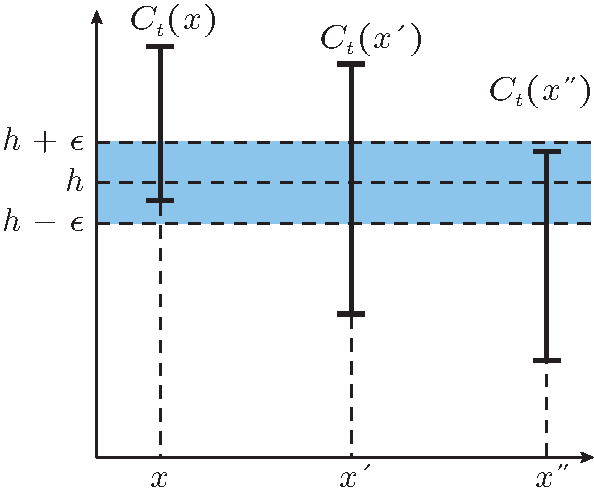
\includegraphics[height=1.5in]{figures/class}
    \caption{Confidence regions}
    \label{fig:conf}
  \end{subfigure}
  \hfill
  \begin{subfigure}[b]{0.49\linewidth}
    \centering
    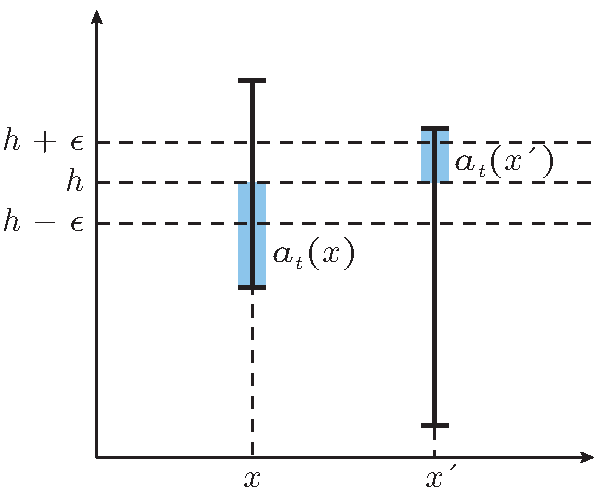
\includegraphics[height=1.5in]{figures/amb}
    \caption{Ambiguities}
    \label{fig:amb}
  \end{subfigure}
  \begin{subfigure}[b]{0.49\linewidth}
    \centering
    \vspace{0.6em} % space of this row from above captions
    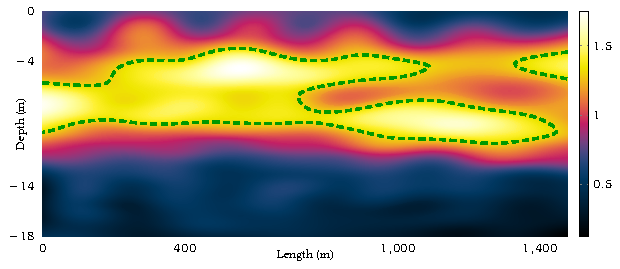
\includegraphics[width=2.4in,clip,trim=7pt 7pt 7pt 7pt]{figures/limno_chl_fp}
    \caption{Ground truth}
    \label{fig:limno_chl}
  \end{subfigure}
  \hfill
  \begin{subfigure}[b]{0.49\linewidth}
    \centering
    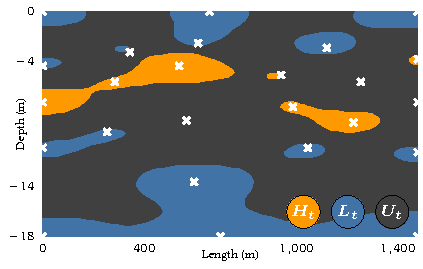
\includegraphics[width=2.4in,clip,trim=7pt 7pt 7pt 7pt]{figures/limno_chl_class25}
    \caption{$t = 25$}
    \label{fig:limno_chl_class1}
  \end{subfigure}
  \begin{subfigure}[b]{0.49\linewidth}
    \centering
    \vspace{0.6em} % space of this row from above captions
    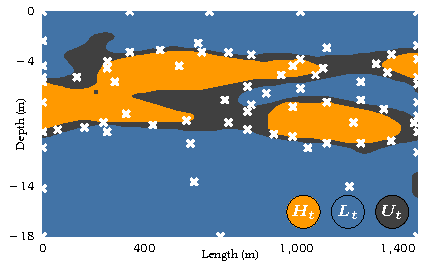
\includegraphics[width=2.4in,clip,trim=7pt 7pt 7pt 7pt]{figures/limno_chl_class75}
    \caption{$t = 75$}
    \label{fig:limno_chl_class2}
  \end{subfigure}
  \hfill
  \begin{subfigure}[b]{0.49\linewidth}
    \centering
    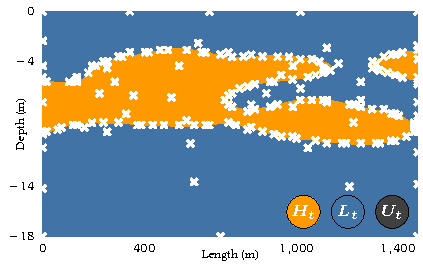
\includegraphics[width=2.4in,clip,trim=7pt 7pt 7pt 7pt]{figures/limno_chl_class168}
    \caption{$t = 168$ (termination)}
    \label{fig:limno_chl_class3}
  \end{subfigure}
  \caption{
  (a) Example of the three possible configurations of confidence regions.
  (b) Ambiguities (shaded) of two example points.
  (c) Chlorophyll concentration in relative fluorescence units (RFU) inferred
      from 2024 measurements within a vertical transect plane of lake Zurich
      (the level set at $h = 1.3$ RFU is shown dashed).
  (d), (e), (f) \acl after $t = 50, 75$, and $168$ iterations respectively,
      on a grid of $100\times 100$ points:
      regions of already classified points in orange ($H_t$) and blue ($L_t$),
      of yet unclassified points ($U_t$) in black, and observed points
      ($\{\*x_i\}_{1\leq i\leq t}$) as white marks.
  }
\end{figure}

We now discuss in more detail the issues of how points are classified and
how the next point is selected at each step.

\paragraph{Classification}
The classification of a point $\*x$ into $H_t$ or $L_t$ depends on the
position of its confidence region with respect to the threshold level $h$.
Intuitively, if all of $C_t(\*x)$ lies above $h$, then with high probability
$f(\*x) > h$ and $\*x$ should be moved into $H_t$. Similarly, if $C_t(\*x)$
lies below $h$, then $\*x$ should be moved into $L_t$. Otherwise, we are
still uncertain about the class of $\*x$, therefore it should, for the moment,
remain unclassified. As can be seen in the classification rules
of~\linsref{lin:class1} and~\ref{lin:classr2}, we relax these conditions by
introducing an accuracy parameter $\epsilon$, which
trades off classification accuracy for sampling cost. The resulting
classification scheme is illustrated by the example of \figref{fig:conf},
in which point $\*x$ would be
classified into $H_t$ and point $\*x''$ into $L_t$, while point $\*x'$ would
remain in $U_t$ as unclassified. Note that \acl uses a monotonic
classification scheme, meaning that once a point has been classified, it
stays so until the algorithm terminates.

\paragraph{Sample selection}
For selecting the next point to be evaluated at each iteration, we define the
following quantity
\begin{align*}
a_t(\*x) = \min\{\max(C_t(\*x)) - h, h - \min(C_t(\*x))\},
\end{align*}
which we call \emph{ambiguity}. As its name suggests, the ambiguity of a
point $\*x$ quantifies our uncertainty about whether $\*x$ belongs to
$H_t$ or $L_t$ (see \figref{fig:amb}).
The intuition of sampling at areas of the sample space with large
classification uncertainty, expecting to gain more information about
the problem at hand when sampling at those areas, manifests itself in \acl
by choosing to evaluate at each iteration the point with the largest
ambiguity amongst the yet unclassified.

We can make an interesting observation at this point. If we use the confidence
intervals $Q_t(\*x)$ instead of the confidence regions $C_t(\*x)$
in the definition of ambiguity, we get
\begin{align*}
a'_t(\*x) &= \min\{\max(Q_t(\*x)) - h, h - \min(Q_t(\*x))\}\\
          &= \min\{\mu_{t-1}(\*x) + \beta_t^{1/2}\sigma_{t-1}(\*x) - h,\ h - \mu_{t-1}(\*x) + \beta_t^{1/2}\sigma_{t-1}(\*x)\}\\
          &= \beta_t^{1/2}\sigma_{t-1}(\*x) - |\mu_{t-1}(\*x) - h|.
\end{align*}
For $\beta_t^{1/2} = 1.96$, this is identical to
the \emph{straddle}~\cite{bryan05} selection rule, which can thus be
intuitively explained in terms of classification ambiguity.

\figsref{fig:limno_chl} to \ref{fig:limno_chl_class3} present an example
of running the \acl algorithm on a chlorophyll dataset from lake Zurich.
Note how the sampling process focuses on the ambiguous regions around the
desired level set until all points in $D$ have been successfully classified. 

\paragraph{Theoretical analysis}
The convergence analysis of \acl rests on quantifying the complexity of the GP prior for $f$ in information-theoretic terms.
The information gain~\cite{cover06} about $f$ from observing $t$ noisy
measurements $\*y_t = (y_i)_{1\leq i\leq t}$ is
\begin{align*}
I(\*y_t; f) = H(\*y_t) - H(\*y_t\mid f).
\end{align*}
\citet{srinivas10} used the \emph{maximum
information gain} over all possible sets of $t$ observations
\begin{align*}
\gamma_t = \max_{\*y_t} I(\*y_t; f)
\end{align*}
for bounding the regret of the \gpucb algorithm.
We use the same quantity to bound the number of \acl iterations
required to achieve a certain classification quality.

To quantify the quality of a solution $(\hat{H}, \hat{L})$
with respect to a single point $\*x\in D$ we use the
misclassification loss
\begin{align*}
\ell_h(\*x) = \twopartdef{\max\{0, f(\*x) - h\}}{\*x\in \hat{L}}{\max\{0, h - f(\*x)\}}{\*x\in \hat{H}}.
\end{align*}
The overall quality of a solution can then be judged by the
largest misclassification loss
among all points in the sample space, i.e. $\max_{\*x\in D} \ell_h(\*x)$.
Intuitively, having a solution with $\max_{\*x\in D} \ell_h(\*x) \leq \epsilon$
means that every point $\*x$ is correctly classified with respect to a
threshold level that deviates by at most $\epsilon$ from the true level $h$;
we call such a solution \emph{$\epsilon$-accurate}.
The following theorem establishes a convergence bound for \acl in terms
of $\gamma_t$ for any given accuracy $\epsilon$.

\begin{theorem}
\label{thm:acl}
For any $h\in\mathbb{R}$, $\delta \in (0, 1)$, and $\epsilon > 0$,
if $\beta_t = 2\log(|D|\pi^2 t^2/(6\delta))$, \acl terminates after
at most $T$ iterations, where $T$ is the smallest positive integer
satisfying
\begin{align*}
\frac{T}{\beta_T \gamma_T} \geq \frac{C_1}{4\epsilon^2},
%T/(\beta_T \gamma_T) \geq C_1/(4\epsilon^2),
\end{align*}
where $C_1 = 8/log(1 + \sigma^{-2})$.

Furthermore, with probability at least $1-\delta$, the algorithm returns
an $\epsilon$-accurate solution, that is
\begin{align*}
\Pr\left\{\max_{\*x\in D}\ell_h(\*x) \leq \epsilon\right\} \geq 1 - \delta.
\end{align*}
\end{theorem}

The proof of \theoremref{thm:acl} can be
outlined as follows.\footnote{Detailed proofs of all theorems and further
experiments can be found in the supplemental material of this paper
(\url{http://sites.google.com/site/lseijcai13/long.pdf}).}
The choice of $\beta_t$ guarantees
the inclusion of $f(\*x)$ in the confidence regions $C_t(\*x)$ for
all $\*x\in D$. From the monotonic classification scheme and
the maximum ambiguity selection rule, it follows that the
ambiguities of the selected points, $a_t(\*x_t)$, are decreasing
with $t$ and, using $\gamma_t$, they can be shown to decrease
as $\mathcal{O}((\frac{\beta_t \gamma_t}{t})^\frac{1}{2})$. Finally,
the classification rules of \acl connect the number of iterations to
the accuracy parameter $\epsilon$ and guarantee an $\epsilon$-accurate
solution with high probability.

Note that bounds on $\gamma_t$ have been established for commonly used
kernels~\cite{srinivas10} and can be plugged into \theoremref{thm:acl}
to obtain concrete bounds on $T$.
For example, for a \mbox{$d$-dimensional} sample space and a squared exponential
GP kernel, ${\gamma_t = \mathcal{O}((\log T)^{d+1})}$, and the expression in
the bound of
\theoremref{thm:acl} becomes $T/(\log T)^{d+2} \geq C / \epsilon^2$,
where, for any given sample space and kernel hyperparameters, $C$ depends
only on the choice of $\delta$.
